% Options for packages loaded elsewhere
\PassOptionsToPackage{unicode}{hyperref}
\PassOptionsToPackage{hyphens}{url}
%
\documentclass[
  letterpaper,
]{scrbook}

\usepackage{amsmath,amssymb}
\usepackage{iftex}
\ifPDFTeX
  \usepackage[T1]{fontenc}
  \usepackage[utf8]{inputenc}
  \usepackage{textcomp} % provide euro and other symbols
\else % if luatex or xetex
  \usepackage{unicode-math}
  \defaultfontfeatures{Scale=MatchLowercase}
  \defaultfontfeatures[\rmfamily]{Ligatures=TeX,Scale=1}
\fi
\usepackage{lmodern}
\ifPDFTeX\else  
    % xetex/luatex font selection
\fi
% Use upquote if available, for straight quotes in verbatim environments
\IfFileExists{upquote.sty}{\usepackage{upquote}}{}
\IfFileExists{microtype.sty}{% use microtype if available
  \usepackage[]{microtype}
  \UseMicrotypeSet[protrusion]{basicmath} % disable protrusion for tt fonts
}{}
\makeatletter
\@ifundefined{KOMAClassName}{% if non-KOMA class
  \IfFileExists{parskip.sty}{%
    \usepackage{parskip}
  }{% else
    \setlength{\parindent}{0pt}
    \setlength{\parskip}{6pt plus 2pt minus 1pt}}
}{% if KOMA class
  \KOMAoptions{parskip=half}}
\makeatother
\usepackage{xcolor}
\setlength{\emergencystretch}{3em} % prevent overfull lines
\setcounter{secnumdepth}{5}
% Make \paragraph and \subparagraph free-standing
\makeatletter
\ifx\paragraph\undefined\else
  \let\oldparagraph\paragraph
  \renewcommand{\paragraph}{
    \@ifstar
      \xxxParagraphStar
      \xxxParagraphNoStar
  }
  \newcommand{\xxxParagraphStar}[1]{\oldparagraph*{#1}\mbox{}}
  \newcommand{\xxxParagraphNoStar}[1]{\oldparagraph{#1}\mbox{}}
\fi
\ifx\subparagraph\undefined\else
  \let\oldsubparagraph\subparagraph
  \renewcommand{\subparagraph}{
    \@ifstar
      \xxxSubParagraphStar
      \xxxSubParagraphNoStar
  }
  \newcommand{\xxxSubParagraphStar}[1]{\oldsubparagraph*{#1}\mbox{}}
  \newcommand{\xxxSubParagraphNoStar}[1]{\oldsubparagraph{#1}\mbox{}}
\fi
\makeatother

\usepackage{color}
\usepackage{fancyvrb}
\newcommand{\VerbBar}{|}
\newcommand{\VERB}{\Verb[commandchars=\\\{\}]}
\DefineVerbatimEnvironment{Highlighting}{Verbatim}{commandchars=\\\{\}}
% Add ',fontsize=\small' for more characters per line
\usepackage{framed}
\definecolor{shadecolor}{RGB}{241,243,245}
\newenvironment{Shaded}{\begin{snugshade}}{\end{snugshade}}
\newcommand{\AlertTok}[1]{\textcolor[rgb]{0.68,0.00,0.00}{#1}}
\newcommand{\AnnotationTok}[1]{\textcolor[rgb]{0.37,0.37,0.37}{#1}}
\newcommand{\AttributeTok}[1]{\textcolor[rgb]{0.40,0.45,0.13}{#1}}
\newcommand{\BaseNTok}[1]{\textcolor[rgb]{0.68,0.00,0.00}{#1}}
\newcommand{\BuiltInTok}[1]{\textcolor[rgb]{0.00,0.23,0.31}{#1}}
\newcommand{\CharTok}[1]{\textcolor[rgb]{0.13,0.47,0.30}{#1}}
\newcommand{\CommentTok}[1]{\textcolor[rgb]{0.37,0.37,0.37}{#1}}
\newcommand{\CommentVarTok}[1]{\textcolor[rgb]{0.37,0.37,0.37}{\textit{#1}}}
\newcommand{\ConstantTok}[1]{\textcolor[rgb]{0.56,0.35,0.01}{#1}}
\newcommand{\ControlFlowTok}[1]{\textcolor[rgb]{0.00,0.23,0.31}{\textbf{#1}}}
\newcommand{\DataTypeTok}[1]{\textcolor[rgb]{0.68,0.00,0.00}{#1}}
\newcommand{\DecValTok}[1]{\textcolor[rgb]{0.68,0.00,0.00}{#1}}
\newcommand{\DocumentationTok}[1]{\textcolor[rgb]{0.37,0.37,0.37}{\textit{#1}}}
\newcommand{\ErrorTok}[1]{\textcolor[rgb]{0.68,0.00,0.00}{#1}}
\newcommand{\ExtensionTok}[1]{\textcolor[rgb]{0.00,0.23,0.31}{#1}}
\newcommand{\FloatTok}[1]{\textcolor[rgb]{0.68,0.00,0.00}{#1}}
\newcommand{\FunctionTok}[1]{\textcolor[rgb]{0.28,0.35,0.67}{#1}}
\newcommand{\ImportTok}[1]{\textcolor[rgb]{0.00,0.46,0.62}{#1}}
\newcommand{\InformationTok}[1]{\textcolor[rgb]{0.37,0.37,0.37}{#1}}
\newcommand{\KeywordTok}[1]{\textcolor[rgb]{0.00,0.23,0.31}{\textbf{#1}}}
\newcommand{\NormalTok}[1]{\textcolor[rgb]{0.00,0.23,0.31}{#1}}
\newcommand{\OperatorTok}[1]{\textcolor[rgb]{0.37,0.37,0.37}{#1}}
\newcommand{\OtherTok}[1]{\textcolor[rgb]{0.00,0.23,0.31}{#1}}
\newcommand{\PreprocessorTok}[1]{\textcolor[rgb]{0.68,0.00,0.00}{#1}}
\newcommand{\RegionMarkerTok}[1]{\textcolor[rgb]{0.00,0.23,0.31}{#1}}
\newcommand{\SpecialCharTok}[1]{\textcolor[rgb]{0.37,0.37,0.37}{#1}}
\newcommand{\SpecialStringTok}[1]{\textcolor[rgb]{0.13,0.47,0.30}{#1}}
\newcommand{\StringTok}[1]{\textcolor[rgb]{0.13,0.47,0.30}{#1}}
\newcommand{\VariableTok}[1]{\textcolor[rgb]{0.07,0.07,0.07}{#1}}
\newcommand{\VerbatimStringTok}[1]{\textcolor[rgb]{0.13,0.47,0.30}{#1}}
\newcommand{\WarningTok}[1]{\textcolor[rgb]{0.37,0.37,0.37}{\textit{#1}}}

\providecommand{\tightlist}{%
  \setlength{\itemsep}{0pt}\setlength{\parskip}{0pt}}\usepackage{longtable,booktabs,array}
\usepackage{calc} % for calculating minipage widths
% Correct order of tables after \paragraph or \subparagraph
\usepackage{etoolbox}
\makeatletter
\patchcmd\longtable{\par}{\if@noskipsec\mbox{}\fi\par}{}{}
\makeatother
% Allow footnotes in longtable head/foot
\IfFileExists{footnotehyper.sty}{\usepackage{footnotehyper}}{\usepackage{footnote}}
\makesavenoteenv{longtable}
\usepackage{graphicx}
\makeatletter
\newsavebox\pandoc@box
\newcommand*\pandocbounded[1]{% scales image to fit in text height/width
  \sbox\pandoc@box{#1}%
  \Gscale@div\@tempa{\textheight}{\dimexpr\ht\pandoc@box+\dp\pandoc@box\relax}%
  \Gscale@div\@tempb{\linewidth}{\wd\pandoc@box}%
  \ifdim\@tempb\p@<\@tempa\p@\let\@tempa\@tempb\fi% select the smaller of both
  \ifdim\@tempa\p@<\p@\scalebox{\@tempa}{\usebox\pandoc@box}%
  \else\usebox{\pandoc@box}%
  \fi%
}
% Set default figure placement to htbp
\def\fps@figure{htbp}
\makeatother

\makeatletter
\@ifpackageloaded{tcolorbox}{}{\usepackage[skins,breakable]{tcolorbox}}
\@ifpackageloaded{fontawesome5}{}{\usepackage{fontawesome5}}
\definecolor{quarto-callout-color}{HTML}{909090}
\definecolor{quarto-callout-note-color}{HTML}{0758E5}
\definecolor{quarto-callout-important-color}{HTML}{CC1914}
\definecolor{quarto-callout-warning-color}{HTML}{EB9113}
\definecolor{quarto-callout-tip-color}{HTML}{00A047}
\definecolor{quarto-callout-caution-color}{HTML}{FC5300}
\definecolor{quarto-callout-color-frame}{HTML}{acacac}
\definecolor{quarto-callout-note-color-frame}{HTML}{4582ec}
\definecolor{quarto-callout-important-color-frame}{HTML}{d9534f}
\definecolor{quarto-callout-warning-color-frame}{HTML}{f0ad4e}
\definecolor{quarto-callout-tip-color-frame}{HTML}{02b875}
\definecolor{quarto-callout-caution-color-frame}{HTML}{fd7e14}
\makeatother
\makeatletter
\@ifpackageloaded{bookmark}{}{\usepackage{bookmark}}
\makeatother
\makeatletter
\@ifpackageloaded{caption}{}{\usepackage{caption}}
\AtBeginDocument{%
\ifdefined\contentsname
  \renewcommand*\contentsname{Table of contents}
\else
  \newcommand\contentsname{Table of contents}
\fi
\ifdefined\listfigurename
  \renewcommand*\listfigurename{List of Figures}
\else
  \newcommand\listfigurename{List of Figures}
\fi
\ifdefined\listtablename
  \renewcommand*\listtablename{List of Tables}
\else
  \newcommand\listtablename{List of Tables}
\fi
\ifdefined\figurename
  \renewcommand*\figurename{Figure}
\else
  \newcommand\figurename{Figure}
\fi
\ifdefined\tablename
  \renewcommand*\tablename{Table}
\else
  \newcommand\tablename{Table}
\fi
}
\@ifpackageloaded{float}{}{\usepackage{float}}
\floatstyle{ruled}
\@ifundefined{c@chapter}{\newfloat{codelisting}{h}{lop}}{\newfloat{codelisting}{h}{lop}[chapter]}
\floatname{codelisting}{Listing}
\newcommand*\listoflistings{\listof{codelisting}{List of Listings}}
\makeatother
\makeatletter
\makeatother
\makeatletter
\@ifpackageloaded{caption}{}{\usepackage{caption}}
\@ifpackageloaded{subcaption}{}{\usepackage{subcaption}}
\makeatother

\usepackage{bookmark}

\IfFileExists{xurl.sty}{\usepackage{xurl}}{} % add URL line breaks if available
\urlstyle{same} % disable monospaced font for URLs
\hypersetup{
  pdftitle={Statistics for Football Scouting},
  pdfauthor={Adapted from Çetinkaya-Rundel \& Hardin's IMS for the recruitment analyst},
  hidelinks,
  pdfcreator={LaTeX via pandoc}}


\title{Statistics for Football Scouting}
\usepackage{etoolbox}
\makeatletter
\providecommand{\subtitle}[1]{% add subtitle to \maketitle
  \apptocmd{\@title}{\par {\large #1 \par}}{}{}
}
\makeatother
\subtitle{A football-scouting adaptation of Introduction to Modern
Statistics}
\author{Adapted from Çetinkaya-Rundel \& Hardin's IMS for the
recruitment analyst}
\date{}

\begin{document}
\frontmatter
\maketitle

\renewcommand*\contentsname{Table of contents}
{
\setcounter{tocdepth}{2}
\tableofcontents
}

\mainmatter
\bookmarksetup{startatroot}

\chapter*{Welcome}\label{welcome}
\addcontentsline{toc}{chapter}{Welcome}

\markboth{Welcome}{Welcome}

I have spent a career teaching statistics, and long enough around
football to know how the two usually meet: badly. A scout watches three
matches and ``knows''; an analyst quotes a per-90 number computed from
340 minutes as if it were a law of nature; a sporting director asks
whether a striker's cold streak is ``real'' and gets either a shrug or
false certainty in reply. Every one of those is a statistics question,
and every one has a rigorous answer --- if you learn to ask it
precisely.

This book teaches modern statistics --- the real thing, definitions,
notation, derivations and all --- using football scouting and
recruitment as its \emph{only} world. Every case study is a scouting
problem. Every dataset is match data (much of it real: StatsBomb's open
event data from the 2022 men's World Cup and the 2025 Women's Euro) or
an explicitly constructed scouting scenario you can reproduce in code.
Every exercise puts you in the seat of an analyst whose report is about
to influence a decision worth millions.

Two promises about how I will teach:

\begin{enumerate}
\def\labelenumi{\arabic{enumi}.}
\tightlist
\item
  \textbf{Rigor before intuition.} Formal definition and notation first,
  football second. The first time any symbol appears --- \(H_0\),
  \(\alpha\), \(\hat{p}\) --- I will take it apart piece by piece in
  plain words before we use it. The football keeps you oriented; it
  never substitutes for the mathematics.
\item
  \textbf{You will compute everything.} The code is R with tidyverse
  conventions, and every number in this book can be reproduced from the
  data files that ship with it. Statistics you cannot recompute is
  folklore.
\end{enumerate}

\section*{How to read this book}\label{how-to-read-this-book}
\addcontentsline{toc}{section}{How to read this book}

\markright{How to read this book}

\begin{itemize}
\tightlist
\item
  \textbf{Important boxes} hold the formal definitions --- these are the
  sentences worth memorizing.
\item
  \textbf{Worked examples} carry the full calculation, step by step.
\item
  \textbf{Check your understanding} boxes pose a short question before
  moving on. Answer before reading on; a scout who never tests their own
  reads never calibrates.
\end{itemize}

\textbf{If you have had a statistics course before.} Chapters 1--2 and
4--6 will read largely as review --- with two exceptions that will not:
Chapter 3's data discipline (what a row is, what a frame is, which shots
are even in the table) and Chapter 5's demonstration that the familiar
68/95 guideline misfires the moment a distribution stops being
bell-shaped. Chapters 11--14 and 19 must be read closely whatever your
background --- they carry the book's inferential logic and the
conventions every later verdict leans on. And because the running
datasets, the Northbridge cast, and the frame conventions planted in
Parts I--II are load-bearing everywhere after, skipping the early
chapters is costly: skim them, don't skip them.

One working assumption is worth stating plainly: this book assumes you
compute in R (tidyverse conventions throughout), and the setup appendix
walks through installing everything the code needs.

\section*{Where the book stands}\label{where-the-book-stands}
\addcontentsline{toc}{section}{Where the book stands}

\markright{Where the book stands}

All twenty-seven chapters are complete: Parts I--IV carry you from data
and study design through exploratory analysis, modeling, and the
foundations of inference; Parts V and VI finish the argument with the
full catalog of inferential methods --- proportions, tables, means,
ANOVA --- and inference for regression models, closing with the
end-to-end case studies that send you back to the club with a number, an
interval, and a stated frame. The adaptation preserves IMS's chapter
structure and section anchors exactly, so readers moving between this
book and the original can cross the bridge in either direction.

\section*{Attribution and license}\label{attribution-and-license}
\addcontentsline{toc}{section}{Attribution and license}

\markright{Attribution and license}

This book is an adaptation of \emph{Introduction to Modern Statistics}
(2nd edition) by Mine Çetinkaya-Rundel and Johanna Hardin, used under CC
BY-SA 4.0. The pedagogical structure, curriculum sequence, and
statistical definitions follow the original faithfully; the
football-scouting setting, examples, and exercises are new. Section
anchors mirror IMS's exactly --- which is why an occasional anchor name
carries the flavor of an IMS example rather than its football
counterpart --- so that cross-references and deep links stay navigable
between the two books. This adaptation is likewise licensed CC BY-SA
4.0. Match data: \href{https://github.com/statsbomb/open-data}{StatsBomb
open data}, used under its non-commercial license.

\part{Introduction to data}

\chapter{Hello data}\label{sec-data-hello}

Scouts and analysts seek to answer questions using rigorous methods and
careful observations. These observations -- collected from the likes of
match logs, event-tagging systems, and trial-ground experiments -- form
the backbone of a statistical investigation and are called
\textbf{data}. Statistics is the study of how best to collect, analyze,
and draw conclusions from data. In this first chapter, we focus on both
the properties of data and on the collection of data.

You are the newest analyst at Northbridge United FC, a mid-table club
with a modest budget and, in Marta Vidal, a sporting director who asks
precise questions and expects defensible answers. Everything in this
book is in service of one professional obligation: when the club is
about to commit money, minutes, or a squad place on the basis of what
somebody saw, you must be able to say what the data do and do not
support. We begin, as every analysis should, with the data themselves.

\section{Case study: a finishing program that
backfired}\label{sec-case-study-stents-strokes}

In this section we introduce a classic challenge in statistics:
evaluating the efficacy of an intervention. Terms in this section, and
indeed much of this chapter, will all be revisited later in the text.
The plan for now is simply to get a sense of the role statistics can
play in practice.

Jonas Beck, Northbridge's academy director, was approached by a vendor
selling a new high-intensity finishing program: shorter, sharper
shooting sessions at near-match tempo, promised to raise young forwards'
conversion in front of goal. Before rolling it out, the club and a group
of partner academies agreed to test it properly. We start by writing the
principal question the study hopes to answer:

\begin{quote}
Does the high-intensity finishing program improve young players'
finishing?
\end{quote}

To be clear at the outset: this is a constructed scenario -- no such
multi-academy trial was actually run -- and we will build the dataset
ourselves in R code, in the open, so that every number in this section
can be reproduced. The design, however, is exactly how such a question
\emph{should} be studied. The academies enrolled 451 age-eligible
players. Each volunteer player was randomly assigned to one of two
groups:

\begin{itemize}
\tightlist
\item
  \textbf{Treatment group}. Players in the treatment group received the
  new high-intensity finishing program alongside their regular
  development plan. The regular plan included ordinary technical
  sessions, strength work, and individual video review.
\item
  \textbf{Control group}. Players in the control group received the same
  regular development plan as the treatment group, but they did not
  receive the new finishing program.
\end{itemize}

The coaches randomly assigned 224 players to the treatment group and 227
to the control group. In this study, the control group provides a
reference point against which we can measure the impact of the finishing
program in the treatment group.

The staff assessed every player at two time points: 30 days after
enrollment and at the end of the season. At each assessment, a player's
finishing was measured against a fixed academy benchmark (a standardized
battery of match-realistic finishing situations), and the player was
recorded as \texttt{below\ benchmark} or \texttt{met\ benchmark}. The
code below constructs the \texttt{drill\_trial} data -- one row per
player -- and a seeded sample shows the results for 5 players.

\begin{Shaded}
\begin{Highlighting}[]
\FunctionTok{library}\NormalTok{(dplyr)}
\FunctionTok{library}\NormalTok{(tidyr)}
\FunctionTok{library}\NormalTok{(readr)}
\FunctionTok{library}\NormalTok{(ggplot2)}

\NormalTok{drill\_trial }\OtherTok{\textless{}{-}} \FunctionTok{tibble}\NormalTok{(}
  \AttributeTok{group =} \FunctionTok{c}\NormalTok{(}\FunctionTok{rep}\NormalTok{(}\StringTok{"finishing program"}\NormalTok{, }\DecValTok{224}\NormalTok{), }\FunctionTok{rep}\NormalTok{(}\StringTok{"standard training"}\NormalTok{, }\DecValTok{227}\NormalTok{)),}
  \AttributeTok{day30 =} \FunctionTok{c}\NormalTok{(}\FunctionTok{rep}\NormalTok{(}\StringTok{"below benchmark"}\NormalTok{, }\DecValTok{33}\NormalTok{), }\FunctionTok{rep}\NormalTok{(}\StringTok{"met benchmark"}\NormalTok{, }\DecValTok{191}\NormalTok{),}
            \FunctionTok{rep}\NormalTok{(}\StringTok{"below benchmark"}\NormalTok{, }\DecValTok{13}\NormalTok{), }\FunctionTok{rep}\NormalTok{(}\StringTok{"met benchmark"}\NormalTok{, }\DecValTok{214}\NormalTok{)),}
  \AttributeTok{season\_end =} \FunctionTok{c}\NormalTok{(}\FunctionTok{rep}\NormalTok{(}\StringTok{"below benchmark"}\NormalTok{, }\DecValTok{45}\NormalTok{), }\FunctionTok{rep}\NormalTok{(}\StringTok{"met benchmark"}\NormalTok{, }\DecValTok{179}\NormalTok{),}
                 \FunctionTok{rep}\NormalTok{(}\StringTok{"below benchmark"}\NormalTok{, }\DecValTok{28}\NormalTok{), }\FunctionTok{rep}\NormalTok{(}\StringTok{"met benchmark"}\NormalTok{, }\DecValTok{199}\NormalTok{))}
\NormalTok{)}

\FunctionTok{set.seed}\NormalTok{(}\DecValTok{103}\NormalTok{)}
\NormalTok{drill\_trial }\SpecialCharTok{|\textgreater{}}
  \FunctionTok{slice\_sample}\NormalTok{(}\AttributeTok{n =} \DecValTok{5}\NormalTok{) }\SpecialCharTok{|\textgreater{}}
  \FunctionTok{arrange}\NormalTok{(group) }\SpecialCharTok{|\textgreater{}}
  \FunctionTok{mutate}\NormalTok{(}\AttributeTok{player =} \DecValTok{1}\SpecialCharTok{:}\FunctionTok{n}\NormalTok{()) }\SpecialCharTok{|\textgreater{}}
  \FunctionTok{relocate}\NormalTok{(player)}
\CommentTok{\#\textgreater{} \# A tibble: 5 × 4}
\CommentTok{\#\textgreater{}   player group             day30         season\_end}
\CommentTok{\#\textgreater{}    \textless{}int\textgreater{} \textless{}chr\textgreater{}             \textless{}chr\textgreater{}         \textless{}chr\textgreater{}}
\CommentTok{\#\textgreater{} 1      1 finishing program met benchmark below benchmark}
\CommentTok{\#\textgreater{} 2      2 finishing program met benchmark met benchmark}
\CommentTok{\#\textgreater{} 3      3 standard training met benchmark met benchmark}
\CommentTok{\#\textgreater{} 4      4 standard training met benchmark met benchmark}
\CommentTok{\#\textgreater{} 5      5 standard training met benchmark below benchmark}
\end{Highlighting}
\end{Shaded}

It would be difficult to answer a question about the impact of the
program on \textbf{all} 451 players using these \emph{individual}
observations. This question is better addressed by performing a
statistical data analysis of \emph{all} observations. The code below
counts outcomes at each time point, and
Table~\ref{tbl-drill-trial-summary} summarizes the raw data in a more
helpful way.

\begin{Shaded}
\begin{Highlighting}[]
\NormalTok{drill\_trial }\SpecialCharTok{|\textgreater{}}
  \FunctionTok{count}\NormalTok{(group, day30) }\SpecialCharTok{|\textgreater{}}
  \FunctionTok{pivot\_wider}\NormalTok{(}\AttributeTok{names\_from =}\NormalTok{ day30, }\AttributeTok{values\_from =}\NormalTok{ n)}
\CommentTok{\#\textgreater{} \# A tibble: 2 × 3}
\CommentTok{\#\textgreater{}   group             \textasciigrave{}below benchmark\textasciigrave{} \textasciigrave{}met benchmark\textasciigrave{}}
\CommentTok{\#\textgreater{}   \textless{}chr\textgreater{}                         \textless{}int\textgreater{}           \textless{}int\textgreater{}}
\CommentTok{\#\textgreater{} 1 finishing program                33             191}
\CommentTok{\#\textgreater{} 2 standard training                13             214}

\NormalTok{drill\_trial }\SpecialCharTok{|\textgreater{}}
  \FunctionTok{count}\NormalTok{(group, season\_end) }\SpecialCharTok{|\textgreater{}}
  \FunctionTok{pivot\_wider}\NormalTok{(}\AttributeTok{names\_from =}\NormalTok{ season\_end, }\AttributeTok{values\_from =}\NormalTok{ n)}
\CommentTok{\#\textgreater{} \# A tibble: 2 × 3}
\CommentTok{\#\textgreater{}   group             \textasciigrave{}below benchmark\textasciigrave{} \textasciigrave{}met benchmark\textasciigrave{}}
\CommentTok{\#\textgreater{}   \textless{}chr\textgreater{}                         \textless{}int\textgreater{}           \textless{}int\textgreater{}}
\CommentTok{\#\textgreater{} 1 finishing program                45             179}
\CommentTok{\#\textgreater{} 2 standard training                28             199}
\end{Highlighting}
\end{Shaded}

\begin{longtable}[]{@{}
  >{\raggedright\arraybackslash}p{(\linewidth - 8\tabcolsep) * \real{0.2235}}
  >{\raggedleft\arraybackslash}p{(\linewidth - 8\tabcolsep) * \real{0.1882}}
  >{\raggedleft\arraybackslash}p{(\linewidth - 8\tabcolsep) * \real{0.1647}}
  >{\raggedleft\arraybackslash}p{(\linewidth - 8\tabcolsep) * \real{0.2235}}
  >{\raggedleft\arraybackslash}p{(\linewidth - 8\tabcolsep) * \real{0.2000}}@{}}
\caption{Descriptive statistics for the finishing program
trial.}\label{tbl-drill-trial-summary}\tabularnewline
\toprule\noalign{}
\begin{minipage}[b]{\linewidth}\raggedright
\end{minipage} & \begin{minipage}[b]{\linewidth}\raggedleft
30 days: below
\end{minipage} & \begin{minipage}[b]{\linewidth}\raggedleft
30 days: met
\end{minipage} & \begin{minipage}[b]{\linewidth}\raggedleft
Season end: below
\end{minipage} & \begin{minipage}[b]{\linewidth}\raggedleft
Season end: met
\end{minipage} \\
\midrule\noalign{}
\endfirsthead
\toprule\noalign{}
\begin{minipage}[b]{\linewidth}\raggedright
\end{minipage} & \begin{minipage}[b]{\linewidth}\raggedleft
30 days: below
\end{minipage} & \begin{minipage}[b]{\linewidth}\raggedleft
30 days: met
\end{minipage} & \begin{minipage}[b]{\linewidth}\raggedleft
Season end: below
\end{minipage} & \begin{minipage}[b]{\linewidth}\raggedleft
Season end: met
\end{minipage} \\
\midrule\noalign{}
\endhead
\bottomrule\noalign{}
\endlastfoot
finishing program & 33 & 191 & 45 & 179 \\
standard training & 13 & 214 & 28 & 199 \\
Total & 46 & 405 & 73 & 378 \\
\end{longtable}

In this table, we can quickly see what happened over the entire study.
For instance, to identify the number of players in the treatment group
who were below benchmark 30 days in, we look in the leftmost count
column, in the finishing program row: 33. To identify the number of
control players who met the benchmark at season end, we look at the
rightmost column, in the standard training row: 199.

\begin{tcolorbox}[enhanced jigsaw, left=2mm, leftrule=.75mm, title=\textcolor{quarto-callout-tip-color}{\faLightbulb}\hspace{0.5em}{Check your understanding}, arc=.35mm, rightrule=.15mm, coltitle=black, colframe=quarto-callout-tip-color-frame, bottomrule=.15mm, colbacktitle=quarto-callout-tip-color!10!white, opacitybacktitle=0.6, breakable, bottomtitle=1mm, toptitle=1mm, titlerule=0mm, opacityback=0, toprule=.15mm, colback=white]

Of the 224 players in the treatment group, 45 were below the benchmark
at the end of the season. Using these two numbers, compute the
proportion of players in the treatment group who were below the
benchmark at season end.

\begin{center}\rule{0.5\linewidth}{0.5pt}\end{center}

The proportion is \(45/224 = 0.20.\) Take the notation apart, because
proportions will follow us through the entire book: the numerator, 45,
counts the players with the outcome of interest; the denominator, 224,
counts everyone in the group; their ratio, written as the fraction
\(45/224,\) is the \emph{proportion}, a number between 0 and 1;
multiplying a proportion by 100 re-expresses it as a \emph{percent},
here \(20\%.\) Fraction, decimal, and percent are three costumes for the
same quantity, and we will switch freely among them. One more small
symbol will follow us everywhere: \(\approx\), read ``is approximately
equal to'', which we use whenever a decimal has been rounded --- as most
of ours will be.

\end{tcolorbox}

We can compute summary statistics from the table to give us a better
idea of how the impact of the finishing program differed between the two
groups. A \textbf{summary statistic} is a single number summarizing data
from a sample. For instance, the primary results of the study at season
end could be described by two summary statistics: the proportion of
players below benchmark in the treatment and control groups.

\begin{Shaded}
\begin{Highlighting}[]
\DecValTok{45}\SpecialCharTok{/}\DecValTok{224}
\CommentTok{\#\textgreater{} [1] 0.2008929}
\DecValTok{28}\SpecialCharTok{/}\DecValTok{227}
\CommentTok{\#\textgreater{} [1] 0.123348}
\end{Highlighting}
\end{Shaded}

\begin{itemize}
\tightlist
\item
  Proportion below benchmark in the treatment (finishing program) group:
  \(45/224 = 0.20 = 20\%.\)
\item
  Proportion below benchmark in the control group:
  \(28/227 = 0.12 = 12\%.\)
\end{itemize}

These two summary statistics are useful in looking for differences in
the groups, and we are in for a surprise: an additional 8\% of players
in the treatment group finished the season below the benchmark! This is
important for two reasons. First, it is contrary to what the coaches
expected, which was that the program would \emph{reduce} the rate of
substandard finishing. Second, it leads to a statistical question: do
the data show a ``real'' difference between the groups?

This second question is subtle, and it is worth building the intuition
with a striker rather than a coin. Suppose a forward's true, long-run
conversion rate is exactly 10\%: over a career, one shot in ten becomes
a goal. Now give her a 100-shot season. While her chance of scoring on
any given shot is 10\%, we probably won't observe exactly 10 goals. We
can simulate such seasons directly:

\begin{Shaded}
\begin{Highlighting}[]
\FunctionTok{set.seed}\NormalTok{(}\DecValTok{104}\NormalTok{)}
\FunctionTok{rbinom}\NormalTok{(}\DecValTok{10}\NormalTok{, }\AttributeTok{size =} \DecValTok{100}\NormalTok{, }\AttributeTok{prob =} \FloatTok{0.10}\NormalTok{)}
\CommentTok{\#\textgreater{}  [1]  9 12 12 16 12  7  9  8 13  9}
\end{Highlighting}
\end{Shaded}

Ten simulated 100-shot seasons for a striker whose true rate never
changes: her goal tallies wander from 7 to 16, and not one season lands
on exactly 10. (The recipe behind \texttt{rbinom()} gets its proper name
--- the binomial distribution --- in Section~\ref{sec-binomial-named}.)
Extending the simulation shows how rarely the ``true'' number appears:

\begin{Shaded}
\begin{Highlighting}[]
\FunctionTok{set.seed}\NormalTok{(}\DecValTok{104}\NormalTok{)}
\NormalTok{seasons }\OtherTok{\textless{}{-}} \FunctionTok{rbinom}\NormalTok{(}\DecValTok{10000}\NormalTok{, }\AttributeTok{size =} \DecValTok{100}\NormalTok{, }\AttributeTok{prob =} \FloatTok{0.10}\NormalTok{)}
\FunctionTok{mean}\NormalTok{(seasons }\SpecialCharTok{==} \DecValTok{10}\NormalTok{)}
\CommentTok{\#\textgreater{} [1] 0.1373}
\FunctionTok{range}\NormalTok{(seasons)}
\CommentTok{\#\textgreater{} [1]  1 25}
\end{Highlighting}
\end{Shaded}

Only about 14\% of 10,000 simulated seasons produce exactly 10 goals,
and the tallies range from 1 all the way to 25 -- from ``release him''
to ``sell for a fortune,'' with no change whatsoever in the underlying
player. This type of variation is part of almost any data generating
process. It is possible that the 8\% difference in the finishing trial
is due to this natural variation. However, the larger the difference we
observe (for a particular sample size), the less believable it is that
the difference is due to chance. So, what we are really asking is the
following: if in fact the program has no effect, how likely is it that
we observe such a large difference?

While we do not yet have statistical tools to fully address this
question on our own -- they arrive in
Chapter~\ref{sec-foundations-randomization} -- we can comprehend the
conclusion the study's analysts reached: there was compelling evidence
of \emph{harm} from the high-intensity program in this trial. The
intervention backfired.

\textbf{Be careful:} Do not generalize the results of this study to all
players and all finishing programs. This study looked at players in a
specific age band, at specific academies, who volunteered for the trial
and who may not be representative of young forwards in general. In
addition, there are many ways to structure high-tempo finishing work,
and this study only considered one vendor's specific program. However,
this study does leave us with an important lesson, one every scouting
department should frame on the wall: we should keep our eyes open for
surprises, because interventions that ``obviously'' help sometimes hurt.

\section{Data basics}\label{sec-data-basics}

Effective presentation and description of data is a first step in most
analyses. This section introduces one structure for organizing data as
well as some terminology that will be used throughout this book.

\subsection{Observations, variables, and data
matrices}\label{observations-variables-and-data-matrices}

Here we leave the constructed trial behind and pick up the dataset that
will do the heaviest lifting in this book: every shot recorded at the
2022 Men's World Cup, 1,494 rows of real event data. One convention to
fix before the first summary is computed: those 1,494 shots --- and the
195 goals among them --- include penalty kicks and the period-5
shoot-out kicks that settled drawn knockout ties, and because such
uncontested kicks can tilt a headline total or conversion rate, this
book flags them wherever they matter (the penalty lesson itself is
taught in Chapter~\ref{sec-data-applications}). From it we draw a random
sample of 50 shots, seeded so that you can reproduce it exactly, and
call the result \texttt{shots50}. This is the sample a scout might
realistically have logged personally across the tournament, and we will
return to it in Chapter~\ref{sec-explore-numerical}.

\begin{Shaded}
\begin{Highlighting}[]
\NormalTok{wc2022\_shots }\OtherTok{\textless{}{-}} \FunctionTok{read\_csv}\NormalTok{(}\StringTok{"data/derived/wc2022\_shots.csv"}\NormalTok{)}

\FunctionTok{set.seed}\NormalTok{(}\DecValTok{101}\NormalTok{)}
\NormalTok{shots50 }\OtherTok{\textless{}{-}}\NormalTok{ wc2022\_shots }\SpecialCharTok{|\textgreater{}}
  \FunctionTok{slice\_sample}\NormalTok{(}\AttributeTok{n =} \DecValTok{50}\NormalTok{)}

\NormalTok{shots50 }\SpecialCharTok{|\textgreater{}}
  \FunctionTok{select}\NormalTok{(player, team, minute, play\_pattern, body\_part, statsbomb\_xg, outcome) }\SpecialCharTok{|\textgreater{}}
  \FunctionTok{slice\_head}\NormalTok{(}\AttributeTok{n =} \DecValTok{6}\NormalTok{)}
\CommentTok{\#\textgreater{} \# A tibble: 6 × 7}
\CommentTok{\#\textgreater{}   player                        team     minute play\_pattern  body\_part  statsbomb\_xg outcome}
\CommentTok{\#\textgreater{}   \textless{}chr\textgreater{}                         \textless{}chr\textgreater{}     \textless{}dbl\textgreater{} \textless{}chr\textgreater{}         \textless{}chr\textgreater{}             \textless{}dbl\textgreater{} \textless{}chr\textgreater{}}
\CommentTok{\#\textgreater{} 1 Bruno Miguel Borges Fernandes Portugal     44 From Throw In Right Foot      0.00671 Post}
\CommentTok{\#\textgreater{} 2 Ousmane Dembélé               France       39 From Throw In Right Foot      0.0810  Off T}
\CommentTok{\#\textgreater{} 3 Daniel Olmo Carvajal          Spain        95 From Throw In Right Foot      0.00852 Off T}
\CommentTok{\#\textgreater{} 4 Daniel Olmo Carvajal          Spain         6 Regular Play  Right Foot      0.0321  Saved to Post}
\CommentTok{\#\textgreater{} 5 Kylian Mbappé Lottin          France       67 Regular Play  Head            0.141   Goal}
\CommentTok{\#\textgreater{} 6 Sebastián Coates Nión         Uruguay      96 Regular Play  Right Foot      0.103   Off T}
\end{Highlighting}
\end{Shaded}

Each row in the table represents a single shot. The formal name for a
row is a \textbf{case} or \textbf{observation} or \textbf{unit of
observation}. The columns represent characteristics of each shot, where
each column is referred to as a \textbf{variable}. For example, the
first row represents a 44th-minute shot by Bruno Fernandes of Portugal,
struck with the right foot from a throw-in sequence, carrying a chance
quality (\texttt{statsbomb\_xg}) of about 0.007 -- and it hit the post.

Be precise about the unit of observation, always. In \texttt{shots50}
the case is \emph{a shot} -- not a player, not a match. Daniel Olmo
appears in two rows because he took two of the sampled shots; that is
two cases, not one. Later in this chapter we will meet a dataset where
the case is a \emph{team}, and confusing the two levels is one of the
most common ways a scouting report goes quietly wrong.

\begin{tcolorbox}[enhanced jigsaw, left=2mm, leftrule=.75mm, title=\textcolor{quarto-callout-tip-color}{\faLightbulb}\hspace{0.5em}{Check your understanding}, arc=.35mm, rightrule=.15mm, coltitle=black, colframe=quarto-callout-tip-color-frame, bottomrule=.15mm, colbacktitle=quarto-callout-tip-color!10!white, opacitybacktitle=0.6, breakable, bottomtitle=1mm, toptitle=1mm, titlerule=0mm, opacityback=0, toprule=.15mm, colback=white]

What is the play pattern of the first shot in the \texttt{shots50}
output above? And what was the outcome of that first shot?

\begin{center}\rule{0.5\linewidth}{0.5pt}\end{center}

The first shot arose from a throw-in sequence
(\texttt{From\ Throw\ In}), and its outcome was \texttt{Post} -- it
struck the woodwork and did not count as a goal.

\end{tcolorbox}

In practice, it is especially important to ask clarifying questions to
ensure important aspects of the data are understood. For instance, it is
always important to be sure we know what each variable means and its
units of measurement. An analyst who does not know whether
\texttt{minute} restarts at halftime, or what exactly
\texttt{statsbomb\_xg} measures, will produce confident nonsense.
Descriptions of the main variables in the \texttt{shots50} dataset are
given in Table~\ref{tbl-shots50-variables}; the full dataset carries 21
variables per shot.

\begin{longtable}[]{@{}
  >{\raggedright\arraybackslash}p{(\linewidth - 2\tabcolsep) * \real{0.2254}}
  >{\raggedright\arraybackslash}p{(\linewidth - 2\tabcolsep) * \real{0.7746}}@{}}
\caption{Variables and their descriptions for the \texttt{shots50}
dataset.}\label{tbl-shots50-variables}\tabularnewline
\toprule\noalign{}
\begin{minipage}[b]{\linewidth}\raggedright
Variable
\end{minipage} & \begin{minipage}[b]{\linewidth}\raggedright
Description
\end{minipage} \\
\midrule\noalign{}
\endfirsthead
\toprule\noalign{}
\begin{minipage}[b]{\linewidth}\raggedright
Variable
\end{minipage} & \begin{minipage}[b]{\linewidth}\raggedright
Description
\end{minipage} \\
\midrule\noalign{}
\endhead
\bottomrule\noalign{}
\endlastfoot
\texttt{player} & Name of the player taking the shot. \\
\texttt{team} & The shooting player's national team. \\
\texttt{minute} & Match minute in which the shot was taken, as a whole
number. \\
\texttt{play\_pattern} & The passage of play the shot arose from, e.g.,
\texttt{Regular\ Play}, \texttt{From\ Corner}, \texttt{From\ Throw\ In},
\texttt{From\ Counter}. \\
\texttt{body\_part} & Body part used: \texttt{Right\ Foot},
\texttt{Left\ Foot}, \texttt{Head}, or \texttt{Other}. \\
\texttt{statsbomb\_xg} & StatsBomb's expected-goals value: the estimated
probability, between 0 and 1, that a shot like this one is scored. We
call this the shot's \emph{chance quality}. \\
\texttt{outcome} & What became of the shot: \texttt{Goal},
\texttt{Saved}, \texttt{Saved\ to\ Post}, \texttt{Saved\ Off\ Target},
\texttt{Post}, \texttt{Blocked}, \texttt{Off\ T} (off target), or
\texttt{Wayward}. \\
\texttt{first\_time} & Whether the shot was struck first time,
\texttt{TRUE} or \texttt{FALSE}. \\
\texttt{under\_pressure} & Whether the shooter was under defensive
pressure, \texttt{TRUE} or \texttt{FALSE}. \\
\texttt{goal} & Whether the shot was scored, \texttt{TRUE} or
\texttt{FALSE}. \\
\end{longtable}

The data in the \texttt{shots50} display represent a \textbf{data
frame}, which is a convenient and common way to organize data,
especially if collecting data in a spreadsheet. A data frame where each
row is a unique case (observational unit), each column is a variable,
and each cell is a single value is commonly referred to as \textbf{tidy
data}.

When recording data, use a tidy data frame unless you have a very good
reason to use a different structure. This structure allows new cases to
be added as rows or new variables as new columns and facilitates
visualization, summarization, and other statistical analyses.

\begin{tcolorbox}[enhanced jigsaw, left=2mm, leftrule=.75mm, title=\textcolor{quarto-callout-tip-color}{\faLightbulb}\hspace{0.5em}{Check your understanding}, arc=.35mm, rightrule=.15mm, coltitle=black, colframe=quarto-callout-tip-color-frame, bottomrule=.15mm, colbacktitle=quarto-callout-tip-color!10!white, opacitybacktitle=0.6, breakable, bottomtitle=1mm, toptitle=1mm, titlerule=0mm, opacityback=0, toprule=.15mm, colback=white]

Emil Sørensen's 48 regional scouts each file a match report grading
every prospect they watched on several attributes. How might you
organize a season of the network's grades using a data frame? Describe
the observational units and variables.

\begin{center}\rule{0.5\linewidth}{0.5pt}\end{center}

There are multiple strategies that can be followed. One common strategy
is to have each row represent one \emph{scout-evaluation} -- one scout
grading one prospect after one match -- with columns for the scout, the
prospect, the match date, and one column per graded attribute
(finishing, pressing, positioning, and so on). Under this setup, it is
easy to filter to a single prospect and review their full evaluation
history. There should also be columns for context, such as the
competition and the opponent.

\end{tcolorbox}

\begin{tcolorbox}[enhanced jigsaw, left=2mm, leftrule=.75mm, title=\textcolor{quarto-callout-tip-color}{\faLightbulb}\hspace{0.5em}{Check your understanding}, arc=.35mm, rightrule=.15mm, coltitle=black, colframe=quarto-callout-tip-color-frame, bottomrule=.15mm, colbacktitle=quarto-callout-tip-color!10!white, opacitybacktitle=0.6, breakable, bottomtitle=1mm, toptitle=1mm, titlerule=0mm, opacityback=0, toprule=.15mm, colback=white]

We consider data for the 32 teams at the 2022 World Cup, which includes
the name of each team, its shot count, its goals, and several
characteristics of its shot mix: the share of its shots that were
headers, struck first time, taken under pressure, and so on. How might
these data be organized in a data frame?

\begin{center}\rule{0.5\linewidth}{0.5pt}\end{center}

Each team may be viewed as a case, and there are several pieces of
information recorded for each case. A table with 32 rows -- one per team
-- and one column per characteristic could hold these data. Note the
change of observational unit: in \texttt{shots50} a row was a shot; here
a row is a \emph{team}, with each team's shots collapsed into summary
values.

\end{tcolorbox}

The data described in the Check your understanding above form the
\texttt{team\_profile} dataset, which we build directly from the
shot-level data -- this is your first \emph{derived} dataset, and the
code that derives it should always be visible:

\begin{Shaded}
\begin{Highlighting}[]
\NormalTok{team\_profile }\OtherTok{\textless{}{-}}\NormalTok{ wc2022\_shots }\SpecialCharTok{|\textgreater{}}
  \FunctionTok{group\_by}\NormalTok{(team) }\SpecialCharTok{|\textgreater{}}
  \FunctionTok{summarize}\NormalTok{(}
    \AttributeTok{n\_shots         =} \FunctionTok{n}\NormalTok{(),}
    \AttributeTok{goals           =} \FunctionTok{sum}\NormalTok{(goal),}
    \AttributeTok{total\_xg        =} \FunctionTok{sum}\NormalTok{(statsbomb\_xg),}
    \AttributeTok{conversion      =} \FunctionTok{mean}\NormalTok{(goal),}
    \AttributeTok{mean\_xg         =} \FunctionTok{mean}\NormalTok{(statsbomb\_xg),}
    \AttributeTok{prop\_headers    =} \FunctionTok{mean}\NormalTok{(body\_part }\SpecialCharTok{==} \StringTok{"Head"}\NormalTok{),}
    \AttributeTok{prop\_first\_time =} \FunctionTok{mean}\NormalTok{(first\_time),}
    \AttributeTok{prop\_pressure   =} \FunctionTok{mean}\NormalTok{(under\_pressure),}
    \AttributeTok{prop\_corner     =} \FunctionTok{mean}\NormalTok{(play\_pattern }\SpecialCharTok{==} \StringTok{"From Corner"}\NormalTok{),}
    \AttributeTok{prop\_open\_play  =} \FunctionTok{mean}\NormalTok{(play\_pattern }\SpecialCharTok{==} \StringTok{"Regular Play"}\NormalTok{)}
\NormalTok{  )}

\NormalTok{team\_profile }\SpecialCharTok{|\textgreater{}}
  \FunctionTok{select}\NormalTok{(team, n\_shots, goals, total\_xg, conversion, prop\_headers) }\SpecialCharTok{|\textgreater{}}
  \FunctionTok{slice\_head}\NormalTok{(}\AttributeTok{n =} \DecValTok{6}\NormalTok{)}
\CommentTok{\#\textgreater{} \# A tibble: 6 × 6}
\CommentTok{\#\textgreater{}   team      n\_shots goals total\_xg conversion prop\_headers}
\CommentTok{\#\textgreater{}   \textless{}chr\textgreater{}       \textless{}int\textgreater{} \textless{}int\textgreater{}    \textless{}dbl\textgreater{}      \textless{}dbl\textgreater{}        \textless{}dbl\textgreater{}}
\CommentTok{\#\textgreater{} 1 Argentina     110    23    21.0      0.209        0.0909}
\CommentTok{\#\textgreater{} 2 Australia      26     3     1.58     0.115        0.269}
\CommentTok{\#\textgreater{} 3 Belgium        35     1     3.69     0.0286       0.2}
\CommentTok{\#\textgreater{} 4 Brazil         99    10    13.6      0.101        0.131}
\CommentTok{\#\textgreater{} 5 Cameroon       28     4     3.07     0.143        0.179}
\CommentTok{\#\textgreater{} 6 Canada         35     1     3.93     0.0286       0.229}
\end{Highlighting}
\end{Shaded}

Note, per the convention fixed when we first met these data, that these
team totals count period-5 shoot-out kicks as shots: Argentina's 110
shots and 23 goals include 9 shoot-out kicks, 8 of them converted.

The variables of \texttt{team\_profile} are described in
Table~\ref{tbl-team-profile-variables}.

\begin{longtable}[]{@{}
  >{\raggedright\arraybackslash}p{(\linewidth - 2\tabcolsep) * \real{0.2676}}
  >{\raggedright\arraybackslash}p{(\linewidth - 2\tabcolsep) * \real{0.7324}}@{}}
\caption{Variables and their descriptions for the \texttt{team\_profile}
dataset.}\label{tbl-team-profile-variables}\tabularnewline
\toprule\noalign{}
\begin{minipage}[b]{\linewidth}\raggedright
Variable
\end{minipage} & \begin{minipage}[b]{\linewidth}\raggedright
Description
\end{minipage} \\
\midrule\noalign{}
\endfirsthead
\toprule\noalign{}
\begin{minipage}[b]{\linewidth}\raggedright
Variable
\end{minipage} & \begin{minipage}[b]{\linewidth}\raggedright
Description
\end{minipage} \\
\midrule\noalign{}
\endhead
\bottomrule\noalign{}
\endlastfoot
\texttt{team} & Name of the national team. \\
\texttt{n\_shots} & Number of shots the team took in the tournament. \\
\texttt{goals} & Number of goals the team scored from those shots. \\
\texttt{total\_xg} & Sum of the chance quality (\texttt{statsbomb\_xg})
of all the team's shots. \\
\texttt{conversion} & Proportion of the team's shots that were
scored. \\
\texttt{mean\_xg} & Average chance quality per shot. \\
\texttt{prop\_headers} & Proportion of the team's shots taken with the
head. \\
\texttt{prop\_first\_time} & Proportion of the team's shots struck first
time. \\
\texttt{prop\_pressure} & Proportion of the team's shots taken under
defensive pressure. \\
\texttt{prop\_corner} & Proportion of the team's shots arising from
corner sequences. \\
\texttt{prop\_open\_play} & Proportion of the team's shots arising in
regular open play. \\
\end{longtable}

\subsection{Types of variables}\label{sec-variable-types}

Examine the \texttt{statsbomb\_xg}, \texttt{minute}, \texttt{team}, and
\texttt{outcome} variables in the shot data. Each of these variables is
inherently different from the other three, yet some share certain
characteristics.

First consider \texttt{statsbomb\_xg}, which is said to be a
\textbf{numerical} variable since it can take a wide range of numerical
values, and it is sensible to add, subtract, or take averages with those
values. On the other hand, we would not classify a variable reporting
shirt numbers as numerical since the average, sum, and difference of
shirt numbers do not have any clear meaning -- the number 9 does not sit
``between'' 7 and 11 in any footballing sense. Instead, we would
consider shirt number a categorical variable.

The \texttt{minute} variable is also numerical, although it seems to be
a little different than \texttt{statsbomb\_xg}. The match minute can
only take whole non-negative numbers (0, 1, 2, \ldots). For this reason,
the minute variable is said to be \textbf{discrete} since it can only
take numerical values with jumps. On the other hand, the chance quality
variable is said to be \textbf{continuous}: between any two xG values,
another is possible.

The variable \texttt{team} can take up to 32 values in this tournament:
Argentina, Australia, \ldots, and Wales. Because the responses
themselves are categories, \texttt{team} is called a
\textbf{categorical} variable, and the possible values (teams) are
called the variable's \textbf{levels} (e.g., Argentina, Australia,
Belgium, etc.).

Finally, consider the \texttt{outcome} variable, which describes what
became of each shot and takes values \texttt{Goal}, \texttt{Saved},
\texttt{Saved\ to\ Post}, \texttt{Saved\ Off\ Target}, \texttt{Post},
\texttt{Blocked}, \texttt{Off\ T}, or \texttt{Wayward}. This variable
seems to be a hybrid: it is a categorical variable, but the levels have
a natural (if debatable) ordering -- a saved shot came closer to a goal
than a blocked one, which came closer than one dragged wayward. A
variable with these properties is called an \textbf{ordinal} variable,
while a regular categorical variable without this type of special
ordering is called a \textbf{nominal} variable. The
\texttt{play\_pattern} variable, whose levels (\texttt{Regular\ Play},
\texttt{From\ Corner}, \texttt{From\ Throw\ In}, \ldots) admit no
sensible ordering, is nominal. To simplify analyses, any categorical
variable in this book will be treated as a nominal (unordered)
categorical variable.

The taxonomy is worth committing to memory, because the type of a
variable dictates every summary, plot, and model available for it:

\begin{itemize}
\tightlist
\item
  \textbf{all variables} split into \textbf{numerical} and
  \textbf{categorical};
\item
  numerical variables are either \textbf{discrete} (values with jumps:
  \texttt{minute}, \texttt{goals}) or \textbf{continuous}
  (\texttt{statsbomb\_xg}, \texttt{conversion});
\item
  categorical variables are either \textbf{ordinal} (ordered levels:
  \texttt{outcome}, arguably) or \textbf{nominal} (unordered levels:
  \texttt{team}, \texttt{play\_pattern}, \texttt{body\_part}).
\end{itemize}

One more type deserves a note: the logical variables
\texttt{first\_time}, \texttt{under\_pressure}, and \texttt{goal} take
only the values \texttt{TRUE} and \texttt{FALSE}. A logical variable is
simply a categorical variable with two levels, and we will treat it as
such.

\begin{tcolorbox}[enhanced jigsaw, left=2mm, leftrule=.75mm, title=\textcolor{quarto-callout-note-color}{\faInfo}\hspace{0.5em}{Worked example}, arc=.35mm, rightrule=.15mm, coltitle=black, colframe=quarto-callout-note-color-frame, bottomrule=.15mm, colbacktitle=quarto-callout-note-color!10!white, opacitybacktitle=0.6, breakable, bottomtitle=1mm, toptitle=1mm, titlerule=0mm, opacityback=0, toprule=.15mm, colback=white]

Data were collected about trialists at a Northbridge academy open day.
Three variables were recorded for each trialist: number of senior
appearances, top sprint speed (in km/h), and whether the trialist had
previously been registered with a professional club. Classify each of
the variables as continuous numerical, discrete numerical, or
categorical.

\begin{center}\rule{0.5\linewidth}{0.5pt}\end{center}

The number of senior appearances and the top sprint speed represent
numerical variables. Because the number of appearances is a count, it is
discrete. Sprint speed varies continuously, so it is a continuous
numerical variable. The last variable classifies trialists into two
categories -- those who have and those who have not been registered with
a professional club -- which makes this variable categorical.

\end{tcolorbox}

\begin{tcolorbox}[enhanced jigsaw, left=2mm, leftrule=.75mm, title=\textcolor{quarto-callout-tip-color}{\faLightbulb}\hspace{0.5em}{Check your understanding}, arc=.35mm, rightrule=.15mm, coltitle=black, colframe=quarto-callout-tip-color-frame, bottomrule=.15mm, colbacktitle=quarto-callout-tip-color!10!white, opacitybacktitle=0.6, breakable, bottomtitle=1mm, toptitle=1mm, titlerule=0mm, opacityback=0, toprule=.15mm, colback=white]

Recall the finishing program trial from
Section~\ref{sec-case-study-stents-strokes}. A \texttt{group} variable
indicated each player's experiment group: finishing program or standard
training. Suppose the staff had also recorded \texttt{goals\_scored},
the number of goals each player scored in the season-end assessment
battery. Classify each variable as either numerical or categorical.

\begin{center}\rule{0.5\linewidth}{0.5pt}\end{center}

The \texttt{group} variable can take just one of two group names, making
it categorical. The \texttt{goals\_scored} variable describes a count of
goals, which is an outcome where basic arithmetic is sensible, which
means it is numerical; more specifically, since it represents a count,
\texttt{goals\_scored} is a discrete numerical variable.

\end{tcolorbox}

\subsection{Relationships between
variables}\label{sec-variable-relations}

Many analyses are motivated by an analyst looking for a relationship
between two or more variables. Marta Vidal might put any of the
following to the data team:

\begin{quote}
Do teams that take a larger share of their shots with the head tend to
convert their shots at a lower rate?
\end{quote}

\begin{quote}
If a team's total chance quality is above the tournament average, will
its goal tally tend to be above or below the average?
\end{quote}

\begin{quote}
How much can a team's total chance quality explain of its final goal
count?
\end{quote}

To answer these questions, data must be collected, such as the
\texttt{team\_profile} dataset built above. Examining \textbf{summary
statistics} can provide numerical insights about the specifics of each
of these questions. Alternatively, graphs can be used to visually
explore the data, potentially providing more insight than a summary
statistic.

\textbf{Scatterplots} are one type of graph used to study the
relationship between two numerical variables. The code below plots each
team's header share against its conversion rate, and highlights Morocco
-- the tournament's surprise semifinalist and a team we will keep
returning to.

\begin{Shaded}
\begin{Highlighting}[]
\NormalTok{team\_profile }\SpecialCharTok{|\textgreater{}}
  \FunctionTok{filter}\NormalTok{(team }\SpecialCharTok{==} \StringTok{"Morocco"}\NormalTok{) }\SpecialCharTok{|\textgreater{}}
  \FunctionTok{select}\NormalTok{(team, n\_shots, prop\_headers, conversion)}
\CommentTok{\#\textgreater{} \# A tibble: 1 × 4}
\CommentTok{\#\textgreater{}   team    n\_shots prop\_headers conversion}
\CommentTok{\#\textgreater{}   \textless{}chr\textgreater{}     \textless{}int\textgreater{}        \textless{}dbl\textgreater{}      \textless{}dbl\textgreater{}}
\CommentTok{\#\textgreater{} 1 Morocco      66        0.167      0.136}

\FunctionTok{ggplot}\NormalTok{(team\_profile, }\FunctionTok{aes}\NormalTok{(}\AttributeTok{x =}\NormalTok{ prop\_headers, }\AttributeTok{y =}\NormalTok{ conversion)) }\SpecialCharTok{+}
  \FunctionTok{geom\_point}\NormalTok{() }\SpecialCharTok{+}
  \FunctionTok{geom\_point}\NormalTok{(}
    \AttributeTok{data =}\NormalTok{ team\_profile }\SpecialCharTok{|\textgreater{}} \FunctionTok{filter}\NormalTok{(team }\SpecialCharTok{==} \StringTok{"Morocco"}\NormalTok{),}
    \AttributeTok{size =} \DecValTok{4}\NormalTok{, }\AttributeTok{shape =} \DecValTok{1}\NormalTok{, }\AttributeTok{stroke =} \DecValTok{2}\NormalTok{, }\AttributeTok{color =} \StringTok{"red"}
\NormalTok{  ) }\SpecialCharTok{+}
  \FunctionTok{labs}\NormalTok{(}
    \AttributeTok{x =} \StringTok{"Proportion of shots taken with the head"}\NormalTok{,}
    \AttributeTok{y =} \StringTok{"Conversion (proportion of shots scored)"}
\NormalTok{  )}
\end{Highlighting}
\end{Shaded}

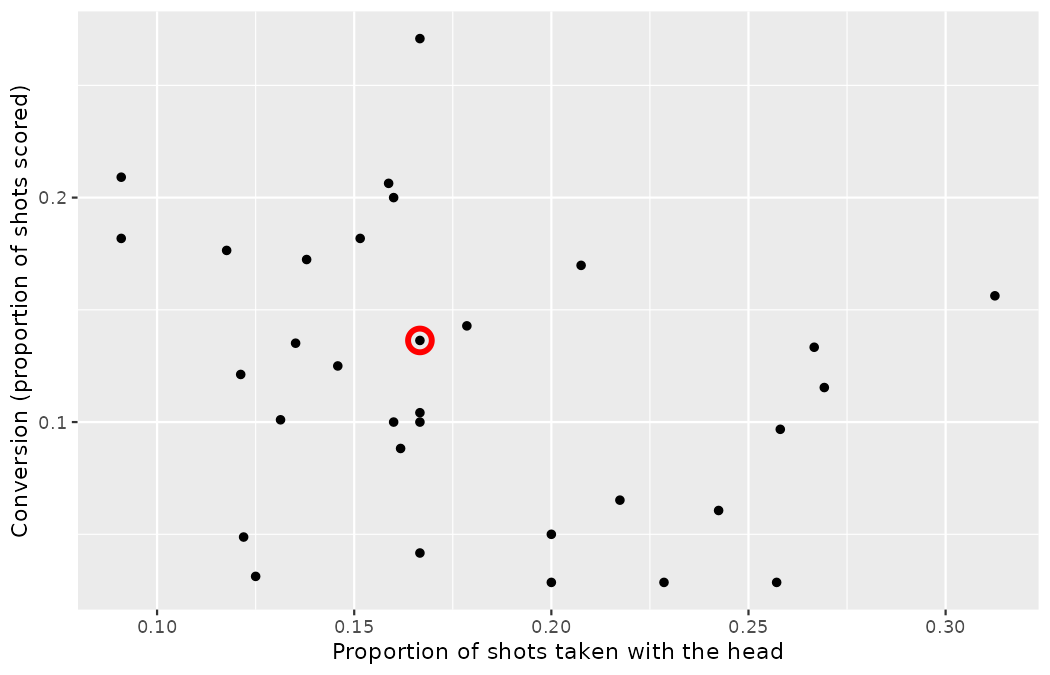
\includegraphics[width=0.85\linewidth,height=\textheight,keepaspectratio]{figures/data-hello-1.png}

The plot shows 32 points, one per team. The ranges on the two axes can
be computed directly:

\begin{Shaded}
\begin{Highlighting}[]
\NormalTok{team\_profile }\SpecialCharTok{|\textgreater{}}
  \FunctionTok{summarize}\NormalTok{(}
    \AttributeTok{min\_headers =} \FunctionTok{min}\NormalTok{(prop\_headers), }\AttributeTok{max\_headers =} \FunctionTok{max}\NormalTok{(prop\_headers),}
    \AttributeTok{min\_conversion =} \FunctionTok{min}\NormalTok{(conversion), }\AttributeTok{max\_conversion =} \FunctionTok{max}\NormalTok{(conversion)}
\NormalTok{  )}
\CommentTok{\#\textgreater{} \# A tibble: 1 × 4}
\CommentTok{\#\textgreater{}   min\_headers max\_headers min\_conversion max\_conversion}
\CommentTok{\#\textgreater{}         \textless{}dbl\textgreater{}       \textless{}dbl\textgreater{}          \textless{}dbl\textgreater{}          \textless{}dbl\textgreater{}}
\CommentTok{\#\textgreater{} 1      0.0909       0.312         0.0286          0.271}
\end{Highlighting}
\end{Shaded}

Header shares run from under a tenth of a team's shots (0.091) to nearly
a third (0.312), and conversion rates from around 3\% (0.029) up to 27\%
(0.271). The cloud drifts downward from left to right: teams whose shot
diet contains more headers tend, loosely, to convert at lower rates. The
drift is genuine but loose -- the points scatter widely around it, and
individual teams cut against it. Morocco, highlighted, sits near the
middle of the cloud: 16.7\% of its 66 shots were headers, and it
converted 13.6\% of its shots. We might brainstorm as to why the
downward tendency exists -- headed chances are typically contested, at
awkward angles, from crosses -- and investigate each idea to determine
which are the most reasonable explanations.

The header share and conversion rate are said to be associated because
the plot shows a discernible pattern. When two variables show some
connection with one another, they are called \textbf{associated}
variables.

Because the pattern here is loose, this is also the right moment for a
warning about how \emph{not} to read an association: as a rule that
binds every case. It does not.

\begin{Shaded}
\begin{Highlighting}[]
\NormalTok{team\_profile }\SpecialCharTok{|\textgreater{}}
  \FunctionTok{arrange}\NormalTok{(}\FunctionTok{desc}\NormalTok{(prop\_headers)) }\SpecialCharTok{|\textgreater{}}
  \FunctionTok{select}\NormalTok{(team, prop\_headers, conversion) }\SpecialCharTok{|\textgreater{}}
  \FunctionTok{slice\_head}\NormalTok{(}\AttributeTok{n =} \DecValTok{1}\NormalTok{)}
\CommentTok{\#\textgreater{} \# A tibble: 1 × 3}
\CommentTok{\#\textgreater{}   team   prop\_headers conversion}
\CommentTok{\#\textgreater{}   \textless{}chr\textgreater{}         \textless{}dbl\textgreater{}      \textless{}dbl\textgreater{}}
\CommentTok{\#\textgreater{} 1 Serbia        0.312      0.156}
\end{Highlighting}
\end{Shaded}

Serbia had the highest header share in the tournament -- 31.2\% of its
shots -- yet converted 15.6\% of its shots, \emph{above} the
tournament's overall rate. An association is a statement about a
tendency across the whole collection of cases, not a verdict on any
single one. A scout who dismisses a team (or a player) because ``headers
don't convert'' has mistaken a tendency for a law.

\begin{tcolorbox}[enhanced jigsaw, left=2mm, leftrule=.75mm, title=\textcolor{quarto-callout-tip-color}{\faLightbulb}\hspace{0.5em}{Check your understanding}, arc=.35mm, rightrule=.15mm, coltitle=black, colframe=quarto-callout-tip-color-frame, bottomrule=.15mm, colbacktitle=quarto-callout-tip-color!10!white, opacitybacktitle=0.6, breakable, bottomtitle=1mm, toptitle=1mm, titlerule=0mm, opacityback=0, toprule=.15mm, colback=white]

Examine the variables in the \texttt{team\_profile} dataset, which are
described in Table~\ref{tbl-team-profile-variables}. Create two
questions about possible relationships between variables in
\texttt{team\_profile} that are of interest to you.

\begin{center}\rule{0.5\linewidth}{0.5pt}\end{center}

Two example questions: (1) What is the relationship between the share of
shots taken under pressure and a team's mean chance quality per shot?
(2) If a team takes an above-average share of its shots from corner
sequences, will its conversion rate tend to be above or below the
average?

\end{tcolorbox}

\begin{tcolorbox}[enhanced jigsaw, left=2mm, leftrule=.75mm, title=\textcolor{quarto-callout-note-color}{\faInfo}\hspace{0.5em}{Worked example}, arc=.35mm, rightrule=.15mm, coltitle=black, colframe=quarto-callout-note-color-frame, bottomrule=.15mm, colbacktitle=quarto-callout-note-color!10!white, opacitybacktitle=0.6, breakable, bottomtitle=1mm, toptitle=1mm, titlerule=0mm, opacityback=0, toprule=.15mm, colback=white]

This example examines the relationship between a team's total chance
quality and its goal tally, visualized by the code below. Are these
variables associated?

\begin{Shaded}
\begin{Highlighting}[]
\FunctionTok{ggplot}\NormalTok{(team\_profile, }\FunctionTok{aes}\NormalTok{(}\AttributeTok{x =}\NormalTok{ total\_xg, }\AttributeTok{y =}\NormalTok{ goals)) }\SpecialCharTok{+}
  \FunctionTok{geom\_point}\NormalTok{() }\SpecialCharTok{+}
  \FunctionTok{geom\_point}\NormalTok{(}
    \AttributeTok{data =}\NormalTok{ team\_profile }\SpecialCharTok{|\textgreater{}} \FunctionTok{filter}\NormalTok{(team }\SpecialCharTok{==} \StringTok{"Argentina"}\NormalTok{),}
    \AttributeTok{size =} \DecValTok{4}\NormalTok{, }\AttributeTok{shape =} \DecValTok{1}\NormalTok{, }\AttributeTok{stroke =} \DecValTok{2}\NormalTok{, }\AttributeTok{color =} \StringTok{"red"}
\NormalTok{  ) }\SpecialCharTok{+}
  \FunctionTok{labs}\NormalTok{(}
    \AttributeTok{x =} \StringTok{"Total chance quality (sum of xG)"}\NormalTok{,}
    \AttributeTok{y =} \StringTok{"Goals scored"}
\NormalTok{  )}
\end{Highlighting}
\end{Shaded}

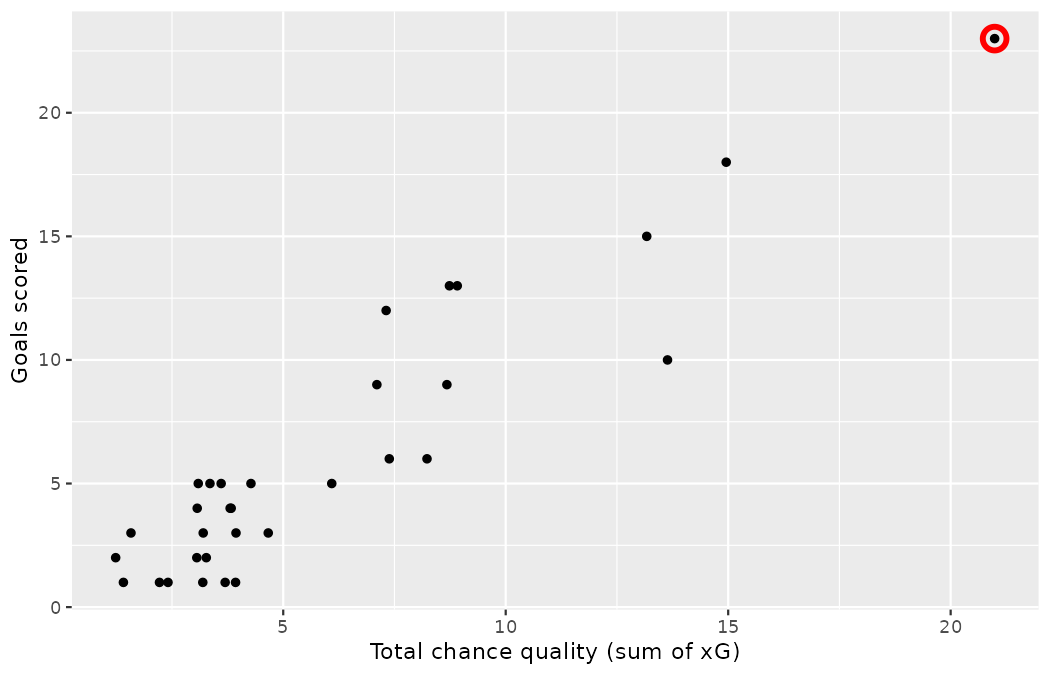
\includegraphics[width=0.85\linewidth,height=\textheight,keepaspectratio]{figures/data-hello-2.png}

\begin{center}\rule{0.5\linewidth}{0.5pt}\end{center}

The larger a team's total chance quality, the higher the goal tally
observed for the team. The 32 points sweep tightly upward from the
bottom-left cluster of group-stage exits with a handful of goals to the
highlighted point at the top right: Argentina, whose 110 shots
accumulated a total chance quality of about 21.0 and who scored 23 goals
on their way to the title (both values visible in the
\texttt{team\_profile} display above) --- 23 including their 8 shoot-out
conversions; 15 came in open play and set pieces during periods 1--4.
While it isn't true that every team with a higher total chance quality
has a higher goal tally, the trend in the plot is evident, and visibly
tighter than in the headers plot. Since there is some relationship
between the variables, they are associated.

\end{tcolorbox}

Because there is a downward trend in the headers plot -- teams with more
of their shots coming from headers are associated with lower conversion
-- these variables are said to be \textbf{negatively associated}. A
\textbf{positive association} is shown in the relationship between
\texttt{total\_xg} and \texttt{goals}, where teams that create more
total chance quality tend to score more goals.

If two variables are not associated, then they are said to be
\textbf{independent}. That is, two variables are independent if there is
no evident relationship between the two.

\begin{tcolorbox}[enhanced jigsaw, left=2mm, leftrule=.75mm, title=\textcolor{quarto-callout-important-color}{\faExclamation}\hspace{0.5em}{Associated or independent, not both}, arc=.35mm, rightrule=.15mm, coltitle=black, colframe=quarto-callout-important-color-frame, bottomrule=.15mm, colbacktitle=quarto-callout-important-color!10!white, opacitybacktitle=0.6, breakable, bottomtitle=1mm, toptitle=1mm, titlerule=0mm, opacityback=0, toprule=.15mm, colback=white]

A pair of variables are either related in some way (associated) or not
(independent). No pair of variables is both associated and independent.

\end{tcolorbox}

The strength of an association can be quantified -- we will do so
properly in Chapter~\ref{sec-model-slr} -- but even now the computer can
put a number beside what the eye sees. The correlations confirm the
visual impression: a loose negative relationship in the first plot and a
strong positive one in the second.

\begin{Shaded}
\begin{Highlighting}[]
\FunctionTok{cor}\NormalTok{(team\_profile}\SpecialCharTok{$}\NormalTok{prop\_headers, team\_profile}\SpecialCharTok{$}\NormalTok{conversion)}
\CommentTok{\#\textgreater{} [1] {-}0.2852878}
\FunctionTok{cor}\NormalTok{(team\_profile}\SpecialCharTok{$}\NormalTok{total\_xg, team\_profile}\SpecialCharTok{$}\NormalTok{goals)}
\CommentTok{\#\textgreater{} [1] 0.9281508}
\end{Highlighting}
\end{Shaded}

\subsection{Explanatory and response
variables}\label{explanatory-and-response-variables}

When we ask questions about the relationship between two variables, we
sometimes also want to determine if the change in one variable causes a
change in the other. Consider the following rephrasing of an earlier
question about the \texttt{team\_profile} dataset:

\begin{quote}
If a team increases the total chance quality it creates, does this drive
an increase in its goal tally?
\end{quote}

In this question, we are asking whether one variable affects another. If
this is our underlying belief, then \emph{total chance quality} is the
\textbf{explanatory variable}, and the \emph{goal tally} is the
\textbf{response variable} in the hypothesized relationship.\footnote{In
  some disciplines, it's customary to refer to the explanatory variable
  as the \textbf{independent variable} and the response variable as the
  \textbf{dependent variable}. However, this becomes confusing since a
  \emph{pair} of variables might be independent or dependent, so we
  avoid this language.}

\begin{tcolorbox}[enhanced jigsaw, left=2mm, leftrule=.75mm, title=\textcolor{quarto-callout-important-color}{\faExclamation}\hspace{0.5em}{Explanatory and response variables}, arc=.35mm, rightrule=.15mm, coltitle=black, colframe=quarto-callout-important-color-frame, bottomrule=.15mm, colbacktitle=quarto-callout-important-color!10!white, opacitybacktitle=0.6, breakable, bottomtitle=1mm, toptitle=1mm, titlerule=0mm, opacityback=0, toprule=.15mm, colback=white]

When we suspect one variable might causally affect another, we label the
first variable the explanatory variable and the second the response
variable. We also use the terms \textbf{explanatory} and
\textbf{response} to describe variables where the \textbf{response}
might be predicted using the \textbf{explanatory} even if there is no
causal relationship.

explanatory variable \(\rightarrow\) \emph{might affect} \(\rightarrow\)
response variable

For many pairs of variables, there is no hypothesized relationship, and
these labels would not be applied to either variable in such cases.

\end{tcolorbox}

Read the little diagram above with care, because it is our first piece
of statistical notation and it earns its place in every chapter that
follows. The arrow \(\rightarrow\) is not an equals sign and not a
promise: it records the \emph{direction of the hypothesized influence},
running from the variable we suspect (or use) as the driver to the
variable whose behavior we want to explain or predict. The words ``might
affect'' sit on the arrow deliberately. Labeling \texttt{total\_xg}
explanatory and \texttt{goals} response records which way our question
points -- nothing more.

Bear in mind that the act of labeling the variables in this way does
nothing to guarantee that a causal relationship exists. A formal
evaluation to check whether one variable causes a change in another
requires an experiment.

\subsection{Observational studies and
experiments}\label{observational-studies-and-experiments}

There are two primary types of data collection: experiments and
observational studies.

When researchers want to evaluate the effect of particular traits,
treatments, or conditions, they conduct an \textbf{experiment}. For
instance, Northbridge's performance staff may suspect that chewing
caffeine gum during the break before extra time improves late-match
running. To check if there really is a causal relationship between the
explanatory variable (whether the player chewed caffeine gum or not) and
the response variable (distance covered at sprint intensity in extra
time), the staff identify a sample of players and split them into
groups. The individuals in each group are \emph{assigned} a treatment.
When individuals are randomly assigned to a group, the experiment is
called a \textbf{randomized experiment}. Random assignment organizes the
participants in a study into groups that are roughly equal on all
aspects, thus allowing us to control for any confounding variables that
might affect the outcome (e.g., fitness level, position, minutes already
played). (See Section~\ref{sec-principles-experimental-design} for more
information on confounding variables.) For example, each player in the
experiment could be randomly assigned, perhaps by flipping a coin, into
one of two groups: the first group receives a \textbf{placebo} (fake
treatment, in this case identical-tasting caffeine-free gum) and the
second group receives the caffeine gum. See the case study in
Section~\ref{sec-case-study-stents-strokes} for another example of an
experiment, though that study did not employ a placebo -- there was no
sham drill program.

Researchers perform an \textbf{observational study} when they collect
data in a way that does not directly interfere with how the data arise.
For instance, a scouting department may collect information via
questionnaires to its scouts, review the club's historical recruitment
records, or follow a \textbf{cohort} of an entire academy intake for
years to form hypotheses about why some players reach the first team and
others do not. The tournament shot data we used to build
\texttt{shots50} and \texttt{team\_profile} are exactly this kind of
data: nobody assigned Serbia its header share -- football simply
happened, and StatsBomb wrote it down. In each of these situations,
researchers merely observe the data that arise. In general,
observational studies can provide evidence of a naturally occurring
association between variables, but they cannot by themselves show a
causal connection as they do not offer a mechanism for controlling for
confounding variables. (See
Section~\ref{sec-principles-experimental-design} for more information on
confounding variables.)

\begin{tcolorbox}[enhanced jigsaw, left=2mm, leftrule=.75mm, title=\textcolor{quarto-callout-important-color}{\faExclamation}\hspace{0.5em}{Association ≠ Causation}, arc=.35mm, rightrule=.15mm, coltitle=black, colframe=quarto-callout-important-color-frame, bottomrule=.15mm, colbacktitle=quarto-callout-important-color!10!white, opacitybacktitle=0.6, breakable, bottomtitle=1mm, toptitle=1mm, titlerule=0mm, opacityback=0, toprule=.15mm, colback=white]

In general, association does not imply causation. An advantage of a
randomized experiment is that it is easier to establish causal
relationships with such a study. The main reason for this is that
observational studies do not control for confounding variables, and
hence establishing causal relationships with observational studies
requires advanced statistical methods (that are beyond the scope of this
book). We revisit ideas of confounding when we discuss experiments in
Section~\ref{sec-principles-experimental-design}.

\end{tcolorbox}

This inequality is the single most consequential sentence in the
chapter, so let us pin it to our two data sources. The finishing trial
was a randomized experiment: because a coin decided who got the program,
the 8-percentage-point gap can be laid at the program's door. The
headers-and-conversion pattern is observational: heading a lot travels
together with converting less, but nothing in the data says the headers
\emph{cause} the lower conversion -- teams that head often may simply be
teams forced to attack from crosses against packed defenses. When a
finding from \texttt{team\_profile} lands on Marta Vidal's desk, the
verb must be ``is associated with,'' never ``causes.''

\begin{tcolorbox}[enhanced jigsaw, left=2mm, leftrule=.75mm, title=\textcolor{quarto-callout-tip-color}{\faLightbulb}\hspace{0.5em}{Check your understanding}, arc=.35mm, rightrule=.15mm, coltitle=black, colframe=quarto-callout-tip-color-frame, bottomrule=.15mm, colbacktitle=quarto-callout-tip-color!10!white, opacitybacktitle=0.6, breakable, bottomtitle=1mm, toptitle=1mm, titlerule=0mm, opacityback=0, toprule=.15mm, colback=white]

An analyst finds, in tournament data, that players who take more
first-time shots have higher conversion rates, and recommends coaching
every academy forward to shoot first time. What is the flaw in jumping
from this finding to that recommendation?

\begin{center}\rule{0.5\linewidth}{0.5pt}\end{center}

The finding is observational: nobody randomly assigned first-time shots.
Players attempt first-time finishes disproportionately in situations
that already favor scoring (a cutback arriving in the six-yard box,
say), so the situation -- not the technique -- may drive the
association. Only a randomized experiment, like the academy trial
designs in this chapter, could establish that coaching the technique
\emph{causes} better conversion.

\end{tcolorbox}

\section{Chapter review}\label{sec-chp1-review}

\subsection{Summary}\label{summary}

This chapter introduced you to the world of data. Data can be organized
in many ways but tidy data, where each row represents an observation and
each column represents a variable, lends itself most easily to
statistical analysis -- whether the observation is a single World Cup
shot, as in \texttt{shots50}, or a whole team's tournament, as in
\texttt{team\_profile}. Always be able to say what the unit of
observation is, what type each variable is, and whether the data arose
from an experiment or observationally -- the last distinction controls
whether ``causes'' may ever appear in your report. And keep the
finishing trial in mind: a well-designed study is allowed to surprise
you. Many of the ideas from this chapter will be revisited as we move on
to doing end-to-end data analyses. In the next chapter you're going to
learn about how we can design studies to collect the data we need to
make conclusions with the desired scope of inference.

\subsection{Terms}\label{terms}

The terms introduced in this chapter are presented below, alphabetized.
If you're not sure what some of these terms mean, we recommend you go
back in the text and review their definitions. You should be able to
easily spot them as \textbf{bolded text}.

\begin{longtable}[]{@{}
  >{\raggedright\arraybackslash}p{(\linewidth - 4\tabcolsep) * \real{0.3380}}
  >{\raggedright\arraybackslash}p{(\linewidth - 4\tabcolsep) * \real{0.3380}}
  >{\raggedright\arraybackslash}p{(\linewidth - 4\tabcolsep) * \real{0.3239}}@{}}
\caption{Terms introduced in this
chapter.}\label{tbl-terms-chp-1}\tabularnewline
\toprule\noalign{}
\endfirsthead
\endhead
\bottomrule\noalign{}
\endlastfoot
associated & experiment & ordinal \\
case & explanatory variable & placebo \\
categorical & independent & positive association \\
cohort & level & randomized experiment \\
continuous & negative association & response variable \\
data & nominal & summary statistic \\
data frame & numerical & tidy data \\
dependent & observation & unit of observation \\
discrete & observational study & variable \\
\end{longtable}

\section{Exercises}\label{sec-chp1-exercises}

Answers to odd-numbered exercises can be found in
Appendix~\ref{sec-exercise-solutions-01}.

\begin{enumerate}
\def\labelenumi{\arabic{enumi}.}
\item
  \textbf{Knockout matches at the World Cup.} The data frame below
  contains information on the 16 knockout-stage matches of the 2022
  Men's World Cup, from the Round of 16 through the Final. Scores are
  goals after any extra time; matches still level at that point are
  recorded as a \texttt{draw}, even if a penalty shoot-out followed. How
  many observations and how many variables does this data frame
  have?\footnote{The 2022 World Cup match data used in this exercise are
    in \texttt{data/derived/wc2022\_matches.csv} (StatsBomb open data).}

\begin{Shaded}
\begin{Highlighting}[]
\NormalTok{wc2022\_matches }\OtherTok{\textless{}{-}} \FunctionTok{read\_csv}\NormalTok{(}\StringTok{"data/derived/wc2022\_matches.csv"}\NormalTok{)}

\NormalTok{knockout\_matches }\OtherTok{\textless{}{-}}\NormalTok{ wc2022\_matches }\SpecialCharTok{|\textgreater{}}
  \FunctionTok{filter}\NormalTok{(stage }\SpecialCharTok{!=} \StringTok{"Group Stage"}\NormalTok{) }\SpecialCharTok{|\textgreater{}}
  \FunctionTok{arrange}\NormalTok{(match\_date) }\SpecialCharTok{|\textgreater{}}
  \FunctionTok{select}\NormalTok{(match\_date, stage, home\_team, away\_team, home\_score, away\_score, result)}

\NormalTok{knockout\_matches}
\CommentTok{\#\textgreater{} \# A tibble: 16 × 7}
\CommentTok{\#\textgreater{}    match\_date stage           home\_team   away\_team home\_score away\_score result}
\CommentTok{\#\textgreater{}    \textless{}date\textgreater{}     \textless{}chr\textgreater{}           \textless{}chr\textgreater{}       \textless{}chr\textgreater{}          \textless{}dbl\textgreater{}      \textless{}dbl\textgreater{} \textless{}chr\textgreater{}}
\CommentTok{\#\textgreater{}  1 2022{-}12{-}03 Round of 16     Argentina   Australia          2          1 home}
\CommentTok{\#\textgreater{}  2 2022{-}12{-}03 Round of 16     Netherlands United S…          3          1 home}
\CommentTok{\#\textgreater{}  3 2022{-}12{-}04 Round of 16     England     Senegal            3          0 home}
\CommentTok{\#\textgreater{}  4 2022{-}12{-}04 Round of 16     France      Poland             3          1 home}
\CommentTok{\#\textgreater{}  5 2022{-}12{-}05 Round of 16     Japan       Croatia            1          1 draw}
\CommentTok{\#\textgreater{}  6 2022{-}12{-}05 Round of 16     Brazil      South Ko…          4          1 home}
\CommentTok{\#\textgreater{}  7 2022{-}12{-}06 Round of 16     Portugal    Switzerl…          6          1 home}
\CommentTok{\#\textgreater{}  8 2022{-}12{-}06 Round of 16     Morocco     Spain              0          0 draw}
\CommentTok{\#\textgreater{}  9 2022{-}12{-}09 Quarter{-}finals  Netherlands Argentina          2          2 draw}
\CommentTok{\#\textgreater{} 10 2022{-}12{-}09 Quarter{-}finals  Croatia     Brazil             1          1 draw}
\CommentTok{\#\textgreater{} 11 2022{-}12{-}10 Quarter{-}finals  Morocco     Portugal           1          0 home}
\CommentTok{\#\textgreater{} 12 2022{-}12{-}10 Quarter{-}finals  England     France             1          2 away}
\CommentTok{\#\textgreater{} 13 2022{-}12{-}13 Semi{-}finals     Argentina   Croatia            3          0 home}
\CommentTok{\#\textgreater{} 14 2022{-}12{-}14 Semi{-}finals     France      Morocco            2          0 home}
\CommentTok{\#\textgreater{} 15 2022{-}12{-}17 3rd Place Final Croatia     Morocco            2          1 home}
\CommentTok{\#\textgreater{} 16 2022{-}12{-}18 Final           Argentina   France             3          3 draw}
\end{Highlighting}
\end{Shaded}
\item
  \textbf{Shots at the Women's Euro.} The data frame below contains
  information on every shot recorded at the 2025 Women's Euro, with a
  selection of the recorded characteristics kept for display. How many
  observations and how many variables does this data frame
  have?\footnote{The 2025 Women's Euro shot data used in this exercise
    are in \texttt{data/derived/weuro2025\_shots.csv} (StatsBomb open
    data).}

\begin{Shaded}
\begin{Highlighting}[]
\NormalTok{weuro2025\_shots }\OtherTok{\textless{}{-}} \FunctionTok{read\_csv}\NormalTok{(}\StringTok{"data/derived/weuro2025\_shots.csv"}\NormalTok{)}

\NormalTok{weuro2025\_shots }\SpecialCharTok{|\textgreater{}}
  \FunctionTok{select}\NormalTok{(player, team, minute, play\_pattern, statsbomb\_xg, outcome, goal)}
\CommentTok{\#\textgreater{} \# A tibble: 913 × 7}
\CommentTok{\#\textgreater{}    player                   team  minute play\_pattern statsbomb\_xg outcome goal}
\CommentTok{\#\textgreater{}    \textless{}chr\textgreater{}                    \textless{}chr\textgreater{}  \textless{}dbl\textgreater{} \textless{}chr\textgreater{}               \textless{}dbl\textgreater{} \textless{}chr\textgreater{}   \textless{}lgl\textgreater{}}
\CommentTok{\#\textgreater{}  1 Alexandra Jóhannsdóttir  Icel…      0 From Throw …       0.0131 Off T   FALSE}
\CommentTok{\#\textgreater{}  2 Katla Tryggvadóttir      Icel…      5 Regular Play       0.249  Saved   FALSE}
\CommentTok{\#\textgreater{}  3 Sveindís Jane Jónsdóttir Icel…      5 From Counter       0.130  Blocked FALSE}
\CommentTok{\#\textgreater{}  4 Alexandra Jóhannsdóttir  Icel…      5 From Corner        0.0346 Saved … FALSE}
\CommentTok{\#\textgreater{}  5 Sveindís Jane Jónsdóttir Icel…      5 From Corner        0.477  Goal    TRUE}
\CommentTok{\#\textgreater{}  6 Signe Gaupset            Norw…     13 Regular Play       0.0463 Blocked FALSE}
\CommentTok{\#\textgreater{}  7 Signe Gaupset            Norw…     14 From Corner        0.0570 Goal    TRUE}
\CommentTok{\#\textgreater{}  8 Elisabeth Terland        Norw…     22 From Throw …       0.0365 Blocked FALSE}
\CommentTok{\#\textgreater{}  9 Elisabeth Terland        Norw…     23 Regular Play       0.105  Saved   FALSE}
\CommentTok{\#\textgreater{} 10 Frida Maanum             Norw…     25 Regular Play       0.0321 Off T   FALSE}
\CommentTok{\#\textgreater{} \# ℹ 903 more rows}
\end{Highlighting}
\end{Shaded}
\item
  \textbf{Training load and soft-tissue injury, study components.} Club
  medical researchers collected data to examine the relationship between
  training load and soft-tissue injuries in academy players. During the
  study, load levels were measured by the GPS vests players wear in
  every session. Specifically, total distance covered was recorded in
  kilometers, high-speed running distance in meters, the number of
  sprint efforts as a count, and the acute-to-chronic workload ratio as
  a unitless index. Injury records were collected on 8,472 player-weeks
  across four seasons at Northbridge and its partner academies, and each
  player's load exposure during the preceding four weeks was calculated
  for each week. The analysis suggested that increased high-speed
  running distance and, to a lesser degree, elevated acute-to-chronic
  workload ratios may be associated with the occurrence of soft-tissue
  injuries.

  \begin{enumerate}
  \def\labelenumii{\alph{enumii}.}
  \item
    Identify the main research question of the study.
  \item
    Who are the subjects in this study, and how many are included?
  \item
    What are the variables in the study? Identify each variable as
    numerical or categorical. If numerical, state whether the variable
    is discrete or continuous. If categorical, state whether the
    variable is ordinal.
  \end{enumerate}
\item
  \textbf{Honesty in the academy, study components.} Researchers working
  with Jonas Beck's academy staff studied the relationship between
  honesty, age, and self-control by running an exercise with 160 academy
  players between the ages of 8 and 15. Participants reported their age,
  sex, and whether they were an only child or not. The researchers asked
  each player to toss a fair two-colored training marker (one side
  white, one side black) in private and to record the side that landed
  up on a paper sheet, and said they would only reward players who
  report white -- with extra minutes in Friday's small-sided games.

  \begin{enumerate}
  \def\labelenumii{\alph{enumii}.}
  \item
    Identify the main research question of the study.
  \item
    Who are the subjects in this study, and how many are included?
  \item
    The study's findings can be summarized as follows: \emph{``Half the
    players were explicitly told not to cheat and the others were not
    given any explicit instructions. In the no instruction group the
    probability of cheating was found to be uniform across groups based
    on the player's characteristics. In the group that was explicitly
    told to not cheat, girls were less likely to cheat, and while the
    rate of cheating did not vary by age for boys, it decreased with age
    for girls.''} How many variables were recorded for each subject in
    the study in order to conclude these findings? State the variables
    and their types.
  \end{enumerate}
\item
  \textbf{Gamified tactics course, study components.} Gamification is
  the application of game-design elements and game principles in
  non-game contexts. In player development, gamification is often
  implemented as competitive app-based activities for learning tactical
  concepts. Researchers investigating the effects of gamification on
  learning conducted a study where they split the academy players
  enrolled in the club's tactics course into four groups: (1) no
  video-review exercises and no gamification, (2) video-review exercises
  but no gamification, (3) gamification but no video-review exercises,
  and (4) gamification and video-review exercises. Players in all groups
  also attended classroom sessions. Players in the course came from two
  programs: Outfield Development (279 players) and Goalkeeping (86
  players). After their assigned learning experience, each player took a
  final evaluation comprised of 30 multiple choice questions and their
  score was measured as the number of questions they answered correctly.
  The researchers considered players' gender, year in the academy (first
  through fourth year), and program. Other variables considered were
  familiarity with video-analysis software and use of football video
  games, both of which were measured on a scale of 1 (beginner) to 5
  (proficient). The study found that gamification had a positive effect
  on learning compared to traditional instruction involving classroom
  sessions and video-review exercises. They also found that the effect
  was larger for female players and for players in the Outfield
  Development program.

  \begin{enumerate}
  \def\labelenumii{\alph{enumii}.}
  \item
    Identify the main research question of the study.
  \item
    Who were the subjects in this study, and how many were included?
  \item
    What are the variables in the study? Identify each variable as
    numerical or categorical. If numerical, state whether the variable
    is discrete or continuous. If categorical, state whether the
    variable is ordinal.
  \end{enumerate}
\item
  \textbf{Snack takers, study components.} In a study of the
  relationship between perceived status and unethical behavior, 129
  trialists at a Northbridge residential trial camp were asked to
  identify themselves as having low or high standing by comparing
  themselves to peers with the most (least) senior appearances, most
  (least) social-media following, and most (least) prestigious previous
  club. They were also presented with a jar of individually wrapped
  recovery snacks and informed that the snacks were for the under-12
  group training nearby, but that they could take some if they wanted.
  After completing some unrelated drills, participants reported the
  number of snacks they had taken.

  \begin{enumerate}
  \def\labelenumii{\alph{enumii}.}
  \item
    Identify the main research question of the study.
  \item
    Who were the subjects in this study, and how many were included?
  \item
    The study found that trialists who identified as high-standing took
    more snacks than others. How many variables were recorded for each
    subject in the study in order to conclude these findings? State the
    variables and their types.
  \end{enumerate}
\item
  \textbf{Hamstring tightness and dry needling.} Recurring hamstring
  tightness is a persistent complaint in heavy fixture periods, and some
  players ask the medical staff for dry needling to treat it. To
  determine whether dry needling relieves the tightness, medical staff
  at Northbridge and two partner clubs ran a randomized controlled study
  where 89 players who reported recurring hamstring tightness were
  randomly assigned to one of two groups: treatment or control.
  Forty-three (43) players in the treatment group received dry needling
  specifically targeted at the affected muscle group. Forty-six (46)
  players in the control group received sham needling (needle insertion
  at non-therapeutic sites). Twenty-four (24) hours after their session,
  players were asked if they were symptom free. This is a constructed
  scenario, built by the code below; the results are summarized in the
  contingency table.\footnote{The \texttt{needle89} data are a
    constructed scouting-adjacent scenario, generated entirely by the
    code shown; no real players were needled.}

\begin{Shaded}
\begin{Highlighting}[]
\NormalTok{needle89 }\OtherTok{\textless{}{-}} \FunctionTok{tibble}\NormalTok{(}
  \AttributeTok{group =} \FunctionTok{c}\NormalTok{(}\FunctionTok{rep}\NormalTok{(}\StringTok{"dry needling"}\NormalTok{, }\DecValTok{43}\NormalTok{), }\FunctionTok{rep}\NormalTok{(}\StringTok{"sham needling"}\NormalTok{, }\DecValTok{46}\NormalTok{)),}
  \AttributeTok{symptom\_free =} \FunctionTok{c}\NormalTok{(}\FunctionTok{rep}\NormalTok{(}\StringTok{"yes"}\NormalTok{, }\DecValTok{10}\NormalTok{), }\FunctionTok{rep}\NormalTok{(}\StringTok{"no"}\NormalTok{, }\DecValTok{33}\NormalTok{),}
                   \FunctionTok{rep}\NormalTok{(}\StringTok{"yes"}\NormalTok{, }\DecValTok{2}\NormalTok{), }\FunctionTok{rep}\NormalTok{(}\StringTok{"no"}\NormalTok{, }\DecValTok{44}\NormalTok{))}
\NormalTok{)}

\NormalTok{needle89 }\SpecialCharTok{|\textgreater{}}
  \FunctionTok{count}\NormalTok{(group, symptom\_free) }\SpecialCharTok{|\textgreater{}}
  \FunctionTok{pivot\_wider}\NormalTok{(}\AttributeTok{names\_from =}\NormalTok{ symptom\_free, }\AttributeTok{values\_from =}\NormalTok{ n)}
\CommentTok{\#\textgreater{} \# A tibble: 2 × 3}
\CommentTok{\#\textgreater{}   group            no   yes}
\CommentTok{\#\textgreater{}   \textless{}chr\textgreater{}         \textless{}int\textgreater{} \textless{}int\textgreater{}}
\CommentTok{\#\textgreater{} 1 dry needling     33    10}
\CommentTok{\#\textgreater{} 2 sham needling    44     2}
\end{Highlighting}
\end{Shaded}

  \begin{longtable}[]{@{}lrrr@{}}
  \toprule\noalign{}
  & yes & no & Total \\
  \midrule\noalign{}
  \endhead
  \bottomrule\noalign{}
  \endlastfoot
  dry needling & 10 & 33 & 43 \\
  sham needling & 2 & 44 & 46 \\
  Total & 12 & 77 & 89 \\
  \end{longtable}

  \begin{enumerate}
  \def\labelenumii{\alph{enumii}.}
  \item
    What percent of players in the treatment group were symptom free 24
    hours after receiving dry needling?
  \item
    What percent were symptom free in the control group?
  \item
    In which group did a higher percent of players become symptom free
    24 hours after the session?
  \item
    Your findings so far might suggest that dry needling is an effective
    treatment for hamstring tightness for all players who suffer from
    it. However this is not the only possible conclusion. What is one
    other possible explanation for the observed difference between the
    percentages of players that are symptom free 24 hours after the
    session in the two groups?
  \item
    What are the explanatory and response variables in this study?
  \end{enumerate}
\item
  \textbf{Muscle soreness and structured recovery.} Club researchers
  studying the effect of a structured recovery program for acute
  post-match muscle soreness compared to standard symptomatic care
  randomly assigned 166 players reporting acute soreness during a
  congested fixture period to one of two groups: treatment or control.
  Study participants received either a 10-day structured recovery
  program (daily physio-led cold-water immersion, compression, and
  mobility sessions) or standard care similar in daily contact time. The
  standard care consisted of symptomatic treatments such as rest, ice,
  and over-the-counter anti-inflammatories as needed. At the end of the
  10-day period, players were asked if they experienced improvement in
  symptoms. This is a constructed scenario, built by the code below,
  which also summarizes the distribution of responses.\footnote{The
    \texttt{soreness166} data are a constructed scenario, generated
    entirely by the code shown; no real players were treated.}

\begin{Shaded}
\begin{Highlighting}[]
\NormalTok{soreness166 }\OtherTok{\textless{}{-}} \FunctionTok{tibble}\NormalTok{(}
  \AttributeTok{group =} \FunctionTok{c}\NormalTok{(}\FunctionTok{rep}\NormalTok{(}\StringTok{"structured recovery"}\NormalTok{, }\DecValTok{85}\NormalTok{), }\FunctionTok{rep}\NormalTok{(}\StringTok{"standard care"}\NormalTok{, }\DecValTok{81}\NormalTok{)),}
  \AttributeTok{improvement =} \FunctionTok{c}\NormalTok{(}\FunctionTok{rep}\NormalTok{(}\StringTok{"yes"}\NormalTok{, }\DecValTok{66}\NormalTok{), }\FunctionTok{rep}\NormalTok{(}\StringTok{"no"}\NormalTok{, }\DecValTok{19}\NormalTok{),}
                  \FunctionTok{rep}\NormalTok{(}\StringTok{"yes"}\NormalTok{, }\DecValTok{65}\NormalTok{), }\FunctionTok{rep}\NormalTok{(}\StringTok{"no"}\NormalTok{, }\DecValTok{16}\NormalTok{))}
\NormalTok{)}

\NormalTok{soreness166 }\SpecialCharTok{|\textgreater{}}
  \FunctionTok{count}\NormalTok{(group, improvement) }\SpecialCharTok{|\textgreater{}}
  \FunctionTok{pivot\_wider}\NormalTok{(}\AttributeTok{names\_from =}\NormalTok{ improvement, }\AttributeTok{values\_from =}\NormalTok{ n)}
\CommentTok{\#\textgreater{} \# A tibble: 2 × 3}
\CommentTok{\#\textgreater{}   group                  no   yes}
\CommentTok{\#\textgreater{}   \textless{}chr\textgreater{}               \textless{}int\textgreater{} \textless{}int\textgreater{}}
\CommentTok{\#\textgreater{} 1 standard care          16    65}
\CommentTok{\#\textgreater{} 2 structured recovery    19    66}
\end{Highlighting}
\end{Shaded}

  \begin{enumerate}
  \def\labelenumii{\alph{enumii}.}
  \item
    What percent of players in the treatment group experienced
    improvement in symptoms?
  \item
    What percent experienced improvement in symptoms in the control
    group?
  \item
    In which group did a higher percentage of players experience
    improvement in symptoms?
  \item
    Your findings so far might suggest a real difference in the
    effectiveness of the structured program and standard care for
    improving symptoms of muscle soreness. However this is not the only
    possible conclusion. What is one other possible explanation for the
    observed difference between the percentages of players who
    experienced improvement in symptoms?
  \item
    What are the explanatory and response variables in this study?
  \end{enumerate}
\item
  \textbf{Late-arrival fines, study components.} Priya Rao tested the
  deterrence hypothesis, which predicts that the introduction of a
  penalty will reduce the occurrence of the behavior subject to the
  fine, with the condition that the fine leaves everything else
  unchanged, by instituting a fine for arriving late to training. For
  this study, she worked with 10 volunteer academy age-group squads, at
  Northbridge and its partner academies, that did not originally fine
  players for late arrival. She randomly selected 6 of these squads and
  instituted a monetary fine (of a considerable amount) for arriving
  late to training and then removed it. In the remaining 4 squads no
  fine was introduced. The study period was divided into four: before
  the fine (weeks 1--4), the first 4 weeks with the fine (weeks 5--8),
  the last 8 weeks with the fine (weeks 9--16), and the after-fine
  period (weeks 17--20). Throughout the study, the number of players who
  arrived late was recorded each week for each squad. The study found
  that the number of late arrivals increased discernibly when the fine
  was introduced, and no reduction occurred after the fine was removed.
  This is a constructed scenario, generated by the seeded code
  below.\footnote{The \texttt{late\_fines} data are a constructed
    scenario, generated entirely by the seeded code shown; no real
    academy squads were fined.}

\begin{Shaded}
\begin{Highlighting}[]
\FunctionTok{set.seed}\NormalTok{(}\DecValTok{105}\NormalTok{)}
\NormalTok{fine\_squads }\OtherTok{\textless{}{-}} \FunctionTok{sample}\NormalTok{(}\DecValTok{1}\SpecialCharTok{:}\DecValTok{10}\NormalTok{, }\DecValTok{6}\NormalTok{)}

\NormalTok{late\_fines }\OtherTok{\textless{}{-}} \FunctionTok{crossing}\NormalTok{(}\AttributeTok{squad =} \DecValTok{1}\SpecialCharTok{:}\DecValTok{10}\NormalTok{, }\AttributeTok{week =} \DecValTok{1}\SpecialCharTok{:}\DecValTok{20}\NormalTok{) }\SpecialCharTok{|\textgreater{}}
  \FunctionTok{mutate}\NormalTok{(}
    \AttributeTok{group =} \FunctionTok{if\_else}\NormalTok{(squad }\SpecialCharTok{\%in\%}\NormalTok{ fine\_squads, }\StringTok{"fine"}\NormalTok{, }\StringTok{"control"}\NormalTok{),}
    \AttributeTok{study\_period =} \FunctionTok{case\_when}\NormalTok{(}
\NormalTok{      week }\SpecialCharTok{\textless{}=} \DecValTok{4}  \SpecialCharTok{\textasciitilde{}} \StringTok{"before fine"}\NormalTok{,}
\NormalTok{      week }\SpecialCharTok{\textless{}=} \DecValTok{8}  \SpecialCharTok{\textasciitilde{}} \StringTok{"first 4 weeks with fine"}\NormalTok{,}
\NormalTok{      week }\SpecialCharTok{\textless{}=} \DecValTok{16} \SpecialCharTok{\textasciitilde{}} \StringTok{"last 8 weeks with fine"}\NormalTok{,}
      \AttributeTok{.default   =} \StringTok{"after fine"}
\NormalTok{    ),}
    \AttributeTok{late\_arrivals =} \FunctionTok{rpois}\NormalTok{(}\DecValTok{200}\NormalTok{, }\AttributeTok{lambda =} \FunctionTok{if\_else}\NormalTok{(group }\SpecialCharTok{==} \StringTok{"fine"} \SpecialCharTok{\&}\NormalTok{ week }\SpecialCharTok{\textgreater{}} \DecValTok{4}\NormalTok{, }\FloatTok{3.6}\NormalTok{, }\DecValTok{2}\NormalTok{))}
\NormalTok{  ) }\SpecialCharTok{|\textgreater{}}
  \FunctionTok{select}\NormalTok{(squad, week, group, late\_arrivals, study\_period)}

\NormalTok{late\_fines}
\CommentTok{\#\textgreater{} \# A tibble: 200 × 5}
\CommentTok{\#\textgreater{}    squad  week group late\_arrivals study\_period}
\CommentTok{\#\textgreater{}    \textless{}int\textgreater{} \textless{}int\textgreater{} \textless{}chr\textgreater{}         \textless{}int\textgreater{} \textless{}chr\textgreater{}}
\CommentTok{\#\textgreater{}  1     1     1 fine              3 before fine}
\CommentTok{\#\textgreater{}  2     1     2 fine              2 before fine}
\CommentTok{\#\textgreater{}  3     1     3 fine              0 before fine}
\CommentTok{\#\textgreater{}  4     1     4 fine              2 before fine}
\CommentTok{\#\textgreater{}  5     1     5 fine              6 first 4 weeks with fine}
\CommentTok{\#\textgreater{}  6     1     6 fine              4 first 4 weeks with fine}
\CommentTok{\#\textgreater{}  7     1     7 fine              6 first 4 weeks with fine}
\CommentTok{\#\textgreater{}  8     1     8 fine              2 first 4 weeks with fine}
\CommentTok{\#\textgreater{}  9     1     9 fine              5 last 8 weeks with fine}
\CommentTok{\#\textgreater{} 10     1    10 fine              4 last 8 weeks with fine}
\CommentTok{\#\textgreater{} \# ℹ 190 more rows}
\end{Highlighting}
\end{Shaded}

  \begin{enumerate}
  \def\labelenumii{\alph{enumii}.}
  \item
    Is this an observational study or an experiment? Explain your
    reasoning.
  \item
    What are the cases in this study and how many are included?
  \item
    What is the response variable in the study and what type of variable
    is it?
  \item
    What are the explanatory variables in the study and what types of
    variables are they?
  \end{enumerate}
\item
  \textbf{Efficacy of an injury-prevention warm-up, study components.}
  Results of a season-long trial across Northbridge's partner academies
  show that a neuromuscular injury-prevention warm-up demonstrated a
  striking protective effect on 12-to-15-year-old academy players. In
  this trial, 2,260 players were randomly assigned to two groups: one
  group of 1,131 players performed the new warm-up before every session
  and the other 1,129 continued with the standard warm-up. While 18
  serious knee injuries were observed in the standard warm-up group,
  none were observed in the new warm-up group. This is a constructed
  scenario, built by the code below.\footnote{The \texttt{warmup\_trial}
    data are a constructed scenario, generated entirely by the code
    shown; no real players were injured.}

\begin{Shaded}
\begin{Highlighting}[]
\NormalTok{warmup\_trial }\OtherTok{\textless{}{-}} \FunctionTok{tibble}\NormalTok{(}
  \AttributeTok{group =} \FunctionTok{c}\NormalTok{(}\FunctionTok{rep}\NormalTok{(}\StringTok{"new warm{-}up"}\NormalTok{, }\DecValTok{1131}\NormalTok{), }\FunctionTok{rep}\NormalTok{(}\StringTok{"standard warm{-}up"}\NormalTok{, }\DecValTok{1129}\NormalTok{)),}
  \AttributeTok{knee\_injury =} \FunctionTok{c}\NormalTok{(}\FunctionTok{rep}\NormalTok{(}\StringTok{"no injury"}\NormalTok{, }\DecValTok{1131}\NormalTok{),}
                  \FunctionTok{rep}\NormalTok{(}\StringTok{"serious injury"}\NormalTok{, }\DecValTok{18}\NormalTok{), }\FunctionTok{rep}\NormalTok{(}\StringTok{"no injury"}\NormalTok{, }\DecValTok{1111}\NormalTok{))}
\NormalTok{)}

\NormalTok{warmup\_trial }\SpecialCharTok{|\textgreater{}}
  \FunctionTok{count}\NormalTok{(group, knee\_injury) }\SpecialCharTok{|\textgreater{}}
  \FunctionTok{pivot\_wider}\NormalTok{(}\AttributeTok{names\_from =}\NormalTok{ knee\_injury, }\AttributeTok{values\_from =}\NormalTok{ n, }\AttributeTok{values\_fill =} \DecValTok{0}\NormalTok{)}
\CommentTok{\#\textgreater{} \# A tibble: 2 × 3}
\CommentTok{\#\textgreater{}   group            \textasciigrave{}no injury\textasciigrave{} \textasciigrave{}serious injury\textasciigrave{}}
\CommentTok{\#\textgreater{}   \textless{}chr\textgreater{}                  \textless{}int\textgreater{}            \textless{}int\textgreater{}}
\CommentTok{\#\textgreater{} 1 new warm{-}up             1131                0}
\CommentTok{\#\textgreater{} 2 standard warm{-}up        1111               18}
\end{Highlighting}
\end{Shaded}

  \begin{enumerate}
  \def\labelenumii{\alph{enumii}.}
  \item
    Is this an observational study or an experiment? Explain your
    reasoning.
  \item
    What are the cases in this study and how many are included?
  \item
    What is the response variable in the study and what type of variable
    is it?
  \item
    What are the explanatory variables in the study and what types of
    variables are they?
  \end{enumerate}
\item
  \textbf{Trial-camp measurements.} Data were collected on 344 trialists
  attending Northbridge's three regional trial camps (Eastfield,
  Millbrook, and Southgate). In addition to which camp each trialist
  attended, the data contain information on the trialist's position
  group (\emph{Defender}, \emph{Midfielder}, or \emph{Forward}), their
  30-meter sprint time (measured in seconds), their countermovement jump
  height and standing height (measured in centimeters), their body mass
  (measured in kilograms), and their dominant foot (left or right).

  \begin{enumerate}
  \def\labelenumii{\alph{enumii}.}
  \tightlist
  \item
    How many cases were included in the data?
  \item
    How many numerical variables are included in the data? Indicate what
    they are, and if they are continuous or discrete.
  \item
    How many categorical variables are included in the data, and what
    are they? List the corresponding levels (categories) for each.
  \end{enumerate}
\item
  \textbf{Away-travel habits of Northbridge supporters.} A survey was
  conducted to study the away-travel habits of 1,691 Northbridge
  season-ticket holders. Below is a data frame displaying a portion of
  the data collected in this survey. An \texttt{NA} indicates that a
  question did not apply to a given respondent: supporters who do not
  travel to away matches were not asked how many away matches they
  attend. No such survey was actually run -- the data are a constructed
  scenario, generated by the seeded code below.\footnote{The
    \texttt{fan\_survey} data are a constructed scenario, generated
    entirely by the seeded code shown; no real supporters were surveyed.}

\begin{Shaded}
\begin{Highlighting}[]
\FunctionTok{set.seed}\NormalTok{(}\DecValTok{106}\NormalTok{)}
\NormalTok{fan\_survey }\OtherTok{\textless{}{-}} \FunctionTok{tibble}\NormalTok{(}
  \AttributeTok{sex =} \FunctionTok{sample}\NormalTok{(}\FunctionTok{c}\NormalTok{(}\StringTok{"Female"}\NormalTok{, }\StringTok{"Male"}\NormalTok{), }\DecValTok{1691}\NormalTok{, }\AttributeTok{replace =} \ConstantTok{TRUE}\NormalTok{),}
  \AttributeTok{age =} \FunctionTok{sample}\NormalTok{(}\DecValTok{16}\SpecialCharTok{:}\DecValTok{85}\NormalTok{, }\DecValTok{1691}\NormalTok{, }\AttributeTok{replace =} \ConstantTok{TRUE}\NormalTok{),}
  \AttributeTok{ticket\_tier =} \FunctionTok{sample}\NormalTok{(}\FunctionTok{c}\NormalTok{(}\StringTok{"Bronze"}\NormalTok{, }\StringTok{"Silver"}\NormalTok{, }\StringTok{"Gold"}\NormalTok{), }\DecValTok{1691}\NormalTok{,}
                       \AttributeTok{replace =} \ConstantTok{TRUE}\NormalTok{, }\AttributeTok{prob =} \FunctionTok{c}\NormalTok{(}\FloatTok{0.5}\NormalTok{, }\FloatTok{0.3}\NormalTok{, }\FloatTok{0.2}\NormalTok{)),}
  \AttributeTok{income\_band =} \FunctionTok{sample}\NormalTok{(}\FunctionTok{c}\NormalTok{(}\StringTok{"Under €20K"}\NormalTok{, }\StringTok{"€20K{-}40K"}\NormalTok{, }\StringTok{"€40K{-}60K"}\NormalTok{, }\StringTok{"Over €60K"}\NormalTok{),}
                       \DecValTok{1691}\NormalTok{, }\AttributeTok{replace =} \ConstantTok{TRUE}\NormalTok{, }\AttributeTok{prob =} \FunctionTok{c}\NormalTok{(}\FloatTok{0.3}\NormalTok{, }\FloatTok{0.35}\NormalTok{, }\FloatTok{0.2}\NormalTok{, }\FloatTok{0.15}\NormalTok{)),}
  \AttributeTok{away\_travel =} \FunctionTok{sample}\NormalTok{(}\FunctionTok{c}\NormalTok{(}\StringTok{"Yes"}\NormalTok{, }\StringTok{"No"}\NormalTok{), }\DecValTok{1691}\NormalTok{, }\AttributeTok{replace =} \ConstantTok{TRUE}\NormalTok{, }\AttributeTok{prob =} \FunctionTok{c}\NormalTok{(}\FloatTok{0.35}\NormalTok{, }\FloatTok{0.65}\NormalTok{)),}
  \AttributeTok{league\_aways =} \FunctionTok{if\_else}\NormalTok{(away\_travel }\SpecialCharTok{==} \StringTok{"Yes"}\NormalTok{, }\FunctionTok{rpois}\NormalTok{(}\DecValTok{1691}\NormalTok{, }\DecValTok{6}\NormalTok{), }\ConstantTok{NA\_integer\_}\NormalTok{),}
  \AttributeTok{cup\_aways =} \FunctionTok{if\_else}\NormalTok{(away\_travel }\SpecialCharTok{==} \StringTok{"Yes"}\NormalTok{, }\FunctionTok{rpois}\NormalTok{(}\DecValTok{1691}\NormalTok{, }\DecValTok{2}\NormalTok{), }\ConstantTok{NA\_integer\_}\NormalTok{)}
\NormalTok{)}

\NormalTok{fan\_survey}
\CommentTok{\#\textgreater{} \# A tibble: 1,691 × 7}
\CommentTok{\#\textgreater{}    sex      age ticket\_tier income\_band away\_travel league\_aways cup\_aways}
\CommentTok{\#\textgreater{}    \textless{}chr\textgreater{}  \textless{}int\textgreater{} \textless{}chr\textgreater{}       \textless{}chr\textgreater{}       \textless{}chr\textgreater{}              \textless{}int\textgreater{}     \textless{}int\textgreater{}}
\CommentTok{\#\textgreater{}  1 Female    73 Silver      €20K{-}40K    No                    NA        NA}
\CommentTok{\#\textgreater{}  2 Male      80 Bronze      €40K{-}60K    No                    NA        NA}
\CommentTok{\#\textgreater{}  3 Male      82 Silver      €20K{-}40K    No                    NA        NA}
\CommentTok{\#\textgreater{}  4 Male      78 Gold        €20K{-}40K    Yes                    6         5}
\CommentTok{\#\textgreater{}  5 Male      85 Gold        €20K{-}40K    Yes                    9         1}
\CommentTok{\#\textgreater{}  6 Male      51 Gold        €20K{-}40K    Yes                    7         3}
\CommentTok{\#\textgreater{}  7 Female    69 Bronze      Under €20K  No                    NA        NA}
\CommentTok{\#\textgreater{}  8 Male      18 Bronze      €40K{-}60K    No                    NA        NA}
\CommentTok{\#\textgreater{}  9 Male      48 Bronze      €40K{-}60K    No                    NA        NA}
\CommentTok{\#\textgreater{} 10 Female    82 Bronze      €20K{-}40K    No                    NA        NA}
\CommentTok{\#\textgreater{} \# ℹ 1,681 more rows}
\end{Highlighting}
\end{Shaded}

  \begin{enumerate}
  \def\labelenumii{\alph{enumii}.}
  \item
    What does each row of the data frame represent?
  \item
    How many participants were included in the survey?
  \item
    Indicate whether each variable is numerical or categorical. If
    numerical, identify as continuous or discrete. If categorical,
    indicate if the variable is ordinal.
  \end{enumerate}
\item
  \textbf{Every shot at the World Cup.} The visualization built by the
  code below shows the chance quality of all 1,494 shots at the 2022
  Men's World Cup across the match minutes in which they were taken.
  This visualization was constructed based on a dataset where each
  observation is a shot.\footnote{The 2022 World Cup shot data used in
    this exercise are in \texttt{data/derived/wc2022\_shots.csv}
    (StatsBomb open data).}

\begin{Shaded}
\begin{Highlighting}[]
\NormalTok{wc2022\_shots }\OtherTok{\textless{}{-}} \FunctionTok{read\_csv}\NormalTok{(}\StringTok{"data/derived/wc2022\_shots.csv"}\NormalTok{)}

\FunctionTok{ggplot}\NormalTok{(wc2022\_shots, }\FunctionTok{aes}\NormalTok{(}\AttributeTok{x =}\NormalTok{ minute, }\AttributeTok{y =}\NormalTok{ statsbomb\_xg, }\AttributeTok{color =}\NormalTok{ play\_pattern)) }\SpecialCharTok{+}
  \FunctionTok{geom\_point}\NormalTok{(}\AttributeTok{alpha =} \FloatTok{0.3}\NormalTok{, }\AttributeTok{size =} \FloatTok{0.8}\NormalTok{) }\SpecialCharTok{+}
  \FunctionTok{facet\_grid}\NormalTok{(under\_pressure }\SpecialCharTok{\textasciitilde{}}\NormalTok{ first\_time, }\AttributeTok{labeller =}\NormalTok{ label\_both) }\SpecialCharTok{+}
  \FunctionTok{labs}\NormalTok{(}
    \AttributeTok{x =} \StringTok{"Match minute"}\NormalTok{, }\AttributeTok{y =} \StringTok{"Chance quality (statsbomb\_xg)"}\NormalTok{,}
    \AttributeTok{color =} \StringTok{"Play pattern"}
\NormalTok{  )}
\end{Highlighting}
\end{Shaded}

  The figure contains four panels, splitting the shots by whether the
  shooter was under pressure (rows) and whether the shot was struck
  first time (columns), with points colored by play pattern. Every panel
  shows a dense band of low-quality chances -- about 87\% of all shots
  carry a chance quality below 0.25 -- with rarer high-quality chances
  scattered above, spread across the full sweep of match minutes from 0
  to 127. A thin horizontal stripe of penalties, all at a chance quality
  of exactly 0.7835, appears only in the not-under-pressure,
  not-first-time panel, which is also by far the busiest panel, holding
  825 of the 1,494 shots; the under-pressure, first-time panel is the
  sparsest, with 37.

  \begin{enumerate}
  \def\labelenumii{\alph{enumii}.}
  \item
    List the variables you believe were necessary to create this
    visualization.
  \item
    Indicate whether each variable is numerical or categorical. If
    numerical, identify as continuous or discrete. If categorical,
    indicate if the variable is ordinal.
  \end{enumerate}
\item
  \textbf{Shot patterns of three contenders.} The visualization built by
  the code below shows how Argentina, France, and Morocco generated
  their shots across their seven matches each at the 2022 Men's World
  Cup. Specifically, for a given match, it displays the percentage of
  the team's shots in that match arising from each family of play
  patterns, grouped by how the possession started: open play, counter,
  possessions starting from a restart (a corner, free kick, throw-in,
  goal kick, keeper distribution, or kick-off --- labeled
  \texttt{set\ piece\ /\ restart} in the code), and other. Note that
  \texttt{play\_pattern} records the start of the possession, not the
  action that created the shot: a chance twenty passes after a throw-in
  still counts toward the restart family. This visualization was
  constructed based on a dataset where each observation is a team/match
  pair.\footnote{The 2022 World Cup shot data used in this exercise are
    in \texttt{data/derived/wc2022\_shots.csv} (StatsBomb open data).}

\begin{Shaded}
\begin{Highlighting}[]
\NormalTok{wc2022\_shots }\SpecialCharTok{|\textgreater{}}
  \FunctionTok{filter}\NormalTok{(team }\SpecialCharTok{\%in\%} \FunctionTok{c}\NormalTok{(}\StringTok{"Argentina"}\NormalTok{, }\StringTok{"France"}\NormalTok{, }\StringTok{"Morocco"}\NormalTok{)) }\SpecialCharTok{|\textgreater{}}
  \FunctionTok{mutate}\NormalTok{(}\AttributeTok{family =} \FunctionTok{case\_when}\NormalTok{(}
\NormalTok{    play\_pattern }\SpecialCharTok{==} \StringTok{"Regular Play"} \SpecialCharTok{\textasciitilde{}} \StringTok{"open play"}\NormalTok{,}
\NormalTok{    play\_pattern }\SpecialCharTok{==} \StringTok{"From Counter"} \SpecialCharTok{\textasciitilde{}} \StringTok{"counter"}\NormalTok{,}
\NormalTok{    play\_pattern }\SpecialCharTok{==} \StringTok{"Other"}        \SpecialCharTok{\textasciitilde{}} \StringTok{"other"}\NormalTok{,}
    \AttributeTok{.default =} \StringTok{"set piece / restart"}
\NormalTok{  )) }\SpecialCharTok{|\textgreater{}}
  \FunctionTok{group\_by}\NormalTok{(team) }\SpecialCharTok{|\textgreater{}}
  \FunctionTok{arrange}\NormalTok{(match\_date) }\SpecialCharTok{|\textgreater{}}
  \FunctionTok{mutate}\NormalTok{(}\AttributeTok{match\_number =} \FunctionTok{dense\_rank}\NormalTok{(match\_date)) }\SpecialCharTok{|\textgreater{}}
  \FunctionTok{count}\NormalTok{(team, match\_number, family) }\SpecialCharTok{|\textgreater{}}
  \FunctionTok{group\_by}\NormalTok{(team, match\_number) }\SpecialCharTok{|\textgreater{}}
  \FunctionTok{mutate}\NormalTok{(}\AttributeTok{percent\_of\_shots =}\NormalTok{ n }\SpecialCharTok{/} \FunctionTok{sum}\NormalTok{(n)) }\SpecialCharTok{|\textgreater{}}
  \FunctionTok{ggplot}\NormalTok{(}\FunctionTok{aes}\NormalTok{(}\AttributeTok{x =}\NormalTok{ match\_number, }\AttributeTok{y =}\NormalTok{ percent\_of\_shots, }\AttributeTok{color =}\NormalTok{ team)) }\SpecialCharTok{+}
  \FunctionTok{geom\_point}\NormalTok{(}\AttributeTok{alpha =} \FloatTok{0.5}\NormalTok{) }\SpecialCharTok{+}
  \FunctionTok{geom\_line}\NormalTok{() }\SpecialCharTok{+}
  \FunctionTok{facet\_wrap}\NormalTok{(}\SpecialCharTok{\textasciitilde{}}\NormalTok{family) }\SpecialCharTok{+}
  \FunctionTok{labs}\NormalTok{(}\AttributeTok{x =} \StringTok{"Match number"}\NormalTok{, }\AttributeTok{y =} \StringTok{"\% of the team\textquotesingle{}s shots"}\NormalTok{, }\AttributeTok{color =} \StringTok{"Team"}\NormalTok{)}
\end{Highlighting}
\end{Shaded}

  The figure shows one panel per play-pattern family, with a colored
  line per team tracking that family's share of the team's shots across
  its seven matches. The lines swing sharply from match to match, and in
  most of the 21 team-matches the family of possessions starting from a
  restart accounts for the largest share of the team's shots.

  \begin{enumerate}
  \def\labelenumii{\alph{enumii}.}
  \item
    List the variables used in creating this visualization.
  \item
    Indicate whether each variable is numerical or categorical. If
    numerical, identify as continuous or discrete. If categorical,
    indicate if the variable is ordinal.
  \end{enumerate}
\item
  \textbf{Goals by matchday.} The visualization built by the code below
  shows the number of goals scored on each matchday of the 2022 Men's
  World Cup and the 2025 Women's Euro, with matchdays numbered from each
  tournament's first day of play.\footnote{The match data used in this
    exercise are in \texttt{data/derived/wc2022\_matches.csv} and
    \texttt{data/derived/weuro2025\_matches.csv} (StatsBomb open data).}

\begin{Shaded}
\begin{Highlighting}[]
\NormalTok{wc2022\_matches    }\OtherTok{\textless{}{-}} \FunctionTok{read\_csv}\NormalTok{(}\StringTok{"data/derived/wc2022\_matches.csv"}\NormalTok{)}
\NormalTok{weuro2025\_matches }\OtherTok{\textless{}{-}} \FunctionTok{read\_csv}\NormalTok{(}\StringTok{"data/derived/weuro2025\_matches.csv"}\NormalTok{)}

\FunctionTok{bind\_rows}\NormalTok{(wc2022\_matches, weuro2025\_matches) }\SpecialCharTok{|\textgreater{}}
  \FunctionTok{group\_by}\NormalTok{(competition) }\SpecialCharTok{|\textgreater{}}
  \FunctionTok{arrange}\NormalTok{(match\_date, }\AttributeTok{.by\_group =} \ConstantTok{TRUE}\NormalTok{) }\SpecialCharTok{|\textgreater{}}
  \FunctionTok{mutate}\NormalTok{(}\AttributeTok{matchday =} \FunctionTok{dense\_rank}\NormalTok{(match\_date)) }\SpecialCharTok{|\textgreater{}}
  \FunctionTok{group\_by}\NormalTok{(competition, matchday) }\SpecialCharTok{|\textgreater{}}
  \FunctionTok{summarize}\NormalTok{(}\AttributeTok{goals =} \FunctionTok{sum}\NormalTok{(home\_score }\SpecialCharTok{+}\NormalTok{ away\_score)) }\SpecialCharTok{|\textgreater{}}
  \FunctionTok{ggplot}\NormalTok{(}\FunctionTok{aes}\NormalTok{(}\AttributeTok{x =}\NormalTok{ matchday, }\AttributeTok{y =}\NormalTok{ goals, }\AttributeTok{group =}\NormalTok{ competition,}
             \AttributeTok{color =}\NormalTok{ competition, }\AttributeTok{linetype =}\NormalTok{ competition)) }\SpecialCharTok{+}
  \FunctionTok{geom\_line}\NormalTok{() }\SpecialCharTok{+}
  \FunctionTok{geom\_point}\NormalTok{() }\SpecialCharTok{+}
  \FunctionTok{labs}\NormalTok{(}
    \AttributeTok{title =} \StringTok{"Goals scored on each matchday"}\NormalTok{,}
    \AttributeTok{x =} \StringTok{"Matchday"}\NormalTok{, }\AttributeTok{y =} \StringTok{"Number of goals"}\NormalTok{,}
    \AttributeTok{color =} \StringTok{"Competition"}\NormalTok{, }\AttributeTok{linetype =} \StringTok{"Competition"}
\NormalTok{  )}
\end{Highlighting}
\end{Shaded}

  The World Cup line runs across 23 matchdays and the Women's Euro line
  across 19. Both peak at 14 goals in a single day (matchday 9 and
  matchday 12, respectively), and both drop to quieter days late in the
  tournament, when only one knockout match is played at a time.

  \begin{enumerate}
  \def\labelenumii{\alph{enumii}.}
  \item
    List the variables you believe were necessary to create this
    visualization.
  \item
    Indicate whether each variable is numerical or categorical. If
    numerical, identify as continuous or discrete. If categorical,
    indicate if the variable is ordinal.
  \end{enumerate}
\item
  \textbf{Shot outcomes by stage.} The visualization built by the code
  below shows the distribution of shot outcomes at the 2022 Men's World
  Cup and the 2025 Women's Euro based on the tournament stage the shot
  was taken in. In the dataset, each observation is a shot.\footnote{The
    shot data used in this exercise are in
    \texttt{data/derived/wc2022\_shots.csv} and
    \texttt{data/derived/weuro2025\_shots.csv} (StatsBomb open data).}

\begin{Shaded}
\begin{Highlighting}[]
\NormalTok{weuro2025\_shots }\OtherTok{\textless{}{-}} \FunctionTok{read\_csv}\NormalTok{(}\StringTok{"data/derived/weuro2025\_shots.csv"}\NormalTok{)}

\FunctionTok{bind\_rows}\NormalTok{(wc2022\_shots, weuro2025\_shots) }\SpecialCharTok{|\textgreater{}}
  \FunctionTok{mutate}\NormalTok{(}
    \AttributeTok{stage =} \FunctionTok{fct\_relevel}\NormalTok{(stage, }\StringTok{"Group Stage"}\NormalTok{, }\StringTok{"Round of 16"}\NormalTok{, }\StringTok{"Quarter{-}finals"}\NormalTok{,}
                        \StringTok{"Semi{-}finals"}\NormalTok{, }\StringTok{"3rd Place Final"}\NormalTok{, }\StringTok{"Final"}\NormalTok{),}
    \AttributeTok{outcome =} \FunctionTok{fct\_relevel}\NormalTok{(outcome, }\StringTok{"Goal"}\NormalTok{, }\StringTok{"Saved"}\NormalTok{, }\StringTok{"Saved to Post"}\NormalTok{,}
                          \StringTok{"Saved Off Target"}\NormalTok{, }\StringTok{"Post"}\NormalTok{, }\StringTok{"Blocked"}\NormalTok{, }\StringTok{"Off T"}\NormalTok{, }\StringTok{"Wayward"}\NormalTok{)}
\NormalTok{  ) }\SpecialCharTok{|\textgreater{}}
  \FunctionTok{ggplot}\NormalTok{(}\FunctionTok{aes}\NormalTok{(}\AttributeTok{x =}\NormalTok{ stage, }\AttributeTok{fill =}\NormalTok{ outcome)) }\SpecialCharTok{+}
  \FunctionTok{geom\_bar}\NormalTok{(}\AttributeTok{position =} \StringTok{"fill"}\NormalTok{) }\SpecialCharTok{+}
  \FunctionTok{facet\_wrap}\NormalTok{(}\SpecialCharTok{\textasciitilde{}}\NormalTok{competition, }\AttributeTok{ncol =} \DecValTok{1}\NormalTok{) }\SpecialCharTok{+}
  \FunctionTok{labs}\NormalTok{(}\AttributeTok{x =} \StringTok{"Tournament stage"}\NormalTok{, }\AttributeTok{y =} \StringTok{"Proportion"}\NormalTok{, }\AttributeTok{fill =} \StringTok{"Shot outcome"}\NormalTok{)}
\end{Highlighting}
\end{Shaded}

  The figure shows one standardized stacked bar per tournament stage,
  with one panel per competition; the Women's Euro had no Round of 16
  and no 3rd Place Final, so those slots are empty in its panel. In
  every stage of both competitions the \emph{Blocked}, \emph{Off T}, and
  \emph{Saved} segments take up most of each bar, and the \emph{Goal}
  segment is thinnest in the semi-finals of both competitions.

  \begin{enumerate}
  \def\labelenumii{\alph{enumii}.}
  \item
    List the variables you believe were necessary to create this
    visualization.
  \item
    Indicate whether each variable is numerical or categorical. If
    numerical, identify as continuous or discrete. If categorical,
    indicate if the variable is ordinal.
  \end{enumerate}
\item
  \textbf{Scouting summary table.} Ahead of a recruitment meeting, Priya
  Rao circulates a summary of how teams of interest created and finished
  their chances at the 2022 Men's World Cup. The following is an excerpt
  from that summary table, created from the shot-level tournament data
  for two teams the club tracked closely; a shot is \emph{on target} if
  its outcome was a goal or a save. Shots with body part \texttt{Other}
  (4 shots for these two teams) are excluded.\footnote{The 2022 World
    Cup shot data used in this exercise are in
    \texttt{data/derived/wc2022\_shots.csv} (StatsBomb open data).}

\begin{Shaded}
\begin{Highlighting}[]
\NormalTok{wc2022\_shots }\SpecialCharTok{|\textgreater{}}
  \FunctionTok{filter}\NormalTok{(team }\SpecialCharTok{\%in\%} \FunctionTok{c}\NormalTok{(}\StringTok{"Argentina"}\NormalTok{, }\StringTok{"Morocco"}\NormalTok{), body\_part }\SpecialCharTok{!=} \StringTok{"Other"}\NormalTok{) }\SpecialCharTok{|\textgreater{}}
  \FunctionTok{mutate}\NormalTok{(}\AttributeTok{on\_target =}\NormalTok{ outcome }\SpecialCharTok{\%in\%} \FunctionTok{c}\NormalTok{(}\StringTok{"Goal"}\NormalTok{, }\StringTok{"Saved"}\NormalTok{, }\StringTok{"Saved to Post"}\NormalTok{, }\StringTok{"Saved Off Target"}\NormalTok{)) }\SpecialCharTok{|\textgreater{}}
  \FunctionTok{group\_by}\NormalTok{(team, body\_part) }\SpecialCharTok{|\textgreater{}}
  \FunctionTok{summarize}\NormalTok{(}
    \AttributeTok{shots =} \FunctionTok{n}\NormalTok{(),}
    \AttributeTok{on\_target\_rate =} \FunctionTok{round}\NormalTok{(}\FunctionTok{mean}\NormalTok{(on\_target), }\DecValTok{3}\NormalTok{),}
    \AttributeTok{conversion =} \FunctionTok{round}\NormalTok{(}\FunctionTok{mean}\NormalTok{(goal), }\DecValTok{3}\NormalTok{)}
\NormalTok{  )}
\CommentTok{\#\textgreater{} \# A tibble: 6 × 5}
\CommentTok{\#\textgreater{} \# Groups:   team [2]}
\CommentTok{\#\textgreater{}   team      body\_part  shots on\_target\_rate conversion}
\CommentTok{\#\textgreater{}   \textless{}chr\textgreater{}     \textless{}chr\textgreater{}      \textless{}int\textgreater{}          \textless{}dbl\textgreater{}      \textless{}dbl\textgreater{}}
\CommentTok{\#\textgreater{} 1 Argentina Head          10          0.3        0}
\CommentTok{\#\textgreater{} 2 Argentina Left Foot     47          0.574      0.213}
\CommentTok{\#\textgreater{} 3 Argentina Right Foot    51          0.471      0.255}
\CommentTok{\#\textgreater{} 4 Morocco   Head          11          0.273      0.182}
\CommentTok{\#\textgreater{} 5 Morocco   Left Foot     22          0.318      0.091}
\CommentTok{\#\textgreater{} 6 Morocco   Right Foot    31          0.355      0.129}
\end{Highlighting}
\end{Shaded}

  The table is an all-shots view: Argentina's footed rows include their
  penalty and shoot-out kicks (12 scored from 14), which lift the footed
  conversion rates well above their open-play levels --- a frame choice
  worth flagging, as Chapter~\ref{sec-data-applications} will teach.

  \begin{enumerate}
  \def\labelenumii{\alph{enumii}.}
  \item
    What variables were recorded on each individual shot in order to
    create the summary table above?
  \item
    State whether each variable is numerical or categorical. If
    numerical, state whether it is continuous or discrete. If
    categorical, state whether it is ordinal or not.
  \item
    Suppose we wanted to evaluate whether conversion rates are different
    for shots taken with different body parts. In this analysis, which
    variable would be the response variable and which variable would be
    the explanatory variable?
  \end{enumerate}
\item
  \textbf{Shots by body part across two tournaments.} The following
  summary table shows the number of shots at the 2022 Men's World Cup
  and the 2025 Women's Euro by the body part used and the outcome of the
  shot (goal or no goal). Shots with body part \texttt{Other} (13 at the
  World Cup, 4 at the Women's Euro) are excluded.\footnote{The shot data
    used in this exercise are in \texttt{data/derived/wc2022\_shots.csv}
    and \texttt{data/derived/weuro2025\_shots.csv} (StatsBomb open
    data).}

\begin{Shaded}
\begin{Highlighting}[]
\FunctionTok{bind\_rows}\NormalTok{(wc2022\_shots, weuro2025\_shots) }\SpecialCharTok{|\textgreater{}}
  \FunctionTok{filter}\NormalTok{(body\_part }\SpecialCharTok{!=} \StringTok{"Other"}\NormalTok{) }\SpecialCharTok{|\textgreater{}}
  \FunctionTok{mutate}\NormalTok{(}\AttributeTok{result =} \FunctionTok{if\_else}\NormalTok{(goal, }\StringTok{"goal"}\NormalTok{, }\StringTok{"no goal"}\NormalTok{)) }\SpecialCharTok{|\textgreater{}}
  \FunctionTok{count}\NormalTok{(competition, body\_part, result) }\SpecialCharTok{|\textgreater{}}
  \FunctionTok{pivot\_wider}\NormalTok{(}\AttributeTok{names\_from =} \FunctionTok{c}\NormalTok{(competition, result), }\AttributeTok{values\_from =}\NormalTok{ n)}
\CommentTok{\#\textgreater{} \# A tibble: 3 × 5}
\CommentTok{\#\textgreater{}   body\_part  wc2022\_goal \textasciigrave{}wc2022\_no goal\textasciigrave{} weuro2025\_goal \textasciigrave{}weuro2025\_no goal\textasciigrave{}}
\CommentTok{\#\textgreater{}   \textless{}chr\textgreater{}            \textless{}int\textgreater{}            \textless{}int\textgreater{}          \textless{}int\textgreater{}               \textless{}int\textgreater{}}
\CommentTok{\#\textgreater{} 1 Head                28              224             17                 134}
\CommentTok{\#\textgreater{} 2 Left Foot           62              387             30                 226}
\CommentTok{\#\textgreater{} 3 Right Foot         102              678             76                 426}
\end{Highlighting}
\end{Shaded}

  \begin{longtable}[]{@{}
    >{\raggedright\arraybackslash}p{(\linewidth - 8\tabcolsep) * \real{0.1429}}
    >{\raggedleft\arraybackslash}p{(\linewidth - 8\tabcolsep) * \real{0.1786}}
    >{\raggedleft\arraybackslash}p{(\linewidth - 8\tabcolsep) * \real{0.2143}}
    >{\raggedleft\arraybackslash}p{(\linewidth - 8\tabcolsep) * \real{0.2143}}
    >{\raggedleft\arraybackslash}p{(\linewidth - 8\tabcolsep) * \real{0.2500}}@{}}
  \toprule\noalign{}
  \begin{minipage}[b]{\linewidth}\raggedright
  \end{minipage} & \begin{minipage}[b]{\linewidth}\raggedleft
  WC 2022: goal
  \end{minipage} & \begin{minipage}[b]{\linewidth}\raggedleft
  WC 2022: no goal
  \end{minipage} & \begin{minipage}[b]{\linewidth}\raggedleft
  WEuro 2025: goal
  \end{minipage} & \begin{minipage}[b]{\linewidth}\raggedleft
  WEuro 2025: no goal
  \end{minipage} \\
  \midrule\noalign{}
  \endhead
  \bottomrule\noalign{}
  \endlastfoot
  Head & 28 & 224 & 17 & 134 \\
  Left Foot & 62 & 387 & 30 & 226 \\
  Right Foot & 102 & 678 & 76 & 426 \\
  \end{longtable}

  \begin{enumerate}
  \def\labelenumii{\alph{enumii}.}
  \item
    What variables were collected on each shot in order to create the
    summary table above?
  \item
    State whether each variable is numerical or categorical. If
    numerical, state whether it is continuous or discrete. If
    categorical, state whether it is ordinal or not.
  \item
    Suppose we wanted to study how the conversion rate of shots varies
    between body parts and across the two competitions. In this
    analysis, which variable would be the response variable and which
    variables would be the explanatory variables?
  \end{enumerate}
\item
  \textbf{Positions in the shot diet.} Both tournament datasets record
  the position of the player taking each shot. The visualization built
  by the code below plots, for each position, the proportion of all 2022
  Men's World Cup shots taken from that position versus the proportion
  of all 2025 Women's Euro shots taken from the same position. The 19
  positions with at least 10 shots in each competition are displayed.
  The diagonal line on the plot is the \(x = y\) line; if a position
  appeared on this line, it would account for exactly the same share of
  the shot diet in both competitions.\footnote{The shot data used in
    this exercise are in \texttt{data/derived/wc2022\_shots.csv} and
    \texttt{data/derived/weuro2025\_shots.csv} (StatsBomb open data).}

\begin{Shaded}
\begin{Highlighting}[]
\NormalTok{wc\_props }\OtherTok{\textless{}{-}}\NormalTok{ wc2022\_shots }\SpecialCharTok{|\textgreater{}}
  \FunctionTok{count}\NormalTok{(position, }\AttributeTok{name =} \StringTok{"wc\_n"}\NormalTok{) }\SpecialCharTok{|\textgreater{}}
  \FunctionTok{mutate}\NormalTok{(}\AttributeTok{wc2022\_prop =}\NormalTok{ wc\_n }\SpecialCharTok{/} \FunctionTok{sum}\NormalTok{(wc\_n))}

\NormalTok{weuro\_props }\OtherTok{\textless{}{-}}\NormalTok{ weuro2025\_shots }\SpecialCharTok{|\textgreater{}}
  \FunctionTok{count}\NormalTok{(position, }\AttributeTok{name =} \StringTok{"we\_n"}\NormalTok{) }\SpecialCharTok{|\textgreater{}}
  \FunctionTok{mutate}\NormalTok{(}\AttributeTok{weuro2025\_prop =}\NormalTok{ we\_n }\SpecialCharTok{/} \FunctionTok{sum}\NormalTok{(we\_n))}

\FunctionTok{inner\_join}\NormalTok{(wc\_props, weuro\_props, }\AttributeTok{by =} \StringTok{"position"}\NormalTok{) }\SpecialCharTok{|\textgreater{}}
  \FunctionTok{filter}\NormalTok{(wc\_n }\SpecialCharTok{\textgreater{}=} \DecValTok{10}\NormalTok{, we\_n }\SpecialCharTok{\textgreater{}=} \DecValTok{10}\NormalTok{) }\SpecialCharTok{|\textgreater{}}
  \FunctionTok{ggplot}\NormalTok{(}\FunctionTok{aes}\NormalTok{(}\AttributeTok{x =}\NormalTok{ wc2022\_prop, }\AttributeTok{y =}\NormalTok{ weuro2025\_prop)) }\SpecialCharTok{+}
  \FunctionTok{geom\_abline}\NormalTok{(}\AttributeTok{intercept =} \DecValTok{0}\NormalTok{, }\AttributeTok{slope =} \DecValTok{1}\NormalTok{, }\AttributeTok{color =} \StringTok{"gray"}\NormalTok{) }\SpecialCharTok{+}
  \FunctionTok{geom\_point}\NormalTok{() }\SpecialCharTok{+}
  \FunctionTok{geom\_text}\NormalTok{(}\FunctionTok{aes}\NormalTok{(}\AttributeTok{label =}\NormalTok{ position), }\AttributeTok{vjust =} \SpecialCharTok{{-}}\FloatTok{0.6}\NormalTok{, }\AttributeTok{size =} \DecValTok{3}\NormalTok{) }\SpecialCharTok{+}
  \FunctionTok{labs}\NormalTok{(}
    \AttributeTok{x =} \StringTok{"Proportion of 2022 World Cup shots"}\NormalTok{,}
    \AttributeTok{y =} \StringTok{"Proportion of 2025 Women\textquotesingle{}s Euro shots"}
\NormalTok{  )}
\end{Highlighting}
\end{Shaded}

  In the figure, Center Forward sits alone in the far upper right, at
  roughly (0.157, 0.157), almost exactly on the diagonal, with Left Wing
  next furthest out and just below the line. Three central-midfield
  positions -- Right Center Midfield (0.035, 0.068), Left Center
  Midfield (0.031, 0.061), and Center Defensive Midfield (0.016, 0.037)
  -- float clearly above the line, while Right Wing (0.103, 0.083) and
  the Left and Right Defensive Midfield roles sit clearly below it. The
  remaining points hug the diagonal, sweeping up and to the right
  together.

  \begin{enumerate}
  \def\labelenumii{\alph{enumii}.}
  \item
    Are these data collected as part of an experiment or an
    observational study?
  \item
    Which position accounts for the largest share of shots in each
    competition?
  \item
    Which positions account for a clearly larger share of the shot diet
    at the Women's Euro than at the World Cup?
  \item
    Is the relationship between the two variables positive or negative?
    What does this mean in context of the data?
  \end{enumerate}
\item
  \textbf{Pressure in the shoot-out.} In a study evaluating the
  relationship between acute stress and penalty-kick performance, half
  of Northbridge's academy players are randomly assigned to take their
  kicks in a simulated hostile environment -- recorded crowd noise at
  full volume through the stadium loudspeakers, cameras on the goal, and
  first-team staff watching from the touchline -- and the other half
  take their kicks on a quiet training pitch at no or baseline stress.

  \begin{enumerate}
  \def\labelenumii{\alph{enumii}.}
  \item
    What type of study is this?
  \item
    Can this study be used to conclude a causal relationship between
    increased stress and penalty-kick performance?
  \end{enumerate}
\end{enumerate}

\begin{center}\rule{0.5\linewidth}{0.5pt}\end{center}

Adapted from \emph{Introduction to Modern Statistics} by
Çetinkaya-Rundel \& Hardin (CC BY-SA 4.0); this adaptation is likewise
CC BY-SA 4.0. Match data: StatsBomb open data.

\chapter{Study design}\label{sec-data-design}

Before digging into the details of working with data, we stop to think
about how data come to be. That is, if the data are to be used to make
broad and complete conclusions about a player, a market, or a
tournament, then it is important to understand who or what the data
represent. One important aspect of data provenance is sampling. Knowing
how the observational units --- the shots, the matches, the prospects
--- were selected from a larger entity will allow for generalizations
back to the population from which the data were randomly selected.
Additionally, by understanding the structure of the study, causal
relationships (``the drill improved his finishing'') can be separated
from those relationships which are only associated (``players on that
drill happened to finish better''). A good question to ask oneself
before working with the data at all is, ``How were these observations
collected?''. A scout who asks it will learn a lot about the data by
understanding its source --- and will be far harder to fool.

\section{Sampling principles and
strategies}\label{sec-sampling-principles-strategies}

The first step in conducting research is to identify topics or questions
that are to be investigated. A clearly laid out research question is
helpful in identifying what subjects or cases should be studied and what
variables are important. This is as true at Northbridge United as in any
laboratory: when Marta Vidal, the sporting director, commissions a piece
of analysis, the first thing Priya Rao's team does is pin down precisely
what is being asked and of whom. It is also important to consider
\emph{how} data are collected so that the data are reliable and help
achieve the research goals.

\subsection{Populations and samples}\label{populations-and-samples}

Consider the following three research questions:

\begin{enumerate}
\def\labelenumi{\arabic{enumi}.}
\tightlist
\item
  What is the average chance quality (xG) of shots taken in the South
  American under-20 leagues this season?
\item
  Over the last five years, what is the average number of academy
  seasons a Northbridge United graduate needed before making a
  first-team debut?
\item
  Does a new high-intensity finishing program raise conversion rates in
  academy forwards?
\end{enumerate}

Each research question refers to a target \textbf{population}. In the
first question, the target population is all shots taken in the South
American under-20 leagues this season, and each shot represents a case.
Oftentimes, it is not feasible to collect data for every case in a
population. Collecting data for an entire population is called a
\textbf{census}. A census is difficult because it is too expensive to
collect data for the entire population --- no club can send scouts to
every under-20 fixture on a continent, and no data provider logs them
all --- but it might also be because it is difficult or impossible to
identify the entire population of interest! Instead, a sample is taken.
A \textbf{sample} is the data you have. Ideally, a sample is a small
fraction of the population. For instance, the 60 shots (or some other
number) a regional scout logged from the matches they attended might be
selected, and this sample data may be used to provide an estimate of the
population average and to answer the research question.

\begin{tcolorbox}[enhanced jigsaw, left=2mm, leftrule=.75mm, title=\textcolor{quarto-callout-tip-color}{\faLightbulb}\hspace{0.5em}{Check your understanding}, arc=.35mm, rightrule=.15mm, coltitle=black, colframe=quarto-callout-tip-color-frame, bottomrule=.15mm, colbacktitle=quarto-callout-tip-color!10!white, opacitybacktitle=0.6, breakable, bottomtitle=1mm, toptitle=1mm, titlerule=0mm, opacityback=0, toprule=.15mm, colback=white]

For the second and third questions above, identify the target population
and what represents an individual case.

\begin{center}\rule{0.5\linewidth}{0.5pt}\end{center}

The question \emph{``Over the last five years, what is the average
number of academy seasons a Northbridge United graduate needed before
making a first-team debut?''} is only relevant to graduates who made a
debut; the average cannot be computed using a player who never debuted.
Thus, only Northbridge academy graduates who made a first-team debut in
the last five years represent cases in the population under
consideration. Each such graduate is an individual case. For the
question \emph{``Does a new high-intensity finishing program raise
conversion rates in academy forwards?''}, an academy forward represents
a case. The population includes all academy forwards who could be put
through the program.

\end{tcolorbox}

\subsection{Parameters and statistics}\label{parameters-and-statistics}

In most statistical analysis procedures, the research question at hand
boils down to understanding a numerical summary. The number (or set of
numbers) may be a quantity you are already familiar with (like the
average, or a conversion rate --- the proportion of shots scored) or it
may be something you learn through this text (like the slope and
intercept from a least squares model, provided in
Section~\ref{sec-least-squares-regression}).

A numerical summary can be calculated on either the sample of
observations or the entire population. However, measuring every unit in
the population is usually prohibitive. So, a ``typical'' numerical
summary is calculated from a sample. Yet, we can still conceptualize
calculating the average chance quality of every shot taken in every
professional league in the world.

We use specific terms in order to differentiate when a number is being
calculated on a sample of data (\textbf{sample statistic}) and when it
is being calculated or considered for calculation on the entire
population (\textbf{population parameter}). The terms statistic and
parameter are useful for communicating claims and models and will be
used extensively in later chapters which delve into making inference on
populations.

\begin{tcolorbox}[enhanced jigsaw, left=2mm, leftrule=.75mm, title=\textcolor{quarto-callout-tip-color}{\faLightbulb}\hspace{0.5em}{Check your understanding}, arc=.35mm, rightrule=.15mm, coltitle=black, colframe=quarto-callout-tip-color-frame, bottomrule=.15mm, colbacktitle=quarto-callout-tip-color!10!white, opacitybacktitle=0.6, breakable, bottomtitle=1mm, toptitle=1mm, titlerule=0mm, opacityback=0, toprule=.15mm, colback=white]

The average chance quality across all 1,494 shots of the 2022 Men's
World Cup is a single number describing the whole tournament. The
average chance quality across the 120 shots a scout happened to log at
that tournament is also a single number. Which is the parameter and
which is the statistic?

\begin{center}\rule{0.5\linewidth}{0.5pt}\end{center}

If the population of interest is ``all shots at the 2022 World Cup'',
then the average over all 1,494 shots is the population parameter, and
the average over the scout's 120 logged shots is a sample statistic ---
an estimate of the parameter computed from the data at hand. (This
tournament is a rare treat: the event data constitute a census of its
shots, so we can actually compute the parameter and check our samples
against it. We will exploit exactly this in
Section~\ref{sec-samp-methods}.)

\end{tcolorbox}

\subsection{Anecdotal evidence}\label{anecdotal-evidence}

Consider the following possible responses to the three research
questions:

\begin{enumerate}
\def\labelenumi{\arabic{enumi}.}
\tightlist
\item
  A pundit raved about an under-20 match where three goals flew in from
  outside the box, so the chance quality being created in that market
  must be extraordinary.
\item
  I know two academy graduates who needed seven seasons to make their
  debut, so it must take longer to come through at Northbridge than at
  other clubs.
\item
  A rival club's striker went on a two-month scoring drought right after
  adopting the new finishing program, so the program must not work.
\end{enumerate}

Each conclusion is based on data. However, there are two problems.
First, the data only represent one or two cases. Second, and more
importantly, it is unclear whether these cases are actually
representative of the population. Data collected in this haphazard
fashion are called \textbf{anecdotal evidence}.

\begin{tcolorbox}[enhanced jigsaw, left=2mm, leftrule=.75mm, title=\textcolor{quarto-callout-important-color}{\faExclamation}\hspace{0.5em}{Anecdotal evidence}, arc=.35mm, rightrule=.15mm, coltitle=black, colframe=quarto-callout-important-color-frame, bottomrule=.15mm, colbacktitle=quarto-callout-important-color!10!white, opacitybacktitle=0.6, breakable, bottomtitle=1mm, toptitle=1mm, titlerule=0mm, opacityback=0, toprule=.15mm, colback=white]

Be careful of data collected in a haphazard fashion. Such evidence may
be true and verifiable, but it may only represent extraordinary cases
and therefore not be a good representation of the population.

\end{tcolorbox}

Anecdotal evidence typically is composed of unusual cases that we recall
based on their striking characteristics. A thirty-yard screamer sticks
in the memory; the forty preceding shots that rolled harmlessly wide do
not. For instance, we are more likely to remember the two academy
graduates who needed seven seasons than the six others who debuted
within three. This is the \emph{highlight-reel fallacy}, and it is the
occupational disease of scouting: ``I watched him twice and he was
electric'' is a sentence built from the two most memorable data points a
scout owns. Instead of looking at the most unusual cases, we should
examine a sample of many cases that better represent the population.

\subsection{Sampling from a
population}\label{sampling-from-a-population}

We might try to estimate the seasons-to-debut figure for Northbridge
academy graduates in the last five years by collecting a sample of
graduates. All graduates who debuted in the last five years represent
the \emph{population}, and graduates who are selected for review are
collectively called the \emph{sample}. In general, we always seek to
\emph{randomly} select a sample from a population. The most basic type
of random selection is equivalent to how raffles are conducted. For
example, in selecting graduates, we could write each graduate's name on
a raffle ticket and draw 10 tickets. The selected names would represent
a random sample of 10 graduates. Picture the population as a large cloud
of dots --- one dot per graduate --- and the sample as ten dots pulled
out of the cloud entirely at random, each dot equally likely to be
pulled.

\begin{tcolorbox}[enhanced jigsaw, left=2mm, leftrule=.75mm, title=\textcolor{quarto-callout-note-color}{\faInfo}\hspace{0.5em}{Worked example}, arc=.35mm, rightrule=.15mm, coltitle=black, colframe=quarto-callout-note-color-frame, bottomrule=.15mm, colbacktitle=quarto-callout-note-color!10!white, opacitybacktitle=0.6, breakable, bottomtitle=1mm, toptitle=1mm, titlerule=0mm, opacityback=0, toprule=.15mm, colback=white]

Suppose we ask a youth coach who happens to specialize in goalkeepers to
select several graduates for the study. Which players do you think they
might pick? Do you think their sample would be representative of all
graduates?

\begin{center}\rule{0.5\linewidth}{0.5pt}\end{center}

They might pick a disproportionate number of goalkeepers and defenders
they worked with closely --- the dots they pull come from one corner of
the cloud, not from the whole of it. When selecting samples by hand, we
run the risk of picking a \textbf{biased} sample, even if our bias is
unintended. Goalkeepers tend to debut later than outfield players, so
this seemingly harmless shortcut would systematically distort the
estimate.

\end{tcolorbox}

If someone was permitted to pick and choose exactly which graduates were
included in the sample, it is entirely possible that the sample would
overrepresent that person's interests, which may be entirely
unintentional. This introduces \textbf{bias} into a sample; when the
selection procedure itself systematically favors some parts of the
population over others, the result is called \textbf{sample bias}.
Sampling randomly helps address this problem. The most basic random
sample is called a \textbf{simple random sample} and is equivalent to
drawing names out of a hat to select cases. This means that each case in
the population has an equal chance of being included and the cases in
the sample are not related to each other.

The act of taking a simple random sample helps minimize bias. However,
bias can crop up in other ways. Even when people are picked at random,
e.g., for surveys, caution must be exercised if the \textbf{non-response
rate} is high. For instance, suppose Emil Sørensen, Northbridge's head
of scouting, emails a development questionnaire to 200 randomly selected
players released from the academy over the last decade. If only 30\% of
them actually respond, then it is unclear whether the results are
\textbf{representative} of the entire population: the players who went
on to good careers elsewhere may be far happier to reply than those for
whom football ended at eighteen. This \textbf{non-response bias} can
skew results. Randomly selecting \emph{who is asked} does not guarantee
randomness in \emph{who answers}.

Another common downfall is a \textbf{convenience sample}, where
individuals who are easily accessible are more likely to be included in
the sample. For instance, if a scout only files reports on matches at
grounds within an hour's drive of home, those reports will not represent
the whole league, let alone a continental market. The most seductive
convenience sample in this industry is the highlight reel: the clips are
right there, pre-cut, and every one of them was chosen \emph{because}
something notable happened in it. Agent-submitted footage is a
convenience sample assembled by someone with a financial interest in the
conclusion. It is often difficult to discern what sub-population a
convenience sample represents.

\begin{tcolorbox}[enhanced jigsaw, left=2mm, leftrule=.75mm, title=\textcolor{quarto-callout-tip-color}{\faLightbulb}\hspace{0.5em}{Check your understanding}, arc=.35mm, rightrule=.15mm, coltitle=black, colframe=quarto-callout-tip-color-frame, bottomrule=.15mm, colbacktitle=quarto-callout-tip-color!10!white, opacitybacktitle=0.6, breakable, bottomtitle=1mm, toptitle=1mm, titlerule=0mm, opacityback=0, toprule=.15mm, colback=white]

Several online platforms let anyone upload clips of a prospect and post
a rating, and these ratings come only from people who go out of their
way to provide one. If 50\% of the crowd ratings for a prospect are
negative, do you think this means that 50\% of qualified observers rate
the prospect negatively? Why?

\begin{center}\rule{0.5\linewidth}{0.5pt}\end{center}

Answers will vary. From our own experience of such platforms, people
tend to rant after a bad performance more readily than they post
measured praise after an ordinary one, while an agent's circle may flood
the page with raves; neither group is a random draw from qualified
observers. For this reason, we suspect crowd ratings carry bias of
unknown direction and size. However, since our experiences may not be
representative either, we also keep an open mind --- the honest answer
is that a self-selected sample tells us very little about the population
proportion.

\end{tcolorbox}

\subsection{Four sampling methods}\label{sec-samp-methods}

Almost all statistical methods are based on the notion of implied
randomness. If data are not collected in a random framework from a
population, these statistical methods --- the estimates and errors
associated with the estimates --- are not reliable. Here we consider
four random sampling techniques: simple, stratified, cluster, and
multistage sampling.

We will demonstrate all four on a population we can, for once, see in
full: the 1,494 shots of the 2022 Men's World Cup, introduced in
Chapter~\ref{sec-data-hello}. Because the event data are a census of the
tournament's shots, the population parameter --- the average chance
quality per shot --- can be computed exactly, and every sampling method
can be judged against it. Imagine, though, that the data feed did not
exist and Emil had to estimate tournament-wide chance quality by
\emph{sending scouts}: every shot logged costs travel, accreditation,
and attention. That is the position most clubs are in for most
competitions, and it is why sampling strategy matters.

\begin{Shaded}
\begin{Highlighting}[]
\FunctionTok{library}\NormalTok{(dplyr)}
\FunctionTok{library}\NormalTok{(readr)}
\FunctionTok{library}\NormalTok{(tidyr)}
\FunctionTok{library}\NormalTok{(ggplot2)}

\NormalTok{wc2022\_shots }\OtherTok{\textless{}{-}} \FunctionTok{read\_csv}\NormalTok{(}\StringTok{"data/derived/wc2022\_shots.csv"}\NormalTok{)}
\NormalTok{wc2022\_matches }\OtherTok{\textless{}{-}} \FunctionTok{read\_csv}\NormalTok{(}\StringTok{"data/derived/wc2022\_matches.csv"}\NormalTok{)}

\NormalTok{wc2022\_shots }\SpecialCharTok{|\textgreater{}}
  \FunctionTok{summarize}\NormalTok{(}\AttributeTok{shots =} \FunctionTok{n}\NormalTok{(), }\AttributeTok{mean\_xg =} \FunctionTok{mean}\NormalTok{(statsbomb\_xg))}
\CommentTok{\#\textgreater{} \# A tibble: 1 × 2}
\CommentTok{\#\textgreater{}   shots mean\_xg}
\CommentTok{\#\textgreater{}   \textless{}int\textgreater{}   \textless{}dbl\textgreater{}}
\CommentTok{\#\textgreater{} 1  1494   0.126}
\end{Highlighting}
\end{Shaded}

The target of every estimator below is this population parameter: a mean
chance quality of 0.126 per shot.

\textbf{Simple random sampling} is probably the most intuitive form of
random sampling. Each of the 1,494 shots belongs to one of the
tournament's 32 teams. To take a simple random sample of 120 shots, we
could write a slip of paper for every shot of the tournament, drop the
slips into a bucket, shake the bucket around until we are sure the slips
are all mixed up, then draw out slips until we have the sample of 120
shots. In general, a sample is referred to as ``simple random'' if each
case in the population has an equal chance of being included in the
final sample \emph{and} knowing that a case is included in a sample does
not provide useful information about which other cases are included.

In code, the bucket is a seeded \texttt{slice\_sample()}:

\begin{Shaded}
\begin{Highlighting}[]
\FunctionTok{set.seed}\NormalTok{(}\DecValTok{201}\NormalTok{)}
\NormalTok{srs120 }\OtherTok{\textless{}{-}}\NormalTok{ wc2022\_shots }\SpecialCharTok{|\textgreater{}}
  \FunctionTok{slice\_sample}\NormalTok{(}\AttributeTok{n =} \DecValTok{120}\NormalTok{)}

\NormalTok{srs120 }\SpecialCharTok{|\textgreater{}}
  \FunctionTok{summarize}\NormalTok{(}\AttributeTok{shots =} \FunctionTok{n}\NormalTok{(), }\AttributeTok{teams =} \FunctionTok{n\_distinct}\NormalTok{(team), }\AttributeTok{mean\_xg =} \FunctionTok{mean}\NormalTok{(statsbomb\_xg))}
\CommentTok{\#\textgreater{} \# A tibble: 1 × 3}
\CommentTok{\#\textgreater{}   shots teams mean\_xg}
\CommentTok{\#\textgreater{}   \textless{}int\textgreater{} \textless{}int\textgreater{}   \textless{}dbl\textgreater{}}
\CommentTok{\#\textgreater{} 1   120    29   0.105}
\end{Highlighting}
\end{Shaded}

This particular draw estimates 0.105 --- below the true 0.126, purely by
the luck of which 120 slips came out of the bucket. A different seed
would give a different estimate. The figure below places the sample's
distribution of chance quality next to the population's.

\begin{Shaded}
\begin{Highlighting}[]
\FunctionTok{bind\_rows}\NormalTok{(}
\NormalTok{  wc2022\_shots }\SpecialCharTok{|\textgreater{}} \FunctionTok{mutate}\NormalTok{(}\AttributeTok{source =} \StringTok{"Population: all 1,494 shots"}\NormalTok{),}
\NormalTok{  srs120 }\SpecialCharTok{|\textgreater{}} \FunctionTok{mutate}\NormalTok{(}\AttributeTok{source =} \StringTok{"Simple random sample: 120 shots"}\NormalTok{)}
\NormalTok{) }\SpecialCharTok{|\textgreater{}}
  \FunctionTok{ggplot}\NormalTok{(}\FunctionTok{aes}\NormalTok{(}\AttributeTok{x =}\NormalTok{ statsbomb\_xg)) }\SpecialCharTok{+}
  \FunctionTok{geom\_histogram}\NormalTok{(}\AttributeTok{binwidth =} \FloatTok{0.05}\NormalTok{) }\SpecialCharTok{+}
  \FunctionTok{facet\_wrap}\NormalTok{(}\SpecialCharTok{\textasciitilde{}}\NormalTok{ source, }\AttributeTok{ncol =} \DecValTok{1}\NormalTok{, }\AttributeTok{scales =} \StringTok{"free\_y"}\NormalTok{) }\SpecialCharTok{+}
  \FunctionTok{labs}\NormalTok{(}\AttributeTok{x =} \StringTok{"Chance quality (statsbomb\_xg)"}\NormalTok{, }\AttributeTok{y =} \StringTok{"Count"}\NormalTok{)}
\end{Highlighting}
\end{Shaded}

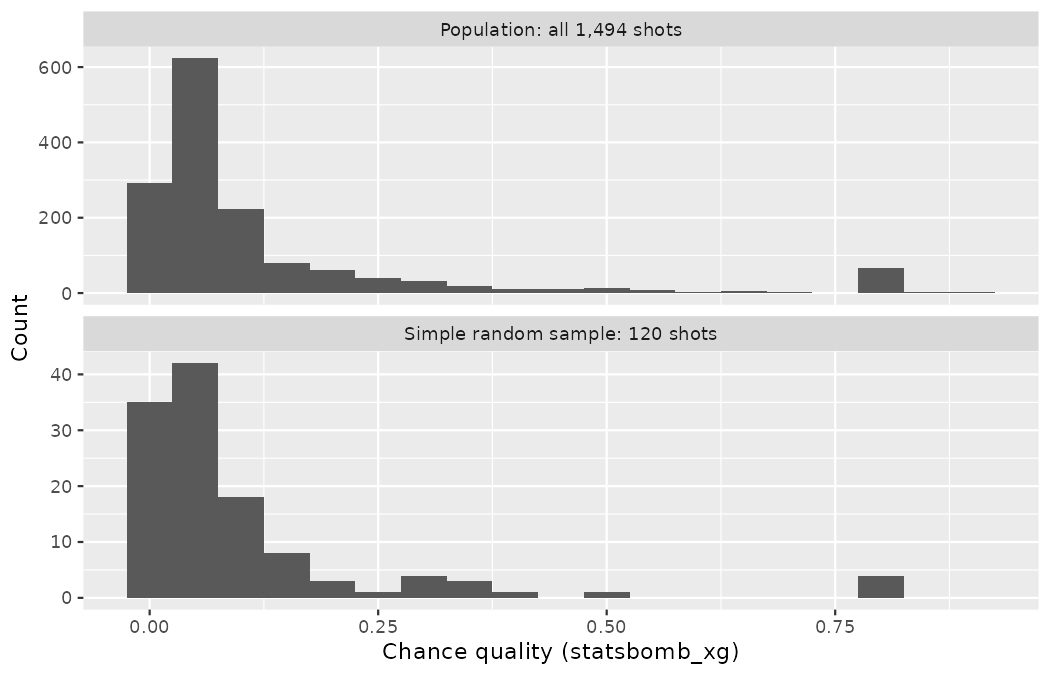
\includegraphics[width=0.85\linewidth,height=\textheight,keepaspectratio]{figures/data-design-1.png}

The claims we are about to make about the two panels can --- and
therefore should --- be computed rather than eyeballed:

\begin{Shaded}
\begin{Highlighting}[]
\FunctionTok{bind\_rows}\NormalTok{(}
\NormalTok{  wc2022\_shots }\SpecialCharTok{|\textgreater{}} \FunctionTok{mutate}\NormalTok{(}\AttributeTok{source =} \StringTok{"population"}\NormalTok{),}
\NormalTok{  srs120 }\SpecialCharTok{|\textgreater{}} \FunctionTok{mutate}\NormalTok{(}\AttributeTok{source =} \StringTok{"sample"}\NormalTok{)}
\NormalTok{) }\SpecialCharTok{|\textgreater{}}
  \FunctionTok{group\_by}\NormalTok{(source) }\SpecialCharTok{|\textgreater{}}
  \FunctionTok{summarize}\NormalTok{(}
    \AttributeTok{shots =} \FunctionTok{n}\NormalTok{(),}
    \AttributeTok{xg\_below\_005 =} \FunctionTok{sum}\NormalTok{(statsbomb\_xg }\SpecialCharTok{\textless{}} \FloatTok{0.05}\NormalTok{),}
    \AttributeTok{penalties =} \FunctionTok{sum}\NormalTok{(shot\_type }\SpecialCharTok{==} \StringTok{"Penalty"}\NormalTok{)}
\NormalTok{  )}
\CommentTok{\#\textgreater{} \# A tibble: 2 × 4}
\CommentTok{\#\textgreater{}   source     shots xg\_below\_005 penalties}
\CommentTok{\#\textgreater{}   \textless{}chr\textgreater{}      \textless{}int\textgreater{}        \textless{}int\textgreater{}     \textless{}int\textgreater{}}
\CommentTok{\#\textgreater{} 1 population  1494          684        64}
\CommentTok{\#\textgreater{} 2 sample       120           60         4}
\end{Highlighting}
\end{Shaded}

Both histograms are strongly right-skewed and look alike in shape: the
tallest bar in each panel is the leftmost one (684 of the 1,494
population shots have xG below 0.05, as do 60 of the 120 sampled shots),
the counts fall away quickly as chance quality rises, and each panel
shows a small isolated spike near 0.78 --- penalties, which the xG model
stores at 0.7835 apiece (64 of them in the population, 4 of which landed
in this sample). A representative sample should reproduce the
population's shape like this, just more coarsely.

\textbf{Stratified sampling} is a divide-and-conquer sampling strategy.
The population is divided into groups called \textbf{strata}. The strata
are chosen so that similar cases are grouped together, then a second
sampling method, usually simple random sampling, is employed within each
stratum. In our shot population, each of the 32 teams is a natural
stratum, because teams differ enormously in both shot volume and shot
quality --- a deep tournament run multiplies a team's shots:

\begin{Shaded}
\begin{Highlighting}[]
\NormalTok{wc2022\_shots }\SpecialCharTok{|\textgreater{}}
  \FunctionTok{count}\NormalTok{(team, }\AttributeTok{sort =} \ConstantTok{TRUE}\NormalTok{) }\SpecialCharTok{|\textgreater{}}
  \FunctionTok{slice}\NormalTok{(}\FunctionTok{c}\NormalTok{(}\DecValTok{1}\SpecialCharTok{:}\DecValTok{3}\NormalTok{, }\DecValTok{30}\SpecialCharTok{:}\DecValTok{32}\NormalTok{))}
\CommentTok{\#\textgreater{} \# A tibble: 6 × 2}
\CommentTok{\#\textgreater{}   team           n}
\CommentTok{\#\textgreater{}   \textless{}chr\textgreater{}      \textless{}int\textgreater{}}
\CommentTok{\#\textgreater{} 1 Argentina    110}
\CommentTok{\#\textgreater{} 2 France       106}
\CommentTok{\#\textgreater{} 3 Brazil        99}
\CommentTok{\#\textgreater{} 4 Wales         24}
\CommentTok{\#\textgreater{} 5 Qatar         20}
\CommentTok{\#\textgreater{} 6 Costa Rica    11}
\end{Highlighting}
\end{Shaded}

\begin{Shaded}
\begin{Highlighting}[]
\NormalTok{wc2022\_shots }\SpecialCharTok{|\textgreater{}}
  \FunctionTok{count}\NormalTok{(team) }\SpecialCharTok{|\textgreater{}}
  \FunctionTok{ggplot}\NormalTok{(}\FunctionTok{aes}\NormalTok{(}\AttributeTok{x =}\NormalTok{ n, }\AttributeTok{y =} \FunctionTok{reorder}\NormalTok{(team, n))) }\SpecialCharTok{+}
  \FunctionTok{geom\_col}\NormalTok{() }\SpecialCharTok{+}
  \FunctionTok{labs}\NormalTok{(}\AttributeTok{x =} \StringTok{"Shots taken at the 2022 World Cup"}\NormalTok{, }\AttributeTok{y =} \ConstantTok{NULL}\NormalTok{)}
\end{Highlighting}
\end{Shaded}

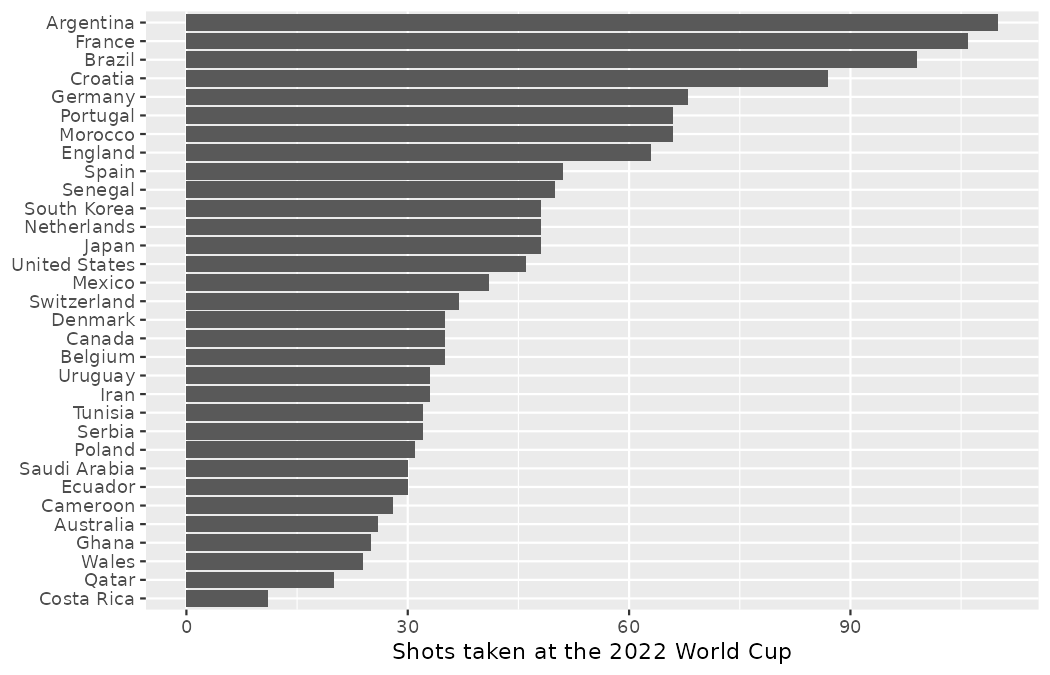
\includegraphics[width=0.85\linewidth,height=\textheight,keepaspectratio]{figures/data-design-2.png}

The bar chart lays out all 32 teams from Argentina (110 shots) at the
top down to Costa Rica (11 shots) at the bottom --- a ten-fold range,
with the champions and fellow finalists France stacked far above the
group-stage casualties. A simple random sample of 120 shots follows
these proportions: by chance it may contain a dozen Argentine shots and
none at all from the smallest strata (the seed-201 draw above covered
only 29 of the 32 teams). Under stratified sampling we instead might
randomly sample 4 shots from each of the 32 teams, guaranteeing every
team a voice:

\begin{Shaded}
\begin{Highlighting}[]
\FunctionTok{set.seed}\NormalTok{(}\DecValTok{202}\NormalTok{)}
\NormalTok{strat128 }\OtherTok{\textless{}{-}}\NormalTok{ wc2022\_shots }\SpecialCharTok{|\textgreater{}}
  \FunctionTok{group\_by}\NormalTok{(team) }\SpecialCharTok{|\textgreater{}}
  \FunctionTok{slice\_sample}\NormalTok{(}\AttributeTok{n =} \DecValTok{4}\NormalTok{) }\SpecialCharTok{|\textgreater{}}
  \FunctionTok{ungroup}\NormalTok{()}

\NormalTok{strat128 }\SpecialCharTok{|\textgreater{}}
  \FunctionTok{summarize}\NormalTok{(}\AttributeTok{shots =} \FunctionTok{n}\NormalTok{(), }\AttributeTok{teams =} \FunctionTok{n\_distinct}\NormalTok{(team), }\AttributeTok{mean\_xg =} \FunctionTok{mean}\NormalTok{(statsbomb\_xg))}
\CommentTok{\#\textgreater{} \# A tibble: 1 × 3}
\CommentTok{\#\textgreater{}   shots teams mean\_xg}
\CommentTok{\#\textgreater{}   \textless{}int\textgreater{} \textless{}int\textgreater{}   \textless{}dbl\textgreater{}}
\CommentTok{\#\textgreater{} 1   128    32   0.134}
\end{Highlighting}
\end{Shaded}

One caution: the plain average above treats Costa Rica's 4 sampled shots
and Argentina's 4 sampled shots as equally important, even though
Argentina contributed ten times as many shots to the population. A
proper stratified estimate re-weights each team's sample mean by that
team's true share of the population:

\begin{Shaded}
\begin{Highlighting}[]
\NormalTok{team\_sizes }\OtherTok{\textless{}{-}}\NormalTok{ wc2022\_shots }\SpecialCharTok{|\textgreater{}}
  \FunctionTok{count}\NormalTok{(team, }\AttributeTok{name =} \StringTok{"team\_shots"}\NormalTok{)}

\NormalTok{strat128 }\SpecialCharTok{|\textgreater{}}
  \FunctionTok{group\_by}\NormalTok{(team) }\SpecialCharTok{|\textgreater{}}
  \FunctionTok{summarize}\NormalTok{(}\AttributeTok{team\_mean\_xg =} \FunctionTok{mean}\NormalTok{(statsbomb\_xg)) }\SpecialCharTok{|\textgreater{}}
  \FunctionTok{left\_join}\NormalTok{(team\_sizes, }\AttributeTok{by =} \StringTok{"team"}\NormalTok{) }\SpecialCharTok{|\textgreater{}}
  \FunctionTok{summarize}\NormalTok{(}\AttributeTok{weighted\_mean\_xg =} \FunctionTok{weighted.mean}\NormalTok{(team\_mean\_xg, team\_shots))}
\CommentTok{\#\textgreater{} \# A tibble: 1 × 1}
\CommentTok{\#\textgreater{}   weighted\_mean\_xg}
\CommentTok{\#\textgreater{}              \textless{}dbl\textgreater{}}
\CommentTok{\#\textgreater{} 1            0.140}
\end{Highlighting}
\end{Shaded}

This draw lands at 0.134 unweighted and 0.140 weighted, against the
truth of 0.126 --- sampling variability again; neither the simple random
sample nor the stratified sample is entitled to hit the parameter
exactly, and no single draw tells you which \emph{method} is better.
(Comparing methods requires studying how estimates behave across many
repeated samples, an idea we develop from
Chapter~\ref{sec-foundations-randomization} onward.) The point of
showing both estimators is the design contrast, not a horse race between
two seeds.

\textbf{Stratified sampling} is especially useful when the cases in each
stratum are very similar with respect to the outcome of interest. The
downside is that analyzing data from a stratified sample is a more
complex task than analyzing data from a simple random sample --- the
re-weighting step above was the first taste of that. The analysis
methods introduced in this book would need to be extended to analyze
data collected using stratified sampling.

\begin{tcolorbox}[enhanced jigsaw, left=2mm, leftrule=.75mm, title=\textcolor{quarto-callout-tip-color}{\faLightbulb}\hspace{0.5em}{Check your understanding}, arc=.35mm, rightrule=.15mm, coltitle=black, colframe=quarto-callout-tip-color-frame, bottomrule=.15mm, colbacktitle=quarto-callout-tip-color!10!white, opacitybacktitle=0.6, breakable, bottomtitle=1mm, toptitle=1mm, titlerule=0mm, opacityback=0, toprule=.15mm, colback=white]

A scout stratifies a 120-shot mini-population by team and samples 4
shots from each of its two teams. Team A took 100 of the 120 shots, and
its 4 sampled shots average 0.20 xG; Team B took the other 20 shots, and
its 4 sampled shots average 0.05 xG. Compute the unweighted average of
the two team means and the weighted stratified estimate of the
population mean. Which is the appropriate estimate, and why?

\begin{center}\rule{0.5\linewidth}{0.5pt}\end{center}

Unweighted: \((0.20 + 0.05)/2 = 0.125.\) Weighted:
\((100 \times 0.20 + 20 \times 0.05)/120 = 21/120 = 0.175.\) The
weighted estimate is the appropriate one: Team A contributed \(100/120\)
of the population's shots, so its sample mean must carry \(100/120\) of
the weight --- exactly the role \texttt{weighted.mean()} played above,
where Argentina's 110 shots outweighed Costa Rica's 11. An unweighted
average would let the small stratum drag the estimate far below what the
population plausibly looks like.

\end{tcolorbox}

\begin{tcolorbox}[enhanced jigsaw, left=2mm, leftrule=.75mm, title=\textcolor{quarto-callout-note-color}{\faInfo}\hspace{0.5em}{Worked example}, arc=.35mm, rightrule=.15mm, coltitle=black, colframe=quarto-callout-note-color-frame, bottomrule=.15mm, colbacktitle=quarto-callout-note-color!10!white, opacitybacktitle=0.6, breakable, bottomtitle=1mm, toptitle=1mm, titlerule=0mm, opacityback=0, toprule=.15mm, colback=white]

Why would it be good for cases within each stratum to be very similar?

\begin{center}\rule{0.5\linewidth}{0.5pt}\end{center}

We might get a more stable estimate for the subpopulation in a stratum
if the cases are very similar, leading to more precise estimates within
each group. If every one of a team's shots carries roughly that team's
typical chance quality, then even 4 shots pin down the team's mean well.
When we combine these estimates into a single estimate for the full
population, that population estimate will tend to be more precise since
each individual group estimate is itself more precise.

\end{tcolorbox}

In a \textbf{cluster sample}, we break up the population into many
groups, called \textbf{clusters}. Then we sample a fixed number of
clusters and include all observations from each of those clusters in the
sample. A \textbf{multistage sample} is like a cluster sample, but
rather than keeping all observations in each cluster, we would collect a
random sample within each selected cluster.

For the shot population, the natural cluster is the \emph{match}: shots
come bundled into 64 matches, and a scout attends matches, not
individual shots. Suppose Emil's travel budget stretches to accrediting
scouts for only 8 of the 64 matches. A cluster sample randomly selects
the 8 matches and logs \emph{every} shot in them:

\begin{Shaded}
\begin{Highlighting}[]
\FunctionTok{set.seed}\NormalTok{(}\DecValTok{203}\NormalTok{)}
\NormalTok{match\_sample }\OtherTok{\textless{}{-}}\NormalTok{ wc2022\_matches }\SpecialCharTok{|\textgreater{}}
  \FunctionTok{slice\_sample}\NormalTok{(}\AttributeTok{n =} \DecValTok{8}\NormalTok{)}

\NormalTok{cluster\_shots }\OtherTok{\textless{}{-}}\NormalTok{ wc2022\_shots }\SpecialCharTok{|\textgreater{}}
  \FunctionTok{semi\_join}\NormalTok{(match\_sample, }\AttributeTok{by =} \StringTok{"match\_id"}\NormalTok{)}

\NormalTok{cluster\_shots }\SpecialCharTok{|\textgreater{}}
  \FunctionTok{summarize}\NormalTok{(}
    \AttributeTok{matches =} \FunctionTok{n\_distinct}\NormalTok{(match\_id), }\AttributeTok{shots =} \FunctionTok{n}\NormalTok{(), }\AttributeTok{mean\_xg =} \FunctionTok{mean}\NormalTok{(statsbomb\_xg),}
    \AttributeTok{penalties =} \FunctionTok{sum}\NormalTok{(shot\_type }\SpecialCharTok{==} \StringTok{"Penalty"}\NormalTok{), }\AttributeTok{shootout\_kicks =} \FunctionTok{sum}\NormalTok{(period }\SpecialCharTok{==} \DecValTok{5}\NormalTok{)}
\NormalTok{  )}
\CommentTok{\#\textgreater{} \# A tibble: 1 × 5}
\CommentTok{\#\textgreater{}   matches shots mean\_xg penalties shootout\_kicks}
\CommentTok{\#\textgreater{}     \textless{}int\textgreater{} \textless{}int\textgreater{}   \textless{}dbl\textgreater{}     \textless{}int\textgreater{}          \textless{}int\textgreater{}}
\CommentTok{\#\textgreater{} 1       8   225   0.155        20             18}
\end{Highlighting}
\end{Shaded}

This cluster sample estimates 0.155 --- noticeably above the true 0.126,
and the miss is instructive. Two of the eight randomly drawn matches
happened to be quarter-finals decided on penalty shootouts, and shootout
kicks enter the data as penalties with a stored chance quality of 0.7835
each; as the summary shows, this draw contains 20 penalties among its
225 shots, 18 of them shootout kicks. When you sample only 8 clusters,
one or two unusual clusters can swing the whole estimate: cluster
samples buy cheap travel at the price of this volatility.

With a \textbf{multistage sample}, we keep the 8 sampled matches but log
only a random subset of shots within each --- say the analysis team has
time to fully tag at most 15 shots per attended match:

\begin{Shaded}
\begin{Highlighting}[]
\FunctionTok{set.seed}\NormalTok{(}\DecValTok{204}\NormalTok{)}
\NormalTok{match\_sample\_2 }\OtherTok{\textless{}{-}}\NormalTok{ wc2022\_matches }\SpecialCharTok{|\textgreater{}}
  \FunctionTok{slice\_sample}\NormalTok{(}\AttributeTok{n =} \DecValTok{8}\NormalTok{)}

\NormalTok{multistage\_shots }\OtherTok{\textless{}{-}}\NormalTok{ wc2022\_shots }\SpecialCharTok{|\textgreater{}}
  \FunctionTok{semi\_join}\NormalTok{(match\_sample\_2, }\AttributeTok{by =} \StringTok{"match\_id"}\NormalTok{) }\SpecialCharTok{|\textgreater{}}
  \FunctionTok{group\_by}\NormalTok{(match\_id) }\SpecialCharTok{|\textgreater{}}
  \FunctionTok{slice\_sample}\NormalTok{(}\AttributeTok{n =} \DecValTok{15}\NormalTok{) }\SpecialCharTok{|\textgreater{}}
  \FunctionTok{ungroup}\NormalTok{()}

\NormalTok{multistage\_shots }\SpecialCharTok{|\textgreater{}}
  \FunctionTok{summarize}\NormalTok{(}\AttributeTok{matches =} \FunctionTok{n\_distinct}\NormalTok{(match\_id), }\AttributeTok{shots =} \FunctionTok{n}\NormalTok{(), }\AttributeTok{mean\_xg =} \FunctionTok{mean}\NormalTok{(statsbomb\_xg))}
\CommentTok{\#\textgreater{} \# A tibble: 1 × 3}
\CommentTok{\#\textgreater{}   matches shots mean\_xg}
\CommentTok{\#\textgreater{}     \textless{}int\textgreater{} \textless{}int\textgreater{}   \textless{}dbl\textgreater{}}
\CommentTok{\#\textgreater{} 1       8   116   0.137}
\end{Highlighting}
\end{Shaded}

(The sample holds 116 shots rather than \(8 \times 15 = 120\) because
one of the drawn matches produced only 11 shots in total, so it
contributes all 11.)

Sometimes cluster or multistage sampling can be more economical than the
alternative sampling techniques: 8 accreditations instead of tickets
scattered across 64 matches. Also, unlike stratified sampling, these
approaches are most helpful when there is a lot of case-to-case
variability within a cluster but the clusters themselves do not look
very different from one another. A single match already contains
tap-ins, headers, and forty-yard punts --- enormous within-cluster
variability --- while one group-stage match resembles the next far more
than Argentina's shot profile resembles Costa Rica's. (As our
shootout-laden draw showed, when clusters \emph{do} differ sharply ---
group stage versus knockout ties --- the method feels it.) A downside of
these methods is that more advanced techniques are typically required to
analyze the data, though the methods in this book can be extended to
handle such data.

\begin{tcolorbox}[enhanced jigsaw, left=2mm, leftrule=.75mm, title=\textcolor{quarto-callout-note-color}{\faInfo}\hspace{0.5em}{Worked example}, arc=.35mm, rightrule=.15mm, coltitle=black, colframe=quarto-callout-note-color-frame, bottomrule=.15mm, colbacktitle=quarto-callout-note-color!10!white, opacitybacktitle=0.6, breakable, bottomtitle=1mm, toptitle=1mm, titlerule=0mm, opacityback=0, toprule=.15mm, colback=white]

Suppose Emil wants standardized in-person reports on about 150 shots
from a foreign league to calibrate his scouts against the data feed. The
league's 16 stadiums host matches that are more or less like the next,
but the distances between the cities are substantial, and every
additional city visited multiplies hotel and travel costs. What sampling
method should Emil use?

\begin{center}\rule{0.5\linewidth}{0.5pt}\end{center}

A simple random sample of shots would likely scatter the scouts across
nearly every stadium in the league, which could make data collection
expensive. Stratified sampling would be a challenge since it is unclear
how we would build strata of similar shots before seeing them. However,
cluster sampling or multistage sampling seem like very good ideas. With
multistage sampling, we could randomly select a handful of the matches,
then randomly select the shots to be fully worked up from within each
attended match. This could reduce data collection costs substantially in
comparison to a simple random sample, and the sample would still yield
reliable information, even if we would need to analyze the data with
more advanced methods than those introduced in this book.

\end{tcolorbox}

\begin{tcolorbox}[enhanced jigsaw, left=2mm, leftrule=.75mm, title=\textcolor{quarto-callout-tip-color}{\faLightbulb}\hspace{0.5em}{Check your understanding}, arc=.35mm, rightrule=.15mm, coltitle=black, colframe=quarto-callout-tip-color-frame, bottomrule=.15mm, colbacktitle=quarto-callout-tip-color!10!white, opacitybacktitle=0.6, breakable, bottomtitle=1mm, toptitle=1mm, titlerule=0mm, opacityback=0, toprule=.15mm, colback=white]

Classify the sampling method in each of Priya's three plans for
surveying the injury records of the roughly 5,000 academy players
registered across the federation's 250 academies. Plan A: randomly
select 12 academies and collect the injury log of \emph{every} player at
each. Plan B: randomly select 12 academies, then collect the logs of 10
randomly chosen players per academy. Plan C: group all registered
players by position, then randomly sample 40 players within each
position group.

\begin{center}\rule{0.5\linewidth}{0.5pt}\end{center}

Plan A is cluster sampling: the academies are the clusters, and every
observational unit inside a sampled cluster is taken. Plan B is
multistage sampling: clusters are sampled first, then units are randomly
subsampled within each. Plan C is stratified sampling: every stratum
(position group) is represented, with random sampling inside each
stratum.

\end{tcolorbox}

\section{Experiments}\label{sec-experiments}

Studies where the researchers assign treatments to cases are called
\textbf{experiments}. When this assignment includes randomization, e.g.,
using a coin flip to decide which training program a player receives, it
is called a \textbf{randomized experiment}. Both terms --- like
\emph{placebo} and \emph{observational study} later in this chapter ---
appeared informally in Chapter~\ref{sec-data-hello}; we now give them
their formal treatment. Randomized experiments are fundamentally
important when trying to show a causal connection between two variables.
Recall the distinction from Chapter~\ref{sec-data-hello}: the tournament
shot data record what football happened to produce, whereas in an
experiment the club \emph{decides} who gets what. At Northbridge, every
randomized experiment lives inside the club --- Jonas Beck's academy is
where treatments can actually be assigned --- because nobody gets to
randomize a World Cup.

\subsection{Principles of experimental
design}\label{sec-principles-experimental-design}

Throughout this section we will follow a randomized experiment Jonas
Beck, Northbridge's academy director, might design: does a new
high-intensity finishing program raise conversion rates in academy
forwards, compared to the standard training curriculum? Four principles
govern the design.

\begin{enumerate}
\def\labelenumi{\arabic{enumi}.}
\tightlist
\item
  \textbf{Controlling.} Researchers assign treatments to cases, and they
  do their best to \textbf{control} any other differences in the
  groups.\footnote{This is a different concept than a \emph{control
    group}, which we discuss in the second principle and in
    Section~\ref{sec-reducing-bias-human-experiments}.} For example,
  players might complete their assigned finishing block at different
  points of a session: some fresh at the start, others exhausted after a
  full training load, and fatigue would then contaminate the comparison.
  To control for the effect of fatigue, Jonas may instruct every player
  to complete their assigned block first thing in the session, after the
  same standardized warm-up, with the same number of repetitions.
\end{enumerate}

\begin{enumerate}
\def\labelenumi{\arabic{enumi}.}
\setcounter{enumi}{1}
\tightlist
\item
  \textbf{Randomization.} Researchers randomize players into treatment
  groups to account for variables that cannot be controlled. For
  example, some players may arrive as naturally better finishers than
  others due to position and playing history. In this example playing
  position is a \textbf{confounding variable}\footnote{Also called a
    \textbf{lurking variable}, \textbf{confounding factor}, or a
    \textbf{confounder}.}, which is defined as a variable that is
  associated with both the explanatory and response variables. If
  strikers were allowed to volunteer for the exciting new program, the
  program group would be stacked with players who convert well anyway.
  Randomizing players into the treatment or control group helps even out
  such differences.
\end{enumerate}

\begin{tcolorbox}[enhanced jigsaw, left=2mm, leftrule=.75mm, title=\textcolor{quarto-callout-important-color}{\faExclamation}\hspace{0.5em}{Confounding variable}, arc=.35mm, rightrule=.15mm, coltitle=black, colframe=quarto-callout-important-color-frame, bottomrule=.15mm, colbacktitle=quarto-callout-important-color!10!white, opacitybacktitle=0.6, breakable, bottomtitle=1mm, toptitle=1mm, titlerule=0mm, opacityback=0, toprule=.15mm, colback=white]

A \textbf{confounding variable} is one that is associated with both the
explanatory and response variables. Because it is associated with both
variables, it prevents the study from concluding that the explanatory
variable caused the response variable. Consider a silly example from
club operations, with hot drinks sold at the stadium as the explanatory
variable and the number of muscle injuries in the same fixtures as the
response variable (which may seem highly correlated in the club's
records). Cold weather is associated with both variables, and therefore
we cannot conclude that high hot-drink sales are a cause of more muscle
injuries.

Confounding variables may or may not be measured as part of the study.
Regardless, drawing cause-and-effect conclusions is difficult in an
observational study because of the ever-present possibility of
confounding variables.

\end{tcolorbox}

\begin{enumerate}
\def\labelenumi{\arabic{enumi}.}
\setcounter{enumi}{2}
\item
  \textbf{Replication.} The more cases researchers observe, the more
  accurately they can estimate the effect of the explanatory variable on
  the response. In a single study, we \textbf{replicate} by collecting a
  sufficiently large sample --- enough forwards in each training arm,
  not one prized prospect per group. What is considered sufficiently
  large varies from experiment to experiment, but at a minimum we want
  to have multiple subjects (experimental units) per treatment group.
  Another way of achieving replication is replicating an entire study to
  verify an earlier finding --- running the drill trial again the
  following season, or at a partner academy. The term
  \textbf{replication crisis} refers to the ongoing methodological
  crisis in which past findings from scientific studies in several
  disciplines have failed to be replicated. \textbf{Pseudoreplication}
  occurs when individual observations under different treatments are
  heavily dependent on each other. For example, suppose you have 50
  academy players in an experiment where you're recording each player's
  finishing assessment at 10 sessions throughout the trial. By the end,
  you will have 50 \(\times\) 10 = 500 measurements. Reporting that you
  have 500 observations would be considered pseudoreplication, as the
  repeated assessments of a given player are not independent of each
  other. Pseudoreplication often happens when the wrong entity is
  replicated, and the reported sample sizes are exaggerated.
\item
  \textbf{Blocking.} Researchers sometimes know or suspect that
  variables, other than the treatment, influence the response. Under
  these circumstances, they may first group individuals based on this
  variable into \textbf{blocks} and then randomize cases within each
  block to the treatment groups. This strategy is often referred to as
  \textbf{blocking}. For instance, if we are looking at the effect of
  the finishing program on conversion, we might first split the forwards
  into a high-baseline block and a low-baseline block using last
  season's conversion figures, then randomly assign half the players
  from each block to the control group and the other half to the
  treatment group. Picture the pool of forwards divided into the two
  blocks first, and only then a coin flipped within each block: the
  result is that each treatment group receives the same number of proven
  finishers and the same number of raw ones, so a lopsided draw cannot
  hand one program all the natural goalscorers.
\end{enumerate}

It is important to incorporate the first three experimental design
principles into any study, and this book describes applicable methods
for analyzing data from such experiments. Blocking is a slightly more
advanced technique, and statistical methods in this book may be extended
to analyze data collected using blocking.

\begin{tcolorbox}[enhanced jigsaw, left=2mm, leftrule=.75mm, title=\textcolor{quarto-callout-tip-color}{\faLightbulb}\hspace{0.5em}{Check your understanding}, arc=.35mm, rightrule=.15mm, coltitle=black, colframe=quarto-callout-tip-color-frame, bottomrule=.15mm, colbacktitle=quarto-callout-tip-color!10!white, opacitybacktitle=0.6, breakable, bottomtitle=1mm, toptitle=1mm, titlerule=0mm, opacityback=0, toprule=.15mm, colback=white]

In Jonas's trial, name one variable he can \emph{control}, one he should
\emph{randomize over}, and one he might \emph{block} on.

\begin{center}\rule{0.5\linewidth}{0.5pt}\end{center}

Control: the session conditions --- warm-up, repetition count, time of
session --- can be fixed to be identical for everyone. Randomize:
everything that cannot be fixed, such as a player's motivation, growth
spurt timing, or playing history; random assignment spreads these evenly
across the groups on average. Block: a variable known in advance to
influence conversion, such as last season's conversion rate (or
position), so that each program receives a comparable mix.

\end{tcolorbox}

\subsection{Reducing bias in human
experiments}\label{sec-reducing-bias-human-experiments}

Randomized experiments have long been considered to be the gold standard
for data collection, but they do not ensure an unbiased perspective into
the cause-and-effect relationship in all cases. Studies on human beings
--- and footballers are aggressively human --- are perfect examples
where bias can unintentionally arise. Here we reconsider Jonas's trial
of the new finishing program. In particular, the club wants to know if
the program raises conversion in academy forwards.

Jonas designed a randomized experiment because the club wanted to draw
causal conclusions about the program's effect. The academy forwards who
volunteered for the trial\footnote{Human subjects in a study are often
  called \textbf{volunteers}, \textbf{participants}, or --- around a
  training ground --- simply ``the lads in the trial''.} were randomly
placed into two study groups. One group, the \textbf{treatment group},
received the new high-intensity finishing program. The other group,
called the \textbf{control group}, continued with the standard training
curriculum.

Put yourself in the place of a player in the study. If you are in the
treatment group, you are handed a glossy new program that the coaches
seem excited about, and you anticipate it will help you. On the other
hand, a player in the other group carries on with the same old drills,
perhaps quietly deflated at missing out. These perspectives suggest
there are actually two effects in this study: the one of interest is the
effectiveness of the program, and the second is an emotional effect of
(not) receiving it --- belief, motivation, resentment --- which is
difficult to quantify.

Researchers aren't usually interested in the emotional effect, which
might bias the study. To circumvent this problem, researchers do not
want players to know which group they are in. When researchers keep the
participants uninformed about their treatment, the study is said to be
\textbf{blind}. But there is one problem: if a player does not receive
any new-looking training, they will know they're in the control group. A
solution to this problem is to give a fake treatment to players in the
control group. This is called a \textbf{placebo}, and an effective
placebo is the key to making a study truly blind. In a training-ground
trial, the placebo is a \emph{sham drill}: a session block with the same
contact time, the same novelty and presentation, and the same coaching
attention as the new program, but whose content is believed to have no
effect on finishing --- elaborate new rondo variations, say. However,
offering such a fake treatment may not be ethical in certain
experiments. For example, in the club's medical and injury-prevention
work, typically the control group must get the current standard of care.
Oftentimes, a placebo results in a slight but real improvement in
participants --- players who believe they are on a cutting-edge program
train with more conviction and may genuinely finish a little better.
This effect has been dubbed the \textbf{placebo effect}.

The players are not the only ones who should be blinded: coaches and
researchers can unintentionally bias a study. When a coach knows a
player has been given the real program, they might inadvertently give
that player more attention or more generous marks in the end-of-trial
finishing assessment than a player they know is on the sham drill. To
guard against this bias, which again has been found to have a measurable
effect in some instances, most modern studies employ a
\textbf{double-blind} setup where the coaches who grade the assessments
and interact with the players are, just like the players, unaware of who
is or is not receiving the treatment.\footnote{There are always some
  staff involved in the study who do know which players are receiving
  which program --- someone has to run the sessions. However, they do
  not grade the assessments and do not tell the blinded assessors who is
  receiving which program.}

\begin{tcolorbox}[enhanced jigsaw, left=2mm, leftrule=.75mm, title=\textcolor{quarto-callout-tip-color}{\faLightbulb}\hspace{0.5em}{Check your understanding}, arc=.35mm, rightrule=.15mm, coltitle=black, colframe=quarto-callout-tip-color-frame, bottomrule=.15mm, colbacktitle=quarto-callout-tip-color!10!white, opacitybacktitle=0.6, breakable, bottomtitle=1mm, toptitle=1mm, titlerule=0mm, opacityback=0, toprule=.15mm, colback=white]

Look back to the study in Section~\ref{sec-case-study-stents-strokes},
where the academies randomized players to the new high-intensity
finishing program or to standard training and assessed conversion at 30
days and at season end. Is this an experiment? Was the study blinded?
Was it double-blinded?

\begin{center}\rule{0.5\linewidth}{0.5pt}\end{center}

The academies assigned the players into their training groups, so this
study was an experiment. However, the players could distinguish what
treatment they received, because you cannot spend weeks inside a
high-intensity finishing program without noticing. There was no sham
drill in that design, so this study was not blind. The study could not
be double-blind since it was not blind.

\end{tcolorbox}

\begin{tcolorbox}[enhanced jigsaw, left=2mm, leftrule=.75mm, title=\textcolor{quarto-callout-tip-color}{\faLightbulb}\hspace{0.5em}{Check your understanding}, arc=.35mm, rightrule=.15mm, coltitle=black, colframe=quarto-callout-tip-color-frame, bottomrule=.15mm, colbacktitle=quarto-callout-tip-color!10!white, opacitybacktitle=0.6, breakable, bottomtitle=1mm, toptitle=1mm, titlerule=0mm, opacityback=0, toprule=.15mm, colback=white]

For the study in Section~\ref{sec-case-study-stents-strokes}, could the
designers have employed a placebo? If so, what would that placebo have
looked like?

\begin{center}\rule{0.5\linewidth}{0.5pt}\end{center}

Ultimately, can we make players think they are receiving an innovative
program when they are not? In fact, we can: the sham drill described
above --- matched contact time, matched novelty, content believed inert
for finishing --- is the training-ground analogue of a \textbf{sham
surgery} in medicine, where the patient undergoes a procedure without
receiving the active treatment, and still collects the placebo effect.

\end{tcolorbox}

You may have questions about the ethics of sham drills. These questions
may have even arisen in your mind in the general experiment context,
where a possibly helpful program was withheld from players in the
control group; the main difference is that a sham drill actively
\emph{spends} a young player's limited development time on content
chosen to be useless, while withholding a treatment only maintains a
player's current training.

There are always multiple viewpoints of experiments and placebos, and
rarely is it obvious which is ethically ``correct''. For instance, is it
fair to burn a semester of an academy prospect's development on an inert
drill? However, if we do not use sham drills, the club may end up
rolling out a costly program that has no real effect; if this happens,
coaching hours and budget will be diverted away from methods that are
known to be helpful. Ultimately, this is a difficult situation where we
cannot perfectly protect both the players who have volunteered for the
trial and the players who may benefit (or not) from the program in
future intakes.

Finally, note that some club interventions cannot be blinded by any
amount of ingenuity. Consider a load-management protocol that caps a
player's sprint load in the days before a match, monitored through GPS
vests. The club can randomize \emph{which} players are placed on the
protocol --- the experiment is still randomized, and still supports
causal conclusions about the protocol as delivered --- but a player
always knows whether his minutes are being managed, and no sham protocol
can hide it. There is no placebo possible; the emotional effect of being
``wrapped in cotton wool'' travels with the treatment, and the analyst
must simply acknowledge it when interpreting the results.

\section{Observational studies}\label{sec-observational-studies}

Studies where no treatment has been explicitly applied (or explicitly
withheld) are called \textbf{observational studies}. For instance,
studies on the tournament shot data described in
Section~\ref{sec-data-basics} would be considered observational, as they
rely on \textbf{observational data}: nobody assigned Argentina its
shots.

Making causal conclusions based on experiments is often reasonable,
since we can randomly assign the explanatory variable(s), i.e., the
treatments. However, making the same causal conclusions based on
observational data can be treacherous and is not recommended. Thus,
observational studies are generally only sufficient to show associations
or form hypotheses that can be later checked with experiments --- which,
for a club, usually means checked inside the academy, since the wider
footballing world does not submit to randomization.

Here is a live example. At the 2022 World Cup, headed shots were
converted at a lower rate than shots struck with the foot:

\begin{Shaded}
\begin{Highlighting}[]
\NormalTok{wc2022\_shots }\SpecialCharTok{|\textgreater{}}
  \FunctionTok{filter}\NormalTok{(body\_part }\SpecialCharTok{!=} \StringTok{"Other"}\NormalTok{) }\SpecialCharTok{|\textgreater{}}
  \FunctionTok{mutate}\NormalTok{(}\AttributeTok{body\_part =} \FunctionTok{if\_else}\NormalTok{(body\_part }\SpecialCharTok{==} \StringTok{"Head"}\NormalTok{, }\StringTok{"Head"}\NormalTok{, }\StringTok{"Foot"}\NormalTok{)) }\SpecialCharTok{|\textgreater{}}
  \FunctionTok{group\_by}\NormalTok{(body\_part) }\SpecialCharTok{|\textgreater{}}
  \FunctionTok{summarize}\NormalTok{(}\AttributeTok{shots =} \FunctionTok{n}\NormalTok{(), }\AttributeTok{goals =} \FunctionTok{sum}\NormalTok{(goal), }\AttributeTok{conversion =} \FunctionTok{mean}\NormalTok{(goal))}
\CommentTok{\#\textgreater{} \# A tibble: 2 × 4}
\CommentTok{\#\textgreater{}   body\_part shots goals conversion}
\CommentTok{\#\textgreater{}   \textless{}chr\textgreater{}     \textless{}int\textgreater{} \textless{}int\textgreater{}      \textless{}dbl\textgreater{}}
\CommentTok{\#\textgreater{} 1 Foot       1229   164      0.133}
\CommentTok{\#\textgreater{} 2 Head        252    28      0.111}
\end{Highlighting}
\end{Shaded}

(We set aside the 13 shots recorded with \texttt{body\_part} equal to
\texttt{"Other"} --- chests, backs, and one or two knees.) Headers
converted at 0.111, foot shots at 0.133. Does this mean heading the ball
\emph{causes} worse finishing --- that a scout should mark down a
striker for aerial play, or that a coach should train players out of
attempting headers?

No! The comparison is observational, and there is a variable lurking
behind it: \emph{how the chance arrived}. Headers do not occur at random
moments; they overwhelmingly arrive from corners, free kicks, and other
dead-ball deliveries --- contested, high-traffic situations at awkward
angles --- while foot shots are far more often taken in open play. The
data make the imbalance stark:

\begin{Shaded}
\begin{Highlighting}[]
\NormalTok{wc2022\_shots }\SpecialCharTok{|\textgreater{}}
  \FunctionTok{filter}\NormalTok{(body\_part }\SpecialCharTok{!=} \StringTok{"Other"}\NormalTok{) }\SpecialCharTok{|\textgreater{}}
  \FunctionTok{mutate}\NormalTok{(}
    \AttributeTok{body\_part =} \FunctionTok{if\_else}\NormalTok{(body\_part }\SpecialCharTok{==} \StringTok{"Head"}\NormalTok{, }\StringTok{"Head"}\NormalTok{, }\StringTok{"Foot"}\NormalTok{),}
    \AttributeTok{dead\_ball =}\NormalTok{ play\_pattern }\SpecialCharTok{\%in\%} \FunctionTok{c}\NormalTok{(}\StringTok{"From Corner"}\NormalTok{, }\StringTok{"From Free Kick"}\NormalTok{, }\StringTok{"From Throw In"}\NormalTok{)}
\NormalTok{  ) }\SpecialCharTok{|\textgreater{}}
  \FunctionTok{group\_by}\NormalTok{(body\_part) }\SpecialCharTok{|\textgreater{}}
  \FunctionTok{summarize}\NormalTok{(}\AttributeTok{shots =} \FunctionTok{n}\NormalTok{(), }\AttributeTok{prop\_dead\_ball =} \FunctionTok{mean}\NormalTok{(dead\_ball))}
\CommentTok{\#\textgreater{} \# A tibble: 2 × 3}
\CommentTok{\#\textgreater{}   body\_part shots prop\_dead\_ball}
\CommentTok{\#\textgreater{}   \textless{}chr\textgreater{}     \textless{}int\textgreater{}          \textless{}dbl\textgreater{}}
\CommentTok{\#\textgreater{} 1 Foot       1229          0.491}
\CommentTok{\#\textgreater{} 2 Head        252          0.770}
\end{Highlighting}
\end{Shaded}

Fully 77.0\% of headed shots came out of dead-ball possessions, against
49.1\% of foot shots. Picture the causal diagram as a triangle: at the
top sits \emph{how the chance arrived} (the delivery pattern), with one
solid arrow running down to \emph{headed attempt} --- crosses and
corners produce headers --- and another solid arrow running down to
\emph{goal scored} --- scrambled dead-ball chances are simply harder to
convert. Between the two bottom boxes, from headed attempt to goal
scored, there is only a question mark: the direct effect of using the
head, if any, is not identified by this comparison. The delivery pattern
is a confounding variable --- the very concept defined in
Section~\ref{sec-principles-experimental-design} --- associated with
both the explanatory variable (body part) and the response (goal). The
presence of confounding variables is what inhibits the ability for
observational studies to make causal claims. While one method to justify
making causal conclusions from observational studies is to exhaust the
search for confounding variables, there is no guarantee that all
confounding variables can be examined or measured. This particular
confounder is not done with us: it returns when we build models with
many predictors in Chapter~\ref{sec-model-mlr} and again in
Chapter~\ref{sec-inf-model-logistic}.

There is also a blunter distortion hiding in the foot group, one this
book makes a standing convention of flagging
(Chapter~\ref{sec-data-applications} examines it in detail): every one
of the tournament's 64 penalty kicks --- uncontested shots from twelve
yards, 43 of them scored --- is a \emph{footed} shot, so the foot
group's 0.133 is partly penalties rather than finishing.

\begin{Shaded}
\begin{Highlighting}[]
\NormalTok{wc2022\_shots }\SpecialCharTok{|\textgreater{}}
  \FunctionTok{filter}\NormalTok{(body\_part }\SpecialCharTok{!=} \StringTok{"Other"}\NormalTok{, shot\_type }\SpecialCharTok{==} \StringTok{"Open Play"}\NormalTok{) }\SpecialCharTok{|\textgreater{}}
  \FunctionTok{mutate}\NormalTok{(}\AttributeTok{body\_part =} \FunctionTok{if\_else}\NormalTok{(body\_part }\SpecialCharTok{==} \StringTok{"Head"}\NormalTok{, }\StringTok{"Head"}\NormalTok{, }\StringTok{"Foot"}\NormalTok{)) }\SpecialCharTok{|\textgreater{}}
  \FunctionTok{group\_by}\NormalTok{(body\_part) }\SpecialCharTok{|\textgreater{}}
  \FunctionTok{summarize}\NormalTok{(}\AttributeTok{shots =} \FunctionTok{n}\NormalTok{(), }\AttributeTok{goals =} \FunctionTok{sum}\NormalTok{(goal), }\AttributeTok{conversion =} \FunctionTok{mean}\NormalTok{(goal))}
\CommentTok{\#\textgreater{} \# A tibble: 2 × 4}
\CommentTok{\#\textgreater{}   body\_part shots goals conversion}
\CommentTok{\#\textgreater{}   \textless{}chr\textgreater{}     \textless{}int\textgreater{} \textless{}int\textgreater{}      \textless{}dbl\textgreater{}}
\CommentTok{\#\textgreater{} 1 Foot       1117   119      0.107}
\CommentTok{\#\textgreater{} 2 Head        252    28      0.111}
\end{Highlighting}
\end{Shaded}

Restricted to open play, foot conversion falls to \(119/1117 = 0.1065\)
--- \emph{below} the headers' \(0.1111,\) which is unchanged because
every header in these data is an open-play shot. So the raw header
``deficit'' was mostly penalties, while the delivery-pattern confounding
diagrammed above is the deeper, subtler layer: it persists inside the
open-play frame, where headers still arrive disproportionately from
corner and cross deliveries, and no filter can remove it --- only
design, or modeling of the kind previewed above, can address it.

\begin{tcolorbox}[enhanced jigsaw, left=2mm, leftrule=.75mm, title=\textcolor{quarto-callout-tip-color}{\faLightbulb}\hspace{0.5em}{Check your understanding}, arc=.35mm, rightrule=.15mm, coltitle=black, colframe=quarto-callout-tip-color-frame, bottomrule=.15mm, colbacktitle=quarto-callout-tip-color!10!white, opacitybacktitle=0.6, breakable, bottomtitle=1mm, toptitle=1mm, titlerule=0mm, opacityback=0, toprule=.15mm, colback=white]

Northbridge's database shows a negative association across players: the
more shots a player attempts per match, the lower his conversion rate
tends to be. It is unreasonable to conclude from this that shooting
often \emph{causes} poor finishing. Suggest a variable that might
explain the negative relationship.

\begin{center}\rule{0.5\linewidth}{0.5pt}\end{center}

Answers will vary. Shot selection is a strong candidate: high-volume
shooters are often licensed to attempt speculative long-range efforts,
so their average chance quality per shot is lower, dragging conversion
down. A player's role matters too --- a target forward feeding on
close-range chances shoots rarely but converts often. Chance quality is
associated with both shot volume and conversion, so it is a plausible
confounder.

\end{tcolorbox}

Observational studies come in two forms: prospective and retrospective
studies. A \textbf{prospective study} identifies individuals and
collects information as events unfold. For instance, Northbridge's
matchday logging program is prospective: at the start of the season Emil
assigns each scout a set of fixtures and a structured report template,
and the reports accumulate match by match as the season happens --- the
scouting-department cousin of the long-running cohort studies in
medicine, where participants are recruited first and followed for years.
\textbf{Retrospective studies} collect data after events have taken
place, e.g., analysts may re-tag historical video to code events that
were never logged live. The tournament event data used throughout this
book are retrospective in exactly this sense: every shot of the 2022
World Cup and the 2025 Women's Euro was coded from video after the fact.
Some datasets may contain both prospectively- and
retrospectively-collected variables, such as a recruitment dossier that
gathers a prospect's pre-signing history from archives and then follows
his development live after he joins.

\section{Chapter review}\label{sec-chp2-review}

\subsection{Summary}\label{summary-1}

A proficient analyst will have a good sense of the types of data they
are working with and how to visualize the data in order to gain a
complete understanding of the variables. Equally important, however, is
the data source. In this chapter, we have discussed randomized
experiments --- the club-internal kind, where Jonas Beck can flip coins
--- and taking good, random, representative samples from a population,
whether of shots, matches, or academy graduates. When we discuss
inferential methods (starting in
Chapter~\ref{sec-foundations-randomization}), the conclusions that can
be drawn will be dependent on how the data were collected.
Table~\ref{tbl-randsampValloc} summarizes how sampling and assignment
methods relate to the scope of inference, and regularly revisiting it
will be important when making conclusions from a given data
analysis.\footnote{Derived from similar figures in Chance \& Rossman
  (2018) and Ramsey \& Schafer (2012), via \emph{Introduction to Modern
  Statistics}.}

\begin{longtable}[]{@{}
  >{\raggedright\arraybackslash}p{(\linewidth - 4\tabcolsep) * \real{0.3333}}
  >{\raggedright\arraybackslash}p{(\linewidth - 4\tabcolsep) * \real{0.3333}}
  >{\raggedright\arraybackslash}p{(\linewidth - 4\tabcolsep) * \real{0.3333}}@{}}
\caption{Analysis conclusions should be made carefully according to how
the data were collected. Very few datasets come from the top left box,
because random assignment of treatments can usually only be given to
volunteers. Both representative (ideally random) sampling and
experiments (random assignment of treatments) are important for how
statistical conclusions can be made on
populations.}\label{tbl-randsampValloc}\tabularnewline
\toprule\noalign{}
\begin{minipage}[b]{\linewidth}\raggedright
\end{minipage} & \begin{minipage}[b]{\linewidth}\raggedright
Random assignment of treatments
\end{minipage} & \begin{minipage}[b]{\linewidth}\raggedright
No random assignment
\end{minipage} \\
\midrule\noalign{}
\endfirsthead
\toprule\noalign{}
\begin{minipage}[b]{\linewidth}\raggedright
\end{minipage} & \begin{minipage}[b]{\linewidth}\raggedright
Random assignment of treatments
\end{minipage} & \begin{minipage}[b]{\linewidth}\raggedright
No random assignment
\end{minipage} \\
\midrule\noalign{}
\endhead
\bottomrule\noalign{}
\endlastfoot
\textbf{Random sample from the population} & Causal conclusions,
generalizable to the population (rare: e.g., a drill trial on a random
sample of all academy forwards in a federation) & Association only,
generalizable to the population (e.g., a random sample of tournament
shots) \\
\textbf{Non-random sample} & Causal conclusions, limited to the sample
(the usual club experiment: volunteers at one academy) & Association
only, limited to the sample (e.g., agent-submitted clips) \\
\end{longtable}

\subsection{Terms}\label{terms-1}

The terms introduced in this chapter are presented below, alphabetized.
If you're not sure what some of these terms mean, we recommend you go
back in the text and review their definitions. You should be able to
easily spot them as \textbf{bolded text}.

\begin{longtable}[]{@{}
  >{\raggedright\arraybackslash}p{(\linewidth - 4\tabcolsep) * \real{0.3380}}
  >{\raggedright\arraybackslash}p{(\linewidth - 4\tabcolsep) * \real{0.3380}}
  >{\raggedright\arraybackslash}p{(\linewidth - 4\tabcolsep) * \real{0.3239}}@{}}
\caption{Terms introduced in this
chapter.}\label{tbl-terms-chp-2}\tabularnewline
\toprule\noalign{}
\endfirsthead
\endhead
\bottomrule\noalign{}
\endlastfoot
anecdotal evidence & experiment & replication \\
bias & multistage sample & replication crisis \\
blind & non-response bias & representative \\
blocking & non-response rate & retrospective study \\
census & observational study & sample \\
cluster & placebo & sample bias \\
cluster sampling & placebo effect & sample statistic \\
confounding variable & population & simple random sample \\
control & population parameter & simple random sampling \\
control group & prospective study & strata \\
convenience sample & pseudoreplication & stratified sampling \\
double-blind & randomized experiment & treatment group \\
\end{longtable}

\section{Exercises}\label{sec-chp2-exercises}

Answers to odd-numbered exercises can be found in
Appendix~\ref{sec-exercise-solutions-02}.

\begin{enumerate}
\def\labelenumi{\arabic{enumi}.}
\item
  \textbf{Parameters and statistics.} Identify which value represents
  the sample mean and which value represents the claimed population
  mean.

  \begin{enumerate}
  \def\labelenumii{\alph{enumii}.}
  \item
    Scouts working in the continent's top divisions spent an average of
    about €52 thousand each on match travel in the 2023-24 season,
    according to the official industry figures. To see if this number
    had changed, an analysts' association conducted a new survey in
    2024-25 before the official industry figures were reported. The
    survey included 150 scouts and found that average travel spending
    was €58 thousand per scout.
  \item
    The average rating of Northbridge trialists on the club's 1-to-5
    trial assessment scale was 3.37 in 2014. A review of a sample of 203
    trialists from the club's records yielded an average rating of 3.59
    a decade later.
  \end{enumerate}
\item
  \textbf{Matches watched per week.} A recent piece in a scouting trade
  newsletter stated that regional scouts watch an average of 5.5 matches
  each week, combining live attendance and video. A junior Northbridge
  analyst who was skeptical about this value decided to conduct a survey
  by randomly sampling 25 scouts from the federation's register. On
  average, the sampled scouts watched 6.25 matches per week. Identify
  which value represents the sample mean and which value represents the
  claimed population mean.
\item
  \textbf{Pressure and chance quality, scope of inference.} Researchers
  collected data to examine the relationship between defensive pressure
  and the chance quality of shots in top-division football. Pressure on
  the shooter was coded from tracking data by the data provider. Chance
  quality was recorded for 143,196 shots logged between the 2015 and
  2019 seasons across one continent's top divisions, and the pressure
  status at the moment of each shot was determined for each of them.

  \begin{enumerate}
  \def\labelenumii{\alph{enumii}.}
  \item
    Identify the population of interest and the sample in this study.
  \item
    Comment on whether the results of the study can be generalized to
    the population, and if the findings of the study can be used to
    establish causal relationships.
  \end{enumerate}
\item
  \textbf{Honest reporting, scope of inference.} Researchers studying
  the relationship between honesty, age, and self-control conducted an
  experiment on 160 academy scholars between the ages of 8 and 15. Each
  scholar was asked to spin a two-colored spinner (half red, half blue)
  in private and to record the outcome on a paper sheet, and the
  researchers said they would only reward scholars who report blue. Half
  the scholars were explicitly told not to cheat and the others were not
  given any explicit instructions. Differences were observed in the
  misreporting rates in the instruction and no-instruction groups, as
  well as some differences across scholars' characteristics within each
  group.

  \begin{enumerate}
  \def\labelenumii{\alph{enumii}.}
  \item
    Identify the population of interest and the sample in this study.
  \item
    Comment on whether the results of the study can be generalized to
    the population, and if the findings of the study can be used to
    establish causal relationships.
  \end{enumerate}
\item
  \textbf{Gamified video analysis, scope of inference.} Priya Rao's team
  investigated the effects of gamification (application of game-design
  elements, points, and leaderboards in non-game contexts) on how well
  young players learn tactical concepts. They randomly assigned 365
  academy scholars drawn from Northbridge and two partner academies to
  one of four groups: one group received no take-home clip packets and
  no gamification, one group received clip packets but no gamification,
  one group had gamification but no clip packets, and a final group had
  gamification and clip packets. Scholars in all groups also attended
  their regular squad training sessions. The study found that
  gamification had a positive impact on scholars' tactical-assessment
  scores compared to traditional review methods involving clip packets.

  \begin{enumerate}
  \def\labelenumii{\alph{enumii}.}
  \item
    Identify the population of interest and the sample in this study.
  \item
    Comment on whether the results of the study can be generalized to
    the population, and if the findings of the study can be used to
    establish causal relationships.
  \end{enumerate}
\item
  \textbf{Snack takers, scope of inference.} In a study of the
  relationship between perceived squad status and rule-bending at the
  training ground, 129 scholars at one academy were asked to identify
  themselves as having low or high squad status by comparing themselves
  to teammates with the most (least) minutes, the most (least) youth
  international caps, and the most (least) respected roles in the squad.
  They were also presented with a tray of individually wrapped recovery
  bars and informed that the bars were reserved for the under-12 group,
  but that they could take some if they wanted. After completing some
  unrelated drills, the scholars reported the number of bars they had
  taken. It was found that those who identified as high squad status
  took more bars than the others.

  \begin{enumerate}
  \def\labelenumii{\alph{enumii}.}
  \item
    Identify the population of interest and the sample in this study.
  \item
    Comment on whether the results of the study can be generalized to
    the population, and if the findings of the study can be used to
    establish causal relationships.
  \end{enumerate}
\item
  \textbf{Writing up after a matchday.} The league federation's research
  unit asked the question, \emph{``After an average matchday, about how
  many hours do you spend writing and filing your reports?''} to a
  random sample of 1,155 licensed scouts. The average reporting time was
  found to be 1.65 hours. Determine which of the following is an
  observation, a variable, a sample statistic, or a population
  parameter.

  \begin{enumerate}
  \def\labelenumii{\alph{enumii}.}
  \item
    A scout in the sample.
  \item
    Number of hours spent writing and filing reports after an average
    matchday.
  \item
    1.65.
  \item
    Average number of hours all licensed scouts spend writing and filing
    reports after an average matchday.
  \end{enumerate}
\item
  \textbf{Set-piece clips.} Suppose you want to estimate the percentage
  of clips on a large scouting-video platform that are set-piece clips.
  It is impossible for you to watch every clip on the platform, so you
  use a random clip picker to select 1,000 clips for you. You find that
  2\% of these clips are set-piece clips. Determine which of the
  following is an observation, a variable, a sample statistic, or a
  population parameter.

  \begin{enumerate}
  \def\labelenumii{\alph{enumii}.}
  \item
    Percentage of all clips on the platform that are set-piece clips.
  \item
    2\%.
  \item
    A clip in your sample.
  \item
    Whether a clip is a set-piece clip.
  \end{enumerate}
\item
  \textbf{Curriculum satisfaction across squads.} Northbridge's academy
  has 160 scholars. All 160 scholars attend the same education sessions
  together, but the scholars are divided into 4 training squads, each of
  40 scholars, run by different lead coaches. Jonas Beck wants to
  conduct a survey about how satisfied the scholars are with the new
  training curriculum, and he believes that the squad a scholar is in
  might affect the scholar's overall satisfaction with the curriculum.

  \begin{enumerate}
  \def\labelenumii{\alph{enumii}.}
  \item
    What type of study is this?
  \item
    Suggest a sampling strategy for carrying out this study.
  \end{enumerate}
\item
  \textbf{Residence proposal across year groups.} At Northbridge's
  residential campus, under-16 and under-17 scholars live in the east
  block and under-19 and under-21 players live in the west block.
  Suppose you want to collect opinions on a new residence building the
  club is proposing and you want to make sure your survey equally
  represents opinions from players from all year groups.

  \begin{enumerate}
  \def\labelenumii{\alph{enumii}.}
  \item
    What type of study is this?
  \item
    Suggest a sampling strategy for carrying out this study.
  \end{enumerate}
\item
  \textbf{Headers and conversion.} The output and scatterplot below were
  created as part of a study evaluating the relationship between the
  share of a team's shots that were headers and the team's conversion
  rate (the proportion of its shots scored) for the 32 teams at the 2022
  Men's World Cup.\footnote{The 2022 World Cup shot data used in this
    exercise are in \texttt{data/derived/wc2022\_shots.csv} (StatsBomb
    open data).}

\begin{Shaded}
\begin{Highlighting}[]
\NormalTok{wc2022\_shots }\OtherTok{\textless{}{-}} \FunctionTok{read\_csv}\NormalTok{(}\StringTok{"data/derived/wc2022\_shots.csv"}\NormalTok{)}

\NormalTok{team\_headers }\OtherTok{\textless{}{-}}\NormalTok{ wc2022\_shots }\SpecialCharTok{|\textgreater{}}
  \FunctionTok{group\_by}\NormalTok{(team) }\SpecialCharTok{|\textgreater{}}
  \FunctionTok{summarize}\NormalTok{(}
    \AttributeTok{shots =} \FunctionTok{n}\NormalTok{(),}
    \AttributeTok{header\_share =} \FunctionTok{mean}\NormalTok{(body\_part }\SpecialCharTok{==} \StringTok{"Head"}\NormalTok{),}
    \AttributeTok{conversion =} \FunctionTok{mean}\NormalTok{(goal)}
\NormalTok{  )}

\NormalTok{team\_headers }\SpecialCharTok{|\textgreater{}}
  \FunctionTok{summarize}\NormalTok{(}\AttributeTok{teams =} \FunctionTok{n}\NormalTok{(), }\AttributeTok{r =} \FunctionTok{cor}\NormalTok{(header\_share, conversion))}
\CommentTok{\#\textgreater{} \# A tibble: 1 × 2}
\CommentTok{\#\textgreater{}   teams      r}
\CommentTok{\#\textgreater{}   \textless{}int\textgreater{}  \textless{}dbl\textgreater{}}
\CommentTok{\#\textgreater{} 1    32 {-}0.285}

\NormalTok{team\_headers }\SpecialCharTok{|\textgreater{}}
  \FunctionTok{arrange}\NormalTok{(}\FunctionTok{desc}\NormalTok{(header\_share)) }\SpecialCharTok{|\textgreater{}}
  \FunctionTok{slice}\NormalTok{(}\FunctionTok{c}\NormalTok{(}\DecValTok{1}\SpecialCharTok{:}\DecValTok{2}\NormalTok{, }\DecValTok{31}\SpecialCharTok{:}\DecValTok{32}\NormalTok{))}
\CommentTok{\#\textgreater{} \# A tibble: 4 × 4}
\CommentTok{\#\textgreater{}   team       shots header\_share conversion}
\CommentTok{\#\textgreater{}   \textless{}chr\textgreater{}      \textless{}int\textgreater{}        \textless{}dbl\textgreater{}      \textless{}dbl\textgreater{}}
\CommentTok{\#\textgreater{} 1 Serbia        32       0.312       0.156}
\CommentTok{\#\textgreater{} 2 Australia     26       0.269       0.115}
\CommentTok{\#\textgreater{} 3 Argentina    110       0.0909      0.209}
\CommentTok{\#\textgreater{} 4 Costa Rica    11       0.0909      0.182}

\FunctionTok{ggplot}\NormalTok{(team\_headers, }\FunctionTok{aes}\NormalTok{(}\AttributeTok{x =}\NormalTok{ header\_share, }\AttributeTok{y =}\NormalTok{ conversion)) }\SpecialCharTok{+}
  \FunctionTok{geom\_point}\NormalTok{() }\SpecialCharTok{+}
  \FunctionTok{labs}\NormalTok{(}
    \AttributeTok{x =} \StringTok{"Share of shots that were headers"}\NormalTok{,}
    \AttributeTok{y =} \StringTok{"Conversion (proportion of shots scored)"}\NormalTok{,}
    \AttributeTok{title =} \StringTok{"Conversion vs. header share"}\NormalTok{,}
    \AttributeTok{subtitle =} \StringTok{"32 teams at the 2022 Men\textquotesingle{}s World Cup"}
\NormalTok{  )}
\end{Highlighting}
\end{Shaded}

  The cloud of 32 points is wide, but it drifts downward from left to
  right. The printed extremes illustrate the drift: Serbia and
  Australia, with header shares of 0.312 and 0.269, converted 0.156 and
  0.115 of their shots, while Argentina and Costa Rica, with header
  shares of 0.0909 apiece, converted 0.209 and 0.182.

  \begin{enumerate}
  \def\labelenumii{\alph{enumii}.}
  \item
    Describe the relationship between a team's header share and its
    conversion rate.
  \item
    What type of study is this?
  \item
    State a possible confounding variable that might explain this
    relationship and describe its potential effect.
  \end{enumerate}
\item
  \textbf{Stressed out.} A study that surveyed a random sample of
  otherwise healthy academy scholars found that they are more likely to
  get muscle cramps during school assessment weeks, when they report
  being stressed. The study also noted that scholars sleep less and
  drink more caffeinated energy drinks when they are stressed.

  \begin{enumerate}
  \def\labelenumii{\alph{enumii}.}
  \item
    What type of study is this?
  \item
    Can this study be used to conclude a causal relationship between
    increased stress and muscle cramps?
  \item
    State possible confounding variables that might explain the observed
    relationship between increased stress and muscle cramps.
  \end{enumerate}
\item
  \textbf{Evaluate sampling methods.} The players' union in
  Northbridge's country wants to determine what fraction of the roughly
  5,000 registered academy players nationwide support a new €25 annual
  fee to fund a league-wide video-library subscription. For each
  proposed method below, indicate whether the method is reasonable or
  not.

  \begin{enumerate}
  \def\labelenumii{\alph{enumii}.}
  \item
    Survey a simple random sample of 500 registered academy players.
  \item
    Stratify players by playing position (goalkeeper, defender,
    midfielder, forward), then sample 10\% of players from each stratum.
  \item
    Cluster players by birth year (players born in 2008 in one cluster,
    players born in 2009 in one cluster, etc.), then randomly sample
    three clusters and survey all players in those clusters.
  \end{enumerate}
\item
  \textbf{Random licence sampling.} The federation's research unit
  surveys scouts using a procedure called random licence sampling, which
  generates licence numbers at random from the full licensing database,
  covering every accredited scout in the country. Give a possible reason
  the research unit chooses random licence sampling instead of picking
  names from the federation's published scouts' directory.
\item
  \textbf{Harsh raters are gonna rate, study confirms.} A study run by
  Priya Rao's team asked a group of 200 randomly sampled licensed
  scouts, recruited through the federation's online research panel, to
  evaluate how they felt about various subjects, such as artificial
  pitches, the winter break, futsal-developed players, zonal marking,
  third-choice goalkeepers, and pre-season friendlies, in order to
  measure their attitude towards mostly independent stimuli. Then, they
  presented the scouts with a recruitment dossier for a new prospect.
  This prospect does not exist, but the scouts didn't know this, and the
  dossier contained three positive and three negative fabricated match
  reports. Scouts who reacted positively to the earlier subjects on the
  dispositional attitude measurement also tended to react positively to
  the prospect, and those who reacted negatively tended to react
  negatively to him. The team concluded that \emph{``some scouts tend to
  like players, whereas others tend to dislike them, and a more thorough
  understanding of this tendency will lead to a more thorough
  understanding of how a club should read its scouting reports.''}

  \begin{enumerate}
  \def\labelenumii{\alph{enumii}.}
  \item
    What are the cases?
  \item
    What is (are) the response variable(s) in this study?
  \item
    What is (are) the explanatory variable(s) in this study?
  \item
    Does the study employ random sampling? Explain your reasoning.
  \item
    Is this an observational study or an experiment? Explain your
    reasoning.
  \item
    Can we establish a causal link between the explanatory and response
    variables?
  \item
    Can the results of the study be generalized to the population at
    large?
  \end{enumerate}
\item
  \textbf{Reading the trade press.} Below are excerpts from two articles
  published in a football-industry magazine:

  \begin{enumerate}
  \def\labelenumii{\alph{enumii}.}
  \tightlist
  \item
    An excerpt from an article titled \emph{Risks: High-Load Players
    Found More Prone to Tendon Injury} is below. Based on this study,
    can we conclude that high sprint loads cause tendon injuries later
    in a career? Explain your reasoning.
  \end{enumerate}

  \begin{quote}
  ``Researchers analyzed workload records from 23,123 players who took
  part in a voluntary league-wide GPS-monitoring scheme and lifestyle
  survey between 2008 and 2015, when the players were 18 to 28 years
  old. Over the following decade, about 25\% of the group suffered a
  serious tendon injury, including 1,136 Achilles cases and 416 patellar
  cases. After adjusting for other factors, the researchers concluded
  that players averaging more than 25 high-speed-running kilometres per
  month were 37\% more likely than low-load players to develop a tendon
  injury, and the risks went up with increased load: 44\% for 25 to 35
  kilometres per month, and twice the risk for more than 35.''
  \end{quote}

  \begin{enumerate}
  \def\labelenumii{\alph{enumii}.}
  \setcounter{enumii}{1}
  \tightlist
  \item
    An excerpt from an article titled \emph{The Academy's Persistent
    Fouler Is Sleepy} is below. A colleague of yours who read the
    article says, \emph{``The study shows that sleep disorders lead to
    persistent fouling in academy scholars.''} Is this statement
    justified? If not, how best can you describe the conclusion that can
    be drawn from this study?
  \end{enumerate}

  \begin{quote}
  ``The academy-federation study collected survey data from parents on
  each scholar's sleep habits and asked both parents and coaches to
  assess behavioral concerns. About a third of the scholars studied were
  identified by parents or coaches as having problems with disruptive
  behavior or persistent fouling. The researchers found that scholars
  who had behavioral issues and those who were identified as persistent
  foulers were twice as likely to have shown symptoms of sleep
  disorders.''
  \end{quote}
\item
  \textbf{Sampling strategies.} A junior analyst who is curious about
  the relationship between the amount of time academy scholars spend on
  social media and their performance in the club's education program
  decides to conduct a survey. Various research strategies for
  collecting data are described below. In each, name the sampling method
  proposed and any bias you might expect.

  \begin{enumerate}
  \def\labelenumii{\alph{enumii}.}
  \item
    They randomly sample 40 scholars from the academy's register, give
    them the survey, ask them to fill it out, and bring it back the next
    day.
  \item
    They give out the survey only to the scholars in their own tutor
    group, making sure each one of them fills it out.
  \item
    They post a link to an online survey on the academy's social feed
    and ask scholars to fill it out.
  \item
    They randomly sample 5 education classes and ask a random sample of
    scholars from those classes to fill out the survey.
  \end{enumerate}
\item
  \textbf{Training-group size.} Suppose we want to estimate the average
  training-group size at an academy, where a \emph{``training group''}
  is defined as the set of players who take their session blocks
  together on the same pitch. If we select academy players at random and
  ask them how large their training group is, will this be a good
  measure of training-group size? Or will our average be biased? If so,
  will it overestimate or underestimate the true value? \emph{Hint:}
  Think about who is available to be sampled: a group of 30 players
  offers 30 chances for one of its members to be drawn, while a group of
  5 offers only 5 --- so which kind of group is a randomly chosen
  \emph{player} more likely to belong to?
\item
  \textbf{Crowd noise and penalty performance.} A study is designed to
  test the effect of simulated crowd-noise level on academy players'
  performance in a standardized ten-kick penalty assessment. The
  researcher believes that noise levels might have different effects on
  players who have first-team match experience and players who don't, so
  they want to make sure both groups of players are equally represented
  in each treatment. The treatments are no playback, ambient crowd hum,
  and a hostile away-end recording.

  \begin{enumerate}
  \def\labelenumii{\alph{enumii}.}
  \item
    What is the response variable?
  \item
    What is the explanatory variable? What are its levels?
  \item
    What is the blocking variable? What are its levels?
  \end{enumerate}
\item
  \textbf{Recovery supplements.} To assess the effectiveness of taking
  large doses of a tart-cherry recovery drink in reducing the duration
  of post-match muscle soreness, medical staff across an academy
  consortium recruited 400 healthy volunteer players. A quarter of the
  players were assigned a placebo drink, and the rest were evenly
  divided between a 1g dose, a 3g dose, or a 3g dose plus additives, to
  be taken at the onset of soreness for the following two days. All
  bottles had identical appearance and packaging. The staff who handed
  the prescribed bottles to the players knew which player received which
  treatment, but the physiotherapists assessing the players' soreness
  did not. No statistically discernible\footnote{The term
    \emph{statistically discernible} is defined formally in
    Chapter~\ref{sec-foundations-randomization}; for now, read it as ``a
    difference too large to attribute comfortably to chance alone.''
    Many other books and papers use the phrase \emph{statistically
    significant} for the same concept.} differences were observed in any
  measure of soreness duration or severity between the four groups, and
  the placebo group had the shortest duration of symptoms.

  \begin{enumerate}
  \def\labelenumii{\alph{enumii}.}
  \item
    Was this an experiment or an observational study? Why?
  \item
    What are the explanatory and response variables in this study?
  \item
    Were the players blinded to their treatment?
  \item
    Was this study double-blind?
  \item
    Players are ultimately able to choose whether to drink the doses
    prescribed to them. We might expect that not all of them will adhere
    and take their doses. Does this introduce a confounding variable to
    the study? Explain your reasoning.
  \end{enumerate}
\item
  \textbf{Noise, floodlights, and penalty performance.} A study is
  designed to test the effect of crowd-noise level and floodlight level
  on academy players' performance in a standardized ten-kick penalty
  assessment. The researcher believes that noise and floodlight levels
  might have different effects on players who have first-team match
  experience and players who don't, so they want to make sure both
  groups of players are equally represented in each treatment. The noise
  treatments considered are no playback, ambient crowd hum, and a
  hostile away-end recording. The floodlight treatments considered are
  full floodlights, floodlights at half power, and no floodlights (dusk
  light only).

  \begin{enumerate}
  \def\labelenumii{\alph{enumii}.}
  \item
    What type of study is this?
  \item
    How many explanatory variables are being manipulated in this study?
    Identify them, and describe their levels.
  \item
    What is the role of the first-team experience variable in this
    study?
  \end{enumerate}
\item
  \textbf{Audio and video review.} You would like to conduct an
  experiment with the academy's scholars to see if they retain more from
  an opposition video-review session if they watch the clips with no
  audio, with a tactical commentary track, or with matchday crowd audio.
  Briefly outline a design for this study.
\item
  \textbf{Recovery-drink preference.} You would like to conduct an
  experiment at the training ground to see if the first-team squad
  prefer the taste of the club's current isotonic recovery drink or a
  new sugar-free formulation. Briefly outline a design for this study.
\item
  \textbf{Yoga and player wellness.} A researcher at the league's
  player-welfare unit is interested in the effects of guided recovery
  yoga on player wellness and they propose the following study: use
  stratified random sampling to ensure representative proportions of
  18-23, 24-29, and 30-35 year-old players from the league's registered
  professionals. Next, randomly assign half the subjects from each age
  group to attend two guided recovery-yoga sessions per week, and
  instruct the rest not to take up yoga. Conduct a wellness assessment
  at the beginning and at the end of the study, and compare the results.

  \begin{enumerate}
  \def\labelenumii{\alph{enumii}.}
  \item
    What type of study is this?
  \item
    What are the treatment and control groups in this study?
  \item
    Does this study make use of blocking? If so, what is the blocking
    variable?
  \item
    Does this study make use of blinding?
  \item
    Comment on whether the results of the study can be used to establish
    a causal relationship between yoga and player wellness, and indicate
    whether the conclusions can be generalized to the population at
    large.
  \item
    Suppose you are given the task of determining if this proposed study
    should get funding. Would you have any reservations about the study
    proposal?
  \end{enumerate}
\item
  \textbf{Collagen and tendon soreness.} Collagen supplements have
  gained a reputation around training grounds as a guard against tendon
  trouble. In one study, 38 forwards and 38 defenders were recruited
  from clubs across the league and each group was divided randomly into
  two groups: treatment or control. One group was given 15 grams of a
  collagen supplement twice a day, and the other was given a placebo.
  The subjects volunteered to be a part of the study. After 12 weeks,
  the researchers found no statistically discernible difference between
  the groups in reported tendon soreness or recovery times.

  \begin{enumerate}
  \def\labelenumii{\alph{enumii}.}
  \item
    What type of study is this?
  \item
    What are the experimental and control treatments in this study?
  \item
    Has blocking been used in this study? If so, what is the blocking
    variable?
  \item
    Has blinding been used in this study?
  \item
    Comment on whether we can make a causal statement, and indicate
    whether we can generalize the conclusion to the population at large.
  \end{enumerate}
\item
  \textbf{Foreign-market survey.} Marta Vidal has requested a systematic
  survey of the prospects in a foreign market. The market is broken into
  many distinct and unique regional leagues, some dominated by
  big-academy clubs, some entirely semi-professional, and others a
  diverse mixture of both. For each part below, identify the sampling
  method described, and describe the statistical pros and cons of the
  method in the club's context.

  \begin{enumerate}
  \def\labelenumii{\alph{enumii}.}
  \item
    Randomly sample 200 prospects from the market's full registration
    list.
  \item
    Divide the market into its 20 regional leagues, and then sample 10
    prospects from each league.
  \item
    Divide the market into its 20 regional leagues, randomly sample 3
    leagues, and then survey all prospects from those 3 leagues.
  \item
    Divide the market into its 20 regional leagues, randomly sample 8
    leagues, and then randomly sample 50 prospects from those leagues.
  \item
    Sample the 200 prospects who play at the grounds closest to
    Northbridge's training complex.
  \end{enumerate}
\item
  \textbf{Flawed reasoning.} Identify the flaw(s) in reasoning in the
  following scenarios. Explain what the individuals in the study should
  have done differently if they wanted to make such strong conclusions.

  \begin{enumerate}
  \def\labelenumii{\alph{enumii}.}
  \item
    Academy scholars are given a questionnaire that they are asked to
    return after their parents have completed it. One of the questions
    asked is, \emph{``Do you find that your work schedule makes it
    difficult to attend your child's academy fixtures?''} Of the parents
    who replied, 85\% said \emph{``no''}. Based on these results, the
    academy officials conclude that a great majority of the parents have
    no difficulty attending their children's fixtures.
  \item
    A survey is conducted on a simple random sample of 1,000 players
    released by the region's academies, asking them about the transition
    support they received. A follow-up survey asking if they are still
    involved in organized football is conducted 3 years later. However,
    only 567 of these players are reached using the same contact
    details. The researcher reports that these 567 players are
    representative of all released players.
  \item
    A club physiotherapist administers a questionnaire to 30 of the
    senior players who do not have any tendon problems and finds that 20
    of them regularly do off-season yoga. He concludes that yoga
    decreases the risk of tendon problems.
  \end{enumerate}
\item
  \textbf{Chance quality and conversion in World Cup teams.} The output
  and scatterplot below show the relationship between mean chance
  quality per shot (\texttt{statsbomb\_xg}) and conversion rate for the
  32 teams at the 2022 Men's World Cup.\footnote{The 2022 World Cup shot
    data used in this exercise are in
    \texttt{data/derived/wc2022\_shots.csv} (StatsBomb open data).}

\begin{Shaded}
\begin{Highlighting}[]
\NormalTok{wc2022\_shots }\OtherTok{\textless{}{-}} \FunctionTok{read\_csv}\NormalTok{(}\StringTok{"data/derived/wc2022\_shots.csv"}\NormalTok{)}

\NormalTok{team\_quality }\OtherTok{\textless{}{-}}\NormalTok{ wc2022\_shots }\SpecialCharTok{|\textgreater{}}
  \FunctionTok{group\_by}\NormalTok{(team) }\SpecialCharTok{|\textgreater{}}
  \FunctionTok{summarize}\NormalTok{(}
    \AttributeTok{shots =} \FunctionTok{n}\NormalTok{(),}
    \AttributeTok{goals =} \FunctionTok{sum}\NormalTok{(goal),}
    \AttributeTok{mean\_xg =} \FunctionTok{mean}\NormalTok{(statsbomb\_xg),}
    \AttributeTok{conversion =} \FunctionTok{mean}\NormalTok{(goal)}
\NormalTok{  )}

\NormalTok{team\_quality }\SpecialCharTok{|\textgreater{}}
  \FunctionTok{summarize}\NormalTok{(}\AttributeTok{teams =} \FunctionTok{n}\NormalTok{(), }\AttributeTok{r =} \FunctionTok{cor}\NormalTok{(mean\_xg, conversion))}
\CommentTok{\#\textgreater{} \# A tibble: 1 × 2}
\CommentTok{\#\textgreater{}   teams     r}
\CommentTok{\#\textgreater{}   \textless{}int\textgreater{} \textless{}dbl\textgreater{}}
\CommentTok{\#\textgreater{} 1    32 0.673}

\NormalTok{team\_quality }\SpecialCharTok{|\textgreater{}}
  \FunctionTok{arrange}\NormalTok{(}\FunctionTok{desc}\NormalTok{(conversion)) }\SpecialCharTok{|\textgreater{}}
  \FunctionTok{slice}\NormalTok{(}\FunctionTok{c}\NormalTok{(}\DecValTok{1}\SpecialCharTok{:}\DecValTok{3}\NormalTok{, }\DecValTok{30}\SpecialCharTok{:}\DecValTok{32}\NormalTok{))}
\CommentTok{\#\textgreater{} \# A tibble: 6 × 5}
\CommentTok{\#\textgreater{}   team        shots goals mean\_xg conversion}
\CommentTok{\#\textgreater{}   \textless{}chr\textgreater{}       \textless{}int\textgreater{} \textless{}int\textgreater{}   \textless{}dbl\textgreater{}      \textless{}dbl\textgreater{}}
\CommentTok{\#\textgreater{} 1 Netherlands    48    13  0.186      0.271}
\CommentTok{\#\textgreater{} 2 Argentina     110    23  0.191      0.209}
\CommentTok{\#\textgreater{} 3 England        63    13  0.139      0.206}
\CommentTok{\#\textgreater{} 4 Belgium        35     1  0.106      0.0286}
\CommentTok{\#\textgreater{} 5 Canada         35     1  0.112      0.0286}
\CommentTok{\#\textgreater{} 6 Denmark        35     1  0.0912     0.0286}

\FunctionTok{ggplot}\NormalTok{(team\_quality, }\FunctionTok{aes}\NormalTok{(}\AttributeTok{x =}\NormalTok{ mean\_xg, }\AttributeTok{y =}\NormalTok{ conversion)) }\SpecialCharTok{+}
  \FunctionTok{geom\_point}\NormalTok{() }\SpecialCharTok{+}
  \FunctionTok{labs}\NormalTok{(}
    \AttributeTok{x =} \StringTok{"Mean chance quality per shot (statsbomb\_xg)"}\NormalTok{,}
    \AttributeTok{y =} \StringTok{"Conversion (proportion of shots scored)"}\NormalTok{,}
    \AttributeTok{title =} \StringTok{"Conversion vs. mean chance quality"}\NormalTok{,}
    \AttributeTok{subtitle =} \StringTok{"32 teams at the 2022 Men\textquotesingle{}s World Cup"}
\NormalTok{  )}
\end{Highlighting}
\end{Shaded}

  The 32 points climb from lower left to upper right. The printed rows
  show the extremes: the Netherlands converted 13 of 48 shots (0.271)
  from a mean chance quality of 0.186, while Belgium, Canada, and
  Denmark each scored exactly once from 35 shots --- conversions of
  0.0286 --- despite chance quality nowhere near the tournament's
  worst.\footnote{Per the book's convention of flagging penalty and
    shoot-out kicks wherever they matter
    (Chapter~\ref{sec-data-applications}): the conversion rates in
    \texttt{team\_quality} count period-5 shoot-out kicks as shots. The
    Netherlands' 13 of 48 includes 5 shoot-out kicks, 3 of them
    converted; on their open-play shots alone they converted 10 of 42, a
    rate of 0.238.}

  \begin{enumerate}
  \def\labelenumii{\alph{enumii}.}
  \item
    What are the explanatory and response variables?
  \item
    Describe the relationship between the two variables. Make sure to
    discuss unusual observations, if any.
  \item
    Can we conclude that creating higher-quality chances increases a
    team's conversion rate?
  \end{enumerate}
\item
  \textbf{Watch clips, feel sharper.} In a player-development study on
  the effects of personalized clip review on academy scholars'
  self-rated match confidence, participants were randomly assigned to
  three groups: (1) training-as-usual, (2) a reminder intervention
  involving text-message prompts to review their own match clips plus a
  login to the club's clip platform, or (3) a clip intervention in which
  staff delivered two additional short personalized clip-review sessions
  each day on top of the scholars' normal training. Participants were
  asked to take a nightly wellness survey on their smartphones.
  Participants were scholar volunteers at Northbridge's academy. At the
  end of the 14-day study, only participants in the third group showed
  improvements to their self-rated match confidence across the 14 days
  relative to the other groups.

  \begin{enumerate}
  \def\labelenumii{\alph{enumii}.}
  \item
    What type of study is this?
  \item
    Identify the explanatory and response variables.
  \item
    Comment on whether the results of the study can be generalized to
    the population.
  \item
    Comment on whether the results of the study can be used to establish
    causal relationships.
  \item
    A club-website article reporting on the study states, ``The results
    of this study provide proof that giving young players staff-led clip
    reviews can improve their confidence, even over a brief period of
    time.'' How would you suggest revising this statement so that it can
    be supported by the study?
  \end{enumerate}
\item
  \textbf{Screens, scholars, and well-being.} In a study of three
  federation-wide, nationally representative youth-registry datasets
  from three countries, totalling 17,247 players, academy-registered
  players between the ages of 12 to 15 were asked to keep a diary of
  their screen time and answer questions about how they felt or acted.
  The answers to these questions were then used to compute a
  psychological well-being score. Additional data were collected and
  included in the analysis, such as each player's sex and age, and on
  the guardian's education, ethnicity, psychological distress, and
  employment. The study concluded that there is little clear-cut
  evidence that screen time decreases young players' well-being.

  \begin{enumerate}
  \def\labelenumii{\alph{enumii}.}
  \item
    What type of study is this?
  \item
    Identify the explanatory variables.
  \item
    Identify the response variable.
  \item
    Comment on whether the results of the study can be generalized to
    the population, and why.
  \item
    Comment on whether the results of the study can be used to establish
    causal relationships.
  \end{enumerate}
\end{enumerate}

\begin{center}\rule{0.5\linewidth}{0.5pt}\end{center}

Adapted from \emph{Introduction to Modern Statistics} by
Çetinkaya-Rundel \& Hardin (CC BY-SA 4.0); this adaptation is likewise
CC BY-SA 4.0. Match data: StatsBomb open data.

\chapter{Applications: Data}\label{sec-data-applications}

You have spent two chapters learning the vocabulary of data ---
observational units and variables in Chapter~\ref{sec-data-hello}, study
designs and sampling schemes in Chapter~\ref{sec-data-design}. In this
chapter we put that vocabulary to work. There are no new formulas here;
instead, you will watch an analyst meet a dataset for the first time and
do, in order, the things a careful analyst always does. Every chapter in
this book that ends a part will follow this ``applications'' format: a
case study on real data, an interactive walkthrough for you to work
along with, and a review.

\section{Case study: shots at the 2022 World
Cup}\label{sec-case-study-paralympics}

While much of the footballing public is glued to the Men's World Cup
every four years, other major tournaments hold the same competitive
thrills --- and for a scouting department, often better value. The
Women's European Championship has been contested since 1984, and the
2025 edition in Switzerland produced some of the most-watched elite
international football in the women's game. Throughout this book we will
keep both tournaments on the desk: the \textbf{2022 Men's World Cup} as
our workhorse dataset, and the \textbf{2025 Women's Euro} as the second
competition we return to whenever we want to ask, ``does the pattern
hold somewhere else?''

In this case study we introduce the dataset of every shot taken at the
2022 Men's World Cup. The goal of the case study is to walk you through
what a data analyst at a club does when they first get hold of a dataset
--- the very first hour of work, before any modeling, before any
recommendation to Marta Vidal. We also provide some ``foreshadowing'' of
concepts and techniques we'll introduce in the next few chapters on
exploratory data analysis. Last, we introduce \textbf{Simpson's paradox}
and discuss the importance of understanding the impact of multiple
variables in an analysis.

\begin{tcolorbox}[enhanced jigsaw, left=2mm, leftrule=.75mm, title=\textcolor{quarto-callout-note-color}{\faInfo}\hspace{0.5em}{Data}, arc=.35mm, rightrule=.15mm, coltitle=black, colframe=quarto-callout-note-color-frame, bottomrule=.15mm, colbacktitle=quarto-callout-note-color!10!white, opacitybacktitle=0.6, breakable, bottomtitle=1mm, toptitle=1mm, titlerule=0mm, opacityback=0, toprule=.15mm, colback=white]

The \texttt{wc2022\_shots} and \texttt{weuro2025\_shots} data are stored
as CSV files in \texttt{data/derived/}, built from StatsBomb open data.
Each file contains one row per shot taken in the corresponding
tournament.

\end{tcolorbox}

When you encounter a new dataset, taking a peek at the last few rows
should be instinctual. Below we load the data and look at the final five
shots in the file (we display a handful of the columns so the output
fits on the page; the full set of columns is described shortly).

\begin{Shaded}
\begin{Highlighting}[]
\FunctionTok{library}\NormalTok{(dplyr)}
\FunctionTok{library}\NormalTok{(readr)}
\FunctionTok{library}\NormalTok{(tidyr)}
\FunctionTok{library}\NormalTok{(ggplot2)}
\FunctionTok{library}\NormalTok{(purrr)}

\NormalTok{wc2022\_shots }\OtherTok{\textless{}{-}} \FunctionTok{read\_csv}\NormalTok{(}\StringTok{"data/derived/wc2022\_shots.csv"}\NormalTok{)}

\NormalTok{wc2022\_shots }\SpecialCharTok{|\textgreater{}}
  \FunctionTok{slice\_tail}\NormalTok{(}\AttributeTok{n =} \DecValTok{5}\NormalTok{) }\SpecialCharTok{|\textgreater{}}
  \FunctionTok{select}\NormalTok{(stage, team, player, minute, second, statsbomb\_xg, outcome)}
\CommentTok{\#\textgreater{} \# A tibble: 5 × 7}
\CommentTok{\#\textgreater{}   stage       team        player              minute second statsbomb\_xg outcome}
\CommentTok{\#\textgreater{}   \textless{}chr\textgreater{}       \textless{}chr\textgreater{}       \textless{}chr\textgreater{}                \textless{}dbl\textgreater{}  \textless{}dbl\textgreater{}        \textless{}dbl\textgreater{} \textless{}chr\textgreater{}}
\CommentTok{\#\textgreater{} 1 Group Stage Portugal    Rafael Alexandre C…     71     22       0.0298 Off T}
\CommentTok{\#\textgreater{} 2 Group Stage South Korea Kang{-}In Lee             73     25       0.0237 Off T}
\CommentTok{\#\textgreater{} 3 Group Stage Portugal    João Maria Lobo Al…     80     14       0.0210 Blocked}
\CommentTok{\#\textgreater{} 4 Group Stage Portugal    João Pedro Cavaco …     89     41       0.0443 Blocked}
\CommentTok{\#\textgreater{} 5 Group Stage South Korea Hee{-}Chan Hwang          90     28       0.422  Goal}
\end{Highlighting}
\end{Shaded}

Notice something already: the last rows of the file are
\emph{group-stage} shots, from a Portugal versus South Korea match. The
file is not ordered from the opening match through to the final --- the
rows follow StatsBomb's internal match identifiers, not the calendar.
This is a small observation with a large moral: never assume a dataset's
row order means anything until you have checked.

It can be helpful to look at the first few rows of the data as well, to
get a sense of aspects of the data which may not be apparent in the last
few rows.

\begin{Shaded}
\begin{Highlighting}[]
\NormalTok{wc2022\_shots }\SpecialCharTok{|\textgreater{}}
  \FunctionTok{slice\_head}\NormalTok{(}\AttributeTok{n =} \DecValTok{5}\NormalTok{) }\SpecialCharTok{|\textgreater{}}
  \FunctionTok{select}\NormalTok{(stage, team, player, minute, second, statsbomb\_xg, outcome)}
\CommentTok{\#\textgreater{} \# A tibble: 5 × 7}
\CommentTok{\#\textgreater{}   stage       team    player            minute second statsbomb\_xg outcome}
\CommentTok{\#\textgreater{}   \textless{}chr\textgreater{}       \textless{}chr\textgreater{}   \textless{}chr\textgreater{}              \textless{}dbl\textgreater{}  \textless{}dbl\textgreater{}        \textless{}dbl\textgreater{} \textless{}chr\textgreater{}}
\CommentTok{\#\textgreater{} 1 Group Stage Canada  Mark Anthony Kaye      2      5       0.0389 Blocked}
\CommentTok{\#\textgreater{} 2 Group Stage Morocco Hakim Ziyech           3     29       0.0245 Goal}
\CommentTok{\#\textgreater{} 3 Group Stage Morocco Abdelhamid Sabiri      8     18       0.0221 Blocked}
\CommentTok{\#\textgreater{} 4 Group Stage Morocco Sofiane Boufal         9      9       0.0616 Wayward}
\CommentTok{\#\textgreater{} 5 Group Stage Canada  Tajon Buchanan        14      7       0.279  Off T}
\end{Highlighting}
\end{Shaded}

The first rows come from Canada against Morocco --- the same Morocco
whose surprise run to the semi-finals will keep them on our desk for
much of this book. At this stage it's also useful to think about how the
data were collected, as that will inform the scope of any inference you
can make based on your analysis.

\begin{tcolorbox}[enhanced jigsaw, left=2mm, leftrule=.75mm, title=\textcolor{quarto-callout-tip-color}{\faLightbulb}\hspace{0.5em}{Check your understanding}, arc=.35mm, rightrule=.15mm, coltitle=black, colframe=quarto-callout-tip-color-frame, bottomrule=.15mm, colbacktitle=quarto-callout-tip-color!10!white, opacitybacktitle=0.6, breakable, bottomtitle=1mm, toptitle=1mm, titlerule=0mm, opacityback=0, toprule=.15mm, colback=white]

Do these data come from an observational study or an experiment?

\begin{center}\rule{0.5\linewidth}{0.5pt}\end{center}

This is an observational study. StatsBomb analysts logged every shot as
the matches unfolded; nothing about the play was assigned or manipulated
by anyone doing research. Recall from Chapter~\ref{sec-data-design} that
this means the data can reveal \emph{associations}, but cannot by
themselves establish that one variable causes another.

\end{tcolorbox}

How big is the dataset?

\begin{Shaded}
\begin{Highlighting}[]
\FunctionTok{dim}\NormalTok{(wc2022\_shots)}
\CommentTok{\#\textgreater{} [1] 1494   21}
\end{Highlighting}
\end{Shaded}

\begin{tcolorbox}[enhanced jigsaw, left=2mm, leftrule=.75mm, title=\textcolor{quarto-callout-tip-color}{\faLightbulb}\hspace{0.5em}{Check your understanding}, arc=.35mm, rightrule=.15mm, coltitle=black, colframe=quarto-callout-tip-color-frame, bottomrule=.15mm, colbacktitle=quarto-callout-tip-color!10!white, opacitybacktitle=0.6, breakable, bottomtitle=1mm, toptitle=1mm, titlerule=0mm, opacityback=0, toprule=.15mm, colback=white]

There are 1,494 rows and 21 columns in the dataset. What does each row
and each column represent?

\begin{center}\rule{0.5\linewidth}{0.5pt}\end{center}

Each row represents one shot taken at the 2022 Men's World Cup --- the
observational unit here is a shot, not a match or a player. Each column
represents a variable containing one piece of information about each
shot.

\end{tcolorbox}

Once you've identified the rows and columns, it's useful to review the
\textbf{data dictionary} to learn what each column in the dataset
represents. The data dictionary for \texttt{wc2022\_shots} (and its
sibling \texttt{weuro2025\_shots}, which has identical columns) is
provided in Table~\ref{tbl-wc2022-var-def}.

\begin{longtable}[]{@{}
  >{\raggedright\arraybackslash}p{(\linewidth - 2\tabcolsep) * \real{0.1739}}
  >{\raggedright\arraybackslash}p{(\linewidth - 2\tabcolsep) * \real{0.8261}}@{}}
\caption{Variables and their descriptions for the \texttt{wc2022\_shots}
dataset.}\label{tbl-wc2022-var-def}\tabularnewline
\toprule\noalign{}
\begin{minipage}[b]{\linewidth}\raggedright
Variable
\end{minipage} & \begin{minipage}[b]{\linewidth}\raggedright
Description
\end{minipage} \\
\midrule\noalign{}
\endfirsthead
\toprule\noalign{}
\begin{minipage}[b]{\linewidth}\raggedright
Variable
\end{minipage} & \begin{minipage}[b]{\linewidth}\raggedright
Description
\end{minipage} \\
\midrule\noalign{}
\endhead
\bottomrule\noalign{}
\endlastfoot
\texttt{competition} & Competition identifier: \texttt{wc2022} (2022
Men's World Cup) or \texttt{weuro2025} (2025 Women's Euro). \\
\texttt{match\_id} & StatsBomb identifier of the match in which the shot
occurred. \\
\texttt{match\_date} & Date the match was played. \\
\texttt{stage} & Tournament stage (\texttt{Group\ Stage},
\texttt{Round\ of\ 16}, \ldots, \texttt{Final}). \\
\texttt{team} & Team taking the shot. \\
\texttt{opponent} & The opposing team. \\
\texttt{player} & Name of the shooter. \\
\texttt{position} & The shooter's listed position at the time of the
shot (22 StatsBomb position labels, e.g., \texttt{Center\ Forward},
\texttt{Left\ Wing}). \\
\texttt{period} & Phase of play the shot occurred in: 1 (first half), 2
(second half), 3 and 4 (extra-time halves), 5 (penalty shoot-out). \\
\texttt{minute} & Match-clock minute at the moment of the shot. \\
\texttt{second} & Second within that minute. \\
\texttt{play\_pattern} & The passage of play the shot arose from
(\texttt{Regular\ Play}, \texttt{From\ Corner},
\texttt{From\ Throw\ In}, \ldots; 9 levels). \\
\texttt{shot\_type} & \texttt{Open\ Play}, \texttt{Free\ Kick},
\texttt{Corner}, or \texttt{Penalty}. \\
\texttt{body\_part} & \texttt{Right\ Foot}, \texttt{Left\ Foot},
\texttt{Head}, or \texttt{Other}. \\
\texttt{technique} & Striking technique (\texttt{Normal},
\texttt{Volley}, \texttt{Half\ Volley}, \texttt{Lob}, \ldots). \\
\texttt{first\_time} & Whether the shot was struck first time, without
controlling the ball (\texttt{TRUE}/\texttt{FALSE}). \\
\texttt{under\_pressure} & Whether the shooter was under defensive
pressure (\texttt{TRUE}/\texttt{FALSE}). \\
\texttt{one\_on\_one} & Whether the shooter was one-on-one with the
goalkeeper (\texttt{TRUE}/\texttt{FALSE}). \\
\texttt{statsbomb\_xg} & StatsBomb's expected-goals value: the model's
estimate, made before the outcome is known, of the probability that the
shot scores. We call this the shot's \emph{chance quality}. \\
\texttt{outcome} & Result of the shot (\texttt{Goal}, \texttt{Saved},
\texttt{Blocked}, \texttt{Off\ T}, \texttt{Wayward}, \texttt{Post},
\ldots). \\
\texttt{goal} & Whether the shot scored
(\texttt{TRUE}/\texttt{FALSE}). \\
\end{longtable}

\begin{tcolorbox}[enhanced jigsaw, left=2mm, leftrule=.75mm, title=\textcolor{quarto-callout-important-color}{\faExclamation}\hspace{0.5em}{What \texttt{play\_pattern} does and does not record}, arc=.35mm, rightrule=.15mm, coltitle=black, colframe=quarto-callout-important-color-frame, bottomrule=.15mm, colbacktitle=quarto-callout-important-color!10!white, opacitybacktitle=0.6, breakable, bottomtitle=1mm, toptitle=1mm, titlerule=0mm, opacityback=0, toprule=.15mm, colback=white]

\texttt{play\_pattern} records how the \emph{possession} started, not
how the chance was created. A shot arriving twenty-five passes after a
throw-in is still logged as \texttt{From\ Throw\ In}; a header directly
from a corner delivery and a shot at the end of a long move that merely
\emph{began} with a corner both read \texttt{From\ Corner}. When a
question is about the delivery that produced the shot itself --- the
cross, the cutback, the set-piece routine --- this variable can only
approximate the answer, and any report built on it should say so.

\end{tcolorbox}

We now have a better sense of what each column represents, but we do not
yet know much about the characteristics of each of the variables.

\begin{tcolorbox}[enhanced jigsaw, left=2mm, leftrule=.75mm, title=\textcolor{quarto-callout-note-color}{\faInfo}\hspace{0.5em}{Worked example}, arc=.35mm, rightrule=.15mm, coltitle=black, colframe=quarto-callout-note-color-frame, bottomrule=.15mm, colbacktitle=quarto-callout-note-color!10!white, opacitybacktitle=0.6, breakable, bottomtitle=1mm, toptitle=1mm, titlerule=0mm, opacityback=0, toprule=.15mm, colback=white]

Determine whether each variable in the \texttt{wc2022\_shots} dataset is
numerical or categorical. For numerical variables, further classify them
as continuous or discrete. For categorical variables, determine if the
variable is ordinal.

\begin{center}\rule{0.5\linewidth}{0.5pt}\end{center}

The numerical variables are \texttt{statsbomb\_xg} (continuous --- a
probability can land anywhere between 0 and 1), and \texttt{minute} and
\texttt{second} (discrete --- the clock is recorded in whole units). The
categorical variables are \texttt{competition}, \texttt{team},
\texttt{opponent}, \texttt{player}, \texttt{position},
\texttt{play\_pattern}, \texttt{shot\_type}, \texttt{body\_part},
\texttt{technique}, and \texttt{outcome}; among these, \texttt{stage} is
ordinal (a quarter-final comes after the round of 16), and the logical
variables \texttt{first\_time}, \texttt{under\_pressure},
\texttt{one\_on\_one}, and \texttt{goal} are categorical with exactly
two levels.

Two variables are trickier to classify. \texttt{match\_id} is stored as
a number, but it is an identifier --- computing its average would be
meaningless --- so we treat it as categorical. \texttt{period} is also
stored as a number, and it is genuinely ordered (period 2 follows period
1), but the gaps between its values carry no numeric meaning: it is an
ordinal categorical variable wearing a numeric costume. Sometimes the
data dictionary (presented in Table~\ref{tbl-wc2022-var-def}) isn't
sufficient for a complete analysis, and we need to go back to the data
source and try to understand the data better before we can proceed with
the analysis meaningfully.

\end{tcolorbox}

\subsection{The match clock: a cautionary
tale}\label{sec-wc-match-clock}

The \texttt{period} variable earns its keep the moment you try to use
the match clock. You might expect \texttt{minute} alone to tell you when
in a match a shot happened. Let's check that expectation against the
data:

\begin{Shaded}
\begin{Highlighting}[]
\NormalTok{wc2022\_shots }\SpecialCharTok{|\textgreater{}}
  \FunctionTok{group\_by}\NormalTok{(period) }\SpecialCharTok{|\textgreater{}}
  \FunctionTok{summarize}\NormalTok{(}
    \AttributeTok{shots =} \FunctionTok{n}\NormalTok{(),}
    \AttributeTok{first\_minute =} \FunctionTok{min}\NormalTok{(minute),}
    \AttributeTok{last\_minute =} \FunctionTok{max}\NormalTok{(minute)}
\NormalTok{  )}
\CommentTok{\#\textgreater{} \# A tibble: 5 × 4}
\CommentTok{\#\textgreater{}   period shots first\_minute last\_minute}
\CommentTok{\#\textgreater{}    \textless{}dbl\textgreater{} \textless{}int\textgreater{}        \textless{}dbl\textgreater{}       \textless{}dbl\textgreater{}}
\CommentTok{\#\textgreater{} 1      1   607            0          55}
\CommentTok{\#\textgreater{} 2      2   801           45         102}
\CommentTok{\#\textgreater{} 3      3    20           91         106}
\CommentTok{\#\textgreater{} 4      4    25          105         122}
\CommentTok{\#\textgreater{} 5      5    41          120         127}
\end{Highlighting}
\end{Shaded}

Read that table slowly, because it contains two traps. First, the clock
ranges \emph{overlap}: period 1 runs as late as minute 55 (first-half
stoppage time), while period 2 begins at minute 45. A shot logged at
minute 47 might be a first-half stoppage-time chance or an early
second-half one --- \texttt{minute} alone cannot tell you which. In
fact, 61 shots in this dataset were taken in first-half stoppage time:

\begin{Shaded}
\begin{Highlighting}[]
\NormalTok{wc2022\_shots }\SpecialCharTok{|\textgreater{}}
  \FunctionTok{filter}\NormalTok{(period }\SpecialCharTok{==} \DecValTok{1}\NormalTok{, minute }\SpecialCharTok{\textgreater{}=} \DecValTok{45}\NormalTok{) }\SpecialCharTok{|\textgreater{}}
  \FunctionTok{summarize}\NormalTok{(}\AttributeTok{shots =} \FunctionTok{n}\NormalTok{())}
\CommentTok{\#\textgreater{} \# A tibble: 1 × 1}
\CommentTok{\#\textgreater{}   shots}
\CommentTok{\#\textgreater{}   \textless{}int\textgreater{}}
\CommentTok{\#\textgreater{} 1    61}
\end{Highlighting}
\end{Shaded}

Second, there is a fifth period, with 41 shots and clock readings from
minute 120 to 127. Period 5 is the penalty shoot-out --- and yes,
shoot-out kicks are logged as shots in this dataset. Hold that thought;
it returns with a vengeance later in the case study.

To get a genuinely continuous ``when did this happen'' variable you must
combine columns --- for example, \texttt{minute\ +\ second\ /\ 60} gives
the clock in decimal minutes --- and you must still carry
\texttt{period} alongside it to break the ties. This is the same lesson
every analyst learns eventually: a variable's name tells you what the
collector \emph{intended}; only the data tell you what it \emph{is}.

\begin{tcolorbox}[enhanced jigsaw, left=2mm, leftrule=.75mm, title=\textcolor{quarto-callout-tip-color}{\faLightbulb}\hspace{0.5em}{Check your understanding}, arc=.35mm, rightrule=.15mm, coltitle=black, colframe=quarto-callout-tip-color-frame, bottomrule=.15mm, colbacktitle=quarto-callout-tip-color!10!white, opacitybacktitle=0.6, breakable, bottomtitle=1mm, toptitle=1mm, titlerule=0mm, opacityback=0, toprule=.15mm, colback=white]

A scout's notes say a chance fell ``on 45+2''. Which combination of
variables in \texttt{wc2022\_shots} would identify shots from that
moment, and why is \texttt{minute\ ==\ 47} alone not enough?

\begin{center}\rule{0.5\linewidth}{0.5pt}\end{center}

You need \texttt{period\ ==\ 1} together with \texttt{minute\ ==\ 47}
(the clock in this dataset keeps counting past 45 in the first half, so
``45+2'' is stored as minute 47 of period 1). \texttt{minute\ ==\ 47}
alone would also capture ordinary second-half shots taken two minutes
after the restart, since period 2 begins at minute 45.

\end{tcolorbox}

\subsection{Getting to know the categorical
variables}\label{sec-wc-categorical-look}

Next, let's try to get to know each variable a little bit better. For
categorical variables, this involves figuring out what their levels are
and how commonly represented they are in the data. Two categorical
variables a scouting department cares about immediately are
\texttt{team} (who is generating the shots?) and \texttt{play\_pattern}
(what kind of football do shots come from?).

\begin{Shaded}
\begin{Highlighting}[]
\NormalTok{wc2022\_shots }\SpecialCharTok{|\textgreater{}}
  \FunctionTok{count}\NormalTok{(team, }\AttributeTok{sort =} \ConstantTok{TRUE}\NormalTok{)}
\CommentTok{\#\textgreater{} \# A tibble: 32 × 2}
\CommentTok{\#\textgreater{}    team          n}
\CommentTok{\#\textgreater{}    \textless{}chr\textgreater{}     \textless{}int\textgreater{}}
\CommentTok{\#\textgreater{}  1 Argentina   110}
\CommentTok{\#\textgreater{}  2 France      106}
\CommentTok{\#\textgreater{}  3 Brazil       99}
\CommentTok{\#\textgreater{}  4 Croatia      87}
\CommentTok{\#\textgreater{}  5 Germany      68}
\CommentTok{\#\textgreater{}  6 Morocco      66}
\CommentTok{\#\textgreater{}  7 Portugal     66}
\CommentTok{\#\textgreater{}  8 England      63}
\CommentTok{\#\textgreater{}  9 Spain        51}
\CommentTok{\#\textgreater{} 10 Senegal      50}
\CommentTok{\#\textgreater{} \# ℹ 22 more rows}

\NormalTok{wc2022\_shots }\SpecialCharTok{|\textgreater{}}
  \FunctionTok{count}\NormalTok{(team, }\AttributeTok{sort =} \ConstantTok{TRUE}\NormalTok{) }\SpecialCharTok{|\textgreater{}}
  \FunctionTok{slice\_tail}\NormalTok{(}\AttributeTok{n =} \DecValTok{3}\NormalTok{)}
\CommentTok{\#\textgreater{} \# A tibble: 3 × 2}
\CommentTok{\#\textgreater{}   team           n}
\CommentTok{\#\textgreater{}   \textless{}chr\textgreater{}      \textless{}int\textgreater{}}
\CommentTok{\#\textgreater{} 1 Wales         24}
\CommentTok{\#\textgreater{} 2 Qatar         20}
\CommentTok{\#\textgreater{} 3 Costa Rica    11}
\end{Highlighting}
\end{Shaded}

\begin{Shaded}
\begin{Highlighting}[]
\NormalTok{wc2022\_shots }\SpecialCharTok{|\textgreater{}}
  \FunctionTok{count}\NormalTok{(play\_pattern, }\AttributeTok{sort =} \ConstantTok{TRUE}\NormalTok{)}
\CommentTok{\#\textgreater{} \# A tibble: 9 × 2}
\CommentTok{\#\textgreater{}   play\_pattern       n}
\CommentTok{\#\textgreater{}   \textless{}chr\textgreater{}          \textless{}int\textgreater{}}
\CommentTok{\#\textgreater{} 1 Regular Play     446}
\CommentTok{\#\textgreater{} 2 From Throw In    298}
\CommentTok{\#\textgreater{} 3 From Free Kick   285}
\CommentTok{\#\textgreater{} 4 From Corner      223}
\CommentTok{\#\textgreater{} 5 From Goal Kick    80}
\CommentTok{\#\textgreater{} 6 Other             68}
\CommentTok{\#\textgreater{} 7 From Counter      56}
\CommentTok{\#\textgreater{} 8 From Keeper       21}
\CommentTok{\#\textgreater{} 9 From Kick Off     17}
\end{Highlighting}
\end{Shaded}

Both distributions are easier to take in as bar plots, which you will
learn more about in Chapter~\ref{sec-explore-categorical}.

\begin{Shaded}
\begin{Highlighting}[]
\NormalTok{wc2022\_shots }\SpecialCharTok{|\textgreater{}}
  \FunctionTok{count}\NormalTok{(team) }\SpecialCharTok{|\textgreater{}}
  \FunctionTok{ggplot}\NormalTok{(}\FunctionTok{aes}\NormalTok{(}\AttributeTok{y =} \FunctionTok{reorder}\NormalTok{(team, n), }\AttributeTok{x =}\NormalTok{ n)) }\SpecialCharTok{+}
  \FunctionTok{geom\_col}\NormalTok{() }\SpecialCharTok{+}
  \FunctionTok{labs}\NormalTok{(}
    \AttributeTok{x =} \StringTok{"Number of shots"}\NormalTok{,}
    \AttributeTok{y =} \ConstantTok{NULL}\NormalTok{,}
    \AttributeTok{title =} \StringTok{"Shots by team, 2022 Men\textquotesingle{}s World Cup"}
\NormalTok{  )}

\NormalTok{wc2022\_shots }\SpecialCharTok{|\textgreater{}}
  \FunctionTok{count}\NormalTok{(play\_pattern) }\SpecialCharTok{|\textgreater{}}
  \FunctionTok{ggplot}\NormalTok{(}\FunctionTok{aes}\NormalTok{(}\AttributeTok{y =} \FunctionTok{reorder}\NormalTok{(play\_pattern, n), }\AttributeTok{x =}\NormalTok{ n)) }\SpecialCharTok{+}
  \FunctionTok{geom\_col}\NormalTok{() }\SpecialCharTok{+}
  \FunctionTok{labs}\NormalTok{(}
    \AttributeTok{x =} \StringTok{"Number of shots"}\NormalTok{,}
    \AttributeTok{y =} \ConstantTok{NULL}\NormalTok{,}
    \AttributeTok{title =} \StringTok{"Shots by play pattern, 2022 Men\textquotesingle{}s World Cup"}
\NormalTok{  )}
\end{Highlighting}
\end{Shaded}

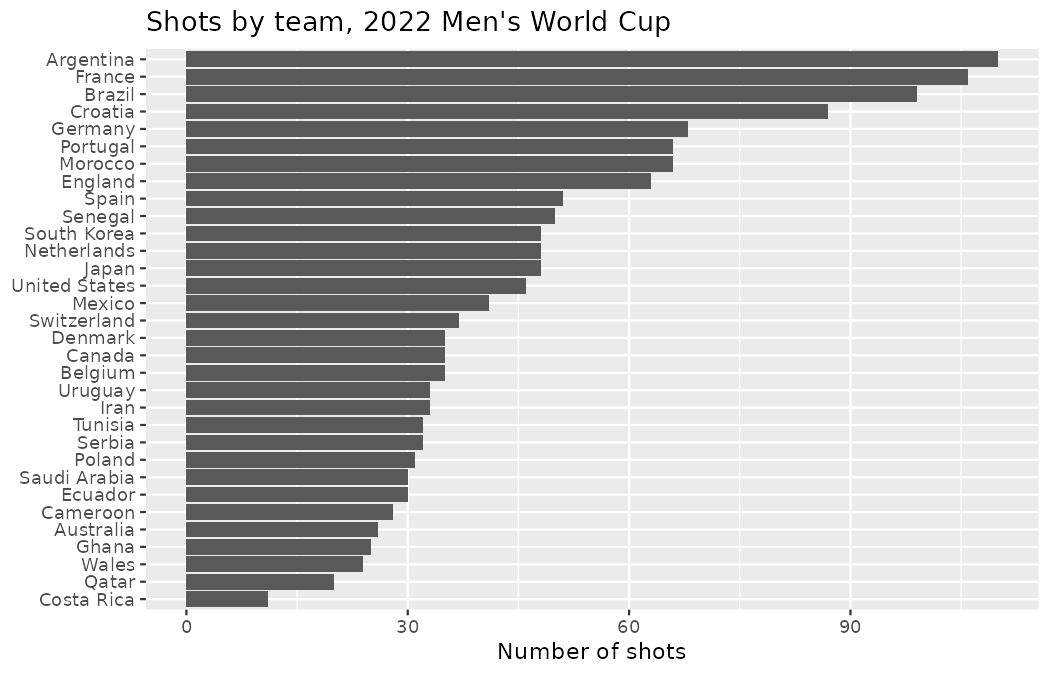
\includegraphics[width=0.85\linewidth,height=\textheight,keepaspectratio]{figures/data-applications-1.png}

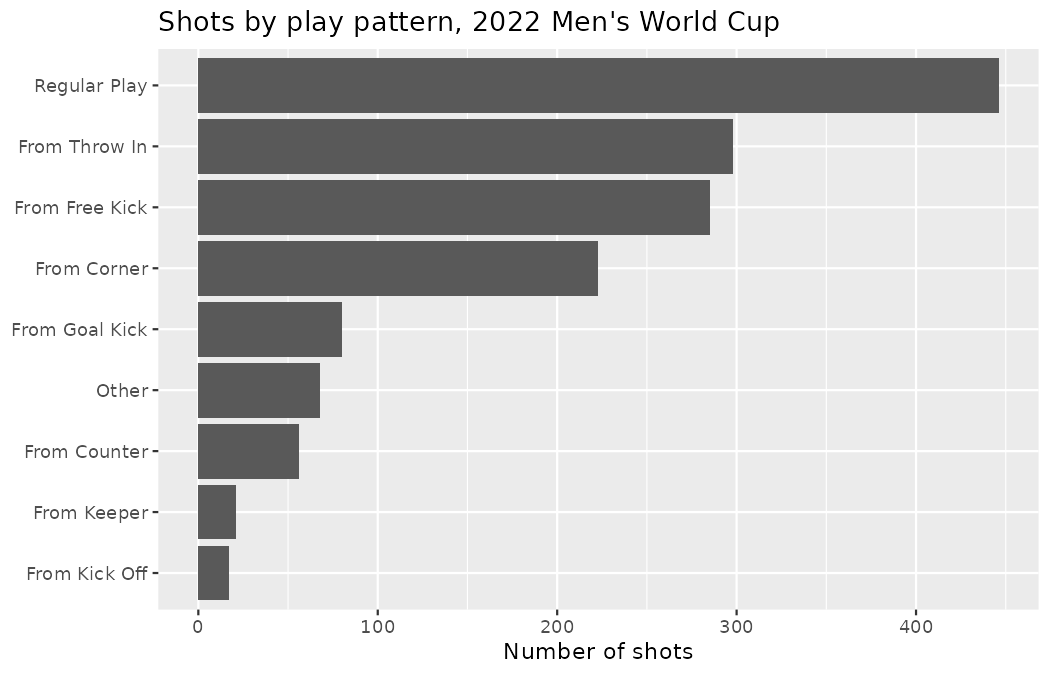
\includegraphics[width=0.85\linewidth,height=\textheight,keepaspectratio]{figures/data-applications-2.png}

The first plot shows 32 bars, one per team, sorted by shot count:
Argentina sits at the top with 110 shots, just ahead of France with 106
and Brazil with 99, and the bars taper steadily down to Costa Rica's 11
at the bottom --- a full ten-to-one ratio between the most and least
prolific teams. The second plot shows the 9 play patterns:
\texttt{Regular\ Play} towers over the rest with 446 shots, followed by
throw-ins (298), free kicks (285), and corners (223), with kick-offs
(17) and keeper distributions (21) barely registering.

\begin{tcolorbox}[enhanced jigsaw, left=2mm, leftrule=.75mm, title=\textcolor{quarto-callout-tip-color}{\faLightbulb}\hspace{0.5em}{Check your understanding}, arc=.35mm, rightrule=.15mm, coltitle=black, colframe=quarto-callout-tip-color-frame, bottomrule=.15mm, colbacktitle=quarto-callout-tip-color!10!white, opacitybacktitle=0.6, breakable, bottomtitle=1mm, toptitle=1mm, titlerule=0mm, opacityback=0, toprule=.15mm, colback=white]

Argentina tops the shot chart. Can we conclude that Argentina played the
most attacking football at the tournament?

\begin{center}\rule{0.5\linewidth}{0.5pt}\end{center}

Not from this plot. Argentina reached the final, so they played 7
matches while eliminated group-stage teams played only 3 --- the raw
count mixes together \emph{shots per match} and \emph{matches played}.
Croatia's 87 shots (also a deep run, losing semi-finalist) versus
Spain's 51 (out in the round of 16) reflect the same entanglement. To
compare attacking intent we would need a rate, such as shots per match
--- a standardization idea we develop properly in
Chapter~\ref{sec-explore-numerical}.

\end{tcolorbox}

\subsection{Getting to know the numerical
variables}\label{sec-wc-numerical-look}

Similarly, we can examine the distributions of the numerical variables.
The variable a modern scouting department stares at most is
\texttt{statsbomb\_xg}, the chance quality of each shot. We already know
from the head and tail of the data that most shots carry small values
--- 0.02 here, 0.28 there. Let's break chance quality down by
\texttt{shot\_type}:

\begin{Shaded}
\begin{Highlighting}[]
\NormalTok{wc2022\_shots }\SpecialCharTok{|\textgreater{}}
  \FunctionTok{group\_by}\NormalTok{(shot\_type) }\SpecialCharTok{|\textgreater{}}
  \FunctionTok{summarize}\NormalTok{(}
    \AttributeTok{shots =} \FunctionTok{n}\NormalTok{(),}
    \AttributeTok{mean =} \FunctionTok{round}\NormalTok{(}\FunctionTok{mean}\NormalTok{(statsbomb\_xg), }\DecValTok{3}\NormalTok{),}
    \AttributeTok{min =} \FunctionTok{round}\NormalTok{(}\FunctionTok{min}\NormalTok{(statsbomb\_xg), }\DecValTok{3}\NormalTok{),}
    \AttributeTok{max =} \FunctionTok{round}\NormalTok{(}\FunctionTok{max}\NormalTok{(statsbomb\_xg), }\DecValTok{3}\NormalTok{)}
\NormalTok{  )}
\CommentTok{\#\textgreater{} \# A tibble: 4 × 5}
\CommentTok{\#\textgreater{}   shot\_type shots  mean   min   max}
\CommentTok{\#\textgreater{}   \textless{}chr\textgreater{}     \textless{}int\textgreater{} \textless{}dbl\textgreater{} \textless{}dbl\textgreater{} \textless{}dbl\textgreater{}}
\CommentTok{\#\textgreater{} 1 Corner        2 0     0     0}
\CommentTok{\#\textgreater{} 2 Free Kick    46 0.043 0.007 0.1}
\CommentTok{\#\textgreater{} 3 Open Play  1382 0.098 0.004 0.897}
\CommentTok{\#\textgreater{} 4 Penalty      64 0.783 0.783 0.783}
\end{Highlighting}
\end{Shaded}

Three things deserve comment. First, the two shots with
\texttt{shot\_type\ ==\ "Corner"} are attempts scored directly from the
corner kick itself --- so rare (2 of 1,494) that their summary
statistics mean little; small groups will always need this caveat.
Second, direct free kicks average a chance quality of only 0.043 ---
roughly one goal per 23 attempts --- a number worth quoting the next
time a trialist's agent leads with ``elite set-piece delivery''. Third,
look at the \texttt{Penalty} row: mean, minimum, and maximum agree in
every digit. Every penalty in the dataset carries the \emph{identical}
xG value: the stored number is exactly 0.7835. (Displays round it --- to
0.783 in the table above, where we rounded to three decimals, and to
0.784 wherever software prints three significant digits instead --- so
both roundings of the one stored value 0.7835 will appear in output
throughout this book.) That is not a fluke of the tournament; it is a
property of the xG model, which treats all penalties as the same
standardized situation. Keep this in mind whenever you summarize chance
quality: penalties form a spike of identical values at 0.7835, far to
the right of almost every open-play shot.

We can also ask how chance quality varies by the shooter's position.
With 22 position labels, many represented by only a handful of shots, we
restrict attention to positions with at least 75 shots so that the group
summaries rest on reasonable sample sizes:

\begin{Shaded}
\begin{Highlighting}[]
\NormalTok{wc2022\_shots }\SpecialCharTok{|\textgreater{}}
  \FunctionTok{group\_by}\NormalTok{(position) }\SpecialCharTok{|\textgreater{}}
  \FunctionTok{summarize}\NormalTok{(}\AttributeTok{shots =} \FunctionTok{n}\NormalTok{(), }\AttributeTok{mean\_xg =} \FunctionTok{round}\NormalTok{(}\FunctionTok{mean}\NormalTok{(statsbomb\_xg), }\DecValTok{3}\NormalTok{)) }\SpecialCharTok{|\textgreater{}}
  \FunctionTok{filter}\NormalTok{(shots }\SpecialCharTok{\textgreater{}=} \DecValTok{75}\NormalTok{) }\SpecialCharTok{|\textgreater{}}
  \FunctionTok{arrange}\NormalTok{(}\FunctionTok{desc}\NormalTok{(mean\_xg))}
\CommentTok{\#\textgreater{} \# A tibble: 8 × 3}
\CommentTok{\#\textgreater{}   position                  shots mean\_xg}
\CommentTok{\#\textgreater{}   \textless{}chr\textgreater{}                     \textless{}int\textgreater{}   \textless{}dbl\textgreater{}}
\CommentTok{\#\textgreater{} 1 Right Center Forward         82   0.185}
\CommentTok{\#\textgreater{} 2 Center Forward              235   0.167}
\CommentTok{\#\textgreater{} 3 Left Center Forward          77   0.152}
\CommentTok{\#\textgreater{} 4 Right Wing                  154   0.117}
\CommentTok{\#\textgreater{} 5 Left Wing                   184   0.11}
\CommentTok{\#\textgreater{} 6 Center Attacking Midfield    80   0.104}
\CommentTok{\#\textgreater{} 7 Right Defensive Midfield     90   0.099}
\CommentTok{\#\textgreater{} 8 Left Defensive Midfield      93   0.096}
\end{Highlighting}
\end{Shaded}

The gradient is beautifully clean: the three center-forward roles
average the best chances (0.152 to 0.185 xG per shot), wingers sit in
the middle, and defensive midfielders shoot from the worst positions
(below 0.10).

\begin{tcolorbox}[enhanced jigsaw, left=2mm, leftrule=.75mm, title=\textcolor{quarto-callout-tip-color}{\faLightbulb}\hspace{0.5em}{Check your understanding}, arc=.35mm, rightrule=.15mm, coltitle=black, colframe=quarto-callout-tip-color-frame, bottomrule=.15mm, colbacktitle=quarto-callout-tip-color!10!white, opacitybacktitle=0.6, breakable, bottomtitle=1mm, toptitle=1mm, titlerule=0mm, opacityback=0, toprule=.15mm, colback=white]

Does the table above show that center forwards are better
\emph{finishers} than defensive midfielders?

\begin{center}\rule{0.5\linewidth}{0.5pt}\end{center}

No. \texttt{statsbomb\_xg} measures the quality of the \emph{chance},
assessed before the shot is struck --- it says nothing about how well
the shot was then executed. The table shows that center forwards shoot
from more dangerous situations, which is exactly what their role asks of
them. Whether a player converts \emph{more or less often than their
chances warrant} is a different question, about finishing skill, that we
will need models (Chapter~\ref{sec-model-slr} and beyond) to pose
properly.

\end{tcolorbox}

\subsection{Two tournaments, side by side}\label{sec-wc-weuro-divisions}

A single tournament is one draw from the game of football. Before a
scouting department builds any rule of thumb on these numbers, it should
ask whether the same structure appears in a different competition. So
let's place our second tournament alongside the first, treating the 2022
Men's World Cup and the 2025 Women's Euro as two ``divisions'' of the
same sport, and break down chance quality by competition and play
pattern:

\begin{Shaded}
\begin{Highlighting}[]
\NormalTok{weuro2025\_shots }\OtherTok{\textless{}{-}} \FunctionTok{read\_csv}\NormalTok{(}\StringTok{"data/derived/weuro2025\_shots.csv"}\NormalTok{)}

\NormalTok{both\_shots }\OtherTok{\textless{}{-}} \FunctionTok{bind\_rows}\NormalTok{(wc2022\_shots, weuro2025\_shots)}

\NormalTok{both\_shots }\SpecialCharTok{|\textgreater{}}
  \FunctionTok{group\_by}\NormalTok{(competition, play\_pattern) }\SpecialCharTok{|\textgreater{}}
  \FunctionTok{summarize}\NormalTok{(}
    \AttributeTok{shots =} \FunctionTok{n}\NormalTok{(),}
    \AttributeTok{mean =} \FunctionTok{round}\NormalTok{(}\FunctionTok{mean}\NormalTok{(statsbomb\_xg), }\DecValTok{3}\NormalTok{),}
    \AttributeTok{min =} \FunctionTok{round}\NormalTok{(}\FunctionTok{min}\NormalTok{(statsbomb\_xg), }\DecValTok{3}\NormalTok{),}
    \AttributeTok{max =} \FunctionTok{round}\NormalTok{(}\FunctionTok{max}\NormalTok{(statsbomb\_xg), }\DecValTok{3}\NormalTok{),}
    \AttributeTok{.groups =} \StringTok{"drop"}
\NormalTok{  ) }\SpecialCharTok{|\textgreater{}}
  \FunctionTok{arrange}\NormalTok{(play\_pattern, competition) }\SpecialCharTok{|\textgreater{}}
  \FunctionTok{print}\NormalTok{(}\AttributeTok{n =} \DecValTok{18}\NormalTok{)}
\CommentTok{\#\textgreater{} \# A tibble: 18 × 6}
\CommentTok{\#\textgreater{}    competition play\_pattern   shots  mean   min   max}
\CommentTok{\#\textgreater{}    \textless{}chr\textgreater{}       \textless{}chr\textgreater{}          \textless{}int\textgreater{} \textless{}dbl\textgreater{} \textless{}dbl\textgreater{} \textless{}dbl\textgreater{}}
\CommentTok{\#\textgreater{}  1 wc2022      From Corner      223 0.102 0     0.895}
\CommentTok{\#\textgreater{}  2 weuro2025   From Corner      160 0.084 0.006 0.532}
\CommentTok{\#\textgreater{}  3 wc2022      From Counter      56 0.159 0.008 0.791}
\CommentTok{\#\textgreater{}  4 weuro2025   From Counter      41 0.091 0.006 0.417}
\CommentTok{\#\textgreater{}  5 wc2022      From Free Kick   285 0.081 0.005 0.873}
\CommentTok{\#\textgreater{}  6 weuro2025   From Free Kick   104 0.085 0.005 0.686}
\CommentTok{\#\textgreater{}  7 wc2022      From Goal Kick    80 0.12  0.006 0.852}
\CommentTok{\#\textgreater{}  8 weuro2025   From Goal Kick    35 0.142 0.007 0.672}
\CommentTok{\#\textgreater{}  9 wc2022      From Keeper       21 0.106 0.008 0.367}
\CommentTok{\#\textgreater{} 10 weuro2025   From Keeper       22 0.062 0.024 0.157}
\CommentTok{\#\textgreater{} 11 wc2022      From Kick Off     17 0.095 0.004 0.475}
\CommentTok{\#\textgreater{} 12 weuro2025   From Kick Off     10 0.089 0.019 0.28}
\CommentTok{\#\textgreater{} 13 wc2022      From Throw In    298 0.085 0.006 0.552}
\CommentTok{\#\textgreater{} 14 weuro2025   From Throw In    177 0.104 0.005 0.723}
\CommentTok{\#\textgreater{} 15 wc2022      Other             68 0.748 0.036 0.783}
\CommentTok{\#\textgreater{} 16 weuro2025   Other             54 0.755 0.123 0.783}
\CommentTok{\#\textgreater{} 17 wc2022      Regular Play     446 0.098 0.004 0.897}
\CommentTok{\#\textgreater{} 18 weuro2025   Regular Play     310 0.1   0.004 0.725}
\end{Highlighting}
\end{Shaded}

The shot \emph{counts} are uniformly smaller at the Women's Euro, but
that is context, not signal: the World Cup had 64 matches and 32 teams,
the Euro 31 matches and 16 teams, so the counts should be taken in terms
of the size of each tournament --- compare the means, not the totals.
And the means are strikingly stable across the two competitions for most
patterns: regular play averages 0.098 versus 0.100, free kicks 0.081
versus 0.085. The one pattern where the tournaments visibly part ways is
the counter-attack: 0.159 per shot at the World Cup against 0.091 at the
Euro. Note it in your notebook --- but note it as a \emph{question}, not
a finding. Whether a gap like that reflects something real about the two
competitions, or is the kind of difference two samples can show by
chance alone, is precisely the question the inference chapters of this
book (starting in Chapter~\ref{sec-foundations-randomization}) will
teach you to answer.

And do you see the oddity hiding in rows 15 and 16? The \texttt{Other}
play pattern averages 0.748 and 0.755 --- seven times the chance quality
of regular play, in \emph{both} tournaments. A level called ``Other''
should be a dull miscellaneous bucket, not the most dangerous passage of
play in football. When a boring category produces a spectacular number,
do not write it up; investigate it. The investigation takes one line:

\begin{Shaded}
\begin{Highlighting}[]
\NormalTok{both\_shots }\SpecialCharTok{|\textgreater{}}
  \FunctionTok{filter}\NormalTok{(play\_pattern }\SpecialCharTok{==} \StringTok{"Other"}\NormalTok{) }\SpecialCharTok{|\textgreater{}}
  \FunctionTok{count}\NormalTok{(competition, shot\_type)}
\CommentTok{\#\textgreater{} \# A tibble: 4 × 3}
\CommentTok{\#\textgreater{}   competition shot\_type     n}
\CommentTok{\#\textgreater{}   \textless{}chr\textgreater{}       \textless{}chr\textgreater{}     \textless{}int\textgreater{}}
\CommentTok{\#\textgreater{} 1 wc2022      Open Play     4}
\CommentTok{\#\textgreater{} 2 wc2022      Penalty      64}
\CommentTok{\#\textgreater{} 3 weuro2025   Open Play     3}
\CommentTok{\#\textgreater{} 4 weuro2025   Penalty      51}
\end{Highlighting}
\end{Shaded}

Mystery solved: \texttt{Other} is where this data source files penalty
kicks --- 64 of the 68 World Cup \texttt{Other} shots and 51 of the 54
at the Euro are penalties, each carrying the stored penalty value 0.7835
--- so the ``most dangerous passage of play'' is simply the penalty spot
wearing a dull label.

A detail worth pausing on: exploring a dataset in this way often
uncovers facts about the context in which the data were collected. Let's
plot every shot's chance quality against the match clock, marking shot
types:

\begin{Shaded}
\begin{Highlighting}[]
\NormalTok{wc2022\_shots }\SpecialCharTok{|\textgreater{}}
  \FunctionTok{mutate}\NormalTok{(}\AttributeTok{clock =}\NormalTok{ minute }\SpecialCharTok{+}\NormalTok{ second }\SpecialCharTok{/} \DecValTok{60}\NormalTok{) }\SpecialCharTok{|\textgreater{}}
  \FunctionTok{ggplot}\NormalTok{(}\FunctionTok{aes}\NormalTok{(}\AttributeTok{x =}\NormalTok{ clock, }\AttributeTok{y =}\NormalTok{ statsbomb\_xg, }\AttributeTok{color =}\NormalTok{ shot\_type, }\AttributeTok{shape =}\NormalTok{ shot\_type)) }\SpecialCharTok{+}
  \FunctionTok{geom\_vline}\NormalTok{(}\AttributeTok{xintercept =} \DecValTok{120}\NormalTok{, }\AttributeTok{color =} \StringTok{"darkgrey"}\NormalTok{, }\AttributeTok{lty =} \DecValTok{2}\NormalTok{, }\AttributeTok{lwd =} \FloatTok{0.5}\NormalTok{) }\SpecialCharTok{+}
  \FunctionTok{geom\_point}\NormalTok{(}\AttributeTok{size =} \DecValTok{2}\NormalTok{, }\AttributeTok{alpha =} \FloatTok{0.6}\NormalTok{) }\SpecialCharTok{+}
  \FunctionTok{labs}\NormalTok{(}
    \AttributeTok{x =} \StringTok{"Match clock (minutes)"}\NormalTok{,}
    \AttributeTok{y =} \ConstantTok{NULL}\NormalTok{,}
    \AttributeTok{color =} \StringTok{"Shot type"}\NormalTok{,}
    \AttributeTok{shape =} \StringTok{"Shot type"}\NormalTok{,}
    \AttributeTok{title =} \StringTok{"Chance quality (xG) of every shot, by match clock"}
\NormalTok{  )}
\end{Highlighting}
\end{Shaded}

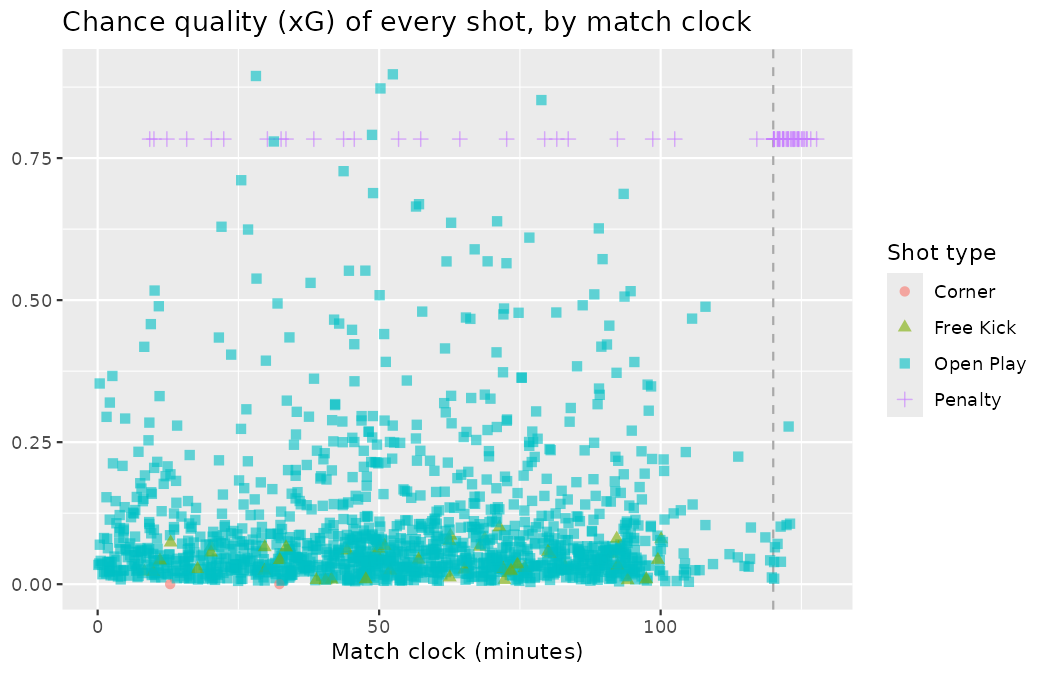
\includegraphics[width=0.85\linewidth,height=\textheight,keepaspectratio]{figures/data-applications-3.png}

The picture is unmistakable. The vast majority of points hug the bottom
of the plot --- open-play shots rarely exceed 0.4, with the single best
open-play chance of the tournament at 0.897. Slicing across the plot at
the stored penalty value 0.7835 is a perfectly horizontal band of
penalty points: every penalty, identical xG. And to the right of the
dashed line at minute 120, where regulation football has ended, sits a
dense cluster of penalties. Those are the shoot-outs we spotted in the
\texttt{period} table, and the data confirm it:

\begin{Shaded}
\begin{Highlighting}[]
\NormalTok{wc2022\_shots }\SpecialCharTok{|\textgreater{}}
  \FunctionTok{filter}\NormalTok{(period }\SpecialCharTok{==} \DecValTok{5}\NormalTok{) }\SpecialCharTok{|\textgreater{}}
  \FunctionTok{summarize}\NormalTok{(}\AttributeTok{kicks =} \FunctionTok{n}\NormalTok{(), }\AttributeTok{scored =} \FunctionTok{sum}\NormalTok{(goal), }\AttributeTok{matches =} \FunctionTok{n\_distinct}\NormalTok{(match\_id))}
\CommentTok{\#\textgreater{} \# A tibble: 1 × 3}
\CommentTok{\#\textgreater{}   kicks scored matches}
\CommentTok{\#\textgreater{}   \textless{}int\textgreater{}  \textless{}int\textgreater{}   \textless{}int\textgreater{}}
\CommentTok{\#\textgreater{} 1    41     26       5}

\NormalTok{wc2022\_shots }\SpecialCharTok{|\textgreater{}}
  \FunctionTok{filter}\NormalTok{(period }\SpecialCharTok{==} \DecValTok{5}\NormalTok{) }\SpecialCharTok{|\textgreater{}}
  \FunctionTok{count}\NormalTok{(stage)}
\CommentTok{\#\textgreater{} \# A tibble: 3 × 2}
\CommentTok{\#\textgreater{}   stage              n}
\CommentTok{\#\textgreater{}   \textless{}chr\textgreater{}          \textless{}int\textgreater{}}
\CommentTok{\#\textgreater{} 1 Final              8}
\CommentTok{\#\textgreater{} 2 Quarter{-}finals    18}
\CommentTok{\#\textgreater{} 3 Round of 16       15}
\end{Highlighting}
\end{Shaded}

Five matches went to shoot-outs --- two in the round of 16, two
quarter-finals, and the final itself, where Argentina beat France from
the spot. Those 41 shoot-out kicks (26 of them scored) sit in the
dataset alongside ordinary shots, each carrying the flat 0.7835 penalty
xG. Whether to keep them depends entirely on your question: an analyst
studying \emph{how teams create chances} should almost certainly filter
them out (\texttt{shot\_type\ ==\ "Open\ Play"}, or
\texttt{period\ \textless{}=\ 4}, and say so in the report); an analyst
studying \emph{tournament outcomes} had better keep them, since they
decided who lifted the trophy. The dataset does not make this decision
for you. Knowing your data well enough to even see the decision --- that
is what this first hour of work buys you.

So far we examined aspects of some of the individual variables, and we
have broken down chance quality by shot type, position, and competition.
You might have already wondered how summaries like these behave when a
third variable enters the picture. A constructed scouting scenario will
let us explore an important statistical concept, Simpson's paradox.

\section{Simpson's paradox}\label{simpsons-paradox}

Simpson's paradox is a description of three (or more) variables. The
paradox happens when a third variable reverses the relationship between
the first two variables. As always, the formal statement comes first,
and the demonstration follows.

\begin{tcolorbox}[enhanced jigsaw, left=2mm, leftrule=.75mm, title=\textcolor{quarto-callout-important-color}{\faExclamation}\hspace{0.5em}{Simpson's paradox}, arc=.35mm, rightrule=.15mm, coltitle=black, colframe=quarto-callout-important-color-frame, bottomrule=.15mm, colbacktitle=quarto-callout-important-color!10!white, opacitybacktitle=0.6, breakable, bottomtitle=1mm, toptitle=1mm, titlerule=0mm, opacityback=0, toprule=.15mm, colback=white]

\textbf{Simpson's paradox} happens when an association or relationship
between two variables in one direction (e.g., positive) reverses (e.g.,
becomes negative) when a third variable is considered.

\end{tcolorbox}

To see it happen, we will build a scenario inside Northbridge United.
This is a constructed dataset --- no real scouting records were used ---
and, as always in this book, we generate it in seeded R code so that
every number below can be reproduced exactly.

Here is the story. Marta Vidal, reviewing the club's scouting database
at the end of the season, notices something alarming: across all rated
prospects, \emph{the older the player, the lower the rating}. ``Do my
scouts believe footballers get worse every year from age sixteen?'' she
asks Priya Rao. Priya knows one structural fact about the database that
Marta has forgotten: Northbridge assigns each scout a market segment by
age. One scout covers the youth market (ages 16--20), one covers
prime-age players (21--26), and one covers the veteran market (27--33).
Each scout has rated 20 prospects on the club's 0--100 scale. The code
below constructs ratings with exactly this structure:

\begin{Shaded}
\begin{Highlighting}[]
\FunctionTok{set.seed}\NormalTok{(}\DecValTok{301}\NormalTok{)}
\NormalTok{scout\_ratings }\OtherTok{\textless{}{-}} \FunctionTok{tibble}\NormalTok{(}
  \AttributeTok{scout  =} \FunctionTok{factor}\NormalTok{(}\FunctionTok{rep}\NormalTok{(}\FunctionTok{c}\NormalTok{(}\StringTok{"Youth scout"}\NormalTok{, }\StringTok{"Prime{-}age scout"}\NormalTok{, }\StringTok{"Veteran scout"}\NormalTok{), }\AttributeTok{each =} \DecValTok{20}\NormalTok{),}
                  \AttributeTok{levels =} \FunctionTok{c}\NormalTok{(}\StringTok{"Youth scout"}\NormalTok{, }\StringTok{"Prime{-}age scout"}\NormalTok{, }\StringTok{"Veteran scout"}\NormalTok{)),}
  \AttributeTok{age\_lo =} \FunctionTok{rep}\NormalTok{(}\FunctionTok{c}\NormalTok{(}\DecValTok{16}\NormalTok{, }\DecValTok{21}\NormalTok{, }\DecValTok{27}\NormalTok{), }\AttributeTok{each =} \DecValTok{20}\NormalTok{),}
  \AttributeTok{age\_hi =} \FunctionTok{rep}\NormalTok{(}\FunctionTok{c}\NormalTok{(}\DecValTok{20}\NormalTok{, }\DecValTok{26}\NormalTok{, }\DecValTok{33}\NormalTok{), }\AttributeTok{each =} \DecValTok{20}\NormalTok{)}
\NormalTok{) }\SpecialCharTok{|\textgreater{}}
  \FunctionTok{mutate}\NormalTok{(}
    \AttributeTok{age    =} \FunctionTok{map2\_int}\NormalTok{(age\_lo, age\_hi, \textbackslash{}(lo, hi) }\FunctionTok{sample}\NormalTok{(lo}\SpecialCharTok{:}\NormalTok{hi, }\AttributeTok{size =} \DecValTok{1}\NormalTok{)),}
    \AttributeTok{rating =} \FunctionTok{round}\NormalTok{(}
      \FunctionTok{rep}\NormalTok{(}\FunctionTok{c}\NormalTok{(}\DecValTok{76}\NormalTok{, }\DecValTok{67}\NormalTok{, }\DecValTok{58}\NormalTok{), }\AttributeTok{each =} \DecValTok{20}\NormalTok{) }\SpecialCharTok{+} \FloatTok{1.5} \SpecialCharTok{*}\NormalTok{ (age }\SpecialCharTok{{-}}\NormalTok{ age\_lo) }\SpecialCharTok{+} \FunctionTok{rnorm}\NormalTok{(}\DecValTok{60}\NormalTok{, }\AttributeTok{mean =} \DecValTok{0}\NormalTok{, }\AttributeTok{sd =} \DecValTok{2}\NormalTok{),}
      \DecValTok{1}
\NormalTok{    )}
\NormalTok{  ) }\SpecialCharTok{|\textgreater{}}
  \FunctionTok{select}\NormalTok{(scout, age, rating)}

\NormalTok{scout\_ratings}
\CommentTok{\#\textgreater{} \# A tibble: 60 × 3}
\CommentTok{\#\textgreater{}    scout         age rating}
\CommentTok{\#\textgreater{}    \textless{}fct\textgreater{}       \textless{}int\textgreater{}  \textless{}dbl\textgreater{}}
\CommentTok{\#\textgreater{}  1 Youth scout    19   79.6}
\CommentTok{\#\textgreater{}  2 Youth scout    17   78.9}
\CommentTok{\#\textgreater{}  3 Youth scout    20   80.6}
\CommentTok{\#\textgreater{}  4 Youth scout    20   80.1}
\CommentTok{\#\textgreater{}  5 Youth scout    16   76.3}
\CommentTok{\#\textgreater{}  6 Youth scout    20   79.5}
\CommentTok{\#\textgreater{}  7 Youth scout    17   76.1}
\CommentTok{\#\textgreater{}  8 Youth scout    19   81.8}
\CommentTok{\#\textgreater{}  9 Youth scout    16   76.2}
\CommentTok{\#\textgreater{} 10 Youth scout    16   79.6}
\CommentTok{\#\textgreater{} \# ℹ 50 more rows}
\end{Highlighting}
\end{Shaded}

Read the construction: each scout's ratings start from a different
baseline (76, 67, 58), climb by 1.5 points per year of age \emph{within}
their assigned band, and are jittered by random noise. The three scouts
are not equally generous --- the youth scout grades on potential, the
veteran scout grades on resale value --- and their prospects occupy
entirely different age ranges:

\begin{Shaded}
\begin{Highlighting}[]
\NormalTok{scout\_ratings }\SpecialCharTok{|\textgreater{}}
  \FunctionTok{group\_by}\NormalTok{(scout) }\SpecialCharTok{|\textgreater{}}
  \FunctionTok{summarize}\NormalTok{(}
    \AttributeTok{prospects =} \FunctionTok{n}\NormalTok{(),}
    \AttributeTok{age\_range =} \FunctionTok{paste}\NormalTok{(}\FunctionTok{min}\NormalTok{(age), }\FunctionTok{max}\NormalTok{(age), }\AttributeTok{sep =} \StringTok{"{-}"}\NormalTok{),}
    \AttributeTok{mean\_rating =} \FunctionTok{round}\NormalTok{(}\FunctionTok{mean}\NormalTok{(rating), }\DecValTok{1}\NormalTok{)}
\NormalTok{  )}
\CommentTok{\#\textgreater{} \# A tibble: 3 × 4}
\CommentTok{\#\textgreater{}   scout           prospects age\_range mean\_rating}
\CommentTok{\#\textgreater{}   \textless{}fct\textgreater{}               \textless{}int\textgreater{} \textless{}chr\textgreater{}           \textless{}dbl\textgreater{}}
\CommentTok{\#\textgreater{} 1 Youth scout            20 16{-}20            78.9}
\CommentTok{\#\textgreater{} 2 Prime{-}age scout        20 21{-}26            70.1}
\CommentTok{\#\textgreater{} 3 Veteran scout          20 27{-}33            62.9}
\end{Highlighting}
\end{Shaded}

Let's start where Marta started: by considering how ratings relate to
age across the whole database. The code below draws a scatterplot of
rating against age with a line of best fit (to the entire dataset)
superimposed (see Chapter~\ref{sec-model-slr}, where we will present
fitting a line to a scatterplot).

\begin{Shaded}
\begin{Highlighting}[]
\FunctionTok{ggplot}\NormalTok{(scout\_ratings, }\FunctionTok{aes}\NormalTok{(}\AttributeTok{x =}\NormalTok{ age, }\AttributeTok{y =}\NormalTok{ rating)) }\SpecialCharTok{+}
  \FunctionTok{geom\_smooth}\NormalTok{(}\AttributeTok{method =} \StringTok{"lm"}\NormalTok{, }\AttributeTok{se =} \ConstantTok{FALSE}\NormalTok{) }\SpecialCharTok{+}
  \FunctionTok{geom\_point}\NormalTok{(}\AttributeTok{size =} \DecValTok{2}\NormalTok{) }\SpecialCharTok{+}
  \FunctionTok{labs}\NormalTok{(}
    \AttributeTok{x =} \StringTok{"Prospect age (years)"}\NormalTok{,}
    \AttributeTok{y =} \ConstantTok{NULL}\NormalTok{,}
    \AttributeTok{title =} \StringTok{"Scout rating (0{-}100 scale)"}
\NormalTok{  )}
\end{Highlighting}
\end{Shaded}

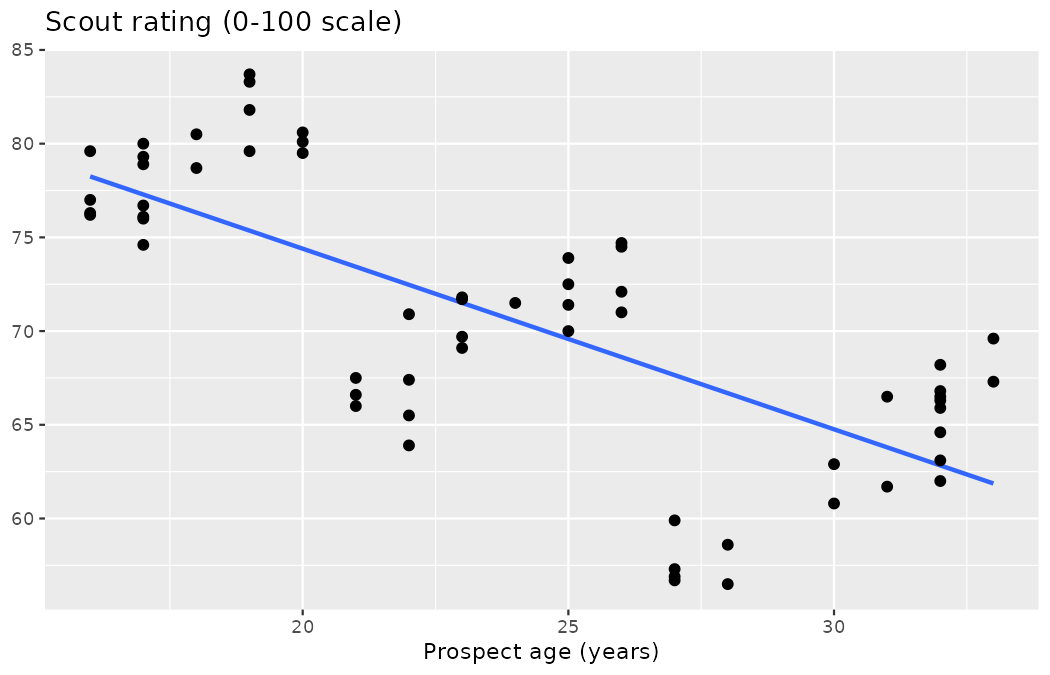
\includegraphics[width=0.85\linewidth,height=\textheight,keepaspectratio]{figures/data-applications-4.png}

The plot shows 60 points drifting downward from the upper left
(teenagers rated in the high 70s and low 80s) to the lower right
(thirty-somethings rated around 60), and the line of best fit through
them slopes clearly \emph{downward}. Notice that the line of best fit
shows a \emph{negative} relationship between rating and age. We can
quantify it:

\begin{Shaded}
\begin{Highlighting}[]
\FunctionTok{lm}\NormalTok{(rating }\SpecialCharTok{\textasciitilde{}}\NormalTok{ age, }\AttributeTok{data =}\NormalTok{ scout\_ratings) }\SpecialCharTok{|\textgreater{}}
  \FunctionTok{coef}\NormalTok{() }\SpecialCharTok{|\textgreater{}}
  \FunctionTok{round}\NormalTok{(}\DecValTok{2}\NormalTok{)}
\CommentTok{\#\textgreater{} (Intercept)         age}
\CommentTok{\#\textgreater{}       93.67       {-}0.96}
\end{Highlighting}
\end{Shaded}

Taken at face value: each additional year of age costs a prospect about
one rating point. Marta's alarm looks justified.

Of course, both your eye and your intuition should be telling you that
it doesn't make sense to model all three scouts' ratings together, any
more than it made sense in Section~\ref{sec-wc-weuro-divisions} to pool
shoot-out penalties with open play. Instead, let's look at the three
scouts separately, fitting a line of best fit within each scout's
assigned market:

\begin{Shaded}
\begin{Highlighting}[]
\FunctionTok{ggplot}\NormalTok{(scout\_ratings,}
       \FunctionTok{aes}\NormalTok{(}\AttributeTok{x =}\NormalTok{ age, }\AttributeTok{y =}\NormalTok{ rating, }\AttributeTok{group =}\NormalTok{ scout, }\AttributeTok{color =}\NormalTok{ scout, }\AttributeTok{shape =}\NormalTok{ scout)) }\SpecialCharTok{+}
  \FunctionTok{geom\_point}\NormalTok{(}\AttributeTok{size =} \DecValTok{2}\NormalTok{) }\SpecialCharTok{+}
  \FunctionTok{geom\_smooth}\NormalTok{(}\AttributeTok{method =} \StringTok{"lm"}\NormalTok{, }\AttributeTok{se =} \ConstantTok{FALSE}\NormalTok{) }\SpecialCharTok{+}
  \FunctionTok{labs}\NormalTok{(}
    \AttributeTok{x =} \StringTok{"Prospect age (years)"}\NormalTok{,}
    \AttributeTok{y =} \ConstantTok{NULL}\NormalTok{,}
    \AttributeTok{color =} \StringTok{"Scout"}\NormalTok{,}
    \AttributeTok{shape =} \StringTok{"Scout"}\NormalTok{,}
    \AttributeTok{title =} \StringTok{"Scout rating (0{-}100 scale)"}
\NormalTok{  )}
\end{Highlighting}
\end{Shaded}

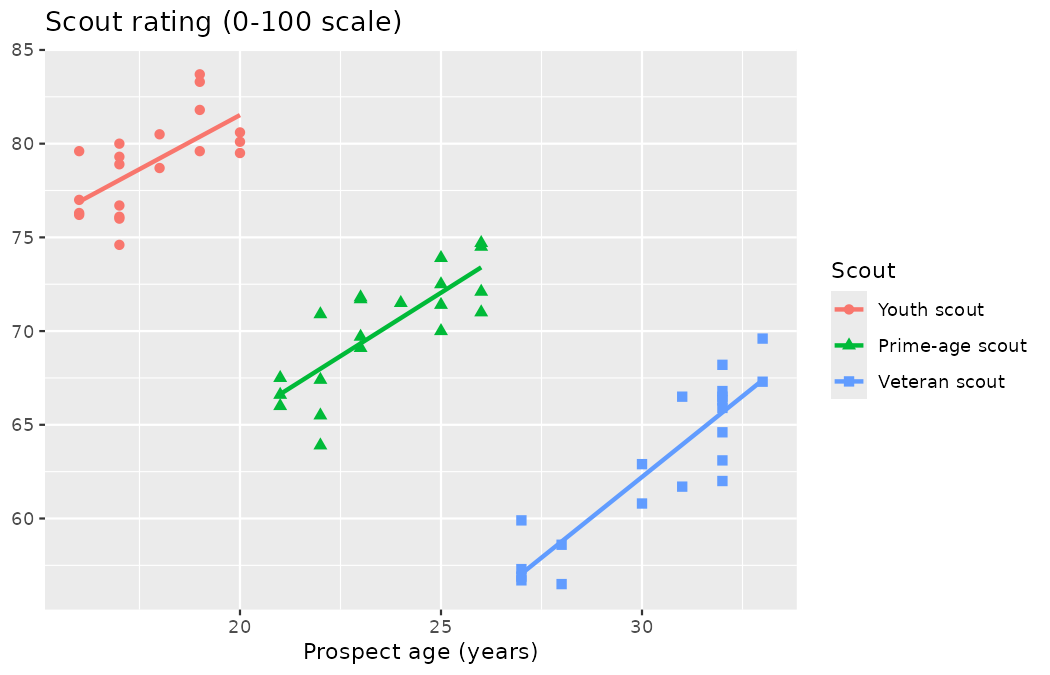
\includegraphics[width=0.85\linewidth,height=\textheight,keepaspectratio]{figures/data-applications-5.png}

The picture transforms. The 60 points resolve into three separate clouds
--- the youth scout's cloud sitting high and to the left, the prime-age
scout's in the middle, the veteran scout's low and to the right --- and
\emph{within each cloud the fitted line slopes upward}. Notice that
within each scout's market, the relationship between rating and age is
now \emph{positive}:

\begin{Shaded}
\begin{Highlighting}[]
\NormalTok{scout\_ratings }\SpecialCharTok{|\textgreater{}}
  \FunctionTok{group\_by}\NormalTok{(scout) }\SpecialCharTok{|\textgreater{}}
  \FunctionTok{summarize}\NormalTok{(}\AttributeTok{slope =} \FunctionTok{round}\NormalTok{(}\FunctionTok{coef}\NormalTok{(}\FunctionTok{lm}\NormalTok{(rating }\SpecialCharTok{\textasciitilde{}}\NormalTok{ age))[}\DecValTok{2}\NormalTok{], }\DecValTok{2}\NormalTok{))}
\CommentTok{\#\textgreater{} \# A tibble: 3 × 2}
\CommentTok{\#\textgreater{}   scout           slope}
\CommentTok{\#\textgreater{}   \textless{}fct\textgreater{}           \textless{}dbl\textgreater{}}
\CommentTok{\#\textgreater{} 1 Youth scout      1.16}
\CommentTok{\#\textgreater{} 2 Prime{-}age scout  1.35}
\CommentTok{\#\textgreater{} 3 Veteran scout    1.72}
\end{Highlighting}
\end{Shaded}

Every single scout rates \emph{older} prospects within their market more
highly --- slopes of +1.16, +1.35, and +1.72 rating points per year ---
while the pooled data showed ratings \emph{falling} by 0.96 points per
year. The relationship did not merely weaken when we accounted for the
third variable; it reversed --- exactly the phenomenon the definition at
the start of this section named.

Simpson's paradox was seen in the scout-rating data because the
aggregate data showed a negative relationship (negative slope) between
age and rating but a positive relationship (positive slope) between age
and rating when broken down by the scout doing the rating.

Simpson's paradox is observed with categorical data and with numeric
data. Often the paradox happens because the third variable (here, the
scout) is imbalanced. There are either more observations in one group or
the observations happen at different intervals across the groups. In the
rating data, each scout's prospects occupy a different age interval, and
the scouts' baseline generosity differs: the veteran scout's prospects
are both generally older and generally rated lower than the youth
scout's. Stack three upward-sloping clouds at successively lower heights
as you move right, and a line through all of them together tilts down.

In the rating analysis, it would be most prudent to report the trends
separately for each scout --- that is the comparison that actually
informs a signing decision, since any prospect was rated by the scout
who covers their market. However, in other situations, it might be
better to aggregate the data and report the overall trend. Deciding
which trend is the honest one requires understanding \emph{how the third
variable came to be related to the other two} --- here, that scout
assignment is determined by age --- and no amount of computation
substitutes for that understanding. Many additional examples of
Simpson's paradox and a further exploration are given in Witmer (2021).

\begin{tcolorbox}[enhanced jigsaw, left=2mm, leftrule=.75mm, title=\textcolor{quarto-callout-tip-color}{\faLightbulb}\hspace{0.5em}{Check your understanding}, arc=.35mm, rightrule=.15mm, coltitle=black, colframe=quarto-callout-tip-color-frame, bottomrule=.15mm, colbacktitle=quarto-callout-tip-color!10!white, opacitybacktitle=0.6, breakable, bottomtitle=1mm, toptitle=1mm, titlerule=0mm, opacityback=0, toprule=.15mm, colback=white]

On the strength of the pooled scatterplot, Marta proposes a rule: ``when
in doubt, sign the younger prospect --- our own database shows ratings
decline with age.'' What should Priya tell her?

\begin{center}\rule{0.5\linewidth}{0.5pt}\end{center}

That the database shows the opposite, once you condition on the lurking
third variable. Within every scout's market --- and every prospect was
rated by exactly one scout, assigned by age band --- older players
receive \emph{higher} ratings. The pooled decline is an artifact of
structure: older prospects are rated by the scout with the lowest
baseline. Comparing a 19-year-old's 79 from the youth scout against a
30-year-old's 63 from the veteran scout compares the \emph{scouts'
scales} as much as the players. Marta's rule would encode a clerical
artifact into transfer policy.

\end{tcolorbox}

\subsection{Scope of inference, one more
time}\label{sec-wc-scope-inference}

Let's close the case study where we began: with how the data were
collected. The shot data are purely observational --- StatsBomb recorded
football that was going to happen anyway. No one assigned Argentina 110
shots, or assigned a shot to arrive from a counter-attack. So every
pattern we found today --- the position gradient in chance quality, the
counter-attack gap between tournaments, the penalty spike --- is an
\emph{association}, a fact about how variables travel together in these
two tournaments. None of it, by itself, tells us what would happen if a
coach \emph{intervened}: instructing a team to counter more would not
necessarily buy them 0.159-quality chances, because the teams that
countered often may differ from other teams in a dozen ways at once ---
the confounding problem of Chapter~\ref{sec-data-design}.

The rating scenario sharpens the same point. The paradox had teeth
precisely because scout assignment was \emph{not} random: age determined
which scout, and scout determined the rating scale. If Northbridge
instead randomized prospects across scouts --- a design fully within the
club's power, of the kind Priya Rao will build repeatedly in this book
--- the link between age and rating scale would be severed by design,
and the pooled trend would become trustworthy. When the club can
randomize, it should; when it cannot, it must reason carefully about
third variables. That, in one sentence, is the discipline the next
several chapters build.

In this case study, we introduced you to the very first steps a data
analyst takes when they start working with a new dataset: peek at the
rows, count them, read the data dictionary, interrogate the suspicious
variables, summarize one variable at a time, then two, then worry about
the third. In the next few chapters, we will introduce exploratory data
analysis, and you'll learn more about the various types of data
visualizations and summary statistics you can make to get to know your
data better.

Before you move on, we encourage you to think about whether the
following questions can be answered with this dataset, and if yes, how
you might go about answering them. It is fine if your answer is ``I'm
not sure'': the purpose at this stage is to practice framing questions
the data might answer, ahead of the tools the coming chapters will
supply.

\begin{enumerate}
\def\labelenumi{\arabic{enumi}.}
\tightlist
\item
  Did any team play an entire match at the 2022 World Cup without
  registering a single shot?
\item
  Do the play-pattern profiles of individual teams --- how much of their
  shooting comes from corners, counters, and open play --- differ as
  sharply as their shot totals do?
\item
  Is there a ceiling on the chance quality of a single shot --- can any
  shot, short of the ball sitting on the goal line, ever be a certain
  goal?
\end{enumerate}

\section{Interactive walkthrough: a second first
hour}\label{sec-data-tutorials}

Reading about an analyst's first hour with a dataset is not the same as
having one yourself. So here is yours. Priya Rao has just handed you the
second file on the club's desk --- \texttt{weuro2025\_shots}, every shot
of the 2025 Women's Euro --- and asked you to repeat, on your own, the
ritual you just watched her perform on the World Cup data. Work through
the four lessons below at your keyboard; all you need is R and the two
CSV files. Each lesson mirrors a step of the case study, and each ends
with a question whose answer follows immediately after the rule --- try
to answer before you read on.

\subsection{Lesson 1: the language of
data}\label{lesson-1-the-language-of-data}

Load the file and establish the basics: how big is it, and what does a
row mean?

\begin{Shaded}
\begin{Highlighting}[]
\NormalTok{weuro2025\_shots }\OtherTok{\textless{}{-}} \FunctionTok{read\_csv}\NormalTok{(}\StringTok{"data/derived/weuro2025\_shots.csv"}\NormalTok{)}

\FunctionTok{dim}\NormalTok{(weuro2025\_shots)}
\CommentTok{\#\textgreater{} [1] 913  21}
\end{Highlighting}
\end{Shaded}

There are 913 rows and 21 columns --- the same 21 columns as
\texttt{wc2022\_shots}, described in Table~\ref{tbl-wc2022-var-def}, so
the data dictionary carries over unchanged. Each row is one shot taken
at the 2025 Women's Euro; the observational unit is again a shot.

Now interrogate a categorical variable, exactly as we did for the World
Cup:

\begin{Shaded}
\begin{Highlighting}[]
\NormalTok{weuro2025\_shots }\SpecialCharTok{|\textgreater{}}
  \FunctionTok{count}\NormalTok{(team, }\AttributeTok{sort =} \ConstantTok{TRUE}\NormalTok{) }\SpecialCharTok{|\textgreater{}}
  \FunctionTok{print}\NormalTok{(}\AttributeTok{n =} \DecValTok{16}\NormalTok{)}
\CommentTok{\#\textgreater{} \# A tibble: 16 × 2}
\CommentTok{\#\textgreater{}    team                    n}
\CommentTok{\#\textgreater{}    \textless{}chr\textgreater{}               \textless{}int\textgreater{}}
\CommentTok{\#\textgreater{}  1 Spain Women\textquotesingle{}s         149}
\CommentTok{\#\textgreater{}  2 England Women\textquotesingle{}s       115}
\CommentTok{\#\textgreater{}  3 Germany Women\textquotesingle{}s        90}
\CommentTok{\#\textgreater{}  4 France Women\textquotesingle{}s         74}
\CommentTok{\#\textgreater{}  5 Sweden Women\textquotesingle{}s         72}
\CommentTok{\#\textgreater{}  6 Italy Women\textquotesingle{}s          69}
\CommentTok{\#\textgreater{}  7 Switzerland Women\textquotesingle{}s    52}
\CommentTok{\#\textgreater{}  8 Norway Women\textquotesingle{}s         43}
\CommentTok{\#\textgreater{}  9 WNT Finland            36}
\CommentTok{\#\textgreater{} 10 Iceland Women\textquotesingle{}s        35}
\CommentTok{\#\textgreater{} 11 Netherlands Women\textquotesingle{}s    34}
\CommentTok{\#\textgreater{} 12 Poland Women\textquotesingle{}s         34}
\CommentTok{\#\textgreater{} 13 Denmark Women\textquotesingle{}s        33}
\CommentTok{\#\textgreater{} 14 Portugal Women\textquotesingle{}s       32}
\CommentTok{\#\textgreater{} 15 Belgium Women\textquotesingle{}s        28}
\CommentTok{\#\textgreater{} 16 Wales W                17}
\end{Highlighting}
\end{Shaded}

Spain lead the tournament with 149 shots --- nearly nine times Wales's
17 --- and England, the eventual champions, sit second with 115. But
look past the counts at the \emph{labels}. Fourteen teams are written as
``\ldots{} Women's'', one is ``WNT Finland'', and one is ``Wales W''.
The levels of this variable were not entered consistently.

\begin{tcolorbox}[enhanced jigsaw, left=2mm, leftrule=.75mm, title=\textcolor{quarto-callout-tip-color}{\faLightbulb}\hspace{0.5em}{Check your understanding}, arc=.35mm, rightrule=.15mm, coltitle=black, colframe=quarto-callout-tip-color-frame, bottomrule=.15mm, colbacktitle=quarto-callout-tip-color!10!white, opacitybacktitle=0.6, breakable, bottomtitle=1mm, toptitle=1mm, titlerule=0mm, opacityback=0, toprule=.15mm, colback=white]

The inconsistent team labels look cosmetic. When would they actually
break an analysis?

\begin{center}\rule{0.5\linewidth}{0.5pt}\end{center}

The moment you match this table against any other source. If you join
these shots to a squad list, a fixture file, or the World Cup data where
the same federation appears as plain ``Netherlands'', a label like ``WNT
Finland'' will silently fail to match and the team's rows will drop out
without an error message. This is the same moral as the match clock in
Section~\ref{sec-wc-match-clock}: a variable's values tell you what the
collector \emph{did}, not what you may assume they did. Check the levels
of every categorical variable before you rely on them.

\end{tcolorbox}

\subsection{Lesson 2: types of studies}\label{lesson-2-types-of-studies}

Before summarizing anything else, settle the scope of inference. Nobody
assigned Spain 149 shots; StatsBomb analysts coded football that was
going to happen anyway. Like its World Cup sibling, this is an
observational dataset, so --- recalling Chapter~\ref{sec-data-design}
--- every pattern you find in it is an association until a design like
Priya's randomized interventions says otherwise.

Now test whether the strangest finding of the case study replicates. At
the World Cup, every penalty carried the identical stored chance quality
of 0.7835. Was that a quirk of one tournament?

\begin{Shaded}
\begin{Highlighting}[]
\NormalTok{weuro2025\_shots }\SpecialCharTok{|\textgreater{}}
  \FunctionTok{group\_by}\NormalTok{(shot\_type) }\SpecialCharTok{|\textgreater{}}
  \FunctionTok{summarize}\NormalTok{(}
    \AttributeTok{shots =} \FunctionTok{n}\NormalTok{(),}
    \AttributeTok{mean =} \FunctionTok{round}\NormalTok{(}\FunctionTok{mean}\NormalTok{(statsbomb\_xg), }\DecValTok{3}\NormalTok{),}
    \AttributeTok{min =} \FunctionTok{round}\NormalTok{(}\FunctionTok{min}\NormalTok{(statsbomb\_xg), }\DecValTok{3}\NormalTok{),}
    \AttributeTok{max =} \FunctionTok{round}\NormalTok{(}\FunctionTok{max}\NormalTok{(statsbomb\_xg), }\DecValTok{3}\NormalTok{)}
\NormalTok{  )}
\CommentTok{\#\textgreater{} \# A tibble: 3 × 5}
\CommentTok{\#\textgreater{}   shot\_type shots  mean   min   max}
\CommentTok{\#\textgreater{}   \textless{}chr\textgreater{}     \textless{}int\textgreater{} \textless{}dbl\textgreater{} \textless{}dbl\textgreater{} \textless{}dbl\textgreater{}}
\CommentTok{\#\textgreater{} 1 Free Kick    11 0.036 0.009 0.095}
\CommentTok{\#\textgreater{} 2 Open Play   851 0.097 0.004 0.725}
\CommentTok{\#\textgreater{} 3 Penalty      51 0.783 0.783 0.783}
\end{Highlighting}
\end{Shaded}

It replicates perfectly: all 51 penalties at the Women's Euro carry
exactly the stored value 0.7835 --- which the rounded table above
displays as 0.783 --- the same value as all 64 at the World Cup. That
settles it --- the spike is a property of the xG \emph{model}, which
treats every penalty as the same standardized situation, not a property
of either tournament. Notice also what is \emph{missing}: this table has
three rows, not four. No shot at the Women's Euro was attempted directly
from a corner kick, so the \texttt{Corner} level of \texttt{shot\_type}
simply does not appear.

\begin{tcolorbox}[enhanced jigsaw, left=2mm, leftrule=.75mm, title=\textcolor{quarto-callout-tip-color}{\faLightbulb}\hspace{0.5em}{Check your understanding}, arc=.35mm, rightrule=.15mm, coltitle=black, colframe=quarto-callout-tip-color-frame, bottomrule=.15mm, colbacktitle=quarto-callout-tip-color!10!white, opacitybacktitle=0.6, breakable, bottomtitle=1mm, toptitle=1mm, titlerule=0mm, opacityback=0, toprule=.15mm, colback=white]

Open-play chance quality averages 0.097 here versus 0.098 at the World
Cup. May you conclude that open-play chances ``are the same'' in men's
and women's tournament football?

\begin{center}\rule{0.5\linewidth}{0.5pt}\end{center}

No --- and not only because these are observational data. Two sample
means being close is not evidence that the underlying quantities are
equal; two samples from \emph{identical} populations would rarely
produce exactly equal means, and two samples from \emph{different}
populations can easily produce nearly equal ones. Quantifying how close
is ``close enough'' is precisely the machinery of inference, which
begins in Chapter~\ref{sec-foundations-randomization}. For now, record
it as: the pattern is consistent across the two competitions.

\end{tcolorbox}

\subsection{Lesson 3: the traps you already know to
check}\label{lesson-3-the-traps-you-already-know-to-check}

The case study taught you two traps in the World Cup file: the
overlapping match clock and the shoot-out kicks hiding among the shots.
An analyst's first hour with a \emph{second} dataset goes faster because
the suspect list is already written. Check both:

\begin{Shaded}
\begin{Highlighting}[]
\NormalTok{weuro2025\_shots }\SpecialCharTok{|\textgreater{}}
  \FunctionTok{group\_by}\NormalTok{(period) }\SpecialCharTok{|\textgreater{}}
  \FunctionTok{summarize}\NormalTok{(}
    \AttributeTok{shots =} \FunctionTok{n}\NormalTok{(),}
    \AttributeTok{first\_minute =} \FunctionTok{min}\NormalTok{(minute),}
    \AttributeTok{last\_minute =} \FunctionTok{max}\NormalTok{(minute)}
\NormalTok{  )}
\CommentTok{\#\textgreater{} \# A tibble: 5 × 4}
\CommentTok{\#\textgreater{}   period shots first\_minute last\_minute}
\CommentTok{\#\textgreater{}    \textless{}dbl\textgreater{} \textless{}int\textgreater{}        \textless{}dbl\textgreater{}       \textless{}dbl\textgreater{}}
\CommentTok{\#\textgreater{} 1      1   376            0          49}
\CommentTok{\#\textgreater{} 2      2   463           45          98}
\CommentTok{\#\textgreater{} 3      3    18           91         106}
\CommentTok{\#\textgreater{} 4      4    19          107         122}
\CommentTok{\#\textgreater{} 5      5    37          120         131}
\end{Highlighting}
\end{Shaded}

Both traps are here too. The clock overlaps again --- period 1 runs to
minute 49 while period 2 starts at minute 45:

\begin{Shaded}
\begin{Highlighting}[]
\NormalTok{weuro2025\_shots }\SpecialCharTok{|\textgreater{}}
  \FunctionTok{filter}\NormalTok{(period }\SpecialCharTok{==} \DecValTok{1}\NormalTok{, minute }\SpecialCharTok{\textgreater{}=} \DecValTok{45}\NormalTok{) }\SpecialCharTok{|\textgreater{}}
  \FunctionTok{summarize}\NormalTok{(}\AttributeTok{shots =} \FunctionTok{n}\NormalTok{())}
\CommentTok{\#\textgreater{} \# A tibble: 1 × 1}
\CommentTok{\#\textgreater{}   shots}
\CommentTok{\#\textgreater{}   \textless{}int\textgreater{}}
\CommentTok{\#\textgreater{} 1    20}
\end{Highlighting}
\end{Shaded}

Twenty shots were taken in first-half stoppage time. And period 5
appears again, with 37 shoot-out kicks logged on clock readings from
minute 120 all the way to 131.

\begin{Shaded}
\begin{Highlighting}[]
\NormalTok{weuro2025\_shots }\SpecialCharTok{|\textgreater{}}
  \FunctionTok{filter}\NormalTok{(period }\SpecialCharTok{==} \DecValTok{5}\NormalTok{) }\SpecialCharTok{|\textgreater{}}
  \FunctionTok{summarize}\NormalTok{(}\AttributeTok{kicks =} \FunctionTok{n}\NormalTok{(), }\AttributeTok{scored =} \FunctionTok{sum}\NormalTok{(goal), }\AttributeTok{matches =} \FunctionTok{n\_distinct}\NormalTok{(match\_id))}
\CommentTok{\#\textgreater{} \# A tibble: 1 × 3}
\CommentTok{\#\textgreater{}   kicks scored matches}
\CommentTok{\#\textgreater{}   \textless{}int\textgreater{}  \textless{}int\textgreater{}   \textless{}int\textgreater{}}
\CommentTok{\#\textgreater{} 1    37     20       3}

\NormalTok{weuro2025\_shots }\SpecialCharTok{|\textgreater{}}
  \FunctionTok{filter}\NormalTok{(period }\SpecialCharTok{==} \DecValTok{5}\NormalTok{) }\SpecialCharTok{|\textgreater{}}
  \FunctionTok{count}\NormalTok{(stage)}
\CommentTok{\#\textgreater{} \# A tibble: 2 × 2}
\CommentTok{\#\textgreater{}   stage              n}
\CommentTok{\#\textgreater{}   \textless{}chr\textgreater{}          \textless{}int\textgreater{}}
\CommentTok{\#\textgreater{} 1 Final              9}
\CommentTok{\#\textgreater{} 2 Quarter{-}finals    28}
\end{Highlighting}
\end{Shaded}

Three matches went to shoot-outs --- two quarter-finals and the final
itself, where England beat Spain from the spot after a 1--1 draw. Those
37 kicks (20 scored) each carry the flat 0.7835 penalty xG, and the same
decision confronts you as in the case study: filter them for a
chance-creation question, keep them for a tournament-outcome question,
and say in your report which you did.

\begin{tcolorbox}[enhanced jigsaw, left=2mm, leftrule=.75mm, title=\textcolor{quarto-callout-tip-color}{\faLightbulb}\hspace{0.5em}{Check your understanding}, arc=.35mm, rightrule=.15mm, coltitle=black, colframe=quarto-callout-tip-color-frame, bottomrule=.15mm, colbacktitle=quarto-callout-tip-color!10!white, opacitybacktitle=0.6, breakable, bottomtitle=1mm, toptitle=1mm, titlerule=0mm, opacityback=0, toprule=.15mm, colback=white]

Suppose Emil Sørensen's travel budget covers scouts at only 8 of the
Women's Euro's 31 matches, and he wants shot data representative of the
whole tournament. Using the vocabulary of Chapter~\ref{sec-data-design},
what kind of sampling scheme is ``pick 8 matches at random and log every
shot in them'', and what is the cluster?

\begin{center}\rule{0.5\linewidth}{0.5pt}\end{center}

That is cluster sampling: the matches are the clusters, 8 of them are
sampled at random, and every observational unit (shot) inside a sampled
cluster is recorded. If the scouts instead logged only a random subset
of the shots within each sampled match, the scheme would be multistage
sampling. Since we happen to hold the full census of 913 shots, we could
even \emph{simulate} Emil's scheme against the truth --- an idea the
inference chapters will exploit relentlessly.

\end{tcolorbox}

\subsection{Lesson 4: does the position gradient
hold?}\label{lesson-4-does-the-position-gradient-hold}

The prettiest finding of the case study was the position gradient: at
the World Cup, center forwards shot from the best positions and
defensive midfielders from the worst, in a clean staircase. Your final
task is the question every finding must eventually face --- does it hold
somewhere else? The Euro is a smaller tournament, so we lower the
inclusion threshold from 75 shots to 40 to keep a comparable number of
position groups:

\begin{Shaded}
\begin{Highlighting}[]
\NormalTok{weuro2025\_shots }\SpecialCharTok{|\textgreater{}}
  \FunctionTok{group\_by}\NormalTok{(position) }\SpecialCharTok{|\textgreater{}}
  \FunctionTok{summarize}\NormalTok{(}\AttributeTok{shots =} \FunctionTok{n}\NormalTok{(), }\AttributeTok{mean\_xg =} \FunctionTok{round}\NormalTok{(}\FunctionTok{mean}\NormalTok{(statsbomb\_xg), }\DecValTok{3}\NormalTok{)) }\SpecialCharTok{|\textgreater{}}
  \FunctionTok{filter}\NormalTok{(shots }\SpecialCharTok{\textgreater{}=} \DecValTok{40}\NormalTok{) }\SpecialCharTok{|\textgreater{}}
  \FunctionTok{arrange}\NormalTok{(}\FunctionTok{desc}\NormalTok{(mean\_xg))}
\CommentTok{\#\textgreater{} \# A tibble: 8 × 3}
\CommentTok{\#\textgreater{}   position                  shots mean\_xg}
\CommentTok{\#\textgreater{}   \textless{}chr\textgreater{}                     \textless{}int\textgreater{}   \textless{}dbl\textgreater{}}
\CommentTok{\#\textgreater{} 1 Center Forward              143   0.176}
\CommentTok{\#\textgreater{} 2 Center Attacking Midfield    60   0.159}
\CommentTok{\#\textgreater{} 3 Right Wing                   76   0.151}
\CommentTok{\#\textgreater{} 4 Left Center Midfield         56   0.139}
\CommentTok{\#\textgreater{} 5 Right Center Midfield        62   0.134}
\CommentTok{\#\textgreater{} 6 Right Center Forward         41   0.11}
\CommentTok{\#\textgreater{} 7 Left Wing                   107   0.106}
\CommentTok{\#\textgreater{} 8 Left Center Forward          51   0.094}
\end{Highlighting}
\end{Shaded}

The headline survives: \texttt{Center\ Forward} again tops the table,
averaging 0.176 xG per shot from 143 attempts, close to the World Cup's
0.167. But the clean staircase does not. Attacking midfielders here
average \emph{better} chances (0.159) than they did at the World Cup
(0.104), and the two wide center-forward roles --- near the top of the
World Cup table --- sit at the \emph{bottom} of this one, with
\texttt{Left\ Center\ Forward} last at 0.094. Some of that is football
(positional labels map onto different tactical jobs in different teams
and competitions) and some of it is chance (several of these groups
contain only 40-odd shots).

This is the honest condition of real scouting data: patterns replicate
in outline and disagree in detail, and with the tools you have so far
you cannot yet say which disagreements are signal. Sit with that
discomfort. Calibrating exactly how much two samples should be expected
to disagree by chance alone is what the rest of this book is for.

\section{Lab: the match-level files}\label{sec-data-labs}

To further apply the concepts from this part of the book, conduct your
own first hour --- unguided this time --- on the two datasets we have so
far ignored: the match-level files.

\begin{Shaded}
\begin{Highlighting}[]
\NormalTok{wc2022\_matches }\OtherTok{\textless{}{-}} \FunctionTok{read\_csv}\NormalTok{(}\StringTok{"data/derived/wc2022\_matches.csv"}\NormalTok{)}
\NormalTok{weuro2025\_matches }\OtherTok{\textless{}{-}} \FunctionTok{read\_csv}\NormalTok{(}\StringTok{"data/derived/weuro2025\_matches.csv"}\NormalTok{)}

\FunctionTok{dim}\NormalTok{(wc2022\_matches)}
\CommentTok{\#\textgreater{} [1] 64  9}

\FunctionTok{dim}\NormalTok{(weuro2025\_matches)}
\CommentTok{\#\textgreater{} [1] 31  9}
\end{Highlighting}
\end{Shaded}

One row per match --- 64 at the World Cup, 31 at the Women's Euro ---
with columns \texttt{competition}, \texttt{match\_id},
\texttt{match\_date}, \texttt{stage}, \texttt{home\_team},
\texttt{away\_team}, \texttt{home\_score}, \texttt{away\_score}, and
\texttt{result}. Work through the full ritual and write up what you find
as if reporting to Marta Vidal:

\begin{enumerate}
\def\labelenumi{\arabic{enumi}.}
\tightlist
\item
  State the observational unit and write a data dictionary in the style
  of Table~\ref{tbl-wc2022-var-def}, classifying every variable as
  numerical (continuous or discrete) or categorical (ordinal or not).
  Decide, and defend, how to treat \texttt{match\_id}.
\item
  Get to know the categorical variables: tabulate \texttt{stage} and
  \texttt{result} in each competition. Do the counts match what you know
  about tournament formats (how many group matches \emph{must} a 32-team
  World Cup have)?
\item
  Get to know the numerical variables: summarize \texttt{home\_score}
  and \texttt{away\_score}. In a tournament played at neutral venues,
  what would it even mean for ``home'' teams to score more?
\item
  Join a match file to its shot file by \texttt{match\_id} and count
  shots per team per match. Is there a team-match with \emph{zero} shots
  hiding in the data --- one that a shots-only analysis would never
  reveal? (This ghost will matter when we build the \texttt{team\_match}
  dataset in Chapter~\ref{sec-explore-numerical}.)
\item
  The team labels in Lesson 1 were inconsistent. Before you join
  anything, check whether the match files share the shot files' naming
  conventions --- and describe what would go wrong if they did not.
\end{enumerate}

\section{Chapter review}\label{sec-chp3-review}

\subsection{Summary}\label{summary-2}

This chapter added no new formulas; it added a discipline. When a
dataset lands on your desk, you now know the first hour's ritual: peek
at the head and the tail (and distrust the row order); count the rows
and columns and say aloud what the observational unit is; read the
\textbf{data dictionary}, then interrogate the variables it undersells
--- the clock that overlaps, the identifier dressed as a number, the
shoot-out kicks filed among the shots; summarize the categorical
variables and the numerical ones, one at a time, then two at a time; and
ask of every summary how the data's origin --- observational here,
always --- limits what it can mean. We then met \textbf{Simpson's
paradox}, where a third variable (the scout doing the rating) reversed
the relationship between two others (age and rating), and saw that
choosing between the pooled and the within-group trend is not a
computation but an act of understanding how the third variable is
entangled with the first two. Finally, you repeated the ritual yourself
on the 2025 Women's Euro, where the penalty spike replicated exactly,
the position gradient replicated only in outline, and the team labels
reminded you to trust nothing you have not checked.

\subsection{Terms}\label{terms-2}

The terms introduced in this chapter are presented below, alphabetized.
If you're not sure what some of these terms mean, we recommend you go
back in the text and review their definitions. You should be able to
easily spot them as \textbf{bolded text}.

\begin{longtable}[]{@{}ll@{}}
\caption{Terms introduced in this
chapter.}\label{tbl-terms-chp-3}\tabularnewline
\toprule\noalign{}
\endfirsthead
\endhead
\bottomrule\noalign{}
\endlastfoot
data dictionary & Simpson's paradox \\
\end{longtable}

\begin{center}\rule{0.5\linewidth}{0.5pt}\end{center}

Adapted from \emph{Introduction to Modern Statistics} by
Çetinkaya-Rundel \& Hardin (CC BY-SA 4.0); this adaptation is likewise
CC BY-SA 4.0. Match data: StatsBomb open data.

\part{Exploratory data analysis}

\chapter{Exploring categorical data}\label{sec-explore-categorical}

This chapter focuses on exploring \textbf{categorical} data using
summary statistics and visualizations. The summaries and graphs
presented in this chapter are created using statistical software;
however, since this might be your first exposure to the concepts, we
take our time in this chapter to detail how to create them. Where
possible, we present multivariate plots; plots that visualize the
relationship between multiple variables. Mastery of the content
presented in this chapter will be crucial for understanding the methods
and techniques introduced in the rest of the book --- a scout who cannot
read a two-way table cannot read a scouting report.

In this chapter we will work with the World Cup shot data that you've
previously seen in Chapter~\ref{sec-data-hello}. The \texttt{shots50}
dataset from Chapter~\ref{sec-data-hello} represents a sample from a
larger dataset called \texttt{wc2022\_shots}, which contains every shot
logged at the 2022 Men's World Cup --- 1,494 of them. We will examine
the relationship between \texttt{body\_part}, which for these data can
take a value of \texttt{Right\ Foot}, \texttt{Left\ Foot}, or
\texttt{Head}, and the shot's result, which we collapse from the
detailed \texttt{outcome} variable into the binary question a scout
ultimately cares about: \texttt{goal} or \texttt{no\ goal}. Both
variables are categorical, so the tools of this chapter --- tables of
counts and proportions, and the plots built from them --- are exactly
the tools the job requires.

\begin{tcolorbox}[enhanced jigsaw, left=2mm, leftrule=.75mm, title=\textcolor{quarto-callout-note-color}{\faInfo}\hspace{0.5em}{Data}, arc=.35mm, rightrule=.15mm, coltitle=black, colframe=quarto-callout-note-color-frame, bottomrule=.15mm, colbacktitle=quarto-callout-note-color!10!white, opacitybacktitle=0.6, breakable, bottomtitle=1mm, toptitle=1mm, titlerule=0mm, opacityback=0, toprule=.15mm, colback=white]

The \texttt{wc2022\_shots} and \texttt{weuro2025\_shots} data are
derived from StatsBomb open data, with one row per shot. Throughout the
book they are read from \texttt{data/derived/} relative to the project
root. These are observational data: nobody assigned shots to feet or
heads at random, so --- recall the lesson of
Chapter~\ref{sec-data-design} --- everything we find in them is an
\emph{association}, never a demonstration of cause.

\end{tcolorbox}

\section{Contingency tables and bar
plots}\label{contingency-tables-and-bar-plots}

We begin by loading the data and checking the levels of
\texttt{body\_part}.

\begin{Shaded}
\begin{Highlighting}[]
\FunctionTok{library}\NormalTok{(dplyr)}
\FunctionTok{library}\NormalTok{(readr)}
\FunctionTok{library}\NormalTok{(tidyr)}
\FunctionTok{library}\NormalTok{(ggplot2)}

\NormalTok{wc2022\_shots }\OtherTok{\textless{}{-}} \FunctionTok{read\_csv}\NormalTok{(}\StringTok{"data/derived/wc2022\_shots.csv"}\NormalTok{)}

\NormalTok{wc2022\_shots }\SpecialCharTok{|\textgreater{}}
  \FunctionTok{count}\NormalTok{(body\_part)}
\CommentTok{\#\textgreater{} \# A tibble: 4 × 2}
\CommentTok{\#\textgreater{}   body\_part      n}
\CommentTok{\#\textgreater{}   \textless{}chr\textgreater{}      \textless{}int\textgreater{}}
\CommentTok{\#\textgreater{} 1 Head         252}
\CommentTok{\#\textgreater{} 2 Left Foot    449}
\CommentTok{\#\textgreater{} 3 Other         13}
\CommentTok{\#\textgreater{} 4 Right Foot   780}
\end{Highlighting}
\end{Shaded}

There is a fourth level, \texttt{Other}, covering the 13 shots struck
with a chest, shoulder, or some other part of the anatomy that the laws
of the game tolerate. Thirteen shots are too few to say anything useful
about, so we drop them --- and we say so, because silently discarding
data is how analyses stop being reproducible. That leaves
\(1,494 - 13 = 1,481\) shots. We also create the collapsed
\texttt{result} variable.

\begin{Shaded}
\begin{Highlighting}[]
\NormalTok{wc\_bp }\OtherTok{\textless{}{-}}\NormalTok{ wc2022\_shots }\SpecialCharTok{|\textgreater{}}
  \FunctionTok{filter}\NormalTok{(body\_part }\SpecialCharTok{!=} \StringTok{"Other"}\NormalTok{) }\SpecialCharTok{|\textgreater{}}
  \FunctionTok{mutate}\NormalTok{(}
    \AttributeTok{body\_part =} \FunctionTok{factor}\NormalTok{(body\_part, }\AttributeTok{levels =} \FunctionTok{c}\NormalTok{(}\StringTok{"Right Foot"}\NormalTok{, }\StringTok{"Left Foot"}\NormalTok{, }\StringTok{"Head"}\NormalTok{)),}
    \AttributeTok{result =} \FunctionTok{factor}\NormalTok{(}\FunctionTok{if\_else}\NormalTok{(goal, }\StringTok{"goal"}\NormalTok{, }\StringTok{"no goal"}\NormalTok{), }\AttributeTok{levels =} \FunctionTok{c}\NormalTok{(}\StringTok{"goal"}\NormalTok{, }\StringTok{"no goal"}\NormalTok{))}
\NormalTok{  )}

\NormalTok{wc\_bp }\SpecialCharTok{|\textgreater{}}
  \FunctionTok{count}\NormalTok{(result, body\_part) }\SpecialCharTok{|\textgreater{}}
  \FunctionTok{pivot\_wider}\NormalTok{(}\AttributeTok{names\_from =}\NormalTok{ body\_part, }\AttributeTok{values\_from =}\NormalTok{ n)}
\CommentTok{\#\textgreater{} \# A tibble: 2 × 4}
\CommentTok{\#\textgreater{}   result  \textasciigrave{}Right Foot\textasciigrave{} \textasciigrave{}Left Foot\textasciigrave{}  Head}
\CommentTok{\#\textgreater{}   \textless{}fct\textgreater{}          \textless{}int\textgreater{}       \textless{}int\textgreater{} \textless{}int\textgreater{}}
\CommentTok{\#\textgreater{} 1 goal             102          62    28}
\CommentTok{\#\textgreater{} 2 no goal          678         387   224}
\end{Highlighting}
\end{Shaded}

Table~\ref{tbl-wc-bp-result-totals} summarizes the two variables, with
totals attached. A table that summarizes data for two categorical
variables in this way is called a \textbf{contingency table}. Each value
in the table represents the number of times a particular combination of
variable outcomes occurred. For example, the value 102 corresponds to
the number of shots in the dataset that were struck with the right foot
and scored. Row and column totals are also included. The \textbf{row
totals} provide the total counts across each row and the \textbf{column
totals} down each column.

\begin{longtable}[]{@{}lrrrr@{}}
\caption{A contingency table for result and body part at the 2022 Men's
World Cup (shots with body part \texttt{Other}
excluded).}\label{tbl-wc-bp-result-totals}\tabularnewline
\toprule\noalign{}
& Right Foot & Left Foot & Head & Total \\
\midrule\noalign{}
\endfirsthead
\toprule\noalign{}
& Right Foot & Left Foot & Head & Total \\
\midrule\noalign{}
\endhead
\bottomrule\noalign{}
\endlastfoot
goal & 102 & 62 & 28 & 192 \\
no goal & 678 & 387 & 224 & 1,289 \\
Total & 780 & 449 & 252 & 1,481 \\
\end{longtable}

We can also create a table that shows only the overall percentages or
proportions for each combination of categories, or we can create a table
for a single variable, such as the one shown in
Table~\ref{tbl-wc-bp-totals} for the \texttt{body\_part} variable.

\begin{Shaded}
\begin{Highlighting}[]
\NormalTok{wc\_bp }\SpecialCharTok{|\textgreater{}}
  \FunctionTok{count}\NormalTok{(body\_part)}
\CommentTok{\#\textgreater{} \# A tibble: 3 × 2}
\CommentTok{\#\textgreater{}   body\_part      n}
\CommentTok{\#\textgreater{}   \textless{}fct\textgreater{}      \textless{}int\textgreater{}}
\CommentTok{\#\textgreater{} 1 Right Foot   780}
\CommentTok{\#\textgreater{} 2 Left Foot    449}
\CommentTok{\#\textgreater{} 3 Head         252}
\end{Highlighting}
\end{Shaded}

\begin{longtable}[]{@{}lr@{}}
\caption{A table summarizing the frequencies of each value of the body
part variable.}\label{tbl-wc-bp-totals}\tabularnewline
\toprule\noalign{}
body\_part & Count \\
\midrule\noalign{}
\endfirsthead
\toprule\noalign{}
body\_part & Count \\
\midrule\noalign{}
\endhead
\bottomrule\noalign{}
\endlastfoot
Right Foot & 780 \\
Left Foot & 449 \\
Head & 252 \\
Total & 1,481 \\
\end{longtable}

A \textbf{bar plot} is a common way to display a single categorical
variable. The first plot below displays the counts of
\texttt{body\_part}; in the second, the counts are converted into
proportions, showing the proportion of shots that are in each level.

\begin{Shaded}
\begin{Highlighting}[]
\NormalTok{wc\_bp }\SpecialCharTok{|\textgreater{}}
  \FunctionTok{count}\NormalTok{(body\_part) }\SpecialCharTok{|\textgreater{}}
  \FunctionTok{mutate}\NormalTok{(}\AttributeTok{proportion =}\NormalTok{ n }\SpecialCharTok{/} \FunctionTok{sum}\NormalTok{(n))}
\CommentTok{\#\textgreater{} \# A tibble: 3 × 3}
\CommentTok{\#\textgreater{}   body\_part      n proportion}
\CommentTok{\#\textgreater{}   \textless{}fct\textgreater{}      \textless{}int\textgreater{}      \textless{}dbl\textgreater{}}
\CommentTok{\#\textgreater{} 1 Right Foot   780      0.527}
\CommentTok{\#\textgreater{} 2 Left Foot    449      0.303}
\CommentTok{\#\textgreater{} 3 Head         252      0.170}

\FunctionTok{ggplot}\NormalTok{(wc\_bp, }\FunctionTok{aes}\NormalTok{(}\AttributeTok{x =}\NormalTok{ body\_part)) }\SpecialCharTok{+}
  \FunctionTok{geom\_bar}\NormalTok{() }\SpecialCharTok{+}
  \FunctionTok{labs}\NormalTok{(}\AttributeTok{x =} \StringTok{"Body part"}\NormalTok{, }\AttributeTok{y =} \StringTok{"Count"}\NormalTok{)}

\NormalTok{wc\_bp }\SpecialCharTok{|\textgreater{}}
  \FunctionTok{count}\NormalTok{(body\_part) }\SpecialCharTok{|\textgreater{}}
  \FunctionTok{mutate}\NormalTok{(}\AttributeTok{proportion =}\NormalTok{ n }\SpecialCharTok{/} \FunctionTok{sum}\NormalTok{(n)) }\SpecialCharTok{|\textgreater{}}
  \FunctionTok{ggplot}\NormalTok{(}\FunctionTok{aes}\NormalTok{(}\AttributeTok{x =}\NormalTok{ body\_part, }\AttributeTok{y =}\NormalTok{ proportion)) }\SpecialCharTok{+}
  \FunctionTok{geom\_col}\NormalTok{() }\SpecialCharTok{+}
  \FunctionTok{labs}\NormalTok{(}\AttributeTok{x =} \StringTok{"Body part"}\NormalTok{, }\AttributeTok{y =} \StringTok{"Proportion"}\NormalTok{)}
\end{Highlighting}
\end{Shaded}

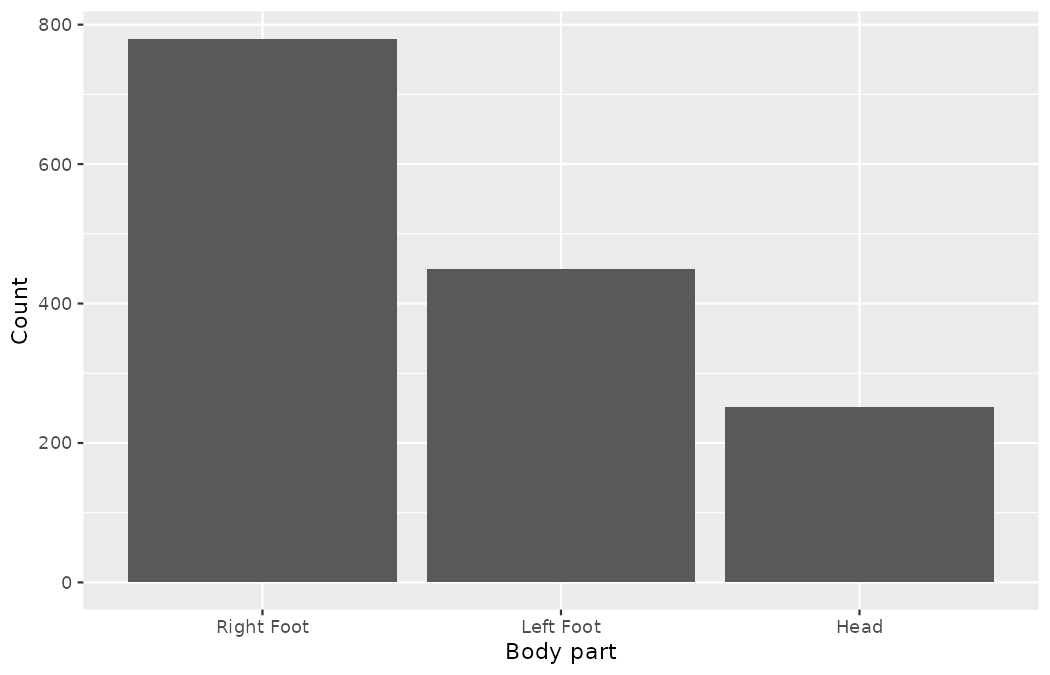
\includegraphics[width=0.85\linewidth,height=\textheight,keepaspectratio]{figures/explore-categorical-1.png}

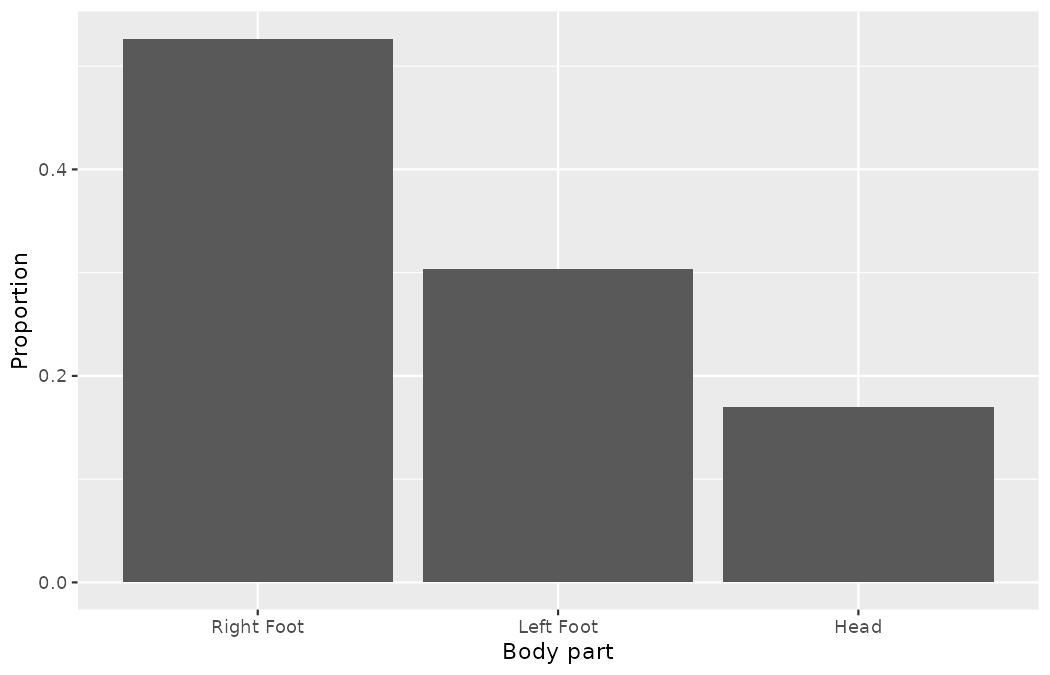
\includegraphics[width=0.85\linewidth,height=\textheight,keepaspectratio]{figures/explore-categorical-2.png}

Both plots show the same ordering: the right-foot bar is tallest by a
clear margin, the left-foot bar reaches a bit under two thirds of its
height, and the head bar is the shortest. The proportion version makes
the shares explicit --- 52.7\% of these shots were struck right-footed,
30.3\% left-footed, and 17.0\% were headers. Only the axis changes
between the two plots; the geometry of the bars is identical.

\begin{tcolorbox}[enhanced jigsaw, left=2mm, leftrule=.75mm, title=\textcolor{quarto-callout-tip-color}{\faLightbulb}\hspace{0.5em}{Check your understanding}, arc=.35mm, rightrule=.15mm, coltitle=black, colframe=quarto-callout-tip-color-frame, bottomrule=.15mm, colbacktitle=quarto-callout-tip-color!10!white, opacitybacktitle=0.6, breakable, bottomtitle=1mm, toptitle=1mm, titlerule=0mm, opacityback=0, toprule=.15mm, colback=white]

Roughly one shot in six at this World Cup was a header. Does the bar
plot of counts or the bar plot of proportions make that fact easier to
read off, and why?

\begin{center}\rule{0.5\linewidth}{0.5pt}\end{center}

The proportion plot: the head bar sits at 0.170 on a 0-to-1 scale, which
translates directly to ``about one in six.'' From the count plot you
would need to divide 252 by the total 1,481 yourself. Counts and
proportions carry the same information; the choice of scale determines
which questions the reader can answer without arithmetic.

\end{tcolorbox}

\section{Visualizing two categorical
variables}\label{visualizing-two-categorical-variables}

\subsection{Bar plots with two
variables}\label{bar-plots-with-two-variables}

We can display the distributions of two categorical variables on a bar
plot concurrently. Such plots are generally useful for visualizing the
relationship between two categorical variables. To have a second
tournament in play --- and to build a variable we will reuse for the
rest of the book --- we switch to the 2025 Women's Euro data and derive
a \emph{position group} for each shooter from the detailed
\texttt{position} string: defenders (\texttt{DF}), midfielders
(\texttt{MF}), and forwards (\texttt{FW}). Define the mapping once,
here, and reuse it verbatim whenever a chapter needs position groups:

\begin{Shaded}
\begin{Highlighting}[]
\NormalTok{weuro2025\_shots }\OtherTok{\textless{}{-}} \FunctionTok{read\_csv}\NormalTok{(}\StringTok{"data/derived/weuro2025\_shots.csv"}\NormalTok{)}

\NormalTok{weuro\_pos }\OtherTok{\textless{}{-}}\NormalTok{ weuro2025\_shots }\SpecialCharTok{|\textgreater{}}
  \FunctionTok{mutate}\NormalTok{(}
    \AttributeTok{pos\_group =} \FunctionTok{case\_when}\NormalTok{(}
\NormalTok{      position }\SpecialCharTok{==} \StringTok{"Goalkeeper"} \SpecialCharTok{\textasciitilde{}} \StringTok{"GK"}\NormalTok{,}
      \FunctionTok{grepl}\NormalTok{(}\StringTok{"Back"}\NormalTok{, position) }\SpecialCharTok{\textasciitilde{}} \StringTok{"DF"}\NormalTok{,}
      \FunctionTok{grepl}\NormalTok{(}\StringTok{"Midfield"}\NormalTok{, position) }\SpecialCharTok{\textasciitilde{}} \StringTok{"MF"}\NormalTok{,}
      \AttributeTok{.default =} \StringTok{"FW"}
\NormalTok{    )}
\NormalTok{  )}

\NormalTok{weuro\_pos }\SpecialCharTok{|\textgreater{}}
  \FunctionTok{count}\NormalTok{(pos\_group)}
\CommentTok{\#\textgreater{} \# A tibble: 4 × 2}
\CommentTok{\#\textgreater{}   pos\_group     n}
\CommentTok{\#\textgreater{}   \textless{}chr\textgreater{}     \textless{}int\textgreater{}}
\CommentTok{\#\textgreater{} 1 DF          155}
\CommentTok{\#\textgreater{} 2 FW          418}
\CommentTok{\#\textgreater{} 3 GK            2}
\CommentTok{\#\textgreater{} 4 MF          338}
\end{Highlighting}
\end{Shaded}

The order of the \texttt{case\_when()} clauses matters: a ``Left Wing
Back'' is a defender, so the \texttt{Back} rule must fire before any
rule that would catch ``Wing.'' Positions containing \texttt{Back} map
to \texttt{DF}, positions containing \texttt{Midfield} map to
\texttt{MF}, and everything remaining --- wings, center forwards,
strikers --- maps to \texttt{FW}. Two shots were taken by goalkeepers
(both penalties, as it happens); two observations cannot support
comparisons, so we drop them and note it, leaving 911 shots.

\begin{Shaded}
\begin{Highlighting}[]
\NormalTok{weuro\_pos }\OtherTok{\textless{}{-}}\NormalTok{ weuro\_pos }\SpecialCharTok{|\textgreater{}}
  \FunctionTok{filter}\NormalTok{(pos\_group }\SpecialCharTok{!=} \StringTok{"GK"}\NormalTok{) }\SpecialCharTok{|\textgreater{}}
  \FunctionTok{mutate}\NormalTok{(}
    \AttributeTok{pos\_group =} \FunctionTok{factor}\NormalTok{(pos\_group, }\AttributeTok{levels =} \FunctionTok{c}\NormalTok{(}\StringTok{"FW"}\NormalTok{, }\StringTok{"MF"}\NormalTok{, }\StringTok{"DF"}\NormalTok{)),}
    \AttributeTok{shot\_type =} \FunctionTok{factor}\NormalTok{(shot\_type, }\AttributeTok{levels =} \FunctionTok{c}\NormalTok{(}\StringTok{"Open Play"}\NormalTok{, }\StringTok{"Free Kick"}\NormalTok{, }\StringTok{"Penalty"}\NormalTok{))}
\NormalTok{  )}

\NormalTok{weuro\_pos }\SpecialCharTok{|\textgreater{}}
  \FunctionTok{count}\NormalTok{(pos\_group, shot\_type) }\SpecialCharTok{|\textgreater{}}
  \FunctionTok{pivot\_wider}\NormalTok{(}\AttributeTok{names\_from =}\NormalTok{ shot\_type, }\AttributeTok{values\_from =}\NormalTok{ n, }\AttributeTok{values\_fill =} \DecValTok{0}\NormalTok{)}
\CommentTok{\#\textgreater{} \# A tibble: 3 × 4}
\CommentTok{\#\textgreater{}   pos\_group \textasciigrave{}Open Play\textasciigrave{} \textasciigrave{}Free Kick\textasciigrave{} Penalty}
\CommentTok{\#\textgreater{}   \textless{}fct\textgreater{}           \textless{}int\textgreater{}       \textless{}int\textgreater{}   \textless{}int\textgreater{}}
\CommentTok{\#\textgreater{} 1 FW                402           4      12}
\CommentTok{\#\textgreater{} 2 MF                308           6      24}
\CommentTok{\#\textgreater{} 3 DF                141           1      13}
\end{Highlighting}
\end{Shaded}

The three plots below visualize the relationship between
\texttt{pos\_group} and \texttt{shot\_type} in three different ways.

\begin{Shaded}
\begin{Highlighting}[]
\CommentTok{\# Stacked bar plot}
\FunctionTok{ggplot}\NormalTok{(weuro\_pos, }\FunctionTok{aes}\NormalTok{(}\AttributeTok{x =}\NormalTok{ pos\_group, }\AttributeTok{fill =}\NormalTok{ shot\_type)) }\SpecialCharTok{+}
  \FunctionTok{geom\_bar}\NormalTok{() }\SpecialCharTok{+}
  \FunctionTok{labs}\NormalTok{(}\AttributeTok{x =} \StringTok{"Position group"}\NormalTok{, }\AttributeTok{y =} \StringTok{"Count"}\NormalTok{, }\AttributeTok{fill =} \StringTok{"Shot type"}\NormalTok{)}

\CommentTok{\# Standardized bar plot}
\FunctionTok{ggplot}\NormalTok{(weuro\_pos, }\FunctionTok{aes}\NormalTok{(}\AttributeTok{x =}\NormalTok{ pos\_group, }\AttributeTok{fill =}\NormalTok{ shot\_type)) }\SpecialCharTok{+}
  \FunctionTok{geom\_bar}\NormalTok{(}\AttributeTok{position =} \StringTok{"fill"}\NormalTok{) }\SpecialCharTok{+}
  \FunctionTok{labs}\NormalTok{(}\AttributeTok{x =} \StringTok{"Position group"}\NormalTok{, }\AttributeTok{y =} \StringTok{"Proportion"}\NormalTok{, }\AttributeTok{fill =} \StringTok{"Shot type"}\NormalTok{)}

\CommentTok{\# Dodged bar plot}
\FunctionTok{ggplot}\NormalTok{(weuro\_pos, }\FunctionTok{aes}\NormalTok{(}\AttributeTok{x =}\NormalTok{ pos\_group, }\AttributeTok{fill =}\NormalTok{ shot\_type)) }\SpecialCharTok{+}
  \FunctionTok{geom\_bar}\NormalTok{(}\AttributeTok{position =} \StringTok{"dodge"}\NormalTok{) }\SpecialCharTok{+}
  \FunctionTok{labs}\NormalTok{(}\AttributeTok{x =} \StringTok{"Position group"}\NormalTok{, }\AttributeTok{y =} \StringTok{"Count"}\NormalTok{, }\AttributeTok{fill =} \StringTok{"Shot type"}\NormalTok{)}
\end{Highlighting}
\end{Shaded}

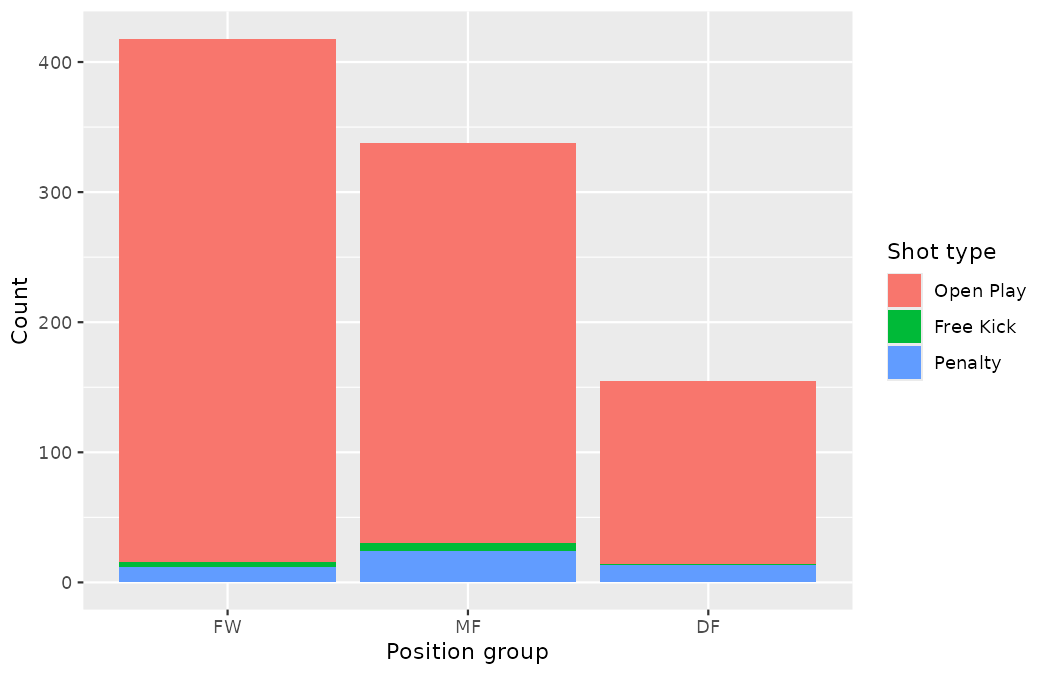
\includegraphics[width=0.85\linewidth,height=\textheight,keepaspectratio]{figures/explore-categorical-3.png}

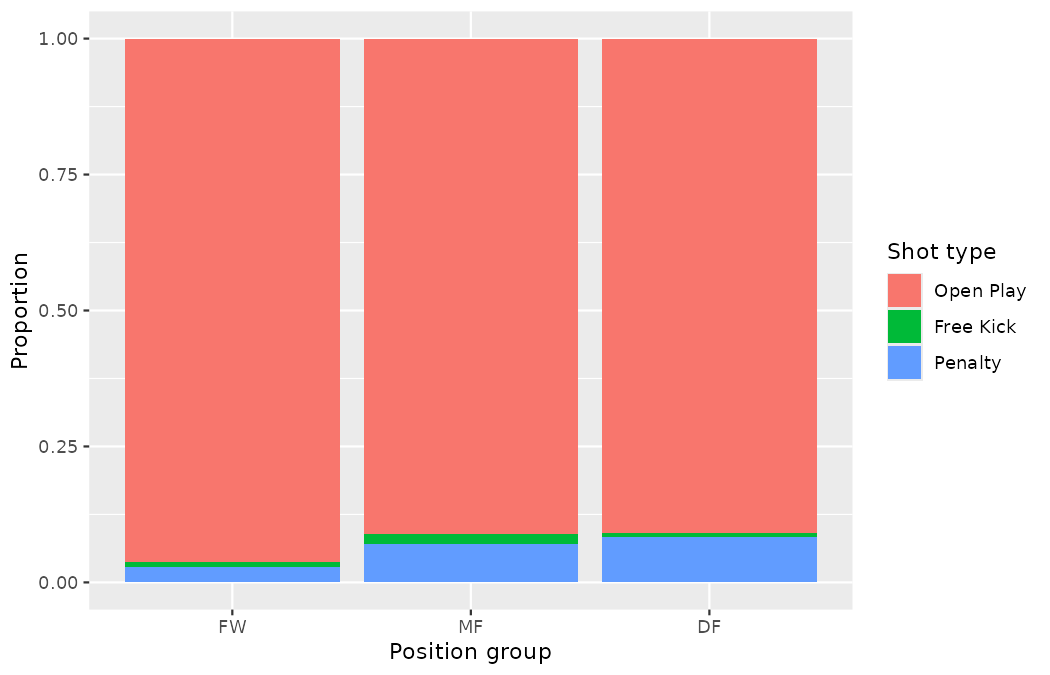
\includegraphics[width=0.85\linewidth,height=\textheight,keepaspectratio]{figures/explore-categorical-4.png}

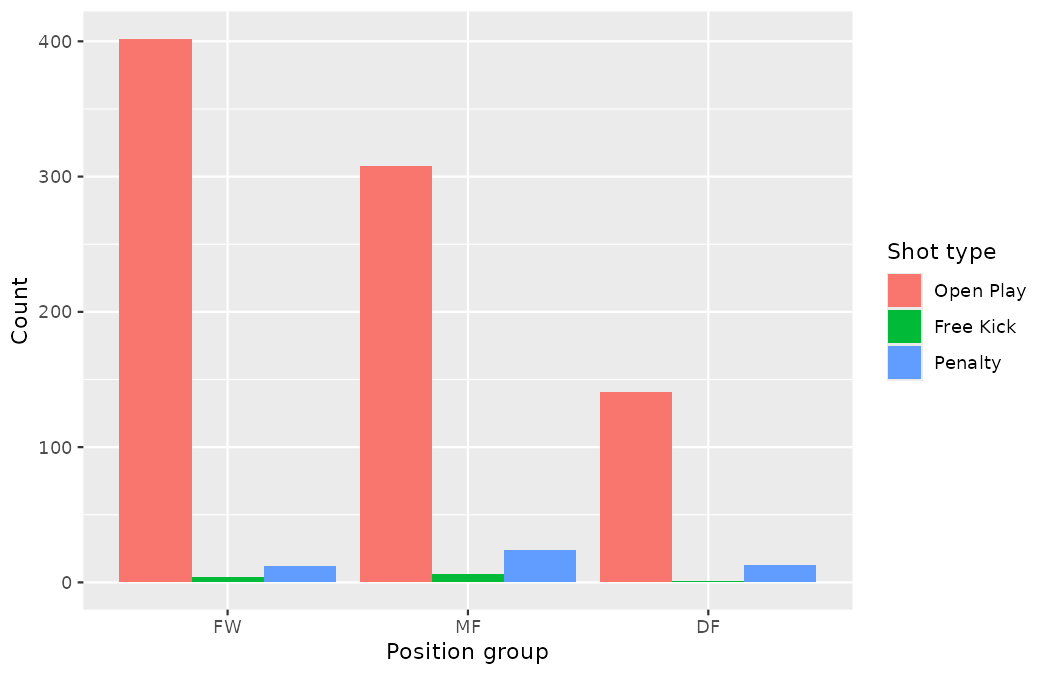
\includegraphics[width=0.85\linewidth,height=\textheight,keepaspectratio]{figures/explore-categorical-5.png}

The first is a \textbf{stacked bar plot}: one bar per position group,
with the shot-type counts stacked within each bar. This plot most
clearly displays that forwards take the most shots (418, against 338 for
midfielders and 155 for defenders). It is difficult to say, based on
this plot alone, how the shot-type mix varies across position groups,
because the free-kick and penalty segments are thin slivers perched on
top of tall open-play blocks.

The second is a \textbf{standardized bar plot} (also known as a
\textbf{filled bar plot}): every bar is stretched to height 1, so the
segments show proportions within each position group. The proportions
behind it are worth printing:

\begin{Shaded}
\begin{Highlighting}[]
\NormalTok{weuro\_pos }\SpecialCharTok{|\textgreater{}}
  \FunctionTok{count}\NormalTok{(pos\_group, shot\_type) }\SpecialCharTok{|\textgreater{}}
  \FunctionTok{group\_by}\NormalTok{(pos\_group) }\SpecialCharTok{|\textgreater{}}
  \FunctionTok{mutate}\NormalTok{(}\AttributeTok{proportion =}\NormalTok{ n }\SpecialCharTok{/} \FunctionTok{sum}\NormalTok{(n))}
\CommentTok{\#\textgreater{} \# A tibble: 9 × 4}
\CommentTok{\#\textgreater{} \# Groups:   pos\_group [3]}
\CommentTok{\#\textgreater{}   pos\_group shot\_type     n proportion}
\CommentTok{\#\textgreater{}   \textless{}fct\textgreater{}     \textless{}fct\textgreater{}     \textless{}int\textgreater{}      \textless{}dbl\textgreater{}}
\CommentTok{\#\textgreater{} 1 FW        Open Play   402    0.962}
\CommentTok{\#\textgreater{} 2 FW        Free Kick     4    0.00957}
\CommentTok{\#\textgreater{} 3 FW        Penalty      12    0.0287}
\CommentTok{\#\textgreater{} 4 MF        Open Play   308    0.911}
\CommentTok{\#\textgreater{} 5 MF        Free Kick     6    0.0178}
\CommentTok{\#\textgreater{} 6 MF        Penalty      24    0.0710}
\CommentTok{\#\textgreater{} 7 DF        Open Play   141    0.910}
\CommentTok{\#\textgreater{} 8 DF        Free Kick     1    0.00645}
\CommentTok{\#\textgreater{} 9 DF        Penalty      13    0.0839}
\end{Highlighting}
\end{Shaded}

In the standardized plot the penalty segment visibly widens as you move
from forwards (2.9\% of their shots) to midfielders (7.1\%) to defenders
(8.4\%). Be careful before turning that gradient into a scouting claim
about who clubs \emph{choose} as penalty takers: most of this
tournament's penalties were not in-game penalties at all, and splitting
the kicks by whether they came in a period-5 shoot-out changes the
story.

\begin{Shaded}
\begin{Highlighting}[]
\NormalTok{weuro\_pos }\SpecialCharTok{|\textgreater{}}
  \FunctionTok{filter}\NormalTok{(shot\_type }\SpecialCharTok{==} \StringTok{"Penalty"}\NormalTok{) }\SpecialCharTok{|\textgreater{}}
  \FunctionTok{mutate}\NormalTok{(}\AttributeTok{setting =} \FunctionTok{if\_else}\NormalTok{(period }\SpecialCharTok{==} \DecValTok{5}\NormalTok{, }\StringTok{"shoot{-}out"}\NormalTok{, }\StringTok{"in{-}game"}\NormalTok{)) }\SpecialCharTok{|\textgreater{}}
  \FunctionTok{count}\NormalTok{(setting, pos\_group) }\SpecialCharTok{|\textgreater{}}
  \FunctionTok{pivot\_wider}\NormalTok{(}\AttributeTok{names\_from =}\NormalTok{ pos\_group, }\AttributeTok{values\_from =}\NormalTok{ n)}
\CommentTok{\#\textgreater{} \# A tibble: 2 × 4}
\CommentTok{\#\textgreater{}   setting      FW    MF    DF}
\CommentTok{\#\textgreater{}   \textless{}chr\textgreater{}     \textless{}int\textgreater{} \textless{}int\textgreater{} \textless{}int\textgreater{}}
\CommentTok{\#\textgreater{} 1 in{-}game       5     8     1}
\CommentTok{\#\textgreater{} 2 shoot{-}out     7    16    12}
\end{Highlighting}
\end{Shaded}

Only 14 of the 49 outfield penalties were awarded in play, and those
went almost entirely to attacking players --- 13 of the 14 to forwards
or midfielders, a single one to a defender --- which is what
``designated penalty taker'' should look like. The other 35 kicks came
in shoot-outs, where five or more different players per team must step
up, so the taker pool deepens by necessity: 12 of the 13 defender
penalties in these data are shoot-out kicks (as were both penalties by
the goalkeepers we dropped earlier). The defenders' wide penalty segment
is a shoot-out artifact, not evidence that clubs hand their spot kicks
to center backs. Since the proportions of shot types vary across the
groups, we can conclude that the two variables are associated for this
sample --- but \emph{why} they are associated took a third variable to
see, echoing the lesson of Chapter~\ref{sec-data-applications}.

The third is a \textbf{dodged bar plot}: the shot-type bars stand side
by side within each position group. This plot most clearly displays that
open-play shots dominate every position group, and it makes the raw
counts of all nine combinations easy to read --- but the free-kick bars
(4, 6, and 1) are nearly invisible next to bars of 402 and 308.

\begin{tcolorbox}[enhanced jigsaw, left=2mm, leftrule=.75mm, title=\textcolor{quarto-callout-note-color}{\faInfo}\hspace{0.5em}{Worked example}, arc=.35mm, rightrule=.15mm, coltitle=black, colframe=quarto-callout-note-color-frame, bottomrule=.15mm, colbacktitle=quarto-callout-note-color!10!white, opacitybacktitle=0.6, breakable, bottomtitle=1mm, toptitle=1mm, titlerule=0mm, opacityback=0, toprule=.15mm, colback=white]

Examine the three bar plots above. When is the stacked, dodged, or
standardized bar plot the most useful?

\begin{center}\rule{0.5\linewidth}{0.5pt}\end{center}

The stacked bar plot is most useful when it's reasonable to assign one
variable as the explanatory variable (here \texttt{pos\_group}) and the
other variable as the response (here \texttt{shot\_type}), since we are
effectively grouping by one variable first and then breaking it down by
the other.

Dodged bar plots are more agnostic in their display about which
variable, if any, represents the explanatory and which the response
variable. It is also easy to discern the number of cases in each of the
nine different group combinations. However, one downside is that it
tends to require more horizontal space, and when two groups are of very
different sizes --- as we see for defenders (155 shots) relative to
forwards (418) --- it is difficult to discern whether there is an
association between the variables.

The standardized bar plot is helpful if the primary variable in the
stacked bar plot is relatively imbalanced --- here, open play so dwarfs
the set-piece categories that the simple stacked plot is nearly useless
for checking an association. The major downside of the standardized
version is that we lose all sense of how many cases each of the bars
represents: the defenders' bar looks just as authoritative as the
forwards' bar, though it rests on far fewer shots.

\end{tcolorbox}

\subsection{Mosaic plots}\label{mosaic-plots}

A \textbf{mosaic plot} is a visualization technique suitable for
contingency tables that resembles a standardized stacked bar plot with
the benefit that we still see the relative group sizes of the primary
variable as well. The packages that draw mosaic plots automatically do
nothing you cannot do yourself, and building one by hand makes its logic
--- \emph{box areas are proportional to counts} --- impossible to miss.

To get started, we break a square into columns, one for each position
group, with column widths proportional to each group's share of the 911
shots.

\begin{Shaded}
\begin{Highlighting}[]
\NormalTok{widths }\OtherTok{\textless{}{-}}\NormalTok{ weuro\_pos }\SpecialCharTok{|\textgreater{}}
  \FunctionTok{count}\NormalTok{(pos\_group, }\AttributeTok{name =} \StringTok{"group\_total"}\NormalTok{) }\SpecialCharTok{|\textgreater{}}
  \FunctionTok{mutate}\NormalTok{(}
    \AttributeTok{xmax =} \FunctionTok{cumsum}\NormalTok{(group\_total) }\SpecialCharTok{/} \FunctionTok{sum}\NormalTok{(group\_total),}
    \AttributeTok{xmin =}\NormalTok{ xmax }\SpecialCharTok{{-}}\NormalTok{ group\_total }\SpecialCharTok{/} \FunctionTok{sum}\NormalTok{(group\_total)}
\NormalTok{  )}

\NormalTok{widths}
\CommentTok{\#\textgreater{} \# A tibble: 3 × 4}
\CommentTok{\#\textgreater{}   pos\_group group\_total  xmax  xmin}
\CommentTok{\#\textgreater{}   \textless{}fct\textgreater{}           \textless{}int\textgreater{} \textless{}dbl\textgreater{} \textless{}dbl\textgreater{}}
\CommentTok{\#\textgreater{} 1 FW                418 0.459 0}
\CommentTok{\#\textgreater{} 2 MF                338 0.830 0.459}
\CommentTok{\#\textgreater{} 3 DF                155 1     0.830}

\FunctionTok{ggplot}\NormalTok{(widths) }\SpecialCharTok{+}
  \FunctionTok{geom\_rect}\NormalTok{(}\FunctionTok{aes}\NormalTok{(}\AttributeTok{xmin =}\NormalTok{ xmin, }\AttributeTok{xmax =}\NormalTok{ xmax, }\AttributeTok{ymin =} \DecValTok{0}\NormalTok{, }\AttributeTok{ymax =} \DecValTok{1}\NormalTok{),}
            \AttributeTok{fill =} \StringTok{"grey60"}\NormalTok{, }\AttributeTok{color =} \StringTok{"white"}\NormalTok{, }\AttributeTok{linewidth =} \DecValTok{2}\NormalTok{) }\SpecialCharTok{+}
  \FunctionTok{geom\_text}\NormalTok{(}\FunctionTok{aes}\NormalTok{(}\AttributeTok{x =}\NormalTok{ (xmin }\SpecialCharTok{+}\NormalTok{ xmax) }\SpecialCharTok{/} \DecValTok{2}\NormalTok{, }\AttributeTok{y =} \FloatTok{0.5}\NormalTok{, }\AttributeTok{label =}\NormalTok{ pos\_group)) }\SpecialCharTok{+}
  \FunctionTok{theme\_void}\NormalTok{()}
\end{Highlighting}
\end{Shaded}

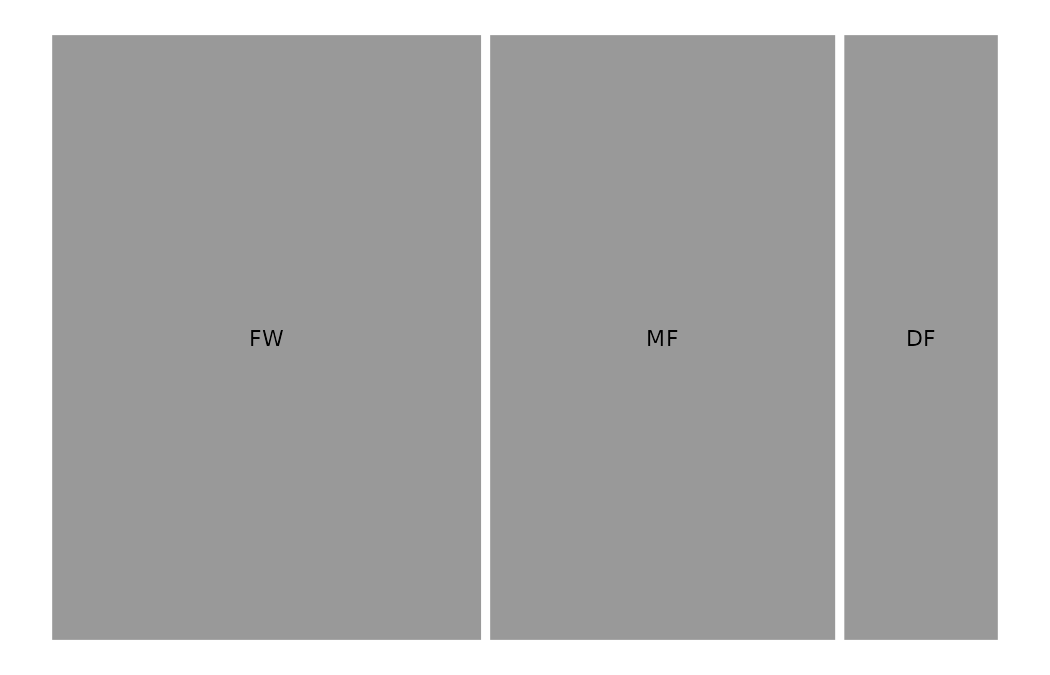
\includegraphics[width=0.85\linewidth,height=\textheight,keepaspectratio]{figures/explore-categorical-6.png}

Each column represents a position group, and the column widths
correspond to the proportion of shots from each group: the forwards'
column occupies 45.9\% of the square's width, the midfielders' 37.1\%,
and the defenders' a slim 17.0\%. There are visibly fewer shots by
defenders than by forwards. In general, mosaic plots use box
\emph{areas} to represent the number of cases in each category.

Next we split each column vertically, in proportion to that group's
shot-type mix.

\begin{Shaded}
\begin{Highlighting}[]
\NormalTok{mosaic\_data }\OtherTok{\textless{}{-}}\NormalTok{ weuro\_pos }\SpecialCharTok{|\textgreater{}}
  \FunctionTok{count}\NormalTok{(pos\_group, shot\_type) }\SpecialCharTok{|\textgreater{}}
  \FunctionTok{left\_join}\NormalTok{(widths, }\AttributeTok{by =} \StringTok{"pos\_group"}\NormalTok{) }\SpecialCharTok{|\textgreater{}}
  \FunctionTok{group\_by}\NormalTok{(pos\_group) }\SpecialCharTok{|\textgreater{}}
  \FunctionTok{mutate}\NormalTok{(}
    \AttributeTok{ymax =} \FunctionTok{cumsum}\NormalTok{(n) }\SpecialCharTok{/}\NormalTok{ group\_total,}
    \AttributeTok{ymin =}\NormalTok{ ymax }\SpecialCharTok{{-}}\NormalTok{ n }\SpecialCharTok{/}\NormalTok{ group\_total}
\NormalTok{  ) }\SpecialCharTok{|\textgreater{}}
  \FunctionTok{ungroup}\NormalTok{()}

\NormalTok{mosaic\_data}
\CommentTok{\#\textgreater{} \# A tibble: 9 × 8}
\CommentTok{\#\textgreater{}   pos\_group shot\_type     n group\_total  xmax  xmin  ymax  ymin}
\CommentTok{\#\textgreater{}   \textless{}fct\textgreater{}     \textless{}fct\textgreater{}     \textless{}int\textgreater{}       \textless{}int\textgreater{} \textless{}dbl\textgreater{} \textless{}dbl\textgreater{} \textless{}dbl\textgreater{} \textless{}dbl\textgreater{}}
\CommentTok{\#\textgreater{} 1 FW        Open Play   402         418 0.459 0     0.962 0}
\CommentTok{\#\textgreater{} 2 FW        Free Kick     4         418 0.459 0     0.971 0.962}
\CommentTok{\#\textgreater{} 3 FW        Penalty      12         418 0.459 0     1     0.971}
\CommentTok{\#\textgreater{} 4 MF        Open Play   308         338 0.830 0.459 0.911 0}
\CommentTok{\#\textgreater{} 5 MF        Free Kick     6         338 0.830 0.459 0.929 0.911}
\CommentTok{\#\textgreater{} 6 MF        Penalty      24         338 0.830 0.459 1     0.929}
\CommentTok{\#\textgreater{} 7 DF        Open Play   141         155 1     0.830 0.910 0}
\CommentTok{\#\textgreater{} 8 DF        Free Kick     1         155 1     0.830 0.916 0.910}
\CommentTok{\#\textgreater{} 9 DF        Penalty      13         155 1     0.830 1     0.916}

\FunctionTok{ggplot}\NormalTok{(mosaic\_data) }\SpecialCharTok{+}
  \FunctionTok{geom\_rect}\NormalTok{(}
    \FunctionTok{aes}\NormalTok{(}\AttributeTok{xmin =}\NormalTok{ xmin, }\AttributeTok{xmax =}\NormalTok{ xmax, }\AttributeTok{ymin =}\NormalTok{ ymin, }\AttributeTok{ymax =}\NormalTok{ ymax, }\AttributeTok{fill =}\NormalTok{ shot\_type),}
    \AttributeTok{color =} \StringTok{"white"}\NormalTok{, }\AttributeTok{linewidth =} \DecValTok{2}
\NormalTok{  ) }\SpecialCharTok{+}
  \FunctionTok{labs}\NormalTok{(}\AttributeTok{x =} \StringTok{"Position group"}\NormalTok{, }\AttributeTok{y =} \StringTok{"Proportion within group"}\NormalTok{, }\AttributeTok{fill =} \StringTok{"Shot type"}\NormalTok{)}
\end{Highlighting}
\end{Shaded}

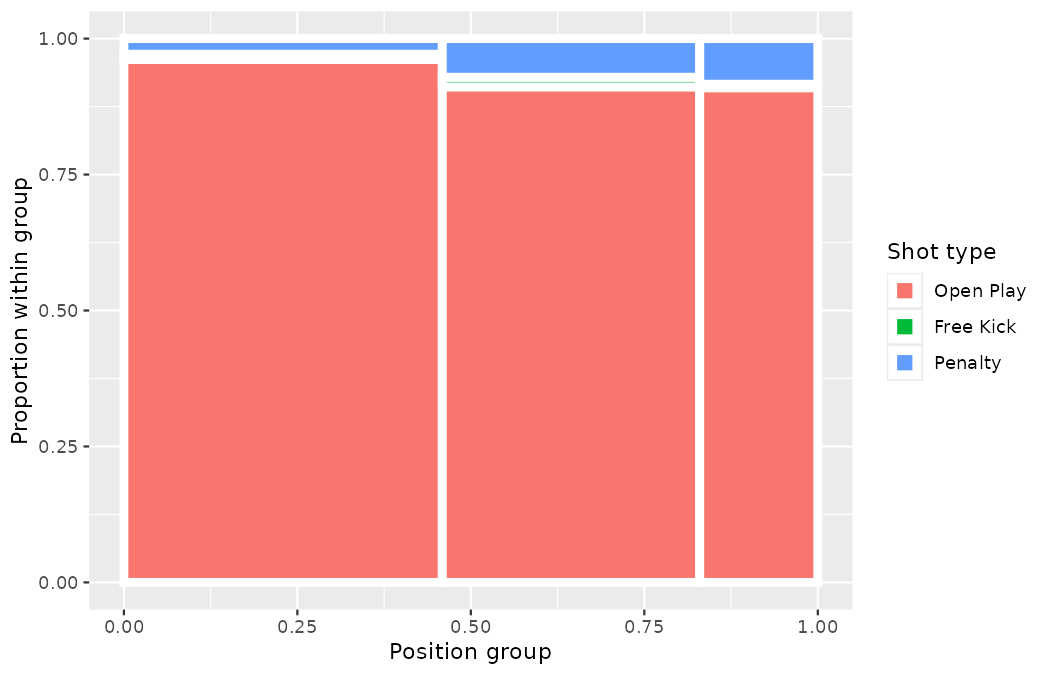
\includegraphics[width=0.85\linewidth,height=\textheight,keepaspectratio]{figures/explore-categorical-7.png}

This mosaic plot displays the relationship between position group and
shot type. Each column is split proportionally to that group's shots of
each type. For example, the first column represents shots by forwards,
and it is divided into open-play shots (the large lower block, reaching
to 0.962) with thin free-kick and penalty strips above. As another
example, the top segment of the third column represents defenders'
penalties, which reaches down to 0.916 --- a noticeably thicker strip
than the forwards' penalty strip. We can again use this plot to see that
the \texttt{pos\_group} and \texttt{shot\_type} variables are
associated, since some columns are divided in different vertical
locations than others, which was the same technique used for checking an
association in the standardized bar plot.

In the mosaic above, we chose to first split by position group. However,
we could have instead first split by shot type. Like with the bar plots,
it's common to use the explanatory variable to represent the first split
in a mosaic plot, and then for the response to break up each level of
the explanatory variable --- if these labels are reasonable to attach to
the variables under consideration.

\begin{Shaded}
\begin{Highlighting}[]
\NormalTok{widths2 }\OtherTok{\textless{}{-}}\NormalTok{ weuro\_pos }\SpecialCharTok{|\textgreater{}}
  \FunctionTok{count}\NormalTok{(shot\_type, }\AttributeTok{name =} \StringTok{"group\_total"}\NormalTok{) }\SpecialCharTok{|\textgreater{}}
  \FunctionTok{mutate}\NormalTok{(}
    \AttributeTok{xmax =} \FunctionTok{cumsum}\NormalTok{(group\_total) }\SpecialCharTok{/} \FunctionTok{sum}\NormalTok{(group\_total),}
    \AttributeTok{xmin =}\NormalTok{ xmax }\SpecialCharTok{{-}}\NormalTok{ group\_total }\SpecialCharTok{/} \FunctionTok{sum}\NormalTok{(group\_total)}
\NormalTok{  )}

\NormalTok{mosaic\_data2 }\OtherTok{\textless{}{-}}\NormalTok{ weuro\_pos }\SpecialCharTok{|\textgreater{}}
  \FunctionTok{count}\NormalTok{(shot\_type, pos\_group) }\SpecialCharTok{|\textgreater{}}
  \FunctionTok{left\_join}\NormalTok{(widths2, }\AttributeTok{by =} \StringTok{"shot\_type"}\NormalTok{) }\SpecialCharTok{|\textgreater{}}
  \FunctionTok{group\_by}\NormalTok{(shot\_type) }\SpecialCharTok{|\textgreater{}}
  \FunctionTok{mutate}\NormalTok{(}
    \AttributeTok{ymax =} \FunctionTok{cumsum}\NormalTok{(n) }\SpecialCharTok{/}\NormalTok{ group\_total,}
    \AttributeTok{ymin =}\NormalTok{ ymax }\SpecialCharTok{{-}}\NormalTok{ n }\SpecialCharTok{/}\NormalTok{ group\_total}
\NormalTok{  ) }\SpecialCharTok{|\textgreater{}}
  \FunctionTok{ungroup}\NormalTok{()}

\FunctionTok{ggplot}\NormalTok{(mosaic\_data2) }\SpecialCharTok{+}
  \FunctionTok{geom\_rect}\NormalTok{(}
    \FunctionTok{aes}\NormalTok{(}\AttributeTok{xmin =}\NormalTok{ xmin, }\AttributeTok{xmax =}\NormalTok{ xmax, }\AttributeTok{ymin =}\NormalTok{ ymin, }\AttributeTok{ymax =}\NormalTok{ ymax, }\AttributeTok{fill =}\NormalTok{ pos\_group),}
    \AttributeTok{color =} \StringTok{"white"}\NormalTok{, }\AttributeTok{linewidth =} \DecValTok{2}
\NormalTok{  ) }\SpecialCharTok{+}
  \FunctionTok{labs}\NormalTok{(}\AttributeTok{x =} \StringTok{"Shot type"}\NormalTok{, }\AttributeTok{y =} \StringTok{"Proportion within group"}\NormalTok{, }\AttributeTok{fill =} \StringTok{"Position group"}\NormalTok{)}
\end{Highlighting}
\end{Shaded}

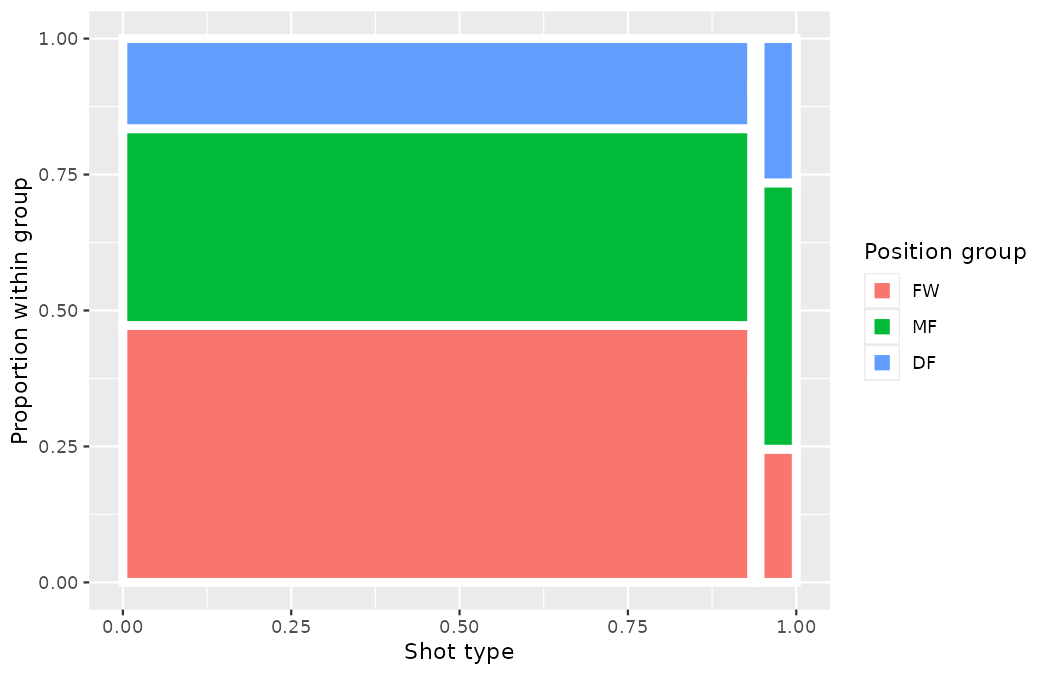
\includegraphics[width=0.85\linewidth,height=\textheight,keepaspectratio]{figures/explore-categorical-8.png}

The flipped mosaic is dominated by a single enormous open-play column
(\(851/911 = 93.4\%\) of the width), with a sliver for free kicks
(1.2\%) and a narrow penalty column (5.4\%). Within the penalty column,
though, the split is striking: midfielders account for
\(24/49 = 49.0\%\) of outfield penalties, defenders \(13/49 = 26.5\%\),
and forwards only \(12/49 = 24.5\%\) --- the inverse of their open-play
shares (\(402/851 = 47.2\%\), \(308/851 = 36.2\%\),
\(141/851 = 16.6\%\)).

\begin{tcolorbox}[enhanced jigsaw, left=2mm, leftrule=.75mm, title=\textcolor{quarto-callout-tip-color}{\faLightbulb}\hspace{0.5em}{Check your understanding}, arc=.35mm, rightrule=.15mm, coltitle=black, colframe=quarto-callout-tip-color-frame, bottomrule=.15mm, colbacktitle=quarto-callout-tip-color!10!white, opacitybacktitle=0.6, breakable, bottomtitle=1mm, toptitle=1mm, titlerule=0mm, opacityback=0, toprule=.15mm, colback=white]

In the flipped mosaic, the ``Penalty'' column is narrow but its internal
split differs sharply from the ``Open Play'' column's split. What does
that combination of features tell a scout, and which single feature of a
mosaic plot communicates the ``narrow'' part?

\begin{center}\rule{0.5\linewidth}{0.5pt}\end{center}

The differing splits say the variables are associated: \emph{which}
position group takes a shot depends on the shot type, with midfielders
and defenders over-represented among penalty kicks relative to their
open-play shares --- driven, as we computed earlier in this section, by
the shoot-outs that force the taker pool deep into the back line. The
narrowness --- column \emph{width}, which is proportional to the number
of shots of that type --- warns that the penalty pattern rests on only
49 shots, far fewer than the 851 open-play shots, so it is measured with
much less precision. Bar heights in a standardized bar plot cannot carry
that warning; mosaic widths can.

\end{tcolorbox}

\section{Row and column proportions}\label{row-and-column-proportions}

In the previous sections we inspected visualizations of two categorical
variables in bar plots and mosaic plots. However, we have not discussed
how the values in the bar and mosaic plots that show proportions are
calculated. In this section we will investigate the fractional breakdown
of one variable in another, and we can modify our contingency table to
provide such a view. We return to the World Cup body-part data of
Table~\ref{tbl-wc-bp-result-totals}.
Table~\ref{tbl-wc-bp-row-proportions} shows \textbf{row proportions} for
Table~\ref{tbl-wc-bp-result-totals}, which are computed as the counts
divided by their row totals. The value 102 at the intersection of goal
and Right Foot is replaced by \(102 / 192 = 0.531,\) i.e., 102 divided
by its row total, 192. So, what does 0.531 represent? It corresponds to
the proportion of \emph{goals} that were struck with the right foot.

\begin{Shaded}
\begin{Highlighting}[]
\NormalTok{wc\_bp }\SpecialCharTok{|\textgreater{}}
  \FunctionTok{count}\NormalTok{(result, body\_part) }\SpecialCharTok{|\textgreater{}}
  \FunctionTok{group\_by}\NormalTok{(result) }\SpecialCharTok{|\textgreater{}}
  \FunctionTok{mutate}\NormalTok{(}\AttributeTok{proportion =}\NormalTok{ n }\SpecialCharTok{/} \FunctionTok{sum}\NormalTok{(n)) }\SpecialCharTok{|\textgreater{}}
  \FunctionTok{select}\NormalTok{(}\SpecialCharTok{{-}}\NormalTok{n) }\SpecialCharTok{|\textgreater{}}
  \FunctionTok{pivot\_wider}\NormalTok{(}\AttributeTok{names\_from =}\NormalTok{ body\_part, }\AttributeTok{values\_from =}\NormalTok{ proportion)}
\CommentTok{\#\textgreater{} \# A tibble: 2 × 4}
\CommentTok{\#\textgreater{} \# Groups:   result [2]}
\CommentTok{\#\textgreater{}   result  \textasciigrave{}Right Foot\textasciigrave{} \textasciigrave{}Left Foot\textasciigrave{}  Head}
\CommentTok{\#\textgreater{}   \textless{}fct\textgreater{}          \textless{}dbl\textgreater{}       \textless{}dbl\textgreater{} \textless{}dbl\textgreater{}}
\CommentTok{\#\textgreater{} 1 goal           0.531       0.323 0.146}
\CommentTok{\#\textgreater{} 2 no goal        0.526       0.300 0.174}
\end{Highlighting}
\end{Shaded}

\begin{longtable}[]{@{}lrrrr@{}}
\caption{A contingency table with row proportions for result and body
part.}\label{tbl-wc-bp-row-proportions}\tabularnewline
\toprule\noalign{}
& Right Foot & Left Foot & Head & Total \\
\midrule\noalign{}
\endfirsthead
\toprule\noalign{}
& Right Foot & Left Foot & Head & Total \\
\midrule\noalign{}
\endhead
\bottomrule\noalign{}
\endlastfoot
goal & 0.531 & 0.323 & 0.146 & 1.00 \\
no goal & 0.526 & 0.300 & 0.174 & 1.00 \\
\end{longtable}

A contingency table of the \textbf{column proportions} is computed in a
similar way, where each is computed as the count divided by the
corresponding column total. Table~\ref{tbl-wc-bp-column-proportions}
shows such a table, and here the value 0.111 indicates that 11.1\% of
headers were scored. This rate is lower compared to shots with the right
foot (13.1\%) or the left foot (13.8\%) --- pooling the feet,
\(164/1229 = 13.3\%\) of footed shots became goals. Because these rates
vary between the three levels of \texttt{body\_part}
(\texttt{Right\ Foot}, \texttt{Left\ Foot}, \texttt{Head}), this
provides evidence that the \texttt{result} and \texttt{body\_part}
variables may be associated.

\begin{Shaded}
\begin{Highlighting}[]
\NormalTok{wc\_bp }\SpecialCharTok{|\textgreater{}}
  \FunctionTok{count}\NormalTok{(result, body\_part) }\SpecialCharTok{|\textgreater{}}
  \FunctionTok{group\_by}\NormalTok{(body\_part) }\SpecialCharTok{|\textgreater{}}
  \FunctionTok{mutate}\NormalTok{(}\AttributeTok{proportion =}\NormalTok{ n }\SpecialCharTok{/} \FunctionTok{sum}\NormalTok{(n)) }\SpecialCharTok{|\textgreater{}}
  \FunctionTok{select}\NormalTok{(}\SpecialCharTok{{-}}\NormalTok{n) }\SpecialCharTok{|\textgreater{}}
  \FunctionTok{pivot\_wider}\NormalTok{(}\AttributeTok{names\_from =}\NormalTok{ body\_part, }\AttributeTok{values\_from =}\NormalTok{ proportion)}
\CommentTok{\#\textgreater{} \# A tibble: 2 × 4}
\CommentTok{\#\textgreater{}   result  \textasciigrave{}Right Foot\textasciigrave{} \textasciigrave{}Left Foot\textasciigrave{}  Head}
\CommentTok{\#\textgreater{}   \textless{}fct\textgreater{}          \textless{}dbl\textgreater{}       \textless{}dbl\textgreater{} \textless{}dbl\textgreater{}}
\CommentTok{\#\textgreater{} 1 goal           0.131       0.138 0.111}
\CommentTok{\#\textgreater{} 2 no goal        0.869       0.862 0.889}

\NormalTok{(}\DecValTok{102} \SpecialCharTok{+} \DecValTok{62}\NormalTok{) }\SpecialCharTok{/}\NormalTok{ (}\DecValTok{780} \SpecialCharTok{+} \DecValTok{449}\NormalTok{)}
\CommentTok{\#\textgreater{} [1] 0.1334418}
\end{Highlighting}
\end{Shaded}

\begin{longtable}[]{@{}lrrr@{}}
\caption{A contingency table with column proportions for result and body
part.}\label{tbl-wc-bp-column-proportions}\tabularnewline
\toprule\noalign{}
& Right Foot & Left Foot & Head \\
\midrule\noalign{}
\endfirsthead
\toprule\noalign{}
& Right Foot & Left Foot & Head \\
\midrule\noalign{}
\endhead
\bottomrule\noalign{}
\endlastfoot
goal & 0.131 & 0.138 & 0.111 \\
no goal & 0.869 & 0.862 & 0.889 \\
Total & 1.00 & 1.00 & 1.00 \\
\end{longtable}

Row and column proportions can also be thought of as \textbf{conditional
proportions} as they tell us about the proportion of observations in a
given level of a categorical variable conditional on the level of
another categorical variable. The column proportion 0.111 is the
proportion of shots that scored \emph{conditional on} the shot being a
header; the row proportion 0.146 is the proportion of shots that were
headers \emph{conditional on} the shot being a goal. Same table,
opposite conditioning --- and, as the numbers show, not the same value.

We could also have checked for an association between \texttt{result}
and \texttt{body\_part} in Table~\ref{tbl-wc-bp-row-proportions} using
row proportions. When comparing these row proportions, we would look
down columns to see if the fraction of right-footed, left-footed, and
headed shots varied between the goals and the non-goals: headers make up
14.6\% of the goals but 17.4\% of the non-goals.

Before moving on, a word of caution the data themselves force on us. Do
\emph{not} read the header deficit --- 11.1\% versus 13.3\% for feet ---
as ``heading is a worse skill.'' Recall the confounding lesson of
Chapter~\ref{sec-data-design}: headers overwhelmingly arrive from
crosses and corners, contested and at awkward angles, so the
\emph{chance quality} differs systematically between the body parts. The
conditional proportions describe an association in observational data;
they do not isolate a cause.

There is a second caution, cruder than confounding, which the book's
penalty convention (recall Chapter~\ref{sec-data-applications}) obliges
us to show rather than bury: the two foot columns contain all 64 of the
tournament's penalty kicks --- footed by every taker, uncontested by law
--- and the header column contains none.

\begin{Shaded}
\begin{Highlighting}[]
\NormalTok{wc\_bp }\SpecialCharTok{|\textgreater{}}
  \FunctionTok{filter}\NormalTok{(shot\_type }\SpecialCharTok{==} \StringTok{"Open Play"}\NormalTok{) }\SpecialCharTok{|\textgreater{}}
  \FunctionTok{mutate}\NormalTok{(}\AttributeTok{body =} \FunctionTok{if\_else}\NormalTok{(body\_part }\SpecialCharTok{==} \StringTok{"Head"}\NormalTok{, }\StringTok{"Head"}\NormalTok{, }\StringTok{"Foot"}\NormalTok{)) }\SpecialCharTok{|\textgreater{}}
  \FunctionTok{group\_by}\NormalTok{(body) }\SpecialCharTok{|\textgreater{}}
  \FunctionTok{summarize}\NormalTok{(}\AttributeTok{shots =} \FunctionTok{n}\NormalTok{(), }\AttributeTok{goals =} \FunctionTok{sum}\NormalTok{(goal), }\AttributeTok{conversion =} \FunctionTok{mean}\NormalTok{(goal))}
\CommentTok{\#\textgreater{} \# A tibble: 2 × 4}
\CommentTok{\#\textgreater{}   body  shots goals conversion}
\CommentTok{\#\textgreater{}   \textless{}chr\textgreater{} \textless{}int\textgreater{} \textless{}int\textgreater{}      \textless{}dbl\textgreater{}}
\CommentTok{\#\textgreater{} 1 Foot   1117   119      0.107}
\CommentTok{\#\textgreater{} 2 Head    252    28      0.111}
\end{Highlighting}
\end{Shaded}

Restricted to open play, footed conversion drops to
\(119/1117 = 0.107,\) \emph{below} the headers' \(28/252 = 0.111\)
(unchanged, since every header in the data is an open-play shot) --- so
most of the header ``deficit'' in
Table~\ref{tbl-wc-bp-column-proportions} was penalty kicks, not heading.
Whenever a conditional proportion involves a group that penalties can
only fall on one side of, this book will show the comparison penalties
in and penalties out.

\begin{tcolorbox}[enhanced jigsaw, left=2mm, leftrule=.75mm, title=\textcolor{quarto-callout-tip-color}{\faLightbulb}\hspace{0.5em}{Check your understanding}, arc=.35mm, rightrule=.15mm, coltitle=black, colframe=quarto-callout-tip-color-frame, bottomrule=.15mm, colbacktitle=quarto-callout-tip-color!10!white, opacitybacktitle=0.6, breakable, bottomtitle=1mm, toptitle=1mm, titlerule=0mm, opacityback=0, toprule=.15mm, colback=white]

What does 0.323 represent in Table~\ref{tbl-wc-bp-row-proportions}? What
does 0.138 represent in Table~\ref{tbl-wc-bp-column-proportions}?

\begin{center}\rule{0.5\linewidth}{0.5pt}\end{center}

0.323 represents the proportion of goals that were struck with the left
foot. 0.138 represents the proportion of left-footed shots that were
scored.

\end{tcolorbox}

\begin{tcolorbox}[enhanced jigsaw, left=2mm, leftrule=.75mm, title=\textcolor{quarto-callout-tip-color}{\faLightbulb}\hspace{0.5em}{Check your understanding}, arc=.35mm, rightrule=.15mm, coltitle=black, colframe=quarto-callout-tip-color-frame, bottomrule=.15mm, colbacktitle=quarto-callout-tip-color!10!white, opacitybacktitle=0.6, breakable, bottomtitle=1mm, toptitle=1mm, titlerule=0mm, opacityback=0, toprule=.15mm, colback=white]

What does 0.174 represent in Table~\ref{tbl-wc-bp-row-proportions}? What
does 0.889 represent in Table~\ref{tbl-wc-bp-column-proportions}?

\begin{center}\rule{0.5\linewidth}{0.5pt}\end{center}

0.174 represents the fraction of non-goals that were headers. 0.889
represents the fraction of headers that did not result in a goal.

\end{tcolorbox}

\begin{tcolorbox}[enhanced jigsaw, left=2mm, leftrule=.75mm, title=\textcolor{quarto-callout-note-color}{\faInfo}\hspace{0.5em}{Worked example}, arc=.35mm, rightrule=.15mm, coltitle=black, colframe=quarto-callout-note-color-frame, bottomrule=.15mm, colbacktitle=quarto-callout-note-color!10!white, opacitybacktitle=0.6, breakable, bottomtitle=1mm, toptitle=1mm, titlerule=0mm, opacityback=0, toprule=.15mm, colback=white]

Scouts and analysts use statistics to build shot-danger filters. By
noting specific characteristics of a shot as it is logged, an analyst
may be able to classify some shots as likely goals or likely non-goals
with reasonable accuracy. One such characteristic is whether the shooter
was under defensive pressure at the moment of the strike. We'll focus on
the \texttt{under\_pressure} and \texttt{goal} variables of the full
\texttt{wc2022\_shots} data; these variables are summarized in a
contingency table below. Which would be more helpful to a scout hoping
to predict shot outcomes from this table: row or column proportions?

\begin{Shaded}
\begin{Highlighting}[]
\NormalTok{wc\_press }\OtherTok{\textless{}{-}}\NormalTok{ wc2022\_shots }\SpecialCharTok{|\textgreater{}}
  \FunctionTok{mutate}\NormalTok{(}
    \AttributeTok{pressure =} \FunctionTok{if\_else}\NormalTok{(under\_pressure, }\StringTok{"under pressure"}\NormalTok{, }\StringTok{"not under pressure"}\NormalTok{),}
    \AttributeTok{result =} \FunctionTok{factor}\NormalTok{(}\FunctionTok{if\_else}\NormalTok{(goal, }\StringTok{"goal"}\NormalTok{, }\StringTok{"no goal"}\NormalTok{), }\AttributeTok{levels =} \FunctionTok{c}\NormalTok{(}\StringTok{"goal"}\NormalTok{, }\StringTok{"no goal"}\NormalTok{))}
\NormalTok{  )}

\NormalTok{wc\_press }\SpecialCharTok{|\textgreater{}}
  \FunctionTok{count}\NormalTok{(result, pressure) }\SpecialCharTok{|\textgreater{}}
  \FunctionTok{pivot\_wider}\NormalTok{(}\AttributeTok{names\_from =}\NormalTok{ pressure, }\AttributeTok{values\_from =}\NormalTok{ n)}
\CommentTok{\#\textgreater{} \# A tibble: 2 × 3}
\CommentTok{\#\textgreater{}   result  \textasciigrave{}not under pressure\textasciigrave{} \textasciigrave{}under pressure\textasciigrave{}}
\CommentTok{\#\textgreater{}   \textless{}fct\textgreater{}                  \textless{}int\textgreater{}            \textless{}int\textgreater{}}
\CommentTok{\#\textgreater{} 1 goal                     171               24}
\CommentTok{\#\textgreater{} 2 no goal                 1085              214}
\end{Highlighting}
\end{Shaded}

\begin{longtable}[]{@{}lrrr@{}}
\caption{A contingency table for result and pressure at the 2022 Men's
World Cup.}\label{tbl-wc-pressure-count}\tabularnewline
\toprule\noalign{}
& not under pressure & under pressure & Total \\
\midrule\noalign{}
\endfirsthead
\toprule\noalign{}
& not under pressure & under pressure & Total \\
\midrule\noalign{}
\endhead
\bottomrule\noalign{}
\endlastfoot
goal & 171 & 24 & 195 \\
no goal & 1,085 & 214 & 1,299 \\
Total & 1,256 & 238 & 1,494 \\
\end{longtable}

\begin{center}\rule{0.5\linewidth}{0.5pt}\end{center}

A scout watching a shot unfold knows whether the shooter is under
pressure \emph{before} knowing the outcome, so the useful direction is:
how does the proportion of goals change within each pressure state? With
\texttt{result} as the rows, that corresponds to the \emph{column}
proportions of Table~\ref{tbl-wc-pressure-count} --- the proportion of
pressured shots that score, and the proportion of unpressured shots that
score.

\begin{Shaded}
\begin{Highlighting}[]
\NormalTok{wc\_press }\SpecialCharTok{|\textgreater{}}
  \FunctionTok{count}\NormalTok{(pressure, result) }\SpecialCharTok{|\textgreater{}}
  \FunctionTok{group\_by}\NormalTok{(pressure) }\SpecialCharTok{|\textgreater{}}
  \FunctionTok{mutate}\NormalTok{(}\AttributeTok{proportion =}\NormalTok{ n }\SpecialCharTok{/} \FunctionTok{sum}\NormalTok{(n))}
\CommentTok{\#\textgreater{} \# A tibble: 4 × 4}
\CommentTok{\#\textgreater{} \# Groups:   pressure [2]}
\CommentTok{\#\textgreater{}   pressure           result      n proportion}
\CommentTok{\#\textgreater{}   \textless{}chr\textgreater{}              \textless{}fct\textgreater{}   \textless{}int\textgreater{}      \textless{}dbl\textgreater{}}
\CommentTok{\#\textgreater{} 1 not under pressure goal      171      0.136}
\CommentTok{\#\textgreater{} 2 not under pressure no goal  1085      0.864}
\CommentTok{\#\textgreater{} 3 under pressure     goal       24      0.101}
\CommentTok{\#\textgreater{} 4 under pressure     no goal   214      0.899}
\end{Highlighting}
\end{Shaded}

A smaller fraction of pressured shots are scored (\(24/238 = 10.1\%\))
compared to unpressured shots (\(171/1256 = 13.6\%\)). This information
on its own is insufficient to classify a shot as goal or no goal ---
about 90\% of shots miss in \emph{both} groups. Yet, when we carefully
combine this information with many other characteristics, we stand a
reasonable chance of building a useful shot-danger model, which is
essentially what the \texttt{statsbomb\_xg} variable is. This example
points out that row and column proportions are not equivalent. Before
settling on one form for a table, it is important to consider each to
ensure that the most useful table is constructed.

Hold on to this particular 3.5-percentage-point gap. Whether a
difference of \(0.101\) versus \(0.136\) could plausibly be produced by
chance alone is \emph{exactly} the question we will learn to answer in
Chapter~\ref{sec-foundations-randomization}, where this same
under-pressure split becomes the chapter's central permutation test ---
run both with and without the 64 penalties sitting in the unpressured
pile, per the book's penalty convention. For now we can only say the two
variables appear associated in this sample.

\end{tcolorbox}

\begin{tcolorbox}[enhanced jigsaw, left=2mm, leftrule=.75mm, title=\textcolor{quarto-callout-note-color}{\faInfo}\hspace{0.5em}{Worked example}, arc=.35mm, rightrule=.15mm, coltitle=black, colframe=quarto-callout-note-color-frame, bottomrule=.15mm, colbacktitle=quarto-callout-note-color!10!white, opacitybacktitle=0.6, breakable, bottomtitle=1mm, toptitle=1mm, titlerule=0mm, opacityback=0, toprule=.15mm, colback=white]

Look back to Table~\ref{tbl-wc-bp-row-proportions} and
Table~\ref{tbl-wc-bp-column-proportions}. Are there any obvious
scenarios where one might be more useful than the other?

\begin{center}\rule{0.5\linewidth}{0.5pt}\end{center}

Here, unlike the loan-style examples where neither direction is
privileged, the two variables do have a natural explanatory-response
ordering: the body part is fixed the moment the ball arrives, and the
result follows. Usually it is most useful to ``condition'' on the
explanatory variable --- so the column proportions of
Table~\ref{tbl-wc-bp-column-proportions}, the conversion rate within
each body part, are what a scout would quote. The row proportions answer
a different, retrospective question (``of the tournament's goals, what
share were headers?''), which is useful for describing how goals were
manufactured, but not for judging any one shot as it happens. When no
explanatory-response direction is reasonable to attach --- say,
\texttt{first\_time} and \texttt{under\_pressure} --- neither table is
automatically more useful, and it is worth computing both.

\end{tcolorbox}

\section{Pie charts}\label{pie-charts}

A \textbf{pie chart} is shown below alongside a bar plot representing
the same information. Pie charts can be useful for giving a high-level
overview to show how a set of cases break down. However, it is also
difficult to decipher certain details in a pie chart. For example, the
right-foot slice is obviously the biggest, but judging \emph{how much}
bigger the left-foot share is than the header share (30.3\% versus
17.0\%) takes real effort in the pie chart, while the bar plot hands you
the comparison directly.

\begin{Shaded}
\begin{Highlighting}[]
\CommentTok{\# Pie chart: a stacked bar of counts, wrapped around a circle}
\NormalTok{wc\_bp }\SpecialCharTok{|\textgreater{}}
  \FunctionTok{count}\NormalTok{(body\_part) }\SpecialCharTok{|\textgreater{}}
  \FunctionTok{ggplot}\NormalTok{(}\FunctionTok{aes}\NormalTok{(}\AttributeTok{x =} \StringTok{""}\NormalTok{, }\AttributeTok{y =}\NormalTok{ n, }\AttributeTok{fill =}\NormalTok{ body\_part)) }\SpecialCharTok{+}
  \FunctionTok{geom\_col}\NormalTok{(}\AttributeTok{width =} \DecValTok{1}\NormalTok{, }\AttributeTok{color =} \StringTok{"white"}\NormalTok{) }\SpecialCharTok{+}
  \FunctionTok{coord\_polar}\NormalTok{(}\AttributeTok{theta =} \StringTok{"y"}\NormalTok{) }\SpecialCharTok{+}
  \FunctionTok{theme\_void}\NormalTok{() }\SpecialCharTok{+}
  \FunctionTok{labs}\NormalTok{(}\AttributeTok{fill =} \StringTok{"Body part"}\NormalTok{, }\AttributeTok{title =} \StringTok{"Body part"}\NormalTok{)}

\CommentTok{\# Bar plot of the same counts}
\FunctionTok{ggplot}\NormalTok{(wc\_bp, }\FunctionTok{aes}\NormalTok{(}\AttributeTok{x =}\NormalTok{ body\_part, }\AttributeTok{fill =}\NormalTok{ body\_part)) }\SpecialCharTok{+}
  \FunctionTok{geom\_bar}\NormalTok{(}\AttributeTok{show.legend =} \ConstantTok{FALSE}\NormalTok{) }\SpecialCharTok{+}
  \FunctionTok{labs}\NormalTok{(}\AttributeTok{x =} \StringTok{"Body part"}\NormalTok{, }\AttributeTok{y =} \StringTok{"Count"}\NormalTok{)}
\end{Highlighting}
\end{Shaded}

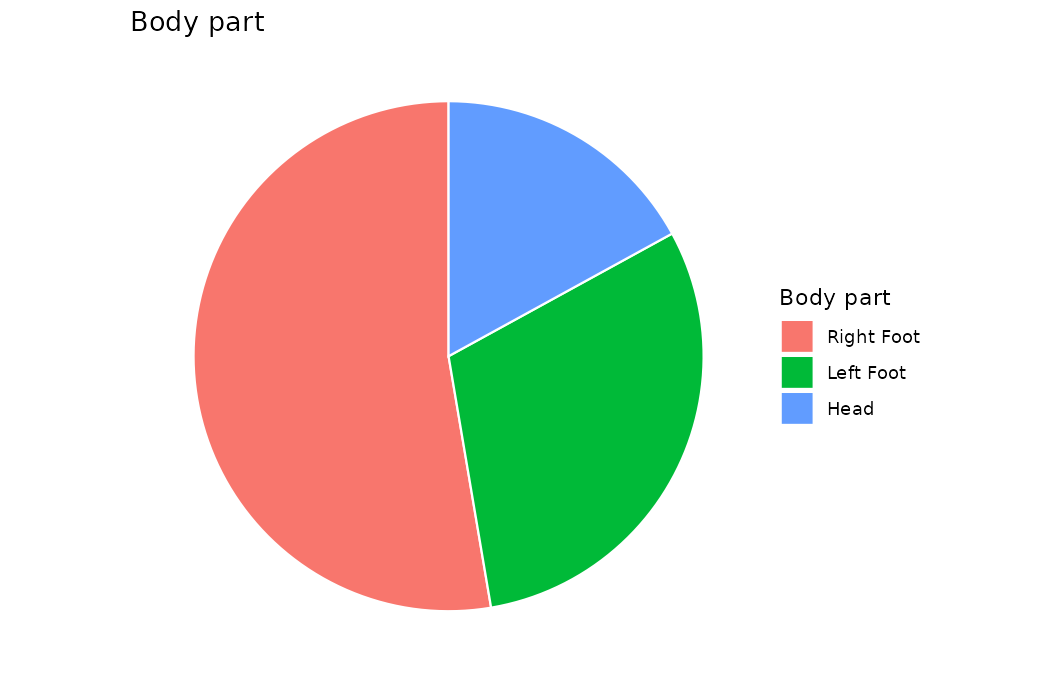
\includegraphics[width=0.85\linewidth,height=\textheight,keepaspectratio]{figures/explore-categorical-9.png}

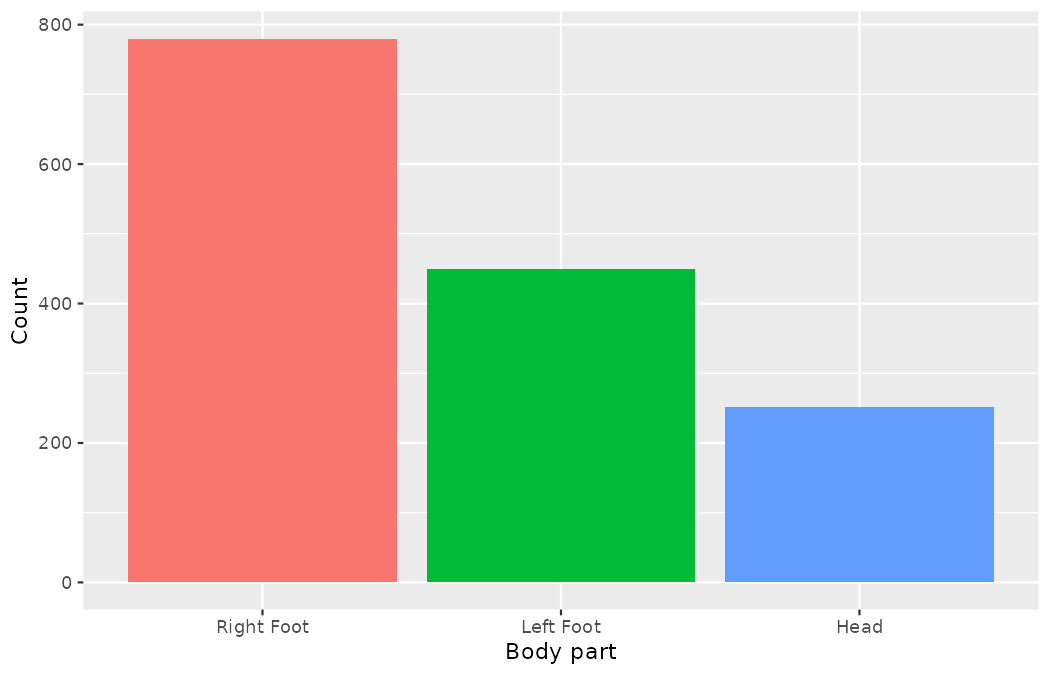
\includegraphics[width=0.85\linewidth,height=\textheight,keepaspectratio]{figures/explore-categorical-10.png}

Note what the pie-chart code reveals: in ggplot2 a pie chart \emph{is} a
single stacked bar transformed into polar coordinates ---
\texttt{coord\_polar(theta\ =\ "y")} wraps the count axis around a
circle. The pie chart has no axes at all; every judgment the reader
makes is a judgment about angles and areas, which human eyes handle far
less accurately than the aligned lengths of a bar plot.

Pie charts can work well when the goal is to visualize a categorical
variable with very few levels, and especially if each level represents a
simple fraction (e.g., one-half, one-quarter, etc.) --- ``just over half
of these shots were right-footed'' survives the polar transformation.
However, they can be quite difficult to read when they are used to
visualize a categorical variable with many levels. The
\texttt{play\_pattern} variable of \texttt{wc2022\_shots} has nine
levels, and it makes the point brutally.

\begin{Shaded}
\begin{Highlighting}[]
\NormalTok{wc2022\_shots }\SpecialCharTok{|\textgreater{}}
  \FunctionTok{count}\NormalTok{(play\_pattern, }\AttributeTok{sort =} \ConstantTok{TRUE}\NormalTok{) }\SpecialCharTok{|\textgreater{}}
  \FunctionTok{mutate}\NormalTok{(}\AttributeTok{proportion =}\NormalTok{ n }\SpecialCharTok{/} \FunctionTok{sum}\NormalTok{(n))}
\CommentTok{\#\textgreater{} \# A tibble: 9 × 3}
\CommentTok{\#\textgreater{}   play\_pattern       n proportion}
\CommentTok{\#\textgreater{}   \textless{}chr\textgreater{}          \textless{}int\textgreater{}      \textless{}dbl\textgreater{}}
\CommentTok{\#\textgreater{} 1 Regular Play     446     0.299}
\CommentTok{\#\textgreater{} 2 From Throw In    298     0.199}
\CommentTok{\#\textgreater{} 3 From Free Kick   285     0.191}
\CommentTok{\#\textgreater{} 4 From Corner      223     0.149}
\CommentTok{\#\textgreater{} 5 From Goal Kick    80     0.0535}
\CommentTok{\#\textgreater{} 6 Other             68     0.0455}
\CommentTok{\#\textgreater{} 7 From Counter      56     0.0375}
\CommentTok{\#\textgreater{} 8 From Keeper       21     0.0141}
\CommentTok{\#\textgreater{} 9 From Kick Off     17     0.0114}
\end{Highlighting}
\end{Shaded}

\begin{Shaded}
\begin{Highlighting}[]
\CommentTok{\# Pie chart of nine play patterns}
\NormalTok{wc2022\_shots }\SpecialCharTok{|\textgreater{}}
  \FunctionTok{count}\NormalTok{(play\_pattern, }\AttributeTok{sort =} \ConstantTok{TRUE}\NormalTok{) }\SpecialCharTok{|\textgreater{}}
  \FunctionTok{mutate}\NormalTok{(}\AttributeTok{play\_pattern =} \FunctionTok{reorder}\NormalTok{(play\_pattern, }\SpecialCharTok{{-}}\NormalTok{n)) }\SpecialCharTok{|\textgreater{}}
  \FunctionTok{ggplot}\NormalTok{(}\FunctionTok{aes}\NormalTok{(}\AttributeTok{x =} \StringTok{""}\NormalTok{, }\AttributeTok{y =}\NormalTok{ n, }\AttributeTok{fill =}\NormalTok{ play\_pattern)) }\SpecialCharTok{+}
  \FunctionTok{geom\_col}\NormalTok{(}\AttributeTok{width =} \DecValTok{1}\NormalTok{, }\AttributeTok{color =} \StringTok{"white"}\NormalTok{) }\SpecialCharTok{+}
  \FunctionTok{coord\_polar}\NormalTok{(}\AttributeTok{theta =} \StringTok{"y"}\NormalTok{) }\SpecialCharTok{+}
  \FunctionTok{theme\_void}\NormalTok{() }\SpecialCharTok{+}
  \FunctionTok{labs}\NormalTok{(}\AttributeTok{fill =} \StringTok{"Play pattern"}\NormalTok{, }\AttributeTok{title =} \StringTok{"Play pattern"}\NormalTok{)}

\CommentTok{\# Sorted bar plot of the same counts}
\NormalTok{wc2022\_shots }\SpecialCharTok{|\textgreater{}}
  \FunctionTok{count}\NormalTok{(play\_pattern, }\AttributeTok{sort =} \ConstantTok{TRUE}\NormalTok{) }\SpecialCharTok{|\textgreater{}}
  \FunctionTok{mutate}\NormalTok{(}\AttributeTok{play\_pattern =} \FunctionTok{reorder}\NormalTok{(play\_pattern, n)) }\SpecialCharTok{|\textgreater{}}
  \FunctionTok{ggplot}\NormalTok{(}\FunctionTok{aes}\NormalTok{(}\AttributeTok{x =}\NormalTok{ n, }\AttributeTok{y =}\NormalTok{ play\_pattern)) }\SpecialCharTok{+}
  \FunctionTok{geom\_col}\NormalTok{() }\SpecialCharTok{+}
  \FunctionTok{labs}\NormalTok{(}\AttributeTok{x =} \StringTok{"Count"}\NormalTok{, }\AttributeTok{y =} \StringTok{"Play pattern"}\NormalTok{)}
\end{Highlighting}
\end{Shaded}

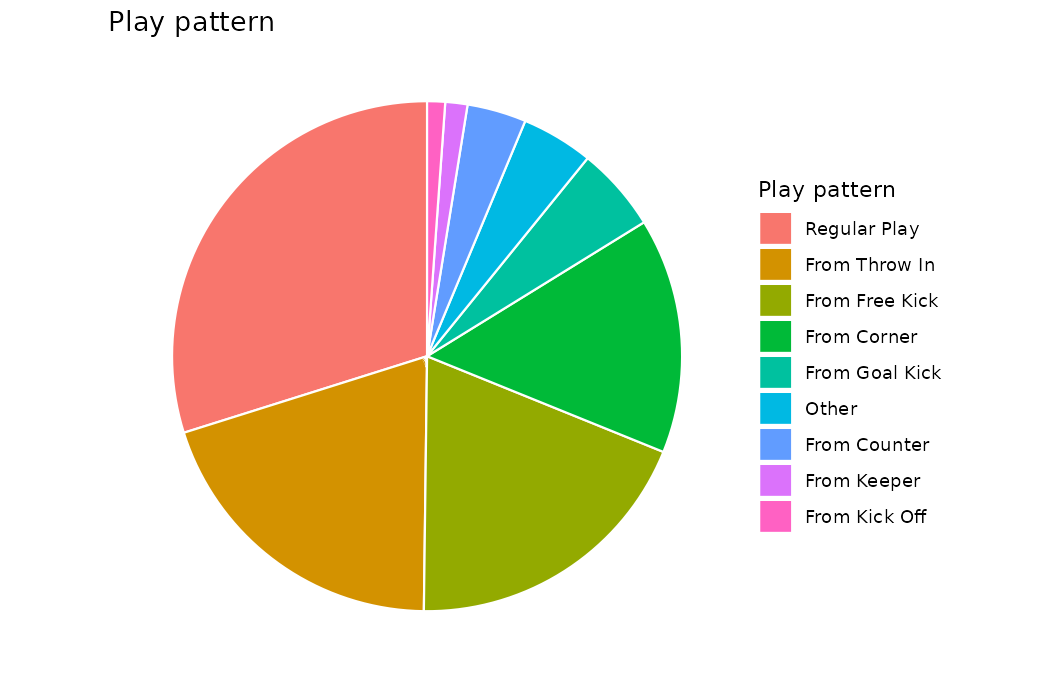
\includegraphics[width=0.85\linewidth,height=\textheight,keepaspectratio]{figures/explore-categorical-11.png}

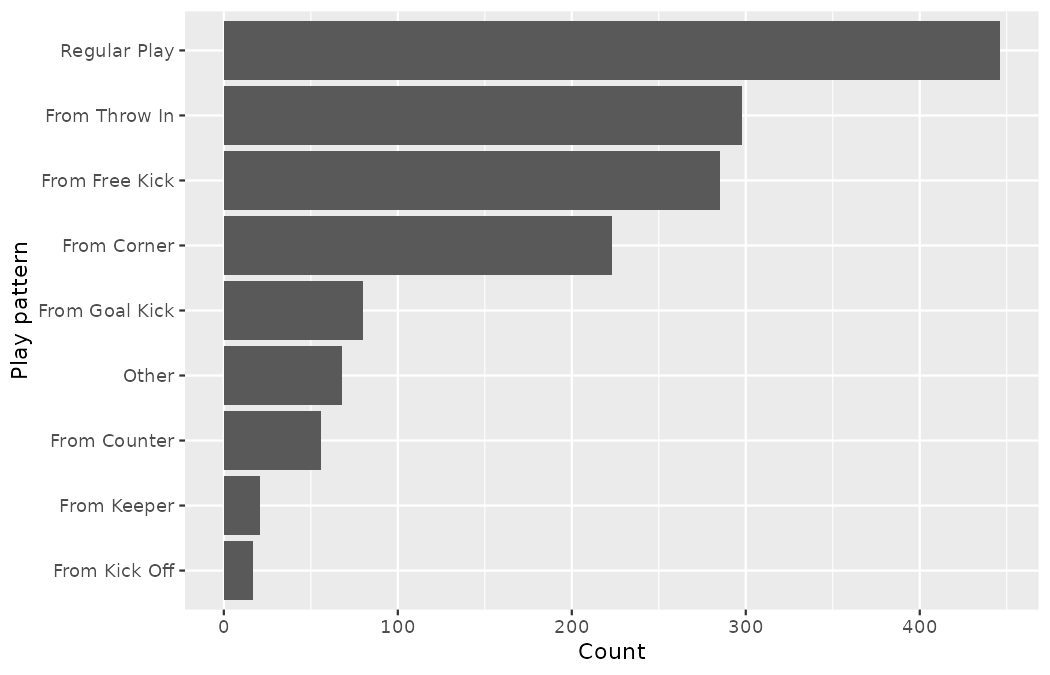
\includegraphics[width=0.85\linewidth,height=\textheight,keepaspectratio]{figures/explore-categorical-12.png}

In the pie chart, the slices for shots from throw-in possessions
(19.9\%) and from free-kick possessions (19.1\%) are essentially
indistinguishable --- twelve shots apart in 1,494 --- and the four
smallest slices (goal kicks, ``other'', counters, keeper distributions,
kick-offs) blur into an unreadable fringe of near-identical wedges. In
the sorted bar plot, the full ordering is legible at a glance, right
down to the 17 shots that arrived within a possession started at
kick-off. In this case, it is far easier to compare the counts of each
play pattern using the bar plot than the pie chart. If Marta Vidal ever
asks whether the club's opponents generate more shots from throw-ins or
free kicks, do not answer her with a pie.

\section{Waffle charts}\label{waffle-charts}

Another useful technique of visualizing categorical data is a
\textbf{waffle chart}. Waffle charts can be used to communicate the
proportion of the data that falls into each level of a categorical
variable. Just like with pie charts, they work best when the number of
levels represented is low. However, unlike pie charts, they can make it
easier to compare proportions that represent non-simple fractions. The
idea: a \(10 \times 10\) grid of 100 squares, each square representing
1\% of the data, colored by level. No dedicated package is needed ---
like the mosaic plot, a waffle is a computation we can do ourselves,
which keeps the logic visible: count, convert to shares, round to
squares, tile.

\begin{Shaded}
\begin{Highlighting}[]
\NormalTok{waffle\_bp }\OtherTok{\textless{}{-}}\NormalTok{ wc\_bp }\SpecialCharTok{|\textgreater{}}
  \FunctionTok{count}\NormalTok{(body\_part) }\SpecialCharTok{|\textgreater{}}
  \FunctionTok{mutate}\NormalTok{(}\AttributeTok{share =}\NormalTok{ n }\SpecialCharTok{/} \FunctionTok{sum}\NormalTok{(n), }\AttributeTok{squares =} \FunctionTok{round}\NormalTok{(share }\SpecialCharTok{*} \DecValTok{100}\NormalTok{))}

\NormalTok{waffle\_bp}
\CommentTok{\#\textgreater{} \# A tibble: 3 × 4}
\CommentTok{\#\textgreater{}   body\_part      n share squares}
\CommentTok{\#\textgreater{}   \textless{}fct\textgreater{}      \textless{}int\textgreater{} \textless{}dbl\textgreater{}   \textless{}dbl\textgreater{}}
\CommentTok{\#\textgreater{} 1 Right Foot   780 0.527      53}
\CommentTok{\#\textgreater{} 2 Left Foot    449 0.303      30}
\CommentTok{\#\textgreater{} 3 Head         252 0.170      17}

\NormalTok{waffle\_bp }\SpecialCharTok{|\textgreater{}}
  \FunctionTok{uncount}\NormalTok{(squares) }\SpecialCharTok{|\textgreater{}}
  \FunctionTok{mutate}\NormalTok{(}\AttributeTok{idx =} \FunctionTok{row\_number}\NormalTok{() }\SpecialCharTok{{-}} \DecValTok{1}\NormalTok{, }\AttributeTok{col =}\NormalTok{ idx }\SpecialCharTok{\%\%} \DecValTok{10}\NormalTok{, }\AttributeTok{row =}\NormalTok{ idx }\SpecialCharTok{\%/\%} \DecValTok{10}\NormalTok{) }\SpecialCharTok{|\textgreater{}}
  \FunctionTok{ggplot}\NormalTok{(}\FunctionTok{aes}\NormalTok{(}\AttributeTok{x =}\NormalTok{ col, }\AttributeTok{y =}\NormalTok{ row, }\AttributeTok{fill =}\NormalTok{ body\_part)) }\SpecialCharTok{+}
  \FunctionTok{geom\_tile}\NormalTok{(}\AttributeTok{color =} \StringTok{"white"}\NormalTok{, }\AttributeTok{linewidth =} \FloatTok{1.5}\NormalTok{) }\SpecialCharTok{+}
  \FunctionTok{coord\_equal}\NormalTok{() }\SpecialCharTok{+}
  \FunctionTok{theme\_void}\NormalTok{() }\SpecialCharTok{+}
  \FunctionTok{labs}\NormalTok{(}\AttributeTok{fill =} \ConstantTok{NULL}\NormalTok{, }\AttributeTok{title =} \StringTok{"Body part"}\NormalTok{)}
\end{Highlighting}
\end{Shaded}

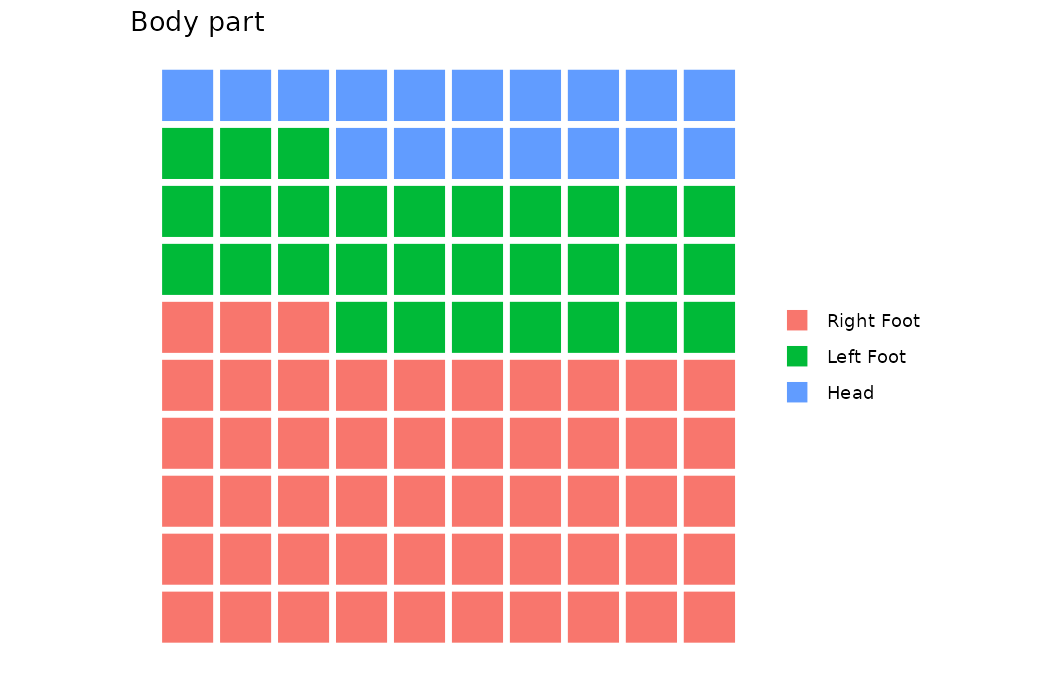
\includegraphics[width=0.85\linewidth,height=\textheight,keepaspectratio]{figures/explore-categorical-13.png}

Here \texttt{uncount(squares)} replicates each row of
\texttt{waffle\_bp} once per square, and the arithmetic on \texttt{idx}
lays the squares into a 10-wide grid. The rounded squares happen to sum
to exactly 100 here \((53 + 30 + 17)\); with other data the roundings
can sum to 99 or 101, in which case you must add or remove a square from
the level with the largest rounding error --- a detail the packaged
waffle functions handle silently, and one worth having tripped over once
yourself. Reading the chart, ``53 squares out of 100'' is a count, not
an angle: comparing 30 left-foot squares against 17 header squares is a
matter of counting rows, which is precisely the non-simple-fraction
comparison the pie chart fumbled.

A second waffle, this time for the Women's Euro position groups defined
earlier in this chapter:

\begin{Shaded}
\begin{Highlighting}[]
\NormalTok{waffle\_pos }\OtherTok{\textless{}{-}}\NormalTok{ weuro\_pos }\SpecialCharTok{|\textgreater{}}
  \FunctionTok{count}\NormalTok{(pos\_group) }\SpecialCharTok{|\textgreater{}}
  \FunctionTok{mutate}\NormalTok{(}\AttributeTok{share =}\NormalTok{ n }\SpecialCharTok{/} \FunctionTok{sum}\NormalTok{(n), }\AttributeTok{squares =} \FunctionTok{round}\NormalTok{(share }\SpecialCharTok{*} \DecValTok{100}\NormalTok{))}

\NormalTok{waffle\_pos}
\CommentTok{\#\textgreater{} \# A tibble: 3 × 4}
\CommentTok{\#\textgreater{}   pos\_group     n share squares}
\CommentTok{\#\textgreater{}   \textless{}fct\textgreater{}     \textless{}int\textgreater{} \textless{}dbl\textgreater{}   \textless{}dbl\textgreater{}}
\CommentTok{\#\textgreater{} 1 FW          418 0.459      46}
\CommentTok{\#\textgreater{} 2 MF          338 0.371      37}
\CommentTok{\#\textgreater{} 3 DF          155 0.170      17}

\NormalTok{waffle\_pos }\SpecialCharTok{|\textgreater{}}
  \FunctionTok{uncount}\NormalTok{(squares) }\SpecialCharTok{|\textgreater{}}
  \FunctionTok{mutate}\NormalTok{(}\AttributeTok{idx =} \FunctionTok{row\_number}\NormalTok{() }\SpecialCharTok{{-}} \DecValTok{1}\NormalTok{, }\AttributeTok{col =}\NormalTok{ idx }\SpecialCharTok{\%\%} \DecValTok{10}\NormalTok{, }\AttributeTok{row =}\NormalTok{ idx }\SpecialCharTok{\%/\%} \DecValTok{10}\NormalTok{) }\SpecialCharTok{|\textgreater{}}
  \FunctionTok{ggplot}\NormalTok{(}\FunctionTok{aes}\NormalTok{(}\AttributeTok{x =}\NormalTok{ col, }\AttributeTok{y =}\NormalTok{ row, }\AttributeTok{fill =}\NormalTok{ pos\_group)) }\SpecialCharTok{+}
  \FunctionTok{geom\_tile}\NormalTok{(}\AttributeTok{color =} \StringTok{"white"}\NormalTok{, }\AttributeTok{linewidth =} \FloatTok{1.5}\NormalTok{) }\SpecialCharTok{+}
  \FunctionTok{coord\_equal}\NormalTok{() }\SpecialCharTok{+}
  \FunctionTok{theme\_void}\NormalTok{() }\SpecialCharTok{+}
  \FunctionTok{labs}\NormalTok{(}\AttributeTok{fill =} \ConstantTok{NULL}\NormalTok{, }\AttributeTok{title =} \StringTok{"Position group"}\NormalTok{)}
\end{Highlighting}
\end{Shaded}

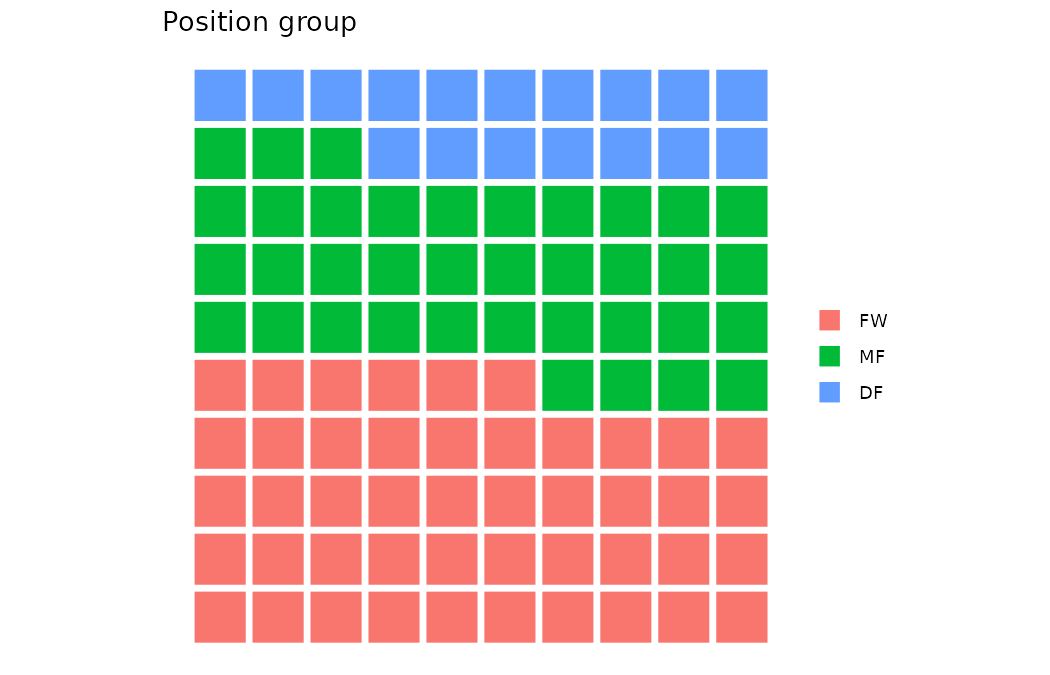
\includegraphics[width=0.85\linewidth,height=\textheight,keepaspectratio]{figures/explore-categorical-14.png}

Again the squares sum to 100 \((46 + 37 + 17).\) Forwards took a touch
under half the tournament's outfield shots --- 46 squares, visibly short
of a half-grid --- while midfielders and defenders split the rest
roughly two-to-one.

\begin{tcolorbox}[enhanced jigsaw, left=2mm, leftrule=.75mm, title=\textcolor{quarto-callout-tip-color}{\faLightbulb}\hspace{0.5em}{Check your understanding}, arc=.35mm, rightrule=.15mm, coltitle=black, colframe=quarto-callout-tip-color-frame, bottomrule=.15mm, colbacktitle=quarto-callout-tip-color!10!white, opacitybacktitle=0.6, breakable, bottomtitle=1mm, toptitle=1mm, titlerule=0mm, opacityback=0, toprule=.15mm, colback=white]

A colleague wants a single chart showing the nine-level
\texttt{play\_pattern} distribution and suggests a waffle chart, ``since
waffles are better than pies.'' Is the waffle likely to fix the problem?

\begin{center}\rule{0.5\linewidth}{0.5pt}\end{center}

No. The waffle's advantage over the pie is \emph{within-comparison
precision} (counting squares beats judging angles), but both share the
same weakness: with many levels, small categories become tiny scattered
patches of color that are hard to distinguish. Shots from keeper
distributions would get one square and kick-offs one square, in nine
competing colors. The number of levels, not the shape of the chart, is
the problem --- the sorted bar plot remains the right tool.

\end{tcolorbox}

\begin{tcolorbox}[enhanced jigsaw, left=2mm, leftrule=.75mm, title=\textcolor{quarto-callout-note-color}{\faInfo}\hspace{0.5em}{The fast version: reading a numerical distribution}, arc=.35mm, rightrule=.15mm, coltitle=black, colframe=quarto-callout-note-color-frame, bottomrule=.15mm, colbacktitle=quarto-callout-note-color!10!white, opacitybacktitle=0.6, breakable, bottomtitle=1mm, toptitle=1mm, titlerule=0mm, opacityback=0, toprule=.15mm, colback=white]

The plots in the section below describe a \emph{numerical} variable, and
they speak a vocabulary whose proper chapter is still ahead of you. Here
is the fast version, one sentence per tool.

\begin{itemize}
\tightlist
\item
  A \emph{histogram} divides the variable's range into equal-width bins
  and draws one bar per bin: the height of each bar counts the
  observations landing in that bin.
\item
  A \emph{mode} is a prominent peak in the distribution --- a stretch of
  values where the observations pile up.
\item
  The \emph{median} is the middle value: half the observations sit below
  it and half above.
\item
  The \emph{quartiles} cut off the middle half of the data, and the box
  in a box plot spans exactly that middle half --- from the value with a
  quarter of the observations below it to the value with a quarter above
  --- with the median drawn as the line inside.
\item
  The \emph{whiskers} extend from the box out to the most distant
  observations still within ordinary range, and any points plotted
  individually beyond them are \emph{outliers}, observations unusually
  far from the rest.
\item
  A distribution is \emph{right skewed} when a long, thin tail stretches
  out toward the larger values on the right.
\end{itemize}

Each of these gets its full treatment in
Chapter~\ref{sec-explore-numerical}; this box is just enough to read the
pictures below.

\end{tcolorbox}

\section{Comparing numerical data across
groups}\label{comparing-numerical-data-across-groups}

Some of the more interesting investigations can be considered by
examining numerical data across groups. In this section we will expand
on a few methods we have already seen to make plots for numerical data
from multiple groups on the same graph, as well as introduce a few new
methods for comparing numerical data across groups.

We will revisit the full \texttt{wc2022\_shots} dataset and compare the
chance quality --- the \texttt{statsbomb\_xg} variable --- for shots
that were scored versus shots that were not. A caution before we start:
\texttt{goal} is the outcome that xG models are built to anticipate, and
these are observational data besides, so nothing in this section
demonstrates \emph{why} any shot went in. What the comparison does tell
a scout is descriptive and valuable: how different, in distribution, are
the chances that become goals from the chances that do not --- and
whether the difference is a shift, a change of shape, or both.

Of the 1,494 shots at the 2022 Men's World Cup, 195 were goals and 1,299
were not. The table below shows a small random sample of four shots from
each group, drawn with a seed so you can reproduce it.

\begin{Shaded}
\begin{Highlighting}[]
\NormalTok{wc\_result }\OtherTok{\textless{}{-}}\NormalTok{ wc2022\_shots }\SpecialCharTok{|\textgreater{}}
  \FunctionTok{mutate}\NormalTok{(}\AttributeTok{result =} \FunctionTok{factor}\NormalTok{(}\FunctionTok{if\_else}\NormalTok{(goal, }\StringTok{"goal"}\NormalTok{, }\StringTok{"no goal"}\NormalTok{), }\AttributeTok{levels =} \FunctionTok{c}\NormalTok{(}\StringTok{"goal"}\NormalTok{, }\StringTok{"no goal"}\NormalTok{)))}

\FunctionTok{set.seed}\NormalTok{(}\DecValTok{401}\NormalTok{)}
\NormalTok{wc\_result }\SpecialCharTok{|\textgreater{}}
  \FunctionTok{select}\NormalTok{(player, team, statsbomb\_xg, result) }\SpecialCharTok{|\textgreater{}}
  \FunctionTok{group\_by}\NormalTok{(result) }\SpecialCharTok{|\textgreater{}}
  \FunctionTok{slice\_sample}\NormalTok{(}\AttributeTok{n =} \DecValTok{4}\NormalTok{) }\SpecialCharTok{|\textgreater{}}
  \FunctionTok{arrange}\NormalTok{(result, statsbomb\_xg)}
\CommentTok{\#\textgreater{} \# A tibble: 8 × 4}
\CommentTok{\#\textgreater{} \# Groups:   result [2]}
\CommentTok{\#\textgreater{}   player                            team        statsbomb\_xg result}
\CommentTok{\#\textgreater{}   \textless{}chr\textgreater{}                             \textless{}chr\textgreater{}              \textless{}dbl\textgreater{} \textless{}fct\textgreater{}}
\CommentTok{\#\textgreater{} 1 Craig Goodwin                     Australia         0.191  goal}
\CommentTok{\#\textgreater{} 2 Davy Klaassen                     Netherlands       0.348  goal}
\CommentTok{\#\textgreater{} 3 Lionel Andrés Messi Cuccittini    Argentina         0.488  goal}
\CommentTok{\#\textgreater{} 4 Teun Koopmeiners                  Netherlands       0.784  goal}
\CommentTok{\#\textgreater{} 5 Abdelkarim Hassan Al Haj Fadlalla Qatar             0.0234 no goal}
\CommentTok{\#\textgreater{} 6 Axel Witsel                       Belgium           0.0253 no goal}
\CommentTok{\#\textgreater{} 7 Robert Lewandowski                Poland            0.0332 no goal}
\CommentTok{\#\textgreater{} 8 Nicolás Alejandro Tagliafico      Argentina         0.0518 no goal}
\end{Highlighting}
\end{Shaded}

Even in a sample of eight, the pattern that will dominate this section
is visible: the four goals carry far more chance quality than the four
non-goals, and one of the goals sits at the penalty value --- stored as
\(0.7835,\) printed as \(0.784\) by the three-significant-digit display
--- which we will meet again shortly.

Color can be used to split histograms (see Section~\ref{sec-histograms}
for an introduction to histograms) for numerical variables by levels of
a categorical variable. An example of this is shown in the first plot
below. The \textbf{side-by-side box plot} is another traditional tool
for comparing across groups. An example is shown in the second plot,
where there are two box plots (see Section~\ref{sec-boxplots} for an
introduction to box plots), one for each group, placed into one plotting
window and drawn on the same scale.

\begin{Shaded}
\begin{Highlighting}[]
\FunctionTok{ggplot}\NormalTok{(wc\_result, }\FunctionTok{aes}\NormalTok{(}\AttributeTok{x =}\NormalTok{ statsbomb\_xg, }\AttributeTok{fill =}\NormalTok{ result)) }\SpecialCharTok{+}
  \FunctionTok{geom\_histogram}\NormalTok{(}\AttributeTok{binwidth =} \FloatTok{0.05}\NormalTok{, }\AttributeTok{alpha =} \FloatTok{0.5}\NormalTok{) }\SpecialCharTok{+}
  \FunctionTok{labs}\NormalTok{(}\AttributeTok{x =} \StringTok{"Chance quality (xG)"}\NormalTok{, }\AttributeTok{y =} \ConstantTok{NULL}\NormalTok{, }\AttributeTok{fill =} \StringTok{"Result"}\NormalTok{)}

\FunctionTok{ggplot}\NormalTok{(wc\_result, }\FunctionTok{aes}\NormalTok{(}\AttributeTok{x =}\NormalTok{ statsbomb\_xg, }\AttributeTok{y =}\NormalTok{ result, }\AttributeTok{color =}\NormalTok{ result)) }\SpecialCharTok{+}
  \FunctionTok{geom\_boxplot}\NormalTok{() }\SpecialCharTok{+}
  \FunctionTok{labs}\NormalTok{(}\AttributeTok{x =} \StringTok{"Chance quality (xG)"}\NormalTok{, }\AttributeTok{y =} \ConstantTok{NULL}\NormalTok{, }\AttributeTok{color =} \StringTok{"Result"}\NormalTok{)}
\end{Highlighting}
\end{Shaded}

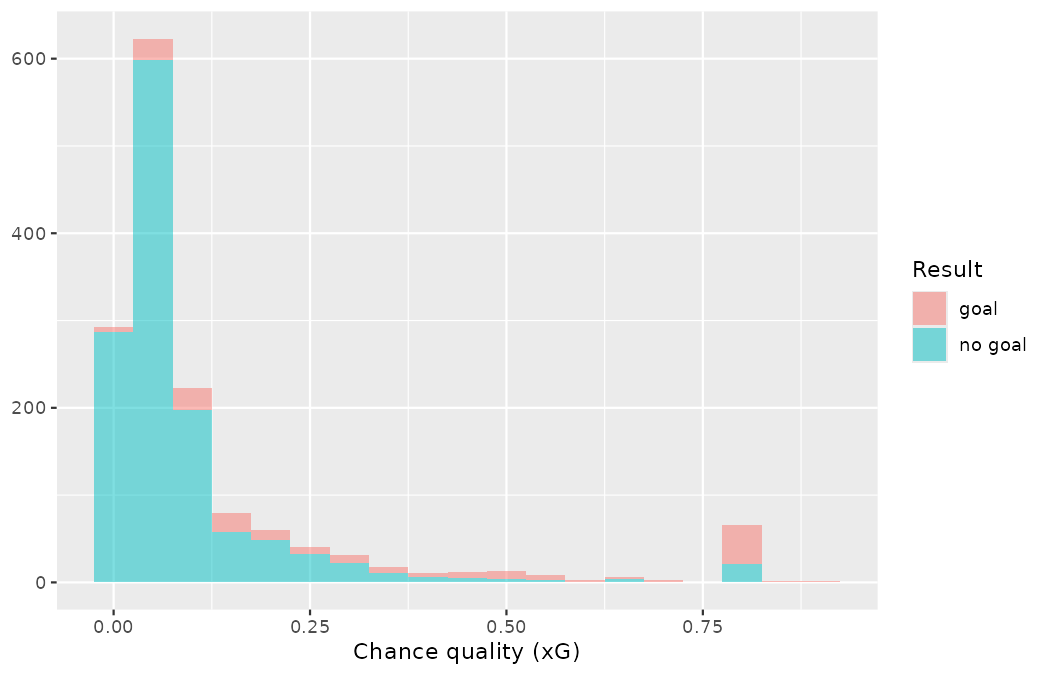
\includegraphics[width=0.85\linewidth,height=\textheight,keepaspectratio]{figures/explore-categorical-15.png}

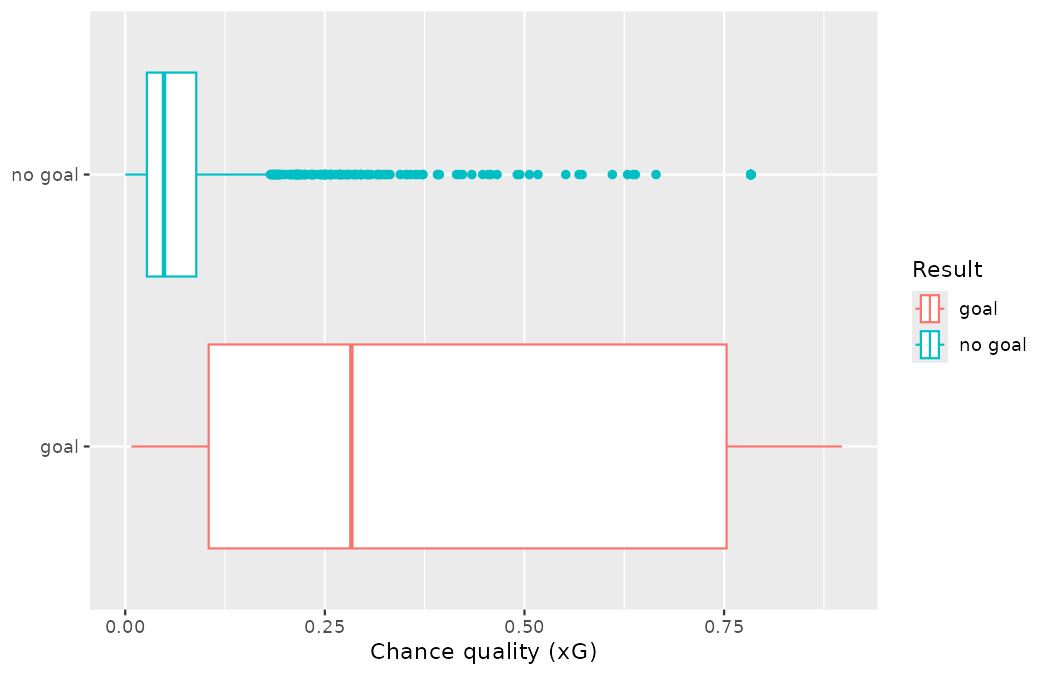
\includegraphics[width=0.85\linewidth,height=\textheight,keepaspectratio]{figures/explore-categorical-16.png}

The numerical summaries behind the plots:

\begin{Shaded}
\begin{Highlighting}[]
\NormalTok{wc\_result }\SpecialCharTok{|\textgreater{}}
  \FunctionTok{group\_by}\NormalTok{(result) }\SpecialCharTok{|\textgreater{}}
  \FunctionTok{summarize}\NormalTok{(}
    \AttributeTok{shots =} \FunctionTok{n}\NormalTok{(),}
    \AttributeTok{mean\_xg =} \FunctionTok{mean}\NormalTok{(statsbomb\_xg),}
    \AttributeTok{median\_xg =} \FunctionTok{median}\NormalTok{(statsbomb\_xg),}
    \AttributeTok{q1 =} \FunctionTok{quantile}\NormalTok{(statsbomb\_xg, }\FloatTok{0.25}\NormalTok{),}
    \AttributeTok{q3 =} \FunctionTok{quantile}\NormalTok{(statsbomb\_xg, }\FloatTok{0.75}\NormalTok{)}
\NormalTok{  )}
\CommentTok{\#\textgreater{} \# A tibble: 2 × 6}
\CommentTok{\#\textgreater{}   result  shots mean\_xg median\_xg     q1     q3}
\CommentTok{\#\textgreater{}   \textless{}fct\textgreater{}   \textless{}int\textgreater{}   \textless{}dbl\textgreater{}     \textless{}dbl\textgreater{}  \textless{}dbl\textgreater{}  \textless{}dbl\textgreater{}}
\CommentTok{\#\textgreater{} 1 goal      195  0.373     0.283  0.105  0.753}
\CommentTok{\#\textgreater{} 2 no goal  1299  0.0887    0.0486 0.0271 0.0890}
\end{Highlighting}
\end{Shaded}

In the histogram, the no-goal distribution is a tall spike hugging zero
--- 1,010 of the 1,299 misses carry less than \(0.1\) xG --- with a
long, thin right tail, plus a small isolated bump near \(0.78.\) The
goal distribution is lower and far more spread out, with its own
concentration at low xG (45 of the 195 goals came from chances under
\(0.1\)) and a second, unmistakable peak in the bin covering
\(0.775\)--\(0.825,\) holding 45 goals. That second peak has a name: the
penalty spot. All 64 World Cup penalties in these data are assigned an
identical stored chance quality of \(0.7835\) (recall from
Chapter~\ref{sec-data-applications} that displays round it to \(0.783\)
or \(0.784\)), and 43 of them were scored --- so penalties plant a spike
at \(0.7835\) in the goal group and a smaller one (the 21 misses) in the
no-goal group.

\begin{Shaded}
\begin{Highlighting}[]
\NormalTok{wc2022\_shots }\SpecialCharTok{|\textgreater{}}
  \FunctionTok{filter}\NormalTok{(shot\_type }\SpecialCharTok{==} \StringTok{"Penalty"}\NormalTok{) }\SpecialCharTok{|\textgreater{}}
  \FunctionTok{summarize}\NormalTok{(}\AttributeTok{n =} \FunctionTok{n}\NormalTok{(), }\AttributeTok{mean\_xg =} \FunctionTok{mean}\NormalTok{(statsbomb\_xg), }\AttributeTok{goals =} \FunctionTok{sum}\NormalTok{(goal))}
\CommentTok{\#\textgreater{} \# A tibble: 1 × 3}
\CommentTok{\#\textgreater{}       n mean\_xg goals}
\CommentTok{\#\textgreater{}   \textless{}int\textgreater{}   \textless{}dbl\textgreater{} \textless{}int\textgreater{}}
\CommentTok{\#\textgreater{} 1    64   0.784    43}
\end{Highlighting}
\end{Shaded}

Whenever you plot tournament xG, decide consciously whether to keep
penalties (and explain the spike, as we do here) or to filter to
\texttt{shot\_type\ ==\ "Open\ Play"} and say so; silently leaving the
spike for your reader to puzzle over is the worst of both options.

\begin{tcolorbox}[enhanced jigsaw, left=2mm, leftrule=.75mm, title=\textcolor{quarto-callout-tip-color}{\faLightbulb}\hspace{0.5em}{Check your understanding}, arc=.35mm, rightrule=.15mm, coltitle=black, colframe=quarto-callout-tip-color-frame, bottomrule=.15mm, colbacktitle=quarto-callout-tip-color!10!white, opacitybacktitle=0.6, breakable, bottomtitle=1mm, toptitle=1mm, titlerule=0mm, opacityback=0, toprule=.15mm, colback=white]

Use the plots and summaries above to compare chance quality across the
two groups. What do you notice about the approximate center of each
group? What do you notice about the variability between groups? Is the
shape relatively consistent between groups? How many \emph{prominent}
modes are there for each group?

\begin{center}\rule{0.5\linewidth}{0.5pt}\end{center}

The goals come from far better chances on average: the median xG of a
scored shot is about \(0.28,\) versus about \(0.05\) for a shot that was
not scored. The variability is also dramatically larger for the goal
group --- the middle half of the goal group spans from about \(0.11\) to
\(0.75\) of xG, roughly ten times the span of the middle half of the
no-goal group (\(0.03\) to \(0.09\)). Both distributions are strongly
right skewed with their tallest peak near zero, but the shapes are not
identical: the goal group has two prominent modes --- the low-xG peak
and the penalty spike at \(0.7835\) --- while the no-goal group has one
prominent mode near zero (its penalty bump of 21 shots is barely visible
against 1,299). The box plots indicate there are many observations far
above the upper whisker in the no-goal group; with over a thousand shots
piled near zero, chances of even moderate quality register as outliers.

\end{tcolorbox}

\begin{tcolorbox}[enhanced jigsaw, left=2mm, leftrule=.75mm, title=\textcolor{quarto-callout-tip-color}{\faLightbulb}\hspace{0.5em}{Check your understanding}, arc=.35mm, rightrule=.15mm, coltitle=black, colframe=quarto-callout-tip-color-frame, bottomrule=.15mm, colbacktitle=quarto-callout-tip-color!10!white, opacitybacktitle=0.6, breakable, bottomtitle=1mm, toptitle=1mm, titlerule=0mm, opacityback=0, toprule=.15mm, colback=white]

What components of each plot --- the color-split histogram and the
side-by-side box plot --- do you find most useful?

\begin{center}\rule{0.5\linewidth}{0.5pt}\end{center}

The side-by-side box plots are especially useful for comparing centers
and spreads at a glance, and they make the huge gap in medians
impossible to miss. The histograms are more useful for seeing
distribution shape, skew, and modes --- the penalty spike at \(0.7835\)
is obvious in the histogram and completely invisible in the box plot,
which is a reminder that a box plot compresses a distribution down to
five-ish numbers.

\end{tcolorbox}

Another useful visualization for comparing numerical data across groups
is a \textbf{ridge plot}, which combines density plots (see
Section~\ref{sec-boxplots} for an introduction to density plots) for
various groups drawn on the same scale in a single plotting window.

\begin{Shaded}
\begin{Highlighting}[]
\FunctionTok{library}\NormalTok{(ggridges)}

\FunctionTok{ggplot}\NormalTok{(wc\_result, }\FunctionTok{aes}\NormalTok{(}\AttributeTok{x =}\NormalTok{ statsbomb\_xg, }\AttributeTok{y =}\NormalTok{ result, }\AttributeTok{fill =}\NormalTok{ result, }\AttributeTok{color =}\NormalTok{ result)) }\SpecialCharTok{+}
  \FunctionTok{geom\_density\_ridges}\NormalTok{(}\AttributeTok{alpha =} \FloatTok{0.5}\NormalTok{) }\SpecialCharTok{+}
  \FunctionTok{labs}\NormalTok{(}\AttributeTok{x =} \StringTok{"Chance quality (xG)"}\NormalTok{, }\AttributeTok{y =} \ConstantTok{NULL}\NormalTok{, }\AttributeTok{fill =} \StringTok{"Result"}\NormalTok{, }\AttributeTok{color =} \StringTok{"Result"}\NormalTok{)}
\end{Highlighting}
\end{Shaded}

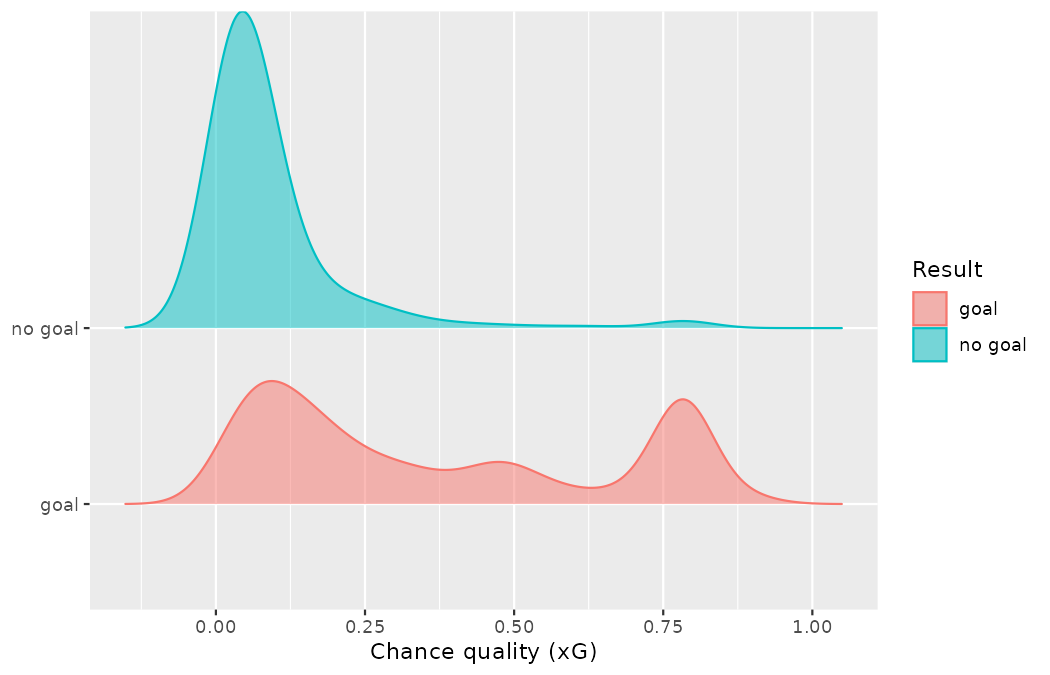
\includegraphics[width=0.85\linewidth,height=\textheight,keepaspectratio]{figures/explore-categorical-17.png}

The no-goal ridge rises into a single sharp peak just above zero and
decays quickly. The goal ridge is flatter and wider, with its main peak
also at low xG and a clear second hump around \(0.78\) --- the penalty
spike again, now rendered as a bump in a smooth curve.

\begin{tcolorbox}[enhanced jigsaw, left=2mm, leftrule=.75mm, title=\textcolor{quarto-callout-tip-color}{\faLightbulb}\hspace{0.5em}{Check your understanding}, arc=.35mm, rightrule=.15mm, coltitle=black, colframe=quarto-callout-tip-color-frame, bottomrule=.15mm, colbacktitle=quarto-callout-tip-color!10!white, opacitybacktitle=0.6, breakable, bottomtitle=1mm, toptitle=1mm, titlerule=0mm, opacityback=0, toprule=.15mm, colback=white]

What components of the ridge plot do you find most useful compared to
the histogram and box plot?

\begin{center}\rule{0.5\linewidth}{0.5pt}\end{center}

The ridge plot gives us a better sense of the shape, and especially the
modality, of each group's distribution: the bimodality of the goal group
reads instantly as two humps. One caution specific to ridge plots: each
ridge is scaled separately, so --- like the standardized bar plot
earlier in this chapter --- the plot hides the fact that one group
(1,299 non-goals) has nearly seven times the observations of the other
(195 goals).

\end{tcolorbox}

One last visualization technique we'll highlight for comparing numerical
data across groups is \textbf{faceting}. In this technique we split
(facet) the graphical display of the data across plotting windows based
on groups. The first plot below displays the same information as the
color-split histogram, however here the distributions of xG for goals
and non-goals are faceted across two plotting windows, preserving the
same scale on the x and y axes for easier comparison. An advantage of
this approach is that it extends to splitting the data across levels of
two categorical variables, which allows for displaying relationships
between three variables. For the second categorical variable we bring in
the second tournament: we stack the two shot datasets, apply the
position-group mapping defined earlier in this chapter to both, and
facet by \texttt{result} and \texttt{competition} simultaneously.

\begin{Shaded}
\begin{Highlighting}[]
\NormalTok{both }\OtherTok{\textless{}{-}} \FunctionTok{bind\_rows}\NormalTok{(wc2022\_shots, weuro2025\_shots) }\SpecialCharTok{|\textgreater{}}
  \FunctionTok{mutate}\NormalTok{(}
    \AttributeTok{pos\_group =} \FunctionTok{case\_when}\NormalTok{(}
\NormalTok{      position }\SpecialCharTok{==} \StringTok{"Goalkeeper"} \SpecialCharTok{\textasciitilde{}} \StringTok{"GK"}\NormalTok{,}
      \FunctionTok{grepl}\NormalTok{(}\StringTok{"Back"}\NormalTok{, position) }\SpecialCharTok{\textasciitilde{}} \StringTok{"DF"}\NormalTok{,}
      \FunctionTok{grepl}\NormalTok{(}\StringTok{"Midfield"}\NormalTok{, position) }\SpecialCharTok{\textasciitilde{}} \StringTok{"MF"}\NormalTok{,}
      \AttributeTok{.default =} \StringTok{"FW"}
\NormalTok{    )}
\NormalTok{  ) }\SpecialCharTok{|\textgreater{}}
  \FunctionTok{filter}\NormalTok{(pos\_group }\SpecialCharTok{!=} \StringTok{"GK"}\NormalTok{) }\SpecialCharTok{|\textgreater{}}
  \FunctionTok{mutate}\NormalTok{(}
    \AttributeTok{pos\_group =} \FunctionTok{factor}\NormalTok{(pos\_group, }\AttributeTok{levels =} \FunctionTok{c}\NormalTok{(}\StringTok{"FW"}\NormalTok{, }\StringTok{"MF"}\NormalTok{, }\StringTok{"DF"}\NormalTok{)),}
    \AttributeTok{result =} \FunctionTok{factor}\NormalTok{(}\FunctionTok{if\_else}\NormalTok{(goal, }\StringTok{"goal"}\NormalTok{, }\StringTok{"no goal"}\NormalTok{), }\AttributeTok{levels =} \FunctionTok{c}\NormalTok{(}\StringTok{"goal"}\NormalTok{, }\StringTok{"no goal"}\NormalTok{))}
\NormalTok{  )}

\NormalTok{both }\SpecialCharTok{|\textgreater{}}
  \FunctionTok{count}\NormalTok{(competition)}
\CommentTok{\#\textgreater{} \# A tibble: 2 × 2}
\CommentTok{\#\textgreater{}   competition     n}
\CommentTok{\#\textgreater{}   \textless{}chr\textgreater{}       \textless{}int\textgreater{}}
\CommentTok{\#\textgreater{} 1 wc2022       1494}
\CommentTok{\#\textgreater{} 2 weuro2025     911}
\end{Highlighting}
\end{Shaded}

Dropping the two goalkeeper penalties again (there were no goalkeeper
shots at the men's World Cup) leaves \(1494 + 911 = 2405\) shots.

\begin{Shaded}
\begin{Highlighting}[]
\CommentTok{\# Facet by one variable: result}
\FunctionTok{ggplot}\NormalTok{(both, }\FunctionTok{aes}\NormalTok{(}\AttributeTok{x =}\NormalTok{ statsbomb\_xg, }\AttributeTok{fill =}\NormalTok{ result)) }\SpecialCharTok{+}
  \FunctionTok{geom\_histogram}\NormalTok{(}\AttributeTok{binwidth =} \FloatTok{0.05}\NormalTok{, }\AttributeTok{show.legend =} \ConstantTok{FALSE}\NormalTok{) }\SpecialCharTok{+}
  \FunctionTok{facet\_grid}\NormalTok{(result }\SpecialCharTok{\textasciitilde{}}\NormalTok{ .) }\SpecialCharTok{+}
  \FunctionTok{labs}\NormalTok{(}\AttributeTok{x =} \StringTok{"Chance quality (xG)"}\NormalTok{, }\AttributeTok{y =} \ConstantTok{NULL}\NormalTok{)}

\CommentTok{\# Facet by two variables: result and competition}
\FunctionTok{ggplot}\NormalTok{(both, }\FunctionTok{aes}\NormalTok{(}\AttributeTok{x =}\NormalTok{ statsbomb\_xg, }\AttributeTok{fill =}\NormalTok{ result)) }\SpecialCharTok{+}
  \FunctionTok{geom\_histogram}\NormalTok{(}\AttributeTok{binwidth =} \FloatTok{0.05}\NormalTok{, }\AttributeTok{show.legend =} \ConstantTok{FALSE}\NormalTok{) }\SpecialCharTok{+}
  \FunctionTok{facet\_grid}\NormalTok{(result }\SpecialCharTok{\textasciitilde{}}\NormalTok{ competition) }\SpecialCharTok{+}
  \FunctionTok{labs}\NormalTok{(}\AttributeTok{x =} \StringTok{"Chance quality (xG)"}\NormalTok{, }\AttributeTok{y =} \ConstantTok{NULL}\NormalTok{)}
\end{Highlighting}
\end{Shaded}

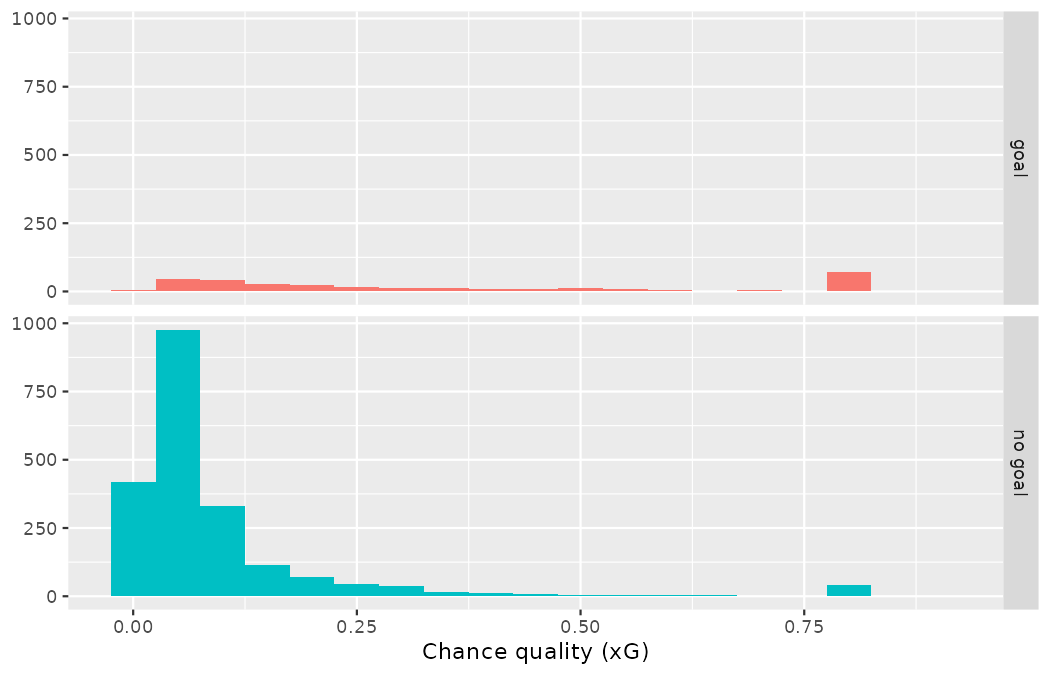
\includegraphics[width=0.85\linewidth,height=\textheight,keepaspectratio]{figures/explore-categorical-18.png}

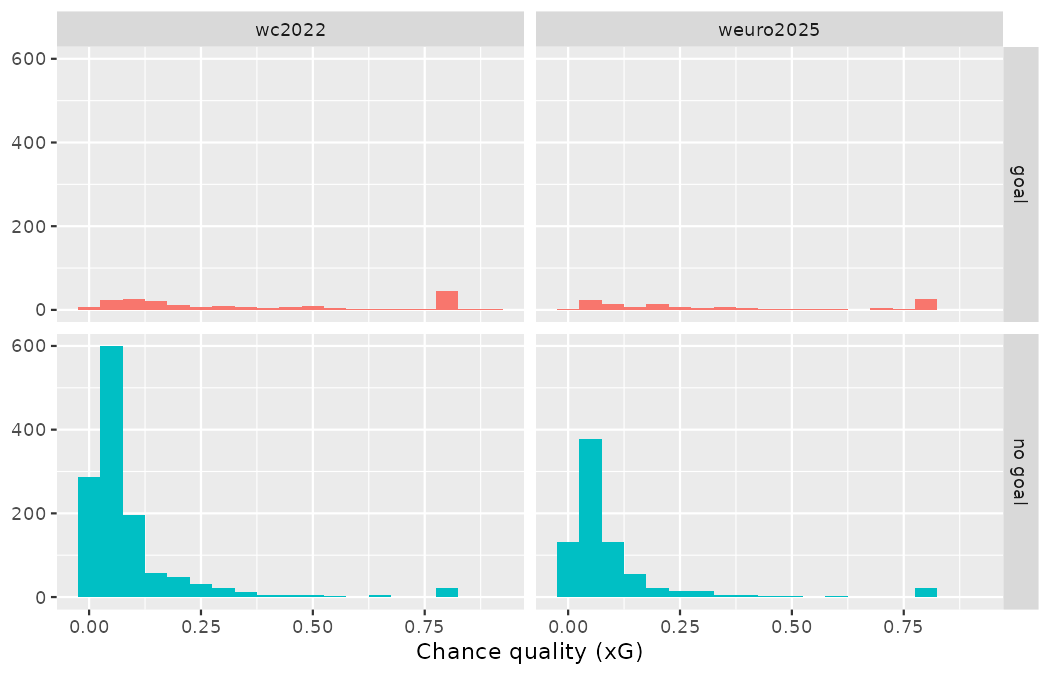
\includegraphics[width=0.85\linewidth,height=\textheight,keepaspectratio]{figures/explore-categorical-19.png}

In the four-panel figure:

\begin{itemize}
\tightlist
\item
  top left represents 2022 World Cup shots that were goals,
\item
  top right represents 2025 Women's Euro shots that were goals,
\item
  bottom left represents World Cup shots that were \emph{not} goals, and
  finally
\item
  bottom right represents Women's Euro shots that were \emph{not} goals.
\end{itemize}

The reassuring finding is replication: the pattern is the same in both
competitions. Each no-goal panel is a spike at zero with a long tail;
each goal panel is flatter, right skewed, and shows the penalty bump
(penalties carry the same stored xG of \(0.7835\) in the Women's Euro
data as well).

We can continue building upon this visualization to add one more
variable, the position group of the shooter. In the ridge plot below, we
represent \texttt{pos\_group} on the vertical axis within each panel, so
a single figure now relates four variables: chance quality, result,
competition, and position group.

\begin{Shaded}
\begin{Highlighting}[]
\FunctionTok{ggplot}\NormalTok{(both, }\FunctionTok{aes}\NormalTok{(}\AttributeTok{x =}\NormalTok{ statsbomb\_xg, }\AttributeTok{y =}\NormalTok{ pos\_group, }\AttributeTok{fill =}\NormalTok{ pos\_group, }\AttributeTok{color =}\NormalTok{ pos\_group)) }\SpecialCharTok{+}
  \FunctionTok{geom\_density\_ridges}\NormalTok{(}\AttributeTok{alpha =} \FloatTok{0.5}\NormalTok{) }\SpecialCharTok{+}
  \FunctionTok{facet\_grid}\NormalTok{(result }\SpecialCharTok{\textasciitilde{}}\NormalTok{ competition) }\SpecialCharTok{+}
  \FunctionTok{labs}\NormalTok{(}\AttributeTok{x =} \StringTok{"Chance quality (xG)"}\NormalTok{, }\AttributeTok{y =} \ConstantTok{NULL}\NormalTok{, }\AttributeTok{fill =} \StringTok{"Position group"}\NormalTok{, }\AttributeTok{color =} \StringTok{"Position group"}\NormalTok{)}
\end{Highlighting}
\end{Shaded}

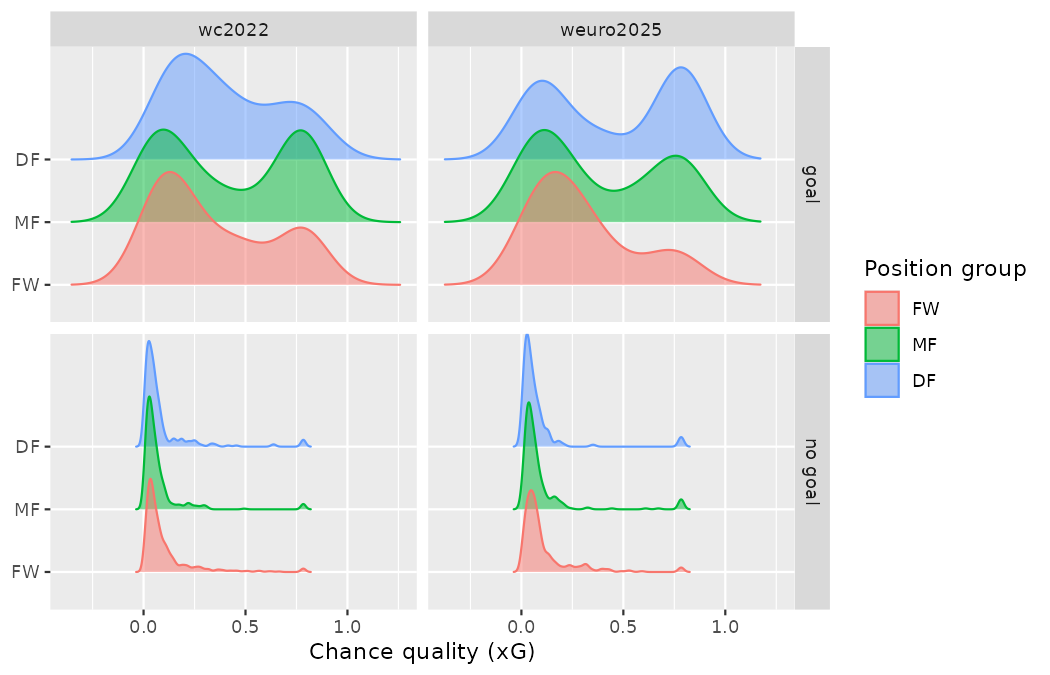
\includegraphics[width=0.85\linewidth,height=\textheight,keepaspectratio]{figures/explore-categorical-20.png}

\begin{tcolorbox}[enhanced jigsaw, left=2mm, leftrule=.75mm, title=\textcolor{quarto-callout-tip-color}{\faLightbulb}\hspace{0.5em}{Check your understanding}, arc=.35mm, rightrule=.15mm, coltitle=black, colframe=quarto-callout-tip-color-frame, bottomrule=.15mm, colbacktitle=quarto-callout-tip-color!10!white, opacitybacktitle=0.6, breakable, bottomtitle=1mm, toptitle=1mm, titlerule=0mm, opacityback=0, toprule=.15mm, colback=white]

Based on the four-variable ridge plot, what can you say about how chance
quality varies depending on result, competition, and position group? The
group medians below will help you calibrate what the ridges show.

\begin{Shaded}
\begin{Highlighting}[]
\NormalTok{both }\SpecialCharTok{|\textgreater{}}
  \FunctionTok{group\_by}\NormalTok{(competition, result, pos\_group) }\SpecialCharTok{|\textgreater{}}
  \FunctionTok{summarize}\NormalTok{(}\AttributeTok{shots =} \FunctionTok{n}\NormalTok{(), }\AttributeTok{median\_xg =} \FunctionTok{median}\NormalTok{(statsbomb\_xg), }\AttributeTok{.groups =} \StringTok{"drop"}\NormalTok{)}
\CommentTok{\#\textgreater{} \# A tibble: 12 × 5}
\CommentTok{\#\textgreater{}    competition result  pos\_group shots median\_xg}
\CommentTok{\#\textgreater{}    \textless{}chr\textgreater{}       \textless{}fct\textgreater{}   \textless{}fct\textgreater{}     \textless{}int\textgreater{}     \textless{}dbl\textgreater{}}
\CommentTok{\#\textgreater{}  1 wc2022      goal    FW          127    0.235}
\CommentTok{\#\textgreater{}  2 wc2022      goal    MF           47    0.348}
\CommentTok{\#\textgreater{}  3 wc2022      goal    DF           21    0.358}
\CommentTok{\#\textgreater{}  4 wc2022      no goal FW          605    0.0570}
\CommentTok{\#\textgreater{}  5 wc2022      no goal MF          439    0.0426}
\CommentTok{\#\textgreater{}  6 wc2022      no goal DF          255    0.0438}
\CommentTok{\#\textgreater{}  7 weuro2025   goal    FW           60    0.224}
\CommentTok{\#\textgreater{}  8 weuro2025   goal    MF           45    0.251}
\CommentTok{\#\textgreater{}  9 weuro2025   goal    DF           17    0.424}
\CommentTok{\#\textgreater{} 10 weuro2025   no goal FW          358    0.0643}
\CommentTok{\#\textgreater{} 11 weuro2025   no goal MF          293    0.0529}
\CommentTok{\#\textgreater{} 12 weuro2025   no goal DF          138    0.0435}
\end{Highlighting}
\end{Shaded}

\begin{center}\rule{0.5\linewidth}{0.5pt}\end{center}

Two patterns hold in \emph{both} competitions. First, regardless of
position group, the goal panels sit far to the right of the no-goal
panels: every position group's scored shots have median xG above
\(0.22,\) while every group's unscored shots have median xG below
\(0.07.\) Second, within the goal panels, forwards' goals come from the
\emph{lowest}-quality chances (median xG \(0.235\) at the World Cup,
\(0.224\) at the Euro), while midfielders' and defenders' goals
concentrate at higher xG --- midfielders take most penalties, and
defenders score largely from close-range set-piece chances. Treat the
defender ridges in the goal panels with care, though: they rest on only
21 and 17 goals, so their shapes are the least stable in the figure ---
the width warning from the mosaic plot, in a new costume.

\end{tcolorbox}

\begin{tcolorbox}[enhanced jigsaw, left=2mm, leftrule=.75mm, title=\textcolor{quarto-callout-important-color}{\faExclamation}\hspace{0.5em}{Why not a table of twelve medians instead?}, arc=.35mm, rightrule=.15mm, coltitle=black, colframe=quarto-callout-important-color-frame, bottomrule=.15mm, colbacktitle=quarto-callout-important-color!10!white, opacitybacktitle=0.6, breakable, bottomtitle=1mm, toptitle=1mm, titlerule=0mm, opacityback=0, toprule=.15mm, colback=white]

Notice that the honest reading of the four-variable figure required the
twelve group medians printed alongside it. Multivariate plots and small
summary tables are collaborators, not rivals: the plot shows shape and
makes cross-panel comparison instant; the table pins down the values and
the group sizes. A scouting report that contains only one of the two is
half a report.

\end{tcolorbox}

\section{Chapter review}\label{sec-chp4-review}

\subsection{Summary}\label{summary-3}

Fluently working with categorical variables is an important skill for a
scouting analyst --- position groups, body parts, play patterns, and
shot results will follow you through every chapter of this book. In this
chapter we have introduced different visualizations and numerical
summaries applied to categorical variables. The graphical visualizations
are even more descriptive when two variables are presented
simultaneously. We presented bar plots (stacked, standardized, and
dodged), mosaic plots, pie charts, waffle charts, and estimations of
conditional proportions --- and we closed by comparing a numerical
variable, chance quality, across the levels of categorical variables
with side-by-side box plots, ridge plots, and faceting. Two threads to
carry forward: conditional proportions run in two directions and you
must choose the direction that matches the question; and every
association found in these observational tables --- headers versus feet,
pressure versus none --- awaits the formal treatment of chance that
begins in Chapter~\ref{sec-foundations-randomization}.

\subsection{Terms}\label{terms-3}

The terms introduced in this chapter are presented below, alphabetized.
If you're not sure what some of these terms mean, we recommend you go
back in the text and review their definitions. You should be able to
easily spot them as \textbf{bolded text}.

\begin{longtable}[]{@{}
  >{\raggedright\arraybackslash}p{(\linewidth - 4\tabcolsep) * \real{0.3380}}
  >{\raggedright\arraybackslash}p{(\linewidth - 4\tabcolsep) * \real{0.3380}}
  >{\raggedright\arraybackslash}p{(\linewidth - 4\tabcolsep) * \real{0.3239}}@{}}
\caption{Terms introduced in this
chapter.}\label{tbl-terms-chp-04}\tabularnewline
\toprule\noalign{}
\endfirsthead
\endhead
\bottomrule\noalign{}
\endlastfoot
bar plot & faceting & row totals \\
column proportions & filled bar plot & side-by-side box plot \\
column totals & mosaic plot & stacked bar plot \\
conditional proportions & pie chart & standardized bar plot \\
contingency table & ridge plot & waffle chart \\
dodged bar plot & row proportions & \\
\end{longtable}

\section{Exercises}\label{sec-chp4-exercises}

Answers to odd-numbered exercises can be found in
Appendix~\ref{sec-exercise-solutions-04}.

\begin{enumerate}
\def\labelenumi{\arabic{enumi}.}
\item
  \textbf{Shot origins at the Women's Euro.} Marta Vidal asks a
  deceptively simple question in the recruitment meeting: where do shots
  actually come from? Priya Rao pulls the 913 shots of the 2025 Women's
  Euro and tallies the possession pattern each shot arose
  from.\footnote{The 2025 Women's Euro shot data used in this exercise
    are in \texttt{data/derived/weuro2025\_shots.csv} (StatsBomb open
    data).} The bar plot and the pie chart below show the same
  distribution of the nine play patterns.

\begin{Shaded}
\begin{Highlighting}[]
\NormalTok{weuro2025\_shots }\OtherTok{\textless{}{-}} \FunctionTok{read\_csv}\NormalTok{(}\StringTok{"data/derived/weuro2025\_shots.csv"}\NormalTok{)}

\NormalTok{weuro2025\_shots }\SpecialCharTok{|\textgreater{}}
  \FunctionTok{count}\NormalTok{(play\_pattern, }\AttributeTok{sort =} \ConstantTok{TRUE}\NormalTok{) }\SpecialCharTok{|\textgreater{}}
  \FunctionTok{mutate}\NormalTok{(}\AttributeTok{proportion =}\NormalTok{ n }\SpecialCharTok{/} \FunctionTok{sum}\NormalTok{(n))}
\CommentTok{\#\textgreater{} \# A tibble: 9 × 3}
\CommentTok{\#\textgreater{}   play\_pattern       n proportion}
\CommentTok{\#\textgreater{}   \textless{}chr\textgreater{}          \textless{}int\textgreater{}      \textless{}dbl\textgreater{}}
\CommentTok{\#\textgreater{} 1 Regular Play     310     0.340}
\CommentTok{\#\textgreater{} 2 From Throw In    177     0.194}
\CommentTok{\#\textgreater{} 3 From Corner      160     0.175}
\CommentTok{\#\textgreater{} 4 From Free Kick   104     0.114}
\CommentTok{\#\textgreater{} 5 Other             54     0.0591}
\CommentTok{\#\textgreater{} 6 From Counter      41     0.0449}
\CommentTok{\#\textgreater{} 7 From Goal Kick    35     0.0383}
\CommentTok{\#\textgreater{} 8 From Keeper       22     0.0241}
\CommentTok{\#\textgreater{} 9 From Kick Off     10     0.0110}

\CommentTok{\# Sorted bar plot}
\NormalTok{weuro2025\_shots }\SpecialCharTok{|\textgreater{}}
  \FunctionTok{count}\NormalTok{(play\_pattern, }\AttributeTok{sort =} \ConstantTok{TRUE}\NormalTok{) }\SpecialCharTok{|\textgreater{}}
  \FunctionTok{mutate}\NormalTok{(}\AttributeTok{play\_pattern =} \FunctionTok{reorder}\NormalTok{(play\_pattern, n)) }\SpecialCharTok{|\textgreater{}}
  \FunctionTok{ggplot}\NormalTok{(}\FunctionTok{aes}\NormalTok{(}\AttributeTok{x =}\NormalTok{ n, }\AttributeTok{y =}\NormalTok{ play\_pattern)) }\SpecialCharTok{+}
  \FunctionTok{geom\_col}\NormalTok{() }\SpecialCharTok{+}
  \FunctionTok{labs}\NormalTok{(}\AttributeTok{x =} \StringTok{"Count"}\NormalTok{, }\AttributeTok{y =} \StringTok{"Play pattern"}\NormalTok{)}

\CommentTok{\# Pie chart}
\NormalTok{weuro2025\_shots }\SpecialCharTok{|\textgreater{}}
  \FunctionTok{count}\NormalTok{(play\_pattern, }\AttributeTok{sort =} \ConstantTok{TRUE}\NormalTok{) }\SpecialCharTok{|\textgreater{}}
  \FunctionTok{mutate}\NormalTok{(}\AttributeTok{play\_pattern =} \FunctionTok{reorder}\NormalTok{(play\_pattern, }\SpecialCharTok{{-}}\NormalTok{n)) }\SpecialCharTok{|\textgreater{}}
  \FunctionTok{ggplot}\NormalTok{(}\FunctionTok{aes}\NormalTok{(}\AttributeTok{x =} \StringTok{""}\NormalTok{, }\AttributeTok{y =}\NormalTok{ n, }\AttributeTok{fill =}\NormalTok{ play\_pattern)) }\SpecialCharTok{+}
  \FunctionTok{geom\_col}\NormalTok{(}\AttributeTok{width =} \DecValTok{1}\NormalTok{, }\AttributeTok{color =} \StringTok{"white"}\NormalTok{) }\SpecialCharTok{+}
  \FunctionTok{coord\_polar}\NormalTok{(}\AttributeTok{theta =} \StringTok{"y"}\NormalTok{) }\SpecialCharTok{+}
  \FunctionTok{theme\_void}\NormalTok{() }\SpecialCharTok{+}
  \FunctionTok{labs}\NormalTok{(}\AttributeTok{fill =} \StringTok{"Play pattern"}\NormalTok{, }\AttributeTok{title =} \StringTok{"Play pattern"}\NormalTok{)}
\end{Highlighting}
\end{Shaded}

  In the bar plot the nine patterns appear as bars sorted by count, from
  Regular Play (310 shots) down to From Kick Off (10 shots). In the pie
  chart the same nine proportions appear as wedges of a circle: the
  throw-in (19.4\%) and corner (17.5\%) wedges are near-neighbors in
  size, and the five smallest wedges form a fringe of thin slices.

  \begin{enumerate}
  \def\labelenumii{\alph{enumii}.}
  \item
    What features are apparent in the bar plot but not in the pie chart?
  \item
    What features are apparent in the pie chart but not in the bar plot?
  \item
    Which graph would you prefer to use for displaying these categorical
    data?
  \end{enumerate}
\item
  \textbf{Shot technique and result.} One of Emil Sørensen's scouts
  insists that volleyed finishes are ``low-percentage showboating'' and
  should be coached out of young forwards. The 1,494 shots of the 2022
  Men's World Cup record the \texttt{technique} of each
  strike.\footnote{The 2022 Men's World Cup shot data used in this and
    several later exercises are in
    \texttt{data/derived/wc2022\_shots.csv} (StatsBomb open data).}
  Following the convention of this chapter, we drop the 39 shots struck
  with rarer techniques (backheels, lobs, diving headers, and overhead
  kicks) --- and we say so --- leaving 1,455 shots struck normally, on
  the half volley, or on the volley. The results are summarized below by
  whether the shot was scored.

\begin{Shaded}
\begin{Highlighting}[]
\NormalTok{wc2022\_shots }\OtherTok{\textless{}{-}} \FunctionTok{read\_csv}\NormalTok{(}\StringTok{"data/derived/wc2022\_shots.csv"}\NormalTok{)}

\NormalTok{wc\_technique }\OtherTok{\textless{}{-}}\NormalTok{ wc2022\_shots }\SpecialCharTok{|\textgreater{}}
  \FunctionTok{filter}\NormalTok{(technique }\SpecialCharTok{\%in\%} \FunctionTok{c}\NormalTok{(}\StringTok{"Normal"}\NormalTok{, }\StringTok{"Half Volley"}\NormalTok{, }\StringTok{"Volley"}\NormalTok{)) }\SpecialCharTok{|\textgreater{}}
  \FunctionTok{mutate}\NormalTok{(}
    \AttributeTok{technique =} \FunctionTok{factor}\NormalTok{(technique, }\AttributeTok{levels =} \FunctionTok{c}\NormalTok{(}\StringTok{"Normal"}\NormalTok{, }\StringTok{"Half Volley"}\NormalTok{, }\StringTok{"Volley"}\NormalTok{)),}
    \AttributeTok{result =} \FunctionTok{factor}\NormalTok{(}\FunctionTok{if\_else}\NormalTok{(goal, }\StringTok{"goal"}\NormalTok{, }\StringTok{"no goal"}\NormalTok{), }\AttributeTok{levels =} \FunctionTok{c}\NormalTok{(}\StringTok{"goal"}\NormalTok{, }\StringTok{"no goal"}\NormalTok{))}
\NormalTok{  )}

\NormalTok{wc\_technique }\SpecialCharTok{|\textgreater{}}
  \FunctionTok{count}\NormalTok{(technique, result) }\SpecialCharTok{|\textgreater{}}
  \FunctionTok{pivot\_wider}\NormalTok{(}\AttributeTok{names\_from =}\NormalTok{ result, }\AttributeTok{values\_from =}\NormalTok{ n)}
\CommentTok{\#\textgreater{} \# A tibble: 3 × 3}
\CommentTok{\#\textgreater{}   technique    goal \textasciigrave{}no goal\textasciigrave{}}
\CommentTok{\#\textgreater{}   \textless{}fct\textgreater{}       \textless{}int\textgreater{}     \textless{}int\textgreater{}}
\CommentTok{\#\textgreater{} 1 Normal        153       998}
\CommentTok{\#\textgreater{} 2 Half Volley    22       190}
\CommentTok{\#\textgreater{} 3 Volley         14        78}
\end{Highlighting}
\end{Shaded}

  \begin{longtable}[]{@{}lrrr@{}}
  \toprule\noalign{}
  & goal & no goal & Total \\
  \midrule\noalign{}
  \endhead
  \bottomrule\noalign{}
  \endlastfoot
  Normal & 153 & 998 & 1,151 \\
  Half Volley & 22 & 190 & 212 \\
  Volley & 14 & 78 & 92 \\
  Total & 189 & 1,266 & 1,455 \\
  \end{longtable}

  \begin{enumerate}
  \def\labelenumii{\alph{enumii}.}
  \item
    What percent of these 1,455 shots were struck on the volley?
  \item
    What percent of these shots were scored?
  \item
    What percent of these shots were volleys \emph{and} were scored?
  \item
    What percent of the volleys were scored? What percent of the half
    volleys were scored? What percent of the shots struck normally were
    scored?
  \item
    Do shot technique and result appear to be associated? Explain your
    reasoning.
  \item
    Conjecture other variables that might explain the potential
    relationship between these two variables.
  \end{enumerate}
\item
  \textbf{First-time shots.} A shot is logged as \emph{first-time} when
  the shooter strikes the ball without a controlling touch. At the 2022
  Men's World Cup, 468 of the 1,494 shots were first-time efforts. The
  code below collapses the detailed \texttt{outcome} variable into five
  levels --- goal, saved, blocked, woodwork, off target --- and builds a
  standardized bar plot of the outcome mix for first-time shots and for
  shots taken after a controlling touch.

\begin{Shaded}
\begin{Highlighting}[]
\NormalTok{wc2022\_shots }\OtherTok{\textless{}{-}} \FunctionTok{read\_csv}\NormalTok{(}\StringTok{"data/derived/wc2022\_shots.csv"}\NormalTok{)}

\NormalTok{wc\_tempo }\OtherTok{\textless{}{-}}\NormalTok{ wc2022\_shots }\SpecialCharTok{|\textgreater{}}
  \FunctionTok{mutate}\NormalTok{(}
    \AttributeTok{tempo =} \FunctionTok{if\_else}\NormalTok{(first\_time, }\StringTok{"first{-}time"}\NormalTok{, }\StringTok{"not first{-}time"}\NormalTok{),}
    \AttributeTok{outcome5 =} \FunctionTok{case\_when}\NormalTok{(}
\NormalTok{      outcome }\SpecialCharTok{==} \StringTok{"Goal"} \SpecialCharTok{\textasciitilde{}} \StringTok{"goal"}\NormalTok{,}
\NormalTok{      outcome }\SpecialCharTok{\%in\%} \FunctionTok{c}\NormalTok{(}\StringTok{"Saved"}\NormalTok{, }\StringTok{"Saved to Post"}\NormalTok{) }\SpecialCharTok{\textasciitilde{}} \StringTok{"saved"}\NormalTok{,}
\NormalTok{      outcome }\SpecialCharTok{==} \StringTok{"Blocked"} \SpecialCharTok{\textasciitilde{}} \StringTok{"blocked"}\NormalTok{,}
\NormalTok{      outcome }\SpecialCharTok{==} \StringTok{"Post"} \SpecialCharTok{\textasciitilde{}} \StringTok{"woodwork"}\NormalTok{,}
      \AttributeTok{.default =} \StringTok{"off target"}
\NormalTok{    ),}
    \AttributeTok{outcome5 =} \FunctionTok{factor}\NormalTok{(outcome5,}
                      \AttributeTok{levels =} \FunctionTok{c}\NormalTok{(}\StringTok{"goal"}\NormalTok{, }\StringTok{"saved"}\NormalTok{, }\StringTok{"blocked"}\NormalTok{, }\StringTok{"woodwork"}\NormalTok{, }\StringTok{"off target"}\NormalTok{))}
\NormalTok{  )}

\NormalTok{wc\_tempo }\SpecialCharTok{|\textgreater{}}
  \FunctionTok{count}\NormalTok{(tempo, outcome5) }\SpecialCharTok{|\textgreater{}}
  \FunctionTok{pivot\_wider}\NormalTok{(}\AttributeTok{names\_from =}\NormalTok{ outcome5, }\AttributeTok{values\_from =}\NormalTok{ n)}
\CommentTok{\#\textgreater{} \# A tibble: 2 × 6}
\CommentTok{\#\textgreater{}   tempo           goal saved blocked woodwork \textasciigrave{}off target\textasciigrave{}}
\CommentTok{\#\textgreater{}   \textless{}chr\textgreater{}          \textless{}int\textgreater{} \textless{}int\textgreater{}   \textless{}int\textgreater{}    \textless{}int\textgreater{}        \textless{}int\textgreater{}}
\CommentTok{\#\textgreater{} 1 first{-}time        71    99     109        8          181}
\CommentTok{\#\textgreater{} 2 not first{-}time   124   250     270       28          354}

\FunctionTok{ggplot}\NormalTok{(wc\_tempo, }\FunctionTok{aes}\NormalTok{(}\AttributeTok{y =}\NormalTok{ tempo, }\AttributeTok{fill =}\NormalTok{ outcome5)) }\SpecialCharTok{+}
  \FunctionTok{geom\_bar}\NormalTok{(}\AttributeTok{position =} \StringTok{"fill"}\NormalTok{) }\SpecialCharTok{+}
  \FunctionTok{labs}\NormalTok{(}\AttributeTok{x =} \StringTok{"Proportion"}\NormalTok{, }\AttributeTok{y =} \ConstantTok{NULL}\NormalTok{, }\AttributeTok{fill =} \StringTok{"Shot outcome"}\NormalTok{)}
\end{Highlighting}
\end{Shaded}

  In the standardized bar plot each bar is split into the five outcome
  segments. The goal segment is wider for first-time shots
  (\(71/468 = 0.152\) against \(124/1026 = 0.121\)), and so is the
  off-target segment (\(0.387\) against \(0.345\)); the saved and
  blocked segments are both wider for shots taken after a controlling
  touch.

  \begin{enumerate}
  \def\labelenumii{\alph{enumii}.}
  \item
    Based on the standardized bar plot, do shot tempo (first-time or
    not) and shot outcome appear to be associated? Explain your
    reasoning.
  \item
    Conjecture other possible variables that might explain the potential
    association between these two variables.
  \end{enumerate}
\item
  \textbf{One-on-ones.} Among the 1,494 shots of the 2022 Men's World
  Cup, 85 are logged as one-on-ones: the shooter faced only the
  goalkeeper. The code below summarizes these shots by result and draws
  a standardized bar plot.

\begin{Shaded}
\begin{Highlighting}[]
\NormalTok{wc2022\_shots }\OtherTok{\textless{}{-}} \FunctionTok{read\_csv}\NormalTok{(}\StringTok{"data/derived/wc2022\_shots.csv"}\NormalTok{)}

\NormalTok{wc\_1v1 }\OtherTok{\textless{}{-}}\NormalTok{ wc2022\_shots }\SpecialCharTok{|\textgreater{}}
  \FunctionTok{mutate}\NormalTok{(}
    \AttributeTok{situation =} \FunctionTok{if\_else}\NormalTok{(one\_on\_one, }\StringTok{"one{-}on{-}one"}\NormalTok{, }\StringTok{"not one{-}on{-}one"}\NormalTok{),}
    \AttributeTok{result =} \FunctionTok{factor}\NormalTok{(}\FunctionTok{if\_else}\NormalTok{(goal, }\StringTok{"goal"}\NormalTok{, }\StringTok{"no goal"}\NormalTok{), }\AttributeTok{levels =} \FunctionTok{c}\NormalTok{(}\StringTok{"goal"}\NormalTok{, }\StringTok{"no goal"}\NormalTok{))}
\NormalTok{  )}

\NormalTok{wc\_1v1 }\SpecialCharTok{|\textgreater{}}
  \FunctionTok{count}\NormalTok{(situation, result) }\SpecialCharTok{|\textgreater{}}
  \FunctionTok{pivot\_wider}\NormalTok{(}\AttributeTok{names\_from =}\NormalTok{ result, }\AttributeTok{values\_from =}\NormalTok{ n)}
\CommentTok{\#\textgreater{} \# A tibble: 2 × 3}
\CommentTok{\#\textgreater{}   situation       goal \textasciigrave{}no goal\textasciigrave{}}
\CommentTok{\#\textgreater{}   \textless{}chr\textgreater{}          \textless{}int\textgreater{}     \textless{}int\textgreater{}}
\CommentTok{\#\textgreater{} 1 not one{-}on{-}one   178      1231}
\CommentTok{\#\textgreater{} 2 one{-}on{-}one        17        68}

\FunctionTok{ggplot}\NormalTok{(wc\_1v1, }\FunctionTok{aes}\NormalTok{(}\AttributeTok{y =}\NormalTok{ situation, }\AttributeTok{fill =}\NormalTok{ result)) }\SpecialCharTok{+}
  \FunctionTok{geom\_bar}\NormalTok{(}\AttributeTok{position =} \StringTok{"fill"}\NormalTok{) }\SpecialCharTok{+}
  \FunctionTok{labs}\NormalTok{(}\AttributeTok{x =} \StringTok{"Proportion"}\NormalTok{, }\AttributeTok{y =} \ConstantTok{NULL}\NormalTok{, }\AttributeTok{fill =} \StringTok{"Result"}\NormalTok{)}
\end{Highlighting}
\end{Shaded}

  \begin{longtable}[]{@{}lrrr@{}}
  \toprule\noalign{}
  & goal & no goal & Total \\
  \midrule\noalign{}
  \endhead
  \bottomrule\noalign{}
  \endlastfoot
  one-on-one & 17 & 68 & 85 \\
  not one-on-one & 178 & 1,231 & 1,409 \\
  Total & 195 & 1,299 & 1,494 \\
  \end{longtable}

  In the standardized bar plot, the goal segment occupies
  \(17/85 = 0.200\) of the one-on-one bar and \(178/1409 = 0.126\) of
  the other bar.

  \begin{enumerate}
  \def\labelenumii{\alph{enumii}.}
  \item
    Based on the standardized bar plot, do facing only the goalkeeper
    and scoring appear to be associated? Explain your reasoning.
  \item
    Conjecture other possible variables that might explain the potential
    association between these two variables.
  \end{enumerate}
\item
  \textbf{Finishing programme data display.} Jonas Beck ran a randomized
  experiment to determine whether an individualized finishing programme
  improves academy forwards' output. Each of 75 academy forwards was
  randomly assigned --- 45 to the programme and 30 to standard sessions,
  a 3:2 allocation dictated by coaching capacity --- and at the end of
  the season each player either met the club's finishing benchmark or
  missed it. This is a constructed scenario; the trial's results are
  rebuilt by the visible code below.\footnote{The \texttt{drill75} data
    are a constructed scouting scenario, rebuilt entirely by the visible
    code shown; the counts are fixed by construction, so no random
    generation is involved. No real academy players were assessed.} The
  visualizations display two different versions of the results.

\begin{Shaded}
\begin{Highlighting}[]
\NormalTok{drill75 }\OtherTok{\textless{}{-}} \FunctionTok{tibble}\NormalTok{(}
  \AttributeTok{group =} \FunctionTok{factor}\NormalTok{(}\FunctionTok{rep}\NormalTok{(}\FunctionTok{c}\NormalTok{(}\StringTok{"programme"}\NormalTok{, }\StringTok{"standard"}\NormalTok{), }\AttributeTok{times =} \FunctionTok{c}\NormalTok{(}\DecValTok{45}\NormalTok{, }\DecValTok{30}\NormalTok{)),}
                 \AttributeTok{levels =} \FunctionTok{c}\NormalTok{(}\StringTok{"programme"}\NormalTok{, }\StringTok{"standard"}\NormalTok{)),}
  \AttributeTok{benchmark =} \FunctionTok{factor}\NormalTok{(}\FunctionTok{c}\NormalTok{(}\FunctionTok{rep}\NormalTok{(}\StringTok{"met"}\NormalTok{, }\DecValTok{27}\NormalTok{), }\FunctionTok{rep}\NormalTok{(}\StringTok{"missed"}\NormalTok{, }\DecValTok{18}\NormalTok{),}
                       \FunctionTok{rep}\NormalTok{(}\StringTok{"met"}\NormalTok{, }\DecValTok{12}\NormalTok{), }\FunctionTok{rep}\NormalTok{(}\StringTok{"missed"}\NormalTok{, }\DecValTok{18}\NormalTok{)),}
                     \AttributeTok{levels =} \FunctionTok{c}\NormalTok{(}\StringTok{"met"}\NormalTok{, }\StringTok{"missed"}\NormalTok{))}
\NormalTok{)}

\NormalTok{drill75 }\SpecialCharTok{|\textgreater{}}
  \FunctionTok{count}\NormalTok{(group, benchmark)}
\CommentTok{\#\textgreater{} \# A tibble: 4 × 3}
\CommentTok{\#\textgreater{}   group     benchmark     n}
\CommentTok{\#\textgreater{}   \textless{}fct\textgreater{}     \textless{}fct\textgreater{}     \textless{}int\textgreater{}}
\CommentTok{\#\textgreater{} 1 programme met          27}
\CommentTok{\#\textgreater{} 2 programme missed       18}
\CommentTok{\#\textgreater{} 3 standard  met          12}
\CommentTok{\#\textgreater{} 4 standard  missed       18}

\NormalTok{p\_stacked }\OtherTok{\textless{}{-}} \FunctionTok{ggplot}\NormalTok{(drill75, }\FunctionTok{aes}\NormalTok{(}\AttributeTok{y =}\NormalTok{ group, }\AttributeTok{fill =}\NormalTok{ benchmark)) }\SpecialCharTok{+}
  \FunctionTok{geom\_bar}\NormalTok{() }\SpecialCharTok{+}
  \FunctionTok{labs}\NormalTok{(}\AttributeTok{x =} \StringTok{"Count"}\NormalTok{, }\AttributeTok{y =} \StringTok{"Group"}\NormalTok{, }\AttributeTok{fill =} \StringTok{"Outcome"}\NormalTok{)}

\NormalTok{p\_standardized }\OtherTok{\textless{}{-}} \FunctionTok{ggplot}\NormalTok{(drill75, }\FunctionTok{aes}\NormalTok{(}\AttributeTok{y =}\NormalTok{ group, }\AttributeTok{fill =}\NormalTok{ benchmark)) }\SpecialCharTok{+}
  \FunctionTok{geom\_bar}\NormalTok{(}\AttributeTok{position =} \StringTok{"fill"}\NormalTok{) }\SpecialCharTok{+}
  \FunctionTok{labs}\NormalTok{(}\AttributeTok{x =} \StringTok{"Proportion"}\NormalTok{, }\AttributeTok{y =} \ConstantTok{NULL}\NormalTok{, }\AttributeTok{fill =} \StringTok{"Outcome"}\NormalTok{)}

\NormalTok{p\_stacked }\SpecialCharTok{+}\NormalTok{ p\_standardized}
\end{Highlighting}
\end{Shaded}

  In the stacked bar plot (left) the programme bar is half again as long
  as the standard bar; in the standardized bar plot (right) both bars
  run from 0 to 1, splitting at \(27/45 = 0.60\) for the programme group
  and \(12/30 = 0.40\) for the standard group.

  \begin{enumerate}
  \def\labelenumii{\alph{enumii}.}
  \item
    Provide one aspect of the two group comparison that is easier to see
    from the stacked bar plot (left)?
  \item
    Provide one aspect of the two group comparison that is easier to see
    from the standardized bar plot (right)?
  \item
    For the finishing-programme trial, which of those aspects would be
    more important to display? That is, which bar plot would be better
    as a data visualization?
  \end{enumerate}
\item
  \textbf{Body parts and position groups data display.} Which position
  groups shoot with which body parts? Using the 2022 Men's World Cup
  shots --- dropping the 13 shots with body part \texttt{Other}, per
  this chapter's convention, and applying the position-group mapping
  defined earlier in this chapter (no goalkeeper took a shot at this
  tournament) --- the code below builds the contingency table and two
  standardized bar plots of the same 1,481 shots.

\begin{Shaded}
\begin{Highlighting}[]
\NormalTok{wc2022\_shots }\OtherTok{\textless{}{-}} \FunctionTok{read\_csv}\NormalTok{(}\StringTok{"data/derived/wc2022\_shots.csv"}\NormalTok{)}

\NormalTok{wc\_bp\_pos }\OtherTok{\textless{}{-}}\NormalTok{ wc2022\_shots }\SpecialCharTok{|\textgreater{}}
  \FunctionTok{filter}\NormalTok{(body\_part }\SpecialCharTok{!=} \StringTok{"Other"}\NormalTok{) }\SpecialCharTok{|\textgreater{}}
  \FunctionTok{mutate}\NormalTok{(}
    \AttributeTok{pos\_group =} \FunctionTok{case\_when}\NormalTok{(}
\NormalTok{      position }\SpecialCharTok{==} \StringTok{"Goalkeeper"} \SpecialCharTok{\textasciitilde{}} \StringTok{"GK"}\NormalTok{,}
      \FunctionTok{grepl}\NormalTok{(}\StringTok{"Back"}\NormalTok{, position) }\SpecialCharTok{\textasciitilde{}} \StringTok{"DF"}\NormalTok{,}
      \FunctionTok{grepl}\NormalTok{(}\StringTok{"Midfield"}\NormalTok{, position) }\SpecialCharTok{\textasciitilde{}} \StringTok{"MF"}\NormalTok{,}
      \AttributeTok{.default =} \StringTok{"FW"}
\NormalTok{    ),}
    \AttributeTok{pos\_group =} \FunctionTok{factor}\NormalTok{(pos\_group, }\AttributeTok{levels =} \FunctionTok{c}\NormalTok{(}\StringTok{"FW"}\NormalTok{, }\StringTok{"MF"}\NormalTok{, }\StringTok{"DF"}\NormalTok{)),}
    \AttributeTok{body\_part =} \FunctionTok{factor}\NormalTok{(body\_part, }\AttributeTok{levels =} \FunctionTok{c}\NormalTok{(}\StringTok{"Right Foot"}\NormalTok{, }\StringTok{"Left Foot"}\NormalTok{, }\StringTok{"Head"}\NormalTok{))}
\NormalTok{  )}

\NormalTok{wc\_bp\_pos }\SpecialCharTok{|\textgreater{}}
  \FunctionTok{count}\NormalTok{(pos\_group, body\_part) }\SpecialCharTok{|\textgreater{}}
  \FunctionTok{pivot\_wider}\NormalTok{(}\AttributeTok{names\_from =}\NormalTok{ body\_part, }\AttributeTok{values\_from =}\NormalTok{ n)}
\CommentTok{\#\textgreater{} \# A tibble: 3 × 4}
\CommentTok{\#\textgreater{}   pos\_group \textasciigrave{}Right Foot\textasciigrave{} \textasciigrave{}Left Foot\textasciigrave{}  Head}
\CommentTok{\#\textgreater{}   \textless{}fct\textgreater{}            \textless{}int\textgreater{}       \textless{}int\textgreater{} \textless{}int\textgreater{}}
\CommentTok{\#\textgreater{} 1 FW                 358         242   127}
\CommentTok{\#\textgreater{} 2 MF                 300         141    42}
\CommentTok{\#\textgreater{} 3 DF                 122          66    83}

\CommentTok{\# First plot}
\FunctionTok{ggplot}\NormalTok{(wc\_bp\_pos, }\FunctionTok{aes}\NormalTok{(}\AttributeTok{y =}\NormalTok{ pos\_group, }\AttributeTok{fill =}\NormalTok{ body\_part)) }\SpecialCharTok{+}
  \FunctionTok{geom\_bar}\NormalTok{(}\AttributeTok{position =} \StringTok{"fill"}\NormalTok{) }\SpecialCharTok{+}
  \FunctionTok{labs}\NormalTok{(}\AttributeTok{x =} \StringTok{"Proportion"}\NormalTok{, }\AttributeTok{y =} \StringTok{"Position group"}\NormalTok{, }\AttributeTok{fill =} \StringTok{"Body part"}\NormalTok{)}

\CommentTok{\# Second plot}
\FunctionTok{ggplot}\NormalTok{(wc\_bp\_pos, }\FunctionTok{aes}\NormalTok{(}\AttributeTok{y =}\NormalTok{ body\_part, }\AttributeTok{fill =}\NormalTok{ pos\_group)) }\SpecialCharTok{+}
  \FunctionTok{geom\_bar}\NormalTok{(}\AttributeTok{position =} \StringTok{"fill"}\NormalTok{) }\SpecialCharTok{+}
  \FunctionTok{labs}\NormalTok{(}\AttributeTok{x =} \StringTok{"Proportion"}\NormalTok{, }\AttributeTok{y =} \StringTok{"Body part"}\NormalTok{, }\AttributeTok{fill =} \StringTok{"Position group"}\NormalTok{)}
\end{Highlighting}
\end{Shaded}

  In the first plot, each position group's bar is split by body part:
  the Head segment occupies \(127/727 = 0.175\) of the FW bar,
  \(42/483 = 0.087\) of the MF bar, and \(83/271 = 0.306\) of the DF
  bar. In the second plot, each body part's bar is split by position
  group: forwards occupy \(358/780 = 0.459\) of the Right Foot bar,
  \(242/449 = 0.539\) of the Left Foot bar, and \(127/252 = 0.504\) of
  the Head bar.

  \begin{enumerate}
  \def\labelenumii{\alph{enumii}.}
  \item
    Which plot (first or second) would you use to understand the
    body-part profile of each position group's shooting? Explain.
  \item
    Which plot (first or second) would you use to understand which
    position groups supply the shots taken with each body part? Explain.
  \item
    Priya Rao is assembling every headed attempt from this tournament
    for an aerial-threat study and wants to know which position group
    she will mostly be watching. Which position group contributed the
    largest share of the headers --- and is it the same group that has
    the largest header share \emph{within its own} shots? Say which plot
    answers each half of the question.
  \item
    Jonas Beck wants to add heading drills for the position group whose
    shot profile currently contains the \emph{smallest} share of
    headers. To which position group should the drills be targeted?
  \end{enumerate}
\item
  \textbf{Shot volume and chance quality.} Do the players who shoot most
  often also get the best chances? Priya Rao aggregates the 2022 Men's
  World Cup shots into one row per player --- 432 players in all ---
  recording how many shots each player took, the mean chance quality
  (\texttt{statsbomb\_xg}) of those shots, and the position group the
  player took most of their shots from (a handful of players have tied
  groups; the code below breaks such ties as shown). The two ridge plots
  show, by position group, the distribution of shots per player and the
  distribution of mean chance quality per player.

\begin{Shaded}
\begin{Highlighting}[]
\NormalTok{wc2022\_shots }\OtherTok{\textless{}{-}} \FunctionTok{read\_csv}\NormalTok{(}\StringTok{"data/derived/wc2022\_shots.csv"}\NormalTok{)}

\NormalTok{player\_profile }\OtherTok{\textless{}{-}}\NormalTok{ wc2022\_shots }\SpecialCharTok{|\textgreater{}}
  \FunctionTok{mutate}\NormalTok{(}
    \AttributeTok{pos\_group =} \FunctionTok{case\_when}\NormalTok{(}
\NormalTok{      position }\SpecialCharTok{==} \StringTok{"Goalkeeper"} \SpecialCharTok{\textasciitilde{}} \StringTok{"GK"}\NormalTok{,}
      \FunctionTok{grepl}\NormalTok{(}\StringTok{"Back"}\NormalTok{, position) }\SpecialCharTok{\textasciitilde{}} \StringTok{"DF"}\NormalTok{,}
      \FunctionTok{grepl}\NormalTok{(}\StringTok{"Midfield"}\NormalTok{, position) }\SpecialCharTok{\textasciitilde{}} \StringTok{"MF"}\NormalTok{,}
      \AttributeTok{.default =} \StringTok{"FW"}
\NormalTok{    )}
\NormalTok{  ) }\SpecialCharTok{|\textgreater{}}
  \FunctionTok{group\_by}\NormalTok{(player) }\SpecialCharTok{|\textgreater{}}
  \FunctionTok{summarize}\NormalTok{(}
    \AttributeTok{shots =} \FunctionTok{n}\NormalTok{(),}
    \AttributeTok{mean\_xg =} \FunctionTok{mean}\NormalTok{(statsbomb\_xg),}
    \AttributeTok{pos\_group =} \FunctionTok{names}\NormalTok{(}\FunctionTok{which.max}\NormalTok{(}\FunctionTok{table}\NormalTok{(pos\_group)))}
\NormalTok{  ) }\SpecialCharTok{|\textgreater{}}
  \FunctionTok{mutate}\NormalTok{(}\AttributeTok{pos\_group =} \FunctionTok{factor}\NormalTok{(pos\_group, }\AttributeTok{levels =} \FunctionTok{c}\NormalTok{(}\StringTok{"FW"}\NormalTok{, }\StringTok{"MF"}\NormalTok{, }\StringTok{"DF"}\NormalTok{)))}

\NormalTok{player\_profile }\SpecialCharTok{|\textgreater{}}
  \FunctionTok{group\_by}\NormalTok{(pos\_group) }\SpecialCharTok{|\textgreater{}}
  \FunctionTok{summarize}\NormalTok{(}\AttributeTok{players =} \FunctionTok{n}\NormalTok{(), }\AttributeTok{median\_shots =} \FunctionTok{median}\NormalTok{(shots), }\AttributeTok{median\_xg =} \FunctionTok{median}\NormalTok{(mean\_xg))}
\CommentTok{\#\textgreater{} \# A tibble: 3 × 4}
\CommentTok{\#\textgreater{}   pos\_group players median\_shots median\_xg}
\CommentTok{\#\textgreater{}   \textless{}fct\textgreater{}       \textless{}int\textgreater{}        \textless{}dbl\textgreater{}     \textless{}dbl\textgreater{}}
\CommentTok{\#\textgreater{} 1 FW            153            3    0.106}
\CommentTok{\#\textgreater{} 2 MF            145            2    0.0548}
\CommentTok{\#\textgreater{} 3 DF            134            2    0.0580}

\FunctionTok{library}\NormalTok{(ggridges)}

\NormalTok{p\_volume }\OtherTok{\textless{}{-}} \FunctionTok{ggplot}\NormalTok{(player\_profile, }\FunctionTok{aes}\NormalTok{(}\AttributeTok{x =}\NormalTok{ shots, }\AttributeTok{y =}\NormalTok{ pos\_group,}
                                       \AttributeTok{fill =}\NormalTok{ pos\_group, }\AttributeTok{color =}\NormalTok{ pos\_group)) }\SpecialCharTok{+}
  \FunctionTok{geom\_density\_ridges}\NormalTok{(}\AttributeTok{alpha =} \FloatTok{0.5}\NormalTok{, }\AttributeTok{show.legend =} \ConstantTok{FALSE}\NormalTok{) }\SpecialCharTok{+}
  \FunctionTok{labs}\NormalTok{(}\AttributeTok{x =} \StringTok{"Shots per player"}\NormalTok{, }\AttributeTok{y =} \ConstantTok{NULL}\NormalTok{)}

\NormalTok{p\_quality }\OtherTok{\textless{}{-}} \FunctionTok{ggplot}\NormalTok{(player\_profile, }\FunctionTok{aes}\NormalTok{(}\AttributeTok{x =}\NormalTok{ mean\_xg, }\AttributeTok{y =}\NormalTok{ pos\_group,}
                                        \AttributeTok{fill =}\NormalTok{ pos\_group, }\AttributeTok{color =}\NormalTok{ pos\_group)) }\SpecialCharTok{+}
  \FunctionTok{geom\_density\_ridges}\NormalTok{(}\AttributeTok{alpha =} \FloatTok{0.5}\NormalTok{, }\AttributeTok{show.legend =} \ConstantTok{FALSE}\NormalTok{) }\SpecialCharTok{+}
  \FunctionTok{labs}\NormalTok{(}\AttributeTok{x =} \StringTok{"Mean chance quality (xG) per player"}\NormalTok{, }\AttributeTok{y =} \ConstantTok{NULL}\NormalTok{)}

\NormalTok{p\_volume }\SpecialCharTok{/}\NormalTok{ p\_quality}
\end{Highlighting}
\end{Shaded}

  In the first ridge plot, the forwards' ridge stretches farthest right
  (median 3 shots per player, with a long tail past 30 shots), while the
  midfielder and defender ridges concentrate at 1--2 shots (their maxima
  are 12 and 6 shots). In the second, the forwards' ridge again sits to
  the right (median mean xG \(0.106\)), while the midfielders'
  (\(0.0548\)) and defenders' (\(0.0580\)) ridges are nearly
  indistinguishable from each other.

  \begin{enumerate}
  \def\labelenumii{\alph{enumii}.}
  \item
    Do the graphs above demonstrate that shot volume and chance quality
    are associated? That is, can you tell if the players who shoot least
    also get the poorest chances? Explain.
  \item
    Let's assume that you had a plot comparing shots per player and mean
    chance quality per player, and they \emph{do} seem associated. Marta
    Vidal says that the plot shows that shooting more often leads to
    better chances --- ``volume creates quality.'' You correctly say,
    no, we can't tell if there is a causal relationship because the
    relationship is confounded by position group. Explain what you mean.
  \item
    How can you investigate the relationship between shot volume and
    chance quality in the presence of confounding variables (like
    position group)?
  \end{enumerate}
\item
  \textbf{The founding chief scout.} Agnes Whitmore, Northbridge
  United's founding chief scout, was an early advocate of systematic
  match logging. In her final report to the board, she opined, ``In
  comparing the finishing of one forward with that of another, any
  conversion statistics are justly considered absolutely valueless which
  do not give the chance quality, the body parts, and the play patterns
  of all the shots.''

  \begin{enumerate}
  \def\labelenumii{\alph{enumii}.}
  \item
    Whitmore describes three confounding variables to consider when
    comparing conversion rates across forwards. What are they? Describe
    what makes each variable potentially confounding.
  \item
    Provide two additional potential confounding variables for this
    situation. Check to make sure that the variables are associated with
    both the explanatory variable (which forward took the shot) and the
    response variable (whether the shot was scored).
  \item
    Why does Whitmore say that the statistics are ``valueless'' if given
    without being broken down by chance quality, body part, and play
    pattern? Explain.
  \end{enumerate}
\item
  \textbf{Headers and footed shots.} Consider all 1,481 shots at the
  2022 Men's World Cup struck with the head or a foot (the 13 shots with
  body part \texttt{Other} are excluded, per this chapter's convention),
  grouped by the possession context the shot arose from: a corner, a
  free kick or throw-in, or open play (including counters and all other
  patterns). Below are the tabulated counts of goals and non-goals for
  each body part in each context.\footnote{The conundrum is a cousin of
    Simpson's Paradox, which is explored in
    Chapter~\ref{sec-data-applications}.}

\begin{Shaded}
\begin{Highlighting}[]
\NormalTok{wc2022\_shots }\OtherTok{\textless{}{-}} \FunctionTok{read\_csv}\NormalTok{(}\StringTok{"data/derived/wc2022\_shots.csv"}\NormalTok{)}

\NormalTok{wc\_hf }\OtherTok{\textless{}{-}}\NormalTok{ wc2022\_shots }\SpecialCharTok{|\textgreater{}}
  \FunctionTok{filter}\NormalTok{(body\_part }\SpecialCharTok{!=} \StringTok{"Other"}\NormalTok{) }\SpecialCharTok{|\textgreater{}}
  \FunctionTok{mutate}\NormalTok{(}
    \AttributeTok{body =} \FunctionTok{if\_else}\NormalTok{(body\_part }\SpecialCharTok{==} \StringTok{"Head"}\NormalTok{, }\StringTok{"header"}\NormalTok{, }\StringTok{"footed shot"}\NormalTok{),}
    \AttributeTok{context =} \FunctionTok{case\_when}\NormalTok{(}
\NormalTok{      play\_pattern }\SpecialCharTok{==} \StringTok{"From Corner"} \SpecialCharTok{\textasciitilde{}} \StringTok{"corner"}\NormalTok{,}
\NormalTok{      play\_pattern }\SpecialCharTok{\%in\%} \FunctionTok{c}\NormalTok{(}\StringTok{"From Free Kick"}\NormalTok{, }\StringTok{"From Throw In"}\NormalTok{) }\SpecialCharTok{\textasciitilde{}} \StringTok{"free kick / throw{-}in"}\NormalTok{,}
      \AttributeTok{.default =} \StringTok{"open play / other"}
\NormalTok{    )}
\NormalTok{  )}

\NormalTok{wc\_hf }\SpecialCharTok{|\textgreater{}}
  \FunctionTok{group\_by}\NormalTok{(context, body) }\SpecialCharTok{|\textgreater{}}
  \FunctionTok{summarize}\NormalTok{(}\AttributeTok{shots =} \FunctionTok{n}\NormalTok{(), }\AttributeTok{goals =} \FunctionTok{sum}\NormalTok{(goal), }\AttributeTok{.groups =} \StringTok{"drop"}\NormalTok{) }\SpecialCharTok{|\textgreater{}}
  \FunctionTok{mutate}\NormalTok{(}\AttributeTok{conversion =}\NormalTok{ goals }\SpecialCharTok{/}\NormalTok{ shots)}
\CommentTok{\#\textgreater{} \# A tibble: 6 × 5}
\CommentTok{\#\textgreater{}   context              body        shots goals conversion}
\CommentTok{\#\textgreater{}   \textless{}chr\textgreater{}                \textless{}chr\textgreater{}       \textless{}int\textgreater{} \textless{}int\textgreater{}      \textless{}dbl\textgreater{}}
\CommentTok{\#\textgreater{} 1 corner               footed shot   120    12     0.1}
\CommentTok{\#\textgreater{} 2 corner               header         99     5     0.0505}
\CommentTok{\#\textgreater{} 3 free kick / throw{-}in footed shot   484    43     0.0888}
\CommentTok{\#\textgreater{} 4 free kick / throw{-}in header         95    10     0.105}
\CommentTok{\#\textgreater{} 5 open play / other    footed shot   625   109     0.174}
\CommentTok{\#\textgreater{} 6 open play / other    header         58    13     0.224}
\end{Highlighting}
\end{Shaded}

  \begin{longtable}[]{@{}llrrr@{}}
  \toprule\noalign{}
  Context & Body part & goal & no goal & Total \\
  \midrule\noalign{}
  \endhead
  \bottomrule\noalign{}
  \endlastfoot
  corner & footed shot & 12 & 108 & 120 \\
  corner & header & 5 & 94 & 99 \\
  free kick / throw-in & footed shot & 43 & 441 & 484 \\
  free kick / throw-in & header & 10 & 85 & 95 \\
  open play / other & footed shot & 109 & 516 & 625 \\
  open play / other & header & 13 & 45 & 58 \\
  \end{longtable}

  \begin{enumerate}
  \def\labelenumii{\alph{enumii}.}
  \item
    What percent of all headers were scored? What percent of all footed
    shots were scored? (Note, the overall conversion rates are typically
    what would be reported in a scouting summary and associated with
    heading ability.)
  \item
    For each of the three possession contexts, find the conversion rate
    for headers and for footed shots (you should have 6 numbers).
  \item
    Headers have a higher conversion rate than footed shots both in open
    play and in free-kick/throw-in possessions, yet footed shots have a
    higher conversion rate overall. Explain, using the data counts
    provided, how the seeming paradox could happen.\footnote{One
      disclosure the book's penalty convention requires (recall
      Chapter~\ref{sec-data-applications}): this data source files
      penalty kicks under play pattern \texttt{Other}, so the ``open
      play / other'' context inherits all 64 of them --- every one
      footed, uncontested by law, and 43 of them scored --- inside its
      \(109/625 = 0.174\) footed cell. Set the penalties aside and that
      cell converts at \(66/561 \approx 0.118,\) while the
      \emph{overall} footed rate falls to \(121/1165 \approx 0.104,\)
      below the headers' \(0.111\): without the penalties there is no
      overall reversal to explain, so the paradox in these tabulated
      counts is itself largely a penalty artifact. The context-weighting
      mechanism part (c) asks you to articulate is real arithmetic on
      the table as given --- but the table's frame is doing the heavy
      lifting.}
  \end{enumerate}
\item
  \textbf{Squad rebuild.} Northbridge United's squad is dominated by two
  units: the attacking unit and the defensive unit. The attacking unit
  is considered the more attack-minded of the two and the defensive unit
  the more defense-minded. However, within each unit there is an
  internal spectrum from defense-minded to attack-minded. For example, a
  hard-tackling defensive forward or a marauding attacking full-back
  would be labeled hybrid. Consider a transfer window where the only
  change in the squad is that the most defense-minded members of the
  attacking unit are sold and replaced by a set of new signings for the
  defensive unit who are more attack-minded than the incumbent
  defensive-unit players but more defense-minded than the attackers they
  replaced.

  \begin{enumerate}
  \def\labelenumii{\alph{enumii}.}
  \item
    After the window, is the attacking unit more attack-minded or more
    defense-minded on average? Explain.
  \item
    After the window, is the defensive unit more attack-minded or more
    defense-minded on average? Explain.
  \item
    After the window, is the overall squad more attack-minded or more
    defense-minded on average? Explain.
  \item
    In what settings would you report the outcome of the window as
    making the squad more defense-minded? And in what settings would you
    report the outcome as making it more attack-minded?\footnote{The
      conundrum is known as Simpson's Paradox and is explored in
      Chapter~\ref{sec-data-applications}.}
  \end{enumerate}
\end{enumerate}

\begin{center}\rule{0.5\linewidth}{0.5pt}\end{center}

Adapted from \emph{Introduction to Modern Statistics} by
Çetinkaya-Rundel \& Hardin (CC BY-SA 4.0); this adaptation is likewise
CC BY-SA 4.0. Match data: StatsBomb open data.

\chapter{Exploring numerical data}\label{sec-explore-numerical}

This chapter focuses on exploring \textbf{numerical} data using summary
statistics and visualizations. The summaries and graphs presented in
this chapter are created using statistical software; however, since this
might be your first exposure to the concepts, we take our time in this
chapter to detail how to create them. Mastery of the content presented
in this chapter will be crucial for understanding the methods and
techniques introduced in the rest of the book --- a scout who cannot
read a distribution of chance quality cannot read a striker.

Consider the \texttt{statsbomb\_xg} variable from the \texttt{shots50}
dataset, which records the chance quality --- the expected-goals value
--- for each of 50 shots from the 2022 Men's World Cup.

This variable is numerical since we can sensibly discuss the numerical
difference between the quality of two chances: a shot at 0.30 xG is a
better chance than one at 0.05 xG, and the difference of 0.25 means
something. On the other hand, shirt numbers are not numerical: the
number 9 shirt is not ``two better'' than the number 7 shirt. Shirt
numbers, like match identifiers, are categorical variables that happen
to be written with digits.

Throughout this chapter, we will apply numerical methods using the
\texttt{shots50} sample and the full tournament datasets, which were
introduced in Section~\ref{sec-data-basics}. If you'd like to review the
variables in the shot data, return to the data dictionary there.

\begin{tcolorbox}[enhanced jigsaw, left=2mm, leftrule=.75mm, title=\textcolor{quarto-callout-note-color}{\faInfo}\hspace{0.5em}{Data}, arc=.35mm, rightrule=.15mm, coltitle=black, colframe=quarto-callout-note-color-frame, bottomrule=.15mm, colbacktitle=quarto-callout-note-color!10!white, opacitybacktitle=0.6, breakable, bottomtitle=1mm, toptitle=1mm, titlerule=0mm, opacityback=0, toprule=.15mm, colback=white]

All real data in this chapter are read from the derived StatsBomb
open-data files in \texttt{data/derived/}: \texttt{wc2022\_shots.csv}
(1,494 shots from the 2022 Men's World Cup) and
\texttt{weuro2025\_shots.csv} (913 shots from the 2025 Women's Euro).
Every code block below can be run from the repository root to reproduce
every number quoted in the prose.

\end{tcolorbox}

The chapter's working sample is rebuilt with exactly the code that
created it in Section~\ref{sec-data-basics}:

\begin{Shaded}
\begin{Highlighting}[]
\FunctionTok{library}\NormalTok{(dplyr)}
\FunctionTok{library}\NormalTok{(readr)}
\FunctionTok{library}\NormalTok{(tidyr)}
\FunctionTok{library}\NormalTok{(ggplot2)}

\NormalTok{wc2022\_shots }\OtherTok{\textless{}{-}} \FunctionTok{read\_csv}\NormalTok{(}\StringTok{"data/derived/wc2022\_shots.csv"}\NormalTok{)}

\FunctionTok{set.seed}\NormalTok{(}\DecValTok{101}\NormalTok{)}
\NormalTok{shots50 }\OtherTok{\textless{}{-}}\NormalTok{ wc2022\_shots }\SpecialCharTok{|\textgreater{}} \FunctionTok{slice\_sample}\NormalTok{(}\AttributeTok{n =} \DecValTok{50}\NormalTok{)}
\end{Highlighting}
\end{Shaded}

\section{Scatterplots for paired data}\label{sec-scatterplots}

A \textbf{scatterplot} provides a case-by-case view of data for two
numerical variables. Before drawing one, be explicit --- as we insisted
in Chapter~\ref{sec-data-hello} --- about what the observational unit
is. In the team-level scatterplot drawn below, the observational unit is
a \emph{team}: we aggregate the 1,494 World Cup shots into one row per
team, recording how many shots each team took and how many goals it
scored across the tournament.

\begin{Shaded}
\begin{Highlighting}[]
\NormalTok{team\_totals }\OtherTok{\textless{}{-}}\NormalTok{ wc2022\_shots }\SpecialCharTok{|\textgreater{}}
  \FunctionTok{group\_by}\NormalTok{(team) }\SpecialCharTok{|\textgreater{}}
  \FunctionTok{summarize}\NormalTok{(}\AttributeTok{shots =} \FunctionTok{n}\NormalTok{(), }\AttributeTok{goals =} \FunctionTok{sum}\NormalTok{(goal))}

\NormalTok{team\_totals }\SpecialCharTok{|\textgreater{}}
  \FunctionTok{arrange}\NormalTok{(}\FunctionTok{desc}\NormalTok{(shots)) }\SpecialCharTok{|\textgreater{}}
  \FunctionTok{slice\_head}\NormalTok{(}\AttributeTok{n =} \DecValTok{5}\NormalTok{)}
\CommentTok{\#\textgreater{} \# A tibble: 5 × 3}
\CommentTok{\#\textgreater{}   team      shots goals}
\CommentTok{\#\textgreater{}   \textless{}chr\textgreater{}     \textless{}int\textgreater{} \textless{}int\textgreater{}}
\CommentTok{\#\textgreater{} 1 Argentina   110    23}
\CommentTok{\#\textgreater{} 2 France      106    18}
\CommentTok{\#\textgreater{} 3 Brazil       99    10}
\CommentTok{\#\textgreater{} 4 Croatia      87    15}
\CommentTok{\#\textgreater{} 5 Germany      68     6}
\end{Highlighting}
\end{Shaded}

\begin{Shaded}
\begin{Highlighting}[]
\FunctionTok{ggplot}\NormalTok{(team\_totals, }\FunctionTok{aes}\NormalTok{(}\AttributeTok{x =}\NormalTok{ shots, }\AttributeTok{y =}\NormalTok{ goals)) }\SpecialCharTok{+}
  \FunctionTok{geom\_point}\NormalTok{(}\AttributeTok{alpha =} \FloatTok{0.6}\NormalTok{, }\AttributeTok{shape =} \DecValTok{21}\NormalTok{, }\AttributeTok{size =} \DecValTok{3}\NormalTok{) }\SpecialCharTok{+}
  \FunctionTok{labs}\NormalTok{(}\AttributeTok{x =} \StringTok{"Shots taken in the tournament"}\NormalTok{, }\AttributeTok{y =} \StringTok{"Goals scored"}\NormalTok{)}
\end{Highlighting}
\end{Shaded}

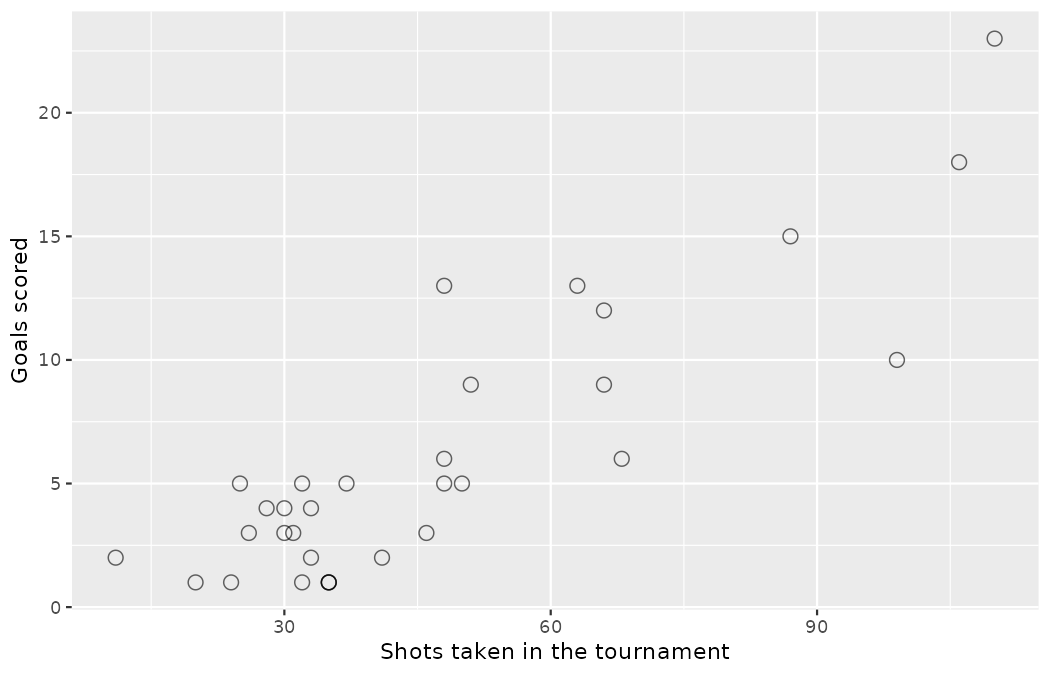
\includegraphics[width=0.85\linewidth,height=\textheight,keepaspectratio]{figures/explore-numerical-1.png}

In any scatterplot, each point represents a single case. Since there are
32 teams in \texttt{team\_totals}, there are 32 points in the
scatterplot. The relationship is clearly positive: teams that generate
more shots score more goals. Argentina, the eventual champions, sit in
the far top-right corner with 110 shots and 23 goals; Costa Rica sit in
the bottom-left with just 11 shots across their three matches. Per the
book's convention of flagging penalty and shoot-out kicks wherever they
matter (recall Chapter~\ref{sec-data-applications}), note that these
totals count period-5 shoot-out kicks as shots --- Argentina's 110 and
23 include 9 shoot-out kicks, 8 of them converted --- so the deep-run
teams' points are pushed up and to the right partly by the shoot-outs
their draws forced. Notice also that the points are not glued to a line
--- Brazil took 99 shots but scored only 10 goals, while Croatia scored
15 from 87. That vertical scatter around the trend is, in scouting
terms, finishing over- and under-performance, and it will get a starring
role when we fit lines in Chapter~\ref{sec-model-slr}.

A scatterplot need not show a straight-line trend to be useful. For a
second example, we change the observational unit again: this time each
case is a \emph{minute on the match clock}. StatsBomb's \texttt{minute}
variable runs continuously, with the second half starting at minute 45,
so we first convert each shot's minute into ``minutes into its half''
and then count shots per clock minute across the regulation halves of
all 64 matches (dropping the 86 shots from extra time and penalty
shoot-outs, periods 3 to 5).

\begin{Shaded}
\begin{Highlighting}[]
\NormalTok{shots\_by\_clock }\OtherTok{\textless{}{-}}\NormalTok{ wc2022\_shots }\SpecialCharTok{|\textgreater{}}
  \FunctionTok{filter}\NormalTok{(period }\SpecialCharTok{\textless{}=} \DecValTok{2}\NormalTok{) }\SpecialCharTok{|\textgreater{}}
  \FunctionTok{mutate}\NormalTok{(}\AttributeTok{clock =} \FunctionTok{if\_else}\NormalTok{(period }\SpecialCharTok{==} \DecValTok{2}\NormalTok{, minute }\SpecialCharTok{{-}} \DecValTok{45}\NormalTok{, minute)) }\SpecialCharTok{|\textgreater{}}
  \FunctionTok{count}\NormalTok{(clock, }\AttributeTok{name =} \StringTok{"shots"}\NormalTok{)}

\FunctionTok{ggplot}\NormalTok{(shots\_by\_clock, }\FunctionTok{aes}\NormalTok{(}\AttributeTok{x =}\NormalTok{ clock, }\AttributeTok{y =}\NormalTok{ shots)) }\SpecialCharTok{+}
  \FunctionTok{geom\_point}\NormalTok{(}\AttributeTok{alpha =} \FloatTok{0.6}\NormalTok{, }\AttributeTok{shape =} \DecValTok{21}\NormalTok{, }\AttributeTok{size =} \DecValTok{3}\NormalTok{) }\SpecialCharTok{+}
  \FunctionTok{geom\_smooth}\NormalTok{(}\AttributeTok{linetype =} \StringTok{"dashed"}\NormalTok{, }\AttributeTok{se =} \ConstantTok{FALSE}\NormalTok{) }\SpecialCharTok{+}
  \FunctionTok{labs}\NormalTok{(}
    \AttributeTok{x =} \StringTok{"Minutes into the half"}\NormalTok{,}
    \AttributeTok{y =} \StringTok{"Shots across all regulation halves"}
\NormalTok{  )}
\end{Highlighting}
\end{Shaded}

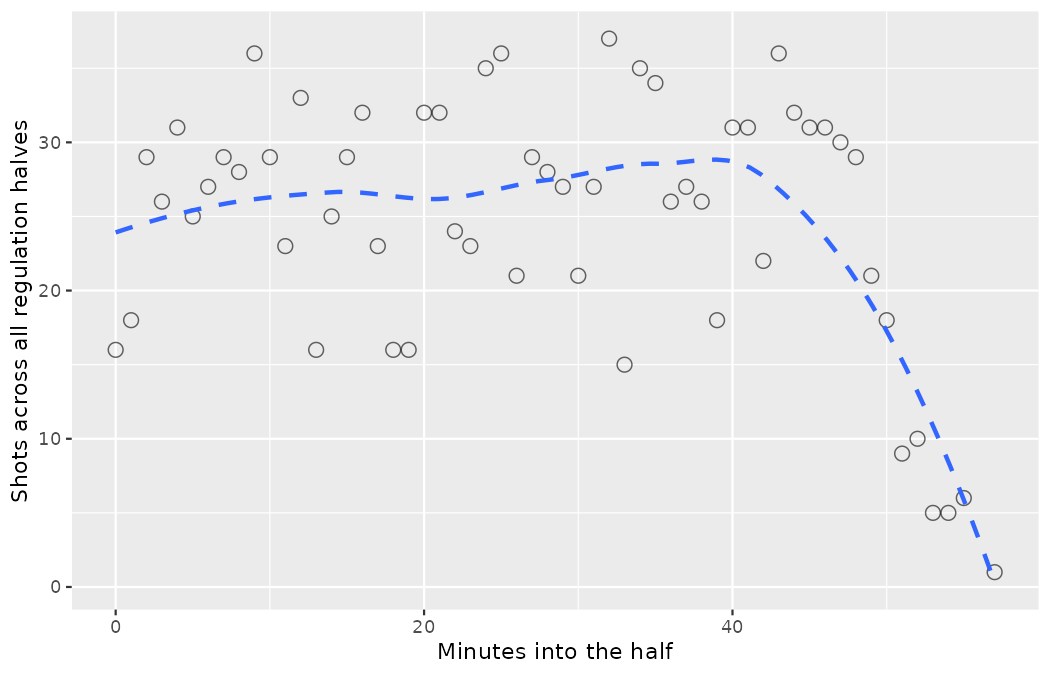
\includegraphics[width=0.85\linewidth,height=\textheight,keepaspectratio]{figures/explore-numerical-2.png}

\begin{tcolorbox}[enhanced jigsaw, left=2mm, leftrule=.75mm, title=\textcolor{quarto-callout-note-color}{\faInfo}\hspace{0.5em}{Worked example}, arc=.35mm, rightrule=.15mm, coltitle=black, colframe=quarto-callout-note-color-frame, bottomrule=.15mm, colbacktitle=quarto-callout-note-color!10!white, opacitybacktitle=0.6, breakable, bottomtitle=1mm, toptitle=1mm, titlerule=0mm, opacityback=0, toprule=.15mm, colback=white]

The plot drawn by the code above shows the number of shots logged in
each minute-of-the-half, pooled across both halves of all 64 matches.
What can be said about the relationship between these variables?

\begin{center}\rule{0.5\linewidth}{0.5pt}\end{center}

The relationship is evidently \textbf{nonlinear}, as highlighted by the
dashed smoothing line. Shot counts bounce around a roughly constant
level --- between about 15 and 37 shots per minute --- throughout the
regulation 45 minutes and even hold that level through the first three
or four added minutes, and then fall away steeply: 21 shots in minute
49, 9 in minute 51, and a single shot at minute 57, because
progressively fewer halves last that long. A straight line would be a
terrible description of this pattern. This is different from the
team-level shots-versus-goals scatterplot, which showed very little, if
any, curvature in its trend.

\end{tcolorbox}

\begin{tcolorbox}[enhanced jigsaw, left=2mm, leftrule=.75mm, title=\textcolor{quarto-callout-tip-color}{\faLightbulb}\hspace{0.5em}{Check your understanding}, arc=.35mm, rightrule=.15mm, coltitle=black, colframe=quarto-callout-tip-color-frame, bottomrule=.15mm, colbacktitle=quarto-callout-tip-color!10!white, opacitybacktitle=0.6, breakable, bottomtitle=1mm, toptitle=1mm, titlerule=0mm, opacityback=0, toprule=.15mm, colback=white]

What do scatterplots reveal about the data, and how are they useful?

\begin{center}\rule{0.5\linewidth}{0.5pt}\end{center}

Answers may vary. Scatterplots are helpful in quickly spotting
associations relating variables, whether those associations come in the
form of simple trends or whether those relationships are more complex
--- for a scout, they are the fastest way to see whether two aspects of
performance move together.

\end{tcolorbox}

\begin{tcolorbox}[enhanced jigsaw, left=2mm, leftrule=.75mm, title=\textcolor{quarto-callout-tip-color}{\faLightbulb}\hspace{0.5em}{Check your understanding}, arc=.35mm, rightrule=.15mm, coltitle=black, colframe=quarto-callout-tip-color-frame, bottomrule=.15mm, colbacktitle=quarto-callout-tip-color!10!white, opacitybacktitle=0.6, breakable, bottomtitle=1mm, toptitle=1mm, titlerule=0mm, opacityback=0, toprule=.15mm, colback=white]

Describe two variables that would have a horseshoe-shaped association in
a scatterplot \((\cap\) or \(\frown).\)

\begin{center}\rule{0.5\linewidth}{0.5pt}\end{center}

Consider the case where your vertical axis represents something ``good''
and your horizontal axis represents something that is only good up to a
point. A player's age and their transfer value fit this description:
value tends to rise through a player's early twenties, peak in the
mid-twenties, and decline thereafter. Weekly training load and match-day
sprint performance work too: too little load leaves a player
undercooked, too much leaves them fatigued or injured.

\end{tcolorbox}

\section{Dot plots and the mean}\label{sec-dotplots}

Sometimes we are interested in the distribution of a single variable. In
these cases, a dot plot provides the most basic of displays. A
\textbf{dot plot} is a one-variable scatterplot; an example using the
chance quality of the 50 shots in \texttt{shots50} is drawn by the code
below.

\begin{Shaded}
\begin{Highlighting}[]
\FunctionTok{ggplot}\NormalTok{(shots50, }\FunctionTok{aes}\NormalTok{(}\AttributeTok{x =}\NormalTok{ statsbomb\_xg)) }\SpecialCharTok{+}
  \FunctionTok{geom\_dotplot}\NormalTok{(}\AttributeTok{binwidth =} \FloatTok{0.02}\NormalTok{) }\SpecialCharTok{+}
  \FunctionTok{labs}\NormalTok{(}\AttributeTok{x =} \StringTok{"Chance quality (xG)"}\NormalTok{, }\AttributeTok{y =} \ConstantTok{NULL}\NormalTok{) }\SpecialCharTok{+}
  \FunctionTok{theme}\NormalTok{(}
    \AttributeTok{axis.text.y =} \FunctionTok{element\_blank}\NormalTok{(),}
    \AttributeTok{axis.ticks.y =} \FunctionTok{element\_blank}\NormalTok{()}
\NormalTok{  )}
\end{Highlighting}
\end{Shaded}

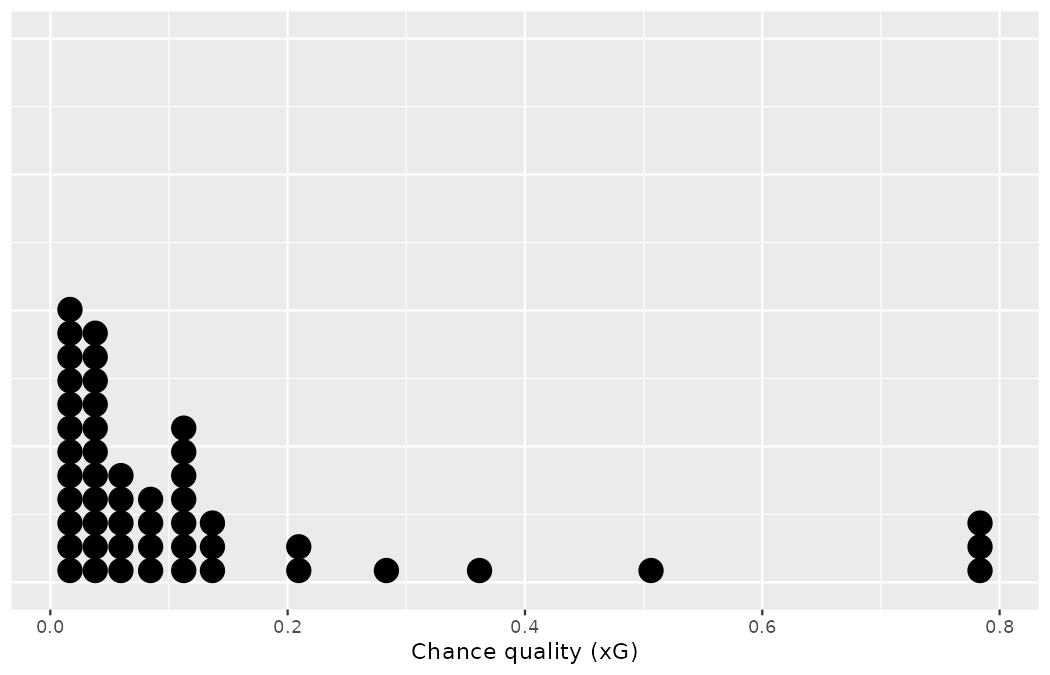
\includegraphics[width=0.85\linewidth,height=\textheight,keepaspectratio]{figures/explore-numerical-3.png}

The dots pile up heavily below 0.10 xG, thin out quickly to the right,
and three isolated dots sit far out at 0.78 --- we will meet those three
shots again shortly.

The \textbf{mean}, often called the \textbf{average}, is a common way to
measure the center of a \textbf{distribution} of data. To compute the
mean chance quality, we add up all 50 xG values and divide by the number
of observations:

\begin{Shaded}
\begin{Highlighting}[]
\NormalTok{shots50 }\SpecialCharTok{|\textgreater{}}
  \FunctionTok{summarize}\NormalTok{(}\AttributeTok{n =} \FunctionTok{n}\NormalTok{(), }\AttributeTok{mean\_xg =} \FunctionTok{mean}\NormalTok{(statsbomb\_xg))}
\CommentTok{\#\textgreater{} \# A tibble: 1 × 2}
\CommentTok{\#\textgreater{}       n mean\_xg}
\CommentTok{\#\textgreater{}   \textless{}int\textgreater{}   \textless{}dbl\textgreater{}}
\CommentTok{\#\textgreater{} 1    50   0.127}
\end{Highlighting}
\end{Shaded}

The sample mean is often labeled \(\bar{x}.\) Take the symbol apart
before using it: the letter \(x\) is a generic placeholder for the
variable of interest --- here, a shot's xG value --- and the bar drawn
over the \(x\) (read ``x-bar'') communicates that we have averaged those
values. For these 50 shots, \(\bar{x} = 0.127\) xG. It is useful to
think of the mean as the balancing point of the distribution: if the dot
plot were a plank with the dots as weights, it would balance at 0.127.

\begin{tcolorbox}[enhanced jigsaw, left=2mm, leftrule=.75mm, title=\textcolor{quarto-callout-important-color}{\faExclamation}\hspace{0.5em}{Mean}, arc=.35mm, rightrule=.15mm, coltitle=black, colframe=quarto-callout-important-color-frame, bottomrule=.15mm, colbacktitle=quarto-callout-important-color!10!white, opacitybacktitle=0.6, breakable, bottomtitle=1mm, toptitle=1mm, titlerule=0mm, opacityback=0, toprule=.15mm, colback=white]

The sample mean can be calculated as the sum of the observed values
divided by the number of observations:

\[ \bar{x} = \frac{x_1 + x_2 + \cdots + x_n}{n} \]

\end{tcolorbox}

Three more pieces of notation appear in that formula, and each deserves
a plain-words reading before we move on. The subscript in \(x_1\)
indexes \emph{which observation} we mean: \(x_1\) is the first shot's xG
value, \(x_2\) the second's. The letter \(n\) denotes the \emph{sample
size} --- the number of observations we have. And the general symbol
\(x_i\) uses the placeholder index \(i\) to stand for ``the \(i^{th}\)
observation, whichever one we happen to be pointing at.''

\begin{tcolorbox}[enhanced jigsaw, left=2mm, leftrule=.75mm, title=\textcolor{quarto-callout-tip-color}{\faLightbulb}\hspace{0.5em}{Check your understanding}, arc=.35mm, rightrule=.15mm, coltitle=black, colframe=quarto-callout-tip-color-frame, bottomrule=.15mm, colbacktitle=quarto-callout-tip-color!10!white, opacitybacktitle=0.6, breakable, bottomtitle=1mm, toptitle=1mm, titlerule=0mm, opacityback=0, toprule=.15mm, colback=white]

Examine the equation for the mean. What does \(x_1\) correspond to? And
\(x_2\)? Can you infer a general meaning to what \(x_i\) might
represent?

\begin{center}\rule{0.5\linewidth}{0.5pt}\end{center}

\(x_1\) corresponds to the chance quality of the first shot in the
sample, \(x_2\) to the second shot's chance quality, and \(x_i\)
corresponds to the xG value of the \(i^{th}\) shot in the dataset. For
example, if \(i = 4,\) then we are examining \(x_4,\) which refers to
the fourth shot in the dataset.

\end{tcolorbox}

\begin{tcolorbox}[enhanced jigsaw, left=2mm, leftrule=.75mm, title=\textcolor{quarto-callout-tip-color}{\faLightbulb}\hspace{0.5em}{Check your understanding}, arc=.35mm, rightrule=.15mm, coltitle=black, colframe=quarto-callout-tip-color-frame, bottomrule=.15mm, colbacktitle=quarto-callout-tip-color!10!white, opacitybacktitle=0.6, breakable, bottomtitle=1mm, toptitle=1mm, titlerule=0mm, opacityback=0, toprule=.15mm, colback=white]

What was \(n\) in this sample of shots?

\begin{center}\rule{0.5\linewidth}{0.5pt}\end{center}

The sample size was \(n = 50.\)

\end{tcolorbox}

The \texttt{shots50} dataset is a random sample from a larger population
of shots --- the full 2022 World Cup. We could compute a mean for the
entire population in the same way as the sample mean. However, the
population mean has a special label: \(\mu.\) The symbol \(\mu\) is the
Greek letter \emph{mu} (pronounced ``mew'') and represents the average
of all observations in the population. Sometimes a subscript, such as
\(_x,\) is used to represent which variable the population mean refers
to, e.g., \(\mu_x.\) Oftentimes it is too expensive --- or, for a scout,
physically impossible --- to measure the population mean precisely:
nobody watches every shot in every league. So we typically estimate
\(\mu\) using the sample mean, \(\bar{x}.\)

\begin{tcolorbox}[enhanced jigsaw, left=2mm, leftrule=.75mm, title=\textcolor{quarto-callout-note-color}{\faInfo}\hspace{0.5em}{Worked example}, arc=.35mm, rightrule=.15mm, coltitle=black, colframe=quarto-callout-note-color-frame, bottomrule=.15mm, colbacktitle=quarto-callout-note-color!10!white, opacitybacktitle=0.6, breakable, bottomtitle=1mm, toptitle=1mm, titlerule=0mm, opacityback=0, toprule=.15mm, colback=white]

Although a scout in the stands cannot \emph{calculate} the average
chance quality across all shots of a tournament from the handful they
saw, they can \emph{estimate} it using their sample. Based on the sample
of 50 shots, what would be a reasonable estimate of \(\mu_x,\) the mean
xG of all shots in the tournament?

\begin{center}\rule{0.5\linewidth}{0.5pt}\end{center}

The sample mean, 0.127, provides a rough estimate of \(\mu_x.\) While it
is not perfect, this is our single best guess --- our \textbf{point
estimate} --- of the average chance quality of all the shots in the
population under study. In Chapter~\ref{sec-foundations-randomization}
and beyond, we will develop tools to characterize the accuracy of point
estimates, like the sample mean. As you might have guessed, point
estimates based on larger samples tend to be more accurate than those
based on smaller samples.

Our data grant us a luxury a working scout rarely has: the population is
fully logged, so we can check.

\begin{Shaded}
\begin{Highlighting}[]
\NormalTok{wc2022\_shots }\SpecialCharTok{|\textgreater{}}
  \FunctionTok{summarize}\NormalTok{(}\AttributeTok{n =} \FunctionTok{n}\NormalTok{(), }\AttributeTok{mean\_xg =} \FunctionTok{mean}\NormalTok{(statsbomb\_xg))}
\CommentTok{\#\textgreater{} \# A tibble: 1 × 2}
\CommentTok{\#\textgreater{}       n mean\_xg}
\CommentTok{\#\textgreater{}   \textless{}int\textgreater{}   \textless{}dbl\textgreater{}}
\CommentTok{\#\textgreater{} 1  1494   0.126}
\end{Highlighting}
\end{Shaded}

The true tournament mean is \(\mu_x = 0.126\) xG per shot --- our
50-shot point estimate of 0.127 landed remarkably close. Do not expect
to be so lucky every time; quantifying how lucky is the business of
Chapter~\ref{sec-foundations-randomization}.

\end{tcolorbox}

The mean is useful because it allows us to rescale or standardize a
metric into something more easily interpretable and comparable. Suppose
Priya Rao, Northbridge United's lead data analyst, wants to know whether
a newly designed scout-report template produces fewer factual errors
than the club's standard template. This is a constructed Northbridge
scenario, but the arithmetic trap it illustrates is one analysts fall
into weekly. A trial of 1,500 player evaluations is set up, where 500
evaluations are filed on the new template and 1,000 on the standard
template in the comparison group. Data-quality staff then count every
factual error (wrong club, wrong foot, misattributed goal) in each
batch:

\begin{Shaded}
\begin{Highlighting}[]
\NormalTok{template\_trial }\OtherTok{\textless{}{-}} \FunctionTok{tribble}\NormalTok{(}
  \SpecialCharTok{\textasciitilde{}}\NormalTok{metric,                  }\SpecialCharTok{\textasciitilde{}}\StringTok{\textasciigrave{}}\AttributeTok{new template}\StringTok{\textasciigrave{}}\NormalTok{, }\SpecialCharTok{\textasciitilde{}}\StringTok{\textasciigrave{}}\AttributeTok{standard template}\StringTok{\textasciigrave{}}\NormalTok{,}
  \StringTok{"Evaluations filed"}\NormalTok{,                  }\DecValTok{500}\NormalTok{,                 }\DecValTok{1000}\NormalTok{,}
  \StringTok{"Total factual errors"}\NormalTok{,               }\DecValTok{200}\NormalTok{,                  }\DecValTok{300}
\NormalTok{)}

\NormalTok{template\_trial}
\CommentTok{\#\textgreater{} \# A tibble: 2 × 3}
\CommentTok{\#\textgreater{}   metric               \textasciigrave{}new template\textasciigrave{} \textasciigrave{}standard template\textasciigrave{}}
\CommentTok{\#\textgreater{}   \textless{}chr\textgreater{}                         \textless{}dbl\textgreater{}               \textless{}dbl\textgreater{}}
\CommentTok{\#\textgreater{} 1 Evaluations filed               500                1000}
\CommentTok{\#\textgreater{} 2 Total factual errors            200                 300}
\end{Highlighting}
\end{Shaded}

Comparing the raw counts of 200 to 300 errors would make it appear that
the new template is better, but this is an artifact of the imbalanced
group sizes.

Instead, we should look at the average number of errors per evaluation
in each group:

\begin{itemize}
\tightlist
\item
  New template: \(200 / 500 = 0.4\) errors per evaluation
\item
  Standard template: \(300 / 1000 = 0.3\) errors per evaluation
\end{itemize}

The standard template has a \emph{lower} average number of errors per
evaluation than the new template. The raw counts pointed in exactly the
wrong direction.

\begin{tcolorbox}[enhanced jigsaw, left=2mm, leftrule=.75mm, title=\textcolor{quarto-callout-note-color}{\faInfo}\hspace{0.5em}{Worked example}, arc=.35mm, rightrule=.15mm, coltitle=black, colframe=quarto-callout-note-color-frame, bottomrule=.15mm, colbacktitle=quarto-callout-note-color!10!white, opacitybacktitle=0.6, breakable, bottomtitle=1mm, toptitle=1mm, titlerule=0mm, opacityback=0, toprule=.15mm, colback=white]

Come up with another example where the mean is useful for making
comparisons.

\begin{center}\rule{0.5\linewidth}{0.5pt}\end{center}

Emil Sørensen, Northbridge's head of scouting, reviews the travel logs
of his regional scouts at the end of each season. One scout covered
11,000 km of travel across 625 logged working hours. The scout's average
distance per working hour puts that workload into a standard unit that
can be compared across the whole 48-scout network:

\[ \frac{11000\text{ km}}{625\text{ hours}} = 17.6\text{ km per hour} \]

By standardizing to kilometers per working hour, Emil can compare scouts
assigned to compact city regions against scouts covering entire
countries, something the raw totals hide.

\end{tcolorbox}

\begin{tcolorbox}[enhanced jigsaw, left=2mm, leftrule=.75mm, title=\textcolor{quarto-callout-note-color}{\faInfo}\hspace{0.5em}{Worked example}, arc=.35mm, rightrule=.15mm, coltitle=black, colframe=quarto-callout-note-color-frame, bottomrule=.15mm, colbacktitle=quarto-callout-note-color!10!white, opacitybacktitle=0.6, breakable, bottomtitle=1mm, toptitle=1mm, titlerule=0mm, opacityback=0, toprule=.15mm, colback=white]

Suppose we want to compute the average chance quality per shot across
the whole 2022 World Cup. Each team's showing in each match can be
summarized as one row --- a \emph{team-match} --- and it is tempting to
average the per-team-match mean xG values. What would be a better
approach?

\begin{center}\rule{0.5\linewidth}{0.5pt}\end{center}

Let us first build the team-match data, because we will use it many
times in this book. The code below aggregates \texttt{wc2022\_shots}
into one row per (match, team): the number of shots, the total and
per-shot chance quality, the goals scored, and two mix shares --- the
proportion of shots taken under pressure and the proportion arising from
dead-ball situations (corners, free kicks, and throw-ins).

\begin{Shaded}
\begin{Highlighting}[]
\NormalTok{team\_match }\OtherTok{\textless{}{-}}\NormalTok{ wc2022\_shots }\SpecialCharTok{|\textgreater{}}
  \FunctionTok{group\_by}\NormalTok{(match\_id, team) }\SpecialCharTok{|\textgreater{}}
  \FunctionTok{summarize}\NormalTok{(}
    \AttributeTok{n\_shots =} \FunctionTok{n}\NormalTok{(),}
    \AttributeTok{total\_xg =} \FunctionTok{sum}\NormalTok{(statsbomb\_xg),}
    \AttributeTok{goals =} \FunctionTok{sum}\NormalTok{(goal),}
    \AttributeTok{prop\_under\_pressure =} \FunctionTok{mean}\NormalTok{(under\_pressure),}
    \AttributeTok{prop\_set\_piece =} \FunctionTok{mean}\NormalTok{(play\_pattern }\SpecialCharTok{\%in\%}
      \FunctionTok{c}\NormalTok{(}\StringTok{"From Corner"}\NormalTok{, }\StringTok{"From Free Kick"}\NormalTok{, }\StringTok{"From Throw In"}\NormalTok{)),}
    \AttributeTok{.groups =} \StringTok{"drop"}
\NormalTok{  )}

\FunctionTok{nrow}\NormalTok{(team\_match)}
\CommentTok{\#\textgreater{} [1] 127}
\end{Highlighting}
\end{Shaded}

Note the row count: 64 matches involve \(64 \times 2 = 128\)
team-matches, but \texttt{team\_match} has only 127 rows. Costa Rica
registered \emph{no shots at all} away to Spain in the 7--0 group-stage
defeat, so that team-match simply has no shot rows to aggregate. Keep
this missing row in mind whenever you use \texttt{team\_match}.

The \texttt{team\_match} rows are special in that each row actually
represents many individual shots --- anywhere from 2 (the Netherlands,
in one of their group games) to 31 (Germany, against Costa Rica). If we
were to simply average the per-team-match mean xG values, we would be
treating a 2-shot outing and a 31-shot barrage equally in the
calculations. Instead, we should compute the total xG across all
team-matches and divide by the total number of shots --- which is
exactly the pooled mean over all 1,494 shots.

\begin{Shaded}
\begin{Highlighting}[]
\NormalTok{team\_match }\SpecialCharTok{|\textgreater{}}
  \FunctionTok{summarize}\NormalTok{(}
    \AttributeTok{unweighted =} \FunctionTok{mean}\NormalTok{(total\_xg }\SpecialCharTok{/}\NormalTok{ n\_shots),}
    \AttributeTok{pooled =} \FunctionTok{sum}\NormalTok{(total\_xg) }\SpecialCharTok{/} \FunctionTok{sum}\NormalTok{(n\_shots)}
\NormalTok{  )}
\CommentTok{\#\textgreater{} \# A tibble: 1 × 2}
\CommentTok{\#\textgreater{}   unweighted pooled}
\CommentTok{\#\textgreater{}        \textless{}dbl\textgreater{}  \textless{}dbl\textgreater{}}
\CommentTok{\#\textgreater{} 1      0.119  0.126}
\end{Highlighting}
\end{Shaded}

The pooled tournament mean is 0.126 xG per shot; the simple average of
the 127 team-match means is only 0.119. The two disagree because
high-volume team-matches tend to feature slightly better average
chances, and the simple average refuses to give them the extra weight
their shot counts deserve.

This example used what is called a \textbf{weighted mean}: each
team-match's mean was weighted by its number of shots.

\end{tcolorbox}

\begin{tcolorbox}[enhanced jigsaw, left=2mm, leftrule=.75mm, title=\textcolor{quarto-callout-tip-color}{\faLightbulb}\hspace{0.5em}{Check your understanding}, arc=.35mm, rightrule=.15mm, coltitle=black, colframe=quarto-callout-tip-color-frame, bottomrule=.15mm, colbacktitle=quarto-callout-tip-color!10!white, opacitybacktitle=0.6, breakable, bottomtitle=1mm, toptitle=1mm, titlerule=0mm, opacityback=0, toprule=.15mm, colback=white]

In the weighted-mean example, which teams' performances are
\emph{over-weighted} by the naive unweighted average of team-match
means?

\begin{center}\rule{0.5\linewidth}{0.5pt}\end{center}

Team-matches with very few shots --- like Costa Rica's low-volume
outings or the Netherlands' 2-shot match --- count exactly as much as
Germany's 31-shot performance in the unweighted average, so low-volume
team-matches are over-weighted relative to their actual contribution to
the tournament's shots.

\end{tcolorbox}

\section{Histograms and shape}\label{sec-histograms}

Dot plots show the exact value for each observation. They are useful for
small datasets but can become hard to read with larger samples --- try
dot-plotting all 1,494 World Cup shots. Rather than showing the value of
each observation, we prefer to think of the value as belonging to a
\emph{bin}. For example, in the \texttt{shots50} sample, we can create a
table of counts for the number of shots with chance quality between 0
and 0.1 xG, then the number with chance quality between 0.1 and 0.2, and
so on. Observations that fall on the boundary of a bin (e.g., exactly
0.10) are allocated to the lower bin.

\begin{Shaded}
\begin{Highlighting}[]
\NormalTok{shots50 }\SpecialCharTok{|\textgreater{}}
  \FunctionTok{mutate}\NormalTok{(}\AttributeTok{xg\_bin =} \FunctionTok{cut}\NormalTok{(statsbomb\_xg, }\AttributeTok{breaks =} \FunctionTok{seq}\NormalTok{(}\DecValTok{0}\NormalTok{, }\FloatTok{0.8}\NormalTok{, }\FloatTok{0.1}\NormalTok{))) }\SpecialCharTok{|\textgreater{}}
  \FunctionTok{count}\NormalTok{(xg\_bin, }\AttributeTok{name =} \StringTok{"shots"}\NormalTok{, }\AttributeTok{.drop =} \ConstantTok{FALSE}\NormalTok{)}
\CommentTok{\#\textgreater{} \# A tibble: 8 × 2}
\CommentTok{\#\textgreater{}   xg\_bin    shots}
\CommentTok{\#\textgreater{}   \textless{}fct\textgreater{}     \textless{}int\textgreater{}}
\CommentTok{\#\textgreater{} 1 (0,0.1]      32}
\CommentTok{\#\textgreater{} 2 (0.1,0.2]    10}
\CommentTok{\#\textgreater{} 3 (0.2,0.3]     3}
\CommentTok{\#\textgreater{} 4 (0.3,0.4]     1}
\CommentTok{\#\textgreater{} 5 (0.4,0.5]     0}
\CommentTok{\#\textgreater{} 6 (0.5,0.6]     1}
\CommentTok{\#\textgreater{} 7 (0.6,0.7]     0}
\CommentTok{\#\textgreater{} 8 (0.7,0.8]     3}
\end{Highlighting}
\end{Shaded}

The binned counts are plotted as bars by the code below into what is
called a \textbf{histogram}. Note that the histogram resembles a more
heavily binned version of the stacked dot plot from
Section~\ref{sec-dotplots}.

\begin{Shaded}
\begin{Highlighting}[]
\FunctionTok{ggplot}\NormalTok{(shots50, }\FunctionTok{aes}\NormalTok{(}\AttributeTok{x =}\NormalTok{ statsbomb\_xg)) }\SpecialCharTok{+}
  \FunctionTok{geom\_histogram}\NormalTok{(}\AttributeTok{breaks =} \FunctionTok{seq}\NormalTok{(}\DecValTok{0}\NormalTok{, }\FloatTok{0.8}\NormalTok{, }\FloatTok{0.1}\NormalTok{)) }\SpecialCharTok{+}
  \FunctionTok{labs}\NormalTok{(}\AttributeTok{x =} \StringTok{"Chance quality (xG)"}\NormalTok{, }\AttributeTok{y =} \StringTok{"Count"}\NormalTok{)}
\end{Highlighting}
\end{Shaded}

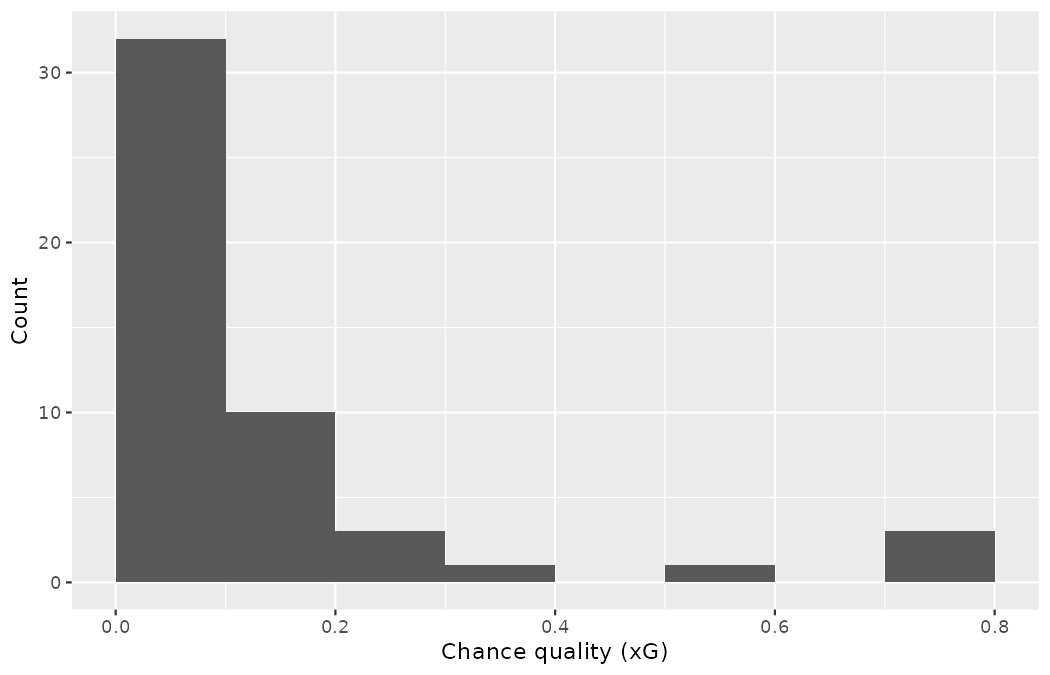
\includegraphics[width=0.85\linewidth,height=\textheight,keepaspectratio]{figures/explore-numerical-4.png}

Histograms provide a view of the \textbf{data density}. Higher bars
represent where the data are relatively more common. For instance, there
are many more shots with chance quality between 0 and 0.1 xG --- 32 of
the 50, nearly two thirds --- than shots between 0.2 and 0.3 in the
sample. The bars make it easy to see how the density of the data changes
relative to the chance quality.

Histograms are especially convenient for understanding the shape of the
data distribution. The histogram suggests that most chances are of low
quality, while only a handful of shots exceed 0.3 xG. When the
distribution of a variable trails off to the right in this way and has a
longer right \textbf{tail}, the shape is said to be \textbf{right
skewed}.\footnote{Other ways to describe data that are right skewed:
  skewed to the right, skewed to the high end, or skewed to the positive
  end.}

\begin{Shaded}
\begin{Highlighting}[]
\FunctionTok{ggplot}\NormalTok{(shots50, }\FunctionTok{aes}\NormalTok{(}\AttributeTok{x =}\NormalTok{ statsbomb\_xg)) }\SpecialCharTok{+}
  \FunctionTok{geom\_density}\NormalTok{(}\AttributeTok{fill =} \StringTok{"grey60"}\NormalTok{, }\AttributeTok{alpha =} \FloatTok{0.5}\NormalTok{) }\SpecialCharTok{+}
  \FunctionTok{labs}\NormalTok{(}\AttributeTok{x =} \StringTok{"Chance quality (xG)"}\NormalTok{, }\AttributeTok{y =} \StringTok{"Density"}\NormalTok{)}
\end{Highlighting}
\end{Shaded}

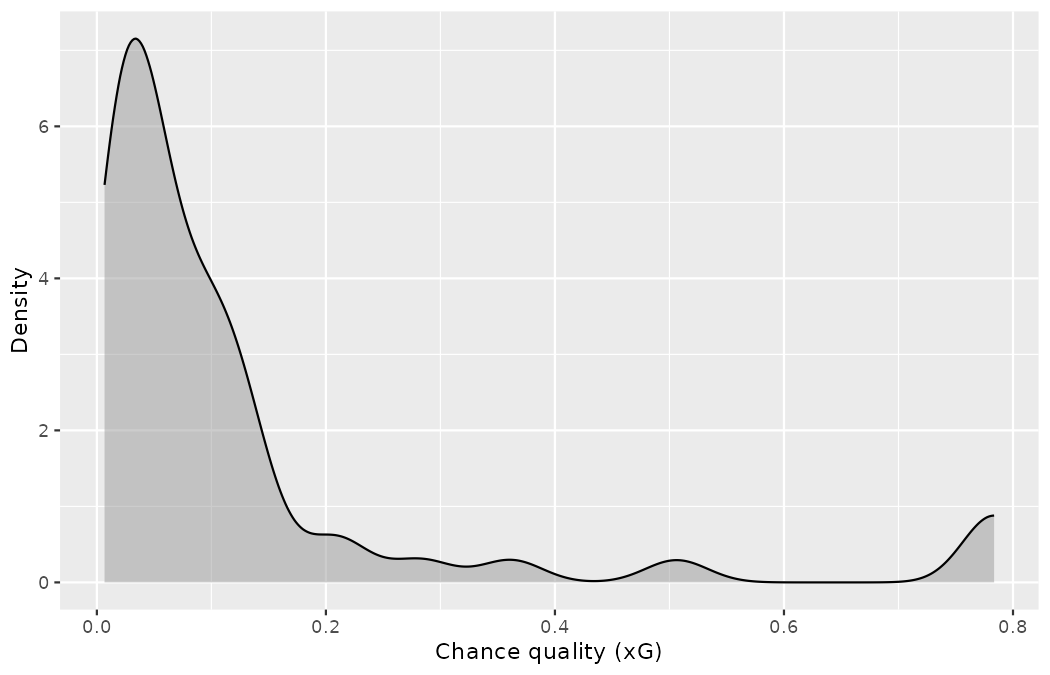
\includegraphics[width=0.85\linewidth,height=\textheight,keepaspectratio]{figures/explore-numerical-5.png}

The code above draws a \textbf{density plot}, which is a smoothed out
histogram. The technical details for how to draw density plots
(precisely how to smooth out the histogram) are beyond the scope of this
text, but you will note that the shape, scale, and spread of the
observations are displayed similarly in a histogram as in a density
plot. For our sample, the density curve rises to a single sharp peak
near 0.03 xG, slides down a long right tail, and shows one last low bump
out near 0.78 --- the three penalties again.

Variables with the reverse characteristic --- a long, thinner tail to
the left --- are said to be \textbf{left skewed}. We also say that such
a distribution has a long left tail. Variables that show roughly equal
trailing off in both directions are called \textbf{symmetric}.
Left-skewed variables are rarer in shooting data than right-skewed ones,
but they exist: think of the proportion of a season's matches a
first-choice goalkeeper starts, which piles up near 1 with a thin tail
of injury-hit seasons trailing left.

\begin{tcolorbox}[enhanced jigsaw, left=2mm, leftrule=.75mm, title=\textcolor{quarto-callout-important-color}{\faExclamation}\hspace{0.5em}{Long tails to identify skew}, arc=.35mm, rightrule=.15mm, coltitle=black, colframe=quarto-callout-important-color-frame, bottomrule=.15mm, colbacktitle=quarto-callout-important-color!10!white, opacitybacktitle=0.6, breakable, bottomtitle=1mm, toptitle=1mm, titlerule=0mm, opacityback=0, toprule=.15mm, colback=white]

When data trail off in one direction, the distribution has a
\textbf{long tail}. If a distribution has a long left tail, it is left
skewed. If a distribution has a long right tail, it is right skewed.

\end{tcolorbox}

\begin{tcolorbox}[enhanced jigsaw, left=2mm, leftrule=.75mm, title=\textcolor{quarto-callout-tip-color}{\faLightbulb}\hspace{0.5em}{Check your understanding}, arc=.35mm, rightrule=.15mm, coltitle=black, colframe=quarto-callout-tip-color-frame, bottomrule=.15mm, colbacktitle=quarto-callout-tip-color!10!white, opacitybacktitle=0.6, breakable, bottomtitle=1mm, toptitle=1mm, titlerule=0mm, opacityback=0, toprule=.15mm, colback=white]

Besides the mean (since it was labeled), what can you see in the dot
plot of the 50 chance qualities that you cannot see in their histogram?

\begin{center}\rule{0.5\linewidth}{0.5pt}\end{center}

The chance quality of each individual shot. The histogram tells you 32
shots fell below 0.1 xG; the dot plot still shows each one of them.

\end{tcolorbox}

In addition to looking at whether a distribution is skewed or symmetric,
histograms can be used to identify modes. A \textbf{mode} is represented
by a prominent peak in the distribution. There is only one prominent
peak in the histogram of the \texttt{shots50} chance qualities.

A definition of \emph{mode} sometimes taught in math classes is the
value with the most occurrences in the dataset. However, for many
real-world datasets --- xG values are recorded to many decimal places
--- it is common to have \emph{no} observations with the same value in a
dataset, making this definition impractical in data analysis.

The code below draws histograms that have one, two, or three prominent
peaks. Such distributions are called \textbf{unimodal},
\textbf{bimodal}, and \textbf{multimodal}, respectively. Any
distribution with more than two prominent peaks is called multimodal.
The three datasets are constructed --- Priya keeps a set of these
fabricated distributions on hand for training Northbridge's junior
analysts --- and the seeded code below rebuilds them exactly.

\begin{Shaded}
\begin{Highlighting}[]
\FunctionTok{set.seed}\NormalTok{(}\DecValTok{503}\NormalTok{)}
\NormalTok{constructed\_modes }\OtherTok{\textless{}{-}} \FunctionTok{tibble}\NormalTok{(}
  \AttributeTok{metric\_a =} \FunctionTok{rchisq}\NormalTok{(}\DecValTok{65}\NormalTok{, }\DecValTok{6}\NormalTok{),}
  \AttributeTok{metric\_b =} \FunctionTok{c}\NormalTok{(}\FunctionTok{rchisq}\NormalTok{(}\DecValTok{25}\NormalTok{, }\FloatTok{5.8}\NormalTok{), }\FunctionTok{rnorm}\NormalTok{(}\DecValTok{40}\NormalTok{, }\DecValTok{20}\NormalTok{, }\DecValTok{2}\NormalTok{)),}
  \AttributeTok{metric\_c =} \FunctionTok{c}\NormalTok{(}\FunctionTok{rchisq}\NormalTok{(}\DecValTok{25}\NormalTok{, }\DecValTok{3}\NormalTok{), }\FunctionTok{rnorm}\NormalTok{(}\DecValTok{25}\NormalTok{, }\DecValTok{15}\NormalTok{), }\FunctionTok{rnorm}\NormalTok{(}\DecValTok{15}\NormalTok{, }\DecValTok{25}\NormalTok{, }\FloatTok{1.5}\NormalTok{))}
\NormalTok{)}

\NormalTok{constructed\_modes }\SpecialCharTok{|\textgreater{}}
  \FunctionTok{pivot\_longer}\NormalTok{(}\FunctionTok{everything}\NormalTok{(), }\AttributeTok{names\_to =} \StringTok{"metric"}\NormalTok{, }\AttributeTok{values\_to =} \StringTok{"value"}\NormalTok{) }\SpecialCharTok{|\textgreater{}}
  \FunctionTok{ggplot}\NormalTok{(}\FunctionTok{aes}\NormalTok{(}\AttributeTok{x =}\NormalTok{ value)) }\SpecialCharTok{+}
  \FunctionTok{geom\_histogram}\NormalTok{(}\AttributeTok{binwidth =} \DecValTok{2}\NormalTok{, }\AttributeTok{boundary =} \DecValTok{0}\NormalTok{) }\SpecialCharTok{+}
  \FunctionTok{facet\_wrap}\NormalTok{(}\SpecialCharTok{\textasciitilde{}}\NormalTok{metric, }\AttributeTok{nrow =} \DecValTok{1}\NormalTok{) }\SpecialCharTok{+}
  \FunctionTok{labs}\NormalTok{(}\AttributeTok{x =} \ConstantTok{NULL}\NormalTok{, }\AttributeTok{y =} \ConstantTok{NULL}\NormalTok{)}
\end{Highlighting}
\end{Shaded}

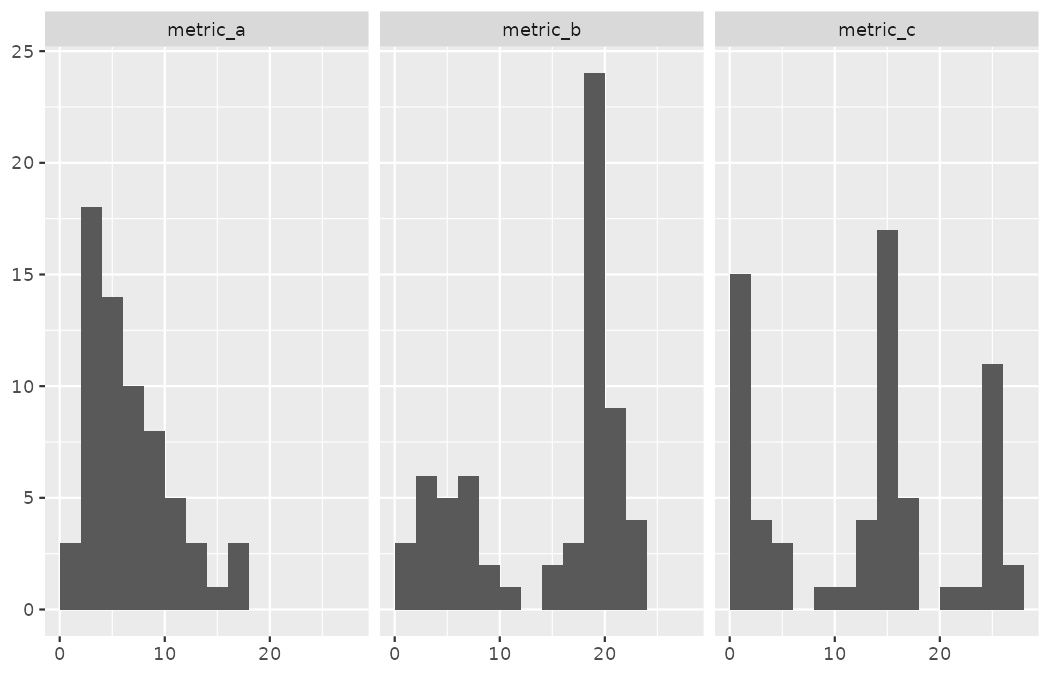
\includegraphics[width=0.85\linewidth,height=\textheight,keepaspectratio]{figures/explore-numerical-6.png}

With this seed, \texttt{metric\_a} rises to one prominent peak (18
observations in its tallest bar, just below the value 4) and trails off
to the right --- unimodal. \texttt{metric\_b} has a cluster of small
values and a second, dominant peak near 20 (24 observations in that bar)
--- bimodal. \texttt{metric\_c} shows three separated clumps, with tall
bars near 0, near 15, and near 25 --- multimodal. Notice that
\texttt{metric\_a} has some minor bumps on its way down the right tail
that we did not count, since each differs from its neighboring bins by
only a few observations: we count \emph{prominent} peaks, not just any
peak.

\begin{tcolorbox}[enhanced jigsaw, left=2mm, leftrule=.75mm, title=\textcolor{quarto-callout-note-color}{\faInfo}\hspace{0.5em}{Worked example}, arc=.35mm, rightrule=.15mm, coltitle=black, colframe=quarto-callout-note-color-frame, bottomrule=.15mm, colbacktitle=quarto-callout-note-color!10!white, opacitybacktitle=0.6, breakable, bottomtitle=1mm, toptitle=1mm, titlerule=0mm, opacityback=0, toprule=.15mm, colback=white]

The histogram of the \texttt{shots50} chance qualities reveals only one
prominent mode. Is the distribution unimodal, bimodal, or multimodal?

\begin{center}\rule{0.5\linewidth}{0.5pt}\end{center}

Recall the prefixes: \emph{uni-} denotes one prominent peak, \emph{bi-}
two, and \emph{multi-} more than two. With a single prominent peak, the
distribution is unimodal.

\end{tcolorbox}

\begin{tcolorbox}[enhanced jigsaw, left=2mm, leftrule=.75mm, title=\textcolor{quarto-callout-tip-color}{\faLightbulb}\hspace{0.5em}{Check your understanding}, arc=.35mm, rightrule=.15mm, coltitle=black, colframe=quarto-callout-tip-color-frame, bottomrule=.15mm, colbacktitle=quarto-callout-tip-color!10!white, opacitybacktitle=0.6, breakable, bottomtitle=1mm, toptitle=1mm, titlerule=0mm, opacityback=0, toprule=.15mm, colback=white]

Northbridge's academy holds an open day where the heights of everyone on
the pitch --- the under-15 trialists and the adult coaching staff ---
are measured for kit ordering. How many modes would you expect in this
height dataset?

\begin{center}\rule{0.5\linewidth}{0.5pt}\end{center}

There might be two height groups visible in the dataset: the young
trialists and the adult coaches. That is, the data are probably bimodal.

\end{tcolorbox}

Looking for modes isn't about finding a clear and correct answer about
the number of modes in a distribution, which is why \emph{prominent} is
not rigorously defined in this book. The most important part of this
examination is to better understand your data.

\section{Variance and standard deviation}\label{sec-variance-sd}

The mean was introduced as a method to describe the center of a
variable, and \textbf{variability} in the data is also important. A
striker whose chance quality is steady around 0.12 xG per shot and a
striker who mixes tap-ins with 30-yard speculative efforts can share the
same mean while being entirely different scouting propositions. Here, we
introduce two measures of variability: the variance and the standard
deviation. Both of these are very useful in data analysis, even though
their formulas are a bit tedious to calculate by hand. The standard
deviation is the easier of the two to comprehend, as it roughly
describes how far away the typical observation is from the mean.

We call the distance of an observation from its mean its
\textbf{deviation}. Below are the deviations for the \(1^{st},\)
\(2^{nd},\) \(3^{rd},\) and \(50^{th}\) shots in the \texttt{shots50}
sample, working to four decimal places (the sample mean is
\(\bar{x} = 0.1271\)):

\[
\begin{aligned}
x_1 - \bar{x} &= 0.0067 - 0.1271 = -0.1204 \\
x_2 - \bar{x} &= 0.0810 - 0.1271 = -0.0461 \\
x_3 - \bar{x} &= 0.0085 - 0.1271 = -0.1186 \\
&\vdots \\
x_{50} - \bar{x} &= 0.0420 - 0.1271 = -0.0851 \\
\end{aligned}
\]

If we square these deviations and then take an average, the result is
equal to the sample \textbf{variance}, denoted by \(s^2.\) Read the
symbol as two parts: the letter \(s\) is reserved for a sample's spread,
and the superscript \(2\) reminds us that the deviations have been
\emph{squared} on the way in.

\[
s^2 = \frac{(-0.1204)^2 + (-0.0461)^2 + \cdots + (-0.0851)^2}{50 - 1} = \frac{0.0145 + 0.0021 + \cdots + 0.0072}{49} = 0.0367
\]

We divide by \(n - 1,\) rather than dividing by \(n,\) when computing a
sample's variance. There's some mathematical nuance here, but the end
result is that doing this makes this statistic slightly more reliable
and useful. The honest accounting of that nuance arrives in
Chapter~\ref{sec-inference-one-mean}, where the same \(n - 1\)
resurfaces as a distribution's degrees of freedom --- and finally gets
its explanation.

Notice that squaring the deviations does two things. First, it makes
large values relatively much larger --- the three 0.78-xG penalties
dominate this sum. Second, it gets rid of any negative signs.

\begin{tcolorbox}[enhanced jigsaw, left=2mm, leftrule=.75mm, title=\textcolor{quarto-callout-important-color}{\faExclamation}\hspace{0.5em}{Standard deviation}, arc=.35mm, rightrule=.15mm, coltitle=black, colframe=quarto-callout-important-color-frame, bottomrule=.15mm, colbacktitle=quarto-callout-important-color!10!white, opacitybacktitle=0.6, breakable, bottomtitle=1mm, toptitle=1mm, titlerule=0mm, opacityback=0, toprule=.15mm, colback=white]

The sample standard deviation can be calculated as the square root of
the sum of the squared distance of each value from the mean divided by
the number of observations minus one:

\[s = \sqrt{\frac{\sum_{i=1}^n (x_i - \bar{x})^2}{n-1}}\]

\end{tcolorbox}

One new symbol appears in that formula and it will follow us for the
rest of the book, so take it apart now. The capital Greek letter
\(\Sigma\) (\emph{sigma}) is an instruction to \emph{add up}; the
decorations \(i=1\) (below) and \(n\) (above) say to run the index \(i\)
from the first observation to the last. So
\(\sum_{i=1}^n (x_i - \bar{x})^2\) reads, in plain words: ``for each
shot \(i\) from 1 to \(n,\) take its deviation from the mean, square it,
and add all \(n\) results together.''

The \textbf{standard deviation} is defined as the square root of the
variance:

\[s = \sqrt{0.0367} = 0.1916\]

R computes both in one line each, confirming the hand arithmetic:

\begin{Shaded}
\begin{Highlighting}[]
\NormalTok{shots50 }\SpecialCharTok{|\textgreater{}}
  \FunctionTok{summarize}\NormalTok{(}\AttributeTok{var\_xg =} \FunctionTok{var}\NormalTok{(statsbomb\_xg), }\AttributeTok{sd\_xg =} \FunctionTok{sd}\NormalTok{(statsbomb\_xg))}
\CommentTok{\#\textgreater{} \# A tibble: 1 × 2}
\CommentTok{\#\textgreater{}   var\_xg sd\_xg}
\CommentTok{\#\textgreater{}    \textless{}dbl\textgreater{} \textless{}dbl\textgreater{}}
\CommentTok{\#\textgreater{} 1 0.0367 0.192}
\end{Highlighting}
\end{Shaded}

While often omitted, a subscript of \(_x\) may be added to the variance
and standard deviation, i.e., \(s_x^2\) and \(s_x^{},\) if it is useful
as a reminder that these are the variance and standard deviation of the
observations represented by \(x_1,\) \(x_2,\) \ldots, \(x_n.\)

\begin{tcolorbox}[enhanced jigsaw, left=2mm, leftrule=.75mm, title=\textcolor{quarto-callout-important-color}{\faExclamation}\hspace{0.5em}{Variance and standard deviation}, arc=.35mm, rightrule=.15mm, coltitle=black, colframe=quarto-callout-important-color-frame, bottomrule=.15mm, colbacktitle=quarto-callout-important-color!10!white, opacitybacktitle=0.6, breakable, bottomtitle=1mm, toptitle=1mm, titlerule=0mm, opacityback=0, toprule=.15mm, colback=white]

The variance is the average squared distance from the mean. The standard
deviation is the square root of the variance. The standard deviation is
useful when considering how far the data are distributed from the mean.

The standard deviation represents the typical deviation of observations
from the mean. Often about 68\% of the data will be within one standard
deviation of the mean and about 95\% will be within two standard
deviations. However, these percentages are not strict rules.

\end{tcolorbox}

Like the mean, the population values for variance and standard deviation
have special symbols: \(\sigma^2\) for the variance and \(\sigma\) for
the standard deviation. The symbol \(\sigma\) is the lowercase Greek
letter \emph{sigma} (the capital form, \(\Sigma,\) you just met as the
summation instruction; the lowercase form names the population standard
deviation), and the same estimation logic applies as with \(\mu\) and
\(\bar{x}:\) we rarely see the whole population, so we estimate
\(\sigma\) with \(s.\)

How do those ``68\% and 95\%'' figures fare on our skewed sample? Let us
count rather than trust:

\begin{Shaded}
\begin{Highlighting}[]
\NormalTok{shots50 }\SpecialCharTok{|\textgreater{}}
  \FunctionTok{summarize}\NormalTok{(}
    \AttributeTok{n\_within\_1\_sd =} \FunctionTok{sum}\NormalTok{(}\FunctionTok{abs}\NormalTok{(statsbomb\_xg }\SpecialCharTok{{-}} \FunctionTok{mean}\NormalTok{(statsbomb\_xg)) }\SpecialCharTok{\textless{}=} \FunctionTok{sd}\NormalTok{(statsbomb\_xg)),}
    \AttributeTok{n\_within\_2\_sd =} \FunctionTok{sum}\NormalTok{(}\FunctionTok{abs}\NormalTok{(statsbomb\_xg }\SpecialCharTok{{-}} \FunctionTok{mean}\NormalTok{(statsbomb\_xg)) }\SpecialCharTok{\textless{}=} \DecValTok{2} \SpecialCharTok{*} \FunctionTok{sd}\NormalTok{(statsbomb\_xg))}
\NormalTok{  )}
\CommentTok{\#\textgreater{} \# A tibble: 1 × 2}
\CommentTok{\#\textgreater{}   n\_within\_1\_sd n\_within\_2\_sd}
\CommentTok{\#\textgreater{}           \textless{}int\textgreater{}         \textless{}int\textgreater{}}
\CommentTok{\#\textgreater{} 1            45            47}
\end{Highlighting}
\end{Shaded}

For the chance quality variable, 45 of the 50 shots (90\%) sit within 1
standard deviation of the mean, and 47 of 50 (94\%) within 2 standard
deviations --- a long way from ``about 68\%'' in the first case. The
culprit is the strong right skew: the interval \(\bar{x} \pm s\) ---
read the new symbol \(\pm\) as ``plus or minus'', one step of size \(s\)
down from the mean and one step up --- runs from \(-0.06\) to \(0.32,\)
which swallows the entire dense low-xG mass and excludes only the five
most extreme chances. The 68/95 guideline works best for symmetric,
bell-shaped distributions and misfires on skewed ones --- a caution to
carry into Chapter~\ref{sec-foundations-mathematical}, where bell-shaped
distributions take center stage.

\begin{tcolorbox}[enhanced jigsaw, left=2mm, leftrule=.75mm, title=\textcolor{quarto-callout-tip-color}{\faLightbulb}\hspace{0.5em}{Check your understanding}, arc=.35mm, rightrule=.15mm, coltitle=black, colframe=quarto-callout-tip-color-frame, bottomrule=.15mm, colbacktitle=quarto-callout-tip-color!10!white, opacitybacktitle=0.6, breakable, bottomtitle=1mm, toptitle=1mm, titlerule=0mm, opacityback=0, toprule=.15mm, colback=white]

A scout logs four shots by a trialist, with chance qualities \(0.05,\)
\(0.10,\) \(0.15,\) and \(0.30\) xG. Compute the sample standard
deviation \(s\) by hand, following the formula: mean, deviations,
squared deviations, divide by \(n - 1,\) square root.

\begin{center}\rule{0.5\linewidth}{0.5pt}\end{center}

The mean is \(\bar{x} = (0.05 + 0.10 + 0.15 + 0.30)/4 = 0.15.\) The
deviations are \(-0.10,\) \(-0.05,\) \(0,\) and \(0.15;\) their squares
are \(0.0100,\) \(0.0025,\) \(0,\) and \(0.0225,\) which sum to
\(0.0350.\) Dividing by \(n - 1 = 3\) gives the variance
\(s^2 = 0.0350/3 \approx 0.0117,\) and taking the square root gives
\(s = \sqrt{0.0117} \approx 0.108\) xG --- confirmed in R by
\texttt{sd(c(0.05,\ 0.10,\ 0.15,\ 0.30))}, which returns \(0.108.\)
Notice that the single good chance at \(0.30\) contributes \(0.0225\) of
the \(0.0350\) total: nearly two thirds of the variance comes from one
shot, a small preview of the robustness discussion later in this
chapter.

\end{tcolorbox}

\begin{tcolorbox}[enhanced jigsaw, left=2mm, leftrule=.75mm, title=\textcolor{quarto-callout-tip-color}{\faLightbulb}\hspace{0.5em}{Check your understanding}, arc=.35mm, rightrule=.15mm, coltitle=black, colframe=quarto-callout-tip-color-frame, bottomrule=.15mm, colbacktitle=quarto-callout-tip-color!10!white, opacitybacktitle=0.6, breakable, bottomtitle=1mm, toptitle=1mm, titlerule=0mm, opacityback=0, toprule=.15mm, colback=white]

A good description of the shape of a distribution should include
modality and whether the distribution is symmetric or skewed to one
side. Using the three constructed distributions drawn by the code
\emph{below} this callout as an example, explain why such a description
is important.

\begin{center}\rule{0.5\linewidth}{0.5pt}\end{center}

The figure drawn below shows three distributions that look quite
different, but all have the same mean (0), variance, and standard
deviation (1). Using modality, we can distinguish between the first
(bimodal) and the last two (unimodal). Using skewness, we can
distinguish between the last (right skewed) and the first two. While a
picture, like a histogram, tells a more complete story, we can use
modality and shape (symmetry/skew) to characterize basic information
about a distribution.

\end{tcolorbox}

The three distributions referenced above are another of Priya's
constructed training sets: standardized fitness-test scores for three
fabricated squads, engineered so that the summary statistics agree while
the shapes do not.

\begin{Shaded}
\begin{Highlighting}[]
\FunctionTok{set.seed}\NormalTok{(}\DecValTok{504}\NormalTok{)}
\NormalTok{squad\_a }\OtherTok{\textless{}{-}} \FunctionTok{c}\NormalTok{(}\FunctionTok{rep}\NormalTok{(}\SpecialCharTok{{-}}\FloatTok{0.975}\NormalTok{, }\DecValTok{1000}\NormalTok{), }\FunctionTok{rep}\NormalTok{(}\FloatTok{0.975}\NormalTok{, }\DecValTok{1000}\NormalTok{))}
\NormalTok{squad\_b }\OtherTok{\textless{}{-}} \FunctionTok{rnorm}\NormalTok{(}\DecValTok{2000}\NormalTok{)}
\NormalTok{squad\_c }\OtherTok{\textless{}{-}} \FunctionTok{qchisq}\NormalTok{(}\FunctionTok{seq}\NormalTok{(}\FloatTok{0.26}\NormalTok{, }\FloatTok{0.8}\NormalTok{, }\FloatTok{0.0005}\NormalTok{), }\DecValTok{4}\NormalTok{)}

\NormalTok{fitness\_scores }\OtherTok{\textless{}{-}} \FunctionTok{tibble}\NormalTok{(}
  \AttributeTok{score =} \FunctionTok{c}\NormalTok{(}
\NormalTok{    (squad\_a }\SpecialCharTok{{-}} \FunctionTok{mean}\NormalTok{(squad\_a)) }\SpecialCharTok{/} \FunctionTok{sd}\NormalTok{(squad\_a),}
\NormalTok{    (squad\_b }\SpecialCharTok{{-}} \FunctionTok{mean}\NormalTok{(squad\_b)) }\SpecialCharTok{/} \FunctionTok{sd}\NormalTok{(squad\_b),}
\NormalTok{    (squad\_c }\SpecialCharTok{{-}} \FunctionTok{mean}\NormalTok{(squad\_c)) }\SpecialCharTok{/} \FunctionTok{sd}\NormalTok{(squad\_c)}
\NormalTok{  ),}
  \AttributeTok{squad =} \FunctionTok{rep}\NormalTok{(}\FunctionTok{c}\NormalTok{(}\StringTok{"A"}\NormalTok{, }\StringTok{"B"}\NormalTok{, }\StringTok{"C"}\NormalTok{),}
              \AttributeTok{times =} \FunctionTok{c}\NormalTok{(}\FunctionTok{length}\NormalTok{(squad\_a), }\FunctionTok{length}\NormalTok{(squad\_b), }\FunctionTok{length}\NormalTok{(squad\_c)))}
\NormalTok{)}

\NormalTok{fitness\_scores }\SpecialCharTok{|\textgreater{}}
  \FunctionTok{group\_by}\NormalTok{(squad) }\SpecialCharTok{|\textgreater{}}
  \FunctionTok{summarize}\NormalTok{(}\AttributeTok{n =} \FunctionTok{n}\NormalTok{(), }\AttributeTok{mean =} \FunctionTok{round}\NormalTok{(}\FunctionTok{mean}\NormalTok{(score), }\DecValTok{2}\NormalTok{), }\AttributeTok{sd =} \FunctionTok{round}\NormalTok{(}\FunctionTok{sd}\NormalTok{(score), }\DecValTok{2}\NormalTok{))}
\CommentTok{\#\textgreater{} \# A tibble: 3 × 4}
\CommentTok{\#\textgreater{}   squad     n  mean    sd}
\CommentTok{\#\textgreater{}   \textless{}chr\textgreater{} \textless{}int\textgreater{} \textless{}dbl\textgreater{} \textless{}dbl\textgreater{}}
\CommentTok{\#\textgreater{} 1 A      2000     0     1}
\CommentTok{\#\textgreater{} 2 B      2000     0     1}
\CommentTok{\#\textgreater{} 3 C      1081     0     1}

\FunctionTok{ggplot}\NormalTok{(fitness\_scores, }\FunctionTok{aes}\NormalTok{(}\AttributeTok{x =}\NormalTok{ score)) }\SpecialCharTok{+}
  \FunctionTok{geom\_histogram}\NormalTok{(}\AttributeTok{binwidth =} \DecValTok{1}\NormalTok{) }\SpecialCharTok{+}
  \FunctionTok{facet\_grid}\NormalTok{(squad }\SpecialCharTok{\textasciitilde{}}\NormalTok{ ., }\AttributeTok{scales =} \StringTok{"free\_y"}\NormalTok{) }\SpecialCharTok{+}
  \FunctionTok{labs}\NormalTok{(}\AttributeTok{x =} \ConstantTok{NULL}\NormalTok{, }\AttributeTok{y =} \ConstantTok{NULL}\NormalTok{)}
\end{Highlighting}
\end{Shaded}

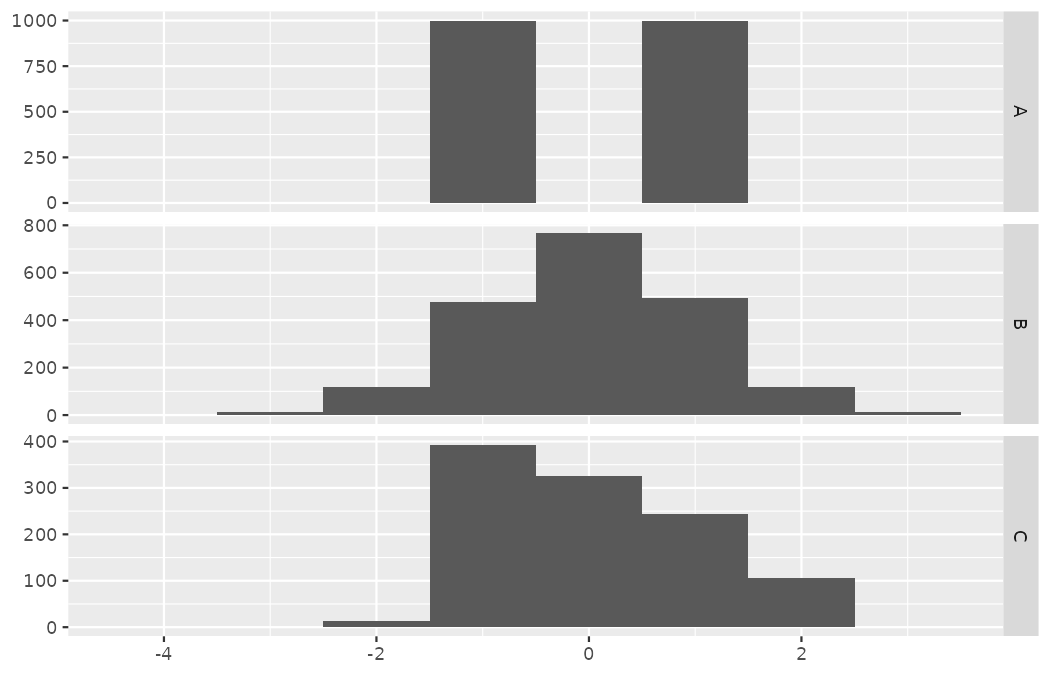
\includegraphics[width=0.85\linewidth,height=\textheight,keepaspectratio]{figures/explore-numerical-7.png}

Squad A's histogram is two towers at \(-1\) and \(+1\) with nothing
between (bimodal); squad B's is the familiar symmetric bell centered at
0; squad C's is right skewed, running from about \(-1.5\) out to
\(+2.1.\) Identical means, identical standard deviations --- three
completely different squads.

\begin{tcolorbox}[enhanced jigsaw, left=2mm, leftrule=.75mm, title=\textcolor{quarto-callout-note-color}{\faInfo}\hspace{0.5em}{Worked example}, arc=.35mm, rightrule=.15mm, coltitle=black, colframe=quarto-callout-note-color-frame, bottomrule=.15mm, colbacktitle=quarto-callout-note-color!10!white, opacitybacktitle=0.6, breakable, bottomtitle=1mm, toptitle=1mm, titlerule=0mm, opacityback=0, toprule=.15mm, colback=white]

Describe the distribution of the chance quality variable using its
histogram from Section~\ref{sec-histograms}. The description should
incorporate the center, variability, and shape of the distribution, and
it should also be placed in context: the xG of 50 sampled World Cup
shots. Also note any especially unusual cases.

\begin{center}\rule{0.5\linewidth}{0.5pt}\end{center}

The distribution of chance quality is unimodal and skewed to the high
end. Most of the 50 shots are low-quality chances below 0.1 xG, the mean
sits at 0.127 with a standard deviation of 0.192, and the distribution
trails out to a few exceptionally good chances --- most notably the
three penalties at 0.78 xG, which sit far from every open-play shot in
the sample.

\end{tcolorbox}

In practice, the variance and standard deviation are sometimes used as a
means to an end, where the ``end'' is being able to accurately estimate
the uncertainty associated with a sample statistic. For example, in
Chapter~\ref{sec-foundations-mathematical} the standard deviation is
used in calculations that help us understand how much a sample mean ---
a scout's average rating, a sampled conversion rate --- varies from one
sample to the next.

\section{Box plots, quartiles, and the median}\label{sec-boxplots}

A \textbf{box plot} summarizes a dataset using five statistics while
also identifying unusual observations. The code below draws a dot plot
and a box plot of the chance quality variable from the \texttt{shots50}
sample.\footnote{Box plots were introduced by Mary Eleanor Spear, who
  considered them to be a particular type of bar plot; see page 166 of
  Spear (1952). Mistakenly, box plots are often attributed to John
  Tukey, who was the first person to call them ``box-and-whisker
  plots.''}

\begin{Shaded}
\begin{Highlighting}[]
\FunctionTok{ggplot}\NormalTok{(shots50, }\FunctionTok{aes}\NormalTok{(}\AttributeTok{x =}\NormalTok{ statsbomb\_xg)) }\SpecialCharTok{+}
  \FunctionTok{geom\_dotplot}\NormalTok{(}\AttributeTok{binwidth =} \FloatTok{0.02}\NormalTok{) }\SpecialCharTok{+}
  \FunctionTok{labs}\NormalTok{(}\AttributeTok{x =} \ConstantTok{NULL}\NormalTok{, }\AttributeTok{y =} \ConstantTok{NULL}\NormalTok{) }\SpecialCharTok{+}
  \FunctionTok{theme}\NormalTok{(}
    \AttributeTok{axis.text.y =} \FunctionTok{element\_blank}\NormalTok{(),}
    \AttributeTok{axis.ticks.y =} \FunctionTok{element\_blank}\NormalTok{()}
\NormalTok{  )}

\FunctionTok{ggplot}\NormalTok{(shots50, }\FunctionTok{aes}\NormalTok{(}\AttributeTok{x =}\NormalTok{ statsbomb\_xg)) }\SpecialCharTok{+}
  \FunctionTok{geom\_boxplot}\NormalTok{(}\AttributeTok{outlier.size =} \FloatTok{2.5}\NormalTok{) }\SpecialCharTok{+}
  \FunctionTok{labs}\NormalTok{(}\AttributeTok{x =} \StringTok{"Chance quality (xG)"}\NormalTok{) }\SpecialCharTok{+}
  \FunctionTok{theme}\NormalTok{(}
    \AttributeTok{axis.text.y =} \FunctionTok{element\_blank}\NormalTok{(),}
    \AttributeTok{axis.ticks.y =} \FunctionTok{element\_blank}\NormalTok{()}
\NormalTok{  )}
\end{Highlighting}
\end{Shaded}

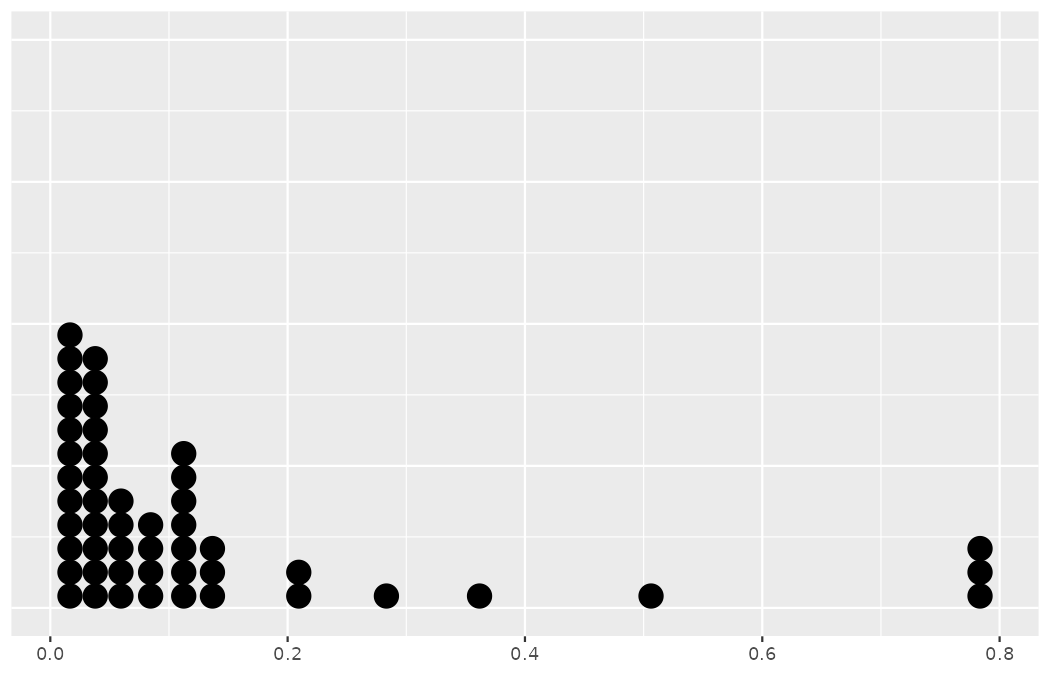
\includegraphics[width=0.85\linewidth,height=\textheight,keepaspectratio]{figures/explore-numerical-8.png}

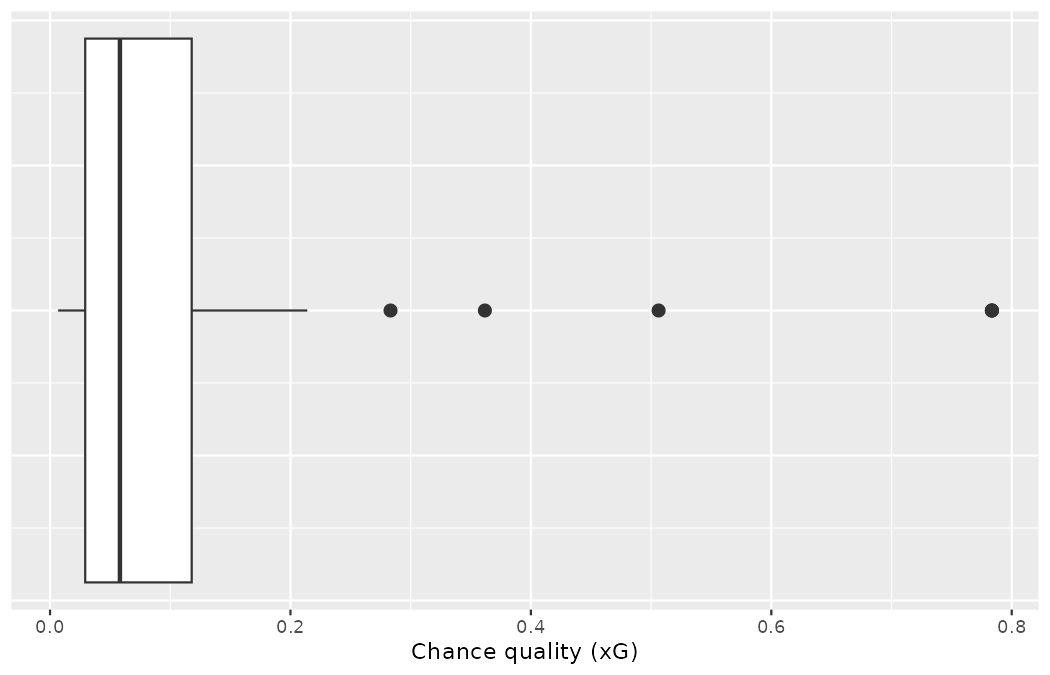
\includegraphics[width=0.85\linewidth,height=\textheight,keepaspectratio]{figures/explore-numerical-9.png}

The dark line inside the box represents the \textbf{median}, which
splits the data in half. 50\% of the data fall below this value and 50\%
fall above it. Since in the \texttt{shots50} sample there are 50
observations (an even number), the median is defined as the average of
the two observations closest to the \(50^{th}\) percentile. The code
below arranges all 50 chance qualities in ascending order (rounded to
three decimal places for display), reading left to right, then row by
row:

\begin{Shaded}
\begin{Highlighting}[]
\FunctionTok{matrix}\NormalTok{(}\FunctionTok{sort}\NormalTok{(}\FunctionTok{round}\NormalTok{(shots50}\SpecialCharTok{$}\NormalTok{statsbomb\_xg, }\DecValTok{3}\NormalTok{)), }\AttributeTok{byrow =} \ConstantTok{TRUE}\NormalTok{, }\AttributeTok{ncol =} \DecValTok{10}\NormalTok{)}
\CommentTok{\#\textgreater{}       [,1]  [,2]  [,3]  [,4]  [,5]  [,6]  [,7]  [,8]  [,9] [,10]}
\CommentTok{\#\textgreater{} [1,] 0.007 0.009 0.009 0.013 0.015 0.016 0.020 0.020 0.020 0.021}
\CommentTok{\#\textgreater{} [2,] 0.022 0.026 0.028 0.032 0.033 0.033 0.034 0.034 0.039 0.040}
\CommentTok{\#\textgreater{} [3,] 0.042 0.042 0.047 0.050 0.058 0.059 0.068 0.069 0.081 0.081}
\CommentTok{\#\textgreater{} [4,] 0.083 0.088 0.103 0.106 0.107 0.109 0.110 0.120 0.122 0.132}
\CommentTok{\#\textgreater{} [5,] 0.140 0.141 0.205 0.214 0.283 0.362 0.506 0.783 0.783 0.783}
\end{Highlighting}
\end{Shaded}

We can see that the \(25^{th}\) and the \(26^{th}\) values are 0.058 and
0.059, and their average, 0.058, is the median --- the thick line inside
the box plot's box. When there are an odd number of observations, there
will be exactly one observation that splits the data into two halves,
and in such a case that observation is the median (no average needed).

\begin{tcolorbox}[enhanced jigsaw, left=2mm, leftrule=.75mm, title=\textcolor{quarto-callout-important-color}{\faExclamation}\hspace{0.5em}{Median: the number in the middle}, arc=.35mm, rightrule=.15mm, coltitle=black, colframe=quarto-callout-important-color-frame, bottomrule=.15mm, colbacktitle=quarto-callout-important-color!10!white, opacitybacktitle=0.6, breakable, bottomtitle=1mm, toptitle=1mm, titlerule=0mm, opacityback=0, toprule=.15mm, colback=white]

If the data are ordered from smallest to largest, the \textbf{median} is
the observation right in the middle. If there are an even number of
observations, there will be two values in the middle, and the median is
taken as their average.

\end{tcolorbox}

The second step in building a box plot is drawing a rectangle to
represent the middle 50\% of the data. The length of the box is called
the \textbf{interquartile range}, or \textbf{IQR} for short. It, like
the standard deviation, is a measure of variability in data. The more
variable the data, the larger the standard deviation and IQR tend to be.
The two boundaries of the box are called the \textbf{first quartile}
(the \(25^{th}\) percentile, i.e., 25\% of the data fall below this
value) and the \textbf{third quartile} (the \(75^{th}\) percentile,
i.e., 75\% of the data fall below this value), and these are often
labeled \(Q_1\) and \(Q_3,\) respectively. The notation is the letter
\(Q\) for \emph{quartile} with a subscript naming which quartile is
meant; the median is, in this language, the second quartile, though we
rarely write \(Q_2.\)

\begin{tcolorbox}[enhanced jigsaw, left=2mm, leftrule=.75mm, title=\textcolor{quarto-callout-important-color}{\faExclamation}\hspace{0.5em}{Interquartile range (IQR)}, arc=.35mm, rightrule=.15mm, coltitle=black, colframe=quarto-callout-important-color-frame, bottomrule=.15mm, colbacktitle=quarto-callout-important-color!10!white, opacitybacktitle=0.6, breakable, bottomtitle=1mm, toptitle=1mm, titlerule=0mm, opacityback=0, toprule=.15mm, colback=white]

The IQR interquartile range is the length of the box in a box plot. It
is computed as

\[IQR = Q_3 - Q_1,\]

where \(Q_1\) and \(Q_3\) are the \(25^{th}\) and \(75^{th}\)
percentiles, respectively.

A \textbf{percentile} is a number with a specified percent of the
observations below it and the rest above. For example, the \(90^{th}\)
percentile of a combine's sprint speeds is the speed with 90\% of the
tested players below that value and 10\% of players above it.

\end{tcolorbox}

For the \texttt{shots50} chance qualities:

\begin{Shaded}
\begin{Highlighting}[]
\NormalTok{shots50 }\SpecialCharTok{|\textgreater{}}
  \FunctionTok{summarize}\NormalTok{(}
    \AttributeTok{median\_xg =} \FunctionTok{median}\NormalTok{(statsbomb\_xg),}
    \AttributeTok{q1 =} \FunctionTok{quantile}\NormalTok{(statsbomb\_xg, }\FloatTok{0.25}\NormalTok{),}
    \AttributeTok{q3 =} \FunctionTok{quantile}\NormalTok{(statsbomb\_xg, }\FloatTok{0.75}\NormalTok{),}
    \AttributeTok{iqr =} \FunctionTok{IQR}\NormalTok{(statsbomb\_xg)}
\NormalTok{  )}
\CommentTok{\#\textgreater{} \# A tibble: 1 × 4}
\CommentTok{\#\textgreater{}   median\_xg     q1    q3    iqr}
\CommentTok{\#\textgreater{}       \textless{}dbl\textgreater{}  \textless{}dbl\textgreater{} \textless{}dbl\textgreater{}  \textless{}dbl\textgreater{}}
\CommentTok{\#\textgreater{} 1    0.0581 0.0292 0.118 0.0886}
\end{Highlighting}
\end{Shaded}

\begin{tcolorbox}[enhanced jigsaw, left=2mm, leftrule=.75mm, title=\textcolor{quarto-callout-tip-color}{\faLightbulb}\hspace{0.5em}{Check your understanding}, arc=.35mm, rightrule=.15mm, coltitle=black, colframe=quarto-callout-tip-color-frame, bottomrule=.15mm, colbacktitle=quarto-callout-tip-color!10!white, opacitybacktitle=0.6, breakable, bottomtitle=1mm, toptitle=1mm, titlerule=0mm, opacityback=0, toprule=.15mm, colback=white]

What percent of the data fall between \(Q_1\) and the median? What
percent is between the median and \(Q_3\)?

\begin{center}\rule{0.5\linewidth}{0.5pt}\end{center}

Since \(Q_1\) and \(Q_3\) capture the middle 50\% of the data and the
median splits the data in the middle, 25\% of the data fall between
\(Q_1\) and the median, and another 25\% falls between the median and
\(Q_3.\)

\end{tcolorbox}

Extending out from the box, the \textbf{whiskers} attempt to capture the
data outside of the box. The whiskers of a box plot reach to the minimum
and the maximum values in the data, unless there are points that are
considered unusually high or unusually low, which are identified as
potential \textbf{outliers} by the box plot. These are labeled with a
dot on the box plot. The purpose of labeling the outlying points ---
instead of extending the whiskers to the minimum and maximum observed
values --- is to help identify any observations that appear to be
unusually distant from the rest of the data. There are a variety of
formulas for determining whether a particular data point is considered
an outlier, and different statistical software use different formulas. A
commonly used formula --- the one we adopt in this book --- is that any
observation beyond \(1.5\times IQR\) away from the first or the third
quartile is considered an outlier. In a sense, the box is like the body
of the box plot and the whiskers are like its arms trying to reach the
rest of the data, up to the outliers.

Let us apply the \(1.5\times IQR\) rule to our sample. The upper cutoff
is \(Q_3 + 1.5 \times IQR = 0.118 + 1.5 \times 0.089 = 0.251:\)

\begin{Shaded}
\begin{Highlighting}[]
\NormalTok{shots50 }\SpecialCharTok{|\textgreater{}}
  \FunctionTok{summarize}\NormalTok{(}
    \AttributeTok{upper\_fence =} \FunctionTok{quantile}\NormalTok{(statsbomb\_xg, }\FloatTok{0.75}\NormalTok{) }\SpecialCharTok{+} \FloatTok{1.5} \SpecialCharTok{*} \FunctionTok{IQR}\NormalTok{(statsbomb\_xg),}
    \AttributeTok{n\_outliers =} \FunctionTok{sum}\NormalTok{(statsbomb\_xg }\SpecialCharTok{\textgreater{}}\NormalTok{ upper\_fence),}
    \AttributeTok{whisker\_end =} \FunctionTok{max}\NormalTok{(statsbomb\_xg[statsbomb\_xg }\SpecialCharTok{\textless{}=}\NormalTok{ upper\_fence])}
\NormalTok{  )}
\CommentTok{\#\textgreater{} \# A tibble: 1 × 3}
\CommentTok{\#\textgreater{}   upper\_fence n\_outliers whisker\_end}
\CommentTok{\#\textgreater{}         \textless{}dbl\textgreater{}      \textless{}int\textgreater{}       \textless{}dbl\textgreater{}}
\CommentTok{\#\textgreater{} 1       0.251          6       0.214}
\end{Highlighting}
\end{Shaded}

Six shots exceed the cutoff --- the chances at 0.283, 0.362, and 0.506,
plus the three penalties at 0.7835 --- so the upper whisker stops at the
largest non-outlying value, 0.214, and the six extreme shots are drawn
as individual dots (the three penalties overplot at the same position).
The lower cutoff, \(Q_1 - 1.5 \times IQR,\) is negative, and since xG
cannot be negative, no shot can be a low outlier here; the lower whisker
simply reaches the minimum, 0.007.

\begin{tcolorbox}[enhanced jigsaw, left=2mm, leftrule=.75mm, title=\textcolor{quarto-callout-important-color}{\faExclamation}\hspace{0.5em}{Outliers are extreme}, arc=.35mm, rightrule=.15mm, coltitle=black, colframe=quarto-callout-important-color-frame, bottomrule=.15mm, colbacktitle=quarto-callout-important-color!10!white, opacitybacktitle=0.6, breakable, bottomtitle=1mm, toptitle=1mm, titlerule=0mm, opacityback=0, toprule=.15mm, colback=white]

An \textbf{outlier} is an observation that appears extreme relative to
the rest of the data. Examining data for outliers serves many useful
purposes, including

\begin{itemize}
\tightlist
\item
  identifying strong skew in the distribution,
\item
  identifying possible data collection or data entry errors, and
\item
  providing insight into interesting properties of the data.
\end{itemize}

Keep in mind, however, that some datasets have a naturally long skew and
outlying points do \textbf{not} represent any sort of problem in the
dataset. Our six flagged shots are not errors --- penalties and clean
one-on-ones really are that much better than the average chance, and a
scout should be \emph{glad} the box plot points at them.

\end{tcolorbox}

\begin{tcolorbox}[enhanced jigsaw, left=2mm, leftrule=.75mm, title=\textcolor{quarto-callout-tip-color}{\faLightbulb}\hspace{0.5em}{Check your understanding}, arc=.35mm, rightrule=.15mm, coltitle=black, colframe=quarto-callout-tip-color-frame, bottomrule=.15mm, colbacktitle=quarto-callout-tip-color!10!white, opacitybacktitle=0.6, breakable, bottomtitle=1mm, toptitle=1mm, titlerule=0mm, opacityback=0, toprule=.15mm, colback=white]

Using the box plot drawn at the start of this section, estimate the
values of \(Q_1,\) \(Q_3,\) and the IQR for chance quality in the
\texttt{shots50} sample.

\begin{center}\rule{0.5\linewidth}{0.5pt}\end{center}

These visual estimates will vary a little from one person to the next:
\(Q_1 \approx 0.03,\) \(Q_3 \approx 0.12,\) IQR
\(\approx 0.12 - 0.03 = 0.09.\) The computed values were 0.029, 0.118,
and 0.089.

\end{tcolorbox}

\section{Robust statistics}\label{robust-statistics}

How are the sample statistics of the \texttt{shots50} chance qualities
affected by the shot at the top of the sample --- the stored penalty
value 0.7835? Three shots share that value --- all penalties --- and we
will experiment on one of them: Harry Kane's penalty for England, the
only shot by Kane in the sample.

\begin{Shaded}
\begin{Highlighting}[]
\NormalTok{shots50 }\SpecialCharTok{|\textgreater{}}
  \FunctionTok{filter}\NormalTok{(statsbomb\_xg }\SpecialCharTok{==} \FunctionTok{max}\NormalTok{(statsbomb\_xg)) }\SpecialCharTok{|\textgreater{}}
  \FunctionTok{select}\NormalTok{(player, team, shot\_type, outcome, statsbomb\_xg)}
\CommentTok{\#\textgreater{} \# A tibble: 3 × 5}
\CommentTok{\#\textgreater{}   player           team    shot\_type outcome statsbomb\_xg}
\CommentTok{\#\textgreater{}   \textless{}chr\textgreater{}            \textless{}chr\textgreater{}   \textless{}chr\textgreater{}     \textless{}chr\textgreater{}          \textless{}dbl\textgreater{}}
\CommentTok{\#\textgreater{} 1 Marcelo Brozović Croatia Penalty   Goal           0.784}
\CommentTok{\#\textgreater{} 2 Marko Livaja     Croatia Penalty   Post           0.784}
\CommentTok{\#\textgreater{} 3 Harry Kane       England Penalty   Goal           0.784}
\end{Highlighting}
\end{Shaded}

(The table prints \(0.784\) because the stored value \(0.7835\) is
rounded up by the three-significant-digit display; the three-decimal
matrix in Section~\ref{sec-boxplots} rounded the very same shots down to
\(0.783.\))

What would have happened if the xG model had rated Kane's chance at only
0.15? What would happen to the summary statistics if it had scored the
penalty even higher, at 0.98 --- a near-certain goal? The two
conjectured scenarios are built below, plotted alongside the original
data as faceted dot plots, and the sample statistics are computed under
each scenario.

\begin{Shaded}
\begin{Highlighting}[]
\NormalTok{shots50\_down }\OtherTok{\textless{}{-}}\NormalTok{ shots50 }\SpecialCharTok{|\textgreater{}}
  \FunctionTok{mutate}\NormalTok{(}\AttributeTok{statsbomb\_xg =} \FunctionTok{if\_else}\NormalTok{(player }\SpecialCharTok{==} \StringTok{"Harry Kane"}\NormalTok{, }\FloatTok{0.15}\NormalTok{, statsbomb\_xg))}
\NormalTok{shots50\_up }\OtherTok{\textless{}{-}}\NormalTok{ shots50 }\SpecialCharTok{|\textgreater{}}
  \FunctionTok{mutate}\NormalTok{(}\AttributeTok{statsbomb\_xg =} \FunctionTok{if\_else}\NormalTok{(player }\SpecialCharTok{==} \StringTok{"Harry Kane"}\NormalTok{, }\FloatTok{0.98}\NormalTok{, statsbomb\_xg))}

\NormalTok{robust\_check }\OtherTok{\textless{}{-}} \FunctionTok{bind\_rows}\NormalTok{(}
\NormalTok{  shots50      }\SpecialCharTok{|\textgreater{}} \FunctionTok{mutate}\NormalTok{(}\AttributeTok{scenario =} \StringTok{"Original data"}\NormalTok{),}
\NormalTok{  shots50\_down }\SpecialCharTok{|\textgreater{}} \FunctionTok{mutate}\NormalTok{(}\AttributeTok{scenario =} \StringTok{"Move 0.7835 to 0.15"}\NormalTok{),}
\NormalTok{  shots50\_up   }\SpecialCharTok{|\textgreater{}} \FunctionTok{mutate}\NormalTok{(}\AttributeTok{scenario =} \StringTok{"Move 0.7835 to 0.98"}\NormalTok{)}
\NormalTok{) }\SpecialCharTok{|\textgreater{}}
  \FunctionTok{mutate}\NormalTok{(}\AttributeTok{scenario =} \FunctionTok{factor}\NormalTok{(scenario, }\AttributeTok{levels =} \FunctionTok{c}\NormalTok{(}
    \StringTok{"Original data"}\NormalTok{, }\StringTok{"Move 0.7835 to 0.15"}\NormalTok{, }\StringTok{"Move 0.7835 to 0.98"}
\NormalTok{  )))}

\NormalTok{robust\_check }\SpecialCharTok{|\textgreater{}}
  \FunctionTok{group\_by}\NormalTok{(scenario) }\SpecialCharTok{|\textgreater{}}
  \FunctionTok{summarize}\NormalTok{(}
    \AttributeTok{median =} \FunctionTok{median}\NormalTok{(statsbomb\_xg),}
    \AttributeTok{iqr =} \FunctionTok{IQR}\NormalTok{(statsbomb\_xg),}
    \AttributeTok{mean =} \FunctionTok{mean}\NormalTok{(statsbomb\_xg),}
    \AttributeTok{sd =} \FunctionTok{sd}\NormalTok{(statsbomb\_xg)}
\NormalTok{  )}
\CommentTok{\#\textgreater{} \# A tibble: 3 × 5}
\CommentTok{\#\textgreater{}   scenario            median    iqr  mean    sd}
\CommentTok{\#\textgreater{}   \textless{}fct\textgreater{}                \textless{}dbl\textgreater{}  \textless{}dbl\textgreater{} \textless{}dbl\textgreater{} \textless{}dbl\textgreater{}}
\CommentTok{\#\textgreater{} 1 Original data       0.0581 0.0886 0.127 0.192}
\CommentTok{\#\textgreater{} 2 Move 0.7835 to 0.15 0.0581 0.0886 0.114 0.167}
\CommentTok{\#\textgreater{} 3 Move 0.7835 to 0.98 0.0581 0.0886 0.131 0.207}
\end{Highlighting}
\end{Shaded}

\begin{longtable}[]{@{}lrrrr@{}}
\caption{A comparison of how the median, IQR, mean, and standard
deviation change as the value of an extreme observation from the
original chance quality data changes. The median and IQR are robust; the
mean and standard deviation are
not.}\label{tbl-shots50-robust}\tabularnewline
\toprule\noalign{}
Scenario & Median & IQR & Mean & SD \\
\midrule\noalign{}
\endfirsthead
\toprule\noalign{}
Scenario & Median & IQR & Mean & SD \\
\midrule\noalign{}
\endhead
\bottomrule\noalign{}
\endlastfoot
Original data & 0.058 & 0.089 & 0.127 & 0.192 \\
Move 0.7835 to 0.15 & 0.058 & 0.089 & 0.114 & 0.167 \\
Move 0.7835 to 0.98 & 0.058 & 0.089 & 0.131 & 0.207 \\
\end{longtable}

\begin{Shaded}
\begin{Highlighting}[]
\FunctionTok{ggplot}\NormalTok{(robust\_check, }\FunctionTok{aes}\NormalTok{(}\AttributeTok{x =}\NormalTok{ statsbomb\_xg)) }\SpecialCharTok{+}
  \FunctionTok{geom\_dotplot}\NormalTok{(}\AttributeTok{binwidth =} \FloatTok{0.02}\NormalTok{) }\SpecialCharTok{+}
  \FunctionTok{facet\_grid}\NormalTok{(scenario }\SpecialCharTok{\textasciitilde{}}\NormalTok{ .) }\SpecialCharTok{+}
  \FunctionTok{labs}\NormalTok{(}\AttributeTok{x =} \StringTok{"Chance quality (xG)"}\NormalTok{, }\AttributeTok{y =} \ConstantTok{NULL}\NormalTok{)}
\end{Highlighting}
\end{Shaded}

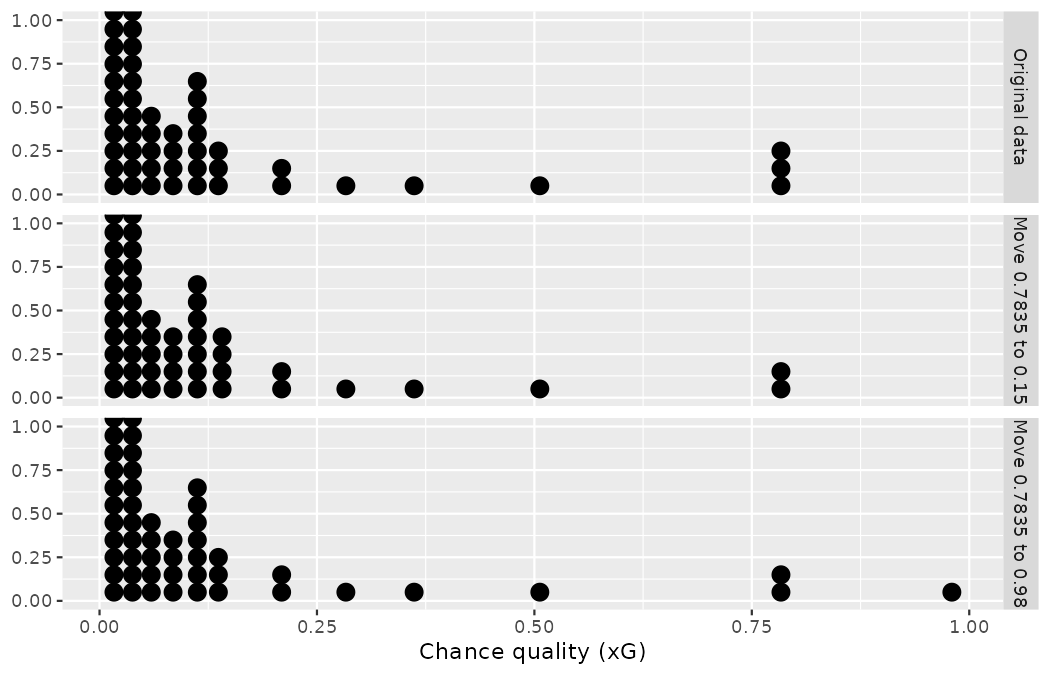
\includegraphics[width=0.85\linewidth,height=\textheight,keepaspectratio]{figures/explore-numerical-10.png}

\begin{tcolorbox}[enhanced jigsaw, left=2mm, leftrule=.75mm, title=\textcolor{quarto-callout-tip-color}{\faLightbulb}\hspace{0.5em}{Check your understanding}, arc=.35mm, rightrule=.15mm, coltitle=black, colframe=quarto-callout-tip-color-frame, bottomrule=.15mm, colbacktitle=quarto-callout-tip-color!10!white, opacitybacktitle=0.6, breakable, bottomtitle=1mm, toptitle=1mm, titlerule=0mm, opacityback=0, toprule=.15mm, colback=white]

Which is more affected by extreme observations, the mean or median? Is
the standard deviation or IQR more affected by extreme observations?

\begin{center}\rule{0.5\linewidth}{0.5pt}\end{center}

The mean is affected more than the median. The standard deviation is
affected more than the IQR.

\end{tcolorbox}

The median and IQR are called \textbf{robust statistics} because extreme
observations have little effect on their values: moving the most extreme
value generally has little influence on these statistics. On the other
hand, the mean and standard deviation are more heavily influenced by
changes in extreme observations, which can be important in some
situations.

\begin{tcolorbox}[enhanced jigsaw, left=2mm, leftrule=.75mm, title=\textcolor{quarto-callout-note-color}{\faInfo}\hspace{0.5em}{Worked example}, arc=.35mm, rightrule=.15mm, coltitle=black, colframe=quarto-callout-note-color-frame, bottomrule=.15mm, colbacktitle=quarto-callout-note-color!10!white, opacitybacktitle=0.6, breakable, bottomtitle=1mm, toptitle=1mm, titlerule=0mm, opacityback=0, toprule=.15mm, colback=white]

The median and IQR did not change under the two scenarios in
Table~\ref{tbl-shots50-robust}. Why might this be the case?

\begin{center}\rule{0.5\linewidth}{0.5pt}\end{center}

The median and IQR are only sensitive to numbers near \(Q_1,\) the
median, and \(Q_3.\) Since values in these regions are stable in the
three datasets --- we only moved a value in the far right tail --- the
median and IQR estimates are also stable.

\end{tcolorbox}

You might not be surprised that the answer to the question ``which is
better, the mean or the median?'' is: \emph{it depends}. The two
statistics measure different things, and so their use is dependent on
the context in the analysis. Consider the following scouting scenarios:

\begin{itemize}
\tightlist
\item
  Is it better to measure the average transfer-fee profit per academy
  graduate or the median profit per graduate?

  \begin{itemize}
  \tightlist
  \item
    If concern is about the overall financial return of the academy, the
    mean is a better measure to assess what is happening across the
    whole program. One €40M sale can fund a decade of coaching, and the
    academy could have a positive median profit per graduate and still
    be losing money overall.
  \item
    If concern is around understanding what the \emph{typical} graduate
    returns --- say, to set realistic expectations for any one prospect
    --- the median profit per graduate would tell you more.
  \end{itemize}
\item
  If Priya wants to know how long scouts wait for match video to load on
  the club's scouting platform, does she want the mean amount of time or
  the median amount of time?

  \begin{itemize}
  \tightlist
  \item
    The mean leads to an understanding of the overall amount of working
    time being wasted across the network.
  \item
    The median tells you about the typical scout's experience.
  \item
    However, if the video loads within a second for 50\% of the scouts
    but takes more than a minute for 10\% of them, the median doesn't
    give the information Priya needs. In that scenario, she might want
    an upper percentile, like the 95th percentile.
  \end{itemize}
\end{itemize}

\begin{tcolorbox}[enhanced jigsaw, left=2mm, leftrule=.75mm, title=\textcolor{quarto-callout-tip-color}{\faLightbulb}\hspace{0.5em}{Check your understanding}, arc=.35mm, rightrule=.15mm, coltitle=black, colframe=quarto-callout-tip-color-frame, bottomrule=.15mm, colbacktitle=quarto-callout-tip-color!10!white, opacitybacktitle=0.6, breakable, bottomtitle=1mm, toptitle=1mm, titlerule=0mm, opacityback=0, toprule=.15mm, colback=white]

The distribution of chance quality in the \texttt{shots50} sample is
right skewed, with a few excellent chances lingering out into the right
tail. If you were wanting to understand the quality of a typical chance
in the sample, should you be more interested in the mean or median?

\begin{center}\rule{0.5\linewidth}{0.5pt}\end{center}

If we are looking to simply understand what a typical individual chance
looks like, the median (0.058 xG) is probably more useful. However, if
the goal is to understand something that scales well --- such as how
many goals a team should expect to accumulate across hundreds of shots
--- then the mean (0.127 xG) would be more useful, since total expected
goals is the mean times the number of shots.

\end{tcolorbox}

Regardless of the choice of centrality statistic (either mean or
median), for most analyses, it is important to consider more than just
the centrality. Other statistics like upper and lower percentiles, IQR,
or standard deviation provide information about the variability of the
observations. And visualizing the data through a graphical
representation will typically provide a wealth of information necessary
for understanding the full data picture associated with the research
question.

\section{Transforming data}\label{sec-transforming-data}

When data are very strongly skewed, we sometimes transform them, so they
are easier to model. Our example is a variable every recruitment
department tracks: how many shots each player attempted across a
tournament. We aggregate the 2025 Women's Euro shot data to one row per
player:

\begin{Shaded}
\begin{Highlighting}[]
\NormalTok{weuro2025\_shots }\OtherTok{\textless{}{-}} \FunctionTok{read\_csv}\NormalTok{(}\StringTok{"data/derived/weuro2025\_shots.csv"}\NormalTok{)}

\NormalTok{player\_shots }\OtherTok{\textless{}{-}}\NormalTok{ weuro2025\_shots }\SpecialCharTok{|\textgreater{}}
  \FunctionTok{group\_by}\NormalTok{(player, team) }\SpecialCharTok{|\textgreater{}}
  \FunctionTok{summarize}\NormalTok{(}\AttributeTok{shots =} \FunctionTok{n}\NormalTok{(), }\AttributeTok{goals =} \FunctionTok{sum}\NormalTok{(goal), }\AttributeTok{.groups =} \StringTok{"drop"}\NormalTok{)}

\NormalTok{player\_shots }\SpecialCharTok{|\textgreater{}}
  \FunctionTok{summarize}\NormalTok{(}
    \AttributeTok{n\_players =} \FunctionTok{n}\NormalTok{(),}
    \AttributeTok{mean\_shots =} \FunctionTok{mean}\NormalTok{(shots),}
    \AttributeTok{median\_shots =} \FunctionTok{median}\NormalTok{(shots),}
    \AttributeTok{max\_shots =} \FunctionTok{max}\NormalTok{(shots)}
\NormalTok{  )}
\CommentTok{\#\textgreater{} \# A tibble: 1 × 4}
\CommentTok{\#\textgreater{}   n\_players mean\_shots median\_shots max\_shots}
\CommentTok{\#\textgreater{}       \textless{}int\textgreater{}      \textless{}dbl\textgreater{}        \textless{}int\textgreater{}     \textless{}int\textgreater{}}
\CommentTok{\#\textgreater{} 1       215       4.25            3        25}

\NormalTok{player\_shots }\SpecialCharTok{|\textgreater{}}
  \FunctionTok{arrange}\NormalTok{(}\FunctionTok{desc}\NormalTok{(shots)) }\SpecialCharTok{|\textgreater{}}
  \FunctionTok{slice\_head}\NormalTok{(}\AttributeTok{n =} \DecValTok{5}\NormalTok{)}
\CommentTok{\#\textgreater{} \# A tibble: 5 × 4}
\CommentTok{\#\textgreater{}   player                    team            shots goals}
\CommentTok{\#\textgreater{}   \textless{}chr\textgreater{}                     \textless{}chr\textgreater{}           \textless{}int\textgreater{} \textless{}int\textgreater{}}
\CommentTok{\#\textgreater{} 1 Klara Bühl                Germany Women\textquotesingle{}s    25     1}
\CommentTok{\#\textgreater{} 2 Esther Gonzalez Rodríguez Spain Women\textquotesingle{}s      24     4}
\CommentTok{\#\textgreater{} 3 Emma Stina Blackstenius   Sweden Women\textquotesingle{}s     20     3}
\CommentTok{\#\textgreater{} 4 Alexia Putellas Segura    Spain Women\textquotesingle{}s      18     3}
\CommentTok{\#\textgreater{} 5 Aitana Bonmati Conca      Spain Women\textquotesingle{}s      17     1}
\end{Highlighting}
\end{Shaded}

Of the 215 players who attempted at least one shot, the median attempted
just 3, while Germany's Klara Bühl attempted 25. Fifty-nine players took
exactly one shot, and 130 of the 215 (60.5\%) took three or fewer. The
distribution is heavily right skewed, as the histogram drawn by the code
below shows.

\begin{Shaded}
\begin{Highlighting}[]
\FunctionTok{ggplot}\NormalTok{(player\_shots, }\FunctionTok{aes}\NormalTok{(}\AttributeTok{x =}\NormalTok{ shots)) }\SpecialCharTok{+}
  \FunctionTok{geom\_histogram}\NormalTok{(}\AttributeTok{binwidth =} \DecValTok{2}\NormalTok{, }\AttributeTok{boundary =} \DecValTok{0}\NormalTok{) }\SpecialCharTok{+}
  \FunctionTok{labs}\NormalTok{(}\AttributeTok{x =} \StringTok{"Shots attempted in the tournament"}\NormalTok{, }\AttributeTok{y =} \StringTok{"Count (players)"}\NormalTok{)}
\end{Highlighting}
\end{Shaded}

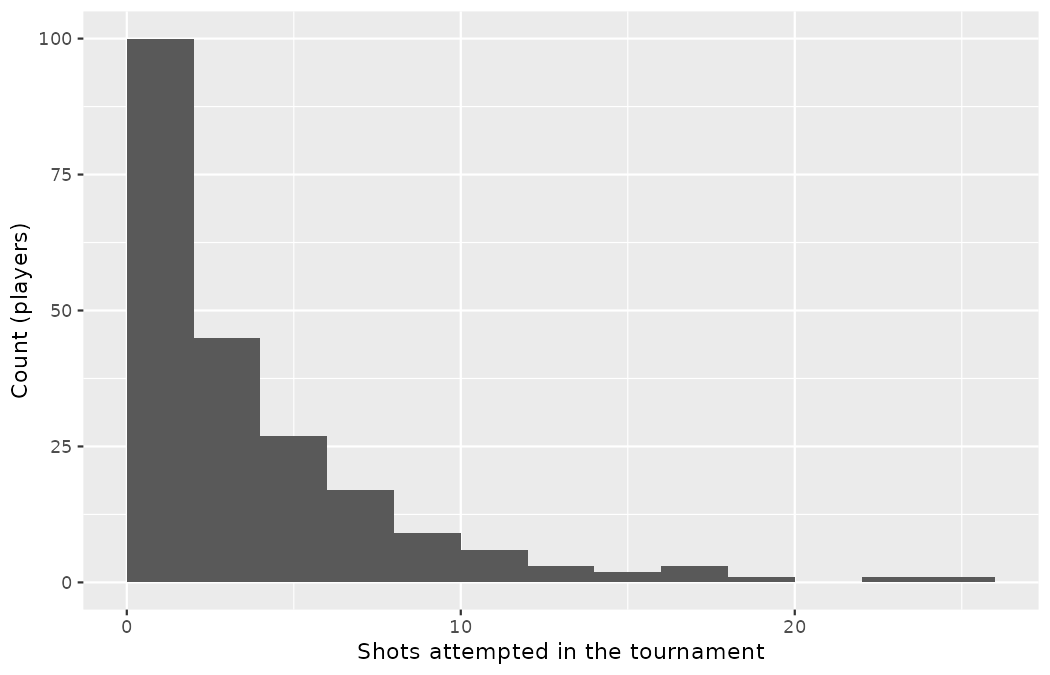
\includegraphics[width=0.85\linewidth,height=\textheight,keepaspectratio]{figures/explore-numerical-11.png}

\begin{tcolorbox}[enhanced jigsaw, left=2mm, leftrule=.75mm, title=\textcolor{quarto-callout-note-color}{\faInfo}\hspace{0.5em}{Worked example}, arc=.35mm, rightrule=.15mm, coltitle=black, colframe=quarto-callout-note-color-frame, bottomrule=.15mm, colbacktitle=quarto-callout-note-color!10!white, opacitybacktitle=0.6, breakable, bottomtitle=1mm, toptitle=1mm, titlerule=0mm, opacityback=0, toprule=.15mm, colback=white]

Consider the histogram of per-player shot counts drawn above, which
shows extreme skew. What characteristics of the plot keep it from being
useful?

\begin{center}\rule{0.5\linewidth}{0.5pt}\end{center}

Most of the data fall into the leftmost bins --- 130 of the 215 players
sit in the first two bars --- and the extreme skew stretches the axis
out to 25 to accommodate a handful of high-volume shooters, obscuring
many of the potentially interesting details at the low values.

\end{tcolorbox}

There are some standard transformations that may be useful for strongly
right skewed data where much of the data is positive but clustered near
zero. A \textbf{transformation} is a rescaling of the data using a
function. For instance, a plot of the logarithm (base 10) of the shot
counts results in the new histogram drawn below. The notation
\(\log_{10}\) deserves a plain-words reading before we use it:
\(\log_{10}(x)\) is the power to which 10 must be raised to recover
\(x.\) So \(\log_{10}(10) = 1\) and \(\log_{10}(100) = 2,\) and each
extra unit on the transformed axis means ``ten times as many''; Bühl's
25 shots map to \(\log_{10}(25) \approx 1.40.\)

\begin{Shaded}
\begin{Highlighting}[]
\FunctionTok{ggplot}\NormalTok{(player\_shots, }\FunctionTok{aes}\NormalTok{(}\AttributeTok{x =} \FunctionTok{log10}\NormalTok{(shots))) }\SpecialCharTok{+}
  \FunctionTok{geom\_histogram}\NormalTok{(}\AttributeTok{binwidth =} \FloatTok{0.1}\NormalTok{, }\AttributeTok{boundary =} \DecValTok{0}\NormalTok{) }\SpecialCharTok{+}
  \FunctionTok{labs}\NormalTok{(}\AttributeTok{x =} \FunctionTok{expression}\NormalTok{(log[}\DecValTok{10}\NormalTok{] }\SpecialCharTok{*} \StringTok{"(Shots attempted)"}\NormalTok{), }\AttributeTok{y =} \StringTok{"Count (players)"}\NormalTok{)}
\end{Highlighting}
\end{Shaded}

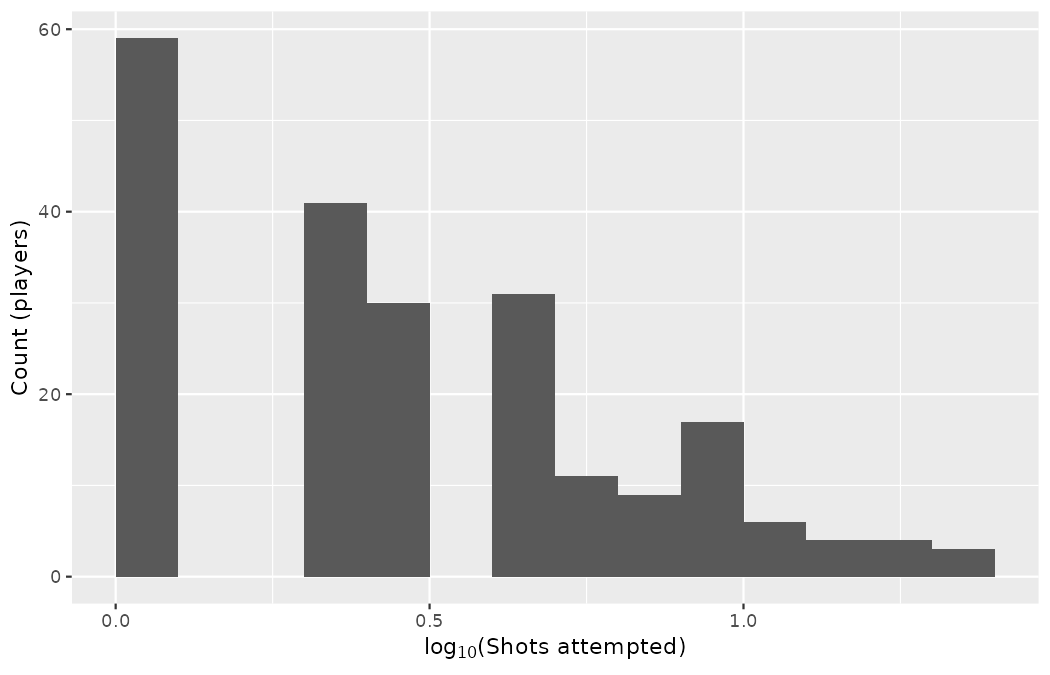
\includegraphics[width=0.85\linewidth,height=\textheight,keepaspectratio]{figures/explore-numerical-12.png}

The transformed data are far less skewed: the long right tail is pulled
in, and the high-volume shooters no longer look like a different
species. Be honest about what the transform cannot do, though: shot
counts are whole numbers, so the transformed histogram is spiky rather
than smooth --- the 59 one-shot players form an isolated bar at
\(\log_{10}(1) = 0,\) with further spikes at
\(\log_{10}(2) \approx 0.30\) and \(\log_{10}(3) \approx 0.48.\) By
reining in the outliers and extreme skew, transformations often make it
easier to build statistical models for the data.

Transformations can also be applied to one or both variables in a
scatterplot. A scatterplot of goals scored against shots attempted is
drawn by the first code block below. It is difficult to decipher any
detail among the low-volume players because the shots variable is so
strongly skewed: over 60\% of the points are squeezed into the left edge
of the plot. However, if we apply a \(\log_{10}\) transformation to the
shots axis, as in the second plot, the crowd of low-volume players is
spread out, and the positive association --- more attempts, more goals
--- can be inspected across the whole range. In fact, we may be
interested in fitting a trend line to data like these when we explore
methods around fitting regression lines in Chapter~\ref{sec-model-slr}.

\begin{Shaded}
\begin{Highlighting}[]
\FunctionTok{ggplot}\NormalTok{(player\_shots, }\FunctionTok{aes}\NormalTok{(}\AttributeTok{x =}\NormalTok{ shots, }\AttributeTok{y =}\NormalTok{ goals)) }\SpecialCharTok{+}
  \FunctionTok{geom\_point}\NormalTok{(}\AttributeTok{alpha =} \FloatTok{0.4}\NormalTok{) }\SpecialCharTok{+}
  \FunctionTok{labs}\NormalTok{(}\AttributeTok{x =} \StringTok{"Shots attempted"}\NormalTok{, }\AttributeTok{y =} \StringTok{"Goals scored"}\NormalTok{)}

\FunctionTok{ggplot}\NormalTok{(player\_shots, }\FunctionTok{aes}\NormalTok{(}\AttributeTok{x =} \FunctionTok{log10}\NormalTok{(shots), }\AttributeTok{y =}\NormalTok{ goals)) }\SpecialCharTok{+}
  \FunctionTok{geom\_point}\NormalTok{(}\AttributeTok{alpha =} \FloatTok{0.4}\NormalTok{) }\SpecialCharTok{+}
  \FunctionTok{labs}\NormalTok{(}\AttributeTok{x =} \FunctionTok{expression}\NormalTok{(log[}\DecValTok{10}\NormalTok{] }\SpecialCharTok{*} \StringTok{"(Shots attempted)"}\NormalTok{), }\AttributeTok{y =} \StringTok{"Goals scored"}\NormalTok{)}
\end{Highlighting}
\end{Shaded}

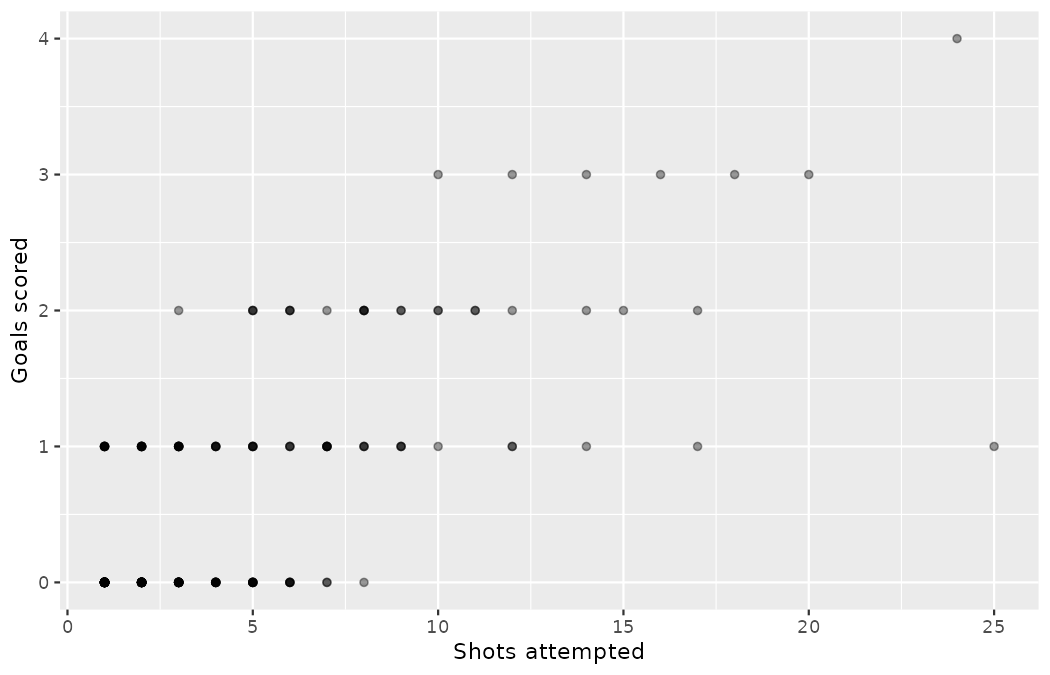
\includegraphics[width=0.85\linewidth,height=\textheight,keepaspectratio]{figures/explore-numerical-13.png}

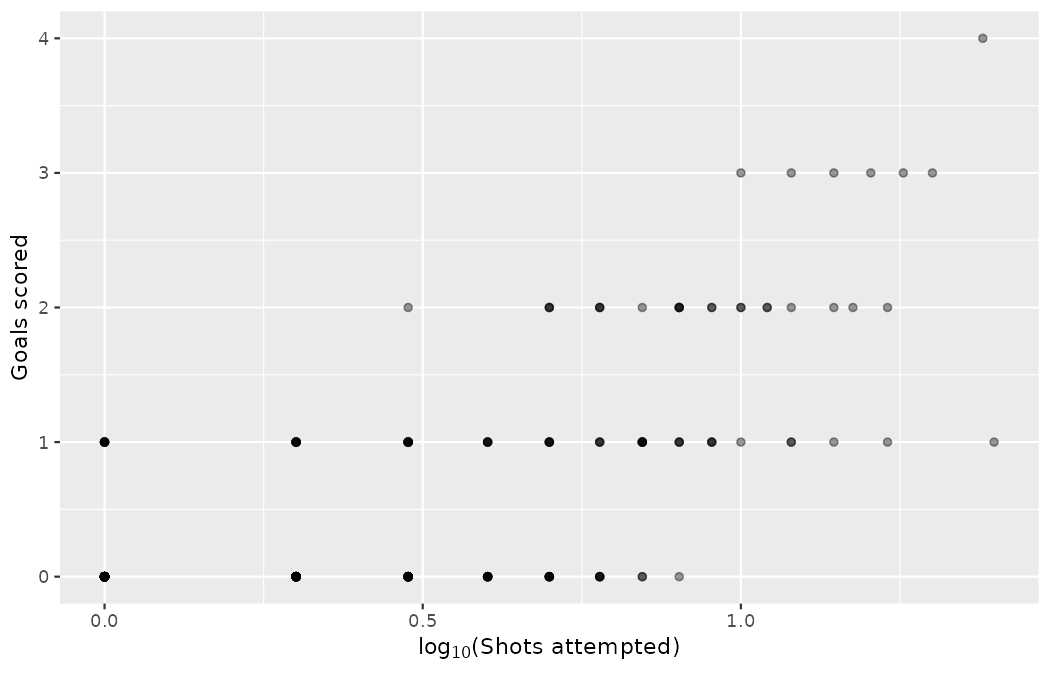
\includegraphics[width=0.85\linewidth,height=\textheight,keepaspectratio]{figures/explore-numerical-14.png}

Either version rewards a scout's second look: Klara Bühl's point sits at
the extreme right with 25 shots and just 1 goal, a volume shooter whose
finishing lagged her chance creation in this tournament --- precisely
the kind of case a scatterplot surfaces and a summary statistic buries.

Transformations other than the logarithm can be useful, too. For
instance, the square root \((\sqrt{\text{original observation}})\) and
inverse \(\bigg(\frac{1}{\text{original observation}}\bigg)\) are
commonly used by data scientists. Common goals in transforming data are
to see the data structure differently, reduce skew, assist in modeling,
or straighten a nonlinear relationship in a scatterplot.

\begin{tcolorbox}[enhanced jigsaw, left=2mm, leftrule=.75mm, title=\textcolor{quarto-callout-tip-color}{\faLightbulb}\hspace{0.5em}{Check your understanding}, arc=.35mm, rightrule=.15mm, coltitle=black, colframe=quarto-callout-tip-color-frame, bottomrule=.15mm, colbacktitle=quarto-callout-tip-color!10!white, opacitybacktitle=0.6, breakable, bottomtitle=1mm, toptitle=1mm, titlerule=0mm, opacityback=0, toprule=.15mm, colback=white]

Marta asks why you plotted \(\log_{10}(\text{shots})\) rather than the
raw shot counts. Give the two-part answer: what property of the
shot-count distribution makes the \(\log_{10}\) transformation helpful
here, and why could you \emph{not} apply the same transformation to the
\texttt{goals} column of \texttt{player\_shots}?

\begin{center}\rule{0.5\linewidth}{0.5pt}\end{center}

Shot counts are positive and strongly right skewed --- they run from 1
up to Bühl's 25, more than an order of magnitude --- so the logarithm
compresses the sparse right tail and spreads out the crowded low counts,
making the bulk of the distribution legible. The \texttt{goals} column
resists the same treatment because 129 of the 215 players scored no
goals at all, and \(\log_{10}(0)\) is undefined: a log transformation
requires strictly positive values. In general, reach for \(\log_{10}\)
when data are positive, clustered near zero, and stretched across orders
of magnitude; when zeros are present, either a different transformation
(such as the square root) or a modeling approach that tolerates zeros is
needed.

\end{tcolorbox}

\section{Mapping data}\label{mapping-data}

Shots happen at \emph{places} on a pitch, and dot plots, scatterplots,
and box plots can miss the true nature of such data as spatial. When we
encounter spatial data, we should create an \textbf{intensity map},
where colors are used to show higher and lower values of a variable
across a surface.

Our derived shot files carry no pitch coordinates, so this section works
with a constructed Northbridge scenario: Priya is piloting a
tracking-data feed, and sketches what its zone summaries would look
like. She divides the attacking half into a grid --- five distance bands
from goal (band 1 nearest the goal) crossed with six channels across the
pitch (channels 3 and 4 central) --- and constructs, in the seeded code
below, an average chance quality for shots from each zone: a baseline,
plus a bonus that grows with centrality and shrinks with distance, plus
a little random noise.

\begin{Shaded}
\begin{Highlighting}[]
\FunctionTok{set.seed}\NormalTok{(}\DecValTok{501}\NormalTok{)}
\NormalTok{pitch\_zones }\OtherTok{\textless{}{-}} \FunctionTok{expand\_grid}\NormalTok{(}\AttributeTok{band =} \DecValTok{1}\SpecialCharTok{:}\DecValTok{5}\NormalTok{, }\AttributeTok{channel =} \DecValTok{1}\SpecialCharTok{:}\DecValTok{6}\NormalTok{) }\SpecialCharTok{|\textgreater{}}
  \FunctionTok{mutate}\NormalTok{(}
    \AttributeTok{centrality =} \DecValTok{1} \SpecialCharTok{{-}} \FunctionTok{abs}\NormalTok{(channel }\SpecialCharTok{{-}} \FloatTok{3.5}\NormalTok{) }\SpecialCharTok{/} \DecValTok{5}\NormalTok{,}
    \AttributeTok{mean\_xg =} \FunctionTok{round}\NormalTok{(}\FloatTok{0.04} \SpecialCharTok{+} \FloatTok{0.30} \SpecialCharTok{*}\NormalTok{ centrality }\SpecialCharTok{/}\NormalTok{ band }\SpecialCharTok{+} \FunctionTok{rnorm}\NormalTok{(}\FunctionTok{n}\NormalTok{(), }\DecValTok{0}\NormalTok{, }\FloatTok{0.012}\NormalTok{), }\DecValTok{3}\NormalTok{)}
\NormalTok{  )}

\NormalTok{pitch\_zones }\SpecialCharTok{|\textgreater{}} \FunctionTok{slice\_head}\NormalTok{(}\AttributeTok{n =} \DecValTok{6}\NormalTok{)}
\CommentTok{\#\textgreater{} \# A tibble: 6 × 4}
\CommentTok{\#\textgreater{}    band channel centrality mean\_xg}
\CommentTok{\#\textgreater{}   \textless{}int\textgreater{}   \textless{}int\textgreater{}      \textless{}dbl\textgreater{}   \textless{}dbl\textgreater{}}
\CommentTok{\#\textgreater{} 1     1       1        0.5   0.197}
\CommentTok{\#\textgreater{} 2     1       2        0.7   0.257}
\CommentTok{\#\textgreater{} 3     1       3        0.9   0.315}
\CommentTok{\#\textgreater{} 4     1       4        0.9   0.313}
\CommentTok{\#\textgreater{} 5     1       5        0.7   0.24}
\CommentTok{\#\textgreater{} 6     1       6        0.5   0.173}

\FunctionTok{ggplot}\NormalTok{(pitch\_zones, }\FunctionTok{aes}\NormalTok{(}\AttributeTok{x =}\NormalTok{ channel, }\AttributeTok{y =}\NormalTok{ band, }\AttributeTok{fill =}\NormalTok{ mean\_xg)) }\SpecialCharTok{+}
  \FunctionTok{geom\_tile}\NormalTok{() }\SpecialCharTok{+}
  \FunctionTok{scale\_fill\_viridis\_c}\NormalTok{() }\SpecialCharTok{+}
  \FunctionTok{scale\_y\_reverse}\NormalTok{() }\SpecialCharTok{+}
  \FunctionTok{labs}\NormalTok{(}\AttributeTok{x =} \StringTok{"Channel (across the pitch)"}\NormalTok{, }\AttributeTok{y =} \StringTok{"Distance band (1 = nearest goal)"}\NormalTok{,}
       \AttributeTok{fill =} \StringTok{"Mean xG"}\NormalTok{)}
\end{Highlighting}
\end{Shaded}

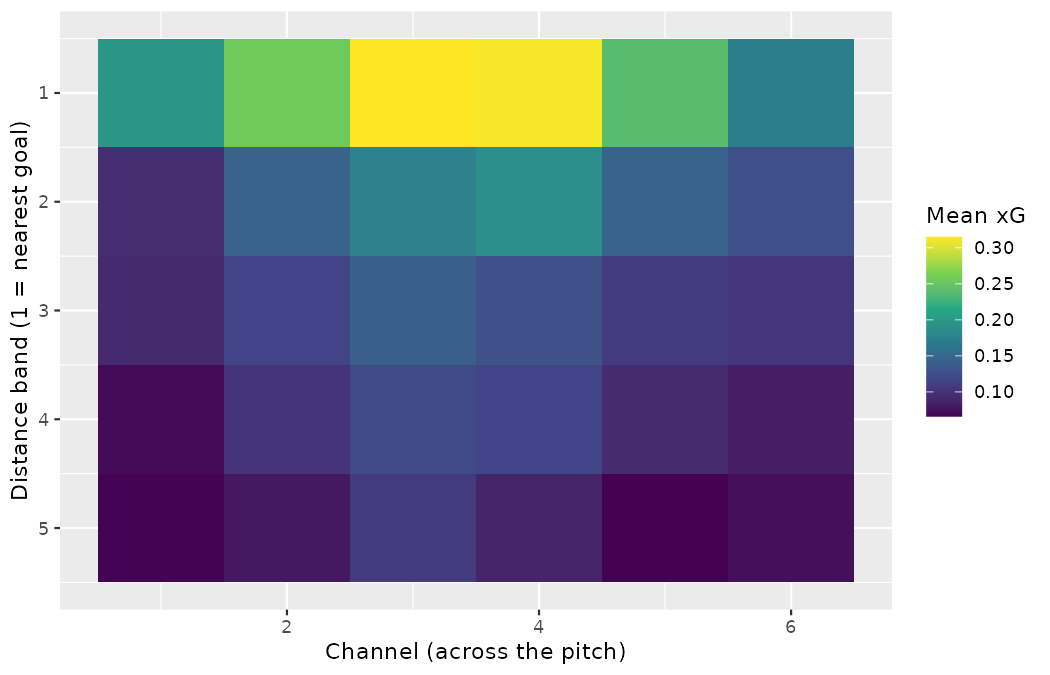
\includegraphics[width=0.85\linewidth,height=\textheight,keepaspectratio]{figures/explore-numerical-15.png}

The color key indicates which colors correspond to which values.
Intensity maps are not generally very helpful for reading precise values
in any given zone, but they are very helpful for seeing spatial trends
and generating interesting research questions or hypotheses.

\begin{tcolorbox}[enhanced jigsaw, left=2mm, leftrule=.75mm, title=\textcolor{quarto-callout-note-color}{\faInfo}\hspace{0.5em}{Worked example}, arc=.35mm, rightrule=.15mm, coltitle=black, colframe=quarto-callout-note-color-frame, bottomrule=.15mm, colbacktitle=quarto-callout-note-color!10!white, opacitybacktitle=0.6, breakable, bottomtitle=1mm, toptitle=1mm, titlerule=0mm, opacityback=0, toprule=.15mm, colback=white]

What interesting features are evident in the pitch-zone intensity map
drawn above?

\begin{center}\rule{0.5\linewidth}{0.5pt}\end{center}

Two gradients dominate. First, chance quality decays with distance: the
average of the six zones in band 1 is 0.249 xG, falling to 0.146 in band
2 and just 0.080 in band 5 --- and the drop is steepest between the
first two bands. Second, central beats wide within every band: the
hottest zone is band 1, channel 3 (0.315), while the coldest is a wide
zone in the most distant band (band 5, channel 5, at 0.066). Together
they say what every finishing coach preaches: close and central. A real
feed would add the wrinkles this constructed grid smooths over ---
penalties, angles, defensive traffic.

\end{tcolorbox}

\begin{tcolorbox}[enhanced jigsaw, left=2mm, leftrule=.75mm, title=\textcolor{quarto-callout-tip-color}{\faLightbulb}\hspace{0.5em}{Check your understanding}, arc=.35mm, rightrule=.15mm, coltitle=black, colframe=quarto-callout-tip-color-frame, bottomrule=.15mm, colbacktitle=quarto-callout-tip-color!10!white, opacitybacktitle=0.6, breakable, bottomtitle=1mm, toptitle=1mm, titlerule=0mm, opacityback=0, toprule=.15mm, colback=white]

Marta Vidal asks whether the intensity map can tell her the exact
average xG of shots from the zone in band 2, channel 4. What should
Priya answer, and what is the map good for instead?

\begin{center}\rule{0.5\linewidth}{0.5pt}\end{center}

Reading exact values off a color scale is unreliable --- that is what
the underlying table is for (the constructed value there is 0.190). The
map's job is to reveal spatial structure at a glance --- the
close-and-central gradient --- and to prompt questions worth
investigating, such as why one zone glows hotter than its mirror image
on the other flank.

\end{tcolorbox}

\section{Chapter review}\label{sec-chp5-review}

\subsection{Summary}\label{summary-4}

Fluently working with numerical variables is an important skill for a
scouting analyst --- chance quality, shot counts, minutes, fees, and
sprint speeds are all numerical. In this chapter we have introduced
different visualizations and numerical summaries applied to numeric
variables. The graphical visualizations are even more descriptive when
two variables are presented simultaneously. We presented scatterplots,
dot plots, histograms, and box plots. Numerical variables can be
summarized using the mean, median, quartiles, standard deviation, and
variance --- and you now know which of these to trust when a stray
penalty sits in the tail of the sample: the median and IQR are robust to
extreme observations, the mean and standard deviation are not.

\subsection{Terms}\label{terms-4}

The terms introduced in this chapter are presented below, alphabetized.
If you're not sure what some of these terms mean, we recommend you go
back in the text and review their definitions. You should be able to
easily spot them as \textbf{bolded text}.

\begin{longtable}[]{@{}
  >{\raggedright\arraybackslash}p{(\linewidth - 4\tabcolsep) * \real{0.3380}}
  >{\raggedright\arraybackslash}p{(\linewidth - 4\tabcolsep) * \real{0.3380}}
  >{\raggedright\arraybackslash}p{(\linewidth - 4\tabcolsep) * \real{0.3239}}@{}}
\caption{Terms introduced in this
chapter.}\label{tbl-terms-chp-05}\tabularnewline
\toprule\noalign{}
\endfirsthead
\endhead
\bottomrule\noalign{}
\endlastfoot
average & IQR & standard deviation \\
bimodal & left skewed & symmetric \\
box plot & mean & tail \\
data density & median & third quartile \\
density plot & multimodal & transformation \\
deviation & nonlinear & unimodal \\
distribution & outlier & variability \\
dot plot & percentile & variance \\
first quartile & point estimate & weighted mean \\
histogram & right skewed & whiskers \\
intensity map & robust statistics & \\
interquartile range & scatterplot & \\
\end{longtable}

\section{Exercises}\label{sec-chp5-exercises}

Answers to odd-numbered exercises can be found in
Appendix~\ref{sec-exercise-solutions-05}.

\begin{enumerate}
\def\labelenumi{\arabic{enumi}.}
\item
  \textbf{Chance creation and goals.} Data were collected on all 1,494
  shots of the 2022 Men's World Cup and aggregated to one row per team:
  the total chance quality (xG) each of the 32 teams accumulated across
  the tournament, and the total number of goals it scored. The code
  below draws a scatterplot of goals scored versus total xG.\footnote{The
    2022 Men's World Cup shot data used in this exercise are in
    \texttt{data/derived/wc2022\_shots.csv} (StatsBomb open data). The
    totals include penalty shoot-outs, per the book's penalty
    convention: 8 of Argentina's 23 goals and about 7.1 of their 21.0 xG
    come from period-5 kicks.}

\begin{Shaded}
\begin{Highlighting}[]
\NormalTok{wc2022\_shots }\OtherTok{\textless{}{-}} \FunctionTok{read\_csv}\NormalTok{(}\StringTok{"data/derived/wc2022\_shots.csv"}\NormalTok{)}

\NormalTok{team\_season }\OtherTok{\textless{}{-}}\NormalTok{ wc2022\_shots }\SpecialCharTok{|\textgreater{}}
  \FunctionTok{group\_by}\NormalTok{(team) }\SpecialCharTok{|\textgreater{}}
  \FunctionTok{summarize}\NormalTok{(}\AttributeTok{total\_xg =} \FunctionTok{sum}\NormalTok{(statsbomb\_xg), }\AttributeTok{goals =} \FunctionTok{sum}\NormalTok{(goal))}

\FunctionTok{ggplot}\NormalTok{(team\_season, }\FunctionTok{aes}\NormalTok{(}\AttributeTok{x =}\NormalTok{ total\_xg, }\AttributeTok{y =}\NormalTok{ goals)) }\SpecialCharTok{+}
  \FunctionTok{geom\_point}\NormalTok{(}\AttributeTok{alpha =} \FloatTok{0.8}\NormalTok{) }\SpecialCharTok{+}
  \FunctionTok{labs}\NormalTok{(}\AttributeTok{x =} \StringTok{"Total xG accumulated"}\NormalTok{, }\AttributeTok{y =} \StringTok{"Goals scored"}\NormalTok{)}
\end{Highlighting}
\end{Shaded}

  The 32 points rise steadily from the bottom-left corner (Costa Rica,
  with about 1.2 xG and 2 goals) to the top-right (Argentina, with about
  21.0 xG and 23 goals), staying fairly close to a straight-line trend
  throughout; a handful of teams sit visibly below the trend, most
  notably Brazil, who accumulated 13.6 xG but scored only 10 goals.

  \begin{enumerate}
  \def\labelenumii{\alph{enumii}.}
  \item
    What type of an association is apparent between total xG accumulated
    and goals scored?
  \item
    What type of an association would you expect to see if the axes of
    the plot were reversed, i.e., if we plotted total xG accumulated
    versus goals scored?
  \item
    Are total xG and goals scored independent? Explain your reasoning.
  \end{enumerate}
\item
  \textbf{Associations.} Priya Rao keeps a set of constructed
  scatterplots for training Northbridge's junior analysts; each panel
  plots a fabricated performance metric against a fabricated workload
  variable \(x.\) The seeded code below builds all four
  panels.\footnote{The training panels are a constructed scouting
    scenario, generated entirely by the seeded code shown; no real
    player data were used.} Indicate which of the plots show (a) a
  positive association, (b) a negative association, or (c) no
  association. Also determine if the positive and negative associations
  are linear or nonlinear. Each part may refer to more than one plot.

\begin{Shaded}
\begin{Highlighting}[]
\FunctionTok{set.seed}\NormalTok{(}\DecValTok{505}\NormalTok{)}
\NormalTok{x }\OtherTok{\textless{}{-}} \FunctionTok{seq}\NormalTok{(}\DecValTok{0}\NormalTok{, }\DecValTok{10}\NormalTok{, }\FloatTok{0.1}\NormalTok{)}

\NormalTok{training\_panels }\OtherTok{\textless{}{-}} \FunctionTok{tibble}\NormalTok{(}
  \AttributeTok{x =}\NormalTok{ x,}
  \StringTok{\textasciigrave{}}\AttributeTok{(1)}\StringTok{\textasciigrave{}} \OtherTok{=} \DecValTok{4} \SpecialCharTok{*}\NormalTok{ x }\SpecialCharTok{+} \FunctionTok{rnorm}\NormalTok{(}\FunctionTok{length}\NormalTok{(x), }\AttributeTok{sd =} \DecValTok{6}\NormalTok{),}
  \StringTok{\textasciigrave{}}\AttributeTok{(2)}\StringTok{\textasciigrave{}} \OtherTok{=} \FunctionTok{rnorm}\NormalTok{(}\FunctionTok{length}\NormalTok{(x), }\AttributeTok{mean =} \DecValTok{20}\NormalTok{, }\AttributeTok{sd =} \DecValTok{12}\NormalTok{),}
  \StringTok{\textasciigrave{}}\AttributeTok{(3)}\StringTok{\textasciigrave{}} \OtherTok{=}\NormalTok{ x}\SpecialCharTok{\^{}}\DecValTok{2} \SpecialCharTok{+} \FunctionTok{rnorm}\NormalTok{(}\FunctionTok{length}\NormalTok{(x), }\AttributeTok{sd =} \DecValTok{4}\NormalTok{),}
  \StringTok{\textasciigrave{}}\AttributeTok{(4)}\StringTok{\textasciigrave{}} \OtherTok{=} \SpecialCharTok{{-}}\DecValTok{3} \SpecialCharTok{*}\NormalTok{ x }\SpecialCharTok{+} \FunctionTok{rnorm}\NormalTok{(}\FunctionTok{length}\NormalTok{(x), }\AttributeTok{sd =} \DecValTok{5}\NormalTok{)}
\NormalTok{) }\SpecialCharTok{|\textgreater{}}
  \FunctionTok{pivot\_longer}\NormalTok{(}\SpecialCharTok{{-}}\NormalTok{x, }\AttributeTok{names\_to =} \StringTok{"panel"}\NormalTok{, }\AttributeTok{values\_to =} \StringTok{"y"}\NormalTok{)}

\FunctionTok{ggplot}\NormalTok{(training\_panels, }\FunctionTok{aes}\NormalTok{(}\AttributeTok{x =}\NormalTok{ x, }\AttributeTok{y =}\NormalTok{ y)) }\SpecialCharTok{+}
  \FunctionTok{geom\_point}\NormalTok{(}\AttributeTok{alpha =} \FloatTok{0.5}\NormalTok{) }\SpecialCharTok{+}
  \FunctionTok{facet\_wrap}\NormalTok{(}\SpecialCharTok{\textasciitilde{}}\NormalTok{panel, }\AttributeTok{nrow =} \DecValTok{1}\NormalTok{, }\AttributeTok{scales =} \StringTok{"free\_y"}\NormalTok{) }\SpecialCharTok{+}
  \FunctionTok{labs}\NormalTok{(}\AttributeTok{x =} \ConstantTok{NULL}\NormalTok{, }\AttributeTok{y =} \ConstantTok{NULL}\NormalTok{)}
\end{Highlighting}
\end{Shaded}

  In panel (1) the points climb steadily from left to right inside a
  broad straight band; in panel (2) the points form a diffuse cloud with
  no visible drift in either direction; in panel (3) the points are
  nearly flat at the left edge and then climb ever more steeply toward
  the right; in panel (4) the points fall steadily from left to right
  inside a straight band.
\item
  \textbf{Filling the video archive.} Northbridge's historical video
  archive holds exactly 10,000 matches awaiting tagging. A small crew of
  taggers starts work; as they go, each experienced tagger trains new
  recruits, so the crew grows over time --- but there are only 10,000
  matches to tag, and the untagged matches become harder to find as
  coverage nears completion. Sketch a plot representing the relationship
  between the cumulative number of matches tagged and time.
\item
  \textbf{Matchday edge.} A scout's report on a player's temperament
  often comes down to arousal: a player who feels no competitive edge
  before kickoff --- a meaningless friendly, nothing at stake --- tends
  to produce a flat performance. However, very high levels of pre-match
  anxiety, as in an overwhelming cup final, can also degrade a player's
  performance. Sketch a plot to represent the relationship between
  pre-match arousal and match performance.
\item
  \textbf{Late trialist.} At a Northbridge trial day, 25 trialists sat
  the club's technical entry test (scored out of 100 points): 24 of them
  took the test on the day, and 1 trialist, delayed by travel, took it
  the following morning. Jonas Beck graded the first batch of 24 tests
  and found an average score of 74 points with a standard deviation of
  8.9 points. The trialist who tested the following morning scored 64
  points.

  \begin{enumerate}
  \def\labelenumii{\alph{enumii}.}
  \item
    Does the late trialist's score increase or decrease the average
    score?
  \item
    What is the new average?
  \item
    Does the late trialist's score increase or decrease the standard
    deviation of the scores?
  \end{enumerate}
\item
  \textbf{Shot volume across a tournament.} How is shooting workload
  distributed across the players of a tournament? The code below
  aggregates the 2022 Men's World Cup shot data to one row per player
  --- 432 players attempted at least one shot --- and draws a relative
  frequency histogram of the shot counts.\footnote{The per-player shot
    counts are aggregated from \texttt{data/derived/wc2022\_shots.csv}
    (StatsBomb open data) by the code shown.}

\begin{Shaded}
\begin{Highlighting}[]
\NormalTok{wc2022\_shots }\OtherTok{\textless{}{-}} \FunctionTok{read\_csv}\NormalTok{(}\StringTok{"data/derived/wc2022\_shots.csv"}\NormalTok{)}

\NormalTok{player\_shots\_wc }\OtherTok{\textless{}{-}}\NormalTok{ wc2022\_shots }\SpecialCharTok{|\textgreater{}}
  \FunctionTok{group\_by}\NormalTok{(player, team) }\SpecialCharTok{|\textgreater{}}
  \FunctionTok{summarize}\NormalTok{(}\AttributeTok{shots =} \FunctionTok{n}\NormalTok{(), }\AttributeTok{.groups =} \StringTok{"drop"}\NormalTok{)}

\FunctionTok{ggplot}\NormalTok{(player\_shots\_wc, }\FunctionTok{aes}\NormalTok{(}\AttributeTok{x =}\NormalTok{ shots)) }\SpecialCharTok{+}
  \FunctionTok{geom\_histogram}\NormalTok{(}\FunctionTok{aes}\NormalTok{(}\AttributeTok{y =} \FunctionTok{after\_stat}\NormalTok{(count }\SpecialCharTok{/} \FunctionTok{sum}\NormalTok{(count))), }\AttributeTok{binwidth =} \DecValTok{1}\NormalTok{) }\SpecialCharTok{+}
  \FunctionTok{labs}\NormalTok{(}\AttributeTok{x =} \StringTok{"Shots attempted in the tournament"}\NormalTok{, }\AttributeTok{y =} \StringTok{"Proportion of players"}\NormalTok{)}
\end{Highlighting}
\end{Shaded}

  The tallest bar is the first one: the players with exactly 1 shot make
  up about 0.34 of the sample. The bars then shrink steadily --- about
  0.20 of players took 2 shots, 0.14 took 3, 0.08 took 4, 0.06 took 5
  --- and the distribution trails off into a long, thin right tail,
  ending with two isolated bars far to the right at 32 shots (Kylian
  Mbappé) and 34 shots (Lionel Messi).

  \begin{enumerate}
  \def\labelenumii{\alph{enumii}.}
  \item
    Estimate \(Q_1,\) the median, and \(Q_3\) from the histogram.
  \item
    Would you expect the mean of this dataset to be smaller or larger
    than the median? Explain your reasoning.
  \end{enumerate}
\item
  \textbf{Raising the average.} Emil Sørensen's network of regional
  scouts attends an average of 35 live matches per scout per season,
  which is lower than the figure boasted by rival clubs' networks. Marta
  Vidal presses Emil to raise the average, but sending scouts to more
  matches would blow the travel budget. Instead, Emil decides he should
  cut 10 scouts from the network in such a way as to raise the average
  number of live matches reported per scout. In order to achieve this
  goal, should he cut the scouts who attend the most matches, the fewest
  matches, or those who attend about the average number of matches?
\item
  \textbf{Medians and IQRs.} Priya hands a junior analyst pairs of small
  constructed datasets --- each is the number of chances created by a
  prospect across five logged matches. For each part, compare
  distributions A and B based on their medians and IQRs. You do not need
  to calculate these statistics; simply state how the medians and IQRs
  compare. Make sure to explain your reasoning. \emph{Hint:} It may be
  useful to sketch dot plots of the distributions.

  \begin{enumerate}
  \def\labelenumii{\alph{enumii}.}
  \item
    \textbf{A:} 3, 5, 6, 7, 9; \textbf{B:} 3, 5, 6, 7, 20
  \item
    \textbf{A:} 3, 5, 6, 7, 9; \textbf{B:} 3, 5, 7, 8, 9
  \item
    \textbf{A:} 1, 2, 3, 4, 5; \textbf{B:} 6, 7, 8, 9, 10
  \item
    \textbf{A:} 0, 10, 50, 60, 100; \textbf{B:} 0, 100, 500, 600, 1000
  \end{enumerate}
\item
  \textbf{Means and SDs.} The next training sheet in Priya's pile works
  the same way, but for the mean and standard deviation; some of the
  constructed values are negative, as they would be for a metric like a
  player's plus-minus goal difference while on the pitch. For each part,
  compare distributions A and B based on their means and standard
  deviations. You do not need to calculate these statistics; simply
  state how the means and the standard deviations compare. Make sure to
  explain your reasoning. \emph{Hint:} It may be useful to sketch dot
  plots of the distributions.

  \begin{enumerate}
  \def\labelenumii{\alph{enumii}.}
  \item
    \textbf{A:} 3, 5, 5, 5, 8, 11, 11, 11, 13; \textbf{B:} 3, 5, 5, 5,
    8, 11, 11, 11, 20
  \item
    \textbf{A:} -20, 0, 0, 0, 15, 25, 30, 30; \textbf{B:} -40, 0, 0, 0,
    15, 25, 30, 30
  \item
    \textbf{A:} 0, 2, 4, 6, 8, 10; \textbf{B:} 20, 22, 24, 26, 28, 30
  \item
    \textbf{A:} 100, 200, 300, 400, 500; \textbf{B:} 0, 50, 300, 550,
    600
  \end{enumerate}
\item
  \textbf{Histograms and box plots.} For another training exercise,
  Priya fabricates three performance variables for 1,000 imaginary
  players: \texttt{metric\_a} mimics top sprint speeds (in km/h),
  \texttt{metric\_b} mimics the minute-of-the-half at which a shot is
  taken, and \texttt{metric\_c} mimics kilometers of high-speed running
  per match. The seeded code below builds the data and draws a histogram
  and a box plot of each variable.\footnote{The
    \texttt{training\_metrics} data are a constructed training exercise,
    generated entirely by the seeded code shown; no real players were
    measured.} Describe (in words) the distribution in each histogram,
  and match the histograms, labeled (a), (b), and (c), to the box plots,
  labeled (1), (2), and (3).

\begin{Shaded}
\begin{Highlighting}[]
\FunctionTok{set.seed}\NormalTok{(}\DecValTok{506}\NormalTok{)}
\NormalTok{training\_metrics }\OtherTok{\textless{}{-}} \FunctionTok{tibble}\NormalTok{(}
  \AttributeTok{metric\_a =} \FunctionTok{rnorm}\NormalTok{(}\DecValTok{1000}\NormalTok{, }\AttributeTok{mean =} \DecValTok{33}\NormalTok{, }\AttributeTok{sd =} \FloatTok{1.5}\NormalTok{),}
  \AttributeTok{metric\_b =} \FunctionTok{runif}\NormalTok{(}\DecValTok{1000}\NormalTok{, }\AttributeTok{min =} \DecValTok{0}\NormalTok{, }\AttributeTok{max =} \DecValTok{45}\NormalTok{),}
  \AttributeTok{metric\_c =} \FunctionTok{rgamma}\NormalTok{(}\DecValTok{1000}\NormalTok{, }\AttributeTok{shape =} \DecValTok{3}\NormalTok{, }\AttributeTok{rate =} \DecValTok{2}\NormalTok{)}
\NormalTok{)}

\NormalTok{p\_hist }\OtherTok{\textless{}{-}}\NormalTok{ training\_metrics }\SpecialCharTok{|\textgreater{}}
  \FunctionTok{pivot\_longer}\NormalTok{(}\FunctionTok{everything}\NormalTok{(), }\AttributeTok{names\_to =} \StringTok{"metric"}\NormalTok{, }\AttributeTok{values\_to =} \StringTok{"x"}\NormalTok{) }\SpecialCharTok{|\textgreater{}}
  \FunctionTok{mutate}\NormalTok{(}\AttributeTok{label =} \FunctionTok{case\_when}\NormalTok{(}
\NormalTok{    metric }\SpecialCharTok{==} \StringTok{"metric\_a"} \SpecialCharTok{\textasciitilde{}} \StringTok{"(a)"}\NormalTok{,}
\NormalTok{    metric }\SpecialCharTok{==} \StringTok{"metric\_b"} \SpecialCharTok{\textasciitilde{}} \StringTok{"(b)"}\NormalTok{,}
\NormalTok{    metric }\SpecialCharTok{==} \StringTok{"metric\_c"} \SpecialCharTok{\textasciitilde{}} \StringTok{"(c)"}
\NormalTok{  )) }\SpecialCharTok{|\textgreater{}}
  \FunctionTok{ggplot}\NormalTok{(}\FunctionTok{aes}\NormalTok{(}\AttributeTok{x =}\NormalTok{ x)) }\SpecialCharTok{+}
  \FunctionTok{geom\_histogram}\NormalTok{(}\AttributeTok{bins =} \DecValTok{10}\NormalTok{) }\SpecialCharTok{+}
  \FunctionTok{facet\_wrap}\NormalTok{(}\SpecialCharTok{\textasciitilde{}}\NormalTok{label, }\AttributeTok{scales =} \StringTok{"free"}\NormalTok{) }\SpecialCharTok{+}
  \FunctionTok{labs}\NormalTok{(}\AttributeTok{x =} \ConstantTok{NULL}\NormalTok{, }\AttributeTok{y =} \ConstantTok{NULL}\NormalTok{)}

\NormalTok{p\_box }\OtherTok{\textless{}{-}}\NormalTok{ training\_metrics }\SpecialCharTok{|\textgreater{}}
  \FunctionTok{pivot\_longer}\NormalTok{(}\FunctionTok{everything}\NormalTok{(), }\AttributeTok{names\_to =} \StringTok{"metric"}\NormalTok{, }\AttributeTok{values\_to =} \StringTok{"x"}\NormalTok{) }\SpecialCharTok{|\textgreater{}}
  \FunctionTok{mutate}\NormalTok{(}\AttributeTok{label =} \FunctionTok{case\_when}\NormalTok{(}
\NormalTok{    metric }\SpecialCharTok{==} \StringTok{"metric\_a"} \SpecialCharTok{\textasciitilde{}} \StringTok{"(2)"}\NormalTok{,}
\NormalTok{    metric }\SpecialCharTok{==} \StringTok{"metric\_b"} \SpecialCharTok{\textasciitilde{}} \StringTok{"(3)"}\NormalTok{,}
\NormalTok{    metric }\SpecialCharTok{==} \StringTok{"metric\_c"} \SpecialCharTok{\textasciitilde{}} \StringTok{"(1)"}
\NormalTok{  )) }\SpecialCharTok{|\textgreater{}}
  \FunctionTok{ggplot}\NormalTok{(}\FunctionTok{aes}\NormalTok{(}\AttributeTok{y =}\NormalTok{ x)) }\SpecialCharTok{+}
  \FunctionTok{geom\_boxplot}\NormalTok{(}\AttributeTok{outlier.alpha =} \FloatTok{0.8}\NormalTok{) }\SpecialCharTok{+}
  \FunctionTok{facet\_wrap}\NormalTok{(}\SpecialCharTok{\textasciitilde{}}\NormalTok{label, }\AttributeTok{scales =} \StringTok{"free"}\NormalTok{) }\SpecialCharTok{+}
  \FunctionTok{labs}\NormalTok{(}\AttributeTok{x =} \ConstantTok{NULL}\NormalTok{, }\AttributeTok{y =} \ConstantTok{NULL}\NormalTok{)}

\NormalTok{p\_hist }\SpecialCharTok{/}\NormalTok{ p\_box}
\end{Highlighting}
\end{Shaded}

  Histogram (a) is a symmetric bell running from about 28 to 38, peaked
  at 33. Histogram (b) is flat: its bars are all of roughly equal height
  across the range 0 to 45. Histogram (c) peaks just above 1 and trails
  off in a long right tail reaching past 5.5. Box plot (1) has its box
  from about 0.9 to 1.9 with the median near 1.4, and a string of dots
  above the upper whisker stretching to about 5.8, with none below. Box
  plot (2) has a narrow box from about 32.0 to 34.1 with the median at
  33.1, short whiskers, and a few dots beyond the whiskers on both
  sides. Box plot (3) has a wide box from about 11.6 to 33.5 with the
  median near 22.5, long whiskers reaching almost to 0 and 45, and no
  dots beyond them.
\item
  \textbf{Shots per team-match.} How many shots does a team typically
  produce in a World Cup match? The code below rebuilds the
  \texttt{team\_match} data --- one row per (match, team) aggregate of
  the 2022 Men's World Cup shots, exactly as constructed in
  Section~\ref{sec-dotplots} --- and draws a relative frequency
  histogram of the number of shots per team-match.\footnote{The
    \texttt{team\_match} data are aggregated from
    \texttt{data/derived/wc2022\_shots.csv} (StatsBomb open data) by the
    code shown, which matches the construction in
    Section~\ref{sec-dotplots}.} Recall that the data have 127 rows
  rather than 128: Costa Rica registered no shots at all in one of their
  matches, so that team-match has no row.

\begin{Shaded}
\begin{Highlighting}[]
\NormalTok{wc2022\_shots }\OtherTok{\textless{}{-}} \FunctionTok{read\_csv}\NormalTok{(}\StringTok{"data/derived/wc2022\_shots.csv"}\NormalTok{)}

\NormalTok{team\_match }\OtherTok{\textless{}{-}}\NormalTok{ wc2022\_shots }\SpecialCharTok{|\textgreater{}}
  \FunctionTok{group\_by}\NormalTok{(match\_id, team) }\SpecialCharTok{|\textgreater{}}
  \FunctionTok{summarize}\NormalTok{(}
    \AttributeTok{n\_shots =} \FunctionTok{n}\NormalTok{(),}
    \AttributeTok{total\_xg =} \FunctionTok{sum}\NormalTok{(statsbomb\_xg),}
    \AttributeTok{goals =} \FunctionTok{sum}\NormalTok{(goal),}
    \AttributeTok{prop\_under\_pressure =} \FunctionTok{mean}\NormalTok{(under\_pressure),}
    \AttributeTok{prop\_set\_piece =} \FunctionTok{mean}\NormalTok{(play\_pattern }\SpecialCharTok{\%in\%}
      \FunctionTok{c}\NormalTok{(}\StringTok{"From Corner"}\NormalTok{, }\StringTok{"From Free Kick"}\NormalTok{, }\StringTok{"From Throw In"}\NormalTok{)),}
    \AttributeTok{.groups =} \StringTok{"drop"}
\NormalTok{  )}

\FunctionTok{ggplot}\NormalTok{(team\_match, }\FunctionTok{aes}\NormalTok{(}\AttributeTok{x =}\NormalTok{ n\_shots)) }\SpecialCharTok{+}
  \FunctionTok{geom\_histogram}\NormalTok{(}\FunctionTok{aes}\NormalTok{(}\AttributeTok{y =} \FunctionTok{after\_stat}\NormalTok{(count }\SpecialCharTok{/} \FunctionTok{sum}\NormalTok{(count))),}
                 \AttributeTok{breaks =} \FunctionTok{seq}\NormalTok{(}\DecValTok{0}\NormalTok{, }\DecValTok{32}\NormalTok{, }\DecValTok{2}\NormalTok{)) }\SpecialCharTok{+}
  \FunctionTok{labs}\NormalTok{(}\AttributeTok{x =} \StringTok{"Shots in a single team{-}match"}\NormalTok{, }\AttributeTok{y =} \StringTok{"Proportion"}\NormalTok{)}
\end{Highlighting}
\end{Shaded}

  The bars rise from a single team-match in the 0--2 bin (height 0.008)
  through heights of about 0.05, 0.10, and 0.14 to a peak of about 0.17
  over the 8--10 bin, then fall away through 0.15, 0.13, 0.08, and 0.05;
  after a near-empty 18--20 bin, a modest secondary shelf over 20 to 24
  shots (heights around 0.04--0.05) trails into a low 24--26 bar (height
  0.016), and a lone bar sits far right in the 30--32 bin.

  \begin{enumerate}
  \def\labelenumii{\alph{enumii}.}
  \item
    Estimate the median number of shots per team-match from the
    histogram.
  \item
    Would you expect the mean of this sample to be higher or lower than
    the median? Explain your reasoning.
  \item
    Estimate \(Q_1,\) \(Q_3,\) and the IQR for the distribution.
  \item
    Would any of the team-matches in this sample be considered to have
    an unusually low or unusually high shot count? Explain your
    reasoning.
  \end{enumerate}
\item
  \textbf{Pass completion at the academy.} Jonas Beck's staff logged the
  pass-completion percentage of 400 academy trialists across a
  standardized possession drill. This is a constructed scenario, built
  by the seeded code below, which also draws the histogram.\footnote{The
    \texttt{pass\_comp} data are a constructed scouting scenario,
    generated entirely by the seeded code shown; no real trialists were
    assessed.} Estimate the median for the 400 observations shown in the
  histogram, and note whether you expect the mean to be higher or lower
  than the median.

\begin{Shaded}
\begin{Highlighting}[]
\FunctionTok{set.seed}\NormalTok{(}\DecValTok{507}\NormalTok{)}
\NormalTok{pass\_comp }\OtherTok{\textless{}{-}} \FunctionTok{tibble}\NormalTok{(}\AttributeTok{completion =} \DecValTok{100} \SpecialCharTok{*} \FunctionTok{rbeta}\NormalTok{(}\DecValTok{400}\NormalTok{, }\DecValTok{12}\NormalTok{, }\DecValTok{3}\NormalTok{))}

\FunctionTok{ggplot}\NormalTok{(pass\_comp, }\FunctionTok{aes}\NormalTok{(}\AttributeTok{x =}\NormalTok{ completion)) }\SpecialCharTok{+}
  \FunctionTok{geom\_histogram}\NormalTok{(}\AttributeTok{binwidth =} \DecValTok{5}\NormalTok{, }\AttributeTok{boundary =} \DecValTok{0}\NormalTok{) }\SpecialCharTok{+}
  \FunctionTok{labs}\NormalTok{(}\AttributeTok{x =} \StringTok{"Pass completion (\%)"}\NormalTok{, }\AttributeTok{y =} \StringTok{"Count"}\NormalTok{)}
\end{Highlighting}
\end{Shaded}

  The bars climb steadily from a thin left tail --- a couple of
  trialists near 45\%, a handful in the 50s, then 17, 37, 46, and 71
  trialists in the bins from 60 up to 80 --- to a peak of 86 trialists
  in the 80--85\% bin, before dropping to 73, 49, and finally just 7
  trialists above 95\%.
\item
  \textbf{Tagging turnaround.} Northbridge's video platform logs how
  many hours each match takes to come back fully tagged. Auto-tagged
  matches cluster around 5 hours, matches routed to manual taggers
  cluster around 12 hours, and a small number of problem files drag on
  much longer. The seeded code below constructs a batch of 625
  turnaround times and draws a histogram and a box plot of the same
  data.\footnote{The \texttt{turnaround} data are a constructed
    club-operations scenario, generated entirely by the seeded code
    shown.} Compare the two plots. What characteristics of the
  distribution are apparent in the histogram and not in the box plot?
  What characteristics are apparent in the box plot but not in the
  histogram?

\begin{Shaded}
\begin{Highlighting}[]
\FunctionTok{set.seed}\NormalTok{(}\DecValTok{508}\NormalTok{)}
\NormalTok{turnaround }\OtherTok{\textless{}{-}} \FunctionTok{tibble}\NormalTok{(}\AttributeTok{hours =} \FunctionTok{c}\NormalTok{(}\FunctionTok{rnorm}\NormalTok{(}\DecValTok{300}\NormalTok{, }\AttributeTok{mean =} \DecValTok{5}\NormalTok{, }\AttributeTok{sd =} \DecValTok{1}\NormalTok{),}
                               \FunctionTok{rnorm}\NormalTok{(}\DecValTok{300}\NormalTok{, }\AttributeTok{mean =} \DecValTok{12}\NormalTok{, }\AttributeTok{sd =} \DecValTok{1}\NormalTok{),}
                               \FunctionTok{runif}\NormalTok{(}\DecValTok{25}\NormalTok{, }\AttributeTok{min =} \DecValTok{13}\NormalTok{, }\AttributeTok{max =} \DecValTok{28}\NormalTok{)))}

\NormalTok{p\_hist }\OtherTok{\textless{}{-}} \FunctionTok{ggplot}\NormalTok{(turnaround, }\FunctionTok{aes}\NormalTok{(}\AttributeTok{x =}\NormalTok{ hours)) }\SpecialCharTok{+}
  \FunctionTok{geom\_histogram}\NormalTok{(}\AttributeTok{binwidth =} \FloatTok{2.5}\NormalTok{, }\AttributeTok{boundary =} \DecValTok{0}\NormalTok{) }\SpecialCharTok{+}
  \FunctionTok{labs}\NormalTok{(}\AttributeTok{x =} \StringTok{"Turnaround (hours)"}\NormalTok{, }\AttributeTok{y =} \ConstantTok{NULL}\NormalTok{)}

\NormalTok{p\_box }\OtherTok{\textless{}{-}} \FunctionTok{ggplot}\NormalTok{(turnaround, }\FunctionTok{aes}\NormalTok{(}\AttributeTok{y =}\NormalTok{ hours)) }\SpecialCharTok{+}
  \FunctionTok{geom\_boxplot}\NormalTok{(}\AttributeTok{outlier.alpha =} \FloatTok{0.5}\NormalTok{) }\SpecialCharTok{+}
  \FunctionTok{labs}\NormalTok{(}\AttributeTok{x =} \ConstantTok{NULL}\NormalTok{, }\AttributeTok{y =} \StringTok{"Turnaround (hours)"}\NormalTok{)}

\NormalTok{p\_hist }\SpecialCharTok{+}\NormalTok{ p\_box}
\end{Highlighting}
\end{Shaded}

  The histogram shows two tall peaks --- 168 matches in the 5--7.5 bin
  and 202 in the 10--12.5 bin --- separated by a deep valley (only 9
  matches between 7.5 and 10), with a thin right tail running out past
  27 hours. The box plot shows a box from about 5.2 to 12.2 with the
  median line at 10.3, a lower whisker to about 2.1, an upper whisker to
  22.5, and a dozen individual dots between about 22.9 and 27.5.
\item
  \textbf{Shots per player.} Northbridge's analytics platform reports
  that at the 2025 Women's Euro, half of the 215 players who attempted a
  shot took 3 or fewer shots, and that the average shot count per player
  was 4.25. What do these findings suggest about the shape of the
  distribution of shots per player?\footnote{The quoted figures are
    computed from \texttt{data/derived/weuro2025\_shots.csv} (StatsBomb
    open data), aggregated to one row per player as in
    Section~\ref{sec-transforming-data}.}
\item
  \textbf{Distributions and appropriate statistics, I.} For each of the
  following, state whether you expect the distribution to be symmetric,
  right skewed, or left skewed. Also specify whether the mean or median
  would best represent a typical observation in the data, and whether
  the variability of observations would be best represented using the
  standard deviation or IQR. Explain your reasoning.

  \begin{enumerate}
  \def\labelenumii{\alph{enumii}.}
  \item
    Number of goals scored per player across a tournament.
  \item
    Distance a regional scout travels to reach an assigned match, i.e.,
    the number of kilometers between home and the ground.
  \item
    Heights of adult male professional footballers.
  \item
    Age at which professional footballers retire.
  \item
    Scores on an easy technical drill at a trial day.
  \end{enumerate}
\item
  \textbf{Distributions and appropriate statistics, II.} For each of the
  following, state whether you expect the distribution to be symmetric,
  right skewed, or left skewed. Also specify whether the mean or median
  would best represent a typical observation in the data, and whether
  the variability of observations would be best represented using the
  standard deviation or IQR. Explain your reasoning.

  \begin{enumerate}
  \def\labelenumii{\alph{enumii}.}
  \item
    Transfer fees in a market where 25\% of the deals close below
    €350,000, 50\% close below €450,000, 75\% close below €1,000,000,
    and there are a meaningful number of deals above €6,000,000.
  \item
    Transfer fees in a market where 25\% of the deals close below
    €300,000, 50\% close below €600,000, 75\% close below €900,000, and
    very few deals exceed €1,200,000.
  \item
    Number of senior international caps held by the trialists at an
    academy open day. Assume that most trialists have never been capped,
    and only a few have collected many caps.
  \item
    Annual salaries of the players at a top-division club where a few
    star signings earn much higher salaries than all the other squad
    members.
  \item
    Days to return from a standard hamstring strain in the club's
    medical records, where 25\% of players return within 38 days, 50\%
    within 39 days, 75\% within 40 days, and a handful of setback cases
    stretch out to 90 days.
  \end{enumerate}
\item
  \textbf{Video hours.} Academy players at Northbridge were asked how
  many hours of match video they watch per week, including opposition
  analysis clips. This sample yielded an average of 8.28 hours, with a
  standard deviation of 7.18 hours. Is the distribution of number of
  hours academy players watch match video weekly symmetric? If not, what
  shape would you expect this distribution to have? Explain your
  reasoning.
\item
  \textbf{Entry-test scores.} The average on Northbridge's technical
  entry test (scored out of 100 points) was 85, with a standard
  deviation of 15. Is the distribution of the scores on this test
  symmetric? If not, what shape would you expect this distribution to
  have? Explain your reasoning.
\item
  \textbf{Midrange.} Priya considers summarizing the chance quality of a
  striker's shots with the \emph{midrange} of the xG values, where the
  midrange of a distribution is defined as the average of the maximum
  and the minimum of that distribution. Is this statistic robust to
  outliers and extreme skew --- say, to the presence of a single penalty
  at 0.78 xG among a season of ordinary chances? Explain your reasoning.
\item
  \textbf{Shooting under pressure.} The histograms drawn by the code
  below show the distribution of chance quality (xG) for the 2022 Men's
  World Cup shots taken under defensive pressure and for those taken
  unpressured. Summary statistics for the two distributions are also
  computed. Compare the two distributions.\footnote{The 2022 Men's World
    Cup shot data used in this exercise are in
    \texttt{data/derived/wc2022\_shots.csv} (StatsBomb open data).}

\begin{Shaded}
\begin{Highlighting}[]
\NormalTok{wc2022\_shots }\OtherTok{\textless{}{-}} \FunctionTok{read\_csv}\NormalTok{(}\StringTok{"data/derived/wc2022\_shots.csv"}\NormalTok{)}

\NormalTok{shots\_by\_pressure }\OtherTok{\textless{}{-}}\NormalTok{ wc2022\_shots }\SpecialCharTok{|\textgreater{}}
  \FunctionTok{mutate}\NormalTok{(}\AttributeTok{pressure =} \FunctionTok{if\_else}\NormalTok{(under\_pressure,}
                            \StringTok{"Under pressure"}\NormalTok{, }\StringTok{"Not under pressure"}\NormalTok{))}

\FunctionTok{ggplot}\NormalTok{(shots\_by\_pressure, }\FunctionTok{aes}\NormalTok{(}\AttributeTok{x =}\NormalTok{ statsbomb\_xg)) }\SpecialCharTok{+}
  \FunctionTok{geom\_histogram}\NormalTok{(}\AttributeTok{binwidth =} \FloatTok{0.05}\NormalTok{, }\AttributeTok{boundary =} \DecValTok{0}\NormalTok{) }\SpecialCharTok{+}
  \FunctionTok{facet\_wrap}\NormalTok{(}\SpecialCharTok{\textasciitilde{}}\NormalTok{pressure, }\AttributeTok{ncol =} \DecValTok{1}\NormalTok{, }\AttributeTok{scales =} \StringTok{"free\_y"}\NormalTok{) }\SpecialCharTok{+}
  \FunctionTok{labs}\NormalTok{(}\AttributeTok{x =} \StringTok{"Chance quality (xG)"}\NormalTok{, }\AttributeTok{y =} \StringTok{"Count"}\NormalTok{)}

\NormalTok{shots\_by\_pressure }\SpecialCharTok{|\textgreater{}}
  \FunctionTok{group\_by}\NormalTok{(pressure) }\SpecialCharTok{|\textgreater{}}
  \FunctionTok{summarize}\NormalTok{(}\AttributeTok{mean\_xg =} \FunctionTok{mean}\NormalTok{(statsbomb\_xg), }\AttributeTok{sd\_xg =} \FunctionTok{sd}\NormalTok{(statsbomb\_xg), }\AttributeTok{n =} \FunctionTok{n}\NormalTok{())}
\CommentTok{\#\textgreater{} \# A tibble: 2 × 4}
\CommentTok{\#\textgreater{}   pressure           mean\_xg  sd\_xg     n}
\CommentTok{\#\textgreater{}   \textless{}chr\textgreater{}                \textless{}dbl\textgreater{}  \textless{}dbl\textgreater{} \textless{}int\textgreater{}}
\CommentTok{\#\textgreater{} 1 Not under pressure  0.131  0.196   1256}
\CommentTok{\#\textgreater{} 2 Under pressure      0.0961 0.0949   238}
\end{Highlighting}
\end{Shaded}

  Both histograms are unimodal with tall bars at the low end --- in each
  group roughly 70\% of shots carry less than 0.10 xG --- and both trail
  off to the right. The unpressured panel, however, has a much longer
  tail: 94 of its shots exceed 0.5 xG, including a distinct isolated
  spike near 0.78 (the tournament's 64 penalties, every one of them
  taken unpressured) and a maximum of 0.90. The pressured panel's tail
  ends far sooner --- only 2 pressured shots exceed 0.5 xG, and the
  largest is 0.64.
\item
  \textbf{Trial-day scores.} The technical entry test scores of twenty
  Northbridge trialists, arranged in ascending order, are as follows:
  57, 66, 69, 71, 72, 73, 74, 77, 78, 78, 79, 79, 81, 81, 82, 83, 83,
  88, 89, 94. Suppose trialists who score above the 75th percentile on
  the test are invited back for a second trial. How many trialists will
  be invited back?
\item
  \textbf{Wages at Northbridge.} The first histogram drawn by the code
  below shows the distribution of the weekly wages (in euros) of the 40
  players on Northbridge's books --- the squad of a mid-table club, with
  most players between roughly €25,000 and €45,000 a week. In the
  January window, Marta Vidal sanctions two marquee signings on weekly
  wages of €95,000 and €110,000; the second histogram shows the new wage
  distribution. This is a constructed scenario, built by the seeded
  code, which also computes summary statistics for both versions of the
  wage bill.\footnote{The \texttt{wages} data are a constructed scouting
    scenario, generated entirely by the seeded code shown; they are not
    the wages of any real club.}

\begin{Shaded}
\begin{Highlighting}[]
\FunctionTok{set.seed}\NormalTok{(}\DecValTok{509}\NormalTok{)}
\NormalTok{wages\_before }\OtherTok{\textless{}{-}} \FunctionTok{rnorm}\NormalTok{(}\DecValTok{40}\NormalTok{, }\AttributeTok{mean =} \DecValTok{34000}\NormalTok{, }\AttributeTok{sd =} \DecValTok{5000}\NormalTok{)}
\NormalTok{wages\_after  }\OtherTok{\textless{}{-}} \FunctionTok{c}\NormalTok{(wages\_before, }\DecValTok{95000}\NormalTok{, }\DecValTok{110000}\NormalTok{)}

\NormalTok{wages }\OtherTok{\textless{}{-}} \FunctionTok{tibble}\NormalTok{(}
  \AttributeTok{period =} \FunctionTok{rep}\NormalTok{(}\FunctionTok{c}\NormalTok{(}\StringTok{"Before"}\NormalTok{, }\StringTok{"After"}\NormalTok{), }\AttributeTok{times =} \FunctionTok{c}\NormalTok{(}\DecValTok{40}\NormalTok{, }\DecValTok{42}\NormalTok{)),}
  \AttributeTok{wage   =} \FunctionTok{c}\NormalTok{(wages\_before, wages\_after)}
\NormalTok{) }\SpecialCharTok{|\textgreater{}}
  \FunctionTok{mutate}\NormalTok{(}\AttributeTok{period =} \FunctionTok{factor}\NormalTok{(period, }\AttributeTok{levels =} \FunctionTok{c}\NormalTok{(}\StringTok{"Before"}\NormalTok{, }\StringTok{"After"}\NormalTok{)))}

\FunctionTok{ggplot}\NormalTok{(wages, }\FunctionTok{aes}\NormalTok{(}\AttributeTok{x =}\NormalTok{ wage)) }\SpecialCharTok{+}
  \FunctionTok{geom\_histogram}\NormalTok{(}\AttributeTok{binwidth =} \DecValTok{2500}\NormalTok{) }\SpecialCharTok{+}
  \FunctionTok{facet\_wrap}\NormalTok{(}\SpecialCharTok{\textasciitilde{}}\NormalTok{period, }\AttributeTok{ncol =} \DecValTok{1}\NormalTok{, }\AttributeTok{scales =} \StringTok{"free\_x"}\NormalTok{) }\SpecialCharTok{+}
  \FunctionTok{labs}\NormalTok{(}\AttributeTok{x =} \StringTok{"Weekly wage (EUR)"}\NormalTok{, }\AttributeTok{y =} \StringTok{"Count"}\NormalTok{)}

\NormalTok{wages }\SpecialCharTok{|\textgreater{}}
  \FunctionTok{group\_by}\NormalTok{(period) }\SpecialCharTok{|\textgreater{}}
  \FunctionTok{summarize}\NormalTok{(}
    \AttributeTok{n =} \FunctionTok{n}\NormalTok{(),}
    \AttributeTok{min =} \FunctionTok{min}\NormalTok{(wage),}
    \AttributeTok{q1 =} \FunctionTok{quantile}\NormalTok{(wage, }\FloatTok{0.25}\NormalTok{),}
    \AttributeTok{median =} \FunctionTok{median}\NormalTok{(wage),}
    \AttributeTok{q3 =} \FunctionTok{quantile}\NormalTok{(wage, }\FloatTok{0.75}\NormalTok{),}
    \AttributeTok{mean =} \FunctionTok{mean}\NormalTok{(wage),}
    \AttributeTok{max =} \FunctionTok{max}\NormalTok{(wage),}
    \AttributeTok{sd =} \FunctionTok{sd}\NormalTok{(wage)}
\NormalTok{  )}
\CommentTok{\#\textgreater{} \# A tibble: 2 × 9}
\CommentTok{\#\textgreater{}   period     n    min     q1 median     q3   mean     max     sd}
\CommentTok{\#\textgreater{}   \textless{}fct\textgreater{}  \textless{}int\textgreater{}  \textless{}dbl\textgreater{}  \textless{}dbl\textgreater{}  \textless{}dbl\textgreater{}  \textless{}dbl\textgreater{}  \textless{}dbl\textgreater{}   \textless{}dbl\textgreater{}  \textless{}dbl\textgreater{}}
\CommentTok{\#\textgreater{} 1 Before    40 23864. 30671. 33352. 36366. 33196.  43816.  5168.}
\CommentTok{\#\textgreater{} 2 After     42 23864. 30804. 33711. 36930. 36496. 110000  15852.}
\end{Highlighting}
\end{Shaded}

  The ``Before'' histogram is a roughly symmetric cluster running from
  about €23,900 to €43,800; the ``After'' histogram shows the same
  cluster squeezed toward the left edge of a stretched axis, with two
  isolated bars far to the right at €95,000 and €110,000.

  \begin{enumerate}
  \def\labelenumii{\alph{enumii}.}
  \item
    Would the mean or the median best represent what we might think of
    as a typical weekly wage for the 42 players at the club after the
    signings? What does this say about the robustness of the two
    measures?
  \item
    Would the standard deviation or the IQR best represent the amount of
    variability in the wages of the 42 players? What does this say about
    the robustness of the two measures?
  \end{enumerate}
\item
  \textbf{A new statistic.} The statistic \(\frac{\bar{x}}{median}\) can
  be used as a measure of skewness. Suppose we have a distribution where
  all observations are greater than 0, \(x_i > 0\) --- transfer fees,
  for example. What is the expected shape of the distribution under the
  following conditions? Explain your reasoning.

  \begin{enumerate}
  \def\labelenumii{\alph{enumii}.}
  \item
    \(\frac{\bar{x}}{median} = 1\)
  \item
    \(\frac{\bar{x}}{median} < 1\)
  \item
    \(\frac{\bar{x}}{median} > 1\)
  \end{enumerate}
\item
  \textbf{Pitch-zone chance quality.} In
  Chapter~\ref{sec-explore-numerical} we met Priya's constructed
  pitch-zone grid: the attacking half divided into five distance bands
  from goal (band 1 nearest the goal) crossed with six channels across
  the pitch, with a constructed average chance quality for each zone.
  The code below rebuilds the grid with exactly the chapter's seed, then
  draws a histogram of the 30 zone values alongside the intensity
  map.\footnote{The \texttt{pitch\_zones} grid is the constructed
    scenario from Chapter~\ref{sec-explore-numerical}, rebuilt by the
    identical seeded code; it is not real tracking data.}

\begin{Shaded}
\begin{Highlighting}[]
\FunctionTok{set.seed}\NormalTok{(}\DecValTok{501}\NormalTok{)}
\NormalTok{pitch\_zones }\OtherTok{\textless{}{-}} \FunctionTok{expand\_grid}\NormalTok{(}\AttributeTok{band =} \DecValTok{1}\SpecialCharTok{:}\DecValTok{5}\NormalTok{, }\AttributeTok{channel =} \DecValTok{1}\SpecialCharTok{:}\DecValTok{6}\NormalTok{) }\SpecialCharTok{|\textgreater{}}
  \FunctionTok{mutate}\NormalTok{(}
    \AttributeTok{centrality =} \DecValTok{1} \SpecialCharTok{{-}} \FunctionTok{abs}\NormalTok{(channel }\SpecialCharTok{{-}} \FloatTok{3.5}\NormalTok{) }\SpecialCharTok{/} \DecValTok{5}\NormalTok{,}
    \AttributeTok{mean\_xg =} \FunctionTok{round}\NormalTok{(}\FloatTok{0.04} \SpecialCharTok{+} \FloatTok{0.30} \SpecialCharTok{*}\NormalTok{ centrality }\SpecialCharTok{/}\NormalTok{ band }\SpecialCharTok{+} \FunctionTok{rnorm}\NormalTok{(}\FunctionTok{n}\NormalTok{(), }\DecValTok{0}\NormalTok{, }\FloatTok{0.012}\NormalTok{), }\DecValTok{3}\NormalTok{)}
\NormalTok{  )}

\NormalTok{p\_hist }\OtherTok{\textless{}{-}} \FunctionTok{ggplot}\NormalTok{(pitch\_zones, }\FunctionTok{aes}\NormalTok{(}\AttributeTok{x =}\NormalTok{ mean\_xg)) }\SpecialCharTok{+}
  \FunctionTok{geom\_histogram}\NormalTok{(}\AttributeTok{binwidth =} \FloatTok{0.05}\NormalTok{, }\AttributeTok{boundary =} \DecValTok{0}\NormalTok{) }\SpecialCharTok{+}
  \FunctionTok{labs}\NormalTok{(}\AttributeTok{x =} \StringTok{"Zone mean xG"}\NormalTok{, }\AttributeTok{y =} \StringTok{"Count"}\NormalTok{)}

\NormalTok{p\_map }\OtherTok{\textless{}{-}} \FunctionTok{ggplot}\NormalTok{(pitch\_zones, }\FunctionTok{aes}\NormalTok{(}\AttributeTok{x =}\NormalTok{ channel, }\AttributeTok{y =}\NormalTok{ band, }\AttributeTok{fill =}\NormalTok{ mean\_xg)) }\SpecialCharTok{+}
  \FunctionTok{geom\_tile}\NormalTok{() }\SpecialCharTok{+}
  \FunctionTok{scale\_fill\_viridis\_c}\NormalTok{() }\SpecialCharTok{+}
  \FunctionTok{scale\_y\_reverse}\NormalTok{() }\SpecialCharTok{+}
  \FunctionTok{labs}\NormalTok{(}\AttributeTok{x =} \StringTok{"Channel (across the pitch)"}\NormalTok{,}
       \AttributeTok{y =} \StringTok{"Distance band (1 = nearest goal)"}\NormalTok{, }\AttributeTok{fill =} \StringTok{"Mean xG"}\NormalTok{)}

\NormalTok{p\_hist }\SpecialCharTok{+}\NormalTok{ p\_map}
\end{Highlighting}
\end{Shaded}

  In the histogram, 10 of the 30 zones fall between 0.05 and 0.10 mean
  xG and another 12 between 0.10 and 0.15; the counts then drop to 4, 1,
  and 1 in the next three bins, with 2 zones out beyond 0.30. In the
  map, the brightest tiles sit in band 1's central channels (peaking at
  0.315 in band 1, channel 3), colors fade steadily with each band away
  from goal, and within every band the central channels are brighter
  than the wide ones; the darkest tiles are the wide zones of band 5 (as
  low as 0.066).

  \begin{enumerate}
  \def\labelenumii{\alph{enumii}.}
  \item
    Describe the numerical distribution of the 30 zone values and
    comment on whether a log transformation may be advisable for these
    data.
  \item
    Describe the spatial distribution of chance quality using the map.
  \end{enumerate}
\item
  \textbf{Where the shots come from.} Priya extends the pitch-zone
  pilot: this time each zone of the same 5-band-by-6-channel grid gets a
  constructed \emph{count} of shots taken from it over a season, built
  by the seeded code below. The code draws a histogram of the 30 zone
  counts, a histogram of their base-10 logarithms, and the intensity
  map.\footnote{The \texttt{zone\_shots} data are a constructed scouting
    scenario, generated entirely by the seeded code shown; they are not
    real shot locations.}

\begin{Shaded}
\begin{Highlighting}[]
\FunctionTok{set.seed}\NormalTok{(}\DecValTok{510}\NormalTok{)}
\NormalTok{zone\_shots }\OtherTok{\textless{}{-}} \FunctionTok{expand\_grid}\NormalTok{(}\AttributeTok{band =} \DecValTok{1}\SpecialCharTok{:}\DecValTok{5}\NormalTok{, }\AttributeTok{channel =} \DecValTok{1}\SpecialCharTok{:}\DecValTok{6}\NormalTok{) }\SpecialCharTok{|\textgreater{}}
  \FunctionTok{mutate}\NormalTok{(}
    \AttributeTok{centrality =} \DecValTok{1} \SpecialCharTok{{-}} \FunctionTok{abs}\NormalTok{(channel }\SpecialCharTok{{-}} \FloatTok{3.5}\NormalTok{) }\SpecialCharTok{/} \DecValTok{5}\NormalTok{,}
    \AttributeTok{expected =} \DecValTok{4} \SpecialCharTok{+} \DecValTok{150} \SpecialCharTok{*} \FunctionTok{exp}\NormalTok{(}\SpecialCharTok{{-}}\FloatTok{1.1} \SpecialCharTok{*}\NormalTok{ (band }\SpecialCharTok{{-}} \DecValTok{1}\NormalTok{)) }\SpecialCharTok{*}\NormalTok{ (}\FloatTok{0.15} \SpecialCharTok{+} \FloatTok{0.85} \SpecialCharTok{*}\NormalTok{ centrality}\SpecialCharTok{\^{}}\DecValTok{2}\NormalTok{),}
    \AttributeTok{shots =} \FunctionTok{rpois}\NormalTok{(}\FunctionTok{n}\NormalTok{(), expected)}
\NormalTok{  )}

\NormalTok{p\_hist }\OtherTok{\textless{}{-}} \FunctionTok{ggplot}\NormalTok{(zone\_shots, }\FunctionTok{aes}\NormalTok{(}\AttributeTok{x =}\NormalTok{ shots)) }\SpecialCharTok{+}
  \FunctionTok{geom\_histogram}\NormalTok{(}\AttributeTok{binwidth =} \DecValTok{10}\NormalTok{, }\AttributeTok{boundary =} \DecValTok{0}\NormalTok{) }\SpecialCharTok{+}
  \FunctionTok{labs}\NormalTok{(}\AttributeTok{x =} \StringTok{"Shots from zone"}\NormalTok{, }\AttributeTok{y =} \StringTok{"Count"}\NormalTok{)}

\NormalTok{p\_hist\_log }\OtherTok{\textless{}{-}} \FunctionTok{ggplot}\NormalTok{(zone\_shots, }\FunctionTok{aes}\NormalTok{(}\AttributeTok{x =} \FunctionTok{log10}\NormalTok{(shots))) }\SpecialCharTok{+}
  \FunctionTok{geom\_histogram}\NormalTok{(}\AttributeTok{binwidth =} \FloatTok{0.25}\NormalTok{, }\AttributeTok{boundary =} \DecValTok{0}\NormalTok{) }\SpecialCharTok{+}
  \FunctionTok{labs}\NormalTok{(}\AttributeTok{x =} \FunctionTok{expression}\NormalTok{(log[}\DecValTok{10}\NormalTok{] }\SpecialCharTok{*} \StringTok{"(Shots from zone)"}\NormalTok{), }\AttributeTok{y =} \StringTok{"Count"}\NormalTok{)}

\NormalTok{p\_map }\OtherTok{\textless{}{-}} \FunctionTok{ggplot}\NormalTok{(zone\_shots, }\FunctionTok{aes}\NormalTok{(}\AttributeTok{x =}\NormalTok{ channel, }\AttributeTok{y =}\NormalTok{ band, }\AttributeTok{fill =}\NormalTok{ shots)) }\SpecialCharTok{+}
  \FunctionTok{geom\_tile}\NormalTok{() }\SpecialCharTok{+}
  \FunctionTok{scale\_fill\_viridis\_c}\NormalTok{() }\SpecialCharTok{+}
  \FunctionTok{scale\_y\_reverse}\NormalTok{() }\SpecialCharTok{+}
  \FunctionTok{labs}\NormalTok{(}\AttributeTok{x =} \StringTok{"Channel (across the pitch)"}\NormalTok{,}
       \AttributeTok{y =} \StringTok{"Distance band (1 = nearest goal)"}\NormalTok{, }\AttributeTok{fill =} \StringTok{"Shots"}\NormalTok{)}

\NormalTok{p\_hist }\SpecialCharTok{+}\NormalTok{ p\_hist\_log }\SpecialCharTok{+}\NormalTok{ p\_map}
\end{Highlighting}
\end{Shaded}

  In the first histogram, 15 of the 30 zones land in the lowest bin (10
  shots or fewer), the bar heights collapse immediately afterward, and a
  scattering of single zones stretches the axis all the way out to the
  busiest zone's 126 shots. In the log histogram, the same 30 zones
  spread far more evenly between \(\log_{10}\) values of about 0.5 and
  2.1, with no bin holding more than 9 zones. In the map, the two
  central tiles of band 1 blaze brightest (126 and 112 shots),
  brightness drains rapidly with each band away from goal --- the five
  bands total 557, 204, 87, 38, and 36 shots --- and nearly everything
  beyond band 2 is uniformly dark.

  \begin{enumerate}
  \def\labelenumii{\alph{enumii}.}
  \item
    Describe the numerical distribution of the zone shot counts and
    comment on why we might want to use log-transformed values in
    analyzing or modeling these data.
  \item
    What features of the distribution of shots across zones are apparent
    in the map but not in the histogram? What features are apparent in
    the histogram but not the map?
  \item
    Is one visualization more appropriate or helpful than the other?
    Explain your reasoning.
  \end{enumerate}
\item
  \textbf{The academy time trial.} Every pre-season since 1990,
  Northbridge has recorded the winning time of its 5-kilometre time
  trial separately for the senior squad and for the under-18s. This is a
  constructed club archive, built by the seeded code below, which draws
  a histogram and a box plot of all 72 winning times
  combined.\footnote{The \texttt{time\_trial} data are a constructed
    club archive, generated entirely by the seeded code shown; no real
    time trials were recorded.}

\begin{Shaded}
\begin{Highlighting}[]
\FunctionTok{set.seed}\NormalTok{(}\DecValTok{511}\NormalTok{)}
\NormalTok{time\_trial }\OtherTok{\textless{}{-}} \FunctionTok{expand\_grid}\NormalTok{(}\AttributeTok{squad =} \FunctionTok{c}\NormalTok{(}\StringTok{"Senior"}\NormalTok{, }\StringTok{"U18"}\NormalTok{), }\AttributeTok{year =} \DecValTok{1990}\SpecialCharTok{:}\DecValTok{2025}\NormalTok{) }\SpecialCharTok{|\textgreater{}}
  \FunctionTok{mutate}\NormalTok{(}
    \AttributeTok{base =} \FunctionTok{if\_else}\NormalTok{(squad }\SpecialCharTok{==} \StringTok{"Senior"}\NormalTok{, }\FloatTok{15.9}\NormalTok{, }\FloatTok{18.1}\NormalTok{),}
    \AttributeTok{minutes =}\NormalTok{ base }\SpecialCharTok{{-}} \FloatTok{1.6} \SpecialCharTok{*}\NormalTok{ (}\DecValTok{1} \SpecialCharTok{{-}} \FunctionTok{exp}\NormalTok{(}\SpecialCharTok{{-}}\NormalTok{(year }\SpecialCharTok{{-}} \DecValTok{1990}\NormalTok{) }\SpecialCharTok{/} \DecValTok{12}\NormalTok{)) }\SpecialCharTok{+} \FunctionTok{rnorm}\NormalTok{(}\FunctionTok{n}\NormalTok{(), }\DecValTok{0}\NormalTok{, }\FloatTok{0.2}\NormalTok{)}
\NormalTok{  )}

\NormalTok{p\_hist }\OtherTok{\textless{}{-}} \FunctionTok{ggplot}\NormalTok{(time\_trial, }\FunctionTok{aes}\NormalTok{(}\AttributeTok{x =}\NormalTok{ minutes)) }\SpecialCharTok{+}
  \FunctionTok{geom\_histogram}\NormalTok{(}\AttributeTok{binwidth =} \FloatTok{0.25}\NormalTok{, }\AttributeTok{boundary =} \DecValTok{14}\NormalTok{) }\SpecialCharTok{+}
  \FunctionTok{labs}\NormalTok{(}\AttributeTok{x =} \StringTok{"Winning time (minutes)"}\NormalTok{, }\AttributeTok{y =} \StringTok{"Count"}\NormalTok{)}

\NormalTok{p\_box }\OtherTok{\textless{}{-}} \FunctionTok{ggplot}\NormalTok{(time\_trial, }\FunctionTok{aes}\NormalTok{(}\AttributeTok{x =}\NormalTok{ minutes)) }\SpecialCharTok{+}
  \FunctionTok{geom\_boxplot}\NormalTok{(}\AttributeTok{outlier.alpha =} \FloatTok{0.8}\NormalTok{) }\SpecialCharTok{+}
  \FunctionTok{labs}\NormalTok{(}\AttributeTok{x =} \StringTok{"Winning time (minutes)"}\NormalTok{) }\SpecialCharTok{+}
  \FunctionTok{theme}\NormalTok{(}\AttributeTok{axis.text.y =} \FunctionTok{element\_blank}\NormalTok{(), }\AttributeTok{axis.ticks.y =} \FunctionTok{element\_blank}\NormalTok{())}

\NormalTok{p\_hist }\SpecialCharTok{/}\NormalTok{ p\_box}
\end{Highlighting}
\end{Shaded}

  The histogram shows two clearly separated clusters --- one between
  about 14.1 and 15.9 minutes and one between about 16.3 and 18.1 ---
  with an empty stretch of axis between them. The box plot of the
  combined data shows a single box from about 14.8 to 16.9 with the
  median line at 16.1, whiskers reaching 14.1 and 18.1, and no outlying
  dots.

  \begin{enumerate}
  \def\labelenumii{\alph{enumii}.}
  \item
    What features of the distribution are apparent in the histogram and
    not the box plot? What features are apparent in the box plot but not
    in the histogram?
  \item
    What may be the reason for the bimodal distribution? Explain.
  \item
    The code below draws side-by-side box plots of the winning times by
    squad. The senior box runs from about 14.5 to 15.1 with its median
    at 14.8; the U18 box runs from about 16.7 to 17.2 with its median at
    16.9 and two dots above its upper whisker near 17.9 and 18.1.
    Compare the distribution of winning times for the two squads based
    on this plot.

\begin{Shaded}
\begin{Highlighting}[]
\FunctionTok{ggplot}\NormalTok{(time\_trial, }\FunctionTok{aes}\NormalTok{(}\AttributeTok{x =}\NormalTok{ minutes, }\AttributeTok{y =}\NormalTok{ squad, }\AttributeTok{color =}\NormalTok{ squad)) }\SpecialCharTok{+}
  \FunctionTok{geom\_boxplot}\NormalTok{(}\AttributeTok{outlier.alpha =} \FloatTok{0.8}\NormalTok{, }\AttributeTok{show.legend =} \ConstantTok{FALSE}\NormalTok{) }\SpecialCharTok{+}
  \FunctionTok{labs}\NormalTok{(}\AttributeTok{x =} \StringTok{"Winning time (minutes)"}\NormalTok{, }\AttributeTok{y =} \ConstantTok{NULL}\NormalTok{)}
\end{Highlighting}
\end{Shaded}
  \item
    The time series plot drawn below is another way to look at these
    data. In it, both squads' winning times fall steeply through the
    1990s and 2000s and then flatten out --- the senior winning time
    drifts from around 15.6 minutes in the early years to around 14.3 in
    recent seasons, the U18 time from around 17.8 to around 16.6 ---
    with the roughly two-minute gap between the squads persisting
    throughout. Describe what is visible in this plot but not in the
    others.

\begin{Shaded}
\begin{Highlighting}[]
\FunctionTok{ggplot}\NormalTok{(time\_trial, }\FunctionTok{aes}\NormalTok{(}\AttributeTok{x =}\NormalTok{ year, }\AttributeTok{y =}\NormalTok{ minutes,}
                       \AttributeTok{color =}\NormalTok{ squad, }\AttributeTok{shape =}\NormalTok{ squad)) }\SpecialCharTok{+}
  \FunctionTok{geom\_point}\NormalTok{(}\AttributeTok{size =} \DecValTok{2}\NormalTok{) }\SpecialCharTok{+}
  \FunctionTok{labs}\NormalTok{(}\AttributeTok{x =} \StringTok{"Year"}\NormalTok{, }\AttributeTok{y =} \StringTok{"Winning time (minutes)"}\NormalTok{)}
\end{Highlighting}
\end{Shaded}
  \end{enumerate}
\end{enumerate}

\begin{center}\rule{0.5\linewidth}{0.5pt}\end{center}

Adapted from \emph{Introduction to Modern Statistics} by
Çetinkaya-Rundel \& Hardin (CC BY-SA 4.0); this adaptation is likewise
CC BY-SA 4.0. Match data: StatsBomb open data.

\chapter{Applications: Explore}\label{sec-explore-applications}

You have now built the full exploratory toolkit: summarizing and
visualizing categorical variables
(Chapter~\ref{sec-explore-categorical}), summarizing and visualizing
numerical variables (Chapter~\ref{sec-explore-numerical}), and the
design vocabulary needed to say what a dataset can and cannot support
(Chapter~\ref{sec-data-hello}, Chapter~\ref{sec-data-design}). This
applications chapter asks a question the previous chapters postponed:
once \emph{you} understand the data, how do you make \emph{someone else}
understand it?

We work through a single case study on the effective communication of
exploratory results, using real tournament data and one constructed
Northbridge United scenario, and close with a hands-on walkthrough, a
lab assignment, and a review.

\section{Case study: Effective communication of exploratory
results}\label{sec-case-study-effective-comms}

Graphs can powerfully communicate ideas directly and quickly --- often
more directly than the paragraphs of prose it would take to describe the
same pattern. Unfortunately, however, there are times when an image
conveys a message which is inaccurate or misleading.

In a football club this is not an academic worry. Marta Vidal,
Northbridge United's sporting director, will give the figure page of a
scouting dossier perhaps thirty seconds before a transfer meeting.
Whatever those figures communicate in thirty seconds \emph{is} the
analysis, as far as the decision is concerned. A technically correct
plot that misleads the eye is, for scouting purposes, a wrong plot.

This chapter focuses on how graphs can best be utilized to present data
accurately and effectively. Along with data modeling, creative
visualization is somewhat of an art. However, even with an art, there
are recommended guiding principles. We provide a few best practices for
creating data visualizations, each illustrated with the material of this
book: shots, tournaments, and the recommendations of a scouting network.

Throughout, we use the two tournaments you have carried since
Chapter~\ref{sec-data-hello} --- the 2022 Men's World Cup and the 2025
Women's Euro --- and we load them once here:

\begin{Shaded}
\begin{Highlighting}[]
\FunctionTok{library}\NormalTok{(dplyr)}
\FunctionTok{library}\NormalTok{(readr)}
\FunctionTok{library}\NormalTok{(tidyr)}
\FunctionTok{library}\NormalTok{(ggplot2)}
\FunctionTok{library}\NormalTok{(purrr)}

\NormalTok{wc2022\_shots    }\OtherTok{\textless{}{-}} \FunctionTok{read\_csv}\NormalTok{(}\StringTok{"data/derived/wc2022\_shots.csv"}\NormalTok{)}
\NormalTok{weuro2025\_shots }\OtherTok{\textless{}{-}} \FunctionTok{read\_csv}\NormalTok{(}\StringTok{"data/derived/weuro2025\_shots.csv"}\NormalTok{)}
\NormalTok{wc2022\_matches  }\OtherTok{\textless{}{-}} \FunctionTok{read\_csv}\NormalTok{(}\StringTok{"data/derived/wc2022\_matches.csv"}\NormalTok{)}
\end{Highlighting}
\end{Shaded}

\subsection{Keep it simple}\label{keep-it-simple}

When creating a graphic, keep in mind what it is that you'd like your
reader to see. Colors should be used to group items or differentiate
levels in meaningful ways. Colors can be distracting when they are only
used to brighten up the plot.

Consider a one-slide summary Priya Rao was asked to prepare on how
Argentina --- the eventual champions, and the deep-run anchor we return
to throughout this book --- generated their shots at the 2022 World Cup.
The variable \texttt{play\_pattern} classifies each shot by the phase of
possession it came from, and Argentina took 110 shots across nine
patterns:

\begin{Shaded}
\begin{Highlighting}[]
\NormalTok{argentina\_pattern }\OtherTok{\textless{}{-}}\NormalTok{ wc2022\_shots }\SpecialCharTok{|\textgreater{}}
  \FunctionTok{filter}\NormalTok{(team }\SpecialCharTok{==} \StringTok{"Argentina"}\NormalTok{) }\SpecialCharTok{|\textgreater{}}
  \FunctionTok{count}\NormalTok{(play\_pattern, }\AttributeTok{sort =} \ConstantTok{TRUE}\NormalTok{)}

\FunctionTok{print}\NormalTok{(argentina\_pattern, }\AttributeTok{n =} \DecValTok{9}\NormalTok{)}
\CommentTok{\#\textgreater{} \# A tibble: 9 × 2}
\CommentTok{\#\textgreater{}   play\_pattern       n}
\CommentTok{\#\textgreater{}   \textless{}chr\textgreater{}          \textless{}int\textgreater{}}
\CommentTok{\#\textgreater{} 1 Regular Play      40}
\CommentTok{\#\textgreater{} 2 From Throw In     17}
\CommentTok{\#\textgreater{} 3 From Corner       15}
\CommentTok{\#\textgreater{} 4 From Free Kick    15}
\CommentTok{\#\textgreater{} 5 Other             14}
\CommentTok{\#\textgreater{} 6 From Counter       5}
\CommentTok{\#\textgreater{} 7 From Goal Kick     2}
\CommentTok{\#\textgreater{} 8 From Keeper        1}
\CommentTok{\#\textgreater{} 9 From Kick Off      1}
\end{Highlighting}
\end{Shaded}

The first draft of the slide showed these nine counts as a pie chart ---
and the presentation software, helpfully, tilted it into three
dimensions. The flat version is produced by the code below.

\begin{Shaded}
\begin{Highlighting}[]
\FunctionTok{ggplot}\NormalTok{(argentina\_pattern, }\FunctionTok{aes}\NormalTok{(}\AttributeTok{x =} \StringTok{""}\NormalTok{, }\AttributeTok{y =}\NormalTok{ n, }\AttributeTok{fill =}\NormalTok{ play\_pattern)) }\SpecialCharTok{+}
  \FunctionTok{geom\_col}\NormalTok{(}\AttributeTok{width =} \DecValTok{1}\NormalTok{) }\SpecialCharTok{+}
  \FunctionTok{coord\_polar}\NormalTok{(}\AttributeTok{theta =} \StringTok{"y"}\NormalTok{) }\SpecialCharTok{+}
  \FunctionTok{theme\_void}\NormalTok{() }\SpecialCharTok{+}
  \FunctionTok{labs}\NormalTok{(}\AttributeTok{fill =} \StringTok{"Play pattern"}\NormalTok{)}
\end{Highlighting}
\end{Shaded}

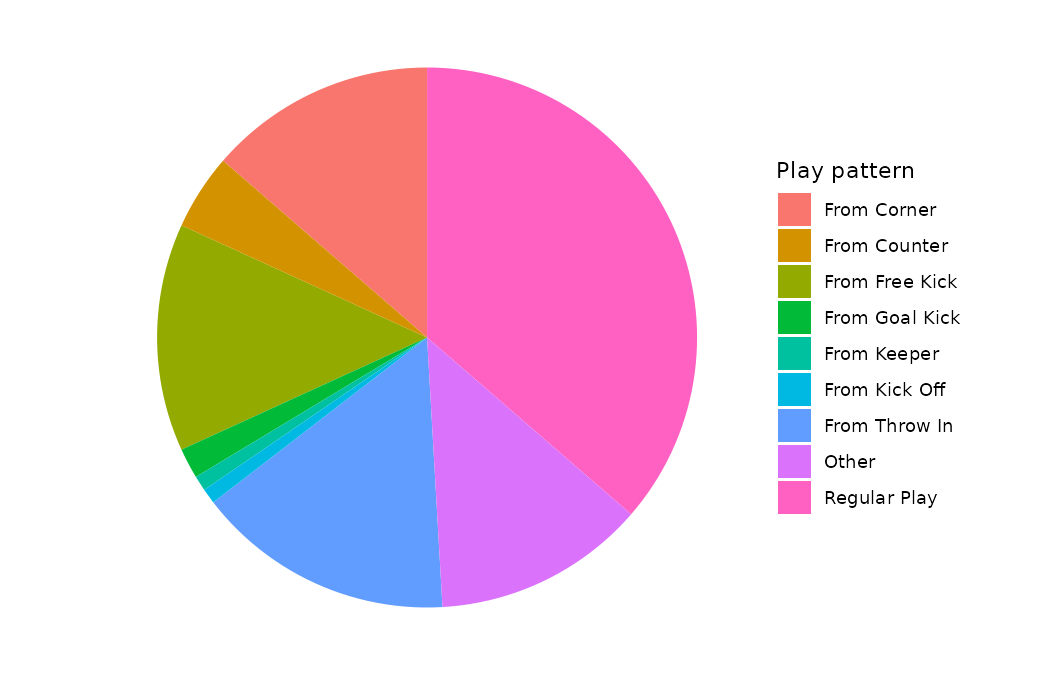
\includegraphics[width=0.85\linewidth,height=\textheight,keepaspectratio]{figures/explore-applications-1.png}

The result is a disc cut into nine slices in nine unrelated colors. The
\texttt{Regular\ Play} slice is visibly the largest, but can your eye
tell how different \texttt{From\ Corner} (15 shots) is from
\texttt{From\ Free\ Kick} (15 shots) or from \texttt{Other} (14 shots)?
The three slices are indistinguishable, and the four smallest slices ---
5, 2, 1, and 1 shots --- collapse into slivers whose labels crowd each
other. Additionally, the colors in the pie chart do not mean anything:
\texttt{play\_pattern} has no ordering and no grouping that the rainbow
encodes, so the palette is pure distraction. And the three-dimensional
tilt of the slide-deck version makes matters strictly worse: perspective
foreshortens the slices at the back and inflates the ones at the front,
so the \emph{drawn areas} no longer even match the counts they are
supposed to represent.

As an alternative, a sorted bar plot is produced by the code below.

\begin{Shaded}
\begin{Highlighting}[]
\FunctionTok{ggplot}\NormalTok{(argentina\_pattern, }\FunctionTok{aes}\NormalTok{(}\AttributeTok{x =}\NormalTok{ n, }\AttributeTok{y =} \FunctionTok{reorder}\NormalTok{(play\_pattern, n))) }\SpecialCharTok{+}
  \FunctionTok{geom\_col}\NormalTok{() }\SpecialCharTok{+}
  \FunctionTok{labs}\NormalTok{(}\AttributeTok{x =} \StringTok{"Number of shots"}\NormalTok{, }\AttributeTok{y =} \ConstantTok{NULL}\NormalTok{)}
\end{Highlighting}
\end{Shaded}

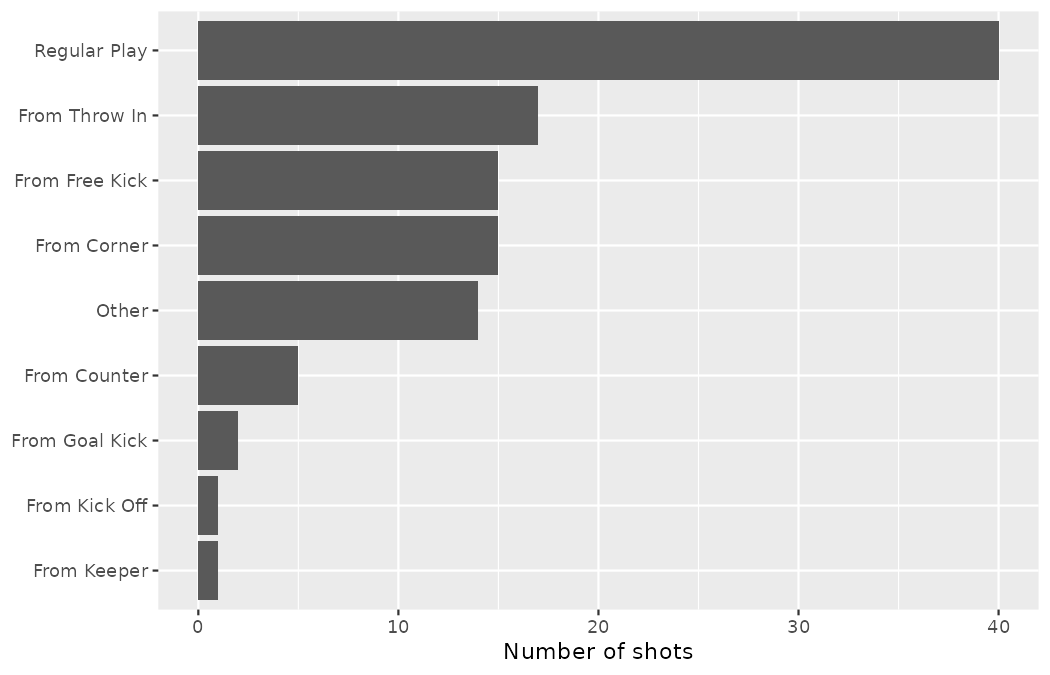
\includegraphics[width=0.85\linewidth,height=\textheight,keepaspectratio]{figures/explore-applications-2.png}

Now the nine patterns run down the y-axis from \texttt{From\ Kick\ Off}
and \texttt{From\ Keeper} (1 shot each) at the bottom to
\texttt{Regular\ Play} (40 shots) at the top, each with a bar whose
length is the count. Notice how much easier it is to identify the
magnitude of the differences across categories --- the eye reads
\texttt{Regular\ Play} at more than twice \texttt{From\ Throw\ In}, and
the 15--15--14 cluster is now three bars of visibly equal length rather
than three indistinguishable wedges --- while not being distracted by
other aspects of the image. Typically, a bar plot will be easier for the
reader to digest than a pie chart, especially if the categorical data
being plotted has more than just a few levels; with nine levels of
\texttt{play\_pattern}, there is no contest.

\begin{tcolorbox}[enhanced jigsaw, left=2mm, leftrule=.75mm, title=\textcolor{quarto-callout-tip-color}{\faLightbulb}\hspace{0.5em}{Check your understanding}, arc=.35mm, rightrule=.15mm, coltitle=black, colframe=quarto-callout-tip-color-frame, bottomrule=.15mm, colbacktitle=quarto-callout-tip-color!10!white, opacitybacktitle=0.6, breakable, bottomtitle=1mm, toptitle=1mm, titlerule=0mm, opacityback=0, toprule=.15mm, colback=white]

Marta's takeaway from the slide should be ``Argentina generated just
over a third of their shots from sustained open play, and about the same
volume again from throw-ins, corners, and free kicks combined.'' Which
of the two graphics lets her verify that sentence in thirty seconds, and
why?

\begin{center}\rule{0.5\linewidth}{0.5pt}\end{center}

The sorted bar plot. Verifying the sentence requires \emph{comparing
magnitudes}: \texttt{Regular\ Play} (40 of 110 shots, about 36\%)
against the sum of \texttt{From\ Throw\ In}, \texttt{From\ Corner}, and
\texttt{From\ Free\ Kick} (17 + 15 + 15 = 47). Bars share a common
baseline, so lengths can be compared and mentally added; pie slices
differ in angle, arc, and area at once, and human vision judges none of
these accurately --- let alone their sums.

\end{tcolorbox}

\subsection{Use color to draw
attention}\label{use-color-to-draw-attention}

There are many reasons why you might choose to add \textbf{color} to
your plots. An important principle to keep in mind is to use color to
draw attention. Of course, you should still think about how visually
pleasing your visualization is, and if you're adding color for making it
visually pleasing without drawing attention to a particular feature,
that might be fine. However, you should be critical of default coloring
and explicitly decide whether to include color and how.

Here is the scenario. Northbridge's summer recruitment brief asks for an
aerial-threat striker, and Marta wants one figure showing how headed
chances compare, in average chance quality, with chances struck by
either foot. Recall from Chapter~\ref{sec-explore-categorical} that we
set aside the \texttt{Other} body-part category (only 13 shots at the
2022 World Cup, a mix of chests, knees, and misrecorded events); we do
the same here and say so on the slide.

\begin{Shaded}
\begin{Highlighting}[]
\NormalTok{bodypart\_xg }\OtherTok{\textless{}{-}}\NormalTok{ wc2022\_shots }\SpecialCharTok{|\textgreater{}}
  \FunctionTok{filter}\NormalTok{(body\_part }\SpecialCharTok{!=} \StringTok{"Other"}\NormalTok{) }\SpecialCharTok{|\textgreater{}}
  \FunctionTok{group\_by}\NormalTok{(body\_part) }\SpecialCharTok{|\textgreater{}}
  \FunctionTok{summarize}\NormalTok{(}\AttributeTok{shots =} \FunctionTok{n}\NormalTok{(), }\AttributeTok{mean\_xg =} \FunctionTok{mean}\NormalTok{(statsbomb\_xg))}

\NormalTok{bodypart\_xg}
\CommentTok{\#\textgreater{} \# A tibble: 3 × 3}
\CommentTok{\#\textgreater{}   body\_part  shots mean\_xg}
\CommentTok{\#\textgreater{}   \textless{}chr\textgreater{}      \textless{}int\textgreater{}   \textless{}dbl\textgreater{}}
\CommentTok{\#\textgreater{} 1 Head         252   0.106}
\CommentTok{\#\textgreater{} 2 Left Foot    449   0.115}
\CommentTok{\#\textgreater{} 3 Right Foot   780   0.134}
\end{Highlighting}
\end{Shaded}

The default approach --- mapping \texttt{body\_part} itself to fill ---
colors every bar differently:

\begin{Shaded}
\begin{Highlighting}[]
\FunctionTok{ggplot}\NormalTok{(bodypart\_xg, }\FunctionTok{aes}\NormalTok{(}\AttributeTok{y =}\NormalTok{ body\_part, }\AttributeTok{x =}\NormalTok{ mean\_xg, }\AttributeTok{fill =}\NormalTok{ body\_part)) }\SpecialCharTok{+}
  \FunctionTok{geom\_col}\NormalTok{(}\AttributeTok{show.legend =} \ConstantTok{FALSE}\NormalTok{) }\SpecialCharTok{+}
  \FunctionTok{labs}\NormalTok{(}\AttributeTok{x =} \StringTok{"Mean xG per shot"}\NormalTok{, }\AttributeTok{y =} \ConstantTok{NULL}\NormalTok{)}
\end{Highlighting}
\end{Shaded}

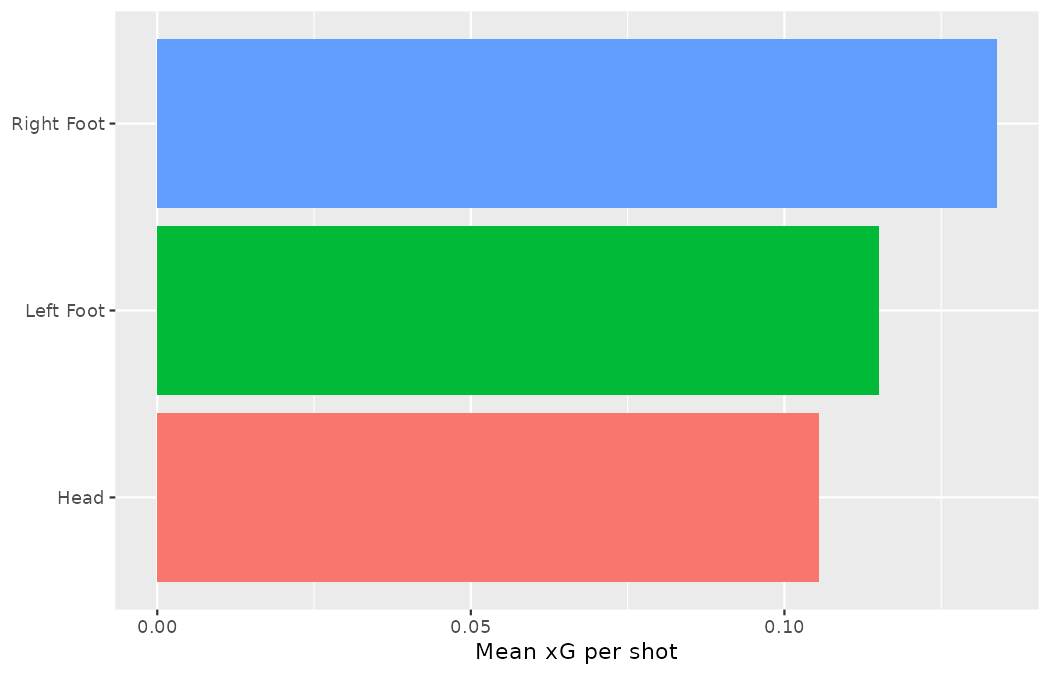
\includegraphics[width=0.85\linewidth,height=\textheight,keepaspectratio]{figures/explore-applications-3.png}

The three bars appear in three unrelated default hues. This coloring
does nothing for the understanding of the data: it can be distracting
and makes the reader ask questions the data cannot answer --- is there
something similar about two bars that happen to receive similar hues?
The color carries no information the y-axis labels don't already carry.

Since the brief is about headers, the figure should \emph{point at the
header bar}:

\begin{Shaded}
\begin{Highlighting}[]
\NormalTok{bodypart\_xg }\SpecialCharTok{|\textgreater{}}
  \FunctionTok{mutate}\NormalTok{(}\AttributeTok{highlight =} \FunctionTok{if\_else}\NormalTok{(body\_part }\SpecialCharTok{==} \StringTok{"Head"}\NormalTok{, }\StringTok{"yes"}\NormalTok{, }\StringTok{"no"}\NormalTok{)) }\SpecialCharTok{|\textgreater{}}
  \FunctionTok{ggplot}\NormalTok{(}\FunctionTok{aes}\NormalTok{(}\AttributeTok{y =}\NormalTok{ body\_part, }\AttributeTok{x =}\NormalTok{ mean\_xg, }\AttributeTok{fill =}\NormalTok{ highlight)) }\SpecialCharTok{+}
  \FunctionTok{geom\_col}\NormalTok{(}\AttributeTok{show.legend =} \ConstantTok{FALSE}\NormalTok{) }\SpecialCharTok{+}
  \FunctionTok{scale\_fill\_manual}\NormalTok{(}\AttributeTok{values =} \FunctionTok{c}\NormalTok{(}\AttributeTok{no =} \StringTok{"grey70"}\NormalTok{, }\AttributeTok{yes =} \StringTok{"firebrick"}\NormalTok{)) }\SpecialCharTok{+}
  \FunctionTok{labs}\NormalTok{(}\AttributeTok{x =} \StringTok{"Mean xG per shot"}\NormalTok{, }\AttributeTok{y =} \ConstantTok{NULL}\NormalTok{)}
\end{Highlighting}
\end{Shaded}

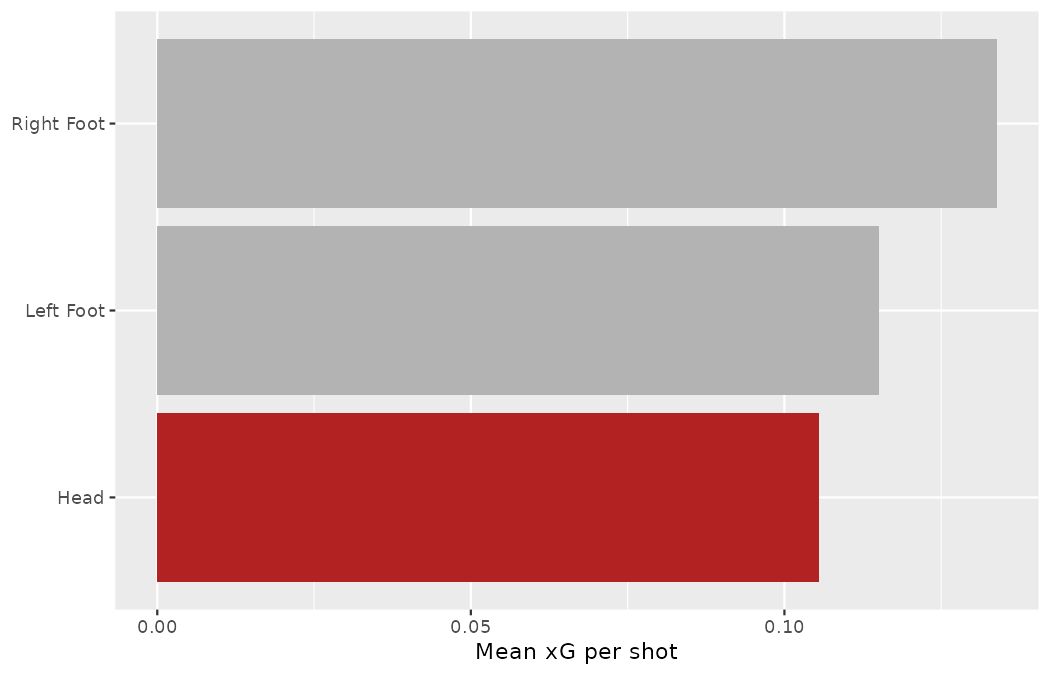
\includegraphics[width=0.85\linewidth,height=\textheight,keepaspectratio]{figures/explore-applications-4.png}

Now the \texttt{Head} bar is red and the two foot bars are a quiet grey.
The reader's eye lands exactly where the brief points: headed chances at
the 2022 World Cup carried the lowest average chance quality of the
three body parts, mean xG 0.106 per shot, against 0.115 for left-footed
and 0.134 for right-footed shots. (Whether that is a property of heading
or of the crosses and corners that produce headers is the confounding
question raised in Chapter~\ref{sec-data-design} --- the plot
communicates the pattern; it does not adjudicate its cause.)

One honesty check is owed before this slide ships, per the book's
penalty convention (recall Chapter~\ref{sec-data-applications}): the two
foot bars contain the tournament's 64 penalties --- every one of them
footed, every one at the stored chance quality of 0.7835 --- while the
header bar contains none. Restrict the same summary to open play and the
story changes:

\begin{Shaded}
\begin{Highlighting}[]
\NormalTok{wc2022\_shots }\SpecialCharTok{|\textgreater{}}
  \FunctionTok{filter}\NormalTok{(shot\_type }\SpecialCharTok{==} \StringTok{"Open Play"}\NormalTok{, body\_part }\SpecialCharTok{!=} \StringTok{"Other"}\NormalTok{) }\SpecialCharTok{|\textgreater{}}
  \FunctionTok{group\_by}\NormalTok{(body\_part) }\SpecialCharTok{|\textgreater{}}
  \FunctionTok{summarize}\NormalTok{(}\AttributeTok{shots =} \FunctionTok{n}\NormalTok{(), }\AttributeTok{mean\_xg =} \FunctionTok{mean}\NormalTok{(statsbomb\_xg))}
\CommentTok{\#\textgreater{} \# A tibble: 3 × 3}
\CommentTok{\#\textgreater{}   body\_part  shots mean\_xg}
\CommentTok{\#\textgreater{}   \textless{}chr\textgreater{}      \textless{}int\textgreater{}   \textless{}dbl\textgreater{}}
\CommentTok{\#\textgreater{} 1 Head         252  0.106}
\CommentTok{\#\textgreater{} 2 Left Foot    414  0.0928}
\CommentTok{\#\textgreater{} 3 Right Foot   703  0.0932}
\end{Highlighting}
\end{Shaded}

Within open play the ordering \emph{reverses}: the header bar (0.106 ---
unchanged, since every header in these data is an open-play shot) now
sits \emph{above} both foot bars (0.093 apiece). The all-shots figure
and the open-play figure are both true; they answer different questions,
and the slide must say which frame it shows --- an aerial-threat brief
is almost certainly asking the open-play question. (The reversal is no
fluke of this summary: in Chapter~\ref{sec-model-mlr}, a model fit to
the open-play frame puts a positive coefficient on the header
indicator.)

Also note that not everyone sees color the same way. Often it's useful
to add color \emph{and one more feature} --- a pattern, an outline, a
linetype --- so that you can refer to the features you're drawing
attention to in multiple ways:

\begin{Shaded}
\begin{Highlighting}[]
\NormalTok{bodypart\_xg }\SpecialCharTok{|\textgreater{}}
  \FunctionTok{mutate}\NormalTok{(}\AttributeTok{highlight =} \FunctionTok{if\_else}\NormalTok{(body\_part }\SpecialCharTok{==} \StringTok{"Head"}\NormalTok{, }\StringTok{"yes"}\NormalTok{, }\StringTok{"no"}\NormalTok{)) }\SpecialCharTok{|\textgreater{}}
  \FunctionTok{ggplot}\NormalTok{(}\FunctionTok{aes}\NormalTok{(}
    \AttributeTok{y =}\NormalTok{ body\_part, }\AttributeTok{x =}\NormalTok{ mean\_xg,}
    \AttributeTok{fill =}\NormalTok{ highlight, }\AttributeTok{color =}\NormalTok{ highlight, }\AttributeTok{linetype =}\NormalTok{ highlight}
\NormalTok{  )) }\SpecialCharTok{+}
  \FunctionTok{geom\_col}\NormalTok{(}\AttributeTok{show.legend =} \ConstantTok{FALSE}\NormalTok{, }\AttributeTok{linewidth =} \FloatTok{0.8}\NormalTok{) }\SpecialCharTok{+}
  \FunctionTok{scale\_fill\_manual}\NormalTok{(}\AttributeTok{values =} \FunctionTok{c}\NormalTok{(}\AttributeTok{no =} \StringTok{"grey70"}\NormalTok{, }\AttributeTok{yes =} \StringTok{"firebrick"}\NormalTok{)) }\SpecialCharTok{+}
  \FunctionTok{scale\_color\_manual}\NormalTok{(}\AttributeTok{values =} \FunctionTok{c}\NormalTok{(}\AttributeTok{no =} \StringTok{"grey70"}\NormalTok{, }\AttributeTok{yes =} \StringTok{"black"}\NormalTok{)) }\SpecialCharTok{+}
  \FunctionTok{labs}\NormalTok{(}\AttributeTok{x =} \StringTok{"Mean xG per shot"}\NormalTok{, }\AttributeTok{y =} \ConstantTok{NULL}\NormalTok{)}
\end{Highlighting}
\end{Shaded}

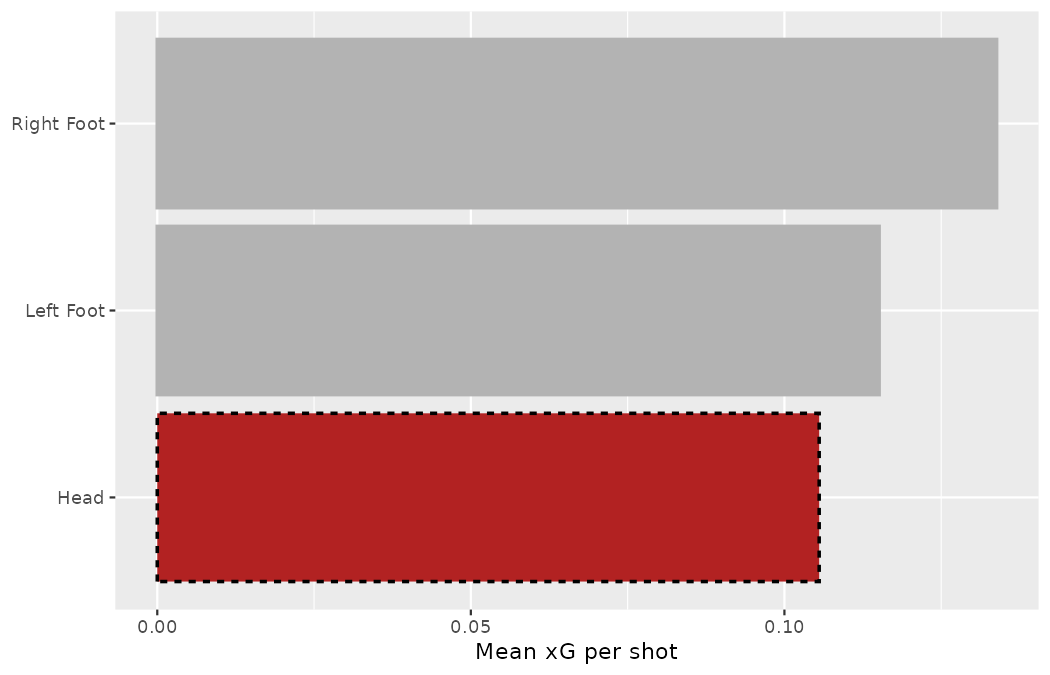
\includegraphics[width=0.85\linewidth,height=\textheight,keepaspectratio]{figures/explore-applications-5.png}

The header bar is now both red \emph{and} outlined with a distinct
border, so a reader who cannot distinguish red from grey still sees
exactly one bar marked out.

\begin{tcolorbox}[enhanced jigsaw, left=2mm, leftrule=.75mm, title=\textcolor{quarto-callout-tip-color}{\faLightbulb}\hspace{0.5em}{Check your understanding}, arc=.35mm, rightrule=.15mm, coltitle=black, colframe=quarto-callout-tip-color-frame, bottomrule=.15mm, colbacktitle=quarto-callout-tip-color!10!white, opacitybacktitle=0.6, breakable, bottomtitle=1mm, toptitle=1mm, titlerule=0mm, opacityback=0, toprule=.15mm, colback=white]

A colleague defends the rainbow version: ``the colors don't hurt ---
they're just decoration.'' Give two concrete ways an uninformative color
mapping can actively hurt a scouting figure.

\begin{center}\rule{0.5\linewidth}{0.5pt}\end{center}

First, it invites false groupings: readers instinctively treat similarly
colored categories as related, an association the data do not contain.
Second, it spends the single most attention-grabbing visual channel on
nothing, so when there \emph{is} a feature the club needs to see --- the
header bar in a brief about aerial threat --- no channel is left to mark
it out. Color is a finite budget; decoration is the most expensive way
to waste it.

\end{tcolorbox}

\subsection{Tell a story}\label{tell-a-story}

For many graphs, an important aspect is the inclusion of information
which is not provided in the dataset that is being plotted. The external
information serves to contextualize the data and helps communicate the
narrative of the research.

Consider the rhythm of a tournament: how many shots does each matchday
produce? We build, for each competition, a per-matchday count --- one
row per calendar day on which at least one match was played, indexed
within its own tournament so the two competitions can share an x-axis:

\begin{Shaded}
\begin{Highlighting}[]
\NormalTok{daily\_shots }\OtherTok{\textless{}{-}} \FunctionTok{bind\_rows}\NormalTok{(wc2022\_shots, weuro2025\_shots) }\SpecialCharTok{|\textgreater{}}
  \FunctionTok{group\_by}\NormalTok{(competition, match\_date) }\SpecialCharTok{|\textgreater{}}
  \FunctionTok{summarize}\NormalTok{(}
    \AttributeTok{n\_shots =} \FunctionTok{n}\NormalTok{(),}
    \AttributeTok{knockout =} \FunctionTok{all}\NormalTok{(stage }\SpecialCharTok{!=} \StringTok{"Group Stage"}\NormalTok{),}
    \AttributeTok{.groups =} \StringTok{"drop"}
\NormalTok{  ) }\SpecialCharTok{|\textgreater{}}
  \FunctionTok{arrange}\NormalTok{(competition, match\_date) }\SpecialCharTok{|\textgreater{}}
  \FunctionTok{group\_by}\NormalTok{(competition) }\SpecialCharTok{|\textgreater{}}
  \FunctionTok{mutate}\NormalTok{(}\AttributeTok{matchday =} \FunctionTok{row\_number}\NormalTok{()) }\SpecialCharTok{|\textgreater{}}
  \FunctionTok{ungroup}\NormalTok{()}

\NormalTok{daily\_shots}
\CommentTok{\#\textgreater{} \# A tibble: 42 × 5}
\CommentTok{\#\textgreater{}    competition match\_date n\_shots knockout matchday}
\CommentTok{\#\textgreater{}    \textless{}chr\textgreater{}       \textless{}date\textgreater{}       \textless{}int\textgreater{} \textless{}lgl\textgreater{}       \textless{}int\textgreater{}}
\CommentTok{\#\textgreater{}  1 wc2022      2022{-}11{-}20      11 FALSE           1}
\CommentTok{\#\textgreater{}  2 wc2022      2022{-}11{-}21      59 FALSE           2}
\CommentTok{\#\textgreater{}  3 wc2022      2022{-}11{-}22      86 FALSE           3}
\CommentTok{\#\textgreater{}  4 wc2022      2022{-}11{-}23      99 FALSE           4}
\CommentTok{\#\textgreater{}  5 wc2022      2022{-}11{-}24      80 FALSE           5}
\CommentTok{\#\textgreater{}  6 wc2022      2022{-}11{-}25      88 FALSE           6}
\CommentTok{\#\textgreater{}  7 wc2022      2022{-}11{-}26      89 FALSE           7}
\CommentTok{\#\textgreater{}  8 wc2022      2022{-}11{-}27      76 FALSE           8}
\CommentTok{\#\textgreater{}  9 wc2022      2022{-}11{-}28     101 FALSE           9}
\CommentTok{\#\textgreater{} 10 wc2022      2022{-}11{-}29      81 FALSE          10}
\CommentTok{\#\textgreater{} \# ℹ 32 more rows}
\end{Highlighting}
\end{Shaded}

A first, un-annotated time series plot simply colors the two tournaments
differently:

\begin{Shaded}
\begin{Highlighting}[]
\FunctionTok{ggplot}\NormalTok{(daily\_shots, }\FunctionTok{aes}\NormalTok{(}\AttributeTok{x =}\NormalTok{ matchday, }\AttributeTok{y =}\NormalTok{ n\_shots, }\AttributeTok{color =}\NormalTok{ competition)) }\SpecialCharTok{+}
  \FunctionTok{geom\_line}\NormalTok{(}\AttributeTok{linewidth =} \DecValTok{1}\NormalTok{) }\SpecialCharTok{+}
  \FunctionTok{labs}\NormalTok{(}
    \AttributeTok{x =} \StringTok{"Matchday (day of the tournament with at least one match)"}\NormalTok{,}
    \AttributeTok{y =} \StringTok{"Shots recorded"}\NormalTok{,}
    \AttributeTok{color =} \ConstantTok{NULL}
\NormalTok{  )}
\end{Highlighting}
\end{Shaded}

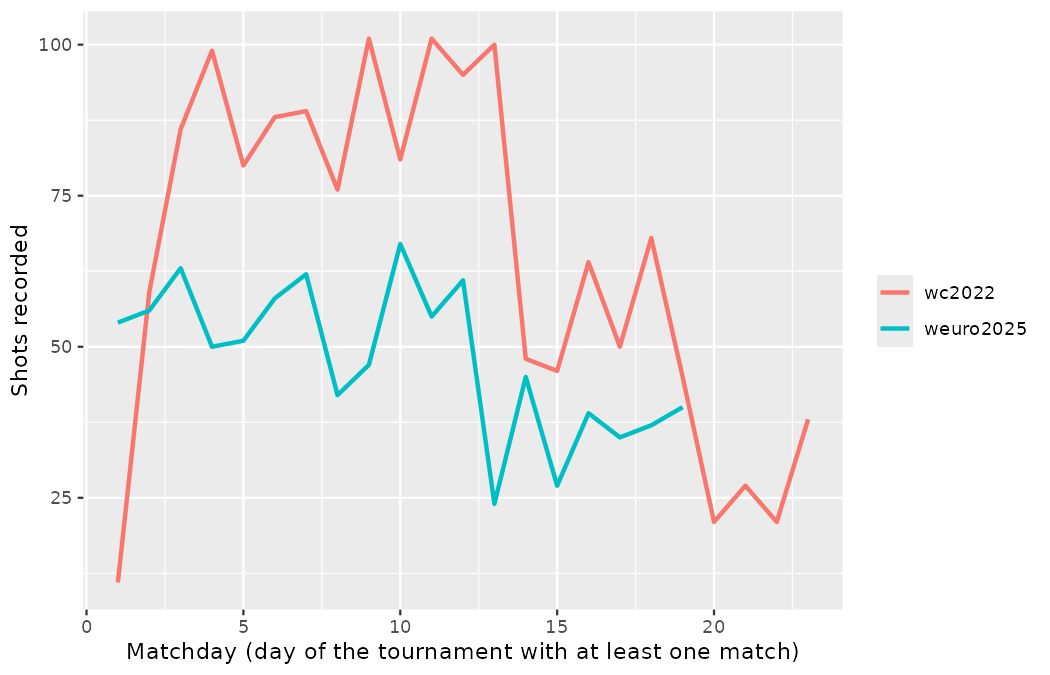
\includegraphics[width=0.85\linewidth,height=\textheight,keepaspectratio]{figures/explore-applications-6.png}

The World Cup line starts at 11 shots (a single opening match), jumps to
59 on matchday 2 as the schedule fills, and from matchday 3 oscillates
between 76 and 101 shots a day through matchday 13; then it collapses:
48, 46, 64, 50, 68, 45, and eventually days of 21--38 shots. The Women's
Euro line hovers between 42 and 67 through matchday 12 and then drops to
the 24--45 range. A reader who does not know tournament football sees
two attacking collapses and starts inventing explanations --- fatigue?
weather? teams ``shutting up shop''?

The plot is missing its story. The break in each line is not about
football at all; it is about the \emph{fixture calendar}, information
that lives outside the plotted data. We compute where the knockout
rounds begin and annotate the figure with it:

\begin{Shaded}
\begin{Highlighting}[]
\NormalTok{knockout\_starts }\OtherTok{\textless{}{-}}\NormalTok{ daily\_shots }\SpecialCharTok{|\textgreater{}}
  \FunctionTok{filter}\NormalTok{(knockout) }\SpecialCharTok{|\textgreater{}}
  \FunctionTok{group\_by}\NormalTok{(competition) }\SpecialCharTok{|\textgreater{}}
  \FunctionTok{summarize}\NormalTok{(}\AttributeTok{first\_knockout\_matchday =} \FunctionTok{min}\NormalTok{(matchday))}

\NormalTok{knockout\_starts}
\CommentTok{\#\textgreater{} \# A tibble: 2 × 2}
\CommentTok{\#\textgreater{}   competition first\_knockout\_matchday}
\CommentTok{\#\textgreater{}   \textless{}chr\textgreater{}                         \textless{}int\textgreater{}}
\CommentTok{\#\textgreater{} 1 wc2022                           14}
\CommentTok{\#\textgreater{} 2 weuro2025                        13}
\end{Highlighting}
\end{Shaded}

\begin{Shaded}
\begin{Highlighting}[]
\FunctionTok{ggplot}\NormalTok{(daily\_shots, }\FunctionTok{aes}\NormalTok{(}\AttributeTok{x =}\NormalTok{ matchday, }\AttributeTok{y =}\NormalTok{ n\_shots)) }\SpecialCharTok{+}
  \FunctionTok{geom\_line}\NormalTok{(}\AttributeTok{linewidth =} \FloatTok{0.8}\NormalTok{, }\AttributeTok{color =} \StringTok{"steelblue"}\NormalTok{) }\SpecialCharTok{+}
  \FunctionTok{geom\_vline}\NormalTok{(}
    \AttributeTok{data =}\NormalTok{ knockout\_starts,}
    \FunctionTok{aes}\NormalTok{(}\AttributeTok{xintercept =}\NormalTok{ first\_knockout\_matchday }\SpecialCharTok{{-}} \FloatTok{0.5}\NormalTok{),}
    \AttributeTok{linetype =} \StringTok{"dashed"}
\NormalTok{  ) }\SpecialCharTok{+}
  \FunctionTok{geom\_text}\NormalTok{(}
    \AttributeTok{data =}\NormalTok{ knockout\_starts,}
    \FunctionTok{aes}\NormalTok{(}\AttributeTok{x =}\NormalTok{ first\_knockout\_matchday }\SpecialCharTok{{-}} \FloatTok{0.5}\NormalTok{, }\AttributeTok{y =} \DecValTok{95}\NormalTok{),}
    \AttributeTok{label =} \StringTok{"Knockout rounds begin:}\SpecialCharTok{\textbackslash{}n}\StringTok{fewer matches per day"}\NormalTok{,}
    \AttributeTok{hjust =} \SpecialCharTok{{-}}\FloatTok{0.05}\NormalTok{, }\AttributeTok{size =} \DecValTok{3}
\NormalTok{  ) }\SpecialCharTok{+}
  \FunctionTok{facet\_wrap}\NormalTok{(}\SpecialCharTok{\textasciitilde{}}\NormalTok{ competition, }\AttributeTok{ncol =} \DecValTok{1}\NormalTok{) }\SpecialCharTok{+}
  \FunctionTok{labs}\NormalTok{(}
    \AttributeTok{x =} \StringTok{"Matchday (day of the tournament with at least one match)"}\NormalTok{,}
    \AttributeTok{y =} \StringTok{"Shots recorded"}
\NormalTok{  )}
\end{Highlighting}
\end{Shaded}

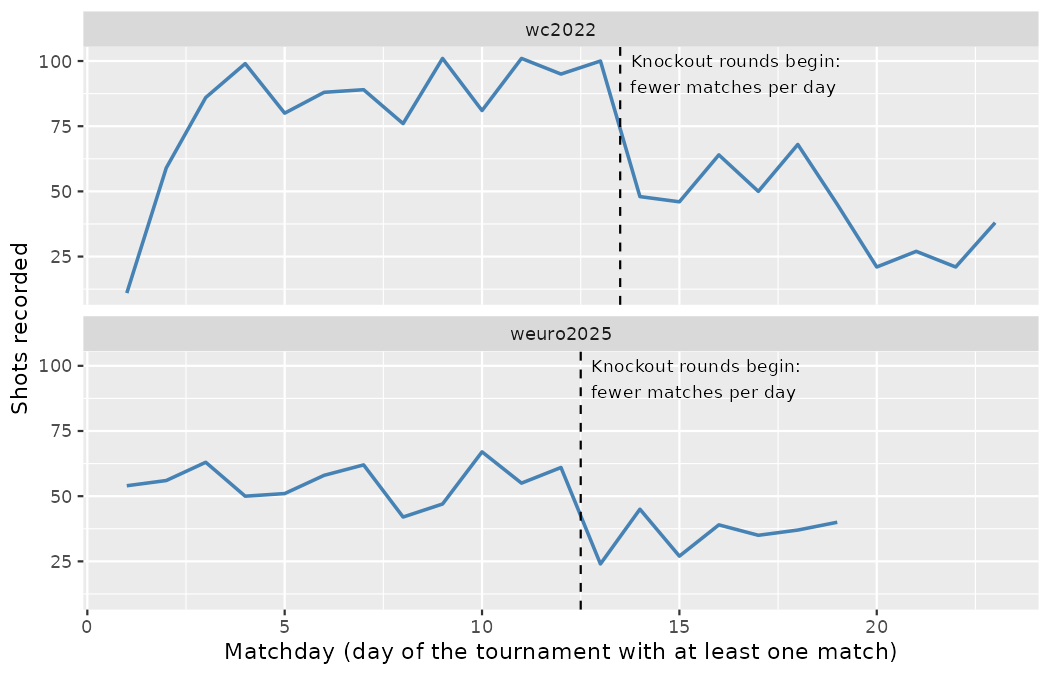
\includegraphics[width=0.85\linewidth,height=\textheight,keepaspectratio]{figures/explore-applications-7.png}

The \textbf{annotated} version places a dashed vertical line just before
matchday 14 (World Cup) and matchday 13 (Women's Euro), labeled with the
external fact: the group stage, with up to four matches per day at the
World Cup and two per day at the Euro, gives way to knockout rounds with
two, then one match per day. The ``collapse'' is a schedule artifact.

And once the annotation forces the right denominator on us, the story
inverts. Dividing each World Cup matchday's shots by the number of
matches played that day:

\begin{Shaded}
\begin{Highlighting}[]
\NormalTok{wc2022\_shots }\SpecialCharTok{|\textgreater{}}
  \FunctionTok{count}\NormalTok{(match\_date, }\AttributeTok{name =} \StringTok{"n\_shots"}\NormalTok{) }\SpecialCharTok{|\textgreater{}}
  \FunctionTok{left\_join}\NormalTok{(}
\NormalTok{    wc2022\_matches }\SpecialCharTok{|\textgreater{}} \FunctionTok{count}\NormalTok{(match\_date, }\AttributeTok{name =} \StringTok{"n\_matches"}\NormalTok{),}
    \AttributeTok{by =} \StringTok{"match\_date"}
\NormalTok{  ) }\SpecialCharTok{|\textgreater{}}
  \FunctionTok{mutate}\NormalTok{(}\AttributeTok{knockout =}\NormalTok{ match\_date }\SpecialCharTok{\textgreater{}=} \FunctionTok{as.Date}\NormalTok{(}\StringTok{"2022{-}12{-}03"}\NormalTok{)) }\SpecialCharTok{|\textgreater{}}
  \FunctionTok{group\_by}\NormalTok{(knockout) }\SpecialCharTok{|\textgreater{}}
  \FunctionTok{summarize}\NormalTok{(}
    \AttributeTok{matchdays =} \FunctionTok{n}\NormalTok{(),}
    \AttributeTok{shots\_per\_day =} \FunctionTok{mean}\NormalTok{(n\_shots),}
    \AttributeTok{shots\_per\_match =} \FunctionTok{mean}\NormalTok{(n\_shots }\SpecialCharTok{/}\NormalTok{ n\_matches)}
\NormalTok{  )}
\CommentTok{\#\textgreater{} \# A tibble: 2 × 4}
\CommentTok{\#\textgreater{}   knockout matchdays shots\_per\_day shots\_per\_match}
\CommentTok{\#\textgreater{}   \textless{}lgl\textgreater{}        \textless{}int\textgreater{}         \textless{}dbl\textgreater{}           \textless{}dbl\textgreater{}}
\CommentTok{\#\textgreater{} 1 FALSE           13          82              21.5}
\CommentTok{\#\textgreater{} 2 TRUE            10          42.8            26.8}
\end{Highlighting}
\end{Shaded}

Per \emph{day}, shooting nearly halves (82 to 42.8); per \emph{match},
it rises from 21.5 to 26.8 --- knockout matches, with extra time and
teams chasing deficits, produce \emph{more} shots, not fewer. A scout
reading the raw daily series would have taken away exactly the wrong
lesson. This is what ``tell a story'' means: the annotation is not
decoration, it is the difference between the right conclusion and its
opposite.

Sometimes the additional information may be a diagonal line given by
\(y = x\). In a scatterplot of goals against total xG for each
team-match, for instance, points above the line quickly show the reader
which team-matches produced more goals than their chance quality
suggested --- finishing above expectation --- and points below the line
show the opposite.

\begin{tcolorbox}[enhanced jigsaw, left=2mm, leftrule=.75mm, title=\textcolor{quarto-callout-tip-color}{\faLightbulb}\hspace{0.5em}{Check your understanding}, arc=.35mm, rightrule=.15mm, coltitle=black, colframe=quarto-callout-tip-color-frame, bottomrule=.15mm, colbacktitle=quarto-callout-tip-color!10!white, opacitybacktitle=0.6, breakable, bottomtitle=1mm, toptitle=1mm, titlerule=0mm, opacityback=0, toprule=.15mm, colback=white]

Emil Sørensen looks at the first (un-annotated) plot and drafts the
note: ``attacking output falls sharply once the knockout rounds start
--- teams become cautious.'' Using the computations above, rewrite his
note so that it is supported by the data.

\begin{center}\rule{0.5\linewidth}{0.5pt}\end{center}

``Total shots per \emph{day} fall after the group stage because the
schedule drops from four matches a day to two and then one. Per
\emph{match}, shooting actually rises in the knockout rounds --- from
about 21.5 to about 26.8 shots per match at the 2022 World Cup ---
partly because knockout matches can run to extra time and force trailing
teams to attack.'' Same data, opposite conclusion; the difference is the
denominator that the annotation forced us to notice.

\end{tcolorbox}

\subsection{Order matters}\label{order-matters}

Most software programs have built in methods for some of the plot
details --- some order levels alphabetically, some provide functionality
for arranging them in a custom order. Sorting the Argentina bar plot by
frequency was the right call earlier because \texttt{play\_pattern} is
nominal: its levels have no inherent order, so the counts themselves are
the most useful ordering. Ordinal variables are different, and this is
where defaults quietly mislead.

Here is a constructed Northbridge scenario --- as always, built in
seeded code, never presented as real. In midwinter, Priya polled all 48
regional scouts of Emil's network on a single question about a winger
the club has tracked all season, who plays his club football in Iberia:

\begin{quote}
Based on the last three months of reports, how would you rate the
prospect's readiness for our first team?

\begin{itemize}
\tightlist
\item
  Excellent
\item
  Good
\item
  Average
\item
  Poor
\item
  Don't know
\end{itemize}
\end{quote}

Each scout belongs to one scouting region, and the regions differ in how
they have seen the player: the twelve Iberia-based scouts watch him live
most weeks, while the South America desk knows him almost entirely from
video. We build the panel with region-specific response profiles so the
constructed data contain exactly that structure (which we will exploit
in the following sections):

\begin{Shaded}
\begin{Highlighting}[]
\FunctionTok{set.seed}\NormalTok{(}\DecValTok{601}\NormalTok{)}
\NormalTok{rating\_levels }\OtherTok{\textless{}{-}} \FunctionTok{c}\NormalTok{(}\StringTok{"Excellent"}\NormalTok{, }\StringTok{"Good"}\NormalTok{, }\StringTok{"Average"}\NormalTok{, }\StringTok{"Poor"}\NormalTok{, }\StringTok{"Don\textquotesingle{}t know"}\NormalTok{)}

\NormalTok{panel\_design }\OtherTok{\textless{}{-}} \FunctionTok{tribble}\NormalTok{(}
  \SpecialCharTok{\textasciitilde{}}\NormalTok{region,             }\SpecialCharTok{\textasciitilde{}}\NormalTok{n\_scouts, }\SpecialCharTok{\textasciitilde{}}\NormalTok{probs,}
  \StringTok{"Iberia"}\NormalTok{,              }\DecValTok{12}\NormalTok{, }\FunctionTok{c}\NormalTok{(}\FloatTok{0.30}\NormalTok{, }\FloatTok{0.40}\NormalTok{, }\FloatTok{0.20}\NormalTok{, }\FloatTok{0.05}\NormalTok{, }\FloatTok{0.05}\NormalTok{),}
  \StringTok{"Britain \& Ireland"}\NormalTok{,   }\DecValTok{11}\NormalTok{, }\FunctionTok{c}\NormalTok{(}\FloatTok{0.08}\NormalTok{, }\FloatTok{0.25}\NormalTok{, }\FloatTok{0.35}\NormalTok{, }\FloatTok{0.20}\NormalTok{, }\FloatTok{0.12}\NormalTok{),}
  \StringTok{"Northern Europe"}\NormalTok{,     }\DecValTok{10}\NormalTok{, }\FunctionTok{c}\NormalTok{(}\FloatTok{0.08}\NormalTok{, }\FloatTok{0.25}\NormalTok{, }\FloatTok{0.35}\NormalTok{, }\FloatTok{0.20}\NormalTok{, }\FloatTok{0.12}\NormalTok{),}
  \StringTok{"Balkans"}\NormalTok{,              }\DecValTok{8}\NormalTok{, }\FunctionTok{c}\NormalTok{(}\FloatTok{0.05}\NormalTok{, }\FloatTok{0.20}\NormalTok{, }\FloatTok{0.35}\NormalTok{, }\FloatTok{0.25}\NormalTok{, }\FloatTok{0.15}\NormalTok{),}
  \StringTok{"South America"}\NormalTok{,        }\DecValTok{7}\NormalTok{, }\FunctionTok{c}\NormalTok{(}\FloatTok{0.05}\NormalTok{, }\FloatTok{0.15}\NormalTok{, }\FloatTok{0.30}\NormalTok{, }\FloatTok{0.20}\NormalTok{, }\FloatTok{0.30}\NormalTok{)}
\NormalTok{)}

\NormalTok{scout\_panel }\OtherTok{\textless{}{-}}\NormalTok{ panel\_design }\SpecialCharTok{|\textgreater{}}
  \FunctionTok{mutate}\NormalTok{(}
    \AttributeTok{rating =} \FunctionTok{map2}\NormalTok{(}
\NormalTok{      n\_scouts, probs,}
\NormalTok{      \textbackslash{}(n, p) }\FunctionTok{sample}\NormalTok{(rating\_levels, }\AttributeTok{size =}\NormalTok{ n, }\AttributeTok{replace =} \ConstantTok{TRUE}\NormalTok{, }\AttributeTok{prob =}\NormalTok{ p)}
\NormalTok{    )}
\NormalTok{  ) }\SpecialCharTok{|\textgreater{}}
  \FunctionTok{select}\NormalTok{(region, rating) }\SpecialCharTok{|\textgreater{}}
  \FunctionTok{unnest}\NormalTok{(rating)}

\NormalTok{scout\_panel }\SpecialCharTok{|\textgreater{}}
  \FunctionTok{count}\NormalTok{(rating, }\AttributeTok{sort =} \ConstantTok{TRUE}\NormalTok{)}
\CommentTok{\#\textgreater{} \# A tibble: 5 × 2}
\CommentTok{\#\textgreater{}   rating         n}
\CommentTok{\#\textgreater{}   \textless{}chr\textgreater{}      \textless{}int\textgreater{}}
\CommentTok{\#\textgreater{} 1 Good          14}
\CommentTok{\#\textgreater{} 2 Poor          14}
\CommentTok{\#\textgreater{} 3 Average       13}
\CommentTok{\#\textgreater{} 4 Excellent      5}
\CommentTok{\#\textgreater{} 5 Don\textquotesingle{}t know     2}
\end{Highlighting}
\end{Shaded}

The panel splits 5 Excellent, 14 Good, 13 Average, 14 Poor, 2 Don't
know. Now consider three ways of arranging the bars of the same plot.

\begin{Shaded}
\begin{Highlighting}[]
\CommentTok{\# (a) Alphabetical order {-}{-} the software default for character data}
\FunctionTok{ggplot}\NormalTok{(scout\_panel, }\FunctionTok{aes}\NormalTok{(}\AttributeTok{y =}\NormalTok{ rating)) }\SpecialCharTok{+}
  \FunctionTok{geom\_bar}\NormalTok{() }\SpecialCharTok{+}
  \FunctionTok{labs}\NormalTok{(}\AttributeTok{y =} \StringTok{"Rating"}\NormalTok{, }\AttributeTok{x =} \StringTok{"Number of scouts"}\NormalTok{)}

\CommentTok{\# (b) Frequency order}
\FunctionTok{ggplot}\NormalTok{(scout\_panel, }\FunctionTok{aes}\NormalTok{(}\AttributeTok{y =} \FunctionTok{reorder}\NormalTok{(rating, rating, }\AttributeTok{FUN =}\NormalTok{ length))) }\SpecialCharTok{+}
  \FunctionTok{geom\_bar}\NormalTok{() }\SpecialCharTok{+}
  \FunctionTok{labs}\NormalTok{(}\AttributeTok{y =} \StringTok{"Rating"}\NormalTok{, }\AttributeTok{x =} \StringTok{"Number of scouts"}\NormalTok{)}

\CommentTok{\# (c) The order of the rating scale itself}
\NormalTok{scout\_panel }\SpecialCharTok{|\textgreater{}}
  \FunctionTok{mutate}\NormalTok{(}\AttributeTok{rating =} \FunctionTok{factor}\NormalTok{(rating, }\AttributeTok{levels =} \FunctionTok{rev}\NormalTok{(rating\_levels))) }\SpecialCharTok{|\textgreater{}}
  \FunctionTok{ggplot}\NormalTok{(}\FunctionTok{aes}\NormalTok{(}\AttributeTok{y =}\NormalTok{ rating)) }\SpecialCharTok{+}
  \FunctionTok{geom\_bar}\NormalTok{() }\SpecialCharTok{+}
  \FunctionTok{labs}\NormalTok{(}\AttributeTok{y =} \StringTok{"Rating"}\NormalTok{, }\AttributeTok{x =} \StringTok{"Number of scouts"}\NormalTok{)}
\end{Highlighting}
\end{Shaded}

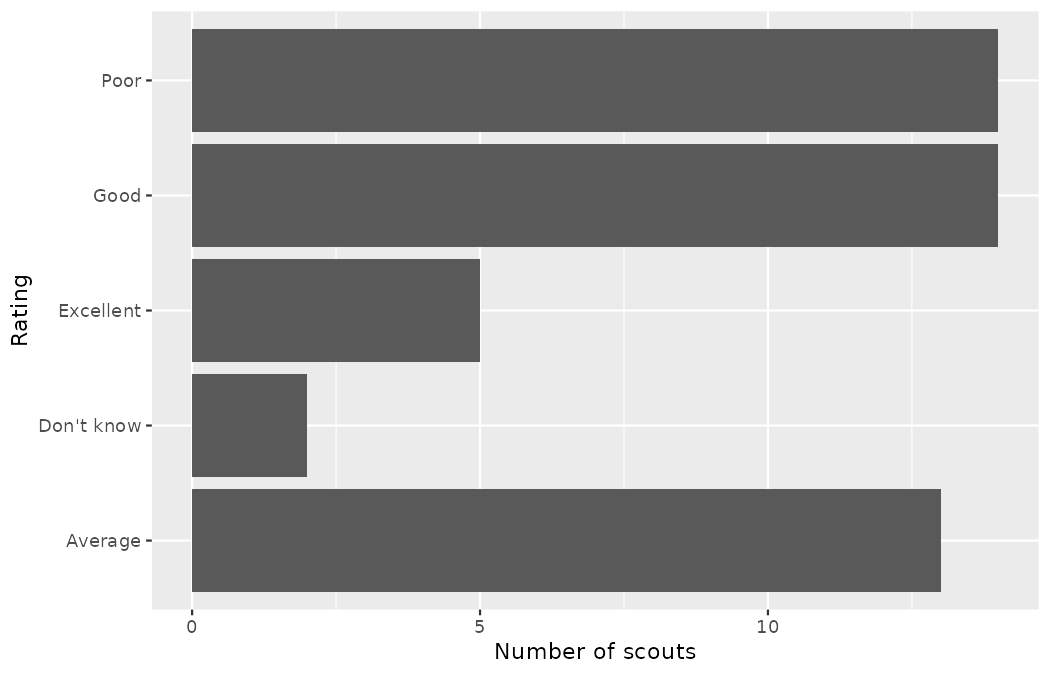
\includegraphics[width=0.85\linewidth,height=\textheight,keepaspectratio]{figures/explore-applications-8.png}

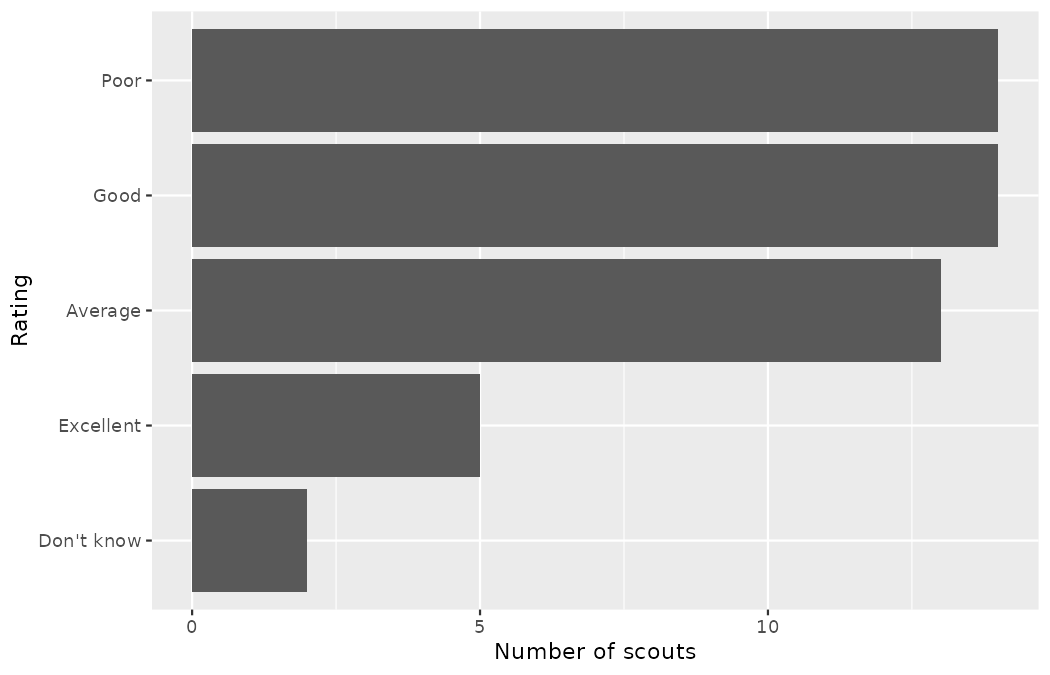
\includegraphics[width=0.85\linewidth,height=\textheight,keepaspectratio]{figures/explore-applications-9.png}

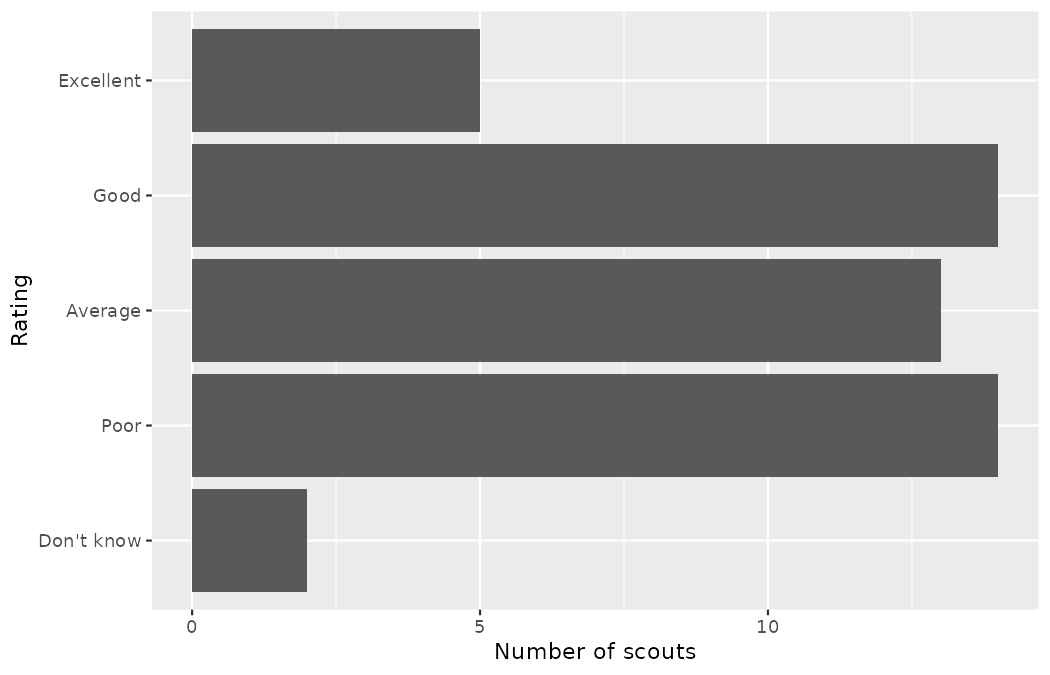
\includegraphics[width=0.85\linewidth,height=\textheight,keepaspectratio]{figures/explore-applications-10.png}

In plot (a) the bars run Average, Don't know, Excellent, Good, Poor ---
the alphabetical ordering isn't particularly meaningful for describing
the data, and it interleaves the extremes of the scale with its middle.
Sometimes it makes sense to \textbf{order} the bars from tallest to
shortest (or vice versa), as in plot (b) --- though notice that here
\texttt{Good} and \texttt{Poor} tie at 14 scouts each, so even the
``frequency order'' is partly arbitrary, and it still shuffles the
scale: the two ends of the readiness spectrum end up adjacent. But in
this case, the best ordering is the one in which the response options
were presented, as shown in plot (c): Excellent at the top down through
Poor, with Don't know last. The rating scale is ordinal --- its order
\emph{is} information --- and plot (c) is the only one of the three that
lets the reader see at a glance that the panel's center of mass sits
between Good and Poor, with a nearly symmetric split.

An ordering which does not make sense in the context of the problem
(e.g., alphabetically here) can mislead the reader who might take a
quick glance at the axes and not read the bar labels carefully --- a
glance at plot (a) suggests ``Average'' is the panel's floor rather than
its middle.

\begin{tcolorbox}[enhanced jigsaw, left=2mm, leftrule=.75mm, title=\textcolor{quarto-callout-tip-color}{\faLightbulb}\hspace{0.5em}{Check your understanding}, arc=.35mm, rightrule=.15mm, coltitle=black, colframe=quarto-callout-tip-color-frame, bottomrule=.15mm, colbacktitle=quarto-callout-tip-color!10!white, opacitybacktitle=0.6, breakable, bottomtitle=1mm, toptitle=1mm, titlerule=0mm, opacityback=0, toprule=.15mm, colback=white]

For the Argentina \texttt{play\_pattern} bar plot of the first section,
we recommended frequency order; for the scout ratings we just rejected
it. What property of the variable decides which ordering to use?

\begin{center}\rule{0.5\linewidth}{0.5pt}\end{center}

Whether the variable's levels carry an inherent order.
\texttt{play\_pattern} is nominal --- no level comes ``before'' another
--- so the data's own frequencies are the most informative arrangement.
The rating scale is ordinal --- Excellent through Poor is a progression
--- so the scale's order carries meaning that frequency sorting destroys
(and, with the Good/Poor tie at 14, frequency order here isn't even well
defined).

\end{tcolorbox}

\subsection{Make the labels as easy to read as
possible}\label{make-the-labels-as-easy-to-read-as-possible}

The panel results become more interesting when broken down by scouting
region --- this is, after all, where the disagreement lives. The stacked
bar plot allows for comparison of the rating mix across the five
regions. Before plotting, we fix both factors' level orders
deliberately, per the previous principle:

\begin{Shaded}
\begin{Highlighting}[]
\NormalTok{scout\_panel }\OtherTok{\textless{}{-}}\NormalTok{ scout\_panel }\SpecialCharTok{|\textgreater{}}
  \FunctionTok{mutate}\NormalTok{(}
    \AttributeTok{rating =} \FunctionTok{factor}\NormalTok{(rating, }\AttributeTok{levels =}\NormalTok{ rating\_levels),}
    \AttributeTok{region =} \FunctionTok{factor}\NormalTok{(region, }\AttributeTok{levels =}\NormalTok{ panel\_design}\SpecialCharTok{$}\NormalTok{region)}
\NormalTok{  )}

\CommentTok{\# (a) Vertical bars}
\FunctionTok{ggplot}\NormalTok{(scout\_panel, }\FunctionTok{aes}\NormalTok{(}\AttributeTok{x =}\NormalTok{ region, }\AttributeTok{fill =}\NormalTok{ rating)) }\SpecialCharTok{+}
  \FunctionTok{geom\_bar}\NormalTok{() }\SpecialCharTok{+}
  \FunctionTok{labs}\NormalTok{(}\AttributeTok{x =} \StringTok{"Scouting region"}\NormalTok{, }\AttributeTok{y =} \StringTok{"Number of scouts"}\NormalTok{, }\AttributeTok{fill =} \StringTok{"Rating"}\NormalTok{)}

\CommentTok{\# (b) Horizontal bars}
\FunctionTok{ggplot}\NormalTok{(scout\_panel, }\FunctionTok{aes}\NormalTok{(}\AttributeTok{y =}\NormalTok{ region, }\AttributeTok{fill =}\NormalTok{ rating)) }\SpecialCharTok{+}
  \FunctionTok{geom\_bar}\NormalTok{() }\SpecialCharTok{+}
  \FunctionTok{labs}\NormalTok{(}\AttributeTok{x =} \StringTok{"Number of scouts"}\NormalTok{, }\AttributeTok{y =} \ConstantTok{NULL}\NormalTok{, }\AttributeTok{fill =} \StringTok{"Rating"}\NormalTok{) }\SpecialCharTok{+}
  \FunctionTok{theme}\NormalTok{(}\AttributeTok{legend.position =} \StringTok{"bottom"}\NormalTok{)}
\end{Highlighting}
\end{Shaded}

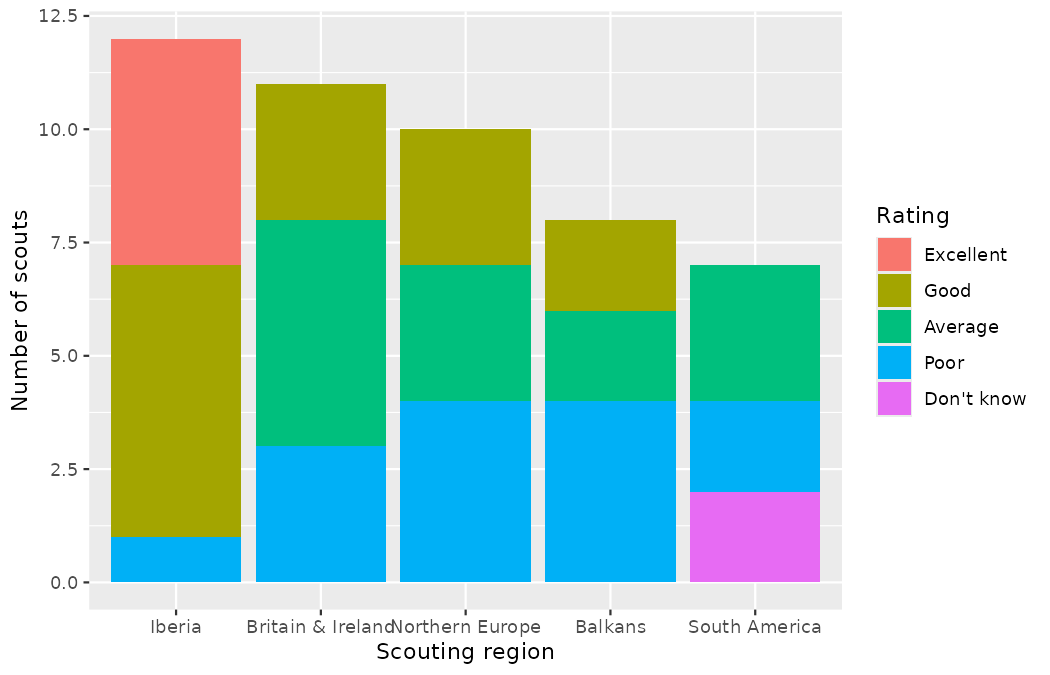
\includegraphics[width=0.85\linewidth,height=\textheight,keepaspectratio]{figures/explore-applications-11.png}

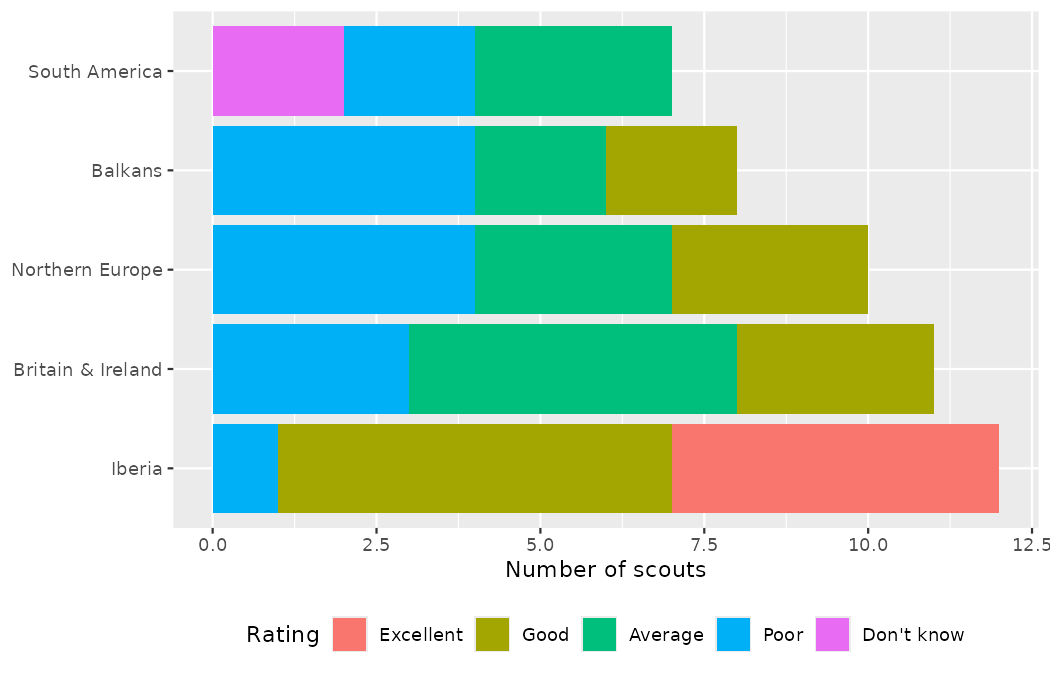
\includegraphics[width=0.85\linewidth,height=\textheight,keepaspectratio]{figures/explore-applications-12.png}

While the quantitative information in the two graphics is identical,
flipping the graph and creating horizontal bars provides more space for
the \textbf{axis labels}. With vertical bars, the region names ---
``Britain \& Ireland'', ``Northern Europe'', ``South America'' --- crowd
the x-axis and tempt the software into shrinking or rotating them;
rotated labels force the reader to tilt their head, and abbreviated ones
force them to guess. With horizontal bars each region name sits on its
own line, read the way text is meant to be read. The easier the
categories are to read, the more the reader will learn from the
visualization. Remember, the goal is to convey as much information as
possible in a succinct and clear manner.

\subsection{Pick a purpose}\label{pick-a-purpose}

Every graphical decision should be made with a \textbf{purpose}. As
previously mentioned, sticking with default options is not always best
for conveying the narrative of your data story. Stacked bar plots tell
one part of a story. Depending on your research question, they may not
tell the part of the story most important to the research.

The code below gives three different representations of the same two
variables, \texttt{region} and \texttt{rating}.

\begin{Shaded}
\begin{Highlighting}[]
\CommentTok{\# (a) Proportions: compare the rating mix across regions}
\FunctionTok{ggplot}\NormalTok{(scout\_panel, }\FunctionTok{aes}\NormalTok{(}\AttributeTok{y =}\NormalTok{ region, }\AttributeTok{fill =}\NormalTok{ rating)) }\SpecialCharTok{+}
  \FunctionTok{geom\_bar}\NormalTok{(}\AttributeTok{position =} \StringTok{"fill"}\NormalTok{) }\SpecialCharTok{+}
  \FunctionTok{labs}\NormalTok{(}\AttributeTok{x =} \StringTok{"Proportion of scouts"}\NormalTok{, }\AttributeTok{y =} \ConstantTok{NULL}\NormalTok{, }\AttributeTok{fill =} \StringTok{"Rating"}\NormalTok{) }\SpecialCharTok{+}
  \FunctionTok{theme}\NormalTok{(}\AttributeTok{legend.position =} \StringTok{"top"}\NormalTok{)}

\CommentTok{\# (b) Counts: keep the size of each regional desk visible}
\FunctionTok{ggplot}\NormalTok{(scout\_panel, }\FunctionTok{aes}\NormalTok{(}\AttributeTok{y =}\NormalTok{ region, }\AttributeTok{fill =}\NormalTok{ rating)) }\SpecialCharTok{+}
  \FunctionTok{geom\_bar}\NormalTok{() }\SpecialCharTok{+}
  \FunctionTok{labs}\NormalTok{(}\AttributeTok{x =} \StringTok{"Number of scouts"}\NormalTok{, }\AttributeTok{y =} \ConstantTok{NULL}\NormalTok{, }\AttributeTok{fill =} \StringTok{"Rating"}\NormalTok{) }\SpecialCharTok{+}
  \FunctionTok{theme}\NormalTok{(}\AttributeTok{legend.position =} \StringTok{"top"}\NormalTok{)}

\CommentTok{\# (c) Faceted: one small bar plot per region}
\FunctionTok{ggplot}\NormalTok{(scout\_panel, }\FunctionTok{aes}\NormalTok{(}\AttributeTok{y =}\NormalTok{ rating)) }\SpecialCharTok{+}
  \FunctionTok{geom\_bar}\NormalTok{() }\SpecialCharTok{+}
  \FunctionTok{facet\_grid}\NormalTok{(. }\SpecialCharTok{\textasciitilde{}}\NormalTok{ region) }\SpecialCharTok{+}
  \FunctionTok{labs}\NormalTok{(}
    \AttributeTok{title =} \StringTok{"How would you rate the prospect\textquotesingle{}s readiness for our first team?"}\NormalTok{,}
    \AttributeTok{subtitle =} \StringTok{"Northbridge United scouting panel, all 48 regional scouts"}\NormalTok{,}
    \AttributeTok{caption =} \StringTok{"Constructed illustration, seed 601 {-}{-} not real survey data"}\NormalTok{,}
    \AttributeTok{x =} \StringTok{"Number of scouts"}\NormalTok{,}
    \AttributeTok{y =} \ConstantTok{NULL}
\NormalTok{  )}
\end{Highlighting}
\end{Shaded}

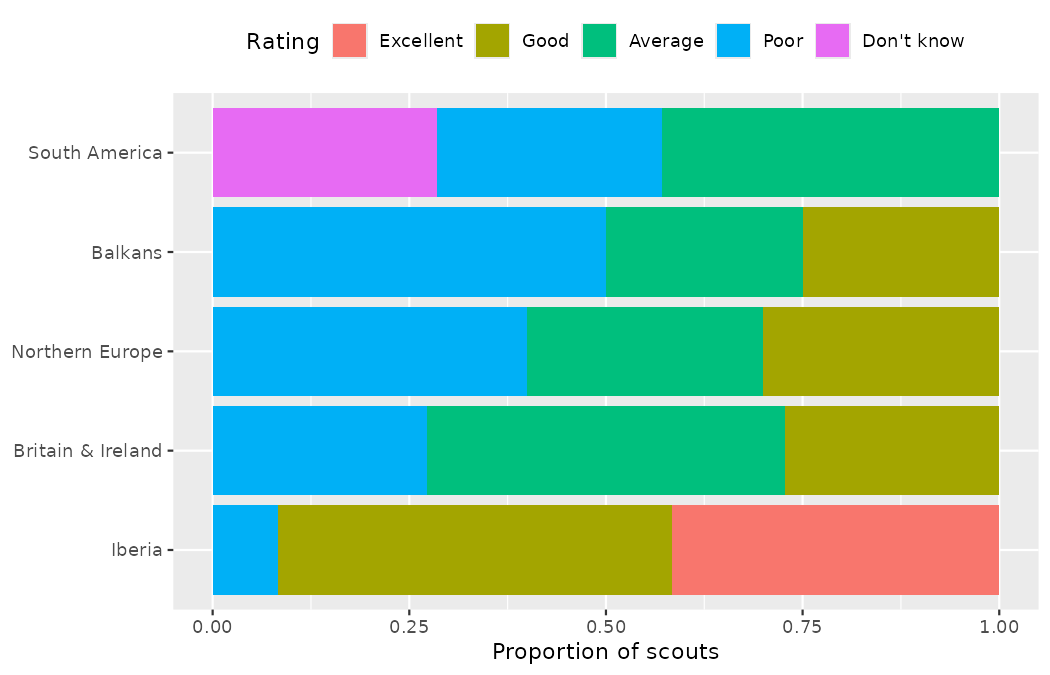
\includegraphics[width=0.85\linewidth,height=\textheight,keepaspectratio]{figures/explore-applications-13.png}

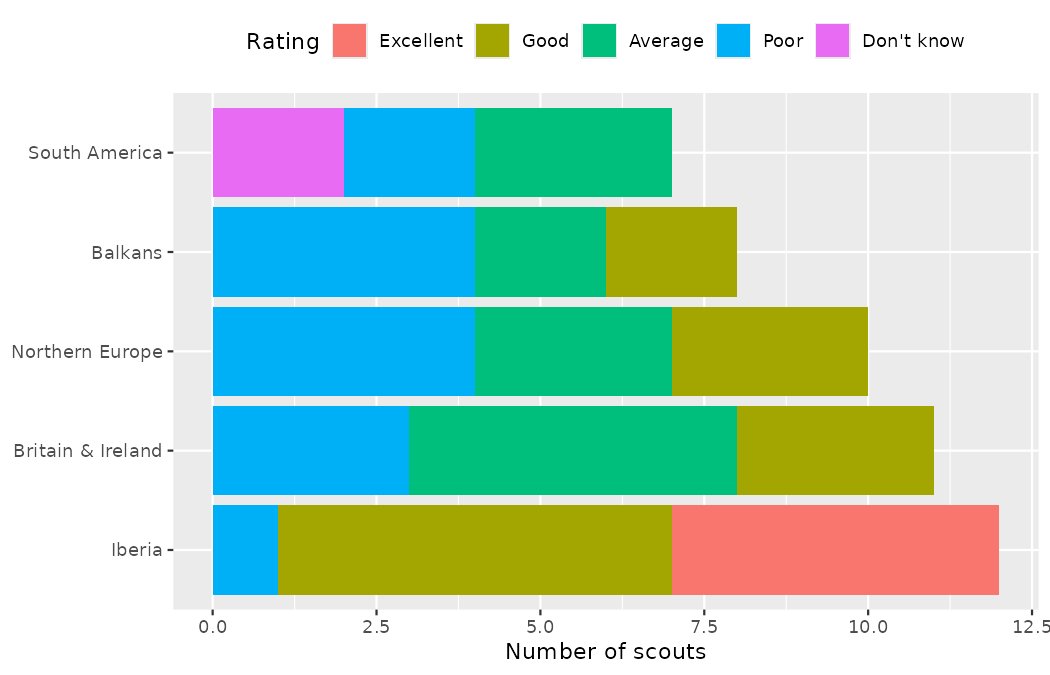
\includegraphics[width=0.85\linewidth,height=\textheight,keepaspectratio]{figures/explore-applications-14.png}

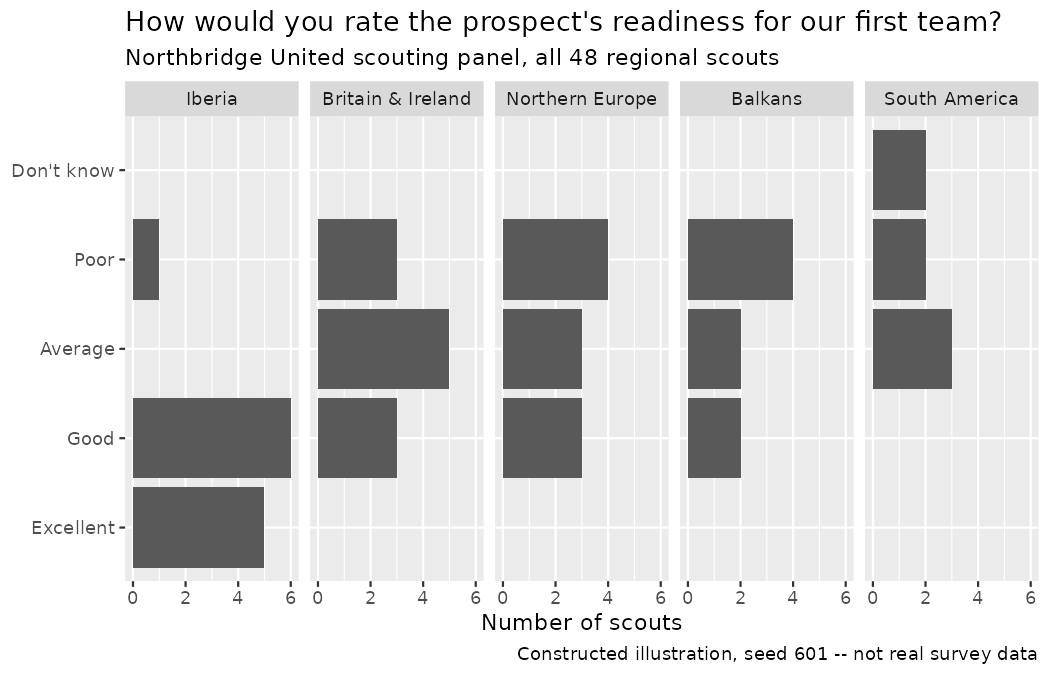
\includegraphics[width=0.85\linewidth,height=\textheight,keepaspectratio]{figures/explore-applications-15.png}

If the most important comparison across regions is proportion, you might
prefer plot (a): standardizing each bar to length one makes it immediate
that Iberia's mix is dominated by Excellent and Good (11 of its 12
scouts) while every other region's mix centers on Average and Poor, and
that the only Don't know responses (both of them) sit on the South
America desk --- the scouts who have seen the least of him live. If the
most important comparison across regions also considers the total number
of scouts in each region, you might prefer plot (b): the same stacks,
but now the eye also sees that Iberia (12) and Britain \& Ireland (11)
are the largest desks while South America has only 7 scouts, so its
opinions rest on the fewest observers. If a separate bar plot for each
region makes the point you'd like, use plot (c), which has been
\textbf{faceted} by region. Plot (c) also provides a full title, a
subtitle identifying the population of respondents, and a caption with
the source --- here, honestly, the seed of the simulation. Other
deliberate decisions to consider include using informative labels and
avoiding redundancy.

\begin{tcolorbox}[enhanced jigsaw, left=2mm, leftrule=.75mm, title=\textcolor{quarto-callout-tip-color}{\faLightbulb}\hspace{0.5em}{Check your understanding}, arc=.35mm, rightrule=.15mm, coltitle=black, colframe=quarto-callout-tip-color-frame, bottomrule=.15mm, colbacktitle=quarto-callout-tip-color!10!white, opacitybacktitle=0.6, breakable, bottomtitle=1mm, toptitle=1mm, titlerule=0mm, opacityback=0, toprule=.15mm, colback=white]

Marta asks: ``should I trust the Iberia desk's enthusiasm or the rest of
the network's caution?'' Which of the three representations is the
\emph{wrong} one to hand her, and why?

\begin{center}\rule{0.5\linewidth}{0.5pt}\end{center}

The proportion plot (a), on its own, is the most dangerous: it makes the
South America desk's bar exactly as long as Iberia's, hiding the fact
that one summarizes 7 scouts (2 of whom answered Don't know) and the
other 12. Her question is precisely about how to weigh conflicting
groups, so the group sizes are part of the answer --- plot (b) or (c),
which keep counts visible, serve her better. (And recall
Chapter~\ref{sec-data-design}: since scouts were not randomly assigned
to viewing conditions, the Iberia gap is an association --- more live
viewing \emph{goes with} higher ratings --- not proof that live viewing
causes enthusiasm.)

\end{tcolorbox}

\subsection{Select meaningful colors}\label{select-meaningful-colors}

One last consideration for building graphs is to consider color choices.
Default or rainbow colors are not always the choice which will best
distinguish the level of your variables. Much research has been done to
find color combinations which are distinct and which are clear for
differently sighted individuals. The cividis scale, developed from that
research, works well with ordinal data: its colors run along a single
dark-to-light path, so the visual order of the colors matches the order
of the rating scale.

\begin{Shaded}
\begin{Highlighting}[]
\NormalTok{p }\OtherTok{\textless{}{-}} \FunctionTok{ggplot}\NormalTok{(scout\_panel, }\FunctionTok{aes}\NormalTok{(}\AttributeTok{y =}\NormalTok{ region, }\AttributeTok{fill =}\NormalTok{ rating)) }\SpecialCharTok{+}
  \FunctionTok{geom\_bar}\NormalTok{(}\AttributeTok{position =} \StringTok{"fill"}\NormalTok{) }\SpecialCharTok{+}
  \FunctionTok{labs}\NormalTok{(}
    \AttributeTok{title =} \StringTok{"How would you rate the prospect\textquotesingle{}s readiness for our first team?"}\NormalTok{,}
    \AttributeTok{subtitle =} \StringTok{"Northbridge United scouting panel, all 48 regional scouts"}\NormalTok{,}
    \AttributeTok{caption =} \StringTok{"Constructed illustration, seed 601 {-}{-} not real survey data"}\NormalTok{,}
    \AttributeTok{x =} \StringTok{"Proportion of scouts"}\NormalTok{,}
    \AttributeTok{y =} \ConstantTok{NULL}\NormalTok{,}
    \AttributeTok{fill =} \ConstantTok{NULL}
\NormalTok{  )}

\CommentTok{\# (a) Default color scale}
\NormalTok{p}

\CommentTok{\# (b) Cividis scale}
\NormalTok{p }\SpecialCharTok{+} \FunctionTok{scale\_fill\_viridis\_d}\NormalTok{(}\AttributeTok{option =} \StringTok{"E"}\NormalTok{)}
\end{Highlighting}
\end{Shaded}

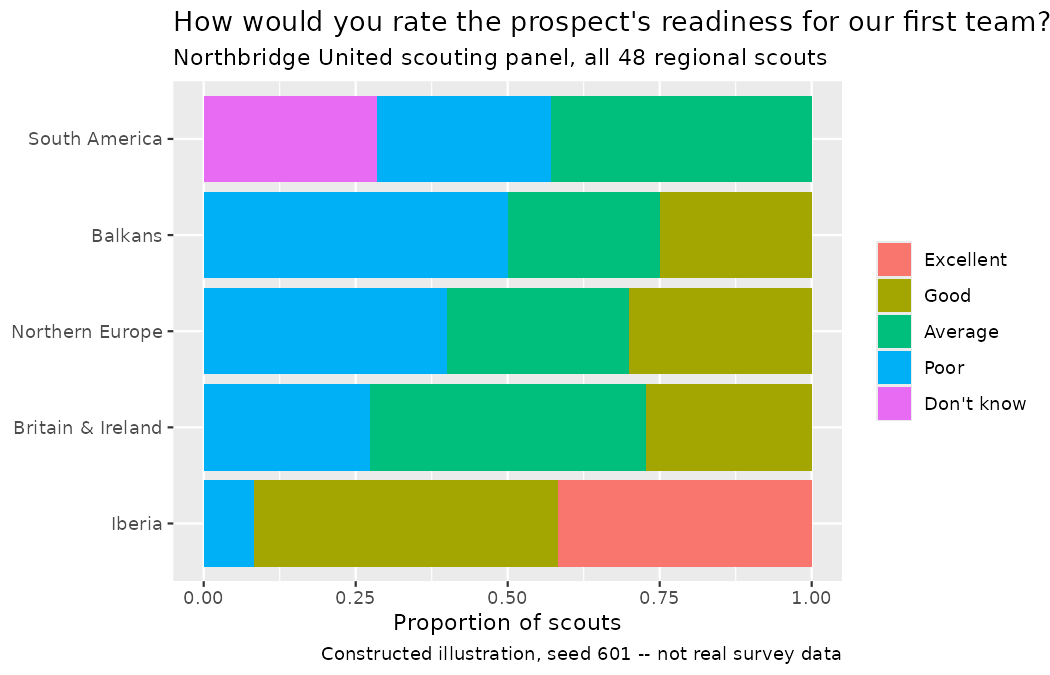
\includegraphics[width=0.85\linewidth,height=\textheight,keepaspectratio]{figures/explore-applications-16.png}

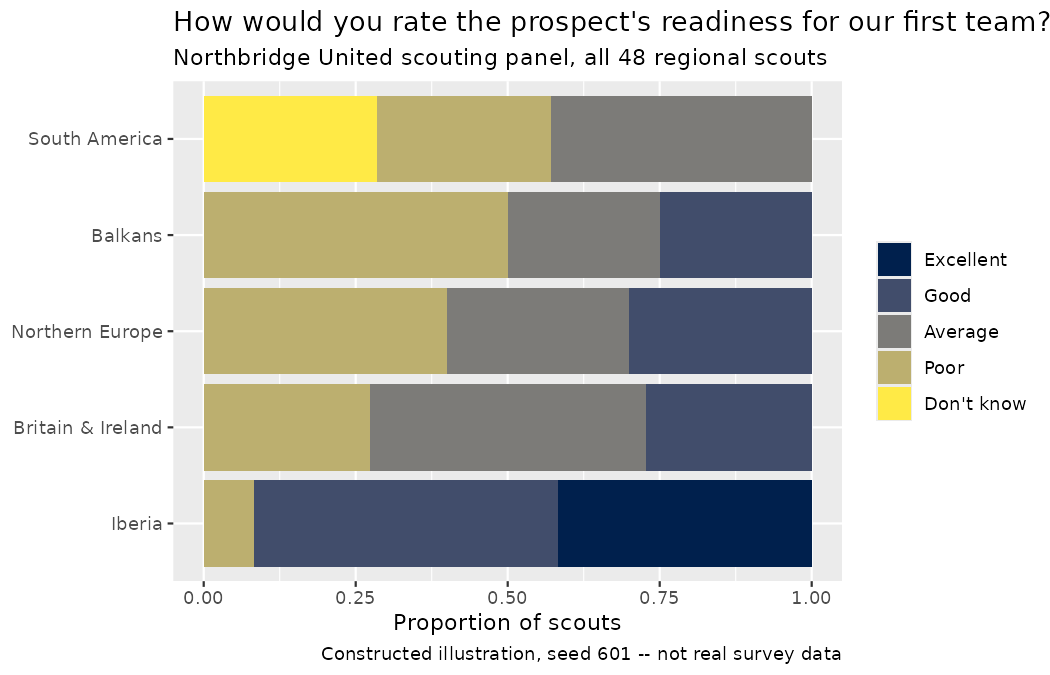
\includegraphics[width=0.85\linewidth,height=\textheight,keepaspectratio]{figures/explore-applications-17.png}

The two plots contain identical bars. In version (a), the five ratings
receive the default evenly-spaced hues --- red through pink --- which
encode no order: nothing about the colors says Excellent is ``more''
than Good. In version (b), the cividis scale colors Excellent dark
blue-grey, shading step by step to Don't know in pale yellow; the
lightness gradient reproduces the scale's ordering, so even in a
greyscale printout of the dossier --- and for readers with the common
forms of color-vision deficiency --- the segments remain distinguishable
and \emph{ordered}.

In this chapter different representations are contrasted to demonstrate
best practices in creating graphs. The fundamental principle is that
your graph should provide maximal information succinctly and clearly.
Labels should be clear and oriented horizontally for the reader. Don't
forget titles and, if possible, include the source of the data --- and,
for constructed scenarios like the scout panel, the seed that
regenerates them.

\section{Interactive R walkthrough}\label{sec-explore-tutorials}

Navigate the concepts you've learned in this part in R with the
following self-paced walkthrough. All you need is your own R console and
the two tournament files --- everything below runs from the derived data
you have used since Chapter~\ref{sec-data-hello}. The walkthrough
deliberately moves to the \emph{second} tournament, the 2025 Women's
Euro: every skill from this part of the book should transfer to a
competition you haven't summarized yet, and checking that it does is the
point. Work each lesson yourself before reading the output; the code and
results are printed so you can confirm your run.

\textbf{Lesson 1: Visualizing categorical data.} England Women's won the
tournament. Build the sorted bar plot of their shots by play pattern ---
the same figure Priya built for Argentina in the case study --- and
decide, before you plot, which ordering \texttt{play\_pattern} deserves.

\begin{Shaded}
\begin{Highlighting}[]
\NormalTok{weuro2025\_shots }\SpecialCharTok{|\textgreater{}}
  \FunctionTok{filter}\NormalTok{(team }\SpecialCharTok{==} \StringTok{"England Women\textquotesingle{}s"}\NormalTok{) }\SpecialCharTok{|\textgreater{}}
  \FunctionTok{count}\NormalTok{(play\_pattern, }\AttributeTok{sort =} \ConstantTok{TRUE}\NormalTok{)}
\CommentTok{\#\textgreater{} \# A tibble: 9 × 2}
\CommentTok{\#\textgreater{}   play\_pattern       n}
\CommentTok{\#\textgreater{}   \textless{}chr\textgreater{}          \textless{}int\textgreater{}}
\CommentTok{\#\textgreater{} 1 Regular Play      36}
\CommentTok{\#\textgreater{} 2 From Throw In     20}
\CommentTok{\#\textgreater{} 3 From Corner       15}
\CommentTok{\#\textgreater{} 4 Other             15}
\CommentTok{\#\textgreater{} 5 From Free Kick    14}
\CommentTok{\#\textgreater{} 6 From Goal Kick     5}
\CommentTok{\#\textgreater{} 7 From Keeper        5}
\CommentTok{\#\textgreater{} 8 From Counter       4}
\CommentTok{\#\textgreater{} 9 From Kick Off      1}

\NormalTok{weuro2025\_shots }\SpecialCharTok{|\textgreater{}}
  \FunctionTok{filter}\NormalTok{(team }\SpecialCharTok{==} \StringTok{"England Women\textquotesingle{}s"}\NormalTok{) }\SpecialCharTok{|\textgreater{}}
  \FunctionTok{count}\NormalTok{(play\_pattern) }\SpecialCharTok{|\textgreater{}}
  \FunctionTok{ggplot}\NormalTok{(}\FunctionTok{aes}\NormalTok{(}\AttributeTok{x =}\NormalTok{ n, }\AttributeTok{y =} \FunctionTok{reorder}\NormalTok{(play\_pattern, n))) }\SpecialCharTok{+}
  \FunctionTok{geom\_col}\NormalTok{() }\SpecialCharTok{+}
  \FunctionTok{labs}\NormalTok{(}\AttributeTok{x =} \StringTok{"Number of shots"}\NormalTok{, }\AttributeTok{y =} \ConstantTok{NULL}\NormalTok{,}
       \AttributeTok{title =} \StringTok{"England\textquotesingle{}s shots by play pattern, 2025 Women\textquotesingle{}s Euro"}\NormalTok{)}
\end{Highlighting}
\end{Shaded}

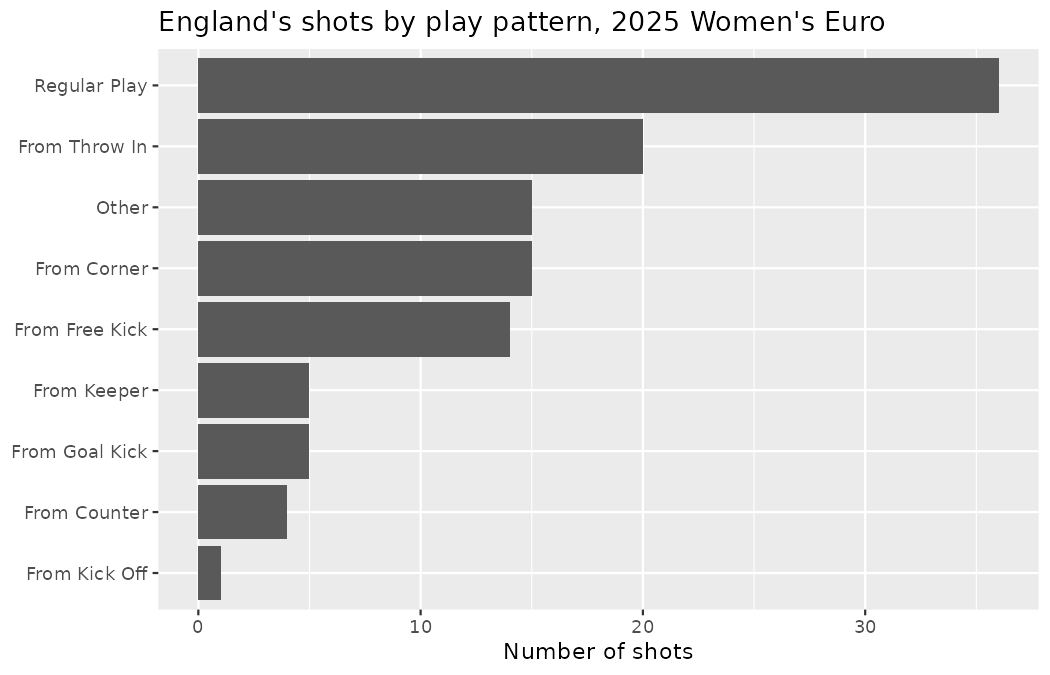
\includegraphics[width=0.85\linewidth,height=\textheight,keepaspectratio]{figures/explore-applications-18.png}

Frequency order is right --- \texttt{play\_pattern} is nominal. But do
not stop at the plot: \texttt{Other}, a category that should be a dull
miscellaneous bucket, holds 15 of England's 115 shots, tied with
corners. You met this suspicious bucket in
Chapter~\ref{sec-data-applications}; interrogate it again here.

\begin{Shaded}
\begin{Highlighting}[]
\NormalTok{weuro2025\_shots }\SpecialCharTok{|\textgreater{}}
  \FunctionTok{filter}\NormalTok{(team }\SpecialCharTok{==} \StringTok{"England Women\textquotesingle{}s"}\NormalTok{, play\_pattern }\SpecialCharTok{==} \StringTok{"Other"}\NormalTok{) }\SpecialCharTok{|\textgreater{}}
  \FunctionTok{count}\NormalTok{(shot\_type, period)}
\CommentTok{\#\textgreater{} \# A tibble: 4 × 3}
\CommentTok{\#\textgreater{}   shot\_type period     n}
\CommentTok{\#\textgreater{}   \textless{}chr\textgreater{}      \textless{}dbl\textgreater{} \textless{}int\textgreater{}}
\CommentTok{\#\textgreater{} 1 Open Play      4     1}
\CommentTok{\#\textgreater{} 2 Penalty        1     1}
\CommentTok{\#\textgreater{} 3 Penalty        4     1}
\CommentTok{\#\textgreater{} 4 Penalty        5    12}
\end{Highlighting}
\end{Shaded}

Fourteen of the fifteen are penalties, and twelve of those are period-5
shoot-out kicks: England went to a shoot-out twice on their way to the
title, in the quarter-final against Sweden and in the final against
Spain. A bar plot that silently mixes shoot-out kicks with open-play
chances tells Marta the wrong story about how England attack --- exactly
the keep-or-filter decision Chapter~\ref{sec-data-applications} warned
you the dataset never makes for you.

\textbf{Lesson 2: Visualizing numerical data.} Draw the distribution of
chance quality for every shot of the tournament.

\begin{Shaded}
\begin{Highlighting}[]
\FunctionTok{ggplot}\NormalTok{(weuro2025\_shots, }\FunctionTok{aes}\NormalTok{(}\AttributeTok{x =}\NormalTok{ statsbomb\_xg)) }\SpecialCharTok{+}
  \FunctionTok{geom\_histogram}\NormalTok{(}\AttributeTok{binwidth =} \FloatTok{0.05}\NormalTok{, }\AttributeTok{boundary =} \DecValTok{0}\NormalTok{) }\SpecialCharTok{+}
  \FunctionTok{labs}\NormalTok{(}\AttributeTok{x =} \StringTok{"Chance quality (xG) per shot"}\NormalTok{, }\AttributeTok{y =} \StringTok{"Number of shots"}\NormalTok{,}
       \AttributeTok{title =} \StringTok{"Chance quality of all 913 shots, 2025 Women\textquotesingle{}s Euro"}\NormalTok{)}
\end{Highlighting}
\end{Shaded}

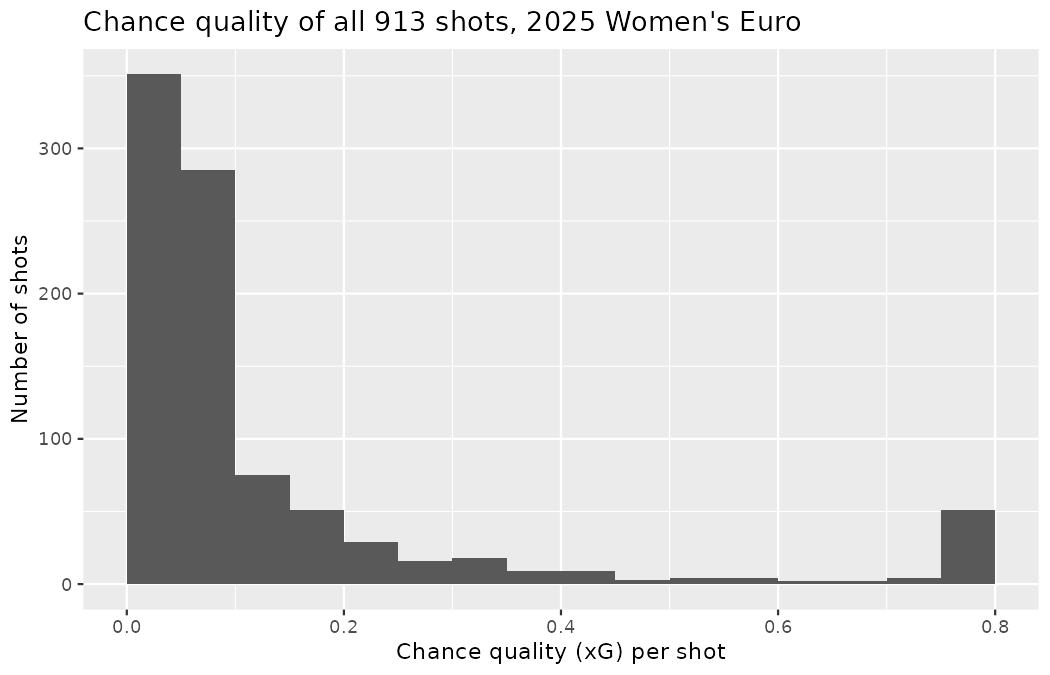
\includegraphics[width=0.85\linewidth,height=\textheight,keepaspectratio]{figures/explore-applications-19.png}

The histogram is strongly right-skewed: the two leftmost bars tower over
everything (351 shots below 0.05 and another 285 between 0.05 and 0.10
--- together about 70\% of all 913 shots), the counts fall away steadily
through the tail, and then, after a stretch of near-empty bins, an
isolated spike of 51 shots stands at 0.75--0.80. You should recognize
that spike before you check: it is the penalties, every one carrying the
model's flat penalty value.

\begin{Shaded}
\begin{Highlighting}[]
\NormalTok{weuro2025\_shots }\SpecialCharTok{|\textgreater{}}
  \FunctionTok{filter}\NormalTok{(shot\_type }\SpecialCharTok{==} \StringTok{"Penalty"}\NormalTok{) }\SpecialCharTok{|\textgreater{}}
  \FunctionTok{summarize}\NormalTok{(}\AttributeTok{kicks =} \FunctionTok{n}\NormalTok{(), }\AttributeTok{mean\_xg =} \FunctionTok{mean}\NormalTok{(statsbomb\_xg))}
\CommentTok{\#\textgreater{} \# A tibble: 1 × 2}
\CommentTok{\#\textgreater{}   kicks mean\_xg}
\CommentTok{\#\textgreater{}   \textless{}int\textgreater{}   \textless{}dbl\textgreater{}}
\CommentTok{\#\textgreater{} 1    51   0.784}
\end{Highlighting}
\end{Shaded}

The printed mean of \(0.784\) is the display rounding of the stored
penalty value \(0.7835,\) identical for every kick (recall
Chapter~\ref{sec-data-applications}). Any figure page you build from
this variable must decide --- visibly, in a caption or a filter ---
whether those 51 identical values belong in the story being told.

\textbf{Lesson 3: Summarizing with statistics.} Recall from
Chapter~\ref{sec-explore-numerical} which summaries a skewed
distribution distorts.

\begin{Shaded}
\begin{Highlighting}[]
\NormalTok{weuro2025\_shots }\SpecialCharTok{|\textgreater{}}
  \FunctionTok{summarize}\NormalTok{(}\AttributeTok{mean\_xg =} \FunctionTok{mean}\NormalTok{(statsbomb\_xg), }\AttributeTok{median\_xg =} \FunctionTok{median}\NormalTok{(statsbomb\_xg))}
\CommentTok{\#\textgreater{} \# A tibble: 1 × 2}
\CommentTok{\#\textgreater{}   mean\_xg median\_xg}
\CommentTok{\#\textgreater{}     \textless{}dbl\textgreater{}     \textless{}dbl\textgreater{}}
\CommentTok{\#\textgreater{} 1   0.135    0.0630}
\end{Highlighting}
\end{Shaded}

The mean (0.135) sits at more than twice the median (0.063), dragged up
by the right tail and the penalty spike --- the textbook signature of
right skew, now in a figure Marta will actually see. Then redo the case
study's highlighted body-part figure on this tournament, aerial-threat
brief and all:

\begin{Shaded}
\begin{Highlighting}[]
\NormalTok{weuro\_bodypart }\OtherTok{\textless{}{-}}\NormalTok{ weuro2025\_shots }\SpecialCharTok{|\textgreater{}}
  \FunctionTok{filter}\NormalTok{(body\_part }\SpecialCharTok{!=} \StringTok{"Other"}\NormalTok{) }\SpecialCharTok{|\textgreater{}}
  \FunctionTok{group\_by}\NormalTok{(body\_part) }\SpecialCharTok{|\textgreater{}}
  \FunctionTok{summarize}\NormalTok{(}\AttributeTok{shots =} \FunctionTok{n}\NormalTok{(), }\AttributeTok{mean\_xg =} \FunctionTok{mean}\NormalTok{(statsbomb\_xg))}

\NormalTok{weuro\_bodypart}
\CommentTok{\#\textgreater{} \# A tibble: 3 × 3}
\CommentTok{\#\textgreater{}   body\_part  shots mean\_xg}
\CommentTok{\#\textgreater{}   \textless{}chr\textgreater{}      \textless{}int\textgreater{}   \textless{}dbl\textgreater{}}
\CommentTok{\#\textgreater{} 1 Head         151   0.108}
\CommentTok{\#\textgreater{} 2 Left Foot    256   0.130}
\CommentTok{\#\textgreater{} 3 Right Foot   502   0.145}

\NormalTok{weuro\_bodypart }\SpecialCharTok{|\textgreater{}}
  \FunctionTok{mutate}\NormalTok{(}\AttributeTok{highlight =} \FunctionTok{if\_else}\NormalTok{(body\_part }\SpecialCharTok{==} \StringTok{"Head"}\NormalTok{, }\StringTok{"yes"}\NormalTok{, }\StringTok{"no"}\NormalTok{)) }\SpecialCharTok{|\textgreater{}}
  \FunctionTok{ggplot}\NormalTok{(}\FunctionTok{aes}\NormalTok{(}\AttributeTok{y =}\NormalTok{ body\_part, }\AttributeTok{x =}\NormalTok{ mean\_xg, }\AttributeTok{fill =}\NormalTok{ highlight)) }\SpecialCharTok{+}
  \FunctionTok{geom\_col}\NormalTok{(}\AttributeTok{show.legend =} \ConstantTok{FALSE}\NormalTok{) }\SpecialCharTok{+}
  \FunctionTok{scale\_fill\_manual}\NormalTok{(}\AttributeTok{values =} \FunctionTok{c}\NormalTok{(}\AttributeTok{no =} \StringTok{"grey70"}\NormalTok{, }\AttributeTok{yes =} \StringTok{"firebrick"}\NormalTok{)) }\SpecialCharTok{+}
  \FunctionTok{labs}\NormalTok{(}\AttributeTok{x =} \StringTok{"Mean xG per shot"}\NormalTok{, }\AttributeTok{y =} \ConstantTok{NULL}\NormalTok{)}
\end{Highlighting}
\end{Shaded}

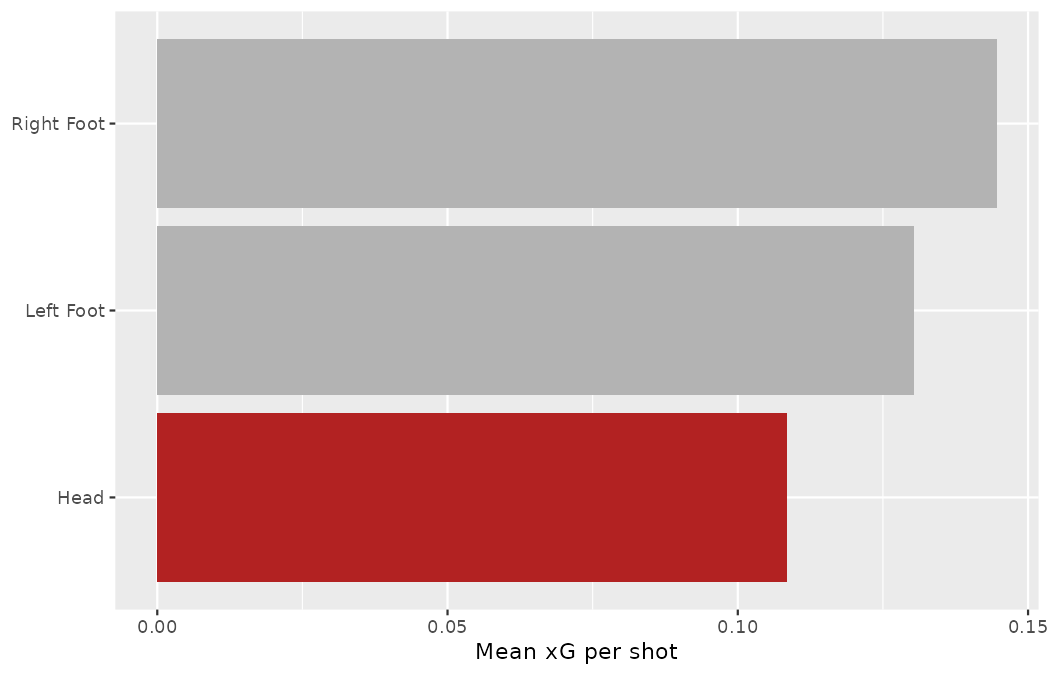
\includegraphics[width=0.85\linewidth,height=\textheight,keepaspectratio]{figures/explore-applications-20.png}

And apply the case study's honesty check here too, per the book's
penalty convention: this tournament's foot bars carry its 51 penalties
--- all footed, all at the stored 0.7835 --- while the header bar
carries none. On open play alone, the ordering reverses exactly as it
did at the World Cup:

\begin{Shaded}
\begin{Highlighting}[]
\NormalTok{weuro2025\_shots }\SpecialCharTok{|\textgreater{}}
  \FunctionTok{filter}\NormalTok{(shot\_type }\SpecialCharTok{==} \StringTok{"Open Play"}\NormalTok{, body\_part }\SpecialCharTok{!=} \StringTok{"Other"}\NormalTok{) }\SpecialCharTok{|\textgreater{}}
  \FunctionTok{group\_by}\NormalTok{(body\_part) }\SpecialCharTok{|\textgreater{}}
  \FunctionTok{summarize}\NormalTok{(}\AttributeTok{shots =} \FunctionTok{n}\NormalTok{(), }\AttributeTok{mean\_xg =} \FunctionTok{mean}\NormalTok{(statsbomb\_xg))}
\CommentTok{\#\textgreater{} \# A tibble: 3 × 3}
\CommentTok{\#\textgreater{}   body\_part  shots mean\_xg}
\CommentTok{\#\textgreater{}   \textless{}chr\textgreater{}      \textless{}int\textgreater{}   \textless{}dbl\textgreater{}}
\CommentTok{\#\textgreater{} 1 Head         151  0.108}
\CommentTok{\#\textgreater{} 2 Left Foot    242  0.0988}
\CommentTok{\#\textgreater{} 3 Right Foot   454  0.0918}
\end{Highlighting}
\end{Shaded}

\textbf{Lesson 4: Case study.} Return to the matchday time series of the
case study and rebuild it for the Women's Euro alone: the daily shot
counts, the dashed line where the knockout rounds begin (matchday 13, a
24-shot day), and an annotation stating the schedule fact that explains
the drop. Then write the two-sentence caption you would put under it in
a dossier --- one sentence for what the reader sees, one for the
external fact that keeps them from misreading it. If your caption
survives the Emil test of the case study (does it force the right
denominator?), you have finished this part of the book.

\begin{tcolorbox}[enhanced jigsaw, left=2mm, leftrule=.75mm, title=\textcolor{quarto-callout-tip-color}{\faLightbulb}\hspace{0.5em}{Check your understanding}, arc=.35mm, rightrule=.15mm, coltitle=black, colframe=quarto-callout-tip-color-frame, bottomrule=.15mm, colbacktitle=quarto-callout-tip-color!10!white, opacitybacktitle=0.6, breakable, bottomtitle=1mm, toptitle=1mm, titlerule=0mm, opacityback=0, toprule=.15mm, colback=white]

At the 2022 World Cup, headers carried the lowest average chance quality
(0.106 xG per shot, against 0.115 for left-footed and 0.134 for
right-footed shots). Lesson 3 shows the Women's Euro numbers: 0.108
against 0.130 and 0.145. Why is this replication worth a line in a
scouting report --- and was it inevitable that the pattern would carry
over?

\begin{center}\rule{0.5\linewidth}{0.5pt}\end{center}

The two tournaments are different competitions, different players,
different samples --- yet the ordering (head lowest, right foot highest)
and even the rough magnitudes repeat, which makes the header pattern
credible as a general feature of \emph{all-shots} data --- a feature
that dissolves once the penalties are set aside, since on open play the
ordering reverses in both tournaments (headers 0.106 and 0.108 against
feet near 0.093 and 0.092--0.099), the replication you ran above. What
replicates, in other words, is the \emph{artifact as well as the
football}: both tournaments load their foot bars with identical-xG
penalties, so both produce the same misleading all-shots ordering ---
and the same reversal when the frame is stated. And no, carrying over
was not inevitable: replication is a finding, not a formality. Compare,
on the same two tournaments, the conversion rate of first-time shots
against controlled ones:

\begin{Shaded}
\begin{Highlighting}[]
\FunctionTok{bind\_rows}\NormalTok{(wc2022\_shots, weuro2025\_shots) }\SpecialCharTok{|\textgreater{}}
  \FunctionTok{group\_by}\NormalTok{(competition, first\_time) }\SpecialCharTok{|\textgreater{}}
  \FunctionTok{summarize}\NormalTok{(}\AttributeTok{shots =} \FunctionTok{n}\NormalTok{(), }\AttributeTok{conversion =} \FunctionTok{mean}\NormalTok{(goal), }\AttributeTok{.groups =} \StringTok{"drop"}\NormalTok{)}
\CommentTok{\#\textgreater{} \# A tibble: 4 × 4}
\CommentTok{\#\textgreater{}   competition first\_time shots conversion}
\CommentTok{\#\textgreater{}   \textless{}chr\textgreater{}       \textless{}lgl\textgreater{}      \textless{}int\textgreater{}      \textless{}dbl\textgreater{}}
\CommentTok{\#\textgreater{} 1 wc2022      FALSE       1026      0.121}
\CommentTok{\#\textgreater{} 2 wc2022      TRUE         468      0.152}
\CommentTok{\#\textgreater{} 3 weuro2025   FALSE        605      0.140}
\CommentTok{\#\textgreater{} 4 weuro2025   TRUE         308      0.123}
\end{Highlighting}
\end{Shaded}

At the World Cup, first-time shots converted at a \emph{higher} rate
(0.152 vs 0.121); at the Women's Euro the direction \emph{reversed}
(0.123 vs 0.140). A pattern holding in a second competition was never
guaranteed --- you had to check. One caution before you bank that
reversal, per the penalty lesson you just learned for the body-part
bars: both splits above are all-shots figures, and the Euro's
non-first-time bucket holds all 51 of its penalties. Filtered to open
play, the Euro runs \(0.123\) vs \(0.105\) --- the \emph{same} direction
as the World Cup; whether this reversal is football or frame is a story
Chapter~\ref{sec-foundations-decision-errors} finishes. Whether either
gap is more than chance variation is a question for the inference
chapters (Chapter~\ref{sec-foundations-randomization} onward).

\end{tcolorbox}

\section{R lab: the figure page}\label{sec-explore-labs}

Further apply the concepts you've learned in this part with a lab
assignment that walks you through a data analysis case study of your
own.

Marta Vidal's brief: choose any one team from \texttt{weuro2025\_shots}
\emph{other than} England, and produce the three-figure page of a
scouting dossier on how that team generates chances. Your page must
contain:

\begin{enumerate}
\def\labelenumi{\arabic{enumi}.}
\tightlist
\item
  one figure summarizing a categorical variable (e.g., the team's
  play-pattern or body-part mix),
\item
  one figure summarizing a numerical variable (e.g., the team's
  chance-quality distribution), and
\item
  one figure comparing groups (e.g., chance quality across body parts,
  or the team against the rest of the tournament).
\end{enumerate}

Every figure is checked against the case study's principles before it
reaches Marta:

\begin{itemize}
\tightlist
\item
  Is the figure as simple as the message allows (no pie charts with nine
  slices, no 3D)?
\item
  Does color, if present, draw attention to the feature the brief asks
  about --- with a second visual cue for readers who do not see color
  the same way?
\item
  Is external context (schedule, penalties, group sizes) annotated where
  a reader would otherwise misread the data?
\item
  Are the levels ordered by a deliberate rule --- the scale's own order
  for ordinal variables, frequency for nominal ones?
\item
  Are the labels horizontal and readable, with a title, informative axis
  names, and the data source in the caption?
\item
  Did you decide --- and state --- whether shoot-out kicks and penalties
  are in or out?
\end{itemize}

There is no new statistical machinery in this lab; that is the point.
The analysis is only as good as its communication, and this page is the
communication.

\section{Chapter review}\label{sec-chp6-review}

\subsection{Summary}\label{summary-5}

This chapter contrasted different representations of the same data to
demonstrate best practices in creating graphs: keep the figure simple;
spend color only to draw attention, and pair it with a second cue;
annotate the external fact --- a fixture calendar, a knockout cut-off
--- that the data alone cannot supply; order levels by a deliberate
rule, respecting an ordinal scale's own order; orient labels so they can
be read; choose the representation (proportions, counts, or facets) that
answers the question actually asked; and pick color scales, like
cividis, whose visual order matches the data's order and survives both
greyscale printing and color-vision deficiency. The fundamental
principle is that your graph should provide maximal information
succinctly and clearly --- because in a club, the figure page of a
dossier often \emph{is} the thirty seconds of analysis a decision gets.

\subsection{Terms}\label{terms-5}

The terms introduced in this chapter are presented below, alphabetized.
If you're not sure what some of these terms mean, we recommend you go
back in the text and review their definitions. You should be able to
easily spot them as \textbf{bolded text}.

\begin{longtable}[]{@{}lll@{}}
\caption{Terms introduced in this
chapter.}\label{tbl-terms-chp-6}\tabularnewline
\toprule\noalign{}
\endfirsthead
\endhead
\bottomrule\noalign{}
\endlastfoot
annotated & color & order \\
axis labels & faceted & purpose \\
\end{longtable}

\begin{center}\rule{0.5\linewidth}{0.5pt}\end{center}

Adapted from \emph{Introduction to Modern Statistics} by
Çetinkaya-Rundel \& Hardin (CC BY-SA 4.0); this adaptation is likewise
CC BY-SA 4.0. Match data: StatsBomb open data.

\part{Regression modeling}

\chapter{Linear regression with a single predictor}\label{sec-model-slr}

Linear regression is a very powerful statistical technique. Many people
have some familiarity with regression models just from reading scouting
reports and match analytics, where straight lines are overlaid on
scatterplots. Linear models can be used for prediction --- how many
goals should a team's chances have produced? --- or to describe the
relationship between two numerical variables, assuming there is a linear
relationship between them.

\section{Fitting a line, residuals, and
correlation}\label{sec-fit-line-res-cor}

When considering linear regression, it's helpful to think deeply about
the line fitting process. In this section, we define the form of a
linear model, explore criteria for what makes a good fit, and introduce
a new statistic called \emph{correlation}.

\subsection{Fitting a line to data}\label{fitting-a-line-to-data}

Consider two variables whose relationship can be modeled
\emph{perfectly} with a straight line. Every season the tournament
organizer invoices each club for scout accreditation: a flat €400
processing fee per club, plus €150 for every scout accredited. Twelve
member clubs submitted requests last summer, and Emil Sørensen kept the
invoices. The equation for the invoice total is

\[
y = 400 + 150x
\]

where \(x\) is the number of scouts accredited and \(y\) is the total
invoice in euros. A club accrediting 4 scouts pays
\(400 + 150 \times 4 = 1000\) euros; a club accrediting 10 pays
\(400 + 150 \times 10 = 1900\) euros --- exactly, every time. Consider
what a perfect linear relationship means: we know the exact value of
\(y\) just by knowing the value of \(x.\) The code below draws the
twelve invoices; because the cost is computed using a linear formula,
the linear fit is perfect.

\begin{Shaded}
\begin{Highlighting}[]
\FunctionTok{library}\NormalTok{(dplyr)}
\FunctionTok{library}\NormalTok{(readr)}
\FunctionTok{library}\NormalTok{(ggplot2)}

\NormalTok{accreditation }\OtherTok{\textless{}{-}} \FunctionTok{tibble}\NormalTok{(}
  \AttributeTok{n\_scouts =} \DecValTok{1}\SpecialCharTok{:}\DecValTok{12}\NormalTok{,}
  \AttributeTok{invoice =} \DecValTok{400} \SpecialCharTok{+} \DecValTok{150} \SpecialCharTok{*}\NormalTok{ n\_scouts}
\NormalTok{)}

\FunctionTok{ggplot}\NormalTok{(accreditation, }\FunctionTok{aes}\NormalTok{(}\AttributeTok{x =}\NormalTok{ n\_scouts, }\AttributeTok{y =}\NormalTok{ invoice)) }\SpecialCharTok{+}
  \FunctionTok{geom\_smooth}\NormalTok{(}\AttributeTok{method =} \StringTok{"lm"}\NormalTok{) }\SpecialCharTok{+}
  \FunctionTok{geom\_point}\NormalTok{(}\AttributeTok{size =} \DecValTok{3}\NormalTok{) }\SpecialCharTok{+}
  \FunctionTok{labs}\NormalTok{(}
    \AttributeTok{x =} \StringTok{"Number of scouts accredited"}\NormalTok{,}
    \AttributeTok{y =} \StringTok{"Total invoice (euros)"}
\NormalTok{  )}
\end{Highlighting}
\end{Shaded}

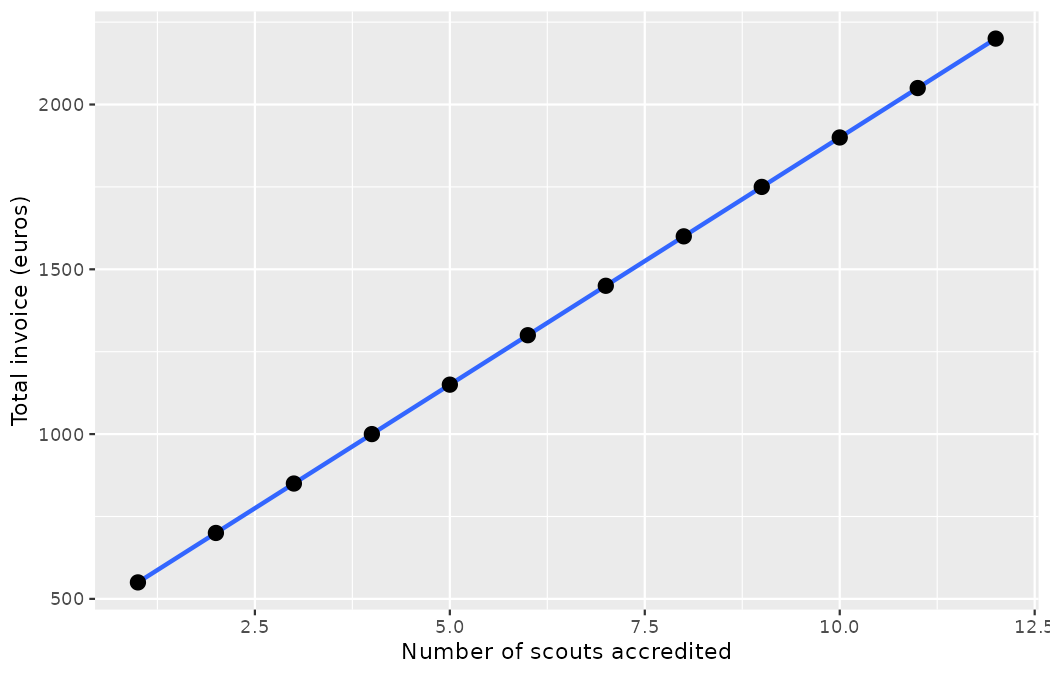
\includegraphics[width=0.85\linewidth,height=\textheight,keepaspectratio]{figures/model-slr-1.png}

All twelve points sit exactly on the fitted line, which climbs from €550
at one scout to €2,200 at twelve. A perfect linear relationship like
this one is unrealistic in almost any natural process --- it happens
here only because the invoice \emph{is computed from} a linear formula.
For example, if we took a team's accumulated chance quality in a match
\((x),\) this value would provide some useful information about how many
goals the team scored \((y).\) But the prediction would be far from
perfect, since finishing, goalkeeping, and luck all play a role in goals
beyond the quality of the chances.

Linear regression is the statistical method for fitting a line to data
where the relationship between two variables, \(x\) and \(y,\) can be
modeled by a straight line with some error:

\[
y = b_0 + b_1 \ x + e
\]

This is the central equation of the chapter, so let us take it apart
symbol by symbol. The letter \(b\) denotes a coefficient computed from
data; the subscript \(0\) marks the \textbf{intercept}, the value of the
line when \(x = 0\); the subscript \(1\) marks the \textbf{slope}, the
change in the line's height for a one-unit increase in \(x.\) So \(b_0\)
and \(b_1\) represent the model's intercept and slope, respectively. The
final letter \(e\) represents the \emph{error}: the part of \(y\) that
the line does not capture. The values \(b_0\) and \(b_1\) are calculated
based on the data, i.e., they are sample statistics --- just as
\(\bar{x}\) and \(s\) were sample statistics in
Chapter~\ref{sec-explore-numerical}. If the observed data is a random
sample from a target population that we are interested in making
inferences about, these values are considered to be point estimates for
the population parameters \(\beta_0\) and \(\beta_1.\) The Greek letter
\(\beta\) (pronounced \emph{beta}) is the population counterpart of the
Roman letter \(b\) --- the same convention that pairs \(\bar{x}\) with
\(\mu\) and \(s\) with \(\sigma,\) which you met in
Chapter~\ref{sec-explore-numerical}: Roman letters for statistics
computed from a sample, Greek letters for the fixed, unknown truths
about the population. We will discuss how to make inferences about
parameters of a linear model based on sample statistics in
Chapter~\ref{sec-inf-model-slr}.

When we use \(x\) to predict \(y,\) we usually call \(x\) the
\textbf{predictor} variable and we call \(y\) the \textbf{outcome}. We
also often drop the \(e\) term when writing down the model since our
main focus is often on the prediction of the average outcome.

It is rare for all of the data to fall perfectly on a straight line.
Instead, it's more common for data to appear as a \emph{cloud of
points}, such as the three constructed scouting scatters built below.
This is a constructed illustration --- Priya Rao assembled these panels
for a training session with Emil's scouts, and the seeded code
regenerates them exactly.

\begin{Shaded}
\begin{Highlighting}[]
\FunctionTok{set.seed}\NormalTok{(}\DecValTok{703}\NormalTok{)}
\NormalTok{scouting\_clouds }\OtherTok{\textless{}{-}} \FunctionTok{tibble}\NormalTok{(}
  \AttributeTok{sprint\_age    =} \FunctionTok{runif}\NormalTok{(}\DecValTok{60}\NormalTok{, }\DecValTok{18}\NormalTok{, }\DecValTok{34}\NormalTok{),}
  \AttributeTok{sprint\_time   =} \FloatTok{3.9} \SpecialCharTok{+} \FloatTok{0.022} \SpecialCharTok{*}\NormalTok{ (sprint\_age }\SpecialCharTok{{-}} \DecValTok{18}\NormalTok{) }\SpecialCharTok{+} \FunctionTok{rnorm}\NormalTok{(}\DecValTok{60}\NormalTok{, }\DecValTok{0}\NormalTok{, }\FloatTok{0.045}\NormalTok{),}
  \AttributeTok{minutes       =} \FunctionTok{runif}\NormalTok{(}\DecValTok{60}\NormalTok{, }\DecValTok{500}\NormalTok{, }\DecValTok{3000}\NormalTok{),}
  \AttributeTok{chances       =} \FunctionTok{pmax}\NormalTok{(}\DecValTok{0}\NormalTok{, }\FunctionTok{round}\NormalTok{(}\DecValTok{2} \SpecialCharTok{+} \FloatTok{0.012} \SpecialCharTok{*}\NormalTok{ minutes }\SpecialCharTok{+} \FunctionTok{rnorm}\NormalTok{(}\DecValTok{60}\NormalTok{, }\DecValTok{0}\NormalTok{, }\DecValTok{9}\NormalTok{))),}
  \AttributeTok{shirt\_number  =} \FunctionTok{sample}\NormalTok{(}\DecValTok{1}\SpecialCharTok{:}\DecValTok{40}\NormalTok{, }\DecValTok{60}\NormalTok{, }\AttributeTok{replace =} \ConstantTok{TRUE}\NormalTok{),}
  \AttributeTok{pass\_accuracy =} \FunctionTok{rnorm}\NormalTok{(}\DecValTok{60}\NormalTok{, }\DecValTok{81}\NormalTok{, }\DecValTok{5}\NormalTok{) }\SpecialCharTok{{-}} \FloatTok{0.04} \SpecialCharTok{*}\NormalTok{ shirt\_number}
\NormalTok{)}

\FunctionTok{c}\NormalTok{(}
  \FunctionTok{cor}\NormalTok{(scouting\_clouds}\SpecialCharTok{$}\NormalTok{sprint\_age, scouting\_clouds}\SpecialCharTok{$}\NormalTok{sprint\_time),}
  \FunctionTok{cor}\NormalTok{(scouting\_clouds}\SpecialCharTok{$}\NormalTok{minutes, scouting\_clouds}\SpecialCharTok{$}\NormalTok{chances),}
  \FunctionTok{cor}\NormalTok{(scouting\_clouds}\SpecialCharTok{$}\NormalTok{shirt\_number, scouting\_clouds}\SpecialCharTok{$}\NormalTok{pass\_accuracy)}
\NormalTok{) }\SpecialCharTok{|\textgreater{}}
  \FunctionTok{round}\NormalTok{(}\DecValTok{2}\NormalTok{)}
\CommentTok{\#\textgreater{} [1] 0.91 0.69 0.06}

\NormalTok{p\_strong }\OtherTok{\textless{}{-}} \FunctionTok{ggplot}\NormalTok{(scouting\_clouds, }\FunctionTok{aes}\NormalTok{(}\AttributeTok{x =}\NormalTok{ sprint\_age, }\AttributeTok{y =}\NormalTok{ sprint\_time)) }\SpecialCharTok{+}
  \FunctionTok{geom\_point}\NormalTok{(}\AttributeTok{size =} \DecValTok{2}\NormalTok{, }\AttributeTok{alpha =} \FloatTok{0.7}\NormalTok{) }\SpecialCharTok{+}
  \FunctionTok{geom\_smooth}\NormalTok{(}\AttributeTok{method =} \StringTok{"lm"}\NormalTok{, }\AttributeTok{se =} \ConstantTok{FALSE}\NormalTok{) }\SpecialCharTok{+}
  \FunctionTok{labs}\NormalTok{(}\AttributeTok{x =} \StringTok{"Age (years)"}\NormalTok{, }\AttributeTok{y =} \StringTok{"30m sprint time (s)"}\NormalTok{)}

\NormalTok{p\_moderate }\OtherTok{\textless{}{-}} \FunctionTok{ggplot}\NormalTok{(scouting\_clouds, }\FunctionTok{aes}\NormalTok{(}\AttributeTok{x =}\NormalTok{ minutes, }\AttributeTok{y =}\NormalTok{ chances)) }\SpecialCharTok{+}
  \FunctionTok{geom\_point}\NormalTok{(}\AttributeTok{size =} \DecValTok{2}\NormalTok{, }\AttributeTok{alpha =} \FloatTok{0.7}\NormalTok{) }\SpecialCharTok{+}
  \FunctionTok{geom\_smooth}\NormalTok{(}\AttributeTok{method =} \StringTok{"lm"}\NormalTok{, }\AttributeTok{se =} \ConstantTok{FALSE}\NormalTok{) }\SpecialCharTok{+}
  \FunctionTok{labs}\NormalTok{(}\AttributeTok{x =} \StringTok{"League minutes played"}\NormalTok{, }\AttributeTok{y =} \StringTok{"Chances created"}\NormalTok{)}

\NormalTok{p\_weak }\OtherTok{\textless{}{-}} \FunctionTok{ggplot}\NormalTok{(scouting\_clouds, }\FunctionTok{aes}\NormalTok{(}\AttributeTok{x =}\NormalTok{ shirt\_number, }\AttributeTok{y =}\NormalTok{ pass\_accuracy)) }\SpecialCharTok{+}
  \FunctionTok{geom\_point}\NormalTok{(}\AttributeTok{size =} \DecValTok{2}\NormalTok{, }\AttributeTok{alpha =} \FloatTok{0.7}\NormalTok{) }\SpecialCharTok{+}
  \FunctionTok{geom\_smooth}\NormalTok{(}\AttributeTok{method =} \StringTok{"lm"}\NormalTok{, }\AttributeTok{se =} \ConstantTok{FALSE}\NormalTok{) }\SpecialCharTok{+}
  \FunctionTok{labs}\NormalTok{(}\AttributeTok{x =} \StringTok{"Shirt number"}\NormalTok{, }\AttributeTok{y =} \StringTok{"Pass accuracy (\%)"}\NormalTok{)}
\end{Highlighting}
\end{Shaded}

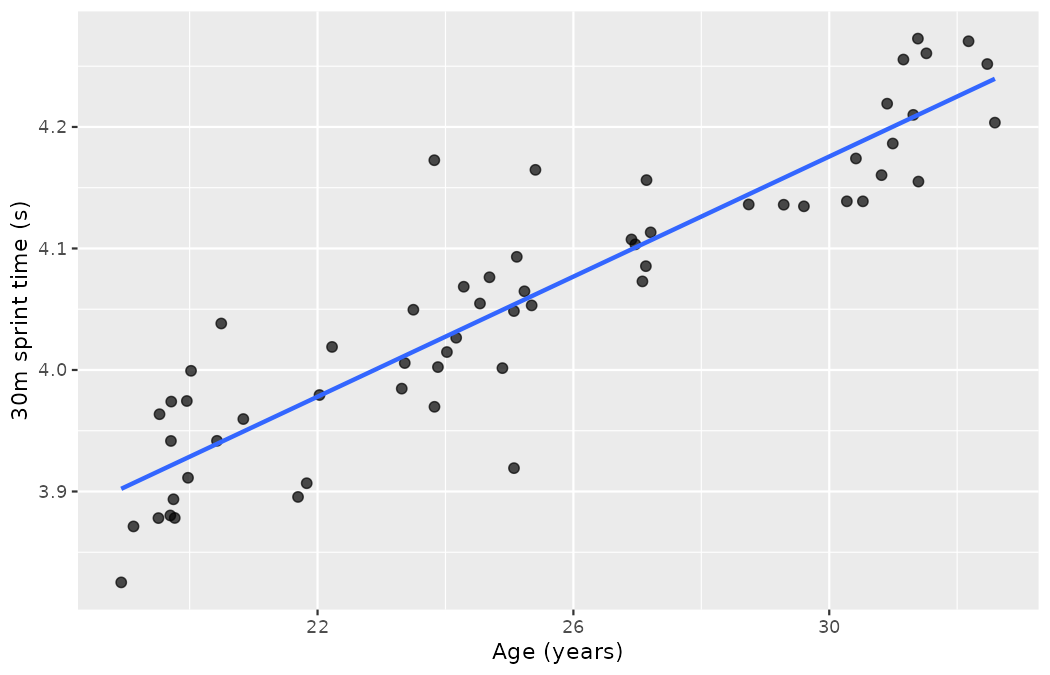
\includegraphics[width=0.85\linewidth,height=\textheight,keepaspectratio]{figures/model-slr-2.png}

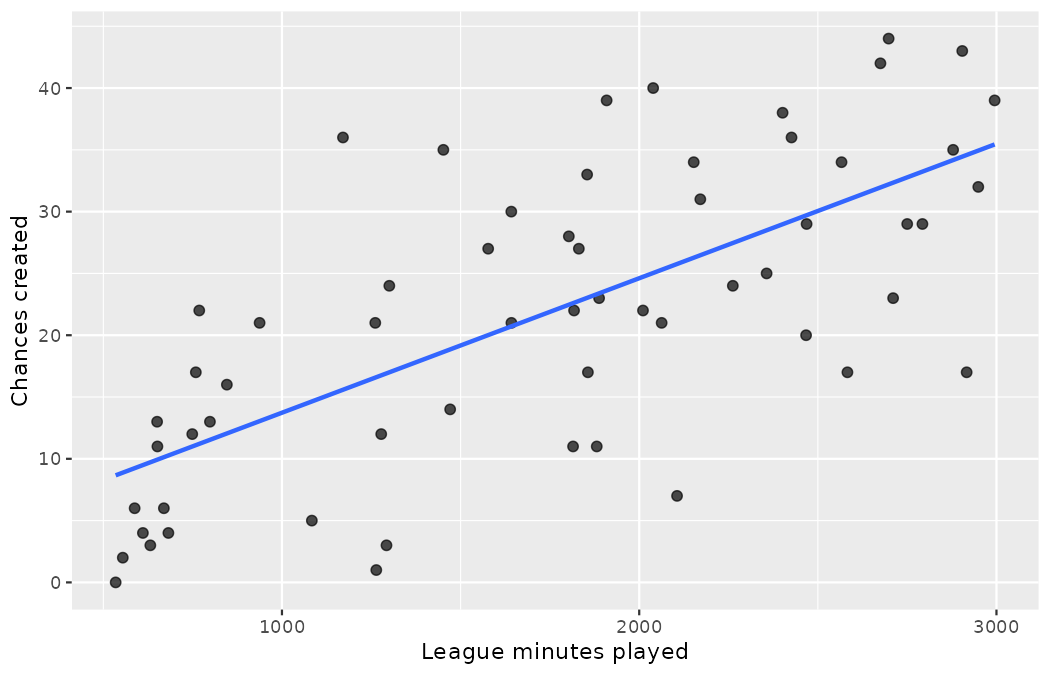
\includegraphics[width=0.85\linewidth,height=\textheight,keepaspectratio]{figures/model-slr-3.png}

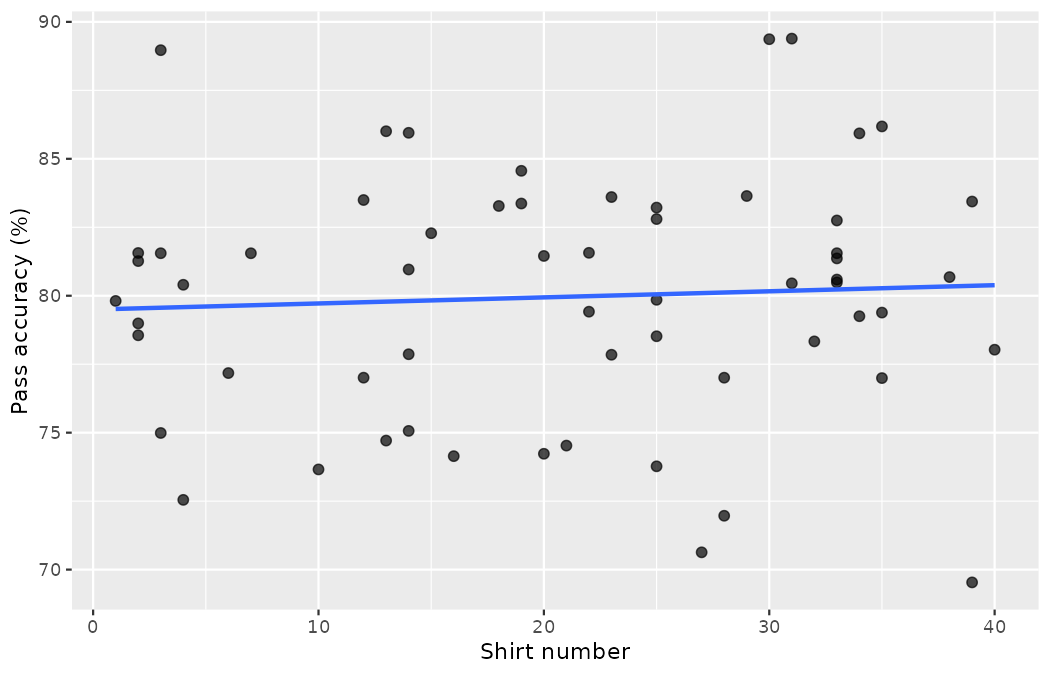
\includegraphics[width=0.85\linewidth,height=\textheight,keepaspectratio]{figures/model-slr-4.png}

In each case, the data fall around a straight line, even if none of the
observations fall exactly on the line. The first plot shows a strong
upward linear trend --- older players in this constructed pool run
slower 30-metre sprints, and the remaining variability around the line
is minor relative to the strength of the relationship (the correlation,
a statistic we formalize later in this section, comes out at \(0.91\)).
The second plot shows an upward trend that, while evident, is not as
strong as the first \((0.69)\): players with more minutes create more
chances, but with plenty of scatter. The last plot shows an essentially
flat cloud \((0.06)\): shirt numbers, unsurprisingly, tell us almost
nothing about pass accuracy --- the trend is so slight we can hardly
notice it. In each of these examples, we will have some uncertainty
regarding our estimates of the model parameters, \(\beta_0\) and
\(\beta_1.\) For instance, we might wonder, should we move the line up
or down a little, or should we tilt it more or less? As we move forward
in this chapter, we will learn about criteria for line-fitting, and we
will also learn about the uncertainty associated with estimates of model
parameters.

There are also cases where fitting a straight line to the data, even if
there is a clear relationship between the variables, is not helpful. One
such case is the age--market-value curve every sporting director carries
in their head: value rises through a player's early twenties, peaks, and
falls away toward retirement. The constructed panel below makes the
point.

\begin{Shaded}
\begin{Highlighting}[]
\NormalTok{age\_curve }\OtherTok{\textless{}{-}} \FunctionTok{tibble}\NormalTok{(}
  \AttributeTok{age =} \FunctionTok{runif}\NormalTok{(}\DecValTok{80}\NormalTok{, }\DecValTok{18}\NormalTok{, }\DecValTok{35}\NormalTok{),}
  \AttributeTok{market\_value =} \DecValTok{24} \SpecialCharTok{{-}} \FloatTok{0.22} \SpecialCharTok{*}\NormalTok{ (age }\SpecialCharTok{{-}} \FloatTok{26.5}\NormalTok{)}\SpecialCharTok{\^{}}\DecValTok{2} \SpecialCharTok{+} \FunctionTok{rnorm}\NormalTok{(}\DecValTok{80}\NormalTok{, }\DecValTok{0}\NormalTok{, }\FloatTok{2.5}\NormalTok{)}
\NormalTok{)}

\FunctionTok{coef}\NormalTok{(}\FunctionTok{lm}\NormalTok{(market\_value }\SpecialCharTok{\textasciitilde{}}\NormalTok{ age, }\AttributeTok{data =}\NormalTok{ age\_curve))}
\CommentTok{\#\textgreater{} (Intercept)         age}
\CommentTok{\#\textgreater{}  15.3951206   0.1357113}

\FunctionTok{ggplot}\NormalTok{(age\_curve, }\FunctionTok{aes}\NormalTok{(}\AttributeTok{x =}\NormalTok{ age, }\AttributeTok{y =}\NormalTok{ market\_value)) }\SpecialCharTok{+}
  \FunctionTok{geom\_point}\NormalTok{(}\AttributeTok{size =} \FloatTok{2.5}\NormalTok{) }\SpecialCharTok{+}
  \FunctionTok{geom\_smooth}\NormalTok{(}\AttributeTok{method =} \StringTok{"lm"}\NormalTok{, }\AttributeTok{se =} \ConstantTok{FALSE}\NormalTok{) }\SpecialCharTok{+}
  \FunctionTok{labs}\NormalTok{(}
    \AttributeTok{x =} \StringTok{"Age (years)"}\NormalTok{,}
    \AttributeTok{y =} \StringTok{"Market value (million euros)"}
\NormalTok{  )}
\end{Highlighting}
\end{Shaded}

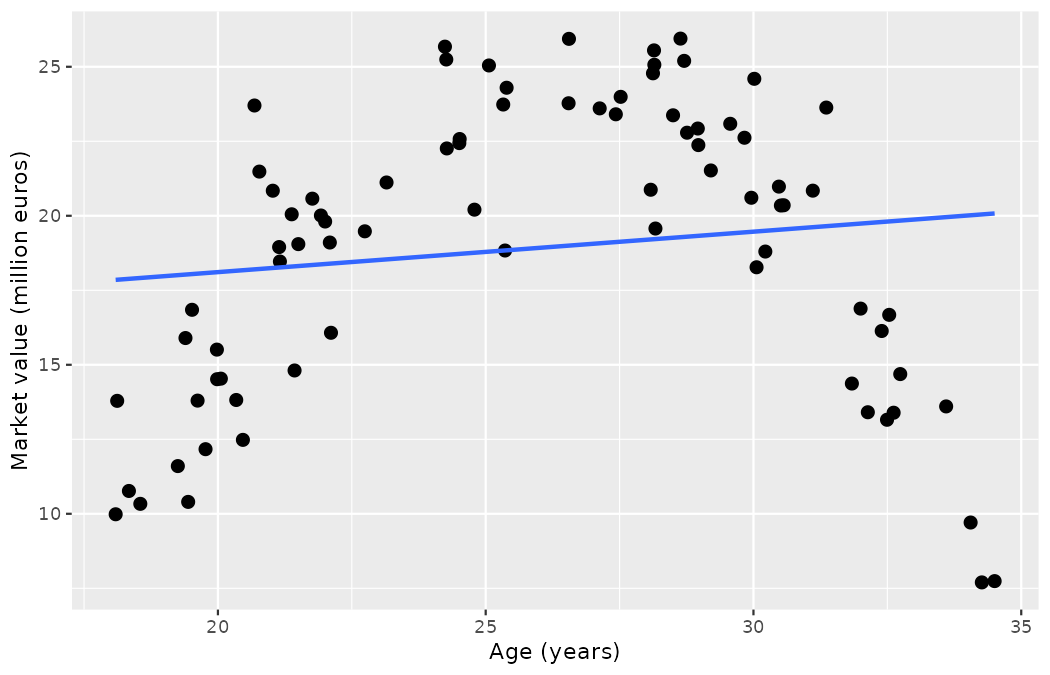
\includegraphics[width=0.85\linewidth,height=\textheight,keepaspectratio]{figures/model-slr-5.png}

The cloud rises from around €8M at age 18 to a peak near €24M around age
26--27, then falls back toward €8M by 35 --- a very clear relationship.
Yet the best fitting \emph{line} for these data is nearly flat (slope
\(0.14\) million euros per year), which is not a useful way to describe
the hump-shaped relationship: the line under-predicts every peak-age
player and over-predicts every teenager and every veteran. We discuss
nonlinear trends in this chapter and the next, but details of fitting
nonlinear models are saved for a later course.

\subsection{Using linear regression to predict goals from chance
quality}\label{using-linear-regression-to-predict-goals-from-chance-quality}

Recall the \texttt{team\_match} dataset from
Chapter~\ref{sec-explore-numerical}: one row per team per match at the
2022 Men's World Cup, aggregating that team's shots into counts, total
chance quality, and goals. We rebuild it with exactly the same code (the
code that derives a dataset should always be visible):

\begin{Shaded}
\begin{Highlighting}[]
\NormalTok{wc2022\_shots }\OtherTok{\textless{}{-}} \FunctionTok{read\_csv}\NormalTok{(}\StringTok{"data/derived/wc2022\_shots.csv"}\NormalTok{)}

\NormalTok{team\_match }\OtherTok{\textless{}{-}}\NormalTok{ wc2022\_shots }\SpecialCharTok{|\textgreater{}}
  \FunctionTok{group\_by}\NormalTok{(match\_id, team) }\SpecialCharTok{|\textgreater{}}
  \FunctionTok{summarize}\NormalTok{(}
    \AttributeTok{n\_shots =} \FunctionTok{n}\NormalTok{(),}
    \AttributeTok{total\_xg =} \FunctionTok{sum}\NormalTok{(statsbomb\_xg),}
    \AttributeTok{goals =} \FunctionTok{sum}\NormalTok{(goal),}
    \AttributeTok{prop\_under\_pressure =} \FunctionTok{mean}\NormalTok{(under\_pressure),}
    \AttributeTok{prop\_set\_piece =} \FunctionTok{mean}\NormalTok{(play\_pattern }\SpecialCharTok{\%in\%}
      \FunctionTok{c}\NormalTok{(}\StringTok{"From Corner"}\NormalTok{, }\StringTok{"From Free Kick"}\NormalTok{, }\StringTok{"From Throw In"}\NormalTok{)),}
    \AttributeTok{.groups =} \StringTok{"drop"}
\NormalTok{  )}

\FunctionTok{nrow}\NormalTok{(team\_match)}
\CommentTok{\#\textgreater{} [1] 127}
\end{Highlighting}
\end{Shaded}

As noted in Chapter~\ref{sec-explore-numerical}, one team-match (Costa
Rica's shotless outing against Spain) is missing, leaving 127 rows. One
honesty note before we model anything: the shot log includes every
attempt StatsBomb recorded --- open play, in-game penalties, and even
the penalty-shootout attempts of drawn knockout ties --- so
\texttt{goals} counts all of them. That bookkeeping choice inflates both
\texttt{total\_xg} and \texttt{goals} for shootout matches, on both
sides of the equation; we keep the full log here because it is the
canonical \texttt{team\_match} object of this book, and we will simply
read the model as describing \emph{recorded attempts} rather than only
the run of play.

We consider two of these measurements: the total chance quality a team
accumulated in a match (\texttt{total\_xg}) and the goals the team
scored (\texttt{goals}). The two variables are associated: team-matches
with above-average accumulated chance quality also tend to have
above-average goal counts. While the relationship is not perfectly
linear, it could be helpful to partially explain the connection between
these variables with a straight line.

\begin{Shaded}
\begin{Highlighting}[]
\FunctionTok{ggplot}\NormalTok{(team\_match, }\FunctionTok{aes}\NormalTok{(}\AttributeTok{x =}\NormalTok{ total\_xg, }\AttributeTok{y =}\NormalTok{ goals)) }\SpecialCharTok{+}
  \FunctionTok{geom\_point}\NormalTok{(}\AttributeTok{alpha =} \FloatTok{0.7}\NormalTok{, }\AttributeTok{size =} \DecValTok{2}\NormalTok{) }\SpecialCharTok{+}
  \FunctionTok{labs}\NormalTok{(}
    \AttributeTok{x =} \StringTok{"Total chance quality (xG) accumulated in the match"}\NormalTok{,}
    \AttributeTok{y =} \StringTok{"Goals scored"}
\NormalTok{  ) }\SpecialCharTok{+}
  \FunctionTok{geom\_point}\NormalTok{(}
    \AttributeTok{data =}\NormalTok{ team\_match }\SpecialCharTok{|\textgreater{}} \FunctionTok{filter}\NormalTok{(team }\SpecialCharTok{==} \StringTok{"Spain"}\NormalTok{, goals }\SpecialCharTok{==} \DecValTok{7}\NormalTok{),}
    \AttributeTok{color =} \StringTok{"red"}\NormalTok{, }\AttributeTok{size =} \DecValTok{5}\NormalTok{, }\AttributeTok{shape =} \StringTok{"circle open"}\NormalTok{, }\AttributeTok{stroke =} \DecValTok{2}
\NormalTok{  )}
\end{Highlighting}
\end{Shaded}

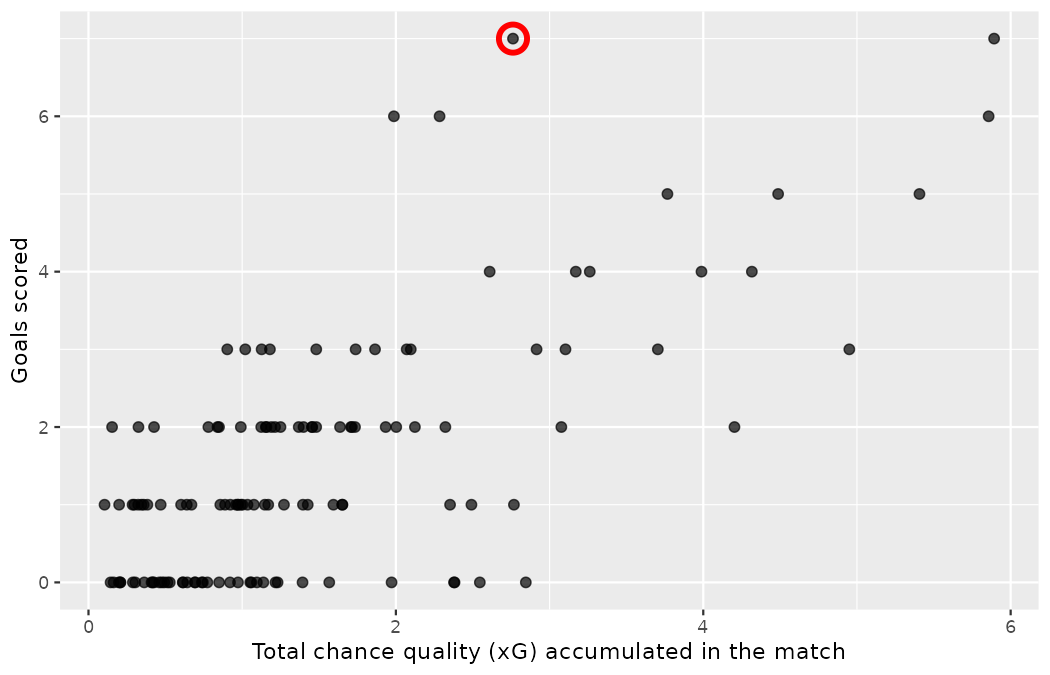
\includegraphics[width=0.85\linewidth,height=\textheight,keepaspectratio]{figures/model-slr-6.png}

Each of the 127 points represents a single team-match. The cloud sweeps
up and to the right: accumulated chance quality runs from \(0.10\) to
\(5.89\) on the horizontal axis, goals from 0 to 7 on the vertical, with
the goal counts forming visible integer bands. One point is highlighted
with a red circle: Spain's group-stage demolition of Costa Rica, in
which 17 shots worth \(2.76\) xG produced 7 goals --- we will return to
it shortly.

We want to describe the relationship between accumulated chance quality
and goals with a line. In this example, we will use \texttt{total\_xg}
as the predictor variable, \(x,\) to predict a team's goals in a match,
\(y.\) We could fit the linear relationship by eye; instead, the code
below has R compute it (the criterion R uses is the subject of
Section~\ref{sec-least-squares-regression}).

\begin{Shaded}
\begin{Highlighting}[]
\NormalTok{fit\_goals }\OtherTok{\textless{}{-}} \FunctionTok{lm}\NormalTok{(goals }\SpecialCharTok{\textasciitilde{}}\NormalTok{ total\_xg, }\AttributeTok{data =}\NormalTok{ team\_match)}
\FunctionTok{coef}\NormalTok{(fit\_goals)}
\CommentTok{\#\textgreater{} (Intercept)    total\_xg}
\CommentTok{\#\textgreater{}   0.1901285   0.9086896}

\FunctionTok{ggplot}\NormalTok{(team\_match, }\FunctionTok{aes}\NormalTok{(}\AttributeTok{x =}\NormalTok{ total\_xg, }\AttributeTok{y =}\NormalTok{ goals)) }\SpecialCharTok{+}
  \FunctionTok{geom\_point}\NormalTok{(}\AttributeTok{alpha =} \FloatTok{0.7}\NormalTok{, }\AttributeTok{size =} \DecValTok{2}\NormalTok{) }\SpecialCharTok{+}
  \FunctionTok{labs}\NormalTok{(}
    \AttributeTok{x =} \StringTok{"Total chance quality (xG) accumulated in the match"}\NormalTok{,}
    \AttributeTok{y =} \StringTok{"Goals scored"}
\NormalTok{  ) }\SpecialCharTok{+}
  \FunctionTok{geom\_smooth}\NormalTok{(}\AttributeTok{method =} \StringTok{"lm"}\NormalTok{, }\AttributeTok{se =} \ConstantTok{FALSE}\NormalTok{)}
\end{Highlighting}
\end{Shaded}

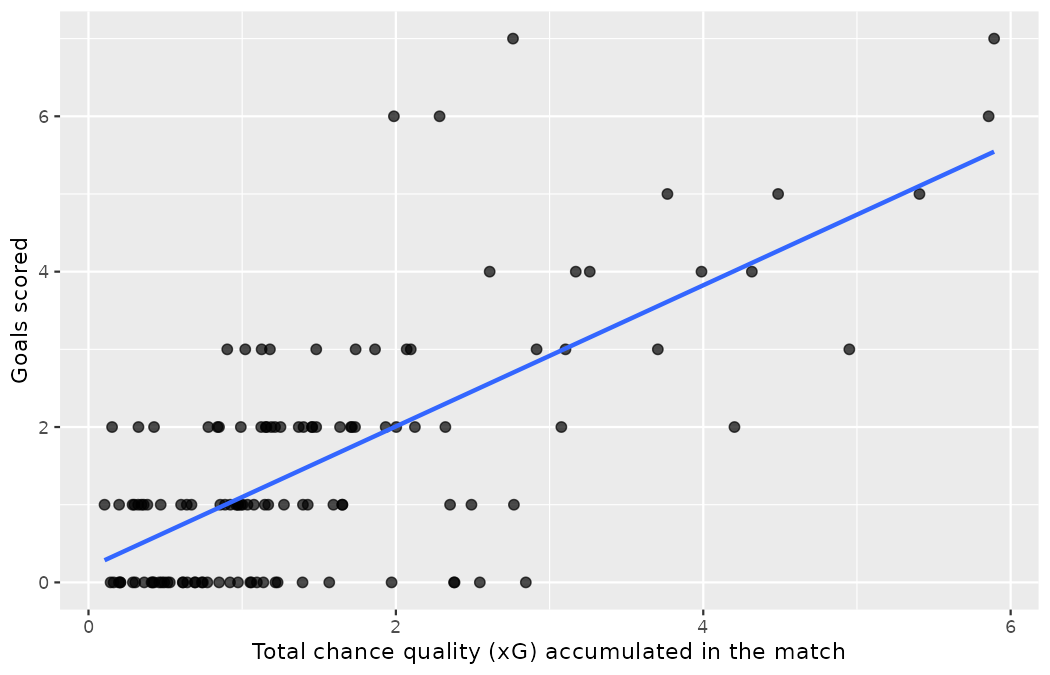
\includegraphics[width=0.85\linewidth,height=\textheight,keepaspectratio]{figures/model-slr-7.png}

The equation for this line is

\[
\hat{y} = 0.190 + 0.909x
\]

A ``hat'' on \(y\) is used to signify that this is an estimate: read
\(\hat{y}\) (``y-hat'') as \emph{the value of \(y\) the model predicts},
as opposed to a value of \(y\) we actually observed. This is the first
hat in the book, and the convention is worth fixing now, because hats
will follow us everywhere: a hat placed over a symbol always means an
estimate, computed from data, of the unadorned quantity beneath it. We
can use this line to discuss properties of team performances. For
instance, the equation predicts a team-match with \(2.0\) accumulated xG
will produce

\[
\hat{y} = 0.190 + 0.909 \times 2.0 = 2.008
\]

goals --- almost exactly two. The estimate may be viewed as an average:
the equation predicts that team-matches with \(2.0\) accumulated chance
quality will have an average goal count of about \(2.0.\) Absent further
information about a particular performance, the prediction that uses the
average is a reasonable estimate. Notice, too, what a slope of \(0.909\)
says to a scout: across this tournament, each additional unit of
accumulated xG bought very nearly one additional goal on average --- the
``expected'' in expected goals earning its name.

There may be other variables that could help us predict a team's goals
besides its chance quality. Perhaps the relationship is a little
different in knockout football than in the group stage, or perhaps it
differs between high-volume and low-volume shooting performances. The
code below redraws the scatterplot twice, taking each into
consideration.

\begin{Shaded}
\begin{Highlighting}[]
\NormalTok{team\_match\_stage }\OtherTok{\textless{}{-}}\NormalTok{ wc2022\_shots }\SpecialCharTok{|\textgreater{}}
  \FunctionTok{distinct}\NormalTok{(match\_id, team, stage) }\SpecialCharTok{|\textgreater{}}
  \FunctionTok{right\_join}\NormalTok{(team\_match, }\AttributeTok{by =} \FunctionTok{c}\NormalTok{(}\StringTok{"match\_id"}\NormalTok{, }\StringTok{"team"}\NormalTok{)) }\SpecialCharTok{|\textgreater{}}
  \FunctionTok{mutate}\NormalTok{(}\AttributeTok{knockout =}\NormalTok{ stage }\SpecialCharTok{!=} \StringTok{"Group Stage"}\NormalTok{)}

\NormalTok{p\_stage }\OtherTok{\textless{}{-}} \FunctionTok{ggplot}\NormalTok{(team\_match\_stage,}
                  \FunctionTok{aes}\NormalTok{(}\AttributeTok{x =}\NormalTok{ total\_xg, }\AttributeTok{y =}\NormalTok{ goals,}
                      \AttributeTok{color =}\NormalTok{ knockout, }\AttributeTok{shape =}\NormalTok{ knockout)) }\SpecialCharTok{+}
  \FunctionTok{geom\_point}\NormalTok{(}\AttributeTok{alpha =} \FloatTok{0.8}\NormalTok{, }\AttributeTok{size =} \DecValTok{2}\NormalTok{) }\SpecialCharTok{+}
  \FunctionTok{labs}\NormalTok{(}\AttributeTok{x =} \StringTok{"Total xG"}\NormalTok{, }\AttributeTok{y =} \StringTok{"Goals"}\NormalTok{, }\AttributeTok{color =} \StringTok{"Knockout"}\NormalTok{, }\AttributeTok{shape =} \StringTok{"Knockout"}\NormalTok{)}

\NormalTok{p\_volume }\OtherTok{\textless{}{-}} \FunctionTok{ggplot}\NormalTok{(team\_match\_stage,}
                   \FunctionTok{aes}\NormalTok{(}\AttributeTok{x =}\NormalTok{ total\_xg, }\AttributeTok{y =}\NormalTok{ goals, }\AttributeTok{color =}\NormalTok{ n\_shots)) }\SpecialCharTok{+}
  \FunctionTok{geom\_point}\NormalTok{(}\AttributeTok{size =} \DecValTok{2}\NormalTok{) }\SpecialCharTok{+}
  \FunctionTok{labs}\NormalTok{(}\AttributeTok{x =} \StringTok{"Total xG"}\NormalTok{, }\AttributeTok{y =} \StringTok{"Goals"}\NormalTok{, }\AttributeTok{color =} \StringTok{"Shots"}\NormalTok{)}
\end{Highlighting}
\end{Shaded}

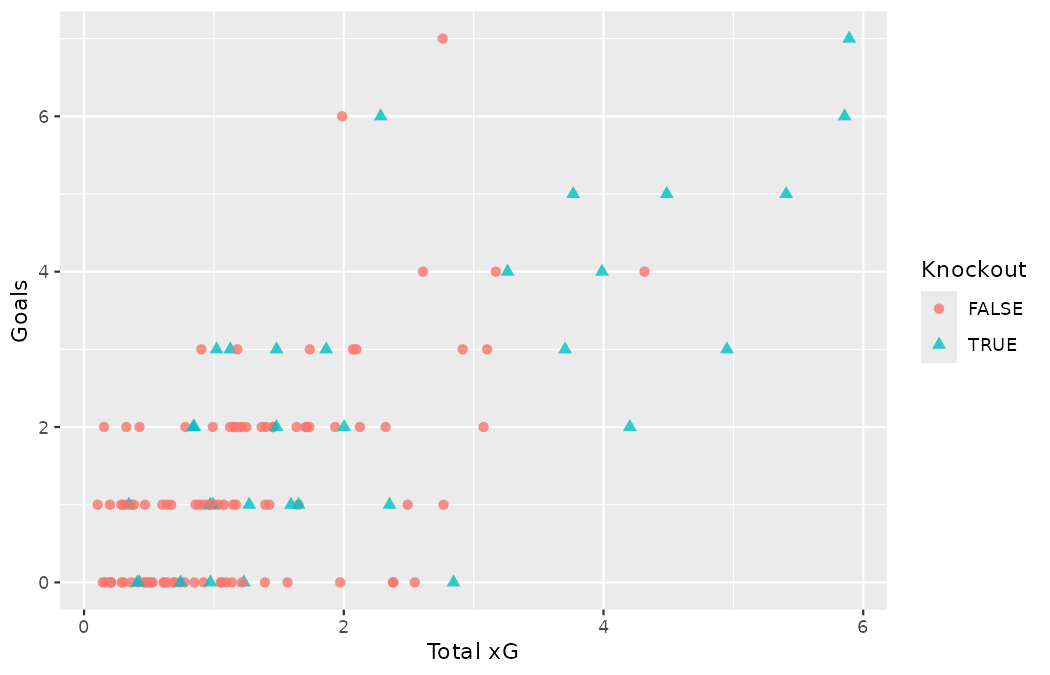
\includegraphics[width=0.85\linewidth,height=\textheight,keepaspectratio]{figures/model-slr-8.png}

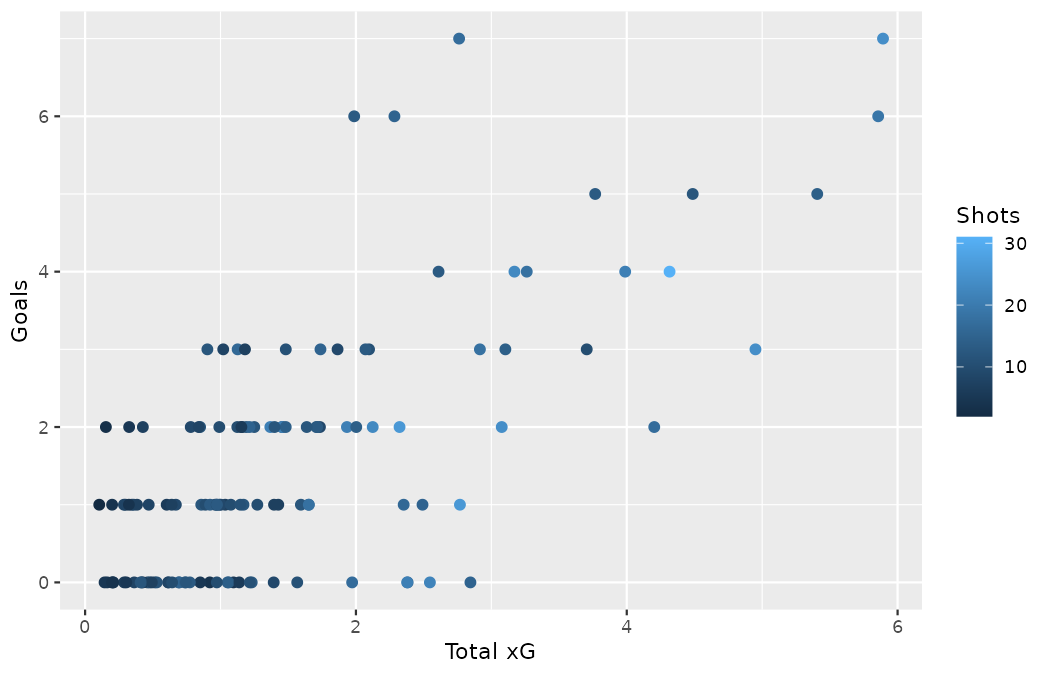
\includegraphics[width=0.85\linewidth,height=\textheight,keepaspectratio]{figures/model-slr-9.png}

In the first panel, the 32 knockout team-matches (triangles) occupy the
upper-right of the cloud --- extra time and shootout attempts push both
their xG (average \(2.32\) versus \(1.20\) in the group stage) and their
goal counts up --- but they scatter around the same upward trend as the
95 group-stage points rather than forming a separate band. The second
panel colors points by shot volume; it's harder to tell whether volume
changes the relationship between chance quality and goals, though the
very highest-volume outings sit, if anything, slightly below the line.
In Chapter~\ref{sec-model-mlr}, we'll learn about how we can include
more than one predictor in our model. Before we get there, we first need
to better understand how to best build a linear model with one
predictor.

\subsection{Residuals}\label{sec-resids}

\textbf{Residuals} are the leftover variation in the data after
accounting for the model fit:

\[
\text{Data} = \text{Fit} + \text{Residual}
\]

Each observation will have a residual, and three of the residuals for
the linear model we fit to \texttt{team\_match} are displayed below. If
an observation is above the regression line, then its residual, the
vertical distance from the observation to the line, is positive.
Observations below the line have negative residuals. One goal in picking
the right linear model is for residuals to be as small as possible.

For a scout, the residual of this particular model is not statistical
debris --- it is a concept in its own right. A team-match above the line
scored \emph{more} goals than its chances were worth: finishing
over-performance. A team-match below the line wasted its chances:
finishing under-performance. When Marta Vidal asks ``did they score
because they created, or because they finished?'', she is asking about
the fit and the residual respectively --- and we will meet this exact
decomposition again in Chapter~\ref{sec-inf-model-slr}.

The code below computes the residuals for three team-matches we will
keep an eye on: Spain's 7-goal group-stage match, Canada's group-stage
match against Belgium, and Morocco's semi-final against France.

\begin{Shaded}
\begin{Highlighting}[]
\NormalTok{team\_match }\SpecialCharTok{|\textgreater{}}
  \FunctionTok{mutate}\NormalTok{(}
    \AttributeTok{predicted =} \FloatTok{0.190} \SpecialCharTok{+} \FloatTok{0.909} \SpecialCharTok{*}\NormalTok{ total\_xg,}
    \AttributeTok{residual =}\NormalTok{ goals }\SpecialCharTok{{-}}\NormalTok{ predicted}
\NormalTok{  ) }\SpecialCharTok{|\textgreater{}}
  \FunctionTok{filter}\NormalTok{(}
\NormalTok{    (team }\SpecialCharTok{==} \StringTok{"Spain"} \SpecialCharTok{\&}\NormalTok{ goals }\SpecialCharTok{==} \DecValTok{7}\NormalTok{) }\SpecialCharTok{|}
\NormalTok{      (team }\SpecialCharTok{==} \StringTok{"Canada"} \SpecialCharTok{\&}\NormalTok{ n\_shots }\SpecialCharTok{==} \DecValTok{22}\NormalTok{) }\SpecialCharTok{|}
\NormalTok{      (team }\SpecialCharTok{==} \StringTok{"Morocco"} \SpecialCharTok{\&} \FunctionTok{round}\NormalTok{(total\_xg, }\DecValTok{2}\NormalTok{) }\SpecialCharTok{==} \FloatTok{1.23}\NormalTok{)}
\NormalTok{  ) }\SpecialCharTok{|\textgreater{}}
  \FunctionTok{select}\NormalTok{(team, n\_shots, total\_xg, goals, predicted, residual)}
\CommentTok{\#\textgreater{} \# A tibble: 3 × 6}
\CommentTok{\#\textgreater{}   team    n\_shots total\_xg goals predicted residual}
\CommentTok{\#\textgreater{}   \textless{}chr\textgreater{}     \textless{}int\textgreater{}    \textless{}dbl\textgreater{} \textless{}int\textgreater{}     \textless{}dbl\textgreater{}    \textless{}dbl\textgreater{}}
\CommentTok{\#\textgreater{} 1 Canada       22     2.55     0      2.50    {-}2.50}
\CommentTok{\#\textgreater{} 2 Spain        17     2.76     7      2.70     4.30}
\CommentTok{\#\textgreater{} 3 Morocco      13     1.23     0      1.31    {-}1.31}
\end{Highlighting}
\end{Shaded}

Redrawing the scatterplot with these three points highlighted and a
vertical segment from each point to the line makes the geometry plain:
Spain's point floats far above the line (a large positive residual of
about \(+4.3\) goals); Canada's sits far below it (about \(-2.5\));
Morocco's semi-final sits moderately below (about \(-1.3\)). The size of
a residual is usually discussed in terms of its absolute value, written
\(|\cdot|\) --- the vertical bars strip away the sign and keep only the
magnitude. For example, the residual for Canada is larger than that of
Morocco because \(|-2.5|\) is larger than \(|-1.3|.\)

\begin{tcolorbox}[enhanced jigsaw, left=2mm, leftrule=.75mm, title=\textcolor{quarto-callout-important-color}{\faExclamation}\hspace{0.5em}{Residual: Difference between observed and expected.}, arc=.35mm, rightrule=.15mm, coltitle=black, colframe=quarto-callout-important-color-frame, bottomrule=.15mm, colbacktitle=quarto-callout-important-color!10!white, opacitybacktitle=0.6, breakable, bottomtitle=1mm, toptitle=1mm, titlerule=0mm, opacityback=0, toprule=.15mm, colback=white]

The residual of the \(i^{th}\) observation \((x_i, y_i)\) is the
difference of the observed outcome \((y_i)\) and the outcome we would
predict based on the model fit \((\hat{y}_i):\)

\[
e_i = y_i - \hat{y}_i
\]

We typically identify \(\hat{y}_i\) by plugging \(x_i\) into the model.

\end{tcolorbox}

Decompose the notation before using it: the letter \(e\) stands for
\emph{error}, the leftover; the subscript \(i\) indexes the observation,
exactly as it did for \(x_i\) in Chapter~\ref{sec-explore-numerical};
and \(\hat{y}_i\) is the model's prediction for that same observation.
So \(e_i\) is observation \(i\)'s personal gap between what happened and
what the line expected.

\begin{tcolorbox}[enhanced jigsaw, left=2mm, leftrule=.75mm, title=\textcolor{quarto-callout-note-color}{\faInfo}\hspace{0.5em}{Worked example}, arc=.35mm, rightrule=.15mm, coltitle=black, colframe=quarto-callout-note-color-frame, bottomrule=.15mm, colbacktitle=quarto-callout-note-color!10!white, opacitybacktitle=0.6, breakable, bottomtitle=1mm, toptitle=1mm, titlerule=0mm, opacityback=0, toprule=.15mm, colback=white]

The linear fit for the World Cup team-matches is given as
\(\hat{y} = 0.190 + 0.909x.\) Based on this line, compute the residual
of Spain's 7-goal performance against Costa Rica, the observation
\((2.76, 7).\)

\begin{center}\rule{0.5\linewidth}{0.5pt}\end{center}

We first compute the predicted value based on the model:
\(\hat{y} = 0.190 + 0.909 \times 2.76 = 2.699.\) Next we compute the
difference of the actual goal count and the predicted goal count:
\(e = y - \hat{y} = 7 - 2.699 = 4.301.\) The model's error is
\(e = +4.30\) goals: Spain scored about four and a third goals
\emph{more} than their accumulated chance quality predicted. The
positive residual indicates that the linear model underpredicted Spain's
goals in this match --- extraordinary finishing (and generous defending)
on the day.

\end{tcolorbox}

\begin{tcolorbox}[enhanced jigsaw, left=2mm, leftrule=.75mm, title=\textcolor{quarto-callout-tip-color}{\faLightbulb}\hspace{0.5em}{Check your understanding}, arc=.35mm, rightrule=.15mm, coltitle=black, colframe=quarto-callout-tip-color-frame, bottomrule=.15mm, colbacktitle=quarto-callout-tip-color!10!white, opacitybacktitle=0.6, breakable, bottomtitle=1mm, toptitle=1mm, titlerule=0mm, opacityback=0, toprule=.15mm, colback=white]

If a model underestimates an observation, will the residual be positive
or negative? What about if it overestimates the observation?

\begin{center}\rule{0.5\linewidth}{0.5pt}\end{center}

If a model underestimates an observation, then the model estimate is
below the actual. The residual, which is the actual observation value
minus the model estimate, must then be positive. The opposite is true
when the model overestimates the observation: the residual is negative.
In scouting terms: positive residual, the team out-finished its chances;
negative residual, it wasted them.

\end{tcolorbox}

\begin{tcolorbox}[enhanced jigsaw, left=2mm, leftrule=.75mm, title=\textcolor{quarto-callout-tip-color}{\faLightbulb}\hspace{0.5em}{Check your understanding}, arc=.35mm, rightrule=.15mm, coltitle=black, colframe=quarto-callout-tip-color-frame, bottomrule=.15mm, colbacktitle=quarto-callout-tip-color!10!white, opacitybacktitle=0.6, breakable, bottomtitle=1mm, toptitle=1mm, titlerule=0mm, opacityback=0, toprule=.15mm, colback=white]

Compute the residuals for Canada's group-stage performance \((2.55, 0)\)
and Morocco's semi-final \((1.23, 0)\) using the linear relationship
\(\hat{y} = 0.190 + 0.909x.\)

\begin{center}\rule{0.5\linewidth}{0.5pt}\end{center}

Canada:
\(\hat{y} = 0.190 + 0.909 \times 2.55 = 2.508 \rightarrow e = y - \hat{y} = 0 - 2.508 = -2.508.\)
Canada created two and a half goals' worth of chances against Belgium
and scored none --- the great wasted performance of the group stage.
Morocco:
\(\hat{y} = 0.190 + 0.909 \times 1.23 = 1.308 \rightarrow e = 0 - 1.308 = -1.308.\)
Both residuals are negative; Canada's is larger in absolute value.

\end{tcolorbox}

Residuals are helpful in evaluating how well a linear model fits a
dataset. We often display them in a \emph{residual plot} such as the one
drawn below for the goals model. The residuals are plotted with their
predicted outcome variable value as the horizontal coordinate, and the
vertical coordinate as the residual. For instance, Spain's point had a
predicted value of \(2.70\) goals and a residual of \(+4.30,\) so in the
residual plot it is placed at \((2.70, 4.30).\) Creating a residual plot
is sort of like tipping the scatterplot over so the regression line is
horizontal, as indicated by the dashed line.

\begin{Shaded}
\begin{Highlighting}[]
\NormalTok{team\_match }\SpecialCharTok{|\textgreater{}}
  \FunctionTok{mutate}\NormalTok{(}
    \AttributeTok{predicted =} \FunctionTok{fitted}\NormalTok{(fit\_goals),}
    \AttributeTok{residual =} \FunctionTok{resid}\NormalTok{(fit\_goals)}
\NormalTok{  ) }\SpecialCharTok{|\textgreater{}}
  \FunctionTok{ggplot}\NormalTok{(}\FunctionTok{aes}\NormalTok{(}\AttributeTok{x =}\NormalTok{ predicted, }\AttributeTok{y =}\NormalTok{ residual)) }\SpecialCharTok{+}
  \FunctionTok{geom\_point}\NormalTok{(}\AttributeTok{alpha =} \FloatTok{0.7}\NormalTok{, }\AttributeTok{size =} \DecValTok{2}\NormalTok{) }\SpecialCharTok{+}
  \FunctionTok{geom\_hline}\NormalTok{(}\AttributeTok{yintercept =} \DecValTok{0}\NormalTok{, }\AttributeTok{linetype =} \StringTok{"dashed"}\NormalTok{) }\SpecialCharTok{+}
  \FunctionTok{labs}\NormalTok{(}
    \AttributeTok{x =} \StringTok{"Predicted goals"}\NormalTok{,}
    \AttributeTok{y =} \StringTok{"Residuals"}
\NormalTok{  )}
\end{Highlighting}
\end{Shaded}

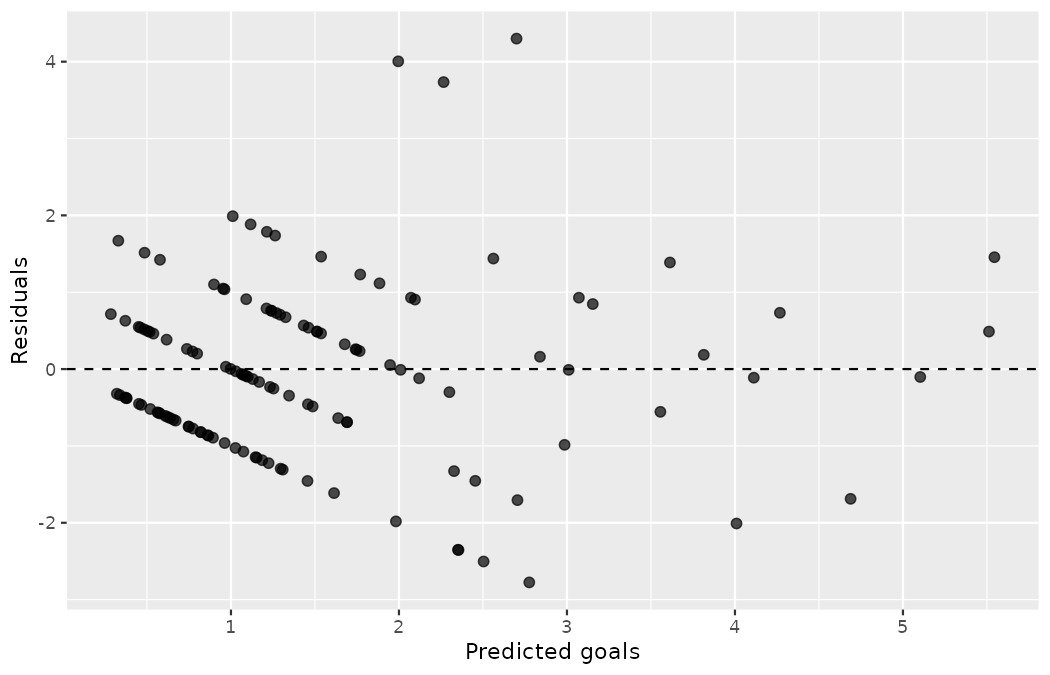
\includegraphics[width=0.85\linewidth,height=\textheight,keepaspectratio]{figures/model-slr-10.png}

The residuals scatter around the dashed zero line, mostly between \(-2\)
and \(+2,\) with Spain's \(+4.3\) at the top, just above England's
\(+4.0;\) because goals are whole numbers, the points fall along slanted
integer bands rather than a formless cloud, and the scatter fans out
somewhat at higher predicted values --- low-xG outings can only miss by
a little, high-xG outings by a lot.

\begin{tcolorbox}[enhanced jigsaw, left=2mm, leftrule=.75mm, title=\textcolor{quarto-callout-note-color}{\faInfo}\hspace{0.5em}{Worked example}, arc=.35mm, rightrule=.15mm, coltitle=black, colframe=quarto-callout-note-color-frame, bottomrule=.15mm, colbacktitle=quarto-callout-note-color!10!white, opacitybacktitle=0.6, breakable, bottomtitle=1mm, toptitle=1mm, titlerule=0mm, opacityback=0, toprule=.15mm, colback=white]

One purpose of residual plots is to identify characteristics or patterns
still apparent in the data after fitting a model. The code below builds
three constructed datasets --- another of Priya's training exhibits,
seeded for reproducibility --- fits a line to each, and draws the
scatterplot with its residual plot underneath. Can you identify any
patterns in the residuals?

\begin{Shaded}
\begin{Highlighting}[]
\FunctionTok{set.seed}\NormalTok{(}\DecValTok{704}\NormalTok{)}
\NormalTok{resid\_panels }\OtherTok{\textless{}{-}} \FunctionTok{tibble}\NormalTok{(}
  \AttributeTok{x1 =} \FunctionTok{runif}\NormalTok{(}\DecValTok{60}\NormalTok{, }\DecValTok{0}\NormalTok{, }\DecValTok{10}\NormalTok{), }\AttributeTok{y1 =} \DecValTok{28} \SpecialCharTok{{-}} \FloatTok{1.8} \SpecialCharTok{*}\NormalTok{ x1 }\SpecialCharTok{+} \FunctionTok{rnorm}\NormalTok{(}\DecValTok{60}\NormalTok{, }\DecValTok{0}\NormalTok{, }\FloatTok{2.5}\NormalTok{),}
  \AttributeTok{x2 =} \FunctionTok{runif}\NormalTok{(}\DecValTok{60}\NormalTok{, }\DecValTok{0}\NormalTok{, }\DecValTok{10}\NormalTok{), }\AttributeTok{y2 =} \DecValTok{3} \SpecialCharTok{+} \FloatTok{2.2} \SpecialCharTok{*}\NormalTok{ x2 }\SpecialCharTok{{-}} \FloatTok{0.24} \SpecialCharTok{*}\NormalTok{ x2}\SpecialCharTok{\^{}}\DecValTok{2} \SpecialCharTok{+} \FunctionTok{rnorm}\NormalTok{(}\DecValTok{60}\NormalTok{, }\DecValTok{0}\NormalTok{, }\FloatTok{1.1}\NormalTok{),}
  \AttributeTok{x3 =} \FunctionTok{runif}\NormalTok{(}\DecValTok{60}\NormalTok{, }\DecValTok{0}\NormalTok{, }\DecValTok{10}\NormalTok{), }\AttributeTok{y3 =} \DecValTok{12} \SpecialCharTok{+} \FloatTok{0.06} \SpecialCharTok{*}\NormalTok{ x3 }\SpecialCharTok{+} \FunctionTok{rnorm}\NormalTok{(}\DecValTok{60}\NormalTok{, }\DecValTok{0}\NormalTok{, }\FloatTok{2.2}\NormalTok{)}
\NormalTok{)}

\NormalTok{fit\_1 }\OtherTok{\textless{}{-}} \FunctionTok{lm}\NormalTok{(y1 }\SpecialCharTok{\textasciitilde{}}\NormalTok{ x1, }\AttributeTok{data =}\NormalTok{ resid\_panels)}
\NormalTok{fit\_2 }\OtherTok{\textless{}{-}} \FunctionTok{lm}\NormalTok{(y2 }\SpecialCharTok{\textasciitilde{}}\NormalTok{ x2, }\AttributeTok{data =}\NormalTok{ resid\_panels)}
\NormalTok{fit\_3 }\OtherTok{\textless{}{-}} \FunctionTok{lm}\NormalTok{(y3 }\SpecialCharTok{\textasciitilde{}}\NormalTok{ x3, }\AttributeTok{data =}\NormalTok{ resid\_panels)}

\CommentTok{\# For each dataset: scatterplot with the least squares line on top,}
\CommentTok{\# residual plot (fitted vs residual) underneath, e.g., for dataset 1:}
\FunctionTok{ggplot}\NormalTok{(resid\_panels, }\FunctionTok{aes}\NormalTok{(}\AttributeTok{x =}\NormalTok{ x1, }\AttributeTok{y =}\NormalTok{ y1)) }\SpecialCharTok{+}
  \FunctionTok{geom\_point}\NormalTok{() }\SpecialCharTok{+}
  \FunctionTok{geom\_smooth}\NormalTok{(}\AttributeTok{method =} \StringTok{"lm"}\NormalTok{, }\AttributeTok{se =} \ConstantTok{FALSE}\NormalTok{)}

\FunctionTok{tibble}\NormalTok{(}\AttributeTok{fitted =} \FunctionTok{fitted}\NormalTok{(fit\_1), }\AttributeTok{residual =} \FunctionTok{resid}\NormalTok{(fit\_1)) }\SpecialCharTok{|\textgreater{}}
  \FunctionTok{ggplot}\NormalTok{(}\FunctionTok{aes}\NormalTok{(}\AttributeTok{x =}\NormalTok{ fitted, }\AttributeTok{y =}\NormalTok{ residual)) }\SpecialCharTok{+}
  \FunctionTok{geom\_point}\NormalTok{() }\SpecialCharTok{+}
  \FunctionTok{geom\_hline}\NormalTok{(}\AttributeTok{yintercept =} \DecValTok{0}\NormalTok{, }\AttributeTok{linetype =} \StringTok{"dashed"}\NormalTok{)}
\end{Highlighting}
\end{Shaded}

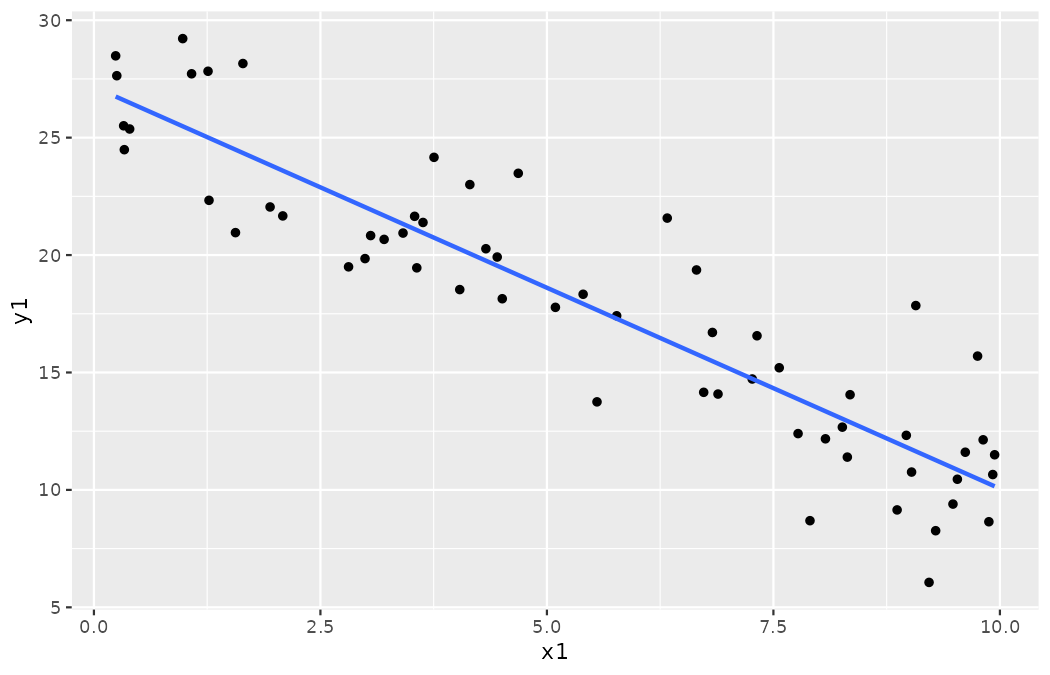
\includegraphics[width=0.85\linewidth,height=\textheight,keepaspectratio]{figures/model-slr-11.png}

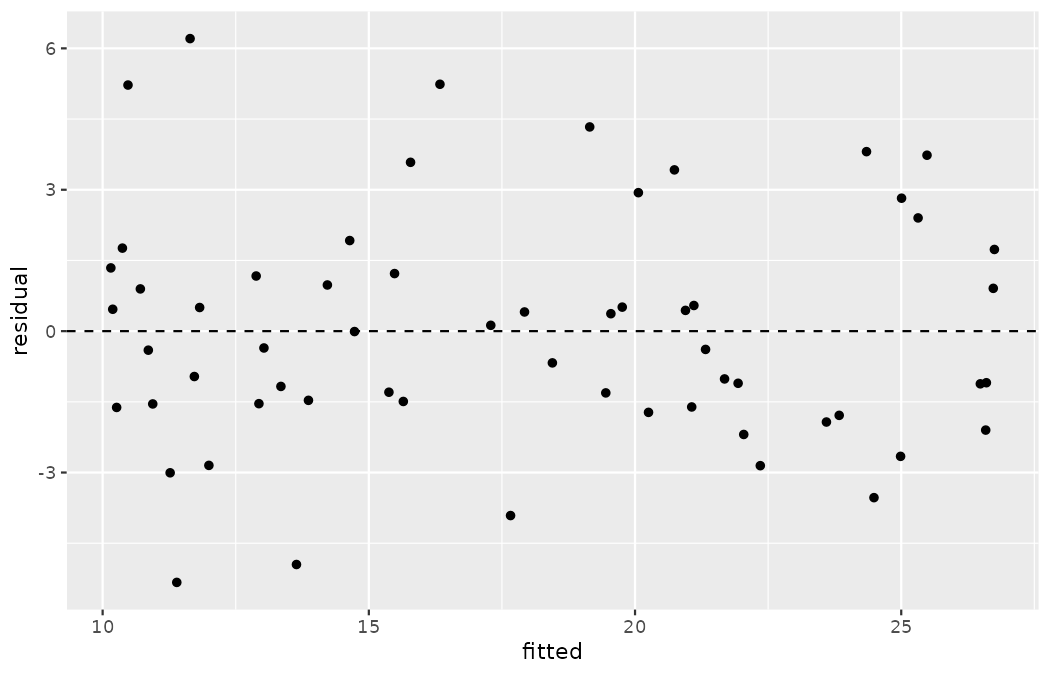
\includegraphics[width=0.85\linewidth,height=\textheight,keepaspectratio]{figures/model-slr-12.png}

\begin{center}\rule{0.5\linewidth}{0.5pt}\end{center}

Dataset 1: a strong downward linear trend; the residuals show no obvious
patterns. They are scattered randomly around 0, represented by the
dashed line.

Dataset 2: the scatterplot rises and then bends over --- the second
dataset shows a pattern in the residuals. There is some curvature in the
scatterplot, which is far more obvious in the residual plot: the
residuals sit below zero at both ends of the fitted range and above zero
in the middle, a telltale arch. We should not use a straight line to
model these data. Instead, a more advanced technique should be used to
model the curved relationship, such as the variable transformations
discussed in Chapter~\ref{sec-explore-numerical}.

Dataset 3: the last plot shows very little upwards trend, and the
residuals also show no obvious patterns. It is reasonable to try to fit
a linear model to the data. However, it is unclear whether there is
evidence that the slope parameter is different from zero. The point
estimate of the slope parameter is not zero (the fit gives about
\(0.19\)), but we might wonder if this could just be due to chance. We
will address this scenario in Chapter~\ref{sec-inf-model-slr}.

\end{tcolorbox}

\subsection{Describing linear relationships with
correlation}\label{describing-linear-relationships-with-correlation}

We've seen plots with strong linear relationships and others with very
weak linear relationships. It would be useful if we could quantify the
strength of these linear relationships with a statistic.

\begin{tcolorbox}[enhanced jigsaw, left=2mm, leftrule=.75mm, title=\textcolor{quarto-callout-important-color}{\faExclamation}\hspace{0.5em}{Correlation: strength of a linear relationship.}, arc=.35mm, rightrule=.15mm, coltitle=black, colframe=quarto-callout-important-color-frame, bottomrule=.15mm, colbacktitle=quarto-callout-important-color!10!white, opacitybacktitle=0.6, breakable, bottomtitle=1mm, toptitle=1mm, titlerule=0mm, opacityback=0, toprule=.15mm, colback=white]

\textbf{Correlation}, which always takes values between -1 and 1,
describes the strength and direction of the linear relationship between
two variables. We denote the correlation by \(r.\)

The correlation value has no units and will not be affected by a linear
change in the units (e.g., going from minutes to seconds).

\end{tcolorbox}

The symbol \(r\) is a single Roman letter, which by our convention marks
it as a sample statistic: it is computed from the observed pairs, and it
estimates a population correlation we will not need to name until much
later in the book. We can compute the correlation using a formula, just
as we did with the sample mean and standard deviation. For observations
\((x_1, y_1),\) \((x_2, y_2),\) \ldots, \((x_n, y_n),\) the formula is

\[
r = \frac{1}{n-1} \sum_{i=1}^{n} \frac{x_i-\bar{x}}{s_x}\frac{y_i-\bar{y}}{s_y}
\]

where \(\bar{x},\) \(\bar{y},\) \(s_x,\) and \(s_y\) are the sample
means and standard deviations for each variable --- all notation you own
from Chapter~\ref{sec-explore-numerical}, including the summation sign
\(\Sigma.\) Read the two fractions as \emph{standardized} coordinates:
each observation is scored by how many standard deviations it sits from
the mean on each axis, and \(r\) is (essentially) the average product of
those two scores --- positive when the two coordinates tend to share a
sign, negative when they tend to oppose. Like other statistics, \(r\) is
generally computed by software, but keep the formula in view: it will do
real work later in this chapter, when we derive the least squares slope
from it.

For the World Cup team-matches, the correlation between accumulated
chance quality and goals is

\begin{Shaded}
\begin{Highlighting}[]
\FunctionTok{cor}\NormalTok{(team\_match}\SpecialCharTok{$}\NormalTok{total\_xg, team\_match}\SpecialCharTok{$}\NormalTok{goals)}
\CommentTok{\#\textgreater{} [1] 0.6913686}
\end{Highlighting}
\end{Shaded}

a moderately strong positive linear relationship, consistent with the
upward cloud we plotted.

Only when the relationship is perfectly linear is the correlation either
-1 or +1. If the relationship is strong and positive, the correlation
will be near +1. If it is strong and negative, it will be near -1. If
there is no apparent linear relationship between the variables, then the
correlation will be near zero. The gallery below constructs eight panels
spanning that range; the printed correlations belong to the panels in
order.

\begin{Shaded}
\begin{Highlighting}[]
\FunctionTok{set.seed}\NormalTok{(}\DecValTok{705}\NormalTok{)}
\NormalTok{make\_panel }\OtherTok{\textless{}{-}} \ControlFlowTok{function}\NormalTok{(slope, noise, }\AttributeTok{n =} \DecValTok{50}\NormalTok{) \{}
\NormalTok{  x }\OtherTok{\textless{}{-}} \FunctionTok{runif}\NormalTok{(n, }\DecValTok{0}\NormalTok{, }\DecValTok{10}\NormalTok{)}
  \FunctionTok{tibble}\NormalTok{(}\AttributeTok{x =}\NormalTok{ x, }\AttributeTok{y =}\NormalTok{ slope }\SpecialCharTok{*}\NormalTok{ x }\SpecialCharTok{+} \FunctionTok{rnorm}\NormalTok{(n, }\DecValTok{0}\NormalTok{, noise))}
\NormalTok{\}}
\NormalTok{gallery }\OtherTok{\textless{}{-}} \FunctionTok{bind\_rows}\NormalTok{(}
  \FunctionTok{make\_panel}\NormalTok{( }\FloatTok{0.7}\NormalTok{, }\FloatTok{0.0}\NormalTok{), }\FunctionTok{make\_panel}\NormalTok{( }\FloatTok{0.7}\NormalTok{, }\FloatTok{1.0}\NormalTok{),}
  \FunctionTok{make\_panel}\NormalTok{( }\FloatTok{0.7}\NormalTok{, }\FloatTok{2.6}\NormalTok{), }\FunctionTok{make\_panel}\NormalTok{( }\FloatTok{0.7}\NormalTok{, }\FloatTok{9.0}\NormalTok{),}
  \FunctionTok{make\_panel}\NormalTok{(}\SpecialCharTok{{-}}\FloatTok{0.7}\NormalTok{, }\FloatTok{0.0}\NormalTok{), }\FunctionTok{make\_panel}\NormalTok{(}\SpecialCharTok{{-}}\FloatTok{0.7}\NormalTok{, }\FloatTok{0.7}\NormalTok{),}
  \FunctionTok{make\_panel}\NormalTok{(}\SpecialCharTok{{-}}\FloatTok{0.7}\NormalTok{, }\FloatTok{3.2}\NormalTok{), }\FunctionTok{make\_panel}\NormalTok{(}\SpecialCharTok{{-}}\FloatTok{0.7}\NormalTok{, }\FloatTok{14.0}\NormalTok{),}
  \AttributeTok{.id =} \StringTok{"panel"}
\NormalTok{)}

\NormalTok{gallery }\SpecialCharTok{|\textgreater{}}
  \FunctionTok{group\_by}\NormalTok{(panel) }\SpecialCharTok{|\textgreater{}}
  \FunctionTok{summarize}\NormalTok{(}\AttributeTok{r =} \FunctionTok{round}\NormalTok{(}\FunctionTok{cor}\NormalTok{(x, y), }\DecValTok{2}\NormalTok{))}
\CommentTok{\#\textgreater{} \# A tibble: 8 × 2}
\CommentTok{\#\textgreater{}   panel     r}
\CommentTok{\#\textgreater{}   \textless{}chr\textgreater{} \textless{}dbl\textgreater{}}
\CommentTok{\#\textgreater{} 1 1      1}
\CommentTok{\#\textgreater{} 2 2      0.89}
\CommentTok{\#\textgreater{} 3 3      0.7}
\CommentTok{\#\textgreater{} 4 4      0.4}
\CommentTok{\#\textgreater{} 5 5     {-}1}
\CommentTok{\#\textgreater{} 6 6     {-}0.96}
\CommentTok{\#\textgreater{} 7 7     {-}0.66}
\CommentTok{\#\textgreater{} 8 8     {-}0.15}

\FunctionTok{ggplot}\NormalTok{(gallery, }\FunctionTok{aes}\NormalTok{(}\AttributeTok{x =}\NormalTok{ x, }\AttributeTok{y =}\NormalTok{ y)) }\SpecialCharTok{+}
  \FunctionTok{geom\_point}\NormalTok{(}\AttributeTok{size =} \DecValTok{2}\NormalTok{, }\AttributeTok{alpha =} \FloatTok{0.8}\NormalTok{) }\SpecialCharTok{+}
  \FunctionTok{facet\_wrap}\NormalTok{(}\SpecialCharTok{\textasciitilde{}}\NormalTok{panel, }\AttributeTok{nrow =} \DecValTok{2}\NormalTok{, }\AttributeTok{scales =} \StringTok{"free"}\NormalTok{)}
\end{Highlighting}
\end{Shaded}

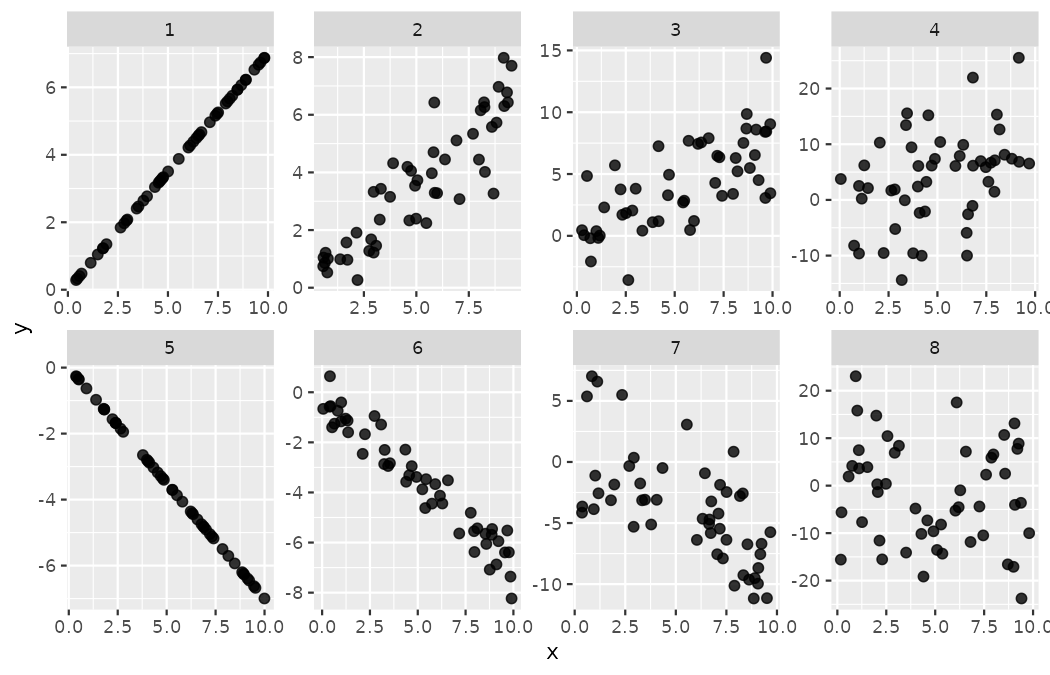
\includegraphics[width=0.85\linewidth,height=\textheight,keepaspectratio]{figures/model-slr-13.png}

The first row runs from a perfect upward line \((r = 1)\) through
progressively noisier upward clouds \((0.89,\) \(0.70,\) \(0.40);\) the
second row mirrors it downward, from a perfect negative line
\((r = -1)\) through \(-0.96\) and \(-0.66\) to a nearly formless cloud
at \(-0.15.\)

The correlation is intended to quantify the strength of a \emph{linear}
trend. Nonlinear trends, even when strong, sometimes produce
correlations that do not reflect the strength of the relationship; see
three such examples below.

\begin{Shaded}
\begin{Highlighting}[]
\NormalTok{curved }\OtherTok{\textless{}{-}} \FunctionTok{tibble}\NormalTok{(}
  \AttributeTok{x1 =} \FunctionTok{runif}\NormalTok{(}\DecValTok{60}\NormalTok{, }\SpecialCharTok{{-}}\DecValTok{4}\NormalTok{, }\DecValTok{4}\NormalTok{), }\AttributeTok{y1 =}\NormalTok{ x1}\SpecialCharTok{\^{}}\DecValTok{2} \SpecialCharTok{+} \FunctionTok{rnorm}\NormalTok{(}\DecValTok{60}\NormalTok{, }\DecValTok{0}\NormalTok{, }\FloatTok{1.2}\NormalTok{),}
  \AttributeTok{x2 =} \FunctionTok{runif}\NormalTok{(}\DecValTok{60}\NormalTok{, }\DecValTok{0}\NormalTok{, }\DecValTok{12}\NormalTok{), }\AttributeTok{y2 =} \DecValTok{3} \SpecialCharTok{*} \FunctionTok{sin}\NormalTok{(x2) }\SpecialCharTok{+} \FunctionTok{rnorm}\NormalTok{(}\DecValTok{60}\NormalTok{, }\DecValTok{0}\NormalTok{, }\FloatTok{0.6}\NormalTok{),}
  \AttributeTok{x3 =} \FunctionTok{runif}\NormalTok{(}\DecValTok{60}\NormalTok{, }\DecValTok{0}\NormalTok{, }\DecValTok{10}\NormalTok{), }\AttributeTok{y3 =} \DecValTok{6} \SpecialCharTok{{-}} \FloatTok{1.1} \SpecialCharTok{*} \FunctionTok{abs}\NormalTok{(x3 }\SpecialCharTok{{-}} \DecValTok{5}\NormalTok{) }\SpecialCharTok{+} \FunctionTok{rnorm}\NormalTok{(}\DecValTok{60}\NormalTok{, }\DecValTok{0}\NormalTok{, }\FloatTok{0.7}\NormalTok{)}
\NormalTok{)}

\FunctionTok{c}\NormalTok{(}\FunctionTok{cor}\NormalTok{(curved}\SpecialCharTok{$}\NormalTok{x1, curved}\SpecialCharTok{$}\NormalTok{y1),}
  \FunctionTok{cor}\NormalTok{(curved}\SpecialCharTok{$}\NormalTok{x2, curved}\SpecialCharTok{$}\NormalTok{y2),}
  \FunctionTok{cor}\NormalTok{(curved}\SpecialCharTok{$}\NormalTok{x3, curved}\SpecialCharTok{$}\NormalTok{y3)) }\SpecialCharTok{|\textgreater{}}
  \FunctionTok{round}\NormalTok{(}\DecValTok{2}\NormalTok{)}
\CommentTok{\#\textgreater{} [1]  0.08 {-}0.28 {-}0.11}
\end{Highlighting}
\end{Shaded}

The first panel is an unmistakable U-shape, the second a clean sine
wave, the third a sharp tent rising to a peak and falling away --- three
strong, obvious patterns --- yet their correlations are a feeble
\(0.08,\) \(-0.28,\) and \(-0.11.\) In each case, there is a strong
relationship between the variables; because the relationship is not
linear, the correlation is weak.

\begin{tcolorbox}[enhanced jigsaw, left=2mm, leftrule=.75mm, title=\textcolor{quarto-callout-tip-color}{\faLightbulb}\hspace{0.5em}{Check your understanding}, arc=.35mm, rightrule=.15mm, coltitle=black, colframe=quarto-callout-tip-color-frame, bottomrule=.15mm, colbacktitle=quarto-callout-tip-color!10!white, opacitybacktitle=0.6, breakable, bottomtitle=1mm, toptitle=1mm, titlerule=0mm, opacityback=0, toprule=.15mm, colback=white]

No straight line is a good fit for any of the three curved datasets
above. Try drawing nonlinear curves on each plot. Once you create a
curve for each, describe what is important in your fit.

\begin{center}\rule{0.5\linewidth}{0.5pt}\end{center}

We'll leave it to you to draw the curves. In general, the curves you
draw should be close to most points and reflect overall trends in the
data --- the parabola for the first panel, the wave for the second, the
tent for the third.

\end{tcolorbox}

\begin{tcolorbox}[enhanced jigsaw, left=2mm, leftrule=.75mm, title=\textcolor{quarto-callout-note-color}{\faInfo}\hspace{0.5em}{Worked example}, arc=.35mm, rightrule=.15mm, coltitle=black, colframe=quarto-callout-note-color-frame, bottomrule=.15mm, colbacktitle=quarto-callout-note-color!10!white, opacitybacktitle=0.6, breakable, bottomtitle=1mm, toptitle=1mm, titlerule=0mm, opacityback=0, toprule=.15mm, colback=white]

The plots below display relationships between the shot-mix shares of the
32 teams at the 2022 Men's World Cup --- the \texttt{team\_profile}
dataset you met in Chapter~\ref{sec-data-hello}. In the plots, each
point represents a different national team, and the two axes are two
shares of that team's total shots: the share that were headers, the
share struck first time, the share taken under defensive pressure, the
share arising from corner sequences, and the share arising in regular
open play. We rebuild \texttt{team\_profile} with exactly the same code
as in Chapter~\ref{sec-data-hello} and draw six pairings.

Order the six scatterplots from strongest negative to strongest positive
linear relationship.

\begin{Shaded}
\begin{Highlighting}[]
\FunctionTok{library}\NormalTok{(patchwork)}

\NormalTok{team\_profile }\OtherTok{\textless{}{-}}\NormalTok{ wc2022\_shots }\SpecialCharTok{|\textgreater{}}
  \FunctionTok{group\_by}\NormalTok{(team) }\SpecialCharTok{|\textgreater{}}
  \FunctionTok{summarize}\NormalTok{(}
    \AttributeTok{n\_shots         =} \FunctionTok{n}\NormalTok{(),}
    \AttributeTok{goals           =} \FunctionTok{sum}\NormalTok{(goal),}
    \AttributeTok{total\_xg        =} \FunctionTok{sum}\NormalTok{(statsbomb\_xg),}
    \AttributeTok{conversion      =} \FunctionTok{mean}\NormalTok{(goal),}
    \AttributeTok{mean\_xg         =} \FunctionTok{mean}\NormalTok{(statsbomb\_xg),}
    \AttributeTok{prop\_headers    =} \FunctionTok{mean}\NormalTok{(body\_part }\SpecialCharTok{==} \StringTok{"Head"}\NormalTok{),}
    \AttributeTok{prop\_first\_time =} \FunctionTok{mean}\NormalTok{(first\_time),}
    \AttributeTok{prop\_pressure   =} \FunctionTok{mean}\NormalTok{(under\_pressure),}
    \AttributeTok{prop\_corner     =} \FunctionTok{mean}\NormalTok{(play\_pattern }\SpecialCharTok{==} \StringTok{"From Corner"}\NormalTok{),}
    \AttributeTok{prop\_open\_play  =} \FunctionTok{mean}\NormalTok{(play\_pattern }\SpecialCharTok{==} \StringTok{"Regular Play"}\NormalTok{)}
\NormalTok{  )}

\NormalTok{p\_a }\OtherTok{\textless{}{-}} \FunctionTok{ggplot}\NormalTok{(team\_profile, }\FunctionTok{aes}\NormalTok{(}\AttributeTok{x =}\NormalTok{ prop\_first\_time, }\AttributeTok{y =}\NormalTok{ prop\_headers)) }\SpecialCharTok{+}
  \FunctionTok{geom\_point}\NormalTok{(}\AttributeTok{alpha =} \FloatTok{0.7}\NormalTok{) }\SpecialCharTok{+}
  \FunctionTok{labs}\NormalTok{(}\AttributeTok{x =} \StringTok{"\% first time"}\NormalTok{, }\AttributeTok{y =} \StringTok{"\% headers"}\NormalTok{, }\AttributeTok{title =} \StringTok{"A"}\NormalTok{)}

\NormalTok{p\_b }\OtherTok{\textless{}{-}} \FunctionTok{ggplot}\NormalTok{(team\_profile, }\FunctionTok{aes}\NormalTok{(}\AttributeTok{x =}\NormalTok{ prop\_corner, }\AttributeTok{y =}\NormalTok{ prop\_pressure)) }\SpecialCharTok{+}
  \FunctionTok{geom\_point}\NormalTok{(}\AttributeTok{alpha =} \FloatTok{0.7}\NormalTok{) }\SpecialCharTok{+}
  \FunctionTok{labs}\NormalTok{(}\AttributeTok{x =} \StringTok{"\% from corners"}\NormalTok{, }\AttributeTok{y =} \StringTok{"\% under pressure"}\NormalTok{, }\AttributeTok{title =} \StringTok{"B"}\NormalTok{)}

\NormalTok{p\_c }\OtherTok{\textless{}{-}} \FunctionTok{ggplot}\NormalTok{(team\_profile, }\FunctionTok{aes}\NormalTok{(}\AttributeTok{x =}\NormalTok{ prop\_corner, }\AttributeTok{y =}\NormalTok{ prop\_headers)) }\SpecialCharTok{+}
  \FunctionTok{geom\_point}\NormalTok{(}\AttributeTok{alpha =} \FloatTok{0.7}\NormalTok{) }\SpecialCharTok{+}
  \FunctionTok{labs}\NormalTok{(}\AttributeTok{x =} \StringTok{"\% from corners"}\NormalTok{, }\AttributeTok{y =} \StringTok{"\% headers"}\NormalTok{, }\AttributeTok{title =} \StringTok{"C"}\NormalTok{)}

\NormalTok{p\_d }\OtherTok{\textless{}{-}} \FunctionTok{ggplot}\NormalTok{(team\_profile, }\FunctionTok{aes}\NormalTok{(}\AttributeTok{x =}\NormalTok{ prop\_open\_play, }\AttributeTok{y =}\NormalTok{ prop\_corner)) }\SpecialCharTok{+}
  \FunctionTok{geom\_point}\NormalTok{(}\AttributeTok{alpha =} \FloatTok{0.7}\NormalTok{) }\SpecialCharTok{+}
  \FunctionTok{labs}\NormalTok{(}\AttributeTok{x =} \StringTok{"\% open play"}\NormalTok{, }\AttributeTok{y =} \StringTok{"\% from corners"}\NormalTok{, }\AttributeTok{title =} \StringTok{"D"}\NormalTok{)}

\NormalTok{p\_e }\OtherTok{\textless{}{-}} \FunctionTok{ggplot}\NormalTok{(team\_profile, }\FunctionTok{aes}\NormalTok{(}\AttributeTok{x =}\NormalTok{ prop\_open\_play, }\AttributeTok{y =}\NormalTok{ prop\_pressure)) }\SpecialCharTok{+}
  \FunctionTok{geom\_point}\NormalTok{(}\AttributeTok{alpha =} \FloatTok{0.7}\NormalTok{) }\SpecialCharTok{+}
  \FunctionTok{labs}\NormalTok{(}\AttributeTok{x =} \StringTok{"\% open play"}\NormalTok{, }\AttributeTok{y =} \StringTok{"\% under pressure"}\NormalTok{, }\AttributeTok{title =} \StringTok{"E"}\NormalTok{)}

\NormalTok{p\_f }\OtherTok{\textless{}{-}} \FunctionTok{ggplot}\NormalTok{(team\_profile, }\FunctionTok{aes}\NormalTok{(}\AttributeTok{x =}\NormalTok{ prop\_pressure, }\AttributeTok{y =}\NormalTok{ prop\_headers)) }\SpecialCharTok{+}
  \FunctionTok{geom\_point}\NormalTok{(}\AttributeTok{alpha =} \FloatTok{0.7}\NormalTok{) }\SpecialCharTok{+}
  \FunctionTok{labs}\NormalTok{(}\AttributeTok{x =} \StringTok{"\% under pressure"}\NormalTok{, }\AttributeTok{y =} \StringTok{"\% headers"}\NormalTok{, }\AttributeTok{title =} \StringTok{"F"}\NormalTok{)}

\NormalTok{(p\_a }\SpecialCharTok{+}\NormalTok{ p\_b) }\SpecialCharTok{/}\NormalTok{ (p\_c }\SpecialCharTok{+}\NormalTok{ p\_d) }\SpecialCharTok{/}\NormalTok{ (p\_e }\SpecialCharTok{+}\NormalTok{ p\_f)}
\end{Highlighting}
\end{Shaded}

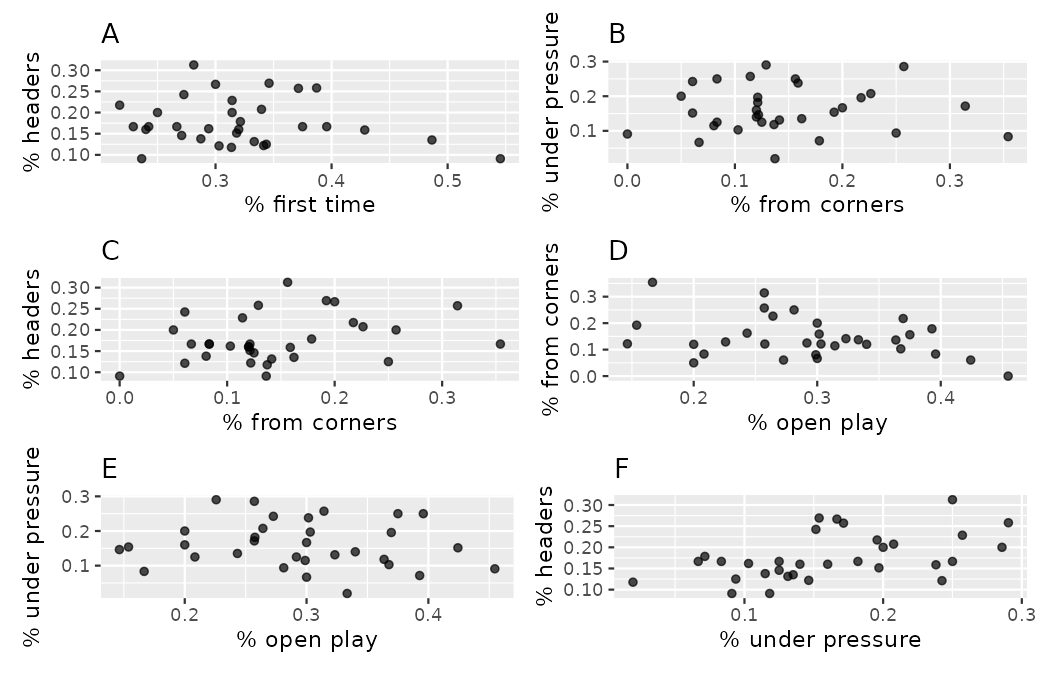
\includegraphics[width=0.85\linewidth,height=\textheight,keepaspectratio]{figures/model-slr-14.png}

\begin{center}\rule{0.5\linewidth}{0.5pt}\end{center}

Computing all six correlations settles the ordering --- never trust your
eye alone with 32 points per panel:

\begin{Shaded}
\begin{Highlighting}[]
\FunctionTok{c}\NormalTok{(}
  \AttributeTok{A =} \FunctionTok{cor}\NormalTok{(team\_profile}\SpecialCharTok{$}\NormalTok{prop\_first\_time, team\_profile}\SpecialCharTok{$}\NormalTok{prop\_headers),}
  \AttributeTok{B =} \FunctionTok{cor}\NormalTok{(team\_profile}\SpecialCharTok{$}\NormalTok{prop\_corner,     team\_profile}\SpecialCharTok{$}\NormalTok{prop\_pressure),}
  \AttributeTok{C =} \FunctionTok{cor}\NormalTok{(team\_profile}\SpecialCharTok{$}\NormalTok{prop\_corner,     team\_profile}\SpecialCharTok{$}\NormalTok{prop\_headers),}
  \AttributeTok{D =} \FunctionTok{cor}\NormalTok{(team\_profile}\SpecialCharTok{$}\NormalTok{prop\_open\_play,  team\_profile}\SpecialCharTok{$}\NormalTok{prop\_corner),}
  \AttributeTok{E =} \FunctionTok{cor}\NormalTok{(team\_profile}\SpecialCharTok{$}\NormalTok{prop\_open\_play,  team\_profile}\SpecialCharTok{$}\NormalTok{prop\_pressure),}
  \AttributeTok{F =} \FunctionTok{cor}\NormalTok{(team\_profile}\SpecialCharTok{$}\NormalTok{prop\_pressure,   team\_profile}\SpecialCharTok{$}\NormalTok{prop\_headers)}
\NormalTok{) }\SpecialCharTok{|\textgreater{}}
  \FunctionTok{round}\NormalTok{(}\DecValTok{2}\NormalTok{)}
\CommentTok{\#\textgreater{}     A     B     C     D     E     F}
\CommentTok{\#\textgreater{} {-}0.17  0.03  0.31 {-}0.33 {-}0.11  0.50}
\end{Highlighting}
\end{Shaded}

The order from most negative correlation to most positive correlation
is:

\[
D \rightarrow A \rightarrow E \rightarrow B \rightarrow C \rightarrow F
\]

\begin{itemize}
\tightlist
\item
  Plot D --- \% from corners vs.~\% open play: \(-0.33\). Shares must
  add up, so a team that generates more of its shots in open play tends
  to generate fewer from corners.
\item
  Plot A --- \% headers vs.~\% first time: \(-0.17\).
\item
  Plot E --- \% under pressure vs.~\% open play: \(-0.11\).
\item
  Plot B --- \% under pressure vs.~\% from corners: \(0.03\), an
  essentially flat cloud.
\item
  Plot C --- \% headers vs.~\% from corners: \(0.31\).
\item
  Plot F --- \% headers vs.~\% under pressure: \(0.50\). Teams that head
  the ball a lot also shoot under pressure a lot --- both are symptoms
  of living on crosses into a crowded box.
\end{itemize}

\end{tcolorbox}

One important aspect of the correlation is that it's \emph{unitless}.
That is, unlike a measurement of the slope of a line (see the next
section) which provides an increase in the y-coordinate for a one unit
increase in the x-coordinate (in units of the x and y variable), there
are no units associated with the correlation of x and y. The shot log
records when in the match each shot was taken, split into a
\texttt{minute} and a \texttt{second} column. We can express the shot
clock in minutes or in seconds --- a change of units, since the reading
in seconds is exactly 60 times the reading in minutes. The code below
computes the correlation between chance quality and the shot clock, once
per unit choice.

\begin{Shaded}
\begin{Highlighting}[]
\NormalTok{wc2022\_shots }\SpecialCharTok{|\textgreater{}}
  \FunctionTok{mutate}\NormalTok{(}
    \AttributeTok{time\_min =}\NormalTok{ minute }\SpecialCharTok{+}\NormalTok{ second }\SpecialCharTok{/} \DecValTok{60}\NormalTok{,}
    \AttributeTok{time\_sec =} \DecValTok{60} \SpecialCharTok{*}\NormalTok{ minute }\SpecialCharTok{+}\NormalTok{ second}
\NormalTok{  ) }\SpecialCharTok{|\textgreater{}}
  \FunctionTok{summarize}\NormalTok{(}
    \AttributeTok{r\_minutes =} \FunctionTok{cor}\NormalTok{(statsbomb\_xg, time\_min),}
    \AttributeTok{r\_seconds =} \FunctionTok{cor}\NormalTok{(statsbomb\_xg, time\_sec)}
\NormalTok{  )}
\CommentTok{\#\textgreater{} \# A tibble: 1 × 2}
\CommentTok{\#\textgreater{}   r\_minutes r\_seconds}
\CommentTok{\#\textgreater{}       \textless{}dbl\textgreater{}     \textless{}dbl\textgreater{}}
\CommentTok{\#\textgreater{} 1     0.238     0.238}
\end{Highlighting}
\end{Shaded}

The two correlations are identical: \(r = 0.238\) whether the clock is
read in minutes or in seconds. If we drew the two scatterplots side by
side, the shape of the relationship would not change; the only visual
change would be the axis \emph{labeling} of the points. (Before a scout
gets excited about that \(0.238\) --- ``chances get better as the match
wears on!'' --- recall the honesty note from earlier in this chapter:
the shot log includes shootout penalties, which sit at the very end of
the clock with penalty-sized chance quality. Restrict to open-play shots
and the fatigue story nearly vanishes:

\begin{Shaded}
\begin{Highlighting}[]
\NormalTok{wc2022\_shots }\SpecialCharTok{|\textgreater{}}
  \FunctionTok{filter}\NormalTok{(shot\_type }\SpecialCharTok{==} \StringTok{"Open Play"}\NormalTok{) }\SpecialCharTok{|\textgreater{}}
  \FunctionTok{summarize}\NormalTok{(}\AttributeTok{r\_open\_play =} \FunctionTok{cor}\NormalTok{(statsbomb\_xg, minute }\SpecialCharTok{+}\NormalTok{ second }\SpecialCharTok{/} \DecValTok{60}\NormalTok{))}
\CommentTok{\#\textgreater{} \# A tibble: 1 × 1}
\CommentTok{\#\textgreater{}   r\_open\_play}
\CommentTok{\#\textgreater{}         \textless{}dbl\textgreater{}}
\CommentTok{\#\textgreater{} 1      0.0299}
\end{Highlighting}
\end{Shaded}

We will return to this nearly-zero correlation when we study inference
for regression in Chapter~\ref{sec-inf-model-slr}.)

\section{Least squares regression}\label{sec-least-squares-regression}

Fitting linear models by eye is open to criticism since it is based on
an individual's preference. In this section, we use \emph{least squares
regression} as a more rigorous approach to fitting a line to a
scatterplot.

\subsection{Asking prices in the veteran
market}\label{asking-prices-in-the-veteran-market}

Marta Vidal has asked Priya Rao a transfer-window question: how quickly
do asking prices fall with age at the veteran end of the striker market?
To study the question in a controlled setting, Priya constructs a market
survey: 50 listed strikers aged 28 and older, each with an asking price
in millions of euros quoted by the player's agent. This is a constructed
scouting scenario --- the seeded code below builds it, and the code
\emph{is} the data's documentation. (The \texttt{pmax()} guard reflects
one market reality Priya builds in: no agent lists a client below
€0.5M.)

\begin{Shaded}
\begin{Highlighting}[]
\FunctionTok{set.seed}\NormalTok{(}\DecValTok{701}\NormalTok{)}
\NormalTok{veteran\_market }\OtherTok{\textless{}{-}} \FunctionTok{tibble}\NormalTok{(}
  \AttributeTok{age =} \FunctionTok{sample}\NormalTok{(}\DecValTok{28}\SpecialCharTok{:}\DecValTok{35}\NormalTok{, }\DecValTok{50}\NormalTok{, }\AttributeTok{replace =} \ConstantTok{TRUE}\NormalTok{),}
  \AttributeTok{asking\_price =} \FunctionTok{round}\NormalTok{(}\FunctionTok{pmax}\NormalTok{(}\FloatTok{0.5}\NormalTok{, }\DecValTok{17} \SpecialCharTok{{-}} \FloatTok{2.0} \SpecialCharTok{*}\NormalTok{ (age }\SpecialCharTok{{-}} \DecValTok{28}\NormalTok{) }\SpecialCharTok{+} \FunctionTok{rnorm}\NormalTok{(}\DecValTok{50}\NormalTok{, }\DecValTok{0}\NormalTok{, }\FloatTok{5.3}\NormalTok{)), }\DecValTok{1}\NormalTok{)}
\NormalTok{)}

\FunctionTok{ggplot}\NormalTok{(veteran\_market, }\FunctionTok{aes}\NormalTok{(}\AttributeTok{x =}\NormalTok{ age, }\AttributeTok{y =}\NormalTok{ asking\_price)) }\SpecialCharTok{+}
  \FunctionTok{geom\_point}\NormalTok{(}\AttributeTok{size =} \DecValTok{2}\NormalTok{, }\AttributeTok{alpha =} \FloatTok{0.8}\NormalTok{) }\SpecialCharTok{+}
  \FunctionTok{geom\_smooth}\NormalTok{(}\AttributeTok{method =} \StringTok{"lm"}\NormalTok{, }\AttributeTok{se =} \ConstantTok{FALSE}\NormalTok{) }\SpecialCharTok{+}
  \FunctionTok{labs}\NormalTok{(}
    \AttributeTok{x =} \StringTok{"Age (years)"}\NormalTok{,}
    \AttributeTok{y =} \StringTok{"Asking price (million euros)"}
\NormalTok{  )}
\end{Highlighting}
\end{Shaded}

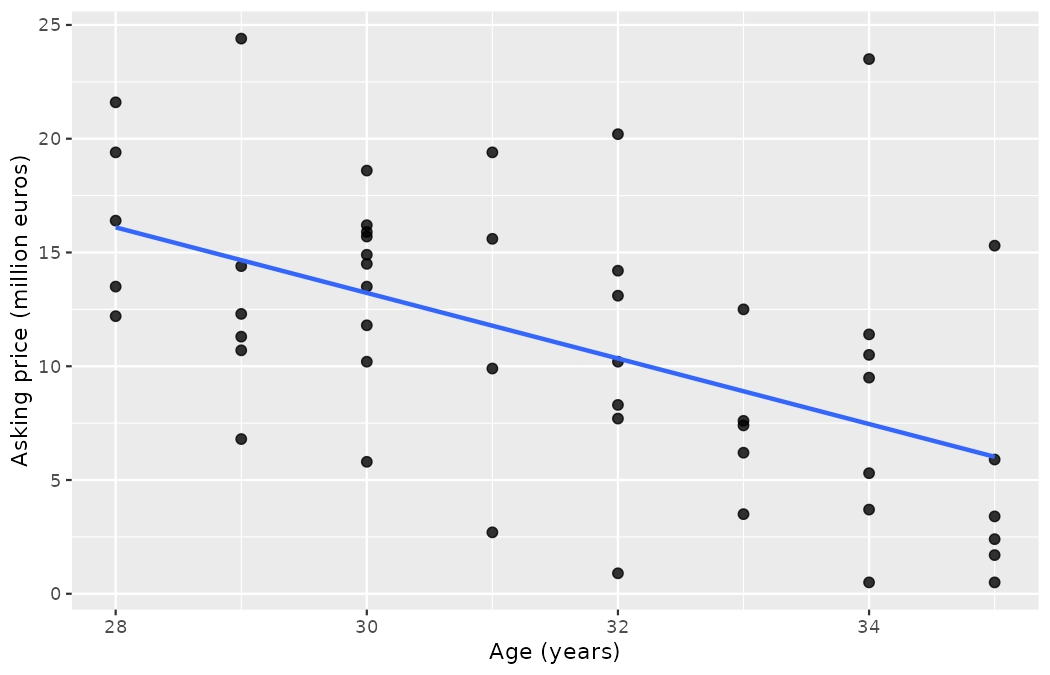
\includegraphics[width=0.85\linewidth,height=\textheight,keepaspectratio]{figures/model-slr-15.png}

The 50 points scatter from €0.5M to €24.4M, and the fitted line follows
a negative trend in the data: older strikers tend to carry lower asking
prices.

\begin{tcolorbox}[enhanced jigsaw, left=2mm, leftrule=.75mm, title=\textcolor{quarto-callout-tip-color}{\faLightbulb}\hspace{0.5em}{Check your understanding}, arc=.35mm, rightrule=.15mm, coltitle=black, colframe=quarto-callout-tip-color-frame, bottomrule=.15mm, colbacktitle=quarto-callout-tip-color!10!white, opacitybacktitle=0.6, breakable, bottomtitle=1mm, toptitle=1mm, titlerule=0mm, opacityback=0, toprule=.15mm, colback=white]

Is the correlation between age and asking price in the plot above
positive or negative?

\begin{center}\rule{0.5\linewidth}{0.5pt}\end{center}

Higher ages are associated with lower asking prices, so the correlation
will be negative. Using a computer, the correlation can be computed:

\begin{Shaded}
\begin{Highlighting}[]
\FunctionTok{cor}\NormalTok{(veteran\_market}\SpecialCharTok{$}\NormalTok{age, veteran\_market}\SpecialCharTok{$}\NormalTok{asking\_price)}
\CommentTok{\#\textgreater{} [1] {-}0.533798}
\end{Highlighting}
\end{Shaded}

\end{tcolorbox}

\subsection{An objective measure for finding the best
line}\label{an-objective-measure-for-finding-the-best-line}

We begin by thinking about what we mean by the ``best'' line.
Mathematically, we want a line that has small residuals. But beyond the
mathematical reasons, hopefully it also makes sense intuitively that
whatever line we fit, the residuals should be small (i.e., the points
should be close to the line). The first option that may come to mind is
to minimize the sum of the residual magnitudes:

\[
|e_1| + |e_2| + \dots + |e_n|
\]

which we could accomplish with a computer program. The \texttt{optim()}
call below does exactly that: it searches for the intercept and slope
minimizing the sum of absolute residuals.

\begin{Shaded}
\begin{Highlighting}[]
\NormalTok{l1\_loss }\OtherTok{\textless{}{-}} \ControlFlowTok{function}\NormalTok{(b) \{}
  \FunctionTok{sum}\NormalTok{(}\FunctionTok{abs}\NormalTok{(veteran\_market}\SpecialCharTok{$}\NormalTok{asking\_price }\SpecialCharTok{{-}}\NormalTok{ b[}\DecValTok{1}\NormalTok{] }\SpecialCharTok{{-}}\NormalTok{ b[}\DecValTok{2}\NormalTok{] }\SpecialCharTok{*}\NormalTok{ veteran\_market}\SpecialCharTok{$}\NormalTok{age))}
\NormalTok{\}}
\FunctionTok{optim}\NormalTok{(}\AttributeTok{par =} \FunctionTok{c}\NormalTok{(}\DecValTok{30}\NormalTok{, }\SpecialCharTok{{-}}\DecValTok{1}\NormalTok{), }\AttributeTok{fn =}\NormalTok{ l1\_loss)}\SpecialCharTok{$}\NormalTok{par }\SpecialCharTok{|\textgreater{}}
  \FunctionTok{round}\NormalTok{(}\DecValTok{2}\NormalTok{)}
\CommentTok{\#\textgreater{} [1] 66.8 {-}1.8}
\end{Highlighting}
\end{Shaded}

Drawn as a dashed line over the scatterplot (\(y = 66.8 - 1.8x\)), this
fit hugs the cloud closely --- it can be quite reasonable. However, a
more common practice is to choose the line that minimizes the sum of the
squared residuals:

\[
e_{1}^2 + e_{2}^2 + \dots + e_{n}^2
\]

The line that minimizes this least squares criterion is the solid line
the \texttt{geom\_smooth(method\ =\ "lm")} call drew earlier and is
commonly called the \textbf{least squares line}. The following are four
possible reasons to choose the least squares option instead of trying to
minimize the sum of residual magnitudes without any squaring:

\begin{enumerate}
\def\labelenumi{\arabic{enumi}.}
\tightlist
\item
  It is the most commonly used method.
\item
  Computing the least squares line is widely supported in statistical
  software.
\item
  In many applications, a residual twice as large as another residual is
  more than twice as bad. For example, being off by 4 is usually more
  than twice as bad as being off by 2. Squaring the residuals accounts
  for this discrepancy. A valuation that misses by €4M embarrasses the
  club more than twice as much as one that misses by €2M.
\item
  The analyses which link the model to inference about a population are
  most straightforward when the line is fit through least squares.
\end{enumerate}

The first two reasons are largely for tradition and convenience; the
third and fourth reasons explain why the least squares criterion is
typically most helpful when working with real data.\footnote{There are
  applications where the sum of residual magnitudes may be more useful,
  and there are plenty of other criteria we might consider. However,
  this book only applies the least squares criterion.}

\begin{tcolorbox}[enhanced jigsaw, left=2mm, leftrule=.75mm, title=\textcolor{quarto-callout-tip-color}{\faLightbulb}\hspace{0.5em}{Check your understanding}, arc=.35mm, rightrule=.15mm, coltitle=black, colframe=quarto-callout-tip-color-frame, bottomrule=.15mm, colbacktitle=quarto-callout-tip-color!10!white, opacitybacktitle=0.6, breakable, bottomtitle=1mm, toptitle=1mm, titlerule=0mm, opacityback=0, toprule=.15mm, colback=white]

The solid line in the veteran-market plot is the least squares fit; the
dashed line minimized the sum of absolute residuals. State precisely
which quantity the least squares line minimizes, and explain why the two
criteria can produce different lines from the same 50 strikers.

\begin{center}\rule{0.5\linewidth}{0.5pt}\end{center}

The least squares line minimizes \(e_1^2 + e_2^2 + \dots + e_n^2,\) the
sum of \emph{squared vertical} distances from each observation to the
line --- not perpendicular distances, and not the absolute values
\(|e_i|.\) Squaring punishes a large residual disproportionately: one
valuation that misses by €4M costs the criterion as much as four that
miss by €2M. Because the two criteria weigh the points differently, they
need not settle on the same line --- here the absolute-residual
criterion returned \(66.8 - 1.8x,\) while the least squares fit,
computed in the next section, has a shallower slope.

\end{tcolorbox}

\subsection{Finding and interpreting the least squares
line}\label{finding-and-interpreting-the-least-squares-line}

For the veteran market data, we could write the equation of the least
squares regression line as

\[
\widehat{\texttt{asking\_price}} = \beta_0 + \beta_{1}\times \texttt{age}
\]

Here the equation is set up to predict an asking price based on a
striker's age, which would be useful to Marta when an agent's first
quote has not yet landed. These two values, \(\beta_0\) and \(\beta_1,\)
are the parameters of the regression line --- recall from earlier in
this chapter that the Greek letters mark the population-level truths our
sample statistics \(b_0\) and \(b_1\) estimate.

The parameters are estimated using the observed data. In practice, this
estimation is done using a computer in the same way that other
estimates, like a sample mean, can be estimated using a computer or
calculator. The first five rows of the \texttt{veteran\_market} data
look like this:

\begin{Shaded}
\begin{Highlighting}[]
\NormalTok{veteran\_market }\SpecialCharTok{|\textgreater{}}
  \FunctionTok{slice\_head}\NormalTok{(}\AttributeTok{n =} \DecValTok{5}\NormalTok{)}
\CommentTok{\#\textgreater{} \# A tibble: 5 × 2}
\CommentTok{\#\textgreater{}     age asking\_price}
\CommentTok{\#\textgreater{}   \textless{}int\textgreater{}        \textless{}dbl\textgreater{}}
\CommentTok{\#\textgreater{} 1    31          2.7}
\CommentTok{\#\textgreater{} 2    32         14.2}
\CommentTok{\#\textgreater{} 3    30          5.8}
\CommentTok{\#\textgreater{} 4    35          0.5}
\CommentTok{\#\textgreater{} 5    34         11.4}
\end{Highlighting}
\end{Shaded}

Statistical software is usually used to compute the least squares line,
and the typical output generated by fitting a regression model looks
like the \texttt{tidy()} summary below --- the \texttt{broom} package's
tidier for model objects. For now we will focus on the \texttt{estimate}
column, which lists \(b_0\) and \(b_1.\) In
Chapter~\ref{sec-inf-model-slr} we will dive deeper into the remaining
columns, which tell us how accurately and precisely these values ---
calculated from a survey of 50 listed strikers --- estimate the
intercept and slope for the \emph{whole} veteran market.

\begin{Shaded}
\begin{Highlighting}[]
\FunctionTok{library}\NormalTok{(broom)}

\NormalTok{fit\_veteran }\OtherTok{\textless{}{-}} \FunctionTok{lm}\NormalTok{(asking\_price }\SpecialCharTok{\textasciitilde{}}\NormalTok{ age, }\AttributeTok{data =}\NormalTok{ veteran\_market)}
\FunctionTok{tidy}\NormalTok{(fit\_veteran)}
\CommentTok{\#\textgreater{} \# A tibble: 2 × 5}
\CommentTok{\#\textgreater{}   term        estimate std.error statistic    p.value}
\CommentTok{\#\textgreater{}   \textless{}chr\textgreater{}          \textless{}dbl\textgreater{}     \textless{}dbl\textgreater{}     \textless{}dbl\textgreater{}      \textless{}dbl\textgreater{}}
\CommentTok{\#\textgreater{} 1 (Intercept)    56.4     10.4        5.43 0.00000186}
\CommentTok{\#\textgreater{} 2 age            {-}1.44     0.329     {-}4.37 0.0000655}
\end{Highlighting}
\end{Shaded}

The model output tells us that the intercept is approximately 56.4 and
the slope on \texttt{age} is approximately \(-1.44.\)

But what do these values mean? Interpreting parameters in a regression
model is often one of the most important steps in the analysis.

\begin{tcolorbox}[enhanced jigsaw, left=2mm, leftrule=.75mm, title=\textcolor{quarto-callout-note-color}{\faInfo}\hspace{0.5em}{Worked example}, arc=.35mm, rightrule=.15mm, coltitle=black, colframe=quarto-callout-note-color-frame, bottomrule=.15mm, colbacktitle=quarto-callout-note-color!10!white, opacitybacktitle=0.6, breakable, bottomtitle=1mm, toptitle=1mm, titlerule=0mm, opacityback=0, toprule=.15mm, colback=white]

The intercept and slope estimates for the veteran market data are
\(b_0 = 56.4\) and \(b_1 = -1.44.\) What do these numbers really mean?

\begin{center}\rule{0.5\linewidth}{0.5pt}\end{center}

Interpreting the slope parameter is helpful in almost any application.
For each additional year of age, we would expect a listed striker's
asking price to be lower by €1.44M on average. Note that an older age
corresponds to a lower price because the coefficient of age is negative
in the model. We must be cautious in this interpretation: the line
describes how \emph{listed prices} vary across players of different ages
in this market survey; it does not say that holding a specific player
for one more season will knock exactly €1.44M off his price --- his
form, contract, and injury record will all move too.

The estimated intercept \(b_0 = 56.4\) is the predicted asking price for
a striker of age zero. Unlike the invoice example that opened this
chapter --- where a club could genuinely accredit zero scouts --- no
player in any market is zero years old, and none in this one is younger
than 28. The intercept here has no practical meaning of its own; it
serves only to anchor the height of the line where the data actually
live.

\end{tcolorbox}

\begin{tcolorbox}[enhanced jigsaw, left=2mm, leftrule=.75mm, title=\textcolor{quarto-callout-important-color}{\faExclamation}\hspace{0.5em}{Interpreting parameters estimated by least squares}, arc=.35mm, rightrule=.15mm, coltitle=black, colframe=quarto-callout-important-color-frame, bottomrule=.15mm, colbacktitle=quarto-callout-important-color!10!white, opacitybacktitle=0.6, breakable, bottomtitle=1mm, toptitle=1mm, titlerule=0mm, opacityback=0, toprule=.15mm, colback=white]

The slope describes the estimated difference in the predicted average
outcome of \(y\) if the predictor variable \(x\) happened to be one unit
larger. The intercept describes the average outcome of \(y\) if
\(x = 0\) \emph{and} the linear model is valid all the way to \(x = 0\)
(values of \(x = 0\) are not observed or relevant in many applications).

\end{tcolorbox}

\begin{tcolorbox}[enhanced jigsaw, left=2mm, leftrule=.75mm, title=\textcolor{quarto-callout-tip-color}{\faLightbulb}\hspace{0.5em}{Check your understanding}, arc=.35mm, rightrule=.15mm, coltitle=black, colframe=quarto-callout-tip-color-frame, bottomrule=.15mm, colbacktitle=quarto-callout-tip-color!10!white, opacitybacktitle=0.6, breakable, bottomtitle=1mm, toptitle=1mm, titlerule=0mm, opacityback=0, toprule=.15mm, colback=white]

Using the fitted model
\(\widehat{\texttt{asking\_price}} = 56.4 - 1.44 \times \texttt{age},\)
how much lower an asking price would we predict for a 33-year-old
striker than for a 30-year-old, on average?

\begin{center}\rule{0.5\linewidth}{0.5pt}\end{center}

The slope is measured in millions of euros per year of age, so three
additional years of age predict an asking price lower by
\(3 \times 1.44 = 4.32,\) about €4.3M, on average. Keep the
interpretation honest: this describes how listed prices differ across
players of different ages in the survey; it is not a forecast that any
particular striker's price will fall by €4.32M over his next three
birthdays.

\end{tcolorbox}

An alternative way of calculating the values of intercept and slope of a
least squares line is manual calculation using formulas. While manual
calculations are not commonly used by practicing statisticians and data
scientists, it is useful to work through them the first time you're
learning about the least squares line and modeling in general.
Calculating the values by hand leverages two properties of the least
squares line:

\begin{enumerate}
\def\labelenumi{\arabic{enumi}.}
\tightlist
\item
  The slope of the least squares line can be estimated by
\end{enumerate}

\[
b_1 = \frac{s_y}{s_x} r
\]

Decompose the formula before using it: \(s_y\) and \(s_x\) are the
sample standard deviations of the outcome and the predictor --- the same
\(s\) you met in Chapter~\ref{sec-explore-numerical}, subscripted here
to say \emph{which} variable's spread is meant --- and \(r\) is the
correlation between the two variables. The ratio \(s_y / s_x\) converts
the unitless correlation into the units of the problem: standard
deviations of \(y\) per standard deviation of \(x,\) rescaled into raw
units.

\begin{enumerate}
\def\labelenumi{\arabic{enumi}.}
\setcounter{enumi}{1}
\tightlist
\item
  If \(\bar{x}\) is the sample mean of the predictor variable and
  \(\bar{y}\) is the sample mean of the outcome variable, then the point
  \((\bar{x}, \bar{y})\) falls on the least squares line.
\end{enumerate}

\begin{tcolorbox}[enhanced jigsaw, left=2mm, leftrule=.75mm, title=\textcolor{quarto-callout-note-color}{\faInfo}\hspace{0.5em}{Deeper (optional): where \(b_1 = (s_y/s_x),r\) comes from --- uses
calculus; safe to skip}, arc=.35mm, rightrule=.15mm, coltitle=black, colframe=quarto-callout-note-color-frame, bottomrule=.15mm, colbacktitle=quarto-callout-note-color!10!white, opacitybacktitle=0.6, breakable, bottomtitle=1mm, toptitle=1mm, titlerule=0mm, opacityback=0, toprule=.15mm, colback=white]

Both properties fall out of the least squares criterion itself. Write
the criterion as a function of the two unknowns,
\(SSE(b_0, b_1) = \sum_{i=1}^n (y_i - b_0 - b_1 x_i)^2,\) and set both
of its derivatives to zero --- the \emph{normal equations}:

\[
\frac{\partial\, SSE}{\partial b_0} = 0 \;\Rightarrow\; \sum_{i=1}^n (y_i - b_0 - b_1 x_i) = 0
\qquad\quad
\frac{\partial\, SSE}{\partial b_1} = 0 \;\Rightarrow\; \sum_{i=1}^n x_i\, (y_i - b_0 - b_1 x_i) = 0
\]

The first equation says the residuals sum to zero; divide it by \(n\)
and it reads \(\bar{y} = b_0 + b_1 \bar{x},\) which is exactly property
2: the line passes through \((\bar{x}, \bar{y}).\) Substitute
\(b_0 = \bar{y} - b_1 \bar{x}\) into the second equation and rearrange:

\[
b_1 = \frac{\sum_{i=1}^n (x_i - \bar{x})(y_i - \bar{y})}{\sum_{i=1}^n (x_i - \bar{x})^2}
    = \frac{(n-1)\, s_x\, s_y\, r}{(n-1)\, s_x^2}
    = \frac{s_y}{s_x}\, r
\]

The middle step recognizes the numerator as \((n-1)\, s_x s_y r\) ---
rearrange the correlation formula displayed earlier in this chapter ---
and the denominator as \((n-1)\, s_x^2,\) the definition of the sample
variance from Chapter~\ref{sec-explore-numerical}.

\end{tcolorbox}

The summary statistics for the veteran market survey are computed below.

\begin{Shaded}
\begin{Highlighting}[]
\NormalTok{veteran\_market }\SpecialCharTok{|\textgreater{}}
  \FunctionTok{summarize}\NormalTok{(}
    \AttributeTok{age\_mean   =} \FunctionTok{mean}\NormalTok{(age),}
    \AttributeTok{age\_sd     =} \FunctionTok{sd}\NormalTok{(age),}
    \AttributeTok{price\_mean =} \FunctionTok{mean}\NormalTok{(asking\_price),}
    \AttributeTok{price\_sd   =} \FunctionTok{sd}\NormalTok{(asking\_price),}
    \AttributeTok{r          =} \FunctionTok{cor}\NormalTok{(age, asking\_price)}
\NormalTok{  )}
\CommentTok{\#\textgreater{} \# A tibble: 1 × 5}
\CommentTok{\#\textgreater{}   age\_mean age\_sd price\_mean price\_sd      r}
\CommentTok{\#\textgreater{}      \textless{}dbl\textgreater{}  \textless{}dbl\textgreater{}      \textless{}dbl\textgreater{}    \textless{}dbl\textgreater{}  \textless{}dbl\textgreater{}}
\CommentTok{\#\textgreater{} 1     31.5   2.27       11.1     6.13 {-}0.534}
\end{Highlighting}
\end{Shaded}

We could plot the point \((31.5, 11.1)\) on the scatterplot of the
veteran market to verify it falls on the least squares line. Next, we
find the point estimates \(b_0\) and \(b_1\) of the parameters
\(\beta_0\) and \(\beta_1.\)

\begin{tcolorbox}[enhanced jigsaw, left=2mm, leftrule=.75mm, title=\textcolor{quarto-callout-note-color}{\faInfo}\hspace{0.5em}{Worked example}, arc=.35mm, rightrule=.15mm, coltitle=black, colframe=quarto-callout-note-color-frame, bottomrule=.15mm, colbacktitle=quarto-callout-note-color!10!white, opacitybacktitle=0.6, breakable, bottomtitle=1mm, toptitle=1mm, titlerule=0mm, opacityback=0, toprule=.15mm, colback=white]

Using the summary statistics above, compute the slope for the regression
line of asking price against age.

\begin{center}\rule{0.5\linewidth}{0.5pt}\end{center}

Compute the slope using the summary statistics:

\[
b_1 = \frac{s_y}{s_x} r = \frac{6.13}{2.27}(-0.534) = -1.44
\]

matching the slope the software reported.

\end{tcolorbox}

You might recall the form of a line from math class, which we can use to
find the model fit, including the estimate of \(b_0.\) Given the slope
of a line and a point on the line, \((x_0, y_0),\) the equation for the
line can be written as

\[
y - y_0 = slope\times (x - x_0)
\]

\begin{tcolorbox}[enhanced jigsaw, left=2mm, leftrule=.75mm, title=\textcolor{quarto-callout-important-color}{\faExclamation}\hspace{0.5em}{Identifying the least squares line from summary statistics}, arc=.35mm, rightrule=.15mm, coltitle=black, colframe=quarto-callout-important-color-frame, bottomrule=.15mm, colbacktitle=quarto-callout-important-color!10!white, opacitybacktitle=0.6, breakable, bottomtitle=1mm, toptitle=1mm, titlerule=0mm, opacityback=0, toprule=.15mm, colback=white]

To identify the least squares line from summary statistics:

\begin{itemize}
\tightlist
\item
  Estimate the slope parameter, \(b_1 = (s_y / s_x) r.\)
\item
  Note that the point \((\bar{x}, \bar{y})\) is on the least squares
  line, use \(x_0 = \bar{x}\) and \(y_0 = \bar{y}\) with the point-slope
  equation: \(y - \bar{y} = b_1 (x - \bar{x}).\)
\item
  Simplify the equation, we get \(y = \bar{y} - b_1 \bar{x} + b_1 x,\)
  which reveals that \(b_0 = \bar{y} - b_1 \bar{x}.\)
\end{itemize}

\end{tcolorbox}

\begin{tcolorbox}[enhanced jigsaw, left=2mm, leftrule=.75mm, title=\textcolor{quarto-callout-note-color}{\faInfo}\hspace{0.5em}{Worked example}, arc=.35mm, rightrule=.15mm, coltitle=black, colframe=quarto-callout-note-color-frame, bottomrule=.15mm, colbacktitle=quarto-callout-note-color!10!white, opacitybacktitle=0.6, breakable, bottomtitle=1mm, toptitle=1mm, titlerule=0mm, opacityback=0, toprule=.15mm, colback=white]

Using the point \((31.5, 11.1)\) from the sample means and the slope
estimate \(b_1 = -1.44,\) find the least-squares line for predicting
asking price based on age.

\begin{center}\rule{0.5\linewidth}{0.5pt}\end{center}

Apply the point-slope equation using \((31.5, 11.1)\) and the slope
\(b_1 = -1.44\):

\[
\begin{aligned}
y - y_0  &= b_1 (x - x_0) \\
y - 11.1 &= -1.44 (x - 31.5)
\end{aligned}
\]

Expanding the right side and then adding 11.1 to each side, the equation
simplifies:

\[
\widehat{\texttt{asking\_price}} = 56.5 - 1.44 \times \texttt{age}
\]

which matches the software's intercept of 56.4 up to rounding of the
intermediate values. Here we have replaced \(y\) with
\(\widehat{\texttt{asking\_price}}\) and \(x\) with \(\texttt{age}\) to
put the equation in context. The final least squares equation should
always include a ``hat'' on the variable being predicted, whether it is
a generic \(``y"\) or a named variable like \(``asking\_price."\)

\end{tcolorbox}

\begin{tcolorbox}[enhanced jigsaw, left=2mm, leftrule=.75mm, title=\textcolor{quarto-callout-note-color}{\faInfo}\hspace{0.5em}{Worked example}, arc=.35mm, rightrule=.15mm, coltitle=black, colframe=quarto-callout-note-color-frame, bottomrule=.15mm, colbacktitle=quarto-callout-note-color!10!white, opacitybacktitle=0.6, breakable, bottomtitle=1mm, toptitle=1mm, titlerule=0mm, opacityback=0, toprule=.15mm, colback=white]

An agent emails Emil Sørensen about a 30-year-old striker not in Priya's
survey. Can Emil simply use the linear equation that we have estimated
to predict the asking price?

\begin{center}\rule{0.5\linewidth}{0.5pt}\end{center}

He may use it as an estimate --- the equation gives
\(56.4 - 1.44 \times 30 = 13.2,\) about €13.2M --- though some
qualifiers on this approach are important. First, the survey is a
constructed snapshot of one window, and the way agents price veterans
may change from window to window. Second, the equation will provide an
imperfect estimate. While the linear equation is good at modeling the
trend in the data, no individual striker's asking price will be
perfectly predicted (as can be seen from the individual data points
around the line).

\end{tcolorbox}

\subsection{Extrapolation is
treacherous}\label{extrapolation-is-treacherous}

Linear models can be used to approximate the relationship between two
variables. However, like any model, they have real limitations. Linear
regression is simply a modeling framework. The truth is almost always
much more complex than a simple line. For example, we do not know how
the data outside of our limited window will behave.

\begin{tcolorbox}[enhanced jigsaw, left=2mm, leftrule=.75mm, title=\textcolor{quarto-callout-note-color}{\faInfo}\hspace{0.5em}{Worked example}, arc=.35mm, rightrule=.15mm, coltitle=black, colframe=quarto-callout-note-color-frame, bottomrule=.15mm, colbacktitle=quarto-callout-note-color!10!white, opacitybacktitle=0.6, breakable, bottomtitle=1mm, toptitle=1mm, titlerule=0mm, opacityback=0, toprule=.15mm, colback=white]

Use the model
\(\widehat{\texttt{asking\_price}} = 56.4 - 1.44 \times \texttt{age}\)
to estimate the asking price of a 40-year-old striker.

\begin{center}\rule{0.5\linewidth}{0.5pt}\end{center}

We want to calculate the predicted price at age 40:

\[
56.4 - 1.44 \times 40 = -1.2
\]

The model predicts an asking price of \(-\)€1.2M --- a negative price.
Taken literally, the agent would have to pay Northbridge €1.2M to take
his client. Whatever one thinks of 40-year-old strikers, no agent in any
market quotes a \emph{negative} asking price --- the oldest player in
the survey is 35, and the line knows nothing about the market beyond
that age.

\end{tcolorbox}

Applying a model estimate to values outside of the realm of the original
data is called \textbf{extrapolation}. Generally, a linear model is only
an approximation of the real relationship between two variables. If we
extrapolate, we are making an unreliable bet that the approximate linear
relationship will be valid in places where it has not been analyzed.
Recall the age--market-value hump from the start of this chapter: even
\emph{within} the observed range, age relationships in football bend;
beyond it, a straight line is pure speculation.

\subsection{Describing the strength of a fit}\label{sec-r-squared}

We evaluated the strength of the linear relationship between two
variables earlier using the correlation, \(r.\) However, it is more
common to explain the strength of a linear fit using \(R^2,\) called
\textbf{R-squared}. Read the symbol piece by piece: it is the capital
letter \(R\) --- by convention written uppercase in this role --- raised
to the power 2, and for a model with one predictor it is (literally) the
square of the correlation \(r\) between the two variables. If provided
with a linear model, we might like to describe how closely the data
cluster around the linear fit.

The \(R^2\) of a linear model describes the amount of variation in the
outcome variable that is explained by the least squares line. For
example, consider the veteran market data. The variance of the outcome
variable --- computed with \texttt{var()}, the square of the standard
deviation you met in Chapter~\ref{sec-explore-numerical} --- is
\(s_{price}^2 \approx 37.5\):

\begin{Shaded}
\begin{Highlighting}[]
\FunctionTok{var}\NormalTok{(veteran\_market}\SpecialCharTok{$}\NormalTok{asking\_price)}
\CommentTok{\#\textgreater{} [1] 37.53138}
\end{Highlighting}
\end{Shaded}

However, if we apply our least squares line, then this model reduces our
uncertainty in predicting a price using a striker's age. The variability
in the residuals describes how much variation remains after using the
model:

\begin{Shaded}
\begin{Highlighting}[]
\FunctionTok{var}\NormalTok{(}\FunctionTok{resid}\NormalTok{(fit\_veteran))}
\CommentTok{\#\textgreater{} [1] 26.83718}
\end{Highlighting}
\end{Shaded}

In short, there was a reduction of

\[
\frac{s_{price}^2 - s_{RES}^2}{s_{price}^2}
  = \frac{37.5 - 26.8}{37.5}
  = \frac{10.7}{37.5}
  \approx 0.285
\]

or about 28.5\%, of the outcome variable's variation by using
information about age for predicting the asking price using a linear
model. It turns out that \(R^2\) corresponds exactly to the squared
value of the correlation:

\[
r = -0.534 \rightarrow R^2 = 0.285
\]

\begin{tcolorbox}[enhanced jigsaw, left=2mm, leftrule=.75mm, title=\textcolor{quarto-callout-note-color}{\faInfo}\hspace{0.5em}{Deeper (optional): why \(R^2 = r^2\) with a single predictor}, arc=.35mm, rightrule=.15mm, coltitle=black, colframe=quarto-callout-note-color-frame, bottomrule=.15mm, colbacktitle=quarto-callout-note-color!10!white, opacitybacktitle=0.6, breakable, bottomtitle=1mm, toptitle=1mm, titlerule=0mm, opacityback=0, toprule=.15mm, colback=white]

The identity takes three lines once the fitted line is written through
the point of means: \(\hat{y}_i = \bar{y} + b_1 (x_i - \bar{x}).\) The
variation the model captures --- formalized as \(SSR\) at the end of
this section --- is then

\[
\sum_{i=1}^n (\hat{y}_i - \bar{y})^2
  = b_1^2 \sum_{i=1}^n (x_i - \bar{x})^2
  = \left(\frac{s_y}{s_x}\, r\right)^{\!2} (n-1)\, s_x^2
  = r^2\, (n-1)\, s_y^2,
\]

using \(b_1 = (s_y/s_x)\, r\) from the previous section, and
\((n-1)\, s_y^2\) is precisely the total variation in the \(y\) values.
The ratio of the two --- the share of the outcome's variation the line
explains --- is therefore \(r^2\): for the veteran market,
\((-0.534)^2 = 0.285,\) the same 28.5\% we obtained from the variances
above.

\end{tcolorbox}

\begin{tcolorbox}[enhanced jigsaw, left=2mm, leftrule=.75mm, title=\textcolor{quarto-callout-tip-color}{\faLightbulb}\hspace{0.5em}{Check your understanding}, arc=.35mm, rightrule=.15mm, coltitle=black, colframe=quarto-callout-tip-color-frame, bottomrule=.15mm, colbacktitle=quarto-callout-tip-color!10!white, opacitybacktitle=0.6, breakable, bottomtitle=1mm, toptitle=1mm, titlerule=0mm, opacityback=0, toprule=.15mm, colback=white]

If a linear model has a very strong negative relationship with a
correlation of \(-0.97,\) how much of the variation in the outcome is
explained by the predictor?

\begin{center}\rule{0.5\linewidth}{0.5pt}\end{center}

About \(R^2 = (-0.97)^2 = 0.94\) or 94\% of the variation in the outcome
variable is explained by the linear model.

\end{tcolorbox}

\begin{tcolorbox}[enhanced jigsaw, left=2mm, leftrule=.75mm, title=\textcolor{quarto-callout-tip-color}{\faLightbulb}\hspace{0.5em}{Check your understanding}, arc=.35mm, rightrule=.15mm, coltitle=black, colframe=quarto-callout-tip-color-frame, bottomrule=.15mm, colbacktitle=quarto-callout-tip-color!10!white, opacitybacktitle=0.6, breakable, bottomtitle=1mm, toptitle=1mm, titlerule=0mm, opacityback=0, toprule=.15mm, colback=white]

For the World Cup team-matches, the correlation between accumulated
chance quality and goals was \(r = 0.691.\) What proportion of the
variation in goal counts does the linear model on \texttt{total\_xg}
explain?

\begin{center}\rule{0.5\linewidth}{0.5pt}\end{center}

\(R^2 = (0.691)^2 = 0.478.\) Chance quality explains a little under half
of the variation in goals scored across team-matches --- the other half
is finishing, goalkeeping, and luck, which is exactly why Marta reads
the residuals as carefully as the fit.

\end{tcolorbox}

\(R^2\) is also called the \textbf{coefficient of determination}.

\begin{tcolorbox}[enhanced jigsaw, left=2mm, leftrule=.75mm, title=\textcolor{quarto-callout-important-color}{\faExclamation}\hspace{0.5em}{Coefficient of determination: proportion of variability in the outcome
variable explained by the model}, arc=.35mm, rightrule=.15mm, coltitle=black, colframe=quarto-callout-important-color-frame, bottomrule=.15mm, colbacktitle=quarto-callout-important-color!10!white, opacitybacktitle=0.6, breakable, bottomtitle=1mm, toptitle=1mm, titlerule=0mm, opacityback=0, toprule=.15mm, colback=white]

Since \(r\) is always between -1 and 1, \(R^2\) will always be between 0
and 1. This statistic is called the \textbf{coefficient of
determination}, and it measures the proportion of variation in the
outcome variable, \(y,\) that can be explained by the linear model with
predictor \(x.\)

\end{tcolorbox}

More generally, \(R^2\) can be calculated as a ratio of a measure of
variability around the line divided by a measure of total variability.

\begin{tcolorbox}[enhanced jigsaw, left=2mm, leftrule=.75mm, title=\textcolor{quarto-callout-important-color}{\faExclamation}\hspace{0.5em}{Sums of squares to measure variability in y}, arc=.35mm, rightrule=.15mm, coltitle=black, colframe=quarto-callout-important-color-frame, bottomrule=.15mm, colbacktitle=quarto-callout-important-color!10!white, opacitybacktitle=0.6, breakable, bottomtitle=1mm, toptitle=1mm, titlerule=0mm, opacityback=0, toprule=.15mm, colback=white]

We can measure the variability in the \(y\) values by how far they tend
to fall from their mean, \(\bar{y}.\) We define this value as the
\textbf{total sum of squares}, calculated using the formula below, where
\(y_1, y_2, \dots, y_n\) represent the \(y\) values in the sample, and
\(\bar{y}\) represents their mean. The three capital letters name it:
\textbf{S}um of \textbf{S}quares, \textbf{T}otal.

\[
SST = (y_1 - \bar{y})^2 + (y_2 - \bar{y})^2 + \cdots + (y_n - \bar{y})^2
\]

Left-over variability in the \(y\) values if we know \(x\) can be
measured by the \textbf{sum of squared errors}, or sum of squared
residuals --- \textbf{S}um of \textbf{S}quared \textbf{E}rrors ---
calculated using the formula below, where \(\hat{y}_i\) represents the
predicted value of \(y_i\) based on the least squares
regression.\footnotemark{}

\[
\begin{aligned}
SSE &= (y_1 - \hat{y}_1)^2 + (y_2 - \hat{y}_2)^2 + \cdots + (y_n - \hat{y}_n)^2\\
&= e_{1}^2 + e_{2}^2 + \dots + e_{n}^2
\end{aligned}
\]

The coefficient of determination can then be calculated as

\[
R^2 = \frac{SST - SSE}{SST} = 1 - \frac{SSE}{SST}
\]

\end{tcolorbox}

\footnotetext{The difference \(SST - SSE\) is called the
\textbf{regression sum of squares}, \(SSR\) (\textbf{S}um of
\textbf{S}quares, \textbf{R}egression), and can also be calculated as
\(SSR = (\hat{y}_1 - \bar{y})^2 + (\hat{y}_2 - \bar{y})^2 + \cdots + (\hat{y}_n - \bar{y})^2.\)
\(SSR\) represents the variation in \(y\) that was accounted for in our
model.}

\begin{tcolorbox}[enhanced jigsaw, left=2mm, leftrule=.75mm, title=\textcolor{quarto-callout-note-color}{\faInfo}\hspace{0.5em}{Worked example}, arc=.35mm, rightrule=.15mm, coltitle=black, colframe=quarto-callout-note-color-frame, bottomrule=.15mm, colbacktitle=quarto-callout-note-color!10!white, opacitybacktitle=0.6, breakable, bottomtitle=1mm, toptitle=1mm, titlerule=0mm, opacityback=0, toprule=.15mm, colback=white]

Among the 50 strikers in the \texttt{veteran\_market} survey, the total
variability in asking price is \(SST = 1839,\) and the sum of squared
residuals is \(SSE = 1315.\)\footnotemark{}

\begin{Shaded}
\begin{Highlighting}[]
\NormalTok{SST }\OtherTok{\textless{}{-}} \FunctionTok{sum}\NormalTok{((veteran\_market}\SpecialCharTok{$}\NormalTok{asking\_price }\SpecialCharTok{{-}} \FunctionTok{mean}\NormalTok{(veteran\_market}\SpecialCharTok{$}\NormalTok{asking\_price))}\SpecialCharTok{\^{}}\DecValTok{2}\NormalTok{)}
\NormalTok{SSE }\OtherTok{\textless{}{-}} \FunctionTok{sum}\NormalTok{(}\FunctionTok{resid}\NormalTok{(fit\_veteran)}\SpecialCharTok{\^{}}\DecValTok{2}\NormalTok{)}
\FunctionTok{round}\NormalTok{(}\FunctionTok{c}\NormalTok{(}\AttributeTok{SST =}\NormalTok{ SST, }\AttributeTok{SSE =}\NormalTok{ SSE))}
\CommentTok{\#\textgreater{}  SST  SSE}
\CommentTok{\#\textgreater{} 1839 1315}
\end{Highlighting}
\end{Shaded}

Find \(R^2.\)

\begin{center}\rule{0.5\linewidth}{0.5pt}\end{center}

Since we know \(SSE\) and \(SST,\) we can calculate \(R^2\) as

\[
R^2 = 1 - \frac{SSE}{SST} = 1 - \frac{1315}{1839} = 0.285,
\]

the same value we found when we squared the correlation:
\(R^2 = (-0.534)^2 = 0.285.\)

\end{tcolorbox}

\footnotetext{\(SST\) can be calculated by finding the sample variance
of the outcome variable, \(s^2,\) and multiplying by \(n-1.\)}

\subsection{Categorical predictors with two
levels}\label{sec-categorical-predictor-two-levels}

Categorical variables are also useful in predicting outcomes. Here we
consider a categorical predictor with two levels (recall that a
\emph{level} is the same as a \emph{category}). Back on the real World
Cup shot log, consider the \texttt{one\_on\_one} variable: was the
shooter clean through, one-on-one with the goalkeeper, or not? Here we
want to predict a shot's chance quality (\texttt{statsbomb\_xg}) based
on the shot situation, which takes values \texttt{FALSE} (an ordinary
shot) and \texttt{TRUE} (a one-on-one).

\begin{Shaded}
\begin{Highlighting}[]
\NormalTok{wc2022\_shots }\SpecialCharTok{|\textgreater{}}
  \FunctionTok{count}\NormalTok{(one\_on\_one)}
\CommentTok{\#\textgreater{} \# A tibble: 2 × 2}
\CommentTok{\#\textgreater{}   one\_on\_one     n}
\CommentTok{\#\textgreater{}   \textless{}lgl\textgreater{}      \textless{}int\textgreater{}}
\CommentTok{\#\textgreater{} 1 FALSE       1409}
\CommentTok{\#\textgreater{} 2 TRUE          85}
\end{Highlighting}
\end{Shaded}

To incorporate the shot situation into a regression equation, we must
convert the categories into a numerical form. We will do so using an
\textbf{indicator variable}, which takes value 1 when the shot is a
one-on-one and 0 when it is not. (R does this conversion automatically
when a logical variable enters \texttt{lm()}: \texttt{FALSE} becomes 0,
\texttt{TRUE} becomes 1.) Using this indicator variable, the linear
model may be written as

\[
\widehat{\texttt{xg}} = b_0 + b_1 \times \texttt{one\_on\_one}
\]

A plot of the shot data with the shots jittered around \(x = 0\) and
\(x = 1\) shows two vertical bands of points --- including, high in the
left band, the narrow stripe of penalties with their identical chance
quality --- with the least squares line passing through both:

\begin{Shaded}
\begin{Highlighting}[]
\FunctionTok{ggplot}\NormalTok{(wc2022\_shots, }\FunctionTok{aes}\NormalTok{(}\AttributeTok{x =} \FunctionTok{as.numeric}\NormalTok{(one\_on\_one), }\AttributeTok{y =}\NormalTok{ statsbomb\_xg)) }\SpecialCharTok{+}
  \FunctionTok{geom\_jitter}\NormalTok{(}\AttributeTok{alpha =} \FloatTok{0.3}\NormalTok{, }\AttributeTok{width =} \FloatTok{0.05}\NormalTok{, }\AttributeTok{height =} \DecValTok{0}\NormalTok{) }\SpecialCharTok{+}
  \FunctionTok{geom\_smooth}\NormalTok{(}\AttributeTok{method =} \StringTok{"lm"}\NormalTok{, }\AttributeTok{se =} \ConstantTok{FALSE}\NormalTok{, }\AttributeTok{fullrange =} \ConstantTok{TRUE}\NormalTok{) }\SpecialCharTok{+}
  \FunctionTok{scale\_x\_continuous}\NormalTok{(}
    \AttributeTok{breaks =} \FunctionTok{c}\NormalTok{(}\DecValTok{0}\NormalTok{, }\DecValTok{1}\NormalTok{),}
    \AttributeTok{limits =} \FunctionTok{c}\NormalTok{(}\SpecialCharTok{{-}}\FloatTok{0.2}\NormalTok{, }\FloatTok{1.2}\NormalTok{),}
    \AttributeTok{labels =} \FunctionTok{c}\NormalTok{(}\StringTok{"0}\SpecialCharTok{\textbackslash{}n}\StringTok{(ordinary shot)"}\NormalTok{, }\StringTok{"1}\SpecialCharTok{\textbackslash{}n}\StringTok{(one{-}on{-}one)"}\NormalTok{)}
\NormalTok{  ) }\SpecialCharTok{+}
  \FunctionTok{labs}\NormalTok{(}
    \AttributeTok{x =} \StringTok{"Shot situation"}\NormalTok{,}
    \AttributeTok{y =} \StringTok{"Chance quality (xG)"}
\NormalTok{  )}
\end{Highlighting}
\end{Shaded}

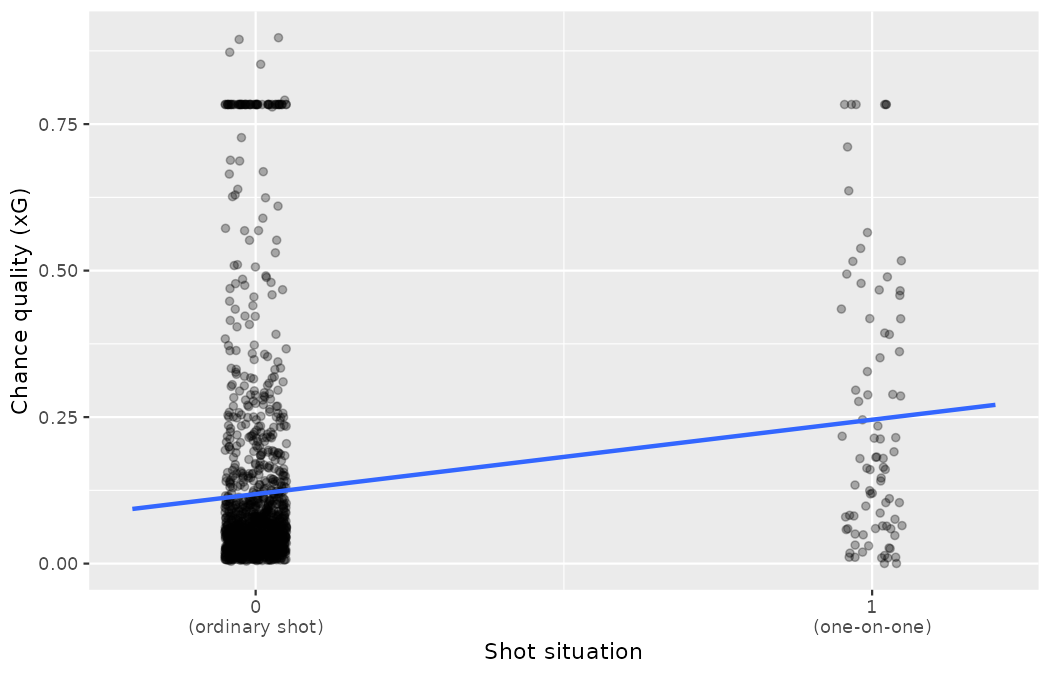
\includegraphics[width=0.85\linewidth,height=\textheight,keepaspectratio]{figures/model-slr-16.png}

The parameter estimates are computed the same way as before:

\begin{Shaded}
\begin{Highlighting}[]
\NormalTok{fit\_1v1 }\OtherTok{\textless{}{-}} \FunctionTok{lm}\NormalTok{(statsbomb\_xg }\SpecialCharTok{\textasciitilde{}}\NormalTok{ one\_on\_one, }\AttributeTok{data =}\NormalTok{ wc2022\_shots)}
\FunctionTok{tidy}\NormalTok{(fit\_1v1)}
\CommentTok{\#\textgreater{} \# A tibble: 2 × 5}
\CommentTok{\#\textgreater{}   term           estimate std.error statistic   p.value}
\CommentTok{\#\textgreater{}   \textless{}chr\textgreater{}             \textless{}dbl\textgreater{}     \textless{}dbl\textgreater{}     \textless{}dbl\textgreater{}     \textless{}dbl\textgreater{}}
\CommentTok{\#\textgreater{} 1 (Intercept)       0.119   0.00485     24.5  1.62e{-}111}
\CommentTok{\#\textgreater{} 2 one\_on\_oneTRUE    0.127   0.0203       6.25 5.49e{-} 10}
\end{Highlighting}
\end{Shaded}

The model equation can be summarized as

\[
\widehat{\texttt{xg}} = 0.119 + 0.127 \times \texttt{one\_on\_one}
\]

\begin{tcolorbox}[enhanced jigsaw, left=2mm, leftrule=.75mm, title=\textcolor{quarto-callout-note-color}{\faInfo}\hspace{0.5em}{Worked example}, arc=.35mm, rightrule=.15mm, coltitle=black, colframe=quarto-callout-note-color-frame, bottomrule=.15mm, colbacktitle=quarto-callout-note-color!10!white, opacitybacktitle=0.6, breakable, bottomtitle=1mm, toptitle=1mm, titlerule=0mm, opacityback=0, toprule=.15mm, colback=white]

Interpret the two parameters estimated in the model for the chance
quality of World Cup shots.

\begin{center}\rule{0.5\linewidth}{0.5pt}\end{center}

The intercept is the estimated chance quality when \texttt{one\_on\_one}
has a value 0, i.e., when the shot is an ordinary one. That is, the
average xG of a shot that is not a one-on-one is 0.119. The slope
indicates that, on average, one-on-ones carry about 0.127 \emph{more}
chance quality than ordinary shots --- a one-on-one is roughly a
one-in-four chance \((0.119 + 0.127 = 0.246)\) against a one-in-eight
baseline. We can verify the two group means directly:

\begin{Shaded}
\begin{Highlighting}[]
\NormalTok{wc2022\_shots }\SpecialCharTok{|\textgreater{}}
  \FunctionTok{group\_by}\NormalTok{(one\_on\_one) }\SpecialCharTok{|\textgreater{}}
  \FunctionTok{summarize}\NormalTok{(}\AttributeTok{mean\_xg =} \FunctionTok{mean}\NormalTok{(statsbomb\_xg))}
\CommentTok{\#\textgreater{} \# A tibble: 2 × 2}
\CommentTok{\#\textgreater{}   one\_on\_one mean\_xg}
\CommentTok{\#\textgreater{}   \textless{}lgl\textgreater{}        \textless{}dbl\textgreater{}}
\CommentTok{\#\textgreater{} 1 FALSE        0.119}
\CommentTok{\#\textgreater{} 2 TRUE         0.246}
\end{Highlighting}
\end{Shaded}

\end{tcolorbox}

\begin{tcolorbox}[enhanced jigsaw, left=2mm, leftrule=.75mm, title=\textcolor{quarto-callout-important-color}{\faExclamation}\hspace{0.5em}{Interpreting model estimates for categorical predictors}, arc=.35mm, rightrule=.15mm, coltitle=black, colframe=quarto-callout-important-color-frame, bottomrule=.15mm, colbacktitle=quarto-callout-important-color!10!white, opacitybacktitle=0.6, breakable, bottomtitle=1mm, toptitle=1mm, titlerule=0mm, opacityback=0, toprule=.15mm, colback=white]

The estimated intercept is the value of the outcome variable for the
first category (i.e., the category corresponding to an indicator value
of 0). The estimated slope is the average change in the outcome variable
between the two categories.

\end{tcolorbox}

Note that, fundamentally, the intercept and slope interpretations do not
change when modeling categorical variables with two levels. However,
when the predictor variable is binary, the coefficient estimates
(\(b_0\) and \(b_1\)) are directly interpretable with respect to the
dataset at hand. And a caution that should now be reflex: these are
observational data, so the 0.127 is a \emph{1v1 premium in recorded
chance quality}, not a causal effect of the situation --- one-on-ones
arise from particular patterns of play, a confounding we will untangle
when this exact model returns in the multiple regression and inference
chapters.

We'll elaborate further on modeling categorical predictors in
Chapter~\ref{sec-model-mlr}, where we examine the influence of many
predictor variables simultaneously using multiple regression.

\section{Outliers in linear
regression}\label{sec-outliers-in-regression}

In this section, we discuss when outliers are important and influential.
Outliers in a regression model with one predictor and one outcome are
observations that fall far from the cloud of points. These points are
especially important because they can have a strong influence on the
least squares line. Note that there are times when observations are
outlying in the \(x\) direction, the \(y\) direction, or both. However,
being outlying in a univariate sense (either \(x\) or \(y\) or both) is
not outlying from the bivariate model. If the points are in-line with
the bivariate model, they will not influence the least squares
regression line (even if the observations are outlying in the \(x\) or
\(y\) or both directions!).

Priya keeps a gallery of six constructed scatterplots for training new
scouts to read outliers --- every recruitment dataset she has ever
touched contains at least one of these shapes. The seeded code below
regenerates the gallery exactly; for each panel, imagine also the
residual plot beneath it, tipped flat the way we did in
Section~\ref{sec-resids}.

\begin{Shaded}
\begin{Highlighting}[]
\FunctionTok{set.seed}\NormalTok{(}\DecValTok{702}\NormalTok{)}
\NormalTok{trend\_a }\OtherTok{\textless{}{-}} \FunctionTok{tibble}\NormalTok{(}\AttributeTok{x =} \FunctionTok{runif}\NormalTok{(}\DecValTok{24}\NormalTok{, }\DecValTok{2}\NormalTok{, }\DecValTok{12}\NormalTok{), }\AttributeTok{y =} \DecValTok{4} \SpecialCharTok{+} \FloatTok{1.1} \SpecialCharTok{*}\NormalTok{ x }\SpecialCharTok{+} \FunctionTok{rnorm}\NormalTok{(}\DecValTok{24}\NormalTok{, }\DecValTok{0}\NormalTok{, }\FloatTok{1.4}\NormalTok{)) }\SpecialCharTok{|\textgreater{}}
  \FunctionTok{add\_row}\NormalTok{(}\AttributeTok{x =} \DecValTok{7}\NormalTok{, }\AttributeTok{y =} \SpecialCharTok{{-}}\DecValTok{4}\NormalTok{)}
\NormalTok{trend\_b }\OtherTok{\textless{}{-}} \FunctionTok{tibble}\NormalTok{(}\AttributeTok{x =} \FunctionTok{runif}\NormalTok{(}\DecValTok{24}\NormalTok{, }\DecValTok{2}\NormalTok{, }\DecValTok{12}\NormalTok{), }\AttributeTok{y =} \DecValTok{4} \SpecialCharTok{+} \FloatTok{1.1} \SpecialCharTok{*}\NormalTok{ x }\SpecialCharTok{+} \FunctionTok{rnorm}\NormalTok{(}\DecValTok{24}\NormalTok{, }\DecValTok{0}\NormalTok{, }\FloatTok{1.4}\NormalTok{)) }\SpecialCharTok{|\textgreater{}}
  \FunctionTok{add\_row}\NormalTok{(}\AttributeTok{x =} \DecValTok{22}\NormalTok{, }\AttributeTok{y =} \DecValTok{4} \SpecialCharTok{+} \FloatTok{1.1} \SpecialCharTok{*} \DecValTok{22}\NormalTok{)}
\NormalTok{trend\_c }\OtherTok{\textless{}{-}} \FunctionTok{tibble}\NormalTok{(}\AttributeTok{x =} \FunctionTok{runif}\NormalTok{(}\DecValTok{24}\NormalTok{, }\DecValTok{2}\NormalTok{, }\DecValTok{8}\NormalTok{), }\AttributeTok{y =} \DecValTok{4} \SpecialCharTok{+} \FloatTok{1.1} \SpecialCharTok{*}\NormalTok{ x }\SpecialCharTok{+} \FunctionTok{rnorm}\NormalTok{(}\DecValTok{24}\NormalTok{, }\DecValTok{0}\NormalTok{, }\FloatTok{1.4}\NormalTok{)) }\SpecialCharTok{|\textgreater{}}
  \FunctionTok{add\_row}\NormalTok{(}\AttributeTok{x =} \DecValTok{20}\NormalTok{, }\AttributeTok{y =} \DecValTok{36}\NormalTok{)}
\NormalTok{cloud\_d }\OtherTok{\textless{}{-}} \FunctionTok{tibble}\NormalTok{(}\AttributeTok{x =} \FunctionTok{runif}\NormalTok{(}\DecValTok{22}\NormalTok{, }\DecValTok{2}\NormalTok{, }\DecValTok{10}\NormalTok{), }\AttributeTok{y =} \DecValTok{3} \SpecialCharTok{+} \FloatTok{0.9} \SpecialCharTok{*}\NormalTok{ x }\SpecialCharTok{+} \FunctionTok{rnorm}\NormalTok{(}\DecValTok{22}\NormalTok{, }\DecValTok{0}\NormalTok{, }\FloatTok{1.3}\NormalTok{)) }\SpecialCharTok{|\textgreater{}}
  \FunctionTok{bind\_rows}\NormalTok{(}\FunctionTok{tibble}\NormalTok{(}\AttributeTok{x =} \FunctionTok{runif}\NormalTok{(}\DecValTok{4}\NormalTok{, }\DecValTok{16}\NormalTok{, }\DecValTok{18}\NormalTok{), }\AttributeTok{y =} \FunctionTok{runif}\NormalTok{(}\DecValTok{4}\NormalTok{, }\DecValTok{4}\NormalTok{, }\DecValTok{6}\NormalTok{)))}
\NormalTok{super\_e }\OtherTok{\textless{}{-}} \FunctionTok{tibble}\NormalTok{(}\AttributeTok{x =} \FunctionTok{sample}\NormalTok{(}\DecValTok{1}\SpecialCharTok{:}\DecValTok{10}\NormalTok{, }\DecValTok{24}\NormalTok{, }\AttributeTok{replace =} \ConstantTok{TRUE}\NormalTok{), }\AttributeTok{y =} \FunctionTok{rnorm}\NormalTok{(}\DecValTok{24}\NormalTok{, }\DecValTok{3}\NormalTok{, }\FloatTok{1.1}\NormalTok{)) }\SpecialCharTok{|\textgreater{}}
  \FunctionTok{add\_row}\NormalTok{(}\AttributeTok{x =} \DecValTok{25}\NormalTok{, }\AttributeTok{y =} \DecValTok{9}\NormalTok{)}
\NormalTok{inline\_f }\OtherTok{\textless{}{-}} \FunctionTok{tibble}\NormalTok{(}\AttributeTok{x =} \FunctionTok{runif}\NormalTok{(}\DecValTok{24}\NormalTok{, }\DecValTok{2}\NormalTok{, }\DecValTok{10}\NormalTok{), }\AttributeTok{y =} \DecValTok{2} \SpecialCharTok{+} \FloatTok{1.3} \SpecialCharTok{*}\NormalTok{ x }\SpecialCharTok{+} \FunctionTok{rnorm}\NormalTok{(}\DecValTok{24}\NormalTok{, }\DecValTok{0}\NormalTok{, }\FloatTok{1.5}\NormalTok{)) }\SpecialCharTok{|\textgreater{}}
  \FunctionTok{add\_row}\NormalTok{(}\AttributeTok{x =} \DecValTok{20}\NormalTok{, }\AttributeTok{y =} \DecValTok{2} \SpecialCharTok{+} \FloatTok{1.3} \SpecialCharTok{*} \DecValTok{20}\NormalTok{)}

\NormalTok{plot\_panel }\OtherTok{\textless{}{-}} \ControlFlowTok{function}\NormalTok{(d, title) \{}
  \FunctionTok{ggplot}\NormalTok{(d, }\FunctionTok{aes}\NormalTok{(}\AttributeTok{x =}\NormalTok{ x, }\AttributeTok{y =}\NormalTok{ y)) }\SpecialCharTok{+}
    \FunctionTok{geom\_point}\NormalTok{(}\AttributeTok{size =} \DecValTok{2}\NormalTok{, }\AttributeTok{alpha =} \FloatTok{0.8}\NormalTok{) }\SpecialCharTok{+}
    \FunctionTok{geom\_smooth}\NormalTok{(}\AttributeTok{method =} \StringTok{"lm"}\NormalTok{, }\AttributeTok{se =} \ConstantTok{FALSE}\NormalTok{) }\SpecialCharTok{+}
    \FunctionTok{labs}\NormalTok{(}\AttributeTok{x =} \ConstantTok{NULL}\NormalTok{, }\AttributeTok{y =} \ConstantTok{NULL}\NormalTok{, }\AttributeTok{title =}\NormalTok{ title)}
\NormalTok{\}}

\NormalTok{(}\FunctionTok{plot\_panel}\NormalTok{(trend\_a, }\StringTok{"A"}\NormalTok{) }\SpecialCharTok{+} \FunctionTok{plot\_panel}\NormalTok{(trend\_b, }\StringTok{"B"}\NormalTok{) }\SpecialCharTok{+} \FunctionTok{plot\_panel}\NormalTok{(trend\_c, }\StringTok{"C"}\NormalTok{)) }\SpecialCharTok{/}
\NormalTok{  (}\FunctionTok{plot\_panel}\NormalTok{(cloud\_d, }\StringTok{"D"}\NormalTok{) }\SpecialCharTok{+} \FunctionTok{plot\_panel}\NormalTok{(super\_e, }\StringTok{"E"}\NormalTok{) }\SpecialCharTok{+} \FunctionTok{plot\_panel}\NormalTok{(inline\_f, }\StringTok{"F"}\NormalTok{))}
\end{Highlighting}
\end{Shaded}

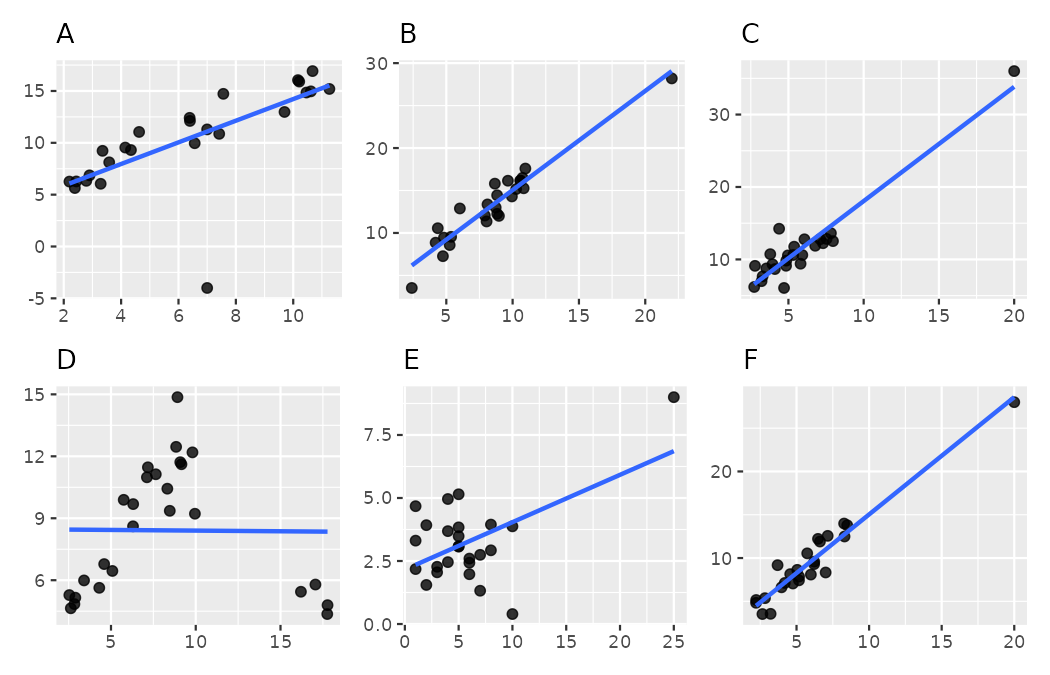
\includegraphics[width=0.85\linewidth,height=\textheight,keepaspectratio]{figures/model-slr-17.png}

\begin{tcolorbox}[enhanced jigsaw, left=2mm, leftrule=.75mm, title=\textcolor{quarto-callout-note-color}{\faInfo}\hspace{0.5em}{Worked example}, arc=.35mm, rightrule=.15mm, coltitle=black, colframe=quarto-callout-note-color-frame, bottomrule=.15mm, colbacktitle=quarto-callout-note-color!10!white, opacitybacktitle=0.6, breakable, bottomtitle=1mm, toptitle=1mm, titlerule=0mm, opacityback=0, toprule=.15mm, colback=white]

For each of panels A, B, and C (and the residual plot you imagine under
each), identify the outliers and note how they influence the least
squares line. Recall that an outlier is any point that does not appear
to belong with the vast majority of the other points.

\begin{center}\rule{0.5\linewidth}{0.5pt}\end{center}

A: There is one outlier far from the other points (in the \(y\)
direction, and it is an outlier of the bivariate model), though it only
appears to slightly influence the line: the slope with the point
included barely differs from the slope without it.

B: There is one outlier on the right (in the \(x\) and \(y\) direction,
although it is not an outlier of the bivariate model), though it is
quite close to the least squares line, which suggests it wasn't very
influential.

C: There is one point far away from the cloud (in the \(x\) and \(y\)
direction and an outlier of the bivariate model), and this outlier
appears to pull the least squares line up on the right; examine how the
line around the primary cloud does not appear to fit very well.

\end{tcolorbox}

\begin{tcolorbox}[enhanced jigsaw, left=2mm, leftrule=.75mm, title=\textcolor{quarto-callout-note-color}{\faInfo}\hspace{0.5em}{Worked example}, arc=.35mm, rightrule=.15mm, coltitle=black, colframe=quarto-callout-note-color-frame, bottomrule=.15mm, colbacktitle=quarto-callout-note-color!10!white, opacitybacktitle=0.6, breakable, bottomtitle=1mm, toptitle=1mm, titlerule=0mm, opacityback=0, toprule=.15mm, colback=white]

As you did in the previous example, for each of panels D, E, and F,
identify the outliers and note how they influence the least squares
line. A point can be outlying in the \(x\) direction, in the \(y\)
direction, or in relation to the bivariate model.

\begin{center}\rule{0.5\linewidth}{0.5pt}\end{center}

D: There is a primary cloud and then a small secondary cloud of four
outliers (with respect to both \(x\) and the bivariate model). The
secondary cloud appears to be influencing the line somewhat strongly,
making the least squares line fit poorly almost everywhere --- the clear
upward trend in the main cloud is flattened almost to zero. There might
be an interesting explanation for the dual clouds, which is something
that could be investigated: in scouting data, a secondary cloud is often
a different league, position, or data vendor.

E: There is no obvious trend in the main cloud of points, and the
outlier on the right (with respect to both \(x\) and \(y\)) appears to
largely (and problematically) control the slope of the least squares
line. The point creates a bivariate model when seemingly there is none.
Read this panel as a squad chart: \(x\) as substitute appearances and
\(y\) as goal contributions. The main cloud of squad players shows no
relationship at all --- and then one veteran super-sub, far to the
right, single-handedly manufactures the ``story'' that more bench
appearances produce more goals.

F: There is one outlier far from the cloud (with respect to both \(x\)
and \(y\)). However, it falls quite close to the least squares line and
does not appear to be very influential (it is not outlying with respect
to the bivariate model).

\end{tcolorbox}

Examine the imagined residual plots for the six panels. In panels C, D,
and E, you will probably find that there are a few observations which
are both away from the remaining points along the x-axis and not in the
trajectory of the trend in the rest of the data. In these cases, the
outliers influenced the slope of the least squares lines. In panel E,
the bulk of the data show no clear trend, but if we fit a line to these
data, we impose a trend where there isn't really one.

A good practice for dealing with outlying observations is to produce two
analyses: one with and one without the outlying observations. Presenting
both analyses to Marta --- ``here is the market with the super-sub, here
it is without him'' --- and discussing the role of the outlying
observations should lead you to a more holistic understanding of the
appropriate model for the data.

\begin{tcolorbox}[enhanced jigsaw, left=2mm, leftrule=.75mm, title=\textcolor{quarto-callout-important-color}{\faExclamation}\hspace{0.5em}{Leverage}, arc=.35mm, rightrule=.15mm, coltitle=black, colframe=quarto-callout-important-color-frame, bottomrule=.15mm, colbacktitle=quarto-callout-important-color!10!white, opacitybacktitle=0.6, breakable, bottomtitle=1mm, toptitle=1mm, titlerule=0mm, opacityback=0, toprule=.15mm, colback=white]

Points that fall horizontally away from the center of the cloud tend to
pull harder on the line, so we call them points with \textbf{high
leverage} or \textbf{leverage points}.

\end{tcolorbox}

Points that fall horizontally far from the line are points of high
leverage; these points can strongly influence the slope of the least
squares line. If one of these high leverage points does appear to
actually invoke its influence on the slope of the line --- as in panels
C, D, and E --- then we call it an \textbf{influential point}. Usually
we can say a point is influential if, had we fitted the line without it,
the influential point would have been unusually far from the least
squares line.

\begin{tcolorbox}[enhanced jigsaw, left=2mm, leftrule=.75mm, title=\textcolor{quarto-callout-important-color}{\faExclamation}\hspace{0.5em}{Types of outliers}, arc=.35mm, rightrule=.15mm, coltitle=black, colframe=quarto-callout-important-color-frame, bottomrule=.15mm, colbacktitle=quarto-callout-important-color!10!white, opacitybacktitle=0.6, breakable, bottomtitle=1mm, toptitle=1mm, titlerule=0mm, opacityback=0, toprule=.15mm, colback=white]

A point (or a group of points) that stands out from the rest of the data
is called an \textbf{outlier}. Outliers that fall horizontally away from
the center of the cloud of points are called leverage points. Outliers
that influence the slope of the line are called influential points.

\end{tcolorbox}

\begin{tcolorbox}[enhanced jigsaw, left=2mm, leftrule=.75mm, title=\textcolor{quarto-callout-tip-color}{\faLightbulb}\hspace{0.5em}{Check your understanding}, arc=.35mm, rightrule=.15mm, coltitle=black, colframe=quarto-callout-tip-color-frame, bottomrule=.15mm, colbacktitle=quarto-callout-tip-color!10!white, opacitybacktitle=0.6, breakable, bottomtitle=1mm, toptitle=1mm, titlerule=0mm, opacityback=0, toprule=.15mm, colback=white]

Priya's veteran-market survey spans ages 28 to 35. An agent now submits
a 39-year-old --- far to the right of every other age in the data ---
listed at a price far \emph{above} where the survey's downward trend
would land at that age. Does the point have high leverage? Would you
expect it to be influential? And how would your answers change if the
same 39-year-old had instead been listed close to the downward trend's
extension?

\begin{center}\rule{0.5\linewidth}{0.5pt}\end{center}

Sitting horizontally far from the center of the cloud, the point has
high leverage in either version. In the first version it also falls far
from the trajectory of the trend, so it would pull the slope up toward
itself --- a high-leverage point that exercises its leverage, which is
what we call an influential point. In the second version the point
remains high leverage but lands roughly where the line would have gone
anyway, so it would barely move the fit: leverage without influence,
like panels B and F of the gallery.

\end{tcolorbox}

One final shape belongs in the gallery, because scouts meet it
constantly: points that \emph{look} like outliers but are really the
model's failure. The code below --- continuing in the same seeded
session --- rebuilds the age--market-value cloud from the start of the
chapter and fits a straight line to it.

\begin{Shaded}
\begin{Highlighting}[]
\NormalTok{age\_cloud }\OtherTok{\textless{}{-}} \FunctionTok{tibble}\NormalTok{(}
  \AttributeTok{age =} \FunctionTok{runif}\NormalTok{(}\DecValTok{70}\NormalTok{, }\DecValTok{17}\NormalTok{, }\DecValTok{36}\NormalTok{),}
  \AttributeTok{value =} \DecValTok{20} \SpecialCharTok{{-}} \FloatTok{0.19} \SpecialCharTok{*}\NormalTok{ (age }\SpecialCharTok{{-}} \FloatTok{26.5}\NormalTok{)}\SpecialCharTok{\^{}}\DecValTok{2} \SpecialCharTok{+} \FunctionTok{rnorm}\NormalTok{(}\DecValTok{70}\NormalTok{, }\DecValTok{0}\NormalTok{, }\FloatTok{2.2}\NormalTok{)}
\NormalTok{)}

\FunctionTok{ggplot}\NormalTok{(age\_cloud, }\FunctionTok{aes}\NormalTok{(}\AttributeTok{x =}\NormalTok{ age, }\AttributeTok{y =}\NormalTok{ value)) }\SpecialCharTok{+}
  \FunctionTok{geom\_point}\NormalTok{(}\AttributeTok{size =} \DecValTok{2}\NormalTok{, }\AttributeTok{alpha =} \FloatTok{0.8}\NormalTok{) }\SpecialCharTok{+}
  \FunctionTok{geom\_smooth}\NormalTok{(}\AttributeTok{method =} \StringTok{"lm"}\NormalTok{, }\AttributeTok{se =} \ConstantTok{FALSE}\NormalTok{) }\SpecialCharTok{+}
  \FunctionTok{labs}\NormalTok{(}\AttributeTok{x =} \StringTok{"Age (years)"}\NormalTok{, }\AttributeTok{y =} \StringTok{"Market value (million euros)"}\NormalTok{)}
\end{Highlighting}
\end{Shaded}

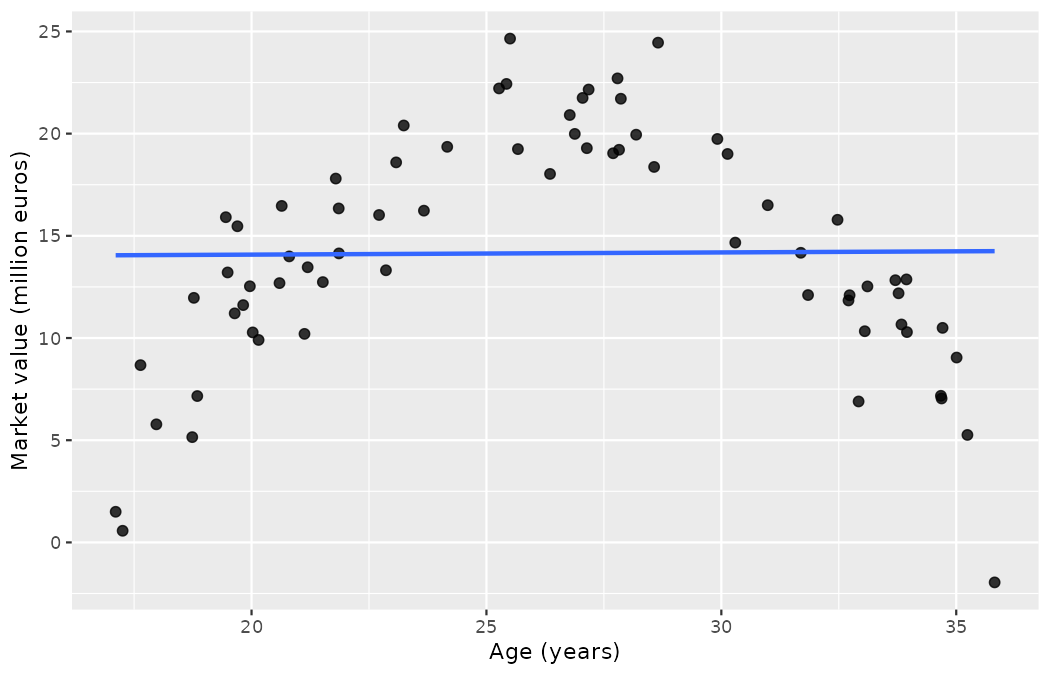
\includegraphics[width=0.85\linewidth,height=\textheight,keepaspectratio]{figures/model-slr-18.png}

The fitted line comes out nearly flat, and the under-20s and the 33-plus
players sit mostly below it --- on average about five million euros
below --- while the peak-age players sit above. It is tempting to flag
the extreme-age players as ``outliers'' and refit without them. Resist:
no individual point here is the problem. The relationship is curved, the
straight line is the wrong model, and deleting the ends of the age range
would simply hide the evidence. A residual plot exposes the arch
immediately, exactly as in the second panel of the residual-plot worked
example in Section~\ref{sec-resids}.

More generally, it is tempting to remove outliers. Don't do this without
a very good reason. Models that ignore exceptional (and interesting)
cases often perform poorly. A recruitment department that deleted its
super-subs, its freak seasons, and its late-blooming veterans --- the
``outliers'' --- would systematically misvalue exactly the players who
decide the biggest matches.

\section{Chapter review}\label{sec-chp7-review}

\subsection{Summary}\label{summary-6}

Throughout this chapter, the nuances of the linear model have been
described. You have learned how to create a linear model with
explanatory variables that are numerical (e.g., a team's accumulated
chance quality in a match) and those that are categorical (e.g., whether
a shot was a one-on-one). The residuals in a linear model are an
important metric used to understand how well a model fits --- and in
this book's running example they carry a scouting meaning of their own,
separating finishing from chance creation; high leverage points,
influential points, and other types of outliers can impact the fit of a
model. Correlation is a measure of the strength and direction of the
linear relationship of two variables, without specifying which variable
is the explanatory and which is the outcome. The least squares criterion
chooses the line minimizing the sum of squared residuals, its slope can
be recovered by hand from \(b_1 = (s_y/s_x)r,\) and \(R^2\) reports the
share of the outcome's variability the line explains. Everything here
described \emph{this sample} of data: future chapters will focus on
generalizing the linear model from the sample of data to claims about
the population of interest --- for the veteran market, from 50 listed
strikers to the whole market; for the World Cup, from one tournament to
the game at large.

\subsection{Terms}\label{terms-6}

The terms introduced in this chapter are presented below, alphabetized.
If you're not sure what some of these terms mean, we recommend you go
back in the text and review their definitions. You should be able to
easily spot them as \textbf{bolded text}.

\begin{longtable}[]{@{}
  >{\raggedright\arraybackslash}p{(\linewidth - 4\tabcolsep) * \real{0.3380}}
  >{\raggedright\arraybackslash}p{(\linewidth - 4\tabcolsep) * \real{0.3380}}
  >{\raggedright\arraybackslash}p{(\linewidth - 4\tabcolsep) * \real{0.3239}}@{}}
\caption{Terms introduced in this
chapter.}\label{tbl-terms-chp-07}\tabularnewline
\toprule\noalign{}
\endfirsthead
\endhead
\bottomrule\noalign{}
\endlastfoot
coefficient of determination & least squares line & regression sum of
squares \\
correlation & leverage point & residuals \\
extrapolation & outcome & R-squared \\
high leverage & outlier & sum of squared errors \\
indicator variable & predictor & total sum of squares \\
influential point & & \\
\end{longtable}

\section{Exercises}\label{sec-chp7-exercises}

Answers to odd-numbered exercises can be found in
Appendix~\ref{sec-exercise-solutions-07}.

\begin{enumerate}
\def\labelenumi{\arabic{enumi}.}
\item
  \textbf{Visualizing residuals.} The scatterplots shown below each have
  a superimposed regression line. Both are constructed scouting
  scenarios, built by the seeded code shown.\footnote{The
    \texttt{loan\_pool} data are a constructed scouting scenario,
    generated entirely by the seeded code shown.} If we were to
  construct a residual plot (residuals versus \(x\)) for each, describe
  in words what those plots would look like.

\begin{Shaded}
\begin{Highlighting}[]
\FunctionTok{set.seed}\NormalTok{(}\DecValTok{706}\NormalTok{)}
\NormalTok{loan\_pool }\OtherTok{\textless{}{-}} \FunctionTok{tibble}\NormalTok{(}
  \AttributeTok{minutes      =} \FunctionTok{seq}\NormalTok{(}\DecValTok{30}\NormalTok{, }\DecValTok{3000}\NormalTok{, }\AttributeTok{by =} \DecValTok{30}\NormalTok{),}
  \AttributeTok{ft\_passes    =} \FloatTok{0.05} \SpecialCharTok{*}\NormalTok{ minutes }\SpecialCharTok{+} \DecValTok{5} \SpecialCharTok{+} \FunctionTok{rnorm}\NormalTok{(}\DecValTok{100}\NormalTok{, }\AttributeTok{mean =} \DecValTok{0}\NormalTok{, }\AttributeTok{sd =} \DecValTok{20}\NormalTok{),}
  \AttributeTok{value        =} \FunctionTok{seq}\NormalTok{(}\FloatTok{0.5}\NormalTok{, }\DecValTok{50}\NormalTok{, }\AttributeTok{by =} \FloatTok{0.5}\NormalTok{),}
  \AttributeTok{asking\_price =} \FloatTok{1.2} \SpecialCharTok{*}\NormalTok{ value }\SpecialCharTok{+} \DecValTok{2} \SpecialCharTok{+}
    \FunctionTok{rnorm}\NormalTok{(}\DecValTok{100}\NormalTok{, }\AttributeTok{mean =} \DecValTok{0}\NormalTok{, }\AttributeTok{sd =} \FunctionTok{sort}\NormalTok{(}\FloatTok{0.9} \SpecialCharTok{*}\NormalTok{ value, }\AttributeTok{decreasing =} \ConstantTok{TRUE}\NormalTok{))}
\NormalTok{)}

\NormalTok{p\_1 }\OtherTok{\textless{}{-}} \FunctionTok{ggplot}\NormalTok{(loan\_pool, }\FunctionTok{aes}\NormalTok{(}\AttributeTok{x =}\NormalTok{ minutes, }\AttributeTok{y =}\NormalTok{ ft\_passes)) }\SpecialCharTok{+}
  \FunctionTok{geom\_point}\NormalTok{(}\AttributeTok{size =} \DecValTok{2}\NormalTok{, }\AttributeTok{alpha =} \FloatTok{0.8}\NormalTok{) }\SpecialCharTok{+}
  \FunctionTok{geom\_smooth}\NormalTok{(}\AttributeTok{method =} \StringTok{"lm"}\NormalTok{, }\AttributeTok{se =} \ConstantTok{FALSE}\NormalTok{) }\SpecialCharTok{+}
  \FunctionTok{labs}\NormalTok{(}\AttributeTok{x =} \StringTok{"League minutes played"}\NormalTok{, }\AttributeTok{y =} \StringTok{"Final{-}third passes"}\NormalTok{, }\AttributeTok{title =} \StringTok{"(a)"}\NormalTok{)}

\NormalTok{p\_2 }\OtherTok{\textless{}{-}} \FunctionTok{ggplot}\NormalTok{(loan\_pool, }\FunctionTok{aes}\NormalTok{(}\AttributeTok{x =}\NormalTok{ value, }\AttributeTok{y =}\NormalTok{ asking\_price)) }\SpecialCharTok{+}
  \FunctionTok{geom\_point}\NormalTok{(}\AttributeTok{size =} \DecValTok{2}\NormalTok{, }\AttributeTok{alpha =} \FloatTok{0.8}\NormalTok{) }\SpecialCharTok{+}
  \FunctionTok{geom\_smooth}\NormalTok{(}\AttributeTok{method =} \StringTok{"lm"}\NormalTok{, }\AttributeTok{se =} \ConstantTok{FALSE}\NormalTok{) }\SpecialCharTok{+}
  \FunctionTok{labs}\NormalTok{(}\AttributeTok{x =} \StringTok{"Market value (million euros)"}\NormalTok{, }\AttributeTok{y =} \StringTok{"Asking price (million euros)"}\NormalTok{, }\AttributeTok{title =} \StringTok{"(b)"}\NormalTok{)}

\NormalTok{p\_1 }\SpecialCharTok{+}\NormalTok{ p\_2}
\end{Highlighting}
\end{Shaded}

  Panel (a) shows final-third passes rising steadily with league
  minutes, with points spread evenly around the line along the whole
  range. Panel (b) shows asking prices rising with market value, but the
  points swing wildly around the line at the cheap end of the market and
  hug it tightly for the most valuable players.
\item
  \textbf{Trends in residuals.} Shown below are two plots of residuals
  remaining after fitting a linear model to two different sets of
  constructed data.\footnote{The \texttt{fee\_fit} data are a
    constructed scouting scenario, generated entirely by the seeded code
    shown.} For each plot, describe important features and determine if
  a linear model would be appropriate for these data. Explain your
  reasoning.

\begin{Shaded}
\begin{Highlighting}[]
\FunctionTok{set.seed}\NormalTok{(}\DecValTok{707}\NormalTok{)}
\NormalTok{fee\_fit }\OtherTok{\textless{}{-}} \FunctionTok{tibble}\NormalTok{(}
  \AttributeTok{x     =} \DecValTok{1}\SpecialCharTok{:}\DecValTok{300}\NormalTok{,}
  \AttributeTok{y\_fan =} \DecValTok{4} \SpecialCharTok{*}\NormalTok{ x }\SpecialCharTok{+} \DecValTok{5} \SpecialCharTok{+} \FunctionTok{rnorm}\NormalTok{(}\DecValTok{300}\NormalTok{, }\AttributeTok{mean =} \DecValTok{0}\NormalTok{, }\AttributeTok{sd =} \FunctionTok{sort}\NormalTok{(}\FloatTok{1.3} \SpecialCharTok{*}\NormalTok{ x)),}
  \AttributeTok{y\_log =} \FunctionTok{log}\NormalTok{(x) }\SpecialCharTok{+} \FunctionTok{rnorm}\NormalTok{(}\DecValTok{300}\NormalTok{, }\AttributeTok{mean =} \DecValTok{0}\NormalTok{, }\AttributeTok{sd =} \FloatTok{0.5}\NormalTok{)}
\NormalTok{)}

\NormalTok{m\_fan }\OtherTok{\textless{}{-}} \FunctionTok{lm}\NormalTok{(y\_fan }\SpecialCharTok{\textasciitilde{}}\NormalTok{ x, }\AttributeTok{data =}\NormalTok{ fee\_fit)}
\NormalTok{m\_log }\OtherTok{\textless{}{-}} \FunctionTok{lm}\NormalTok{(y\_log }\SpecialCharTok{\textasciitilde{}}\NormalTok{ x, }\AttributeTok{data =}\NormalTok{ fee\_fit)}

\NormalTok{p\_1 }\OtherTok{\textless{}{-}} \FunctionTok{tibble}\NormalTok{(}\AttributeTok{fitted =} \FunctionTok{fitted}\NormalTok{(m\_fan), }\AttributeTok{residual =} \FunctionTok{resid}\NormalTok{(m\_fan)) }\SpecialCharTok{|\textgreater{}}
  \FunctionTok{ggplot}\NormalTok{(}\FunctionTok{aes}\NormalTok{(}\AttributeTok{x =}\NormalTok{ fitted, }\AttributeTok{y =}\NormalTok{ residual)) }\SpecialCharTok{+}
  \FunctionTok{geom\_point}\NormalTok{(}\AttributeTok{size =} \DecValTok{2}\NormalTok{, }\AttributeTok{alpha =} \FloatTok{0.8}\NormalTok{) }\SpecialCharTok{+}
  \FunctionTok{geom\_hline}\NormalTok{(}\AttributeTok{yintercept =} \DecValTok{0}\NormalTok{, }\AttributeTok{linetype =} \StringTok{"dashed"}\NormalTok{) }\SpecialCharTok{+}
  \FunctionTok{labs}\NormalTok{(}\AttributeTok{x =} \StringTok{"Predicted transfer fee (thousand euros)"}\NormalTok{, }\AttributeTok{y =} \StringTok{"Residuals"}\NormalTok{, }\AttributeTok{title =} \StringTok{"(a)"}\NormalTok{)}

\NormalTok{p\_2 }\OtherTok{\textless{}{-}} \FunctionTok{tibble}\NormalTok{(}\AttributeTok{fitted =} \FunctionTok{fitted}\NormalTok{(m\_log), }\AttributeTok{residual =} \FunctionTok{resid}\NormalTok{(m\_log)) }\SpecialCharTok{|\textgreater{}}
  \FunctionTok{ggplot}\NormalTok{(}\FunctionTok{aes}\NormalTok{(}\AttributeTok{x =}\NormalTok{ fitted, }\AttributeTok{y =}\NormalTok{ residual)) }\SpecialCharTok{+}
  \FunctionTok{geom\_point}\NormalTok{(}\AttributeTok{size =} \DecValTok{2}\NormalTok{, }\AttributeTok{alpha =} \FloatTok{0.8}\NormalTok{) }\SpecialCharTok{+}
  \FunctionTok{geom\_hline}\NormalTok{(}\AttributeTok{yintercept =} \DecValTok{0}\NormalTok{, }\AttributeTok{linetype =} \StringTok{"dashed"}\NormalTok{) }\SpecialCharTok{+}
  \FunctionTok{labs}\NormalTok{(}\AttributeTok{x =} \StringTok{"Predicted technique rating"}\NormalTok{, }\AttributeTok{y =} \StringTok{"Residuals"}\NormalTok{, }\AttributeTok{title =} \StringTok{"(b)"}\NormalTok{)}

\NormalTok{p\_1 }\SpecialCharTok{+}\NormalTok{ p\_2}
\end{Highlighting}
\end{Shaded}

  In panel (a) the residuals form a fan: tight around zero on the left,
  spreading to roughly twice the vertical range on the right. In panel
  (b) the residuals arch: below zero at both ends of the fitted range
  and above zero in the middle.
\item
  \textbf{Identify relationships, I.} Priya Rao pulled six variable
  pairs from the club's databases and, to keep the focus on shape, hid
  the axis labels. For each of the six plots, identify the strength of
  the relationship (e.g., weak, moderate, or strong) in the data and
  whether fitting a linear model would be reasonable.\footnote{The
    \texttt{panels\_1} and \texttt{panels\_2} data are constructed,
    generated entirely by the seeded code shown.}

\begin{Shaded}
\begin{Highlighting}[]
\FunctionTok{set.seed}\NormalTok{(}\DecValTok{708}\NormalTok{)}
\NormalTok{panels\_1 }\OtherTok{\textless{}{-}} \FunctionTok{tibble}\NormalTok{(}
  \AttributeTok{x =} \FunctionTok{seq}\NormalTok{(}\DecValTok{0}\NormalTok{, }\DecValTok{6}\NormalTok{, }\AttributeTok{by =} \FloatTok{0.05}\NormalTok{),}
  \AttributeTok{a =}\NormalTok{ (x }\SpecialCharTok{{-}} \DecValTok{3}\NormalTok{)}\SpecialCharTok{\^{}}\DecValTok{2} \SpecialCharTok{{-}} \DecValTok{4} \SpecialCharTok{+} \FunctionTok{rnorm}\NormalTok{(}\FunctionTok{length}\NormalTok{(x), }\AttributeTok{mean =} \DecValTok{0}\NormalTok{, }\AttributeTok{sd =} \DecValTok{1}\NormalTok{),}
  \AttributeTok{b =} \DecValTok{3} \SpecialCharTok{*}\NormalTok{ x }\SpecialCharTok{+} \DecValTok{10} \SpecialCharTok{+} \FunctionTok{rnorm}\NormalTok{(}\FunctionTok{length}\NormalTok{(x), }\AttributeTok{mean =} \DecValTok{0}\NormalTok{, }\AttributeTok{sd =} \DecValTok{2}\NormalTok{),}
  \AttributeTok{c =} \DecValTok{3} \SpecialCharTok{*}\NormalTok{ x }\SpecialCharTok{+} \DecValTok{10} \SpecialCharTok{+} \FunctionTok{rnorm}\NormalTok{(}\FunctionTok{length}\NormalTok{(x), }\AttributeTok{mean =} \DecValTok{0}\NormalTok{, }\AttributeTok{sd =} \DecValTok{20}\NormalTok{)}
\NormalTok{)}
\NormalTok{panels\_2 }\OtherTok{\textless{}{-}} \FunctionTok{tibble}\NormalTok{(}
  \AttributeTok{x =} \FunctionTok{seq}\NormalTok{(}\SpecialCharTok{{-}}\DecValTok{8}\NormalTok{, }\SpecialCharTok{{-}}\DecValTok{2}\NormalTok{, }\AttributeTok{by =} \FloatTok{0.05}\NormalTok{),}
  \AttributeTok{d =} \SpecialCharTok{{-}}\DecValTok{1} \SpecialCharTok{*}\NormalTok{ (x }\SpecialCharTok{+} \DecValTok{5}\NormalTok{)}\SpecialCharTok{\^{}}\DecValTok{2} \SpecialCharTok{+} \DecValTok{1} \SpecialCharTok{+} \FunctionTok{rnorm}\NormalTok{(}\FunctionTok{length}\NormalTok{(x), }\AttributeTok{mean =} \DecValTok{0}\NormalTok{, }\AttributeTok{sd =} \DecValTok{2}\NormalTok{),}
  \AttributeTok{e =} \SpecialCharTok{{-}}\DecValTok{5} \SpecialCharTok{*}\NormalTok{ x }\SpecialCharTok{+} \DecValTok{3} \SpecialCharTok{+} \FunctionTok{rnorm}\NormalTok{(}\FunctionTok{length}\NormalTok{(x), }\AttributeTok{mean =} \DecValTok{0}\NormalTok{, }\AttributeTok{sd =} \DecValTok{2}\NormalTok{),}
  \AttributeTok{f =} \FunctionTok{rnorm}\NormalTok{(}\FunctionTok{length}\NormalTok{(x), }\AttributeTok{mean =} \DecValTok{0}\NormalTok{, }\AttributeTok{sd =} \DecValTok{10}\NormalTok{)}
\NormalTok{)}
\CommentTok{\# Plot each column against x with hidden axis text, labeling the}
\CommentTok{\# panels (a) through (f).}
\end{Highlighting}
\end{Shaded}

  Panel (a) is a clear U-shape; panel (b) is a tight rising band; panel
  (c) rises but with heavy scatter; panel (d) is a clear arch (rising
  then falling); panel (e) is a tight falling band; panel (f) is a
  formless cloud.
\item
  \textbf{Identify relationships, II.} For each of the six plots ---
  another of Priya's hidden-axis training exhibits --- identify the
  strength of the relationship (e.g., weak, moderate, or strong) in the
  data and whether fitting a linear model would be
  reasonable.\footnote{The \texttt{panels\_3} data are constructed,
    generated entirely by the seeded code shown.}

\begin{Shaded}
\begin{Highlighting}[]
\FunctionTok{set.seed}\NormalTok{(}\DecValTok{709}\NormalTok{)}
\NormalTok{panels\_3 }\OtherTok{\textless{}{-}} \FunctionTok{tibble}\NormalTok{(}
  \AttributeTok{x =} \FunctionTok{seq}\NormalTok{(}\SpecialCharTok{{-}}\DecValTok{3}\NormalTok{, }\DecValTok{4}\NormalTok{, }\AttributeTok{by =} \FloatTok{0.05}\NormalTok{),}
  \AttributeTok{a =} \SpecialCharTok{{-}}\FloatTok{0.5} \SpecialCharTok{*}\NormalTok{ x}\SpecialCharTok{\^{}}\DecValTok{3} \SpecialCharTok{+}\NormalTok{ x}\SpecialCharTok{\^{}}\DecValTok{2} \SpecialCharTok{+}\NormalTok{ x }\SpecialCharTok{+} \FunctionTok{rnorm}\NormalTok{(}\FunctionTok{length}\NormalTok{(x), }\AttributeTok{mean =} \DecValTok{0}\NormalTok{, }\AttributeTok{sd =} \DecValTok{2}\NormalTok{),}
  \AttributeTok{b =} \DecValTok{2} \SpecialCharTok{*}\NormalTok{ x}\SpecialCharTok{\^{}}\DecValTok{4} \SpecialCharTok{+} \SpecialCharTok{{-}}\FloatTok{0.5} \SpecialCharTok{*}\NormalTok{ x}\SpecialCharTok{\^{}}\DecValTok{3} \SpecialCharTok{+}\NormalTok{ x}\SpecialCharTok{\^{}}\DecValTok{2} \SpecialCharTok{+}\NormalTok{ x }\SpecialCharTok{+} \FunctionTok{rnorm}\NormalTok{(}\FunctionTok{length}\NormalTok{(x), }\AttributeTok{mean =} \DecValTok{0}\NormalTok{, }\AttributeTok{sd =} \DecValTok{30}\NormalTok{),}
  \AttributeTok{c =} \DecValTok{3} \SpecialCharTok{*}\NormalTok{ x }\SpecialCharTok{+} \FunctionTok{rnorm}\NormalTok{(}\FunctionTok{length}\NormalTok{(x), }\AttributeTok{mean =} \DecValTok{0}\NormalTok{, }\AttributeTok{sd =} \DecValTok{2}\NormalTok{),}
  \AttributeTok{d =} \DecValTok{3} \SpecialCharTok{*}\NormalTok{ x }\SpecialCharTok{+} \FunctionTok{rnorm}\NormalTok{(}\FunctionTok{length}\NormalTok{(x), }\AttributeTok{mean =} \DecValTok{0}\NormalTok{, }\AttributeTok{sd =} \DecValTok{20}\NormalTok{),}
  \AttributeTok{e =} \SpecialCharTok{{-}}\DecValTok{3} \SpecialCharTok{*}\NormalTok{ x }\SpecialCharTok{+} \FunctionTok{rnorm}\NormalTok{(}\FunctionTok{length}\NormalTok{(x), }\AttributeTok{mean =} \DecValTok{0}\NormalTok{, }\AttributeTok{sd =} \DecValTok{10}\NormalTok{),}
  \AttributeTok{f =} \SpecialCharTok{{-}}\DecValTok{3} \SpecialCharTok{*}\NormalTok{ x }\SpecialCharTok{+} \FunctionTok{rnorm}\NormalTok{(}\FunctionTok{length}\NormalTok{(x), }\AttributeTok{mean =} \DecValTok{0}\NormalTok{, }\AttributeTok{sd =} \DecValTok{5}\NormalTok{)}
\NormalTok{)}
\CommentTok{\# Plot each column against x with hidden axis text, labeling the}
\CommentTok{\# panels (a) through (f).}
\end{Highlighting}
\end{Shaded}

  Panel (a) is an S-shaped curve falling at the right; panel (b) is a
  steep-sided valley (flat in the middle, shooting up at both ends,
  higher on the right); panel (c) is a tight rising band; panel (d)
  rises faintly through heavy scatter; panel (e) falls through heavy
  scatter; panel (f) is a moderately tight falling band.
\item
  \textbf{Trial days and the final grade.} The two scatterplots below
  show the relationship between the final academy grade and two
  trial-day assessments (an autumn technical test and a spring technical
  test) recorded for 233 trialists in Jonas Beck's academy intake
  archive. This is a constructed scenario, built by the seeded code
  below.\footnote{The \texttt{academy233} data are a constructed
    scouting scenario, generated entirely by the seeded code shown; no
    real trialists were graded.}

\begin{Shaded}
\begin{Highlighting}[]
\FunctionTok{set.seed}\NormalTok{(}\DecValTok{710}\NormalTok{)}
\NormalTok{academy233 }\OtherTok{\textless{}{-}} \FunctionTok{tibble}\NormalTok{(}
  \AttributeTok{final\_grade  =} \FunctionTok{pmin}\NormalTok{(}\DecValTok{100}\NormalTok{, }\FunctionTok{pmax}\NormalTok{(}\DecValTok{40}\NormalTok{, }\FunctionTok{rnorm}\NormalTok{(}\DecValTok{233}\NormalTok{, }\AttributeTok{mean =} \DecValTok{70}\NormalTok{, }\AttributeTok{sd =} \DecValTok{10}\NormalTok{))),}
  \AttributeTok{autumn\_grade =} \FunctionTok{pmin}\NormalTok{(}\DecValTok{100}\NormalTok{, }\DecValTok{100} \SpecialCharTok{{-}} \FloatTok{0.014} \SpecialCharTok{*}\NormalTok{ (}\DecValTok{100} \SpecialCharTok{{-}}\NormalTok{ final\_grade)}\SpecialCharTok{\^{}}\DecValTok{2} \SpecialCharTok{+} \FunctionTok{rnorm}\NormalTok{(}\DecValTok{233}\NormalTok{, }\AttributeTok{mean =} \DecValTok{0}\NormalTok{, }\AttributeTok{sd =} \DecValTok{8}\NormalTok{)),}
  \AttributeTok{spring\_grade =} \FunctionTok{pmin}\NormalTok{(}\DecValTok{100}\NormalTok{, }\FunctionTok{pmax}\NormalTok{(}\DecValTok{35}\NormalTok{, final\_grade }\SpecialCharTok{+} \FunctionTok{rnorm}\NormalTok{(}\DecValTok{233}\NormalTok{, }\AttributeTok{mean =} \DecValTok{0}\NormalTok{, }\AttributeTok{sd =} \DecValTok{5}\NormalTok{)))}
\NormalTok{)}

\NormalTok{p\_1 }\OtherTok{\textless{}{-}} \FunctionTok{ggplot}\NormalTok{(academy233, }\FunctionTok{aes}\NormalTok{(}\AttributeTok{x =}\NormalTok{ autumn\_grade, }\AttributeTok{y =}\NormalTok{ final\_grade)) }\SpecialCharTok{+}
  \FunctionTok{geom\_point}\NormalTok{(}\AttributeTok{size =} \DecValTok{2}\NormalTok{, }\AttributeTok{alpha =} \FloatTok{0.8}\NormalTok{) }\SpecialCharTok{+}
  \FunctionTok{labs}\NormalTok{(}\AttributeTok{x =} \StringTok{"Autumn test grade"}\NormalTok{, }\AttributeTok{y =} \StringTok{"Final academy grade"}\NormalTok{)}

\NormalTok{p\_2 }\OtherTok{\textless{}{-}} \FunctionTok{ggplot}\NormalTok{(academy233, }\FunctionTok{aes}\NormalTok{(}\AttributeTok{x =}\NormalTok{ spring\_grade, }\AttributeTok{y =}\NormalTok{ final\_grade)) }\SpecialCharTok{+}
  \FunctionTok{geom\_point}\NormalTok{(}\AttributeTok{size =} \DecValTok{2}\NormalTok{, }\AttributeTok{alpha =} \FloatTok{0.8}\NormalTok{) }\SpecialCharTok{+}
  \FunctionTok{labs}\NormalTok{(}\AttributeTok{x =} \StringTok{"Spring test grade"}\NormalTok{, }\AttributeTok{y =} \StringTok{"Final academy grade"}\NormalTok{)}

\NormalTok{p\_1 }\SpecialCharTok{+}\NormalTok{ p\_2}
\end{Highlighting}
\end{Shaded}

  Both panels show rising clouds. The spring-test panel is visibly
  tighter around a straight line, while the autumn-test panel is more
  diffuse and bends slightly at the lower grades.

  \begin{enumerate}
  \def\labelenumii{\alph{enumii}.}
  \item
    Based on these graphs, which of the two trial-day tests has the
    strongest correlation with the final academy grade? Explain.
  \item
    Can you think of a reason why the correlation between the test you
    chose in part (a) and the final grade is higher?
  \end{enumerate}
\item
  \textbf{Matches attended and what they buy.} Priya assembled a
  constructed registry of 175 regional scouts. For each scout it records
  the number of matches attended live last season, an
  evaluation-accuracy score (0--100 agreement with the club's expert
  panel), and total scouting travel (in thousands of km). The
  scatterplot on the left shows the accuracy score plotted against
  matches attended; the scatterplot on the right shows travel distance
  plotted against matches attended.\footnote{The \texttt{scout\_reg}
    data are a constructed scouting scenario, generated entirely by the
    seeded code shown.}

\begin{Shaded}
\begin{Highlighting}[]
\FunctionTok{set.seed}\NormalTok{(}\DecValTok{711}\NormalTok{)}
\NormalTok{scout\_reg }\OtherTok{\textless{}{-}} \FunctionTok{tibble}\NormalTok{(}
  \AttributeTok{matches\_live =} \FunctionTok{round}\NormalTok{(}\FunctionTok{runif}\NormalTok{(}\DecValTok{175}\NormalTok{, }\DecValTok{15}\NormalTok{, }\DecValTok{120}\NormalTok{)),}
  \AttributeTok{accuracy     =} \DecValTok{30} \SpecialCharTok{+} \DecValTok{12} \SpecialCharTok{*} \FunctionTok{log}\NormalTok{(matches\_live) }\SpecialCharTok{+} \FunctionTok{rnorm}\NormalTok{(}\DecValTok{175}\NormalTok{, }\AttributeTok{mean =} \DecValTok{0}\NormalTok{, }\AttributeTok{sd =} \DecValTok{4}\NormalTok{),}
  \AttributeTok{travel\_km    =} \FloatTok{0.14} \SpecialCharTok{*}\NormalTok{ matches\_live }\SpecialCharTok{+} \FunctionTok{rnorm}\NormalTok{(}\DecValTok{175}\NormalTok{, }\AttributeTok{mean =} \DecValTok{0}\NormalTok{, }\AttributeTok{sd =} \FloatTok{1.5}\NormalTok{)}
\NormalTok{)}

\NormalTok{p\_1 }\OtherTok{\textless{}{-}} \FunctionTok{ggplot}\NormalTok{(scout\_reg, }\FunctionTok{aes}\NormalTok{(}\AttributeTok{x =}\NormalTok{ matches\_live, }\AttributeTok{y =}\NormalTok{ accuracy)) }\SpecialCharTok{+}
  \FunctionTok{geom\_point}\NormalTok{(}\AttributeTok{alpha =} \FloatTok{0.8}\NormalTok{) }\SpecialCharTok{+}
  \FunctionTok{labs}\NormalTok{(}\AttributeTok{x =} \StringTok{"Matches attended live"}\NormalTok{, }\AttributeTok{y =} \StringTok{"Evaluation accuracy score"}\NormalTok{)}

\NormalTok{p\_2 }\OtherTok{\textless{}{-}} \FunctionTok{ggplot}\NormalTok{(scout\_reg, }\FunctionTok{aes}\NormalTok{(}\AttributeTok{x =}\NormalTok{ matches\_live, }\AttributeTok{y =}\NormalTok{ travel\_km)) }\SpecialCharTok{+}
  \FunctionTok{geom\_point}\NormalTok{(}\AttributeTok{alpha =} \FloatTok{0.8}\NormalTok{) }\SpecialCharTok{+}
  \FunctionTok{labs}\NormalTok{(}\AttributeTok{x =} \StringTok{"Matches attended live"}\NormalTok{, }\AttributeTok{y =} \StringTok{"Scouting travel (thousand km)"}\NormalTok{)}

\NormalTok{p\_1 }\SpecialCharTok{+}\NormalTok{ p\_2}
\end{Highlighting}
\end{Shaded}

  The left panel climbs steeply among scouts attending few matches and
  then levels off --- the gains flatten past roughly 60 matches. The
  right panel is a tight, straight, rising band.

  \begin{enumerate}
  \def\labelenumii{\alph{enumii}.}
  \item
    Describe the relationship between matches attended and evaluation
    accuracy.
  \item
    Describe the relationship between matches attended and scouting
    travel.
  \item
    Which plot shows a stronger correlation? Explain your reasoning.
  \item
    Travel distances were originally recorded in kilometers. How would
    the plots above and the correlation values change if the travel
    variable were converted to miles?
  \end{enumerate}
\item
  \textbf{Match the correlation, I.} Match each correlation to the
  corresponding scatterplot from Priya's hidden-axis gallery.\footnote{The
    \texttt{corr\_panels} data are constructed, generated entirely by
    the seeded code shown.}

\begin{Shaded}
\begin{Highlighting}[]
\FunctionTok{set.seed}\NormalTok{(}\DecValTok{712}\NormalTok{)}
\NormalTok{corr\_panels }\OtherTok{\textless{}{-}} \FunctionTok{tibble}\NormalTok{(}
  \AttributeTok{x  =} \FunctionTok{runif}\NormalTok{(}\DecValTok{75}\NormalTok{, }\DecValTok{0}\NormalTok{, }\DecValTok{10}\NormalTok{),}
  \AttributeTok{y1 =} \FloatTok{0.05} \SpecialCharTok{*}\NormalTok{ x }\SpecialCharTok{+} \FunctionTok{rnorm}\NormalTok{(}\DecValTok{75}\NormalTok{, }\AttributeTok{mean =} \DecValTok{0}\NormalTok{, }\AttributeTok{sd =} \FloatTok{2.5}\NormalTok{),}
  \AttributeTok{y2 =} \FloatTok{1.5} \SpecialCharTok{*}\NormalTok{ x }\SpecialCharTok{+} \FunctionTok{rnorm}\NormalTok{(}\DecValTok{75}\NormalTok{, }\AttributeTok{mean =} \DecValTok{0}\NormalTok{, }\AttributeTok{sd =} \FloatTok{1.8}\NormalTok{),}
  \AttributeTok{y3 =} \FloatTok{0.8} \SpecialCharTok{*}\NormalTok{ x }\SpecialCharTok{+} \FunctionTok{rnorm}\NormalTok{(}\DecValTok{75}\NormalTok{, }\AttributeTok{mean =} \DecValTok{0}\NormalTok{, }\AttributeTok{sd =} \FloatTok{4.6}\NormalTok{),}
  \AttributeTok{y4 =} \SpecialCharTok{{-}}\FloatTok{1.2} \SpecialCharTok{*}\NormalTok{ x }\SpecialCharTok{+} \FunctionTok{rnorm}\NormalTok{(}\DecValTok{75}\NormalTok{, }\AttributeTok{mean =} \DecValTok{0}\NormalTok{, }\AttributeTok{sd =} \FloatTok{3.5}\NormalTok{)}
\NormalTok{)}
\CommentTok{\# Plot y1 through y4 against x with hidden axis text, labeling the}
\CommentTok{\# panels (1) through (4).}
\end{Highlighting}
\end{Shaded}

  Panel (1) is a formless cloud with the faintest upward drift; panel
  (2) is a tight rising band; panel (3) rises through substantial
  scatter; panel (4) falls through moderate scatter.

  \begin{enumerate}
  \def\labelenumii{\alph{enumii}.}
  \item
    \(r = -0.73\)
  \item
    \(r = 0.41\)
  \item
    \(r = 0.13\)
  \item
    \(r = 0.92\)
  \end{enumerate}
\item
  \textbf{Match the correlation, II.} Match each correlation to the
  corresponding scatterplot from the same gallery.\footnote{The
    \texttt{corr\_panels\_2} data are constructed, generated entirely by
    the seeded code shown.}

\begin{Shaded}
\begin{Highlighting}[]
\FunctionTok{set.seed}\NormalTok{(}\DecValTok{713}\NormalTok{)}
\NormalTok{corr\_panels\_2 }\OtherTok{\textless{}{-}} \FunctionTok{tibble}\NormalTok{(}
  \AttributeTok{x  =} \FunctionTok{runif}\NormalTok{(}\DecValTok{75}\NormalTok{, }\DecValTok{0}\NormalTok{, }\DecValTok{10}\NormalTok{),}
  \AttributeTok{y5 =} \SpecialCharTok{{-}}\FloatTok{0.8} \SpecialCharTok{*}\NormalTok{ x }\SpecialCharTok{+} \FunctionTok{rnorm}\NormalTok{(}\DecValTok{75}\NormalTok{, }\AttributeTok{mean =} \DecValTok{0}\NormalTok{, }\AttributeTok{sd =} \FloatTok{4.7}\NormalTok{),}
  \AttributeTok{y6 =} \FloatTok{0.85} \SpecialCharTok{*}\NormalTok{ x }\SpecialCharTok{+} \FunctionTok{rnorm}\NormalTok{(}\DecValTok{75}\NormalTok{, }\AttributeTok{mean =} \DecValTok{0}\NormalTok{, }\AttributeTok{sd =} \FloatTok{4.4}\NormalTok{),}
  \AttributeTok{y7 =} \SpecialCharTok{{-}}\FloatTok{1.5} \SpecialCharTok{*}\NormalTok{ x }\SpecialCharTok{+} \FunctionTok{rnorm}\NormalTok{(}\DecValTok{75}\NormalTok{, }\AttributeTok{mean =} \DecValTok{0}\NormalTok{, }\AttributeTok{sd =} \FloatTok{2.7}\NormalTok{),}
  \AttributeTok{y8 =} \FloatTok{0.01} \SpecialCharTok{*}\NormalTok{ x }\SpecialCharTok{+} \FunctionTok{rnorm}\NormalTok{(}\DecValTok{75}\NormalTok{, }\AttributeTok{mean =} \DecValTok{0}\NormalTok{, }\AttributeTok{sd =} \DecValTok{3}\NormalTok{)}
\NormalTok{)}
\CommentTok{\# Plot y5 through y8 against x with hidden axis text, labeling the}
\CommentTok{\# panels (1) through (4).}
\end{Highlighting}
\end{Shaded}

  Panel (1) falls through heavy scatter; panel (2) rises through
  moderate scatter; panel (3) is a fairly tight falling band; panel (4)
  is a formless cloud.

  \begin{enumerate}
  \def\labelenumii{\alph{enumii}.}
  \item
    \(r = 0.65\)
  \item
    \(r = -0.35\)
  \item
    \(r = 0.03\)
  \item
    \(r = -0.89\)
  \end{enumerate}
\item
  \textbf{Combine measurements, correlation.} Northbridge's medical
  screening database records body measurements for 507 U17 regional
  trialists assessed by the club's physiologists at the academy's
  screening days. The scatterplot below shows the relationship between
  height and shoulder girth (circumference of shoulders measured over
  deltoid muscles), both measured in centimeters. This is a constructed
  scenario, built by the seeded code below.\footnote{The
    \texttt{combine507} data are a constructed scouting scenario,
    generated entirely by the seeded code shown; no real trialists were
    measured.}

\begin{Shaded}
\begin{Highlighting}[]
\FunctionTok{set.seed}\NormalTok{(}\DecValTok{714}\NormalTok{)}
\NormalTok{combine507 }\OtherTok{\textless{}{-}} \FunctionTok{tibble}\NormalTok{(}
  \AttributeTok{shoulder\_girth =} \FunctionTok{round}\NormalTok{(}\FunctionTok{rnorm}\NormalTok{(}\DecValTok{507}\NormalTok{, }\AttributeTok{mean =} \DecValTok{107}\NormalTok{, }\AttributeTok{sd =} \DecValTok{10}\NormalTok{), }\DecValTok{1}\NormalTok{),}
  \AttributeTok{height         =} \FunctionTok{round}\NormalTok{(}\DecValTok{171} \SpecialCharTok{+} \FloatTok{0.61} \SpecialCharTok{*}\NormalTok{ (shoulder\_girth }\SpecialCharTok{{-}} \DecValTok{107}\NormalTok{) }\SpecialCharTok{+} \FunctionTok{rnorm}\NormalTok{(}\DecValTok{507}\NormalTok{, }\AttributeTok{mean =} \DecValTok{0}\NormalTok{, }\AttributeTok{sd =} \DecValTok{7}\NormalTok{), }\DecValTok{1}\NormalTok{)}
\NormalTok{)}

\FunctionTok{ggplot}\NormalTok{(combine507, }\FunctionTok{aes}\NormalTok{(}\AttributeTok{x =}\NormalTok{ shoulder\_girth, }\AttributeTok{y =}\NormalTok{ height)) }\SpecialCharTok{+}
  \FunctionTok{geom\_point}\NormalTok{(}\AttributeTok{size =} \DecValTok{2}\NormalTok{, }\AttributeTok{alpha =} \FloatTok{0.8}\NormalTok{) }\SpecialCharTok{+}
  \FunctionTok{labs}\NormalTok{(}\AttributeTok{x =} \StringTok{"Shoulder girth (cm)"}\NormalTok{, }\AttributeTok{y =} \StringTok{"Height (cm)"}\NormalTok{)}
\end{Highlighting}
\end{Shaded}

  The cloud rises from the lower left to the upper right with moderate
  scatter around a straight-line trend.

  \begin{enumerate}
  \def\labelenumii{\alph{enumii}.}
  \item
    Describe the relationship between shoulder girth and height.
  \item
    How would the relationship change if shoulder girth was measured in
    inches while the units of height remained in centimeters?
  \end{enumerate}
\item
  \textbf{Compare correlations.} Lena and Viktor, two analysts on
  Priya's staff, are both collecting data on each regional scout's
  number of away trips last season and the total distance travelled on
  those trips. Lena records distance in kilometers and Viktor in miles.
  How will their correlation coefficients compare?
\item
  \textbf{The autumn scouting loop, correlation.} Every October, Emil
  Sørensen drives and trains his way around a loop of 15 legs between
  European cities, watching one target per city. For each leg of this
  itinerary Priya logged the distance (in km) and the door-to-door
  travel time (in minutes, including connections and matchday traffic).
  This is a constructed scenario, built by the seeded code below; the
  scatterplot shows travel time against distance.\footnote{The
    \texttt{autumn\_loop} data are a constructed scouting scenario,
    generated entirely by the seeded code shown.}

\begin{Shaded}
\begin{Highlighting}[]
\FunctionTok{set.seed}\NormalTok{(}\DecValTok{715}\NormalTok{)}
\NormalTok{autumn\_loop }\OtherTok{\textless{}{-}} \FunctionTok{tibble}\NormalTok{(}
  \AttributeTok{leg\_km  =} \FunctionTok{round}\NormalTok{(}\FunctionTok{runif}\NormalTok{(}\DecValTok{15}\NormalTok{, }\DecValTok{25}\NormalTok{, }\DecValTok{350}\NormalTok{)),}
  \AttributeTok{leg\_min =} \FunctionTok{round}\NormalTok{(}\FunctionTok{pmax}\NormalTok{(}\DecValTok{30}\NormalTok{, }\DecValTok{35} \SpecialCharTok{+} \FloatTok{0.75} \SpecialCharTok{*}\NormalTok{ leg\_km }\SpecialCharTok{+} \FunctionTok{rnorm}\NormalTok{(}\DecValTok{15}\NormalTok{, }\AttributeTok{mean =} \DecValTok{0}\NormalTok{, }\AttributeTok{sd =} \DecValTok{60}\NormalTok{)))}
\NormalTok{)}

\FunctionTok{ggplot}\NormalTok{(autumn\_loop, }\FunctionTok{aes}\NormalTok{(}\AttributeTok{x =}\NormalTok{ leg\_km, }\AttributeTok{y =}\NormalTok{ leg\_min)) }\SpecialCharTok{+}
  \FunctionTok{geom\_point}\NormalTok{(}\AttributeTok{size =} \DecValTok{2}\NormalTok{) }\SpecialCharTok{+}
  \FunctionTok{labs}\NormalTok{(}\AttributeTok{x =} \StringTok{"Distance (km)"}\NormalTok{, }\AttributeTok{y =} \StringTok{"Travel time (minutes)"}\NormalTok{)}
\end{Highlighting}
\end{Shaded}

  The 15 legs form a rising cloud: longer legs take longer, with a
  healthy spread of quick and slow legs around the trend.

  \begin{enumerate}
  \def\labelenumii{\alph{enumii}.}
  \item
    Describe the relationship between distance and travel time.
  \item
    How would the relationship change if travel time was instead
    measured in hours, and distance was instead measured in miles?
  \item
    The correlation between travel time (in minutes) and distance (in
    km) is \(r = 0.874\). What is the correlation between travel time
    (in hours) and distance (in miles)?
  \end{enumerate}
\item
  \textbf{Cold-month returns, correlation.} Jonas Beck suspects that
  academy players signed in cold months take longer to reach match
  sharpness, when training moves indoors and pitches freeze. For each of
  twelve monthly signing cohorts, he computed the average pitch-side
  temperature in the cohort's first month (in degrees Celsius, C) and
  the cohort's average number of days to reach match sharpness. This is
  a constructed scenario, built by the seeded code below.\footnote{The
    \texttt{return\_months} data are a constructed scouting scenario,
    generated entirely by the seeded code shown.}

\begin{Shaded}
\begin{Highlighting}[]
\FunctionTok{set.seed}\NormalTok{(}\DecValTok{716}\NormalTok{)}
\NormalTok{return\_months }\OtherTok{\textless{}{-}} \FunctionTok{tibble}\NormalTok{(}
  \AttributeTok{month\_temp     =} \FunctionTok{seq}\NormalTok{(}\DecValTok{2}\NormalTok{, }\DecValTok{24}\NormalTok{, }\AttributeTok{by =} \DecValTok{2}\NormalTok{),}
  \AttributeTok{sharpness\_days =} \FunctionTok{round}\NormalTok{(}\DecValTok{34} \SpecialCharTok{{-}} \FloatTok{0.7} \SpecialCharTok{*}\NormalTok{ month\_temp }\SpecialCharTok{+} \FunctionTok{rnorm}\NormalTok{(}\DecValTok{12}\NormalTok{, }\AttributeTok{mean =} \DecValTok{0}\NormalTok{, }\AttributeTok{sd =} \FloatTok{2.5}\NormalTok{))}
\NormalTok{)}
\NormalTok{return\_months}\SpecialCharTok{$}\NormalTok{sharpness\_days[}\DecValTok{6}\NormalTok{] }\OtherTok{\textless{}{-}} \DecValTok{36}

\FunctionTok{ggplot}\NormalTok{(return\_months, }\FunctionTok{aes}\NormalTok{(}\AttributeTok{x =}\NormalTok{ month\_temp, }\AttributeTok{y =}\NormalTok{ sharpness\_days)) }\SpecialCharTok{+}
  \FunctionTok{geom\_point}\NormalTok{(}\AttributeTok{size =} \DecValTok{2}\NormalTok{) }\SpecialCharTok{+}
  \FunctionTok{labs}\NormalTok{(}\AttributeTok{x =} \StringTok{"Temperature (C)"}\NormalTok{, }\AttributeTok{y =} \StringTok{"Average days to match sharpness"}\NormalTok{)}
\end{Highlighting}
\end{Shaded}

  The twelve points drift downward from the cold cohorts (around 30
  days) to the warm cohorts (as low as 16 days), with one striking
  exception: the cohort at 12 C sits at 36 days, well above every other
  point.

  \begin{enumerate}
  \def\labelenumii{\alph{enumii}.}
  \item
    Describe the relationship between temperature and days to match
    sharpness.
  \item
    How would the relationship change if temperature was measured in
    degrees Fahrenheit (F) and time to sharpness was measured in weeks?
  \item
    The correlation between temperature in C and time in days is
    \(r = -0.72\). If we converted the temperature to F and the time to
    weeks, what would the correlation be?
  \end{enumerate}
\item
  \textbf{Distance covered, first and second half.} What would be the
  correlation between the first-half and second-half running distances
  of Northbridge's midfielders if every midfielder always covered

  \begin{enumerate}
  \def\labelenumii{\alph{enumii}.}
  \item
    3 km more in the first half than in the second half?
  \item
    2 km less in the first half than in the second half?
  \item
    half as much in the second half as in the first half?
  \end{enumerate}
\item
  \textbf{Licenses and salaries.} What would be the correlation between
  the annual salaries of coaches with and without a UEFA Pro licence at
  a club if, for a certain type of coaching role, someone with the
  licence always made

  \begin{enumerate}
  \def\labelenumii{\alph{enumii}.}
  \item
    €5,000 more than those without the licence?
  \item
    25\% more than those without the licence?
  \item
    15\% less than those without the licence?
  \end{enumerate}
\item
  \textbf{Units of regression.} Consider a regression predicting a
  striker's season goal tally (goals) from average shot distance (m) for
  a sample of strikers in the club's target list. What are the units of
  the correlation coefficient, the intercept, and the slope?
\item
  \textbf{Which is higher?} Determine if (I) or (II) is higher or if
  they are equal: ``\emph{For a regression line, the uncertainty
  associated with the slope estimate,} \(b_1\)\emph{, is higher when (I)
  there is a lot of scatter around the regression line or (II) there is
  very little scatter around the regression line.}'' Explain your
  reasoning.
\item
  \textbf{Over-under, I.} Suppose we fit a regression line to predict
  the number of days a new signing's registration takes to clear based
  on how many leagues the player has crossed. For a particular signing,
  we predict the clearance to take 4.6 days. The signing's residual is
  \(-0.6\) days. Did we over or under estimate the clearance time?
  Explain your reasoning.
\item
  \textbf{Over-under, II.} Suppose we fit a regression line to predict
  the number of soft-tissue injuries per 1,000 academy training hours
  from the number of high-intensity sessions in a month. For a
  particular month, we predict the incidence to be 1.5 per 1,000 hours,
  and the residual for this month is 0.5. Did we over or under estimate
  the incidence of soft-tissue injuries? Explain your reasoning.
\item
  \textbf{Shot counts and chance quality.} The scatterplot below shows
  the relationship between the number of shots a team took in a match
  and the total chance quality (xG) it accumulated, across the 127
  team-matches of the 2022 Men's World Cup. Since basic media feeds
  publish only shot counts, we might be interested in predicting a
  team's accumulated chance quality based on its shot count.\footnote{The
    2022 Men's World Cup shot data used in this exercise are in
    \texttt{data/derived/wc2022\_shots.csv} (StatsBomb open data).}

\begin{Shaded}
\begin{Highlighting}[]
\NormalTok{wc2022\_shots }\OtherTok{\textless{}{-}} \FunctionTok{read\_csv}\NormalTok{(}\StringTok{"data/derived/wc2022\_shots.csv"}\NormalTok{)}

\NormalTok{team\_match }\OtherTok{\textless{}{-}}\NormalTok{ wc2022\_shots }\SpecialCharTok{|\textgreater{}}
  \FunctionTok{group\_by}\NormalTok{(match\_id, team) }\SpecialCharTok{|\textgreater{}}
  \FunctionTok{summarize}\NormalTok{(}
    \AttributeTok{n\_shots =} \FunctionTok{n}\NormalTok{(),}
    \AttributeTok{total\_xg =} \FunctionTok{sum}\NormalTok{(statsbomb\_xg),}
    \AttributeTok{goals =} \FunctionTok{sum}\NormalTok{(goal),}
    \AttributeTok{prop\_under\_pressure =} \FunctionTok{mean}\NormalTok{(under\_pressure),}
    \AttributeTok{prop\_set\_piece =} \FunctionTok{mean}\NormalTok{(play\_pattern }\SpecialCharTok{\%in\%}
      \FunctionTok{c}\NormalTok{(}\StringTok{"From Corner"}\NormalTok{, }\StringTok{"From Free Kick"}\NormalTok{, }\StringTok{"From Throw In"}\NormalTok{)),}
    \AttributeTok{.groups =} \StringTok{"drop"}
\NormalTok{  )}

\NormalTok{m }\OtherTok{\textless{}{-}} \FunctionTok{lm}\NormalTok{(total\_xg }\SpecialCharTok{\textasciitilde{}}\NormalTok{ n\_shots, }\AttributeTok{data =}\NormalTok{ team\_match)}

\NormalTok{p\_1 }\OtherTok{\textless{}{-}} \FunctionTok{ggplot}\NormalTok{(team\_match, }\FunctionTok{aes}\NormalTok{(}\AttributeTok{x =}\NormalTok{ n\_shots, }\AttributeTok{y =}\NormalTok{ total\_xg)) }\SpecialCharTok{+}
  \FunctionTok{geom\_smooth}\NormalTok{(}\AttributeTok{method =} \StringTok{"lm"}\NormalTok{, }\AttributeTok{se =} \ConstantTok{FALSE}\NormalTok{, }\AttributeTok{color =} \StringTok{"darkgray"}\NormalTok{) }\SpecialCharTok{+}
  \FunctionTok{geom\_point}\NormalTok{(}\AttributeTok{size =} \DecValTok{2}\NormalTok{, }\AttributeTok{alpha =} \FloatTok{0.8}\NormalTok{) }\SpecialCharTok{+}
  \FunctionTok{labs}\NormalTok{(}\AttributeTok{x =} \StringTok{"Shots in the match"}\NormalTok{, }\AttributeTok{y =} \StringTok{"Total chance quality (xG)"}\NormalTok{)}

\NormalTok{p\_2 }\OtherTok{\textless{}{-}} \FunctionTok{tibble}\NormalTok{(}\AttributeTok{fitted =} \FunctionTok{fitted}\NormalTok{(m), }\AttributeTok{residual =} \FunctionTok{resid}\NormalTok{(m)) }\SpecialCharTok{|\textgreater{}}
  \FunctionTok{ggplot}\NormalTok{(}\FunctionTok{aes}\NormalTok{(}\AttributeTok{x =}\NormalTok{ fitted, }\AttributeTok{y =}\NormalTok{ residual)) }\SpecialCharTok{+}
  \FunctionTok{geom\_hline}\NormalTok{(}\AttributeTok{yintercept =} \DecValTok{0}\NormalTok{, }\AttributeTok{linetype =} \StringTok{"dashed"}\NormalTok{) }\SpecialCharTok{+}
  \FunctionTok{geom\_point}\NormalTok{(}\AttributeTok{size =} \DecValTok{2}\NormalTok{, }\AttributeTok{alpha =} \FloatTok{0.8}\NormalTok{) }\SpecialCharTok{+}
  \FunctionTok{labs}\NormalTok{(}\AttributeTok{x =} \StringTok{"Predicted total xG"}\NormalTok{, }\AttributeTok{y =} \StringTok{"Residuals"}\NormalTok{)}

\NormalTok{p\_1 }\SpecialCharTok{+}\NormalTok{ p\_2}
\end{Highlighting}
\end{Shaded}

  The scatterplot rises from the lower left to the upper right around
  the fitted line; in the residual plot, the points hug the dashed zero
  line at low predicted values and spread much more widely at high
  predicted values.

  \begin{enumerate}
  \def\labelenumii{\alph{enumii}.}
  \item
    Describe the relationship between shot count and accumulated chance
    quality for these team-matches.
  \item
    In this scenario, what are the predictor and outcome variables?
  \item
    Why might we want to fit a regression line to these data?
  \item
    What does the residuals vs.~predicted plot tell us about the
    variability in prediction errors based on this model for
    team-matches with lower vs.~higher predicted chance quality?
  \end{enumerate}
\item
  \textbf{Shot counts and goals.} The scatterplot below shows the
  relationship between the number of shots a team took in a match and
  the goals it scored, for the same 127 World Cup team-matches as in the
  previous exercise (the \texttt{team\_match} data, rebuilt with the
  same code). Since basic media feeds publish only shot counts, we might
  be interested in predicting a team's goals based on its shot
  count.\footnote{The 2022 Men's World Cup shot data used in this
    exercise are in \texttt{data/derived/wc2022\_shots.csv} (StatsBomb
    open data).}

\begin{Shaded}
\begin{Highlighting}[]
\NormalTok{m }\OtherTok{\textless{}{-}} \FunctionTok{lm}\NormalTok{(goals }\SpecialCharTok{\textasciitilde{}}\NormalTok{ n\_shots, }\AttributeTok{data =}\NormalTok{ team\_match)}

\NormalTok{p\_1 }\OtherTok{\textless{}{-}} \FunctionTok{ggplot}\NormalTok{(team\_match, }\FunctionTok{aes}\NormalTok{(}\AttributeTok{x =}\NormalTok{ n\_shots, }\AttributeTok{y =}\NormalTok{ goals)) }\SpecialCharTok{+}
  \FunctionTok{geom\_smooth}\NormalTok{(}\AttributeTok{method =} \StringTok{"lm"}\NormalTok{, }\AttributeTok{se =} \ConstantTok{FALSE}\NormalTok{, }\AttributeTok{color =} \StringTok{"darkgray"}\NormalTok{) }\SpecialCharTok{+}
  \FunctionTok{geom\_point}\NormalTok{(}\AttributeTok{size =} \DecValTok{2}\NormalTok{, }\AttributeTok{alpha =} \FloatTok{0.8}\NormalTok{) }\SpecialCharTok{+}
  \FunctionTok{labs}\NormalTok{(}\AttributeTok{x =} \StringTok{"Shots in the match"}\NormalTok{, }\AttributeTok{y =} \StringTok{"Goals scored"}\NormalTok{)}

\NormalTok{p\_2 }\OtherTok{\textless{}{-}} \FunctionTok{tibble}\NormalTok{(}\AttributeTok{fitted =} \FunctionTok{fitted}\NormalTok{(m), }\AttributeTok{residual =} \FunctionTok{resid}\NormalTok{(m)) }\SpecialCharTok{|\textgreater{}}
  \FunctionTok{ggplot}\NormalTok{(}\FunctionTok{aes}\NormalTok{(}\AttributeTok{x =}\NormalTok{ fitted, }\AttributeTok{y =}\NormalTok{ residual)) }\SpecialCharTok{+}
  \FunctionTok{geom\_hline}\NormalTok{(}\AttributeTok{yintercept =} \DecValTok{0}\NormalTok{, }\AttributeTok{linetype =} \StringTok{"dashed"}\NormalTok{) }\SpecialCharTok{+}
  \FunctionTok{geom\_point}\NormalTok{(}\AttributeTok{size =} \DecValTok{2}\NormalTok{, }\AttributeTok{alpha =} \FloatTok{0.8}\NormalTok{) }\SpecialCharTok{+}
  \FunctionTok{labs}\NormalTok{(}\AttributeTok{x =} \StringTok{"Predicted goals"}\NormalTok{, }\AttributeTok{y =} \StringTok{"Residuals"}\NormalTok{)}

\NormalTok{p\_1 }\SpecialCharTok{+}\NormalTok{ p\_2}
\end{Highlighting}
\end{Shaded}

  The scatterplot shows goal counts in integer bands rising only loosely
  with shot count; the residual plot spreads visibly wider at higher
  predicted values, and the residuals fall along slanted integer bands.

  \begin{enumerate}
  \def\labelenumii{\alph{enumii}.}
  \item
    Describe the relationship between shot count and goals scored for
    these team-matches.
  \item
    In this scenario, what are the predictor and outcome variables?
  \item
    Why might we want to fit a regression line to these data?
  \item
    What does the residuals vs.~predicted plot tell us about the
    variability in prediction errors based on this model for
    team-matches with lower vs.~higher predicted goals?
  \end{enumerate}
\item
  \textbf{The autumn scouting loop, regression.} Exercise 11 introduced
  Emil's constructed 15-leg scouting itinerary, with the distance of
  each leg (in km) and its door-to-door travel time (in minutes). The
  mean travel time is 190 minutes, with a standard deviation of 117
  minutes. The mean distance is 199 km, with a standard deviation of 88
  km. The correlation between travel time and distance is
  0.874.\footnote{The \texttt{autumn\_loop} data are the constructed
    scenario from Exercise 11, generated by the seeded code shown there.}

  \begin{enumerate}
  \def\labelenumii{\alph{enumii}.}
  \item
    Write the equation of the regression line for predicting travel
    time.
  \item
    Interpret the slope and the intercept in this context.
  \item
    Calculate \(R^2\) of the regression line for predicting travel time
    from distance travelled on the loop, and interpret \(R^2\) in the
    context of the application.
  \item
    Next October, Emil adds a 210 km leg to reach a target's cup
    fixture. Use the model to estimate the time this leg will take.
  \item
    The new 210 km leg actually takes 185 minutes. Calculate the
    residual and explain the meaning of this residual value.
  \item
    Marta asks whether the model could budget the time for a proposed
    900 km trip to a winter tournament. Would it be appropriate to use
    this linear model to predict the travel time for that trip?
  \end{enumerate}
\item
  \textbf{Combine measurements, regression.} Exercise 9 introduced the
  constructed medical-screening data on 507 U17 regional trialists, with
  height and shoulder girth both measured in centimeters. The mean
  shoulder girth is 107.6 cm with a standard deviation of 10.0 cm. The
  mean height is 172.1 cm with a standard deviation of 8.7 cm. The
  correlation between height and shoulder girth is 0.66.\footnote{The
    \texttt{combine507} data are the constructed scenario from Exercise
    9, generated by the seeded code shown there.}

  \begin{enumerate}
  \def\labelenumii{\alph{enumii}.}
  \item
    Write the equation of the regression line for predicting height.
  \item
    Interpret the slope and the intercept in this context.
  \item
    Calculate \(R^2\) of the regression line for predicting height from
    shoulder girth, and interpret it in the context of the application.
  \item
    A trialist arriving next week has a shoulder girth of 100 cm.
    Predict the height of this trialist using the model.
  \item
    The trialist from part (d) is 160 cm tall. Calculate the residual,
    and explain what this residual means.
  \item
    A nine-year-old at the academy open day has a shoulder girth of 56
    cm. Would it be appropriate to use this linear model to predict the
    height of this child?
  \end{enumerate}
\item
  \textbf{Headers and conversion.} The following scatterplot shows the
  relationship between the proportion of a team's shots taken with the
  head (\texttt{prop\_headers}) and the proportion of its shots
  converted into goals (\texttt{conversion}) for the 32 teams at the
  2022 Men's World Cup --- the \texttt{team\_profile} data. The
  regression output for the model predicting \texttt{conversion} from
  \texttt{prop\_headers} is also provided.\footnote{The 2022 Men's World
    Cup shot data used in this exercise are in
    \texttt{data/derived/wc2022\_shots.csv} (StatsBomb open data).}

\begin{Shaded}
\begin{Highlighting}[]
\NormalTok{team\_profile }\OtherTok{\textless{}{-}}\NormalTok{ wc2022\_shots }\SpecialCharTok{|\textgreater{}}
  \FunctionTok{group\_by}\NormalTok{(team) }\SpecialCharTok{|\textgreater{}}
  \FunctionTok{summarize}\NormalTok{(}
    \AttributeTok{n\_shots         =} \FunctionTok{n}\NormalTok{(),}
    \AttributeTok{goals           =} \FunctionTok{sum}\NormalTok{(goal),}
    \AttributeTok{total\_xg        =} \FunctionTok{sum}\NormalTok{(statsbomb\_xg),}
    \AttributeTok{conversion      =} \FunctionTok{mean}\NormalTok{(goal),}
    \AttributeTok{mean\_xg         =} \FunctionTok{mean}\NormalTok{(statsbomb\_xg),}
    \AttributeTok{prop\_headers    =} \FunctionTok{mean}\NormalTok{(body\_part }\SpecialCharTok{==} \StringTok{"Head"}\NormalTok{),}
    \AttributeTok{prop\_first\_time =} \FunctionTok{mean}\NormalTok{(first\_time),}
    \AttributeTok{prop\_pressure   =} \FunctionTok{mean}\NormalTok{(under\_pressure),}
    \AttributeTok{prop\_corner     =} \FunctionTok{mean}\NormalTok{(play\_pattern }\SpecialCharTok{==} \StringTok{"From Corner"}\NormalTok{),}
    \AttributeTok{prop\_open\_play  =} \FunctionTok{mean}\NormalTok{(play\_pattern }\SpecialCharTok{==} \StringTok{"Regular Play"}\NormalTok{)}
\NormalTok{  )}

\FunctionTok{ggplot}\NormalTok{(team\_profile, }\FunctionTok{aes}\NormalTok{(}\AttributeTok{x =}\NormalTok{ prop\_headers, }\AttributeTok{y =}\NormalTok{ conversion)) }\SpecialCharTok{+}
  \FunctionTok{geom\_point}\NormalTok{(}\AttributeTok{alpha =} \FloatTok{0.8}\NormalTok{) }\SpecialCharTok{+}
  \FunctionTok{labs}\NormalTok{(}\AttributeTok{x =} \StringTok{"Proportion of shots that were headers"}\NormalTok{, }\AttributeTok{y =} \StringTok{"Conversion"}\NormalTok{)}

\NormalTok{fit\_headers }\OtherTok{\textless{}{-}} \FunctionTok{lm}\NormalTok{(conversion }\SpecialCharTok{\textasciitilde{}}\NormalTok{ prop\_headers, }\AttributeTok{data =}\NormalTok{ team\_profile)}
\FunctionTok{tidy}\NormalTok{(fit\_headers)}
\CommentTok{\#\textgreater{} \# A tibble: 2 × 5}
\CommentTok{\#\textgreater{}   term         estimate std.error statistic   p.value}
\CommentTok{\#\textgreater{}   \textless{}chr\textgreater{}           \textless{}dbl\textgreater{}     \textless{}dbl\textgreater{}     \textless{}dbl\textgreater{}     \textless{}dbl\textgreater{}}
\CommentTok{\#\textgreater{} 1 (Intercept)     0.177    0.0369      4.78 0.0000429}
\CommentTok{\#\textgreater{} 2 prop\_headers   {-}0.324    0.199      {-}1.63 0.113}
\end{Highlighting}
\end{Shaded}

  The 32 points drift downward: teams whose shot diet contains more
  headers tend to convert a smaller share of their shots.

  \begin{enumerate}
  \def\labelenumii{\alph{enumii}.}
  \item
    Write out the linear model.
  \item
    Interpret the intercept.
  \item
    Interpret the slope.
  \item
    The \(R^2\) of this model is 8.1\%. Interpret this value.
  \item
    Calculate the correlation coefficient.
  \end{enumerate}
\item
  \textbf{Chance quality and goals at the Women's Euro.} The following
  regression output is for predicting the goals a team scored in a match
  (\texttt{goals}) from its accumulated chance quality
  (\texttt{total\_xg}), estimated using the 62 team-matches of the 2025
  Women's Euro.\footnote{The 2025 Women's Euro shot data used in this
    exercise are in \texttt{data/derived/weuro2025\_shots.csv}
    (StatsBomb open data).}

\begin{Shaded}
\begin{Highlighting}[]
\NormalTok{weuro2025\_shots }\OtherTok{\textless{}{-}} \FunctionTok{read\_csv}\NormalTok{(}\StringTok{"data/derived/weuro2025\_shots.csv"}\NormalTok{)}

\NormalTok{weuro\_team\_match }\OtherTok{\textless{}{-}}\NormalTok{ weuro2025\_shots }\SpecialCharTok{|\textgreater{}}
  \FunctionTok{group\_by}\NormalTok{(match\_id, team) }\SpecialCharTok{|\textgreater{}}
  \FunctionTok{summarize}\NormalTok{(}
    \AttributeTok{n\_shots  =} \FunctionTok{n}\NormalTok{(),}
    \AttributeTok{total\_xg =} \FunctionTok{sum}\NormalTok{(statsbomb\_xg),}
    \AttributeTok{goals    =} \FunctionTok{sum}\NormalTok{(goal),}
    \AttributeTok{.groups  =} \StringTok{"drop"}
\NormalTok{  )}

\NormalTok{fit\_weuro }\OtherTok{\textless{}{-}} \FunctionTok{lm}\NormalTok{(goals }\SpecialCharTok{\textasciitilde{}}\NormalTok{ total\_xg, }\AttributeTok{data =}\NormalTok{ weuro\_team\_match)}
\FunctionTok{tidy}\NormalTok{(fit\_weuro)}
\CommentTok{\#\textgreater{} \# A tibble: 2 × 5}
\CommentTok{\#\textgreater{}   term        estimate std.error statistic  p.value}
\CommentTok{\#\textgreater{}   \textless{}chr\textgreater{}          \textless{}dbl\textgreater{}     \textless{}dbl\textgreater{}     \textless{}dbl\textgreater{}    \textless{}dbl\textgreater{}}
\CommentTok{\#\textgreater{} 1 (Intercept)    0.423    0.208       2.03 4.63e{-} 2}
\CommentTok{\#\textgreater{} 2 total\_xg       0.785    0.0777     10.1  1.43e{-}14}
\end{Highlighting}
\end{Shaded}

  A scatterplot of these 62 team-matches shows goal counts rising with
  accumulated chance quality around the fitted line.

  \begin{enumerate}
  \def\labelenumii{\alph{enumii}.}
  \item
    Write out the linear model.
  \item
    Interpret the intercept.
  \item
    Interpret the slope.
  \item
    The \(R^2\) of this model is 63\%. Interpret \(R^2\).
  \item
    Calculate the correlation coefficient.
  \end{enumerate}
\item
  \textbf{Outliers, I.} Identify the outliers in the scatterplots shown
  below, and determine what type of outliers they are. Explain your
  reasoning. The three panels are constructed training exhibits, built
  by the seeded code shown, with hidden axis text.\footnote{The
    \texttt{age\_profiles} data are constructed, generated entirely by
    the seeded code shown.}

\begin{Shaded}
\begin{Highlighting}[]
\FunctionTok{set.seed}\NormalTok{(}\DecValTok{717}\NormalTok{)}
\NormalTok{age\_profiles }\OtherTok{\textless{}{-}} \FunctionTok{tibble}\NormalTok{(}
  \AttributeTok{x =} \FunctionTok{seq}\NormalTok{(}\DecValTok{1}\NormalTok{, }\DecValTok{50}\NormalTok{, }\AttributeTok{by =} \DecValTok{1}\NormalTok{),}
  \AttributeTok{y =} \SpecialCharTok{{-}}\DecValTok{2} \SpecialCharTok{*}\NormalTok{ x }\SpecialCharTok{+} \DecValTok{20} \SpecialCharTok{+} \FunctionTok{rnorm}\NormalTok{(}\DecValTok{50}\NormalTok{, }\AttributeTok{mean =} \DecValTok{0}\NormalTok{, }\AttributeTok{sd =} \DecValTok{10}\NormalTok{),}
  \AttributeTok{x\_shift =} \FunctionTok{c}\NormalTok{(x[}\DecValTok{1}\SpecialCharTok{:}\DecValTok{49}\NormalTok{], }\DecValTok{200}\NormalTok{),}
  \AttributeTok{y\_inline =} \FunctionTok{c}\NormalTok{(y[}\DecValTok{1}\SpecialCharTok{:}\DecValTok{49}\NormalTok{], }\SpecialCharTok{{-}}\DecValTok{370}\NormalTok{),}
  \AttributeTok{y\_bump =} \FunctionTok{c}\NormalTok{(y[}\DecValTok{1}\SpecialCharTok{:}\DecValTok{25}\NormalTok{], y[}\DecValTok{26}\NormalTok{] }\SpecialCharTok{+} \DecValTok{100}\NormalTok{, y[}\DecValTok{27}\SpecialCharTok{:}\DecValTok{50}\NormalTok{])}
\NormalTok{)}
\CommentTok{\# Panel (a): y against x\_shift.  Panel (b): y\_inline against x\_shift.}
\CommentTok{\# Panel (c): y\_bump against x.  Each with its least squares line.}
\end{Highlighting}
\end{Shaded}

  Panel (a) shows a falling cloud on the left with one point far to the
  right sitting level with the lower edge of the cloud; the fitted line
  is much flatter than the cloud's trend. Panel (b) shows the same
  falling cloud with the far-right point lying close to the downward
  extension of the trend; the fitted line tracks the cloud. Panel (c)
  shows a falling cloud with one mid-range point floating high above the
  rest; the fitted line is barely disturbed.
\item
  \textbf{Outliers, II.} Identify the outliers in the scatterplots shown
  below and determine what type of outliers they are. Explain your
  reasoning. The three panels are constructed training exhibits, built
  by the seeded code shown, with hidden axis text.\footnote{The
    \texttt{form\_profiles} data are constructed, generated entirely by
    the seeded code shown.}

\begin{Shaded}
\begin{Highlighting}[]
\FunctionTok{set.seed}\NormalTok{(}\DecValTok{718}\NormalTok{)}
\NormalTok{form\_profiles }\OtherTok{\textless{}{-}} \FunctionTok{tibble}\NormalTok{(}
  \AttributeTok{x =} \FunctionTok{seq}\NormalTok{(}\DecValTok{1}\NormalTok{, }\DecValTok{50}\NormalTok{, }\AttributeTok{by =} \DecValTok{1}\NormalTok{),}
  \AttributeTok{y =} \DecValTok{3} \SpecialCharTok{*}\NormalTok{ x }\SpecialCharTok{+} \DecValTok{3} \SpecialCharTok{+} \FunctionTok{rnorm}\NormalTok{(}\DecValTok{50}\NormalTok{, }\AttributeTok{mean =} \DecValTok{0}\NormalTok{, }\AttributeTok{sd =} \DecValTok{10}\NormalTok{),}
  \AttributeTok{x\_shift =} \FunctionTok{c}\NormalTok{(x[}\DecValTok{1}\SpecialCharTok{:}\DecValTok{49}\NormalTok{], }\SpecialCharTok{{-}}\DecValTok{50}\NormalTok{),}
  \AttributeTok{y\_drop =} \FunctionTok{c}\NormalTok{(y[}\DecValTok{1}\SpecialCharTok{:}\DecValTok{49}\NormalTok{], }\SpecialCharTok{{-}}\DecValTok{300}\NormalTok{),}
  \AttributeTok{y\_bump =} \FunctionTok{c}\NormalTok{(y[}\DecValTok{1}\SpecialCharTok{:}\DecValTok{25}\NormalTok{], y[}\DecValTok{26}\NormalTok{] }\SpecialCharTok{+} \DecValTok{100}\NormalTok{, y[}\DecValTok{27}\SpecialCharTok{:}\DecValTok{50}\NormalTok{])}
\NormalTok{)}
\CommentTok{\# Panel (a): y against x\_shift.  Panel (b): y\_drop against x\_shift.}
\CommentTok{\# Panel (c): y\_bump against x.  Each with its least squares line.}
\end{Highlighting}
\end{Shaded}

  Panel (a) shows a rising cloud on the right with one point far to the
  left sitting high, above the top of the cloud; the fitted line is
  visibly flatter than the cloud's trend. Panel (b) shows the same
  rising cloud with the far-left point sitting very low, below the
  trend's extension; the fitted line is visibly steeper than the cloud's
  trend. Panel (c) shows a rising cloud with one mid-range point
  floating high above the rest; the fitted line is barely disturbed.
\item
  \textbf{Spain's seven, outliers.} The scatterplot below shows goals
  scored against accumulated chance quality for the 127 team-matches of
  the 2022 Men's World Cup, with Spain's 7-goal group-stage win over
  Costa Rica (2.76 xG, 7 goals) circled. Accumulated chance quality
  across all team-matches runs from 0.10 to 5.89, with a mean of
  1.48.\footnote{The 2022 Men's World Cup shot data used in this
    exercise are in \texttt{data/derived/wc2022\_shots.csv} (StatsBomb
    open data); \texttt{team\_match} is rebuilt with the code from
    Exercise 19.}

\begin{Shaded}
\begin{Highlighting}[]
\FunctionTok{ggplot}\NormalTok{(team\_match, }\FunctionTok{aes}\NormalTok{(}\AttributeTok{x =}\NormalTok{ total\_xg, }\AttributeTok{y =}\NormalTok{ goals)) }\SpecialCharTok{+}
  \FunctionTok{geom\_point}\NormalTok{(}\AttributeTok{alpha =} \FloatTok{0.7}\NormalTok{, }\AttributeTok{size =} \DecValTok{2}\NormalTok{) }\SpecialCharTok{+}
  \FunctionTok{geom\_smooth}\NormalTok{(}\AttributeTok{method =} \StringTok{"lm"}\NormalTok{, }\AttributeTok{se =} \ConstantTok{FALSE}\NormalTok{) }\SpecialCharTok{+}
  \FunctionTok{labs}\NormalTok{(}\AttributeTok{x =} \StringTok{"Total chance quality (xG)"}\NormalTok{, }\AttributeTok{y =} \StringTok{"Goals scored"}\NormalTok{) }\SpecialCharTok{+}
  \FunctionTok{geom\_point}\NormalTok{(}
    \AttributeTok{data =}\NormalTok{ team\_match }\SpecialCharTok{|\textgreater{}} \FunctionTok{filter}\NormalTok{(team }\SpecialCharTok{==} \StringTok{"Spain"}\NormalTok{, goals }\SpecialCharTok{==} \DecValTok{7}\NormalTok{),}
    \AttributeTok{color =} \StringTok{"red"}\NormalTok{, }\AttributeTok{size =} \DecValTok{5}\NormalTok{, }\AttributeTok{shape =} \StringTok{"circle open"}\NormalTok{, }\AttributeTok{stroke =} \DecValTok{2}
\NormalTok{  )}
\end{Highlighting}
\end{Shaded}

  \begin{enumerate}
  \def\labelenumii{\alph{enumii}.}
  \item
    Describe the relationship between accumulated chance quality and
    goals scored.
  \item
    What type of an outlier is Spain's 7-goal team-match? In particular:
    does it have high leverage, and is it an influential point?
  \end{enumerate}
\item
  \textbf{Cold-month returns, outliers.} Exercise 12 introduced Jonas
  Beck's constructed cohort data on temperature and days to match
  sharpness. The plot reveals a potential outlying cohort: at an average
  temperature of 12 C, the cohort took 36 days to reach sharpness, well
  above the downward trend of the other eleven cohorts. Does this point
  have high leverage? Is it an influential point?\footnote{The
    \texttt{return\_months} data are the constructed scenario from
    Exercise 12, generated by the seeded code shown there.}
\item
  \textbf{True / False.} Determine if the following statements are true
  or false. If false, explain why.

  \begin{enumerate}
  \def\labelenumii{\alph{enumii}.}
  \item
    A correlation coefficient of \(-0.90\) between age and asking price
    indicates a stronger linear relationship than a correlation of 0.5
    between minutes played and chances created.
  \item
    Correlation is a measure of the association between any two
    variables.
  \end{enumerate}
\item
  \textbf{Thirty-one strikers.} The scatterplots below show the
  relationship between height, goals scored last season, and market
  value for 31 strikers on Emil's long list. This is a constructed
  scenario, built by the seeded code below.\footnote{The
    \texttt{strikers31} data are a constructed scouting scenario,
    generated entirely by the seeded code shown; no real players were
    valued.}

\begin{Shaded}
\begin{Highlighting}[]
\FunctionTok{set.seed}\NormalTok{(}\DecValTok{719}\NormalTok{)}
\NormalTok{strikers31 }\OtherTok{\textless{}{-}} \FunctionTok{tibble}\NormalTok{(}
  \AttributeTok{goals\_last =} \FunctionTok{round}\NormalTok{(}\FunctionTok{runif}\NormalTok{(}\DecValTok{31}\NormalTok{, }\DecValTok{2}\NormalTok{, }\DecValTok{28}\NormalTok{)),}
  \AttributeTok{height     =} \FunctionTok{round}\NormalTok{(}\FunctionTok{rnorm}\NormalTok{(}\DecValTok{31}\NormalTok{, }\AttributeTok{mean =} \DecValTok{181}\NormalTok{, }\AttributeTok{sd =} \DecValTok{6}\NormalTok{)),}
  \AttributeTok{value      =} \FunctionTok{round}\NormalTok{(}\FunctionTok{pmax}\NormalTok{(}\FloatTok{0.5}\NormalTok{, }\DecValTok{1} \SpecialCharTok{+} \FloatTok{0.045} \SpecialCharTok{*}\NormalTok{ goals\_last}\SpecialCharTok{\^{}}\FloatTok{1.6} \SpecialCharTok{+} \FloatTok{0.25} \SpecialCharTok{*}\NormalTok{ (height }\SpecialCharTok{{-}} \DecValTok{181}\NormalTok{) }\SpecialCharTok{+}
                            \FunctionTok{rnorm}\NormalTok{(}\DecValTok{31}\NormalTok{, }\AttributeTok{mean =} \DecValTok{0}\NormalTok{, }\AttributeTok{sd =} \FloatTok{1.6}\NormalTok{)), }\DecValTok{1}\NormalTok{)}
\NormalTok{)}

\NormalTok{p\_1 }\OtherTok{\textless{}{-}} \FunctionTok{ggplot}\NormalTok{(strikers31, }\FunctionTok{aes}\NormalTok{(}\AttributeTok{x =}\NormalTok{ height, }\AttributeTok{y =}\NormalTok{ value)) }\SpecialCharTok{+}
  \FunctionTok{geom\_point}\NormalTok{() }\SpecialCharTok{+}
  \FunctionTok{labs}\NormalTok{(}\AttributeTok{x =} \StringTok{"Height (cm)"}\NormalTok{, }\AttributeTok{y =} \StringTok{"Market value (million euros)"}\NormalTok{)}

\NormalTok{p\_2 }\OtherTok{\textless{}{-}} \FunctionTok{ggplot}\NormalTok{(strikers31, }\FunctionTok{aes}\NormalTok{(}\AttributeTok{x =}\NormalTok{ goals\_last, }\AttributeTok{y =}\NormalTok{ value)) }\SpecialCharTok{+}
  \FunctionTok{geom\_point}\NormalTok{() }\SpecialCharTok{+}
  \FunctionTok{labs}\NormalTok{(}\AttributeTok{x =} \StringTok{"Goals last season"}\NormalTok{, }\AttributeTok{y =} \StringTok{"Market value (million euros)"}\NormalTok{)}

\NormalTok{p\_1 }\SpecialCharTok{+}\NormalTok{ p\_2}
\end{Highlighting}
\end{Shaded}

  The left panel shows market value rising only loosely with height,
  with heavy scatter. The right panel shows market value climbing
  steadily with last season's goals --- a much tighter band that
  steepens slightly at the top end.

  \begin{enumerate}
  \def\labelenumii{\alph{enumii}.}
  \item
    Describe the relationship between market value and height for these
    strikers.
  \item
    Describe the relationship between market value and goals scored last
    season.
  \item
    Suppose you have the height and last season's goal tally for another
    striker on the long list. Which of these variables would be
    preferable to use to predict the striker's market value using a
    simple linear regression model? Explain your reasoning.
  \end{enumerate}
\item
  \textbf{Match the correlation, III.} Match each correlation to the
  corresponding scatterplot from Priya's hidden-axis gallery.\footnote{The
    \texttt{trialist\_panels} data are constructed, generated entirely
    by the seeded code shown.}

\begin{Shaded}
\begin{Highlighting}[]
\FunctionTok{set.seed}\NormalTok{(}\DecValTok{720}\NormalTok{)}
\NormalTok{x }\OtherTok{\textless{}{-}} \FunctionTok{round}\NormalTok{(}\FunctionTok{runif}\NormalTok{(}\DecValTok{100}\NormalTok{, }\AttributeTok{min =} \DecValTok{1}\NormalTok{, }\AttributeTok{max =} \DecValTok{100}\NormalTok{))}
\NormalTok{trialist\_panels }\OtherTok{\textless{}{-}} \FunctionTok{tibble}\NormalTok{(}
  \AttributeTok{x  =}\NormalTok{ x,}
  \AttributeTok{y1 =} \DecValTok{2} \SpecialCharTok{*}\NormalTok{ x }\SpecialCharTok{+} \DecValTok{30} \SpecialCharTok{+} \FunctionTok{rnorm}\NormalTok{(}\DecValTok{100}\NormalTok{, }\AttributeTok{mean =} \DecValTok{0}\NormalTok{, }\AttributeTok{sd =} \DecValTok{60}\NormalTok{),}
  \AttributeTok{y2 =} \SpecialCharTok{{-}}\DecValTok{1} \SpecialCharTok{*}\NormalTok{ x}\SpecialCharTok{\^{}}\DecValTok{3} \SpecialCharTok{+}\NormalTok{ x}\SpecialCharTok{\^{}}\DecValTok{2} \SpecialCharTok{+} \FunctionTok{rnorm}\NormalTok{(}\DecValTok{100}\NormalTok{, }\AttributeTok{mean =} \DecValTok{0}\NormalTok{, }\AttributeTok{sd =} \DecValTok{20000}\NormalTok{),}
  \AttributeTok{y3 =}\NormalTok{ x }\SpecialCharTok{+} \FunctionTok{rnorm}\NormalTok{(}\DecValTok{100}\NormalTok{, }\AttributeTok{mean =} \DecValTok{0}\NormalTok{, }\AttributeTok{sd =} \DecValTok{8}\NormalTok{),}
  \AttributeTok{y4 =} \DecValTok{50} \SpecialCharTok{+} \FunctionTok{rnorm}\NormalTok{(}\DecValTok{100}\NormalTok{, }\AttributeTok{mean =} \DecValTok{0}\NormalTok{, }\AttributeTok{sd =} \DecValTok{2}\NormalTok{)}
\NormalTok{)}
\CommentTok{\# Plot y1 through y4 against x with hidden axis text, labeling the}
\CommentTok{\# panels (1) through (4).}
\end{Highlighting}
\end{Shaded}

  Panel (1) rises through moderate scatter; panel (2) bends steeply
  downward at the right; panel (3) is a very tight rising band; panel
  (4) is a flat, narrow band with no trend.

  \begin{enumerate}
  \def\labelenumii{\alph{enumii}.}
  \item
    \(r = 0.80\)
  \item
    \(r = -0.04\)
  \item
    \(r = -0.92\)
  \item
    \(r = 0.97\)
  \end{enumerate}
\item
  \textbf{Video scouting and trial rates.} The scatterplot below shows,
  for twelve of Emil's scouting regions, the percentage of assessments
  conducted from video only (\texttt{video\_share}) and the percentage
  of that region's recommendations that reached the trial stage
  (\texttt{trial\_rate}). The average video share is 43.5\% with a
  standard deviation of 23.5\%, and the average trial rate is 32.7\%
  with a standard deviation of 9.3\%. This is a constructed scenario,
  built by the seeded code below.\footnote{The \texttt{regions12} data
    are a constructed scouting scenario, generated entirely by the
    seeded code shown.}

\begin{Shaded}
\begin{Highlighting}[]
\FunctionTok{set.seed}\NormalTok{(}\DecValTok{721}\NormalTok{)}
\NormalTok{regions12 }\OtherTok{\textless{}{-}} \FunctionTok{tibble}\NormalTok{(}
  \AttributeTok{video\_share =} \FunctionTok{round}\NormalTok{(}\FunctionTok{runif}\NormalTok{(}\DecValTok{12}\NormalTok{, }\DecValTok{15}\NormalTok{, }\DecValTok{85}\NormalTok{)),}
  \AttributeTok{trial\_rate  =} \FunctionTok{round}\NormalTok{(}\DecValTok{52} \SpecialCharTok{{-}} \FloatTok{0.45} \SpecialCharTok{*}\NormalTok{ video\_share }\SpecialCharTok{+} \FunctionTok{rnorm}\NormalTok{(}\DecValTok{12}\NormalTok{, }\AttributeTok{mean =} \DecValTok{0}\NormalTok{, }\AttributeTok{sd =} \DecValTok{6}\NormalTok{), }\DecValTok{1}\NormalTok{)}
\NormalTok{)}

\FunctionTok{ggplot}\NormalTok{(regions12, }\FunctionTok{aes}\NormalTok{(}\AttributeTok{x =}\NormalTok{ video\_share, }\AttributeTok{y =}\NormalTok{ trial\_rate)) }\SpecialCharTok{+}
  \FunctionTok{geom\_point}\NormalTok{(}\AttributeTok{size =} \DecValTok{2}\NormalTok{) }\SpecialCharTok{+}
  \FunctionTok{labs}\NormalTok{(}
    \AttributeTok{x =} \StringTok{"Percentage of assessments from video only"}\NormalTok{,}
    \AttributeTok{y =} \StringTok{"Percentage of recommendations reaching trial"}
\NormalTok{  )}
\end{Highlighting}
\end{Shaded}

  The twelve regions drift downward: regions that assess mostly from
  video see fewer of their recommendations reach the trial stage.

  \begin{enumerate}
  \def\labelenumii{\alph{enumii}.}
  \item
    If the \(R^2\) for the least-squares regression line for these data
    is 66\%, what is the correlation between \texttt{video\_share} and
    \texttt{trial\_rate}?
  \item
    Calculate the slope and intercept for the least-squares regression
    line for these data.
  \item
    Interpret the intercept of the least-squares regression line in the
    context of the application.
  \item
    Interpret the slope of the least-squares regression line in the
    context of the application.
  \item
    What would the value of the residual be for a region where 40\% of
    assessments are video-only and 40\% of recommendations reach trial?
    Interpret the meaning of this residual in the context of the
    application.
  \end{enumerate}
\end{enumerate}

\begin{center}\rule{0.5\linewidth}{0.5pt}\end{center}

Adapted from \emph{Introduction to Modern Statistics} by
Çetinkaya-Rundel \& Hardin (CC BY-SA 4.0); this adaptation is likewise
CC BY-SA 4.0. Match data: StatsBomb open data.

\chapter{Linear regression with multiple
predictors}\label{sec-model-mlr}

Building on the ideas of one predictor variable in a linear regression
model (from Chapter~\ref{sec-model-slr}), a multiple linear regression
model is now fit to two or more predictor variables. By considering how
different explanatory variables interact, we can uncover complicated
relationships between the predictor variables and the response variable
--- exactly the kind of tangle a scouting department faces when it asks
\emph{what makes a chance a good chance}. One challenge to working with
multiple variables is that it is sometimes difficult to know which
variables are most important to include in the model. Model building is
an extensive topic, and we scratch the surface here by defining and
utilizing the adjusted \(R^2\) value.

Multiple regression extends single predictor variable regression to the
case that still has one response but many predictors (denoted \(x_1\),
\(x_2\), \(x_3\), \ldots). Two pieces of notation are new here, so take
them apart before we use them. In Chapter~\ref{sec-model-slr} the single
predictor was simply \(x\); now the letter \(x\) still names a predictor
variable, and the \emph{subscript} indexes \emph{which} predictor we
mean --- \(x_1\) is the first predictor, \(x_2\) the second, and so on.
The letter \(k\) will denote the total number of predictors in the
model, so the full list runs \(x_1, x_2, \dots, x_k\). Do not confuse
this subscript with the observation subscript \(i\) from
Chapter~\ref{sec-explore-numerical}: \(x_i\) indexed \emph{which shot},
while \(x_1, \dots, x_k\) index \emph{which variable}. The method is
motivated by scenarios where many variables may be simultaneously
connected to an output.

We will consider the shot data from the 2022 Men's World Cup, which you
first encountered in Chapter~\ref{sec-data-hello}. The outcome variable
we would like to better understand is the chance quality of a shot ---
the \texttt{statsbomb\_xg} value. Priya Rao, Northbridge United's lead
data analyst, wants the scouting department to stop arguing about chance
quality one anecdote at a time and instead ask model-shaped questions.
For instance, all other characteristics of a shot held constant, does it
matter whether the striker was one-on-one with the goalkeeper? Does it
matter that the shot was a header rather than struck with the right
foot? Multiple regression will help us answer these and other questions.

Before fitting anything, we build a modeling frame from the raw shot
data.

\begin{tcolorbox}[enhanced jigsaw, left=2mm, leftrule=.75mm, title=\textcolor{quarto-callout-note-color}{\faInfo}\hspace{0.5em}{Data}, arc=.35mm, rightrule=.15mm, coltitle=black, colframe=quarto-callout-note-color-frame, bottomrule=.15mm, colbacktitle=quarto-callout-note-color!10!white, opacitybacktitle=0.6, breakable, bottomtitle=1mm, toptitle=1mm, titlerule=0mm, opacityback=0, toprule=.15mm, colback=white]

The raw file \texttt{wc2022\_shots.csv} in \texttt{data/derived/} holds
all 1,494 shots of the tournament. For this chapter we restrict
attention to \emph{open-play} shots: penalties (whose chance quality is
fixed by the laws of the game at roughly 0.78, the spike you saw in the
right tail of every xG histogram in Chapter~\ref{sec-explore-numerical})
and direct free kicks are set pieces whose quality is determined by rule
and routine, not by the shot characteristics we want to study. That
filter keeps 1,382 shots. We additionally drop the 13 shots whose body
part is logged only as \texttt{Other} (chest, thigh, and similar
rarities) and the 4 open-play shots whose possession pattern is logged
only as \texttt{Other}, leaving \textbf{1,365 shots}. Based on the data
in this dataset we have created two recoded variables:
\texttt{under\_pressure} and \texttt{one\_on\_one}, each turned from a
logical into an indicator variable (1 for yes, 0 for no). We will refer
to this modified dataset as \texttt{shots\_wc}.

\end{tcolorbox}

Notice that \texttt{one\_on\_one} is an \textbf{indicator variable}: it
takes the value 1 if the striker faced the goalkeeper one-on-one and 0
if not. Using an indicator variable in place of a category name allows
for these variables to be directly used in regression. Three of the
other variables are categorical (\texttt{body\_part},
\texttt{technique}, and \texttt{play\_pattern}), each of which can take
one of a few different non-numerical values; we'll discuss how these are
handled in the model in Section~\ref{sec-ind-and-cat-predictors}.

\begin{Shaded}
\begin{Highlighting}[]
\FunctionTok{library}\NormalTok{(dplyr)}
\FunctionTok{library}\NormalTok{(readr)}
\FunctionTok{library}\NormalTok{(broom)}

\NormalTok{wc2022\_shots }\OtherTok{\textless{}{-}} \FunctionTok{read\_csv}\NormalTok{(}\StringTok{"data/derived/wc2022\_shots.csv"}\NormalTok{)}

\NormalTok{shots\_wc }\OtherTok{\textless{}{-}}\NormalTok{ wc2022\_shots }\SpecialCharTok{|\textgreater{}}
  \FunctionTok{filter}\NormalTok{(}
\NormalTok{    shot\_type }\SpecialCharTok{==} \StringTok{"Open Play"}\NormalTok{,}
\NormalTok{    body\_part }\SpecialCharTok{!=} \StringTok{"Other"}\NormalTok{,}
\NormalTok{    play\_pattern }\SpecialCharTok{!=} \StringTok{"Other"}
\NormalTok{  ) }\SpecialCharTok{|\textgreater{}}
  \FunctionTok{mutate}\NormalTok{(}
    \AttributeTok{body\_part =} \FunctionTok{factor}\NormalTok{(body\_part, }\AttributeTok{levels =} \FunctionTok{c}\NormalTok{(}\StringTok{"Right Foot"}\NormalTok{, }\StringTok{"Left Foot"}\NormalTok{, }\StringTok{"Head"}\NormalTok{)),}
    \AttributeTok{technique =} \FunctionTok{relevel}\NormalTok{(}\FunctionTok{factor}\NormalTok{(technique), }\AttributeTok{ref =} \StringTok{"Normal"}\NormalTok{),}
    \AttributeTok{play\_pattern =} \FunctionTok{relevel}\NormalTok{(}\FunctionTok{factor}\NormalTok{(play\_pattern), }\AttributeTok{ref =} \StringTok{"Regular Play"}\NormalTok{),}
    \AttributeTok{under\_pressure =} \FunctionTok{if\_else}\NormalTok{(under\_pressure, }\DecValTok{1}\NormalTok{, }\DecValTok{0}\NormalTok{),}
    \AttributeTok{one\_on\_one =} \FunctionTok{if\_else}\NormalTok{(one\_on\_one, }\DecValTok{1}\NormalTok{, }\DecValTok{0}\NormalTok{)}
\NormalTok{  ) }\SpecialCharTok{|\textgreater{}}
  \FunctionTok{select}\NormalTok{(}
\NormalTok{    statsbomb\_xg, body\_part, technique, under\_pressure,}
\NormalTok{    one\_on\_one, play\_pattern, minute}
\NormalTok{  )}

\FunctionTok{glimpse}\NormalTok{(shots\_wc)}
\CommentTok{\#\textgreater{} Rows: 1,365}
\CommentTok{\#\textgreater{} Columns: 7}
\CommentTok{\#\textgreater{} $ statsbomb\_xg   \textless{}dbl\textgreater{} 0.038882375, 0.024477394, 0.061585550, 0.279144610, 0.0\textasciitilde{}}
\CommentTok{\#\textgreater{} $ body\_part      \textless{}fct\textgreater{} Left Foot, Left Foot, Left Foot, Right Foot, Left Foot,\textasciitilde{}}
\CommentTok{\#\textgreater{} $ technique      \textless{}fct\textgreater{} Normal, Lob, Half Volley, Half Volley, Normal, Half Vol\textasciitilde{}}
\CommentTok{\#\textgreater{} $ under\_pressure \textless{}dbl\textgreater{} 1, 0, 0, 0, 0, 0, 0, 0, 0, 1, 1, 0, 0, 0, 1, 1, 0, 0, 0\textasciitilde{}}
\CommentTok{\#\textgreater{} $ one\_on\_one     \textless{}dbl\textgreater{} 0, 0, 0, 0, 0, 1, 0, 0, 0, 0, 0, 0, 0, 0, 0, 0, 0, 0, 0\textasciitilde{}}
\CommentTok{\#\textgreater{} $ play\_pattern   \textless{}fct\textgreater{} Regular Play, From Throw In, From Corner, From Counter,\textasciitilde{}}
\CommentTok{\#\textgreater{} $ minute         \textless{}dbl\textgreater{} 2, 3, 9, 14, 15, 22, 32, 47, 57, 70, 70, 7, 26, 29, 31,\textasciitilde{}}
\end{Highlighting}
\end{Shaded}

Descriptions for each variable are shown in
Table~\ref{tbl-shots-model-variables}. Pay attention to the
\texttt{factor()} and \texttt{relevel()} calls in the code above ---
they decide which level of each categorical variable will serve as the
baseline, a choice whose consequences occupy the next section.

\begin{longtable}[]{@{}
  >{\raggedright\arraybackslash}p{(\linewidth - 2\tabcolsep) * \real{0.1143}}
  >{\raggedright\arraybackslash}p{(\linewidth - 2\tabcolsep) * \real{0.8857}}@{}}
\caption{Variables and their descriptions for the \texttt{shots\_wc}
dataset.}\label{tbl-shots-model-variables}\tabularnewline
\toprule\noalign{}
\begin{minipage}[b]{\linewidth}\raggedright
Variable
\end{minipage} & \begin{minipage}[b]{\linewidth}\raggedright
Description
\end{minipage} \\
\midrule\noalign{}
\endfirsthead
\toprule\noalign{}
\begin{minipage}[b]{\linewidth}\raggedright
Variable
\end{minipage} & \begin{minipage}[b]{\linewidth}\raggedright
Description
\end{minipage} \\
\midrule\noalign{}
\endhead
\bottomrule\noalign{}
\endlastfoot
\texttt{statsbomb\_xg} & Chance quality of the shot: the probability,
estimated by StatsBomb's xG model, that a shot with these
characteristics is scored. The outcome variable. \\
\texttt{body\_part} & Categorical variable for the body part used, with
levels \texttt{Right\ Foot}, \texttt{Left\ Foot}, and \texttt{Head}. \\
\texttt{technique} & Categorical variable for the striking technique,
with levels \texttt{Normal}, \texttt{Backheel}, \texttt{Diving\ Header},
\texttt{Half\ Volley}, \texttt{Lob}, \texttt{Overhead\ Kick}, and
\texttt{Volley}. \\
\texttt{under\_pressure} & An indicator variable for whether the shot
was taken under defensive pressure. This variable takes a value of
\texttt{1} if the answer is \emph{yes} and \texttt{0} if the answer is
\emph{no}. \\
\texttt{one\_on\_one} & An indicator variable for whether the striker
was one-on-one with the goalkeeper: \texttt{1} for \emph{yes},
\texttt{0} for \emph{no}. \\
\texttt{play\_pattern} & Categorical variable for the possession pattern
the shot arose from, with levels \texttt{Regular\ Play},
\texttt{From\ Corner}, \texttt{From\ Counter},
\texttt{From\ Free\ Kick}, \texttt{From\ Goal\ Kick},
\texttt{From\ Keeper}, \texttt{From\ Kick\ Off}, and
\texttt{From\ Throw\ In}. \\
\texttt{minute} & The match minute in which the shot was taken. \\
\end{longtable}

\section{Indicator and categorical
predictors}\label{sec-ind-and-cat-predictors}

Let's start by fitting a linear regression model for chance quality with
a single predictor indicating whether the striker was one-on-one with
the goalkeeper:

\[
\widehat{\texttt{statsbomb\_xg}} = 0.0896 + 0.1039 \times \texttt{one\_on\_one}
\]

Results of this model are shown below; degrees of freedom for this model
is 1363 (a term we will define precisely later in this chapter).

\begin{Shaded}
\begin{Highlighting}[]
\NormalTok{m\_1v1 }\OtherTok{\textless{}{-}} \FunctionTok{lm}\NormalTok{(statsbomb\_xg }\SpecialCharTok{\textasciitilde{}}\NormalTok{ one\_on\_one, }\AttributeTok{data =}\NormalTok{ shots\_wc)}
\FunctionTok{tidy}\NormalTok{(m\_1v1)}
\CommentTok{\#\textgreater{} \# A tibble: 2 x 5}
\CommentTok{\#\textgreater{}   term        estimate std.error statistic   p.value}
\CommentTok{\#\textgreater{}   \textless{}chr\textgreater{}          \textless{}dbl\textgreater{}     \textless{}dbl\textgreater{}     \textless{}dbl\textgreater{}     \textless{}dbl\textgreater{}}
\CommentTok{\#\textgreater{} 1 (Intercept)   0.0896   0.00327     27.4  5.03e{-}132}
\CommentTok{\#\textgreater{} 2 one\_on\_one    0.104    0.0141       7.35 3.36e{-} 13}
\end{Highlighting}
\end{Shaded}

You met this indicator model in Chapter~\ref{sec-model-slr}, where we
fit it to all 1,494 shots of the tournament and obtained an intercept of
0.119 and a slope of 0.127:

\begin{Shaded}
\begin{Highlighting}[]
\FunctionTok{lm}\NormalTok{(statsbomb\_xg }\SpecialCharTok{\textasciitilde{}}\NormalTok{ one\_on\_one, }\AttributeTok{data =}\NormalTok{ wc2022\_shots) }\SpecialCharTok{|\textgreater{}}
  \FunctionTok{tidy}\NormalTok{()}
\CommentTok{\#\textgreater{} \# A tibble: 2 x 5}
\CommentTok{\#\textgreater{}   term           estimate std.error statistic   p.value}
\CommentTok{\#\textgreater{}   \textless{}chr\textgreater{}             \textless{}dbl\textgreater{}     \textless{}dbl\textgreater{}     \textless{}dbl\textgreater{}     \textless{}dbl\textgreater{}}
\CommentTok{\#\textgreater{} 1 (Intercept)       0.119   0.00485     24.5  1.62e{-}111}
\CommentTok{\#\textgreater{} 2 one\_on\_oneTRUE    0.127   0.0203       6.25 5.49e{-} 10}
\end{Highlighting}
\end{Shaded}

Both coefficients shift once the set pieces (and the handful of
\texttt{Other}-coded shots) are excluded, and it is worth seeing exactly
why. A count of shot types against the indicator shows that penalties
sit on \emph{both} sides of it:

\begin{Shaded}
\begin{Highlighting}[]
\NormalTok{wc2022\_shots }\SpecialCharTok{|\textgreater{}}
  \FunctionTok{count}\NormalTok{(shot\_type, one\_on\_one)}
\CommentTok{\#\textgreater{} \# A tibble: 6 x 3}
\CommentTok{\#\textgreater{}   shot\_type one\_on\_one     n}
\CommentTok{\#\textgreater{}   \textless{}chr\textgreater{}     \textless{}lgl\textgreater{}      \textless{}int\textgreater{}}
\CommentTok{\#\textgreater{} 1 Corner    TRUE           2}
\CommentTok{\#\textgreater{} 2 Free Kick FALSE         46}
\CommentTok{\#\textgreater{} 3 Open Play FALSE       1305}
\CommentTok{\#\textgreater{} 4 Open Play TRUE          77}
\CommentTok{\#\textgreater{} 5 Penalty   FALSE         58}
\CommentTok{\#\textgreater{} 6 Penalty   TRUE           6}
\end{Highlighting}
\end{Shaded}

Six of the 64 penalties also carry the one-on-one tag, and every penalty
sits at a chance quality of about 0.78 --- several times the mean of
either group. (The two direct corners tagged as one-on-ones carry a
chance quality of 0.0002 apiece and play no role in what follows.) Now
compare shares: those 6 penalties make up \(6/85 \approx 7\%\) of the
small one-on-one group, while the other 58 make up only
\(58/1409 \approx 4\%\) of the large ordinary-shot group. The penalty
spike therefore inflated the one-on-one group's mean \emph{more} than
the baseline's --- removing the set pieces drops the ordinary-shot mean
from 0.1186 to 0.0896 (the intercept) and the one-on-one mean from
0.2455 to 0.1935, so the gap between the group means, which is what the
slope measures, falls from 0.1269 to 0.1039. A first, quiet lesson in
this chapter's theme: what a coefficient measures depends on which shots
are in the frame and what else the model does (or does not) account for.

\begin{tcolorbox}[enhanced jigsaw, left=2mm, leftrule=.75mm, title=\textcolor{quarto-callout-note-color}{\faInfo}\hspace{0.5em}{Worked example}, arc=.35mm, rightrule=.15mm, coltitle=black, colframe=quarto-callout-note-color-frame, bottomrule=.15mm, colbacktitle=quarto-callout-note-color!10!white, opacitybacktitle=0.6, breakable, bottomtitle=1mm, toptitle=1mm, titlerule=0mm, opacityback=0, toprule=.15mm, colback=white]

Interpret the coefficient for the one-on-one variable in the model fit
to \texttt{shots\_wc}.

\begin{center}\rule{0.5\linewidth}{0.5pt}\end{center}

The variable takes one of two values: 1 when the striker was one-on-one
with the goalkeeper and 0 otherwise. A slope of 0.1039 means that the
model predicts a chance quality 0.1039 higher for one-on-one shots ---
roughly ten percentage points more probability of a goal, on average,
than for ordinary open-play shots. (See
Section~\ref{sec-categorical-predictor-two-levels} for a review of the
interpretation for two-level categorical predictor variables.)

\end{tcolorbox}

Suppose we had fit a model using a 3-level categorical variable, such as
\texttt{body\_part}. The output from software is shown below (degrees of
freedom: 1362). This regression output provides multiple rows for the
variable. Each row represents the relative difference for each level of
\texttt{body\_part}. However, we are missing one of the levels:
\texttt{Right\ Foot}. The missing level is called the \textbf{reference
level}, and it represents the default level that other levels are
measured against. Right foot is the natural default here --- it is the
most common body part in the data by some distance --- and the
\texttt{factor(body\_part,\ levels\ =\ c("Right\ Foot",\ ...))} call in
our data preparation is precisely what installed it as the reference.

\begin{Shaded}
\begin{Highlighting}[]
\NormalTok{m\_body }\OtherTok{\textless{}{-}} \FunctionTok{lm}\NormalTok{(statsbomb\_xg }\SpecialCharTok{\textasciitilde{}}\NormalTok{ body\_part, }\AttributeTok{data =}\NormalTok{ shots\_wc)}
\FunctionTok{tidy}\NormalTok{(m\_body)}
\CommentTok{\#\textgreater{} \# A tibble: 3 x 5}
\CommentTok{\#\textgreater{}   term               estimate std.error statistic  p.value}
\CommentTok{\#\textgreater{}   \textless{}chr\textgreater{}                 \textless{}dbl\textgreater{}     \textless{}dbl\textgreater{}     \textless{}dbl\textgreater{}    \textless{}dbl\textgreater{}}
\CommentTok{\#\textgreater{} 1 (Intercept)        0.0926     0.00453   20.5    2.18e{-}81}
\CommentTok{\#\textgreater{} 2 body\_partLeft Foot 0.000343   0.00743    0.0462 9.63e{-} 1}
\CommentTok{\#\textgreater{} 3 body\_partHead      0.0129     0.00880    1.47   1.42e{-} 1}
\end{Highlighting}
\end{Shaded}

\begin{tcolorbox}[enhanced jigsaw, left=2mm, leftrule=.75mm, title=\textcolor{quarto-callout-note-color}{\faInfo}\hspace{0.5em}{Worked example}, arc=.35mm, rightrule=.15mm, coltitle=black, colframe=quarto-callout-note-color-frame, bottomrule=.15mm, colbacktitle=quarto-callout-note-color!10!white, opacitybacktitle=0.6, breakable, bottomtitle=1mm, toptitle=1mm, titlerule=0mm, opacityback=0, toprule=.15mm, colback=white]

How would we write an equation for this regression model?

\begin{center}\rule{0.5\linewidth}{0.5pt}\end{center}

The equation for the regression model may be written as a model with two
predictors:

\[
\begin{aligned}
\widehat{\texttt{statsbomb\_xg}} &= 0.0926 \\
&+ 0.0003 \times \texttt{body\_part}_{\texttt{Left Foot}} \\
&+ 0.0129 \times \texttt{body\_part}_{\texttt{Head}}
\end{aligned}
\]

We use the notation \(\texttt{variable}_{\texttt{level}}\) to represent
\emph{indicator variables} for when the categorical variable takes a
particular value. This subscript is new notation, so decompose it: the
base name (here \(\texttt{body\_part}\)) tells you which categorical
variable is being encoded, and the subscript (here
\(\texttt{Left Foot}\) or \(\texttt{Head}\)) names the \emph{level}
whose presence the indicator flags. For example,
\(\texttt{body\_part}_{\texttt{Left Foot}}\) would take a value of 1 if
the shot was struck with the left foot, and it would take a value of 0
otherwise. Likewise, \(\texttt{body\_part}_{\texttt{Head}}\) would take
a value of 1 if the shot was a header, and 0 if it took any other value.

\end{tcolorbox}

The notation \(\texttt{variable}_{\texttt{level}}\) may feel a bit
confusing. Let's figure out how to use the equation for each level of
the \texttt{body\_part} variable.

\begin{tcolorbox}[enhanced jigsaw, left=2mm, leftrule=.75mm, title=\textcolor{quarto-callout-note-color}{\faInfo}\hspace{0.5em}{Worked example}, arc=.35mm, rightrule=.15mm, coltitle=black, colframe=quarto-callout-note-color-frame, bottomrule=.15mm, colbacktitle=quarto-callout-note-color!10!white, opacitybacktitle=0.6, breakable, bottomtitle=1mm, toptitle=1mm, titlerule=0mm, opacityback=0, toprule=.15mm, colback=white]

Using the model for predicting chance quality from body part, compute
the average chance quality for shots struck with the \emph{right foot}.

\begin{center}\rule{0.5\linewidth}{0.5pt}\end{center}

When \texttt{body\_part} takes a value of \texttt{Right\ Foot}, then
both indicator functions in the equation for the linear model are set to
0:

\[
\widehat{\texttt{statsbomb\_xg}} = 0.0926 + 0.0003 \times 0 + 0.0129 \times 0 = 0.0926
\]

The average chance quality for right-footed open-play shots is 0.0926
--- about a one-in-eleven chance of a goal. Because the level does not
have its own coefficient and it is the reference value, the indicators
for the other levels for this variable all drop out.

\end{tcolorbox}

\begin{tcolorbox}[enhanced jigsaw, left=2mm, leftrule=.75mm, title=\textcolor{quarto-callout-note-color}{\faInfo}\hspace{0.5em}{Worked example}, arc=.35mm, rightrule=.15mm, coltitle=black, colframe=quarto-callout-note-color-frame, bottomrule=.15mm, colbacktitle=quarto-callout-note-color!10!white, opacitybacktitle=0.6, breakable, bottomtitle=1mm, toptitle=1mm, titlerule=0mm, opacityback=0, toprule=.15mm, colback=white]

Using the model for predicting chance quality from body part, compute
the average chance quality for shots struck with the \emph{left foot}.

\begin{center}\rule{0.5\linewidth}{0.5pt}\end{center}

When \texttt{body\_part} takes a value of \texttt{Left\ Foot}, then the
corresponding variable takes a value of 1 while the other is 0:

\[
\widehat{\texttt{statsbomb\_xg}} = 0.0926 + 0.0003 \times 1 + 0.0129 \times 0 = 0.0929
\]

The average chance quality for left-footed shots is 0.0929 ---
essentially indistinguishable from right-footed shots, which should not
surprise anyone who has watched a two-footed forward.

\end{tcolorbox}

\begin{tcolorbox}[enhanced jigsaw, left=2mm, leftrule=.75mm, title=\textcolor{quarto-callout-tip-color}{\faLightbulb}\hspace{0.5em}{Check your understanding}, arc=.35mm, rightrule=.15mm, coltitle=black, colframe=quarto-callout-tip-color-frame, bottomrule=.15mm, colbacktitle=quarto-callout-tip-color!10!white, opacitybacktitle=0.6, breakable, bottomtitle=1mm, toptitle=1mm, titlerule=0mm, opacityback=0, toprule=.15mm, colback=white]

Compute the average chance quality for \emph{headers}.

\begin{center}\rule{0.5\linewidth}{0.5pt}\end{center}

When \texttt{body\_part} takes a value of \texttt{Head}, then the
corresponding variable takes a value of 1 while the other is 0:
\(0.0926 + 0.0003 \times 0 + 0.0129 \times 1 = 0.1055.\) The average
chance quality for open-play headers is 0.1055.

\end{tcolorbox}

\begin{tcolorbox}[enhanced jigsaw, left=2mm, leftrule=.75mm, title=\textcolor{quarto-callout-important-color}{\faExclamation}\hspace{0.5em}{Predictors with several categories}, arc=.35mm, rightrule=.15mm, coltitle=black, colframe=quarto-callout-important-color-frame, bottomrule=.15mm, colbacktitle=quarto-callout-important-color!10!white, opacitybacktitle=0.6, breakable, bottomtitle=1mm, toptitle=1mm, titlerule=0mm, opacityback=0, toprule=.15mm, colback=white]

When fitting a regression model with a categorical variable that has
\(k\) levels where \(k > 2\), software will provide a coefficient for
\(k - 1\) of those levels. For the last level that does not receive a
coefficient, this is the reference level, and the coefficients listed
for the other levels are all considered relative to this reference
level.

\end{tcolorbox}

\begin{tcolorbox}[enhanced jigsaw, left=2mm, leftrule=.75mm, title=\textcolor{quarto-callout-tip-color}{\faLightbulb}\hspace{0.5em}{Check your understanding}, arc=.35mm, rightrule=.15mm, coltitle=black, colframe=quarto-callout-tip-color-frame, bottomrule=.15mm, colbacktitle=quarto-callout-tip-color!10!white, opacitybacktitle=0.6, breakable, bottomtitle=1mm, toptitle=1mm, titlerule=0mm, opacityback=0, toprule=.15mm, colback=white]

Interpret the coefficients from the body-part model above.

\begin{center}\rule{0.5\linewidth}{0.5pt}\end{center}

Each of the coefficients gives the incremental chance quality for the
corresponding level relative to the \texttt{Right\ Foot} level, which is
the reference level. For example, for a header, the model predicts a
chance quality 0.0129 higher than for a right-footed shot.

\end{tcolorbox}

\begin{tcolorbox}[enhanced jigsaw, left=2mm, leftrule=.75mm, title=\textcolor{quarto-callout-tip-color}{\faLightbulb}\hspace{0.5em}{Check your understanding}, arc=.35mm, rightrule=.15mm, coltitle=black, colframe=quarto-callout-tip-color-frame, bottomrule=.15mm, colbacktitle=quarto-callout-tip-color!10!white, opacitybacktitle=0.6, breakable, bottomtitle=1mm, toptitle=1mm, titlerule=0mm, opacityback=0, toprule=.15mm, colback=white]

Priya releveled \texttt{play\_pattern} so that \texttt{Regular\ Play} is
the reference level. Had she left R's alphabetical default (which would
make \texttt{From\ Corner} the reference), would the model's
\emph{predictions} change? Would the \emph{coefficients} change?

\begin{center}\rule{0.5\linewidth}{0.5pt}\end{center}

The predictions would be identical: releveling does not change the
model's fit, only its parameterization. The coefficients would all
change, because each level's coefficient would now measure the
difference from \texttt{From\ Corner} rather than from
\texttt{Regular\ Play} --- and the intercept would become the predicted
chance quality for corner-derived shots. Choose the reference level for
interpretability; the fit does not care.

\end{tcolorbox}

The \emph{higher} chance quality for headers is surprising. Intuitively,
Emil Sørensen's scouts --- and most coaches --- regard headed chances as
inferior, and the conversion data agree with them:

\begin{Shaded}
\begin{Highlighting}[]
\NormalTok{wc2022\_shots }\SpecialCharTok{|\textgreater{}}
  \FunctionTok{mutate}\NormalTok{(}\AttributeTok{header =}\NormalTok{ body\_part }\SpecialCharTok{==} \StringTok{"Head"}\NormalTok{) }\SpecialCharTok{|\textgreater{}}
  \FunctionTok{group\_by}\NormalTok{(header) }\SpecialCharTok{|\textgreater{}}
  \FunctionTok{summarize}\NormalTok{(}\AttributeTok{shots =} \FunctionTok{n}\NormalTok{(), }\AttributeTok{conversion =} \FunctionTok{mean}\NormalTok{(goal))}
\CommentTok{\#\textgreater{} \# A tibble: 2 x 3}
\CommentTok{\#\textgreater{}   header shots conversion}
\CommentTok{\#\textgreater{}   \textless{}lgl\textgreater{}  \textless{}int\textgreater{}      \textless{}dbl\textgreater{}}
\CommentTok{\#\textgreater{} 1 FALSE   1242      0.134}
\CommentTok{\#\textgreater{} 2 TRUE     252      0.111}
\end{Highlighting}
\end{Shaded}

Across the whole tournament, headers were scored 11.1\% of the time
against 13.4\% for everything else, yet our open-play model just
assigned headers the \emph{highest} average chance quality. However,
note that the situation may be more complex, and there may be
confounding variables that we didn't account for. A header cannot be
attempted from 30 metres; it happens where the cross lands, close to
goal, most often from corners and free-kick deliveries:

\begin{Shaded}
\begin{Highlighting}[]
\NormalTok{shots\_wc }\SpecialCharTok{|\textgreater{}}
  \FunctionTok{filter}\NormalTok{(body\_part }\SpecialCharTok{==} \StringTok{"Head"}\NormalTok{) }\SpecialCharTok{|\textgreater{}}
  \FunctionTok{count}\NormalTok{(play\_pattern, }\AttributeTok{sort =} \ConstantTok{TRUE}\NormalTok{) }\SpecialCharTok{|\textgreater{}}
  \FunctionTok{slice\_head}\NormalTok{(}\AttributeTok{n =} \DecValTok{3}\NormalTok{)}
\CommentTok{\#\textgreater{} \# A tibble: 3 x 2}
\CommentTok{\#\textgreater{}   play\_pattern       n}
\CommentTok{\#\textgreater{}   \textless{}fct\textgreater{}          \textless{}int\textgreater{}}
\CommentTok{\#\textgreater{} 1 From Corner       99}
\CommentTok{\#\textgreater{} 2 From Free Kick    54}
\CommentTok{\#\textgreater{} 3 Regular Play      46}
\end{Highlighting}
\end{Shaded}

Foot shots, by contrast, include every hopeful 25-metre effort in the
dataset. Comparing headers to foot shots \emph{without} accounting for
where and how the chance arose mixes up the effect of the body part with
the effect of the situations that produce each body part --- the same
header confounding you met in Chapter~\ref{sec-data-design}, now visible
inside a regression model. (What other confounding variables might
explain this counter-intuitive relationship suggested by the model?)

\begin{tcolorbox}[enhanced jigsaw, left=2mm, leftrule=.75mm, title=\textcolor{quarto-callout-tip-color}{\faLightbulb}\hspace{0.5em}{Check your understanding}, arc=.35mm, rightrule=.15mm, coltitle=black, colframe=quarto-callout-tip-color-frame, bottomrule=.15mm, colbacktitle=quarto-callout-tip-color!10!white, opacitybacktitle=0.6, breakable, bottomtitle=1mm, toptitle=1mm, titlerule=0mm, opacityback=0, toprule=.15mm, colback=white]

How much larger a chance quality would we expect for a header vs a
left-footed shot, according to the body-part model?

\begin{center}\rule{0.5\linewidth}{0.5pt}\end{center}

Relative to the \texttt{Right\ Foot} reference, headers carry a chance
quality 0.0129 higher, while left-footed shots are only 0.0003 higher.
Thus, headers are predicted to carry a chance quality about
\(0.0129 - 0.0003 = 0.0126\) higher than left-footed shots.

\end{tcolorbox}

\section{Many predictors in a model}\label{many-predictors-in-a-model}

The world is complex --- a football match especially so --- and it can
be helpful to consider many factors at once in statistical modeling. For
example, we might like to use the full context of a shot to predict its
chance quality rather than using a single variable. This is the strategy
used in \textbf{multiple regression}. While we remain cautious about
making any causal interpretations using multiple regression on
observational data --- and every shot in \texttt{shots\_wc} is
observational; nobody at the World Cup randomized who got pressured,
recall the warnings of Chapter~\ref{sec-data-design} --- such models are
a common first step in gaining insights or providing some evidence of a
causal connection.

We want to construct a model that accounts not only for whether the
striker was one-on-one or which body part struck the ball, but
simultaneously accounts for all the variables in the \texttt{shots\_wc}
dataset: \texttt{body\_part}, \texttt{technique},
\texttt{under\_pressure}, \texttt{one\_on\_one}, \texttt{play\_pattern},
and \texttt{minute}.

\[
\begin{aligned}
\widehat{\texttt{statsbomb\_xg}} &= b_0 \\
&+ b_1 \times \texttt{body\_part}_{\texttt{Left Foot}} + b_2 \times \texttt{body\_part}_{\texttt{Head}} \\
&+ b_3 \times \texttt{technique}_{\texttt{Backheel}} + \cdots + b_8 \times \texttt{technique}_{\texttt{Volley}} \\
&+ b_9 \times \texttt{under\_pressure} + b_{10} \times \texttt{one\_on\_one} \\
&+ b_{11} \times \texttt{play\_pattern}_{\texttt{From Corner}} + \cdots + b_{17} \times \texttt{play\_pattern}_{\texttt{From Throw In}} \\
&+ b_{18} \times \texttt{minute}
\end{aligned}
\]

This equation represents a holistic approach for modeling all of the
variables simultaneously. Notice that there are two coefficients for
\texttt{body\_part}, six for \texttt{technique}, and seven for
\texttt{play\_pattern}, since these are 3-level, 7-level, and 8-level
categorical variables --- each contributes one indicator per
non-reference level, exactly as in
Section~\ref{sec-ind-and-cat-predictors}.

We calculate \(b_0\), \(b_1\), \(b_2\), \(\cdots\), \(b_{18}\) the same
way as we did in the case of a model with a single predictor --- we
select values that minimize the sum of the squared residuals:

\[
SSE = e_1^2 + e_2^2 + \dots + e_{1365}^2 = \sum_{i=1}^{1365} e_i^2 = \sum_{i=1}^{1365} \left(y_i - \hat{y}_i\right)^2
\]

where \(y_i\) and \(\hat{y}_i\) represent the observed chance quality
values and their estimated values according to the model, respectively
--- the same \(e_i\), \(\hat{y}\), and SSE you met in
Chapter~\ref{sec-model-slr}, only the count of coefficients has grown.
1,365 residuals are calculated, one for each shot. Note that these
values are sample statistics and in the case where the observed data is
a random sample from a target population that we are interested in
making inferences about --- say, open-play shots in elite tournament
football generally --- they are estimates of the population parameters
\(\beta_0\), \(\beta_1\), \(\beta_2\), \(\cdots\), \(\beta_{18}\). We
will discuss inference based on linear models in
Chapter~\ref{sec-inf-model-mlr}, for now we will focus on calculating
sample statistics \(b_i\).

We typically use a computer to minimize the sum of squares and compute
point estimates, as shown below. Using this output, we identify \(b_i,\)
just as we did in the one-predictor case. Degrees of freedom for this
model is 1346.

\begin{Shaded}
\begin{Highlighting}[]
\NormalTok{m\_full }\OtherTok{\textless{}{-}} \FunctionTok{lm}\NormalTok{(}
\NormalTok{  statsbomb\_xg }\SpecialCharTok{\textasciitilde{}}\NormalTok{ body\_part }\SpecialCharTok{+}\NormalTok{ technique }\SpecialCharTok{+}\NormalTok{ under\_pressure }\SpecialCharTok{+}\NormalTok{ one\_on\_one }\SpecialCharTok{+}
\NormalTok{    play\_pattern }\SpecialCharTok{+}\NormalTok{ minute,}
  \AttributeTok{data =}\NormalTok{ shots\_wc}
\NormalTok{)}

\FunctionTok{tidy}\NormalTok{(m\_full) }\SpecialCharTok{|\textgreater{}} \FunctionTok{print}\NormalTok{(}\AttributeTok{n =} \DecValTok{19}\NormalTok{)}
\CommentTok{\#\textgreater{} \# A tibble: 19 x 5}
\CommentTok{\#\textgreater{}    term                        estimate std.error statistic  p.value}
\CommentTok{\#\textgreater{}    \textless{}chr\textgreater{}                          \textless{}dbl\textgreater{}     \textless{}dbl\textgreater{}     \textless{}dbl\textgreater{}    \textless{}dbl\textgreater{}}
\CommentTok{\#\textgreater{}  1 (Intercept)                 0.0741    0.00890      8.32  2.08e{-}16}
\CommentTok{\#\textgreater{}  2 body\_partLeft Foot          0.00349   0.00722      0.483 6.29e{-} 1}
\CommentTok{\#\textgreater{}  3 body\_partHead               0.0197    0.0105       1.88  6.06e{-} 2}
\CommentTok{\#\textgreater{}  4 techniqueBackheel          {-}0.0246    0.0521      {-}0.473 6.36e{-} 1}
\CommentTok{\#\textgreater{}  5 techniqueDiving Header      0.0790    0.0322       2.45  1.44e{-} 2}
\CommentTok{\#\textgreater{}  6 techniqueHalf Volley        0.0285    0.00909      3.13  1.78e{-} 3}
\CommentTok{\#\textgreater{}  7 techniqueLob                0.136     0.0329       4.15  3.61e{-} 5}
\CommentTok{\#\textgreater{}  8 techniqueOverhead Kick     {-}0.0193    0.0441      {-}0.438 6.61e{-} 1}
\CommentTok{\#\textgreater{}  9 techniqueVolley             0.0385    0.0130       2.97  3.05e{-} 3}
\CommentTok{\#\textgreater{} 10 under\_pressure             {-}0.00516   0.00924     {-}0.558 5.77e{-} 1}
\CommentTok{\#\textgreater{} 11 one\_on\_one                  0.0872    0.0144       6.07  1.67e{-} 9}
\CommentTok{\#\textgreater{} 12 play\_patternFrom Corner     0.00131   0.0103       0.127 8.99e{-} 1}
\CommentTok{\#\textgreater{} 13 play\_patternFrom Counter    0.0544    0.0166       3.27  1.09e{-} 3}
\CommentTok{\#\textgreater{} 14 play\_patternFrom Free Kick {-}0.0195    0.00945     {-}2.07  3.89e{-} 2}
\CommentTok{\#\textgreater{} 15 play\_patternFrom Goal Kick  0.0152    0.0142       1.07  2.86e{-} 1}
\CommentTok{\#\textgreater{} 16 play\_patternFrom Keeper     0.0133    0.0259       0.513 6.08e{-} 1}
\CommentTok{\#\textgreater{} 17 play\_patternFrom Kick Off  {-}0.00898   0.0289      {-}0.311 7.56e{-} 1}
\CommentTok{\#\textgreater{} 18 play\_patternFrom Throw In  {-}0.0133    0.00872     {-}1.53  1.27e{-} 1}
\CommentTok{\#\textgreater{} 19 minute                      0.000123  0.000110     1.12  2.65e{-} 1}
\end{Highlighting}
\end{Shaded}

\begin{tcolorbox}[enhanced jigsaw, left=2mm, leftrule=.75mm, title=\textcolor{quarto-callout-important-color}{\faExclamation}\hspace{0.5em}{Multiple regression model}, arc=.35mm, rightrule=.15mm, coltitle=black, colframe=quarto-callout-important-color-frame, bottomrule=.15mm, colbacktitle=quarto-callout-important-color!10!white, opacitybacktitle=0.6, breakable, bottomtitle=1mm, toptitle=1mm, titlerule=0mm, opacityback=0, toprule=.15mm, colback=white]

A multiple regression model is a linear model with many predictors. In
general, we write the model as

\[
\hat{y} = b_0 + b_1 x_1 + b_2 x_2 + \cdots + b_k x_k
\]

when there are \(k\) predictors. We always calculate \(b_i\) using
statistical software.

\end{tcolorbox}

\begin{tcolorbox}[enhanced jigsaw, left=2mm, leftrule=.75mm, title=\textcolor{quarto-callout-note-color}{\faInfo}\hspace{0.5em}{Worked example}, arc=.35mm, rightrule=.15mm, coltitle=black, colframe=quarto-callout-note-color-frame, bottomrule=.15mm, colbacktitle=quarto-callout-note-color!10!white, opacitybacktitle=0.6, breakable, bottomtitle=1mm, toptitle=1mm, titlerule=0mm, opacityback=0, toprule=.15mm, colback=white]

Write out the regression model using the regression output above. How
many predictors are there in this model?

\begin{center}\rule{0.5\linewidth}{0.5pt}\end{center}

The fitted model for the chance quality of a shot is given by:

\[
\begin{aligned}
\widehat{\texttt{statsbomb\_xg}} &= 0.0741 \\
&+ 0.0035 \times \texttt{body\_part}_{\texttt{Left Foot}} + 0.0197 \times \texttt{body\_part}_{\texttt{Head}} \\
&- 0.0246 \times \texttt{technique}_{\texttt{Backheel}} + 0.0790 \times \texttt{technique}_{\texttt{Diving Header}} \\
&+ 0.0285 \times \texttt{technique}_{\texttt{Half Volley}} + 0.1364 \times \texttt{technique}_{\texttt{Lob}} \\
&- 0.0193 \times \texttt{technique}_{\texttt{Overhead Kick}} + 0.0385 \times \texttt{technique}_{\texttt{Volley}} \\
&- 0.0052 \times \texttt{under\_pressure} + 0.0872 \times \texttt{one\_on\_one} \\
&+ 0.0013 \times \texttt{play\_pattern}_{\texttt{From Corner}} + 0.0544 \times \texttt{play\_pattern}_{\texttt{From Counter}} \\
&- 0.0195 \times \texttt{play\_pattern}_{\texttt{From Free Kick}} + 0.0152 \times \texttt{play\_pattern}_{\texttt{From Goal Kick}} \\
&+ 0.0133 \times \texttt{play\_pattern}_{\texttt{From Keeper}} - 0.0090 \times \texttt{play\_pattern}_{\texttt{From Kick Off}} \\
&- 0.0133 \times \texttt{play\_pattern}_{\texttt{From Throw In}} + 0.0001 \times \texttt{minute}
\end{aligned}
\]

If we count up the number of predictor coefficients, we get the
\emph{effective} number of predictors in the model; there are eighteen
of those. Notice that each categorical predictor counts as one fewer
than its number of levels: two for \texttt{body\_part}, six for
\texttt{technique}, seven for \texttt{play\_pattern}. In general, a
categorical predictor with \(p\) different levels will be represented by
\(p - 1\) terms in a multiple regression model. A total of six variables
were used as predictors to fit this model: \texttt{body\_part},
\texttt{technique}, \texttt{under\_pressure}, \texttt{one\_on\_one},
\texttt{play\_pattern}, \texttt{minute}.

\end{tcolorbox}

\begin{tcolorbox}[enhanced jigsaw, left=2mm, leftrule=.75mm, title=\textcolor{quarto-callout-tip-color}{\faLightbulb}\hspace{0.5em}{Check your understanding}, arc=.35mm, rightrule=.15mm, coltitle=black, colframe=quarto-callout-tip-color-frame, bottomrule=.15mm, colbacktitle=quarto-callout-tip-color!10!white, opacitybacktitle=0.6, breakable, bottomtitle=1mm, toptitle=1mm, titlerule=0mm, opacityback=0, toprule=.15mm, colback=white]

Interpret the coefficient of the variable \texttt{minute}.

\begin{center}\rule{0.5\linewidth}{0.5pt}\end{center}

All else held constant, for each additional minute of match time, we
would expect the chance quality of a shot to be higher, on average, by
0.0001. Over a full 90 minutes that amounts to about 0.011 --- a
coefficient Priya would read out to Marta Vidal as ``the clock tells us
essentially nothing about chance quality once we know how the shot
arose.'' Hold on to that thought; it will decide this chapter's
model-selection story.

\end{tcolorbox}

\begin{tcolorbox}[enhanced jigsaw, left=2mm, leftrule=.75mm, title=\textcolor{quarto-callout-tip-color}{\faLightbulb}\hspace{0.5em}{Check your understanding}, arc=.35mm, rightrule=.15mm, coltitle=black, colframe=quarto-callout-tip-color-frame, bottomrule=.15mm, colbacktitle=quarto-callout-tip-color!10!white, opacitybacktitle=0.6, breakable, bottomtitle=1mm, toptitle=1mm, titlerule=0mm, opacityback=0, toprule=.15mm, colback=white]

Compute the residual of the first shot in \texttt{shots\_wc} using the
full model.

\begin{Shaded}
\begin{Highlighting}[]
\NormalTok{shots\_wc }\SpecialCharTok{|\textgreater{}} \FunctionTok{slice\_head}\NormalTok{(}\AttributeTok{n =} \DecValTok{1}\NormalTok{)}
\CommentTok{\#\textgreater{} \# A tibble: 1 x 7}
\CommentTok{\#\textgreater{}   statsbomb\_xg body\_part technique under\_pressure one\_on\_one play\_pattern minute}
\CommentTok{\#\textgreater{}          \textless{}dbl\textgreater{} \textless{}fct\textgreater{}     \textless{}fct\textgreater{}              \textless{}dbl\textgreater{}      \textless{}dbl\textgreater{} \textless{}fct\textgreater{}         \textless{}dbl\textgreater{}}
\CommentTok{\#\textgreater{} 1       0.0389 Left Foot Normal                 1          0 Regular Play      2}
\end{Highlighting}
\end{Shaded}

\begin{center}\rule{0.5\linewidth}{0.5pt}\end{center}

To compute the residual, we first need the predicted value, which we
compute by plugging values into the equation from earlier. This shot was
struck with the left foot
\((\texttt{body\_part}_{\texttt{Left Foot}} = 1)\), with normal
technique (every \texttt{technique} indicator is 0), under pressure
\((\texttt{under\_pressure} = 1)\), not one-on-one, in regular play
(every \texttt{play\_pattern} indicator is 0), in minute 2. This leads
to a prediction of
\(0.0741 + 0.0035 - 0.0052 + 0.0001 \times 2 \approx 0.0727\). The
observed chance quality was 0.0389, which leads to a residual of
\(e_1 = 0.0389 - 0.0727 = -0.0338\). R confirms the hand computation:

\begin{Shaded}
\begin{Highlighting}[]
\FunctionTok{predict}\NormalTok{(m\_full)[}\DecValTok{1}\NormalTok{]}
\CommentTok{\#\textgreater{}          1}
\CommentTok{\#\textgreater{} 0.07266436}
\FunctionTok{residuals}\NormalTok{(m\_full)[}\DecValTok{1}\NormalTok{]}
\CommentTok{\#\textgreater{}           1}
\CommentTok{\#\textgreater{} {-}0.03378198}
\end{Highlighting}
\end{Shaded}

\end{tcolorbox}

\begin{tcolorbox}[enhanced jigsaw, left=2mm, leftrule=.75mm, title=\textcolor{quarto-callout-note-color}{\faInfo}\hspace{0.5em}{Worked example}, arc=.35mm, rightrule=.15mm, coltitle=black, colframe=quarto-callout-note-color-frame, bottomrule=.15mm, colbacktitle=quarto-callout-note-color!10!white, opacitybacktitle=0.6, breakable, bottomtitle=1mm, toptitle=1mm, titlerule=0mm, opacityback=0, toprule=.15mm, colback=white]

We calculated a slope coefficient of 0.1039 for \texttt{one\_on\_one} in
Section~\ref{sec-ind-and-cat-predictors} while the coefficient is 0.0872
here. Why is there a difference between the coefficient values between
the models with single and multiple predictors?

\begin{center}\rule{0.5\linewidth}{0.5pt}\end{center}

If we examined the data carefully, we would see that some predictors are
correlated. For instance, when we modeled the relationship of the
outcome \texttt{statsbomb\_xg} and predictor \texttt{one\_on\_one} using
linear regression, we were unable to control for other variables like
the possession pattern that produced the shot or the technique used to
strike it. That original model was constructed in a vacuum and did not
consider the full context of the shot. And one-on-ones do not arise
uniformly across contexts:

\begin{Shaded}
\begin{Highlighting}[]
\NormalTok{shots\_wc }\SpecialCharTok{|\textgreater{}}
  \FunctionTok{group\_by}\NormalTok{(one\_on\_one) }\SpecialCharTok{|\textgreater{}}
  \FunctionTok{summarize}\NormalTok{(}
    \AttributeTok{shots =} \FunctionTok{n}\NormalTok{(),}
    \AttributeTok{prop\_counter =} \FunctionTok{mean}\NormalTok{(play\_pattern }\SpecialCharTok{==} \StringTok{"From Counter"}\NormalTok{),}
    \AttributeTok{prop\_goal\_kick =} \FunctionTok{mean}\NormalTok{(play\_pattern }\SpecialCharTok{==} \StringTok{"From Goal Kick"}\NormalTok{),}
    \AttributeTok{prop\_lob =} \FunctionTok{mean}\NormalTok{(technique }\SpecialCharTok{==} \StringTok{"Lob"}\NormalTok{)}
\NormalTok{  )}
\CommentTok{\#\textgreater{} \# A tibble: 2 x 5}
\CommentTok{\#\textgreater{}   one\_on\_one shots prop\_counter prop\_goal\_kick prop\_lob}
\CommentTok{\#\textgreater{}        \textless{}dbl\textgreater{} \textless{}int\textgreater{}        \textless{}dbl\textgreater{}          \textless{}dbl\textgreater{}    \textless{}dbl\textgreater{}}
\CommentTok{\#\textgreater{} 1          0  1292       0.0372         0.0534  0.00619}
\CommentTok{\#\textgreater{} 2          1    73       0.0959         0.137   0.0685}
\end{Highlighting}
\end{Shaded}

One-on-ones come disproportionately from counter-attacks and long balls
over the top of a pressing defence (\texttt{From\ Goal\ Kick}), and they
are finished disproportionately with lobs --- and counters \((+0.0544)\)
and lobs \((+0.1364)\) carry their own positive coefficients in the full
model. The single-predictor model credited all of that situational value
to the one-on-one itself. When we include all of the variables,
underlying and unintentional bias that was missed by not including these
other variables is reduced or eliminated. Of course, bias can still
exist from other confounding variables --- shot location, most
obviously, which our dataset does not contain.

\end{tcolorbox}

The previous example describes a common issue in multiple regression:
correlation among predictor variables. We say the two predictor
variables are \textbf{collinear} (pronounced as \emph{co-linear}) when
they are correlated, and this \textbf{multicollinearity} complicates
model estimation. While it is impossible to prevent multicollinearity
from arising in observational data, experiments are usually designed to
prevent predictors from being multicollinear --- when Priya randomizes
which scout receives which report template at Northbridge, the
randomization guarantees the treatment is uncorrelated with every other
characteristic of the scouts.

\begin{tcolorbox}[enhanced jigsaw, left=2mm, leftrule=.75mm, title=\textcolor{quarto-callout-tip-color}{\faLightbulb}\hspace{0.5em}{Check your understanding}, arc=.35mm, rightrule=.15mm, coltitle=black, colframe=quarto-callout-tip-color-frame, bottomrule=.15mm, colbacktitle=quarto-callout-tip-color!10!white, opacitybacktitle=0.6, breakable, bottomtitle=1mm, toptitle=1mm, titlerule=0mm, opacityback=0, toprule=.15mm, colback=white]

The estimated value of the intercept is 0.0741, and one might be tempted
to make some interpretation of this coefficient, such as, it is the
model's predicted chance quality when each of the variables take value
zero: a right-footed shot, normal technique, no pressure, no one-on-one,
arising in regular play, in minute zero. Is this reasonable? Is there
any value gained by making this interpretation?

\begin{center}\rule{0.5\linewidth}{0.5pt}\end{center}

Unlike some settings, every variable here \emph{can} take the value zero
for a real shot: right-footed, normal-technique, unpressured,
non-one-on-one, regular-play shots exist in abundance, and a shot in
minute 0 is possible (if rare). So the interpretation is not absurd ---
the intercept describes a plausible ``baseline'' shot, worth about a
1-in-13 chance of a goal. But be careful about how much value it adds:
the intercept bundles together the reference level of \emph{every}
categorical variable at once, so it describes one particular profile of
shot, not ``an average shot.'' Its main job is to anchor the equation so
the other coefficients can be read as differences from that baseline
profile.

\end{tcolorbox}

\section{Adjusted R-squared}\label{adjusted-r-squared}

We first used \(R^2\) in Section~\ref{sec-r-squared} to determine the
amount of variability in the response that was explained by the model:

\[
R^2 = 1 - \frac{\text{variability in residuals}}{\text{variability in the outcome}}
    = 1 - \frac{Var(e_i)}{Var(y_i)}
\]

where \(e_i\) represents the residuals of the model and \(y_i\) the
outcomes. This equation remains valid in the multiple regression
framework, but a small enhancement can make it even more informative
when comparing models. The two variances for our full model are:

\begin{Shaded}
\begin{Highlighting}[]
\FunctionTok{c}\NormalTok{(}\AttributeTok{var\_e =} \FunctionTok{var}\NormalTok{(}\FunctionTok{residuals}\NormalTok{(m\_full)), }\AttributeTok{var\_y =} \FunctionTok{var}\NormalTok{(shots\_wc}\SpecialCharTok{$}\NormalTok{statsbomb\_xg))}
\CommentTok{\#\textgreater{}      var\_e      var\_y}
\CommentTok{\#\textgreater{} 0.01318893 0.01434056}
\end{Highlighting}
\end{Shaded}

\begin{tcolorbox}[enhanced jigsaw, left=2mm, leftrule=.75mm, title=\textcolor{quarto-callout-tip-color}{\faLightbulb}\hspace{0.5em}{Check your understanding}, arc=.35mm, rightrule=.15mm, coltitle=black, colframe=quarto-callout-tip-color-frame, bottomrule=.15mm, colbacktitle=quarto-callout-tip-color!10!white, opacitybacktitle=0.6, breakable, bottomtitle=1mm, toptitle=1mm, titlerule=0mm, opacityback=0, toprule=.15mm, colback=white]

The variance of the residuals for the full chance-quality model is
0.013189, and the variance of the chance quality of all 1,365 shots is
0.014341. Calculate \(R^2\) for this model.

\begin{center}\rule{0.5\linewidth}{0.5pt}\end{center}

\(R^2 = 1 - \frac{0.013189}{0.014341} = 0.0803\). The full context of a
shot --- body part, technique, pressure, one-on-one, possession pattern,
minute --- explains about 8\% of the variability in chance quality.
Priya will not be handing in her resignation over that number: the
biggest driver of chance quality is \emph{where} the shot is taken from,
and location is not among our predictors.

\end{tcolorbox}

This strategy for estimating \(R^2\) works when there is a single
predictor. However, it becomes less helpful when there are many
variables. The regular \(R^2\) is a biased estimate of the amount of
variability explained by the model when applied to model with more than
one predictor. To get a better estimate, we use the adjusted \(R^2\).

\begin{tcolorbox}[enhanced jigsaw, left=2mm, leftrule=.75mm, title=\textcolor{quarto-callout-important-color}{\faExclamation}\hspace{0.5em}{Adjusted R-squared as a tool for model assessment}, arc=.35mm, rightrule=.15mm, coltitle=black, colframe=quarto-callout-important-color-frame, bottomrule=.15mm, colbacktitle=quarto-callout-important-color!10!white, opacitybacktitle=0.6, breakable, bottomtitle=1mm, toptitle=1mm, titlerule=0mm, opacityback=0, toprule=.15mm, colback=white]

The \textbf{adjusted R-squared} is computed as

\[
\begin{aligned}
  R_{adj}^{2}
    &= 1 - \frac{s_{\text{residuals}}^2 / (n-k-1)}
        {s_{\text{outcome}}^2 / (n-1)} = 1 - \frac{s_{\text{residuals}}^2}{s_{\text{outcome}}^2}
        \times \frac{n-1}{n-k-1}
\end{aligned}
\]

where \(n\) is the number of observations used to fit the model and
\(k\) is the number of predictor variables in the model. Remember that a
categorical predictor with \(p\) levels will contribute \(p - 1\) to the
number of variables in the model.

\end{tcolorbox}

Two pieces of this formula deserve a careful reading. The symbol
\(R^2_{adj}\) is our familiar \(R^2\) from Section~\ref{sec-r-squared}
wearing a subscript: the base symbol still measures the share of outcome
variability captured by the model, and the subscript \(adj\) marks that
it has been \emph{adjusted} for how many predictors were spent to
capture it. And the quantity \(n - k - 1\) counts, piece by piece: start
with the \(n\) observations, subtract one for each of the \(k\) slope
coefficients the model had to estimate, and subtract \(1\) more for the
intercept \(b_0\). Because \(k\) is never negative, the adjusted \(R^2\)
will be smaller --- often times just a little smaller --- than the
unadjusted \(R^2\). The reasoning behind the adjusted \(R^2\) lies in
the \textbf{degrees of freedom} associated with each variance --- the
term promised back when we fit our first model of this chapter --- which
is equal to \(n - k - 1\) in the multiple regression context: the number
of observations left over, so to speak, after the model has used up one
piece of information per estimated coefficient. If we were to make
predictions for \emph{new data} using our current model --- next
season's shots, or another tournament entirely --- we would find that
the unadjusted \(R^2\) would tend to be slightly overly optimistic,
while the adjusted \(R^2\) formula helps correct this bias.

\begin{tcolorbox}[enhanced jigsaw, left=2mm, leftrule=.75mm, title=\textcolor{quarto-callout-tip-color}{\faLightbulb}\hspace{0.5em}{Check your understanding}, arc=.35mm, rightrule=.15mm, coltitle=black, colframe=quarto-callout-tip-color-frame, bottomrule=.15mm, colbacktitle=quarto-callout-tip-color!10!white, opacitybacktitle=0.6, breakable, bottomtitle=1mm, toptitle=1mm, titlerule=0mm, opacityback=0, toprule=.15mm, colback=white]

There were \(n = 1{,}365\) shots in the dataset and \(k = 18\) predictor
variables in the model. Use \(n\), \(k\), and the variances from the
earlier Check your understanding to calculate adjusted \(R^2\) for the
chance-quality model.

\begin{center}\rule{0.5\linewidth}{0.5pt}\end{center}

\(R_{adj}^2 = 1 - \frac{0.013189}{0.014341} \times \frac{1365-1}{1365-18-1} = 0.0680\).
While the difference from \(R^2 = 0.0803\) is small, it will be
important when we fine tune the model in the next section. R agrees:

\begin{Shaded}
\begin{Highlighting}[]
\FunctionTok{glance}\NormalTok{(m\_full) }\SpecialCharTok{|\textgreater{}} \FunctionTok{select}\NormalTok{(r.squared, adj.r.squared, df.residual)}
\CommentTok{\#\textgreater{} \# A tibble: 1 x 3}
\CommentTok{\#\textgreater{}   r.squared adj.r.squared df.residual}
\CommentTok{\#\textgreater{}       \textless{}dbl\textgreater{}         \textless{}dbl\textgreater{}       \textless{}int\textgreater{}}
\CommentTok{\#\textgreater{} 1    0.0803        0.0680        1346}
\end{Highlighting}
\end{Shaded}

\end{tcolorbox}

\begin{tcolorbox}[enhanced jigsaw, left=2mm, leftrule=.75mm, title=\textcolor{quarto-callout-tip-color}{\faLightbulb}\hspace{0.5em}{Check your understanding}, arc=.35mm, rightrule=.15mm, coltitle=black, colframe=quarto-callout-tip-color-frame, bottomrule=.15mm, colbacktitle=quarto-callout-tip-color!10!white, opacitybacktitle=0.6, breakable, bottomtitle=1mm, toptitle=1mm, titlerule=0mm, opacityback=0, toprule=.15mm, colback=white]

Suppose you added another predictor to the model --- say, an indicator
for whether the shot came in first-half stoppage time --- but the
variance of the errors \(Var(e_i)\) didn't go down. What would happen to
the \(R^2\)? What would happen to the adjusted \(R^2\)?

\begin{center}\rule{0.5\linewidth}{0.5pt}\end{center}

The unadjusted \(R^2\) would stay the same and the adjusted \(R^2\)
would go down: the numerator of the correction factor gains nothing
while \(n - k - 1\) shrinks.

\end{tcolorbox}

Adjusted \(R^2\) could also have been used in
Chapter~\ref{sec-model-slr} where we introduced regression models with a
single predictor. However, when there is only \(k = 1\) predictors,
adjusted \(R^2\) is very close to regular \(R^2\), so this nuance isn't
typically important when the model has only one predictor.

\section{Model selection}\label{sec-model-selection}

The best model is not always the most complicated. Sometimes including
predictors that are not evidently important can actually reduce the
accuracy of predictions. In this section, we discuss model selection
strategies, which will help us eliminate predictors from the model that
are found to be less important. Models that have undergone such
predictor pruning are commonly described as \textbf{parsimonious} ---
the discipline's term of approval for a model that explains as much as
possible with as little as possible.

In practice, the model that includes all available predictors is often
referred to as the \textbf{full model}. The full model may not be the
best model, and if it isn't, we want to identify a smaller model that is
preferable.

The setting for this section is a request from Marta Vidal: she wants a
chance-quality model that \emph{travels} --- one the recruitment team
can quote whether the prospect plays in a men's or a women's
competition. So Priya pools the open-play shots from both tournaments
the club tracks, the 2022 Men's World Cup and the 2025 Women's Euro,
applying the same filters as before. Pooling brings two new candidate
predictors along: \texttt{competition} (which tournament the shot
belongs to, 2 levels) and \texttt{period} (first half, second half, or
one of the two extra-time periods, 4 levels --- knockout matches in both
tournaments went to extra time).

\begin{Shaded}
\begin{Highlighting}[]
\NormalTok{weuro2025\_shots }\OtherTok{\textless{}{-}} \FunctionTok{read\_csv}\NormalTok{(}\StringTok{"data/derived/weuro2025\_shots.csv"}\NormalTok{)}

\NormalTok{prep\_shots }\OtherTok{\textless{}{-}} \ControlFlowTok{function}\NormalTok{(shots) \{}
\NormalTok{  shots }\SpecialCharTok{|\textgreater{}}
    \FunctionTok{filter}\NormalTok{(}
\NormalTok{      shot\_type }\SpecialCharTok{==} \StringTok{"Open Play"}\NormalTok{,}
\NormalTok{      body\_part }\SpecialCharTok{!=} \StringTok{"Other"}\NormalTok{,}
\NormalTok{      play\_pattern }\SpecialCharTok{!=} \StringTok{"Other"}
\NormalTok{    ) }\SpecialCharTok{|\textgreater{}}
    \FunctionTok{mutate}\NormalTok{(}
      \AttributeTok{body\_part =} \FunctionTok{factor}\NormalTok{(body\_part, }\AttributeTok{levels =} \FunctionTok{c}\NormalTok{(}\StringTok{"Right Foot"}\NormalTok{, }\StringTok{"Left Foot"}\NormalTok{, }\StringTok{"Head"}\NormalTok{)),}
      \AttributeTok{technique =} \FunctionTok{relevel}\NormalTok{(}\FunctionTok{factor}\NormalTok{(technique), }\AttributeTok{ref =} \StringTok{"Normal"}\NormalTok{),}
      \AttributeTok{play\_pattern =} \FunctionTok{relevel}\NormalTok{(}\FunctionTok{factor}\NormalTok{(play\_pattern), }\AttributeTok{ref =} \StringTok{"Regular Play"}\NormalTok{),}
      \AttributeTok{under\_pressure =} \FunctionTok{if\_else}\NormalTok{(under\_pressure, }\DecValTok{1}\NormalTok{, }\DecValTok{0}\NormalTok{),}
      \AttributeTok{one\_on\_one =} \FunctionTok{if\_else}\NormalTok{(one\_on\_one, }\DecValTok{1}\NormalTok{, }\DecValTok{0}\NormalTok{)}
\NormalTok{    ) }\SpecialCharTok{|\textgreater{}}
    \FunctionTok{select}\NormalTok{(competition, statsbomb\_xg, body\_part, technique, under\_pressure,}
\NormalTok{           one\_on\_one, play\_pattern, minute, period)}
\NormalTok{\}}

\NormalTok{shots\_all }\OtherTok{\textless{}{-}} \FunctionTok{bind\_rows}\NormalTok{(}\FunctionTok{prep\_shots}\NormalTok{(wc2022\_shots), }\FunctionTok{prep\_shots}\NormalTok{(weuro2025\_shots)) }\SpecialCharTok{|\textgreater{}}
  \FunctionTok{mutate}\NormalTok{(}
    \AttributeTok{competition =} \FunctionTok{factor}\NormalTok{(competition, }\AttributeTok{levels =} \FunctionTok{c}\NormalTok{(}\StringTok{"wc2022"}\NormalTok{, }\StringTok{"weuro2025"}\NormalTok{)),}
    \AttributeTok{period =} \FunctionTok{factor}\NormalTok{(period)}
\NormalTok{  )}

\NormalTok{shots\_all }\SpecialCharTok{|\textgreater{}} \FunctionTok{count}\NormalTok{(competition, period)}
\CommentTok{\#\textgreater{} \# A tibble: 8 x 3}
\CommentTok{\#\textgreater{}   competition period     n}
\CommentTok{\#\textgreater{}   \textless{}fct\textgreater{}       \textless{}fct\textgreater{}  \textless{}int\textgreater{}}
\CommentTok{\#\textgreater{} 1 wc2022      1        572}
\CommentTok{\#\textgreater{} 2 wc2022      2        749}
\CommentTok{\#\textgreater{} 3 wc2022      3         20}
\CommentTok{\#\textgreater{} 4 wc2022      4         24}
\CommentTok{\#\textgreater{} 5 weuro2025   1        363}
\CommentTok{\#\textgreater{} 6 weuro2025   2        447}
\CommentTok{\#\textgreater{} 7 weuro2025   3         17}
\CommentTok{\#\textgreater{} 8 weuro2025   4         17}
\end{Highlighting}
\end{Shaded}

The pooled dataset holds \(1{,}365 + 844 = 2{,}209\) shots, and the full
model now has eight candidate variables: \texttt{competition},
\texttt{body\_part}, \texttt{technique}, \texttt{under\_pressure},
\texttt{one\_on\_one}, \texttt{play\_pattern}, \texttt{minute}, and
\texttt{period} --- 22 effective predictors once each categorical
variable is expanded into indicators. Note, before we fit anything, that
\texttt{minute} and \texttt{period} are blatantly collinear: a shot in
period 2 is necessarily a shot after minute 45. Keep that in mind as the
selection algorithms do their work.

\begin{Shaded}
\begin{Highlighting}[]
\NormalTok{m\_all\_full }\OtherTok{\textless{}{-}} \FunctionTok{lm}\NormalTok{(}
\NormalTok{  statsbomb\_xg }\SpecialCharTok{\textasciitilde{}}\NormalTok{ competition }\SpecialCharTok{+}\NormalTok{ body\_part }\SpecialCharTok{+}\NormalTok{ technique }\SpecialCharTok{+}\NormalTok{ under\_pressure }\SpecialCharTok{+}
\NormalTok{    one\_on\_one }\SpecialCharTok{+}\NormalTok{ play\_pattern }\SpecialCharTok{+}\NormalTok{ minute }\SpecialCharTok{+}\NormalTok{ period,}
  \AttributeTok{data =}\NormalTok{ shots\_all}
\NormalTok{)}

\FunctionTok{glance}\NormalTok{(m\_all\_full) }\SpecialCharTok{|\textgreater{}} \FunctionTok{select}\NormalTok{(adj.r.squared, df.residual)}
\CommentTok{\#\textgreater{} \# A tibble: 1 x 2}
\CommentTok{\#\textgreater{}   adj.r.squared df.residual}
\CommentTok{\#\textgreater{}           \textless{}dbl\textgreater{}       \textless{}int\textgreater{}}
\CommentTok{\#\textgreater{} 1        0.0521        2186}
\end{Highlighting}
\end{Shaded}

For comparison, here is the model that uses the same predictors except
the two clock variables, \texttt{minute} and \texttt{period}:

\begin{Shaded}
\begin{Highlighting}[]
\NormalTok{m\_no\_clock }\OtherTok{\textless{}{-}} \FunctionTok{lm}\NormalTok{(}
\NormalTok{  statsbomb\_xg }\SpecialCharTok{\textasciitilde{}}\NormalTok{ competition }\SpecialCharTok{+}\NormalTok{ body\_part }\SpecialCharTok{+}\NormalTok{ technique }\SpecialCharTok{+}\NormalTok{ under\_pressure }\SpecialCharTok{+}
\NormalTok{    one\_on\_one }\SpecialCharTok{+}\NormalTok{ play\_pattern,}
  \AttributeTok{data =}\NormalTok{ shots\_all}
\NormalTok{)}

\FunctionTok{glance}\NormalTok{(m\_no\_clock) }\SpecialCharTok{|\textgreater{}} \FunctionTok{select}\NormalTok{(adj.r.squared, df.residual)}
\CommentTok{\#\textgreater{} \# A tibble: 1 x 2}
\CommentTok{\#\textgreater{}   adj.r.squared df.residual}
\CommentTok{\#\textgreater{}           \textless{}dbl\textgreater{}       \textless{}int\textgreater{}}
\CommentTok{\#\textgreater{} 1        0.0527        2190}
\end{Highlighting}
\end{Shaded}

\begin{tcolorbox}[enhanced jigsaw, left=2mm, leftrule=.75mm, title=\textcolor{quarto-callout-note-color}{\faInfo}\hspace{0.5em}{Worked example}, arc=.35mm, rightrule=.15mm, coltitle=black, colframe=quarto-callout-note-color-frame, bottomrule=.15mm, colbacktitle=quarto-callout-note-color!10!white, opacitybacktitle=0.6, breakable, bottomtitle=1mm, toptitle=1mm, titlerule=0mm, opacityback=0, toprule=.15mm, colback=white]

Which of the two models is better?

\begin{center}\rule{0.5\linewidth}{0.5pt}\end{center}

We compare the adjusted \(R^2\) of each model to determine which to
choose. Since the second model has a higher adjusted \(R^2\) \((0.0527\)
versus \(0.0521)\) compared to the first model, we prefer the second
model to the first: dropping both clock variables \emph{raised} the
adjusted \(R^2\). We cannot know for sure, but based on the adjusted
\(R^2\), this is our best assessment.

\end{tcolorbox}

\subsection{Stepwise selection}\label{stepwise-selection}

Two common strategies for adding or removing predictors in a multiple
regression model are called backward elimination and forward selection.
These techniques are often referred to as \textbf{stepwise selection}
strategies, because they add or delete one variable at a time as they
``step'' through the candidate predictors.

\textbf{Backward elimination} starts with the full model --- the model
that includes all potential predictor variables. Predictors are
eliminated one-at-a-time from the model until we cannot improve the
model any further.

\textbf{Forward selection} is the reverse of the backward elimination
technique. Instead, of eliminating predictors one-at-a-time, we add
predictors one-at-a-time until we cannot find any predictors that
improve the model any further.

An important consideration in implementing either of these stepwise
selection strategies is the criterion used to decide whether to
eliminate or add a predictor. One commonly used decision criterion is
adjusted \(R^2\). When using adjusted \(R^2\) as the decision criterion,
we seek to eliminate or add predictors depending on whether they lead to
the largest improvement in adjusted \(R^2\) and we stop when adding or
elimination of another predictor does not lead to further improvement in
adjusted \(R^2\).

Adjusted \(R^2\) describes the strength of a model fit, and it is a
useful tool for evaluating which predictors are adding value to the
model, where \emph{adding value} means they are (likely) improving the
accuracy in predicting future outcomes --- precisely what Marta needs if
the model is to be quoted on prospects the club has not watched yet.

To keep the bookkeeping honest, we define two small helper functions:
\texttt{adj\_r2()} fits a model with a given set of predictor variables
and returns its adjusted \(R^2\); \texttt{drop\_one()} and
\texttt{add\_one()} report, for every candidate, the adjusted \(R^2\) of
the model with that variable removed or added.

\begin{Shaded}
\begin{Highlighting}[]
\FunctionTok{library}\NormalTok{(purrr)}

\NormalTok{preds }\OtherTok{\textless{}{-}} \FunctionTok{c}\NormalTok{(}\StringTok{"competition"}\NormalTok{, }\StringTok{"body\_part"}\NormalTok{, }\StringTok{"technique"}\NormalTok{, }\StringTok{"under\_pressure"}\NormalTok{,}
           \StringTok{"one\_on\_one"}\NormalTok{, }\StringTok{"play\_pattern"}\NormalTok{, }\StringTok{"minute"}\NormalTok{, }\StringTok{"period"}\NormalTok{)}

\NormalTok{adj\_r2 }\OtherTok{\textless{}{-}} \ControlFlowTok{function}\NormalTok{(vars) \{}
  \FunctionTok{glance}\NormalTok{(}\FunctionTok{lm}\NormalTok{(}\FunctionTok{reformulate}\NormalTok{(vars, }\AttributeTok{response =} \StringTok{"statsbomb\_xg"}\NormalTok{), }\AttributeTok{data =}\NormalTok{ shots\_all))}\SpecialCharTok{$}\NormalTok{adj.r.squared}
\NormalTok{\}}

\NormalTok{drop\_one }\OtherTok{\textless{}{-}} \ControlFlowTok{function}\NormalTok{(current) \{}
  \FunctionTok{map\_dbl}\NormalTok{(current, \textbackslash{}(v) }\FunctionTok{adj\_r2}\NormalTok{(}\FunctionTok{setdiff}\NormalTok{(current, v))) }\SpecialCharTok{|\textgreater{}}
    \FunctionTok{set\_names}\NormalTok{(current) }\SpecialCharTok{|\textgreater{}} \FunctionTok{sort}\NormalTok{(}\AttributeTok{decreasing =} \ConstantTok{TRUE}\NormalTok{) }\SpecialCharTok{|\textgreater{}} \FunctionTok{round}\NormalTok{(}\DecValTok{5}\NormalTok{)}
\NormalTok{\}}

\NormalTok{add\_one }\OtherTok{\textless{}{-}} \ControlFlowTok{function}\NormalTok{(current, candidates) \{}
  \FunctionTok{map\_dbl}\NormalTok{(candidates, \textbackslash{}(v) }\FunctionTok{adj\_r2}\NormalTok{(}\FunctionTok{c}\NormalTok{(current, v))) }\SpecialCharTok{|\textgreater{}}
    \FunctionTok{set\_names}\NormalTok{(candidates) }\SpecialCharTok{|\textgreater{}} \FunctionTok{sort}\NormalTok{(}\AttributeTok{decreasing =} \ConstantTok{TRUE}\NormalTok{) }\SpecialCharTok{|\textgreater{}} \FunctionTok{round}\NormalTok{(}\DecValTok{5}\NormalTok{)}
\NormalTok{\}}
\end{Highlighting}
\end{Shaded}

\begin{tcolorbox}[enhanced jigsaw, left=2mm, leftrule=.75mm, title=\textcolor{quarto-callout-note-color}{\faInfo}\hspace{0.5em}{Worked example}, arc=.35mm, rightrule=.15mm, coltitle=black, colframe=quarto-callout-note-color-frame, bottomrule=.15mm, colbacktitle=quarto-callout-note-color!10!white, opacitybacktitle=0.6, breakable, bottomtitle=1mm, toptitle=1mm, titlerule=0mm, opacityback=0, toprule=.15mm, colback=white]

Results corresponding to the full model for the pooled
\texttt{shots\_all} data are shown above. How should we proceed under
the backward elimination strategy?

\begin{center}\rule{0.5\linewidth}{0.5pt}\end{center}

Our baseline adjusted \(R^2\) from the full model is \(0.05210,\) and we
need to determine whether dropping a predictor will improve the adjusted
\(R^2\). To check, we fit models that each drop a different predictor,
and we record the adjusted \(R^2\) (each value below is labeled by the
variable \emph{removed}):

\begin{Shaded}
\begin{Highlighting}[]
\FunctionTok{drop\_one}\NormalTok{(preds)}
\CommentTok{\#\textgreater{}         minute         period    competition under\_pressure      body\_part}
\CommentTok{\#\textgreater{}        0.05248        0.05237        0.05198        0.05179        0.04710}
\CommentTok{\#\textgreater{}   play\_pattern      technique     one\_on\_one}
\CommentTok{\#\textgreater{}        0.04502        0.03552        0.02763}
\end{Highlighting}
\end{Shaded}

The model without \texttt{minute} has the highest adjusted \(R^2\) of
\(0.05248,\) higher than the adjusted \(R^2\) for the full model;
therefore, we drop \texttt{minute} from the model.

Since we eliminated a predictor from the model in the first step, we see
whether we should eliminate any additional predictors. Our baseline
adjusted \(R^2\) is now \(R^2_{adj} = 0.05248\). We now fit new models,
which consider eliminating each of the remaining predictors in addition
to \texttt{minute}:

\begin{Shaded}
\begin{Highlighting}[]
\FunctionTok{drop\_one}\NormalTok{(}\FunctionTok{setdiff}\NormalTok{(preds, }\StringTok{"minute"}\NormalTok{))}
\CommentTok{\#\textgreater{}         period    competition under\_pressure      body\_part   play\_pattern}
\CommentTok{\#\textgreater{}        0.05271        0.05235        0.05218        0.04751        0.04538}
\CommentTok{\#\textgreater{}      technique     one\_on\_one}
\CommentTok{\#\textgreater{}        0.03591        0.02799}
\end{Highlighting}
\end{Shaded}

Dropping \texttt{period} as well improves the adjusted \(R^2\) to
\(0.05271,\) so \texttt{period} is eliminated too. Once \texttt{minute}
was gone, \texttt{period} had no independent contribution left to make
--- no surprise, given how collinear the two clock variables are. We
check a third time:

\begin{Shaded}
\begin{Highlighting}[]
\FunctionTok{drop\_one}\NormalTok{(}\FunctionTok{setdiff}\NormalTok{(preds, }\FunctionTok{c}\NormalTok{(}\StringTok{"minute"}\NormalTok{, }\StringTok{"period"}\NormalTok{)))}
\CommentTok{\#\textgreater{}    competition under\_pressure      body\_part   play\_pattern      technique}
\CommentTok{\#\textgreater{}        0.05261        0.05239        0.04779        0.04533        0.03644}
\CommentTok{\#\textgreater{}     one\_on\_one}
\CommentTok{\#\textgreater{}        0.02817}
\end{Highlighting}
\end{Shaded}

None of these models lead to an improvement in adjusted \(R^2\) over
\(0.05271,\) so we do not eliminate any of the remaining predictors.
That is, after backward elimination, we are left with the model that
keeps all predictors except the two clock variables --- exactly the
model \texttt{m\_no\_clock} we fit earlier, whose coefficients are:

\begin{Shaded}
\begin{Highlighting}[]
\FunctionTok{tidy}\NormalTok{(m\_no\_clock) }\SpecialCharTok{|\textgreater{}} \FunctionTok{print}\NormalTok{(}\AttributeTok{n =} \DecValTok{19}\NormalTok{)}
\CommentTok{\#\textgreater{} \# A tibble: 19 x 5}
\CommentTok{\#\textgreater{}    term                       estimate std.error statistic  p.value}
\CommentTok{\#\textgreater{}    \textless{}chr\textgreater{}                         \textless{}dbl\textgreater{}     \textless{}dbl\textgreater{}     \textless{}dbl\textgreater{}    \textless{}dbl\textgreater{}}
\CommentTok{\#\textgreater{}  1 (Intercept)                 0.0796    0.00542    14.7   1.10e{-}46}
\CommentTok{\#\textgreater{}  2 competitionweuro2025        0.00574   0.00517     1.11  2.67e{-} 1}
\CommentTok{\#\textgreater{}  3 body\_partLeft Foot          0.00507   0.00556     0.912 3.62e{-} 1}
\CommentTok{\#\textgreater{}  4 body\_partHead               0.0279    0.00764     3.66  2.62e{-} 4}
\CommentTok{\#\textgreater{}  5 techniqueBackheel           0.0382    0.0295      1.29  1.96e{-} 1}
\CommentTok{\#\textgreater{}  6 techniqueDiving Header      0.0707    0.0311      2.28  2.29e{-} 2}
\CommentTok{\#\textgreater{}  7 techniqueHalf Volley        0.0312    0.00713     4.38  1.26e{-} 5}
\CommentTok{\#\textgreater{}  8 techniqueLob                0.0479    0.0227      2.11  3.49e{-} 2}
\CommentTok{\#\textgreater{}  9 techniqueOverhead Kick      0.00928   0.0361      0.257 7.97e{-} 1}
\CommentTok{\#\textgreater{} 10 techniqueVolley             0.0459    0.00996     4.61  4.30e{-} 6}
\CommentTok{\#\textgreater{} 11 under\_pressure             {-}0.00790   0.00600    {-}1.32  1.88e{-} 1}
\CommentTok{\#\textgreater{} 12 one\_on\_one                  0.0936    0.0123      7.60  4.39e{-}14}
\CommentTok{\#\textgreater{} 13 play\_patternFrom Corner    {-}0.0124    0.00767    {-}1.62  1.06e{-} 1}
\CommentTok{\#\textgreater{} 14 play\_patternFrom Counter    0.0306    0.0123      2.48  1.33e{-} 2}
\CommentTok{\#\textgreater{} 15 play\_patternFrom Free Kick {-}0.0190    0.00762    {-}2.49  1.28e{-} 2}
\CommentTok{\#\textgreater{} 16 play\_patternFrom Goal Kick  0.0258    0.0115      2.26  2.42e{-} 2}
\CommentTok{\#\textgreater{} 17 play\_patternFrom Keeper    {-}0.00922   0.0178     {-}0.518 6.05e{-} 1}
\CommentTok{\#\textgreater{} 18 play\_patternFrom Kick Off  {-}0.0107    0.0223     {-}0.480 6.31e{-} 1}
\CommentTok{\#\textgreater{} 19 play\_patternFrom Throw In  {-}0.00593   0.00667    {-}0.888 3.74e{-} 1}
\end{Highlighting}
\end{Shaded}

In equation form, the model chosen by backward elimination is:

\[
\begin{aligned}
\widehat{\texttt{statsbomb\_xg}} &= 0.0796 \\
&+ 0.0057 \times \texttt{competition}_{\texttt{weuro2025}} \\
&+ 0.0051 \times \texttt{body\_part}_{\texttt{Left Foot}} + 0.0279 \times \texttt{body\_part}_{\texttt{Head}} \\
&+ 0.0382 \times \texttt{technique}_{\texttt{Backheel}} + 0.0707 \times \texttt{technique}_{\texttt{Diving Header}} \\
&+ 0.0312 \times \texttt{technique}_{\texttt{Half Volley}} + 0.0479 \times \texttt{technique}_{\texttt{Lob}} \\
&+ 0.0093 \times \texttt{technique}_{\texttt{Overhead Kick}} + 0.0459 \times \texttt{technique}_{\texttt{Volley}} \\
&- 0.0079 \times \texttt{under\_pressure} + 0.0936 \times \texttt{one\_on\_one} \\
&- 0.0124 \times \texttt{play\_pattern}_{\texttt{From Corner}} + 0.0306 \times \texttt{play\_pattern}_{\texttt{From Counter}} \\
&- 0.0190 \times \texttt{play\_pattern}_{\texttt{From Free Kick}} + 0.0258 \times \texttt{play\_pattern}_{\texttt{From Goal Kick}} \\
&- 0.0092 \times \texttt{play\_pattern}_{\texttt{From Keeper}} - 0.0107 \times \texttt{play\_pattern}_{\texttt{From Kick Off}} \\
&- 0.0059 \times \texttt{play\_pattern}_{\texttt{From Throw In}}
\end{aligned}
\]

\end{tcolorbox}

\begin{tcolorbox}[enhanced jigsaw, left=2mm, leftrule=.75mm, title=\textcolor{quarto-callout-tip-color}{\faLightbulb}\hspace{0.5em}{Check your understanding}, arc=.35mm, rightrule=.15mm, coltitle=black, colframe=quarto-callout-tip-color-frame, bottomrule=.15mm, colbacktitle=quarto-callout-tip-color!10!white, opacitybacktitle=0.6, breakable, bottomtitle=1mm, toptitle=1mm, titlerule=0mm, opacityback=0, toprule=.15mm, colback=white]

In the first backward-elimination step, the model without
\texttt{period} reached an adjusted \(R^2\) of \(0.05237\) --- which
also beats the full model's \(0.05210.\) Why did we drop \texttt{minute}
rather than \texttt{period} at that step, and did \texttt{period} lose
its chance to leave the model?

\begin{center}\rule{0.5\linewidth}{0.5pt}\end{center}

At each step, backward elimination removes the single predictor whose
removal \emph{most improves} the adjusted \(R^2.\) Dropping
\texttt{minute} gave \(0.05248,\) ahead of \texttt{period}'s
\(0.05237,\) so \texttt{minute} went first. And \texttt{period} lost
nothing by waiting: on the very next pass, with \texttt{minute} already
gone, dropping \texttt{period} raised the adjusted \(R^2\) to
\(0.05271,\) and it was eliminated too.

\end{tcolorbox}

\begin{tcolorbox}[enhanced jigsaw, left=2mm, leftrule=.75mm, title=\textcolor{quarto-callout-note-color}{\faInfo}\hspace{0.5em}{Worked example}, arc=.35mm, rightrule=.15mm, coltitle=black, colframe=quarto-callout-note-color-frame, bottomrule=.15mm, colbacktitle=quarto-callout-note-color!10!white, opacitybacktitle=0.6, breakable, bottomtitle=1mm, toptitle=1mm, titlerule=0mm, opacityback=0, toprule=.15mm, colback=white]

Construct a model for predicting \texttt{statsbomb\_xg} from the
\texttt{shots\_all} data using forward selection.

\begin{center}\rule{0.5\linewidth}{0.5pt}\end{center}

We start with the model that includes no predictors. Then we fit each of
the possible models with just one predictor. Then we examine the
adjusted \(R^2\) for each of these models (each value below is labeled
by the variable \emph{added}):

\begin{Shaded}
\begin{Highlighting}[]
\FunctionTok{add\_one}\NormalTok{(}\FunctionTok{character}\NormalTok{(}\DecValTok{0}\NormalTok{), preds)}
\CommentTok{\#\textgreater{}     one\_on\_one      technique   play\_pattern      body\_part under\_pressure}
\CommentTok{\#\textgreater{}        0.03100        0.01474        0.00549        0.00114        0.00001}
\CommentTok{\#\textgreater{}         period    competition         minute}
\CommentTok{\#\textgreater{}       {-}0.00027       {-}0.00043       {-}0.00045}
\end{Highlighting}
\end{Shaded}

In this first step, we compare the adjusted \(R^2\) against a baseline
model that has no predictors, which always has \(R_{adj}^2 = 0\). The
model with one predictor that has the largest adjusted \(R^2\) is the
model with the \texttt{one\_on\_one} predictor \((0.03100),\) so we will
add this variable to our model. (Notice that three of the
single-predictor models --- \texttt{period}, \texttt{competition}, and
\texttt{minute} --- have \emph{negative} adjusted \(R^2\): they explain
so little that the penalty for spending a coefficient outweighs the
variability captured.)

We repeat the process again, this time considering 2-predictor models
where one of the predictors is \texttt{one\_on\_one} and with a new
baseline of \(R^2_{adj} = 0.03100:\)

\begin{Shaded}
\begin{Highlighting}[]
\FunctionTok{add\_one}\NormalTok{(}\StringTok{"one\_on\_one"}\NormalTok{, }\FunctionTok{setdiff}\NormalTok{(preds, }\StringTok{"one\_on\_one"}\NormalTok{))}
\CommentTok{\#\textgreater{}      technique   play\_pattern      body\_part    competition under\_pressure}
\CommentTok{\#\textgreater{}        0.04317        0.03515        0.03115        0.03088        0.03078}
\CommentTok{\#\textgreater{}         period         minute}
\CommentTok{\#\textgreater{}        0.03065        0.03058}
\end{Highlighting}
\end{Shaded}

The model including \texttt{technique} has the largest increase in
adjusted \(R^2\) \((0.04317)\) from the baseline \((0.03100).\) Thus, we
will also add \texttt{technique} to the model as a predictor.

Now we have a new baseline adjusted \(R^2\) of \(0.04317\). We can
continue on and see whether it would be beneficial to add a third
predictor:

\begin{Shaded}
\begin{Highlighting}[]
\FunctionTok{add\_one}\NormalTok{(}\FunctionTok{c}\NormalTok{(}\StringTok{"one\_on\_one"}\NormalTok{, }\StringTok{"technique"}\NormalTok{), }\FunctionTok{setdiff}\NormalTok{(preds, }\FunctionTok{c}\NormalTok{(}\StringTok{"one\_on\_one"}\NormalTok{, }\StringTok{"technique"}\NormalTok{)))}
\CommentTok{\#\textgreater{}   play\_pattern      body\_part    competition         period         minute}
\CommentTok{\#\textgreater{}        0.04832        0.04513        0.04313        0.04311        0.04278}
\CommentTok{\#\textgreater{} under\_pressure}
\CommentTok{\#\textgreater{}        0.04276}
\end{Highlighting}
\end{Shaded}

The model including \texttt{play\_pattern} has the largest increase in
adjusted \(R^2\) \((0.04832)\) from the baseline \((0.04317),\) so we
add \texttt{play\_pattern} to the model as a predictor as well. Rather
than grind through the remaining steps by hand, we let a loop finish the
job, printing each addition it makes:

\begin{Shaded}
\begin{Highlighting}[]
\NormalTok{current }\OtherTok{\textless{}{-}} \FunctionTok{c}\NormalTok{(}\StringTok{"one\_on\_one"}\NormalTok{, }\StringTok{"technique"}\NormalTok{, }\StringTok{"play\_pattern"}\NormalTok{)}
\ControlFlowTok{repeat}\NormalTok{ \{}
\NormalTok{  step }\OtherTok{\textless{}{-}} \FunctionTok{add\_one}\NormalTok{(current, }\FunctionTok{setdiff}\NormalTok{(preds, current))}
  \ControlFlowTok{if}\NormalTok{ (step[}\DecValTok{1}\NormalTok{] }\SpecialCharTok{\textless{}=} \FunctionTok{round}\NormalTok{(}\FunctionTok{adj\_r2}\NormalTok{(current), }\DecValTok{5}\NormalTok{)) }\ControlFlowTok{break}
\NormalTok{  current }\OtherTok{\textless{}{-}} \FunctionTok{c}\NormalTok{(current, }\FunctionTok{names}\NormalTok{(step)[}\DecValTok{1}\NormalTok{])}
  \FunctionTok{cat}\NormalTok{(}\StringTok{"added"}\NormalTok{, }\FunctionTok{names}\NormalTok{(step)[}\DecValTok{1}\NormalTok{], }\StringTok{"{-}\textgreater{} adjusted R{-}sq ="}\NormalTok{, step[}\DecValTok{1}\NormalTok{], }\StringTok{"}\SpecialCharTok{\textbackslash{}n}\StringTok{"}\NormalTok{)}
\NormalTok{\}}
\CommentTok{\#\textgreater{} added body\_part {-}\textgreater{} adjusted R{-}sq = 0.05253}
\CommentTok{\#\textgreater{} added under\_pressure {-}\textgreater{} adjusted R{-}sq = 0.05261}
\CommentTok{\#\textgreater{} added competition {-}\textgreater{} adjusted R{-}sq = 0.05271}

\NormalTok{current}
\CommentTok{\#\textgreater{} [1] "one\_on\_one"     "technique"      "play\_pattern"   "body\_part"}
\CommentTok{\#\textgreater{} [5] "under\_pressure" "competition"}
\end{Highlighting}
\end{Shaded}

At this point, we come to the two clock variables: adding either of them
to the six-predictor model leads to a \emph{lower} adjusted \(R^2\) than
the baseline of \(0.05271:\)

\begin{Shaded}
\begin{Highlighting}[]
\FunctionTok{add\_one}\NormalTok{(current, }\FunctionTok{c}\NormalTok{(}\StringTok{"minute"}\NormalTok{, }\StringTok{"period"}\NormalTok{))}
\CommentTok{\#\textgreater{}  period  minute}
\CommentTok{\#\textgreater{} 0.05248 0.05237}
\end{Highlighting}
\end{Shaded}

This means we do not add \texttt{minute} or \texttt{period} to the model
as predictors. In this example, we have arrived at the same model that
we identified with backward elimination.

\end{tcolorbox}

\begin{tcolorbox}[enhanced jigsaw, left=2mm, leftrule=.75mm, title=\textcolor{quarto-callout-important-color}{\faExclamation}\hspace{0.5em}{Stepwise selection strategies}, arc=.35mm, rightrule=.15mm, coltitle=black, colframe=quarto-callout-important-color-frame, bottomrule=.15mm, colbacktitle=quarto-callout-important-color!10!white, opacitybacktitle=0.6, breakable, bottomtitle=1mm, toptitle=1mm, titlerule=0mm, opacityback=0, toprule=.15mm, colback=white]

Backward elimination begins with the model having the largest number of
predictors and eliminates predictors one-by-one until we are satisfied
that all remaining predictors are important to the model. Forward
selection starts with no predictors included in the model, then it adds
in predictors according to their importance until no other important
predictors are found. Notice that, for both methods, we have always
chosen to retain the model with the largest adjusted \(R^2\) value, even
if the difference is tiny (e.g., \(0.05248\) versus \(0.05271\)). One
could argue that the difference between these models is negligible, as
they all explain nearly the same amount of variability in
\texttt{statsbomb\_xg}. These negligible differences are an important
aspect to model selection. It is highly advised that \emph{before} you
begin the model selection process, you decide what a ``meaningful''
difference in adjusted \(R^2\) is for the context of your data. Maybe
this difference is 1\% or maybe it is 5\%. This ``threshold'' is what
you will then use to decide if one model is ``better'' than another
model. Using meaningful thresholds in model selection requires more
critical thinking about what the adjusted \(R^2\) values mean. Priya,
for one, would tell Marta that a model with the clock variables and a
model without them are, for recruitment purposes, the same model --- and
would then choose the smaller one, because every variable kept is a
variable someone must collect, clean, and explain in a meeting.

Additionally, backward elimination and forward selection can arrive at
different final models, because the decision for whether to include a
given predictor or not depends on the other predictors that are already
in the model. With forward selection, you start with a model that
includes no predictors, and add predictors one at a time. In backward
elimination, you start with a model that includes all of the potential
predictors, and remove predictors one at a time. How much a given
predictor changes the percentage of the variability in the outcome that
is explained by the model depends on the other predictors in the model,
particularly if the predictor variables are correlated with each other.
Our clock variables made this vivid: with \texttt{minute} in the model,
\texttt{period} looked useless, and vice versa --- a collinear pair can
take turns appearing redundant.

\end{tcolorbox}

There is no ``one size fits all'' model selection strategy, which is why
there are so many different model selection methods. We hope you walk
away from this exploration understanding how stepwise selection is
carried out and the considerations that should be made when using
stepwise selection with regression models.

\subsection{Other model selection
strategies}\label{other-model-selection-strategies}

Stepwise selection using adjusted \(R^2\) as the decision criteria is
one of many commonly used model selection strategies. Stepwise selection
can also be carried out with decision criteria other than adjusted
\(R^2\), such as p-values, which you'll learn about in
Chapter~\ref{sec-inf-model-slr} onward, or AIC (Akaike information
criterion), which we will put to work in
Chapter~\ref{sec-model-logistic}, or BIC (Bayesian information
criterion), which you might learn about in more advanced courses.

Alternatively, one could choose to include or exclude predictors from a
model based on expert opinion or due to research focus. In fact, many
statisticians discourage the use of stepwise regression \emph{alone} for
model selection and advocate, instead, for a more thoughtful approach
that carefully considers the research focus and features of the data. A
scouting department is well placed to take that advice: if Emil
Sørensen's scouts have watched a thousand one-on-ones, their conviction
that the situation matters is domain knowledge, and domain knowledge is
allowed to overrule half a percent of adjusted \(R^2\).

\section{Chapter review}\label{sec-chp8-review}

\subsection{Summary}\label{summary-7}

With real data, there is often a need to describe how multiple variables
can be modeled together --- a shot's chance quality is not one story but
many told at once: the body part, the technique, the pressure, the
situation. In this chapter, we have presented one approach using
multiple linear regression. Each coefficient represents how the model
predicts the outcome might change with one unit increase of that
predictor \emph{given} the rest of the predictor variables in the model
--- the ``all else held constant'' reading that separated the one-on-one
premium of 0.1039 (alone) from 0.0872 (in context). Working with and
interpreting multivariable models can be tricky, especially when the
predictor variables show multicollinearity, as our clock variables
\texttt{minute} and \texttt{period} did. There is often no perfect or
``right'' final model, however, using the adjusted \(R^2\) value is one
way to identify important predictor variables for a final regression
model --- backward elimination and forward selection both led Priya to
the same six-variable model for chance quality across two tournaments.
In later chapters we will generalize multiple linear regression models
to a larger population of interest from which the dataset was sampled.

\subsection{Terms}\label{terms-7}

The terms introduced in this chapter are presented below, alphabetized.
If you're not sure what some of these terms mean, we recommend you go
back in the text and review their definitions. You should be able to
easily spot them as \textbf{bolded text}.

\begin{longtable}[]{@{}
  >{\raggedright\arraybackslash}p{(\linewidth - 4\tabcolsep) * \real{0.3380}}
  >{\raggedright\arraybackslash}p{(\linewidth - 4\tabcolsep) * \real{0.3380}}
  >{\raggedright\arraybackslash}p{(\linewidth - 4\tabcolsep) * \real{0.3239}}@{}}
\caption{Terms introduced in this
chapter.}\label{tbl-terms-chp-08}\tabularnewline
\toprule\noalign{}
\endfirsthead
\endhead
\bottomrule\noalign{}
\endlastfoot
adjusted R-squared & forward selection & parsimonious \\
backward elimination & full model & reference level \\
collinear & multicollinearity & stepwise selection \\
degrees of freedom & multiple regression & \\
\end{longtable}

\section{Exercises}\label{sec-chp8-exercises}

Answers to odd-numbered exercises can be found in
Appendix~\ref{sec-exercise-solutions-08}.

\begin{enumerate}
\def\labelenumi{\arabic{enumi}.}
\item
  \textbf{High correlation, help or hazard?} Two junior analysts on
  Priya Rao's data team, Frida and Anton, are in disagreement about
  whether high correlation values are \emph{always} good in the context
  of regression. Frida claims that a chance-quality model is at its best
  when all the variables in the dataset are highly correlated with each
  other. Anton claims that while it's desirable for each of the
  predictors to be highly correlated with the outcome, it is not
  desirable for the predictors to be highly correlated with each other.
  Who is right: Frida, Anton, both, or neither? Explain your reasoning
  using appropriate terminology.
\item
  \textbf{A categorical predictor in the model.} Two of Jonas Beck's
  academy coaches, Dario and Ines, want to build a model predicting a
  player's top sprint speed (in km/h) from whether the player operates
  in a wide position (winger or full-back) or a central one. Before
  building the model they want to conduct some exploratory analysis to
  evaluate the strength of the association between these two variables,
  but they're in disagreement about how to evaluate how strongly a
  categorical predictor is associated with a numerical outcome. Dario
  claims that it is not possible to calculate a correlation coefficient
  to summarize the relationship between a categorical predictor and a
  numerical outcome, however he is not sure what a better alternative
  is. Ines claims that you can recode a binary predictor as a 0/1
  variable (assign one level to be 0 and the other to be 1, say central
  = 0 and wide = 1), thus converting it to a numerical variable.
  According to Ines, you can then calculate the correlation coefficient
  between the predictor and the outcome. Who is right: Dario or Ines? If
  you pick Dario, can you suggest a better alternative for evaluating
  the association between the categorical predictor and the numerical
  outcome?
\item
  \textbf{Shots and goals at the World Cup.} Marta Vidal's tournament
  report opens with team totals from the 2022 Men's World Cup: how many
  shots each of the 32 teams took and how many goals each scored, with
  penalty shoot-out attempts excluded.\footnote{The 2022 Men's World Cup
    shot and match data used in this exercise are in
    \texttt{data/derived/wc2022\_shots.csv} and
    \texttt{data/derived/wc2022\_matches.csv} (StatsBomb open data).}
  The scatterplot on the top left displays the relationship between
  goals scored and shots taken. The scatterplot on the top right
  displays the same relationship colored by how long each team's
  tournament run lasted (3 matches for a group-stage exit, 4--5 matches,
  or 6--7 matches for a semifinalist or better). The set of scatterplots
  across the bottom display the same relationship separately for each
  run length.

\begin{Shaded}
\begin{Highlighting}[]
\NormalTok{wc2022\_shots }\OtherTok{\textless{}{-}} \FunctionTok{read\_csv}\NormalTok{(}\StringTok{"data/derived/wc2022\_shots.csv"}\NormalTok{)}
\NormalTok{wc2022\_matches }\OtherTok{\textless{}{-}} \FunctionTok{read\_csv}\NormalTok{(}\StringTok{"data/derived/wc2022\_matches.csv"}\NormalTok{)}

\NormalTok{team\_totals }\OtherTok{\textless{}{-}}\NormalTok{ wc2022\_shots }\SpecialCharTok{|\textgreater{}}
  \FunctionTok{filter}\NormalTok{(period }\SpecialCharTok{\textless{}=} \DecValTok{4}\NormalTok{) }\SpecialCharTok{|\textgreater{}}   \CommentTok{\# exclude penalty shoot{-}out attempts}
  \FunctionTok{group\_by}\NormalTok{(team) }\SpecialCharTok{|\textgreater{}}
  \FunctionTok{summarize}\NormalTok{(}\AttributeTok{shots =} \FunctionTok{n}\NormalTok{(), }\AttributeTok{goals =} \FunctionTok{sum}\NormalTok{(goal))}

\NormalTok{matches\_played }\OtherTok{\textless{}{-}}\NormalTok{ wc2022\_matches }\SpecialCharTok{|\textgreater{}}
  \FunctionTok{pivot\_longer}\NormalTok{(}\FunctionTok{c}\NormalTok{(home\_team, away\_team), }\AttributeTok{values\_to =} \StringTok{"team"}\NormalTok{) }\SpecialCharTok{|\textgreater{}}
  \FunctionTok{count}\NormalTok{(team, }\AttributeTok{name =} \StringTok{"matches"}\NormalTok{)}

\NormalTok{team\_totals }\OtherTok{\textless{}{-}}\NormalTok{ team\_totals }\SpecialCharTok{|\textgreater{}}
  \FunctionTok{left\_join}\NormalTok{(matches\_played, }\AttributeTok{by =} \StringTok{"team"}\NormalTok{) }\SpecialCharTok{|\textgreater{}}
  \FunctionTok{mutate}\NormalTok{(}\AttributeTok{run =} \FunctionTok{case\_when}\NormalTok{(}
\NormalTok{    matches }\SpecialCharTok{==} \DecValTok{3} \SpecialCharTok{\textasciitilde{}} \StringTok{"3 matches"}\NormalTok{,}
\NormalTok{    matches }\SpecialCharTok{\textless{}=} \DecValTok{5} \SpecialCharTok{\textasciitilde{}} \StringTok{"4{-}5 matches"}\NormalTok{,}
    \AttributeTok{.default =} \StringTok{"6{-}7 matches"}
\NormalTok{  ))}

\NormalTok{p\_all }\OtherTok{\textless{}{-}} \FunctionTok{ggplot}\NormalTok{(team\_totals, }\FunctionTok{aes}\NormalTok{(}\AttributeTok{x =}\NormalTok{ shots, }\AttributeTok{y =}\NormalTok{ goals)) }\SpecialCharTok{+}
  \FunctionTok{geom\_point}\NormalTok{() }\SpecialCharTok{+}
  \FunctionTok{labs}\NormalTok{(}\AttributeTok{x =} \StringTok{"Shots taken"}\NormalTok{, }\AttributeTok{y =} \StringTok{"Goals scored"}\NormalTok{)}

\NormalTok{p\_run }\OtherTok{\textless{}{-}} \FunctionTok{ggplot}\NormalTok{(team\_totals,}
                \FunctionTok{aes}\NormalTok{(}\AttributeTok{x =}\NormalTok{ shots, }\AttributeTok{y =}\NormalTok{ goals, }\AttributeTok{color =}\NormalTok{ run, }\AttributeTok{shape =}\NormalTok{ run)) }\SpecialCharTok{+}
  \FunctionTok{geom\_point}\NormalTok{() }\SpecialCharTok{+}
  \FunctionTok{labs}\NormalTok{(}\AttributeTok{x =} \StringTok{"Shots taken"}\NormalTok{, }\AttributeTok{y =} \StringTok{"Goals scored"}\NormalTok{, }\AttributeTok{color =} \StringTok{""}\NormalTok{, }\AttributeTok{shape =} \StringTok{""}\NormalTok{)}

\NormalTok{p\_facet }\OtherTok{\textless{}{-}}\NormalTok{ p\_all }\SpecialCharTok{+} \FunctionTok{facet\_wrap}\NormalTok{(}\SpecialCharTok{\textasciitilde{}}\NormalTok{ run)}

\NormalTok{(p\_all }\SpecialCharTok{+}\NormalTok{ p\_run) }\SpecialCharTok{/}\NormalTok{ p\_facet}

\NormalTok{team\_totals }\SpecialCharTok{|\textgreater{}}
  \FunctionTok{summarize}\NormalTok{(}\AttributeTok{r =} \FunctionTok{cor}\NormalTok{(shots, goals))}
\CommentTok{\#\textgreater{} \# A tibble: 1 × 1}
\CommentTok{\#\textgreater{}       r}
\CommentTok{\#\textgreater{}   \textless{}dbl\textgreater{}}
\CommentTok{\#\textgreater{} 1 0.810}

\NormalTok{team\_totals }\SpecialCharTok{|\textgreater{}}
  \FunctionTok{group\_by}\NormalTok{(run) }\SpecialCharTok{|\textgreater{}}
  \FunctionTok{summarize}\NormalTok{(}\AttributeTok{teams =} \FunctionTok{n}\NormalTok{(), }\AttributeTok{r =} \FunctionTok{cor}\NormalTok{(shots, goals))}
\CommentTok{\#\textgreater{} \# A tibble: 3 × 3}
\CommentTok{\#\textgreater{}   run         teams     r}
\CommentTok{\#\textgreater{}   \textless{}chr\textgreater{}       \textless{}int\textgreater{} \textless{}dbl\textgreater{}}
\CommentTok{\#\textgreater{} 1 3 matches      16 0.392}
\CommentTok{\#\textgreater{} 2 4{-}5 matches    12 0.572}
\CommentTok{\#\textgreater{} 3 6{-}7 matches     4 0.977}
\end{Highlighting}
\end{Shaded}

  In the combined scatterplot the points rise steadily from the lower
  left, where most group-stage exits cluster, to the upper right, where
  France (102 shots, 16 goals) and Argentina (101 shots, 15 goals) sit.
  In the colored and faceted versions, the three run-length groups
  occupy visibly different regions of the plot, and within the two
  larger groups the clouds are noticeably looser than the combined
  cloud.

  \begin{enumerate}
  \def\labelenumii{\alph{enumii}.}
  \item
    Describe the relationship between shots taken and goals scored.
  \item
    Why do you think the variables are positively associated?
  \item
    Is the relationship between shots taken and goals scored stronger,
    similar, or weaker when broken down by tournament run in the
    separate plots along the bottom (as compared with the relationship
    when combined in the top left figure)?
  \end{enumerate}
\item
  \textbf{Chance quality across the clock.} Consider all of the
  open-play shots at the two tournaments the club tracks, the 2022 Men's
  World Cup and the 2025 Women's Euro.\footnote{The 2025 Women's Euro
    shot data used in this exercise are in
    \texttt{data/derived/weuro2025\_shots.csv} (StatsBomb open data).}
  We consider the relationship between the match minute and the chance
  quality of the shot, separately for shots taken under defensive
  pressure and shots taken unpressured. The figures display a least
  squares regression line for chance quality versus minute for each
  pressure group: on the left for the two tournaments combined, on the
  right faceted by competition.

\begin{Shaded}
\begin{Highlighting}[]
\NormalTok{weuro2025\_shots }\OtherTok{\textless{}{-}} \FunctionTok{read\_csv}\NormalTok{(}\StringTok{"data/derived/weuro2025\_shots.csv"}\NormalTok{)}

\NormalTok{shots\_two }\OtherTok{\textless{}{-}} \FunctionTok{bind\_rows}\NormalTok{(}
\NormalTok{  wc2022\_shots }\SpecialCharTok{|\textgreater{}} \FunctionTok{filter}\NormalTok{(shot\_type }\SpecialCharTok{==} \StringTok{"Open Play"}\NormalTok{),}
\NormalTok{  weuro2025\_shots }\SpecialCharTok{|\textgreater{}} \FunctionTok{filter}\NormalTok{(shot\_type }\SpecialCharTok{==} \StringTok{"Open Play"}\NormalTok{)}
\NormalTok{) }\SpecialCharTok{|\textgreater{}}
  \FunctionTok{mutate}\NormalTok{(}\AttributeTok{pressure =} \FunctionTok{if\_else}\NormalTok{(under\_pressure, }\StringTok{"Pressured"}\NormalTok{, }\StringTok{"Unpressured"}\NormalTok{))}

\NormalTok{shots\_two }\SpecialCharTok{|\textgreater{}}
  \FunctionTok{count}\NormalTok{(competition, pressure)}
\CommentTok{\#\textgreater{} \# A tibble: 4 × 3}
\CommentTok{\#\textgreater{}   competition pressure        n}
\CommentTok{\#\textgreater{}   \textless{}chr\textgreater{}       \textless{}chr\textgreater{}       \textless{}int\textgreater{}}
\CommentTok{\#\textgreater{} 1 wc2022      Pressured     238}
\CommentTok{\#\textgreater{} 2 wc2022      Unpressured  1144}
\CommentTok{\#\textgreater{} 3 weuro2025   Pressured     325}
\CommentTok{\#\textgreater{} 4 weuro2025   Unpressured   526}

\NormalTok{p\_combined }\OtherTok{\textless{}{-}} \FunctionTok{ggplot}\NormalTok{(shots\_two,}
                     \FunctionTok{aes}\NormalTok{(}\AttributeTok{x =}\NormalTok{ minute, }\AttributeTok{y =}\NormalTok{ statsbomb\_xg,}
                         \AttributeTok{color =}\NormalTok{ pressure, }\AttributeTok{linetype =}\NormalTok{ pressure)) }\SpecialCharTok{+}
  \FunctionTok{geom\_smooth}\NormalTok{(}\AttributeTok{method =} \StringTok{"lm"}\NormalTok{, }\AttributeTok{se =} \ConstantTok{FALSE}\NormalTok{) }\SpecialCharTok{+}
  \FunctionTok{labs}\NormalTok{(}\AttributeTok{x =} \StringTok{"Minute"}\NormalTok{, }\AttributeTok{y =} \StringTok{"Chance quality"}\NormalTok{,}
       \AttributeTok{color =} \StringTok{"Pressure"}\NormalTok{, }\AttributeTok{linetype =} \StringTok{"Pressure"}\NormalTok{)}

\NormalTok{p\_by\_comp }\OtherTok{\textless{}{-}}\NormalTok{ p\_combined }\SpecialCharTok{+} \FunctionTok{facet\_wrap}\NormalTok{(}\SpecialCharTok{\textasciitilde{}}\NormalTok{ competition)}

\NormalTok{p\_combined }\SpecialCharTok{+}\NormalTok{ p\_by\_comp}
\end{Highlighting}
\end{Shaded}

  In the combined figure both lines are nearly flat: the unpressured
  line drifts gently upward across the match (a rise of roughly 0.007 in
  chance quality over 90 minutes) while the pressured line drifts gently
  downward by a similar amount, so the two cross early in the match and
  never sit more than about a hundredth apart. In the faceted figure,
  the gentle upward drift among unpressured shots turns out to come
  entirely from the men's World Cup (roughly +0.015 over 90 minutes
  there, with the pressured line essentially flat), while at the Women's
  Euro \emph{both} lines drift slightly downward.

  \begin{enumerate}
  \def\labelenumii{\alph{enumii}.}
  \item
    Does it seem like chance quality changes across the match for
    pressured and unpressured shots when looking at the two tournaments
    combined (left figure)? Explain.
  \item
    Does it seem like chance quality changes across the match for
    pressured and unpressured shots when looking at the two tournaments
    separately (right figure)? Explain.
  \item
    Would it be more appropriate to display the combined plot or the
    plots which display the competitions separately? Explain.
  \end{enumerate}
\item
  \textbf{Thirty days to a trial.} Northbridge offers a trialist a
  first-team audition 30 days out, and Jonas Beck puts her on a daily
  preparation plan. Each day she runs a timed finishing circuit and the
  academy staff record the following information:
  \texttt{days\_since\_start} (number of days since starting the plan),
  \texttt{days\_till\_trial} (number of days left until the trial
  match), \texttt{mood} (poor, good, sharp), \texttt{fatigue} (1-fresh
  to 10-exhausted), and \texttt{circuit\_time} (time to complete the
  finishing circuit, in seconds). The top few rows of the data they
  collect are shown below. Using these data the performance staff want
  to build a model predicting \texttt{circuit\_time} from the other
  variables. Should they include all variables shown above in their
  model? Why or why not?

  \begin{longtable}[]{@{}
    >{\raggedleft\arraybackslash}p{(\linewidth - 8\tabcolsep) * \real{0.2000}}
    >{\raggedleft\arraybackslash}p{(\linewidth - 8\tabcolsep) * \real{0.2000}}
    >{\raggedright\arraybackslash}p{(\linewidth - 8\tabcolsep) * \real{0.2000}}
    >{\raggedleft\arraybackslash}p{(\linewidth - 8\tabcolsep) * \real{0.2000}}
    >{\raggedleft\arraybackslash}p{(\linewidth - 8\tabcolsep) * \real{0.2000}}@{}}
  \toprule\noalign{}
  \begin{minipage}[b]{\linewidth}\raggedleft
  \texttt{days\_since\_start}
  \end{minipage} & \begin{minipage}[b]{\linewidth}\raggedleft
  \texttt{days\_till\_trial}
  \end{minipage} & \begin{minipage}[b]{\linewidth}\raggedright
  \texttt{mood}
  \end{minipage} & \begin{minipage}[b]{\linewidth}\raggedleft
  \texttt{fatigue}
  \end{minipage} & \begin{minipage}[b]{\linewidth}\raggedleft
  \texttt{circuit\_time}
  \end{minipage} \\
  \midrule\noalign{}
  \endhead
  \bottomrule\noalign{}
  \endlastfoot
  1 & 29 & good & 3 & 71.2 \\
  2 & 28 & poor & 5 & 74.8 \\
  3 & 27 & sharp & 4 & 69.3 \\
  \ldots{} & \ldots{} & \ldots{} & \ldots{} & \ldots{} \\
  \end{longtable}
\item
  \textbf{Multiple regression fact checking.} Determine which of the
  following statements are true and false. For each statement that is
  false, explain why it is false.

  \begin{enumerate}
  \def\labelenumii{\alph{enumii}.}
  \item
    If two predictors in a chance-quality model are collinear, then
    removing one variable from the model will have no influence on the
    point estimate of the other variable's coefficient.
  \item
    Suppose a numerical predictor \(x_1\) --- say, a prospect's
    progressive carries per 90 minutes --- has a coefficient of
    \(b_1 = 2.5\) in a multiple regression model predicting the club's
    0--100 prospect rating. Suppose also that prospect A has
    \(x_1 = 7.2\), prospect B has \(x_1 = 8.2\), and these two prospects
    have the same values for all other predictors. Then the predicted
    rating of prospect B will be 2.5 higher than the prediction for
    prospect A based on the multiple regression model.
  \item
    If a regression model's first variable has a coefficient of
    \(b_1 = 5.7\), then if the academy coaches are able to intervene so
    that a player's \(x_1\) will be 1 larger than it would otherwise,
    the observed value \(y_1\) for this player would increase by 5.7.
  \end{enumerate}
\item
  \textbf{Chance quality and defensive pressure.} Here, we study the
  relationship between defensive pressure and the chance quality of a
  shot, using the \texttt{shots\_wc} modeling frame.\footnote{\texttt{shots\_wc}
    is the modeling frame built at the start of this chapter: the 1,365
    open-play shots of the 2022 Men's World Cup that remain after
    dropping penalties, direct free kicks, and shots whose body part or
    possession pattern is logged as \texttt{Other}.} The variable
  \texttt{under\_pressure} is coded 1 if the shot was taken under
  defensive pressure, and 0 if not. The summary table below shows the
  results of a linear regression model for predicting the average chance
  quality of open-play shots, measured by \texttt{statsbomb\_xg}, based
  on pressure status.

\begin{Shaded}
\begin{Highlighting}[]
\NormalTok{m\_pressure }\OtherTok{\textless{}{-}} \FunctionTok{lm}\NormalTok{(statsbomb\_xg }\SpecialCharTok{\textasciitilde{}}\NormalTok{ under\_pressure, }\AttributeTok{data =}\NormalTok{ shots\_wc)}
\FunctionTok{tidy}\NormalTok{(m\_pressure)}
\CommentTok{\#\textgreater{} \# A tibble: 2 × 5}
\CommentTok{\#\textgreater{}   term           estimate std.error statistic   p.value}
\CommentTok{\#\textgreater{}   \textless{}chr\textgreater{}             \textless{}dbl\textgreater{}     \textless{}dbl\textgreater{}     \textless{}dbl\textgreater{}     \textless{}dbl\textgreater{}}
\CommentTok{\#\textgreater{} 1 (Intercept)    0.0951     0.00357   26.6    2.75e{-}126}
\CommentTok{\#\textgreater{} 2 under\_pressure 0.000349   0.00856    0.0408 9.67e{-}  1}
\end{Highlighting}
\end{Shaded}

  \begin{enumerate}
  \def\labelenumii{\alph{enumii}.}
  \item
    Write the equation of the regression model.
  \item
    Interpret the slope in this context, and calculate the predicted
    chance quality of shots taken under pressure and shots taken
    unpressured.
  \end{enumerate}
\item
  \textbf{Chance quality and first-time finishes.} The following is a
  model for predicting the chance quality of an open-play shot from
  whether the shot was struck \emph{first time} --- hit with the first
  touch, without controlling the ball first.

\begin{Shaded}
\begin{Highlighting}[]
\NormalTok{shots\_wc\_ft }\OtherTok{\textless{}{-}}\NormalTok{ wc2022\_shots }\SpecialCharTok{|\textgreater{}}
  \FunctionTok{filter}\NormalTok{(}
\NormalTok{    shot\_type }\SpecialCharTok{==} \StringTok{"Open Play"}\NormalTok{,}
\NormalTok{    body\_part }\SpecialCharTok{!=} \StringTok{"Other"}\NormalTok{,}
\NormalTok{    play\_pattern }\SpecialCharTok{!=} \StringTok{"Other"}
\NormalTok{  ) }\SpecialCharTok{|\textgreater{}}
  \FunctionTok{mutate}\NormalTok{(}\AttributeTok{first\_time =} \FunctionTok{if\_else}\NormalTok{(first\_time, }\DecValTok{1}\NormalTok{, }\DecValTok{0}\NormalTok{)) }\SpecialCharTok{|\textgreater{}}
  \FunctionTok{select}\NormalTok{(statsbomb\_xg, first\_time)}

\NormalTok{m\_first\_time }\OtherTok{\textless{}{-}} \FunctionTok{lm}\NormalTok{(statsbomb\_xg }\SpecialCharTok{\textasciitilde{}}\NormalTok{ first\_time, }\AttributeTok{data =}\NormalTok{ shots\_wc\_ft)}
\FunctionTok{tidy}\NormalTok{(m\_first\_time)}
\CommentTok{\#\textgreater{} \# A tibble: 2 × 5}
\CommentTok{\#\textgreater{}   term        estimate std.error statistic  p.value}
\CommentTok{\#\textgreater{}   \textless{}chr\textgreater{}          \textless{}dbl\textgreater{}     \textless{}dbl\textgreater{}     \textless{}dbl\textgreater{}    \textless{}dbl\textgreater{}}
\CommentTok{\#\textgreater{} 1 (Intercept)   0.0753   0.00388     19.4  3.48e{-}74}
\CommentTok{\#\textgreater{} 2 first\_time    0.0582   0.00666      8.74 6.52e{-}18}
\end{Highlighting}
\end{Shaded}

  \begin{enumerate}
  \def\labelenumii{\alph{enumii}.}
  \item
    Write the equation of the regression model.
  \item
    Interpret the slope in this context, and calculate the predicted
    chance quality of first-time shots and of shots taken after a
    controlling touch.
  \end{enumerate}
\item
  \textbf{Possession patterns, prediction.} A model was fit to predict
  the chance quality of the 1,365 open-play World Cup shots in
  \texttt{shots\_wc} based on the match minute and the possession
  pattern the shot arose from (\texttt{play\_pattern}, with reference
  level \texttt{Regular\ Play}). The model output is shown below.

\begin{Shaded}
\begin{Highlighting}[]
\NormalTok{m\_pattern }\OtherTok{\textless{}{-}} \FunctionTok{lm}\NormalTok{(statsbomb\_xg }\SpecialCharTok{\textasciitilde{}}\NormalTok{ minute }\SpecialCharTok{+}\NormalTok{ play\_pattern, }\AttributeTok{data =}\NormalTok{ shots\_wc)}
\FunctionTok{tidy}\NormalTok{(m\_pattern)}
\CommentTok{\#\textgreater{} \# A tibble: 9 × 5}
\CommentTok{\#\textgreater{}   term                         estimate std.error statistic  p.value}
\CommentTok{\#\textgreater{}   \textless{}chr\textgreater{}                           \textless{}dbl\textgreater{}     \textless{}dbl\textgreater{}     \textless{}dbl\textgreater{}    \textless{}dbl\textgreater{}}
\CommentTok{\#\textgreater{} 1 (Intercept)                 0.0898     0.00827    10.9    2.10e{-}26}
\CommentTok{\#\textgreater{} 2 minute                      0.0000986  0.000113    0.871  3.84e{-} 1}
\CommentTok{\#\textgreater{} 3 play\_patternFrom Corner     0.00405    0.00987     0.411  6.81e{-} 1}
\CommentTok{\#\textgreater{} 4 play\_patternFrom Counter    0.0617     0.0170      3.62   3.07e{-} 4}
\CommentTok{\#\textgreater{} 5 play\_patternFrom Free Kick {-}0.0129     0.00960    {-}1.34   1.80e{-} 1}
\CommentTok{\#\textgreater{} 6 play\_patternFrom Goal Kick  0.0220     0.0146      1.51   1.31e{-} 1}
\CommentTok{\#\textgreater{} 7 play\_patternFrom Keeper     0.00982    0.0266      0.369  7.12e{-} 1}
\CommentTok{\#\textgreater{} 8 play\_patternFrom Kick Off   0.00138    0.0295      0.0466 9.63e{-} 1}
\CommentTok{\#\textgreater{} 9 play\_patternFrom Throw In  {-}0.0107     0.00893    {-}1.20   2.31e{-} 1}
\end{Highlighting}
\end{Shaded}

  \begin{enumerate}
  \def\labelenumii{\alph{enumii}.}
  \item
    For a shot taken in a given minute, which possession pattern is
    predicted, on average, to produce the highest chance quality?
  \item
    The adjusted \(R^2\) of this model is 1.15\%. Adding the body part
    used for the shot to the model increases the adjusted \(R^2\) to
    1.25\%. Should \texttt{body\_part} be added to the model?
  \end{enumerate}
\item
  \textbf{Possession patterns, predicted vs actual.} Emil Sørensen's
  scouts insist that ``chances on the counter-attack are absurdly
  good.'' Using the model from the previous exercise, which predicts
  chance quality from match minute and possession pattern, the plots
  below show the predicted chance quality vs.~the actual chance quality
  for each possession pattern separately, along with a numerical summary
  of each panel. Do these figures support the scouts' claim? Note that
  the x-axis range varies for each plot.

\begin{Shaded}
\begin{Highlighting}[]
\NormalTok{m\_pattern\_aug }\OtherTok{\textless{}{-}} \FunctionTok{augment}\NormalTok{(m\_pattern)}

\FunctionTok{ggplot}\NormalTok{(m\_pattern\_aug,}
       \FunctionTok{aes}\NormalTok{(}\AttributeTok{y =}\NormalTok{ .fitted, }\AttributeTok{x =}\NormalTok{ statsbomb\_xg, }\AttributeTok{color =}\NormalTok{ play\_pattern)) }\SpecialCharTok{+}
  \FunctionTok{geom\_point}\NormalTok{(}\AttributeTok{alpha =} \FloatTok{0.5}\NormalTok{, }\AttributeTok{show.legend =} \ConstantTok{FALSE}\NormalTok{) }\SpecialCharTok{+}
  \FunctionTok{facet\_wrap}\NormalTok{(}\SpecialCharTok{\textasciitilde{}}\NormalTok{ play\_pattern, }\AttributeTok{scales =} \StringTok{"free\_x"}\NormalTok{) }\SpecialCharTok{+}
  \FunctionTok{labs}\NormalTok{(}\AttributeTok{x =} \StringTok{"Actual chance quality"}\NormalTok{, }\AttributeTok{y =} \StringTok{"Predicted chance quality"}\NormalTok{)}

\NormalTok{m\_pattern\_aug }\SpecialCharTok{|\textgreater{}}
  \FunctionTok{group\_by}\NormalTok{(play\_pattern) }\SpecialCharTok{|\textgreater{}}
  \FunctionTok{summarize}\NormalTok{(}
    \AttributeTok{lowest\_prediction =} \FunctionTok{min}\NormalTok{(.fitted),}
    \AttributeTok{highest\_prediction =} \FunctionTok{max}\NormalTok{(.fitted),}
    \AttributeTok{highest\_actual =} \FunctionTok{max}\NormalTok{(statsbomb\_xg)}
\NormalTok{  )}
\CommentTok{\#\textgreater{} \# A tibble: 8 × 4}
\CommentTok{\#\textgreater{}   play\_pattern   lowest\_prediction highest\_prediction highest\_actual}
\CommentTok{\#\textgreater{}   \textless{}fct\textgreater{}                      \textless{}dbl\textgreater{}              \textless{}dbl\textgreater{}          \textless{}dbl\textgreater{}}
\CommentTok{\#\textgreater{} 1 Regular Play              0.0898             0.102           0.897}
\CommentTok{\#\textgreater{} 2 From Corner               0.0940             0.106           0.895}
\CommentTok{\#\textgreater{} 3 From Counter              0.153              0.162           0.791}
\CommentTok{\#\textgreater{} 4 From Free Kick            0.0773             0.0890          0.665}
\CommentTok{\#\textgreater{} 5 From Goal Kick            0.112              0.122           0.852}
\CommentTok{\#\textgreater{} 6 From Keeper               0.0998             0.111           0.367}
\CommentTok{\#\textgreater{} 7 From Kick Off             0.0912             0.102           0.475}
\CommentTok{\#\textgreater{} 8 From Throw In             0.0792             0.0910          0.552}
\end{Highlighting}
\end{Shaded}

  In every panel the predicted values sit in a narrow horizontal band
  --- the model can only move a prediction by the minute of the shot
  once the pattern is fixed --- while the actual chance quality
  stretches from near 0 to values many times larger than any prediction.
  The \texttt{From\ Counter} band sits visibly higher than every other
  panel's.
\item
  \textbf{Predicting chance quality.} A more realistic approach to
  modeling chance quality is to consider all recorded characteristics of
  a shot at once. Below are three observations from the
  \texttt{shots\_wc} dataset.

\begin{Shaded}
\begin{Highlighting}[]
\NormalTok{shots\_wc }\SpecialCharTok{|\textgreater{}}
  \FunctionTok{slice\_head}\NormalTok{(}\AttributeTok{n =} \DecValTok{3}\NormalTok{)}
\CommentTok{\#\textgreater{} \# A tibble: 3 × 7}
\CommentTok{\#\textgreater{}   statsbomb\_xg body\_part technique   under\_pressure one\_on\_one play\_pattern  minute}
\CommentTok{\#\textgreater{}          \textless{}dbl\textgreater{} \textless{}fct\textgreater{}     \textless{}fct\textgreater{}                \textless{}dbl\textgreater{}      \textless{}dbl\textgreater{} \textless{}fct\textgreater{}          \textless{}dbl\textgreater{}}
\CommentTok{\#\textgreater{} 1       0.0389 Left Foot Normal                   1          0 Regular Play       2}
\CommentTok{\#\textgreater{} 2       0.0245 Left Foot Lob                      0          0 From Throw In      3}
\CommentTok{\#\textgreater{} 3       0.0616 Left Foot Half Volley              0          0 From Corner        9}
\end{Highlighting}
\end{Shaded}

  The summary table below shows the results of a regression model for
  predicting the average chance quality of a shot based on all of the
  variables in \texttt{shots\_wc}: the body part and technique used,
  whether the striker was under pressure or one-on-one with the
  goalkeeper, the possession pattern, and the match minute.

\begin{Shaded}
\begin{Highlighting}[]
\NormalTok{m\_full }\OtherTok{\textless{}{-}} \FunctionTok{lm}\NormalTok{(}
\NormalTok{  statsbomb\_xg }\SpecialCharTok{\textasciitilde{}}\NormalTok{ body\_part }\SpecialCharTok{+}\NormalTok{ technique }\SpecialCharTok{+}\NormalTok{ under\_pressure }\SpecialCharTok{+}\NormalTok{ one\_on\_one }\SpecialCharTok{+}
\NormalTok{    play\_pattern }\SpecialCharTok{+}\NormalTok{ minute,}
  \AttributeTok{data =}\NormalTok{ shots\_wc}
\NormalTok{)}

\FunctionTok{tidy}\NormalTok{(m\_full) }\SpecialCharTok{|\textgreater{}} \FunctionTok{print}\NormalTok{(}\AttributeTok{n =} \DecValTok{19}\NormalTok{)}
\CommentTok{\#\textgreater{} \# A tibble: 19 × 5}
\CommentTok{\#\textgreater{}    term                        estimate std.error statistic  p.value}
\CommentTok{\#\textgreater{}    \textless{}chr\textgreater{}                          \textless{}dbl\textgreater{}     \textless{}dbl\textgreater{}     \textless{}dbl\textgreater{}    \textless{}dbl\textgreater{}}
\CommentTok{\#\textgreater{}  1 (Intercept)                 0.0741    0.00890      8.32  2.08e{-}16}
\CommentTok{\#\textgreater{}  2 body\_partLeft Foot          0.00349   0.00722      0.483 6.29e{-} 1}
\CommentTok{\#\textgreater{}  3 body\_partHead               0.0197    0.0105       1.88  6.06e{-} 2}
\CommentTok{\#\textgreater{}  4 techniqueBackheel          {-}0.0246    0.0521      {-}0.473 6.36e{-} 1}
\CommentTok{\#\textgreater{}  5 techniqueDiving Header      0.0790    0.0322       2.45  1.44e{-} 2}
\CommentTok{\#\textgreater{}  6 techniqueHalf Volley        0.0285    0.00909      3.13  1.78e{-} 3}
\CommentTok{\#\textgreater{}  7 techniqueLob                0.136     0.0329       4.15  3.61e{-} 5}
\CommentTok{\#\textgreater{}  8 techniqueOverhead Kick     {-}0.0193    0.0441      {-}0.438 6.61e{-} 1}
\CommentTok{\#\textgreater{}  9 techniqueVolley             0.0385    0.0130       2.97  3.05e{-} 3}
\CommentTok{\#\textgreater{} 10 under\_pressure             {-}0.00516   0.00924     {-}0.558 5.77e{-} 1}
\CommentTok{\#\textgreater{} 11 one\_on\_one                  0.0872    0.0144       6.07  1.67e{-} 9}
\CommentTok{\#\textgreater{} 12 play\_patternFrom Corner     0.00131   0.0103       0.127 8.99e{-} 1}
\CommentTok{\#\textgreater{} 13 play\_patternFrom Counter    0.0544    0.0166       3.27  1.09e{-} 3}
\CommentTok{\#\textgreater{} 14 play\_patternFrom Free Kick {-}0.0195    0.00945     {-}2.07  3.89e{-} 2}
\CommentTok{\#\textgreater{} 15 play\_patternFrom Goal Kick  0.0152    0.0142       1.07  2.86e{-} 1}
\CommentTok{\#\textgreater{} 16 play\_patternFrom Keeper     0.0133    0.0259       0.513 6.08e{-} 1}
\CommentTok{\#\textgreater{} 17 play\_patternFrom Kick Off  {-}0.00898   0.0289      {-}0.311 7.56e{-} 1}
\CommentTok{\#\textgreater{} 18 play\_patternFrom Throw In  {-}0.0133    0.00872     {-}1.53  1.27e{-} 1}
\CommentTok{\#\textgreater{} 19 minute                      0.000123  0.000110     1.12  2.65e{-} 1}
\end{Highlighting}
\end{Shaded}

  \begin{enumerate}
  \def\labelenumii{\alph{enumii}.}
  \item
    Write the equation of the regression model that includes all of the
    variables.
  \item
    Interpret the slopes of \texttt{minute} and \texttt{under\_pressure}
    in this context.
  \item
    In Section~\ref{sec-ind-and-cat-predictors} we fit a model
    predicting chance quality from only \texttt{one\_on\_one}, and
    observed a slope of 0.1039 --- yet the coefficient for
    \texttt{one\_on\_one} in the larger model above is 0.0872. Why might
    there be a difference?
  \item
    Calculate the residual for the \emph{third} observation shown above.
  \end{enumerate}
\item
  \textbf{Women's Euro, predicting chance quality.} Marta Vidal wants to
  know whether the club's chance-quality lens carries over to a
  different competition, so Priya turns to the 2025 Women's Euro and
  keeps the same open-play filters as for \texttt{shots\_wc}, leaving
  844 shots.\footnote{The 2025 Women's Euro shot data used in this
    exercise are in \texttt{data/derived/weuro2025\_shots.csv}
    (StatsBomb open data); Alessia Russo's 41st-minute header is a real
    shot from that file.} The summary table below shows the results of a
  linear regression model for predicting chance quality from the body
  part used, pressure status, whether the striker was one-on-one,
  whether the shot was struck first time, and the match minute.

\begin{Shaded}
\begin{Highlighting}[]
\NormalTok{weuro2025\_shots }\OtherTok{\textless{}{-}} \FunctionTok{read\_csv}\NormalTok{(}\StringTok{"data/derived/weuro2025\_shots.csv"}\NormalTok{)}

\NormalTok{shots\_weuro }\OtherTok{\textless{}{-}}\NormalTok{ weuro2025\_shots }\SpecialCharTok{|\textgreater{}}
  \FunctionTok{filter}\NormalTok{(}
\NormalTok{    shot\_type }\SpecialCharTok{==} \StringTok{"Open Play"}\NormalTok{,}
\NormalTok{    body\_part }\SpecialCharTok{!=} \StringTok{"Other"}\NormalTok{,}
\NormalTok{    play\_pattern }\SpecialCharTok{!=} \StringTok{"Other"}
\NormalTok{  ) }\SpecialCharTok{|\textgreater{}}
  \FunctionTok{mutate}\NormalTok{(}
    \AttributeTok{body\_part =} \FunctionTok{factor}\NormalTok{(body\_part, }\AttributeTok{levels =} \FunctionTok{c}\NormalTok{(}\StringTok{"Right Foot"}\NormalTok{, }\StringTok{"Left Foot"}\NormalTok{, }\StringTok{"Head"}\NormalTok{)),}
    \AttributeTok{under\_pressure =} \FunctionTok{if\_else}\NormalTok{(under\_pressure, }\DecValTok{1}\NormalTok{, }\DecValTok{0}\NormalTok{),}
    \AttributeTok{one\_on\_one =} \FunctionTok{if\_else}\NormalTok{(one\_on\_one, }\DecValTok{1}\NormalTok{, }\DecValTok{0}\NormalTok{),}
    \AttributeTok{first\_time =} \FunctionTok{if\_else}\NormalTok{(first\_time, }\DecValTok{1}\NormalTok{, }\DecValTok{0}\NormalTok{)}
\NormalTok{  ) }\SpecialCharTok{|\textgreater{}}
  \FunctionTok{select}\NormalTok{(statsbomb\_xg, body\_part, under\_pressure, one\_on\_one, first\_time, minute)}

\NormalTok{m\_weuro }\OtherTok{\textless{}{-}} \FunctionTok{lm}\NormalTok{(statsbomb\_xg }\SpecialCharTok{\textasciitilde{}}\NormalTok{ body\_part }\SpecialCharTok{+}\NormalTok{ under\_pressure }\SpecialCharTok{+}\NormalTok{ one\_on\_one }\SpecialCharTok{+}
\NormalTok{                first\_time }\SpecialCharTok{+}\NormalTok{ minute, }\AttributeTok{data =}\NormalTok{ shots\_weuro)}
\FunctionTok{tidy}\NormalTok{(m\_weuro)}
\CommentTok{\#\textgreater{} \# A tibble: 7 × 5}
\CommentTok{\#\textgreater{}   term                 estimate std.error statistic  p.value}
\CommentTok{\#\textgreater{}   \textless{}chr\textgreater{}                   \textless{}dbl\textgreater{}     \textless{}dbl\textgreater{}     \textless{}dbl\textgreater{}    \textless{}dbl\textgreater{}}
\CommentTok{\#\textgreater{} 1 (Intercept)         0.0710     0.00964      7.36  4.45e{-}13}
\CommentTok{\#\textgreater{} 2 body\_partLeft Foot  0.00637    0.00845      0.753 4.51e{-} 1}
\CommentTok{\#\textgreater{} 3 body\_partHead       0.0421     0.0107       3.92  9.58e{-} 5}
\CommentTok{\#\textgreater{} 4 under\_pressure     {-}0.0118     0.00761     {-}1.55  1.22e{-} 1}
\CommentTok{\#\textgreater{} 5 one\_on\_one          0.113      0.0249       4.55  6.17e{-} 6}
\CommentTok{\#\textgreater{} 6 first\_time          0.0622     0.00814      7.64  6.06e{-}14}
\CommentTok{\#\textgreater{} 7 minute             {-}0.0000905  0.000126    {-}0.720 4.72e{-} 1}

\FunctionTok{glance}\NormalTok{(m\_weuro) }\SpecialCharTok{|\textgreater{}}
  \FunctionTok{select}\NormalTok{(r.squared, adj.r.squared, df.residual)}
\CommentTok{\#\textgreater{} \# A tibble: 1 × 3}
\CommentTok{\#\textgreater{}   r.squared adj.r.squared df.residual}
\CommentTok{\#\textgreater{}       \textless{}dbl\textgreater{}         \textless{}dbl\textgreater{}       \textless{}int\textgreater{}}
\CommentTok{\#\textgreater{} 1    0.0890        0.0824         837}
\end{Highlighting}
\end{Shaded}

  \begin{enumerate}
  \def\labelenumii{\alph{enumii}.}
  \item
    Write the equation of the regression model.
  \item
    Interpret each one of the slopes in this context.
  \item
    Calculate the residual for a real shot from the data: Alessia
    Russo's headed effort for England Women's against Netherlands
    Women's in minute 41 --- not struck first time, not under pressure,
    not one-on-one --- which carried an observed chance quality of
    0.0839. Does the model overpredict or underpredict this shot's
    chance quality?
  \item
    The \(R^2\) of this model is 8.9\%. Interpret this value in context
    of the data and the model.
  \end{enumerate}
\item
  \textbf{Chance quality, backward elimination.} Let's consider the full
  model from Exercise 11, which predicts the chance quality of the 1,365
  open-play World Cup shots using six predictors: \texttt{body\_part},
  \texttt{technique}, \texttt{under\_pressure}, \texttt{one\_on\_one},
  \texttt{play\_pattern}, and \texttt{minute}. The adjusted \(R^2\) of
  the full model is 0.0680. We remove each variable one by one, refit
  the model, and record the adjusted \(R^2\) (each value below is
  labeled by the variable \emph{removed}). Which, if any, variable
  should be removed from the model first?

\begin{Shaded}
\begin{Highlighting}[]
\FunctionTok{library}\NormalTok{(purrr)}

\NormalTok{preds }\OtherTok{\textless{}{-}} \FunctionTok{c}\NormalTok{(}\StringTok{"body\_part"}\NormalTok{, }\StringTok{"technique"}\NormalTok{, }\StringTok{"under\_pressure"}\NormalTok{, }\StringTok{"one\_on\_one"}\NormalTok{,}
           \StringTok{"play\_pattern"}\NormalTok{, }\StringTok{"minute"}\NormalTok{)}

\FunctionTok{map\_dbl}\NormalTok{(preds, \textbackslash{}(v) \{}
  \FunctionTok{glance}\NormalTok{(}\FunctionTok{lm}\NormalTok{(}\FunctionTok{reformulate}\NormalTok{(}\FunctionTok{setdiff}\NormalTok{(preds, v), }\AttributeTok{response =} \StringTok{"statsbomb\_xg"}\NormalTok{),}
            \AttributeTok{data =}\NormalTok{ shots\_wc))}\SpecialCharTok{$}\NormalTok{adj.r.squared}
\NormalTok{\}) }\SpecialCharTok{|\textgreater{}}
  \FunctionTok{set\_names}\NormalTok{(preds) }\SpecialCharTok{|\textgreater{}}
  \FunctionTok{round}\NormalTok{(}\DecValTok{4}\NormalTok{)}
\CommentTok{\#\textgreater{}      body\_part      technique under\_pressure     one\_on\_one   play\_pattern}
\CommentTok{\#\textgreater{}         0.0669         0.0459         0.0685         0.0432         0.0568}
\CommentTok{\#\textgreater{}         minute}
\CommentTok{\#\textgreater{}         0.0678}
\end{Highlighting}
\end{Shaded}
\item
  \textbf{Women's Euro, backward elimination.} The full model from
  Exercise 12 predicts the chance quality of the 844 open-play shots of
  the 2025 Women's Euro from five predictors: \texttt{body\_part},
  \texttt{under\_pressure}, \texttt{one\_on\_one}, \texttt{first\_time},
  and \texttt{minute}. The adjusted \(R^2\) of the full model is 0.0824.
  In order to evaluate whether any of the predictors can be dropped
  without losing predictive performance, Priya drops one variable at a
  time, refits the model, and records the adjusted \(R^2\) of the
  smaller model (each value below is labeled by the variable
  \emph{removed}). Which, if any, variable should be removed from the
  model first?

\begin{Shaded}
\begin{Highlighting}[]
\NormalTok{preds\_weuro }\OtherTok{\textless{}{-}} \FunctionTok{c}\NormalTok{(}\StringTok{"body\_part"}\NormalTok{, }\StringTok{"under\_pressure"}\NormalTok{, }\StringTok{"one\_on\_one"}\NormalTok{,}
                 \StringTok{"first\_time"}\NormalTok{, }\StringTok{"minute"}\NormalTok{)}

\FunctionTok{map\_dbl}\NormalTok{(preds\_weuro, \textbackslash{}(v) \{}
  \FunctionTok{glance}\NormalTok{(}\FunctionTok{lm}\NormalTok{(}\FunctionTok{reformulate}\NormalTok{(}\FunctionTok{setdiff}\NormalTok{(preds\_weuro, v), }\AttributeTok{response =} \StringTok{"statsbomb\_xg"}\NormalTok{),}
            \AttributeTok{data =}\NormalTok{ shots\_weuro))}\SpecialCharTok{$}\NormalTok{adj.r.squared}
\NormalTok{\}) }\SpecialCharTok{|\textgreater{}}
  \FunctionTok{set\_names}\NormalTok{(preds\_weuro) }\SpecialCharTok{|\textgreater{}}
  \FunctionTok{round}\NormalTok{(}\DecValTok{4}\NormalTok{)}
\CommentTok{\#\textgreater{}      body\_part under\_pressure     one\_on\_one     first\_time         minute}
\CommentTok{\#\textgreater{}         0.0677         0.0809         0.0609         0.0197         0.0830}
\end{Highlighting}
\end{Shaded}
\item
  \textbf{Chance quality, forward selection.} Using the recorded
  characteristics of a shot, we want to build a model that predicts the
  chance quality of open-play World Cup shots in \texttt{shots\_wc}. In
  order to do so, we will evaluate six candidate predictors:
  \texttt{body\_part}, \texttt{technique}, \texttt{under\_pressure},
  \texttt{one\_on\_one}, \texttt{play\_pattern}, and \texttt{minute}.
  And we will make a decision about including them in the model using
  forward selection and adjusted \(R^2\). Below are the six
  single-predictor models we evaluate and their adjusted \(R^2\) values
  (each value is labeled by the only variable \emph{included}). Which
  variable should be added to the model first?

\begin{Shaded}
\begin{Highlighting}[]
\FunctionTok{map\_dbl}\NormalTok{(preds, \textbackslash{}(v) \{}
  \FunctionTok{glance}\NormalTok{(}\FunctionTok{lm}\NormalTok{(}\FunctionTok{reformulate}\NormalTok{(v, }\AttributeTok{response =} \StringTok{"statsbomb\_xg"}\NormalTok{),}
            \AttributeTok{data =}\NormalTok{ shots\_wc))}\SpecialCharTok{$}\NormalTok{adj.r.squared}
\NormalTok{\}) }\SpecialCharTok{|\textgreater{}}
  \FunctionTok{set\_names}\NormalTok{(preds) }\SpecialCharTok{|\textgreater{}}
  \FunctionTok{round}\NormalTok{(}\DecValTok{4}\NormalTok{)}
\CommentTok{\#\textgreater{}      body\_part      technique under\_pressure     one\_on\_one   play\_pattern}
\CommentTok{\#\textgreater{}         0.0003         0.0280        {-}0.0007         0.0374         0.0117}
\CommentTok{\#\textgreater{}         minute}
\CommentTok{\#\textgreater{}        {-}0.0001}
\end{Highlighting}
\end{Shaded}
\item
  \textbf{Women's Euro, forward selection.} Using the shot
  characteristics recorded for the 2025 Women's Euro, we want to predict
  the chance quality of the 844 open-play shots in
  \texttt{shots\_weuro}. In order to do so, we will evaluate five
  candidate predictors --- \texttt{body\_part},
  \texttt{under\_pressure}, \texttt{one\_on\_one}, \texttt{first\_time},
  and \texttt{minute} --- and make a decision about including them in
  the model using forward selection and adjusted \(R^2\). Below are the
  five single-predictor models we evaluate and their adjusted \(R^2\)
  values (each value is labeled by the only variable \emph{included}).
  Which variable should be added to the model first?

\begin{Shaded}
\begin{Highlighting}[]
\FunctionTok{map\_dbl}\NormalTok{(preds\_weuro, \textbackslash{}(v) \{}
  \FunctionTok{glance}\NormalTok{(}\FunctionTok{lm}\NormalTok{(}\FunctionTok{reformulate}\NormalTok{(v, }\AttributeTok{response =} \StringTok{"statsbomb\_xg"}\NormalTok{),}
            \AttributeTok{data =}\NormalTok{ shots\_weuro))}\SpecialCharTok{$}\NormalTok{adj.r.squared}
\NormalTok{\}) }\SpecialCharTok{|\textgreater{}}
  \FunctionTok{set\_names}\NormalTok{(preds\_weuro) }\SpecialCharTok{|\textgreater{}}
  \FunctionTok{round}\NormalTok{(}\DecValTok{4}\NormalTok{)}
\CommentTok{\#\textgreater{}      body\_part under\_pressure     one\_on\_one     first\_time         minute}
\CommentTok{\#\textgreater{}         0.0006         0.0021         0.0184         0.0421         0.0007}
\end{Highlighting}
\end{Shaded}
\end{enumerate}

\begin{center}\rule{0.5\linewidth}{0.5pt}\end{center}

Adapted from \emph{Introduction to Modern Statistics} by
Çetinkaya-Rundel \& Hardin (CC BY-SA 4.0); this adaptation is likewise
CC BY-SA 4.0. Match data: StatsBomb open data.

\chapter{Logistic regression}\label{sec-model-logistic}

In this chapter we introduce \textbf{logistic regression} as a tool for
building models when there is a categorical response variable with two
levels, e.g., shortlisted and not shortlisted, or goal and no goal.
Logistic regression is a type of \textbf{generalized linear model (GLM)}
for response variables where regular multiple regression does not work
very well. GLMs can be thought of as a two-stage modeling approach. We
first model the response variable using a probability distribution, such
as the binomial or Poisson distribution. Second, we model the parameter
of the distribution using a collection of predictors and a special form
of multiple regression. Ultimately, the application of a GLM will feel
very similar to multiple regression --- which you have just practiced in
Chapter~\ref{sec-model-mlr} --- even if some of the details are
different.

The scouting outcomes a club actually acts on are almost never
numerical. Marta Vidal does not ask Priya Rao for a player's
\emph{amount} of shortlisting; she asks whether the dossier was
shortlisted or not. A shot is a goal or it is not. A trialist is offered
terms or sent home. The linear and multiple regression machinery of
Chapter~\ref{sec-model-slr} and Chapter~\ref{sec-model-mlr} was built
for numerical responses, so before we can model the decisions that
matter most to a recruitment department, we need one more tool.

\section{Discrimination in
shortlisting}\label{discrimination-in-shortlisting}

We will consider data from an audit Priya Rao designed to answer an
uncomfortable question Marta Vidal put to the recruitment department: do
the club's own shortlisting decisions treat identically documented
players differently depending on cues that should be irrelevant --- most
pointedly, the nationality printed on the dossier?

Northbridge United's recruitment department runs a \emph{triage desk}:
every prospect dossier that reaches the club through the league-wide
scouting-exchange platform --- the clearing house that relays
submissions from clubs' scouting networks and from agents, Emil
Sørensen's 48 regional scouts among its contributors --- is read and
either shortlisted for a follow-up assessment or filed away. The
platform's volume is what made a credible audit possible: dozens of
dossiers arrive through it every working day, so test profiles could
disappear into the ordinary flow without anyone at the desk noticing the
stream had been salted. To evaluate which dossier characteristics were
driving the desk's decisions, Priya constructed a large set of fake
prospect profiles and released them into the platform's submission
stream across two seasons, recording which ones elicited a
shortlist.\footnote{We omit one design detail from the story: a careful
  audit would release the test dossiers in batches balanced across the
  triage staff --- a form of \emph{blocking}, which you will recognize
  from Chapter~\ref{sec-data-design}. Accounting for the blocking would
  tighten the estimates --- shrinking their sample-to-sample
  variability, a quantity we will name properly in
  Chapter~\ref{sec-foundations-mathematical} --- without notably
  changing the point estimates for the \texttt{nationality} and
  \texttt{agent\_flag} variables versus the analysis presented in this
  section. That is, the most interesting conclusions of the audit are
  unaffected even under a more sophisticated analysis.} She enumerated
the important characteristics a dossier can carry --- the tier of league
the player appears in, seasons of senior football, listed awards, and so
on --- and used these characteristics to randomly generate the fake
profiles. Finally, each profile was randomly assigned a listed
nationality (conveyed by the passport line and the styling of the
player's name) and a submission route (the club's own network, or an
agent).

This is a constructed Northbridge scenario --- no real triage desk was
audited --- and, as always in this book, we build the dataset ourselves
in seeded R code so that every number in this chapter can be reproduced.
Read the construction code carefully: the \texttt{log\_odds} line
\emph{is} the hidden decision process of the scenario, the ``truth''
about how this triage desk behaves. The question the rest of the chapter
answers is whether logistic regression, given only the dossiers and the
decisions, can recover that truth.

\begin{Shaded}
\begin{Highlighting}[]
\FunctionTok{library}\NormalTok{(dplyr)}
\FunctionTok{library}\NormalTok{(readr)}
\FunctionTok{library}\NormalTok{(ggplot2)}
\FunctionTok{library}\NormalTok{(broom)}

\FunctionTok{set.seed}\NormalTok{(}\DecValTok{901}\NormalTok{)}
\NormalTok{n\_dossiers }\OtherTok{\textless{}{-}} \DecValTok{4800}

\NormalTok{audit\_study }\OtherTok{\textless{}{-}} \FunctionTok{tibble}\NormalTok{(}
  \AttributeTok{league\_tier    =} \FunctionTok{sample}\NormalTok{(}\FunctionTok{c}\NormalTok{(}\StringTok{"first"}\NormalTok{, }\StringTok{"second"}\NormalTok{), n\_dossiers, }\AttributeTok{replace =} \ConstantTok{TRUE}\NormalTok{),}
  \AttributeTok{youth\_caps     =} \FunctionTok{rbinom}\NormalTok{(n\_dossiers, }\DecValTok{1}\NormalTok{, }\FloatTok{0.35}\NormalTok{),}
  \AttributeTok{years\_senior   =} \FunctionTok{sample}\NormalTok{(}\DecValTok{2}\SpecialCharTok{:}\DecValTok{12}\NormalTok{, n\_dossiers, }\AttributeTok{replace =} \ConstantTok{TRUE}\NormalTok{),}
  \AttributeTok{award          =} \FunctionTok{rbinom}\NormalTok{(n\_dossiers, }\DecValTok{1}\NormalTok{, }\FloatTok{0.06}\NormalTok{),}
  \AttributeTok{injury\_note    =} \FunctionTok{rbinom}\NormalTok{(n\_dossiers, }\DecValTok{1}\NormalTok{, }\FloatTok{0.10}\NormalTok{),}
  \AttributeTok{video\_attached =} \FunctionTok{rbinom}\NormalTok{(n\_dossiers, }\DecValTok{1}\NormalTok{, }\FloatTok{0.50}\NormalTok{),}
  \AttributeTok{nationality    =} \FunctionTok{sample}\NormalTok{(}\FunctionTok{c}\NormalTok{(}\StringTok{"foreign"}\NormalTok{, }\StringTok{"domestic"}\NormalTok{), n\_dossiers, }\AttributeTok{replace =} \ConstantTok{TRUE}\NormalTok{),}
  \AttributeTok{agent\_flag     =} \FunctionTok{sample}\NormalTok{(}\FunctionTok{c}\NormalTok{(}\StringTok{"network"}\NormalTok{, }\StringTok{"agent"}\NormalTok{), n\_dossiers, }\AttributeTok{replace =} \ConstantTok{TRUE}\NormalTok{)}
\NormalTok{) }\SpecialCharTok{|\textgreater{}}
  \FunctionTok{mutate}\NormalTok{(}
    \AttributeTok{nationality =} \FunctionTok{factor}\NormalTok{(nationality, }\AttributeTok{levels =} \FunctionTok{c}\NormalTok{(}\StringTok{"foreign"}\NormalTok{, }\StringTok{"domestic"}\NormalTok{)),}
    \AttributeTok{agent\_flag  =} \FunctionTok{factor}\NormalTok{(agent\_flag, }\AttributeTok{levels =} \FunctionTok{c}\NormalTok{(}\StringTok{"network"}\NormalTok{, }\StringTok{"agent"}\NormalTok{)),}
    \AttributeTok{league\_tier =} \FunctionTok{factor}\NormalTok{(league\_tier, }\AttributeTok{levels =} \FunctionTok{c}\NormalTok{(}\StringTok{"first"}\NormalTok{, }\StringTok{"second"}\NormalTok{)),}
    \AttributeTok{log\_odds    =} \SpecialCharTok{{-}}\FloatTok{2.55} \SpecialCharTok{+} \FloatTok{0.85} \SpecialCharTok{*}\NormalTok{ video\_attached }\SpecialCharTok{+}
      \FloatTok{0.45} \SpecialCharTok{*}\NormalTok{ (nationality }\SpecialCharTok{==} \StringTok{"domestic"}\NormalTok{) }\SpecialCharTok{{-}}
      \FloatTok{0.25} \SpecialCharTok{*}\NormalTok{ (agent\_flag }\SpecialCharTok{==} \StringTok{"agent"}\NormalTok{) }\SpecialCharTok{{-}}
      \FloatTok{0.45} \SpecialCharTok{*}\NormalTok{ (league\_tier }\SpecialCharTok{==} \StringTok{"second"}\NormalTok{) }\SpecialCharTok{+}
      \FloatTok{0.02} \SpecialCharTok{*}\NormalTok{ years\_senior }\SpecialCharTok{+}
      \FloatTok{0.75} \SpecialCharTok{*}\NormalTok{ award }\SpecialCharTok{{-}}
      \FloatTok{0.30} \SpecialCharTok{*}\NormalTok{ injury\_note,}
    \AttributeTok{shortlisted =} \FunctionTok{rbinom}\NormalTok{(n\_dossiers, }\DecValTok{1}\NormalTok{, }\FunctionTok{exp}\NormalTok{(log\_odds) }\SpecialCharTok{/}\NormalTok{ (}\DecValTok{1} \SpecialCharTok{+} \FunctionTok{exp}\NormalTok{(log\_odds)))}
\NormalTok{  ) }\SpecialCharTok{|\textgreater{}}
  \FunctionTok{select}\NormalTok{(}\SpecialCharTok{{-}}\NormalTok{log\_odds)}

\FunctionTok{glimpse}\NormalTok{(audit\_study)}
\CommentTok{\#\textgreater{} Rows: 4,800}
\CommentTok{\#\textgreater{} Columns: 9}
\CommentTok{\#\textgreater{} $ league\_tier    \textless{}fct\textgreater{} second, second, first, first, first, second, first, fir…}
\CommentTok{\#\textgreater{} $ youth\_caps     \textless{}int\textgreater{} 1, 1, 1, 1, 0, 0, 0, 0, 0, 0, 0, 0, 0, 0, 1, 0, 1, 1, 1…}
\CommentTok{\#\textgreater{} $ years\_senior   \textless{}int\textgreater{} 9, 8, 12, 2, 8, 11, 10, 5, 6, 11, 2, 2, 9, 7, 10, 9, 6,…}
\CommentTok{\#\textgreater{} $ award          \textless{}int\textgreater{} 0, 0, 0, 0, 0, 0, 0, 0, 0, 1, 0, 0, 0, 0, 0, 0, 0, 0, 0…}
\CommentTok{\#\textgreater{} $ injury\_note    \textless{}int\textgreater{} 0, 0, 0, 1, 0, 0, 0, 0, 0, 1, 0, 0, 0, 0, 0, 0, 0, 1, 0…}
\CommentTok{\#\textgreater{} $ video\_attached \textless{}int\textgreater{} 0, 1, 0, 0, 1, 1, 0, 1, 0, 0, 1, 0, 0, 0, 1, 0, 1, 0, 0…}
\CommentTok{\#\textgreater{} $ nationality    \textless{}fct\textgreater{} domestic, foreign, foreign, domestic, foreign, domestic…}
\CommentTok{\#\textgreater{} $ agent\_flag     \textless{}fct\textgreater{} network, agent, network, agent, network, network, agent…}
\CommentTok{\#\textgreater{} $ shortlisted    \textless{}int\textgreater{} 0, 0, 0, 0, 1, 0, 1, 0, 1, 0, 0, 0, 1, 0, 0, 1, 0, 0, 0…}
\end{Highlighting}
\end{Shaded}

The response variable of interest is whether the triage desk shortlisted
the dossier, and there are 8 attributes that were randomly assigned that
we'll consider, with special interest in the \texttt{nationality} and
\texttt{agent\_flag} variables. Club policy is explicit that neither
should matter for an identically documented player: the football is to
be judged, not the passport or the paperwork route. The full set of
attributes considered is provided in Table~\ref{tbl-audit-variables}.

\begin{longtable}[]{@{}
  >{\raggedright\arraybackslash}p{(\linewidth - 2\tabcolsep) * \real{0.0851}}
  >{\raggedright\arraybackslash}p{(\linewidth - 2\tabcolsep) * \real{0.9149}}@{}}
\caption{Descriptions of nine variables from the \texttt{audit\_study}
dataset. Many of the variables are indicator variables, meaning they
take the value 1 if the specified characteristic is present and 0
otherwise.}\label{tbl-audit-variables}\tabularnewline
\toprule\noalign{}
\begin{minipage}[b]{\linewidth}\raggedright
variable
\end{minipage} & \begin{minipage}[b]{\linewidth}\raggedright
description
\end{minipage} \\
\midrule\noalign{}
\endfirsthead
\toprule\noalign{}
\begin{minipage}[b]{\linewidth}\raggedright
variable
\end{minipage} & \begin{minipage}[b]{\linewidth}\raggedright
description
\end{minipage} \\
\midrule\noalign{}
\endhead
\bottomrule\noalign{}
\endlastfoot
\texttt{shortlisted} & Specifies whether the triage desk shortlisted the
dossier for a follow-up assessment. \\
\texttt{league\_tier} & Tier of the league the profile places the player
in: first or second. \\
\texttt{youth\_caps} & An indicator for whether the profile lists youth
international caps. \\
\texttt{years\_senior} & Number of seasons of senior football listed on
the profile. \\
\texttt{award} & Indicator for the profile listing an individual award,
e.g., league young player of the month. \\
\texttt{injury\_note} & Indicator for the profile mentioning a past
long-term injury. \\
\texttt{video\_attached} & Indicator for a three-minute highlight clip
being attached to the dossier. \\
\texttt{nationality} & Nationality of the player, implied by the
passport line and name listed on the dossier: foreign or domestic. \\
\texttt{agent\_flag} & Route the dossier arrived by: the club's own
scouting network, or submitted by an agent. \\
\end{longtable}

All of the attributes listed on each dossier were randomly assigned,
which means that no attributes that might be favorable or detrimental to
shortlisting would systematically favor one nationality label or
submission route over another on these dossiers. Importantly, due to the
experimental nature of the audit, we can infer causation between these
variables and the shortlist rate, if substantial differences are found
--- recall from Chapter~\ref{sec-data-hello} that random assignment is
precisely what buys us causal language. Our analysis will allow us to
compare the practical importance of each of the variables relative to
each other.

Before any modeling, two simple summaries set the scene. Overall, the
triage desk shortlisted 637 of the 4,800 test dossiers:

\begin{Shaded}
\begin{Highlighting}[]
\NormalTok{audit\_study }\SpecialCharTok{|\textgreater{}}
  \FunctionTok{summarize}\NormalTok{(}
    \AttributeTok{n =} \FunctionTok{n}\NormalTok{(),}
    \AttributeTok{n\_shortlisted =} \FunctionTok{sum}\NormalTok{(shortlisted),}
    \AttributeTok{p\_shortlisted =} \FunctionTok{mean}\NormalTok{(shortlisted)}
\NormalTok{  )}
\CommentTok{\#\textgreater{} \# A tibble: 1 × 3}
\CommentTok{\#\textgreater{}       n n\_shortlisted p\_shortlisted}
\CommentTok{\#\textgreater{}   \textless{}int\textgreater{}         \textless{}int\textgreater{}         \textless{}dbl\textgreater{}}
\CommentTok{\#\textgreater{} 1  4800           637         0.133}
\end{Highlighting}
\end{Shaded}

And splitting by the one line on the dossier that should not matter:

\begin{Shaded}
\begin{Highlighting}[]
\NormalTok{audit\_study }\SpecialCharTok{|\textgreater{}}
  \FunctionTok{group\_by}\NormalTok{(nationality) }\SpecialCharTok{|\textgreater{}}
  \FunctionTok{summarize}\NormalTok{(}\AttributeTok{n =} \FunctionTok{n}\NormalTok{(), }\AttributeTok{p\_shortlisted =} \FunctionTok{mean}\NormalTok{(shortlisted))}
\CommentTok{\#\textgreater{} \# A tibble: 2 × 3}
\CommentTok{\#\textgreater{}   nationality     n p\_shortlisted}
\CommentTok{\#\textgreater{}   \textless{}fct\textgreater{}       \textless{}int\textgreater{}         \textless{}dbl\textgreater{}}
\CommentTok{\#\textgreater{} 1 foreign      2433         0.104}
\CommentTok{\#\textgreater{} 2 domestic     2367         0.162}
\end{Highlighting}
\end{Shaded}

Dossiers labeled domestic were shortlisted 16.2\% of the time; identical
dossiers labeled foreign, 10.4\% of the time. A two-group comparison
like this is where Chapter~\ref{sec-foundations-randomization} will
begin its formal treatment of hypothesis testing. In this chapter our
ambition is different: we want a \emph{model} that accounts for all
eight randomized attributes at once, the way Chapter~\ref{sec-model-mlr}
accounted for several predictors of chance quality at once.

\section{Modelling the probability of an
event}\label{sec-modelingTheProbabilityOfAnEvent}

Logistic regression is a generalized linear model where the outcome is a
two-level categorical variable. The outcome, \(Y_i\), takes the value 1
(in our application, the outcome represents a shortlisted dossier) with
probability \(p_i\) and the value 0 with probability \(1 - p_i\). Take
the new notation apart before using it. The capital letter \(Y\) denotes
the outcome variable itself; the subscript \(i\) indexes the
observation, exactly as it has since \(x_i\) in
Chapter~\ref{sec-explore-numerical}, so \(Y_i\) is the outcome recorded
for observation \(i\) --- for dossier \(i\), either a 1 or a 0. The
lowercase \(p_i\) is not data at all: it is the \emph{probability} that
dossier \(i\) is shortlisted, a number between 0 and 1 that belongs to
the model's description of the world, not to the spreadsheet. Because
each observation has a slightly different context --- a different league
tier, a different number of seasons of senior football --- the
probability \(p_i\) will differ for each observation. Ultimately, it is
the \textbf{probability} of the outcome taking the value 1 (i.e., being
a ``success'') that we model in relation to the predictor variables: we
will examine which dossier characteristics correspond to higher or lower
shortlist rates.

\begin{tcolorbox}[enhanced jigsaw, left=2mm, leftrule=.75mm, title=\textcolor{quarto-callout-important-color}{\faExclamation}\hspace{0.5em}{Notation for a logistic regression model}, arc=.35mm, rightrule=.15mm, coltitle=black, colframe=quarto-callout-important-color-frame, bottomrule=.15mm, colbacktitle=quarto-callout-important-color!10!white, opacitybacktitle=0.6, breakable, bottomtitle=1mm, toptitle=1mm, titlerule=0mm, opacityback=0, toprule=.15mm, colback=white]

The outcome variable for a GLM is denoted by \(Y_i\), where the index
\(i\) is used to represent observation \(i\). In the dossier audit
application, \(Y_i\) will be used to represent whether dossier \(i\) was
shortlisted \((Y_i=1)\) or not \((Y_i=0)\).

\end{tcolorbox}

The predictor variables are represented as in
Chapter~\ref{sec-model-mlr}: \(x_{1,i}\) is the value of variable 1 for
observation \(i\), \(x_{2,i}\) is the value of variable 2 for
observation \(i\), and so on.

\[
transformation(p_i) = \beta_0 + \beta_1 x_{1,i} + \beta_2 x_{2,i} + \cdots + \beta_k x_{k,i}
\]

The right-hand side you already know: the population coefficients
\(\beta_0, \beta_1, \ldots, \beta_k\) carry exactly the meaning they had
in Chapter~\ref{sec-model-slr} and Chapter~\ref{sec-model-mlr}. What is
new is the left-hand side. We want to choose a \textbf{transformation}
in the equation that makes practical and mathematical sense. For
example, we want a transformation that makes the range of possibilities
on the left hand side of the equation equal to the range of
possibilities for the right hand side; if there was no transformation in
the equation, the left hand side could only take values between 0 and 1,
but the right hand side could take values well outside of the range from
0 to 1.

\begin{tcolorbox}[enhanced jigsaw, left=2mm, leftrule=.75mm, title=\textcolor{quarto-callout-tip-color}{\faLightbulb}\hspace{0.5em}{Check your understanding}, arc=.35mm, rightrule=.15mm, coltitle=black, colframe=quarto-callout-tip-color-frame, bottomrule=.15mm, colbacktitle=quarto-callout-tip-color!10!white, opacitybacktitle=0.6, breakable, bottomtitle=1mm, toptitle=1mm, titlerule=0mm, opacityback=0, toprule=.15mm, colback=white]

Why not skip the transformation entirely and fit an ordinary multiple
regression of the 0/1 variable \texttt{shortlisted} on the eight
predictors?

\begin{center}\rule{0.5\linewidth}{0.5pt}\end{center}

Because the fitted values would not respect what they are supposed to
be. A linear combination \(b_0 + b_1 x_{1,i} + \cdots + b_k x_{k,i}\)
can produce any number --- \(-0.3\), or \(1.7\) --- while a probability
of being shortlisted must live between 0 and 1. A dossier stacked with
negative attributes could be assigned a \emph{negative} probability of
shortlisting, which is nonsense. The transformation stretches the
interval \((0, 1)\) over the whole real line so the two sides of the
equation can meet.

\end{tcolorbox}

A common transformation for \(p_i\) is the \textbf{logit
transformation}, which may be written as

\[
logit(p_i) = \log_{e}\left( \frac{p_i}{1-p_i} \right)
\]

Two pieces of this expression deserve a careful first reading. The ratio
\(\frac{p_i}{1-p_i}\) compares the probability of the event to the
probability of its absence --- a bookmaker would call it the \emph{odds}
of dossier \(i\) being shortlisted, and odds run from 0 (impossible) to
arbitrarily large (near-certain). The symbol \(\log_e\) is the logarithm
with base \(e \approx 2.718\), the \emph{natural} logarithm --- a cousin
of the \(\log_{10}\) you used to tame right-skewed shot counts in
Chapter~\ref{sec-explore-numerical}, differing only in its base. Taking
\(\log_e\) of the odds stretches the result over the entire number line:
probabilities below one half map to negative values, one half maps to
zero, and probabilities above one half map to positive values.

The logit transformation is drawn by the code below --- study the plot
it produces before reading on. First, we rewrite the equation relating
\(Y_i\) to its predictors using the logit transformation of \(p_i\):

\[
\log_{e}\left( \frac{p_i}{1-p_i} \right) = \beta_0 + \beta_1 x_{1,i} + \beta_2 x_{2,i} + \cdots + \beta_k x_{k,i}
\]

\begin{Shaded}
\begin{Highlighting}[]
\NormalTok{logit\_curve }\OtherTok{\textless{}{-}} \FunctionTok{tibble}\NormalTok{(}
  \AttributeTok{p =} \FunctionTok{seq}\NormalTok{(}\FloatTok{0.0001}\NormalTok{, }\FloatTok{0.9999}\NormalTok{, }\FloatTok{0.0001}\NormalTok{),}
  \AttributeTok{logit\_p =} \FunctionTok{log}\NormalTok{(p }\SpecialCharTok{/}\NormalTok{ (}\DecValTok{1} \SpecialCharTok{{-}}\NormalTok{ p))}
\NormalTok{)}

\NormalTok{logit\_points }\OtherTok{\textless{}{-}} \FunctionTok{tibble}\NormalTok{(}
  \AttributeTok{logit\_p =} \SpecialCharTok{{-}}\DecValTok{5}\SpecialCharTok{:}\DecValTok{6}\NormalTok{,}
  \AttributeTok{p =} \FunctionTok{round}\NormalTok{(}\FunctionTok{exp}\NormalTok{(logit\_p) }\SpecialCharTok{/}\NormalTok{ (}\DecValTok{1} \SpecialCharTok{+} \FunctionTok{exp}\NormalTok{(logit\_p)), }\DecValTok{3}\NormalTok{)}
\NormalTok{)}

\NormalTok{logit\_points}
\CommentTok{\#\textgreater{} \# A tibble: 12 × 2}
\CommentTok{\#\textgreater{}    logit\_p     p}
\CommentTok{\#\textgreater{}      \textless{}int\textgreater{} \textless{}dbl\textgreater{}}
\CommentTok{\#\textgreater{}  1      {-}5 0.007}
\CommentTok{\#\textgreater{}  2      {-}4 0.018}
\CommentTok{\#\textgreater{}  3      {-}3 0.047}
\CommentTok{\#\textgreater{}  4      {-}2 0.119}
\CommentTok{\#\textgreater{}  5      {-}1 0.269}
\CommentTok{\#\textgreater{}  6       0 0.5}
\CommentTok{\#\textgreater{}  7       1 0.731}
\CommentTok{\#\textgreater{}  8       2 0.881}
\CommentTok{\#\textgreater{}  9       3 0.953}
\CommentTok{\#\textgreater{} 10       4 0.982}
\CommentTok{\#\textgreater{} 11       5 0.993}
\CommentTok{\#\textgreater{} 12       6 0.998}

\FunctionTok{ggplot}\NormalTok{(logit\_curve, }\FunctionTok{aes}\NormalTok{(}\AttributeTok{x =}\NormalTok{ logit\_p, }\AttributeTok{y =}\NormalTok{ p)) }\SpecialCharTok{+}
  \FunctionTok{geom\_hline}\NormalTok{(}\AttributeTok{yintercept =} \FunctionTok{c}\NormalTok{(}\DecValTok{0}\NormalTok{, }\DecValTok{1}\NormalTok{), }\AttributeTok{linetype =} \StringTok{"dashed"}\NormalTok{) }\SpecialCharTok{+}
  \FunctionTok{geom\_line}\NormalTok{() }\SpecialCharTok{+}
  \FunctionTok{geom\_point}\NormalTok{(}\AttributeTok{data =}\NormalTok{ logit\_points, }\AttributeTok{shape =} \DecValTok{1}\NormalTok{, }\AttributeTok{size =} \DecValTok{3}\NormalTok{, }\AttributeTok{stroke =} \FloatTok{1.5}\NormalTok{) }\SpecialCharTok{+}
  \FunctionTok{labs}\NormalTok{(}
    \AttributeTok{x =} \StringTok{"logit(p): the log odds scale the model works on"}\NormalTok{,}
    \AttributeTok{y =} \StringTok{"p: the probability scale the club thinks on"}
\NormalTok{  )}
\end{Highlighting}
\end{Shaded}

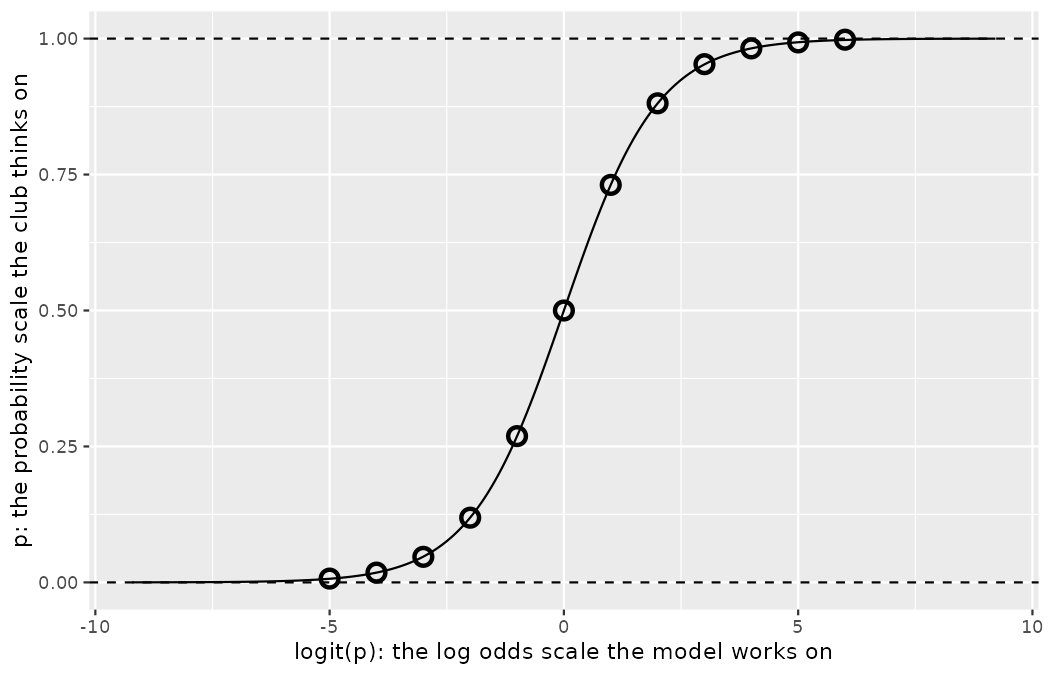
\includegraphics[width=0.85\linewidth,height=\textheight,keepaspectratio]{figures/model-logistic-1.png}

The resulting plot --- call it \emph{the logit curve}, since we will
keep pointing back to it --- is an S-shaped curve: it rises steeply
through the point \((0, 0.5)\) --- a log odds of zero is a fifty-fifty
proposition --- and flattens as it approaches, but never touches, the
dashed horizontal lines at \(p = 0\) and \(p = 1\). The circled
reference points, listed in \texttt{logit\_points}, are worth committing
to memory: a logit of \(-2\) corresponds to a probability of about
\(0.119\), a logit of \(-3\) to about \(0.047\), and by \(-5\) the
probability has collapsed to \(0.007\); the positive side mirrors this,
with a logit of \(+2\) giving \(0.881\). Notice that essentially all of
the probability action happens for logits between about \(-4\) and
\(+4\); outside that window, the curve is nearly flat.

In our audit example, there are 8 predictor variables, so \(k = 8\).
While the precise choice of a logit function isn't intuitive, it is
based on theory that underpins generalized linear models, which is
beyond the scope of this book. Fortunately, once we fit a model using
software, it will start to feel like we are back in the multiple
regression context of Chapter~\ref{sec-model-mlr}, even if the
interpretation of the coefficients is more complex.

To convert from values on the logistic regression scale to the
probability scale, we need to back transform and then solve for \(p_i\):

\[
\begin{aligned}
\log_{e}\left( \frac{p_i}{1-p_i} \right) &= \beta_0 + \beta_1 x_{1,i} + \cdots + \beta_k x_{k,i} \\
\frac{p_i}{1-p_i} &= e^{\beta_0 + \beta_1 x_{1,i} + \cdots + \beta_k x_{k,i}} \\
p_i &= \left( 1 - p_i \right) e^{\beta_0 + \beta_1 x_{1,i} + \cdots + \beta_k x_{k,i}} \\
p_i &= e^{\beta_0 + \beta_1 x_{1,i}  + \cdots + \beta_k x_{k,i}} - p_i \times e^{\beta_0 + \beta_1 x_{1,i} + \cdots + \beta_k x_{k,i}} \\
p_i + p_i \text{ } e^{\beta_0 + \beta_1 x_{1,i} + \cdots + \beta_k x_{k,i}} &= e^{\beta_0 + \beta_1 x_{1,i} + \cdots + \beta_k x_{k,i}} \\
p_i(1 + e^{\beta_0 + \beta_1 x_{1,i} + \cdots + \beta_k x_{k,i}}) &= e^{\beta_0 + \beta_1 x_{1,i} + \cdots + \beta_k x_{k,i}} \\
p_i &= \frac{e^{\beta_0 + \beta_1 x_{1,i}  + \cdots + \beta_k x_{k,i}}}{1 + e^{\beta_0 + \beta_1 x_{1,i} + \cdots + \beta_k x_{k,i}}}
\end{aligned}
\]

Follow the algebra line by line --- it is nothing more exotic than
exponentiating both sides (\(e^{\log_e(z)} = z\)) and then collecting
the \(p_i\) terms --- but do memorize the destination: the expression
\(e^{\beta_0 + \cdots + \beta_k x_{k,i}} \big/ \left(1 + e^{\beta_0 + \cdots + \beta_k x_{k,i}}\right)\)
is the \emph{back-transform} that carries any value on the model's log
odds scale home to the probability scale the sporting director thinks
on. It is the logit curve written as a formula.

As with most applied data problems, we substitute in the point estimates
(the observed \(b_i\), in the sense of Chapter~\ref{sec-model-slr}) to
calculate relevant probabilities. And one more notational convention,
which you first met attached to \(\hat{y}\) in
Chapter~\ref{sec-model-slr}, is now worth stating as a general rule: a
``hat'' placed over any symbol always means \emph{an estimate computed
from data} of the unadorned quantity beneath it. So \(\hat{p}_i\) ---
read ``p-hat-sub-i'' --- is the model's data-based estimate of the true
probability \(p_i\) that dossier \(i\) is shortlisted.

\begin{tcolorbox}[enhanced jigsaw, left=2mm, leftrule=.75mm, title=\textcolor{quarto-callout-tip-color}{\faLightbulb}\hspace{0.5em}{Check your understanding}, arc=.35mm, rightrule=.15mm, coltitle=black, colframe=quarto-callout-tip-color-frame, bottomrule=.15mm, colbacktitle=quarto-callout-tip-color!10!white, opacitybacktitle=0.6, breakable, bottomtitle=1mm, toptitle=1mm, titlerule=0mm, opacityback=0, toprule=.15mm, colback=white]

A dossier's fitted log odds work out to \(-1.5.\) What probability of a
shortlist does that correspond to? And if the log odds were \(+1.5\)?

\begin{center}\rule{0.5\linewidth}{0.5pt}\end{center}

Apply the back-transform:
\(\hat{p} = \frac{e^{-1.5}}{1 + e^{-1.5}} = \frac{0.2231}{1.2231} = 0.182.\)
For log odds of \(+1.5\):
\(\hat{p} = \frac{e^{1.5}}{1 + e^{1.5}} = \frac{4.4817}{5.4817} = 0.818.\)
Check both against the logit curve: \(-1.5\) sits between the reference
points at \(-2\) \((0.119)\) and \(-1\) \((0.269),\) as it should.
Notice, too, that the two answers sum to 1 --- log odds of equal size
and opposite sign always produce probabilities that mirror around one
half.

\end{tcolorbox}

\begin{tcolorbox}[enhanced jigsaw, left=2mm, leftrule=.75mm, title=\textcolor{quarto-callout-note-color}{\faInfo}\hspace{0.5em}{Worked example}, arc=.35mm, rightrule=.15mm, coltitle=black, colframe=quarto-callout-note-color-frame, bottomrule=.15mm, colbacktitle=quarto-callout-note-color!10!white, opacitybacktitle=0.6, breakable, bottomtitle=1mm, toptitle=1mm, titlerule=0mm, opacityback=0, toprule=.15mm, colback=white]

We start by fitting a model with a single predictor:
\texttt{video\_attached}. This variable indicates whether a three-minute
highlight clip was attached to the dossier. We fit the logistic
regression model in R with \texttt{glm()} --- the function's name is
literally ``generalized linear model'' --- telling it via
\texttt{family\ =\ binomial} that the response is a two-level outcome:

\begin{Shaded}
\begin{Highlighting}[]
\NormalTok{video\_fit }\OtherTok{\textless{}{-}} \FunctionTok{glm}\NormalTok{(shortlisted }\SpecialCharTok{\textasciitilde{}}\NormalTok{ video\_attached,}
                 \AttributeTok{data =}\NormalTok{ audit\_study, }\AttributeTok{family =}\NormalTok{ binomial)}
\FunctionTok{tidy}\NormalTok{(video\_fit)}
\CommentTok{\#\textgreater{} \# A tibble: 2 × 5}
\CommentTok{\#\textgreater{}   term           estimate std.error statistic   p.value}
\CommentTok{\#\textgreater{}   \textless{}chr\textgreater{}             \textless{}dbl\textgreater{}     \textless{}dbl\textgreater{}     \textless{}dbl\textgreater{}     \textless{}dbl\textgreater{}}
\CommentTok{\#\textgreater{} 1 (Intercept)      {-}2.38     0.0737    {-}32.3  6.22e{-}229}
\CommentTok{\#\textgreater{} 2 video\_attached    0.864    0.0907      9.53 1.64e{-} 21}

\FunctionTok{round}\NormalTok{(}\FunctionTok{coef}\NormalTok{(video\_fit), }\DecValTok{4}\NormalTok{)}
\CommentTok{\#\textgreater{}    (Intercept) video\_attached}
\CommentTok{\#\textgreater{}        {-}2.3815         0.8642}
\end{Highlighting}
\end{Shaded}

The fitted model is therefore

\[\log_e \left( \frac{\widehat{p}_i}{1-\widehat{p}_i} \right) = -2.3815 + 0.8642 \times {\texttt{video\_attached}}\]

\begin{enumerate}
\def\labelenumi{\alph{enumi}.}
\item
  If a dossier is randomly selected from the audit and it has no
  highlight clip attached, what is the probability it was shortlisted?
\item
  What would the probability be if the dossier did have a clip attached?
\end{enumerate}

\begin{center}\rule{0.5\linewidth}{0.5pt}\end{center}

\begin{enumerate}
\def\labelenumi{\alph{enumi}.}
\item
  If a randomly chosen dossier from those seeded into the queue is
  considered, and it has no clip attached, then \texttt{video\_attached}
  takes the value 0 and the right side of the model equation equals
  \(-2.3815\). Solving for \(p_i\):
  \(\frac{e^{-2.3815}}{1 + e^{-2.3815}} = 0.0846\). Just as we labeled a
  fitted value of \(y_i\) with a ``hat'' in single-variable and multiple
  regression, we do the same for this probability:
  \(\hat{p}_i = 0.0846\).
\item
  If the dossier had a clip attached, then the right side of the model
  equation is \(-2.3815 + 0.8642 \times 1 = -1.5173\), which corresponds
  to a probability \(\hat{p}_i = 0.180\). Notice that we could examine
  \(-2.3815\) and \(-1.5173\) on the logit curve to estimate the
  probabilities before formally calculating the values --- both sit
  between the reference points at \(-2\) \((0.119)\) and \(-1\)
  \((0.269)\), the first much closer to \(-2.4\)'s neighborhood below
  \(0.1\).
\end{enumerate}

\end{tcolorbox}

\begin{tcolorbox}[enhanced jigsaw, left=2mm, leftrule=.75mm, title=\textcolor{quarto-callout-tip-color}{\faLightbulb}\hspace{0.5em}{Check your understanding}, arc=.35mm, rightrule=.15mm, coltitle=black, colframe=quarto-callout-tip-color-frame, bottomrule=.15mm, colbacktitle=quarto-callout-tip-color!10!white, opacitybacktitle=0.6, breakable, bottomtitle=1mm, toptitle=1mm, titlerule=0mm, opacityback=0, toprule=.15mm, colback=white]

Compare the two fitted probabilities from the worked example with the
raw shortlist rates in the two groups:

\begin{Shaded}
\begin{Highlighting}[]
\NormalTok{audit\_study }\SpecialCharTok{|\textgreater{}}
  \FunctionTok{group\_by}\NormalTok{(video\_attached) }\SpecialCharTok{|\textgreater{}}
  \FunctionTok{summarize}\NormalTok{(}\AttributeTok{n =} \FunctionTok{n}\NormalTok{(), }\AttributeTok{p\_shortlisted =} \FunctionTok{mean}\NormalTok{(shortlisted))}
\CommentTok{\#\textgreater{} \# A tibble: 2 × 3}
\CommentTok{\#\textgreater{}   video\_attached     n p\_shortlisted}
\CommentTok{\#\textgreater{}            \textless{}int\textgreater{} \textless{}int\textgreater{}         \textless{}dbl\textgreater{}}
\CommentTok{\#\textgreater{} 1              0  2376        0.0846}
\CommentTok{\#\textgreater{} 2              1  2424        0.180}
\end{Highlighting}
\end{Shaded}

They match exactly. Is that a coincidence?

\begin{center}\rule{0.5\linewidth}{0.5pt}\end{center}

No. With a single binary predictor, the model has two parameters
\((b_0\) and \(b_1)\) to describe exactly two groups, so it can --- and
does --- reproduce each group's observed shortlist rate perfectly. The
model earns its keep only in the next section, when eight predictors
must share the work of describing
\(2 \times 2 \times 11 \times 2 \times 2 \times 2 \times 2 \times 2\)
possible dossier profiles, and the fitted probabilities become genuine
estimates rather than relabeled group means.

\end{tcolorbox}

While knowing whether a dossier carried a highlight clip provides some
signal when predicting whether the triage desk shortlists it, we would
like to account for many different variables at once to understand how
each of the different dossier characteristics affected the chance of a
shortlist.

\section{Logistic model with many
variables}\label{logistic-model-with-many-variables}

We fit the logistic regression model with all 8 predictors described in
Table~\ref{tbl-audit-variables}. Like multiple regression, the result
may be presented in a summary table --- here, the tidy output of the
fitted model.

\begin{Shaded}
\begin{Highlighting}[]
\NormalTok{audit\_full }\OtherTok{\textless{}{-}} \FunctionTok{glm}\NormalTok{(}
\NormalTok{  shortlisted }\SpecialCharTok{\textasciitilde{}}\NormalTok{ league\_tier }\SpecialCharTok{+}\NormalTok{ youth\_caps }\SpecialCharTok{+}\NormalTok{ years\_senior }\SpecialCharTok{+}\NormalTok{ award }\SpecialCharTok{+}
\NormalTok{    injury\_note }\SpecialCharTok{+}\NormalTok{ video\_attached }\SpecialCharTok{+}\NormalTok{ nationality }\SpecialCharTok{+}\NormalTok{ agent\_flag,}
  \AttributeTok{data =}\NormalTok{ audit\_study, }\AttributeTok{family =}\NormalTok{ binomial}
\NormalTok{)}
\FunctionTok{tidy}\NormalTok{(audit\_full)}
\CommentTok{\#\textgreater{} \# A tibble: 9 × 5}
\CommentTok{\#\textgreater{}   term                estimate std.error statistic  p.value}
\CommentTok{\#\textgreater{}   \textless{}chr\textgreater{}                  \textless{}dbl\textgreater{}     \textless{}dbl\textgreater{}     \textless{}dbl\textgreater{}    \textless{}dbl\textgreater{}}
\CommentTok{\#\textgreater{} 1 (Intercept)          {-}2.49      0.147    {-}16.9   2.31e{-}64}
\CommentTok{\#\textgreater{} 2 league\_tiersecond    {-}0.464     0.0885    {-}5.24  1.60e{-} 7}
\CommentTok{\#\textgreater{} 3 youth\_caps           {-}0.0922    0.0924    {-}0.998 3.18e{-} 1}
\CommentTok{\#\textgreater{} 4 years\_senior          0.0269    0.0139     1.94  5.25e{-} 2}
\CommentTok{\#\textgreater{} 5 award                 0.651     0.159      4.09  4.24e{-} 5}
\CommentTok{\#\textgreater{} 6 injury\_note          {-}0.333     0.155     {-}2.16  3.09e{-} 2}
\CommentTok{\#\textgreater{} 7 video\_attached        0.887     0.0917     9.67  3.88e{-}22}
\CommentTok{\#\textgreater{} 8 nationalitydomestic   0.530     0.0883     6.01  1.88e{-} 9}
\CommentTok{\#\textgreater{} 9 agent\_flagagent      {-}0.321     0.0877    {-}3.66  2.49e{-} 4}
\end{Highlighting}
\end{Shaded}

Read the coefficient names the way you learned in
Chapter~\ref{sec-model-mlr}: \texttt{nationalitydomestic} is the level
indicator \(\texttt{nationality}_{\texttt{domestic}}\), taking the value
1 when the dossier's listed nationality is domestic and 0 when it is
foreign (the reference level); \texttt{agent\_flagagent} and
\texttt{league\_tiersecond} work the same way against the reference
levels \texttt{network} and \texttt{first}. Each coefficient is
interpreted \emph{holding the other variables constant}, exactly as in
multiple regression --- with the one twist that the scale being moved is
the log odds of a shortlist, not the response itself. And here is the
moment of truth for the audit: compare the estimates with the
\texttt{log\_odds} line of the construction code. The hidden decision
process penalized second-tier leagues by \(0.45\), rewarded an attached
clip by \(0.85\), boosted domestic labels by \(0.45\), docked agent
submissions by \(0.25\) --- and the fitted values \(-0.464\), \(0.887\),
\(0.530\), and \(-0.321\) recover each of them to within sampling noise,
from nothing but the 4,800 recorded decisions. That is the entire
promise of logistic regression, demonstrated on a scenario where we
happen to know the answer key.

Just like multiple regression, we could trim some variables from the
model. Here we'll use a statistic called \textbf{Akaike information
criterion (AIC)}, which is analogous to how we used adjusted \(R^2\) in
multiple regression. AIC is a popular model selection method used in
many disciplines, and is praised for its emphasis on model uncertainty
and parsimony. AIC selects a ``best'' model by ranking models from best
to worst according to their AIC values. In the calculation of a model's
AIC, a penalty is given for including additional variables. The penalty
for added model complexity attempts to strike a balance between
underfitting (too few variables in the model) and overfitting (too many
variables in the model). When using AIC for model selection, models with
a lower AIC value are considered to be ``better.'' Remember that when
using adjusted \(R^2\) in Chapter~\ref{sec-model-mlr} we select models
with \emph{higher} values instead. It is important to note that AIC
provides information about the quality of a model relative to other
models, but does not provide information about the overall quality of a
model.

\begin{tcolorbox}[enhanced jigsaw, left=2mm, leftrule=.75mm, title=\textcolor{quarto-callout-note-color}{\faInfo}\hspace{0.5em}{Deeper (optional): what AIC computes --- uses the likelihood idea; safe
to skip}, arc=.35mm, rightrule=.15mm, coltitle=black, colframe=quarto-callout-note-color-frame, bottomrule=.15mm, colbacktitle=quarto-callout-note-color!10!white, opacitybacktitle=0.6, breakable, bottomtitle=1mm, toptitle=1mm, titlerule=0mm, opacityback=0, toprule=.15mm, colback=white]

For a fitted model,

\[
AIC = -2 \log \mathcal{L} + 2k
\]

Name the pieces before using them: \(\log \mathcal{L}\) is the model's
\emph{log-likelihood} --- the logarithm of how probable the observed
outcomes are under the fitted model, so a value closer to zero means a
better fit --- and \(k\) is the number of coefficients the model
estimated, intercept included. The first term rewards fit; the \(2k\)
term is the complexity penalty described above. The penalty exists
because the first term alone can never get worse when a variable is
added --- even a useless variable lets the model fit the data at hand a
little better --- so without \(+2k\) the ``best'' model would always be
the biggest one, and AIC would offer no protection against overfitting.
For the full audit model, R reports \(\log \mathcal{L} = -1780.88\) with
\(k = 9,\) and \(-2 \times (-1780.88) + 2 \times 9 = 3579.77\) --- the
value computed below.

\end{tcolorbox}

The AIC of the full model, fit to all 4,800 dossiers with eight
variables (nine coefficients, including the intercept), is:

\begin{Shaded}
\begin{Highlighting}[]
\FunctionTok{AIC}\NormalTok{(audit\_full)}
\CommentTok{\#\textgreater{} [1] 3579.769}

\FunctionTok{nobs}\NormalTok{(audit\_full)}
\CommentTok{\#\textgreater{} [1] 4800}
\end{Highlighting}
\end{Shaded}

We will look for models with a lower AIC using a backward elimination
strategy. The weakest link in the summary table above is
\texttt{youth\_caps} --- its estimate is small and its test statistic is
below 1 in absolute value --- so we refit the model without it. Notice
that the same number of observations is used, but one fewer variable.

\begin{Shaded}
\begin{Highlighting}[]
\NormalTok{audit\_fit }\OtherTok{\textless{}{-}} \FunctionTok{glm}\NormalTok{(}
\NormalTok{  shortlisted }\SpecialCharTok{\textasciitilde{}}\NormalTok{ league\_tier }\SpecialCharTok{+}\NormalTok{ years\_senior }\SpecialCharTok{+}\NormalTok{ award }\SpecialCharTok{+}
\NormalTok{    injury\_note }\SpecialCharTok{+}\NormalTok{ video\_attached }\SpecialCharTok{+}\NormalTok{ nationality }\SpecialCharTok{+}\NormalTok{ agent\_flag,}
  \AttributeTok{data =}\NormalTok{ audit\_study, }\AttributeTok{family =}\NormalTok{ binomial}
\NormalTok{)}
\FunctionTok{AIC}\NormalTok{(audit\_fit)}
\CommentTok{\#\textgreater{} [1] 3578.771}

\FunctionTok{nobs}\NormalTok{(audit\_fit)}
\CommentTok{\#\textgreater{} [1] 4800}
\end{Highlighting}
\end{Shaded}

After using the AIC criteria, the variable \texttt{youth\_caps} is
eliminated (the AIC value without \texttt{youth\_caps}, \(3578.77\), is
smaller than the AIC value on the full model, \(3579.77\)), giving the
model summarized below with fewer variables, which is what we'll rely on
for the remainder of the section. Pleasingly, the eliminated variable is
precisely the one the construction code assigned no role at all: youth
caps never entered the hidden \texttt{log\_odds} line, and AIC noticed.

\begin{Shaded}
\begin{Highlighting}[]
\FunctionTok{tidy}\NormalTok{(audit\_fit)}
\CommentTok{\#\textgreater{} \# A tibble: 8 × 5}
\CommentTok{\#\textgreater{}   term                estimate std.error statistic  p.value}
\CommentTok{\#\textgreater{}   \textless{}chr\textgreater{}                  \textless{}dbl\textgreater{}     \textless{}dbl\textgreater{}     \textless{}dbl\textgreater{}    \textless{}dbl\textgreater{}}
\CommentTok{\#\textgreater{} 1 (Intercept)          {-}2.52      0.144     {-}17.5  1.14e{-}68}
\CommentTok{\#\textgreater{} 2 league\_tiersecond    {-}0.466     0.0884     {-}5.27 1.39e{-} 7}
\CommentTok{\#\textgreater{} 3 years\_senior          0.0270    0.0139      1.94 5.18e{-} 2}
\CommentTok{\#\textgreater{} 4 award                 0.655     0.159       4.12 3.83e{-} 5}
\CommentTok{\#\textgreater{} 5 injury\_note          {-}0.334     0.154      {-}2.16 3.05e{-} 2}
\CommentTok{\#\textgreater{} 6 video\_attached        0.886     0.0917      9.66 4.40e{-}22}
\CommentTok{\#\textgreater{} 7 nationalitydomestic   0.533     0.0883      6.03 1.60e{-} 9}
\CommentTok{\#\textgreater{} 8 agent\_flagagent      {-}0.323     0.0876     {-}3.69 2.25e{-} 4}
\end{Highlighting}
\end{Shaded}

\begin{tcolorbox}[enhanced jigsaw, left=2mm, leftrule=.75mm, title=\textcolor{quarto-callout-tip-color}{\faLightbulb}\hspace{0.5em}{Check your understanding}, arc=.35mm, rightrule=.15mm, coltitle=black, colframe=quarto-callout-tip-color-frame, bottomrule=.15mm, colbacktitle=quarto-callout-tip-color!10!white, opacitybacktitle=0.6, breakable, bottomtitle=1mm, toptitle=1mm, titlerule=0mm, opacityback=0, toprule=.15mm, colback=white]

Your colleague reports two facts: ``the reduced model's AIC is 3578.77,
which is lower than the full model's 3579.77, so the reduced model is
better,'' and ``an AIC of 3578.77 shows this is a good model.'' Which
statement is justified?

\begin{center}\rule{0.5\linewidth}{0.5pt}\end{center}

Only the first. AIC is a \emph{relative} yardstick: lower AIC among
candidate models fit to the same data identifies the preferable model
--- note the direction is the opposite of adjusted \(R^2\), where higher
is better. But the number 3578.77 says nothing on its own about whether
the model describes triage decisions well in an absolute sense; a
hopeless model and a superb one could both carry that value on different
datasets.

\end{tcolorbox}

\begin{tcolorbox}[enhanced jigsaw, left=2mm, leftrule=.75mm, title=\textcolor{quarto-callout-note-color}{\faInfo}\hspace{0.5em}{Worked example}, arc=.35mm, rightrule=.15mm, coltitle=black, colframe=quarto-callout-note-color-frame, bottomrule=.15mm, colbacktitle=quarto-callout-note-color!10!white, opacitybacktitle=0.6, breakable, bottomtitle=1mm, toptitle=1mm, titlerule=0mm, opacityback=0, toprule=.15mm, colback=white]

The \texttt{nationality} variable takes only two levels:
\texttt{foreign} and \texttt{domestic}. Based on the model results, what
does the coefficient of the \texttt{nationality} variable say about
shortlist decisions?

\begin{center}\rule{0.5\linewidth}{0.5pt}\end{center}

The coefficient shown corresponds to the level of \texttt{domestic}, and
it is positive \((0.533)\). The positive coefficient reflects a positive
gain in shortlist rate for dossiers where the listed nationality is
domestic. The model results say that Northbridge's triage desk favors
dossiers whose passport line reads domestic --- a bias the club's own
policy forbids, detected in the club's own decisions.

\end{tcolorbox}

The coefficient of \(\texttt{nationality}_{\texttt{domestic}}\) in the
full model \((0.530)\) is nearly identical to the one in the reduced
model \((0.533)\). The predictors in the audit were thoughtfully laid
out --- every attribute randomly assigned, independently of every other
--- so that the coefficient estimates would typically not be much
influenced by which other predictors were in the model, which aligned
with the motivation of the audit to tease out which cues were important
to getting shortlisted. In most observational data, it's common for
point estimates to change a little, and sometimes a lot, depending on
which other variables are included in the model --- you saw exactly that
instability in Chapter~\ref{sec-model-mlr}, and we will meet it again
shortly with the real tournament shots.

For the probability calculations that follow, we will want the reduced
model's coefficients at higher precision than the tidy table displays:

\begin{Shaded}
\begin{Highlighting}[]
\FunctionTok{round}\NormalTok{(}\FunctionTok{coef}\NormalTok{(audit\_fit), }\DecValTok{4}\NormalTok{)}
\CommentTok{\#\textgreater{}         (Intercept)   league\_tiersecond        years\_senior               award}
\CommentTok{\#\textgreater{}             {-}2.5240             {-}0.4658              0.0270              0.6547}
\CommentTok{\#\textgreater{}         injury\_note      video\_attached nationalitydomestic     agent\_flagagent}
\CommentTok{\#\textgreater{}             {-}0.3343              0.8861              0.5326             {-}0.3232}
\end{Highlighting}
\end{Shaded}

\begin{tcolorbox}[enhanced jigsaw, left=2mm, leftrule=.75mm, title=\textcolor{quarto-callout-note-color}{\faInfo}\hspace{0.5em}{Worked example}, arc=.35mm, rightrule=.15mm, coltitle=black, colframe=quarto-callout-note-color-frame, bottomrule=.15mm, colbacktitle=quarto-callout-note-color!10!white, opacitybacktitle=0.6, breakable, bottomtitle=1mm, toptitle=1mm, titlerule=0mm, opacityback=0, toprule=.15mm, colback=white]

Use the reduced model to estimate the probability of a shortlist for a
dossier describing a second-tier player with 8 seasons of senior
football, no listed award, no injury note, a highlight clip attached,
submitted by an agent, and a passport line that reads domestic.

\begin{center}\rule{0.5\linewidth}{0.5pt}\end{center}

We can start by writing out the equation using the coefficients from the
model:

\[
\begin{aligned}
\log_e \left(\frac{\widehat{p}}{1 - \widehat{p}}\right) = -2.5240 &- 0.4658 \times \texttt{league\_tier}_{\texttt{second}} + 0.0270 \times \texttt{years\_senior} \\
&+ 0.6547 \times \texttt{award} - 0.3343 \times \texttt{injury\_note} + 0.8861 \times \texttt{video} \\
&+ 0.5326 \times \texttt{nationality}_{\texttt{domestic}} - 0.3232 \times \texttt{agent\_flag}_{\texttt{agent}}
\end{aligned}
\]

Now we can add in the corresponding values of each variable for the
dossier of interest:

\[
\begin{aligned}
\log_e \left(\frac{\widehat{p}}{1 - \widehat{p}}\right) = -2.5240 &- 0.4658 \times 1 + 0.0270 \times 8 \\
&+ 0.6547 \times 0 - 0.3343 \times 0 + 0.8861 \times 1 \\
&+ 0.5326 \times 1 - 0.3232 \times 1 = -1.6783
\end{aligned}
\]

We can now back-solve for \(\widehat{p}\): the chance such a dossier is
shortlisted is about \(\frac{e^{-1.6783}}{1 + e^{-1.6783}} = 0.1573\). R
will do the same arithmetic (without the rounding of the coefficients)
via \texttt{predict()} with \texttt{type\ =\ "response"}, and it agrees:

\begin{Shaded}
\begin{Highlighting}[]
\NormalTok{new\_dossier }\OtherTok{\textless{}{-}} \FunctionTok{tibble}\NormalTok{(}
  \AttributeTok{league\_tier =} \FunctionTok{factor}\NormalTok{(}\StringTok{"second"}\NormalTok{, }\AttributeTok{levels =} \FunctionTok{c}\NormalTok{(}\StringTok{"first"}\NormalTok{, }\StringTok{"second"}\NormalTok{)),}
  \AttributeTok{years\_senior =} \DecValTok{8}\NormalTok{, }\AttributeTok{award =} \DecValTok{0}\NormalTok{, }\AttributeTok{injury\_note =} \DecValTok{0}\NormalTok{, }\AttributeTok{video\_attached =} \DecValTok{1}\NormalTok{,}
  \AttributeTok{nationality =} \FunctionTok{factor}\NormalTok{(}\FunctionTok{c}\NormalTok{(}\StringTok{"domestic"}\NormalTok{, }\StringTok{"foreign"}\NormalTok{),}
                       \AttributeTok{levels =} \FunctionTok{c}\NormalTok{(}\StringTok{"foreign"}\NormalTok{, }\StringTok{"domestic"}\NormalTok{)),}
  \AttributeTok{agent\_flag =} \FunctionTok{factor}\NormalTok{(}\StringTok{"agent"}\NormalTok{, }\AttributeTok{levels =} \FunctionTok{c}\NormalTok{(}\StringTok{"network"}\NormalTok{, }\StringTok{"agent"}\NormalTok{))}
\NormalTok{)}
\FunctionTok{round}\NormalTok{(}\FunctionTok{predict}\NormalTok{(audit\_fit, new\_dossier, }\AttributeTok{type =} \StringTok{"response"}\NormalTok{), }\DecValTok{4}\NormalTok{)}
\CommentTok{\#\textgreater{}      1      2}
\CommentTok{\#\textgreater{} 0.1573 0.0988}
\end{Highlighting}
\end{Shaded}

(The second value belongs to the next worked example.)

\end{tcolorbox}

\begin{tcolorbox}[enhanced jigsaw, left=2mm, leftrule=.75mm, title=\textcolor{quarto-callout-note-color}{\faInfo}\hspace{0.5em}{Worked example}, arc=.35mm, rightrule=.15mm, coltitle=black, colframe=quarto-callout-note-color-frame, bottomrule=.15mm, colbacktitle=quarto-callout-note-color!10!white, opacitybacktitle=0.6, breakable, bottomtitle=1mm, toptitle=1mm, titlerule=0mm, opacityback=0, toprule=.15mm, colback=white]

Compute the probability of a shortlist for a dossier whose passport line
reads foreign but which otherwise has the same characteristics as the
one described in the previous example.

\begin{center}\rule{0.5\linewidth}{0.5pt}\end{center}

We can complete the same steps for a dossier with the same
characteristics whose listed nationality is foreign, where the only
difference in the calculation is that the indicator variable
\(\texttt{nationality}_{\texttt{domestic}}\) will take a value of 0. The
log odds become \(-1.6783 - 0.5326 = -2.2109\), yielding a probability
of \(0.0988\) --- the second value in the \texttt{predict()} output
above. Let's compare the results with those of the previous example.

In practical terms, an identically documented player labeled domestic
would need to appear in about \(\frac{1}{0.1573} \approx 6.4\) intake
queues on average to be shortlisted once, while the same player labeled
foreign would need to appear in about \(\frac{1}{0.0988} \approx 10.1\).
That is, a prospect whose dossier reads foreign needs roughly 60\% more
chances at the triage desk to earn one follow-up assessment than an
identically documented prospect whose dossier reads domestic.

\end{tcolorbox}

What we have quantified in the current section should trouble the club.
However, one aspect that makes such bias so difficult to address is that
the audit, as well-designed as it is, cannot send us much signal about
\emph{which} triage decisions were discriminatory. It is only possible
to say that discrimination is happening in the aggregate, even if we
cannot say which particular shortlists --- or rejections --- represent
discrimination. Finding strong evidence of bias in an individual
decision is a persistent challenge for any club that takes its own
recruitment policy seriously; this is exactly why Priya's follow-up, a
small randomized audit of the live scouting network itself, is the
opening case study of Chapter~\ref{sec-foundations-randomization}.

\subsection{Predicting goals in real match
data}\label{sec-chp9-observational}

Everything above rested on a randomized design: because Priya assigned
every dossier attribute by coin flip, the coefficients earned causal
readings. Logistic regression itself, however, does not care where the
data came from --- and most of the binary outcomes a scouting department
models are \emph{observational}. The most important one is the shot:
\texttt{goal} in the 2022 Men's World Cup data is exactly a two-level
outcome, and the shot's circumstances are candidate predictors.

One data-preparation step is needed first. The \texttt{technique}
variable has seven levels, four of which --- backheels, lobs, diving
headers, and overhead kicks --- account for only 39 of the 1,494 shots
between them, and some of those tiny categories contain no goals at all,
which makes their coefficients unestimable in practice. We collapse them
into a single \texttt{Other} level, and we set the reference levels to
the most common shot: right-footed, normal technique.

\begin{Shaded}
\begin{Highlighting}[]
\NormalTok{wc2022\_shots }\OtherTok{\textless{}{-}} \FunctionTok{read\_csv}\NormalTok{(}\StringTok{"data/derived/wc2022\_shots.csv"}\NormalTok{)}

\NormalTok{wc\_shots\_model }\OtherTok{\textless{}{-}}\NormalTok{ wc2022\_shots }\SpecialCharTok{|\textgreater{}}
  \FunctionTok{mutate}\NormalTok{(}
    \AttributeTok{technique\_grp =} \FunctionTok{if\_else}\NormalTok{(}
\NormalTok{      technique }\SpecialCharTok{\%in\%} \FunctionTok{c}\NormalTok{(}\StringTok{"Normal"}\NormalTok{, }\StringTok{"Half Volley"}\NormalTok{, }\StringTok{"Volley"}\NormalTok{),}
\NormalTok{      technique,}
      \StringTok{"Other"}
\NormalTok{    ),}
    \AttributeTok{technique\_grp =} \FunctionTok{relevel}\NormalTok{(}\FunctionTok{factor}\NormalTok{(technique\_grp), }\AttributeTok{ref =} \StringTok{"Normal"}\NormalTok{),}
    \AttributeTok{body\_part =} \FunctionTok{relevel}\NormalTok{(}\FunctionTok{factor}\NormalTok{(body\_part), }\AttributeTok{ref =} \StringTok{"Right Foot"}\NormalTok{)}
\NormalTok{  )}

\NormalTok{wc\_shots\_model }\SpecialCharTok{|\textgreater{}} \FunctionTok{count}\NormalTok{(technique\_grp)}
\CommentTok{\#\textgreater{} \# A tibble: 4 × 2}
\CommentTok{\#\textgreater{}   technique\_grp     n}
\CommentTok{\#\textgreater{}   \textless{}fct\textgreater{}         \textless{}int\textgreater{}}
\CommentTok{\#\textgreater{} 1 Normal         1151}
\CommentTok{\#\textgreater{} 2 Half Volley     212}
\CommentTok{\#\textgreater{} 3 Other            39}
\CommentTok{\#\textgreater{} 4 Volley           92}

\NormalTok{goal\_fit }\OtherTok{\textless{}{-}} \FunctionTok{glm}\NormalTok{(}
\NormalTok{  goal }\SpecialCharTok{\textasciitilde{}}\NormalTok{ body\_part }\SpecialCharTok{+}\NormalTok{ technique\_grp }\SpecialCharTok{+}\NormalTok{ under\_pressure }\SpecialCharTok{+}\NormalTok{ one\_on\_one }\SpecialCharTok{+}
\NormalTok{    first\_time,}
  \AttributeTok{data =}\NormalTok{ wc\_shots\_model, }\AttributeTok{family =}\NormalTok{ binomial}
\NormalTok{)}
\FunctionTok{tidy}\NormalTok{(goal\_fit)}
\CommentTok{\#\textgreater{} \# A tibble: 10 × 5}
\CommentTok{\#\textgreater{}    term                     estimate std.error statistic  p.value}
\CommentTok{\#\textgreater{}    \textless{}chr\textgreater{}                       \textless{}dbl\textgreater{}     \textless{}dbl\textgreater{}     \textless{}dbl\textgreater{}    \textless{}dbl\textgreater{}}
\CommentTok{\#\textgreater{}  1 (Intercept)               {-}2.01       0.138  {-}14.6    3.44e{-}48}
\CommentTok{\#\textgreater{}  2 body\_partHead             {-}0.0177     0.260   {-}0.0679 9.46e{-} 1}
\CommentTok{\#\textgreater{}  3 body\_partLeft Foot         0.115      0.175    0.661  5.09e{-} 1}
\CommentTok{\#\textgreater{}  4 body\_partOther             0.557      0.682    0.817  4.14e{-} 1}
\CommentTok{\#\textgreater{}  5 technique\_grpHalf Volley  {-}0.486      0.256   {-}1.90   5.71e{-} 2}
\CommentTok{\#\textgreater{}  6 technique\_grpOther        {-}0.0115     0.463   {-}0.0248 9.80e{-} 1}
\CommentTok{\#\textgreater{}  7 technique\_grpVolley       {-}0.0959     0.324   {-}0.296  7.67e{-} 1}
\CommentTok{\#\textgreater{}  8 under\_pressureTRUE        {-}0.271      0.252   {-}1.07   2.83e{-} 1}
\CommentTok{\#\textgreater{}  9 one\_on\_oneTRUE             0.680      0.298    2.28   2.24e{-} 2}
\CommentTok{\#\textgreater{} 10 first\_timeTRUE             0.410      0.189    2.17   2.97e{-} 2}
\end{Highlighting}
\end{Shaded}

The signs of the estimates line up with what your exploratory work in
earlier chapters would predict: shots under pressure carry a negative
coefficient \((-0.271)\), one-on-ones a large positive one \((+0.680)\),
and first-time strikes a positive one \((+0.410)\) --- in this
tournament. The back-transform turns these into probabilities. For the
reference shot --- right-footed, normal technique, not under pressure,
not a one-on-one, not first time --- the log odds are the intercept,
\(-2.0110\), giving

\[\hat{p} = \frac{e^{-2.0110}}{1 + e^{-2.0110}} = 0.1181\]

while flipping only the one-on-one indicator moves the log odds to
\(-2.0110 + 0.6803 = -1.3307\) and the probability to \(0.209\). (For
comparison, the raw conversion rates are \(0.126\) for the 1,409
non-one-on-one shots and \(0.200\) for the 85 one-on-ones --- close to,
but not identical to, the model's values, because the model's figures
hold the other predictors at their reference levels rather than at
whatever mix the raw groups happen to contain.)

Before this model goes anywhere near a scouting memo, take stock of what
its frame contains, because we fit it to \emph{all} 1,494 shots ---
penalties included:

\begin{Shaded}
\begin{Highlighting}[]
\NormalTok{wc\_shots\_model }\SpecialCharTok{|\textgreater{}}
  \FunctionTok{filter}\NormalTok{(shot\_type }\SpecialCharTok{==} \StringTok{"Penalty"}\NormalTok{) }\SpecialCharTok{|\textgreater{}}
  \FunctionTok{summarize}\NormalTok{(}
    \AttributeTok{kicks =} \FunctionTok{n}\NormalTok{(),}
    \AttributeTok{goals =} \FunctionTok{sum}\NormalTok{(goal),}
    \AttributeTok{conversion =} \FunctionTok{mean}\NormalTok{(goal),}
    \AttributeTok{pressured =} \FunctionTok{sum}\NormalTok{(under\_pressure),}
    \AttributeTok{first\_time =} \FunctionTok{sum}\NormalTok{(first\_time),}
    \AttributeTok{one\_on\_one =} \FunctionTok{sum}\NormalTok{(one\_on\_one)}
\NormalTok{  )}
\CommentTok{\#\textgreater{} \# A tibble: 1 × 6}
\CommentTok{\#\textgreater{}   kicks goals conversion pressured first\_time one\_on\_one}
\CommentTok{\#\textgreater{}   \textless{}int\textgreater{} \textless{}int\textgreater{}      \textless{}dbl\textgreater{}     \textless{}int\textgreater{}      \textless{}int\textgreater{}      \textless{}int\textgreater{}}
\CommentTok{\#\textgreater{} 1    64    43      0.672         0          0          6}
\end{Highlighting}
\end{Shaded}

Sixty-four kicks converting at \(0.672\) --- five times the tournament's
ordinary rate --- and not one of them pressured or struck first time
(six carry the one-on-one tag, a quirk you met in
Chapter~\ref{sec-model-mlr}). Nearly all of them therefore sit inside
the \emph{reference} cell of every indicator in the model, quietly
inflating the baseline against which each coefficient is measured.
Chapter~\ref{sec-model-mlr} faced exactly this issue and responded by
restricting its frame to open play; rebuilding that chapter's frame with
its exact filter and refitting the same goal model shows how much was
riding on the choice:

\begin{Shaded}
\begin{Highlighting}[]
\NormalTok{shots\_open }\OtherTok{\textless{}{-}}\NormalTok{ wc2022\_shots }\SpecialCharTok{|\textgreater{}}
  \FunctionTok{filter}\NormalTok{(}
\NormalTok{    shot\_type }\SpecialCharTok{==} \StringTok{"Open Play"}\NormalTok{,}
\NormalTok{    body\_part }\SpecialCharTok{!=} \StringTok{"Other"}\NormalTok{,}
\NormalTok{    play\_pattern }\SpecialCharTok{!=} \StringTok{"Other"}
\NormalTok{  ) }\SpecialCharTok{|\textgreater{}}
  \FunctionTok{mutate}\NormalTok{(}
    \AttributeTok{technique\_grp =} \FunctionTok{if\_else}\NormalTok{(}
\NormalTok{      technique }\SpecialCharTok{\%in\%} \FunctionTok{c}\NormalTok{(}\StringTok{"Normal"}\NormalTok{, }\StringTok{"Half Volley"}\NormalTok{, }\StringTok{"Volley"}\NormalTok{),}
\NormalTok{      technique,}
      \StringTok{"Other"}
\NormalTok{    ),}
    \AttributeTok{technique\_grp =} \FunctionTok{relevel}\NormalTok{(}\FunctionTok{factor}\NormalTok{(technique\_grp), }\AttributeTok{ref =} \StringTok{"Normal"}\NormalTok{),}
    \AttributeTok{body\_part =} \FunctionTok{relevel}\NormalTok{(}\FunctionTok{factor}\NormalTok{(body\_part), }\AttributeTok{ref =} \StringTok{"Right Foot"}\NormalTok{)}
\NormalTok{  )}

\NormalTok{goal\_fit\_open }\OtherTok{\textless{}{-}} \FunctionTok{glm}\NormalTok{(}
\NormalTok{  goal }\SpecialCharTok{\textasciitilde{}}\NormalTok{ body\_part }\SpecialCharTok{+}\NormalTok{ technique\_grp }\SpecialCharTok{+}\NormalTok{ under\_pressure }\SpecialCharTok{+}\NormalTok{ one\_on\_one }\SpecialCharTok{+}
\NormalTok{    first\_time,}
  \AttributeTok{data =}\NormalTok{ shots\_open, }\AttributeTok{family =}\NormalTok{ binomial}
\NormalTok{)}
\FunctionTok{tidy}\NormalTok{(goal\_fit\_open)}
\CommentTok{\#\textgreater{} \# A tibble: 9 × 5}
\CommentTok{\#\textgreater{}   term                     estimate std.error statistic  p.value}
\CommentTok{\#\textgreater{}   \textless{}chr\textgreater{}                       \textless{}dbl\textgreater{}     \textless{}dbl\textgreater{}     \textless{}dbl\textgreater{}    \textless{}dbl\textgreater{}}
\CommentTok{\#\textgreater{} 1 (Intercept)               {-}2.77       0.189   {-}14.6   1.70e{-}48}
\CommentTok{\#\textgreater{} 2 body\_partHead              0.522      0.287     1.82  6.87e{-} 2}
\CommentTok{\#\textgreater{} 3 body\_partLeft Foot         0.336      0.201     1.68  9.39e{-} 2}
\CommentTok{\#\textgreater{} 4 technique\_grpHalf Volley  {-}0.315      0.265    {-}1.19  2.35e{-} 1}
\CommentTok{\#\textgreater{} 5 technique\_grpOther         0.0522     0.472     0.111 9.12e{-} 1}
\CommentTok{\#\textgreater{} 6 technique\_grpVolley        0.0419     0.330     0.127 8.99e{-} 1}
\CommentTok{\#\textgreater{} 7 under\_pressureTRUE        {-}0.0406     0.261    {-}0.155 8.76e{-} 1}
\CommentTok{\#\textgreater{} 8 one\_on\_oneTRUE             1.30       0.321     4.05  5.13e{-} 5}
\CommentTok{\#\textgreater{} 9 first\_timeTRUE             0.996      0.220     4.52  6.32e{-} 6}
\end{Highlighting}
\end{Shaded}

On the 1,365 open-play shots, the intercept falls from \(-2.0110\) to
\(-2.7669\): the reference shot's probability drops from the \(0.1181\)
computed above to \(e^{-2.7669}/(1 + e^{-2.7669}) = 0.0591,\) because
the all-shots baseline was borrowing the penalties' near-automatic
conversions. The coefficients move with it, some dramatically: the
pressure estimate all but vanishes \((-0.271\) to \(-0.041),\) the
first-time estimate more than doubles \((+0.410\) to \(+0.996),\) the
one-on-one premium nearly does too \((+0.680\) to \(+1.300),\) and the
header coefficient flips from \(-0.018\) to \(+0.522.\) This is why
Chapter~\ref{sec-model-mlr} filtered to open play and why the
full-workflow chapter Chapter~\ref{sec-model-application} does the same:
for modeling what makes a contested shot a goal, the open-play frame is
the honest default. The all-shots fit above stands in this chapter
deliberately, as its pens-in companion under the book's penalty
convention --- a worked reminder that in shot models the choice of frame
can move a coefficient more than the football does.

Two warnings, both of which must temper any scouting memo built on this
model. First, \emph{nothing here is causal}. Nobody randomly assigned
defenders to shots: whether a shot is pressured, first time, or a
one-on-one is entangled with where and how the chance arose, so lurking
variables of the kind you met in Chapter~\ref{sec-data-design} stand
behind every coefficient. The audit earned causal language through
randomization; this model describes association in one tournament, no
more. Second, we have quietly ignored the \texttt{p.value} column.
Deciding which of these coefficients is statistically discernible from
zero requires the inference machinery we begin building in
Chapter~\ref{sec-foundations-randomization}, and the full treatment of
inference for logistic regression waits until
Chapter~\ref{sec-inf-model-logistic} --- where this very goal model
returns as the centerpiece.

\begin{tcolorbox}[enhanced jigsaw, left=2mm, leftrule=.75mm, title=\textcolor{quarto-callout-tip-color}{\faLightbulb}\hspace{0.5em}{Check your understanding}, arc=.35mm, rightrule=.15mm, coltitle=black, colframe=quarto-callout-tip-color-frame, bottomrule=.15mm, colbacktitle=quarto-callout-tip-color!10!white, opacitybacktitle=0.6, breakable, bottomtitle=1mm, toptitle=1mm, titlerule=0mm, opacityback=0, toprule=.15mm, colback=white]

The audit model and the goal model are both logistic regressions with
several predictors. Why were we entitled to say the foreign label
\emph{causes} a lower shortlist probability, but not entitled to say
pressure \emph{causes} a lower scoring probability?

\begin{center}\rule{0.5\linewidth}{0.5pt}\end{center}

The difference is the study design, not the model. In the audit, the
nationality label was randomly assigned to otherwise identical dossiers,
so no lurking variable can explain the gap --- randomization severs
every such link. In the tournament data, pressure was applied by
opposing defenders who choose whom to close down; pressured shots differ
systematically from unpressured ones in ways beyond the model's
predictors (chance quality above all), so the coefficient measures
association only.

\end{tcolorbox}

\section{Groups of different sizes}\label{groups-of-different-sizes}

Any form of discrimination is concerning, which is why we decided it was
so important to discuss the topic using data. The dossier audit also
only examined bias in a single aspect: whether the triage desk would
shortlist a submitted prospect. There was a roughly 60\% higher barrier
for dossiers simply when the passport line read foreign. It's unlikely
that bias would stop at the triage desk.

\begin{tcolorbox}[enhanced jigsaw, left=2mm, leftrule=.75mm, title=\textcolor{quarto-callout-note-color}{\faInfo}\hspace{0.5em}{Worked example}, arc=.35mm, rightrule=.15mm, coltitle=black, colframe=quarto-callout-note-color-frame, bottomrule=.15mm, colbacktitle=quarto-callout-note-color!10!white, opacitybacktitle=0.6, breakable, bottomtitle=1mm, toptitle=1mm, titlerule=0mm, opacityback=0, toprule=.15mm, colback=white]

Let's consider a role-imbalanced academy staff, of which 20\% are
goalkeeping specialists and 80\% are outfield specialists, and we'll
suppose the academy network is very large --- Jonas Beck oversees staff
across Northbridge and its partner academies. Suppose that when a player
is put forward for a scholarship decision, 5 members of staff are
randomly chosen to provide an evaluation of the player.

Now let's imagine that 10\% of the staff on each side undervalue the
other role: 10\% of outfield specialists systematically undervalue
goalkeepers, and similarly, 10\% of goalkeeping specialists
systematically undervalue outfield players. Who is undervalued more
often at scholarship decisions, goalkeepers or outfield players?

\begin{center}\rule{0.5\linewidth}{0.5pt}\end{center}

Let's suppose we took 100 outfield players who have gone up for a
scholarship decision in the past few years. For these outfield players,
\(5 \times 100 = 500\) random staff evaluations will be gathered, of
which about 20\% will come from goalkeeping specialists (100
evaluations). Of these 100 goalkeeping specialists, 10 are expected to
be biased against the outfield player they are reviewing. Then, of the
500 evaluations of outfield players, about 2\% are biased against them.

Let's do a similar calculation for 100 goalkeepers who have gone up for
a scholarship decision in the last few years. They will also have 500
random staff evaluations, of which about 400 (80\%) will come from
outfield specialists. Of these 400 outfield specialists, about 40 (10\%)
hold a bias against goalkeepers. Of the 500 evaluations of these
goalkeepers, 8\% are biased against them.

\end{tcolorbox}

The example highlights something profound: even in a hypothetical
setting where each group has the same degree of prejudice against the
other group, the smaller group experiences the negative effects more
frequently. Additionally, if we would complete a handful of examples
like the one above with different numbers, we would learn that the
greater the imbalance in the group sizes, the more the smaller group is
disproportionately impacted.\footnote{If a proportion \(p\) of the staff
  are goalkeeping specialists and the rest are outfield specialists,
  then under the hypothetical situation the ratio of rates of biased
  evaluations received by goalkeepers versus outfield players would be
  given by \((1 - p)/p,\) a ratio that is always greater than 1 when
  \(p < 0.5\).}

Of course, there are considerable real-world omissions from the
hypothetical example. For example, evaluators sometimes undervalue
members of their own specialism, and biases rarely come in tidy
symmetric percentages; a goalkeeper's contribution is also genuinely
harder to reduce to counting statistics, which invites subtler forms of
undervaluation than the coin-flip prejudice modeled here. Ultimately,
biased evaluation is complex, and there are many factors at play beyond
the mathematical property we observed in the previous example.

We close the chapter on the serious topic of biased decision-making, and
we hope it inspires you to think about the power of reasoning with data.
Whether it is with a formal statistical model or by using critical
thinking to structure a problem --- the way the goalkeeper example
needed nothing more than careful arithmetic --- we hope the ideas you
have learned will help you do more and do better, in scouting and
beyond.

\section{Chapter review}\label{sec-chp9-review}

\subsection{Summary}\label{summary-8}

Logistic and linear regression models have many similarities. The
strongest of which is the linear combination of the explanatory
variables which is used to form predictions related to the response
variable. However, with logistic regression, the response variable is
binary --- shortlisted or not, goal or not --- and therefore a
prediction is given on the probability of a successful event. To move
between the model's log odds scale and the probability scale, apply the
logit transformation in one direction and the back-transform
\(e^{\beta_0 + \cdots + \beta_k x_{k,i}} \big/ (1 + e^{\beta_0 + \cdots + \beta_k x_{k,i}})\)
in the other. Logistic model fit and variable selection can be carried
out in similar ways as multiple linear regression --- with AIC playing
the role that adjusted \(R^2\) played in Chapter~\ref{sec-model-mlr},
remembering that lower AIC values (not higher) identify the preferable
model. Whether a fitted coefficient supports a causal claim is a
property of the study design, not of the model: the randomized dossier
audit did, the observational goal model did not.

\subsection{Terms}\label{terms-8}

The terms introduced in this chapter are presented below, alphabetized.
If you're not sure what some of these terms mean, we recommend you go
back in the text and review their definitions. You should be able to
easily spot them as \textbf{bolded text}.

\begin{longtable}[]{@{}
  >{\raggedright\arraybackslash}p{(\linewidth - 4\tabcolsep) * \real{0.3380}}
  >{\raggedright\arraybackslash}p{(\linewidth - 4\tabcolsep) * \real{0.3380}}
  >{\raggedright\arraybackslash}p{(\linewidth - 4\tabcolsep) * \real{0.3239}}@{}}
\caption{Terms introduced in this
chapter.}\label{tbl-terms-chp-09}\tabularnewline
\toprule\noalign{}
\endfirsthead
\endhead
\bottomrule\noalign{}
\endlastfoot
AIC & logistic regression & probability of an event \\
Akaike information criterion & logit transformation & transformation \\
generalized linear model & & \\
\end{longtable}

\section{Exercises}\label{sec-chp09-exercises}

Answers to odd-numbered exercises can be found in
Appendix~\ref{sec-exercise-solutions-09}.

\begin{enumerate}
\def\labelenumi{\arabic{enumi}.}
\item
  \textbf{True / False.} Determine which of the following statements are
  true and false. For each statement that is false, explain why it is
  false.

  \begin{enumerate}
  \def\labelenumii{\alph{enumii}.}
  \item
    In logistic regression we fit a line to model the relationship
    between the predictor(s) --- say, the attributes listed on a
    prospect dossier --- and the binary outcome, e.g., shortlisted or
    not shortlisted.
  \item
    In logistic regression, we expect the residuals to be evenly
    scattered on either side of zero, just like with linear regression.
  \item
    In logistic regression, the outcome variable is binary (e.g., goal
    or no goal), but the predictor variable(s) can be either binary or
    continuous.
  \end{enumerate}
\item
  \textbf{Logistic regression fact checking.} Determine which of the
  following statements are true and false. For each statement that is
  false, explain why it is false.

  \begin{enumerate}
  \def\labelenumii{\alph{enumii}.}
  \item
    Suppose two audit dossiers are scored by the reduced model of
    Chapter~\ref{sec-model-logistic}, which estimated a coefficient of
    \(0.0270\) for \texttt{years\_senior}. Dossier 1 lists 6 seasons of
    senior football, dossier 2 lists 4 seasons, and the two dossiers are
    identical on every other attribute. Suppose we realized the seasons
    were mistranscribed for these two dossiers, and dossier 1 should
    actually list \(7\) seasons (instead of 6) and dossier 2 should
    actually list \(5\) seasons (instead of 4). Then the predicted
    probability of a shortlist from the logistic regression model would
    increase the same amount for each dossier after we correct these
    variables.
  \item
    When using a logistic regression model, it is impossible for the
    model to predict a probability that is negative or a probability
    that is greater than 1.
  \item
    Because logistic regression predicts probabilities of outcomes,
    observations used to build a logistic regression model need not be
    independent --- for example, a goal model would be unaffected by
    some shots in the data being rebounds of other shots in the data.
  \item
    When fitting logistic regression, we typically complete model
    selection using adjusted \(R^2\).
  \end{enumerate}
\item
  \textbf{Predicting goals, comparing models.} In
  Section~\ref{sec-chp9-observational} we modelled the probability that
  a shot at the 2022 Men's World Cup becomes a goal, using the
  circumstances of each of the tournament's 1,494 shots. Recall the
  caution given there: nobody randomly assigns defenders, techniques, or
  body parts to shots, so these are observational data, and every model
  in this exercise describes association in one tournament --- not
  causation.\footnote{The 2022 Men's World Cup shot data used in this
    exercise are in \texttt{data/derived/wc2022\_shots.csv} (StatsBomb
    open data). These are observational data: the models describe
    association, not causation.} The code below rebuilds the modelling
  data exactly as in the chapter, then counts each shot's body part and
  (collapsed) technique, splitting each count by outcome.

\begin{Shaded}
\begin{Highlighting}[]
\NormalTok{wc2022\_shots }\OtherTok{\textless{}{-}} \FunctionTok{read\_csv}\NormalTok{(}\StringTok{"data/derived/wc2022\_shots.csv"}\NormalTok{)}

\NormalTok{wc\_shots\_model }\OtherTok{\textless{}{-}}\NormalTok{ wc2022\_shots }\SpecialCharTok{|\textgreater{}}
  \FunctionTok{mutate}\NormalTok{(}
    \AttributeTok{technique\_grp =} \FunctionTok{if\_else}\NormalTok{(}
\NormalTok{      technique }\SpecialCharTok{\%in\%} \FunctionTok{c}\NormalTok{(}\StringTok{"Normal"}\NormalTok{, }\StringTok{"Half Volley"}\NormalTok{, }\StringTok{"Volley"}\NormalTok{),}
\NormalTok{      technique,}
      \StringTok{"Other"}
\NormalTok{    ),}
    \AttributeTok{technique\_grp =} \FunctionTok{relevel}\NormalTok{(}\FunctionTok{factor}\NormalTok{(technique\_grp), }\AttributeTok{ref =} \StringTok{"Normal"}\NormalTok{),}
    \AttributeTok{body\_part =} \FunctionTok{relevel}\NormalTok{(}\FunctionTok{factor}\NormalTok{(body\_part), }\AttributeTok{ref =} \StringTok{"Right Foot"}\NormalTok{)}
\NormalTok{  )}

\NormalTok{wc\_shots\_model }\SpecialCharTok{|\textgreater{}}
  \FunctionTok{count}\NormalTok{(body\_part, goal) }\SpecialCharTok{|\textgreater{}}
  \FunctionTok{pivot\_wider}\NormalTok{(}\AttributeTok{names\_from =}\NormalTok{ goal, }\AttributeTok{values\_from =}\NormalTok{ n)}
\CommentTok{\#\textgreater{} \# A tibble: 4 × 3}
\CommentTok{\#\textgreater{}   body\_part  \textasciigrave{}FALSE\textasciigrave{} \textasciigrave{}TRUE\textasciigrave{}}
\CommentTok{\#\textgreater{}   \textless{}fct\textgreater{}        \textless{}int\textgreater{}  \textless{}int\textgreater{}}
\CommentTok{\#\textgreater{} 1 Right Foot     678    102}
\CommentTok{\#\textgreater{} 2 Head           224     28}
\CommentTok{\#\textgreater{} 3 Left Foot      387     62}
\CommentTok{\#\textgreater{} 4 Other           10      3}

\NormalTok{wc\_shots\_model }\SpecialCharTok{|\textgreater{}}
  \FunctionTok{count}\NormalTok{(technique\_grp, goal) }\SpecialCharTok{|\textgreater{}}
  \FunctionTok{pivot\_wider}\NormalTok{(}\AttributeTok{names\_from =}\NormalTok{ goal, }\AttributeTok{values\_from =}\NormalTok{ n)}
\CommentTok{\#\textgreater{} \# A tibble: 4 × 3}
\CommentTok{\#\textgreater{}   technique\_grp \textasciigrave{}FALSE\textasciigrave{} \textasciigrave{}TRUE\textasciigrave{}}
\CommentTok{\#\textgreater{}   \textless{}fct\textgreater{}           \textless{}int\textgreater{}  \textless{}int\textgreater{}}
\CommentTok{\#\textgreater{} 1 Normal            998    153}
\CommentTok{\#\textgreater{} 2 Half Volley       190     22}
\CommentTok{\#\textgreater{} 3 Other              33      6}
\CommentTok{\#\textgreater{} 4 Volley             78     14}
\end{Highlighting}
\end{Shaded}

  We use logistic regression to model whether each shot is scored. The
  full model from the chapter and a reduced model with
  \texttt{technique\_grp} removed are summarized below.

\begin{Shaded}
\begin{Highlighting}[]
\NormalTok{goal\_full }\OtherTok{\textless{}{-}} \FunctionTok{glm}\NormalTok{(}
\NormalTok{  goal }\SpecialCharTok{\textasciitilde{}}\NormalTok{ body\_part }\SpecialCharTok{+}\NormalTok{ technique\_grp }\SpecialCharTok{+}\NormalTok{ under\_pressure }\SpecialCharTok{+}\NormalTok{ one\_on\_one }\SpecialCharTok{+}
\NormalTok{    first\_time,}
  \AttributeTok{data =}\NormalTok{ wc\_shots\_model, }\AttributeTok{family =}\NormalTok{ binomial}
\NormalTok{)}
\FunctionTok{tidy}\NormalTok{(goal\_full)}
\CommentTok{\#\textgreater{} \# A tibble: 10 × 5}
\CommentTok{\#\textgreater{}    term                     estimate std.error statistic  p.value}
\CommentTok{\#\textgreater{}    \textless{}chr\textgreater{}                       \textless{}dbl\textgreater{}     \textless{}dbl\textgreater{}     \textless{}dbl\textgreater{}    \textless{}dbl\textgreater{}}
\CommentTok{\#\textgreater{}  1 (Intercept)               {-}2.01       0.138  {-}14.6    3.44e{-}48}
\CommentTok{\#\textgreater{}  2 body\_partHead             {-}0.0177     0.260   {-}0.0679 9.46e{-} 1}
\CommentTok{\#\textgreater{}  3 body\_partLeft Foot         0.115      0.175    0.661  5.09e{-} 1}
\CommentTok{\#\textgreater{}  4 body\_partOther             0.557      0.682    0.817  4.14e{-} 1}
\CommentTok{\#\textgreater{}  5 technique\_grpHalf Volley  {-}0.486      0.256   {-}1.90   5.71e{-} 2}
\CommentTok{\#\textgreater{}  6 technique\_grpOther        {-}0.0115     0.463   {-}0.0248 9.80e{-} 1}
\CommentTok{\#\textgreater{}  7 technique\_grpVolley       {-}0.0959     0.324   {-}0.296  7.67e{-} 1}
\CommentTok{\#\textgreater{}  8 under\_pressureTRUE        {-}0.271      0.252   {-}1.07   2.83e{-} 1}
\CommentTok{\#\textgreater{}  9 one\_on\_oneTRUE             0.680      0.298    2.28   2.24e{-} 2}
\CommentTok{\#\textgreater{} 10 first\_timeTRUE             0.410      0.189    2.17   2.97e{-} 2}

\NormalTok{goal\_red }\OtherTok{\textless{}{-}} \FunctionTok{glm}\NormalTok{(}
\NormalTok{  goal }\SpecialCharTok{\textasciitilde{}}\NormalTok{ body\_part }\SpecialCharTok{+}\NormalTok{ under\_pressure }\SpecialCharTok{+}\NormalTok{ one\_on\_one }\SpecialCharTok{+}\NormalTok{ first\_time,}
  \AttributeTok{data =}\NormalTok{ wc\_shots\_model, }\AttributeTok{family =}\NormalTok{ binomial}
\NormalTok{)}
\FunctionTok{tidy}\NormalTok{(goal\_red)}
\CommentTok{\#\textgreater{} \# A tibble: 7 × 5}
\CommentTok{\#\textgreater{}   term               estimate std.error statistic  p.value}
\CommentTok{\#\textgreater{}   \textless{}chr\textgreater{}                 \textless{}dbl\textgreater{}     \textless{}dbl\textgreater{}     \textless{}dbl\textgreater{}    \textless{}dbl\textgreater{}}
\CommentTok{\#\textgreater{} 1 (Intercept)         {-}2.05       0.137  {-}15.0    1.29e{-}50}
\CommentTok{\#\textgreater{} 2 body\_partHead        0.0232     0.258    0.0900 9.28e{-} 1}
\CommentTok{\#\textgreater{} 3 body\_partLeft Foot   0.0996     0.174    0.572  5.67e{-} 1}
\CommentTok{\#\textgreater{} 4 body\_partOther       0.616      0.680    0.905  3.65e{-} 1}
\CommentTok{\#\textgreater{} 5 under\_pressureTRUE  {-}0.274      0.252   {-}1.09   2.78e{-} 1}
\CommentTok{\#\textgreater{} 6 one\_on\_oneTRUE       0.640      0.294    2.18   2.93e{-} 2}
\CommentTok{\#\textgreater{} 7 first\_timeTRUE       0.308      0.173    1.78   7.51e{-} 2}
\end{Highlighting}
\end{Shaded}

  \begin{enumerate}
  \def\labelenumii{\alph{enumii}.}
  \item
    Examine the two count tables above. Are there any categories of the
    predictors that are likely to have a very large influence on the
    logistic regression model, the way a single extreme outlier can
    dominate a linear regression fit?
  \item
    Two models are provided above for predicting whether a shot is
    scored. (In Chapter~\ref{sec-inf-model-logistic} we will cover a
    method for deciding between the models based on p-values.) The first
    model includes \texttt{technique\_grp} and the second model does
    not. Explain why the remaining estimates (model coefficients) change
    between the two models --- compare, in particular, the estimate for
    \texttt{first\_time}.
  \end{enumerate}
\item
  \textbf{Chance quality and model building.} Every shot map stapled to
  a dossier at Northbridge's triage desk is annotated with the vendor's
  chance-quality number, \texttt{statsbomb\_xg}. Before the desk leans
  on those annotations, Priya Rao asks a basic question of the data:
  does the vendor's number actually predict scoring? The code below
  groups the 1,494 shots of the 2022 Men's World Cup into six
  chance-quality bands and records how often the shots in each band were
  scored.

\begin{Shaded}
\begin{Highlighting}[]
\NormalTok{wc2022\_shots }\OtherTok{\textless{}{-}} \FunctionTok{read\_csv}\NormalTok{(}\StringTok{"data/derived/wc2022\_shots.csv"}\NormalTok{)}

\NormalTok{wc2022\_shots }\SpecialCharTok{|\textgreater{}}
  \FunctionTok{mutate}\NormalTok{(}\AttributeTok{xg\_band =} \FunctionTok{cut}\NormalTok{(statsbomb\_xg,}
                       \AttributeTok{breaks =} \FunctionTok{c}\NormalTok{(}\DecValTok{0}\NormalTok{, }\FloatTok{0.05}\NormalTok{, }\FloatTok{0.10}\NormalTok{, }\FloatTok{0.20}\NormalTok{, }\FloatTok{0.40}\NormalTok{, }\FloatTok{0.60}\NormalTok{, }\DecValTok{1}\NormalTok{),}
                       \AttributeTok{labels =} \FunctionTok{c}\NormalTok{(}\StringTok{"0{-}0.05"}\NormalTok{, }\StringTok{"0.05{-}0.10"}\NormalTok{, }\StringTok{"0.10{-}0.20"}\NormalTok{,}
                                  \StringTok{"0.20{-}0.40"}\NormalTok{, }\StringTok{"0.40{-}0.60"}\NormalTok{, }\StringTok{"0.60{-}1"}\NormalTok{),}
                       \AttributeTok{include.lowest =} \ConstantTok{TRUE}\NormalTok{)) }\SpecialCharTok{|\textgreater{}}
  \FunctionTok{group\_by}\NormalTok{(xg\_band) }\SpecialCharTok{|\textgreater{}}
  \FunctionTok{summarize}\NormalTok{(}\AttributeTok{shots =} \FunctionTok{n}\NormalTok{(), }\AttributeTok{goals =} \FunctionTok{sum}\NormalTok{(goal), }\AttributeTok{prop\_goal =} \FunctionTok{round}\NormalTok{(}\FunctionTok{mean}\NormalTok{(goal), }\DecValTok{3}\NormalTok{))}
\CommentTok{\#\textgreater{} \# A tibble: 6 × 4}
\CommentTok{\#\textgreater{}   xg\_band   shots goals prop\_goal}
\CommentTok{\#\textgreater{}   \textless{}fct\textgreater{}     \textless{}int\textgreater{} \textless{}int\textgreater{}     \textless{}dbl\textgreater{}}
\CommentTok{\#\textgreater{} 1 0{-}0.05      684    18     0.026}
\CommentTok{\#\textgreater{} 2 0.05{-}0.10   371    27     0.073}
\CommentTok{\#\textgreater{} 3 0.10{-}0.20   193    36     0.187}
\CommentTok{\#\textgreater{} 4 0.20{-}0.40   123    32     0.26}
\CommentTok{\#\textgreater{} 5 0.40{-}0.60    41    26     0.634}
\CommentTok{\#\textgreater{} 6 0.60{-}1       82    56     0.683}
\end{Highlighting}
\end{Shaded}

  A logistic regression model was then fit to the individual shots,
  where \texttt{goal} is coded 1 for a scored shot and 0 otherwise:

\begin{Shaded}
\begin{Highlighting}[]
\NormalTok{xg\_fit }\OtherTok{\textless{}{-}} \FunctionTok{glm}\NormalTok{(goal }\SpecialCharTok{\textasciitilde{}}\NormalTok{ statsbomb\_xg, }\AttributeTok{data =}\NormalTok{ wc2022\_shots, }\AttributeTok{family =}\NormalTok{ binomial)}
\FunctionTok{tidy}\NormalTok{(xg\_fit)}
\CommentTok{\#\textgreater{} \# A tibble: 2 × 5}
\CommentTok{\#\textgreater{}   term         estimate std.error statistic   p.value}
\CommentTok{\#\textgreater{}   \textless{}chr\textgreater{}           \textless{}dbl\textgreater{}     \textless{}dbl\textgreater{}     \textless{}dbl\textgreater{}     \textless{}dbl\textgreater{}}
\CommentTok{\#\textgreater{} 1 (Intercept)     {-}2.95     0.121     {-}24.4 2.53e{-}131}
\CommentTok{\#\textgreater{} 2 statsbomb\_xg     5.67     0.387      14.7 8.70e{-} 49}

\FunctionTok{round}\NormalTok{(}\FunctionTok{coef}\NormalTok{(xg\_fit), }\DecValTok{4}\NormalTok{)}
\CommentTok{\#\textgreater{}  (Intercept) statsbomb\_xg}
\CommentTok{\#\textgreater{}      {-}2.9524       5.6742}
\end{Highlighting}
\end{Shaded}

  \begin{enumerate}
  \def\labelenumii{\alph{enumii}.}
  \item
    Each row of the banded table summarizes shots of similar chance
    quality. Examine these data and describe what you observe with
    respect to the relationship between chance quality and scoring.
  \item
    A logistic regression model was fit to the shot-level data, with the
    regression output given above. Describe the key components of the
    output in words.
  \item
    Write out the logistic model using the point estimates of the model
    parameters.
  \item
    Based on the model, do you think Priya is justified in treating the
    vendor's chance-quality number as a key input when reading a
    dossier's shot maps? Explain.
  \end{enumerate}
\item
  \textbf{Predicting goals, prediction.} A logistic regression model was
  proposed in Exercise 3 for estimating the probability that a shot at
  the 2022 Men's World Cup is scored: the reduced model
  \texttt{goal\_red}, whose predictors are the shot's body part, whether
  the shooter was under defensive pressure, whether the shot was a
  one-on-one, and whether it was struck first time. The outcome variable
  takes value 1 if the shot was scored and 0 otherwise. For the
  probability calculation below, we will want the model's coefficients
  at higher precision than the tidy table displays:

\begin{Shaded}
\begin{Highlighting}[]
\FunctionTok{round}\NormalTok{(}\FunctionTok{coef}\NormalTok{(goal\_red), }\DecValTok{4}\NormalTok{)}
\CommentTok{\#\textgreater{}        (Intercept)      body\_partHead body\_partLeft Foot     body\_partOther}
\CommentTok{\#\textgreater{}            {-}2.0456             0.0232             0.0996             0.6156}
\CommentTok{\#\textgreater{} under\_pressureTRUE     one\_on\_oneTRUE     first\_timeTRUE}
\CommentTok{\#\textgreater{}            {-}0.2736             0.6399             0.3083}
\end{Highlighting}
\end{Shaded}

  \begin{enumerate}
  \def\labelenumii{\alph{enumii}.}
  \item
    Write out the form of the model. Also identify which of the
    variables are positively associated with the outcome of a shot being
    scored, when controlling for the other variables.
  \item
    An agent's highlight clip shows their client collecting a through
    ball one-on-one with the goalkeeper and sweeping the shot in first
    time with his left foot, while a recovering centre-back presses him.
    According to the model, what is the estimated probability that a
    World Cup shot with this profile --- left-footed, under pressure, a
    one-on-one, struck first time --- is scored? How confident are you
    in the model's accuracy for this probability calculation?
  \end{enumerate}
\item
  \textbf{Chance quality and prediction.} Exercise 4 asked whether the
  vendor's chance-quality number predicts scoring at the 2022 Men's
  World Cup. The code below plots the observed proportion of shots
  scored in each chance-quality band from that exercise, placing each
  point at the midpoint of its band; the resulting six points climb from
  \(0.026\) in the lowest band to \(0.683\) in the highest.

\begin{Shaded}
\begin{Highlighting}[]
\NormalTok{band\_props }\OtherTok{\textless{}{-}}\NormalTok{ wc2022\_shots }\SpecialCharTok{|\textgreater{}}
  \FunctionTok{mutate}\NormalTok{(}\AttributeTok{xg\_band =} \FunctionTok{cut}\NormalTok{(statsbomb\_xg,}
                       \AttributeTok{breaks =} \FunctionTok{c}\NormalTok{(}\DecValTok{0}\NormalTok{, }\FloatTok{0.05}\NormalTok{, }\FloatTok{0.10}\NormalTok{, }\FloatTok{0.20}\NormalTok{, }\FloatTok{0.40}\NormalTok{, }\FloatTok{0.60}\NormalTok{, }\DecValTok{1}\NormalTok{),}
                       \AttributeTok{include.lowest =} \ConstantTok{TRUE}\NormalTok{)) }\SpecialCharTok{|\textgreater{}}
  \FunctionTok{group\_by}\NormalTok{(xg\_band) }\SpecialCharTok{|\textgreater{}}
  \FunctionTok{summarize}\NormalTok{(}\AttributeTok{prop\_goal =} \FunctionTok{mean}\NormalTok{(goal)) }\SpecialCharTok{|\textgreater{}}
  \FunctionTok{mutate}\NormalTok{(}\AttributeTok{xg\_mid =} \FunctionTok{c}\NormalTok{(}\FloatTok{0.025}\NormalTok{, }\FloatTok{0.075}\NormalTok{, }\FloatTok{0.15}\NormalTok{, }\FloatTok{0.30}\NormalTok{, }\FloatTok{0.50}\NormalTok{, }\FloatTok{0.80}\NormalTok{))}

\FunctionTok{ggplot}\NormalTok{(band\_props, }\FunctionTok{aes}\NormalTok{(}\AttributeTok{x =}\NormalTok{ xg\_mid, }\AttributeTok{y =}\NormalTok{ prop\_goal)) }\SpecialCharTok{+}
  \FunctionTok{geom\_point}\NormalTok{(}\AttributeTok{size =} \DecValTok{2}\NormalTok{) }\SpecialCharTok{+}
  \FunctionTok{labs}\NormalTok{(}
    \AttributeTok{x =} \StringTok{"Chance quality (statsbomb\_xg)"}\NormalTok{,}
    \AttributeTok{y =} \StringTok{"Proportion of shots scored"}
\NormalTok{  ) }\SpecialCharTok{+}
  \FunctionTok{lims}\NormalTok{(}\AttributeTok{x =} \FunctionTok{c}\NormalTok{(}\DecValTok{0}\NormalTok{, }\DecValTok{1}\NormalTok{), }\AttributeTok{y =} \FunctionTok{c}\NormalTok{(}\DecValTok{0}\NormalTok{, }\DecValTok{1}\NormalTok{))}
\end{Highlighting}
\end{Shaded}

  \begin{enumerate}
  \def\labelenumii{\alph{enumii}.}
  \item
    The logistic model fit to the shot-level data may be written as

    \[\log_e\left( \frac{\hat{p}}{1 - \hat{p}} \right) = -2.9524 + 5.6742 \times \texttt{statsbomb\_xg}\]

    where \(\hat{p}\) is the model-estimated probability that the shot
    is scored. Use the model to calculate the probability of a goal for
    shots with chance-quality values 0.05, 0.10, and 0.15. The
    model-estimated probabilities for several additional chance-quality
    values are provided below, where subscripts indicate the value of
    \texttt{statsbomb\_xg}:

    \[
    \begin{aligned}
        &\hat{p}_{0.20} = 0.140
            && \hat{p}_{0.30} = 0.223
            && \hat{p}_{0.40} = 0.336
            && \hat{p}_{0.50} = 0.471 \\
        &\hat{p}_{0.60} = 0.611
            && \hat{p}_{0.70} = 0.735
            && \hat{p}_{0.78} = 0.814
            && \hat{p}_{0.90} = 0.896
    \end{aligned}
    \]
  \item
    Add the model-estimated probabilities from part (a) on the plot,
    then connect these dots using a smooth curve to represent the
    model-estimated probabilities. Where on the plot do you recognize
    the logit curve of
    Section~\ref{sec-modelingTheProbabilityOfAnEvent}?
  \item
    Describe any concerns you may have regarding applying logistic
    regression in this application, and note any assumptions that are
    required to accept the model's validity. Consider, in particular,
    what kind of number \texttt{statsbomb\_xg} itself is, and whether
    the 1,494 shots can be treated as independent observations.
  \end{enumerate}
\item
  \textbf{Shortlisting at the triage desk, model selection.} The dossier
  audit of Chapter~\ref{sec-model-logistic} works on the same principles
  as the spam filters that guard your inbox: using characteristics of an
  individual dossier, we fit a probability that the triage desk
  shortlists it. Suppose Priya's audit had randomized one additional
  cue: whether a portrait photo was clipped to the dossier, decided by a
  fair coin for every profile. By construction, the hidden decision
  process ignores the photo entirely --- the cue never enters the
  \texttt{log\_odds} line. The seeded code below rebuilds
  \texttt{audit\_study} exactly as in the chapter and appends this inert
  cue.\footnote{The \texttt{audit\_study} data are the constructed
    scouting scenario of Chapter~\ref{sec-model-logistic}, generated
    entirely by the seeded code shown (seed 901); the inert
    \texttt{photo\_attached} cue is appended with seed 902. No real
    triage desk was audited.}

\begin{Shaded}
\begin{Highlighting}[]
\FunctionTok{set.seed}\NormalTok{(}\DecValTok{901}\NormalTok{)}
\NormalTok{n\_dossiers }\OtherTok{\textless{}{-}} \DecValTok{4800}

\NormalTok{audit\_study }\OtherTok{\textless{}{-}} \FunctionTok{tibble}\NormalTok{(}
  \AttributeTok{league\_tier    =} \FunctionTok{sample}\NormalTok{(}\FunctionTok{c}\NormalTok{(}\StringTok{"first"}\NormalTok{, }\StringTok{"second"}\NormalTok{), n\_dossiers, }\AttributeTok{replace =} \ConstantTok{TRUE}\NormalTok{),}
  \AttributeTok{youth\_caps     =} \FunctionTok{rbinom}\NormalTok{(n\_dossiers, }\DecValTok{1}\NormalTok{, }\FloatTok{0.35}\NormalTok{),}
  \AttributeTok{years\_senior   =} \FunctionTok{sample}\NormalTok{(}\DecValTok{2}\SpecialCharTok{:}\DecValTok{12}\NormalTok{, n\_dossiers, }\AttributeTok{replace =} \ConstantTok{TRUE}\NormalTok{),}
  \AttributeTok{award          =} \FunctionTok{rbinom}\NormalTok{(n\_dossiers, }\DecValTok{1}\NormalTok{, }\FloatTok{0.06}\NormalTok{),}
  \AttributeTok{injury\_note    =} \FunctionTok{rbinom}\NormalTok{(n\_dossiers, }\DecValTok{1}\NormalTok{, }\FloatTok{0.10}\NormalTok{),}
  \AttributeTok{video\_attached =} \FunctionTok{rbinom}\NormalTok{(n\_dossiers, }\DecValTok{1}\NormalTok{, }\FloatTok{0.50}\NormalTok{),}
  \AttributeTok{nationality    =} \FunctionTok{sample}\NormalTok{(}\FunctionTok{c}\NormalTok{(}\StringTok{"foreign"}\NormalTok{, }\StringTok{"domestic"}\NormalTok{), n\_dossiers, }\AttributeTok{replace =} \ConstantTok{TRUE}\NormalTok{),}
  \AttributeTok{agent\_flag     =} \FunctionTok{sample}\NormalTok{(}\FunctionTok{c}\NormalTok{(}\StringTok{"network"}\NormalTok{, }\StringTok{"agent"}\NormalTok{), n\_dossiers, }\AttributeTok{replace =} \ConstantTok{TRUE}\NormalTok{)}
\NormalTok{) }\SpecialCharTok{|\textgreater{}}
  \FunctionTok{mutate}\NormalTok{(}
    \AttributeTok{nationality =} \FunctionTok{factor}\NormalTok{(nationality, }\AttributeTok{levels =} \FunctionTok{c}\NormalTok{(}\StringTok{"foreign"}\NormalTok{, }\StringTok{"domestic"}\NormalTok{)),}
    \AttributeTok{agent\_flag  =} \FunctionTok{factor}\NormalTok{(agent\_flag, }\AttributeTok{levels =} \FunctionTok{c}\NormalTok{(}\StringTok{"network"}\NormalTok{, }\StringTok{"agent"}\NormalTok{)),}
    \AttributeTok{league\_tier =} \FunctionTok{factor}\NormalTok{(league\_tier, }\AttributeTok{levels =} \FunctionTok{c}\NormalTok{(}\StringTok{"first"}\NormalTok{, }\StringTok{"second"}\NormalTok{)),}
    \AttributeTok{log\_odds    =} \SpecialCharTok{{-}}\FloatTok{2.55} \SpecialCharTok{+} \FloatTok{0.85} \SpecialCharTok{*}\NormalTok{ video\_attached }\SpecialCharTok{+}
      \FloatTok{0.45} \SpecialCharTok{*}\NormalTok{ (nationality }\SpecialCharTok{==} \StringTok{"domestic"}\NormalTok{) }\SpecialCharTok{{-}}
      \FloatTok{0.25} \SpecialCharTok{*}\NormalTok{ (agent\_flag }\SpecialCharTok{==} \StringTok{"agent"}\NormalTok{) }\SpecialCharTok{{-}}
      \FloatTok{0.45} \SpecialCharTok{*}\NormalTok{ (league\_tier }\SpecialCharTok{==} \StringTok{"second"}\NormalTok{) }\SpecialCharTok{+}
      \FloatTok{0.02} \SpecialCharTok{*}\NormalTok{ years\_senior }\SpecialCharTok{+}
      \FloatTok{0.75} \SpecialCharTok{*}\NormalTok{ award }\SpecialCharTok{{-}}
      \FloatTok{0.30} \SpecialCharTok{*}\NormalTok{ injury\_note,}
    \AttributeTok{shortlisted =} \FunctionTok{rbinom}\NormalTok{(n\_dossiers, }\DecValTok{1}\NormalTok{, }\FunctionTok{exp}\NormalTok{(log\_odds) }\SpecialCharTok{/}\NormalTok{ (}\DecValTok{1} \SpecialCharTok{+} \FunctionTok{exp}\NormalTok{(log\_odds)))}
\NormalTok{  ) }\SpecialCharTok{|\textgreater{}}
  \FunctionTok{select}\NormalTok{(}\SpecialCharTok{{-}}\NormalTok{log\_odds)}

\FunctionTok{set.seed}\NormalTok{(}\DecValTok{902}\NormalTok{)}
\NormalTok{audit\_cues }\OtherTok{\textless{}{-}}\NormalTok{ audit\_study }\SpecialCharTok{|\textgreater{}}
  \FunctionTok{mutate}\NormalTok{(}\AttributeTok{photo\_attached =} \FunctionTok{rbinom}\NormalTok{(n\_dossiers, }\DecValTok{1}\NormalTok{, }\FloatTok{0.5}\NormalTok{))}
\end{Highlighting}
\end{Shaded}

  We fit the full model with all nine cues:

\begin{Shaded}
\begin{Highlighting}[]
\NormalTok{audit\_cue\_full }\OtherTok{\textless{}{-}} \FunctionTok{glm}\NormalTok{(}
\NormalTok{  shortlisted }\SpecialCharTok{\textasciitilde{}}\NormalTok{ league\_tier }\SpecialCharTok{+}\NormalTok{ youth\_caps }\SpecialCharTok{+}\NormalTok{ years\_senior }\SpecialCharTok{+}\NormalTok{ award }\SpecialCharTok{+}
\NormalTok{    injury\_note }\SpecialCharTok{+}\NormalTok{ video\_attached }\SpecialCharTok{+}\NormalTok{ nationality }\SpecialCharTok{+}\NormalTok{ agent\_flag }\SpecialCharTok{+}
\NormalTok{    photo\_attached,}
  \AttributeTok{data =}\NormalTok{ audit\_cues, }\AttributeTok{family =}\NormalTok{ binomial}
\NormalTok{)}
\FunctionTok{tidy}\NormalTok{(audit\_cue\_full)}
\CommentTok{\#\textgreater{} \# A tibble: 10 × 5}
\CommentTok{\#\textgreater{}    term                estimate std.error statistic  p.value}
\CommentTok{\#\textgreater{}    \textless{}chr\textgreater{}                  \textless{}dbl\textgreater{}     \textless{}dbl\textgreater{}     \textless{}dbl\textgreater{}    \textless{}dbl\textgreater{}}
\CommentTok{\#\textgreater{}  1 (Intercept)          {-}2.46      0.153    {-}16.1   3.50e{-}58}
\CommentTok{\#\textgreater{}  2 league\_tiersecond    {-}0.466     0.0885    {-}5.26  1.42e{-} 7}
\CommentTok{\#\textgreater{}  3 youth\_caps           {-}0.0952    0.0925    {-}1.03  3.03e{-} 1}
\CommentTok{\#\textgreater{}  4 years\_senior          0.0271    0.0139     1.95  5.08e{-} 2}
\CommentTok{\#\textgreater{}  5 award                 0.655     0.159      4.11  3.88e{-} 5}
\CommentTok{\#\textgreater{}  6 injury\_note          {-}0.337     0.155     {-}2.18  2.94e{-} 2}
\CommentTok{\#\textgreater{}  7 video\_attached        0.888     0.0917     9.67  3.87e{-}22}
\CommentTok{\#\textgreater{}  8 nationalitydomestic   0.531     0.0883     6.02  1.77e{-} 9}
\CommentTok{\#\textgreater{}  9 agent\_flagagent      {-}0.321     0.0877    {-}3.67  2.46e{-} 4}
\CommentTok{\#\textgreater{} 10 photo\_attached       {-}0.0748    0.0873    {-}0.857 3.92e{-} 1}

\FunctionTok{AIC}\NormalTok{(audit\_cue\_full)}
\CommentTok{\#\textgreater{} [1] 3581.034}
\end{Highlighting}
\end{Shaded}

  We remove each cue one by one, refit the model, and record the updated
  AIC. For example, dropping the photo cue gives:

\begin{Shaded}
\begin{Highlighting}[]
\FunctionTok{AIC}\NormalTok{(}\FunctionTok{update}\NormalTok{(audit\_cue\_full, . }\SpecialCharTok{\textasciitilde{}}\NormalTok{ . }\SpecialCharTok{{-}}\NormalTok{ photo\_attached))}
\CommentTok{\#\textgreater{} [1] 3579.769}
\end{Highlighting}
\end{Shaded}

  \begin{enumerate}
  \def\labelenumii{\alph{enumii}.}
  \item
    For variable selection, we fit the full model, which includes all
    cues, and then we also fit each model where we've dropped exactly
    one of the cues. In each of these reduced models, the AIC value for
    the model is reported below. Based on these results, which cue, if
    any, should we drop as part of model selection? Explain.

    \begin{itemize}
    \tightlist
    \item
      None dropped: 3581.0
    \item
      Drop \texttt{league\_tier}: 3607.2
    \item
      Drop \texttt{youth\_caps}: 3580.1
    \item
      Drop \texttt{years\_senior}: 3582.9
    \item
      Drop \texttt{award}: 3594.4
    \item
      Drop \texttt{injury\_note}: 3584.1
    \item
      Drop \texttt{video\_attached}: 3678.8
    \item
      Drop \texttt{nationality}: 3616.0
    \item
      Drop \texttt{agent\_flag}: 3592.6
    \item
      Drop \texttt{photo\_attached}: 3579.8
    \end{itemize}
  \item
    Consider the subsequent model selection stage (where the cue from
    part (a) has been removed, and we are considering removal of a
    second cue). Here again we've computed the AIC for each
    leave-one-cue-out model. Based on the results, which cue, if any,
    should we drop as part of model selection? Explain.

    \begin{itemize}
    \tightlist
    \item
      None dropped: 3579.8
    \item
      Drop \texttt{league\_tier}: 3605.7
    \item
      Drop \texttt{youth\_caps}: 3578.8
    \item
      Drop \texttt{years\_senior}: 3581.5
    \item
      Drop \texttt{award}: 3592.9
    \item
      Drop \texttt{injury\_note}: 3582.8
    \item
      Drop \texttt{video\_attached}: 3677.5
    \item
      Drop \texttt{nationality}: 3614.6
    \item
      Drop \texttt{agent\_flag}: 3591.3
    \end{itemize}
  \item
    Consider one more step in the process. Here again we've computed the
    AIC for each leave-one-cue-out model. Based on the results, which
    cue, if any, should we drop as part of model selection? Explain.

    \begin{itemize}
    \tightlist
    \item
      None dropped: 3578.8
    \item
      Drop \texttt{league\_tier}: 3605.0
    \item
      Drop \texttt{years\_senior}: 3580.6
    \item
      Drop \texttt{award}: 3592.1
    \item
      Drop \texttt{injury\_note}: 3581.8
    \item
      Drop \texttt{video\_attached}: 3676.3
    \item
      Drop \texttt{nationality}: 3613.9
    \item
      Drop \texttt{agent\_flag}: 3590.5
    \end{itemize}
  \end{enumerate}
\item
  \textbf{Shortlisting at the triage desk, prediction.} Recall running a
  logistic regression to audit the shortlisting decisions of
  Northbridge's dossier triage desk. In this exercise, we've taken a
  small set of the randomized cues and fit a logistic model to the 4,800
  audit dossiers with the following output:

\begin{Shaded}
\begin{Highlighting}[]
\NormalTok{triage\_fit }\OtherTok{\textless{}{-}} \FunctionTok{glm}\NormalTok{(}
\NormalTok{  shortlisted }\SpecialCharTok{\textasciitilde{}}\NormalTok{ video\_attached }\SpecialCharTok{+}\NormalTok{ nationality }\SpecialCharTok{+}\NormalTok{ agent\_flag }\SpecialCharTok{+}\NormalTok{ injury\_note,}
  \AttributeTok{data =}\NormalTok{ audit\_study, }\AttributeTok{family =}\NormalTok{ binomial}
\NormalTok{)}
\FunctionTok{tidy}\NormalTok{(triage\_fit)}
\CommentTok{\#\textgreater{} \# A tibble: 5 × 5}
\CommentTok{\#\textgreater{}   term                estimate std.error statistic   p.value}
\CommentTok{\#\textgreater{}   \textless{}chr\textgreater{}                  \textless{}dbl\textgreater{}     \textless{}dbl\textgreater{}     \textless{}dbl\textgreater{}     \textless{}dbl\textgreater{}}
\CommentTok{\#\textgreater{} 1 (Intercept)           {-}2.50     0.0991    {-}25.2  1.16e{-}140}
\CommentTok{\#\textgreater{} 2 video\_attached         0.873    0.0912      9.58 1.02e{-} 21}
\CommentTok{\#\textgreater{} 3 nationalitydomestic    0.528    0.0878      6.01 1.82e{-}  9}
\CommentTok{\#\textgreater{} 4 agent\_flagagent       {-}0.292    0.0870     {-}3.36 7.88e{-}  4}
\CommentTok{\#\textgreater{} 5 injury\_note           {-}0.317    0.154      {-}2.06 3.91e{-}  2}

\FunctionTok{round}\NormalTok{(}\FunctionTok{coef}\NormalTok{(triage\_fit), }\DecValTok{4}\NormalTok{)}
\CommentTok{\#\textgreater{}         (Intercept)      video\_attached nationalitydomestic     agent\_flagagent}
\CommentTok{\#\textgreater{}             {-}2.5032              0.8734              0.5277             {-}0.2919}
\CommentTok{\#\textgreater{}         injury\_note}
\CommentTok{\#\textgreater{}             {-}0.3174}
\end{Highlighting}
\end{Shaded}

  \begin{enumerate}
  \def\labelenumii{\alph{enumii}.}
  \item
    Write down the model using the coefficients from the model fit.
  \item
    Suppose an audit dossier has a highlight clip attached, lists a
    foreign nationality, arrived through an agent, and carries no injury
    note --- that is, \(\texttt{video\_attached} = 1\),
    \(\texttt{nationality}_{\texttt{domestic}} = 0\),
    \(\texttt{agent\_flag}_{\texttt{agent}} = 1\), and
    \(\texttt{injury\_note} = 0\). What is the predicted probability
    that the triage desk shortlists this dossier?
  \item
    Put yourself in the shoes of the analyst proposing to automate the
    triage desk with this model. How low must the predicted probability
    of a shortlist be before you think it would be reasonable to file a
    dossier away unread (a pile nobody at the club is likely to
    revisit)? What tradeoffs might you consider? Any ideas about how you
    might make the triage system even better from the perspective of the
    prospects being judged --- or of Marta Vidal, who pays for every
    follow-up assessment?
  \end{enumerate}
\item
  \textbf{Predicting goals, model selection via AIC.} A logistic
  regression model was proposed in Exercise 3 for classifying shots at
  the 2022 Men's World Cup into goals and non-goals. The outcome
  variable takes value 1 if the shot was scored and 0 otherwise, and the
  candidate predictors are the shot's body part, its (collapsed)
  technique, and the indicators for defensive pressure, one-on-ones, and
  first-time strikes.

  We consider three nested candidate models, fit to the same 1,494 shots
  of \texttt{wc\_shots\_model}: the full model from the chapter, the
  reduced model of Exercise 3, and a minimal model that keeps only the
  three logical indicators. Their AIC values are computed below:

\begin{Shaded}
\begin{Highlighting}[]
\NormalTok{goal\_m1 }\OtherTok{\textless{}{-}} \FunctionTok{glm}\NormalTok{(goal }\SpecialCharTok{\textasciitilde{}}\NormalTok{ body\_part }\SpecialCharTok{+}\NormalTok{ technique\_grp }\SpecialCharTok{+}\NormalTok{ under\_pressure }\SpecialCharTok{+}
\NormalTok{                 one\_on\_one }\SpecialCharTok{+}\NormalTok{ first\_time,}
               \AttributeTok{data =}\NormalTok{ wc\_shots\_model, }\AttributeTok{family =}\NormalTok{ binomial)}
\NormalTok{goal\_m2 }\OtherTok{\textless{}{-}} \FunctionTok{glm}\NormalTok{(goal }\SpecialCharTok{\textasciitilde{}}\NormalTok{ body\_part }\SpecialCharTok{+}\NormalTok{ under\_pressure }\SpecialCharTok{+}\NormalTok{ one\_on\_one }\SpecialCharTok{+}\NormalTok{ first\_time,}
               \AttributeTok{data =}\NormalTok{ wc\_shots\_model, }\AttributeTok{family =}\NormalTok{ binomial)}
\NormalTok{goal\_m3 }\OtherTok{\textless{}{-}} \FunctionTok{glm}\NormalTok{(goal }\SpecialCharTok{\textasciitilde{}}\NormalTok{ under\_pressure }\SpecialCharTok{+}\NormalTok{ one\_on\_one }\SpecialCharTok{+}\NormalTok{ first\_time,}
               \AttributeTok{data =}\NormalTok{ wc\_shots\_model, }\AttributeTok{family =}\NormalTok{ binomial)}

\FunctionTok{round}\NormalTok{(}\FunctionTok{c}\NormalTok{(}\FunctionTok{AIC}\NormalTok{(goal\_m1), }\FunctionTok{AIC}\NormalTok{(goal\_m2), }\FunctionTok{AIC}\NormalTok{(goal\_m3)), }\DecValTok{2}\NormalTok{)}
\CommentTok{\#\textgreater{} [1] 1163.62 1161.55 1156.56}
\end{Highlighting}
\end{Shaded}

  \begin{enumerate}
  \def\labelenumii{\alph{enumii}.}
  \item
    Using the AIC metric, which of the three models would be best to
    report?
  \item
    If, for example, the AIC is virtually equivalent for two models that
    have differing numbers of variables, which model would be preferred:
    the model with more variables or the model with fewer variables?
    Explain.
  \end{enumerate}
\item
  \textbf{Model selection.} An important aspect of building a logistic
  regression model is figuring out which variables to include in the
  model. In Chapter~\ref{sec-model-logistic} we covered using AIC to
  choose between variable subsets. In
  Chapter~\ref{sec-inf-model-logistic} we will cover using something
  called p-values to choose between variable subsets. Alternatively, you
  might hope that the triage model gave the smallest number of false
  positives (dossiers shortlisted only to waste a follow-up assessment
  on a player the club would never sign), the smallest number of false
  negatives (genuine prospects filed away and lost to a rival), or the
  highest overall accuracy. If different criteria produce outcomes of
  \emph{different variable subsets} for the final model, how might you
  decide which model to put forward? (Hint: There is no single correct
  answer to this question.)
\end{enumerate}

\begin{center}\rule{0.5\linewidth}{0.5pt}\end{center}

Adapted from \emph{Introduction to Modern Statistics} by
Çetinkaya-Rundel \& Hardin (CC BY-SA 4.0); this adaptation is likewise
CC BY-SA 4.0. Match data: StatsBomb open data.

\chapter{Applications: Model}\label{sec-model-application}

In the last three chapters you built the modeling toolkit piece by
piece: a line through a cloud of points in Chapter~\ref{sec-model-slr},
many predictors at once in Chapter~\ref{sec-model-mlr}, and a binary
response in Chapter~\ref{sec-model-logistic}. This chapter puts the
pieces together on a single, complete scouting problem --- no new
machinery, only the discipline of using what you have in the right
order: explore, fit, simplify, diagnose, and know the limits of your
model.

\section{Case study: What is a chance
worth?}\label{sec-model-case-study}

Sit in on any Northbridge United video session and you will hear chances
being priced. ``That's a gilt-edged opportunity,'' says one scout;
``half a chance at best,'' says another. The valuations are somewhat
arbitrary --- each scout weighs the angle, the defender, the touch, and
their own memories of similar moments, and no two scouts weigh them
identically.

In this case study we formalize the process of pricing a chance using
data on real shots. StatsBomb attaches to every shot an estimated
probability that it is scored --- the \texttt{statsbomb\_xg} value we
have called \emph{chance quality} since Chapter~\ref{sec-data-hello} ---
using a detailed model with access to pitch coordinates, freeze-frames
of defenders, and more. Marta Vidal's question to you, the club's
analyst, is more modest: much of the footage Northbridge's regional
scouts tag by hand carries no coordinates at all, only quick qualitative
flags --- was it a one-on-one, was it struck first time, was the shooter
pressured, which body part, what phase of play, what minute. \emph{How
much of chance quality can the club recover from tags alone?} Answering
it means building a model for \texttt{statsbomb\_xg} based on a shot's
tagged characteristics --- reverse-engineering the pricing from the
labels a scout can log in real time.

We will use the 2022 Men's World Cup shots, and we begin by scoping the
data. Dead-ball strikes are priced by the routine rather than by the
situation: penalties in particular all carry nearly the same, very high
value.

\begin{Shaded}
\begin{Highlighting}[]
\FunctionTok{library}\NormalTok{(dplyr)}
\FunctionTok{library}\NormalTok{(readr)}
\FunctionTok{library}\NormalTok{(tidyr)}
\FunctionTok{library}\NormalTok{(ggplot2)}
\FunctionTok{library}\NormalTok{(purrr)}
\FunctionTok{library}\NormalTok{(broom)}

\NormalTok{wc2022\_shots }\OtherTok{\textless{}{-}} \FunctionTok{read\_csv}\NormalTok{(}\StringTok{"data/derived/wc2022\_shots.csv"}\NormalTok{)}

\NormalTok{wc2022\_shots }\SpecialCharTok{|\textgreater{}}
  \FunctionTok{count}\NormalTok{(shot\_type)}
\CommentTok{\#\textgreater{} \# A tibble: 4 × 2}
\CommentTok{\#\textgreater{}   shot\_type     n}
\CommentTok{\#\textgreater{}   \textless{}chr\textgreater{}     \textless{}int\textgreater{}}
\CommentTok{\#\textgreater{} 1 Corner        2}
\CommentTok{\#\textgreater{} 2 Free Kick    46}
\CommentTok{\#\textgreater{} 3 Open Play  1382}
\CommentTok{\#\textgreater{} 4 Penalty      64}

\NormalTok{wc2022\_shots }\SpecialCharTok{|\textgreater{}}
  \FunctionTok{filter}\NormalTok{(shot\_type }\SpecialCharTok{==} \StringTok{"Penalty"}\NormalTok{) }\SpecialCharTok{|\textgreater{}}
  \FunctionTok{summarize}\NormalTok{(}\AttributeTok{n =} \FunctionTok{n}\NormalTok{(), }\AttributeTok{mean\_xg =} \FunctionTok{mean}\NormalTok{(statsbomb\_xg))}
\CommentTok{\#\textgreater{} \# A tibble: 1 × 2}
\CommentTok{\#\textgreater{}       n mean\_xg}
\CommentTok{\#\textgreater{}   \textless{}int\textgreater{}   \textless{}dbl\textgreater{}}
\CommentTok{\#\textgreater{} 1    64   0.784}
\end{Highlighting}
\end{Shaded}

The 64 penalties sit at a mean chance quality of 0.784 --- a spike far
to the right of everything else, and one that no tagging model needs to
predict, since every penalty looks the same on a tag sheet. We therefore
restrict the case study to \emph{open-play} shots, and we say so up
front: the model we build describes open-play chances at the 2022 Men's
World Cup, nothing more. While we set up the data, we also fix the
reference levels for the two categorical variables --- recall from
Chapter~\ref{sec-model-mlr} that a categorical predictor enters a linear
model as a set of indicator variables measured against a reference
level. We choose \texttt{Right\ Foot} (the most common body part, and
the reference we used in Chapter~\ref{sec-model-mlr}) and
\texttt{Regular\ Play} (the ordinary run of open play).

\begin{Shaded}
\begin{Highlighting}[]
\NormalTok{shots\_op }\OtherTok{\textless{}{-}}\NormalTok{ wc2022\_shots }\SpecialCharTok{|\textgreater{}}
  \FunctionTok{filter}\NormalTok{(shot\_type }\SpecialCharTok{==} \StringTok{"Open Play"}\NormalTok{) }\SpecialCharTok{|\textgreater{}}
  \FunctionTok{mutate}\NormalTok{(}
    \AttributeTok{body\_part    =} \FunctionTok{factor}\NormalTok{(body\_part) }\SpecialCharTok{|\textgreater{}} \FunctionTok{relevel}\NormalTok{(}\AttributeTok{ref =} \StringTok{"Right Foot"}\NormalTok{),}
    \AttributeTok{play\_pattern =} \FunctionTok{factor}\NormalTok{(play\_pattern) }\SpecialCharTok{|\textgreater{}} \FunctionTok{relevel}\NormalTok{(}\AttributeTok{ref =} \StringTok{"Regular Play"}\NormalTok{)}
\NormalTok{  )}

\FunctionTok{nrow}\NormalTok{(shots\_op)}
\CommentTok{\#\textgreater{} [1] 1382}
\end{Highlighting}
\end{Shaded}

The first four shots are printed by the code below, and descriptions of
each variable are shown in Table~\ref{tbl-shots-op-variables}.

\begin{Shaded}
\begin{Highlighting}[]
\NormalTok{shots\_op }\SpecialCharTok{|\textgreater{}}
  \FunctionTok{select}\NormalTok{(statsbomb\_xg, one\_on\_one, first\_time, under\_pressure,}
\NormalTok{         minute, body\_part, play\_pattern) }\SpecialCharTok{|\textgreater{}}
  \FunctionTok{slice\_head}\NormalTok{(}\AttributeTok{n =} \DecValTok{4}\NormalTok{)}
\CommentTok{\#\textgreater{} \# A tibble: 4 × 7}
\CommentTok{\#\textgreater{}   statsbomb\_xg one\_on\_one first\_time under\_pressure minute body\_part}
\CommentTok{\#\textgreater{}          \textless{}dbl\textgreater{} \textless{}lgl\textgreater{}      \textless{}lgl\textgreater{}      \textless{}lgl\textgreater{}           \textless{}dbl\textgreater{} \textless{}fct\textgreater{}}
\CommentTok{\#\textgreater{} 1       0.0389 FALSE      TRUE       TRUE                2 Left Foot}
\CommentTok{\#\textgreater{} 2       0.0245 FALSE      TRUE       FALSE               3 Left Foot}
\CommentTok{\#\textgreater{} 3       0.0616 FALSE      FALSE      FALSE               9 Left Foot}
\CommentTok{\#\textgreater{} 4       0.279  FALSE      TRUE       FALSE              14 Right Foot}
\CommentTok{\#\textgreater{} \# ℹ 1 more variable: play\_pattern \textless{}fct\textgreater{}}
\end{Highlighting}
\end{Shaded}

\begin{longtable}[]{@{}
  >{\raggedright\arraybackslash}p{(\linewidth - 2\tabcolsep) * \real{0.4348}}
  >{\raggedright\arraybackslash}p{(\linewidth - 2\tabcolsep) * \real{0.5652}}@{}}
\caption{Variables and their descriptions for the \texttt{shots\_op}
dataset (open-play shots, 2022 Men's World
Cup).}\label{tbl-shots-op-variables}\tabularnewline
\toprule\noalign{}
\begin{minipage}[b]{\linewidth}\raggedright
variable
\end{minipage} & \begin{minipage}[b]{\linewidth}\raggedright
description
\end{minipage} \\
\midrule\noalign{}
\endfirsthead
\toprule\noalign{}
\begin{minipage}[b]{\linewidth}\raggedright
variable
\end{minipage} & \begin{minipage}[b]{\linewidth}\raggedright
description
\end{minipage} \\
\midrule\noalign{}
\endhead
\bottomrule\noalign{}
\endlastfoot
\texttt{statsbomb\_xg} & Chance quality: StatsBomb's estimated
probability that the shot is scored (the response) \\
\texttt{one\_on\_one} & Whether the shooter faced only the goalkeeper
(\texttt{TRUE}/\texttt{FALSE}) \\
\texttt{first\_time} & Whether the shot was struck first time, without a
controlling touch \\
\texttt{under\_pressure} & Whether the shooter was under defensive
pressure \\
\texttt{minute} & Match minute in which the shot was taken \\
\texttt{body\_part} & \texttt{Right\ Foot} (reference),
\texttt{Left\ Foot}, \texttt{Head}, or \texttt{Other} \\
\texttt{play\_pattern} & Phase of possession the shot arose from:
\texttt{Regular\ Play} (reference), \texttt{From\ Corner},
\texttt{From\ Counter}, \texttt{From\ Free\ Kick},
\texttt{From\ Goal\ Kick}, \texttt{From\ Keeper},
\texttt{From\ Kick\ Off}, \texttt{From\ Throw\ In}, \texttt{Other} \\
\end{longtable}

Two housekeeping notes before we model. First, the response is itself
the output of a model: \texttt{statsbomb\_xg} is StatsBomb's estimate,
not a physical measurement. That is precisely the point of the exercise
--- we are asking how closely a scout's tag sheet can reproduce the
price that a far richer model assigns --- but you should keep it in mind
when interpreting residuals: a residual here is a disagreement between
two models, not between a model and an observed goal. Second,
\texttt{body\_part} has a small \texttt{Other} level (13 shots ---
chests and improvised finishes); we keep it, and we will see it demand
attention later.

\subsection{\texorpdfstring{Correlating with
\texttt{statsbomb\_xg}}{Correlating with statsbomb\_xg}}\label{correlating-with-statsbomb_xg}

As mentioned, the goal of the analysis is to build a model for chance
quality. While using multiple predictor variables is likely preferable
to using only one, we start by learning about the variables themselves
and their relationship to \texttt{statsbomb\_xg}. Recall from
Chapter~\ref{sec-model-slr} that the correlation coefficient \(r\)
describes the strength and direction of the \emph{linear} relationship
between two numerical variables. A logical tag such as
\texttt{one\_on\_one} can be coerced to a 0/1 numerical variable, so a
correlation can be computed for it --- this is the same
indicator-variable idea from Chapter~\ref{sec-model-slr} and
Chapter~\ref{sec-model-mlr}.

\begin{Shaded}
\begin{Highlighting}[]
\NormalTok{shots\_op }\SpecialCharTok{|\textgreater{}}
  \FunctionTok{summarize}\NormalTok{(}
    \AttributeTok{r\_one\_on\_one     =} \FunctionTok{cor}\NormalTok{(statsbomb\_xg, }\FunctionTok{as.numeric}\NormalTok{(one\_on\_one)),}
    \AttributeTok{r\_first\_time     =} \FunctionTok{cor}\NormalTok{(statsbomb\_xg, }\FunctionTok{as.numeric}\NormalTok{(first\_time)),}
    \AttributeTok{r\_under\_pressure =} \FunctionTok{cor}\NormalTok{(statsbomb\_xg, }\FunctionTok{as.numeric}\NormalTok{(under\_pressure)),}
    \AttributeTok{r\_minute         =} \FunctionTok{cor}\NormalTok{(statsbomb\_xg, minute)}
\NormalTok{  )}
\CommentTok{\#\textgreater{} \# A tibble: 1 × 4}
\CommentTok{\#\textgreater{}   r\_one\_on\_one r\_first\_time r\_under\_pressure r\_minute}
\CommentTok{\#\textgreater{}          \textless{}dbl\textgreater{}        \textless{}dbl\textgreater{}            \textless{}dbl\textgreater{}    \textless{}dbl\textgreater{}}
\CommentTok{\#\textgreater{} 1        0.217        0.208         {-}0.00801   0.0299}
\end{Highlighting}
\end{Shaded}

The code below draws the four relationships; each panel plots chance
quality against one predictor, with the 0/1 tags jittered horizontally
so the points do not overprint.

\begin{Shaded}
\begin{Highlighting}[]
\NormalTok{shots\_op }\SpecialCharTok{|\textgreater{}}
  \FunctionTok{mutate}\NormalTok{(}\FunctionTok{across}\NormalTok{(}\FunctionTok{c}\NormalTok{(one\_on\_one, first\_time, under\_pressure), as.numeric)) }\SpecialCharTok{|\textgreater{}}
  \FunctionTok{pivot\_longer}\NormalTok{(}
    \AttributeTok{cols =} \FunctionTok{c}\NormalTok{(one\_on\_one, first\_time, under\_pressure, minute),}
    \AttributeTok{names\_to =} \StringTok{"predictor"}\NormalTok{, }\AttributeTok{values\_to =} \StringTok{"value"}
\NormalTok{  ) }\SpecialCharTok{|\textgreater{}}
  \FunctionTok{ggplot}\NormalTok{(}\FunctionTok{aes}\NormalTok{(}\AttributeTok{x =}\NormalTok{ value, }\AttributeTok{y =}\NormalTok{ statsbomb\_xg)) }\SpecialCharTok{+}
  \FunctionTok{geom\_jitter}\NormalTok{(}\AttributeTok{width =} \FloatTok{0.08}\NormalTok{, }\AttributeTok{height =} \DecValTok{0}\NormalTok{, }\AttributeTok{alpha =} \FloatTok{0.2}\NormalTok{) }\SpecialCharTok{+}
  \FunctionTok{facet\_wrap}\NormalTok{(}\SpecialCharTok{\textasciitilde{}}\NormalTok{ predictor, }\AttributeTok{scales =} \StringTok{"free\_x"}\NormalTok{) }\SpecialCharTok{+}
  \FunctionTok{labs}\NormalTok{(}\AttributeTok{x =} \StringTok{"Predictor value"}\NormalTok{, }\AttributeTok{y =} \StringTok{"Chance quality (statsbomb\_xg)"}\NormalTok{)}
\end{Highlighting}
\end{Shaded}

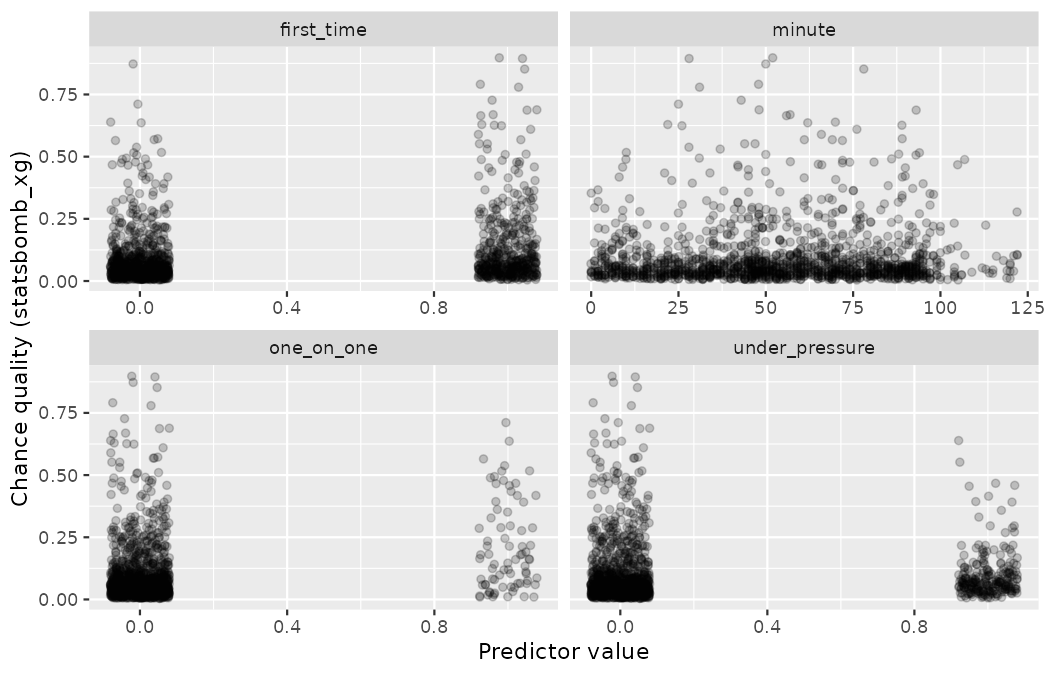
\includegraphics[width=0.85\linewidth,height=\textheight,keepaspectratio]{figures/model-applications-1.png}

The resulting figure is honest about how little any single tag explains.
Every panel is dominated by the same feature: chance quality is strongly
right-skewed, with the great mass of shots below 0.2 and a thin scatter
reaching up toward 0.9 --- the same skew you learned to expect from xG
in Chapter~\ref{sec-explore-numerical}. In the \texttt{one\_on\_one}
panel the band of \texttt{TRUE} shots sits visibly higher than the
\texttt{FALSE} band; in the \texttt{first\_time} panel the lift is there
but smaller; the two \texttt{under\_pressure} bands are essentially
indistinguishable; and the \texttt{minute} panel is a flat cloud with no
visible trend. The correlations agree: \(r = 0.217\) for
\texttt{one\_on\_one} and \(r = 0.208\) for \texttt{first\_time} are
modest positive associations, while \texttt{under\_pressure}
\((r = -0.008)\) and \texttt{minute} \((r = 0.030)\) carry almost no
linear signal at all.

\begin{tcolorbox}[enhanced jigsaw, left=2mm, leftrule=.75mm, title=\textcolor{quarto-callout-tip-color}{\faLightbulb}\hspace{0.5em}{Check your understanding}, arc=.35mm, rightrule=.15mm, coltitle=black, colframe=quarto-callout-tip-color-frame, bottomrule=.15mm, colbacktitle=quarto-callout-tip-color!10!white, opacitybacktitle=0.6, breakable, bottomtitle=1mm, toptitle=1mm, titlerule=0mm, opacityback=0, toprule=.15mm, colback=white]

No correlation value was computed for the predictor variables
\texttt{body\_part} and \texttt{play\_pattern}. Why not? Can these
variables still be used in the linear model?

\begin{center}\rule{0.5\linewidth}{0.5pt}\end{center}

The correlation coefficient can only be calculated to describe the
relationship between two numerical variables. \texttt{body\_part} and
\texttt{play\_pattern} are categorical with more than two levels, not
numerical. They \emph{can}, however, be used in the linear model: as you
saw in Chapter~\ref{sec-model-mlr}, each is converted into a set of
indicator variables, one for every level other than the reference level.

\end{tcolorbox}

For the two categorical predictors, group summaries and side-by-side
boxplots take the place of correlations.

\begin{Shaded}
\begin{Highlighting}[]
\NormalTok{shots\_op }\SpecialCharTok{|\textgreater{}}
  \FunctionTok{group\_by}\NormalTok{(one\_on\_one) }\SpecialCharTok{|\textgreater{}}
  \FunctionTok{summarize}\NormalTok{(}\AttributeTok{shots =} \FunctionTok{n}\NormalTok{(), }\AttributeTok{mean\_xg =} \FunctionTok{mean}\NormalTok{(statsbomb\_xg))}
\CommentTok{\#\textgreater{} \# A tibble: 2 × 3}
\CommentTok{\#\textgreater{}   one\_on\_one shots mean\_xg}
\CommentTok{\#\textgreater{}   \textless{}lgl\textgreater{}      \textless{}int\textgreater{}   \textless{}dbl\textgreater{}}
\CommentTok{\#\textgreater{} 1 FALSE       1305  0.0917}
\CommentTok{\#\textgreater{} 2 TRUE          77  0.210}

\NormalTok{shots\_op }\SpecialCharTok{|\textgreater{}}
  \FunctionTok{group\_by}\NormalTok{(body\_part) }\SpecialCharTok{|\textgreater{}}
  \FunctionTok{summarize}\NormalTok{(}\AttributeTok{shots =} \FunctionTok{n}\NormalTok{(), }\AttributeTok{mean\_xg =} \FunctionTok{mean}\NormalTok{(statsbomb\_xg))}
\CommentTok{\#\textgreater{} \# A tibble: 4 × 3}
\CommentTok{\#\textgreater{}   body\_part  shots mean\_xg}
\CommentTok{\#\textgreater{}   \textless{}fct\textgreater{}      \textless{}int\textgreater{}   \textless{}dbl\textgreater{}}
\CommentTok{\#\textgreater{} 1 Right Foot   703  0.0932}
\CommentTok{\#\textgreater{} 2 Head         252  0.106}
\CommentTok{\#\textgreater{} 3 Left Foot    414  0.0928}
\CommentTok{\#\textgreater{} 4 Other         13  0.412}

\NormalTok{shots\_op }\SpecialCharTok{|\textgreater{}}
  \FunctionTok{group\_by}\NormalTok{(play\_pattern) }\SpecialCharTok{|\textgreater{}}
  \FunctionTok{summarize}\NormalTok{(}\AttributeTok{shots =} \FunctionTok{n}\NormalTok{(), }\AttributeTok{mean\_xg =} \FunctionTok{mean}\NormalTok{(statsbomb\_xg)) }\SpecialCharTok{|\textgreater{}}
  \FunctionTok{arrange}\NormalTok{(}\FunctionTok{desc}\NormalTok{(mean\_xg))}
\CommentTok{\#\textgreater{} \# A tibble: 9 × 3}
\CommentTok{\#\textgreater{}   play\_pattern   shots mean\_xg}
\CommentTok{\#\textgreater{}   \textless{}fct\textgreater{}          \textless{}int\textgreater{}   \textless{}dbl\textgreater{}}
\CommentTok{\#\textgreater{} 1 Other              4  0.175}
\CommentTok{\#\textgreater{} 2 From Counter      56  0.159}
\CommentTok{\#\textgreater{} 3 From Goal Kick    80  0.120}
\CommentTok{\#\textgreater{} 4 From Keeper       21  0.106}
\CommentTok{\#\textgreater{} 5 From Corner      221  0.103}
\CommentTok{\#\textgreater{} 6 Regular Play     446  0.0976}
\CommentTok{\#\textgreater{} 7 From Kick Off     17  0.0946}
\CommentTok{\#\textgreater{} 8 From Free Kick   239  0.0885}
\CommentTok{\#\textgreater{} 9 From Throw In    298  0.0852}
\end{Highlighting}
\end{Shaded}

\begin{Shaded}
\begin{Highlighting}[]
\FunctionTok{ggplot}\NormalTok{(shots\_op, }\FunctionTok{aes}\NormalTok{(}\AttributeTok{x =}\NormalTok{ body\_part, }\AttributeTok{y =}\NormalTok{ statsbomb\_xg)) }\SpecialCharTok{+}
  \FunctionTok{geom\_boxplot}\NormalTok{() }\SpecialCharTok{+}
  \FunctionTok{labs}\NormalTok{(}\AttributeTok{x =} \StringTok{"Body part"}\NormalTok{, }\AttributeTok{y =} \StringTok{"Chance quality (statsbomb\_xg)"}\NormalTok{)}

\FunctionTok{ggplot}\NormalTok{(shots\_op,}
       \FunctionTok{aes}\NormalTok{(}\AttributeTok{x =} \FunctionTok{reorder}\NormalTok{(play\_pattern, statsbomb\_xg, median),}
           \AttributeTok{y =}\NormalTok{ statsbomb\_xg)) }\SpecialCharTok{+}
  \FunctionTok{geom\_boxplot}\NormalTok{() }\SpecialCharTok{+}
  \FunctionTok{coord\_flip}\NormalTok{() }\SpecialCharTok{+}
  \FunctionTok{labs}\NormalTok{(}\AttributeTok{x =} \StringTok{"Play pattern"}\NormalTok{, }\AttributeTok{y =} \StringTok{"Chance quality (statsbomb\_xg)"}\NormalTok{)}
\end{Highlighting}
\end{Shaded}

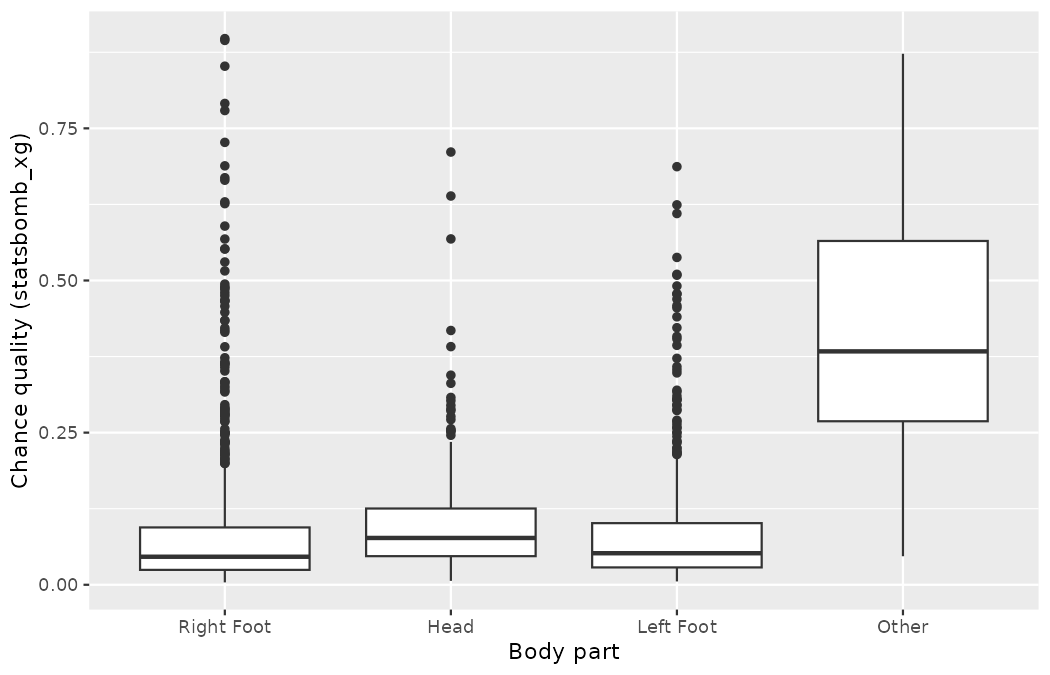
\includegraphics[width=0.85\linewidth,height=\textheight,keepaspectratio]{figures/model-applications-2.png}

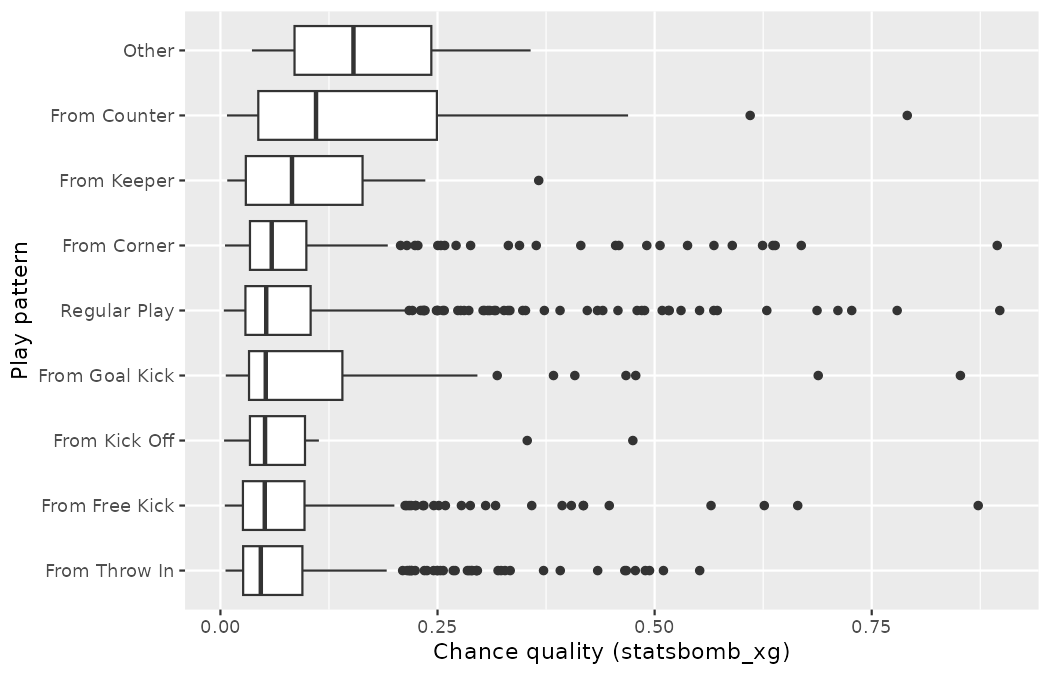
\includegraphics[width=0.85\linewidth,height=\textheight,keepaspectratio]{figures/model-applications-3.png}

The boxplots repay a careful look. For \texttt{body\_part}, the
\texttt{Right\ Foot}, \texttt{Left\ Foot}, and \texttt{Head} boxes are
low and similar (medians 0.046, 0.052, and 0.077 respectively), each
trailing a long right tail of outliers --- but the tiny \texttt{Other}
group floats far above the rest, with a median of 0.384. Those 13 shots
are chest-and-body finishes, which by their nature happen at point-blank
range; a small group with an extreme mean \((0.412)\) will earn a large
coefficient, and we should remember it rests on only 13 shots. For
\texttt{play\_pattern}, counter-attacks stand out --- the
\texttt{From\ Counter} box (56 shots, mean 0.159) sits clearly above
\texttt{Regular\ Play} --- which fits football sense: a counter finds
defenses unset. Shots from throw-in and free-kick possessions have the
lowest typical quality, and the four-shot \texttt{Other} level is too
small to read anything from.

\begin{tcolorbox}[enhanced jigsaw, left=2mm, leftrule=.75mm, title=\textcolor{quarto-callout-note-color}{\faInfo}\hspace{0.5em}{Worked example}, arc=.35mm, rightrule=.15mm, coltitle=black, colframe=quarto-callout-note-color-frame, bottomrule=.15mm, colbacktitle=quarto-callout-note-color!10!white, opacitybacktitle=0.6, breakable, bottomtitle=1mm, toptitle=1mm, titlerule=0mm, opacityback=0, toprule=.15mm, colback=white]

Among the predictors examined, which variable seems to be most
informative for predicting chance quality? Provide two reasons for your
answer.

\begin{center}\rule{0.5\linewidth}{0.5pt}\end{center}

\texttt{one\_on\_one} is the most informative single tag. First, it has
the largest correlation with \texttt{statsbomb\_xg} \((r = 0.217,\) just
ahead of \texttt{first\_time} at \(0.208).\) Second, it produces the
largest separation in group means: one-on-one chances average 0.210
while all other shots average 0.092 --- a one-on-one is priced at more
than double an ordinary open-play shot. Note that the correlation
coefficient and a plot will often point to the same conclusion, but
recall from Chapter~\ref{sec-model-slr} that \(r\) is very sensitive to
outliers, and this response is heavily skewed --- so it is always wise
to look at the plot even when a variable is clearly the most correlated.

\end{tcolorbox}

\subsection{\texorpdfstring{Modeling chance quality with
\texttt{one\_on\_one}}{Modeling chance quality with one\_on\_one}}\label{modeling-chance-quality-with-one_on_one}

A linear model was fit to predict \texttt{statsbomb\_xg} from
\texttt{one\_on\_one} alone --- the simple linear regression of
Chapter~\ref{sec-model-slr}, with an indicator variable as the
predictor.

\begin{Shaded}
\begin{Highlighting}[]
\NormalTok{m\_small }\OtherTok{\textless{}{-}} \FunctionTok{lm}\NormalTok{(statsbomb\_xg }\SpecialCharTok{\textasciitilde{}}\NormalTok{ one\_on\_one, }\AttributeTok{data =}\NormalTok{ shots\_op)}

\FunctionTok{tidy}\NormalTok{(m\_small)}
\CommentTok{\#\textgreater{} \# A tibble: 2 × 5}
\CommentTok{\#\textgreater{}   term           estimate std.error statistic   p.value}
\CommentTok{\#\textgreater{}   \textless{}chr\textgreater{}             \textless{}dbl\textgreater{}     \textless{}dbl\textgreater{}     \textless{}dbl\textgreater{}     \textless{}dbl\textgreater{}}
\CommentTok{\#\textgreater{} 1 (Intercept)      0.0917   0.00338     27.2  1.85e{-}130}
\CommentTok{\#\textgreater{} 2 one\_on\_oneTRUE   0.118    0.0143       8.26 3.30e{-} 16}

\FunctionTok{glance}\NormalTok{(m\_small) }\SpecialCharTok{|\textgreater{}}
  \FunctionTok{select}\NormalTok{(adj.r.squared, df.residual) }\SpecialCharTok{|\textgreater{}}
  \FunctionTok{as.data.frame}\NormalTok{()}
\CommentTok{\#\textgreater{}   adj.r.squared df.residual}
\CommentTok{\#\textgreater{} 1    0.04645055        1380}
\end{Highlighting}
\end{Shaded}

\begin{tcolorbox}[enhanced jigsaw, left=2mm, leftrule=.75mm, title=\textcolor{quarto-callout-tip-color}{\faLightbulb}\hspace{0.5em}{Check your understanding}, arc=.35mm, rightrule=.15mm, coltitle=black, colframe=quarto-callout-tip-color-frame, bottomrule=.15mm, colbacktitle=quarto-callout-tip-color!10!white, opacitybacktitle=0.6, breakable, bottomtitle=1mm, toptitle=1mm, titlerule=0mm, opacityback=0, toprule=.15mm, colback=white]

Interpret the value of \(b_1 = 0.118\) in the context of the problem.

\begin{center}\rule{0.5\linewidth}{0.5pt}\end{center}

Shots tagged as one-on-ones are predicted to carry, on average, 0.118
more chance quality than shots that are not one-on-ones --- a premium of
nearly twelve goals per hundred shots.

\end{tcolorbox}

\begin{tcolorbox}[enhanced jigsaw, left=2mm, leftrule=.75mm, title=\textcolor{quarto-callout-tip-color}{\faLightbulb}\hspace{0.5em}{Check your understanding}, arc=.35mm, rightrule=.15mm, coltitle=black, colframe=quarto-callout-tip-color-frame, bottomrule=.15mm, colbacktitle=quarto-callout-tip-color!10!white, opacitybacktitle=0.6, breakable, bottomtitle=1mm, toptitle=1mm, titlerule=0mm, opacityback=0, toprule=.15mm, colback=white]

Using the model output above, write out the model for predicting chance
quality from \texttt{one\_on\_one}.

\begin{center}\rule{0.5\linewidth}{0.5pt}\end{center}

\[\widehat{\texttt{statsbomb\_xg}} = 0.0917 + 0.1183 \times \texttt{one\_on\_one}_{\texttt{TRUE}}\]

The model predicts 0.0917 for an ordinary open-play shot and
\(0.0917 + 0.1183 = 0.2100\) for a one-on-one.

\end{tcolorbox}

If the premium of 0.118 looks familiar but not quite identical to
numbers you have met before, the difference is the frame, not an error:
Chapter~\ref{sec-model-slr} fit this same indicator model to all 1,494
tournament shots (85 one-on-ones, penalties included) and found 0.127,
Chapter~\ref{sec-model-mlr} fit it to a 1,365-shot frame that also drops
the \texttt{Other}-coded shots (73 one-on-ones) and found 0.1039, and
the 1,382 open-play shots here (77 one-on-ones) give 0.118. Same
phenomenon, three denominators --- a one-on-one premium is always a
statement about which shots it is measured against.

The residuals from the linear model can be used to assess whether a
linear model is appropriate. Recall from Chapter~\ref{sec-model-slr}
that the residual \(e_i = y_i - \hat{y}_i\) is the vertical gap between
an observed response and its fitted value. The code below plots the
residuals on the \(y\)-axis against the fitted (or predicted) values on
the \(x\)-axis.

\begin{Shaded}
\begin{Highlighting}[]
\FunctionTok{augment}\NormalTok{(m\_small) }\SpecialCharTok{|\textgreater{}}
  \FunctionTok{ggplot}\NormalTok{(}\FunctionTok{aes}\NormalTok{(}\AttributeTok{x =}\NormalTok{ .fitted, }\AttributeTok{y =}\NormalTok{ .resid)) }\SpecialCharTok{+}
  \FunctionTok{geom\_point}\NormalTok{(}\AttributeTok{alpha =} \FloatTok{0.3}\NormalTok{) }\SpecialCharTok{+}
  \FunctionTok{geom\_hline}\NormalTok{(}\AttributeTok{yintercept =} \DecValTok{0}\NormalTok{, }\AttributeTok{linetype =} \StringTok{"dashed"}\NormalTok{) }\SpecialCharTok{+}
  \FunctionTok{labs}\NormalTok{(}\AttributeTok{x =} \StringTok{"Predicted chance quality"}\NormalTok{, }\AttributeTok{y =} \StringTok{"Residuals"}\NormalTok{)}
\end{Highlighting}
\end{Shaded}

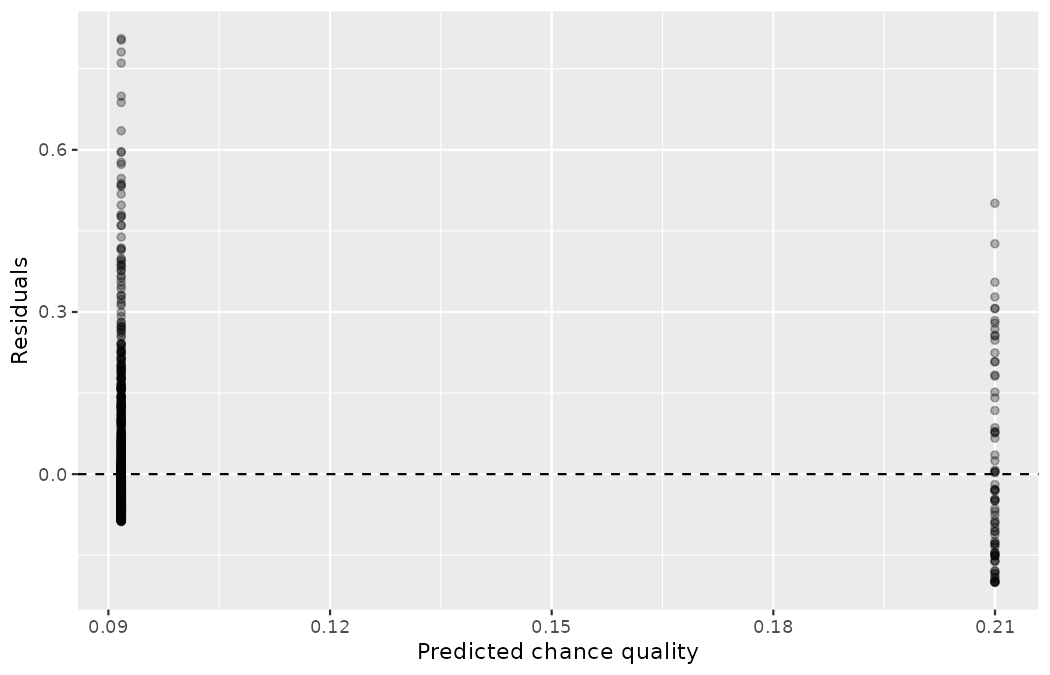
\includegraphics[width=0.85\linewidth,height=\textheight,keepaspectratio]{figures/model-applications-4.png}

Because the only predictor is a two-level tag, the model can produce
exactly two predicted values, so the plot is two vertical strips: one at
0.092 (the 1,305 ordinary shots) and one at 0.210 (the 77 one-on-ones).
Within each strip the residuals are strikingly asymmetric: they are cut
off sharply below --- a residual cannot fall below \(-0.092\) (or
\(-0.210\)) because chance quality cannot fall below zero --- while
above they straggle all the way up to \(+0.806,\) the point-blank
chances the tag sheet cannot see.

\begin{tcolorbox}[enhanced jigsaw, left=2mm, leftrule=.75mm, title=\textcolor{quarto-callout-tip-color}{\faLightbulb}\hspace{0.5em}{Check your understanding}, arc=.35mm, rightrule=.15mm, coltitle=black, colframe=quarto-callout-tip-color-frame, bottomrule=.15mm, colbacktitle=quarto-callout-tip-color!10!white, opacitybacktitle=0.6, breakable, bottomtitle=1mm, toptitle=1mm, titlerule=0mm, opacityback=0, toprule=.15mm, colback=white]

What aspect(s) of the residual plot indicate that a linear model is
appropriate? What aspect(s) of the residual plot seem concerning when
fitting a linear model?

\begin{center}\rule{0.5\linewidth}{0.5pt}\end{center}

There is no curvature for the model to have missed --- with a single
binary predictor, the model simply estimates two group means, and both
strips of residuals are centered on zero. The concerning aspects are the
shape of the scatter: the residuals are strongly right-skewed,
hard-bounded below (a consequence of the response being a probability,
which can never be negative), and their spread is enormous relative to
the two-group separation. Large residuals indicate that most of what
determines a chance's price --- above all, \emph{where on the pitch the
shot is taken} --- is not in this model. These violations matter more
once we do formal inference on regression models; the conditions are
treated carefully in Chapter~\ref{sec-inf-model-slr}.

\end{tcolorbox}

\subsection{Modeling chance quality with multiple
variables}\label{modeling-chance-quality-with-multiple-variables}

It seems as though the predictions of chance quality might be more
accurate if more than one predictor variable were used. The code below
fits a linear model of \texttt{statsbomb\_xg} regressed on all six tags:
\texttt{one\_on\_one}, \texttt{first\_time}, \texttt{under\_pressure},
\texttt{minute}, \texttt{body\_part}, and \texttt{play\_pattern}.

\begin{Shaded}
\begin{Highlighting}[]
\NormalTok{m\_full }\OtherTok{\textless{}{-}} \FunctionTok{lm}\NormalTok{(statsbomb\_xg }\SpecialCharTok{\textasciitilde{}}\NormalTok{ one\_on\_one }\SpecialCharTok{+}\NormalTok{ first\_time }\SpecialCharTok{+}\NormalTok{ under\_pressure }\SpecialCharTok{+}
\NormalTok{               minute }\SpecialCharTok{+}\NormalTok{ body\_part }\SpecialCharTok{+}\NormalTok{ play\_pattern, }\AttributeTok{data =}\NormalTok{ shots\_op)}

\FunctionTok{tidy}\NormalTok{(m\_full) }\SpecialCharTok{|\textgreater{}} \FunctionTok{print}\NormalTok{(}\AttributeTok{n =} \DecValTok{16}\NormalTok{)}
\CommentTok{\#\textgreater{} \# A tibble: 16 × 5}
\CommentTok{\#\textgreater{}    term                        estimate std.error statistic  p.value}
\CommentTok{\#\textgreater{}    \textless{}chr\textgreater{}                          \textless{}dbl\textgreater{}     \textless{}dbl\textgreater{}     \textless{}dbl\textgreater{}    \textless{}dbl\textgreater{}}
\CommentTok{\#\textgreater{}  1 (Intercept)                 0.0457    0.00902      5.07  4.59e{-} 7}
\CommentTok{\#\textgreater{}  2 one\_on\_oneTRUE              0.125     0.0137       9.14  2.14e{-}19}
\CommentTok{\#\textgreater{}  3 first\_timeTRUE              0.0810    0.00699     11.6   1.19e{-}29}
\CommentTok{\#\textgreater{}  4 under\_pressureTRUE         {-}0.00323   0.00898     {-}0.360 7.19e{-} 1}
\CommentTok{\#\textgreater{}  5 minute                      0.000145  0.000107     1.36  1.74e{-} 1}
\CommentTok{\#\textgreater{}  6 body\_partHead               0.0483    0.0101       4.80  1.72e{-} 6}
\CommentTok{\#\textgreater{}  7 body\_partLeft Foot          0.00718   0.00704      1.02  3.08e{-} 1}
\CommentTok{\#\textgreater{}  8 body\_partOther              0.315     0.0320       9.84  4.00e{-}22}
\CommentTok{\#\textgreater{}  9 play\_patternFrom Corner    {-}0.00365   0.00982     {-}0.372 7.10e{-} 1}
\CommentTok{\#\textgreater{} 10 play\_patternFrom Counter    0.0453    0.0161       2.82  4.93e{-} 3}
\CommentTok{\#\textgreater{} 11 play\_patternFrom Free Kick {-}0.0205    0.00916     {-}2.24  2.50e{-} 2}
\CommentTok{\#\textgreater{} 12 play\_patternFrom Goal Kick  0.0180    0.0138       1.31  1.92e{-} 1}
\CommentTok{\#\textgreater{} 13 play\_patternFrom Keeper    0.0123    0.0253       0.488 6.25e{-} 1}
\CommentTok{\#\textgreater{} 14 play\_patternFrom Kick Off  {-}0.00355   0.0280      {-}0.127 8.99e{-} 1}
\CommentTok{\#\textgreater{} 15 play\_patternFrom Throw In  {-}0.00917   0.00848     {-}1.08  2.80e{-} 1}
\CommentTok{\#\textgreater{} 16 play\_patternOther           0.0608    0.0569       1.07  2.85e{-} 1}

\FunctionTok{glance}\NormalTok{(m\_full) }\SpecialCharTok{|\textgreater{}}
  \FunctionTok{select}\NormalTok{(adj.r.squared, df.residual) }\SpecialCharTok{|\textgreater{}}
  \FunctionTok{as.data.frame}\NormalTok{()}
\CommentTok{\#\textgreater{}   adj.r.squared df.residual}
\CommentTok{\#\textgreater{} 1     0.1821507        1366}
\end{Highlighting}
\end{Shaded}

\begin{tcolorbox}[enhanced jigsaw, left=2mm, leftrule=.75mm, title=\textcolor{quarto-callout-note-color}{\faInfo}\hspace{0.5em}{Worked example}, arc=.35mm, rightrule=.15mm, coltitle=black, colframe=quarto-callout-note-color-frame, bottomrule=.15mm, colbacktitle=quarto-callout-note-color!10!white, opacitybacktitle=0.6, breakable, bottomtitle=1mm, toptitle=1mm, titlerule=0mm, opacityback=0, toprule=.15mm, colback=white]

Using the output above, write out the linear model of chance quality on
the six predictor variables.

\begin{center}\rule{0.5\linewidth}{0.5pt}\end{center}

\[
\begin{aligned}
\widehat{\texttt{statsbomb\_xg}} = 0.0457 &+ 0.1253 \times \texttt{one\_on\_one}_{\texttt{TRUE}} \\
&+ 0.0810 \times \texttt{first\_time}_{\texttt{TRUE}} \\
&- 0.0032 \times \texttt{under\_pressure}_{\texttt{TRUE}} \\
&+ 0.000145 \times \texttt{minute} \\
&+ 0.0483 \times \texttt{body\_part}_{\texttt{Head}} \\
&+ 0.0072 \times \texttt{body\_part}_{\texttt{Left Foot}} \\
&+ 0.3149 \times \texttt{body\_part}_{\texttt{Other}} \\
&- 0.0037 \times \texttt{play\_pattern}_{\texttt{From Corner}} \\
&+ 0.0453 \times \texttt{play\_pattern}_{\texttt{From Counter}} \\
&- 0.0205 \times \texttt{play\_pattern}_{\texttt{From Free Kick}} \\
&+ 0.0180 \times \texttt{play\_pattern}_{\texttt{From Goal Kick}} \\
&+ 0.0123 \times \texttt{play\_pattern}_{\texttt{From Keeper}} \\
&- 0.0036 \times \texttt{play\_pattern}_{\texttt{From Kick Off}} \\
&- 0.0092 \times \texttt{play\_pattern}_{\texttt{From Throw In}} \\
&+ 0.0608 \times \texttt{play\_pattern}_{\texttt{Other}}
\end{aligned}
\]

Each indicator takes the value 1 when the shot has that tag or level and
0 otherwise; a right-footed, untagged shot from regular play is priced
by the intercept plus the minute term alone.

\end{tcolorbox}

\begin{tcolorbox}[enhanced jigsaw, left=2mm, leftrule=.75mm, title=\textcolor{quarto-callout-tip-color}{\faLightbulb}\hspace{0.5em}{Check your understanding}, arc=.35mm, rightrule=.15mm, coltitle=black, colframe=quarto-callout-tip-color-frame, bottomrule=.15mm, colbacktitle=quarto-callout-tip-color!10!white, opacitybacktitle=0.6, breakable, bottomtitle=1mm, toptitle=1mm, titlerule=0mm, opacityback=0, toprule=.15mm, colback=white]

The value of the estimated coefficient on
\(\texttt{body\_part}_{\texttt{Head}}\) is \(b_5 = 0.0483.\) Interpret
the value of \(b_5\) in the context of the problem.

\begin{center}\rule{0.5\linewidth}{0.5pt}\end{center}

The coefficient indicates that if all the other variables are kept
constant, headers are priced 0.0483 higher in chance quality, on
average, than right-footed shots (the reference level). This may
surprise you --- recall from Chapter~\ref{sec-data-design} that headers
are \emph{converted} at a lower rate than footed shots. Both are true:
headers arise almost exclusively from crosses and set-piece deliveries
close to goal, so \emph{given the same play pattern and tags}, a header
tends to come from a higher-value position, even though heading is the
harder finishing skill. Holding other variables constant can reverse the
sign of a raw comparison; that is exactly why the phrase ``holding all
else constant'' must accompany every multiple regression coefficient.

\end{tcolorbox}

Emil Sørensen suggests that maybe you do not need all six tags to have a
good model for chance quality. His interest is not statistical elegance:
every tag is a few seconds of a regional scout's matchday attention,
multiplied across thousands of shots a season, and a tag that adds
nothing to the model is a cost with no return. You consider taking a
variable out, but you aren't sure which one to remove.

\begin{tcolorbox}[enhanced jigsaw, left=2mm, leftrule=.75mm, title=\textcolor{quarto-callout-note-color}{\faInfo}\hspace{0.5em}{Worked example}, arc=.35mm, rightrule=.15mm, coltitle=black, colframe=quarto-callout-note-color-frame, bottomrule=.15mm, colbacktitle=quarto-callout-note-color!10!white, opacitybacktitle=0.6, breakable, bottomtitle=1mm, toptitle=1mm, titlerule=0mm, opacityback=0, toprule=.15mm, colback=white]

Results corresponding to the full model for the chance-quality data are
shown in the regression output above. How should we proceed under the
backward elimination strategy?

\begin{center}\rule{0.5\linewidth}{0.5pt}\end{center}

Recall from Chapter~\ref{sec-model-mlr} that backward elimination judges
each candidate model by its adjusted \(R^2\) --- the version of \(R^2\)
that charges a penalty for every predictor, so that a variable must earn
its place. Our baseline adjusted \(R^2\) from the full model is
\(0.1822,\) and we need to determine whether dropping a predictor will
improve the adjusted \(R^2.\) To check, we fit six models that each drop
a different predictor, and we record the adjusted \(R^2\) of each:

\begin{Shaded}
\begin{Highlighting}[]
\NormalTok{drop\_one\_adj\_r\_sq }\OtherTok{\textless{}{-}} \ControlFlowTok{function}\NormalTok{(model, term) \{}
  \FunctionTok{update}\NormalTok{(model, }\FunctionTok{paste}\NormalTok{(}\StringTok{". \textasciitilde{} . {-}"}\NormalTok{, term), }\AttributeTok{data =}\NormalTok{ shots\_op) }\SpecialCharTok{|\textgreater{}}
    \FunctionTok{glance}\NormalTok{() }\SpecialCharTok{|\textgreater{}}
    \FunctionTok{pull}\NormalTok{(adj.r.squared) }\SpecialCharTok{|\textgreater{}}
    \FunctionTok{round}\NormalTok{(}\DecValTok{4}\NormalTok{)}
\NormalTok{\}}

\FunctionTok{tibble}\NormalTok{(}\AttributeTok{dropped =} \FunctionTok{c}\NormalTok{(}\StringTok{"one\_on\_one"}\NormalTok{, }\StringTok{"first\_time"}\NormalTok{, }\StringTok{"under\_pressure"}\NormalTok{,}
                   \StringTok{"minute"}\NormalTok{, }\StringTok{"body\_part"}\NormalTok{, }\StringTok{"play\_pattern"}\NormalTok{)) }\SpecialCharTok{|\textgreater{}}
  \FunctionTok{mutate}\NormalTok{(}\AttributeTok{adj\_r\_sq =} \FunctionTok{map\_dbl}\NormalTok{(dropped, \textbackslash{}(term) }\FunctionTok{drop\_one\_adj\_r\_sq}\NormalTok{(m\_full, term))) }\SpecialCharTok{|\textgreater{}}
  \FunctionTok{as.data.frame}\NormalTok{()}
\CommentTok{\#\textgreater{}          dropped adj\_r\_sq}
\CommentTok{\#\textgreater{} 1     one\_on\_one   0.1327}
\CommentTok{\#\textgreater{} 2     first\_time   0.1025}
\CommentTok{\#\textgreater{} 3 under\_pressure   0.1827}
\CommentTok{\#\textgreater{} 4         minute   0.1816}
\CommentTok{\#\textgreater{} 5      body\_part   0.1169}
\CommentTok{\#\textgreater{} 6   play\_pattern   0.1743}
\end{Highlighting}
\end{Shaded}

The model without \texttt{under\_pressure} has the highest adjusted
\(R^2\) of \(0.1827,\) higher than the adjusted \(R^2\) for the full
model. Because eliminating \texttt{under\_pressure} leads to a model
with a higher adjusted \(R^2\) than the full model, we drop
\texttt{under\_pressure} from the model.

It might seem counter-intuitive to exclude the pressure tag from a model
of chance quality. After all, pressure is the tag Emil's scouts argue
about most, and you saw in Chapter~\ref{sec-explore-categorical} that
shots taken under pressure are converted at a visibly lower rate than
unpressured shots. However, note that the response here is \emph{chance
quality}, not conversion --- and within open play, the pressure tag
barely moves StatsBomb's price at all:

\begin{Shaded}
\begin{Highlighting}[]
\NormalTok{shots\_op }\SpecialCharTok{|\textgreater{}}
  \FunctionTok{group\_by}\NormalTok{(under\_pressure) }\SpecialCharTok{|\textgreater{}}
  \FunctionTok{summarize}\NormalTok{(}\AttributeTok{shots =} \FunctionTok{n}\NormalTok{(), }\AttributeTok{mean\_xg =} \FunctionTok{mean}\NormalTok{(statsbomb\_xg))}
\CommentTok{\#\textgreater{} \# A tibble: 2 × 3}
\CommentTok{\#\textgreater{}   under\_pressure shots mean\_xg}
\CommentTok{\#\textgreater{}   \textless{}lgl\textgreater{}          \textless{}int\textgreater{}   \textless{}dbl\textgreater{}}
\CommentTok{\#\textgreater{} 1 FALSE           1144  0.0988}
\CommentTok{\#\textgreater{} 2 TRUE             238  0.0961}
\end{Highlighting}
\end{Shaded}

A gap of \(0.0988 - 0.0961 = 0.0027\) is next to nothing --- which is
exactly what the near-zero correlation \((r = -0.008)\) told us at the
start of the case study, and what the tiny, wrong-signed, imprecisely
estimated coefficient \((-0.0032)\) repeated inside the full model. The
much larger tournament-wide pressure gap in mean chance quality is
largely an artifact of the shots we excluded: penalties, which are never
taken under pressure and carry a chance quality of \(0.784,\) sit
entirely in the unpressured group and drag its average up. Restrict
attention to open play, hold the other tags fixed, and the pressure tag
has nothing left to say about StatsBomb's price. Whether pressure
affects what happens \emph{to} the chance --- whether it is scored ---
is a different question, about a different response variable, and it
must wait for the inference tools of
Chapter~\ref{sec-foundations-randomization}.

Since we eliminated a predictor from the model in the first step, we see
whether we should eliminate any additional predictors. Our baseline
adjusted \(R^2\) is now \(0.1827.\) We fit another set of models, which
consider eliminating each of the remaining predictors in addition to
\texttt{under\_pressure}:

\begin{Shaded}
\begin{Highlighting}[]
\NormalTok{m\_no\_pressure }\OtherTok{\textless{}{-}} \FunctionTok{lm}\NormalTok{(statsbomb\_xg }\SpecialCharTok{\textasciitilde{}}\NormalTok{ one\_on\_one }\SpecialCharTok{+}\NormalTok{ first\_time }\SpecialCharTok{+}\NormalTok{ minute }\SpecialCharTok{+}
\NormalTok{                      body\_part }\SpecialCharTok{+}\NormalTok{ play\_pattern, }\AttributeTok{data =}\NormalTok{ shots\_op)}

\FunctionTok{tibble}\NormalTok{(}\AttributeTok{dropped =} \FunctionTok{c}\NormalTok{(}\StringTok{"one\_on\_one"}\NormalTok{, }\StringTok{"first\_time"}\NormalTok{, }\StringTok{"minute"}\NormalTok{,}
                   \StringTok{"body\_part"}\NormalTok{, }\StringTok{"play\_pattern"}\NormalTok{)) }\SpecialCharTok{|\textgreater{}}
  \FunctionTok{mutate}\NormalTok{(}\AttributeTok{adj\_r\_sq =} \FunctionTok{map\_dbl}\NormalTok{(dropped, \textbackslash{}(term) }\FunctionTok{drop\_one\_adj\_r\_sq}\NormalTok{(m\_no\_pressure, term))) }\SpecialCharTok{|\textgreater{}}
  \FunctionTok{as.data.frame}\NormalTok{()}
\CommentTok{\#\textgreater{}        dropped adj\_r\_sq}
\CommentTok{\#\textgreater{} 1   one\_on\_one   0.1330}
\CommentTok{\#\textgreater{} 2   first\_time   0.1028}
\CommentTok{\#\textgreater{} 3       minute   0.1822}
\CommentTok{\#\textgreater{} 4    body\_part   0.1167}
\CommentTok{\#\textgreater{} 5 play\_pattern   0.1749}
\end{Highlighting}
\end{Shaded}

None of these models leads to an improvement in adjusted \(R^2,\) so we
do not eliminate any of the remaining predictors. Notice the near-miss,
though: dropping \texttt{minute} gives \(0.1822,\) a mere \(0.0005\)
below the baseline. The adjusted \(R^2\) penalty almost --- but not
quite --- pays for removing it, so backward elimination keeps a
predictor whose coefficient \((0.000145\) per minute\()\) is tiny. A
different selection criterion could reasonably have dropped it; model
selection is a strategy, not an oracle.

\end{tcolorbox}

That is, after backward elimination, we are left with the model that
keeps all predictors except \texttt{under\_pressure}, which we can
summarize using its coefficients:

\begin{Shaded}
\begin{Highlighting}[]
\FunctionTok{tidy}\NormalTok{(m\_no\_pressure) }\SpecialCharTok{|\textgreater{}} \FunctionTok{print}\NormalTok{(}\AttributeTok{n =} \DecValTok{15}\NormalTok{)}
\CommentTok{\#\textgreater{} \# A tibble: 15 × 5}
\CommentTok{\#\textgreater{}    term                        estimate std.error statistic  p.value}
\CommentTok{\#\textgreater{}    \textless{}chr\textgreater{}                          \textless{}dbl\textgreater{}     \textless{}dbl\textgreater{}     \textless{}dbl\textgreater{}    \textless{}dbl\textgreater{}}
\CommentTok{\#\textgreater{}  1 (Intercept)                 0.0454    0.00898      5.06  4.85e{-} 7}
\CommentTok{\#\textgreater{}  2 one\_on\_oneTRUE              0.126     0.0137       9.17  1.68e{-}19}
\CommentTok{\#\textgreater{}  3 first\_timeTRUE              0.0811    0.00699     11.6   8.82e{-}30}
\CommentTok{\#\textgreater{}  4 minute                      0.000145  0.000107     1.36  1.75e{-} 1}
\CommentTok{\#\textgreater{}  5 body\_partHead               0.0470    0.00934      5.03  5.51e{-} 7}
\CommentTok{\#\textgreater{}  6 body\_partLeft Foot          0.00711   0.00704      1.01  3.12e{-} 1}
\CommentTok{\#\textgreater{}  7 body\_partOther              0.315     0.0320       9.85  3.83e{-}22}
\CommentTok{\#\textgreater{}  8 play\_patternFrom Corner    {-}0.00378   0.00981     {-}0.385 7.00e{-} 1}
\CommentTok{\#\textgreater{}  9 play\_patternFrom Counter    0.0452    0.0161       2.81  5.07e{-} 3}
\CommentTok{\#\textgreater{} 10 play\_patternFrom Free Kick {-}0.0205    0.00915     {-}2.24  2.53e{-} 2}
\CommentTok{\#\textgreater{} 11 play\_patternFrom Goal Kick  0.0177    0.0138       1.28  2.00e{-} 1}
\CommentTok{\#\textgreater{} 12 play\_patternFrom Keeper     0.0121    0.0253       0.478 6.33e{-} 1}
\CommentTok{\#\textgreater{} 13 play\_patternFrom Kick Off  {-}0.00360   0.0280      {-}0.129 8.98e{-} 1}
\CommentTok{\#\textgreater{} 14 play\_patternFrom Throw In  {-}0.00918   0.00848     {-}1.08  2.79e{-} 1}
\CommentTok{\#\textgreater{} 15 play\_patternOther           0.0610    0.0568       1.07  2.83e{-} 1}

\FunctionTok{glance}\NormalTok{(m\_no\_pressure) }\SpecialCharTok{|\textgreater{}}
  \FunctionTok{select}\NormalTok{(adj.r.squared, df.residual) }\SpecialCharTok{|\textgreater{}}
  \FunctionTok{as.data.frame}\NormalTok{()}
\CommentTok{\#\textgreater{}   adj.r.squared df.residual}
\CommentTok{\#\textgreater{} 1     0.1826715        1367}
\end{Highlighting}
\end{Shaded}

Then, the linear model for predicting chance quality based on this model
is as follows:

\[
\begin{aligned}
\widehat{\texttt{statsbomb\_xg}} = 0.0454 &+ 0.1256 \times \texttt{one\_on\_one}_{\texttt{TRUE}} \\
&+ 0.0811 \times \texttt{first\_time}_{\texttt{TRUE}} \\
&+ 0.000145 \times \texttt{minute} \\
&+ 0.0470 \times \texttt{body\_part}_{\texttt{Head}} \\
&+ 0.0071 \times \texttt{body\_part}_{\texttt{Left Foot}} \\
&+ 0.3149 \times \texttt{body\_part}_{\texttt{Other}} \\
&- 0.0038 \times \texttt{play\_pattern}_{\texttt{From Corner}} \\
&+ 0.0452 \times \texttt{play\_pattern}_{\texttt{From Counter}} \\
&- 0.0205 \times \texttt{play\_pattern}_{\texttt{From Free Kick}} \\
&+ 0.0177 \times \texttt{play\_pattern}_{\texttt{From Goal Kick}} \\
&+ 0.0121 \times \texttt{play\_pattern}_{\texttt{From Keeper}} \\
&- 0.0036 \times \texttt{play\_pattern}_{\texttt{From Kick Off}} \\
&- 0.0092 \times \texttt{play\_pattern}_{\texttt{From Throw In}} \\
&+ 0.0610 \times \texttt{play\_pattern}_{\texttt{Other}}
\end{aligned}
\]

An adjusted \(R^2\) of \(0.1827\) deserves a sober sentence in any
report to Marta Vidal: the six-second tag sheet recovers under a fifth
of the variability in StatsBomb's prices. The tags are real information
--- a scout logging them is doing useful work --- but most of what
prices a chance is \emph{where it is taken from}, and no arrangement of
these labels can substitute for coordinates.

\begin{tcolorbox}[enhanced jigsaw, left=2mm, leftrule=.75mm, title=\textcolor{quarto-callout-note-color}{\faInfo}\hspace{0.5em}{Worked example}, arc=.35mm, rightrule=.15mm, coltitle=black, colframe=quarto-callout-note-color-frame, bottomrule=.15mm, colbacktitle=quarto-callout-note-color!10!white, opacitybacktitle=0.6, breakable, bottomtitle=1mm, toptitle=1mm, titlerule=0mm, opacityback=0, toprule=.15mm, colback=white]

The residual plot for the model with all of the predictor variables
except \texttt{under\_pressure} is drawn by the code below. How do these
residuals compare to the residuals from the model with
\texttt{one\_on\_one} alone?

\begin{Shaded}
\begin{Highlighting}[]
\FunctionTok{augment}\NormalTok{(m\_no\_pressure) }\SpecialCharTok{|\textgreater{}}
  \FunctionTok{ggplot}\NormalTok{(}\FunctionTok{aes}\NormalTok{(}\AttributeTok{x =}\NormalTok{ .fitted, }\AttributeTok{y =}\NormalTok{ .resid)) }\SpecialCharTok{+}
  \FunctionTok{geom\_point}\NormalTok{(}\AttributeTok{alpha =} \FloatTok{0.3}\NormalTok{) }\SpecialCharTok{+}
  \FunctionTok{geom\_hline}\NormalTok{(}\AttributeTok{yintercept =} \DecValTok{0}\NormalTok{, }\AttributeTok{linetype =} \StringTok{"dashed"}\NormalTok{) }\SpecialCharTok{+}
  \FunctionTok{labs}\NormalTok{(}\AttributeTok{x =} \StringTok{"Predicted chance quality"}\NormalTok{, }\AttributeTok{y =} \StringTok{"Residuals"}\NormalTok{)}

\FunctionTok{augment}\NormalTok{(m\_no\_pressure) }\SpecialCharTok{|\textgreater{}}
  \FunctionTok{summarize}\NormalTok{(}
    \AttributeTok{min\_resid =} \FunctionTok{min}\NormalTok{(.resid),}
    \AttributeTok{max\_resid =} \FunctionTok{max}\NormalTok{(.resid),}
    \AttributeTok{n\_beyond\_0.3 =} \FunctionTok{sum}\NormalTok{(}\FunctionTok{abs}\NormalTok{(.resid) }\SpecialCharTok{\textgreater{}} \FloatTok{0.3}\NormalTok{)}
\NormalTok{  )}
\CommentTok{\#\textgreater{} \# A tibble: 1 × 3}
\CommentTok{\#\textgreater{}   min\_resid max\_resid n\_beyond\_0.3}
\CommentTok{\#\textgreater{}       \textless{}dbl\textgreater{}     \textless{}dbl\textgreater{}        \textless{}int\textgreater{}}
\CommentTok{\#\textgreater{} 1    {-}0.317     0.768           46}
\end{Highlighting}
\end{Shaded}

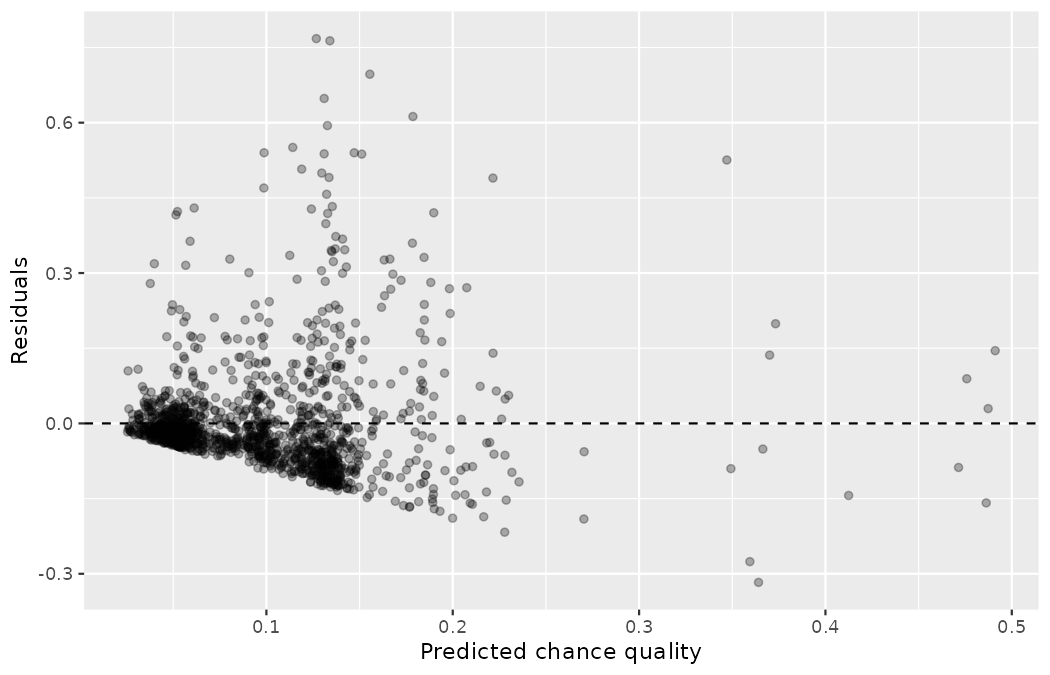
\includegraphics[width=0.85\linewidth,height=\textheight,keepaspectratio]{figures/model-applications-5.png}

\begin{center}\rule{0.5\linewidth}{0.5pt}\end{center}

The two vertical strips are gone: with fourteen estimated coefficients
and \texttt{minute} varying continuously, the fitted values now spread
across a range from about \(0.03\) to \(0.49,\) and the plot looks like
a proper residual cloud. The residuals are, for the most part, scattered
around 0. However, the same pathologies as before persist in milder
form. The cloud is bounded below by a diagonal floor --- since chance
quality cannot be negative, no residual can fall below \(-\hat{y}_i,\)
so the lower edge of the plot slopes down exactly along that line ---
while the upper side straggles far higher, to a maximum residual of
\(+0.768.\) That most extreme point is Jean-Charles Castelletto's
28th-minute goal for Cameroon against Serbia: a first-time, right-footed
finish from a corner that StatsBomb prices at \(0.894\) but the tag
sheet, blind to the fact that he met the ball a few metres from an open
net, prices at \(0.127.\) Forty-six shots have residuals beyond
\(\pm 0.3,\) and forty-five of those forty-six are on the positive side:
the model's worst errors are almost all \emph{underpricing} of
point-blank chances. The skew and the floor are structural --- a
probability response squeezed near zero will violate the usual
linear-model conditions --- and they foreshadow both the formal residual
conditions of Chapter~\ref{sec-inf-model-slr} and the logistic machinery
of Chapter~\ref{sec-model-logistic}, which was built for exactly this
kind of response.

\end{tcolorbox}

\begin{tcolorbox}[enhanced jigsaw, left=2mm, leftrule=.75mm, title=\textcolor{quarto-callout-tip-color}{\faLightbulb}\hspace{0.5em}{Check your understanding}, arc=.35mm, rightrule=.15mm, coltitle=black, colframe=quarto-callout-tip-color-frame, bottomrule=.15mm, colbacktitle=quarto-callout-tip-color!10!white, opacitybacktitle=0.6, breakable, bottomtitle=1mm, toptitle=1mm, titlerule=0mm, opacityback=0, toprule=.15mm, colback=white]

Consider a shot tagged by a Northbridge scout as follows: 70th minute, a
first-time header from a corner, not a one-on-one. What is the predicted
chance quality of the shot?

\begin{center}\rule{0.5\linewidth}{0.5pt}\end{center}

\[
\widehat{\texttt{statsbomb\_xg}} = 0.0454 + 0.0811 + 0.000145 \times 70 + 0.0470 - 0.0038 = 0.1799
\]

Only the indicators the shot activates appear: \texttt{first\_time}
\((+0.0811),\) the minute term \((0.000145 \times 70 = 0.0102),\)
\texttt{Head} \((+0.0470),\) and \texttt{From\ Corner} \((-0.0038).\) A
chance quality of about \(0.18\) --- a shade under one goal in five such
chances.

\end{tcolorbox}

\subsection{The scope of a model}\label{the-scope-of-a-model}

A partner analyst emails Priya Rao a tag sheet for a single shot, with
no footage attached: 62nd minute, right-footed, struck first time, not a
one-on-one, from regular play.

\begin{tcolorbox}[enhanced jigsaw, left=2mm, leftrule=.75mm, title=\textcolor{quarto-callout-tip-color}{\faLightbulb}\hspace{0.5em}{Check your understanding}, arc=.35mm, rightrule=.15mm, coltitle=black, colframe=quarto-callout-tip-color-frame, bottomrule=.15mm, colbacktitle=quarto-callout-tip-color!10!white, opacitybacktitle=0.6, breakable, bottomtitle=1mm, toptitle=1mm, titlerule=0mm, opacityback=0, toprule=.15mm, colback=white]

What is the predicted chance quality of this shot?

\begin{center}\rule{0.5\linewidth}{0.5pt}\end{center}

Only \texttt{first\_time} and the minute term activate:

\[
\widehat{\texttt{statsbomb\_xg}} = 0.0454 + 0.0811 + 0.000145 \times 62 = 0.1355
\]

An ordinary, slightly-better-than-baseline chance --- nothing a sporting
director would leave her office for.

\end{tcolorbox}

\begin{tcolorbox}[enhanced jigsaw, left=2mm, leftrule=.75mm, title=\textcolor{quarto-callout-tip-color}{\faLightbulb}\hspace{0.5em}{Check your understanding}, arc=.35mm, rightrule=.15mm, coltitle=black, colframe=quarto-callout-tip-color-frame, bottomrule=.15mm, colbacktitle=quarto-callout-tip-color!10!white, opacitybacktitle=0.6, breakable, bottomtitle=1mm, toptitle=1mm, titlerule=0mm, opacityback=0, toprule=.15mm, colback=white]

If you later learned that StatsBomb prices this shot at \(0.725,\) would
you think the model was terrible? What if you then learned that the shot
was Grace Geyoro's goal for France against Wales --- at the 2025 Women's
Euro?

\begin{center}\rule{0.5\linewidth}{0.5pt}\end{center}

A residual of \(0.725 - 0.1355 = 0.590\) is really big. Note that the
large residuals (except one shot) in the residual plot above are closer
to \(0.3\) --- about half as big. But after we learn that the shot is
from the 2025 Women's Euro, we realize that the model shouldn't have
been applied to the new shot at all! The original data are from
open-play shots at the 2022 Men's World Cup, and models based on those
data should be used only to explore patterns in chance quality for
open-play shots at that tournament. A different competition ---
different players, different tournament, a different season of
StatsBomb's own pricing model --- is outside the model's scope, and the
model itself contains no warning light for this: \texttt{predict()} will
cheerfully return \(0.1355\) for any tag sheet you feed it. Whether a
model fit on one competition happens to transfer to another is an
empirical question, one we take up properly when external validation
appears in Chapter~\ref{sec-inf-model-mlr}.

\end{tcolorbox}

The shot in question is real, and you can locate it --- and quantify the
miss --- directly:

\begin{Shaded}
\begin{Highlighting}[]
\NormalTok{weuro2025\_shots }\OtherTok{\textless{}{-}} \FunctionTok{read\_csv}\NormalTok{(}\StringTok{"data/derived/weuro2025\_shots.csv"}\NormalTok{)}

\NormalTok{mystery\_shot }\OtherTok{\textless{}{-}}\NormalTok{ weuro2025\_shots }\SpecialCharTok{|\textgreater{}}
  \FunctionTok{filter}\NormalTok{(shot\_type }\SpecialCharTok{==} \StringTok{"Open Play"}\NormalTok{) }\SpecialCharTok{|\textgreater{}}
  \FunctionTok{slice\_max}\NormalTok{(statsbomb\_xg, }\AttributeTok{n =} \DecValTok{1}\NormalTok{)}

\NormalTok{mystery\_shot }\SpecialCharTok{|\textgreater{}}
  \FunctionTok{select}\NormalTok{(competition, player, team, opponent, statsbomb\_xg, outcome)}
\CommentTok{\#\textgreater{} \# A tibble: 1 × 6}
\CommentTok{\#\textgreater{}   competition player             team           opponent statsbomb\_xg outcome}
\CommentTok{\#\textgreater{}   \textless{}chr\textgreater{}       \textless{}chr\textgreater{}              \textless{}chr\textgreater{}          \textless{}chr\textgreater{}           \textless{}dbl\textgreater{} \textless{}chr\textgreater{}}
\CommentTok{\#\textgreater{} 1 weuro2025   Onema Grace Geyoro France Women\textquotesingle{}s Wales W         0.725 Goal}

\NormalTok{mystery\_shot }\SpecialCharTok{|\textgreater{}}
  \FunctionTok{mutate}\NormalTok{(}
    \AttributeTok{predicted =} \FunctionTok{predict}\NormalTok{(m\_no\_pressure, }\AttributeTok{newdata =}\NormalTok{ mystery\_shot),}
    \AttributeTok{residual  =}\NormalTok{ statsbomb\_xg }\SpecialCharTok{{-}}\NormalTok{ predicted}
\NormalTok{  ) }\SpecialCharTok{|\textgreater{}}
  \FunctionTok{select}\NormalTok{(statsbomb\_xg, predicted, residual)}
\CommentTok{\#\textgreater{} \# A tibble: 1 × 3}
\CommentTok{\#\textgreater{}   statsbomb\_xg predicted residual}
\CommentTok{\#\textgreater{}          \textless{}dbl\textgreater{}     \textless{}dbl\textgreater{}    \textless{}dbl\textgreater{}}
\CommentTok{\#\textgreater{} 1        0.725     0.136    0.590}
\end{Highlighting}
\end{Shaded}

It is the highest-priced open-play chance of the entire Women's Euro,
and on the tag sheet it is indistinguishable from a hopeful hit from
distance. Hold on to both lessons at once: even \emph{within} scope,
this model's tags cannot see the pitch, and its honest residual spread
says so; \emph{outside} scope, we do not even have the residual plot's
testimony about how wrong we might be. The case study's deliverable to
Marta is therefore not just a model but a label on the tin:
\emph{open-play chances, 2022 Men's World Cup, tags only --- expect
large underpricing of point-blank chances, and do not apply elsewhere
without validation.}

\subsection{Coda: from pricing the chance to predicting the
goal}\label{coda-from-pricing-the-chance-to-predicting-the-goal}

One tool from the three-chapter toolkit has not yet touched the case
study: the logistic regression of Chapter~\ref{sec-model-logistic}.
Marta's question was about pricing the chance, and chance quality is
numerical --- linear regression territory. But the outcome the club
ultimately banks is binary: did the shot go in? One fit closes the loop,
using the three logical tags on the same open-play frame:

\begin{Shaded}
\begin{Highlighting}[]
\NormalTok{goal\_op }\OtherTok{\textless{}{-}} \FunctionTok{glm}\NormalTok{(goal }\SpecialCharTok{\textasciitilde{}}\NormalTok{ one\_on\_one }\SpecialCharTok{+}\NormalTok{ under\_pressure }\SpecialCharTok{+}\NormalTok{ first\_time,}
               \AttributeTok{data =}\NormalTok{ shots\_op, }\AttributeTok{family =}\NormalTok{ binomial)}
\FunctionTok{tidy}\NormalTok{(goal\_op)}
\CommentTok{\#\textgreater{} \# A tibble: 4 × 5}
\CommentTok{\#\textgreater{}   term               estimate std.error statistic  p.value}
\CommentTok{\#\textgreater{}   \textless{}chr\textgreater{}                 \textless{}dbl\textgreater{}     \textless{}dbl\textgreater{}     \textless{}dbl\textgreater{}    \textless{}dbl\textgreater{}}
\CommentTok{\#\textgreater{} 1 (Intercept)         {-}2.55       0.144   {-}17.7   6.70e{-}70}
\CommentTok{\#\textgreater{} 2 one\_on\_oneTRUE       1.27       0.305     4.16  3.16e{-} 5}
\CommentTok{\#\textgreater{} 3 under\_pressureTRUE   0.0957     0.243     0.395 6.93e{-} 1}
\CommentTok{\#\textgreater{} 4 first\_timeTRUE       0.819      0.188     4.35  1.36e{-} 5}

\FunctionTok{round}\NormalTok{(}\FunctionTok{coef}\NormalTok{(goal\_op), }\DecValTok{4}\NormalTok{)}
\CommentTok{\#\textgreater{}        (Intercept)     one\_on\_oneTRUE under\_pressureTRUE     first\_timeTRUE}
\CommentTok{\#\textgreater{}            {-}2.5479             1.2703             0.0957             0.8189}
\end{Highlighting}
\end{Shaded}

Back-transform the coefficient a scout would ask about first. An
open-play shot with none of the tags has log odds equal to the
intercept, so \(\hat{p} = e^{-2.5479}/(1 + e^{-2.5479}) = 0.0726\);
flipping only the one-on-one tag moves the log odds to
\(-2.5479 + 1.2703 = -1.2776\) and the probability to \(0.218\) ---
close to the raw open-play conversion rates of \(0.102\) for ordinary
shots and \(0.221\) for one-on-ones. And carry over
Chapter~\ref{sec-model-logistic}'s warning intact: the dossier audit
earned causal language because Priya randomized every cue, while nobody
randomized which shooters were left one-on-one or closed down, so these
coefficients describe association in one tournament's open play and
nothing more. Note, in the same spirit, that the pressure tag's estimate
is small, positive, and dwarfed by its standard error --- pressure said
nothing about the \emph{price} of an open-play chance earlier in this
chapter, and it adds no signal about the outcome here; the machinery for
judging such coefficients formally begins in
Chapter~\ref{sec-foundations-randomization}.

\section{Interactive R tutorials}\label{sec-model-tutorials}

Navigate the concepts you've learned in this part in R using the
following self-paced tutorials. All you need is your browser to get
started! The tutorials were built by the authors of \emph{Introduction
to Modern Statistics} around their own datasets, so you will find houses
and possums where this book has shots and scouts --- treat that as
translation practice: for every screen, ask yourself which variable
plays the role of \texttt{statsbomb\_xg} and which plays the role of the
tags.

\begin{itemize}
\tightlist
\item
  \href{https://openintrostat.github.io/ims-tutorials/03-model/}{Tutorial
  3: Regression modeling}
\item
  \href{https://openintro.shinyapps.io/ims-03-model-01/}{Tutorial 3 -
  Lesson 1: Visualizing two variables}
\item
  \href{https://openintro.shinyapps.io/ims-03-model-02/}{Tutorial 3 -
  Lesson 2: Correlation}
\item
  \href{https://openintro.shinyapps.io/ims-03-model-03/}{Tutorial 3 -
  Lesson 3: Simple linear regression}
\item
  \href{https://openintro.shinyapps.io/ims-03-model-04/}{Tutorial 3 -
  Lesson 4: Interpreting regression models}
\item
  \href{https://openintro.shinyapps.io/ims-03-model-05/}{Tutorial 3 -
  Lesson 5: Model fit}
\item
  \href{https://openintro.shinyapps.io/ims-03-model-06/}{Tutorial 3 -
  Lesson 6: Parallel slopes}
\item
  \href{https://openintro.shinyapps.io/ims-03-model-07/}{Tutorial 3 -
  Lesson 7: Evaluating and extending parallel slopes model}
\item
  \href{https://openintro.shinyapps.io/ims-03-model-08/}{Tutorial 3 -
  Lesson 8: Multiple regression}
\item
  \href{https://openintro.shinyapps.io/ims-03-model-09/}{Tutorial 3 -
  Lesson 9: Logistic regression}
\item
  \href{https://openintro.shinyapps.io/ims-03-model-10/}{Tutorial 3 -
  Lesson 10: Case study: Italian restaurants in NYC}
\end{itemize}

You can also access the full list of tutorials supporting both the
original book and this adaptation at
\url{https://openintrostat.github.io/ims-tutorials}.

\section{R labs}\label{sec-model-labs}

Further apply the concepts you've learned in this part in R with
computational labs that walk you through a data analysis case study.

\begin{itemize}
\tightlist
\item
  \href{https://www.openintro.org/go?id=ims-r-lab-model}{Introduction to
  linear regression - Human Freedom Index}
\end{itemize}

You can also access the full list of labs at
\url{https://www.openintro.org/go?id=ims-r-labs}. A worthwhile
club-flavored variant: repeat this chapter's entire workflow ---
per-predictor EDA, simple model, full model, backward elimination,
residual plot, scoped prediction --- on \texttt{weuro2025\_shots}, and
compare which predictors survive elimination in the two competitions
before you peek at each other's results. \emph{What you should find:} on
the 851 open-play shots of the Women's Euro, backward elimination again
removes exactly one predictor, but a different one --- \texttt{minute}
drops (adjusted \(R^2\) rises from \(0.1038\) to \(0.1047\)), while
\texttt{under\_pressure}, the tag eliminated at the men's World Cup,
survives.

\section{Chapter review}\label{sec-chp10-review}

\subsection{Summary}\label{summary-9}

This chapter introduced no new machinery; it rehearsed the discipline of
using the modeling toolkit end to end on one scouting question. The
order of operations is the content:

\begin{itemize}
\tightlist
\item
  \textbf{Scope the data before touching a model.} We removed penalties
  and dead-ball strikes \emph{and said so}, fixing the population the
  model describes: open-play shots at the 2022 Men's World Cup. We also
  fixed the reference levels (\texttt{Right\ Foot},
  \texttt{Regular\ Play}) so every later coefficient had a stated
  baseline.
\item
  \textbf{Explore each predictor's relationship with the response.}
  Correlations for numerical (and 0/1) predictors, group means and
  boxplots for categorical ones. This stage produced the case study's
  early warnings: the near-zero pressure correlation, and the 13-shot
  \texttt{Other} body-part group with an extreme mean.
\item
  \textbf{Fit simple, then fit full.} The single best tag
  (\texttt{one\_on\_one}) explained under 5\% of the variability
  (adjusted \(R^2 = 0.0465\)); all six tags together reached \(0.1822.\)
\item
  \textbf{Simplify with a stated criterion.} Backward elimination by
  adjusted \(R^2\) removed exactly one predictor ---
  \texttt{under\_pressure} --- and the elimination was not a verdict on
  pressure in football, but on what the tag adds \emph{for this
  response, given the other tags}. A criterion, honestly applied, can
  also have near-misses (\texttt{minute} survived by \(0.0005\)).
\item
  \textbf{Read the residuals.} The residual plot showed a floor (a
  probability response cannot produce residuals below \(-\hat{y}_i\)), a
  heavy right tail of underpriced point-blank chances, and one extreme
  outlier --- the shape that motivates the model conditions of
  Chapter~\ref{sec-inf-model-slr} and the logistic models of
  Chapter~\ref{sec-model-logistic}.
\item
  \textbf{State the model's scope with its predictions.} The Geyoro shot
  showed how silently a model misprices data from outside the population
  it was fit on. A prediction should travel with the model's residual
  behavior and its scope, or it should not travel at all.
\end{itemize}

\subsection{Terms}\label{terms-9}

No new terms were introduced in this chapter. The terms below did the
case study's work; all were introduced and defined in
Chapter~\ref{sec-model-slr} through Chapter~\ref{sec-model-logistic},
and you should be able to recognize each one in the workflow above. If
any feel unfamiliar, go back and review their definitions in those
chapters.

\begin{longtable}[]{@{}
  >{\raggedright\arraybackslash}p{(\linewidth - 4\tabcolsep) * \real{0.3380}}
  >{\raggedright\arraybackslash}p{(\linewidth - 4\tabcolsep) * \real{0.3380}}
  >{\raggedright\arraybackslash}p{(\linewidth - 4\tabcolsep) * \real{0.3239}}@{}}
\caption{Terms revisited in this
chapter.}\label{tbl-terms-chp-10}\tabularnewline
\toprule\noalign{}
\endfirsthead
\endhead
\bottomrule\noalign{}
\endlastfoot
adjusted \(R^2\) & indicator variable & reference level \\
backward elimination & multiple regression & residual \\
correlation coefficient & prediction & simple linear regression \\
\end{longtable}

\begin{center}\rule{0.5\linewidth}{0.5pt}\end{center}

Adapted from \emph{Introduction to Modern Statistics} by
Çetinkaya-Rundel \& Hardin (CC BY-SA 4.0); this adaptation is likewise
CC BY-SA 4.0. Match data: StatsBomb open data.

\part{Foundations of inference}

\chapter{Hypothesis testing with
randomization}\label{sec-foundations-randomization}

Statistical inference is primarily concerned with understanding and
quantifying the uncertainty of parameter estimates. While the equations
and details change depending on the setting, the foundations for
inference are the same throughout all of statistics.

We start with two case studies designed to motivate the process of
making decisions about research claims --- both of them decisions
Northbridge United had to make about its own scouting operation. We
formalize the process through the introduction of the \textbf{hypothesis
testing framework}, which allows us to formally evaluate claims about
the population.

Throughout the book so far, you have worked with match data in a variety
of contexts. You have learned how to summarize and visualize shot data
as well as how to model several variables at the same time. Sometimes
the dataset at hand represents the entire research question: if Marta
Vidal asks how Northbridge's own academy intake performed last season,
the intake \emph{is} the population, and arithmetic answers her. But
more often than not, the data have been collected to answer a research
question about a larger group of which the data are a (hopefully)
representative subset: the matches a scout actually saw stand in for a
player's whole season; one tournament stands in for how the sport
behaves.

You may agree that there is almost always variability in data --- one
dataset will not be identical to a second dataset even if they are both
collected from the same population using the same methods. Send two
scouts to watch the same league for a month and their shot logs will
differ. However, quantifying the variability in the data is neither
obvious nor easy to do; answering the question ``\emph{how} different is
one dataset from another?'' is not trivial.

First, a note on notation, because we will now need to be careful about
the distinction between a population quantity and its estimate from a
sample. We generally use \(p\) to denote a population proportion and
\(\hat{p}\) to denote a sample proportion. Recall from
Chapter~\ref{sec-explore-numerical} that we use \(\mu\) to denote a
population mean and \(\bar{x}\) to denote a sample mean, and recall from
Chapter~\ref{sec-model-logistic} that a ``hat'' placed over a symbol
always means \emph{an estimate computed from data} of the unadorned
quantity beneath it. So read \(\hat{p}\) (``p-hat'') as: the letter
\(p\) names a proportion, and the hat says this particular proportion
was computed from a sample rather than known for the whole population.
One further piece of notation is new in this chapter: we will attach
\emph{group labels} as subscripts. When you see \(\hat{p}_{prs}\),
decompose it as: \(p\) --- a proportion; the hat --- estimated from a
sample; the subscript \(prs\) --- computed within the group of shots
taken under pressure. The subscript names \emph{which} group's sample
proportion we mean, nothing more.

\begin{tcolorbox}[enhanced jigsaw, left=2mm, leftrule=.75mm, title=\textcolor{quarto-callout-note-color}{\faInfo}\hspace{0.5em}{Worked example}, arc=.35mm, rightrule=.15mm, coltitle=black, colframe=quarto-callout-note-color-frame, bottomrule=.15mm, colbacktitle=quarto-callout-note-color!10!white, opacitybacktitle=0.6, breakable, bottomtitle=1mm, toptitle=1mm, titlerule=0mm, opacityback=0, toprule=.15mm, colback=white]

Suppose we split the 913 shots of the 2025 Women's Euro into two groups
by something plainly irrelevant: shots taken in an odd-numbered minute
and shots taken in an even-numbered minute. Let \(\hat{p}_{odd}\) be the
proportion of odd-minute shots struck first time, and \(\hat{p}_{even}\)
the proportion of even-minute shots struck first time. Would you be
surprised if \(\hat{p}_{odd}\) did not \emph{exactly} equal
\(\hat{p}_{even}\)?

\begin{center}\rule{0.5\linewidth}{0.5pt}\end{center}

While the proportions \(\hat{p}_{odd}\) and \(\hat{p}_{even}\) would
probably be close to each other, it would be unusual for them to be
exactly the same. We would probably observe a small difference due to
\emph{chance}. The data bear this out:

\begin{Shaded}
\begin{Highlighting}[]
\FunctionTok{library}\NormalTok{(dplyr)}
\FunctionTok{library}\NormalTok{(tidyr)}
\FunctionTok{library}\NormalTok{(readr)}
\FunctionTok{library}\NormalTok{(ggplot2)}
\FunctionTok{library}\NormalTok{(infer)}

\NormalTok{weuro2025\_shots }\OtherTok{\textless{}{-}} \FunctionTok{read\_csv}\NormalTok{(}\StringTok{"data/derived/weuro2025\_shots.csv"}\NormalTok{)}

\NormalTok{weuro2025\_shots }\SpecialCharTok{|\textgreater{}}
  \FunctionTok{mutate}\NormalTok{(}\AttributeTok{minute\_parity =} \FunctionTok{if\_else}\NormalTok{(minute }\SpecialCharTok{\%\%} \DecValTok{2} \SpecialCharTok{==} \DecValTok{1}\NormalTok{, }\StringTok{"odd"}\NormalTok{, }\StringTok{"even"}\NormalTok{)) }\SpecialCharTok{|\textgreater{}}
  \FunctionTok{group\_by}\NormalTok{(minute\_parity) }\SpecialCharTok{|\textgreater{}}
  \FunctionTok{summarize}\NormalTok{(}
    \AttributeTok{shots =} \FunctionTok{n}\NormalTok{(),}
    \AttributeTok{first\_time\_shots =} \FunctionTok{sum}\NormalTok{(first\_time),}
    \AttributeTok{p\_first\_time =} \FunctionTok{mean}\NormalTok{(first\_time)}
\NormalTok{  )}
\CommentTok{\#\textgreater{} \# A tibble: 2 × 4}
\CommentTok{\#\textgreater{}   minute\_parity shots first\_time\_shots p\_first\_time}
\CommentTok{\#\textgreater{}   \textless{}chr\textgreater{}         \textless{}int\textgreater{}            \textless{}int\textgreater{}        \textless{}dbl\textgreater{}}
\CommentTok{\#\textgreater{} 1 even            467              150        0.321}
\CommentTok{\#\textgreater{} 2 odd             446              158        0.354}
\end{Highlighting}
\end{Shaded}

Here \(\hat{p}_{odd} = 158/446 = 0.354\) and
\(\hat{p}_{even} = 150/467 = 0.321\). The minute parity cannot possibly
\emph{cause} a first-time finish, yet the two sample proportions differ
by about three percentage points. That gap is pure chance variation, and
it is exactly the kind of gap we must learn to calibrate against.

\end{tcolorbox}

\begin{tcolorbox}[enhanced jigsaw, left=2mm, leftrule=.75mm, title=\textcolor{quarto-callout-tip-color}{\faLightbulb}\hspace{0.5em}{Check your understanding}, arc=.35mm, rightrule=.15mm, coltitle=black, colframe=quarto-callout-tip-color-frame, bottomrule=.15mm, colbacktitle=quarto-callout-tip-color!10!white, opacitybacktitle=0.6, breakable, bottomtitle=1mm, toptitle=1mm, titlerule=0mm, opacityback=0, toprule=.15mm, colback=white]

If we do not think the parity of the minute is related to whether a shot
is struck first time, what assumption are we making about the
relationship between these two variables?

\begin{center}\rule{0.5\linewidth}{0.5pt}\end{center}

We are assuming that these two variables are \textbf{independent}:
knowing the value of one gives no information about the value of the
other.

\end{tcolorbox}

Studying randomness of this form is a key focus of statistics.
Throughout this chapter, and those that follow, we provide three
different approaches for quantifying the variability inherent in data:
randomization, bootstrapping, and mathematical models. Using the methods
provided in this chapter, we will be able to draw conclusions beyond the
dataset at hand --- to the tournament a sample of shots came from, or to
the decisions a scouting network would make in general.

The first type of variability we will explore comes from experiments
where the explanatory variable (or treatment) is randomly assigned to
the observational units. As you learned in Chapter~\ref{sec-data-hello},
a randomized experiment can be used to assess whether one variable (the
explanatory variable) causes changes in a second variable (the response
variable). Every dataset has some variability in it, so to decide
whether the variability in the data is due to (1) the causal mechanism
(the randomized explanatory variable in the experiment) or instead (2)
natural variability inherent to the data, we set up a \emph{sham}
randomized experiment as a comparison. That is, we assume that each
observational unit would have gotten the exact same response value
regardless of the treatment level. By reassigning the treatments many,
many times, we can compare the actual experiment to the sham
experiments. If the actual experiment has more extreme results than
nearly all of the sham experiments, we are led to believe that it is the
explanatory variable which is causing the result and not just
variability inherent to the data. Using a few different case studies,
let's look more carefully at this idea of a \textbf{randomization test}.

\section{Nationality bias case
study}\label{sec-caseStudySexDiscrimination}

We consider a study Priya Rao, Northbridge United's lead data analyst,
designed to answer an uncomfortable question Marta Vidal put to the
scouting department: ``Are prospects listed as foreign discriminated
against in our own shortlist recommendations?'' The commission traces
directly back to the platform-triage audit of
Chapter~\ref{sec-model-logistic}: that study caught the club's triage
desk treating identically documented dossiers differently by nationality
label, and it left open whether the live network of scouts --- the
people whose judgement feeds the desk --- carries the same bias. Emil
Sørensen, the head of scouting, runs a network of 48 regional scouts,
and once a year he brings the entire network into one room for a one-day
calibration workshop, in which every scout privately assesses the same
anonymized dossier pack so the department can see how consistently 48
professionals read identical evidence. Priya folded her audit into this
year's workshop.

This is a constructed scenario --- no real scouting network was audited
--- and we will build the dataset ourselves in seeded R code so that
every number in this section can be reproduced.

\subsection{Observed data}\label{observed-data}

The participants were the 48 regional scouts of Northbridge's network,
all present for the calibration workshop. Inside each scout's pack was
\emph{the same} prospect dossier --- identical match footage, identical
statistical profile, identical injury history --- with a single verdict
to return: shortlist the player, meaning ``I would recommend a follow-up
assessment,'' or pass. The verdicts were sealed and collected the same
day, with no conferral permitted, so the 48 decisions are 48 independent
reads of the same evidence. One calibration note before the data arrive:
the dossier described a deliberately strong profile, so a high shortlist
rate was expected --- this is a recommend-for-follow-up call among
peers, not the far stricter bar of the triage desk of
Chapter~\ref{sec-model-logistic}, which shortlists only a small fraction
of the dossiers it receives. The dossiers were identical except for one
line: half of them listed the player's nationality as domestic and the
other half listed it as foreign. Which scout received which version was
determined by random assignment.

\begin{tcolorbox}[enhanced jigsaw, left=2mm, leftrule=.75mm, title=\textcolor{quarto-callout-tip-color}{\faLightbulb}\hspace{0.5em}{Check your understanding}, arc=.35mm, rightrule=.15mm, coltitle=black, colframe=quarto-callout-tip-color-frame, bottomrule=.15mm, colbacktitle=quarto-callout-tip-color!10!white, opacitybacktitle=0.6, breakable, bottomtitle=1mm, toptitle=1mm, titlerule=0mm, opacityback=0, toprule=.15mm, colback=white]

Is this an observational study or an experiment? How does the type of
study impact what can be inferred from the results?

\begin{center}\rule{0.5\linewidth}{0.5pt}\end{center}

The study is an experiment: each scout was randomly assigned a
``domestic'' dossier or a ``foreign'' dossier (remember, all the
dossiers were identical in content). Since this is an experiment, the
results can be used to evaluate a \emph{causal} relationship between the
listed nationality and the shortlist decision. Contrast this with the
tournament shot data we have used since Chapter~\ref{sec-data-hello},
where nothing was randomly assigned and only association can be claimed.

\end{tcolorbox}

The code below constructs the \texttt{dossier48} data: one row per
scout, recording the nationality shown on their dossier and their
decision.

\begin{Shaded}
\begin{Highlighting}[]
\NormalTok{dossier48 }\OtherTok{\textless{}{-}} \FunctionTok{tibble}\NormalTok{(}
  \AttributeTok{nationality =} \FunctionTok{factor}\NormalTok{(}\FunctionTok{rep}\NormalTok{(}\FunctionTok{c}\NormalTok{(}\StringTok{"domestic"}\NormalTok{, }\StringTok{"foreign"}\NormalTok{), }\AttributeTok{each =} \DecValTok{24}\NormalTok{),}
                       \AttributeTok{levels =} \FunctionTok{c}\NormalTok{(}\StringTok{"domestic"}\NormalTok{, }\StringTok{"foreign"}\NormalTok{)),}
  \AttributeTok{decision    =} \FunctionTok{factor}\NormalTok{(}\FunctionTok{c}\NormalTok{(}\FunctionTok{rep}\NormalTok{(}\StringTok{"shortlist"}\NormalTok{, }\DecValTok{21}\NormalTok{), }\FunctionTok{rep}\NormalTok{(}\StringTok{"pass"}\NormalTok{, }\DecValTok{3}\NormalTok{),}
                         \FunctionTok{rep}\NormalTok{(}\StringTok{"shortlist"}\NormalTok{, }\DecValTok{14}\NormalTok{), }\FunctionTok{rep}\NormalTok{(}\StringTok{"pass"}\NormalTok{, }\DecValTok{10}\NormalTok{)),}
                       \AttributeTok{levels =} \FunctionTok{c}\NormalTok{(}\StringTok{"shortlist"}\NormalTok{, }\StringTok{"pass"}\NormalTok{))}
\NormalTok{)}

\NormalTok{dossier48 }\SpecialCharTok{|\textgreater{}}
  \FunctionTok{count}\NormalTok{(nationality, decision) }\SpecialCharTok{|\textgreater{}}
  \FunctionTok{pivot\_wider}\NormalTok{(}\AttributeTok{names\_from =}\NormalTok{ decision, }\AttributeTok{values\_from =}\NormalTok{ n)}
\CommentTok{\#\textgreater{} \# A tibble: 2 × 3}
\CommentTok{\#\textgreater{}   nationality shortlist  pass}
\CommentTok{\#\textgreater{}   \textless{}fct\textgreater{}           \textless{}int\textgreater{} \textless{}int\textgreater{}}
\CommentTok{\#\textgreater{} 1 domestic           21     3}
\CommentTok{\#\textgreater{} 2 foreign            14    10}
\end{Highlighting}
\end{Shaded}

For each scout, both the nationality shown on the assigned dossier and
the shortlist decision were recorded. The results are summarized in
Table~\ref{tbl-dossier48-obs}.

\begin{longtable}[]{@{}lrrr@{}}
\caption{Summary results for the dossier nationality
study.}\label{tbl-dossier48-obs}\tabularnewline
\toprule\noalign{}
& shortlist & pass & Total \\
\midrule\noalign{}
\endfirsthead
\toprule\noalign{}
& shortlist & pass & Total \\
\midrule\noalign{}
\endhead
\bottomrule\noalign{}
\endlastfoot
domestic & 21 & 3 & 24 \\
foreign & 14 & 10 & 24 \\
Total & 35 & 13 & 48 \\
\end{longtable}

Using these results, we would like to evaluate whether prospects listed
as foreign are unfairly discriminated against in shortlist decisions. In
this study, a smaller proportion of ``foreign'' dossiers were
shortlisted than ``domestic'' ones, but it is unclear whether the
difference provides \emph{convincing evidence} that the network treats
foreign prospects unfairly.

\begin{Shaded}
\begin{Highlighting}[]
\NormalTok{dossier48 }\SpecialCharTok{|\textgreater{}}
  \FunctionTok{group\_by}\NormalTok{(nationality) }\SpecialCharTok{|\textgreater{}}
  \FunctionTok{summarize}\NormalTok{(}\AttributeTok{n =} \FunctionTok{n}\NormalTok{(), }\AttributeTok{p\_shortlist =} \FunctionTok{mean}\NormalTok{(decision }\SpecialCharTok{==} \StringTok{"shortlist"}\NormalTok{))}
\CommentTok{\#\textgreater{} \# A tibble: 2 × 3}
\CommentTok{\#\textgreater{}   nationality     n p\_shortlist}
\CommentTok{\#\textgreater{}   \textless{}fct\textgreater{}       \textless{}int\textgreater{}       \textless{}dbl\textgreater{}}
\CommentTok{\#\textgreater{} 1 domestic       24       0.875}
\CommentTok{\#\textgreater{} 2 foreign        24       0.583}
\end{Highlighting}
\end{Shaded}

It helps to picture the data physically. Imagine the 48 dossiers as 48
cards laid out on Priya's desk: a red card for every scout who
shortlisted the player, a white card for every scout who passed. The
cards sit in two groups of 24 --- the ``domestic'' group holds 21 red
and 3 white cards; the ``foreign'' group holds 14 red and 10 white.

\begin{tcolorbox}[enhanced jigsaw, left=2mm, leftrule=.75mm, title=\textcolor{quarto-callout-note-color}{\faInfo}\hspace{0.5em}{Worked example}, arc=.35mm, rightrule=.15mm, coltitle=black, colframe=quarto-callout-note-color-frame, bottomrule=.15mm, colbacktitle=quarto-callout-note-color!10!white, opacitybacktitle=0.6, breakable, bottomtitle=1mm, toptitle=1mm, titlerule=0mm, opacityback=0, toprule=.15mm, colback=white]

Statisticians are sometimes called upon to evaluate the strength of
evidence. When looking at the rates of shortlisting in this study, why
might we be tempted to immediately conclude that scouts discriminate
against foreign prospects?

\begin{center}\rule{0.5\linewidth}{0.5pt}\end{center}

The large difference in shortlist rates (58.3\% for ``foreign'' dossiers
versus 87.5\% for ``domestic'' dossiers) suggests there might be a
nationality bias in the network's recommendations. However, we cannot
yet be sure if the observed difference represents genuine bias or is
just due to random chance when no bias exists. Since we wouldn't expect
the two sample proportions to be \emph{exactly} equal even if decisions
were made completely blind to nationality --- the odd/even-minute
example proved that much --- we can't rule out random chance as a
possible explanation when simply comparing the sample proportions.

\end{tcolorbox}

The previous example is a reminder that there will always be variability
in data (making the groups differ), even if there are no underlying
causes for that difference (e.g., even if there is no bias).
Table~\ref{tbl-dossier48-obs} shows there were 7 fewer shortlist
recommendations for ``foreign'' dossiers than for ``domestic'' ones, a
difference in shortlist rates of 29.2\%:

\[\hat{p}_{dom} - \hat{p}_{for} = \frac{21}{24} - \frac{14}{24} = 0.875 - 0.583 = 0.292\]

Read the notation carefully: \(\hat{p}_{dom}\) is the sample proportion
of shortlist decisions among the 24 dossiers labeled domestic;
\(\hat{p}_{for}\) is the same proportion among the 24 labeled foreign.
This observed difference is what we call a \textbf{point estimate} of
the true difference --- a single number, computed from the sample,
standing in for the unknown quantity we care about. The point estimate
of the difference in shortlist rates is large, but the sample size for
the study is small, making it unclear if this observed difference
represents bias or is simply due to chance. Chance is the claim of
natural variability; bias is the claim the audit set out to investigate.
We label these two competing claims \(H_0\) and \(H_A\). Decompose the
symbols before using them, since they will follow us for the rest of the
book: the letter \(H\) stands for \emph{hypothesis}; the subscript \(0\)
(read ``nought'') marks the \emph{null} hypothesis, the skeptical
baseline claim; the subscript \(A\) marks the \emph{alternative}
hypothesis, the claim the researchers set out to demonstrate.

\begin{itemize}
\tightlist
\item
  \(H_0:\) \textbf{Null hypothesis.} The variables \texttt{nationality}
  and \texttt{decision} are independent. The difference in shortlist
  rates of 29.2\% was due to the natural variability inherent in the
  network's decisions.
\item
  \(H_A:\) \textbf{Alternative hypothesis.} The variables
  \texttt{nationality} and \texttt{decision} are \emph{not} independent.
  The difference in shortlist rates of 29.2\% was not due to natural
  variability, and an identically documented prospect listed as foreign
  is less likely to be shortlisted than one listed as domestic.
\end{itemize}

\begin{tcolorbox}[enhanced jigsaw, left=2mm, leftrule=.75mm, title=\textcolor{quarto-callout-important-color}{\faExclamation}\hspace{0.5em}{Hypothesis testing}, arc=.35mm, rightrule=.15mm, coltitle=black, colframe=quarto-callout-important-color-frame, bottomrule=.15mm, colbacktitle=quarto-callout-important-color!10!white, opacitybacktitle=0.6, breakable, bottomtitle=1mm, toptitle=1mm, titlerule=0mm, opacityback=0, toprule=.15mm, colback=white]

These hypotheses are part of what is called a \textbf{hypothesis test}.
A hypothesis test is a statistical technique used to evaluate competing
claims using data. Often times, the null hypothesis takes a stance of
\emph{no difference} or \emph{no effect}. This hypothesis assumes that
any differences observed are due to the variability inherent in the
population and could have occurred by random chance.

If the null hypothesis and the data notably disagree, then we reject the
null hypothesis in favor of the alternative hypothesis.

There are many nuances to hypothesis testing, so do not worry if you
don't feel like a master of hypothesis testing at the end of this
section. We'll discuss these ideas and details many times in this
chapter as well as in the chapters that follow.

\end{tcolorbox}

What would it mean if the null hypothesis, which says the variables
\texttt{nationality} and \texttt{decision} are unrelated, was true? It
would mean each scout would decide whether to shortlist the prospect
without regard to the nationality printed on the dossier. That is, the
difference in shortlist percentages would be due to the natural
variability in how the dossier versions were randomly allocated to
different scouts, and this randomization just happened to give rise to a
relatively large difference of 29.2\%.

Consider the alternative hypothesis: scouts were influenced by which
nationality was listed on the dossier. If this was true, and especially
if this influence was substantial, we would expect to see some
difference in the shortlist rates between the two dossier versions. If
this bias ran against foreign prospects, we would expect a smaller
fraction of shortlist recommendations for the ``foreign'' dossiers
relative to the ``domestic'' ones.

We will choose between the two competing claims by assessing whether the
data conflict so much with \(H_0\) that the null hypothesis cannot be
deemed reasonable. If the data and the null claim seem to be at odds
with one another, and the data seem to support \(H_A,\) then we will
reject the notion of independence and conclude that the data provide
evidence of nationality bias in the network.

\subsection{Variability of the
statistic}\label{variability-of-the-statistic}

Table~\ref{tbl-dossier48-obs} shows that 35 scouts recommended
shortlisting and 13 did not. Now, suppose the scouts' decisions were
independent of the listed nationality. Then, if Priya conducted the
experiment again with a different random assignment of dossier versions,
differences in shortlist rates would be based only on random fluctuation
in the decisions. We can perform this \textbf{randomization}, which
simulates what would have happened if the scouts' decisions had been
independent of \texttt{nationality} but we had distributed the dossier
versions differently.\footnote{The test procedure we employ in this
  section is sometimes referred to as a \textbf{randomization test}. If
  the explanatory variable had not been randomly assigned, as in an
  observational study, the procedure would be referred to as a
  \textbf{permutation test}. Permutation tests are used for
  observational studies, where the explanatory variable was not randomly
  assigned. We will run exactly such a permutation test on real World
  Cup shots in Section~\ref{sec-chp11-observational}.}

In the \textbf{simulation}, we take Priya's 48 cards --- 35 marked
\texttt{shortlist} and 13 marked \texttt{pass} --- shuffle them
thoroughly, and deal them into two new stacks. Note that by keeping 35
shortlists and 13 passes, we are assuming that 35 of the scouts would
have shortlisted the prospect whose file they were given
\emph{regardless} of the nationality indicated on the dossier --- this
is precisely what ``the decision is independent of the label'' means. We
deal 24 cards into the first stack, which will represent the 24
``domestic'' dossiers. The second stack will also have 24 cards, and it
will represent the 24 ``foreign'' dossiers. Since the shuffling assigns
cards to stacks with no regard to the decision written on them, any
difference between the two stacks' shortlist rates is due to chance.

One such shuffle, seeded so you can reproduce it, is shown below and
summarized in Table~\ref{tbl-dossier48-rand-1}.

\begin{Shaded}
\begin{Highlighting}[]
\FunctionTok{set.seed}\NormalTok{(}\DecValTok{1101}\NormalTok{)}
\NormalTok{dossier48\_shuffle\_1 }\OtherTok{\textless{}{-}}\NormalTok{ dossier48 }\SpecialCharTok{|\textgreater{}}
  \FunctionTok{mutate}\NormalTok{(}\AttributeTok{decision =} \FunctionTok{sample}\NormalTok{(decision))}

\NormalTok{dossier48\_shuffle\_1 }\SpecialCharTok{|\textgreater{}}
  \FunctionTok{count}\NormalTok{(nationality, decision) }\SpecialCharTok{|\textgreater{}}
  \FunctionTok{pivot\_wider}\NormalTok{(}\AttributeTok{names\_from =}\NormalTok{ decision, }\AttributeTok{values\_from =}\NormalTok{ n)}
\CommentTok{\#\textgreater{} \# A tibble: 2 × 3}
\CommentTok{\#\textgreater{}   nationality shortlist  pass}
\CommentTok{\#\textgreater{}   \textless{}fct\textgreater{}           \textless{}int\textgreater{} \textless{}int\textgreater{}}
\CommentTok{\#\textgreater{} 1 domestic           19     5}
\CommentTok{\#\textgreater{} 2 foreign            16     8}
\end{Highlighting}
\end{Shaded}

\begin{longtable}[]{@{}lrrr@{}}
\caption{Simulation results, where the difference in shortlist rates
between the ``domestic'' and ``foreign'' stacks is purely due to random
chance.}\label{tbl-dossier48-rand-1}\tabularnewline
\toprule\noalign{}
& shortlist & pass & Total \\
\midrule\noalign{}
\endfirsthead
\toprule\noalign{}
& shortlist & pass & Total \\
\midrule\noalign{}
\endhead
\bottomrule\noalign{}
\endlastfoot
domestic & 19 & 5 & 24 \\
foreign & 16 & 8 & 24 \\
Total & 35 & 13 & 48 \\
\end{longtable}

\begin{tcolorbox}[enhanced jigsaw, left=2mm, leftrule=.75mm, title=\textcolor{quarto-callout-tip-color}{\faLightbulb}\hspace{0.5em}{Check your understanding}, arc=.35mm, rightrule=.15mm, coltitle=black, colframe=quarto-callout-tip-color-frame, bottomrule=.15mm, colbacktitle=quarto-callout-tip-color!10!white, opacitybacktitle=0.6, breakable, bottomtitle=1mm, toptitle=1mm, titlerule=0mm, opacityback=0, toprule=.15mm, colback=white]

What is the difference in shortlist rates between the two simulated
groups in Table~\ref{tbl-dossier48-rand-1}? How does this compare to the
observed difference of 29.2\% from the actual study?

\begin{center}\rule{0.5\linewidth}{0.5pt}\end{center}

\(19/24 - 16/24 = 0.792 - 0.667 = 0.125,\) or about 12.5 percentage
points in favor of the ``domestic'' stack. This difference, produced by
chance alone, is much smaller than the difference observed in the actual
groups \((0.292 > 0.125).\)

\end{tcolorbox}

The quantity of interest throughout this case study has been the
difference in shortlist rates. We call this summary value the
\textbf{statistic} of interest (or often the \textbf{test statistic}).
When we encounter different data structures, the statistic is likely to
change (e.g., we might calculate an average xG instead of a proportion),
but we will always want to understand how the statistic varies from
sample to sample.

\subsection{Observed statistic vs.~null
statistics}\label{observed-statistic-vs.-null-statistics}

We computed one possible difference under the null hypothesis in the
Check your understanding above, which represents one difference due to
chance when the null hypothesis is assumed to be true. While in a first
pass Priya could physically deal out cards, it is much more efficient to
perform the simulation on a computer. Repeating the shuffle on a
computer, we get another difference due to chance under the same
assumption: \(-0.042.\) And another: \(0.125.\) And another: \(0.208.\)
And so on, until we repeat the simulation enough times that we have a
good idea of the shape of the \emph{distribution of differences} under
the null hypothesis. The \textbf{infer} package automates the shuffling;
here are 100 randomizations:

\begin{Shaded}
\begin{Highlighting}[]
\FunctionTok{set.seed}\NormalTok{(}\DecValTok{1101}\NormalTok{)}
\NormalTok{dossier48\_null }\OtherTok{\textless{}{-}}\NormalTok{ dossier48 }\SpecialCharTok{|\textgreater{}}
  \FunctionTok{specify}\NormalTok{(decision }\SpecialCharTok{\textasciitilde{}}\NormalTok{ nationality, }\AttributeTok{success =} \StringTok{"shortlist"}\NormalTok{) }\SpecialCharTok{|\textgreater{}}
  \FunctionTok{hypothesize}\NormalTok{(}\AttributeTok{null =} \StringTok{"independence"}\NormalTok{) }\SpecialCharTok{|\textgreater{}}
  \FunctionTok{generate}\NormalTok{(}\AttributeTok{reps =} \DecValTok{100}\NormalTok{, }\AttributeTok{type =} \StringTok{"permute"}\NormalTok{) }\SpecialCharTok{|\textgreater{}}
  \FunctionTok{calculate}\NormalTok{(}\AttributeTok{stat =} \StringTok{"diff in props"}\NormalTok{, }\AttributeTok{order =} \FunctionTok{c}\NormalTok{(}\StringTok{"domestic"}\NormalTok{, }\StringTok{"foreign"}\NormalTok{)) }\SpecialCharTok{|\textgreater{}}
  \FunctionTok{mutate}\NormalTok{(}\AttributeTok{stat =} \FunctionTok{round}\NormalTok{(stat, }\DecValTok{3}\NormalTok{))}

\NormalTok{dossier48\_null}\SpecialCharTok{$}\NormalTok{stat[}\DecValTok{1}\SpecialCharTok{:}\DecValTok{4}\NormalTok{]}
\CommentTok{\#\textgreater{} [1]  0.125 {-}0.042  0.125  0.208}
\end{Highlighting}
\end{Shaded}

Read the pipeline as a sentence: \emph{specify} the response and
explanatory variable and what counts as a success; \emph{hypothesize}
independence (the null); \emph{generate} 100 shuffled datasets by
permutation; \emph{calculate} the difference in shortlist proportions
(domestic minus foreign) for each one. A stacked dot plot of these 100
simulated differences is drawn by the code below.

\begin{Shaded}
\begin{Highlighting}[]
\FunctionTok{ggplot}\NormalTok{(dossier48\_null, }\FunctionTok{aes}\NormalTok{(}\AttributeTok{x =}\NormalTok{ stat)) }\SpecialCharTok{+}
  \FunctionTok{geom\_dotplot}\NormalTok{(}\AttributeTok{binwidth =} \FloatTok{0.01}\NormalTok{) }\SpecialCharTok{+}
  \FunctionTok{labs}\NormalTok{(}
    \AttributeTok{x =} \StringTok{"Differences in shortlist rates (domestic {-} foreign) across many shuffles"}\NormalTok{,}
    \AttributeTok{y =} \ConstantTok{NULL}
\NormalTok{  )}
\end{Highlighting}
\end{Shaded}

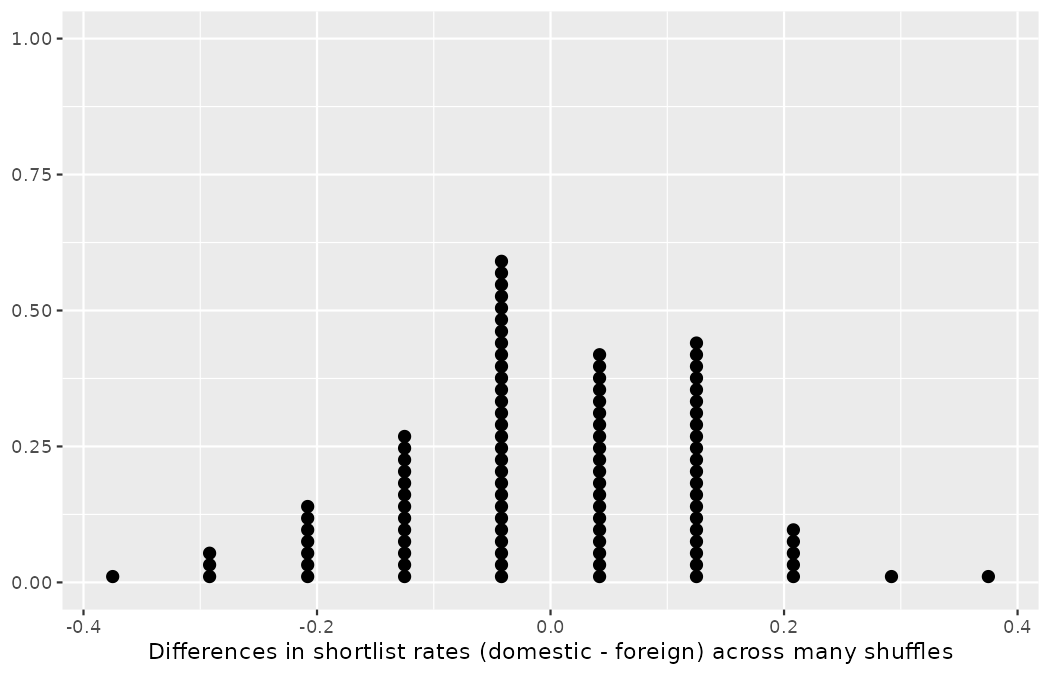
\includegraphics[width=0.85\linewidth,height=\textheight,keepaspectratio]{figures/foundations-randomization-1.png}

The 100 dots stack up between \(-0.375\) and \(0.375,\) in steps of
\(1/12 \approx 0.083\) (with 24 dossiers per stack, the difference can
only move in such steps), with the tallest stacks near zero. Exactly two
of the 100 simulations produced a difference at least as large as the
observed \(0.292\) --- one shuffle at \(0.292\) and one at \(0.375:\)

\begin{Shaded}
\begin{Highlighting}[]
\NormalTok{dossier48\_null }\SpecialCharTok{|\textgreater{}}
  \FunctionTok{summarize}\NormalTok{(}
    \AttributeTok{n\_extreme =} \FunctionTok{sum}\NormalTok{(stat }\SpecialCharTok{\textgreater{}=} \FloatTok{0.292}\NormalTok{),}
    \AttributeTok{prop\_extreme =} \FunctionTok{mean}\NormalTok{(stat }\SpecialCharTok{\textgreater{}=} \FloatTok{0.292}\NormalTok{)}
\NormalTok{  )}
\CommentTok{\#\textgreater{} \# A tibble: 1 × 2}
\CommentTok{\#\textgreater{}   n\_extreme prop\_extreme}
\CommentTok{\#\textgreater{}       \textless{}int\textgreater{}        \textless{}dbl\textgreater{}}
\CommentTok{\#\textgreater{} 1         2         0.02}
\end{Highlighting}
\end{Shaded}

Note that the distribution of these simulated differences in proportions
is centered around 0. Under the null hypothesis, our simulations made no
distinction between ``domestic'' and ``foreign'' dossiers. Thus, a
center of 0 makes sense: we should expect differences from chance alone
to fall around zero with some random fluctuation for each simulation.

\begin{tcolorbox}[enhanced jigsaw, left=2mm, leftrule=.75mm, title=\textcolor{quarto-callout-note-color}{\faInfo}\hspace{0.5em}{Worked example}, arc=.35mm, rightrule=.15mm, coltitle=black, colframe=quarto-callout-note-color-frame, bottomrule=.15mm, colbacktitle=quarto-callout-note-color!10!white, opacitybacktitle=0.6, breakable, bottomtitle=1mm, toptitle=1mm, titlerule=0mm, opacityback=0, toprule=.15mm, colback=white]

How often would you observe a difference of at least 29.2\% \((0.292)\)
according to the null distribution we just simulated? Often, sometimes,
rarely, or never?

\begin{center}\rule{0.5\linewidth}{0.5pt}\end{center}

A difference of at least 29.2\% under the null hypothesis happened in
only 2 of our 100 simulations --- about 2\% of the time. Such a low
probability indicates that observing such a large difference from chance
alone is rare.

\end{tcolorbox}

The difference of 29.2\% is a rare event if the listed nationality
really has no impact on the scouts' decisions, which provides us with
two possible interpretations of the study results:

\begin{itemize}
\item
  If \(H_0,\) the \textbf{null hypothesis}, is true: nationality has no
  effect on shortlist decisions, and we observed a difference that is so
  large that it would only happen rarely.
\item
  If \(H_A,\) the \textbf{alternative hypothesis}, is true: nationality
  has an effect on shortlist decisions, and what we observed was
  actually due to an identically documented prospect being penalized for
  the ``foreign'' label, which explains the large difference of 29.2\%.
\end{itemize}

When we conduct formal studies, we reject a null position (the idea that
the data are a result of chance only) if the data strongly conflict with
that null position.\footnote{This reasoning does not generally extend to
  anecdotal observations. Each of us observes incredibly rare events
  every day, events we could not possibly hope to predict. In the
  non-rigorous setting of anecdotal evidence, almost anything may appear
  to be a rare event, so looking for rare events in day-to-day scouting
  is treacherous. Consider a single match with 25 shots: any
  \emph{particular} sequence of 25 shot outcomes has vanishingly small
  probability, yet some sequence had to occur, and whichever one did
  would look ``incredible'' if you went hunting for meaning in it
  afterwards. A scout who watches enough football will personally
  witness once-a-decade goals, bizarre deflections, and five-goal
  comebacks; each is astonishing in itself, but \emph{something}
  astonishing happening somewhere is routine. This is the highlight-reel
  fallacy from Chapter~\ref{sec-data-hello} in probabilistic clothing,
  and it is why we only count an event as evidence when it is rare
  \emph{under a hypothesis fixed in advance}.} In our analysis, we
determined that there was only a \(\approx\) 2\% probability of
obtaining a sample where \(\geq\) 29.2\% more ``domestic'' than
``foreign'' dossiers get shortlisted under the null hypothesis, so we
conclude that the data provide strong evidence of nationality bias
against foreign prospects within the scouting network. In this case, we
reject the null hypothesis in favor of the alternative. Because the
dossier version was randomly assigned, the conclusion is causal: it was
the label itself that moved the decisions.

\textbf{Statistical inference} is the practice of making decisions and
conclusions from data in the context of uncertainty. Errors do occur,
just like rare events, and the dataset at hand might lead us to the
wrong conclusion. While a given dataset may not always lead us to a
correct conclusion, statistical inference gives us tools to control and
evaluate how often these errors occur. Before getting into the nuances
of hypothesis testing, let's work through another case study.

\section{Opportunity cost case
study}\label{sec-caseStudyOpportunityCost}

How rational and consistent are the recommendations of a scouting
network? In this section, we'll explore whether scouts filing a
sign/pass recommendation always consider the following: a transfer
budget not spent now can be spent later.

In particular, we are interested in whether reminding scouts of this
well-known fact about money causes them to be a little more conservative
with the club's budget. A skeptic might think that professional scouts
already price in the alternative uses of €15M, so such a reminder would
have no impact. We can summarize the two different perspectives using
the null and alternative hypothesis framework.

\begin{itemize}
\tightlist
\item
  \(H_0:\) \textbf{Null hypothesis.} Reminding scouts that the transfer
  fee could be kept for the winter window will have no impact on their
  sign/pass recommendations.
\item
  \(H_A:\) \textbf{Alternative hypothesis.} Reminding scouts that the
  transfer fee could be kept for the winter window will reduce the
  chance they recommend completing the signing.
\end{itemize}

This, too, is a constructed Northbridge scenario, built in seeded code
below.

\subsection{Observed data}\label{observed-data-1}

One hundred and fifty scouts and analysts across Northbridge's extended
network took part in the exercise --- the 48 regional scouts, joined by
partner-academy staff, loan-network contacts, and the video-analysis
team, which is how the club musters a pool this size. Each received the
same one-page brief on a fictional 24-year-old winger available for
€15M, a fee squarely within the club's summer budget, and was asked to
tick one of two boxes. Half of the 150 participants were randomized into
a control group and were given the following two options:

\begin{quote}
\begin{enumerate}
\def\labelenumi{(\Alph{enumi})}
\tightlist
\item
  Recommend signing the player for €15M.
\end{enumerate}
\end{quote}

\begin{quote}
\begin{enumerate}
\def\labelenumi{(\Alph{enumi})}
\setcounter{enumi}{1}
\tightlist
\item
  Do not recommend signing the player.
\end{enumerate}
\end{quote}

The remaining 75 participants were placed in the treatment group, and
they saw a slightly modified option (B):

\begin{quote}
\begin{enumerate}
\def\labelenumi{(\Alph{enumi})}
\tightlist
\item
  Recommend signing the player for €15M.
\end{enumerate}
\end{quote}

\begin{quote}
\begin{enumerate}
\def\labelenumi{(\Alph{enumi})}
\setcounter{enumi}{1}
\tightlist
\item
  Do not recommend signing the player. Keep the €15M for the winter
  window.
\end{enumerate}
\end{quote}

Would the extra phrase, which reminds participants of an obvious fact
about the budget, impact the recommendation? The code below constructs
the data, and Table~\ref{tbl-budget150-obs} summarizes the results.

\begin{Shaded}
\begin{Highlighting}[]
\NormalTok{budget150 }\OtherTok{\textless{}{-}} \FunctionTok{tibble}\NormalTok{(}
  \AttributeTok{group    =} \FunctionTok{factor}\NormalTok{(}\FunctionTok{rep}\NormalTok{(}\FunctionTok{c}\NormalTok{(}\StringTok{"control"}\NormalTok{, }\StringTok{"treatment"}\NormalTok{), }\AttributeTok{each =} \DecValTok{75}\NormalTok{),}
                    \AttributeTok{levels =} \FunctionTok{c}\NormalTok{(}\StringTok{"control"}\NormalTok{, }\StringTok{"treatment"}\NormalTok{)),}
  \AttributeTok{decision =} \FunctionTok{factor}\NormalTok{(}\FunctionTok{c}\NormalTok{(}\FunctionTok{rep}\NormalTok{(}\StringTok{"recommend signing"}\NormalTok{, }\DecValTok{56}\NormalTok{), }\FunctionTok{rep}\NormalTok{(}\StringTok{"do not recommend"}\NormalTok{, }\DecValTok{19}\NormalTok{),}
                      \FunctionTok{rep}\NormalTok{(}\StringTok{"recommend signing"}\NormalTok{, }\DecValTok{41}\NormalTok{), }\FunctionTok{rep}\NormalTok{(}\StringTok{"do not recommend"}\NormalTok{, }\DecValTok{34}\NormalTok{)),}
                    \AttributeTok{levels =} \FunctionTok{c}\NormalTok{(}\StringTok{"recommend signing"}\NormalTok{, }\StringTok{"do not recommend"}\NormalTok{))}
\NormalTok{)}

\NormalTok{budget150 }\SpecialCharTok{|\textgreater{}}
  \FunctionTok{count}\NormalTok{(group, decision) }\SpecialCharTok{|\textgreater{}}
  \FunctionTok{pivot\_wider}\NormalTok{(}\AttributeTok{names\_from =}\NormalTok{ decision, }\AttributeTok{values\_from =}\NormalTok{ n)}
\CommentTok{\#\textgreater{} \# A tibble: 2 × 3}
\CommentTok{\#\textgreater{}   group     \textasciigrave{}recommend signing\textasciigrave{} \textasciigrave{}do not recommend\textasciigrave{}}
\CommentTok{\#\textgreater{}   \textless{}fct\textgreater{}                   \textless{}int\textgreater{}              \textless{}int\textgreater{}}
\CommentTok{\#\textgreater{} 1 control                    56                 19}
\CommentTok{\#\textgreater{} 2 treatment                  41                 34}
\end{Highlighting}
\end{Shaded}

\begin{longtable}[]{@{}lrrr@{}}
\caption{Summary results of the opportunity cost
study.}\label{tbl-budget150-obs}\tabularnewline
\toprule\noalign{}
& recommend signing & do not recommend & Total \\
\midrule\noalign{}
\endfirsthead
\toprule\noalign{}
& recommend signing & do not recommend & Total \\
\midrule\noalign{}
\endhead
\bottomrule\noalign{}
\endlastfoot
control & 56 & 19 & 75 \\
treatment & 41 & 34 & 75 \\
Total & 97 & 53 & 150 \\
\end{longtable}

It might be a little easier to review the results using a visualization:
a stacked bar plot shows that a higher proportion of the treatment group
declined to recommend the signing compared to the control group.

\begin{Shaded}
\begin{Highlighting}[]
\FunctionTok{ggplot}\NormalTok{(budget150, }\FunctionTok{aes}\NormalTok{(}\AttributeTok{y =}\NormalTok{ group, }\AttributeTok{fill =}\NormalTok{ decision)) }\SpecialCharTok{+}
  \FunctionTok{geom\_bar}\NormalTok{(}\AttributeTok{position =} \StringTok{"fill"}\NormalTok{) }\SpecialCharTok{+}
  \FunctionTok{labs}\NormalTok{(}\AttributeTok{x =} \StringTok{"Proportion"}\NormalTok{, }\AttributeTok{y =} \StringTok{"Group"}\NormalTok{, }\AttributeTok{fill =} \StringTok{"Decision"}\NormalTok{)}
\end{Highlighting}
\end{Shaded}

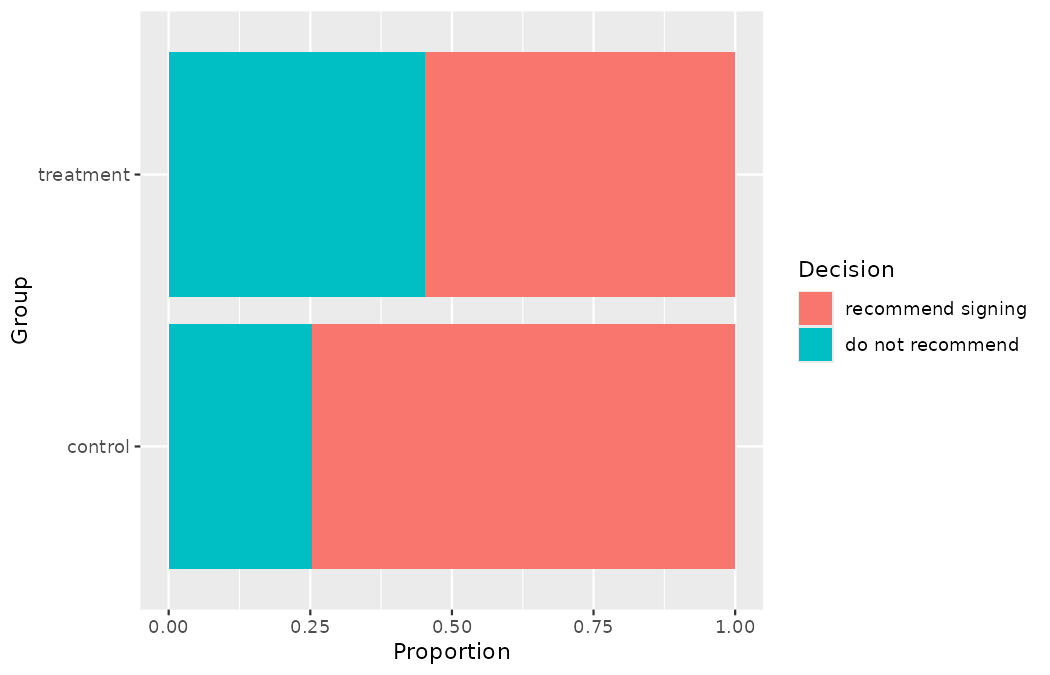
\includegraphics[width=0.85\linewidth,height=\textheight,keepaspectratio]{figures/foundations-randomization-2.png}

Another useful way to review the results from
Table~\ref{tbl-budget150-obs} is using row proportions, specifically
considering the proportion of participants in each group who recommended
or declined the signing. These summaries are given in
Table~\ref{tbl-budget150-row-prop}.

\begin{Shaded}
\begin{Highlighting}[]
\NormalTok{budget150 }\SpecialCharTok{|\textgreater{}}
  \FunctionTok{count}\NormalTok{(group, decision) }\SpecialCharTok{|\textgreater{}}
  \FunctionTok{group\_by}\NormalTok{(group) }\SpecialCharTok{|\textgreater{}}
  \FunctionTok{mutate}\NormalTok{(}\AttributeTok{p =}\NormalTok{ n }\SpecialCharTok{/} \FunctionTok{sum}\NormalTok{(n))}
\CommentTok{\#\textgreater{} \# A tibble: 4 × 4}
\CommentTok{\#\textgreater{} \# Groups:   group [2]}
\CommentTok{\#\textgreater{}   group     decision              n     p}
\CommentTok{\#\textgreater{}   \textless{}fct\textgreater{}     \textless{}fct\textgreater{}             \textless{}int\textgreater{} \textless{}dbl\textgreater{}}
\CommentTok{\#\textgreater{} 1 control   recommend signing    56 0.747}
\CommentTok{\#\textgreater{} 2 control   do not recommend     19 0.253}
\CommentTok{\#\textgreater{} 3 treatment recommend signing    41 0.547}
\CommentTok{\#\textgreater{} 4 treatment do not recommend     34 0.453}
\end{Highlighting}
\end{Shaded}

\begin{longtable}[]{@{}lrrr@{}}
\caption{The opportunity cost data are summarized using row proportions.
Row proportions are particularly useful here since we can view the
proportion of \emph{recommend} and \emph{do not recommend} decisions in
each group.}\label{tbl-budget150-row-prop}\tabularnewline
\toprule\noalign{}
& recommend signing & do not recommend & Total \\
\midrule\noalign{}
\endfirsthead
\toprule\noalign{}
& recommend signing & do not recommend & Total \\
\midrule\noalign{}
\endhead
\bottomrule\noalign{}
\endlastfoot
control & 0.747 & 0.253 & 1.00 \\
treatment & 0.547 & 0.453 & 1.00 \\
\end{longtable}

We will define a \textbf{success} in this study as a participant who
chooses \emph{not} to recommend the signing.\footnote{``Success'' is
  defined in a study as the outcome of interest, and a ``success'' may
  or may not actually be a positive outcome for the club. For example,
  in an injury-screening study, Northbridge's medical staff might define
  a ``success'' in the statistical sense as a player who fails the
  screen --- the outcome being counted, not the outcome being hoped for.
  A more complete discussion of the term \textbf{success} will be given
  in Chapter~\ref{sec-inference-one-prop}.} Then, the value of interest
is the change in the do-not-recommend rate that results from reminding
scouts that money not spent on this player can be spent in the winter
window.

We can construct a point estimate for this difference (\(T\) for
treatment, \(C\) for control --- the subscripts again simply name the
groups):

\[\hat{p}_{T} - \hat{p}_{C} = \frac{34}{75} - \frac{19}{75} = 0.453 - 0.253 = 0.200\]

The proportion of participants who declined to recommend the signing was
20 percentage points higher in the treatment group than in the control
group. Is this 20\% difference between the two groups so prominent that
it is unlikely to have occurred from chance alone, if there is no
difference between how the two forms are answered?

\subsection{Variability of the
statistic}\label{variability-of-the-statistic-1}

The primary goal in this data analysis is to understand what sort of
differences we might see if the null hypothesis were true, i.e., if the
extra phrase had no effect on the scouts. Because this is an experiment,
we'll use the same procedure we applied in
Section~\ref{sec-caseStudySexDiscrimination}: randomization.

Let's think about the data in the context of the hypotheses. If the null
hypothesis \((H_0)\) was true and the extra phrase had no impact on
recommendations, then the observed difference of 20 percentage points
could be attributed entirely to random chance --- to which scouts
happened to land in which group. If, on the other hand, the alternative
hypothesis \((H_A)\) is true, then the difference indicates that
spelling out the opportunity cost of a transfer actually changes
recommendation behavior.

\subsection{Observed statistic vs.~null
statistics}\label{observed-statistic-vs.-null-statistics-1}

Just like with the dossier study, we can perform a statistical analysis.
Using the same randomization technique from the last section, let's see
what happens when we simulate the experiment under the scenario where
there is no effect of the reminder.

While we would in reality do this simulation on a computer, it is useful
to think about how we would carry it out by hand. We start with 150
index cards and label each card to indicate the distribution of our
response variable, \texttt{decision}: 53 cards will be labeled
\texttt{do\ not\ recommend}, to represent the 53 participants who
declined the signing, and 97 will be labeled \texttt{recommend\ signing}
for the other 97 participants. Then we shuffle these cards thoroughly
and divide them into two stacks of size 75, representing the simulated
treatment and control groups. Because the shuffle pays no attention to
what is written on the cards, any observed difference between the two
stacks' proportions of \texttt{do\ not\ recommend} cards (what we
earlier defined as \emph{success}) can be attributed entirely to chance.

\begin{tcolorbox}[enhanced jigsaw, left=2mm, leftrule=.75mm, title=\textcolor{quarto-callout-note-color}{\faInfo}\hspace{0.5em}{Worked example}, arc=.35mm, rightrule=.15mm, coltitle=black, colframe=quarto-callout-note-color-frame, bottomrule=.15mm, colbacktitle=quarto-callout-note-color!10!white, opacitybacktitle=0.6, breakable, bottomtitle=1mm, toptitle=1mm, titlerule=0mm, opacityback=0, toprule=.15mm, colback=white]

If we are randomly assigning the cards into the simulated treatment and
control groups, how many \texttt{do\ not\ recommend} cards would we
expect to end up in each simulated group? What would be the expected
difference between the proportions of \texttt{do\ not\ recommend} cards
in each group?

\begin{center}\rule{0.5\linewidth}{0.5pt}\end{center}

Since the simulated groups are of equal size, we would expect
\(53/2 = 26.5,\) i.e., 26 or 27, \texttt{do\ not\ recommend} cards in
each simulated group, yielding a simulated point estimate of the
difference in proportions of approximately 0\%. However, due to random
chance, we might also expect to sometimes observe a number a little
above or below 26 and 27.

\end{tcolorbox}

The results of a single, seeded randomization are shown below and in
Table~\ref{tbl-budget150-rand-1}.

\begin{Shaded}
\begin{Highlighting}[]
\FunctionTok{set.seed}\NormalTok{(}\DecValTok{1102}\NormalTok{)}
\NormalTok{budget150\_shuffle\_1 }\OtherTok{\textless{}{-}}\NormalTok{ budget150 }\SpecialCharTok{|\textgreater{}}
  \FunctionTok{mutate}\NormalTok{(}\AttributeTok{decision =} \FunctionTok{sample}\NormalTok{(decision))}

\NormalTok{budget150\_shuffle\_1 }\SpecialCharTok{|\textgreater{}}
  \FunctionTok{count}\NormalTok{(group, decision) }\SpecialCharTok{|\textgreater{}}
  \FunctionTok{pivot\_wider}\NormalTok{(}\AttributeTok{names\_from =}\NormalTok{ decision, }\AttributeTok{values\_from =}\NormalTok{ n)}
\CommentTok{\#\textgreater{} \# A tibble: 2 × 3}
\CommentTok{\#\textgreater{}   group     \textasciigrave{}recommend signing\textasciigrave{} \textasciigrave{}do not recommend\textasciigrave{}}
\CommentTok{\#\textgreater{}   \textless{}fct\textgreater{}                   \textless{}int\textgreater{}              \textless{}int\textgreater{}}
\CommentTok{\#\textgreater{} 1 control                    45                 30}
\CommentTok{\#\textgreater{} 2 treatment                  52                 23}
\end{Highlighting}
\end{Shaded}

\begin{longtable}[]{@{}lrrr@{}}
\caption{Summary of the scouts' simulated decisions against their
simulated groups. The group assignment had no connection to the
decisions, so any difference between the two groups is due to
chance.}\label{tbl-budget150-rand-1}\tabularnewline
\toprule\noalign{}
& recommend signing & do not recommend & Total \\
\midrule\noalign{}
\endfirsthead
\toprule\noalign{}
& recommend signing & do not recommend & Total \\
\midrule\noalign{}
\endhead
\bottomrule\noalign{}
\endlastfoot
control & 45 & 30 & 75 \\
treatment & 52 & 23 & 75 \\
Total & 97 & 53 & 150 \\
\end{longtable}

From this table, we can compute the difference that occurred from the
first shuffle of the data (i.e., from chance alone), attaching the
shuffle number to the subscript so we never confuse a simulated
statistic with the observed one:

\[\hat{p}_{T, shfl1} - \hat{p}_{C, shfl1} = \frac{23}{75} - \frac{30}{75} = 0.307 - 0.400 = -0.093\]

Just one simulation will not be enough to get a sense of what sorts of
differences would happen from chance alone. We'll simulate another set
of groups and compute the new difference: \(-0.067.\) And again:
\(-0.040.\) We'll do this 1,000 times.

\begin{Shaded}
\begin{Highlighting}[]
\FunctionTok{set.seed}\NormalTok{(}\DecValTok{1102}\NormalTok{)}
\NormalTok{budget150\_null }\OtherTok{\textless{}{-}}\NormalTok{ budget150 }\SpecialCharTok{|\textgreater{}}
  \FunctionTok{specify}\NormalTok{(decision }\SpecialCharTok{\textasciitilde{}}\NormalTok{ group, }\AttributeTok{success =} \StringTok{"do not recommend"}\NormalTok{) }\SpecialCharTok{|\textgreater{}}
  \FunctionTok{hypothesize}\NormalTok{(}\AttributeTok{null =} \StringTok{"independence"}\NormalTok{) }\SpecialCharTok{|\textgreater{}}
  \FunctionTok{generate}\NormalTok{(}\AttributeTok{reps =} \DecValTok{1000}\NormalTok{, }\AttributeTok{type =} \StringTok{"permute"}\NormalTok{) }\SpecialCharTok{|\textgreater{}}
  \FunctionTok{calculate}\NormalTok{(}\AttributeTok{stat =} \StringTok{"diff in props"}\NormalTok{, }\AttributeTok{order =} \FunctionTok{c}\NormalTok{(}\StringTok{"treatment"}\NormalTok{, }\StringTok{"control"}\NormalTok{)) }\SpecialCharTok{|\textgreater{}}
  \FunctionTok{mutate}\NormalTok{(}\AttributeTok{stat =} \FunctionTok{round}\NormalTok{(stat, }\DecValTok{3}\NormalTok{))}

\NormalTok{budget150\_null}\SpecialCharTok{$}\NormalTok{stat[}\DecValTok{1}\SpecialCharTok{:}\DecValTok{3}\NormalTok{]}
\CommentTok{\#\textgreater{} [1] {-}0.093 {-}0.067 {-}0.040}
\end{Highlighting}
\end{Shaded}

The results can be visualized as a stacked dot plot, where each point
represents the difference from one randomization:

\begin{Shaded}
\begin{Highlighting}[]
\FunctionTok{ggplot}\NormalTok{(budget150\_null, }\FunctionTok{aes}\NormalTok{(}\AttributeTok{x =}\NormalTok{ stat)) }\SpecialCharTok{+}
  \FunctionTok{geom\_dotplot}\NormalTok{(}\AttributeTok{binwidth =} \FloatTok{0.01}\NormalTok{, }\AttributeTok{dotsize =} \FloatTok{0.165}\NormalTok{) }\SpecialCharTok{+}
  \FunctionTok{labs}\NormalTok{(}
    \AttributeTok{title =} \StringTok{"1,000 differences in randomized proportions"}\NormalTok{,}
    \AttributeTok{x =} \StringTok{"Difference in randomized proportions of scouts who}\SpecialCharTok{\textbackslash{}n}\StringTok{do not recommend the signing (treatment {-} control)"}\NormalTok{,}
    \AttributeTok{y =} \ConstantTok{NULL}
\NormalTok{  )}
\end{Highlighting}
\end{Shaded}

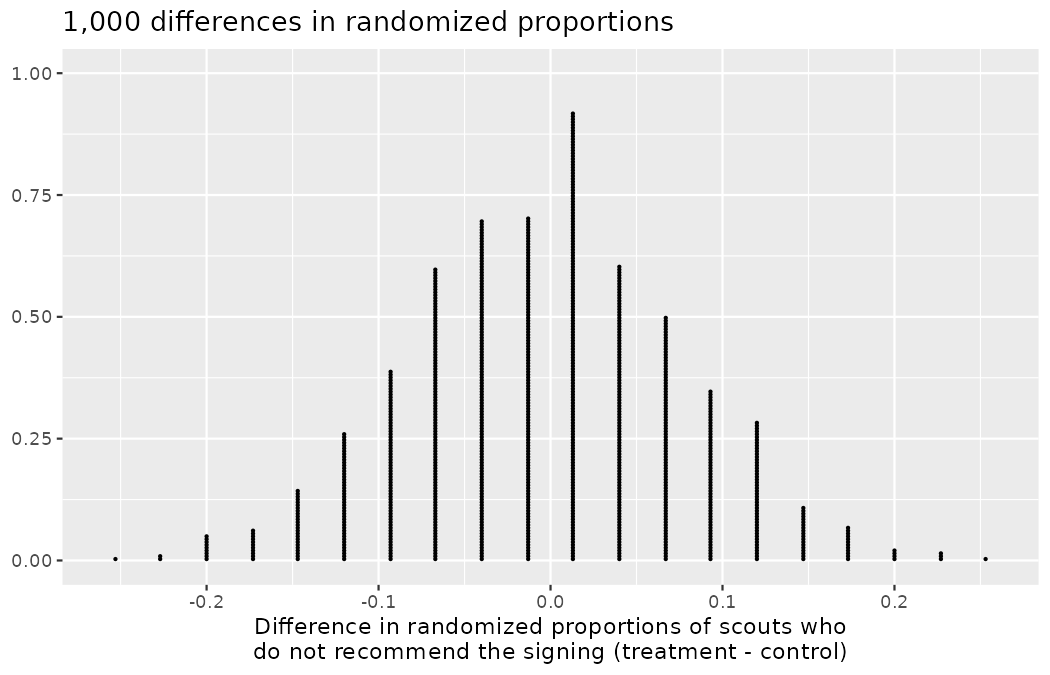
\includegraphics[width=0.85\linewidth,height=\textheight,keepaspectratio]{figures/foundations-randomization-3.png}

Since there are so many points and it is difficult to discern one from
another, it is more convenient to summarize the results in a histogram,
where the height of each bar represents the number of simulations
resulting in an outcome of that magnitude:

\begin{Shaded}
\begin{Highlighting}[]
\FunctionTok{ggplot}\NormalTok{(budget150\_null, }\FunctionTok{aes}\NormalTok{(}\AttributeTok{x =}\NormalTok{ stat)) }\SpecialCharTok{+}
  \FunctionTok{geom\_histogram}\NormalTok{(}\AttributeTok{binwidth =} \FloatTok{0.04}\NormalTok{) }\SpecialCharTok{+}
  \FunctionTok{labs}\NormalTok{(}
    \AttributeTok{title =} \StringTok{"1,000 differences in randomized proportions"}\NormalTok{,}
    \AttributeTok{x =} \StringTok{"Difference in randomized proportions of scouts who}\SpecialCharTok{\textbackslash{}n}\StringTok{do not recommend the signing (treatment {-} control)"}\NormalTok{,}
    \AttributeTok{y =} \StringTok{"Count (number of simulated scenarios)"}
\NormalTok{  )}
\end{Highlighting}
\end{Shaded}

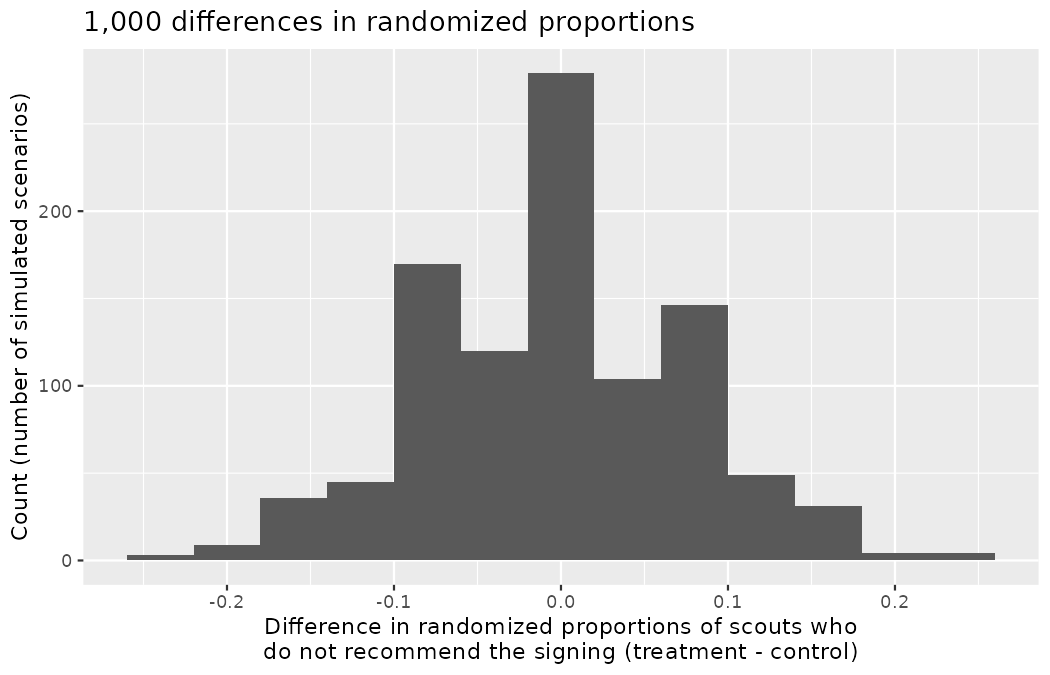
\includegraphics[width=0.85\linewidth,height=\textheight,keepaspectratio]{figures/foundations-randomization-4.png}

The distribution is again centered at zero --- the shuffle knows nothing
about treatment and control --- and we care about how much of it lies at
or beyond the observed difference of \(0.200:\)

\begin{Shaded}
\begin{Highlighting}[]
\NormalTok{budget150\_null }\SpecialCharTok{|\textgreater{}}
  \FunctionTok{summarize}\NormalTok{(}
    \AttributeTok{n\_extreme =} \FunctionTok{sum}\NormalTok{(stat }\SpecialCharTok{\textgreater{}=} \FloatTok{0.200}\NormalTok{),}
    \AttributeTok{prop\_extreme =} \FunctionTok{mean}\NormalTok{(stat }\SpecialCharTok{\textgreater{}=} \FloatTok{0.200}\NormalTok{)}
\NormalTok{  )}
\CommentTok{\#\textgreater{} \# A tibble: 1 × 2}
\CommentTok{\#\textgreater{}   n\_extreme prop\_extreme}
\CommentTok{\#\textgreater{}       \textless{}int\textgreater{}        \textless{}dbl\textgreater{}}
\CommentTok{\#\textgreater{} 1         8        0.008}
\end{Highlighting}
\end{Shaded}

Under the null hypothesis (no effect of the reminder), we would observe
a difference of at least \(+20\%\) about \(0.8\%\) of the time --- 8
shuffles in 1,000. That is really rare! Instead, we will conclude the
data provide strong evidence that there is an effect: spelling out, at
the moment of recommendation, that the fee could instead be kept for the
winter window lowers the chance that a scout recommends completing the
signing. Notice that we are able to make a \emph{causal} statement for
this study since the study is an experiment --- the wording of the form
was randomly assigned --- although we do not know \emph{why} the
reminder induces more conservative recommendations.

\begin{tcolorbox}[enhanced jigsaw, left=2mm, leftrule=.75mm, title=\textcolor{quarto-callout-tip-color}{\faLightbulb}\hspace{0.5em}{Check your understanding}, arc=.35mm, rightrule=.15mm, coltitle=black, colframe=quarto-callout-tip-color-frame, bottomrule=.15mm, colbacktitle=quarto-callout-tip-color!10!white, opacitybacktitle=0.6, breakable, bottomtitle=1mm, toptitle=1mm, titlerule=0mm, opacityback=0, toprule=.15mm, colback=white]

In the opportunity cost study, would it have been legitimate to instead
count the shuffles where the difference was at least as large as
\(0.200\) \emph{in either direction}? What claim would that assess?

\begin{center}\rule{0.5\linewidth}{0.5pt}\end{center}

Yes --- that is a perfectly coherent (and more skeptical) analysis; it
assesses the two-sided alternative that the reminder changes
recommendations \emph{in some direction}, rather than specifically
making scouts more conservative. We used the one-direction count because
\(H_A\) was directional. The distinction between one-sided and two-sided
alternatives is treated carefully in
Chapter~\ref{sec-foundations-decision-errors}.

\end{tcolorbox}

\section{Hypothesis testing}\label{sec-HypothesisTesting}

In the last two sections, we utilized a \textbf{hypothesis test}, which
is a formal technique for evaluating two competing possibilities. In
each scenario, we described a \textbf{null hypothesis}, which
represented either a skeptical perspective or a perspective of no
difference. We also laid out an \textbf{alternative hypothesis}, which
represented a new perspective, such as the possibility of a relationship
between two variables or an effect of an experimental treatment. The
alternative hypothesis is usually the reason the analysts set out to do
the research in the first place.

\begin{tcolorbox}[enhanced jigsaw, left=2mm, leftrule=.75mm, title=\textcolor{quarto-callout-important-color}{\faExclamation}\hspace{0.5em}{Null and alternative hypotheses}, arc=.35mm, rightrule=.15mm, coltitle=black, colframe=quarto-callout-important-color-frame, bottomrule=.15mm, colbacktitle=quarto-callout-important-color!10!white, opacitybacktitle=0.6, breakable, bottomtitle=1mm, toptitle=1mm, titlerule=0mm, opacityback=0, toprule=.15mm, colback=white]

The \textbf{null hypothesis} \((H_0)\) often represents either a
skeptical perspective or a claim of ``no difference'' to be tested.

The \textbf{alternative hypothesis} \((H_A)\) represents an alternative
claim under consideration and is often represented by a range of
possible values for the value of interest.

\end{tcolorbox}

If a person makes a somewhat unbelievable claim --- an agent tells Marta
Vidal his client ``finishes like nobody else in the league'' --- we are
initially skeptical. However, if there is sufficient evidence that
supports the claim, we set aside our skepticism. The hallmarks of
hypothesis testing are also found on the touchline, in the VAR review.

\subsection{The VAR review}\label{the-var-review}

When a video assistant referee reviews a decision, the protocol is
explicit: the on-field call stands unless the video evidence shows a
\emph{clear and obvious} error. The referee's original decision is not
presumed correct because referees are infallible; it is the default that
must be actively overturned.

\begin{tcolorbox}[enhanced jigsaw, left=2mm, leftrule=.75mm, title=\textcolor{quarto-callout-note-color}{\faInfo}\hspace{0.5em}{Worked example}, arc=.35mm, rightrule=.15mm, coltitle=black, colframe=quarto-callout-note-color-frame, bottomrule=.15mm, colbacktitle=quarto-callout-note-color!10!white, opacitybacktitle=0.6, breakable, bottomtitle=1mm, toptitle=1mm, titlerule=0mm, opacityback=0, toprule=.15mm, colback=white]

A VAR review considers two possible claims about the on-field call: it
stands, or it must be overturned.

If we set these claims up in a hypothesis framework, which would be the
null hypothesis and which the alternative?

\begin{center}\rule{0.5\linewidth}{0.5pt}\end{center}

The reviewer considers whether the video evidence is so convincing
(clear and obvious) that the original call cannot stand. That is, the
skeptical default (null hypothesis) is that the on-field call stands,
until evidence is presented that convinces the reviewer that the call
was wrong (alternative hypothesis).

\end{tcolorbox}

Notice that when a review ends with ``check complete'' and the on-field
call stands, this does not mean the review has \emph{proven} the
original call correct. The reviewer is simply not convinced of the
alternative --- the evidence did not clear the bar. This is also the
case with hypothesis testing: \emph{even if we fail to reject the null
hypothesis, we do not accept the null hypothesis as truth}.

Failing to find evidence in favor of the alternative hypothesis is not
equivalent to finding evidence that the null hypothesis is true. A
marginal offside image that is too blurry to overturn the call is not a
demonstration that the attacker was onside. We will see this idea in
greater detail in Chapter~\ref{sec-foundations-decision-errors}.

\subsection{p-value and statistical
discernibility}\label{p-value-and-statistical-discernibility}

In Section~\ref{sec-caseStudySexDiscrimination} we designed an audit
that explored whether there was strong evidence that prospects listed as
foreign were less likely to be shortlisted than identical prospects
listed as domestic. The research question --- does the network
discriminate by listed nationality? --- was framed in the context of
hypotheses:

\begin{itemize}
\item
  \(H_0:\) The listed nationality has no effect on shortlist decisions.
\item
  \(H_A:\) Prospects listed as foreign are discriminated against in
  shortlist decisions.
\end{itemize}

The null hypothesis \((H_0)\) was a perspective of no difference in
treatment. The data provided a point estimate of a 29.2\% difference in
shortlist rates between the two dossier versions. We determined that
such a difference from chance alone, assuming the null hypothesis was
true, would be rare: it would only happen about 2 in 100 times. When
results like these are inconsistent with \(H_0,\) we reject \(H_0\) in
favor of \(H_A.\) Here, we concluded there was nationality bias in the
network.

The 2-in-100 chance is what we call a \textbf{p-value}, which is a
probability quantifying the strength of the evidence against the null
hypothesis, given the observed data.

\begin{tcolorbox}[enhanced jigsaw, left=2mm, leftrule=.75mm, title=\textcolor{quarto-callout-important-color}{\faExclamation}\hspace{0.5em}{p-value}, arc=.35mm, rightrule=.15mm, coltitle=black, colframe=quarto-callout-important-color-frame, bottomrule=.15mm, colbacktitle=quarto-callout-important-color!10!white, opacitybacktitle=0.6, breakable, bottomtitle=1mm, toptitle=1mm, titlerule=0mm, opacityback=0, toprule=.15mm, colback=white]

The \textbf{p-value} is the probability of observing data at least as
favorable to the alternative hypothesis as our current dataset, if the
null hypothesis were true. We typically use a summary statistic of the
data, such as a difference in proportions, to help compute the p-value
and evaluate the hypotheses. This summary value that is used to compute
the p-value is often called the \textbf{test statistic}.

\end{tcolorbox}

Take the definition apart, because every clause is load-bearing.
\emph{``If the null hypothesis were true''}: the p-value is computed
entirely inside the null world --- in our simulations, the world of
shuffled cards. \emph{``At least as favorable to the alternative''}: we
count not just our exact result but everything more extreme in the
direction of \(H_A.\) \emph{``Probability of observing data''}: it is a
statement about data behavior under \(H_0,\) \textbf{not} the
probability that \(H_0\) is true --- the single most common misreading
of the p-value, and one worth arresting now.

\begin{tcolorbox}[enhanced jigsaw, left=2mm, leftrule=.75mm, title=\textcolor{quarto-callout-note-color}{\faInfo}\hspace{0.5em}{Worked example}, arc=.35mm, rightrule=.15mm, coltitle=black, colframe=quarto-callout-note-color-frame, bottomrule=.15mm, colbacktitle=quarto-callout-note-color!10!white, opacitybacktitle=0.6, breakable, bottomtitle=1mm, toptitle=1mm, titlerule=0mm, opacityback=0, toprule=.15mm, colback=white]

In the dossier study, the difference in shortlist rates was our test
statistic. What was the test statistic in the opportunity cost study
covered in Section~\ref{sec-caseStudyOpportunityCost}?

\begin{center}\rule{0.5\linewidth}{0.5pt}\end{center}

The test statistic in the opportunity cost study was the difference in
the proportions of do-not-recommend decisions in the treatment and
control groups. In each of these examples, the \textbf{point estimate}
of the difference in proportions was used as the test statistic.

\end{tcolorbox}

When the p-value is small, i.e., less than a previously set threshold,
we say the results are \textbf{statistically discernible}.\footnote{Many
  texts use the phrase \textbf{statistically significant} instead of
  ``statistically discernible''. We have chosen to use ``discernible''
  to indicate that a precise statistical event has happened, as opposed
  to a notable effect which may or may not fit the statistical
  definition of discernible or significant.} This means the data provide
such strong evidence against \(H_0\) that we reject the null hypothesis
in favor of the alternative hypothesis. The threshold is called the
\textbf{discernibility level}\footnote{Here, too, we have chosen
  ``discernibility level'' instead of \textbf{significance level}, which
  you will see in some texts.} and is often represented by \(\alpha\)
--- the lowercase Greek letter \emph{alpha}, reserved from here on for
exactly this role: the rareness bar an event must clear, fixed
\emph{before} looking at the data, for the null hypothesis to be
rejected. Historically, many fields have set \(\alpha = 0.05.\) The
value of \(\alpha\) can vary depending on the field or the application.

Note that you may have heard the phrase ``statistically significant'' as
a way to describe ``statistically discernible.'' Although in everyday
language ``significant'' would indicate that a difference is large or
meaningful --- the way a sporting director hears ``a significant upgrade
on our current left back'' --- that is not necessarily the case in the
statistical sense. The term ``statistically discernible'' indicates that
the p-value from a study fell below the chosen discernibility level. For
example, in the dossier study, the p-value was found to be approximately
0.02. Using a discernibility level of \(\alpha = 0.05,\) we would say
that the data provided statistically discernible evidence against the
null hypothesis. However, this conclusion gives us no information
regarding the size of the bias in shortlist rates!

\begin{tcolorbox}[enhanced jigsaw, left=2mm, leftrule=.75mm, title=\textcolor{quarto-callout-important-color}{\faExclamation}\hspace{0.5em}{Statistical discernibility}, arc=.35mm, rightrule=.15mm, coltitle=black, colframe=quarto-callout-important-color-frame, bottomrule=.15mm, colbacktitle=quarto-callout-important-color!10!white, opacitybacktitle=0.6, breakable, bottomtitle=1mm, toptitle=1mm, titlerule=0mm, opacityback=0, toprule=.15mm, colback=white]

We say that the data provide \textbf{statistically discernible} evidence
against the null hypothesis if the p-value is less than some
predetermined threshold (e.g., 0.01, 0.05, 0.1).

\end{tcolorbox}

\begin{tcolorbox}[enhanced jigsaw, left=2mm, leftrule=.75mm, title=\textcolor{quarto-callout-note-color}{\faInfo}\hspace{0.5em}{Worked example}, arc=.35mm, rightrule=.15mm, coltitle=black, colframe=quarto-callout-note-color-frame, bottomrule=.15mm, colbacktitle=quarto-callout-note-color!10!white, opacitybacktitle=0.6, breakable, bottomtitle=1mm, toptitle=1mm, titlerule=0mm, opacityback=0, toprule=.15mm, colback=white]

In the opportunity cost study in
Section~\ref{sec-caseStudyOpportunityCost}, we analyzed an experiment
where participants were 20 percentage points less likely to recommend a
€15M signing if the form reminded them the fee could be kept for the
winter window. We determined that such a large difference would only
occur 8 in 1,000 times if the reminder actually had no influence on the
recommendations. What is the p-value in this study? Would you classify
the result as ``statistically discernible''?

\begin{center}\rule{0.5\linewidth}{0.5pt}\end{center}

The p-value was \(0.008.\) Since the p-value is less than
\(\alpha = 0.05,\) the data provide statistically discernible evidence
that the scouts were actually influenced by the reminder.

\end{tcolorbox}

\begin{tcolorbox}[enhanced jigsaw, left=2mm, leftrule=.75mm, title=\textcolor{quarto-callout-important-color}{\faExclamation}\hspace{0.5em}{What's so special about 0.05?}, arc=.35mm, rightrule=.15mm, coltitle=black, colframe=quarto-callout-important-color-frame, bottomrule=.15mm, colbacktitle=quarto-callout-important-color!10!white, opacitybacktitle=0.6, breakable, bottomtitle=1mm, toptitle=1mm, titlerule=0mm, opacityback=0, toprule=.15mm, colback=white]

We often use a threshold of \(0.05\) to determine whether a result is
statistically discernible. But why \(0.05\)? Maybe the club should
demand a smaller number before committing €15M, or tolerate a bigger one
when screening cheap academy trialists. If you find yourself a little
puzzled here, that puzzlement is warranted: it is the mark of the
critical eye this book means to train. The authors of \emph{Introduction
to Modern Statistics} have made a video to help clarify \emph{why 0.05}:
\url{https://www.openintro.org/book/stat/why05/}. The honest answer is
that \(0.05\) is a convention with a long history, not a law of nature,
and sometimes it is a good idea to deviate from the standard. We'll
discuss how to choose a threshold different from \(0.05\) --- and what
the club risks in each direction --- in
Chapter~\ref{sec-foundations-decision-errors}.

\end{tcolorbox}

\begin{tcolorbox}[enhanced jigsaw, left=2mm, leftrule=.75mm, title=\textcolor{quarto-callout-tip-color}{\faLightbulb}\hspace{0.5em}{Check your understanding}, arc=.35mm, rightrule=.15mm, coltitle=black, colframe=quarto-callout-tip-color-frame, bottomrule=.15mm, colbacktitle=quarto-callout-tip-color!10!white, opacitybacktitle=0.6, breakable, bottomtitle=1mm, toptitle=1mm, titlerule=0mm, opacityback=0, toprule=.15mm, colback=white]

A colleague reports ``p-value \(= 0.02\)'' for the dossier study and
summarizes it as ``there is a 2\% chance the network is unbiased.'' What
is wrong with this summary?

\begin{center}\rule{0.5\linewidth}{0.5pt}\end{center}

The p-value is computed \emph{assuming} the null hypothesis is true; it
is the probability of data this extreme \emph{given} an unbiased
network, not the probability of an unbiased network given the data. The
correct reading: \emph{if} the network were unbiased, a shortlist gap of
at least 29.2 percentage points would arise from the random dossier
assignment only about 2\% of the time.

\end{tcolorbox}

\subsection{Randomization on observational data: shooting under
pressure}\label{sec-chp11-observational}

Both case studies so far were experiments: Priya randomized the
dossiers, and the survey randomized the wording of option (B). But most
of what a scouting department touches is \emph{observational} --- the
tournament data we have carried since Chapter~\ref{sec-data-hello} was
generated by football, not by our design. The shuffling machinery still
works on observational data; what changes is the name --- a
\textbf{permutation test}, as flagged in the footnote of
Section~\ref{sec-caseStudySexDiscrimination} --- and, crucially, the
strength of the conclusion we are entitled to draw.

Here is a question Emil's scouts argue about constantly: do shots taken
under defensive pressure convert at a lower rate? The 2022 Men's World
Cup data can speak to it.

\begin{Shaded}
\begin{Highlighting}[]
\NormalTok{wc2022\_shots }\OtherTok{\textless{}{-}} \FunctionTok{read\_csv}\NormalTok{(}\StringTok{"data/derived/wc2022\_shots.csv"}\NormalTok{)}

\NormalTok{wc2022\_shots }\SpecialCharTok{|\textgreater{}}
  \FunctionTok{group\_by}\NormalTok{(under\_pressure) }\SpecialCharTok{|\textgreater{}}
  \FunctionTok{summarize}\NormalTok{(}\AttributeTok{shots =} \FunctionTok{n}\NormalTok{(), }\AttributeTok{goals =} \FunctionTok{sum}\NormalTok{(goal), }\AttributeTok{conversion =} \FunctionTok{mean}\NormalTok{(goal))}
\CommentTok{\#\textgreater{} \# A tibble: 2 × 4}
\CommentTok{\#\textgreater{}   under\_pressure shots goals conversion}
\CommentTok{\#\textgreater{}   \textless{}lgl\textgreater{}          \textless{}int\textgreater{} \textless{}int\textgreater{}      \textless{}dbl\textgreater{}}
\CommentTok{\#\textgreater{} 1 FALSE           1256   171      0.136}
\CommentTok{\#\textgreater{} 2 TRUE             238    24      0.101}
\end{Highlighting}
\end{Shaded}

Among the 1,494 shots of the tournament, the 238 taken under pressure
converted at \(\hat{p}_{prs} = 24/238 = 0.101,\) while the 1,256 others
converted at \(\hat{p}_{nop} = 171/1256 = 0.136.\) The observed test
statistic is the difference in conversion rates:

\[\hat{p}_{prs} - \hat{p}_{nop} = \frac{24}{238} - \frac{171}{1256} = 0.101 - 0.136 = -0.035\]

\begin{Shaded}
\begin{Highlighting}[]
\DecValTok{24}\SpecialCharTok{/}\DecValTok{238} \SpecialCharTok{{-}} \DecValTok{171}\SpecialCharTok{/}\DecValTok{1256}
\CommentTok{\#\textgreater{} [1] {-}0.03530616}
\end{Highlighting}
\end{Shaded}

The hypotheses have the same shape as before:

\begin{itemize}
\tightlist
\item
  \(H_0:\) The variables \texttt{under\_pressure} and \texttt{goal} are
  independent; the observed difference of \(-0.035\) is due to natural
  variability across 1,494 shots.
\item
  \(H_A:\) Shots taken under pressure are converted at a lower rate; the
  variables are associated.
\end{itemize}

Note what \(H_A\) does \emph{not} say: it does not say pressure
\emph{causes} the lower conversion. Nobody randomly assigned defenders
to shots.

To assess \(H_0,\) we shuffle exactly as before: keep the 195 goal cards
and 1,299 no-goal cards fixed, and deal 238 of them at random into a
sham ``pressured'' pile, 1,000 times.

\begin{Shaded}
\begin{Highlighting}[]
\FunctionTok{set.seed}\NormalTok{(}\DecValTok{1103}\NormalTok{)}
\NormalTok{pressure\_null }\OtherTok{\textless{}{-}}\NormalTok{ wc2022\_shots }\SpecialCharTok{|\textgreater{}}
  \FunctionTok{mutate}\NormalTok{(}
    \AttributeTok{pressure =} \FunctionTok{if\_else}\NormalTok{(under\_pressure, }\StringTok{"pressured"}\NormalTok{, }\StringTok{"not pressured"}\NormalTok{),}
    \AttributeTok{result   =} \FunctionTok{if\_else}\NormalTok{(goal, }\StringTok{"goal"}\NormalTok{, }\StringTok{"no goal"}\NormalTok{)}
\NormalTok{  ) }\SpecialCharTok{|\textgreater{}}
  \FunctionTok{specify}\NormalTok{(result }\SpecialCharTok{\textasciitilde{}}\NormalTok{ pressure, }\AttributeTok{success =} \StringTok{"goal"}\NormalTok{) }\SpecialCharTok{|\textgreater{}}
  \FunctionTok{hypothesize}\NormalTok{(}\AttributeTok{null =} \StringTok{"independence"}\NormalTok{) }\SpecialCharTok{|\textgreater{}}
  \FunctionTok{generate}\NormalTok{(}\AttributeTok{reps =} \DecValTok{1000}\NormalTok{, }\AttributeTok{type =} \StringTok{"permute"}\NormalTok{) }\SpecialCharTok{|\textgreater{}}
  \FunctionTok{calculate}\NormalTok{(}\AttributeTok{stat =} \StringTok{"diff in props"}\NormalTok{,}
            \AttributeTok{order =} \FunctionTok{c}\NormalTok{(}\StringTok{"pressured"}\NormalTok{, }\StringTok{"not pressured"}\NormalTok{)) }\SpecialCharTok{|\textgreater{}}
  \FunctionTok{mutate}\NormalTok{(}\AttributeTok{stat =} \FunctionTok{round}\NormalTok{(stat, }\DecValTok{4}\NormalTok{))}

\NormalTok{pressure\_null }\SpecialCharTok{|\textgreater{}}
  \FunctionTok{summarize}\NormalTok{(}
    \AttributeTok{n\_extreme =} \FunctionTok{sum}\NormalTok{(stat }\SpecialCharTok{\textless{}=} \SpecialCharTok{{-}}\FloatTok{0.0353}\NormalTok{),}
    \AttributeTok{p\_value   =} \FunctionTok{mean}\NormalTok{(stat }\SpecialCharTok{\textless{}=} \SpecialCharTok{{-}}\FloatTok{0.0353}\NormalTok{)}
\NormalTok{  )}
\CommentTok{\#\textgreater{} \# A tibble: 1 × 2}
\CommentTok{\#\textgreater{}   n\_extreme p\_value}
\CommentTok{\#\textgreater{}       \textless{}int\textgreater{}   \textless{}dbl\textgreater{}}
\CommentTok{\#\textgreater{} 1        84   0.084}
\end{Highlighting}
\end{Shaded}

In 84 of 1,000 shuffles, chance alone produced a conversion gap at least
as unfavorable to pressured shots as the one we observed: the p-value is
\(0.084.\) At \(\alpha = 0.05,\) this is \emph{not} statistically
discernible. Two lessons, both of which should sting a little:

\begin{enumerate}
\def\labelenumi{\arabic{enumi}.}
\tightlist
\item
  \textbf{A gap that looks scouting-relevant can still be within
  chance.} Three and a half percentage points of conversion across a
  whole tournament sounds like tactical signal, yet with only 238
  pressured shots, shuffled decks produce gaps that size more than 8\%
  of the time. Like the blurry offside frame, the evidence does not
  clear the bar: check complete, the null stands --- which is \emph{not}
  the same as demonstrating that pressure is irrelevant. (In
  Chapter~\ref{sec-foundations-decision-errors} we will treat the
  possibility that we have just failed to detect a real effect.)
\item
  \textbf{Even had we rejected \(H_0,\) the conclusion would be
  association, not causation.} Whether a shot is pressured is not
  randomly assigned: defenders choose whom to close down, and they close
  down the most dangerous chances less often than you might hope --- the
  chance quality of the shot is a lurking variable, exactly the kind of
  confounding you met in Chapter~\ref{sec-data-design}. Only a
  randomization like Priya's dossier experiment converts a rejected null
  into a causal claim.
\end{enumerate}

\subsection{The same test, penalties out}\label{sec-chp11-pens-out}

Before we leave this test, one more discipline must be exercised on it
--- the one Chapter~\ref{sec-data-applications} drilled into us when
every xG histogram grew an isolated spike at the stored penalty value of
0.7835: ask \emph{which shots are in the frame}. The 1,494 shots we just
permuted include the tournament's 64 penalty kicks, 41 of them from the
shoot-outs that settled drawn knockout ties. A penalty is the one shot
in football that defenders are forbidden to contest, and the data record
exactly that:

\begin{Shaded}
\begin{Highlighting}[]
\NormalTok{wc2022\_shots }\SpecialCharTok{|\textgreater{}}
  \FunctionTok{filter}\NormalTok{(shot\_type }\SpecialCharTok{==} \StringTok{"Penalty"}\NormalTok{) }\SpecialCharTok{|\textgreater{}}
  \FunctionTok{summarize}\NormalTok{(}
    \AttributeTok{kicks =} \FunctionTok{n}\NormalTok{(),}
    \AttributeTok{goals =} \FunctionTok{sum}\NormalTok{(goal),}
    \AttributeTok{conversion =} \FunctionTok{mean}\NormalTok{(goal),}
    \AttributeTok{pressured =} \FunctionTok{sum}\NormalTok{(under\_pressure)}
\NormalTok{  )}
\CommentTok{\#\textgreater{} \# A tibble: 1 × 4}
\CommentTok{\#\textgreater{}   kicks goals conversion pressured}
\CommentTok{\#\textgreater{}   \textless{}int\textgreater{} \textless{}int\textgreater{}      \textless{}dbl\textgreater{}     \textless{}int\textgreater{}}
\CommentTok{\#\textgreater{} 1    64    43      0.672         0}
\end{Highlighting}
\end{Shaded}

All 64 penalties sit in the \emph{not pressured} pile, converting at
\(0.672\) --- roughly five times the rate of an ordinary shot. Our test
statistic compared \(\hat{p}_{prs}\) with \(\hat{p}_{nop},\) and the
second of those proportions was quietly propped up by 64 shots nobody
was allowed to contest. If the scouts' argument is about shooting under
defensive pressure, penalties do not belong in either pile: pressure is
not merely absent there, it is \emph{impossible}, by law. So we state a
filter --- \texttt{shot\_type\ ==\ "Open\ Play"}, keeping 1,382 shots
--- say \emph{why} we imposed it, and rerun the identical permutation
test on the frame the question actually concerns.

\begin{Shaded}
\begin{Highlighting}[]
\NormalTok{wc2022\_shots }\SpecialCharTok{|\textgreater{}}
  \FunctionTok{filter}\NormalTok{(shot\_type }\SpecialCharTok{==} \StringTok{"Open Play"}\NormalTok{) }\SpecialCharTok{|\textgreater{}}
  \FunctionTok{group\_by}\NormalTok{(under\_pressure) }\SpecialCharTok{|\textgreater{}}
  \FunctionTok{summarize}\NormalTok{(}\AttributeTok{shots =} \FunctionTok{n}\NormalTok{(), }\AttributeTok{goals =} \FunctionTok{sum}\NormalTok{(goal), }\AttributeTok{conversion =} \FunctionTok{mean}\NormalTok{(goal))}
\CommentTok{\#\textgreater{} \# A tibble: 2 × 4}
\CommentTok{\#\textgreater{}   under\_pressure shots goals conversion}
\CommentTok{\#\textgreater{}   \textless{}lgl\textgreater{}          \textless{}int\textgreater{} \textless{}int\textgreater{}      \textless{}dbl\textgreater{}}
\CommentTok{\#\textgreater{} 1 FALSE           1144   126      0.110}
\CommentTok{\#\textgreater{} 2 TRUE             238    24      0.101}
\end{Highlighting}
\end{Shaded}

The pressured pile is untouched: the same 238 shots, the same 24 goals,
\(\hat{p}_{prs} = 0.1008.\) Every change lands on the other side:
stripped of the penalties (and the 48 direct free kicks and corners,
dead-ball strikes that the data likewise log as unpressured), the
unpressured conversion falls from \(0.1361\) to \(126/1144 = 0.1101,\)
and the observed statistic shrinks with it:

\[\hat{p}_{prs} - \hat{p}_{nop} = \frac{24}{238} - \frac{126}{1144} = 0.1008 - 0.1101 = -0.0093\]

\begin{Shaded}
\begin{Highlighting}[]
\DecValTok{24}\SpecialCharTok{/}\DecValTok{238} \SpecialCharTok{{-}} \DecValTok{126}\SpecialCharTok{/}\DecValTok{1144}
\CommentTok{\#\textgreater{} [1] {-}0.009299524}
\end{Highlighting}
\end{Shaded}

Two and a half of the three and a half percentage points we tested a
moment ago were, in other words, penalties. The permutation machinery is
unchanged --- only the frame differs:

\begin{Shaded}
\begin{Highlighting}[]
\FunctionTok{set.seed}\NormalTok{(}\DecValTok{1107}\NormalTok{)}
\NormalTok{pressure\_null\_open }\OtherTok{\textless{}{-}}\NormalTok{ wc2022\_shots }\SpecialCharTok{|\textgreater{}}
  \FunctionTok{filter}\NormalTok{(shot\_type }\SpecialCharTok{==} \StringTok{"Open Play"}\NormalTok{) }\SpecialCharTok{|\textgreater{}}
  \FunctionTok{mutate}\NormalTok{(}
    \AttributeTok{pressure =} \FunctionTok{if\_else}\NormalTok{(under\_pressure, }\StringTok{"pressured"}\NormalTok{, }\StringTok{"not pressured"}\NormalTok{),}
    \AttributeTok{result   =} \FunctionTok{if\_else}\NormalTok{(goal, }\StringTok{"goal"}\NormalTok{, }\StringTok{"no goal"}\NormalTok{)}
\NormalTok{  ) }\SpecialCharTok{|\textgreater{}}
  \FunctionTok{specify}\NormalTok{(result }\SpecialCharTok{\textasciitilde{}}\NormalTok{ pressure, }\AttributeTok{success =} \StringTok{"goal"}\NormalTok{) }\SpecialCharTok{|\textgreater{}}
  \FunctionTok{hypothesize}\NormalTok{(}\AttributeTok{null =} \StringTok{"independence"}\NormalTok{) }\SpecialCharTok{|\textgreater{}}
  \FunctionTok{generate}\NormalTok{(}\AttributeTok{reps =} \DecValTok{1000}\NormalTok{, }\AttributeTok{type =} \StringTok{"permute"}\NormalTok{) }\SpecialCharTok{|\textgreater{}}
  \FunctionTok{calculate}\NormalTok{(}\AttributeTok{stat =} \StringTok{"diff in props"}\NormalTok{,}
            \AttributeTok{order =} \FunctionTok{c}\NormalTok{(}\StringTok{"pressured"}\NormalTok{, }\StringTok{"not pressured"}\NormalTok{)) }\SpecialCharTok{|\textgreater{}}
  \FunctionTok{mutate}\NormalTok{(}\AttributeTok{stat =} \FunctionTok{round}\NormalTok{(stat, }\DecValTok{4}\NormalTok{))}

\NormalTok{pressure\_null\_open }\SpecialCharTok{|\textgreater{}}
  \FunctionTok{summarize}\NormalTok{(}
    \AttributeTok{n\_extreme =} \FunctionTok{sum}\NormalTok{(stat }\SpecialCharTok{\textless{}=} \SpecialCharTok{{-}}\FloatTok{0.0093}\NormalTok{),}
    \AttributeTok{p\_value   =} \FunctionTok{mean}\NormalTok{(stat }\SpecialCharTok{\textless{}=} \SpecialCharTok{{-}}\FloatTok{0.0093}\NormalTok{)}
\NormalTok{  )}
\CommentTok{\#\textgreater{} \# A tibble: 1 × 2}
\CommentTok{\#\textgreater{}   n\_extreme p\_value}
\CommentTok{\#\textgreater{}       \textless{}int\textgreater{}   \textless{}dbl\textgreater{}}
\CommentTok{\#\textgreater{} 1       385   0.385}
\end{Highlighting}
\end{Shaded}

In 385 of 1,000 shuffles --- a p-value of \(0.385\) --- chance alone
produced a gap at least as unfavorable to pressured shots as the one
observed. Now set the two runs side by side, because the \emph{pair},
not either single verdict, is what this section wants you to keep:

\begin{itemize}
\tightlist
\item
  \textbf{All 1,494 shots, penalties in:} gap \(-0.0353,\) p-value
  \(0.084.\) Not statistically discernible at \(\alpha = 0.05,\) but
  close enough to the bar that at the more lenient level of
  \(\alpha = 0.10\) --- a level a club might defensibly use for cheap
  screening decisions --- the pressure effect would have been declared
  discernible and shipped into scouting reports.
\item
  \textbf{1,382 open-play shots, penalties out:} gap \(-0.0093,\)
  p-value \(0.385.\) Comfortably the kind of difference shuffled decks
  produce all the time; nowhere near any bar anyone uses.
\end{itemize}

Nothing was wrong with the first test's arithmetic: real data, honest
shuffles, a correctly counted tail --- and it still nearly fooled us,
because most of its ``pressure effect'' was 64 uncontested kicks from
twelve yards sitting in one pile. Deciding which shots belong in the
frame is the most important data-cleaning decision in shot analysis: it
moved this p-value from \(0.084\) to \(0.385\) while the hypotheses, the
statistic, and the machinery stood perfectly still. Note that this is
the same logic as lesson 2 above --- something about the
\emph{composition} of the comparison groups, not the variable under
test, drove the statistic --- except that here the lurking variable
wears a label, \texttt{shot\_type}, taught to you by
Chapter~\ref{sec-data-applications}, and can simply be filtered out,
provided the filter is stated and defended. Per this book's penalty
convention, whenever penalties can tilt a headline comparison we will
show the comparison both ways, penalties in and penalties out, and treat
the gap between the two answers as part of the finding.

\begin{tcolorbox}[enhanced jigsaw, left=2mm, leftrule=.75mm, title=\textcolor{quarto-callout-tip-color}{\faLightbulb}\hspace{0.5em}{Check your understanding}, arc=.35mm, rightrule=.15mm, coltitle=black, colframe=quarto-callout-tip-color-frame, bottomrule=.15mm, colbacktitle=quarto-callout-tip-color!10!white, opacitybacktitle=0.6, breakable, bottomtitle=1mm, toptitle=1mm, titlerule=0mm, opacityback=0, toprule=.15mm, colback=white]

On all 913 shots of the 2025 Women's Euro, conversion was \(0.102\)
under pressure \((n = 325)\) versus \(0.153\) otherwise \((n = 588).\)
Without running anything, would you expect the all-shots permutation
p-value for the same one-sided test to be larger or smaller than the
World Cup's \(0.084\)? And knowing that the Euro data contain 51
penalties of their own, what question must you ask before trusting
either number? (You will run both frames in the exercises.)

\begin{Shaded}
\begin{Highlighting}[]
\NormalTok{weuro2025\_shots }\SpecialCharTok{|\textgreater{}}
  \FunctionTok{group\_by}\NormalTok{(under\_pressure) }\SpecialCharTok{|\textgreater{}}
  \FunctionTok{summarize}\NormalTok{(}\AttributeTok{shots =} \FunctionTok{n}\NormalTok{(), }\AttributeTok{goals =} \FunctionTok{sum}\NormalTok{(goal), }\AttributeTok{conversion =} \FunctionTok{mean}\NormalTok{(goal))}
\CommentTok{\#\textgreater{} \# A tibble: 2 × 4}
\CommentTok{\#\textgreater{}   under\_pressure shots goals conversion}
\CommentTok{\#\textgreater{}   \textless{}lgl\textgreater{}          \textless{}int\textgreater{} \textless{}int\textgreater{}      \textless{}dbl\textgreater{}}
\CommentTok{\#\textgreater{} 1 FALSE            588    90      0.153}
\CommentTok{\#\textgreater{} 2 TRUE             325    33      0.102}
\end{Highlighting}
\end{Shaded}

\begin{center}\rule{0.5\linewidth}{0.5pt}\end{center}

Smaller. The observed gap is larger \((0.102 - 0.153 = -0.051\) versus
\(-0.035),\) and the groups are more balanced \((325\) vs \(588,\)
against \(238\) vs \(1{,}256),\) so a gap this size is harder for the
shuffle to reproduce. A larger observed statistic relative to the null
distribution's spread means fewer shuffles at least as extreme, hence a
smaller p-value. But Section~\ref{sec-chp11-pens-out} has taught you the
question that must precede the verdict: which shots are in the frame?
Like every penalty in these data, the Euro's 51 penalty kicks are all in
the unpressured pile, propping up that \(0.153\) --- so part of the
larger gap is the same artifact we just removed from the World Cup test,
and the honest analysis runs the test penalties in \emph{and} penalties
out.

\end{tcolorbox}

\section{Chapter review}\label{sec-chp11-review}

\subsection{Summary}\label{summary-10}

Picture the full procedure one more time with Priya's cards: lay out the
original two groups; shuffle every response card together; deal them
back into sham groups of the original sizes; record the difference in
proportions; repeat hundreds or thousands of times; then ask where the
observed difference falls among the shuffled ones.

We can summarize the randomization test procedure as follows:

\begin{itemize}
\tightlist
\item
  \textbf{Frame the research question in terms of hypotheses.}
  Hypothesis tests are appropriate for research questions that can be
  summarized in two competing hypotheses. The null hypothesis \((H_0)\)
  usually represents a skeptical perspective or a perspective of no
  relationship between the variables --- the on-field call. The
  alternative hypothesis \((H_A)\) usually represents a new view or the
  existence of a relationship between the variables --- the overturn.
\item
  \textbf{Collect data with an observational study or experiment.} If a
  research question can be formed into two hypotheses, we can collect
  data to run a hypothesis test. If the research question focuses on
  associations between variables but does not concern causation, we
  would use an observational study --- real tournament data serve. If
  the research question seeks a causal connection between two or more
  variables, then an experiment should be used --- a Northbridge-style
  randomized intervention.
\item
  \textbf{Model the randomness that would occur if the null hypothesis
  was true.} In the examples above, the variability was modeled as if
  the treatment (the nationality label, the form wording, or ---
  hypothetically --- the pressure label) was allocated independently of
  the outcome. The computer-generated null distribution is the result of
  many different randomizations and quantifies the variability that
  would be expected if the null hypothesis was true.
\item
  \textbf{Analyze the data.} Choose an analysis technique appropriate
  for the data and identify the p-value. So far, we have only seen one
  analysis technique: randomization. Throughout the rest of this book,
  we'll encounter several new methods suitable for many other contexts.
\item
  \textbf{Form a conclusion.} Using the p-value from the analysis,
  determine whether the data provide statistically discernible evidence
  against the null hypothesis. Also, be sure to write the conclusion in
  plain language, so that Marta Vidal can act on it without decoding
  notation --- and state whether it is causal (experiment) or
  associational (observational study).
\end{itemize}

To this procedure the real tournament data added a lesson no amount of
shuffling can supply: the p-value answers exactly the question the data
frame poses. Run penalties in, the under-pressure test came within sight
of the discernibility bar \((p = 0.084)\); run penalties out, it drifted
to \(p = 0.385\) --- and the pair of verdicts, not either one alone, is
the finding. Deciding which shots belong in the frame is part of the
analysis, not housekeeping that precedes it: state the frame, defend the
filter, and show any penalty-tilted comparison both ways.

\begin{longtable}[]{@{}
  >{\raggedright\arraybackslash}p{(\linewidth - 2\tabcolsep) * \real{0.5634}}
  >{\raggedright\arraybackslash}p{(\linewidth - 2\tabcolsep) * \real{0.4366}}@{}}
\caption{Summary of randomization as an inferential statistical
method.}\label{tbl-chp11-summary}\tabularnewline
\toprule\noalign{}
\begin{minipage}[b]{\linewidth}\raggedright
Question
\end{minipage} & \begin{minipage}[b]{\linewidth}\raggedright
Answer
\end{minipage} \\
\midrule\noalign{}
\endfirsthead
\toprule\noalign{}
\begin{minipage}[b]{\linewidth}\raggedright
Question
\end{minipage} & \begin{minipage}[b]{\linewidth}\raggedright
Answer
\end{minipage} \\
\midrule\noalign{}
\endhead
\bottomrule\noalign{}
\endlastfoot
What does the procedure do? & Shuffles the response values across the
groups to simulate a world in which \(H_0\) (independence) is true. \\
What is the statistic? & A summary of the sample, e.g.,
\(\hat{p}_{dom} - \hat{p}_{for}\); its value from the real data is the
observed test statistic. \\
What does the null distribution describe? & The chance variability of
the statistic across many shuffles, when the null hypothesis is true. \\
What is the p-value? & The proportion of shuffled statistics at least as
favorable to \(H_A\) as the observed one. \\
When can the conclusion be causal? & Only when the explanatory variable
was actually randomly assigned (a randomization test); otherwise the
test assesses association only (a permutation test). \\
\end{longtable}

\subsection{Terms}\label{terms-10}

The terms introduced in this chapter are presented below, alphabetized.
If you're not sure what some of these terms mean, we recommend you go
back in the text and review their definitions. You should be able to
easily spot them as \textbf{bolded text}.

\begin{longtable}[]{@{}
  >{\raggedright\arraybackslash}p{(\linewidth - 4\tabcolsep) * \real{0.3380}}
  >{\raggedright\arraybackslash}p{(\linewidth - 4\tabcolsep) * \real{0.3380}}
  >{\raggedright\arraybackslash}p{(\linewidth - 4\tabcolsep) * \real{0.3239}}@{}}
\caption{Terms introduced in this
chapter.}\label{tbl-terms-chp-11}\tabularnewline
\toprule\noalign{}
\endfirsthead
\endhead
\bottomrule\noalign{}
\endlastfoot
alternative hypothesis & point estimate & statistical inference \\
discernibility level & p-value & statistically discernible \\
hypothesis test & randomization test & statistically significant \\
independent & significance level & success \\
null hypothesis & simulation & test statistic \\
permutation test & statistic & \\
\end{longtable}

\section{Exercises}\label{sec-chp11-exercises}

Answers to odd-numbered exercises can be found in
Appendix~\ref{sec-exercise-solutions-11}.

\begin{enumerate}
\def\labelenumi{\arabic{enumi}.}
\item
  \textbf{Identify the parameter, I.} For each of the following
  situations, state whether the parameter of interest is a mean or a
  proportion. It may be helpful to examine whether individual responses
  are numerical or categorical.

  \begin{enumerate}
  \def\labelenumii{\alph{enumii}.}
  \item
    In a survey, 100 regional scouts working for clubs across the league
    are asked how many matches per month they attend in person.
  \item
    In a survey, 100 regional scouts are asked: ``What percentage of
    your scouting time is spent watching video rather than attending
    matches live?''
  \item
    In a survey, 100 regional scouts are asked whether they cited xG
    figures in their most recent prospect report.
  \item
    In a survey, 100 regional scouts are asked what percentage of their
    annual travel budget is spent on trips outside the country.
  \item
    In a sample of 100 recent Northbridge academy graduates, it is found
    that 85 percent expect to sign a professional contract within one
    year of leaving the academy.
  \end{enumerate}
\item
  \textbf{Identify the parameter, II.} For each of the following
  situations, state whether the parameter of interest is a mean or a
  proportion.

  \begin{enumerate}
  \def\labelenumii{\alph{enumii}.}
  \item
    A club survey shows that 64\% of Northbridge season-ticket holders
    personally worry a great deal about the size of the summer transfer
    budget.
  \item
    An internal report states that the number of video-scouting reports
    filed has shown a 17\% increase within a two year period while the
    number of live-scouting reports decreased by 6.4\% during this time
    period.
  \item
    In a survey, academy and first-team scouts are asked whether they
    use a GPS-based tracking app on matchdays.
  \item
    In a survey, scouts who file reports on tablets are asked whether
    they use a video-tagging platform.
  \item
    In a survey, scouts who use a video-tagging platform are asked how
    many times they used it over the last year.
  \end{enumerate}
\item
  \textbf{Hypotheses.} For each of the research statements below, note
  whether it represents a null hypothesis claim or an alternative
  hypothesis claim.

  \begin{enumerate}
  \def\labelenumii{\alph{enumii}.}
  \item
    The number of hours that academy players spend in video-analysis
    sessions predicts their future scores on the club's
    tactical-awareness assessment.
  \item
    Left-footed wingers on average record the same top sprint speed as
    right-footed wingers.
  \item
    For a particular striker, the probability of scoring from a
    one-on-one is larger than 0.2 (i.e., better than the tournament
    baseline).
  \item
    The mean distance from goal of shots in top-flight football has
    changed over the last twenty seasons.
  \item
    The risk of soft-tissue injury is equal for players on the new
    recovery protocol compared with players on the standard program.
  \item
    Caffeine gum taken before extra time affects mean sprint distance.
  \item
    The probability of a defensive error is the same whether a defender
    is playing their first match after long-haul international travel or
    not.
  \end{enumerate}
\item
  \textbf{True null hypothesis.} Unbeknownst to Priya Rao, let's say
  that the null hypothesis is actually true for one of Northbridge's
  randomized report-format experiments: the format has no effect at all.
  She plans to run the randomization test anyway.

  \begin{enumerate}
  \def\labelenumii{\alph{enumii}.}
  \item
    If the level of discernibility she chooses (i.e., the cutoff for her
    p-value) is 0.05, how likely is it that she will mistakenly reject
    the null hypothesis?
  \item
    If the level of discernibility she chooses (i.e., the cutoff for her
    p-value) is 0.01, how likely is it that she will mistakenly reject
    the null hypothesis?
  \item
    If the level of discernibility she chooses (i.e., the cutoff for her
    p-value) is 0.10, how likely is it that she will mistakenly reject
    the null hypothesis?
  \end{enumerate}
\item
  \textbf{Identify hypotheses, I.} Write the null and alternative
  hypotheses in words and then symbols for each of the following
  situations.

  \begin{enumerate}
  \def\labelenumii{\alph{enumii}.}
  \item
    An agent's brochure markets a winger as ``the creator who never
    rests'', claiming he lays on 8 chances per match. Emil Sørensen
    pulls a random sample of 25 of the winger's matches from the event
    logs. Do these data provide convincing evidence that the winger
    creates fewer than 8 chances per match on average?
  \item
    Emil worries about the effect of a major international tournament on
    his network's output. He estimates that on a regular working day a
    regional scout spends on average 15 minutes of work time on
    non-scouting browsing. He also collects data on how much work time
    scouts spend on such non-scouting activities during the World Cup
    group stage. He wants to determine if these data provide convincing
    evidence that scout productivity decreases during the group stage.
  \end{enumerate}
\item
  \textbf{Identify hypotheses, II.} Write the null and alternative
  hypotheses in words and using symbols for each of the following
  situations.

  \begin{enumerate}
  \def\labelenumii{\alph{enumii}.}
  \item
    Since 2023, Northbridge has required every prospect report to
    include an xG appendix. Prior to the requirement, the average report
    ran to 1,100 words. After the requirement came in, Priya Rao
    collected a random sample of reports and recorded their lengths. Do
    these data provide convincing evidence of a difference in the
    average length of the club's reports?
  \item
    Based on the performance of trialists who took Northbridge's
    technical entry test (scored out of 100 points) between July 1, 2004
    and June 30, 2007, the average score was calculated to be 74. In
    2021 the average score was slightly higher. Do these data provide
    convincing evidence that the average technical entry test score has
    changed since 2021?
  \end{enumerate}
\item
  \textbf{Shooting under pressure at the Women's Euro.} In
  Section~\ref{sec-chp11-observational} we asked whether shots taken
  under defensive pressure convert at a lower rate, using the 2022 Men's
  World Cup. The scouts' argument does not end there: does the pattern
  hold at the 2025 Women's Euro? Nobody assigns defenders to shots at
  random, so this is an observational question about the 913 shots of
  that tournament. The data are summarized in the contingency table
  below.\footnote{The 2025 Women's Euro shot data used in this exercise
    are in \texttt{data/derived/weuro2025\_shots.csv} (StatsBomb open
    data).}

\begin{Shaded}
\begin{Highlighting}[]
\NormalTok{weuro2025\_shots }\OtherTok{\textless{}{-}} \FunctionTok{read\_csv}\NormalTok{(}\StringTok{"data/derived/weuro2025\_shots.csv"}\NormalTok{)}

\NormalTok{weuro2025\_shots }\SpecialCharTok{|\textgreater{}}
  \FunctionTok{mutate}\NormalTok{(}
    \AttributeTok{pressure =} \FunctionTok{if\_else}\NormalTok{(under\_pressure, }\StringTok{"pressured"}\NormalTok{, }\StringTok{"not pressured"}\NormalTok{),}
    \AttributeTok{result   =} \FunctionTok{if\_else}\NormalTok{(goal, }\StringTok{"goal"}\NormalTok{, }\StringTok{"no goal"}\NormalTok{)}
\NormalTok{  ) }\SpecialCharTok{|\textgreater{}}
  \FunctionTok{count}\NormalTok{(pressure, result) }\SpecialCharTok{|\textgreater{}}
  \FunctionTok{pivot\_wider}\NormalTok{(}\AttributeTok{names\_from =}\NormalTok{ result, }\AttributeTok{values\_from =}\NormalTok{ n)}
\CommentTok{\#\textgreater{} \# A tibble: 2 × 3}
\CommentTok{\#\textgreater{}   pressure       goal \textasciigrave{}no goal\textasciigrave{}}
\CommentTok{\#\textgreater{}   \textless{}chr\textgreater{}         \textless{}int\textgreater{}     \textless{}int\textgreater{}}
\CommentTok{\#\textgreater{} 1 not pressured    90       498}
\CommentTok{\#\textgreater{} 2 pressured        33       292}
\end{Highlighting}
\end{Shaded}

  \begin{longtable}[]{@{}lrrr@{}}
  \toprule\noalign{}
  & goal & no goal & Total \\
  \midrule\noalign{}
  \endhead
  \bottomrule\noalign{}
  \endlastfoot
  pressured & 33 & 292 & 325 \\
  not pressured & 90 & 498 & 588 \\
  Total & 123 & 790 & 913 \\
  \end{longtable}

  \begin{enumerate}
  \def\labelenumii{\alph{enumii}.}
  \item
    Determine if each of the following statements is true or false. If
    false, explain why. \emph{Be careful:} The reasoning may be wrong
    even if the statement's conclusion is correct. In such cases, the
    statement should be considered false.

    \begin{enumerate}
    \def\labelenumiii{\roman{enumiii}.}
    \item
      Since more goals were scored from unpressured shots (90 vs.~33),
      we can conclude that the conversion rate for unpressured shots is
      higher.
    \item
      The data suggest that pressured shots are less likely to be
      converted since the conversion rate was (33 / 325 = 0.102) 10.2\%
      for shots under pressure, while it was (90 / 588 = 0.153) 15.3\%
      for shots not under pressure.
    \item
      The fact that the conversion rate is lower for the pressured group
      proves that defensive pressure causes shots to be missed.
    \item
      Based on the information provided so far, we cannot tell if the
      difference between the conversion rates is due to a relationship
      between the two variables or due to chance.
    \end{enumerate}
  \item
    What proportion of all 913 shots were converted into goals?
  \item
    If being under pressure and scoring were independent, how many of
    the 325 pressured shots would we expect to have been goals?
  \item
    We can investigate the relationship between pressure and outcome in
    these data using a randomization technique. While in reality we
    would carry out the simulations required for randomization using
    statistical software, suppose we actually simulate using index
    cards. In order to simulate from the independence model, which
    states that the outcomes were independent of pressure, we write
    \emph{goal} or \emph{no goal} on a card for each shot, shuffle all
    the cards together, then deal them into two groups of size 325 and
    588. We repeat this simulation 100 times and each time record the
    difference between the proportions of cards that say \emph{goal} in
    the pressured and unpressured groups (pressured \(-\) not
    pressured). The seeded code below runs this simulation; the
    resulting histogram of the 100 differences is centered at 0, with
    nearly all of the differences falling between \(-0.05\) and
    \(+0.05.\)

\begin{Shaded}
\begin{Highlighting}[]
\FunctionTok{set.seed}\NormalTok{(}\DecValTok{1104}\NormalTok{)}
\NormalTok{pressure\_null\_weuro }\OtherTok{\textless{}{-}}\NormalTok{ weuro2025\_shots }\SpecialCharTok{|\textgreater{}}
  \FunctionTok{mutate}\NormalTok{(}
    \AttributeTok{pressure =} \FunctionTok{if\_else}\NormalTok{(under\_pressure, }\StringTok{"pressured"}\NormalTok{, }\StringTok{"not pressured"}\NormalTok{),}
    \AttributeTok{result   =} \FunctionTok{if\_else}\NormalTok{(goal, }\StringTok{"goal"}\NormalTok{, }\StringTok{"no goal"}\NormalTok{)}
\NormalTok{  ) }\SpecialCharTok{|\textgreater{}}
  \FunctionTok{specify}\NormalTok{(result }\SpecialCharTok{\textasciitilde{}}\NormalTok{ pressure, }\AttributeTok{success =} \StringTok{"goal"}\NormalTok{) }\SpecialCharTok{|\textgreater{}}
  \FunctionTok{hypothesize}\NormalTok{(}\AttributeTok{null =} \StringTok{"independence"}\NormalTok{) }\SpecialCharTok{|\textgreater{}}
  \FunctionTok{generate}\NormalTok{(}\AttributeTok{reps =} \DecValTok{100}\NormalTok{, }\AttributeTok{type =} \StringTok{"permute"}\NormalTok{) }\SpecialCharTok{|\textgreater{}}
  \FunctionTok{calculate}\NormalTok{(}\AttributeTok{stat =} \StringTok{"diff in props"}\NormalTok{,}
            \AttributeTok{order =} \FunctionTok{c}\NormalTok{(}\StringTok{"pressured"}\NormalTok{, }\StringTok{"not pressured"}\NormalTok{))}

\FunctionTok{ggplot}\NormalTok{(pressure\_null\_weuro, }\FunctionTok{aes}\NormalTok{(}\AttributeTok{x =}\NormalTok{ stat)) }\SpecialCharTok{+}
  \FunctionTok{geom\_histogram}\NormalTok{(}\AttributeTok{binwidth =} \FloatTok{0.01}\NormalTok{) }\SpecialCharTok{+}
  \FunctionTok{labs}\NormalTok{(}
    \AttributeTok{y =} \StringTok{"Count"}\NormalTok{,}
    \AttributeTok{x =} \StringTok{"Difference in randomized conversion rates}\SpecialCharTok{\textbackslash{}n}\StringTok{(pressured {-} not pressured)"}\NormalTok{,}
    \AttributeTok{title =} \StringTok{"100 differences in randomized proportions"}
\NormalTok{  )}
\end{Highlighting}
\end{Shaded}

    \begin{enumerate}
    \def\labelenumiii{\roman{enumiii}.}
    \item
      What are the claims being tested?
    \item
      Compared to the rate calculated in part (b), which would provide
      more support for the alternative hypothesis, a \emph{higher} or
      \emph{lower} conversion rate among the 325 pressured shots?
    \item
      In these 100 simulations, only 2 of the shuffled differences were
      at least as far below zero as the observed difference of
      \(33/325 - 90/588 = -0.052.\) What do the simulation results
      suggest about the relationship between defensive pressure and
      conversion at the 2025 Women's Euro? Can the club conclude that
      pressure \emph{causes} the lower conversion rate?
    \end{enumerate}
  \item
    Per the book's penalty convention, one question remains before the
    result goes anywhere near a scouting report: which shots are in the
    frame? The 913 shots include the Euro's 51 penalty kicks --- 37 of
    them shoot-out kicks from period 5 --- and, as the code below
    verifies, not one of them was taken under pressure. Rerun the test
    of part (d) on open-play shots only, stating the filter
    \texttt{shot\_type\ ==\ "Open\ Play"}.

\begin{Shaded}
\begin{Highlighting}[]
\NormalTok{weuro2025\_shots }\SpecialCharTok{|\textgreater{}}
  \FunctionTok{filter}\NormalTok{(shot\_type }\SpecialCharTok{==} \StringTok{"Penalty"}\NormalTok{) }\SpecialCharTok{|\textgreater{}}
  \FunctionTok{summarize}\NormalTok{(}
    \AttributeTok{kicks =} \FunctionTok{n}\NormalTok{(),}
    \AttributeTok{shootout =} \FunctionTok{sum}\NormalTok{(period }\SpecialCharTok{==} \DecValTok{5}\NormalTok{),}
    \AttributeTok{pressured =} \FunctionTok{sum}\NormalTok{(under\_pressure),}
    \AttributeTok{conversion =} \FunctionTok{mean}\NormalTok{(goal)}
\NormalTok{  )}
\CommentTok{\#\textgreater{} \# A tibble: 1 × 4}
\CommentTok{\#\textgreater{}   kicks shootout pressured conversion}
\CommentTok{\#\textgreater{}   \textless{}int\textgreater{}    \textless{}int\textgreater{}     \textless{}int\textgreater{}      \textless{}dbl\textgreater{}}
\CommentTok{\#\textgreater{} 1    51       37         0      0.549}

\NormalTok{weuro2025\_shots }\SpecialCharTok{|\textgreater{}}
  \FunctionTok{filter}\NormalTok{(shot\_type }\SpecialCharTok{==} \StringTok{"Open Play"}\NormalTok{) }\SpecialCharTok{|\textgreater{}}
  \FunctionTok{group\_by}\NormalTok{(under\_pressure) }\SpecialCharTok{|\textgreater{}}
  \FunctionTok{summarize}\NormalTok{(}\AttributeTok{shots =} \FunctionTok{n}\NormalTok{(), }\AttributeTok{goals =} \FunctionTok{sum}\NormalTok{(goal), }\AttributeTok{conversion =} \FunctionTok{mean}\NormalTok{(goal))}
\CommentTok{\#\textgreater{} \# A tibble: 2 × 4}
\CommentTok{\#\textgreater{}   under\_pressure shots goals conversion}
\CommentTok{\#\textgreater{}   \textless{}lgl\textgreater{}          \textless{}int\textgreater{} \textless{}int\textgreater{}      \textless{}dbl\textgreater{}}
\CommentTok{\#\textgreater{} 1 FALSE            526    62      0.118}
\CommentTok{\#\textgreater{} 2 TRUE             325    33      0.102}

\FunctionTok{set.seed}\NormalTok{(}\DecValTok{1108}\NormalTok{)}
\NormalTok{pressure\_null\_weuro\_open }\OtherTok{\textless{}{-}}\NormalTok{ weuro2025\_shots }\SpecialCharTok{|\textgreater{}}
  \FunctionTok{filter}\NormalTok{(shot\_type }\SpecialCharTok{==} \StringTok{"Open Play"}\NormalTok{) }\SpecialCharTok{|\textgreater{}}
  \FunctionTok{mutate}\NormalTok{(}
    \AttributeTok{pressure =} \FunctionTok{if\_else}\NormalTok{(under\_pressure, }\StringTok{"pressured"}\NormalTok{, }\StringTok{"not pressured"}\NormalTok{),}
    \AttributeTok{result   =} \FunctionTok{if\_else}\NormalTok{(goal, }\StringTok{"goal"}\NormalTok{, }\StringTok{"no goal"}\NormalTok{)}
\NormalTok{  ) }\SpecialCharTok{|\textgreater{}}
  \FunctionTok{specify}\NormalTok{(result }\SpecialCharTok{\textasciitilde{}}\NormalTok{ pressure, }\AttributeTok{success =} \StringTok{"goal"}\NormalTok{) }\SpecialCharTok{|\textgreater{}}
  \FunctionTok{hypothesize}\NormalTok{(}\AttributeTok{null =} \StringTok{"independence"}\NormalTok{) }\SpecialCharTok{|\textgreater{}}
  \FunctionTok{generate}\NormalTok{(}\AttributeTok{reps =} \DecValTok{100}\NormalTok{, }\AttributeTok{type =} \StringTok{"permute"}\NormalTok{) }\SpecialCharTok{|\textgreater{}}
  \FunctionTok{calculate}\NormalTok{(}\AttributeTok{stat =} \StringTok{"diff in props"}\NormalTok{,}
            \AttributeTok{order =} \FunctionTok{c}\NormalTok{(}\StringTok{"pressured"}\NormalTok{, }\StringTok{"not pressured"}\NormalTok{))}
\end{Highlighting}
\end{Shaded}

    In these 100 simulations, 20 of the shuffled differences were at
    least as far below zero as the new observed difference of
    \(33/325 - 62/526 = -0.016.\)

    \begin{enumerate}
    \def\labelenumiii{\roman{enumiii}.}
    \item
      Which of the two conversion rates from part (d) changed after the
      filter, which did not, and why?
    \item
      What happens to the strength of the evidence against the
      independence model, and what should the club's report now say
      about defensive pressure at the 2025 Women's Euro?
    \end{enumerate}
  \end{enumerate}
\item
  \textbf{Academy development program.} Over several seasons,
  Northbridge's academy staff flagged 103 players as at risk of being
  released. Places on Jonas Beck's individualized development program
  were limited, so some flagged players entered the program and some did
  not --- the program was \emph{not} randomly assigned. The variable
  \texttt{program} indicates which group each player was in; players in
  the development group entered the program and those in the control
  group did not. Of the 34 players in the control group, 30 were
  eventually released. Of the 69 players in the development group, 45
  were released. Another variable, \texttt{days\_tracked}, records how
  many days each player remained in the academy pathway after being
  flagged. This is a constructed scenario, built by the seeded code
  below.\footnote{The \texttt{academy103} data are a constructed
    scouting scenario, generated entirely by the seeded code shown; no
    real academy players were tracked.}

\begin{Shaded}
\begin{Highlighting}[]
\FunctionTok{set.seed}\NormalTok{(}\DecValTok{1105}\NormalTok{)}
\NormalTok{academy103 }\OtherTok{\textless{}{-}} \FunctionTok{tibble}\NormalTok{(}
  \AttributeTok{program =} \FunctionTok{factor}\NormalTok{(}\FunctionTok{c}\NormalTok{(}\FunctionTok{rep}\NormalTok{(}\StringTok{"control"}\NormalTok{, }\DecValTok{34}\NormalTok{), }\FunctionTok{rep}\NormalTok{(}\StringTok{"development"}\NormalTok{, }\DecValTok{69}\NormalTok{)),}
                   \AttributeTok{levels =} \FunctionTok{c}\NormalTok{(}\StringTok{"development"}\NormalTok{, }\StringTok{"control"}\NormalTok{)),}
  \AttributeTok{status  =} \FunctionTok{factor}\NormalTok{(}\FunctionTok{c}\NormalTok{(}\FunctionTok{rep}\NormalTok{(}\StringTok{"released"}\NormalTok{, }\DecValTok{30}\NormalTok{), }\FunctionTok{rep}\NormalTok{(}\StringTok{"retained"}\NormalTok{, }\DecValTok{4}\NormalTok{),}
                     \FunctionTok{rep}\NormalTok{(}\StringTok{"released"}\NormalTok{, }\DecValTok{45}\NormalTok{), }\FunctionTok{rep}\NormalTok{(}\StringTok{"retained"}\NormalTok{, }\DecValTok{24}\NormalTok{)),}
                   \AttributeTok{levels =} \FunctionTok{c}\NormalTok{(}\StringTok{"released"}\NormalTok{, }\StringTok{"retained"}\NormalTok{))}
\NormalTok{) }\SpecialCharTok{|\textgreater{}}
  \FunctionTok{mutate}\NormalTok{(}\AttributeTok{days\_tracked =} \FunctionTok{round}\NormalTok{(}\FunctionTok{if\_else}\NormalTok{(program }\SpecialCharTok{==} \StringTok{"development"}\NormalTok{,}
                                      \FunctionTok{rgamma}\NormalTok{(}\DecValTok{103}\NormalTok{, }\AttributeTok{shape =} \FloatTok{1.4}\NormalTok{, }\AttributeTok{scale =} \DecValTok{320}\NormalTok{),}
                                      \FunctionTok{rgamma}\NormalTok{(}\DecValTok{103}\NormalTok{, }\AttributeTok{shape =} \FloatTok{1.1}\NormalTok{, }\AttributeTok{scale =} \DecValTok{80}\NormalTok{))))}

\NormalTok{p\_bar }\OtherTok{\textless{}{-}} \FunctionTok{ggplot}\NormalTok{(academy103, }\FunctionTok{aes}\NormalTok{(}\AttributeTok{x =}\NormalTok{ program, }\AttributeTok{fill =}\NormalTok{ status)) }\SpecialCharTok{+}
  \FunctionTok{geom\_bar}\NormalTok{(}\AttributeTok{position =} \StringTok{"fill"}\NormalTok{) }\SpecialCharTok{+}
  \FunctionTok{labs}\NormalTok{(}\AttributeTok{x =} \ConstantTok{NULL}\NormalTok{, }\AttributeTok{y =} \ConstantTok{NULL}\NormalTok{, }\AttributeTok{fill =} \StringTok{"Outcome"}\NormalTok{)}

\NormalTok{p\_box }\OtherTok{\textless{}{-}} \FunctionTok{ggplot}\NormalTok{(academy103, }\FunctionTok{aes}\NormalTok{(}\AttributeTok{x =}\NormalTok{ program, }\AttributeTok{y =}\NormalTok{ days\_tracked)) }\SpecialCharTok{+}
  \FunctionTok{geom\_boxplot}\NormalTok{() }\SpecialCharTok{+}
  \FunctionTok{labs}\NormalTok{(}\AttributeTok{x =} \ConstantTok{NULL}\NormalTok{, }\AttributeTok{y =} \StringTok{"Days in academy pathway"}\NormalTok{)}

\NormalTok{p\_bar }\SpecialCharTok{+}\NormalTok{ p\_box}
\end{Highlighting}
\end{Shaded}

  The stacked bar plot shows the proportion released in each group, with
  a visibly larger released share in the control group than in the
  development group. The box plots show that players in the development
  group typically remained in the pathway far longer (median around 406
  days, with values stretching past 1,400) than players in the control
  group (median around 60 days, maximum around 344).

  \begin{enumerate}
  \def\labelenumii{\alph{enumii}.}
  \item
    Does the stacked bar plot indicate that being retained is
    independent of whether the player entered the development program?
    Explain your reasoning.
  \item
    What do the box plots suggest about the efficacy of the development
    program?
  \item
    What proportions of players in the development and control groups
    were released?
  \item
    One approach for investigating whether the program is discernibly
    effective is randomization testing.

    \begin{enumerate}
    \def\labelenumiii{\roman{enumiii}.}
    \item
      What are the claims being tested?
    \item
      The paragraph below describes the set up for a randomization test,
      if we were to do it without using statistical software. Fill in
      the blanks with a number or phrase.
    \end{enumerate}

    \begin{quote}
    We write \emph{retained} on \(\rule{1.25cm}{0.5pt}\) cards
    representing players who were still in the pathway at the end of the
    study, and \emph{released} on \(\rule{1.25cm}{0.5pt}\) cards
    representing players who were not. Then, we shuffle these cards and
    split them into two groups: one group of size
    \(\rule{1.25cm}{0.5pt}\) representing the development program, and
    another group of size \(\rule{1.25cm}{0.5pt}\) representing control.
    We calculate the difference between the proportion of
    \emph{released} cards in the development and control groups
    (development \(-\) control) and record this value. We repeat this
    100 times to build a distribution centered at
    \(\rule{1.25cm}{0.5pt}\). Lastly, we calculate the proportion of
    simulations where the simulated differences in proportions are
    \(\rule{1.25cm}{0.5pt}\). If this proportion is low, we conclude
    that it is unlikely to have observed such an outcome by chance and
    that the null hypothesis should be rejected in favor of the
    alternative.
    \end{quote}

    \begin{enumerate}
    \def\labelenumiii{\roman{enumiii}.}
    \setcounter{enumiii}{2}
    \tightlist
    \item
      The seeded code below runs the randomization; the histogram of the
      100 simulated differences is centered at 0 and ranges from about
      \(-0.23\) to \(+0.25,\) and only 1 of the 100 shuffles produced a
      difference at least as far below zero as the observed
      \(45/69 - 30/34 = -0.230.\) What do the simulation results suggest
      about the effectiveness of the development program? Bearing in
      mind how players ended up on the program, how strong a conclusion
      is the club entitled to?
    \end{enumerate}

\begin{Shaded}
\begin{Highlighting}[]
\FunctionTok{set.seed}\NormalTok{(}\DecValTok{1106}\NormalTok{)}
\NormalTok{academy103\_null }\OtherTok{\textless{}{-}}\NormalTok{ academy103 }\SpecialCharTok{|\textgreater{}}
  \FunctionTok{specify}\NormalTok{(status }\SpecialCharTok{\textasciitilde{}}\NormalTok{ program, }\AttributeTok{success =} \StringTok{"released"}\NormalTok{) }\SpecialCharTok{|\textgreater{}}
  \FunctionTok{hypothesize}\NormalTok{(}\AttributeTok{null =} \StringTok{"independence"}\NormalTok{) }\SpecialCharTok{|\textgreater{}}
  \FunctionTok{generate}\NormalTok{(}\AttributeTok{reps =} \DecValTok{100}\NormalTok{, }\AttributeTok{type =} \StringTok{"permute"}\NormalTok{) }\SpecialCharTok{|\textgreater{}}
  \FunctionTok{calculate}\NormalTok{(}\AttributeTok{stat =} \StringTok{"diff in props"}\NormalTok{,}
            \AttributeTok{order =} \FunctionTok{c}\NormalTok{(}\StringTok{"development"}\NormalTok{, }\StringTok{"control"}\NormalTok{))}

\FunctionTok{ggplot}\NormalTok{(academy103\_null, }\FunctionTok{aes}\NormalTok{(}\AttributeTok{x =}\NormalTok{ stat)) }\SpecialCharTok{+}
  \FunctionTok{geom\_histogram}\NormalTok{(}\AttributeTok{binwidth =} \FloatTok{0.05}\NormalTok{) }\SpecialCharTok{+}
  \FunctionTok{labs}\NormalTok{(}
    \AttributeTok{y =} \StringTok{"Count"}\NormalTok{,}
    \AttributeTok{x =} \StringTok{"Difference in randomized proportions of released}\SpecialCharTok{\textbackslash{}n}\StringTok{(development {-} control)"}\NormalTok{,}
    \AttributeTok{title =} \StringTok{"100 differences in randomized proportions"}
\NormalTok{  )}
\end{Highlighting}
\end{Shaded}
  \end{enumerate}
\end{enumerate}

\begin{center}\rule{0.5\linewidth}{0.5pt}\end{center}

Adapted from \emph{Introduction to Modern Statistics} by
Çetinkaya-Rundel \& Hardin (CC BY-SA 4.0); this adaptation is likewise
CC BY-SA 4.0. Match data: StatsBomb open data.

\chapter{Confidence intervals with
bootstrapping}\label{sec-foundations-bootstrapping}

In this chapter, we expand on the familiar idea of using a sample
proportion to estimate a population proportion. That is, we create what
is called a \textbf{confidence interval}, which is a range of plausible
values where we may find the true population value. The process for
creating a confidence interval is based on understanding how a statistic
(here the sample proportion) \emph{varies} around the parameter (here
the population proportion) when many different statistics are calculated
from many different samples.

If we could, we would measure the variability of the statistics by
repeatedly taking sample data from the population and compute the sample
proportion. Then we could do it again. And again. And so on until we
have a good sense of the variability of our original estimate. For a
scouting department, that would mean re-running an entire tournament, or
sending the network out to log an entirely fresh set of shots --- again
and again.

When the variability across the samples is large, we would assume that
the original statistic is possibly far from the true population
parameter of interest (and the interval estimate will be wide). When the
variability across the samples is small, we expect the sample statistic
to be close to the true parameter of interest (and the interval estimate
will be narrow).

The ideal world where sampling data is free or extremely cheap is almost
never the case, and taking repeated samples from a population is usually
impossible. So, instead of using a ``resample from the population''
approach, bootstrapping uses a ``resample from the sample'' approach. In
this chapter we discuss in detail the bootstrapping process.

As seen in Chapter~\ref{sec-foundations-randomization}, randomization is
a statistical technique suitable for evaluating whether a difference in
sample proportions is due to chance.

Randomization tests are best suited for modeling experiments where the
treatment (explanatory variable) has been randomly assigned to the
observational units and there is an attempt to answer a simple yes/no
research question. That is exactly what Priya Rao's dossier audit and
the opportunity cost exercise were.

For example, consider the following research questions, all of which we
met in Chapter~\ref{sec-foundations-randomization}, that can be well
assessed with a randomization test:

\begin{itemize}
\tightlist
\item
  Does listing an identically documented prospect as foreign make it
  less likely that a scout shortlists him?
\item
  Does reminding scouts that the €15M fee could be kept for the winter
  window affect their recommendations?
\item
  Do shots taken under defensive pressure convert at a lower rate? (a
  \emph{permutation} test, in the language of
  Chapter~\ref{sec-foundations-randomization}, since pressure was not
  assigned --- the shuffling machinery is the same, the causal license
  is not)
\end{itemize}

In this chapter, however, we are instead interested in a different
approach to understanding population parameters. Instead of testing a
claim, the goal now is to estimate the unknown value of a population
parameter.

For example,

\begin{itemize}
\tightlist
\item
  \emph{How much less likely} is an identically documented prospect to
  be shortlisted if listed as foreign?
\item
  \emph{By how many percentage points} does the winter-window reminder
  reduce sign recommendations?
\item
  \emph{What is a team's true conversion rate} --- what proportion of
  its shots become goals?
\end{itemize}

Marta Vidal rarely asks Priya ``is there an effect, yes or no?''; she
asks ``how big is it?'', because fees and contracts are denominated in
sizes, not verdicts. Here, we explore the situation where the focus is
on a single proportion, and we introduce a new simulation method:
\textbf{bootstrapping}.

Bootstrapping is best suited for modeling studies where the data have
been generated through random sampling from a population. As with
randomization tests, our goal with bootstrapping is to understand
variability of a statistic. Unlike randomization tests (which modeled
how the statistic would change if the treatment had been allocated
differently), the bootstrap will model how a statistic varies from one
sample to another taken from the population. This will provide
information about how different the statistic is from the parameter of
interest.

Quantifying the variability of a statistic from sample to sample is a
hard problem. Fortunately, sometimes the mathematical theory for how a
statistic varies (across different samples) is well-known; this is the
case for the sample proportion as seen in
Chapter~\ref{sec-foundations-mathematical}.

However, some statistics do not have simple theory for how they vary,
and bootstrapping provides a computational approach for providing
interval estimates for almost any population parameter. In this chapter
we will focus on bootstrapping to estimate a single proportion, and we
will revisit bootstrapping in Chapter~\ref{sec-inference-one-mean}
through Chapter~\ref{sec-inference-paired-means}, so you'll get plenty
of practice as well as exposure to bootstrapping in many different data
settings.

Our goal with bootstrapping will be to produce an interval estimate (a
range of plausible values) for the population parameter.

\section{Set-piece consultant case
study}\label{sec-case-study-med-consult}

Clubs preparing for a major tournament sometimes hire freelance
specialists --- set-piece coaches, finishing specialists --- whose value
is notoriously hard to audit. A consultant is typically hired in part
based on the historical record of the teams he has worked with, which is
precisely the kind of record a scouting analyst should treat with
suspicion.

\subsection{Observed data}\label{observed-data-2}

A set-piece consultant has approached Marta Vidal with a pitch. He notes
that the average conversion rate across the 2022 Men's World Cup --- the
proportion of all shots that were scored --- was about 13\%, but
England, the attacking unit he claims to have advised through the
tournament, converted 13 of their 63 shots. He claims this is strong
evidence that his methods meaningfully improve finishing --- his
set-piece routines, he argues, do not merely win corners but lift a
team's whole conversion rate --- and that Northbridge should therefore
hire him.

To be clear about what is real and what is constructed here: the shots
are real --- every number below is computed from the 2022 World Cup data
we have used since Chapter~\ref{sec-data-hello} --- but the consultant
and his claimed involvement with England are our invention, built to
give the estimation problem a scouting-decision stake.

\begin{Shaded}
\begin{Highlighting}[]
\FunctionTok{library}\NormalTok{(dplyr)}
\FunctionTok{library}\NormalTok{(tidyr)}
\FunctionTok{library}\NormalTok{(readr)}
\FunctionTok{library}\NormalTok{(ggplot2)}
\FunctionTok{library}\NormalTok{(infer)}

\NormalTok{wc2022\_shots }\OtherTok{\textless{}{-}} \FunctionTok{read\_csv}\NormalTok{(}\StringTok{"data/derived/wc2022\_shots.csv"}\NormalTok{)}

\NormalTok{wc2022\_shots }\SpecialCharTok{|\textgreater{}}
  \FunctionTok{summarize}\NormalTok{(}\AttributeTok{shots =} \FunctionTok{n}\NormalTok{(), }\AttributeTok{goals =} \FunctionTok{sum}\NormalTok{(goal), }\AttributeTok{conversion =} \FunctionTok{mean}\NormalTok{(goal))}
\CommentTok{\#\textgreater{} \# A tibble: 1 × 3}
\CommentTok{\#\textgreater{}   shots goals conversion}
\CommentTok{\#\textgreater{}   \textless{}int\textgreater{} \textless{}int\textgreater{}      \textless{}dbl\textgreater{}}
\CommentTok{\#\textgreater{} 1  1494   195      0.131}

\NormalTok{england\_shots }\OtherTok{\textless{}{-}}\NormalTok{ wc2022\_shots }\SpecialCharTok{|\textgreater{}} \FunctionTok{filter}\NormalTok{(team }\SpecialCharTok{==} \StringTok{"England"}\NormalTok{)}

\NormalTok{england\_shots }\SpecialCharTok{|\textgreater{}}
  \FunctionTok{summarize}\NormalTok{(}\AttributeTok{shots =} \FunctionTok{n}\NormalTok{(), }\AttributeTok{goals =} \FunctionTok{sum}\NormalTok{(goal), }\AttributeTok{conversion =} \FunctionTok{mean}\NormalTok{(goal))}
\CommentTok{\#\textgreater{} \# A tibble: 1 × 3}
\CommentTok{\#\textgreater{}   shots goals conversion}
\CommentTok{\#\textgreater{}   \textless{}int\textgreater{} \textless{}int\textgreater{}      \textless{}dbl\textgreater{}}
\CommentTok{\#\textgreater{} 1    63    13      0.206}
\end{Highlighting}
\end{Shaded}

The tournament as a whole converted \(195/1494 = 0.131\) of its shots;
England converted \(13/63 = 0.206.\) Two flags travel with that
baseline: it includes the tournament's 64 penalty kicks, and the
open-play pair for this comparison returns with the consultant thread in
Chapter~\ref{sec-inference-one-prop}; and the \emph{pattern-level} check
of his corners claim --- whether shots from different possession
patterns convert differently at all --- is the machinery of
Chapter~\ref{sec-inference-tables}, not this chapter's.

\begin{tcolorbox}[enhanced jigsaw, left=2mm, leftrule=.75mm, title=\textcolor{quarto-callout-note-color}{\faInfo}\hspace{0.5em}{Worked example}, arc=.35mm, rightrule=.15mm, coltitle=black, colframe=quarto-callout-note-color-frame, bottomrule=.15mm, colbacktitle=quarto-callout-note-color!10!white, opacitybacktitle=0.6, breakable, bottomtitle=1mm, toptitle=1mm, titlerule=0mm, opacityback=0, toprule=.15mm, colback=white]

We will let \(p\) represent the true conversion rate for a team playing
under this consultant's methods --- recall from
Chapter~\ref{sec-foundations-randomization} that \(p\) denotes a
population proportion. (The ``true'' conversion rate will be referred to
as the \textbf{parameter}.) We estimate \(p\) using the data, and label
the estimate \(\hat{p}.\)

\begin{center}\rule{0.5\linewidth}{0.5pt}\end{center}

The sample proportion for the conversion rate is 13 goals divided by the
63 shots England took: \(\hat{p} = 13/63 = 0.206.\)

\end{tcolorbox}

\begin{tcolorbox}[enhanced jigsaw, left=2mm, leftrule=.75mm, title=\textcolor{quarto-callout-note-color}{\faInfo}\hspace{0.5em}{Worked example}, arc=.35mm, rightrule=.15mm, coltitle=black, colframe=quarto-callout-note-color-frame, bottomrule=.15mm, colbacktitle=quarto-callout-note-color!10!white, opacitybacktitle=0.6, breakable, bottomtitle=1mm, toptitle=1mm, titlerule=0mm, opacityback=0, toprule=.15mm, colback=white]

Is it possible to assess the consultant's claim (that the improvement in
finishing is due to his work) using the data?

\begin{center}\rule{0.5\linewidth}{0.5pt}\end{center}

No. The claim is that there is a causal connection, but the data are
observational --- nobody randomly assigned the consultant to teams ---
so we must be on the lookout for confounding variables, exactly as in
Chapter~\ref{sec-data-design}. For example, a team that can afford a
specialist set-piece consultant can probably also afford better
forwards, and better forwards convert more chances regardless of who is
advising them. Perhaps England simply generated higher-quality chances,
or faced weaker defensive opposition in the group stage. While it is not
possible to assess the causal claim, it is still possible to understand
the true conversion rate associated with the consultant's teams.

\end{tcolorbox}

\begin{tcolorbox}[enhanced jigsaw, left=2mm, leftrule=.75mm, title=\textcolor{quarto-callout-important-color}{\faExclamation}\hspace{0.5em}{Parameter}, arc=.35mm, rightrule=.15mm, coltitle=black, colframe=quarto-callout-important-color-frame, bottomrule=.15mm, colbacktitle=quarto-callout-important-color!10!white, opacitybacktitle=0.6, breakable, bottomtitle=1mm, toptitle=1mm, titlerule=0mm, opacityback=0, toprule=.15mm, colback=white]

A \textbf{parameter} is the ``true'' value of interest.

We typically estimate the parameter using a \textbf{point estimate} from
a sample of data. The point estimate is also known as the
\textbf{statistic}.

For example, we estimate the probability \(p\) that a shot taken by a
team under the consultant's methods is scored by examining the shots his
team actually took:

\[\hat{p} = 13 / 63 = 0.206~\text{is used to estimate}~p\]

\end{tcolorbox}

You met both of these ideas informally in
Chapter~\ref{sec-foundations-randomization} --- there, the difference in
shortlist rates was the statistic, and the unknown true difference was
the parameter. This chapter makes the estimation of a parameter, rather
than a test of a claim about it, the entire goal.

\begin{tcolorbox}[enhanced jigsaw, left=2mm, leftrule=.75mm, title=\textcolor{quarto-callout-tip-color}{\faLightbulb}\hspace{0.5em}{Check your understanding}, arc=.35mm, rightrule=.15mm, coltitle=black, colframe=quarto-callout-tip-color-frame, bottomrule=.15mm, colbacktitle=quarto-callout-tip-color!10!white, opacitybacktitle=0.6, breakable, bottomtitle=1mm, toptitle=1mm, titlerule=0mm, opacityback=0, toprule=.15mm, colback=white]

The 63 shots England took \emph{are} every shot England took at the 2022
World Cup. In what sense, then, is \(\hat{p} = 13/63\) an estimate of
anything, rather than the answer itself?

\begin{center}\rule{0.5\linewidth}{0.5pt}\end{center}

It depends on the question. If Marta only cares about what happened at
that one tournament, \(13/63\) is the answer and no inference is needed
--- recall from Chapter~\ref{sec-foundations-randomization} that when
the dataset is the whole population, arithmetic suffices. But the
consultant's pitch is about the \emph{process}: how a team finishes
under his methods, at the next tournament, for Northbridge. For that
question, the 63 shots are a sample from the process that generates his
team's chances, and the process's long-run conversion rate \(p\) is
unknown.

\end{tcolorbox}

\subsection{Variability of the
statistic}\label{variability-of-the-statistic-2}

In the set-piece consultant case study, the parameter is \(p,\) the true
probability that a shot taken by a team playing under the consultant's
methods is scored. There is no reason to believe that \(p\) is exactly
\(\hat{p} = 13/63,\) but there is also no reason to believe that \(p\)
is particularly far from \(\hat{p} = 13/63.\) By sampling with
replacement from the dataset (a process called \textbf{bootstrapping}),
the variability of the possible \(\hat{p}\) values can be approximated.

Most of the inferential procedures covered in this text are grounded in
quantifying how one dataset would differ from another when they are both
taken from the same population. It does not make sense to take repeated
samples from the same population: if you have the means to log more
shots, a larger sample size will benefit you more than separately
evaluating two samples of the exact same size. Instead, we measure how
the samples behave under an estimate of the population.

To see the mechanics on a scale where you can count everything on your
fingers, step away from England's 63 shots for a moment and consider a
deliberately tiny Northbridge scenario, built in seeded code as always.
Jonas Beck ran a trial week for seven academy trialists, and the
coaching panel returned a verdict on each: three received a ``sign''
recommendation and four a ``pass''.

\begin{Shaded}
\begin{Highlighting}[]
\NormalTok{trialists }\OtherTok{\textless{}{-}} \FunctionTok{tibble}\NormalTok{(}
  \AttributeTok{trialist =} \FunctionTok{paste0}\NormalTok{(}\StringTok{"T"}\NormalTok{, }\DecValTok{1}\SpecialCharTok{:}\DecValTok{7}\NormalTok{),}
  \AttributeTok{verdict  =} \FunctionTok{c}\NormalTok{(}\StringTok{"sign"}\NormalTok{, }\StringTok{"sign"}\NormalTok{, }\StringTok{"sign"}\NormalTok{, }\StringTok{"pass"}\NormalTok{, }\StringTok{"pass"}\NormalTok{, }\StringTok{"pass"}\NormalTok{, }\StringTok{"pass"}\NormalTok{)}
\NormalTok{)}

\NormalTok{trialists }\SpecialCharTok{|\textgreater{}} \FunctionTok{count}\NormalTok{(verdict)}
\CommentTok{\#\textgreater{} \# A tibble: 2 × 2}
\CommentTok{\#\textgreater{}   verdict     n}
\CommentTok{\#\textgreater{}   \textless{}chr\textgreater{}   \textless{}int\textgreater{}}
\CommentTok{\#\textgreater{} 1 pass        4}
\CommentTok{\#\textgreater{} 2 sign        3}
\end{Highlighting}
\end{Shaded}

Suppose these seven verdicts are a sample from a much larger population
--- the verdicts the panel \emph{would} give across all trialists of
this kind --- in which the true proportion of ``sign'' verdicts is
unknown. How can seven observations tell us about the variability of
\(\hat{p} = 3/7\)?

Imagine using the sample to \emph{estimate} the population: build a
hypothetical, infinitely large population that is \(3/7\) ``sign'' and
\(4/7\) ``pass'' --- infinitely many copies of trialists T1 through T7,
in the same proportions as observed. Picture a wall of identical
trial-week reports, three out of every seven stamped ``sign'' --- or, if
you prefer, a bag of three red and four white marbles replicated without
end. Because the observed sample is our best available information about
the population, this estimated population is our best available stand-in
for it.

By taking repeated samples of size 7 from the estimated population, the
variability from sample to sample can be observed. The resamples will
differ both from each other and from the original sample --- and since
every one of them came from the \emph{same} estimated population, those
differences are due entirely to natural variability in the sampling
procedure.

It turns out that in practice, it is very difficult for computers to
work with an infinite population (with the same proportional breakdown
as in the sample). However, there is a physical and computational method
which produces an equivalent bootstrap distribution of the sample
proportion in a computationally efficient manner.

Consider the observed data to be a bag of seven marbles, 3 of which are
successes (``sign'') and 4 of which are failures (``pass''). By drawing
the marbles out of the bag \emph{with replacement} --- put each marble
back before drawing the next, so the bag never changes --- we depict the
exact same sampling \textbf{process} as was done with the infinitely
large estimated population. \texttt{slice\_sample()} with
\texttt{replace\ =\ TRUE} does the drawing for us:

\begin{Shaded}
\begin{Highlighting}[]
\FunctionTok{set.seed}\NormalTok{(}\DecValTok{1201}\NormalTok{)}
\NormalTok{resample\_1 }\OtherTok{\textless{}{-}}\NormalTok{ trialists }\SpecialCharTok{|\textgreater{}} \FunctionTok{slice\_sample}\NormalTok{(}\AttributeTok{n =} \DecValTok{7}\NormalTok{, }\AttributeTok{replace =} \ConstantTok{TRUE}\NormalTok{)}
\NormalTok{resample\_2 }\OtherTok{\textless{}{-}}\NormalTok{ trialists }\SpecialCharTok{|\textgreater{}} \FunctionTok{slice\_sample}\NormalTok{(}\AttributeTok{n =} \DecValTok{7}\NormalTok{, }\AttributeTok{replace =} \ConstantTok{TRUE}\NormalTok{)}
\NormalTok{resample\_3 }\OtherTok{\textless{}{-}}\NormalTok{ trialists }\SpecialCharTok{|\textgreater{}} \FunctionTok{slice\_sample}\NormalTok{(}\AttributeTok{n =} \DecValTok{7}\NormalTok{, }\AttributeTok{replace =} \ConstantTok{TRUE}\NormalTok{)}

\NormalTok{resample\_1 }\SpecialCharTok{|\textgreater{}} \FunctionTok{arrange}\NormalTok{(trialist)}
\CommentTok{\#\textgreater{} \# A tibble: 7 × 2}
\CommentTok{\#\textgreater{}   trialist verdict}
\CommentTok{\#\textgreater{}   \textless{}chr\textgreater{}    \textless{}chr\textgreater{}}
\CommentTok{\#\textgreater{} 1 T1       sign}
\CommentTok{\#\textgreater{} 2 T1       sign}
\CommentTok{\#\textgreater{} 3 T4       pass}
\CommentTok{\#\textgreater{} 4 T5       pass}
\CommentTok{\#\textgreater{} 5 T5       pass}
\CommentTok{\#\textgreater{} 6 T5       pass}
\CommentTok{\#\textgreater{} 7 T7       pass}
\end{Highlighting}
\end{Shaded}

Look closely at the first resample: trialist T5 was drawn three times,
T1 twice, and trialists T2, T3, and T6 were never drawn at all. That is
what sampling with replacement looks like --- some observations repeat,
others vanish --- and it is precisely why the resample can differ from
the original sample. Summarizing each resample by its proportion of
``sign'' verdicts:

\begin{Shaded}
\begin{Highlighting}[]
\FunctionTok{c}\NormalTok{(}\FunctionTok{mean}\NormalTok{(resample\_1}\SpecialCharTok{$}\NormalTok{verdict }\SpecialCharTok{==} \StringTok{"sign"}\NormalTok{),}
  \FunctionTok{mean}\NormalTok{(resample\_2}\SpecialCharTok{$}\NormalTok{verdict }\SpecialCharTok{==} \StringTok{"sign"}\NormalTok{),}
  \FunctionTok{mean}\NormalTok{(resample\_3}\SpecialCharTok{$}\NormalTok{verdict }\SpecialCharTok{==} \StringTok{"sign"}\NormalTok{))}
\CommentTok{\#\textgreater{} [1] 0.2857143 0.7142857 0.2857143}
\end{Highlighting}
\end{Shaded}

The three resamples produced proportions of \(2/7,\) \(5/7,\) and
\(2/7\) --- obviously different from each other, and two of the three
different from the observed \(3/7.\) By summarizing each of many
bootstrap samples this way, we see, directly, the variability of the
sample proportion from sample to sample. This new statistic gets its own
symbol, and since the notation is new in this chapter, decompose it
before using it: in \(\hat{p}_{boot},\) the letter \(p\) names a
proportion; the hat says it was computed from data rather than known
(recall Chapter~\ref{sec-foundations-randomization}); and the subscript
\(boot\) says the data it was computed from are a \emph{bootstrap
resample} --- a sample drawn with replacement from the original sample
--- rather than the original sample itself. Repeating the resampling
1,000 times and stacking the resulting \(\hat{p}_{boot}\) values gives
the bootstrap distribution:

\begin{Shaded}
\begin{Highlighting}[]
\NormalTok{trialists\_boot }\OtherTok{\textless{}{-}} \FunctionTok{tibble}\NormalTok{(}
  \AttributeTok{p\_boot =} \FunctionTok{replicate}\NormalTok{(}\DecValTok{1000}\NormalTok{, \{}
    \FunctionTok{mean}\NormalTok{(}\FunctionTok{slice\_sample}\NormalTok{(trialists, }\AttributeTok{n =} \DecValTok{7}\NormalTok{, }\AttributeTok{replace =} \ConstantTok{TRUE}\NormalTok{)}\SpecialCharTok{$}\NormalTok{verdict }\SpecialCharTok{==} \StringTok{"sign"}\NormalTok{)}
\NormalTok{  \})}
\NormalTok{)}

\NormalTok{trialists\_boot }\SpecialCharTok{|\textgreater{}} \FunctionTok{count}\NormalTok{(p\_boot)}
\CommentTok{\#\textgreater{} \# A tibble: 8 × 2}
\CommentTok{\#\textgreater{}   p\_boot     n}
\CommentTok{\#\textgreater{}    \textless{}dbl\textgreater{} \textless{}int\textgreater{}}
\CommentTok{\#\textgreater{} 1  0        21}
\CommentTok{\#\textgreater{} 2  0.143   107}
\CommentTok{\#\textgreater{} 3  0.286   213}
\CommentTok{\#\textgreater{} 4  0.429   286}
\CommentTok{\#\textgreater{} 5  0.571   238}
\CommentTok{\#\textgreater{} 6  0.714    99}
\CommentTok{\#\textgreater{} 7  0.857    32}
\CommentTok{\#\textgreater{} 8  1         4}

\FunctionTok{ggplot}\NormalTok{(trialists\_boot, }\FunctionTok{aes}\NormalTok{(}\AttributeTok{x =}\NormalTok{ p\_boot)) }\SpecialCharTok{+}
  \FunctionTok{geom\_dotplot}\NormalTok{(}\AttributeTok{binwidth =} \FloatTok{0.01}\NormalTok{, }\AttributeTok{dotsize =} \FloatTok{0.35}\NormalTok{) }\SpecialCharTok{+}
  \FunctionTok{labs}\NormalTok{(}
    \AttributeTok{x =} \StringTok{"Bootstrapped proportion of \textquotesingle{}sign\textquotesingle{} verdicts (out of 7 resampled trialists)"}\NormalTok{,}
    \AttributeTok{y =} \ConstantTok{NULL}\NormalTok{,}
    \AttributeTok{title =} \StringTok{"1,000 bootstrapped proportions from the trialist sample"}
\NormalTok{  )}
\end{Highlighting}
\end{Shaded}

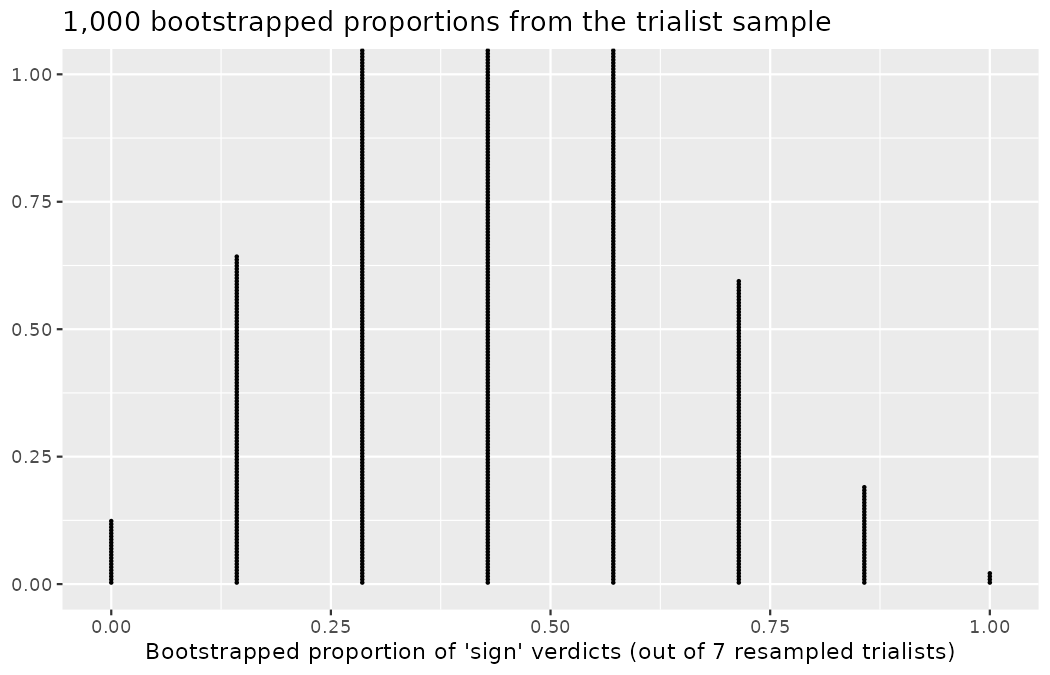
\includegraphics[width=0.85\linewidth,height=\textheight,keepaspectratio]{figures/foundations-bootstrapping-1.png}

The dot plot shows 1,000 dots stacked at the only eight values a
proportion out of 7 can take, from \(0/7\) to \(7/7.\) The tallest stack
sits at the observed value \(3/7 \approx 0.429\) (286 of the 1,000
resamples), with the neighboring stacks at \(2/7\) and \(4/7\) nearly as
tall (213 and 238), and the counts falling away toward the extremes:
only 21 resamples contained no ``sign'' verdicts at all, and just 4
consisted of ``sign'' verdicts entirely. The shape is roughly a bell
centered on \(\hat{p},\) with the bulk of bootstrapped proportions
falling between \(1/7\) and \(6/7.\)

Whether you imagine sampling from the infinite estimated population or
drawing from the bag with replacement, the dot plot of bootstrapped
proportions comes out the same, because the process by which the
statistics were estimated is equivalent. The bag version is simply the
one a computer (or an analyst with marbles) can actually carry out.

If we apply the bootstrap sampling process to the consultant example, we
consider each of England's shots to be one of the marbles in the bag.
There will be 50 white marbles (no goal) and 13 red marbles (goal). If
we choose 63 marbles out of the bag (one at a time with replacement) and
compute the proportion of simulated shots that were goals,
\(\hat{p}_{boot},\) then this ``bootstrap'' proportion represents a
single simulated proportion from the ``resample from the sample''
approach.

\begin{tcolorbox}[enhanced jigsaw, left=2mm, leftrule=.75mm, title=\textcolor{quarto-callout-tip-color}{\faLightbulb}\hspace{0.5em}{Check your understanding}, arc=.35mm, rightrule=.15mm, coltitle=black, colframe=quarto-callout-tip-color-frame, bottomrule=.15mm, colbacktitle=quarto-callout-tip-color!10!white, opacitybacktitle=0.6, breakable, bottomtitle=1mm, toptitle=1mm, titlerule=0mm, opacityback=0, toprule=.15mm, colback=white]

In a simulation of 63 shots, about how many would we expect to be goals?

\begin{center}\rule{0.5\linewidth}{0.5pt}\end{center}

About 20.6\% of the shots (13 on average) in the simulation will be
goals, as this is what was seen in the sample. We will, however, see a
little variation from one simulation to the next.

\end{tcolorbox}

One simulation isn't enough to get a sense of the variability from one
bootstrap proportion to another bootstrap proportion, so we repeat the
simulation 10,000 times using a computer. The \textbf{infer} pipeline
from Chapter~\ref{sec-foundations-randomization} does the work, with one
change that carries the entire conceptual difference between the two
chapters: \texttt{generate(type\ =\ "bootstrap")} resamples the 63 rows
with replacement, where \texttt{type\ =\ "permute"} had shuffled labels
between groups.

\begin{Shaded}
\begin{Highlighting}[]
\FunctionTok{set.seed}\NormalTok{(}\DecValTok{1202}\NormalTok{)}
\NormalTok{england\_boot }\OtherTok{\textless{}{-}}\NormalTok{ england\_shots }\SpecialCharTok{|\textgreater{}}
  \FunctionTok{mutate}\NormalTok{(}\AttributeTok{result =} \FunctionTok{if\_else}\NormalTok{(goal, }\StringTok{"goal"}\NormalTok{, }\StringTok{"no goal"}\NormalTok{)) }\SpecialCharTok{|\textgreater{}}
  \FunctionTok{specify}\NormalTok{(}\AttributeTok{response =}\NormalTok{ result, }\AttributeTok{success =} \StringTok{"goal"}\NormalTok{) }\SpecialCharTok{|\textgreater{}}
  \FunctionTok{generate}\NormalTok{(}\AttributeTok{reps =} \DecValTok{10000}\NormalTok{, }\AttributeTok{type =} \StringTok{"bootstrap"}\NormalTok{) }\SpecialCharTok{|\textgreater{}}
  \FunctionTok{calculate}\NormalTok{(}\AttributeTok{stat =} \StringTok{"prop"}\NormalTok{)}

\NormalTok{england\_ci }\OtherTok{\textless{}{-}}\NormalTok{ england\_boot }\SpecialCharTok{|\textgreater{}}
  \FunctionTok{summarize}\NormalTok{(}
    \AttributeTok{lower =} \FunctionTok{quantile}\NormalTok{(stat, }\FloatTok{0.025}\NormalTok{),}
    \AttributeTok{upper =} \FunctionTok{quantile}\NormalTok{(stat, }\FloatTok{0.975}\NormalTok{)}
\NormalTok{  )}
\NormalTok{england\_ci}
\CommentTok{\#\textgreater{} \# A tibble: 1 × 2}
\CommentTok{\#\textgreater{}   lower upper}
\CommentTok{\#\textgreater{}   \textless{}dbl\textgreater{} \textless{}dbl\textgreater{}}
\CommentTok{\#\textgreater{} 1 0.111 0.317}
\end{Highlighting}
\end{Shaded}

The histogram below shows the distribution from the 10,000 bootstrap
simulations.

\begin{Shaded}
\begin{Highlighting}[]
\FunctionTok{ggplot}\NormalTok{(england\_boot, }\FunctionTok{aes}\NormalTok{(}\AttributeTok{x =}\NormalTok{ stat)) }\SpecialCharTok{+}
  \FunctionTok{geom\_histogram}\NormalTok{(}\AttributeTok{binwidth =} \DecValTok{1} \SpecialCharTok{/} \DecValTok{63}\NormalTok{) }\SpecialCharTok{+}
  \FunctionTok{annotate}\NormalTok{(}\StringTok{"segment"}\NormalTok{,}
    \AttributeTok{x =}\NormalTok{ england\_ci}\SpecialCharTok{$}\NormalTok{lower, }\AttributeTok{y =} \DecValTok{0}\NormalTok{,}
    \AttributeTok{xend =}\NormalTok{ england\_ci}\SpecialCharTok{$}\NormalTok{lower, }\AttributeTok{yend =} \DecValTok{1200}\NormalTok{,}
    \AttributeTok{linetype =} \StringTok{"dashed"}
\NormalTok{  ) }\SpecialCharTok{+}
  \FunctionTok{annotate}\NormalTok{(}\StringTok{"segment"}\NormalTok{,}
    \AttributeTok{x =}\NormalTok{ england\_ci}\SpecialCharTok{$}\NormalTok{upper, }\AttributeTok{y =} \DecValTok{0}\NormalTok{,}
    \AttributeTok{xend =}\NormalTok{ england\_ci}\SpecialCharTok{$}\NormalTok{upper, }\AttributeTok{yend =} \DecValTok{1200}\NormalTok{,}
    \AttributeTok{linetype =} \StringTok{"dashed"}
\NormalTok{  ) }\SpecialCharTok{+}
  \FunctionTok{annotate}\NormalTok{(}\StringTok{"text"}\NormalTok{, }\AttributeTok{x =}\NormalTok{ england\_ci}\SpecialCharTok{$}\NormalTok{lower, }\AttributeTok{y =} \DecValTok{1400}\NormalTok{, }\AttributeTok{label =} \StringTok{"2.5th}\SpecialCharTok{\textbackslash{}n}\StringTok{percentile"}\NormalTok{) }\SpecialCharTok{+}
  \FunctionTok{annotate}\NormalTok{(}\StringTok{"text"}\NormalTok{, }\AttributeTok{x =}\NormalTok{ england\_ci}\SpecialCharTok{$}\NormalTok{upper, }\AttributeTok{y =} \DecValTok{1400}\NormalTok{, }\AttributeTok{label =} \StringTok{"97.5th}\SpecialCharTok{\textbackslash{}n}\StringTok{percentile"}\NormalTok{) }\SpecialCharTok{+}
  \FunctionTok{labs}\NormalTok{(}
    \AttributeTok{x =} \StringTok{"Bootstrapped proportion of England\textquotesingle{}s shots scored"}\NormalTok{,}
    \AttributeTok{y =} \StringTok{"Count"}\NormalTok{,}
    \AttributeTok{title =} \StringTok{"10,000 bootstrapped proportions"}
\NormalTok{  )}
\end{Highlighting}
\end{Shaded}

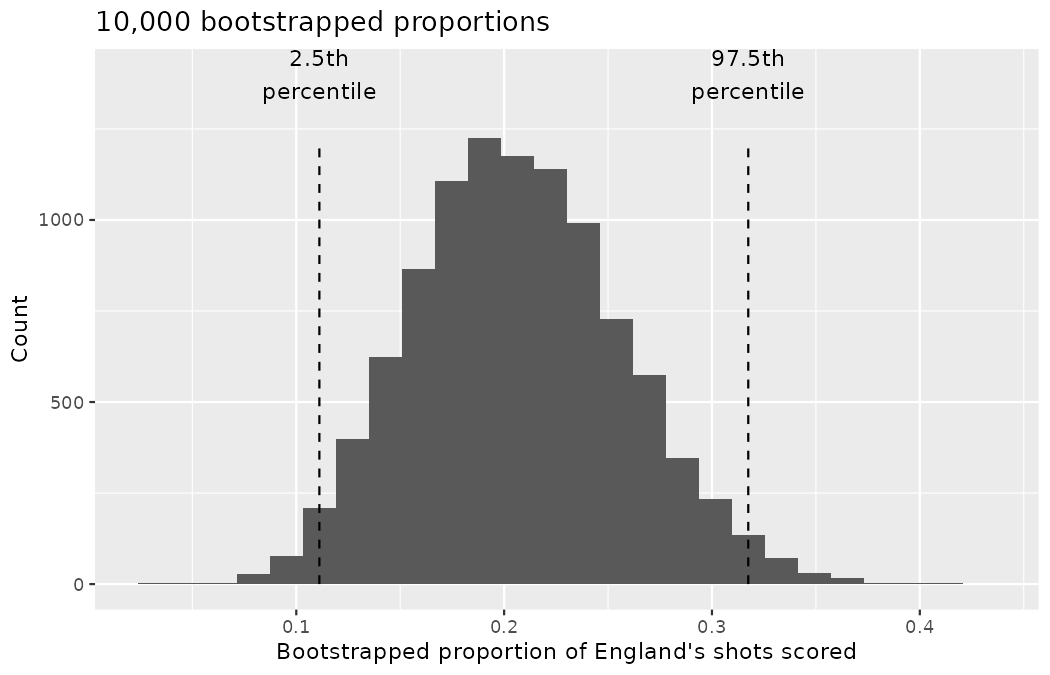
\includegraphics[width=0.85\linewidth,height=\textheight,keepaspectratio]{figures/foundations-bootstrapping-2.png}

The histogram is roughly bell-shaped and centered near the observed
\(\hat{p} = 0.206\) (the mean of the 10,000 bootstrapped proportions is
0.207), with the bars stepping in increments of \(1/63\) and the full
set of bootstrapped proportions ranging from about \(0.032\) to
\(0.429.\) The dashed lines mark the 2.5th percentile at
\(7/63 = 0.111\) and the 97.5th percentile at \(20/63 = 0.317.\) The
variability in the bootstrapped proportions leads us to believe that the
true conversion rate under the consultant's methods (the parameter,
\(p\)) is likely to fall somewhere between 11.1\% and 31.7\%, as these
numbers capture 95\% of the bootstrap resampled values.

The range of values for the true proportion is called a
\textbf{bootstrap percentile confidence interval}, and we will see it
again throughout the next few sections and chapters.

\begin{tcolorbox}[enhanced jigsaw, left=2mm, leftrule=.75mm, title=\textcolor{quarto-callout-note-color}{\faInfo}\hspace{0.5em}{Worked example}, arc=.35mm, rightrule=.15mm, coltitle=black, colframe=quarto-callout-note-color-frame, bottomrule=.15mm, colbacktitle=quarto-callout-note-color!10!white, opacitybacktitle=0.6, breakable, bottomtitle=1mm, toptitle=1mm, titlerule=0mm, opacityback=0, toprule=.15mm, colback=white]

The original claim was that the consultant's methods lift a team's true
conversion rate above the tournament rate of about 13\%. Does the
interval estimate of 11.1\% to 31.7\% for the true conversion rate
indicate that the consultant's teams finish better than the tournament
average? Explain.

\begin{center}\rule{0.5\linewidth}{0.5pt}\end{center}

No. Because the interval overlaps 13.1\%, it might be that the
consultant's work is associated with a higher conversion rate, or it
might be that it is associated with a \emph{lower} one (i.e., below
13.1\%)! Additionally, as previously mentioned, because this is an
observational study, even if an association can be measured, there is no
evidence that the consultant's work is the cause of the conversion rate
(being higher or lower). Marta can decline the pitch without needing to
accuse anyone of anything: the data are simply consistent with an
ordinary team.

\end{tcolorbox}

\section{Corner-kick expectations case
study}\label{sec-tapperscasestudy}

Here's an exercise you can try in any coaches' meeting: ask everyone to
write down, before checking any data, what proportion of shots arising
from corner-kick situations at a World Cup end up as goals. Corners feel
dangerous --- the crowd rises, the keeper's box fills, the broadcast
cuts to the bench --- and intuition prices them accordingly.

\subsection{Observed data}\label{observed-data-3}

Priya Rao ran exactly this exercise at Northbridge's pre-season analysis
workshop. (The workshop poll is a constructed scenario; the shot data
below are real.) She collected written guesses from the coaching staff
and the scouting network, and the typical answer was that about 25\% of
shots from corner situations are scored --- one goal in four. Priya
wondered, is 25\% a reasonable expectation?

The 2022 World Cup data can answer for one tournament. The
\texttt{play\_pattern} variable, which you first tabulated in
Chapter~\ref{sec-explore-categorical}, identifies shots arising from
corner possessions:

\begin{Shaded}
\begin{Highlighting}[]
\NormalTok{wc2022\_shots }\SpecialCharTok{|\textgreater{}}
  \FunctionTok{filter}\NormalTok{(play\_pattern }\SpecialCharTok{==} \StringTok{"From Corner"}\NormalTok{) }\SpecialCharTok{|\textgreater{}}
  \FunctionTok{summarize}\NormalTok{(}\AttributeTok{shots =} \FunctionTok{n}\NormalTok{(), }\AttributeTok{goals =} \FunctionTok{sum}\NormalTok{(goal), }\AttributeTok{conversion =} \FunctionTok{mean}\NormalTok{(goal))}
\CommentTok{\#\textgreater{} \# A tibble: 1 × 3}
\CommentTok{\#\textgreater{}   shots goals conversion}
\CommentTok{\#\textgreater{}   \textless{}int\textgreater{} \textless{}int\textgreater{}      \textless{}dbl\textgreater{}}
\CommentTok{\#\textgreater{} 1   223    17     0.0762}
\end{Highlighting}
\end{Shaded}

Of the 223 corner-pattern shots at the tournament, only 17 were scored:
\(\hat{p} = 17/223 = 0.076.\) That seems like quite a low number --- a
third of what the room guessed --- which leads the analyst to ask: what
is the true proportion of corner-pattern shots that are scored?

\subsection{Variability of the
statistic}\label{variability-of-the-statistic-3}

To answer the question, we will again use a simulation. To simulate 223
corner-pattern shots, this time we use a bag of 223 marbles, 17 of which
are red (for the shots that were scored) and 206 of which are white (for
the shots that were not). Sampling from the bag 223 times (remembering
to replace the marble back into the bag each time to keep constant the
population proportion of red) produces one bootstrap sample.

For example, we can start by simulating just 5 corner-pattern shots by
drawing 5 marbles from the bag of 17 red and 206 white marbles. Because
each draw is a success with probability \(17/223\) independently of the
others, \texttt{rbinom()} performs the draws directly --- drawing
marbles with replacement and flipping a coin that lands ``goal'' with
probability \(17/223\) are the same process:

\begin{Shaded}
\begin{Highlighting}[]
\FunctionTok{set.seed}\NormalTok{(}\DecValTok{1203}\NormalTok{)}
\FunctionTok{rbinom}\NormalTok{(}\DecValTok{5}\NormalTok{, }\AttributeTok{size =} \DecValTok{1}\NormalTok{, }\AttributeTok{prob =} \DecValTok{17} \SpecialCharTok{/} \DecValTok{223}\NormalTok{)}
\CommentTok{\#\textgreater{} [1] 0 0 0 0 0}
\end{Highlighting}
\end{Shaded}

\begin{longtable}[]{@{}ccccc@{}}
\toprule\noalign{}
W & W & W & W & W \\
\midrule\noalign{}
\endhead
\bottomrule\noalign{}
\endlastfoot
miss & miss & miss & miss & miss \\
\end{longtable}

All five simulated shots missed --- unremarkable when the chance of each
one scoring is only about 7.6\%. Continuing the same seeded stream to
full resamples of 223 shots, we counted the reds and computed
\(\hat{p}_{boot}\) for ten entire simulations:

\begin{Shaded}
\begin{Highlighting}[]
\FunctionTok{round}\NormalTok{(}\FunctionTok{rbinom}\NormalTok{(}\DecValTok{10}\NormalTok{, }\AttributeTok{size =} \DecValTok{223}\NormalTok{, }\AttributeTok{prob =} \DecValTok{17} \SpecialCharTok{/} \DecValTok{223}\NormalTok{) }\SpecialCharTok{/} \DecValTok{223}\NormalTok{, }\DecValTok{4}\NormalTok{)}
\CommentTok{\#\textgreater{}  [1] 0.0673 0.0673 0.0717 0.1031 0.0717 0.0583 0.0628 0.0673 0.0987 0.0628}
\end{Highlighting}
\end{Shaded}

\[0.0673 \quad 0.0673 \quad 0.0717 \quad 0.1031 \quad 0.0717 \quad 0.0583 \quad 0.0628 \quad 0.0673 \quad 0.0987 \quad 0.0628\]

As we did with the randomization technique, seeing what would happen
with one simulation isn't enough --- and even ten only hint at the
spread. In order to understand how far the observed proportion of 0.076
might be from the true parameter, we should generate more simulations,
so we'll run a total of 10,000 using a computer.

\begin{Shaded}
\begin{Highlighting}[]
\FunctionTok{set.seed}\NormalTok{(}\DecValTok{1204}\NormalTok{)}
\NormalTok{bsprop\_corner }\OtherTok{\textless{}{-}} \FunctionTok{tibble}\NormalTok{(}
  \AttributeTok{p\_boot =} \FunctionTok{rbinom}\NormalTok{(}\DecValTok{10000}\NormalTok{, }\AttributeTok{size =} \DecValTok{223}\NormalTok{, }\AttributeTok{prob =} \DecValTok{17} \SpecialCharTok{/} \DecValTok{223}\NormalTok{) }\SpecialCharTok{/} \DecValTok{223}
\NormalTok{)}

\NormalTok{corner\_ci }\OtherTok{\textless{}{-}}\NormalTok{ bsprop\_corner }\SpecialCharTok{|\textgreater{}}
  \FunctionTok{summarize}\NormalTok{(}
    \AttributeTok{lower =} \FunctionTok{quantile}\NormalTok{(p\_boot, }\FloatTok{0.025}\NormalTok{),}
    \AttributeTok{upper =} \FunctionTok{quantile}\NormalTok{(p\_boot, }\FloatTok{0.975}\NormalTok{)}
\NormalTok{  )}
\NormalTok{corner\_ci}
\CommentTok{\#\textgreater{} \# A tibble: 1 × 2}
\CommentTok{\#\textgreater{}    lower upper}
\CommentTok{\#\textgreater{}    \textless{}dbl\textgreater{} \textless{}dbl\textgreater{}}
\CommentTok{\#\textgreater{} 1 0.0448 0.112}

\FunctionTok{ggplot}\NormalTok{(bsprop\_corner, }\FunctionTok{aes}\NormalTok{(}\AttributeTok{x =}\NormalTok{ p\_boot)) }\SpecialCharTok{+}
  \FunctionTok{geom\_histogram}\NormalTok{(}\AttributeTok{binwidth =} \DecValTok{1} \SpecialCharTok{/} \DecValTok{223}\NormalTok{) }\SpecialCharTok{+}
  \FunctionTok{annotate}\NormalTok{(}\StringTok{"segment"}\NormalTok{,}
    \AttributeTok{x =}\NormalTok{ corner\_ci}\SpecialCharTok{$}\NormalTok{lower, }\AttributeTok{y =} \DecValTok{0}\NormalTok{,}
    \AttributeTok{xend =}\NormalTok{ corner\_ci}\SpecialCharTok{$}\NormalTok{lower, }\AttributeTok{yend =} \DecValTok{1200}\NormalTok{,}
    \AttributeTok{linetype =} \StringTok{"dashed"}
\NormalTok{  ) }\SpecialCharTok{+}
  \FunctionTok{annotate}\NormalTok{(}\StringTok{"segment"}\NormalTok{,}
    \AttributeTok{x =}\NormalTok{ corner\_ci}\SpecialCharTok{$}\NormalTok{upper, }\AttributeTok{y =} \DecValTok{0}\NormalTok{,}
    \AttributeTok{xend =}\NormalTok{ corner\_ci}\SpecialCharTok{$}\NormalTok{upper, }\AttributeTok{yend =} \DecValTok{1200}\NormalTok{,}
    \AttributeTok{linetype =} \StringTok{"dashed"}
\NormalTok{  ) }\SpecialCharTok{+}
  \FunctionTok{annotate}\NormalTok{(}\StringTok{"text"}\NormalTok{, }\AttributeTok{x =}\NormalTok{ corner\_ci}\SpecialCharTok{$}\NormalTok{lower, }\AttributeTok{y =} \DecValTok{1400}\NormalTok{, }\AttributeTok{label =} \StringTok{"2.5th}\SpecialCharTok{\textbackslash{}n}\StringTok{percentile"}\NormalTok{) }\SpecialCharTok{+}
  \FunctionTok{annotate}\NormalTok{(}\StringTok{"text"}\NormalTok{, }\AttributeTok{x =}\NormalTok{ corner\_ci}\SpecialCharTok{$}\NormalTok{upper, }\AttributeTok{y =} \DecValTok{1400}\NormalTok{, }\AttributeTok{label =} \StringTok{"97.5th}\SpecialCharTok{\textbackslash{}n}\StringTok{percentile"}\NormalTok{) }\SpecialCharTok{+}
  \FunctionTok{labs}\NormalTok{(}
    \AttributeTok{x =} \StringTok{"Bootstrapped proportion of corner{-}pattern shots scored"}\NormalTok{,}
    \AttributeTok{y =} \StringTok{"Count"}\NormalTok{,}
    \AttributeTok{title =} \StringTok{"10,000 bootstrapped proportions"}
\NormalTok{  )}
\end{Highlighting}
\end{Shaded}

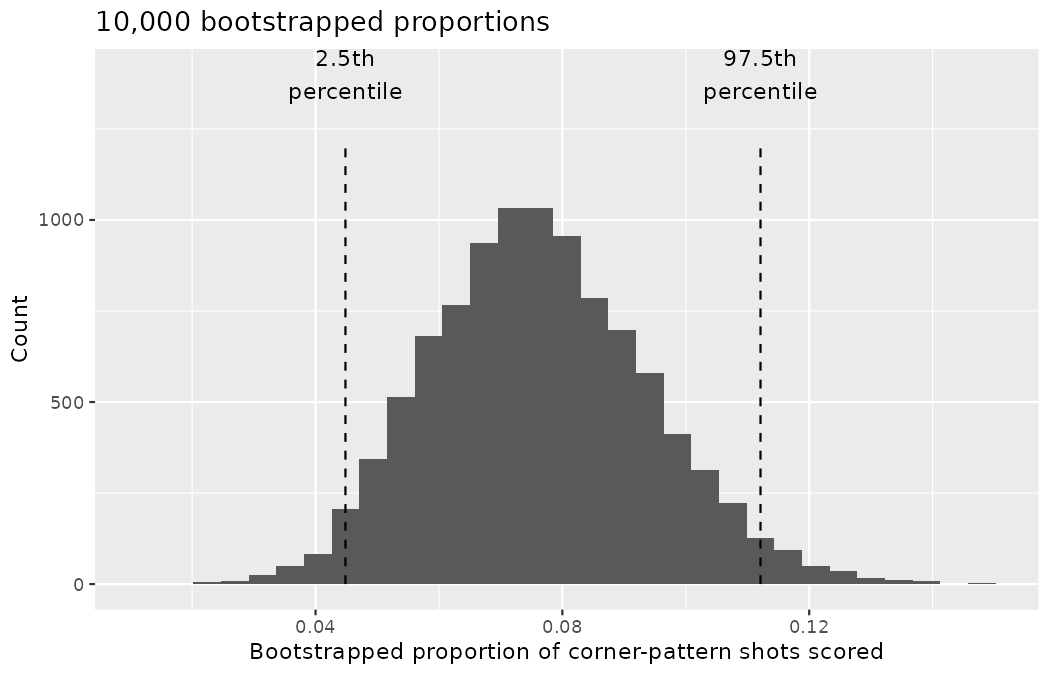
\includegraphics[width=0.85\linewidth,height=\textheight,keepaspectratio]{figures/foundations-bootstrapping-3.png}

The histogram of the 10,000 bootstrapped proportions is centered near
the observed \(0.076,\) stepping in increments of \(1/223,\) with a mild
right skew --- the sort of asymmetry a proportion this close to zero
must have, since it cannot fall below 0. The bootstrapped proportions
range from about \(0.013\) to \(0.148,\) and the dashed lines mark the
range of 95\% of the resampled values of \(\hat{p}_{boot}\): \(0.0448\)
to \(0.112.\) That is, we expect that between about 4.5\% and 11.2\% of
corner-pattern shots are truly scored.

\begin{tcolorbox}[enhanced jigsaw, left=2mm, leftrule=.75mm, title=\textcolor{quarto-callout-tip-color}{\faLightbulb}\hspace{0.5em}{Check your understanding}, arc=.35mm, rightrule=.15mm, coltitle=black, colframe=quarto-callout-tip-color-frame, bottomrule=.15mm, colbacktitle=quarto-callout-tip-color!10!white, opacitybacktitle=0.6, breakable, bottomtitle=1mm, toptitle=1mm, titlerule=0mm, opacityback=0, toprule=.15mm, colback=white]

Do the data provide convincing evidence against the workshop's claim
that 25\% of corner-pattern shots are scored?

\begin{center}\rule{0.5\linewidth}{0.5pt}\end{center}

Because 25\% is not in the interval estimate for the true parameter, we
can say that there is convincing evidence against the claim that a
quarter of corner-pattern shots are scored. Moreover, 25\% is a
substantial distance from the largest resample statistic (about 0.148 in
10,000 resamples), suggesting that there is \textbf{very} convincing
evidence against this claim. The coaching intuition overrates corners by
roughly a factor of three --- a gap worth remembering the next time a
set-piece specialist quotes his own value.

\end{tcolorbox}

\section{Confidence intervals}\label{sec-ConfidenceIntervals}

A point estimate provides a single plausible value for a parameter.
However, a point estimate is rarely perfect; usually there is some error
in the estimate. In addition to supplying a point estimate of a
parameter, a next logical step would be to provide a plausible
\emph{range of values} for the parameter.

\subsection{Plausible range of values for the population
parameter}\label{plausible-range-of-values-for-the-population-parameter}

A plausible range of values for the population parameter is called a
\textbf{confidence interval}. Using only a single point estimate is like
a goalkeeper facing a penalty and diving to one exact spot: commit to a
single point and you will probably miss the ball. Covering a zone of the
goalmouth --- staying big, guarding a range --- gives a good chance that
the ball ends up somewhere you can reach.

If we report a point estimate, we probably will not hit the exact
population parameter. On the other hand, if we report a range of
plausible values --- a confidence interval --- we have a good shot at
capturing the parameter.

\begin{tcolorbox}[enhanced jigsaw, left=2mm, leftrule=.75mm, title=\textcolor{quarto-callout-tip-color}{\faLightbulb}\hspace{0.5em}{Check your understanding}, arc=.35mm, rightrule=.15mm, coltitle=black, colframe=quarto-callout-tip-color-frame, bottomrule=.15mm, colbacktitle=quarto-callout-tip-color!10!white, opacitybacktitle=0.6, breakable, bottomtitle=1mm, toptitle=1mm, titlerule=0mm, opacityback=0, toprule=.15mm, colback=white]

If we want to be very certain we capture the population parameter,
should we use a wider interval (e.g., 99\%) or a smaller interval (e.g.,
80\%)?

\begin{center}\rule{0.5\linewidth}{0.5pt}\end{center}

If the keeper wants to be more certain of reaching the ball, he covers
more of the goal. Likewise, we use a wider confidence interval if we
want to be more certain that we capture the parameter.

\end{tcolorbox}

\subsection{Bootstrap confidence
interval}\label{bootstrap-confidence-interval}

As we saw above, a \textbf{bootstrap sample} is a sample of the original
sample. In the case of England's shot data, we proceed as follows:

\begin{itemize}
\tightlist
\item
  Randomly sample one observation from the 63 shots (replace the marble
  back into the bag so as to keep the population constant).
\item
  Randomly sample a second observation from the 63 shots. Because we
  sample with replacement (i.e., we do not actually remove the marbles
  from the bag), there is a 1-in-63 chance that the second observation
  will be the same one sampled in the first step!
\item
  Keep going one sampled observation at a time \ldots{}
\item
  Randomly sample the 63rd observation from the 63 shots.
\end{itemize}

Bootstrap sampling is often called \textbf{sampling with replacement},
and you watched it happen in the trialist example: T5 appeared three
times in the first resample precisely because he went back in the bag
after each draw.

A bootstrap sample behaves similarly to how an actual sample from a
population would behave, and we compute the point estimate of interest
(here, compute \(\hat{p}_{boot}\)).

Based on theory that is beyond this text, we know that the bootstrap
proportions \(\hat{p}_{boot}\) vary around \(\hat{p}\) similarly to how
different sample proportions (i.e., values of \(\hat{p}\)) vary around
the true parameter \(p.\) Therefore, an interval estimate for \(p\) can
be produced using the \(\hat{p}_{boot}\) values themselves.

\begin{tcolorbox}[enhanced jigsaw, left=2mm, leftrule=.75mm, title=\textcolor{quarto-callout-note-color}{\faInfo}\hspace{0.5em}{Deeper (optional): watching the principle hold}, arc=.35mm, rightrule=.15mm, coltitle=black, colframe=quarto-callout-note-color-frame, bottomrule=.15mm, colbacktitle=quarto-callout-note-color!10!white, opacitybacktitle=0.6, breakable, bottomtitle=1mm, toptitle=1mm, titlerule=0mm, opacityback=0, toprule=.15mm, colback=white]

The theory is beyond this text, but the claim it makes is checkable,
because for once we hold an entire population: the 1,494 shots of the
2022 World Cup. Below, we draw 1,000 \emph{different} samples of 63
shots from the tournament and record the standard deviation of their
sample proportions --- the true sample-to-sample variability that in
real life we never get to see. Then we take just \emph{one} sample of 63
shots and bootstrap it 1,000 times.

\begin{Shaded}
\begin{Highlighting}[]
\FunctionTok{set.seed}\NormalTok{(}\DecValTok{1210}\NormalTok{)}
\NormalTok{sampling\_p }\OtherTok{\textless{}{-}} \FunctionTok{replicate}\NormalTok{(}\DecValTok{1000}\NormalTok{, \{}
  \FunctionTok{mean}\NormalTok{(}\FunctionTok{slice\_sample}\NormalTok{(wc2022\_shots, }\AttributeTok{n =} \DecValTok{63}\NormalTok{)}\SpecialCharTok{$}\NormalTok{goal)}
\NormalTok{\})}

\NormalTok{one\_sample }\OtherTok{\textless{}{-}} \FunctionTok{slice\_sample}\NormalTok{(wc2022\_shots, }\AttributeTok{n =} \DecValTok{63}\NormalTok{)}
\NormalTok{boot\_p }\OtherTok{\textless{}{-}} \FunctionTok{replicate}\NormalTok{(}\DecValTok{1000}\NormalTok{, \{}
  \FunctionTok{mean}\NormalTok{(}\FunctionTok{slice\_sample}\NormalTok{(one\_sample, }\AttributeTok{n =} \DecValTok{63}\NormalTok{, }\AttributeTok{replace =} \ConstantTok{TRUE}\NormalTok{)}\SpecialCharTok{$}\NormalTok{goal)}
\NormalTok{\})}

\FunctionTok{round}\NormalTok{(}\FunctionTok{c}\NormalTok{(}\AttributeTok{sd\_sampling =} \FunctionTok{sd}\NormalTok{(sampling\_p), }\AttributeTok{sd\_bootstrap =} \FunctionTok{sd}\NormalTok{(boot\_p)), }\DecValTok{4}\NormalTok{)}
\CommentTok{\#\textgreater{}  sd\_sampling sd\_bootstrap}
\CommentTok{\#\textgreater{}       0.0421       0.0446}
\end{Highlighting}
\end{Shaded}

The two standard deviations are close: the spread of the
\(\hat{p}_{boot}\) values around \(\hat{p}\) --- computed from a single
sample, which happened to contain 9 goals \((\hat{p} = 9/63 = 0.143)\)
--- approximates the spread of the \(\hat{p}\) values around \(p,\)
which required 1,000 samples we would never have in practice. That
closeness is the bootstrap principle at work, and it is exactly what
licenses reading a confidence interval off the \(\hat{p}_{boot}\)
values.

\end{tcolorbox}

\begin{tcolorbox}[enhanced jigsaw, left=2mm, leftrule=.75mm, title=\textcolor{quarto-callout-important-color}{\faExclamation}\hspace{0.5em}{95\% bootstrap percentile confidence interval for a parameter \(p\)}, arc=.35mm, rightrule=.15mm, coltitle=black, colframe=quarto-callout-important-color-frame, bottomrule=.15mm, colbacktitle=quarto-callout-important-color!10!white, opacitybacktitle=0.6, breakable, bottomtitle=1mm, toptitle=1mm, titlerule=0mm, opacityback=0, toprule=.15mm, colback=white]

The 95\% bootstrap confidence interval for the parameter \(p\) can be
obtained directly using the ordered \(\hat{p}_{boot}\) values.

Consider the sorted \(\hat{p}_{boot}\) values. Call the 2.5\%
bootstrapped proportion value ``lower'', and call the 97.5\%
bootstrapped proportion value ``upper''.

The 95\% confidence interval is given by: (lower, upper)

\end{tcolorbox}

That is exactly what \texttt{quantile(stat,\ 0.025)} and
\texttt{quantile(stat,\ 0.975)} computed in both case studies: for
England, (0.111, 0.317); for the corner-pattern shots, (0.0448, 0.112).

\begin{tcolorbox}[enhanced jigsaw, left=2mm, leftrule=.75mm, title=\textcolor{quarto-callout-tip-color}{\faLightbulb}\hspace{0.5em}{Check your understanding}, arc=.35mm, rightrule=.15mm, coltitle=black, colframe=quarto-callout-tip-color-frame, bottomrule=.15mm, colbacktitle=quarto-callout-tip-color!10!white, opacitybacktitle=0.6, breakable, bottomtitle=1mm, toptitle=1mm, titlerule=0mm, opacityback=0, toprule=.15mm, colback=white]

Both the permutation distributions of
Chapter~\ref{sec-foundations-randomization} and the bootstrap
distributions of this chapter were built by simulation. Where is each
one centered, and why does the difference matter?

\begin{center}\rule{0.5\linewidth}{0.5pt}\end{center}

A permutation (or randomization) distribution is built assuming the null
hypothesis, so it is centered at the null value --- zero, for a
difference in proportions --- and we ask how far out the observed
statistic falls. A bootstrap distribution is built from the observed
sample with no hypothesis at all, so it is centered near the observed
statistic \(\hat{p},\) and its \emph{spread} tells us how far the
statistic tends to sit from the parameter. One machine tests claims; the
other measures precision.

\end{tcolorbox}

In Section~\ref{sec-one-prop-null-boot} we will discuss different
percentages for the confidence interval (e.g., 90\% confidence interval
or 99\% confidence interval).

Section~\ref{sec-one-prop-null-boot} also provides a longer discussion
on what ``95\% confidence'' actually means.

\section{Chapter review}\label{sec-chp12-review}

\subsection{Summary}\label{summary-11}

Picture the full procedure one more time with the trialist bag: the
seven verdicts stand in for the population; draw seven with replacement;
record the proportion of ``sign'' verdicts; repeat thousands of times;
then read off the middle 95\% of the bootstrapped proportions. Sampling
with replacement is a computational tool which is equivalent to using
the sample as a way of estimating an infinitely large population from
which to sample.

We can summarize the bootstrap process as follows:

\begin{itemize}
\tightlist
\item
  \textbf{Frame the research question in terms of a parameter to
  estimate.} Confidence intervals are appropriate for research questions
  that aim to estimate a number from the population (called a parameter)
  --- a true conversion rate, a true shortlist rate --- rather than to
  test a yes/no claim.
\item
  \textbf{Collect data with an observational study or experiment.} If a
  research question can be formed as a query about the parameter, we can
  collect data to calculate a statistic which is the best guess we have
  for the value of the parameter. However, we know that the statistic
  won't be exactly equal to the parameter due to natural variability:
  England's 63 shots gave one \(\hat{p};\) a different tournament would
  have given another.
\item
  \textbf{Model the randomness by using the data values as a proxy for
  the population.} In order to assess how far the statistic might be
  from the parameter, we take repeated resamples from the dataset to
  measure the variability in bootstrapped statistics. The variability of
  the bootstrapped statistics around the observed statistic (a quantity
  which can be measured through computational technique) should be
  approximately the same as the variability of many observed sample
  statistics around the parameter (a quantity which is very difficult to
  measure because in real life we only get exactly one sample).
\item
  \textbf{Create the interval.} After choosing a particular confidence
  level, use the variability of the bootstrapped statistics to create an
  interval estimate which will hope to capture the true parameter. While
  the interval estimate associated with the particular sample at hand
  may or may not capture the parameter, the researcher knows that over
  their lifetime, the confidence level will determine the percentage of
  their research confidence intervals that do capture the true
  parameter.
\item
  \textbf{Form a conclusion.} Using the confidence interval from the
  analysis, report on the interval estimate for the parameter of
  interest. Also, be sure to write the conclusion in plain language so
  casual readers can understand the results --- Marta Vidal should be
  able to read ``plausibly between 11\% and 32\%'' and act on it,
  without decoding notation.
\end{itemize}

\begin{longtable}[]{@{}
  >{\raggedright\arraybackslash}p{(\linewidth - 2\tabcolsep) * \real{0.5634}}
  >{\raggedright\arraybackslash}p{(\linewidth - 2\tabcolsep) * \real{0.4366}}@{}}
\caption{Summary of bootstrapping as an inferential statistical
method.}\label{tbl-chp12-summary}\tabularnewline
\toprule\noalign{}
\begin{minipage}[b]{\linewidth}\raggedright
Question
\end{minipage} & \begin{minipage}[b]{\linewidth}\raggedright
Answer
\end{minipage} \\
\midrule\noalign{}
\endfirsthead
\toprule\noalign{}
\begin{minipage}[b]{\linewidth}\raggedright
Question
\end{minipage} & \begin{minipage}[b]{\linewidth}\raggedright
Answer
\end{minipage} \\
\midrule\noalign{}
\endhead
\bottomrule\noalign{}
\endlastfoot
What does the procedure do? & Resamples the observed data with
replacement, using the sample as a proxy for the population, to simulate
drawing many new samples. \\
What is the statistic? & A summary of the sample, e.g.,
\(\hat{p} = 13/63\); recomputed on each resample it becomes
\(\hat{p}_{boot}.\) \\
What does the bootstrap distribution describe? & The sample-to-sample
variability of the statistic --- how far \(\hat{p}\) tends to sit from
\(p.\) \\
What is the interval? & The range between the 2.5th and 97.5th
percentiles of the ordered \(\hat{p}_{boot}\) values (for 95\%
confidence). \\
What does it conclude? & A range of plausible values for the parameter
--- an estimate of size, not a yes/no verdict, and causal only if the
data came from a randomized experiment. \\
\end{longtable}

\subsection{Terms}\label{terms-11}

The terms introduced in this chapter are presented below, alphabetized.
If you're not sure what some of these terms mean, we recommend you go
back in the text and review their definitions. You should be able to
easily spot them as \textbf{bolded text}.

\begin{longtable}[]{@{}
  >{\raggedright\arraybackslash}p{(\linewidth - 4\tabcolsep) * \real{0.3380}}
  >{\raggedright\arraybackslash}p{(\linewidth - 4\tabcolsep) * \real{0.3380}}
  >{\raggedright\arraybackslash}p{(\linewidth - 4\tabcolsep) * \real{0.3239}}@{}}
\caption{Terms introduced in this
chapter.}\label{tbl-terms-chp-12}\tabularnewline
\toprule\noalign{}
\endfirsthead
\endhead
\bottomrule\noalign{}
\endlastfoot
bootstrap percentile confidence interval & confidence interval &
sampling with replacement \\
bootstrap sample & parameter & statistic \\
bootstrapping & point estimate & \\
\end{longtable}

\section{Exercises}\label{sec-chp12-exercises}

Answers to odd-numbered exercises can be found in
Appendix~\ref{sec-exercise-solutions-12}.

\begin{enumerate}
\def\labelenumi{\arabic{enumi}.}
\item
  \textbf{Headed chances.} Let's say that you want to estimate the
  probability that a headed chance at this level of football is scored.
  Marta Vidal has asked for a defensible figure before the club weighs a
  bid for a target man whose game is built on winning crosses. You pull
  every shot taken with the head at the 2022 Men's World Cup\footnote{The
    2022 Men's World Cup shot data used in this exercise and in Exercise
    3 are in \texttt{data/derived/wc2022\_shots.csv} (StatsBomb open
    data).} and find that 28 of the 252 headed shots were scored. Recall
  from Section~\ref{sec-case-study-med-consult} that for a question
  about the \emph{process} --- how headed chances convert at this level,
  at the next tournament, for Northbridge --- these 252 shots are a
  sample, and the long-run conversion rate of headed chances is unknown.
  You decide to create a bootstrap interval from the original sample of
  252 shots.

\begin{Shaded}
\begin{Highlighting}[]
\NormalTok{wc2022\_shots }\OtherTok{\textless{}{-}} \FunctionTok{read\_csv}\NormalTok{(}\StringTok{"data/derived/wc2022\_shots.csv"}\NormalTok{)}

\NormalTok{headed\_shots }\OtherTok{\textless{}{-}}\NormalTok{ wc2022\_shots }\SpecialCharTok{|\textgreater{}} \FunctionTok{filter}\NormalTok{(body\_part }\SpecialCharTok{==} \StringTok{"Head"}\NormalTok{)}

\NormalTok{headed\_shots }\SpecialCharTok{|\textgreater{}}
  \FunctionTok{summarize}\NormalTok{(}\AttributeTok{shots =} \FunctionTok{n}\NormalTok{(), }\AttributeTok{goals =} \FunctionTok{sum}\NormalTok{(goal), }\AttributeTok{conversion =} \FunctionTok{mean}\NormalTok{(goal))}
\CommentTok{\#\textgreater{} \# A tibble: 1 × 3}
\CommentTok{\#\textgreater{}   shots goals conversion}
\CommentTok{\#\textgreater{}   \textless{}int\textgreater{} \textless{}int\textgreater{}      \textless{}dbl\textgreater{}}
\CommentTok{\#\textgreater{} 1   252    28      0.111}

\FunctionTok{set.seed}\NormalTok{(}\DecValTok{1205}\NormalTok{)}
\NormalTok{headed\_boot }\OtherTok{\textless{}{-}}\NormalTok{ headed\_shots }\SpecialCharTok{|\textgreater{}}
  \FunctionTok{mutate}\NormalTok{(}\AttributeTok{result =} \FunctionTok{if\_else}\NormalTok{(goal, }\StringTok{"goal"}\NormalTok{, }\StringTok{"no goal"}\NormalTok{)) }\SpecialCharTok{|\textgreater{}}
  \FunctionTok{specify}\NormalTok{(}\AttributeTok{response =}\NormalTok{ result, }\AttributeTok{success =} \StringTok{"goal"}\NormalTok{) }\SpecialCharTok{|\textgreater{}}
  \FunctionTok{generate}\NormalTok{(}\AttributeTok{reps =} \DecValTok{1000}\NormalTok{, }\AttributeTok{type =} \StringTok{"bootstrap"}\NormalTok{) }\SpecialCharTok{|\textgreater{}}
  \FunctionTok{calculate}\NormalTok{(}\AttributeTok{stat =} \StringTok{"prop"}\NormalTok{)}

\FunctionTok{round}\NormalTok{(}\FunctionTok{quantile}\NormalTok{(headed\_boot}\SpecialCharTok{$}\NormalTok{stat, }\FunctionTok{c}\NormalTok{(}\FloatTok{0.025}\NormalTok{, }\FloatTok{0.05}\NormalTok{, }\FloatTok{0.95}\NormalTok{, }\FloatTok{0.975}\NormalTok{)), }\DecValTok{3}\NormalTok{)}
\CommentTok{\#\textgreater{}  2.5\%    5\%   95\% 97.5\%}
\CommentTok{\#\textgreater{} 0.075 0.083 0.143 0.151}

\FunctionTok{ggplot}\NormalTok{(headed\_boot, }\FunctionTok{aes}\NormalTok{(}\AttributeTok{x =}\NormalTok{ stat)) }\SpecialCharTok{+}
  \FunctionTok{geom\_histogram}\NormalTok{(}\AttributeTok{binwidth =} \DecValTok{1} \SpecialCharTok{/} \DecValTok{252}\NormalTok{) }\SpecialCharTok{+}
  \FunctionTok{labs}\NormalTok{(}
    \AttributeTok{x =} \StringTok{"Bootstrapped proportion of headed shots scored"}\NormalTok{,}
    \AttributeTok{y =} \StringTok{"Count"}\NormalTok{,}
    \AttributeTok{title =} \StringTok{"1,000 bootstrapped proportions"}
\NormalTok{  )}
\end{Highlighting}
\end{Shaded}

  The histogram of the 1,000 bootstrapped proportions is roughly
  bell-shaped and centered at the observed proportion (the mean of the
  1,000 values is 0.111), with the bootstrapped proportions stepping in
  increments of \(1/252\) and ranging from about \(0.056\) to \(0.171.\)
  Four of its percentiles are printed above.

  \begin{enumerate}
  \def\labelenumii{\alph{enumii}.}
  \item
    Describe in words the relevant statistic and parameter for this
    problem. If you know the numerical value for either one, provide it.
    If you don't know the numerical value, explain why the value is
    unknown.
  \item
    What notation is used to describe, respectively, the statistic and
    the parameter?
  \item
    If using software to bootstrap the original dataset, what is the
    statistic calculated on each bootstrap sample?
  \item
    When creating a bootstrap sampling distribution (histogram) of the
    bootstrapped sample proportions, where should the center of the
    histogram lie?
  \item
    The code above printed four percentiles of the 1,000 bootstrapped
    sample proportions. Using the appropriate pair, construct a 90\%
    confidence interval for the probability that a headed chance is
    scored.
  \item
    Interpret the confidence interval in the context of the data.
  \end{enumerate}
\item
  \textbf{Right-footed shots at the Women's Euro.} Scouting reports
  habitually flag a prospect's weaker foot, so Priya Rao wants a
  tournament baseline: what proportion of shots at this level arrive on
  the right foot? At the 2025 Women's Euro, 502 of the 913 shots --- a
  proportion of \(502/913 = 0.55\) --- were taken with the right
  foot.\footnote{The 2025 Women's Euro shot data used in this exercise
    are in \texttt{data/derived/weuro2025\_shots.csv} (StatsBomb open
    data).} However, this value is based on a single tournament's worth
  of shots, so it may not be a perfect estimate for the population
  parameter of interest on its own. The seeded code below bootstraps the
  sample 1,000 times.

\begin{Shaded}
\begin{Highlighting}[]
\NormalTok{weuro2025\_shots }\OtherTok{\textless{}{-}} \FunctionTok{read\_csv}\NormalTok{(}\StringTok{"data/derived/weuro2025\_shots.csv"}\NormalTok{)}

\NormalTok{weuro2025\_shots }\SpecialCharTok{|\textgreater{}}
  \FunctionTok{mutate}\NormalTok{(}\AttributeTok{part =} \FunctionTok{if\_else}\NormalTok{(body\_part }\SpecialCharTok{==} \StringTok{"Right Foot"}\NormalTok{, }\StringTok{"right foot"}\NormalTok{, }\StringTok{"other"}\NormalTok{)) }\SpecialCharTok{|\textgreater{}}
  \FunctionTok{count}\NormalTok{(part)}
\CommentTok{\#\textgreater{} \# A tibble: 2 × 2}
\CommentTok{\#\textgreater{}   part           n}
\CommentTok{\#\textgreater{}   \textless{}chr\textgreater{}      \textless{}int\textgreater{}}
\CommentTok{\#\textgreater{} 1 other        411}
\CommentTok{\#\textgreater{} 2 right foot   502}

\FunctionTok{set.seed}\NormalTok{(}\DecValTok{1206}\NormalTok{)}
\NormalTok{rightfoot\_boot }\OtherTok{\textless{}{-}}\NormalTok{ weuro2025\_shots }\SpecialCharTok{|\textgreater{}}
  \FunctionTok{mutate}\NormalTok{(}\AttributeTok{part =} \FunctionTok{if\_else}\NormalTok{(body\_part }\SpecialCharTok{==} \StringTok{"Right Foot"}\NormalTok{, }\StringTok{"right foot"}\NormalTok{, }\StringTok{"other"}\NormalTok{)) }\SpecialCharTok{|\textgreater{}}
  \FunctionTok{specify}\NormalTok{(}\AttributeTok{response =}\NormalTok{ part, }\AttributeTok{success =} \StringTok{"right foot"}\NormalTok{) }\SpecialCharTok{|\textgreater{}}
  \FunctionTok{generate}\NormalTok{(}\AttributeTok{reps =} \DecValTok{1000}\NormalTok{, }\AttributeTok{type =} \StringTok{"bootstrap"}\NormalTok{) }\SpecialCharTok{|\textgreater{}}
  \FunctionTok{calculate}\NormalTok{(}\AttributeTok{stat =} \StringTok{"prop"}\NormalTok{)}

\FunctionTok{round}\NormalTok{(}\FunctionTok{quantile}\NormalTok{(rightfoot\_boot}\SpecialCharTok{$}\NormalTok{stat, }\FunctionTok{c}\NormalTok{(}\FloatTok{0.01}\NormalTok{, }\FloatTok{0.04}\NormalTok{, }\FloatTok{0.96}\NormalTok{, }\FloatTok{0.99}\NormalTok{)), }\DecValTok{3}\NormalTok{)}
\CommentTok{\#\textgreater{}    1\%    4\%   96\%   99\%}
\CommentTok{\#\textgreater{} 0.514 0.521 0.581 0.587}

\FunctionTok{ggplot}\NormalTok{(rightfoot\_boot, }\FunctionTok{aes}\NormalTok{(}\AttributeTok{x =}\NormalTok{ stat)) }\SpecialCharTok{+}
  \FunctionTok{geom\_histogram}\NormalTok{(}\AttributeTok{bins =} \DecValTok{40}\NormalTok{) }\SpecialCharTok{+}
  \FunctionTok{labs}\NormalTok{(}
    \AttributeTok{x =} \StringTok{"Bootstrapped proportion of right{-}footed shots"}\NormalTok{,}
    \AttributeTok{y =} \StringTok{"Count"}\NormalTok{,}
    \AttributeTok{title =} \StringTok{"1,000 bootstrapped proportions"}
\NormalTok{  )}
\end{Highlighting}
\end{Shaded}

  The histogram of the 1,000 bootstrapped proportions is roughly
  bell-shaped and centered at the observed \(0.55,\) ranging from about
  \(0.505\) to \(0.602\); four of its percentiles are printed above.
  Using the distribution of 1,000 bootstrapped proportions, approximate
  a 92\% confidence interval for the true proportion of shots at this
  level that are taken with the right foot, and interpret the interval
  in the context of the problem.
\item
  \textbf{Open-play shots, bootstrapping.} Emil Sørensen, briefing the
  network before the season, wants a defensible figure for how many
  chances arise from settled open play --- as opposed to set pieces,
  throw-ins, counters, and the game's other patterns --- since it shapes
  how much of a scout's attention should go to a prospect's set-piece
  behavior. At the 2022 Men's World Cup, 446 of the 1,494 shots --- a
  proportion of \(446/1494 = 0.299\) --- arose from the
  \texttt{Regular\ Play} pattern. However, this value is based on a
  single tournament, so it may not be a perfect estimate for the
  population parameter of interest on its own. The seeded code below
  bootstraps the tournament's 1,494 shots 1,000 times.

\begin{Shaded}
\begin{Highlighting}[]
\NormalTok{wc2022\_shots }\OtherTok{\textless{}{-}} \FunctionTok{read\_csv}\NormalTok{(}\StringTok{"data/derived/wc2022\_shots.csv"}\NormalTok{)}

\NormalTok{wc2022\_shots }\SpecialCharTok{|\textgreater{}}
  \FunctionTok{mutate}\NormalTok{(}\AttributeTok{pattern =} \FunctionTok{if\_else}\NormalTok{(play\_pattern }\SpecialCharTok{==} \StringTok{"Regular Play"}\NormalTok{,}
                           \StringTok{"regular play"}\NormalTok{, }\StringTok{"other"}\NormalTok{)) }\SpecialCharTok{|\textgreater{}}
  \FunctionTok{count}\NormalTok{(pattern)}
\CommentTok{\#\textgreater{} \# A tibble: 2 × 2}
\CommentTok{\#\textgreater{}   pattern          n}
\CommentTok{\#\textgreater{}   \textless{}chr\textgreater{}        \textless{}int\textgreater{}}
\CommentTok{\#\textgreater{} 1 other         1048}
\CommentTok{\#\textgreater{} 2 regular play   446}

\FunctionTok{set.seed}\NormalTok{(}\DecValTok{1207}\NormalTok{)}
\NormalTok{openplay\_boot }\OtherTok{\textless{}{-}}\NormalTok{ wc2022\_shots }\SpecialCharTok{|\textgreater{}}
  \FunctionTok{mutate}\NormalTok{(}\AttributeTok{pattern =} \FunctionTok{if\_else}\NormalTok{(play\_pattern }\SpecialCharTok{==} \StringTok{"Regular Play"}\NormalTok{,}
                           \StringTok{"regular play"}\NormalTok{, }\StringTok{"other"}\NormalTok{)) }\SpecialCharTok{|\textgreater{}}
  \FunctionTok{specify}\NormalTok{(}\AttributeTok{response =}\NormalTok{ pattern, }\AttributeTok{success =} \StringTok{"regular play"}\NormalTok{) }\SpecialCharTok{|\textgreater{}}
  \FunctionTok{generate}\NormalTok{(}\AttributeTok{reps =} \DecValTok{1000}\NormalTok{, }\AttributeTok{type =} \StringTok{"bootstrap"}\NormalTok{) }\SpecialCharTok{|\textgreater{}}
  \FunctionTok{calculate}\NormalTok{(}\AttributeTok{stat =} \StringTok{"prop"}\NormalTok{)}

\FunctionTok{round}\NormalTok{(}\FunctionTok{quantile}\NormalTok{(openplay\_boot}\SpecialCharTok{$}\NormalTok{stat, }\FunctionTok{c}\NormalTok{(}\FloatTok{0.01}\NormalTok{, }\FloatTok{0.05}\NormalTok{, }\FloatTok{0.95}\NormalTok{, }\FloatTok{0.99}\NormalTok{)), }\DecValTok{3}\NormalTok{)}
\CommentTok{\#\textgreater{}    1\%    5\%   95\%   99\%}
\CommentTok{\#\textgreater{} 0.270 0.279 0.318 0.327}

\FunctionTok{ggplot}\NormalTok{(openplay\_boot, }\FunctionTok{aes}\NormalTok{(}\AttributeTok{x =}\NormalTok{ stat)) }\SpecialCharTok{+}
  \FunctionTok{geom\_histogram}\NormalTok{(}\AttributeTok{bins =} \DecValTok{40}\NormalTok{) }\SpecialCharTok{+}
  \FunctionTok{labs}\NormalTok{(}
    \AttributeTok{x =} \StringTok{"Bootstrapped proportion of regular{-}play shots"}\NormalTok{,}
    \AttributeTok{y =} \StringTok{"Count"}\NormalTok{,}
    \AttributeTok{title =} \StringTok{"1,000 bootstrapped proportions"}
\NormalTok{  )}
\end{Highlighting}
\end{Shaded}

  The histogram of the 1,000 bootstrapped proportions is roughly
  bell-shaped and centered at the observed \(0.299,\) ranging from about
  \(0.262\) to \(0.333\) --- a narrow distribution, as we should expect
  with 1,494 observations behind each resample; four of its percentiles
  are printed above. Using the distribution of 1,000 bootstrapped
  proportions, approximate a 98\% confidence interval for the true
  proportion of shots at this level that arise from regular open play,
  and interpret the interval in the context of the problem.
\item
  \textbf{Bootstrap distributions of} \(\hat{p}\)\textbf{, I.}
  Northbridge ran trial weeks at four partner academies, labelled A
  through D. Each cohort contained \(n = 23\) trialists, and the
  coaching panel returned a ``sign'' or ``pass'' verdict on each --- the
  seven-trialist bag of Chapter~\ref{sec-foundations-bootstrapping},
  scaled up.\footnote{The four trial cohorts are a constructed scouting
    scenario, built entirely by the seeded code shown; no real trialists
    were assessed.} The four cohorts' observed proportions of ``sign''
  verdicts were, in no particular order:
  \[\hat{p} = 0.13 \ \ \hat{p} = 0.22 \ \ \hat{p} = 0.30 \ \ \hat{p} = 0.43.\]
  The seeded code below constructs the four cohorts --- note that it
  \emph{shuffles} which cohort receives which rate, so the assignment
  cannot be read off the construction; you must reason from the
  bootstrap summaries. It then bootstraps each cohort's sample 1,000
  times and summarizes each of the four bootstrap distributions:
  \texttt{lower\_95} and \texttt{upper\_95} are the 2.5th and 97.5th
  percentiles of its 1,000 \(\hat{p}_{boot}\) values (the middle 95\%),
  and \texttt{min} and \texttt{max} give its full range. Each
  distribution is unimodal and centered at its cohort's observed
  proportion, its values stepping in increments of \(1/23\); the
  distribution nearest zero shows a mild right skew, since a proportion
  cannot fall below \(0.\)

\begin{Shaded}
\begin{Highlighting}[]
\FunctionTok{set.seed}\NormalTok{(}\DecValTok{1247}\NormalTok{)}
\NormalTok{p\_hats }\OtherTok{\textless{}{-}} \FunctionTok{sample}\NormalTok{(}\FunctionTok{c}\NormalTok{(}\FloatTok{0.13}\NormalTok{, }\FloatTok{0.22}\NormalTok{, }\FloatTok{0.30}\NormalTok{, }\FloatTok{0.43}\NormalTok{))  }\CommentTok{\# shuffled to cohorts A{-}D}

\NormalTok{make\_cohort }\OtherTok{\textless{}{-}} \ControlFlowTok{function}\NormalTok{(p) \{}
\NormalTok{  n\_sign }\OtherTok{\textless{}{-}} \FunctionTok{round}\NormalTok{(}\DecValTok{23} \SpecialCharTok{*}\NormalTok{ p)}
  \FunctionTok{tibble}\NormalTok{(}\AttributeTok{verdict =} \FunctionTok{sample}\NormalTok{(}\FunctionTok{c}\NormalTok{(}\FunctionTok{rep}\NormalTok{(}\StringTok{"sign"}\NormalTok{, n\_sign),}
                            \FunctionTok{rep}\NormalTok{(}\StringTok{"pass"}\NormalTok{, }\DecValTok{23} \SpecialCharTok{{-}}\NormalTok{ n\_sign))))}
\NormalTok{\}}

\NormalTok{cohort\_a }\OtherTok{\textless{}{-}} \FunctionTok{make\_cohort}\NormalTok{(p\_hats[}\DecValTok{1}\NormalTok{])}
\NormalTok{cohort\_b }\OtherTok{\textless{}{-}} \FunctionTok{make\_cohort}\NormalTok{(p\_hats[}\DecValTok{2}\NormalTok{])}
\NormalTok{cohort\_c }\OtherTok{\textless{}{-}} \FunctionTok{make\_cohort}\NormalTok{(p\_hats[}\DecValTok{3}\NormalTok{])}
\NormalTok{cohort\_d }\OtherTok{\textless{}{-}} \FunctionTok{make\_cohort}\NormalTok{(p\_hats[}\DecValTok{4}\NormalTok{])}

\NormalTok{boot\_cohort }\OtherTok{\textless{}{-}} \ControlFlowTok{function}\NormalTok{(cohort) \{}
  \FunctionTok{set.seed}\NormalTok{(}\DecValTok{1208}\NormalTok{)}
\NormalTok{  cohort }\SpecialCharTok{|\textgreater{}}
    \FunctionTok{specify}\NormalTok{(}\AttributeTok{response =}\NormalTok{ verdict, }\AttributeTok{success =} \StringTok{"sign"}\NormalTok{) }\SpecialCharTok{|\textgreater{}}
    \FunctionTok{generate}\NormalTok{(}\AttributeTok{reps =} \DecValTok{1000}\NormalTok{, }\AttributeTok{type =} \StringTok{"bootstrap"}\NormalTok{) }\SpecialCharTok{|\textgreater{}}
    \FunctionTok{calculate}\NormalTok{(}\AttributeTok{stat =} \StringTok{"prop"}\NormalTok{)}
\NormalTok{\}}

\FunctionTok{bind\_rows}\NormalTok{(}
  \AttributeTok{A =} \FunctionTok{boot\_cohort}\NormalTok{(cohort\_a),}
  \AttributeTok{B =} \FunctionTok{boot\_cohort}\NormalTok{(cohort\_b),}
  \AttributeTok{C =} \FunctionTok{boot\_cohort}\NormalTok{(cohort\_c),}
  \AttributeTok{D =} \FunctionTok{boot\_cohort}\NormalTok{(cohort\_d),}
  \AttributeTok{.id =} \StringTok{"cohort"}
\NormalTok{) }\SpecialCharTok{|\textgreater{}}
  \FunctionTok{group\_by}\NormalTok{(cohort) }\SpecialCharTok{|\textgreater{}}
  \FunctionTok{summarize}\NormalTok{(}
    \AttributeTok{lower\_95 =} \FunctionTok{quantile}\NormalTok{(stat, }\FloatTok{0.025}\NormalTok{),}
    \AttributeTok{upper\_95 =} \FunctionTok{quantile}\NormalTok{(stat, }\FloatTok{0.975}\NormalTok{),}
    \AttributeTok{min =} \FunctionTok{min}\NormalTok{(stat),}
    \AttributeTok{max =} \FunctionTok{max}\NormalTok{(stat)}
\NormalTok{  )}
\CommentTok{\#\textgreater{} \# A tibble: 4 × 5}
\CommentTok{\#\textgreater{}   cohort lower\_95 upper\_95   min   max}
\CommentTok{\#\textgreater{}   \textless{}chr\textgreater{}     \textless{}dbl\textgreater{}    \textless{}dbl\textgreater{} \textless{}dbl\textgreater{} \textless{}dbl\textgreater{}}
\CommentTok{\#\textgreater{} 1 A        0         0.262 0     0.348}
\CommentTok{\#\textgreater{} 2 B        0.217     0.652 0.130 0.739}
\CommentTok{\#\textgreater{} 3 C        0.130     0.479 0     0.652}
\CommentTok{\#\textgreater{} 4 D        0.0870    0.391 0     0.478}
\end{Highlighting}
\end{Shaded}

  Treating the summary table as your only view of the four distributions
  --- imagine you were handed the four histograms without the underlying
  counts --- match each bootstrap distribution with the cohort's
  observed proportion of ``sign'' verdicts.
\item
  \textbf{Bootstrap distributions of} \(\hat{p}\)\textbf{, II.} Consider
  again the four trial cohorts of the previous exercise, each with
  \(n = 23\) verdicts, along with the summaries of their four bootstrap
  distributions (1,000 bootstrapped proportions each). Consider each of
  the following values for the true population proportion \(p\) of
  ``sign'' verdicts among trialists of this kind. For each parameter
  value, list the cohorts which could plausibly have been sampled from a
  population with that proportion of success. (Hint: there may be more
  than one cohort for each parameter value.)

  \begin{enumerate}
  \def\labelenumii{\alph{enumii}.}
  \item
    \(p = 0.05\)
  \item
    \(p = 0.25\)
  \item
    \(p = 0.45\)
  \item
    \(p = 0.55\)
  \item
    \(p = 0.75\)
  \end{enumerate}
\item
  \textbf{Bootstrap distributions of} \(\hat{p}\)\textbf{, III.} Four of
  Emil's regional scouts --- again labelled A through D --- each tagged
  a sample of shots from the league they cover, recording whether each
  shot was a first-time effort.\footnote{The four tagged samples are a
    constructed scouting scenario, built entirely by the seeded code
    shown; the shot counts are not real league data.} Each scout found
  that exactly 40\% of the shots in their sample were first-time efforts
  \((\hat{p} = 0.40),\) but the sample sizes differed: scout A tagged
  \(n = 10\) shots, scout B \(n = 100,\) scout C \(n = 500,\) and scout
  D \(n = 1000.\) Each sample was bootstrapped 1,000 times with the
  seeded code below, which summarizes the four bootstrap distributions
  as in the previous exercises; each is roughly bell-shaped and centered
  at \(0.40.\)

\begin{Shaded}
\begin{Highlighting}[]
\NormalTok{tag\_a }\OtherTok{\textless{}{-}} \FunctionTok{tibble}\NormalTok{(}\AttributeTok{shot =} \FunctionTok{c}\NormalTok{(}\FunctionTok{rep}\NormalTok{(}\StringTok{"first{-}time"}\NormalTok{,   }\DecValTok{4}\NormalTok{), }\FunctionTok{rep}\NormalTok{(}\StringTok{"other"}\NormalTok{,   }\DecValTok{6}\NormalTok{)))}
\NormalTok{tag\_b }\OtherTok{\textless{}{-}} \FunctionTok{tibble}\NormalTok{(}\AttributeTok{shot =} \FunctionTok{c}\NormalTok{(}\FunctionTok{rep}\NormalTok{(}\StringTok{"first{-}time"}\NormalTok{,  }\DecValTok{40}\NormalTok{), }\FunctionTok{rep}\NormalTok{(}\StringTok{"other"}\NormalTok{,  }\DecValTok{60}\NormalTok{)))}
\NormalTok{tag\_c }\OtherTok{\textless{}{-}} \FunctionTok{tibble}\NormalTok{(}\AttributeTok{shot =} \FunctionTok{c}\NormalTok{(}\FunctionTok{rep}\NormalTok{(}\StringTok{"first{-}time"}\NormalTok{, }\DecValTok{200}\NormalTok{), }\FunctionTok{rep}\NormalTok{(}\StringTok{"other"}\NormalTok{, }\DecValTok{300}\NormalTok{)))}
\NormalTok{tag\_d }\OtherTok{\textless{}{-}} \FunctionTok{tibble}\NormalTok{(}\AttributeTok{shot =} \FunctionTok{c}\NormalTok{(}\FunctionTok{rep}\NormalTok{(}\StringTok{"first{-}time"}\NormalTok{, }\DecValTok{400}\NormalTok{), }\FunctionTok{rep}\NormalTok{(}\StringTok{"other"}\NormalTok{, }\DecValTok{600}\NormalTok{)))}

\NormalTok{boot\_tags }\OtherTok{\textless{}{-}} \ControlFlowTok{function}\NormalTok{(tagged) \{}
  \FunctionTok{set.seed}\NormalTok{(}\DecValTok{1209}\NormalTok{)}
\NormalTok{  tagged }\SpecialCharTok{|\textgreater{}}
    \FunctionTok{specify}\NormalTok{(}\AttributeTok{response =}\NormalTok{ shot, }\AttributeTok{success =} \StringTok{"first{-}time"}\NormalTok{) }\SpecialCharTok{|\textgreater{}}
    \FunctionTok{generate}\NormalTok{(}\AttributeTok{reps =} \DecValTok{1000}\NormalTok{, }\AttributeTok{type =} \StringTok{"bootstrap"}\NormalTok{) }\SpecialCharTok{|\textgreater{}}
    \FunctionTok{calculate}\NormalTok{(}\AttributeTok{stat =} \StringTok{"prop"}\NormalTok{)}
\NormalTok{\}}

\FunctionTok{bind\_rows}\NormalTok{(}
  \AttributeTok{A =} \FunctionTok{boot\_tags}\NormalTok{(tag\_a),}
  \AttributeTok{B =} \FunctionTok{boot\_tags}\NormalTok{(tag\_b),}
  \AttributeTok{C =} \FunctionTok{boot\_tags}\NormalTok{(tag\_c),}
  \AttributeTok{D =} \FunctionTok{boot\_tags}\NormalTok{(tag\_d),}
  \AttributeTok{.id =} \StringTok{"scout"}
\NormalTok{) }\SpecialCharTok{|\textgreater{}}
  \FunctionTok{group\_by}\NormalTok{(scout) }\SpecialCharTok{|\textgreater{}}
  \FunctionTok{summarize}\NormalTok{(}
    \AttributeTok{lower\_95 =} \FunctionTok{quantile}\NormalTok{(stat, }\FloatTok{0.025}\NormalTok{),}
    \AttributeTok{upper\_95 =} \FunctionTok{quantile}\NormalTok{(stat, }\FloatTok{0.975}\NormalTok{),}
    \AttributeTok{min =} \FunctionTok{min}\NormalTok{(stat),}
    \AttributeTok{max =} \FunctionTok{max}\NormalTok{(stat)}
\NormalTok{  )}
\CommentTok{\#\textgreater{} \# A tibble: 4 × 5}
\CommentTok{\#\textgreater{}   scout lower\_95 upper\_95   min   max}
\CommentTok{\#\textgreater{}   \textless{}chr\textgreater{}    \textless{}dbl\textgreater{}    \textless{}dbl\textgreater{} \textless{}dbl\textgreater{} \textless{}dbl\textgreater{}}
\CommentTok{\#\textgreater{} 1 A        0.1      0.7   0     0.9}
\CommentTok{\#\textgreater{} 2 B        0.3      0.5   0.27  0.58}
\CommentTok{\#\textgreater{} 3 C        0.354    0.438 0.332 0.474}
\CommentTok{\#\textgreater{} 4 D        0.37     0.431 0.354 0.449}
\end{Highlighting}
\end{Shaded}

  Consider each of the following values for the true population
  proportion \(p\) of first-time shots in a league. For each parameter
  value, list the samples which could plausibly have come from a league
  with that proportion. (Hint: there may be more than one sample for
  each parameter value.)

  \begin{enumerate}
  \def\labelenumii{\alph{enumii}.}
  \item
    \(p = 0.05\)
  \item
    \(p = 0.25\)
  \item
    \(p = 0.45\)
  \item
    \(p = 0.55\)
  \item
    \(p = 0.75\)
  \end{enumerate}
\item
  \textbf{Video scouting uptake.} The league's scouting association
  surveyed its accredited scouts about how they work, and 54\% to 64\%
  of scouts reported that the majority of their prospect evaluations are
  now done from video rather than from the stands (95\% confidence
  interval).\footnote{The survey and its interval are a constructed
    scenario; no such league-wide survey exists.} Answer the following
  questions based on this interval.

  \begin{enumerate}
  \def\labelenumii{\alph{enumii}.}
  \item
    A trade magazine runs the headline ``Most scouts now work primarily
    from video.'' Is this claim supported by the confidence interval?
    Explain your reasoning.
  \item
    A video-platform vendor, pitching Marta Vidal for a contract, claims
    that 70\% of accredited scouts work primarily from video. Is this
    claim supported by the confidence interval? Explain your reasoning.
  \item
    Without actually calculating the interval, determine if the vendor's
    claim from part (b) would be supported based on a 90\% confidence
    interval.
  \end{enumerate}
\item
  \textbf{Waiting on a data pack.} When Marta Vidal requests a
  prospect's automated data pack --- the machine-generated bundle of
  event data, xG profile, and tagged video that the analysis pipeline
  compiles before any scout writes a word --- the pipeline's runtime is
  a running sore point. Priya Rao audited a sample of recent requests
  and computed a 95\% confidence interval for the mean generation time
  per prospect, from request to delivered pack, of (128 minutes, 147
  minutes).\footnote{The data-pack audit and its interval are a
    constructed scenario, used here as a premise for reasoning about a
    confidence interval for a mean.} Answer the following questions
  based on this interval.

  \begin{enumerate}
  \def\labelenumii{\alph{enumii}.}
  \item
    Emil Sørensen, arguing that the pipeline needs investment, claims
    that the average generation time exceeds 3 hours. Is this claim
    supported by the confidence interval? Explain your reasoning.
  \item
    Marta claims the average generation time is 2.2 hours. Is this claim
    supported by the confidence interval? Explain your reasoning.
  \item
    Without actually calculating the interval, determine if Marta's
    claim from part (b) would be supported based on a 99\% confidence
    interval.
  \end{enumerate}
\end{enumerate}

\begin{center}\rule{0.5\linewidth}{0.5pt}\end{center}

S1. \textbf{Simulation workshop: does the interval keep its promise?}
\emph{A supplemental exercise, outside the IMS numbering: this time you
build the simulation instead of reading one.} Every ``95\% confident''
in this chapter is a claim about the \emph{procedure}: intervals built
this way should capture the true parameter in about 95\% of the samples
we might have drawn. For once that claim is checkable, by the census
trick of this chapter's ``watching the principle hold'' box: the 2022
Men's World Cup is a fully logged population of 1,494 shots whose true
conversion rate is known exactly, \(p = 195/1494 = 0.1305.\) The seeded
code below draws 500 samples of \(n = 63\) shots --- England's file size
from the case study --- builds a 95\% percentile bootstrap interval from
each sample (500 bootstrap resamples per interval), and records whether
each interval captured \(p.\)

\begin{Shaded}
\begin{Highlighting}[]
\NormalTok{wc2022\_shots }\OtherTok{\textless{}{-}} \FunctionTok{read\_csv}\NormalTok{(}\StringTok{"data/derived/wc2022\_shots.csv"}\NormalTok{)}
\NormalTok{goals }\OtherTok{\textless{}{-}}\NormalTok{ wc2022\_shots}\SpecialCharTok{$}\NormalTok{goal}
\NormalTok{p\_true }\OtherTok{\textless{}{-}} \DecValTok{195} \SpecialCharTok{/} \DecValTok{1494}

\FunctionTok{set.seed}\NormalTok{(}\DecValTok{1211}\NormalTok{)}
\NormalTok{captured }\OtherTok{\textless{}{-}} \FunctionTok{replicate}\NormalTok{(}\DecValTok{500}\NormalTok{, \{}
\NormalTok{  s }\OtherTok{\textless{}{-}} \FunctionTok{sample}\NormalTok{(goals, }\DecValTok{63}\NormalTok{)}
\NormalTok{  boot\_p }\OtherTok{\textless{}{-}} \FunctionTok{replicate}\NormalTok{(}\DecValTok{500}\NormalTok{, }\FunctionTok{mean}\NormalTok{(}\FunctionTok{sample}\NormalTok{(s, }\DecValTok{63}\NormalTok{, }\AttributeTok{replace =} \ConstantTok{TRUE}\NormalTok{)))}
  \FunctionTok{quantile}\NormalTok{(boot\_p, }\FloatTok{0.025}\NormalTok{) }\SpecialCharTok{\textless{}=}\NormalTok{ p\_true }\SpecialCharTok{\&}\NormalTok{ p\_true }\SpecialCharTok{\textless{}=} \FunctionTok{quantile}\NormalTok{(boot\_p, }\FloatTok{0.975}\NormalTok{)}
\NormalTok{\})}

\FunctionTok{mean}\NormalTok{(captured)}
\CommentTok{\#\textgreater{} [1] 0.918}
\end{Highlighting}
\end{Shaded}

\begin{enumerate}
\def\labelenumi{\alph{enumi}.}
\item
  Before looking at the output: if the intervals kept their promise
  exactly, in about how many of the 500 samples should the interval
  capture the true conversion rate?
\item
  The run above captures \(p\) in 459 of the 500 samples, a capture rate
  of \(0.918.\) Is the shortfall an accident of this particular seed, or
  something systematic? Rerun the audit with two or three other seeds
  before you answer.
\item
  Whatever you concluded in part (b), explain \emph{why} a percentile
  interval built on 63 shots might fall short of its advertised
  coverage, and what a scout should do about the label when a file this
  small crosses their desk. (Hint: with 63 shots and a conversion rate
  near \(0.13,\) a typical sample contains around 8 goals --- count how
  many distinct values \(\hat{p}_{boot}\) can then take.
  Section~\ref{sec-one-prop-null-boot} will meet the same headcount
  problem from the mathematical side.)
\end{enumerate}

\begin{center}\rule{0.5\linewidth}{0.5pt}\end{center}

Adapted from \emph{Introduction to Modern Statistics} by
Çetinkaya-Rundel \& Hardin (CC BY-SA 4.0); this adaptation is likewise
CC BY-SA 4.0. Match data: StatsBomb open data.

\chapter{Inference with mathematical
models}\label{sec-foundations-mathematical}

In Chapter~\ref{sec-foundations-randomization} and
Chapter~\ref{sec-foundations-bootstrapping} questions about population
parameters were addressed using computational techniques. With
randomization tests, the data were permuted assuming the null
hypothesis. With bootstrapping, the data were resampled in order to
measure the variability. In many cases (indeed, with sample
proportions), the variability of the statistic can be described by the
computational method (as in previous chapters) or by a mathematical
formula (as in this chapter).

The normal distribution is presented here to describe the variability
associated with sample proportions which are taken from either repeated
samples or repeated experiments. The normal distribution is quite
powerful in that it describes the variability of many different
statistics, and we will encounter the normal distribution throughout the
remainder of the book.

For now, however, focus is on the parallels between how data can provide
insight about a research question either through computational methods
or through mathematical models.

\section{Central Limit Theorem}\label{sec-CLTsection}

In recent chapters, we have encountered four case studies. Two were
Northbridge United's own randomized experiments: the dossier nationality
audit of Section~\ref{sec-caseStudySexDiscrimination} and the
opportunity cost study of Section~\ref{sec-caseStudyOpportunityCost}.
Two came from real tournament data in
Chapter~\ref{sec-foundations-bootstrapping}: the set-piece consultant
who pointed to England's 2022 World Cup conversion as proof of his
methods, and the corner-craze case, where Northbridge's coaches insisted
that one in four shots generated from a corner ends in a goal. While
they differ in the settings, in their outcomes, and in the technique we
have used to analyze the data, they all have something in common: the
general shape of the distribution of the statistics (called the
\textbf{sampling distribution}). You may have noticed that the
distributions were symmetric and bell-shaped.

\begin{tcolorbox}[enhanced jigsaw, left=2mm, leftrule=.75mm, title=\textcolor{quarto-callout-important-color}{\faExclamation}\hspace{0.5em}{Sampling distribution}, arc=.35mm, rightrule=.15mm, coltitle=black, colframe=quarto-callout-important-color-frame, bottomrule=.15mm, colbacktitle=quarto-callout-important-color!10!white, opacitybacktitle=0.6, breakable, bottomtitle=1mm, toptitle=1mm, titlerule=0mm, opacityback=0, toprule=.15mm, colback=white]

A sampling distribution is the distribution of all possible values of a
\emph{sample statistic} from samples of a given sample size from a given
population. We can think about the sampling distribution as describing
how sample statistics (e.g., the sample proportion \(\hat{p}\) or the
sample mean \(\bar{x}\)) vary from one study to another. A sampling
distribution is contrasted with a data distribution which shows the
variability of the \emph{observed} data values. The data distribution
can be visualized from the observations themselves. However, because a
sampling distribution describes sample statistics computed from many
studies, it cannot be visualized directly from a single dataset.
Instead, we use either computational or mathematical structures to
estimate the sampling distribution and hence to describe the expected
variability of the sample statistic in repeated studies.

\end{tcolorbox}

Let us put all four case studies side by side, each with 10,000
simulations. First, rebuild the two Northbridge experiments with exactly
the code that constructed them in
Chapter~\ref{sec-foundations-randomization} --- remember, these are
constructed scenarios, and the code \emph{is} the data.

\begin{Shaded}
\begin{Highlighting}[]
\FunctionTok{library}\NormalTok{(dplyr)}
\FunctionTok{library}\NormalTok{(tidyr)}
\FunctionTok{library}\NormalTok{(readr)}
\FunctionTok{library}\NormalTok{(ggplot2)}
\FunctionTok{library}\NormalTok{(purrr)}
\FunctionTok{library}\NormalTok{(infer)}

\NormalTok{dossier48 }\OtherTok{\textless{}{-}} \FunctionTok{tibble}\NormalTok{(}
  \AttributeTok{nationality =} \FunctionTok{factor}\NormalTok{(}\FunctionTok{rep}\NormalTok{(}\FunctionTok{c}\NormalTok{(}\StringTok{"domestic"}\NormalTok{, }\StringTok{"foreign"}\NormalTok{), }\AttributeTok{each =} \DecValTok{24}\NormalTok{),}
                       \AttributeTok{levels =} \FunctionTok{c}\NormalTok{(}\StringTok{"domestic"}\NormalTok{, }\StringTok{"foreign"}\NormalTok{)),}
  \AttributeTok{decision    =} \FunctionTok{factor}\NormalTok{(}\FunctionTok{c}\NormalTok{(}\FunctionTok{rep}\NormalTok{(}\StringTok{"shortlist"}\NormalTok{, }\DecValTok{21}\NormalTok{), }\FunctionTok{rep}\NormalTok{(}\StringTok{"pass"}\NormalTok{, }\DecValTok{3}\NormalTok{),}
                         \FunctionTok{rep}\NormalTok{(}\StringTok{"shortlist"}\NormalTok{, }\DecValTok{14}\NormalTok{), }\FunctionTok{rep}\NormalTok{(}\StringTok{"pass"}\NormalTok{, }\DecValTok{10}\NormalTok{)),}
                       \AttributeTok{levels =} \FunctionTok{c}\NormalTok{(}\StringTok{"shortlist"}\NormalTok{, }\StringTok{"pass"}\NormalTok{))}
\NormalTok{)}

\NormalTok{budget150 }\OtherTok{\textless{}{-}} \FunctionTok{tibble}\NormalTok{(}
  \AttributeTok{group    =} \FunctionTok{factor}\NormalTok{(}\FunctionTok{rep}\NormalTok{(}\FunctionTok{c}\NormalTok{(}\StringTok{"control"}\NormalTok{, }\StringTok{"treatment"}\NormalTok{), }\AttributeTok{each =} \DecValTok{75}\NormalTok{),}
                    \AttributeTok{levels =} \FunctionTok{c}\NormalTok{(}\StringTok{"control"}\NormalTok{, }\StringTok{"treatment"}\NormalTok{)),}
  \AttributeTok{decision =} \FunctionTok{factor}\NormalTok{(}\FunctionTok{c}\NormalTok{(}\FunctionTok{rep}\NormalTok{(}\StringTok{"recommend signing"}\NormalTok{, }\DecValTok{56}\NormalTok{), }\FunctionTok{rep}\NormalTok{(}\StringTok{"do not recommend"}\NormalTok{, }\DecValTok{19}\NormalTok{),}
                      \FunctionTok{rep}\NormalTok{(}\StringTok{"recommend signing"}\NormalTok{, }\DecValTok{41}\NormalTok{), }\FunctionTok{rep}\NormalTok{(}\StringTok{"do not recommend"}\NormalTok{, }\DecValTok{34}\NormalTok{)),}
                    \AttributeTok{levels =} \FunctionTok{c}\NormalTok{(}\StringTok{"recommend signing"}\NormalTok{, }\StringTok{"do not recommend"}\NormalTok{))}
\NormalTok{)}
\end{Highlighting}
\end{Shaded}

The two real-data cases live in the 2022 World Cup shots. The
tournament-wide conversion rate is the baseline both claims are measured
against:

\begin{Shaded}
\begin{Highlighting}[]
\NormalTok{wc2022\_shots }\OtherTok{\textless{}{-}} \FunctionTok{read\_csv}\NormalTok{(}\StringTok{"data/derived/wc2022\_shots.csv"}\NormalTok{)}

\NormalTok{wc2022\_shots }\SpecialCharTok{|\textgreater{}}
  \FunctionTok{summarize}\NormalTok{(}\AttributeTok{shots =} \FunctionTok{n}\NormalTok{(), }\AttributeTok{goals =} \FunctionTok{sum}\NormalTok{(goal), }\AttributeTok{conversion =} \FunctionTok{mean}\NormalTok{(goal))}
\CommentTok{\#\textgreater{} \# A tibble: 1 × 3}
\CommentTok{\#\textgreater{}   shots goals conversion}
\CommentTok{\#\textgreater{}   \textless{}int\textgreater{} \textless{}int\textgreater{}      \textless{}dbl\textgreater{}}
\CommentTok{\#\textgreater{} 1  1494   195      0.131}
\end{Highlighting}
\end{Shaded}

The set-piece consultant's showcase team, England, took 63 shots and
scored 13:

\begin{Shaded}
\begin{Highlighting}[]
\NormalTok{wc2022\_shots }\SpecialCharTok{|\textgreater{}}
  \FunctionTok{filter}\NormalTok{(team }\SpecialCharTok{==} \StringTok{"England"}\NormalTok{) }\SpecialCharTok{|\textgreater{}}
  \FunctionTok{summarize}\NormalTok{(}\AttributeTok{shots =} \FunctionTok{n}\NormalTok{(), }\AttributeTok{goals =} \FunctionTok{sum}\NormalTok{(goal), }\AttributeTok{conversion =} \FunctionTok{mean}\NormalTok{(goal))}
\CommentTok{\#\textgreater{} \# A tibble: 1 × 3}
\CommentTok{\#\textgreater{}   shots goals conversion}
\CommentTok{\#\textgreater{}   \textless{}int\textgreater{} \textless{}int\textgreater{}      \textless{}dbl\textgreater{}}
\CommentTok{\#\textgreater{} 1    63    13      0.206}
\end{Highlighting}
\end{Shaded}

And the shots arising from corner possessions, the ones the coaching
staff put at ``one in four'':

\begin{Shaded}
\begin{Highlighting}[]
\NormalTok{wc2022\_shots }\SpecialCharTok{|\textgreater{}}
  \FunctionTok{filter}\NormalTok{(play\_pattern }\SpecialCharTok{==} \StringTok{"From Corner"}\NormalTok{) }\SpecialCharTok{|\textgreater{}}
  \FunctionTok{summarize}\NormalTok{(}\AttributeTok{shots =} \FunctionTok{n}\NormalTok{(), }\AttributeTok{goals =} \FunctionTok{sum}\NormalTok{(goal), }\AttributeTok{conversion =} \FunctionTok{mean}\NormalTok{(goal))}
\CommentTok{\#\textgreater{} \# A tibble: 1 × 3}
\CommentTok{\#\textgreater{}   shots goals conversion}
\CommentTok{\#\textgreater{}   \textless{}int\textgreater{} \textless{}int\textgreater{}      \textless{}dbl\textgreater{}}
\CommentTok{\#\textgreater{} 1   223    17     0.0762}
\end{Highlighting}
\end{Shaded}

\subsection{The binomial, named at last}\label{sec-binomial-named}

Before we simulate the four nulls, an introduction is overdue. Every
time this book has simulated shot outcomes --- starting with the
striker's 100-shot seasons back in Chapter~\ref{sec-data-hello} --- the
code has leaned on one R function, \texttt{rbinom()}, and we have never
paused to name the model it draws from. That model is the
\textbf{binomial distribution}: the count of successes in \(n\)
independent tries, when every try succeeds with the same probability
\(p.\) This is \emph{all} \texttt{rbinom(k,\ n,\ p)} has ever done: play
out \(n\) tries at success probability \(p,\) record the count of
successes, and repeat the whole exercise \(k\) times. The striker's
seasons were binomial counts with \(n = 100\) tries at \(p = 0.10\); the
consultant and corner nulls built below are binomial counts with
\(n = 63\) and \(n = 223.\)

Two facts about the binomial deserve plain words. First, the expected
count of successes is \(n \cdot p\): over many 100-shot seasons at a
true rate of \(0.10,\) the goal tallies average out to
\(100 \times 0.10 = 10,\) even though Chapter~\ref{sec-data-hello}
showed that any single season rarely lands exactly there. Second,
dividing a count by \(n\) gives a proportion, and the expected
proportion is \(p\) itself: simulated conversion rates center on the
true rate. Rerunning the striker simulation confirms both:

\begin{Shaded}
\begin{Highlighting}[]
\FunctionTok{set.seed}\NormalTok{(}\DecValTok{104}\NormalTok{)}
\NormalTok{seasons }\OtherTok{\textless{}{-}} \FunctionTok{rbinom}\NormalTok{(}\DecValTok{10000}\NormalTok{, }\AttributeTok{size =} \DecValTok{100}\NormalTok{, }\AttributeTok{prob =} \FloatTok{0.10}\NormalTok{)}
\FunctionTok{mean}\NormalTok{(seasons)}
\CommentTok{\#\textgreater{} [1] 10.0027}
\FunctionTok{sd}\NormalTok{(seasons }\SpecialCharTok{/} \DecValTok{100}\NormalTok{)}
\CommentTok{\#\textgreater{} [1] 0.02990449}
\end{Highlighting}
\end{Shaded}

The average of 10,000 simulated goal tallies sits within three
thousandths of a goal of \(n \cdot p = 10.\) Hold on to the second
number, \(0.0299,\) because the optional box below computes it from
scratch.

\begin{tcolorbox}[enhanced jigsaw, left=2mm, leftrule=.75mm, title=\textcolor{quarto-callout-note-color}{\faInfo}\hspace{0.5em}{Deeper (optional --- uses expected-value algebra)}, arc=.35mm, rightrule=.15mm, coltitle=black, colframe=quarto-callout-note-color-frame, bottomrule=.15mm, colbacktitle=quarto-callout-note-color!10!white, opacitybacktitle=0.6, breakable, bottomtitle=1mm, toptitle=1mm, titlerule=0mm, opacityback=0, toprule=.15mm, colback=white]

So far, every measure of a statistic's variability in this book has been
\emph{simulated}. For the binomial, once, we can earn one with algebra.

Consider a single try --- one shot --- recorded as 1 for a goal and 0
for a miss, with true conversion rate \(p.\) Across many tries the
average outcome is \(p,\) so measure each outcome's squared distance
from \(p\) and weight it by how often that outcome happens --- the same
recipe that built the variance \(s^2\) in
Chapter~\ref{sec-explore-numerical}:

\begin{itemize}
\tightlist
\item
  with probability \(p\) the outcome is 1, at squared distance
  \((1 - p)^2\);
\item
  with probability \(1 - p\) the outcome is 0, at squared distance
  \((0 - p)^2 = p^2.\)
\end{itemize}

The weighted average of the two squared distances collapses neatly:

\[p(1-p)^2 + (1-p)\,p^2 = p(1-p)\big[(1-p) + p\big] = p(1-p).\]

So a single try's variability --- its variance --- is \(p(1-p).\) The
sample proportion \(\hat{p}\) is the \emph{average} of \(n\) such tries,
and averaging \(n\) independent tries divides the variability by \(n\):
each independent observation cancels a share of the noise, which is the
algebra behind every ``larger samples vary less'' pattern you have
watched since Chapter~\ref{sec-data-hello}. The variance of \(\hat{p}\)
is therefore \(p(1-p)/n,\) and taking the square root returns to the
scale of proportions, just as \(s\) undoes \(s^2.\) The result is the
standard deviation of \(\hat{p}\) across repeated samples --- the kind
of quantity this chapter will shortly name a \emph{standard error}
(Section~\ref{sec-se}):

\[SE(\hat{p}) = \sqrt{\frac{p(1-p)}{n}}\]

For the striker, \(\sqrt{0.10 \times 0.90 / 100} = 0.03,\) and the
10,000 simulated seasons above landed at \(0.0299.\) The simulation was
never magic; it was converging on this formula all along. This is the
formula Chapter~\ref{sec-inference-one-prop} will hand you ready-made
--- you have now earned it once.

\end{tcolorbox}

With the model named, it can go straight back to work.

Each case study comes with a null hypothesis (recall \(H_0\) from
Chapter~\ref{sec-foundations-randomization}): the dossier audit and the
opportunity cost study each assert a difference in proportions of 0; the
consultant case asserts England converts at the tournament baseline of
\(195/1494 = 0.1305\); the corner case asserts the coaches' claimed rate
of \(0.25\). The code below simulates each null 10,000 times. For the
two experiments we permute, exactly as in
Chapter~\ref{sec-foundations-randomization}; for the two one-proportion
cases we simulate shot outcomes directly from the hypothesized rate ---
a method treated fully in Section~\ref{sec-one-prop-null-boot}.

\begin{Shaded}
\begin{Highlighting}[]
\NormalTok{p\_0 }\OtherTok{\textless{}{-}} \DecValTok{195} \SpecialCharTok{/} \DecValTok{1494}

\FunctionTok{set.seed}\NormalTok{(}\DecValTok{1303}\NormalTok{)}
\NormalTok{dossier48\_null }\OtherTok{\textless{}{-}}\NormalTok{ dossier48 }\SpecialCharTok{|\textgreater{}}
  \FunctionTok{specify}\NormalTok{(decision }\SpecialCharTok{\textasciitilde{}}\NormalTok{ nationality, }\AttributeTok{success =} \StringTok{"shortlist"}\NormalTok{) }\SpecialCharTok{|\textgreater{}}
  \FunctionTok{hypothesize}\NormalTok{(}\AttributeTok{null =} \StringTok{"independence"}\NormalTok{) }\SpecialCharTok{|\textgreater{}}
  \FunctionTok{generate}\NormalTok{(}\AttributeTok{reps =} \DecValTok{10000}\NormalTok{, }\AttributeTok{type =} \StringTok{"permute"}\NormalTok{) }\SpecialCharTok{|\textgreater{}}
  \FunctionTok{calculate}\NormalTok{(}\AttributeTok{stat =} \StringTok{"diff in props"}\NormalTok{, }\AttributeTok{order =} \FunctionTok{c}\NormalTok{(}\StringTok{"domestic"}\NormalTok{, }\StringTok{"foreign"}\NormalTok{))}

\FunctionTok{set.seed}\NormalTok{(}\DecValTok{1304}\NormalTok{)}
\NormalTok{budget150\_null }\OtherTok{\textless{}{-}}\NormalTok{ budget150 }\SpecialCharTok{|\textgreater{}}
  \FunctionTok{specify}\NormalTok{(decision }\SpecialCharTok{\textasciitilde{}}\NormalTok{ group, }\AttributeTok{success =} \StringTok{"do not recommend"}\NormalTok{) }\SpecialCharTok{|\textgreater{}}
  \FunctionTok{hypothesize}\NormalTok{(}\AttributeTok{null =} \StringTok{"independence"}\NormalTok{) }\SpecialCharTok{|\textgreater{}}
  \FunctionTok{generate}\NormalTok{(}\AttributeTok{reps =} \DecValTok{10000}\NormalTok{, }\AttributeTok{type =} \StringTok{"permute"}\NormalTok{) }\SpecialCharTok{|\textgreater{}}
  \FunctionTok{calculate}\NormalTok{(}\AttributeTok{stat =} \StringTok{"diff in props"}\NormalTok{, }\AttributeTok{order =} \FunctionTok{c}\NormalTok{(}\StringTok{"treatment"}\NormalTok{, }\StringTok{"control"}\NormalTok{))}

\FunctionTok{set.seed}\NormalTok{(}\DecValTok{1305}\NormalTok{)}
\NormalTok{consultant\_null }\OtherTok{\textless{}{-}} \FunctionTok{tibble}\NormalTok{(}\AttributeTok{stat =} \FunctionTok{rbinom}\NormalTok{(}\DecValTok{10000}\NormalTok{, }\DecValTok{63}\NormalTok{, p\_0) }\SpecialCharTok{/} \DecValTok{63}\NormalTok{)}

\FunctionTok{set.seed}\NormalTok{(}\DecValTok{1306}\NormalTok{)}
\NormalTok{corner\_null }\OtherTok{\textless{}{-}} \FunctionTok{tibble}\NormalTok{(}\AttributeTok{stat =} \FunctionTok{rbinom}\NormalTok{(}\DecValTok{10000}\NormalTok{, }\DecValTok{223}\NormalTok{, }\FloatTok{0.25}\NormalTok{) }\SpecialCharTok{/} \DecValTok{223}\NormalTok{)}
\end{Highlighting}
\end{Shaded}

The four null distributions are drawn by the code below. Note that the
\textbf{null distribution} is the sampling distribution of the statistic
created under the setting where the null hypothesis is true. Therefore,
the null distribution will always be centered at the value of the
parameter given by the null hypothesis. In the case of the opportunity
cost study, which originally had just 1,000 simulations in
Section~\ref{sec-caseStudyOpportunityCost}, we now run the full 10,000.

\begin{Shaded}
\begin{Highlighting}[]
\NormalTok{case\_levels }\OtherTok{\textless{}{-}} \FunctionTok{c}\NormalTok{(}\StringTok{"Nationality bias"}\NormalTok{, }\StringTok{"Opportunity cost"}\NormalTok{,}
                 \StringTok{"Set{-}piece consultant"}\NormalTok{, }\StringTok{"Corner conversion"}\NormalTok{)}

\NormalTok{four\_nulls }\OtherTok{\textless{}{-}} \FunctionTok{bind\_rows}\NormalTok{(}
\NormalTok{  dossier48\_null  }\SpecialCharTok{|\textgreater{}} \FunctionTok{mutate}\NormalTok{(}\AttributeTok{case =}\NormalTok{ case\_levels[}\DecValTok{1}\NormalTok{]),}
\NormalTok{  budget150\_null  }\SpecialCharTok{|\textgreater{}} \FunctionTok{mutate}\NormalTok{(}\AttributeTok{case =}\NormalTok{ case\_levels[}\DecValTok{2}\NormalTok{]),}
\NormalTok{  consultant\_null }\SpecialCharTok{|\textgreater{}} \FunctionTok{mutate}\NormalTok{(}\AttributeTok{case =}\NormalTok{ case\_levels[}\DecValTok{3}\NormalTok{]),}
\NormalTok{  corner\_null     }\SpecialCharTok{|\textgreater{}} \FunctionTok{mutate}\NormalTok{(}\AttributeTok{case =}\NormalTok{ case\_levels[}\DecValTok{4}\NormalTok{])}
\NormalTok{) }\SpecialCharTok{|\textgreater{}}
  \FunctionTok{mutate}\NormalTok{(}\AttributeTok{case =} \FunctionTok{factor}\NormalTok{(case, }\AttributeTok{levels =}\NormalTok{ case\_levels))}

\FunctionTok{ggplot}\NormalTok{(four\_nulls, }\FunctionTok{aes}\NormalTok{(}\AttributeTok{x =}\NormalTok{ stat)) }\SpecialCharTok{+}
  \FunctionTok{geom\_histogram}\NormalTok{(}\AttributeTok{bins =} \DecValTok{25}\NormalTok{) }\SpecialCharTok{+}
  \FunctionTok{facet\_wrap}\NormalTok{(}\SpecialCharTok{\textasciitilde{}}\NormalTok{ case, }\AttributeTok{scales =} \StringTok{"free"}\NormalTok{) }\SpecialCharTok{+}
  \FunctionTok{labs}\NormalTok{(}\AttributeTok{x =} \StringTok{"Simulated statistic under the null hypothesis"}\NormalTok{, }\AttributeTok{y =} \ConstantTok{NULL}\NormalTok{)}
\end{Highlighting}
\end{Shaded}

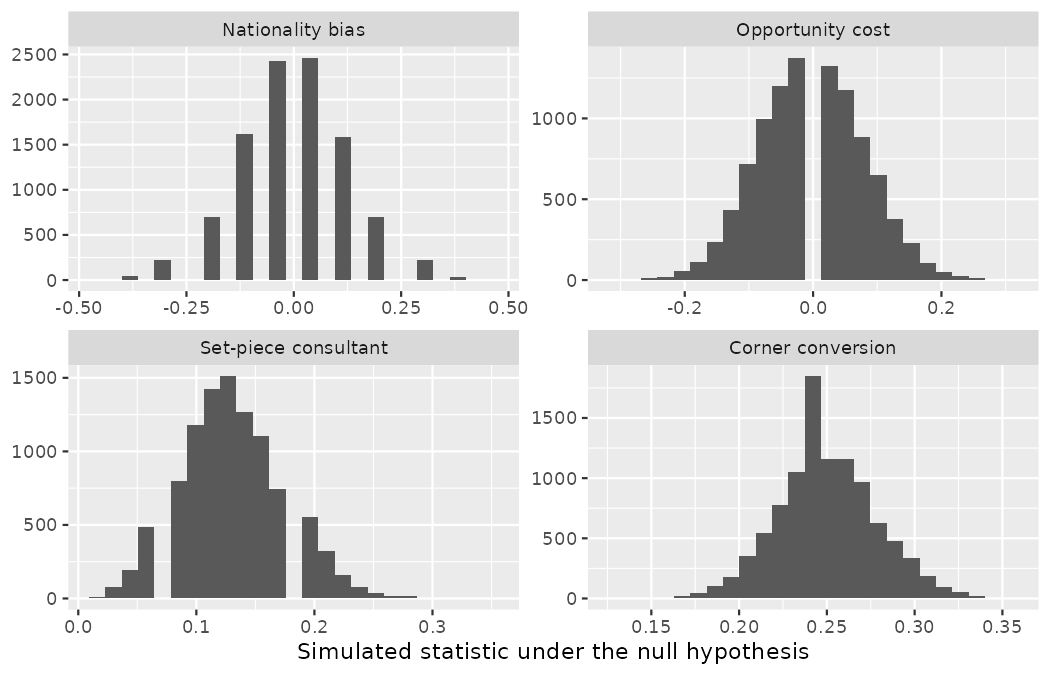
\includegraphics[width=0.85\linewidth,height=\textheight,keepaspectratio]{figures/foundations-mathematical-1.png}

The resulting figure (described here since you should always read a plot
before trusting it) shows four histograms, one per case study. The
nationality bias and opportunity cost panels are centered at 0 --- under
their null hypotheses the difference in proportions has no reason to
lean either way --- the consultant panel is centered at \(0.13,\) and
the corner panel at \(0.25:\) each center is exactly the value asserted
by that study's null hypothesis. The centers and spreads can be
confirmed numerically:

\begin{Shaded}
\begin{Highlighting}[]
\NormalTok{four\_nulls }\SpecialCharTok{|\textgreater{}}
  \FunctionTok{group\_by}\NormalTok{(case) }\SpecialCharTok{|\textgreater{}}
  \FunctionTok{summarize}\NormalTok{(}\AttributeTok{center =} \FunctionTok{mean}\NormalTok{(stat), }\AttributeTok{spread =} \FunctionTok{sd}\NormalTok{(stat))}
\CommentTok{\#\textgreater{} \# A tibble: 4 × 3}
\CommentTok{\#\textgreater{}   case                    center spread}
\CommentTok{\#\textgreater{}   \textless{}fct\textgreater{}                    \textless{}dbl\textgreater{}  \textless{}dbl\textgreater{}}
\CommentTok{\#\textgreater{} 1 Nationality bias     {-}0.000633 0.130}
\CommentTok{\#\textgreater{} 2 Opportunity cost     {-}0.0024   0.0782}
\CommentTok{\#\textgreater{} 3 Set{-}piece consultant  0.130    0.0432}
\CommentTok{\#\textgreater{} 4 Corner conversion     0.250    0.0287}
\end{Highlighting}
\end{Shaded}

\begin{tcolorbox}[enhanced jigsaw, left=2mm, leftrule=.75mm, title=\textcolor{quarto-callout-tip-color}{\faLightbulb}\hspace{0.5em}{Check your understanding}, arc=.35mm, rightrule=.15mm, coltitle=black, colframe=quarto-callout-tip-color-frame, bottomrule=.15mm, colbacktitle=quarto-callout-tip-color!10!white, opacitybacktitle=0.6, breakable, bottomtitle=1mm, toptitle=1mm, titlerule=0mm, opacityback=0, toprule=.15mm, colback=white]

Describe the shape of the distributions and note anything that you find
interesting.

\begin{center}\rule{0.5\linewidth}{0.5pt}\end{center}

In general, the distributions are reasonably symmetric. The case study
for the set-piece consultant is the only distribution with any evident
skew: with just 63 shots, its histogram is visibly granular (the
simulated proportion can only move in steps of \(1/63\)) and leans
right.

\end{tcolorbox}

The case study for the set-piece consultant is the only distribution
with any evident skew. As we observed in Chapter~\ref{sec-data-hello},
it's common for distributions to be skewed or contain outliers. However,
the null distributions we have so far encountered have all looked
somewhat similar and, for the most part, symmetric. They all resemble a
bell-shaped curve. The bell-shaped curve similarity is not a
coincidence, but rather, is guaranteed by mathematical theory.

\begin{tcolorbox}[enhanced jigsaw, left=2mm, leftrule=.75mm, title=\textcolor{quarto-callout-important-color}{\faExclamation}\hspace{0.5em}{Central Limit Theorem for proportions}, arc=.35mm, rightrule=.15mm, coltitle=black, colframe=quarto-callout-important-color-frame, bottomrule=.15mm, colbacktitle=quarto-callout-important-color!10!white, opacitybacktitle=0.6, breakable, bottomtitle=1mm, toptitle=1mm, titlerule=0mm, opacityback=0, toprule=.15mm, colback=white]

If we look at a proportion (or difference in proportions) and the
scenario satisfies certain conditions, then the sample proportion (or
difference in proportions) will appear to follow a bell-shaped curve
called the \emph{normal distribution}.

\end{tcolorbox}

An example of a perfect normal distribution is drawn in
Section~\ref{sec-normalDist}. Imagine laying a normal curve over each of
the four null distributions plotted above. While the mean (center) and
standard deviation (width or spread) may change for each plot, the
general shape remains roughly intact.

Mathematical theory guarantees that if repeated samples are taken a
sample proportion or a difference in sample proportions will follow
something that resembles a normal distribution when certain conditions
are met. (Note: we typically only take \textbf{one} sample --- Emil
Sørensen's network files one set of reports, a tournament happens once
--- but the mathematical model lets us know what to expect if we
\emph{had} taken repeated samples.) These conditions fall into two
general categories describing the independence between observations and
the need to take a sufficiently large sample size.

\begin{enumerate}
\def\labelenumi{\arabic{enumi}.}
\item
  Observations in the sample are \textbf{independent}. Independence is
  guaranteed when we take a random sample from a population.
  Independence can also be guaranteed if we randomly divide individuals
  into treatment and control groups --- as Priya Rao did with the 48
  dossiers.
\item
  The sample is \textbf{large enough}. The sample size cannot be too
  small. What qualifies as ``small'' differs from one context to the
  next, and we'll provide suitable guidelines for proportions in
  Chapter~\ref{sec-inference-one-prop}.
\end{enumerate}

So far we have had no need for the normal distribution. We've been able
to answer our questions somewhat easily using simulation techniques.
However, soon this will change. Simulating data can be non-trivial. For
example, some of the scenarios encountered in
Chapter~\ref{sec-model-mlr}, where we modeled chance quality with
multiple predictors at once, would require complex simulations in order
to make inferential conclusions. Instead, the normal distribution and
other distributions like it offer a general framework for statistical
inference that applies to a very large number of settings.

\begin{tcolorbox}[enhanced jigsaw, left=2mm, leftrule=.75mm, title=\textcolor{quarto-callout-important-color}{\faExclamation}\hspace{0.5em}{Technical conditions}, arc=.35mm, rightrule=.15mm, coltitle=black, colframe=quarto-callout-important-color-frame, bottomrule=.15mm, colbacktitle=quarto-callout-important-color!10!white, opacitybacktitle=0.6, breakable, bottomtitle=1mm, toptitle=1mm, titlerule=0mm, opacityback=0, toprule=.15mm, colback=white]

In order for the normal approximation to describe the sampling
distribution of the sample proportion as it varies from sample to
sample, two conditions must hold. If these conditions do not hold, it is
unwise to use the normal distribution (and related concepts like Z
scores, probabilities from the normal curve, etc.) for inferential
analyses.

\begin{enumerate}
\def\labelenumi{\arabic{enumi}.}
\tightlist
\item
  \textbf{Independent observations}
\item
  \textbf{Large enough sample:} For proportions, at least 10 expected
  successes and 10 expected failures in the sample.
\end{enumerate}

\end{tcolorbox}

\begin{tcolorbox}[enhanced jigsaw, left=2mm, leftrule=.75mm, title=\textcolor{quarto-callout-tip-color}{\faLightbulb}\hspace{0.5em}{Check your understanding}, arc=.35mm, rightrule=.15mm, coltitle=black, colframe=quarto-callout-tip-color-frame, bottomrule=.15mm, colbacktitle=quarto-callout-tip-color!10!white, opacitybacktitle=0.6, breakable, bottomtitle=1mm, toptitle=1mm, titlerule=0mm, opacityback=0, toprule=.15mm, colback=white]

Put the ``large enough'' condition to work on one of our own four cases.
The set-piece consultant's case rests on England's 63 shots, and its
null hypothesis asserts the tournament baseline rate
\(p_0 = 195/1494 = 0.1305.\) Compute the expected number of successes,
\(n \cdot p_0,\) and the expected number of failures,
\(n \cdot (1 - p_0),\) and say whether the condition holds.

\begin{center}\rule{0.5\linewidth}{0.5pt}\end{center}

The expected number of goals is
\(n \cdot p_0 = 63 \times 0.1305 = 8.2,\) and the expected number of
non-goals is \(n \cdot (1 - p_0) = 63 \times 0.8695 = 54.8.\) The
failures clear 10 comfortably, but the expected successes do not
\((8.2 < 10),\) so the condition fails: the normal model should not be
trusted for this case. File that away --- the consultant's case returns
in Section~\ref{sec-casemed}, where ignoring this check turns out to
change the verdict.

\end{tcolorbox}

\section{Normal Distribution}\label{sec-normalDist}

Among all the distributions we see in statistics, one is overwhelmingly
the most common. The symmetric, unimodal, bell curve is ubiquitous
throughout statistics. It is so common that people know it as a variety
of names including the \textbf{normal curve}, \textbf{normal model}, or
\textbf{normal distribution}.\footnote{It is also introduced as the
  Gaussian distribution after Carl Friedrich Gauss, the first person to
  formalize its mathematical expression.} Under certain conditions,
sample proportions, sample means, and sample differences can be modeled
using the normal distribution. Additionally, some variables --- the
physical-testing metrics logged on Jonas Beck's academy testing days, or
the number of shots a team attempts in a match --- closely follow the
normal distribution.

\begin{tcolorbox}[enhanced jigsaw, left=2mm, leftrule=.75mm, title=\textcolor{quarto-callout-important-color}{\faExclamation}\hspace{0.5em}{Normal distribution facts}, arc=.35mm, rightrule=.15mm, coltitle=black, colframe=quarto-callout-important-color-frame, bottomrule=.15mm, colbacktitle=quarto-callout-important-color!10!white, opacitybacktitle=0.6, breakable, bottomtitle=1mm, toptitle=1mm, titlerule=0mm, opacityback=0, toprule=.15mm, colback=white]

Distributions of many variables are nearly normal, but none are exactly
normal. Thus, the normal distribution, while not perfect for any single
problem, is very useful for a variety of problems.

\end{tcolorbox}

In this section, we will discuss the normal distribution in the context
of data to become familiar with normal distribution techniques. In the
following sections and beyond, we'll move our discussion to focus on
applying the normal distribution and other related distributions to
model point estimates for hypothesis tests and for constructing
confidence intervals.

\subsection{Normal distribution model}\label{normal-distribution-model}

The normal distribution always describes a symmetric, unimodal,
bell-shaped curve. However, normal curves can look different depending
on the details of the model. Specifically, the normal model can be
adjusted using two parameters: mean and standard deviation. As you can
probably guess, changing the mean shifts the bell curve to the left or
right, while changing the standard deviation stretches or constricts the
curve. The code below plots two normal curves on the same axis: the
normal distribution with mean \(0\) and standard deviation \(1\) (which
is commonly referred to as the \textbf{standard normal distribution}),
and a normal distribution with mean \(12\) and standard deviation
\(5.5\) --- a model we will soon meet as a description of team shot
counts.

\begin{Shaded}
\begin{Highlighting}[]
\FunctionTok{ggplot}\NormalTok{() }\SpecialCharTok{+}
  \FunctionTok{geom\_function}\NormalTok{(}\AttributeTok{fun =}\NormalTok{ dnorm, }\AttributeTok{args =} \FunctionTok{list}\NormalTok{(}\AttributeTok{mean =} \DecValTok{0}\NormalTok{, }\AttributeTok{sd =} \DecValTok{1}\NormalTok{)) }\SpecialCharTok{+}
  \FunctionTok{geom\_function}\NormalTok{(}\AttributeTok{fun =}\NormalTok{ dnorm, }\AttributeTok{args =} \FunctionTok{list}\NormalTok{(}\AttributeTok{mean =} \DecValTok{12}\NormalTok{, }\AttributeTok{sd =} \FloatTok{5.5}\NormalTok{),}
                \AttributeTok{linetype =} \StringTok{"dashed"}\NormalTok{) }\SpecialCharTok{+}
  \FunctionTok{xlim}\NormalTok{(}\SpecialCharTok{{-}}\DecValTok{4}\NormalTok{, }\DecValTok{30}\NormalTok{) }\SpecialCharTok{+}
  \FunctionTok{labs}\NormalTok{(}\AttributeTok{x =} \ConstantTok{NULL}\NormalTok{, }\AttributeTok{y =} \ConstantTok{NULL}\NormalTok{)}
\end{Highlighting}
\end{Shaded}

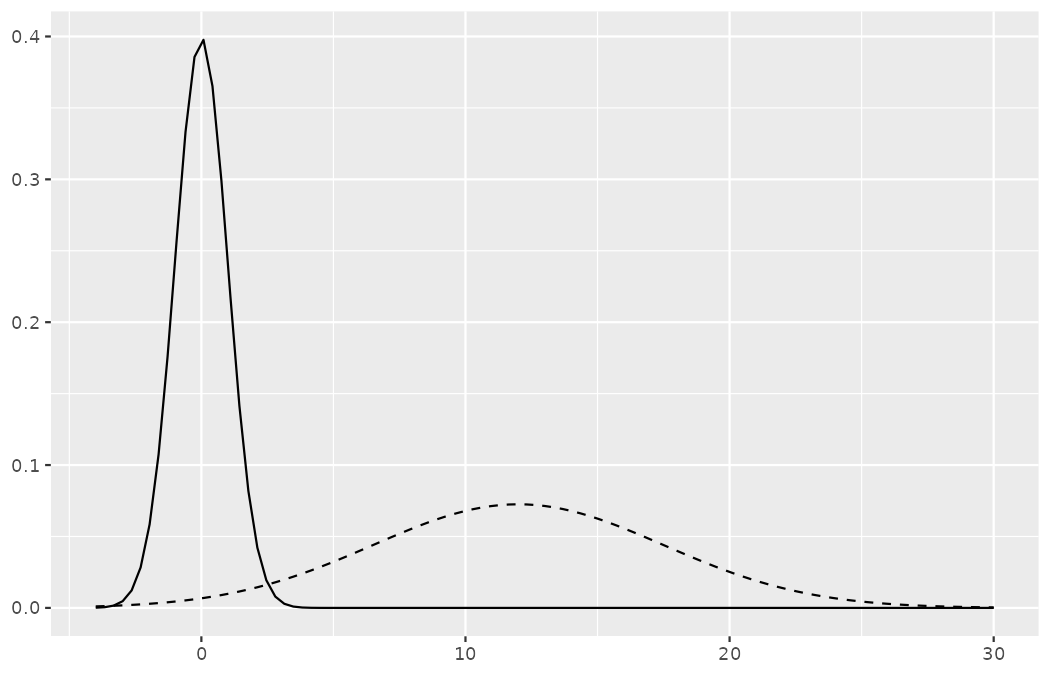
\includegraphics[width=0.85\linewidth,height=\textheight,keepaspectratio]{figures/foundations-mathematical-2.png}

In the resulting plot the solid curve is a tall, narrow bell centered at
0, essentially finished by \(\pm 3;\) the dashed curve is a much
flatter, wider bell centered at 12, stretching from roughly \(-4\) to
\(28.\) Both are perfectly symmetric about their centers.

If a normal distribution has mean \(\mu\) and standard deviation
\(\sigma,\) we may write the distribution as \(N(\mu, \sigma).\) This is
new notation, so take it apart piece by piece: the capital letter \(N\)
names the \emph{normal model}; inside the parentheses come its two
ingredients, first the mean \(\mu\) marking the center, then the
standard deviation \(\sigma\) marking the spread --- both symbols you
have carried since Chapter~\ref{sec-explore-numerical}, where they
denoted the population mean and population standard deviation. The two
distributions plotted above can be written as

\[ N(\mu = 0, \sigma = 1)\quad\text{and}\quad N(\mu = 12, \sigma = 5.5) \]

Because the mean and standard deviation describe a normal distribution
exactly, they are called the distribution's \textbf{parameters}.

\begin{tcolorbox}[enhanced jigsaw, left=2mm, leftrule=.75mm, title=\textcolor{quarto-callout-note-color}{\faInfo}\hspace{0.5em}{Worked example}, arc=.35mm, rightrule=.15mm, coltitle=black, colframe=quarto-callout-note-color-frame, bottomrule=.15mm, colbacktitle=quarto-callout-note-color!10!white, opacitybacktitle=0.6, breakable, bottomtitle=1mm, toptitle=1mm, titlerule=0mm, opacityback=0, toprule=.15mm, colback=white]

Write down the short-hand for a normal distribution with the following
parameters.

\begin{enumerate}
\def\labelenumi{\alph{enumi}.}
\tightlist
\item
  mean 5 and standard deviation 3
\item
  mean -100 and standard deviation 10
\item
  mean 2 and standard deviation 9
\end{enumerate}

\begin{center}\rule{0.5\linewidth}{0.5pt}\end{center}

\begin{enumerate}
\def\labelenumi{\alph{enumi}.}
\tightlist
\item
  \(N(\mu = 5,\sigma = 3)\)
\item
  \(N(\mu = -100, \sigma = 10)\)
\item
  \(N(\mu = 2, \sigma = 9)\)
\end{enumerate}

\end{tcolorbox}

\subsection{Standardizing with Z
scores}\label{standardizing-with-z-scores}

\begin{tcolorbox}[enhanced jigsaw, left=2mm, leftrule=.75mm, title=\textcolor{quarto-callout-note-color}{\faInfo}\hspace{0.5em}{Worked example}, arc=.35mm, rightrule=.15mm, coltitle=black, colframe=quarto-callout-note-color-frame, bottomrule=.15mm, colbacktitle=quarto-callout-note-color!10!white, opacitybacktitle=0.6, breakable, bottomtitle=1mm, toptitle=1mm, titlerule=0mm, opacityback=0, toprule=.15mm, colback=white]

Jonas Beck's academy keeps an archive of trial-battery benchmarks ---
the physical tests every trialist completes on a testing day (a
constructed set of standards the club has used for years). In that
archive, 30-meter sprint times follow a nearly normal distribution with
a mean of 4.40 seconds and a standard deviation of 0.15 seconds. Running
jump-and-reach scores --- the height gained above standing reach from a
short run-up --- also follow a nearly normal distribution, with mean 58
cm and standard deviation 6 cm. Suppose trialist Ade runs the 30 meters
in 4.25 seconds and trialist Bruno posts a jump-and-reach of 61.6 cm.
Who performed better relative to their peers?

\begin{center}\rule{0.5\linewidth}{0.5pt}\end{center}

We use the standard deviation as a guide. Ade is 1 standard deviation
\emph{faster} than average: \(4.40 - 0.15 = 4.25.\) Bruno is 0.6
standard deviations above the mean jump: \(58 + 0.6 \times 6 = 61.6.\)
Mind the direction: for sprint times, \emph{lower} is better, so being a
full standard deviation below the mean is the standout performance. Ade
did better compared to other trialists than Bruno did.

\end{tcolorbox}

The code below draws the two benchmark distributions, simulating a large
number of observations from each model (the seed only fixes the drawing
of the illustration).

\begin{Shaded}
\begin{Highlighting}[]
\FunctionTok{set.seed}\NormalTok{(}\DecValTok{1301}\NormalTok{)}
\NormalTok{combine }\OtherTok{\textless{}{-}} \FunctionTok{tibble}\NormalTok{(}
  \AttributeTok{value =} \FunctionTok{c}\NormalTok{(}\FunctionTok{rnorm}\NormalTok{(}\DecValTok{100000}\NormalTok{, }\AttributeTok{mean =} \FloatTok{4.40}\NormalTok{, }\AttributeTok{sd =} \FloatTok{0.15}\NormalTok{),}
            \FunctionTok{rnorm}\NormalTok{(}\DecValTok{100000}\NormalTok{, }\AttributeTok{mean =} \DecValTok{58}\NormalTok{, }\AttributeTok{sd =} \DecValTok{6}\NormalTok{)),}
  \AttributeTok{test  =} \FunctionTok{rep}\NormalTok{(}\FunctionTok{c}\NormalTok{(}\StringTok{"30m sprint (seconds)"}\NormalTok{, }\StringTok{"Jump{-}and{-}reach (cm)"}\NormalTok{), }\AttributeTok{each =} \DecValTok{100000}\NormalTok{)}
\NormalTok{)}

\FunctionTok{ggplot}\NormalTok{(combine, }\FunctionTok{aes}\NormalTok{(}\AttributeTok{x =}\NormalTok{ value)) }\SpecialCharTok{+}
  \FunctionTok{geom\_histogram}\NormalTok{(}\AttributeTok{bins =} \DecValTok{60}\NormalTok{) }\SpecialCharTok{+}
  \FunctionTok{facet\_wrap}\NormalTok{(}\SpecialCharTok{\textasciitilde{}}\NormalTok{ test, }\AttributeTok{scales =} \StringTok{"free"}\NormalTok{) }\SpecialCharTok{+}
  \FunctionTok{labs}\NormalTok{(}\AttributeTok{x =} \ConstantTok{NULL}\NormalTok{, }\AttributeTok{y =} \ConstantTok{NULL}\NormalTok{)}
\end{Highlighting}
\end{Shaded}

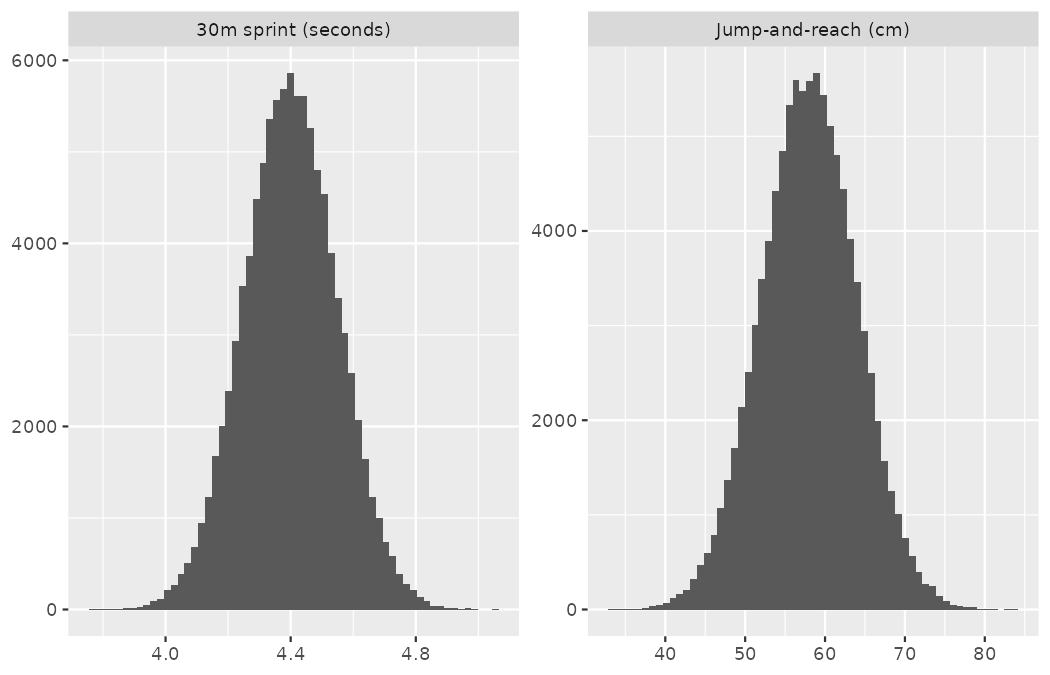
\includegraphics[width=0.85\linewidth,height=\textheight,keepaspectratio]{figures/foundations-mathematical-3.png}

The plot shows two bell-shaped histograms: the sprint panel centered at
4.40 with nearly all mass between 3.95 and 4.85, and the jump panel
centered at 58 with nearly all mass between 40 and 76. Ade's 4.25 sits
well into the left (fast) side of the first bell; Bruno's 61.6 sits
moderately into the right side of the second.

The solution to the previous example relies on a standardization
technique called a Z score, a method most commonly employed for nearly
normal observations (but that may be used with any distribution). The
\textbf{Z score} of an observation is defined as the number of standard
deviations it falls above or below the mean --- that is the whole
meaning of the capital letter \(Z,\) a symbol that will do heavy lifting
for the rest of this book. If the observation is one standard deviation
above the mean, its Z score is 1. If it is 1.5 standard deviations
\emph{below} the mean, then its Z score is -1.5. If \(x\) is an
observation from a distribution \(N(\mu, \sigma),\) we define the Z
score mathematically as

\[ Z = \frac{x-\mu}{\sigma} \]

Read the fraction as a recipe: the numerator \(x - \mu\) measures how
far the observation sits from the center, in the original units
(seconds, centimeters, shots); dividing by \(\sigma\) re-expresses that
distance in standard-deviation units. Using \(\mu_{jump}=58,\)
\(\sigma_{jump}=6,\) and \(x_{Bruno}=61.6,\) we find Bruno's Z score:

\[ Z_{Bruno} = \frac{x_{Bruno} - \mu_{jump}}{\sigma_{jump}} = \frac{61.6-58}{6} = 0.6 \]

\begin{tcolorbox}[enhanced jigsaw, left=2mm, leftrule=.75mm, title=\textcolor{quarto-callout-important-color}{\faExclamation}\hspace{0.5em}{The Z score}, arc=.35mm, rightrule=.15mm, coltitle=black, colframe=quarto-callout-important-color-frame, bottomrule=.15mm, colbacktitle=quarto-callout-important-color!10!white, opacitybacktitle=0.6, breakable, bottomtitle=1mm, toptitle=1mm, titlerule=0mm, opacityback=0, toprule=.15mm, colback=white]

The Z score of an observation is the number of standard deviations it
falls above or below the mean. We compute the Z score for an observation
\(x\) that follows a distribution with mean \(\mu\) and standard
deviation \(\sigma\) using

\[Z = \frac{x-\mu}{\sigma}\]

If the observation \(x\) comes from a \emph{normal} distribution
centered at \(\mu\) with standard deviation of \(\sigma\), then the Z
score will be distributed according to a \emph{normal} distribution with
a center of 0 and a standard deviation of 1. That is, the normality
remains when transforming from \(x\) to \(Z\) with a shift in both the
center as well as the spread.

\end{tcolorbox}

\begin{tcolorbox}[enhanced jigsaw, left=2mm, leftrule=.75mm, title=\textcolor{quarto-callout-tip-color}{\faLightbulb}\hspace{0.5em}{Check your understanding}, arc=.35mm, rightrule=.15mm, coltitle=black, colframe=quarto-callout-tip-color-frame, bottomrule=.15mm, colbacktitle=quarto-callout-tip-color!10!white, opacitybacktitle=0.6, breakable, bottomtitle=1mm, toptitle=1mm, titlerule=0mm, opacityback=0, toprule=.15mm, colback=white]

Use Ade's sprint time, 4.25 seconds, along with the sprint mean and
standard deviation to compute their Z score.

\begin{center}\rule{0.5\linewidth}{0.5pt}\end{center}

\(Z_{Ade} = \frac{x_{Ade} - \mu_{sprint}}{\sigma_{sprint}} = \frac{4.25 - 4.40}{0.15} = -1\)

\end{tcolorbox}

Observations above the mean always have positive Z scores while those
below the mean have negative Z scores. If an observation is equal to the
mean --- a trialist who jumps exactly 58 cm --- then the Z score is
\(0.\)

\begin{tcolorbox}[enhanced jigsaw, left=2mm, leftrule=.75mm, title=\textcolor{quarto-callout-note-color}{\faInfo}\hspace{0.5em}{Worked example}, arc=.35mm, rightrule=.15mm, coltitle=black, colframe=quarto-callout-note-color-frame, bottomrule=.15mm, colbacktitle=quarto-callout-note-color!10!white, opacitybacktitle=0.6, breakable, bottomtitle=1mm, toptitle=1mm, titlerule=0mm, opacityback=0, toprule=.15mm, colback=white]

Let \(X\) represent the expected goals Northbridge United accumulates in
a home match, which the analysis department models as
\(N(\mu=1.8, \sigma=0.6),\) and suppose we observe \(x=2.457\) in
Saturday's match. Find the Z score of \(x.\) Then, use the Z score to
determine how many standard deviations above or below the mean \(x\)
falls.

\begin{center}\rule{0.5\linewidth}{0.5pt}\end{center}

Its Z score is given by
\(Z = \frac{x-\mu}{\sigma} = \frac{2.457 - 1.8}{0.6} = 0.657/0.6 = 1.095.\)
The observation \(x\) is 1.095 standard deviations \emph{above} the
mean. We know it must be above the mean since \(Z\) is positive.

\end{tcolorbox}

\begin{tcolorbox}[enhanced jigsaw, left=2mm, leftrule=.75mm, title=\textcolor{quarto-callout-tip-color}{\faLightbulb}\hspace{0.5em}{Check your understanding}, arc=.35mm, rightrule=.15mm, coltitle=black, colframe=quarto-callout-tip-color-frame, bottomrule=.15mm, colbacktitle=quarto-callout-tip-color!10!white, opacitybacktitle=0.6, breakable, bottomtitle=1mm, toptitle=1mm, titlerule=0mm, opacityback=0, toprule=.15mm, colback=white]

In Northbridge's recruitment database, the heights of outfield prospects
follow a nearly normal distribution with mean 181 cm and standard
deviation 6.4 cm. Compute the Z scores for prospects with heights of 186
cm and 168.9 cm.

\begin{center}\rule{0.5\linewidth}{0.5pt}\end{center}

For \(x_1=186\) cm:
\(Z_1 = \frac{x_1 - \mu}{\sigma} = \frac{186 - 181}{6.4} = 0.78.\) For
\(x_2=168.9\) cm: \(Z_2 = \frac{168.9 - 181}{6.4} = -1.89.\)

\end{tcolorbox}

We can use Z scores to roughly identify which observations are more
unusual than others. One observation \(x_1\) is said to be more unusual
than another observation \(x_2\) if the absolute value of its Z score is
larger than the absolute value of the other observation's Z score:
\(|Z_1| > |Z_2|.\) This technique is especially insightful when a
distribution is symmetric.

\begin{tcolorbox}[enhanced jigsaw, left=2mm, leftrule=.75mm, title=\textcolor{quarto-callout-tip-color}{\faLightbulb}\hspace{0.5em}{Check your understanding}, arc=.35mm, rightrule=.15mm, coltitle=black, colframe=quarto-callout-tip-color-frame, bottomrule=.15mm, colbacktitle=quarto-callout-tip-color!10!white, opacitybacktitle=0.6, breakable, bottomtitle=1mm, toptitle=1mm, titlerule=0mm, opacityback=0, toprule=.15mm, colback=white]

Which of the two outfield prospects in the previous guided practice has
the more \emph{unusual} height?

\begin{center}\rule{0.5\linewidth}{0.5pt}\end{center}

Because the \emph{absolute value} of the Z score for the second prospect
is larger than that of the first, the second prospect (168.9 cm) has a
more unusual height.

\end{tcolorbox}

Z scores also let us compare across datasets measured on entirely
different scales --- including real tournament data. Which shot-volume
feat was more extreme: Lionel Messi's at the 2022 World Cup, or Klara
Bühl's at the 2025 Women's Euro?

\begin{Shaded}
\begin{Highlighting}[]
\NormalTok{weuro2025\_shots }\OtherTok{\textless{}{-}} \FunctionTok{read\_csv}\NormalTok{(}\StringTok{"data/derived/weuro2025\_shots.csv"}\NormalTok{)}

\NormalTok{wc\_players }\OtherTok{\textless{}{-}}\NormalTok{ wc2022\_shots }\SpecialCharTok{|\textgreater{}} \FunctionTok{count}\NormalTok{(player, }\AttributeTok{name =} \StringTok{"shots"}\NormalTok{)}
\NormalTok{weuro\_players }\OtherTok{\textless{}{-}}\NormalTok{ weuro2025\_shots }\SpecialCharTok{|\textgreater{}} \FunctionTok{count}\NormalTok{(player, }\AttributeTok{name =} \StringTok{"shots"}\NormalTok{)}

\NormalTok{wc\_players }\SpecialCharTok{|\textgreater{}} \FunctionTok{summarize}\NormalTok{(}\AttributeTok{players =} \FunctionTok{n}\NormalTok{(), }\AttributeTok{mean =} \FunctionTok{mean}\NormalTok{(shots), }\AttributeTok{sd =} \FunctionTok{sd}\NormalTok{(shots))}
\CommentTok{\#\textgreater{} \# A tibble: 1 × 3}
\CommentTok{\#\textgreater{}   players  mean    sd}
\CommentTok{\#\textgreater{}     \textless{}int\textgreater{} \textless{}dbl\textgreater{} \textless{}dbl\textgreater{}}
\CommentTok{\#\textgreater{} 1     432  3.46  3.51}

\NormalTok{weuro\_players }\SpecialCharTok{|\textgreater{}} \FunctionTok{summarize}\NormalTok{(}\AttributeTok{players =} \FunctionTok{n}\NormalTok{(), }\AttributeTok{mean =} \FunctionTok{mean}\NormalTok{(shots), }\AttributeTok{sd =} \FunctionTok{sd}\NormalTok{(shots))}
\CommentTok{\#\textgreater{} \# A tibble: 1 × 3}
\CommentTok{\#\textgreater{}   players  mean    sd}
\CommentTok{\#\textgreater{}     \textless{}int\textgreater{} \textless{}dbl\textgreater{} \textless{}dbl\textgreater{}}
\CommentTok{\#\textgreater{} 1     215  4.25  4.21}

\NormalTok{wc\_players }\SpecialCharTok{|\textgreater{}} \FunctionTok{slice\_max}\NormalTok{(shots, }\AttributeTok{n =} \DecValTok{1}\NormalTok{)}
\CommentTok{\#\textgreater{} \# A tibble: 1 × 2}
\CommentTok{\#\textgreater{}   player                         shots}
\CommentTok{\#\textgreater{}   \textless{}chr\textgreater{}                          \textless{}int\textgreater{}}
\CommentTok{\#\textgreater{} 1 Lionel Andrés Messi Cuccittini    34}

\NormalTok{weuro\_players }\SpecialCharTok{|\textgreater{}} \FunctionTok{slice\_max}\NormalTok{(shots, }\AttributeTok{n =} \DecValTok{1}\NormalTok{)}
\CommentTok{\#\textgreater{} \# A tibble: 1 × 2}
\CommentTok{\#\textgreater{}   player     shots}
\CommentTok{\#\textgreater{}   \textless{}chr\textgreater{}      \textless{}int\textgreater{}}
\CommentTok{\#\textgreater{} 1 Klara Bühl    25}
\end{Highlighting}
\end{Shaded}

Messi's 34 shots sit at \(Z = (34 - 3.46)/3.51 = 8.70\) within the World
Cup's per-player shot counts; Bühl's 25 sit at
\(Z = (25 - 4.25)/4.21 = 4.93\) within the Euro's. By the \(|Z|\)
comparison, Messi's shot volume is the more extreme relative to his
tournament. One caution before you file that away: per-player shot
counts are heavily right-skewed (recall the log transform they needed in
Chapter~\ref{sec-explore-numerical}), so while \(|Z|\) remains a fair
yardstick for ``how far from typical'', you must \emph{not} convert
these Z scores to percentiles with the normal curve --- the technique of
the next section is reserved for variables that are at least nearly
normal.

\subsection{Normal probability
calculations}\label{normal-probability-calculations}

\begin{tcolorbox}[enhanced jigsaw, left=2mm, leftrule=.75mm, title=\textcolor{quarto-callout-note-color}{\faInfo}\hspace{0.5em}{Worked example}, arc=.35mm, rightrule=.15mm, coltitle=black, colframe=quarto-callout-note-color-frame, bottomrule=.15mm, colbacktitle=quarto-callout-note-color!10!white, opacitybacktitle=0.6, breakable, bottomtitle=1mm, toptitle=1mm, titlerule=0mm, opacityback=0, toprule=.15mm, colback=white]

Bruno, the trialist from the testing day, jumped 61.6 cm with a
corresponding \(Z=0.6.\) Jonas Beck would like to know what percentile
Bruno falls in among all trialists in the archive.

\begin{center}\rule{0.5\linewidth}{0.5pt}\end{center}

Bruno's \textbf{percentile} is the percentage of trialists who jumped
lower than Bruno. The total area under the normal curve is always equal
to 1, and the proportion of trialists who jumped below Bruno equals the
\emph{area} under the \(N(58, 6)\) curve to the left of 61.6:

\begin{Shaded}
\begin{Highlighting}[]
\FunctionTok{pnorm}\NormalTok{(}\FloatTok{0.6}\NormalTok{, }\AttributeTok{mean =} \DecValTok{0}\NormalTok{, }\AttributeTok{sd =} \DecValTok{1}\NormalTok{)}
\CommentTok{\#\textgreater{} [1] 0.7257469}
\end{Highlighting}
\end{Shaded}

Bruno is in the \(73^{rd}\) percentile of trialists at the testing day.

\end{tcolorbox}

We can use the normal model to find percentiles or probabilities. A
\textbf{normal probability table}, which lists Z scores and
corresponding percentiles, can be used to identify a percentile based on
the Z score (and vice versa). Statistical software can also be used.

Normal probabilities are most commonly found using statistical software
which we will show here using R. We use the software to identify the
percentile corresponding to any particular Z score. For instance, the
percentile of \(Z=0.43\) is 0.6664, or the \(66.64^{th}\) percentile.
The \texttt{pnorm()} function is available in default R and will provide
the percentile associated with any cutoff on a normal curve.

\begin{Shaded}
\begin{Highlighting}[]
\FunctionTok{pnorm}\NormalTok{(}\FloatTok{0.43}\NormalTok{, }\AttributeTok{mean =} \DecValTok{0}\NormalTok{, }\AttributeTok{sd =} \DecValTok{1}\NormalTok{)}
\CommentTok{\#\textgreater{} [1] 0.6664022}
\end{Highlighting}
\end{Shaded}

We can also find the Z score associated with a percentile. For example,
to identify Z for the \(80^{th}\) percentile, we use \texttt{qnorm()}
which identifies the \textbf{quantile} for a given percentage. The
quantile represents the cutoff value. (To remember the function
\texttt{qnorm()} as providing a cutoff, notice that both
\texttt{qnorm()} and ``cutoff'' start with the sound ``kuh''. To
remember the \texttt{pnorm()} function as providing a probability from a
given cutoff, notice that both \texttt{pnorm()} and probability start
with the sound ``puh.'') We determine the Z score for the \(80^{th}\)
percentile using \texttt{qnorm()}: 0.84.

\begin{Shaded}
\begin{Highlighting}[]
\FunctionTok{qnorm}\NormalTok{(}\FloatTok{0.80}\NormalTok{, }\AttributeTok{mean =} \DecValTok{0}\NormalTok{, }\AttributeTok{sd =} \DecValTok{1}\NormalTok{)}
\CommentTok{\#\textgreater{} [1] 0.8416212}
\end{Highlighting}
\end{Shaded}

\begin{tcolorbox}[enhanced jigsaw, left=2mm, leftrule=.75mm, title=\textcolor{quarto-callout-tip-color}{\faLightbulb}\hspace{0.5em}{Check your understanding}, arc=.35mm, rightrule=.15mm, coltitle=black, colframe=quarto-callout-tip-color-frame, bottomrule=.15mm, colbacktitle=quarto-callout-tip-color!10!white, opacitybacktitle=0.6, breakable, bottomtitle=1mm, toptitle=1mm, titlerule=0mm, opacityback=0, toprule=.15mm, colback=white]

Determine the proportion of trialists who out-jumped Bruno at the
testing day.

\begin{center}\rule{0.5\linewidth}{0.5pt}\end{center}

If 73\% jumped lower than Bruno, the proportion who jumped higher must
be 27\%. (Generally ties are ignored when the normal model, or any other
continuous distribution, is used.)

\end{tcolorbox}

\subsection{Normal probability
examples}\label{normal-probability-examples}

Jump-and-reach scores in the academy's trial battery are approximated
well by a normal model, \(N(\mu=58, \sigma=6).\)

\begin{tcolorbox}[enhanced jigsaw, left=2mm, leftrule=.75mm, title=\textcolor{quarto-callout-note-color}{\faInfo}\hspace{0.5em}{Worked example}, arc=.35mm, rightrule=.15mm, coltitle=black, colframe=quarto-callout-note-color-frame, bottomrule=.15mm, colbacktitle=quarto-callout-note-color!10!white, opacitybacktitle=0.6, breakable, bottomtitle=1mm, toptitle=1mm, titlerule=0mm, opacityback=0, toprule=.15mm, colback=white]

Shauna is the next randomly called trialist, and nothing is known about
Shauna's spring. What is the probability that Shauna jumps at least 60.6
cm?

\begin{center}\rule{0.5\linewidth}{0.5pt}\end{center}

First, always draw and label a picture of the normal distribution.
(Drawings need not be exact to be useful.) We are interested in the
chance of a jump above 60.6, so we shade the upper tail.

The \(x\)-axis identifies the mean and the values at 2 standard
deviations above and below the mean. The simplest way to find the shaded
area under the curve makes use of the Z score of the cutoff value. With
\(\mu=58,\) \(\sigma=6,\) and the cutoff value \(x=60.6,\) the Z score
is computed as

\[ Z = \frac{x - \mu}{\sigma} = \frac{60.6 - 58}{6} = \frac{2.6}{6} = 0.43 \]

We use software to find the percentile of \(Z=0.43,\) which yields
0.6664. However, the percentile describes those who had a Z score
\emph{lower} than 0.43. To find the area \emph{above} \(Z=0.43,\) we
compute one minus the area of the lower tail:

\begin{Shaded}
\begin{Highlighting}[]
\DecValTok{1} \SpecialCharTok{{-}} \FunctionTok{pnorm}\NormalTok{(}\FloatTok{0.43}\NormalTok{, }\AttributeTok{mean =} \DecValTok{0}\NormalTok{, }\AttributeTok{sd =} \DecValTok{1}\NormalTok{)}
\CommentTok{\#\textgreater{} [1] 0.3335978}
\end{Highlighting}
\end{Shaded}

The probability Shauna jumps at least 60.6 cm is 0.3336.

\end{tcolorbox}

\begin{tcolorbox}[enhanced jigsaw, left=2mm, leftrule=.75mm, title=\textcolor{quarto-callout-important-color}{\faExclamation}\hspace{0.5em}{Always draw a picture first, and find the Z score second}, arc=.35mm, rightrule=.15mm, coltitle=black, colframe=quarto-callout-important-color-frame, bottomrule=.15mm, colbacktitle=quarto-callout-important-color!10!white, opacitybacktitle=0.6, breakable, bottomtitle=1mm, toptitle=1mm, titlerule=0mm, opacityback=0, toprule=.15mm, colback=white]

For any normal probability situation, \emph{always always always} draw
and label the normal curve and shade the area of interest first. The
picture will provide an estimate of the probability.

After drawing a figure to represent the situation, identify the Z score
for the observation of interest.

\end{tcolorbox}

\begin{tcolorbox}[enhanced jigsaw, left=2mm, leftrule=.75mm, title=\textcolor{quarto-callout-tip-color}{\faLightbulb}\hspace{0.5em}{Check your understanding}, arc=.35mm, rightrule=.15mm, coltitle=black, colframe=quarto-callout-tip-color-frame, bottomrule=.15mm, colbacktitle=quarto-callout-tip-color!10!white, opacitybacktitle=0.6, breakable, bottomtitle=1mm, toptitle=1mm, titlerule=0mm, opacityback=0, toprule=.15mm, colback=white]

If the probability of Shauna jumping at least 60.6 cm is 0.3336, then
what is the probability of a jump below 60.6 cm? Draw the normal curve
representing this exercise, shading the lower region instead of the
upper one.

\begin{center}\rule{0.5\linewidth}{0.5pt}\end{center}

The probability is \(1 - 0.3336 = 0.6664.\) The picture is the same bell
with the \emph{lower} region shaded.

\end{tcolorbox}

\begin{tcolorbox}[enhanced jigsaw, left=2mm, leftrule=.75mm, title=\textcolor{quarto-callout-note-color}{\faInfo}\hspace{0.5em}{Worked example}, arc=.35mm, rightrule=.15mm, coltitle=black, colframe=quarto-callout-note-color-frame, bottomrule=.15mm, colbacktitle=quarto-callout-note-color!10!white, opacitybacktitle=0.6, breakable, bottomtitle=1mm, toptitle=1mm, titlerule=0mm, opacityback=0, toprule=.15mm, colback=white]

Edu jumped 56 cm at the testing day. What is their percentile?

\begin{center}\rule{0.5\linewidth}{0.5pt}\end{center}

First, a picture is needed: the bell centered at 58 with the area left
of 56 shaded. Edu's percentile is the proportion of trialists who do not
jump as high as 56 cm. The mean \(\mu=58,\) the standard deviation
\(\sigma=6,\) and the cutoff for the tail area \(x=56\) are used to
compute the Z score:

\[ Z = \frac{x - \mu}{\sigma} = \frac{56 - 58}{6} = -0.33\]

Statistical software can be used to find the proportion of the
\(N(0,1)\) curve to the left of \(-0.33\) which is 0.3707. Edu is at the
\(37^{th}\) percentile.

\end{tcolorbox}

\begin{tcolorbox}[enhanced jigsaw, left=2mm, leftrule=.75mm, title=\textcolor{quarto-callout-note-color}{\faInfo}\hspace{0.5em}{Worked example}, arc=.35mm, rightrule=.15mm, coltitle=black, colframe=quarto-callout-note-color-frame, bottomrule=.15mm, colbacktitle=quarto-callout-note-color!10!white, opacitybacktitle=0.6, breakable, bottomtitle=1mm, toptitle=1mm, titlerule=0mm, opacityback=0, toprule=.15mm, colback=white]

Use the results of the previous example to compute the proportion of
trialists who jumped higher than Edu. Also draw a new picture.

\begin{center}\rule{0.5\linewidth}{0.5pt}\end{center}

If Edu out-jumped 37\% of trialists, then about 63\% must have jumped
higher --- the same bell with the \emph{upper} region beyond 56 cm
shaded.

\end{tcolorbox}

\begin{tcolorbox}[enhanced jigsaw, left=2mm, leftrule=.75mm, title=\textcolor{quarto-callout-important-color}{\faExclamation}\hspace{0.5em}{Areas to the right}, arc=.35mm, rightrule=.15mm, coltitle=black, colframe=quarto-callout-important-color-frame, bottomrule=.15mm, colbacktitle=quarto-callout-important-color!10!white, opacitybacktitle=0.6, breakable, bottomtitle=1mm, toptitle=1mm, titlerule=0mm, opacityback=0, toprule=.15mm, colback=white]

Most statistical software, as well as normal probability tables in most
books, give the area to the left. If you would like the area to the
right, first find the area to the left and then subtract the amount from
one.

\end{tcolorbox}

\begin{tcolorbox}[enhanced jigsaw, left=2mm, leftrule=.75mm, title=\textcolor{quarto-callout-tip-color}{\faLightbulb}\hspace{0.5em}{Check your understanding}, arc=.35mm, rightrule=.15mm, coltitle=black, colframe=quarto-callout-tip-color-frame, bottomrule=.15mm, colbacktitle=quarto-callout-tip-color!10!white, opacitybacktitle=0.6, breakable, bottomtitle=1mm, toptitle=1mm, titlerule=0mm, opacityback=0, toprule=.15mm, colback=white]

Tessa jumped 70 cm at the testing day. Draw a picture for each part. (a)
What is their percentile? (b) What percent of trialists jumped higher
than Tessa?

\begin{center}\rule{0.5\linewidth}{0.5pt}\end{center}

Tessa's Z score is \((70 - 58)/6 = 2.\) Numerical answers: (a) 0.9772.
(b) 0.0228.

\end{tcolorbox}

Let us now move from the constructed testing day to real tournament
data. In Chapter~\ref{sec-explore-numerical} we built the
\texttt{team\_match} data --- one row per team per match at the 2022
World Cup --- and we rebuild it here with the same code:

\begin{Shaded}
\begin{Highlighting}[]
\NormalTok{team\_match }\OtherTok{\textless{}{-}}\NormalTok{ wc2022\_shots }\SpecialCharTok{|\textgreater{}}
  \FunctionTok{group\_by}\NormalTok{(match\_id, team) }\SpecialCharTok{|\textgreater{}}
  \FunctionTok{summarize}\NormalTok{(}
    \AttributeTok{n\_shots =} \FunctionTok{n}\NormalTok{(),}
    \AttributeTok{total\_xg =} \FunctionTok{sum}\NormalTok{(statsbomb\_xg),}
    \AttributeTok{goals =} \FunctionTok{sum}\NormalTok{(goal),}
    \AttributeTok{prop\_under\_pressure =} \FunctionTok{mean}\NormalTok{(under\_pressure),}
    \AttributeTok{prop\_set\_piece =} \FunctionTok{mean}\NormalTok{(play\_pattern }\SpecialCharTok{\%in\%}
      \FunctionTok{c}\NormalTok{(}\StringTok{"From Corner"}\NormalTok{, }\StringTok{"From Free Kick"}\NormalTok{, }\StringTok{"From Throw In"}\NormalTok{)),}
    \AttributeTok{.groups =} \StringTok{"drop"}
\NormalTok{  )}

\NormalTok{team\_match }\SpecialCharTok{|\textgreater{}}
  \FunctionTok{summarize}\NormalTok{(}\AttributeTok{mean =} \FunctionTok{mean}\NormalTok{(n\_shots), }\AttributeTok{sd =} \FunctionTok{sd}\NormalTok{(n\_shots),}
            \AttributeTok{min =} \FunctionTok{min}\NormalTok{(n\_shots), }\AttributeTok{max =} \FunctionTok{max}\NormalTok{(n\_shots))}
\CommentTok{\#\textgreater{} \# A tibble: 1 × 4}
\CommentTok{\#\textgreater{}    mean    sd   min   max}
\CommentTok{\#\textgreater{}   \textless{}dbl\textgreater{} \textless{}dbl\textgreater{} \textless{}int\textgreater{} \textless{}int\textgreater{}}
\CommentTok{\#\textgreater{} 1  11.8  5.55     2    31}
\end{Highlighting}
\end{Shaded}

(Recall the 127 rows: Costa Rica's shotless team-match against Spain has
no row.) Before applying any normal model, check the shape:

\begin{Shaded}
\begin{Highlighting}[]
\FunctionTok{ggplot}\NormalTok{(team\_match, }\FunctionTok{aes}\NormalTok{(}\AttributeTok{x =}\NormalTok{ n\_shots)) }\SpecialCharTok{+}
  \FunctionTok{geom\_histogram}\NormalTok{(}\AttributeTok{binwidth =} \DecValTok{2}\NormalTok{) }\SpecialCharTok{+}
  \FunctionTok{labs}\NormalTok{(}\AttributeTok{x =} \StringTok{"Shots in a team{-}match, 2022 World Cup"}\NormalTok{, }\AttributeTok{y =} \StringTok{"Count"}\NormalTok{)}
\end{Highlighting}
\end{Shaded}

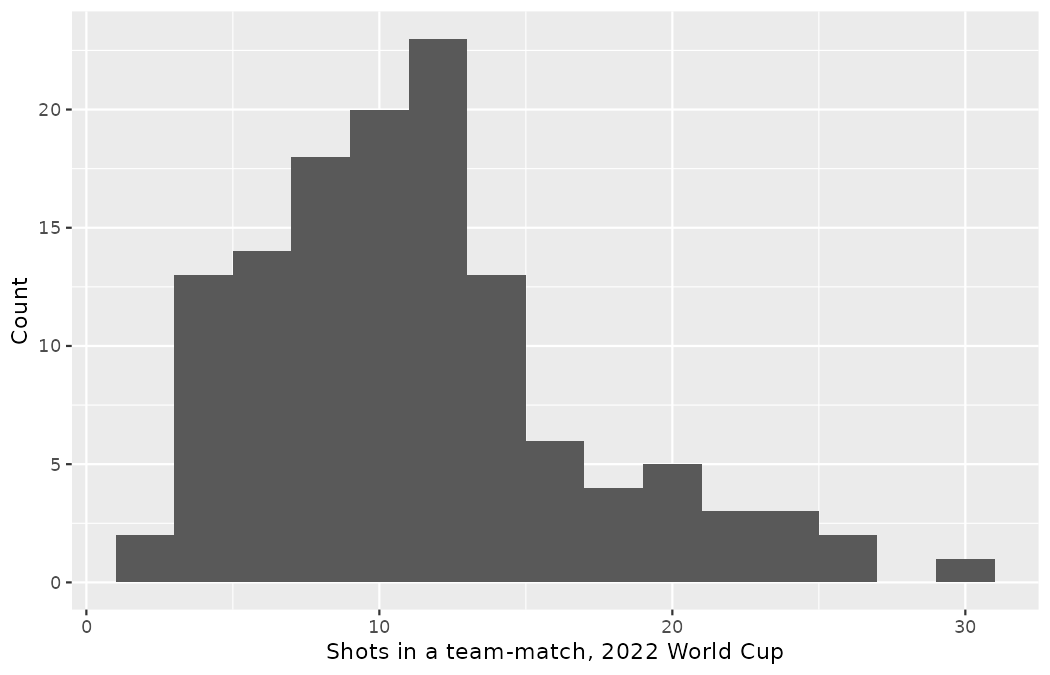
\includegraphics[width=0.85\linewidth,height=\textheight,keepaspectratio]{figures/foundations-mathematical-4.png}

The histogram is unimodal with its peak around 8--12 shots, falls away
on both sides, and carries a mild right skew --- a modest tail of
high-volume performances runs out to Germany's 31 shots against Costa
Rica. It is not perfectly normal (few things are, per the \emph{Normal
distribution facts} box), but it is close enough for the normal model
\(N(\mu = 11.76, \sigma = 5.55)\) to serve as a useful approximation.

\begin{tcolorbox}[enhanced jigsaw, left=2mm, leftrule=.75mm, title=\textcolor{quarto-callout-note-color}{\faInfo}\hspace{0.5em}{Worked example}, arc=.35mm, rightrule=.15mm, coltitle=black, colframe=quarto-callout-note-color-frame, bottomrule=.15mm, colbacktitle=quarto-callout-note-color!10!white, opacitybacktitle=0.6, breakable, bottomtitle=1mm, toptitle=1mm, titlerule=0mm, opacityback=0, toprule=.15mm, colback=white]

Marta Vidal reads a match report: an upcoming opponent attempted 20
shots in a group-stage match. Using the normal approximation, what
percentile of World Cup team-match shot volumes is that? And where would
a timid 8-shot team-match fall?

\begin{center}\rule{0.5\linewidth}{0.5pt}\end{center}

Draw the bell centered at 11.76 first; 20 sits well to the right, 8
moderately to the left. With software we can supply the mean and
standard deviation directly:

\begin{Shaded}
\begin{Highlighting}[]
\FunctionTok{pnorm}\NormalTok{(}\DecValTok{20}\NormalTok{, }\AttributeTok{mean =} \FloatTok{11.76}\NormalTok{, }\AttributeTok{sd =} \FloatTok{5.55}\NormalTok{)}
\CommentTok{\#\textgreater{} [1] 0.9311863}

\FunctionTok{pnorm}\NormalTok{(}\DecValTok{8}\NormalTok{, }\AttributeTok{mean =} \FloatTok{11.76}\NormalTok{, }\AttributeTok{sd =} \FloatTok{5.55}\NormalTok{)}
\CommentTok{\#\textgreater{} [1] 0.2490515}
\end{Highlighting}
\end{Shaded}

A 20-shot performance sits at about the \(93^{rd}\) percentile of
team-matches; an 8-shot outing at about the \(25^{th}.\)

\end{tcolorbox}

The last several problems have focused on finding the probability or
percentile for a particular observation. What if you would like to know
the observation corresponding to a particular percentile?

\begin{tcolorbox}[enhanced jigsaw, left=2mm, leftrule=.75mm, title=\textcolor{quarto-callout-note-color}{\faInfo}\hspace{0.5em}{Worked example}, arc=.35mm, rightrule=.15mm, coltitle=black, colframe=quarto-callout-note-color-frame, bottomrule=.15mm, colbacktitle=quarto-callout-note-color!10!white, opacitybacktitle=0.6, breakable, bottomtitle=1mm, toptitle=1mm, titlerule=0mm, opacityback=0, toprule=.15mm, colback=white]

A team-match sits at the \(40^{th}\) percentile of shot volume. How many
shots is that?

\begin{center}\rule{0.5\linewidth}{0.5pt}\end{center}

As always, first draw the picture: the lower tail probability (0.40) is
known and shaded. We can find the observation in two different ways. If
you have access to software that allows you to specify the mean and
standard deviation of the normal curve, you can calculate the observed
value directly:

\begin{Shaded}
\begin{Highlighting}[]
\FunctionTok{qnorm}\NormalTok{(}\FloatTok{0.40}\NormalTok{, }\AttributeTok{mean =} \FloatTok{11.76}\NormalTok{, }\AttributeTok{sd =} \FloatTok{5.55}\NormalTok{)}
\CommentTok{\#\textgreater{} [1] 10.35392}
\end{Highlighting}
\end{Shaded}

The \(40^{th}\)-percentile team-match attempts about 10.4 shots --- call
it 10, since shots come in whole numbers.

Without access to flexible software, you will need the information given
by the standard normal curve. First, determine the Z score associated
with the \(40^{th}\) percentile. Because the percentile is below 50\%,
we know \(Z\) will be negative:

\begin{Shaded}
\begin{Highlighting}[]
\FunctionTok{qnorm}\NormalTok{(}\FloatTok{0.40}\NormalTok{, }\AttributeTok{mean =} \DecValTok{0}\NormalTok{, }\AttributeTok{sd =} \DecValTok{1}\NormalTok{)}
\CommentTok{\#\textgreater{} [1] {-}0.2533471}
\end{Highlighting}
\end{Shaded}

Knowing \(Z=-0.253\) and the parameters \(\mu=11.76\) and
\(\sigma=5.55,\) the Z score formula can be set up to determine the
unknown shot count \(x\):

\[ -0.253 = Z = \frac{x - \mu}{\sigma} = \frac{x - 11.76}{5.55} \]

Solving for \(x\) yields \(11.76 - 0.253 \times 5.55 = 10.4\) shots,
matching the direct calculation.

\end{tcolorbox}

\begin{tcolorbox}[enhanced jigsaw, left=2mm, leftrule=.75mm, title=\textcolor{quarto-callout-note-color}{\faInfo}\hspace{0.5em}{Worked example}, arc=.35mm, rightrule=.15mm, coltitle=black, colframe=quarto-callout-note-color-frame, bottomrule=.15mm, colbacktitle=quarto-callout-note-color!10!white, opacitybacktitle=0.6, breakable, bottomtitle=1mm, toptitle=1mm, titlerule=0mm, opacityback=0, toprule=.15mm, colback=white]

What is the team-match shot volume at the \(82^{nd}\) percentile?

\begin{center}\rule{0.5\linewidth}{0.5pt}\end{center}

In order to practice using Z scores, we will use the standard normal
curve to solve the problem. Again, we draw the figure first: 82\% shaded
below the cutoff, 18\% above. And calculate the Z value associated with
the \(82^{nd}\) percentile:

\begin{Shaded}
\begin{Highlighting}[]
\FunctionTok{qnorm}\NormalTok{(}\FloatTok{0.82}\NormalTok{, }\AttributeTok{mean =} \DecValTok{0}\NormalTok{, }\AttributeTok{sd =} \DecValTok{1}\NormalTok{)}
\CommentTok{\#\textgreater{} [1] 0.9153651}
\end{Highlighting}
\end{Shaded}

The \(82^{nd}\) percentile corresponds to \(Z=0.92,\) a positive value
(because the percentile is bigger than 50\%). Finally, the shot count
\(x\) is found using the Z score formula with the known mean \(\mu,\)
standard deviation \(\sigma,\) and Z score \(Z=0.92\):

\[ 0.92 = Z = \frac{x-\mu}{\sigma} = \frac{x - 11.76}{5.55} \]

This yields \(11.76 + 0.92 \times 5.55 = 16.9,\) or about 17 shots as
the volume at the \(82^{nd}\) percentile --- confirmed by
\texttt{qnorm(0.82,\ mean\ =\ 11.76,\ sd\ =\ 5.55)}, which returns
16.84.

\end{tcolorbox}

\begin{tcolorbox}[enhanced jigsaw, left=2mm, leftrule=.75mm, title=\textcolor{quarto-callout-tip-color}{\faLightbulb}\hspace{0.5em}{Check your understanding}, arc=.35mm, rightrule=.15mm, coltitle=black, colframe=quarto-callout-tip-color-frame, bottomrule=.15mm, colbacktitle=quarto-callout-tip-color!10!white, opacitybacktitle=0.6, breakable, bottomtitle=1mm, toptitle=1mm, titlerule=0mm, opacityback=0, toprule=.15mm, colback=white]

Using Z scores, answer the following questions.

\begin{enumerate}
\def\labelenumi{(\alph{enumi})}
\tightlist
\item
  What is the \(95^{th}\) percentile for jump-and-reach scores in the
  trial battery?\\
\item
  What is the \(97.5^{th}\) percentile of team-match shot volumes? As
  always with normal probability problems, first draw a picture.
\end{enumerate}

\begin{center}\rule{0.5\linewidth}{0.5pt}\end{center}

Remember: draw a picture first, then find the Z score. (a) The
\(95^{th}\) percentile corresponds to \(Z_{95} = 1.65\)
(\texttt{qnorm(0.95)} returns 1.645). Knowing \(Z_{95}=1.65,\)
\(\mu = 58,\) and \(\sigma = 6,\) we set up the Z score formula:
\(1.65 = \frac{x_{95} - 58}{6}.\) We solve for \(x_{95}\):
\(x_{95} = 67.9\) cm. (b) Similarly, we find \(Z_{97.5} = 1.96,\) again
set up the Z score formula for the shot counts, and calculate
\(x_{97.5} = 11.76 + 1.96 \times 5.55 = 22.6\) --- about 23 shots.
(\texttt{qnorm(0.975,\ mean\ =\ 11.76,\ sd\ =\ 5.55)} returns 22.64.)

\end{tcolorbox}

\begin{tcolorbox}[enhanced jigsaw, left=2mm, leftrule=.75mm, title=\textcolor{quarto-callout-tip-color}{\faLightbulb}\hspace{0.5em}{Check your understanding}, arc=.35mm, rightrule=.15mm, coltitle=black, colframe=quarto-callout-tip-color-frame, bottomrule=.15mm, colbacktitle=quarto-callout-tip-color!10!white, opacitybacktitle=0.6, breakable, bottomtitle=1mm, toptitle=1mm, titlerule=0mm, opacityback=0, toprule=.15mm, colback=white]

Using Z scores, answer the following questions about team-match shot
volumes.

\begin{enumerate}
\def\labelenumi{(\alph{enumi})}
\tightlist
\item
  What is the probability that a randomly selected team-match features
  at least 18 shots?\\
\item
  What is the probability that a team-match features fewer than 9 shots?
\end{enumerate}

\begin{center}\rule{0.5\linewidth}{0.5pt}\end{center}

Numerical answers, from
\texttt{1\ -\ pnorm(18,\ mean\ =\ 11.76,\ sd\ =\ 5.55)} and
\texttt{pnorm(9,\ mean\ =\ 11.76,\ sd\ =\ 5.55)}: (a) 0.1304. (b)
0.3095.

\end{tcolorbox}

\begin{tcolorbox}[enhanced jigsaw, left=2mm, leftrule=.75mm, title=\textcolor{quarto-callout-note-color}{\faInfo}\hspace{0.5em}{Worked example}, arc=.35mm, rightrule=.15mm, coltitle=black, colframe=quarto-callout-note-color-frame, bottomrule=.15mm, colbacktitle=quarto-callout-note-color!10!white, opacitybacktitle=0.6, breakable, bottomtitle=1mm, toptitle=1mm, titlerule=0mm, opacityback=0, toprule=.15mm, colback=white]

What is the probability that a randomly selected team-match features
between 9 and 18 shots?

\begin{center}\rule{0.5\linewidth}{0.5pt}\end{center}

First, draw the figure. The area of interest is no longer an upper or
lower tail: it is the middle of the bell. The total area under the curve
is 1. If we find the area of the two tails that are not shaded (from the
previous Check your understanding, these areas are \(0.3095\) and
\(0.1304\)), then we can find the middle area:

\[1.0000 - 0.3095 - 0.1304 = 0.5601\]

That is, the probability of a team-match with between 9 and 18 shots is
0.5601. And because here we have the entire population of 127 real
team-matches, we can audit the model:

\begin{Shaded}
\begin{Highlighting}[]
\NormalTok{team\_match }\SpecialCharTok{|\textgreater{}}
  \FunctionTok{summarize}\NormalTok{(}\AttributeTok{prop\_9\_to\_18 =} \FunctionTok{mean}\NormalTok{(n\_shots }\SpecialCharTok{\textgreater{}=} \DecValTok{9} \SpecialCharTok{\&}\NormalTok{ n\_shots }\SpecialCharTok{\textless{}} \DecValTok{18}\NormalTok{))}
\CommentTok{\#\textgreater{} \# A tibble: 1 × 1}
\CommentTok{\#\textgreater{}   prop\_9\_to\_18}
\CommentTok{\#\textgreater{}          \textless{}dbl\textgreater{}}
\CommentTok{\#\textgreater{} 1        0.559}
\end{Highlighting}
\end{Shaded}

The observed proportion, 0.559, agrees with the normal model's 0.560 to
two decimal places --- the approximation is earning its keep.

\end{tcolorbox}

\begin{tcolorbox}[enhanced jigsaw, left=2mm, leftrule=.75mm, title=\textcolor{quarto-callout-tip-color}{\faLightbulb}\hspace{0.5em}{Check your understanding}, arc=.35mm, rightrule=.15mm, coltitle=black, colframe=quarto-callout-tip-color-frame, bottomrule=.15mm, colbacktitle=quarto-callout-tip-color!10!white, opacitybacktitle=0.6, breakable, bottomtitle=1mm, toptitle=1mm, titlerule=0mm, opacityback=0, toprule=.15mm, colback=white]

What percent of testing-day trialists jump between 58 and 66 cm?

\begin{center}\rule{0.5\linewidth}{0.5pt}\end{center}

This is an abbreviated solution. (Be sure to draw a figure!) First find
the percent below 58 and the percent above 66:
\(Z_{58} = 0.00 \to 0.5000\) (area below), \(Z_{66} = 1.33 \to 0.0918\)
(area above). Final answer: \(1.0000 - 0.5000 - 0.0918 = 0.4082,\) i.e.,
40.82\%.

\end{tcolorbox}

\begin{tcolorbox}[enhanced jigsaw, left=2mm, leftrule=.75mm, title=\textcolor{quarto-callout-tip-color}{\faLightbulb}\hspace{0.5em}{Check your understanding}, arc=.35mm, rightrule=.15mm, coltitle=black, colframe=quarto-callout-tip-color-frame, bottomrule=.15mm, colbacktitle=quarto-callout-tip-color!10!white, opacitybacktitle=0.6, breakable, bottomtitle=1mm, toptitle=1mm, titlerule=0mm, opacityback=0, toprule=.15mm, colback=white]

What percent of World Cup team-matches feature between 6 and 8 shots?

\begin{center}\rule{0.5\linewidth}{0.5pt}\end{center}

Another abbreviated solution --- but draw the figure, and notice that
this time both cutoffs sit on the \emph{same} side of the mean.
\(Z_{6} = (6 - 11.76)/5.55 = -1.04 \to 0.1492\) (area below 6), and
\(Z_{8} = (8 - 11.76)/5.55 = -0.68 \to 0.7517\) (area \emph{above} 8).
Final answer: \(1.0000 - 0.1492 - 0.7517 = 0.0991,\) i.e., about 9.9\%
of team-matches.

\end{tcolorbox}

\section{Quantifying the variability of a
statistic}\label{quantifying-the-variability-of-a-statistic}

As seen in later chapters, it turns out that many of the statistics used
to summarize data --- the sample proportion, the sample mean,
differences in two sample proportions, differences in two sample means,
even the sample slope of a linear model like the goals-on-chance-quality
line from Chapter~\ref{sec-model-slr} --- vary according to the normal
distribution seen above. The mathematical models are derived from the
normal theory, but even the computational methods (and the intuitive
thinking behind both approaches) use the general bell-shaped variability
seen in most of the distributions constructed so far.

\subsection{68-95-99.7 rule}\label{rule}

Here, we present a useful general rule for the probability of falling
within 1, 2, and 3 standard deviations of the mean in the normal
distribution. The rule will be useful in a wide range of practical
settings, especially when trying to make a quick estimate without a
calculator or Z table --- say, when a colleague quotes a team's shot
count in the middle of a meeting and you want to know how unusual it is
before the discussion moves on. The code below draws the rule.

\begin{Shaded}
\begin{Highlighting}[]
\FunctionTok{ggplot}\NormalTok{(}\FunctionTok{data.frame}\NormalTok{(}\AttributeTok{x =} \FunctionTok{c}\NormalTok{(}\SpecialCharTok{{-}}\FloatTok{3.5}\NormalTok{, }\FloatTok{3.5}\NormalTok{)), }\FunctionTok{aes}\NormalTok{(}\AttributeTok{x =}\NormalTok{ x)) }\SpecialCharTok{+}
  \FunctionTok{geom\_function}\NormalTok{(}\AttributeTok{fun =}\NormalTok{ dnorm) }\SpecialCharTok{+}
  \FunctionTok{annotate}\NormalTok{(}\StringTok{"segment"}\NormalTok{, }\AttributeTok{x =} \SpecialCharTok{{-}}\DecValTok{1}\NormalTok{, }\AttributeTok{xend =} \DecValTok{1}\NormalTok{, }\AttributeTok{y =} \FloatTok{0.23}\NormalTok{, }\AttributeTok{yend =} \FloatTok{0.23}\NormalTok{,}
           \AttributeTok{arrow =} \FunctionTok{arrow}\NormalTok{(}\AttributeTok{ends =} \StringTok{"both"}\NormalTok{)) }\SpecialCharTok{+}
  \FunctionTok{annotate}\NormalTok{(}\StringTok{"text"}\NormalTok{, }\AttributeTok{x =} \DecValTok{0}\NormalTok{, }\AttributeTok{y =} \FloatTok{0.25}\NormalTok{, }\AttributeTok{label =} \StringTok{"68\%"}\NormalTok{) }\SpecialCharTok{+}
  \FunctionTok{annotate}\NormalTok{(}\StringTok{"segment"}\NormalTok{, }\AttributeTok{x =} \SpecialCharTok{{-}}\DecValTok{2}\NormalTok{, }\AttributeTok{xend =} \DecValTok{2}\NormalTok{, }\AttributeTok{y =} \FloatTok{0.12}\NormalTok{, }\AttributeTok{yend =} \FloatTok{0.12}\NormalTok{,}
           \AttributeTok{arrow =} \FunctionTok{arrow}\NormalTok{(}\AttributeTok{ends =} \StringTok{"both"}\NormalTok{)) }\SpecialCharTok{+}
  \FunctionTok{annotate}\NormalTok{(}\StringTok{"text"}\NormalTok{, }\AttributeTok{x =} \DecValTok{0}\NormalTok{, }\AttributeTok{y =} \FloatTok{0.14}\NormalTok{, }\AttributeTok{label =} \StringTok{"95\%"}\NormalTok{) }\SpecialCharTok{+}
  \FunctionTok{annotate}\NormalTok{(}\StringTok{"segment"}\NormalTok{, }\AttributeTok{x =} \SpecialCharTok{{-}}\DecValTok{3}\NormalTok{, }\AttributeTok{xend =} \DecValTok{3}\NormalTok{, }\AttributeTok{y =} \FloatTok{0.02}\NormalTok{, }\AttributeTok{yend =} \FloatTok{0.02}\NormalTok{,}
           \AttributeTok{arrow =} \FunctionTok{arrow}\NormalTok{(}\AttributeTok{ends =} \StringTok{"both"}\NormalTok{)) }\SpecialCharTok{+}
  \FunctionTok{annotate}\NormalTok{(}\StringTok{"text"}\NormalTok{, }\AttributeTok{x =} \DecValTok{0}\NormalTok{, }\AttributeTok{y =} \FloatTok{0.04}\NormalTok{, }\AttributeTok{label =} \StringTok{"99.7\%"}\NormalTok{) }\SpecialCharTok{+}
  \FunctionTok{scale\_x\_continuous}\NormalTok{(}\AttributeTok{breaks =} \SpecialCharTok{{-}}\DecValTok{3}\SpecialCharTok{:}\DecValTok{3}\NormalTok{) }\SpecialCharTok{+}
  \FunctionTok{labs}\NormalTok{(}\AttributeTok{x =} \StringTok{"Standard deviations from the mean"}\NormalTok{, }\AttributeTok{y =} \ConstantTok{NULL}\NormalTok{)}
\end{Highlighting}
\end{Shaded}

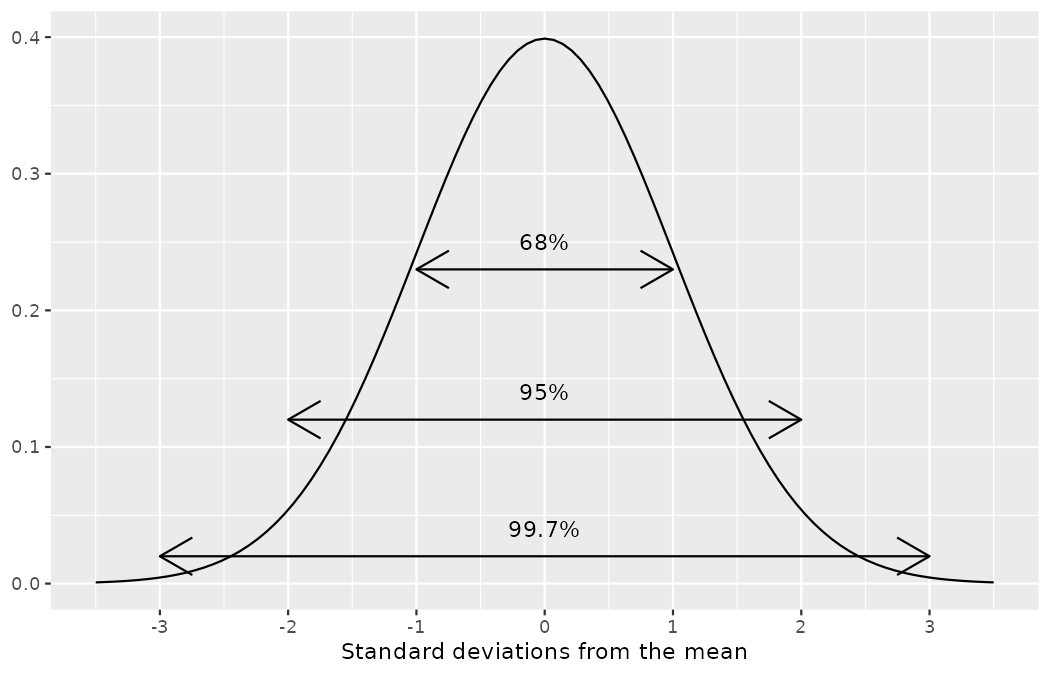
\includegraphics[width=0.85\linewidth,height=\textheight,keepaspectratio]{figures/foundations-mathematical-5.png}

The resulting figure is a standard normal curve with three nested
double-headed arrows: the innermost, from \(-1\) to \(1,\) is labeled
68\%; the middle, from \(-2\) to \(2,\) is labeled 95\%; the outermost,
from \(-3\) to \(3,\) is labeled 99.7\%. Those three percentages are
worth memorizing --- they are the quick mental model for every bell
curve you will meet.

\begin{tcolorbox}[enhanced jigsaw, left=2mm, leftrule=.75mm, title=\textcolor{quarto-callout-tip-color}{\faLightbulb}\hspace{0.5em}{Check your understanding}, arc=.35mm, rightrule=.15mm, coltitle=black, colframe=quarto-callout-tip-color-frame, bottomrule=.15mm, colbacktitle=quarto-callout-tip-color!10!white, opacitybacktitle=0.6, breakable, bottomtitle=1mm, toptitle=1mm, titlerule=0mm, opacityback=0, toprule=.15mm, colback=white]

Use \texttt{pnorm()} to confirm that about 68\%, 95\%, and 99.7\% of
observations fall within 1, 2, and 3 standard deviations of the mean in
the normal distribution, respectively. For instance, first find the area
that falls between \(Z=-1\) and \(Z=1,\) which should have an area of
about 0.68. Similarly there should be an area of about 0.95 between
\(Z=-2\) and \(Z=2.\)

\begin{center}\rule{0.5\linewidth}{0.5pt}\end{center}

First draw the pictures, then take differences of lower-tail areas:
\texttt{pnorm(1)\ -\ pnorm(-1)} returns 0.6827,
\texttt{pnorm(2)\ -\ pnorm(-2)} returns 0.9545, and
\texttt{pnorm(3)\ -\ pnorm(-3)} returns 0.9973.

\end{tcolorbox}

It is possible for a normal random variable to fall 4, 5, or even more
standard deviations from the mean. However, these occurrences are very
rare if the data are nearly normal. The probability of being further
than 4 standard deviations from the mean is about 1-in-30,000. For 5 and
6 standard deviations, it is about 1-in-3.5 million and 1-in-1 billion,
respectively. (This is why Messi's \(Z = 8.70\) for shot volume earlier
in the chapter should have set off an alarm: no genuinely normal
variable produces such a value, and indeed per-player shot counts are
nowhere near normal.)

\begin{tcolorbox}[enhanced jigsaw, left=2mm, leftrule=.75mm, title=\textcolor{quarto-callout-tip-color}{\faLightbulb}\hspace{0.5em}{Check your understanding}, arc=.35mm, rightrule=.15mm, coltitle=black, colframe=quarto-callout-tip-color-frame, bottomrule=.15mm, colbacktitle=quarto-callout-tip-color!10!white, opacitybacktitle=0.6, breakable, bottomtitle=1mm, toptitle=1mm, titlerule=0mm, opacityback=0, toprule=.15mm, colback=white]

Jump-and-reach scores in the academy's trial battery closely follow the
normal model with mean \(\mu = 58\) cm and standard deviation
\(\sigma = 6\) cm. About what percent of trialists jump between 46 and
70 cm? What percent jump between 58 and 70 cm?

\begin{center}\rule{0.5\linewidth}{0.5pt}\end{center}

46 cm and 70 cm represent two standard deviations below and above the
mean, which means about 95\% of trialists jump between 46 and 70 cm.
Since the normal model is symmetric, half of that central 95\%
\((\frac{95\%}{2} = 47.5\%\) of all trialists\()\) jump between 46 and
58 cm while 47.5\% jump between 58 and 70 cm.

\end{tcolorbox}

\subsection{Standard error}\label{sec-se}

Point estimates vary from sample to sample, and we quantify this
variability with what is called the \textbf{standard error (SE)}. The
name deserves a moment before the abbreviation takes over: \emph{error}
refers to the deviation of a statistic from the parameter it estimates
--- not a mistake --- and \emph{standard} is used exactly as in
\emph{standard deviation}. The standard error is equal to the standard
deviation associated with the statistic. So, for example, to quantify
the variability of a point estimate from one sample to the next, the
variability is called the standard error of the point estimate. Almost
always, the standard error is itself an estimate, calculated from the
sample of data.

You have, in fact, already met four standard errors in this chapter: the
spreads of the four null distributions computed in
Section~\ref{sec-CLTsection} --- 0.130 for the dossier audit, 0.078 for
the opportunity cost study, 0.043 for the set-piece consultant, and
0.029 for the corner claim --- are each the standard deviation of a
statistic, hence each a standard error.

The way we determine the standard error varies from one situation to the
next. However, typically it is determined using a formula based on the
Central Limit Theorem.

\subsection{Margin of error}\label{sec-moe}

Very related to the standard error is the \textbf{margin of error}. The
margin of error describes how far the \emph{statistic} typically strays
from the \emph{parameter} it estimates --- a statement about point
estimates, not about individual observations and their mean. For a 95\%
confidence level, the margin of error is approximately \(2 \times SE\)
(more precisely, \(1.96 \times SE\)). That is, with 95\% confidence, the
point estimate lies within \emph{one} margin of error of the parameter.

\begin{tcolorbox}[enhanced jigsaw, left=2mm, leftrule=.75mm, title=\textcolor{quarto-callout-important-color}{\faExclamation}\hspace{0.5em}{Margin of error for sample proportions}, arc=.35mm, rightrule=.15mm, coltitle=black, colframe=quarto-callout-important-color-frame, bottomrule=.15mm, colbacktitle=quarto-callout-important-color!10!white, opacitybacktitle=0.6, breakable, bottomtitle=1mm, toptitle=1mm, titlerule=0mm, opacityback=0, toprule=.15mm, colback=white]

The distance given by \(z^\star \times SE\) is called the \textbf{margin
of error}.

\(z^\star\) is the cutoff value found on the normal distribution. The
most common value of \(z^\star\) is 1.96 (often approximated to be 2)
indicating that the margin of error describes the variability associated
with 95\% of the sampled statistics.

\end{tcolorbox}

The symbol \(z^\star\) is new, so take it apart: the lowercase \(z\)
says it lives on the standard normal scale, like any Z score; the star
marks it as a \emph{chosen cutoff} --- fixed in advance to match a
stated confidence level --- rather than a value computed from data. For
95\%, the cutoff is \(z^\star = 1.96,\) because the area under the
\(N(0, 1)\) curve between \(-1.96\) and \(1.96\) is 0.95 (you will
confirm this shortly).

Notice that if the spread of the observations goes from some lower bound
to some upper bound, a rough approximation of the SE is to divide the
range by 4. Two versions of this eyeball rule coexist, so state which
span you read: the span of the \emph{bulk} of a bell-shaped distribution
(roughly its middle 95\%) covers about 4 standard errors, while the full
range of \emph{every} simulated value --- ``nearly all'' --- covers
about 6, since almost nothing falls more than three SEs from the center.
That is, if you notice the sample proportions go from 0.1 to 0.4, the SE
can be approximated to be 0.075.

\section{Case Study (test): Opportunity cost}\label{sec-caseopp}

The approach for using the normal model in the context of inference is
very similar to the practice of applying the model to individual
observations that are nearly normal. We will replace null distributions
we previously obtained using the randomization or simulation techniques
and verify the results once again using the normal model. When the
sample size is sufficiently large, the normal approximation generally
provides us with the same conclusions as the simulation model.

\subsection{Observed data}\label{observed-data-4}

In Section~\ref{sec-caseStudyOpportunityCost} we were introduced to the
opportunity cost study, in which scouts became more conservative with
the club's budget when the recommendation form reminded them that a fee
not spent now could be spent in the winter window. The observed
difference was \(\hat{p}_{T} - \hat{p}_{C} = 0.453 - 0.253 = 0.200,\)
and the 1,000-shuffle randomization test returned a p-value of
\(0.008.\) Let's re-analyze the data in the context of the normal
distribution and compare the results. The data, and the 10,000-shuffle
null distribution \texttt{budget150\_null}, were rebuilt with seeded
code at the start of this chapter --- this is a constructed Northbridge
scenario, and the code \emph{is} the data.

\subsection{Variability of the
statistic}\label{variability-of-the-statistic-4}

The best fitting normal distribution for the null distribution has a
mean of 0. We can calculate the standard error of this distribution by
borrowing a formula that we will become familiar with in
Chapter~\ref{sec-inference-two-props}, but for now let's simply read the
value off the simulation itself:

\begin{Shaded}
\begin{Highlighting}[]
\NormalTok{budget150\_se }\OtherTok{\textless{}{-}} \FunctionTok{sd}\NormalTok{(budget150\_null}\SpecialCharTok{$}\NormalTok{stat)}
\NormalTok{budget150\_se}
\CommentTok{\#\textgreater{} [1] 0.0782282}
\end{Highlighting}
\end{Shaded}

We take \(SE = 0.078.\) The code below overlays the normal curve
\(N(0, 0.078)\) on the 10,000 permuted differences.

\begin{Shaded}
\begin{Highlighting}[]
\FunctionTok{ggplot}\NormalTok{(budget150\_null, }\FunctionTok{aes}\NormalTok{(}\AttributeTok{x =}\NormalTok{ stat)) }\SpecialCharTok{+}
  \FunctionTok{geom\_histogram}\NormalTok{(}\FunctionTok{aes}\NormalTok{(}\AttributeTok{y =} \FunctionTok{after\_stat}\NormalTok{(density)), }\AttributeTok{binwidth =} \FloatTok{0.04}\NormalTok{) }\SpecialCharTok{+}
  \FunctionTok{geom\_function}\NormalTok{(}\AttributeTok{fun =}\NormalTok{ dnorm, }\AttributeTok{args =} \FunctionTok{list}\NormalTok{(}\AttributeTok{mean =} \DecValTok{0}\NormalTok{, }\AttributeTok{sd =}\NormalTok{ budget150\_se)) }\SpecialCharTok{+}
  \FunctionTok{annotate}\NormalTok{(}\StringTok{"segment"}\NormalTok{, }\AttributeTok{x =} \FloatTok{0.20}\NormalTok{, }\AttributeTok{xend =} \FloatTok{0.20}\NormalTok{, }\AttributeTok{y =} \DecValTok{0}\NormalTok{, }\AttributeTok{yend =} \DecValTok{4}\NormalTok{,}
           \AttributeTok{linetype =} \StringTok{"dashed"}\NormalTok{) }\SpecialCharTok{+}
  \FunctionTok{annotate}\NormalTok{(}\StringTok{"text"}\NormalTok{, }\AttributeTok{x =} \FloatTok{0.20}\NormalTok{, }\AttributeTok{y =} \FloatTok{4.5}\NormalTok{, }\AttributeTok{label =} \StringTok{"observed}\SpecialCharTok{\textbackslash{}n}\StringTok{difference"}\NormalTok{) }\SpecialCharTok{+}
  \FunctionTok{labs}\NormalTok{(}
    \AttributeTok{x =} \StringTok{"Difference in randomized proportions of scouts who}\SpecialCharTok{\textbackslash{}n}\StringTok{do not recommend the signing (treatment {-} control)"}\NormalTok{,}
    \AttributeTok{y =} \StringTok{"Density"}
\NormalTok{  )}
\end{Highlighting}
\end{Shaded}

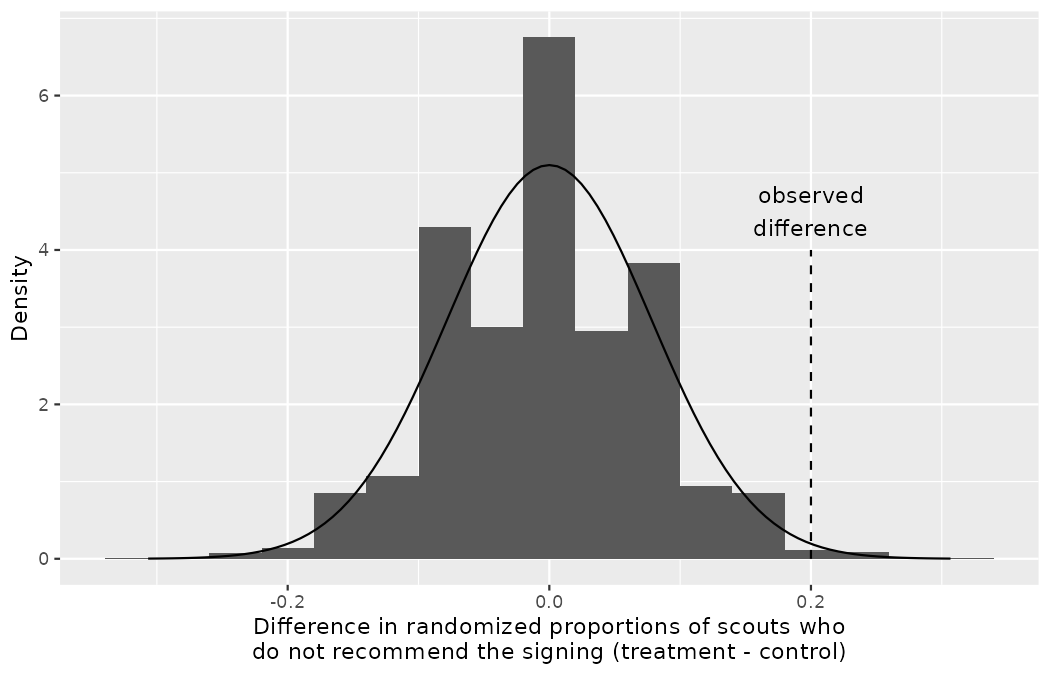
\includegraphics[width=0.85\linewidth,height=\textheight,keepaspectratio]{figures/foundations-mathematical-6.png}

The theoretical curve fits the histogram remarkably well: the shuffled
differences form a symmetric bell centered at 0, and the smooth normal
curve traces the tops of the bars with no visible mismatch. The observed
difference of \(0.20,\) marked by the dashed line, sits far out in the
right tail of both the histogram and the curve. Recall that the point
estimate of the difference was 0.20. Next, we'll use the normal
distribution approach to compute the p-value.

\subsection{Observed statistic vs.~null
statistics}\label{observed-statistic-vs.-null-statistics-2}

As we learned in Section~\ref{sec-normalDist}, it is helpful to draw and
shade a picture of the normal distribution so we know precisely what we
want to calculate. Here we want to find the area of the tail beyond 0.2,
representing the p-value: sketch the bell centered at 0 with standard
deviation 0.078, and shade everything to the right of 0.2.

Next, we can calculate the Z score using the observed difference, 0.20,
and the two model parameters. The standard error, \(SE = 0.078,\) is the
equivalent of the model's standard deviation.

\[Z = \frac{\text{observed difference} - 0}{SE} = \frac{0.20 - 0}{0.078} = 2.56\]

We can use statistical software to determine the right tail area, and
compare it against the tail of the simulation itself:

\begin{Shaded}
\begin{Highlighting}[]
\DecValTok{1} \SpecialCharTok{{-}} \FunctionTok{pnorm}\NormalTok{(}\FloatTok{2.56}\NormalTok{)}
\CommentTok{\#\textgreater{} [1] 0.005233608}

\NormalTok{budget150\_null }\SpecialCharTok{|\textgreater{}}
  \FunctionTok{summarize}\NormalTok{(}\AttributeTok{p\_sim =} \FunctionTok{mean}\NormalTok{(stat }\SpecialCharTok{\textgreater{}=} \FloatTok{0.20}\NormalTok{))}
\CommentTok{\#\textgreater{} \# A tibble: 1 × 1}
\CommentTok{\#\textgreater{}   p\_sim}
\CommentTok{\#\textgreater{}   \textless{}dbl\textgreater{}}
\CommentTok{\#\textgreater{} 1 0.0038}
\end{Highlighting}
\end{Shaded}

The normal model gives a p-value of \(0.0052,\) in close agreement with
the \(0.0038\) from these 10,000 shuffles and the \(0.008\) from the
1,000 shuffles in Section~\ref{sec-caseStudyOpportunityCost}. Using this
area as the p-value, we see that the p-value is less than 0.05: the
result is statistically discernible, and we conclude --- as before ---
that the winter-window reminder did indeed change the scouts'
recommendations.

\begin{tcolorbox}[enhanced jigsaw, left=2mm, leftrule=.75mm, title=\textcolor{quarto-callout-important-color}{\faExclamation}\hspace{0.5em}{Z score in a hypothesis test}, arc=.35mm, rightrule=.15mm, coltitle=black, colframe=quarto-callout-important-color-frame, bottomrule=.15mm, colbacktitle=quarto-callout-important-color!10!white, opacitybacktitle=0.6, breakable, bottomtitle=1mm, toptitle=1mm, titlerule=0mm, opacityback=0, toprule=.15mm, colback=white]

In the context of a hypothesis test, the Z score for a point estimate is

\[Z = \frac{\text{point estimate} - \text{null value}}{SE}\]

The standard error in this case is the equivalent of the standard
deviation of the point estimate, and the null value comes from the claim
made in the null hypothesis.

\end{tcolorbox}

Read the recipe the same way as every Z score in this chapter: the
numerator measures how far the point estimate sits from the value the
null hypothesis asserts, in the original units; dividing by the SE
re-expresses that distance in standard errors.

We have confirmed that the randomization approach we used earlier and
the normal distribution approach provide almost identical p-values and
conclusions in the opportunity cost case study. Next, let's turn our
attention to the set-piece consultant.

\section{Case study (test): Set-piece consultant}\label{sec-casemed}

\subsection{Observed data}\label{observed-data-5}

In Section~\ref{sec-case-study-med-consult} we learned about the
set-piece consultant who pointed to England's 2022 World Cup finishing
--- 13 goals from 63 shots, \(\hat{p} = 13/63 = 0.2063\) (recomputed
from the shot data at the start of this chapter) --- as proof that his
methods lift a team's conversion above the tournament baseline,
\(195/1494 = 0.1305.\) In that work we built an interval estimate; we
did not model a null scenario. The simulation method for a one
proportion null distribution is discussed fully in
Section~\ref{sec-one-prop-null-boot}, but we have already run it here:
\texttt{consultant\_null}, built at the start of this chapter, holds
10,000 simulated 63-shot campaigns in which every shot scores with
probability 0.1305.

One new piece of notation makes the null value explicit. We write
\(p_0\) --- read ``p-nought'' --- for the value of the population
proportion asserted by the null hypothesis: the letter \(p\) names a
population proportion as usual, and the subscript \(0\) is the same
nought that marks \(H_0.\) Here the hypotheses are
\(H_0: p = p_0 = 0.1305\) (England's true conversion under the
consultant is just the tournament baseline) against the consultant's
directional claim \(H_A: p > 0.1305.\)

The best-fitting normal curve for this null distribution has mean
\(0.1305,\) and its standard error can again be read off the simulation:

\begin{Shaded}
\begin{Highlighting}[]
\NormalTok{consultant\_se }\OtherTok{\textless{}{-}} \FunctionTok{sd}\NormalTok{(consultant\_null}\SpecialCharTok{$}\NormalTok{stat)}
\NormalTok{consultant\_se}
\CommentTok{\#\textgreater{} [1] 0.04320486}
\end{Highlighting}
\end{Shaded}

\subsection{Variability of the
statistic}\label{variability-of-the-statistic-5}

Before we begin, we want to point out a simple detail that is easy to
overlook: the null distribution we generated from the simulation is
slightly skewed, and the histogram is not particularly smooth. In fact,
the normal distribution only sort-of fits this model.

\begin{Shaded}
\begin{Highlighting}[]
\FunctionTok{ggplot}\NormalTok{(consultant\_null, }\FunctionTok{aes}\NormalTok{(}\AttributeTok{x =}\NormalTok{ stat)) }\SpecialCharTok{+}
  \FunctionTok{geom\_histogram}\NormalTok{(}\FunctionTok{aes}\NormalTok{(}\AttributeTok{y =} \FunctionTok{after\_stat}\NormalTok{(density)), }\AttributeTok{binwidth =} \DecValTok{1} \SpecialCharTok{/} \DecValTok{63}\NormalTok{) }\SpecialCharTok{+}
  \FunctionTok{geom\_function}\NormalTok{(}\AttributeTok{fun =}\NormalTok{ dnorm,}
                \AttributeTok{args =} \FunctionTok{list}\NormalTok{(}\AttributeTok{mean =}\NormalTok{ p\_0, }\AttributeTok{sd =}\NormalTok{ consultant\_se)) }\SpecialCharTok{+}
  \FunctionTok{annotate}\NormalTok{(}\StringTok{"segment"}\NormalTok{, }\AttributeTok{x =} \DecValTok{13} \SpecialCharTok{/} \DecValTok{63}\NormalTok{, }\AttributeTok{xend =} \DecValTok{13} \SpecialCharTok{/} \DecValTok{63}\NormalTok{, }\AttributeTok{y =} \DecValTok{0}\NormalTok{, }\AttributeTok{yend =} \DecValTok{8}\NormalTok{,}
           \AttributeTok{linetype =} \StringTok{"dashed"}\NormalTok{) }\SpecialCharTok{+}
  \FunctionTok{annotate}\NormalTok{(}\StringTok{"text"}\NormalTok{, }\AttributeTok{x =} \DecValTok{13} \SpecialCharTok{/} \DecValTok{63}\NormalTok{, }\AttributeTok{y =} \DecValTok{9}\NormalTok{, }\AttributeTok{label =} \StringTok{"observed}\SpecialCharTok{\textbackslash{}n}\StringTok{conversion"}\NormalTok{) }\SpecialCharTok{+}
  \FunctionTok{labs}\NormalTok{(}
    \AttributeTok{x =} \StringTok{"Simulated conversion rate from 63 shots when the null hypothesis is true"}\NormalTok{,}
    \AttributeTok{y =} \StringTok{"Density"}
\NormalTok{  )}
\end{Highlighting}
\end{Shaded}

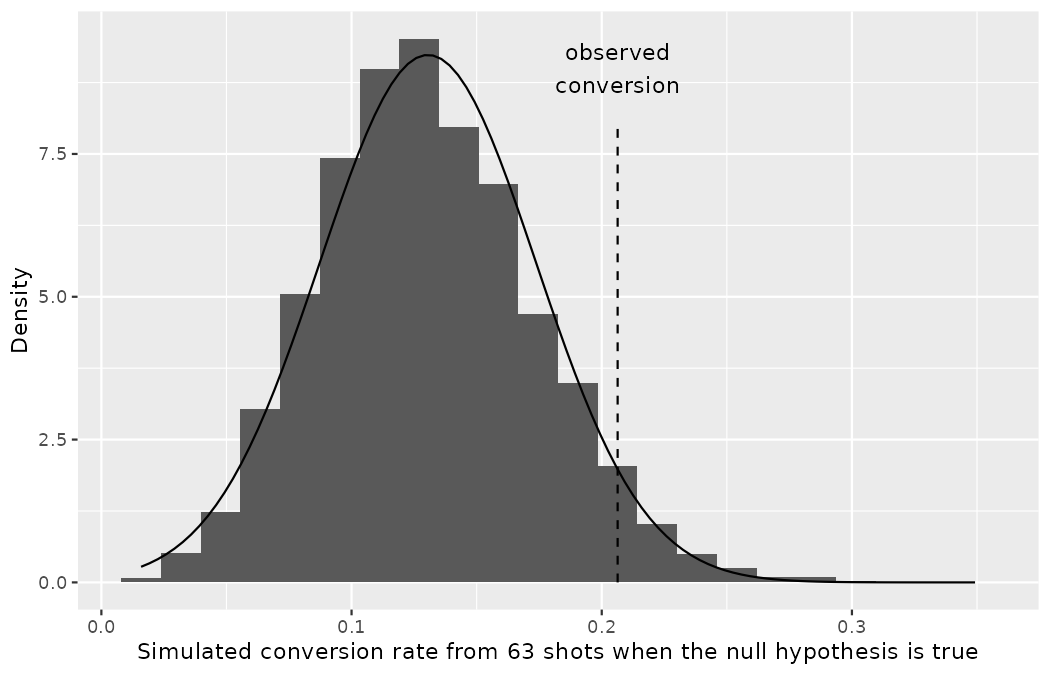
\includegraphics[width=0.85\linewidth,height=\textheight,keepaspectratio]{figures/foundations-mathematical-7.png}

Compare this figure with the opportunity cost overlay: the histogram
steps in visible increments of \(1/63,\) leans right, and the smooth
curve rides above some bars and below others. The observed conversion of
\(0.2063,\) marked by the dashed line, is toward the right tail of both
the histogram and the curve, but it is not an extreme value.

\subsection{Observed statistic vs.~null
statistics}\label{observed-statistic-vs.-null-statistics-3}

As always, we'll draw a picture before finding the normal probabilities:
a normal distribution centered at \(0.1305\) with a standard error of
\(0.043,\) with the area above \(0.2063\) shaded.

Next, we calculate the Z score using the observed conversion rate,
\(\hat{p} = 0.2063,\) along with the null value and the standard error
of the normal model:

\[Z = \frac{\hat{p} - p_0}{SE_{\hat{p}}} = \frac{0.2063 - 0.1305}{0.0432} = 1.76\]

\begin{Shaded}
\begin{Highlighting}[]
\NormalTok{z\_consultant }\OtherTok{\textless{}{-}}\NormalTok{ (}\DecValTok{13} \SpecialCharTok{/} \DecValTok{63} \SpecialCharTok{{-}}\NormalTok{ p\_0) }\SpecialCharTok{/}\NormalTok{ consultant\_se}
\NormalTok{z\_consultant}
\CommentTok{\#\textgreater{} [1] 1.75506}

\DecValTok{1} \SpecialCharTok{{-}} \FunctionTok{pnorm}\NormalTok{(z\_consultant)}
\CommentTok{\#\textgreater{} [1] 0.03962455}
\end{Highlighting}
\end{Shaded}

The normal model estimates the p-value --- the right tail area --- as
\(0.0396.\) There is a problem: the simulation itself disagrees.

\begin{Shaded}
\begin{Highlighting}[]
\NormalTok{consultant\_null }\SpecialCharTok{|\textgreater{}}
  \FunctionTok{summarize}\NormalTok{(}\AttributeTok{n\_extreme =} \FunctionTok{sum}\NormalTok{(stat }\SpecialCharTok{\textgreater{}=} \DecValTok{13} \SpecialCharTok{/} \DecValTok{63}\NormalTok{),}
            \AttributeTok{p\_sim =} \FunctionTok{mean}\NormalTok{(stat }\SpecialCharTok{\textgreater{}=} \DecValTok{13} \SpecialCharTok{/} \DecValTok{63}\NormalTok{))}
\CommentTok{\#\textgreater{} \# A tibble: 1 × 2}
\CommentTok{\#\textgreater{}   n\_extreme  p\_sim}
\CommentTok{\#\textgreater{}       \textless{}int\textgreater{}  \textless{}dbl\textgreater{}}
\CommentTok{\#\textgreater{} 1       638 0.0638}
\end{Highlighting}
\end{Shaded}

The simulation p-value is \(0.0638\) --- the normal approximation's
\(0.0396\) is almost 40\% smaller. And here the discrepancy is not
cosmetic: at the conventional discernibility level of \(\alpha = 0.05,\)
the normal shortcut \emph{rejects} \(H_0\) while the honest simulation
\emph{fails to reject}. An analyst who reached for the formula without
checking its conditions would have handed Marta Vidal statistically
discernible evidence for the consultant's claim that the simulation says
the data do not support.

The discrepancy is explained by the normal model's poor representation
of the null distribution. As noted earlier, the null distribution from
the simulations is not very smooth, and the distribution itself is
slightly skewed. That's the bad news. The good news is that we can
foresee these problems using some simple checks. We'll learn more about
these checks in the following chapters.

In Section~\ref{sec-CLTsection} we noted that the two common
requirements to apply the Central Limit Theorem are (1) the observations
in the sample must be independent, and (2) the sample must be
sufficiently large. The technical conditions box in that section made
``sufficiently large'' concrete for proportions: at least 10 expected
successes and 10 expected failures. Here the null hypothesis expects
\(63 \times 0.1305 = 8.2\) goals among England's 63 shots --- below 10
--- so the check fails, and it would have alerted us in advance that the
normal model is a poor approximation.

\subsection{Conditions for applying the normal
model}\label{conditions-for-applying-the-normal-model}

The success story in this section was the application of the normal
model in the context of the opportunity cost data. However, the biggest
lesson comes from the less successful attempt to use the normal
approximation in the set-piece consultant case study.

Statistical techniques are like the tools in a groundskeeper's shed.
When used responsibly, they can produce amazing and precise results.
However, if the tools are applied irresponsibly or under inappropriate
conditions, they will produce unreliable results. For this reason, with
every statistical method that we introduce in future chapters, we will
carefully outline conditions when the method can reasonably be used.
These conditions should be checked in each application of the technique
--- before the Z score, before the p-value, before the recommendation
lands on Marta's desk.

After covering the introductory topics in this course, advanced study
may lead to working with complex models which, for example, bring
together many variables with different variability structure. Working
with data that come from normal populations makes higher-order models
easier to estimate and interpret. There are times when simulation,
randomization, or bootstrapping are unwieldy in either structure or
computational demand. Normality can often lead to excellent
approximations of the data using straightforward modeling techniques.

\section{Case study (interval): The finishing
program}\label{sec-casestent}

A point estimate is our best guess for the value of the parameter, so it
makes sense to build the confidence interval around that value. The
standard error, which is a measure of the uncertainty associated with
the point estimate, provides a guide for how large we should make the
confidence interval. The 68-95-99.7 rule tells us that, in general, 95\%
of observations are within 2 standard errors of the mean. Here, we use
the value 1.96 to be slightly more precise.

\begin{tcolorbox}[enhanced jigsaw, left=2mm, leftrule=.75mm, title=\textcolor{quarto-callout-important-color}{\faExclamation}\hspace{0.5em}{Constructing a 95\% confidence interval}, arc=.35mm, rightrule=.15mm, coltitle=black, colframe=quarto-callout-important-color-frame, bottomrule=.15mm, colbacktitle=quarto-callout-important-color!10!white, opacitybacktitle=0.6, breakable, bottomtitle=1mm, toptitle=1mm, titlerule=0mm, opacityback=0, toprule=.15mm, colback=white]

When the sampling distribution of a point estimate can reasonably be
modeled as normal, the point estimate we observe will be within 1.96
standard errors of the true value of interest about 95\% of the time.
Thus, a \textbf{95\% confidence interval} for such a point estimate can
be constructed:

\[\text{point estimate} \pm 1.96 \times SE\]

We can be \textbf{95\% confident} this interval captures the true value.

\end{tcolorbox}

Read the construction as a recipe with three ingredients you already
own: center the interval at the \emph{point estimate} (the best single
guess, from Chapter~\ref{sec-foundations-bootstrapping}); measure
uncertainty with the \emph{SE} (from Section~\ref{sec-se}); and step
\(1.96\) standard errors down and up --- the \(z^\star\) cutoff for 95\%
(from Section~\ref{sec-moe}).

\begin{tcolorbox}[enhanced jigsaw, left=2mm, leftrule=.75mm, title=\textcolor{quarto-callout-tip-color}{\faLightbulb}\hspace{0.5em}{Check your understanding}, arc=.35mm, rightrule=.15mm, coltitle=black, colframe=quarto-callout-tip-color-frame, bottomrule=.15mm, colbacktitle=quarto-callout-tip-color!10!white, opacitybacktitle=0.6, breakable, bottomtitle=1mm, toptitle=1mm, titlerule=0mm, opacityback=0, toprule=.15mm, colback=white]

Compute the area between -1.96 and 1.96 for a normal distribution with
mean 0 and standard deviation 1.

\begin{center}\rule{0.5\linewidth}{0.5pt}\end{center}

We will leave it to you to draw a picture. The Z scores are
\(Z_{left} = -1.96\) and \(Z_{right} = 1.96.\) The area between these
two Z scores is \(0.9750 - 0.0250 = 0.9500.\) This is where ``1.96''
comes from in the 95\% confidence interval formula.

\end{tcolorbox}

\begin{tcolorbox}[enhanced jigsaw, left=2mm, leftrule=.75mm, title=\textcolor{quarto-callout-note-color}{\faInfo}\hspace{0.5em}{Worked example}, arc=.35mm, rightrule=.15mm, coltitle=black, colframe=quarto-callout-note-color-frame, bottomrule=.15mm, colbacktitle=quarto-callout-note-color!10!white, opacitybacktitle=0.6, breakable, bottomtitle=1mm, toptitle=1mm, titlerule=0mm, opacityback=0, toprule=.15mm, colback=white]

The point estimate in the opportunity cost study was that 20\% more
scouts would decline a €15M signing if the form reminded them the fee
could be kept for the winter window. This point estimate can reasonably
be modeled with a normal distribution with a standard error of
\(SE = 0.078.\) Construct a 95\% confidence interval for the point
estimate.

\begin{center}\rule{0.5\linewidth}{0.5pt}\end{center}

Since we're told the point estimate can be modeled with a normal
distribution:

\[\text{point estimate} \pm 1.96 \times SE = 0.20 \pm 1.96 \times 0.078 = (0.047, 0.353)\]

We are 95\% confident that the winter-window reminder raises the
do-not-recommend rate by between 4.7 and 35.3 percentage points relative
to the control form. Since this confidence interval does not contain 0,
it is consistent with our earlier hypothesis test where we rejected the
notion of ``no difference''.

Note that we have used \(SE = 0.078\) from the last section. However, it
would more generally be appropriate to recompute the SE slightly
differently for this confidence interval, using the sample proportions
themselves; doing so gives \(SE = 0.076\) (the recipe belongs to
Chapter~\ref{sec-inference-two-props}). Don't worry about this detail
for now since the two resulting standard errors are, in this case,
almost identical.

\end{tcolorbox}

\subsection{Observed data}\label{observed-data-6}

Consider the finishing program trial from Chapter~\ref{sec-data-hello}
--- Jonas Beck's multi-academy experiment in which 451 players were
randomly assigned to a new high-intensity finishing program (224
players) or to standard training (227 players). We rebuild the data with
exactly the code that constructed them in that chapter (a constructed
scenario, as always):

\begin{Shaded}
\begin{Highlighting}[]
\NormalTok{drill\_trial }\OtherTok{\textless{}{-}} \FunctionTok{tibble}\NormalTok{(}
  \AttributeTok{group =} \FunctionTok{c}\NormalTok{(}\FunctionTok{rep}\NormalTok{(}\StringTok{"finishing program"}\NormalTok{, }\DecValTok{224}\NormalTok{), }\FunctionTok{rep}\NormalTok{(}\StringTok{"standard training"}\NormalTok{, }\DecValTok{227}\NormalTok{)),}
  \AttributeTok{day30 =} \FunctionTok{c}\NormalTok{(}\FunctionTok{rep}\NormalTok{(}\StringTok{"below benchmark"}\NormalTok{, }\DecValTok{33}\NormalTok{), }\FunctionTok{rep}\NormalTok{(}\StringTok{"met benchmark"}\NormalTok{, }\DecValTok{191}\NormalTok{),}
            \FunctionTok{rep}\NormalTok{(}\StringTok{"below benchmark"}\NormalTok{, }\DecValTok{13}\NormalTok{), }\FunctionTok{rep}\NormalTok{(}\StringTok{"met benchmark"}\NormalTok{, }\DecValTok{214}\NormalTok{)),}
  \AttributeTok{season\_end =} \FunctionTok{c}\NormalTok{(}\FunctionTok{rep}\NormalTok{(}\StringTok{"below benchmark"}\NormalTok{, }\DecValTok{45}\NormalTok{), }\FunctionTok{rep}\NormalTok{(}\StringTok{"met benchmark"}\NormalTok{, }\DecValTok{179}\NormalTok{),}
                 \FunctionTok{rep}\NormalTok{(}\StringTok{"below benchmark"}\NormalTok{, }\DecValTok{28}\NormalTok{), }\FunctionTok{rep}\NormalTok{(}\StringTok{"met benchmark"}\NormalTok{, }\DecValTok{199}\NormalTok{))}
\NormalTok{)}

\NormalTok{drill\_trial }\SpecialCharTok{|\textgreater{}}
  \FunctionTok{count}\NormalTok{(group, season\_end) }\SpecialCharTok{|\textgreater{}}
  \FunctionTok{pivot\_wider}\NormalTok{(}\AttributeTok{names\_from =}\NormalTok{ season\_end, }\AttributeTok{values\_from =}\NormalTok{ n)}
\CommentTok{\#\textgreater{} \# A tibble: 2 × 3}
\CommentTok{\#\textgreater{}   group             \textasciigrave{}below benchmark\textasciigrave{} \textasciigrave{}met benchmark\textasciigrave{}}
\CommentTok{\#\textgreater{}   \textless{}chr\textgreater{}                         \textless{}int\textgreater{}           \textless{}int\textgreater{}}
\CommentTok{\#\textgreater{} 1 finishing program                45             179}
\CommentTok{\#\textgreater{} 2 standard training                28             199}
\end{Highlighting}
\end{Shaded}

\begin{longtable}[]{@{}lrrr@{}}
\caption{Season-end results of the finishing program
trial.}\label{tbl-drill-trial-season-ci}\tabularnewline
\toprule\noalign{}
& below benchmark & met benchmark & Total \\
\midrule\noalign{}
\endfirsthead
\toprule\noalign{}
& below benchmark & met benchmark & Total \\
\midrule\noalign{}
\endhead
\bottomrule\noalign{}
\endlastfoot
finishing program & 45 & 179 & 224 \\
standard training & 28 & 199 & 227 \\
Total & 73 & 378 & 451 \\
\end{longtable}

These results were the surprise of Chapter~\ref{sec-data-hello}. The
point estimate suggests that players who received the high-intensity
program were \emph{more} likely to finish the season below the
benchmark:
\(\hat{p}_{trmt} - \hat{p}_{ctrl} = 45/224 - 28/227 = 0.201 - 0.123 = 0.078.\)
The hypothesis-testing machinery of the last two chapters could ask
\emph{whether} that harm is real; a confidence interval asks the
question Marta actually needs answered: \emph{how large might it be?}

\subsection{Variability of the
statistic}\label{variability-of-the-statistic-6}

\begin{tcolorbox}[enhanced jigsaw, left=2mm, leftrule=.75mm, title=\textcolor{quarto-callout-note-color}{\faInfo}\hspace{0.5em}{Worked example}, arc=.35mm, rightrule=.15mm, coltitle=black, colframe=quarto-callout-note-color-frame, bottomrule=.15mm, colbacktitle=quarto-callout-note-color!10!white, opacitybacktitle=0.6, breakable, bottomtitle=1mm, toptitle=1mm, titlerule=0mm, opacityback=0, toprule=.15mm, colback=white]

Consider the finishing program trial and its season-end results. The
conditions necessary to ensure the point estimate
\(\hat{p}_{trmt} - \hat{p}_{ctrl} = 0.078\) is nearly normal hold here:
the program was randomly assigned, giving independence, and all four
observed counts (45, 179, 28, 199) are at least 10. The estimate's
standard error comes from a formula we will meet properly in
Chapter~\ref{sec-inference-two-props}; the code below computes it.
Construct a 95\% confidence interval for the change in season-end
below-benchmark rates from usage of the program.

\begin{center}\rule{0.5\linewidth}{0.5pt}\end{center}

\begin{Shaded}
\begin{Highlighting}[]
\NormalTok{p\_trmt }\OtherTok{\textless{}{-}} \DecValTok{45} \SpecialCharTok{/} \DecValTok{224}
\NormalTok{p\_ctrl }\OtherTok{\textless{}{-}} \DecValTok{28} \SpecialCharTok{/} \DecValTok{227}
\NormalTok{diff\_hat }\OtherTok{\textless{}{-}}\NormalTok{ p\_trmt }\SpecialCharTok{{-}}\NormalTok{ p\_ctrl}
\NormalTok{se\_diff  }\OtherTok{\textless{}{-}} \FunctionTok{sqrt}\NormalTok{(p\_trmt }\SpecialCharTok{*}\NormalTok{ (}\DecValTok{1} \SpecialCharTok{{-}}\NormalTok{ p\_trmt) }\SpecialCharTok{/} \DecValTok{224} \SpecialCharTok{+}\NormalTok{ p\_ctrl }\SpecialCharTok{*}\NormalTok{ (}\DecValTok{1} \SpecialCharTok{{-}}\NormalTok{ p\_ctrl) }\SpecialCharTok{/} \DecValTok{227}\NormalTok{)}
\FunctionTok{round}\NormalTok{(}\FunctionTok{c}\NormalTok{(diff\_hat, se\_diff), }\DecValTok{4}\NormalTok{)}
\CommentTok{\#\textgreater{} [1] 0.0775 0.0345}

\FunctionTok{round}\NormalTok{(}\FunctionTok{c}\NormalTok{(diff\_hat }\SpecialCharTok{{-}} \FloatTok{1.96} \SpecialCharTok{*}\NormalTok{ se\_diff, diff\_hat }\SpecialCharTok{+} \FloatTok{1.96} \SpecialCharTok{*}\NormalTok{ se\_diff), }\DecValTok{4}\NormalTok{)}
\CommentTok{\#\textgreater{} [1] 0.0098 0.1452}
\end{Highlighting}
\end{Shaded}

\[\text{point estimate} \pm 1.96 \times SE = 0.0775 \pm 1.96 \times 0.0345 \approx (0.010, 0.145)\]

We are 95\% confident that assigning a player to the high-intensity
finishing program increased the season-end risk of falling below the
benchmark by 1.0 to 14.5 percentage points. This confidence interval can
also be used in a way analogous to a hypothesis test: since the interval
does not contain 0 (it is completely above 0), the data provide
convincing evidence that the program changed the season-end risk --- and
because the interval sits entirely on the harmful side, the program
discernibly \emph{hurt}. Because the program was randomly assigned, the
conclusion is causal, and the club can act on it: the intervention
backfired.

\end{tcolorbox}

As with hypothesis tests, confidence intervals are imperfect. About
1-in-20 properly constructed 95\% confidence intervals will fail to
capture the parameter of interest, simply due to natural variability in
the observed data. We can watch this happen with real data, because for
once we hold an entire population: all 1,494 shots of the 2022 World
Cup, with true conversion rate \(p = 195/1494 = 0.1305\) --- a figure
that includes the tournament's 64 penalty kicks, flagged as always,
though harmless here, where the number serves only as the fixed target
the intervals are aiming at. The code below draws 25 samples of
\(n = 300\) shots from the tournament (with replacement, so each shot is
an independent draw from the tournament's shot pool) and builds a 95\%
confidence interval from each sample; the per-sample SE line uses a
formula we will meet properly in Chapter~\ref{sec-inference-one-prop}.

\begin{Shaded}
\begin{Highlighting}[]
\FunctionTok{set.seed}\NormalTok{(}\DecValTok{1302}\NormalTok{)}
\NormalTok{p\_wc }\OtherTok{\textless{}{-}} \DecValTok{195} \SpecialCharTok{/} \DecValTok{1494}

\NormalTok{ci25 }\OtherTok{\textless{}{-}} \FunctionTok{map\_dfr}\NormalTok{(}\DecValTok{1}\SpecialCharTok{:}\DecValTok{25}\NormalTok{, \textbackslash{}(rep) \{}
\NormalTok{  wc2022\_shots }\SpecialCharTok{|\textgreater{}}
    \FunctionTok{slice\_sample}\NormalTok{(}\AttributeTok{n =} \DecValTok{300}\NormalTok{, }\AttributeTok{replace =} \ConstantTok{TRUE}\NormalTok{) }\SpecialCharTok{|\textgreater{}}
    \FunctionTok{summarize}\NormalTok{(}\AttributeTok{p\_hat =} \FunctionTok{mean}\NormalTok{(goal)) }\SpecialCharTok{|\textgreater{}}
    \FunctionTok{mutate}\NormalTok{(}
      \AttributeTok{sample =}\NormalTok{ rep,}
      \AttributeTok{se    =} \FunctionTok{sqrt}\NormalTok{(p\_hat }\SpecialCharTok{*}\NormalTok{ (}\DecValTok{1} \SpecialCharTok{{-}}\NormalTok{ p\_hat) }\SpecialCharTok{/} \DecValTok{300}\NormalTok{),}
      \AttributeTok{lower =}\NormalTok{ p\_hat }\SpecialCharTok{{-}} \FloatTok{1.96} \SpecialCharTok{*}\NormalTok{ se,}
      \AttributeTok{upper =}\NormalTok{ p\_hat }\SpecialCharTok{+} \FloatTok{1.96} \SpecialCharTok{*}\NormalTok{ se,}
      \AttributeTok{miss  =}\NormalTok{ lower }\SpecialCharTok{\textgreater{}}\NormalTok{ p\_wc }\SpecialCharTok{|}\NormalTok{ upper }\SpecialCharTok{\textless{}}\NormalTok{ p\_wc}
\NormalTok{    )}
\NormalTok{\})}

\NormalTok{ci25 }\SpecialCharTok{|\textgreater{}} \FunctionTok{summarize}\NormalTok{(}\AttributeTok{n\_miss =} \FunctionTok{sum}\NormalTok{(miss))}
\CommentTok{\#\textgreater{} \# A tibble: 1 × 1}
\CommentTok{\#\textgreater{}   n\_miss}
\CommentTok{\#\textgreater{}    \textless{}int\textgreater{}}
\CommentTok{\#\textgreater{} 1      1}

\NormalTok{ci25 }\SpecialCharTok{|\textgreater{}} \FunctionTok{filter}\NormalTok{(miss) }\SpecialCharTok{|\textgreater{}} \FunctionTok{select}\NormalTok{(sample, p\_hat, lower, upper)}
\CommentTok{\#\textgreater{} \# A tibble: 1 × 4}
\CommentTok{\#\textgreater{}   sample  p\_hat  lower upper}
\CommentTok{\#\textgreater{}    \textless{}int\textgreater{}  \textless{}dbl\textgreater{}  \textless{}dbl\textgreater{} \textless{}dbl\textgreater{}}
\CommentTok{\#\textgreater{} 1     11 0.0933 0.0604 0.126}
\end{Highlighting}
\end{Shaded}

\begin{Shaded}
\begin{Highlighting}[]
\FunctionTok{ggplot}\NormalTok{(ci25, }\FunctionTok{aes}\NormalTok{(}\AttributeTok{y =}\NormalTok{ sample)) }\SpecialCharTok{+}
  \FunctionTok{geom\_segment}\NormalTok{(}\FunctionTok{aes}\NormalTok{(}\AttributeTok{x =}\NormalTok{ lower, }\AttributeTok{xend =}\NormalTok{ upper, }\AttributeTok{yend =}\NormalTok{ sample, }\AttributeTok{color =}\NormalTok{ miss)) }\SpecialCharTok{+}
  \FunctionTok{geom\_point}\NormalTok{(}\FunctionTok{aes}\NormalTok{(}\AttributeTok{x =}\NormalTok{ p\_hat, }\AttributeTok{color =}\NormalTok{ miss)) }\SpecialCharTok{+}
  \FunctionTok{geom\_vline}\NormalTok{(}\AttributeTok{xintercept =}\NormalTok{ p\_wc, }\AttributeTok{linetype =} \StringTok{"dashed"}\NormalTok{) }\SpecialCharTok{+}
  \FunctionTok{scale\_color\_manual}\NormalTok{(}\AttributeTok{values =} \FunctionTok{c}\NormalTok{(}\StringTok{"black"}\NormalTok{, }\StringTok{"red"}\NormalTok{), }\AttributeTok{guide =} \StringTok{"none"}\NormalTok{) }\SpecialCharTok{+}
  \FunctionTok{labs}\NormalTok{(}\AttributeTok{x =} \StringTok{"Sample conversion rate, with 95\% confidence interval"}\NormalTok{,}
       \AttributeTok{y =} \StringTok{"Sample"}\NormalTok{)}
\end{Highlighting}
\end{Shaded}

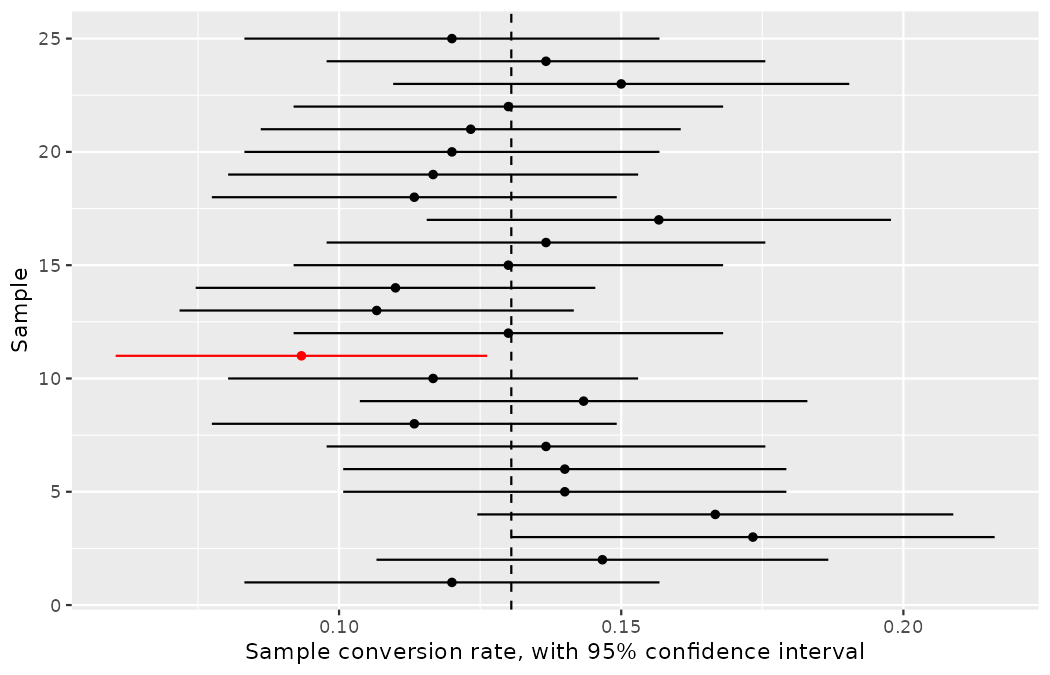
\includegraphics[width=0.85\linewidth,height=\textheight,keepaspectratio]{figures/foundations-mathematical-8.png}

The figure shows 25 horizontal interval segments, one per sample, each
with a dot at its sample conversion rate, and a dashed vertical line at
the true value \(p = 0.1305.\) Twenty-four of the 25 intervals cross the
dashed line; one --- sample 11, whose 300 resampled shots happened to
include only 28 goals \((\hat{p} = 0.0933,\) interval \(0.060\) to
\(0.126)\) --- lies entirely below it, and is drawn in red. That is one
miss in 25 intervals, almost exactly the 1-in-20 rate the confidence
level promises. The interval which does not capture \(p = 0.1305\) is
not due to bad science. Instead, it is due to natural variability, and
we should \emph{expect} some of our intervals to miss the parameter of
interest. Indeed, over a lifetime of creating 95\% intervals, you should
expect 5\% of your reported intervals to miss the parameter of interest
(unfortunately, you will not ever know which of your reported intervals
captured the parameter and which missed it).

\begin{tcolorbox}[enhanced jigsaw, left=2mm, leftrule=.75mm, title=\textcolor{quarto-callout-tip-color}{\faLightbulb}\hspace{0.5em}{Check your understanding}, arc=.35mm, rightrule=.15mm, coltitle=black, colframe=quarto-callout-tip-color-frame, bottomrule=.15mm, colbacktitle=quarto-callout-tip-color!10!white, opacitybacktitle=0.6, breakable, bottomtitle=1mm, toptitle=1mm, titlerule=0mm, opacityback=0, toprule=.15mm, colback=white]

In the figure above, one interval does not contain the true conversion
rate, \(p = 0.1305.\) Does this imply that there was a problem with that
sample of 300 shots?

\begin{center}\rule{0.5\linewidth}{0.5pt}\end{center}

No. Just as some observations occur more than 1.96 standard deviations
from the mean, some point estimates will be more than 1.96 standard
errors from the parameter --- sample 11 simply happened to draw a
cold-finishing set of shots. A confidence interval only provides a
plausible range of values for a parameter. While we might say other
values are implausible based on the data, this does not mean they are
impossible.

\end{tcolorbox}

\subsection{Interpreting confidence
intervals}\label{interpreting-confidence-intervals}

A careful eye might have observed the somewhat awkward language used to
describe confidence intervals.

\begin{tcolorbox}[enhanced jigsaw, left=2mm, leftrule=.75mm, title=\textcolor{quarto-callout-important-color}{\faExclamation}\hspace{0.5em}{Correct confidence interval interpretation}, arc=.35mm, rightrule=.15mm, coltitle=black, colframe=quarto-callout-important-color-frame, bottomrule=.15mm, colbacktitle=quarto-callout-important-color!10!white, opacitybacktitle=0.6, breakable, bottomtitle=1mm, toptitle=1mm, titlerule=0mm, opacityback=0, toprule=.15mm, colback=white]

We are XX\% confident that the population parameter is between
\emph{lower} and \emph{upper} (where \emph{lower} and \emph{upper} are
both numerical values).

\textbf{Incorrect} language might try to describe the confidence
interval as capturing the population parameter with a certain
probability.

This is one of the most common errors, and the cure is the long-run
reading demonstrated by the 25-interval simulation above: the confidence
level describes the \emph{procedure}, not this one interval --- build
intervals this way over and over and about XX\% of them will capture
their parameter. Once a particular interval is computed, the parameter
is either inside it or it is not; what remains is your confidence in the
recipe that produced it.

\end{tcolorbox}

Another especially important consideration of confidence intervals is
that they \emph{only try to capture the population parameter}. Our
intervals say nothing about the confidence of capturing individual
observations, a proportion of the observations, or about capturing point
estimates. The finishing program interval \((0.010, 0.145)\) speaks
about the true risk difference across the program, not about any
individual player's season; the England interval of
Chapter~\ref{sec-foundations-bootstrapping} spoke about the underlying
conversion process, not about what England will shoot in any particular
match. Confidence intervals provide an interval estimate for, and
attempt to capture, \textbf{population parameters}.

\section{Chapter review}\label{sec-chp13-review}

\subsection{Summary}\label{summary-12}

We can summarize the process of using the normal model as follows:

\begin{itemize}
\tightlist
\item
  \textbf{Frame the research question.} The mathematical model can be
  applied to both the hypothesis testing and the confidence interval
  framework. Make sure that your research question is being addressed by
  the most appropriate inference procedure: Marta's ``is there an
  effect?'' is a test; her ``how big is it?'' is an interval.
\item
  \textbf{Collect data with an observational study or experiment.} To
  address the research question, collect data on the variables of
  interest. Note that your data may be a random sample from a population
  --- shots from a tournament --- or may be part of a randomized
  experiment, like the club's dossier and drill trials.
\item
  \textbf{Model the randomness of the statistic.} In many cases, the
  normal distribution will be an excellent model for the randomness
  associated with the statistic of interest. The Central Limit Theorem
  tells us that if the sample size is large enough, sample averages
  (which can be calculated as either a proportion or a sample mean) will
  be approximately normally distributed when describing how the
  statistics change from sample to sample.
\item
  \textbf{Calculate the variability of the statistic.} Using formulas,
  come up with the standard deviation (or more typically, an estimate of
  the standard deviation called the standard error) of the statistic.
  The SE of the statistic will give information on how far the observed
  statistic is from the null hypothesized value (if performing a
  hypothesis test) or from the unknown population parameter (if creating
  a confidence interval).
\item
  \textbf{Use the normal distribution to quantify the variability.} The
  normal distribution will provide a probability which measures how
  likely it is for your observed and hypothesized (or observed and
  unknown) parameter to differ by the amount measured. The unusualness
  (or not) of the discrepancy will form the conclusion to the research
  question.
\item
  \textbf{Form a conclusion.} Using the p-value or the confidence
  interval from the analysis, report on the research question of
  interest. Also, be sure to write the conclusion in plain language so
  casual readers can understand the results --- and, as the consultant
  case study showed, be sure the technical conditions held before
  trusting the shortcut at all.
\end{itemize}

\begin{longtable}[]{@{}
  >{\raggedright\arraybackslash}p{(\linewidth - 2\tabcolsep) * \real{0.5634}}
  >{\raggedright\arraybackslash}p{(\linewidth - 2\tabcolsep) * \real{0.4366}}@{}}
\caption{Summary of mathematical models as an inferential statistical
method.}\label{tbl-chp13-summary}\tabularnewline
\toprule\noalign{}
\begin{minipage}[b]{\linewidth}\raggedright
Question
\end{minipage} & \begin{minipage}[b]{\linewidth}\raggedright
Answer
\end{minipage} \\
\midrule\noalign{}
\endfirsthead
\toprule\noalign{}
\begin{minipage}[b]{\linewidth}\raggedright
Question
\end{minipage} & \begin{minipage}[b]{\linewidth}\raggedright
Answer
\end{minipage} \\
\midrule\noalign{}
\endhead
\bottomrule\noalign{}
\endlastfoot
What does the procedure do? & Models the sampling distribution of the
statistic with a normal curve, \(N(\text{center}, SE),\) instead of
simulating it. \\
What is the statistic? & A point estimate, e.g., \(\hat{p}\) or
\(\hat{p}_T - \hat{p}_C,\) standardized as
\(Z = (\text{point estimate} - \text{null value})/SE.\) \\
What is the p-value? & A tail area of the normal curve beyond the
observed Z score. \\
What is the interval? & \(\text{point estimate} \pm 1.96 \times SE\) for
95\% confidence. \\
What are the technical conditions? & Independent observations, and a
large enough sample --- for proportions, at least 10 expected successes
and 10 expected failures. \\
\end{longtable}

\subsection{Terms}\label{terms-12}

The terms introduced in this chapter are presented below, alphabetized.
If you're not sure what some of these terms mean, we recommend you go
back in the text and review their definitions. You should be able to
easily spot them as \textbf{bolded text}.

\begin{longtable}[]{@{}
  >{\raggedright\arraybackslash}p{(\linewidth - 4\tabcolsep) * \real{0.3380}}
  >{\raggedright\arraybackslash}p{(\linewidth - 4\tabcolsep) * \real{0.3380}}
  >{\raggedright\arraybackslash}p{(\linewidth - 4\tabcolsep) * \real{0.3239}}@{}}
\caption{Terms introduced in this
chapter.}\label{tbl-terms-chp-13}\tabularnewline
\toprule\noalign{}
\endfirsthead
\endhead
\bottomrule\noalign{}
\endlastfoot
95\% confidence interval & normal distribution & percentile \\
95\% confident & normal model & sampling distribution \\
Central Limit Theorem & normal probability table & standard error \\
margin of error & null distribution & standard normal distribution \\
normal curve & parameter & Z score \\
\end{longtable}

\section{Exercises}\label{sec-chp13-exercises}

Answers to odd-numbered exercises can be found in
Appendix~\ref{sec-exercise-solutions-13}.

\begin{enumerate}
\def\labelenumi{\arabic{enumi}.}
\item
  \textbf{Area under the curve, Part I.} What percent of a standard
  normal distribution \(N(\mu=0, \sigma=1)\) is found in each region
  denoted by a \(Z\) inequality below? Be sure to draw a graph. In the
  chapter, we used R's \texttt{pnorm()} to calculate normal
  probabilities; you might instead use a normal probability table.

  \begin{enumerate}
  \def\labelenumii{\alph{enumii}.}
  \item
    \(Z < -1.35\)
  \item
    \(Z > 1.48\)
  \item
    \(-0.4 < Z < 1.5\)
  \item
    \(|Z| > 2\)
  \end{enumerate}
\item
  \textbf{Area under the curve, Part II.} What percent of a standard
  normal distribution \(N(\mu=0, \sigma=1)\) is found in each region
  denoted by a \(Z\) inequality below? Be sure to draw a graph. In the
  chapter, we used R's \texttt{pnorm()} to calculate normal
  probabilities; you might instead use a normal probability table.

  \begin{enumerate}
  \def\labelenumii{\alph{enumii}.}
  \item
    \(Z > -1.13\)
  \item
    \(Z < 0.18\)
  \item
    \(Z > 8\)
  \item
    \(|Z| < 0.5\)
  \end{enumerate}
\item
  \textbf{Entry assessment, Z scores.} Trialist Sofia took Northbridge
  United's academy entry assessment, scoring 82 points on the Technical
  section and 73 points on the Tactical section. In the club's benchmark
  archive,\footnote{The benchmark archive figures used in Exercises
    3--10 (entry-assessment scores, endurance-test times, GPS distances,
    index and load scores, squad-value swings) are constructed
    Northbridge scenarios: the stated means and standard deviations are
    club benchmark models, not real data.} Technical scores follow a
  nearly normal distribution with a mean of 72 points and a standard
  deviation of 8 points, and Tactical scores follow a nearly normal
  distribution with a mean of 65 points and a standard deviation of 10
  points. Higher scores are better on both sections. Use the information
  to compute each of the following.

  \begin{enumerate}
  \def\labelenumii{\alph{enumii}.}
  \item
    Write down the short-hand for each of the two normal distributions.
  \item
    What is Sofia's Z score on the Technical section? On the Tactical
    section? Draw a standard normal distribution curve and mark the two
    Z scores.
  \item
    What do the Z scores tell you?
  \item
    Relative to the other trialists in the archive, which section did
    Sofia do better on?
  \item
    Find her percentile scores for each of the two sections.
  \item
    What percent of trialists did better than her on the Technical
    section? On the Tactical section?
  \item
    Explain why simply comparing raw scores from the two sections could
    lead to an incorrect conclusion as to which section a trialist did
    better on.
  \item
    If the distributions of the scores on these sections are not nearly
    normal, would your answers to parts (b) - (f) change? Explain your
    reasoning.
  \end{enumerate}
\item
  \textbf{Endurance test, Z scores.} At a Northbridge academy open day,
  trialists run a 1,500-meter endurance test and are placed into age and
  gender groups. Two friends, Tomas and Mara, both ran the test: Tomas
  in the ``Boys, Under 17'' group and Mara in the ``Women, Under 19''
  group. Tomas finished in 351 seconds, while Mara finished in 352
  seconds. We can see that Tomas finished faster, but they are curious
  about how they did within their respective groups. Can you help them?
  Below is some information from the club's benchmark archive on the
  performance of their groups.

  \begin{itemize}
  \item
    The finishing times of the ``Boys, Under 17'' group have a mean of
    322 seconds with a standard deviation of 21 seconds.
  \item
    The finishing times of the ``Women, Under 19'' group have a mean of
    341 seconds with a standard deviation of 28 seconds.
  \item
    The distributions of finishing times for both groups are
    approximately normal.\\
    Remember: a better performance corresponds to a faster finish.
  \end{itemize}

  \begin{enumerate}
  \def\labelenumii{\alph{enumii}.}
  \item
    Write down the short-hand for the two normal distributions.
  \item
    What are the Z scores for Tomas's and Mara's finishing times? What
    do the Z scores tell you?
  \item
    Did Tomas or Mara rank better in their respective group? Explain
    your reasoning.
  \item
    What percent of the trialists in his group did Tomas finish faster
    than?
  \item
    What percent of the trialists in her group did Mara finish faster
    than?
  \item
    If the distributions of finishing times are not nearly normal, would
    your answers to parts (b) - (e) change? Explain your reasoning.
  \end{enumerate}
\item
  \textbf{Entry assessment, cutoffs.} Consider the previous two
  distributions for the academy entry assessment:
  \(N(\mu=72, \sigma=8)\) for the Technical section and
  \(N(\mu=65, \sigma=10)\) for the Tactical section. Use the information
  to compute each of the following.

  \begin{enumerate}
  \def\labelenumii{\alph{enumii}.}
  \item
    The score of a trialist who scored in the \(80^{th}\) percentile on
    the Tactical section.
  \item
    The score of a trialist who scored worse than 70\% of the trialists
    in the archive on the Technical section.
  \end{enumerate}
\item
  \textbf{Endurance test, cutoffs.} Recall the two different
  distributions for 1,500-meter endurance test times:
  \(N(\mu=322, \sigma=21)\) for the ``Boys, Under 17'' group and
  \(N(\mu=341, \sigma=28)\) for the ``Women, Under 19'' group. Times are
  listed in seconds. Use this information to compute each of the
  following.

  \begin{enumerate}
  \def\labelenumii{\alph{enumii}.}
  \item
    The cutoff time for the fastest 5\% of trialists in the Under-17
    boys' group, i.e., those who took the shortest 5\% of time to
    finish.
  \item
    The cutoff time for the slowest 10\% of trialists in the Under-19
    women's group.
  \end{enumerate}
\item
  \textbf{High-intensity running.} The GPS vests worn by Northbridge's
  wide midfielders record the high-intensity running distance each
  player covers in a match. For a full 90-minute appearance, the club's
  benchmark model puts high-intensity distance at an average of 850
  meters with a standard deviation of 120 meters, and the distances
  closely follow a normal distribution. Use the information to compute
  each of the following.

  \begin{enumerate}
  \def\labelenumii{\alph{enumii}.}
  \item
    What is the probability that a wide midfielder covers 1,000 meters
    of high-intensity running or more in a randomly chosen full
    appearance?
  \item
    How low are the lowest 10\% of matches (appearances with the least
    high-intensity distance)?
  \end{enumerate}
\item
  \textbf{Squad value swings.} Priya Rao models the year-on-year
  percentage change in the total market value of Northbridge's squad as
  normally distributed, with an average annual change of +14.7\% (i.e.,
  an average gain of 14.7\%) and a standard deviation of 33\%. A change
  of 0\% means the squad's value doesn't move, a negative change means
  the squad loses value, and a positive change means it gains value.

  \begin{enumerate}
  \def\labelenumii{\alph{enumii}.}
  \item
    In what percent of years does the squad lose value, i.e., have a
    change less than 0\%?
  \item
    What is the cutoff for the highest 15\% of annual value changes
    under this model?
  \end{enumerate}
\item
  \textbf{High-intensity running, in yards.} Recall the set-up that a
  wide midfielder's high-intensity running distance in a full appearance
  averages 850 meters with a standard deviation of 120 meters, and that
  the distances follow a normal distribution. A visiting coach wants the
  figures in yards, using the conversion \(yd = m \times 1.0936.\)

  \begin{enumerate}
  \def\labelenumii{\alph{enumii}.}
  \item
    Write the probability model for the distribution of high-intensity
    distance in yards.
  \item
    What is the probability of a wide midfielder covering 1,095 yards
    (which roughly corresponds to 1,000 meters) or more of
    high-intensity running in a full appearance? Calculate using the
    yards model from part (a).
  \item
    Did you get the same answer or different answers in part (b) of this
    question and part (a) of the previous high-intensity running
    question? Are you surprised? Explain.
  \item
    Estimate the IQR of the high-intensity distances (in yards).
  \end{enumerate}
\item
  \textbf{Find the SD.} Find the standard deviation of the distribution
  in the following situations.

  \begin{enumerate}
  \def\labelenumii{\alph{enumii}.}
  \item
    Northbridge's elite development squad admits only players whose
    talent-identification composite index is in the top 2\% of the
    recruitment database. The index is normally distributed with mean
    100, and the minimum index required for admission is 132.
  \item
    Session-load scores for academy midfielders follow an approximately
    normal distribution with mean 185 arbitrary units (AU). Players with
    session loads above 220 AU are flagged for load management, and
    about 18.5\% of the midfielders fall into this category.
  \end{enumerate}
\item
  \textbf{Video scouting survey.} A league-wide survey conducted in 2025
  reported that ``45\% of professional scouts rely on video for the
  majority of their evaluations.'' However, this value was based on a
  sample, so it may not be a perfect estimate for the population
  parameter of interest on its own. The study reported a standard error
  of about 1.2\%, and a normal model may reasonably be used in this
  setting.\footnote{The video scouting survey and the transfer-news poll
    in the next exercise are constructed scenarios: the reported
    proportions and standard errors are given for the exercise, not
    drawn from a real survey.}

  \begin{enumerate}
  \def\labelenumii{\alph{enumii}.}
  \item
    Create a 95\% confidence interval for the proportion of professional
    scouts who rely on video for the majority of their evaluations. Also
    interpret the confidence interval in the context of the study.
  \item
    Identify each of the following statements as true or false. Provide
    an explanation to justify each of your answers.

    \begin{enumerate}
    \def\labelenumiii{\roman{enumiii}.}
    \item
      We can say with certainty that the confidence interval from part
      (a) contains the true percentage of professional scouts who rely
      on video for the majority of their evaluations.
    \item
      If we repeated this survey 1,000 times and constructed a 95\%
      confidence interval for each survey, then approximately 950 of
      those confidence intervals would contain the true fraction of
      professional scouts who rely on video for the majority of their
      evaluations.
    \item
      The survey provides statistically discernible evidence (at the
      \(\alpha = 0.05\) level) that the percentage of professional
      scouts who rely on video for the majority of their evaluations is
      below 50\%.
    \item
      Since the standard error is 1.2\%, only 1.2\% of the scouts in the
      survey communicated uncertainty about their answer.
    \end{enumerate}
  \end{enumerate}
\item
  \textbf{Transfer-news poll, mathematical model.} A poll of Northbridge
  season-ticket holders conducted in 2025 found that 50\% of them (i.e.,
  a proportion of 0.5) get their transfer news primarily from social
  media. The standard error for this estimate was 0.5\% (i.e., 0.005),
  and a normal distribution may be used to model the sample proportion.

  \begin{enumerate}
  \def\labelenumii{\alph{enumii}.}
  \item
    Construct a 99\% confidence interval for the fraction of
    season-ticket holders who get their transfer news primarily from
    social media, and interpret the confidence interval in context.
  \item
    Identify each of the following statements as true or false. Provide
    an explanation to justify each of your answers.

    \begin{enumerate}
    \def\labelenumiii{\roman{enumiii}.}
    \item
      The data provide statistically discernible evidence that more than
      half of the season-ticket holders get their transfer news
      primarily from social media. Use a discernibility level of
      \(\alpha = 0.01\).
    \item
      Since the standard error is 0.5\%, we can conclude that 99.5\% of
      all season-ticket holders were included in the poll.
    \item
      If we want to reduce the standard error of the estimate, we should
      poll fewer season-ticket holders.
    \item
      If we construct a 90\% confidence interval for the percentage of
      season-ticket holders who get their transfer news primarily from
      social media, the resulting confidence interval will be wider than
      a corresponding 99\% confidence interval.
    \end{enumerate}
  \end{enumerate}
\item
  \textbf{Interpreting a Z score from a sample proportion.} Suppose that
  you conduct a hypothesis test about a population proportion --- say,
  the proportion of corner-kick shots that are scored at a major
  tournament --- and calculate the Z score to be 0.47. Which of the
  following is the best interpretation of this value? For the statements
  which are not a good interpretation, indicate the statistical idea
  being described.\footnote{This exercise was inspired by discussion on
    Dr.~Allan Rossman's blog \emph{Ask Good Questions}.}

  \begin{enumerate}
  \def\labelenumii{\alph{enumii}.}
  \item
    The probability is 0.47 that the null hypothesis is true.
  \item
    If the null hypothesis were true, the probability would be 0.47 of
    obtaining a sample proportion as far as observed from the
    hypothesized value of the population proportion.
  \item
    The sample proportion is 0.47 standard errors greater than the
    hypothesized value of the population proportion.
  \item
    The sample proportion is equal to 0.47 times the standard error.
  \item
    The sample proportion is 0.47 away from the hypothesized value of
    the population.
  \item
    The sample proportion is 0.47.
  \end{enumerate}
\item
  \textbf{Matchday viewing.} Northbridge's fan-research team asked the
  question: ``On how many of the past 30 days did you watch a full
  match, live or on video?'' Based on responses from 1,151 season-ticket
  holders, the team reported a 95\% confidence interval of 3.40 to 4.24
  days.

  \begin{enumerate}
  \def\labelenumii{\alph{enumii}.}
  \item
    Interpret this interval in context of the data.
  \item
    What does ``95\% confident'' mean? Explain in the context of the
    application.
  \item
    Suppose the analysts think a 99\% confidence level would be more
    appropriate for this interval. Will this new interval be smaller or
    wider than the 95\% confidence interval?
  \item
    If a new survey were to be done with 500 season-ticket holders, do
    you think the standard error of the estimate would be larger,
    smaller, or about the same?
  \end{enumerate}
\item
  \textbf{Repeated shot samples.} Priya Rao wants to understand the
  fraction of shots at a major tournament that arise from set-piece
  patterns of play. She expects at least 5\% of shots will come from set
  pieces, but not more than about 30\%. She randomly samples 800 shots
  from the tournament's event database and computes the fraction of
  these shots that came from set pieces. She repeats this 1,000 times
  and builds a distribution of sample proportions.

  \begin{enumerate}
  \def\labelenumii{\alph{enumii}.}
  \item
    What is this distribution called?
  \item
    Would you expect the shape of this distribution to be symmetric,
    right skewed, or left skewed? Explain your reasoning.
  \item
    What is the name of the variability of this distribution?
  \item
    Suppose Priya's database access is throttled, and she is only able
    to collect 250 shots per sample, but she can still collect 1,000
    samples. She builds a new distribution of sample proportions. How
    will the variability of this new distribution compare to the
    variability of the distribution when each sample contained 800
    shots?
  \end{enumerate}
\item
  \textbf{Repeated conversion samples.} Of all shots taken at the 2022
  Men's World Cup, 13\% were scored.\footnote{Computed from
    \texttt{data/derived/wc2022\_shots.csv} (StatsBomb open data): 195
    goals from 1,494 shots, \(195/1494 = 0.1305 \approx 13\%.\)} As part
  of a training exercise, Northbridge's junior analysts randomly sample
  40 shots from the tournament and check which of them were goals. They
  repeat this 1,000 times and build a distribution of sample
  proportions.

  \begin{enumerate}
  \def\labelenumii{\alph{enumii}.}
  \item
    What is this distribution called?
  \item
    Would you expect the shape of this distribution to be symmetric,
    right skewed, or left skewed? Explain your reasoning.
  \item
    What is the name of the variability of this distribution?
  \item
    Suppose the analysts decide to sample again, this time collecting 90
    shots per sample, and they again collect 1,000 samples. They build a
    new distribution of sample proportions. How will the variability of
    this new distribution compare to the variability of the distribution
    when each sample contained 40 shots?
  \end{enumerate}
\end{enumerate}

\begin{center}\rule{0.5\linewidth}{0.5pt}\end{center}

Adapted from \emph{Introduction to Modern Statistics} by
Çetinkaya-Rundel \& Hardin (CC BY-SA 4.0); this adaptation is likewise
CC BY-SA 4.0. Match data: StatsBomb open data.

\chapter{Decision errors}\label{sec-foundations-decision-errors}

Using data to make inferential decisions about larger populations is not
a perfect process. As seen in
Chapter~\ref{sec-foundations-randomization}, a small p-value typically
leads the analyst to a decision to reject the null claim or hypothesis.
Sometimes, however, data can produce a small p-value when the null
hypothesis is actually true and the data are just inherently variable.
Here we describe the errors which can arise in hypothesis testing, how
to define and quantify the different errors, and suggestions for
mitigating errors if possible. For a scouting department, these are not
abstract worries: every error type has a transfer fee, or a missed
player, attached to it.

Hypothesis tests are not flawless. Just think of the transfer market:
clubs sometimes commit large fees to players who never justify them, and
clubs sometimes pass on players who become stars somewhere else.
Similarly, data can point to the wrong conclusion. However, what
distinguishes statistical hypothesis tests from a sporting director's
gut feeling is that our framework allows us to quantify and control how
often the data lead us to the incorrect conclusion.

In a hypothesis test, there are two competing hypotheses: the null and
the alternative. We make a statement about which one might be true, but
we might choose incorrectly. There are four possible scenarios in a
hypothesis test, which are summarized in
Table~\ref{tbl-fourHTScenarios}.

\begin{longtable}[]{@{}
  >{\raggedright\arraybackslash}p{(\linewidth - 4\tabcolsep) * \real{0.3778}}
  >{\raggedright\arraybackslash}p{(\linewidth - 4\tabcolsep) * \real{0.2667}}
  >{\raggedright\arraybackslash}p{(\linewidth - 4\tabcolsep) * \real{0.3556}}@{}}
\caption{Four different scenarios for hypothesis
tests.}\label{tbl-fourHTScenarios}\tabularnewline
\toprule\noalign{}
\begin{minipage}[b]{\linewidth}\raggedright
\end{minipage} & \begin{minipage}[b]{\linewidth}\raggedright
Reject null hypothesis
\end{minipage} & \begin{minipage}[b]{\linewidth}\raggedright
Fail to reject null hypothesis
\end{minipage} \\
\midrule\noalign{}
\endfirsthead
\toprule\noalign{}
\begin{minipage}[b]{\linewidth}\raggedright
\end{minipage} & \begin{minipage}[b]{\linewidth}\raggedright
Reject null hypothesis
\end{minipage} & \begin{minipage}[b]{\linewidth}\raggedright
Fail to reject null hypothesis
\end{minipage} \\
\midrule\noalign{}
\endhead
\bottomrule\noalign{}
\endlastfoot
Null hypothesis is true & Type I error & Good decision \\
Alternative hypothesis is true & Good decision & Type II error \\
\end{longtable}

A \textbf{Type I error} is rejecting the null hypothesis when \(H_0\) is
actually true. Since we rejected the null hypothesis in the dossier
nationality and opportunity cost studies of
Chapter~\ref{sec-foundations-randomization}, it is possible that we made
a Type I error in one or both of those studies --- perhaps Northbridge's
network is perfectly unbiased, and the 29.2\% shortlist gap was one of
those 2-in-100 shuffles that happen by chance. This is precisely why
serious clubs, like serious scientists, repeat their audits: a second
run of the dossier experiment with a fresh randomization would either
corroborate the finding or expose it as a fluke. A \textbf{Type II
error} is failing to reject the null hypothesis when the alternative is
actually true.

\begin{tcolorbox}[enhanced jigsaw, left=2mm, leftrule=.75mm, title=\textcolor{quarto-callout-note-color}{\faInfo}\hspace{0.5em}{Worked example}, arc=.35mm, rightrule=.15mm, coltitle=black, colframe=quarto-callout-note-color-frame, bottomrule=.15mm, colbacktitle=quarto-callout-note-color!10!white, opacitybacktitle=0.6, breakable, bottomtitle=1mm, toptitle=1mm, titlerule=0mm, opacityback=0, toprule=.15mm, colback=white]

Consider a Northbridge sign/pass decision. The skeptical default is that
the prospect is \emph{not} the upgrade the club needs \((H_0)\); the
claim the scouting file sets out to demonstrate is that he is a genuine
upgrade \((H_A).\) Rejecting \(H_0\) means recommending the signing.
What does a Type I error represent in this context? What does a Type II
error represent? Table~\ref{tbl-fourHTScenarios} may be useful.

\begin{center}\rule{0.5\linewidth}{0.5pt}\end{center}

If the club makes a Type I error, this means the prospect is not an
upgrade \((H_0\) true) but the club signs him anyway --- the club signs
a dud, and the fee is wasted. A Type II error means the club failed to
reject \(H_0\) (i.e., passed on the player) when he was in fact a
genuine upgrade \((H_A\) true) --- the club passes on a gem, and watches
him excel for a rival.

Recall the VAR review from Chapter~\ref{sec-foundations-randomization},
where \(H_0\) was ``the on-field call stands'': there, a Type I error is
overturning a correct call, and a Type II error is letting a wrong call
stand.

\end{tcolorbox}

\begin{tcolorbox}[enhanced jigsaw, left=2mm, leftrule=.75mm, title=\textcolor{quarto-callout-tip-color}{\faLightbulb}\hspace{0.5em}{Check your understanding}, arc=.35mm, rightrule=.15mm, coltitle=black, colframe=quarto-callout-tip-color-frame, bottomrule=.15mm, colbacktitle=quarto-callout-tip-color!10!white, opacitybacktitle=0.6, breakable, bottomtitle=1mm, toptitle=1mm, titlerule=0mm, opacityback=0, toprule=.15mm, colback=white]

Consider the opportunity cost study from
Section~\ref{sec-caseStudyOpportunityCost}, where we concluded scouts
were less likely to recommend completing a €15M signing if they were
reminded that the fee could be kept for the winter window. What would a
Type I error represent in this context?

\begin{center}\rule{0.5\linewidth}{0.5pt}\end{center}

Making a Type I error in this context would mean that reminding scouts
that money not spent now can be spent later does not affect their
recommendations, despite the strong evidence (the data suggesting
otherwise) found in the experiment. Notice that this does \emph{not}
necessarily mean something was wrong with the data or that we made a
computational mistake. Sometimes data simply point us to the wrong
conclusion, which is why studies like Priya's are often repeated to
check initial findings.

\end{tcolorbox}

\begin{tcolorbox}[enhanced jigsaw, left=2mm, leftrule=.75mm, title=\textcolor{quarto-callout-note-color}{\faInfo}\hspace{0.5em}{Worked example}, arc=.35mm, rightrule=.15mm, coltitle=black, colframe=quarto-callout-note-color-frame, bottomrule=.15mm, colbacktitle=quarto-callout-note-color!10!white, opacitybacktitle=0.6, breakable, bottomtitle=1mm, toptitle=1mm, titlerule=0mm, opacityback=0, toprule=.15mm, colback=white]

How could Marta Vidal reduce the rate at which Northbridge signs duds
--- the Type I error rate of the club's signing decisions? What
influence would this have on the Type II error rate?

\begin{center}\rule{0.5\linewidth}{0.5pt}\end{center}

To lower the Type I error rate, the club might raise its standard of
evidence for a signing --- from ``a clear edge in the data and the live
reports'' to ``an overwhelming edge in every metric, every scout, every
match watched'' --- so fewer duds would be signed. However, this would
also make it more difficult to sign the players who are genuinely
upgrades, so the club would make more Type II errors, passing on more
gems.

\end{tcolorbox}

\begin{tcolorbox}[enhanced jigsaw, left=2mm, leftrule=.75mm, title=\textcolor{quarto-callout-tip-color}{\faLightbulb}\hspace{0.5em}{Check your understanding}, arc=.35mm, rightrule=.15mm, coltitle=black, colframe=quarto-callout-tip-color-frame, bottomrule=.15mm, colbacktitle=quarto-callout-tip-color!10!white, opacitybacktitle=0.6, breakable, bottomtitle=1mm, toptitle=1mm, titlerule=0mm, opacityback=0, toprule=.15mm, colback=white]

How could Marta Vidal reduce the Type II error rate --- the rate at
which Northbridge passes on gems? What influence would this have on the
Type I error rate?

\begin{center}\rule{0.5\linewidth}{0.5pt}\end{center}

To lower the Type II error rate, the club wants to sign more of the
genuine upgrades. It could lower its standard of evidence --- recommend
any player who looks promising after a couple of viewings. Lowering the
bar will also let more duds through, raising the Type I error rate.

\end{tcolorbox}

The example and guided practice above provide an important lesson: if we
reduce how often we make one type of error, we generally make more of
the other type. There is no evidence standard that eliminates both; a
club chooses where on the trade-off to sit.

\section{Discernibility level}\label{discernibility-level}

The \textbf{discernibility level} provides the cutoff for the p-value
which will lead to a decision of ``reject the null hypothesis.'' Recall
from Chapter~\ref{sec-foundations-randomization} that it is represented
by \(\alpha\) and must be fixed \emph{before} looking at the data.
Choosing a discernibility level for a test is important in many
contexts, and the traditional level is 0.05. However, it is sometimes
helpful to adjust the discernibility level based on the application. We
may select a level that is smaller or larger than 0.05 depending on the
consequences of any conclusions reached from the test.

If making a Type I error is dangerous or especially costly, we should
choose a small discernibility level (e.g., 0.01 or 0.001). If we want to
be very cautious about rejecting the null hypothesis, we demand very
strong evidence favoring the alternative \(H_A\) before we would reject
\(H_0.\) A marquee signing that consumes half the transfer budget is
exactly such a setting: a false positive costs the club tens of
millions.

If a Type II error is relatively more dangerous or much more costly than
a Type I error, then we should choose a higher discernibility level
(e.g., 0.10). Here we want to be cautious about failing to reject
\(H_0\) when the null is actually false. Screening free-agent trialists
for the academy is such a setting: waving one more trialist through to a
follow-up assessment costs a few days of coaching time, while releasing
a future first-team player costs dearly.

\begin{tcolorbox}[enhanced jigsaw, left=2mm, leftrule=.75mm, title=\textcolor{quarto-callout-important-color}{\faExclamation}\hspace{0.5em}{Discernibility levels should reflect consequences of errors}, arc=.35mm, rightrule=.15mm, coltitle=black, colframe=quarto-callout-important-color-frame, bottomrule=.15mm, colbacktitle=quarto-callout-important-color!10!white, opacitybacktitle=0.6, breakable, bottomtitle=1mm, toptitle=1mm, titlerule=0mm, opacityback=0, toprule=.15mm, colback=white]

The discernibility level selected for a test should reflect the
real-world consequences associated with making a Type I or Type II
error.

\end{tcolorbox}

\begin{tcolorbox}[enhanced jigsaw, left=2mm, leftrule=.75mm, title=\textcolor{quarto-callout-tip-color}{\faLightbulb}\hspace{0.5em}{Check your understanding}, arc=.35mm, rightrule=.15mm, coltitle=black, colframe=quarto-callout-tip-color-frame, bottomrule=.15mm, colbacktitle=quarto-callout-tip-color!10!white, opacitybacktitle=0.6, breakable, bottomtitle=1mm, toptitle=1mm, titlerule=0mm, opacityback=0, toprule=.15mm, colback=white]

Northbridge runs two kinds of decisions through hypothesis tests: (a)
whether to commit €40M to a single striker, and (b) whether to invite a
trialist back for a second week. For which decision should the club use
the smaller discernibility level, and why?

\begin{center}\rule{0.5\linewidth}{0.5pt}\end{center}

Decision (a). There, a Type I error (signing a dud) is enormously
costly, so the club should demand very strong evidence --- a small
\(\alpha\) such as 0.01. For decision (b), the cost of a Type I error is
a few days of coaching time, while a Type II error (releasing a gem) is
the expensive one, so a larger \(\alpha\) such as 0.10 is defensible.

\end{tcolorbox}

\section{Two-sided hypotheses}\label{sec-two-sided-hypotheses}

In Chapter~\ref{sec-foundations-randomization} we explored whether
prospects listed as foreign were discriminated against and whether a
simple budget reminder could make scouts a little more conservative. In
these two case studies, we have actually ignored some possibilities:

\begin{itemize}
\tightlist
\item
  What if prospects listed as \emph{domestic} are actually the ones
  discriminated against?
\item
  What if the budget reminder actually makes scouts \emph{more likely}
  to recommend the signing?
\end{itemize}

These possibilities weren't considered in our original hypotheses or
analyses. The disregard of the extra alternatives may have seemed
natural since the data pointed in the directions in which we framed the
problems. However, there are two dangers if we ignore possibilities that
disagree with our data or that conflict with our world view:

\begin{enumerate}
\def\labelenumi{\arabic{enumi}.}
\item
  Framing an alternative hypothesis simply to match the direction that
  the data point will generally inflate the Type I error rate. After all
  the work we have done (and will continue to do) to rigorously control
  the error rates in hypothesis tests, careless construction of the
  alternative hypotheses can disrupt that hard work. We will quantify
  exactly how much it inflates the error rate later in this chapter.
\item
  If we only use alternative hypotheses that agree with our worldview,
  then we are going to be subjecting ourselves to \textbf{confirmation
  bias}, which means we are looking for data that supports our ideas.
  That is not a scientific posture --- a scout who only logs the touches
  that flatter his favorite prospect is doing the same thing --- and the
  discipline of this section exists precisely to guard against it.
\end{enumerate}

The original hypotheses we have seen are called \textbf{one-sided
hypothesis tests} because they only explored one direction of
possibilities. Such hypotheses are appropriate when we are exclusively
interested in the single direction, but usually we want to consider all
possibilities. To do so, let's learn about \textbf{two-sided hypothesis
tests} in the context of a new study, a training intervention run inside
Jonas Beck's academy at Northbridge United.

High-repetition ``reactive finishing'' sessions are fashionable in
academy circles: extra sessions of chaotic, first-touch finishing drills
layered on top of normal training. The hoped-for effect is sharper
finishing. But the sessions add physical load, and added load eats into
recovery; a plausible outcome is that players arrive at the end-of-cycle
assessment \emph{more} fatigued and finish \emph{worse}. The
intervention could genuinely help or genuinely hurt --- which makes it
the perfect setting for a two-sided test. (This trial is distinct from
the multi-academy \texttt{drill\_trial} program you met in
Chapter~\ref{sec-data-hello}, which produced a season-end harm; treat
this as a new, smaller experiment at Northbridge alone.)

Jonas ran the experiment on 90 academy forwards, drawn from across
Northbridge and its partner academies --- no single academy fields that
many forwards. Each player was randomly assigned to either the
reactive-finishing program (treatment group, 40 players) or standard
training (control group, 50 players). The outcome variable of interest
was whether the player met the club's finishing benchmark at the
end-of-cycle assessment. As always, this is a constructed Northbridge
scenario --- no real academy was involved --- and we build the dataset
in visible R code so that every number below can be reproduced (the
construction is deterministic; seeds enter with the permutations that
follow).

\begin{Shaded}
\begin{Highlighting}[]
\FunctionTok{library}\NormalTok{(dplyr)}
\FunctionTok{library}\NormalTok{(readr)}
\FunctionTok{library}\NormalTok{(tidyr)}
\FunctionTok{library}\NormalTok{(ggplot2)}
\FunctionTok{library}\NormalTok{(infer)}

\NormalTok{benchmark90 }\OtherTok{\textless{}{-}} \FunctionTok{tibble}\NormalTok{(}
  \AttributeTok{group   =} \FunctionTok{factor}\NormalTok{(}\FunctionTok{rep}\NormalTok{(}\FunctionTok{c}\NormalTok{(}\StringTok{"treatment"}\NormalTok{, }\StringTok{"control"}\NormalTok{), }\AttributeTok{times =} \FunctionTok{c}\NormalTok{(}\DecValTok{40}\NormalTok{, }\DecValTok{50}\NormalTok{)),}
                   \AttributeTok{levels =} \FunctionTok{c}\NormalTok{(}\StringTok{"treatment"}\NormalTok{, }\StringTok{"control"}\NormalTok{)),}
  \AttributeTok{outcome =} \FunctionTok{factor}\NormalTok{(}\FunctionTok{c}\NormalTok{(}\FunctionTok{rep}\NormalTok{(}\StringTok{"met"}\NormalTok{, }\DecValTok{14}\NormalTok{), }\FunctionTok{rep}\NormalTok{(}\StringTok{"missed"}\NormalTok{, }\DecValTok{26}\NormalTok{),}
                     \FunctionTok{rep}\NormalTok{(}\StringTok{"met"}\NormalTok{, }\DecValTok{11}\NormalTok{), }\FunctionTok{rep}\NormalTok{(}\StringTok{"missed"}\NormalTok{, }\DecValTok{39}\NormalTok{)),}
                   \AttributeTok{levels =} \FunctionTok{c}\NormalTok{(}\StringTok{"met"}\NormalTok{, }\StringTok{"missed"}\NormalTok{))}
\NormalTok{)}
\end{Highlighting}
\end{Shaded}

\begin{tcolorbox}[enhanced jigsaw, left=2mm, leftrule=.75mm, title=\textcolor{quarto-callout-note-color}{\faInfo}\hspace{0.5em}{Worked example}, arc=.35mm, rightrule=.15mm, coltitle=black, colframe=quarto-callout-note-color-frame, bottomrule=.15mm, colbacktitle=quarto-callout-note-color!10!white, opacitybacktitle=0.6, breakable, bottomtitle=1mm, toptitle=1mm, titlerule=0mm, opacityback=0, toprule=.15mm, colback=white]

Form hypotheses for this study in plain and statistical language. Let
\(p_C\) represent the true benchmark rate of players who train normally
(corresponding to the control group) and \(p_T\) represent the true
benchmark rate for players on the reactive-finishing program
(corresponding to the treatment group).

\begin{center}\rule{0.5\linewidth}{0.5pt}\end{center}

First decompose the new notation. The letter \(p\) without a hat is, as
in Chapter~\ref{sec-foundations-randomization}, a \emph{population}
proportion --- the true, unobserved rate, here the rate at which players
of this kind would meet the benchmark under each training regime. The
subscripts \(T\) and \(C\) simply name the group each parameter belongs
to: treatment and control. You have seen hatted, subscripted sample
proportions such as \(\hat{p}_{T}\) before; \(p_T\) and \(p_C\) are the
population quantities those sample proportions estimate.

We want to understand whether the program is helpful or harmful. We'll
consider both of these possibilities using a two-sided hypothesis test.

\begin{itemize}
\item
  \(H_0:\) The reactive-finishing program has no overall effect on the
  assessment, i.e., the benchmark rates are the same in each group.
  \(p_T - p_C = 0.\)
\item
  \(H_A:\) The reactive-finishing program has an impact on the
  assessment, either positive or negative, but not zero.
  \(p_T - p_C \neq 0.\)
\end{itemize}

One more symbol deserves a careful first reading: \(\neq\) is ``not
equal to.'' An alternative written with \(\neq\) claims only that the
difference is \emph{some} value other than zero --- it could be positive
(the program helps) or negative (the program hurts) --- and commits to
no direction in advance.

Note that if we had done a one-sided hypothesis test, the resulting
hypotheses would have been:

\begin{itemize}
\item
  \(H_0:\) The program does not have a positive overall effect, i.e.,
  the benchmark rate in the treatment group is the same as or lower than
  in the control group. \(p_T - p_C \leq 0.\)
\item
  \(H_A:\) The program has a positive impact on the assessment.
  \(p_T - p_C > 0.\)
\end{itemize}

\end{tcolorbox}

There were 50 players in the experiment who trained normally and 40 who
followed the program. The study results are shown in
Table~\ref{tbl-benchmark90-summary}.

\begin{Shaded}
\begin{Highlighting}[]
\NormalTok{benchmark90 }\SpecialCharTok{|\textgreater{}}
  \FunctionTok{count}\NormalTok{(group, outcome) }\SpecialCharTok{|\textgreater{}}
  \FunctionTok{pivot\_wider}\NormalTok{(}\AttributeTok{names\_from =}\NormalTok{ outcome, }\AttributeTok{values\_from =}\NormalTok{ n)}
\CommentTok{\#\textgreater{} \# A tibble: 2 × 3}
\CommentTok{\#\textgreater{}   group       met missed}
\CommentTok{\#\textgreater{}   \textless{}fct\textgreater{}     \textless{}int\textgreater{}  \textless{}int\textgreater{}}
\CommentTok{\#\textgreater{} 1 treatment    14     26}
\CommentTok{\#\textgreater{} 2 control      11     39}
\end{Highlighting}
\end{Shaded}

\begin{longtable}[]{@{}lrrr@{}}
\caption{Results for the reactive-finishing trial. Players in the
treatment group followed the new program, and players in the control
group trained normally.}\label{tbl-benchmark90-summary}\tabularnewline
\toprule\noalign{}
& met benchmark & missed benchmark & Total \\
\midrule\noalign{}
\endfirsthead
\toprule\noalign{}
& met benchmark & missed benchmark & Total \\
\midrule\noalign{}
\endhead
\bottomrule\noalign{}
\endlastfoot
treatment & 14 & 26 & 40 \\
control & 11 & 39 & 50 \\
Total & 25 & 65 & 90 \\
\end{longtable}

\begin{tcolorbox}[enhanced jigsaw, left=2mm, leftrule=.75mm, title=\textcolor{quarto-callout-tip-color}{\faLightbulb}\hspace{0.5em}{Check your understanding}, arc=.35mm, rightrule=.15mm, coltitle=black, colframe=quarto-callout-tip-color-frame, bottomrule=.15mm, colbacktitle=quarto-callout-tip-color!10!white, opacitybacktitle=0.6, breakable, bottomtitle=1mm, toptitle=1mm, titlerule=0mm, opacityback=0, toprule=.15mm, colback=white]

What is the observed benchmark rate in the control group? And in the
treatment group? Also, provide a point estimate
\((\hat{p}_T - \hat{p}_C)\) for the true difference in population
benchmark rates across the two groups: \(p_T - p_C.\)

\begin{center}\rule{0.5\linewidth}{0.5pt}\end{center}

Observed control benchmark rate: \(\hat{p}_C = \frac{11}{50} = 0.22.\)
Treatment benchmark rate: \(\hat{p}_T = \frac{14}{40} = 0.35.\) Observed
difference: \(\hat{p}_T - \hat{p}_C = 0.35 - 0.22 = 0.13.\)

\begin{Shaded}
\begin{Highlighting}[]
\NormalTok{benchmark90 }\SpecialCharTok{|\textgreater{}}
  \FunctionTok{group\_by}\NormalTok{(group) }\SpecialCharTok{|\textgreater{}}
  \FunctionTok{summarize}\NormalTok{(}\AttributeTok{n =} \FunctionTok{n}\NormalTok{(), }\AttributeTok{p\_met =} \FunctionTok{mean}\NormalTok{(outcome }\SpecialCharTok{==} \StringTok{"met"}\NormalTok{))}
\CommentTok{\#\textgreater{} \# A tibble: 2 × 3}
\CommentTok{\#\textgreater{}   group         n p\_met}
\CommentTok{\#\textgreater{}   \textless{}fct\textgreater{}     \textless{}int\textgreater{} \textless{}dbl\textgreater{}}
\CommentTok{\#\textgreater{} 1 treatment    40  0.35}
\CommentTok{\#\textgreater{} 2 control      50  0.22}
\end{Highlighting}
\end{Shaded}

\end{tcolorbox}

According to the point estimate, an additional 13 percentage points of
players meet the finishing benchmark when they follow the
reactive-finishing program. However, we wonder if this difference could
be easily explainable by chance, if the program has no effect on the
assessment.

As we did in past studies, we will simulate what type of differences we
might see from chance alone under the null hypothesis. By randomly
assigning each player's assessment record to a ``simulated treatment''
or ``simulated control'' allocation, we get a new grouping --- the same
shuffle Priya Rao performed on the dossier cards in
Chapter~\ref{sec-foundations-randomization}. If we repeat this
simulation 1,000 times, we can build a \textbf{null distribution} of the
differences. Recall from Chapter~\ref{sec-foundations-mathematical} that
the null distribution is the sampling distribution of the statistic
under the setting where the null hypothesis is true; since the null here
asserts \(p_T - p_C = 0,\) the distribution will be centered at zero.

\begin{Shaded}
\begin{Highlighting}[]
\FunctionTok{set.seed}\NormalTok{(}\DecValTok{1401}\NormalTok{)}
\NormalTok{benchmark90\_null }\OtherTok{\textless{}{-}}\NormalTok{ benchmark90 }\SpecialCharTok{|\textgreater{}}
  \FunctionTok{specify}\NormalTok{(outcome }\SpecialCharTok{\textasciitilde{}}\NormalTok{ group, }\AttributeTok{success =} \StringTok{"met"}\NormalTok{) }\SpecialCharTok{|\textgreater{}}
  \FunctionTok{hypothesize}\NormalTok{(}\AttributeTok{null =} \StringTok{"independence"}\NormalTok{) }\SpecialCharTok{|\textgreater{}}
  \FunctionTok{generate}\NormalTok{(}\AttributeTok{reps =} \DecValTok{1000}\NormalTok{, }\AttributeTok{type =} \StringTok{"permute"}\NormalTok{) }\SpecialCharTok{|\textgreater{}}
  \FunctionTok{calculate}\NormalTok{(}\AttributeTok{stat =} \StringTok{"diff in props"}\NormalTok{, }\AttributeTok{order =} \FunctionTok{c}\NormalTok{(}\StringTok{"treatment"}\NormalTok{, }\StringTok{"control"}\NormalTok{)) }\SpecialCharTok{|\textgreater{}}
  \FunctionTok{mutate}\NormalTok{(}\AttributeTok{stat =} \FunctionTok{round}\NormalTok{(stat, }\DecValTok{3}\NormalTok{))}

\NormalTok{benchmark90\_null}\SpecialCharTok{$}\NormalTok{stat[}\DecValTok{1}\SpecialCharTok{:}\DecValTok{4}\NormalTok{]}
\CommentTok{\#\textgreater{} [1]  0.040 {-}0.050  0.085 {-}0.050}

\FunctionTok{ggplot}\NormalTok{(benchmark90\_null, }\FunctionTok{aes}\NormalTok{(}\AttributeTok{x =}\NormalTok{ stat)) }\SpecialCharTok{+}
  \FunctionTok{geom\_histogram}\NormalTok{(}\AttributeTok{binwidth =} \FloatTok{0.05}\NormalTok{) }\SpecialCharTok{+}
  \FunctionTok{labs}\NormalTok{(}
    \AttributeTok{title =} \StringTok{"1,000 randomized differences"}\NormalTok{,}
    \AttributeTok{x =} \StringTok{"Difference in randomized benchmark rates}\SpecialCharTok{\textbackslash{}n}\StringTok{(treatment {-} control)"}\NormalTok{,}
    \AttributeTok{y =} \StringTok{"Count"}
\NormalTok{  )}
\end{Highlighting}
\end{Shaded}

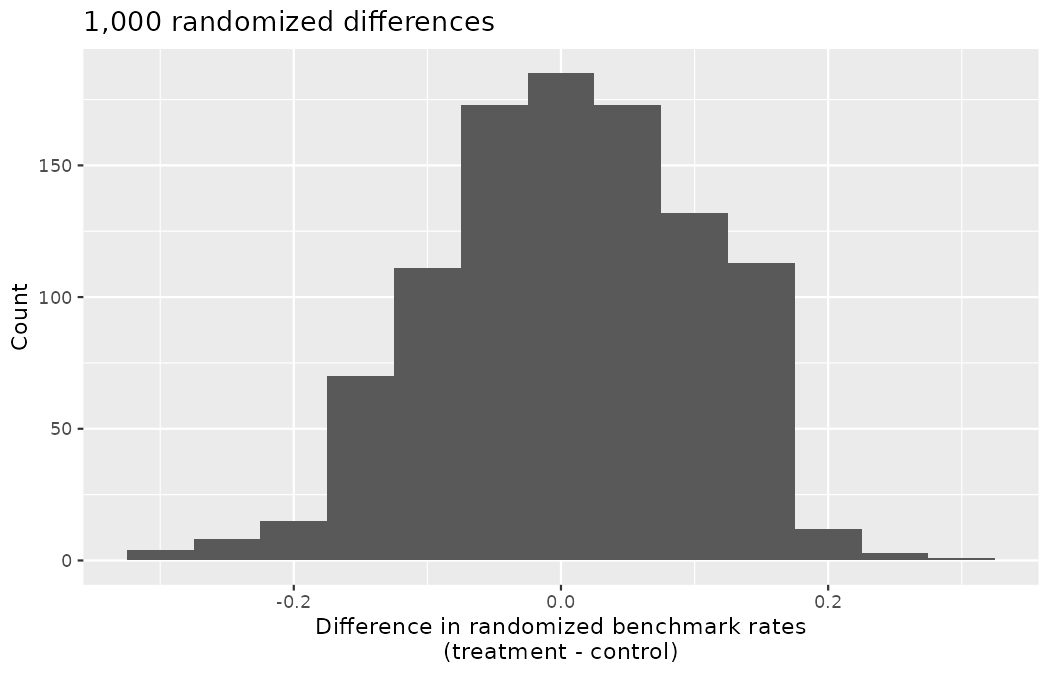
\includegraphics[width=0.85\linewidth,height=\textheight,keepaspectratio]{figures/foundations-errors-1.png}

The histogram of the 1,000 shuffled differences is centered at zero and
roughly bell-shaped, with the simulated differences running from
\(-0.32\) to \(0.31.\) How unusual is the observed \(+0.13\) in this
null world? We start by counting the shuffles that produced a difference
at least as large:

\begin{Shaded}
\begin{Highlighting}[]
\NormalTok{benchmark90\_null }\SpecialCharTok{|\textgreater{}}
  \FunctionTok{summarize}\NormalTok{(}
    \AttributeTok{n\_extreme  =} \FunctionTok{sum}\NormalTok{(stat }\SpecialCharTok{\textgreater{}=} \FloatTok{0.13}\NormalTok{),}
    \AttributeTok{right\_tail =} \FunctionTok{mean}\NormalTok{(stat }\SpecialCharTok{\textgreater{}=} \FloatTok{0.13}\NormalTok{)}
\NormalTok{  )}
\CommentTok{\#\textgreater{} \# A tibble: 1 × 2}
\CommentTok{\#\textgreater{}   n\_extreme right\_tail}
\CommentTok{\#\textgreater{}       \textless{}int\textgreater{}      \textless{}dbl\textgreater{}}
\CommentTok{\#\textgreater{} 1       129      0.129}
\end{Highlighting}
\end{Shaded}

The right tail area is \(0.129.\) (Note: it is only a coincidence that
the tail area lands so close to the observed difference
\(\hat{p}_T - \hat{p}_C = 0.13.\)) However, contrary to how we
calculated the p-value in previous studies, the p-value of this test is
not actually the tail area we calculated, i.e., it's not \(0.129\)!

The p-value is defined as the probability we observe a result at least
as favorable to the alternative hypothesis as the observed difference.
In this case, any difference less than or equal to \(-0.13\) would also
provide equally strong evidence favoring the alternative hypothesis as a
difference of \(+0.13\) did. A difference of \(-0.13\) would correspond
to a benchmark rate 13 percentage points \emph{lower} in the treatment
group than in the control group --- the fatigue scenario, in which the
added sessions actively hurt the assessment, and exactly the outcome
Jonas most needs to catch. The code below shades these differences in
the left tail of the distribution as well; the two shaded tails provide
a visual representation of the p-value for a two-sided test.

\begin{Shaded}
\begin{Highlighting}[]
\FunctionTok{ggplot}\NormalTok{(benchmark90\_null, }\FunctionTok{aes}\NormalTok{(}\AttributeTok{x =}\NormalTok{ stat, }\AttributeTok{fill =} \FunctionTok{abs}\NormalTok{(stat) }\SpecialCharTok{\textgreater{}=} \FloatTok{0.13}\NormalTok{)) }\SpecialCharTok{+}
  \FunctionTok{geom\_histogram}\NormalTok{(}\AttributeTok{binwidth =} \FloatTok{0.05}\NormalTok{) }\SpecialCharTok{+}
  \FunctionTok{labs}\NormalTok{(}
    \AttributeTok{title =} \StringTok{"1,000 randomized differences"}\NormalTok{,}
    \AttributeTok{x =} \StringTok{"Difference in randomized benchmark rates}\SpecialCharTok{\textbackslash{}n}\StringTok{(treatment {-} control)"}\NormalTok{,}
    \AttributeTok{y =} \StringTok{"Count"}\NormalTok{,}
    \AttributeTok{fill =} \StringTok{"At least as extreme as 0.13"}
\NormalTok{  )}
\end{Highlighting}
\end{Shaded}

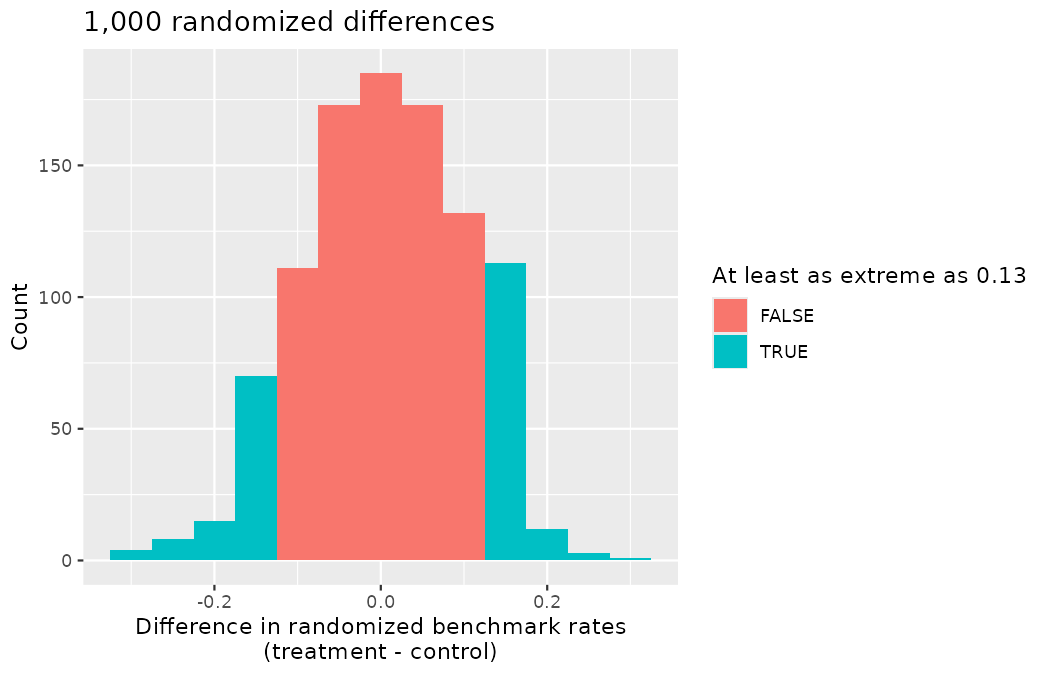
\includegraphics[width=0.85\linewidth,height=\textheight,keepaspectratio]{figures/foundations-errors-2.png}

The highlighted bars now sit in both tails: the 129 shuffles at or above
\(+0.13\) on the right, and the 97 shuffles at or below \(-0.13\) on the
left.

For a two-sided test, take the single tail (in this case, \(0.129\)) and
double it to get the p-value: \(2 \times 0.129 = 0.258.\) Since this
p-value is larger than \(0.05,\) we do not reject the null hypothesis:
the observed 13-percentage-point difference is not statistically
discernible at \(\alpha = 0.05.\) That is, we do not find convincing
evidence that the reactive-finishing program has any influence, positive
or negative, on whether a player meets the finishing benchmark.

Note how differently this ended from the \texttt{drill\_trial} study of
Chapter~\ref{sec-data-hello}, where the multi-academy season-end data
produced a harm too large to attribute to chance. Two training
interventions, two competently run experiments, two different verdicts
--- one rejection, one ``check complete, the on-field call stands.''
Both verdicts are informative, and neither is a failure of the method.

\begin{tcolorbox}[enhanced jigsaw, left=2mm, leftrule=.75mm, title=\textcolor{quarto-callout-tip-color}{\faLightbulb}\hspace{0.5em}{Check your understanding}, arc=.35mm, rightrule=.15mm, coltitle=black, colframe=quarto-callout-tip-color-frame, bottomrule=.15mm, colbacktitle=quarto-callout-tip-color!10!white, opacitybacktitle=0.6, breakable, bottomtitle=1mm, toptitle=1mm, titlerule=0mm, opacityback=0, toprule=.15mm, colback=white]

Jonas summarizes the trial for Marta Vidal as: ``The experiment showed
the program makes no difference, so the debate is settled.'' What two
corrections should Priya Rao make before this summary leaves the
building?

\begin{center}\rule{0.5\linewidth}{0.5pt}\end{center}

First, failing to reject \(H_0\) is not evidence that \(H_0\) is true
--- recall the VAR review of
Chapter~\ref{sec-foundations-randomization}: ``check complete'' does not
prove the original call correct. Second, with only 90 players, the test
may simply have lacked the sensitivity to detect a real but modest
effect; if the program truly helps (or hurts), this trial may have
produced a Type II error. How likely a study is to detect a genuine
effect is taken up in Section~\ref{sec-pow}.

\end{tcolorbox}

\begin{tcolorbox}[enhanced jigsaw, left=2mm, leftrule=.75mm, title=\textcolor{quarto-callout-important-color}{\faExclamation}\hspace{0.5em}{Default to a two-sided test}, arc=.35mm, rightrule=.15mm, coltitle=black, colframe=quarto-callout-important-color-frame, bottomrule=.15mm, colbacktitle=quarto-callout-important-color!10!white, opacitybacktitle=0.6, breakable, bottomtitle=1mm, toptitle=1mm, titlerule=0mm, opacityback=0, toprule=.15mm, colback=white]

We want to be rigorous and keep an open mind when we analyze data and
evidence. Use a one-sided hypothesis test only if you truly have
interest in only one direction.

\end{tcolorbox}

\begin{tcolorbox}[enhanced jigsaw, left=2mm, leftrule=.75mm, title=\textcolor{quarto-callout-important-color}{\faExclamation}\hspace{0.5em}{Computing a p-value for a two-sided test}, arc=.35mm, rightrule=.15mm, coltitle=black, colframe=quarto-callout-important-color-frame, bottomrule=.15mm, colbacktitle=quarto-callout-important-color!10!white, opacitybacktitle=0.6, breakable, bottomtitle=1mm, toptitle=1mm, titlerule=0mm, opacityback=0, toprule=.15mm, colback=white]

First compute the p-value for one tail of the distribution, then double
that value to get the two-sided p-value. The procedure is no more
complicated than that.

\end{tcolorbox}

\begin{tcolorbox}[enhanced jigsaw, left=2mm, leftrule=.75mm, title=\textcolor{quarto-callout-note-color}{\faInfo}\hspace{0.5em}{Worked example}, arc=.35mm, rightrule=.15mm, coltitle=black, colframe=quarto-callout-note-color-frame, bottomrule=.15mm, colbacktitle=quarto-callout-note-color!10!white, opacitybacktitle=0.6, breakable, bottomtitle=1mm, toptitle=1mm, titlerule=0mm, opacityback=0, toprule=.15mm, colback=white]

Consider the situation of the set-piece consultant from
Section~\ref{sec-case-study-med-consult}, whose showcase team, England,
converted 13 of their 63 shots at the 2022 World Cup against a
tournament baseline of \(195/1494 = 0.1305.\) Now that you know about
one-sided and two-sided tests, which type of test do you think is more
appropriate?

\begin{center}\rule{0.5\linewidth}{0.5pt}\end{center}

The setting has been framed in the context of the consultant being
helpful --- that is what his pitch to Marta Vidal claimed, and it is
what pulled us toward the single ``he improves finishing'' direction
originally. But what if the consultant's teams actually performed
\emph{worse} than the tournament baseline? Would Marta care? More than
ever! Since it turns out that we care about a finding in either
direction, we should run a two-sided test.

In Chapter~\ref{sec-foundations-mathematical} we approximated this
case's null distribution by simulating 10,000 tournaments with
\texttt{rbinom()}. The tail area can also be computed exactly, because
under \(H_0\) the number of goals in 63 shots follows the binomial model
those simulations were drawing from; \texttt{binom.test()} reports the
exact probability of scoring 13 or more of 63 shots when the true
conversion rate is the baseline:

\begin{Shaded}
\begin{Highlighting}[]
\FunctionTok{binom.test}\NormalTok{(}\DecValTok{13}\NormalTok{, }\DecValTok{63}\NormalTok{, }\AttributeTok{p =} \DecValTok{195} \SpecialCharTok{/} \DecValTok{1494}\NormalTok{, }\AttributeTok{alternative =} \StringTok{"greater"}\NormalTok{)}\SpecialCharTok{$}\NormalTok{p.value}
\CommentTok{\#\textgreater{} [1] 0.06119346}
\end{Highlighting}
\end{Shaded}

The one-sided p-value, computed in the consultant's claimed ``beats the
tournament'' direction, is \(0.0612.\) The p-value for the two-sided
test is double that of the one-sided test: \(2 \times 0.0612 = 0.1224.\)
The doubling is not a technicality. At the lenient discernibility level
of \(\alpha = 0.10,\) a one-sided test would have handed the consultant
a statistically discernible result \((0.0612 < 0.10);\) the two-sided
test that an open mind demands is no longer discernible even at that
generous bar \((0.1224 > 0.10).\) The choice of alternative hypothesis
was worth an entire verdict --- which is precisely why it cannot be left
to the person selling the signal.

\end{tcolorbox}

Generally, to find a two-sided p-value we double the single tail area,
which remains a reasonable approach even when the distribution is
asymmetric. However, the approach can result in p-values larger than 1
when the point estimate is very near the mean in the null distribution;
in such cases, we write that the p-value is 1. Also, very large p-values
computed in this way (e.g., 0.85) may be slightly inflated. Doubling is
a convention, not a count of both tails: in our own null distribution
the left tail held 97 shuffles rather than exactly 129, so doubling gave
\(0.258\) where adding the two tails would have given \(0.226\) --- both
comfortably above \(0.05,\) and leading to the same conclusion.
Typically, we do not worry too much about the precision of very large
p-values because they lead to the same analysis conclusion, even if the
value is slightly off.

\section{Controlling the Type I error
rate}\label{controlling-the-type-i-error-rate}

Now that we understand the difference between one-sided and two-sided
tests, we must recognize when to use each type of test. Because of the
result of increased error rates, it is never okay to change two-sided
tests to one-sided tests after observing the data. We explore the
consequences of ignoring this advice using a temptation that sits inside
the very data we have carried all book.

Should a scout rate first-time finishing as a strength or as a
liability? Suppose an analyst decides to let each tournament answer for
itself --- looking at the split first, and choosing the ``natural''
alternative hypothesis second.

\begin{Shaded}
\begin{Highlighting}[]
\NormalTok{wc2022\_shots }\OtherTok{\textless{}{-}} \FunctionTok{read\_csv}\NormalTok{(}\StringTok{"data/derived/wc2022\_shots.csv"}\NormalTok{)}
\NormalTok{weuro2025\_shots }\OtherTok{\textless{}{-}} \FunctionTok{read\_csv}\NormalTok{(}\StringTok{"data/derived/weuro2025\_shots.csv"}\NormalTok{)}

\NormalTok{wc2022\_shots }\SpecialCharTok{|\textgreater{}}
  \FunctionTok{group\_by}\NormalTok{(first\_time) }\SpecialCharTok{|\textgreater{}}
  \FunctionTok{summarize}\NormalTok{(}\AttributeTok{shots =} \FunctionTok{n}\NormalTok{(), }\AttributeTok{goals =} \FunctionTok{sum}\NormalTok{(goal), }\AttributeTok{conversion =} \FunctionTok{mean}\NormalTok{(goal))}
\CommentTok{\#\textgreater{} \# A tibble: 2 × 4}
\CommentTok{\#\textgreater{}   first\_time shots goals conversion}
\CommentTok{\#\textgreater{}   \textless{}lgl\textgreater{}      \textless{}int\textgreater{} \textless{}int\textgreater{}      \textless{}dbl\textgreater{}}
\CommentTok{\#\textgreater{} 1 FALSE       1026   124      0.121}
\CommentTok{\#\textgreater{} 2 TRUE         468    71      0.152}

\NormalTok{weuro2025\_shots }\SpecialCharTok{|\textgreater{}}
  \FunctionTok{group\_by}\NormalTok{(first\_time) }\SpecialCharTok{|\textgreater{}}
  \FunctionTok{summarize}\NormalTok{(}\AttributeTok{shots =} \FunctionTok{n}\NormalTok{(), }\AttributeTok{goals =} \FunctionTok{sum}\NormalTok{(goal), }\AttributeTok{conversion =} \FunctionTok{mean}\NormalTok{(goal))}
\CommentTok{\#\textgreater{} \# A tibble: 2 × 4}
\CommentTok{\#\textgreater{}   first\_time shots goals conversion}
\CommentTok{\#\textgreater{}   \textless{}lgl\textgreater{}      \textless{}int\textgreater{} \textless{}int\textgreater{}      \textless{}dbl\textgreater{}}
\CommentTok{\#\textgreater{} 1 FALSE        605    85      0.140}
\CommentTok{\#\textgreater{} 2 TRUE         308    38      0.123}
\end{Highlighting}
\end{Shaded}

At the 2022 Men's World Cup, first-time shots converted \emph{better}:
\(71/468 = 0.1517\) against \(124/1026 = 0.1209\) for all other shots, a
gap of \(+3.1\) percentage points. Peeking at that split, our analyst
frames \(H_A:\) first-time shots convert at a \emph{higher} rate, and
tests into the right tail. At the 2025 Women's Euro, the sign appears to
reverse: first-time shots converted at \(38/308 = 0.1234\) against
\(85/605 = 0.1405\) for the rest, a gap of \(-1.7\) points. The same
analyst, peeking again, now frames \(H_A:\) first-time shots convert at
a \emph{lower} rate, and tests into the left tail. Each report, read
alone, looks like a disciplined one-sided test. Read together, they
reveal the procedure: whichever direction the data lean, that is the
direction that gets tested --- the tail is chosen \emph{after} the coin
has landed.

Such an analyst is doubly damned, and each charge deserves its own
prosecution. Take the more embarrassing charge first: the reversal they
chased was never football. Both splits were computed on \emph{all}
shots, and you know from Section~\ref{sec-chp11-pens-out} what question
that should trigger: which shots are in the frame? A penalty kick is a
placed, dead-ball strike --- it cannot be logged first time --- so every
penalty in these data sits in the analyst's ``controlled touch'' bucket,
converting at a rate no open-play shot approaches. The Euro carried 51
of them, 37 from the shoot-outs alone:

\begin{Shaded}
\begin{Highlighting}[]
\NormalTok{weuro2025\_shots }\SpecialCharTok{|\textgreater{}}
  \FunctionTok{filter}\NormalTok{(shot\_type }\SpecialCharTok{==} \StringTok{"Penalty"}\NormalTok{) }\SpecialCharTok{|\textgreater{}}
  \FunctionTok{summarize}\NormalTok{(}
    \AttributeTok{kicks =} \FunctionTok{n}\NormalTok{(),}
    \AttributeTok{shootout =} \FunctionTok{sum}\NormalTok{(period }\SpecialCharTok{==} \DecValTok{5}\NormalTok{),}
    \AttributeTok{first\_time\_kicks =} \FunctionTok{sum}\NormalTok{(first\_time),}
    \AttributeTok{conversion =} \FunctionTok{mean}\NormalTok{(goal)}
\NormalTok{  )}
\CommentTok{\#\textgreater{} \# A tibble: 1 × 4}
\CommentTok{\#\textgreater{}   kicks shootout first\_time\_kicks conversion}
\CommentTok{\#\textgreater{}   \textless{}int\textgreater{}    \textless{}int\textgreater{}            \textless{}int\textgreater{}      \textless{}dbl\textgreater{}}
\CommentTok{\#\textgreater{} 1    51       37                0      0.549}

\NormalTok{weuro2025\_shots }\SpecialCharTok{|\textgreater{}}
  \FunctionTok{filter}\NormalTok{(shot\_type }\SpecialCharTok{==} \StringTok{"Open Play"}\NormalTok{) }\SpecialCharTok{|\textgreater{}}
  \FunctionTok{group\_by}\NormalTok{(first\_time) }\SpecialCharTok{|\textgreater{}}
  \FunctionTok{summarize}\NormalTok{(}\AttributeTok{shots =} \FunctionTok{n}\NormalTok{(), }\AttributeTok{goals =} \FunctionTok{sum}\NormalTok{(goal), }\AttributeTok{conversion =} \FunctionTok{mean}\NormalTok{(goal))}
\CommentTok{\#\textgreater{} \# A tibble: 2 × 4}
\CommentTok{\#\textgreater{}   first\_time shots goals conversion}
\CommentTok{\#\textgreater{}   \textless{}lgl\textgreater{}      \textless{}int\textgreater{} \textless{}int\textgreater{}      \textless{}dbl\textgreater{}}
\CommentTok{\#\textgreater{} 1 FALSE        543    57      0.105}
\CommentTok{\#\textgreater{} 2 TRUE         308    38      0.123}
\end{Highlighting}
\end{Shaded}

Penalties out, the Euro's gap runs \(38/308 = 0.1234\) against
\(57/543 = 0.1050\) --- first-time shots converting \emph{better}, the
same direction as the World Cup. (The World Cup's gap survives the same
filter, and in fact widens: its 64 penalties also sit in the
controlled-touch bucket.) The flip that chose our analyst's left tail
was not a property of women's football or of first-time finishing; it
was 51 uncontested penalty kicks propping up one bucket --- precisely
the artifact this book's penalty convention exists to expose. They
peeked, and what they peeked at was garbage.

The second charge is procedural, and it stands even against an analyst
whose frames are impeccable: in a world where the null hypothesis is
true and there is nothing to find in \emph{any} frame, letting each
dataset pick its own tail still doubles the error rate. Such an analyst
is not operating at their declared \(\alpha = 0.05.\) As the next
example shows, they are operating at double that.

\begin{tcolorbox}[enhanced jigsaw, left=2mm, leftrule=.75mm, title=\textcolor{quarto-callout-note-color}{\faInfo}\hspace{0.5em}{Worked example}, arc=.35mm, rightrule=.15mm, coltitle=black, colframe=quarto-callout-note-color-frame, bottomrule=.15mm, colbacktitle=quarto-callout-note-color!10!white, opacitybacktitle=0.6, breakable, bottomtitle=1mm, toptitle=1mm, titlerule=0mm, opacityback=0, toprule=.15mm, colback=white]

Using \(\alpha = 0.05,\) we show that freely switching from two-sided
tests to one-sided tests will lead us to make twice as many Type I
errors as intended.

\begin{center}\rule{0.5\linewidth}{0.5pt}\end{center}

Suppose we are interested in finding any difference from 0, and suppose
the null hypothesis is \emph{true by construction}: we build a world in
which striking a shot first time has no association with scoring, just
as the odd- and even-minute split of
Chapter~\ref{sec-foundations-randomization} was irrelevant by
construction. In this world, every simulated ``season'' delivers 468
first-time shots and 1,026 other shots --- the group sizes from the real
2022 World Cup --- all converting at the same true rate
\(p_0 = 195/1494.\) The reference null distribution below plays the role
of a smooth curve of chance differences, and its 5th and 95th
percentiles mark off the most extreme 5\% of chance differences in each
direction:

\begin{Shaded}
\begin{Highlighting}[]
\NormalTok{n\_ft }\OtherTok{\textless{}{-}} \DecValTok{468}
\NormalTok{n\_ot }\OtherTok{\textless{}{-}} \DecValTok{1026}
\NormalTok{p\_0  }\OtherTok{\textless{}{-}} \DecValTok{195} \SpecialCharTok{/} \DecValTok{1494}

\FunctionTok{set.seed}\NormalTok{(}\DecValTok{1402}\NormalTok{)}
\NormalTok{null\_ref }\OtherTok{\textless{}{-}} \FunctionTok{tibble}\NormalTok{(}
  \AttributeTok{stat =} \FunctionTok{rbinom}\NormalTok{(}\DecValTok{100000}\NormalTok{, n\_ft, p\_0) }\SpecialCharTok{/}\NormalTok{ n\_ft }\SpecialCharTok{{-}} \FunctionTok{rbinom}\NormalTok{(}\DecValTok{100000}\NormalTok{, n\_ot, p\_0) }\SpecialCharTok{/}\NormalTok{ n\_ot}
\NormalTok{)}

\NormalTok{cutoffs }\OtherTok{\textless{}{-}}\NormalTok{ null\_ref }\SpecialCharTok{|\textgreater{}}
  \FunctionTok{summarize}\NormalTok{(}
    \AttributeTok{lower =} \FunctionTok{quantile}\NormalTok{(stat, }\FloatTok{0.05}\NormalTok{),}
    \AttributeTok{upper =} \FunctionTok{quantile}\NormalTok{(stat, }\FloatTok{0.95}\NormalTok{)}
\NormalTok{  )}
\NormalTok{cutoffs}
\CommentTok{\#\textgreater{} \# A tibble: 1 × 2}
\CommentTok{\#\textgreater{}     lower  upper}
\CommentTok{\#\textgreater{}     \textless{}dbl\textgreater{}  \textless{}dbl\textgreater{}}
\CommentTok{\#\textgreater{} 1 {-}0.0306 0.0312}
\end{Highlighting}
\end{Shaded}

First, suppose a season's sample difference comes out larger than 0. In
a one-sided test, the peeking analyst sets \(H_A:\) difference \(> 0\)
and rejects \(H_0\) if the observed difference falls beyond the upper
cutoff, since the p-value would just be the single right tail. Thus, if
\(H_0\) is true, the analyst incorrectly rejects \(H_0\) about 5\% of
the time when the sample difference is above the null value.

Then, suppose the season's difference comes out smaller than 0. The
peeking analyst now sets \(H_A:\) difference \(< 0\) and rejects \(H_0\)
if the observed difference falls below the lower cutoff. That is, if
\(H_0\) is true, this situation also occurs about 5\% of the time.

By examining these two scenarios, we can determine that we will make a
Type I error \(5\% + 5\% = 10\%\) of the time if we are allowed to swap
to the ``best'' one-sided test for the data. The simulation confirms the
arithmetic: below, 10,000 fresh seasons are generated in the same null
world, and each is tested twice --- once by an honest analyst who
committed \emph{in advance} to the single direction ``first-time shots
convert better,'' and once by the peeking analyst who tests in whichever
direction the season leans.

\begin{Shaded}
\begin{Highlighting}[]
\NormalTok{seasons }\OtherTok{\textless{}{-}} \FunctionTok{tibble}\NormalTok{(}
  \AttributeTok{stat =} \FunctionTok{rbinom}\NormalTok{(}\DecValTok{10000}\NormalTok{, n\_ft, p\_0) }\SpecialCharTok{/}\NormalTok{ n\_ft }\SpecialCharTok{{-}} \FunctionTok{rbinom}\NormalTok{(}\DecValTok{10000}\NormalTok{, n\_ot, p\_0) }\SpecialCharTok{/}\NormalTok{ n\_ot}
\NormalTok{)}

\NormalTok{seasons }\SpecialCharTok{|\textgreater{}}
  \FunctionTok{summarize}\NormalTok{(}
    \AttributeTok{fixed\_direction =} \FunctionTok{mean}\NormalTok{(stat }\SpecialCharTok{\textgreater{}=}\NormalTok{ cutoffs}\SpecialCharTok{$}\NormalTok{upper),}
    \AttributeTok{peeking         =} \FunctionTok{mean}\NormalTok{(stat }\SpecialCharTok{\textgreater{}=}\NormalTok{ cutoffs}\SpecialCharTok{$}\NormalTok{upper }\SpecialCharTok{|}\NormalTok{ stat }\SpecialCharTok{\textless{}=}\NormalTok{ cutoffs}\SpecialCharTok{$}\NormalTok{lower)}
\NormalTok{  )}
\CommentTok{\#\textgreater{} \# A tibble: 1 × 2}
\CommentTok{\#\textgreater{}   fixed\_direction peeking}
\CommentTok{\#\textgreater{}             \textless{}dbl\textgreater{}   \textless{}dbl\textgreater{}}
\CommentTok{\#\textgreater{} 1          0.0538   0.103}
\end{Highlighting}
\end{Shaded}

Every one of the 10,000 seasons was generated under \(H_0,\) so
\emph{every} rejection here is a Type I error. The analyst who fixed the
direction in advance rejected in 5.4\% of the seasons --- the rate
\(\alpha\) promised. The peeking analyst rejected in 10.3\% of them.
That is twice the error rate we prescribed with our discernibility level
--- the level some texts call the \textbf{significance level}, recall
Chapter~\ref{sec-foundations-randomization} --- of \(\alpha = 0.05\)!

\end{tcolorbox}

\begin{tcolorbox}[enhanced jigsaw, left=2mm, leftrule=.75mm, title=\textcolor{quarto-callout-important-color}{\faExclamation}\hspace{0.5em}{Hypothesis tests should be set up \emph{before} seeing the data}, arc=.35mm, rightrule=.15mm, coltitle=black, colframe=quarto-callout-important-color-frame, bottomrule=.15mm, colbacktitle=quarto-callout-important-color!10!white, opacitybacktitle=0.6, breakable, bottomtitle=1mm, toptitle=1mm, titlerule=0mm, opacityback=0, toprule=.15mm, colback=white]

After observing data, it is tempting to turn a two-sided test into a
one-sided test. Avoid this temptation. Hypotheses should be set up
\emph{before} observing the data.

\end{tcolorbox}

\begin{tcolorbox}[enhanced jigsaw, left=2mm, leftrule=.75mm, title=\textcolor{quarto-callout-tip-color}{\faLightbulb}\hspace{0.5em}{Check your understanding}, arc=.35mm, rightrule=.15mm, coltitle=black, colframe=quarto-callout-tip-color-frame, bottomrule=.15mm, colbacktitle=quarto-callout-tip-color!10!white, opacitybacktitle=0.6, breakable, bottomtitle=1mm, toptitle=1mm, titlerule=0mm, opacityback=0, toprule=.15mm, colback=white]

Once the penalties are set aside, the two tournaments agree: first-time
shots converted at a higher rate in both. Does that agreement entitle an
analyst at the \emph{next} tournament to run a one-sided test in the
first-time direction? And what must be fixed before the shot logs are
opened?

\begin{center}\rule{0.5\linewidth}{0.5pt}\end{center}

No. Agreement across two observational tournaments is a reason to
\emph{suspect} a direction, never a license to test only that direction
--- the open-play gaps might themselves reflect chance, or patterns
particular to these competitions, and because the shot data are
observational, even a rejection would speak to association, not
causation. Two things must be fixed in advance: the hypotheses --- state
\(H_0: p_{ft} - p_{other} = 0\) and the two-sided
\(H_A: p_{ft} - p_{other} \neq 0\) at a pre-registered \(\alpha\) ---
and the \emph{frame}, stated and defended per the book's penalty
convention (here: open play, penalties out, because penalties cannot be
first-time shots). Our peeking analyst failed on both counts, and each
failure alone would have been enough to poison their reports.

\end{tcolorbox}

\section{Power}\label{sec-pow}

Although we won't go into extensive detail here, power is an important
topic for follow-up consideration after understanding the basics of
hypothesis testing. A good power analysis is a vital preliminary step to
any study, as it will inform whether the data you collect are sufficient
for being able to conclude your research broadly --- whether Jonas
Beck's 90 players ever stood a realistic chance of settling the
reactive-finishing question, or whether that trial was headed for
``inconclusive'' before the first session was run.

Often times in experiment planning, there are two competing
considerations:

\begin{itemize}
\tightlist
\item
  We want to collect enough data that we can detect important effects
  --- a real difference in benchmark rates, a genuine bias in the
  network.
\item
  Collecting data can be expensive --- in scout-hours, in travel budget
  --- and, in experiments involving players, there may be some risk:
  extra sessions add physical load, and disrupted training costs
  development time.
\end{itemize}

When planning a study, we want to know how likely we are to detect an
effect we care about. In other words, if there is a real effect, and
that effect is large enough that it has practical value, then what is
the probability that we detect that effect? This probability is called
the \textbf{power}, and we can compute it for different sample sizes or
different effect sizes. For a scouting department, power is the
probability that the club \emph{notices} a genuine upgrade: that when a
program really does improve finishing, or a prospect really is better
than the incumbent, the data collected are sufficient to reject the null
hypothesis and say so.

\begin{tcolorbox}[enhanced jigsaw, left=2mm, leftrule=.75mm, title=\textcolor{quarto-callout-important-color}{\faExclamation}\hspace{0.5em}{Power}, arc=.35mm, rightrule=.15mm, coltitle=black, colframe=quarto-callout-important-color-frame, bottomrule=.15mm, colbacktitle=quarto-callout-important-color!10!white, opacitybacktitle=0.6, breakable, bottomtitle=1mm, toptitle=1mm, titlerule=0mm, opacityback=0, toprule=.15mm, colback=white]

The power of the test is the probability of rejecting the null claim
when the alternative claim is true.

How easy it is to detect the effect depends on both how big the effect
is (e.g., how much the training program actually improves the benchmark
rate) as well as the sample size.

\end{tcolorbox}

Think of power as the probability that your analysis changes what the
club does. For a recommendation to survive contact with the sporting
director, the effect behind it needs to be real! That is, you will not
become Marta Vidal's most trusted analyst by happening upon a single
Type I error which rejects the null hypothesis. Instead, your standing
grows when the finding is genuine and important (that is, when the
alternative hypothesis is true). The better the intervention or the
clearer the prospect's edge (i.e., the better the training program
really is), the larger the \emph{effect size} and the easier it will be
for you to convince people of your finding.

Not only does the effect need to be real, but you also need to have
evidence (i.e., data) that shows the effect. A few observations (e.g.,
\(n = 2\) trialists) is unlikely to be convincing because of well known
ideas of natural variability. Indeed, the larger the dataset which
provides evidence for your claim, the more likely you are to convince
Marta and Emil that the effect is real.

Although a full discussion of relative power is beyond the scope of this
text, you might be interested to know that, often, paired t-tests
(discussed in Section~\ref{sec-mathpaired}) are more powerful than
independent t-tests (discussed in Section~\ref{sec-math2samp}) because
the pairing --- for example, measuring the same player under each of two
GPS-vest vendors --- reduces the inherent variability across
observations. Additionally, for roughly bell-shaped data the sample mean
is less variable than the sample median, so tests based on the mean tend
to be more powerful in that setting; for heavily skewed or outlier-prone
data --- chance quality among them --- the comparison can reverse, which
is one reason robust alternatives exist. That is to say, reducing
variability (done in different ways depending on the experimental design
and set-up of the analysis) makes a test more powerful in that the data
are more likely to reject the null hypothesis.

\begin{tcolorbox}[enhanced jigsaw, left=2mm, leftrule=.75mm, title=\textcolor{quarto-callout-tip-color}{\faLightbulb}\hspace{0.5em}{Check your understanding}, arc=.35mm, rightrule=.15mm, coltitle=black, colframe=quarto-callout-tip-color-frame, bottomrule=.15mm, colbacktitle=quarto-callout-tip-color!10!white, opacitybacktitle=0.6, breakable, bottomtitle=1mm, toptitle=1mm, titlerule=0mm, opacityback=0, toprule=.15mm, colback=white]

Jonas wants the next reactive-finishing trial to have a better chance of
reaching a verdict. Name two legitimate ways to raise the power of the
test --- and one illegitimate way to manufacture more rejections.

\begin{center}\rule{0.5\linewidth}{0.5pt}\end{center}

Legitimate: increase the sample size (enroll forwards from partner
academies as well, so a real difference in benchmark rates is harder for
chance to bury), and increase the effect size or reduce the variability
(run the program for a full cycle so its true effect, if any, has time
to show; measure the outcome with less noise; use designs such as
pairing, coming in Section~\ref{sec-mathpaired}). Illegitimate: raising
\(\alpha\) after the fact, or switching to the one-sided test the data
prefer. Both produce more rejections --- but by inflating the Type I
error rate, not by improving the study.

\end{tcolorbox}

\subsection{Power, simulated}\label{sec-power-simulated}

A warning that a trial ``may lack sensitivity'' is worth little to Marta
Vidal unless the club can put a number on the sensitivity. This book's
method, whenever a probability matters, has been to simulate it --- and
power \emph{is} a probability: the probability of rejecting \(H_0\) when
the alternative is true. So let us compute the power Jonas's trial
actually had.

To simulate ``the alternative is true,'' we must first commit to
\emph{how} true, because power is always computed against a specific
effect size. Take the rates the trial itself observed: suppose the
reactive-finishing program genuinely lifts the benchmark rate from
\(0.22\) to \(0.35.\) An entire trial can then be simulated in two
\texttt{rbinom()} draws --- 40 treatment players who each meet the
benchmark with probability \(0.35,\) and 50 control players at \(0.22.\)
To test each simulated trial we use the mathematical shortcut of
Chapter~\ref{sec-foundations-mathematical} rather than a full
1,000-shuffle permutation inside every one of 1,000 trials: standardize
the simulated difference by the standard error it would have under
\(H_0,\) computed from the \emph{pooled} benchmark rate --- all
simulated successes over all 90 players, the best single estimate of a
common rate, a computation Chapter~\ref{sec-inference-two-props} will
treat formally --- and reject when the resulting \(Z\) statistic lands
beyond \(\pm 1.96,\) the two-sided \(\alpha = 0.05\) cutoff of
Chapter~\ref{sec-foundations-mathematical}. Repeat 1,000 times, count
the rejections, and the power appears:

\begin{Shaded}
\begin{Highlighting}[]
\FunctionTok{set.seed}\NormalTok{(}\DecValTok{1403}\NormalTok{)}
\NormalTok{rejections }\OtherTok{\textless{}{-}} \FunctionTok{replicate}\NormalTok{(}\DecValTok{1000}\NormalTok{, \{}
\NormalTok{  p\_t }\OtherTok{\textless{}{-}} \FunctionTok{rbinom}\NormalTok{(}\DecValTok{1}\NormalTok{, }\DecValTok{40}\NormalTok{, }\FloatTok{0.35}\NormalTok{) }\SpecialCharTok{/} \DecValTok{40}
\NormalTok{  p\_c }\OtherTok{\textless{}{-}} \FunctionTok{rbinom}\NormalTok{(}\DecValTok{1}\NormalTok{, }\DecValTok{50}\NormalTok{, }\FloatTok{0.22}\NormalTok{) }\SpecialCharTok{/} \DecValTok{50}
\NormalTok{  p\_pool }\OtherTok{\textless{}{-}}\NormalTok{ (}\DecValTok{40} \SpecialCharTok{*}\NormalTok{ p\_t }\SpecialCharTok{+} \DecValTok{50} \SpecialCharTok{*}\NormalTok{ p\_c) }\SpecialCharTok{/} \DecValTok{90}
\NormalTok{  se\_0 }\OtherTok{\textless{}{-}} \FunctionTok{sqrt}\NormalTok{(p\_pool }\SpecialCharTok{*}\NormalTok{ (}\DecValTok{1} \SpecialCharTok{{-}}\NormalTok{ p\_pool) }\SpecialCharTok{*}\NormalTok{ (}\DecValTok{1} \SpecialCharTok{/} \DecValTok{40} \SpecialCharTok{+} \DecValTok{1} \SpecialCharTok{/} \DecValTok{50}\NormalTok{))}
  \FunctionTok{abs}\NormalTok{(p\_t }\SpecialCharTok{{-}}\NormalTok{ p\_c) }\SpecialCharTok{/}\NormalTok{ se\_0 }\SpecialCharTok{\textgreater{}=} \FloatTok{1.96}
\NormalTok{\})}

\FunctionTok{mean}\NormalTok{(rejections)}
\CommentTok{\#\textgreater{} [1] 0.263}
\end{Highlighting}
\end{Shaded}

The power is \(0.263.\) Sit with that number: \emph{even if the program
truly works, and works this well} --- a 13-percentage-point lift in
benchmark rates --- a trial of 40 against 50 players detects it barely
one time in four. In nearly three of every four such worlds, the trial
ends exactly as Jonas's did: ``not statistically discernible.'' The
inconclusive verdict of Section~\ref{sec-two-sided-hypotheses} was not
bad luck; it was the expected outcome of the design.

Now flip the question, which is the question a power analysis should
answer \emph{before} any study begins: how many players would the trial
need for a respectable chance of detecting this same effect? The
conventional benchmark is a power of \(0.80.\) Wrap the simulation in a
function of the per-arm sample size --- with equal arms, the pooled rate
collapses to the simple average of the two simulated rates --- and rerun
it along a grid; \texttt{sapply()} below calls \texttt{power\_at()} once
per sample size:

\begin{Shaded}
\begin{Highlighting}[]
\NormalTok{power\_at }\OtherTok{\textless{}{-}} \ControlFlowTok{function}\NormalTok{(n) \{}
  \FunctionTok{mean}\NormalTok{(}\FunctionTok{replicate}\NormalTok{(}\DecValTok{1000}\NormalTok{, \{}
\NormalTok{    p\_t }\OtherTok{\textless{}{-}} \FunctionTok{rbinom}\NormalTok{(}\DecValTok{1}\NormalTok{, n, }\FloatTok{0.35}\NormalTok{) }\SpecialCharTok{/}\NormalTok{ n}
\NormalTok{    p\_c }\OtherTok{\textless{}{-}} \FunctionTok{rbinom}\NormalTok{(}\DecValTok{1}\NormalTok{, n, }\FloatTok{0.22}\NormalTok{) }\SpecialCharTok{/}\NormalTok{ n}
\NormalTok{    p\_pool }\OtherTok{\textless{}{-}}\NormalTok{ (p\_t }\SpecialCharTok{+}\NormalTok{ p\_c) }\SpecialCharTok{/} \DecValTok{2}
\NormalTok{    se\_0 }\OtherTok{\textless{}{-}} \FunctionTok{sqrt}\NormalTok{(p\_pool }\SpecialCharTok{*}\NormalTok{ (}\DecValTok{1} \SpecialCharTok{{-}}\NormalTok{ p\_pool) }\SpecialCharTok{*}\NormalTok{ (}\DecValTok{2} \SpecialCharTok{/}\NormalTok{ n))}
    \FunctionTok{abs}\NormalTok{(p\_t }\SpecialCharTok{{-}}\NormalTok{ p\_c) }\SpecialCharTok{/}\NormalTok{ se\_0 }\SpecialCharTok{\textgreater{}=} \FloatTok{1.96}
\NormalTok{  \}))}
\NormalTok{\}}

\FunctionTok{set.seed}\NormalTok{(}\DecValTok{1404}\NormalTok{)}
\NormalTok{power\_by\_n }\OtherTok{\textless{}{-}} \FunctionTok{tibble}\NormalTok{(}
  \AttributeTok{n\_per\_arm =} \FunctionTok{c}\NormalTok{(}\DecValTok{100}\NormalTok{, }\DecValTok{150}\NormalTok{, }\DecValTok{200}\NormalTok{),}
  \AttributeTok{power =} \FunctionTok{sapply}\NormalTok{(n\_per\_arm, power\_at)}
\NormalTok{)}
\NormalTok{power\_by\_n}
\CommentTok{\#\textgreater{} \# A tibble: 3 × 2}
\CommentTok{\#\textgreater{}   n\_per\_arm power}
\CommentTok{\#\textgreater{}       \textless{}dbl\textgreater{} \textless{}dbl\textgreater{}}
\CommentTok{\#\textgreater{} 1       100 0.553}
\CommentTok{\#\textgreater{} 2       150 0.711}
\CommentTok{\#\textgreater{} 3       200 0.821}
\end{Highlighting}
\end{Shaded}

Reaching a power of \(0.80\) for this effect takes roughly 200 players
per arm --- 400 forwards in total, more than four times the trial Jonas
ran, and more academy forwards than Northbridge and its partner
academies together can field. A trial that could actually settle the
reactive-finishing question is a federation-level undertaking, and that
is precisely the information Marta needs \emph{before} committing a
season to it. Jonas's trial was never going to settle it --- and a few
lines of simulation say so in advance, which is what this section's
opening warning about power analysis was for.

\begin{tcolorbox}[enhanced jigsaw, left=2mm, leftrule=.75mm, title=\textcolor{quarto-callout-tip-color}{\faLightbulb}\hspace{0.5em}{Check your understanding}, arc=.35mm, rightrule=.15mm, coltitle=black, colframe=quarto-callout-tip-color-frame, bottomrule=.15mm, colbacktitle=quarto-callout-tip-color!10!white, opacitybacktitle=0.6, breakable, bottomtitle=1mm, toptitle=1mm, titlerule=0mm, opacityback=0, toprule=.15mm, colback=white]

The simulation above fixed the true effect at the rates the trial
happened to observe, \(0.22\) versus \(0.35.\) If the program's true
effect were smaller --- say a lift from \(0.22\) to \(0.28\) --- would
the power at each sample size be higher or lower? And why should the
observed \(0.35\) itself be handled with care?

\begin{center}\rule{0.5\linewidth}{0.5pt}\end{center}

Lower: a smaller true difference is easier for chance variation to bury,
so at every sample size a smaller effect means less power (and a larger
required sample for the same power). The observed \(0.35\) came from
just 40 players and is itself a noisy estimate --- recall the striker's
wandering seasons of Chapter~\ref{sec-data-hello} --- so \(0.263\) is
the power \emph{against that particular alternative}, not a property of
the trial alone. A careful power analysis reports the calculation for a
range of plausible effect sizes.

\end{tcolorbox}

\section{Chapter review}\label{sec-chp14-review}

\subsection{Summary}\label{summary-13}

Although hypothesis testing provides a strong framework for making
decisions based on data, as the analyst, you need to understand how and
when the process can go wrong. That is, always keep in mind that the
conclusion to a hypothesis test may not be right! Sometimes when the
null hypothesis is true, we will accidentally reject it and commit a
Type I error --- the club signs a dud; even the dossier audit of
Chapter~\ref{sec-foundations-randomization}, whose rejection looked so
convincing, could in principle have been one of those 2-in-100 chance
shuffles. Sometimes when the alternative hypothesis is true, we will
fail to reject the null hypothesis and commit a Type II error --- the
club passes on a gem, as Jonas's inconclusive reactive-finishing trial
may have done. The discernibility level should be chosen by weighing
which error costs the club more, and the hypotheses --- two-sided by
default --- must be fixed \emph{before} the data are seen: an analyst
who lets each dataset pick its own one-sided alternative operates at
double the declared Type I error rate. The power of the test quantifies
how likely it is to obtain data which will reject the null hypothesis
when indeed the alternative is true; the power of the test is increased
when larger sample sizes are taken.

\subsection{Terms}\label{terms-13}

The terms introduced in this chapter are presented below, alphabetized.
If you're not sure what some of these terms mean, we recommend you go
back in the text and review their definitions. You should be able to
easily spot them as \textbf{bolded text}.

\begin{longtable}[]{@{}
  >{\raggedright\arraybackslash}p{(\linewidth - 4\tabcolsep) * \real{0.3380}}
  >{\raggedright\arraybackslash}p{(\linewidth - 4\tabcolsep) * \real{0.3380}}
  >{\raggedright\arraybackslash}p{(\linewidth - 4\tabcolsep) * \real{0.3239}}@{}}
\caption{Terms introduced in this
chapter.}\label{tbl-terms-chp-14}\tabularnewline
\toprule\noalign{}
\endfirsthead
\endhead
\bottomrule\noalign{}
\endlastfoot
confirmation bias & one-sided hypothesis test & two-sided hypothesis
test \\
discernibility level & power & Type I error \\
null distribution & significance level & Type II error \\
\end{longtable}

\section{Exercises}\label{sec-chp14-exercises}

Answers to odd-numbered exercises can be found in
Appendix~\ref{sec-exercise-solutions-14}.

\begin{enumerate}
\def\labelenumi{\arabic{enumi}.}
\item
  \textbf{Testing a scouting platform.} A vendor pitches Northbridge
  United an expensive video-scouting platform, claiming it improves the
  accuracy of a scouting network's shortlist recommendations. Emil
  Sørensen, the head of scouting, is skeptical that a software
  subscription can improve his scouts' judgement, but the club takes a
  one-season trial anyway. After a couple of months of using the
  platform, Emil decides that it is working, because the network's
  recommendations feel sharper to him.

  \begin{enumerate}
  \def\labelenumii{\alph{enumii}.}
  \item
    Write the hypotheses in words for Emil's skeptical position when the
    trial started.
  \item
    What is a Type I error in this context?
  \item
    What is a Type II error in this context?
  \end{enumerate}
\item
  \textbf{Auditing an agent.} The league's licensing unit investigates a
  player agent after several clubs report that his prospect dossiers
  contain doctored highlight clips and inflated statistics. The
  investigator uses a hypothesis testing framework to evaluate whether
  the licensing regulations are not being met. If she decides the agent
  is in gross violation, his license to represent players will be
  revoked.

  \begin{enumerate}
  \def\labelenumii{\alph{enumii}.}
  \item
    Write the hypotheses in words.
  \item
    What is a Type I error in this context?
  \item
    What is a Type II error in this context?
  \item
    Which error is more problematic for the agent? Why?
  \item
    Which error is more problematic for the clubs that receive the
    agent's dossiers? Why?
  \item
    As a sporting director who signs players from this agent's lists,
    would you prefer that the investigator requires strong evidence or
    very strong evidence of a violation before revoking a license?
    Explain your reasoning.
  \end{enumerate}
\item
  \textbf{Which is higher?} In each part below, there is a value of
  interest and two scenarios: (i) and (ii). For each part, report if the
  value of interest is larger under scenario (i), scenario (ii), or
  whether the value is equal under the scenarios.

  \begin{enumerate}
  \def\labelenumii{\alph{enumii}.}
  \item
    The standard error of \(\hat{p},\) a sample conversion rate, when
    the estimate is computed from (i) \(n = 125\) shots or (ii)
    \(n = 500\) shots.
  \item
    The margin of error of a confidence interval for a team's true
    conversion rate when the confidence level is (i) 90\% or (ii) 80\%.
  \item
    The p-value for a Z-statistic of 2.5 calculated based on a (i)
    sample of \(n = 500\) shots or based on a (ii) sample of
    \(n = 1000\) shots.
  \item
    The probability of making a Type II error when the alternative
    hypothesis is true and the discernibility level is (i) 0.05 or (ii)
    0.10.
  \end{enumerate}
\item
  \textbf{True / False.} Determine if the following statements are true
  or false, and explain your reasoning. If false, state how it could be
  corrected.

  \begin{enumerate}
  \def\labelenumii{\alph{enumii}.}
  \item
    If a given value (for example, the null hypothesized conversion
    rate) is within a 95\% confidence interval, it will also be within a
    99\% confidence interval.
  \item
    Decreasing the discernibility level \((\alpha)\) will increase the
    probability of making a Type I error.
  \item
    Suppose the null hypothesis is that half of the scouts in the
    network prefer video-first dossiers, \(p = 0.5,\) and we fail to
    reject \(H_0.\) Under this scenario, the true population proportion
    is 0.5.
  \item
    With large sample sizes, even small differences between the null
    value and the observed point estimate, a difference often called the
    effect size, will be identified as statistically discernible.
  \end{enumerate}
\item
  \textbf{Contract offers.} A league-wide report suggests that 60\% of
  academy graduates at clubs comparable to Northbridge receive a
  professional contract offer within a year of leaving the academy.
  Marta Vidal believes this figure is incorrect for the current market
  and asks Priya Rao to collect a sample for a hypothesis test. Priya
  randomly samples 160 recent academy graduates from comparable clubs
  and finds that 70\% of them received an offer. A junior analyst, who
  offers to help with the hypothesis test, comes up with the following
  set of hypotheses. Indicate any errors you see.

  \[H_0: \hat{p} < 0.6 \quad \quad H_A: \hat{p} > 0.7\]
\item
  \textbf{Same shots, different sample size.} Suppose Priya conducts a
  hypothesis test about a striker's conversion rate based on a logged
  sample of \(n = 50\) shots and arrives at a p-value of 0.08. She then
  refers back to the event logs and discovers a careless mistake: the
  sample should have contained \(n = 500\) shots, with the sample
  proportion unchanged. Will the corrected p-value increase, decrease,
  or stay the same? Explain.
\item
  \textbf{Estimating the tournament conversion rate.} In a league-wide
  analytics course, each of 100 analysts is given their own random
  sample of 50 shots from the 2022 Men's World Cup and constructs a 95\%
  confidence interval for the tournament-wide conversion rate. For this
  dataset the true value is known exactly:
  \(195/1494 = 0.1305.\)\footnote{The shot data are in
    \texttt{data/derived/wc2022\_shots.csv} (StatsBomb open data): 1,494
    shots, of which 195 were goals, giving the tournament-wide
    conversion rate \(195/1494 = 0.1305.\)} In grading the 100
  submissions, the course instructor marks 7 of them wrong, indicating
  that the 7 analysts must have drawn their samples or built their
  intervals incorrectly, because each of the 7 reported a confidence
  interval that did not capture 0.1305. Was the instructor correct to
  mark the submissions wrong for having confidence intervals that did
  not capture the value 0.1305? Explain.
\item
  \textbf{Twenty parallel trials.} Twenty analysts at Northbridge's
  partner academies work individually to test whether a new
  pressing-resistance drill and standard training lead to the same rate
  of players meeting the club's technical benchmark. Each analyst runs a
  full randomized trial independently of the other analysts. Of the
  twenty analysts, twelve are able to reject the null hypothesis and to
  claim that the benchmark rates are different.

  \begin{enumerate}
  \def\labelenumii{\alph{enumii}.}
  \item
    Explain what type of error was likely to have occurred in this
    situation.
  \item
    What change would you suggest that would lower the error rate?
  \end{enumerate}
\item
  \textbf{Practical importance vs.~statistical discernibility.}
  Determine whether the following statement is true or false, and
  explain your reasoning: ``With large sample sizes, even small
  differences between the null value and the observed point estimate can
  be statistically discernible.''
\item
  \textbf{Hypothesis statements.} For each of the research claims below,
  fill in the value and the direction of the null and alternative
  hypotheses. That is, complete all aspects of the following hypothesis
  statements. Additionally, for each item, describe \(p\) in words.

  \[H_0: p \_\_\_\_  \_\_\_\_ \quad \quad H_A: p \_\_\_\_  \_\_\_\_\]

  \begin{enumerate}
  \def\labelenumii{\alph{enumii}.}
  \item
    On a tactical-awareness pre-test given to new academy intakes, Jonas
    Beck wants to determine if the intakes know, on average, more than
    if they were just randomly guessing. The pre-test is 30 multiple
    choice questions, where each question has 5 possible responses.
  \item
    The standard rehabilitation protocol is known to return 32\% of
    players to full training within three weeks of a soft-tissue injury.
    Northbridge's medical staff trial a new protocol to assess whether
    it will produce results which are different than the standard
    protocol, in terms of the percent of players back in full training
    within three weeks.
  \item
    In last season's renewal window, 67\% of Northbridge season-ticket
    holders renewed their tickets. Will the coming window have a higher
    renewal rate?
  \end{enumerate}
\end{enumerate}

S1. \textbf{Simulation workshop: power.} \emph{(Supplemental --- this
exercise sits outside the numbering shared with IMS and extends
Section~\ref{sec-power-simulated}.)} The chapter computed the power of
Jonas Beck's reactive-finishing trial against the alternative the trial
itself observed: a lift in benchmark rates from 0.22 to 0.35. Training
effects that large are the exception, not the rule. Suppose instead that
the program's true effect is more modest: it lifts the benchmark rate
from 0.22 to only 0.28.

\begin{enumerate}
\def\labelenumi{\alph{enumi}.}
\item
  Rerun the chapter's power simulation with a true treatment rate of
  0.28 in place of 0.35, keeping the original arm sizes (40 treatment,
  50 control), the pooled-SE \(Z\) test, and 1,000 simulated trials,
  using \texttt{set.seed(1405)}. Report the power of Jonas's trial
  against this smaller effect.
\item
  Adapt the chapter's \texttt{power\_at()} function to the smaller
  effect and, using \texttt{set.seed(1406)}, evaluate the power at 200,
  400, 600, 800, and 1,000 players per arm. Roughly what per-arm sample
  size does a power of 0.80 demand for this effect?
\item
  In one or two sentences addressed to Marta Vidal, summarize what parts
  (a) and (b) imply about a club's ability to detect modest training
  effects with trials of the size a club can actually run.
\end{enumerate}

\begin{center}\rule{0.5\linewidth}{0.5pt}\end{center}

Adapted from \emph{Introduction to Modern Statistics} by
Çetinkaya-Rundel \& Hardin (CC BY-SA 4.0); this adaptation is likewise
CC BY-SA 4.0. Match data: StatsBomb open data.

\chapter{Applications: Foundations}\label{sec-foundations-applications}

You have spent four chapters assembling the machinery of statistical
inference: the randomization test in
Chapter~\ref{sec-foundations-randomization}, the bootstrap confidence
interval in Chapter~\ref{sec-foundations-bootstrapping}, the
mathematical shortcut through the normal model in
Chapter~\ref{sec-foundations-mathematical}, and, in
Chapter~\ref{sec-foundations-decision-errors}, the honest accounting of
how often each of these can lead the club astray. As promised back in
Chapter~\ref{sec-data-applications}, every part of this book closes with
an applications chapter: no new formulas, no new notation --- instead a
consolidation, a case study worked end to end, and a walkthrough for you
to repeat at your own keyboard. This chapter does exactly that for the
foundations of inference.

\section{Recap: Foundations}\label{sec-foundations-sec-summary}

In the foundations of inference chapters, we have provided three
different methods for statistical inference. We will continue to build
on all three of the methods throughout the book, and by the end, you
should have an understanding of the similarities and differences between
them. Meanwhile, it is important to note that the methods are designed
to mimic variability with data, and we know that variability can come
from different sources (e.g., random sampling vs.~random allocation ---
recall Table~\ref{tbl-randsampValloc}, the scope-of-inference table of
Chapter~\ref{sec-data-design}). In Table~\ref{tbl-foundations-summary},
we have summarized some of the ways the inferential procedures feature
specific sources of variability. We hope that you refer back to the
table often as you dive more deeply into inferential ideas in future
chapters.

\begin{longtable}[]{@{}
  >{\raggedright\arraybackslash}p{(\linewidth - 6\tabcolsep) * \real{0.2500}}
  >{\raggedright\arraybackslash}p{(\linewidth - 6\tabcolsep) * \real{0.2500}}
  >{\raggedright\arraybackslash}p{(\linewidth - 6\tabcolsep) * \real{0.2500}}
  >{\raggedright\arraybackslash}p{(\linewidth - 6\tabcolsep) * \real{0.2500}}@{}}
\caption{Summary and comparison of randomization, bootstrapping, and
mathematical models as inferential statistical
methods.}\label{tbl-foundations-summary}\tabularnewline
\toprule\noalign{}
\begin{minipage}[b]{\linewidth}\raggedright
Question
\end{minipage} & \begin{minipage}[b]{\linewidth}\raggedright
Randomization
\end{minipage} & \begin{minipage}[b]{\linewidth}\raggedright
Bootstrapping
\end{minipage} & \begin{minipage}[b]{\linewidth}\raggedright
Mathematical models
\end{minipage} \\
\midrule\noalign{}
\endfirsthead
\toprule\noalign{}
\begin{minipage}[b]{\linewidth}\raggedright
Question
\end{minipage} & \begin{minipage}[b]{\linewidth}\raggedright
Randomization
\end{minipage} & \begin{minipage}[b]{\linewidth}\raggedright
Bootstrapping
\end{minipage} & \begin{minipage}[b]{\linewidth}\raggedright
Mathematical models
\end{minipage} \\
\midrule\noalign{}
\endhead
\bottomrule\noalign{}
\endlastfoot
What does it do? & Shuffles the explanatory variable to mimic the
natural variability found in a randomized experiment & Resamples (with
replacement) from the observed data to mimic the sampling variability
found by collecting data from a population & Uses theory (primarily the
Central Limit Theorem) to describe the hypothetical variability
resulting from either repeated randomized experiments or random
samples \\
What is the random process described? & Randomized experiment --- a
Northbridge intervention, like the dossier audit of
Section~\ref{sec-caseStudySexDiscrimination} & Random sampling from a
population --- the shots a scout's schedule happens to capture &
Randomized experiment or random sampling \\
What other random processes can be approximated? & Can also be used to
describe random sampling in an observational study --- the permutation
tests on tournament shots in Section~\ref{sec-chp11-observational} & Can
also be used to describe random allocation in an experiment & Can also
be used to describe random sampling in an observational study or random
allocation in an experiment \\
What is it best for? & Hypothesis testing (can also be used for
confidence intervals, but not covered in this book) & Confidence
intervals (can also be used for bootstrap hypothesis testing for one
proportion as well) & Quick analyses through, for example, calculating a
\(Z\) score \\
What physical object represents the simulation process? & Shuffling
Priya Rao's decision cards & Drawing trialist verdicts from a bag with
replacement & Not applicable \\
\end{longtable}

You might have noticed that the word \emph{distribution} is used
throughout this part (and will continue to be used in future chapters).
A distribution always describes variability, but sometimes it is worth
reflecting on \emph{what} is varying. Typically the distribution either
describes how the observations vary or how a statistic varies. But even
when describing how a statistic varies, there is a further consideration
with respect to the study design, e.g., does the statistic vary from
random sample to random sample, or does it vary from random allocation
to random allocation? The methods presented in this book (and used in
science generally) are typically used interchangeably across ideas of
random samples or random allocations of the treatment. Often, the two
different analysis methods will give equivalent conclusions. The most
important thing to consider is how to contextualize the conclusion in
terms of the problem --- whether Marta Vidal may read it as a statement
about a tournament, about a causal intervention, or about neither. See
Table~\ref{tbl-randsampValloc} to confirm that your conclusions are
appropriate.

Below, we synthesize the different types of distributions discussed
throughout the book. Reading through the different definitions and
solidifying your understanding will help as you come across these
distributions in future chapters, and you can always return back here to
refresh your understanding of the differences between the various
distributions.

\begin{tcolorbox}[enhanced jigsaw, left=2mm, leftrule=.75mm, title=\textcolor{quarto-callout-important-color}{\faExclamation}\hspace{0.5em}{Distributions}, arc=.35mm, rightrule=.15mm, coltitle=black, colframe=quarto-callout-important-color-frame, bottomrule=.15mm, colbacktitle=quarto-callout-important-color!10!white, opacitybacktitle=0.6, breakable, bottomtitle=1mm, toptitle=1mm, titlerule=0mm, opacityback=0, toprule=.15mm, colback=white]

\begin{itemize}
\item
  A \textbf{data distribution} describes the shape, center, and
  variability of the \textbf{observed data}.

  This can also be referred to as the \textbf{sample distribution}, but
  we'll avoid that phrase as it sounds too much like sampling
  distribution, which is different.
\item
  A \textbf{population distribution} describes the shape, center, and
  variability of the entire \textbf{population of data}.

  Except in very rare circumstances of very small, very well-defined
  populations, this is never observed.
\item
  A \textbf{sampling distribution} describes the shape, center, and
  variability of all possible values of a \textbf{sample statistic} from
  samples of a given sample size from a given population.

  Since the population is never observed, it's never possible to observe
  the true sampling distribution either. However, when certain
  conditions hold, the Central Limit Theorem
  (Section~\ref{sec-CLTsection}) tells us what the sampling distribution
  is.
\item
  A \textbf{randomization distribution} describes the shape, center, and
  variability of all possible values of a \textbf{sample statistic} from
  random allocations of the treatment variable.

  We computationally generate the randomization distribution, though
  usually, it's not feasible to generate the full distribution of all
  possible values of the sample statistic, so we instead generate a
  large number of them. Almost always, by randomly allocating the
  treatment variable, the randomization distribution describes the null
  hypothesis, i.e., it is centered at the null hypothesized value of the
  parameter.
\item
  A \textbf{bootstrap distribution} describes the shape, center, and
  variability of all possible values of a \textbf{sample statistic} from
  resamples of the observed data.

  We computationally generate the bootstrap distribution, though
  usually, it's not feasible to generate all possible resamples of the
  observed data, so we instead generate a large number of them. Since
  bootstrap distributions are generated by randomly resampling from the
  observed data, they are centered at the sample statistic. Bootstrap
  distributions are most often used for estimation, i.e., we base
  confidence intervals off of them.
\end{itemize}

\end{tcolorbox}

\subsection{The five distributions, one
question}\label{the-five-distributions-one-question}

Definitions harden into understanding when you watch all five
distributions arise from a single question, so let us pose one the club
has carried since Chapter~\ref{sec-data-hello}: what fraction of shots
score? One bookkeeping decision first, and it is the one
Section~\ref{sec-chp11-pens-out} made unforgettable: \emph{which shots
are in the frame?}

\begin{Shaded}
\begin{Highlighting}[]
\FunctionTok{library}\NormalTok{(dplyr)}
\FunctionTok{library}\NormalTok{(tidyr)}
\FunctionTok{library}\NormalTok{(readr)}
\FunctionTok{library}\NormalTok{(ggplot2)}
\FunctionTok{library}\NormalTok{(infer)}

\NormalTok{wc2022\_shots }\OtherTok{\textless{}{-}} \FunctionTok{read\_csv}\NormalTok{(}\StringTok{"data/derived/wc2022\_shots.csv"}\NormalTok{)}

\NormalTok{wc2022\_shots }\SpecialCharTok{|\textgreater{}}
  \FunctionTok{summarize}\NormalTok{(}\AttributeTok{shots =} \FunctionTok{n}\NormalTok{(), }\AttributeTok{goals =} \FunctionTok{sum}\NormalTok{(goal), }\AttributeTok{conversion =} \FunctionTok{mean}\NormalTok{(goal))}
\CommentTok{\#\textgreater{} \# A tibble: 1 × 3}
\CommentTok{\#\textgreater{}   shots goals conversion}
\CommentTok{\#\textgreater{}   \textless{}int\textgreater{} \textless{}int\textgreater{}      \textless{}dbl\textgreater{}}
\CommentTok{\#\textgreater{} 1  1494   195      0.131}

\NormalTok{wc2022\_shots }\SpecialCharTok{|\textgreater{}}
  \FunctionTok{filter}\NormalTok{(shot\_type }\SpecialCharTok{==} \StringTok{"Open Play"}\NormalTok{) }\SpecialCharTok{|\textgreater{}}
  \FunctionTok{summarize}\NormalTok{(}\AttributeTok{shots =} \FunctionTok{n}\NormalTok{(), }\AttributeTok{goals =} \FunctionTok{sum}\NormalTok{(goal), }\AttributeTok{conversion =} \FunctionTok{mean}\NormalTok{(goal))}
\CommentTok{\#\textgreater{} \# A tibble: 1 × 3}
\CommentTok{\#\textgreater{}   shots goals conversion}
\CommentTok{\#\textgreater{}   \textless{}int\textgreater{} \textless{}int\textgreater{}      \textless{}dbl\textgreater{}}
\CommentTok{\#\textgreater{} 1  1382   150      0.109}

\NormalTok{wc2022\_shots }\SpecialCharTok{|\textgreater{}}
  \FunctionTok{filter}\NormalTok{(shot\_type }\SpecialCharTok{==} \StringTok{"Penalty"}\NormalTok{) }\SpecialCharTok{|\textgreater{}}
  \FunctionTok{summarize}\NormalTok{(}\AttributeTok{kicks =} \FunctionTok{n}\NormalTok{(), }\AttributeTok{shootout\_kicks =} \FunctionTok{sum}\NormalTok{(period }\SpecialCharTok{==} \DecValTok{5}\NormalTok{))}
\CommentTok{\#\textgreater{} \# A tibble: 1 × 2}
\CommentTok{\#\textgreater{}   kicks shootout\_kicks}
\CommentTok{\#\textgreater{}   \textless{}int\textgreater{}          \textless{}int\textgreater{}}
\CommentTok{\#\textgreater{} 1    64             41}
\end{Highlighting}
\end{Shaded}

The 2022 Men's World Cup converted \(195/1494 = 0.1305\) of all shots
--- a figure that includes the 64 penalty kicks (41 of them shoot-out
kicks) converting at rates no open-play chance approaches --- and
\(150/1382 = 0.1085\) of open-play shots. Per this book's penalty
convention, we state the frame every time we quote either number. For
the first four illustrations below we treat \emph{all 1,494 shots} as
our population, penalties in and flagged, because the book's canonical
50-shot sample was drawn from that frame in
Chapter~\ref{sec-data-hello}; the fifth illustration works open-play,
for the reason Section~\ref{sec-chp11-pens-out} taught.

\textbf{The population distribution.} For a binary variable, the
population distribution is not a sweeping curve but two spikes: among
all 1,494 shots, 195 scored and 1,299 did not.

\begin{Shaded}
\begin{Highlighting}[]
\NormalTok{wc2022\_shots }\SpecialCharTok{|\textgreater{}}
  \FunctionTok{count}\NormalTok{(goal)}
\CommentTok{\#\textgreater{} \# A tibble: 2 × 2}
\CommentTok{\#\textgreater{}   goal      n}
\CommentTok{\#\textgreater{}   \textless{}lgl\textgreater{} \textless{}int\textgreater{}}
\CommentTok{\#\textgreater{} 1 FALSE  1299}
\CommentTok{\#\textgreater{} 2 TRUE    195}
\end{Highlighting}
\end{Shaded}

Here we enjoy a luxury the definition warns is almost never available:
because StatsBomb logged the entire tournament, this population
\emph{is} observed, and the parameter \(p = 0.1305\) is known exactly.
That luxury is precisely what makes the tournament such a good training
ground --- we can simulate the scout's predicament while knowing the
truth the scout cannot see.

\textbf{The data distribution.} A scout does not see 1,494 shots; a
scout sees a sample. Recall \texttt{shots50} from
Chapter~\ref{sec-data-hello} --- 50 shots drawn at random from the
tournament, seeded so every reader holds the identical sample:

\begin{Shaded}
\begin{Highlighting}[]
\FunctionTok{set.seed}\NormalTok{(}\DecValTok{101}\NormalTok{)}
\NormalTok{shots50 }\OtherTok{\textless{}{-}}\NormalTok{ wc2022\_shots }\SpecialCharTok{|\textgreater{}}
  \FunctionTok{slice\_sample}\NormalTok{(}\AttributeTok{n =} \DecValTok{50}\NormalTok{)}

\NormalTok{shots50 }\SpecialCharTok{|\textgreater{}}
  \FunctionTok{summarize}\NormalTok{(}\AttributeTok{shots =} \FunctionTok{n}\NormalTok{(), }\AttributeTok{goals =} \FunctionTok{sum}\NormalTok{(goal), }\AttributeTok{p\_hat =} \FunctionTok{mean}\NormalTok{(goal))}
\CommentTok{\#\textgreater{} \# A tibble: 1 × 3}
\CommentTok{\#\textgreater{}   shots goals p\_hat}
\CommentTok{\#\textgreater{}   \textless{}int\textgreater{} \textless{}int\textgreater{} \textless{}dbl\textgreater{}}
\CommentTok{\#\textgreater{} 1    50     7  0.14}
\end{Highlighting}
\end{Shaded}

The data distribution is the distribution of these 50 observed outcomes
--- 7 goals, 43 shots that did not score --- and it yields the sample
statistic \(\hat{p} = 7/50 = 0.14.\) Close to \(p = 0.1305,\) but not
equal to it, and with no way of knowing \emph{how} close from inside the
sample.

\textbf{The sampling distribution.} How far does \(\hat{p}\) tend to sit
from \(p\)? Since we hold the full population, we can do what no scout
ever can: draw a thousand different 50-shot samples and watch the
statistic vary from random sample to random sample.

\begin{Shaded}
\begin{Highlighting}[]
\FunctionTok{set.seed}\NormalTok{(}\DecValTok{1502}\NormalTok{)}
\NormalTok{sample\_props }\OtherTok{\textless{}{-}}\NormalTok{ wc2022\_shots }\SpecialCharTok{|\textgreater{}}
  \FunctionTok{rep\_slice\_sample}\NormalTok{(}\AttributeTok{n =} \DecValTok{50}\NormalTok{, }\AttributeTok{reps =} \DecValTok{1000}\NormalTok{) }\SpecialCharTok{|\textgreater{}}
  \FunctionTok{summarize}\NormalTok{(}\AttributeTok{p\_hat =} \FunctionTok{mean}\NormalTok{(goal))}

\NormalTok{sample\_props }\SpecialCharTok{|\textgreater{}}
  \FunctionTok{print}\NormalTok{(}\AttributeTok{n =} \DecValTok{4}\NormalTok{)}
\CommentTok{\#\textgreater{} \# A tibble: 1,000 × 2}
\CommentTok{\#\textgreater{}   replicate p\_hat}
\CommentTok{\#\textgreater{}       \textless{}int\textgreater{} \textless{}dbl\textgreater{}}
\CommentTok{\#\textgreater{} 1         1  0.1}
\CommentTok{\#\textgreater{} 2         2  0.1}
\CommentTok{\#\textgreater{} 3         3  0.14}
\CommentTok{\#\textgreater{} 4         4  0.24}
\CommentTok{\#\textgreater{} \# ℹ 996 more rows}

\NormalTok{sample\_props }\SpecialCharTok{|\textgreater{}}
  \FunctionTok{summarize}\NormalTok{(}\AttributeTok{mean\_p\_hat =} \FunctionTok{mean}\NormalTok{(p\_hat), }\AttributeTok{sd\_p\_hat =} \FunctionTok{sd}\NormalTok{(p\_hat))}
\CommentTok{\#\textgreater{} \# A tibble: 1 × 2}
\CommentTok{\#\textgreater{}   mean\_p\_hat sd\_p\_hat}
\CommentTok{\#\textgreater{}        \textless{}dbl\textgreater{}    \textless{}dbl\textgreater{}}
\CommentTok{\#\textgreater{} 1      0.131   0.0487}
\end{Highlighting}
\end{Shaded}

One sample gave \(0.10,\) another \(0.24\) --- individual scouts can be
badly misled --- yet the thousand estimates together center at
\(0.131,\) essentially the true \(p,\) with a standard deviation of
\(0.0487.\) That standard deviation is what
Chapter~\ref{sec-foundations-mathematical} named the standard error of
\(\hat{p},\) and the mound-shaped pile of \(\hat{p}\) values is exactly
the bell the Central Limit Theorem promised. Note the sleight of hand we
were only able to perform because this population is a rare observable
one: in real scouting work, the sampling distribution can never be
computed directly.

\textbf{The bootstrap distribution.} The scout holding only
\texttt{shots50} cannot rerun the tournament, but
Chapter~\ref{sec-foundations-bootstrapping} showed the next best thing:
resample the 50 shots, with replacement, and let the sample stand proxy
for the population.

\begin{Shaded}
\begin{Highlighting}[]
\FunctionTok{set.seed}\NormalTok{(}\DecValTok{1503}\NormalTok{)}
\NormalTok{shots50\_boot }\OtherTok{\textless{}{-}}\NormalTok{ shots50 }\SpecialCharTok{|\textgreater{}}
  \FunctionTok{mutate}\NormalTok{(}\AttributeTok{result =} \FunctionTok{if\_else}\NormalTok{(goal, }\StringTok{"goal"}\NormalTok{, }\StringTok{"no goal"}\NormalTok{)) }\SpecialCharTok{|\textgreater{}}
  \FunctionTok{specify}\NormalTok{(}\AttributeTok{response =}\NormalTok{ result, }\AttributeTok{success =} \StringTok{"goal"}\NormalTok{) }\SpecialCharTok{|\textgreater{}}
  \FunctionTok{generate}\NormalTok{(}\AttributeTok{reps =} \DecValTok{1000}\NormalTok{, }\AttributeTok{type =} \StringTok{"bootstrap"}\NormalTok{) }\SpecialCharTok{|\textgreater{}}
  \FunctionTok{calculate}\NormalTok{(}\AttributeTok{stat =} \StringTok{"prop"}\NormalTok{)}

\NormalTok{shots50\_boot }\SpecialCharTok{|\textgreater{}}
  \FunctionTok{summarize}\NormalTok{(}\AttributeTok{mean\_p\_boot =} \FunctionTok{mean}\NormalTok{(stat), }\AttributeTok{sd\_p\_boot =} \FunctionTok{sd}\NormalTok{(stat))}
\CommentTok{\#\textgreater{} \# A tibble: 1 × 2}
\CommentTok{\#\textgreater{}   mean\_p\_boot sd\_p\_boot}
\CommentTok{\#\textgreater{}         \textless{}dbl\textgreater{}     \textless{}dbl\textgreater{}}
\CommentTok{\#\textgreater{} 1       0.141    0.0498}
\end{Highlighting}
\end{Shaded}

Set the two simulations side by side, because the comparison is the
whole lesson. The bootstrap distribution is centered at \(0.141\) ---
the sample statistic \(\hat{p} = 0.14,\) \emph{not} the parameter
\(p = 0.1305\) --- so it cannot tell the scout where the truth is. But
its spread, \(0.0498,\) is a serviceable stand-in for the true standard
error of \(0.0487\) that only our omniscient simulation could compute.
The bootstrap borrows the \emph{variability} of the unobservable
sampling distribution while inheriting the \emph{center} of the sample
--- which is precisely why Chapter~\ref{sec-foundations-bootstrapping}
used it for confidence intervals rather than for testing.

\textbf{The randomization distribution.} The first four distributions
concerned one proportion; the randomization distribution enters when a
\emph{comparison} is on trial and we need to know how large a gap chance
alone produces. We rerun the final test of
Section~\ref{sec-chp11-pens-out} --- conversion under pressure versus
not, in the open-play frame where the question honestly lives
(\(\hat{p}_{prs} - \hat{p}_{nop} = 0.1008 - 0.1101 = -0.0093\) on the
observed data):

\begin{Shaded}
\begin{Highlighting}[]
\NormalTok{wc2022\_shots }\SpecialCharTok{|\textgreater{}}
  \FunctionTok{filter}\NormalTok{(shot\_type }\SpecialCharTok{==} \StringTok{"Open Play"}\NormalTok{) }\SpecialCharTok{|\textgreater{}}
  \FunctionTok{group\_by}\NormalTok{(under\_pressure) }\SpecialCharTok{|\textgreater{}}
  \FunctionTok{summarize}\NormalTok{(}\AttributeTok{shots =} \FunctionTok{n}\NormalTok{(), }\AttributeTok{goals =} \FunctionTok{sum}\NormalTok{(goal), }\AttributeTok{conversion =} \FunctionTok{mean}\NormalTok{(goal))}
\CommentTok{\#\textgreater{} \# A tibble: 2 × 4}
\CommentTok{\#\textgreater{}   under\_pressure shots goals conversion}
\CommentTok{\#\textgreater{}   \textless{}lgl\textgreater{}          \textless{}int\textgreater{} \textless{}int\textgreater{}      \textless{}dbl\textgreater{}}
\CommentTok{\#\textgreater{} 1 FALSE           1144   126      0.110}
\CommentTok{\#\textgreater{} 2 TRUE             238    24      0.101}

\FunctionTok{set.seed}\NormalTok{(}\DecValTok{1504}\NormalTok{)}
\NormalTok{pressure\_null\_open }\OtherTok{\textless{}{-}}\NormalTok{ wc2022\_shots }\SpecialCharTok{|\textgreater{}}
  \FunctionTok{filter}\NormalTok{(shot\_type }\SpecialCharTok{==} \StringTok{"Open Play"}\NormalTok{) }\SpecialCharTok{|\textgreater{}}
  \FunctionTok{mutate}\NormalTok{(}
    \AttributeTok{pressure =} \FunctionTok{if\_else}\NormalTok{(under\_pressure, }\StringTok{"pressured"}\NormalTok{, }\StringTok{"not pressured"}\NormalTok{),}
    \AttributeTok{result   =} \FunctionTok{if\_else}\NormalTok{(goal, }\StringTok{"goal"}\NormalTok{, }\StringTok{"no goal"}\NormalTok{)}
\NormalTok{  ) }\SpecialCharTok{|\textgreater{}}
  \FunctionTok{specify}\NormalTok{(result }\SpecialCharTok{\textasciitilde{}}\NormalTok{ pressure, }\AttributeTok{success =} \StringTok{"goal"}\NormalTok{) }\SpecialCharTok{|\textgreater{}}
  \FunctionTok{hypothesize}\NormalTok{(}\AttributeTok{null =} \StringTok{"independence"}\NormalTok{) }\SpecialCharTok{|\textgreater{}}
  \FunctionTok{generate}\NormalTok{(}\AttributeTok{reps =} \DecValTok{1000}\NormalTok{, }\AttributeTok{type =} \StringTok{"permute"}\NormalTok{) }\SpecialCharTok{|\textgreater{}}
  \FunctionTok{calculate}\NormalTok{(}\AttributeTok{stat =} \StringTok{"diff in props"}\NormalTok{,}
            \AttributeTok{order =} \FunctionTok{c}\NormalTok{(}\StringTok{"pressured"}\NormalTok{, }\StringTok{"not pressured"}\NormalTok{)) }\SpecialCharTok{|\textgreater{}}
  \FunctionTok{mutate}\NormalTok{(}\AttributeTok{stat =} \FunctionTok{round}\NormalTok{(stat, }\DecValTok{4}\NormalTok{))}

\NormalTok{pressure\_null\_open }\SpecialCharTok{|\textgreater{}}
  \FunctionTok{summarize}\NormalTok{(}
    \AttributeTok{center    =} \FunctionTok{round}\NormalTok{(}\FunctionTok{mean}\NormalTok{(stat), }\DecValTok{4}\NormalTok{),}
    \AttributeTok{n\_extreme =} \FunctionTok{sum}\NormalTok{(stat }\SpecialCharTok{\textless{}=} \SpecialCharTok{{-}}\FloatTok{0.0093}\NormalTok{),}
    \AttributeTok{p\_value   =} \FunctionTok{mean}\NormalTok{(stat }\SpecialCharTok{\textless{}=} \SpecialCharTok{{-}}\FloatTok{0.0093}\NormalTok{)}
\NormalTok{  )}
\CommentTok{\#\textgreater{} \# A tibble: 1 × 3}
\CommentTok{\#\textgreater{}   center n\_extreme p\_value}
\CommentTok{\#\textgreater{}    \textless{}dbl\textgreater{}     \textless{}int\textgreater{}   \textless{}dbl\textgreater{}}
\CommentTok{\#\textgreater{} 1 {-}0.001       420    0.42}
\end{Highlighting}
\end{Shaded}

Unlike the bootstrap distribution (centered at the statistic) and the
sampling distribution (centered at the parameter), the randomization
distribution is centered at the \emph{null value}: \(-0.001,\) which is
zero up to simulation noise, because the shuffle severs any link between
label and outcome by construction. Notice also that this run's p-value,
\(0.42,\) differs from the \(0.385\) that
Section~\ref{sec-chp11-pens-out} obtained on the same data with a
different seed. Neither number is wrong: each is a simulation-based
\emph{estimate} of the same tail probability, built from 1,000 of the
astronomically many possible shuffles rather than all of them ---
exactly the caveat the definitions above kept repeating. The two runs
disagree by a few hundredths and agree completely about the verdict:
nowhere near any discernibility bar anyone uses.

\begin{tcolorbox}[enhanced jigsaw, left=2mm, leftrule=.75mm, title=\textcolor{quarto-callout-tip-color}{\faLightbulb}\hspace{0.5em}{Check your understanding}, arc=.35mm, rightrule=.15mm, coltitle=black, colframe=quarto-callout-tip-color-frame, bottomrule=.15mm, colbacktitle=quarto-callout-tip-color!10!white, opacitybacktitle=0.6, breakable, bottomtitle=1mm, toptitle=1mm, titlerule=0mm, opacityback=0, toprule=.15mm, colback=white]

Of the five distributions just illustrated, which are centered at the
parameter \(p,\) which at the sample statistic \(\hat{p},\) and which at
the null value? And which of the five could a working scout --- no
census, no omniscience --- actually compute?

\begin{center}\rule{0.5\linewidth}{0.5pt}\end{center}

The population distribution is the parameter's home, and the sampling
distribution of \(\hat{p}\) is centered at \(p.\) The data distribution
and the bootstrap distribution are centered at (and built from) the
sample, \(\hat{p}.\) The randomization distribution is centered at the
null hypothesized value --- zero, for a difference in proportions. A
working scout can compute the data distribution, the bootstrap
distribution, and the randomization distribution, all of which need only
the observed data. The population and sampling distributions require the
population itself, which is why the bootstrap and the Central Limit
Theorem exist: each is a route to the sampling distribution's
\emph{shape and spread} without ever observing it.

\end{tcolorbox}

\section{Case study: the augmented-report
trial}\label{sec-case-study-malaria-vaccine}

In this case study, we consider a question Marta Vidal has been pressing
all season: should Northbridge United roll out the new xG-augmented
report template across the entire scouting network, or is the old
template just as good? Priya Rao answered with the club's favorite
instrument --- a randomized experiment. During the club's mid-season
assessment week, the 20 attending scouts were each handed an identical
evidence pack on the same five shortlisted strikers --- the same
footage, the same match logs --- and asked to submit a ranking of the
five. The scouts were randomized into one of two experiment groups: 14
scouts received the pack with the \emph{xG-augmented template}, whose
derived pages summarize chance quality, shot-mix, and conversion in the
style this book has been building since Chapter~\ref{sec-data-hello},
and 6 scouts received the pack with the club's \emph{standard template},
carrying traditional footage notes and box-score counts only. (Priya
weighted the allocation toward the augmented arm deliberately: if the
club adopts it, she wants the larger share of the network already
practiced on it.)

Separately, the club's expert panel --- Marta, Emil Sørensen, and the
senior analysts, working with the full data and unlimited time ---
produced a reference ranking of the same five strikers. The outcome
recorded for each scout is whether their submitted ranking agreed with
the panel's on the top three strikers, in order: a \emph{hit} if it did,
a \emph{miss} if it did not.

\begin{tcolorbox}[enhanced jigsaw, left=2mm, leftrule=.75mm, title=\textcolor{quarto-callout-note-color}{\faInfo}\hspace{0.5em}{Data}, arc=.35mm, rightrule=.15mm, coltitle=black, colframe=quarto-callout-note-color-frame, bottomrule=.15mm, colbacktitle=quarto-callout-note-color!10!white, opacitybacktitle=0.6, breakable, bottomtitle=1mm, toptitle=1mm, titlerule=0mm, opacityback=0, toprule=.15mm, colback=white]

The \texttt{report20} data are constructed for this case study in the
seeded code below. This is a Northbridge scenario --- no real scouting
network was tested --- and, as always in this book, every number in this
section can be reproduced from the visible code.

\end{tcolorbox}

The results are summarized in Table~\ref{tbl-report20-obs}: 9 of the 14
augmented-template scouts produced a ranking that hit the panel's, while
all 6 of the scouts in the standard-template group missed.

\begin{Shaded}
\begin{Highlighting}[]
\NormalTok{report20 }\OtherTok{\textless{}{-}} \FunctionTok{tibble}\NormalTok{(}
  \AttributeTok{template =} \FunctionTok{factor}\NormalTok{(}\FunctionTok{rep}\NormalTok{(}\FunctionTok{c}\NormalTok{(}\StringTok{"augmented"}\NormalTok{, }\StringTok{"standard"}\NormalTok{), }\AttributeTok{times =} \FunctionTok{c}\NormalTok{(}\DecValTok{14}\NormalTok{, }\DecValTok{6}\NormalTok{)),}
                    \AttributeTok{levels =} \FunctionTok{c}\NormalTok{(}\StringTok{"augmented"}\NormalTok{, }\StringTok{"standard"}\NormalTok{)),}
  \AttributeTok{ranking  =} \FunctionTok{factor}\NormalTok{(}\FunctionTok{c}\NormalTok{(}\FunctionTok{rep}\NormalTok{(}\StringTok{"hit"}\NormalTok{, }\DecValTok{9}\NormalTok{), }\FunctionTok{rep}\NormalTok{(}\StringTok{"miss"}\NormalTok{, }\DecValTok{5}\NormalTok{),   }\CommentTok{\# 14 augmented{-}template scouts}
                      \FunctionTok{rep}\NormalTok{(}\StringTok{"miss"}\NormalTok{, }\DecValTok{6}\NormalTok{)),                 }\CommentTok{\# 6 standard{-}template scouts}
                    \AttributeTok{levels =} \FunctionTok{c}\NormalTok{(}\StringTok{"hit"}\NormalTok{, }\StringTok{"miss"}\NormalTok{))}
\NormalTok{)}

\NormalTok{report20 }\SpecialCharTok{|\textgreater{}}
  \FunctionTok{count}\NormalTok{(template, ranking, }\AttributeTok{.drop =} \ConstantTok{FALSE}\NormalTok{) }\SpecialCharTok{|\textgreater{}}
  \FunctionTok{pivot\_wider}\NormalTok{(}\AttributeTok{names\_from =}\NormalTok{ ranking, }\AttributeTok{values\_from =}\NormalTok{ n)}
\CommentTok{\#\textgreater{} \# A tibble: 2 × 3}
\CommentTok{\#\textgreater{}   template    hit  miss}
\CommentTok{\#\textgreater{}   \textless{}fct\textgreater{}     \textless{}int\textgreater{} \textless{}int\textgreater{}}
\CommentTok{\#\textgreater{} 1 augmented     9     5}
\CommentTok{\#\textgreater{} 2 standard      0     6}
\end{Highlighting}
\end{Shaded}

\begin{longtable}[]{@{}lrrr@{}}
\caption{Summary results for the augmented-report
trial.}\label{tbl-report20-obs}\tabularnewline
\toprule\noalign{}
& hit & miss & Total \\
\midrule\noalign{}
\endfirsthead
\toprule\noalign{}
& hit & miss & Total \\
\midrule\noalign{}
\endhead
\bottomrule\noalign{}
\endlastfoot
augmented & 9 & 5 & 14 \\
standard & 0 & 6 & 6 \\
Total & 9 & 11 & 20 \\
\end{longtable}

\begin{tcolorbox}[enhanced jigsaw, left=2mm, leftrule=.75mm, title=\textcolor{quarto-callout-tip-color}{\faLightbulb}\hspace{0.5em}{Check your understanding}, arc=.35mm, rightrule=.15mm, coltitle=black, colframe=quarto-callout-tip-color-frame, bottomrule=.15mm, colbacktitle=quarto-callout-tip-color!10!white, opacitybacktitle=0.6, breakable, bottomtitle=1mm, toptitle=1mm, titlerule=0mm, opacityback=0, toprule=.15mm, colback=white]

Is this an observational study or an experiment? What implications does
the study type have on what can be inferred from the results?

\begin{center}\rule{0.5\linewidth}{0.5pt}\end{center}

The study is an experiment, as scouts were randomly assigned an
experiment group (remember, every scout judged the identical evidence
pack). Since this is an experiment, the results can be used to evaluate
a \emph{causal} relationship between the report template and whether a
scout's ranking matched the expert panel --- contrast this with the
tournament shot data, where nothing is assigned and only association can
be claimed.

\end{tcolorbox}

\subsection{Variability within data}\label{variability-within-data}

In this study, a smaller proportion of scouts who worked from the
augmented template missed the panel's ranking (35.7\% versus 100\%).
However, the sample is very small, and it is unclear whether the
difference provides \emph{convincing evidence} that the template helps.

\begin{Shaded}
\begin{Highlighting}[]
\NormalTok{report20 }\SpecialCharTok{|\textgreater{}}
  \FunctionTok{group\_by}\NormalTok{(template) }\SpecialCharTok{|\textgreater{}}
  \FunctionTok{summarize}\NormalTok{(}\AttributeTok{n =} \FunctionTok{n}\NormalTok{(), }\AttributeTok{p\_miss =} \FunctionTok{mean}\NormalTok{(ranking }\SpecialCharTok{==} \StringTok{"miss"}\NormalTok{))}
\CommentTok{\#\textgreater{} \# A tibble: 2 × 3}
\CommentTok{\#\textgreater{}   template      n p\_miss}
\CommentTok{\#\textgreater{}   \textless{}fct\textgreater{}     \textless{}int\textgreater{}  \textless{}dbl\textgreater{}}
\CommentTok{\#\textgreater{} 1 augmented    14  0.357}
\CommentTok{\#\textgreater{} 2 standard      6  1}
\end{Highlighting}
\end{Shaded}

\begin{tcolorbox}[enhanced jigsaw, left=2mm, leftrule=.75mm, title=\textcolor{quarto-callout-note-color}{\faInfo}\hspace{0.5em}{Worked example}, arc=.35mm, rightrule=.15mm, coltitle=black, colframe=quarto-callout-note-color-frame, bottomrule=.15mm, colbacktitle=quarto-callout-note-color!10!white, opacitybacktitle=0.6, breakable, bottomtitle=1mm, toptitle=1mm, titlerule=0mm, opacityback=0, toprule=.15mm, colback=white]

Statisticians and data scientists are sometimes called upon to evaluate
the strength of evidence. When looking at the rates of missed rankings
in the two groups of this trial, what comes to mind as we try to
determine whether the data show convincing evidence of a real
difference?

\begin{center}\rule{0.5\linewidth}{0.5pt}\end{center}

The observed miss rates (35.7\% for the augmented-template group versus
100\% for the standard-template group) suggest the augmented template
may be effective. However, we cannot be sure if the observed difference
represents the template's effect or if there is no effect and the
observed difference is just from random chance. Generally there is a
little bit of fluctuation in sample data, and we wouldn't expect the
sample proportions to be \emph{exactly} equal, even if the truth was
that the miss rate was independent of the template --- the odd- and
even-minute split of Chapter~\ref{sec-foundations-randomization} proved
that much. Additionally, with such small samples, perhaps it's common to
observe such large differences when we randomly split a group due to
chance alone!

\end{tcolorbox}

This example is a reminder that the observed outcomes in a data sample
may not perfectly reflect the true relationships between variables,
since there is \textbf{random noise}. While the observed difference in
miss rates is large, the sample size for the trial is small, making it
unclear if this observed difference represents a real effect of the
template or whether it is simply due to chance. We label these two
competing claims, \(H_0\) and \(H_A\) --- the hypothesis notation you
have carried since Chapter~\ref{sec-foundations-randomization}:

\begin{itemize}
\item
  \(H_0\): \textbf{Independence model.} The variables \texttt{template}
  and \texttt{ranking} are independent. They have no relationship, and
  the observed difference between the proportion of scouts who missed
  the panel's ranking in the two groups, 64.3\%, was due to chance.
\item
  \(H_A\): \textbf{Alternative model.} The variables are \emph{not}
  independent. The difference in miss rates of 64.3\% was not due to
  chance. Here (because an experiment was done), if the difference in
  miss rates is not due to chance, it was the template that affected
  whether a scout's ranking matched the panel.
\end{itemize}

Writing the observed difference in the notation of
Chapter~\ref{sec-foundations-randomization}, with the subscripts naming
the groups:

\[\hat{p}_{std} - \hat{p}_{aug} = \frac{6}{6} - \frac{5}{14} = 1.000 - 0.357 = 0.643\]

What would it mean if the independence model, which says the template
had no influence on the rankings, is true? It would mean 11 scouts were
going to miss the panel's ranking \emph{no matter which template they
were randomized to}, and 9 scouts were going to hit it \emph{no matter
which template they were randomized to}. That is, if the template did
not affect the outcome, the difference in miss rates was due to chance
alone in how the scouts were randomized.

Now consider the alternative model: the miss rate was influenced by
which template a scout worked from. If this was true, and especially if
this influence was substantial, we would expect to see some difference
in the miss rates of scouts in the two groups.

We choose between these two competing claims by assessing if the data
conflict so much with \(H_0\) that the independence model cannot be
deemed reasonable. If this is the case, and the data support \(H_A,\)
then we will reject the notion of independence and conclude the
augmented template was effective.

\subsection{Simulating the study}\label{simulating-the-study}

We're going to implement \textbf{simulation} under the setting where we
will pretend we know that the augmented template being tested does
\emph{not} work. Ultimately, we want to understand if the large
difference we observed in the data is common in these simulations that
represent independence. If it is common, then maybe the difference we
observed was purely due to chance. If it is very uncommon, then the
possibility that the template made the difference seems more plausible.

Table~\ref{tbl-report20-obs} shows that 11 scouts missed the panel's
ranking and 9 hit it. For our simulation, we will suppose the outcomes
were independent of the template and we were able to \emph{rewind} back
to the morning Priya randomized the scouts. If she happened to randomize
them differently, we may get a different result in this hypothetical
world where the template does not influence the ranking. Let's complete
another \textbf{randomization} using a simulation.

In this \textbf{simulation}, we take 20 notecards to represent the 20
scouts, where we write down ``miss'' on 11 cards and ``hit'' on 9 cards.
In this hypothetical world, we believe each scout who missed the panel's
ranking was going to miss it regardless of which group they were in, so
let's see what happens if we randomly assign the scouts to the two
template groups again. We thoroughly shuffle the notecards and deal 14
into an ``augmented'' pile and 6 into a ``standard'' pile. Priya
performed exactly one such deal by hand; the code below records it,
seeded so that you can reproduce her shuffle exactly, and the result is
tabulated in Table~\ref{tbl-report20-rand-1}.

\begin{Shaded}
\begin{Highlighting}[]
\FunctionTok{set.seed}\NormalTok{(}\DecValTok{1501}\NormalTok{)}
\NormalTok{report20\_shuffle\_1 }\OtherTok{\textless{}{-}}\NormalTok{ report20 }\SpecialCharTok{|\textgreater{}}
  \FunctionTok{mutate}\NormalTok{(}\AttributeTok{ranking =} \FunctionTok{sample}\NormalTok{(ranking))}

\NormalTok{report20\_shuffle\_1 }\SpecialCharTok{|\textgreater{}}
  \FunctionTok{count}\NormalTok{(template, ranking, }\AttributeTok{.drop =} \ConstantTok{FALSE}\NormalTok{) }\SpecialCharTok{|\textgreater{}}
  \FunctionTok{pivot\_wider}\NormalTok{(}\AttributeTok{names\_from =}\NormalTok{ ranking, }\AttributeTok{values\_from =}\NormalTok{ n)}
\CommentTok{\#\textgreater{} \# A tibble: 2 × 3}
\CommentTok{\#\textgreater{}   template    hit  miss}
\CommentTok{\#\textgreater{}   \textless{}fct\textgreater{}     \textless{}int\textgreater{} \textless{}int\textgreater{}}
\CommentTok{\#\textgreater{} 1 augmented     8     6}
\CommentTok{\#\textgreater{} 2 standard      1     5}
\end{Highlighting}
\end{Shaded}

\begin{longtable}[]{@{}lrrr@{}}
\caption{Simulation results, where any difference in miss rates is
purely due to chance.}\label{tbl-report20-rand-1}\tabularnewline
\toprule\noalign{}
& hit & miss & Total \\
\midrule\noalign{}
\endfirsthead
\toprule\noalign{}
& hit & miss & Total \\
\midrule\noalign{}
\endhead
\bottomrule\noalign{}
\endlastfoot
augmented & 8 & 6 & 14 \\
standard & 1 & 5 & 6 \\
Total & 9 & 11 & 20 \\
\end{longtable}

\begin{tcolorbox}[enhanced jigsaw, left=2mm, leftrule=.75mm, title=\textcolor{quarto-callout-tip-color}{\faLightbulb}\hspace{0.5em}{Check your understanding}, arc=.35mm, rightrule=.15mm, coltitle=black, colframe=quarto-callout-tip-color-frame, bottomrule=.15mm, colbacktitle=quarto-callout-tip-color!10!white, opacitybacktitle=0.6, breakable, bottomtitle=1mm, toptitle=1mm, titlerule=0mm, opacityback=0, toprule=.15mm, colback=white]

What is the difference in miss rates between the two simulated groups in
Table~\ref{tbl-report20-rand-1}? How does this compare to the observed
64.3\% difference in the actual data?

\begin{center}\rule{0.5\linewidth}{0.5pt}\end{center}

\(5/6 - 6/14 = 0.833 - 0.429 = 0.405,\) or about 40.5\% in favor of the
augmented template. This difference, produced by chance alone, is
smaller than the difference observed in the actual groups
\((0.643 > 0.405)\) --- though note how large a gap the shuffle produced
from nothing: with stacks of only 14 and 6 cards, chance differences run
big, which is exactly why this study demands a careful simulation before
any conclusion.

\end{tcolorbox}

\subsection{Independence between treatment and
outcome}\label{independence-between-treatment-and-outcome}

We computed one possible difference under the independence model in the
previous Check your understanding, which represents one difference due
to chance, assuming there is no template effect. While in this first
simulation Priya physically dealt out notecards to represent the scouts,
it is more efficient to perform the simulation using a computer.

Repeating the simulation on a computer, we get another difference due to
chance:

\[\frac{3}{6} - \frac{8}{14} = -0.071\]

And another:

\[\frac{4}{6} - \frac{7}{14} = 0.167\]

And so on until we repeat the simulation enough times to create a
\emph{distribution of differences that could have occurred if the null
hypothesis was true} --- a randomization distribution, in the vocabulary
of this chapter's recap. The \textbf{infer} pipeline you learned in
Chapter~\ref{sec-foundations-randomization} --- \emph{specify} the
response, explanatory variable, and success; \emph{hypothesize}
independence; \emph{generate} shuffles; \emph{calculate} the statistic
--- automates the notecards. Here are 100 randomizations, seeded to pick
up Priya's hand-dealt shuffle as the first:

\begin{Shaded}
\begin{Highlighting}[]
\FunctionTok{set.seed}\NormalTok{(}\DecValTok{1501}\NormalTok{)}
\NormalTok{report20\_null }\OtherTok{\textless{}{-}}\NormalTok{ report20 }\SpecialCharTok{|\textgreater{}}
  \FunctionTok{specify}\NormalTok{(ranking }\SpecialCharTok{\textasciitilde{}}\NormalTok{ template, }\AttributeTok{success =} \StringTok{"miss"}\NormalTok{) }\SpecialCharTok{|\textgreater{}}
  \FunctionTok{hypothesize}\NormalTok{(}\AttributeTok{null =} \StringTok{"independence"}\NormalTok{) }\SpecialCharTok{|\textgreater{}}
  \FunctionTok{generate}\NormalTok{(}\AttributeTok{reps =} \DecValTok{100}\NormalTok{, }\AttributeTok{type =} \StringTok{"permute"}\NormalTok{) }\SpecialCharTok{|\textgreater{}}
  \FunctionTok{calculate}\NormalTok{(}\AttributeTok{stat =} \StringTok{"diff in props"}\NormalTok{, }\AttributeTok{order =} \FunctionTok{c}\NormalTok{(}\StringTok{"standard"}\NormalTok{, }\StringTok{"augmented"}\NormalTok{)) }\SpecialCharTok{|\textgreater{}}
  \FunctionTok{mutate}\NormalTok{(}\AttributeTok{stat =} \FunctionTok{round}\NormalTok{(stat, }\DecValTok{3}\NormalTok{))}

\NormalTok{report20\_null}\SpecialCharTok{$}\NormalTok{stat[}\DecValTok{1}\SpecialCharTok{:}\DecValTok{4}\NormalTok{]}
\CommentTok{\#\textgreater{} [1]  0.405 {-}0.071  0.167 {-}0.310}
\end{Highlighting}
\end{Shaded}

A stacked dot plot of these 100 simulated differences (standard-template
miss rate minus augmented-template miss rate) is drawn by the code
below.

\begin{Shaded}
\begin{Highlighting}[]
\FunctionTok{ggplot}\NormalTok{(report20\_null, }\FunctionTok{aes}\NormalTok{(}\AttributeTok{x =}\NormalTok{ stat)) }\SpecialCharTok{+}
  \FunctionTok{geom\_dotplot}\NormalTok{(}\AttributeTok{binwidth =} \FloatTok{0.05}\NormalTok{) }\SpecialCharTok{+}
  \FunctionTok{labs}\NormalTok{(}
    \AttributeTok{x =} \StringTok{"Difference in miss rates (standard {-} augmented) across 100 shuffles"}\NormalTok{,}
    \AttributeTok{y =} \ConstantTok{NULL}
\NormalTok{  )}
\end{Highlighting}
\end{Shaded}

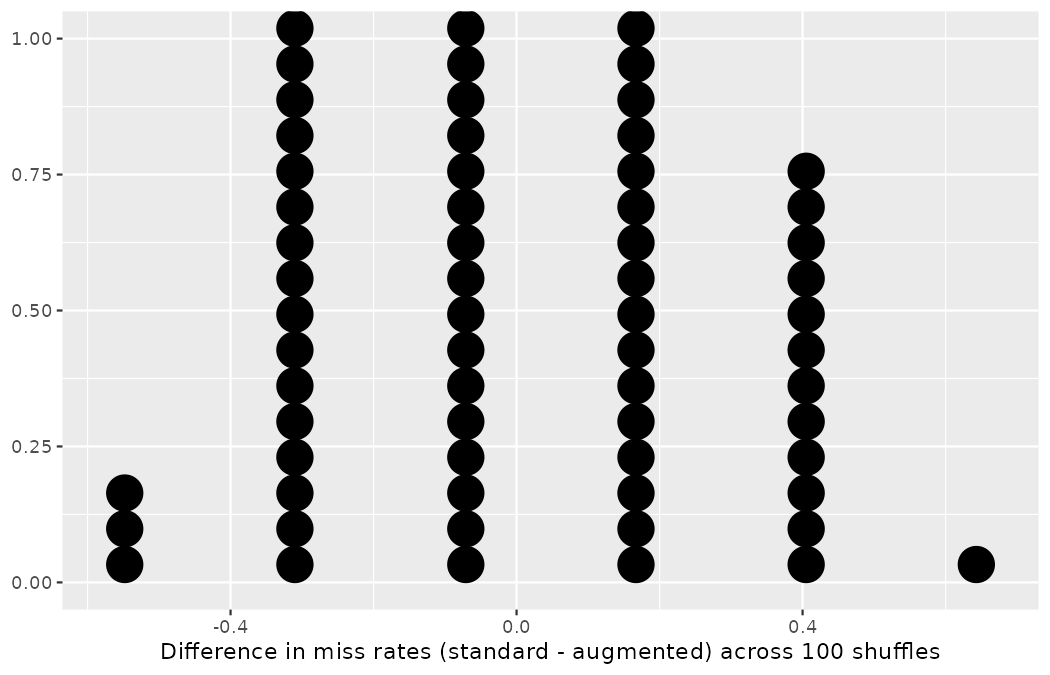
\includegraphics[width=0.85\linewidth,height=\textheight,keepaspectratio]{figures/foundations-applications-1.png}

The 100 dots pile up on just six distinct values, from \(-0.548\) up to
\(0.643.\) That coarseness is no accident: with 6 cards in one stack and
14 in the other, moving a single ``miss'' card between stacks changes
the difference by \(1/6 + 1/14 \approx 0.238,\) so the statistic can
only jump in steps that size. The tallest stacks sit at \(-0.071\) and
\(0.167,\) hugging zero; exactly one of the 100 simulations reached a
difference as large as the observed \(0.643:\)

\begin{Shaded}
\begin{Highlighting}[]
\NormalTok{report20\_null }\SpecialCharTok{|\textgreater{}}
  \FunctionTok{summarize}\NormalTok{(}
    \AttributeTok{n\_extreme =} \FunctionTok{sum}\NormalTok{(stat }\SpecialCharTok{\textgreater{}=} \FloatTok{0.643}\NormalTok{),}
    \AttributeTok{prop\_extreme =} \FunctionTok{mean}\NormalTok{(stat }\SpecialCharTok{\textgreater{}=} \FloatTok{0.643}\NormalTok{)}
\NormalTok{  )}
\CommentTok{\#\textgreater{} \# A tibble: 1 × 2}
\CommentTok{\#\textgreater{}   n\_extreme prop\_extreme}
\CommentTok{\#\textgreater{}       \textless{}int\textgreater{}        \textless{}dbl\textgreater{}}
\CommentTok{\#\textgreater{} 1         1         0.01}
\end{Highlighting}
\end{Shaded}

Note that the distribution of these simulated differences is centered
around 0. We simulated these differences assuming that the independence
model was true, and under this condition, we expect the difference to be
near zero with some random fluctuation, where \emph{near} is pretty
generous in this case since the sample sizes are so small in this study.

\begin{tcolorbox}[enhanced jigsaw, left=2mm, leftrule=.75mm, title=\textcolor{quarto-callout-note-color}{\faInfo}\hspace{0.5em}{Worked example}, arc=.35mm, rightrule=.15mm, coltitle=black, colframe=quarto-callout-note-color-frame, bottomrule=.15mm, colbacktitle=quarto-callout-note-color!10!white, opacitybacktitle=0.6, breakable, bottomtitle=1mm, toptitle=1mm, titlerule=0mm, opacityback=0, toprule=.15mm, colback=white]

How often would you observe a difference of at least 64.3\% \((0.643)\)
according to the simulation we just ran? Often, sometimes, rarely, or
never?

\begin{center}\rule{0.5\linewidth}{0.5pt}\end{center}

It appears that a difference of at least 64.3\% due to chance alone
would only happen about 1\% of the time according to our 100 simulations
--- one shuffle in a hundred reached it. Such a low probability
indicates a rare event. (If you compare against the arithmetic of
Section~\ref{sec-caseStudySexDiscrimination}, where a same-sized
simulation produced 2 extreme shuffles in 100, remember that a count
this small is itself a noisy estimate --- a different seed can easily
return 1, 2, or 3. What no seed will return is 40.)

\end{tcolorbox}

The difference of 64.3\% being a rare event suggests two possible
interpretations of the results of the trial:

\begin{itemize}
\item
  \(H_0\): \textbf{Independence model.} The template has no effect on
  whether a ranking matches the panel, and we just happened to observe a
  difference that would only occur on a rare occasion.
\item
  \(H_A\): \textbf{Alternative model.} The template has an effect on the
  outcome, and the difference we observed was actually due to the
  xG-augmented pages steering the scouts toward the panel's reading of
  the five strikers, which explains the large difference of 64.3\%.
\end{itemize}

Based on the simulations, we have two options. (1) We conclude that the
trial results do not provide strong evidence against the independence
model. That is, we do not have sufficiently strong evidence to conclude
the template had an effect. (2) We conclude the evidence is sufficiently
strong to reject \(H_0\) and assert that the augmented template was
useful. When we conduct formal studies, usually we reject the notion
that we just happened to observe a rare event. So in this case, we
reject the independence model in favor of the alternative: the data
provide strong evidence that the xG-augmented template improved the
scouts' agreement with the expert panel --- and because the template was
randomly assigned, the claim is causal. One honesty about what was
demonstrated, before the conclusion travels: the outcome scored
agreement with the club's own expert panel --- a panel working from the
same derived numbers the augmented template carries --- so the trial
shows the template moves scouts toward Northbridge's reference process,
not that it moves them toward ground truth about the five strikers,
which no panel can certify.

You have, of course, met all of this machinery formally by now, so let
us close the case study in the vocabulary the last four chapters built.
The 1-in-100 count is a p-value of \(0.01\) for the one-sided
alternative we tested; at the customary discernibility level of
\(\alpha = 0.05,\) the result is statistically discernible. Had we
followed the more skeptical two-sided default of
Section~\ref{sec-two-sided-hypotheses} --- Marta should arguably
entertain the possibility that drowning scouts in derived numbers makes
their rankings \emph{worse} --- we would double the tail to
\(2 \times 0.01 = 0.02,\) and the conclusion would survive. And per
Chapter~\ref{sec-foundations-decision-errors}, a rejection is never a
certainty: there remains a small probability that Priya's trial produced
a Type I error, the scouting equivalent of signing a dud --- a
possibility the club controls, but never eliminates, by its choice of
\(\alpha.\)

One field of statistics, statistical inference, is built on evaluating
whether such differences are due to chance. In statistical inference,
data scientists evaluate which model is most reasonable given the data.
Errors do occur, just like rare events, and we might choose the wrong
model. While we do not always choose correctly, statistical inference
gives us tools to control and evaluate how often decision errors occur
--- that was the entire business of
Chapter~\ref{sec-foundations-decision-errors}.

\section{Interactive walkthrough: the foundations, on the second
tournament}\label{sec-foundations-tutorials}

Reading a consolidated recap is not the same as running one. So, as in
Chapter~\ref{sec-data-applications}, here is yours: Priya Rao hands you
the 2025 Women's Euro file and asks you to exercise every foundation
from this part of the book on the second tournament. Work through the
four lessons below at your keyboard; each ends with a question whose
answer follows immediately --- try to answer before you read on. One
frame declaration up front, made once so the lessons need not repeat it:
the Euro logged 913 shots with 123 goals --- an all-shots conversion of
\(123/913 = 0.1347,\) with the tournament's 51 penalty kicks included
--- against \(95/851 = 0.1116\) in the open-play frame; the lessons
below work \emph{open-play} throughout.

\begin{Shaded}
\begin{Highlighting}[]
\NormalTok{weuro2025\_shots }\OtherTok{\textless{}{-}} \FunctionTok{read\_csv}\NormalTok{(}\StringTok{"data/derived/weuro2025\_shots.csv"}\NormalTok{)}

\NormalTok{weuro2025\_shots }\SpecialCharTok{|\textgreater{}}
  \FunctionTok{summarize}\NormalTok{(}\AttributeTok{shots =} \FunctionTok{n}\NormalTok{(), }\AttributeTok{goals =} \FunctionTok{sum}\NormalTok{(goal), }\AttributeTok{conversion =} \FunctionTok{mean}\NormalTok{(goal))}
\CommentTok{\#\textgreater{} \# A tibble: 1 × 3}
\CommentTok{\#\textgreater{}   shots goals conversion}
\CommentTok{\#\textgreater{}   \textless{}int\textgreater{} \textless{}int\textgreater{}      \textless{}dbl\textgreater{}}
\CommentTok{\#\textgreater{} 1   913   123      0.135}

\NormalTok{weuro2025\_shots }\SpecialCharTok{|\textgreater{}}
  \FunctionTok{filter}\NormalTok{(shot\_type }\SpecialCharTok{==} \StringTok{"Penalty"}\NormalTok{) }\SpecialCharTok{|\textgreater{}}
  \FunctionTok{summarize}\NormalTok{(}\AttributeTok{kicks =} \FunctionTok{n}\NormalTok{(), }\AttributeTok{shootout\_kicks =} \FunctionTok{sum}\NormalTok{(period }\SpecialCharTok{==} \DecValTok{5}\NormalTok{))}
\CommentTok{\#\textgreater{} \# A tibble: 1 × 2}
\CommentTok{\#\textgreater{}   kicks shootout\_kicks}
\CommentTok{\#\textgreater{}   \textless{}int\textgreater{}          \textless{}int\textgreater{}}
\CommentTok{\#\textgreater{} 1    51             37}

\NormalTok{weuro\_open }\OtherTok{\textless{}{-}}\NormalTok{ weuro2025\_shots }\SpecialCharTok{|\textgreater{}}
  \FunctionTok{filter}\NormalTok{(shot\_type }\SpecialCharTok{==} \StringTok{"Open Play"}\NormalTok{)}

\NormalTok{weuro\_open }\SpecialCharTok{|\textgreater{}}
  \FunctionTok{summarize}\NormalTok{(}\AttributeTok{shots =} \FunctionTok{n}\NormalTok{(), }\AttributeTok{goals =} \FunctionTok{sum}\NormalTok{(goal), }\AttributeTok{conversion =} \FunctionTok{mean}\NormalTok{(goal))}
\CommentTok{\#\textgreater{} \# A tibble: 1 × 3}
\CommentTok{\#\textgreater{}   shots goals conversion}
\CommentTok{\#\textgreater{}   \textless{}int\textgreater{} \textless{}int\textgreater{}      \textless{}dbl\textgreater{}}
\CommentTok{\#\textgreater{} 1   851    95      0.112}
\end{Highlighting}
\end{Shaded}

\subsection{Lesson 1: sampling
variability}\label{lesson-1-sampling-variability}

Send two scouts to the same tournament and their logs will differ ---
the opening claim of Chapter~\ref{sec-foundations-randomization}, which
you can now watch happen. Give each of two simulated scouts a random
50-shot sample of the Euro's open play:

\begin{Shaded}
\begin{Highlighting}[]
\FunctionTok{set.seed}\NormalTok{(}\DecValTok{1505}\NormalTok{)}
\NormalTok{weuro\_open }\SpecialCharTok{|\textgreater{}}
  \FunctionTok{rep\_slice\_sample}\NormalTok{(}\AttributeTok{n =} \DecValTok{50}\NormalTok{, }\AttributeTok{reps =} \DecValTok{2}\NormalTok{) }\SpecialCharTok{|\textgreater{}}
  \FunctionTok{summarize}\NormalTok{(}\AttributeTok{shots =} \FunctionTok{n}\NormalTok{(), }\AttributeTok{goals =} \FunctionTok{sum}\NormalTok{(goal), }\AttributeTok{p\_hat =} \FunctionTok{mean}\NormalTok{(goal))}
\CommentTok{\#\textgreater{} \# A tibble: 2 × 4}
\CommentTok{\#\textgreater{}   replicate shots goals p\_hat}
\CommentTok{\#\textgreater{}       \textless{}int\textgreater{} \textless{}int\textgreater{} \textless{}int\textgreater{} \textless{}dbl\textgreater{}}
\CommentTok{\#\textgreater{} 1         1    50     6  0.12}
\CommentTok{\#\textgreater{} 2         2    50     5  0.1}
\end{Highlighting}
\end{Shaded}

Scout one reports a conversion of \(0.12,\) scout two reports \(0.10,\)
and the tournament's true open-play figure is \(0.1116.\) Neither scout
is wrong; each holds one draw from the sampling distribution you built
for the World Cup in the recap.

\begin{tcolorbox}[enhanced jigsaw, left=2mm, leftrule=.75mm, title=\textcolor{quarto-callout-tip-color}{\faLightbulb}\hspace{0.5em}{Check your understanding}, arc=.35mm, rightrule=.15mm, coltitle=black, colframe=quarto-callout-tip-color-frame, bottomrule=.15mm, colbacktitle=quarto-callout-tip-color!10!white, opacitybacktitle=0.6, breakable, bottomtitle=1mm, toptitle=1mm, titlerule=0mm, opacityback=0, toprule=.15mm, colback=white]

Name the distribution that each of the following describes: the 851
open-play outcomes; scout one's 50 outcomes; the collection of
\(\hat{p}\) values from every 50-shot sample the tournament could yield.

\begin{center}\rule{0.5\linewidth}{0.5pt}\end{center}

The population distribution (observable here only because we hold a
census of the tournament); a data distribution; the sampling
distribution of \(\hat{p}\) for \(n = 50.\)

\end{tcolorbox}

\subsection{Lesson 2: randomization
test}\label{lesson-2-randomization-test}

Chapter~\ref{sec-foundations-decision-errors} left a test conspicuously
un-run. Its peeking analyst saw first-time shots convert \emph{worse} at
the Euro on all shots --- the reversal that turned out to be 51 penalty
kicks sitting in the controlled-touch bucket --- and we exposed the
artifact without ever testing the honest frame. Do it now, properly:
open-play frame, and the two-sided alternative that discipline demands
when no direction is fixed in advance.

\begin{Shaded}
\begin{Highlighting}[]
\NormalTok{weuro\_open }\SpecialCharTok{|\textgreater{}}
  \FunctionTok{group\_by}\NormalTok{(first\_time) }\SpecialCharTok{|\textgreater{}}
  \FunctionTok{summarize}\NormalTok{(}\AttributeTok{shots =} \FunctionTok{n}\NormalTok{(), }\AttributeTok{goals =} \FunctionTok{sum}\NormalTok{(goal), }\AttributeTok{conversion =} \FunctionTok{mean}\NormalTok{(goal))}
\CommentTok{\#\textgreater{} \# A tibble: 2 × 4}
\CommentTok{\#\textgreater{}   first\_time shots goals conversion}
\CommentTok{\#\textgreater{}   \textless{}lgl\textgreater{}      \textless{}int\textgreater{} \textless{}int\textgreater{}      \textless{}dbl\textgreater{}}
\CommentTok{\#\textgreater{} 1 FALSE        543    57      0.105}
\CommentTok{\#\textgreater{} 2 TRUE         308    38      0.123}
\end{Highlighting}
\end{Shaded}

\begin{itemize}
\tightlist
\item
  \(H_0:\) Among open-play shots at the 2025 Women's Euro,
  \texttt{first\_time} and \texttt{goal} are independent; the observed
  difference of \(38/308 - 57/543 = 0.1234 - 0.1050 = 0.0184\) is
  chance.
\item
  \(H_A:\) The variables are associated (either direction).
\end{itemize}

\begin{Shaded}
\begin{Highlighting}[]
\FunctionTok{set.seed}\NormalTok{(}\DecValTok{1506}\NormalTok{)}
\NormalTok{first\_time\_null }\OtherTok{\textless{}{-}}\NormalTok{ weuro\_open }\SpecialCharTok{|\textgreater{}}
  \FunctionTok{mutate}\NormalTok{(}
    \AttributeTok{timing =} \FunctionTok{if\_else}\NormalTok{(first\_time, }\StringTok{"first time"}\NormalTok{, }\StringTok{"controlled"}\NormalTok{),}
    \AttributeTok{result =} \FunctionTok{if\_else}\NormalTok{(goal, }\StringTok{"goal"}\NormalTok{, }\StringTok{"no goal"}\NormalTok{)}
\NormalTok{  ) }\SpecialCharTok{|\textgreater{}}
  \FunctionTok{specify}\NormalTok{(result }\SpecialCharTok{\textasciitilde{}}\NormalTok{ timing, }\AttributeTok{success =} \StringTok{"goal"}\NormalTok{) }\SpecialCharTok{|\textgreater{}}
  \FunctionTok{hypothesize}\NormalTok{(}\AttributeTok{null =} \StringTok{"independence"}\NormalTok{) }\SpecialCharTok{|\textgreater{}}
  \FunctionTok{generate}\NormalTok{(}\AttributeTok{reps =} \DecValTok{1000}\NormalTok{, }\AttributeTok{type =} \StringTok{"permute"}\NormalTok{) }\SpecialCharTok{|\textgreater{}}
  \FunctionTok{calculate}\NormalTok{(}\AttributeTok{stat =} \StringTok{"diff in props"}\NormalTok{, }\AttributeTok{order =} \FunctionTok{c}\NormalTok{(}\StringTok{"first time"}\NormalTok{, }\StringTok{"controlled"}\NormalTok{)) }\SpecialCharTok{|\textgreater{}}
  \FunctionTok{mutate}\NormalTok{(}\AttributeTok{stat =} \FunctionTok{round}\NormalTok{(stat, }\DecValTok{4}\NormalTok{))}

\NormalTok{first\_time\_null }\SpecialCharTok{|\textgreater{}}
  \FunctionTok{summarize}\NormalTok{(}
    \AttributeTok{n\_extreme  =} \FunctionTok{sum}\NormalTok{(stat }\SpecialCharTok{\textgreater{}=} \FloatTok{0.0184}\NormalTok{),}
    \AttributeTok{right\_tail =} \FunctionTok{mean}\NormalTok{(stat }\SpecialCharTok{\textgreater{}=} \FloatTok{0.0184}\NormalTok{)}
\NormalTok{  )}
\CommentTok{\#\textgreater{} \# A tibble: 1 × 2}
\CommentTok{\#\textgreater{}   n\_extreme right\_tail}
\CommentTok{\#\textgreater{}       \textless{}int\textgreater{}      \textless{}dbl\textgreater{}}
\CommentTok{\#\textgreater{} 1       233      0.233}
\end{Highlighting}
\end{Shaded}

Following the convention of Section~\ref{sec-two-sided-hypotheses},
double the single tail: the two-sided p-value is
\(2 \times 0.233 = 0.466.\) At \(\alpha = 0.05\) --- at any \(\alpha\) a
club would defend --- this is not statistically discernible: shuffled
decks produce a timing gap of 1.8 points nearly half the time. The
complete story of the Euro's first-time ``effect'', told in one breath:
the all-shots reversal was a penalty artifact, and the honest-frame gap
is comfortably within chance. There is, on this evidence, nothing here
--- and saying so crisply is as much a deliverable as any discovery.
Remember, too, what kind of test this was: \texttt{first\_time} is not
assigned by anyone, so even a rejection would have claimed association,
not causation --- this is the permutation-test side of the footnote in
Section~\ref{sec-caseStudySexDiscrimination}.

\subsection{Lesson 3: errors in hypothesis
testing}\label{lesson-3-errors-in-hypothesis-testing}

Lesson 2 ended in a failure to reject, and
Chapter~\ref{sec-foundations-decision-errors} taught you to hold two
thoughts about such a verdict at once.

\begin{tcolorbox}[enhanced jigsaw, left=2mm, leftrule=.75mm, title=\textcolor{quarto-callout-tip-color}{\faLightbulb}\hspace{0.5em}{Check your understanding}, arc=.35mm, rightrule=.15mm, coltitle=black, colframe=quarto-callout-tip-color-frame, bottomrule=.15mm, colbacktitle=quarto-callout-tip-color!10!white, opacitybacktitle=0.6, breakable, bottomtitle=1mm, toptitle=1mm, titlerule=0mm, opacityback=0, toprule=.15mm, colback=white]

\begin{enumerate}
\def\labelenumi{(\alph{enumi})}
\tightlist
\item
  If first-time timing genuinely does move conversion at the margin,
  what kind of error did Lesson 2's test just commit, and what is the
  scouting cost?
\item
  Suppose an analyst had instead peeked at the open-play split, seen
  first-time shots ahead, and run the one-sided test in that direction,
  reporting \(p = 0.233.\) What is wrong with the report?
\end{enumerate}

\begin{center}\rule{0.5\linewidth}{0.5pt}\end{center}

\begin{enumerate}
\def\labelenumi{(\alph{enumi})}
\tightlist
\item
  A Type II error --- the passing-on-a-gem direction of the decision
  table. With a real but modest effect, a test on 851 shots may simply
  lack the power (Section~\ref{sec-pow}) to detect it; ``not
  discernible'' is a verdict about the evidence, never a demonstration
  that \(H_0\) is true. Check complete, the on-field call stands ---
  which is not the same as the call being proven correct.
\item
  The direction was chosen \emph{after} seeing the data. An analyst who
  lets each dataset pick its tail operates at roughly double their
  declared Type I rate --- the \(5\% + 5\% = 10\%\) arithmetic of
  Chapter~\ref{sec-foundations-decision-errors} --- so the honest report
  either fixes the direction before looking or doubles the tail, as we
  did.
\end{enumerate}

\end{tcolorbox}

\subsection{Lesson 4: parameters and confidence
intervals}\label{lesson-4-parameters-and-confidence-intervals}

Testing asks \emph{whether}; estimating asks \emph{how much} --- and the
estimating side of the foundations was
Chapter~\ref{sec-foundations-bootstrapping}'s. Here the census luxury
pays off one last time: the parameter a scout would normally never see,
the Euro's open-play conversion, is known to be \(p = 0.1116,\) so we
can watch a confidence interval try to capture a truth we can verify.
Give a scout a 100-shot random sample and let the bootstrap do its work:

\begin{Shaded}
\begin{Highlighting}[]
\FunctionTok{set.seed}\NormalTok{(}\DecValTok{1507}\NormalTok{)}
\NormalTok{scout\_sample }\OtherTok{\textless{}{-}}\NormalTok{ weuro\_open }\SpecialCharTok{|\textgreater{}}
  \FunctionTok{slice\_sample}\NormalTok{(}\AttributeTok{n =} \DecValTok{100}\NormalTok{)}

\NormalTok{scout\_sample }\SpecialCharTok{|\textgreater{}}
  \FunctionTok{summarize}\NormalTok{(}\AttributeTok{shots =} \FunctionTok{n}\NormalTok{(), }\AttributeTok{goals =} \FunctionTok{sum}\NormalTok{(goal), }\AttributeTok{p\_hat =} \FunctionTok{mean}\NormalTok{(goal))}
\CommentTok{\#\textgreater{} \# A tibble: 1 × 3}
\CommentTok{\#\textgreater{}   shots goals p\_hat}
\CommentTok{\#\textgreater{}   \textless{}int\textgreater{} \textless{}int\textgreater{} \textless{}dbl\textgreater{}}
\CommentTok{\#\textgreater{} 1   100    10   0.1}

\FunctionTok{set.seed}\NormalTok{(}\DecValTok{1508}\NormalTok{)}
\NormalTok{scout\_boot }\OtherTok{\textless{}{-}}\NormalTok{ scout\_sample }\SpecialCharTok{|\textgreater{}}
  \FunctionTok{mutate}\NormalTok{(}\AttributeTok{result =} \FunctionTok{if\_else}\NormalTok{(goal, }\StringTok{"goal"}\NormalTok{, }\StringTok{"no goal"}\NormalTok{)) }\SpecialCharTok{|\textgreater{}}
  \FunctionTok{specify}\NormalTok{(}\AttributeTok{response =}\NormalTok{ result, }\AttributeTok{success =} \StringTok{"goal"}\NormalTok{) }\SpecialCharTok{|\textgreater{}}
  \FunctionTok{generate}\NormalTok{(}\AttributeTok{reps =} \DecValTok{1000}\NormalTok{, }\AttributeTok{type =} \StringTok{"bootstrap"}\NormalTok{) }\SpecialCharTok{|\textgreater{}}
  \FunctionTok{calculate}\NormalTok{(}\AttributeTok{stat =} \StringTok{"prop"}\NormalTok{)}

\NormalTok{scout\_boot }\SpecialCharTok{|\textgreater{}}
  \FunctionTok{summarize}\NormalTok{(}
    \AttributeTok{lower =} \FunctionTok{quantile}\NormalTok{(stat, }\FloatTok{0.025}\NormalTok{),}
    \AttributeTok{upper =} \FunctionTok{quantile}\NormalTok{(stat, }\FloatTok{0.975}\NormalTok{)}
\NormalTok{  )}
\CommentTok{\#\textgreater{} \# A tibble: 1 × 2}
\CommentTok{\#\textgreater{}   lower upper}
\CommentTok{\#\textgreater{}   \textless{}dbl\textgreater{} \textless{}dbl\textgreater{}}
\CommentTok{\#\textgreater{} 1  0.04  0.16}
\end{Highlighting}
\end{Shaded}

The scout's point estimate is \(\hat{p} = 10/100 = 0.10;\) the 95\%
bootstrap percentile interval, read off the middle 95\% of the 1,000
resampled proportions as in Section~\ref{sec-ConfidenceIntervals}, runs
from \(0.04\) to \(0.16.\) This particular interval does capture the
true \(p = 0.1116\) --- and the width is the honest price of 100 shots:
the plausible range spans a factor of four, from set-piece-drought bad
to elite.

\begin{tcolorbox}[enhanced jigsaw, left=2mm, leftrule=.75mm, title=\textcolor{quarto-callout-tip-color}{\faLightbulb}\hspace{0.5em}{Check your understanding}, arc=.35mm, rightrule=.15mm, coltitle=black, colframe=quarto-callout-tip-color-frame, bottomrule=.15mm, colbacktitle=quarto-callout-tip-color!10!white, opacitybacktitle=0.6, breakable, bottomtitle=1mm, toptitle=1mm, titlerule=0mm, opacityback=0, toprule=.15mm, colback=white]

A colleague summarizes the result as ``there is a 95\% chance the Euro's
open-play conversion is between 0.04 and 0.16.'' This tournament's truth
happens to be known --- but restate the correct interpretation for the
usual case where it is not.

\begin{center}\rule{0.5\linewidth}{0.5pt}\end{center}

The confidence is in the \emph{procedure}, not the single interval:
across a career of intervals built this way, about 95\% will capture the
parameter they aim at. Any one interval either captures it or does not
--- this one did --- and the parameter is not a random quantity with a
probability of being anywhere. Recall the interpretation discipline of
Chapter~\ref{sec-foundations-mathematical}.

\end{tcolorbox}

\section{Lab: the corner-kick question, end to
end}\label{sec-foundations-labs}

To further apply the concepts from this part of the book, run one
complete inference --- unguided this time --- on a claim the club has
circled twice already. In Section~\ref{sec-tapperscasestudy}, the
coaching staff's faith in corners collided with a bootstrap interval;
what that chapter never did is \emph{test} the gap. Your materials:

\begin{Shaded}
\begin{Highlighting}[]
\NormalTok{wc2022\_shots }\SpecialCharTok{|\textgreater{}}
  \FunctionTok{mutate}\NormalTok{(}\AttributeTok{possession =} \FunctionTok{if\_else}\NormalTok{(play\_pattern }\SpecialCharTok{==} \StringTok{"From Corner"}\NormalTok{,}
                              \StringTok{"corner possession"}\NormalTok{, }\StringTok{"other possession"}\NormalTok{)) }\SpecialCharTok{|\textgreater{}}
  \FunctionTok{group\_by}\NormalTok{(possession) }\SpecialCharTok{|\textgreater{}}
  \FunctionTok{summarize}\NormalTok{(}\AttributeTok{shots =} \FunctionTok{n}\NormalTok{(), }\AttributeTok{goals =} \FunctionTok{sum}\NormalTok{(goal), }\AttributeTok{conversion =} \FunctionTok{mean}\NormalTok{(goal))}
\CommentTok{\#\textgreater{} \# A tibble: 2 × 4}
\CommentTok{\#\textgreater{}   possession        shots goals conversion}
\CommentTok{\#\textgreater{}   \textless{}chr\textgreater{}             \textless{}int\textgreater{} \textless{}int\textgreater{}      \textless{}dbl\textgreater{}}
\CommentTok{\#\textgreater{} 1 corner possession   223    17     0.0762}
\CommentTok{\#\textgreater{} 2 other possession   1271   178     0.140}
\end{Highlighting}
\end{Shaded}

Work through the full procedure and write up what you find as if
reporting to Marta Vidal:

\begin{enumerate}
\def\labelenumi{\arabic{enumi}.}
\tightlist
\item
  State the parameter of interest and the hypotheses, in symbols and in
  words. Per Section~\ref{sec-two-sided-hypotheses}, default to the
  two-sided alternative --- and if you argue for one-sided, commit to
  the direction \emph{before} step 3.
\item
  Decide which shots belong in the frame, and defend the decision. Two
  traps from earlier chapters apply: recall from
  Chapter~\ref{sec-data-applications} that \texttt{play\_pattern}
  records how the \emph{possession} started, not how the chance was
  created; and recall where this dataset files its penalty kicks ---
  which side of this comparison are they propping up? Rerun the summary
  under \texttt{shot\_type\ ==\ "Open\ Play"} before choosing.
\item
  Run the permutation test with 1,000 shuffles (seed of your choice,
  stated) in \emph{both} frames, penalties in and penalties out, per the
  book's penalty convention. Report both two-sided p-values. Do the two
  frames deliver the same verdict at \(\alpha = 0.05\)? If not, which
  number goes in the report, and what do you say about the other?
\item
  Estimate as well as test: bootstrap a 95\% percentile interval for the
  corner-possession conversion in your chosen frame, and compare it with
  the interval and the coaching-staff intuition of
  Section~\ref{sec-tapperscasestudy}.
\item
  Close the report the way Chapter~\ref{sec-foundations-decision-errors}
  taught: state whether your conclusion is causal or associational and
  why; name the error type you most risk given your verdict; and say
  what it would cost Northbridge --- a dud signed, or a gem passed over.
\end{enumerate}

\section{Chapter review}\label{sec-chp15-review}

\subsection{Summary}\label{summary-14}

This chapter introduced no new methods, no new notation, and no new
vocabulary. Its work was consolidation --- the three inferential engines
of Table~\ref{tbl-foundations-summary}, the five distributions and their
centers, and one randomized trial carried from notecards to a causal
verdict. If any step felt unfamiliar, the place to look is not ahead but
back: Chapter~\ref{sec-foundations-randomization} for the shuffling
logic, Chapter~\ref{sec-foundations-bootstrapping} for the resampling
logic, Chapter~\ref{sec-foundations-mathematical} for the normal
shortcut, and Chapter~\ref{sec-foundations-decision-errors} for what can
go wrong. From the next chapter onward, we put these foundations to work
on the full catalog of scouting questions --- one proportion, two
proportions, means, tables, and models --- and the machinery will
already be in your hands.

\subsection{Terms}\label{terms-14}

No new terms were introduced in this chapter. The terms below did the
consolidation's work; all were introduced and defined in
Chapter~\ref{sec-foundations-randomization} through
Chapter~\ref{sec-foundations-decision-errors}, and you should be able to
recognize each one in the case study and walkthrough above. If any feel
unfamiliar, go back and review their definitions in those chapters.

\begin{longtable}[]{@{}
  >{\raggedright\arraybackslash}p{(\linewidth - 4\tabcolsep) * \real{0.3380}}
  >{\raggedright\arraybackslash}p{(\linewidth - 4\tabcolsep) * \real{0.3380}}
  >{\raggedright\arraybackslash}p{(\linewidth - 4\tabcolsep) * \real{0.3239}}@{}}
\caption{Terms revisited in this
chapter.}\label{tbl-terms-chp-15}\tabularnewline
\toprule\noalign{}
\endfirsthead
\endhead
\bottomrule\noalign{}
\endlastfoot
bootstrap distribution & permutation test & sampling distribution \\
confidence interval & population distribution & standard error \\
data distribution & randomization distribution & Type I error \\
p-value & randomization test & Type II error \\
\end{longtable}

\begin{center}\rule{0.5\linewidth}{0.5pt}\end{center}

Adapted from \emph{Introduction to Modern Statistics} by
Çetinkaya-Rundel \& Hardin (CC BY-SA 4.0); this adaptation is likewise
CC BY-SA 4.0. Match data: StatsBomb open data.

\part{Statistical inference}

\chapter{Inference for a single
proportion}\label{sec-inference-one-prop}

Focusing now on statistical inference for categorical data, we will
revisit many of the foundational aspects of hypothesis testing from
Chapter~\ref{sec-foundations-randomization}.

The three data structures we detail are one binary variable, summarized
using a single proportion; two binary variables, summarized using a
difference of two proportions; and two categorical variables, summarized
using a two-way table. When appropriate, each of the data structures
will be analyzed using the three methods from
Chapter~\ref{sec-foundations-randomization},
Chapter~\ref{sec-foundations-bootstrapping}, and
Chapter~\ref{sec-foundations-mathematical}: randomization test,
bootstrapping, and mathematical models, respectively.

As we build on the inferential ideas, we will visit new foundational
concepts in statistical inference. For example, we will cover the
conditions for when a normal model is appropriate and how to choose the
confidence level for a confidence interval, and we will lean on the two
error rates of Chapter~\ref{sec-foundations-decision-errors} whenever a
verdict is on the line.

We encountered inference methods for a single proportion in
Chapter~\ref{sec-foundations-bootstrapping}, exploring point estimates
and confidence intervals. In this chapter, we'll do a review of these
topics and get a sense of how large a sample must be before the
mathematical shortcuts of Chapter~\ref{sec-foundations-mathematical} can
be trusted in single proportion contexts.

Note that there is only one variable being measured in a study which
focuses on one proportion. For each observational unit, the single
variable is measured as either a success or failure (e.g., ``goal''
vs.~``no goal'', ``report filed on time'' vs.~``late''). Recall the
promise made in a footnote of
Section~\ref{sec-caseStudyOpportunityCost}: a \textbf{success} is simply
the outcome the analysis counts, not necessarily the outcome the club
hopes for --- Northbridge's medical staff may well define ``failing the
injury screen'' as the success in a screening study. Because the nature
of the research question at hand focuses on only a single variable,
there is not a way to randomize the variable across a different
(explanatory) variable. For this reason, we will not use randomization
as an analysis tool when focusing on a single proportion. Instead, we
will apply bootstrapping techniques to test a given hypothesis, and we
will also revisit the associated mathematical models.

\section{Bootstrap test for a proportion}\label{sec-one-prop-null-boot}

The bootstrap simulation concept when \(H_0\) is true is similar to the
ideas used in the case studies presented in
Chapter~\ref{sec-foundations-bootstrapping}, where we bootstrapped
without an assumption about \(H_0.\) Because we will be testing a
hypothesized value of \(p\) (referred to as \(p_0,\) the null value
first met informally in Section~\ref{sec-casemed}), the bootstrap
simulation for hypothesis testing has a fantastic advantage: it can be
used for \emph{any} sample size (a huge benefit for small samples, a
nice alternative for large samples).

The set-piece consultant of Section~\ref{sec-case-study-med-consult} has
already been through the full arc --- interval estimate in
Chapter~\ref{sec-foundations-bootstrapping}, a failed normal
approximation in Section~\ref{sec-casemed}, a doubled p-value in
Section~\ref{sec-two-sided-hypotheses}. In this chapter, a new pitch of
the same species lands on Marta Vidal's desk, and this time the sample
is so small that only the simulation approach survives.

\subsection{Observed data}\label{observed-data-7}

Player agents assemble sales pitches the way set-piece consultants do:
find a striking number, attach your client to it, and let the club fill
in the causality. An agent has approached Marta Vidal marketing her
client, Youssef En-Nesyri, Morocco's centre forward at the 2022 World
Cup. Her claim: ``Put my striker through on goal and he does not miss
--- and he has made Morocco the best one-on-one side in world football.
They scored half their one-on-ones at a World Cup that scores one in
five.'' To be clear about what is real and what is constructed here: the
shots are real --- every number below is computed from the 2022 World
Cup data --- but the agent and her pitch are our invention, built to
give the testing problem a scouting-decision stake, exactly as the
consultant of Section~\ref{sec-case-study-med-consult} was.

Start with the number her whole pitch leans on: the tournament's
one-on-one conversion rate.\footnote{The \texttt{one\_on\_one} flag
  marks shots where the shooter faced only the goalkeeper. As the
  \texttt{shot\_type} breakdown shows, the tag is applied literally: the
  2022 data include 6 penalty kicks and 2 direct corners among the 85
  one-on-ones --- which is precisely why the frame of any ``one-on-one''
  headline number must be inspected before it is quoted.}

\begin{Shaded}
\begin{Highlighting}[]
\FunctionTok{library}\NormalTok{(dplyr)}
\FunctionTok{library}\NormalTok{(tidyr)}
\FunctionTok{library}\NormalTok{(readr)}
\FunctionTok{library}\NormalTok{(ggplot2)}

\NormalTok{wc2022\_shots }\OtherTok{\textless{}{-}} \FunctionTok{read\_csv}\NormalTok{(}\StringTok{"data/derived/wc2022\_shots.csv"}\NormalTok{)}

\NormalTok{wc2022\_shots }\SpecialCharTok{|\textgreater{}}
  \FunctionTok{filter}\NormalTok{(one\_on\_one) }\SpecialCharTok{|\textgreater{}}
  \FunctionTok{summarize}\NormalTok{(}\AttributeTok{shots =} \FunctionTok{n}\NormalTok{(), }\AttributeTok{goals =} \FunctionTok{sum}\NormalTok{(goal), }\AttributeTok{conversion =} \FunctionTok{mean}\NormalTok{(goal))}
\CommentTok{\#\textgreater{} \# A tibble: 1 × 3}
\CommentTok{\#\textgreater{}   shots goals conversion}
\CommentTok{\#\textgreater{}   \textless{}int\textgreater{} \textless{}int\textgreater{}      \textless{}dbl\textgreater{}}
\CommentTok{\#\textgreater{} 1    85    17        0.2}
\end{Highlighting}
\end{Shaded}

Seventeen of the tournament's 85 one-on-ones were scored:
\(17/85 = 0.20,\) the agent's ``one in five.'' But this book's penalty
convention, drilled in since Section~\ref{sec-chp11-pens-out}, demands
one question before that baseline is accepted: \emph{which shots are in
the frame?}

\begin{Shaded}
\begin{Highlighting}[]
\NormalTok{wc2022\_shots }\SpecialCharTok{|\textgreater{}}
  \FunctionTok{filter}\NormalTok{(one\_on\_one) }\SpecialCharTok{|\textgreater{}}
  \FunctionTok{group\_by}\NormalTok{(shot\_type) }\SpecialCharTok{|\textgreater{}}
  \FunctionTok{summarize}\NormalTok{(}\AttributeTok{shots =} \FunctionTok{n}\NormalTok{(), }\AttributeTok{goals =} \FunctionTok{sum}\NormalTok{(goal), }\AttributeTok{conversion =} \FunctionTok{mean}\NormalTok{(goal))}
\CommentTok{\#\textgreater{} \# A tibble: 3 × 4}
\CommentTok{\#\textgreater{}   shot\_type shots goals conversion}
\CommentTok{\#\textgreater{}   \textless{}chr\textgreater{}     \textless{}int\textgreater{} \textless{}int\textgreater{}      \textless{}dbl\textgreater{}}
\CommentTok{\#\textgreater{} 1 Corner        2     0      0}
\CommentTok{\#\textgreater{} 2 Open Play    77    17      0.221}
\CommentTok{\#\textgreater{} 3 Penalty       6     0      0}
\end{Highlighting}
\end{Shaded}

Six of the 85 one-on-ones are penalty kicks, and --- for once --- the
penalty artifact points \emph{downward}: all six were missed, as were
the two direct corners the data also tag as one-on-ones, so stripping
the dead balls out \emph{raises} the baseline, from \(17/85 = 0.200\) to
an open-play rate of \(17/77 = 0.221.\) In
Section~\ref{sec-chp11-pens-out}, penalties propped a conversion rate
up; here they drag one down. The convention is not ``penalties inflate''
--- it is \emph{show the comparison both ways and state the frame you
are using}. We will test against the agent's own quoted baseline,
\(p_0 = 0.20,\) penalties in: it is the tournament's headline one-on-one
rate, and --- because it is the \emph{lower} of the two baselines --- it
is also the easier bar for her claim to clear, so a claim that fails
against \(0.20\) fails against \(0.221\) \emph{a fortiori}. We flag the
open-play rerun at the end of the section.

Now the other half of her pitch. Morocco's one-on-one record is real:

\begin{Shaded}
\begin{Highlighting}[]
\NormalTok{wc2022\_shots }\SpecialCharTok{|\textgreater{}}
  \FunctionTok{filter}\NormalTok{(one\_on\_one, team }\SpecialCharTok{==} \StringTok{"Morocco"}\NormalTok{) }\SpecialCharTok{|\textgreater{}}
  \FunctionTok{summarize}\NormalTok{(}\AttributeTok{shots =} \FunctionTok{n}\NormalTok{(), }\AttributeTok{goals =} \FunctionTok{sum}\NormalTok{(goal), }\AttributeTok{conversion =} \FunctionTok{mean}\NormalTok{(goal))}
\CommentTok{\#\textgreater{} \# A tibble: 1 × 3}
\CommentTok{\#\textgreater{}   shots goals conversion}
\CommentTok{\#\textgreater{}   \textless{}int\textgreater{} \textless{}int\textgreater{}      \textless{}dbl\textgreater{}}
\CommentTok{\#\textgreater{} 1     6     3        0.5}
\end{Highlighting}
\end{Shaded}

Morocco took 6 one-on-ones (all of them open play --- no penalties to
argue about on this side of the comparison) and scored 3:
\(\hat{p} = 3/6 = 0.50,\) against a tournament that scored at \(0.20.\)
So far the pitch checks out arithmetically. But look at who took them:

\begin{Shaded}
\begin{Highlighting}[]
\NormalTok{wc2022\_shots }\SpecialCharTok{|\textgreater{}}
  \FunctionTok{filter}\NormalTok{(one\_on\_one, team }\SpecialCharTok{==} \StringTok{"Morocco"}\NormalTok{) }\SpecialCharTok{|\textgreater{}}
  \FunctionTok{count}\NormalTok{(player)}
\CommentTok{\#\textgreater{} \# A tibble: 5 × 2}
\CommentTok{\#\textgreater{}   player                n}
\CommentTok{\#\textgreater{}   \textless{}chr\textgreater{}             \textless{}int\textgreater{}}
\CommentTok{\#\textgreater{} 1 Achraf Dari           1}
\CommentTok{\#\textgreater{} 2 Noussair Mazraoui     1}
\CommentTok{\#\textgreater{} 3 Romain Saïss          1}
\CommentTok{\#\textgreater{} 4 Youssef En{-}Nesyri     2}
\CommentTok{\#\textgreater{} 5 Zakaria Aboukhlal     1}
\end{Highlighting}
\end{Shaded}

The six one-on-ones belong to five different players. The agent's client
took exactly two of them (scoring one) --- his personal tournament
record is 2 goals from 11 shots in total, far too few shots of any kind
to test anything about him individually. The number her pitch actually
rests on is a \emph{team} statistic.

\begin{tcolorbox}[enhanced jigsaw, left=2mm, leftrule=.75mm, title=\textcolor{quarto-callout-note-color}{\faInfo}\hspace{0.5em}{Worked example}, arc=.35mm, rightrule=.15mm, coltitle=black, colframe=quarto-callout-note-color-frame, bottomrule=.15mm, colbacktitle=quarto-callout-note-color!10!white, opacitybacktitle=0.6, breakable, bottomtitle=1mm, toptitle=1mm, titlerule=0mm, opacityback=0, toprule=.15mm, colback=white]

Using the data, is it possible to assess the agent's claim that her
striker lifts a team's one-on-one finishing above tournament level?

\begin{center}\rule{0.5\linewidth}{0.5pt}\end{center}

No. The claim is that there is a causal connection, but the data are
observational --- nobody randomly assigned strikers to teams. And in
this case the attribution problem is visible in the data before we even
reach for the confounding argument of Chapter~\ref{sec-data-design}: her
client took only two of the six one-on-ones that make up ``Morocco's''
record, so the statistic she quotes measures an attacking unit of five
players (and the chances the tournament happened to serve them), not her
striker.

While it is not possible to assess the causal claim, it is still
possible to test for an association using these data. For this question
we ask, could the high conversion rate of \(\hat{p} = 0.50\) have simply
occurred by chance, if Morocco's true one-on-one conversion rate does
not differ from the tournament baseline?

\end{tcolorbox}

\begin{tcolorbox}[enhanced jigsaw, left=2mm, leftrule=.75mm, title=\textcolor{quarto-callout-tip-color}{\faLightbulb}\hspace{0.5em}{Check your understanding}, arc=.35mm, rightrule=.15mm, coltitle=black, colframe=quarto-callout-tip-color-frame, bottomrule=.15mm, colbacktitle=quarto-callout-tip-color!10!white, opacitybacktitle=0.6, breakable, bottomtitle=1mm, toptitle=1mm, titlerule=0mm, opacityback=0, toprule=.15mm, colback=white]

Write out hypotheses in both plain and statistical language to test for
the association between Morocco's one-on-one finishing and the true
one-on-one conversion rate, \(p,\) for the process generating Morocco's
one-on-ones.

\begin{center}\rule{0.5\linewidth}{0.5pt}\end{center}

\(H_0:\) There is nothing special about Morocco's one-on-one finishing;
the team converts one-on-ones at the tournament baseline. In statistical
language, \(p = 0.20.\) \(H_A:\) Morocco's one-on-ones are converted at
a rate higher than the tournament's 20\%, i.e., \(p > 0.20.\)

\end{tcolorbox}

Because, as it turns out, the conditions for working with the normal
distribution are not met (see Section~\ref{sec-one-prop-norm}), the
uncertainty associated with the sample proportion should not be modeled
using the normal distribution, as doing so would misrepresent the
uncertainty associated with the sample statistic. However, we would
still like to assess the hypotheses from the previous Check your
understanding in absence of the normal framework. To do so, we need to
evaluate the possibility of a sample value \((\hat{p})\) as far
\emph{above} the null value, \(p_0 = 0.20,\) as what was observed. The
deviation of the sample value from the hypothesized parameter is usually
quantified with a p-value.

The p-value is computed based on the null distribution, which is the
distribution of the test statistic if the null hypothesis is true.
Supposing the null hypothesis is true, we can compute the p-value by
identifying the probability of observing a test statistic that favors
the alternative hypothesis at least as strongly as the observed test
statistic. Here we will use a bootstrap simulation to calculate the
p-value.

\subsection{Variability of the
statistic}\label{variability-of-the-statistic-7}

We want to identify the sampling distribution of the test statistic
\((\hat{p})\) if the null hypothesis was true. In other words, we want
to see the variability we can expect from sample proportions if the null
hypothesis was true. Then we plan to use this information to decide
whether there is enough evidence to reject the null hypothesis.

Under the null hypothesis, 20\% of one-on-ones are scored. Suppose this
rate was really no different for Morocco --- for the whole process
generating Morocco's one-on-one chances, not just the 6 the tournament
happened to produce. If this was the case, we could \emph{simulate} 6
one-on-ones to get a sample proportion for the conversion rate from the
null distribution. Simulating observations using a hypothesized null
parameter value is often called a \textbf{parametric bootstrap
simulation}, but we will refer to it descriptively as ``simulating under
the null hypothesis claim.''

\begin{tcolorbox}[enhanced jigsaw, left=2mm, leftrule=.75mm, title=\textcolor{quarto-callout-tip-color}{\faLightbulb}\hspace{0.5em}{Check your understanding}, arc=.35mm, rightrule=.15mm, coltitle=black, colframe=quarto-callout-tip-color-frame, bottomrule=.15mm, colbacktitle=quarto-callout-tip-color!10!white, opacitybacktitle=0.6, breakable, bottomtitle=1mm, toptitle=1mm, titlerule=0mm, opacityback=0, toprule=.15mm, colback=white]

In Chapter~\ref{sec-foundations-bootstrapping}, the bootstrap resampled
the observed shots themselves; here the simulated shots will instead be
drawn using the null value \(p_0 = 0.20.\) Why can't we resample
Morocco's six observed one-on-ones to build the distribution a
hypothesis test needs? And what does the center of each kind of
distribution tell you?

\begin{center}\rule{0.5\linewidth}{0.5pt}\end{center}

A hypothesis test asks how surprising the observed \(\hat{p}\) would be
\emph{in the null hypothesis's world}, so the simulated data must be
generated with the null's success probability: the resulting null
distribution is centered at \(p_0 = 0.20.\) Resampling the observed data
can only ever reproduce the world of the data --- a bootstrap
distribution centered near \(\hat{p} = 0.50\) --- which is exactly what
\emph{estimation} wants (it shows how far sample proportions wander from
the one observed, giving an interval for \(p\)), but it can never say
how rare \(\hat{p} = 0.50\) would be if \(p\) were really \(0.20.\) The
two centers name the two jobs: bootstrap distributions center at the
estimate and serve confidence intervals; null distributions center at
\(p_0\) and serve tests.

\end{tcolorbox}

Similar to the process described in
Chapter~\ref{sec-foundations-bootstrapping}, each one-on-one can be
simulated using a bag of marbles with 20\% red marbles and 80\% white
marbles. Sampling a marble from the bag (with 20\% red marbles) is one
way of simulating whether a chance is scored \emph{if the true
conversion rate is 20\%} --- and, as the corner-kick case study of
Section~\ref{sec-tapperscasestudy} showed, \texttt{rbinom()} performs
exactly these draws for us. If we draw 6 marbles and then compute the
proportion of simulated one-on-ones that were scored, the resulting
sample proportion is a sample from the null distribution.

This simulated statistic gets its own symbol, and since the notation is
new, take it apart before using it: in \(\hat{p}_{sim},\) the letter
\(p\) names a proportion; the hat says it was computed from data rather
than known (recall Chapter~\ref{sec-foundations-randomization}); and the
subscript \(sim\) says the data it was computed from are a
\emph{simulated} sample, drawn under the null hypothesis claim, rather
than a sample anyone observed. Where several simulations need telling
apart, we number them: \(\hat{p}_{sim1}\) is the proportion from the
first simulated sample.

\begin{Shaded}
\begin{Highlighting}[]
\FunctionTok{set.seed}\NormalTok{(}\DecValTok{1602}\NormalTok{)}
\FunctionTok{rbinom}\NormalTok{(}\DecValTok{1}\NormalTok{, }\DecValTok{6}\NormalTok{, }\FloatTok{0.20}\NormalTok{)}
\CommentTok{\#\textgreater{} [1] 0}
\end{Highlighting}
\end{Shaded}

The first simulated set of six one-on-ones produced no goals at all:
\(\hat{p}_{sim1} = 0/6 = 0.\) One redraw of the same six chances swung
the conversion rate from the \(0.50\) Morocco posted to \(0.00\) --- a
first hint of how violently proportions computed from six observations
can swing.

\begin{tcolorbox}[enhanced jigsaw, left=2mm, leftrule=.75mm, title=\textcolor{quarto-callout-note-color}{\faInfo}\hspace{0.5em}{Worked example}, arc=.35mm, rightrule=.15mm, coltitle=black, colframe=quarto-callout-note-color-frame, bottomrule=.15mm, colbacktitle=quarto-callout-note-color!10!white, opacitybacktitle=0.6, breakable, bottomtitle=1mm, toptitle=1mm, titlerule=0mm, opacityback=0, toprule=.15mm, colback=white]

Is this one simulation enough to determine whether we should reject the
null hypothesis?

\begin{center}\rule{0.5\linewidth}{0.5pt}\end{center}

No. To assess the hypotheses, we need to see a distribution of many
values of \(\hat{p}_{sim},\) not just a \emph{single} draw from this
sampling distribution.

\end{tcolorbox}

\subsection{Observed statistic vs.~null
statistics}\label{observed-statistic-vs.-null-statistics-4}

One simulation isn't enough to get a sense of the null distribution;
many simulation studies are needed. Roughly 10,000 seems sufficient.
However, paying someone to draw 60,000 marbles by hand is a waste of
Marta's budget. Instead, simulations are typically programmed into a
computer, which is much more efficient. The code below re-runs the same
seeded stream, this time asking for all 10,000 simulated six-shot sets
at once (so the first simulation is the same 0-goal set you just
watched), and tabulates the results.

\begin{Shaded}
\begin{Highlighting}[]
\FunctionTok{set.seed}\NormalTok{(}\DecValTok{1602}\NormalTok{)}
\NormalTok{one\_on\_one\_sim }\OtherTok{\textless{}{-}} \FunctionTok{tibble}\NormalTok{(}\AttributeTok{p\_sim =} \FunctionTok{rbinom}\NormalTok{(}\DecValTok{10000}\NormalTok{, }\DecValTok{6}\NormalTok{, }\FloatTok{0.20}\NormalTok{) }\SpecialCharTok{/} \DecValTok{6}\NormalTok{)}

\NormalTok{one\_on\_one\_sim }\SpecialCharTok{|\textgreater{}}
  \FunctionTok{count}\NormalTok{(p\_sim)}
\CommentTok{\#\textgreater{} \# A tibble: 7 × 2}
\CommentTok{\#\textgreater{}   p\_sim     n}
\CommentTok{\#\textgreater{}   \textless{}dbl\textgreater{} \textless{}int\textgreater{}}
\CommentTok{\#\textgreater{} 1 0      2513}
\CommentTok{\#\textgreater{} 2 0.167  3939}
\CommentTok{\#\textgreater{} 3 0.333  2545}
\CommentTok{\#\textgreater{} 4 0.5     817}
\CommentTok{\#\textgreater{} 5 0.667   171}
\CommentTok{\#\textgreater{} 6 0.833    13}
\CommentTok{\#\textgreater{} 7 1         2}
\end{Highlighting}
\end{Shaded}

With only 6 shots per simulation, \(\hat{p}_{sim}\) can take just seven
values, \(0/6\) through \(6/6.\) The histogram below shows the results
of the 10,000 simulated records; the proportions that are equal to or
greater than \(\hat{p} = 0.50\) represent sample proportions under the
null distribution that provide at least as much evidence as \(\hat{p}\)
favoring the alternative hypothesis.

\begin{Shaded}
\begin{Highlighting}[]
\FunctionTok{ggplot}\NormalTok{(one\_on\_one\_sim, }\FunctionTok{aes}\NormalTok{(}\AttributeTok{x =}\NormalTok{ p\_sim)) }\SpecialCharTok{+}
  \FunctionTok{geom\_histogram}\NormalTok{(}\AttributeTok{binwidth =} \DecValTok{1} \SpecialCharTok{/} \DecValTok{6}\NormalTok{, }\AttributeTok{center =} \DecValTok{0}\NormalTok{) }\SpecialCharTok{+}
  \FunctionTok{annotate}\NormalTok{(}\StringTok{"segment"}\NormalTok{, }\AttributeTok{x =} \FloatTok{0.5}\NormalTok{, }\AttributeTok{xend =} \FloatTok{0.5}\NormalTok{, }\AttributeTok{y =} \DecValTok{0}\NormalTok{, }\AttributeTok{yend =} \DecValTok{4200}\NormalTok{,}
           \AttributeTok{linetype =} \StringTok{"dashed"}\NormalTok{) }\SpecialCharTok{+}
  \FunctionTok{annotate}\NormalTok{(}\StringTok{"text"}\NormalTok{, }\AttributeTok{x =} \FloatTok{0.5}\NormalTok{, }\AttributeTok{y =} \DecValTok{4500}\NormalTok{, }\AttributeTok{label =} \StringTok{"observed}\SpecialCharTok{\textbackslash{}n}\StringTok{conversion"}\NormalTok{) }\SpecialCharTok{+}
  \FunctionTok{labs}\NormalTok{(}
    \AttributeTok{x =} \StringTok{"Simulated conversion rate from 6 one{-}on{-}ones when the null hypothesis is true"}\NormalTok{,}
    \AttributeTok{y =} \StringTok{"Number of simulated scenarios"}
\NormalTok{  )}
\end{Highlighting}
\end{Shaded}

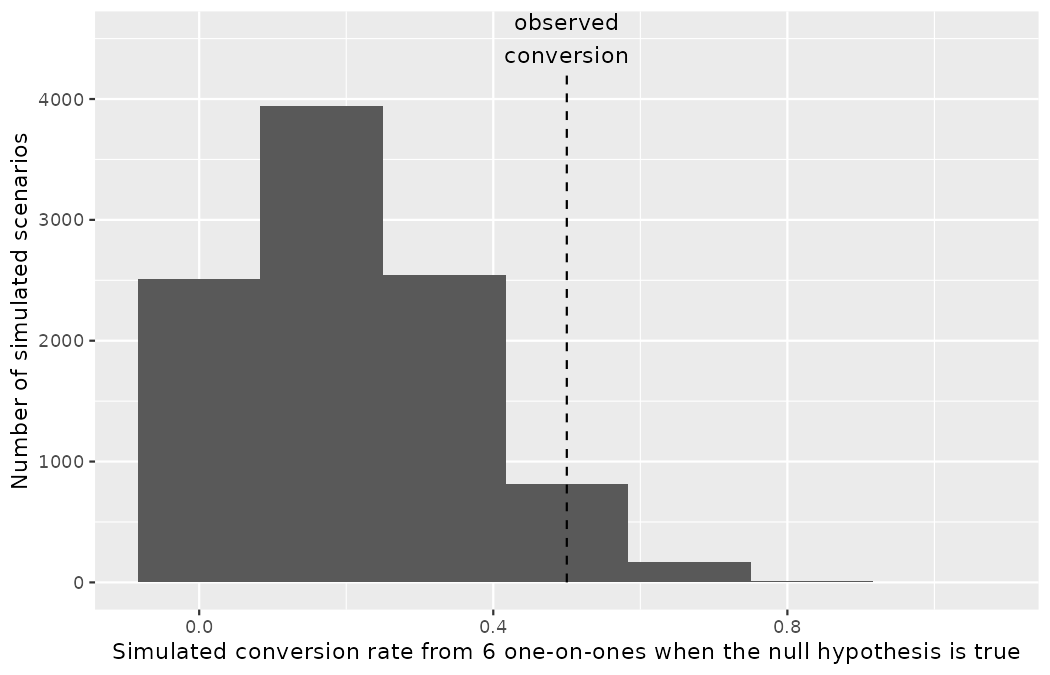
\includegraphics[width=0.85\linewidth,height=\textheight,keepaspectratio]{figures/inference-one-prop-1.png}

The figure shows seven bars, one per attainable value of
\(\hat{p}_{sim}\): heights 2,513 at \(0,\) 3,939 at \(1/6,\) 2,545 at
\(2/6,\) then a fast collapse --- 817 at \(3/6,\) 171 at \(4/6,\) 13 at
\(5/6,\) and just 2 simulated records in 10,000 in which all six were
scored. The dashed line marks the observed \(\hat{p} = 0.50,\) and
everything at or to the right of it is the region favoring the
alternative hypothesis.

\begin{Shaded}
\begin{Highlighting}[]
\NormalTok{one\_on\_one\_sim }\SpecialCharTok{|\textgreater{}}
  \FunctionTok{summarize}\NormalTok{(}
    \AttributeTok{n\_extreme =} \FunctionTok{sum}\NormalTok{(p\_sim }\SpecialCharTok{\textgreater{}=} \FloatTok{0.5}\NormalTok{),}
    \AttributeTok{p\_value   =} \FunctionTok{mean}\NormalTok{(p\_sim }\SpecialCharTok{\textgreater{}=} \FloatTok{0.5}\NormalTok{)}
\NormalTok{  )}
\CommentTok{\#\textgreater{} \# A tibble: 1 × 2}
\CommentTok{\#\textgreater{}   n\_extreme p\_value}
\CommentTok{\#\textgreater{}       \textless{}int\textgreater{}   \textless{}dbl\textgreater{}}
\CommentTok{\#\textgreater{} 1      1003   0.100}
\end{Highlighting}
\end{Shaded}

There were 1,003 simulated sample proportions with
\(\hat{p}_{sim} \geq 0.50.\) We use these to construct the null
distribution's right-tail area and find the p-value:

\[\text{right tail area} = \frac{\text{Number of observed simulations with }\hat{p}_{sim} \geq 0.50}{10000}\]

One new piece of notation makes tail statements like this compact, and
it will follow us for the rest of the book, so take it apart on first
use. We write \(P(\hat{p}_{sim} \geq 0.50)\) for the quantity just
described: the capital letter \(P\) names a \emph{probability}; the
parentheses hold an \emph{event} --- a statement that can come true or
not, here ``a simulated sample proportion lands at 0.50 or above''; and
the whole expression reads ``the probability that \(\hat{p}_{sim}\) is
at least \(0.50.\)'' Our 10,000 simulations estimate this probability as

\[P(\hat{p}_{sim} \geq 0.50) \approx \frac{1003}{10000} = 0.1003\]

Since the hypothesis test is one-sided, the estimated p-value is equal
to this tail area: \(0.100.\)

\begin{tcolorbox}[enhanced jigsaw, left=2mm, leftrule=.75mm, title=\textcolor{quarto-callout-tip-color}{\faLightbulb}\hspace{0.5em}{Check your understanding}, arc=.35mm, rightrule=.15mm, coltitle=black, colframe=quarto-callout-tip-color-frame, bottomrule=.15mm, colbacktitle=quarto-callout-tip-color!10!white, opacitybacktitle=0.6, breakable, bottomtitle=1mm, toptitle=1mm, titlerule=0mm, opacityback=0, toprule=.15mm, colback=white]

Because the estimated p-value is \(0.100,\) which is larger than the
discernibility level \(0.05,\) we cannot reject the null hypothesis.
Explain what this means in plain language in the context of the problem.

\begin{center}\rule{0.5\linewidth}{0.5pt}\end{center}

There is not enough evidence to reject the null hypothesis in favor of
the alternative hypothesis. We cannot conclude that there is evidence
that Morocco's true one-on-one conversion rate is higher than the
tournament's 20\% baseline. That said, we also cannot conclude that
there is evidence that it is \emph{lower} than 20\%. When the p-value is
larger than the discernibility level, we are unable to make conclusions
about the research statement --- a 3-of-6 record simply cannot separate
``best one-on-one side in world football'' from ``ordinary side that got
six chances and a coin's worth of luck.''

\end{tcolorbox}

\begin{tcolorbox}[enhanced jigsaw, left=2mm, leftrule=.75mm, title=\textcolor{quarto-callout-tip-color}{\faLightbulb}\hspace{0.5em}{Check your understanding}, arc=.35mm, rightrule=.15mm, coltitle=black, colframe=quarto-callout-tip-color-frame, bottomrule=.15mm, colbacktitle=quarto-callout-tip-color!10!white, opacitybacktitle=0.6, breakable, bottomtitle=1mm, toptitle=1mm, titlerule=0mm, opacityback=0, toprule=.15mm, colback=white]

Does the conclusion in the previous Check your understanding imply that
the agent's striker is \emph{not} an elite one-on-one finisher? Explain.

\begin{center}\rule{0.5\linewidth}{0.5pt}\end{center}

Not at all. There is no evidence to make a claim in either direction, so
we cannot make any claims about the striker --- and recall that
Morocco's team record was never a clean measurement of him in the first
place: he took two of the six chances. What the analysis does license
Marta to say is that the agent's headline number carries no statistical
weight, which is a different (and, for a negotiation, very useful)
statement.

\end{tcolorbox}

\begin{tcolorbox}[enhanced jigsaw, left=2mm, leftrule=.75mm, title=\textcolor{quarto-callout-important-color}{\faExclamation}\hspace{0.5em}{Null distribution of \(\hat{p}\) with bootstrap simulation}, arc=.35mm, rightrule=.15mm, coltitle=black, colframe=quarto-callout-important-color-frame, bottomrule=.15mm, colbacktitle=quarto-callout-important-color!10!white, opacitybacktitle=0.6, breakable, bottomtitle=1mm, toptitle=1mm, titlerule=0mm, opacityback=0, toprule=.15mm, colback=white]

Regardless of the statistical method chosen, the p-value is always
derived by analyzing the null distribution of the test statistic. The
normal model poorly approximates the null distribution for \(\hat{p}\)
(the sample proportion) when the success-failure condition is not
satisfied. As a substitute, we can generate the null distribution using
simulated sample proportions and use this distribution to compute the
tail area, i.e., the p-value.

\end{tcolorbox}

In the previous Check your understanding, the p-value is
\emph{estimated}. It is not exact, because the simulated null
distribution itself is only a close approximation of the sampling
distribution of the sample statistic. An exact p-value can be generated
using the binomial distribution --- the computation
\texttt{binom.test()} performed in its cameo in
Section~\ref{sec-two-sided-hypotheses} --- and here the exact and
simulated answers agree closely. The same one-line computation also
discharges the penalty-convention flag raised at the top of this
section: rerunning the test against the open-play baseline of
\(17/77 = 0.221,\) the like-for-like frame for Morocco's six open-play
chances, moves the verdict \emph{further} from the bar, exactly as
promised.

\begin{Shaded}
\begin{Highlighting}[]
\DecValTok{1} \SpecialCharTok{{-}} \FunctionTok{pbinom}\NormalTok{(}\DecValTok{2}\NormalTok{, }\DecValTok{6}\NormalTok{, }\DecValTok{17} \SpecialCharTok{/} \DecValTok{85}\NormalTok{)}
\CommentTok{\#\textgreater{} [1] 0.09888}

\DecValTok{1} \SpecialCharTok{{-}} \FunctionTok{pbinom}\NormalTok{(}\DecValTok{2}\NormalTok{, }\DecValTok{6}\NormalTok{, }\DecValTok{17} \SpecialCharTok{/} \DecValTok{77}\NormalTok{)}
\CommentTok{\#\textgreater{} [1] 0.1260401}
\end{Highlighting}
\end{Shaded}

Against \(p_0 = 0.20\) the exact p-value is \(0.099\) (our simulation
said \(0.100\)); against the open-play baseline it is \(0.126.\)
Penalties in or penalties out, the agent's number does not clear any bar
in use --- and the report to Marta should say so in both frames.

\section{Mathematical model for a proportion}\label{sec-one-prop-norm}

\subsection{Conditions}\label{conditions}

In Section~\ref{sec-normalDist}, we introduced the normal distribution
and showed how it can be used as a mathematical model to describe the
variability of a statistic. There are conditions under which a sample
proportion \(\hat{p}\) is well modeled with a normal distribution. When
the observations are independent and the sample size is sufficiently
large, the normal model will describe the sampling distribution of the
sample proportion quite well; when the observations violate the
conditions, the normal model can be inaccurate --- as the set-piece
consultant case study of Section~\ref{sec-casemed} demonstrated at some
cost to the analyst's pride. Particularly, it can underestimate the
variability of the sample proportion.

\begin{tcolorbox}[enhanced jigsaw, left=2mm, leftrule=.75mm, title=\textcolor{quarto-callout-important-color}{\faExclamation}\hspace{0.5em}{Sampling distribution of \(\hat{p}\)}, arc=.35mm, rightrule=.15mm, coltitle=black, colframe=quarto-callout-important-color-frame, bottomrule=.15mm, colbacktitle=quarto-callout-important-color!10!white, opacitybacktitle=0.6, breakable, bottomtitle=1mm, toptitle=1mm, titlerule=0mm, opacityback=0, toprule=.15mm, colback=white]

The sampling distribution for \(\hat{p}\) (the sample proportion) based
on a sample of size \(n\) from a population with a true proportion \(p\)
is nearly normal when:

\begin{enumerate}
\def\labelenumi{\arabic{enumi}.}
\tightlist
\item
  The sample's observations are independent, e.g., are from a simple
  random sample.
\item
  We expected to see at least 10 successes and 10 failures in the
  sample, i.e., \(np \geq 10\) and \(n(1-p) \geq 10.\) This is called
  the \textbf{success-failure condition}.
\end{enumerate}

When these conditions are met, then the sampling distribution of
\(\hat{p}\) is nearly normal with mean \(p\) and standard error of
\(\hat{p}\) as \(SE = \sqrt{\frac{\ \hat{p}(1-\hat{p})\ }{n}}.\)

\end{tcolorbox}

The formula for the standard error deserves a symbol-by-symbol reading
before we put it to work, because it will be substituted into constantly
for the rest of the book. In

\[SE(\hat{p}) = \sqrt{\frac{p(1-p)}{n}}\]

the notation \(SE(\cdot)\) reads ``the standard error of whatever sits
inside the parentheses'' --- here, of the sample proportion \(\hat{p}\)
(recall from Section~\ref{sec-se} that a standard error is the standard
deviation of a statistic). Inside the square root, the numerator
\(p(1-p)\) multiplies the success probability by the failure
probability: this product is largest when \(p = 0.5\) and shrinks toward
zero as \(p\) approaches either \(0\) or \(1,\) encoding the fact that
proportions near the boundaries barely have room to vary. The
denominator \(n\) is the sample size: more observations, less
sample-to-sample variability. And the square root returns the whole
quantity to the scale of a proportion, just as taking \(\sigma\) rather
than \(\sigma^2\) did in Chapter~\ref{sec-explore-numerical}.

Recall from Section~\ref{sec-moe} that the margin of error is defined by
the standard error. The margin of error for \(\hat{p}\) can be directly
obtained from \(SE(\hat{p}).\)

\begin{tcolorbox}[enhanced jigsaw, left=2mm, leftrule=.75mm, title=\textcolor{quarto-callout-important-color}{\faExclamation}\hspace{0.5em}{Margin of error for \(\hat{p}\)}, arc=.35mm, rightrule=.15mm, coltitle=black, colframe=quarto-callout-important-color-frame, bottomrule=.15mm, colbacktitle=quarto-callout-important-color!10!white, opacitybacktitle=0.6, breakable, bottomtitle=1mm, toptitle=1mm, titlerule=0mm, opacityback=0, toprule=.15mm, colback=white]

The margin of error is
\(z^\star \times \sqrt{\frac{\ \hat{p}(1-\hat{p})\ }{n}}\) where
\(z^\star\) is calculated from a specified percentile on the normal
distribution.

\end{tcolorbox}

Typically we do not know the true proportion \(p,\) so we substitute
some value to check conditions and estimate the standard error. For
confidence intervals, the sample proportion \(\hat{p}\) is used to check
the success-failure condition and compute the standard error. For
hypothesis tests, typically the null value --- that is, the proportion
claimed in the null hypothesis --- is used in place of \(p.\) This null
value now gets its formal introduction, having worked informally since
Section~\ref{sec-casemed}: we write \(p_0,\) read ``p-nought,'' where
the letter \(p\) names a population proportion and the subscript \(0\)
is the same nought that marks the null hypothesis \(H_0.\) Formally,
\(p_0\) is the value that \(H_0\) asserts for \(p\) --- the number the
null world is built from --- and in that world it is the best available
guess of \(p,\) which is why it, and not \(\hat{p},\) is what a
hypothesis test substitutes into the standard error formula and the
success-failure check.

The independence condition is a more nuanced requirement. When it isn't
met, it is important to understand how and why it is violated. For
example, there exist no statistical methods available to truly correct
the inherent biases of a scout's log built from agent-submitted
highlight clips --- a convenience sample, in the language of
Chapter~\ref{sec-data-design}. On the other hand, if Emil's scouts could
only attend a cluster sample of matches (see
Section~\ref{sec-samp-methods}), the shots they logged wouldn't be
independent, but suitable statistical methods are available for
analyzing such data (though they are beyond the scope of even most
second or third courses in statistics).

\begin{tcolorbox}[enhanced jigsaw, left=2mm, leftrule=.75mm, title=\textcolor{quarto-callout-note-color}{\faInfo}\hspace{0.5em}{Worked example}, arc=.35mm, rightrule=.15mm, coltitle=black, colframe=quarto-callout-note-color-frame, bottomrule=.15mm, colbacktitle=quarto-callout-note-color!10!white, opacitybacktitle=0.6, breakable, bottomtitle=1mm, toptitle=1mm, titlerule=0mm, opacityback=0, toprule=.15mm, colback=white]

In the examples based on large sample theory, we modeled \(\hat{p}\)
using the normal distribution. Why is this not appropriate for the case
study on Morocco's one-on-ones?

\begin{center}\rule{0.5\linewidth}{0.5pt}\end{center}

The independence assumption may be tolerable: the six one-on-ones arose
in different passages of play across five different matches. However,
the success-failure condition is not satisfied. Under the null
hypothesis, we would anticipate seeing \(6 \times 0.20 = 1.2\) goals ---
spectacularly short of the 10 required for the normal approximation.
Where England's 63 shots in Section~\ref{sec-casemed} missed the bar
narrowly \((8.2 < 10)\) and the normal shortcut quietly flipped the
verdict, six shots do not even reach the discussion.

\end{tcolorbox}

While this book is scoped to well-constrained statistical problems, do
remember that this is just the first book in what is a large library of
statistical methods that are suitable for a very wide range of data and
contexts.

\subsection{Confidence interval for a
proportion}\label{confidence-interval-for-a-proportion}

A confidence interval provides a range of plausible values for the
parameter \(p,\) and when \(\hat{p}\) can be modeled using a normal
distribution, the confidence interval for \(p\) takes the form

\[\hat{p} \pm z^{\star} \times SE.\]

We have seen \(\hat{p}\) to be the sample proportion. The value
\(z^{\star}\) determines the confidence level (previously fixed at
\(1.96\) in Section~\ref{sec-moe}) and will be discussed in detail in
the examples following. The value of the standard error, \(SE,\) depends
heavily on the sample size.

\begin{tcolorbox}[enhanced jigsaw, left=2mm, leftrule=.75mm, title=\textcolor{quarto-callout-important-color}{\faExclamation}\hspace{0.5em}{Standard error of one proportion, \(\hat{p}\)}, arc=.35mm, rightrule=.15mm, coltitle=black, colframe=quarto-callout-important-color-frame, bottomrule=.15mm, colbacktitle=quarto-callout-important-color!10!white, opacitybacktitle=0.6, breakable, bottomtitle=1mm, toptitle=1mm, titlerule=0mm, opacityback=0, toprule=.15mm, colback=white]

When the conditions are met so that the distribution of \(\hat{p}\) (the
sample proportion) is nearly normal, the \textbf{variability} of a
single proportion, \(\hat{p},\) is well described by its
\textbf{standard error}:

\[SE(\hat{p}) = \sqrt{\frac{p(1-p)}{n}}\]

Note that we almost never know the true value of \(p\) (the population
probability or proportion). A more helpful formula to use is:

\[
SE(\hat{p}) \approx \sqrt{\frac{(\mbox{best guess of }p)(1 - \mbox{best guess of }p)}{n}}
\]

For hypothesis testing, we use \(p_0\) (the proportion specified in the
null hypothesis) as the best guess of \(p.\) For confidence intervals,
we use \(\hat{p}\) (the sample proportion) as the best guess of \(p.\)

\end{tcolorbox}

\begin{tcolorbox}[enhanced jigsaw, left=2mm, leftrule=.75mm, title=\textcolor{quarto-callout-tip-color}{\faLightbulb}\hspace{0.5em}{Check your understanding}, arc=.35mm, rightrule=.15mm, coltitle=black, colframe=quarto-callout-tip-color-frame, bottomrule=.15mm, colbacktitle=quarto-callout-tip-color!10!white, opacitybacktitle=0.6, breakable, bottomtitle=1mm, toptitle=1mm, titlerule=0mm, opacityback=0, toprule=.15mm, colback=white]

Northbridge's opposition-analysis desk plans to sample 300 shots from
the coming season's video feed (i.e., a random sample) and record
whether each was taken under defensive pressure. From the World Cup work
in earlier chapters, it is suspected that about 0.16 of shots are
pressured. To understand how the sample proportion \((\hat{p})\) would
vary across such samples, calculate the standard error of \(\hat{p}.\)

\begin{center}\rule{0.5\linewidth}{0.5pt}\end{center}

Because \(p\) is unknown but expected to be around \(0.16,\) we will use
\(0.16\) in place of \(p\) in the formula for the standard error.

\begin{Shaded}
\begin{Highlighting}[]
\FunctionTok{sqrt}\NormalTok{(}\FloatTok{0.16} \SpecialCharTok{*} \FloatTok{0.84} \SpecialCharTok{/} \DecValTok{300}\NormalTok{)}
\CommentTok{\#\textgreater{} [1] 0.02116601}
\end{Highlighting}
\end{Shaded}

\(SE = \sqrt{\frac{p(1-p)}{n}} \approx \sqrt{\frac{0.16 \times 0.84}{300}} = 0.021.\)

\end{tcolorbox}

\subsection{Variability of the sample
proportion}\label{variability-of-the-sample-proportion}

Emil Sørensen sits on the standards panel of the national scouting
association, which is weighing new requirements for the reports its
accredited scouts file. Before any vote, the panel commissioned a survey
of a simple random sample of 826 accredited scouts drawn from the
association's register, asking about two proposals: making a
chance-quality (xG) appendix mandatory in every filed report --- the
requirement Northbridge itself adopted internally back in 2023 --- and,
separately, requiring at least two live viewings of a player before a
report may recommend signing him. This is a constructed scenario, built
by the seeded code below; 578 of the 826 scouts supported the mandatory
xG appendix, and 421 supported the live-viewings rule.

\begin{Shaded}
\begin{Highlighting}[]
\FunctionTok{set.seed}\NormalTok{(}\DecValTok{1601}\NormalTok{)}
\NormalTok{network\_survey }\OtherTok{\textless{}{-}} \FunctionTok{tibble}\NormalTok{(}
  \AttributeTok{scout\_id     =} \DecValTok{1}\SpecialCharTok{:}\DecValTok{826}\NormalTok{,}
  \AttributeTok{xg\_field     =} \FunctionTok{sample}\NormalTok{(}\FunctionTok{c}\NormalTok{(}\FunctionTok{rep}\NormalTok{(}\StringTok{"support"}\NormalTok{, }\DecValTok{578}\NormalTok{), }\FunctionTok{rep}\NormalTok{(}\StringTok{"oppose"}\NormalTok{, }\DecValTok{248}\NormalTok{))),}
  \AttributeTok{two\_viewings =} \FunctionTok{sample}\NormalTok{(}\FunctionTok{c}\NormalTok{(}\FunctionTok{rep}\NormalTok{(}\StringTok{"support"}\NormalTok{, }\DecValTok{421}\NormalTok{), }\FunctionTok{rep}\NormalTok{(}\StringTok{"oppose"}\NormalTok{, }\DecValTok{405}\NormalTok{)))}
\NormalTok{)}

\NormalTok{network\_survey }\SpecialCharTok{|\textgreater{}}
  \FunctionTok{count}\NormalTok{(xg\_field)}
\CommentTok{\#\textgreater{} \# A tibble: 2 × 2}
\CommentTok{\#\textgreater{}   xg\_field     n}
\CommentTok{\#\textgreater{}   \textless{}chr\textgreater{}    \textless{}int\textgreater{}}
\CommentTok{\#\textgreater{} 1 oppose     248}
\CommentTok{\#\textgreater{} 2 support    578}
\end{Highlighting}
\end{Shaded}

\begin{tcolorbox}[enhanced jigsaw, left=2mm, leftrule=.75mm, title=\textcolor{quarto-callout-note-color}{\faInfo}\hspace{0.5em}{Worked example}, arc=.35mm, rightrule=.15mm, coltitle=black, colframe=quarto-callout-note-color-frame, bottomrule=.15mm, colbacktitle=quarto-callout-note-color!10!white, opacitybacktitle=0.6, breakable, bottomtitle=1mm, toptitle=1mm, titlerule=0mm, opacityback=0, toprule=.15mm, colback=white]

70\% of the 826 responses \((578/826 = 0.6998)\) supported making the xG
appendix mandatory.

\begin{enumerate}
\def\labelenumi{\arabic{enumi}.}
\item
  Is it reasonable to model the distribution of \(\hat{p}\) using a
  normal distribution?
\item
  Estimate the standard error of \(\hat{p}.\)
\item
  Construct a 95\% confidence interval for \(p,\) the proportion of all
  accredited scouts who support a mandatory xG appendix.
\end{enumerate}

\begin{center}\rule{0.5\linewidth}{0.5pt}\end{center}

\begin{enumerate}
\def\labelenumi{\arabic{enumi}.}
\tightlist
\item
  The data are a random sample from the association's register, so it is
  reasonable to assume that the observations are independent and
  representative of the population of interest. We also must check the
  success-failure condition, using \(\hat{p}\) in place of \(p\) when
  computing a confidence interval. Since both values are at least 10, we
  can use the normal distribution to model \(\hat{p}.\)
\end{enumerate}

\[
\begin{aligned}
  \text{Support: }
      n p &
          \approx 826 \times 0.70
      = 578\\
  \text{Oppose: }
      n (1 - p) &
        \approx 826 \times (1 - 0.70)
      = 248
\end{aligned}
\]

\begin{enumerate}
\def\labelenumi{\arabic{enumi}.}
\setcounter{enumi}{1}
\tightlist
\item
  Because \(p\) is unknown and the standard error is for a confidence
  interval, use \(\hat{p}\) in place of \(p\) in the formula.
\end{enumerate}

\begin{Shaded}
\begin{Highlighting}[]
\FunctionTok{sqrt}\NormalTok{(}\FloatTok{0.70} \SpecialCharTok{*} \FloatTok{0.30} \SpecialCharTok{/} \DecValTok{826}\NormalTok{)}
\CommentTok{\#\textgreater{} [1] 0.01594482}
\end{Highlighting}
\end{Shaded}

\[SE = \sqrt{\frac{p(1-p)}{n}} \approx \sqrt{\frac{0.70 (1 - 0.70)}{826}} = 0.016.\]

\begin{enumerate}
\def\labelenumi{\arabic{enumi}.}
\setcounter{enumi}{2}
\tightlist
\item
  Using \(\hat{p} = 0.70,\) \(z^{\star} = 1.96\) for a 95\% confidence
  interval, and the standard error \(SE = 0.016\) from the previous
  step, the confidence interval is
\end{enumerate}

\[
\begin{aligned}
\text{point estimate} \ &\pm \ z^{\star} \times \ SE \\
0.70 \ &\pm \ 1.96 \ \times \ 0.016 \\
(0.669 \ &, \ 0.731)
\end{aligned}
\]

We are 95\% confident that the true proportion of accredited scouts who
supported a mandatory xG appendix at the time of the survey was between
0.669 and 0.731.

\end{tcolorbox}

\begin{tcolorbox}[enhanced jigsaw, left=2mm, leftrule=.75mm, title=\textcolor{quarto-callout-important-color}{\faExclamation}\hspace{0.5em}{Constructing a confidence interval for a single proportion}, arc=.35mm, rightrule=.15mm, coltitle=black, colframe=quarto-callout-important-color-frame, bottomrule=.15mm, colbacktitle=quarto-callout-important-color!10!white, opacitybacktitle=0.6, breakable, bottomtitle=1mm, toptitle=1mm, titlerule=0mm, opacityback=0, toprule=.15mm, colback=white]

There are three steps to constructing a confidence interval for \(p\)
(the true population proportion or probability).

\begin{enumerate}
\def\labelenumi{\arabic{enumi}.}
\tightlist
\item
  Check if it seems reasonable to assume the observations are
  independent, and check the success-failure condition using \(\hat{p}\)
  (the sample proportion). If the conditions are met, the sampling
  distribution of \(\hat{p}\) may be well-approximated by the normal
  model.
\item
  Calculate the standard error using \(\hat{p}\) instead of \(p.\)
\item
  Apply the general confidence interval formula.
\end{enumerate}

\end{tcolorbox}

The same recipe runs unchanged on real tournament data, where the sample
sizes dwarf the survey's.

\begin{tcolorbox}[enhanced jigsaw, left=2mm, leftrule=.75mm, title=\textcolor{quarto-callout-tip-color}{\faLightbulb}\hspace{0.5em}{Check your understanding}, arc=.35mm, rightrule=.15mm, coltitle=black, colframe=quarto-callout-tip-color-frame, bottomrule=.15mm, colbacktitle=quarto-callout-tip-color!10!white, opacitybacktitle=0.6, breakable, bottomtitle=1mm, toptitle=1mm, titlerule=0mm, opacityback=0, toprule=.15mm, colback=white]

At the 2022 World Cup, 238 of the 1,494 shots were taken under defensive
pressure. Treating the tournament's shots as a sample from the process
that generates World Cup shots (the same framing the consultant case
required in Section~\ref{sec-case-study-med-consult}), construct a 95\%
confidence interval for the true proportion of shots taken under
pressure.

\begin{center}\rule{0.5\linewidth}{0.5pt}\end{center}

Independence of shots is imperfect (shots cluster within matches) but
workable, and the success-failure check passes with room to spare: 238
pressured and 1,256 unpressured shots, both far beyond 10.

\begin{Shaded}
\begin{Highlighting}[]
\NormalTok{p\_hat }\OtherTok{\textless{}{-}} \DecValTok{238} \SpecialCharTok{/} \DecValTok{1494}
\NormalTok{se\_p  }\OtherTok{\textless{}{-}} \FunctionTok{sqrt}\NormalTok{(p\_hat }\SpecialCharTok{*}\NormalTok{ (}\DecValTok{1} \SpecialCharTok{{-}}\NormalTok{ p\_hat) }\SpecialCharTok{/} \DecValTok{1494}\NormalTok{)}
\FunctionTok{round}\NormalTok{(}\FunctionTok{c}\NormalTok{(p\_hat, se\_p), }\DecValTok{4}\NormalTok{)}
\CommentTok{\#\textgreater{} [1] 0.1593 0.0095}

\FunctionTok{round}\NormalTok{(}\FunctionTok{c}\NormalTok{(p\_hat }\SpecialCharTok{{-}} \FloatTok{1.96} \SpecialCharTok{*}\NormalTok{ se\_p, p\_hat }\SpecialCharTok{+} \FloatTok{1.96} \SpecialCharTok{*}\NormalTok{ se\_p), }\DecValTok{4}\NormalTok{)}
\CommentTok{\#\textgreater{} [1] 0.1407 0.1779}
\end{Highlighting}
\end{Shaded}

We are 95\% confident that the true rate of shooting under pressure is
between \(0.141\) and \(0.178.\) Note how the large \(n\) has squeezed
the standard error to under one percentage point. One frame flag, per
the penalty convention: the denominator of \(\hat{p}\) includes the
tournament's 64 penalties and other dead-ball shots, which \emph{cannot}
be pressured, so this is the all-shots rate; the open-play version of
the question returns in the worked example of the hypothesis testing
section below.

\end{tcolorbox}

For additional one-proportion confidence interval examples, see
Section~\ref{sec-ConfidenceIntervals}.

\subsection{Changing the confidence
level}\label{changing-the-confidence-level}

Suppose we want to consider confidence intervals where the confidence
level is somewhat higher than 95\%: perhaps we would like a confidence
level of 99\%. Think back to the goalkeeper analogy of
Section~\ref{sec-ConfidenceIntervals}: a keeper who wants to be more
sure of reaching the penalty must cover more of the goalmouth. To create
a 99\% confidence level, we must also widen our 95\% interval. On the
other hand, if we want an interval with lower confidence, such as 90\%,
we could make our original 95\% interval slightly slimmer.

The 95\% confidence interval structure provides guidance in how to make
intervals with new confidence levels. Below is a general 95\% confidence
interval for a point estimate that comes from a nearly normal
distribution:

\[
\text{point estimate} \ \pm \ 1.96 \ \times \ SE
\]

There are three components to this interval: the point estimate,
``1.96'', and the standard error. The choice of \(1.96 \times SE\) was
based on capturing 95\% of the data, since the estimate is within 1.96
standard errors of the true value about 95\% of the time. 1.96
corresponds to the 95\% confidence level.

\begin{tcolorbox}[enhanced jigsaw, left=2mm, leftrule=.75mm, title=\textcolor{quarto-callout-tip-color}{\faLightbulb}\hspace{0.5em}{Check your understanding}, arc=.35mm, rightrule=.15mm, coltitle=black, colframe=quarto-callout-tip-color-frame, bottomrule=.15mm, colbacktitle=quarto-callout-tip-color!10!white, opacitybacktitle=0.6, breakable, bottomtitle=1mm, toptitle=1mm, titlerule=0mm, opacityback=0, toprule=.15mm, colback=white]

If \(X\) is a normally distributed random variable, what is
\(P(-2.58 < Z < 2.58)\) --- that is, how often will \(X\) be within 2.58
standard deviations of its mean?

\begin{center}\rule{0.5\linewidth}{0.5pt}\end{center}

This is equivalent to asking how often the Z score will be larger than
\(-2.58\) but less than \(2.58.\) To determine this probability, compute
the area between those two cutoffs on the standard normal curve, exactly
as in Section~\ref{sec-normalDist}:

\begin{Shaded}
\begin{Highlighting}[]
\FunctionTok{pnorm}\NormalTok{(}\FloatTok{2.58}\NormalTok{) }\SpecialCharTok{{-}} \FunctionTok{pnorm}\NormalTok{(}\SpecialCharTok{{-}}\FloatTok{2.58}\NormalTok{)}
\CommentTok{\#\textgreater{} [1] 0.99012}
\end{Highlighting}
\end{Shaded}

There is a \(0.9951 - 0.0049 \approx 0.99\) probability that the
unobserved random variable \(X\) will be within 2.58 standard deviations
of the mean.

\end{tcolorbox}

The code below draws the picture worth carrying in your head: the two
cutoffs, side by side on one curve.

\begin{Shaded}
\begin{Highlighting}[]
\FunctionTok{ggplot}\NormalTok{(}\FunctionTok{data.frame}\NormalTok{(}\AttributeTok{x =} \FunctionTok{c}\NormalTok{(}\SpecialCharTok{{-}}\FloatTok{3.5}\NormalTok{, }\FloatTok{3.5}\NormalTok{)), }\FunctionTok{aes}\NormalTok{(}\AttributeTok{x =}\NormalTok{ x)) }\SpecialCharTok{+}
  \FunctionTok{geom\_function}\NormalTok{(}\AttributeTok{fun =}\NormalTok{ dnorm) }\SpecialCharTok{+}
  \FunctionTok{annotate}\NormalTok{(}\StringTok{"segment"}\NormalTok{, }\AttributeTok{x =} \SpecialCharTok{{-}}\FloatTok{1.96}\NormalTok{, }\AttributeTok{xend =} \FloatTok{1.96}\NormalTok{, }\AttributeTok{y =} \FloatTok{0.43}\NormalTok{, }\AttributeTok{yend =} \FloatTok{0.43}\NormalTok{,}
           \AttributeTok{arrow =} \FunctionTok{arrow}\NormalTok{(}\AttributeTok{ends =} \StringTok{"both"}\NormalTok{)) }\SpecialCharTok{+}
  \FunctionTok{annotate}\NormalTok{(}\StringTok{"text"}\NormalTok{, }\AttributeTok{x =} \DecValTok{0}\NormalTok{, }\AttributeTok{y =} \FloatTok{0.46}\NormalTok{, }\AttributeTok{label =} \StringTok{"95\%, extends {-}1.96 to 1.96"}\NormalTok{) }\SpecialCharTok{+}
  \FunctionTok{annotate}\NormalTok{(}\StringTok{"segment"}\NormalTok{, }\AttributeTok{x =} \SpecialCharTok{{-}}\FloatTok{2.58}\NormalTok{, }\AttributeTok{xend =} \FloatTok{2.58}\NormalTok{, }\AttributeTok{y =} \FloatTok{0.53}\NormalTok{, }\AttributeTok{yend =} \FloatTok{0.53}\NormalTok{,}
           \AttributeTok{arrow =} \FunctionTok{arrow}\NormalTok{(}\AttributeTok{ends =} \StringTok{"both"}\NormalTok{)) }\SpecialCharTok{+}
  \FunctionTok{annotate}\NormalTok{(}\StringTok{"text"}\NormalTok{, }\AttributeTok{x =} \DecValTok{0}\NormalTok{, }\AttributeTok{y =} \FloatTok{0.56}\NormalTok{, }\AttributeTok{label =} \StringTok{"99\%, extends {-}2.58 to 2.58"}\NormalTok{) }\SpecialCharTok{+}
  \FunctionTok{scale\_x\_continuous}\NormalTok{(}\AttributeTok{breaks =} \SpecialCharTok{{-}}\DecValTok{3}\SpecialCharTok{:}\DecValTok{3}\NormalTok{) }\SpecialCharTok{+}
  \FunctionTok{labs}\NormalTok{(}\AttributeTok{x =} \StringTok{"Standard deviations from the mean"}\NormalTok{, }\AttributeTok{y =} \ConstantTok{NULL}\NormalTok{)}
\end{Highlighting}
\end{Shaded}

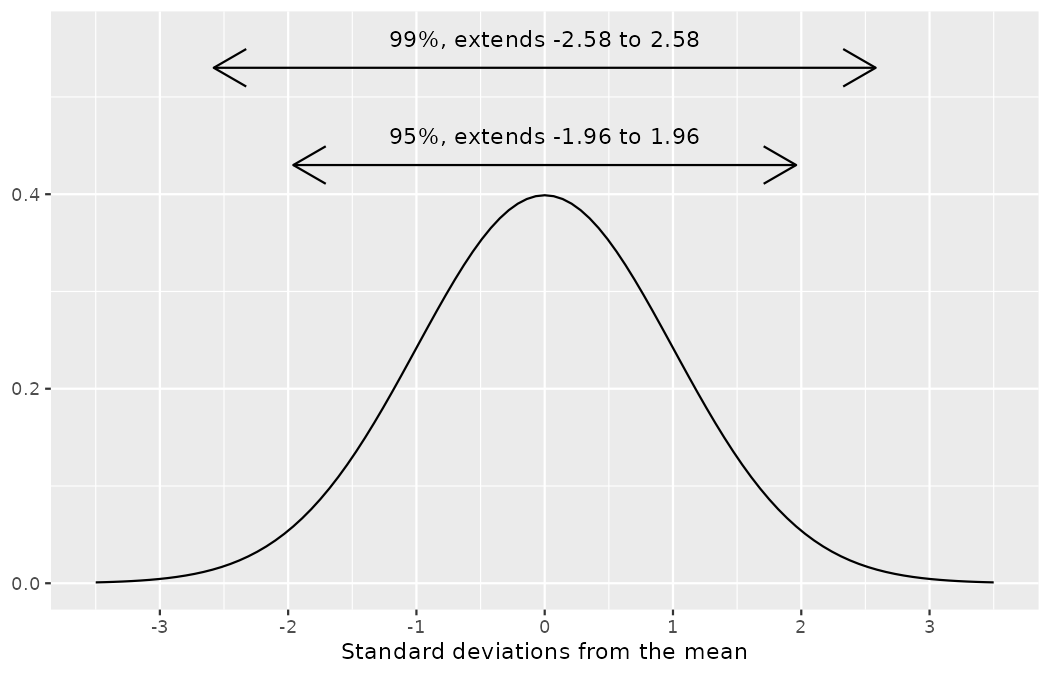
\includegraphics[width=0.85\linewidth,height=\textheight,keepaspectratio]{figures/inference-one-prop-2.png}

The resulting figure shows a standard normal curve with two nested
double-headed arrows above it: the inner one spanning \(-1.96\) to
\(1.96\) and labeled 95\%, the outer one spanning \(-2.58\) to \(2.58\)
and labeled 99\%. The area between \(-z^{\star}\) and \(z^{\star}\)
increases as \(|z^{\star}|\) becomes larger: if the confidence level is
99\%, we choose \(z^{\star}\) such that 99\% of the normal curve is
between \(-z^{\star}\) and \(z^{\star},\) which corresponds to 0.5\% in
the lower tail and 0.5\% in the upper tail --- \(z^{\star} = 2.58.\)

To create a 99\% confidence interval, change 1.96 in the 95\% confidence
interval formula to be \(2.58.\) The previous Check your understanding
highlights that 99\% of the time a normal random variable will be within
2.58 standard deviations of its mean. This approach --- using the Z
scores in the normal model to compute confidence levels --- is
appropriate when the point estimate is associated with a normal
distribution and we can properly compute the standard error. Thus, the
formula for a 99\% confidence interval is:

\[
\text{point estimate} \ \pm \ 2.58 \ \times \ SE
\]

Here, then, is where the symbol \(z^\star\) --- introduced in
Section~\ref{sec-moe} with its value frozen at \(1.96\) --- earns its
generality: the star marks a cutoff \emph{chosen} to match a stated
confidence level, and different levels simply swap in different cutoffs,
\(1.65\) for 90\%, \(1.96\) for 95\%, \(2.58\) for 99\%.

The normal approximation is crucial to the precision of the \(z^\star\)
confidence intervals (in contrast to the bootstrap percentile confidence
intervals of Chapter~\ref{sec-foundations-bootstrapping}). When the
normal model is not a good fit, we will use alternative distributions
that better characterize the sampling distribution, or we will use
bootstrapping procedures.

To practice the new levels on a result with real consequences for the
club, return to the finishing program trial of
Section~\ref{sec-case-study-stents-strokes} --- the multi-academy
experiment whose new high-intensity program turned out to \emph{hurt}
season-end conversion. We rebuild the data with exactly the code that
constructed them in that chapter (a constructed scenario, as always),
and recompute the point estimate and standard error exactly as in
Section~\ref{sec-casestent}:

\begin{Shaded}
\begin{Highlighting}[]
\NormalTok{drill\_trial }\OtherTok{\textless{}{-}} \FunctionTok{tibble}\NormalTok{(}
  \AttributeTok{group =} \FunctionTok{c}\NormalTok{(}\FunctionTok{rep}\NormalTok{(}\StringTok{"finishing program"}\NormalTok{, }\DecValTok{224}\NormalTok{), }\FunctionTok{rep}\NormalTok{(}\StringTok{"standard training"}\NormalTok{, }\DecValTok{227}\NormalTok{)),}
  \AttributeTok{day30 =} \FunctionTok{c}\NormalTok{(}\FunctionTok{rep}\NormalTok{(}\StringTok{"below benchmark"}\NormalTok{, }\DecValTok{33}\NormalTok{), }\FunctionTok{rep}\NormalTok{(}\StringTok{"met benchmark"}\NormalTok{, }\DecValTok{191}\NormalTok{),}
            \FunctionTok{rep}\NormalTok{(}\StringTok{"below benchmark"}\NormalTok{, }\DecValTok{13}\NormalTok{), }\FunctionTok{rep}\NormalTok{(}\StringTok{"met benchmark"}\NormalTok{, }\DecValTok{214}\NormalTok{)),}
  \AttributeTok{season\_end =} \FunctionTok{c}\NormalTok{(}\FunctionTok{rep}\NormalTok{(}\StringTok{"below benchmark"}\NormalTok{, }\DecValTok{45}\NormalTok{), }\FunctionTok{rep}\NormalTok{(}\StringTok{"met benchmark"}\NormalTok{, }\DecValTok{179}\NormalTok{),}
                 \FunctionTok{rep}\NormalTok{(}\StringTok{"below benchmark"}\NormalTok{, }\DecValTok{28}\NormalTok{), }\FunctionTok{rep}\NormalTok{(}\StringTok{"met benchmark"}\NormalTok{, }\DecValTok{199}\NormalTok{))}
\NormalTok{)}

\NormalTok{p\_trmt }\OtherTok{\textless{}{-}} \DecValTok{45} \SpecialCharTok{/} \DecValTok{224}
\NormalTok{p\_ctrl }\OtherTok{\textless{}{-}} \DecValTok{28} \SpecialCharTok{/} \DecValTok{227}
\NormalTok{diff\_hat }\OtherTok{\textless{}{-}}\NormalTok{ p\_trmt }\SpecialCharTok{{-}}\NormalTok{ p\_ctrl}
\NormalTok{se\_diff  }\OtherTok{\textless{}{-}} \FunctionTok{sqrt}\NormalTok{(p\_trmt }\SpecialCharTok{*}\NormalTok{ (}\DecValTok{1} \SpecialCharTok{{-}}\NormalTok{ p\_trmt) }\SpecialCharTok{/} \DecValTok{224} \SpecialCharTok{+}\NormalTok{ p\_ctrl }\SpecialCharTok{*}\NormalTok{ (}\DecValTok{1} \SpecialCharTok{{-}}\NormalTok{ p\_ctrl) }\SpecialCharTok{/} \DecValTok{227}\NormalTok{)}
\FunctionTok{round}\NormalTok{(}\FunctionTok{c}\NormalTok{(diff\_hat, se\_diff), }\DecValTok{4}\NormalTok{)}
\CommentTok{\#\textgreater{} [1] 0.0775 0.0345}
\end{Highlighting}
\end{Shaded}

\begin{tcolorbox}[enhanced jigsaw, left=2mm, leftrule=.75mm, title=\textcolor{quarto-callout-tip-color}{\faLightbulb}\hspace{0.5em}{Check your understanding}, arc=.35mm, rightrule=.15mm, coltitle=black, colframe=quarto-callout-tip-color-frame, bottomrule=.15mm, colbacktitle=quarto-callout-tip-color!10!white, opacitybacktitle=0.6, breakable, bottomtitle=1mm, toptitle=1mm, titlerule=0mm, opacityback=0, toprule=.15mm, colback=white]

Create a 99\% confidence interval for the impact of the finishing
program on the risk of a player finishing the season below benchmark.
The point estimate is \(0.0775,\) and the standard error is
\(SE = 0.0345.\) It has been verified for you (in
Section~\ref{sec-casestent}) that the point estimate can reasonably be
modeled by a normal distribution.

\begin{center}\rule{0.5\linewidth}{0.5pt}\end{center}

Since the necessary conditions for applying the normal model have
already been checked for us, we can go straight to the construction of
the confidence interval: \(\text{point estimate} \pm 2.58 \times SE.\)

\begin{Shaded}
\begin{Highlighting}[]
\FunctionTok{round}\NormalTok{(}\FunctionTok{c}\NormalTok{(}\FloatTok{0.0775} \SpecialCharTok{{-}} \FloatTok{2.58} \SpecialCharTok{*} \FloatTok{0.0345}\NormalTok{, }\FloatTok{0.0775} \SpecialCharTok{+} \FloatTok{2.58} \SpecialCharTok{*} \FloatTok{0.0345}\NormalTok{), }\DecValTok{4}\NormalTok{)}
\CommentTok{\#\textgreater{} [1] {-}0.0115  0.1665}
\end{Highlighting}
\end{Shaded}

We are 99\% confident that assigning a player to the high-intensity
finishing program changed the season-end risk of falling below the
benchmark by somewhere between \(-0.012\) and \(+0.166\) (assuming the
trialed academies are representative of the club's academies generally).
Notice what the extra confidence bought and what it cost: the 95\%
interval of Section~\ref{sec-casestent}, \((0.010, 0.145),\) sat
entirely above zero, but demanding 99\% confidence widens the interval
until it just crosses zero --- at the stricter standard, the data no
longer discernibly pin down even the \emph{direction} of the effect.
Wider nets catch more, and say less.

\end{tcolorbox}

\begin{tcolorbox}[enhanced jigsaw, left=2mm, leftrule=.75mm, title=\textcolor{quarto-callout-important-color}{\faExclamation}\hspace{0.5em}{Mathematical model confidence interval for any confidence level}, arc=.35mm, rightrule=.15mm, coltitle=black, colframe=quarto-callout-important-color-frame, bottomrule=.15mm, colbacktitle=quarto-callout-important-color!10!white, opacitybacktitle=0.6, breakable, bottomtitle=1mm, toptitle=1mm, titlerule=0mm, opacityback=0, toprule=.15mm, colback=white]

If the point estimate follows the normal model with standard error
\(SE,\) then a confidence interval for the population parameter is

\[
\text{point estimate} \ \pm \ z^{\star} \ \times \ SE
\]

where \(z^{\star}\) corresponds to the confidence level selected.

\end{tcolorbox}

The figure drawn above provides a picture of how to identify
\(z^{\star}\) based on a confidence level: we select \(z^{\star}\) so
that the area between \(-z^{\star}\) and \(z^{\star}\) in the normal
model corresponds to the confidence level.

\begin{tcolorbox}[enhanced jigsaw, left=2mm, leftrule=.75mm, title=\textcolor{quarto-callout-tip-color}{\faLightbulb}\hspace{0.5em}{Check your understanding}, arc=.35mm, rightrule=.15mm, coltitle=black, colframe=quarto-callout-tip-color-frame, bottomrule=.15mm, colbacktitle=quarto-callout-tip-color!10!white, opacitybacktitle=0.6, breakable, bottomtitle=1mm, toptitle=1mm, titlerule=0mm, opacityback=0, toprule=.15mm, colback=white]

Previously, the club found that the finishing program \emph{increased}
the risk of finishing the season below benchmark --- the trial estimated
a 7.75 percentage point increase, with a standard error of about
\(SE = 3.45\) percentage points. Compute a 90\% confidence interval for
the effect.

\begin{center}\rule{0.5\linewidth}{0.5pt}\end{center}

We must find \(z^{\star}\) such that 90\% of the distribution falls
between \(-z^{\star}\) and \(z^{\star}\) in the standard normal model,
\(N(\mu = 0, \sigma = 1).\) We can find \(z^{\star}\) by looking for a
lower tail of 5\% (the other 5\% is in the upper tail):
\texttt{qnorm(0.95)} returns \(1.645,\) thus \(z^{\star} = 1.65.\)

\begin{Shaded}
\begin{Highlighting}[]
\FunctionTok{round}\NormalTok{(}\FunctionTok{c}\NormalTok{(}\FloatTok{0.0775} \SpecialCharTok{{-}} \FloatTok{1.65} \SpecialCharTok{*} \FloatTok{0.0345}\NormalTok{, }\FloatTok{0.0775} \SpecialCharTok{+} \FloatTok{1.65} \SpecialCharTok{*} \FloatTok{0.0345}\NormalTok{), }\DecValTok{4}\NormalTok{)}
\CommentTok{\#\textgreater{} [1] 0.0206 0.1344}
\end{Highlighting}
\end{Shaded}

The 90\% confidence interval is \((0.021, 0.134)\): we are 90\%
confident that the program increased the season-end risk of falling
below benchmark by 2.1 to 13.4 percentage points. Note the trade-off
relative to the 99\% interval above: a lower degree of confidence
increases the potential for error, but it also produces a narrower, more
actionable interval --- and Jonas Beck, deciding merely whether to pause
a drill program rather than commit €15M, might defensibly settle for it.

\end{tcolorbox}

\subsection{Hypothesis test for a
proportion}\label{hypothesis-test-for-a-proportion}

One possible standard the association's panel could impose is the
live-viewings rule: no filed report may recommend signing a player its
author has watched only on video. Before taking it to a vote, the panel
would like to know: do the network's scouts support this rule?

\begin{tcolorbox}[enhanced jigsaw, left=2mm, leftrule=.75mm, title=\textcolor{quarto-callout-tip-color}{\faLightbulb}\hspace{0.5em}{Check your understanding}, arc=.35mm, rightrule=.15mm, coltitle=black, colframe=quarto-callout-tip-color-frame, bottomrule=.15mm, colbacktitle=quarto-callout-tip-color!10!white, opacitybacktitle=0.6, breakable, bottomtitle=1mm, toptitle=1mm, titlerule=0mm, opacityback=0, toprule=.15mm, colback=white]

Set up hypotheses to evaluate whether a majority of accredited scouts
support the live-viewings rule.

\begin{center}\rule{0.5\linewidth}{0.5pt}\end{center}

\(H_0:\) there is not majority support for the rule; \(H_0:\)
\(p \leq 0.50.\) \(H_A:\) the majority of scouts support the rule;
\(H_A:\) \(p > 0.50.\)

\end{tcolorbox}

To apply the normal distribution framework in the context of a
hypothesis test for a proportion, the independence and success-failure
conditions must be satisfied. In a hypothesis test, the success-failure
condition is checked using the null proportion: we verify \(np_0\) and
\(n(1-p_0)\) are at least 10, where \(p_0\) is the null value.

\begin{tcolorbox}[enhanced jigsaw, left=2mm, leftrule=.75mm, title=\textcolor{quarto-callout-important-color}{\faExclamation}\hspace{0.5em}{The test statistic for assessing a single proportion is a Z}, arc=.35mm, rightrule=.15mm, coltitle=black, colframe=quarto-callout-important-color-frame, bottomrule=.15mm, colbacktitle=quarto-callout-important-color!10!white, opacitybacktitle=0.6, breakable, bottomtitle=1mm, toptitle=1mm, titlerule=0mm, opacityback=0, toprule=.15mm, colback=white]

The \textbf{Z score} is a ratio of how the sample proportion differs
from the hypothesized proportion \((p_0)\) as compared to the expected
variability of the \(\hat{p}\) (sample proportion) values.

\[
Z = \frac{\hat{p} - p_0}{\sqrt{p_0(1 - p_0)/n}}
\]

When the null hypothesis is true and the conditions are met, \(Z\) has a
standard normal distribution.

Conditions:

\begin{itemize}
\tightlist
\item
  independent observations
\item
  large samples \((n p_0 \geq 10\) and \(n (1-p_0) \geq 10)\)
\end{itemize}

\end{tcolorbox}

\begin{tcolorbox}[enhanced jigsaw, left=2mm, leftrule=.75mm, title=\textcolor{quarto-callout-tip-color}{\faLightbulb}\hspace{0.5em}{Check your understanding}, arc=.35mm, rightrule=.15mm, coltitle=black, colframe=quarto-callout-tip-color-frame, bottomrule=.15mm, colbacktitle=quarto-callout-tip-color!10!white, opacitybacktitle=0.6, breakable, bottomtitle=1mm, toptitle=1mm, titlerule=0mm, opacityback=0, toprule=.15mm, colback=white]

Do accredited scouts support a rule that would require two live viewings
before a report may recommend signing? In the network survey's random
sample of 826 scouts, 51\% \((421/826 = 0.5097)\) said they would
support such a rule. Is it reasonable to use a normal distribution to
model \(\hat{p}\) for a hypothesis test here?

\begin{center}\rule{0.5\linewidth}{0.5pt}\end{center}

Independence holds since the survey is based on a random sample from the
association's register. The success-failure condition also holds, which
is checked using the null value \((p_0 = 0.5)\) from \(H_0\):
\(np_0 = 826 \times 0.5 = 413,\) \(n(1 - p_0) = 826 \times 0.5 = 413.\)
Recall that here, the best guess for \(p\) is \(p_0,\) which comes from
the null hypothesis (because we assume the null hypothesis is true when
performing the testing procedure steps).

\end{tcolorbox}

\begin{tcolorbox}[enhanced jigsaw, left=2mm, leftrule=.75mm, title=\textcolor{quarto-callout-important-color}{\faExclamation}\hspace{0.5em}{Mathematical model hypothesis test for a proportion}, arc=.35mm, rightrule=.15mm, coltitle=black, colframe=quarto-callout-important-color-frame, bottomrule=.15mm, colbacktitle=quarto-callout-important-color!10!white, opacitybacktitle=0.6, breakable, bottomtitle=1mm, toptitle=1mm, titlerule=0mm, opacityback=0, toprule=.15mm, colback=white]

Set up hypotheses and verify the conditions using the null value,
\(p_0,\) to ensure \(\hat{p}\) (the sample proportion) is nearly normal
under \(H_0.\) If the conditions hold, calculate the standard error,
again using \(p_0,\) and show the p-value in a drawing. Lastly, compute
the p-value and evaluate the hypotheses.

\end{tcolorbox}

For additional one-proportion hypothesis test examples, see
Section~\ref{sec-HypothesisTesting}.

\begin{tcolorbox}[enhanced jigsaw, left=2mm, leftrule=.75mm, title=\textcolor{quarto-callout-note-color}{\faInfo}\hspace{0.5em}{Worked example}, arc=.35mm, rightrule=.15mm, coltitle=black, colframe=quarto-callout-note-color-frame, bottomrule=.15mm, colbacktitle=quarto-callout-note-color!10!white, opacitybacktitle=0.6, breakable, bottomtitle=1mm, toptitle=1mm, titlerule=0mm, opacityback=0, toprule=.15mm, colback=white]

Using the hypotheses and data from the previous Check your
understandings, evaluate whether the survey provides convincing evidence
that a majority of accredited scouts support the live-viewings rule.

\begin{center}\rule{0.5\linewidth}{0.5pt}\end{center}

With hypotheses already set up and conditions checked, we can move onto
calculations. The standard error in the context of a one-proportion
hypothesis test is computed using the null value, \(p_0\):

\begin{Shaded}
\begin{Highlighting}[]
\FunctionTok{sqrt}\NormalTok{(}\FloatTok{0.5} \SpecialCharTok{*} \FloatTok{0.5} \SpecialCharTok{/} \DecValTok{826}\NormalTok{)}
\CommentTok{\#\textgreater{} [1] 0.01739723}
\end{Highlighting}
\end{Shaded}

\[
SE = \sqrt{\frac{p_0 (1 - p_0)}{n}} = \sqrt{\frac{0.5 (1 - 0.5)}{826}} = 0.017
\]

A picture of the normal model, with the p-value represented by the
shaded region, is drawn by the code below: a bell centered at \(0.50\)
with standard deviation \(0.017,\) everything to the right of the
observed \(0.51\) shaded --- a little under a third of the curve.

\begin{Shaded}
\begin{Highlighting}[]
\FunctionTok{ggplot}\NormalTok{(}\FunctionTok{data.frame}\NormalTok{(}\AttributeTok{x =} \FunctionTok{c}\NormalTok{(}\FloatTok{0.44}\NormalTok{, }\FloatTok{0.56}\NormalTok{)), }\FunctionTok{aes}\NormalTok{(}\AttributeTok{x =}\NormalTok{ x)) }\SpecialCharTok{+}
  \FunctionTok{geom\_function}\NormalTok{(}\AttributeTok{fun =}\NormalTok{ dnorm, }\AttributeTok{args =} \FunctionTok{list}\NormalTok{(}\AttributeTok{mean =} \FloatTok{0.50}\NormalTok{, }\AttributeTok{sd =} \FloatTok{0.017}\NormalTok{)) }\SpecialCharTok{+}
  \FunctionTok{geom\_area}\NormalTok{(}\AttributeTok{stat =} \StringTok{"function"}\NormalTok{, }\AttributeTok{fun =}\NormalTok{ dnorm,}
            \AttributeTok{args =} \FunctionTok{list}\NormalTok{(}\AttributeTok{mean =} \FloatTok{0.50}\NormalTok{, }\AttributeTok{sd =} \FloatTok{0.017}\NormalTok{),}
            \AttributeTok{xlim =} \FunctionTok{c}\NormalTok{(}\FloatTok{0.51}\NormalTok{, }\FloatTok{0.56}\NormalTok{), }\AttributeTok{alpha =} \FloatTok{0.5}\NormalTok{) }\SpecialCharTok{+}
  \FunctionTok{labs}\NormalTok{(}\AttributeTok{x =} \StringTok{"Sample proportion, if the null hypothesis is true"}\NormalTok{, }\AttributeTok{y =} \ConstantTok{NULL}\NormalTok{)}
\end{Highlighting}
\end{Shaded}

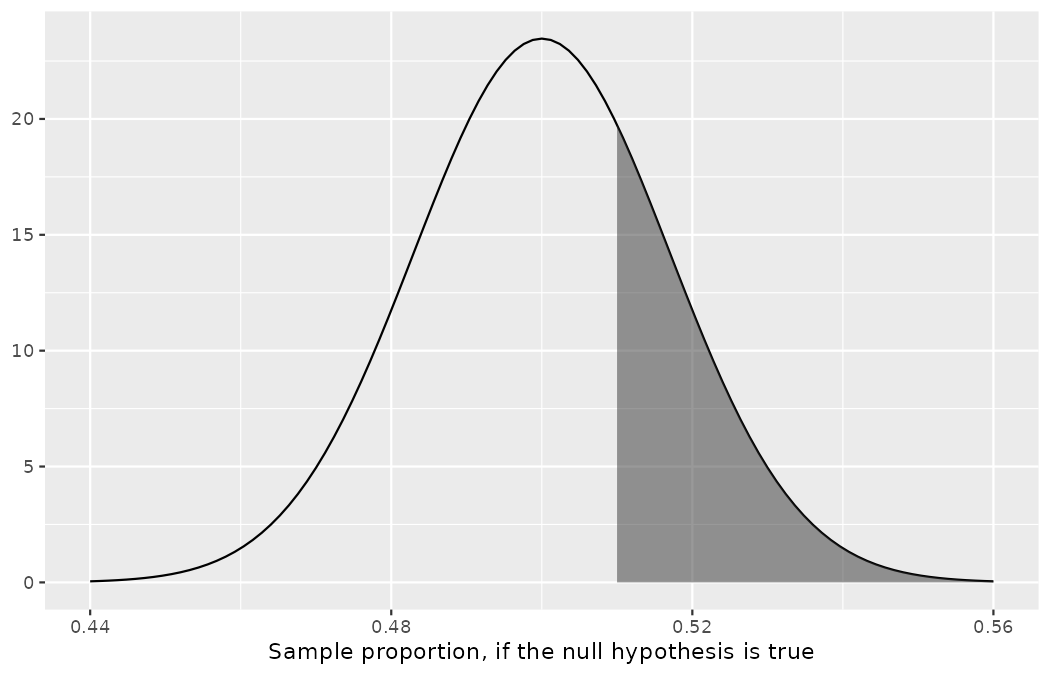
\includegraphics[width=0.85\linewidth,height=\textheight,keepaspectratio]{figures/inference-one-prop-3.png}

Based on the normal model, the test statistic can be computed as the Z
score of the point estimate, working at two decimal places as the survey
report would:

\[
Z = \frac{\text{point estimate} - \text{null value}}{SE} = \frac{0.51 - 0.50}{0.017} = 0.59
\]

\begin{Shaded}
\begin{Highlighting}[]
\NormalTok{(}\FloatTok{0.51} \SpecialCharTok{{-}} \FloatTok{0.50}\NormalTok{) }\SpecialCharTok{/} \FloatTok{0.017}
\CommentTok{\#\textgreater{} [1] 0.5882353}

\DecValTok{1} \SpecialCharTok{{-}} \FunctionTok{pnorm}\NormalTok{(}\FloatTok{0.59}\NormalTok{)}
\CommentTok{\#\textgreater{} [1] 0.2775953}
\end{Highlighting}
\end{Shaded}

The single tail area which represents the p-value is \(0.278.\)
(Carrying the unrounded sample proportion instead changes nothing that
matters: \(\hat{p} = 421/826 = 0.5097\) gives \(Z = 0.56\) and a tail of
\(0.289\) --- this test is nowhere near any bar, at any reasonable
rounding.)

\begin{Shaded}
\begin{Highlighting}[]
\NormalTok{(}\DecValTok{421} \SpecialCharTok{/} \DecValTok{826} \SpecialCharTok{{-}} \FloatTok{0.5}\NormalTok{) }\SpecialCharTok{/} \FunctionTok{sqrt}\NormalTok{(}\FloatTok{0.25} \SpecialCharTok{/} \DecValTok{826}\NormalTok{)}
\CommentTok{\#\textgreater{} [1] 0.5567112}

\DecValTok{1} \SpecialCharTok{{-}} \FunctionTok{pnorm}\NormalTok{((}\DecValTok{421} \SpecialCharTok{/} \DecValTok{826} \SpecialCharTok{{-}} \FloatTok{0.5}\NormalTok{) }\SpecialCharTok{/} \FunctionTok{sqrt}\NormalTok{(}\FloatTok{0.25} \SpecialCharTok{/} \DecValTok{826}\NormalTok{))}
\CommentTok{\#\textgreater{} [1] 0.2888624}
\end{Highlighting}
\end{Shaded}

Because the p-value is larger than \(0.05,\) we do not reject \(H_0.\)
The survey does not provide convincing evidence that a majority of
accredited scouts support the live-viewings rule.

Recall from Section~\ref{sec-two-sided-hypotheses} that the survey
question might have been better structured as a two-sided test: the
panel presumably wants to know whether scouts support \textbf{or oppose}
the rule (to study opinion in either direction away from the 50\%
benchmark). In that case, the p-value would have been doubled to
\(0.556\) (again, we would not reject \(H_0\)). In the two-sided
setting, the appropriate conclusion would be to claim that the survey
does not provide convincing evidence that a majority of scouts support
or oppose the live-viewings rule.

In both the one-sided and two-sided settings, the conclusion is somewhat
unsatisfactory because there is no conclusion. That is, there is no
resolution one way or the other about network opinion. We cannot claim
that exactly 50\% of scouts support the rule, but we cannot claim a
majority in either direction --- the panel goes to its vote with the
question genuinely open.

\end{tcolorbox}

The same machinery earns its keep on real data, where --- unlike the
deadlocked survey --- it can settle an argument outright.

\begin{tcolorbox}[enhanced jigsaw, left=2mm, leftrule=.75mm, title=\textcolor{quarto-callout-note-color}{\faInfo}\hspace{0.5em}{Worked example}, arc=.35mm, rightrule=.15mm, coltitle=black, colframe=quarto-callout-note-color-frame, bottomrule=.15mm, colbacktitle=quarto-callout-note-color!10!white, opacitybacktitle=0.6, breakable, bottomtitle=1mm, toptitle=1mm, titlerule=0mm, opacityback=0, toprule=.15mm, colback=white]

A pundit on the World Cup broadcast claims that ``one in five shots at
this level is taken under a defender's pressure.'' The Check your
understanding earlier in this chapter estimated the true rate with a
confidence interval; now test the pundit's claim directly against the
2022 data, where 238 of 1,494 shots were pressured
\((\hat{p} = 0.1593).\) Per Section~\ref{sec-two-sided-hypotheses}, keep
an open mind: test \(H_0: p = 0.20\) against \(H_A: p \neq 0.20.\)

\begin{center}\rule{0.5\linewidth}{0.5pt}\end{center}

As before, we treat the tournament's shots as a sample from the process
generating World Cup shots. The success-failure condition is checked
with the null value: \(np_0 = 1494 \times 0.20 = 298.8\) and
\(n(1 - p_0) = 1195.2,\) both far beyond 10, so the normal model applies
--- this is the large-sample home turf where the shortcut is entirely
safe.

\begin{Shaded}
\begin{Highlighting}[]
\NormalTok{se\_0 }\OtherTok{\textless{}{-}} \FunctionTok{sqrt}\NormalTok{(}\FloatTok{0.20} \SpecialCharTok{*} \FloatTok{0.80} \SpecialCharTok{/} \DecValTok{1494}\NormalTok{)}
\NormalTok{z }\OtherTok{\textless{}{-}}\NormalTok{ (}\DecValTok{238} \SpecialCharTok{/} \DecValTok{1494} \SpecialCharTok{{-}} \FloatTok{0.20}\NormalTok{) }\SpecialCharTok{/}\NormalTok{ se\_0}
\FunctionTok{round}\NormalTok{(}\FunctionTok{c}\NormalTok{(se\_0, z), }\DecValTok{4}\NormalTok{)}
\CommentTok{\#\textgreater{} [1]  0.0103 {-}3.9325}

\DecValTok{2} \SpecialCharTok{*} \FunctionTok{pnorm}\NormalTok{(z)}
\CommentTok{\#\textgreater{} [1] 8.406838e{-}05}
\end{Highlighting}
\end{Shaded}

\[
Z = \frac{\hat{p} - p_0}{\sqrt{p_0(1-p_0)/n}} = \frac{0.1593 - 0.20}{0.0103} = -3.93
\]

The two-sided p-value is \(0.0001.\) The data provide statistically
discernible evidence against the pundit's number: the true rate of
shooting under pressure is below one in five (the point estimate sits at
about one in six). One frame sentence before this reaches a broadcast
rebuttal, per the penalty convention: the 1,494-shot denominator
includes 64 penalties and the other dead-ball shots that \emph{cannot}
be pressured, and in the open-play frame the rate rises to
\(238/1382 = 0.172\) --- the pundit still loses the test there
\((Z = -2.58,\) two-sided p-value \(= 0.0098),\) but by a far less
emphatic margin, so state which frame you are quoting.

\begin{Shaded}
\begin{Highlighting}[]
\NormalTok{wc2022\_shots }\SpecialCharTok{|\textgreater{}}
  \FunctionTok{filter}\NormalTok{(shot\_type }\SpecialCharTok{==} \StringTok{"Open Play"}\NormalTok{) }\SpecialCharTok{|\textgreater{}}
  \FunctionTok{summarize}\NormalTok{(}\AttributeTok{shots =} \FunctionTok{n}\NormalTok{(), }\AttributeTok{pressured =} \FunctionTok{sum}\NormalTok{(under\_pressure),}
            \AttributeTok{prop =} \FunctionTok{mean}\NormalTok{(under\_pressure))}
\CommentTok{\#\textgreater{} \# A tibble: 1 × 3}
\CommentTok{\#\textgreater{}   shots pressured  prop}
\CommentTok{\#\textgreater{}   \textless{}int\textgreater{}     \textless{}int\textgreater{} \textless{}dbl\textgreater{}}
\CommentTok{\#\textgreater{} 1  1382       238 0.172}

\NormalTok{z\_open }\OtherTok{\textless{}{-}}\NormalTok{ (}\DecValTok{238} \SpecialCharTok{/} \DecValTok{1382} \SpecialCharTok{{-}} \FloatTok{0.20}\NormalTok{) }\SpecialCharTok{/} \FunctionTok{sqrt}\NormalTok{(}\FloatTok{0.20} \SpecialCharTok{*} \FloatTok{0.80} \SpecialCharTok{/} \DecValTok{1382}\NormalTok{)}
\FunctionTok{round}\NormalTok{(z\_open, }\DecValTok{4}\NormalTok{)}
\CommentTok{\#\textgreater{} [1] {-}2.5824}

\DecValTok{2} \SpecialCharTok{*} \FunctionTok{pnorm}\NormalTok{(z\_open)}
\CommentTok{\#\textgreater{} [1] 0.009812645}
\end{Highlighting}
\end{Shaded}

\end{tcolorbox}

\subsection{Violating conditions}\label{violating-conditions}

We've spent a lot of time discussing conditions for when \(\hat{p}\) can
be reasonably modeled by a normal distribution. What happens when the
success-failure condition fails? What about when the independence
condition fails? In either case, the general ideas of confidence
intervals and hypothesis tests remain the same, but the strategy or
technique used to generate the interval or p-value change.

When the success-failure condition isn't met for a hypothesis test, we
can simulate the null distribution of \(\hat{p}\) using the null value,
\(p_0,\) as seen in Section~\ref{sec-one-prop-null-boot} --- that is
exactly how six one-on-ones were handled where 1,494 shots needed no
such care. Unfortunately, methods for dealing with observations which
are not independent (e.g., repeated assessments of the same player
across a season) are outside the scope of this book.

\section{Chapter review}\label{sec-chp16-review}

\subsection{Summary}\label{summary-15}

Building on the foundational ideas of the previous few chapters, this
chapter focused exclusively on the single population proportion as the
parameter of interest. Note that it is not possible to do a
randomization test with only one variable, so to do computational
hypothesis testing, we applied a bootstrapping framework: simulate
samples from the null claim \(p_0\) and ask where the observed
\(\hat{p}\) falls among them --- the machinery that let six Moroccan
one-on-ones be tested honestly when the normal model had no business
near them. The bootstrap confidence interval and the mathematical
framework for both hypothesis testing and confidence intervals are
similar to those applied to other data structures and parameters. When
using the mathematical model, keep in mind the success-failure
conditions --- substituting \(p_0\) for tests and \(\hat{p}\) for
intervals --- and remember what the set-piece consultant taught in
Section~\ref{sec-casemed}: the check is not a formality, because failing
it can flip a verdict. Additionally, know that bootstrapping is always
more accurate with larger samples. And whenever the proportion under
test counts shots, this book's standing convention applies: decide which
shots are in the frame, show any penalty-tilted baseline both ways, and
state the frame in the report --- this chapter's one-on-one baseline
moved from \(0.200\) to \(0.221\) on that one decision.

\subsection{Terms}\label{terms-15}

The terms introduced in this chapter are presented below, alphabetized.
If you're not sure what some of these terms mean, we recommend you go
back in the text and review their definitions. You should be able to
easily spot them as \textbf{bolded text}.

\begin{longtable}[]{@{}
  >{\raggedright\arraybackslash}p{(\linewidth - 4\tabcolsep) * \real{0.3380}}
  >{\raggedright\arraybackslash}p{(\linewidth - 4\tabcolsep) * \real{0.3380}}
  >{\raggedright\arraybackslash}p{(\linewidth - 4\tabcolsep) * \real{0.3239}}@{}}
\caption{Terms introduced in this
chapter.}\label{tbl-terms-chp-16}\tabularnewline
\toprule\noalign{}
\endfirsthead
\endhead
\bottomrule\noalign{}
\endlastfoot
parametric bootstrap & standard error of a single proportion &
success-failure condition \\
Z score & & \\
\end{longtable}

\section{Exercises}\label{sec-chp16-exercises}

Answers to odd-numbered exercises can be found in
Appendix~\ref{sec-exercise-solutions-16}.

\begin{enumerate}
\def\labelenumi{\arabic{enumi}.}
\item
  \textbf{Will video replace the scout?} The national scouting
  association polled 4,839 of its accredited members on whether fully
  automated video-and-data scouting will replace live
  scouting.\footnote{The association polls and club surveys in these
    exercises are constructed scouting scenarios; no such polls were
    conducted.} You want to evaluate if more than a quarter (25\%) of
  accredited members think it will never replace live scouting. In the
  poll, 22\% responded ``it will replace live scouting entirely within a
  decade'', 28\% responded ``it will replace live scouting partially'',
  29\% responded ``it will never replace live scouting'', and 22\%
  responded ``don't know''. A colleague offers to help you set up the
  hypothesis test and comes up with the following hypotheses. Indicate
  any errors you see.

  \(H_0: \hat{p} = 0.29 \quad \quad H_A: \hat{p} > 0.29\)
\item
  \textbf{Contract by 21.} A league development report suggests that
  25\% of academy graduates sign a senior professional contract by age
  21. You believe that this is incorrect for the current cohort and
  decide to collect your own sample for a hypothesis test. From a random
  sample of 776 recent academy graduates, you find that 24\% of them
  signed by 21. A colleague offers to help you set up the hypothesis
  test and comes up with the following hypotheses. Indicate any errors
  you see.

  \(H_0: \hat{p} = 0.24 \quad \quad H_A: \hat{p} \neq 0.24\)
\item
  \textbf{Leading with xG.} A survey conducted at the league's annual
  scouting convention reached 650 randomly sampled accredited scouts, of
  whom 159 named an expected-goals model as the primary tool in their
  player evaluations.\footnote{The convention survey is a constructed
    scenario. Where an exercise describes a simulated null distribution,
    the distribution is generated exactly by the seeded code shown, and
    the counts quoted in the exercise come from that seeded run.}

  \begin{enumerate}
  \def\labelenumii{\alph{enumii}.}
  \item
    A journalist writing up the survey wants to use the headline ``More
    than 1 in 5 scouts now lead with xG.'' You caution the journalist
    that they should first conduct a hypothesis test to see if the
    survey data provide convincing evidence for this claim. Write the
    hypotheses for this test.
  \item
    Calculate the proportion of scouts in the sample who named an xG
    model as their primary tool.
  \item
    Describe a setup for a simulation that would be appropriate in this
    situation, and how the p-value can be calculated using the
    simulation results.
  \item
    The seeded code below simulates 1,000 values of \(\hat{p}_{sim}\)
    under the null hypothesis and plots them as a histogram. In this
    run, \emph{none} of the 1,000 simulated proportions was as large as
    the observed proportion --- the largest was \(0.243.\) Estimate the
    p-value from the simulation and use it to evaluate the hypotheses.

\begin{Shaded}
\begin{Highlighting}[]
\NormalTok{xg\_first }\OtherTok{\textless{}{-}} \FunctionTok{tibble}\NormalTok{(}\AttributeTok{tool =} \FunctionTok{c}\NormalTok{(}\FunctionTok{rep}\NormalTok{(}\StringTok{"xg first"}\NormalTok{, }\DecValTok{159}\NormalTok{), }\FunctionTok{rep}\NormalTok{(}\StringTok{"other"}\NormalTok{, }\DecValTok{650} \SpecialCharTok{{-}} \DecValTok{159}\NormalTok{)))}

\FunctionTok{set.seed}\NormalTok{(}\DecValTok{1603}\NormalTok{)}
\NormalTok{null\_dist }\OtherTok{\textless{}{-}}\NormalTok{ xg\_first }\SpecialCharTok{|\textgreater{}}
  \FunctionTok{specify}\NormalTok{(}\AttributeTok{response =}\NormalTok{ tool, }\AttributeTok{success =} \StringTok{"xg first"}\NormalTok{) }\SpecialCharTok{|\textgreater{}}
  \FunctionTok{hypothesize}\NormalTok{(}\AttributeTok{null =} \StringTok{"point"}\NormalTok{, }\AttributeTok{p =} \FloatTok{0.20}\NormalTok{) }\SpecialCharTok{|\textgreater{}}
  \FunctionTok{generate}\NormalTok{(}\AttributeTok{reps =} \DecValTok{1000}\NormalTok{, }\AttributeTok{type =} \StringTok{"draw"}\NormalTok{) }\SpecialCharTok{|\textgreater{}}
  \FunctionTok{calculate}\NormalTok{(}\AttributeTok{stat =} \StringTok{"prop"}\NormalTok{)}

\FunctionTok{ggplot}\NormalTok{(null\_dist, }\FunctionTok{aes}\NormalTok{(}\AttributeTok{x =}\NormalTok{ stat)) }\SpecialCharTok{+}
  \FunctionTok{geom\_histogram}\NormalTok{(}\AttributeTok{binwidth =} \FloatTok{0.005}\NormalTok{) }\SpecialCharTok{+}
  \FunctionTok{labs}\NormalTok{(}
    \AttributeTok{title =} \StringTok{"1,000 proportions from null hypothesis draws"}\NormalTok{,}
    \AttributeTok{subtitle =} \StringTok{"p = 0.20"}\NormalTok{,}
    \AttributeTok{x =} \StringTok{"Simulated proportion of scouts who lead with xG"}\NormalTok{,}
    \AttributeTok{y =} \StringTok{"Count"}
\NormalTok{  )}
\end{Highlighting}
\end{Shaded}

    The histogram is bell-shaped and centered at \(0.20,\) with nearly
    all simulated proportions falling between \(0.15\) and \(0.25.\)
  \end{enumerate}
\item
  \textbf{Loan placements.} A league development report states that
  48.8\% of academy players sent out on loan reach at least 900 league
  minutes during the loan season. An agency that arranges loan
  placements claims that its placements do better than average. A random
  sample of 30 of the agency's placements yielded a benchmark rate of
  60\%. Northbridge's recruitment staff would like to determine if the
  data provide strong evidence to support the agency's claim.\footnote{The
    development report and the agency's placement records are
    constructed; the seeded code shown generates the null distribution
    described.}

  \begin{enumerate}
  \def\labelenumii{\alph{enumii}.}
  \item
    Write the hypotheses to test if the benchmark rate for the agency's
    placements is discernibly higher than the league rate reported in
    the development report.
  \item
    Describe a setup for a simulation that would be appropriate in this
    situation, and how the p-value can be calculated using the
    simulation results.
  \item
    The seeded code below simulates 1,000 values of \(\hat{p}_{sim}\)
    under the null hypothesis. In this run, 149 of the 1,000 simulated
    proportions were \(0.60\) or larger. Estimate the p-value from the
    simulation and use it to evaluate the hypotheses.

\begin{Shaded}
\begin{Highlighting}[]
\NormalTok{loans }\OtherTok{\textless{}{-}} \FunctionTok{tibble}\NormalTok{(}\AttributeTok{placement =} \FunctionTok{c}\NormalTok{(}\FunctionTok{rep}\NormalTok{(}\StringTok{"benchmark met"}\NormalTok{, }\DecValTok{18}\NormalTok{),}
                              \FunctionTok{rep}\NormalTok{(}\StringTok{"benchmark missed"}\NormalTok{, }\DecValTok{12}\NormalTok{)))}

\FunctionTok{set.seed}\NormalTok{(}\DecValTok{1604}\NormalTok{)}
\NormalTok{null\_dist }\OtherTok{\textless{}{-}}\NormalTok{ loans }\SpecialCharTok{|\textgreater{}}
  \FunctionTok{specify}\NormalTok{(}\AttributeTok{response =}\NormalTok{ placement, }\AttributeTok{success =} \StringTok{"benchmark met"}\NormalTok{) }\SpecialCharTok{|\textgreater{}}
  \FunctionTok{hypothesize}\NormalTok{(}\AttributeTok{null =} \StringTok{"point"}\NormalTok{, }\AttributeTok{p =} \FloatTok{0.488}\NormalTok{) }\SpecialCharTok{|\textgreater{}}
  \FunctionTok{generate}\NormalTok{(}\AttributeTok{reps =} \DecValTok{1000}\NormalTok{, }\AttributeTok{type =} \StringTok{"draw"}\NormalTok{) }\SpecialCharTok{|\textgreater{}}
  \FunctionTok{calculate}\NormalTok{(}\AttributeTok{stat =} \StringTok{"prop"}\NormalTok{)}

\FunctionTok{ggplot}\NormalTok{(null\_dist, }\FunctionTok{aes}\NormalTok{(}\AttributeTok{x =}\NormalTok{ stat)) }\SpecialCharTok{+}
  \FunctionTok{geom\_histogram}\NormalTok{(}\AttributeTok{binwidth =} \FloatTok{0.05}\NormalTok{) }\SpecialCharTok{+}
  \FunctionTok{geom\_vline}\NormalTok{(}\AttributeTok{xintercept =} \FloatTok{0.6}\NormalTok{, }\AttributeTok{linetype =} \StringTok{"dashed"}\NormalTok{) }\SpecialCharTok{+}
  \FunctionTok{labs}\NormalTok{(}
    \AttributeTok{title =} \StringTok{"1,000 proportions from null hypothesis draws"}\NormalTok{,}
    \AttributeTok{subtitle =} \StringTok{"p = 0.488"}\NormalTok{,}
    \AttributeTok{x =} \StringTok{"Simulated proportion of placements meeting the benchmark"}\NormalTok{,}
    \AttributeTok{y =} \StringTok{"Count"}
\NormalTok{  )}
\end{Highlighting}
\end{Shaded}
  \item
    After performing this analysis, a rival agency circulates the
    following headline: ``Placement agency falsely advertises its
    success rate.'' Comment on the appropriateness of this statement.
  \end{enumerate}
\item
  \textbf{Which dossier layout, simulated null hypothesis.} Emil
  Sørensen is trialing two layouts for the network's prospect dossiers:
  the established single-page summary and a new two-page format with a
  data appendix. Seven senior scouts each review the same prospect
  written up in both layouts (order randomized) and state which layout
  they prefer: 5 choose the single-page summary and 2 choose the
  two-page format. We are interested to know whether these data provide
  convincing evidence that the network's scouts prefer one of the
  layouts over the other.\footnote{The dossier-layout trial is a
    constructed Northbridge scenario, generated by the seeded code
    shown.}

  \begin{enumerate}
  \def\labelenumii{\alph{enumii}.}
  \item
    What are the null and alternative hypotheses for evaluating whether
    these data provide convincing evidence that the scouts have a
    preference for one of the layouts?
  \item
    A null hypothesis simulation (with 1,000 draws, seeded code below)
    was run. In this run, 207 of the simulated proportions were at least
    \(5/7 \approx 0.714,\) and 248 were at most \(2/7 \approx 0.286.\)
    Find the p-value using this simulation and conclude the hypothesis
    test in the context of the problem.

\begin{Shaded}
\begin{Highlighting}[]
\NormalTok{layouts }\OtherTok{\textless{}{-}} \FunctionTok{tibble}\NormalTok{(}\AttributeTok{choice =} \FunctionTok{c}\NormalTok{(}\FunctionTok{rep}\NormalTok{(}\StringTok{"single page"}\NormalTok{, }\DecValTok{5}\NormalTok{), }\FunctionTok{rep}\NormalTok{(}\StringTok{"two page"}\NormalTok{, }\DecValTok{2}\NormalTok{)))}

\FunctionTok{set.seed}\NormalTok{(}\DecValTok{1605}\NormalTok{)}
\NormalTok{layouts }\SpecialCharTok{|\textgreater{}}
  \FunctionTok{specify}\NormalTok{(}\AttributeTok{response =}\NormalTok{ choice, }\AttributeTok{success =} \StringTok{"single page"}\NormalTok{) }\SpecialCharTok{|\textgreater{}}
  \FunctionTok{hypothesize}\NormalTok{(}\AttributeTok{null =} \StringTok{"point"}\NormalTok{, }\AttributeTok{p =} \FloatTok{0.5}\NormalTok{) }\SpecialCharTok{|\textgreater{}}
  \FunctionTok{generate}\NormalTok{(}\AttributeTok{reps =} \DecValTok{1000}\NormalTok{, }\AttributeTok{type =} \StringTok{"draw"}\NormalTok{) }\SpecialCharTok{|\textgreater{}}
  \FunctionTok{calculate}\NormalTok{(}\AttributeTok{stat =} \StringTok{"prop"}\NormalTok{) }\SpecialCharTok{|\textgreater{}}
  \FunctionTok{ggplot}\NormalTok{(}\FunctionTok{aes}\NormalTok{(}\AttributeTok{x =}\NormalTok{ stat)) }\SpecialCharTok{+}
  \FunctionTok{geom\_histogram}\NormalTok{(}\AttributeTok{binwidth =} \FloatTok{0.05}\NormalTok{) }\SpecialCharTok{+}
  \FunctionTok{labs}\NormalTok{(}
    \AttributeTok{title =} \StringTok{"1,000 proportions from null hypothesis draws"}\NormalTok{,}
    \AttributeTok{subtitle =} \StringTok{"p = 0.5"}\NormalTok{,}
    \AttributeTok{x =} \StringTok{"Simulated proportion of scouts who prefer the single page"}\NormalTok{,}
    \AttributeTok{y =} \StringTok{"Count"}
\NormalTok{  )}
\end{Highlighting}
\end{Shaded}

    The histogram shows stacks only at the eight attainable values
    \(0/7, 1/7, \dots, 7/7,\) roughly symmetric around \(0.5.\)
  \end{enumerate}
\item
  \textbf{Automated offside ballot, simulated null hypothesis.} To adopt
  semi-automated offside technology, the national association's statutes
  require approval from at least 55\% of its roughly 22,000 voting
  members --- club delegates, match officials, and licensed coaches ---
  in a formal member consultation. A pre-ballot survey asked a random
  sample of 1,207 of them; 65.3\% said they would approve.

  \begin{enumerate}
  \def\labelenumii{\alph{enumii}.}
  \item
    What are the null and alternative hypotheses for evaluating whether
    these data provide convincing evidence that, if the ballot were
    held, the technology would be adopted?
  \item
    A null hypothesis simulation (with 1,000 draws, seeded code below)
    was run. In this run, \emph{none} of the 1,000 simulated proportions
    reached the observed \(0.653\) --- the largest was \(0.596.\) Find
    the p-value using this simulation and conclude the hypothesis test
    in the context of the problem.

\begin{Shaded}
\begin{Highlighting}[]
\NormalTok{offside }\OtherTok{\textless{}{-}} \FunctionTok{tibble}\NormalTok{(}\AttributeTok{vote =} \FunctionTok{c}\NormalTok{(}\FunctionTok{rep}\NormalTok{(}\StringTok{"approve"}\NormalTok{, }\DecValTok{788}\NormalTok{), }\FunctionTok{rep}\NormalTok{(}\StringTok{"do not approve"}\NormalTok{, }\DecValTok{419}\NormalTok{)))}

\FunctionTok{set.seed}\NormalTok{(}\DecValTok{1606}\NormalTok{)}
\NormalTok{offside }\SpecialCharTok{|\textgreater{}}
  \FunctionTok{specify}\NormalTok{(}\AttributeTok{response =}\NormalTok{ vote, }\AttributeTok{success =} \StringTok{"approve"}\NormalTok{) }\SpecialCharTok{|\textgreater{}}
  \FunctionTok{hypothesize}\NormalTok{(}\AttributeTok{null =} \StringTok{"point"}\NormalTok{, }\AttributeTok{p =} \FloatTok{0.55}\NormalTok{) }\SpecialCharTok{|\textgreater{}}
  \FunctionTok{generate}\NormalTok{(}\AttributeTok{reps =} \DecValTok{1000}\NormalTok{, }\AttributeTok{type =} \StringTok{"draw"}\NormalTok{) }\SpecialCharTok{|\textgreater{}}
  \FunctionTok{calculate}\NormalTok{(}\AttributeTok{stat =} \StringTok{"prop"}\NormalTok{) }\SpecialCharTok{|\textgreater{}}
  \FunctionTok{ggplot}\NormalTok{(}\FunctionTok{aes}\NormalTok{(}\AttributeTok{x =}\NormalTok{ stat)) }\SpecialCharTok{+}
  \FunctionTok{geom\_histogram}\NormalTok{(}\AttributeTok{binwidth =} \FloatTok{0.005}\NormalTok{) }\SpecialCharTok{+}
  \FunctionTok{labs}\NormalTok{(}
    \AttributeTok{title =} \StringTok{"1,000 proportions from null hypothesis draws"}\NormalTok{,}
    \AttributeTok{subtitle =} \StringTok{"p = 0.55"}\NormalTok{,}
    \AttributeTok{x =} \StringTok{"Simulated proportion who approve the technology"}\NormalTok{,}
    \AttributeTok{y =} \StringTok{"Count"}
\NormalTok{  )}
\end{Highlighting}
\end{Shaded}
  \end{enumerate}
\item
  \textbf{Which dossier layout, standard errors.} The dossier-layout
  trial described in the earlier exercise found that 5 out of 7 senior
  scouts chose the single-page summary over the two-page format, which
  was preferred by the remaining 2 scouts. To evaluate whether these
  data provide convincing evidence that scouts prefer one of the layouts
  over the other, we set \(H_0: p = 0.5,\) where \(p\) is the population
  proportion of scouts who prefer the single-page summary, and
  \(H_A: p \neq 0.5,\) which suggests some preference, without
  specifying which layout is more preferred.

  \begin{enumerate}
  \def\labelenumii{\alph{enumii}.}
  \item
    Using the mathematical model, calculate the standard error of the
    sample proportion in repeated samples of size 7.
  \item
    A null hypothesis simulation (with 1,000 draws --- the same seeded
    simulation shown in the earlier exercise) shows the variability of
    the sample proportion in samples of size 7 when 50\% of scouts
    prefer the single-page summary. The standard deviation of the 1,000
    simulated proportions in that run was \(0.185.\) What is the
    approximate standard error of the sample proportion based on the
    simulated distribution?
  \item
    Do the mathematical model and the simulated draws yield similar
    standard errors?
  \item
    In order to approach the problem using the mathematical model, is
    the success-failure condition met for this study? Explain.
  \item
    What feature of the simulated null distribution tells us that the
    mathematical model should probably not be used? (Hint: how many
    distinct values can \(\hat{p}_{sim}\) take?)
  \end{enumerate}
\item
  \textbf{Automated offside ballot, standard errors.} As described in
  the earlier exercise, a random sample of 1,207 of the national
  association's voting members found 65.3\% would approve semi-automated
  offside technology, where adoption requires 55\% (or more) approval in
  the member consultation.

  \begin{enumerate}
  \def\labelenumii{\alph{enumii}.}
  \item
    Calculate the standard error of the sample proportion using the
    mathematical model (with the null value).
  \item
    In the seeded 1,000-draw null simulation shown in the earlier
    exercise (proportions from samples of size 1,207 with \(p = 0.55\)),
    the standard deviation of the simulated proportions was \(0.014.\)
    Approximate the standard error of the sample proportion based on
    that distribution.
  \item
    Do the mathematical model and the simulated draws yield similar
    standard errors?
  \item
    In this setting (to test whether the true underlying population
    proportion is greater than 0.55), would there be a strong reason to
    choose the mathematical model over the simulated null hypothesis (or
    vice versa)?
  \end{enumerate}
\item
  \textbf{The data desk's filing rate, describe the bootstrap.}
  Northbridge's filing logs show that about 70\% of the network's match
  reports are filed within 24 hours of full time. Priya Rao wonders if
  the same proportion holds for the club's newly formed data-scouting
  desk. She randomly samples 25 of the desk's reports and finds that 15
  of them were filed within 24 hours.\footnote{The filing-log scenario
    is constructed; both distributions described are generated exactly
    by the seeded code shown.}

  Two sampling distributions are created to describe the variability in
  the proportion of desk reports filed within 24 hours. The null
  hypothesis simulation imposes a true population proportion of
  \(p = 0.7,\) while the data bootstrap resamples from the actual sample
  (in which 60\% of the reports were filed within 24 hours).

\begin{Shaded}
\begin{Highlighting}[]
\NormalTok{desk\_reports }\OtherTok{\textless{}{-}} \FunctionTok{tibble}\NormalTok{(}\AttributeTok{filing =} \FunctionTok{c}\NormalTok{(}\FunctionTok{rep}\NormalTok{(}\StringTok{"on time"}\NormalTok{, }\DecValTok{15}\NormalTok{), }\FunctionTok{rep}\NormalTok{(}\StringTok{"late"}\NormalTok{, }\DecValTok{10}\NormalTok{)))}

\FunctionTok{set.seed}\NormalTok{(}\DecValTok{1607}\NormalTok{)}
\NormalTok{p\_para }\OtherTok{\textless{}{-}}\NormalTok{ desk\_reports }\SpecialCharTok{|\textgreater{}}
  \FunctionTok{specify}\NormalTok{(}\AttributeTok{response =}\NormalTok{ filing, }\AttributeTok{success =} \StringTok{"on time"}\NormalTok{) }\SpecialCharTok{|\textgreater{}}
  \FunctionTok{hypothesize}\NormalTok{(}\AttributeTok{null =} \StringTok{"point"}\NormalTok{, }\AttributeTok{p =} \FloatTok{0.7}\NormalTok{) }\SpecialCharTok{|\textgreater{}}
  \FunctionTok{generate}\NormalTok{(}\AttributeTok{reps =} \DecValTok{1000}\NormalTok{, }\AttributeTok{type =} \StringTok{"draw"}\NormalTok{) }\SpecialCharTok{|\textgreater{}}
  \FunctionTok{calculate}\NormalTok{(}\AttributeTok{stat =} \StringTok{"prop"}\NormalTok{) }\SpecialCharTok{|\textgreater{}}
  \FunctionTok{ggplot}\NormalTok{(}\FunctionTok{aes}\NormalTok{(}\AttributeTok{x =}\NormalTok{ stat)) }\SpecialCharTok{+}
  \FunctionTok{geom\_histogram}\NormalTok{(}\AttributeTok{binwidth =} \FloatTok{0.05}\NormalTok{) }\SpecialCharTok{+}
  \FunctionTok{labs}\NormalTok{(}
    \AttributeTok{title =} \StringTok{"Draws from null hypothesis"}\NormalTok{,}
    \AttributeTok{subtitle =} \StringTok{"p = 0.7"}\NormalTok{,}
    \AttributeTok{x =} \StringTok{"Simulated proportion filed on time"}\NormalTok{,}
    \AttributeTok{y =} \StringTok{"Count"}
\NormalTok{  )}

\FunctionTok{set.seed}\NormalTok{(}\DecValTok{1607}\NormalTok{)}
\NormalTok{p\_data }\OtherTok{\textless{}{-}}\NormalTok{ desk\_reports }\SpecialCharTok{|\textgreater{}}
  \FunctionTok{specify}\NormalTok{(}\AttributeTok{response =}\NormalTok{ filing, }\AttributeTok{success =} \StringTok{"on time"}\NormalTok{) }\SpecialCharTok{|\textgreater{}}
  \FunctionTok{generate}\NormalTok{(}\AttributeTok{reps =} \DecValTok{1000}\NormalTok{, }\AttributeTok{type =} \StringTok{"bootstrap"}\NormalTok{) }\SpecialCharTok{|\textgreater{}}
  \FunctionTok{calculate}\NormalTok{(}\AttributeTok{stat =} \StringTok{"prop"}\NormalTok{) }\SpecialCharTok{|\textgreater{}}
  \FunctionTok{ggplot}\NormalTok{(}\FunctionTok{aes}\NormalTok{(}\AttributeTok{x =}\NormalTok{ stat)) }\SpecialCharTok{+}
  \FunctionTok{geom\_histogram}\NormalTok{(}\AttributeTok{binwidth =} \FloatTok{0.05}\NormalTok{) }\SpecialCharTok{+}
  \FunctionTok{labs}\NormalTok{(}
    \AttributeTok{title =} \StringTok{"Data bootstrap"}\NormalTok{,}
    \AttributeTok{x =} \StringTok{"Bootstrapped proportion filed on time"}\NormalTok{,}
    \AttributeTok{y =} \StringTok{"Count"}
\NormalTok{  )}

\NormalTok{p\_para }\SpecialCharTok{+}\NormalTok{ p\_data}
\end{Highlighting}
\end{Shaded}

  In this seeded run, the 1,000 null-hypothesis draws have mean
  \(0.698\) and standard deviation \(0.091\); the 1,000 bootstrapped
  proportions have mean \(0.595\) and standard deviation \(0.097.\) Both
  histograms step in increments of \(1/25\) and look roughly
  bell-shaped, the first centered near \(0.7,\) the second near \(0.6.\)

  \begin{enumerate}
  \def\labelenumii{\alph{enumii}.}
  \item
    The sampling was done under two different settings to generate each
    of the two distributions. Describe the two different settings.
  \item
    Where is each of the two distributions centered? How do their
    centers compare?
  \item
    Estimate the standard error of the simulated proportions based on
    each distribution. Are the two standard errors you estimate roughly
    equal?
  \item
    Describe the shapes of the two distributions. Are they roughly the
    same?
  \end{enumerate}
\item
  \textbf{Majority of agents, simulated null hypothesis.} A television
  pundit claims that a majority of licensed player intermediaries
  support the federation's new loan regulations. A survey of a random
  sample of 617 licensed intermediaries found 339 (55\%) in support. Do
  these data provide strong evidence to support the pundit's statement?
  One approach is to simulate 1,000 draws from a null hypothesis with
  \(p = 0.5\) as the proportion of intermediaries in support.

\begin{Shaded}
\begin{Highlighting}[]
\NormalTok{agents }\OtherTok{\textless{}{-}} \FunctionTok{tibble}\NormalTok{(}\AttributeTok{opinion =} \FunctionTok{c}\NormalTok{(}\FunctionTok{rep}\NormalTok{(}\StringTok{"support"}\NormalTok{, }\DecValTok{339}\NormalTok{), }\FunctionTok{rep}\NormalTok{(}\StringTok{"do not support"}\NormalTok{, }\DecValTok{278}\NormalTok{)))}

\FunctionTok{set.seed}\NormalTok{(}\DecValTok{1608}\NormalTok{)}
\NormalTok{null\_dist }\OtherTok{\textless{}{-}}\NormalTok{ agents }\SpecialCharTok{|\textgreater{}}
  \FunctionTok{specify}\NormalTok{(}\AttributeTok{response =}\NormalTok{ opinion, }\AttributeTok{success =} \StringTok{"support"}\NormalTok{) }\SpecialCharTok{|\textgreater{}}
  \FunctionTok{hypothesize}\NormalTok{(}\AttributeTok{null =} \StringTok{"point"}\NormalTok{, }\AttributeTok{p =} \FloatTok{0.50}\NormalTok{) }\SpecialCharTok{|\textgreater{}}
  \FunctionTok{generate}\NormalTok{(}\AttributeTok{reps =} \DecValTok{1000}\NormalTok{, }\AttributeTok{type =} \StringTok{"draw"}\NormalTok{) }\SpecialCharTok{|\textgreater{}}
  \FunctionTok{calculate}\NormalTok{(}\AttributeTok{stat =} \StringTok{"prop"}\NormalTok{)}

\FunctionTok{ggplot}\NormalTok{(null\_dist, }\FunctionTok{aes}\NormalTok{(}\AttributeTok{x =}\NormalTok{ stat)) }\SpecialCharTok{+}
  \FunctionTok{geom\_histogram}\NormalTok{(}\AttributeTok{binwidth =} \FloatTok{0.005}\NormalTok{) }\SpecialCharTok{+}
  \FunctionTok{labs}\NormalTok{(}
    \AttributeTok{title =} \StringTok{"1,000 proportions from null hypothesis draws"}\NormalTok{,}
    \AttributeTok{subtitle =} \StringTok{"p = 0.50"}\NormalTok{,}
    \AttributeTok{x =} \StringTok{"Simulated proportion who support the loan regulations"}\NormalTok{,}
    \AttributeTok{y =} \StringTok{"Count"}
\NormalTok{  )}
\end{Highlighting}
\end{Shaded}

  The histogram is bell-shaped and centered at \(0.50\); in this seeded
  run, 17 of the 1,000 simulated proportions were at least as large as
  the observed \(339/617 = 0.549.\)

  \begin{enumerate}
  \def\labelenumii{\alph{enumii}.}
  \item
    The histogram displays 1,000 values of what?
  \item
    Is the observed proportion of intermediaries in support consistent
    with the simulated proportions under the setting where \(p = 0.5\)?
  \item
    In order to test the claim that ``a majority of licensed
    intermediaries support the new loan regulations,'' what are the null
    and alternative hypotheses?
  \item
    Using the simulated null distribution, find the p-value and conclude
    the hypothesis test in the context of the problem.
  \end{enumerate}
\item
  \textbf{The data desk's filing rate, use the bootstrap.} As described
  in the earlier exercise: across Northbridge's network, 70\% of match
  reports are filed within 24 hours, and a random sample of 25 of the
  data-scouting desk's reports found 15 (60\%) filed within 24 hours.
  Refer to the two seeded distributions from that exercise --- the null
  hypothesis simulation (\(p = 0.7\) imposed) and the data bootstrap
  (resampling the actual sample, \(\hat{p} = 0.6\)). In that run, 200 of
  the 1,000 null-hypothesis draws were at or below \(0.60\); the middle
  98\% of the bootstrapped proportions ran from \(0.36\) to \(0.80,\)
  and the bootstrap standard deviation was \(0.097.\)

  \begin{enumerate}
  \def\labelenumii{\alph{enumii}.}
  \item
    Which distribution should be used to test whether the proportion of
    all of the desk's reports filed within 24 hours is 70\%? And which
    distribution should be used to find a confidence interval for the
    true proportion of the desk's reports filed within 24 hours?
  \item
    Using the appropriate distribution, test the claim that 70\% of the
    desk's reports, like the network's, are filed within 24 hours. State
    the null and alternative hypotheses, find the p-value, and conclude
    the test in the context of the problem.
  \item
    Using the appropriate distribution, find a 98\% bootstrap percentile
    confidence interval for the true proportion of the desk's reports
    filed within 24 hours. Interpret the confidence interval in the
    context of the problem.
  \item
    Using the appropriate distribution, find a 98\% bootstrap SE
    confidence interval for the true proportion of the desk's reports
    filed within 24 hours. Interpret the confidence interval in the
    context of the problem.
  \end{enumerate}
\item
  \textbf{CLT for proportions.} Define the term ``sampling
  distribution'' of the sample proportion, and describe how the shape,
  center, and spread of the sampling distribution change as the number
  of shots sampled increases, for a striker whose true conversion rate
  is \(p = 0.1.\)
\item
  \textbf{Goalkeepers in the register.} Suppose that 8\% of the
  prospects in the federation's national youth talent register are
  goalkeepers. Determine if the following statements are true or false,
  and explain your reasoning.

  \begin{enumerate}
  \def\labelenumii{\alph{enumii}.}
  \item
    The distribution of the sample proportions of goalkeepers in random
    samples of size 60 is approximately normal since \(n \geq 30.\)
  \item
    The distribution of the sample proportions of goalkeepers in random
    samples of size 50 is right skewed.
  \item
    A random sample of 125 prospects where 12\% are goalkeepers would be
    considered unusual.
  \item
    A random sample of 250 prospects where 12\% are goalkeepers would be
    considered unusual.
  \item
    The standard error would be reduced by one-half if we increased the
    sample size from 125 to 250.
  \end{enumerate}
\item
  \textbf{Academy dream.} About 77\% of academy intake players believe
  they will go on to earn a senior professional contract. Determine if
  the following statements are true or false, and explain your
  reasoning.

  \begin{enumerate}
  \def\labelenumii{\alph{enumii}.}
  \item
    The distribution of sample proportions of academy players who
    believe they will earn a senior contract in random samples of size
    20 is left skewed.
  \item
    The distribution of sample proportions of academy players who
    believe they will earn a senior contract in random samples of size
    40 is approximately normal since \(n \geq 30.\)
  \item
    A random sample of 60 academy players where 85\% believe they will
    earn a senior contract would be considered unusual.
  \item
    A random sample of 120 academy players where 85\% believe they will
    earn a senior contract would be considered unusual.
  \end{enumerate}
\item
  \textbf{Right-footed keepers.} Suppose that 90\% of the goalkeepers in
  the federation's talent register are right-footed. Determine if the
  following statements are true or false, and explain your reasoning.

  \begin{enumerate}
  \def\labelenumii{\alph{enumii}.}
  \item
    The distribution of sample proportions of right-footed keepers in
    random samples of size 30 is left skewed.
  \item
    Using a sample size that is 4 times as large will reduce the
    standard error of the sample proportion by one-half.
  \item
    The distribution of sample proportions of right-footed keepers in
    random samples of size 140 is approximately normal.
  \item
    The distribution of sample proportions of right-footed keepers in
    random samples of size 280 is approximately normal.
  \end{enumerate}
\item
  \textbf{Second invitations.} About 25\% of trialists at Northbridge's
  regional open trials receive a second invitation. Determine if the
  following statements are true or false, and explain your reasoning.

  \begin{enumerate}
  \def\labelenumii{\alph{enumii}.}
  \item
    The distribution of sample proportions of trialists who receive a
    second invitation in random samples of size 12 is right skewed.
  \item
    In order for the distribution of sample proportions of trialists who
    receive a second invitation to be approximately normal, we need
    random samples where the sample size is at least 40.
  \item
    A random sample of 50 trialists where 20\% receive a second
    invitation would be considered unusual.
  \item
    A random sample of 150 trialists where 20\% receive a second
    invitation would be considered unusual.
  \item
    Tripling the sample size will reduce the standard error of the
    sample proportion by one-third.
  \end{enumerate}
\item
  \textbf{Medical disclosure.} A federation survey asked a random sample
  of 1,390 licensed scouts and club officials the following question:
  ``On the whole, do you think selling clubs should or should not be
  required to disclose a transfer target's full injury history?'' 82\%
  of the respondents said clubs ``should be'' required. At a 95\%
  confidence level, this sample has a 2\% margin of error. Based on this
  information, determine if the following statements are true or false,
  and explain your reasoning.

  \begin{enumerate}
  \def\labelenumii{\alph{enumii}.}
  \item
    We are 95\% confident that 80\% to 84\% of respondents in this
    sample think selling clubs should be required to disclose full
    injury histories.
  \item
    We are 95\% confident that 80\% to 84\% of all licensed scouts and
    club officials think selling clubs should be required to disclose
    full injury histories.
  \item
    If we considered many random samples of 1,390 licensed scouts and
    officials, and we calculated 95\% confidence intervals for each,
    95\% of these intervals would include the true population proportion
    who think selling clubs should be required to disclose full injury
    histories.
  \item
    In order to decrease the margin of error to 1\%, we would need to
    quadruple (multiply by 4) the sample size.
  \item
    Based on this confidence interval, there is sufficient evidence to
    conclude that a majority of licensed scouts and officials think
    selling clubs should be required to disclose full injury histories.
  \end{enumerate}
\item
  \textbf{Veteran fitness testing.} A poll reports that 66\% of licensed
  coaches think players over the age of 34 should be required to pass an
  independent preseason fitness test before registration, based on a
  random sample of 1,018 licensed coaches. The poll also reports a
  margin of error of 3\% at the 95\% confidence level.

  \begin{enumerate}
  \def\labelenumii{\alph{enumii}.}
  \item
    Verify the reported margin of error using a mathematical model.
  \item
    Based on a 95\% confidence interval, does the poll provide
    convincing evidence that \emph{more than} two thirds of licensed
    coaches think such a fitness test should be required?
  \end{enumerate}
\item
  \textbf{Open training day.} A local news outlet reports that 56\% of
  600 randomly sampled Northbridge season-ticket holders plan to attend
  the club's open training day. Determine the margin of error for the
  56\% point estimate using a 95\% confidence level using a mathematical
  model.
\item
  \textbf{Heading limits.} A federation poll surveyed a random sample of
  3,731 registered youth coaches, asking how they felt about mandatory
  heading limits in youth training sessions. The poll found that 57\%
  said they would favor the limits.

  \begin{enumerate}
  \def\labelenumii{\alph{enumii}.}
  \item
    Describe the population parameter of interest. What is the value of
    the point estimate of this parameter?
  \item
    Check if the conditions required for constructing a confidence
    interval using a mathematical model based on these data are met.
  \item
    Construct a 95\% confidence interval for the proportion of
    registered youth coaches who favor mandatory heading limits.
  \item
    Without doing any calculations, describe what would happen to the
    confidence interval if we decided to use a higher confidence level.
  \item
    Without doing any calculations, describe what would happen to the
    confidence interval if we used a larger sample.
  \end{enumerate}
\item
  \textbf{Moving abroad.} A survey of 1,509 academy trialists who took
  Northbridge's technical entry assessment and who completed an optional
  post-trial web survey shows that 55\% are fairly certain they would
  accept a professional contract abroad if one were offered.

  \begin{enumerate}
  \def\labelenumii{\alph{enumii}.}
  \item
    Is this sample a representative sample from the population of all
    academy trialists in the country? Explain your reasoning.
  \item
    Suppose the conditions for inference are met, regardless of your
    answer to part (a). Using a mathematical model, construct a 90\%
    confidence interval for the proportion of academy trialists (of
    those who took the assessment) who are fairly certain they would
    accept a contract abroad, and interpret this interval in context.
  \item
    What does ``90\% confidence'' mean?
  \item
    Based on this interval, would it be appropriate to claim that the
    majority of academy trialists are fairly certain they would accept a
    contract abroad?
  \end{enumerate}
\item
  \textbf{Domestic-first recruitment.} A club survey asked a random
  sample of 1,563 Northbridge members: ``Do you think the club's
  recruitment should prioritize signing domestic players, or not?'' 60\%
  of the respondents said it should.

  \begin{enumerate}
  \def\labelenumii{\alph{enumii}.}
  \item
    Is 60\% a sample statistic or a population parameter? Explain.
  \item
    Using a mathematical model, construct a 95\% confidence interval for
    the proportion of club members who think recruitment should
    prioritize domestic players, and interpret it in the context of the
    data.
  \item
    A critic points out that this 95\% confidence interval is only
    accurate if the statistic follows a normal distribution, or if the
    normal model is a good approximation. Do the technical conditions
    hold for these data? Explain.
  \item
    A club-media piece on the survey states, ``Majority of members back
    domestic-first recruitment.'' Based on your confidence interval, is
    the piece's statement justified?
  \end{enumerate}
\item
  \textbf{Majority of agents, mathematical inference.} As described in
  the earlier exercise, a survey of a random sample of 617 licensed
  player intermediaries found 55\% in support of the federation's new
  loan regulations.

  \begin{enumerate}
  \def\labelenumii{\alph{enumii}.}
  \item
    A television pundit claims that a majority of licensed
    intermediaries support the new loan regulations. Do these data
    provide strong evidence to support this type of statement? Your
    response should use a mathematical model.
  \item
    Would you expect a confidence interval for the proportion of
    intermediaries who \emph{oppose} the regulations to include 0.5?
    Explain.
  \end{enumerate}
\item
  \textbf{Why they left.} Among a simple random sample of 331 former
  academy players who were released before signing senior terms and are
  no longer playing professionally, 48\% said they left the game because
  no club offered them a living wage.

  \begin{enumerate}
  \def\labelenumii{\alph{enumii}.}
  \item
    A columnist states that only a minority of released academy players
    leave the game for financial reasons, and uses the point estimate
    from this survey as evidence. Conduct a hypothesis test to determine
    if these data provide strong evidence supporting this statement.
  \item
    Would you expect a confidence interval for the proportion of
    released academy players who left because no club offered a living
    wage to include 0.5? Explain.
  \end{enumerate}
\item
  \textbf{Spot the international.} Some senior scouts claim they can
  identify a future full international from a single anonymized
  five-minute clip. Priya Rao put the claim to the test with 80 such
  scouts.\footnote{The clip study is a constructed Northbridge scenario;
    no real scouts were tested.} Each scout watched one pair of
  anonymized clips --- one of a player who went on to become a full
  international, one of a career lower-league player, matched for age
  and position, with the order randomized --- and identified which
  player became the international. 53 scouts identified the correct
  player.

  \begin{enumerate}
  \def\labelenumii{\alph{enumii}.}
  \item
    Do these data provide strong evidence that these scouts are able to
    spot the future international, in other words, are the results
    discernibly better than just random guessing? Your response should
    use a mathematical model.
  \item
    Interpret the p-value in this context.
  \end{enumerate}
\item
  \textbf{Will AI make scouts obsolete?} An April survey asked 4,265
  accredited members of the national scouting association whether
  artificial-intelligence scouting tools will make the live scout
  obsolete. 12\% of the respondents said such tools will replace live
  scouting entirely within a decade. 37\% said they will partially
  replace it, 39\% said they will make no real difference, and the
  remainder didn't have an opinion on the matter.

  \begin{enumerate}
  \def\labelenumii{\alph{enumii}.}
  \item
    Calculate, using a mathematical model, a 90\% confidence interval
    for the proportion of accredited members who think AI tools will
    replace live scouting entirely within a decade, and interpret the
    interval in context.
  \item
    Suppose we wanted the margin of error for the 90\% confidence level
    to be about 0.5\%. How large of a sample size would you recommend
    for the survey?
  \end{enumerate}
\item
  \textbf{Report quality audit.} As part of a quality-control process
  for the network's output, Priya Rao randomly samples 212 of the
  scouting reports filed during a single week to estimate the current
  rate of reports with data-entry errors (a mislabeled player, a wrong
  match date, a malformed xG figure). She finds that 27 of the reports
  contain at least one such error.

  \begin{enumerate}
  \def\labelenumii{\alph{enumii}.}
  \item
    What population is under consideration in the dataset?
  \item
    What parameter is being estimated?
  \item
    What is the point estimate for the parameter?
  \item
    What is the name of the statistic that can be used to measure the
    uncertainty of the point estimate?
  \item
    Compute the value of the statistic from part (d) using a
    mathematical model.
  \item
    The historical rate of data-entry errors is 10\%. Should Priya be
    surprised by the observed rate of errors during the current week?
  \item
    Suppose the true population value was found to be 10\%. If we use
    this proportion to recompute the value in part (e) using \(p = 0.1\)
    instead of \(\hat{p},\) how much does the resulting value of the
    statistic change?
  \end{enumerate}
\item
  \textbf{Two-footed players.} It is believed that about 8\% of
  professional players are genuinely two-footed. In a random sample of
  194 players tracked in Northbridge's recruitment database, 21 are
  logged as genuinely two-footed. Using a mathematical model, conduct a
  hypothesis test for the following question: do these data provide
  evidence that the 8\% value is inaccurate?
\item
  \textbf{Trial applications online.} Northbridge is trying to increase
  completed applications on its youth-trial portal, exposing 1\% of
  first-time visitors to a new application form. Of 752 randomly sampled
  first-time visitors over a month who saw the new form, 64 completed an
  application.

  \begin{enumerate}
  \def\labelenumii{\alph{enumii}.}
  \item
    Check the conditions for constructing a confidence interval for the
    proportion of first-time visitors who would complete an application
    under the new form using a mathematical model.
  \item
    Compute the standard error which would describe the variability of
    the point estimate associated with repeated samples of size 752.
  \item
    Construct and interpret a 90\% confidence interval for the fraction
    of first-time visitors who would complete an application under the
    new form (assuming stable behavior by new visitors over time).
  \end{enumerate}
\item
  \textbf{Scout-driven attendance.} Emil Sørensen samples 603 attendees
  across the year's open-trial days and finds that 142 of them attended
  because a regional scout had personally invited them. Using a
  mathematical model, construct a 95\% confidence interval for the
  fraction of all open-trial attendees during the year who were
  recruited directly by the scouting network.
\end{enumerate}

\begin{center}\rule{0.5\linewidth}{0.5pt}\end{center}

Adapted from \emph{Introduction to Modern Statistics} by
Çetinkaya-Rundel \& Hardin (CC BY-SA 4.0); this adaptation is likewise
CC BY-SA 4.0. Match data: StatsBomb open data.

\chapter{Inference for comparing two
proportions}\label{sec-inference-two-props}

We now extend the methods of Chapter~\ref{sec-inference-one-prop} to the
question a scouting department asks far more often than ``what is this
one rate?'' --- namely, ``are these two rates \emph{different}, and by
how much?'' We apply confidence intervals and hypothesis tests to
differences in population proportions that come from two groups, Group 1
and Group 2: \(p_1 - p_2.\)

The notation is new in this chapter, so take it apart before using it.
The letter \(p\) is, as always, a population proportion (recall
Chapter~\ref{sec-foundations-randomization}), and a subscript names
which group's proportion we mean. Until now every subscript has named a
\emph{specific} group --- \(\hat{p}_{prs}\) for pressured shots, \(p_T\)
and \(p_C\) for treatment and control. The subscripts \(1\) and \(2\)
are the generic version of the same device: group 1 and group 2,
whichever two groups the problem at hand supplies. And the parameter of
interest is neither proportion alone but their \emph{difference},
\(p_1 - p_2\) --- a single number, which equals zero exactly when the
two population proportions are equal.

In our investigations, we'll identify a reasonable \textbf{point
estimate} of \(p_1 - p_2\) based on the sample, and you may have already
guessed its form: \(\hat{p}_1 - \hat{p}_2,\) the difference of the two
sample proportions --- each hat declaring, as ever, a quantity computed
from data standing in for the population quantity beneath it. You have
been computing exactly this statistic since the dossier audit of
Chapter~\ref{sec-foundations-randomization}; what is new here is the
full inferential toolkit built around it. Then we'll look at the
inferential analysis in three different ways: using a randomization
test, applying bootstrapping for interval estimates, and, if we verify
that the point estimate can be modeled using a normal distribution, we
compute the estimate's standard error, and we apply the mathematical
framework.

\section{Randomization test for the difference in
proportions}\label{sec-two-prop-errors}

\subsection{Observed data}\label{observed-data-8}

In Section~\ref{sec-two-sided-hypotheses} we analyzed Jonas Beck's
reactive-finishing trial, \texttt{benchmark90}, and its two-sided
verdict: check complete, the on-field call stands. Jonas did not stop
experimenting. The following cycle he ran a \emph{new} trial --- a
different intervention on a different cohort of 90 academy forwards,
and, to be explicit, a new experiment entirely, not a re-analysis of
\texttt{benchmark90}. The intervention this time was an individualized
video-feedback finishing program: every finishing session of a
treatment-group player was filmed and reviewed one-on-one with a coach
each week, while control-group players received the standard collective
debrief. Each player was randomly assigned to one of the two groups, 45
per group, and the outcome variable of interest was whether the player
met the club's finishing benchmark at the end-of-cycle assessment.

As always, this is a constructed Northbridge scenario --- no real
academy was involved --- and we build the dataset in visible R code so
that every number below can be reproduced (the construction is
deterministic; seeds enter with the simulations that follow).

\begin{Shaded}
\begin{Highlighting}[]
\FunctionTok{library}\NormalTok{(dplyr)}
\FunctionTok{library}\NormalTok{(tidyr)}
\FunctionTok{library}\NormalTok{(readr)}
\FunctionTok{library}\NormalTok{(ggplot2)}
\FunctionTok{library}\NormalTok{(purrr)}
\FunctionTok{library}\NormalTok{(infer)}

\NormalTok{feedback90 }\OtherTok{\textless{}{-}} \FunctionTok{tibble}\NormalTok{(}
  \AttributeTok{group   =} \FunctionTok{factor}\NormalTok{(}\FunctionTok{rep}\NormalTok{(}\FunctionTok{c}\NormalTok{(}\StringTok{"treatment"}\NormalTok{, }\StringTok{"control"}\NormalTok{), }\AttributeTok{each =} \DecValTok{45}\NormalTok{),}
                   \AttributeTok{levels =} \FunctionTok{c}\NormalTok{(}\StringTok{"treatment"}\NormalTok{, }\StringTok{"control"}\NormalTok{)),}
  \AttributeTok{outcome =} \FunctionTok{factor}\NormalTok{(}\FunctionTok{c}\NormalTok{(}\FunctionTok{rep}\NormalTok{(}\StringTok{"met"}\NormalTok{, }\DecValTok{16}\NormalTok{), }\FunctionTok{rep}\NormalTok{(}\StringTok{"missed"}\NormalTok{, }\DecValTok{29}\NormalTok{),}
                     \FunctionTok{rep}\NormalTok{(}\StringTok{"met"}\NormalTok{, }\DecValTok{10}\NormalTok{), }\FunctionTok{rep}\NormalTok{(}\StringTok{"missed"}\NormalTok{, }\DecValTok{35}\NormalTok{)),}
                   \AttributeTok{levels =} \FunctionTok{c}\NormalTok{(}\StringTok{"met"}\NormalTok{, }\StringTok{"missed"}\NormalTok{))}
\NormalTok{)}

\NormalTok{feedback90 }\SpecialCharTok{|\textgreater{}}
  \FunctionTok{count}\NormalTok{(group, outcome) }\SpecialCharTok{|\textgreater{}}
  \FunctionTok{pivot\_wider}\NormalTok{(}\AttributeTok{names\_from =}\NormalTok{ outcome, }\AttributeTok{values\_from =}\NormalTok{ n)}
\CommentTok{\#\textgreater{} \# A tibble: 2 × 3}
\CommentTok{\#\textgreater{}   group       met missed}
\CommentTok{\#\textgreater{}   \textless{}fct\textgreater{}     \textless{}int\textgreater{}  \textless{}int\textgreater{}}
\CommentTok{\#\textgreater{} 1 treatment    16     29}
\CommentTok{\#\textgreater{} 2 control      10     35}
\end{Highlighting}
\end{Shaded}

The results are summarized in Table~\ref{tbl-feedback90-summary}. 16 of
the 45 players in the treatment group and 10 of the 45 players in the
control group met the benchmark.

\begin{longtable}[]{@{}lrrr@{}}
\caption{Results for the video-feedback finishing trial. Players in the
treatment group received weekly individualized video review, and players
in the control group received the standard collective
debrief.}\label{tbl-feedback90-summary}\tabularnewline
\toprule\noalign{}
& met benchmark & missed benchmark & Total \\
\midrule\noalign{}
\endfirsthead
\toprule\noalign{}
& met benchmark & missed benchmark & Total \\
\midrule\noalign{}
\endhead
\bottomrule\noalign{}
\endlastfoot
treatment & 16 & 29 & 45 \\
control & 10 & 35 & 45 \\
Total & 26 & 64 & 90 \\
\end{longtable}

\begin{tcolorbox}[enhanced jigsaw, left=2mm, leftrule=.75mm, title=\textcolor{quarto-callout-tip-color}{\faLightbulb}\hspace{0.5em}{Check your understanding}, arc=.35mm, rightrule=.15mm, coltitle=black, colframe=quarto-callout-tip-color-frame, bottomrule=.15mm, colbacktitle=quarto-callout-tip-color!10!white, opacitybacktitle=0.6, breakable, bottomtitle=1mm, toptitle=1mm, titlerule=0mm, opacityback=0, toprule=.15mm, colback=white]

Is this an observational study or an experiment? What implications does
the study type have on what can be inferred from the results?

\begin{center}\rule{0.5\linewidth}{0.5pt}\end{center}

The study is an experiment, as players were randomly assigned to a
group. Since this is an experiment, the results can be used to evaluate
a \emph{causal} relationship between the video-feedback program and
whether players met the finishing benchmark.

\end{tcolorbox}

In this study, a larger proportion of players who received the
video-feedback program, \(\hat{p}_T = \frac{16}{45} = 0.356,\) met the
benchmark compared to those who received the standard debrief,
\(\hat{p}_C = \frac{10}{45} = 0.222.\) However, based on these observed
proportions alone, we cannot determine whether the difference
\((\hat{p}_T - \hat{p}_C = 0.356 - 0.222 = 0.133)\) provides
\emph{convincing evidence} that the program is effective.

\begin{Shaded}
\begin{Highlighting}[]
\NormalTok{feedback90 }\SpecialCharTok{|\textgreater{}}
  \FunctionTok{group\_by}\NormalTok{(group) }\SpecialCharTok{|\textgreater{}}
  \FunctionTok{summarize}\NormalTok{(}\AttributeTok{n =} \FunctionTok{n}\NormalTok{(), }\AttributeTok{p\_met =} \FunctionTok{mean}\NormalTok{(outcome }\SpecialCharTok{==} \StringTok{"met"}\NormalTok{))}
\CommentTok{\#\textgreater{} \# A tibble: 2 × 3}
\CommentTok{\#\textgreater{}   group         n p\_met}
\CommentTok{\#\textgreater{}   \textless{}fct\textgreater{}     \textless{}int\textgreater{} \textless{}dbl\textgreater{}}
\CommentTok{\#\textgreater{} 1 treatment    45 0.356}
\CommentTok{\#\textgreater{} 2 control      45 0.222}
\end{Highlighting}
\end{Shaded}

As we saw in Chapter~\ref{sec-foundations-randomization}, we can
re-randomize the responses (\texttt{met} or \texttt{missed}) to the
treatment conditions assuming the null hypothesis is true and compute
possible differences in proportions. Picture Priya Rao's cards once
more: 26 cards marked \texttt{met}, 64 marked \texttt{missed}, shuffled
thoroughly and dealt into two stacks of 45 --- the procedure that
simulates a world in which the program does nothing.

\subsection{Variability of the
statistic}\label{variability-of-the-statistic-8}

The code below runs 100 such randomization simulations and stacks the
resulting differences into a dot plot, exactly the machinery of
Chapter~\ref{sec-foundations-randomization}.

\begin{Shaded}
\begin{Highlighting}[]
\FunctionTok{set.seed}\NormalTok{(}\DecValTok{1701}\NormalTok{)}
\NormalTok{feedback90\_null }\OtherTok{\textless{}{-}}\NormalTok{ feedback90 }\SpecialCharTok{|\textgreater{}}
  \FunctionTok{specify}\NormalTok{(outcome }\SpecialCharTok{\textasciitilde{}}\NormalTok{ group, }\AttributeTok{success =} \StringTok{"met"}\NormalTok{) }\SpecialCharTok{|\textgreater{}}
  \FunctionTok{hypothesize}\NormalTok{(}\AttributeTok{null =} \StringTok{"independence"}\NormalTok{) }\SpecialCharTok{|\textgreater{}}
  \FunctionTok{generate}\NormalTok{(}\AttributeTok{reps =} \DecValTok{100}\NormalTok{, }\AttributeTok{type =} \StringTok{"permute"}\NormalTok{) }\SpecialCharTok{|\textgreater{}}
  \FunctionTok{calculate}\NormalTok{(}\AttributeTok{stat =} \StringTok{"diff in props"}\NormalTok{, }\AttributeTok{order =} \FunctionTok{c}\NormalTok{(}\StringTok{"treatment"}\NormalTok{, }\StringTok{"control"}\NormalTok{)) }\SpecialCharTok{|\textgreater{}}
  \FunctionTok{mutate}\NormalTok{(}\AttributeTok{stat =} \FunctionTok{round}\NormalTok{(stat, }\DecValTok{3}\NormalTok{))}

\FunctionTok{ggplot}\NormalTok{(feedback90\_null, }\FunctionTok{aes}\NormalTok{(}\AttributeTok{x =}\NormalTok{ stat)) }\SpecialCharTok{+}
  \FunctionTok{geom\_dotplot}\NormalTok{(}\AttributeTok{binwidth =} \FloatTok{0.02}\NormalTok{, }\AttributeTok{dotsize =} \FloatTok{0.5}\NormalTok{) }\SpecialCharTok{+}
  \FunctionTok{labs}\NormalTok{(}
    \AttributeTok{y =} \ConstantTok{NULL}\NormalTok{,}
    \AttributeTok{x =} \StringTok{"Difference in randomized benchmark rates}\SpecialCharTok{\textbackslash{}n}\StringTok{(treatment {-} control)"}
\NormalTok{  )}
\end{Highlighting}
\end{Shaded}

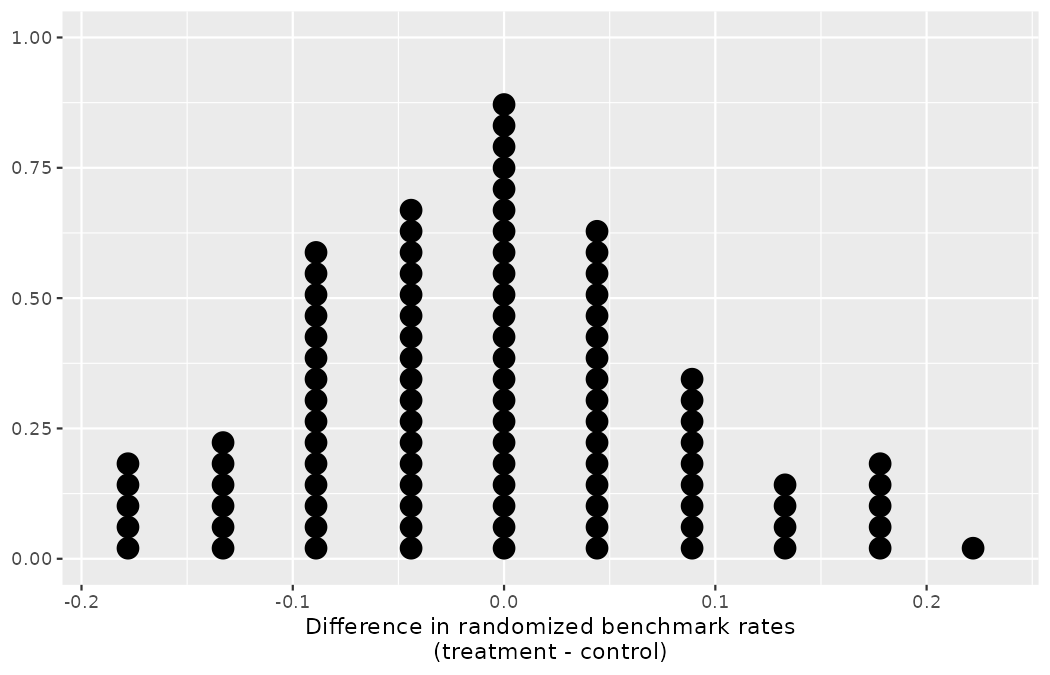
\includegraphics[width=0.85\linewidth,height=\textheight,keepaspectratio]{figures/inference-two-props-1.png}

The 100 dots stack at ten values running from \(-0.178\) to \(0.222.\)
With 26 \texttt{met} cards dealt into two stacks of 45, the difference
can only move in steps of \(2/45 \approx 0.044\) --- shift one
\texttt{met} card from one stack to the other and both proportions move
by \(1/45,\) in opposite directions. The tallest stacks sit at and
around zero.

\subsection{Observed statistic vs null
statistics}\label{observed-statistic-vs-null-statistics}

Note that the distribution of these simulated differences is centered
around 0. We simulated the differences assuming that the independence
model was true, that weekly video feedback has no effect on the
assessment. Under the null hypothesis, we expect the difference to be
near zero with some random fluctuation, where \emph{near} is pretty
generous in this case since the sample sizes are so small in this study.

\begin{tcolorbox}[enhanced jigsaw, left=2mm, leftrule=.75mm, title=\textcolor{quarto-callout-note-color}{\faInfo}\hspace{0.5em}{Worked example}, arc=.35mm, rightrule=.15mm, coltitle=black, colframe=quarto-callout-note-color-frame, bottomrule=.15mm, colbacktitle=quarto-callout-note-color!10!white, opacitybacktitle=0.6, breakable, bottomtitle=1mm, toptitle=1mm, titlerule=0mm, opacityback=0, toprule=.15mm, colback=white]

How often would you observe a difference of at least 13.3\% \((0.133)\)
according to the null distribution we just simulated? Is this a rare
event?

\begin{center}\rule{0.5\linewidth}{0.5pt}\end{center}

\begin{Shaded}
\begin{Highlighting}[]
\NormalTok{feedback90\_null }\SpecialCharTok{|\textgreater{}}
  \FunctionTok{summarize}\NormalTok{(}
    \AttributeTok{n\_extreme =} \FunctionTok{sum}\NormalTok{(stat }\SpecialCharTok{\textgreater{}=} \FloatTok{0.133}\NormalTok{),}
    \AttributeTok{prop\_extreme =} \FunctionTok{mean}\NormalTok{(stat }\SpecialCharTok{\textgreater{}=} \FloatTok{0.133}\NormalTok{)}
\NormalTok{  )}
\CommentTok{\#\textgreater{} \# A tibble: 1 × 2}
\CommentTok{\#\textgreater{}   n\_extreme prop\_extreme}
\CommentTok{\#\textgreater{}       \textless{}int\textgreater{}        \textless{}dbl\textgreater{}}
\CommentTok{\#\textgreater{} 1        10          0.1}
\end{Highlighting}
\end{Shaded}

A difference of at least 13.3\% due to chance alone, if the null
hypothesis were true, happened in 10 of the 100 simulations --- about
10\% of the time. This is not a very rare event. And recall the
discipline of Chapter~\ref{sec-foundations-decision-errors}: the honest
default is the two-sided test, since a video-review program could in
principle disrupt as well as sharpen. Doubling the tail gives a p-value
of \(2 \times 0.10 = 0.20.\) (In this run the left tail happened to hold
11 shuffles at or below \(-0.133;\) adding the tails instead of doubling
would give \(0.21\) --- the same verdict either way, as
Section~\ref{sec-two-sided-hypotheses} promised.)

\end{tcolorbox}

The difference of 13.3\% not being a rare event suggests two possible
interpretations of the results of the study:

\begin{itemize}
\tightlist
\item
  \(H_0\) \textbf{Independence model.} Weekly video feedback has no
  effect on the benchmark rate, and we just happened to observe a
  difference that would only occur on a rare occasion.
\item
  \(H_A\) \textbf{Alternative model.} Weekly video feedback changes the
  benchmark rate, and the difference we observed was actually due to the
  program being effective, which explains the difference of 13.3\%.
\end{itemize}

Since we determined that the outcome is not rare (a 20\% chance of
observing a difference at least as extreme as 13.3\% under the
assumption that the program has no effect), we fail to reject \(H_0,\)
and conclude that the study results do not provide strong evidence
against the independence model. This does not mean that we have proved
the video feedback is ineffective; it just means that this study does
not provide convincing evidence that it is effective in this setting ---
the same ``check complete'' verdict, on the same 90-player scale, that
\texttt{benchmark90} returned in Section~\ref{sec-two-sided-hypotheses}.
Two 90-player trials, two inconclusive verdicts: Jonas would do well to
reread the power discussion of Section~\ref{sec-pow} before designing a
third.

Statistical inference is built on evaluating how likely such differences
are to occur due to chance if in fact the null hypothesis is true. In
statistical inference, data scientists evaluate which model is most
reasonable given the data. Errors do occur, just like rare events, and
we might choose the wrong model. While we do not always choose
correctly, statistical inference gives us tools to control and evaluate
how often these errors occur --- that was the entire business of
Chapter~\ref{sec-foundations-decision-errors}.

\section{Bootstrap confidence interval for the difference in
proportions}\label{sec-two-prop-boot-ci}

In Section~\ref{sec-two-prop-errors}, we worked with the randomization
distribution to understand the distribution of \(\hat{p}_1 - \hat{p}_2\)
when the null hypothesis \(H_0: p_1 - p_2 = 0\) is true. Now, through
bootstrapping, we study the variability of \(\hat{p}_1 - \hat{p}_2\)
without assuming the null hypothesis is true --- the estimation
question, in the spirit of Chapter~\ref{sec-foundations-bootstrapping}:
not \emph{whether} the program moves the benchmark rate, but \emph{by
how much}, which is the number Marta Vidal would need before funding
video analysts for every academy age group.

\subsection{Observed data}\label{observed-data-9}

Reconsider the video-feedback data from
Section~\ref{sec-two-prop-errors}, summarized in
Table~\ref{tbl-feedback90-summary}. Again, we use the difference in
sample proportions as the observed statistic of interest. Here, the
value of the statistic is:
\(\hat{p}_T - \hat{p}_C = 0.356 - 0.222 = 0.133.\)

\subsection{Variability of the difference in sample
proportions}\label{variability-of-the-difference-in-sample-proportions}

The bootstrap method applied to two samples is an extension of the
method described in Chapter~\ref{sec-foundations-bootstrapping}. Now, we
have two samples, so \emph{each} sample estimates the population from
which it came. In the video-feedback setting, the treatment sample
estimates the population of all players who would train under the
program; the control sample estimates the population of all players
under standard training. Two samples, two estimated populations, two
bags of marbles --- and we resample from each bag separately, preserving
each group's sample size.

To watch the two-bag mechanics on a scale you can count by hand, step
away from the trial for a moment, down to a deliberately tiny scouting
errand. Emil Sørensen had a scout track a target striker over the past
month, and the scout logged every attempt by how it was struck and
whether it tested the keeper: 7 headers, of which 3 were on target, and
9 foot shots, of which 5 were on target. (A constructed scenario, built
in the code below.) These are two separate samples --- one from the
population of the striker's headed attempts, one from the population of
his footed attempts --- and the parameter of interest is the difference
in his true on-target rates, \(p_1 - p_2,\) with group 1 the headers and
group 2 the foot shots.

\begin{Shaded}
\begin{Highlighting}[]
\NormalTok{headers7 }\OtherTok{\textless{}{-}} \FunctionTok{tibble}\NormalTok{(}
  \AttributeTok{shot   =} \FunctionTok{paste0}\NormalTok{(}\StringTok{"H"}\NormalTok{, }\DecValTok{1}\SpecialCharTok{:}\DecValTok{7}\NormalTok{),}
  \AttributeTok{result =} \FunctionTok{c}\NormalTok{(}\FunctionTok{rep}\NormalTok{(}\StringTok{"on target"}\NormalTok{, }\DecValTok{3}\NormalTok{), }\FunctionTok{rep}\NormalTok{(}\StringTok{"off target"}\NormalTok{, }\DecValTok{4}\NormalTok{))}
\NormalTok{)}

\NormalTok{foot9 }\OtherTok{\textless{}{-}} \FunctionTok{tibble}\NormalTok{(}
  \AttributeTok{shot   =} \FunctionTok{paste0}\NormalTok{(}\StringTok{"F"}\NormalTok{, }\DecValTok{1}\SpecialCharTok{:}\DecValTok{9}\NormalTok{),}
  \AttributeTok{result =} \FunctionTok{c}\NormalTok{(}\FunctionTok{rep}\NormalTok{(}\StringTok{"on target"}\NormalTok{, }\DecValTok{5}\NormalTok{), }\FunctionTok{rep}\NormalTok{(}\StringTok{"off target"}\NormalTok{, }\DecValTok{4}\NormalTok{))}
\NormalTok{)}
\end{Highlighting}
\end{Shaded}

Each sample estimates its own population: an infinitely large pool of
headed attempts, \(3/7\) on target, and an infinitely large pool of
footed attempts, \(5/9\) on target --- or, in marbles, a bag of 3 red
and 4 white, and a second bag of 5 red and 4 white. As in
Chapter~\ref{sec-foundations-bootstrapping}, drawing \emph{with
replacement} from each bag, preserving each bag's sample size, is the
computational equivalent of sampling from the estimated populations. One
bootstrap resample of the pair means: draw 7 from the header bag, draw 9
from the foot bag, and take the difference of the two resample
proportions.

\begin{Shaded}
\begin{Highlighting}[]
\FunctionTok{set.seed}\NormalTok{(}\DecValTok{1702}\NormalTok{)}
\NormalTok{headers\_re1 }\OtherTok{\textless{}{-}}\NormalTok{ headers7 }\SpecialCharTok{|\textgreater{}} \FunctionTok{slice\_sample}\NormalTok{(}\AttributeTok{n =} \DecValTok{7}\NormalTok{, }\AttributeTok{replace =} \ConstantTok{TRUE}\NormalTok{)}
\NormalTok{foot\_re1    }\OtherTok{\textless{}{-}}\NormalTok{ foot9   }\SpecialCharTok{|\textgreater{}} \FunctionTok{slice\_sample}\NormalTok{(}\AttributeTok{n =} \DecValTok{9}\NormalTok{, }\AttributeTok{replace =} \ConstantTok{TRUE}\NormalTok{)}

\NormalTok{headers\_re1 }\SpecialCharTok{|\textgreater{}} \FunctionTok{arrange}\NormalTok{(shot)}
\CommentTok{\#\textgreater{} \# A tibble: 7 × 2}
\CommentTok{\#\textgreater{}   shot  result}
\CommentTok{\#\textgreater{}   \textless{}chr\textgreater{} \textless{}chr\textgreater{}}
\CommentTok{\#\textgreater{} 1 H1    on target}
\CommentTok{\#\textgreater{} 2 H1    on target}
\CommentTok{\#\textgreater{} 3 H3    on target}
\CommentTok{\#\textgreater{} 4 H4    off target}
\CommentTok{\#\textgreater{} 5 H6    off target}
\CommentTok{\#\textgreater{} 6 H7    off target}
\CommentTok{\#\textgreater{} 7 H7    off target}

\FunctionTok{c}\NormalTok{(}\FunctionTok{mean}\NormalTok{(headers\_re1}\SpecialCharTok{$}\NormalTok{result }\SpecialCharTok{==} \StringTok{"on target"}\NormalTok{),}
  \FunctionTok{mean}\NormalTok{(foot\_re1}\SpecialCharTok{$}\NormalTok{result }\SpecialCharTok{==} \StringTok{"on target"}\NormalTok{))}
\CommentTok{\#\textgreater{} [1] 0.4285714 0.3333333}
\end{Highlighting}
\end{Shaded}

Header H1 was drawn twice, H7 twice, and H2 and H5 not at all ---
sampling with replacement, exactly as you watched it with the trialists
of Chapter~\ref{sec-foundations-bootstrapping}. This first pair of
resamples gives bootstrap proportions of \(3/7\) and \(3/9,\) for a
difference of \(3/7 - 3/9 = 0.095.\) Repeating the process:

\begin{Shaded}
\begin{Highlighting}[]
\NormalTok{headers\_re2 }\OtherTok{\textless{}{-}}\NormalTok{ headers7 }\SpecialCharTok{|\textgreater{}} \FunctionTok{slice\_sample}\NormalTok{(}\AttributeTok{n =} \DecValTok{7}\NormalTok{, }\AttributeTok{replace =} \ConstantTok{TRUE}\NormalTok{)}
\NormalTok{foot\_re2    }\OtherTok{\textless{}{-}}\NormalTok{ foot9   }\SpecialCharTok{|\textgreater{}} \FunctionTok{slice\_sample}\NormalTok{(}\AttributeTok{n =} \DecValTok{9}\NormalTok{, }\AttributeTok{replace =} \ConstantTok{TRUE}\NormalTok{)}
\NormalTok{headers\_re3 }\OtherTok{\textless{}{-}}\NormalTok{ headers7 }\SpecialCharTok{|\textgreater{}} \FunctionTok{slice\_sample}\NormalTok{(}\AttributeTok{n =} \DecValTok{7}\NormalTok{, }\AttributeTok{replace =} \ConstantTok{TRUE}\NormalTok{)}
\NormalTok{foot\_re3    }\OtherTok{\textless{}{-}}\NormalTok{ foot9   }\SpecialCharTok{|\textgreater{}} \FunctionTok{slice\_sample}\NormalTok{(}\AttributeTok{n =} \DecValTok{9}\NormalTok{, }\AttributeTok{replace =} \ConstantTok{TRUE}\NormalTok{)}

\FunctionTok{round}\NormalTok{(}\FunctionTok{c}\NormalTok{(}
  \FunctionTok{mean}\NormalTok{(headers\_re2}\SpecialCharTok{$}\NormalTok{result }\SpecialCharTok{==} \StringTok{"on target"}\NormalTok{) }\SpecialCharTok{{-}} \FunctionTok{mean}\NormalTok{(foot\_re2}\SpecialCharTok{$}\NormalTok{result }\SpecialCharTok{==} \StringTok{"on target"}\NormalTok{),}
  \FunctionTok{mean}\NormalTok{(headers\_re3}\SpecialCharTok{$}\NormalTok{result }\SpecialCharTok{==} \StringTok{"on target"}\NormalTok{) }\SpecialCharTok{{-}} \FunctionTok{mean}\NormalTok{(foot\_re3}\SpecialCharTok{$}\NormalTok{result }\SpecialCharTok{==} \StringTok{"on target"}\NormalTok{)}
\NormalTok{), }\DecValTok{3}\NormalTok{)}
\CommentTok{\#\textgreater{} [1] {-}0.206 {-}0.016}
\end{Highlighting}
\end{Shaded}

The second pair of resamples came out \(4/7\) and \(7/9\) \((-0.206);\)
the third, \(3/7\) and \(4/9\) \((-0.016).\) As always, the variability
of the difference in proportions can only be estimated by repeated
simulations --- so we run 1,000 and stack the differences into a
bootstrap sampling distribution:

\begin{Shaded}
\begin{Highlighting}[]
\NormalTok{tiny\_boot }\OtherTok{\textless{}{-}} \FunctionTok{tibble}\NormalTok{(}
  \AttributeTok{stat =} \FunctionTok{replicate}\NormalTok{(}\DecValTok{1000}\NormalTok{, \{}
    \FunctionTok{mean}\NormalTok{(}\FunctionTok{slice\_sample}\NormalTok{(headers7, }\AttributeTok{n =} \DecValTok{7}\NormalTok{, }\AttributeTok{replace =} \ConstantTok{TRUE}\NormalTok{)}\SpecialCharTok{$}\NormalTok{result }\SpecialCharTok{==} \StringTok{"on target"}\NormalTok{) }\SpecialCharTok{{-}}
      \FunctionTok{mean}\NormalTok{(}\FunctionTok{slice\_sample}\NormalTok{(foot9, }\AttributeTok{n =} \DecValTok{9}\NormalTok{, }\AttributeTok{replace =} \ConstantTok{TRUE}\NormalTok{)}\SpecialCharTok{$}\NormalTok{result }\SpecialCharTok{==} \StringTok{"on target"}\NormalTok{)}
\NormalTok{  \})}
\NormalTok{)}

\NormalTok{tiny\_boot }\SpecialCharTok{|\textgreater{}}
  \FunctionTok{summarize}\NormalTok{(}\AttributeTok{se =} \FunctionTok{sd}\NormalTok{(stat), }\AttributeTok{lowest =} \FunctionTok{min}\NormalTok{(stat), }\AttributeTok{highest =} \FunctionTok{max}\NormalTok{(stat))}
\CommentTok{\#\textgreater{} \# A tibble: 1 × 3}
\CommentTok{\#\textgreater{}      se lowest highest}
\CommentTok{\#\textgreater{}   \textless{}dbl\textgreater{}  \textless{}dbl\textgreater{}   \textless{}dbl\textgreater{}}
\CommentTok{\#\textgreater{} 1 0.250 {-}0.889   0.603}
\end{Highlighting}
\end{Shaded}

The 1,000 bootstrapped differences sprawl from \(-0.889\) to \(0.603,\)
with a standard deviation of \(0.250\) --- a quarter, on a statistic
that lives between \(-1\) and \(1.\) Seven headers and nine foot shots
simply cannot pin down a difference in rates; the scout's month of
logging is a mechanism demonstration, not an answer.

Now return to the trial, where the same procedure has 45 observations in
each bag. The \textbf{infer} pipeline bootstraps both groups in one call
--- \texttt{generate(type\ =\ "bootstrap")} resamples the 90 rows with
replacement, and \texttt{calculate()} takes the difference in
proportions in each resample:

\begin{Shaded}
\begin{Highlighting}[]
\FunctionTok{set.seed}\NormalTok{(}\DecValTok{1701}\NormalTok{)}
\NormalTok{feedback90\_boot }\OtherTok{\textless{}{-}}\NormalTok{ feedback90 }\SpecialCharTok{|\textgreater{}}
  \FunctionTok{specify}\NormalTok{(outcome }\SpecialCharTok{\textasciitilde{}}\NormalTok{ group, }\AttributeTok{success =} \StringTok{"met"}\NormalTok{) }\SpecialCharTok{|\textgreater{}}
  \FunctionTok{generate}\NormalTok{(}\AttributeTok{reps =} \DecValTok{1000}\NormalTok{, }\AttributeTok{type =} \StringTok{"bootstrap"}\NormalTok{) }\SpecialCharTok{|\textgreater{}}
  \FunctionTok{calculate}\NormalTok{(}\AttributeTok{stat =} \StringTok{"diff in props"}\NormalTok{, }\AttributeTok{order =} \FunctionTok{c}\NormalTok{(}\StringTok{"treatment"}\NormalTok{, }\StringTok{"control"}\NormalTok{))}

\FunctionTok{ggplot}\NormalTok{(feedback90\_boot, }\FunctionTok{aes}\NormalTok{(}\AttributeTok{x =}\NormalTok{ stat)) }\SpecialCharTok{+}
  \FunctionTok{geom\_histogram}\NormalTok{(}\AttributeTok{binwidth =} \FloatTok{0.05}\NormalTok{) }\SpecialCharTok{+}
  \FunctionTok{labs}\NormalTok{(}
    \AttributeTok{x =} \StringTok{"Difference in bootstrapped benchmark rates}\SpecialCharTok{\textbackslash{}n}\StringTok{(treatment {-} control)"}\NormalTok{,}
    \AttributeTok{y =} \StringTok{"Count"}
\NormalTok{  )}
\end{Highlighting}
\end{Shaded}

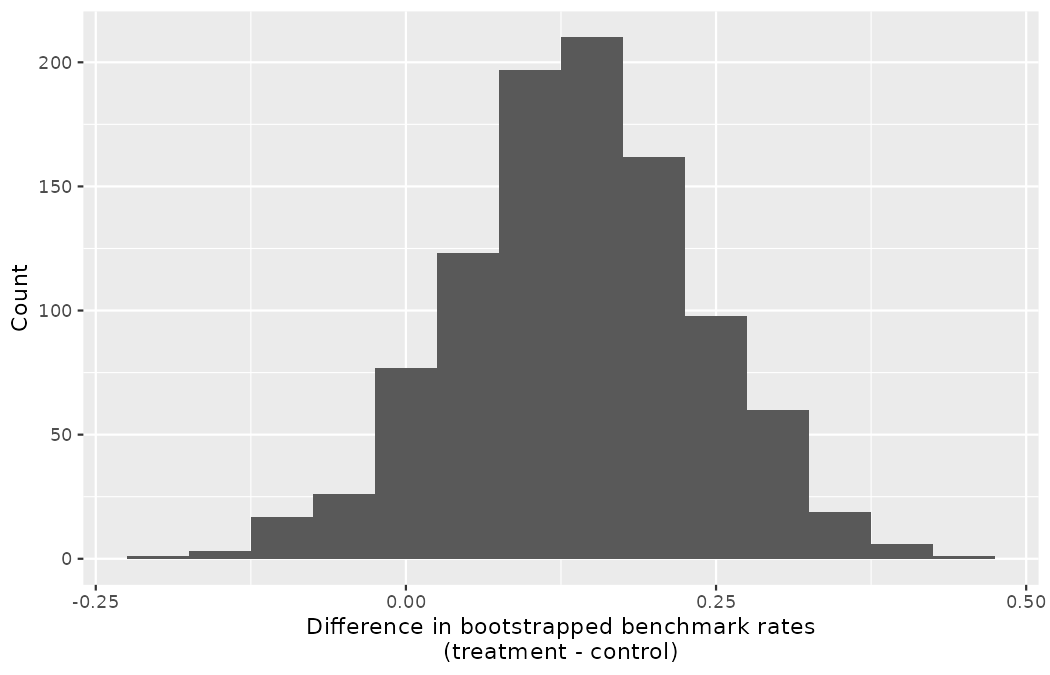
\includegraphics[width=0.85\linewidth,height=\textheight,keepaspectratio]{figures/inference-two-props-2.png}

The histogram of the 1,000 bootstrapped differences is roughly symmetric
and bell-shaped, centered near the observed statistic of \(0.133\) (the
mean of the 1,000 differences is \(0.138),\) with the differences
running from about \(-0.18\) to \(0.45.\) Note the contrast with the
striker's shot log: the trial has 45 and 45 observations in the two
groups where the log had 7 and 9, and the variability of the
bootstrapped differences shrinks accordingly --- a standard deviation of
about \(0.10\) against the log's \(0.25.\) As you will see in the
mathematical models discussed in Section~\ref{sec-math-2prop}, large
sample sizes lead to smaller standard errors for a difference in
proportions.

\subsection{Bootstrap percentile vs.~SE confidence
intervals}\label{bootstrap-percentile-vs.-se-confidence-intervals}

The bootstrap distribution above provides an estimate for the
variability of the difference in benchmark proportions from sample to
sample. The values in the histogram can be used in two different ways to
create a confidence interval for the parameter of interest:
\(p_1 - p_2.\)

As in Chapter~\ref{sec-foundations-bootstrapping}, the bootstrap
confidence interval can be calculated directly from the bootstrapped
differences. The interval created from the percentiles of the
distribution is called the \textbf{percentile interval}. Note that here
we calculate the 90\% confidence interval by finding the \(5^{th}\) and
\(95^{th}\) percentile values from the bootstrapped differences.

\begin{Shaded}
\begin{Highlighting}[]
\NormalTok{feedback90\_boot }\SpecialCharTok{|\textgreater{}}
  \FunctionTok{summarize}\NormalTok{(}
    \AttributeTok{lower =} \FunctionTok{quantile}\NormalTok{(stat, }\FloatTok{0.05}\NormalTok{),}
    \AttributeTok{upper =} \FunctionTok{quantile}\NormalTok{(stat, }\FloatTok{0.95}\NormalTok{)}
\NormalTok{  )}
\CommentTok{\#\textgreater{} \# A tibble: 1 × 2}
\CommentTok{\#\textgreater{}     lower upper}
\CommentTok{\#\textgreater{}     \textless{}dbl\textgreater{} \textless{}dbl\textgreater{}}
\CommentTok{\#\textgreater{} 1 {-}0.0222   0.3}
\end{Highlighting}
\end{Shaded}

The bootstrap 5 percentile difference is \(-0.022\) and the 95
percentile is \(0.300.\) The result is: we are 90\% confident that, in
the population, the true change in benchmark rate under the
video-feedback program is between 2.2 percentage points \emph{lower} and
30.0 percentage points \emph{higher} than under standard training. The
interval shows that we do not have much definitive evidence of the
effect of the program, one way or another.

Alternatively, we can use the variability in the bootstrapped
differences to calculate a standard error of the difference. The
resulting interval is called the \textbf{SE interval}.
Section~\ref{sec-math-2prop} details the mathematical model for the
standard error of the difference in sample proportions, but the
bootstrap distribution typically does an excellent job of estimating the
variability of the sampling distribution of the sample statistic.

\begin{Shaded}
\begin{Highlighting}[]
\NormalTok{feedback90\_boot }\SpecialCharTok{|\textgreater{}}
  \FunctionTok{summarize}\NormalTok{(}\AttributeTok{se =} \FunctionTok{sd}\NormalTok{(stat))}
\CommentTok{\#\textgreater{} \# A tibble: 1 × 1}
\CommentTok{\#\textgreater{}       se}
\CommentTok{\#\textgreater{}    \textless{}dbl\textgreater{}}
\CommentTok{\#\textgreater{} 1 0.0974}
\end{Highlighting}
\end{Shaded}

\[
SE(\hat{p}_T - \hat{p}_C) \approx SE(\hat{p}_{T, boot} - \hat{p}_{C, boot}) = 0.0974
\]

The subscripts stack but decompose exactly as their pieces did in
Chapter~\ref{sec-foundations-bootstrapping} and
Chapter~\ref{sec-foundations-randomization}: \(\hat{p}_{T, boot}\) is a
proportion (the \(p\)), computed from data (the hat), within the
treatment group (the \(T\)), of a bootstrap resample (the \(boot\)). The
variability of the difference in proportions was calculated in R using
the \texttt{sd()} function, but any statistical software will calculate
the standard deviation of the differences --- here, the exact quantity
we hope to approximate.

Note that we do not know the true distribution of
\(\hat{p}_T - \hat{p}_C,\) so we will use a rough approximation to find
a confidence interval for \(p_T - p_C.\) As seen in the bootstrap
histogram, the shape of the distribution is roughly symmetric and
bell-shaped. So for a rough approximation, we will apply the 68-95-99.7
rule of Section~\ref{sec-normalDist}, which tells us that 95\% of
observed differences should be roughly no farther than 2 SE from the
true parameter (difference in proportions). A 95\% confidence interval
for \(p_T - p_C\) is given by:

\[
\hat{p}_T - \hat{p}_C \pm 2 \cdot SE \rightarrow \ \ \ 16/45 - 10/45 \pm 2 \cdot 0.0974 \ \ \ \rightarrow \ \ \ (-0.061,\ 0.328)
\]

\begin{Shaded}
\begin{Highlighting}[]
\FunctionTok{round}\NormalTok{(}\DecValTok{16} \SpecialCharTok{/} \DecValTok{45} \SpecialCharTok{{-}} \DecValTok{10} \SpecialCharTok{/} \DecValTok{45} \SpecialCharTok{+} \FunctionTok{c}\NormalTok{(}\SpecialCharTok{{-}}\DecValTok{2}\NormalTok{, }\DecValTok{2}\NormalTok{) }\SpecialCharTok{*} \FloatTok{0.0974}\NormalTok{, }\DecValTok{3}\NormalTok{)}
\CommentTok{\#\textgreater{} [1] {-}0.061  0.328}
\end{Highlighting}
\end{Shaded}

We are 95\% confident that the true value of \(p_T - p_C\) is between
\(-0.061\) and \(0.328.\) Again, the wide confidence interval that
contains zero indicates that the study provides very little evidence
about the effectiveness of the video-feedback program --- Marta gets an
honest ``somewhere between mildly harmful and transformative,'' which is
to say, not yet a budget line. For other percentages, e.g., a 90\%
bootstrap SE confidence interval, we use the corresponding cutoff
\(z^\star\) from the normal distribution, exactly as in
Chapter~\ref{sec-inference-one-prop}.

\begin{tcolorbox}[enhanced jigsaw, left=2mm, leftrule=.75mm, title=\textcolor{quarto-callout-tip-color}{\faLightbulb}\hspace{0.5em}{Check your understanding}, arc=.35mm, rightrule=.15mm, coltitle=black, colframe=quarto-callout-tip-color-frame, bottomrule=.15mm, colbacktitle=quarto-callout-tip-color!10!white, opacitybacktitle=0.6, breakable, bottomtitle=1mm, toptitle=1mm, titlerule=0mm, opacityback=0, toprule=.15mm, colback=white]

The 90\% percentile interval ran from \(-0.022\) to \(0.300.\) Without
computing anything new, should a 90\% \emph{SE} interval for the same
data be wildly different? Why or why not?

\begin{center}\rule{0.5\linewidth}{0.5pt}\end{center}

No --- the two intervals should nearly agree. The bootstrap distribution
is roughly symmetric and bell-shaped, and for bell-shaped distributions
the middle 90\% of values sits within about \(1.65\) standard errors of
the center (recall the \(z^\star\) cutoffs of
Chapter~\ref{sec-inference-one-prop}). Indeed,
\(0.1333 \pm 1.65 \times 0.0974\) gives \((-0.027, 0.294),\) close to
the percentile interval's \((-0.022, 0.300).\) The two constructions
differ meaningfully only when the bootstrap distribution is noticeably
skewed --- recall the corner-pattern proportions of
Chapter~\ref{sec-foundations-bootstrapping}.

\end{tcolorbox}

\subsection{What does 95\% mean?}\label{what-does-95-mean}

Recall that the goal of a confidence interval is to find a plausible
range of values for a \emph{parameter} of interest. The estimated
statistic is not the value of interest, but it is typically the best
guess for the unknown parameter. The confidence level (often 95\%) is a
number that takes a while to get used to. Surprisingly, the percentage
does not describe the dataset at hand; it describes many possible
datasets. One way to understand a confidence interval is to think about
all the confidence intervals that you have ever made or that you will
ever make as an analyst: the confidence level describes \textbf{those}
intervals.

In Chapter~\ref{sec-foundations-mathematical} we watched this happen for
a single proportion, drawing 25 samples from the one population we hold
in full: the 1,494 shots of the 2022 World Cup. The same demonstration
works for a \emph{difference} in proportions, and the tournament again
supplies a known truth to aim at. Consider the first-time finishing
split you met in Chapter~\ref{sec-foundations-decision-errors}:

\begin{Shaded}
\begin{Highlighting}[]
\NormalTok{wc2022\_shots }\OtherTok{\textless{}{-}} \FunctionTok{read\_csv}\NormalTok{(}\StringTok{"data/derived/wc2022\_shots.csv"}\NormalTok{)}

\NormalTok{wc2022\_shots }\SpecialCharTok{|\textgreater{}}
  \FunctionTok{group\_by}\NormalTok{(first\_time) }\SpecialCharTok{|\textgreater{}}
  \FunctionTok{summarize}\NormalTok{(}\AttributeTok{shots =} \FunctionTok{n}\NormalTok{(), }\AttributeTok{goals =} \FunctionTok{sum}\NormalTok{(goal), }\AttributeTok{conversion =} \FunctionTok{mean}\NormalTok{(goal))}
\CommentTok{\#\textgreater{} \# A tibble: 2 × 4}
\CommentTok{\#\textgreater{}   first\_time shots goals conversion}
\CommentTok{\#\textgreater{}   \textless{}lgl\textgreater{}      \textless{}int\textgreater{} \textless{}int\textgreater{}      \textless{}dbl\textgreater{}}
\CommentTok{\#\textgreater{} 1 FALSE       1026   124      0.121}
\CommentTok{\#\textgreater{} 2 TRUE         468    71      0.152}
\end{Highlighting}
\end{Shaded}

Treating the tournament as the population, the \emph{true} parameter is
known exactly:

\[p_{ft} - p_{ot} = \frac{71}{468} - \frac{124}{1026} = 0.1517 - 0.1209 = 0.0309\]

One flag before we use it, per this book's penalty convention: this is
the \emph{all-shots} gap, penalties and shoot-out kicks included, and
every one of the tournament's 64 penalties sits in the controlled-touch
(non-first-time) bucket. On open play the gap is considerably wider ---
you saw the mechanism dissected in
Chapter~\ref{sec-foundations-decision-errors}, and the code below
confirms it for this tournament:

\begin{Shaded}
\begin{Highlighting}[]
\NormalTok{wc2022\_shots }\SpecialCharTok{|\textgreater{}}
  \FunctionTok{filter}\NormalTok{(shot\_type }\SpecialCharTok{==} \StringTok{"Open Play"}\NormalTok{) }\SpecialCharTok{|\textgreater{}}
  \FunctionTok{group\_by}\NormalTok{(first\_time) }\SpecialCharTok{|\textgreater{}}
  \FunctionTok{summarize}\NormalTok{(}\AttributeTok{shots =} \FunctionTok{n}\NormalTok{(), }\AttributeTok{goals =} \FunctionTok{sum}\NormalTok{(goal), }\AttributeTok{conversion =} \FunctionTok{mean}\NormalTok{(goal))}
\CommentTok{\#\textgreater{} \# A tibble: 2 × 4}
\CommentTok{\#\textgreater{}   first\_time shots goals conversion}
\CommentTok{\#\textgreater{}   \textless{}lgl\textgreater{}      \textless{}int\textgreater{} \textless{}int\textgreater{}      \textless{}dbl\textgreater{}}
\CommentTok{\#\textgreater{} 1 FALSE        914    79     0.0864}
\CommentTok{\#\textgreater{} 2 TRUE         468    71     0.152}
\end{Highlighting}
\end{Shaded}

For a \emph{scouting} claim about first-time finishing, the open-play
frame \((0.152\) vs \(0.086)\) is the one to argue from. Here, however,
the tournament is serving as a laboratory: a population whose parameter
we get to define and then try to capture, so that the coverage machinery
--- not first-time finishing --- is on trial. We therefore state the
frame (all 1,494 shots, penalties in), define the truth as \(0.0309,\)
and use that same frame for every sample below.

The code draws 25 different studies from this population --- each a
sample of 500 shots drawn with replacement, so that every shot is an
independent draw from the tournament's shot pool, exactly as in the
25-interval simulation of Chapter~\ref{sec-foundations-mathematical} ---
splits each study into its first-time and other-shot groups, and builds
a 95\% confidence interval from each, borrowing the SE formula that
Section~\ref{sec-math-2prop} will formalize (as
Chapter~\ref{sec-foundations-mathematical} once borrowed it for the
finishing-program interval):

\begin{Shaded}
\begin{Highlighting}[]
\NormalTok{d\_wc }\OtherTok{\textless{}{-}} \DecValTok{71} \SpecialCharTok{/} \DecValTok{468} \SpecialCharTok{{-}} \DecValTok{124} \SpecialCharTok{/} \DecValTok{1026}

\FunctionTok{set.seed}\NormalTok{(}\DecValTok{1703}\NormalTok{)}
\NormalTok{ci25 }\OtherTok{\textless{}{-}} \FunctionTok{map\_dfr}\NormalTok{(}\DecValTok{1}\SpecialCharTok{:}\DecValTok{25}\NormalTok{, \textbackslash{}(rep) \{}
\NormalTok{  wc2022\_shots }\SpecialCharTok{|\textgreater{}}
    \FunctionTok{slice\_sample}\NormalTok{(}\AttributeTok{n =} \DecValTok{500}\NormalTok{, }\AttributeTok{replace =} \ConstantTok{TRUE}\NormalTok{) }\SpecialCharTok{|\textgreater{}}
    \FunctionTok{summarize}\NormalTok{(}
      \AttributeTok{n\_ft =} \FunctionTok{sum}\NormalTok{(first\_time),}
      \AttributeTok{n\_ot =} \FunctionTok{sum}\NormalTok{(}\SpecialCharTok{!}\NormalTok{first\_time),}
      \AttributeTok{p\_ft =} \FunctionTok{mean}\NormalTok{(goal[first\_time]),}
      \AttributeTok{p\_ot =} \FunctionTok{mean}\NormalTok{(goal[}\SpecialCharTok{!}\NormalTok{first\_time])}
\NormalTok{    ) }\SpecialCharTok{|\textgreater{}}
    \FunctionTok{mutate}\NormalTok{(}
      \AttributeTok{sample =}\NormalTok{ rep,}
      \AttributeTok{d\_hat  =}\NormalTok{ p\_ft }\SpecialCharTok{{-}}\NormalTok{ p\_ot,}
      \AttributeTok{se     =} \FunctionTok{sqrt}\NormalTok{(p\_ft }\SpecialCharTok{*}\NormalTok{ (}\DecValTok{1} \SpecialCharTok{{-}}\NormalTok{ p\_ft) }\SpecialCharTok{/}\NormalTok{ n\_ft }\SpecialCharTok{+}\NormalTok{ p\_ot }\SpecialCharTok{*}\NormalTok{ (}\DecValTok{1} \SpecialCharTok{{-}}\NormalTok{ p\_ot) }\SpecialCharTok{/}\NormalTok{ n\_ot),}
      \AttributeTok{lower  =}\NormalTok{ d\_hat }\SpecialCharTok{{-}} \FloatTok{1.96} \SpecialCharTok{*}\NormalTok{ se,}
      \AttributeTok{upper  =}\NormalTok{ d\_hat }\SpecialCharTok{+} \FloatTok{1.96} \SpecialCharTok{*}\NormalTok{ se,}
      \AttributeTok{miss   =}\NormalTok{ lower }\SpecialCharTok{\textgreater{}}\NormalTok{ d\_wc }\SpecialCharTok{|}\NormalTok{ upper }\SpecialCharTok{\textless{}}\NormalTok{ d\_wc}
\NormalTok{    )}
\NormalTok{\})}

\NormalTok{ci25 }\SpecialCharTok{|\textgreater{}} \FunctionTok{summarize}\NormalTok{(}\AttributeTok{n\_miss =} \FunctionTok{sum}\NormalTok{(miss))}
\CommentTok{\#\textgreater{} \# A tibble: 1 × 1}
\CommentTok{\#\textgreater{}   n\_miss}
\CommentTok{\#\textgreater{}    \textless{}int\textgreater{}}
\CommentTok{\#\textgreater{} 1      2}

\NormalTok{ci25 }\SpecialCharTok{|\textgreater{}} \FunctionTok{filter}\NormalTok{(miss) }\SpecialCharTok{|\textgreater{}} \FunctionTok{select}\NormalTok{(sample, d\_hat, lower, upper)}
\CommentTok{\#\textgreater{} \# A tibble: 2 × 4}
\CommentTok{\#\textgreater{}   sample d\_hat  lower upper}
\CommentTok{\#\textgreater{}    \textless{}int\textgreater{} \textless{}dbl\textgreater{}  \textless{}dbl\textgreater{} \textless{}dbl\textgreater{}}
\CommentTok{\#\textgreater{} 1     21 0.110 0.0480 0.173}
\CommentTok{\#\textgreater{} 2     23 0.111 0.0404 0.181}
\end{Highlighting}
\end{Shaded}

\begin{Shaded}
\begin{Highlighting}[]
\FunctionTok{ggplot}\NormalTok{(ci25, }\FunctionTok{aes}\NormalTok{(}\AttributeTok{y =}\NormalTok{ sample)) }\SpecialCharTok{+}
  \FunctionTok{geom\_segment}\NormalTok{(}\FunctionTok{aes}\NormalTok{(}\AttributeTok{x =}\NormalTok{ lower, }\AttributeTok{xend =}\NormalTok{ upper, }\AttributeTok{yend =}\NormalTok{ sample, }\AttributeTok{color =}\NormalTok{ miss)) }\SpecialCharTok{+}
  \FunctionTok{geom\_point}\NormalTok{(}\FunctionTok{aes}\NormalTok{(}\AttributeTok{x =}\NormalTok{ d\_hat, }\AttributeTok{color =}\NormalTok{ miss)) }\SpecialCharTok{+}
  \FunctionTok{geom\_vline}\NormalTok{(}\AttributeTok{xintercept =}\NormalTok{ d\_wc, }\AttributeTok{linetype =} \StringTok{"dashed"}\NormalTok{) }\SpecialCharTok{+}
  \FunctionTok{scale\_color\_manual}\NormalTok{(}\AttributeTok{values =} \FunctionTok{c}\NormalTok{(}\StringTok{"black"}\NormalTok{, }\StringTok{"red"}\NormalTok{), }\AttributeTok{guide =} \StringTok{"none"}\NormalTok{) }\SpecialCharTok{+}
  \FunctionTok{labs}\NormalTok{(}
    \AttributeTok{x =} \StringTok{"Sample difference in conversion (first{-}time {-} other), with 95\% CI"}\NormalTok{,}
    \AttributeTok{y =} \StringTok{"Sample"}
\NormalTok{  )}
\end{Highlighting}
\end{Shaded}

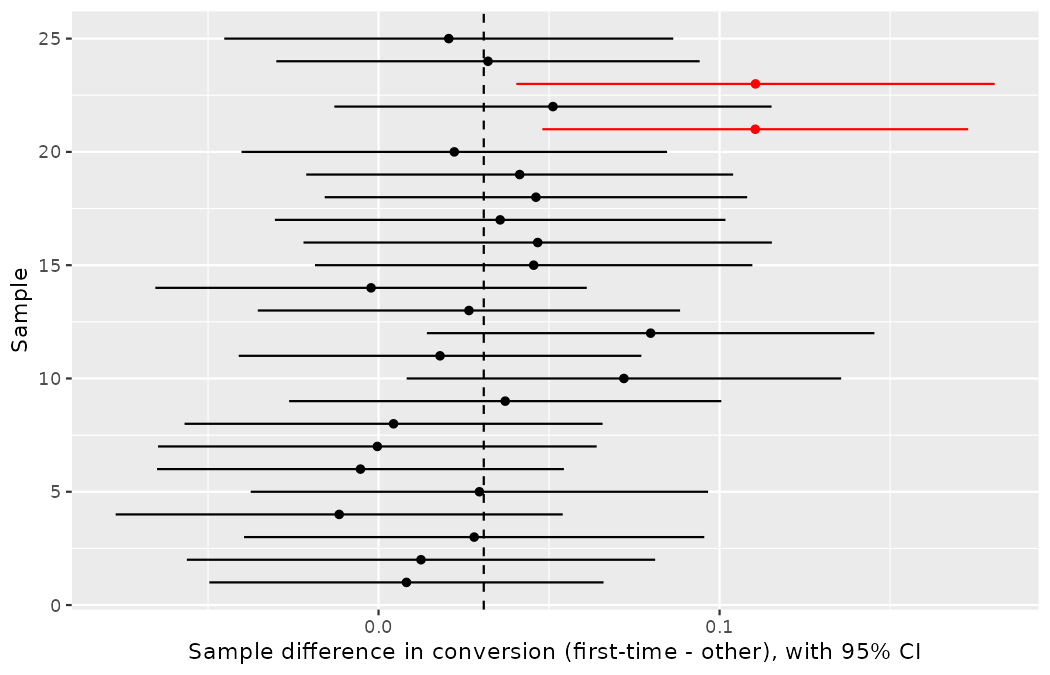
\includegraphics[width=0.85\linewidth,height=\textheight,keepaspectratio]{figures/inference-two-props-3.png}

The figure shows 25 horizontal interval segments, one per study, each
with a dot at its point estimate \(\hat{p}_{ft} - \hat{p}_{ot},\) and a
dashed vertical line at the true parameter value
\(p_{ft} - p_{ot} = 0.0309.\) The study at hand --- any study you will
ever run --- is one of these lines, and it is not possible to know, from
inside the study, whether yours sits to the left of the truth, to the
right of it, or astride it. Twenty-three of the 25 intervals cross the
dashed line. Two --- samples 21 and 23, whose 500 resampled shots
happened to contain hot-finishing first-time chances, with point
estimates near \(0.11\) --- lie entirely \emph{above} the truth, and are
drawn in red. An analyst holding sample 21 would report, with a
perfectly constructed interval, that first-time shots convert at least
4.8 percentage points better; the parameter says 3.1. If we are making
95\% intervals, then about 5\% of the intervals we create over our
lifetime will \emph{not} capture the parameter of interest. What we know
is that, over our lifetimes as analysts, about 95\% of the intervals
created and reported on will capture the parameter value of interest:
thus the language ``95\% confident.'' Two misses in 25 is above the
advertised 1-in-20, and that, too, is chance doing what chance does ---
collect enough intervals over enough studies, and the long-run rate
asserts itself.

\begin{tcolorbox}[enhanced jigsaw, left=2mm, leftrule=.75mm, title=\textcolor{quarto-callout-tip-color}{\faLightbulb}\hspace{0.5em}{Check your understanding}, arc=.35mm, rightrule=.15mm, coltitle=black, colframe=quarto-callout-tip-color-frame, bottomrule=.15mm, colbacktitle=quarto-callout-tip-color!10!white, opacitybacktitle=0.6, breakable, bottomtitle=1mm, toptitle=1mm, titlerule=0mm, opacityback=0, toprule=.15mm, colback=white]

If the 25 analysts had built 90\% intervals instead, about how many
misses should we expect? Would the intervals be wider or narrower?

\begin{center}\rule{0.5\linewidth}{0.5pt}\end{center}

About \(0.10 \times 25 = 2.5\) misses, on average --- and the intervals
would be \emph{narrower}, using \(z^\star = 1.65\) in place of \(1.96\)
(recall Chapter~\ref{sec-inference-one-prop}). A lower confidence level
trades capture rate for precision; neither choice is free.

\end{tcolorbox}

The choice of 95\% or 90\% or even 99\% as a confidence level is
admittedly somewhat arbitrary; however, it is related to the logic we
used when deciding that a p-value should be declared as ``discernible''
if it is lower than 0.05 (or 0.10 or 0.01, respectively). Indeed, one
can show mathematically that a 95\% confidence interval and a two-sided
hypothesis test at a cutoff of 0.05 will provide the same conclusion
when the same data and mathematical tools are applied for the analysis.
A full derivation of the explicit connection between confidence
intervals and hypothesis tests is beyond the scope of this text.

\section{Mathematical model for the difference in
proportions}\label{sec-math-2prop}

\subsection{Variability of the difference between two
proportions}\label{variability-of-the-difference-between-two-proportions}

Like with \(\hat{p},\) the difference of two sample proportions
\(\hat{p}_1 - \hat{p}_2\) can be modeled using a normal distribution
when certain conditions are met. First, we require a broader
independence condition, and secondly, the success-failure condition must
be met by both groups.

\begin{tcolorbox}[enhanced jigsaw, left=2mm, leftrule=.75mm, title=\textcolor{quarto-callout-important-color}{\faExclamation}\hspace{0.5em}{Conditions for the sampling distribution of \(\hat{p}_1 - \hat{p}_2\) to
be normal}, arc=.35mm, rightrule=.15mm, coltitle=black, colframe=quarto-callout-important-color-frame, bottomrule=.15mm, colbacktitle=quarto-callout-important-color!10!white, opacitybacktitle=0.6, breakable, bottomtitle=1mm, toptitle=1mm, titlerule=0mm, opacityback=0, toprule=.15mm, colback=white]

The difference \(\hat{p}_1 - \hat{p}_2\) can be modeled using a normal
distribution when

\begin{enumerate}
\def\labelenumi{\arabic{enumi}.}
\tightlist
\item
  \emph{Independence} (extended). The data are independent within and
  between the two groups. Generally this is satisfied if the data come
  from two independent random samples or if the data come from a
  randomized experiment.
\item
  \emph{Success-failure condition.} The success-failure condition holds
  for both groups, where we check successes and failures in each group
  separately. That is, we should have at least 10 successes and 10
  failures in each of the two groups.
\end{enumerate}

When these conditions are satisfied, the standard error of
\(\hat{p}_1 - \hat{p}_2\) is

\[SE(\hat{p}_1 - \hat{p}_2) = \sqrt{\frac{p_1(1-p_1)}{n_1} + \frac{p_2(1-p_2)}{n_2}}\]

where \(p_1\) and \(p_2\) represent the population proportions, and
\(n_1\) and \(n_2\) represent the sample sizes.

Note that in most cases, the standard error is approximated using the
observed data:

\[SE(\hat{p}_1 - \hat{p}_2) = \sqrt{\frac{\hat{p}_1(1-\hat{p}_1)}{n_1} + \frac{\hat{p}_2(1-\hat{p}_2)}{n_2}}\]

where \(\hat{p}_1\) and \(\hat{p}_2\) represent the observed sample
proportions, and \(n_1\) and \(n_2\) represent the sample sizes.

\end{tcolorbox}

The formula is new in this chapter, but every piece of it is old; read
it from the inside out. Each fraction under the square root,
\(p(1-p)/n,\) is the squared standard error of a \emph{single} sample
proportion --- recall \(SE(\hat{p}) = \sqrt{p(1-p)/n}\) from
Chapter~\ref{sec-inference-one-prop} --- one copy for group 1, one copy
for group 2. Because the two groups are independent, their uncertainties
compound, and the squared standard errors \emph{add}. Note carefully
that they add even though the statistic subtracts: an error in
\(\hat{p}_1\) and an error in \(\hat{p}_2\) are both free to push the
difference off target, so the difference is \emph{more} variable than
either proportion alone, never less. The square root then returns the
result to the scale of a proportion. This is the formula
Chapter~\ref{sec-foundations-mathematical} borrowed on credit for the
finishing-program interval in Section~\ref{sec-casestent}; the debt is
now paid.

Recall from Section~\ref{sec-moe} that the margin of error is defined by
the standard error. The margin of error for \(\hat{p}_1 - \hat{p}_2\)
can be directly obtained from \(SE(\hat{p}_1 - \hat{p}_2).\)

\begin{tcolorbox}[enhanced jigsaw, left=2mm, leftrule=.75mm, title=\textcolor{quarto-callout-important-color}{\faExclamation}\hspace{0.5em}{Margin of error for \(\hat{p}_1 - \hat{p}_2\)}, arc=.35mm, rightrule=.15mm, coltitle=black, colframe=quarto-callout-important-color-frame, bottomrule=.15mm, colbacktitle=quarto-callout-important-color!10!white, opacitybacktitle=0.6, breakable, bottomtitle=1mm, toptitle=1mm, titlerule=0mm, opacityback=0, toprule=.15mm, colback=white]

The margin of error is
\(z^\star \times \sqrt{\frac{\hat{p}_1(1-\hat{p}_1)}{n_1} + \frac{\hat{p}_2(1-\hat{p}_2)}{n_2}}\)
where \(z^\star\) is calculated from a specified percentile on the
normal distribution, exactly as in Chapter~\ref{sec-inference-one-prop}.

\end{tcolorbox}

\subsection{Confidence interval for the difference between two
proportions}\label{confidence-interval-for-the-difference-between-two-proportions}

We can apply the generic confidence interval formula for a difference of
two proportions, where we use \(\hat{p}_1 - \hat{p}_2\) as the point
estimate and substitute the \(SE\) formula:

\[
\begin{aligned}
\text{point estimate} \ &\pm \ z^{\star} \ \times \ SE \\
(\hat{p}_1 - \hat{p}_2) \ &\pm \ z^{\star} \times \sqrt{\frac{\hat{p}_1(1-\hat{p}_1)}{n_1} + \frac{\hat{p}_2(1-\hat{p}_2)}{n_2}}
\end{aligned}
\]

\begin{tcolorbox}[enhanced jigsaw, left=2mm, leftrule=.75mm, title=\textcolor{quarto-callout-important-color}{\faExclamation}\hspace{0.5em}{Standard error of the difference in two proportions,
\(\hat{p}_1 - \hat{p}_2\)}, arc=.35mm, rightrule=.15mm, coltitle=black, colframe=quarto-callout-important-color-frame, bottomrule=.15mm, colbacktitle=quarto-callout-important-color!10!white, opacitybacktitle=0.6, breakable, bottomtitle=1mm, toptitle=1mm, titlerule=0mm, opacityback=0, toprule=.15mm, colback=white]

When the conditions for the normal model are met, the
\textbf{variability} of the difference in proportions,
\(\hat{p}_1 - \hat{p}_2,\) is well described by:

\[SE(\hat{p}_1 - \hat{p}_2) = \sqrt{\frac{\hat{p}_1(1-\hat{p}_1)}{n_1} + \frac{\hat{p}_2(1-\hat{p}_2)}{n_2}}\]

\end{tcolorbox}

\begin{tcolorbox}[enhanced jigsaw, left=2mm, leftrule=.75mm, title=\textcolor{quarto-callout-note-color}{\faInfo}\hspace{0.5em}{Worked example}, arc=.35mm, rightrule=.15mm, coltitle=black, colframe=quarto-callout-note-color-frame, bottomrule=.15mm, colbacktitle=quarto-callout-note-color!10!white, opacitybacktitle=0.6, breakable, bottomtitle=1mm, toptitle=1mm, titlerule=0mm, opacityback=0, toprule=.15mm, colback=white]

We reconsider the video-feedback experiment of
Section~\ref{sec-two-prop-errors}, in which 90 academy forwards were
randomly divided into a treatment group receiving weekly individualized
video review and a control group receiving the standard debrief. The
outcome variable of interest was whether the player met the club's
finishing benchmark, with the results shown in
Table~\ref{tbl-feedback90-summary}. Check whether we can model the
difference in sample proportions using the normal distribution.

\begin{center}\rule{0.5\linewidth}{0.5pt}\end{center}

We first check for independence: since this is a randomized experiment,
it seems reasonable to assume that the observations are independent.
Next, we check the success-failure condition for each group. We have at
least 10 successes and 10 failures in each experiment arm
\((16, 29, 10, 35),\) so this condition is also satisfied. With both
conditions satisfied, the difference in sample proportions can be
reasonably modeled using a normal distribution for these data.

\end{tcolorbox}

\begin{tcolorbox}[enhanced jigsaw, left=2mm, leftrule=.75mm, title=\textcolor{quarto-callout-note-color}{\faInfo}\hspace{0.5em}{Worked example}, arc=.35mm, rightrule=.15mm, coltitle=black, colframe=quarto-callout-note-color-frame, bottomrule=.15mm, colbacktitle=quarto-callout-note-color!10!white, opacitybacktitle=0.6, breakable, bottomtitle=1mm, toptitle=1mm, titlerule=0mm, opacityback=0, toprule=.15mm, colback=white]

Create and interpret a 90\% confidence interval for the difference in
benchmark rates in the video-feedback trial.

\begin{center}\rule{0.5\linewidth}{0.5pt}\end{center}

We'll use \(p_T\) for the true benchmark rate under the program and
\(p_C\) for the rate under standard training:

\[\hat{p}_{T} - \hat{p}_{C} = \frac{16}{45} - \frac{10}{45} = 0.356 - 0.222 = 0.133\]

We use the standard error formula previously provided. As with the
one-sample proportion case, we use the sample estimates of each
proportion in the formula in the confidence interval context:

\[SE \approx \sqrt{\frac{0.356 (1 - 0.356)}{45} + \frac{0.222 (1 - 0.222)}{45}} = 0.095\]

For a 90\% confidence interval, we use \(z^{\star} = 1.65\) (recall the
cutoffs of Chapter~\ref{sec-inference-one-prop}):

\[
\begin{aligned}
\text{point estimate} \ &\pm \ z^{\star} \ \times \ SE \\
0.133 \ &\pm \ 1.65 \ \times \ 0.095 \\
(-0.023 \ &, \ 0.289)
\end{aligned}
\]

\begin{Shaded}
\begin{Highlighting}[]
\NormalTok{se\_feedback }\OtherTok{\textless{}{-}} \FunctionTok{sqrt}\NormalTok{((}\DecValTok{16} \SpecialCharTok{/} \DecValTok{45}\NormalTok{) }\SpecialCharTok{*}\NormalTok{ (}\DecValTok{29} \SpecialCharTok{/} \DecValTok{45}\NormalTok{) }\SpecialCharTok{/} \DecValTok{45} \SpecialCharTok{+}\NormalTok{ (}\DecValTok{10} \SpecialCharTok{/} \DecValTok{45}\NormalTok{) }\SpecialCharTok{*}\NormalTok{ (}\DecValTok{35} \SpecialCharTok{/} \DecValTok{45}\NormalTok{) }\SpecialCharTok{/} \DecValTok{45}\NormalTok{)}
\FunctionTok{round}\NormalTok{(se\_feedback, }\DecValTok{4}\NormalTok{)}
\CommentTok{\#\textgreater{} [1] 0.0945}

\FunctionTok{round}\NormalTok{(}\DecValTok{16} \SpecialCharTok{/} \DecValTok{45} \SpecialCharTok{{-}} \DecValTok{10} \SpecialCharTok{/} \DecValTok{45} \SpecialCharTok{+} \FunctionTok{c}\NormalTok{(}\SpecialCharTok{{-}}\DecValTok{1}\NormalTok{, }\DecValTok{1}\NormalTok{) }\SpecialCharTok{*} \FloatTok{1.65} \SpecialCharTok{*}\NormalTok{ se\_feedback, }\DecValTok{3}\NormalTok{)}
\CommentTok{\#\textgreater{} [1] {-}0.023  0.289}
\end{Highlighting}
\end{Shaded}

We are 90\% confident that players on the video-feedback program meet
the benchmark at a rate between 2.3 percentage points \emph{lower} and
28.9 percentage points \emph{higher} than players in the control group.
Because 0\% is contained in the interval, we do not have enough
information to say whether the program helps or hurts the players'
finishing assessments. Note also how closely the formula's
\(SE = 0.0945\) tracks the bootstrap's \(0.0974\) from
Section~\ref{sec-two-prop-boot-ci} --- two roads, one destination, just
as with the randomization and normal p-values of
Chapter~\ref{sec-foundations-mathematical}.

The problem was set up at 90\% to indicate that there was not a need for
a high level of confidence (such as 95\% or 99\%). A lower degree of
confidence increases potential for error, but it also produces a
narrower interval.

\end{tcolorbox}

Confidence intervals for a difference in proportions earn their keep on
decisions bigger than one academy drill. The next study --- a
constructed scenario in the mold of the multi-club \texttt{drill\_trial}
of Chapter~\ref{sec-data-hello}, built in the code below --- is the sort
of evidence a head of sports science brings to Marta Vidal when asking
the club to buy cryotherapy chambers. A consortium of clubs'
sports-science departments ran a five-season randomized evaluation of
post-match recovery protocols: each enrolled player was randomized to a
cryotherapy-immersion protocol or to the standard recovery routine, and
the outcome recorded was whether the player suffered a
\emph{season-ending soft-tissue injury requiring surgery} during their
enrolled season --- a rare outcome, which is precisely why the
consortium needed nearly 26,000 player-seasons to study it.

\begin{Shaded}
\begin{Highlighting}[]
\NormalTok{recovery\_trial }\OtherTok{\textless{}{-}} \FunctionTok{tibble}\NormalTok{(}
  \AttributeTok{protocol =} \FunctionTok{c}\NormalTok{(}\FunctionTok{rep}\NormalTok{(}\StringTok{"cryotherapy"}\NormalTok{, }\DecValTok{12933}\NormalTok{), }\FunctionTok{rep}\NormalTok{(}\StringTok{"standard"}\NormalTok{, }\DecValTok{12938}\NormalTok{)),}
  \AttributeTok{outcome  =} \FunctionTok{c}\NormalTok{(}\FunctionTok{rep}\NormalTok{(}\StringTok{"injury"}\NormalTok{, }\DecValTok{145}\NormalTok{), }\FunctionTok{rep}\NormalTok{(}\StringTok{"no injury"}\NormalTok{, }\DecValTok{12788}\NormalTok{),}
               \FunctionTok{rep}\NormalTok{(}\StringTok{"injury"}\NormalTok{, }\DecValTok{200}\NormalTok{), }\FunctionTok{rep}\NormalTok{(}\StringTok{"no injury"}\NormalTok{, }\DecValTok{12738}\NormalTok{))}
\NormalTok{)}

\NormalTok{recovery\_trial }\SpecialCharTok{|\textgreater{}}
  \FunctionTok{count}\NormalTok{(protocol, outcome) }\SpecialCharTok{|\textgreater{}}
  \FunctionTok{pivot\_wider}\NormalTok{(}\AttributeTok{names\_from =}\NormalTok{ outcome, }\AttributeTok{values\_from =}\NormalTok{ n)}
\CommentTok{\#\textgreater{} \# A tibble: 2 × 3}
\CommentTok{\#\textgreater{}   protocol    injury \textasciigrave{}no injury\textasciigrave{}}
\CommentTok{\#\textgreater{}   \textless{}chr\textgreater{}        \textless{}int\textgreater{}       \textless{}int\textgreater{}}
\CommentTok{\#\textgreater{} 1 cryotherapy    145       12788}
\CommentTok{\#\textgreater{} 2 standard       200       12738}
\end{Highlighting}
\end{Shaded}

\begin{longtable}[]{@{}
  >{\raggedright\arraybackslash}p{(\linewidth - 6\tabcolsep) * \real{0.1912}}
  >{\raggedleft\arraybackslash}p{(\linewidth - 6\tabcolsep) * \real{0.3235}}
  >{\raggedleft\arraybackslash}p{(\linewidth - 6\tabcolsep) * \real{0.3676}}
  >{\raggedleft\arraybackslash}p{(\linewidth - 6\tabcolsep) * \real{0.1176}}@{}}
\caption{Results of the recovery-protocol consortium study; the outcome
is a season-ending soft-tissue injury requiring
surgery.}\label{tbl-recovery-trial}\tabularnewline
\toprule\noalign{}
\begin{minipage}[b]{\linewidth}\raggedright
\end{minipage} & \begin{minipage}[b]{\linewidth}\raggedleft
season-ending injury
\end{minipage} & \begin{minipage}[b]{\linewidth}\raggedleft
no season-ending injury
\end{minipage} & \begin{minipage}[b]{\linewidth}\raggedleft
Total
\end{minipage} \\
\midrule\noalign{}
\endfirsthead
\toprule\noalign{}
\begin{minipage}[b]{\linewidth}\raggedright
\end{minipage} & \begin{minipage}[b]{\linewidth}\raggedleft
season-ending injury
\end{minipage} & \begin{minipage}[b]{\linewidth}\raggedleft
no season-ending injury
\end{minipage} & \begin{minipage}[b]{\linewidth}\raggedleft
Total
\end{minipage} \\
\midrule\noalign{}
\endhead
\bottomrule\noalign{}
\endlastfoot
cryotherapy & 145 & 12,788 & 12,933 \\
standard & 200 & 12,738 & 12,938 \\
\end{longtable}

\begin{tcolorbox}[enhanced jigsaw, left=2mm, leftrule=.75mm, title=\textcolor{quarto-callout-tip-color}{\faLightbulb}\hspace{0.5em}{Check your understanding}, arc=.35mm, rightrule=.15mm, coltitle=black, colframe=quarto-callout-tip-color-frame, bottomrule=.15mm, colbacktitle=quarto-callout-tip-color!10!white, opacitybacktitle=0.6, breakable, bottomtitle=1mm, toptitle=1mm, titlerule=0mm, opacityback=0, toprule=.15mm, colback=white]

Create a 95\% confidence interval for the effect of the cryotherapy
protocol on season-ending soft-tissue injury requiring surgery, for
players who are well-represented by those in the study. Also interpret
the interval in the context of the study.

\begin{center}\rule{0.5\linewidth}{0.5pt}\end{center}

Because the players were randomized, the observations are independent,
both within and between the two groups. The success-failure condition is
also met for both groups, as all counts are at least 10
\((145, 12{,}788, 200, 12{,}738).\) This satisfies the conditions
necessary to model the difference in proportions using a normal
distribution.

\begin{Shaded}
\begin{Highlighting}[]
\NormalTok{p\_cryo }\OtherTok{\textless{}{-}} \DecValTok{145} \SpecialCharTok{/} \DecValTok{12933}
\NormalTok{p\_std  }\OtherTok{\textless{}{-}} \DecValTok{200} \SpecialCharTok{/} \DecValTok{12938}
\NormalTok{d\_hat  }\OtherTok{\textless{}{-}}\NormalTok{ p\_cryo }\SpecialCharTok{{-}}\NormalTok{ p\_std}
\NormalTok{se\_rec }\OtherTok{\textless{}{-}} \FunctionTok{sqrt}\NormalTok{(p\_cryo }\SpecialCharTok{*}\NormalTok{ (}\DecValTok{1} \SpecialCharTok{{-}}\NormalTok{ p\_cryo) }\SpecialCharTok{/} \DecValTok{12933} \SpecialCharTok{+}\NormalTok{ p\_std }\SpecialCharTok{*}\NormalTok{ (}\DecValTok{1} \SpecialCharTok{{-}}\NormalTok{ p\_std) }\SpecialCharTok{/} \DecValTok{12938}\NormalTok{)}
\FunctionTok{round}\NormalTok{(}\FunctionTok{c}\NormalTok{(p\_cryo, p\_std, d\_hat, se\_rec), }\DecValTok{5}\NormalTok{)}
\CommentTok{\#\textgreater{} [1]  0.01121  0.01546 {-}0.00425  0.00143}

\FunctionTok{round}\NormalTok{(d\_hat }\SpecialCharTok{+} \FunctionTok{c}\NormalTok{(}\SpecialCharTok{{-}}\DecValTok{1}\NormalTok{, }\DecValTok{1}\NormalTok{) }\SpecialCharTok{*} \FloatTok{1.96} \SpecialCharTok{*}\NormalTok{ se\_rec, }\DecValTok{4}\NormalTok{)}
\CommentTok{\#\textgreater{} [1] {-}0.0070 {-}0.0015}

\FunctionTok{set.seed}\NormalTok{(}\DecValTok{1704}\NormalTok{)}
\FunctionTok{sd}\NormalTok{(}\FunctionTok{rbinom}\NormalTok{(}\DecValTok{1000}\NormalTok{, }\DecValTok{12933}\NormalTok{, p\_cryo) }\SpecialCharTok{/} \DecValTok{12933} \SpecialCharTok{{-}} \FunctionTok{rbinom}\NormalTok{(}\DecValTok{1000}\NormalTok{, }\DecValTok{12938}\NormalTok{, p\_std) }\SpecialCharTok{/} \DecValTok{12938}\NormalTok{)}
\CommentTok{\#\textgreater{} [1] 0.001441829}
\end{Highlighting}
\end{Shaded}

The sample proportions are \(\hat{p}_{cryo} = 0.0112\) and
\(\hat{p}_{std} = 0.0155,\) the point estimate of the difference is
\(-0.0042,\) and the standard error is \(SE = 0.00143\) (a quick seeded
simulation of the two proportions confirms the formula: \(0.00144).\)
With \(z^\star = 1.96,\) the 95\% confidence interval is
\((-0.0070, -0.0015).\) We are 95\% confident that the cryotherapy
protocol reduces the rate of season-ending surgical soft-tissue injury
by 0.15 to 0.70 percentage points --- off a baseline of only about 1.5\%
--- over a season, for players similar to those in the study. Because
the interval is entirely below 0, and the protocol was randomly
assigned, the data provide strong evidence that the protocol genuinely
reduces such season-ending injuries in these players. Note how narrowly
the upper bound clears zero: with a rare outcome, even
\textasciitilde26,000 player-seasons buy an interval that only just
excludes ``no effect'' --- and whether a reduction of at most seven
season-ending injuries per thousand player-seasons justifies the
chambers' cost is Marta's call, not the interval's.

\end{tcolorbox}

\subsection{Hypothesis test for the difference between two
proportions}\label{sec-test-prop-pool}

The details for calculating a SE and for checking technical conditions
are very similar to those of confidence intervals. However, when the
null hypothesis is that \(p_1 - p_2 = 0,\) we use a special proportion
called the \textbf{pooled proportion} to estimate the SE and to check
the success-failure condition.

\begin{tcolorbox}[enhanced jigsaw, left=2mm, leftrule=.75mm, title=\textcolor{quarto-callout-important-color}{\faExclamation}\hspace{0.5em}{Use the pooled proportion when \(H_0\) is \(p_1 - p_2 = 0\)}, arc=.35mm, rightrule=.15mm, coltitle=black, colframe=quarto-callout-important-color-frame, bottomrule=.15mm, colbacktitle=quarto-callout-important-color!10!white, opacitybacktitle=0.6, breakable, bottomtitle=1mm, toptitle=1mm, titlerule=0mm, opacityback=0, toprule=.15mm, colback=white]

When the null hypothesis is that the proportions are equal, use the
pooled proportion \((\hat{p}_{\textit{pool}})\) of successes to verify
the success-failure condition and estimate the standard error:

\[\hat{p}_{\textit{pool}} = \frac{\text{number of successes}}{\text{number of cases}} = \frac{\hat{p}_1 n_1 + \hat{p}_2 n_2}{n_1 + n_2}\]

Here \(\hat{p}_1 n_1\) represents the number of successes in sample 1
because

\[\hat{p}_1 = \frac{\text{number of successes in sample 1}}{n_1}\]

Similarly, \(\hat{p}_2 n_2\) represents the number of successes in
sample 2.

\end{tcolorbox}

The notation deserves its usual unpacking: the \(p\) and the hat play
their standard roles --- a proportion, estimated from data --- and the
subscript \(pool\) says the data in question are the two samples
\emph{pooled into one}, as if the group labels had been peeled off. The
logic comes straight from the null hypothesis: if \(H_0: p_1 = p_2\) is
true, then there is only one proportion, and our best estimate of it
uses every case we have. That is also why \(\hat{p}_{\textit{pool}}\)
belongs only to the \emph{test}: a confidence interval makes no equality
assumption, so it has no license to pool.

\begin{tcolorbox}[enhanced jigsaw, left=2mm, leftrule=.75mm, title=\textcolor{quarto-callout-important-color}{\faExclamation}\hspace{0.5em}{The test statistic for assessing two proportions is a Z}, arc=.35mm, rightrule=.15mm, coltitle=black, colframe=quarto-callout-important-color-frame, bottomrule=.15mm, colbacktitle=quarto-callout-important-color!10!white, opacitybacktitle=0.6, breakable, bottomtitle=1mm, toptitle=1mm, titlerule=0mm, opacityback=0, toprule=.15mm, colback=white]

The Z score is a ratio of how the two sample proportions differ as
compared to the expected variability of difference between the
proportions.

\[Z = \frac{(\hat{p}_1 - \hat{p}_2) - 0}{\sqrt{\hat{p}_{\textit{pool}}(1-\hat{p}_{\textit{pool}}) \bigg(\frac{1}{n_1} + \frac{1}{n_2} \bigg)}}\]

When the null hypothesis is true and the conditions are met, Z has a
standard normal distribution.

Conditions:

\begin{itemize}
\tightlist
\item
  Independent observations
\item
  Large samples: \((n_1 p_1 \geq 10\) and \(n_1 (1-p_1) \geq 10\) and
  \(n_2 p_2 \geq 10\) and \(n_2 (1-p_2) \geq 10)\)
\item
  Check conditions using: \((n_1 \hat{p}_{\textit{pool}} \geq 10\) and
  \(n_1 (1-\hat{p}_{\textit{pool}}) \geq 10\) and
  \(n_2 \hat{p}_{\textit{pool}} \geq 10\) and
  \(n_2 (1-\hat{p}_{\textit{pool}}) \geq 10)\)
\end{itemize}

\end{tcolorbox}

The denominator is the two-sample SE formula from earlier in this
section with \(\hat{p}_{\textit{pool}}\) substituted into \emph{both}
slots --- the algebraic footprint of taking \(H_0\) seriously: under the
null there is one proportion, so one value fills both places, and
factoring it out leaves the \(\big(\frac{1}{n_1} + \frac{1}{n_2}\big)\)
you see here.

Talent-identification screening is where Northbridge --- and every
federation it deals with --- spends this machinery. Whether early
screening should be run by video-analytics platforms or by human scouts
watching from the touchline is part of a genuinely contentious
discussion in modern recruitment, and it is the topic of our next
example, where we learn about 2-proportion hypothesis tests when \(H_0\)
is \(p_1 - p_2 = 0\) (or equivalently, \(p_1 = p_2).\)

A decade-long talent-identification study --- a constructed scenario,
built in the code below --- was conducted by a national federation with
nearly 90,000 youth prospects entering its regional talent centres.
During a 2-year screening window, each prospect was randomized to one of
two groups: in the first group, prospects were screened by a
video-analytics platform that processed their match footage; in the
second group, prospects received regular live-scouting assessments from
the federation's regional scouts. After the window, both groups fed into
the same standard development pathway with no further intervention, and
we'll consider whether the prospect signed a professional contract
within 5 years of entering the study.

If video-analytics screening is much more effective than live scouting
at spotting (and thus fast-tracking) genuine talent, then we would
expect to see additional professional contracts among prospects screened
by the platform. On the other hand, if the platform misses what a
scout's eye catches, we would expect fewer contracts in the
video-screened group.

\begin{Shaded}
\begin{Highlighting}[]
\NormalTok{screening\_trial }\OtherTok{\textless{}{-}} \FunctionTok{tibble}\NormalTok{(}
  \AttributeTok{method   =} \FunctionTok{c}\NormalTok{(}\FunctionTok{rep}\NormalTok{(}\StringTok{"video"}\NormalTok{, }\DecValTok{44925}\NormalTok{), }\FunctionTok{rep}\NormalTok{(}\StringTok{"live"}\NormalTok{, }\DecValTok{44910}\NormalTok{)),}
  \AttributeTok{contract =} \FunctionTok{c}\NormalTok{(}\FunctionTok{rep}\NormalTok{(}\StringTok{"pro contract"}\NormalTok{, }\DecValTok{500}\NormalTok{), }\FunctionTok{rep}\NormalTok{(}\StringTok{"no contract"}\NormalTok{, }\DecValTok{44425}\NormalTok{),}
               \FunctionTok{rep}\NormalTok{(}\StringTok{"pro contract"}\NormalTok{, }\DecValTok{505}\NormalTok{), }\FunctionTok{rep}\NormalTok{(}\StringTok{"no contract"}\NormalTok{, }\DecValTok{44405}\NormalTok{))}
\NormalTok{)}

\NormalTok{screening\_trial }\SpecialCharTok{|\textgreater{}}
  \FunctionTok{count}\NormalTok{(method, contract) }\SpecialCharTok{|\textgreater{}}
  \FunctionTok{pivot\_wider}\NormalTok{(}\AttributeTok{names\_from =}\NormalTok{ contract, }\AttributeTok{values\_from =}\NormalTok{ n)}
\CommentTok{\#\textgreater{} \# A tibble: 2 × 3}
\CommentTok{\#\textgreater{}   method \textasciigrave{}no contract\textasciigrave{} \textasciigrave{}pro contract\textasciigrave{}}
\CommentTok{\#\textgreater{}   \textless{}chr\textgreater{}          \textless{}int\textgreater{}          \textless{}int\textgreater{}}
\CommentTok{\#\textgreater{} 1 live           44405            505}
\CommentTok{\#\textgreater{} 2 video          44425            500}
\end{Highlighting}
\end{Shaded}

\begin{longtable}[]{@{}lrr@{}}
\caption{Summary results for the screening study: professional contract
within 5 years?}\label{tbl-screening-trial}\tabularnewline
\toprule\noalign{}
& Yes & No \\
\midrule\noalign{}
\endfirsthead
\toprule\noalign{}
& Yes & No \\
\midrule\noalign{}
\endhead
\bottomrule\noalign{}
\endlastfoot
video-analytics & 500 & 44,425 \\
live scouting & 505 & 44,405 \\
\end{longtable}

\begin{tcolorbox}[enhanced jigsaw, left=2mm, leftrule=.75mm, title=\textcolor{quarto-callout-tip-color}{\faLightbulb}\hspace{0.5em}{Check your understanding}, arc=.35mm, rightrule=.15mm, coltitle=black, colframe=quarto-callout-tip-color-frame, bottomrule=.15mm, colbacktitle=quarto-callout-tip-color!10!white, opacitybacktitle=0.6, breakable, bottomtitle=1mm, toptitle=1mm, titlerule=0mm, opacityback=0, toprule=.15mm, colback=white]

Is this study an experiment or an observational study?

\begin{center}\rule{0.5\linewidth}{0.5pt}\end{center}

This is an experiment. Prospects were randomized to be screened by the
video-analytics platform or by live scouting. We will be able to make
causal conclusions based on this study.

\end{tcolorbox}

\begin{tcolorbox}[enhanced jigsaw, left=2mm, leftrule=.75mm, title=\textcolor{quarto-callout-tip-color}{\faLightbulb}\hspace{0.5em}{Check your understanding}, arc=.35mm, rightrule=.15mm, coltitle=black, colframe=quarto-callout-tip-color-frame, bottomrule=.15mm, colbacktitle=quarto-callout-tip-color!10!white, opacitybacktitle=0.6, breakable, bottomtitle=1mm, toptitle=1mm, titlerule=0mm, opacityback=0, toprule=.15mm, colback=white]

Set up hypotheses to test whether there was a difference in
professional-contract rates between the video-screened and live-scouted
groups.

\begin{center}\rule{0.5\linewidth}{0.5pt}\end{center}

\(H_0:\) the contract rate for prospects screened by the video-analytics
platform is the same as the contract rate for prospects screened by live
scouting, \(p_{VID} - p_{LIV} = 0.\) \(H_A:\) the contract rate for
prospects screened by the video-analytics platform is different than the
contract rate for prospects screened by live scouting,
\(p_{VID} - p_{LIV} \neq 0.\)

\end{tcolorbox}

The research question describing the screening methods is set up to
address specific hypotheses (in contrast to a confidence interval for a
parameter). In order to fully take advantage of the hypothesis testing
structure, we assess the randomness under the condition that the null
hypothesis is true (as we always do for hypothesis testing). Using the
data from Table~\ref{tbl-screening-trial}, we will check the conditions
for using a normal distribution to analyze the results of the study
using a hypothesis test.

\[
\begin{aligned}
\hat{p}_{\textit{pool}}
    &= \frac
        {\text{number of prospects who signed professional contracts in the entire study}}
        {\text{number of prospects in the entire study}} \\
    &= \frac{500 + 505}{500 + \text{44,425} + 505 + \text{44,405}} \\
    &= \frac{1005}{89{,}835} = 0.0112
\end{aligned}
\]

This proportion is an estimate of the professional-contract rate across
the entire study, and it's our best estimate of the proportions
\(p_{VID}\) and \(p_{LIV}\) \emph{if the null hypothesis is true that}
\(p_{VID} = p_{LIV}.\) We will also use this pooled proportion when
computing the standard error.

\begin{tcolorbox}[enhanced jigsaw, left=2mm, leftrule=.75mm, title=\textcolor{quarto-callout-note-color}{\faInfo}\hspace{0.5em}{Worked example}, arc=.35mm, rightrule=.15mm, coltitle=black, colframe=quarto-callout-note-color-frame, bottomrule=.15mm, colbacktitle=quarto-callout-note-color!10!white, opacitybacktitle=0.6, breakable, bottomtitle=1mm, toptitle=1mm, titlerule=0mm, opacityback=0, toprule=.15mm, colback=white]

Is it reasonable to model the difference in proportions using a normal
distribution in this study?

\begin{center}\rule{0.5\linewidth}{0.5pt}\end{center}

Because the prospects were randomized, observations can be assumed to be
independent, both within each group and between groups. We also must
check the success-failure condition for each group. Under the null
hypothesis, the proportions \(p_{VID}\) and \(p_{LIV}\) are equal, so we
check the success-failure condition with our best estimate of these
values under \(H_0,\) the pooled proportion from the two samples,
\(\hat{p}_{\textit{pool}} = 0.0112:\)

\[
\begin{aligned}
\hat{p}_{\textit{pool}} \times n_{VID}
      &= 0.0112 \times \text{44,925} = 503 \\
 (1 - \hat{p}_{\textit{pool}}) \times n_{VID}
      &= 0.9888 \times \text{44,925} = \text{44,422} \\
  \hat{p}_{\textit{pool}} \times n_{LIV}
      &= 0.0112 \times \text{44,910} = 503 \\
  (1 - \hat{p}_{\textit{pool}}) \times n_{LIV}
      &= 0.9888 \times \text{44,910} = \text{44,407}
\end{aligned}
\]

The success-failure condition is satisfied since all values are at least
10. With both conditions satisfied, we can safely model the difference
in proportions using a normal distribution.

\end{tcolorbox}

In the previous example, the pooled proportion was used to check the
success-failure condition\footnote{For an example of a two-proportion
  hypothesis test that does not require the success-failure condition to
  be met, see the randomization test of
  Section~\ref{sec-two-prop-errors}.}. In the next example, we see an
additional place where the pooled proportion comes into play: the
standard error calculation.

\begin{tcolorbox}[enhanced jigsaw, left=2mm, leftrule=.75mm, title=\textcolor{quarto-callout-note-color}{\faInfo}\hspace{0.5em}{Worked example}, arc=.35mm, rightrule=.15mm, coltitle=black, colframe=quarto-callout-note-color-frame, bottomrule=.15mm, colbacktitle=quarto-callout-note-color!10!white, opacitybacktitle=0.6, breakable, bottomtitle=1mm, toptitle=1mm, titlerule=0mm, opacityback=0, toprule=.15mm, colback=white]

Compute the point estimate of the difference in contract rates in the
two groups, and use the pooled proportion
\(\hat{p}_{\textit{pool}} = 0.0112\) to calculate the standard error.

\begin{center}\rule{0.5\linewidth}{0.5pt}\end{center}

The point estimate of the difference in contract rates is

\[
\hat{p}_{VID} - \hat{p}_{LIV} = \frac{500}{500 + 44{,}425} - \frac{505}{505 + 44{,}405} = 0.01113 - 0.01124 = -0.00012
\]

The contract rate in the video-screened group was 0.012 percentage
points less than in the live-scouted group. Next, the standard error is
calculated \emph{using the pooled proportion,}
\(\hat{p}_{\textit{pool}}:\)

\[SE = \sqrt{\frac{\hat{p}_{\textit{pool}}(1-\hat{p}_{\textit{pool}})}{n_{VID}} + \frac{\hat{p}_{\textit{pool}}(1-\hat{p}_{\textit{pool}})}{n_{LIV}}} = 0.00070\]

\end{tcolorbox}

\begin{tcolorbox}[enhanced jigsaw, left=2mm, leftrule=.75mm, title=\textcolor{quarto-callout-note-color}{\faInfo}\hspace{0.5em}{Worked example}, arc=.35mm, rightrule=.15mm, coltitle=black, colframe=quarto-callout-note-color-frame, bottomrule=.15mm, colbacktitle=quarto-callout-note-color!10!white, opacitybacktitle=0.6, breakable, bottomtitle=1mm, toptitle=1mm, titlerule=0mm, opacityback=0, toprule=.15mm, colback=white]

Using the point estimate \(\hat{p}_{VID} - \hat{p}_{LIV} = -0.00012\)
and standard error \(SE = 0.00070,\) calculate a p-value for the
hypothesis test and write a conclusion.

\begin{center}\rule{0.5\linewidth}{0.5pt}\end{center}

We first compute the test statistic, and picture the standard normal
curve with both tails beyond \(\pm 0.17\) shaded:

\[Z = \frac{\text{point estimate} - \text{null value}}{SE} = \frac{-0.00012 - 0}{0.00070} = -0.17\]

The lower tail area is 0.4325, which we double to get the p-value:
0.8650. The code below carries full precision through the calculation,
and adds a seeded simulation of the null in the style of
Chapter~\ref{sec-foundations-decision-errors} as a cross-check on the
mathematical model:

\begin{Shaded}
\begin{Highlighting}[]
\NormalTok{p\_pool }\OtherTok{\textless{}{-}}\NormalTok{ (}\DecValTok{500} \SpecialCharTok{+} \DecValTok{505}\NormalTok{) }\SpecialCharTok{/}\NormalTok{ (}\DecValTok{44925} \SpecialCharTok{+} \DecValTok{44910}\NormalTok{)}
\NormalTok{p\_vid  }\OtherTok{\textless{}{-}} \DecValTok{500} \SpecialCharTok{/} \DecValTok{44925}
\NormalTok{p\_liv  }\OtherTok{\textless{}{-}} \DecValTok{505} \SpecialCharTok{/} \DecValTok{44910}
\NormalTok{se\_scr }\OtherTok{\textless{}{-}} \FunctionTok{sqrt}\NormalTok{(p\_pool }\SpecialCharTok{*}\NormalTok{ (}\DecValTok{1} \SpecialCharTok{{-}}\NormalTok{ p\_pool) }\SpecialCharTok{/} \DecValTok{44925} \SpecialCharTok{+}\NormalTok{ p\_pool }\SpecialCharTok{*}\NormalTok{ (}\DecValTok{1} \SpecialCharTok{{-}}\NormalTok{ p\_pool) }\SpecialCharTok{/} \DecValTok{44910}\NormalTok{)}

\NormalTok{z\_scr }\OtherTok{\textless{}{-}}\NormalTok{ (p\_vid }\SpecialCharTok{{-}}\NormalTok{ p\_liv) }\SpecialCharTok{/}\NormalTok{ se\_scr}
\FunctionTok{round}\NormalTok{(}\FunctionTok{c}\NormalTok{(se\_scr, z\_scr, }\DecValTok{2} \SpecialCharTok{*} \FunctionTok{pnorm}\NormalTok{(z\_scr)), }\DecValTok{4}\NormalTok{)}
\CommentTok{\#\textgreater{} [1]  0.0007 {-}0.1639  0.8698}

\FunctionTok{set.seed}\NormalTok{(}\DecValTok{1705}\NormalTok{)}
\NormalTok{scr\_null }\OtherTok{\textless{}{-}} \FunctionTok{tibble}\NormalTok{(}
  \AttributeTok{stat =} \FunctionTok{rbinom}\NormalTok{(}\DecValTok{1000}\NormalTok{, }\DecValTok{44925}\NormalTok{, p\_pool) }\SpecialCharTok{/} \DecValTok{44925} \SpecialCharTok{{-}}
         \FunctionTok{rbinom}\NormalTok{(}\DecValTok{1000}\NormalTok{, }\DecValTok{44910}\NormalTok{, p\_pool) }\SpecialCharTok{/} \DecValTok{44910}
\NormalTok{)}
\NormalTok{scr\_null }\SpecialCharTok{|\textgreater{}}
  \FunctionTok{summarize}\NormalTok{(}\AttributeTok{se\_sim =} \FunctionTok{sd}\NormalTok{(stat), }\AttributeTok{p\_sim =} \FunctionTok{mean}\NormalTok{(}\FunctionTok{abs}\NormalTok{(stat) }\SpecialCharTok{\textgreater{}=} \FunctionTok{abs}\NormalTok{(p\_vid }\SpecialCharTok{{-}}\NormalTok{ p\_liv)))}
\CommentTok{\#\textgreater{} \# A tibble: 1 × 2}
\CommentTok{\#\textgreater{}     se\_sim p\_sim}
\CommentTok{\#\textgreater{}      \textless{}dbl\textgreater{} \textless{}dbl\textgreater{}}
\CommentTok{\#\textgreater{} 1 0.000687  0.86}
\end{Highlighting}
\end{Shaded}

Carrying full precision, \(Z = -0.164\) and the p-value is \(0.8698\)
--- the hand calculation's \(0.865\) differs only through the rounding
of \(-0.00012\) and \(0.00070,\) and the simulated null agrees on both
the SE \((0.00069)\) and the p-value \((0.86).\) Because this p-value is
larger than 0.05, we do not reject the null hypothesis. That is, the
difference in contract rates is likely to have occurred just by chance,
if the null hypothesis is true. Thus, we do not observe benefits or harm
from video-analytics screening relative to regular live scouting.

\end{tcolorbox}

Can we conclude that the screening method makes no difference to
prospects' futures? Here are a few considerations to keep in mind when
reviewing the screening study, or any study a vendor slides across Marta
Vidal's desk:

\begin{itemize}
\tightlist
\item
  We do not reject the null hypothesis, which means we do not have
  sufficient evidence to conclude that video-analytics screening
  increases or decreases the rate at which prospects reach professional
  contracts.
\item
  If the platform is helpful or harmful, the data suggest the effect
  isn't very large.
\item
  Is the platform more or less expensive than live scouting at this
  scale? A licence plus footage processing for \textasciitilde45,000
  prospects may cost far less than dispatching regional scouts to
  thousands of youth fixtures. If one option is much more expensive than
  the other and does not offer clear benefits, then we should lean
  towards the less expensive option.
\item
  The study's authors also reported (within this constructed scenario)
  that the platform \emph{flagged} substantially more prospects for
  intensive follow-up than the scouts did --- flags that, as the
  contract data show, did not translate into more professional careers.
  A false flag is not free: it concentrates coaching resources on
  players who would not have needed the tag, places early ``elite''
  pressure on teenagers, and can quietly de-prioritize the late
  developers standing next to them. These costs land on people, not
  spreadsheets, and they must be weighed alongside the licence fee.
\end{itemize}

These considerations highlight the complexity around
talent-identification policy. Federations and clubs that evaluate
screening programs weigh considerations like those above to provide
their best recommendation based on the current evidence --- and, as this
study shows, ``the flashy new method is no better than the old one'' is
itself a finding worth paying for.

One account remains open before this chapter closes, and it is the
book's oldest. The dossier audit of
Section~\ref{sec-caseStudySexDiscrimination} --- 48 scouts, one
identical prospect dossier, only the listed nationality randomized ---
was tested with shuffled cards because shuffling was the only machinery
you owned in that chapter; Chapter~\ref{sec-foundations-decision-errors}
then asked the uncomfortable question of whether its rejection could
have been a Type I error, and observed that only a re-run with a fresh
randomization can settle such doubts. The mathematical model cannot
re-run the experiment, but it can give the same data a second,
differently built examination --- and it is the natural place to drill
the pooled-versus-unpooled discipline this section just taught.

\begin{tcolorbox}[enhanced jigsaw, left=2mm, leftrule=.75mm, title=\textcolor{quarto-callout-note-color}{\faInfo}\hspace{0.5em}{Worked example}, arc=.35mm, rightrule=.15mm, coltitle=black, colframe=quarto-callout-note-color-frame, bottomrule=.15mm, colbacktitle=quarto-callout-note-color!10!white, opacitybacktitle=0.6, breakable, bottomtitle=1mm, toptitle=1mm, titlerule=0mm, opacityback=0, toprule=.15mm, colback=white]

In the dossier audit, 21 of 24 ``domestic'' dossiers were shortlisted
against 14 of 24 ``foreign'' ones:
\(\hat{p}_{dom} - \hat{p}_{for} = 0.875 - 0.583 = 0.292,\) and the
seeded permutation test of Section~\ref{sec-caseStudySexDiscrimination}
put about 2\% of null shuffles at or beyond the observed difference.
Test \(H_0: p_{dom} - p_{for} = 0\) against
\(H_A: p_{dom} - p_{for} \ne 0\) using the Z machinery of this section,
and construct the 95\% confidence interval for \(p_{dom} - p_{for}.\)

\begin{center}\rule{0.5\linewidth}{0.5pt}\end{center}

Conditions before arithmetic. Independence holds by randomization. The
success-failure check, run as a test requires with the pooled
proportion,

\[\hat{p}_{\textit{pool}} = \frac{21 + 14}{48} = \frac{35}{48} = 0.729,\]

gives \(24 \times 0.729 = 17.5\) expected shortlists per group --- fine
--- but only \(24 \times 0.271 = 6.5\) expected passes, short of the
required 10. Only 13 scouts passed on the prospect in the entire study,
so no arrangement of these data can meet the condition --- which is
precisely why Section~\ref{sec-caseStudySexDiscrimination} led with a
randomization test. We compute the Z test anyway, warranty stamp voided,
as a cross-check on the permutation verdict rather than a replacement
for it:

\begin{Shaded}
\begin{Highlighting}[]
\NormalTok{p\_dom  }\OtherTok{\textless{}{-}} \DecValTok{21} \SpecialCharTok{/} \DecValTok{24}
\NormalTok{p\_for  }\OtherTok{\textless{}{-}} \DecValTok{14} \SpecialCharTok{/} \DecValTok{24}
\NormalTok{p\_pool }\OtherTok{\textless{}{-}}\NormalTok{ (}\DecValTok{21} \SpecialCharTok{+} \DecValTok{14}\NormalTok{) }\SpecialCharTok{/} \DecValTok{48}

\NormalTok{se\_pool }\OtherTok{\textless{}{-}} \FunctionTok{sqrt}\NormalTok{(p\_pool }\SpecialCharTok{*}\NormalTok{ (}\DecValTok{1} \SpecialCharTok{{-}}\NormalTok{ p\_pool) }\SpecialCharTok{*}\NormalTok{ (}\DecValTok{1} \SpecialCharTok{/} \DecValTok{24} \SpecialCharTok{+} \DecValTok{1} \SpecialCharTok{/} \DecValTok{24}\NormalTok{))}
\NormalTok{z\_dos   }\OtherTok{\textless{}{-}}\NormalTok{ (p\_dom }\SpecialCharTok{{-}}\NormalTok{ p\_for) }\SpecialCharTok{/}\NormalTok{ se\_pool}
\FunctionTok{round}\NormalTok{(}\FunctionTok{c}\NormalTok{(}\AttributeTok{se =}\NormalTok{ se\_pool, }\AttributeTok{z =}\NormalTok{ z\_dos, }\AttributeTok{p\_value =} \DecValTok{2} \SpecialCharTok{*}\NormalTok{ (}\DecValTok{1} \SpecialCharTok{{-}} \FunctionTok{pnorm}\NormalTok{(z\_dos))), }\DecValTok{4}\NormalTok{)}
\CommentTok{\#\textgreater{}      se       z p\_value}
\CommentTok{\#\textgreater{}  0.1283  2.2736  0.0230}

\NormalTok{se\_ci }\OtherTok{\textless{}{-}} \FunctionTok{sqrt}\NormalTok{(p\_dom }\SpecialCharTok{*}\NormalTok{ (}\DecValTok{1} \SpecialCharTok{{-}}\NormalTok{ p\_dom) }\SpecialCharTok{/} \DecValTok{24} \SpecialCharTok{+}\NormalTok{ p\_for }\SpecialCharTok{*}\NormalTok{ (}\DecValTok{1} \SpecialCharTok{{-}}\NormalTok{ p\_for) }\SpecialCharTok{/} \DecValTok{24}\NormalTok{)}
\FunctionTok{round}\NormalTok{(p\_dom }\SpecialCharTok{{-}}\NormalTok{ p\_for }\SpecialCharTok{+} \FunctionTok{c}\NormalTok{(}\SpecialCharTok{{-}}\DecValTok{1}\NormalTok{, }\DecValTok{1}\NormalTok{) }\SpecialCharTok{*} \FloatTok{1.96} \SpecialCharTok{*}\NormalTok{ se\_ci, }\DecValTok{4}\NormalTok{)}
\CommentTok{\#\textgreater{} [1] 0.0542 0.5292}
\end{Highlighting}
\end{Shaded}

The pooled standard error is \(0.128,\) the test statistic is
\(Z = 0.292/0.128 = 2.27,\) and the two-sided p-value is \(0.023.\)
Chapter 11's hundred shuffles put the one-sided tail at \(0.02\) --- a
noisy estimate from 100 draws, as
Chapter~\ref{sec-foundations-applications} warned --- and the two routes
agree on the verdict: reject \(H_0\) at \(\alpha = 0.05.\) The
confidence interval, per this section's rule, has no license to pool:
its standard error uses each group's own proportion, \(SE = 0.121,\) and
\(0.292 \pm 1.96 \times 0.121\) gives \((0.054, 0.529).\) We are 95\%
confident that the ``domestic'' label lifts an identical prospect's
shortlist probability by between 5.4 and 52.9 percentage points --- an
embarrassingly wide interval, because 24 scouts per arm buy little
precision, but one that excludes 0.

Now to the question Chapter~\ref{sec-foundations-decision-errors} left
open. The finding stands up to the mathematical model too: test and
interval, built on different standard errors, land where the shuffles
landed. But agreement among tools applied to the \emph{same} 48
decisions corroborates the arithmetic, not the world --- all three
analyses share the one randomization that might have been the fluke, so
none of them rules out the Type I error that chapter contemplated. The
fresh-randomization re-run it prescribed remains on Priya Rao's
calendar; until it reports, the dossier finding is what any single
experiment can be at best: a rejected null with honest error bars.

\end{tcolorbox}

\section{Chapter review}\label{sec-chp17-review}

\subsection{Summary}\label{summary-16}

When the parameter of interest is the difference in population
proportions across two groups, randomization tests, bootstrapping, and
mathematical modeling can be applied. For confidence intervals,
bootstrapping from each group separately will provide a sampling
distribution for the difference in sample proportions; the mathematical
model shows a similar distributional shape as long as the sample size is
large enough to fulfill the success-failure conditions and so that the
data are representative of the entire population. Keep in mind that some
datasets will produce a confidence interval which does not capture the
true parameter --- this is the nature of variability! Over your
lifetime, about 95\% of the confidence intervals you create will capture
the parameter of interest, and about 5\% won't; the 25 tournament
studies of Section~\ref{sec-two-prop-boot-ci} put two of their
twenty-five intervals cleanly above the truth without a single
computational error being made. For hypothesis testing, repeated
randomization of the explanatory variable creates a null distribution of
differences in sample proportions that could have occurred under the
null hypothesis. Randomization and the mathematical model will have
similar null distributions, as long as the sample size is large enough
to fulfill the success-failure conditions --- checked, for a test, with
the pooled proportion \(\hat{p}_{\textit{pool}},\) the estimate that
takes \(H_0\)'s claim of a single common proportion at its word.

\subsection{Terms}\label{terms-16}

The terms introduced in this chapter are presented below, alphabetized.
If you're not sure what some of these terms mean, we recommend you go
back in the text and review their definitions. You should be able to
easily spot them as \textbf{bolded text}.

\begin{longtable}[]{@{}
  >{\raggedright\arraybackslash}p{(\linewidth - 4\tabcolsep) * \real{0.3380}}
  >{\raggedright\arraybackslash}p{(\linewidth - 4\tabcolsep) * \real{0.3380}}
  >{\raggedright\arraybackslash}p{(\linewidth - 4\tabcolsep) * \real{0.3239}}@{}}
\caption{Terms introduced in this
chapter.}\label{tbl-terms-chp-17}\tabularnewline
\toprule\noalign{}
\endfirsthead
\endhead
\bottomrule\noalign{}
\endlastfoot
percentile interval & pooled proportion & SE interval \\
point estimate & SE difference in proportions & Z score two
proportions \\
\end{longtable}

\section{Exercises}\label{sec-chp17-exercises}

Answers to odd-numbered exercises can be found in
Appendix~\ref{sec-exercise-solutions-17}.

\begin{enumerate}
\def\labelenumi{\arabic{enumi}.}
\item
  \textbf{Shooting under pressure at the World Cup, hypothesis test.} Do
  shots taken under defensive pressure convert at a different rate? You
  met this question at the 2022 Men's World Cup in
  Chapter~\ref{sec-foundations-randomization}, where the frame proved to
  be half the analysis: on all 1,494 shots the conversion gap is
  \(-0.035,\) but the tournament's 64 penalty kicks --- which can never
  be taken under pressure --- prop up the unpressured pile, and
  Section~\ref{sec-chp11-pens-out} showed the open-play gap is far
  smaller. Per the book's penalty convention, this exercise states its
  frame up front: open-play shots only,
  \texttt{shot\_type\ ==\ "Open\ Play"}. Among the 1,382 open-play
  shots, the 238 taken under pressure converted at \(24/238 = 0.101\)
  and the 1,144 others at \(126/1144 = 0.110.\) To assess the conversion
  gap with this chapter's machinery, a randomization simulation was
  performed.\footnote{The 2022 World Cup shot data used in this exercise
    are in \texttt{data/derived/wc2022\_shots.csv} (StatsBomb open
    data).}

\begin{Shaded}
\begin{Highlighting}[]
\NormalTok{wc2022\_shots }\OtherTok{\textless{}{-}} \FunctionTok{read\_csv}\NormalTok{(}\StringTok{"data/derived/wc2022\_shots.csv"}\NormalTok{)}

\FunctionTok{set.seed}\NormalTok{(}\DecValTok{1706}\NormalTok{)}
\NormalTok{wc2022\_shots }\SpecialCharTok{|\textgreater{}}
  \FunctionTok{filter}\NormalTok{(shot\_type }\SpecialCharTok{==} \StringTok{"Open Play"}\NormalTok{) }\SpecialCharTok{|\textgreater{}}
  \FunctionTok{mutate}\NormalTok{(}
    \AttributeTok{pressure =} \FunctionTok{if\_else}\NormalTok{(under\_pressure, }\StringTok{"pressured"}\NormalTok{, }\StringTok{"not pressured"}\NormalTok{),}
    \AttributeTok{result   =} \FunctionTok{if\_else}\NormalTok{(goal, }\StringTok{"goal"}\NormalTok{, }\StringTok{"no goal"}\NormalTok{)}
\NormalTok{  ) }\SpecialCharTok{|\textgreater{}}
  \FunctionTok{specify}\NormalTok{(result }\SpecialCharTok{\textasciitilde{}}\NormalTok{ pressure, }\AttributeTok{success =} \StringTok{"goal"}\NormalTok{) }\SpecialCharTok{|\textgreater{}}
  \FunctionTok{hypothesize}\NormalTok{(}\AttributeTok{null =} \StringTok{"independence"}\NormalTok{) }\SpecialCharTok{|\textgreater{}}
  \FunctionTok{generate}\NormalTok{(}\AttributeTok{reps =} \DecValTok{1000}\NormalTok{, }\AttributeTok{type =} \StringTok{"permute"}\NormalTok{) }\SpecialCharTok{|\textgreater{}}
  \FunctionTok{calculate}\NormalTok{(}\AttributeTok{stat =} \StringTok{"diff in props"}\NormalTok{,}
            \AttributeTok{order =} \FunctionTok{c}\NormalTok{(}\StringTok{"pressured"}\NormalTok{, }\StringTok{"not pressured"}\NormalTok{)) }\SpecialCharTok{|\textgreater{}}
  \FunctionTok{ggplot}\NormalTok{(}\FunctionTok{aes}\NormalTok{(}\AttributeTok{x =}\NormalTok{ stat)) }\SpecialCharTok{+}
  \FunctionTok{geom\_histogram}\NormalTok{(}\AttributeTok{binwidth =} \FloatTok{0.005}\NormalTok{) }\SpecialCharTok{+}
  \FunctionTok{labs}\NormalTok{(}
    \AttributeTok{title =} \StringTok{"1,000 randomized differences"}\NormalTok{,}
    \AttributeTok{x =} \StringTok{"Difference in randomized conversion rates}\SpecialCharTok{\textbackslash{}n}\StringTok{(pressured {-} not pressured)"}\NormalTok{,}
    \AttributeTok{y =} \StringTok{"Count"}
\NormalTok{  )}
\end{Highlighting}
\end{Shaded}

  The resulting histogram is bell-shaped and centered at 0, with nearly
  all of the 1,000 differences falling between \(-0.07\) and \(+0.07.\)

  \begin{enumerate}
  \def\labelenumii{\alph{enumii}.}
  \item
    In both words and symbols provide the parameter and statistic of
    interest for this study. Do you know the numerical value of either
    the parameter or statistic of interest? If so, provide the numerical
    value.
  \item
    The histogram above provides the sampling distribution (under
    randomization) for \(\hat{p}_{prs} - \hat{p}_{nop}\) under repeated
    null randomizations (\(\hat{p}\) is the proportion of shots in the
    sample that were scored). Estimate the standard error of
    \(\hat{p}_{prs} - \hat{p}_{nop}\) based on the randomization
    histogram.
  \item
    Consider the hypothesis test to determine if there is a difference
    in open-play conversion between pressured and unpressured shots.
    Write out the null and alternative hypotheses, estimate a p-value
    using the randomization histogram (in this run, 392 of the 1,000
    shuffled differences were at least as far below zero as the observed
    difference), and conclude the test in the context of the problem.
    Keep in mind what kind of study this is, and what that means for
    your conclusion.
  \end{enumerate}
\item
  \textbf{Muscle-flag warm-up trial, hypothesis test.} This is a second,
  separate warm-up trial --- not the knee-injury prevention trial you
  met in the exercises of Chapter~\ref{sec-data-hello}, which tracked a
  different cohort and a different outcome. Here a
  federation-coordinated trial across the league's youth academies
  randomized 439 players: 292 to a new neuromuscular protocol and 147 to
  the standard warm-up, with each academy recording whether the player
  logged at least one muscle-tightness or minor-strain flag in the
  physio system during the season. 89 of the 292 new-protocol players
  and 106 of the 147 standard-warm-up players logged such a
  flag.\footnote{The \texttt{muscle439} data are a constructed scouting
    scenario, generated entirely by the seeded code shown; no real
    academy players were involved.}

\begin{Shaded}
\begin{Highlighting}[]
\NormalTok{muscle439 }\OtherTok{\textless{}{-}} \FunctionTok{tibble}\NormalTok{(}
  \AttributeTok{protocol =} \FunctionTok{c}\NormalTok{(}\FunctionTok{rep}\NormalTok{(}\StringTok{"new"}\NormalTok{, }\DecValTok{292}\NormalTok{), }\FunctionTok{rep}\NormalTok{(}\StringTok{"standard"}\NormalTok{, }\DecValTok{147}\NormalTok{)),}
  \AttributeTok{outcome  =} \FunctionTok{c}\NormalTok{(}
    \FunctionTok{rep}\NormalTok{(}\StringTok{"flagged"}\NormalTok{, }\DecValTok{89}\NormalTok{), }\FunctionTok{rep}\NormalTok{(}\StringTok{"no flag"}\NormalTok{, }\DecValTok{203}\NormalTok{),}
    \FunctionTok{rep}\NormalTok{(}\StringTok{"flagged"}\NormalTok{, }\DecValTok{106}\NormalTok{), }\FunctionTok{rep}\NormalTok{(}\StringTok{"no flag"}\NormalTok{, }\DecValTok{41}\NormalTok{)}
\NormalTok{  )}
\NormalTok{)}

\FunctionTok{set.seed}\NormalTok{(}\DecValTok{1707}\NormalTok{)}
\NormalTok{muscle439 }\SpecialCharTok{|\textgreater{}}
  \FunctionTok{specify}\NormalTok{(outcome }\SpecialCharTok{\textasciitilde{}}\NormalTok{ protocol, }\AttributeTok{success =} \StringTok{"flagged"}\NormalTok{) }\SpecialCharTok{|\textgreater{}}
  \FunctionTok{hypothesize}\NormalTok{(}\AttributeTok{null =} \StringTok{"independence"}\NormalTok{) }\SpecialCharTok{|\textgreater{}}
  \FunctionTok{generate}\NormalTok{(}\AttributeTok{reps =} \DecValTok{1000}\NormalTok{, }\AttributeTok{type =} \StringTok{"permute"}\NormalTok{) }\SpecialCharTok{|\textgreater{}}
  \FunctionTok{calculate}\NormalTok{(}\AttributeTok{stat =} \StringTok{"diff in props"}\NormalTok{, }\AttributeTok{order =} \FunctionTok{c}\NormalTok{(}\StringTok{"new"}\NormalTok{, }\StringTok{"standard"}\NormalTok{)) }\SpecialCharTok{|\textgreater{}}
  \FunctionTok{ggplot}\NormalTok{(}\FunctionTok{aes}\NormalTok{(}\AttributeTok{x =}\NormalTok{ stat)) }\SpecialCharTok{+}
  \FunctionTok{geom\_histogram}\NormalTok{(}\AttributeTok{binwidth =} \FloatTok{0.02}\NormalTok{) }\SpecialCharTok{+}
  \FunctionTok{labs}\NormalTok{(}
    \AttributeTok{title =} \StringTok{"1,000 randomized differences"}\NormalTok{,}
    \AttributeTok{x =} \StringTok{"Difference in randomized proportions flagged}\SpecialCharTok{\textbackslash{}n}\StringTok{(new {-} standard)"}\NormalTok{,}
    \AttributeTok{y =} \StringTok{"Count"}
\NormalTok{  )}
\end{Highlighting}
\end{Shaded}

  The resulting histogram is bell-shaped and centered at 0, with nearly
  all of the 1,000 differences falling between \(-0.15\) and \(+0.15.\)

  \begin{enumerate}
  \def\labelenumii{\alph{enumii}.}
  \item
    In both words and symbols provide the parameter and statistic of
    interest for this study. Do you know the numerical value of either
    the parameter or statistic of interest? If so, provide the numerical
    value.
  \item
    The histogram above provides the sampling distribution (under
    randomization) for \(\hat{p}_{new} - \hat{p}_{std}\) under repeated
    null randomizations (\(\hat{p}\) is the proportion of players in the
    sample who were flagged). Estimate the standard error of
    \(\hat{p}_{new} - \hat{p}_{std}\) based on the randomization
    histogram.
  \item
    Consider the hypothesis test constructed to show a lower flag
    proportion on the new warm-up protocol as compared to the standard
    warm-up. Write out the null and alternative hypotheses, estimate a
    p-value using the randomization histogram, and conclude the test in
    the context of the problem.
  \end{enumerate}
\item
  \textbf{Shooting under pressure at the Women's Euro, confidence
  interval.} Does the open-play pressure gap replicate at the 2025
  Women's Euro, and how large might it be? As in Exercise 1 --- and per
  the book's penalty convention --- the frame is open play: the Euro's
  51 penalty kicks (none of them pressured, converting at 0.549) all sit
  in the unpressured pile and inflate the all-shots gap to \(-0.052.\)
  Among the 851 open-play shots, the 325 taken under pressure converted
  at \(33/325 = 0.102\) and the 526 others at \(62/526 = 0.118.\) A
  confidence interval for the difference in conversion rates is
  desired.\footnote{The 2025 Women's Euro shot data used in this
    exercise are in \texttt{data/derived/weuro2025\_shots.csv}
    (StatsBomb open data).}

\begin{Shaded}
\begin{Highlighting}[]
\NormalTok{weuro2025\_shots }\OtherTok{\textless{}{-}} \FunctionTok{read\_csv}\NormalTok{(}\StringTok{"data/derived/weuro2025\_shots.csv"}\NormalTok{)}

\FunctionTok{set.seed}\NormalTok{(}\DecValTok{1708}\NormalTok{)}
\NormalTok{weuro2025\_shots }\SpecialCharTok{|\textgreater{}}
  \FunctionTok{filter}\NormalTok{(shot\_type }\SpecialCharTok{==} \StringTok{"Open Play"}\NormalTok{) }\SpecialCharTok{|\textgreater{}}
  \FunctionTok{mutate}\NormalTok{(}
    \AttributeTok{pressure =} \FunctionTok{if\_else}\NormalTok{(under\_pressure, }\StringTok{"pressured"}\NormalTok{, }\StringTok{"not pressured"}\NormalTok{),}
    \AttributeTok{result   =} \FunctionTok{if\_else}\NormalTok{(goal, }\StringTok{"goal"}\NormalTok{, }\StringTok{"no goal"}\NormalTok{)}
\NormalTok{  ) }\SpecialCharTok{|\textgreater{}}
  \FunctionTok{specify}\NormalTok{(result }\SpecialCharTok{\textasciitilde{}}\NormalTok{ pressure, }\AttributeTok{success =} \StringTok{"goal"}\NormalTok{) }\SpecialCharTok{|\textgreater{}}
  \FunctionTok{generate}\NormalTok{(}\AttributeTok{reps =} \DecValTok{1000}\NormalTok{, }\AttributeTok{type =} \StringTok{"bootstrap"}\NormalTok{) }\SpecialCharTok{|\textgreater{}}
  \FunctionTok{calculate}\NormalTok{(}\AttributeTok{stat =} \StringTok{"diff in props"}\NormalTok{,}
            \AttributeTok{order =} \FunctionTok{c}\NormalTok{(}\StringTok{"pressured"}\NormalTok{, }\StringTok{"not pressured"}\NormalTok{)) }\SpecialCharTok{|\textgreater{}}
  \FunctionTok{ggplot}\NormalTok{(}\FunctionTok{aes}\NormalTok{(}\AttributeTok{x =}\NormalTok{ stat)) }\SpecialCharTok{+}
  \FunctionTok{geom\_histogram}\NormalTok{(}\AttributeTok{binwidth =} \FloatTok{0.005}\NormalTok{) }\SpecialCharTok{+}
  \FunctionTok{labs}\NormalTok{(}
    \AttributeTok{title =} \StringTok{"1,000 bootstrapped differences"}\NormalTok{,}
    \AttributeTok{x =} \StringTok{"Difference in bootstrapped conversion rates}\SpecialCharTok{\textbackslash{}n}\StringTok{(pressured {-} not pressured)"}\NormalTok{,}
    \AttributeTok{y =} \StringTok{"Count"}
\NormalTok{  )}
\end{Highlighting}
\end{Shaded}

  The resulting histogram is bell-shaped and centered near the observed
  difference of \(-0.016,\) with nearly all of the 1,000 bootstrapped
  differences falling between \(-0.08\) and \(+0.05.\) In this run, the
  2.5th and 97.5th percentiles of the bootstrapped differences are
  \(-0.057\) and \(0.025,\) and the standard deviation of the
  bootstrapped differences is \(0.021.\)

  \begin{enumerate}
  \def\labelenumii{\alph{enumii}.}
  \item
    Consider the bootstrap distribution of the difference in sample
    conversion rates (pressured minus not pressured) in 1,000 bootstrap
    repetitions as above. Estimate the standard error of the difference
    in sample proportions, as seen in the histogram.
  \item
    Using the standard error from the bootstrap distribution, find a
    95\% bootstrap SE confidence interval for the true difference in
    open-play conversion rates (pressured minus not pressured) at this
    tournament. Interpret the interval in the context of the problem.
  \item
    Using the entire bootstrap distribution, find a 95\% bootstrap
    percentile confidence interval for the true difference in open-play
    conversion rates (pressured minus not pressured). Interpret the
    interval in the context of the problem.
  \end{enumerate}
\item
  \textbf{Muscle-flag warm-up trial, confidence interval.} The
  randomized muscle-flag trial of Exercise 2 compared a new
  neuromuscular protocol (89 of 292 players logging a flag) with the
  standard warm-up (106 of 147). A confidence interval for the
  difference in flag proportions is desired.

\begin{Shaded}
\begin{Highlighting}[]
\FunctionTok{set.seed}\NormalTok{(}\DecValTok{1709}\NormalTok{)}
\NormalTok{muscle439 }\SpecialCharTok{|\textgreater{}}
  \FunctionTok{specify}\NormalTok{(outcome }\SpecialCharTok{\textasciitilde{}}\NormalTok{ protocol, }\AttributeTok{success =} \StringTok{"flagged"}\NormalTok{) }\SpecialCharTok{|\textgreater{}}
  \FunctionTok{generate}\NormalTok{(}\AttributeTok{reps =} \DecValTok{1000}\NormalTok{, }\AttributeTok{type =} \StringTok{"bootstrap"}\NormalTok{) }\SpecialCharTok{|\textgreater{}}
  \FunctionTok{calculate}\NormalTok{(}\AttributeTok{stat =} \StringTok{"diff in props"}\NormalTok{, }\AttributeTok{order =} \FunctionTok{c}\NormalTok{(}\StringTok{"new"}\NormalTok{, }\StringTok{"standard"}\NormalTok{)) }\SpecialCharTok{|\textgreater{}}
  \FunctionTok{ggplot}\NormalTok{(}\FunctionTok{aes}\NormalTok{(}\AttributeTok{x =}\NormalTok{ stat)) }\SpecialCharTok{+}
  \FunctionTok{geom\_histogram}\NormalTok{(}\AttributeTok{binwidth =} \FloatTok{0.02}\NormalTok{) }\SpecialCharTok{+}
  \FunctionTok{labs}\NormalTok{(}
    \AttributeTok{title =} \StringTok{"1,000 bootstrapped differences"}\NormalTok{,}
    \AttributeTok{x =} \StringTok{"Difference in bootstrapped proportions flagged}\SpecialCharTok{\textbackslash{}n}\StringTok{(new {-} standard)"}\NormalTok{,}
    \AttributeTok{y =} \StringTok{"Count"}
\NormalTok{  )}
\end{Highlighting}
\end{Shaded}

  The resulting histogram is bell-shaped and centered near the observed
  difference of \(-0.416,\) with nearly all of the 1,000 bootstrapped
  differences falling between \(-0.55\) and \(-0.28.\) In this run, the
  2.5th and 97.5th percentiles of the bootstrapped differences are
  \(-0.500\) and \(-0.333,\) and the standard deviation of the
  bootstrapped differences is \(0.044.\)

  \begin{enumerate}
  \def\labelenumii{\alph{enumii}.}
  \item
    Consider the bootstrap distribution of the difference in sample
    proportions flagged (new protocol minus standard) in 1,000 bootstrap
    repetitions as above. Estimate the standard error of the difference
    in sample proportions, as seen in the histogram.
  \item
    Using the standard error from the bootstrap distribution, find a
    95\% bootstrap SE confidence interval for the true difference in
    flag proportions (new minus standard) in the population. Interpret
    the interval in the context of the problem.
  \item
    Using the entire bootstrap distribution, find a 95\% bootstrap
    percentile confidence interval for the true difference in flag
    proportions (new minus standard) in the population. Interpret the
    interval in the context of the problem.
  \end{enumerate}
\item
  \textbf{Fixture congestion and scouting coverage.} A 2026 survey drawn
  from the federation's licensing registry reached 3,941 scouts working
  in men's football and 2,064 scouts working in women's football
  (respondents were not randomly selected but were weighted so as to
  represent the licensed profession). The survey found that 51\% of the
  men's-game scouts and 44\% of the women's-game scouts said the
  congested winter fixture calendar will negatively impact their ability
  to complete their assigned coverage.\footnote{The surveys, audits, and
    market studies in Exercises 5, 6, 8, 9, 10, 11, 12, 15, 16, and 22
    are constructed scouting scenarios for practice; wherever a dataset
    is analyzed, the seeded code that builds it is shown.}

  Below are two histograms generated with different computational
  approaches (both use 1,000 repetitions) to research questions which
  could be asked of these data. One of the histograms can be used to do
  a randomization test on whether the proportions of men's-game and
  women's-game scouts who expect a negative impact on their coverage are
  different. The other histogram is a bootstrap distribution used to
  quantify the difference in the proportions of men's-game and
  women's-game scouts who feel this way.

\begin{Shaded}
\begin{Highlighting}[]
\NormalTok{coverage\_survey }\OtherTok{\textless{}{-}} \FunctionTok{tibble}\NormalTok{(}
  \AttributeTok{game    =} \FunctionTok{c}\NormalTok{(}\FunctionTok{rep}\NormalTok{(}\StringTok{"men"}\NormalTok{, }\DecValTok{3941}\NormalTok{), }\FunctionTok{rep}\NormalTok{(}\StringTok{"women"}\NormalTok{, }\DecValTok{2064}\NormalTok{)),}
  \AttributeTok{opinion =} \FunctionTok{c}\NormalTok{(}
    \FunctionTok{rep}\NormalTok{(}\StringTok{"negative impact"}\NormalTok{, }\DecValTok{2010}\NormalTok{), }\FunctionTok{rep}\NormalTok{(}\StringTok{"no impact"}\NormalTok{, }\DecValTok{1931}\NormalTok{),}
    \FunctionTok{rep}\NormalTok{(}\StringTok{"negative impact"}\NormalTok{, }\DecValTok{908}\NormalTok{), }\FunctionTok{rep}\NormalTok{(}\StringTok{"no impact"}\NormalTok{, }\DecValTok{1156}\NormalTok{)}
\NormalTok{  )}
\NormalTok{)}

\FunctionTok{set.seed}\NormalTok{(}\DecValTok{1710}\NormalTok{)}
\NormalTok{p\_A }\OtherTok{\textless{}{-}}\NormalTok{ coverage\_survey }\SpecialCharTok{|\textgreater{}}
  \FunctionTok{specify}\NormalTok{(opinion }\SpecialCharTok{\textasciitilde{}}\NormalTok{ game, }\AttributeTok{success =} \StringTok{"negative impact"}\NormalTok{) }\SpecialCharTok{|\textgreater{}}
  \FunctionTok{generate}\NormalTok{(}\AttributeTok{reps =} \DecValTok{1000}\NormalTok{, }\AttributeTok{type =} \StringTok{"bootstrap"}\NormalTok{) }\SpecialCharTok{|\textgreater{}}
  \FunctionTok{calculate}\NormalTok{(}\AttributeTok{stat =} \StringTok{"diff in props"}\NormalTok{, }\AttributeTok{order =} \FunctionTok{c}\NormalTok{(}\StringTok{"men"}\NormalTok{, }\StringTok{"women"}\NormalTok{)) }\SpecialCharTok{|\textgreater{}}
  \FunctionTok{ggplot}\NormalTok{(}\FunctionTok{aes}\NormalTok{(}\AttributeTok{x =}\NormalTok{ stat)) }\SpecialCharTok{+}
  \FunctionTok{geom\_histogram}\NormalTok{(}\AttributeTok{bins =} \DecValTok{20}\NormalTok{) }\SpecialCharTok{+}
  \FunctionTok{labs}\NormalTok{(}
    \AttributeTok{title =} \StringTok{"Computational method A"}\NormalTok{,}
    \AttributeTok{x =} \StringTok{"Difference in simulated proportions}\SpecialCharTok{\textbackslash{}n}\StringTok{(men {-} women)"}\NormalTok{,}
    \AttributeTok{y =} \StringTok{"Count"}
\NormalTok{  )}

\FunctionTok{set.seed}\NormalTok{(}\DecValTok{1711}\NormalTok{)}
\NormalTok{p\_B }\OtherTok{\textless{}{-}}\NormalTok{ coverage\_survey }\SpecialCharTok{|\textgreater{}}
  \FunctionTok{specify}\NormalTok{(opinion }\SpecialCharTok{\textasciitilde{}}\NormalTok{ game, }\AttributeTok{success =} \StringTok{"negative impact"}\NormalTok{) }\SpecialCharTok{|\textgreater{}}
  \FunctionTok{hypothesize}\NormalTok{(}\AttributeTok{null =} \StringTok{"independence"}\NormalTok{) }\SpecialCharTok{|\textgreater{}}
  \FunctionTok{generate}\NormalTok{(}\AttributeTok{reps =} \DecValTok{1000}\NormalTok{, }\AttributeTok{type =} \StringTok{"permute"}\NormalTok{) }\SpecialCharTok{|\textgreater{}}
  \FunctionTok{calculate}\NormalTok{(}\AttributeTok{stat =} \StringTok{"diff in props"}\NormalTok{, }\AttributeTok{order =} \FunctionTok{c}\NormalTok{(}\StringTok{"men"}\NormalTok{, }\StringTok{"women"}\NormalTok{)) }\SpecialCharTok{|\textgreater{}}
  \FunctionTok{ggplot}\NormalTok{(}\FunctionTok{aes}\NormalTok{(}\AttributeTok{x =}\NormalTok{ stat)) }\SpecialCharTok{+}
  \FunctionTok{geom\_histogram}\NormalTok{(}\AttributeTok{bins =} \DecValTok{20}\NormalTok{) }\SpecialCharTok{+}
  \FunctionTok{labs}\NormalTok{(}
    \AttributeTok{title =} \StringTok{"Computational method B"}\NormalTok{,}
    \AttributeTok{x =} \StringTok{"Difference in simulated proportions}\SpecialCharTok{\textbackslash{}n}\StringTok{(men {-} women)"}\NormalTok{,}
    \AttributeTok{y =} \StringTok{"Count"}
\NormalTok{  )}

\NormalTok{p\_A }\SpecialCharTok{+}\NormalTok{ p\_B}
\end{Highlighting}
\end{Shaded}

  Both histograms are bell-shaped: method A's is centered near 0.07 and
  spans roughly 0.03 to 0.11, while method B's is centered at 0 and
  spans roughly \(-0.04\) to \(+0.04.\)

  \begin{enumerate}
  \def\labelenumii{\alph{enumii}.}
  \item
    Are the center and standard error of the two graphs approximately
    the same? Explain.
  \item
    Write a research question that can be addressed using the histogram
    generated with computational method A.
  \item
    Write a research question that can be addressed using the histogram
    generated with computational method B.
  \end{enumerate}
\item
  \textbf{Mandatory xG appendices.} A survey of licensed coaches and
  club analysts across the confederation's member associations reached
  5,447 coaches and 7,962 analysts. 31\% of the coaches and 81\% of the
  analysts said ``an xG appendix should be mandatory in every prospect
  report submitted to a sporting director.''

  Below are two histograms generated with different computational
  approaches (both use 1,000 repetitions) to research questions which
  could be asked of these data. One of the histograms can be used to do
  a randomization test on whether the proportions of coaches and
  analysts who support mandatory xG appendices are different. The other
  histogram is a bootstrap distribution used to quantify the difference
  in the proportions of coaches and analysts who agree with the
  statement.

\begin{Shaded}
\begin{Highlighting}[]
\NormalTok{xg\_survey }\OtherTok{\textless{}{-}} \FunctionTok{tibble}\NormalTok{(}
  \AttributeTok{role    =} \FunctionTok{c}\NormalTok{(}\FunctionTok{rep}\NormalTok{(}\StringTok{"coach"}\NormalTok{, }\DecValTok{5447}\NormalTok{), }\FunctionTok{rep}\NormalTok{(}\StringTok{"analyst"}\NormalTok{, }\DecValTok{7962}\NormalTok{)),}
  \AttributeTok{opinion =} \FunctionTok{c}\NormalTok{(}
    \FunctionTok{rep}\NormalTok{(}\StringTok{"necessary"}\NormalTok{, }\DecValTok{1689}\NormalTok{), }\FunctionTok{rep}\NormalTok{(}\StringTok{"not necessary"}\NormalTok{, }\DecValTok{3758}\NormalTok{),}
    \FunctionTok{rep}\NormalTok{(}\StringTok{"necessary"}\NormalTok{, }\DecValTok{6449}\NormalTok{), }\FunctionTok{rep}\NormalTok{(}\StringTok{"not necessary"}\NormalTok{, }\DecValTok{1513}\NormalTok{)}
\NormalTok{  )}
\NormalTok{)}

\FunctionTok{set.seed}\NormalTok{(}\DecValTok{1712}\NormalTok{)}
\NormalTok{p\_A }\OtherTok{\textless{}{-}}\NormalTok{ xg\_survey }\SpecialCharTok{|\textgreater{}}
  \FunctionTok{specify}\NormalTok{(opinion }\SpecialCharTok{\textasciitilde{}}\NormalTok{ role, }\AttributeTok{success =} \StringTok{"necessary"}\NormalTok{) }\SpecialCharTok{|\textgreater{}}
  \FunctionTok{hypothesize}\NormalTok{(}\AttributeTok{null =} \StringTok{"independence"}\NormalTok{) }\SpecialCharTok{|\textgreater{}}
  \FunctionTok{generate}\NormalTok{(}\AttributeTok{reps =} \DecValTok{1000}\NormalTok{, }\AttributeTok{type =} \StringTok{"permute"}\NormalTok{) }\SpecialCharTok{|\textgreater{}}
  \FunctionTok{calculate}\NormalTok{(}\AttributeTok{stat =} \StringTok{"diff in props"}\NormalTok{, }\AttributeTok{order =} \FunctionTok{c}\NormalTok{(}\StringTok{"coach"}\NormalTok{, }\StringTok{"analyst"}\NormalTok{)) }\SpecialCharTok{|\textgreater{}}
  \FunctionTok{ggplot}\NormalTok{(}\FunctionTok{aes}\NormalTok{(}\AttributeTok{x =}\NormalTok{ stat)) }\SpecialCharTok{+}
  \FunctionTok{geom\_histogram}\NormalTok{(}\AttributeTok{bins =} \DecValTok{20}\NormalTok{) }\SpecialCharTok{+}
  \FunctionTok{labs}\NormalTok{(}
    \AttributeTok{title =} \StringTok{"Computational method A"}\NormalTok{,}
    \AttributeTok{x =} \StringTok{"Difference in simulated proportions}\SpecialCharTok{\textbackslash{}n}\StringTok{(coach {-} analyst)"}\NormalTok{,}
    \AttributeTok{y =} \StringTok{"Count"}
\NormalTok{  )}

\FunctionTok{set.seed}\NormalTok{(}\DecValTok{1713}\NormalTok{)}
\NormalTok{p\_B }\OtherTok{\textless{}{-}}\NormalTok{ xg\_survey }\SpecialCharTok{|\textgreater{}}
  \FunctionTok{specify}\NormalTok{(opinion }\SpecialCharTok{\textasciitilde{}}\NormalTok{ role, }\AttributeTok{success =} \StringTok{"necessary"}\NormalTok{) }\SpecialCharTok{|\textgreater{}}
  \FunctionTok{generate}\NormalTok{(}\AttributeTok{reps =} \DecValTok{1000}\NormalTok{, }\AttributeTok{type =} \StringTok{"bootstrap"}\NormalTok{) }\SpecialCharTok{|\textgreater{}}
  \FunctionTok{calculate}\NormalTok{(}\AttributeTok{stat =} \StringTok{"diff in props"}\NormalTok{, }\AttributeTok{order =} \FunctionTok{c}\NormalTok{(}\StringTok{"coach"}\NormalTok{, }\StringTok{"analyst"}\NormalTok{)) }\SpecialCharTok{|\textgreater{}}
  \FunctionTok{ggplot}\NormalTok{(}\FunctionTok{aes}\NormalTok{(}\AttributeTok{x =}\NormalTok{ stat)) }\SpecialCharTok{+}
  \FunctionTok{geom\_histogram}\NormalTok{(}\AttributeTok{bins =} \DecValTok{20}\NormalTok{) }\SpecialCharTok{+}
  \FunctionTok{labs}\NormalTok{(}
    \AttributeTok{title =} \StringTok{"Computational method B"}\NormalTok{,}
    \AttributeTok{x =} \StringTok{"Difference in simulated proportions}\SpecialCharTok{\textbackslash{}n}\StringTok{(coach {-} analyst)"}\NormalTok{,}
    \AttributeTok{y =} \StringTok{"Count"}
\NormalTok{  )}

\NormalTok{p\_A }\SpecialCharTok{+}\NormalTok{ p\_B}
\end{Highlighting}
\end{Shaded}

  Both histograms are bell-shaped: method A's is centered at 0 and spans
  roughly \(-0.03\) to \(+0.03,\) while method B's is centered near
  \(-0.50\) and spans roughly \(-0.52\) to \(-0.48.\)

  \begin{enumerate}
  \def\labelenumii{\alph{enumii}.}
  \item
    Are the center and standard error of the two graphs approximately
    the same? Explain.
  \item
    Write a research question that can be addressed using the histogram
    generated with computational method A.
  \item
    Write a research question that can be addressed using the histogram
    generated with computational method B.
  \end{enumerate}
\item
  \textbf{Return-to-play protocols.} Northbridge's medical department,
  together with two partner clubs, ran a randomized comparison of two
  rehabilitation protocols for players returning from comparable minor
  muscle injuries. 240 players participated; 120 were randomized to each
  of the two protocols: the standard rehabilitation program, or a new
  graded-return program that staggers the reintroduction of
  full-intensity training. Twenty-four weeks after returning to play,
  each player's status was reviewed to determine whether the same muscle
  had been re-injured. Twenty-six of the 120 players on the standard
  program experienced a re-injury, while 10 of the 120 players on the
  graded-return program experienced a re-injury.

  \begin{enumerate}
  \def\labelenumii{\alph{enumii}.}
  \item
    Create a two-way table presenting the results of this study.
  \item
    State appropriate hypotheses to test for a difference in re-injury
    rates between the two protocols.
  \item
    Complete the hypothesis test and state an appropriate conclusion.
    (Reminder: Verify any necessary conditions for the test.)
  \end{enumerate}
\item
  \textbf{Professional-terms pipelines.} The fraction of registered
  academy players who go on to sign professional terms by age 19 varies
  by region. Suppose 1\% of academy players registered with the Northern
  regional association and 6\% of those registered with the Capital
  regional association sign professional terms by 19. Now suppose that
  we plan a study drawing random samples of 1,000 player records from
  each association, and we will compute the sample proportions
  \(\hat{p}_{N}\) for the Northern association and \(\hat{p}_{C}\) for
  the Capital association.

  \begin{enumerate}
  \def\labelenumii{\alph{enumii}.}
  \item
    What is the associated mean and standard deviation of
    \(\hat{p}_{N}\) in repeated samples of size 1000?
  \item
    What is the associated mean and standard deviation of
    \(\hat{p}_{C}\) in repeated samples of size 1000?
  \item
    Calculate and interpret the mean and standard deviation associated
    with the difference in sample proportions for the two groups,
    \(\hat{p}_{C} - \hat{p}_{N},\) in repeated samples of 1000 in each
    group.
  \item
    How are the standard deviations from parts (a), (b), and (c)
    related?
  \end{enumerate}
\item
  \textbf{Standardized data feed.} A federation working group surveyed
  club staff attending an international sporting directors' congress on
  a proposal that leagues distribute a standardized event-data feed to
  all clubs. Among those surveyed were 347 sporting directors and 617
  club analysts; 79\% of the sporting directors and 55\% of the analysts
  supported the proposal.

  \begin{enumerate}
  \def\labelenumii{\alph{enumii}.}
  \item
    Calculate a 95\% confidence interval for the difference between the
    proportions of sporting directors and analysts who support the
    proposal \((p_{SD} - p_{AN}),\) and interpret it in this context. We
    have already checked conditions for you.
  \item
    True or false: If we had picked a random sporting director and a
    random analyst at the time of this survey, it is more likely that
    the sporting director would support the proposal than the analyst.
  \end{enumerate}
\item
  \textbf{Academy graduates on the team sheet, confidence interval.} A
  league audit examined how much playing time goes to club-trained
  players. In a simple random sample of 11,545 player-appearances from
  League A, 924 (8.0\%) were by graduates of the fielding club's own
  academy; in a simple random sample of 4,691 player-appearances from
  League B, 413 (8.8\%) were. Calculate a 95\% confidence interval for
  the difference between the proportions of appearances by club-trained
  academy graduates in the two leagues \((p_{A} - p_{B}),\) and
  interpret it in the context of the data.
\item
  \textbf{Valuing foreign-trained players.} A market study compared
  agencies' average asking prices for domestically trained and
  foreign-trained players of matched age, position, and output across 21
  market brackets.

  \begin{enumerate}
  \def\labelenumii{\alph{enumii}.}
  \item
    If training origin played no role in pricing, then we would expect
    the domestically trained player to carry the higher average price in
    about half of the brackets, and the foreign-trained player in the
    other half. Write appropriate hypotheses to test this scenario.
  \item
    Domestically trained players were, on average, priced higher in 19
    of the 21 brackets. Complete a hypothesis test using your hypotheses
    from part (a).
  \end{enumerate}
\item
  \textbf{Academy graduates on the team sheet, hypothesis test.} The
  league audit of Exercise 10 found that 924 of 11,545 sampled
  player-appearances in League A (8.0\%) and 413 of 4,691 in League B
  (8.8\%) were by club-trained academy graduates, based on simple random
  samples of appearance records.

  \begin{enumerate}
  \def\labelenumii{\alph{enumii}.}
  \item
    Conduct a hypothesis test to determine if these data provide strong
    evidence that the rate of appearances by academy graduates is
    different for the two leagues. (Reminder: Check conditions.) Note
    that because the null hypothesis claims the two rates are equal, the
    standard error here is built from the pooled proportion --- explain
    why this SE differs from the unpooled SE you used for the confidence
    interval in Exercise 10.
  \item
    It is possible the conclusion of the test in part (a) is incorrect.
    If this is the case, what type of error was made?
  \end{enumerate}
\item
  \textbf{Pre-match visualization pilot.} Priya Rao piloted a pre-match
  visualization routine with 50 academy forwards. The players were
  randomly assigned to two groups: 34 to a group that completed the
  guided visualization routine before their next fixture (treatment) and
  16 to a group that prepared as usual (control). In the following
  fixture, 10 of the 34 treatment players and 4 of the 16 control
  players scored.\footnote{The visualization-pilot data are a
    constructed scenario; the counts are stated in the exercise.}

  \begin{longtable}[]{@{}lrrr@{}}
  \toprule\noalign{}
  & scored & did not score & Total \\
  \midrule\noalign{}
  \endhead
  \bottomrule\noalign{}
  \endlastfoot
  treatment & 10 & 24 & 34 \\
  control & 4 & 12 & 16 \\
  \end{longtable}

  Suppose we are interested in estimating the difference in scoring
  rates between the control and treatment groups using a confidence
  interval. Explain why we cannot construct such an interval using the
  normal approximation. What might go wrong if we constructed the
  confidence interval despite this problem?
\item
  \textbf{Development program revisited.} Recall the \texttt{academy103}
  data from the exercises of
  Chapter~\ref{sec-foundations-randomization}: a constructed scenario in
  which 103 academy players flagged as at risk of release either entered
  Jonas Beck's individualized development program or did not (the
  program was \emph{not} randomly assigned). Of the 69 players in the
  development group, 24 were retained (45 released); of the 34 players
  in the control group, 4 were retained (30 released).

  Suppose we are interested in estimating the difference in retention
  rates between the development and control groups using a confidence
  interval. Explain why we cannot construct such an interval using the
  normal approximation. What might go wrong if we constructed the
  confidence interval despite this problem?
\item
  \textbf{Winter window coverage.} The league's compressed winter
  transfer window ran for five weeks. A survey of 614 randomly sampled
  club scouts during this period reported that 48\% of scouts at clubs
  with January budgets under €10M and 55\% of scouts at clubs at or
  above that threshold said the compressed window has not at all
  affected their completed assignments. A 95\% confidence interval for
  \((p_{<10M} - p_{\geq 10M}),\) where \(p\) is the proportion of scouts
  who said the compressed window has not at all affected their completed
  assignments, is \((-0.16, 0.02).\) Based on this information,
  determine if the following statements are true or false, and explain
  your reasoning if you identify the statement as false.

  \begin{enumerate}
  \def\labelenumii{\alph{enumii}.}
  \item
    At the 5\% discernibility level, the data provide convincing
    evidence of a real difference in the proportion whose assignments
    are unaffected between scouts at sub-€10M clubs and scouts at clubs
    at or above €10M.
  \item
    We are 95\% confident that 16\% more to 2\% fewer scouts at sub-€10M
    clubs are not at all affected by the compressed window compared to
    scouts at clubs at or above €10M.
  \item
    A 90\% confidence interval for \((p_{<10M} - p_{\geq 10M})\) would
    be wider than the \((-0.16, 0.02)\) interval.
  \item
    A 95\% confidence interval for \((p_{\geq 10M} - p_{<10M})\) is
    \((-0.02, 0.16).\)
  \end{enumerate}
\item
  \textbf{AI-assisted tagging by age.} A scouting-association poll asked
  member scouts aged 18--29 and 30--49 whether they have personally used
  AI-assisted video tagging in their work during the past season. A 95\%
  confidence interval for the difference between the proportions of
  18--29 year-old and 30--49 year-old scouts who have personally used
  AI-assisted tagging \((p_{18-29} - p_{30-49})\) was calculated to be
  \((0.115, 0.185).\) Based on this information, determine if the
  following statements are true or false, and explain your reasoning for
  each statement you identify as false.

  \begin{enumerate}
  \def\labelenumii{\alph{enumii}.}
  \item
    We are 95\% confident that the true proportion of 18--29 year-old
    scouts who have used AI-assisted tagging is 11.5\% to 18.5\% lower
    than the true proportion of 30--49 year-old scouts who have.
  \item
    We are 95\% confident that the true proportion of 18--29 year-old
    scouts who have used AI-assisted tagging is 11.5\% to 18.5\% higher
    than the true proportion of 30--49 year-old scouts who have.
  \item
    95\% of random samples will produce 95\% confidence intervals that
    include the true difference between the population proportions of
    18--29 year-old and 30--49 year-old scouts who have used AI-assisted
    tagging.
  \item
    We can conclude that the difference between the proportions of
    18--29 year-old and 30--49 year-old scouts who have used AI-assisted
    tagging is too large to plausibly be due to chance, if in fact there
    is no difference between the two proportions.
  \item
    The 90\% confidence interval for \((p_{18-29} - p_{30-49})\) cannot
    be calculated with only the information given in this exercise.
  \end{enumerate}
\item
  \textbf{Decision errors and comparing proportions, I.} In the
  following research studies, conclusions were made based on the data
  provided. It is always possible that the analysis conclusion could be
  wrong, although we will almost never actually know if an error has
  been made or not. For each study conclusion, specify which of a Type I
  or Type II error could have been made, and state the error in the
  context of the problem.

  \begin{enumerate}
  \def\labelenumii{\alph{enumii}.}
  \item
    The graded-return rehabilitation program was seen to be effective at
    lowering the rate of re-injury (when compared to the standard
    program).
  \item
    At the 2022 Men's World Cup, pressured and unpressured open-play
    shots are not observed to convert at different rates.
  \item
    There is no evidence to claim a difference in the proportion of
    scouts whose assignments are unaffected by the compressed winter
    window when comparing scouts at sub-€10M clubs and scouts at clubs
    at or above €10M.
  \end{enumerate}
\item
  \textbf{Decision errors and comparing proportions, II.} In the
  following research studies, conclusions were made based on the data
  provided. It is always possible that the analysis conclusion could be
  wrong, although we will almost never actually know if an error has
  been made or not. For each study conclusion, specify which of a Type I
  or Type II error could have been made, and state the error in the
  context of the problem.

  \begin{enumerate}
  \def\labelenumii{\alph{enumii}.}
  \item
    Among the league's registered scouts, the proportion who report not
    knowing enough to voice an opinion on the proposed homegrown-quota
    change is different across those who hold an analytics qualification
    and those who do not.
  \item
    In comparing open-play conversion under pressure and not under
    pressure at the 2025 Women's Euro, there is no evidence to support a
    difference in the rates.
  \end{enumerate}
\item
  \textbf{Trust in xG rankings.} Priya Rao wants to know whether the
  scouting network's attitude toward xG-based prospect rankings changed
  over the season. She surveys all 48 regional scouts in August, asking
  whether they trust xG-based rankings when compiling a shortlist, and
  asks the same 48 scouts the same question again in May. Can she use
  the methods we learned in this chapter for this analysis? Explain your
  reasoning.
\item
  \textbf{Video self-review beliefs.} At the start of the season, Jonas
  Beck asked the academy intake whether they believed reviewing their
  own match video weekly improves finishing; 40\% of the players
  responded yes. Throughout the season, embedded analysts ran weekly
  self-review sessions with every age group. Jonas asked the same
  players the same question at the end of the season, and this time 60\%
  responded yes. Can he use a two-proportion method from this chapter
  for this analysis? Explain your reasoning.
\item
  \textbf{Muscle-flag warm-up trial, effect size.} The randomized trial
  of Exercise 2 assigned 292 academy players to a new neuromuscular
  protocol and 147 to the standard warm-up; 89 of 292 new-protocol and
  106 of 147 standard players logged a muscle-tightness or minor-strain
  flag during the season.

  Recall that in order to reject the null hypothesis that the two
  protocols are equivalent, we'd need the difference in sample
  proportions to be about 2 standard errors below the hypothesized value
  of zero.

  Say that the true difference (in the population) is given as
  \(\delta,\) the sample sizes are the same in both groups
  \((n_{new} = n_{std}),\) and the true proportion who log a muscle flag
  on the standard warm-up is \(p_{std} = 0.7.\) If you ran your own
  study (in the future), how likely is it that you would get a
  difference in sample proportions that was sufficiently far below zero
  that you could reject under each of the conditions below?
  (\emph{Hint:} Use the mathematical model.)

  \begin{enumerate}
  \def\labelenumii{\alph{enumii}.}
  \item
    \(\delta = -0.1\) and \(n_{new} = n_{std} = 20\)
  \item
    \(\delta = -0.4\) and \(n_{new} = n_{std} = 20\)
  \item
    \(\delta = -0.1\) and \(n_{new} = n_{std} = 100\)
  \item
    \(\delta = -0.4\) and \(n_{new} = n_{std} = 100\)
  \item
    What can you conclude about values of \(\delta\) and the sample
    size?
  \end{enumerate}
\item
  \textbf{Vendor tagging errors.} The league's data-quality unit audited
  event-data records from its two suppliers. The audit found that 717 of
  47,774 sampled records (1.5\%) from the established vendor and 146 of
  5,855 sampled records (2.5\%) from a challenger vendor contained
  player-identification errors.

  \begin{enumerate}
  \def\labelenumii{\alph{enumii}.}
  \item
    Create a two-way table presenting the results of this audit.
  \item
    State appropriate hypotheses to test for a difference in error rates
    between the two vendors.
  \item
    The sample difference is about 1 percentage point. If we completed
    the hypothesis test, we would find that the p-value is very small
    (about 0), meaning the difference is statistically discernible. Use
    this result to explain the difference between statistically
    discernible and practically important findings.
  \end{enumerate}
\end{enumerate}

\begin{center}\rule{0.5\linewidth}{0.5pt}\end{center}

Adapted from \emph{Introduction to Modern Statistics} by
Çetinkaya-Rundel \& Hardin (CC BY-SA 4.0); this adaptation is likewise
CC BY-SA 4.0. Match data: StatsBomb open data.

\chapter{Inference for two-way tables}\label{sec-inference-tables}

In Chapter~\ref{sec-inference-two-props} our focus was on the difference
in proportions, a statistic calculated from finding the success
proportions (from the binary response variable) measured across two
groups (the binary explanatory variable). As we will see in the examples
below, sometimes the explanatory or response variables have more than
two possible options. In that setting, a difference across two groups is
not sufficient, and the proportion of ``success'' is not well defined if
there are 3 or 4 or more possible response levels. The primary way to
summarize categorical data where the explanatory and response variables
both have 2 or more levels is through a two-way table --- the
contingency tables you have been reading since
Chapter~\ref{sec-explore-categorical} --- as in
Table~\ref{tbl-disclose219-obs}.

Note that with two-way tables, there is not an obvious single parameter
of interest. Instead, research questions usually focus on how the
proportions of the response variable change (or not) across the
different levels of the explanatory variable. Because there is not a
population parameter to estimate, bootstrapping to find the standard
error of the estimate (the machinery of
Chapter~\ref{sec-foundations-bootstrapping}) is not meaningful. As such,
for two-way tables, we will focus on the randomization test and the
corresponding mathematical approximation (and not bootstrapping).

\section{Randomization test of
independence}\label{randomization-test-of-independence}

Clubs buy and sell players constantly, and a buying club would like to
believe that the selling side will be forthright about any underlying
problems with the player being sold. This is not something a sporting
director should take for granted, and Marta Vidal does not: after a
transfer target's ``minor knock'' turned out to be a third recurrence,
she asked Priya Rao to study \emph{when sellers tell the truth}. Priya
recruited 219 scouts and analysts at the league's annual scouting
convention for a role-play study in which each participant had to sell a
fictional prospect who was known to have broken down twice with the same
hamstring injury in the past two seasons.\footnote{The prospect, the
  medical note, and the negotiation were all fictional, and the
  participants knew they were in a role-play exercise --- no real
  medical information about any player was involved. This is a
  constructed Northbridge scenario in the sense of
  Chapter~\ref{sec-foundations-randomization}: the dataset is built in
  visible code below, and every number in this section can be reproduced
  from it.} Every participant received the identical dossier, including
the confidential medical appendix documenting the two breakdowns, and
was incentivized to negotiate the best fee they could: on top of a fixed
participation fee, each kept a small cut of whatever transfer fee they
agreed in the exercise. The research question was what types of
questions from the buying side would elicit the seller to disclose the
injury concern.

Unbeknownst to the participants, who acted as the sellers in the study,
the ``sporting directors'' they negotiated with were collaborating with
Priya to evaluate the influence of different questions on the likelihood
of getting the sellers to disclose the injury history. The scripted
buyers started with ``Okay, I suppose I should go first. So, he has been
with your club for two seasons now \ldots{}'' and ended with one of
three prompts:

\begin{itemize}
\tightlist
\item
  General: Tell me about him.
\item
  Positive assumption: No weaknesses, right?
\item
  Negative assumption: What are his weaknesses?
\end{itemize}

The prompt is the treatment given to the sellers, and the response is
whether the prompt led them to disclose the hamstring concern. Which
seller heard which prompt was determined by random assignment: 73 scouts
to each of the three prompts. The code below constructs the
\texttt{disclose219} data, one row per participant.

\begin{Shaded}
\begin{Highlighting}[]
\FunctionTok{library}\NormalTok{(dplyr)}
\FunctionTok{library}\NormalTok{(tidyr)}
\FunctionTok{library}\NormalTok{(readr)}
\FunctionTok{library}\NormalTok{(ggplot2)}
\FunctionTok{library}\NormalTok{(infer)}

\NormalTok{disclose219 }\OtherTok{\textless{}{-}} \FunctionTok{tibble}\NormalTok{(}
  \AttributeTok{prompt =} \FunctionTok{factor}\NormalTok{(}
    \FunctionTok{rep}\NormalTok{(}\FunctionTok{c}\NormalTok{(}\StringTok{"Tell me about him"}\NormalTok{, }\StringTok{"No weaknesses, right?"}\NormalTok{, }\StringTok{"What are his weaknesses?"}\NormalTok{),}
        \AttributeTok{each =} \DecValTok{73}\NormalTok{),}
    \AttributeTok{levels =} \FunctionTok{c}\NormalTok{(}\StringTok{"Tell me about him"}\NormalTok{, }\StringTok{"No weaknesses, right?"}\NormalTok{, }\StringTok{"What are his weaknesses?"}\NormalTok{)}
\NormalTok{  ),}
  \AttributeTok{response =} \FunctionTok{factor}\NormalTok{(}
    \FunctionTok{c}\NormalTok{(}\FunctionTok{rep}\NormalTok{(}\StringTok{"Disclose concern"}\NormalTok{, }\DecValTok{2}\NormalTok{),  }\FunctionTok{rep}\NormalTok{(}\StringTok{"Withhold concern"}\NormalTok{, }\DecValTok{71}\NormalTok{),}
      \FunctionTok{rep}\NormalTok{(}\StringTok{"Disclose concern"}\NormalTok{, }\DecValTok{23}\NormalTok{), }\FunctionTok{rep}\NormalTok{(}\StringTok{"Withhold concern"}\NormalTok{, }\DecValTok{50}\NormalTok{),}
      \FunctionTok{rep}\NormalTok{(}\StringTok{"Disclose concern"}\NormalTok{, }\DecValTok{36}\NormalTok{), }\FunctionTok{rep}\NormalTok{(}\StringTok{"Withhold concern"}\NormalTok{, }\DecValTok{37}\NormalTok{)),}
    \AttributeTok{levels =} \FunctionTok{c}\NormalTok{(}\StringTok{"Disclose concern"}\NormalTok{, }\StringTok{"Withhold concern"}\NormalTok{)}
\NormalTok{  )}
\NormalTok{)}

\NormalTok{disclose219 }\SpecialCharTok{|\textgreater{}}
  \FunctionTok{count}\NormalTok{(prompt, response) }\SpecialCharTok{|\textgreater{}}
  \FunctionTok{pivot\_wider}\NormalTok{(}\AttributeTok{names\_from =}\NormalTok{ response, }\AttributeTok{values\_from =}\NormalTok{ n)}
\CommentTok{\#\textgreater{} \# A tibble: 3 × 3}
\CommentTok{\#\textgreater{}   prompt                   \textasciigrave{}Disclose concern\textasciigrave{} \textasciigrave{}Withhold concern\textasciigrave{}}
\CommentTok{\#\textgreater{}   \textless{}fct\textgreater{}                                 \textless{}int\textgreater{}              \textless{}int\textgreater{}}
\CommentTok{\#\textgreater{} 1 Tell me about him                         2                 71}
\CommentTok{\#\textgreater{} 2 No weaknesses, right?                    23                 50}
\CommentTok{\#\textgreater{} 3 What are his weaknesses?                 36                 37}
\end{Highlighting}
\end{Shaded}

The results are summarized in Table~\ref{tbl-disclose219-obs}, and the
data suggest that asking \emph{What are his weaknesses?} was the most
effective prompt for getting the seller to disclose the injury history.
However, you should also be asking yourself the question this book has
trained you to ask since Chapter~\ref{sec-foundations-randomization}:
could we see these results due to chance alone, if there really is no
difference between the prompts, or is this in fact evidence that some
questions are more effective for getting at the truth?

\begin{longtable}[]{@{}
  >{\raggedright\arraybackslash}p{(\linewidth - 6\tabcolsep) * \real{0.3768}}
  >{\raggedleft\arraybackslash}p{(\linewidth - 6\tabcolsep) * \real{0.2609}}
  >{\raggedleft\arraybackslash}p{(\linewidth - 6\tabcolsep) * \real{0.2609}}
  >{\raggedleft\arraybackslash}p{(\linewidth - 6\tabcolsep) * \real{0.1014}}@{}}
\caption{Summary of the disclosure study, by the prompt posed to the
study participant who acted as the
seller.}\label{tbl-disclose219-obs}\tabularnewline
\toprule\noalign{}
\begin{minipage}[b]{\linewidth}\raggedright
Prompt
\end{minipage} & \begin{minipage}[b]{\linewidth}\raggedleft
Disclose concern
\end{minipage} & \begin{minipage}[b]{\linewidth}\raggedleft
Withhold concern
\end{minipage} & \begin{minipage}[b]{\linewidth}\raggedleft
Total
\end{minipage} \\
\midrule\noalign{}
\endfirsthead
\toprule\noalign{}
\begin{minipage}[b]{\linewidth}\raggedright
Prompt
\end{minipage} & \begin{minipage}[b]{\linewidth}\raggedleft
Disclose concern
\end{minipage} & \begin{minipage}[b]{\linewidth}\raggedleft
Withhold concern
\end{minipage} & \begin{minipage}[b]{\linewidth}\raggedleft
Total
\end{minipage} \\
\midrule\noalign{}
\endhead
\bottomrule\noalign{}
\endlastfoot
Tell me about him & 2 & 71 & 73 \\
No weaknesses, right? & 23 & 50 & 73 \\
What are his weaknesses? & 36 & 37 & 73 \\
Total & 61 & 158 & 219 \\
\end{longtable}

\begin{Shaded}
\begin{Highlighting}[]
\NormalTok{disclose219 }\SpecialCharTok{|\textgreater{}}
  \FunctionTok{group\_by}\NormalTok{(prompt) }\SpecialCharTok{|\textgreater{}}
  \FunctionTok{summarize}\NormalTok{(}\AttributeTok{n =} \FunctionTok{n}\NormalTok{(), }\AttributeTok{p\_disclose =} \FunctionTok{mean}\NormalTok{(response }\SpecialCharTok{==} \StringTok{"Disclose concern"}\NormalTok{))}
\CommentTok{\#\textgreater{} \# A tibble: 3 × 3}
\CommentTok{\#\textgreater{}   prompt                       n p\_disclose}
\CommentTok{\#\textgreater{}   \textless{}fct\textgreater{}                    \textless{}int\textgreater{}      \textless{}dbl\textgreater{}}
\CommentTok{\#\textgreater{} 1 Tell me about him           73     0.0274}
\CommentTok{\#\textgreater{} 2 No weaknesses, right?       73     0.315}
\CommentTok{\#\textgreater{} 3 What are his weaknesses?    73     0.493}
\end{Highlighting}
\end{Shaded}

Only \(2/73 = 2.7\%\) of the sellers volunteered the hamstring history
when merely invited to talk; \(23/73 = 31.5\%\) disclosed when the buyer
assumed there were no problems; \(36/73 = 49.3\%\) disclosed when asked
directly for weaknesses. The hypothesis test for this experiment is
really about assessing whether there is convincing evidence that there
was a difference in the disclosure rates that each prompt produced. In
other words, the goal is to check whether the buyer's prompt was
\textbf{independent} of whether the seller disclosed the concern --- the
same notion of independence you met in
Chapter~\ref{sec-foundations-randomization}, now with an explanatory
variable that has \emph{three} levels rather than two. Notice why the
tools of Chapter~\ref{sec-inference-two-props} do not directly apply:
with three groups there is no single ``difference in proportions'' to
serve as the test statistic. We need a statistic that measures how far
an entire table sits from independence.

\subsection{Expected counts in two-way
tables}\label{expected-counts-in-two-way-tables}

While we would not expect the number of disclosures to be exactly the
same across the three prompt groups, the rate of disclosure seems
substantially different across the three groups. In order to investigate
whether the differences in rates are due to natural variability in
scouts' honesty or due to a treatment effect (i.e., the prompt causing
the differences), we need to compute estimated counts for each cell in
the two-way table.

\begin{tcolorbox}[enhanced jigsaw, left=2mm, leftrule=.75mm, title=\textcolor{quarto-callout-note-color}{\faInfo}\hspace{0.5em}{Worked example}, arc=.35mm, rightrule=.15mm, coltitle=black, colframe=quarto-callout-note-color-frame, bottomrule=.15mm, colbacktitle=quarto-callout-note-color!10!white, opacitybacktitle=0.6, breakable, bottomtitle=1mm, toptitle=1mm, titlerule=0mm, opacityback=0, toprule=.15mm, colback=white]

From the experiment, we can compute the proportion of all sellers who
disclosed the concern as \(61/219 = 0.2785.\) If there really is no
difference among the prompts, and 27.85\% of sellers were going to
disclose the concern no matter the prompt they were given, how many of
the 73 sellers in the \emph{Tell me about him} group would we have
expected to disclose the concern?

\begin{center}\rule{0.5\linewidth}{0.5pt}\end{center}

We would predict that \(0.2785 \times 73 = 20.33\) sellers would
disclose the concern. Obviously we observed fewer than this --- two ---
though it is not yet clear if that is due to chance variation or whether
it is because the prompts vary in how effective they are at getting to
the truth.

\end{tcolorbox}

\begin{tcolorbox}[enhanced jigsaw, left=2mm, leftrule=.75mm, title=\textcolor{quarto-callout-tip-color}{\faLightbulb}\hspace{0.5em}{Check your understanding}, arc=.35mm, rightrule=.15mm, coltitle=black, colframe=quarto-callout-tip-color-frame, bottomrule=.15mm, colbacktitle=quarto-callout-tip-color!10!white, opacitybacktitle=0.6, breakable, bottomtitle=1mm, toptitle=1mm, titlerule=0mm, opacityback=0, toprule=.15mm, colback=white]

If the prompts were actually equally effective, meaning about 27.85\% of
sellers would disclose the concern regardless of the prompt they heard,
about how many sellers would we expect to \emph{withhold} the concern in
the \emph{No weaknesses, right?} group?

\begin{center}\rule{0.5\linewidth}{0.5pt}\end{center}

We would expect \((1 - 0.2785) \times 73 = 52.67.\) It is okay that this
result, like the result from the worked example above, is a fraction ---
expected counts are long-run averages under the null hypothesis, not
predictions of a single whole-number outcome.

\end{tcolorbox}

We can compute, for every cell of the table, the number of sellers we
would expect to disclose or withhold the concern if the prompts had no
impact. The \texttt{chisq.test()} function computes them all at once:

\begin{Shaded}
\begin{Highlighting}[]
\FunctionTok{chisq.test}\NormalTok{(}\FunctionTok{table}\NormalTok{(disclose219}\SpecialCharTok{$}\NormalTok{prompt, disclose219}\SpecialCharTok{$}\NormalTok{response))}\SpecialCharTok{$}\NormalTok{expected}
\CommentTok{\#\textgreater{}}
\CommentTok{\#\textgreater{}                            Disclose concern Withhold concern}
\CommentTok{\#\textgreater{}   Tell me about him                20.33333         52.66667}
\CommentTok{\#\textgreater{}   No weaknesses, right?            20.33333         52.66667}
\CommentTok{\#\textgreater{}   What are his weaknesses?         20.33333         52.66667}
\end{Highlighting}
\end{Shaded}

These expected counts were used to construct
Table~\ref{tbl-disclose219-expected}, which is the same as
Table~\ref{tbl-disclose219-obs}, except now the expected counts have
been added in parentheses.

\begin{longtable}[]{@{}
  >{\raggedright\arraybackslash}p{(\linewidth - 6\tabcolsep) * \real{0.3768}}
  >{\raggedleft\arraybackslash}p{(\linewidth - 6\tabcolsep) * \real{0.2609}}
  >{\raggedleft\arraybackslash}p{(\linewidth - 6\tabcolsep) * \real{0.2609}}
  >{\raggedleft\arraybackslash}p{(\linewidth - 6\tabcolsep) * \real{0.1014}}@{}}
\caption{The observed counts and the (expected counts) for the
disclosure experiment.}\label{tbl-disclose219-expected}\tabularnewline
\toprule\noalign{}
\begin{minipage}[b]{\linewidth}\raggedright
Prompt
\end{minipage} & \begin{minipage}[b]{\linewidth}\raggedleft
Disclose concern
\end{minipage} & \begin{minipage}[b]{\linewidth}\raggedleft
Withhold concern
\end{minipage} & \begin{minipage}[b]{\linewidth}\raggedleft
Total
\end{minipage} \\
\midrule\noalign{}
\endfirsthead
\toprule\noalign{}
\begin{minipage}[b]{\linewidth}\raggedright
Prompt
\end{minipage} & \begin{minipage}[b]{\linewidth}\raggedleft
Disclose concern
\end{minipage} & \begin{minipage}[b]{\linewidth}\raggedleft
Withhold concern
\end{minipage} & \begin{minipage}[b]{\linewidth}\raggedleft
Total
\end{minipage} \\
\midrule\noalign{}
\endhead
\bottomrule\noalign{}
\endlastfoot
Tell me about him & 2 (20.33) & 71 (52.67) & 73 \\
No weaknesses, right? & 23 (20.33) & 50 (52.67) & 73 \\
What are his weaknesses? & 36 (20.33) & 37 (52.67) & 73 \\
Total & 61 & 158 & 219 \\
\end{longtable}

The example and the check above provided some help in computing expected
counts. In general, expected counts for a two-way table may be computed
using the row totals, column totals, and the table total. For instance,
if there was no difference between the groups, then about 27.85\% of
each row should be in the first column:

\[
\begin{aligned}
0.2785 \times (\text{row 1 total}) &= 20.33 \\
0.2785 \times (\text{row 2 total}) &= 20.33 \\
0.2785 \times (\text{row 3 total}) &= 20.33
\end{aligned}
\]

Looking back to how 0.2785 was computed --- as the fraction of sellers
who disclosed the concern \((61/219),\) i.e., the column 1 total over
the table total --- these three expected counts could have been computed
as

\[
\begin{aligned}
\left(\frac{\text{column 1 total}}{\text{table total}}\right)
    (\text{row 1 total}) &= 20.33 \\
\left(\frac{\text{column 1 total}}{\text{table total}}\right)
    (\text{row 2 total}) &= 20.33 \\
\left(\frac{\text{column 1 total}}{\text{table total}}\right)
    (\text{row 3 total}) &= 20.33
\end{aligned}
\]

This leads us to a general formula for computing expected counts in a
two-way table when we would like to test whether there is strong
evidence of an association between the column variable and row variable.

\begin{tcolorbox}[enhanced jigsaw, left=2mm, leftrule=.75mm, title=\textcolor{quarto-callout-important-color}{\faExclamation}\hspace{0.5em}{Computing expected counts in a two-way table}, arc=.35mm, rightrule=.15mm, coltitle=black, colframe=quarto-callout-important-color-frame, bottomrule=.15mm, colbacktitle=quarto-callout-important-color!10!white, opacitybacktitle=0.6, breakable, bottomtitle=1mm, toptitle=1mm, titlerule=0mm, opacityback=0, toprule=.15mm, colback=white]

To calculate the expected count for the \(i^{th}\) row and \(j^{th}\)
column, compute

\[\text{Expected Count}_{\text{row }i,\text{ col }j} = \frac{(\text{row $i$ total}) \times (\text{column $j$ total})}{\text{table total}}\]

These are the \textbf{expected counts}: the cell counts we would
anticipate, on average, if the null hypothesis of independence were true
and only the margins of the table were kept.

\end{tcolorbox}

Read the subscript before using the formula. The indices \(i\) and \(j\)
are generic position labels of the kind you have used since
Chapter~\ref{sec-explore-numerical}, where \(x_i\) meant ``the
\(i^{th}\) observation'' --- except a table cell needs \emph{two}
coordinates, so it carries two indices: \(i\) runs over the rows (here
\(i = 1, 2, 3,\) the three prompts) and \(j\) over the columns (here
\(j = 1, 2,\) disclose or withhold). The numerator multiplies the two
margins the cell sits at the intersection of, and the denominator
rescales by the table total so that the expected counts in any row add
back up to that row's total (and likewise for columns). Check it once by
hand: for row 3, column 1,
\(\text{Expected Count}_{\text{row }3,\text{ col }1} = (73 \times 61)/219 = 20.33,\)
matching Table~\ref{tbl-disclose219-expected}.

\subsection{The observed chi-squared
statistic}\label{the-observed-chi-squared-statistic}

We need a test statistic that collapses an entire table's worth of
disagreement between observed and expected counts into a single number.
The statistic used for this job is written \(X^2,\) and since this is
the first time the symbol appears in this book, take it apart before
using it. The letter is a capital \(X\) --- the Latin stand-in for the
Greek letter \(\chi,\) \emph{chi} (pronounced ``kai'') --- so \(X^2\) is
read ``chi-squared.''\footnote{Many texts write the same statistic as
  \(\chi^2,\) using the Greek letter directly; R's output prints it as
  \texttt{X-squared}. All three are the same object.} The superscript 2
is part of the statistic's \emph{name}, not an instruction to square
some previously defined quantity \(X\): it advertises that the statistic
is assembled by summing \emph{squared} discrepancies, one per cell. That
construction has two consequences worth registering immediately. First,
\(X^2\) can never be negative. Second, \(X^2\) is blind to direction ---
a cell with too many counts and a cell with too few both push \(X^2\)
upward --- so evidence against independence accumulates on one side
only: large values of \(X^2.\)

The \textbf{chi-squared test statistic} for a two-way table is found by
finding the ratio of how far the observed counts are from the expected
counts, as compared to the expected counts, for every cell in the table.
Take the per-cell recipe apart the same way: the difference
\((\text{observed} - \text{expected})\) measures how far the data sit
from the null hypothesis in that cell; squaring it stops positive and
negative discrepancies from cancelling when we add the cells up; and
dividing by the expected count puts the discrepancy on the right scale
--- being off by 8 sellers is startling in a cell expecting 20.33, and
trivial in a cell expecting 2,000. For each table count, compute:

\[
\begin{aligned}
&\text{General formula} &&
    \frac{(\text{observed count } - \text{expected count})^2}
        {\text{expected count}} \\
&\text{Row 1, Col 1} &&
    \frac{(2 - 20.33)^2}{20.33} = 16.53 \\
&\text{Row 2, Col 1} &&
    \frac{(23 - 20.33)^2}{20.33} = 0.35 \\
& \hspace{9mm}\vdots &&
    \hspace{13mm}\vdots \\
&\text{Row 3, Col 2} &&
    \frac{(37 - 52.67)^2}{52.67} = 4.66
\end{aligned}
\]

Adding the computed value for each cell gives the chi-squared test
statistic \(X^2:\)

\[X^2 = 16.53 + 0.35 + \dots + 4.66 = 40.13\]

\begin{tcolorbox}[enhanced jigsaw, left=2mm, leftrule=.75mm, title=\textcolor{quarto-callout-tip-color}{\faLightbulb}\hspace{0.5em}{Check your understanding}, arc=.35mm, rightrule=.15mm, coltitle=black, colframe=quarto-callout-tip-color-frame, bottomrule=.15mm, colbacktitle=quarto-callout-tip-color!10!white, opacitybacktitle=0.6, breakable, bottomtitle=1mm, toptitle=1mm, titlerule=0mm, opacityback=0, toprule=.15mm, colback=white]

Two of the six cells are hidden in the \(\vdots\) above. Compute the
contribution of the Row 3, Column 1 cell --- the 36 sellers who
disclosed when asked \emph{What are his weaknesses?}

\begin{center}\rule{0.5\linewidth}{0.5pt}\end{center}

\(\dfrac{(36 - 20.33)^2}{20.33} = 12.08.\) Along with the 16.53 from the
\emph{Tell me about him} disclosures, this is one of the two largest
contributions: the general prompt produced far \emph{fewer} disclosures
than independence predicts, and the direct question far \emph{more}.
Both discrepancies push \(X^2\) up --- squaring has already discarded
their directions.

\end{tcolorbox}

Is 40.13 a big number? That is, does it indicate that the observed and
expected values are really different? Or is 40.13 a value of the
statistic we would expect to see just due to natural variability?
Previously, we applied the randomization test to the setting where the
research question investigated a difference in proportions. The same
idea of shuffling the data under the null hypothesis --- Priya's deck of
response cards from Chapter~\ref{sec-foundations-randomization} --- can
be used in the setting of the two-way table.

\subsection{Variability of the
statistic}\label{variability-of-the-statistic-9}

Assuming that the sellers would disclose or withhold the concern
\textbf{regardless} of the prompt they heard (i.e., that the null
hypothesis is true), we can randomize the data by reassigning the 61
disclosures and 158 withholdings to the three prompt groups at random.
Physically: write each of the 219 responses on a card, shuffle the deck,
and deal 73 cards back to each prompt. The seeded code below performs
one such shuffle, summarized in Table~\ref{tbl-disclose219-rand-1} (in
contrast to the original observed data in
Table~\ref{tbl-disclose219-obs}).

\begin{Shaded}
\begin{Highlighting}[]
\FunctionTok{set.seed}\NormalTok{(}\DecValTok{1801}\NormalTok{)}
\NormalTok{disclose219\_shuffle\_1 }\OtherTok{\textless{}{-}}\NormalTok{ disclose219 }\SpecialCharTok{|\textgreater{}}
  \FunctionTok{mutate}\NormalTok{(}\AttributeTok{response =} \FunctionTok{sample}\NormalTok{(response))}

\NormalTok{disclose219\_shuffle\_1 }\SpecialCharTok{|\textgreater{}}
  \FunctionTok{count}\NormalTok{(prompt, response) }\SpecialCharTok{|\textgreater{}}
  \FunctionTok{pivot\_wider}\NormalTok{(}\AttributeTok{names\_from =}\NormalTok{ response, }\AttributeTok{values\_from =}\NormalTok{ n)}
\CommentTok{\#\textgreater{} \# A tibble: 3 × 3}
\CommentTok{\#\textgreater{}   prompt                   \textasciigrave{}Disclose concern\textasciigrave{} \textasciigrave{}Withhold concern\textasciigrave{}}
\CommentTok{\#\textgreater{}   \textless{}fct\textgreater{}                                 \textless{}int\textgreater{}              \textless{}int\textgreater{}}
\CommentTok{\#\textgreater{} 1 Tell me about him                        27                 46}
\CommentTok{\#\textgreater{} 2 No weaknesses, right?                    16                 57}
\CommentTok{\#\textgreater{} 3 What are his weaknesses?                 18                 55}
\end{Highlighting}
\end{Shaded}

\begin{longtable}[]{@{}
  >{\raggedright\arraybackslash}p{(\linewidth - 6\tabcolsep) * \real{0.3768}}
  >{\raggedleft\arraybackslash}p{(\linewidth - 6\tabcolsep) * \real{0.2609}}
  >{\raggedleft\arraybackslash}p{(\linewidth - 6\tabcolsep) * \real{0.2609}}
  >{\raggedleft\arraybackslash}p{(\linewidth - 6\tabcolsep) * \real{0.1014}}@{}}
\caption{One randomization of the disclosure study, produced under the
condition that the null hypothesis is
true.}\label{tbl-disclose219-rand-1}\tabularnewline
\toprule\noalign{}
\begin{minipage}[b]{\linewidth}\raggedright
Prompt
\end{minipage} & \begin{minipage}[b]{\linewidth}\raggedleft
Disclose concern
\end{minipage} & \begin{minipage}[b]{\linewidth}\raggedleft
Withhold concern
\end{minipage} & \begin{minipage}[b]{\linewidth}\raggedleft
Total
\end{minipage} \\
\midrule\noalign{}
\endfirsthead
\toprule\noalign{}
\begin{minipage}[b]{\linewidth}\raggedright
Prompt
\end{minipage} & \begin{minipage}[b]{\linewidth}\raggedleft
Disclose concern
\end{minipage} & \begin{minipage}[b]{\linewidth}\raggedleft
Withhold concern
\end{minipage} & \begin{minipage}[b]{\linewidth}\raggedleft
Total
\end{minipage} \\
\midrule\noalign{}
\endhead
\bottomrule\noalign{}
\endlastfoot
Tell me about him & 27 & 46 & 73 \\
No weaknesses, right? & 16 & 57 & 73 \\
What are his weaknesses? & 18 & 55 & 73 \\
Total & 61 & 158 & 219 \\
\end{longtable}

Note that the row and column totals are identical to those of
Table~\ref{tbl-disclose219-obs} --- the shuffle moves responses between
groups but creates or destroys nothing --- so the expected counts are
unchanged: 20.33 and 52.67 in every row. As before, the randomized data
are used to find a single value for the test statistic. The chi-squared
statistic for the randomized two-way table is found by comparing the
observed and expected counts for each cell in the \emph{randomized}
table. For each cell, compute:

\[
\begin{aligned}
&\text{General formula} &&
    \frac{(\text{observed count } - \text{expected count})^2}
        {\text{expected count}} \\
&\text{Row 1, Col 1} &&
    \frac{(27 - 20.33)^2}{20.33} = 2.19 \\
&\text{Row 2, Col 1} &&
    \frac{(16 - 20.33)^2}{20.33} = 0.92 \\
& \hspace{9mm}\vdots &&
    \hspace{13mm}\vdots \\
&\text{Row 3, Col 2} &&
    \frac{(55 - 52.67)^2}{52.67} = 0.10
\end{aligned}
\]

Adding the computed value for each cell gives the chi-squared statistic
for the shuffled table:

\[X^2_{shfl1} = 2.19 + 0.92 + \dots + 0.10 = 4.68\]

(The subscript, as always, is only a label: this is the statistic
computed from shuffle number one.) A table built by pure chance produced
\(X^2 = 4.68\); the real experiment produced \(X^2 = 40.13.\) One
shuffle, however, proves nothing on its own --- we need the whole
distribution.

\subsection{Observed statistic vs.~null chi-squared
statistics}\label{observed-statistic-vs.-null-chi-squared-statistics}

As before, one randomization is not sufficient for understanding the
variability of chi-squared statistics when \(H_0\) is true. To
investigate whether 40.13 is large enough to indicate that the observed
and expected counts are substantially different, we need to know what
values of the chi-squared statistic we would expect to see if the null
hypothesis were true. The \textbf{infer} pipeline is the one you know
from Chapter~\ref{sec-foundations-randomization}, with a single change:
\texttt{calculate()} now computes a chi-squared statistic instead of a
difference in proportions.

\begin{Shaded}
\begin{Highlighting}[]
\NormalTok{disclose219\_obs\_x2 }\OtherTok{\textless{}{-}}\NormalTok{ disclose219 }\SpecialCharTok{|\textgreater{}}
  \FunctionTok{specify}\NormalTok{(response }\SpecialCharTok{\textasciitilde{}}\NormalTok{ prompt) }\SpecialCharTok{|\textgreater{}}
  \FunctionTok{calculate}\NormalTok{(}\AttributeTok{stat =} \StringTok{"Chisq"}\NormalTok{) }\SpecialCharTok{|\textgreater{}}
  \FunctionTok{pull}\NormalTok{()}

\NormalTok{disclose219\_obs\_x2}
\CommentTok{\#\textgreater{} X{-}squared}
\CommentTok{\#\textgreater{}  40.12803}

\FunctionTok{set.seed}\NormalTok{(}\DecValTok{1801}\NormalTok{)}
\NormalTok{disclose219\_null }\OtherTok{\textless{}{-}}\NormalTok{ disclose219 }\SpecialCharTok{|\textgreater{}}
  \FunctionTok{specify}\NormalTok{(response }\SpecialCharTok{\textasciitilde{}}\NormalTok{ prompt) }\SpecialCharTok{|\textgreater{}}
  \FunctionTok{hypothesize}\NormalTok{(}\AttributeTok{null =} \StringTok{"independence"}\NormalTok{) }\SpecialCharTok{|\textgreater{}}
  \FunctionTok{generate}\NormalTok{(}\AttributeTok{reps =} \DecValTok{1000}\NormalTok{, }\AttributeTok{type =} \StringTok{"permute"}\NormalTok{) }\SpecialCharTok{|\textgreater{}}
  \FunctionTok{calculate}\NormalTok{(}\AttributeTok{stat =} \StringTok{"Chisq"}\NormalTok{)}

\NormalTok{disclose219\_null }\SpecialCharTok{|\textgreater{}}
  \FunctionTok{summarize}\NormalTok{(}
    \AttributeTok{n\_extreme =} \FunctionTok{sum}\NormalTok{(stat }\SpecialCharTok{\textgreater{}=}\NormalTok{ disclose219\_obs\_x2),}
    \AttributeTok{p\_value   =} \FunctionTok{mean}\NormalTok{(stat }\SpecialCharTok{\textgreater{}=}\NormalTok{ disclose219\_obs\_x2)}
\NormalTok{  )}
\CommentTok{\#\textgreater{} \# A tibble: 1 × 2}
\CommentTok{\#\textgreater{}   n\_extreme p\_value}
\CommentTok{\#\textgreater{}       \textless{}int\textgreater{}   \textless{}dbl\textgreater{}}
\CommentTok{\#\textgreater{} 1         0       0}
\end{Highlighting}
\end{Shaded}

Because the tail of interest for \(X^2\) is only the right tail ---
large values are the ones that testify against independence --- the
p-value counts the shuffles with a statistic \emph{at least as large} as
the observed one. (With the same seed, the first of the 1,000
permutations is exactly the hand shuffle of
Table~\ref{tbl-disclose219-rand-1}, with its statistic of 4.68.) The
histogram of the 1,000 null statistics is drawn by the code below.

\begin{Shaded}
\begin{Highlighting}[]
\FunctionTok{ggplot}\NormalTok{(disclose219\_null, }\FunctionTok{aes}\NormalTok{(}\AttributeTok{x =}\NormalTok{ stat)) }\SpecialCharTok{+}
  \FunctionTok{geom\_histogram}\NormalTok{(}\AttributeTok{binwidth =} \DecValTok{1}\NormalTok{) }\SpecialCharTok{+}
  \FunctionTok{geom\_vline}\NormalTok{(}\AttributeTok{xintercept =} \FloatTok{40.13}\NormalTok{, }\AttributeTok{color =} \StringTok{"red"}\NormalTok{, }\AttributeTok{linewidth =} \FloatTok{1.5}\NormalTok{) }\SpecialCharTok{+}
  \FunctionTok{expand\_limits}\NormalTok{(}\AttributeTok{x =} \FloatTok{40.13}\NormalTok{) }\SpecialCharTok{+}
  \FunctionTok{labs}\NormalTok{(}
    \AttributeTok{x =} \StringTok{"Chi{-}squared statistics assuming a true null hypothesis"}\NormalTok{,}
    \AttributeTok{y =} \StringTok{"Count"}
\NormalTok{  )}
\end{Highlighting}
\end{Shaded}

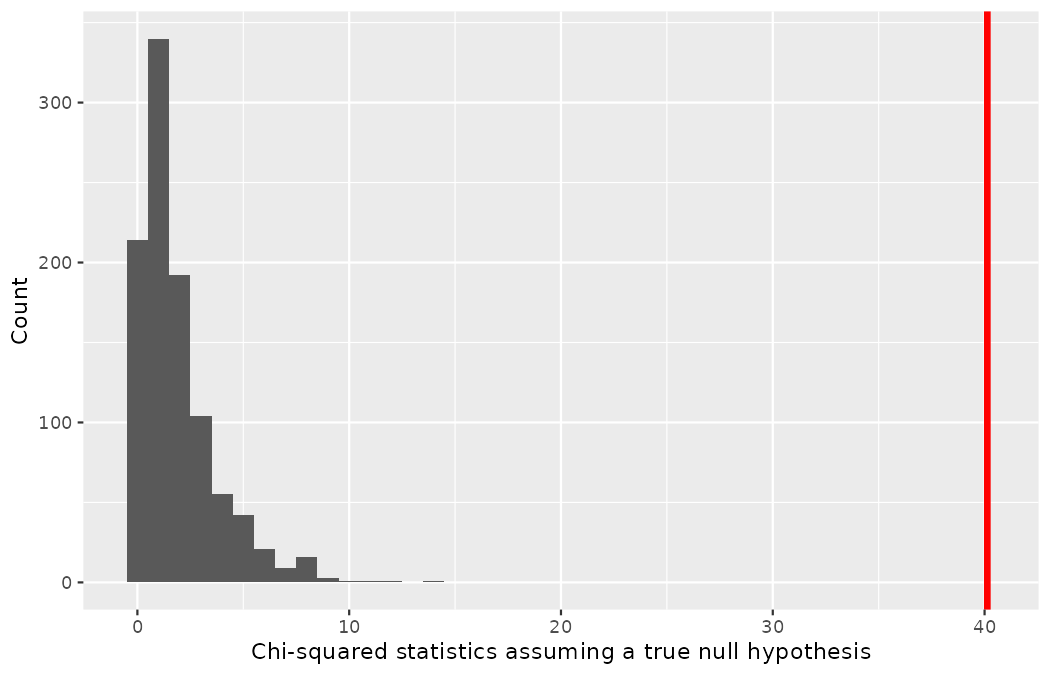
\includegraphics[width=0.85\linewidth,height=\textheight,keepaspectratio]{figures/inference-tables-1.png}

The 1,000 simulated statistics pile up between 0 and about 8, thin out
rapidly, and the largest of all 1,000 is only 13.7:

\begin{Shaded}
\begin{Highlighting}[]
\NormalTok{disclose219\_null }\SpecialCharTok{|\textgreater{}}
  \FunctionTok{summarize}\NormalTok{(}\AttributeTok{largest\_null =} \FunctionTok{max}\NormalTok{(stat))}
\CommentTok{\#\textgreater{} \# A tibble: 1 × 1}
\CommentTok{\#\textgreater{}   largest\_null}
\CommentTok{\#\textgreater{}          \textless{}dbl\textgreater{}}
\CommentTok{\#\textgreater{} 1         13.7}
\end{Highlighting}
\end{Shaded}

The observed statistic of 40.13 sits so far beyond the null statistics
that the simulated p-value is zero: none of the 1,000 simulations had a
chi-squared value of at least 40.13. In fact, none of them came anywhere
close. The probability of seeing the observed statistic when the null
hypothesis is true is virtually zero, and we conclude that a seller's
decision to disclose the injury history is changed by the prompt the
buyer uses. We use the causal language of ``changed'' because the study
was an experiment --- the prompts were randomly assigned. Note, however,
what the chi-squared test does and does not deliver: we know the two
variables \texttt{prompt} and \texttt{response} are related (i.e., not
independent), but the statistic alone does not certify \emph{which}
prompt causes which response --- for that we go back to the table and
read the disclosure rates, remembering that the test has only licensed
the claim that the differences among them are not chance.

\begin{tcolorbox}[enhanced jigsaw, left=2mm, leftrule=.75mm, title=\textcolor{quarto-callout-tip-color}{\faLightbulb}\hspace{0.5em}{Check your understanding}, arc=.35mm, rightrule=.15mm, coltitle=black, colframe=quarto-callout-tip-color-frame, bottomrule=.15mm, colbacktitle=quarto-callout-tip-color!10!white, opacitybacktitle=0.6, breakable, bottomtitle=1mm, toptitle=1mm, titlerule=0mm, opacityback=0, toprule=.15mm, colback=white]

Marta Vidal's takeaway from the study was blunt: ``So my directors
should always ask the negative-assumption question.'' The test statistic
was \(X^2 = 40.13\) with a p-value of essentially zero. Does the
hypothesis test itself justify her specific instruction?

\begin{center}\rule{0.5\linewidth}{0.5pt}\end{center}

Not by itself. The test rejects independence: some prompts genuinely
elicit different disclosure rates. Her \emph{specific} recommendation
comes from descriptive follow-up --- the observed rates of 2.7\%,
31.5\%, and 49.3\% --- not from the chi-squared statistic, which would
have been just as large if the pattern had been reversed. The test and
the table answer different questions, and a competent analyst reports
both: the test says the pattern is real, the table says what the pattern
is.

\end{tcolorbox}

\section{Mathematical model for test of
independence}\label{sec-mathchisq}

\subsection{The chi-squared test of
independence}\label{the-chi-squared-test-of-independence}

In Chapter~\ref{sec-inference-two-props} we applied the Central Limit
Theorem to the sampling variability of \(\hat{p}_1 - \hat{p}_2.\) The
result was that we could use the normal distribution --- \(z^\star\)
values and p-values from \(Z\) scores, as in
Chapter~\ref{sec-inference-one-prop} --- to complete the mathematical
inferential procedure. The chi-squared test statistic does not follow a
normal distribution; how could it, when it is never negative and piles
up near zero? It has a different mathematical distribution, called the
Chi-squared distribution. The important specification to make in
describing a chi-squared distribution is something called its
\emph{degrees of freedom}. The degrees of freedom change the shape of
the chi-squared distribution to fit the problem at hand. The code below
draws chi-squared distributions corresponding to three different degrees
of freedom.

\begin{Shaded}
\begin{Highlighting}[]
\NormalTok{chisq\_densities }\OtherTok{\textless{}{-}} \FunctionTok{crossing}\NormalTok{(}\AttributeTok{x =} \FunctionTok{seq}\NormalTok{(}\FloatTok{0.01}\NormalTok{, }\DecValTok{25}\NormalTok{, }\FloatTok{0.05}\NormalTok{), }\AttributeTok{df =} \FunctionTok{c}\NormalTok{(}\DecValTok{2}\NormalTok{, }\DecValTok{4}\NormalTok{, }\DecValTok{9}\NormalTok{)) }\SpecialCharTok{|\textgreater{}}
  \FunctionTok{mutate}\NormalTok{(}\AttributeTok{density =} \FunctionTok{dchisq}\NormalTok{(x, df), }\AttributeTok{df =} \FunctionTok{factor}\NormalTok{(df))}

\FunctionTok{ggplot}\NormalTok{(chisq\_densities, }\FunctionTok{aes}\NormalTok{(}\AttributeTok{x =}\NormalTok{ x, }\AttributeTok{y =}\NormalTok{ density, }\AttributeTok{color =}\NormalTok{ df, }\AttributeTok{linetype =}\NormalTok{ df)) }\SpecialCharTok{+}
  \FunctionTok{geom\_line}\NormalTok{(}\AttributeTok{linewidth =} \FloatTok{0.8}\NormalTok{) }\SpecialCharTok{+}
  \FunctionTok{labs}\NormalTok{(}
    \AttributeTok{x =} \StringTok{"Value of the chi{-}squared statistic"}\NormalTok{,}
    \AttributeTok{y =} \StringTok{"Density"}\NormalTok{,}
    \AttributeTok{color =} \StringTok{"Degrees of freedom"}\NormalTok{,}
    \AttributeTok{linetype =} \StringTok{"Degrees of freedom"}
\NormalTok{  )}
\end{Highlighting}
\end{Shaded}

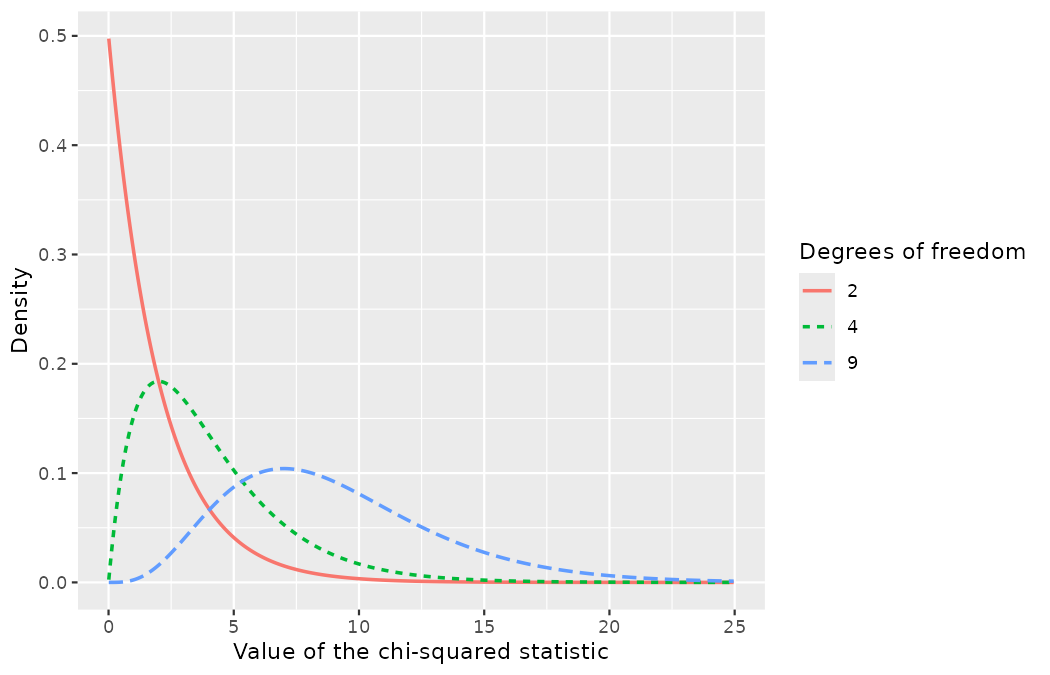
\includegraphics[width=0.85\linewidth,height=\textheight,keepaspectratio]{figures/inference-tables-2.png}

All three curves live entirely to the right of zero and are skewed
right, like every distribution of \(X^2\) must be. The larger the
degrees of freedom, the longer the right tail extends and the further
right the bulk of the distribution shifts; the smaller the degrees of
freedom, the more sharply the density peaks near zero. Unlike the normal
distribution of Chapter~\ref{sec-foundations-mathematical}, which needs
two numbers to pin it down \((N(\mu, \sigma)),\) a chi-squared
distribution is fully specified by the single degrees-of-freedom
parameter.

\subsection{Variability of the chi-squared
statistic}\label{variability-of-the-chi-squared-statistic}

As it turns out, the chi-squared test statistic follows a
\textbf{Chi-squared distribution} when the null hypothesis is true. For
two-way tables, the degrees of freedom is equal to

\[df = \text{(number of rows minus 1)} \times \text{(number of columns minus 1)}\]

In our example, the table has 3 rows (the prompts) and 2 columns (the
responses), so the degrees of freedom parameter is
\(df = (3 - 1) \times (2 - 1) = 2.\)

\subsection{Observed statistic vs.~null chi-squared
statistics}\label{observed-statistic-vs.-null-chi-squared-statistics-1}

\begin{tcolorbox}[enhanced jigsaw, left=2mm, leftrule=.75mm, title=\textcolor{quarto-callout-important-color}{\faExclamation}\hspace{0.5em}{The chi-squared test statistic}, arc=.35mm, rightrule=.15mm, coltitle=black, colframe=quarto-callout-important-color-frame, bottomrule=.15mm, colbacktitle=quarto-callout-important-color!10!white, opacitybacktitle=0.6, breakable, bottomtitle=1mm, toptitle=1mm, titlerule=0mm, opacityback=0, toprule=.15mm, colback=white]

\textbf{The test statistic for assessing the independence between two
categorical variables is a} \(X^2.\)

The \(X^2\) statistic is a ratio of how the observed counts vary from
the expected counts as compared to the expected counts (which are a
measure of how large the sample size is).

\[X^2 = \sum_{i,j} \frac{(\text{observed count} - \text{expected count})^2}{\text{expected count}}\]

When the null hypothesis is true and the conditions are met, \(X^2\) has
a Chi-squared distribution with \(df = (R - 1) \times (C - 1).\)

Conditions:

\begin{itemize}
\tightlist
\item
  Independent observations
\item
  Large samples: 5 expected counts in each cell
\end{itemize}

\end{tcolorbox}

One new piece of notation appears in the display: the summation sign
\(\Sigma\) you have used since Chapter~\ref{sec-explore-numerical} here
carries the \emph{double} index \(i,j.\) Where \(\sum_i\) walked through
a list one observation at a time, \(\sum_{i,j}\) walks through every
(row, column) combination --- every cell of the table, six of them in
the disclosure study.

To bring it back to the example: we can safely assume that the
observations are independent, as the prompt groups were randomly
assigned, and there are over 5 expected counts in each cell (the
smallest is 20.33), so the conditions for using the chi-squared
distribution are met. If the null hypothesis is true (i.e., the prompts
had no impact on the sellers), then the test statistic \(X^2 = 40.13\)
is expected to follow a chi-squared distribution with 2 degrees of
freedom.

\begin{tcolorbox}[enhanced jigsaw, left=2mm, leftrule=.75mm, title=\textcolor{quarto-callout-important-color}{\faExclamation}\hspace{0.5em}{Computing degrees of freedom for a two-way table}, arc=.35mm, rightrule=.15mm, coltitle=black, colframe=quarto-callout-important-color-frame, bottomrule=.15mm, colbacktitle=quarto-callout-important-color!10!white, opacitybacktitle=0.6, breakable, bottomtitle=1mm, toptitle=1mm, titlerule=0mm, opacityback=0, toprule=.15mm, colback=white]

When applying the chi-squared test to a two-way table, we use

\[df = (R - 1) \times (C - 1)\]

where \(R\) is the number of rows in the table and \(C\) is the number
of columns.

\end{tcolorbox}

This is the book's first encounter with \emph{degrees of freedom}, so
take the formula apart rather than memorizing it. The abbreviation
\(df\) names the parameter; \(R\) counts the table's rows and \(C\) its
columns. The ``minus ones'' are earned, not decorative: the null
distribution is generated by shuffles that hold every row total and
every column total fixed, and with the margins pinned down, most of the
table is not free to move. In the \(3 \times 2\) disclosure table, once
you choose the Disclose count for two of the three prompt rows,
everything else is forced --- the third Disclose count must bring column
1 to its total of 61, and each Withhold count must bring its row to 73.
Exactly \((3 - 1) \times (2 - 1) = 2\) cells can vary before the margins
lock the rest, and that count of free cells is the degrees of freedom.

\begin{tcolorbox}[enhanced jigsaw, left=2mm, leftrule=.75mm, title=\textcolor{quarto-callout-tip-color}{\faLightbulb}\hspace{0.5em}{Check your understanding}, arc=.35mm, rightrule=.15mm, coltitle=black, colframe=quarto-callout-tip-color-frame, bottomrule=.15mm, colbacktitle=quarto-callout-tip-color!10!white, opacitybacktitle=0.6, breakable, bottomtitle=1mm, toptitle=1mm, titlerule=0mm, opacityback=0, toprule=.15mm, colback=white]

A club survey cross-tabulates four age cohorts of respondents against a
yes/no answer, giving a \(4 \times 2\) table. What is \(df\)? And why
does the number of respondents not appear in your calculation?

\begin{center}\rule{0.5\linewidth}{0.5pt}\end{center}

\(df = (4 - 1) \times (2 - 1) = 3.\) Degrees of freedom count the cells
free to vary once the margins are fixed, which depends only on the
table's shape. The sample size enters the test elsewhere --- through the
expected counts inside \(X^2\) itself: with more data, the same
\emph{proportional} deviation from independence produces a larger
statistic.

\end{tcolorbox}

Using the mathematical model, we can compute the p-value for the
disclosure test: the area under the chi-squared curve with \(df = 2\) to
the right of the observed statistic. The code below shades it.

\begin{Shaded}
\begin{Highlighting}[]
\NormalTok{chisq\_df2 }\OtherTok{\textless{}{-}} \FunctionTok{tibble}\NormalTok{(}\AttributeTok{x =} \FunctionTok{seq}\NormalTok{(}\DecValTok{0}\NormalTok{, }\DecValTok{50}\NormalTok{, }\FloatTok{0.05}\NormalTok{), }\AttributeTok{density =} \FunctionTok{dchisq}\NormalTok{(x, }\DecValTok{2}\NormalTok{))}

\FunctionTok{ggplot}\NormalTok{(chisq\_df2, }\FunctionTok{aes}\NormalTok{(}\AttributeTok{x =}\NormalTok{ x, }\AttributeTok{y =}\NormalTok{ density)) }\SpecialCharTok{+}
  \FunctionTok{geom\_line}\NormalTok{() }\SpecialCharTok{+}
  \FunctionTok{geom\_area}\NormalTok{(}\AttributeTok{data =} \FunctionTok{filter}\NormalTok{(chisq\_df2, x }\SpecialCharTok{\textgreater{}=} \FloatTok{40.13}\NormalTok{), }\AttributeTok{fill =} \StringTok{"red"}\NormalTok{) }\SpecialCharTok{+}
  \FunctionTok{annotate}\NormalTok{(}\StringTok{"text"}\NormalTok{, }\AttributeTok{x =} \DecValTok{40}\NormalTok{, }\AttributeTok{y =} \FloatTok{0.03}\NormalTok{,}
           \AttributeTok{label =} \StringTok{"Tail area (about 1 in 500 million)}\SpecialCharTok{\textbackslash{}n}\StringTok{is too small to see"}\NormalTok{) }\SpecialCharTok{+}
  \FunctionTok{labs}\NormalTok{(}\AttributeTok{x =} \StringTok{"Value of the chi{-}squared statistic (df = 2)"}\NormalTok{, }\AttributeTok{y =} \StringTok{"Density"}\NormalTok{)}
\end{Highlighting}
\end{Shaded}

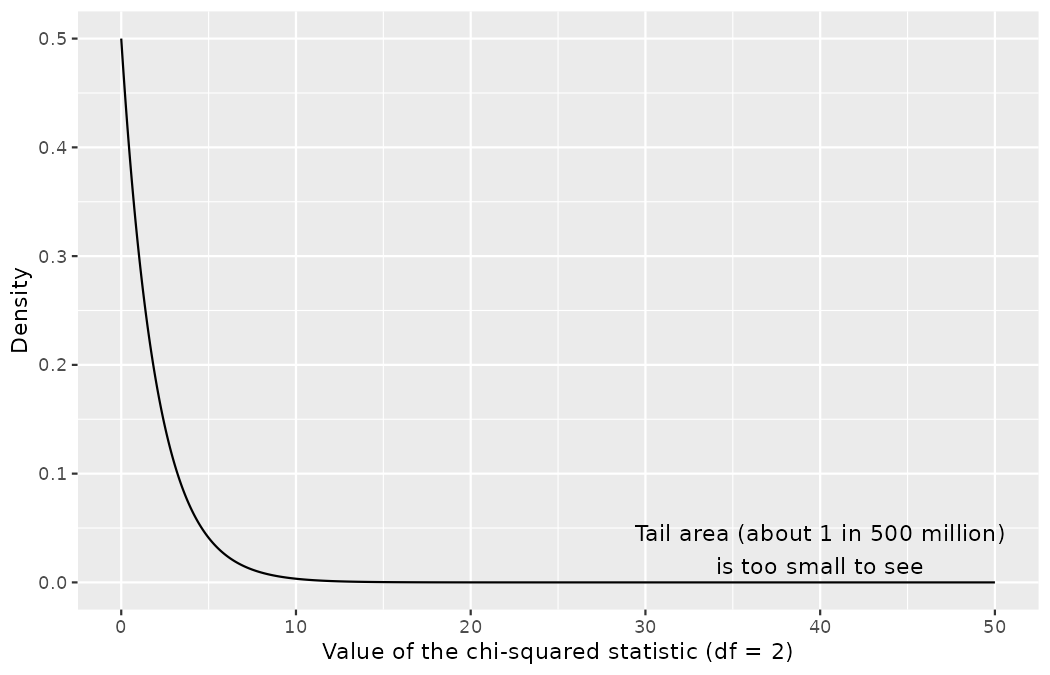
\includegraphics[width=0.85\linewidth,height=\textheight,keepaspectratio]{figures/inference-tables-3.png}

The curve has effectively finished its descent long before 40.13: the
shaded region exists mathematically but cannot be seen at any reasonable
scale. In R, the function \texttt{pchisq()} computes chi-squared tail
areas. Just like \texttt{pnorm()} from
Chapter~\ref{sec-foundations-mathematical}, \texttt{pchisq()} always
gives the area to the \emph{left} of the cutoff value; because the
p-value here is the area to the \emph{right} of 40.13, we subtract the
output from 1.

\begin{Shaded}
\begin{Highlighting}[]
\DecValTok{1} \SpecialCharTok{{-}} \FunctionTok{pchisq}\NormalTok{(}\FloatTok{40.13}\NormalTok{, }\AttributeTok{df =} \DecValTok{2}\NormalTok{)}
\CommentTok{\#\textgreater{} [1] 1.93144e{-}09}
\end{Highlighting}
\end{Shaded}

\begin{tcolorbox}[enhanced jigsaw, left=2mm, leftrule=.75mm, title=\textcolor{quarto-callout-note-color}{\faInfo}\hspace{0.5em}{Worked example}, arc=.35mm, rightrule=.15mm, coltitle=black, colframe=quarto-callout-note-color-frame, bottomrule=.15mm, colbacktitle=quarto-callout-note-color!10!white, opacitybacktitle=0.6, breakable, bottomtitle=1mm, toptitle=1mm, titlerule=0mm, opacityback=0, toprule=.15mm, colback=white]

Find the p-value and draw a conclusion about whether the prompt affects
the sellers' likelihood of disclosing the injury concern.

\begin{center}\rule{0.5\linewidth}{0.5pt}\end{center}

Using a computer, we can compute a very precise value for the tail area
above \(X^2 = 40.13\) for a chi-squared distribution with 2 degrees of
freedom: about 0.000000002, roughly 1 in 500 million.

Using a discernibility level of \(\alpha = 0.05,\) the null hypothesis
is rejected since the p-value is smaller. That is, the data provide
convincing evidence that the prompt asked did affect a seller's
likelihood of telling the truth about the prospect's injury history.
Note also how well the two approaches agree: the permutation test said
``0 shuffles in 1,000,'' and the mathematical model refines that to
``about 1 run of the experiment in 500 million.''

\end{tcolorbox}

\begin{tcolorbox}[enhanced jigsaw, left=2mm, leftrule=.75mm, title=\textcolor{quarto-callout-note-color}{\faInfo}\hspace{0.5em}{Worked example}, arc=.35mm, rightrule=.15mm, coltitle=black, colframe=quarto-callout-note-color-frame, bottomrule=.15mm, colbacktitle=quarto-callout-note-color!10!white, opacitybacktitle=0.6, breakable, bottomtitle=1mm, toptitle=1mm, titlerule=0mm, opacityback=0, toprule=.15mm, colback=white]

Table~\ref{tbl-benchmark699-obs} summarizes the results of an experiment
run by Jonas Beck, Northbridge's academy director, across the club's
partner academies. The subjects were 699 under-18 players who had fallen
behind their individualized development benchmarks while training on the
standard drill program. Each player was randomly assigned to one of
three arms for a full season: continued \emph{standard drills}, standard
drills plus \emph{VR decision training}, or a structured \emph{recovery
program} built around load management. Each player had a primary
outcome: missing their end-of-season benchmark (a failure) or meeting it
(a success). What are appropriate hypotheses for this test?

\begin{center}\rule{0.5\linewidth}{0.5pt}\end{center}

\begin{itemize}
\tightlist
\item
  \(H_0:\) There is no difference in the effectiveness of the three
  programs.
\item
  \(H_A:\) There is some difference in effectiveness between the three
  programs, e.g., perhaps the VR decision training performed better than
  the recovery program.
\end{itemize}

\end{tcolorbox}

This, too, is a constructed Northbridge scenario, built by the code
below. (The seeded \texttt{slice\_sample()} only shuffles the row order
of the finished data frame, so that the roster does not list every
benchmark-missing player first --- the order of rows carries no
information.)

\begin{Shaded}
\begin{Highlighting}[]
\NormalTok{benchmark699 }\OtherTok{\textless{}{-}} \FunctionTok{tribble}\NormalTok{(}
  \SpecialCharTok{\textasciitilde{}}\NormalTok{arm,                   }\SpecialCharTok{\textasciitilde{}}\NormalTok{outcome,           }\SpecialCharTok{\textasciitilde{}}\NormalTok{n,}
  \StringTok{"Standard drills"}\NormalTok{,      }\StringTok{"Benchmark missed"}\NormalTok{, }\DecValTok{120}\NormalTok{,}
  \StringTok{"Standard drills"}\NormalTok{,      }\StringTok{"Benchmark met"}\NormalTok{,    }\DecValTok{112}\NormalTok{,}
  \StringTok{"VR decision training"}\NormalTok{, }\StringTok{"Benchmark missed"}\NormalTok{,  }\DecValTok{90}\NormalTok{,}
  \StringTok{"VR decision training"}\NormalTok{, }\StringTok{"Benchmark met"}\NormalTok{,    }\DecValTok{143}\NormalTok{,}
  \StringTok{"Recovery program"}\NormalTok{,     }\StringTok{"Benchmark missed"}\NormalTok{, }\DecValTok{109}\NormalTok{,}
  \StringTok{"Recovery program"}\NormalTok{,     }\StringTok{"Benchmark met"}\NormalTok{,    }\DecValTok{125}
\NormalTok{) }\SpecialCharTok{|\textgreater{}}
  \FunctionTok{uncount}\NormalTok{(}\AttributeTok{weights =}\NormalTok{ n) }\SpecialCharTok{|\textgreater{}}
  \FunctionTok{mutate}\NormalTok{(}
    \AttributeTok{arm =} \FunctionTok{factor}\NormalTok{(arm, }\AttributeTok{levels =} \FunctionTok{c}\NormalTok{(}\StringTok{"Standard drills"}\NormalTok{, }\StringTok{"VR decision training"}\NormalTok{,}
                                 \StringTok{"Recovery program"}\NormalTok{)),}
    \AttributeTok{outcome =} \FunctionTok{factor}\NormalTok{(outcome, }\AttributeTok{levels =} \FunctionTok{c}\NormalTok{(}\StringTok{"Benchmark missed"}\NormalTok{, }\StringTok{"Benchmark met"}\NormalTok{))}
\NormalTok{  )}

\FunctionTok{set.seed}\NormalTok{(}\DecValTok{1802}\NormalTok{)}
\NormalTok{benchmark699 }\OtherTok{\textless{}{-}}\NormalTok{ benchmark699 }\SpecialCharTok{|\textgreater{}}
  \FunctionTok{slice\_sample}\NormalTok{(}\AttributeTok{prop =} \DecValTok{1}\NormalTok{)}

\NormalTok{benchmark699 }\SpecialCharTok{|\textgreater{}}
  \FunctionTok{count}\NormalTok{(arm, outcome) }\SpecialCharTok{|\textgreater{}}
  \FunctionTok{pivot\_wider}\NormalTok{(}\AttributeTok{names\_from =}\NormalTok{ outcome, }\AttributeTok{values\_from =}\NormalTok{ n)}
\CommentTok{\#\textgreater{} \# A tibble: 3 × 3}
\CommentTok{\#\textgreater{}   arm                  \textasciigrave{}Benchmark missed\textasciigrave{} \textasciigrave{}Benchmark met\textasciigrave{}}
\CommentTok{\#\textgreater{}   \textless{}fct\textgreater{}                             \textless{}int\textgreater{}           \textless{}int\textgreater{}}
\CommentTok{\#\textgreater{} 1 Standard drills                     120             112}
\CommentTok{\#\textgreater{} 2 VR decision training                 90             143}
\CommentTok{\#\textgreater{} 3 Recovery program                    109             125}
\end{Highlighting}
\end{Shaded}

\begin{longtable}[]{@{}lrrr@{}}
\caption{Results of Jonas Beck's three-arm academy
intervention.}\label{tbl-benchmark699-obs}\tabularnewline
\toprule\noalign{}
Arm & Benchmark missed & Benchmark met & Total \\
\midrule\noalign{}
\endfirsthead
\toprule\noalign{}
Arm & Benchmark missed & Benchmark met & Total \\
\midrule\noalign{}
\endhead
\bottomrule\noalign{}
\endlastfoot
Standard drills & 120 & 112 & 232 \\
VR decision training & 90 & 143 & 233 \\
Recovery program & 109 & 125 & 234 \\
Total & 319 & 380 & 699 \\
\end{longtable}

Typically we will use a computer to do the computational work of finding
the chi-squared statistic. However, it is always good to have a sense
for what the computer is doing, and in particular, calculating the
values which would be expected if the null hypothesis were true can help
in understanding the null hypothesis claim. Additionally, comparing the
expected and observed values by eye often gives the researcher some
insight into why or why not the null hypothesis for a given test will be
rejected.

\begin{tcolorbox}[enhanced jigsaw, left=2mm, leftrule=.75mm, title=\textcolor{quarto-callout-tip-color}{\faLightbulb}\hspace{0.5em}{Check your understanding}, arc=.35mm, rightrule=.15mm, coltitle=black, colframe=quarto-callout-tip-color-frame, bottomrule=.15mm, colbacktitle=quarto-callout-tip-color!10!white, opacitybacktitle=0.6, breakable, bottomtitle=1mm, toptitle=1mm, titlerule=0mm, opacityback=0, toprule=.15mm, colback=white]

A chi-squared test for a two-way table may be used to test the
hypotheses in the worked example above. To get a sense for the statistic
used in the chi-squared test, first compute the expected values for each
of the six table cells.

\begin{center}\rule{0.5\linewidth}{0.5pt}\end{center}

The expected count for row one / column one is found by multiplying the
row one total (232) and the column one total (319), then dividing by the
table total (699): \(\frac{232 \times 319}{699} = 105.9.\) Similarly for
the second column and the first row:
\(\frac{232 \times 380}{699} = 126.1.\) Row 2:
\(\frac{233 \times 319}{699} = 106.3\) and
\(\frac{233 \times 380}{699} = 126.7.\) Row 3:
\(\frac{234 \times 319}{699} = 106.8\) and
\(\frac{234 \times 380}{699} = 127.2.\) Comparing by eye: the VR arm
missed the benchmark 90 times against an expectation of 106.3 --- the
largest-magnitude discrepancy in the table (matched, as the two cells of
a row must be under fixed row totals, by the \(+16.3\) in the VR-met
cell), and the reason the VR row will contribute most to the statistic.

\end{tcolorbox}

Note, when analyzing 2-by-2 contingency tables (that is, when both
variables have only two possible options), one guideline is to use the
two-proportion methods introduced in
Chapter~\ref{sec-inference-two-props}.

\section{A permutation test on real shots: play pattern and
goals}\label{sec-chp18-real-table}

Both studies above were experiments: Priya randomized the prompts, and
Jonas randomized the training arms. As in
Chapter~\ref{sec-foundations-randomization}, the shuffling machinery
works identically on observational data --- it is then called a
permutation test, and its conclusions weaken from causation to
association. Here is a claim Emil Sørensen hears from his scouts every
recruitment cycle: \emph{counter-attacks are gold --- target teams that
generate shots on the counter, because those chances get finished.} The
2022 Men's World Cup data can put a two-way table under that claim: is
the way a shot's possession began associated with whether the shot was
scored?

The \texttt{play\_pattern} variable has nine levels --- you met all nine
in the pie-chart lesson of Chapter~\ref{sec-explore-categorical} --- and
several are too thin to stand as their own rows. We collapse them into
three analytic groups, and since collapsing is an analytical decision,
we state the mapping and the reasoning rather than hiding either:

\begin{itemize}
\tightlist
\item
  \emph{set piece}: \texttt{From\ Free\ Kick} and \texttt{From\ Corner}
  --- possessions that deliver the ball toward goal directly from a
  dead-ball situation;
\item
  \emph{counter}: \texttt{From\ Counter} --- the pattern under the
  scouts' claim;
\item
  \emph{open play}: \texttt{Regular\ Play}, plus possessions restarted
  from throw-ins, goal kicks, keeper distributions, and kick-offs --- by
  the time a shot arrives in these possessions, play is live and
  contested.
\end{itemize}

That accounts for eight of the nine levels. The ninth, \texttt{Other},
demands the discipline this book's penalty convention has drilled since
Chapter~\ref{sec-data-applications}: ask which shots are in the frame
\emph{before} testing.

\begin{Shaded}
\begin{Highlighting}[]
\NormalTok{wc2022\_shots }\OtherTok{\textless{}{-}} \FunctionTok{read\_csv}\NormalTok{(}\StringTok{"data/derived/wc2022\_shots.csv"}\NormalTok{)}

\NormalTok{wc2022\_shots }\SpecialCharTok{|\textgreater{}}
  \FunctionTok{filter}\NormalTok{(play\_pattern }\SpecialCharTok{==} \StringTok{"Other"}\NormalTok{) }\SpecialCharTok{|\textgreater{}}
  \FunctionTok{count}\NormalTok{(shot\_type, goal)}
\CommentTok{\#\textgreater{} \# A tibble: 3 × 3}
\CommentTok{\#\textgreater{}   shot\_type goal      n}
\CommentTok{\#\textgreater{}   \textless{}chr\textgreater{}     \textless{}lgl\textgreater{} \textless{}int\textgreater{}}
\CommentTok{\#\textgreater{} 1 Open Play FALSE     4}
\CommentTok{\#\textgreater{} 2 Penalty   FALSE    21}
\CommentTok{\#\textgreater{} 3 Penalty   TRUE     43}
\end{Highlighting}
\end{Shaded}

The \texttt{Other} bucket holds 68 shots: all 64 of the tournament's
penalty kicks --- which carry \texttt{play\_pattern} \texttt{"Other"} in
these data, converting at \(43/64 = 0.672\) --- plus 4 open-play-tagged
shots, none of which scored. Penalties have no place in a test about how
\emph{possessions} produce goals: they are awarded, not built, and they
convert at more than six times the rate of everything else. So we
exclude the entire \texttt{Other} bucket with a stated filter,
\texttt{play\_pattern\ !=\ "Other"}, and quantify what it removes: 68
shots (64 penalties with 43 goals, plus the 4 goalless open-play-tagged
shots, which the label \texttt{Other} gives no basis for assigning to
any of our three groups). That leaves \(1{,}494 - 68 = 1{,}426\) shots.
Per the convention, first look at what would happen if we did \emph{not}
filter, and kept \texttt{Other} as a fourth row:

\begin{Shaded}
\begin{Highlighting}[]
\NormalTok{wc\_pattern4 }\OtherTok{\textless{}{-}}\NormalTok{ wc2022\_shots }\SpecialCharTok{|\textgreater{}}
  \FunctionTok{mutate}\NormalTok{(}
    \AttributeTok{pattern4 =} \FunctionTok{case\_when}\NormalTok{(}
\NormalTok{      play\_pattern }\SpecialCharTok{\%in\%} \FunctionTok{c}\NormalTok{(}\StringTok{"From Free Kick"}\NormalTok{, }\StringTok{"From Corner"}\NormalTok{) }\SpecialCharTok{\textasciitilde{}} \StringTok{"set piece"}\NormalTok{,}
\NormalTok{      play\_pattern }\SpecialCharTok{==} \StringTok{"From Counter"} \SpecialCharTok{\textasciitilde{}} \StringTok{"counter"}\NormalTok{,}
\NormalTok{      play\_pattern }\SpecialCharTok{==} \StringTok{"Other"} \SpecialCharTok{\textasciitilde{}} \StringTok{"other"}\NormalTok{,}
      \AttributeTok{.default =} \StringTok{"open play"}
\NormalTok{    )}
\NormalTok{  )}

\FunctionTok{chisq.test}\NormalTok{(}\FunctionTok{table}\NormalTok{(wc\_pattern4}\SpecialCharTok{$}\NormalTok{pattern4, wc\_pattern4}\SpecialCharTok{$}\NormalTok{goal))}
\CommentTok{\#\textgreater{}}
\CommentTok{\#\textgreater{}  Pearson\textquotesingle{}s Chi{-}squared test}
\CommentTok{\#\textgreater{}}
\CommentTok{\#\textgreater{} data:  table(wc\_pattern4$pattern4, wc\_pattern4$goal)}
\CommentTok{\#\textgreater{} X{-}squared = 161.97, df = 3, p{-}value \textless{} 2.2e{-}16}
\CommentTok{\#\textgreater{}}
\end{Highlighting}
\end{Shaded}

A monstrous \(X^2 = 162\) --- and it would be almost entirely an
artifact: a fourth row converting at \(43/68 = 0.632\) because 64 of its
68 shots were uncontested kicks from twelve yards. The ``association
between play pattern and goals'' that this test screams about is mostly
the rule book's penalty spot. Now the honest frame:

\begin{Shaded}
\begin{Highlighting}[]
\NormalTok{wc\_pattern }\OtherTok{\textless{}{-}}\NormalTok{ wc2022\_shots }\SpecialCharTok{|\textgreater{}}
  \FunctionTok{filter}\NormalTok{(play\_pattern }\SpecialCharTok{!=} \StringTok{"Other"}\NormalTok{) }\SpecialCharTok{|\textgreater{}}
  \FunctionTok{mutate}\NormalTok{(}
    \AttributeTok{pattern3 =} \FunctionTok{case\_when}\NormalTok{(}
\NormalTok{      play\_pattern }\SpecialCharTok{\%in\%} \FunctionTok{c}\NormalTok{(}\StringTok{"From Free Kick"}\NormalTok{, }\StringTok{"From Corner"}\NormalTok{) }\SpecialCharTok{\textasciitilde{}} \StringTok{"set piece"}\NormalTok{,}
\NormalTok{      play\_pattern }\SpecialCharTok{==} \StringTok{"From Counter"} \SpecialCharTok{\textasciitilde{}} \StringTok{"counter"}\NormalTok{,}
      \AttributeTok{.default =} \StringTok{"open play"}
\NormalTok{    ),}
    \AttributeTok{pattern3 =} \FunctionTok{factor}\NormalTok{(pattern3, }\AttributeTok{levels =} \FunctionTok{c}\NormalTok{(}\StringTok{"open play"}\NormalTok{, }\StringTok{"set piece"}\NormalTok{, }\StringTok{"counter"}\NormalTok{)),}
    \AttributeTok{result =} \FunctionTok{factor}\NormalTok{(}\FunctionTok{if\_else}\NormalTok{(goal, }\StringTok{"goal"}\NormalTok{, }\StringTok{"no goal"}\NormalTok{), }\AttributeTok{levels =} \FunctionTok{c}\NormalTok{(}\StringTok{"goal"}\NormalTok{, }\StringTok{"no goal"}\NormalTok{))}
\NormalTok{  )}

\NormalTok{wc\_pattern }\SpecialCharTok{|\textgreater{}}
  \FunctionTok{group\_by}\NormalTok{(pattern3) }\SpecialCharTok{|\textgreater{}}
  \FunctionTok{summarize}\NormalTok{(}\AttributeTok{shots =} \FunctionTok{n}\NormalTok{(), }\AttributeTok{goals =} \FunctionTok{sum}\NormalTok{(goal), }\AttributeTok{conversion =} \FunctionTok{mean}\NormalTok{(goal))}
\CommentTok{\#\textgreater{} \# A tibble: 3 × 4}
\CommentTok{\#\textgreater{}   pattern3  shots goals conversion}
\CommentTok{\#\textgreater{}   \textless{}fct\textgreater{}     \textless{}int\textgreater{} \textless{}int\textgreater{}      \textless{}dbl\textgreater{}}
\CommentTok{\#\textgreater{} 1 open play   862    96     0.111}
\CommentTok{\#\textgreater{} 2 set piece   508    46     0.0906}
\CommentTok{\#\textgreater{} 3 counter      56    10     0.179}
\end{Highlighting}
\end{Shaded}

One guard against a name collision before reading further: the
\texttt{pattern3} level \emph{open play} here is a \textbf{possession}
family --- 862 shots whose possessions began in live play --- and it is
narrower than the Open Play \emph{shot-type} frame
(\texttt{shot\_type\ ==\ "Open\ Play"}, 1,382 shots) that this book's
penalty convention usually filters on, since a shot arriving from a
corner or free-kick possession is an Open Play shot in that frame but a
set-piece possession in this table. The two are different objects that
happen to share a name; always note which one a number is conditioned
on.

\begin{longtable}[]{@{}lrrr@{}}
\caption{Play pattern (collapsed to three groups, penalties excluded)
and shot result at the 2022 Men's World
Cup.}\label{tbl-wcpattern-obs}\tabularnewline
\toprule\noalign{}
Play pattern & goal & no goal & Total \\
\midrule\noalign{}
\endfirsthead
\toprule\noalign{}
Play pattern & goal & no goal & Total \\
\midrule\noalign{}
\endhead
\bottomrule\noalign{}
\endlastfoot
open play & 96 & 766 & 862 \\
set piece & 46 & 462 & 508 \\
counter & 10 & 46 & 56 \\
Total & 152 & 1,274 & 1,426 \\
\end{longtable}

The scouts' claim looks alive: counters converted at \(10/56 = 0.179,\)
nearly double the open-play rate of \(96/862 = 0.111,\) with set-piece
possessions trailing at \(46/508 = 0.0906.\) The hypotheses --- written,
note, in the language of association, because nobody randomly assigned
play patterns to shots:

\begin{itemize}
\tightlist
\item
  \(H_0:\) Play pattern and shot result are independent; the variation
  in conversion across the three groups is due to natural variability
  across 1,426 shots.
\item
  \(H_A:\) Play pattern and shot result are associated.
\end{itemize}

The expected counts under \(H_0\) put the overall conversion rate of
\(152/1426 = 0.1066\) in every row:

\begin{Shaded}
\begin{Highlighting}[]
\FunctionTok{chisq.test}\NormalTok{(}\FunctionTok{table}\NormalTok{(wc\_pattern}\SpecialCharTok{$}\NormalTok{pattern3, wc\_pattern}\SpecialCharTok{$}\NormalTok{result))}\SpecialCharTok{$}\NormalTok{expected}
\CommentTok{\#\textgreater{}}
\CommentTok{\#\textgreater{}                  goal   no goal}
\CommentTok{\#\textgreater{}   open play 91.882188 770.11781}
\CommentTok{\#\textgreater{}   set piece 54.148668 453.85133}
\CommentTok{\#\textgreater{}   counter    5.969144  50.03086}

\NormalTok{wc\_pattern\_obs\_x2 }\OtherTok{\textless{}{-}}\NormalTok{ wc\_pattern }\SpecialCharTok{|\textgreater{}}
  \FunctionTok{specify}\NormalTok{(result }\SpecialCharTok{\textasciitilde{}}\NormalTok{ pattern3) }\SpecialCharTok{|\textgreater{}}
  \FunctionTok{calculate}\NormalTok{(}\AttributeTok{stat =} \StringTok{"Chisq"}\NormalTok{) }\SpecialCharTok{|\textgreater{}}
  \FunctionTok{pull}\NormalTok{()}

\NormalTok{wc\_pattern\_obs\_x2}
\CommentTok{\#\textgreater{} X{-}squared}
\CommentTok{\#\textgreater{}  4.625855}
\end{Highlighting}
\end{Shaded}

The observed statistic is
\(X^2 = 0.185 + 1.226 + 2.722 + 0.022 + 0.146 + 0.325 = 4.626,\) with
the counter-goal cell contributing the most:
\((10 - 5.97)^2 / 5.97 = 2.72.\) Ten goals where independence expects
six --- is that association, or a Tuesday's worth of chance? One seeded
shuffle first, exactly as we did by hand for the disclosure study:

\begin{Shaded}
\begin{Highlighting}[]
\FunctionTok{set.seed}\NormalTok{(}\DecValTok{1803}\NormalTok{)}
\NormalTok{wc\_pattern\_shuffle\_1 }\OtherTok{\textless{}{-}}\NormalTok{ wc\_pattern }\SpecialCharTok{|\textgreater{}}
  \FunctionTok{mutate}\NormalTok{(}\AttributeTok{result =} \FunctionTok{sample}\NormalTok{(result))}

\NormalTok{wc\_pattern\_shuffle\_1 }\SpecialCharTok{|\textgreater{}}
  \FunctionTok{group\_by}\NormalTok{(pattern3) }\SpecialCharTok{|\textgreater{}}
  \FunctionTok{summarize}\NormalTok{(}\AttributeTok{shots =} \FunctionTok{n}\NormalTok{(), }\AttributeTok{goals =} \FunctionTok{sum}\NormalTok{(result }\SpecialCharTok{==} \StringTok{"goal"}\NormalTok{),}
            \AttributeTok{conversion =} \FunctionTok{mean}\NormalTok{(result }\SpecialCharTok{==} \StringTok{"goal"}\NormalTok{))}
\CommentTok{\#\textgreater{} \# A tibble: 3 × 4}
\CommentTok{\#\textgreater{}   pattern3  shots goals conversion}
\CommentTok{\#\textgreater{}   \textless{}fct\textgreater{}     \textless{}int\textgreater{} \textless{}int\textgreater{}      \textless{}dbl\textgreater{}}
\CommentTok{\#\textgreater{} 1 open play   862    90     0.104}
\CommentTok{\#\textgreater{} 2 set piece   508    58     0.114}
\CommentTok{\#\textgreater{} 3 counter      56     4     0.0714}
\end{Highlighting}
\end{Shaded}

Study this shuffled table for a moment, because it is quietly
instructive. Chance alone handed the counters a conversion rate of
\(0.071\) --- this time the \emph{worst} of the three groups --- and its
statistic works out to \(X^2_{shfl1} = 1.08,\) with the counter-goal
cell again the largest single contributor: \((4 - 5.97)^2/5.97 = 0.65.\)
A group of 56 shots swings violently from shuffle to shuffle; that is
precisely why its 0.179 in the real data should not yet impress you. Now
the full test, followed by the mathematical model:

\begin{Shaded}
\begin{Highlighting}[]
\FunctionTok{set.seed}\NormalTok{(}\DecValTok{1804}\NormalTok{)}
\NormalTok{wc\_pattern\_null }\OtherTok{\textless{}{-}}\NormalTok{ wc\_pattern }\SpecialCharTok{|\textgreater{}}
  \FunctionTok{specify}\NormalTok{(result }\SpecialCharTok{\textasciitilde{}}\NormalTok{ pattern3) }\SpecialCharTok{|\textgreater{}}
  \FunctionTok{hypothesize}\NormalTok{(}\AttributeTok{null =} \StringTok{"independence"}\NormalTok{) }\SpecialCharTok{|\textgreater{}}
  \FunctionTok{generate}\NormalTok{(}\AttributeTok{reps =} \DecValTok{1000}\NormalTok{, }\AttributeTok{type =} \StringTok{"permute"}\NormalTok{) }\SpecialCharTok{|\textgreater{}}
  \FunctionTok{calculate}\NormalTok{(}\AttributeTok{stat =} \StringTok{"Chisq"}\NormalTok{)}

\NormalTok{wc\_pattern\_null }\SpecialCharTok{|\textgreater{}}
  \FunctionTok{summarize}\NormalTok{(}
    \AttributeTok{n\_extreme =} \FunctionTok{sum}\NormalTok{(stat }\SpecialCharTok{\textgreater{}=}\NormalTok{ wc\_pattern\_obs\_x2),}
    \AttributeTok{p\_value   =} \FunctionTok{mean}\NormalTok{(stat }\SpecialCharTok{\textgreater{}=}\NormalTok{ wc\_pattern\_obs\_x2)}
\NormalTok{  )}
\CommentTok{\#\textgreater{} \# A tibble: 1 × 2}
\CommentTok{\#\textgreater{}   n\_extreme p\_value}
\CommentTok{\#\textgreater{}       \textless{}int\textgreater{}   \textless{}dbl\textgreater{}}
\CommentTok{\#\textgreater{} 1       107   0.107}
\end{Highlighting}
\end{Shaded}

In 107 of 1,000 shuffles, chance alone produced a table at least as far
from independence as the real one: the permutation p-value is \(0.107.\)
Before invoking the chi-squared distribution, check its conditions.
Independence of observations is the shakier one for shot data --- shots
cluster within matches and within teams --- but it is the standard
working assumption of shot analysis, made explicitly, as we have done
since Chapter~\ref{sec-foundations-randomization}. The expected-count
condition passes the bar with no room to spare: the smallest expected
count, counter-goal, is \(56 \times 152/1426 = 5.97\) --- above 5, but
close enough that had we sliced the table any thinner (say, keeping
\texttt{From\ Kick\ Off} as its own row), the mathematical model would
have been off the table while the permutation test soldiered on. With
\(df = (3 - 1) \times (2 - 1) = 2:\)

\begin{Shaded}
\begin{Highlighting}[]
\DecValTok{1} \SpecialCharTok{{-}} \FunctionTok{pchisq}\NormalTok{(}\FloatTok{4.6259}\NormalTok{, }\AttributeTok{df =} \DecValTok{2}\NormalTok{)}
\CommentTok{\#\textgreater{} [1] 0.09896886}
\end{Highlighting}
\end{Shaded}

The two approaches agree closely --- \(0.107\) by shuffling, \(0.099\)
by the mathematical model --- which is the chi-squared distribution
doing its job as an approximation to the permutation null. At
\(\alpha = 0.05,\) neither is statistically discernible: check complete,
the on-field call stands. The tournament's data do not provide
convincing evidence that play pattern and shot result are associated,
once the penalties are out of the frame.

Two closing disciplines, both familiar. First, failing to reject \(H_0\)
is not evidence that conversion is identical across patterns --- with
only 56 counters, the test has little power to detect a modest real
difference, the possibility
Chapter~\ref{sec-foundations-decision-errors} taught you to hold open.
Second, even if the p-value had cleared the bar, the conclusion would
have been \emph{association only}: play patterns are not assigned at
random --- teams that get to shoot on the counter tend to be teams
facing stretched defenses, and the quality of the chance, not the label
on the possession, may be doing the work. The scouts' ``counters are
gold'' survives as a hypothesis; it does not yet survive as a finding.

\begin{tcolorbox}[enhanced jigsaw, left=2mm, leftrule=.75mm, title=\textcolor{quarto-callout-tip-color}{\faLightbulb}\hspace{0.5em}{Check your understanding}, arc=.35mm, rightrule=.15mm, coltitle=black, colframe=quarto-callout-tip-color-frame, bottomrule=.15mm, colbacktitle=quarto-callout-tip-color!10!white, opacitybacktitle=0.6, breakable, bottomtitle=1mm, toptitle=1mm, titlerule=0mm, opacityback=0, toprule=.15mm, colback=white]

At the 2025 Women's Euro (you will run this table yourself in the
exercises), the same three groups converted at \(0.123\) (open play),
\(0.083\) (set piece), and \(0.073\) (counter) --- counters \emph{last},
not first. What do the two tournaments, taken together, teach about the
scouts' claim?

\begin{center}\rule{0.5\linewidth}{0.5pt}\end{center}

The direction of the counter ``effect'' flips between competitions,
exactly as the first-time-shot reversal of
Chapter~\ref{sec-foundations-decision-errors} warned can happen: neither
tournament's counter cell (56 and 41 shots) is large enough for its
conversion rate to be stable, and neither tournament's test rejects
independence. A pattern that reverses across two tournaments and clears
no discernibility bar in either is chance variation until much more data
say otherwise --- and a scouting recommendation built on it would be
built on noise.

\end{tcolorbox}

\section{Chapter review}\label{sec-chp18-review}

\subsection{Summary}\label{summary-17}

In this chapter we extended the randomization / bootstrap / mathematical
model paradigm to research questions involving categorical variables
with more than two levels. We continued working with proportions of a
categorical response, but the test of independence allowed for
hypothesis testing on two-way tables of any shape: the expected counts
describe the table the null hypothesis predicts, and the chi-squared
statistic \(X^2\) collapses the table's total departure from that
prediction into one number. We note that the normal model was an
excellent mathematical approximation to the sampling distribution of
sample proportions (or differences in sample proportions), but that
questions with categorical variables having more than 2 levels required
a new mathematical model, the chi-squared distribution, indexed by its
degrees of freedom \(df = (R-1) \times (C-1).\) As seen in
Chapter~\ref{sec-foundations-randomization},
Chapter~\ref{sec-foundations-bootstrapping}, and
Chapter~\ref{sec-foundations-mathematical}, almost all research
questions can be approached using computational methods (e.g.,
randomization tests) or using mathematical models --- and when the
conditions held, the two approaches agreed, in the disclosure experiment
and on the World Cup shots alike. We continue to emphasize the
importance of study design in making conclusions: the disclosure and
academy studies were randomized experiments, so rejecting independence
there spoke to cause; the play-pattern table was observational, so the
identical machinery could only ever have spoken to association --- and,
per the book's penalty convention, the frame had to be stated before the
test was run, because leaving 64 penalty kicks in one row of a table
manufactures an ``association'' that is really the rule book.

\subsection{Terms}\label{terms-17}

The terms introduced in this chapter are presented below, alphabetized.
If you're not sure what some of these terms mean, we recommend you go
back in the text and review their definitions. You should be able to
easily spot them as \textbf{bolded text}.

\begin{longtable}[]{@{}
  >{\raggedright\arraybackslash}p{(\linewidth - 4\tabcolsep) * \real{0.3380}}
  >{\raggedright\arraybackslash}p{(\linewidth - 4\tabcolsep) * \real{0.3380}}
  >{\raggedright\arraybackslash}p{(\linewidth - 4\tabcolsep) * \real{0.3239}}@{}}
\caption{Terms introduced in this
chapter.}\label{tbl-terms-chp-18}\tabularnewline
\toprule\noalign{}
\endfirsthead
\endhead
\bottomrule\noalign{}
\endlastfoot
Chi-squared distribution & chi-squared test statistic & expected
counts \\
independence & & \\
\end{longtable}

\section{Exercises}\label{sec-chp18-exercises}

Answers to odd-numbered exercises can be found in
Appendix~\ref{sec-exercise-solutions-18}.

\begin{enumerate}
\def\labelenumi{\arabic{enumi}.}
\item
  \textbf{Mentor scheme.} Does pairing an academy player with a
  senior-player mentor affect whether the player meets his development
  benchmark? In a constructed scenario, Jonas Beck enrolled 300 academy
  players --- drawn from across Northbridge and its partner academies,
  in a trial coordinated with the federation's youth program --- in a
  randomized experiment. 150 players were randomly assigned to a group
  that followed the standard development plan and met weekly with a
  senior-player mentor; the other 150 followed the standard plan and did
  not meet with a mentor. At the end of the season, 40 of the players in
  the mentor plus standard group had met their development benchmark
  while only 30 players had met it in the other group.

  \begin{enumerate}
  \def\labelenumii{\alph{enumii}.}
  \item
    Create a two-way table presenting the results of this study.
  \item
    Answer each of the following questions under the null hypothesis
    that meeting weekly with a mentor does not affect a player's ability
    to meet the benchmark, and indicate whether the expected values are
    higher or lower than the observed values.

    \begin{enumerate}
    \def\labelenumiii{\roman{enumiii}.}
    \item
      How many players in the ``mentor + standard'' group would you
      expect to meet the benchmark?
    \item
      How many players in the ``standard only'' group would you expect
      to \emph{not} meet the benchmark?
    \end{enumerate}
  \end{enumerate}
\item
  \textbf{Away-day survey.} The table below summarizes results from a
  constructed supporter poll in which Northbridge's fan-relations office
  asked season-ticket holders whether they had personally attended at
  least one of the club's away fixtures within the last year, split by
  the respondent's age cohort. The differences in each cohort may be due
  to chance. Complete the following computations under the null
  hypothesis of independence between a supporter's age cohort and
  whether they attended an away fixture within the last year.

  \begin{longtable}[]{@{}lrrr@{}}
  \toprule\noalign{}
  Age cohort & Attended & Did not attend & Total \\
  \midrule\noalign{}
  \endhead
  \bottomrule\noalign{}
  \endlastfoot
  Under 30 & 292 & 620 & 912 \\
  30--44 & 885 & 2,275 & 3,160 \\
  45--59 & 809 & 2,709 & 3,518 \\
  60 and older & 1,276 & 4,798 & 6,074 \\
  Total & 3,262 & 10,402 & 13,664 \\
  \end{longtable}

  If there is no relationship between age and attendance,

  \begin{enumerate}
  \def\labelenumii{\alph{enumii}.}
  \item
    how many supporters under 30 would you expect to have attended an
    away fixture within the last year?
  \item
    how many supporters aged 30--44 would you expect to have attended an
    away fixture within the last year?
  \item
    how many supporters aged 45--59 would you expect to have attended an
    away fixture within the last year?
  \item
    how many supporters aged 60 and older would you expect to have
    attended an away fixture within the last year?
  \end{enumerate}
\item
  \textbf{Position groups and body parts, data.} In order to assess
  whether the position a shooter plays is related to how they strike
  their shots, all open-play shots of the 2022 Men's World Cup were
  cross-tabulated by the shooter's position group (FW/MF/DF, the mapping
  defined in Chapter~\ref{sec-explore-categorical}) and the body part
  used.\footnote{The 2022 Men's World Cup shot data used in this
    exercise are in \texttt{data/derived/wc2022\_shots.csv} (StatsBomb
    open data); the position-group mapping is the one defined once in
    Chapter~\ref{sec-explore-categorical} and reused throughout the
    book.} The frame is stated up front: penalties, direct free kicks,
  and the tournament's two direct corner attempts are excluded by the
  open-play filter, since dead-ball strikes are taken by designated
  (footed) takers and would tie body part to set-piece duty rather than
  to position; the 13 shots with body part \texttt{Other} are dropped,
  as in Chapter~\ref{sec-explore-categorical}; and no goalkeeper took an
  open-play shot at this tournament. That leaves 1,369 shots.

\begin{Shaded}
\begin{Highlighting}[]
\NormalTok{wc2022\_shots }\OtherTok{\textless{}{-}} \FunctionTok{read\_csv}\NormalTok{(}\StringTok{"data/derived/wc2022\_shots.csv"}\NormalTok{)}

\NormalTok{wc\_pos\_bp }\OtherTok{\textless{}{-}}\NormalTok{ wc2022\_shots }\SpecialCharTok{|\textgreater{}}
  \FunctionTok{filter}\NormalTok{(shot\_type }\SpecialCharTok{==} \StringTok{"Open Play"}\NormalTok{, body\_part }\SpecialCharTok{!=} \StringTok{"Other"}\NormalTok{) }\SpecialCharTok{|\textgreater{}}
  \FunctionTok{mutate}\NormalTok{(}
    \AttributeTok{pos\_group =} \FunctionTok{case\_when}\NormalTok{(}
\NormalTok{      position }\SpecialCharTok{==} \StringTok{"Goalkeeper"} \SpecialCharTok{\textasciitilde{}} \StringTok{"GK"}\NormalTok{,}
      \FunctionTok{grepl}\NormalTok{(}\StringTok{"Back"}\NormalTok{, position) }\SpecialCharTok{\textasciitilde{}} \StringTok{"DF"}\NormalTok{,}
      \FunctionTok{grepl}\NormalTok{(}\StringTok{"Midfield"}\NormalTok{, position) }\SpecialCharTok{\textasciitilde{}} \StringTok{"MF"}\NormalTok{,}
      \AttributeTok{.default =} \StringTok{"FW"}
\NormalTok{    ),}
    \AttributeTok{pos\_group =} \FunctionTok{factor}\NormalTok{(pos\_group, }\AttributeTok{levels =} \FunctionTok{c}\NormalTok{(}\StringTok{"FW"}\NormalTok{, }\StringTok{"MF"}\NormalTok{, }\StringTok{"DF"}\NormalTok{)),}
    \AttributeTok{body\_part =} \FunctionTok{factor}\NormalTok{(body\_part, }\AttributeTok{levels =} \FunctionTok{c}\NormalTok{(}\StringTok{"Right Foot"}\NormalTok{, }\StringTok{"Left Foot"}\NormalTok{, }\StringTok{"Head"}\NormalTok{))}
\NormalTok{  )}

\NormalTok{wc\_pos\_bp }\SpecialCharTok{|\textgreater{}}
  \FunctionTok{count}\NormalTok{(pos\_group, body\_part) }\SpecialCharTok{|\textgreater{}}
  \FunctionTok{pivot\_wider}\NormalTok{(}\AttributeTok{names\_from =}\NormalTok{ body\_part, }\AttributeTok{values\_from =}\NormalTok{ n)}
\CommentTok{\#\textgreater{} \# A tibble: 3 × 4}
\CommentTok{\#\textgreater{}   pos\_group \textasciigrave{}Right Foot\textasciigrave{} \textasciigrave{}Left Foot\textasciigrave{}  Head}
\CommentTok{\#\textgreater{}   \textless{}fct\textgreater{}            \textless{}int\textgreater{}       \textless{}int\textgreater{} \textless{}int\textgreater{}}
\CommentTok{\#\textgreater{} 1 FW                 322         224   127}
\CommentTok{\#\textgreater{} 2 MF                 271         127    42}
\CommentTok{\#\textgreater{} 3 DF                 110          63    83}
\end{Highlighting}
\end{Shaded}

  \begin{longtable}[]{@{}lrrrr@{}}
  \toprule\noalign{}
  & Right Foot & Left Foot & Head & Total \\
  \midrule\noalign{}
  \endhead
  \bottomrule\noalign{}
  \endlastfoot
  FW & 322 & 224 & 127 & 673 \\
  MF & 271 & 127 & 42 & 440 \\
  DF & 110 & 63 & 83 & 256 \\
  Total & 703 & 414 & 252 & 1,369 \\
  \end{longtable}

  \begin{enumerate}
  \def\labelenumii{\alph{enumii}.}
  \item
    If the variables describing the position group and the body part are
    independent, what proportion of shots (total) would be expected in
    each of the three body-part categories?
  \item
    Given the proportions of each body part, how many shots by each
    position group would you expect to be struck with the right foot?
    with the left foot? with the head?
  \item
    Compare the observed (original data) and expected (part b.) tables.
    From a first glance, does it seem as though the position group and
    body part may be associated?
  \item
    Regardless of your answer to part (c), is it possible to tell from
    looking only at the expected and observed counts whether the two
    variables are associated?
  \end{enumerate}
\item
  \textbf{Play patterns at the Women's Euro, data.}
  Section~\ref{sec-chp18-real-table} asked whether the way a shot's
  possession began is associated with whether the shot was scored, using
  the 2022 Men's World Cup. Does the question come out the same way at
  the 2025 Women's Euro?\footnote{The 2025 Women's Euro shot data used
    in this exercise are in \texttt{data/derived/weuro2025\_shots.csv}
    (StatsBomb open data).} The code below applies the same collapse and
  the same penalty-convention filter: the \texttt{Other} bucket --- 54
  shots, made up of the tournament's 51 penalty kicks (28 of them
  scored) plus 3 open-play-tagged shots (2 scored) --- is excluded with
  the stated filter \texttt{play\_pattern\ !=\ "Other"}, leaving
  \(913 - 54 = 859\) shots.

\begin{Shaded}
\begin{Highlighting}[]
\NormalTok{weuro2025\_shots }\OtherTok{\textless{}{-}} \FunctionTok{read\_csv}\NormalTok{(}\StringTok{"data/derived/weuro2025\_shots.csv"}\NormalTok{)}

\NormalTok{weuro2025\_shots }\SpecialCharTok{|\textgreater{}}
  \FunctionTok{filter}\NormalTok{(play\_pattern }\SpecialCharTok{==} \StringTok{"Other"}\NormalTok{) }\SpecialCharTok{|\textgreater{}}
  \FunctionTok{count}\NormalTok{(shot\_type, goal)}
\CommentTok{\#\textgreater{} \# A tibble: 4 × 3}
\CommentTok{\#\textgreater{}   shot\_type goal      n}
\CommentTok{\#\textgreater{}   \textless{}chr\textgreater{}     \textless{}lgl\textgreater{} \textless{}int\textgreater{}}
\CommentTok{\#\textgreater{} 1 Open Play FALSE     1}
\CommentTok{\#\textgreater{} 2 Open Play TRUE      2}
\CommentTok{\#\textgreater{} 3 Penalty   FALSE    23}
\CommentTok{\#\textgreater{} 4 Penalty   TRUE     28}

\NormalTok{we\_pattern }\OtherTok{\textless{}{-}}\NormalTok{ weuro2025\_shots }\SpecialCharTok{|\textgreater{}}
  \FunctionTok{filter}\NormalTok{(play\_pattern }\SpecialCharTok{!=} \StringTok{"Other"}\NormalTok{) }\SpecialCharTok{|\textgreater{}}
  \FunctionTok{mutate}\NormalTok{(}
    \AttributeTok{pattern3 =} \FunctionTok{case\_when}\NormalTok{(}
\NormalTok{      play\_pattern }\SpecialCharTok{\%in\%} \FunctionTok{c}\NormalTok{(}\StringTok{"From Free Kick"}\NormalTok{, }\StringTok{"From Corner"}\NormalTok{) }\SpecialCharTok{\textasciitilde{}} \StringTok{"set piece"}\NormalTok{,}
\NormalTok{      play\_pattern }\SpecialCharTok{==} \StringTok{"From Counter"} \SpecialCharTok{\textasciitilde{}} \StringTok{"counter"}\NormalTok{,}
      \AttributeTok{.default =} \StringTok{"open play"}
\NormalTok{    ),}
    \AttributeTok{pattern3 =} \FunctionTok{factor}\NormalTok{(pattern3, }\AttributeTok{levels =} \FunctionTok{c}\NormalTok{(}\StringTok{"open play"}\NormalTok{, }\StringTok{"set piece"}\NormalTok{, }\StringTok{"counter"}\NormalTok{)),}
    \AttributeTok{result =} \FunctionTok{factor}\NormalTok{(}\FunctionTok{if\_else}\NormalTok{(goal, }\StringTok{"goal"}\NormalTok{, }\StringTok{"no goal"}\NormalTok{), }\AttributeTok{levels =} \FunctionTok{c}\NormalTok{(}\StringTok{"goal"}\NormalTok{, }\StringTok{"no goal"}\NormalTok{))}
\NormalTok{  )}

\NormalTok{we\_pattern }\SpecialCharTok{|\textgreater{}}
  \FunctionTok{group\_by}\NormalTok{(pattern3) }\SpecialCharTok{|\textgreater{}}
  \FunctionTok{summarize}\NormalTok{(}\AttributeTok{shots =} \FunctionTok{n}\NormalTok{(), }\AttributeTok{goals =} \FunctionTok{sum}\NormalTok{(goal), }\AttributeTok{conversion =} \FunctionTok{mean}\NormalTok{(goal))}
\CommentTok{\#\textgreater{} \# A tibble: 3 × 4}
\CommentTok{\#\textgreater{}   pattern3  shots goals conversion}
\CommentTok{\#\textgreater{}   \textless{}fct\textgreater{}     \textless{}int\textgreater{} \textless{}int\textgreater{}      \textless{}dbl\textgreater{}}
\CommentTok{\#\textgreater{} 1 open play   554    68     0.123}
\CommentTok{\#\textgreater{} 2 set piece   264    22     0.0833}
\CommentTok{\#\textgreater{} 3 counter      41     3     0.0732}
\end{Highlighting}
\end{Shaded}

  \begin{longtable}[]{@{}lrrr@{}}
  \toprule\noalign{}
  Play pattern & goal & no goal & Total \\
  \midrule\noalign{}
  \endhead
  \bottomrule\noalign{}
  \endlastfoot
  open play & 68 & 486 & 554 \\
  set piece & 22 & 242 & 264 \\
  counter & 3 & 38 & 41 \\
  Total & 93 & 766 & 859 \\
  \end{longtable}

  \begin{enumerate}
  \def\labelenumii{\alph{enumii}.}
  \item
    If the variables describing the play pattern and the shot result are
    independent, estimate the proportion of shots (total) that were
    goals.
  \item
    Given the overall conversion rate, how many goals would you expect
    in each of the three play-pattern groups?
  \item
    Compare the observed and expected counts. From a first glance, does
    it seem as though the play pattern and the result may be associated?
    Note, before you over-read the counter row: at this tournament
    counters converted at the \emph{lowest} rate of the three groups,
    the reverse of the World Cup ordering in
    Section~\ref{sec-chp18-real-table}.
  \item
    Regardless of your answer to part (c), is it possible to tell from
    looking only at the expected and observed counts whether the two
    variables are associated?
  \end{enumerate}
\item
  \textbf{Position groups and body parts, randomize once.} In order to
  assess whether the position a shooter plays is related to how they
  strike their shots, the 1,369 open-play World Cup shots of Exercise 3
  were cross-tabulated by position group and body part. Then, the data
  were randomized once, where the body part was randomly reassigned to
  the shots across the position groups. The original data are shown in
  the first table below and the results of the randomization in the
  second.

\begin{Shaded}
\begin{Highlighting}[]
\FunctionTok{set.seed}\NormalTok{(}\DecValTok{1805}\NormalTok{)}
\NormalTok{wc\_pos\_bp\_shuffle }\OtherTok{\textless{}{-}}\NormalTok{ wc\_pos\_bp }\SpecialCharTok{|\textgreater{}}
  \FunctionTok{mutate}\NormalTok{(}\AttributeTok{body\_part =} \FunctionTok{sample}\NormalTok{(body\_part))}

\NormalTok{wc\_pos\_bp\_shuffle }\SpecialCharTok{|\textgreater{}}
  \FunctionTok{count}\NormalTok{(pos\_group, body\_part) }\SpecialCharTok{|\textgreater{}}
  \FunctionTok{pivot\_wider}\NormalTok{(}\AttributeTok{names\_from =}\NormalTok{ body\_part, }\AttributeTok{values\_from =}\NormalTok{ n)}
\CommentTok{\#\textgreater{} \# A tibble: 3 × 4}
\CommentTok{\#\textgreater{}   pos\_group \textasciigrave{}Right Foot\textasciigrave{} \textasciigrave{}Left Foot\textasciigrave{}  Head}
\CommentTok{\#\textgreater{}   \textless{}fct\textgreater{}            \textless{}int\textgreater{}       \textless{}int\textgreater{} \textless{}int\textgreater{}}
\CommentTok{\#\textgreater{} 1 FW                 356         193   124}
\CommentTok{\#\textgreater{} 2 MF                 213         145    82}
\CommentTok{\#\textgreater{} 3 DF                 134          76    46}
\end{Highlighting}
\end{Shaded}

  \begin{longtable}[]{@{}lrrrr@{}}
  \toprule\noalign{}
  Original & Right Foot & Left Foot & Head & Total \\
  \midrule\noalign{}
  \endhead
  \bottomrule\noalign{}
  \endlastfoot
  FW & 322 & 224 & 127 & 673 \\
  MF & 271 & 127 & 42 & 440 \\
  DF & 110 & 63 & 83 & 256 \\
  Total & 703 & 414 & 252 & 1,369 \\
  \end{longtable}

  \begin{longtable}[]{@{}lrrrr@{}}
  \toprule\noalign{}
  Randomized & Right Foot & Left Foot & Head & Total \\
  \midrule\noalign{}
  \endhead
  \bottomrule\noalign{}
  \endlastfoot
  FW & 356 & 193 & 124 & 673 \\
  MF & 213 & 145 & 82 & 440 \\
  DF & 134 & 76 & 46 & 256 \\
  Total & 703 & 414 & 252 & 1,369 \\
  \end{longtable}

  Recall that the chi-squared statistic \((X^2)\) measures the
  difference between the expected and observed counts. Without
  calculating the actual statistic, report on whether the original data
  or the randomized data will have a larger chi-squared statistic.
  Explain your choice.
\item
  \textbf{Play patterns at the Women's Euro, randomize once.} The 859
  Women's Euro shots of Exercise 4 (penalties excluded, as stated there)
  were cross-tabulated by collapsed play pattern and shot result. Then,
  the data were randomized once, where the result was randomly
  reassigned to the shots across the play patterns. The original data
  are shown in the first table below and the results of the
  randomization in the second.

\begin{Shaded}
\begin{Highlighting}[]
\FunctionTok{set.seed}\NormalTok{(}\DecValTok{1808}\NormalTok{)}
\NormalTok{we\_pattern\_shuffle }\OtherTok{\textless{}{-}}\NormalTok{ we\_pattern }\SpecialCharTok{|\textgreater{}}
  \FunctionTok{mutate}\NormalTok{(}\AttributeTok{result =} \FunctionTok{sample}\NormalTok{(result))}

\NormalTok{we\_pattern\_shuffle }\SpecialCharTok{|\textgreater{}}
  \FunctionTok{count}\NormalTok{(pattern3, result) }\SpecialCharTok{|\textgreater{}}
  \FunctionTok{pivot\_wider}\NormalTok{(}\AttributeTok{names\_from =}\NormalTok{ result, }\AttributeTok{values\_from =}\NormalTok{ n)}
\CommentTok{\#\textgreater{} \# A tibble: 3 × 3}
\CommentTok{\#\textgreater{}   pattern3   goal \textasciigrave{}no goal\textasciigrave{}}
\CommentTok{\#\textgreater{}   \textless{}fct\textgreater{}     \textless{}int\textgreater{}     \textless{}int\textgreater{}}
\CommentTok{\#\textgreater{} 1 open play    56       498}
\CommentTok{\#\textgreater{} 2 set piece    33       231}
\CommentTok{\#\textgreater{} 3 counter       4        37}
\end{Highlighting}
\end{Shaded}

  \begin{longtable}[]{@{}lrrr@{}}
  \toprule\noalign{}
  Original & goal & no goal & Total \\
  \midrule\noalign{}
  \endhead
  \bottomrule\noalign{}
  \endlastfoot
  open play & 68 & 486 & 554 \\
  set piece & 22 & 242 & 264 \\
  counter & 3 & 38 & 41 \\
  Total & 93 & 766 & 859 \\
  \end{longtable}

  \begin{longtable}[]{@{}lrrr@{}}
  \toprule\noalign{}
  Randomized & goal & no goal & Total \\
  \midrule\noalign{}
  \endhead
  \bottomrule\noalign{}
  \endlastfoot
  open play & 56 & 498 & 554 \\
  set piece & 33 & 231 & 264 \\
  counter & 4 & 37 & 41 \\
  Total & 93 & 766 & 859 \\
  \end{longtable}

  Recall that the chi-squared statistic \((X^2)\) measures the
  difference between the expected and observed counts. Without
  calculating the actual statistic, report on whether the original data
  or the randomized data will have a larger chi-squared statistic.
  Explain your choice.
\item
  \textbf{Position groups and body parts, randomization test.} In order
  to assess whether the position a shooter plays is related to how they
  strike their shots, the 1,369 open-play World Cup shots of Exercise 3
  were randomized 1,000 times (body part randomly reassigned to the
  shots across position groups), and the chi-squared statistic was
  computed for each randomization.

\begin{Shaded}
\begin{Highlighting}[]
\NormalTok{wc\_pos\_bp\_obs\_x2 }\OtherTok{\textless{}{-}}\NormalTok{ wc\_pos\_bp }\SpecialCharTok{|\textgreater{}}
  \FunctionTok{specify}\NormalTok{(body\_part }\SpecialCharTok{\textasciitilde{}}\NormalTok{ pos\_group) }\SpecialCharTok{|\textgreater{}}
  \FunctionTok{calculate}\NormalTok{(}\AttributeTok{stat =} \StringTok{"Chisq"}\NormalTok{) }\SpecialCharTok{|\textgreater{}}
  \FunctionTok{pull}\NormalTok{()}

\NormalTok{wc\_pos\_bp\_obs\_x2}
\CommentTok{\#\textgreater{} X{-}squared}
\CommentTok{\#\textgreater{}  65.28439}

\FunctionTok{set.seed}\NormalTok{(}\DecValTok{1806}\NormalTok{)}
\NormalTok{wc\_pos\_bp\_null }\OtherTok{\textless{}{-}}\NormalTok{ wc\_pos\_bp }\SpecialCharTok{|\textgreater{}}
  \FunctionTok{specify}\NormalTok{(body\_part }\SpecialCharTok{\textasciitilde{}}\NormalTok{ pos\_group) }\SpecialCharTok{|\textgreater{}}
  \FunctionTok{hypothesize}\NormalTok{(}\AttributeTok{null =} \StringTok{"independence"}\NormalTok{) }\SpecialCharTok{|\textgreater{}}
  \FunctionTok{generate}\NormalTok{(}\AttributeTok{reps =} \DecValTok{1000}\NormalTok{, }\AttributeTok{type =} \StringTok{"permute"}\NormalTok{) }\SpecialCharTok{|\textgreater{}}
  \FunctionTok{calculate}\NormalTok{(}\AttributeTok{stat =} \StringTok{"Chisq"}\NormalTok{)}

\FunctionTok{ggplot}\NormalTok{(wc\_pos\_bp\_null, }\FunctionTok{aes}\NormalTok{(}\AttributeTok{x =}\NormalTok{ stat)) }\SpecialCharTok{+}
  \FunctionTok{geom\_histogram}\NormalTok{(}\AttributeTok{binwidth =} \DecValTok{1}\NormalTok{) }\SpecialCharTok{+}
  \FunctionTok{labs}\NormalTok{(}
    \AttributeTok{title =} \StringTok{"1,000 randomized chi{-}squared statistics"}\NormalTok{,}
    \AttributeTok{x =} \StringTok{"Chi{-}squared statistic for randomized data"}\NormalTok{,}
    \AttributeTok{y =} \StringTok{"Count"}
\NormalTok{  )}
\end{Highlighting}
\end{Shaded}

  The histogram of the 1,000 randomized chi-squared statistics is right
  skewed, with values ranging from about 0.2 to 20 and the vast majority
  below 10. None of the 1,000 randomized statistics reached the observed
  statistic of 65.28.

  \begin{enumerate}
  \def\labelenumii{\alph{enumii}.}
  \item
    The histogram describes the chi-squared statistics for 1,000
    different randomized datasets. When randomizing the data, is the
    imposed structure that the variables are independent or that the
    variables are associated? Explain.
  \item
    What is the range of plausible values for the randomized chi-squared
    statistic?
  \item
    The observed chi-squared statistic is 65.28. Does the observed value
    provide evidence against the null hypothesis? To answer the
    question, state the null and alternative hypotheses, approximate the
    p-value, and conclude the test in the context of the problem. Keep
    in mind what kind of data these are: nobody assigned positions or
    body parts at random.
  \end{enumerate}
\item
  \textbf{Play patterns at the Women's Euro, randomization test.} The
  859 Women's Euro shots of Exercise 4 (penalties excluded, as stated
  there) were randomized 1,000 times (shot result randomly reassigned to
  the shots across play patterns), and the chi-squared statistic was
  computed for each randomization.

\begin{Shaded}
\begin{Highlighting}[]
\NormalTok{we\_pattern\_obs\_x2 }\OtherTok{\textless{}{-}}\NormalTok{ we\_pattern }\SpecialCharTok{|\textgreater{}}
  \FunctionTok{specify}\NormalTok{(result }\SpecialCharTok{\textasciitilde{}}\NormalTok{ pattern3) }\SpecialCharTok{|\textgreater{}}
  \FunctionTok{calculate}\NormalTok{(}\AttributeTok{stat =} \StringTok{"Chisq"}\NormalTok{) }\SpecialCharTok{|\textgreater{}}
  \FunctionTok{pull}\NormalTok{()}

\NormalTok{we\_pattern\_obs\_x2}
\CommentTok{\#\textgreater{} X{-}squared}
\CommentTok{\#\textgreater{}  3.425706}

\FunctionTok{set.seed}\NormalTok{(}\DecValTok{1809}\NormalTok{)}
\NormalTok{we\_pattern\_null }\OtherTok{\textless{}{-}}\NormalTok{ we\_pattern }\SpecialCharTok{|\textgreater{}}
  \FunctionTok{specify}\NormalTok{(result }\SpecialCharTok{\textasciitilde{}}\NormalTok{ pattern3) }\SpecialCharTok{|\textgreater{}}
  \FunctionTok{hypothesize}\NormalTok{(}\AttributeTok{null =} \StringTok{"independence"}\NormalTok{) }\SpecialCharTok{|\textgreater{}}
  \FunctionTok{generate}\NormalTok{(}\AttributeTok{reps =} \DecValTok{1000}\NormalTok{, }\AttributeTok{type =} \StringTok{"permute"}\NormalTok{) }\SpecialCharTok{|\textgreater{}}
  \FunctionTok{calculate}\NormalTok{(}\AttributeTok{stat =} \StringTok{"Chisq"}\NormalTok{)}

\FunctionTok{ggplot}\NormalTok{(we\_pattern\_null, }\FunctionTok{aes}\NormalTok{(}\AttributeTok{x =}\NormalTok{ stat)) }\SpecialCharTok{+}
  \FunctionTok{geom\_histogram}\NormalTok{(}\AttributeTok{binwidth =} \DecValTok{1}\NormalTok{) }\SpecialCharTok{+}
  \FunctionTok{labs}\NormalTok{(}
    \AttributeTok{title =} \StringTok{"1,000 randomized chi{-}squared statistics"}\NormalTok{,}
    \AttributeTok{x =} \StringTok{"Chi{-}squared statistic for randomized data"}\NormalTok{,}
    \AttributeTok{y =} \StringTok{"Count"}
\NormalTok{  )}
\end{Highlighting}
\end{Shaded}

  The histogram of the 1,000 randomized chi-squared statistics is right
  skewed, with values ranging from about 0.06 to 17 and the vast
  majority below 8. 174 of the 1,000 randomized statistics were at least
  as large as the observed statistic of 3.43.

  \begin{enumerate}
  \def\labelenumii{\alph{enumii}.}
  \item
    The histogram describes the chi-squared statistics for 1,000
    different randomized datasets. When randomizing the data, is the
    imposed structure that the variables are independent or that the
    variables are associated? Explain.
  \item
    What is the range of plausible values for the randomized chi-squared
    statistic?
  \item
    The observed chi-squared statistic is 3.43. Does the observed value
    provide evidence against the null hypothesis? To answer the
    question, state the null and alternative hypotheses, approximate the
    p-value, and conclude the test in the context of the problem.
  \end{enumerate}
\item
  \textbf{Position groups and body parts, larger data.} Consider the
  situation where the position-group and body-part dataset of Exercise 3
  is 5 times \emph{larger} than the original data (but has the same
  proportional representation in each category). The distribution of
  shots in each cell of the larger dataset is as follows.

\begin{Shaded}
\begin{Highlighting}[]
\NormalTok{wc\_pos\_bp\_large }\OtherTok{\textless{}{-}}\NormalTok{ wc\_pos\_bp }\SpecialCharTok{|\textgreater{}}
  \FunctionTok{count}\NormalTok{(pos\_group, body\_part) }\SpecialCharTok{|\textgreater{}}
  \FunctionTok{mutate}\NormalTok{(}\AttributeTok{n =}\NormalTok{ n }\SpecialCharTok{*} \DecValTok{5}\NormalTok{) }\SpecialCharTok{|\textgreater{}}
  \FunctionTok{uncount}\NormalTok{(}\AttributeTok{weights =}\NormalTok{ n)}

\NormalTok{wc\_pos\_bp\_large }\SpecialCharTok{|\textgreater{}}
  \FunctionTok{count}\NormalTok{(pos\_group, body\_part) }\SpecialCharTok{|\textgreater{}}
  \FunctionTok{pivot\_wider}\NormalTok{(}\AttributeTok{names\_from =}\NormalTok{ body\_part, }\AttributeTok{values\_from =}\NormalTok{ n)}
\CommentTok{\#\textgreater{} \# A tibble: 3 × 4}
\CommentTok{\#\textgreater{}   pos\_group \textasciigrave{}Right Foot\textasciigrave{} \textasciigrave{}Left Foot\textasciigrave{}  Head}
\CommentTok{\#\textgreater{}   \textless{}fct\textgreater{}            \textless{}int\textgreater{}       \textless{}int\textgreater{} \textless{}int\textgreater{}}
\CommentTok{\#\textgreater{} 1 FW                1610        1120   635}
\CommentTok{\#\textgreater{} 2 MF                1355         635   210}
\CommentTok{\#\textgreater{} 3 DF                 550         315   415}
\end{Highlighting}
\end{Shaded}

  \begin{longtable}[]{@{}lrrrr@{}}
  \toprule\noalign{}
  Larger data & Right Foot & Left Foot & Head & Total \\
  \midrule\noalign{}
  \endhead
  \bottomrule\noalign{}
  \endlastfoot
  FW & 1,610 & 1,120 & 635 & 3,365 \\
  MF & 1,355 & 635 & 210 & 2,200 \\
  DF & 550 & 315 & 415 & 1,280 \\
  Total & 3,515 & 2,070 & 1,260 & 6,845 \\
  \end{longtable}

  The larger dataset was randomized 1,000 times (body part randomly
  reassigned to the shots across position groups), and the chi-squared
  statistic was computed for each randomization.

\begin{Shaded}
\begin{Highlighting}[]
\NormalTok{wc\_pos\_bp\_large\_x2 }\OtherTok{\textless{}{-}}\NormalTok{ wc\_pos\_bp\_large }\SpecialCharTok{|\textgreater{}}
  \FunctionTok{specify}\NormalTok{(body\_part }\SpecialCharTok{\textasciitilde{}}\NormalTok{ pos\_group) }\SpecialCharTok{|\textgreater{}}
  \FunctionTok{calculate}\NormalTok{(}\AttributeTok{stat =} \StringTok{"Chisq"}\NormalTok{) }\SpecialCharTok{|\textgreater{}}
  \FunctionTok{pull}\NormalTok{()}

\NormalTok{wc\_pos\_bp\_large\_x2}
\CommentTok{\#\textgreater{} X{-}squared}
\CommentTok{\#\textgreater{}  326.4219}

\FunctionTok{set.seed}\NormalTok{(}\DecValTok{1807}\NormalTok{)}
\NormalTok{wc\_pos\_bp\_large\_null }\OtherTok{\textless{}{-}}\NormalTok{ wc\_pos\_bp\_large }\SpecialCharTok{|\textgreater{}}
  \FunctionTok{specify}\NormalTok{(body\_part }\SpecialCharTok{\textasciitilde{}}\NormalTok{ pos\_group) }\SpecialCharTok{|\textgreater{}}
  \FunctionTok{hypothesize}\NormalTok{(}\AttributeTok{null =} \StringTok{"independence"}\NormalTok{) }\SpecialCharTok{|\textgreater{}}
  \FunctionTok{generate}\NormalTok{(}\AttributeTok{reps =} \DecValTok{1000}\NormalTok{, }\AttributeTok{type =} \StringTok{"permute"}\NormalTok{) }\SpecialCharTok{|\textgreater{}}
  \FunctionTok{calculate}\NormalTok{(}\AttributeTok{stat =} \StringTok{"Chisq"}\NormalTok{)}
\end{Highlighting}
\end{Shaded}

  The histogram of the 1,000 randomized chi-squared statistics is right
  skewed, with values ranging from about 0.05 to 22 --- essentially the
  same range as for the original data in Exercise 7. None of the 1,000
  randomized statistics came anywhere near the observed statistic of
  326.42.

  \begin{enumerate}
  \def\labelenumii{\alph{enumii}.}
  \item
    The histogram describes the chi-squared statistics for 1,000
    different randomizations of the larger dataset. When randomizing the
    data, is the imposed structure that the variables are independent or
    that the variables are associated? Explain.
  \item
    What is the (approximate) range of plausible values for the
    randomized chi-squared statistic?
  \item
    The observed chi-squared statistic is 326.42. Does the observed
    value provide evidence against the null hypothesis? To answer the
    question, state the null and alternative hypotheses, approximate the
    p-value, and conclude the test in the context of the problem.
  \item
    If the alternative hypothesis is true, how does the sample size
    affect the ability to reject the null hypothesis? (\emph{Hint:}
    Compare the observed statistics for the original data, 65.28, and
    for the larger dataset, 326.42, with the same proportional values
    --- and note what happened, or didn't, to the null distribution.)
  \end{enumerate}
\item
  \textbf{Play patterns at the Women's Euro, smaller data.} Consider the
  situation where the play-pattern dataset of Exercise 4 is roughly 8
  times \emph{smaller} than the original data (each cell count divided
  by eight and rounded, keeping approximately the same proportional
  representation). The distribution of shots in the smaller dataset is
  as follows.

\begin{Shaded}
\begin{Highlighting}[]
\NormalTok{we\_pattern\_small }\OtherTok{\textless{}{-}}\NormalTok{ we\_pattern }\SpecialCharTok{|\textgreater{}}
  \FunctionTok{count}\NormalTok{(pattern3, result) }\SpecialCharTok{|\textgreater{}}
  \FunctionTok{mutate}\NormalTok{(}\AttributeTok{n =} \FunctionTok{round}\NormalTok{(n }\SpecialCharTok{/} \DecValTok{8}\NormalTok{)) }\SpecialCharTok{|\textgreater{}}
  \FunctionTok{uncount}\NormalTok{(}\AttributeTok{weights =}\NormalTok{ n)}

\NormalTok{we\_pattern\_small }\SpecialCharTok{|\textgreater{}}
  \FunctionTok{count}\NormalTok{(pattern3, result) }\SpecialCharTok{|\textgreater{}}
  \FunctionTok{pivot\_wider}\NormalTok{(}\AttributeTok{names\_from =}\NormalTok{ result, }\AttributeTok{values\_from =}\NormalTok{ n, }\AttributeTok{values\_fill =} \DecValTok{0}\NormalTok{)}
\CommentTok{\#\textgreater{} \# A tibble: 3 × 3}
\CommentTok{\#\textgreater{}   pattern3   goal \textasciigrave{}no goal\textasciigrave{}}
\CommentTok{\#\textgreater{}   \textless{}fct\textgreater{}     \textless{}int\textgreater{}     \textless{}int\textgreater{}}
\CommentTok{\#\textgreater{} 1 open play     8        61}
\CommentTok{\#\textgreater{} 2 set piece     3        30}
\CommentTok{\#\textgreater{} 3 counter       0         5}
\end{Highlighting}
\end{Shaded}

  \begin{longtable}[]{@{}lrrr@{}}
  \toprule\noalign{}
  Smaller data & goal & no goal & Total \\
  \midrule\noalign{}
  \endhead
  \bottomrule\noalign{}
  \endlastfoot
  open play & 8 & 61 & 69 \\
  set piece & 3 & 30 & 33 \\
  counter & 0 & 5 & 5 \\
  Total & 11 & 96 & 107 \\
  \end{longtable}

  The smaller dataset was randomized 1,000 times (shot result randomly
  reassigned to the shots across play patterns), and the chi-squared
  statistic was computed for each randomization.

\begin{Shaded}
\begin{Highlighting}[]
\NormalTok{we\_pattern\_small\_x2 }\OtherTok{\textless{}{-}}\NormalTok{ we\_pattern\_small }\SpecialCharTok{|\textgreater{}}
  \FunctionTok{specify}\NormalTok{(result }\SpecialCharTok{\textasciitilde{}}\NormalTok{ pattern3) }\SpecialCharTok{|\textgreater{}}
  \FunctionTok{calculate}\NormalTok{(}\AttributeTok{stat =} \StringTok{"Chisq"}\NormalTok{) }\SpecialCharTok{|\textgreater{}}
  \FunctionTok{pull}\NormalTok{()}

\NormalTok{we\_pattern\_small\_x2}
\CommentTok{\#\textgreater{} X{-}squared}
\CommentTok{\#\textgreater{} 0.7526675}

\FunctionTok{set.seed}\NormalTok{(}\DecValTok{1810}\NormalTok{)}
\NormalTok{we\_pattern\_small\_null }\OtherTok{\textless{}{-}}\NormalTok{ we\_pattern\_small }\SpecialCharTok{|\textgreater{}}
  \FunctionTok{specify}\NormalTok{(result }\SpecialCharTok{\textasciitilde{}}\NormalTok{ pattern3) }\SpecialCharTok{|\textgreater{}}
  \FunctionTok{hypothesize}\NormalTok{(}\AttributeTok{null =} \StringTok{"independence"}\NormalTok{) }\SpecialCharTok{|\textgreater{}}
  \FunctionTok{generate}\NormalTok{(}\AttributeTok{reps =} \DecValTok{1000}\NormalTok{, }\AttributeTok{type =} \StringTok{"permute"}\NormalTok{) }\SpecialCharTok{|\textgreater{}}
  \FunctionTok{calculate}\NormalTok{(}\AttributeTok{stat =} \StringTok{"Chisq"}\NormalTok{)}
\end{Highlighting}
\end{Shaded}

  The histogram of the 1,000 randomized chi-squared statistics is right
  skewed, with values ranging from about 0.5 to 15. 771 of the 1,000
  randomized statistics were at least as large as the observed statistic
  of 0.75.

  \begin{enumerate}
  \def\labelenumii{\alph{enumii}.}
  \item
    The histogram describes the chi-squared statistics for 1,000
    different randomizations of the smaller dataset. When randomizing
    the data, is the imposed structure that the variables are
    independent or that the variables are associated? Explain.
  \item
    What is the (approximate) range of plausible values for the
    randomized chi-squared statistic?
  \item
    The observed chi-squared statistic is 0.75. Does the observed value
    provide evidence against the null hypothesis? To answer the
    question, state the null and alternative hypotheses, approximate the
    p-value, and conclude the test in the context of the problem.
  \item
    If the alternative hypothesis is true, how does the sample size
    affect the ability to reject the null hypothesis? (\emph{Hint:}
    Consider the original data as compared with the smaller dataset that
    has approximately the same proportional values.)
  \end{enumerate}
\item
  \textbf{True / False, I.} Determine if the statements below are true
  or false. For each false statement, suggest an alternative wording to
  make it a true statement.

  \begin{enumerate}
  \def\labelenumii{\alph{enumii}.}
  \item
    The chi-squared distribution, just like the normal distribution, has
    two parameters, mean and standard deviation.
  \item
    The chi-squared distribution is always right skewed, regardless of
    the value of the degrees of freedom parameter.
  \item
    The chi-squared statistic is always greater than or equal to 0.
  \item
    As the degrees of freedom increases, the shape of the chi-squared
    distribution becomes more skewed.
  \end{enumerate}
\item
  \textbf{True / False, II.} Determine if the statements below are true
  or false. For each false statement, suggest an alternative wording to
  make it a true statement.

  \begin{enumerate}
  \def\labelenumii{\alph{enumii}.}
  \item
    As the degrees of freedom increases, the mean of the chi-squared
    distribution increases.
  \item
    If you found \(X^2 = 10\) with \(df = 5\) you would fail to reject
    \(H_0\) at the 5\% discernibility level.
  \item
    When finding the p-value of a chi-squared test, we always shade the
    tail areas in both tails.
  \item
    As the degrees of freedom increases, the variability of the
    chi-squared distribution decreases.
  \end{enumerate}
\item
  \textbf{Sleep-deprived scouts.} In a constructed scenario modeled on a
  national sleep survey, the league's medical working group surveyed
  randomly sampled regional scouts --- whose jobs involve near-constant
  matchday travel --- and randomly sampled office-based club analysts
  who serve as a ``control'' for comparison, asking how much sleep they
  typically get on work nights. The results of the survey are shown
  below. Conduct a hypothesis test to evaluate if these data provide
  evidence of an association between sleep levels and job type.

  \begin{longtable}[]{@{}
    >{\raggedright\arraybackslash}p{(\linewidth - 8\tabcolsep) * \real{0.2237}}
    >{\raggedleft\arraybackslash}p{(\linewidth - 8\tabcolsep) * \real{0.2500}}
    >{\raggedleft\arraybackslash}p{(\linewidth - 8\tabcolsep) * \real{0.1842}}
    >{\raggedleft\arraybackslash}p{(\linewidth - 8\tabcolsep) * \real{0.2500}}
    >{\raggedleft\arraybackslash}p{(\linewidth - 8\tabcolsep) * \real{0.0921}}@{}}
  \toprule\noalign{}
  \begin{minipage}[b]{\linewidth}\raggedright
  Job type
  \end{minipage} & \begin{minipage}[b]{\linewidth}\raggedleft
  Less than 6 hours
  \end{minipage} & \begin{minipage}[b]{\linewidth}\raggedleft
  6 to 8 hours
  \end{minipage} & \begin{minipage}[b]{\linewidth}\raggedleft
  More than 8 hours
  \end{minipage} & \begin{minipage}[b]{\linewidth}\raggedleft
  Total
  \end{minipage} \\
  \midrule\noalign{}
  \endhead
  \bottomrule\noalign{}
  \endlastfoot
  Office analysts & 35 & 193 & 64 & 292 \\
  Regional scouts & 104 & 499 & 192 & 795 \\
  Total & 139 & 692 & 256 & 1,087 \\
  \end{longtable}
\item
  \textbf{Injury-prevention protocols.} Soft-tissue injuries cost
  academies training days all season. In a constructed scenario,
  Northbridge's partner academies ran a randomized experiment comparing
  three injury-prevention protocols: the full prevention program
  performed daily, a reduced program performed twice weekly, and the
  reduced program performed only as a preseason block. The outcome for
  each of the 165 players was whether they remained injury-free for the
  full season.

  \begin{longtable}[]{@{}lrrr@{}}
  \toprule\noalign{}
  Protocol & Injury-free & Injured & Total \\
  \midrule\noalign{}
  \endhead
  \bottomrule\noalign{}
  \endlastfoot
  Full program, daily & 52 & 2 & 54 \\
  Reduced, twice weekly & 31 & 24 & 55 \\
  Reduced, preseason only & 42 & 14 & 56 \\
  Total & 125 & 40 & 165 \\
  \end{longtable}

  \begin{enumerate}
  \def\labelenumii{\alph{enumii}.}
  \item
    Set up hypotheses for evaluating whether there is any difference in
    the performance of the protocols, and also check conditions.
  \item
    Statistical software was used to run a chi-squared test, which
    output: \(X^2 = 23.7, \quad df = 2, \quad \text{p-value} < 0.0001.\)
    Use these results to evaluate the hypotheses from part (a), and
    provide a conclusion in the context of the problem.
  \end{enumerate}
\item
  \textbf{Report-format preferences.} In a constructed scenario, 500
  randomly sampled accredited scouts at the national scouting convention
  were asked which format they prefer for receiving opposition reports.
  The table below shows the distribution of responses by age group as
  well as the expected counts for each cell (shown in parentheses).

  \begin{longtable}[]{@{}
    >{\raggedright\arraybackslash}p{(\linewidth - 8\tabcolsep) * \real{0.3433}}
    >{\raggedleft\arraybackslash}p{(\linewidth - 8\tabcolsep) * \real{0.1791}}
    >{\raggedleft\arraybackslash}p{(\linewidth - 8\tabcolsep) * \real{0.1940}}
    >{\raggedleft\arraybackslash}p{(\linewidth - 8\tabcolsep) * \real{0.1791}}
    >{\raggedleft\arraybackslash}p{(\linewidth - 8\tabcolsep) * \real{0.1045}}@{}}
  \toprule\noalign{}
  \begin{minipage}[b]{\linewidth}\raggedright
  Format
  \end{minipage} & \begin{minipage}[b]{\linewidth}\raggedleft
  18--34
  \end{minipage} & \begin{minipage}[b]{\linewidth}\raggedleft
  35--54
  \end{minipage} & \begin{minipage}[b]{\linewidth}\raggedleft
  55+
  \end{minipage} & \begin{minipage}[b]{\linewidth}\raggedleft
  Total
  \end{minipage} \\
  \midrule\noalign{}
  \endhead
  \bottomrule\noalign{}
  \endlastfoot
  Written dossier & 72 (80.9) & 97 (102.4) & 76 (61.7) & 245 \\
  Video package & 52 (53.5) & 76 (67.7) & 34 (40.8) & 162 \\
  Interactive dashboard & 31 (21.1) & 24 (26.8) & 9 (16.1) & 64 \\
  Something else & 7 (5.3) & 6 (6.7) & 3 (4.0) & 16 \\
  Not sure & 3 (4.3) & 6 (5.4) & 4 (3.3) & 13 \\
  Total & 165 & 209 & 126 & 500 \\
  \end{longtable}

  \begin{enumerate}
  \def\labelenumii{\alph{enumii}.}
  \item
    State the null and alternative hypotheses for testing for
    independence of age and preferred report format among accredited
    scouts.
  \item
    Are the conditions for inference using a chi-squared test satisfied?
  \end{enumerate}
\item
  \textbf{Training volume and overuse injury.} Researchers at a national
  football federation investigated the relationship between weekly
  organized training volume and the risk of growth-related overuse
  injury in youth players. In this constructed scenario mirroring a
  well-known cohort design, they collected data on 50,739 registered
  academy-age players free of injury at the start of the study, followed
  the players for ten seasons, used annual questionnaires to record each
  player's weekly hours of organized training, and recorded
  physician-diagnosed overuse injuries. The table below shows the
  distribution of overuse-injury incidence by weekly organized training
  volume, in hours per week.

  \begin{longtable}[]{@{}
    >{\raggedright\arraybackslash}p{(\linewidth - 12\tabcolsep) * \real{0.2353}}
    >{\raggedleft\arraybackslash}p{(\linewidth - 12\tabcolsep) * \real{0.1324}}
    >{\raggedleft\arraybackslash}p{(\linewidth - 12\tabcolsep) * \real{0.1029}}
    >{\raggedleft\arraybackslash}p{(\linewidth - 12\tabcolsep) * \real{0.1176}}
    >{\raggedleft\arraybackslash}p{(\linewidth - 12\tabcolsep) * \real{0.1176}}
    >{\raggedleft\arraybackslash}p{(\linewidth - 12\tabcolsep) * \real{0.1765}}
    >{\raggedleft\arraybackslash}p{(\linewidth - 12\tabcolsep) * \real{0.1176}}@{}}
  \toprule\noalign{}
  \begin{minipage}[b]{\linewidth}\raggedright
  Overuse injury
  \end{minipage} & \begin{minipage}[b]{\linewidth}\raggedleft
  Under 2
  \end{minipage} & \begin{minipage}[b]{\linewidth}\raggedleft
  2--6
  \end{minipage} & \begin{minipage}[b]{\linewidth}\raggedleft
  7--13
  \end{minipage} & \begin{minipage}[b]{\linewidth}\raggedleft
  14--21
  \end{minipage} & \begin{minipage}[b]{\linewidth}\raggedleft
  22 or more
  \end{minipage} & \begin{minipage}[b]{\linewidth}\raggedleft
  Total
  \end{minipage} \\
  \midrule\noalign{}
  \endhead
  \bottomrule\noalign{}
  \endlastfoot
  Yes & 670 & \_\_\_ & 905 & 564 & 95 & 2,607 \\
  No & 11,545 & 6,244 & 16,329 & 11,726 & 2,288 & 48,132 \\
  Total & 12,215 & 6,617 & 17,234 & 12,290 & 2,383 & 50,739 \\
  \end{longtable}

  \begin{enumerate}
  \def\labelenumii{\alph{enumii}.}
  \item
    What type of test is appropriate for evaluating if there is an
    association between training volume and overuse injury?
  \item
    Write the hypotheses for the test you identified in part (a).
  \item
    Calculate the overall proportion of players who did and did not
    suffer an overuse injury.
  \item
    Identify the expected count for the empty cell, and calculate the
    contribution of this cell to the test statistic.
  \item
    The test statistic is \(X^2 = 20.93.\) What is the p-value?
  \item
    What is the conclusion of the hypothesis test?
  \item
    One of the study's authors was quoted in the football press as
    saying it was ``too early to recommend that academies change their
    training volumes'' based on just this study. Do you agree with this
    statement? Explain your reasoning.
  \end{enumerate}
\end{enumerate}

\begin{center}\rule{0.5\linewidth}{0.5pt}\end{center}

Adapted from \emph{Introduction to Modern Statistics} by
Çetinkaya-Rundel \& Hardin (CC BY-SA 4.0); this adaptation is likewise
CC BY-SA 4.0. Match data: StatsBomb open data.

\chapter{Inference for a single mean}\label{sec-inference-one-mean}

Focusing now on statistical inference for \textbf{numerical data}, we
will revisit and expand upon the foundational aspects of hypothesis
testing from Chapter~\ref{sec-foundations-randomization}.

The important data structure for this chapter is a numeric response
variable (that is, the outcome is quantitative) --- chance quality per
shot, sprint distance per session, jump height per trialist. The four
data structures we detail are one numeric response variable, one numeric
response variable which is a difference across a pair of observations, a
numeric response variable broken down by a binary explanatory variable,
and a numeric response variable broken down by an explanatory variable
that has two or more levels. When appropriate, each of the data
structures will be analyzed using the three methods from
Chapter~\ref{sec-foundations-randomization},
Chapter~\ref{sec-foundations-bootstrapping}, and
Chapter~\ref{sec-foundations-mathematical}: randomization test,
bootstrapping, and mathematical models, respectively.

As we build on the inferential ideas, we will visit new foundational
concepts in statistical inference. One key new idea rests in estimating
how the sample mean (as opposed to the sample proportion) varies from
sample to sample; the resulting value is referred to as the standard
error of the mean. We will also introduce a new important mathematical
model, the \(t\)-distribution (as the foundation for the \(t\)-test).

In this chapter, we focus on the sample mean (instead of, for example,
the sample median or the range of the observations) because of the
well-studied mathematical model which describes the behavior of the
sample mean. We will not cover mathematical models which describe other
statistics, but the bootstrap and randomization techniques described
below are immediately extendable to any function of the observed data
--- a fact a scouting analyst should treasure, since the metrics a club
cares about (medians of skewed fee distributions, ninetieth percentiles
of sprint loads) are rarely the tidy ones. The sample mean will be
calculated in one group, two paired groups, two independent groups, and
many groups settings. The techniques described for each setting will
vary slightly, but you will be well served to find the structural
similarities across the different settings.

Similar to how we can model the behavior of the sample proportion
\(\hat{p}\) using a normal distribution (recall
Chapter~\ref{sec-foundations-mathematical} and
Chapter~\ref{sec-inference-one-prop}), the sample mean \(\bar{x}\) can
also be modeled using a normal distribution when certain conditions are
met. Recall from Chapter~\ref{sec-explore-numerical} the symbols we will
lean on throughout: \(\bar{x}\) is a sample mean, \(s\) a sample
standard deviation, \(n\) a sample size, and \(\mu\) and \(\sigma\)
their unknown population counterparts. However, we'll soon learn that a
new distribution, called the \(t\)-distribution, is more useful when
working with the sample mean. We'll first learn about this new
distribution, then we'll use it for confidence intervals and hypothesis
tests for the mean.

\section{Bootstrap confidence interval for a mean}\label{sec-boot1mean}

Consider a situation every head of scouting knows too well. A regional
scout catches a target player in person a handful of times, logs the
shots he saw, and files a report; Emil Sørensen must then decide how
much those few logged shots say about the player's \emph{typical} chance
quality. To work through the mechanics with numbers anyone can check,
Priya Rao rebuilds the situation from the 2022 Men's World Cup data: she
takes the tournament's highest-volume shooter and asks what a scout who
logged only \emph{five} of his open-play shots would have been entitled
to conclude. (If this were a real assignment, the scout would surely
push for a much larger sample --- possibly even the player's entire
logged record!)

\begin{Shaded}
\begin{Highlighting}[]
\FunctionTok{library}\NormalTok{(dplyr)}
\FunctionTok{library}\NormalTok{(tidyr)}
\FunctionTok{library}\NormalTok{(readr)}
\FunctionTok{library}\NormalTok{(ggplot2)}
\FunctionTok{library}\NormalTok{(infer)}

\NormalTok{wc2022\_shots }\OtherTok{\textless{}{-}} \FunctionTok{read\_csv}\NormalTok{(}\StringTok{"data/derived/wc2022\_shots.csv"}\NormalTok{)}

\NormalTok{wc2022\_shots }\SpecialCharTok{|\textgreater{}}
  \FunctionTok{filter}\NormalTok{(player }\SpecialCharTok{==} \StringTok{"Lionel Andrés Messi Cuccittini"}\NormalTok{) }\SpecialCharTok{|\textgreater{}}
  \FunctionTok{count}\NormalTok{(shot\_type)}
\CommentTok{\#\textgreater{} \# A tibble: 3 × 2}
\CommentTok{\#\textgreater{}   shot\_type     n}
\CommentTok{\#\textgreater{}   \textless{}chr\textgreater{}     \textless{}int\textgreater{}}
\CommentTok{\#\textgreater{} 1 Free Kick     3}
\CommentTok{\#\textgreater{} 2 Open Play    24}
\CommentTok{\#\textgreater{} 3 Penalty       7}
\end{Highlighting}
\end{Shaded}

The tournament's highest-volume shooter is Lionel Messi, with 34 shots.
Before any sampling, a frame decision, per this book's penalty
convention (recall Section~\ref{sec-chp11-pens-out}): 7 of those 34
shots were penalty kicks --- every one stored at the constant chance
quality of \(0.7835\) --- and 3 were direct free kicks. The scouting
question here is about the chances a player \emph{gets himself into} in
the run of play; penalties are manufactured by fouls, and a single
0.7835 landing in a five-shot sample would swamp everything else in it.
So we state the filter --- \texttt{shot\_type\ ==\ "Open\ Play"},
keeping 24 shots --- say why, and sample from that frame.

\subsection{Observed data}\label{observed-data-10}

The seeded code below draws the five shots our hypothetical scout
logged.

\begin{Shaded}
\begin{Highlighting}[]
\NormalTok{messi\_open }\OtherTok{\textless{}{-}}\NormalTok{ wc2022\_shots }\SpecialCharTok{|\textgreater{}}
  \FunctionTok{filter}\NormalTok{(player }\SpecialCharTok{==} \StringTok{"Lionel Andrés Messi Cuccittini"}\NormalTok{, shot\_type }\SpecialCharTok{==} \StringTok{"Open Play"}\NormalTok{)}

\FunctionTok{set.seed}\NormalTok{(}\DecValTok{1901}\NormalTok{)}
\NormalTok{scout5 }\OtherTok{\textless{}{-}}\NormalTok{ messi\_open }\SpecialCharTok{|\textgreater{}}
  \FunctionTok{slice\_sample}\NormalTok{(}\AttributeTok{n =} \DecValTok{5}\NormalTok{) }\SpecialCharTok{|\textgreater{}}
  \FunctionTok{mutate}\NormalTok{(}\AttributeTok{shot =} \FunctionTok{paste0}\NormalTok{(}\StringTok{"S"}\NormalTok{, }\FunctionTok{row\_number}\NormalTok{())) }\SpecialCharTok{|\textgreater{}}
  \FunctionTok{select}\NormalTok{(shot, opponent, stage, minute, outcome, statsbomb\_xg)}

\NormalTok{scout5}
\CommentTok{\#\textgreater{} \# A tibble: 5 × 6}
\CommentTok{\#\textgreater{}   shot  opponent    stage          minute outcome statsbomb\_xg}
\CommentTok{\#\textgreater{}   \textless{}chr\textgreater{} \textless{}chr\textgreater{}       \textless{}chr\textgreater{}           \textless{}dbl\textgreater{} \textless{}chr\textgreater{}          \textless{}dbl\textgreater{}}
\CommentTok{\#\textgreater{} 1 S1    Netherlands Quarter{-}finals    109 Off T         0.0354}
\CommentTok{\#\textgreater{} 2 S2    France      Final             107 Goal          0.488}
\CommentTok{\#\textgreater{} 3 S3    Poland      Group Stage         6 Saved         0.0509}
\CommentTok{\#\textgreater{} 4 S4    Poland      Group Stage         9 Saved         0.0533}
\CommentTok{\#\textgreater{} 5 S5    France      Final             106 Saved         0.0248}
\end{Highlighting}
\end{Shaded}

Four of the five logged shots are modest chances below 0.06 xG; the
fifth, S2, is the extra-time goal in the Final --- a 0.488 xG chance.
The sample mean and standard deviation follow from the formulas of
Chapter~\ref{sec-explore-numerical}:

\begin{Shaded}
\begin{Highlighting}[]
\FunctionTok{round}\NormalTok{(}\FunctionTok{c}\NormalTok{(}\AttributeTok{xbar =} \FunctionTok{mean}\NormalTok{(scout5}\SpecialCharTok{$}\NormalTok{statsbomb\_xg), }\AttributeTok{s =} \FunctionTok{sd}\NormalTok{(scout5}\SpecialCharTok{$}\NormalTok{statsbomb\_xg)), }\DecValTok{4}\NormalTok{)}
\CommentTok{\#\textgreater{}   xbar      s}
\CommentTok{\#\textgreater{} 0.1305 0.2004}
\end{Highlighting}
\end{Shaded}

The sample average chance quality of \(\bar{x} = 0.1305\) xG per shot is
a first guess at the player's typical open-play chance quality. However,
as a student of statistics, you understand that one sample mean based on
a sample of five observations will not necessarily equal the true mean
for the whole process that generates this player's shots. Indeed, you
can see that the observed chance qualities vary with a standard
deviation of \(s = 0.2004\), and surely the average would be different
if the scout had happened to attend different matches and logged a
different sample of five shots. Fortunately, as it did in previous
chapters for the sample proportion, bootstrapping will approximate the
variability of the sample mean from sample to sample.

\subsection{Variability of the
statistic}\label{variability-of-the-statistic-10}

As with the inferential ideas covered in
Chapter~\ref{sec-foundations-randomization},
Chapter~\ref{sec-foundations-bootstrapping}, and
Chapter~\ref{sec-foundations-mathematical}, the inferential analysis
methods in this chapter are grounded in quantifying how one dataset
differs from another when they are both taken from the same population.
To repeat, the idea is that we want to know how datasets differ from one
another, but we aren't ever going to take more than one sample of
observations. It does not make sense to take repeated samples from the
same population: if the scout has the budget for more matches, a larger
sample size will benefit him more than two separate samples of the same
size. Instead of taking repeated samples from the actual population, we
use bootstrapping to measure how the samples behave under an estimate of
the population.

The logic is exactly that of
Chapter~\ref{sec-foundations-bootstrapping}, with one change of
statistic: there we resampled to see how a sample \emph{proportion}
varies; here we resample to see how a sample \emph{mean} varies. The
five logged shots stand in for the population of shots the player gets
himself into --- imagine the five shots duplicated endlessly, in the
same relative frequencies, into an infinitely large proxy population.
Sampling five shots with replacement from the original five is identical
to sampling five shots from that infinite proxy population.

\begin{Shaded}
\begin{Highlighting}[]
\FunctionTok{set.seed}\NormalTok{(}\DecValTok{1902}\NormalTok{)}
\NormalTok{scout5\_boot }\OtherTok{\textless{}{-}}\NormalTok{ scout5 }\SpecialCharTok{|\textgreater{}}
  \FunctionTok{rep\_slice\_sample}\NormalTok{(}\AttributeTok{n =} \DecValTok{5}\NormalTok{, }\AttributeTok{replace =} \ConstantTok{TRUE}\NormalTok{, }\AttributeTok{reps =} \DecValTok{1000}\NormalTok{)}

\NormalTok{scout5\_boot }\SpecialCharTok{|\textgreater{}}
  \FunctionTok{filter}\NormalTok{(replicate }\SpecialCharTok{==} \DecValTok{1}\NormalTok{) }\SpecialCharTok{|\textgreater{}}
  \FunctionTok{select}\NormalTok{(replicate, shot, outcome, statsbomb\_xg)}
\CommentTok{\#\textgreater{} \# A tibble: 5 × 4}
\CommentTok{\#\textgreater{} \# Groups:   replicate [1]}
\CommentTok{\#\textgreater{}   replicate shot  outcome statsbomb\_xg}
\CommentTok{\#\textgreater{}       \textless{}int\textgreater{} \textless{}chr\textgreater{} \textless{}chr\textgreater{}          \textless{}dbl\textgreater{}}
\CommentTok{\#\textgreater{} 1         1 S1    Off T         0.0354}
\CommentTok{\#\textgreater{} 2         1 S2    Goal          0.488}
\CommentTok{\#\textgreater{} 3         1 S3    Saved         0.0509}
\CommentTok{\#\textgreater{} 4         1 S5    Saved         0.0248}
\CommentTok{\#\textgreater{} 5         1 S1    Off T         0.0354}
\end{Highlighting}
\end{Shaded}

Look closely at the first bootstrap resample: shot S1 was drawn twice
and shot S4 not at all --- the signature of sampling with replacement
that you first saw with the trialists of
Chapter~\ref{sec-foundations-bootstrapping}. Because each resample is a
different set of five shots, each resample has its own mean. By
summarizing each of the bootstrap samples (here, using the sample mean),
we see, directly, the variability of the sample mean, \(\bar{x},\) from
sample to sample.

This resampled statistic gets its own symbol, and since the notation is
new in this chapter, take it apart before using it: in \(\bar{x}_{bs},\)
the \(\bar{x}\) is the familiar sample mean of
Chapter~\ref{sec-explore-numerical} --- a variable \(x\) with a bar for
``averaged'' --- and the subscript \(bs\) says the five values being
averaged came from a \emph{bootstrap resample} rather than from the
original sample. It is the exact analogue, for means, of the
\(\hat{p}_{boot}\) you met in
Chapter~\ref{sec-foundations-bootstrapping}.

\begin{Shaded}
\begin{Highlighting}[]
\NormalTok{scout5\_means }\OtherTok{\textless{}{-}}\NormalTok{ scout5\_boot }\SpecialCharTok{|\textgreater{}}
  \FunctionTok{summarize}\NormalTok{(}\AttributeTok{stat =} \FunctionTok{mean}\NormalTok{(statsbomb\_xg))}

\FunctionTok{round}\NormalTok{(scout5\_means}\SpecialCharTok{$}\NormalTok{stat[}\DecValTok{1}\SpecialCharTok{:}\DecValTok{3}\NormalTok{], }\DecValTok{4}\NormalTok{)}
\CommentTok{\#\textgreater{} [1] 0.1270 0.1358 0.0409}
\end{Highlighting}
\end{Shaded}

The first resample has \(\bar{x}_{bs} = 0.1270\); the second,
\(0.1358\); the third --- a resample that never drew the Final goal ---
just \(0.0409.\) The histogram drawn by the code below summarizes all
1,000 bootstrapped means.

\begin{Shaded}
\begin{Highlighting}[]
\FunctionTok{ggplot}\NormalTok{(scout5\_means, }\FunctionTok{aes}\NormalTok{(}\AttributeTok{x =}\NormalTok{ stat)) }\SpecialCharTok{+}
  \FunctionTok{geom\_histogram}\NormalTok{(}\AttributeTok{binwidth =} \FloatTok{0.01}\NormalTok{) }\SpecialCharTok{+}
  \FunctionTok{labs}\NormalTok{(}
    \AttributeTok{x =} \StringTok{"Bootstrapped mean chance quality of the five logged shots (xG)"}\NormalTok{,}
    \AttributeTok{y =} \StringTok{"Count"}\NormalTok{,}
    \AttributeTok{title =} \StringTok{"1,000 bootstrapped means"}
\NormalTok{  )}
\end{Highlighting}
\end{Shaded}

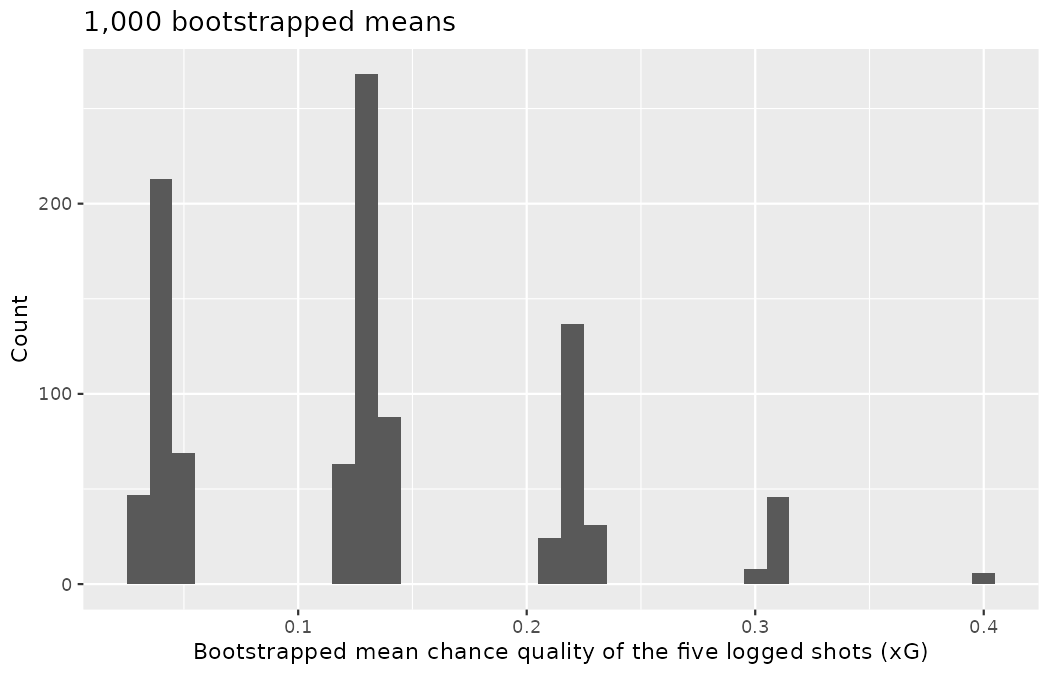
\includegraphics[width=0.85\linewidth,height=\textheight,keepaspectratio]{figures/inference-one-mean-1.png}

The histogram is worth a slow look, because with only five distinct
values in the bag, the mechanics of resampling are visible to the naked
eye. The 1,000 bootstrapped means do not form a smooth bell; they stack
into separated clumps, one for each possible number of copies of the big
chance S2 in the resample: 329 resamples drew S2 zero times (means near
0.041), 419 drew it once (near 0.131), 192 twice (near 0.220), 54 three
times (near 0.309), and 6 four times (near 0.400). The bootstrapped
average chance qualities range from about 0.027 to 0.401 xG. The
bootstrap percentile confidence interval is found by locating the middle
90\% (for a 90\% confidence interval) or 95\% (for a 95\% confidence
interval) of the bootstrapped statistics --- exactly the procedure of
Chapter~\ref{sec-foundations-bootstrapping}, applied to means.

\begin{tcolorbox}[enhanced jigsaw, left=2mm, leftrule=.75mm, title=\textcolor{quarto-callout-note-color}{\faInfo}\hspace{0.5em}{Worked example}, arc=.35mm, rightrule=.15mm, coltitle=black, colframe=quarto-callout-note-color-frame, bottomrule=.15mm, colbacktitle=quarto-callout-note-color!10!white, opacitybacktitle=0.6, breakable, bottomtitle=1mm, toptitle=1mm, titlerule=0mm, opacityback=0, toprule=.15mm, colback=white]

Using the bootstrapped means in \texttt{scout5\_means}, find the 90\%
and 95\% bootstrap percentile confidence intervals for the true mean
open-play chance quality of the shots this player gets himself into.

\begin{center}\rule{0.5\linewidth}{0.5pt}\end{center}

The percentiles can be read off directly:

\begin{Shaded}
\begin{Highlighting}[]
\FunctionTok{round}\NormalTok{(}\FunctionTok{quantile}\NormalTok{(scout5\_means}\SpecialCharTok{$}\NormalTok{stat, }\FunctionTok{c}\NormalTok{(}\FloatTok{0.05}\NormalTok{, }\FloatTok{0.95}\NormalTok{)), }\DecValTok{4}\NormalTok{)}
\CommentTok{\#\textgreater{}     5\%    95\%}
\CommentTok{\#\textgreater{} 0.0361 0.3051}

\FunctionTok{round}\NormalTok{(}\FunctionTok{quantile}\NormalTok{(scout5\_means}\SpecialCharTok{$}\NormalTok{stat, }\FunctionTok{c}\NormalTok{(}\FloatTok{0.025}\NormalTok{, }\FloatTok{0.975}\NormalTok{)), }\DecValTok{4}\NormalTok{)}
\CommentTok{\#\textgreater{}   2.5\%  97.5\%}
\CommentTok{\#\textgreater{} 0.0333 0.3103}
\end{Highlighting}
\end{Shaded}

A 90\% confidence interval is 0.0361 to 0.3051 xG. The conclusion is
that we are 90\% confident that the true mean open-play chance quality
for this player lies somewhere between 0.0361 and 0.3051 xG per shot.

A 95\% confidence interval is 0.0333 to 0.3103 xG. The conclusion is
that we are 95\% confident that the true mean open-play chance quality
for this player lies somewhere between 0.0333 and 0.3103 xG per shot.

Read those intervals as a scout: they run from ``feeds on scraps'' to
``averages a near-one-on-one every attempt.'' Five shots, honestly
analyzed, buy you almost no precision --- which is precisely what the
interval is for: it refuses to let the point estimate of 0.1305
masquerade as knowledge.

\end{tcolorbox}

\subsection{Bootstrap SE confidence
interval}\label{bootstrap-se-confidence-interval}

As seen in Section~\ref{sec-two-prop-boot-ci}, another method for
creating bootstrap confidence intervals directly uses a calculation of
the variability of the bootstrap statistics (here, the bootstrap means).
If the bootstrap distribution is relatively symmetric and bell-shaped,
then the 95\% bootstrap SE confidence interval can be constructed with
the formula familiar from the mathematical models in previous chapters:

\[\text{point estimate} \pm 2 \cdot SE_{BS}\]

One new subscript, so decompose it: \(SE\) is the standard error you met
in Chapter~\ref{sec-foundations-mathematical} --- the standard deviation
of a statistic from sample to sample --- and the subscript \(BS\)
records \emph{how this particular standard error was estimated}: not
from a formula, but as the standard deviation of the bootstrapped
statistics themselves. The number 2 is an approximation connected to the
``95\%'' part of the confidence interval (remember the 68-95-99.7 rule
from Chapter~\ref{sec-explore-numerical} and
Chapter~\ref{sec-foundations-mathematical}). As will be seen in
Section~\ref{sec-one-mean-math}, a new distribution (the
\(t\)-distribution) will be applied to most mathematical inference on
numerical variables. However, because bootstrapping is not grounded in
the same theory as the mathematical approach given in this text, we
stick with the standard normal quantiles (in R use the function
\texttt{qnorm()} to find normal percentiles other than 95\%) for
different confidence percentages.\footnote{There is a large literature
  on understanding and improving bootstrap intervals; see Hesterberg
  (2015),
  \href{https://www.tandfonline.com/doi/full/10.1080/00031305.2015.1089789}{``What
  Teachers Should Know About the Bootstrap''}, and Hayden (2019),
  \href{https://www.tandfonline.com/doi/full/10.1080/10691898.2019.1669507}{``Questionable
  Claims for Simple Versions of the Bootstrap''}, for more information.}

\begin{tcolorbox}[enhanced jigsaw, left=2mm, leftrule=.75mm, title=\textcolor{quarto-callout-note-color}{\faInfo}\hspace{0.5em}{Worked example}, arc=.35mm, rightrule=.15mm, coltitle=black, colframe=quarto-callout-note-color-frame, bottomrule=.15mm, colbacktitle=quarto-callout-note-color!10!white, opacitybacktitle=0.6, breakable, bottomtitle=1mm, toptitle=1mm, titlerule=0mm, opacityback=0, toprule=.15mm, colback=white]

Explain how the standard error (SE) of the bootstrapped means is
calculated and what it is measuring.

\begin{center}\rule{0.5\linewidth}{0.5pt}\end{center}

The SE of the bootstrapped means measures how variable the means are
from resample to resample. The bootstrap SE is a good approximation to
the SE of means as if we had taken repeated samples from the original
population (which we agreed isn't something we would do, because of
wasted scouting resources).

Logistically, we can find the standard deviation of the bootstrapped
means using the same calculations from
Chapter~\ref{sec-explore-numerical}. That is, the bootstrapped means are
the individual observations about which we measure the variability.

\end{tcolorbox}

Although we won't spend a lot of energy on this concept, you may be
wondering about the differences between a standard error and a standard
deviation. The \textbf{standard error} describes how a statistic (e.g.,
sample mean or sample proportion) varies from sample to sample. The
\textbf{standard deviation} can be thought of as a function applied to
any list of numbers which measures how far those numbers vary from their
own average. So, you can have a standard deviation calculated on a
column of jump-and-reach heights from the academy combine or a standard
deviation calculated on a column of bootstrapped means from the
resampled data. Note that the standard deviation calculated on the
bootstrapped means is referred to as the bootstrap standard error of the
mean.

\begin{tcolorbox}[enhanced jigsaw, left=2mm, leftrule=.75mm, title=\textcolor{quarto-callout-tip-color}{\faLightbulb}\hspace{0.5em}{Check your understanding}, arc=.35mm, rightrule=.15mm, coltitle=black, colframe=quarto-callout-tip-color-frame, bottomrule=.15mm, colbacktitle=quarto-callout-tip-color!10!white, opacitybacktitle=0.6, breakable, bottomtitle=1mm, toptitle=1mm, titlerule=0mm, opacityback=0, toprule=.15mm, colback=white]

It turns out that the standard deviation of the 1,000 bootstrapped means
is \(SE_{BS} = 0.0798\) (a value which is an excellent approximation for
the standard error of sample means if we were to take repeated five-shot
samples of this player). (Note: in R the calculation was done using the
function \texttt{sd()}.)

\begin{Shaded}
\begin{Highlighting}[]
\FunctionTok{round}\NormalTok{(}\FunctionTok{c}\NormalTok{(}\AttributeTok{xbar\_bs =} \FunctionTok{mean}\NormalTok{(scout5\_means}\SpecialCharTok{$}\NormalTok{stat), }\AttributeTok{se\_bs =} \FunctionTok{sd}\NormalTok{(scout5\_means}\SpecialCharTok{$}\NormalTok{stat)), }\DecValTok{4}\NormalTok{)}
\CommentTok{\#\textgreater{} xbar\_bs   se\_bs}
\CommentTok{\#\textgreater{}  0.1296  0.0798}
\end{Highlighting}
\end{Shaded}

The average of the five observed chance qualities is
\(\bar{x} = 0.1305\) xG, and we will consider the sample average to be
the best guess point estimate for \(\mu.\) Find and interpret the
confidence interval for \(\mu\) (the true mean open-play chance quality
for this player) using the bootstrap SE confidence interval formula.

\begin{center}\rule{0.5\linewidth}{0.5pt}\end{center}

Using the formula for the bootstrap SE interval, we find the 95\%
confidence interval for \(\mu\):
\(0.1305 \pm 2 \cdot 0.0798 \rightarrow (-0.0291, 0.2901).\) We are 95\%
confident that the true mean open-play chance quality for this player is
somewhere between \(-0.0291\) and \(0.2901\) xG. And there the formula
has embarrassed itself: a chance quality below zero is impossible, yet
the symmetric interval reaches \(-0.0291\) anyway. The warning attached
to this method --- \emph{if the bootstrap distribution is relatively
symmetric and bell-shaped} --- was doing real work, and our clumpy,
right-skewed bootstrap distribution violates it.

\end{tcolorbox}

\begin{tcolorbox}[enhanced jigsaw, left=2mm, leftrule=.75mm, title=\textcolor{quarto-callout-note-color}{\faInfo}\hspace{0.5em}{Worked example}, arc=.35mm, rightrule=.15mm, coltitle=black, colframe=quarto-callout-note-color-frame, bottomrule=.15mm, colbacktitle=quarto-callout-note-color!10!white, opacitybacktitle=0.6, breakable, bottomtitle=1mm, toptitle=1mm, titlerule=0mm, opacityback=0, toprule=.15mm, colback=white]

Compare and contrast the two different 95\% confidence intervals for
\(\mu\) created by finding the percentiles of the bootstrapped means and
created by finding the SE of the bootstrapped means. Do you think the
intervals \emph{should} be identical?

\begin{center}\rule{0.5\linewidth}{0.5pt}\end{center}

\begin{itemize}
\tightlist
\item
  Percentile interval: (0.0333, 0.3103)
\item
  SE interval: (\(-0.0291\), 0.2901)
\end{itemize}

The intervals were created using different methods, so it is not
surprising that they are not identical. Here they disagree more than we
would like: the bootstrap distribution of \(\bar{x}_{bs}\) is clumped
and right-skewed (five observations, one of them the Final goal), so the
symmetric SE formula overshoots downward --- below zero, which xG cannot
reach --- while the percentile interval, built from the ordered
\(\bar{x}_{bs}\) values themselves, respects the support of the data.
When the two constructions disagree this visibly, treat the disagreement
itself as diagnostic information about the sample. The technical details
surrounding which data structures are best for percentile intervals and
which are best for SE intervals are beyond the scope of this text.
However, the larger the samples are, the better (and closer) the
interval estimates will be.

\end{tcolorbox}

\subsection{Bootstrap percentile confidence interval for a standard
deviation}\label{bootstrap-percentile-confidence-interval-for-a-standard-deviation}

Suppose that Emil's question shifts from the player's typical chance
quality to his \emph{consistency}. Recall from
Chapter~\ref{sec-explore-numerical} that a striker steady around 0.12 xG
per shot and a striker who mixes tap-ins with 30-yard speculative
efforts can share a mean while being entirely different scouting
propositions; the parameter that separates them is the standard
deviation of chance quality, \(\sigma.\) You may have already realized
that the sample standard deviation, \(s,\) will work as a good
\textbf{point estimate} for the parameter of interest: the population
standard deviation, \(\sigma.\) The point estimate from the five logged
shots is \(s = 0.2004\) xG. While \(s = 0.2004\) might be a good guess
for \(\sigma,\) we prefer to have an interval estimate for the parameter
of interest. Although there is a mathematical model which describes how
\(s\) varies from sample to sample, that model will not be presented in
this text. Instead, bootstrapping can be used --- this is precisely the
``extendable to any statistic'' promise from the start of the chapter
being kept. Using the same resamples as before, we compute a standard
deviation instead of a mean on each one.

\begin{Shaded}
\begin{Highlighting}[]
\NormalTok{scout5\_sds }\OtherTok{\textless{}{-}}\NormalTok{ scout5\_boot }\SpecialCharTok{|\textgreater{}}
  \FunctionTok{summarize}\NormalTok{(}\AttributeTok{stat =} \FunctionTok{sd}\NormalTok{(statsbomb\_xg))}

\FunctionTok{ggplot}\NormalTok{(scout5\_sds, }\FunctionTok{aes}\NormalTok{(}\AttributeTok{x =}\NormalTok{ stat)) }\SpecialCharTok{+}
  \FunctionTok{geom\_histogram}\NormalTok{(}\AttributeTok{binwidth =} \FloatTok{0.01}\NormalTok{) }\SpecialCharTok{+}
  \FunctionTok{labs}\NormalTok{(}
    \AttributeTok{x =} \StringTok{"Bootstrapped standard deviation of the five logged chance qualities (xG)"}\NormalTok{,}
    \AttributeTok{y =} \StringTok{"Count"}\NormalTok{,}
    \AttributeTok{title =} \StringTok{"1,000 bootstrapped standard deviations"}
\NormalTok{  )}
\end{Highlighting}
\end{Shaded}

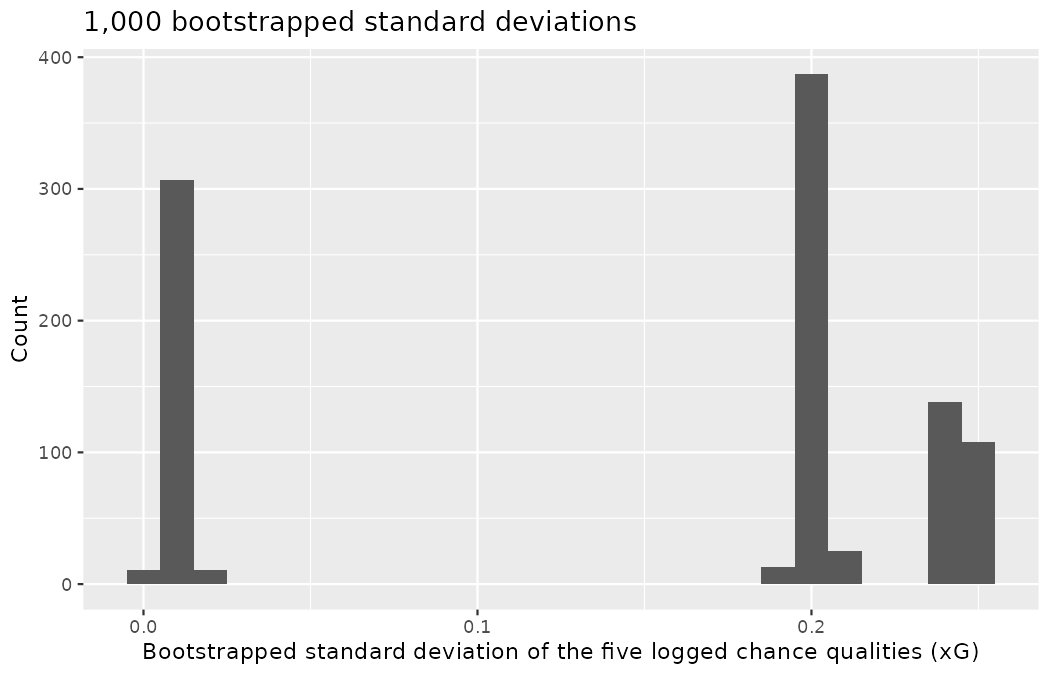
\includegraphics[width=0.85\linewidth,height=\textheight,keepaspectratio]{figures/inference-one-mean-2.png}

\begin{tcolorbox}[enhanced jigsaw, left=2mm, leftrule=.75mm, title=\textcolor{quarto-callout-note-color}{\faInfo}\hspace{0.5em}{Worked example}, arc=.35mm, rightrule=.15mm, coltitle=black, colframe=quarto-callout-note-color-frame, bottomrule=.15mm, colbacktitle=quarto-callout-note-color!10!white, opacitybacktitle=0.6, breakable, bottomtitle=1mm, toptitle=1mm, titlerule=0mm, opacityback=0, toprule=.15mm, colback=white]

Describe the bootstrap distribution for the standard deviation drawn by
the code above.

\begin{center}\rule{0.5\linewidth}{0.5pt}\end{center}

The distribution is not remotely bell-shaped: it splits into two
separated clumps. The 329 resamples that never drew the Final goal
contain only the four small, similar chances, so their standard
deviations are tiny --- between 0.0011 and 0.0156. The 671 resamples
that drew the big chance at least once have standard deviations between
about 0.19 and 0.25, near the point estimate \(s = 0.2004\) from the
original data. Nothing at all lies between the clumps. With \(n = 5,\)
the sample's variability estimate is almost entirely a bet on whether
one shot appears.

\end{tcolorbox}

\begin{tcolorbox}[enhanced jigsaw, left=2mm, leftrule=.75mm, title=\textcolor{quarto-callout-tip-color}{\faLightbulb}\hspace{0.5em}{Check your understanding}, arc=.35mm, rightrule=.15mm, coltitle=black, colframe=quarto-callout-tip-color-frame, bottomrule=.15mm, colbacktitle=quarto-callout-tip-color!10!white, opacitybacktitle=0.6, breakable, bottomtitle=1mm, toptitle=1mm, titlerule=0mm, opacityback=0, toprule=.15mm, colback=white]

Using the bootstrapped standard deviations, find and interpret a 90\%
bootstrap percentile confidence interval for the population standard
deviation of this player's open-play chance quality.

\begin{Shaded}
\begin{Highlighting}[]
\FunctionTok{round}\NormalTok{(}\FunctionTok{quantile}\NormalTok{(scout5\_sds}\SpecialCharTok{$}\NormalTok{stat, }\FunctionTok{c}\NormalTok{(}\FloatTok{0.05}\NormalTok{, }\FloatTok{0.95}\NormalTok{)), }\DecValTok{4}\NormalTok{)}
\CommentTok{\#\textgreater{}    5\%   95\%}
\CommentTok{\#\textgreater{} 0.009 0.249}
\end{Highlighting}
\end{Shaded}

\begin{center}\rule{0.5\linewidth}{0.5pt}\end{center}

The middle 90\% of the bootstrapped standard deviations is given by the
5th percentile (0.0090) and the 95th percentile (0.2490). That is, we
are 90\% confident that the true standard deviation of this player's
open-play chance quality is between 0.0090 and 0.2490 xG. A 90\%
confidence level indicates that there was not a need for a high level of
confidence, such as 95\% or 99\%; a lower confidence level has higher
potential for error, but it also produces a narrower interval. Even so,
be honest about what this interval says: it stretches from
``metronomically identical chances'' to ``wildly mixed shot diet'' ---
with five shots, the data cannot tell Emil which player he is looking
at.

\end{tcolorbox}

\subsection{Bootstrapping is not a solution to small sample
sizes!}\label{bootstrapping-is-not-a-solution-to-small-sample-sizes}

The example presented above is done for a sample with only five
observations. As with analysis techniques that build on mathematical
models, bootstrapping works best when a large random sample has been
taken from the population. Bootstrapping is a method for capturing the
variability of a statistic when the mathematical model is unknown (it is
not a method for navigating small samples). The clumpy histograms above
are the picture to remember: the bootstrap cannot invent information
that five shots do not contain; it can only report, faithfully, how
little there is. As you might guess, the larger the random sample, the
more accurately that sample will represent the population of interest.

Our data allow one closing check that a working scout never gets. The
player's full open-play record at the tournament --- all 24 shots ---
has a mean chance quality of 0.0797 xG per shot:

\begin{Shaded}
\begin{Highlighting}[]
\FunctionTok{round}\NormalTok{(}\FunctionTok{c}\NormalTok{(}\AttributeTok{n =} \FunctionTok{nrow}\NormalTok{(messi\_open), }\AttributeTok{xbar =} \FunctionTok{mean}\NormalTok{(messi\_open}\SpecialCharTok{$}\NormalTok{statsbomb\_xg)), }\DecValTok{4}\NormalTok{)}
\CommentTok{\#\textgreater{}       n    xbar}
\CommentTok{\#\textgreater{} 24.0000  0.0797}
\end{Highlighting}
\end{Shaded}

The five-shot point estimate of 0.1305 overshot the fuller-record value
by more than 60\%, dragged up by the one great chance the scout happened
to see; the intervals did contain 0.0797, but only by being enormous.
Five logged shots plus honest statistics equals a very wide interval ---
the dishonest alternative is a confident number that is wrong.

\section{Mathematical model for a mean}\label{sec-one-mean-math}

As with the sample proportion, the variability of the sample mean is
well described by the mathematical theory given by the Central Limit
Theorem. However, because of missing information about the inherent
variability in the population (\(\sigma\)), a \(t\)-distribution is used
in place of the standard normal when performing hypothesis test or
confidence interval analyses.

\subsection{Mathematical distribution of the sample
mean}\label{mathematical-distribution-of-the-sample-mean}

The sample mean tends to follow a normal distribution centered at the
population mean, \(\mu,\) when certain conditions are met. Additionally,
we can compute a standard error for the sample mean using the population
standard deviation \(\sigma\) and the sample size \(n.\)

\begin{tcolorbox}[enhanced jigsaw, left=2mm, leftrule=.75mm, title=\textcolor{quarto-callout-important-color}{\faExclamation}\hspace{0.5em}{Central Limit Theorem for the sample mean}, arc=.35mm, rightrule=.15mm, coltitle=black, colframe=quarto-callout-important-color-frame, bottomrule=.15mm, colbacktitle=quarto-callout-important-color!10!white, opacitybacktitle=0.6, breakable, bottomtitle=1mm, toptitle=1mm, titlerule=0mm, opacityback=0, toprule=.15mm, colback=white]

When we collect a sufficiently large sample of \(n\) independent
observations from a population with mean \(\mu\) and standard deviation
\(\sigma,\) the sampling distribution of \(\bar{x}\) will be nearly
normal with

\[\text{Mean} = \mu \qquad \text{Standard Error } (SE) = \frac{\sigma}{\sqrt{n}}\]

\end{tcolorbox}

Read the standard error formula piece by piece, because it is the engine
of the whole chapter. The numerator \(\sigma\) is the population
standard deviation from Chapter~\ref{sec-explore-numerical}: the more
the individual observations vary, the more the mean of a sample of them
varies. The denominator \(\sqrt{n}\) is the new part: averaging \(n\)
independent observations cancels shot-to-shot noise, and the
cancellation strengthens with the \emph{square root} of the sample size.
Quadruple the number of shots a scout logs and the standard error of the
mean halves --- not quarters. This is the mean's version of the pattern
you saw for proportions in Chapter~\ref{sec-foundations-mathematical},
and it is why patient scouting beats excitable scouting: precision is
bought at the price of \(\sqrt{n}.\)

Before diving into confidence intervals and hypothesis tests using
\(\bar{x},\) we first need to cover two topics:

\begin{itemize}
\tightlist
\item
  When we modeled \(\hat{p}\) using the normal distribution, certain
  conditions had to be satisfied. The conditions for working with
  \(\bar{x}\) are a little more complex, and below, we will discuss how
  to check conditions for inference using a mathematical model.
\item
  The standard error is dependent on the population standard deviation,
  \(\sigma.\) However, we rarely know \(\sigma,\) and instead we must
  estimate it. Because this estimation is itself imperfect, we use a new
  distribution called the \(t\)-distribution to fix this problem.
\end{itemize}

\subsection{\texorpdfstring{Evaluating the two conditions required for
modeling
\(\bar{x}\)}{Evaluating the two conditions required for modeling \textbackslash bar\{x\}}}\label{evaluating-the-two-conditions-required-for-modeling-barx}

Two conditions are required to apply the \textbf{Central Limit Theorem}
for a sample mean \(\bar{x}:\)

\begin{itemize}
\item
  \textbf{Independence.} The sample observations must be independent.
  The most common way to satisfy this condition is when the sample is a
  simple random sample from the population --- a seeded
  \texttt{slice\_sample()} of logged shots qualifies; the shots from a
  single ten-minute spell of one match do not. If the data come from a
  random process, analogous to rolling a die, this would also satisfy
  the independence condition.
\item
  \textbf{Normality.} When a sample is small, we also require that the
  sample observations come from a normally distributed population. We
  can relax this condition more and more for larger and larger sample
  sizes. This condition is vague, making it difficult to evaluate, so
  next we introduce a couple of rules of thumb for checking it.
\end{itemize}

\begin{tcolorbox}[enhanced jigsaw, left=2mm, leftrule=.75mm, title=\textcolor{quarto-callout-important-color}{\faExclamation}\hspace{0.5em}{General rule for performing the normality check}, arc=.35mm, rightrule=.15mm, coltitle=black, colframe=quarto-callout-important-color-frame, bottomrule=.15mm, colbacktitle=quarto-callout-important-color!10!white, opacitybacktitle=0.6, breakable, bottomtitle=1mm, toptitle=1mm, titlerule=0mm, opacityback=0, toprule=.15mm, colback=white]

There is no perfect way to check the normality condition, so instead we
use two general rules based on the number and magnitude of extreme
observations. Note, it often takes practice to get a sense for whether a
normal approximation is appropriate.

\begin{itemize}
\tightlist
\item
  Small \(n\): If the sample size \(n\) is small and there are
  \textbf{no clear outliers} in the data, then we typically assume the
  data come from a nearly normal distribution to satisfy the condition.
\item
  Large \(n\): If the sample size \(n\) is large and there are no
  \textbf{particularly extreme} outliers, then we typically assume the
  sampling distribution of \(\bar{x}\) is nearly normal, even if the
  underlying distribution of individual observations is not.
\end{itemize}

Some guidelines for determining whether \(n\) is considered small or
large are as follows: slight skew is okay for sample sizes of 15,
moderate skew for sample sizes of 30, and strong skew for sample sizes
of 60.

\end{tcolorbox}

In this first course in statistics, you aren't expected to develop
perfect judgment on the normality condition. However, you are expected
to be able to handle clear cut cases based on the rules of
thumb.\footnote{More nuanced guidelines would consider further relaxing
  the \emph{particularly extreme outlier} check when the sample size is
  very large. However, we'll leave further discussion here to a future
  course.}

\begin{tcolorbox}[enhanced jigsaw, left=2mm, leftrule=.75mm, title=\textcolor{quarto-callout-note-color}{\faInfo}\hspace{0.5em}{Worked example}, arc=.35mm, rightrule=.15mm, coltitle=black, colframe=quarto-callout-note-color-frame, bottomrule=.15mm, colbacktitle=quarto-callout-note-color!10!white, opacitybacktitle=0.6, breakable, bottomtitle=1mm, toptitle=1mm, titlerule=0mm, opacityback=0, toprule=.15mm, colback=white]

Consider the two constructed samples drawn by the seeded code below ---
another pair of Priya's fabricated training sets, in the tradition of
Chapter~\ref{sec-explore-numerical}. Sample 1 records high-speed-running
distance (in hundreds of meters) for \(n_1 = 15\) academy midfielders in
one training week; sample 2 records successful take-ons per 90 minutes
for \(n_2 = 50\) wingers in the scouting database. Both are simple
random samples from their respective (constructed) populations.

Are the independence and normality conditions met in each case?

\begin{Shaded}
\begin{Highlighting}[]
\FunctionTok{library}\NormalTok{(patchwork)}

\FunctionTok{set.seed}\NormalTok{(}\DecValTok{1903}\NormalTok{)}
\NormalTok{sample\_1 }\OtherTok{\textless{}{-}} \FunctionTok{tibble}\NormalTok{(}\AttributeTok{hsr =} \FunctionTok{rnorm}\NormalTok{(}\DecValTok{15}\NormalTok{, }\AttributeTok{mean =} \DecValTok{12}\NormalTok{, }\AttributeTok{sd =} \DecValTok{2}\NormalTok{))}
\NormalTok{sample\_2 }\OtherTok{\textless{}{-}} \FunctionTok{tibble}\NormalTok{(}\AttributeTok{dribbles =} \FunctionTok{c}\NormalTok{(}\FunctionTok{exp}\NormalTok{(}\FunctionTok{rnorm}\NormalTok{(}\DecValTok{49}\NormalTok{, }\AttributeTok{mean =} \DecValTok{0}\NormalTok{, }\AttributeTok{sd =} \FloatTok{0.7}\NormalTok{)), }\DecValTok{22}\NormalTok{))}

\NormalTok{p1 }\OtherTok{\textless{}{-}} \FunctionTok{ggplot}\NormalTok{(sample\_1, }\FunctionTok{aes}\NormalTok{(}\AttributeTok{x =}\NormalTok{ hsr)) }\SpecialCharTok{+}
  \FunctionTok{geom\_histogram}\NormalTok{(}\AttributeTok{binwidth =} \DecValTok{1}\NormalTok{) }\SpecialCharTok{+}
  \FunctionTok{labs}\NormalTok{(}\AttributeTok{x =} \ConstantTok{NULL}\NormalTok{, }\AttributeTok{y =} \StringTok{"Count"}\NormalTok{, }\AttributeTok{title =} \StringTok{"Sample 1"}\NormalTok{, }\AttributeTok{subtitle =} \StringTok{"n = 15"}\NormalTok{)}

\NormalTok{p2 }\OtherTok{\textless{}{-}} \FunctionTok{ggplot}\NormalTok{(sample\_2, }\FunctionTok{aes}\NormalTok{(}\AttributeTok{x =}\NormalTok{ dribbles)) }\SpecialCharTok{+}
  \FunctionTok{geom\_histogram}\NormalTok{(}\AttributeTok{binwidth =} \DecValTok{1}\NormalTok{) }\SpecialCharTok{+}
  \FunctionTok{labs}\NormalTok{(}\AttributeTok{x =} \ConstantTok{NULL}\NormalTok{, }\AttributeTok{y =} \StringTok{"Count"}\NormalTok{, }\AttributeTok{title =} \StringTok{"Sample 2"}\NormalTok{, }\AttributeTok{subtitle =} \StringTok{"n = 50"}\NormalTok{)}

\NormalTok{p3 }\OtherTok{\textless{}{-}} \FunctionTok{ggplot}\NormalTok{(sample\_1, }\FunctionTok{aes}\NormalTok{(}\AttributeTok{x =}\NormalTok{ hsr)) }\SpecialCharTok{+}
  \FunctionTok{geom\_boxplot}\NormalTok{() }\SpecialCharTok{+}
  \FunctionTok{labs}\NormalTok{(}\AttributeTok{x =} \StringTok{"High{-}speed running (100s of meters)"}\NormalTok{)}

\NormalTok{p4 }\OtherTok{\textless{}{-}} \FunctionTok{ggplot}\NormalTok{(sample\_2, }\FunctionTok{aes}\NormalTok{(}\AttributeTok{x =}\NormalTok{ dribbles)) }\SpecialCharTok{+}
  \FunctionTok{geom\_boxplot}\NormalTok{() }\SpecialCharTok{+}
  \FunctionTok{labs}\NormalTok{(}\AttributeTok{x =} \StringTok{"Successful take{-}ons per 90"}\NormalTok{)}

\NormalTok{p1 }\SpecialCharTok{+}\NormalTok{ p2 }\SpecialCharTok{+}\NormalTok{ p3 }\SpecialCharTok{+}\NormalTok{ p4 }\SpecialCharTok{+} \FunctionTok{plot\_layout}\NormalTok{(}\AttributeTok{nrow =} \DecValTok{2}\NormalTok{, }\AttributeTok{heights =} \FunctionTok{c}\NormalTok{(}\DecValTok{3}\NormalTok{, }\DecValTok{1}\NormalTok{))}
\end{Highlighting}
\end{Shaded}

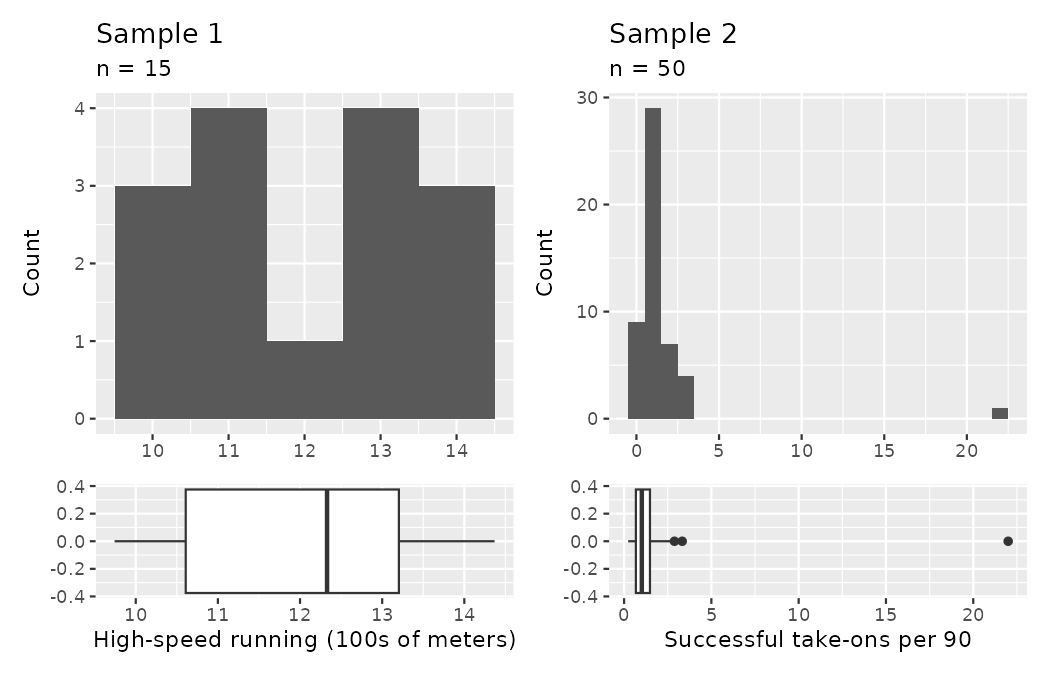
\includegraphics[width=0.85\linewidth,height=\textheight,keepaspectratio]{figures/inference-one-mean-3.png}

\begin{center}\rule{0.5\linewidth}{0.5pt}\end{center}

Each sample is a simple random sample of its respective population, so
the independence condition is satisfied. Let's next check the normality
condition for each using the rule of thumb.

The first sample has fewer than 30 observations, so we are watching for
any clear outliers. None are present: the fifteen values run smoothly
from about 9.7 to 14.4 hundred meters, and while there is a small gap in
the histogram between the lower and upper clusters, over 40\% of this
small sample sits below the gap, so we can hardly call these clear
outliers. With no clear outliers, the normality condition can be
reasonably assumed to be met.

The second sample has a sample size greater than 30 and includes an
outlier: one winger is recorded at 22 take-ons per 90, while every other
value in the sample sits below 3.4. That single observation lies roughly
nine times further from the center of the distribution than the next
furthest observation. This is an example of a particularly extreme
outlier, so the normality condition would not be satisfied.

It's often helpful to also visualize the data using a box plot to assess
skewness and existence of outliers. The box plots drawn underneath each
histogram confirm our conclusions: the first sample flags nothing, while
the second flags the extreme point far beyond its whisker.

\end{tcolorbox}

In practice, it's typical to also do a mental check to evaluate whether
we have reason to believe the underlying population would have moderate
skew (if \(n < 30\)) or have particularly extreme outliers
(\(n \geq 30\)) beyond what we observe in the data. For example,
consider transfer fees across a season's completed deals, and then
imagine this distribution. The large majority of transfers worldwide are
free moves and modest six-figure fees, while a relatively tiny fraction
run to €100M and beyond, meaning the distribution is extremely skewed.
When we know the data come from such an extremely skewed distribution,
it takes some effort to understand what sample size is large enough for
the normality condition to be satisfied.

\subsection{Introducing the
t-distribution}\label{introducing-the-t-distribution}

In practice, we cannot directly calculate the standard error for
\(\bar{x}\) since we do not know the population standard deviation,
\(\sigma.\) We encountered a similar issue when computing the standard
error for a sample proportion, which relied on the population
proportion, \(p.\) Our solution in the proportion context (recall
Chapter~\ref{sec-inference-one-prop}) was to use the sample value in
place of the population value when computing the standard error. We'll
employ a similar strategy for computing the standard error of
\(\bar{x},\) using the sample standard deviation \(s\) in place of
\(\sigma:\)

\[SE = \frac{\sigma}{\sqrt{n}} \approx \frac{s}{\sqrt{n}}\]

This is the standard error formula you will use for the rest of the
book's work on means, so read the plug-in carefully: the structure is
the Central Limit Theorem's \(\sigma/\sqrt{n},\) but the unknowable
\(\sigma\) has been replaced by its sample estimate \(s\) --- a number
that is itself computed from the same \(n\) observations, and is
therefore itself uncertain.

This strategy tends to work well when we have a lot of data and can
estimate \(\sigma\) using \(s\) accurately. However, the estimate is
less precise with smaller samples, and this leads to problems when using
the normal distribution to model \(\bar{x}.\)

We'll find it useful to use a new distribution for inference
calculations called the \textbf{t-distribution}. A \(t\)-distribution,
drawn as the solid line by the code below, has a bell shape. However,
its tails are \emph{thicker} than the normal distribution's, meaning
observations are more likely to fall beyond two standard deviations from
the mean than under the normal distribution.

\begin{Shaded}
\begin{Highlighting}[]
\NormalTok{t\_compare }\OtherTok{\textless{}{-}} \FunctionTok{tibble}\NormalTok{(}
  \AttributeTok{x =} \FunctionTok{rep}\NormalTok{(}\FunctionTok{seq}\NormalTok{(}\SpecialCharTok{{-}}\DecValTok{5}\NormalTok{, }\DecValTok{5}\NormalTok{, }\FloatTok{0.01}\NormalTok{), }\DecValTok{2}\NormalTok{),}
  \AttributeTok{distribution =} \FunctionTok{rep}\NormalTok{(}\FunctionTok{c}\NormalTok{(}\StringTok{"Normal distribution"}\NormalTok{, }\StringTok{"t{-}distribution (df = 1)"}\NormalTok{), }\AttributeTok{each =} \DecValTok{1001}\NormalTok{)}
\NormalTok{) }\SpecialCharTok{|\textgreater{}}
  \FunctionTok{mutate}\NormalTok{(}\AttributeTok{y =} \FunctionTok{if\_else}\NormalTok{(distribution }\SpecialCharTok{==} \StringTok{"Normal distribution"}\NormalTok{, }\FunctionTok{dnorm}\NormalTok{(x), }\FunctionTok{dt}\NormalTok{(x, }\AttributeTok{df =} \DecValTok{1}\NormalTok{)))}

\FunctionTok{ggplot}\NormalTok{(t\_compare, }\FunctionTok{aes}\NormalTok{(}\AttributeTok{x =}\NormalTok{ x, }\AttributeTok{y =}\NormalTok{ y, }\AttributeTok{linetype =}\NormalTok{ distribution)) }\SpecialCharTok{+}
  \FunctionTok{geom\_line}\NormalTok{() }\SpecialCharTok{+}
  \FunctionTok{labs}\NormalTok{(}\AttributeTok{x =} \ConstantTok{NULL}\NormalTok{, }\AttributeTok{y =} \ConstantTok{NULL}\NormalTok{, }\AttributeTok{linetype =} \ConstantTok{NULL}\NormalTok{)}
\end{Highlighting}
\end{Shaded}

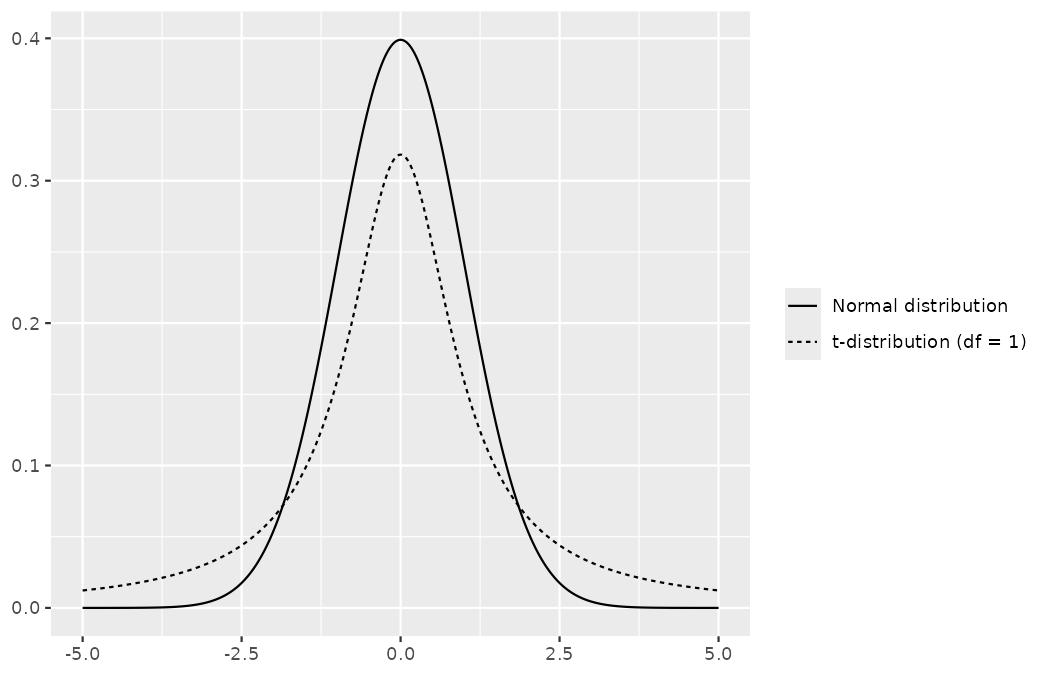
\includegraphics[width=0.85\linewidth,height=\textheight,keepaspectratio]{figures/inference-one-mean-4.png}

The heavier tails are not a decorative difference; they are the entire
point, so let us tell the story properly. When \(\sigma\) is known, the
standardized statistic \((\bar{x} - \mu)/(\sigma/\sqrt{n})\) has one
source of randomness: the numerator. When we must plug in \(s,\) the
denominator becomes random too. In an unlucky small sample, \(s\)
underestimates \(\sigma\) --- the scout happens to log five similar
shots and concludes the player is metronomic --- and dividing by that
too-small standard error inflates the statistic. Occasionally, then, the
ratio lands much further from zero than a normal model would ever
predict, and probability mass must be moved out of the shoulders and
into the tails to account for it. The extra thick tails of the
\(t\)-distribution are exactly the correction needed to resolve this
problem, and the smaller the sample, the noisier \(s\) is, and the
heavier the tails must be.

\begin{tcolorbox}[enhanced jigsaw, left=2mm, leftrule=.75mm, title=\textcolor{quarto-callout-tip-color}{\faLightbulb}\hspace{0.5em}{Check your understanding}, arc=.35mm, rightrule=.15mm, coltitle=black, colframe=quarto-callout-tip-color-frame, bottomrule=.15mm, colbacktitle=quarto-callout-tip-color!10!white, opacitybacktitle=0.6, breakable, bottomtitle=1mm, toptitle=1mm, titlerule=0mm, opacityback=0, toprule=.15mm, colback=white]

A colleague objects: ``We already plugged \(\hat{p}\) in for \(p\) back
in Chapter~\ref{sec-inference-one-prop} and kept using the normal
distribution. Why does plugging \(s\) in for \(\sigma\) suddenly require
a whole new distribution?'' What is the honest answer?

\begin{center}\rule{0.5\linewidth}{0.5pt}\end{center}

For proportions, the standard error \(\sqrt{p(1-p)/n}\) is determined by
the very quantity being estimated, and the normal approximation with
\(\hat{p}\) plugged in works adequately when the success-failure
condition holds. For means, the numerator (\(\bar{x}\)) and the spread
estimate (\(s\)) are two genuinely separate quantities estimated from
the same small sample, and the extra variability of \(s\) in small
samples is large enough to visibly fatten the tails of the standardized
statistic. The \(t\)-distribution quantifies exactly that extra
uncertainty; as \(n\) grows and \(s\) pins down \(\sigma,\) the
correction fades and the \(t\)-distribution melts back into the normal.

\end{tcolorbox}

The \(t\)-distribution is always centered at zero and has a single
parameter: degrees of freedom. The \textbf{degrees of freedom} describes
the precise form of the bell-shaped \(t\)-distribution. Several
\(t\)-distributions are drawn by the code below in comparison to the
normal distribution. Similar to the chi-squared distribution you met in
Chapter~\ref{sec-inference-tables}, the shape of the \(t\)-distribution
depends on its degrees of freedom --- but where the chi-squared's \(df\)
came from the dimensions of a table, here the degrees of freedom come
from the sample size.

In general, we'll use a \(t\)-distribution with \(df = n - 1\) to model
the sample mean when the sample size is \(n.\) Decompose the formula:
\(n\) observations carry \(n\) pieces of information about spread, but
one of them is spent estimating \(\bar{x}\) itself --- the deviations
\(x_i - \bar{x}\) must sum to zero, so only \(n - 1\) of them are free
to vary, which is the same \(n - 1\) that divides the sample variance in
Chapter~\ref{sec-explore-numerical}. When we have more observations, the
degrees of freedom will be larger and the \(t\)-distribution will look
more like the standard normal distribution; when the degrees of freedom
are about 30 or more, the \(t\)-distribution is nearly indistinguishable
from the normal distribution.

\begin{Shaded}
\begin{Highlighting}[]
\NormalTok{t\_dfs }\OtherTok{\textless{}{-}} \FunctionTok{bind\_rows}\NormalTok{(}
  \FunctionTok{tibble}\NormalTok{(}\AttributeTok{x =} \FunctionTok{seq}\NormalTok{(}\SpecialCharTok{{-}}\DecValTok{5}\NormalTok{, }\DecValTok{5}\NormalTok{, }\FloatTok{0.01}\NormalTok{), }\AttributeTok{y =} \FunctionTok{dnorm}\NormalTok{(x), }\AttributeTok{curve =} \StringTok{"normal"}\NormalTok{),}
  \FunctionTok{tibble}\NormalTok{(}\AttributeTok{x =} \FunctionTok{seq}\NormalTok{(}\SpecialCharTok{{-}}\DecValTok{5}\NormalTok{, }\DecValTok{5}\NormalTok{, }\FloatTok{0.01}\NormalTok{), }\AttributeTok{y =} \FunctionTok{dt}\NormalTok{(x, }\DecValTok{8}\NormalTok{), }\AttributeTok{curve =} \StringTok{"t, df = 8"}\NormalTok{),}
  \FunctionTok{tibble}\NormalTok{(}\AttributeTok{x =} \FunctionTok{seq}\NormalTok{(}\SpecialCharTok{{-}}\DecValTok{5}\NormalTok{, }\DecValTok{5}\NormalTok{, }\FloatTok{0.01}\NormalTok{), }\AttributeTok{y =} \FunctionTok{dt}\NormalTok{(x, }\DecValTok{4}\NormalTok{), }\AttributeTok{curve =} \StringTok{"t, df = 4"}\NormalTok{),}
  \FunctionTok{tibble}\NormalTok{(}\AttributeTok{x =} \FunctionTok{seq}\NormalTok{(}\SpecialCharTok{{-}}\DecValTok{5}\NormalTok{, }\DecValTok{5}\NormalTok{, }\FloatTok{0.01}\NormalTok{), }\AttributeTok{y =} \FunctionTok{dt}\NormalTok{(x, }\DecValTok{2}\NormalTok{), }\AttributeTok{curve =} \StringTok{"t, df = 2"}\NormalTok{),}
  \FunctionTok{tibble}\NormalTok{(}\AttributeTok{x =} \FunctionTok{seq}\NormalTok{(}\SpecialCharTok{{-}}\DecValTok{5}\NormalTok{, }\DecValTok{5}\NormalTok{, }\FloatTok{0.01}\NormalTok{), }\AttributeTok{y =} \FunctionTok{dt}\NormalTok{(x, }\DecValTok{1}\NormalTok{), }\AttributeTok{curve =} \StringTok{"t, df = 1"}\NormalTok{)}
\NormalTok{)}

\FunctionTok{ggplot}\NormalTok{(t\_dfs, }\FunctionTok{aes}\NormalTok{(}\AttributeTok{x =}\NormalTok{ x, }\AttributeTok{y =}\NormalTok{ y, }\AttributeTok{color =}\NormalTok{ curve)) }\SpecialCharTok{+}
  \FunctionTok{geom\_line}\NormalTok{() }\SpecialCharTok{+}
  \FunctionTok{labs}\NormalTok{(}\AttributeTok{x =} \ConstantTok{NULL}\NormalTok{, }\AttributeTok{y =} \ConstantTok{NULL}\NormalTok{, }\AttributeTok{color =} \ConstantTok{NULL}\NormalTok{)}
\end{Highlighting}
\end{Shaded}

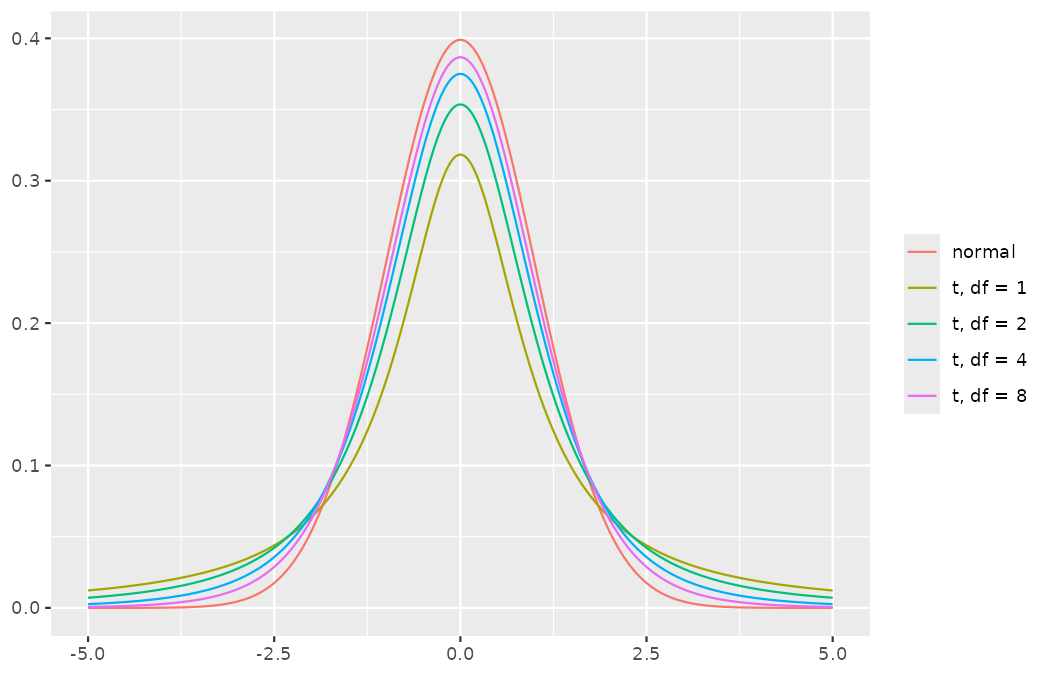
\includegraphics[width=0.85\linewidth,height=\textheight,keepaspectratio]{figures/inference-one-mean-5.png}

\begin{tcolorbox}[enhanced jigsaw, left=2mm, leftrule=.75mm, title=\textcolor{quarto-callout-important-color}{\faExclamation}\hspace{0.5em}{Degrees of freedom: df}, arc=.35mm, rightrule=.15mm, coltitle=black, colframe=quarto-callout-important-color-frame, bottomrule=.15mm, colbacktitle=quarto-callout-important-color!10!white, opacitybacktitle=0.6, breakable, bottomtitle=1mm, toptitle=1mm, titlerule=0mm, opacityback=0, toprule=.15mm, colback=white]

The degrees of freedom describes the shape of the \(t\)-distribution.
The larger the degrees of freedom, the more closely the distribution
approximates the normal distribution.

When modeling \(\bar{x}\) using the \(t\)-distribution, use
\(df = n - 1.\)

\end{tcolorbox}

The \(t\)-distribution allows us greater flexibility than the normal
distribution when analyzing numerical data. In practice, it's common to
use statistical software, such as R, Python, or SAS for these analyses.
In R, the function used for calculating probabilities under a
\(t\)-distribution is \texttt{pt()} (which should seem similar to the
previous R functions \texttt{pnorm()} and \texttt{pchisq()}). Don't
forget that with the \(t\)-distribution, the degrees of freedom must
always be specified!

For the worked examples and Check your understanding boxes below, you
may have to use a table or statistical software to find the answers. We
recommend trying the problems so as to get a sense for how the
\(t\)-distribution can vary in width depending on the degrees of
freedom. No matter the approach you choose, apply your method using the
examples below to confirm your working understanding of the
\(t\)-distribution.

\begin{tcolorbox}[enhanced jigsaw, left=2mm, leftrule=.75mm, title=\textcolor{quarto-callout-note-color}{\faInfo}\hspace{0.5em}{Worked example}, arc=.35mm, rightrule=.15mm, coltitle=black, colframe=quarto-callout-note-color-frame, bottomrule=.15mm, colbacktitle=quarto-callout-note-color!10!white, opacitybacktitle=0.6, breakable, bottomtitle=1mm, toptitle=1mm, titlerule=0mm, opacityback=0, toprule=.15mm, colback=white]

What proportion of the \(t\)-distribution with 18 degrees of freedom
falls below \(-2.10\)?

\begin{center}\rule{0.5\linewidth}{0.5pt}\end{center}

Draw the picture first: a bell centered at zero, with the area to the
left of \(-2.10\) shaded. Using statistical software, we can obtain a
precise value: 0.0250.

\begin{Shaded}
\begin{Highlighting}[]
\CommentTok{\# use pt() to find probability under the t{-}distribution}
\FunctionTok{pt}\NormalTok{(}\SpecialCharTok{{-}}\FloatTok{2.10}\NormalTok{, }\AttributeTok{df =} \DecValTok{18}\NormalTok{)}
\CommentTok{\#\textgreater{} [1] 0.0250452}
\end{Highlighting}
\end{Shaded}

\end{tcolorbox}

\begin{tcolorbox}[enhanced jigsaw, left=2mm, leftrule=.75mm, title=\textcolor{quarto-callout-note-color}{\faInfo}\hspace{0.5em}{Worked example}, arc=.35mm, rightrule=.15mm, coltitle=black, colframe=quarto-callout-note-color-frame, bottomrule=.15mm, colbacktitle=quarto-callout-note-color!10!white, opacitybacktitle=0.6, breakable, bottomtitle=1mm, toptitle=1mm, titlerule=0mm, opacityback=0, toprule=.15mm, colback=white]

What proportion of the \(t\)-distribution with 20 degrees of freedom
falls above 1.65?

\begin{center}\rule{0.5\linewidth}{0.5pt}\end{center}

Note that with 20 degrees of freedom, the \(t\)-distribution is
relatively close to the normal distribution. With a normal distribution,
this would correspond to about 0.05, so we should expect the
\(t\)-distribution to give us a similar value. Using statistical
software, we can obtain a precise value: 0.0573.

\begin{Shaded}
\begin{Highlighting}[]
\CommentTok{\# use pt() to find probability under the t{-}distribution}
\DecValTok{1} \SpecialCharTok{{-}} \FunctionTok{pt}\NormalTok{(}\FloatTok{1.65}\NormalTok{, }\AttributeTok{df =} \DecValTok{20}\NormalTok{)}
\CommentTok{\#\textgreater{} [1] 0.05728041}
\end{Highlighting}
\end{Shaded}

\end{tcolorbox}

\begin{tcolorbox}[enhanced jigsaw, left=2mm, leftrule=.75mm, title=\textcolor{quarto-callout-note-color}{\faInfo}\hspace{0.5em}{Worked example}, arc=.35mm, rightrule=.15mm, coltitle=black, colframe=quarto-callout-note-color-frame, bottomrule=.15mm, colbacktitle=quarto-callout-note-color!10!white, opacitybacktitle=0.6, breakable, bottomtitle=1mm, toptitle=1mm, titlerule=0mm, opacityback=0, toprule=.15mm, colback=white]

For a \(t\)-distribution with 2 degrees of freedom, estimate the
proportion of the distribution falling more than 3 units from the mean
(above or below).

\begin{center}\rule{0.5\linewidth}{0.5pt}\end{center}

With so few degrees of freedom, the \(t\)-distribution will give a more
notably different value than the normal distribution. Under a normal
distribution, the area would be about 0.003 using the 68-95-99.7 rule.
For a \(t\)-distribution with \(df = 2,\) the area in both tails beyond
3 units totals 0.0955. This area is dramatically different than what we
obtain from the normal distribution.

\begin{Shaded}
\begin{Highlighting}[]
\CommentTok{\# use pt() to find probability under the t{-}distribution}
\FunctionTok{pt}\NormalTok{(}\SpecialCharTok{{-}}\DecValTok{3}\NormalTok{, }\AttributeTok{df =} \DecValTok{2}\NormalTok{) }\SpecialCharTok{+}\NormalTok{ (}\DecValTok{1} \SpecialCharTok{{-}} \FunctionTok{pt}\NormalTok{(}\DecValTok{3}\NormalTok{, }\AttributeTok{df =} \DecValTok{2}\NormalTok{))}
\CommentTok{\#\textgreater{} [1] 0.09546597}
\end{Highlighting}
\end{Shaded}

\end{tcolorbox}

\begin{tcolorbox}[enhanced jigsaw, left=2mm, leftrule=.75mm, title=\textcolor{quarto-callout-tip-color}{\faLightbulb}\hspace{0.5em}{Check your understanding}, arc=.35mm, rightrule=.15mm, coltitle=black, colframe=quarto-callout-tip-color-frame, bottomrule=.15mm, colbacktitle=quarto-callout-tip-color!10!white, opacitybacktitle=0.6, breakable, bottomtitle=1mm, toptitle=1mm, titlerule=0mm, opacityback=0, toprule=.15mm, colback=white]

What proportion of the \(t\)-distribution with 19 degrees of freedom
falls above \(-1.79\) units? Use your preferred method for finding tail
areas.

\begin{center}\rule{0.5\linewidth}{0.5pt}\end{center}

We want to find the shaded area \emph{above} \(-1.79\) (we leave the
picture to you). The lower tail area is 0.0447, so the upper area is
\(1 - 0.0447 = 0.9553.\)

\end{tcolorbox}

\subsection{One sample t-intervals}\label{one-sample-t-intervals}

Let's get our first taste of applying the \(t\)-distribution in the
context of a squad-level scouting question. Australia reached the round
of 16 at the 2022 Men's World Cup, and Emil Sørensen's network flagged
several of their attacking players as potentially undervalued targets.
Marta Vidal's question back was blunt: was that run built on genuine
chance creation, or is the chance quality behind it worryingly low?

We will identify a confidence interval for the mean chance quality of
the shots produced by Australia's campaign --- all 26 of them. First,
the frame check that this book's penalty convention makes routine: none
of Australia's 26 shots was a penalty or a direct free kick, so the
all-shots frame and the open-play frame coincide, and no stored 0.7835
lurks in the sample.

\begin{Shaded}
\begin{Highlighting}[]
\NormalTok{australia\_shots }\OtherTok{\textless{}{-}}\NormalTok{ wc2022\_shots }\SpecialCharTok{|\textgreater{}}
  \FunctionTok{filter}\NormalTok{(team }\SpecialCharTok{==} \StringTok{"Australia"}\NormalTok{)}

\NormalTok{australia\_shots }\SpecialCharTok{|\textgreater{}}
  \FunctionTok{count}\NormalTok{(shot\_type)}
\CommentTok{\#\textgreater{} \# A tibble: 1 × 2}
\CommentTok{\#\textgreater{}   shot\_type     n}
\CommentTok{\#\textgreater{}   \textless{}chr\textgreater{}     \textless{}int\textgreater{}}
\CommentTok{\#\textgreater{} 1 Open Play    26}
\end{Highlighting}
\end{Shaded}

The data are summarized below; the minimum and maximum observed values
can be used to evaluate whether there are clear outliers.

\begin{Shaded}
\begin{Highlighting}[]
\FunctionTok{round}\NormalTok{(}\FunctionTok{c}\NormalTok{(}\AttributeTok{xbar =} \FunctionTok{mean}\NormalTok{(australia\_shots}\SpecialCharTok{$}\NormalTok{statsbomb\_xg),}
        \AttributeTok{s    =} \FunctionTok{sd}\NormalTok{(australia\_shots}\SpecialCharTok{$}\NormalTok{statsbomb\_xg),}
        \AttributeTok{min  =} \FunctionTok{min}\NormalTok{(australia\_shots}\SpecialCharTok{$}\NormalTok{statsbomb\_xg),}
        \AttributeTok{max  =} \FunctionTok{max}\NormalTok{(australia\_shots}\SpecialCharTok{$}\NormalTok{statsbomb\_xg)), }\DecValTok{4}\NormalTok{)}
\CommentTok{\#\textgreater{}   xbar      s    min    max}
\CommentTok{\#\textgreater{} 0.0607 0.0578 0.0053 0.2339}
\end{Highlighting}
\end{Shaded}

\begin{longtable}[]{@{}ccccc@{}}
\caption{Summary of the chance quality (xG) of Australia's 26 shots at
the 2022 Men's World Cup.}\label{tbl-aus-summary}\tabularnewline
\toprule\noalign{}
n & Mean & SD & Min & Max \\
\midrule\noalign{}
\endfirsthead
\toprule\noalign{}
n & Mean & SD & Min & Max \\
\midrule\noalign{}
\endhead
\bottomrule\noalign{}
\endlastfoot
26 & 0.0607 & 0.0578 & 0.0053 & 0.2339 \\
\end{longtable}

\begin{tcolorbox}[enhanced jigsaw, left=2mm, leftrule=.75mm, title=\textcolor{quarto-callout-note-color}{\faInfo}\hspace{0.5em}{Worked example}, arc=.35mm, rightrule=.15mm, coltitle=black, colframe=quarto-callout-note-color-frame, bottomrule=.15mm, colbacktitle=quarto-callout-note-color!10!white, opacitybacktitle=0.6, breakable, bottomtitle=1mm, toptitle=1mm, titlerule=0mm, opacityback=0, toprule=.15mm, colback=white]

Are the independence and normality conditions satisfied for this
dataset?

\begin{center}\rule{0.5\linewidth}{0.5pt}\end{center}

The 26 shots are not a formal random sample --- they are every shot of
one campaign --- so, as with England's 63 shots in
Section~\ref{sec-case-study-med-consult}, the inference is to the
\emph{process} that generates this team's chances, and we treat the
campaign as a sample from that process. Shots arrive in different
matches against different opponents, and treating them as independent
draws is a reasonable working approximation, though shots from the same
passage of play (rebounds, scrambles) push gently against it.

For normality, the sample size is under 30, so we check for clear
outliers. The summary statistics show the usual right skew of chance
quality, and the sorted values below show the top of the sample stepping
up gradually --- 0.114, 0.173, 0.191, 0.234 --- with no single
observation sitting isolated from the rest. (The maximum is 3.0 standard
deviations above the mean, which earns a raised eyebrow but not the
label ``clear outlier'' --- it takes practice, and the rule of thumb
tolerates moderate skew near \(n = 30.\)) Based on this evidence, the
normality condition seems reasonable.

\begin{Shaded}
\begin{Highlighting}[]
\FunctionTok{sort}\NormalTok{(}\FunctionTok{round}\NormalTok{(australia\_shots}\SpecialCharTok{$}\NormalTok{statsbomb\_xg, }\DecValTok{3}\NormalTok{))}
\CommentTok{\#\textgreater{}  [1] 0.005 0.010 0.011 0.014 0.015 0.018 0.030 0.033 0.035 0.035 0.037 0.039}
\CommentTok{\#\textgreater{} [13] 0.039 0.039 0.041 0.045 0.050 0.064 0.068 0.075 0.077 0.084 0.114 0.173}
\CommentTok{\#\textgreater{} [25] 0.191 0.234}
\end{Highlighting}
\end{Shaded}

\end{tcolorbox}

In the normal model of Chapter~\ref{sec-foundations-mathematical}, we
used \(z^{\star}\) and the standard error to determine the width of a
confidence interval. We revise the confidence interval formula slightly
when using the \(t\)-distribution:

\[
\begin{aligned}
\text{point estimate} \ &\pm\  t^{\star}_{df} \times SE \\
\bar{x} \ &\pm\  t^{\star}_{df} \times \frac{s}{\sqrt{n}}
\end{aligned}
\]

\begin{tcolorbox}[enhanced jigsaw, left=2mm, leftrule=.75mm, title=\textcolor{quarto-callout-note-color}{\faInfo}\hspace{0.5em}{Worked example}, arc=.35mm, rightrule=.15mm, coltitle=black, colframe=quarto-callout-note-color-frame, bottomrule=.15mm, colbacktitle=quarto-callout-note-color!10!white, opacitybacktitle=0.6, breakable, bottomtitle=1mm, toptitle=1mm, titlerule=0mm, opacityback=0, toprule=.15mm, colback=white]

Using the summary statistics in Table~\ref{tbl-aus-summary}, compute the
standard error for the mean chance quality of the \(n = 26\) shots.

\begin{center}\rule{0.5\linewidth}{0.5pt}\end{center}

We plug \(s\) and \(n\) into the formula:
\(SE = \frac{s}{\sqrt{n}} = \frac{0.0578}{\sqrt{26}} = 0.0113.\)

\end{tcolorbox}

The value \(t^{\star}_{df}\) is a cutoff we obtain based on the
confidence level and the \(t\)-distribution with \(df\) degrees of
freedom. The symbol has three parts, each already familiar on its own:
the letter \(t\) names the reference distribution; the star superscript
marks a critical cutoff, exactly the role \(z^{\star}\) played in
Chapter~\ref{sec-foundations-mathematical}; and the subscript \(df\)
records \emph{which} \(t\)-distribution supplied the cutoff --- a piece
of bookkeeping \(z^{\star}\) never needed, because there is only one
standard normal but a different \(t\)-distribution for every degrees of
freedom. That cutoff is found in the same way as with a normal
distribution: we find \(t^{\star}_{df}\) such that the fraction of the
\(t\)-distribution with \(df\) degrees of freedom within a distance
\(t^{\star}_{df}\) of 0 matches the confidence level of interest.

\begin{tcolorbox}[enhanced jigsaw, left=2mm, leftrule=.75mm, title=\textcolor{quarto-callout-note-color}{\faInfo}\hspace{0.5em}{Worked example}, arc=.35mm, rightrule=.15mm, coltitle=black, colframe=quarto-callout-note-color-frame, bottomrule=.15mm, colbacktitle=quarto-callout-note-color!10!white, opacitybacktitle=0.6, breakable, bottomtitle=1mm, toptitle=1mm, titlerule=0mm, opacityback=0, toprule=.15mm, colback=white]

When \(n = 26,\) what is the appropriate degrees of freedom? Find
\(t^{\star}_{df}\) for this degrees of freedom and the confidence level
of 95\%.

\begin{center}\rule{0.5\linewidth}{0.5pt}\end{center}

The degrees of freedom is easy to calculate: \(df = n - 1 = 25.\)

Using statistical software, we find the cutoff where the upper tail is
equal to 2.5\%: \(t^{\star}_{25} = 2.06.\) The area below \(-2.06\) will
also be equal to 2.5\%. That is, 95\% of the \(t\)-distribution with
\(df = 25\) lies within 2.06 units of 0.

\begin{Shaded}
\begin{Highlighting}[]
\CommentTok{\# use qt() to find the t{-}cutoff (with 95\% in the middle)}
\FunctionTok{qt}\NormalTok{(}\FloatTok{0.025}\NormalTok{, }\AttributeTok{df =} \DecValTok{25}\NormalTok{)}
\CommentTok{\#\textgreater{} [1] {-}2.059539}
\FunctionTok{qt}\NormalTok{(}\FloatTok{0.975}\NormalTok{, }\AttributeTok{df =} \DecValTok{25}\NormalTok{)}
\CommentTok{\#\textgreater{} [1] 2.059539}
\end{Highlighting}
\end{Shaded}

\end{tcolorbox}

\begin{tcolorbox}[enhanced jigsaw, left=2mm, leftrule=.75mm, title=\textcolor{quarto-callout-important-color}{\faExclamation}\hspace{0.5em}{Degrees of freedom for a single sample}, arc=.35mm, rightrule=.15mm, coltitle=black, colframe=quarto-callout-important-color-frame, bottomrule=.15mm, colbacktitle=quarto-callout-important-color!10!white, opacitybacktitle=0.6, breakable, bottomtitle=1mm, toptitle=1mm, titlerule=0mm, opacityback=0, toprule=.15mm, colback=white]

If the sample has \(n\) observations and we are examining a single mean,
then we use the \(t\)-distribution with \(df = n - 1\) degrees of
freedom.

\end{tcolorbox}

\begin{tcolorbox}[enhanced jigsaw, left=2mm, leftrule=.75mm, title=\textcolor{quarto-callout-note-color}{\faInfo}\hspace{0.5em}{Worked example}, arc=.35mm, rightrule=.15mm, coltitle=black, colframe=quarto-callout-note-color-frame, bottomrule=.15mm, colbacktitle=quarto-callout-note-color!10!white, opacitybacktitle=0.6, breakable, bottomtitle=1mm, toptitle=1mm, titlerule=0mm, opacityback=0, toprule=.15mm, colback=white]

Compute and interpret the 95\% confidence interval for the mean chance
quality of the process behind Australia's shooting. Is Marta's
``worryingly low'' worry justified?

\begin{center}\rule{0.5\linewidth}{0.5pt}\end{center}

We can construct the confidence interval as

\[
\begin{aligned}
\bar{x} \ &\pm\  t^{\star}_{25} \times SE \\
0.0607 \ &\pm\  2.06 \times 0.0113 \\
(0.0374 \  &, \ 0.0840)
\end{aligned}
\]

We are 95\% confident that the true mean chance quality of the shots
this Australia side generates is between 0.037 and 0.084 xG per shot.
For scale, the tournament's 1,382 open-play shots averaged 0.0983 xG per
shot (a benchmark we recompute in code at the end of this chapter) ---
and note that the open-play benchmark is the frame-consistent one, since
Australia's sample contains no penalties. The \emph{entire interval}
sits below that benchmark: even the most generous end of the plausible
range is a sub-average shot diet. So yes --- the run to the knockouts
was real, but the chance quality underneath it is discernibly thin, and
any valuation of Australia's attackers should start from that fact. Two
cautions before this reaches a dossier: the data are observational (a
deep defensive block \emph{chooses} low-volume, often low-quality
shooting, so this describes the team's output, not any player's
ceiling), and 26 shots is a small sample --- which is exactly why we
report the interval and not just the 0.0607.

\end{tcolorbox}

\begin{tcolorbox}[enhanced jigsaw, left=2mm, leftrule=.75mm, title=\textcolor{quarto-callout-important-color}{\faExclamation}\hspace{0.5em}{Calculating a t-confidence interval for the mean, \(\mu\)}, arc=.35mm, rightrule=.15mm, coltitle=black, colframe=quarto-callout-important-color-frame, bottomrule=.15mm, colbacktitle=quarto-callout-important-color!10!white, opacitybacktitle=0.6, breakable, bottomtitle=1mm, toptitle=1mm, titlerule=0mm, opacityback=0, toprule=.15mm, colback=white]

Based on a sample of \(n\) independent and nearly normal observations, a
confidence interval for the population mean is

\[
\begin{aligned}
\text{point estimate} \ &\pm\  t^{\star}_{df} \times SE \\
\bar{x} \ &\pm\  t^{\star}_{df} \times \frac{s}{\sqrt{n}}
\end{aligned}
\]

where \(\bar{x}\) is the sample mean, \(t^{\star}_{df}\) corresponds to
the confidence level and degrees of freedom \(df,\) and \(SE\) is the
standard error as estimated by the sample.

\end{tcolorbox}

For the next sequence, practice working entirely from summary statistics
--- the situation an analyst is in when a partner club or an agent
shares a memo rather than raw data. The memo in question concerns
one-on-one situations at the 2025 Women's Euro: across the tournament,
\(n = 29\) shots were logged as one-on-ones, with a sample mean chance
quality of 0.356 xG, a standard deviation of 0.300, a minimum of 0.029,
and a maximum of 0.784.

\begin{tcolorbox}[enhanced jigsaw, left=2mm, leftrule=.75mm, title=\textcolor{quarto-callout-tip-color}{\faLightbulb}\hspace{0.5em}{Check your understanding}, arc=.35mm, rightrule=.15mm, coltitle=black, colframe=quarto-callout-tip-color-frame, bottomrule=.15mm, colbacktitle=quarto-callout-tip-color!10!white, opacitybacktitle=0.6, breakable, bottomtitle=1mm, toptitle=1mm, titlerule=0mm, opacityback=0, toprule=.15mm, colback=white]

We will assume the 29 one-on-one chance qualities are independent
observations from the process that generates such situations at this
level. Based on the summary statistics alone, do you have any objections
to the normality condition of the individual observations?

\begin{center}\rule{0.5\linewidth}{0.5pt}\end{center}

The sample size is under 30, so we check for obvious outliers using what
the memo gives us: since both the minimum \((0.029\) is \(1.09\)
standard deviations below the mean\()\) and the maximum \((0.784\) is
\(1.43\) standard deviations above\()\) are well within 2 standard
deviations of the mean, there are no such clear outliers.

\end{tcolorbox}

\begin{tcolorbox}[enhanced jigsaw, left=2mm, leftrule=.75mm, title=\textcolor{quarto-callout-note-color}{\faInfo}\hspace{0.5em}{Worked example}, arc=.35mm, rightrule=.15mm, coltitle=black, colframe=quarto-callout-note-color-frame, bottomrule=.15mm, colbacktitle=quarto-callout-note-color!10!white, opacitybacktitle=0.6, breakable, bottomtitle=1mm, toptitle=1mm, titlerule=0mm, opacityback=0, toprule=.15mm, colback=white]

Estimate the standard error of \(\bar{x} = 0.356\) using the data
summaries. If we are to use the \(t\)-distribution to create a 90\%
confidence interval for the true mean chance quality of a one-on-one,
identify the degrees of freedom and \(t^{\star}_{df}.\)

\begin{center}\rule{0.5\linewidth}{0.5pt}\end{center}

The standard error: \(SE = \frac{0.300}{\sqrt{29}} = 0.0557.\) Degrees
of freedom: \(df = n - 1 = 28.\) Since the goal is a 90\% confidence
interval, we choose \(t^{\star}_{28}\) so that the two-tail area is 0.1:
\(t^{\star}_{28} = 1.70.\)

\begin{Shaded}
\begin{Highlighting}[]
\CommentTok{\# use qt() to find the t{-}cutoff (with 90\% in the middle)}
\FunctionTok{qt}\NormalTok{(}\FloatTok{0.05}\NormalTok{, }\AttributeTok{df =} \DecValTok{28}\NormalTok{)}
\CommentTok{\#\textgreater{} [1] {-}1.701131}
\FunctionTok{qt}\NormalTok{(}\FloatTok{0.95}\NormalTok{, }\AttributeTok{df =} \DecValTok{28}\NormalTok{)}
\CommentTok{\#\textgreater{} [1] 1.701131}
\end{Highlighting}
\end{Shaded}

\end{tcolorbox}

\begin{tcolorbox}[enhanced jigsaw, left=2mm, leftrule=.75mm, title=\textcolor{quarto-callout-tip-color}{\faLightbulb}\hspace{0.5em}{Check your understanding}, arc=.35mm, rightrule=.15mm, coltitle=black, colframe=quarto-callout-tip-color-frame, bottomrule=.15mm, colbacktitle=quarto-callout-tip-color!10!white, opacitybacktitle=0.6, breakable, bottomtitle=1mm, toptitle=1mm, titlerule=0mm, opacityback=0, toprule=.15mm, colback=white]

Using the information and results of the previous Check your
understanding and Worked example, compute a 90\% confidence interval for
the true mean chance quality of a one-on-one at this level.

\begin{center}\rule{0.5\linewidth}{0.5pt}\end{center}

\(\bar{x} \ \pm\ t^{\star}_{28} \times SE \ \to\ 0.356 \ \pm\ 1.70 \times 0.0557 \ \to\ (0.261, 0.451).\)
We are 90\% confident that the true mean chance quality of a one-on-one
is between 0.261 and 0.451 xG.

\end{tcolorbox}

\begin{tcolorbox}[enhanced jigsaw, left=2mm, leftrule=.75mm, title=\textcolor{quarto-callout-tip-color}{\faLightbulb}\hspace{0.5em}{Check your understanding}, arc=.35mm, rightrule=.15mm, coltitle=black, colframe=quarto-callout-tip-color-frame, bottomrule=.15mm, colbacktitle=quarto-callout-tip-color!10!white, opacitybacktitle=0.6, breakable, bottomtitle=1mm, toptitle=1mm, titlerule=0mm, opacityback=0, toprule=.15mm, colback=white]

The 90\% confidence interval just computed is 0.261 to 0.451 xG. Can we
say that 90\% of one-on-one situations have a chance quality between
0.261 and 0.451 xG?

\begin{center}\rule{0.5\linewidth}{0.5pt}\end{center}

No. A confidence interval provides a range of plausible values for a
population parameter --- here, the population \emph{mean}. It does not
describe what we might observe for individual observations; indeed, the
memo's own minimum and maximum (0.029 and 0.784) fall outside the
interval.

\end{tcolorbox}

One more discipline before the memo's headline number travels anywhere
--- the penalty convention again, and this time it catches something the
summary statistics \emph{cannot show}. Pulling the raw rows:

\begin{Shaded}
\begin{Highlighting}[]
\NormalTok{weuro2025\_shots }\OtherTok{\textless{}{-}} \FunctionTok{read\_csv}\NormalTok{(}\StringTok{"data/derived/weuro2025\_shots.csv"}\NormalTok{)}

\NormalTok{weuro2025\_shots }\SpecialCharTok{|\textgreater{}}
  \FunctionTok{filter}\NormalTok{(one\_on\_one) }\SpecialCharTok{|\textgreater{}}
  \FunctionTok{count}\NormalTok{(shot\_type)}
\CommentTok{\#\textgreater{} \# A tibble: 2 × 2}
\CommentTok{\#\textgreater{}   shot\_type     n}
\CommentTok{\#\textgreater{}   \textless{}chr\textgreater{}     \textless{}int\textgreater{}}
\CommentTok{\#\textgreater{} 1 Open Play    21}
\CommentTok{\#\textgreater{} 2 Penalty       8}

\NormalTok{weuro2025\_shots }\SpecialCharTok{|\textgreater{}}
  \FunctionTok{filter}\NormalTok{(one\_on\_one, shot\_type }\SpecialCharTok{==} \StringTok{"Open Play"}\NormalTok{) }\SpecialCharTok{|\textgreater{}}
  \FunctionTok{summarize}\NormalTok{(}\AttributeTok{n =} \FunctionTok{n}\NormalTok{(), }\AttributeTok{xbar =} \FunctionTok{round}\NormalTok{(}\FunctionTok{mean}\NormalTok{(statsbomb\_xg), }\DecValTok{4}\NormalTok{))}
\CommentTok{\#\textgreater{} \# A tibble: 1 × 2}
\CommentTok{\#\textgreater{}       n  xbar}
\CommentTok{\#\textgreater{}   \textless{}int\textgreater{} \textless{}dbl\textgreater{}}
\CommentTok{\#\textgreater{} 1    21 0.193}
\end{Highlighting}
\end{Shaded}

Eight of the 29 ``one-on-ones'' are penalty kicks, each at the stored
0.7835 --- a penalty is, by law, literally one attacker against one
goalkeeper, so the tag is honest, but it is a very different kind of
one-on-one from a striker running through on goal. The min/max outlier
check we ran from the memo could never have revealed this: the penalties
sit \emph{inside} the observed range, an eight-shot spike hiding in
plain sight, and they drag the blended mean from 0.193 (the 21 open-play
one-on-ones) up to 0.356. Neither number is wrong; they answer different
questions. The interval we built describes the mean of \emph{all
situations logged one-on-one, penalties included}; a scout valuing a
forward's composure when clean through should recompute everything above
on the open-play frame --- and, per the convention, say so.

Recall from Chapter~\ref{sec-foundations-mathematical} that the margin
of error is defined by the standard error. The margin of error for
\(\bar{x}\) can be directly obtained from \(SE(\bar{x}).\)

\begin{tcolorbox}[enhanced jigsaw, left=2mm, leftrule=.75mm, title=\textcolor{quarto-callout-important-color}{\faExclamation}\hspace{0.5em}{Margin of error for \(\bar{x}\)}, arc=.35mm, rightrule=.15mm, coltitle=black, colframe=quarto-callout-important-color-frame, bottomrule=.15mm, colbacktitle=quarto-callout-important-color!10!white, opacitybacktitle=0.6, breakable, bottomtitle=1mm, toptitle=1mm, titlerule=0mm, opacityback=0, toprule=.15mm, colback=white]

The margin of error is \(t^\star_{df} \times s/\sqrt{n}\) where
\(t^\star_{df}\) is calculated from a specified percentile on the
\(t\)-distribution with \(df\) degrees of freedom.

\end{tcolorbox}

\subsection{One sample t-tests}\label{one-sample-t-tests}

Now that we have used the \(t\)-distribution for making a confidence
interval for a mean, let's speed on through to hypothesis tests for the
mean.

\begin{tcolorbox}[enhanced jigsaw, left=2mm, leftrule=.75mm, title=\textcolor{quarto-callout-important-color}{\faExclamation}\hspace{0.5em}{The test statistic for assessing a single mean is a T}, arc=.35mm, rightrule=.15mm, coltitle=black, colframe=quarto-callout-important-color-frame, bottomrule=.15mm, colbacktitle=quarto-callout-important-color!10!white, opacitybacktitle=0.6, breakable, bottomtitle=1mm, toptitle=1mm, titlerule=0mm, opacityback=0, toprule=.15mm, colback=white]

The T score is a ratio of how the sample mean differs from the
hypothesized mean as compared to how the observations vary.

\[T = \frac{\bar{x} - \text{null value}}{s/\sqrt{n}}\]

When the null hypothesis is true and the conditions are met, T has a
\(t\)-distribution with \(df = n - 1.\)

Conditions:

\begin{itemize}
\tightlist
\item
  Independent observations.
\item
  Large samples and no extreme outliers.
\end{itemize}

\end{tcolorbox}

The symbol is new, so name its parts before using it: the capital \(T\)
is a test statistic --- the same job the \(Z\) score performed in
Chapter~\ref{sec-foundations-mathematical} and
Chapter~\ref{sec-inference-one-prop} --- counting how many standard
errors the observed sample mean sits from the null value; we write \(T\)
rather than \(Z\) purely to remind ourselves that its tail areas must be
looked up on a \(t\)-distribution, with the degrees of freedom stated.

Here is the question we will put to it. On the wall of Northbridge's
analysis room is a benchmark every analyst knows by heart: the mean
chance quality across all 1,494 shots of the 2022 Men's World Cup.

\begin{Shaded}
\begin{Highlighting}[]
\FunctionTok{round}\NormalTok{(}\FunctionTok{mean}\NormalTok{(wc2022\_shots}\SpecialCharTok{$}\NormalTok{statsbomb\_xg), }\DecValTok{4}\NormalTok{)}
\CommentTok{\#\textgreater{} [1] 0.1259}
\end{Highlighting}
\end{Shaded}

Since Chapter~\ref{sec-explore-categorical}, this book has kept
returning to shots taken under defensive pressure. Chapter
\ref{sec-foundations-randomization} asked whether pressured shots are
\emph{finished} worse; the question for this section is different: are
pressured shots worse \emph{chances}? We take the 325 shots logged under
pressure at the 2025 Women's Euro --- a fresh tournament, per this
book's replication habit --- and test their mean chance quality against
the benchmark of 0.1259.

\begin{tcolorbox}[enhanced jigsaw, left=2mm, leftrule=.75mm, title=\textcolor{quarto-callout-note-color}{\faInfo}\hspace{0.5em}{Data}, arc=.35mm, rightrule=.15mm, coltitle=black, colframe=quarto-callout-note-color-frame, bottomrule=.15mm, colbacktitle=quarto-callout-note-color!10!white, opacitybacktitle=0.6, breakable, bottomtitle=1mm, toptitle=1mm, titlerule=0mm, opacityback=0, toprule=.15mm, colback=white]

The 2025 Women's Euro shots are read from
\texttt{data/derived/weuro2025\_shots.csv}; the sample analyzed here
comprises the rows with \texttt{under\_pressure\ ==\ TRUE} (StatsBomb
open data).

\end{tcolorbox}

\begin{tcolorbox}[enhanced jigsaw, left=2mm, leftrule=.75mm, title=\textcolor{quarto-callout-tip-color}{\faLightbulb}\hspace{0.5em}{Check your understanding}, arc=.35mm, rightrule=.15mm, coltitle=black, colframe=quarto-callout-tip-color-frame, bottomrule=.15mm, colbacktitle=quarto-callout-tip-color!10!white, opacitybacktitle=0.6, breakable, bottomtitle=1mm, toptitle=1mm, titlerule=0mm, opacityback=0, toprule=.15mm, colback=white]

What are appropriate hypotheses for this context?

\begin{center}\rule{0.5\linewidth}{0.5pt}\end{center}

\(H_0:\) The mean chance quality of shots taken under pressure matches
the benchmark. \(\mu = 0.1259\) xG. \(H_A:\) The mean chance quality of
shots taken under pressure is \emph{different} from the benchmark.
\(\mu \neq 0.1259\) xG. Here \(\mu\) denotes the true mean chance
quality of the process generating under-pressure shots at this level.

\end{tcolorbox}

When completing a hypothesis test for the one-sample mean, the process
is nearly identical to completing a hypothesis test for a single
proportion. First, we find the Z score using the observed value, null
value, and standard error; however, we call it a \textbf{T score} since
we use a \(t\)-distribution for calculating the tail area. Then we find
the p-value using the same ideas we used previously: find the one-tail
area under the sampling distribution, and double it.

But first, we check the conditions.

\begin{tcolorbox}[enhanced jigsaw, left=2mm, leftrule=.75mm, title=\textcolor{quarto-callout-tip-color}{\faLightbulb}\hspace{0.5em}{Check your understanding}, arc=.35mm, rightrule=.15mm, coltitle=black, colframe=quarto-callout-tip-color-frame, bottomrule=.15mm, colbacktitle=quarto-callout-tip-color!10!white, opacitybacktitle=0.6, breakable, bottomtitle=1mm, toptitle=1mm, titlerule=0mm, opacityback=0, toprule=.15mm, colback=white]

The 325 pressured shots come from 31 matches across a whole tournament,
and no analyst selected them --- every logged under-pressure shot is
included; we treat them as independent draws from the process that
generates pressured shots at this level (an observational frame: nobody
randomly assigned pressure, a caveat
Section~\ref{sec-chp11-observational} has already taught you). A
histogram of the 325 chance qualities is drawn by the code below to
evaluate whether we can move forward with a \textbf{t-test}. Is the
normality condition met?

\begin{Shaded}
\begin{Highlighting}[]
\NormalTok{pressured\_shots }\OtherTok{\textless{}{-}}\NormalTok{ weuro2025\_shots }\SpecialCharTok{|\textgreater{}}
  \FunctionTok{filter}\NormalTok{(under\_pressure)}

\FunctionTok{ggplot}\NormalTok{(pressured\_shots, }\FunctionTok{aes}\NormalTok{(}\AttributeTok{x =}\NormalTok{ statsbomb\_xg)) }\SpecialCharTok{+}
  \FunctionTok{geom\_histogram}\NormalTok{(}\AttributeTok{binwidth =} \FloatTok{0.05}\NormalTok{) }\SpecialCharTok{+}
  \FunctionTok{labs}\NormalTok{(}\AttributeTok{x =} \StringTok{"Chance quality (xG)"}\NormalTok{, }\AttributeTok{y =} \StringTok{"Count"}\NormalTok{)}
\end{Highlighting}
\end{Shaded}

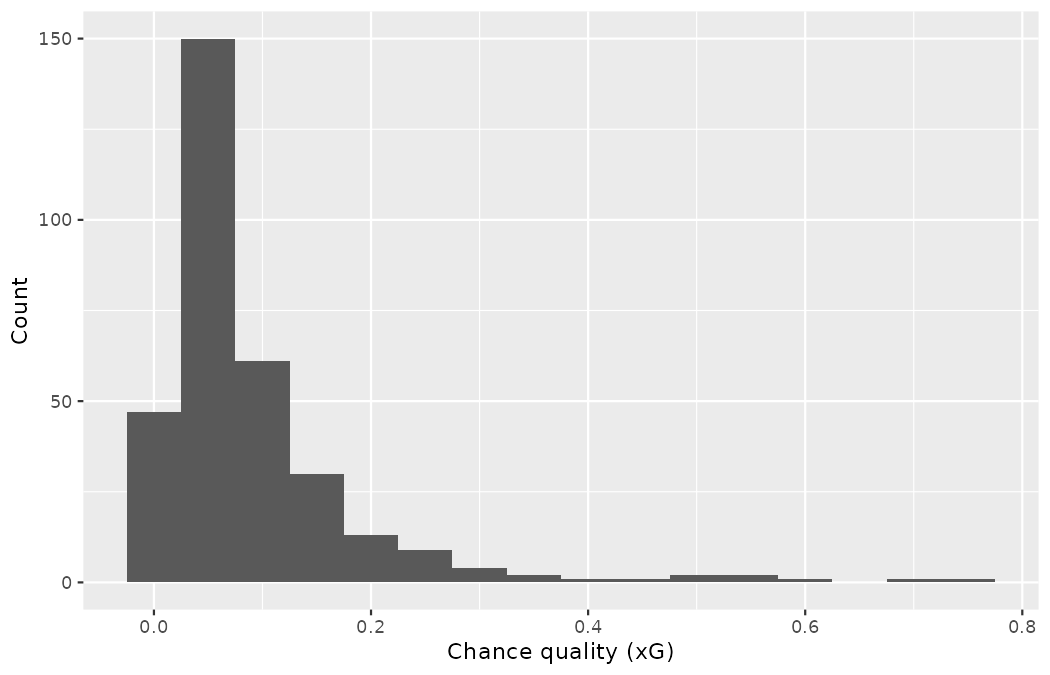
\includegraphics[width=0.85\linewidth,height=\textheight,keepaspectratio]{figures/inference-one-mean-6.png}

\begin{center}\rule{0.5\linewidth}{0.5pt}\end{center}

With a sample of 325, we should only be concerned if there are
particularly extreme outliers. The histogram shows the strong right skew
chance quality always has --- about three quarters of the pressured
shots sit below 0.10 xG --- but strong skew is acceptable at this sample
size (recall the guideline: strong skew is okay for \(n\) of 60 or
more). The largest value, 0.725, is closely attended by the next at
0.705, so no single observation sits alone in the tail: no outliers of
concern.

\end{tcolorbox}

\begin{tcolorbox}[enhanced jigsaw, left=2mm, leftrule=.75mm, title=\textcolor{quarto-callout-note-color}{\faInfo}\hspace{0.5em}{Worked example}, arc=.35mm, rightrule=.15mm, coltitle=black, colframe=quarto-callout-note-color-frame, bottomrule=.15mm, colbacktitle=quarto-callout-note-color!10!white, opacitybacktitle=0.6, breakable, bottomtitle=1mm, toptitle=1mm, titlerule=0mm, opacityback=0, toprule=.15mm, colback=white]

With both the independence and normality conditions satisfied, we can
proceed with a hypothesis test using the \(t\)-distribution. The sample
mean and sample standard deviation of the 325 pressured shots are
computed below.

\begin{Shaded}
\begin{Highlighting}[]
\FunctionTok{round}\NormalTok{(}\FunctionTok{c}\NormalTok{(}\AttributeTok{xbar =} \FunctionTok{mean}\NormalTok{(pressured\_shots}\SpecialCharTok{$}\NormalTok{statsbomb\_xg),}
        \AttributeTok{s    =} \FunctionTok{sd}\NormalTok{(pressured\_shots}\SpecialCharTok{$}\NormalTok{statsbomb\_xg)), }\DecValTok{4}\NormalTok{)}
\CommentTok{\#\textgreater{}   xbar      s}
\CommentTok{\#\textgreater{} 0.0914 0.1018}
\end{Highlighting}
\end{Shaded}

Recall that the benchmark is 0.1259 xG. Find the test statistic and
p-value. What is your conclusion?

\begin{center}\rule{0.5\linewidth}{0.5pt}\end{center}

To find the test statistic (T score), we first must determine the
standard error:

\[SE = 0.1018 / \sqrt{325} = 0.00565\]

Now we can compute the \textbf{T score} using the sample mean (0.0914),
null value (0.1259), and \(SE:\)

\[T = \frac{0.0914 - 0.1259}{0.00565} = -6.11\]

For \(df = 325 - 1 = 324,\) we can determine using statistical software
that the one-tail area is about 0.0000000014, which we double to get the
p-value: about 0.0000000029.

\begin{Shaded}
\begin{Highlighting}[]
\CommentTok{\# use pt() to find the left tail and multiply by 2 to get both tails}
\FunctionTok{pt}\NormalTok{(}\SpecialCharTok{{-}}\FloatTok{6.11}\NormalTok{, }\AttributeTok{df =} \DecValTok{324}\NormalTok{) }\SpecialCharTok{*} \DecValTok{2}
\CommentTok{\#\textgreater{} [1] 2.856235e{-}09}
\end{Highlighting}
\end{Shaded}

Because the p-value is (vastly) smaller than 0.05, we reject the null
hypothesis: taken at face value, the data provide convincing evidence
that pressured shots at the 2025 Women's Euro are discernibly worse
chances than the benchmark. But do not let a six-standard-error headline
ship before the book's penalty convention has asked its question:
\emph{which shots are in each frame?}

\end{tcolorbox}

Here the convention earns its keep, because the two frames in that test
do not match. The benchmark of 0.1259 averages over \emph{all} 1,494
World Cup shots --- including its 64 penalty kicks, each stored at
0.7835, the one shot in football on which defensive pressure is
impossible by law. The pressured sample, meanwhile, \emph{cannot}
contain a penalty --- the frame check comes back all open play:

\begin{Shaded}
\begin{Highlighting}[]
\NormalTok{pressured\_shots }\SpecialCharTok{|\textgreater{}}
  \FunctionTok{count}\NormalTok{(shot\_type)}
\CommentTok{\#\textgreater{} \# A tibble: 1 × 2}
\CommentTok{\#\textgreater{}   shot\_type     n}
\CommentTok{\#\textgreater{}   \textless{}chr\textgreater{}     \textless{}int\textgreater{}}
\CommentTok{\#\textgreater{} 1 Open Play   325}
\end{Highlighting}
\end{Shaded}

We are comparing a penalty-free sample with a benchmark propped up by
uncontested kicks from twelve yards, so we restate the benchmark on the
frame the question actually concerns --- open play --- and rerun the
identical arithmetic:

\begin{Shaded}
\begin{Highlighting}[]
\NormalTok{wc2022\_shots }\SpecialCharTok{|\textgreater{}}
  \FunctionTok{filter}\NormalTok{(shot\_type }\SpecialCharTok{==} \StringTok{"Open Play"}\NormalTok{) }\SpecialCharTok{|\textgreater{}}
  \FunctionTok{summarize}\NormalTok{(}\AttributeTok{shots =} \FunctionTok{n}\NormalTok{(), }\AttributeTok{mean\_xg =} \FunctionTok{round}\NormalTok{(}\FunctionTok{mean}\NormalTok{(statsbomb\_xg), }\DecValTok{4}\NormalTok{))}
\CommentTok{\#\textgreater{} \# A tibble: 1 × 2}
\CommentTok{\#\textgreater{}   shots mean\_xg}
\CommentTok{\#\textgreater{}   \textless{}int\textgreater{}   \textless{}dbl\textgreater{}}
\CommentTok{\#\textgreater{} 1  1382  0.0983}

\CommentTok{\# same T score arithmetic against the open{-}play benchmark}
\CommentTok{\# T = (0.0914 {-} 0.0983) / 0.00565 = {-}1.22}
\FunctionTok{pt}\NormalTok{(}\SpecialCharTok{{-}}\FloatTok{1.22}\NormalTok{, }\AttributeTok{df =} \DecValTok{324}\NormalTok{) }\SpecialCharTok{*} \DecValTok{2}
\CommentTok{\#\textgreater{} [1] 0.2233521}
\end{Highlighting}
\end{Shaded}

Set the two runs side by side, because --- as in
Section~\ref{sec-chp11-pens-out} --- the \emph{pair} is the finding:

\begin{itemize}
\tightlist
\item
  \textbf{Benchmark with penalties in} \((\mu_0 = 0.1259)\):
  \(T = -6.11,\) p-value \(\approx 0.000000003.\) A thumping rejection.
\item
  \textbf{Open-play benchmark} \((\mu_0 = 0.0983)\): \(T = -1.22,\)
  p-value \(= 0.22.\) Nothing --- a gap this size arises from sampling
  variability alone more than a fifth of the time.
\end{itemize}

Of the \(0.0345\) xG ``deficit'' the first test trumpeted, \(0.0276\)
--- four fifths of it --- was the benchmark's penalties, not anything
about pressured shooting. On the frame-consistent comparison, the Euro's
under-pressure shots are \emph{not} statistically discernibly different
in chance quality from the open-play benchmark, and the honest report
says exactly that, stating the frame in its first sentence. The
hypotheses, the T machinery, and the arithmetic never changed; only the
frame did, and it moved the p-value by eight orders of magnitude.

\begin{tcolorbox}[enhanced jigsaw, left=2mm, leftrule=.75mm, title=\textcolor{quarto-callout-important-color}{\faExclamation}\hspace{0.5em}{When using a t-distribution, we use a T score (similar to a Z score)}, arc=.35mm, rightrule=.15mm, coltitle=black, colframe=quarto-callout-important-color-frame, bottomrule=.15mm, colbacktitle=quarto-callout-important-color!10!white, opacitybacktitle=0.6, breakable, bottomtitle=1mm, toptitle=1mm, titlerule=0mm, opacityback=0, toprule=.15mm, colback=white]

To help us remember to use the \(t\)-distribution, we use a \(T\) to
represent the test statistic, and we often call this a \textbf{T score}.
The Z score and T score are computed in the exact same way and are
conceptually identical: each represents how many standard errors the
observed value is from the null value.

\end{tcolorbox}

\section{Chapter review}\label{sec-chp19-review}

\subsection{Summary}\label{summary-18}

In this chapter we extended the randomization / bootstrap / mathematical
model paradigm to questions involving quantitative variables of
interest. When there is only one variable of interest, we are often
hypothesizing or finding confidence intervals about the population mean
--- a player's typical chance quality, a team's chance creation, the
value of a one-on-one. Note, however, that the bootstrap method can be
used for other statistics, like the population median or the population
IQR; we used it here for a standard deviation, and learned from five
logged shots both how the method works and how little a five-shot sample
contains. When comparing a quantitative variable across two groups, the
question often focuses on the difference in population means (or
sometimes a paired difference in means). The questions revolving around
one, two, and paired samples of means are addressed using the
\(t\)-distribution; they are therefore called ``\(t\)-tests'' and
``\(t\)-intervals.'' When considering a quantitative variable across
three or more groups, a method called ANOVA is applied. Again, almost
all the research questions can be approached using computational methods
(e.g., randomization tests or bootstrapping) or using mathematical
models.

We continue to emphasize the importance of study design in making
conclusions about research claims: every dataset in this chapter was
observational, so every conclusion was about association and
description, never causation --- recall the distinction between random
sampling and random allocation from Chapter~\ref{sec-data-hello} and
Chapter~\ref{sec-data-design}. And the chapter added a mean-flavored
installment of the book's penalty convention: a one-sample test is only
as honest as its null value, and when a benchmark computed penalties-in
met a sample that could not contain penalties, the verdict swung from
\(T = -6.11\) to \(T = -1.22\) with the hypotheses standing perfectly
still. State the frame, defend the filter, and show any penalty-tilted
comparison both ways.

\begin{longtable}[]{@{}
  >{\raggedright\arraybackslash}p{(\linewidth - 2\tabcolsep) * \real{0.5634}}
  >{\raggedright\arraybackslash}p{(\linewidth - 2\tabcolsep) * \real{0.4366}}@{}}
\caption{Summary of inference for a single
mean.}\label{tbl-chp19-summary}\tabularnewline
\toprule\noalign{}
\begin{minipage}[b]{\linewidth}\raggedright
Question
\end{minipage} & \begin{minipage}[b]{\linewidth}\raggedright
Answer
\end{minipage} \\
\midrule\noalign{}
\endfirsthead
\toprule\noalign{}
\begin{minipage}[b]{\linewidth}\raggedright
Question
\end{minipage} & \begin{minipage}[b]{\linewidth}\raggedright
Answer
\end{minipage} \\
\midrule\noalign{}
\endhead
\bottomrule\noalign{}
\endlastfoot
What is the statistic? & The sample mean \(\bar{x}\) (or, for spread,
the sample SD \(s\)); recomputed on each bootstrap resample it becomes
\(\bar{x}_{bs}.\) \\
How is its variability estimated? & By bootstrapping (\(SE_{BS}\) = the
SD of the bootstrapped means) or by the mathematical model
\(SE = s/\sqrt{n}.\) \\
Which distribution replaces the normal? & The \(t\)-distribution with
\(df = n - 1\): same bell, thicker tails, paying for the estimation of
\(\sigma\) by \(s.\) \\
What is the test statistic? &
\(T = (\bar{x} - \text{null value})/(s/\sqrt{n}),\) read against the
\(t\)-distribution with \(df = n - 1.\) \\
What are the conditions? & Independent observations; nearly normal
population for small \(n,\) relaxing to ``no particularly extreme
outliers'' as \(n\) grows. \\
\end{longtable}

\subsection{Terms}\label{terms-18}

The terms introduced in this chapter are presented below, alphabetized.
If you're not sure what some of these terms mean, we recommend you go
back in the text and review their definitions. You should be able to
easily spot them as \textbf{bolded text}.

\begin{longtable}[]{@{}
  >{\raggedright\arraybackslash}p{(\linewidth - 4\tabcolsep) * \real{0.3380}}
  >{\raggedright\arraybackslash}p{(\linewidth - 4\tabcolsep) * \real{0.3380}}
  >{\raggedright\arraybackslash}p{(\linewidth - 4\tabcolsep) * \real{0.3239}}@{}}
\caption{Terms introduced in this
chapter.}\label{tbl-terms-chp-19}\tabularnewline
\toprule\noalign{}
\endfirsthead
\endhead
\bottomrule\noalign{}
\endlastfoot
Central Limit Theorem & point estimate & T score \\
degrees of freedom & SD of observations & t-distribution \\
numerical data & SE single mean & t-test \\
\end{longtable}

\section{Exercises}\label{sec-chp19-exercises}

Answers to odd-numbered exercises can be found in
Appendix~\ref{sec-exercise-solutions-19}.

\begin{enumerate}
\def\labelenumi{\arabic{enumi}.}
\item
  \textbf{Statistics vs.~parameters: one mean.} Each of the following
  scenarios was set up to assess an average value. For each one,
  identify, in words: the statistic and the parameter.

  \begin{enumerate}
  \def\labelenumii{\alph{enumii}.}
  \item
    A sample of 25 Northbridge academy players wear sleep trackers,
    recording how much sleep they get per night.
  \item
    Performance analysts at two different academies collected data on
    the heights of their under-18 players.
  \end{enumerate}
\item
  \textbf{Statistics vs.~parameters: one mean.} Each of the following
  scenarios was set up to assess an average value. For each one,
  identify, in words: the statistic and the parameter.

  \begin{enumerate}
  \def\labelenumii{\alph{enumii}.}
  \item
    Priya Rao samples 20 newly signed academy players from one
    recruitment region and records how many years each had spent in
    organized football before signing.
  \item
    First-team players who are regularly exposed to congested fixture
    schedules had their levels of creatine kinase (a muscle-damage
    marker) measured in their blood.
  \end{enumerate}
\item
  \textbf{Jump-and-reach scores of trialists.} Jonas Beck's staff
  assembled the combine archive of jump-and-reach scores --- the height
  gained above standing reach from a short run-up, in centimeters ---
  for 507 academy trialists. The archive is a constructed Northbridge
  scenario, generated by the seeded code below; summary statistics and a
  histogram follow.\footnote{The \texttt{jump507} combine archive is a
    constructed Northbridge scenario, generated entirely by the seeded
    code shown (per the combine benchmarks of
    Chapter~\ref{sec-foundations-mathematical}); no real trialists were
    measured.}

\begin{Shaded}
\begin{Highlighting}[]
\FunctionTok{set.seed}\NormalTok{(}\DecValTok{1905}\NormalTok{)}
\NormalTok{jump507 }\OtherTok{\textless{}{-}} \FunctionTok{tibble}\NormalTok{(}\AttributeTok{jump =} \FunctionTok{round}\NormalTok{(}\FunctionTok{rnorm}\NormalTok{(}\DecValTok{507}\NormalTok{, }\AttributeTok{mean =} \DecValTok{58}\NormalTok{, }\AttributeTok{sd =} \DecValTok{6}\NormalTok{), }\DecValTok{1}\NormalTok{))}

\NormalTok{jump507 }\SpecialCharTok{|\textgreater{}}
  \FunctionTok{summarize}\NormalTok{(}
    \AttributeTok{Min    =} \FunctionTok{round}\NormalTok{(}\FunctionTok{min}\NormalTok{(jump), }\DecValTok{1}\NormalTok{),}
    \AttributeTok{Q1     =} \FunctionTok{round}\NormalTok{(}\FunctionTok{quantile}\NormalTok{(jump, }\FloatTok{0.25}\NormalTok{), }\DecValTok{1}\NormalTok{),}
    \AttributeTok{Median =} \FunctionTok{round}\NormalTok{(}\FunctionTok{median}\NormalTok{(jump), }\DecValTok{1}\NormalTok{),}
    \AttributeTok{Mean   =} \FunctionTok{round}\NormalTok{(}\FunctionTok{mean}\NormalTok{(jump), }\DecValTok{1}\NormalTok{),}
    \AttributeTok{Q3     =} \FunctionTok{round}\NormalTok{(}\FunctionTok{quantile}\NormalTok{(jump, }\FloatTok{0.75}\NormalTok{), }\DecValTok{1}\NormalTok{),}
    \AttributeTok{Max    =} \FunctionTok{round}\NormalTok{(}\FunctionTok{max}\NormalTok{(jump), }\DecValTok{1}\NormalTok{),}
    \AttributeTok{SD     =} \FunctionTok{round}\NormalTok{(}\FunctionTok{sd}\NormalTok{(jump), }\DecValTok{1}\NormalTok{),}
    \AttributeTok{IQR    =} \FunctionTok{round}\NormalTok{(}\FunctionTok{IQR}\NormalTok{(jump), }\DecValTok{1}\NormalTok{)}
\NormalTok{  )}
\CommentTok{\#\textgreater{} \# A tibble: 1 × 8}
\CommentTok{\#\textgreater{}     Min    Q1 Median  Mean    Q3   Max    SD   IQR}
\CommentTok{\#\textgreater{}   \textless{}dbl\textgreater{} \textless{}dbl\textgreater{}  \textless{}dbl\textgreater{} \textless{}dbl\textgreater{} \textless{}dbl\textgreater{} \textless{}dbl\textgreater{} \textless{}dbl\textgreater{} \textless{}dbl\textgreater{}}
\CommentTok{\#\textgreater{} 1    35  54.3     58  58.3  62.3  76.5   5.9     8}

\FunctionTok{ggplot}\NormalTok{(jump507, }\FunctionTok{aes}\NormalTok{(}\AttributeTok{x =}\NormalTok{ jump)) }\SpecialCharTok{+}
  \FunctionTok{geom\_histogram}\NormalTok{(}\AttributeTok{binwidth =} \DecValTok{2}\NormalTok{) }\SpecialCharTok{+}
  \FunctionTok{labs}\NormalTok{(}\AttributeTok{x =} \StringTok{"Jump{-}and{-}reach score (cm)"}\NormalTok{, }\AttributeTok{y =} \StringTok{"Count"}\NormalTok{)}
\end{Highlighting}
\end{Shaded}

  \begin{enumerate}
  \def\labelenumii{\alph{enumii}.}
  \item
    What are the point estimates for the average and median
    jump-and-reach score of academy trialists?
  \item
    What are the point estimates for the standard deviation and IQR of
    trialists' jump-and-reach scores?
  \item
    Is a trialist who posts a 64 cm jump considered unusually springy?
    And is a trialist who posts 48 cm considered unusually earthbound?
    Explain your reasoning.
  \item
    The staff run another combine and measure a new random sample of
    trialists. Would you expect the mean and the standard deviation of
    this new sample to be the ones given above? Explain your reasoning.
  \item
    The sample mean is a point estimate for the mean jump-and-reach
    score of all trialists the combine pipeline produces, if the
    measured trialists are equivalent to a simple random sample. What
    measure do we use to quantify the variability of such an estimate?
    Compute this quantity using the data from the original sample under
    the condition that the data are a simple random sample.
  \end{enumerate}
\item
  \textbf{Jump-and-reach scores, standard error.} The jump-and-reach
  scores of 507 academy trialists have a mean of 58.3 cm and a standard
  deviation of 5.9 cm. Provide an estimate for the standard error of the
  mean for samples of the following sizes.\footnote{The jump-and-reach
    data are the constructed \texttt{jump507} combine archive from the
    earlier exercise (seeded code shown there).}

  \begin{enumerate}
  \def\labelenumii{\alph{enumii}.}
  \item
    n = 10
  \item
    n = 50
  \item
    n = 100
  \item
    n = 1000
  \item
    The standard error of the mean is a number which describes what?
  \end{enumerate}
\item
  \textbf{Trialists vs.~under-10s.} The jump-and-reach scores of 507
  academy trialists have a mean of 58.3 cm and a standard deviation of
  5.9 cm.\footnote{The jump-and-reach data are the constructed
    \texttt{jump507} combine archive from the earlier exercise (seeded
    code shown there).}

  \begin{enumerate}
  \def\labelenumii{\alph{enumii}.}
  \item
    Would you expect the standard deviation of the jump-and-reach scores
    of a few hundred under-10 players at an open day to be higher or
    lower than 5.9 cm? Explain your reasoning.
  \item
    Suppose many samples of 100 academy trialists are taken and,
    separately, many samples of 100 under-10 players are taken. For each
    of the many samples, the average jump-and-reach score is computed.
    Which set of sample averages would have a larger standard error of
    the mean, the trialist sample averages or the under-10 sample
    averages?
  \end{enumerate}
\item
  \textbf{Jump-and-reach scores, bootstrap interval.} Using the combine
  archive of jump-and-reach scores for 507 academy trialists from the
  earlier exercise, the seeded code below computes the means of 1,000
  different bootstrap samples and draws their histogram. With this seed,
  the bootstrapped means pile into a symmetric bell centered at 58.3 cm,
  with nearly all of the 1,000 values falling between 57.3 and 59.1
  cm.\footnote{The jump-and-reach data are the constructed
    \texttt{jump507} combine archive from the earlier exercise (seeded
    code shown there).}

\begin{Shaded}
\begin{Highlighting}[]
\FunctionTok{set.seed}\NormalTok{(}\DecValTok{1906}\NormalTok{)}
\NormalTok{jump507\_boot }\OtherTok{\textless{}{-}}\NormalTok{ jump507 }\SpecialCharTok{|\textgreater{}}
  \FunctionTok{specify}\NormalTok{(}\AttributeTok{response =}\NormalTok{ jump) }\SpecialCharTok{|\textgreater{}}
  \FunctionTok{generate}\NormalTok{(}\AttributeTok{reps =} \DecValTok{1000}\NormalTok{, }\AttributeTok{type =} \StringTok{"bootstrap"}\NormalTok{) }\SpecialCharTok{|\textgreater{}}
  \FunctionTok{calculate}\NormalTok{(}\AttributeTok{stat =} \StringTok{"mean"}\NormalTok{)}

\FunctionTok{ggplot}\NormalTok{(jump507\_boot, }\FunctionTok{aes}\NormalTok{(}\AttributeTok{x =}\NormalTok{ stat)) }\SpecialCharTok{+}
  \FunctionTok{geom\_histogram}\NormalTok{(}\AttributeTok{binwidth =} \FloatTok{0.05}\NormalTok{) }\SpecialCharTok{+}
  \FunctionTok{labs}\NormalTok{(}
    \AttributeTok{x =} \StringTok{"Bootstrapped mean jump{-}and{-}reach score (cm)"}\NormalTok{,}
    \AttributeTok{y =} \StringTok{"Count"}\NormalTok{,}
    \AttributeTok{title =} \StringTok{"1,000 bootstrapped means"}
\NormalTok{  )}
\end{Highlighting}
\end{Shaded}

  \begin{enumerate}
  \def\labelenumii{\alph{enumii}.}
  \item
    Given the bootstrap sampling distribution for the sample mean, find
    an approximate value for the standard error of the mean.
  \item
    By looking at the bootstrap sampling distribution (1,000 bootstrap
    samples were taken), find an approximate 90\% bootstrap percentile
    confidence interval for the true average jump-and-reach score in the
    population from which the data were randomly sampled. Provide the
    interval as well as a one-sentence interpretation of the interval.
  \item
    By looking at the bootstrap sampling distribution (1,000 bootstrap
    samples were taken), find an approximate 90\% bootstrap SE
    confidence interval for the true average jump-and-reach score in the
    population from which the data were randomly sampled. Provide the
    interval as well as a one-sentence interpretation of the interval.
  \end{enumerate}
\item
  \textbf{Identify the critical} \(t\). A random sample is selected from
  an approximately normal population with unknown standard deviation.
  Find the degrees of freedom and the critical \(t\)-value (\(t^\star\))
  for the given sample size and confidence level.

  \begin{enumerate}
  \def\labelenumii{\alph{enumii}.}
  \item
    \(n = 6\), CL = 90\%
  \item
    \(n = 21\), CL = 98\%
  \item
    \(n = 29\), CL = 95\%
  \item
    \(n = 12\), CL = 99\%
  \end{enumerate}
\item
  \textbf{\(t\)-distribution.} The figure drawn by the code below shows
  three unimodal and symmetric curves: the standard normal (\(z\))
  distribution, the \(t\)-distribution with 5 degrees of freedom, and
  the \(t\)-distribution with 1 degree of freedom. Determine which is
  which, and explain your reasoning.

\begin{Shaded}
\begin{Highlighting}[]
\NormalTok{curves }\OtherTok{\textless{}{-}} \FunctionTok{bind\_rows}\NormalTok{(}
  \FunctionTok{tibble}\NormalTok{(}\AttributeTok{x =} \FunctionTok{seq}\NormalTok{(}\SpecialCharTok{{-}}\DecValTok{5}\NormalTok{, }\DecValTok{5}\NormalTok{, }\FloatTok{0.01}\NormalTok{), }\AttributeTok{y =} \FunctionTok{dnorm}\NormalTok{(x),      }\AttributeTok{curve =} \StringTok{"solid"}\NormalTok{),}
  \FunctionTok{tibble}\NormalTok{(}\AttributeTok{x =} \FunctionTok{seq}\NormalTok{(}\SpecialCharTok{{-}}\DecValTok{5}\NormalTok{, }\DecValTok{5}\NormalTok{, }\FloatTok{0.01}\NormalTok{), }\AttributeTok{y =} \FunctionTok{dt}\NormalTok{(x, }\AttributeTok{df =} \DecValTok{5}\NormalTok{), }\AttributeTok{curve =} \StringTok{"dashed"}\NormalTok{),}
  \FunctionTok{tibble}\NormalTok{(}\AttributeTok{x =} \FunctionTok{seq}\NormalTok{(}\SpecialCharTok{{-}}\DecValTok{5}\NormalTok{, }\DecValTok{5}\NormalTok{, }\FloatTok{0.01}\NormalTok{), }\AttributeTok{y =} \FunctionTok{dt}\NormalTok{(x, }\AttributeTok{df =} \DecValTok{1}\NormalTok{), }\AttributeTok{curve =} \StringTok{"dotted"}\NormalTok{)}
\NormalTok{)}

\FunctionTok{ggplot}\NormalTok{(curves, }\FunctionTok{aes}\NormalTok{(}\AttributeTok{x =}\NormalTok{ x, }\AttributeTok{y =}\NormalTok{ y, }\AttributeTok{linetype =}\NormalTok{ curve)) }\SpecialCharTok{+}
  \FunctionTok{geom\_line}\NormalTok{() }\SpecialCharTok{+}
  \FunctionTok{scale\_linetype\_identity}\NormalTok{() }\SpecialCharTok{+}
  \FunctionTok{labs}\NormalTok{(}\AttributeTok{x =} \ConstantTok{NULL}\NormalTok{, }\AttributeTok{y =} \ConstantTok{NULL}\NormalTok{)}
\end{Highlighting}
\end{Shaded}
\item
  \textbf{Find the p-value, I.} A random sample is selected from an
  approximately normal population with an unknown standard deviation.
  Find the p-value for the given sample size and test statistic. Also
  determine if the null hypothesis would be rejected at
  \(\alpha = 0.05\).

  \begin{enumerate}
  \def\labelenumii{\alph{enumii}.}
  \item
    \(n = 11\), \(T = 1.91\)
  \item
    \(n = 17\), \(T = -3.45\)
  \item
    \(n = 7\), \(T = 0.83\)
  \item
    \(n = 28\), \(T = 2.13\)
  \end{enumerate}
\item
  \textbf{Find the p-value, II.} A random sample is selected from an
  approximately normal population with an unknown standard deviation.
  Find the p-value for the given sample size and test statistic. Also
  determine if the null hypothesis would be rejected at
  \(\alpha = 0.01\).

  \begin{enumerate}
  \def\labelenumii{\alph{enumii}.}
  \item
    \(n = 26\), \(T = 2.485\)
  \item
    \(n = 18\), \(T = 0.5\)
  \end{enumerate}
\item
  \textbf{Chance quality of a shot sample, confidence interval.} Priya
  Rao hands Northbridge's junior analysts a training dataset: a random
  sample of 1,000 shots drawn (with the seed shown) from the 1,494 shots
  of the 2022 Men's World Cup, with the chance quality
  (\texttt{statsbomb\_xg}) of each. The histograms below show the
  distribution of chance quality in the sample (on the left) and the
  distribution of bootstrapped means of chance quality from 1,500
  different bootstrap samples (on the right). With these seeds, the
  sample distribution is strongly right skewed with an isolated spike
  near 0.78 (the sample caught 49 of the tournament's penalty kicks),
  while the 1,500 bootstrapped means form a symmetric bell centered at
  0.134, ranging from about 0.113 to 0.160.\footnote{The shot data used
    in this exercise are in \texttt{data/derived/wc2022\_shots.csv}
    (StatsBomb open data); the 1,000-shot sample is drawn by the seeded
    code shown.}

\begin{Shaded}
\begin{Highlighting}[]
\NormalTok{wc2022\_shots }\OtherTok{\textless{}{-}} \FunctionTok{read\_csv}\NormalTok{(}\StringTok{"data/derived/wc2022\_shots.csv"}\NormalTok{)}

\FunctionTok{set.seed}\NormalTok{(}\DecValTok{1907}\NormalTok{)}
\NormalTok{wc\_sample\_1000 }\OtherTok{\textless{}{-}}\NormalTok{ wc2022\_shots }\SpecialCharTok{|\textgreater{}}
  \FunctionTok{slice\_sample}\NormalTok{(}\AttributeTok{n =} \DecValTok{1000}\NormalTok{)}

\NormalTok{p\_sample }\OtherTok{\textless{}{-}} \FunctionTok{ggplot}\NormalTok{(wc\_sample\_1000, }\FunctionTok{aes}\NormalTok{(}\AttributeTok{x =}\NormalTok{ statsbomb\_xg)) }\SpecialCharTok{+}
  \FunctionTok{geom\_histogram}\NormalTok{(}\AttributeTok{binwidth =} \FloatTok{0.05}\NormalTok{) }\SpecialCharTok{+}
  \FunctionTok{labs}\NormalTok{(}
    \AttributeTok{x =} \StringTok{"Chance quality (xG)"}\NormalTok{,}
    \AttributeTok{y =} \StringTok{"Count"}\NormalTok{,}
    \AttributeTok{title =} \StringTok{"Random sample of 1,000 shots"}
\NormalTok{  )}

\FunctionTok{set.seed}\NormalTok{(}\DecValTok{1908}\NormalTok{)}
\NormalTok{wc\_sample\_boot }\OtherTok{\textless{}{-}}\NormalTok{ wc\_sample\_1000 }\SpecialCharTok{|\textgreater{}}
  \FunctionTok{specify}\NormalTok{(}\AttributeTok{response =}\NormalTok{ statsbomb\_xg) }\SpecialCharTok{|\textgreater{}}
  \FunctionTok{generate}\NormalTok{(}\AttributeTok{reps =} \DecValTok{1500}\NormalTok{, }\AttributeTok{type =} \StringTok{"bootstrap"}\NormalTok{) }\SpecialCharTok{|\textgreater{}}
  \FunctionTok{calculate}\NormalTok{(}\AttributeTok{stat =} \StringTok{"mean"}\NormalTok{)}

\NormalTok{p\_boot }\OtherTok{\textless{}{-}} \FunctionTok{ggplot}\NormalTok{(wc\_sample\_boot, }\FunctionTok{aes}\NormalTok{(}\AttributeTok{x =}\NormalTok{ stat)) }\SpecialCharTok{+}
  \FunctionTok{geom\_histogram}\NormalTok{(}\AttributeTok{binwidth =} \FloatTok{0.002}\NormalTok{) }\SpecialCharTok{+}
  \FunctionTok{labs}\NormalTok{(}
    \AttributeTok{x =} \StringTok{"Bootstrapped mean of chance quality (xG)"}\NormalTok{,}
    \AttributeTok{y =} \StringTok{"Count"}\NormalTok{,}
    \AttributeTok{title =} \StringTok{"1,500 bootstrap means"}
\NormalTok{  )}

\NormalTok{p\_sample }\SpecialCharTok{+}\NormalTok{ p\_boot}
\end{Highlighting}
\end{Shaded}

  \begin{enumerate}
  \def\labelenumii{\alph{enumii}.}
  \item
    Given the bootstrap sampling distribution for the sample mean, find
    an approximate value for the standard error of the mean.
  \item
    By looking at the bootstrap sampling distribution (1,500 bootstrap
    samples were taken), find an approximate 99\% bootstrap percentile
    confidence interval for the true mean chance quality per shot at the
    tournament. Provide the interval as well as a one-sentence
    interpretation of the interval.
  \item
    By looking at the bootstrap sampling distribution (1,500 bootstrap
    samples were taken), find an approximate 99\% bootstrap SE
    confidence interval for the true mean chance quality per shot at the
    tournament. Provide the interval as well as a one-sentence
    interpretation of the interval.
  \end{enumerate}
\item
  \textbf{Chance quality of a shot sample, hypothesis test.} In this
  exercise we work with the same random sample of 1,000 shots from the
  2022 Men's World Cup. Provided below are sample statistics for the
  chance quality of the shots in this sample.\footnote{The shot data
    used in this exercise are in \texttt{data/derived/wc2022\_shots.csv}
    (StatsBomb open data); the 1,000-shot sample is drawn by the seeded
    code shown in the previous exercise.}

\begin{Shaded}
\begin{Highlighting}[]
\NormalTok{wc\_sample\_1000 }\SpecialCharTok{|\textgreater{}}
  \FunctionTok{summarize}\NormalTok{(}
    \AttributeTok{Min    =} \FunctionTok{round}\NormalTok{(}\FunctionTok{min}\NormalTok{(statsbomb\_xg), }\DecValTok{3}\NormalTok{),}
    \AttributeTok{Q1     =} \FunctionTok{round}\NormalTok{(}\FunctionTok{quantile}\NormalTok{(statsbomb\_xg, }\FloatTok{0.25}\NormalTok{), }\DecValTok{3}\NormalTok{),}
    \AttributeTok{Median =} \FunctionTok{round}\NormalTok{(}\FunctionTok{median}\NormalTok{(statsbomb\_xg), }\DecValTok{3}\NormalTok{),}
    \AttributeTok{Mean   =} \FunctionTok{round}\NormalTok{(}\FunctionTok{mean}\NormalTok{(statsbomb\_xg), }\DecValTok{3}\NormalTok{),}
    \AttributeTok{Q3     =} \FunctionTok{round}\NormalTok{(}\FunctionTok{quantile}\NormalTok{(statsbomb\_xg, }\FloatTok{0.75}\NormalTok{), }\DecValTok{3}\NormalTok{),}
    \AttributeTok{Max    =} \FunctionTok{round}\NormalTok{(}\FunctionTok{max}\NormalTok{(statsbomb\_xg), }\DecValTok{3}\NormalTok{),}
    \AttributeTok{SD     =} \FunctionTok{round}\NormalTok{(}\FunctionTok{sd}\NormalTok{(statsbomb\_xg), }\DecValTok{3}\NormalTok{),}
    \AttributeTok{IQR    =} \FunctionTok{round}\NormalTok{(}\FunctionTok{IQR}\NormalTok{(statsbomb\_xg), }\DecValTok{3}\NormalTok{)}
\NormalTok{  )}
\CommentTok{\#\textgreater{} \# A tibble: 1 × 8}
\CommentTok{\#\textgreater{}     Min    Q1 Median  Mean    Q3   Max    SD   IQR}
\CommentTok{\#\textgreater{}   \textless{}dbl\textgreater{} \textless{}dbl\textgreater{}  \textless{}dbl\textgreater{} \textless{}dbl\textgreater{} \textless{}dbl\textgreater{} \textless{}dbl\textgreater{} \textless{}dbl\textgreater{} \textless{}dbl\textgreater{}}
\CommentTok{\#\textgreater{} 1     0  0.03   0.06 0.134 0.125 0.895 0.193 0.094}
\end{Highlighting}
\end{Shaded}

  \begin{enumerate}
  \def\labelenumii{\alph{enumii}.}
  \item
    What is the point estimate for the mean chance quality per shot at
    the tournament? What about the median? What does the gap between
    them (together with the fact that the mean exceeds the third
    quartile) tell you about the shape of the distribution?
  \item
    A well-known pundit's rule of thumb says the average shot at a World
    Cup is ``a one-in-ten chance,'' i.e., a mean chance quality of 0.10
    xG. Using the data, perform a complete hypothesis test, using
    mathematical models, to assess the 0.10 claim. State the null and
    alternative hypotheses, find the T score, find the p-value, and
    provide a conclusion in context of the data.
  \item
    A colleague objects that different xG providers use different
    models, so a ``0.10'' from another vendor need not mean what
    StatsBomb's 0.10 means. Another colleague points out that the
    sample's 49 penalty kicks, at a stored chance quality of 0.7835
    each, pull the mean upward, and that the pundit was probably
    picturing open-play shots. Do the data provide a mechanism to
    distinguish between (or address) your two colleagues' claims?
  \end{enumerate}
\item
  \textbf{Interpreting confidence intervals for population mean.} For
  each of the following statements, indicate if it is a true or false
  interpretation of the confidence interval. If false, provide a reason
  or correction to the misinterpretation. Emil Sørensen's staff survey a
  large sample of the club's regional scouts and calculate a 95\%
  confidence interval for the average number of minutes of match video a
  scout reviews per week to be (440 minutes, 520 minutes), i.e., on
  average, scouts spend roughly eight hours a week reviewing
  video.\footnote{The summary figures in this exercise and in Exercises
    14 through 18 and 20 through 22 are constructed Northbridge
    scenarios, stated for the exercise; they are not drawn from real
    surveys or real measurements.}

  \begin{enumerate}
  \def\labelenumii{\alph{enumii}.}
  \item
    95\% of the club's scouts review between 440 and 520 minutes of
    video per week.
  \item
    There is a 95\% probability that the true population average weekly
    video-review time is between 440 and 520 minutes.
  \item
    The true population average weekly video-review time is between 440
    and 520 minutes, with 95\% confidence.
  \item
    The average weekly video-review time of the scouts who were sampled
    is between 440 and 520 minutes, with 95\% confidence.
  \end{enumerate}
\item
  \textbf{Interpreting p-values for population mean.} For each of the
  following statements, indicate if it is a true or false interpretation
  of the p-value. If false, provide a reason or correction to the
  misinterpretation. The academy's kit supplier claims its recovery bars
  contain 10 grams of protein. Northbridge's nutritionist is wondering
  if the average protein content is actually greater than the label's 10
  grams, weighs 50 bars carefully, finds a T score, and computes a
  p-value of 0.23.

  \begin{enumerate}
  \def\labelenumii{\alph{enumii}.}
  \item
    The probability that the average protein content of all such bars is
    10 grams is 0.23.
  \item
    The probability that the average protein content of all such bars is
    greater than 10 grams is 0.23.
  \item
    Because the p-value is 0.23, the average protein content of all such
    bars is 10 grams.
  \item
    Because the p-value is small, the population average must be just
    barely above 10 grams.
  \item
    If \(H_0\) is true, the probability of observing another sample with
    an average as or more extreme as the data is 0.23.
  \end{enumerate}
\item
  \textbf{Working backwards, I.} A 95\% confidence interval for a
  population mean, \(\mu\), is given as (33.4925, 34.5075). The interval
  concerns the average top sprint speed, in km/h, that a target winger
  reaches in a match, based on a simple random sample of 36 of his
  matches with tracking coverage. The population distribution is
  approximately normal and the population standard deviation is unknown.
  Assuming that all conditions necessary for inference are satisfied,
  and using the \(t\)-distribution, calculate the sample mean, the
  margin of error, and the sample standard deviation.
\item
  \textbf{Working backwards, II.} A 90\% confidence interval for a
  population mean is (65, 77). The interval concerns the average score,
  out of 100, on the club's tactical-awareness assessment among this
  year's trialist pool, based on a simple random sample of 25 trialists.
  The population distribution is approximately normal and the population
  standard deviation is unknown. Assuming that all conditions necessary
  for inference are satisfied, and using the \(t\)-distribution,
  calculate the sample mean, the margin of error, and the sample
  standard deviation.
\item
  \textbf{Sleep habits at the academy.} Jonas Beck's player-care
  guideline says academy players should average 8 hours of sleep per
  night. A random sample of 25 academy players wore sleep trackers for a
  month; statistical summaries of their average nightly sleep (in hours)
  are shown below. The point estimate suggests the players sleep less
  than 8 hours a night on average. Evaluate whether the guideline is
  being met, keeping in mind that, despite the point estimate, the true
  average could be less than 8 hours or more than 8 hours.\footnote{The
    sleep-tracker summaries are a constructed Northbridge scenario,
    stated for the exercise.}

  \begin{longtable}[]{@{}ccccc@{}}
  \toprule\noalign{}
  n & Mean & SD & Min & Max \\
  \midrule\noalign{}
  \endhead
  \bottomrule\noalign{}
  \endlastfoot
  25 & 7.73 & 0.77 & 6.17 & 9.78 \\
  \end{longtable}

  \begin{enumerate}
  \def\labelenumii{\alph{enumii}.}
  \item
    Write the hypotheses in symbols and in words.
  \item
    Check conditions, then calculate the test statistic, \(T\), and the
    associated degrees of freedom.
  \item
    Find and interpret the p-value in this context. Drawing a picture
    may be helpful.
  \item
    What is the conclusion of the hypothesis test?
  \item
    If you were to construct a 90\% confidence interval that
    corresponded to this hypothesis test, would you expect 8 hours to be
    in the interval?
  \end{enumerate}
\item
  \textbf{Find the mean.} You are given the hypotheses shown below,
  concerning the mean score on the club's tactical-awareness assessment.
  We know that the sample standard deviation is 8 and the sample size is
  20. For what sample mean would the p-value be equal to 0.05? Assume
  that all conditions necessary for inference are satisfied.

  \[H_0: \mu = 60 \quad \quad H_A: \mu \neq 60\]
\item
  \textbf{\(t^\star\) for the correct confidence level.} As you've seen,
  the tails of a \(t\)-distribution are longer than the standard
  normal's, which results in \(t^{\star}_{df}\) being larger than
  \(z^{\star}\) for any given confidence level. When finding a CI for a
  population mean --- say, a player's true average chance quality ---
  explain how mistakenly using \(z^{\star}\) (instead of the correct
  \(t^{\star}_{df}\)) would affect the confidence level.
\item
  \textbf{Possible bootstrap samples.} Consider a simple random sample
  of the minutes a trialist played in six of his appearances last
  season: 47, 4, 92, 47, 12, 8. Which of the following could be a
  possible bootstrap sample from the observed data above? If the set of
  values could not be a bootstrap sample, indicate why not.

  \begin{enumerate}
  \def\labelenumii{\alph{enumii}.}
  \item
    47, 47, 47, 47, 47, 47
  \item
    92, 4, 13, 8, 47, 4
  \item
    92, 47, 12
  \item
    8, 47, 12, 12, 8, 4, 92
  \item
    12, 4, 8, 8, 92, 12
  \end{enumerate}
\item
  \textbf{Years in organized football.} An agent claims that in one
  talent-rich recruitment region, the average academy signing arrives
  with less than 5 years of organized football behind him --- raw
  material, priced accordingly. Priya Rao pulls a random sample of 20
  recent academy signings from the region, with a mean of 4.6 years of
  organized football and a standard deviation of 2.2 years.

  \begin{enumerate}
  \def\labelenumii{\alph{enumii}.}
  \item
    Evaluate the agent's claim (or that the opposite might be true)
    using a hypothesis test.
  \item
    Construct a 95\% confidence interval for the average number of years
    of organized football among academy signings from this region, and
    interpret it in context of the data.
  \item
    Do your results from the hypothesis test and the confidence interval
    agree? Explain your reasoning.
  \end{enumerate}
\item
  \textbf{Fixture congestion and muscle load.} Northbridge's medical
  staff, interested in the physical cost of fixture congestion, sampled
  the blood of 52 first-team and loan players who each played twice a
  week throughout the congested winter period, drawing the samples on
  the morning after a matchday. The blood samples of these players had
  an average creatine kinase concentration of 851.59 U/L and a SD of
  258.52 U/L; a previous off-season screening of squad players at full
  rest had found an average concentration of 220 U/L.

  \begin{enumerate}
  \def\labelenumii{\alph{enumii}.}
  \item
    Write down the hypotheses that would be appropriate for testing if
    the congested-schedule players appear to carry a different
    concentration of the muscle-damage marker.
  \item
    Explicitly state and check all conditions necessary for inference on
    these data.
  \item
    Test the hypothesis that the congested-schedule players have a
    higher creatine kinase concentration than the rested group in the
    previous screening. Interpret your results in context.
  \end{enumerate}
\end{enumerate}

\begin{center}\rule{0.5\linewidth}{0.5pt}\end{center}

S1. \textbf{Simulation workshop: watching the t's tails grow.} \emph{A
supplemental exercise, outside the IMS numbering: this time you build
the simulation instead of reading one.} This chapter's claim that small
samples need \(t^\star_{df}\) rather than \(z^\star = 1.96\) is
checkable by construction. Suppose the combine pipeline's jump-and-reach
scores really do come from a normal population with \(\mu = 58\) cm and
\(\sigma = 6\) cm --- the design of the \texttt{jump507} archive. The
seeded code below draws 10,000 samples of just \(n = 5\) trialists each,
computes \(T = (\bar{x} - \mu)\big/(s/\sqrt{n})\) for every sample ---
note that each sample must use its \emph{own} standard deviation \(s,\)
exactly as a real analyst would --- and asks how often \(T\) lands
beyond the two candidate critical values: \(\pm 1.96\) (the normal's
95\% cutoff) and \(\pm t^\star_{4} = 2.776\) (the \(t\)-distribution's,
at \(df = 5 - 1 = 4\)).

\begin{Shaded}
\begin{Highlighting}[]
\FunctionTok{set.seed}\NormalTok{(}\DecValTok{1909}\NormalTok{)}
\NormalTok{t\_stats }\OtherTok{\textless{}{-}} \FunctionTok{replicate}\NormalTok{(}\DecValTok{10000}\NormalTok{, \{}
\NormalTok{  x }\OtherTok{\textless{}{-}} \FunctionTok{rnorm}\NormalTok{(}\DecValTok{5}\NormalTok{, }\AttributeTok{mean =} \DecValTok{58}\NormalTok{, }\AttributeTok{sd =} \DecValTok{6}\NormalTok{)}
\NormalTok{  (}\FunctionTok{mean}\NormalTok{(x) }\SpecialCharTok{{-}} \DecValTok{58}\NormalTok{) }\SpecialCharTok{/}\NormalTok{ (}\FunctionTok{sd}\NormalTok{(x) }\SpecialCharTok{/} \FunctionTok{sqrt}\NormalTok{(}\DecValTok{5}\NormalTok{))}
\NormalTok{\})}

\FunctionTok{round}\NormalTok{(}\FunctionTok{c}\NormalTok{(}\AttributeTok{beyond\_z =} \FunctionTok{mean}\NormalTok{(}\FunctionTok{abs}\NormalTok{(t\_stats) }\SpecialCharTok{\textgreater{}} \FloatTok{1.96}\NormalTok{),}
        \AttributeTok{beyond\_t =} \FunctionTok{mean}\NormalTok{(}\FunctionTok{abs}\NormalTok{(t\_stats) }\SpecialCharTok{\textgreater{}} \FloatTok{2.776}\NormalTok{)), }\DecValTok{4}\NormalTok{)}
\CommentTok{\#\textgreater{} beyond\_z beyond\_t}
\CommentTok{\#\textgreater{}   0.1193   0.0486}
\end{Highlighting}
\end{Shaded}

\begin{enumerate}
\def\labelenumi{\alph{enumi}.}
\item
  If \(T\) followed a standard normal distribution, what fraction of the
  10,000 values should fall beyond \(\pm 1.96\)? What fraction actually
  did?
\item
  The population here is exactly normal --- no skew, no outliers, every
  condition met --- so the excess in part (a) cannot be blamed on the
  data. What ingredient of \(T\) makes its tails heavier than the
  normal's when \(n = 5\)?
\item
  What fraction of the simulated \(T\) values fall beyond
  \(\pm t^\star_{4} = 2.776,\) and what does that number say about which
  critical value keeps the advertised 5\% error rate? Connect your
  answer to what would happen to a claimed ``95\%'' confidence interval
  built with \(1.96\) from samples of five trialists.
\end{enumerate}

\begin{center}\rule{0.5\linewidth}{0.5pt}\end{center}

Adapted from \emph{Introduction to Modern Statistics} by
Çetinkaya-Rundel \& Hardin (CC BY-SA 4.0); this adaptation is likewise
CC BY-SA 4.0. Match data: StatsBomb open data.

\chapter{Inference for comparing two independent
means}\label{sec-inference-two-means}

We now extend the methods from Chapter~\ref{sec-inference-one-mean} to
apply confidence intervals and hypothesis tests to differences in
population means that come from two groups, Group 1 and Group 2:
\(\mu_1 - \mu_2.\)

The notation is new in this chapter, so take it apart before using it.
The Greek letter \(\mu\) is, as it has been since
Chapter~\ref{sec-explore-numerical}, a \emph{population} mean --- the
true, unobserved average of some numerical quantity. The subscripts
\(1\) and \(2\) are the generic group labels you met for proportions in
Chapter~\ref{sec-inference-two-props}: group 1 and group 2, whichever
two groups the problem at hand supplies --- the two report templates,
the two training regimes, the pressured and unpressured shots. And the
parameter of interest is neither mean alone but their \emph{difference},
\(\mu_1 - \mu_2\) --- a single number, which equals zero exactly when
the two population means are equal.

In our investigations, we'll identify a reasonable \textbf{point
estimate} of \(\mu_1 - \mu_2\) based on the sample, and you may have
already guessed its form: \(\bar{x}_1 - \bar{x}_2,\) the difference of
the two sample means. Each piece is familiar: \(\bar{x}\) is the sample
mean of Chapter~\ref{sec-explore-numerical} --- a variable \(x\) with a
bar for ``averaged'' --- and the subscript names which group's sample
supplied it, so the difference of the two sample statistics estimates
the difference of the two population parameters, exactly as
\(\hat{p}_1 - \hat{p}_2\) estimated \(p_1 - p_2\) in
Chapter~\ref{sec-inference-two-props}. Then we'll look at the
inferential analysis in three different ways: using a randomization
test, applying bootstrapping for interval estimates, and, if we verify
that the point estimate can be modeled using a normal distribution, we
compute the estimate's standard error and apply the mathematical
framework.

In this chapter we consider a difference in two population means,
\(\mu_1 - \mu_2,\) under the condition that the data are \emph{not}
paired. (Paired data --- the same player measured under two GPS-vest
vendors, say --- earn their own machinery in
Chapter~\ref{sec-inference-paired-means}.) Just as with a single sample,
we identify conditions to ensure we can use the \(t\)-distribution with
a point estimate of the difference, \(\bar{x}_1 - \bar{x}_2,\) and a new
standard error formula.

The details for working through inferential problems in the two
independent means setting are strikingly similar to those applied to the
two independent proportions setting of
Chapter~\ref{sec-inference-two-props}. We first cover a randomization
test where the observations are shuffled under the assumption that the
null hypothesis is true. Then we bootstrap the data (with no imposed
null hypothesis) to create a confidence interval for the true difference
in population means, \(\mu_1 - \mu_2.\) The mathematical model, here the
\(t\)-distribution, is able to describe both the randomization test and
the bootstrapping as long as the conditions are met.

The inferential tools are applied to three different data contexts:
determining whether one version of a scout-report template produces less
accurate assessments than another, whether an individualized
finishing-drill program genuinely improves academy players' finishing,
and whether shots taken under defensive pressure are worse
\emph{chances} --- lower chance quality, not just lower conversion ---
than unpressured shots. This chapter is motivated by questions like ``Is
there convincing evidence that pressured shots at the 2022 Men's World
Cup carried a different average chance quality than unpressured shots?''

\section{Randomization test for the difference in
means}\label{sec-rand2mean}

Last winter, Priya Rao's analytics team rolled out a redesigned
scout-report template at Northbridge United. To find out whether the
redesign actually changed the quality of the assessments, the department
ran the rollout as an experiment: over one month, each of 113 report
assignments across the scouting network was randomly allocated to
template A (the redesign) or template B (the incumbent), and every
finished report was scored for accuracy --- 0 to 100 --- against an
expert-panel benchmark assessment of the same player, with the panel
blind to which template had been used. (The panel's benchmark
assessments cover a small pool of reference players, and each report
assignment was drawn against one of them --- the panel maintained a
handful of gold-standard assessments, not 113.) Scouts filing on
template B grumbled all month that its layout buried the
physical-profile fields. Anticipating a formal complaint, Emil Sørensen
would like to evaluate whether the difference observed between the
groups is so large that it provides convincing evidence that template B
produced less accurate reports (on average) than template A.

\begin{tcolorbox}[enhanced jigsaw, left=2mm, leftrule=.75mm, title=\textcolor{quarto-callout-note-color}{\faInfo}\hspace{0.5em}{Data}, arc=.35mm, rightrule=.15mm, coltitle=black, colframe=quarto-callout-note-color-frame, bottomrule=.15mm, colbacktitle=quarto-callout-note-color!10!white, opacitybacktitle=0.6, breakable, bottomtitle=1mm, toptitle=1mm, titlerule=0mm, opacityback=0, toprule=.15mm, colback=white]

The \texttt{template\_ab} data are a constructed Northbridge scenario,
built in the seeded R code below; no real scouting network filed these
reports. Every number in this section can be reproduced from the code.

\end{tcolorbox}

\subsection{Observed data}\label{observed-data-11}

The code below constructs the data: one row per filed report, recording
which template the assignment was randomized to and the accuracy score
the panel awarded (scores are capped at 100).

\begin{Shaded}
\begin{Highlighting}[]
\FunctionTok{library}\NormalTok{(dplyr)}
\FunctionTok{library}\NormalTok{(tidyr)}
\FunctionTok{library}\NormalTok{(readr)}
\FunctionTok{library}\NormalTok{(ggplot2)}
\FunctionTok{library}\NormalTok{(infer)}

\FunctionTok{set.seed}\NormalTok{(}\DecValTok{2001}\NormalTok{)}
\NormalTok{template\_ab }\OtherTok{\textless{}{-}} \FunctionTok{tibble}\NormalTok{(}
  \AttributeTok{report   =} \FunctionTok{paste0}\NormalTok{(}\StringTok{"R"}\NormalTok{, }\DecValTok{1}\SpecialCharTok{:}\DecValTok{113}\NormalTok{),}
  \AttributeTok{template =} \FunctionTok{factor}\NormalTok{(}\FunctionTok{rep}\NormalTok{(}\FunctionTok{c}\NormalTok{(}\StringTok{"A"}\NormalTok{, }\StringTok{"B"}\NormalTok{), }\AttributeTok{times =} \FunctionTok{c}\NormalTok{(}\DecValTok{58}\NormalTok{, }\DecValTok{55}\NormalTok{)), }\AttributeTok{levels =} \FunctionTok{c}\NormalTok{(}\StringTok{"A"}\NormalTok{, }\StringTok{"B"}\NormalTok{)),}
  \AttributeTok{accuracy =} \FunctionTok{round}\NormalTok{(}\FunctionTok{c}\NormalTok{(}\FunctionTok{rnorm}\NormalTok{(}\DecValTok{58}\NormalTok{, }\AttributeTok{mean =} \FloatTok{75.5}\NormalTok{, }\AttributeTok{sd =} \FloatTok{13.5}\NormalTok{),}
                     \FunctionTok{rnorm}\NormalTok{(}\DecValTok{55}\NormalTok{, }\AttributeTok{mean =} \DecValTok{72}\NormalTok{,   }\AttributeTok{sd =} \FloatTok{13.5}\NormalTok{)))}
\NormalTok{) }\SpecialCharTok{|\textgreater{}}
  \FunctionTok{mutate}\NormalTok{(}\AttributeTok{accuracy =} \FunctionTok{pmin}\NormalTok{(accuracy, }\DecValTok{100}\NormalTok{))}
\end{Highlighting}
\end{Shaded}

Summary statistics for how the reports scored under the two templates
are shown in Table~\ref{tbl-template-ab-summary} and plotted by the box
plot code below.

\begin{Shaded}
\begin{Highlighting}[]
\NormalTok{template\_ab }\SpecialCharTok{|\textgreater{}}
  \FunctionTok{group\_by}\NormalTok{(template) }\SpecialCharTok{|\textgreater{}}
  \FunctionTok{summarize}\NormalTok{(}
    \AttributeTok{n    =} \FunctionTok{n}\NormalTok{(),}
    \AttributeTok{mean =} \FunctionTok{round}\NormalTok{(}\FunctionTok{mean}\NormalTok{(accuracy), }\DecValTok{2}\NormalTok{),}
    \AttributeTok{sd   =} \FunctionTok{round}\NormalTok{(}\FunctionTok{sd}\NormalTok{(accuracy), }\DecValTok{2}\NormalTok{),}
    \AttributeTok{min  =} \FunctionTok{min}\NormalTok{(accuracy),}
    \AttributeTok{max  =} \FunctionTok{max}\NormalTok{(accuracy)}
\NormalTok{  )}
\CommentTok{\#\textgreater{} \# A tibble: 2 × 6}
\CommentTok{\#\textgreater{}   template     n  mean    sd   min   max}
\CommentTok{\#\textgreater{}   \textless{}fct\textgreater{}    \textless{}int\textgreater{} \textless{}dbl\textgreater{} \textless{}dbl\textgreater{} \textless{}dbl\textgreater{} \textless{}dbl\textgreater{}}
\CommentTok{\#\textgreater{} 1 A           58  76.3  12.1    37   100}
\CommentTok{\#\textgreater{} 2 B           55  73.1  14.4    44   100}
\end{Highlighting}
\end{Shaded}

\begin{longtable}[]{@{}cccccc@{}}
\caption{Summary statistics of accuracy scores for each report
template.}\label{tbl-template-ab-summary}\tabularnewline
\toprule\noalign{}
Group & n & Mean & SD & Min & Max \\
\midrule\noalign{}
\endfirsthead
\toprule\noalign{}
Group & n & Mean & SD & Min & Max \\
\midrule\noalign{}
\endhead
\bottomrule\noalign{}
\endlastfoot
A & 58 & 76.34 & 12.08 & 37 & 100 \\
B & 55 & 73.11 & 14.42 & 44 & 100 \\
\end{longtable}

\begin{Shaded}
\begin{Highlighting}[]
\FunctionTok{ggplot}\NormalTok{(template\_ab, }\FunctionTok{aes}\NormalTok{(}\AttributeTok{x =}\NormalTok{ template, }\AttributeTok{y =}\NormalTok{ accuracy, }\AttributeTok{color =}\NormalTok{ template)) }\SpecialCharTok{+}
  \FunctionTok{geom\_boxplot}\NormalTok{(}\AttributeTok{show.legend =} \ConstantTok{FALSE}\NormalTok{) }\SpecialCharTok{+}
  \FunctionTok{geom\_jitter}\NormalTok{(}\AttributeTok{width =} \FloatTok{0.1}\NormalTok{, }\AttributeTok{show.legend =} \ConstantTok{FALSE}\NormalTok{) }\SpecialCharTok{+}
  \FunctionTok{labs}\NormalTok{(}
    \AttributeTok{title =} \StringTok{"Accuracy scores broken down by report template"}\NormalTok{,}
    \AttributeTok{x =} \StringTok{"Template"}\NormalTok{,}
    \AttributeTok{y =} \StringTok{"Accuracy score"}
\NormalTok{  )}
\end{Highlighting}
\end{Shaded}

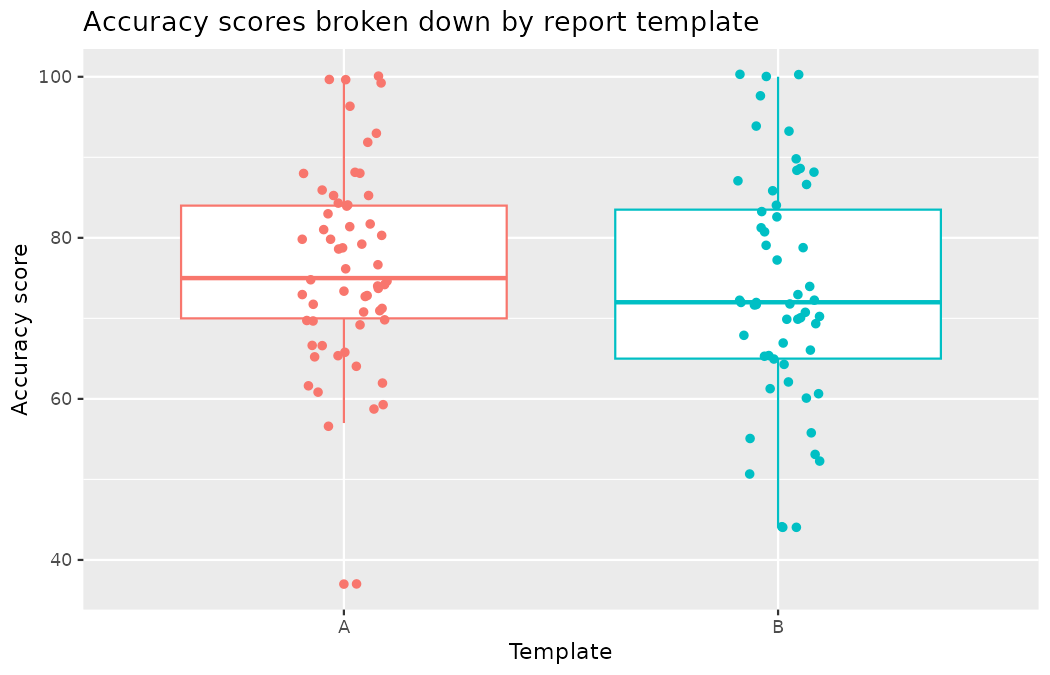
\includegraphics[width=0.85\linewidth,height=\textheight,keepaspectratio]{figures/inference-two-means-1.png}

\begin{tcolorbox}[enhanced jigsaw, left=2mm, leftrule=.75mm, title=\textcolor{quarto-callout-tip-color}{\faLightbulb}\hspace{0.5em}{Check your understanding}, arc=.35mm, rightrule=.15mm, coltitle=black, colframe=quarto-callout-tip-color-frame, bottomrule=.15mm, colbacktitle=quarto-callout-tip-color!10!white, opacitybacktitle=0.6, breakable, bottomtitle=1mm, toptitle=1mm, titlerule=0mm, opacityback=0, toprule=.15mm, colback=white]

Construct hypotheses to evaluate whether the observed difference in
sample means, \(\bar{x}_A - \bar{x}_B = 3.24,\) is likely to have
happened due to chance, if the null hypothesis is true. We will later
evaluate these hypotheses using \(\alpha = 0.01.\)

\begin{center}\rule{0.5\linewidth}{0.5pt}\end{center}

\(H_0:\) the two templates produce equally accurate reports, on average:
\(\mu_A - \mu_B = 0.\) \(H_A:\) one template produces more accurate
reports than the other, on average: \(\mu_A - \mu_B \neq 0.\) (Per the
discipline of Chapter~\ref{sec-foundations-decision-errors}, the
alternative is two-sided --- the complaint says B is worse, but an open
mind allows that the redesign might have been the harmful one.)

\end{tcolorbox}

\begin{tcolorbox}[enhanced jigsaw, left=2mm, leftrule=.75mm, title=\textcolor{quarto-callout-tip-color}{\faLightbulb}\hspace{0.5em}{Check your understanding}, arc=.35mm, rightrule=.15mm, coltitle=black, colframe=quarto-callout-tip-color-frame, bottomrule=.15mm, colbacktitle=quarto-callout-tip-color!10!white, opacitybacktitle=0.6, breakable, bottomtitle=1mm, toptitle=1mm, titlerule=0mm, opacityback=0, toprule=.15mm, colback=white]

Before moving on to evaluate the hypotheses in the previous Check your
understanding, let's think carefully about the dataset. Are the
observations across the two groups independent? Are there any concerns
about outliers?

\begin{center}\rule{0.5\linewidth}{0.5pt}\end{center}

Since the templates were randomly allocated to assignments, the
``treatment'' was randomly assigned, so independence within and between
groups is satisfied. The summary statistics suggest the scores are
roughly symmetric about their means. One report --- the low score of 37
in the A group --- sits some 20 points below the next-lowest A score and
earns a raised eyebrow. It is not a threat to the \emph{randomization
test} we are about to run, which makes no distributional assumption (the
shuffles simply reallocate the scores we actually observed), but it is
exactly the kind of observation we will have to take more seriously when
the mathematical model arrives later in the chapter.

\end{tcolorbox}

\subsection{Variability of the
statistic}\label{variability-of-the-statistic-11}

In Chapter~\ref{sec-foundations-randomization}, the variability of the
statistic (previously: \(\hat{p}_1 - \hat{p}_2\)) was visualized after
shuffling the observations across the two treatment groups many times.
The shuffling process implements the null hypothesis model (that there
is no effect of the treatment). In the template example, the null
hypothesis is that templates A and B produce equally accurate reports,
so the average scores across the two groups should be the same. If the
templates were equally good, \emph{due to natural variability}, we would
sometimes expect reports to score slightly better on template A
\((\bar{x}_A > \bar{x}_B)\) and sometimes expect them to score slightly
better on template B \((\bar{x}_B > \bar{x}_A).\) The question at hand
is: does \(\bar{x}_A - \bar{x}_B = 3.24\) indicate that template A
genuinely produces more accurate reports than template B?

To watch a single iteration of the randomization process with your own
eyes, take a subset small enough to eyeball --- the first four A reports
and the first five B reports:

\begin{Shaded}
\begin{Highlighting}[]
\NormalTok{toy9 }\OtherTok{\textless{}{-}} \FunctionTok{bind\_rows}\NormalTok{(}
\NormalTok{  template\_ab }\SpecialCharTok{|\textgreater{}} \FunctionTok{filter}\NormalTok{(template }\SpecialCharTok{==} \StringTok{"A"}\NormalTok{) }\SpecialCharTok{|\textgreater{}} \FunctionTok{slice\_head}\NormalTok{(}\AttributeTok{n =} \DecValTok{4}\NormalTok{),}
\NormalTok{  template\_ab }\SpecialCharTok{|\textgreater{}} \FunctionTok{filter}\NormalTok{(template }\SpecialCharTok{==} \StringTok{"B"}\NormalTok{) }\SpecialCharTok{|\textgreater{}} \FunctionTok{slice\_head}\NormalTok{(}\AttributeTok{n =} \DecValTok{5}\NormalTok{)}
\NormalTok{)}

\NormalTok{toy9 }\SpecialCharTok{|\textgreater{}}
  \FunctionTok{group\_by}\NormalTok{(template) }\SpecialCharTok{|\textgreater{}}
  \FunctionTok{summarize}\NormalTok{(}\AttributeTok{n =} \FunctionTok{n}\NormalTok{(), }\AttributeTok{mean =} \FunctionTok{mean}\NormalTok{(accuracy))}
\CommentTok{\#\textgreater{} \# A tibble: 2 × 3}
\CommentTok{\#\textgreater{}   template     n  mean}
\CommentTok{\#\textgreater{}   \textless{}fct\textgreater{}    \textless{}int\textgreater{} \textless{}dbl\textgreater{}}
\CommentTok{\#\textgreater{} 1 A            4  73}
\CommentTok{\#\textgreater{} 2 B            5  70.8}
\end{Highlighting}
\end{Shaded}

In this little subset, the four A reports average 73 and the five B
reports average 70.8 --- a difference of 2.2 points. If the null
hypothesis is true, then the accuracy of each report reflects the
scout's read of the player and the quality of the evidence, and it
shouldn't matter which template the assignment happened to draw. By
reallocating which report gets which template label, we can see how the
difference in average scores moves due only to natural variability:

\begin{Shaded}
\begin{Highlighting}[]
\FunctionTok{set.seed}\NormalTok{(}\DecValTok{2001}\NormalTok{)}
\NormalTok{toy9\_shuffled }\OtherTok{\textless{}{-}}\NormalTok{ toy9 }\SpecialCharTok{|\textgreater{}}
  \FunctionTok{mutate}\NormalTok{(}\AttributeTok{template =} \FunctionTok{sample}\NormalTok{(template))}

\NormalTok{toy9\_shuffled }\SpecialCharTok{|\textgreater{}}
  \FunctionTok{group\_by}\NormalTok{(template) }\SpecialCharTok{|\textgreater{}}
  \FunctionTok{summarize}\NormalTok{(}\AttributeTok{n =} \FunctionTok{n}\NormalTok{(), }\AttributeTok{mean =} \FunctionTok{mean}\NormalTok{(accuracy))}
\CommentTok{\#\textgreater{} \# A tibble: 2 × 3}
\CommentTok{\#\textgreater{}   template     n  mean}
\CommentTok{\#\textgreater{}   \textless{}fct\textgreater{}    \textless{}int\textgreater{} \textless{}dbl\textgreater{}}
\CommentTok{\#\textgreater{} 1 A            4  74.8}
\CommentTok{\#\textgreater{} 2 B            5  69.4}
\end{Highlighting}
\end{Shaded}

One shuffle --- the labels reassigned completely at random --- produced
simulated group means of 74.75 and 69.4: a difference of 5.35 points,
\emph{larger} than the 2.2 the real labels showed on these nine reports.
Chance alone, on a handful of observations, manufactures differences of
this size without any help from the templates.

Scaling the same operation up to all 113 reports and repeating it 1,000
times gives the null distribution of the statistic
\(\bar{x}_{A, sim} - \bar{x}_{B, sim}\) --- the by-now familiar
\textbf{infer} pipeline, with one change from
Chapter~\ref{sec-foundations-randomization}: \texttt{calculate()} now
computes a \emph{difference in means} rather than a difference in
proportions.

\begin{Shaded}
\begin{Highlighting}[]
\FunctionTok{set.seed}\NormalTok{(}\DecValTok{2001}\NormalTok{)}
\NormalTok{template\_null }\OtherTok{\textless{}{-}}\NormalTok{ template\_ab }\SpecialCharTok{|\textgreater{}}
  \FunctionTok{specify}\NormalTok{(accuracy }\SpecialCharTok{\textasciitilde{}}\NormalTok{ template) }\SpecialCharTok{|\textgreater{}}
  \FunctionTok{hypothesize}\NormalTok{(}\AttributeTok{null =} \StringTok{"independence"}\NormalTok{) }\SpecialCharTok{|\textgreater{}}
  \FunctionTok{generate}\NormalTok{(}\AttributeTok{reps =} \DecValTok{1000}\NormalTok{, }\AttributeTok{type =} \StringTok{"permute"}\NormalTok{) }\SpecialCharTok{|\textgreater{}}
  \FunctionTok{calculate}\NormalTok{(}\AttributeTok{stat =} \StringTok{"diff in means"}\NormalTok{, }\AttributeTok{order =} \FunctionTok{c}\NormalTok{(}\StringTok{"A"}\NormalTok{, }\StringTok{"B"}\NormalTok{))}

\FunctionTok{round}\NormalTok{(template\_null}\SpecialCharTok{$}\NormalTok{stat[}\DecValTok{1}\SpecialCharTok{:}\DecValTok{3}\NormalTok{], }\DecValTok{2}\NormalTok{)}
\CommentTok{\#\textgreater{} [1]  3.84  4.12 {-}3.03}

\FunctionTok{ggplot}\NormalTok{(template\_null, }\FunctionTok{aes}\NormalTok{(}\AttributeTok{x =}\NormalTok{ stat)) }\SpecialCharTok{+}
  \FunctionTok{geom\_histogram}\NormalTok{(}\AttributeTok{binwidth =} \DecValTok{1}\NormalTok{) }\SpecialCharTok{+}
  \FunctionTok{labs}\NormalTok{(}
    \AttributeTok{title =} \StringTok{"1,000 differences in randomized means"}\NormalTok{,}
    \AttributeTok{x =} \StringTok{"Difference in randomized mean accuracy scores}\SpecialCharTok{\textbackslash{}n}\StringTok{(A {-} B)"}\NormalTok{,}
    \AttributeTok{y =} \StringTok{"Count"}
\NormalTok{  )}
\end{Highlighting}
\end{Shaded}

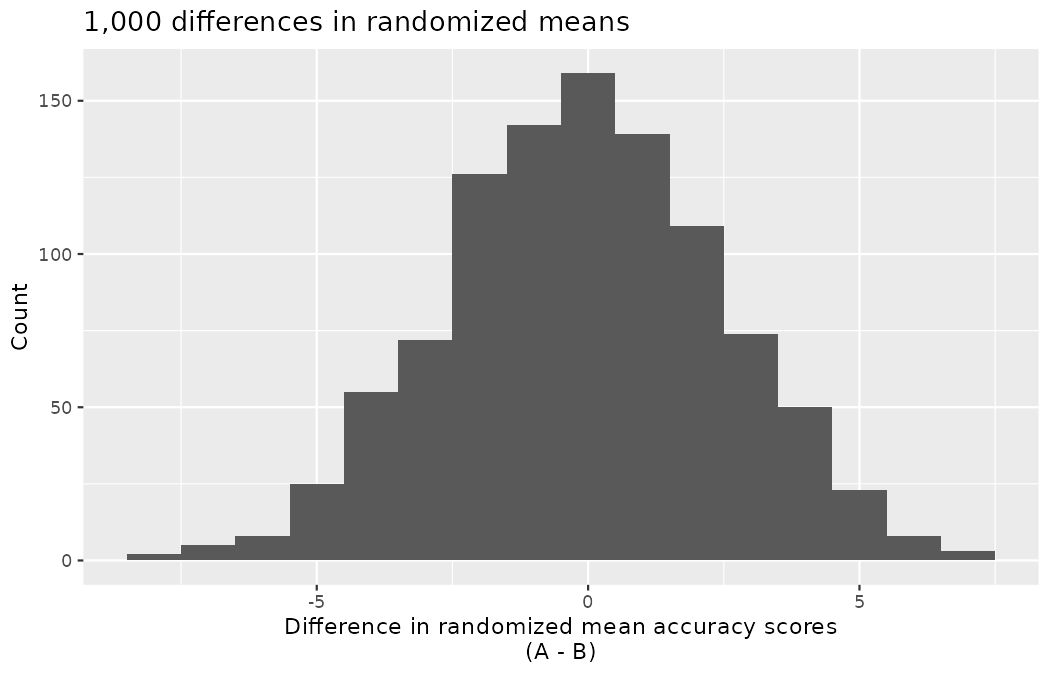
\includegraphics[width=0.85\linewidth,height=\textheight,keepaspectratio]{figures/inference-two-means-2.png}

The histogram of the 1,000 simulated differences is centered at zero and
bell-shaped, running from about \(-8.4\) to \(+6.8\): just by chance,
the difference in mean accuracy can land anywhere within roughly eight
points of zero.

\subsection{Observed statistic vs.~null
statistics}\label{observed-statistic-vs.-null-statistics-5}

The goal of the randomization test is to assess the observed data, here
the statistic of interest: \(\bar{x}_A - \bar{x}_B = 3.24.\) The
randomization distribution allows us to identify whether a difference of
3.24 points is more than one would expect by natural variability of the
scores if the two templates were equally good. The code below marks the
observed difference on the null distribution and counts the shuffles at
least as favorable to the alternative.

\begin{Shaded}
\begin{Highlighting}[]
\NormalTok{stat\_ab }\OtherTok{\textless{}{-}}\NormalTok{ template\_ab }\SpecialCharTok{|\textgreater{}}
  \FunctionTok{specify}\NormalTok{(accuracy }\SpecialCharTok{\textasciitilde{}}\NormalTok{ template) }\SpecialCharTok{|\textgreater{}}
  \FunctionTok{calculate}\NormalTok{(}\AttributeTok{stat =} \StringTok{"diff in means"}\NormalTok{, }\AttributeTok{order =} \FunctionTok{c}\NormalTok{(}\StringTok{"A"}\NormalTok{, }\StringTok{"B"}\NormalTok{))}

\FunctionTok{round}\NormalTok{(stat\_ab}\SpecialCharTok{$}\NormalTok{stat, }\DecValTok{2}\NormalTok{)}
\CommentTok{\#\textgreater{} [1] 3.24}

\FunctionTok{ggplot}\NormalTok{(template\_null, }\FunctionTok{aes}\NormalTok{(}\AttributeTok{x =}\NormalTok{ stat, }\AttributeTok{fill =} \FunctionTok{abs}\NormalTok{(stat) }\SpecialCharTok{\textgreater{}=}\NormalTok{ stat\_ab}\SpecialCharTok{$}\NormalTok{stat)) }\SpecialCharTok{+}
  \FunctionTok{geom\_histogram}\NormalTok{(}\AttributeTok{binwidth =} \DecValTok{1}\NormalTok{) }\SpecialCharTok{+}
  \FunctionTok{labs}\NormalTok{(}
    \AttributeTok{title =} \StringTok{"1,000 differences in randomized means"}\NormalTok{,}
    \AttributeTok{x =} \StringTok{"Difference in randomized mean accuracy scores}\SpecialCharTok{\textbackslash{}n}\StringTok{(A {-} B)"}\NormalTok{,}
    \AttributeTok{y =} \StringTok{"Count"}\NormalTok{,}
    \AttributeTok{fill =} \StringTok{"At least as extreme as 3.24"}
\NormalTok{  )}
\end{Highlighting}
\end{Shaded}

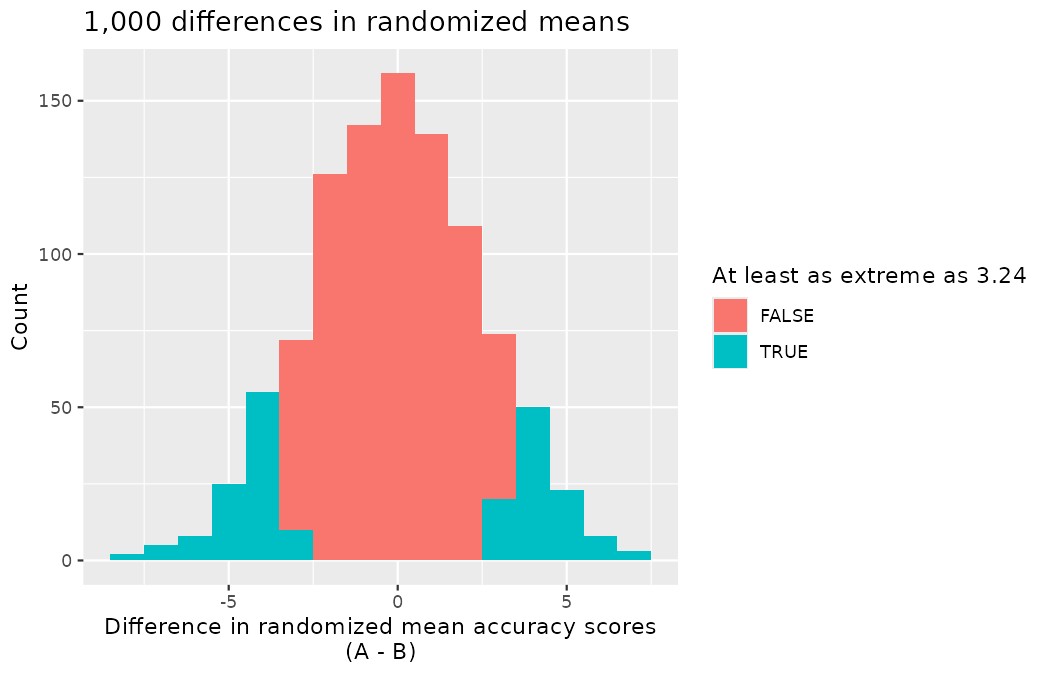
\includegraphics[width=0.85\linewidth,height=\textheight,keepaspectratio]{figures/inference-two-means-3.png}

\begin{tcolorbox}[enhanced jigsaw, left=2mm, leftrule=.75mm, title=\textcolor{quarto-callout-note-color}{\faInfo}\hspace{0.5em}{Worked example}, arc=.35mm, rightrule=.15mm, coltitle=black, colframe=quarto-callout-note-color-frame, bottomrule=.15mm, colbacktitle=quarto-callout-note-color!10!white, opacitybacktitle=0.6, breakable, bottomtitle=1mm, toptitle=1mm, titlerule=0mm, opacityback=0, toprule=.15mm, colback=white]

Approximate the p-value depicted by the shaded histogram, and provide a
conclusion in the context of the case study.

\begin{center}\rule{0.5\linewidth}{0.5pt}\end{center}

Using software, we can count the shuffled differences in means that fall
below the observed difference of 3.24: there are 896 (out of 1,000
randomizations). So 10.4\% of the simulations are at least as large as
the observed difference. To get the p-value, we double the proportion of
randomized differences that are larger than the observed difference:
p-value \(= 2 \times 0.104 = 0.208,\) or roughly 0.21.

\begin{Shaded}
\begin{Highlighting}[]
\NormalTok{template\_null }\SpecialCharTok{|\textgreater{}}
  \FunctionTok{summarize}\NormalTok{(}
    \AttributeTok{n\_below   =} \FunctionTok{sum}\NormalTok{(stat }\SpecialCharTok{\textless{}}\NormalTok{ stat\_ab}\SpecialCharTok{$}\NormalTok{stat),}
    \AttributeTok{n\_at\_or\_above =} \FunctionTok{sum}\NormalTok{(stat }\SpecialCharTok{\textgreater{}=}\NormalTok{ stat\_ab}\SpecialCharTok{$}\NormalTok{stat),}
    \AttributeTok{p\_value   =} \DecValTok{2} \SpecialCharTok{*} \FunctionTok{mean}\NormalTok{(stat }\SpecialCharTok{\textgreater{}=}\NormalTok{ stat\_ab}\SpecialCharTok{$}\NormalTok{stat)}
\NormalTok{  )}
\CommentTok{\#\textgreater{} \# A tibble: 1 × 3}
\CommentTok{\#\textgreater{}   n\_below n\_at\_or\_above p\_value}
\CommentTok{\#\textgreater{}     \textless{}int\textgreater{}         \textless{}int\textgreater{}   \textless{}dbl\textgreater{}}
\CommentTok{\#\textgreater{} 1     896           104   0.208}
\end{Highlighting}
\end{Shaded}

Previously, we specified that we would use \(\alpha = 0.01.\) Since the
p-value is larger than \(\alpha,\) we do not reject the null hypothesis.
That is, the data do not convincingly show that one template produces
more accurate reports than the other, and Emil should not be persuaded
that reports filed on template B deserve a compensating adjustment.

\end{tcolorbox}

The large p-value and the consistency of
\(\bar{x}_A - \bar{x}_B = 3.24\) with the randomized differences lead us
to \emph{not reject the null hypothesis}. Said differently, there is no
discernible evidence that one of the templates is better than the other.
One might be inclined to conclude that the templates are equally good,
but that conclusion would be wrong. The hypothesis testing framework is
set up only to reject a null claim; it is not set up to validate a null
claim --- recall the VAR review of
Chapter~\ref{sec-foundations-randomization}: ``check complete'' does not
certify the on-field call. As we concluded, the data are consistent with
templates A and B being equally good, but the data are also consistent
with template A producing reports 3.24 points more accurate than
template B. The data are not able to adjudicate between those
possibilities. Indeed, conclusions where the null hypothesis is not
rejected often seem unsatisfactory. Here, however, Priya and the
grumbling scouts are probably all relieved: there is no evidence that a
month of assessments was distorted by a layout choice.

\section{Bootstrap confidence interval for the difference in
means}\label{bootstrap-confidence-interval-for-the-difference-in-means}

Before providing a full example working through a bootstrap analysis on
a Northbridge experiment, we pause on a deliberately tiny scouting
errand --- this chapter's version of the seven trialists of
Chapter~\ref{sec-foundations-bootstrapping} --- to visualize the
\emph{two sample} bootstrap setting. Marta Vidal asked two partner
agencies to submit independent valuations for the wingers each
represents on Northbridge's shortlist; agency 1 sent valuations for five
comparable wingers on its books, and agency 2 for five on its own. The
research question: how much higher, on average, does agency 1 price a
shortlist winger than agency 2 --- and how precisely can ten valuations
pin that down? (A constructed scenario, built in the seeded code below.)

\begin{Shaded}
\begin{Highlighting}[]
\FunctionTok{set.seed}\NormalTok{(}\DecValTok{2002}\NormalTok{)}
\NormalTok{agency\_1 }\OtherTok{\textless{}{-}} \FunctionTok{tibble}\NormalTok{(}\AttributeTok{winger =} \FunctionTok{paste0}\NormalTok{(}\StringTok{"W"}\NormalTok{, }\DecValTok{1}\SpecialCharTok{:}\DecValTok{5}\NormalTok{),}
                   \AttributeTok{value  =} \FunctionTok{round}\NormalTok{(}\FunctionTok{rnorm}\NormalTok{(}\DecValTok{5}\NormalTok{, }\AttributeTok{mean =} \FloatTok{10.5}\NormalTok{, }\AttributeTok{sd =} \DecValTok{2}\NormalTok{), }\DecValTok{1}\NormalTok{))}
\NormalTok{agency\_2 }\OtherTok{\textless{}{-}} \FunctionTok{tibble}\NormalTok{(}\AttributeTok{winger =} \FunctionTok{paste0}\NormalTok{(}\StringTok{"W"}\NormalTok{, }\DecValTok{6}\SpecialCharTok{:}\DecValTok{10}\NormalTok{),}
                   \AttributeTok{value  =} \FunctionTok{round}\NormalTok{(}\FunctionTok{rnorm}\NormalTok{(}\DecValTok{5}\NormalTok{, }\AttributeTok{mean =} \DecValTok{8}\NormalTok{, }\AttributeTok{sd =} \FloatTok{1.5}\NormalTok{), }\DecValTok{1}\NormalTok{))}

\NormalTok{agency\_1}\SpecialCharTok{$}\NormalTok{value}
\CommentTok{\#\textgreater{} [1] 10.3 13.7 13.3 11.9 15.0}
\NormalTok{agency\_2}\SpecialCharTok{$}\NormalTok{value}
\CommentTok{\#\textgreater{} [1]  7.7 10.5  4.5  7.9  7.0}

\FunctionTok{c}\NormalTok{(}\FunctionTok{mean}\NormalTok{(agency\_1}\SpecialCharTok{$}\NormalTok{value), }\FunctionTok{mean}\NormalTok{(agency\_2}\SpecialCharTok{$}\NormalTok{value))}
\CommentTok{\#\textgreater{} [1] 12.84  7.52}
\end{Highlighting}
\end{Shaded}

The process of bootstrapping can be applied to \emph{each} group
separately, and the differences of means recalculated each time. The
analysis proceeds as in the one sample case of
Section~\ref{sec-boot1mean}, but now the (single) statistic of interest
is the \emph{difference in sample means}. That is, a bootstrap resample
is done on each of the groups separately --- five valuations drawn with
replacement from agency 1's bag, five from agency 2's, exactly the
two-bag mechanics of Section~\ref{sec-two-prop-boot-ci} --- but the
results are combined to have a single bootstrapped \textbf{difference in
means}. Repetition produces \(k\) bootstrapped differences in means, and
the histogram describes the natural sampling variability associated with
the difference.

\begin{Shaded}
\begin{Highlighting}[]
\FunctionTok{set.seed}\NormalTok{(}\DecValTok{2002}\NormalTok{)}
\NormalTok{agency\_boot }\OtherTok{\textless{}{-}} \FunctionTok{tibble}\NormalTok{(}
  \AttributeTok{stat =} \FunctionTok{replicate}\NormalTok{(}\DecValTok{1000}\NormalTok{, \{}
    \FunctionTok{mean}\NormalTok{(}\FunctionTok{slice\_sample}\NormalTok{(agency\_1, }\AttributeTok{n =} \DecValTok{5}\NormalTok{, }\AttributeTok{replace =} \ConstantTok{TRUE}\NormalTok{)}\SpecialCharTok{$}\NormalTok{value) }\SpecialCharTok{{-}}
      \FunctionTok{mean}\NormalTok{(}\FunctionTok{slice\_sample}\NormalTok{(agency\_2, }\AttributeTok{n =} \DecValTok{5}\NormalTok{, }\AttributeTok{replace =} \ConstantTok{TRUE}\NormalTok{)}\SpecialCharTok{$}\NormalTok{value)}
\NormalTok{  \})}
\NormalTok{)}

\NormalTok{agency\_boot }\SpecialCharTok{|\textgreater{}}
  \FunctionTok{summarize}\NormalTok{(}\AttributeTok{se =} \FunctionTok{sd}\NormalTok{(stat), }\AttributeTok{lowest =} \FunctionTok{min}\NormalTok{(stat), }\AttributeTok{highest =} \FunctionTok{max}\NormalTok{(stat))}
\CommentTok{\#\textgreater{} \# A tibble: 1 × 3}
\CommentTok{\#\textgreater{}      se lowest highest}
\CommentTok{\#\textgreater{}   \textless{}dbl\textgreater{}  \textless{}dbl\textgreater{}   \textless{}dbl\textgreater{}}
\CommentTok{\#\textgreater{} 1  1.14   1.32    8.44}

\FunctionTok{ggplot}\NormalTok{(agency\_boot, }\FunctionTok{aes}\NormalTok{(}\AttributeTok{x =}\NormalTok{ stat)) }\SpecialCharTok{+}
  \FunctionTok{geom\_histogram}\NormalTok{(}\AttributeTok{binwidth =} \DecValTok{1}\NormalTok{) }\SpecialCharTok{+}
  \FunctionTok{labs}\NormalTok{(}
    \AttributeTok{title =} \StringTok{"1,000 differences in bootstrapped means"}\NormalTok{,}
    \AttributeTok{x =} \StringTok{"Difference in bootstrapped mean valuations, in millions of euros}\SpecialCharTok{\textbackslash{}n}\StringTok{(agency 1 {-} agency 2)"}\NormalTok{,}
    \AttributeTok{y =} \StringTok{"Count"}
\NormalTok{  )}
\end{Highlighting}
\end{Shaded}

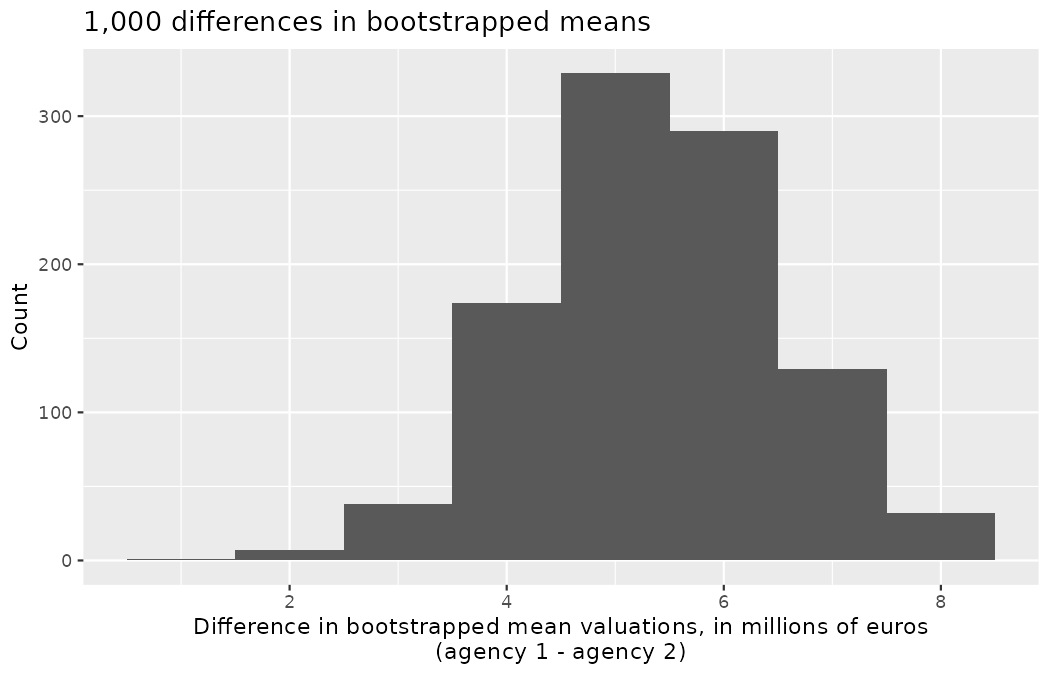
\includegraphics[width=0.85\linewidth,height=\textheight,keepaspectratio]{figures/inference-two-means-4.png}

The 1,000 bootstrapped differences in mean valuation range from about
€1.3M to €8.4M around the observed difference of
\(12.84 - 7.52 = 5.32,\) with a standard error of €1.14M --- five
valuations per bag simply cannot price the gap between two agencies to
better than a million or so either way.

In the following sections, we leave the two-agency errand and apply the
bootstrap method to a Northbridge experiment on finishing development,
and later to the tournament shot data. Note that the tiny setting
allowed us to \emph{visualize} the bootstrap method, which is important
for understanding how it works. However, the bootstrap relies heavily on
the sample being an outstanding proxy for the population, and five
observations are almost never enough to truly represent the nuances of a
full population --- the lesson the five logged shots of
Section~\ref{sec-boot1mean} taught with their clumpy histograms. To that
end, we apply bootstrap methods with larger samples wherever the club
can afford them.

\subsection{Observed data}\label{observed-data-12}

Does an individualized finishing-drill program improve academy players'
finishing? Jonas Beck ran the question as a randomized experiment.
Eighteen academy forwards sat the club's finishing assessment at the
start of a training block; each was then randomly assigned to the
individualized drill program (\texttt{drill}) or to standard training
(\texttt{standard}), nine per arm, and all eighteen re-sat the
assessment at the end of the block. The response variable is each
player's \emph{change score} --- end-of-block score minus start-of-block
score, in assessment points --- so a positive value corresponds to
improved finishing. Our goal will be to identify a 95\% confidence
interval for the effect of the drill program on the change in finishing
assessment score relative to the standard-training group.

\begin{tcolorbox}[enhanced jigsaw, left=2mm, leftrule=.75mm, title=\textcolor{quarto-callout-note-color}{\faInfo}\hspace{0.5em}{Data}, arc=.35mm, rightrule=.15mm, coltitle=black, colframe=quarto-callout-note-color-frame, bottomrule=.15mm, colbacktitle=quarto-callout-note-color!10!white, opacitybacktitle=0.6, breakable, bottomtitle=1mm, toptitle=1mm, titlerule=0mm, opacityback=0, toprule=.15mm, colback=white]

The \texttt{drill18} data are a constructed Northbridge scenario, built
in the seeded R code below; no real academy cohort was assessed. This
trial is also distinct from the multi-academy \texttt{drill\_trial} of
Chapter~\ref{sec-data-hello} and the two 90-player benchmark trials of
Chapter~\ref{sec-foundations-decision-errors} and
Chapter~\ref{sec-inference-two-props} --- a new, small experiment with a
\emph{numerical} outcome.

\end{tcolorbox}

\begin{Shaded}
\begin{Highlighting}[]
\FunctionTok{set.seed}\NormalTok{(}\DecValTok{2003}\NormalTok{)}
\NormalTok{change\_scores }\OtherTok{\textless{}{-}} \FunctionTok{c}\NormalTok{(}\FunctionTok{rnorm}\NormalTok{(}\DecValTok{9}\NormalTok{, }\AttributeTok{mean =} \FloatTok{1.7}\NormalTok{,  }\AttributeTok{sd =} \FloatTok{5.2}\NormalTok{),}
                   \FunctionTok{rnorm}\NormalTok{(}\DecValTok{9}\NormalTok{, }\AttributeTok{mean =} \SpecialCharTok{{-}}\FloatTok{3.5}\NormalTok{, }\AttributeTok{sd =} \FloatTok{2.8}\NormalTok{))}

\NormalTok{drill18 }\OtherTok{\textless{}{-}} \FunctionTok{tibble}\NormalTok{(}
  \AttributeTok{player =} \FunctionTok{paste0}\NormalTok{(}\StringTok{"P"}\NormalTok{, }\DecValTok{1}\SpecialCharTok{:}\DecValTok{18}\NormalTok{),}
  \AttributeTok{group  =} \FunctionTok{factor}\NormalTok{(}\FunctionTok{rep}\NormalTok{(}\FunctionTok{c}\NormalTok{(}\StringTok{"drill"}\NormalTok{, }\StringTok{"standard"}\NormalTok{), }\AttributeTok{each =} \DecValTok{9}\NormalTok{),}
                  \AttributeTok{levels =} \FunctionTok{c}\NormalTok{(}\StringTok{"drill"}\NormalTok{, }\StringTok{"standard"}\NormalTok{)),}
  \AttributeTok{before =} \FunctionTok{round}\NormalTok{(}\FunctionTok{rnorm}\NormalTok{(}\DecValTok{18}\NormalTok{, }\AttributeTok{mean =} \DecValTok{60}\NormalTok{, }\AttributeTok{sd =} \DecValTok{5}\NormalTok{), }\DecValTok{1}\NormalTok{)}
\NormalTok{) }\SpecialCharTok{|\textgreater{}}
  \FunctionTok{mutate}\NormalTok{(}
    \AttributeTok{after  =} \FunctionTok{round}\NormalTok{(before }\SpecialCharTok{+}\NormalTok{ change\_scores, }\DecValTok{1}\NormalTok{),}
    \AttributeTok{change =}\NormalTok{ after }\SpecialCharTok{{-}}\NormalTok{ before}
\NormalTok{  )}

\NormalTok{drill18 }\SpecialCharTok{|\textgreater{}}
  \FunctionTok{group\_by}\NormalTok{(group) }\SpecialCharTok{|\textgreater{}}
  \FunctionTok{summarize}\NormalTok{(}\AttributeTok{n =} \FunctionTok{n}\NormalTok{(), }\AttributeTok{mean =} \FunctionTok{round}\NormalTok{(}\FunctionTok{mean}\NormalTok{(change), }\DecValTok{2}\NormalTok{), }\AttributeTok{sd =} \FunctionTok{round}\NormalTok{(}\FunctionTok{sd}\NormalTok{(change), }\DecValTok{2}\NormalTok{))}
\CommentTok{\#\textgreater{} \# A tibble: 2 × 4}
\CommentTok{\#\textgreater{}   group        n  mean    sd}
\CommentTok{\#\textgreater{}   \textless{}fct\textgreater{}    \textless{}int\textgreater{} \textless{}dbl\textgreater{} \textless{}dbl\textgreater{}}
\CommentTok{\#\textgreater{} 1 drill        9  3.52  4.95}
\CommentTok{\#\textgreater{} 2 standard     9 {-}4.27  2.56}
\end{Highlighting}
\end{Shaded}

\begin{longtable}[]{@{}lccc@{}}
\caption{Summary statistics of the finishing-drill study: change in
assessment score (after \(-\) before), in
points.}\label{tbl-drill18-summary}\tabularnewline
\toprule\noalign{}
Group & n & Mean & SD \\
\midrule\noalign{}
\endfirsthead
\toprule\noalign{}
Group & n & Mean & SD \\
\midrule\noalign{}
\endhead
\bottomrule\noalign{}
\endlastfoot
drill & 9 & 3.52 & 4.95 \\
standard & 9 & -4.27 & 2.56 \\
\end{longtable}

Notice the sign of the standard group's mean in
Table~\ref{tbl-drill18-summary}: players under standard training
\emph{declined} by 4.27 points on average across the block ---
end-of-block assessments land in the heaviest weeks of the season, and
tired legs finish worse. The drill group improved by 3.52 points against
that same headwind. The point estimate of the difference in the change
scores is straightforward to find: it is the difference in the sample
means, and each subscript names its group, exactly as the chapter intro
promised:

\[\bar{x}_{drill} - \bar{x}_{standard} = 3.52 - (-4.27) = 7.79\]

\subsection{Variability of the
statistic}\label{variability-of-the-statistic-12}

As we saw in Section~\ref{sec-two-prop-boot-ci}, we will use
bootstrapping to estimate the variability associated with the difference
in sample means when taking repeated samples. In a method akin to two
proportions, a \emph{separate} sample is taken with replacement from
each group (here \texttt{drill} and \texttt{standard}), the sample means
are calculated, and their difference is taken. The entire process is
repeated multiple times to produce a bootstrap distribution of the
difference in sample means (\emph{without} the null hypothesis
assumption).

\begin{Shaded}
\begin{Highlighting}[]
\NormalTok{stat\_drill }\OtherTok{\textless{}{-}}\NormalTok{ drill18 }\SpecialCharTok{|\textgreater{}}
  \FunctionTok{specify}\NormalTok{(change }\SpecialCharTok{\textasciitilde{}}\NormalTok{ group) }\SpecialCharTok{|\textgreater{}}
  \FunctionTok{calculate}\NormalTok{(}\AttributeTok{stat =} \StringTok{"diff in means"}\NormalTok{, }\AttributeTok{order =} \FunctionTok{c}\NormalTok{(}\StringTok{"drill"}\NormalTok{, }\StringTok{"standard"}\NormalTok{))}

\FunctionTok{set.seed}\NormalTok{(}\DecValTok{2003}\NormalTok{)}
\NormalTok{drill\_boot }\OtherTok{\textless{}{-}}\NormalTok{ drill18 }\SpecialCharTok{|\textgreater{}}
  \FunctionTok{specify}\NormalTok{(change }\SpecialCharTok{\textasciitilde{}}\NormalTok{ group) }\SpecialCharTok{|\textgreater{}}
  \FunctionTok{generate}\NormalTok{(}\AttributeTok{reps =} \DecValTok{1000}\NormalTok{, }\AttributeTok{type =} \StringTok{"bootstrap"}\NormalTok{) }\SpecialCharTok{|\textgreater{}}
  \FunctionTok{calculate}\NormalTok{(}\AttributeTok{stat =} \StringTok{"diff in means"}\NormalTok{, }\AttributeTok{order =} \FunctionTok{c}\NormalTok{(}\StringTok{"drill"}\NormalTok{, }\StringTok{"standard"}\NormalTok{))}

\NormalTok{ci\_perc\_drill }\OtherTok{\textless{}{-}}\NormalTok{ drill\_boot }\SpecialCharTok{|\textgreater{}}
  \FunctionTok{get\_confidence\_interval}\NormalTok{(}\AttributeTok{level =} \FloatTok{0.9}\NormalTok{, }\AttributeTok{type =} \StringTok{"percentile"}\NormalTok{)}
\NormalTok{ci\_perc\_drill}
\CommentTok{\#\textgreater{} \# A tibble: 1 × 2}
\CommentTok{\#\textgreater{}   lower\_ci upper\_ci}
\CommentTok{\#\textgreater{}      \textless{}dbl\textgreater{}    \textless{}dbl\textgreater{}}
\CommentTok{\#\textgreater{} 1     4.93     10.6}

\NormalTok{ci\_se\_drill }\OtherTok{\textless{}{-}}\NormalTok{ drill\_boot }\SpecialCharTok{|\textgreater{}}
  \FunctionTok{get\_confidence\_interval}\NormalTok{(}\AttributeTok{level =} \FloatTok{0.9}\NormalTok{, }\AttributeTok{type =} \StringTok{"se"}\NormalTok{,}
                          \AttributeTok{point\_estimate =}\NormalTok{ stat\_drill)}
\NormalTok{ci\_se\_drill}
\CommentTok{\#\textgreater{} \# A tibble: 1 × 2}
\CommentTok{\#\textgreater{}   lower\_ci upper\_ci}
\CommentTok{\#\textgreater{}      \textless{}dbl\textgreater{}    \textless{}dbl\textgreater{}}
\CommentTok{\#\textgreater{} 1     4.93     10.6}

\FunctionTok{ggplot}\NormalTok{(drill\_boot, }\FunctionTok{aes}\NormalTok{(}\AttributeTok{x =}\NormalTok{ stat)) }\SpecialCharTok{+}
  \FunctionTok{geom\_histogram}\NormalTok{(}\AttributeTok{binwidth =} \FloatTok{0.5}\NormalTok{) }\SpecialCharTok{+}
  \FunctionTok{geom\_vline}\NormalTok{(}\AttributeTok{xintercept =}\NormalTok{ stat\_drill}\SpecialCharTok{$}\NormalTok{stat, }\AttributeTok{linewidth =} \DecValTok{1}\NormalTok{) }\SpecialCharTok{+}
  \FunctionTok{geom\_vline}\NormalTok{(}\AttributeTok{xintercept =} \FunctionTok{unlist}\NormalTok{(ci\_perc\_drill), }\AttributeTok{linetype =} \StringTok{"dashed"}\NormalTok{) }\SpecialCharTok{+}
  \FunctionTok{geom\_vline}\NormalTok{(}\AttributeTok{xintercept =} \FunctionTok{unlist}\NormalTok{(ci\_se\_drill), }\AttributeTok{linetype =} \StringTok{"dotted"}\NormalTok{) }\SpecialCharTok{+}
  \FunctionTok{labs}\NormalTok{(}
    \AttributeTok{title =} \StringTok{"1,000 differences in bootstrapped means"}\NormalTok{,}
    \AttributeTok{x =} \StringTok{"Difference in bootstrapped mean change scores}\SpecialCharTok{\textbackslash{}n}\StringTok{(drill {-} standard)"}\NormalTok{,}
    \AttributeTok{y =} \StringTok{"Count"}
\NormalTok{  )}
\end{Highlighting}
\end{Shaded}

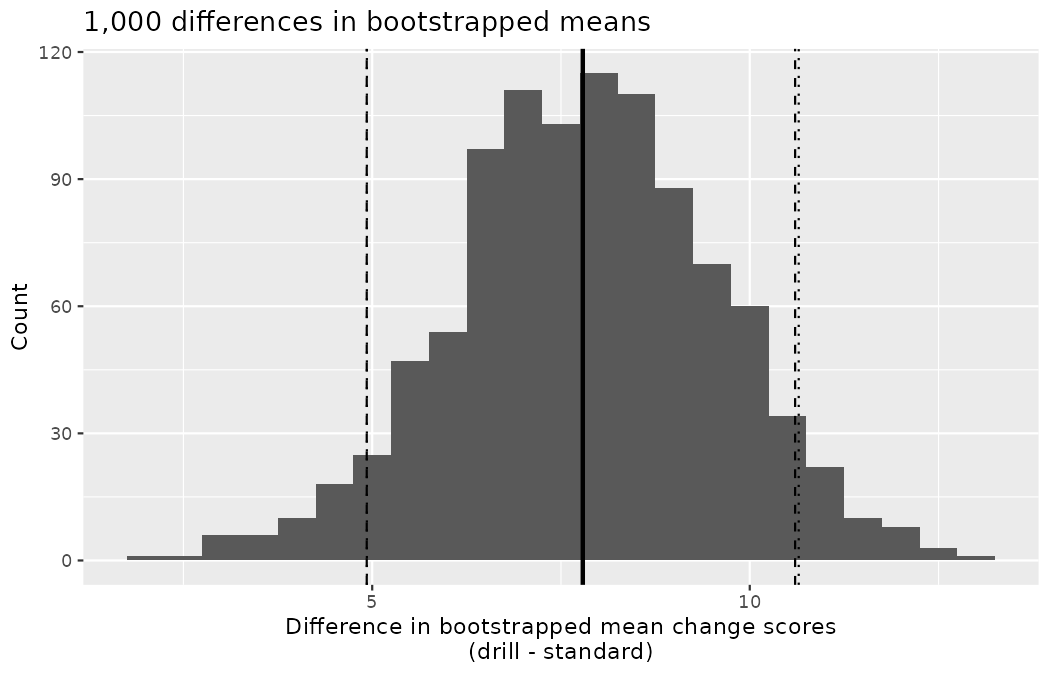
\includegraphics[width=0.85\linewidth,height=\textheight,keepaspectratio]{figures/inference-two-means-5.png}

The histogram of the 1,000 bootstrapped differences is roughly symmetric
and bell-shaped around the observed difference of 7.79 (solid line),
running from about 1.9 to 12.8 points. The 90\% bootstrap percentile
interval (dashed lines) is \((4.93, 10.60)\); the 90\% bootstrap SE
interval (dotted lines) is \((4.93, 10.65)\) --- the two constructions
nearly coincide here, as they should when the bootstrap distribution is
this bell-shaped (recall Section~\ref{sec-two-prop-boot-ci}).

\begin{tcolorbox}[enhanced jigsaw, left=2mm, leftrule=.75mm, title=\textcolor{quarto-callout-tip-color}{\faLightbulb}\hspace{0.5em}{Check your understanding}, arc=.35mm, rightrule=.15mm, coltitle=black, colframe=quarto-callout-tip-color-frame, bottomrule=.15mm, colbacktitle=quarto-callout-tip-color!10!white, opacitybacktitle=0.6, breakable, bottomtitle=1mm, toptitle=1mm, titlerule=0mm, opacityback=0, toprule=.15mm, colback=white]

Using the bootstrapped differences in \texttt{drill\_boot}, estimate the
standard error of the difference in sample means,
\(\bar{x}_{drill} - \bar{x}_{standard}.\)

\begin{Shaded}
\begin{Highlighting}[]
\FunctionTok{round}\NormalTok{(}\FunctionTok{sd}\NormalTok{(drill\_boot}\SpecialCharTok{$}\NormalTok{stat), }\DecValTok{2}\NormalTok{)}
\CommentTok{\#\textgreater{} [1] 1.74}
\end{Highlighting}
\end{Shaded}

\begin{center}\rule{0.5\linewidth}{0.5pt}\end{center}

The standard error of the difference is estimated by the standard
deviation of the 1,000 bootstrapped differences: \(SE \approx 1.74\)
points. (The point estimate whose variability it describes is
\(\bar{x}_{drill} - \bar{x}_{standard} = 7.79.\))

\end{tcolorbox}

\begin{tcolorbox}[enhanced jigsaw, left=2mm, leftrule=.75mm, title=\textcolor{quarto-callout-note-color}{\faInfo}\hspace{0.5em}{Worked example}, arc=.35mm, rightrule=.15mm, coltitle=black, colframe=quarto-callout-note-color-frame, bottomrule=.15mm, colbacktitle=quarto-callout-note-color!10!white, opacitybacktitle=0.6, breakable, bottomtitle=1mm, toptitle=1mm, titlerule=0mm, opacityback=0, toprule=.15mm, colback=white]

Choose one of the bootstrap confidence intervals for the true difference
in average change score, \(\mu_{drill} - \mu_{standard}.\) Does the
interval show that there is a difference across the two arms?

\begin{center}\rule{0.5\linewidth}{0.5pt}\end{center}

Because neither of the 90\% intervals (percentile or SE) overlaps zero
--- indeed, zero is never one of the 1,000 bootstrapped differences, so
95\% and 99\% intervals would have given the same conclusion --- we
conclude that the drill program is substantially better for finishing
development than standard training over this block.

Because the study is a randomized experiment, we can conclude that it is
the program \emph{causing} the improvement: we are 90\% confident the
individualized drills add between roughly 4.9 and 10.6 assessment points
relative to standard training. Contrast the strength of this claim with
everything we are allowed to say about tournament data --- random
assignment, not sample size, is what bought it.

\end{tcolorbox}

\section{Mathematical model for testing the difference in
means}\label{sec-math2samp}

Since Chapter~\ref{sec-explore-categorical}, this book has kept
returning to shots taken under defensive pressure. Chapter
\ref{sec-foundations-randomization} asked whether pressured shots are
\emph{converted} at a lower rate --- a proportions question --- and
Section~\ref{sec-one-mean-math} tested one tournament's pressured shots
against a fixed benchmark. The question for this section is the
two-sample means version, on the tournament we hold in full: at the 2022
Men's World Cup, did shots taken under pressure carry a different
average \emph{chance quality} --- \texttt{statsbomb\_xg}, per
Chapter~\ref{sec-explore-numerical}'s house vocabulary --- than shots
taken unpressured? Emil's scouts phrase it more bluntly: are pressured
attempts worse chances, or just worse-finished chances?

\begin{tcolorbox}[enhanced jigsaw, left=2mm, leftrule=.75mm, title=\textcolor{quarto-callout-note-color}{\faInfo}\hspace{0.5em}{Data}, arc=.35mm, rightrule=.15mm, coltitle=black, colframe=quarto-callout-note-color-frame, bottomrule=.15mm, colbacktitle=quarto-callout-note-color!10!white, opacitybacktitle=0.6, breakable, bottomtitle=1mm, toptitle=1mm, titlerule=0mm, opacityback=0, toprule=.15mm, colback=white]

The shot data are read from \texttt{data/derived/wc2022\_shots.csv}
(StatsBomb open data): all 1,494 shots of the 2022 Men's World Cup.
These are observational data --- nobody randomly assigned pressure ---
so, per Section~\ref{sec-chp11-observational}, every conclusion in this
section speaks to association, not causation.

\end{tcolorbox}

\subsection{Observed data}\label{observed-data-13}

Four cases from this dataset are shown below. We are particularly
interested in two variables: \texttt{statsbomb\_xg}, the chance quality
of the shot, and \texttt{under\_pressure}, which records whether an
opponent was actively pressuring the shooter.

\begin{Shaded}
\begin{Highlighting}[]
\NormalTok{wc2022\_shots }\OtherTok{\textless{}{-}} \FunctionTok{read\_csv}\NormalTok{(}\StringTok{"data/derived/wc2022\_shots.csv"}\NormalTok{)}

\NormalTok{wc2022\_shots }\SpecialCharTok{|\textgreater{}}
  \FunctionTok{select}\NormalTok{(team, player, minute, under\_pressure, statsbomb\_xg, outcome) }\SpecialCharTok{|\textgreater{}}
  \FunctionTok{head}\NormalTok{(}\DecValTok{4}\NormalTok{)}
\CommentTok{\#\textgreater{} \# A tibble: 4 × 6}
\CommentTok{\#\textgreater{}   team    player            minute under\_pressure statsbomb\_xg outcome}
\CommentTok{\#\textgreater{}   \textless{}chr\textgreater{}   \textless{}chr\textgreater{}              \textless{}dbl\textgreater{} \textless{}lgl\textgreater{}                 \textless{}dbl\textgreater{} \textless{}chr\textgreater{}}
\CommentTok{\#\textgreater{} 1 Canada  Mark Anthony Kaye      2 TRUE                 0.0389 Blocked}
\CommentTok{\#\textgreater{} 2 Morocco Hakim Ziyech           3 FALSE                0.0245 Goal}
\CommentTok{\#\textgreater{} 3 Morocco Abdelhamid Sabiri      8 FALSE                0.0221 Blocked}
\CommentTok{\#\textgreater{} 4 Morocco Sofiane Boufal         9 FALSE                0.0616 Wayward}
\end{Highlighting}
\end{Shaded}

We would like to know: is there convincing evidence that pressured shots
carried a different average chance quality than unpressured shots at
this tournament?

\begin{tcolorbox}[enhanced jigsaw, left=2mm, leftrule=.75mm, title=\textcolor{quarto-callout-note-color}{\faInfo}\hspace{0.5em}{Worked example}, arc=.35mm, rightrule=.15mm, coltitle=black, colframe=quarto-callout-note-color-frame, bottomrule=.15mm, colbacktitle=quarto-callout-note-color!10!white, opacitybacktitle=0.6, breakable, bottomtitle=1mm, toptitle=1mm, titlerule=0mm, opacityback=0, toprule=.15mm, colback=white]

Set up appropriate hypotheses to evaluate whether there is a
relationship between defensive pressure and average chance quality.

\begin{center}\rule{0.5\linewidth}{0.5pt}\end{center}

The null hypothesis represents the case of no difference between the
groups.

\begin{itemize}
\tightlist
\item
  \(H_0:\) There is no difference in average chance quality between
  pressured and unpressured shots. In statistical notation:
  \(\mu_{nop} - \mu_{prs} = 0,\) where \(\mu_{nop}\) represents the
  not-pressured shots and \(\mu_{prs}\) represents the shots taken under
  pressure (the subscripts, as always, simply name the groups).
\item
  \(H_A:\) There is some difference in average chance quality between
  the two kinds of shots: \(\mu_{nop} - \mu_{prs} \neq 0.\)
\end{itemize}

And because pressure was not randomly assigned, even a rejection of
\(H_0\) will assert \emph{association} between pressure and chance
quality, nothing more.

\end{tcolorbox}

Table~\ref{tbl-pressure-summary-stats} displays sample statistics from
the data. We can see that the average chance quality of pressured shots
is lower than that of unpressured shots.

\begin{Shaded}
\begin{Highlighting}[]
\NormalTok{wc2022\_shots }\SpecialCharTok{|\textgreater{}}
  \FunctionTok{group\_by}\NormalTok{(under\_pressure) }\SpecialCharTok{|\textgreater{}}
  \FunctionTok{summarize}\NormalTok{(}
    \AttributeTok{n    =} \FunctionTok{n}\NormalTok{(),}
    \AttributeTok{mean =} \FunctionTok{round}\NormalTok{(}\FunctionTok{mean}\NormalTok{(statsbomb\_xg), }\DecValTok{4}\NormalTok{),}
    \AttributeTok{sd   =} \FunctionTok{round}\NormalTok{(}\FunctionTok{sd}\NormalTok{(statsbomb\_xg), }\DecValTok{4}\NormalTok{)}
\NormalTok{  )}
\CommentTok{\#\textgreater{} \# A tibble: 2 × 4}
\CommentTok{\#\textgreater{}   under\_pressure     n   mean     sd}
\CommentTok{\#\textgreater{}   \textless{}lgl\textgreater{}          \textless{}int\textgreater{}  \textless{}dbl\textgreater{}  \textless{}dbl\textgreater{}}
\CommentTok{\#\textgreater{} 1 FALSE           1256 0.132  0.196}
\CommentTok{\#\textgreater{} 2 TRUE             238 0.0961 0.0949}
\end{Highlighting}
\end{Shaded}

\begin{longtable}[]{@{}lccc@{}}
\caption{Summary statistics of chance quality (xG) by pressure, all
1,494 shots of the 2022 Men's World
Cup.}\label{tbl-pressure-summary-stats}\tabularnewline
\toprule\noalign{}
Group & n & Mean & SD \\
\midrule\noalign{}
\endfirsthead
\toprule\noalign{}
Group & n & Mean & SD \\
\midrule\noalign{}
\endhead
\bottomrule\noalign{}
\endlastfoot
not pressured & 1,256 & 0.1315 & 0.1961 \\
under pressure & 238 & 0.0961 & 0.0949 \\
\end{longtable}

Note the imbalance in the group sizes --- 1,256 against 238 ---
mirroring the way the football, not any experimental design, dealt these
groups: pressure on the shooter is the exception, not the rule. The
machinery below is untroubled by imbalance; each group simply
contributes its own information through its own sample size.

\subsection{Variability of the
statistic}\label{variability-of-the-statistic-13}

We check the two conditions necessary to model the difference in sample
means using the \(t\)-distribution.

\begin{itemize}
\tightlist
\item
  The shots come from 64 matches across a whole tournament, and no
  analyst selected them --- every logged shot is included. As in
  Section~\ref{sec-one-mean-math}, we treat them as independent draws
  from the process that generates shots at this level, a reasonable
  working approximation (rebounds and scrambles push gently against it),
  while remembering the observational frame.
\item
  With both groups far beyond 30 observations, we inspect the data for
  particularly extreme outliers, using the histograms drawn by the code
  below, and find none: both panels show the strong right skew chance
  quality always has, which is acceptable at these sample sizes (recall
  the guideline of Section~\ref{sec-one-mean-math}: strong skew is fine
  for \(n\) of 60 or more), and no single observation sits isolated from
  its group.
\end{itemize}

\begin{Shaded}
\begin{Highlighting}[]
\NormalTok{wc2022\_shots }\SpecialCharTok{|\textgreater{}}
  \FunctionTok{mutate}\NormalTok{(}\AttributeTok{pressure =} \FunctionTok{if\_else}\NormalTok{(under\_pressure, }\StringTok{"Under pressure"}\NormalTok{, }\StringTok{"Not pressured"}\NormalTok{)) }\SpecialCharTok{|\textgreater{}}
  \FunctionTok{ggplot}\NormalTok{(}\FunctionTok{aes}\NormalTok{(}\AttributeTok{x =}\NormalTok{ statsbomb\_xg)) }\SpecialCharTok{+}
  \FunctionTok{geom\_histogram}\NormalTok{(}\AttributeTok{binwidth =} \FloatTok{0.05}\NormalTok{) }\SpecialCharTok{+}
  \FunctionTok{facet\_wrap}\NormalTok{(}\SpecialCharTok{\textasciitilde{}}\NormalTok{pressure, }\AttributeTok{ncol =} \DecValTok{2}\NormalTok{, }\AttributeTok{scales =} \StringTok{"free\_y"}\NormalTok{) }\SpecialCharTok{+}
  \FunctionTok{labs}\NormalTok{(}\AttributeTok{x =} \StringTok{"Chance quality (xG)"}\NormalTok{, }\AttributeTok{y =} \StringTok{"Count"}\NormalTok{)}
\end{Highlighting}
\end{Shaded}

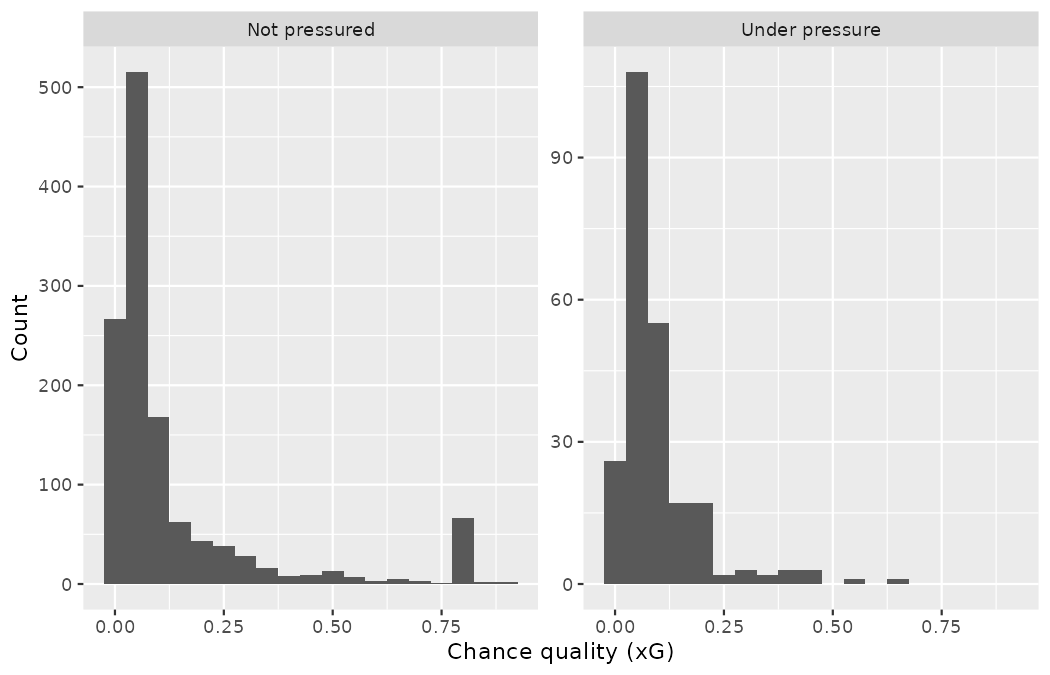
\includegraphics[width=0.85\linewidth,height=\textheight,keepaspectratio]{figures/inference-two-means-6.png}

Since both conditions are satisfied, the difference in sample means may
be modeled using a \(t\)-distribution. One feature of the unpressured
panel, though, should catch a trained eye: an isolated \emph{spike} ---
not a lone point, a whole bar --- near 0.78 xG. You have met that spike
in every xG histogram since Chapter~\ref{sec-data-applications}. Hold
that thought; it is not an ``outlier,'' and it will get the full
treatment shortly.

\begin{tcolorbox}[enhanced jigsaw, left=2mm, leftrule=.75mm, title=\textcolor{quarto-callout-tip-color}{\faLightbulb}\hspace{0.5em}{Check your understanding}, arc=.35mm, rightrule=.15mm, coltitle=black, colframe=quarto-callout-tip-color-frame, bottomrule=.15mm, colbacktitle=quarto-callout-tip-color!10!white, opacitybacktitle=0.6, breakable, bottomtitle=1mm, toptitle=1mm, titlerule=0mm, opacityback=0, toprule=.15mm, colback=white]

The summary statistics in Table~\ref{tbl-pressure-summary-stats} may be
useful for this Check your understanding. What is the point estimate of
the population difference, \(\mu_{nop} - \mu_{prs}\)?

\begin{center}\rule{0.5\linewidth}{0.5pt}\end{center}

The point estimate is the difference in sample means:
\(\bar{x}_{nop} - \bar{x}_{prs} = 0.1315 - 0.0961 = 0.0354\) xG per
shot.

\end{tcolorbox}

\subsection{Observed statistic vs.~null
statistics}\label{observed-statistic-vs.-null-statistics-6}

\begin{tcolorbox}[enhanced jigsaw, left=2mm, leftrule=.75mm, title=\textcolor{quarto-callout-important-color}{\faExclamation}\hspace{0.5em}{The test statistic for comparing two means is a T}, arc=.35mm, rightrule=.15mm, coltitle=black, colframe=quarto-callout-important-color-frame, bottomrule=.15mm, colbacktitle=quarto-callout-important-color!10!white, opacitybacktitle=0.6, breakable, bottomtitle=1mm, toptitle=1mm, titlerule=0mm, opacityback=0, toprule=.15mm, colback=white]

The \textbf{T score} is a ratio of how the groups differ as compared to
how the observations within a group vary.

\[T = \frac{(\bar{x}_1 - \bar{x}_2) - 0}{\sqrt{s_1^2/n_1 + s_2^2/n_2}}\]

When the null hypothesis is true and the conditions are met, T has a
\(t\)-distribution with \(df = \min(n_1 - 1, n_2 - 1).\)

Conditions:

\begin{itemize}
\tightlist
\item
  Independent observations within and between groups.
\item
  Large samples and no extreme outliers.
\end{itemize}

\end{tcolorbox}

Both formulas in that box are new in this chapter, so take them apart
piece by piece before using them.

Start under the square root. Each term \(s^2/n\) is the \emph{squared}
standard error of a single sample mean --- recall \(SE = s/\sqrt{n}\)
from Section~\ref{sec-one-mean-math} --- one copy for group 1, one copy
for group 2, each built from its own group's spread and its own group's
size. Because the two groups are independent, their uncertainties
compound, and the squared standard errors \emph{add}:

\[SE(\bar{x}_1 - \bar{x}_2) = \sqrt{\frac{s_1^2}{n_1} + \frac{s_2^2}{n_2}}\]

Note carefully that they add even though the statistic subtracts --- an
error in \(\bar{x}_1\) and an error in \(\bar{x}_2\) are both free to
push the difference off target, so the difference is \emph{more}
variable than either mean alone, never less. This is the same logic,
term for term, as the two-proportion standard error of
Section~\ref{sec-math-2prop}, with each proportion's
\(\hat{p}(1-\hat{p})/n\) replaced by a mean's \(s^2/n.\) The numerator
of \(T\) is the point estimate minus the null value --- and under
\(H_0: \mu_1 - \mu_2 = 0,\) the null value is the \(0\) written there
explicitly. The whole ratio counts how many standard errors the observed
difference sits from zero, precisely the job \(T\) performed in
Section~\ref{sec-one-mean-math} and \(Z\) before it.

The degrees of freedom formula also deserves a slow first read. The
function \(\min(n_1 - 1, n_2 - 1)\) returns the \emph{smaller} of its
two arguments: each group brings the \(n - 1\) degrees of freedom you
know from Section~\ref{sec-one-mean-math}, and we let the \emph{smaller}
group set the df for the pair. The formula software uses for the degrees
of freedom --- the Welch--Satterthwaite approximation, itself an
approximation, since the underlying two-variance problem admits no exact
answer --- is quite complex; the min rule is the honest hand shortcut
--- deliberately conservative, since fewer degrees of freedom means
thicker tails and wider intervals, so the approximation errs on the side
of demanding more evidence. For our pressure data:
\(df = \min(1256 - 1,\ 238 - 1) = 237.\)

\begin{tcolorbox}[enhanced jigsaw, left=2mm, leftrule=.75mm, title=\textcolor{quarto-callout-tip-color}{\faLightbulb}\hspace{0.5em}{Check your understanding}, arc=.35mm, rightrule=.15mm, coltitle=black, colframe=quarto-callout-tip-color-frame, bottomrule=.15mm, colbacktitle=quarto-callout-tip-color!10!white, opacitybacktitle=0.6, breakable, bottomtitle=1mm, toptitle=1mm, titlerule=0mm, opacityback=0, toprule=.15mm, colback=white]

Two groups of academy trialists are compared on a sprint metric, with
\(n_1 = 13\) and \(n_2 = 9.\) Under the min rule, how many degrees of
freedom does the \(t\)-distribution get? And why is taking the
\emph{smaller} of the two candidates the conservative choice rather than
an arbitrary one?

\begin{center}\rule{0.5\linewidth}{0.5pt}\end{center}

\(df = \min(13 - 1,\ 9 - 1) = \min(12,\ 8) = 8.\) Fewer degrees of
freedom means thicker tails (recall the df figure of
Section~\ref{sec-one-mean-math}): tail areas beyond any cutoff are
larger, so p-values come out bigger, and critical values
\(t^\star_{df}\) come out bigger, so intervals come out wider. Taking
the smaller candidate therefore always errs toward demanding \emph{more}
evidence than the Welch--Satterthwaite value would --- the shortcut can
make us slightly too cautious, never too eager to reject.

\end{tcolorbox}

\begin{tcolorbox}[enhanced jigsaw, left=2mm, leftrule=.75mm, title=\textcolor{quarto-callout-tip-color}{\faLightbulb}\hspace{0.5em}{Check your understanding}, arc=.35mm, rightrule=.15mm, coltitle=black, colframe=quarto-callout-tip-color-frame, bottomrule=.15mm, colbacktitle=quarto-callout-tip-color!10!white, opacitybacktitle=0.6, breakable, bottomtitle=1mm, toptitle=1mm, titlerule=0mm, opacityback=0, toprule=.15mm, colback=white]

Compute the standard error of the point estimate for the difference in
average chance quality between unpressured and pressured shots.

\begin{center}\rule{0.5\linewidth}{0.5pt}\end{center}

\[SE(\bar{x}_{nop} - \bar{x}_{prs}) = \sqrt{\frac{s_{nop}^2}{n_{nop}} + \frac{s_{prs}^2}{n_{prs}}} = \sqrt{\frac{0.1961^2}{1256} + \frac{0.0949^2}{238}} = 0.0083\]

Notice which group dominates: despite being five times smaller, the
pressured group contributes \emph{more} to the standard error
\((0.0949^2/238 = 0.000038\) against \(0.1961^2/1256 = 0.000031)\) ---
small \(n\) costs more than modest spread saves.

\end{tcolorbox}

\begin{tcolorbox}[enhanced jigsaw, left=2mm, leftrule=.75mm, title=\textcolor{quarto-callout-note-color}{\faInfo}\hspace{0.5em}{Worked example}, arc=.35mm, rightrule=.15mm, coltitle=black, colframe=quarto-callout-note-color-frame, bottomrule=.15mm, colbacktitle=quarto-callout-note-color!10!white, opacitybacktitle=0.6, breakable, bottomtitle=1mm, toptitle=1mm, titlerule=0mm, opacityback=0, toprule=.15mm, colback=white]

Complete the hypothesis test started in the previous Worked example and
Check your understanding, using a discernibility level of
\(\alpha = 0.05.\) For reference,
\(\bar{x}_{nop} - \bar{x}_{prs} = 0.0354,\) \(SE = 0.0083,\) and the
sample sizes were \(n_{nop} = 1256\) and \(n_{prs} = 238.\)

\begin{center}\rule{0.5\linewidth}{0.5pt}\end{center}

We can find the test statistic for this test using the previous
information:

\[T = \frac{\ 0.0354 - 0\ }{0.0083} = 4.27\]

We find the single tail area using software, with the smaller of
\(n_{nop} - 1 = 1255\) and \(n_{prs} - 1 = 237\) as the degrees of
freedom: \(df = 237.\) The one tail area is roughly 0.000014; doubling
this value gives the two-tail area and p-value, roughly 0.000028.

\begin{Shaded}
\begin{Highlighting}[]
\FunctionTok{pt}\NormalTok{(}\SpecialCharTok{{-}}\FloatTok{4.27}\NormalTok{, }\AttributeTok{df =} \DecValTok{237}\NormalTok{) }\SpecialCharTok{*} \DecValTok{2}
\CommentTok{\#\textgreater{} [1] 2.829918e{-}05}
\end{Highlighting}
\end{Shaded}

The p-value is (much) smaller than the discernibility level of 0.05, so
we reject the null hypothesis. Taken at face value, the data provide
statistically discernible evidence of a difference in average chance
quality between pressured and unpressured shots at this tournament.

\end{tcolorbox}

This result is likely not surprising. Every coaching manual says
pressure ruins chances, and Northbridge's own folklore agrees --- the
club still circulates a line from the 1968 notebooks of Agnes Whitmore,
its founding chief scout:

\begin{quote}
\emph{A forward hurried is a forward halved. Judge no man by what he
shoots with a defender in his collar.}
\end{quote}

Before that goes into another generation of scout training, though, the
book's penalty convention (recall Section~\ref{sec-chp11-pens-out}) must
be allowed to ask its question: \emph{which shots are in each group?}
That spike near 0.78 in the unpressured histogram has been waiting
patiently.

\begin{Shaded}
\begin{Highlighting}[]
\NormalTok{wc2022\_shots }\SpecialCharTok{|\textgreater{}}
  \FunctionTok{filter}\NormalTok{(shot\_type }\SpecialCharTok{==} \StringTok{"Penalty"}\NormalTok{) }\SpecialCharTok{|\textgreater{}}
  \FunctionTok{summarize}\NormalTok{(}
    \AttributeTok{kicks     =} \FunctionTok{n}\NormalTok{(),}
    \AttributeTok{mean\_xg   =} \FunctionTok{round}\NormalTok{(}\FunctionTok{mean}\NormalTok{(statsbomb\_xg), }\DecValTok{4}\NormalTok{),}
    \AttributeTok{pressured =} \FunctionTok{sum}\NormalTok{(under\_pressure)}
\NormalTok{  )}
\CommentTok{\#\textgreater{} \# A tibble: 1 × 3}
\CommentTok{\#\textgreater{}   kicks mean\_xg pressured}
\CommentTok{\#\textgreater{}   \textless{}int\textgreater{}   \textless{}dbl\textgreater{}     \textless{}int\textgreater{}}
\CommentTok{\#\textgreater{} 1    64   0.784         0}

\NormalTok{wc2022\_shots }\SpecialCharTok{|\textgreater{}}
  \FunctionTok{filter}\NormalTok{(under\_pressure) }\SpecialCharTok{|\textgreater{}}
  \FunctionTok{count}\NormalTok{(shot\_type)}
\CommentTok{\#\textgreater{} \# A tibble: 1 × 2}
\CommentTok{\#\textgreater{}   shot\_type     n}
\CommentTok{\#\textgreater{}   \textless{}chr\textgreater{}     \textless{}int\textgreater{}}
\CommentTok{\#\textgreater{} 1 Open Play   238}
\end{Highlighting}
\end{Shaded}

All 64 penalty kicks --- every one stored at the constant chance quality
of 0.7835, the highest-value shot type in the game --- sit in the
\emph{unpressured} group, because pressure on a penalty is impossible by
law. The pressured group, meanwhile, is pure open play. So the
comparison we just ran pitted open-play shots against a blend of
open-play shots, 64 penalties, and 48 unpressured dead-ball strikes, and
the penalties alone prop up the unpressured mean substantially. If the
scouts' question is about shooting under defensive pressure, penalties
and the other dead balls belong in neither group: we state the filter
--- \texttt{shot\_type\ ==\ "Open\ Play"}, keeping 1,382 shots --- say
why, and rerun the identical arithmetic on the frame the question
actually concerns.

\begin{Shaded}
\begin{Highlighting}[]
\NormalTok{wc2022\_shots }\SpecialCharTok{|\textgreater{}}
  \FunctionTok{filter}\NormalTok{(shot\_type }\SpecialCharTok{==} \StringTok{"Open Play"}\NormalTok{) }\SpecialCharTok{|\textgreater{}}
  \FunctionTok{group\_by}\NormalTok{(under\_pressure) }\SpecialCharTok{|\textgreater{}}
  \FunctionTok{summarize}\NormalTok{(}
    \AttributeTok{n    =} \FunctionTok{n}\NormalTok{(),}
    \AttributeTok{mean =} \FunctionTok{round}\NormalTok{(}\FunctionTok{mean}\NormalTok{(statsbomb\_xg), }\DecValTok{4}\NormalTok{),}
    \AttributeTok{sd   =} \FunctionTok{round}\NormalTok{(}\FunctionTok{sd}\NormalTok{(statsbomb\_xg), }\DecValTok{4}\NormalTok{)}
\NormalTok{  )}
\CommentTok{\#\textgreater{} \# A tibble: 2 × 4}
\CommentTok{\#\textgreater{}   under\_pressure     n   mean     sd}
\CommentTok{\#\textgreater{}   \textless{}lgl\textgreater{}          \textless{}int\textgreater{}  \textless{}dbl\textgreater{}  \textless{}dbl\textgreater{}}
\CommentTok{\#\textgreater{} 1 FALSE           1144 0.0988 0.130}
\CommentTok{\#\textgreater{} 2 TRUE             238 0.0961 0.0949}
\end{Highlighting}
\end{Shaded}

The pressured group is untouched: the same 238 shots,
\(\bar{x}_{prs} = 0.0961.\) Every change lands on the other side:
stripped of the dead balls, the unpressured mean falls from 0.1315 to
0.0988, and the T machinery --- hypotheses, formula, df rule, all
standing perfectly still --- returns a different verdict:

\[SE = \sqrt{\frac{0.1304^2}{1144} + \frac{0.0949^2}{238}} = 0.0073
\qquad
T = \frac{0.0988 - 0.0961}{0.0073} = 0.37\]

\begin{Shaded}
\begin{Highlighting}[]
\FunctionTok{pt}\NormalTok{(}\SpecialCharTok{{-}}\FloatTok{0.37}\NormalTok{, }\AttributeTok{df =} \DecValTok{237}\NormalTok{) }\SpecialCharTok{*} \DecValTok{2}
\CommentTok{\#\textgreater{} [1] 0.7117129}
\end{Highlighting}
\end{Shaded}

Set the two runs side by side, because --- as in
Section~\ref{sec-chp11-pens-out} and the benchmark test of
Section~\ref{sec-one-mean-math} --- the \emph{pair} is the finding:

\begin{itemize}
\tightlist
\item
  \textbf{All 1,494 shots, penalties in:}
  \(\bar{x}_{nop} - \bar{x}_{prs} = 0.0354,\) \(T = 4.27,\) p-value
  \(\approx 0.00003.\) A thumping rejection.
\item
  \textbf{1,382 open-play shots, penalties out:} difference \(0.0027,\)
  \(T = 0.37,\) p-value \(= 0.71.\) Nothing --- pressured and
  unpressured open-play shots are, on average, chances of almost
  identical quality, and a gap this size arises from sampling
  variability alone seven times out of ten.
\end{itemize}

Of the 0.0354 xG ``deficit'' the first test trumpeted, 0.0327 --- over
nine tenths of it --- was penalties and the other dead balls sitting in
one group, not anything about pressured shooting. On the
frame-consistent comparison, the discernibility verdict flips outright:
reject becomes fail to reject. Agnes's forwards are not halved after all
--- at least not in the chances they get themselves into; whether they
\emph{finish} those equal chances worse is the conversion question, and
Section~\ref{sec-chp11-pens-out} already showed the open-play answer
there was ``no discernible gap'' too. And the causal discipline of
Section~\ref{sec-chp11-observational} still stands over the whole pair:
even the pens-in rejection asserted association only. Defenders choose
whom to close down; nobody randomized pressure. The honest report states
the frame in its first sentence, shows the comparison both ways, and
treats the gap between the two answers as part of the finding.

\begin{tcolorbox}[enhanced jigsaw, left=2mm, leftrule=.75mm, title=\textcolor{quarto-callout-important-color}{\faExclamation}\hspace{0.5em}{What this comparison cannot see}, arc=.35mm, rightrule=.15mm, coltitle=black, colframe=quarto-callout-important-color-frame, bottomrule=.15mm, colbacktitle=quarto-callout-important-color!10!white, opacitybacktitle=0.6, breakable, bottomtitle=1mm, toptitle=1mm, titlerule=0mm, opacityback=0, toprule=.15mm, colback=white]

Before ``equal chance quality under pressure'' goes into a scouting
report, name the two things this frame is structurally blind to.

First, every row in this analysis is a shot that \emph{happened}.
Pressing's chief effect is preventing and displacing shots --- the pass
forced backward, the touch pushed long, the shooting lane closed before
an attempt exists --- and none of that can leave a trace in a dataset
conditioned on a shot existing. A defense that erases ten chances and
concedes one ordinary shot looks, in this table, like a defense that
changed nothing.

Second, the response variable is the vendor's own model:
\texttt{statsbomb\_xg} already prices defender proximity into each
shot's value. Finding that pressured shots carry roughly the value the
vendor assigns them is therefore partly an echo of the vendor's own
pressure discount, not an independent discovery about football.

So when a scout insists that pressure ruins shots, the claim is about a
counterfactual --- what this attempt would have been worth had the
defender not arrived --- and no dataset of realized shots, filtered or
not, can test that claim directly.

\end{tcolorbox}

A small note on the power of the independent \textbf{t-test}, recalling
the discussion of power in Section~\ref{sec-pow}: the independent-groups
test given here is often less powerful than the paired \(t\)-test coming
in Section~\ref{sec-mathpaired}, because pairing --- when the design
allows it --- removes variability across observational units before the
comparison is made. That said, depending on how the data are collected,
we don't always have a mechanism for pairing: no shot in our data is
both pressured and unpressured.

\section{Mathematical model for estimating the difference in
means}\label{mathematical-model-for-estimating-the-difference-in-means}

\subsection{Observed data}\label{observed-data-14}

As with hypothesis testing, for the question of whether we can model the
difference using a \(t\)-distribution, we'll need to check new
conditions. Like the two-proportion case of
Section~\ref{sec-math-2prop}, we will require a more robust version of
independence so we are confident the two groups are also independent of
each other. Secondly, we check for normality in each group
\emph{separately}, which in practice is a check for outliers group by
group.

\begin{tcolorbox}[enhanced jigsaw, left=2mm, leftrule=.75mm, title=\textcolor{quarto-callout-important-color}{\faExclamation}\hspace{0.5em}{Using the \(t\)-distribution for a difference in means}, arc=.35mm, rightrule=.15mm, coltitle=black, colframe=quarto-callout-important-color-frame, bottomrule=.15mm, colbacktitle=quarto-callout-important-color!10!white, opacitybacktitle=0.6, breakable, bottomtitle=1mm, toptitle=1mm, titlerule=0mm, opacityback=0, toprule=.15mm, colback=white]

The \(t\)-distribution can be used for inference when working with the
standardized difference of two means if

\begin{itemize}
\tightlist
\item
  \emph{Independence} (extended). The data are independent within and
  between the two groups, e.g., the data come from independent random
  samples or from a randomized experiment.
\item
  \emph{Normality}. We check for outliers in each group separately.
\end{itemize}

The standard error may be computed as

\[SE = \sqrt{\frac{\sigma_1^2}{n_1} + \frac{\sigma_2^2}{n_2}}\]

The Welch--Satterthwaite formula for the degrees of freedom is quite
complex and is generally computed using software, so instead you may use
the smaller of \(n_1 - 1\) and \(n_2 - 1\) for the degrees of freedom if
software isn't readily available.

\end{tcolorbox}

In practice the population standard deviations \(\sigma_1\) and
\(\sigma_2\) are unknown, and --- exactly as in
Section~\ref{sec-one-mean-math} --- we plug in the sample standard
deviations \(s_1\) and \(s_2\); the \(t\)-distribution's thicker tails
are the price paid for those two estimations. Recall from
Chapter~\ref{sec-foundations-mathematical} that the margin of error is
defined by the standard error. The margin of error for
\(\bar{x}_1 - \bar{x}_2\) can be directly obtained from
\(SE(\bar{x}_1 - \bar{x}_2).\)

\begin{tcolorbox}[enhanced jigsaw, left=2mm, leftrule=.75mm, title=\textcolor{quarto-callout-important-color}{\faExclamation}\hspace{0.5em}{Margin of error for \(\bar{x}_1 - \bar{x}_2\)}, arc=.35mm, rightrule=.15mm, coltitle=black, colframe=quarto-callout-important-color-frame, bottomrule=.15mm, colbacktitle=quarto-callout-important-color!10!white, opacitybacktitle=0.6, breakable, bottomtitle=1mm, toptitle=1mm, titlerule=0mm, opacityback=0, toprule=.15mm, colback=white]

The margin of error is
\(t^\star_{df} \times \sqrt{\frac{s_1^2}{n_1} + \frac{s_2^2}{n_2}},\)
where \(t^\star_{df}\) is calculated from a specified percentile on the
\(t\)-distribution with \emph{df} degrees of freedom --- the same
critical-value role \(t^\star_{df}\) played in
Section~\ref{sec-one-mean-math}, now attached to the two-sample
\textbf{SE difference in means}.

\end{tcolorbox}

\subsection{Variability of the
statistic}\label{variability-of-the-statistic-14}

\begin{tcolorbox}[enhanced jigsaw, left=2mm, leftrule=.75mm, title=\textcolor{quarto-callout-note-color}{\faInfo}\hspace{0.5em}{Worked example}, arc=.35mm, rightrule=.15mm, coltitle=black, colframe=quarto-callout-note-color-frame, bottomrule=.15mm, colbacktitle=quarto-callout-note-color!10!white, opacitybacktitle=0.6, breakable, bottomtitle=1mm, toptitle=1mm, titlerule=0mm, opacityback=0, toprule=.15mm, colback=white]

Can the \(t\)-distribution be used to make inference using the point
estimate from the finishing-drill study,
\(\bar{x}_{drill} - \bar{x}_{standard} = 7.79\)?

\begin{center}\rule{0.5\linewidth}{0.5pt}\end{center}

First, we check for independence. Because the players were randomized
into the arms, independence within and between groups is satisfied.

Second, we look for outliers in each group separately, using the
histograms drawn by the code below. The drill group's change scores run
from \(-5.1\) to \(+9.1\) with no gaps of concern, and the standard
group's from \(-7.6\) to \(-1.0.\) (The drill group does look more
variable --- \(s_{drill} = 4.95\) against \(s_{standard} = 2.56\) ---
but greater spread is not the same as having clear outliers.)

With both conditions met, we can use the \(t\)-distribution to model the
difference of sample means.

\begin{Shaded}
\begin{Highlighting}[]
\FunctionTok{ggplot}\NormalTok{(drill18, }\FunctionTok{aes}\NormalTok{(}\AttributeTok{x =}\NormalTok{ change)) }\SpecialCharTok{+}
  \FunctionTok{geom\_histogram}\NormalTok{(}\AttributeTok{binwidth =} \FloatTok{2.5}\NormalTok{) }\SpecialCharTok{+}
  \FunctionTok{facet\_wrap}\NormalTok{(}\SpecialCharTok{\textasciitilde{}}\NormalTok{group, }\AttributeTok{ncol =} \DecValTok{1}\NormalTok{) }\SpecialCharTok{+}
  \FunctionTok{labs}\NormalTok{(}\AttributeTok{x =} \StringTok{"Change in finishing assessment score (points)"}\NormalTok{, }\AttributeTok{y =} \StringTok{"Count"}\NormalTok{)}
\end{Highlighting}
\end{Shaded}

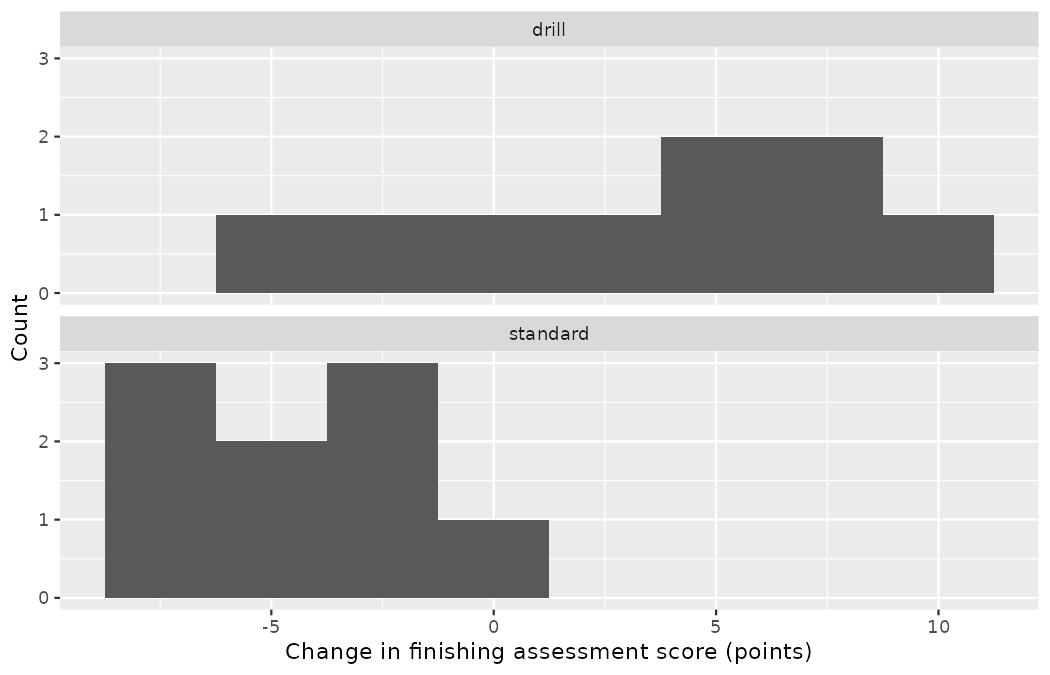
\includegraphics[width=0.85\linewidth,height=\textheight,keepaspectratio]{figures/inference-two-means-7.png}

\end{tcolorbox}

Generally, we use statistical software to find the appropriate degrees
of freedom, or if software isn't available, we can use the smaller of
\(n_1 - 1\) and \(n_2 - 1\) for the degrees of freedom, e.g., if using a
\(t\)-table to find tail areas. For transparency in the Worked examples
and Check your understandings, we'll use the latter approach; in the
case of the finishing-drill study, this means we'll use
\(df = \min(9 - 1,\ 9 - 1) = 8.\)

\begin{tcolorbox}[enhanced jigsaw, left=2mm, leftrule=.75mm, title=\textcolor{quarto-callout-note-color}{\faInfo}\hspace{0.5em}{Worked example}, arc=.35mm, rightrule=.15mm, coltitle=black, colframe=quarto-callout-note-color-frame, bottomrule=.15mm, colbacktitle=quarto-callout-note-color!10!white, opacitybacktitle=0.6, breakable, bottomtitle=1mm, toptitle=1mm, titlerule=0mm, opacityback=0, toprule=.15mm, colback=white]

Calculate a 95\% confidence interval for the effect of the
individualized drill program on the change in finishing assessment score
relative to standard training.

\begin{center}\rule{0.5\linewidth}{0.5pt}\end{center}

We will use the sample difference and the standard error computed from
the group summaries:

\[
\begin{aligned}
\bar{x}_{drill} - \bar{x}_{standard} &= 7.79 \\
SE &= \sqrt{\frac{4.95^2}{9} + \frac{2.56^2}{9}} = 1.86
\end{aligned}
\]

Using \(df = 8,\) we can identify the critical value for a 95\%
confidence interval: \(t^{\star}_{8} = 2.31.\)

\begin{Shaded}
\begin{Highlighting}[]
\FunctionTok{qt}\NormalTok{(}\FloatTok{0.975}\NormalTok{, }\AttributeTok{df =} \DecValTok{8}\NormalTok{)}
\CommentTok{\#\textgreater{} [1] 2.306004}
\end{Highlighting}
\end{Shaded}

Finally, we can enter the values into the confidence interval formula:

\[
\begin{aligned}
\text{point estimate} \ &\pm\ t^{\star} \times SE \\
7.79 \ &\pm\ 2.31 \times 1.86 \\
(3.49 \ &, \ 12.09)
\end{aligned}
\]

We are 95\% confident that the finishing improvement under the
individualized drill program is between 3.49 and 12.09 assessment points
greater than under standard training. The interval sits comfortably
above zero, agreeing with the bootstrap intervals --- the \textbf{t-CI}
and the bootstrap are two roads to the same destination when the
conditions hold --- and, because the program was randomly assigned, the
effect is causal: Jonas can take this to Marta Vidal as evidence the
program works, with the honest caveat that nine players per arm leave
the \emph{size} of the effect anywhere from modest to enormous.

\end{tcolorbox}

\section{Chapter review}\label{sec-chp20-review}

\subsection{Summary}\label{summary-19}

In this chapter we extended the single mean inferential methods of
Chapter~\ref{sec-inference-one-mean} to questions of differences in
means. You may have seen parallels from the chapters that extended a
single proportion (Chapter~\ref{sec-inference-one-prop}) to differences
in proportions (Chapter~\ref{sec-inference-two-props}) --- the structure
is deliberately the same, down to the standard error built by adding
each group's squared one-sample SE. When considering differences in
sample means, we use the \(t\)-distribution to describe the sampling
distribution of the T score (the standardized difference in sample
means), with the conservative \(df = \min(n_1 - 1, n_2 - 1)\) standing
in for a formula best left to software. Ideas of confidence level and
the types of error that might occur from a hypothesis test conclusion
are the same as those seen in other chapters (see
Chapter~\ref{sec-foundations-decision-errors}).

The chapter also delivered a two-sample installment of the book's
penalty convention: a randomized drill program earned a causal interval
excluding zero, while the tournament's headline pressure ``effect'' on
chance quality --- \(T = 4.27,\) pens in --- collapsed to \(T = 0.37\)
the moment the 64 uncontested kicks propping up one group were filtered
out, flipping the discernibility verdict outright. State the frame,
defend the filter, show any penalty-tilted comparison both ways --- and
remember which of your two studies was an experiment, because only that
one supported a causal claim.

\begin{longtable}[]{@{}
  >{\raggedright\arraybackslash}p{(\linewidth - 2\tabcolsep) * \real{0.5634}}
  >{\raggedright\arraybackslash}p{(\linewidth - 2\tabcolsep) * \real{0.4366}}@{}}
\caption{Summary of inference for a difference of two
means.}\label{tbl-chp20-summary}\tabularnewline
\toprule\noalign{}
\begin{minipage}[b]{\linewidth}\raggedright
Question
\end{minipage} & \begin{minipage}[b]{\linewidth}\raggedright
Answer
\end{minipage} \\
\midrule\noalign{}
\endfirsthead
\toprule\noalign{}
\begin{minipage}[b]{\linewidth}\raggedright
Question
\end{minipage} & \begin{minipage}[b]{\linewidth}\raggedright
Answer
\end{minipage} \\
\midrule\noalign{}
\endhead
\bottomrule\noalign{}
\endlastfoot
What is the parameter? & The difference in population means,
\(\mu_1 - \mu_2\); it is zero exactly when the two means agree. \\
What is the point estimate? & The difference in sample means,
\(\bar{x}_1 - \bar{x}_2.\) \\
How is its variability estimated? & By bootstrapping each group
separately, or by the formula \(SE = \sqrt{s_1^2/n_1 + s_2^2/n_2}.\) \\
What is the test statistic? &
\(T = \big((\bar{x}_1 - \bar{x}_2) - 0\big)\big/\sqrt{s_1^2/n_1 + s_2^2/n_2},\)
read against the \(t\)-distribution with
\(df = \min(n_1 - 1, n_2 - 1).\) \\
What are the conditions? & Independent observations within and between
groups; no extreme outliers, checked in each group separately. \\
\end{longtable}

\subsection{Terms}\label{terms-19}

The terms introduced in this chapter are presented below, alphabetized.
If you're not sure what some of these terms mean, we recommend you go
back in the text and review their definitions. You should be able to
easily spot them as \textbf{bolded text}.

\begin{longtable}[]{@{}
  >{\raggedright\arraybackslash}p{(\linewidth - 4\tabcolsep) * \real{0.3380}}
  >{\raggedright\arraybackslash}p{(\linewidth - 4\tabcolsep) * \real{0.3380}}
  >{\raggedright\arraybackslash}p{(\linewidth - 4\tabcolsep) * \real{0.3239}}@{}}
\caption{Terms introduced in this
chapter.}\label{tbl-terms-chp-20}\tabularnewline
\toprule\noalign{}
\endfirsthead
\endhead
\bottomrule\noalign{}
\endlastfoot
difference in means & SE difference in means & t-CI \\
point estimate & T score & t-test \\
\end{longtable}

\section{Exercises}\label{sec-chp20-exercises}

Answers to odd-numbered exercises can be found in
Appendix~\ref{sec-exercise-solutions-20}.

\begin{enumerate}
\def\labelenumi{\arabic{enumi}.}
\item
  \textbf{Corner-delivery experiment.} Northbridge's set-piece coach is
  experimenting with inswinging (IN) and outswinging (OUT) corner
  deliveries. In a training session, the coach has the first team defend
  a dozen corners of each type; afterwards, a panel of analysts scores
  each delivery on a scale of 1 to 10 on the danger it created, working
  from the coded event record of each delivery (first contact won,
  chance created) without seeing which arm of the session plan the
  delivery came from. The coach comes up with the following set of
  hypotheses for evaluating whether there is a difference in the average
  danger created by inswinging and outswinging deliveries. What is wrong
  with the hypotheses as stated?

  \[H_0: \bar{x}_{IN} \leq \bar{x}_{OUT} \quad \quad H_A: \bar{x}_{IN} > \bar{x}_{OUT}\]
\item
  \textbf{Fill in the blanks.} We use a \_\_\_ to evaluate if data
  provide convincing evidence of a difference between two population
  means and we use a \_\_\_ to estimate this difference.
\item
  \textbf{Shooting under pressure at the Euro, randomization test.} In
  Section~\ref{sec-math2samp} we compared the average chance quality of
  pressured and unpressured shots at the 2022 Men's World Cup.
  Northbridge's replication habit demands the same question be put to
  the 2025 Women's Euro: its 913 shots split into 325 taken under
  pressure and 588 taken unpressured.\footnote{The shot data used in
    this exercise are in \texttt{data/derived/weuro2025\_shots.csv}
    (StatsBomb open data): all 913 shots of the 2025 Women's Euro.}

  \begin{longtable}[]{@{}lccc@{}}
  \caption{All 913 shots, penalties and shoot-out kicks
  included.}\label{tbl-weuro-pressure-all}\tabularnewline
  \toprule\noalign{}
  Group & n & Mean & SD \\
  \midrule\noalign{}
  \endfirsthead
  \toprule\noalign{}
  Group & n & Mean & SD \\
  \midrule\noalign{}
  \endhead
  \bottomrule\noalign{}
  \endlastfoot
  not pressured & 588 & 0.1591 & 0.2231 \\
  under pressure & 325 & 0.0914 & 0.1018 \\
  \end{longtable}

  In order to simulate the null distribution of differences in average
  chance quality, we randomize the pressure label across the 913
  recorded chance qualities. The seeded code below generates 1,000 such
  differences; with this seed, the randomized differences range from
  about \(-0.042\) to \(+0.037,\) and \emph{none} of the 1,000 reaches
  the observed difference of \(0.1591 - 0.0914 = 0.0677.\)

\begin{Shaded}
\begin{Highlighting}[]
\NormalTok{weuro2025\_shots }\OtherTok{\textless{}{-}} \FunctionTok{read\_csv}\NormalTok{(}\StringTok{"data/derived/weuro2025\_shots.csv"}\NormalTok{)}

\FunctionTok{set.seed}\NormalTok{(}\DecValTok{2004}\NormalTok{)}
\NormalTok{weuro2025\_shots }\SpecialCharTok{|\textgreater{}}
  \FunctionTok{mutate}\NormalTok{(}\AttributeTok{pressure =} \FunctionTok{if\_else}\NormalTok{(under\_pressure, }\StringTok{"pressured"}\NormalTok{, }\StringTok{"not pressured"}\NormalTok{)) }\SpecialCharTok{|\textgreater{}}
  \FunctionTok{specify}\NormalTok{(statsbomb\_xg }\SpecialCharTok{\textasciitilde{}}\NormalTok{ pressure) }\SpecialCharTok{|\textgreater{}}
  \FunctionTok{hypothesize}\NormalTok{(}\AttributeTok{null =} \StringTok{"independence"}\NormalTok{) }\SpecialCharTok{|\textgreater{}}
  \FunctionTok{generate}\NormalTok{(}\AttributeTok{reps =} \DecValTok{1000}\NormalTok{, }\AttributeTok{type =} \StringTok{"permute"}\NormalTok{) }\SpecialCharTok{|\textgreater{}}
  \FunctionTok{calculate}\NormalTok{(}\AttributeTok{stat =} \StringTok{"diff in means"}\NormalTok{,}
            \AttributeTok{order =} \FunctionTok{c}\NormalTok{(}\StringTok{"not pressured"}\NormalTok{, }\StringTok{"pressured"}\NormalTok{)) }\SpecialCharTok{|\textgreater{}}
  \FunctionTok{ggplot}\NormalTok{(}\FunctionTok{aes}\NormalTok{(}\AttributeTok{x =}\NormalTok{ stat)) }\SpecialCharTok{+}
  \FunctionTok{geom\_histogram}\NormalTok{(}\AttributeTok{binwidth =} \FloatTok{0.005}\NormalTok{) }\SpecialCharTok{+}
  \FunctionTok{geom\_vline}\NormalTok{(}\AttributeTok{xintercept =} \FloatTok{0.0677}\NormalTok{, }\AttributeTok{color =} \StringTok{"red"}\NormalTok{, }\AttributeTok{linewidth =} \DecValTok{1}\NormalTok{) }\SpecialCharTok{+}
  \FunctionTok{labs}\NormalTok{(}
    \AttributeTok{title =} \StringTok{"1,000 randomized differences in means"}\NormalTok{,}
    \AttributeTok{x =} \StringTok{"Difference in randomized mean chance quality}\SpecialCharTok{\textbackslash{}n}\StringTok{(not pressured {-} pressured)"}\NormalTok{,}
    \AttributeTok{y =} \StringTok{"Count"}
\NormalTok{  )}
\end{Highlighting}
\end{Shaded}

  \begin{enumerate}
  \def\labelenumii{\alph{enumii}.}
  \item
    Using the randomization distribution, conduct a hypothesis test to
    evaluate if there is a difference between the average chance quality
    of unpressured and pressured shots at this tournament. Make sure to
    state your hypotheses clearly and interpret your results in context
    of the data, remembering what kind of study this is.
  \item
    All 51 of the Euro's penalty kicks --- stored chance quality 0.7835
    each --- and all 11 of its direct free kicks sit in the
    \emph{unpressured} group; the pressured group is pure open play. The
    rerun on the 851 open-play shots gives unpressured \(n = 526,\) mean
    \(0.1011,\) SD \(0.1186\) (the pressured group is unchanged), an
    observed difference of \(0.0097,\) and, with
    \texttt{set.seed(2005)}, 111 of 1,000 randomized differences at or
    above it. What is the two-sided p-value of the open-play test, what
    is your verdict, and which of the two frames belongs in a scouting
    claim about shooting under defensive pressure?
  \end{enumerate}
\item
  \textbf{First-time finishing chances, randomization test.} Do
  first-time shots arise from better or worse positions than shots taken
  after a controlled touch? Because a penalty kick is a placed,
  dead-ball strike that can never be hit first time (and would sit
  entirely in one group), we state the frame up front: the 1,382
  open-play shots of the 2022 Men's World Cup, of which 468 were struck
  first time (mean chance quality 0.1347, SD 0.1558) and 914 followed a
  controlled touch (mean 0.0797, SD 0.1009).\footnote{The shot data used
    in this exercise are in \texttt{data/derived/wc2022\_shots.csv}
    (StatsBomb open data), filtered to the 1,382 open-play shots as
    stated.} The observed difference is
  \(\bar{x}_{ft} - \bar{x}_{ct} = 0.1347 - 0.0797 = 0.0549\) (computed
  from the unrounded means). The seeded code below generates 1,000
  randomized differences; with this seed they range from about
  \(-0.021\) to \(+0.023,\) and none of the 1,000 comes anywhere near
  the observed difference in either direction.

\begin{Shaded}
\begin{Highlighting}[]
\NormalTok{wc2022\_shots }\OtherTok{\textless{}{-}} \FunctionTok{read\_csv}\NormalTok{(}\StringTok{"data/derived/wc2022\_shots.csv"}\NormalTok{)}

\FunctionTok{set.seed}\NormalTok{(}\DecValTok{2006}\NormalTok{)}
\NormalTok{wc2022\_shots }\SpecialCharTok{|\textgreater{}}
  \FunctionTok{filter}\NormalTok{(shot\_type }\SpecialCharTok{==} \StringTok{"Open Play"}\NormalTok{) }\SpecialCharTok{|\textgreater{}}
  \FunctionTok{mutate}\NormalTok{(}\AttributeTok{touch =} \FunctionTok{if\_else}\NormalTok{(first\_time, }\StringTok{"first time"}\NormalTok{, }\StringTok{"controlled"}\NormalTok{)) }\SpecialCharTok{|\textgreater{}}
  \FunctionTok{specify}\NormalTok{(statsbomb\_xg }\SpecialCharTok{\textasciitilde{}}\NormalTok{ touch) }\SpecialCharTok{|\textgreater{}}
  \FunctionTok{hypothesize}\NormalTok{(}\AttributeTok{null =} \StringTok{"independence"}\NormalTok{) }\SpecialCharTok{|\textgreater{}}
  \FunctionTok{generate}\NormalTok{(}\AttributeTok{reps =} \DecValTok{1000}\NormalTok{, }\AttributeTok{type =} \StringTok{"permute"}\NormalTok{) }\SpecialCharTok{|\textgreater{}}
  \FunctionTok{calculate}\NormalTok{(}\AttributeTok{stat =} \StringTok{"diff in means"}\NormalTok{,}
            \AttributeTok{order =} \FunctionTok{c}\NormalTok{(}\StringTok{"first time"}\NormalTok{, }\StringTok{"controlled"}\NormalTok{)) }\SpecialCharTok{|\textgreater{}}
  \FunctionTok{ggplot}\NormalTok{(}\FunctionTok{aes}\NormalTok{(}\AttributeTok{x =}\NormalTok{ stat)) }\SpecialCharTok{+}
  \FunctionTok{geom\_histogram}\NormalTok{(}\AttributeTok{binwidth =} \FloatTok{0.003}\NormalTok{) }\SpecialCharTok{+}
  \FunctionTok{geom\_vline}\NormalTok{(}\AttributeTok{xintercept =} \FloatTok{0.0549}\NormalTok{, }\AttributeTok{color =} \StringTok{"red"}\NormalTok{, }\AttributeTok{linewidth =} \DecValTok{1}\NormalTok{) }\SpecialCharTok{+}
  \FunctionTok{labs}\NormalTok{(}
    \AttributeTok{title =} \StringTok{"1,000 randomized differences in means"}\NormalTok{,}
    \AttributeTok{x =} \StringTok{"Difference in randomized mean chance quality}\SpecialCharTok{\textbackslash{}n}\StringTok{(first time {-} controlled)"}\NormalTok{,}
    \AttributeTok{y =} \StringTok{"Count"}
\NormalTok{  )}
\end{Highlighting}
\end{Shaded}

  \begin{enumerate}
  \def\labelenumii{\alph{enumii}.}
  \item
    Using the randomization distribution, conduct a hypothesis test to
    evaluate whether first-time and controlled-touch open-play shots
    differ in average chance quality. State your hypotheses clearly and
    interpret your results in context of the data.
  \item
    These are observational data. Offer one football mechanism that
    could produce this association without first-time \emph{technique}
    having anything to do with it.
  \end{enumerate}
\item
  \textbf{Shooting under pressure at the Euro, bootstrap interval.} We
  continue with the 913 shots of the 2025 Women's Euro --- all shots,
  penalties included, as in Table~\ref{tbl-weuro-pressure-all} --- and
  now estimate the difference in average chance quality between
  unpressured and pressured shots. The seeded code below draws 1,000
  bootstrap differences in means, resampling each group separately; with
  this seed, the bootstrapped differences form a bell centered at 0.068,
  running from about 0.034 to 0.102, and the standard deviation of the
  1,000 differences is 0.0111.\footnote{The shot data used in this
    exercise are in \texttt{data/derived/weuro2025\_shots.csv}
    (StatsBomb open data): all 913 shots of the 2025 Women's Euro.}

\begin{Shaded}
\begin{Highlighting}[]
\FunctionTok{set.seed}\NormalTok{(}\DecValTok{2007}\NormalTok{)}
\NormalTok{weuro2025\_shots }\SpecialCharTok{|\textgreater{}}
  \FunctionTok{mutate}\NormalTok{(}\AttributeTok{pressure =} \FunctionTok{if\_else}\NormalTok{(under\_pressure, }\StringTok{"pressured"}\NormalTok{, }\StringTok{"not pressured"}\NormalTok{)) }\SpecialCharTok{|\textgreater{}}
  \FunctionTok{specify}\NormalTok{(statsbomb\_xg }\SpecialCharTok{\textasciitilde{}}\NormalTok{ pressure) }\SpecialCharTok{|\textgreater{}}
  \FunctionTok{generate}\NormalTok{(}\AttributeTok{reps =} \DecValTok{1000}\NormalTok{, }\AttributeTok{type =} \StringTok{"bootstrap"}\NormalTok{) }\SpecialCharTok{|\textgreater{}}
  \FunctionTok{calculate}\NormalTok{(}\AttributeTok{stat =} \StringTok{"diff in means"}\NormalTok{,}
            \AttributeTok{order =} \FunctionTok{c}\NormalTok{(}\StringTok{"not pressured"}\NormalTok{, }\StringTok{"pressured"}\NormalTok{)) }\SpecialCharTok{|\textgreater{}}
  \FunctionTok{ggplot}\NormalTok{(}\FunctionTok{aes}\NormalTok{(}\AttributeTok{x =}\NormalTok{ stat)) }\SpecialCharTok{+}
  \FunctionTok{geom\_histogram}\NormalTok{(}\AttributeTok{binwidth =} \FloatTok{0.005}\NormalTok{) }\SpecialCharTok{+}
  \FunctionTok{labs}\NormalTok{(}
    \AttributeTok{title =} \StringTok{"1,000 bootstrapped differences in means"}\NormalTok{,}
    \AttributeTok{x =} \StringTok{"Difference in bootstrapped mean chance quality}\SpecialCharTok{\textbackslash{}n}\StringTok{(not pressured {-} pressured)"}\NormalTok{,}
    \AttributeTok{y =} \StringTok{"Count"}
\NormalTok{  )}
\end{Highlighting}
\end{Shaded}

  \begin{enumerate}
  \def\labelenumii{\alph{enumii}.}
  \item
    Using the bootstrap distribution, create a (rough) 95\% bootstrap
    percentile confidence interval for the true difference in average
    chance quality between unpressured and pressured shots at this
    tournament.
  \item
    Using the bootstrap distribution, create a (rough) 95\% bootstrap SE
    confidence interval for the same difference. Note that the standard
    error of the bootstrap distribution is 0.0111.
  \item
    Per the club's penalty convention, state precisely which comparison
    your intervals describe --- and what you would recompute before
    either interval appeared in a dossier about defensive pressure.
  \end{enumerate}
\item
  \textbf{First-time finishing chances, bootstrap interval.} We continue
  with the 1,382 open-play shots of the 2022 Men's World Cup from the
  earlier exercise: 468 first-time shots (mean chance quality 0.1347)
  and 914 controlled-touch shots (mean 0.0797). The seeded code below
  draws 1,000 bootstrap differences in means; with this seed, the
  bootstrapped differences form a bell centered at the observed
  difference of 0.0549, running from about 0.027 to 0.081, and the
  standard deviation of the 1,000 differences is 0.0081.\footnote{The
    shot data used in this exercise are in
    \texttt{data/derived/wc2022\_shots.csv} (StatsBomb open data),
    filtered to the 1,382 open-play shots as stated.}

\begin{Shaded}
\begin{Highlighting}[]
\FunctionTok{set.seed}\NormalTok{(}\DecValTok{2008}\NormalTok{)}
\NormalTok{wc2022\_shots }\SpecialCharTok{|\textgreater{}}
  \FunctionTok{filter}\NormalTok{(shot\_type }\SpecialCharTok{==} \StringTok{"Open Play"}\NormalTok{) }\SpecialCharTok{|\textgreater{}}
  \FunctionTok{mutate}\NormalTok{(}\AttributeTok{touch =} \FunctionTok{if\_else}\NormalTok{(first\_time, }\StringTok{"first time"}\NormalTok{, }\StringTok{"controlled"}\NormalTok{)) }\SpecialCharTok{|\textgreater{}}
  \FunctionTok{specify}\NormalTok{(statsbomb\_xg }\SpecialCharTok{\textasciitilde{}}\NormalTok{ touch) }\SpecialCharTok{|\textgreater{}}
  \FunctionTok{generate}\NormalTok{(}\AttributeTok{reps =} \DecValTok{1000}\NormalTok{, }\AttributeTok{type =} \StringTok{"bootstrap"}\NormalTok{) }\SpecialCharTok{|\textgreater{}}
  \FunctionTok{calculate}\NormalTok{(}\AttributeTok{stat =} \StringTok{"diff in means"}\NormalTok{,}
            \AttributeTok{order =} \FunctionTok{c}\NormalTok{(}\StringTok{"first time"}\NormalTok{, }\StringTok{"controlled"}\NormalTok{)) }\SpecialCharTok{|\textgreater{}}
  \FunctionTok{ggplot}\NormalTok{(}\FunctionTok{aes}\NormalTok{(}\AttributeTok{x =}\NormalTok{ stat)) }\SpecialCharTok{+}
  \FunctionTok{geom\_histogram}\NormalTok{(}\AttributeTok{binwidth =} \FloatTok{0.003}\NormalTok{) }\SpecialCharTok{+}
  \FunctionTok{labs}\NormalTok{(}
    \AttributeTok{title =} \StringTok{"1,000 bootstrapped differences in means"}\NormalTok{,}
    \AttributeTok{x =} \StringTok{"Difference in bootstrapped mean chance quality}\SpecialCharTok{\textbackslash{}n}\StringTok{(first time {-} controlled)"}\NormalTok{,}
    \AttributeTok{y =} \StringTok{"Count"}
\NormalTok{  )}
\end{Highlighting}
\end{Shaded}

  \begin{enumerate}
  \def\labelenumii{\alph{enumii}.}
  \item
    Using the bootstrap distribution, create a (rough) 90\% bootstrap
    percentile confidence interval for the true difference in average
    chance quality between first-time and controlled-touch open-play
    shots.
  \item
    Using the bootstrap distribution, create a (rough) 90\% bootstrap SE
    confidence interval for the same difference.
  \end{enumerate}
\item
  \textbf{Conditioning programs.} You are reading an internal report in
  which the sports-science staff have created a 95\% confidence interval
  for the difference in average distance covered per match under two
  pre-season conditioning programs, based on a randomized comparison
  across the squad. They are 95\% confident that the true difference in
  average distance covered over the season's first month is somewhere
  between (0.1 km, 2.5 km). The authors claim that, ``therefore program
  A (\(\bar{x}_A = 11.8\) km per match) results in a much larger average
  match output as compared to program B (\(\bar{x}_B = 10.5\) km per
  match).'' Comment on the authors' claim.\footnote{The summary figures
    in this exercise and in Exercises 8, 13, 14, 19, and 20 are
    constructed Northbridge scenarios, stated for the exercise; they are
    not drawn from real studies.}
\item
  \textbf{Possible randomized means.} In a training match, data were
  collected on chances created under two in-possession instructions (A
  and B). There were 3 players measured under instruction A and two
  players measured under instruction B.

  \begin{longtable}[]{@{}cccc@{}}
  \toprule\noalign{}
  Instruction & Measurement 1 & Measurement 2 & Measurement 3 \\
  \midrule\noalign{}
  \endhead
  \bottomrule\noalign{}
  \endlastfoot
  A & 1 & 15 & 5 \\
  B & 7 & 3 & \\
  \end{longtable}

  If the data are (repeatedly) randomly allocated across the two
  instructions, provide the following: (1) the values which are assigned
  to group A, (2) the values which are assigned to group B, and (3) the
  difference in averages \((\bar{x}_A - \bar{x}_B)\) for each of the
  following:

  \begin{enumerate}
  \def\labelenumii{\alph{enumii}.}
  \item
    When the randomized difference in averages is as large as possible.
  \item
    When the randomized difference in averages is as small as possible
    (a big in magnitude negative number).
  \item
    When the randomized difference in averages is as close to zero as
    possible.
  \item
    When the observed values are randomly assigned to the two groups, to
    which of the previous parts would you expect the difference in means
    to fall closest? Explain your reasoning.
  \end{enumerate}
\item
  \textbf{Shooting under pressure at the Euro, mathematical test.} We
  return to the average chance quality of pressured and unpressured
  shots at the 2025 Women's Euro, now with the mathematical model.
  Sample statistics are provided below for both analysis frames; the
  chance-quality distributions in every group carry the strong right
  skew xG always has, with no isolated single observations.\footnote{The
    shot data used in this exercise are in
    \texttt{data/derived/weuro2025\_shots.csv} (StatsBomb open data):
    all 913 shots of the 2025 Women's Euro.}

  \begin{longtable}[]{@{}llccc@{}}
  \caption{Chance quality (xG) by pressure at the 2025 Women's Euro, in
  the all-shots frame (penalties and direct free kicks included) and the
  open-play frame.}\label{tbl-weuro-pressure-frames}\tabularnewline
  \toprule\noalign{}
  Frame & Group & n & Mean & SD \\
  \midrule\noalign{}
  \endfirsthead
  \toprule\noalign{}
  Frame & Group & n & Mean & SD \\
  \midrule\noalign{}
  \endhead
  \bottomrule\noalign{}
  \endlastfoot
  all shots & not pressured & 588 & 0.1591 & 0.2231 \\
  all shots & under pressure & 325 & 0.0914 & 0.1018 \\
  open play & not pressured & 526 & 0.1011 & 0.1186 \\
  open play & under pressure & 325 & 0.0914 & 0.1018 \\
  \end{longtable}

  \begin{enumerate}
  \def\labelenumii{\alph{enumii}.}
  \item
    Conduct a hypothesis test using a mathematical model to evaluate if
    there is a difference in average chance quality between unpressured
    and pressured shots in the \emph{all-shots} frame. Make sure to
    state your hypotheses clearly, check relevant conditions, and
    interpret your results in context of the data.
  \item
    Repeat the test in the \emph{open-play} frame.
  \item
    The two frames return different verdicts. Which one answers a
    scout's question about shooting under defensive pressure, and why?
  \end{enumerate}
\item
  \textbf{Template A/B analysis plan.} Following
  Section~\ref{sec-rand2mean}, Priya Rao asks two junior analysts to
  plan the analysis of next season's report-template experiment, in
  which reports will again be randomly assigned to one of two templates
  and scored for accuracy. They agree on how the null hypothesis should
  be set: on average, reports are equally accurate under template A and
  template B. The first analyst is convinced the redesigned template
  will produce more accurate reports and hence wants to use a one-tailed
  test; the second argues that a two-tailed test would be a better
  choice. Which analyst do you agree with, and why?
\item
  \textbf{Shooting under pressure at the Euro, mathematical interval.}
  Using the sample statistics in Table~\ref{tbl-weuro-pressure-frames},
  and assuming that the conditions for conducting inference using a
  mathematical model are satisfied:\footnote{The shot data used in this
    exercise are in \texttt{data/derived/weuro2025\_shots.csv}
    (StatsBomb open data): all 913 shots of the 2025 Women's Euro.}

  \begin{enumerate}
  \def\labelenumii{\alph{enumii}.}
  \item
    Construct a 95\% confidence interval for the true difference in
    average chance quality between unpressured and pressured shots in
    the \emph{all-shots} frame, and interpret it in context.
  \item
    Construct the corresponding 95\% confidence interval in the
    \emph{open-play} frame. What does the pair of intervals, taken
    together, tell the club?
  \end{enumerate}
\item
  \textbf{True / False: comparing means.} Determine if the following
  statements about club analytics practice are true or false, and
  explain your reasoning for statements you identify as false.

  \begin{enumerate}
  \def\labelenumii{\alph{enumii}.}
  \item
    As the degrees of freedom increases, the \(t\)-distribution
    approaches normality.
  \item
    If a 95\% confidence interval for the difference between two
    population means contains 0, a 99\% confidence interval calculated
    based on the same two samples will also contain 0.
  \item
    If a 95\% confidence interval for the difference between two
    population means contains 0, a 90\% confidence interval calculated
    based on the same two samples will also contain 0.
  \end{enumerate}
\item
  \textbf{Difference of prospect ratings.} Northbridge's recruitment
  database assigns prospects a net-impact rating (positive values above
  replacement level, negative below). We collect two random samples of
  prospects from two scouting regions. In each part below, consider the
  sample means \(\bar{x}_1\) and \(\bar{x}_2\) that we might observe
  from these two samples.\footnote{The summary figures in this exercise
    and in Exercises 8, 13, 14, 19, and 20 are constructed Northbridge
    scenarios, stated for the exercise; they are not drawn from real
    studies.}

  \begin{longtable}[]{@{}lccc@{}}
  \toprule\noalign{}
  Population & Mean & Standard deviation & Sample size \\
  \midrule\noalign{}
  \endhead
  \bottomrule\noalign{}
  \endlastfoot
  Region 1 & 15 & 20 & 50 \\
  Region 2 & 20 & 10 & 30 \\
  \end{longtable}

  \begin{enumerate}
  \def\labelenumii{\alph{enumii}.}
  \item
    What is the associated mean and standard deviation of \(\bar{x}_1\)?
  \item
    What is the associated mean and standard deviation of \(\bar{x}_2\)?
  \item
    Calculate and interpret the mean and standard deviation associated
    with the difference in sample means for the two groups,
    \(\bar{x}_2 - \bar{x}_1.\)
  \item
    How are the standard deviations from parts (a), (b), and (c)
    related?
  \end{enumerate}
\item
  \textbf{Mindfulness during a congested schedule.} To address the
  mental toll of a congested winter schedule, Jonas Beck's player-care
  staff ran a mindfulness-based intervention (MBI) study on 60 academy
  players facing twice-weekly fixtures. The participants were randomly
  allocated to one of two groups of 30: the treatment group received 8
  MBI sessions across the block and the control group received no
  intervention. Match-related exhaustion was measured with a 9-item
  questionnaire, each item on a 0 (``never'') to 6 (``every day'')
  scale. Players in the treatment group had an average exhaustion score
  of 15.47, with a standard deviation of 4.44, and players in the
  control group had an average exhaustion score of 32.43, with a
  standard deviation of 8.87. Do these data provide convincing evidence
  that exhaustion differs between the treatment and control groups?
  Assume that conditions for conducting inference using mathematical
  models are satisfied.\footnote{The summary figures in this exercise
    and in Exercises 8, 13, 14, 19, and 20 are constructed Northbridge
    scenarios, stated for the exercise; they are not drawn from real
    studies.}
\item
  \textbf{Finishing programs: static repetition vs.~pattern drills.}
  Academy finishing development is a crowded market of methods, and any
  program that genuinely accelerates young forwards is worth money to a
  selling club. Jonas Beck randomized 71 newly promoted academy forwards
  across six finishing-development programs for one training block; the
  outcome is each player's score on the club's 400-point composite
  finishing assessment at the end of the block. The cohort is a
  constructed Northbridge scenario, generated by the seeded code below.
  In this exercise we consider the players assigned to \emph{static
  repetition} and \emph{pattern drills}.\footnote{The six-arm finishing
    trial is a constructed Northbridge scenario, generated entirely by
    the seeded code shown; no real academy cohort was assessed. The
    generation parameters are, of course, visible in the code --- the
    exercise concerns what the \emph{sample} can demonstrate.}

\begin{Shaded}
\begin{Highlighting}[]
\FunctionTok{set.seed}\NormalTok{(}\DecValTok{2009}\NormalTok{)}
\NormalTok{programs }\OtherTok{\textless{}{-}} \FunctionTok{c}\NormalTok{(}\StringTok{"constraint games"}\NormalTok{, }\StringTok{"static repetition"}\NormalTok{, }\StringTok{"pattern drills"}\NormalTok{,}
              \StringTok{"video review"}\NormalTok{, }\StringTok{"small{-}sided games"}\NormalTok{, }\StringTok{"shadow play"}\NormalTok{)}
\NormalTok{ns  }\OtherTok{\textless{}{-}} \FunctionTok{c}\NormalTok{(}\DecValTok{12}\NormalTok{, }\DecValTok{10}\NormalTok{, }\DecValTok{12}\NormalTok{, }\DecValTok{11}\NormalTok{, }\DecValTok{14}\NormalTok{, }\DecValTok{12}\NormalTok{)}
\NormalTok{mus }\OtherTok{\textless{}{-}} \FunctionTok{c}\NormalTok{(}\DecValTok{324}\NormalTok{, }\DecValTok{160}\NormalTok{, }\DecValTok{196}\NormalTok{, }\DecValTok{277}\NormalTok{, }\DecValTok{246}\NormalTok{, }\DecValTok{329}\NormalTok{)}
\NormalTok{sds }\OtherTok{\textless{}{-}} \FunctionTok{c}\NormalTok{(}\DecValTok{64}\NormalTok{, }\DecValTok{39}\NormalTok{, }\DecValTok{52}\NormalTok{, }\DecValTok{50}\NormalTok{, }\DecValTok{54}\NormalTok{, }\DecValTok{49}\NormalTok{)}

\NormalTok{intake71 }\OtherTok{\textless{}{-}} \FunctionTok{tibble}\NormalTok{(}
  \AttributeTok{program =} \FunctionTok{rep}\NormalTok{(programs, }\AttributeTok{times =}\NormalTok{ ns),}
  \AttributeTok{score   =} \FunctionTok{round}\NormalTok{(}\FunctionTok{rnorm}\NormalTok{(}\DecValTok{71}\NormalTok{, }\AttributeTok{mean =} \FunctionTok{rep}\NormalTok{(mus, }\AttributeTok{times =}\NormalTok{ ns),}
                        \AttributeTok{sd =} \FunctionTok{rep}\NormalTok{(sds, }\AttributeTok{times =}\NormalTok{ ns)))}
\NormalTok{)}

\NormalTok{rep\_pat }\OtherTok{\textless{}{-}}\NormalTok{ intake71 }\SpecialCharTok{|\textgreater{}}
  \FunctionTok{filter}\NormalTok{(program }\SpecialCharTok{\%in\%} \FunctionTok{c}\NormalTok{(}\StringTok{"static repetition"}\NormalTok{, }\StringTok{"pattern drills"}\NormalTok{))}

\NormalTok{rep\_pat }\SpecialCharTok{|\textgreater{}}
  \FunctionTok{group\_by}\NormalTok{(program) }\SpecialCharTok{|\textgreater{}}
  \FunctionTok{summarize}\NormalTok{(}\AttributeTok{Mean =} \FunctionTok{round}\NormalTok{(}\FunctionTok{mean}\NormalTok{(score), }\DecValTok{2}\NormalTok{), }\AttributeTok{SD =} \FunctionTok{round}\NormalTok{(}\FunctionTok{sd}\NormalTok{(score), }\DecValTok{2}\NormalTok{), }\AttributeTok{n =} \FunctionTok{n}\NormalTok{())}
\CommentTok{\#\textgreater{} \# A tibble: 2 × 4}
\CommentTok{\#\textgreater{}   program            Mean    SD     n}
\CommentTok{\#\textgreater{}   \textless{}chr\textgreater{}             \textless{}dbl\textgreater{} \textless{}dbl\textgreater{} \textless{}int\textgreater{}}
\CommentTok{\#\textgreater{} 1 pattern drills     220.  54.3    12}
\CommentTok{\#\textgreater{} 2 static repetition  170.  35.4    10}

\FunctionTok{ggplot}\NormalTok{(rep\_pat, }\FunctionTok{aes}\NormalTok{(}\AttributeTok{y =}\NormalTok{ program, }\AttributeTok{x =}\NormalTok{ score)) }\SpecialCharTok{+}
  \FunctionTok{geom\_boxplot}\NormalTok{() }\SpecialCharTok{+}
  \FunctionTok{labs}\NormalTok{(}\AttributeTok{y =} \StringTok{"Program"}\NormalTok{, }\AttributeTok{x =} \StringTok{"Finishing assessment score (of 400)"}\NormalTok{)}

\FunctionTok{ggplot}\NormalTok{(rep\_pat, }\FunctionTok{aes}\NormalTok{(}\AttributeTok{x =}\NormalTok{ score)) }\SpecialCharTok{+}
  \FunctionTok{geom\_histogram}\NormalTok{(}\AttributeTok{binwidth =} \DecValTok{25}\NormalTok{) }\SpecialCharTok{+}
  \FunctionTok{facet\_wrap}\NormalTok{(}\SpecialCharTok{\textasciitilde{}}\NormalTok{program, }\AttributeTok{ncol =} \DecValTok{1}\NormalTok{) }\SpecialCharTok{+}
  \FunctionTok{labs}\NormalTok{(}\AttributeTok{x =} \StringTok{"Finishing assessment score (of 400)"}\NormalTok{, }\AttributeTok{y =} \StringTok{"Count"}\NormalTok{)}
\end{Highlighting}
\end{Shaded}

  \begin{longtable}[]{@{}lccc@{}}
  \toprule\noalign{}
  Program & Mean & SD & n \\
  \midrule\noalign{}
  \endhead
  \bottomrule\noalign{}
  \endlastfoot
  pattern drills & 220.08 & 54.33 & 12 \\
  static repetition & 169.80 & 35.43 & 10 \\
  \end{longtable}

  \begin{enumerate}
  \def\labelenumii{\alph{enumii}.}
  \item
    Describe the distributions of assessment scores for the players in
    the static-repetition and pattern-drills arms.
  \item
    Do these data provide strong evidence that the average assessment
    scores under pattern drills and static repetition are different? Use
    a 5\% discernibility level.
  \item
    What type of error might we have committed? Explain.
  \item
    Would your conclusion change if we used \(\alpha = 0.01\)?
  \end{enumerate}
\item
  \textbf{Goals per match across tournaments.} Do the two tournaments in
  the club's library differ in average goals per match? The seeded code
  below draws a random sample of 25 matches from each of the 2022 Men's
  World Cup (64 matches) and the 2025 Women's Euro (31 matches) and
  records the total goals scored in each sampled match.\footnote{The
    match data used in this exercise are in
    \texttt{data/derived/wc2022\_matches.csv} and
    \texttt{data/derived/weuro2025\_matches.csv} (StatsBomb open data);
    the samples are drawn by the seeded code shown. Scores are full-time
    or after extra time where played; shoot-out goals are not included.}
  Do these data provide strong evidence of a difference between the two
  tournaments' average total goals per match?

\begin{Shaded}
\begin{Highlighting}[]
\NormalTok{wc2022\_matches   }\OtherTok{\textless{}{-}} \FunctionTok{read\_csv}\NormalTok{(}\StringTok{"data/derived/wc2022\_matches.csv"}\NormalTok{)}
\NormalTok{weuro2025\_matches }\OtherTok{\textless{}{-}} \FunctionTok{read\_csv}\NormalTok{(}\StringTok{"data/derived/weuro2025\_matches.csv"}\NormalTok{)}

\FunctionTok{set.seed}\NormalTok{(}\DecValTok{2010}\NormalTok{)}
\NormalTok{wc\_sample }\OtherTok{\textless{}{-}}\NormalTok{ wc2022\_matches }\SpecialCharTok{|\textgreater{}}
  \FunctionTok{mutate}\NormalTok{(}\AttributeTok{goals =}\NormalTok{ home\_score }\SpecialCharTok{+}\NormalTok{ away\_score) }\SpecialCharTok{|\textgreater{}}
  \FunctionTok{slice\_sample}\NormalTok{(}\AttributeTok{n =} \DecValTok{25}\NormalTok{)}
\NormalTok{we\_sample }\OtherTok{\textless{}{-}}\NormalTok{ weuro2025\_matches }\SpecialCharTok{|\textgreater{}}
  \FunctionTok{mutate}\NormalTok{(}\AttributeTok{goals =}\NormalTok{ home\_score }\SpecialCharTok{+}\NormalTok{ away\_score) }\SpecialCharTok{|\textgreater{}}
  \FunctionTok{slice\_sample}\NormalTok{(}\AttributeTok{n =} \DecValTok{25}\NormalTok{)}
\end{Highlighting}
\end{Shaded}

  \begin{longtable}[]{@{}lccc@{}}
  \toprule\noalign{}
  Tournament & Mean & SD & n \\
  \midrule\noalign{}
  \endhead
  \bottomrule\noalign{}
  \endlastfoot
  WC 2022 (men) & 2.68 & 1.91 & 25 \\
  WEuro 2025 (women) & 3.68 & 1.99 & 25 \\
  \end{longtable}
\item
  \textbf{Finishing programs: constraint-led games vs.~small-sided
  games.} Constraint-led coaching is fashionable --- and expensive in
  staff time. Does it outperform ordinary small-sided games? Using the
  six-arm finishing trial from the earlier exercise (the 71-player
  cohort generated with \texttt{set.seed(2009)}), we now consider the
  players assigned to \emph{constraint games} and \emph{small-sided
  games}. Assume that the conditions for conducting inference using
  mathematical models are met, and using the data provided below, test
  the hypothesis that the average assessment score under constraint-led
  games is different than the average score under small-sided games. If
  your hypothesis test yields a statistically discernible result,
  discuss whether the higher average score can be attributed to the
  constraint-led program.\footnote{The six-arm finishing trial is a
    constructed Northbridge scenario, generated entirely by the seeded
    code shown; no real academy cohort was assessed. The generation
    parameters are, of course, visible in the code --- the exercise
    concerns what the \emph{sample} can demonstrate.}

  \begin{longtable}[]{@{}lccc@{}}
  \toprule\noalign{}
  Program & Mean & SD & n \\
  \midrule\noalign{}
  \endhead
  \bottomrule\noalign{}
  \endlastfoot
  constraint games & 314.33 & 60.63 & 12 \\
  small-sided games & 223.64 & 46.80 & 14 \\
  \end{longtable}
\item
  \textbf{Margins of victory across tournaments.} Using the same seeded
  samples of 25 matches per tournament from the earlier exercise
  (\texttt{set.seed(2010)}), we now record each sampled match's margin
  of victory --- the absolute difference between the two teams' scores
  (0 for a draw).\footnote{The match data used in this exercise are in
    \texttt{data/derived/wc2022\_matches.csv} and
    \texttt{data/derived/weuro2025\_matches.csv} (StatsBomb open data);
    the samples are drawn by the seeded code shown. Scores are full-time
    or after extra time where played; shoot-out goals are not included.}
  Do these data provide strong evidence of a difference between the two
  tournaments' average margin of victory?

  \begin{longtable}[]{@{}lccc@{}}
  \toprule\noalign{}
  Tournament & Mean & SD & n \\
  \midrule\noalign{}
  \endhead
  \bottomrule\noalign{}
  \endlastfoot
  WC 2022 (men) & 1.24 & 1.23 & 25 \\
  WEuro 2025 (women) & 2.00 & 1.44 & 25 \\
  \end{longtable}
\item
  \textbf{Screens in the canteen, intake.} Northbridge's player-care
  staff worry that screens at the academy canteen lead to mindless
  snacking. They monitored snack intake for a group of 44 academy
  players who were randomized into two equal groups: the treatment group
  ate lunch while re-watching their own match clips on tablets, and the
  control group ate lunch without any screens. Players in the treatment
  group consumed 52.1 grams of snack food alongside lunch, with a
  standard deviation of 45.1 grams, and players in the control group
  consumed 27.1 grams, with a standard deviation of 26.4 grams. Do these
  data provide convincing evidence that the average snack intake is
  different for the players in the treatment group compared to the
  control group? Assume that conditions for conducting inference using
  mathematical models are satisfied.\footnote{The summary figures in
    this exercise and in Exercises 8, 13, 14, 19, and 20 are constructed
    Northbridge scenarios, stated for the exercise; they are not drawn
    from real studies.}
\item
  \textbf{Screens in the canteen, recall.} The player-care study from
  the previous exercise also probed awareness: the 22 players in the
  treatment group who ate while re-watching their match clips were asked
  afterward to recall, in order, the items of their lunch. The average
  number of items recalled by the players in this group was 4.9, with a
  standard deviation of 1.8. The average number of items recalled by the
  players in the control group (no screens) was 6.1, with a standard
  deviation of 1.8. Do these data provide strong evidence that the
  average numbers of lunch items recalled by the players in the
  treatment and control groups are different? Assume that conditions for
  conducting inference using mathematical models are
  satisfied.\footnote{The summary figures in this exercise and in
    Exercises 8, 13, 14, 19, and 20 are constructed Northbridge
    scenarios, stated for the exercise; they are not drawn from real
    studies.}
\end{enumerate}

\begin{center}\rule{0.5\linewidth}{0.5pt}\end{center}

Adapted from \emph{Introduction to Modern Statistics} by
Çetinkaya-Rundel \& Hardin (CC BY-SA 4.0); this adaptation is likewise
CC BY-SA 4.0. Match data: StatsBomb open data.

\chapter{Inference for comparing paired
means}\label{sec-inference-paired-means}

In Chapter~\ref{sec-inference-two-means} analysis was done to compare
the average population value across two different groups. Recall that
one of the important conditions in doing a two-sample analysis is that
the two groups are independent. Here, independence across groups means
that knowledge of the observations in one group does not change what we
would expect to happen in the other group. But what happens if the
groups are \textbf{dependent}? Sometimes dependency is not something
that can be addressed through a statistical method. However, a
particular dependency, \textbf{pairing}, can be modeled quite
effectively using many of the same tools we have already covered in this
text --- and, as it happens, pairing is everywhere in a football club:
the same player wearing two tracking devices, the same team measured
under two match conditions, the same prospect tested before and after a
program.

Paired data represent a particular type of experimental structure where
the analysis is somewhat akin to a one-sample analysis (see
Chapter~\ref{sec-inference-one-mean}) but has other features that
resemble a two-sample analysis (see
Chapter~\ref{sec-inference-two-means}). As with a two-sample analysis,
quantitative measurements are made on each of two different levels of
the explanatory variable. However, because the observational unit is
\textbf{paired} across the two groups, the two measurements are
subtracted such that only the difference is retained.
Table~\ref{tbl-pairedexamples} presents some examples of club studies
where paired designs arise.

\begin{longtable}[]{@{}
  >{\raggedright\arraybackslash}p{(\linewidth - 6\tabcolsep) * \real{0.2083}}
  >{\raggedright\arraybackslash}p{(\linewidth - 6\tabcolsep) * \real{0.2812}}
  >{\raggedright\arraybackslash}p{(\linewidth - 6\tabcolsep) * \real{0.2917}}
  >{\raggedright\arraybackslash}p{(\linewidth - 6\tabcolsep) * \real{0.2188}}@{}}
\caption{Examples of studies where a paired design is used to measure
the difference in the measurement over two
conditions.}\label{tbl-pairedexamples}\tabularnewline
\toprule\noalign{}
\begin{minipage}[b]{\linewidth}\raggedright
Observational unit
\end{minipage} & \begin{minipage}[b]{\linewidth}\raggedright
Comparison groups
\end{minipage} & \begin{minipage}[b]{\linewidth}\raggedright
Measurement
\end{minipage} & \begin{minipage}[b]{\linewidth}\raggedright
Value of interest
\end{minipage} \\
\midrule\noalign{}
\endfirsthead
\toprule\noalign{}
\begin{minipage}[b]{\linewidth}\raggedright
Observational unit
\end{minipage} & \begin{minipage}[b]{\linewidth}\raggedright
Comparison groups
\end{minipage} & \begin{minipage}[b]{\linewidth}\raggedright
Measurement
\end{minipage} & \begin{minipage}[b]{\linewidth}\raggedright
Value of interest
\end{minipage} \\
\midrule\noalign{}
\endhead
\bottomrule\noalign{}
\endlastfoot
Academy player & SprintTrack vs QuickPulse vest & recorded sprint
distance in one session & difference in distance \\
National team & Under pressure vs not under pressure & mean chance
quality (xG) of its shots & difference in mean xG \\
Prospect & Pre-program vs post-program & finishing-test score &
difference in score \\
\end{longtable}

\begin{tcolorbox}[enhanced jigsaw, left=2mm, leftrule=.75mm, title=\textcolor{quarto-callout-important-color}{\faExclamation}\hspace{0.5em}{Paired data}, arc=.35mm, rightrule=.15mm, coltitle=black, colframe=quarto-callout-important-color-frame, bottomrule=.15mm, colbacktitle=quarto-callout-important-color!10!white, opacitybacktitle=0.6, breakable, bottomtitle=1mm, toptitle=1mm, titlerule=0mm, opacityback=0, toprule=.15mm, colback=white]

Two sets of observations are \emph{paired} if each observation in one
set has a special correspondence or connection with exactly one
observation in the other dataset.

\end{tcolorbox}

It is worth noting that if mathematical modeling is chosen as the
analysis tool, paired data inference on the difference in measurements
will be identical to the one-sample mathematical techniques described in
Chapter~\ref{sec-inference-one-mean}. However, recall from
Chapter~\ref{sec-inference-one-mean} that with pure one-sample data, the
computational tools for hypothesis testing are not easy to implement and
were not presented (although the bootstrap was presented as a
computational approach for constructing a one-sample confidence
interval). With paired data, the randomization test fits nicely with the
structure of the experiment and is presented here.

\section{Randomization test for the mean paired
difference}\label{randomization-test-for-the-mean-paired-difference}

Jonas Beck's academy is due to renew its GPS-vest contract, and two
vendors are bidding: \textbf{SprintTrack} and \textbf{QuickPulse}. Both
systems report, among many other things, the total sprint distance a
player covers in a session --- a number that feeds directly into load
management and into the athletic profiles Emil Sørensen's scouts attach
to academy prospects. Marta Vidal's question is the practical one: do
the two systems even agree? That is, over the same session, does one
vendor systematically record more sprint distance than the other, on
average?

Priya Rao designs the comparison so that the devices, not the players,
are on trial: 25 academy players each wear \emph{both} systems' sensor
pods simultaneously during one training session, in the twin pockets of
a standard harness, with which vendor's pod sits in the left or right
pocket randomized for each player. Every pod therefore records the exact
same movement by the exact same player on the exact same pitch. This is
a constructed scenario --- no vendor shoot-out actually took place ---
and the seeded code below builds the data so that every number in this
section can be reproduced.

\subsection{Observed data}\label{observed-data-15}

The observed data represent 50 sprint-distance readings (in meters): for
each of the 25 players, one reading from SprintTrack and one from
QuickPulse. The construction writes the scenario's truth into the code,
one row per player: each player's session has its own true workload ---
and players differ hugely in how much they sprint in a session, so the
workloads are drawn with a standard deviation of 50 m around a 310 m
center --- while each vendor's pod (one column per vendor, alphabetical)
reads that same movement with about 3 m of device noise, and
SprintTrack's processing pipeline credits a systematic 2 m extra.

\begin{Shaded}
\begin{Highlighting}[]
\FunctionTok{library}\NormalTok{(dplyr)}
\FunctionTok{library}\NormalTok{(tidyr)}
\FunctionTok{library}\NormalTok{(readr)}
\FunctionTok{library}\NormalTok{(ggplot2)}
\FunctionTok{library}\NormalTok{(infer)}

\FunctionTok{set.seed}\NormalTok{(}\DecValTok{2101}\NormalTok{)}
\NormalTok{gps\_sessions }\OtherTok{\textless{}{-}} \FunctionTok{tibble}\NormalTok{(}
  \AttributeTok{player      =} \FunctionTok{paste}\NormalTok{(}\StringTok{"player"}\NormalTok{, }\DecValTok{1}\SpecialCharTok{:}\DecValTok{25}\NormalTok{),}
  \AttributeTok{workload    =} \FunctionTok{rnorm}\NormalTok{(}\DecValTok{25}\NormalTok{, }\AttributeTok{mean =} \DecValTok{310}\NormalTok{, }\AttributeTok{sd =} \DecValTok{50}\NormalTok{),}
  \AttributeTok{QuickPulse  =} \FunctionTok{round}\NormalTok{(workload }\SpecialCharTok{+} \FunctionTok{rnorm}\NormalTok{(}\DecValTok{25}\NormalTok{, }\AttributeTok{mean =} \DecValTok{0}\NormalTok{, }\AttributeTok{sd =} \DecValTok{3}\NormalTok{), }\DecValTok{1}\NormalTok{),}
  \AttributeTok{SprintTrack =} \FunctionTok{round}\NormalTok{(workload }\SpecialCharTok{+} \DecValTok{2} \SpecialCharTok{+} \FunctionTok{rnorm}\NormalTok{(}\DecValTok{25}\NormalTok{, }\AttributeTok{mean =} \DecValTok{0}\NormalTok{, }\AttributeTok{sd =} \DecValTok{3}\NormalTok{), }\DecValTok{1}\NormalTok{)}
\NormalTok{)}

\NormalTok{gps\_pair25 }\OtherTok{\textless{}{-}}\NormalTok{ gps\_sessions }\SpecialCharTok{|\textgreater{}}
  \FunctionTok{pivot\_longer}\NormalTok{(}\FunctionTok{c}\NormalTok{(QuickPulse, SprintTrack),}
               \AttributeTok{names\_to =} \StringTok{"vendor"}\NormalTok{, }\AttributeTok{values\_to =} \StringTok{"distance"}\NormalTok{) }\SpecialCharTok{|\textgreater{}}
  \FunctionTok{select}\NormalTok{(player, vendor, distance)}

\FunctionTok{round}\NormalTok{(}\FunctionTok{c}\NormalTok{(}
  \AttributeTok{xbar\_ST =} \FunctionTok{mean}\NormalTok{(gps\_pair25}\SpecialCharTok{$}\NormalTok{distance[gps\_pair25}\SpecialCharTok{$}\NormalTok{vendor }\SpecialCharTok{==} \StringTok{"SprintTrack"}\NormalTok{]),}
  \AttributeTok{xbar\_QP =} \FunctionTok{mean}\NormalTok{(gps\_pair25}\SpecialCharTok{$}\NormalTok{distance[gps\_pair25}\SpecialCharTok{$}\NormalTok{vendor }\SpecialCharTok{==} \StringTok{"QuickPulse"}\NormalTok{])}
\NormalTok{), }\DecValTok{1}\NormalTok{)}
\CommentTok{\#\textgreater{} xbar\_ST xbar\_QP}
\CommentTok{\#\textgreater{}   333.6   330.9}
\end{Highlighting}
\end{Shaded}

The mean sprint distance recorded by SprintTrack was
\(\bar{x}_{ST} = 333.6\) m and the mean recorded by QuickPulse was
\(\bar{x}_{QP} = 330.9\) m --- the subscripts, as always since
Chapter~\ref{sec-foundations-randomization}, simply name the group each
sample mean was computed in. The code below draws box plots of the 50
readings by vendor, with a grey line connecting the two readings that
came from the same player.

\begin{Shaded}
\begin{Highlighting}[]
\FunctionTok{ggplot}\NormalTok{(gps\_pair25, }\FunctionTok{aes}\NormalTok{(}\AttributeTok{x =}\NormalTok{ vendor, }\AttributeTok{y =}\NormalTok{ distance, }\AttributeTok{color =}\NormalTok{ vendor)) }\SpecialCharTok{+}
  \FunctionTok{geom\_boxplot}\NormalTok{(}\AttributeTok{show.legend =} \ConstantTok{FALSE}\NormalTok{) }\SpecialCharTok{+}
  \FunctionTok{geom\_line}\NormalTok{(}\FunctionTok{aes}\NormalTok{(}\AttributeTok{group =}\NormalTok{ player), }\AttributeTok{color =} \StringTok{"grey"}\NormalTok{, }\AttributeTok{linewidth =} \FloatTok{0.25}\NormalTok{) }\SpecialCharTok{+}
  \FunctionTok{geom\_point}\NormalTok{(}\AttributeTok{show.legend =} \ConstantTok{FALSE}\NormalTok{) }\SpecialCharTok{+}
  \FunctionTok{labs}\NormalTok{(}\AttributeTok{x =} \StringTok{"GPS vendor"}\NormalTok{, }\AttributeTok{y =} \StringTok{"Recorded sprint distance (m)"}\NormalTok{)}
\end{Highlighting}
\end{Shaded}

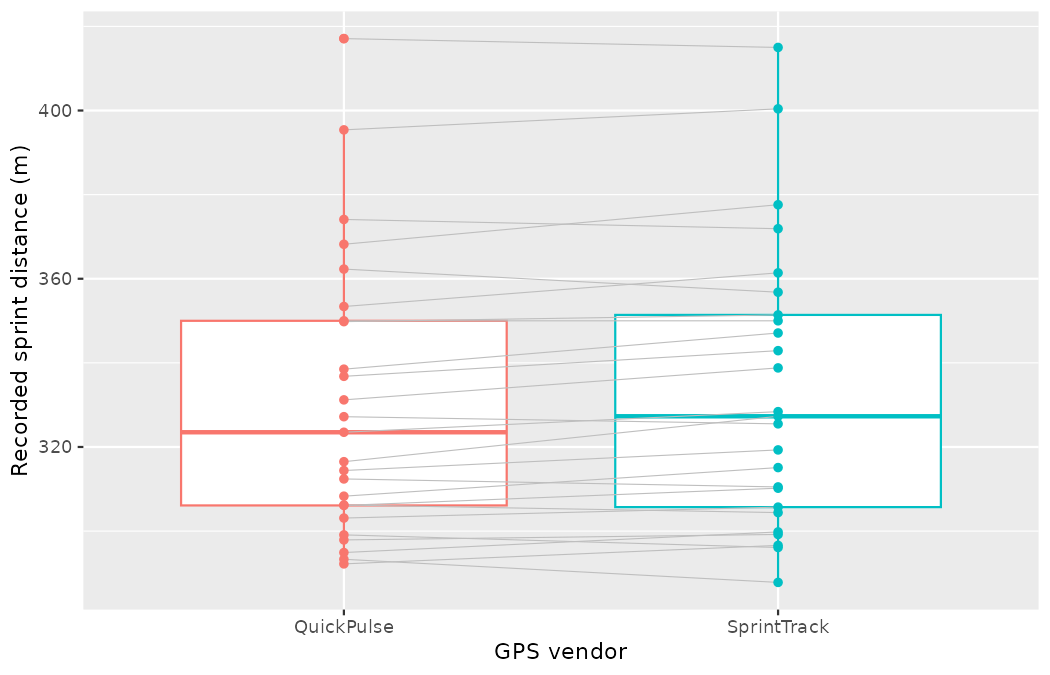
\includegraphics[width=0.85\linewidth,height=\textheight,keepaspectratio]{figures/inference-paired-means-1.png}

The two boxes are nearly indistinguishable, and both are enormous
relative to the question being asked: the 50 readings run from 287.8 m
up to 417.1 m, a 130-metre spread that belongs to the \emph{players} ---
minutes, drill groups, and positions differ --- not to the devices. The
grey pair lines carry the real signal: they are all but parallel, each
player's two readings traveling together across the whole range.

The SprintTrack representative looks at the vendor means and says:

\begin{quote}
\emph{Over a full session, SprintTrack picks up nearly three metres more
of the sprinting than QuickPulse does, on average --- our satellite fix
is simply better.}
\end{quote}

The QuickPulse representative points at the box plots and retorts:

\begin{quote}
\emph{The two distributions are practically identical, and player
workloads run from under 290 m to over 415 m. Against between-player
variation like that, with only 25 players, ordinary GPS noise (a pod
losing satellite fix under the main stand, a pocket sitting slightly
loose, etc.) could easily be what leads to a 2.7 m difference in average
recorded distance.}
\end{quote}

We'd like to be able to systematically distinguish between what the
SprintTrack representative sees in the means and what the QuickPulse
representative sees in the box plots. Fortunately for us, we have an
excellent way to simulate the natural variability that can lead to two
readings of the same run coming out different.

\subsection{Variability of the
statistic}\label{variability-of-the-statistic-15}

A randomization test will identify whether the gap between the vendor
means of the original data could have happened just by chance
variability. As before, we will simulate the variability in the study
under the assumption that the null hypothesis is true. In this study,
the null hypothesis is that average recorded sprint distance is the same
for SprintTrack and QuickPulse.

\begin{itemize}
\tightlist
\item
  \(H_0: \mu_{diff} = 0,\) the average recorded sprint distance is the
  same for the two vendors.
\item
  \(H_A: \mu_{diff} \ne 0,\) the average recorded sprint distance is
  different across the two vendors.
\end{itemize}

The subscript is new, so take the notation apart before it does any work
--- the whole family at once, because the four symbols travel together
for the rest of this chapter. Start with the observation itself: for
each pair we subtract in a consistent order (here SprintTrack minus
QuickPulse) and keep only the difference, so the \emph{difference
becomes the variable}. Then:

\begin{itemize}
\tightlist
\item
  \(\mu_{diff}\) --- the letter \(\mu\) is the population mean you have
  used since Chapter~\ref{sec-explore-numerical}; the subscript \(diff\)
  says the quantity being averaged is the within-pair difference. So
  \(\mu_{diff}\) is a \emph{single} population mean --- the mean of the
  differences --- not a difference of two separate means
  \(\mu_1 - \mu_2\) like the parameter of
  Chapter~\ref{sec-inference-two-means}. That distinction is the entire
  chapter.
\item
  \(\bar{x}_{diff}\) --- the familiar sample mean \(\bar{x},\) computed
  on the differences: add up the 25 within-player differences and divide
  by 25.
\item
  \(s_{diff}\) --- the familiar sample standard deviation \(s,\)
  computed on those same differences.
\item
  \(n_{diff}\) --- the number of \emph{pairs} (here 25), which is the
  number of differences. It is not the number of raw measurements, which
  is \(2 \times n_{diff} = 50.\)
\end{itemize}

The observed statistic is the sample mean of the differences:

\begin{Shaded}
\begin{Highlighting}[]
\NormalTok{gps\_wide }\OtherTok{\textless{}{-}}\NormalTok{ gps\_pair25 }\SpecialCharTok{|\textgreater{}}
  \FunctionTok{pivot\_wider}\NormalTok{(}\AttributeTok{id\_cols =}\NormalTok{ player, }\AttributeTok{names\_from =}\NormalTok{ vendor, }\AttributeTok{values\_from =}\NormalTok{ distance) }\SpecialCharTok{|\textgreater{}}
  \FunctionTok{mutate}\NormalTok{(}\AttributeTok{diff\_distance =}\NormalTok{ SprintTrack }\SpecialCharTok{{-}}\NormalTok{ QuickPulse)}

\FunctionTok{round}\NormalTok{(}\FunctionTok{c}\NormalTok{(}\AttributeTok{xbar\_diff =} \FunctionTok{mean}\NormalTok{(gps\_wide}\SpecialCharTok{$}\NormalTok{diff\_distance),}
        \AttributeTok{s\_diff    =} \FunctionTok{sd}\NormalTok{(gps\_wide}\SpecialCharTok{$}\NormalTok{diff\_distance)), }\DecValTok{2}\NormalTok{)}
\CommentTok{\#\textgreater{} xbar\_diff    s\_diff}
\CommentTok{\#\textgreater{}      2.69      4.72}
\end{Highlighting}
\end{Shaded}

On average, SprintTrack credited each player with
\(\bar{x}_{diff} = 2.69\) m more sprint distance than QuickPulse did for
the very same session --- though the differences are far from unanimous:
16 of the 25 were positive, 8 negative, and player 3's two pods agreed
to the tenth of a metre. Note also that \(\bar{x}_{diff}\) equals the
difference of the two vendor means, \(333.6 - 330.9,\) up to rounding
--- averaging the differences and differencing the averages are the same
arithmetic. And set \(s_{diff} = 4.72\) m against the box plots above:
the \emph{differences} vary seven-fold less than the raw readings (whose
standard deviation is about 34 m within each vendor), because
subtracting within a player removed the workload spread before the
devices' disagreement was measured. That collapse in variability is the
entire case for the paired design, and the rest of the chapter cashes it
in.

When observations are paired, the randomization process randomly assigns
the vendor label to each of the observed distance values. Note that in
the randomization test for the two-sample mean setting (see
Section~\ref{sec-rand2mean}) the explanatory variable was \emph{also}
randomly assigned to the responses. The change in the paired setting,
however, is that the assignment happens \emph{within} an observational
unit (here, a player). Remember, if the null hypothesis is true, it will
not matter which vendor's pod produced which of a player's two readings,
because the overall recorded distance will be the same across pairs.

The seeded code below performs one such shuffle: within each player, the
two vendor labels are randomly reassigned --- swapped, or left alone ---
while the two distance readings stay exactly where they are.

\begin{Shaded}
\begin{Highlighting}[]
\FunctionTok{set.seed}\NormalTok{(}\DecValTok{2102}\NormalTok{)}
\NormalTok{gps\_shuffle\_1 }\OtherTok{\textless{}{-}}\NormalTok{ gps\_pair25 }\SpecialCharTok{|\textgreater{}}
  \FunctionTok{group\_by}\NormalTok{(player) }\SpecialCharTok{|\textgreater{}}
  \FunctionTok{mutate}\NormalTok{(}\AttributeTok{random\_vendor =} \FunctionTok{sample}\NormalTok{(vendor)) }\SpecialCharTok{|\textgreater{}}
  \FunctionTok{ungroup}\NormalTok{()}
\end{Highlighting}
\end{Shaded}

The random assignment of group (vendor) happens within a single player:
every player still ends up with one reading labeled SprintTrack and one
labeled QuickPulse. Table~\ref{tbl-gps-shuffle-45} shows what happened
to players 4 and 5 in this first shuffle: it just so happens that the
4th player's vendor labels were swapped and the 5th player's were not.

\begin{longtable}[]{@{}llrl@{}}
\caption{The first within-pair shuffle, seen for two players. The 4th
player's labels were randomly swapped; the 5th player's labels randomly
stayed as they were.}\label{tbl-gps-shuffle-45}\tabularnewline
\toprule\noalign{}
player & vendor & distance (m) & random\_vendor \\
\midrule\noalign{}
\endfirsthead
\toprule\noalign{}
player & vendor & distance (m) & random\_vendor \\
\midrule\noalign{}
\endhead
\bottomrule\noalign{}
\endlastfoot
player 4 & SprintTrack & 319.3 & QuickPulse \\
player 4 & QuickPulse & 314.4 & SprintTrack \\
player 5 & SprintTrack & 315.1 & SprintTrack \\
player 5 & QuickPulse & 308.3 & QuickPulse \\
\end{longtable}

Across all 25 players, this particular shuffle swapped 13 pairs and left
12 alone. The next step in the randomization test is to sort the
readings so that each one lines up under its \emph{assigned} label from
the randomization, and then to measure the variability \emph{across} the
two shuffled groups, just as we did with the original ones:

\begin{Shaded}
\begin{Highlighting}[]
\FunctionTok{round}\NormalTok{(}\FunctionTok{c}\NormalTok{(}
  \AttributeTok{xbar\_STsim1 =} \FunctionTok{mean}\NormalTok{(gps\_shuffle\_1}\SpecialCharTok{$}\NormalTok{distance[gps\_shuffle\_1}\SpecialCharTok{$}\NormalTok{random\_vendor }\SpecialCharTok{==} \StringTok{"SprintTrack"}\NormalTok{]),}
  \AttributeTok{xbar\_QPsim1 =} \FunctionTok{mean}\NormalTok{(gps\_shuffle\_1}\SpecialCharTok{$}\NormalTok{distance[gps\_shuffle\_1}\SpecialCharTok{$}\NormalTok{random\_vendor }\SpecialCharTok{==} \StringTok{"QuickPulse"}\NormalTok{])}
\NormalTok{), }\DecValTok{1}\NormalTok{)}
\CommentTok{\#\textgreater{} xbar\_STsim1 xbar\_QPsim1}
\CommentTok{\#\textgreater{}       332.5       331.9}
\end{Highlighting}
\end{Shaded}

Read the subscripts as built pieces, in the style you have used since
Chapter~\ref{sec-foundations-randomization}: the group label \((ST\) or
\(QP)\) plus \(sim1,\) marking a statistic from the first simulated
shuffle rather than from the observed data. Under the shuffled labels,
the two ``vendors'' differ by only \(0.6\) m --- the pairing is intact,
every player still contributes one reading to each group, but most of
the systematic gap has vanished, exactly as it should when the labels
are assigned by coin flip.

Two more randomizations, each with its own seed, tell the same story:

\begin{Shaded}
\begin{Highlighting}[]
\FunctionTok{set.seed}\NormalTok{(}\DecValTok{2103}\NormalTok{)}
\NormalTok{gps\_shuffle\_2 }\OtherTok{\textless{}{-}}\NormalTok{ gps\_pair25 }\SpecialCharTok{|\textgreater{}}
  \FunctionTok{group\_by}\NormalTok{(player) }\SpecialCharTok{|\textgreater{}}
  \FunctionTok{mutate}\NormalTok{(}\AttributeTok{random\_vendor =} \FunctionTok{sample}\NormalTok{(vendor)) }\SpecialCharTok{|\textgreater{}}
  \FunctionTok{ungroup}\NormalTok{()}

\FunctionTok{round}\NormalTok{(}\FunctionTok{c}\NormalTok{(}
  \AttributeTok{xbar\_STsim2 =} \FunctionTok{mean}\NormalTok{(gps\_shuffle\_2}\SpecialCharTok{$}\NormalTok{distance[gps\_shuffle\_2}\SpecialCharTok{$}\NormalTok{random\_vendor }\SpecialCharTok{==} \StringTok{"SprintTrack"}\NormalTok{]),}
  \AttributeTok{xbar\_QPsim2 =} \FunctionTok{mean}\NormalTok{(gps\_shuffle\_2}\SpecialCharTok{$}\NormalTok{distance[gps\_shuffle\_2}\SpecialCharTok{$}\NormalTok{random\_vendor }\SpecialCharTok{==} \StringTok{"QuickPulse"}\NormalTok{])}
\NormalTok{), }\DecValTok{1}\NormalTok{)}
\CommentTok{\#\textgreater{} xbar\_STsim2 xbar\_QPsim2}
\CommentTok{\#\textgreater{}       332.1       332.3}

\FunctionTok{set.seed}\NormalTok{(}\DecValTok{2104}\NormalTok{)}
\NormalTok{gps\_shuffle\_3 }\OtherTok{\textless{}{-}}\NormalTok{ gps\_pair25 }\SpecialCharTok{|\textgreater{}}
  \FunctionTok{group\_by}\NormalTok{(player) }\SpecialCharTok{|\textgreater{}}
  \FunctionTok{mutate}\NormalTok{(}\AttributeTok{random\_vendor =} \FunctionTok{sample}\NormalTok{(vendor)) }\SpecialCharTok{|\textgreater{}}
  \FunctionTok{ungroup}\NormalTok{()}

\FunctionTok{round}\NormalTok{(}\FunctionTok{c}\NormalTok{(}
  \AttributeTok{xbar\_STsim3 =} \FunctionTok{mean}\NormalTok{(gps\_shuffle\_3}\SpecialCharTok{$}\NormalTok{distance[gps\_shuffle\_3}\SpecialCharTok{$}\NormalTok{random\_vendor }\SpecialCharTok{==} \StringTok{"SprintTrack"}\NormalTok{]),}
  \AttributeTok{xbar\_QPsim3 =} \FunctionTok{mean}\NormalTok{(gps\_shuffle\_3}\SpecialCharTok{$}\NormalTok{distance[gps\_shuffle\_3}\SpecialCharTok{$}\NormalTok{random\_vendor }\SpecialCharTok{==} \StringTok{"QuickPulse"}\NormalTok{])}
\NormalTok{), }\DecValTok{1}\NormalTok{)}
\CommentTok{\#\textgreater{} xbar\_STsim3 xbar\_QPsim3}
\CommentTok{\#\textgreater{}       332.1       332.3}
\end{Highlighting}
\end{Shaded}

The second shuffle swapped 12 pairs, the third 11; each lands the
simulated vendor gap at \(0.2\) m, this time with QuickPulse nominally
on top. Shuffle after shuffle, the within-pair randomization produces
average differences a fraction of the observed \(2.69\) m.

\begin{tcolorbox}[enhanced jigsaw, left=2mm, leftrule=.75mm, title=\textcolor{quarto-callout-tip-color}{\faLightbulb}\hspace{0.5em}{Check your understanding}, arc=.35mm, rightrule=.15mm, coltitle=black, colframe=quarto-callout-tip-color-frame, bottomrule=.15mm, colbacktitle=quarto-callout-tip-color!10!white, opacitybacktitle=0.6, breakable, bottomtitle=1mm, toptitle=1mm, titlerule=0mm, opacityback=0, toprule=.15mm, colback=white]

Why not simply feed the 25 SprintTrack readings and the 25 QuickPulse
readings into the two-independent-samples machinery of
Chapter~\ref{sec-inference-two-means}?

\begin{center}\rule{0.5\linewidth}{0.5pt}\end{center}

Because the two groups are not independent: they contain the same 25
players running the same session, so each SprintTrack reading is tied to
exactly one QuickPulse reading. Ignoring the pairing throws information
away --- here, nearly all of it. Players differ enormously in how much
they sprint: the 50 readings run from 287.8 m to 417.1 m, and each
vendor's 25 readings have a standard deviation of about 34 m, a spread
driven by workload, not by the devices. A two-sample analysis must treat
all of that between-player variability as noise: its standard error
(recall Section~\ref{sec-math2samp}) would be
\(\sqrt{33.7^2/25 + 33.5^2/25} \approx 9.5\) m, and against that
yardstick the observed 2.69 m vendor gap is invisible. The within-pair
difference deletes each player's workload from the comparison entirely,
leaving only what the two devices disagree about: \(s_{diff} = 4.72\) m,
hence a standard error of \(4.72/\sqrt{25} \approx 0.94\) m --- ten
times smaller. Pairing is not a nicety here; it is the difference
between a question these data can answer and one they cannot.

\end{tcolorbox}

\subsection{Observed statistic vs.~null
statistics}\label{observed-statistic-vs.-null-statistics-7}

By repeating the randomization process, we can create a distribution of
the average of the differences in recorded sprint distance. The
\textbf{infer} pipeline below runs 1,000 within-pair shuffles. The null
hypothesis of \emph{paired independence} is exactly the shuffle we
performed by hand above: within each pair, the sign of the difference is
flipped or kept at random, which is what ``the vendor labels don't
matter'' means once the data are reduced to one difference per player.

\begin{tcolorbox}[enhanced jigsaw, left=2mm, leftrule=.75mm, title=\textcolor{quarto-callout-tip-color}{\faLightbulb}\hspace{0.5em}{Check your understanding}, arc=.35mm, rightrule=.15mm, coltitle=black, colframe=quarto-callout-tip-color-frame, bottomrule=.15mm, colbacktitle=quarto-callout-tip-color!10!white, opacitybacktitle=0.6, breakable, bottomtitle=1mm, toptitle=1mm, titlerule=0mm, opacityback=0, toprule=.15mm, colback=white]

Player 9's difference is \(+4.1\) m (SprintTrack read 310.2, QuickPulse
306.1). After one within-pair shuffle, what values can this pair's
difference take, and with what probabilities?

\begin{center}\rule{0.5\linewidth}{0.5pt}\end{center}

Only two: \(+4.1\) m if the labels happen to stay put, and \(-4.1\) m if
they swap --- each with probability one-half. The within-pair shuffle
can never change the \emph{magnitude} of a pair's difference, only its
sign, and that two-value set is the entire null universe for one pair.
The null distribution below is nothing more exotic than 25 such coin
flips at a time, repeated 1,000 times.

\end{tcolorbox}

\begin{Shaded}
\begin{Highlighting}[]
\FunctionTok{set.seed}\NormalTok{(}\DecValTok{2105}\NormalTok{)}
\NormalTok{gps\_null }\OtherTok{\textless{}{-}}\NormalTok{ gps\_pair25 }\SpecialCharTok{|\textgreater{}}
  \FunctionTok{pivot\_wider}\NormalTok{(}\AttributeTok{id\_cols =}\NormalTok{ player, }\AttributeTok{names\_from =}\NormalTok{ vendor, }\AttributeTok{values\_from =}\NormalTok{ distance) }\SpecialCharTok{|\textgreater{}}
  \FunctionTok{mutate}\NormalTok{(}\AttributeTok{diff\_distance =}\NormalTok{ SprintTrack }\SpecialCharTok{{-}}\NormalTok{ QuickPulse) }\SpecialCharTok{|\textgreater{}}
  \FunctionTok{specify}\NormalTok{(}\AttributeTok{response =}\NormalTok{ diff\_distance) }\SpecialCharTok{|\textgreater{}}
  \FunctionTok{hypothesize}\NormalTok{(}\AttributeTok{null =} \StringTok{"paired independence"}\NormalTok{) }\SpecialCharTok{|\textgreater{}}
  \FunctionTok{generate}\NormalTok{(}\DecValTok{1000}\NormalTok{, }\AttributeTok{type =} \StringTok{"permute"}\NormalTok{) }\SpecialCharTok{|\textgreater{}}
  \FunctionTok{calculate}\NormalTok{(}\AttributeTok{stat =} \StringTok{"mean"}\NormalTok{)}

\FunctionTok{ggplot}\NormalTok{(gps\_null, }\FunctionTok{aes}\NormalTok{(}\AttributeTok{x =}\NormalTok{ stat)) }\SpecialCharTok{+}
  \FunctionTok{geom\_histogram}\NormalTok{(}\AttributeTok{binwidth =} \FloatTok{0.25}\NormalTok{) }\SpecialCharTok{+}
  \FunctionTok{geom\_vline}\NormalTok{(}\AttributeTok{xintercept =} \FloatTok{2.69}\NormalTok{, }\AttributeTok{color =} \StringTok{"red"}\NormalTok{) }\SpecialCharTok{+}
  \FunctionTok{labs}\NormalTok{(}
    \AttributeTok{x =} \StringTok{"Mean of randomized differences in recorded sprint distance}\SpecialCharTok{\textbackslash{}n}\StringTok{(SprintTrack {-} QuickPulse)"}\NormalTok{,}
    \AttributeTok{y =} \StringTok{"Count"}\NormalTok{,}
    \AttributeTok{title =} \StringTok{"1,000 means of randomized differences"}
\NormalTok{  )}
\end{Highlighting}
\end{Shaded}

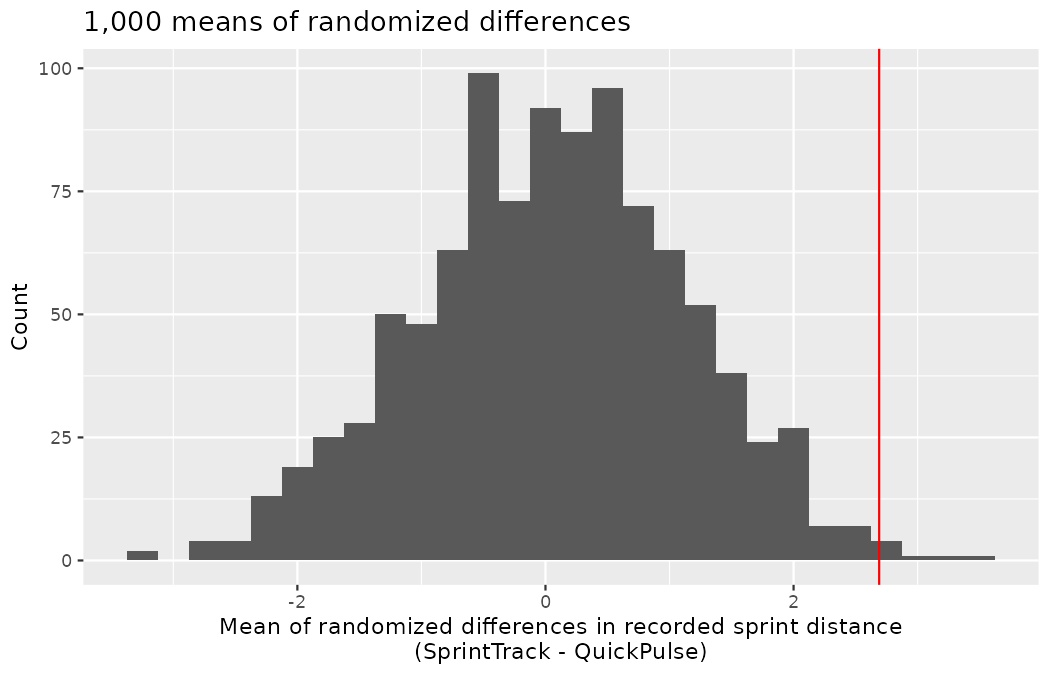
\includegraphics[width=0.85\linewidth,height=\textheight,keepaspectratio]{figures/inference-paired-means-2.png}

As expected (because the differences were generated under the null
hypothesis), the histogram is centered at zero: the shuffles make no
distinction between the vendors, so their average differences fall
around zero with random fluctuation. The 1,000 simulated means run from
\(-3.21\) to \(3.49\) m. The red line at the observed
\(\bar{x}_{diff} = 2.69\) m sits deep in the right tail:

\begin{Shaded}
\begin{Highlighting}[]
\NormalTok{gps\_null }\SpecialCharTok{|\textgreater{}}
  \FunctionTok{summarize}\NormalTok{(}
    \AttributeTok{n\_extreme =} \FunctionTok{sum}\NormalTok{(}\FunctionTok{abs}\NormalTok{(stat) }\SpecialCharTok{\textgreater{}=} \FloatTok{2.69}\NormalTok{),}
    \AttributeTok{p\_value   =} \FunctionTok{mean}\NormalTok{(}\FunctionTok{abs}\NormalTok{(stat) }\SpecialCharTok{\textgreater{}=} \FloatTok{2.69}\NormalTok{)}
\NormalTok{  )}
\CommentTok{\#\textgreater{} \# A tibble: 1 × 2}
\CommentTok{\#\textgreater{}   n\_extreme p\_value}
\CommentTok{\#\textgreater{}       \textless{}int\textgreater{}   \textless{}dbl\textgreater{}}
\CommentTok{\#\textgreater{} 1        12   0.012}
\end{Highlighting}
\end{Shaded}

Only 12 of the 1,000 within-pair shuffles produced an average difference
as far from zero as the observed one, in either direction: the p-value
is \(0.012.\) Note the change of scenery from this book's usual
\(0/1000\) verdicts: the observed statistic sits \emph{inside} the range
of the null draws --- coin-flipped labels can, occasionally, manufacture
a vendor gap this size from pure device noise --- but they manage it
barely one shuffle in eighty. At the customary discernibility level of
\(\alpha = 0.05,\) we reject \(H_0\) and conclude that
\(\mu_{ST} \ne \mu_{QP}\) --- the extra 2.69 m per session that
SprintTrack credits is due to more than just measurement noise.

For Marta, the operational reading matters more than the verdict:
neither vendor is ``wrong'' (there is no ground truth on the pitch), but
the two systems are \emph{not interchangeable}. If the academy switches
vendors mid-season, every longitudinal sprint profile in the scouting
database inherits a systematic 2.7 m-per-session step that has nothing
to do with the players --- small against a 330 m session, but pointing
the same way in every session, for every player.

\section{Bootstrap confidence interval for the mean paired
difference}\label{bootstrap-confidence-interval-for-the-mean-paired-difference}

For both the bootstrap and the mathematical models applied to paired
data, the analysis is virtually identical to the one-sample approach
given in Chapter~\ref{sec-inference-one-mean}. The key to working with
paired data (for bootstrapping and mathematical approaches) is to
consider the measurement of interest to be the difference in measured
values across the pair of observations.

\subsection{Observed data}\label{observed-data-16}

Since Chapter~\ref{sec-explore-categorical}, this book has kept
returning to shots taken under defensive pressure, and each return has
used a different tool. Chapter~\ref{sec-foundations-randomization} asked
whether pressured shots are \emph{finished} worse;
Chapter~\ref{sec-inference-one-mean} tested pressured shots' chance
quality against a fixed benchmark; and the machinery of
Chapter~\ref{sec-inference-two-means}, applied to the 2022 Men's World
Cup, would pool all 238 pressured shots against all 1,256 unpressured
ones to compare mean chance quality. Here is the paired version of that
last question, and it is the version a scout comparing \emph{teams}
actually needs: for each team, how does the chance quality of its own
pressured shots compare with the chance quality of its own unpressured
shots?

Each team contributes two measurements --- its mean xG under pressure
and its mean xG otherwise --- and those two measurements form a pair,
connected by the team that produced both. One filter is needed before
the pairs are worth computing: a team's ``mean pressured xG'' built on
two or three shots is noise, so we require \textbf{at least 5 pressured
shots per team}. The code below states the filter and shows what it
costs.

\begin{Shaded}
\begin{Highlighting}[]
\NormalTok{wc2022\_shots }\OtherTok{\textless{}{-}} \FunctionTok{read\_csv}\NormalTok{(}\StringTok{"data/derived/wc2022\_shots.csv"}\NormalTok{)}

\NormalTok{team\_pressure }\OtherTok{\textless{}{-}}\NormalTok{ wc2022\_shots }\SpecialCharTok{|\textgreater{}}
  \FunctionTok{group\_by}\NormalTok{(team) }\SpecialCharTok{|\textgreater{}}
  \FunctionTok{summarize}\NormalTok{(}
    \AttributeTok{n\_prs  =} \FunctionTok{sum}\NormalTok{(under\_pressure),}
    \AttributeTok{xg\_prs =} \FunctionTok{mean}\NormalTok{(statsbomb\_xg[under\_pressure]),}
    \AttributeTok{xg\_nop =} \FunctionTok{mean}\NormalTok{(statsbomb\_xg[}\SpecialCharTok{!}\NormalTok{under\_pressure])}
\NormalTok{  ) }\SpecialCharTok{|\textgreater{}}
  \FunctionTok{filter}\NormalTok{(n\_prs }\SpecialCharTok{\textgreater{}=} \DecValTok{5}\NormalTok{) }\SpecialCharTok{|\textgreater{}}
  \FunctionTok{mutate}\NormalTok{(}\AttributeTok{xg\_diff =}\NormalTok{ xg\_prs }\SpecialCharTok{{-}}\NormalTok{ xg\_nop)}

\FunctionTok{nrow}\NormalTok{(team\_pressure)}
\CommentTok{\#\textgreater{} [1] 22}
\end{Highlighting}
\end{Shaded}

The filter keeps 22 of the 32 teams (among the ten dropped: Australia,
whose 26-shot campaign you dissected in
Chapter~\ref{sec-inference-one-mean}, and Spain). A portion of the
dataset is shown in Table~\ref{tbl-teampairsDF}.

\begin{Shaded}
\begin{Highlighting}[]
\NormalTok{team\_pressure }\SpecialCharTok{|\textgreater{}}
  \FunctionTok{mutate}\NormalTok{(}\FunctionTok{across}\NormalTok{(}\FunctionTok{where}\NormalTok{(is.double), \textbackslash{}(x) }\FunctionTok{round}\NormalTok{(x, }\DecValTok{4}\NormalTok{))) }\SpecialCharTok{|\textgreater{}}
  \FunctionTok{head}\NormalTok{(}\DecValTok{4}\NormalTok{)}
\CommentTok{\#\textgreater{} \# A tibble: 4 × 5}
\CommentTok{\#\textgreater{}   team      n\_prs xg\_prs xg\_nop xg\_diff}
\CommentTok{\#\textgreater{}   \textless{}chr\textgreater{}     \textless{}int\textgreater{}  \textless{}dbl\textgreater{}  \textless{}dbl\textgreater{}   \textless{}dbl\textgreater{}}
\CommentTok{\#\textgreater{} 1 Argentina    13 0.0622 0.208  {-}0.146}
\CommentTok{\#\textgreater{} 2 Belgium      10 0.085  0.114  {-}0.0288}
\CommentTok{\#\textgreater{} 3 Brazil       13 0.103  0.143  {-}0.0402}
\CommentTok{\#\textgreater{} 4 Canada        9 0.164  0.0944  0.0693}
\end{Highlighting}
\end{Shaded}

\begin{longtable}[]{@{}lrrrr@{}}
\caption{Four cases from the \texttt{team\_pressure} dataset: per-team
mean chance quality (xG per shot) under pressure and not, and the
within-team difference.}\label{tbl-teampairsDF}\tabularnewline
\toprule\noalign{}
team & n\_prs & xg\_prs & xg\_nop & xg\_diff \\
\midrule\noalign{}
\endfirsthead
\toprule\noalign{}
team & n\_prs & xg\_prs & xg\_nop & xg\_diff \\
\midrule\noalign{}
\endhead
\bottomrule\noalign{}
\endlastfoot
Argentina & 13 & 0.0622 & 0.2080 & -0.1458 \\
Belgium & 10 & 0.0850 & 0.1138 & -0.0288 \\
Brazil & 13 & 0.1028 & 0.1430 & -0.0402 \\
Canada & 9 & 0.1637 & 0.0944 & 0.0693 \\
\end{longtable}

\begin{tcolorbox}[enhanced jigsaw, left=2mm, leftrule=.75mm, title=\textcolor{quarto-callout-note-color}{\faInfo}\hspace{0.5em}{Data}, arc=.35mm, rightrule=.15mm, coltitle=black, colframe=quarto-callout-note-color-frame, bottomrule=.15mm, colbacktitle=quarto-callout-note-color!10!white, opacitybacktitle=0.6, breakable, bottomtitle=1mm, toptitle=1mm, titlerule=0mm, opacityback=0, toprule=.15mm, colback=white]

The \texttt{team\_pressure} pairs are built from
\texttt{data/derived/wc2022\_shots.csv} (StatsBomb open data) by the
code above; rerun it and you will get the identical 22 rows.

\end{tcolorbox}

Each team has two corresponding chance-quality summaries in the dataset:
one for its pressured shots and one for its unpressured shots. When two
sets of observations have this special correspondence, they are said to
be \textbf{paired}.

Before any resampling, the frame flag that this book's penalty
convention demands. A penalty is the one shot on which defensive
pressure is impossible by law, so every penalty in these data sits
inside the \emph{unpressured} side of its team's pair --- and at a
stored chance quality of 0.7835, penalties do not sit quietly:

\begin{Shaded}
\begin{Highlighting}[]
\NormalTok{wc2022\_shots }\SpecialCharTok{|\textgreater{}}
  \FunctionTok{filter}\NormalTok{(under\_pressure) }\SpecialCharTok{|\textgreater{}}
  \FunctionTok{count}\NormalTok{(shot\_type)}
\CommentTok{\#\textgreater{} \# A tibble: 1 × 2}
\CommentTok{\#\textgreater{}   shot\_type     n}
\CommentTok{\#\textgreater{}   \textless{}chr\textgreater{}     \textless{}int\textgreater{}}
\CommentTok{\#\textgreater{} 1 Open Play   238}

\NormalTok{pens\_kept }\OtherTok{\textless{}{-}}\NormalTok{ wc2022\_shots }\SpecialCharTok{|\textgreater{}}
  \FunctionTok{filter}\NormalTok{(shot\_type }\SpecialCharTok{==} \StringTok{"Penalty"}\NormalTok{, team }\SpecialCharTok{\%in\%}\NormalTok{ team\_pressure}\SpecialCharTok{$}\NormalTok{team)}

\FunctionTok{c}\NormalTok{(}\AttributeTok{kicks =} \FunctionTok{nrow}\NormalTok{(pens\_kept), }\AttributeTok{teams =} \FunctionTok{n\_distinct}\NormalTok{(pens\_kept}\SpecialCharTok{$}\NormalTok{team),}
  \AttributeTok{pressured =} \FunctionTok{sum}\NormalTok{(pens\_kept}\SpecialCharTok{$}\NormalTok{under\_pressure))}
\CommentTok{\#\textgreater{}     kicks     teams pressured}
\CommentTok{\#\textgreater{}        57        15         0}

\FunctionTok{round}\NormalTok{(}\FunctionTok{mean}\NormalTok{(pens\_kept}\SpecialCharTok{$}\NormalTok{statsbomb\_xg), }\DecValTok{4}\NormalTok{)}
\CommentTok{\#\textgreater{} [1] 0.7835}
\end{Highlighting}
\end{Shaded}

All 238 pressured shots are open play, while 57 penalty kicks --- spread
across 15 of our 22 teams --- are propping up the unpressured side of
those teams' pairs. Argentina alone took 14 of them, which is much of
why its unpressured mean of 0.2080 xG towers over everyone else's. Per
the convention, we will run the full analysis in this all-shots frame
first, mirroring the arithmetic exactly, and then recompute every pair
on the open-play frame in Section~\ref{sec-mathpaired} --- and you will
want to see both answers before anything reaches a dossier.

\subsection{Variability of the
statistic}\label{variability-of-the-statistic-16}

Following the example of bootstrapping the one-sample statistic in
Section~\ref{sec-boot1mean}, the observed \emph{differences} can be
bootstrapped in order to understand the variability of the average
difference from sample to sample. Remember, the differences act as a
single value to bootstrap. That is, the original dataset consists of the
22 values of \texttt{xg\_diff}, and each resample will also contain 22
differences (some teams repeated, some omitted, through the resampling
process) --- exactly the procedure applied to the five logged shots in
Section~\ref{sec-boot1mean}, with a difference per team in place of a
chance quality per shot.

\begin{Shaded}
\begin{Highlighting}[]
\NormalTok{obs\_diff\_mean }\OtherTok{\textless{}{-}}\NormalTok{ team\_pressure }\SpecialCharTok{|\textgreater{}}
  \FunctionTok{specify}\NormalTok{(}\AttributeTok{response =}\NormalTok{ xg\_diff) }\SpecialCharTok{|\textgreater{}}
  \FunctionTok{calculate}\NormalTok{(}\AttributeTok{stat =} \StringTok{"mean"}\NormalTok{)}

\FunctionTok{set.seed}\NormalTok{(}\DecValTok{2106}\NormalTok{)}
\NormalTok{boot\_team\_diff }\OtherTok{\textless{}{-}}\NormalTok{ team\_pressure }\SpecialCharTok{|\textgreater{}}
  \FunctionTok{specify}\NormalTok{(}\AttributeTok{response =}\NormalTok{ xg\_diff) }\SpecialCharTok{|\textgreater{}}
  \FunctionTok{generate}\NormalTok{(}\AttributeTok{reps =} \DecValTok{1000}\NormalTok{, }\AttributeTok{type =} \StringTok{"bootstrap"}\NormalTok{) }\SpecialCharTok{|\textgreater{}}
  \FunctionTok{calculate}\NormalTok{(}\AttributeTok{stat =} \StringTok{"mean"}\NormalTok{)}

\FunctionTok{ggplot}\NormalTok{(boot\_team\_diff, }\FunctionTok{aes}\NormalTok{(}\AttributeTok{x =}\NormalTok{ stat)) }\SpecialCharTok{+}
  \FunctionTok{geom\_histogram}\NormalTok{(}\AttributeTok{binwidth =} \FloatTok{0.0025}\NormalTok{) }\SpecialCharTok{+}
  \FunctionTok{labs}\NormalTok{(}
    \AttributeTok{x =} \StringTok{"Mean of bootstrapped differences in team mean xG}\SpecialCharTok{\textbackslash{}n}\StringTok{(pressured {-} not pressured)"}\NormalTok{,}
    \AttributeTok{y =} \StringTok{"Count"}\NormalTok{,}
    \AttributeTok{title =} \StringTok{"1,000 means of bootstrapped differences"}
\NormalTok{  )}
\end{Highlighting}
\end{Shaded}

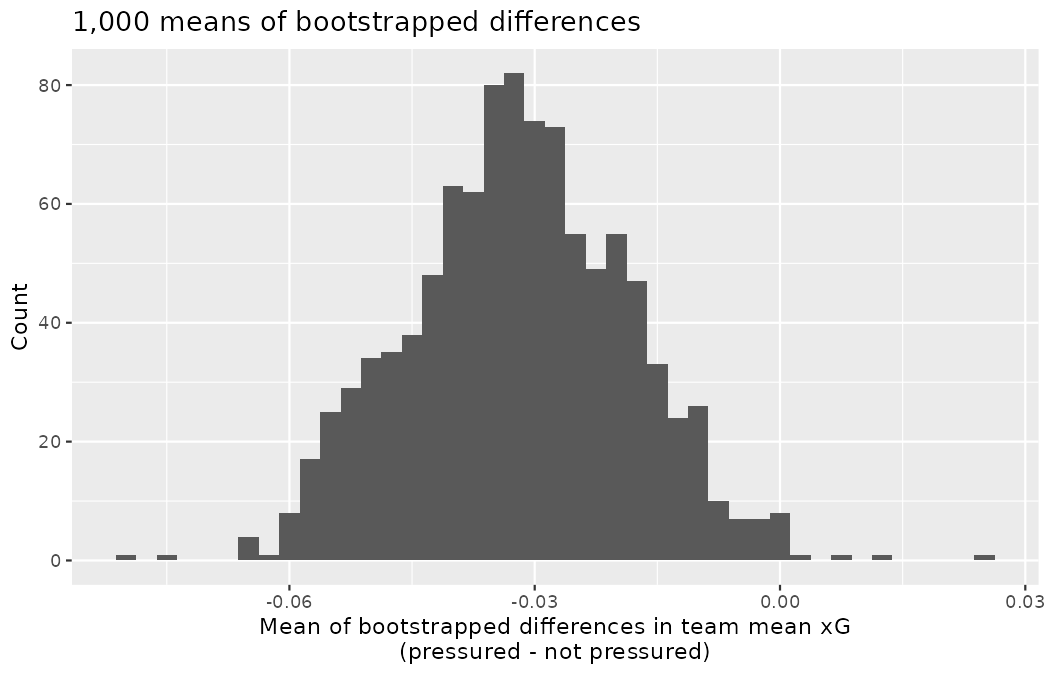
\includegraphics[width=0.85\linewidth,height=\textheight,keepaspectratio]{figures/inference-paired-means-3.png}

Two 99\% confidence intervals for the mean within-team difference in
chance quality can be computed from these bootstrapped means. The
bootstrap percentile confidence interval is found from the 0.5 and 99.5
percentiles of the bootstrapped differences:

\begin{Shaded}
\begin{Highlighting}[]
\FunctionTok{get\_confidence\_interval}\NormalTok{(boot\_team\_diff, }\AttributeTok{level =} \FloatTok{0.99}\NormalTok{, }\AttributeTok{type =} \StringTok{"percentile"}\NormalTok{)}
\CommentTok{\#\textgreater{} \# A tibble: 1 × 2}
\CommentTok{\#\textgreater{}   lower\_ci upper\_ci}
\CommentTok{\#\textgreater{}      \textless{}dbl\textgreater{}    \textless{}dbl\textgreater{}}
\CommentTok{\#\textgreater{} 1  {-}0.0648 0.000855}
\end{Highlighting}
\end{Shaded}

\begin{tcolorbox}[enhanced jigsaw, left=2mm, leftrule=.75mm, title=\textcolor{quarto-callout-tip-color}{\faLightbulb}\hspace{0.5em}{Check your understanding}, arc=.35mm, rightrule=.15mm, coltitle=black, colframe=quarto-callout-tip-color-frame, bottomrule=.15mm, colbacktitle=quarto-callout-tip-color!10!white, opacitybacktitle=0.6, breakable, bottomtitle=1mm, toptitle=1mm, titlerule=0mm, opacityback=0, toprule=.15mm, colback=white]

Using the histogram of bootstrapped differences in means drawn above,
estimate the standard error of the mean of the sample differences,
\(\bar{x}_{diff}.\)

\begin{center}\rule{0.5\linewidth}{0.5pt}\end{center}

The bulk of the bootstrapped means runs from about \(-0.057\) to
\(-0.005,\) a spread of roughly \(0.052.\) Using the empirical rule
(with bell-shaped distributions, most observations sit within two
standard errors of the center), the standard error of the mean
differences is approximately \(0.052 / 4 \approx 0.013\) xG. The
standard deviation of the 1,000 bootstrapped means confirms it:
\(SE_{BS} = 0.0135\) (the bootstrap standard error of
Section~\ref{sec-boot1mean}, computed with \texttt{sd()}). You might
note that the standard error calculation given in
Section~\ref{sec-mathpaired} is
\(SE(\bar{x}_{diff}) = s_{diff}/\sqrt{n_{diff}} = 0.0612/\sqrt{22} = 0.0131\)
(values from Section~\ref{sec-mathpaired}) --- very close to the
bootstrap approximation.

\end{tcolorbox}

The bootstrap SE interval is found by computing the SE of the
bootstrapped differences \((SE_{\bar{x}_{diff}} = 0.0135)\) and the
normal multiplier of \(z^{\star} = 2.58\) (the 99\% cutoff from
Chapter~\ref{sec-inference-one-prop}). The averaged difference is
\(\bar{x}_{diff} = -0.0317.\) The 99\% confidence interval is
\(-0.0317 \pm 2.58 \times 0.0135,\) which the code computes without
intermediate rounding:

\begin{Shaded}
\begin{Highlighting}[]
\FunctionTok{get\_confidence\_interval}\NormalTok{(boot\_team\_diff, }\AttributeTok{level =} \FloatTok{0.99}\NormalTok{, }\AttributeTok{type =} \StringTok{"se"}\NormalTok{,}
                        \AttributeTok{point\_estimate =}\NormalTok{ obs\_diff\_mean)}
\CommentTok{\#\textgreater{} \# A tibble: 1 × 2}
\CommentTok{\#\textgreater{}   lower\_ci upper\_ci}
\CommentTok{\#\textgreater{}      \textless{}dbl\textgreater{}    \textless{}dbl\textgreater{}}
\CommentTok{\#\textgreater{} 1  {-}0.0664  0.00310}
\end{Highlighting}
\end{Shaded}

The confidence intervals seem to indicate that within a team, pressured
shots are, on average, worse chances than unpressured ones, as the large
majority of each interval is negative. However, if the analysis requires
a strong degree of certainty --- and 99\% is a strong degree --- the
result is not well determined: both the percentile interval and the SE
interval poke just past zero (upper bounds of \(0.0009\) and \(0.0031\)
xG), leaving open the possibility that the true mean within-team
difference is zero or even slightly positive. Notice also that the two
intervals, built by different constructions from the same resamples,
agree closely here --- the bootstrap distribution is roughly symmetric
and bell-shaped, unlike the clumpy five-shot distributions of
Section~\ref{sec-boot1mean}, so both constructions are on their home
turf. Whether the evidence clears a less demanding bar is exactly the
question for the mathematical model, next.

\section{Mathematical model for the mean paired
difference}\label{sec-mathpaired}

Thinking about the differences as a single observation on an
observational unit changes the paired setting into the one-sample
setting. The mathematical model for the one-sample case is covered in
Section~\ref{sec-one-mean-math}, and every tool from that section ---
the \(t\)-distribution, \(df = n - 1,\) the T score --- transfers to the
differences unchanged.

\subsection{Observed data}\label{observed-data-17}

To analyze paired data, it is often useful to look at the difference in
outcomes of each pair of observations. In the team pressure data, we
look at the differences in mean chance quality, represented as the
\texttt{xg\_diff} variable in the dataset. Here the differences are
taken as

\[\text{mean xG under pressure} - \text{mean xG not under pressure}\]

It is important that we always subtract using a consistent order; here
the unpressured mean is always subtracted from the pressured mean, so a
negative difference means a team's pressured shots are the worse
chances. The first difference shown in Table~\ref{tbl-teampairsDF} is
computed as \(0.0622 - 0.2080 = -0.1458.\) Similarly, the second
difference is computed as \(0.0850 - 0.1138 = -0.0288,\) and the third
is \(0.1028 - 0.1430 = -0.0402.\) A histogram of the 22 differences is
drawn by the code below.

\begin{Shaded}
\begin{Highlighting}[]
\FunctionTok{ggplot}\NormalTok{(team\_pressure, }\FunctionTok{aes}\NormalTok{(}\AttributeTok{x =}\NormalTok{ xg\_diff)) }\SpecialCharTok{+}
  \FunctionTok{geom\_histogram}\NormalTok{(}\AttributeTok{binwidth =} \FloatTok{0.025}\NormalTok{) }\SpecialCharTok{+}
  \FunctionTok{labs}\NormalTok{(}
    \AttributeTok{x =} \StringTok{"Difference in team mean xG (pressured {-} not pressured)"}\NormalTok{,}
    \AttributeTok{y =} \StringTok{"Count"}
\NormalTok{  )}
\end{Highlighting}
\end{Shaded}

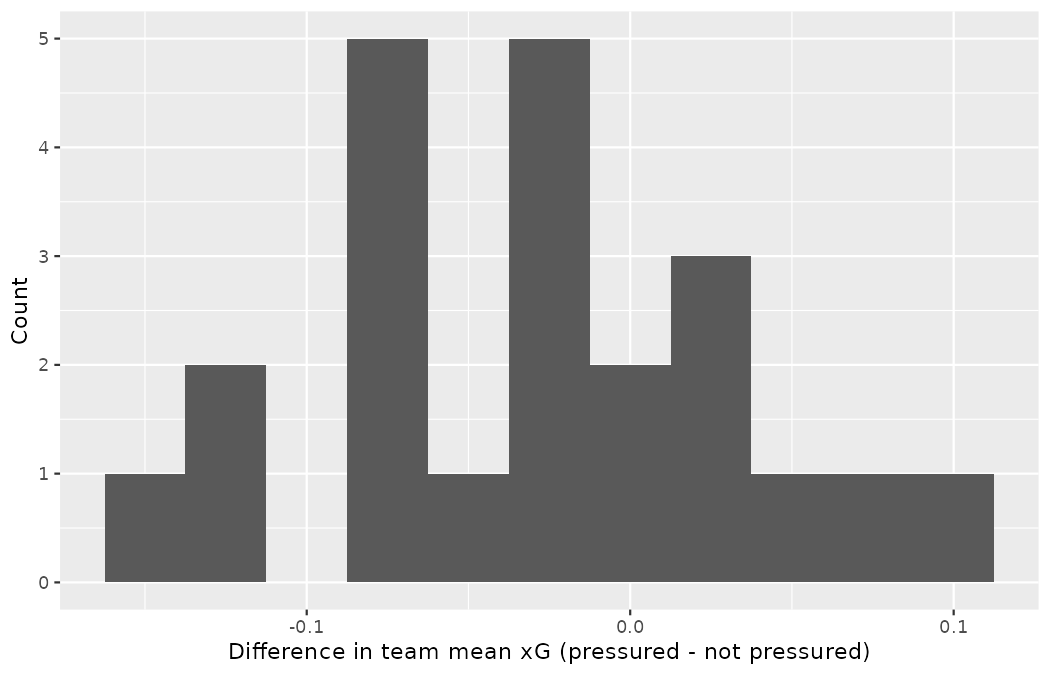
\includegraphics[width=0.85\linewidth,height=\textheight,keepaspectratio]{figures/inference-paired-means-4.png}

The histogram sits mostly below zero --- 15 of the 22 teams have
negative differences --- with Argentina's \(-0.1458\) anchoring the left
tail and Switzerland's \(+0.0992\) the right.

\subsection{Variability of the
statistic}\label{variability-of-the-statistic-17}

To analyze a paired dataset, we simply analyze the differences.
Table~\ref{tbl-teampairsSummaryStats} provides the data summaries from
the team pressure data. Note that instead of reporting the two
chance-quality columns separately, the summary statistics are given as
the mean of the differences, the standard deviation of the differences,
and the total number of pairs (i.e., differences) --- which is to say,
as \(\bar{x}_{diff},\) \(s_{diff},\) and \(n_{diff}.\) The parameter of
interest is also a single value, \(\mu_{diff},\) so we can use the same
\(t\)-distribution techniques we applied in
Section~\ref{sec-one-mean-math} directly onto the observed differences.

\begin{Shaded}
\begin{Highlighting}[]
\NormalTok{team\_pressure }\SpecialCharTok{|\textgreater{}}
  \FunctionTok{summarize}\NormalTok{(}
    \AttributeTok{n    =} \FunctionTok{n}\NormalTok{(),}
    \AttributeTok{mean =} \FunctionTok{round}\NormalTok{(}\FunctionTok{mean}\NormalTok{(xg\_diff), }\DecValTok{4}\NormalTok{),}
    \AttributeTok{sd   =} \FunctionTok{round}\NormalTok{(}\FunctionTok{sd}\NormalTok{(xg\_diff), }\DecValTok{4}\NormalTok{)}
\NormalTok{  )}
\CommentTok{\#\textgreater{} \# A tibble: 1 × 3}
\CommentTok{\#\textgreater{}       n    mean     sd}
\CommentTok{\#\textgreater{}   \textless{}int\textgreater{}   \textless{}dbl\textgreater{}  \textless{}dbl\textgreater{}}
\CommentTok{\#\textgreater{} 1    22 {-}0.0317 0.0612}
\end{Highlighting}
\end{Shaded}

\begin{longtable}[]{@{}ccc@{}}
\caption{Summary statistics for the 22 within-team differences in mean
chance quality (xG per
shot).}\label{tbl-teampairsSummaryStats}\tabularnewline
\toprule\noalign{}
n & Mean & SD \\
\midrule\noalign{}
\endfirsthead
\toprule\noalign{}
n & Mean & SD \\
\midrule\noalign{}
\endhead
\bottomrule\noalign{}
\endlastfoot
22 & -0.0317 & 0.0612 \\
\end{longtable}

\begin{tcolorbox}[enhanced jigsaw, left=2mm, leftrule=.75mm, title=\textcolor{quarto-callout-note-color}{\faInfo}\hspace{0.5em}{Worked example}, arc=.35mm, rightrule=.15mm, coltitle=black, colframe=quarto-callout-note-color-frame, bottomrule=.15mm, colbacktitle=quarto-callout-note-color!10!white, opacitybacktitle=0.6, breakable, bottomtitle=1mm, toptitle=1mm, titlerule=0mm, opacityback=0, toprule=.15mm, colback=white]

Set up a hypothesis test to determine whether, on average, there is a
difference between a team's chance quality under pressure and its chance
quality otherwise. Also, check the conditions for whether we can move
forward with the test using the \(t\)-distribution.

\begin{center}\rule{0.5\linewidth}{0.5pt}\end{center}

We are considering two scenarios:

\begin{itemize}
\item
  \(H_0:\) \(\mu_{diff} = 0.\) Within a team, there is no difference
  between the average chance quality of pressured and unpressured shots.
\item
  \(H_A:\) \(\mu_{diff} \neq 0.\) Within a team, there is a difference.
\end{itemize}

Next, we check the independence and normality conditions. The 22 pairs
are not a random sample --- they are every World Cup team that cleared
the 5-pressured-shot filter --- so, exactly as with Australia's shots in
Section~\ref{sec-one-mean-math}, the inference is to the \emph{process}
that generates team shot profiles at this level, and we treat the 22
teams as independent draws from it; teams do face one another, which
pushes gently against independence, but no single match ties all the
pairs together. For normality, \(n_{diff} = 22\) is under 30, so we
check for clear outliers: the sorted differences run smoothly from
\(-0.146\) to \(0.099,\) and the extremes sit 1.9 and 2.1 standard
deviations from the mean --- no clear outliers. With these conditions
reasonably satisfied, we can move forward with the \(t\)-distribution.

And one more check, which no textbook condition list will hand you but
this book's penalty convention will: \emph{the two sides of each pair
are not measured on the same frame.} The pressured side of every pair is
all open play; the unpressured side of 15 pairs contains penalties at
0.7835 xG. We will run the mirror analysis on this frame first, then
rerun it penalties-out below.

\end{tcolorbox}

\subsection{Observed statistic vs.~null
statistics}\label{observed-statistic-vs.-null-statistics-8}

As mentioned previously, the methods applied to a difference will be
identical to the one-sample techniques of
Section~\ref{sec-one-mean-math}. Therefore, the full hypothesis test
framework is presented as worked examples.

\begin{tcolorbox}[enhanced jigsaw, left=2mm, leftrule=.75mm, title=\textcolor{quarto-callout-important-color}{\faExclamation}\hspace{0.5em}{The test statistic for assessing a paired mean is a T}, arc=.35mm, rightrule=.15mm, coltitle=black, colframe=quarto-callout-important-color-frame, bottomrule=.15mm, colbacktitle=quarto-callout-important-color!10!white, opacitybacktitle=0.6, breakable, bottomtitle=1mm, toptitle=1mm, titlerule=0mm, opacityback=0, toprule=.15mm, colback=white]

The T score is a ratio of how the sample mean difference varies from
zero as compared to how the observations vary.

\[T = \frac{\bar{x}_{diff} - 0}{s_{diff}/\sqrt{n_{diff}}}\]

When the null hypothesis is true and the conditions are met, T has a
\(t\)-distribution with \(df = n_{diff} - 1.\)

Conditions:

\begin{itemize}
\tightlist
\item
  Independently sampled pairs.
\item
  Large samples and no extreme outliers.
\end{itemize}

\end{tcolorbox}

The capital \(T\) is the same test statistic you decomposed in
Section~\ref{sec-one-mean-math} --- how many standard errors the
observed value sits from the null value, read against a
\(t\)-distribution --- applied to the differences; only the bookkeeping
subscript \(diff\) is new, and you now own it.

\begin{tcolorbox}[enhanced jigsaw, left=2mm, leftrule=.75mm, title=\textcolor{quarto-callout-note-color}{\faInfo}\hspace{0.5em}{Worked example}, arc=.35mm, rightrule=.15mm, coltitle=black, colframe=quarto-callout-note-color-frame, bottomrule=.15mm, colbacktitle=quarto-callout-note-color!10!white, opacitybacktitle=0.6, breakable, bottomtitle=1mm, toptitle=1mm, titlerule=0mm, opacityback=0, toprule=.15mm, colback=white]

Complete the hypothesis test started in the previous Example.

\begin{center}\rule{0.5\linewidth}{0.5pt}\end{center}

To compute the test, compute the standard error associated with
\(\bar{x}_{diff}\) using the standard deviation of the differences
\((s_{diff} = 0.0612)\) and the number of differences
\((n_{diff} = 22):\)

\[SE_{\bar{x}_{diff}} = \frac{s_{diff}}{\sqrt{n_{diff}}} = \frac{0.0612}{\sqrt{22}} \approx 0.0131\]

The test statistic is the T score of \(\bar{x}_{diff}\) under the null
hypothesis that the true mean difference is 0:

\[T = \frac{\bar{x}_{diff} - 0}{SE_{\bar{x}_{diff}}} = \frac{-0.0317 - 0}{0.0131} \approx -2.43\]

The degrees of freedom are \(df = 22 - 1 = 21.\) To visualize the
p-value, picture the \(t\)-distribution with 21 degrees of freedom
centered on zero: the p-value is the area in the two tails beyond
\(\pm 2.43.\) Using statistical software, we find the one-tail area of
0.0121 and double it:

\begin{Shaded}
\begin{Highlighting}[]
\FunctionTok{pt}\NormalTok{(}\SpecialCharTok{{-}}\FloatTok{2.43}\NormalTok{, }\AttributeTok{df =} \DecValTok{21}\NormalTok{) }\SpecialCharTok{*} \DecValTok{2}
\CommentTok{\#\textgreater{} [1] 0.02415214}
\end{Highlighting}
\end{Shaded}

The p-value is 0.024. Because the p-value is less than 0.05, we reject
the null hypothesis: in the all-shots frame, the data provide
statistically discernible evidence that a team's pressured shots differ
in average chance quality from its unpressured shots --- specifically,
that they are worse. But that italicized frame qualifier is
load-bearing, and before this result travels, the convention collects
its due.

\end{tcolorbox}

\begin{tcolorbox}[enhanced jigsaw, left=2mm, leftrule=.75mm, title=\textcolor{quarto-callout-tip-color}{\faLightbulb}\hspace{0.5em}{Check your understanding}, arc=.35mm, rightrule=.15mm, coltitle=black, colframe=quarto-callout-tip-color-frame, bottomrule=.15mm, colbacktitle=quarto-callout-tip-color!10!white, opacitybacktitle=0.6, breakable, bottomtitle=1mm, toptitle=1mm, titlerule=0mm, opacityback=0, toprule=.15mm, colback=white]

Before running the open-play version, commit to a prediction. You have
watched this reveal twice --- the benchmark test of
Section~\ref{sec-one-mean-math} and the two-sample comparison of
Section~\ref{sec-math2samp} --- and you know that all 57 penalties sit
on the \emph{unpressured} side of these pairs. When they leave the
frame, which way should \(\bar{x}_{diff}\) move, and roughly how much of
the \(-0.0317\) should survive?

\begin{center}\rule{0.5\linewidth}{0.5pt}\end{center}

Direction: toward zero. Penalties inflate only \texttt{xg\_nop}, so
removing them can only lower the unpressured means, making every
affected difference --- and therefore the average --- less negative.
Size: expect a collapse, not a trim. In Section~\ref{sec-one-mean-math}
the honest benchmark erased roughly four fifths of the pressured-shot
``deficit''; in Section~\ref{sec-math2samp} the pooled gap of 0.0354
fell to 0.0027 --- better than nine tenths gone --- and the pairs below
share that test's anatomy, penalties stacked on one side only. If you
predicted ``an order of magnitude smaller, and the rejection goes with
it,'' the rerun below will read as arithmetic rather than news --- which
is what a convention is for: it turns surprises into predictions.

\end{tcolorbox}

Here, as in Section~\ref{sec-chp11-pens-out} and
Section~\ref{sec-one-mean-math} before it, the penalty convention does
not merely add a caveat --- it changes the verdict. Strip every
dead-ball shot out of the frame (\texttt{shot\_type\ ==\ "Open\ Play"}:
no penalties, no direct free kicks, no direct corners) and rebuild the
identical pairs with the identical filter:

\begin{Shaded}
\begin{Highlighting}[]
\NormalTok{team\_pressure\_open }\OtherTok{\textless{}{-}}\NormalTok{ wc2022\_shots }\SpecialCharTok{|\textgreater{}}
  \FunctionTok{filter}\NormalTok{(shot\_type }\SpecialCharTok{==} \StringTok{"Open Play"}\NormalTok{) }\SpecialCharTok{|\textgreater{}}
  \FunctionTok{group\_by}\NormalTok{(team) }\SpecialCharTok{|\textgreater{}}
  \FunctionTok{summarize}\NormalTok{(}
    \AttributeTok{n\_prs  =} \FunctionTok{sum}\NormalTok{(under\_pressure),}
    \AttributeTok{xg\_prs =} \FunctionTok{mean}\NormalTok{(statsbomb\_xg[under\_pressure]),}
    \AttributeTok{xg\_nop =} \FunctionTok{mean}\NormalTok{(statsbomb\_xg[}\SpecialCharTok{!}\NormalTok{under\_pressure])}
\NormalTok{  ) }\SpecialCharTok{|\textgreater{}}
  \FunctionTok{filter}\NormalTok{(n\_prs }\SpecialCharTok{\textgreater{}=} \DecValTok{5}\NormalTok{) }\SpecialCharTok{|\textgreater{}}
  \FunctionTok{mutate}\NormalTok{(}\AttributeTok{xg\_diff =}\NormalTok{ xg\_prs }\SpecialCharTok{{-}}\NormalTok{ xg\_nop)}

\FunctionTok{identical}\NormalTok{(team\_pressure}\SpecialCharTok{$}\NormalTok{team, team\_pressure\_open}\SpecialCharTok{$}\NormalTok{team)}
\CommentTok{\#\textgreater{} [1] TRUE}

\NormalTok{team\_pressure\_open }\SpecialCharTok{|\textgreater{}}
  \FunctionTok{summarize}\NormalTok{(}
    \AttributeTok{n    =} \FunctionTok{n}\NormalTok{(),}
    \AttributeTok{mean =} \FunctionTok{round}\NormalTok{(}\FunctionTok{mean}\NormalTok{(xg\_diff), }\DecValTok{4}\NormalTok{),}
    \AttributeTok{sd   =} \FunctionTok{round}\NormalTok{(}\FunctionTok{sd}\NormalTok{(xg\_diff), }\DecValTok{4}\NormalTok{)}
\NormalTok{  )}
\CommentTok{\#\textgreater{} \# A tibble: 1 × 3}
\CommentTok{\#\textgreater{}       n    mean    sd}
\CommentTok{\#\textgreater{}   \textless{}int\textgreater{}   \textless{}dbl\textgreater{} \textless{}dbl\textgreater{}}
\CommentTok{\#\textgreater{} 1    22 {-}0.0028 0.047}
\end{Highlighting}
\end{Shaded}

The same 22 teams survive the filter, because every pressured shot was
open play to begin with: the pressured side of each pair does not move
by a single shot. All the change lands on the unpressured side ---
Argentina's unpressured mean falls from 0.2080 to 0.1141 once its 14
penalties and 4 direct free kicks and corners leave the frame --- and
the mean difference collapses from \(-0.0317\) to \(-0.0028.\) The
identical T machinery on the identical hypotheses now gives:

\[T = \frac{-0.0028 - 0}{0.0470/\sqrt{22}} \approx -0.28\]

\begin{Shaded}
\begin{Highlighting}[]
\FunctionTok{pt}\NormalTok{(}\SpecialCharTok{{-}}\FloatTok{0.28}\NormalTok{, }\AttributeTok{df =} \DecValTok{21}\NormalTok{) }\SpecialCharTok{*} \DecValTok{2}
\CommentTok{\#\textgreater{} [1] 0.7822171}
\end{Highlighting}
\end{Shaded}

Now read the two runs as one exhibit --- your prediction from the Check
your understanding above, graded --- because the \emph{pair}, not either
verdict alone, is the finding:

\begin{itemize}
\tightlist
\item
  \textbf{All shots, penalties in:} \(\bar{x}_{diff} = -0.0317,\)
  \(T = -2.43,\) p-value \(= 0.024.\) Statistically discernible at
  \(\alpha = 0.05;\) a report would have shipped saying teams' pressured
  chances are worse.
\item
  \textbf{Open play, penalties out:} \(\bar{x}_{diff} = -0.0028,\)
  \(T = -0.28,\) p-value \(= 0.78.\) Nothing --- a within-team gap this
  size arises from sampling variability alone more than three quarters
  of the time.
\end{itemize}

Roughly nine tenths of the ``pressure deficit'' the first test detected
was 57 uncontested kicks from twelve yards, sitting on the unpressured
side of 15 pairs. This is the paired-means installment of a lesson the
book has now taught with proportions (Section~\ref{sec-chp11-pens-out})
and with a single mean (Section~\ref{sec-one-mean-math}): the
hypotheses, the machinery, and the arithmetic stood perfectly still
while the frame moved the p-value from 0.024 to 0.78. Name the frame,
defend the filter, and never let a penalty-tilted comparison travel with
only one of its two answers.

Recall that the margin of error is defined by the standard error. The
margin of error for \(\bar{x}_{diff}\) can be directly obtained from
\(SE(\bar{x}_{diff}).\)

\begin{tcolorbox}[enhanced jigsaw, left=2mm, leftrule=.75mm, title=\textcolor{quarto-callout-important-color}{\faExclamation}\hspace{0.5em}{Margin of error for \(\bar{x}_{diff}\)}, arc=.35mm, rightrule=.15mm, coltitle=black, colframe=quarto-callout-important-color-frame, bottomrule=.15mm, colbacktitle=quarto-callout-important-color!10!white, opacitybacktitle=0.6, breakable, bottomtitle=1mm, toptitle=1mm, titlerule=0mm, opacityback=0, toprule=.15mm, colback=white]

The margin of error is \(t^\star_{df} \times s_{diff}/\sqrt{n_{diff}}\)
where \(t^\star_{df}\) is calculated from a specified percentile on the
\(t\)-distribution with \emph{df} degrees of freedom.

\end{tcolorbox}

\begin{tcolorbox}[enhanced jigsaw, left=2mm, leftrule=.75mm, title=\textcolor{quarto-callout-note-color}{\faInfo}\hspace{0.5em}{Worked example}, arc=.35mm, rightrule=.15mm, coltitle=black, colframe=quarto-callout-note-color-frame, bottomrule=.15mm, colbacktitle=quarto-callout-note-color!10!white, opacitybacktitle=0.6, breakable, bottomtitle=1mm, toptitle=1mm, titlerule=0mm, opacityback=0, toprule=.15mm, colback=white]

Create a 95\% confidence interval for the average within-team difference
in chance quality between pressured and unpressured shots, in the
all-shots frame.

\begin{center}\rule{0.5\linewidth}{0.5pt}\end{center}

Conditions have already been verified and the standard error computed in
a previous Example. To find the confidence interval, identify
\(t^{\star}_{21}\) using statistical software
\((t^{\star}_{21} = 2.08),\) and plug it, the point estimate, and the
standard error into the confidence interval formula:

\[
\begin{aligned}
\text{point estimate} \ &\pm \ t^{\star}_{21} \ \times \ SE \\
-0.032 \ &\pm \ 2.08 \ \times \ 0.013 \\
(-0.059 \ &, \ -0.005)
\end{aligned}
\]

\begin{Shaded}
\begin{Highlighting}[]
\NormalTok{xbar\_diff }\OtherTok{\textless{}{-}} \FunctionTok{mean}\NormalTok{(team\_pressure}\SpecialCharTok{$}\NormalTok{xg\_diff)}
\NormalTok{se\_diff   }\OtherTok{\textless{}{-}} \FunctionTok{sd}\NormalTok{(team\_pressure}\SpecialCharTok{$}\NormalTok{xg\_diff) }\SpecialCharTok{/} \FunctionTok{sqrt}\NormalTok{(}\DecValTok{22}\NormalTok{)}

\FunctionTok{round}\NormalTok{(}\FunctionTok{c}\NormalTok{(xbar\_diff }\SpecialCharTok{{-}} \FunctionTok{qt}\NormalTok{(}\FloatTok{0.975}\NormalTok{, }\AttributeTok{df =} \DecValTok{21}\NormalTok{) }\SpecialCharTok{*}\NormalTok{ se\_diff,}
\NormalTok{        xbar\_diff }\SpecialCharTok{+} \FunctionTok{qt}\NormalTok{(}\FloatTok{0.975}\NormalTok{, }\AttributeTok{df =} \DecValTok{21}\NormalTok{) }\SpecialCharTok{*}\NormalTok{ se\_diff), }\DecValTok{4}\NormalTok{)}
\CommentTok{\#\textgreater{} [1] {-}0.0588 {-}0.0045}
\end{Highlighting}
\end{Shaded}

We are 95\% confident that --- in the all-shots frame, penalties
included on the unpressured side --- a team's pressured shots average
between 0.0045 and 0.0588 xG \emph{less} per shot than its unpressured
shots. Run the same formula on the open-play pairs and the 95\% interval
is \((-0.0237, 0.0180),\) straddling zero: the interval version of the
verdict flip above. Consistency check, as in
Chapter~\ref{sec-foundations-mathematical}: the all-shots 95\% interval
excludes 0 and the all-shots p-value \((0.024)\) is below 0.05, while
the 99\% bootstrap intervals of the previous section crossed 0 and
\(0.024 > 0.01\) --- every tool is telling the same story about the same
frame.

\end{tcolorbox}

\begin{tcolorbox}[enhanced jigsaw, left=2mm, leftrule=.75mm, title=\textcolor{quarto-callout-tip-color}{\faLightbulb}\hspace{0.5em}{Check your understanding}, arc=.35mm, rightrule=.15mm, coltitle=black, colframe=quarto-callout-tip-color-frame, bottomrule=.15mm, colbacktitle=quarto-callout-tip-color!10!white, opacitybacktitle=0.6, breakable, bottomtitle=1mm, toptitle=1mm, titlerule=0mm, opacityback=0, toprule=.15mm, colback=white]

In the all-shots frame we found discernible evidence that, within a
team, pressured shots are worse chances on average. Should a Northbridge
opposition report therefore apply a flat ``pressure discount'' to every
team's shot profile?

\begin{center}\rule{0.5\linewidth}{0.5pt}\end{center}

No --- for two reasons the interval alone cannot show. First, the
average conceals the pairs: 7 of the 22 teams (Canada among them, at
\(+0.0693)\) generated \emph{better} chances under pressure than
otherwise, so a flat discount would misread nearly a third of the teams;
examine the distribution of differences, not just \(\bar{x}_{diff}.\)
Second, the frame: the open-play rerun shows the discernible all-shots
gap was mostly penalties, and an opposition report that quotes the
pens-in number without the pens-out number is reporting the tournament's
foul count, not its shooting under pressure. The honest dossier shows
both frames and the per-team spread.

\end{tcolorbox}

A small note on the power of the paired t-test (recall the discussion of
power in Section~\ref{sec-pow}). It turns out that the paired t-test
given here is often more powerful than the independent t-test discussed
in Section~\ref{sec-math2samp}. The reason is visible in these data. A
pooled two-sample comparison of chance quality puts all 238 pressured
shots in one pile and all 1,256 unpressured ones in the other:

\begin{Shaded}
\begin{Highlighting}[]
\FunctionTok{round}\NormalTok{(}\FunctionTok{c}\NormalTok{(}
  \AttributeTok{prs =} \FunctionTok{mean}\NormalTok{(wc2022\_shots}\SpecialCharTok{$}\NormalTok{statsbomb\_xg[wc2022\_shots}\SpecialCharTok{$}\NormalTok{under\_pressure]),}
  \AttributeTok{nop =} \FunctionTok{mean}\NormalTok{(wc2022\_shots}\SpecialCharTok{$}\NormalTok{statsbomb\_xg[}\SpecialCharTok{!}\NormalTok{wc2022\_shots}\SpecialCharTok{$}\NormalTok{under\_pressure])}
\NormalTok{), }\DecValTok{4}\NormalTok{)}
\CommentTok{\#\textgreater{}    prs    nop}
\CommentTok{\#\textgreater{} 0.0961 0.1315}
\end{Highlighting}
\end{Shaded}

That comparison must carry all the \emph{between-team} differences
inside its noise, and worse, inside its composition: the unpressured
pile is disproportionately filled by high-volume attacking sides (97 of
Argentina's shots are in it, 14 of them penalties), so team quality and
shot-type mix are tangled into the very piles being compared, exactly
the lurking-variable pattern of Chapter~\ref{sec-data-design}. Pairing
removes between-team quality differences by construction: each team is
compared only with itself, each team counts exactly once rather than in
proportion to its shot volume, and whatever makes Argentina's chances
generally fatter than Canada's subtracts out of the pair before the
analysis begins. The price is twofold: the paired analysis answers a
slightly different question (the average \emph{within-team} gap, teams
weighted equally, rather than the tournament-wide shot-level gap), and
--- as with the GPS vests, where a 130-metre spread in player workloads
would have buried the 2.7 m vendor gap without the twin-pocket harness
--- depending on how the data are collected, we don't always have a
mechanism for pairing the data and reducing the inherent variability
across observations.

\section{Chapter review}\label{sec-chp21-review}

\subsection{Summary}\label{summary-20}

Like the two independent sample procedures in
Chapter~\ref{sec-inference-two-means}, the paired difference analysis
can be done using a \(t\)-distribution. The randomization test applied
to the paired differences is slightly different, however. Note that when
randomizing under the paired setting, each null statistic is created by
randomly assigning the group to a numerical outcome \textbf{within} the
individual observational unit --- the vendor label within the player,
never across players. The procedure for creating a confidence interval
for the paired difference is almost identical to the confidence
intervals created in Chapter~\ref{sec-inference-one-mean} for a single
mean: reduce each pair to its difference, and the paired problem
\emph{is} the one-sample problem.

The chapter also paid the penalty convention its now-standard visit: the
within-team pressure gap that was statistically discernible with
penalties in the frame \((T = -2.43,\) \(p = 0.024)\) dissolved entirely
on open play \((T = -0.28,\) \(p = 0.78),\) because penalties can only
ever sit on the unpressured side of a pair. The pair of verdicts, not
either one alone, is the finding.

\begin{longtable}[]{@{}
  >{\raggedright\arraybackslash}p{(\linewidth - 2\tabcolsep) * \real{0.5634}}
  >{\raggedright\arraybackslash}p{(\linewidth - 2\tabcolsep) * \real{0.4366}}@{}}
\caption{Summary of inference for a paired mean
difference.}\label{tbl-chp21-summary}\tabularnewline
\toprule\noalign{}
\begin{minipage}[b]{\linewidth}\raggedright
Question
\end{minipage} & \begin{minipage}[b]{\linewidth}\raggedright
Answer
\end{minipage} \\
\midrule\noalign{}
\endfirsthead
\toprule\noalign{}
\begin{minipage}[b]{\linewidth}\raggedright
Question
\end{minipage} & \begin{minipage}[b]{\linewidth}\raggedright
Answer
\end{minipage} \\
\midrule\noalign{}
\endhead
\bottomrule\noalign{}
\endlastfoot
What is the statistic? & The mean of the within-pair differences,
\(\bar{x}_{diff}\) --- a single sample mean, not a difference of two
independent means. \\
How does the randomization test differ from Section~\ref{sec-rand2mean}?
& Labels are shuffled \emph{within} each observational unit
(equivalently, the sign of each difference is flipped at random), so
every unit keeps one observation in each group. \\
How are bootstrap CIs built? & Resample the \(n_{diff}\) differences
with replacement and apply the one-sample machinery of
Section~\ref{sec-boot1mean} to them. \\
What is the test statistic? &
\(T = (\bar{x}_{diff} - 0)/(s_{diff}/\sqrt{n_{diff}}),\) read against
the \(t\)-distribution with \(df = n_{diff} - 1.\) \\
When does pairing beat pooling? & When each unit can be measured under
both conditions: differences subtract out between-unit variability
(player workload, team quality) that a pooled two-sample analysis must
carry as noise. \\
\end{longtable}

\subsection{Terms}\label{terms-20}

The terms introduced in this chapter are presented below, alphabetized.
If you're not sure what some of these terms mean, we recommend you go
back in the text and review their definitions. You should be able to
easily spot them as \textbf{bolded text}.

\begin{longtable}[]{@{}
  >{\raggedright\arraybackslash}p{(\linewidth - 4\tabcolsep) * \real{0.3380}}
  >{\raggedright\arraybackslash}p{(\linewidth - 4\tabcolsep) * \real{0.3380}}
  >{\raggedright\arraybackslash}p{(\linewidth - 4\tabcolsep) * \real{0.3239}}@{}}
\caption{Terms introduced in this
chapter.}\label{tbl-terms-chp-21}\tabularnewline
\toprule\noalign{}
\endfirsthead
\endhead
\bottomrule\noalign{}
\endlastfoot
bootstrap CI paired difference & paired difference CI & T score paired
difference \\
paired data & paired difference t-test & \\
\end{longtable}

\section{Exercises}\label{sec-chp21-exercises}

Answers to odd-numbered exercises can be found in
Appendix~\ref{sec-exercise-solutions-21}.

\begin{enumerate}
\def\labelenumi{\arabic{enumi}.}
\item
  \textbf{Two seasons of running data.} Average match-day total running
  distance was collected for a random sample of 25 first-division clubs
  in the 2024--25 season, and then again for the same 25 clubs in the
  2025--26 season. We would like to use these data to compare average
  match-day running between the two seasons. Should we use a paired or
  non-paired test? Explain your reasoning.
\item
  \textbf{True / False: paired.} Determine if the following statements
  are true or false. If false, explain.

  \begin{enumerate}
  \def\labelenumii{\alph{enumii}.}
  \item
    In a paired analysis we first take the difference of each pair of
    observations, and then we do inference on these differences.
  \item
    Two datasets of different sizes cannot be analyzed as paired data.
  \item
    Consider two sets of data that are paired with each other. Each
    observation in one dataset has a natural correspondence with exactly
    one observation from the other dataset.
  \item
    Consider two sets of data that are paired with each other. Each
    observation in one dataset is subtracted from the average of the
    other dataset's observations.
  \end{enumerate}
\item
  \textbf{Paired or not? I.} In each of the following scenarios,
  determine if the data are paired.

  \begin{enumerate}
  \def\labelenumii{\alph{enumii}.}
  \item
    Compare the pre-season and end-of-season 30-meter sprint times of
    the same cohort of academy players.
  \item
    Assess a positional pay gap by comparing the salaries of randomly
    sampled defenders and randomly sampled forwards from across the
    league.
  \item
    Compare countermovement-jump heights at the beginning of a study and
    after two years of a plyometric program for the same group of
    academy players.
  \item
    Assess the effectiveness of a nutrition plan by comparing the before
    and after body-fat measurements of the players who followed it.
  \end{enumerate}
\item
  \textbf{Paired or not? II.} In each of the following scenarios,
  determine if the data are paired.

  \begin{enumerate}
  \def\labelenumii{\alph{enumii}.}
  \item
    We would like to know if two rival clubs generate similar shot
    volumes over a season. To find out, we take a random sample of 50
    rounds of fixtures, and record both clubs' shot counts in those same
    50 rounds.
  \item
    We randomly sample 50 items from the academy's equipment catalogue
    and note the price quoted for each item by each of two suppliers.
  \item
    A league's development board would like to determine whether there
    is a difference in average technical-test scores for players at one
    academy versus another academy in the region. To check, they take a
    simple random sample of 100 players from each academy.
  \end{enumerate}
\item
  \textbf{Sample size and pairing.} Determine if the following statement
  is true or false, and if false, explain your reasoning: If comparing
  means of two groups with equal sample sizes, always use a paired test.
\item
  \textbf{Home and away labels, randomization test.} Every 2022 Men's
  World Cup match sheet lists a ``home'' and an ``away'' team, yet the
  entire tournament was played at neutral venues in one country --- the
  labels are administrative, fixed by the draw. Priya Rao uses this as a
  calibration exercise for the paired machinery: if the labels carry no
  footballing meaning, a paired analysis of the 64 matches should say
  so. For each match, the number of open-play shots credited to the
  home-listed side and to the away-listed side is recorded; per the
  book's penalty convention the frame is stated up front --- penalty
  kicks (including the 41 shoot-out kicks, which would flood the counts
  of any match decided from the spot) and other dead-ball shots are
  excluded. One match, Spain 7--0 Costa Rica, produced no away-side
  open-play shots at all; \texttt{values\_fill\ =\ 0} records it
  honestly.\footnote{The 2022 Men's World Cup shot and match data used
    in this exercise are in \texttt{data/derived/wc2022\_shots.csv} and
    \texttt{data/derived/wc2022\_matches.csv} (StatsBomb open data).}

\begin{Shaded}
\begin{Highlighting}[]
\NormalTok{wc2022\_shots   }\OtherTok{\textless{}{-}} \FunctionTok{read\_csv}\NormalTok{(}\StringTok{"data/derived/wc2022\_shots.csv"}\NormalTok{)}
\NormalTok{wc2022\_matches }\OtherTok{\textless{}{-}} \FunctionTok{read\_csv}\NormalTok{(}\StringTok{"data/derived/wc2022\_matches.csv"}\NormalTok{)}

\NormalTok{side\_pairs }\OtherTok{\textless{}{-}}\NormalTok{ wc2022\_shots }\SpecialCharTok{|\textgreater{}}
  \FunctionTok{filter}\NormalTok{(shot\_type }\SpecialCharTok{==} \StringTok{"Open Play"}\NormalTok{) }\SpecialCharTok{|\textgreater{}}
  \FunctionTok{left\_join}\NormalTok{(wc2022\_matches }\SpecialCharTok{|\textgreater{}} \FunctionTok{select}\NormalTok{(match\_id, home\_team, away\_team),}
            \AttributeTok{by =} \StringTok{"match\_id"}\NormalTok{) }\SpecialCharTok{|\textgreater{}}
  \FunctionTok{mutate}\NormalTok{(}\AttributeTok{side =} \FunctionTok{if\_else}\NormalTok{(team }\SpecialCharTok{==}\NormalTok{ home\_team, }\StringTok{"home"}\NormalTok{, }\StringTok{"away"}\NormalTok{)) }\SpecialCharTok{|\textgreater{}}
  \FunctionTok{count}\NormalTok{(match\_id, side) }\SpecialCharTok{|\textgreater{}}
  \FunctionTok{pivot\_wider}\NormalTok{(}\AttributeTok{names\_from =}\NormalTok{ side, }\AttributeTok{values\_from =}\NormalTok{ n, }\AttributeTok{values\_fill =} \DecValTok{0}\NormalTok{) }\SpecialCharTok{|\textgreater{}}
  \FunctionTok{mutate}\NormalTok{(}\AttributeTok{diff =}\NormalTok{ home }\SpecialCharTok{{-}}\NormalTok{ away)}

\NormalTok{side\_pairs }\SpecialCharTok{|\textgreater{}}
  \FunctionTok{summarize}\NormalTok{(}\AttributeTok{n =} \FunctionTok{n}\NormalTok{(), }\AttributeTok{mean =} \FunctionTok{round}\NormalTok{(}\FunctionTok{mean}\NormalTok{(diff), }\DecValTok{2}\NormalTok{), }\AttributeTok{sd =} \FunctionTok{round}\NormalTok{(}\FunctionTok{sd}\NormalTok{(diff), }\DecValTok{2}\NormalTok{))}
\CommentTok{\#\textgreater{} \# A tibble: 1 × 3}
\CommentTok{\#\textgreater{}       n  mean    sd}
\CommentTok{\#\textgreater{}   \textless{}int\textgreater{} \textless{}dbl\textgreater{} \textless{}dbl\textgreater{}}
\CommentTok{\#\textgreater{} 1    64 {-}0.19  8.31}
\end{Highlighting}
\end{Shaded}

  Side-by-side box plots of the home-side and away-side shot counts, a
  histogram of the 64 within-match differences, and the randomization
  distribution are drawn by the code below. The randomization
  distribution was produced by doing the following 1,000 times: for each
  match, the two shot counts were randomly assigned to either the home
  or the away label, and the average difference was taken across the 64
  matches.

\begin{Shaded}
\begin{Highlighting}[]
\NormalTok{p\_box }\OtherTok{\textless{}{-}}\NormalTok{ side\_pairs }\SpecialCharTok{|\textgreater{}}
  \FunctionTok{pivot\_longer}\NormalTok{(}\FunctionTok{c}\NormalTok{(home, away), }\AttributeTok{names\_to =} \StringTok{"side"}\NormalTok{, }\AttributeTok{values\_to =} \StringTok{"shots"}\NormalTok{) }\SpecialCharTok{|\textgreater{}}
  \FunctionTok{ggplot}\NormalTok{(}\FunctionTok{aes}\NormalTok{(}\AttributeTok{x =}\NormalTok{ side, }\AttributeTok{y =}\NormalTok{ shots, }\AttributeTok{color =}\NormalTok{ side)) }\SpecialCharTok{+}
  \FunctionTok{geom\_boxplot}\NormalTok{(}\AttributeTok{show.legend =} \ConstantTok{FALSE}\NormalTok{) }\SpecialCharTok{+}
  \FunctionTok{geom\_jitter}\NormalTok{(}\AttributeTok{alpha =} \FloatTok{0.6}\NormalTok{, }\AttributeTok{width =} \FloatTok{0.35}\NormalTok{, }\AttributeTok{show.legend =} \ConstantTok{FALSE}\NormalTok{) }\SpecialCharTok{+}
  \FunctionTok{labs}\NormalTok{(}\AttributeTok{x =} \ConstantTok{NULL}\NormalTok{, }\AttributeTok{y =} \StringTok{"Open{-}play shots in the match"}\NormalTok{)}

\NormalTok{p\_hist }\OtherTok{\textless{}{-}} \FunctionTok{ggplot}\NormalTok{(side\_pairs, }\FunctionTok{aes}\NormalTok{(}\AttributeTok{x =}\NormalTok{ diff)) }\SpecialCharTok{+}
  \FunctionTok{geom\_histogram}\NormalTok{(}\AttributeTok{binwidth =} \DecValTok{5}\NormalTok{) }\SpecialCharTok{+}
  \FunctionTok{labs}\NormalTok{(}\AttributeTok{x =} \StringTok{"Differences in shot counts}\SpecialCharTok{\textbackslash{}n}\StringTok{(home {-} away)"}\NormalTok{, }\AttributeTok{y =} \StringTok{"Count"}\NormalTok{)}

\FunctionTok{set.seed}\NormalTok{(}\DecValTok{2107}\NormalTok{)}
\NormalTok{side\_null }\OtherTok{\textless{}{-}}\NormalTok{ side\_pairs }\SpecialCharTok{|\textgreater{}}
  \FunctionTok{specify}\NormalTok{(}\AttributeTok{response =}\NormalTok{ diff) }\SpecialCharTok{|\textgreater{}}
  \FunctionTok{hypothesize}\NormalTok{(}\AttributeTok{null =} \StringTok{"paired independence"}\NormalTok{) }\SpecialCharTok{|\textgreater{}}
  \FunctionTok{generate}\NormalTok{(}\DecValTok{1000}\NormalTok{, }\AttributeTok{type =} \StringTok{"permute"}\NormalTok{) }\SpecialCharTok{|\textgreater{}}
  \FunctionTok{calculate}\NormalTok{(}\AttributeTok{stat =} \StringTok{"mean"}\NormalTok{)}

\NormalTok{p\_rand }\OtherTok{\textless{}{-}} \FunctionTok{ggplot}\NormalTok{(side\_null, }\FunctionTok{aes}\NormalTok{(}\AttributeTok{x =}\NormalTok{ stat)) }\SpecialCharTok{+}
  \FunctionTok{geom\_histogram}\NormalTok{(}\AttributeTok{binwidth =} \FloatTok{0.25}\NormalTok{) }\SpecialCharTok{+}
  \FunctionTok{geom\_vline}\NormalTok{(}\AttributeTok{xintercept =} \SpecialCharTok{{-}}\FloatTok{0.19}\NormalTok{, }\AttributeTok{color =} \StringTok{"red"}\NormalTok{, }\AttributeTok{linewidth =} \DecValTok{1}\NormalTok{) }\SpecialCharTok{+}
  \FunctionTok{labs}\NormalTok{(}
    \AttributeTok{title =} \StringTok{"1,000 means of randomized differences"}\NormalTok{,}
    \AttributeTok{x =} \StringTok{"Mean of randomized differences in shot counts}\SpecialCharTok{\textbackslash{}n}\StringTok{(home {-} away)"}\NormalTok{,}
    \AttributeTok{y =} \StringTok{"Count"}
\NormalTok{  )}

\NormalTok{(p\_box }\SpecialCharTok{+}\NormalTok{ p\_hist) }\SpecialCharTok{/}\NormalTok{ p\_rand}
\end{Highlighting}
\end{Shaded}

  The box plots are nearly identical (home-listed sides average 10.70
  open-play shots with a standard deviation of 4.80; away-listed sides
  10.89 with 5.58); the histogram of differences is roughly symmetric
  around zero, running from \(-24\) to \(19\); and the randomization
  distribution is centered at zero, spanning about \(-3.3\) to \(3.0,\)
  with the red line at the observed \(\bar{x}_{home-away} = -0.19\)
  buried in its middle.

\begin{Shaded}
\begin{Highlighting}[]
\NormalTok{side\_null }\SpecialCharTok{|\textgreater{}}
  \FunctionTok{summarize}\NormalTok{(}
    \AttributeTok{n\_extreme =} \FunctionTok{sum}\NormalTok{(}\FunctionTok{abs}\NormalTok{(stat) }\SpecialCharTok{\textgreater{}=} \FloatTok{0.19}\NormalTok{),}
    \AttributeTok{p\_value   =} \FunctionTok{mean}\NormalTok{(}\FunctionTok{abs}\NormalTok{(stat) }\SpecialCharTok{\textgreater{}=} \FloatTok{0.19}\NormalTok{)}
\NormalTok{  )}
\CommentTok{\#\textgreater{} \# A tibble: 1 × 2}
\CommentTok{\#\textgreater{}   n\_extreme p\_value}
\CommentTok{\#\textgreater{}       \textless{}int\textgreater{}   \textless{}dbl\textgreater{}}
\CommentTok{\#\textgreater{} 1       856   0.856}
\end{Highlighting}
\end{Shaded}

  \begin{enumerate}
  \def\labelenumii{\alph{enumii}.}
  \item
    Is there a clear difference in the average number of open-play shots
    taken by home-listed and away-listed sides?
  \item
    Are the home-side and away-side shot counts of a given match
    independent of each other?
  \item
    Create hypotheses appropriate for the following research question:
    is there an evident difference in the average open-play shot counts
    of home-listed and away-listed sides at this tournament?
  \item
    Is the average of the observed differences
    \((\bar{x}_{home-away} = -0.19)\) consistent with the distribution
    of randomized average differences? Explain.
  \item
    Do these data provide convincing evidence of a difference between
    the average shot counts under the two labels? Estimate the p-value
    from the randomization test, and conclude the hypothesis test using
    words like ``home-listed side'' and ``away-listed side.''
  \end{enumerate}
\item
  \textbf{First halves and second halves, randomization test.} Emil
  Sørensen's scouts have a standing rule of thumb: ``the second half is
  where the shots are.'' Let's put it to the 2025 Women's Euro. For each
  of the tournament's 31 matches, we count the open-play shots (by both
  teams combined) in the first half and in the second half ---
  regulation halves only, so shots from extra time are excluded, as are
  penalty kicks (including the 37 shoot-out kicks logged as period 5)
  and other dead-ball shots; the frame keeps 815 of the 913 logged
  shots. The difference is taken as second half minus first half for
  each match, so the 31 matches form 31 pairs. The average of the 31
  differences was \(\bar{x}_{2nd-1st} = 2.74\) shots with a standard
  deviation of \(5.51\) shots. We are interested in determining whether
  these data provide strong evidence that open-play shot production
  differs between the two halves.\footnote{The 2025 Women's Euro shot
    data used in this exercise are in
    \texttt{data/derived/weuro2025\_shots.csv} (StatsBomb open data).}

\begin{Shaded}
\begin{Highlighting}[]
\NormalTok{weuro2025\_shots }\OtherTok{\textless{}{-}} \FunctionTok{read\_csv}\NormalTok{(}\StringTok{"data/derived/weuro2025\_shots.csv"}\NormalTok{)}

\NormalTok{half\_pairs }\OtherTok{\textless{}{-}}\NormalTok{ weuro2025\_shots }\SpecialCharTok{|\textgreater{}}
  \FunctionTok{filter}\NormalTok{(shot\_type }\SpecialCharTok{==} \StringTok{"Open Play"}\NormalTok{, period }\SpecialCharTok{\%in\%} \FunctionTok{c}\NormalTok{(}\DecValTok{1}\NormalTok{, }\DecValTok{2}\NormalTok{)) }\SpecialCharTok{|\textgreater{}}
  \FunctionTok{mutate}\NormalTok{(}\AttributeTok{half =} \FunctionTok{if\_else}\NormalTok{(period }\SpecialCharTok{==} \DecValTok{1}\NormalTok{, }\StringTok{"first"}\NormalTok{, }\StringTok{"second"}\NormalTok{)) }\SpecialCharTok{|\textgreater{}}
  \FunctionTok{count}\NormalTok{(match\_id, half) }\SpecialCharTok{|\textgreater{}}
  \FunctionTok{pivot\_wider}\NormalTok{(}\AttributeTok{names\_from =}\NormalTok{ half, }\AttributeTok{values\_from =}\NormalTok{ n, }\AttributeTok{values\_fill =} \DecValTok{0}\NormalTok{) }\SpecialCharTok{|\textgreater{}}
  \FunctionTok{mutate}\NormalTok{(}\AttributeTok{diff =}\NormalTok{ second }\SpecialCharTok{{-}}\NormalTok{ first)}

\NormalTok{half\_pairs }\SpecialCharTok{|\textgreater{}}
  \FunctionTok{summarize}\NormalTok{(}\AttributeTok{n =} \FunctionTok{n}\NormalTok{(), }\AttributeTok{mean =} \FunctionTok{round}\NormalTok{(}\FunctionTok{mean}\NormalTok{(diff), }\DecValTok{2}\NormalTok{), }\AttributeTok{sd =} \FunctionTok{round}\NormalTok{(}\FunctionTok{sd}\NormalTok{(diff), }\DecValTok{2}\NormalTok{))}
\CommentTok{\#\textgreater{} \# A tibble: 1 × 3}
\CommentTok{\#\textgreater{}       n  mean    sd}
\CommentTok{\#\textgreater{}   \textless{}int\textgreater{} \textless{}dbl\textgreater{} \textless{}dbl\textgreater{}}
\CommentTok{\#\textgreater{} 1    31  2.74  5.51}

\FunctionTok{set.seed}\NormalTok{(}\DecValTok{2109}\NormalTok{)}
\NormalTok{half\_null }\OtherTok{\textless{}{-}}\NormalTok{ half\_pairs }\SpecialCharTok{|\textgreater{}}
  \FunctionTok{specify}\NormalTok{(}\AttributeTok{response =}\NormalTok{ diff) }\SpecialCharTok{|\textgreater{}}
  \FunctionTok{hypothesize}\NormalTok{(}\AttributeTok{null =} \StringTok{"paired independence"}\NormalTok{) }\SpecialCharTok{|\textgreater{}}
  \FunctionTok{generate}\NormalTok{(}\DecValTok{1000}\NormalTok{, }\AttributeTok{type =} \StringTok{"permute"}\NormalTok{) }\SpecialCharTok{|\textgreater{}}
  \FunctionTok{calculate}\NormalTok{(}\AttributeTok{stat =} \StringTok{"mean"}\NormalTok{)}

\FunctionTok{ggplot}\NormalTok{(half\_null, }\FunctionTok{aes}\NormalTok{(}\AttributeTok{x =}\NormalTok{ stat)) }\SpecialCharTok{+}
  \FunctionTok{geom\_histogram}\NormalTok{(}\AttributeTok{binwidth =} \FloatTok{0.5}\NormalTok{) }\SpecialCharTok{+}
  \FunctionTok{geom\_vline}\NormalTok{(}\AttributeTok{xintercept =} \FloatTok{2.74}\NormalTok{, }\AttributeTok{color =} \StringTok{"red"}\NormalTok{, }\AttributeTok{linewidth =} \DecValTok{1}\NormalTok{) }\SpecialCharTok{+}
  \FunctionTok{labs}\NormalTok{(}
    \AttributeTok{title =} \StringTok{"1,000 means of randomized differences"}\NormalTok{,}
    \AttributeTok{x =} \StringTok{"Mean of randomized differences in shot counts}\SpecialCharTok{\textbackslash{}n}\StringTok{(second half {-} first half)"}\NormalTok{,}
    \AttributeTok{y =} \StringTok{"Count"}
\NormalTok{  )}
\end{Highlighting}
\end{Shaded}

  The randomization distribution is centered at zero and spans about
  \(-3.6\) to \(3.3;\) only 11 of the 1,000 shuffled averages fell at
  least as far from zero as the observed \(2.74.\)

  \begin{enumerate}
  \def\labelenumii{\alph{enumii}.}
  \item
    Create hypotheses appropriate for the following research question:
    is there an evident difference in average open-play shot counts
    across the two regulation halves?
  \item
    Is the average of the observed differences
    \((\bar{x}_{2nd-1st} = 2.74\) shots\()\) consistent with the
    distribution of randomized average differences? Explain.
  \item
    Do these data provide convincing evidence of a difference between
    the halves? Estimate the p-value from the randomization test, and
    conclude the hypothesis test using words like ``open-play shots in
    the first half'' and ``open-play shots in the second half.''
  \end{enumerate}
\item
  \textbf{Home and away labels, bootstrap interval.} We considered the
  differences between the open-play shot counts of home-listed and
  away-listed sides across the 64 matches of the 2022 Men's World Cup.
  The mean and standard deviation of the differences are
  \(\bar{x}_{home-away} = -0.19\) and \(s_{home-away} = 8.31\) shots.
  The bootstrap distribution below was produced by bootstrapping from
  the sample of 64 differences 1,000 times.

\begin{Shaded}
\begin{Highlighting}[]
\NormalTok{obs\_side }\OtherTok{\textless{}{-}}\NormalTok{ side\_pairs }\SpecialCharTok{|\textgreater{}}
  \FunctionTok{specify}\NormalTok{(}\AttributeTok{response =}\NormalTok{ diff) }\SpecialCharTok{|\textgreater{}}
  \FunctionTok{calculate}\NormalTok{(}\AttributeTok{stat =} \StringTok{"mean"}\NormalTok{)}

\FunctionTok{set.seed}\NormalTok{(}\DecValTok{2108}\NormalTok{)}
\NormalTok{side\_boot }\OtherTok{\textless{}{-}}\NormalTok{ side\_pairs }\SpecialCharTok{|\textgreater{}}
  \FunctionTok{specify}\NormalTok{(}\AttributeTok{response =}\NormalTok{ diff) }\SpecialCharTok{|\textgreater{}}
  \FunctionTok{generate}\NormalTok{(}\AttributeTok{reps =} \DecValTok{1000}\NormalTok{, }\AttributeTok{type =} \StringTok{"bootstrap"}\NormalTok{) }\SpecialCharTok{|\textgreater{}}
  \FunctionTok{calculate}\NormalTok{(}\AttributeTok{stat =} \StringTok{"mean"}\NormalTok{)}

\FunctionTok{ggplot}\NormalTok{(side\_boot, }\FunctionTok{aes}\NormalTok{(}\AttributeTok{x =}\NormalTok{ stat)) }\SpecialCharTok{+}
  \FunctionTok{geom\_histogram}\NormalTok{(}\AttributeTok{binwidth =} \FloatTok{0.25}\NormalTok{) }\SpecialCharTok{+}
  \FunctionTok{labs}\NormalTok{(}
    \AttributeTok{title =} \StringTok{"1,000 means of bootstrapped differences"}\NormalTok{,}
    \AttributeTok{x =} \StringTok{"Mean of bootstrapped differences in shot counts}\SpecialCharTok{\textbackslash{}n}\StringTok{(home {-} away)"}\NormalTok{,}
    \AttributeTok{y =} \StringTok{"Count"}
\NormalTok{  )}

\FunctionTok{get\_confidence\_interval}\NormalTok{(side\_boot, }\AttributeTok{level =} \FloatTok{0.95}\NormalTok{, }\AttributeTok{type =} \StringTok{"percentile"}\NormalTok{)}
\CommentTok{\#\textgreater{} \# A tibble: 1 × 2}
\CommentTok{\#\textgreater{}   lower\_ci upper\_ci}
\CommentTok{\#\textgreater{}      \textless{}dbl\textgreater{}    \textless{}dbl\textgreater{}}
\CommentTok{\#\textgreater{} 1    {-}2.17     1.72}

\FunctionTok{get\_confidence\_interval}\NormalTok{(side\_boot, }\AttributeTok{level =} \FloatTok{0.95}\NormalTok{, }\AttributeTok{type =} \StringTok{"se"}\NormalTok{,}
                        \AttributeTok{point\_estimate =}\NormalTok{ obs\_side)}
\CommentTok{\#\textgreater{} \# A tibble: 1 × 2}
\CommentTok{\#\textgreater{}   lower\_ci upper\_ci}
\CommentTok{\#\textgreater{}      \textless{}dbl\textgreater{}    \textless{}dbl\textgreater{}}
\CommentTok{\#\textgreater{} 1    {-}2.22     1.84}
\end{Highlighting}
\end{Shaded}

  \begin{enumerate}
  \def\labelenumii{\alph{enumii}.}
  \item
    Find an approximate 95\% bootstrap percentile confidence interval
    for the true average difference in open-play shot counts (home \(-\)
    away).
  \item
    Find an approximate 95\% bootstrap SE confidence interval for the
    true average difference in open-play shot counts (home \(-\) away),
    given that the standard deviation of the 1,000 bootstrapped means is
    1.04 shots.
  \item
    Interpret both confidence intervals using words like ``process'' and
    ``shot count.''
  \item
    From the confidence intervals calculated above, does it appear that
    there is a discernible difference in the average shot counts of
    home-listed and away-listed sides?
  \end{enumerate}
\item
  \textbf{First halves and second halves, bootstrap interval.} We
  considered the difference in the open-play shot counts of the first
  and second regulation halves across the 31 matches of the 2025 Women's
  Euro. The mean and standard deviation of the reported differences are
  2.74 and 5.51 shots.

\begin{Shaded}
\begin{Highlighting}[]
\NormalTok{obs\_half }\OtherTok{\textless{}{-}}\NormalTok{ half\_pairs }\SpecialCharTok{|\textgreater{}}
  \FunctionTok{specify}\NormalTok{(}\AttributeTok{response =}\NormalTok{ diff) }\SpecialCharTok{|\textgreater{}}
  \FunctionTok{calculate}\NormalTok{(}\AttributeTok{stat =} \StringTok{"mean"}\NormalTok{)}

\FunctionTok{set.seed}\NormalTok{(}\DecValTok{2110}\NormalTok{)}
\NormalTok{half\_boot }\OtherTok{\textless{}{-}}\NormalTok{ half\_pairs }\SpecialCharTok{|\textgreater{}}
  \FunctionTok{specify}\NormalTok{(}\AttributeTok{response =}\NormalTok{ diff) }\SpecialCharTok{|\textgreater{}}
  \FunctionTok{generate}\NormalTok{(}\AttributeTok{reps =} \DecValTok{1000}\NormalTok{, }\AttributeTok{type =} \StringTok{"bootstrap"}\NormalTok{) }\SpecialCharTok{|\textgreater{}}
  \FunctionTok{calculate}\NormalTok{(}\AttributeTok{stat =} \StringTok{"mean"}\NormalTok{)}

\FunctionTok{ggplot}\NormalTok{(half\_boot, }\FunctionTok{aes}\NormalTok{(}\AttributeTok{x =}\NormalTok{ stat)) }\SpecialCharTok{+}
  \FunctionTok{geom\_histogram}\NormalTok{(}\AttributeTok{binwidth =} \FloatTok{0.25}\NormalTok{) }\SpecialCharTok{+}
  \FunctionTok{labs}\NormalTok{(}
    \AttributeTok{title =} \StringTok{"1,000 means of bootstrapped differences"}\NormalTok{,}
    \AttributeTok{x =} \StringTok{"Mean of bootstrapped differences in shot counts}\SpecialCharTok{\textbackslash{}n}\StringTok{(second half {-} first half)"}\NormalTok{,}
    \AttributeTok{y =} \StringTok{"Count"}
\NormalTok{  )}

\FunctionTok{get\_confidence\_interval}\NormalTok{(half\_boot, }\AttributeTok{level =} \FloatTok{0.90}\NormalTok{, }\AttributeTok{type =} \StringTok{"percentile"}\NormalTok{)}
\CommentTok{\#\textgreater{} \# A tibble: 1 × 2}
\CommentTok{\#\textgreater{}   lower\_ci upper\_ci}
\CommentTok{\#\textgreater{}      \textless{}dbl\textgreater{}    \textless{}dbl\textgreater{}}
\CommentTok{\#\textgreater{} 1     1.06     4.39}

\FunctionTok{get\_confidence\_interval}\NormalTok{(half\_boot, }\AttributeTok{level =} \FloatTok{0.90}\NormalTok{, }\AttributeTok{type =} \StringTok{"se"}\NormalTok{,}
                        \AttributeTok{point\_estimate =}\NormalTok{ obs\_half)}
\CommentTok{\#\textgreater{} \# A tibble: 1 × 2}
\CommentTok{\#\textgreater{}   lower\_ci upper\_ci}
\CommentTok{\#\textgreater{}      \textless{}dbl\textgreater{}    \textless{}dbl\textgreater{}}
\CommentTok{\#\textgreater{} 1     1.11     4.38}
\end{Highlighting}
\end{Shaded}

  \begin{enumerate}
  \def\labelenumii{\alph{enumii}.}
  \item
    Calculate a 90\% bootstrap percentile confidence interval for the
    average difference in open-play shot counts between the second and
    first halves.
  \item
    Calculate a 90\% bootstrap SE confidence interval for the average
    difference in open-play shot counts between the second and first
    halves, given that the standard deviation of the 1,000 bootstrapped
    means is 0.99 shots.
  \item
    Interpret both intervals in context.
  \item
    Do the confidence intervals provide convincing evidence that there
    were more open-play shots in second halves than in first halves at
    this tournament? Explain your reasoning.
  \end{enumerate}
\item
  \textbf{Home and away labels, mathematical test.} We considered the
  differences between the open-play shot counts of home-listed and
  away-listed sides across the 64 matches of the 2022 Men's World Cup.

  \begin{enumerate}
  \def\labelenumii{\alph{enumii}.}
  \item
    Create hypotheses appropriate for the following research question:
    is there an evident difference in the average open-play shot counts
    under the two labels?
  \item
    Check the conditions required to complete this test.
  \item
    The average observed difference in shot counts is
    \(\bar{x}_{home-away} = -0.19,\) and the standard deviation of the
    differences is \(s_{home-away} = 8.31\) shots. Do these data provide
    convincing evidence of a difference between the average shot counts
    under the two labels?
  \item
    What type of error might we have made? Explain what the error means
    in the context of the application.
  \item
    Based on the results of this hypothesis test, would you expect a
    confidence interval for the average difference between the
    home-listed and away-listed shot counts to include 0? Explain your
    reasoning.
  \end{enumerate}
\item
  \textbf{First halves and second halves, mathematical test.} We
  considered the difference in the open-play shot counts of the first
  and second regulation halves across the 31 matches of the 2025 Women's
  Euro. The mean and standard deviation of the reported differences are
  2.74 and 5.51 shots, and the histogram of the 31 differences drawn by
  the code below is roughly symmetric around 3, running from \(-10\) to
  \(14\) with no gaps.

\begin{Shaded}
\begin{Highlighting}[]
\FunctionTok{ggplot}\NormalTok{(half\_pairs, }\FunctionTok{aes}\NormalTok{(}\AttributeTok{x =}\NormalTok{ diff)) }\SpecialCharTok{+}
  \FunctionTok{geom\_histogram}\NormalTok{(}\AttributeTok{binwidth =} \DecValTok{4}\NormalTok{) }\SpecialCharTok{+}
  \FunctionTok{labs}\NormalTok{(}
    \AttributeTok{x =} \StringTok{"Difference in open{-}play shots}\SpecialCharTok{\textbackslash{}n}\StringTok{(second half {-} first half)"}\NormalTok{,}
    \AttributeTok{y =} \StringTok{"Count"}
\NormalTok{  )}
\end{Highlighting}
\end{Shaded}

  \begin{enumerate}
  \def\labelenumii{\alph{enumii}.}
  \item
    Is there a relationship between the shot count observed in the first
    half and the shot count observed in the second half of the same
    match? Or are the observations in the two groups independent?
    Explain your reasoning.
  \item
    Write hypotheses for this research in symbols and in words.
  \item
    Check the conditions required to complete this test.
  \item
    Calculate the test statistic and find the p-value.
  \item
    Use \(\alpha = 0.05\) to evaluate the test, and interpret your
    conclusion in context.
  \item
    What type of error might we have made? Explain in context what the
    error means.
  \item
    Based on the results of this hypothesis test, would you expect a
    confidence interval for the average difference between the
    second-half and first-half open-play shot counts to include 0?
    Explain your reasoning.
  \end{enumerate}
\item
  \textbf{Home and away labels, mathematical interval.} We considered
  the differences between the open-play shot counts of home-listed and
  away-listed sides across the 64 matches of the 2022 Men's World Cup.
  The mean and standard deviation of the differences are
  \(\bar{x}_{home-away} = -0.19\) and \(s_{home-away} = 8.31\) shots.

  \begin{enumerate}
  \def\labelenumii{\alph{enumii}.}
  \item
    Calculate a 95\% confidence interval for the average difference
    between the open-play shot counts of home-listed and away-listed
    sides.
  \item
    Interpret this interval in context.
  \item
    Does the confidence interval provide convincing evidence that the
    labels are associated with a real difference in average shot counts?
    Explain.
  \end{enumerate}
\item
  \textbf{First halves and second halves, mathematical interval.} We
  considered the difference in the open-play shot counts of the first
  and second regulation halves across the 31 matches of the 2025 Women's
  Euro. The mean and standard deviation of the reported differences are
  2.74 and 5.51 shots.

  \begin{enumerate}
  \def\labelenumii{\alph{enumii}.}
  \item
    Calculate a 90\% confidence interval for the average difference in
    open-play shot counts between the second and first halves. We've
    already checked the conditions for you.
  \item
    Interpret the interval in context.
  \item
    Does the confidence interval provide convincing evidence that there
    were more open-play shots in second halves than in first halves?
    Explain your reasoning.
  \end{enumerate}
\item
  \textbf{Possible paired randomized differences.} Two tracking vendors'
  systems each logged the number of final-third touches for the same
  five academy players in the same match, giving two observations per
  player. Which of the following could be a possible randomization of
  the paired differences given in the table below? If the set of values
  could not be a randomized set of differences, indicate why not.

  \begin{longtable}[]{@{}lccccc@{}}
  \caption{Final-third touches logged by two tracking vendors for five
  academy players.}\label{tbl-vendor-touches}\tabularnewline
  \toprule\noalign{}
  & 1 & 2 & 3 & 4 & 5 \\
  \midrule\noalign{}
  \endfirsthead
  \toprule\noalign{}
  & 1 & 2 & 3 & 4 & 5 \\
  \midrule\noalign{}
  \endhead
  \bottomrule\noalign{}
  \endlastfoot
  Vendor A (touches) & 3 & 14 & 4 & 5 & 10 \\
  Vendor B (touches) & 7 & 3 & 6 & 5 & 9 \\
  Difference & -4 & 11 & -2 & 0 & 1 \\
  \end{longtable}

  \begin{enumerate}
  \def\labelenumii{\alph{enumii}.}
  \item
    -2, 1, 1, 11, -2
  \item
    -4, 11, -2, 0, 1
  \item
    -2, 2, -11, 11, -2, 2, 0, 1, -1
  \item
    0, -1, 2, -4, 11
  \item
    4, -11, 2, 0, -1
  \end{enumerate}
\item
  \textbf{Music in the finishing bays.} In order to test the effects of
  running finishing drills with music playing versus in silence, academy
  players agree to be randomized to two treatments (i.e., drill with
  music or drill in silence). There are two standardized finishing
  assessments during the season, so Jonas Beck's staff can either
  randomize the players to have one assessment period prepared with
  music and one prepared in silence (randomly selecting which assessment
  corresponds to which drill environment) or randomize the players to
  one drill environment for both assessments.

  The staff are interested in estimating the true population difference
  of finishing-assessment score for players who drill with music as
  compared to players who drill in silence.

  \begin{enumerate}
  \def\labelenumii{\alph{enumii}.}
  \item
    Describe the experiment which is consistent with a paired designed
    experiment. How is the treatment assigned, and how are the data
    collected such that the observations are paired?
  \item
    Describe the experiment which is consistent with an independent
    samples experiment. How is the treatment assigned, and how are the
    data collected such that the observations are independent?
  \end{enumerate}
\item
  \textbf{Artificial turf, high-intensity output.} A belief circulates
  in Northbridge's sports-science office: players hold back on
  artificial turf. To investigate, staff selected two comparable
  standard training sessions for each of 10 first-team players --- one
  held on grass and one on an artificial surface --- and recorded the
  high-intensity running distance (in meters) each player covered in
  each session. This is a constructed scenario, generated by the seeded
  code below; the summary statistics follow, where the difference is the
  high-intensity running distance on grass minus that on
  turf.\footnote{The \texttt{turf10} data are a constructed scouting
    scenario, generated entirely by the seeded code shown; no real
    sessions were tracked.}

\begin{Shaded}
\begin{Highlighting}[]
\FunctionTok{set.seed}\NormalTok{(}\DecValTok{2111}\NormalTok{)}
\NormalTok{turf10 }\OtherTok{\textless{}{-}} \FunctionTok{tibble}\NormalTok{(}
  \AttributeTok{player =} \FunctionTok{paste}\NormalTok{(}\StringTok{"player"}\NormalTok{, }\DecValTok{1}\SpecialCharTok{:}\DecValTok{10}\NormalTok{),}
  \AttributeTok{grass  =} \FunctionTok{rnorm}\NormalTok{(}\DecValTok{10}\NormalTok{, }\DecValTok{1250}\NormalTok{, }\DecValTok{150}\NormalTok{),}
  \AttributeTok{turf   =}\NormalTok{ grass }\SpecialCharTok{{-}} \FunctionTok{rnorm}\NormalTok{(}\DecValTok{10}\NormalTok{, }\DecValTok{55}\NormalTok{, }\DecValTok{35}\NormalTok{)}
\NormalTok{) }\SpecialCharTok{|\textgreater{}}
  \FunctionTok{mutate}\NormalTok{(}
    \AttributeTok{grass =} \FunctionTok{round}\NormalTok{(grass),}
    \AttributeTok{turf  =} \FunctionTok{round}\NormalTok{(turf),}
    \AttributeTok{diff  =}\NormalTok{ grass }\SpecialCharTok{{-}}\NormalTok{ turf}
\NormalTok{  )}

\FunctionTok{round}\NormalTok{(}\FunctionTok{c}\NormalTok{(}\FunctionTok{mean}\NormalTok{(turf10}\SpecialCharTok{$}\NormalTok{grass), }\FunctionTok{sd}\NormalTok{(turf10}\SpecialCharTok{$}\NormalTok{grass)), }\DecValTok{1}\NormalTok{)}
\CommentTok{\#\textgreater{} [1] 1224.5  136.2}
\FunctionTok{round}\NormalTok{(}\FunctionTok{c}\NormalTok{(}\FunctionTok{mean}\NormalTok{(turf10}\SpecialCharTok{$}\NormalTok{turf), }\FunctionTok{sd}\NormalTok{(turf10}\SpecialCharTok{$}\NormalTok{turf)), }\DecValTok{1}\NormalTok{)}
\CommentTok{\#\textgreater{} [1] 1173.7  153.9}
\FunctionTok{round}\NormalTok{(}\FunctionTok{c}\NormalTok{(}\FunctionTok{mean}\NormalTok{(turf10}\SpecialCharTok{$}\NormalTok{diff), }\FunctionTok{sd}\NormalTok{(turf10}\SpecialCharTok{$}\NormalTok{diff)), }\DecValTok{1}\NormalTok{)}
\CommentTok{\#\textgreater{} [1] 50.8 39.0}
\end{Highlighting}
\end{Shaded}

  \begin{longtable}[]{@{}lrrr@{}}
  \caption{Summary statistics for high-intensity running distance (m) by
  surface, and for the 10 within-player
  differences.}\label{tbl-turf10-summary}\tabularnewline
  \toprule\noalign{}
  & n & Mean & SD \\
  \midrule\noalign{}
  \endfirsthead
  \toprule\noalign{}
  & n & Mean & SD \\
  \midrule\noalign{}
  \endhead
  \bottomrule\noalign{}
  \endlastfoot
  grass & 10 & 1224.5 & 136.2 \\
  turf & 10 & 1173.7 & 153.9 \\
  difference & 10 & 50.8 & 39.0 \\
  \end{longtable}

  \begin{enumerate}
  \def\labelenumii{\alph{enumii}.}
  \item
    Are there any underlying structures in these data that should be
    considered in an analysis? Explain.
  \item
    What are the hypotheses for evaluating whether the average recorded
    high-intensity running distance is different on grass than on
    artificial turf?
  \item
    Check conditions to carry out the hypothesis test from part (b)
    using mathematical models. (The 10 differences run from 0 to 135
    meters, with no gaps.)
  \item
    Calculate the test statistic and the p-value.
  \item
    What is the conclusion of the hypothesis test?
  \item
    Interpret the p-value in this context.
  \item
    What type of error might have been made in the conclusion of your
    test? Explain.
  \end{enumerate}
\item
  \textbf{Artificial turf, injury flags.} The turf question has a
  medical side. Northbridge's partner academies each ran two eight-week
  training blocks in the same season --- one predominantly on grass, one
  predominantly on artificial turf --- and their medical staff recorded
  the number of soft-tissue injury flags raised in each block. This is a
  constructed scenario, generated by the seeded code below; the
  difference is the flag count in the grass block minus the flag count
  in the turf block.\footnote{The \texttt{academies6} data are a
    constructed scenario, generated entirely by the seeded code shown;
    no real academies were monitored.}

\begin{Shaded}
\begin{Highlighting}[]
\FunctionTok{set.seed}\NormalTok{(}\DecValTok{2112}\NormalTok{)}
\NormalTok{academies6 }\OtherTok{\textless{}{-}} \FunctionTok{tibble}\NormalTok{(}
  \AttributeTok{academy     =} \FunctionTok{paste}\NormalTok{(}\StringTok{"academy"}\NormalTok{, }\DecValTok{1}\SpecialCharTok{:}\DecValTok{6}\NormalTok{),}
  \AttributeTok{grass\_block =} \FunctionTok{rpois}\NormalTok{(}\DecValTok{6}\NormalTok{, }\DecValTok{7}\NormalTok{),}
  \AttributeTok{turf\_block  =}\NormalTok{ grass\_block }\SpecialCharTok{+} \FunctionTok{rpois}\NormalTok{(}\DecValTok{6}\NormalTok{, }\DecValTok{3}\NormalTok{)}
\NormalTok{) }\SpecialCharTok{|\textgreater{}}
  \FunctionTok{mutate}\NormalTok{(}\AttributeTok{diff =}\NormalTok{ grass\_block }\SpecialCharTok{{-}}\NormalTok{ turf\_block)}

\NormalTok{academies6}
\CommentTok{\#\textgreater{} \# A tibble: 6 × 4}
\CommentTok{\#\textgreater{}   academy   grass\_block turf\_block  diff}
\CommentTok{\#\textgreater{}   \textless{}chr\textgreater{}           \textless{}int\textgreater{}      \textless{}int\textgreater{} \textless{}int\textgreater{}}
\CommentTok{\#\textgreater{} 1 academy 1           9         11    {-}2}
\CommentTok{\#\textgreater{} 2 academy 2           7         10    {-}3}
\CommentTok{\#\textgreater{} 3 academy 3           6         10    {-}4}
\CommentTok{\#\textgreater{} 4 academy 4           5          7    {-}2}
\CommentTok{\#\textgreater{} 5 academy 5           5          9    {-}4}
\CommentTok{\#\textgreater{} 6 academy 6           8          9    {-}1}
\end{Highlighting}
\end{Shaded}

  The mean of the six differences is \(-2.67\) flags with a standard
  deviation of \(1.21.\)

  \begin{enumerate}
  \def\labelenumii{\alph{enumii}.}
  \item
    Conduct a hypothesis test using mathematical models to evaluate if
    there is a difference between the average numbers of soft-tissue
    injury flags in grass-heavy and turf-heavy training blocks.
  \item
    Calculate a 95\% confidence interval using mathematical models for
    the difference between the average numbers of soft-tissue injury
    flags in grass-heavy and turf-heavy blocks.
  \item
    A draft memo from one academy concludes, ``Artificial turf is
    dangerous for soft tissue. The risk of an injury flag may be
    increased by as much as 40\%. Staying on grass is recommended.'' Do
    you agree with this statement? Explain your reasoning.
  \end{enumerate}
\item
  \textbf{Academy growth.} Northbridge's sports-science staff wanted to
  better understand the physical development of the players admitted to
  the academy's 2021 intake. They measured the countermovement jump (in
  cm) of a random sample of 50 players from that intake at admission in
  2021 and again measured the same players at their 2025 review. This is
  a constructed scenario, generated by the seeded code below; the data
  are summarized underneath.\footnote{The \texttt{jump50} data are a
    constructed scenario, generated entirely by the seeded code shown;
    no real intake was measured.}

\begin{Shaded}
\begin{Highlighting}[]
\FunctionTok{set.seed}\NormalTok{(}\DecValTok{2113}\NormalTok{)}
\NormalTok{jump50 }\OtherTok{\textless{}{-}} \FunctionTok{tibble}\NormalTok{(}
  \AttributeTok{player      =} \FunctionTok{paste}\NormalTok{(}\StringTok{"player"}\NormalTok{, }\DecValTok{1}\SpecialCharTok{:}\DecValTok{50}\NormalTok{),}
  \AttributeTok{intake\_2021 =} \FunctionTok{rnorm}\NormalTok{(}\DecValTok{50}\NormalTok{, }\DecValTok{27}\NormalTok{, }\FloatTok{3.5}\NormalTok{),}
  \AttributeTok{review\_2025 =}\NormalTok{ intake\_2021 }\SpecialCharTok{+} \FunctionTok{rnorm}\NormalTok{(}\DecValTok{50}\NormalTok{, }\FloatTok{12.5}\NormalTok{, }\FloatTok{7.2}\NormalTok{)}
\NormalTok{) }\SpecialCharTok{|\textgreater{}}
  \FunctionTok{mutate}\NormalTok{(}\AttributeTok{diff =}\NormalTok{ review\_2025 }\SpecialCharTok{{-}}\NormalTok{ intake\_2021)}

\NormalTok{jump50 }\SpecialCharTok{|\textgreater{}}
  \FunctionTok{pivot\_longer}\NormalTok{(}\FunctionTok{c}\NormalTok{(intake\_2021, review\_2025, diff),}
               \AttributeTok{names\_to =} \StringTok{"measurement"}\NormalTok{, }\AttributeTok{values\_to =} \StringTok{"cm"}\NormalTok{) }\SpecialCharTok{|\textgreater{}}
  \FunctionTok{group\_by}\NormalTok{(measurement) }\SpecialCharTok{|\textgreater{}}
  \FunctionTok{summarize}\NormalTok{(}\AttributeTok{n =} \FunctionTok{n}\NormalTok{(), }\AttributeTok{mean =} \FunctionTok{round}\NormalTok{(}\FunctionTok{mean}\NormalTok{(cm), }\DecValTok{1}\NormalTok{), }\AttributeTok{sd =} \FunctionTok{round}\NormalTok{(}\FunctionTok{sd}\NormalTok{(cm), }\DecValTok{1}\NormalTok{))}
\CommentTok{\#\textgreater{} \# A tibble: 3 × 4}
\CommentTok{\#\textgreater{}   measurement     n  mean    sd}
\CommentTok{\#\textgreater{}   \textless{}chr\textgreater{}       \textless{}int\textgreater{} \textless{}dbl\textgreater{} \textless{}dbl\textgreater{}}
\CommentTok{\#\textgreater{} 1 diff           50  11.7   6.3}
\CommentTok{\#\textgreater{} 2 intake\_2021    50  27.7   3.5}
\CommentTok{\#\textgreater{} 3 review\_2025    50  39.4   7.2}
\end{Highlighting}
\end{Shaded}

  \begin{longtable}[]{@{}lrrr@{}}
  \caption{Countermovement jump (cm) of 50 academy players at 2021
  intake and 2025 review.}\label{tbl-jump50-summary}\tabularnewline
  \toprule\noalign{}
  Measurement & Mean & SD & n \\
  \midrule\noalign{}
  \endfirsthead
  \toprule\noalign{}
  Measurement & Mean & SD & n \\
  \midrule\noalign{}
  \endhead
  \bottomrule\noalign{}
  \endlastfoot
  2021 intake & 27.7 & 3.5 & 50 \\
  2025 review & 39.4 & 7.2 & 50 \\
  Difference & 11.7 & 6.3 & 50 \\
  \end{longtable}

  Construct a 99\% confidence interval for the average
  countermovement-jump improvement of the academy's 2021 intake over
  2021--2025.
\end{enumerate}

\begin{center}\rule{0.5\linewidth}{0.5pt}\end{center}

Adapted from \emph{Introduction to Modern Statistics} by
Çetinkaya-Rundel \& Hardin (CC BY-SA 4.0); this adaptation is likewise
CC BY-SA 4.0. Match data: StatsBomb open data.

\chapter{Inference for comparing many
means}\label{sec-inference-many-means}

In Chapter~\ref{sec-inference-two-means} analysis was done to compare
the average population value across two different groups. An important
aspect of the analysis was to look at the difference in sample means as
an estimate for the difference in population means. When comparing more
than two groups, the difference (i.e., subtraction) will not fully
capture the nuance in variation across the three or more groups. As with
two groups, the research question will focus on whether the group
membership is independent of the numerical response variable. Here,
independence across groups means that knowledge of the observations in
one group does not change what we would expect to happen in the other
groups. In this chapter we focus on a new statistic which incorporates
differences in means across more than two groups. Although the ideas in
this chapter are quite similar to the t-test, they have earned
themselves their own name: \textbf{AN}alysis \textbf{O}f
\textbf{VA}riance, or ANOVA.

Sometimes we want to compare means across many groups: chance quality
across the three position groups, report accuracy across three
templates, intake grades across six assessment centres. We might
initially think to do pairwise comparisons. For example, if there were
three groups, we might be tempted to compare the first mean with the
second, then with the third, and then finally compare the second and
third means for a total of three comparisons. However, this strategy can
be treacherous. If we have many groups and do many comparisons, it is
likely that we will eventually find a difference just by chance, even if
there is no difference in the populations. Instead, we should apply a
holistic test to check whether there is evidence that at least one pair
of groups are in fact different, which is where \textbf{ANOVA} saves the
day.

In this chapter, we will learn a new method called \textbf{analysis of
variance (ANOVA)} and a new test statistic called an \(F\)-statistic
(which we will introduce in our discussion of mathematical models).
ANOVA uses a single hypothesis test to check whether the means across
many groups are equal:

\begin{itemize}
\tightlist
\item
  \(H_0:\) The mean outcome is the same across all groups, i.e.,
  \(\mu_1 = \mu_2 = \cdots = \mu_k\) where \(\mu_j\) represents the mean
  of the outcome for observations in category \(j.\)
\item
  \(H_A:\) At least one mean is different.
\end{itemize}

Take the null hypothesis apart before using it, since two familiar
symbols return here wearing new subscripts. The letter \(\mu\) is the
population mean you have carried since
Chapter~\ref{sec-explore-numerical}; the subscript \(j\) is a generic
group label, so \(\mu_j\) reads ``the population mean of group \(j\)''
--- the same group-labelling convention we attached to \(\hat{p}\) in
Chapter~\ref{sec-foundations-randomization} and to \(\mu_1 - \mu_2\) in
Chapter~\ref{sec-inference-two-means}. The letter \(k\) counts the
groups, so \(j\) runs over \(1, 2, \dots, k.\) (Note the reuse: in
Chapter~\ref{sec-model-mlr}, \(k\) counted predictors in a regression;
here it counts groups. Both are simply counts, but keep track of which
is meant.) With two groups, \(k = 2,\) and the null hypothesis
\(\mu_1 = \mu_2\) is exactly the null of
Chapter~\ref{sec-inference-two-means}; ANOVA is the generalization to
any \(k.\)

Generally we must check three conditions on the data before performing
ANOVA:

\begin{itemize}
\tightlist
\item
  the observations are independent within and between groups,
\item
  the responses within each group are nearly normal, and
\item
  the variability across the groups is about equal.
\end{itemize}

When the three technical conditions are met, we may perform an ANOVA to
determine whether the data provide convincing evidence against the null
hypothesis that all the \(\mu_j\) are equal.

\begin{tcolorbox}[enhanced jigsaw, left=2mm, leftrule=.75mm, title=\textcolor{quarto-callout-note-color}{\faInfo}\hspace{0.5em}{Worked example}, arc=.35mm, rightrule=.15mm, coltitle=black, colframe=quarto-callout-note-color-frame, bottomrule=.15mm, colbacktitle=quarto-callout-note-color!10!white, opacitybacktitle=0.6, breakable, bottomtitle=1mm, toptitle=1mm, titlerule=0mm, opacityback=0, toprule=.15mm, colback=white]

Northbridge United's academy runs its regional intake assessment at
three centres --- North, Central, and South --- because of high demand.
Every trialist sits the same technical battery, graded out of 100. Jonas
Beck would like to determine whether there are substantial differences
in the intake grades produced by the three centres. Describe appropriate
hypotheses to determine whether there are any differences between the
three centres.

\begin{center}\rule{0.5\linewidth}{0.5pt}\end{center}

The hypotheses may be written in the following form:

\begin{itemize}
\tightlist
\item
  \(H_0:\) The average grade is identical at all centres,
  \(\mu_N = \mu_C = \mu_S\). Assuming each centre grades equally
  strictly and draws comparable trialists, the observed differences in
  average grades are due to chance.
\item
  \(H_A:\) The average grade varies by centre. We would reject the null
  hypothesis in favor of the alternative hypothesis if there were larger
  differences among the centre averages than what we might expect from
  chance alone.
\end{itemize}

\end{tcolorbox}

Strong evidence favoring the alternative hypothesis in ANOVA is
described by unusually large differences among the group means. We will
soon learn that assessing the variability of the group means relative to
the variability among individual observations within each group is key
to ANOVA's success.

To train your eye before any formulas arrive, the code below fabricates
six groups of intake grades --- a constructed illustration, not real
data, so the geometry is fully under our control. Groups I, II, and III
are built with modest differences between their centre grades but very
noisy assessment environments; groups IV, V, and VI are built with the
\emph{same} modest differences but tight, consistent grading.

\begin{Shaded}
\begin{Highlighting}[]
\FunctionTok{library}\NormalTok{(dplyr)}
\FunctionTok{library}\NormalTok{(readr)}
\FunctionTok{library}\NormalTok{(ggplot2)}
\FunctionTok{library}\NormalTok{(infer)}

\FunctionTok{set.seed}\NormalTok{(}\DecValTok{2201}\NormalTok{)}
\NormalTok{intake\_toy }\OtherTok{\textless{}{-}} \FunctionTok{tibble}\NormalTok{(}
  \AttributeTok{group =} \FunctionTok{factor}\NormalTok{(}\FunctionTok{rep}\NormalTok{(}\FunctionTok{c}\NormalTok{(}\StringTok{"I"}\NormalTok{, }\StringTok{"II"}\NormalTok{, }\StringTok{"III"}\NormalTok{, }\StringTok{"IV"}\NormalTok{, }\StringTok{"V"}\NormalTok{, }\StringTok{"VI"}\NormalTok{), }\AttributeTok{each =} \DecValTok{15}\NormalTok{),}
                 \AttributeTok{levels =} \FunctionTok{c}\NormalTok{(}\StringTok{"I"}\NormalTok{, }\StringTok{"II"}\NormalTok{, }\StringTok{"III"}\NormalTok{, }\StringTok{"IV"}\NormalTok{, }\StringTok{"V"}\NormalTok{, }\StringTok{"VI"}\NormalTok{)),}
  \AttributeTok{grade =} \FunctionTok{c}\NormalTok{(}\FunctionTok{rnorm}\NormalTok{(}\DecValTok{15}\NormalTok{, }\DecValTok{62}\NormalTok{, }\DecValTok{14}\NormalTok{), }\FunctionTok{rnorm}\NormalTok{(}\DecValTok{15}\NormalTok{, }\DecValTok{66}\NormalTok{, }\DecValTok{14}\NormalTok{), }\FunctionTok{rnorm}\NormalTok{(}\DecValTok{15}\NormalTok{, }\DecValTok{64}\NormalTok{, }\DecValTok{14}\NormalTok{),}
            \FunctionTok{rnorm}\NormalTok{(}\DecValTok{15}\NormalTok{, }\DecValTok{62}\NormalTok{, }\FloatTok{1.8}\NormalTok{), }\FunctionTok{rnorm}\NormalTok{(}\DecValTok{15}\NormalTok{, }\DecValTok{66}\NormalTok{, }\FloatTok{1.8}\NormalTok{), }\FunctionTok{rnorm}\NormalTok{(}\DecValTok{15}\NormalTok{, }\DecValTok{64}\NormalTok{, }\FloatTok{1.8}\NormalTok{)) }\SpecialCharTok{|\textgreater{}}
    \FunctionTok{round}\NormalTok{(}\DecValTok{1}\NormalTok{)}
\NormalTok{)}

\NormalTok{intake\_toy }\SpecialCharTok{|\textgreater{}}
  \FunctionTok{group\_by}\NormalTok{(group) }\SpecialCharTok{|\textgreater{}}
  \FunctionTok{summarize}\NormalTok{(}\AttributeTok{n =} \FunctionTok{n}\NormalTok{(), }\AttributeTok{mean =} \FunctionTok{mean}\NormalTok{(grade), }\AttributeTok{sd =} \FunctionTok{sd}\NormalTok{(grade))}
\CommentTok{\#\textgreater{} \# A tibble: 6 × 4}
\CommentTok{\#\textgreater{}   group     n  mean    sd}
\CommentTok{\#\textgreater{}   \textless{}fct\textgreater{} \textless{}int\textgreater{} \textless{}dbl\textgreater{} \textless{}dbl\textgreater{}}
\CommentTok{\#\textgreater{} 1 I        15  67.7 15.4}
\CommentTok{\#\textgreater{} 2 II       15  67.5  9.16}
\CommentTok{\#\textgreater{} 3 III      15  58.9 10.2}
\CommentTok{\#\textgreater{} 4 IV       15  61.9  1.23}
\CommentTok{\#\textgreater{} 5 V        15  66.1  1.81}
\CommentTok{\#\textgreater{} 6 VI       15  63.6  1.79}

\NormalTok{intake\_toy }\SpecialCharTok{|\textgreater{}}
  \FunctionTok{mutate}\NormalTok{(}\AttributeTok{set =} \FunctionTok{if\_else}\NormalTok{(group }\SpecialCharTok{\%in\%} \FunctionTok{c}\NormalTok{(}\StringTok{"I"}\NormalTok{, }\StringTok{"II"}\NormalTok{, }\StringTok{"III"}\NormalTok{),}
                       \StringTok{"Groups I, II, III"}\NormalTok{, }\StringTok{"Groups IV, V, VI"}\NormalTok{)) }\SpecialCharTok{|\textgreater{}}
  \FunctionTok{ggplot}\NormalTok{(}\FunctionTok{aes}\NormalTok{(}\AttributeTok{x =}\NormalTok{ group, }\AttributeTok{y =}\NormalTok{ grade)) }\SpecialCharTok{+}
  \FunctionTok{geom\_point}\NormalTok{(}\AttributeTok{alpha =} \FloatTok{0.7}\NormalTok{, }\AttributeTok{size =} \DecValTok{2}\NormalTok{) }\SpecialCharTok{+}
  \FunctionTok{facet\_wrap}\NormalTok{(}\SpecialCharTok{\textasciitilde{}}\NormalTok{set, }\AttributeTok{nrow =} \DecValTok{1}\NormalTok{, }\AttributeTok{scales =} \StringTok{"free\_x"}\NormalTok{) }\SpecialCharTok{+}
  \FunctionTok{labs}\NormalTok{(}\AttributeTok{x =} \StringTok{"Intake group"}\NormalTok{, }\AttributeTok{y =} \StringTok{"Assessment grade"}\NormalTok{)}
\end{Highlighting}
\end{Shaded}

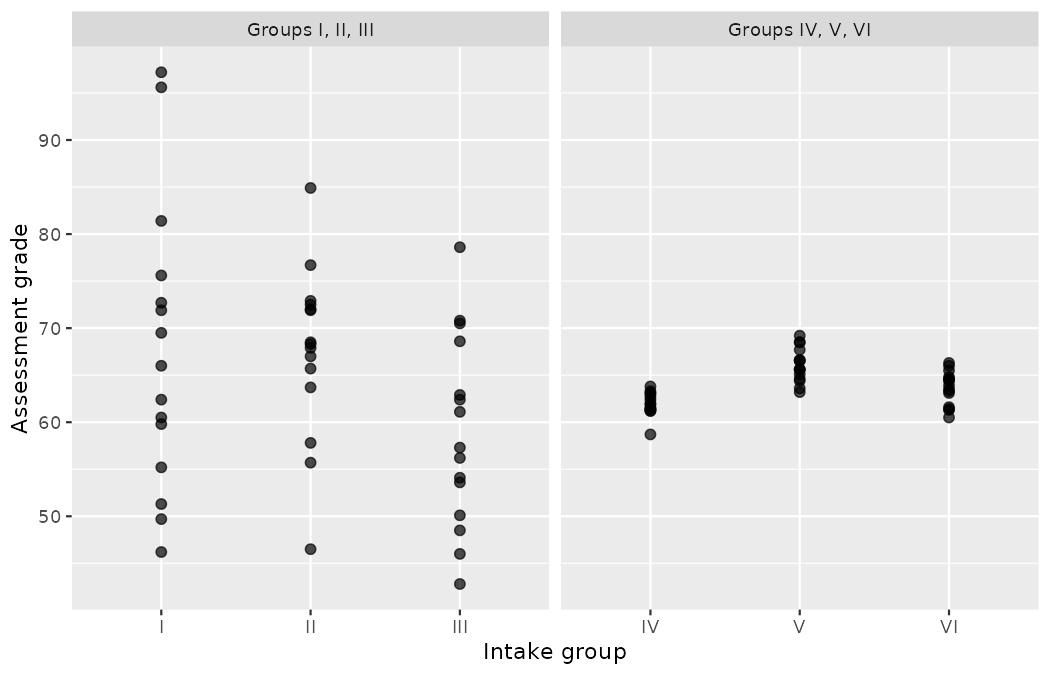
\includegraphics[width=0.85\linewidth,height=\textheight,keepaspectratio]{figures/inference-many-means-1.png}

The side-by-side dot plots show two very different pictures. In the
first panel, the grades within each of groups I, II, and III sprawl
across thirty points or more, and the three clouds overlap almost
completely. In the second panel, each of groups IV, V, and VI is a tight
column of points a few grade-points tall, and the columns sit at visibly
different heights.

\begin{tcolorbox}[enhanced jigsaw, left=2mm, leftrule=.75mm, title=\textcolor{quarto-callout-note-color}{\faInfo}\hspace{0.5em}{Worked example}, arc=.35mm, rightrule=.15mm, coltitle=black, colframe=quarto-callout-note-color-frame, bottomrule=.15mm, colbacktitle=quarto-callout-note-color!10!white, opacitybacktitle=0.6, breakable, bottomtitle=1mm, toptitle=1mm, titlerule=0mm, opacityback=0, toprule=.15mm, colback=white]

Examine the dot plots drawn above. Compare groups I, II, and III. Can
you visually determine if the differences in the group centers is
unlikely to have occurred if there were no differences in the groups?
Now compare groups IV, V, and VI. Do these differences appear to be
unlikely to have occurred if there were no differences in the groups?

\begin{center}\rule{0.5\linewidth}{0.5pt}\end{center}

Any real difference in the means of groups I, II, and III is difficult
to discern, because the data within each group are very volatile
relative to any differences in the average outcome. On the other hand,
it appears there are differences in the centers of groups IV, V, and VI.
For instance, group V appears to have a higher mean than that of the
other two groups. Investigating groups IV, V, and VI, we see the
differences in the groups' centers are noticeable because those
differences are large \emph{relative to the variability in the
individual observations within each group}.

\end{tcolorbox}

Hold on to that comparison --- ``differences between the group centers,
\emph{relative to} the variability within the groups'' --- because it is
precisely the ratio the \(F\)-statistic will formalize later in this
chapter, and we will return to these six toy groups to check that the
formula agrees with your eye.

\section{Case study: chance quality by position
group}\label{case-study-chance-quality-by-position-group}

We would like to discern whether there are real differences between the
chance quality of the shots taken by players in different position
groups: forwards (FW), midfielders (MF), and defenders (DF). We will use
the book's workhorse dataset, the 1,494 shots of the 2022 Men's World
Cup, and the measure of chance quality will be \texttt{statsbomb\_xg}
--- the outcome variable for this chapter. The position groups are
derived from the detailed \texttt{position} string using the mapping
defined once in Chapter~\ref{sec-explore-categorical} and reused
verbatim ever since.

\begin{Shaded}
\begin{Highlighting}[]
\NormalTok{wc2022\_shots }\OtherTok{\textless{}{-}} \FunctionTok{read\_csv}\NormalTok{(}\StringTok{"data/derived/wc2022\_shots.csv"}\NormalTok{)}

\NormalTok{wc\_pos }\OtherTok{\textless{}{-}}\NormalTok{ wc2022\_shots }\SpecialCharTok{|\textgreater{}}
  \FunctionTok{mutate}\NormalTok{(}
    \AttributeTok{pos\_group =} \FunctionTok{case\_when}\NormalTok{(}
\NormalTok{      position }\SpecialCharTok{==} \StringTok{"Goalkeeper"} \SpecialCharTok{\textasciitilde{}} \StringTok{"GK"}\NormalTok{,}
      \FunctionTok{grepl}\NormalTok{(}\StringTok{"Back"}\NormalTok{, position) }\SpecialCharTok{\textasciitilde{}} \StringTok{"DF"}\NormalTok{,}
      \FunctionTok{grepl}\NormalTok{(}\StringTok{"Midfield"}\NormalTok{, position) }\SpecialCharTok{\textasciitilde{}} \StringTok{"MF"}\NormalTok{,}
      \AttributeTok{.default =} \StringTok{"FW"}
\NormalTok{    )}
\NormalTok{  )}

\NormalTok{wc\_pos }\SpecialCharTok{|\textgreater{}}
  \FunctionTok{count}\NormalTok{(pos\_group)}
\CommentTok{\#\textgreater{} \# A tibble: 3 × 2}
\CommentTok{\#\textgreater{}   pos\_group     n}
\CommentTok{\#\textgreater{}   \textless{}chr\textgreater{}     \textless{}int\textgreater{}}
\CommentTok{\#\textgreater{} 1 DF          276}
\CommentTok{\#\textgreater{} 2 FW          732}
\CommentTok{\#\textgreater{} 3 MF          486}
\end{Highlighting}
\end{Shaded}

No goalkeeper took a shot at this tournament --- the \texttt{GK} level
of the mapping comes back empty, so there is nothing to drop (recall
that at the 2025 Women's Euro the mapping caught two goalkeeper shots,
both penalties, which Chapter~\ref{sec-explore-categorical} set aside).
We fix the factor ordering and look at six of the 1,494 cases in
Table~\ref{tbl-wc-pos-six}; the variables carried forward are described
in Table~\ref{tbl-wc-pos-vars}.

\begin{Shaded}
\begin{Highlighting}[]
\NormalTok{wc\_pos }\OtherTok{\textless{}{-}}\NormalTok{ wc\_pos }\SpecialCharTok{|\textgreater{}}
  \FunctionTok{mutate}\NormalTok{(}\AttributeTok{pos\_group =} \FunctionTok{factor}\NormalTok{(pos\_group, }\AttributeTok{levels =} \FunctionTok{c}\NormalTok{(}\StringTok{"FW"}\NormalTok{, }\StringTok{"MF"}\NormalTok{, }\StringTok{"DF"}\NormalTok{)))}

\NormalTok{wc\_pos }\SpecialCharTok{|\textgreater{}}
  \FunctionTok{arrange}\NormalTok{(player) }\SpecialCharTok{|\textgreater{}}
  \FunctionTok{select}\NormalTok{(player, team, pos\_group, statsbomb\_xg, goal) }\SpecialCharTok{|\textgreater{}}
  \FunctionTok{slice\_head}\NormalTok{(}\AttributeTok{n =} \DecValTok{6}\NormalTok{)}
\CommentTok{\#\textgreater{} \# A tibble: 6 × 5}
\CommentTok{\#\textgreater{}   player            team      pos\_group statsbomb\_xg goal}
\CommentTok{\#\textgreater{}   \textless{}chr\textgreater{}             \textless{}chr\textgreater{}     \textless{}fct\textgreater{}            \textless{}dbl\textgreater{} \textless{}lgl\textgreater{}}
\CommentTok{\#\textgreater{} 1 Aaron Mooy        Australia MF             0.0392  FALSE}
\CommentTok{\#\textgreater{} 2 Aaron Ramsey      Wales     MF             0.0254  FALSE}
\CommentTok{\#\textgreater{} 3 Abdelhamid Sabiri Morocco   MF             0.0221  FALSE}
\CommentTok{\#\textgreater{} 4 Abdelhamid Sabiri Morocco   MF             0.0971  FALSE}
\CommentTok{\#\textgreater{} 5 Abdelhamid Sabiri Morocco   MF             0.00420 FALSE}
\CommentTok{\#\textgreater{} 6 Abdelhamid Sabiri Morocco   MF             0.784   TRUE}
\end{Highlighting}
\end{Shaded}

\begin{longtable}[]{@{}lllrl@{}}
\caption{Six cases and the variables carried forward from the
\texttt{wc2022\_shots} data frame.}\label{tbl-wc-pos-six}\tabularnewline
\toprule\noalign{}
player & team & pos\_group & statsbomb\_xg & goal \\
\midrule\noalign{}
\endfirsthead
\toprule\noalign{}
player & team & pos\_group & statsbomb\_xg & goal \\
\midrule\noalign{}
\endhead
\bottomrule\noalign{}
\endlastfoot
Aaron Mooy & Australia & MF & 0.0392 & FALSE \\
Aaron Ramsey & Wales & MF & 0.0254 & FALSE \\
Abdelhamid Sabiri & Morocco & MF & 0.0221 & FALSE \\
Abdelhamid Sabiri & Morocco & MF & 0.0971 & FALSE \\
Abdelhamid Sabiri & Morocco & MF & 0.0042 & FALSE \\
Abdelhamid Sabiri & Morocco & MF & 0.7835 & TRUE \\
\end{longtable}

\begin{longtable}[]{@{}
  >{\raggedright\arraybackslash}p{(\linewidth - 2\tabcolsep) * \real{0.1860}}
  >{\raggedright\arraybackslash}p{(\linewidth - 2\tabcolsep) * \real{0.8140}}@{}}
\caption{Variables and their descriptions for the position-group
analysis.}\label{tbl-wc-pos-vars}\tabularnewline
\toprule\noalign{}
\begin{minipage}[b]{\linewidth}\raggedright
Variable
\end{minipage} & \begin{minipage}[b]{\linewidth}\raggedright
Description
\end{minipage} \\
\midrule\noalign{}
\endfirsthead
\toprule\noalign{}
\begin{minipage}[b]{\linewidth}\raggedright
Variable
\end{minipage} & \begin{minipage}[b]{\linewidth}\raggedright
Description
\end{minipage} \\
\midrule\noalign{}
\endhead
\bottomrule\noalign{}
\endlastfoot
\texttt{player} & Shooter's name \\
\texttt{team} & Shooter's national team \\
\texttt{pos\_group} & Position group derived from \texttt{position} (FW,
MF, DF) \\
\texttt{statsbomb\_xg} & Chance quality (xG): the modeled probability
the shot becomes a goal \\
\texttt{goal} & Whether the shot was scored (logical) \\
\end{longtable}

The sixth row already raises the question this book has trained you to
ask before any headline comparison: \emph{which shots are in the frame?}
That 0.784 is the stored penalty value from
Chapter~\ref{sec-data-applications} --- Sabiri's converted kick against
Spain --- and penalties are exactly the kind of shot that can tilt a
comparison of position groups:

\begin{Shaded}
\begin{Highlighting}[]
\NormalTok{wc\_pos }\SpecialCharTok{|\textgreater{}}
  \FunctionTok{count}\NormalTok{(shot\_type)}
\CommentTok{\#\textgreater{} \# A tibble: 4 × 2}
\CommentTok{\#\textgreater{}   shot\_type     n}
\CommentTok{\#\textgreater{}   \textless{}chr\textgreater{}     \textless{}int\textgreater{}}
\CommentTok{\#\textgreater{} 1 Corner        2}
\CommentTok{\#\textgreater{} 2 Free Kick    46}
\CommentTok{\#\textgreater{} 3 Open Play  1382}
\CommentTok{\#\textgreater{} 4 Penalty      64}

\NormalTok{wc\_pos }\SpecialCharTok{|\textgreater{}}
  \FunctionTok{filter}\NormalTok{(shot\_type }\SpecialCharTok{==} \StringTok{"Penalty"}\NormalTok{) }\SpecialCharTok{|\textgreater{}}
  \FunctionTok{group\_by}\NormalTok{(pos\_group) }\SpecialCharTok{|\textgreater{}}
  \FunctionTok{summarize}\NormalTok{(}\AttributeTok{kicks =} \FunctionTok{n}\NormalTok{(), }\AttributeTok{mean\_xg =} \FunctionTok{mean}\NormalTok{(statsbomb\_xg))}
\CommentTok{\#\textgreater{} \# A tibble: 3 × 3}
\CommentTok{\#\textgreater{}   pos\_group kicks mean\_xg}
\CommentTok{\#\textgreater{}   \textless{}fct\textgreater{}     \textless{}int\textgreater{}   \textless{}dbl\textgreater{}}
\CommentTok{\#\textgreater{} 1 FW           33   0.784}
\CommentTok{\#\textgreater{} 2 MF           22   0.784}
\CommentTok{\#\textgreater{} 3 DF            9   0.784}
\end{Highlighting}
\end{Shaded}

The 64 penalty kicks are concentrated by position --- 33 to forwards, 22
to midfielders, only 9 to defenders --- and every one of them carries
the identical xG of 0.7835, a value five to ten times a typical
open-play chance. Mixing them in would plant a spike of identical
extreme values inside each group, in unequal doses. Per this book's
penalty convention, we state a filter and defend it: the question ``do
position groups differ in the quality of chances they \emph{get
themselves into}?'' is an open-play question, so the analysis runs on
the 1,382 open-play shots, \texttt{shot\_type\ ==\ "Open\ Play"} --- the
same frame Section~\ref{sec-chp11-observational} and
Section~\ref{sec-chp11-pens-out} settled on for the pressure test ---
and, as the convention requires, we will run the penalties-in analysis
alongside it when we reach the ANOVA table, because the \emph{contrast
between the two frames} turns out to teach this chapter's central
formula.

\begin{Shaded}
\begin{Highlighting}[]
\NormalTok{wc\_open }\OtherTok{\textless{}{-}}\NormalTok{ wc\_pos }\SpecialCharTok{|\textgreater{}}
  \FunctionTok{filter}\NormalTok{(shot\_type }\SpecialCharTok{==} \StringTok{"Open Play"}\NormalTok{)}
\end{Highlighting}
\end{Shaded}

\begin{tcolorbox}[enhanced jigsaw, left=2mm, leftrule=.75mm, title=\textcolor{quarto-callout-tip-color}{\faLightbulb}\hspace{0.5em}{Check your understanding}, arc=.35mm, rightrule=.15mm, coltitle=black, colframe=quarto-callout-tip-color-frame, bottomrule=.15mm, colbacktitle=quarto-callout-tip-color!10!white, opacitybacktitle=0.6, breakable, bottomtitle=1mm, toptitle=1mm, titlerule=0mm, opacityback=0, toprule=.15mm, colback=white]

The null hypothesis under consideration is the following:
\(\mu_{FW} = \mu_{MF} = \mu_{DF}.\) Write the null and corresponding
alternative hypotheses in plain language.

\begin{center}\rule{0.5\linewidth}{0.5pt}\end{center}

\(H_0:\) The average open-play chance quality is equal across the three
position groups. \(H_A:\) The average open-play chance quality varies
across some (or all) position groups.

\end{tcolorbox}

\begin{tcolorbox}[enhanced jigsaw, left=2mm, leftrule=.75mm, title=\textcolor{quarto-callout-note-color}{\faInfo}\hspace{0.5em}{Worked example}, arc=.35mm, rightrule=.15mm, coltitle=black, colframe=quarto-callout-note-color-frame, bottomrule=.15mm, colbacktitle=quarto-callout-note-color!10!white, opacitybacktitle=0.6, breakable, bottomtitle=1mm, toptitle=1mm, titlerule=0mm, opacityback=0, toprule=.15mm, colback=white]

The shooters have been divided into three groups: forwards (FW),
midfielders (MF), and defenders (DF). What would be an appropriate point
estimate of the average open-play chance quality for forwards,
\(\mu_{FW}\)?

\begin{center}\rule{0.5\linewidth}{0.5pt}\end{center}

A good estimate of the average chance quality for forwards would be the
sample mean of \texttt{statsbomb\_xg} for just those open-play shots
taken by forwards:

\begin{Shaded}
\begin{Highlighting}[]
\NormalTok{wc\_open }\SpecialCharTok{|\textgreater{}}
  \FunctionTok{filter}\NormalTok{(pos\_group }\SpecialCharTok{==} \StringTok{"FW"}\NormalTok{) }\SpecialCharTok{|\textgreater{}}
  \FunctionTok{summarize}\NormalTok{(}\AttributeTok{x\_bar\_FW =} \FunctionTok{mean}\NormalTok{(statsbomb\_xg))}
\CommentTok{\#\textgreater{} \# A tibble: 1 × 1}
\CommentTok{\#\textgreater{}   x\_bar\_FW}
\CommentTok{\#\textgreater{}      \textless{}dbl\textgreater{}}
\CommentTok{\#\textgreater{} 1    0.115}
\end{Highlighting}
\end{Shaded}

That is, \(\bar{x}_{FW} = 0.115.\)

\end{tcolorbox}

\section{Randomization test for comparing many
means}\label{sec-randANOVA}

Table~\ref{tbl-wc-pos-summary} provides summary statistics for each
group, and the code below draws side-by-side box plots of chance quality
by position group. Notice that the variability appears to be
approximately constant across groups; nearly constant variance across
groups is an important assumption that must be satisfied before we
consider the ANOVA approach.

\begin{Shaded}
\begin{Highlighting}[]
\NormalTok{wc\_open }\SpecialCharTok{|\textgreater{}}
  \FunctionTok{group\_by}\NormalTok{(pos\_group) }\SpecialCharTok{|\textgreater{}}
  \FunctionTok{summarize}\NormalTok{(}\AttributeTok{n =} \FunctionTok{n}\NormalTok{(), }\AttributeTok{mean =} \FunctionTok{mean}\NormalTok{(statsbomb\_xg), }\AttributeTok{sd =} \FunctionTok{sd}\NormalTok{(statsbomb\_xg))}
\CommentTok{\#\textgreater{} \# A tibble: 3 × 4}
\CommentTok{\#\textgreater{}   pos\_group     n   mean    sd}
\CommentTok{\#\textgreater{}   \textless{}fct\textgreater{}     \textless{}int\textgreater{}  \textless{}dbl\textgreater{} \textless{}dbl\textgreater{}}
\CommentTok{\#\textgreater{} 1 FW          678 0.115  0.133}
\CommentTok{\#\textgreater{} 2 MF          443 0.0781 0.107}
\CommentTok{\#\textgreater{} 3 DF          261 0.0903 0.126}

\FunctionTok{ggplot}\NormalTok{(wc\_open, }\FunctionTok{aes}\NormalTok{(}\AttributeTok{x =}\NormalTok{ pos\_group, }\AttributeTok{y =}\NormalTok{ statsbomb\_xg)) }\SpecialCharTok{+}
  \FunctionTok{geom\_boxplot}\NormalTok{() }\SpecialCharTok{+}
  \FunctionTok{labs}\NormalTok{(}\AttributeTok{x =} \StringTok{"Position group"}\NormalTok{, }\AttributeTok{y =} \StringTok{"Chance quality (xG)"}\NormalTok{)}
\end{Highlighting}
\end{Shaded}

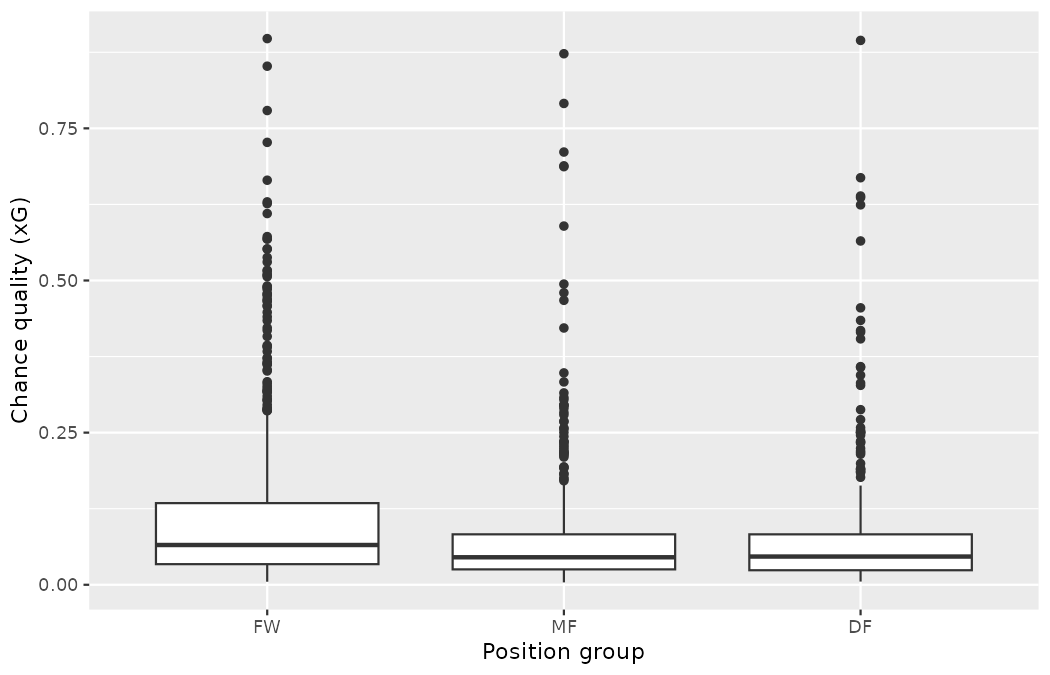
\includegraphics[width=0.85\linewidth,height=\textheight,keepaspectratio]{figures/inference-many-means-2.png}

\begin{longtable}[]{@{}lccc@{}}
\caption{Summary statistics of open-play chance quality (xG), split by
position group.}\label{tbl-wc-pos-summary}\tabularnewline
\toprule\noalign{}
Position group & n & Mean & SD \\
\midrule\noalign{}
\endfirsthead
\toprule\noalign{}
Position group & n & Mean & SD \\
\midrule\noalign{}
\endhead
\bottomrule\noalign{}
\endlastfoot
FW & 678 & 0.115 & 0.133 \\
MF & 443 & 0.078 & 0.107 \\
DF & 261 & 0.090 & 0.126 \\
\end{longtable}

The box plots sit low --- the median xG in every group is under 0.07 ---
with long upper whiskers and a scatter of high-xG outliers in each
group, as xG always produces (the right skew you have known since
Chapter~\ref{sec-explore-categorical}). The boxes overlap substantially,
but the forwards' box and median sit visibly above the midfielders'.
With hundreds of observations per group, the outliers are not extreme
enough to have an impact on the calculations, so they are not a concern
for moving forward with the analysis.

\begin{tcolorbox}[enhanced jigsaw, left=2mm, leftrule=.75mm, title=\textcolor{quarto-callout-note-color}{\faInfo}\hspace{0.5em}{Worked example}, arc=.35mm, rightrule=.15mm, coltitle=black, colframe=quarto-callout-note-color-frame, bottomrule=.15mm, colbacktitle=quarto-callout-note-color!10!white, opacitybacktitle=0.6, breakable, bottomtitle=1mm, toptitle=1mm, titlerule=0mm, opacityback=0, toprule=.15mm, colback=white]

The largest difference between the sample means is between the forward
and the midfielder groups. Consider again the original hypotheses:

\begin{itemize}
\tightlist
\item
  \(H_0:\) \(\mu_{FW} = \mu_{MF} = \mu_{DF}\)
\item
  \(H_A:\) The average open-play chance quality \((\mu_j)\) varies
  across some (or all) position groups.
\end{itemize}

Why might it be inappropriate to run the test by simply estimating
whether the difference of \(\mu_{FW}\) and \(\mu_{MF}\) is
``statistically discernible'' at a 0.05 discernibility level?

\begin{center}\rule{0.5\linewidth}{0.5pt}\end{center}

The primary issue here is that we are inspecting the data before picking
the groups that will be compared. It is inappropriate to examine all
data by eye (informal testing) and only afterwards decide which parts to
formally test. This is called \textbf{data snooping} or \textbf{data
fishing}. Naturally, we would pick the groups with the large differences
for the formal test, and this would lead to an inflation in the Type I
error rate --- the sign-a-dud error of
Chapter~\ref{sec-foundations-decision-errors}. To understand inflated
Type I error rates better, we do not need a thought experiment: our own
tournament provides the demonstration.

\end{tcolorbox}

Suppose Emil Sørensen, scanning the tournament, asks not about three
position groups but about all 32 squads: which teams generated the best
and worst chances per shot? Eyeballing a league table of mean open-play
xG across 32 squads is exactly the informal testing described above, and
with so many groups we are guaranteed to find a few that look rather
different from each other.

\begin{Shaded}
\begin{Highlighting}[]
\NormalTok{team\_xg }\OtherTok{\textless{}{-}}\NormalTok{ wc\_open }\SpecialCharTok{|\textgreater{}}
  \FunctionTok{group\_by}\NormalTok{(team) }\SpecialCharTok{|\textgreater{}}
  \FunctionTok{summarize}\NormalTok{(}\AttributeTok{shots =} \FunctionTok{n}\NormalTok{(), }\AttributeTok{mean\_xg =} \FunctionTok{mean}\NormalTok{(statsbomb\_xg)) }\SpecialCharTok{|\textgreater{}}
  \FunctionTok{arrange}\NormalTok{(}\FunctionTok{desc}\NormalTok{(mean\_xg))}

\NormalTok{team\_xg }\SpecialCharTok{|\textgreater{}}
  \FunctionTok{slice}\NormalTok{(}\FunctionTok{c}\NormalTok{(}\DecValTok{1}\SpecialCharTok{:}\DecValTok{3}\NormalTok{, }\DecValTok{30}\SpecialCharTok{:}\DecValTok{32}\NormalTok{))}
\CommentTok{\#\textgreater{} \# A tibble: 6 × 3}
\CommentTok{\#\textgreater{}   team        shots mean\_xg}
\CommentTok{\#\textgreater{}   \textless{}chr\textgreater{}       \textless{}int\textgreater{}   \textless{}dbl\textgreater{}}
\CommentTok{\#\textgreater{} 1 Switzerland    36  0.169}
\CommentTok{\#\textgreater{} 2 England        57  0.122}
\CommentTok{\#\textgreater{} 3 Netherlands    42  0.117}
\CommentTok{\#\textgreater{} 4 Qatar          20  0.0704}
\CommentTok{\#\textgreater{} 5 Wales          22  0.0638}
\CommentTok{\#\textgreater{} 6 Australia      26  0.0607}
\end{Highlighting}
\end{Shaded}

The full table has 32 rows; shown here are its two ends. Switzerland
tops the table at 0.169 xG per open-play shot; Australia sits at the
bottom with the 0.0607 you already met in
Chapter~\ref{sec-inference-one-mean}. The gap looks enormous, and if we
now ``test'' it with the two-sample machinery of
Chapter~\ref{sec-inference-two-means}, the arithmetic obliges:

\begin{Shaded}
\begin{Highlighting}[]
\FunctionTok{t.test}\NormalTok{(statsbomb\_xg }\SpecialCharTok{\textasciitilde{}}\NormalTok{ team,}
       \AttributeTok{data =}\NormalTok{ wc\_open }\SpecialCharTok{|\textgreater{}} \FunctionTok{filter}\NormalTok{(team }\SpecialCharTok{\%in\%} \FunctionTok{c}\NormalTok{(}\StringTok{"Australia"}\NormalTok{, }\StringTok{"Switzerland"}\NormalTok{)))}
\CommentTok{\#\textgreater{}}
\CommentTok{\#\textgreater{}  Welch Two Sample t{-}test}
\CommentTok{\#\textgreater{}}
\CommentTok{\#\textgreater{} data:  statsbomb\_xg by team}
\CommentTok{\#\textgreater{} t = {-}3.0314, df = 42.605, p{-}value = 0.00413}
\CommentTok{\#\textgreater{} alternative hypothesis: true difference in means between group Australia and group Switzerland is not equal to 0}
\CommentTok{\#\textgreater{} 95 percent confidence interval:}
\CommentTok{\#\textgreater{}  {-}0.17956480 {-}0.03607217}
\CommentTok{\#\textgreater{} sample estimates:}
\CommentTok{\#\textgreater{}   mean in group Australia mean in group Switzerland}
\CommentTok{\#\textgreater{}                 0.0606989                 0.1685174}
\end{Highlighting}
\end{Shaded}

One line of that printout deserves a note before we go further:
\texttt{df\ =\ 42.605} is fractional because software uses the
Welch--Satterthwaite approximation named in Section~\ref{sec-math2samp};
our hand shortcut would take \(\min(36, 26) - 1 = 25\) --- same test,
deliberately more conservative accounting.

A p-value of 0.004: surely decisive? It is not, and the seeded
simulation below shows why. We build a world in which the null
hypothesis is true \emph{by construction} --- the 1,382 open-play shots
keep their xG values, but the team labels are shuffled, so no squad
genuinely differs from any other. In each of 1,000 such worlds we behave
exactly as we just did: scan all 32 group means, pick out the highest
and lowest, and run a two-sample t-test on that eyeballed extreme pair.

\begin{Shaded}
\begin{Highlighting}[]
\FunctionTok{set.seed}\NormalTok{(}\DecValTok{2203}\NormalTok{)}
\NormalTok{snoop\_pvals }\OtherTok{\textless{}{-}} \FunctionTok{replicate}\NormalTok{(}\DecValTok{1000}\NormalTok{, \{}
\NormalTok{  shuffled }\OtherTok{\textless{}{-}}\NormalTok{ wc\_open }\SpecialCharTok{|\textgreater{}} \FunctionTok{mutate}\NormalTok{(}\AttributeTok{team =} \FunctionTok{sample}\NormalTok{(team))}
\NormalTok{  team\_means }\OtherTok{\textless{}{-}}\NormalTok{ shuffled }\SpecialCharTok{|\textgreater{}}
    \FunctionTok{group\_by}\NormalTok{(team) }\SpecialCharTok{|\textgreater{}}
    \FunctionTok{summarize}\NormalTok{(}\AttributeTok{mean\_xg =} \FunctionTok{mean}\NormalTok{(statsbomb\_xg))}
\NormalTok{  extremes }\OtherTok{\textless{}{-}} \FunctionTok{c}\NormalTok{(team\_means}\SpecialCharTok{$}\NormalTok{team[}\FunctionTok{which.max}\NormalTok{(team\_means}\SpecialCharTok{$}\NormalTok{mean\_xg)],}
\NormalTok{                team\_means}\SpecialCharTok{$}\NormalTok{team[}\FunctionTok{which.min}\NormalTok{(team\_means}\SpecialCharTok{$}\NormalTok{mean\_xg)])}
  \FunctionTok{t.test}\NormalTok{(statsbomb\_xg }\SpecialCharTok{\textasciitilde{}}\NormalTok{ team,}
         \AttributeTok{data =} \FunctionTok{filter}\NormalTok{(shuffled, team }\SpecialCharTok{\%in\%}\NormalTok{ extremes))}\SpecialCharTok{$}\NormalTok{p.value}
\NormalTok{\})}

\FunctionTok{mean}\NormalTok{(snoop\_pvals }\SpecialCharTok{\textless{}} \FloatTok{0.05}\NormalTok{)}
\CommentTok{\#\textgreater{} [1] 0.778}
\end{Highlighting}
\end{Shaded}

In 778 of 1,000 worlds where \emph{no team differs from any other}, the
snooping procedure produced a p-value below 0.05. A procedure advertised
as making Type I errors 5\% of the time makes them 78\% of the time once
the data are allowed to choose which pair gets tested. The textbook
version of this cautionary tale imagines an elementary school measuring
aptitude across 20 randomly assigned classes; with our 32 squads the
trap is even deeper, because the more groups you scan, the further apart
the most extreme pair will drift by chance alone. While we might only
formally test the difference for one pair of squads, we informally
evaluated the other thirty by eye before choosing the most extreme cases
for a comparison --- and the p-value of the formal test knows nothing
about that informal scan.

\begin{tcolorbox}[enhanced jigsaw, left=2mm, leftrule=.75mm, title=\textcolor{quarto-callout-tip-color}{\faLightbulb}\hspace{0.5em}{Check your understanding}, arc=.35mm, rightrule=.15mm, coltitle=black, colframe=quarto-callout-tip-color-frame, bottomrule=.15mm, colbacktitle=quarto-callout-tip-color!10!white, opacitybacktitle=0.6, breakable, bottomtitle=1mm, toptitle=1mm, titlerule=0mm, opacityback=0, toprule=.15mm, colback=white]

Suppose Emil had \emph{pre-registered} a single comparison before the
tournament --- say, Switzerland versus Australia, named in advance for
footballing reasons --- and then run the same t-test at
\(\alpha = 0.05.\) In a world where the null hypothesis is true, roughly
what fraction of such pre-named tests would reject?

\begin{center}\rule{0.5\linewidth}{0.5pt}\end{center}

About 5\% --- that is exactly what \(\alpha\) promises, as you saw in
Chapter~\ref{sec-foundations-randomization}. The 77.8\% rejection rate
in the simulation is not a defect of the t-test: it is the price of
letting the data nominate the comparison. The entire inflation comes
from scanning 32 group means first and testing the winner and loser of
that scan.

\end{tcolorbox}

\begin{tcolorbox}[enhanced jigsaw, left=2mm, leftrule=.75mm, title=\textcolor{quarto-callout-important-color}{\faExclamation}\hspace{0.5em}{One usable correction: Bonferroni}, arc=.35mm, rightrule=.15mm, coltitle=black, colframe=quarto-callout-important-color-frame, bottomrule=.15mm, colbacktitle=quarto-callout-important-color!10!white, opacitybacktitle=0.6, breakable, bottomtitle=1mm, toptitle=1mm, titlerule=0mm, opacityback=0, toprule=.15mm, colback=white]

The cure this chapter builds is a single holistic test with no peeking
privileges. But sometimes a department legitimately needs several
comparisons, and one correction is simple enough to use immediately: if
you will test \(m\) comparisons --- all \(m\) pre-registered before the
data are seen --- and want the \emph{family} of tests, taken together,
to commit a Type I error at rate \(\alpha,\) then test each individual
comparison at level \(\alpha / m.\) This is the \emph{Bonferroni
correction}, and its arithmetic doubles as a price list. One pre-named
pair of squads is \(m = 1\): test at \(0.05.\) Testing every pair among
the 32 squads --- the fishing expedition the simulation above exposed
--- would be \(m = 32 \times 31 / 2 = 496\) comparisons, demanding
\(\alpha = 0.05 / 496 \approx 0.0001\) per pair. The eyeballed
Switzerland--Australia p-value of \(0.004,\) so decisive-looking against
\(0.05,\) does not survive the bar its own selection procedure implies
--- which is the honest price of fishing, now in writing. One caveat:
Bonferroni is deliberately conservative, buying its Type I control by
giving up power as \(m\) grows, and sharper multiple-comparison tools
exist in a later course.

\end{tcolorbox}

The contrast between \(\bar{x}_{FW} = 0.115\) and
\(\bar{x}_{MF} = 0.078\) in Table~\ref{tbl-wc-pos-summary} tempts us
into the same trap: we noticed that gap \emph{because} it is the biggest
of the three. What we need is a single holistic test that treats all the
groups symmetrically, with no peeking privileges.

\subsection{Observed data}\label{observed-data-18}

In the next section we will learn how to use the \(F\) statistic to test
whether observed differences in sample means could have happened just by
chance even if there was no difference in the respective population
means.

The method of analysis of variance in this context focuses on answering
one question: is the variability in the sample means so large that it
seems unlikely to be from chance alone? This question is different from
earlier testing procedures since we will \emph{simultaneously} consider
many groups, and evaluate whether their sample means differ more than we
would expect from natural variation. We call this variability the
\textbf{mean square between groups (MSG)}, and it has an associated
\textbf{degrees of freedom}, \(df_G = k - 1\) when there are \(k\)
groups. Unpack the name and the notation before using them. ``Mean
square'' says the quantity is an \emph{average of squared deviations}
--- a variance-flavored object, like \(s^2\) from
Chapter~\ref{sec-explore-numerical}; ``between groups'' says the
deviations being squared are those of the \emph{group means} around the
grand mean. The degrees of freedom carry a subscript now that there are
two of them in play: \(df_G\) (the \(G\) for \emph{groups}) counts \(k\)
group means minus one, because once the grand mean is fixed, only
\(k - 1\) of the group-mean deviations are free to vary --- the same
logic that gave \(df = n - 1\) for a single sample in
Chapter~\ref{sec-inference-one-mean}. The \(MSG\) can be thought of as a
scaled variance formula for means. If the null hypothesis is true, any
variation in the sample means is due to chance and shouldn't be too
large. Details of \(MSG\) calculations are provided in the
footnote.\footnote{Let \(\bar{x}\) represent the mean of outcomes across
  all groups (the grand mean). Then the mean square between groups is
  computed as
  \[MSG = \frac{1}{df_G}SSG = \frac{1}{k-1}\sum_{j=1}^{k} n_j \left(\bar{x}_j - \bar{x}\right)^2\]
  where \(SSG\) is called the \textbf{sum of squares between groups}
  \((SSG)\) and \(n_j\) is the sample size of group \(j.\) Read the sum
  piece by piece: for each group \(j,\) take how far its mean sits from
  the grand mean, \(\bar{x}_j - \bar{x};\) square it; weight it by the
  group's size \(n_j\) (a gap sustained by 678 shots is stronger
  evidence than the same gap on 26); then add across the \(k\) groups.
  For the position groups, with grand mean \(\bar{x} = 0.0983\) (the
  open-play benchmark of Chapter~\ref{sec-inference-one-mean}) and the
  group means of Table~\ref{tbl-wc-pos-summary} carried to four decimals
  \((0.1146, 0.0781, 0.0903):\)
  \(SSG = 678(0.1146 - 0.0983)^2 + 443(0.0781 - 0.0983)^2 + 261(0.0903 - 0.0983)^2 = 0.180 + 0.181 + 0.017 = 0.378.\)}
However, we typically use software for these computations.

The mean square between the groups is, on its own, quite useless in a
hypothesis test. We need a benchmark value for how much variability
should be expected among the sample means if the null hypothesis is
true. To this end, we compute a pooled variance estimate, often
abbreviated as the \textbf{mean square error} \((MSE)\), which has an
associated degrees of freedom value \(df_E = n - k.\) The subscript
\(E\) stands for \emph{error} --- here meaning the residual,
within-group variation, not a mistake --- and \(df_E = n - k\) because
estimating \(k\) group means from \(n\) observations uses up \(k\)
degrees of freedom, extending the \(n - 1\) and \(n - 2\) patterns you
have met before. It is helpful to think of \(MSE\) as a measure of the
variability within the groups. Details of the computations of the
\(MSE\) are provided in the footnote.\footnote{Let \(\bar{x}\) represent
  the mean of outcomes across all groups. Then the \textbf{sum of
  squares total} \((SST)\) is computed as
  \[SST = \sum_{i=1}^{n} \left(x_i - \bar{x}\right)^2\] where the sum is
  over all \(n\) observations in the dataset. Then we compute the
  \textbf{sum of squared errors} \((SSE)\) in one of two equivalent
  ways:
  \[SSE = SST - SSG = (n_1 - 1)s_1^2 + (n_2 - 1)s_2^2 + \cdots + (n_k - 1)s_k^2\]
  where \(s_j^2\) is the sample variance (square of the standard
  deviation, per Chapter~\ref{sec-explore-numerical}) of the
  observations in group \(j.\) Then the \(MSE\) is the standardized form
  of \(SSE:\) \(MSE = \frac{1}{df_E}SSE.\)}

If \(SST\) and \(SSE\) look familiar, they should: recall
Section~\ref{sec-r-squared}, where the total sum of squares \(SST\)
measured the total variability of the response around its mean and split
into a part the regression line explained \((SSR)\) and a part it did
not \((SSE).\) ANOVA slices the \emph{same total} differently: instead
of a fitted line, the ``model'' here is simply each group's own mean, so

\[SST = SSG + SSE\]

with \(SSG\) playing the role that \(SSR\) played for the regression
line --- the variability the group structure accounts for --- and
\(SSE\) once again the variability left over. Nothing about the total
changed; only the knife did.

\begin{tcolorbox}[enhanced jigsaw, left=2mm, leftrule=.75mm, title=\textcolor{quarto-callout-tip-color}{\faLightbulb}\hspace{0.5em}{Check your understanding}, arc=.35mm, rightrule=.15mm, coltitle=black, colframe=quarto-callout-tip-color-frame, bottomrule=.15mm, colbacktitle=quarto-callout-tip-color!10!white, opacitybacktitle=0.6, breakable, bottomtitle=1mm, toptitle=1mm, titlerule=0mm, opacityback=0, toprule=.15mm, colback=white]

For the 1,382 open-play World Cup shots, the total sum of squares of
chance quality is \(SST = 21.568,\) and we computed \(SSG = 0.378\) in
the footnote above. What is \(SSE?\) What fraction of the total
variability in chance quality do the position groups account for, and
what does that fraction remind you of?

\begin{center}\rule{0.5\linewidth}{0.5pt}\end{center}

\(SSE = SST - SSG = 21.568 - 0.378 = 21.190.\) The groups account for
\(0.378 / 21.568 = 0.0175\) --- under 2\% of the total variability, the
ANOVA analogue of the \(R^2\) from Section~\ref{sec-r-squared}. Keep
that number in mind: this chapter's test will shortly declare the group
differences statistically discernible \emph{anyway}. Discernible does
not mean large; it means too consistent to be chance --- with
\(n = 1382,\) even a 2\% slice of the variability can be unmistakably
real.

\end{tcolorbox}

When the null hypothesis is true, any differences among the sample means
are only due to chance, and the \(MSG\) and \(MSE\) should be about
equal. As a test statistic for ANOVA, we examine the fraction of \(MSG\)
and \(MSE:\)

\[F = \frac{MSG}{MSE}\]

The \(MSG\) represents a measure of the between-group variability, and
\(MSE\) measures the variability within each of the groups. The
statistic's one-letter name honors R.A. Fisher, who developed the
method; you will meet its distribution in Section~\ref{sec-mathANOVA}.

\begin{tcolorbox}[enhanced jigsaw, left=2mm, leftrule=.75mm, title=\textcolor{quarto-callout-important-color}{\faExclamation}\hspace{0.5em}{The test statistic for three or more means is an F}, arc=.35mm, rightrule=.15mm, coltitle=black, colframe=quarto-callout-important-color-frame, bottomrule=.15mm, colbacktitle=quarto-callout-important-color!10!white, opacitybacktitle=0.6, breakable, bottomtitle=1mm, toptitle=1mm, titlerule=0mm, opacityback=0, toprule=.15mm, colback=white]

The F statistic is a ratio of how the groups differ (MSG) as compared to
how the observations within a group vary (MSE).

\[F = \frac{MSG}{MSE}\]

When the null hypothesis is true and the conditions are met, F has an
F-distribution with \(df_1 = k - 1\) and \(df_2 = n - k.\)

Conditions:

\begin{itemize}
\tightlist
\item
  independent observations, both within and across groups
\item
  large samples and no extreme outliers
\end{itemize}

\end{tcolorbox}

Before moving on, return to the six toy intake groups from the start of
the chapter and let the new statistic formalize what your eye reported:

\begin{Shaded}
\begin{Highlighting}[]
\NormalTok{intake\_toy }\SpecialCharTok{|\textgreater{}}
  \FunctionTok{filter}\NormalTok{(group }\SpecialCharTok{\%in\%} \FunctionTok{c}\NormalTok{(}\StringTok{"I"}\NormalTok{, }\StringTok{"II"}\NormalTok{, }\StringTok{"III"}\NormalTok{)) }\SpecialCharTok{|\textgreater{}}
  \FunctionTok{droplevels}\NormalTok{() }\SpecialCharTok{|\textgreater{}}
  \FunctionTok{specify}\NormalTok{(grade }\SpecialCharTok{\textasciitilde{}}\NormalTok{ group) }\SpecialCharTok{|\textgreater{}}
  \FunctionTok{calculate}\NormalTok{(}\AttributeTok{stat =} \StringTok{"F"}\NormalTok{) }\SpecialCharTok{|\textgreater{}}
  \FunctionTok{pull}\NormalTok{()}
\CommentTok{\#\textgreater{} [1] 2.656429}

\NormalTok{intake\_toy }\SpecialCharTok{|\textgreater{}}
  \FunctionTok{filter}\NormalTok{(group }\SpecialCharTok{\%in\%} \FunctionTok{c}\NormalTok{(}\StringTok{"IV"}\NormalTok{, }\StringTok{"V"}\NormalTok{, }\StringTok{"VI"}\NormalTok{)) }\SpecialCharTok{|\textgreater{}}
  \FunctionTok{droplevels}\NormalTok{() }\SpecialCharTok{|\textgreater{}}
  \FunctionTok{specify}\NormalTok{(grade }\SpecialCharTok{\textasciitilde{}}\NormalTok{ group) }\SpecialCharTok{|\textgreater{}}
  \FunctionTok{calculate}\NormalTok{(}\AttributeTok{stat =} \StringTok{"F"}\NormalTok{) }\SpecialCharTok{|\textgreater{}}
  \FunctionTok{pull}\NormalTok{()}
\CommentTok{\#\textgreater{} [1] 24.5345}
\end{Highlighting}
\end{Shaded}

The two sets of groups were built with the \emph{same} gaps between
their designed centre grades; only the within-group noise differs. The
noisy set returns \(F = 2.66\) --- the group means differ, but barely
more than the volatile grading would produce on its own --- while the
tight set returns \(F = 24.53,\) the same centre gaps now towering over
tiny within-group variability. The \(F\) statistic is your eyeball
comparison, made honest.

\subsection{Variability of the
statistic}\label{variability-of-the-statistic-18}

We recall the report-template trial from Section~\ref{sec-rand2mean},
which demonstrated a two-sample randomization test for a comparison of
means: Priya Rao randomized two versions of Northbridge's standard
report template across the network, and the test could not tell the two
versions apart. Suppose now that the trial had been run at such scale
--- the full extended network of regional scouts, partner-academy staff,
and loan-network contacts filing assessments during the autumn window
--- that three different templates were trialled: A, B, and C. Each of
164 assessors was randomly assigned one template, filed a standard
prospect assessment with it, and had the report scored for accuracy (out
of 100) against an expert panel's reference assessment of the same
prospect. (As in Section~\ref{sec-rand2mean}, the panel's benchmark
assessments cover a small pool of reference players, and each assignment
was drawn against one of them --- a handful of gold standards serving
164 reports.) This is a constructed Northbridge scenario, built by the
seeded code below.

\begin{Shaded}
\begin{Highlighting}[]
\FunctionTok{set.seed}\NormalTok{(}\DecValTok{2202}\NormalTok{)}
\NormalTok{template\_abc }\OtherTok{\textless{}{-}} \FunctionTok{tibble}\NormalTok{(}
  \AttributeTok{template =} \FunctionTok{factor}\NormalTok{(}\FunctionTok{rep}\NormalTok{(}\FunctionTok{c}\NormalTok{(}\StringTok{"A"}\NormalTok{, }\StringTok{"B"}\NormalTok{, }\StringTok{"C"}\NormalTok{), }\AttributeTok{times =} \FunctionTok{c}\NormalTok{(}\DecValTok{58}\NormalTok{, }\DecValTok{55}\NormalTok{, }\DecValTok{51}\NormalTok{))),}
  \AttributeTok{accuracy =} \FunctionTok{c}\NormalTok{(}\FunctionTok{rnorm}\NormalTok{(}\DecValTok{58}\NormalTok{, }\DecValTok{75}\NormalTok{, }\DecValTok{13}\NormalTok{), }\FunctionTok{rnorm}\NormalTok{(}\DecValTok{55}\NormalTok{, }\DecValTok{72}\NormalTok{, }\DecValTok{13}\NormalTok{), }\FunctionTok{rnorm}\NormalTok{(}\DecValTok{51}\NormalTok{, }\DecValTok{77}\NormalTok{, }\DecValTok{13}\NormalTok{))}
\NormalTok{) }\SpecialCharTok{|\textgreater{}}
  \FunctionTok{mutate}\NormalTok{(}\AttributeTok{accuracy =} \FunctionTok{pmin}\NormalTok{(}\FunctionTok{round}\NormalTok{(accuracy), }\DecValTok{100}\NormalTok{))}

\NormalTok{template\_abc }\SpecialCharTok{|\textgreater{}}
  \FunctionTok{group\_by}\NormalTok{(template) }\SpecialCharTok{|\textgreater{}}
  \FunctionTok{summarize}\NormalTok{(}\AttributeTok{n =} \FunctionTok{n}\NormalTok{(), }\AttributeTok{mean =} \FunctionTok{mean}\NormalTok{(accuracy), }\AttributeTok{sd =} \FunctionTok{sd}\NormalTok{(accuracy),}
            \AttributeTok{min =} \FunctionTok{min}\NormalTok{(accuracy), }\AttributeTok{max =} \FunctionTok{max}\NormalTok{(accuracy))}
\CommentTok{\#\textgreater{} \# A tibble: 3 × 6}
\CommentTok{\#\textgreater{}   template     n  mean    sd   min   max}
\CommentTok{\#\textgreater{}   \textless{}fct\textgreater{}    \textless{}int\textgreater{} \textless{}dbl\textgreater{} \textless{}dbl\textgreater{} \textless{}dbl\textgreater{} \textless{}dbl\textgreater{}}
\CommentTok{\#\textgreater{} 1 A           58  75.6  12.2    49   100}
\CommentTok{\#\textgreater{} 2 B           55  70.3  13.6    34   100}
\CommentTok{\#\textgreater{} 3 C           51  76.1  13.0    42   100}

\FunctionTok{ggplot}\NormalTok{(template\_abc, }\FunctionTok{aes}\NormalTok{(}\AttributeTok{x =}\NormalTok{ template, }\AttributeTok{y =}\NormalTok{ accuracy, }\AttributeTok{color =}\NormalTok{ template)) }\SpecialCharTok{+}
  \FunctionTok{geom\_boxplot}\NormalTok{(}\AttributeTok{show.legend =} \ConstantTok{FALSE}\NormalTok{) }\SpecialCharTok{+}
  \FunctionTok{geom\_point}\NormalTok{(}\AttributeTok{show.legend =} \ConstantTok{FALSE}\NormalTok{) }\SpecialCharTok{+}
  \FunctionTok{labs}\NormalTok{(}\AttributeTok{x =} \StringTok{"Template"}\NormalTok{, }\AttributeTok{y =} \StringTok{"Accuracy score"}\NormalTok{)}
\end{Highlighting}
\end{Shaded}

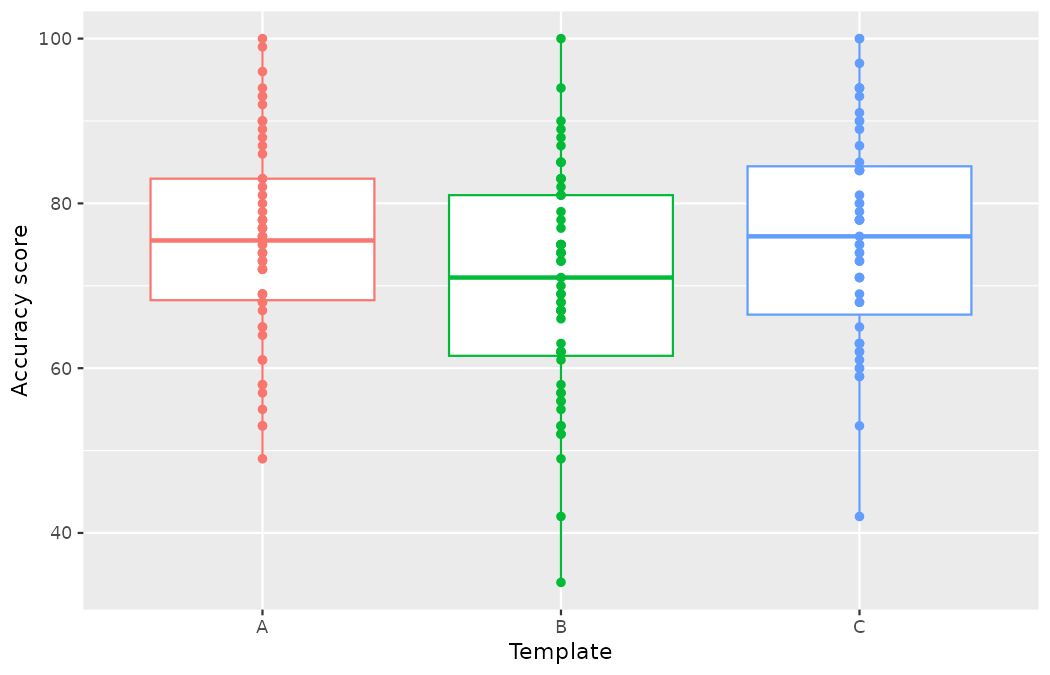
\includegraphics[width=0.85\linewidth,height=\textheight,keepaspectratio]{figures/inference-many-means-3.png}

Table~\ref{tbl-template-abc-summary} and the box plots provide a summary
of the data including template C. Again, we would like to investigate
whether the accuracy a scout achieves depends on the template, so the
test is

\begin{itemize}
\tightlist
\item
  \(H_0: \mu_A = \mu_B = \mu_C.\) The inherent average accuracy is the
  same across the three templates.
\item
  \(H_A:\) not \(H_0.\) At least one of the templates inherently
  produces more (or less) accurate reports than the others.
\end{itemize}

\begin{longtable}[]{@{}lccccc@{}}
\caption{Summary statistics of accuracy scores for each template
version.}\label{tbl-template-abc-summary}\tabularnewline
\toprule\noalign{}
Template & n & Mean & SD & Min & Max \\
\midrule\noalign{}
\endfirsthead
\toprule\noalign{}
Template & n & Mean & SD & Min & Max \\
\midrule\noalign{}
\endhead
\bottomrule\noalign{}
\endlastfoot
A & 58 & 75.6 & 12.2 & 49 & 100 \\
B & 55 & 70.3 & 13.6 & 34 & 100 \\
C & 51 & 76.1 & 13.0 & 42 & 100 \\
\end{longtable}

If the null hypothesis is true, then the accuracy of each report
reflects the assessor's underlying diligence and the prospect's
legibility --- it shouldn't matter whether the assessor was handed
template A, B, or C. By reallocating which assessor got which template,
we are able to understand how the differences in average accuracy scores
change due only to natural variability. The observed \(F\) statistic,
and one seeded reallocation, are computed below.

\begin{Shaded}
\begin{Highlighting}[]
\NormalTok{template\_F\_obs }\OtherTok{\textless{}{-}}\NormalTok{ template\_abc }\SpecialCharTok{|\textgreater{}}
  \FunctionTok{specify}\NormalTok{(accuracy }\SpecialCharTok{\textasciitilde{}}\NormalTok{ template) }\SpecialCharTok{|\textgreater{}}
  \FunctionTok{calculate}\NormalTok{(}\AttributeTok{stat =} \StringTok{"F"}\NormalTok{) }\SpecialCharTok{|\textgreater{}}
  \FunctionTok{pull}\NormalTok{()}

\NormalTok{template\_F\_obs}
\CommentTok{\#\textgreater{} [1] 3.420801}

\FunctionTok{set.seed}\NormalTok{(}\DecValTok{2204}\NormalTok{)}
\NormalTok{template\_shuffle }\OtherTok{\textless{}{-}}\NormalTok{ template\_abc }\SpecialCharTok{|\textgreater{}}
  \FunctionTok{mutate}\NormalTok{(}\AttributeTok{template =} \FunctionTok{sample}\NormalTok{(template))}

\NormalTok{template\_shuffle }\SpecialCharTok{|\textgreater{}}
  \FunctionTok{group\_by}\NormalTok{(template) }\SpecialCharTok{|\textgreater{}}
  \FunctionTok{summarize}\NormalTok{(}\AttributeTok{n =} \FunctionTok{n}\NormalTok{(), }\AttributeTok{mean =} \FunctionTok{mean}\NormalTok{(accuracy))}
\CommentTok{\#\textgreater{} \# A tibble: 3 × 3}
\CommentTok{\#\textgreater{}   template     n  mean}
\CommentTok{\#\textgreater{}   \textless{}fct\textgreater{}    \textless{}int\textgreater{} \textless{}dbl\textgreater{}}
\CommentTok{\#\textgreater{} 1 A           58  74.3}
\CommentTok{\#\textgreater{} 2 B           55  76.7}
\CommentTok{\#\textgreater{} 3 C           51  70.7}

\NormalTok{template\_shuffle }\SpecialCharTok{|\textgreater{}}
  \FunctionTok{specify}\NormalTok{(accuracy }\SpecialCharTok{\textasciitilde{}}\NormalTok{ template) }\SpecialCharTok{|\textgreater{}}
  \FunctionTok{calculate}\NormalTok{(}\AttributeTok{stat =} \StringTok{"F"}\NormalTok{) }\SpecialCharTok{|\textgreater{}}
  \FunctionTok{pull}\NormalTok{()}
\CommentTok{\#\textgreater{} [1] 2.888948}
\end{Highlighting}
\end{Shaded}

There is only one iteration of the randomization process here: the
shuffle dealt the 164 accuracy scores back out to the templates --- 58
to A, 55 to B, 51 to C --- with no regard to which template actually
produced them, and the reshuffled group means came out 74.3, 76.7, and
70.7, an ordering entirely different from the observed 75.6, 70.3, 76.1.
The shuffled \(F\) statistic is 2.89, computed under the null assumption
that the templates are interchangeable.

In the two-sample case of Section~\ref{sec-rand2mean}, the null
hypothesis was investigated using the difference in the sample means.
However, as noted above, with three groups (three different templates),
the comparison of the three sample means gets slightly more complicated.
We have already derived the F-statistic, which is exactly the way to
compare the averages across three or more groups! Recall, the F
statistic is a ratio of how the groups differ (MSG) as compared to how
the observations within a group vary (MSE).

Building on the single shuffle above, the code below carries out 1,000
random permutations and collects the simulated \(F\) statistics.

\begin{Shaded}
\begin{Highlighting}[]
\FunctionTok{set.seed}\NormalTok{(}\DecValTok{2205}\NormalTok{)}
\NormalTok{template\_null }\OtherTok{\textless{}{-}}\NormalTok{ template\_abc }\SpecialCharTok{|\textgreater{}}
  \FunctionTok{specify}\NormalTok{(accuracy }\SpecialCharTok{\textasciitilde{}}\NormalTok{ template) }\SpecialCharTok{|\textgreater{}}
  \FunctionTok{hypothesize}\NormalTok{(}\AttributeTok{null =} \StringTok{"independence"}\NormalTok{) }\SpecialCharTok{|\textgreater{}}
  \FunctionTok{generate}\NormalTok{(}\AttributeTok{reps =} \DecValTok{1000}\NormalTok{, }\AttributeTok{type =} \StringTok{"permute"}\NormalTok{) }\SpecialCharTok{|\textgreater{}}
  \FunctionTok{calculate}\NormalTok{(}\AttributeTok{stat =} \StringTok{"F"}\NormalTok{)}

\FunctionTok{ggplot}\NormalTok{(template\_null, }\FunctionTok{aes}\NormalTok{(}\AttributeTok{x =}\NormalTok{ stat)) }\SpecialCharTok{+}
  \FunctionTok{geom\_histogram}\NormalTok{(}\AttributeTok{binwidth =} \FloatTok{0.25}\NormalTok{) }\SpecialCharTok{+}
  \FunctionTok{labs}\NormalTok{(}
    \AttributeTok{title =} \StringTok{"1,000 randomized F statistics"}\NormalTok{,}
    \AttributeTok{x =} \StringTok{"F statistic for 1,000 randomizations of the templates"}\NormalTok{,}
    \AttributeTok{y =} \StringTok{"Count"}
\NormalTok{  )}
\end{Highlighting}
\end{Shaded}

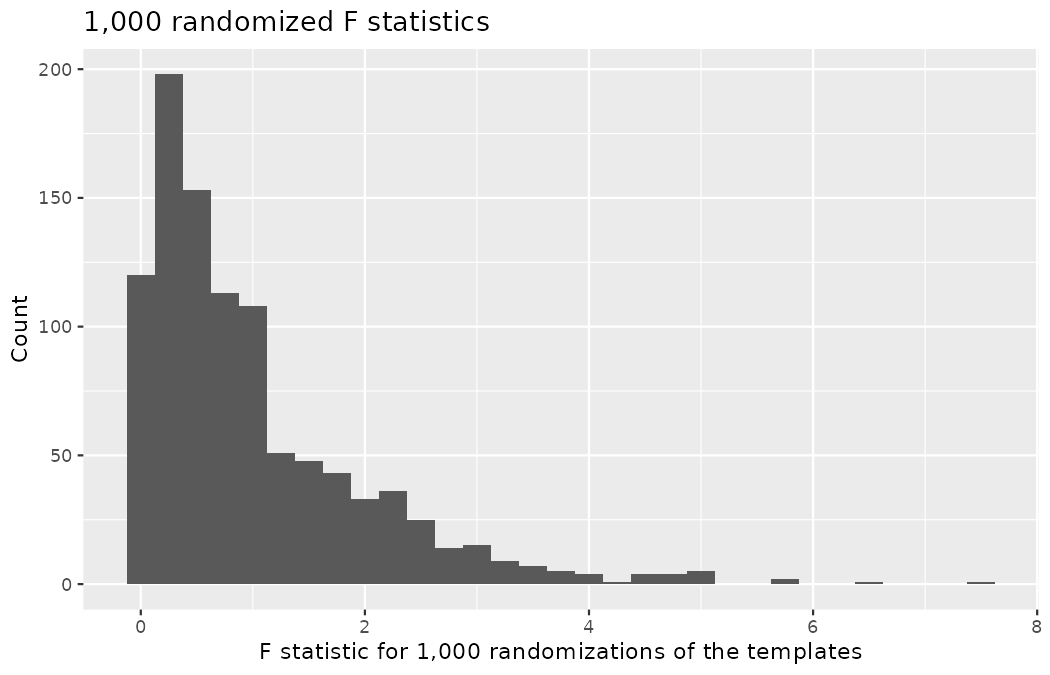
\includegraphics[width=0.85\linewidth,height=\textheight,keepaspectratio]{figures/inference-many-means-4.png}

The histogram of the 1,000 randomized \(F\) statistics is right-skewed,
piled up near zero with most values below 2 and a tail stretching out to
the right. We see that, just by chance, the F statistic can be as large
as 7.6.

\subsection{Observed statistic vs.~null
statistics}\label{observed-statistic-vs.-null-statistics-9}

Where does the observed statistic fall among the shuffled ones?

\begin{Shaded}
\begin{Highlighting}[]
\NormalTok{template\_null }\SpecialCharTok{|\textgreater{}}
  \FunctionTok{summarize}\NormalTok{(}
    \AttributeTok{n\_extreme =} \FunctionTok{sum}\NormalTok{(stat }\SpecialCharTok{\textgreater{}=}\NormalTok{ template\_F\_obs),}
    \AttributeTok{p\_value =} \FunctionTok{mean}\NormalTok{(stat }\SpecialCharTok{\textgreater{}=}\NormalTok{ template\_F\_obs),}
    \AttributeTok{largest =} \FunctionTok{max}\NormalTok{(stat)}
\NormalTok{  )}
\CommentTok{\#\textgreater{} \# A tibble: 1 × 3}
\CommentTok{\#\textgreater{}   n\_extreme p\_value largest}
\CommentTok{\#\textgreater{}       \textless{}int\textgreater{}   \textless{}dbl\textgreater{}   \textless{}dbl\textgreater{}}
\CommentTok{\#\textgreater{} 1        33   0.033    7.59}

\FunctionTok{ggplot}\NormalTok{(template\_null, }\FunctionTok{aes}\NormalTok{(}\AttributeTok{x =}\NormalTok{ stat)) }\SpecialCharTok{+}
  \FunctionTok{geom\_histogram}\NormalTok{(}\AttributeTok{binwidth =} \FloatTok{0.25}\NormalTok{) }\SpecialCharTok{+}
  \FunctionTok{geom\_vline}\NormalTok{(}\AttributeTok{xintercept =}\NormalTok{ template\_F\_obs, }\AttributeTok{color =} \StringTok{"red"}\NormalTok{, }\AttributeTok{linewidth =} \DecValTok{1}\NormalTok{) }\SpecialCharTok{+}
  \FunctionTok{labs}\NormalTok{(}
    \AttributeTok{title =} \StringTok{"1,000 randomized F statistics"}\NormalTok{,}
    \AttributeTok{x =} \StringTok{"F statistic for 1,000 randomizations of the templates"}\NormalTok{,}
    \AttributeTok{y =} \StringTok{"Count"}
\NormalTok{  )}
\end{Highlighting}
\end{Shaded}

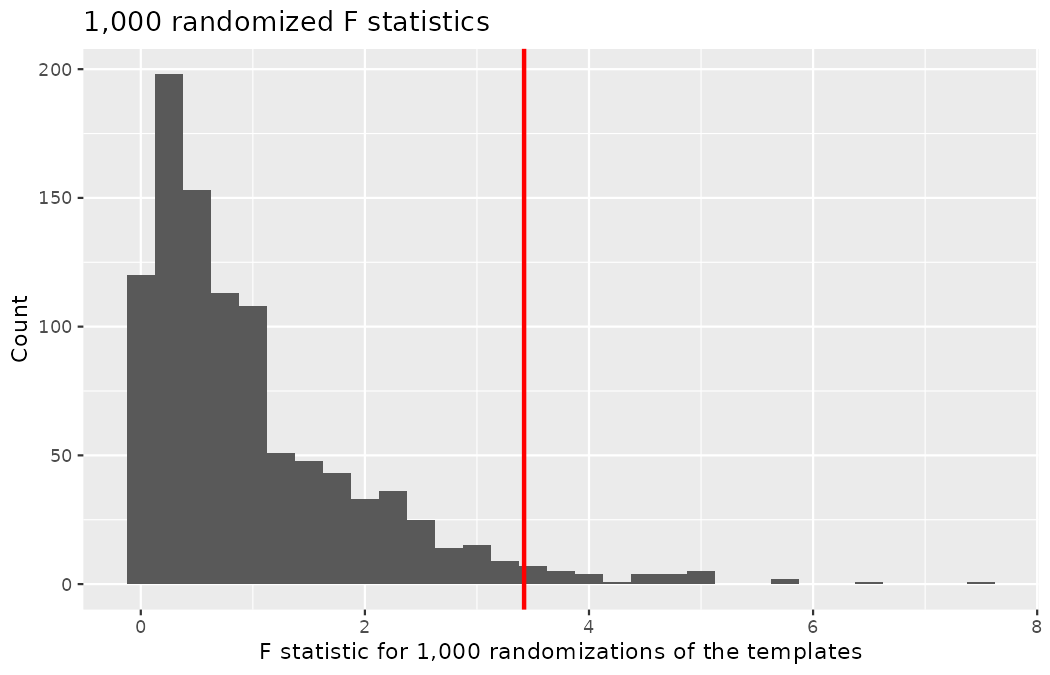
\includegraphics[width=0.85\linewidth,height=\textheight,keepaspectratio]{figures/inference-many-means-5.png}

Only the upper tail counts as more extreme here: larger \(F\) means
group differences further beyond what within-group noise explains, so
evidence against \(H_0\) accumulates only on the right --- a point we
return to in Section~\ref{sec-mathANOVA}. In this seeded run, 3.3\% of
the randomized F test statistics were at or above the observed test
statistic of \(F = 3.42.\) That is, the p-value of the test is 0.033.
Assuming that we had set the level of discernibility to be
\(\alpha = 0.05,\) the p-value is smaller than the level of
discernibility, which would lead us to reject the null hypothesis. We
claim that the inherent accuracy (i.e., the true average accuracy score,
\(\mu\)) is different for at least one of the templates. Because the
templates were randomly assigned, the claim is causal --- the template
itself moves report accuracy.

While it is tempting to say that template B \emph{harms} accuracy (given
the inability to differentiate between the two templates of
Section~\ref{sec-rand2mean}), we must be very careful about conclusions
made using different techniques on the same data.

When the null hypothesis is true, random variability that exists in
nature sometimes produces data with p-values less than 0.05. How often
does that happen? 5\% of the time. That is to say, if you use 20
different models applied to the same data where there is no signal
(i.e., the null hypothesis is true), you are reasonably likely to get a
p-value less than 0.05 in one of the tests you run. You have already
watched an aggressive version of this play out in this chapter: scanning
32 squad means and testing the extremes turned a nominal 5\% error rate
into 78\%. The details surrounding the ideas of this problem, called a
\textbf{multiple comparisons test} or \textbf{multiple comparisons
problem}, are outside the scope of this textbook, but should be
something that you keep in the back of your head. To best mitigate any
extra Type I errors, we suggest that you set up your hypotheses and
testing protocol before running any analyses --- before the tournament,
not after the league table has been eyeballed. Once the conclusions have
been reached, you should report your findings instead of running a
different type of test on the same data.

\section{Mathematical model for test for comparing many
means}\label{sec-mathANOVA}

As seen with many of the tests and statistics from previous chapters,
the randomization test on the F statistic has corresponding mathematical
theory to describe the distribution, which can be used without a
computational approach.

We return to the position-group analysis of
Table~\ref{tbl-wc-pos-summary} to demonstrate the mathematical model
applied to the ANOVA setting.

\subsection{Variability of the
statistic}\label{variability-of-the-statistic-19}

The larger the observed variability in the sample means \((MSG)\)
relative to the within-group observations \((MSE),\) the larger the
\(F\)-statistic will be and the stronger the evidence against the null
hypothesis. Because larger \(F\)-statistics represent stronger evidence
against the null hypothesis, we use the upper tail of the distribution
to compute a p-value.

\begin{tcolorbox}[enhanced jigsaw, left=2mm, leftrule=.75mm, title=\textcolor{quarto-callout-important-color}{\faExclamation}\hspace{0.5em}{The F statistic and the F-test}, arc=.35mm, rightrule=.15mm, coltitle=black, colframe=quarto-callout-important-color-frame, bottomrule=.15mm, colbacktitle=quarto-callout-important-color!10!white, opacitybacktitle=0.6, breakable, bottomtitle=1mm, toptitle=1mm, titlerule=0mm, opacityback=0, toprule=.15mm, colback=white]

Analysis of variance (ANOVA) is used to test whether the mean outcome
differs across two or more groups. ANOVA uses a test statistic, the
\(F\)-statistic, which represents a standardized ratio of variability in
the sample means relative to the variability within the groups. If
\(H_0\) is true and the model conditions are satisfied, an
\(F\)-statistic follows an \(F\) distribution with parameters
\(df_1 = k - 1\) and \(df_2 = n - k.\) The upper tail of the \(F\)
distribution is used to represent the p-value.

\end{tcolorbox}

\begin{tcolorbox}[enhanced jigsaw, left=2mm, leftrule=.75mm, title=\textcolor{quarto-callout-tip-color}{\faLightbulb}\hspace{0.5em}{Check your understanding}, arc=.35mm, rightrule=.15mm, coltitle=black, colframe=quarto-callout-tip-color-frame, bottomrule=.15mm, colbacktitle=quarto-callout-tip-color!10!white, opacitybacktitle=0.6, breakable, bottomtitle=1mm, toptitle=1mm, titlerule=0mm, opacityback=0, toprule=.15mm, colback=white]

For the position-group data, \(MSG = 0.1890\) and \(MSE = 0.0154.\)
Identify the degrees of freedom associated with MSG and MSE, and verify
the \(F\)-statistic is approximately 12.30.

\begin{center}\rule{0.5\linewidth}{0.5pt}\end{center}

There are \(k = 3\) groups, so \(df_G = k - 1 = 2.\) There are
\(n = n_1 + n_2 + n_3 = 678 + 443 + 261 = 1382\) total open-play shots,
so \(df_E = n - k = 1379.\) Then the \(F\)-statistic is computed as the
ratio of \(MSG\) and \(MSE:\)
\[F = \frac{MSG}{MSE} = \frac{0.1890}{0.0154} = 12.27 \approx 12.30.\]
\((F = 12.301\) is the value computed by using values for \(MSG\) and
\(MSE\) that were not rounded.)

\end{tcolorbox}

\subsection{Observed statistic vs.~null
statistics}\label{observed-statistic-vs.-null-statistics-10}

We can use the \(F\)-statistic to evaluate the hypotheses in what is
called an \textbf{F-test}. A p-value can be computed from the \(F\)
statistic using an \(F\) distribution, which has two associated
parameters: \(df_1\) and \(df_2.\) For the \(F\)-statistic in ANOVA,
\(df_1 = df_G\) and \(df_2 = df_E.\) The code below draws the \(F\)
distribution with 2 and 1,379 degrees of freedom --- the one
corresponding to the position-group test statistic --- and shades the
upper tail beyond the observed statistic.

\begin{Shaded}
\begin{Highlighting}[]
\NormalTok{f\_grid }\OtherTok{\textless{}{-}} \FunctionTok{tibble}\NormalTok{(}
  \AttributeTok{F =} \FunctionTok{seq}\NormalTok{(}\DecValTok{0}\NormalTok{, }\DecValTok{16}\NormalTok{, }\AttributeTok{length.out =} \DecValTok{500}\NormalTok{),}
  \AttributeTok{density =} \FunctionTok{df}\NormalTok{(F, }\AttributeTok{df1 =} \DecValTok{2}\NormalTok{, }\AttributeTok{df2 =} \DecValTok{1379}\NormalTok{)}
\NormalTok{)}

\FunctionTok{ggplot}\NormalTok{(f\_grid, }\FunctionTok{aes}\NormalTok{(}\AttributeTok{x =}\NormalTok{ F, }\AttributeTok{y =}\NormalTok{ density)) }\SpecialCharTok{+}
  \FunctionTok{geom\_line}\NormalTok{() }\SpecialCharTok{+}
  \FunctionTok{geom\_area}\NormalTok{(}\AttributeTok{data =}\NormalTok{ f\_grid }\SpecialCharTok{|\textgreater{}} \FunctionTok{filter}\NormalTok{(F }\SpecialCharTok{\textgreater{}=} \FloatTok{12.301}\NormalTok{), }\AttributeTok{fill =} \StringTok{"red"}\NormalTok{) }\SpecialCharTok{+}
  \FunctionTok{labs}\NormalTok{(}\AttributeTok{x =} \StringTok{"F"}\NormalTok{, }\AttributeTok{y =} \ConstantTok{NULL}\NormalTok{)}
\end{Highlighting}
\end{Shaded}

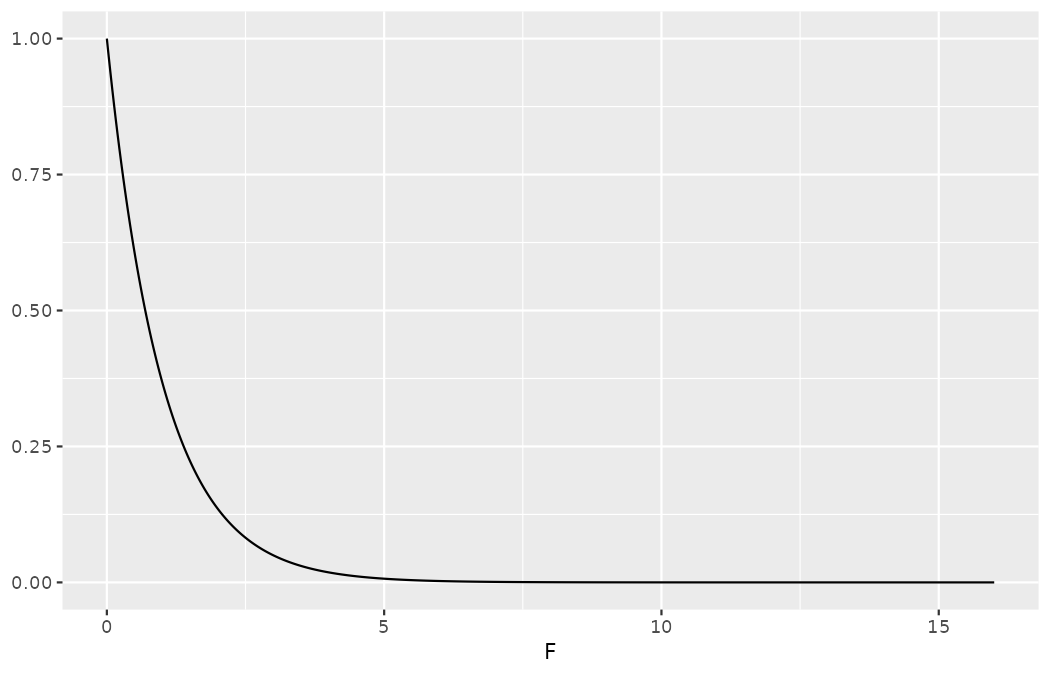
\includegraphics[width=0.85\linewidth,height=\textheight,keepaspectratio]{figures/inference-many-means-6.png}

Like the chi-squared distributions of
Chapter~\ref{sec-inference-tables}, the \(F\) distribution lives only on
positive values and is right-skewed: with \(df_1 = 2\) the curve starts
at its highest point at zero and decays steadily --- there is no
interior peak for this \(df_1\) --- with almost all of its area below 4.
The shaded region beyond 12.301 is far out in the tail --- much too
small to see on the plot --- and R computes its area directly:

\begin{Shaded}
\begin{Highlighting}[]
\FunctionTok{pf}\NormalTok{(}\FloatTok{12.301}\NormalTok{, }\DecValTok{2}\NormalTok{, }\DecValTok{1379}\NormalTok{, }\AttributeTok{lower.tail =} \ConstantTok{FALSE}\NormalTok{)}
\CommentTok{\#\textgreater{} [1] 5.068021e{-}06}
\end{Highlighting}
\end{Shaded}

\begin{tcolorbox}[enhanced jigsaw, left=2mm, leftrule=.75mm, title=\textcolor{quarto-callout-note-color}{\faInfo}\hspace{0.5em}{Worked example}, arc=.35mm, rightrule=.15mm, coltitle=black, colframe=quarto-callout-note-color-frame, bottomrule=.15mm, colbacktitle=quarto-callout-note-color!10!white, opacitybacktitle=0.6, breakable, bottomtitle=1mm, toptitle=1mm, titlerule=0mm, opacityback=0, toprule=.15mm, colback=white]

The p-value corresponding to the shaded upper tail is about 0.000005 ---
five in a million. Does this provide strong evidence against the null
hypothesis?

\begin{center}\rule{0.5\linewidth}{0.5pt}\end{center}

The p-value is (far) smaller than 0.05, indicating the evidence is
strong enough to reject the null hypothesis at a discernibility level of
0.05. That is, the data provide strong evidence that the average
open-play chance quality varies by position group. Remember what the
test cannot say: these are observational data --- nobody randomly
assigned players to positions --- so the conclusion is association, not
causation. The forwards' higher mean xG plausibly reflects \emph{where}
forwards operate (inside the box, on the end of moves) as much as
anything about the players themselves; the play-pattern confounding of
Chapter~\ref{sec-data-design} should be ringing in your ears. And recall
the Check your understanding of Section~\ref{sec-randANOVA}: the
position groups account for under 2\% of the total variability in chance
quality. Statistically discernible, footballing-ly modest.

\end{tcolorbox}

Note that the small p-value indicates that there is a notable difference
between the mean chance quality of the different position groups.
However, the ANOVA test does not provide a mechanism for knowing
\emph{which} group is driving the differences. If we move forward with
all possible two-mean comparisons, we run the risk of a high Type I
error rate. As we saw at the end of Section~\ref{sec-randANOVA}, the
follow-up questions surrounding individual group comparisons is called a
problem of \textbf{multiple comparisons} and is outside the scope of
this text. We encourage you to learn more about multiple comparisons,
however, so that additional comparisons, after you have rejected the
null hypothesis in an ANOVA test, do not lead to undue false positive
conclusions.

\subsection{Reading an ANOVA table from
software}\label{reading-an-anova-table-from-software}

The calculations required to perform an ANOVA by hand are tedious and
prone to human error. For these reasons, it is common to use statistical
software to calculate the \(F\)-statistic and p-value.

An ANOVA analysis can be summarized in a table very similar to that of a
regression summary, which we saw in Chapter~\ref{sec-model-slr} and
Chapter~\ref{sec-model-mlr}. In R, the table is produced by fitting the
group-means model with \texttt{lm()} and handing the fit to
\texttt{anova()}.

\begin{Shaded}
\begin{Highlighting}[]
\NormalTok{mod\_open }\OtherTok{\textless{}{-}} \FunctionTok{lm}\NormalTok{(statsbomb\_xg }\SpecialCharTok{\textasciitilde{}}\NormalTok{ pos\_group, }\AttributeTok{data =}\NormalTok{ wc\_open)}
\FunctionTok{anova}\NormalTok{(mod\_open)}
\CommentTok{\#\textgreater{} Analysis of Variance Table}
\CommentTok{\#\textgreater{}}
\CommentTok{\#\textgreater{} Response: statsbomb\_xg}
\CommentTok{\#\textgreater{}             Df Sum Sq  Mean Sq F value    Pr(\textgreater{}F)}
\CommentTok{\#\textgreater{} pos\_group    2  0.378 0.189024  12.301 5.067e{-}06 ***}
\CommentTok{\#\textgreater{} Residuals 1379 21.190 0.015366}
\end{Highlighting}
\end{Shaded}

Every quantity of this chapter is in the table, one row per source of
variability. The \texttt{pos\_group} row is the between-groups row:
\(df_G = 2,\) \(SSG = 0.378,\) \(MSG = 0.1890.\) The \texttt{Residuals}
row is the within-groups row: \(df_E = 1379,\) \(SSE = 21.190,\)
\(MSE = 0.0154.\) The last two columns hold the \(F\)-statistic
\((12.301,\) the ratio of the two \texttt{Mean\ Sq} entries\()\) and its
upper-tail p-value \((5.1 \times 10^{-6},\) matching our \texttt{pf()}
computation\().\)

\begin{tcolorbox}[enhanced jigsaw, left=2mm, leftrule=.75mm, title=\textcolor{quarto-callout-tip-color}{\faLightbulb}\hspace{0.5em}{Check your understanding}, arc=.35mm, rightrule=.15mm, coltitle=black, colframe=quarto-callout-tip-color-frame, bottomrule=.15mm, colbacktitle=quarto-callout-tip-color!10!white, opacitybacktitle=0.6, breakable, bottomtitle=1mm, toptitle=1mm, titlerule=0mm, opacityback=0, toprule=.15mm, colback=white]

Using only the \texttt{Df} column of the ANOVA table, recover the number
of groups and the number of shots in the analysis.

\begin{center}\rule{0.5\linewidth}{0.5pt}\end{center}

The between-groups degrees of freedom is \(k - 1 = 2,\) so \(k = 3\)
groups. The total degrees of freedom is \(2 + 1379 = 1381 = n - 1,\) so
\(n = 1382\) shots --- exactly the open-play count we filtered to at the
start of the case study. This little audit is worth performing on every
ANOVA table you are handed: the degrees of freedom silently document
which data went in.

\end{tcolorbox}

The case study opened with a promise: run the analysis penalties-in as
well, per the book's penalty convention, and let the contrast teach.
Here is the same table on all 1,494 shots:

\begin{Shaded}
\begin{Highlighting}[]
\NormalTok{mod\_all }\OtherTok{\textless{}{-}} \FunctionTok{lm}\NormalTok{(statsbomb\_xg }\SpecialCharTok{\textasciitilde{}}\NormalTok{ pos\_group, }\AttributeTok{data =}\NormalTok{ wc\_pos)}
\FunctionTok{anova}\NormalTok{(mod\_all)}
\CommentTok{\#\textgreater{} Analysis of Variance Table}
\CommentTok{\#\textgreater{}}
\CommentTok{\#\textgreater{} Response: statsbomb\_xg}
\CommentTok{\#\textgreater{}             Df Sum Sq  Mean Sq F value   Pr(\textgreater{}F)}
\CommentTok{\#\textgreater{} pos\_group    2  0.411 0.205733  6.1034 0.002291 **}
\CommentTok{\#\textgreater{} Residuals 1491 50.258 0.033708}
\end{Highlighting}
\end{Shaded}

Set the two tables side by side and read them through the lens of
\(F = MSG/MSE.\) Adding the 64 penalties barely moves the numerator:
\(SSG\) creeps from 0.378 to 0.411, because a penalty is worth the same
0.7835 no matter who takes it, so the \emph{between-group} gaps grow
only through the unequal doses (33 FW, 22 MF, 9 DF). The denominator is
another story: \(SSE\) more than doubles, from 21.190 to 50.258, because
each group now contains a cluster of values sitting 0.69 above its own
mean, and \(MSE\) swells from 0.0154 to 0.0337. The result: \(F\) is cut
in half, 12.30 to 6.10, and the p-value rises by nearly three orders of
magnitude, \(5.1 \times 10^{-6}\) to \(0.0023.\)

Both frames reject \(H_0\) at \(\alpha = 0.05,\) so no verdict flips
here --- but the lesson generalizes and cuts both ways. In
Section~\ref{sec-chp11-pens-out}, penalties \emph{manufactured} most of
an apparent effect by piling into one side of a two-group comparison;
here they \emph{mask} one, by inflating the within-group noise floor
that every between-group signal is judged against. A cluster of
identical extreme values does not have to move the means to corrupt an
ANOVA --- it can simply bloat the \(MSE\) and deafen the test. State the
frame, run both, and treat the gap between the answers as part of the
finding.

\subsection{Conditions for an ANOVA
analysis}\label{conditions-for-an-anova-analysis}

There are three conditions we must check for an ANOVA analysis: all
observations must be independent, the data in each group must be nearly
normal (or each group must have reasonably large sample sizes), and the
variance within each group must be approximately equal.

\begin{itemize}
\item
  \textbf{Independence.} If the data are a simple random sample, this
  condition can be assumed to be satisfied. For processes and
  experiments, carefully consider whether the data may be independent
  (e.g., no pairing). The World Cup shots were not sampled --- they are
  the full tournament --- and shots cluster within matches and within
  teams, so independence is the shakiest condition here. As we have done
  since Chapter~\ref{sec-foundations-randomization}, we proceed under
  the standard working assumption of shot analysis, stated openly: no
  obvious mechanism ties one shot's xG to another's given the position
  group. (For the \texttt{template\_abc} experiment, by contrast,
  independence came free: templates were randomly assigned, one report
  per assessor.)
\item
  \textbf{Approximately normal.} As with one- and two-sample testing for
  means, the normality assumption is especially important when the
  sample size is quite small, when it is ironically difficult to check
  for non-normality. The code below draws a histogram of chance quality
  for each position group:

\begin{Shaded}
\begin{Highlighting}[]
\FunctionTok{ggplot}\NormalTok{(wc\_open, }\FunctionTok{aes}\NormalTok{(}\AttributeTok{x =}\NormalTok{ statsbomb\_xg)) }\SpecialCharTok{+}
  \FunctionTok{geom\_histogram}\NormalTok{(}\AttributeTok{binwidth =} \FloatTok{0.05}\NormalTok{) }\SpecialCharTok{+}
  \FunctionTok{facet\_wrap}\NormalTok{(}\SpecialCharTok{\textasciitilde{}}\NormalTok{pos\_group, }\AttributeTok{ncol =} \DecValTok{1}\NormalTok{, }\AttributeTok{scales =} \StringTok{"free\_y"}\NormalTok{) }\SpecialCharTok{+}
  \FunctionTok{labs}\NormalTok{(}\AttributeTok{x =} \StringTok{"Chance quality (xG)"}\NormalTok{, }\AttributeTok{y =} \StringTok{"Count"}\NormalTok{)}
\end{Highlighting}
\end{Shaded}

  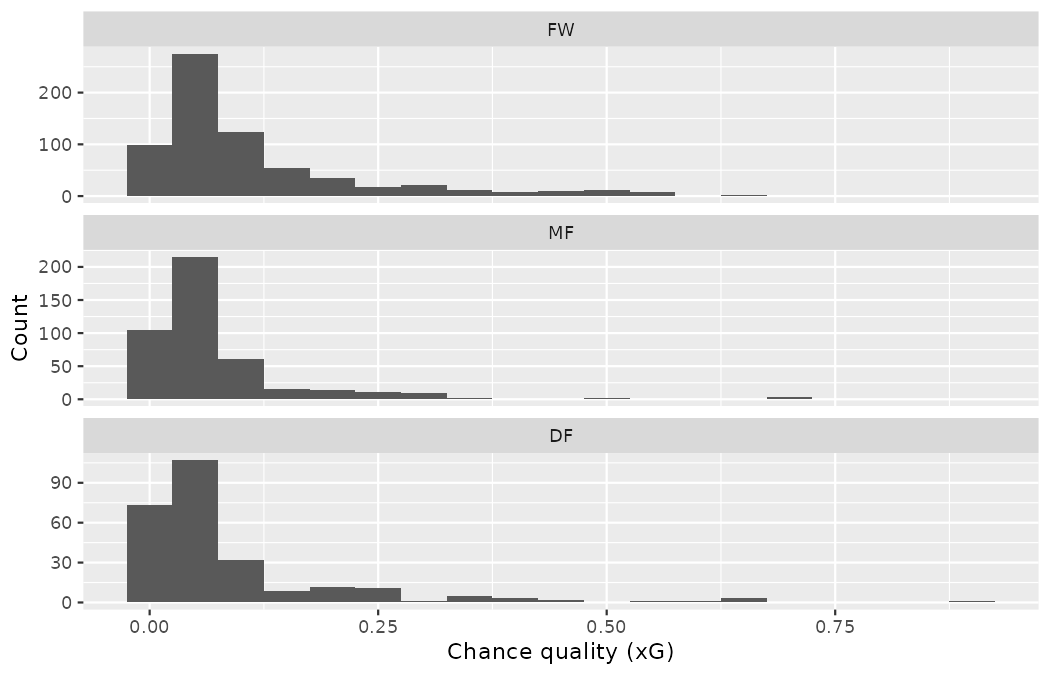
\includegraphics[width=0.85\linewidth,height=\textheight,keepaspectratio]{figures/inference-many-means-7.png}

  Unlike a batting average or an exam score, xG is nowhere near
  bell-shaped: all three histograms pile up against zero and decay to
  the right --- the same right skew every xG distribution in this book
  has shown. What saves the analysis is the sample sizes: with 678, 443,
  and 261 observations per group, the group \emph{means} behave normally
  even though the individual shots do not --- the Central Limit Theorem
  logic of Chapter~\ref{sec-foundations-mathematical} --- so what we are
  really scanning for are extreme outliers. In the open-play frame there
  are none: the largest open-play xG values sit below 0.9 and thin out
  smoothly. In the penalties-in frame, the spike of 64 identical values
  at 0.7835 is precisely the ``extreme outliers'' red flag this
  condition warns about --- one more reason the open-play frame is the
  honest one for this question.
\item
  \textbf{Constant variance.} The last assumption is that the variance
  in the groups is about equal from one group to the next. This
  assumption can be checked by examining side-by-side box plots of the
  outcomes across the groups, as in Section~\ref{sec-randANOVA}. In this
  case, the variability is similar in the three groups but not
  identical: Table~\ref{tbl-wc-pos-summary} shows standard deviations of
  0.133, 0.107, and 0.126, which do not vary much from one group to the
  next.
\end{itemize}

\begin{tcolorbox}[enhanced jigsaw, left=2mm, leftrule=.75mm, title=\textcolor{quarto-callout-important-color}{\faExclamation}\hspace{0.5em}{Diagnostics for an ANOVA analysis}, arc=.35mm, rightrule=.15mm, coltitle=black, colframe=quarto-callout-important-color-frame, bottomrule=.15mm, colbacktitle=quarto-callout-important-color!10!white, opacitybacktitle=0.6, breakable, bottomtitle=1mm, toptitle=1mm, titlerule=0mm, opacityback=0, toprule=.15mm, colback=white]

Independence is always important to an ANOVA analysis. The normality
condition is important when the sample sizes for each group are
relatively small (if the group sizes are large, the observations do not
need to be normal but should also not contain any large outliers). The
constant variance condition is especially important when the sample
sizes differ between groups.

\end{tcolorbox}

\section{Chapter review}\label{sec-chp22-review}

\subsection{Summary}\label{summary-21}

In this chapter we have provided both the randomization test and the
mathematical model appropriate for addressing questions of equality of
means across two or more groups: the template experiment was analyzed by
permuting the template labels and collecting 1,000 shuffled \(F\)
statistics, while the position-group case study used the \(F\)
distribution with \(df_1 = k - 1\) and \(df_2 = n - k.\) The \(F\)
statistic itself is the chapter in one line --- how much the group means
differ, divided by how much observations differ within groups --- and
the toy intake groups showed that it is your trained eye, made honest.
Two cautions deserve to travel with the machinery. First, the penalty
convention paid off again, in a new way: penalties barely touched the
between-group signal but doubled the within-group noise, halving \(F\)
--- a composition problem can mask an effect as easily as manufacture
one. Second, data snooping is not a subtle sin: letting the 32-squad
league table nominate which pair to test turned a 5\% error rate into
78\% in our seeded true-null worlds, which is why the single holistic
ANOVA test --- hypotheses fixed before looking --- exists at all. Note
that there were important technical conditions required for confirming
that the F distribution appropriately modeled the ANOVA test statistic.
Also, you may have noticed that there was no discussion of creating
confidence intervals. That is because the ANOVA statistic does not have
a direct analogue parameter to estimate. If there is interest in
comparisons of mean differences (across each set of two groups), then
the methods from Chapter~\ref{sec-inference-two-means} comparing two
independent means should be applied.

\subsection{Terms}\label{terms-21}

The terms introduced in this chapter are presented in
Table~\ref{tbl-terms-chp-22}. If you're not sure what some of these
terms mean, we recommend you go back in the text and review their
definitions. You should be able to easily spot them as \textbf{bolded
text}.

\begin{longtable}[]{@{}
  >{\raggedright\arraybackslash}p{(\linewidth - 4\tabcolsep) * \real{0.3380}}
  >{\raggedright\arraybackslash}p{(\linewidth - 4\tabcolsep) * \real{0.3380}}
  >{\raggedright\arraybackslash}p{(\linewidth - 4\tabcolsep) * \real{0.3239}}@{}}
\caption{Terms introduced in this
chapter.}\label{tbl-terms-chp-22}\tabularnewline
\toprule\noalign{}
\endfirsthead
\endhead
\bottomrule\noalign{}
\endlastfoot
analysis of variance (ANOVA) & degrees of freedom & multiple
comparisons \\
ANOVA & F-test & sum of squared error (SSE) \\
data fishing & mean square between groups (MSG) & sum of squares between
groups (SSG) \\
data snooping & mean square error (MSE) & sum of squares total (SST) \\
\end{longtable}

\section{Exercises}\label{sec-chp22-exercises}

Answers to odd-numbered exercises can be found in
Appendix~\ref{sec-exercise-solutions-22}.

\begin{enumerate}
\def\labelenumi{\arabic{enumi}.}
\item
  \textbf{Fill in the blank.} When doing an ANOVA, you observe large
  differences in means between groups. Within the ANOVA framework, this
  would most likely be interpreted as evidence strongly favoring the
  \_\_\_\_\_\_\_\_\_\_\_\_\_ hypothesis.
\item
  \textbf{Which test?} Marta Vidal would like to know whether trainee
  scouts assigned to Northbridge's four regional academies --- North,
  South, East, and West --- spend the same amount of time, on average,
  watching a prospect live before filing a first report. What type of
  test should we use? Explain your reasoning.
\item
  \textbf{Play patterns and chance quality at the Women's Euro,
  randomize once.} Different shots arise from different phases of play
  --- established possession, throw-ins, corners, free kicks, counters,
  and so on --- and Emil Sørensen's scouts argue constantly about
  whether some phases inherently produce better chances. One question
  relates to whether the average chance quality (xG) of a shot differs
  depending on the play pattern from which it arose, using the 913 shots
  of the 2025 Women's Euro.\footnote{The 2025 Women's Euro shot data
    used in this exercise are in
    \texttt{data/derived/weuro2025\_shots.csv} (StatsBomb open data).}
  Per the book's penalty convention, the frame is stated first: the
  \texttt{Other} bucket --- 54 shots, made up of the tournament's 51
  penalty kicks (all at xG 0.7835) plus 3 open-play-tagged shots --- is
  excluded with the stated filter \texttt{play\_pattern\ !=\ "Other"},
  exactly as in the corresponding test of
  Section~\ref{sec-chp18-real-table}, leaving \(913 - 54 = 859\) shots
  across eight play patterns.

\begin{Shaded}
\begin{Highlighting}[]
\NormalTok{weuro2025\_shots }\OtherTok{\textless{}{-}} \FunctionTok{read\_csv}\NormalTok{(}\StringTok{"data/derived/weuro2025\_shots.csv"}\NormalTok{)}

\NormalTok{weuro2025\_shots }\SpecialCharTok{|\textgreater{}}
  \FunctionTok{filter}\NormalTok{(play\_pattern }\SpecialCharTok{==} \StringTok{"Other"}\NormalTok{) }\SpecialCharTok{|\textgreater{}}
  \FunctionTok{count}\NormalTok{(shot\_type, goal)}
\CommentTok{\#\textgreater{} \# A tibble: 4 × 3}
\CommentTok{\#\textgreater{}   shot\_type goal      n}
\CommentTok{\#\textgreater{}   \textless{}chr\textgreater{}     \textless{}lgl\textgreater{} \textless{}int\textgreater{}}
\CommentTok{\#\textgreater{} 1 Open Play FALSE     1}
\CommentTok{\#\textgreater{} 2 Open Play TRUE      2}
\CommentTok{\#\textgreater{} 3 Penalty   FALSE    23}
\CommentTok{\#\textgreater{} 4 Penalty   TRUE     28}

\NormalTok{we\_pattern }\OtherTok{\textless{}{-}}\NormalTok{ weuro2025\_shots }\SpecialCharTok{|\textgreater{}}
  \FunctionTok{filter}\NormalTok{(play\_pattern }\SpecialCharTok{!=} \StringTok{"Other"}\NormalTok{) }\SpecialCharTok{|\textgreater{}}
  \FunctionTok{mutate}\NormalTok{(}\AttributeTok{play\_pattern =} \FunctionTok{factor}\NormalTok{(play\_pattern,}
    \AttributeTok{levels =} \FunctionTok{c}\NormalTok{(}\StringTok{"Regular Play"}\NormalTok{, }\StringTok{"From Throw In"}\NormalTok{, }\StringTok{"From Corner"}\NormalTok{, }\StringTok{"From Free Kick"}\NormalTok{,}
               \StringTok{"From Counter"}\NormalTok{, }\StringTok{"From Goal Kick"}\NormalTok{, }\StringTok{"From Keeper"}\NormalTok{, }\StringTok{"From Kick Off"}\NormalTok{)))}

\NormalTok{we\_pattern }\SpecialCharTok{|\textgreater{}}
  \FunctionTok{group\_by}\NormalTok{(play\_pattern) }\SpecialCharTok{|\textgreater{}}
  \FunctionTok{summarize}\NormalTok{(}\AttributeTok{n =} \FunctionTok{n}\NormalTok{(), }\AttributeTok{mean =} \FunctionTok{mean}\NormalTok{(statsbomb\_xg), }\AttributeTok{sd =} \FunctionTok{sd}\NormalTok{(statsbomb\_xg))}
\CommentTok{\#\textgreater{} \# A tibble: 8 × 4}
\CommentTok{\#\textgreater{}   play\_pattern       n   mean     sd}
\CommentTok{\#\textgreater{}   \textless{}fct\textgreater{}          \textless{}int\textgreater{}  \textless{}dbl\textgreater{}  \textless{}dbl\textgreater{}}
\CommentTok{\#\textgreater{} 1 Regular Play     310 0.0998 0.115}
\CommentTok{\#\textgreater{} 2 From Throw In    177 0.104  0.119}
\CommentTok{\#\textgreater{} 3 From Corner      160 0.0840 0.0847}
\CommentTok{\#\textgreater{} 4 From Free Kick   104 0.0845 0.102}
\CommentTok{\#\textgreater{} 5 From Counter      41 0.0905 0.106}
\CommentTok{\#\textgreater{} 6 From Goal Kick    35 0.142  0.183}
\CommentTok{\#\textgreater{} 7 From Keeper       22 0.0617 0.0315}
\CommentTok{\#\textgreater{} 8 From Kick Off     10 0.0894 0.0737}
\end{Highlighting}
\end{Shaded}

  Consider the following two sets of side-by-side box plots: one
  represents the original data, and the second represents data where the
  play pattern has been randomly reassigned to the xG values (a single
  seeded permutation).

\begin{Shaded}
\begin{Highlighting}[]
\NormalTok{p\_orig }\OtherTok{\textless{}{-}} \FunctionTok{ggplot}\NormalTok{(we\_pattern, }\FunctionTok{aes}\NormalTok{(}\AttributeTok{y =}\NormalTok{ play\_pattern, }\AttributeTok{x =}\NormalTok{ statsbomb\_xg)) }\SpecialCharTok{+}
  \FunctionTok{geom\_boxplot}\NormalTok{() }\SpecialCharTok{+}
  \FunctionTok{labs}\NormalTok{(}
    \AttributeTok{y =} \StringTok{"Play pattern"}\NormalTok{,}
    \AttributeTok{x =} \StringTok{"Chance quality (xG)"}\NormalTok{,}
    \AttributeTok{title =} \StringTok{"Original play patterns"}
\NormalTok{  )}

\FunctionTok{set.seed}\NormalTok{(}\DecValTok{2206}\NormalTok{)}
\NormalTok{we\_pattern\_rand }\OtherTok{\textless{}{-}}\NormalTok{ we\_pattern }\SpecialCharTok{|\textgreater{}}
  \FunctionTok{specify}\NormalTok{(statsbomb\_xg }\SpecialCharTok{\textasciitilde{}}\NormalTok{ play\_pattern) }\SpecialCharTok{|\textgreater{}}
  \FunctionTok{hypothesize}\NormalTok{(}\AttributeTok{null =} \StringTok{"independence"}\NormalTok{) }\SpecialCharTok{|\textgreater{}}
  \FunctionTok{generate}\NormalTok{(}\DecValTok{1}\NormalTok{, }\AttributeTok{type =} \StringTok{"permute"}\NormalTok{)}

\NormalTok{we\_pattern\_rand }\SpecialCharTok{|\textgreater{}}
  \FunctionTok{group\_by}\NormalTok{(play\_pattern) }\SpecialCharTok{|\textgreater{}}
  \FunctionTok{summarize}\NormalTok{(}\AttributeTok{n =} \FunctionTok{n}\NormalTok{(), }\AttributeTok{mean =} \FunctionTok{mean}\NormalTok{(statsbomb\_xg))}
\CommentTok{\#\textgreater{} \# A tibble: 8 × 3}
\CommentTok{\#\textgreater{}   play\_pattern       n   mean}
\CommentTok{\#\textgreater{}   \textless{}fct\textgreater{}          \textless{}int\textgreater{}  \textless{}dbl\textgreater{}}
\CommentTok{\#\textgreater{} 1 Regular Play     310 0.0923}
\CommentTok{\#\textgreater{} 2 From Throw In    177 0.0949}
\CommentTok{\#\textgreater{} 3 From Corner      160 0.0983}
\CommentTok{\#\textgreater{} 4 From Free Kick   104 0.112}
\CommentTok{\#\textgreater{} 5 From Counter      41 0.114}
\CommentTok{\#\textgreater{} 6 From Goal Kick    35 0.0718}
\CommentTok{\#\textgreater{} 7 From Keeper       22 0.0793}
\CommentTok{\#\textgreater{} 8 From Kick Off     10 0.0757}

\NormalTok{p\_rand }\OtherTok{\textless{}{-}} \FunctionTok{ggplot}\NormalTok{(we\_pattern\_rand, }\FunctionTok{aes}\NormalTok{(}\AttributeTok{y =}\NormalTok{ play\_pattern, }\AttributeTok{x =}\NormalTok{ statsbomb\_xg)) }\SpecialCharTok{+}
  \FunctionTok{geom\_boxplot}\NormalTok{() }\SpecialCharTok{+}
  \FunctionTok{labs}\NormalTok{(}
    \AttributeTok{y =} \StringTok{"Play pattern"}\NormalTok{,}
    \AttributeTok{x =} \StringTok{"Chance quality (xG)"}\NormalTok{,}
    \AttributeTok{title =} \StringTok{"Play pattern randomized to xG"}
\NormalTok{  )}
\end{Highlighting}
\end{Shaded}

  \begin{enumerate}
  \def\labelenumii{\alph{enumii}.}
  \item
    Consider the average chance quality for each play pattern. Is the
    set of group means for the original data: more variable, less
    variable, or about the same as for the randomized data? Describe
    what you see in the summaries.
  \item
    Consider the standard deviation of the xG values within each play
    pattern. Is the within-pattern standard deviation for the original
    data: bigger, smaller, or about the same as for the randomized data?
  \item
    Recall that the F statistic's numerator measures how much the groups
    vary (MSG), with the denominator measuring how much the within-group
    values vary (MSE). Which of the two datasets would have a larger F
    statistic, the original data or the randomized data? Explain.
  \end{enumerate}
\item
  \textbf{Play patterns and chance quality at the Women's Euro,
  randomization test.} Using the same 859 shots of the previous exercise
  (penalties excluded via the stated \texttt{Other} filter, as described
  there), the play pattern was randomly reassigned to the xG values
  1,000 times, and the randomization \(F\) statistic was computed for
  each permutation.\footnote{The 2025 Women's Euro shot data used in
    this exercise are in \texttt{data/derived/weuro2025\_shots.csv}
    (StatsBomb open data).} Conduct a hypothesis test to evaluate if
  there is a difference, in the population of shots this tournament
  represents, between the average chance quality across the eight play
  patterns. Make sure to state your hypotheses clearly and interpret
  your results in the context of the data. Keep in mind what kind of
  data these are: nobody assigned play patterns to shots at random.

\begin{Shaded}
\begin{Highlighting}[]
\NormalTok{we\_F\_obs }\OtherTok{\textless{}{-}}\NormalTok{ we\_pattern }\SpecialCharTok{|\textgreater{}}
  \FunctionTok{specify}\NormalTok{(statsbomb\_xg }\SpecialCharTok{\textasciitilde{}}\NormalTok{ play\_pattern) }\SpecialCharTok{|\textgreater{}}
  \FunctionTok{calculate}\NormalTok{(}\AttributeTok{stat =} \StringTok{"F"}\NormalTok{) }\SpecialCharTok{|\textgreater{}}
  \FunctionTok{pull}\NormalTok{()}

\NormalTok{we\_F\_obs}
\CommentTok{\#\textgreater{} [1] 1.77402}

\FunctionTok{set.seed}\NormalTok{(}\DecValTok{2207}\NormalTok{)}
\NormalTok{we\_pattern\_null }\OtherTok{\textless{}{-}}\NormalTok{ we\_pattern }\SpecialCharTok{|\textgreater{}}
  \FunctionTok{specify}\NormalTok{(statsbomb\_xg }\SpecialCharTok{\textasciitilde{}}\NormalTok{ play\_pattern) }\SpecialCharTok{|\textgreater{}}
  \FunctionTok{hypothesize}\NormalTok{(}\AttributeTok{null =} \StringTok{"independence"}\NormalTok{) }\SpecialCharTok{|\textgreater{}}
  \FunctionTok{generate}\NormalTok{(}\AttributeTok{reps =} \DecValTok{1000}\NormalTok{, }\AttributeTok{type =} \StringTok{"permute"}\NormalTok{) }\SpecialCharTok{|\textgreater{}}
  \FunctionTok{calculate}\NormalTok{(}\AttributeTok{stat =} \StringTok{"F"}\NormalTok{)}

\NormalTok{we\_pattern\_null }\SpecialCharTok{|\textgreater{}}
  \FunctionTok{summarize}\NormalTok{(}\AttributeTok{n\_extreme =} \FunctionTok{sum}\NormalTok{(stat }\SpecialCharTok{\textgreater{}=}\NormalTok{ we\_F\_obs), }\AttributeTok{p\_value =} \FunctionTok{mean}\NormalTok{(stat }\SpecialCharTok{\textgreater{}=}\NormalTok{ we\_F\_obs))}
\CommentTok{\#\textgreater{} \# A tibble: 1 × 2}
\CommentTok{\#\textgreater{}   n\_extreme p\_value}
\CommentTok{\#\textgreater{}       \textless{}int\textgreater{}   \textless{}dbl\textgreater{}}
\CommentTok{\#\textgreater{} 1        91   0.091}

\FunctionTok{ggplot}\NormalTok{(we\_pattern\_null, }\FunctionTok{aes}\NormalTok{(}\AttributeTok{x =}\NormalTok{ stat)) }\SpecialCharTok{+}
  \FunctionTok{geom\_histogram}\NormalTok{(}\AttributeTok{binwidth =} \FloatTok{0.2}\NormalTok{) }\SpecialCharTok{+}
  \FunctionTok{geom\_vline}\NormalTok{(}\AttributeTok{xintercept =}\NormalTok{ we\_F\_obs, }\AttributeTok{color =} \StringTok{"red"}\NormalTok{, }\AttributeTok{linewidth =} \DecValTok{1}\NormalTok{) }\SpecialCharTok{+}
  \FunctionTok{labs}\NormalTok{(}
    \AttributeTok{x =} \StringTok{"F statistic for randomized xG values"}\NormalTok{,}
    \AttributeTok{y =} \StringTok{"Count"}\NormalTok{,}
    \AttributeTok{title =} \StringTok{"1,000 randomized F statistics"}
\NormalTok{  )}
\end{Highlighting}
\end{Shaded}

  The histogram of the 1,000 randomized \(F\) statistics is
  right-skewed, ranging from about 0.09 to 3.8, with the observed
  statistic of 1.77 marked by the red line; 91 of the 1,000 randomized
  statistics were at least as large as the observed one.
\item
  \textbf{Finishing programmes and assessment scores, many groups.} A
  constructed Northbridge experiment was conducted to measure and
  compare the effectiveness of various finishing-drill programmes on
  academy strikers. Jonas Beck randomly allocated 71 newly enrolled
  strikers into six groups, and each group trained under a different
  programme for eight weeks before sitting the academy's standardized
  finishing assessment (scored out of 100). The echo of the six-arm
  finishing trial in the exercises of Section~\ref{sec-chp20-exercises}
  is deliberate: this second cohort was enrolled with the same arm sizes
  as that trial so the two seasons could be compared, with the
  programmes renamed and the grading rescaled to a 100-point assessment
  that season. The dataset is built by the seeded code below; sample
  statistics and the ANOVA output follow.\footnote{The \texttt{drill71}
    data are a constructed scouting scenario, generated entirely by the
    seeded code shown; no real academy strikers were assessed.}

\begin{Shaded}
\begin{Highlighting}[]
\FunctionTok{set.seed}\NormalTok{(}\DecValTok{2208}\NormalTok{)}
\NormalTok{drill71 }\OtherTok{\textless{}{-}} \FunctionTok{tibble}\NormalTok{(}
  \AttributeTok{programme =} \FunctionTok{factor}\NormalTok{(}\FunctionTok{rep}\NormalTok{(}\FunctionTok{c}\NormalTok{(}\StringTok{"Standard"}\NormalTok{, }\StringTok{"Volume"}\NormalTok{, }\StringTok{"Angles"}\NormalTok{, }\StringTok{"Pressure"}\NormalTok{, }\StringTok{"Two{-}touch"}\NormalTok{, }\StringTok{"Composite"}\NormalTok{),}
                         \AttributeTok{times =} \FunctionTok{c}\NormalTok{(}\DecValTok{12}\NormalTok{, }\DecValTok{10}\NormalTok{, }\DecValTok{12}\NormalTok{, }\DecValTok{11}\NormalTok{, }\DecValTok{14}\NormalTok{, }\DecValTok{12}\NormalTok{)),}
                     \AttributeTok{levels =} \FunctionTok{c}\NormalTok{(}\StringTok{"Standard"}\NormalTok{, }\StringTok{"Volume"}\NormalTok{, }\StringTok{"Angles"}\NormalTok{, }\StringTok{"Pressure"}\NormalTok{, }\StringTok{"Two{-}touch"}\NormalTok{, }\StringTok{"Composite"}\NormalTok{)),}
  \AttributeTok{score =} \FunctionTok{c}\NormalTok{(}\FunctionTok{rnorm}\NormalTok{(}\DecValTok{12}\NormalTok{, }\DecValTok{68}\NormalTok{, }\DecValTok{8}\NormalTok{), }\FunctionTok{rnorm}\NormalTok{(}\DecValTok{10}\NormalTok{, }\DecValTok{45}\NormalTok{, }\DecValTok{8}\NormalTok{), }\FunctionTok{rnorm}\NormalTok{(}\DecValTok{12}\NormalTok{, }\DecValTok{52}\NormalTok{, }\DecValTok{8}\NormalTok{),}
            \FunctionTok{rnorm}\NormalTok{(}\DecValTok{11}\NormalTok{, }\DecValTok{63}\NormalTok{, }\DecValTok{8}\NormalTok{), }\FunctionTok{rnorm}\NormalTok{(}\DecValTok{14}\NormalTok{, }\DecValTok{50}\NormalTok{, }\DecValTok{8}\NormalTok{), }\FunctionTok{rnorm}\NormalTok{(}\DecValTok{12}\NormalTok{, }\DecValTok{70}\NormalTok{, }\DecValTok{8}\NormalTok{)) }\SpecialCharTok{|\textgreater{}}
    \FunctionTok{round}\NormalTok{(}\DecValTok{1}\NormalTok{)}
\NormalTok{)}

\NormalTok{drill71 }\SpecialCharTok{|\textgreater{}}
  \FunctionTok{group\_by}\NormalTok{(programme) }\SpecialCharTok{|\textgreater{}}
  \FunctionTok{summarize}\NormalTok{(}\AttributeTok{mean =} \FunctionTok{mean}\NormalTok{(score), }\AttributeTok{sd =} \FunctionTok{sd}\NormalTok{(score), }\AttributeTok{n =} \FunctionTok{n}\NormalTok{())}
\CommentTok{\#\textgreater{} \# A tibble: 6 × 4}
\CommentTok{\#\textgreater{}   programme  mean    sd     n}
\CommentTok{\#\textgreater{}   \textless{}fct\textgreater{}     \textless{}dbl\textgreater{} \textless{}dbl\textgreater{} \textless{}int\textgreater{}}
\CommentTok{\#\textgreater{} 1 Standard   67.0  5.71    12}
\CommentTok{\#\textgreater{} 2 Volume     47.8  7.87    10}
\CommentTok{\#\textgreater{} 3 Angles     52.1  8.57    12}
\CommentTok{\#\textgreater{} 4 Pressure   65.2  8.86    11}
\CommentTok{\#\textgreater{} 5 Two{-}touch  46.8 10.9     14}
\CommentTok{\#\textgreater{} 6 Composite  66.8  7.06    12}

\FunctionTok{ggplot}\NormalTok{(drill71, }\FunctionTok{aes}\NormalTok{(}\AttributeTok{x =}\NormalTok{ programme, }\AttributeTok{y =}\NormalTok{ score)) }\SpecialCharTok{+}
  \FunctionTok{geom\_boxplot}\NormalTok{() }\SpecialCharTok{+}
  \FunctionTok{labs}\NormalTok{(}\AttributeTok{x =} \ConstantTok{NULL}\NormalTok{, }\AttributeTok{y =} \StringTok{"Finishing assessment score"}\NormalTok{)}
\end{Highlighting}
\end{Shaded}

  Using the ANOVA output below, conduct a hypothesis test to determine
  if these data provide convincing evidence that the average assessment
  score varies across some (or all) programme groups. Make sure to check
  relevant conditions. The side-by-side box plots of the six groups are
  each reasonably symmetric, with a single mild outlier in the Volume
  group.

\begin{Shaded}
\begin{Highlighting}[]
\FunctionTok{lm}\NormalTok{(score }\SpecialCharTok{\textasciitilde{}}\NormalTok{ programme, }\AttributeTok{data =}\NormalTok{ drill71) }\SpecialCharTok{|\textgreater{}}
  \FunctionTok{anova}\NormalTok{()}
\CommentTok{\#\textgreater{} Analysis of Variance Table}
\CommentTok{\#\textgreater{}}
\CommentTok{\#\textgreater{} Response: score}
\CommentTok{\#\textgreater{}           Df Sum Sq Mean Sq F value    Pr(\textgreater{}F)}
\CommentTok{\#\textgreater{} programme  5 5650.1 1130.01  15.968 3.071e{-}10 ***}
\CommentTok{\#\textgreater{} Residuals 65 4599.9   70.77}
\end{Highlighting}
\end{Shaded}
\item
  \textbf{Teaching the grading rubric.} Emil Sørensen compared five
  different formats for teaching Northbridge's prospect-grading rubric
  to newly hired scouts: the traditional classroom seminar, a self-paced
  written manual, the manual plus seminar, an interactive video course,
  and the video course plus seminar. 45 trainee scouts were randomly
  assigned, 9 to each format. After completing the course, the trainees
  took a 1-hour certification exam.

  \begin{enumerate}
  \def\labelenumii{\alph{enumii}.}
  \item
    What are the hypotheses for evaluating if the average certification
    scores are different for the different teaching formats?
  \item
    What are the degrees of freedom associated with the \(F\)-test for
    evaluating these hypotheses?
  \item
    Suppose the p-value for this test is 0.0168. What is the conclusion?
  \end{enumerate}
\item
  \textbf{Match sharpness and training volume.} GPS vests log every
  player's high-intensity output. In a constructed scenario mirroring a
  large federation cohort study (the same registry introduced in the
  training-volume exercise of Section~\ref{sec-chp18-exercises}),
  analysts used the youth registry's GPS database to ask whether a
  player's weekly minutes of high-intensity match work differ across
  levels of weekly \emph{organized training} volume. The table below
  gives summary statistics of weekly high-intensity match minutes for
  the 50,739 registered players, based on hours of organized training
  per week; the response is always greater than 0.

  \begin{longtable}[]{@{}lrrrrr@{}}
  \toprule\noalign{}
  & Under 2 & 2--6 & 7--13 & 14--21 & 22 or more \\
  \midrule\noalign{}
  \endhead
  \bottomrule\noalign{}
  \endlastfoot
  Mean & 18.7 & 19.6 & 19.3 & 18.9 & 17.5 \\
  SD & 21.1 & 25.5 & 22.5 & 22.0 & 22.0 \\
  n & 12,215 & 6,617 & 17,234 & 12,290 & 2,383 \\
  \end{longtable}

  \begin{enumerate}
  \def\labelenumii{\alph{enumii}.}
  \item
    Write the hypotheses for evaluating if the average weekly
    high-intensity match minutes vary among the different
    training-volume levels.
  \item
    Check conditions and describe any assumptions you must make to
    proceed with the test.
  \item
    Below is the output associated with this test. What is the
    conclusion of the test?
  \end{enumerate}

  \begin{longtable}[]{@{}lrrrrr@{}}
  \toprule\noalign{}
  & Df & Sum Sq & Mean Sq & F value & Pr(\textgreater F) \\
  \midrule\noalign{}
  \endhead
  \bottomrule\noalign{}
  \endlastfoot
  volume & 4 & 10,508 & 2,627 & 5.2 & 0.0003 \\
  Residuals & 50,734 & 25,564,819 & 504 & & \\
  Total & 50,738 & 25,575,327 & & & \\
  \end{longtable}
\item
  \textbf{Report quality across sub-networks.} Emil Sørensen's 48
  regional scouts are organized into eight sub-networks, each led by a
  different senior scout. In a constructed end-of-season audit, 197
  prospect reports filed across the sub-networks were re-scored for
  quality by a blinded panel; Emil would like to test if report quality
  differs by sub-network. The summary table below shows the average
  audit score for each sub-network as well as the standard deviation of
  scores and the number of reports audited from each.

  \begin{longtable}[]{@{}lrrrrrrrr@{}}
  \toprule\noalign{}
  & Net 1 & Net 2 & Net 3 & Net 4 & Net 5 & Net 6 & Net 7 & Net 8 \\
  \midrule\noalign{}
  \endhead
  \bottomrule\noalign{}
  \endlastfoot
  Mean & 92.94 & 91.11 & 91.80 & 92.45 & 89.30 & 88.30 & 90.12 &
  93.35 \\
  SD & 4.21 & 5.58 & 3.43 & 5.92 & 9.32 & 7.27 & 6.93 & 4.57 \\
  n & 33 & 19 & 10 & 29 & 33 & 10 & 32 & 31 \\
  \end{longtable}

  The ANOVA output below can be used to test for differences between the
  average audit scores from the different sub-networks.

  \begin{longtable}[]{@{}lrrrrr@{}}
  \toprule\noalign{}
  & Df & Sum Sq & Mean Sq & F value & Pr(\textgreater F) \\
  \midrule\noalign{}
  \endhead
  \bottomrule\noalign{}
  \endlastfoot
  network & 7 & 525.01 & 75.00 & 1.87 & 0.0767 \\
  Residuals & 189 & 7,584.11 & 40.13 & & \\
  Total & 196 & 8,109.12 & & & \\
  \end{longtable}

  Conduct a hypothesis test to determine if these data provide
  convincing evidence that the average audit score varies across some
  (or all) sub-networks. Check conditions and describe any assumptions
  you must make to proceed with the test.
\item
  \textbf{Chance quality by position group at the Women's Euro.}
  Section~\ref{sec-mathANOVA} found that average open-play chance
  quality varies by position group at the 2022 Men's World Cup. Does the
  pattern replicate at the 2025 Women's Euro? The code below applies the
  position-group mapping of Chapter~\ref{sec-explore-categorical} to the
  Euro's open-play shots (the same stated frame as the chapter's case
  study; the Euro's two goalkeeper shots were both penalties, so the
  open-play filter leaves no \texttt{GK} rows) and fits the
  ANOVA.\footnote{The 2025 Women's Euro shot data used in this exercise
    are in \texttt{data/derived/weuro2025\_shots.csv} (StatsBomb open
    data); the position-group mapping is the one defined once in
    Chapter~\ref{sec-explore-categorical} and reused throughout the
    book.} The density ridges show the distributions of xG for the three
  groups, each strongly right-skewed.

\begin{Shaded}
\begin{Highlighting}[]
\FunctionTok{library}\NormalTok{(ggridges)}

\NormalTok{weuro\_pos\_open }\OtherTok{\textless{}{-}}\NormalTok{ weuro2025\_shots }\SpecialCharTok{|\textgreater{}}
  \FunctionTok{filter}\NormalTok{(shot\_type }\SpecialCharTok{==} \StringTok{"Open Play"}\NormalTok{) }\SpecialCharTok{|\textgreater{}}
  \FunctionTok{mutate}\NormalTok{(}
    \AttributeTok{pos\_group =} \FunctionTok{case\_when}\NormalTok{(}
\NormalTok{      position }\SpecialCharTok{==} \StringTok{"Goalkeeper"} \SpecialCharTok{\textasciitilde{}} \StringTok{"GK"}\NormalTok{,}
      \FunctionTok{grepl}\NormalTok{(}\StringTok{"Back"}\NormalTok{, position) }\SpecialCharTok{\textasciitilde{}} \StringTok{"DF"}\NormalTok{,}
      \FunctionTok{grepl}\NormalTok{(}\StringTok{"Midfield"}\NormalTok{, position) }\SpecialCharTok{\textasciitilde{}} \StringTok{"MF"}\NormalTok{,}
      \AttributeTok{.default =} \StringTok{"FW"}
\NormalTok{    ),}
    \AttributeTok{pos\_group =} \FunctionTok{factor}\NormalTok{(pos\_group, }\AttributeTok{levels =} \FunctionTok{c}\NormalTok{(}\StringTok{"FW"}\NormalTok{, }\StringTok{"MF"}\NormalTok{, }\StringTok{"DF"}\NormalTok{))}
\NormalTok{  )}

\NormalTok{weuro\_pos\_open }\SpecialCharTok{|\textgreater{}}
  \FunctionTok{count}\NormalTok{(pos\_group)}
\CommentTok{\#\textgreater{} \# A tibble: 3 × 2}
\CommentTok{\#\textgreater{}   pos\_group     n}
\CommentTok{\#\textgreater{}   \textless{}fct\textgreater{}     \textless{}int\textgreater{}}
\CommentTok{\#\textgreater{} 1 FW          402}
\CommentTok{\#\textgreater{} 2 MF          308}
\CommentTok{\#\textgreater{} 3 DF          141}

\FunctionTok{ggplot}\NormalTok{(weuro\_pos\_open, }\FunctionTok{aes}\NormalTok{(}\AttributeTok{x =}\NormalTok{ statsbomb\_xg, }\AttributeTok{y =}\NormalTok{ pos\_group,}
                           \AttributeTok{color =}\NormalTok{ pos\_group, }\AttributeTok{fill =}\NormalTok{ pos\_group)) }\SpecialCharTok{+}
  \FunctionTok{geom\_density\_ridges}\NormalTok{(}\AttributeTok{alpha =} \FloatTok{0.5}\NormalTok{, }\AttributeTok{show.legend =} \ConstantTok{FALSE}\NormalTok{) }\SpecialCharTok{+}
  \FunctionTok{labs}\NormalTok{(}\AttributeTok{x =} \StringTok{"Chance quality (xG)"}\NormalTok{, }\AttributeTok{y =} \StringTok{"Position group"}\NormalTok{)}

\FunctionTok{lm}\NormalTok{(statsbomb\_xg }\SpecialCharTok{\textasciitilde{}}\NormalTok{ pos\_group, }\AttributeTok{data =}\NormalTok{ weuro\_pos\_open) }\SpecialCharTok{|\textgreater{}}
  \FunctionTok{anova}\NormalTok{()}
\CommentTok{\#\textgreater{} Analysis of Variance Table}
\CommentTok{\#\textgreater{}}
\CommentTok{\#\textgreater{} Response: statsbomb\_xg}
\CommentTok{\#\textgreater{}            Df  Sum Sq  Mean Sq F value    Pr(\textgreater{}F)}
\CommentTok{\#\textgreater{} pos\_group   2  0.4007 0.200370  16.406 1.022e{-}07 ***}
\CommentTok{\#\textgreater{} Residuals 848 10.3568 0.012213}
\end{Highlighting}
\end{Shaded}

  \begin{enumerate}
  \def\labelenumii{\alph{enumii}.}
  \item
    Write the hypotheses for testing for a difference between average
    open-play chance quality across position groups.
  \item
    What is the conclusion of the hypothesis test, and what may the club
    claim about position groups and chance quality at this tournament?
  \item
    How many shots enter the analysis, i.e., what is the sample size?
    (Recover it from the ANOVA table's degrees of freedom, then confirm
    against the group counts.)
  \end{enumerate}
\item
  \textbf{Play patterns and chance quality at the World Cup.} The
  play-pattern question of Exercises 3 and 4 can be asked of the 2022
  Men's World Cup as well. Applying the same stated filter --- the
  \texttt{Other} bucket here holds 68 shots: all 64 penalty kicks (43
  scored) plus 4 open-play-tagged shots, exactly the composition
  documented in Section~\ref{sec-chp18-real-table} --- leaves
  \(1494 - 68 = 1426\) shots across the eight play patterns.\footnote{The
    2022 Men's World Cup shot data used in this exercise are in
    \texttt{data/derived/wc2022\_shots.csv} (StatsBomb open data).}
  Below are the distributions of chance quality by play pattern and
  relevant summary statistics, followed by the ANOVA output.

\begin{Shaded}
\begin{Highlighting}[]
\NormalTok{wc2022\_shots }\OtherTok{\textless{}{-}} \FunctionTok{read\_csv}\NormalTok{(}\StringTok{"data/derived/wc2022\_shots.csv"}\NormalTok{)}

\NormalTok{wc2022\_shots }\SpecialCharTok{|\textgreater{}}
  \FunctionTok{filter}\NormalTok{(play\_pattern }\SpecialCharTok{==} \StringTok{"Other"}\NormalTok{) }\SpecialCharTok{|\textgreater{}}
  \FunctionTok{count}\NormalTok{(shot\_type, goal)}
\CommentTok{\#\textgreater{} \# A tibble: 3 × 3}
\CommentTok{\#\textgreater{}   shot\_type goal      n}
\CommentTok{\#\textgreater{}   \textless{}chr\textgreater{}     \textless{}lgl\textgreater{} \textless{}int\textgreater{}}
\CommentTok{\#\textgreater{} 1 Open Play FALSE     4}
\CommentTok{\#\textgreater{} 2 Penalty   FALSE    21}
\CommentTok{\#\textgreater{} 3 Penalty   TRUE     43}

\NormalTok{wc\_pattern\_xg }\OtherTok{\textless{}{-}}\NormalTok{ wc2022\_shots }\SpecialCharTok{|\textgreater{}}
  \FunctionTok{filter}\NormalTok{(play\_pattern }\SpecialCharTok{!=} \StringTok{"Other"}\NormalTok{) }\SpecialCharTok{|\textgreater{}}
  \FunctionTok{mutate}\NormalTok{(}\AttributeTok{play\_pattern =} \FunctionTok{factor}\NormalTok{(play\_pattern,}
    \AttributeTok{levels =} \FunctionTok{c}\NormalTok{(}\StringTok{"Regular Play"}\NormalTok{, }\StringTok{"From Throw In"}\NormalTok{, }\StringTok{"From Free Kick"}\NormalTok{, }\StringTok{"From Corner"}\NormalTok{,}
               \StringTok{"From Goal Kick"}\NormalTok{, }\StringTok{"From Counter"}\NormalTok{, }\StringTok{"From Keeper"}\NormalTok{, }\StringTok{"From Kick Off"}\NormalTok{)))}

\FunctionTok{ggplot}\NormalTok{(wc\_pattern\_xg, }\FunctionTok{aes}\NormalTok{(}\AttributeTok{y =}\NormalTok{ play\_pattern, }\AttributeTok{x =}\NormalTok{ statsbomb\_xg)) }\SpecialCharTok{+}
  \FunctionTok{geom\_boxplot}\NormalTok{() }\SpecialCharTok{+}
  \FunctionTok{labs}\NormalTok{(}\AttributeTok{y =} \ConstantTok{NULL}\NormalTok{, }\AttributeTok{x =} \StringTok{"Chance quality (xG)"}\NormalTok{)}

\NormalTok{wc\_pattern\_xg }\SpecialCharTok{|\textgreater{}}
  \FunctionTok{group\_by}\NormalTok{(play\_pattern) }\SpecialCharTok{|\textgreater{}}
  \FunctionTok{summarize}\NormalTok{(}\AttributeTok{n =} \FunctionTok{n}\NormalTok{(), }\AttributeTok{mean =} \FunctionTok{mean}\NormalTok{(statsbomb\_xg), }\AttributeTok{sd =} \FunctionTok{sd}\NormalTok{(statsbomb\_xg))}
\CommentTok{\#\textgreater{} \# A tibble: 8 × 4}
\CommentTok{\#\textgreater{}   play\_pattern       n   mean     sd}
\CommentTok{\#\textgreater{}   \textless{}fct\textgreater{}          \textless{}int\textgreater{}  \textless{}dbl\textgreater{}  \textless{}dbl\textgreater{}}
\CommentTok{\#\textgreater{} 1 Regular Play     446 0.0976 0.128}
\CommentTok{\#\textgreater{} 2 From Throw In    298 0.0852 0.101}
\CommentTok{\#\textgreater{} 3 From Free Kick   285 0.0812 0.106}
\CommentTok{\#\textgreater{} 4 From Corner      223 0.102  0.137}
\CommentTok{\#\textgreater{} 5 From Goal Kick    80 0.120  0.151}
\CommentTok{\#\textgreater{} 6 From Counter      56 0.159  0.157}
\CommentTok{\#\textgreater{} 7 From Keeper       21 0.106  0.0913}
\CommentTok{\#\textgreater{} 8 From Kick Off     17 0.0946 0.126}
\end{Highlighting}
\end{Shaded}

  \begin{enumerate}
  \def\labelenumii{\alph{enumii}.}
  \item
    Write hypotheses for evaluating whether the average chance quality
    varies across the eight play patterns.
  \item
    Check conditions and describe any assumptions you must make to
    proceed with the test.
  \item
    Below is the output associated with this test. What is the
    conclusion of the test? Note how the verdict compares with the
    Women's Euro test of Exercise 4 --- and which play pattern tops the
    World Cup table (counters, at 0.159) --- before your scouts declare
    a universal law of football.
  \end{enumerate}

\begin{Shaded}
\begin{Highlighting}[]
\FunctionTok{lm}\NormalTok{(statsbomb\_xg }\SpecialCharTok{\textasciitilde{}}\NormalTok{ play\_pattern, }\AttributeTok{data =}\NormalTok{ wc\_pattern\_xg) }\SpecialCharTok{|\textgreater{}}
  \FunctionTok{anova}\NormalTok{()}
\CommentTok{\#\textgreater{} Analysis of Variance Table}
\CommentTok{\#\textgreater{}}
\CommentTok{\#\textgreater{} Response: statsbomb\_xg}
\CommentTok{\#\textgreater{}                Df  Sum Sq  Mean Sq F value    Pr(\textgreater{}F)}
\CommentTok{\#\textgreater{} play\_pattern    7  0.3795 0.054208  3.6109 0.0007292 ***}
\CommentTok{\#\textgreater{} Residuals    1418 21.2877 0.015012}
\end{Highlighting}
\end{Shaded}
\item
  \textbf{True / False: ANOVA, I.} Determine if the following statements
  are true or false in ANOVA, and explain your reasoning for statements
  you identify as false.

  \begin{enumerate}
  \def\labelenumii{\alph{enumii}.}
  \item
    As the number of groups increases, the modified discernibility level
    for pairwise tests increases as well.
  \item
    As the total sample size increases, the degrees of freedom for the
    residuals increases as well.
  \item
    The constant variance condition can be somewhat relaxed when the
    sample sizes are relatively consistent across groups.
  \item
    The independence assumption can be relaxed when the total sample
    size is large.
  \end{enumerate}
\item
  \textbf{True / False: ANOVA, II.} Determine if the following
  statements are true or false, and explain your reasoning for
  statements you identify as false.

  If the null hypothesis that the means of four groups are all the same
  is rejected using ANOVA at a 5\% discernibility level, then\ldots{}

  \begin{enumerate}
  \def\labelenumii{\alph{enumii}.}
  \item
    we can then conclude that all the means are different from one
    another.
  \item
    the standardized variability between groups is higher than the
    standardized variability within groups.
  \item
    the pairwise analysis will identify at least one pair of means that
    are discernibly different.
  \item
    the appropriate \(\alpha\) to be used in pairwise comparisons is
    0.05 / 4 = 0.0125 since there are four groups.
  \end{enumerate}
\item
  \textbf{Matching observed data with randomized F statistics.}
  Northbridge trialled prospects at its four regional academies, and
  each trialist sat the same technical battery. Consider the following
  two constructed datasets, built by the seeded code below: in both, the
  response variable is the battery \texttt{score} and the explanatory
  variable is the \texttt{region} (North, South, East, West), with 25
  trialists per region and the \emph{same} designed differences between
  the region means --- but Dataset A was built with a within-region
  standard deviation of 5, and Dataset B with a within-region standard
  deviation of 20.\footnote{The \texttt{region\_A} and
    \texttt{region\_B} data are constructed illustrations, generated
    entirely by the seeded code shown, so that the two datasets share
    the same designed group differences and differ only in within-group
    variability.}

\begin{Shaded}
\begin{Highlighting}[]
\FunctionTok{set.seed}\NormalTok{(}\DecValTok{2209}\NormalTok{)}
\NormalTok{region\_A }\OtherTok{\textless{}{-}} \FunctionTok{tibble}\NormalTok{(}
  \AttributeTok{region =} \FunctionTok{rep}\NormalTok{(}\FunctionTok{c}\NormalTok{(}\StringTok{"North"}\NormalTok{, }\StringTok{"South"}\NormalTok{, }\StringTok{"East"}\NormalTok{, }\StringTok{"West"}\NormalTok{), }\AttributeTok{each =} \DecValTok{25}\NormalTok{),}
  \AttributeTok{score =} \FunctionTok{c}\NormalTok{(}\FunctionTok{rnorm}\NormalTok{(}\DecValTok{25}\NormalTok{, }\DecValTok{60}\NormalTok{, }\DecValTok{5}\NormalTok{), }\FunctionTok{rnorm}\NormalTok{(}\DecValTok{25}\NormalTok{, }\DecValTok{55}\NormalTok{, }\DecValTok{5}\NormalTok{), }\FunctionTok{rnorm}\NormalTok{(}\DecValTok{25}\NormalTok{, }\DecValTok{58}\NormalTok{, }\DecValTok{5}\NormalTok{), }\FunctionTok{rnorm}\NormalTok{(}\DecValTok{25}\NormalTok{, }\DecValTok{52}\NormalTok{, }\DecValTok{5}\NormalTok{))}
\NormalTok{)}

\NormalTok{region\_B }\OtherTok{\textless{}{-}} \FunctionTok{tibble}\NormalTok{(}
  \AttributeTok{region =} \FunctionTok{rep}\NormalTok{(}\FunctionTok{c}\NormalTok{(}\StringTok{"North"}\NormalTok{, }\StringTok{"South"}\NormalTok{, }\StringTok{"East"}\NormalTok{, }\StringTok{"West"}\NormalTok{), }\AttributeTok{each =} \DecValTok{25}\NormalTok{),}
  \AttributeTok{score =} \FunctionTok{c}\NormalTok{(}\FunctionTok{rnorm}\NormalTok{(}\DecValTok{25}\NormalTok{, }\DecValTok{60}\NormalTok{, }\DecValTok{20}\NormalTok{), }\FunctionTok{rnorm}\NormalTok{(}\DecValTok{25}\NormalTok{, }\DecValTok{55}\NormalTok{, }\DecValTok{20}\NormalTok{), }\FunctionTok{rnorm}\NormalTok{(}\DecValTok{25}\NormalTok{, }\DecValTok{58}\NormalTok{, }\DecValTok{20}\NormalTok{), }\FunctionTok{rnorm}\NormalTok{(}\DecValTok{25}\NormalTok{, }\DecValTok{52}\NormalTok{, }\DecValTok{20}\NormalTok{))}
\NormalTok{)}

\NormalTok{F\_A }\OtherTok{\textless{}{-}}\NormalTok{ region\_A }\SpecialCharTok{|\textgreater{}}
  \FunctionTok{specify}\NormalTok{(score }\SpecialCharTok{\textasciitilde{}}\NormalTok{ region) }\SpecialCharTok{|\textgreater{}}
  \FunctionTok{calculate}\NormalTok{(}\AttributeTok{stat =} \StringTok{"F"}\NormalTok{) }\SpecialCharTok{|\textgreater{}}
  \FunctionTok{pull}\NormalTok{()}

\NormalTok{F\_B }\OtherTok{\textless{}{-}}\NormalTok{ region\_B }\SpecialCharTok{|\textgreater{}}
  \FunctionTok{specify}\NormalTok{(score }\SpecialCharTok{\textasciitilde{}}\NormalTok{ region) }\SpecialCharTok{|\textgreater{}}
  \FunctionTok{calculate}\NormalTok{(}\AttributeTok{stat =} \StringTok{"F"}\NormalTok{) }\SpecialCharTok{|\textgreater{}}
  \FunctionTok{pull}\NormalTok{()}

\FunctionTok{c}\NormalTok{(}\AttributeTok{F\_A =}\NormalTok{ F\_A, }\AttributeTok{F\_B =}\NormalTok{ F\_B)}
\CommentTok{\#\textgreater{}        F\_A        F\_B}
\CommentTok{\#\textgreater{} 11.0098825  0.6454668}

\NormalTok{rand\_A }\OtherTok{\textless{}{-}}\NormalTok{ region\_A }\SpecialCharTok{|\textgreater{}}
  \FunctionTok{specify}\NormalTok{(score }\SpecialCharTok{\textasciitilde{}}\NormalTok{ region) }\SpecialCharTok{|\textgreater{}}
  \FunctionTok{hypothesize}\NormalTok{(}\AttributeTok{null =} \StringTok{"independence"}\NormalTok{) }\SpecialCharTok{|\textgreater{}}
  \FunctionTok{generate}\NormalTok{(}\DecValTok{1000}\NormalTok{, }\AttributeTok{type =} \StringTok{"permute"}\NormalTok{) }\SpecialCharTok{|\textgreater{}}
  \FunctionTok{calculate}\NormalTok{(}\AttributeTok{stat =} \StringTok{"F"}\NormalTok{)}

\NormalTok{rand\_B }\OtherTok{\textless{}{-}}\NormalTok{ region\_B }\SpecialCharTok{|\textgreater{}}
  \FunctionTok{specify}\NormalTok{(score }\SpecialCharTok{\textasciitilde{}}\NormalTok{ region) }\SpecialCharTok{|\textgreater{}}
  \FunctionTok{hypothesize}\NormalTok{(}\AttributeTok{null =} \StringTok{"independence"}\NormalTok{) }\SpecialCharTok{|\textgreater{}}
  \FunctionTok{generate}\NormalTok{(}\DecValTok{1000}\NormalTok{, }\AttributeTok{type =} \StringTok{"permute"}\NormalTok{) }\SpecialCharTok{|\textgreater{}}
  \FunctionTok{calculate}\NormalTok{(}\AttributeTok{stat =} \StringTok{"F"}\NormalTok{)}
\end{Highlighting}
\end{Shaded}

  The randomizations (randomly assigning region to the score,
  calculating a randomization F statistic) were done 1,000 times for
  each of Dataset A and B. In Dataset A's box plots the four regional
  groups are tight and their centers clearly separated; in Dataset B's
  box plots the four groups overlap almost completely. The two
  randomization histograms look nearly identical to each other:
  right-skewed, running from about 0 to 5, with most values below 2. On
  the \emph{left} histogram, the red line marking the observed F
  statistic for the original (unrandomized) data falls at 0.65, well
  inside the bulk of the distribution (560 of the 1,000 randomized
  statistics exceed it). On the \emph{right} histogram, the red line
  falls at 11.01, far beyond the largest of the 1,000 randomized
  statistics.

  \begin{enumerate}
  \def\labelenumii{\alph{enumii}.}
  \item
    Does the randomization distribution on the left correspond to
    Dataset A or B? Explain.
  \item
    Does the randomization distribution on the right correspond to
    Dataset A or B? Explain.
  \end{enumerate}
\item
  \textbf{Video-review hours by scouting experience.} Northbridge's
  league-wide scouting survey (a constructed scenario built by the
  seeded code below) asked 905 accredited scouts how many hours per week
  they spend reviewing video, and recorded each scout's years of
  experience in five bands.\footnote{The \texttt{video\_hours} data are
    a constructed scouting scenario, generated entirely by the seeded
    code shown; no real survey of scouts was conducted.} The density
  ridges show the distribution of weekly video-review hours by
  experience band; the ANOVA output for comparing average hours across
  the bands is also provided.

\begin{Shaded}
\begin{Highlighting}[]
\FunctionTok{set.seed}\NormalTok{(}\DecValTok{2210}\NormalTok{)}
\NormalTok{video\_hours }\OtherTok{\textless{}{-}} \FunctionTok{tibble}\NormalTok{(}
  \AttributeTok{experience =} \FunctionTok{factor}\NormalTok{(}\FunctionTok{rep}\NormalTok{(}\FunctionTok{c}\NormalTok{(}\StringTok{"Under 2 years"}\NormalTok{, }\StringTok{"2{-}5 years"}\NormalTok{, }\StringTok{"6{-}10 years"}\NormalTok{,}
                            \StringTok{"11{-}20 years"}\NormalTok{, }\StringTok{"Over 20 years"}\NormalTok{),}
                          \AttributeTok{times =} \FunctionTok{c}\NormalTok{(}\DecValTok{210}\NormalTok{, }\DecValTok{340}\NormalTok{, }\DecValTok{220}\NormalTok{, }\DecValTok{90}\NormalTok{, }\DecValTok{45}\NormalTok{)),}
                      \AttributeTok{levels =} \FunctionTok{c}\NormalTok{(}\StringTok{"Under 2 years"}\NormalTok{, }\StringTok{"2{-}5 years"}\NormalTok{, }\StringTok{"6{-}10 years"}\NormalTok{,}
                                 \StringTok{"11{-}20 years"}\NormalTok{, }\StringTok{"Over 20 years"}\NormalTok{)),}
  \AttributeTok{hours =} \FunctionTok{c}\NormalTok{(}\FunctionTok{rnorm}\NormalTok{(}\DecValTok{210}\NormalTok{, }\FloatTok{9.5}\NormalTok{, }\FloatTok{4.5}\NormalTok{), }\FunctionTok{rnorm}\NormalTok{(}\DecValTok{340}\NormalTok{, }\FloatTok{10.2}\NormalTok{, }\FloatTok{4.5}\NormalTok{), }\FunctionTok{rnorm}\NormalTok{(}\DecValTok{220}\NormalTok{, }\FloatTok{11.0}\NormalTok{, }\FloatTok{5.0}\NormalTok{),}
            \FunctionTok{rnorm}\NormalTok{(}\DecValTok{90}\NormalTok{, }\FloatTok{12.1}\NormalTok{, }\FloatTok{5.0}\NormalTok{), }\FunctionTok{rnorm}\NormalTok{(}\DecValTok{45}\NormalTok{, }\FloatTok{12.6}\NormalTok{, }\FloatTok{5.5}\NormalTok{))}
\NormalTok{) }\SpecialCharTok{|\textgreater{}}
  \FunctionTok{mutate}\NormalTok{(}\AttributeTok{hours =} \FunctionTok{pmax}\NormalTok{(}\FunctionTok{round}\NormalTok{(hours, }\DecValTok{1}\NormalTok{), }\DecValTok{0}\NormalTok{))}

\NormalTok{video\_hours }\SpecialCharTok{|\textgreater{}}
  \FunctionTok{group\_by}\NormalTok{(experience) }\SpecialCharTok{|\textgreater{}}
  \FunctionTok{summarize}\NormalTok{(}\AttributeTok{mean =} \FunctionTok{mean}\NormalTok{(hours), }\AttributeTok{sd =} \FunctionTok{sd}\NormalTok{(hours), }\AttributeTok{n =} \FunctionTok{n}\NormalTok{())}
\CommentTok{\#\textgreater{} \# A tibble: 5 × 4}
\CommentTok{\#\textgreater{}   experience     mean    sd     n}
\CommentTok{\#\textgreater{}   \textless{}fct\textgreater{}         \textless{}dbl\textgreater{} \textless{}dbl\textgreater{} \textless{}int\textgreater{}}
\CommentTok{\#\textgreater{} 1 Under 2 years  9.38  4.64   210}
\CommentTok{\#\textgreater{} 2 2{-}5 years     10.3   4.65   340}
\CommentTok{\#\textgreater{} 3 6{-}10 years    11.3   5.16   220}
\CommentTok{\#\textgreater{} 4 11{-}20 years   12.4   5.61    90}
\CommentTok{\#\textgreater{} 5 Over 20 years 11.4   5.45    45}

\FunctionTok{ggplot}\NormalTok{(video\_hours, }\FunctionTok{aes}\NormalTok{(}\AttributeTok{x =}\NormalTok{ hours, }\AttributeTok{y =}\NormalTok{ experience,}
                        \AttributeTok{color =}\NormalTok{ experience, }\AttributeTok{fill =}\NormalTok{ experience)) }\SpecialCharTok{+}
  \FunctionTok{geom\_density\_ridges}\NormalTok{(}\AttributeTok{alpha =} \FloatTok{0.5}\NormalTok{, }\AttributeTok{show.legend =} \ConstantTok{FALSE}\NormalTok{) }\SpecialCharTok{+}
  \FunctionTok{labs}\NormalTok{(}\AttributeTok{x =} \StringTok{"Weekly video{-}review hours"}\NormalTok{, }\AttributeTok{y =} \ConstantTok{NULL}\NormalTok{)}

\FunctionTok{lm}\NormalTok{(hours }\SpecialCharTok{\textasciitilde{}}\NormalTok{ experience, }\AttributeTok{data =}\NormalTok{ video\_hours) }\SpecialCharTok{|\textgreater{}}
  \FunctionTok{anova}\NormalTok{()}
\CommentTok{\#\textgreater{} Analysis of Variance Table}
\CommentTok{\#\textgreater{}}
\CommentTok{\#\textgreater{} Response: hours}
\CommentTok{\#\textgreater{}             Df Sum Sq Mean Sq F value    Pr(\textgreater{}F)}
\CommentTok{\#\textgreater{} experience   4    778 194.503  8.0403 2.272e{-}06 ***}
\CommentTok{\#\textgreater{} Residuals  900  21772  24.191}
\end{Highlighting}
\end{Shaded}

  \begin{enumerate}
  \def\labelenumii{\alph{enumii}.}
  \item
    Write the hypotheses for testing for a difference between the
    average weekly video-review hours across experience bands.
  \item
    What is the conclusion of the hypothesis test?
  \end{enumerate}
\end{enumerate}

\begin{center}\rule{0.5\linewidth}{0.5pt}\end{center}

Adapted from \emph{Introduction to Modern Statistics} by
Çetinkaya-Rundel \& Hardin (CC BY-SA 4.0); this adaptation is likewise
CC BY-SA 4.0. Match data: StatsBomb open data.

\chapter{Applications: Infer}\label{sec-inference-applications}

Seven chapters ago you held the foundations of inference --- shuffle,
resample, approximate --- and a single flagship question about a
proportion. You now hold the club's full catalog: one proportion
(Chapter~\ref{sec-inference-one-prop}), two proportions
(Chapter~\ref{sec-inference-two-props}), two-way tables
(Chapter~\ref{sec-inference-tables}), one mean
(Chapter~\ref{sec-inference-one-mean}), two independent means
(Chapter~\ref{sec-inference-two-means}), paired means
(Chapter~\ref{sec-inference-paired-means}), and many means
(Chapter~\ref{sec-inference-many-means}). As promised back in
Chapter~\ref{sec-data-applications}, the chapter that closes a part of
this book introduces nothing new --- no formula, no symbol, no
vocabulary. Instead it consolidates: a recap of the computational and
mathematical machinery, a case study that runs a confidence interval, a
paired test, and two independent-means tests back to back on one
end-of-season agenda, a walkthrough with one lesson for each chapter of
this part, and an unguided lab to close.

\section{Recap: Computational methods}\label{sec-comp-methods-summary}

The computational methods we have presented are used in two settings.
First, in many real life applications (as in those covered here), the
mathematical model and computational model give identical conclusions.
When there are no differences in conclusions, the advantage of the
computational method is that it gives the analyst a good sense for the
logic of the statistical inference process. Second, when there is a
difference in the conclusions (seen primarily in methods beyond the
scope of this text), it is often the case that the computational method
relies on fewer technical conditions and is therefore more appropriate
to use. You have already watched both settings play out at Northbridge:
in Chapter~\ref{sec-inference-two-means} the bootstrap interval and the
\(t\)-interval for the 18-forward drill experiment excluded zero side by
side, and in Chapter~\ref{sec-inference-tables} the permutation and
chi-squared p-values (0.107 and 0.099) delivered one verdict in two
accents --- while in Chapter~\ref{sec-inference-one-prop} the
success-failure condition collapsed under Morocco's six one-on-ones and
only the simulation route remained.

\subsection{Randomization}\label{randomization}

An important feature of randomization tests is that the data are
permuted in such a way that the null hypothesis is true. The
randomization distribution provides a distribution of the statistic of
interest under the null hypothesis, which is exactly the information
needed to calculate a p-value --- where the p-value is the probability
of obtaining the observed data or more extreme when the null hypothesis
is true. Although there are ways to adjust the randomization for
settings other than the null hypothesis being true, they are not covered
in this book and they are not used widely. In approaching research
questions with a randomization test, be sure to ask yourself what the
null hypothesis represents and how it is that permuting the data is
creating different possible null data representations. Shuffling
scout-report templates across the scouts who never saw them
(Section~\ref{sec-rand2mean}), flipping the sign of a GPS-vendor
difference within a player (Chapter~\ref{sec-inference-paired-means}),
scattering position-group labels across shots
(Section~\ref{sec-randANOVA}) --- each shuffle is a physical claim about
what the null world looks like, and you should be able to say the claim
out loud before you trust the p-value.

\textbf{Hypothesis tests.} When using a randomization test, we proceed
as follows:

\begin{itemize}
\item
  Write appropriate hypotheses.
\item
  Compute the observed statistic of interest.
\item
  Permute the data repeatedly, each time, recalculating the statistic of
  interest.
\item
  Compute the proportion of times the permuted statistics are as extreme
  as or more extreme than the observed statistic, this is the p-value.
\item
  Make a conclusion based on the p-value, and write the conclusion in
  context and in plain language so anyone can understand the result ---
  Marta Vidal does not act on a number she cannot read.
\end{itemize}

\subsection{Bootstrapping}\label{bootstrapping}

Bootstrapping, in contrast to randomization tests, represents a proxy
sampling of the original population. With bootstrapping, the analyst is
not forcing the null hypothesis to be true (or false, for that matter),
but instead, they are replicating the variability seen in taking
repeated samples from a population. Because there is no underlying true
(or false) null hypothesis, bootstrapping is typically used for creating
confidence intervals for the parameter of interest. Bootstrapping can be
used to test particular values of a parameter (e.g., by evaluating
whether a particular value of interest is contained in the confidence
interval), but generally, bootstrapping is used for interval estimation
instead of testing.

\textbf{Confidence intervals.} The following is how we generally
computed a confidence interval using bootstrapping:

\begin{itemize}
\item
  Repeatedly resample the original data, with replacement, using the
  same sample size as the original data.
\item
  For each resample, calculate the statistic of interest.
\item
  Calculate the confidence interval using one of the following methods:

  \begin{itemize}
  \item
    Bootstrap percentile interval: Obtain the endpoints representing the
    middle (e.g., 95\%) of the bootstrapped statistics. The endpoints
    will be the confidence interval.
  \item
    Bootstrap standard error (SE) interval: Find the SE of the
    bootstrapped statistics. The confidence interval will be given by
    the original observed statistic plus or minus some multiple (e.g.,
    2) of SEs.
  \end{itemize}
\item
  Put the conclusions in context and in plain language so even
  non-statisticians and data scientists can understand the results.
\end{itemize}

Remember the two warnings this part attached to the bootstrap: the SE
interval leans on symmetry it does not check --- recall the negative
lower bound it manufactured for a five-shot sample in
Section~\ref{sec-boot1mean} --- and no amount of resampling rescues a
sample too small or too skewed to carry the weight
(Chapter~\ref{sec-inference-one-mean}).

\section{Recap: Mathematical models}\label{sec-math-models-summary}

The mathematical models which have been used to produce inferential
analyses follow a consistent framework for different parameters of
interest. As a way to contrast and compare the mathematical approach, we
offer the following summaries in Table~\ref{tbl-zcompare} and
Table~\ref{tbl-tcompare}.

\subsection{z-procedures}\label{z-procedures}

Generally, when the response variable is categorical (or binary) --- a
shot scores or it does not, a prospect is shortlisted or passed over ---
the summary statistic is a proportion and the model used to describe the
proportion is the standard normal curve (also referred to as a
\(z\)-curve or a \(z\)-distribution). We provide
Table~\ref{tbl-zcompare} partly as a mechanism for understanding
\(z\)-procedures and partly to highlight the extremely common usage of
the \(z\)-distribution in practice.

\begin{longtable}[]{@{}
  >{\raggedright\arraybackslash}p{(\linewidth - 4\tabcolsep) * \real{0.2603}}
  >{\raggedright\arraybackslash}p{(\linewidth - 4\tabcolsep) * \real{0.3699}}
  >{\raggedright\arraybackslash}p{(\linewidth - 4\tabcolsep) * \real{0.3699}}@{}}
\caption{Similarities of z-methods across one sample and two independent
samples analysis of a binary response variable. \(p\) represents the
population proportion, \(\hat{p}\) represents the sample proportion,
\(p_0\) represents the null hypothesized proportion, \(\hat{p}_{pool}\)
represents the pooled proportion, and \(n\) represents the sample size.
The subscripts of 1 and 2 indicate that the values are measured
separately for samples 1 and 2.}\label{tbl-zcompare}\tabularnewline
\toprule\noalign{}
\begin{minipage}[b]{\linewidth}\raggedright
\end{minipage} & \begin{minipage}[b]{\linewidth}\raggedright
One sample
\end{minipage} & \begin{minipage}[b]{\linewidth}\raggedright
Two independent samples
\end{minipage} \\
\midrule\noalign{}
\endfirsthead
\toprule\noalign{}
\begin{minipage}[b]{\linewidth}\raggedright
\end{minipage} & \begin{minipage}[b]{\linewidth}\raggedright
One sample
\end{minipage} & \begin{minipage}[b]{\linewidth}\raggedright
Two independent samples
\end{minipage} \\
\midrule\noalign{}
\endhead
\bottomrule\noalign{}
\endlastfoot
Response variable & Binary & Binary \\
Parameter of interest & Proportion: \(p\) & Difference in proportions:
\(p_1 - p_2\) \\
Statistic of interest & Proportion: \(\hat{p}\) & Difference in
proportions: \(\hat{p}_1 - \hat{p}_2\) \\
Standard error: HT & \(\sqrt{\frac{p_0(1-p_0)}{n}}\) &
\(\sqrt{\hat{p}_{pool}\Big(1-\hat{p}_{pool}\Big)\Big(\frac{1}{n_1} + \frac{1}{n_2}\Big)}\) \\
Standard error: CI & \(\sqrt{\frac{\hat{p}(1-\hat{p})}{n}}\) &
\(\sqrt{\frac{\hat{p}_1(1-\hat{p}_1)}{n_1} + \frac{\hat{p}_2(1-\hat{p}_2)}{n_2}}\) \\
Conditions & 1. Independence, 2. Success-failure & 1. Independence, 2.
Success-failure \\
\end{longtable}

The table encodes the substitution discipline drilled in
Section~\ref{sec-one-prop-norm} and Section~\ref{sec-test-prop-pool}: a
hypothesis test stands inside the null world, so its standard error is
built from \(p_0\) (or from \(\hat{p}_{pool}\), the two-sample stand-in
for a shared null value), while a confidence interval has no null to
lean on and uses the observed \(\hat{p}\) (or each group's own
\(\hat{p}_i\)).

\textbf{Hypothesis tests.} When applying the \(z\)-distribution for a
hypothesis test, we proceed as follows:

\begin{itemize}
\item
  Write appropriate hypotheses.
\item
  Verify conditions for using the \(z\)-distribution.

  \begin{itemize}
  \tightlist
  \item
    One-sample: the observations (or differences) must be independent.
    The success-failure condition of at least 10 success and at least 10
    failures should hold.
  \item
    For a difference of proportions: each sample must separately satisfy
    the success-failure conditions, and the data in the groups must also
    be independent.
  \end{itemize}
\item
  Compute the point estimate of interest and the standard error.
\item
  Compute the Z score and p-value.
\item
  Make a conclusion based on the p-value, and write a conclusion in
  context and in plain language so anyone can understand the result.
\end{itemize}

\textbf{Confidence intervals.} Similarly, the following is how we
generally computed a confidence interval using a \(z\)-distribution:

\begin{itemize}
\tightlist
\item
  Verify conditions for using the \(z\)-distribution. (See above.)
\item
  Compute the point estimate of interest, the standard error, and
  \(z^{\star}.\)
\item
  Calculate the confidence interval using the general formula:\\
  point estimate \(\pm\ z^{\star} SE.\)
\item
  Put the conclusions in context and in plain language so even
  non-statisticians and data scientists can understand the results.
\end{itemize}

\subsection{t-procedures}\label{t-procedures}

With quantitative response variables --- chance quality per shot, sprint
distance, an assessment score --- the \(t\)-distribution was applied as
the appropriate mathematical model in three distinct settings. Although
the three data structures are different, their similarities and
differences are worth pointing out. We provide Table~\ref{tbl-tcompare}
partly as a mechanism for understanding \(t\)-procedures and partly to
highlight the extremely common usage of the \(t\)-distribution in
practice.

\begin{longtable}[]{@{}
  >{\raggedright\arraybackslash}p{(\linewidth - 6\tabcolsep) * \real{0.2222}}
  >{\raggedright\arraybackslash}p{(\linewidth - 6\tabcolsep) * \real{0.2222}}
  >{\raggedright\arraybackslash}p{(\linewidth - 6\tabcolsep) * \real{0.2222}}
  >{\raggedright\arraybackslash}p{(\linewidth - 6\tabcolsep) * \real{0.3333}}@{}}
\caption{Similarities of \(t\)-methods across one sample, paired sample,
and two independent samples analysis of a numeric response variable.
\(\mu\) represents the population mean, \(\bar{x}\) represents the
sample mean, \(s\) represents the standard deviation, and \(n\)
represents the sample size. The subscript of \(diff\) indicates that the
values are measured on the paired differences. The subscripts of \(1\)
and \(2\) indicate that the values are measured separately on sample
\(1\) and sample \(2\).}\label{tbl-tcompare}\tabularnewline
\toprule\noalign{}
\begin{minipage}[b]{\linewidth}\raggedright
\end{minipage} & \begin{minipage}[b]{\linewidth}\raggedright
One sample
\end{minipage} & \begin{minipage}[b]{\linewidth}\raggedright
Paired samples
\end{minipage} & \begin{minipage}[b]{\linewidth}\raggedright
Two independent samples
\end{minipage} \\
\midrule\noalign{}
\endfirsthead
\toprule\noalign{}
\begin{minipage}[b]{\linewidth}\raggedright
\end{minipage} & \begin{minipage}[b]{\linewidth}\raggedright
One sample
\end{minipage} & \begin{minipage}[b]{\linewidth}\raggedright
Paired samples
\end{minipage} & \begin{minipage}[b]{\linewidth}\raggedright
Two independent samples
\end{minipage} \\
\midrule\noalign{}
\endhead
\bottomrule\noalign{}
\endlastfoot
Response variable & Numeric & Numeric & Numeric \\
Parameter of interest & Mean: \(\mu\) & Paired mean: \(\mu_{diff}\) &
Difference in means: \(\mu_1 - \mu_2\) \\
Statistic of interest & Mean: \(\bar{x}\) & Paired mean:
\(\bar{x}_{diff}\) & Difference in means: \(\bar{x}_1 - \bar{x}_2\) \\
Standard error & \(\frac{s}{\sqrt{n}}\) &
\(\frac{s_{diff}}{\sqrt{n_{diff}}}\) &
\(\sqrt{\frac{s_1^2}{n_1} + \frac{s_2^2}{n_2}}\) \\
Degrees of freedom & \(n-1\) & \(n_{diff} - 1\) &
\(\min(n_1 - 1, n_2 - 1)\) \\
Conditions & 1. Independence, 2. Normality or large samples & 1.
Independence, 2. Normality or large samples & 1. Independence, 2.
Normality or large samples \\
\end{longtable}

The middle column is the one analysts forget: paired data are analyzed
as a \emph{single} sample of differences, which is why every entry is
the one-sample entry with a \(diff\) subscript --- the entire argument
of Section~\ref{sec-mathpaired} in one column. Two members of the
mathematical catalog do not fit these two tables and deserve their
reminder here: the chi-squared distribution for two-way tables, with its
expected counts and \(df = (R-1)(C-1)\) (Section~\ref{sec-mathchisq}),
and the \(F\)-distribution for comparing many means at once, with
\(df_G = k-1\) and \(df_E = n-k\) (Section~\ref{sec-mathANOVA}).

\textbf{Hypothesis tests.} When applying the \(t\)-distribution for a
hypothesis test, we proceed as follows:

\begin{itemize}
\item
  Write appropriate hypotheses.
\item
  Verify conditions for using the \(t\)-distribution.

  \begin{itemize}
  \tightlist
  \item
    One-sample or differences from paired data: the observations (or
    differences) must be independent and nearly normal. For larger
    sample sizes, we can relax the nearly normal requirement, e.g.,
    slight skew is okay for sample sizes of 15, moderate skew for sample
    sizes of 30, and strong skew for sample sizes of 60.
  \item
    For a difference of means when the data are not paired: each sample
    mean must separately satisfy the one-sample conditions for the
    \(t\)-distribution, and the data in the groups must also be
    independent.
  \end{itemize}
\item
  Compute the point estimate of interest, the standard error, and the
  degrees of freedom. For \(df,\) use \(n-1\) for one sample, and for
  two samples use either statistical software or the smaller of
  \(n_1 - 1\) and \(n_2 - 1.\)
\item
  Compute the T score and p-value.
\item
  Make a conclusion based on the p-value, and write a conclusion in
  context and in plain language so anyone can understand the result.
\end{itemize}

\textbf{Confidence intervals.} Similarly, the following is how we
generally computed a confidence interval using a \(t\)-distribution:

\begin{itemize}
\tightlist
\item
  Verify conditions for using the \(t\)-distribution. (See above.)
\item
  Compute the point estimate of interest, the standard error, the
  degrees of freedom, and \(t^{\star}_{df}.\)
\item
  Calculate the confidence interval using the general formula:
  \[\mbox{point estimate } \pm\ t_{df}^{\star} SE.\]
\item
  Put the conclusions in context and in plain language so even
  non-statisticians and data scientists can understand the results.
\end{itemize}

\section{Case study: the end-of-season
review}\label{sec-case-study-redundant-adjectives}

Every June, Marta Vidal convenes the Northbridge United end-of-season
review, and this year Priya Rao's agenda has three items that happen to
exercise, in order, a confidence interval for a single mean, a paired
mean test, and a pair of two-independent-means tests --- the second half
of this part's catalog, run back to back on one afternoon:

\begin{enumerate}
\def\labelenumi{\arabic{enumi}.}
\tightlist
\item
  \textbf{The benchmark.} The recruitment templates quote ``elite
  tournament chance quality'' as a single number. What is the mean
  chance quality per shot at an elite tournament --- with honest
  uncertainty attached, and in which frame?
\item
  \textbf{The format trial.} During the end-of-season workshop, Priya
  ran a randomized crossover experiment on 22 of Emil Sørensen's 48
  regional scouts: does the \emph{order of evidence} in a dossier ---
  footage pages first or data pages first --- change how scouts grade
  prospects?
\item
  \textbf{The tournament questions.} Two questions on the club's desk:
  one it has never stopped circling since the inference chapters took it
  up (Chapter~\ref{sec-inference-two-means}) --- does defensive pressure
  move chance quality within a tournament? --- and one circled since
  Chapter~\ref{sec-data-applications}: do the two tournaments differ
  from each other at all?
\end{enumerate}

\begin{tcolorbox}[enhanced jigsaw, left=2mm, leftrule=.75mm, title=\textcolor{quarto-callout-note-color}{\faInfo}\hspace{0.5em}{Data}, arc=.35mm, rightrule=.15mm, coltitle=black, colframe=quarto-callout-note-color-frame, bottomrule=.15mm, colbacktitle=quarto-callout-note-color!10!white, opacitybacktitle=0.6, breakable, bottomtitle=1mm, toptitle=1mm, titlerule=0mm, opacityback=0, toprule=.15mm, colback=white]

The \texttt{wc2022\_shots} and \texttt{weuro2025\_shots} data are real:
one row per shot at the 2022 Men's World Cup and the 2025 Women's Euro,
stored in \texttt{data/derived/} and built from StatsBomb open data. The
\texttt{format\_trial} data are constructed for this case study in the
seeded code below --- a Northbridge scenario, not a real scouting
network --- and, as always in this book, every number in this chapter
can be reproduced from the visible code.

\end{tcolorbox}

\subsection{Exploratory analysis}\label{exploratory-analysis}

Item one on the agenda begins where every analysis in this book begins:
with a look at the data, and with the frame decision that
Section~\ref{sec-chp11-pens-out} made a permanent fixture of the club's
workflow.

\begin{Shaded}
\begin{Highlighting}[]
\FunctionTok{library}\NormalTok{(dplyr)}
\FunctionTok{library}\NormalTok{(tidyr)}
\FunctionTok{library}\NormalTok{(readr)}
\FunctionTok{library}\NormalTok{(ggplot2)}
\FunctionTok{library}\NormalTok{(infer)}

\NormalTok{wc2022\_shots }\OtherTok{\textless{}{-}} \FunctionTok{read\_csv}\NormalTok{(}\StringTok{"data/derived/wc2022\_shots.csv"}\NormalTok{)}
\NormalTok{weuro2025\_shots }\OtherTok{\textless{}{-}} \FunctionTok{read\_csv}\NormalTok{(}\StringTok{"data/derived/weuro2025\_shots.csv"}\NormalTok{)}

\NormalTok{wc2022\_shots }\SpecialCharTok{|\textgreater{}}
  \FunctionTok{group\_by}\NormalTok{(shot\_type) }\SpecialCharTok{|\textgreater{}}
  \FunctionTok{summarize}\NormalTok{(}
    \AttributeTok{shots   =} \FunctionTok{n}\NormalTok{(),}
    \AttributeTok{mean\_xg =} \FunctionTok{round}\NormalTok{(}\FunctionTok{mean}\NormalTok{(statsbomb\_xg), }\DecValTok{4}\NormalTok{),}
    \AttributeTok{sd\_xg   =} \FunctionTok{round}\NormalTok{(}\FunctionTok{sd}\NormalTok{(statsbomb\_xg), }\DecValTok{4}\NormalTok{)}
\NormalTok{  )}
\CommentTok{\#\textgreater{} \# A tibble: 4 × 4}
\CommentTok{\#\textgreater{}   shot\_type shots mean\_xg  sd\_xg}
\CommentTok{\#\textgreater{}   \textless{}chr\textgreater{}     \textless{}int\textgreater{}   \textless{}dbl\textgreater{}  \textless{}dbl\textgreater{}}
\CommentTok{\#\textgreater{} 1 Corner        2  0.0002 0}
\CommentTok{\#\textgreater{} 2 Free Kick    46  0.0433 0.0255}
\CommentTok{\#\textgreater{} 3 Open Play  1382  0.0983 0.125}
\CommentTok{\#\textgreater{} 4 Penalty      64  0.784  0}

\NormalTok{weuro2025\_shots }\SpecialCharTok{|\textgreater{}}
  \FunctionTok{group\_by}\NormalTok{(shot\_type) }\SpecialCharTok{|\textgreater{}}
  \FunctionTok{summarize}\NormalTok{(}
    \AttributeTok{shots   =} \FunctionTok{n}\NormalTok{(),}
    \AttributeTok{mean\_xg =} \FunctionTok{round}\NormalTok{(}\FunctionTok{mean}\NormalTok{(statsbomb\_xg), }\DecValTok{4}\NormalTok{),}
    \AttributeTok{sd\_xg   =} \FunctionTok{round}\NormalTok{(}\FunctionTok{sd}\NormalTok{(statsbomb\_xg), }\DecValTok{4}\NormalTok{)}
\NormalTok{  )}
\CommentTok{\#\textgreater{} \# A tibble: 3 × 4}
\CommentTok{\#\textgreater{}   shot\_type shots mean\_xg  sd\_xg}
\CommentTok{\#\textgreater{}   \textless{}chr\textgreater{}     \textless{}int\textgreater{}   \textless{}dbl\textgreater{}  \textless{}dbl\textgreater{}}
\CommentTok{\#\textgreater{} 1 Free Kick    11  0.036  0.0283}
\CommentTok{\#\textgreater{} 2 Open Play   851  0.0974 0.112}
\CommentTok{\#\textgreater{} 3 Penalty      51  0.784  0}
\end{Highlighting}
\end{Shaded}

The tables are old friends by now. Each tournament's penalty row has a
standard deviation of exactly zero, because every penalty carries the
stored chance quality 0.7835 --- printed as 0.784 above, the display
quirk Chapter~\ref{sec-data-applications} warned about --- and those
identical spikes sit far above every other row. The mean of \emph{all}
shots therefore depends heavily on whether the penalties are in the
frame:

\begin{Shaded}
\begin{Highlighting}[]
\NormalTok{wc2022\_shots }\SpecialCharTok{|\textgreater{}}
  \FunctionTok{summarize}\NormalTok{(}\AttributeTok{shots =} \FunctionTok{n}\NormalTok{(), }\AttributeTok{mean\_xg =} \FunctionTok{round}\NormalTok{(}\FunctionTok{mean}\NormalTok{(statsbomb\_xg), }\DecValTok{4}\NormalTok{))}
\CommentTok{\#\textgreater{} \# A tibble: 1 × 2}
\CommentTok{\#\textgreater{}   shots mean\_xg}
\CommentTok{\#\textgreater{}   \textless{}int\textgreater{}   \textless{}dbl\textgreater{}}
\CommentTok{\#\textgreater{} 1  1494   0.126}

\NormalTok{wc2022\_shots }\SpecialCharTok{|\textgreater{}}
  \FunctionTok{filter}\NormalTok{(shot\_type }\SpecialCharTok{==} \StringTok{"Open Play"}\NormalTok{) }\SpecialCharTok{|\textgreater{}}
  \FunctionTok{summarize}\NormalTok{(}\AttributeTok{shots =} \FunctionTok{n}\NormalTok{(), }\AttributeTok{mean\_xg =} \FunctionTok{round}\NormalTok{(}\FunctionTok{mean}\NormalTok{(statsbomb\_xg), }\DecValTok{4}\NormalTok{))}
\CommentTok{\#\textgreater{} \# A tibble: 1 × 2}
\CommentTok{\#\textgreater{}   shots mean\_xg}
\CommentTok{\#\textgreater{}   \textless{}int\textgreater{}   \textless{}dbl\textgreater{}}
\CommentTok{\#\textgreater{} 1  1382  0.0983}
\end{Highlighting}
\end{Shaded}

All shots: 0.1259 xG per shot, with the 64 penalty kicks in and flagged.
Open play: 0.0983. Both numbers will be on the review table, each
wearing its frame label, per the book's penalty convention.

Item two's data do not exist in any tournament file, so Priya built
them. At the workshop, each of the 22 attending scouts graded the
\emph{same ten shortlisted full-backs} twice, once from a
\emph{video-first} dossier (footage pages up front, derived data behind)
and once from a \emph{data-first} dossier (chance-quality and shot-mix
pages up front, footage behind) --- identical evidence, different order.
Which format each scout met first was randomized, eleven scouts per
order --- the crossover safeguard, though it is worth being precise
about what it buys: randomizing the order \emph{balances} learning
effects across the two formats, it does not remove them, since a scout
grading a full-back for the second time inevitably anchors on their own
first grade, whichever format produced it. Separately, the club's expert
panel --- Marta, Emil, and the senior analysts, with full data and
unlimited time --- fixed a reference grade for each full-back, and the
outcome recorded for each scout, format, and prospect is whether the
scout's grade \emph{agreed} with the panel's. The seeded code below
constructs the whole scenario; in this built world the data-first pages
genuinely help (agreement probability 0.74 against 0.55), scouts differ
in baseline accuracy, and no order effect exists --- the randomization
is a design safeguard, not a patch for a known problem.

\begin{Shaded}
\begin{Highlighting}[]
\FunctionTok{set.seed}\NormalTok{(}\DecValTok{2301}\NormalTok{)}
\NormalTok{scout\_ids }\OtherTok{\textless{}{-}} \FunctionTok{sprintf}\NormalTok{(}\StringTok{"S\%02d"}\NormalTok{, }\DecValTok{1}\SpecialCharTok{:}\DecValTok{22}\NormalTok{)}

\NormalTok{format\_order }\OtherTok{\textless{}{-}} \FunctionTok{tibble}\NormalTok{(}
  \AttributeTok{scout        =}\NormalTok{ scout\_ids,}
  \AttributeTok{first\_format =} \FunctionTok{sample}\NormalTok{(}\FunctionTok{rep}\NormalTok{(}\FunctionTok{c}\NormalTok{(}\StringTok{"video\_first"}\NormalTok{, }\StringTok{"data\_first"}\NormalTok{), }\AttributeTok{each =} \DecValTok{11}\NormalTok{))}
\NormalTok{)}

\NormalTok{scout\_skill }\OtherTok{\textless{}{-}} \FunctionTok{tibble}\NormalTok{(}
  \AttributeTok{scout =}\NormalTok{ scout\_ids,}
  \AttributeTok{skill =} \FunctionTok{rnorm}\NormalTok{(}\DecValTok{22}\NormalTok{, }\AttributeTok{mean =} \DecValTok{0}\NormalTok{, }\AttributeTok{sd =} \FloatTok{0.08}\NormalTok{)}
\NormalTok{)}

\NormalTok{format\_trial }\OtherTok{\textless{}{-}} \FunctionTok{expand\_grid}\NormalTok{(}
  \AttributeTok{scout    =}\NormalTok{ scout\_ids,}
  \AttributeTok{format   =} \FunctionTok{c}\NormalTok{(}\StringTok{"video\_first"}\NormalTok{, }\StringTok{"data\_first"}\NormalTok{),}
  \AttributeTok{prospect =} \FunctionTok{sprintf}\NormalTok{(}\StringTok{"P\%02d"}\NormalTok{, }\DecValTok{1}\SpecialCharTok{:}\DecValTok{10}\NormalTok{)}
\NormalTok{) }\SpecialCharTok{|\textgreater{}}
  \FunctionTok{left\_join}\NormalTok{(scout\_skill, }\AttributeTok{by =} \StringTok{"scout"}\NormalTok{) }\SpecialCharTok{|\textgreater{}}
  \FunctionTok{mutate}\NormalTok{(}
    \AttributeTok{p\_agree =} \FunctionTok{if\_else}\NormalTok{(format }\SpecialCharTok{==} \StringTok{"data\_first"}\NormalTok{, }\FloatTok{0.74}\NormalTok{, }\FloatTok{0.55}\NormalTok{) }\SpecialCharTok{+}\NormalTok{ skill,}
    \AttributeTok{p\_agree =} \FunctionTok{pmax}\NormalTok{(}\FunctionTok{pmin}\NormalTok{(p\_agree, }\FloatTok{0.95}\NormalTok{), }\FloatTok{0.05}\NormalTok{),}
    \AttributeTok{agree   =} \FunctionTok{rbinom}\NormalTok{(}\FunctionTok{n}\NormalTok{(), }\AttributeTok{size =} \DecValTok{1}\NormalTok{, }\AttributeTok{prob =}\NormalTok{ p\_agree)}
\NormalTok{  )}

\NormalTok{format\_order }\SpecialCharTok{|\textgreater{}}
  \FunctionTok{count}\NormalTok{(first\_format)}
\CommentTok{\#\textgreater{} \# A tibble: 2 × 2}
\CommentTok{\#\textgreater{}   first\_format     n}
\CommentTok{\#\textgreater{}   \textless{}chr\textgreater{}        \textless{}int\textgreater{}}
\CommentTok{\#\textgreater{} 1 data\_first      11}
\CommentTok{\#\textgreater{} 2 video\_first     11}
\end{Highlighting}
\end{Shaded}

The observational unit for the analysis is a scout-format combination,
and the response is the \emph{percentage} of the ten prospects on which
the scout agreed with the panel:

\begin{Shaded}
\begin{Highlighting}[]
\NormalTok{format\_scores }\OtherTok{\textless{}{-}}\NormalTok{ format\_trial }\SpecialCharTok{|\textgreater{}}
  \FunctionTok{group\_by}\NormalTok{(scout, format) }\SpecialCharTok{|\textgreater{}}
  \FunctionTok{summarize}\NormalTok{(}
    \AttributeTok{n\_prospects =} \FunctionTok{n}\NormalTok{(),}
    \AttributeTok{agree\_perc  =} \DecValTok{100} \SpecialCharTok{*} \FunctionTok{mean}\NormalTok{(agree),}
    \AttributeTok{.groups =} \StringTok{"drop"}
\NormalTok{  )}

\NormalTok{format\_scores }\SpecialCharTok{|\textgreater{}}
  \FunctionTok{slice\_head}\NormalTok{(}\AttributeTok{n =} \DecValTok{6}\NormalTok{)}
\CommentTok{\#\textgreater{} \# A tibble: 6 × 4}
\CommentTok{\#\textgreater{}   scout format      n\_prospects agree\_perc}
\CommentTok{\#\textgreater{}   \textless{}chr\textgreater{} \textless{}chr\textgreater{}             \textless{}int\textgreater{}      \textless{}dbl\textgreater{}}
\CommentTok{\#\textgreater{} 1 S01   data\_first           10         80}
\CommentTok{\#\textgreater{} 2 S01   video\_first          10         50}
\CommentTok{\#\textgreater{} 3 S02   data\_first           10         70}
\CommentTok{\#\textgreater{} 4 S02   video\_first          10         50}
\CommentTok{\#\textgreater{} 5 S03   data\_first           10         50}
\CommentTok{\#\textgreater{} 6 S03   video\_first          10         60}

\NormalTok{format\_scores }\SpecialCharTok{|\textgreater{}}
  \FunctionTok{group\_by}\NormalTok{(format) }\SpecialCharTok{|\textgreater{}}
  \FunctionTok{summarize}\NormalTok{(}\AttributeTok{scouts =} \FunctionTok{n}\NormalTok{(), }\AttributeTok{mean\_agree\_perc =} \FunctionTok{mean}\NormalTok{(agree\_perc))}
\CommentTok{\#\textgreater{} \# A tibble: 2 × 3}
\CommentTok{\#\textgreater{}   format      scouts mean\_agree\_perc}
\CommentTok{\#\textgreater{}   \textless{}chr\textgreater{}        \textless{}int\textgreater{}           \textless{}dbl\textgreater{}}
\CommentTok{\#\textgreater{} 1 data\_first      22            73.6}
\CommentTok{\#\textgreater{} 2 video\_first     22            57.7}
\end{Highlighting}
\end{Shaded}

Note that the variable is a ``percentage'', and we are interested in the
average percentage --- therefore, we will use methods for \emph{means}.
If the variable had been a single success-or-failure per scout (``agreed
on a majority or didn't''), we would have used methods for proportions.
Data-first dossiers averaged 73.6\% agreement with the panel against
57.7\% for video-first --- a gap of 15.9 points that a bar chart makes
vivid:

\begin{Shaded}
\begin{Highlighting}[]
\NormalTok{format\_scores }\SpecialCharTok{|\textgreater{}}
  \FunctionTok{group\_by}\NormalTok{(format) }\SpecialCharTok{|\textgreater{}}
  \FunctionTok{summarize}\NormalTok{(}\AttributeTok{mean\_agree\_perc =} \FunctionTok{mean}\NormalTok{(agree\_perc)) }\SpecialCharTok{|\textgreater{}}
  \FunctionTok{ggplot}\NormalTok{(}\FunctionTok{aes}\NormalTok{(}\AttributeTok{y =}\NormalTok{ format, }\AttributeTok{x =}\NormalTok{ mean\_agree\_perc)) }\SpecialCharTok{+}
  \FunctionTok{geom\_col}\NormalTok{() }\SpecialCharTok{+}
  \FunctionTok{labs}\NormalTok{(}
    \AttributeTok{x =} \StringTok{"Mean agreement with the expert panel (\%)"}\NormalTok{,}
    \AttributeTok{y =} \ConstantTok{NULL}\NormalTok{,}
    \AttributeTok{title =} \StringTok{"Dossier format trial, 22 scouts x 10 prospects"}
\NormalTok{  )}
\end{Highlighting}
\end{Shaded}

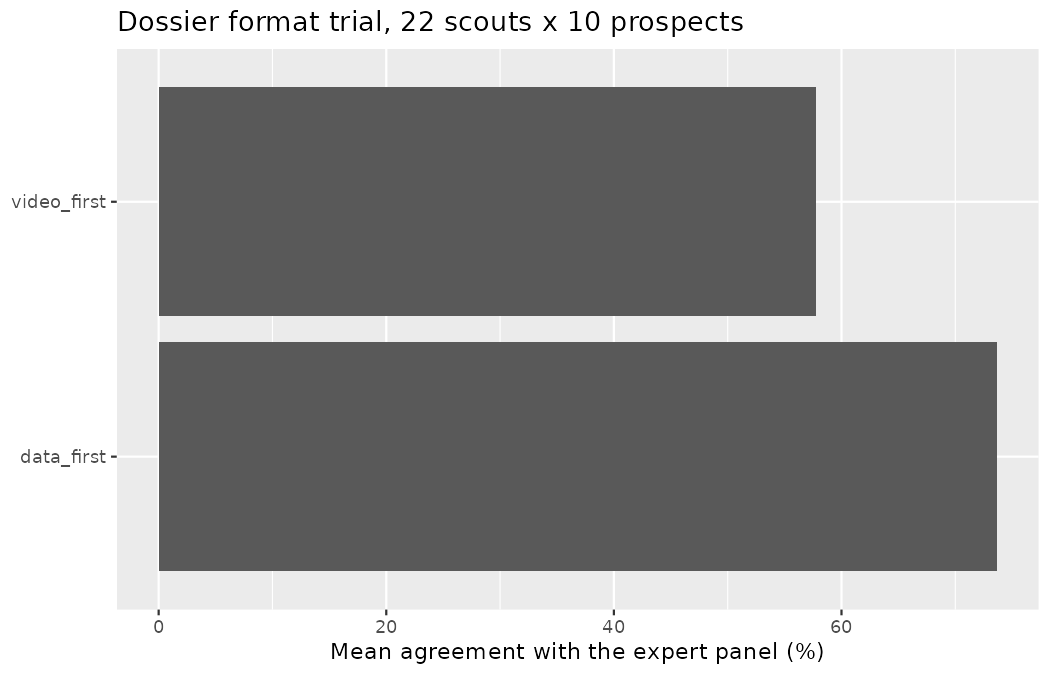
\includegraphics[width=0.85\linewidth,height=\textheight,keepaspectratio]{figures/inference-applications-1.png}

Two horizontal bars, data-first reaching 73.6\% and video-first stopping
at 57.7\%. Whether that gap is evidence or noise is exactly what the
paired test below will decide.

\begin{tcolorbox}[enhanced jigsaw, left=2mm, leftrule=.75mm, title=\textcolor{quarto-callout-tip-color}{\faLightbulb}\hspace{0.5em}{Check your understanding}, arc=.35mm, rightrule=.15mm, coltitle=black, colframe=quarto-callout-tip-color-frame, bottomrule=.15mm, colbacktitle=quarto-callout-tip-color!10!white, opacitybacktitle=0.6, breakable, bottomtitle=1mm, toptitle=1mm, titlerule=0mm, opacityback=0, toprule=.15mm, colback=white]

The review table holds two data sources. Classify each as observational
or experimental, and say what kind of claim each can support.

\begin{center}\rule{0.5\linewidth}{0.5pt}\end{center}

The tournament shot files are observational: StatsBomb logged football
that was going to happen anyway, nothing was assigned, and every pattern
in them is an association --- the discipline running from
Chapter~\ref{sec-data-design} through the causality caveats of
Chapter~\ref{sec-inference-two-means}. The format trial is a randomized
experiment --- every scout graded identical evidence under both formats,
with the order randomized --- so a discernible difference \emph{can} be
attributed to the format itself. Same afternoon, same review table, two
entirely different scopes of inference.

\end{tcolorbox}

\subsection{Confidence interval for a single
mean}\label{confidence-interval-for-a-single-mean}

The templates want one number for ``elite tournament chance quality'',
and item one of the agenda asks for that number with uncertainty
attached. The parameter is the true mean chance quality per shot in
elite tournament football of the kind the World Cup samples --- the
1,494 shots on file are one edition's draw from that process, the same
``one draw from the game of football'' framing
Chapter~\ref{sec-data-applications} used when it first put two
tournaments side by side. Along with the sample average as a point
estimate, we can construct a confidence interval via bootstrapping,
resampling the 1,494 shots with replacement, per
Section~\ref{sec-boot1mean}. First the all-shots frame:

\begin{Shaded}
\begin{Highlighting}[]
\FunctionTok{set.seed}\NormalTok{(}\DecValTok{2302}\NormalTok{)}
\NormalTok{boot\_xg\_all }\OtherTok{\textless{}{-}}\NormalTok{ wc2022\_shots }\SpecialCharTok{|\textgreater{}}
  \FunctionTok{specify}\NormalTok{(}\AttributeTok{response =}\NormalTok{ statsbomb\_xg) }\SpecialCharTok{|\textgreater{}}
  \FunctionTok{generate}\NormalTok{(}\AttributeTok{reps =} \DecValTok{1000}\NormalTok{, }\AttributeTok{type =} \StringTok{"bootstrap"}\NormalTok{) }\SpecialCharTok{|\textgreater{}}
  \FunctionTok{calculate}\NormalTok{(}\AttributeTok{stat =} \StringTok{"mean"}\NormalTok{)}

\FunctionTok{round}\NormalTok{(}\FunctionTok{quantile}\NormalTok{(boot\_xg\_all}\SpecialCharTok{$}\NormalTok{stat, }\FunctionTok{c}\NormalTok{(}\FloatTok{0.025}\NormalTok{, }\FloatTok{0.975}\NormalTok{)), }\DecValTok{4}\NormalTok{)}
\CommentTok{\#\textgreater{}   2.5\%  97.5\%}
\CommentTok{\#\textgreater{} 0.1172 0.1357}

\NormalTok{xbar\_all  }\OtherTok{\textless{}{-}} \FunctionTok{mean}\NormalTok{(wc2022\_shots}\SpecialCharTok{$}\NormalTok{statsbomb\_xg)}
\NormalTok{se\_bs\_all }\OtherTok{\textless{}{-}} \FunctionTok{sd}\NormalTok{(boot\_xg\_all}\SpecialCharTok{$}\NormalTok{stat)}
\FunctionTok{round}\NormalTok{(}\FunctionTok{c}\NormalTok{(xbar\_all, se\_bs\_all), }\DecValTok{4}\NormalTok{)}
\CommentTok{\#\textgreater{} [1] 0.1259 0.0048}

\FunctionTok{round}\NormalTok{(}\FunctionTok{c}\NormalTok{(xbar\_all }\SpecialCharTok{{-}} \DecValTok{2} \SpecialCharTok{*}\NormalTok{ se\_bs\_all, xbar\_all }\SpecialCharTok{+} \DecValTok{2} \SpecialCharTok{*}\NormalTok{ se\_bs\_all), }\DecValTok{4}\NormalTok{)}
\CommentTok{\#\textgreater{} [1] 0.1162 0.1355}
\end{Highlighting}
\end{Shaded}

The 95\% bootstrap percentile interval --- the middle 95\% of the 1,000
bootstrapped means --- runs from 0.1172 to 0.1357 xG per shot. The SE
interval takes the observed mean plus or minus two bootstrap standard
errors, \(0.1259 \pm 2 \times 0.0048,\) giving \((0.1162, 0.1355).\) The
two constructions nearly coincide, because with \(n = 1,494\) the
bootstrap distribution is symmetric and bell-shaped --- contrast the
five-shot sample of Section~\ref{sec-boot1mean}, where the SE interval's
blind faith in symmetry produced a negative chance quality. Now the same
machinery in the open-play frame:

\begin{Shaded}
\begin{Highlighting}[]
\FunctionTok{set.seed}\NormalTok{(}\DecValTok{2303}\NormalTok{)}
\NormalTok{boot\_xg\_open }\OtherTok{\textless{}{-}}\NormalTok{ wc2022\_shots }\SpecialCharTok{|\textgreater{}}
  \FunctionTok{filter}\NormalTok{(shot\_type }\SpecialCharTok{==} \StringTok{"Open Play"}\NormalTok{) }\SpecialCharTok{|\textgreater{}}
  \FunctionTok{specify}\NormalTok{(}\AttributeTok{response =}\NormalTok{ statsbomb\_xg) }\SpecialCharTok{|\textgreater{}}
  \FunctionTok{generate}\NormalTok{(}\AttributeTok{reps =} \DecValTok{1000}\NormalTok{, }\AttributeTok{type =} \StringTok{"bootstrap"}\NormalTok{) }\SpecialCharTok{|\textgreater{}}
  \FunctionTok{calculate}\NormalTok{(}\AttributeTok{stat =} \StringTok{"mean"}\NormalTok{)}

\FunctionTok{round}\NormalTok{(}\FunctionTok{quantile}\NormalTok{(boot\_xg\_open}\SpecialCharTok{$}\NormalTok{stat, }\FunctionTok{c}\NormalTok{(}\FloatTok{0.025}\NormalTok{, }\FloatTok{0.975}\NormalTok{)), }\DecValTok{4}\NormalTok{)}
\CommentTok{\#\textgreater{}   2.5\%  97.5\%}
\CommentTok{\#\textgreater{} 0.0919 0.1047}

\NormalTok{xbar\_open  }\OtherTok{\textless{}{-}} \FunctionTok{mean}\NormalTok{(}\FunctionTok{filter}\NormalTok{(wc2022\_shots, shot\_type }\SpecialCharTok{==} \StringTok{"Open Play"}\NormalTok{)}\SpecialCharTok{$}\NormalTok{statsbomb\_xg)}
\NormalTok{se\_bs\_open }\OtherTok{\textless{}{-}} \FunctionTok{sd}\NormalTok{(boot\_xg\_open}\SpecialCharTok{$}\NormalTok{stat)}
\FunctionTok{round}\NormalTok{(}\FunctionTok{c}\NormalTok{(xbar\_open }\SpecialCharTok{{-}} \DecValTok{2} \SpecialCharTok{*}\NormalTok{ se\_bs\_open, xbar\_open }\SpecialCharTok{+} \DecValTok{2} \SpecialCharTok{*}\NormalTok{ se\_bs\_open), }\DecValTok{4}\NormalTok{)}
\CommentTok{\#\textgreater{} [1] 0.0918 0.1049}
\end{Highlighting}
\end{Shaded}

Open play: percentile interval \((0.0919, 0.1047),\) SE interval
\((0.0918, 0.1049)\) around \(\bar{x} = 0.0983.\) Put the two frames
side by side and the deepest lesson of the section appears: the two
intervals \emph{do not overlap}. Sampling variability moves the estimate
by half a hundredth of xG in either direction; the frame decision moves
it by nearly three hundredths --- roughly six standard errors. The 64
identical 0.7835 kicks do to this mean what
Section~\ref{sec-chp11-pens-out} showed them doing to a conversion gap
and Section~\ref{sec-mathANOVA} showed them doing to an \(F\) statistic:
here they \emph{inflate} a single-mean benchmark that open-play
recruitment work would then chase in vain. Each interval is valid
\emph{for its own parameter}; the report's job is to say which parameter
the club is buying. As in every bootstrap of this book, the intervals
also lean on a representativeness assumption --- one tournament stands
proxy for the process that generates elite tournament football, an
assumption the walkthrough of Section~\ref{sec-inference-tutorials} will
keep probing.

\begin{tcolorbox}[enhanced jigsaw, left=2mm, leftrule=.75mm, title=\textcolor{quarto-callout-tip-color}{\faLightbulb}\hspace{0.5em}{Check your understanding}, arc=.35mm, rightrule=.15mm, coltitle=black, colframe=quarto-callout-tip-color-frame, bottomrule=.15mm, colbacktitle=quarto-callout-tip-color!10!white, opacitybacktitle=0.6, breakable, bottomtitle=1mm, toptitle=1mm, titlerule=0mm, opacityback=0, toprule=.15mm, colback=white]

A colleague reads the open-play result as ``95\% of open-play shots have
a chance quality between 0.0919 and 0.1047.'' What went wrong?

\begin{center}\rule{0.5\linewidth}{0.5pt}\end{center}

The interval describes the plausible range of the \emph{mean} chance
quality, not of individual shots. Individual open-play xG values
routinely land at 0.02 and occasionally at 0.7 --- their spread is the
standard deviation of observations (about 0.125 here), not the standard
error of the mean, the distinction Section~\ref{sec-one-mean-math}
drilled. And per Chapter~\ref{sec-foundations-mathematical}, the 95\%
lives in the procedure: across many intervals built this way, about 95\%
capture their parameter.

\end{tcolorbox}

Confidence intervals for the true mean agreement percentage under each
dossier format could be built the same way, but they are not very
meaningful on their own --- ``the true mean agreement of a video-first
scout'' is an abstract quantity to stare at. As in most club work, the
interesting questions are comparative: does agreement \emph{differ}
between formats? Does chance quality \emph{differ} under pressure, or
between tournaments? To answer those, we need hypothesis tests.

\subsection{Paired mean test}\label{paired-mean-test}

Start with the format trial: ``Do the data provide convincing evidence
of a difference in mean agreement percentages between data-first and
video-first dossiers?'' Every scout graded under \emph{both} formats, so
the two columns of scores are not independent samples --- they are
paired by scout, and per Chapter~\ref{sec-inference-paired-means} the
variable of interest is each scout's \emph{difference}:

\begin{Shaded}
\begin{Highlighting}[]
\NormalTok{format\_paired }\OtherTok{\textless{}{-}}\NormalTok{ format\_scores }\SpecialCharTok{|\textgreater{}}
  \FunctionTok{pivot\_wider}\NormalTok{(}
    \AttributeTok{id\_cols =}\NormalTok{ scout,}
    \AttributeTok{names\_from =}\NormalTok{ format,}
    \AttributeTok{names\_prefix =} \StringTok{"agree\_"}\NormalTok{,}
    \AttributeTok{values\_from =}\NormalTok{ agree\_perc}
\NormalTok{  ) }\SpecialCharTok{|\textgreater{}}
  \FunctionTok{mutate}\NormalTok{(}\AttributeTok{diff\_agree =}\NormalTok{ agree\_data\_first }\SpecialCharTok{{-}}\NormalTok{ agree\_video\_first)}

\NormalTok{format\_paired }\SpecialCharTok{|\textgreater{}}
  \FunctionTok{slice\_head}\NormalTok{(}\AttributeTok{n =} \DecValTok{6}\NormalTok{)}
\CommentTok{\#\textgreater{} \# A tibble: 6 × 4}
\CommentTok{\#\textgreater{}   scout agree\_data\_first agree\_video\_first diff\_agree}
\CommentTok{\#\textgreater{}   \textless{}chr\textgreater{}            \textless{}dbl\textgreater{}             \textless{}dbl\textgreater{}      \textless{}dbl\textgreater{}}
\CommentTok{\#\textgreater{} 1 S01                 80                50         30}
\CommentTok{\#\textgreater{} 2 S02                 70                50         20}
\CommentTok{\#\textgreater{} 3 S03                 50                60        {-}10}
\CommentTok{\#\textgreater{} 4 S04                100                80         20}
\CommentTok{\#\textgreater{} 5 S05                 80                70         10}
\CommentTok{\#\textgreater{} 6 S06                100                70         30}

\NormalTok{format\_paired }\SpecialCharTok{|\textgreater{}}
  \FunctionTok{summarize}\NormalTok{(}
    \AttributeTok{n\_scouts  =} \FunctionTok{n}\NormalTok{(),}
    \AttributeTok{xbar\_diff =} \FunctionTok{round}\NormalTok{(}\FunctionTok{mean}\NormalTok{(diff\_agree), }\DecValTok{2}\NormalTok{),}
    \AttributeTok{s\_diff    =} \FunctionTok{round}\NormalTok{(}\FunctionTok{sd}\NormalTok{(diff\_agree), }\DecValTok{2}\NormalTok{)}
\NormalTok{  )}
\CommentTok{\#\textgreater{} \# A tibble: 1 × 3}
\CommentTok{\#\textgreater{}   n\_scouts xbar\_diff s\_diff}
\CommentTok{\#\textgreater{}      \textless{}int\textgreater{}     \textless{}dbl\textgreater{}  \textless{}dbl\textgreater{}}
\CommentTok{\#\textgreater{} 1       22      15.9   13.0}
\end{Highlighting}
\end{Shaded}

Most scouts improved under the data-first format --- though not all: S03
went the other way, a reminder that a real effect and individual
variation coexist. The statistic of interest is the average of the
differences, \(\bar{x}_{diff} = 15.91\) percentage points, and the
hypotheses are the ones Chapter~\ref{sec-inference-paired-means} taught:

\[H_0: \mu_{diff} = 0 \qquad H_A: \mu_{diff} \ne 0\]

where \(\mu_{diff}\) is the true mean difference in agreement percentage
(data-first minus video-first). Recall that the computational method for
a paired hypothesis shuffles the observed percentages across the two
formats but \textbf{within} a single scout --- equivalently, it flips
the sign of each difference at random --- so that every scout keeps one
score in each format and the null world of ``format is interchangeable''
is built by construction.

\begin{Shaded}
\begin{Highlighting}[]
\NormalTok{obs\_diff\_format }\OtherTok{\textless{}{-}}\NormalTok{ format\_paired }\SpecialCharTok{|\textgreater{}}
  \FunctionTok{specify}\NormalTok{(}\AttributeTok{response =}\NormalTok{ diff\_agree) }\SpecialCharTok{|\textgreater{}}
  \FunctionTok{calculate}\NormalTok{(}\AttributeTok{stat =} \StringTok{"mean"}\NormalTok{) }\SpecialCharTok{|\textgreater{}}
  \FunctionTok{as.numeric}\NormalTok{()}

\FunctionTok{round}\NormalTok{(obs\_diff\_format, }\DecValTok{2}\NormalTok{)}
\CommentTok{\#\textgreater{} [1] 15.91}

\FunctionTok{set.seed}\NormalTok{(}\DecValTok{2304}\NormalTok{)}
\NormalTok{null\_format }\OtherTok{\textless{}{-}}\NormalTok{ format\_paired }\SpecialCharTok{|\textgreater{}}
  \FunctionTok{specify}\NormalTok{(}\AttributeTok{response =}\NormalTok{ diff\_agree) }\SpecialCharTok{|\textgreater{}}
  \FunctionTok{hypothesize}\NormalTok{(}\AttributeTok{null =} \StringTok{"paired independence"}\NormalTok{) }\SpecialCharTok{|\textgreater{}}
  \FunctionTok{generate}\NormalTok{(}\AttributeTok{reps =} \DecValTok{1000}\NormalTok{, }\AttributeTok{type =} \StringTok{"permute"}\NormalTok{) }\SpecialCharTok{|\textgreater{}}
  \FunctionTok{calculate}\NormalTok{(}\AttributeTok{stat =} \StringTok{"mean"}\NormalTok{)}

\NormalTok{null\_format }\SpecialCharTok{|\textgreater{}}
  \FunctionTok{summarize}\NormalTok{(}
    \AttributeTok{center    =} \FunctionTok{round}\NormalTok{(}\FunctionTok{mean}\NormalTok{(stat), }\DecValTok{3}\NormalTok{),}
    \AttributeTok{n\_extreme =} \FunctionTok{sum}\NormalTok{(}\FunctionTok{abs}\NormalTok{(stat) }\SpecialCharTok{\textgreater{}=} \FloatTok{15.91}\NormalTok{),}
    \AttributeTok{p\_value   =} \FunctionTok{mean}\NormalTok{(}\FunctionTok{abs}\NormalTok{(stat) }\SpecialCharTok{\textgreater{}=} \FloatTok{15.91}\NormalTok{)}
\NormalTok{  )}
\CommentTok{\#\textgreater{} \# A tibble: 1 × 3}
\CommentTok{\#\textgreater{}   center n\_extreme p\_value}
\CommentTok{\#\textgreater{}    \textless{}dbl\textgreater{}     \textless{}int\textgreater{}   \textless{}dbl\textgreater{}}
\CommentTok{\#\textgreater{} 1  0.083         0       0}
\end{Highlighting}
\end{Shaded}

\begin{Shaded}
\begin{Highlighting}[]
\FunctionTok{ggplot}\NormalTok{(null\_format, }\FunctionTok{aes}\NormalTok{(}\AttributeTok{x =}\NormalTok{ stat)) }\SpecialCharTok{+}
  \FunctionTok{geom\_histogram}\NormalTok{(}\AttributeTok{binwidth =} \DecValTok{2}\NormalTok{) }\SpecialCharTok{+}
  \FunctionTok{geom\_vline}\NormalTok{(}\AttributeTok{xintercept =}\NormalTok{ obs\_diff\_format, }\AttributeTok{color =} \StringTok{"red"}\NormalTok{, }\AttributeTok{linewidth =} \DecValTok{1}\NormalTok{) }\SpecialCharTok{+}
  \FunctionTok{geom\_vline}\NormalTok{(}\AttributeTok{xintercept =} \SpecialCharTok{{-}}\NormalTok{obs\_diff\_format, }\AttributeTok{color =} \StringTok{"red"}\NormalTok{,}
             \AttributeTok{linetype =} \StringTok{"dashed"}\NormalTok{, }\AttributeTok{linewidth =} \DecValTok{1}\NormalTok{) }\SpecialCharTok{+}
  \FunctionTok{labs}\NormalTok{(}
    \AttributeTok{x =} \StringTok{"Mean difference in agreement percentages (data{-}first {-} video{-}first)"}\NormalTok{,}
    \AttributeTok{y =} \StringTok{"Count"}\NormalTok{,}
    \AttributeTok{title =} \StringTok{"1,000 randomized mean differences"}
\NormalTok{  )}
\end{Highlighting}
\end{Shaded}

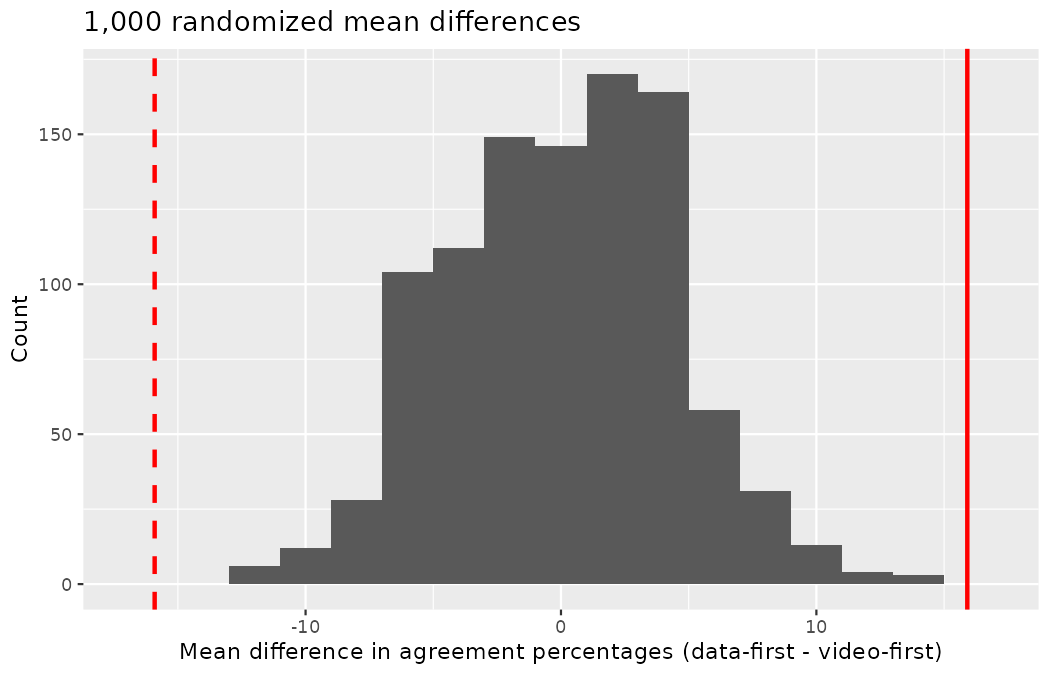
\includegraphics[width=0.85\linewidth,height=\textheight,keepaspectratio]{figures/inference-applications-2.png}

The histogram of 1,000 within-scout shuffles is centered at 0.083 ---
zero, up to simulation noise, exactly as the sign-flipping construction
promises --- and spans roughly \(-12\) to \(+15\) points. The observed
\(\bar{x}_{diff} = 15.91\) (solid line) sits beyond every one of the
1,000 permuted differences, and its mirror image (dashed line) beyond
every one on the left: not a single shuffle in a thousand was as extreme
in either direction, so the two-sided p-value is below \(1/1000.\) The
mathematical route agrees, as the recap promised it usually would:
\(T = 15.91 / (12.97/\sqrt{22}) = 5.75\) with \(df = 21\) gives a
p-value near \(0.00001.\) At any discernibility level the club uses, we
reject \(H_0\): the data provide convincing evidence that dossier format
changes mean agreement with the panel --- and because the design was a
randomized crossover in which each scout served as their own control,
the claim is causal, the pairing dividend
Chapter~\ref{sec-inference-paired-means} taught. The same honesty owed
in Chapter~\ref{sec-foundations-applications} is owed here: the outcome
measures agreement with the club's own expert panel --- a panel that
itself worked from the full derived data --- so what the trial
demonstrates is that data-first pages move scouts toward Northbridge's
reference process, not toward ground truth about the ten full-backs,
which no panel can certify. Priya's recommendation writes itself;
Marta's only quarrel is with the printing costs.

\begin{tcolorbox}[enhanced jigsaw, left=2mm, leftrule=.75mm, title=\textcolor{quarto-callout-tip-color}{\faLightbulb}\hspace{0.5em}{Check your understanding}, arc=.35mm, rightrule=.15mm, coltitle=black, colframe=quarto-callout-tip-color-frame, bottomrule=.15mm, colbacktitle=quarto-callout-tip-color!10!white, opacitybacktitle=0.6, breakable, bottomtitle=1mm, toptitle=1mm, titlerule=0mm, opacityback=0, toprule=.15mm, colback=white]

Why shuffle within each scout, rather than tossing all 44 scores into
one urn and dealing them back out?

\begin{center}\rule{0.5\linewidth}{0.5pt}\end{center}

Because the pairing is real structure, not decoration. Scouts differ in
baseline accuracy --- S04 agreed on 80\% even from footage, others
hovered near half --- and a full reshuffle would build a null world in
which those between-scout differences masquerade as format effects,
exactly the noise the paired design exists to remove
(Chapter~\ref{sec-inference-paired-means}). Shuffling within a scout
keeps each scout's overall accuracy fixed and asks only: given this
scout's two scores, could their assignment to formats be coincidence?

\end{tcolorbox}

\subsection{Two independent means
test}\label{two-independent-means-test}

Item three moves back to the tournament files, and to the question this
book has never stopped circling: is chance quality different when the
shooter is under defensive pressure? The club now holds two tournaments,
and it is tempting to pour all \(1{,}382 + 851\) open-play shots into
one big test. Resist the temptation: the two competitions are different
populations --- different fields, different tactical worlds, and per
Chapter~\ref{sec-data-applications} different penalty mixes and pattern
profiles --- so pooling would let between-tournament differences
masquerade as pressure effects, the lurking-variable trap of
Chapter~\ref{sec-data-applications} in inferential clothing. Therefore,
to answer the pressure question, we conduct two parallel hypothesis
tests, one per tournament, each with the hypotheses:

\[H_0: \mu_{prs} = \mu_{nop} \qquad H_A: \mu_{prs} \ne \mu_{nop}\]

where \(\mu_{prs}\) and \(\mu_{nop}\) are the true mean chance qualities
of pressured and unpressured shots in that competition. One frame
declaration before any shuffling, and it is the book's canonical one:
this comparison is run in the \emph{open-play frame}.
Section~\ref{sec-math2samp} taught why with the flip that made the pair
famous --- pens in, the World Cup's unpressured mean carries all 64
uncontested 0.7835 kicks and the test rejects resoundingly
(\(T = 4.27\)); pens out, the same machinery returns \(T = 0.37,\)
\(p = 0.71.\) We are not re-litigating that lesson; we are working in
the honest frame it established. The randomization here also differs
from the paired setting in exactly the way Section~\ref{sec-rand2mean}
established: pressured and unpressured shots have no natural pairing, so
we permute the pressure labels across \emph{all} shots within the
tournament.

\begin{Shaded}
\begin{Highlighting}[]
\NormalTok{wc\_open }\OtherTok{\textless{}{-}}\NormalTok{ wc2022\_shots }\SpecialCharTok{|\textgreater{}}
  \FunctionTok{filter}\NormalTok{(shot\_type }\SpecialCharTok{==} \StringTok{"Open Play"}\NormalTok{)}

\NormalTok{wc\_open }\SpecialCharTok{|\textgreater{}}
  \FunctionTok{group\_by}\NormalTok{(under\_pressure) }\SpecialCharTok{|\textgreater{}}
  \FunctionTok{summarize}\NormalTok{(}
    \AttributeTok{shots   =} \FunctionTok{n}\NormalTok{(),}
    \AttributeTok{mean\_xg =} \FunctionTok{round}\NormalTok{(}\FunctionTok{mean}\NormalTok{(statsbomb\_xg), }\DecValTok{4}\NormalTok{),}
    \AttributeTok{sd\_xg   =} \FunctionTok{round}\NormalTok{(}\FunctionTok{sd}\NormalTok{(statsbomb\_xg), }\DecValTok{4}\NormalTok{)}
\NormalTok{  )}
\CommentTok{\#\textgreater{} \# A tibble: 2 × 4}
\CommentTok{\#\textgreater{}   under\_pressure shots mean\_xg  sd\_xg}
\CommentTok{\#\textgreater{}   \textless{}lgl\textgreater{}          \textless{}int\textgreater{}   \textless{}dbl\textgreater{}  \textless{}dbl\textgreater{}}
\CommentTok{\#\textgreater{} 1 FALSE           1144  0.0988 0.130}
\CommentTok{\#\textgreater{} 2 TRUE             238  0.0961 0.0949}

\NormalTok{obs\_wc\_pressure }\OtherTok{\textless{}{-}}\NormalTok{ wc\_open }\SpecialCharTok{|\textgreater{}}
  \FunctionTok{mutate}\NormalTok{(}\AttributeTok{pressure =} \FunctionTok{if\_else}\NormalTok{(under\_pressure, }\StringTok{"pressured"}\NormalTok{, }\StringTok{"not pressured"}\NormalTok{)) }\SpecialCharTok{|\textgreater{}}
  \FunctionTok{specify}\NormalTok{(statsbomb\_xg }\SpecialCharTok{\textasciitilde{}}\NormalTok{ pressure) }\SpecialCharTok{|\textgreater{}}
  \FunctionTok{calculate}\NormalTok{(}\AttributeTok{stat =} \StringTok{"diff in means"}\NormalTok{, }\AttributeTok{order =} \FunctionTok{c}\NormalTok{(}\StringTok{"not pressured"}\NormalTok{, }\StringTok{"pressured"}\NormalTok{)) }\SpecialCharTok{|\textgreater{}}
  \FunctionTok{as.numeric}\NormalTok{()}

\FunctionTok{round}\NormalTok{(obs\_wc\_pressure, }\DecValTok{4}\NormalTok{)}
\CommentTok{\#\textgreater{} [1] 0.0027}

\FunctionTok{set.seed}\NormalTok{(}\DecValTok{2305}\NormalTok{)}
\NormalTok{null\_wc\_pressure }\OtherTok{\textless{}{-}}\NormalTok{ wc\_open }\SpecialCharTok{|\textgreater{}}
  \FunctionTok{mutate}\NormalTok{(}\AttributeTok{pressure =} \FunctionTok{if\_else}\NormalTok{(under\_pressure, }\StringTok{"pressured"}\NormalTok{, }\StringTok{"not pressured"}\NormalTok{)) }\SpecialCharTok{|\textgreater{}}
  \FunctionTok{specify}\NormalTok{(statsbomb\_xg }\SpecialCharTok{\textasciitilde{}}\NormalTok{ pressure) }\SpecialCharTok{|\textgreater{}}
  \FunctionTok{hypothesize}\NormalTok{(}\AttributeTok{null =} \StringTok{"independence"}\NormalTok{) }\SpecialCharTok{|\textgreater{}}
  \FunctionTok{generate}\NormalTok{(}\AttributeTok{reps =} \DecValTok{1000}\NormalTok{, }\AttributeTok{type =} \StringTok{"permute"}\NormalTok{) }\SpecialCharTok{|\textgreater{}}
  \FunctionTok{calculate}\NormalTok{(}\AttributeTok{stat =} \StringTok{"diff in means"}\NormalTok{, }\AttributeTok{order =} \FunctionTok{c}\NormalTok{(}\StringTok{"not pressured"}\NormalTok{, }\StringTok{"pressured"}\NormalTok{))}

\NormalTok{null\_wc\_pressure }\SpecialCharTok{|\textgreater{}}
  \FunctionTok{summarize}\NormalTok{(}
    \AttributeTok{n\_extreme =} \FunctionTok{sum}\NormalTok{(}\FunctionTok{abs}\NormalTok{(stat) }\SpecialCharTok{\textgreater{}=} \FloatTok{0.0027}\NormalTok{),}
    \AttributeTok{p\_value   =} \FunctionTok{mean}\NormalTok{(}\FunctionTok{abs}\NormalTok{(stat) }\SpecialCharTok{\textgreater{}=} \FloatTok{0.0027}\NormalTok{)}
\NormalTok{  )}
\CommentTok{\#\textgreater{} \# A tibble: 1 × 2}
\CommentTok{\#\textgreater{}   n\_extreme p\_value}
\CommentTok{\#\textgreater{}       \textless{}int\textgreater{}   \textless{}dbl\textgreater{}}
\CommentTok{\#\textgreater{} 1       743   0.743}
\end{Highlighting}
\end{Shaded}

And the same test on the second tournament:

\begin{Shaded}
\begin{Highlighting}[]
\NormalTok{weuro\_open }\OtherTok{\textless{}{-}}\NormalTok{ weuro2025\_shots }\SpecialCharTok{|\textgreater{}}
  \FunctionTok{filter}\NormalTok{(shot\_type }\SpecialCharTok{==} \StringTok{"Open Play"}\NormalTok{)}

\NormalTok{weuro\_open }\SpecialCharTok{|\textgreater{}}
  \FunctionTok{group\_by}\NormalTok{(under\_pressure) }\SpecialCharTok{|\textgreater{}}
  \FunctionTok{summarize}\NormalTok{(}
    \AttributeTok{shots   =} \FunctionTok{n}\NormalTok{(),}
    \AttributeTok{mean\_xg =} \FunctionTok{round}\NormalTok{(}\FunctionTok{mean}\NormalTok{(statsbomb\_xg), }\DecValTok{4}\NormalTok{),}
    \AttributeTok{sd\_xg   =} \FunctionTok{round}\NormalTok{(}\FunctionTok{sd}\NormalTok{(statsbomb\_xg), }\DecValTok{4}\NormalTok{)}
\NormalTok{  )}
\CommentTok{\#\textgreater{} \# A tibble: 2 × 4}
\CommentTok{\#\textgreater{}   under\_pressure shots mean\_xg sd\_xg}
\CommentTok{\#\textgreater{}   \textless{}lgl\textgreater{}          \textless{}int\textgreater{}   \textless{}dbl\textgreater{} \textless{}dbl\textgreater{}}
\CommentTok{\#\textgreater{} 1 FALSE            526  0.101  0.119}
\CommentTok{\#\textgreater{} 2 TRUE             325  0.0914 0.102}

\NormalTok{obs\_we\_pressure }\OtherTok{\textless{}{-}}\NormalTok{ weuro\_open }\SpecialCharTok{|\textgreater{}}
  \FunctionTok{mutate}\NormalTok{(}\AttributeTok{pressure =} \FunctionTok{if\_else}\NormalTok{(under\_pressure, }\StringTok{"pressured"}\NormalTok{, }\StringTok{"not pressured"}\NormalTok{)) }\SpecialCharTok{|\textgreater{}}
  \FunctionTok{specify}\NormalTok{(statsbomb\_xg }\SpecialCharTok{\textasciitilde{}}\NormalTok{ pressure) }\SpecialCharTok{|\textgreater{}}
  \FunctionTok{calculate}\NormalTok{(}\AttributeTok{stat =} \StringTok{"diff in means"}\NormalTok{, }\AttributeTok{order =} \FunctionTok{c}\NormalTok{(}\StringTok{"not pressured"}\NormalTok{, }\StringTok{"pressured"}\NormalTok{)) }\SpecialCharTok{|\textgreater{}}
  \FunctionTok{as.numeric}\NormalTok{()}

\FunctionTok{round}\NormalTok{(obs\_we\_pressure, }\DecValTok{4}\NormalTok{)}
\CommentTok{\#\textgreater{} [1] 0.0097}

\FunctionTok{set.seed}\NormalTok{(}\DecValTok{2307}\NormalTok{)}
\NormalTok{null\_we\_pressure }\OtherTok{\textless{}{-}}\NormalTok{ weuro\_open }\SpecialCharTok{|\textgreater{}}
  \FunctionTok{mutate}\NormalTok{(}\AttributeTok{pressure =} \FunctionTok{if\_else}\NormalTok{(under\_pressure, }\StringTok{"pressured"}\NormalTok{, }\StringTok{"not pressured"}\NormalTok{)) }\SpecialCharTok{|\textgreater{}}
  \FunctionTok{specify}\NormalTok{(statsbomb\_xg }\SpecialCharTok{\textasciitilde{}}\NormalTok{ pressure) }\SpecialCharTok{|\textgreater{}}
  \FunctionTok{hypothesize}\NormalTok{(}\AttributeTok{null =} \StringTok{"independence"}\NormalTok{) }\SpecialCharTok{|\textgreater{}}
  \FunctionTok{generate}\NormalTok{(}\AttributeTok{reps =} \DecValTok{1000}\NormalTok{, }\AttributeTok{type =} \StringTok{"permute"}\NormalTok{) }\SpecialCharTok{|\textgreater{}}
  \FunctionTok{calculate}\NormalTok{(}\AttributeTok{stat =} \StringTok{"diff in means"}\NormalTok{, }\AttributeTok{order =} \FunctionTok{c}\NormalTok{(}\StringTok{"not pressured"}\NormalTok{, }\StringTok{"pressured"}\NormalTok{))}

\NormalTok{null\_we\_pressure }\SpecialCharTok{|\textgreater{}}
  \FunctionTok{summarize}\NormalTok{(}
    \AttributeTok{n\_extreme =} \FunctionTok{sum}\NormalTok{(}\FunctionTok{abs}\NormalTok{(stat) }\SpecialCharTok{\textgreater{}=} \FloatTok{0.0097}\NormalTok{),}
    \AttributeTok{p\_value   =} \FunctionTok{mean}\NormalTok{(}\FunctionTok{abs}\NormalTok{(stat) }\SpecialCharTok{\textgreater{}=} \FloatTok{0.0097}\NormalTok{)}
\NormalTok{  )}
\CommentTok{\#\textgreater{} \# A tibble: 1 × 2}
\CommentTok{\#\textgreater{}   n\_extreme p\_value}
\CommentTok{\#\textgreater{}       \textless{}int\textgreater{}   \textless{}dbl\textgreater{}}
\CommentTok{\#\textgreater{} 1       213   0.213}
\end{Highlighting}
\end{Shaded}

\begin{Shaded}
\begin{Highlighting}[]
\FunctionTok{ggplot}\NormalTok{(null\_wc\_pressure, }\FunctionTok{aes}\NormalTok{(}\AttributeTok{x =}\NormalTok{ stat)) }\SpecialCharTok{+}
  \FunctionTok{geom\_histogram}\NormalTok{(}\AttributeTok{binwidth =} \FloatTok{0.002}\NormalTok{) }\SpecialCharTok{+}
  \FunctionTok{geom\_vline}\NormalTok{(}\AttributeTok{xintercept =}\NormalTok{ obs\_wc\_pressure, }\AttributeTok{color =} \StringTok{"red"}\NormalTok{, }\AttributeTok{linewidth =} \DecValTok{1}\NormalTok{) }\SpecialCharTok{+}
  \FunctionTok{geom\_vline}\NormalTok{(}\AttributeTok{xintercept =} \SpecialCharTok{{-}}\NormalTok{obs\_wc\_pressure, }\AttributeTok{color =} \StringTok{"red"}\NormalTok{,}
             \AttributeTok{linetype =} \StringTok{"dashed"}\NormalTok{, }\AttributeTok{linewidth =} \DecValTok{1}\NormalTok{) }\SpecialCharTok{+}
  \FunctionTok{labs}\NormalTok{(}
    \AttributeTok{x =} \StringTok{"Difference in mean xG (not pressured {-} pressured)"}\NormalTok{,}
    \AttributeTok{y =} \StringTok{"Count"}\NormalTok{,}
    \AttributeTok{title =} \StringTok{"2022 Men\textquotesingle{}s World Cup, open play"}\NormalTok{,}
    \AttributeTok{subtitle =} \StringTok{"1,000 differences in randomized means"}
\NormalTok{  )}

\FunctionTok{ggplot}\NormalTok{(null\_we\_pressure, }\FunctionTok{aes}\NormalTok{(}\AttributeTok{x =}\NormalTok{ stat)) }\SpecialCharTok{+}
  \FunctionTok{geom\_histogram}\NormalTok{(}\AttributeTok{binwidth =} \FloatTok{0.002}\NormalTok{) }\SpecialCharTok{+}
  \FunctionTok{geom\_vline}\NormalTok{(}\AttributeTok{xintercept =}\NormalTok{ obs\_we\_pressure, }\AttributeTok{color =} \StringTok{"red"}\NormalTok{, }\AttributeTok{linewidth =} \DecValTok{1}\NormalTok{) }\SpecialCharTok{+}
  \FunctionTok{geom\_vline}\NormalTok{(}\AttributeTok{xintercept =} \SpecialCharTok{{-}}\NormalTok{obs\_we\_pressure, }\AttributeTok{color =} \StringTok{"red"}\NormalTok{,}
             \AttributeTok{linetype =} \StringTok{"dashed"}\NormalTok{, }\AttributeTok{linewidth =} \DecValTok{1}\NormalTok{) }\SpecialCharTok{+}
  \FunctionTok{labs}\NormalTok{(}
    \AttributeTok{x =} \StringTok{"Difference in mean xG (not pressured {-} pressured)"}\NormalTok{,}
    \AttributeTok{y =} \StringTok{"Count"}\NormalTok{,}
    \AttributeTok{title =} \StringTok{"2025 Women\textquotesingle{}s Euro, open play"}\NormalTok{,}
    \AttributeTok{subtitle =} \StringTok{"1,000 differences in randomized means"}
\NormalTok{  )}
\end{Highlighting}
\end{Shaded}

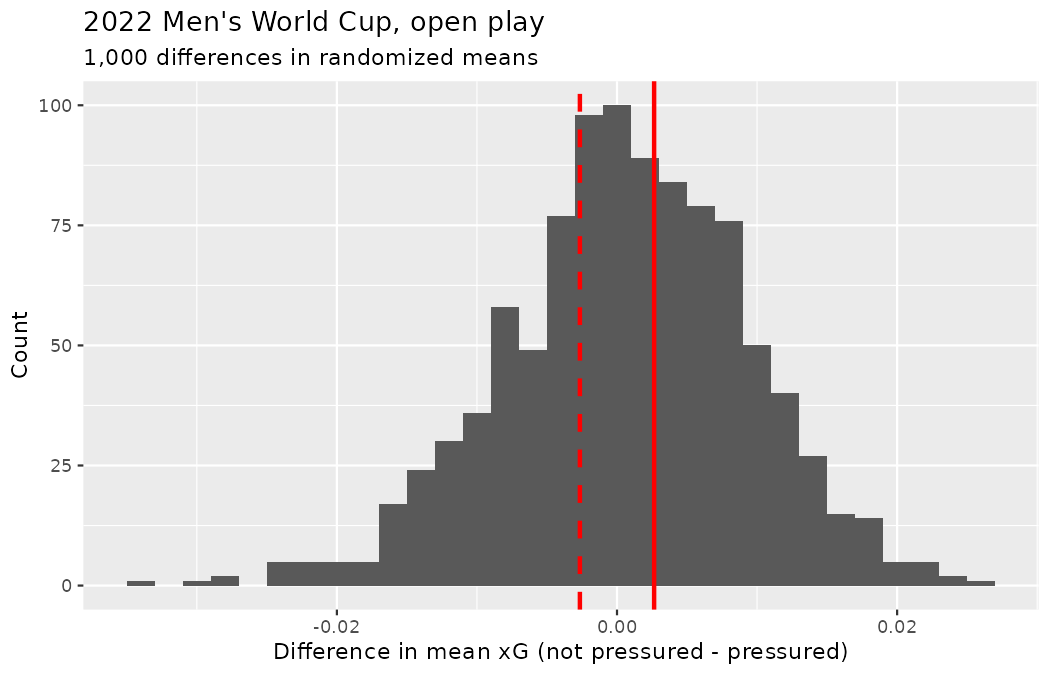
\includegraphics[width=0.85\linewidth,height=\textheight,keepaspectratio]{figures/inference-applications-3.png}

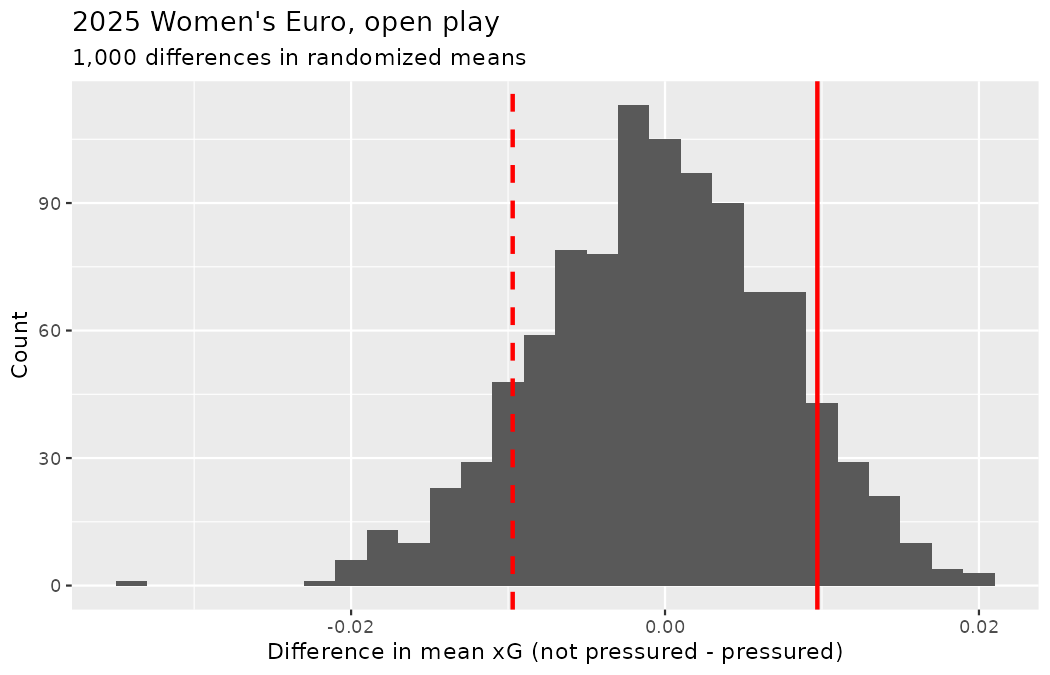
\includegraphics[width=0.85\linewidth,height=\textheight,keepaspectratio]{figures/inference-applications-4.png}

In both null distributions the observed difference (solid line) sits
comfortably among the shuffled ones. At the World Cup, the open-play gap
is \(0.0988 - 0.0961 = 0.0027\) xG per shot and 743 of 1,000
label-shuffles produced a difference at least that large in absolute
value: \(p = 0.743.\) At the Euro the gap is larger,
\(0.1011 - 0.0914 = 0.0097,\) but so is nothing else about the verdict:
\(p = 0.213.\) (The exercise thread of Section~\ref{sec-chp20-exercises}
ran this same Euro comparison with a different seed and obtained
\(0.222\) --- the seed-to-seed gap
Chapter~\ref{sec-foundations-applications} taught you to expect, two
estimates of one tail probability, same verdict.) Neither tournament's
pressure gap is statistically discernible in the honest frame, at
\(\alpha = 0.05\) or anywhere near it. The two competitions
\emph{agree}: once the penalties leave the frame, defenders pressing a
shooter does not measurably degrade the chance quality of the shots that
get taken --- and remember from Section~\ref{sec-chp11-pens-out} that
even a rejection here would have claimed association only, since nobody
assigns pressure at random. Contrast this consolidated calm with the
pens-in fireworks the club once stared at: a World Cup ``effect'' of
\(T = 4.27\) and a Euro one rejected even more emphatically
(\(T = 6.27,\) not one permuted difference in a thousand as extreme, per
Section~\ref{sec-chp20-exercises}) --- every point of which was 115
penalty kicks sitting on one side of the ledger.

The second tournament question is the one
Chapter~\ref{sec-data-applications} planted when it first set the two
competitions side by side: their chance quality per shot --- are they
the same, or different? Two tournaments, two independent groups of
shots, one test each in the two frames the review demands. The
hypotheses: \(H_0: \mu_{wc} = \mu_{we}\) against
\(H_A: \mu_{wc} \ne \mu_{we}.\)

\begin{Shaded}
\begin{Highlighting}[]
\NormalTok{both\_shots }\OtherTok{\textless{}{-}} \FunctionTok{bind\_rows}\NormalTok{(wc2022\_shots, weuro2025\_shots)}

\NormalTok{both\_shots }\SpecialCharTok{|\textgreater{}}
  \FunctionTok{group\_by}\NormalTok{(competition) }\SpecialCharTok{|\textgreater{}}
  \FunctionTok{summarize}\NormalTok{(}
    \AttributeTok{shots   =} \FunctionTok{n}\NormalTok{(),}
    \AttributeTok{mean\_xg =} \FunctionTok{round}\NormalTok{(}\FunctionTok{mean}\NormalTok{(statsbomb\_xg), }\DecValTok{4}\NormalTok{),}
    \AttributeTok{sd\_xg   =} \FunctionTok{round}\NormalTok{(}\FunctionTok{sd}\NormalTok{(statsbomb\_xg), }\DecValTok{4}\NormalTok{)}
\NormalTok{  )}
\CommentTok{\#\textgreater{} \# A tibble: 2 × 4}
\CommentTok{\#\textgreater{}   competition shots mean\_xg sd\_xg}
\CommentTok{\#\textgreater{}   \textless{}chr\textgreater{}       \textless{}int\textgreater{}   \textless{}dbl\textgreater{} \textless{}dbl\textgreater{}}
\CommentTok{\#\textgreater{} 1 wc2022       1494   0.126 0.184}
\CommentTok{\#\textgreater{} 2 weuro2025     913   0.135 0.192}

\NormalTok{obs\_comp\_all }\OtherTok{\textless{}{-}}\NormalTok{ both\_shots }\SpecialCharTok{|\textgreater{}}
  \FunctionTok{specify}\NormalTok{(statsbomb\_xg }\SpecialCharTok{\textasciitilde{}}\NormalTok{ competition) }\SpecialCharTok{|\textgreater{}}
  \FunctionTok{calculate}\NormalTok{(}\AttributeTok{stat =} \StringTok{"diff in means"}\NormalTok{, }\AttributeTok{order =} \FunctionTok{c}\NormalTok{(}\StringTok{"weuro2025"}\NormalTok{, }\StringTok{"wc2022"}\NormalTok{)) }\SpecialCharTok{|\textgreater{}}
  \FunctionTok{as.numeric}\NormalTok{()}

\FunctionTok{round}\NormalTok{(obs\_comp\_all, }\DecValTok{4}\NormalTok{)}
\CommentTok{\#\textgreater{} [1] 0.0092}

\FunctionTok{set.seed}\NormalTok{(}\DecValTok{2308}\NormalTok{)}
\NormalTok{null\_comp\_all }\OtherTok{\textless{}{-}}\NormalTok{ both\_shots }\SpecialCharTok{|\textgreater{}}
  \FunctionTok{specify}\NormalTok{(statsbomb\_xg }\SpecialCharTok{\textasciitilde{}}\NormalTok{ competition) }\SpecialCharTok{|\textgreater{}}
  \FunctionTok{hypothesize}\NormalTok{(}\AttributeTok{null =} \StringTok{"independence"}\NormalTok{) }\SpecialCharTok{|\textgreater{}}
  \FunctionTok{generate}\NormalTok{(}\AttributeTok{reps =} \DecValTok{1000}\NormalTok{, }\AttributeTok{type =} \StringTok{"permute"}\NormalTok{) }\SpecialCharTok{|\textgreater{}}
  \FunctionTok{calculate}\NormalTok{(}\AttributeTok{stat =} \StringTok{"diff in means"}\NormalTok{, }\AttributeTok{order =} \FunctionTok{c}\NormalTok{(}\StringTok{"weuro2025"}\NormalTok{, }\StringTok{"wc2022"}\NormalTok{))}

\NormalTok{null\_comp\_all }\SpecialCharTok{|\textgreater{}}
  \FunctionTok{summarize}\NormalTok{(}
    \AttributeTok{n\_extreme =} \FunctionTok{sum}\NormalTok{(}\FunctionTok{abs}\NormalTok{(stat) }\SpecialCharTok{\textgreater{}=} \FloatTok{0.0092}\NormalTok{),}
    \AttributeTok{p\_value   =} \FunctionTok{mean}\NormalTok{(}\FunctionTok{abs}\NormalTok{(stat) }\SpecialCharTok{\textgreater{}=} \FloatTok{0.0092}\NormalTok{)}
\NormalTok{  )}
\CommentTok{\#\textgreater{} \# A tibble: 1 × 2}
\CommentTok{\#\textgreater{}   n\_extreme p\_value}
\CommentTok{\#\textgreater{}       \textless{}int\textgreater{}   \textless{}dbl\textgreater{}}
\CommentTok{\#\textgreater{} 1       255   0.255}
\end{Highlighting}
\end{Shaded}

All shots in: the Euro's mean sits 0.0092 higher (0.1350 against
0.1259), and 255 of 1,000 shuffles beat that gap --- \(p = 0.255,\) not
statistically discernible. The mathematical model concurs: \(T = 1.15\)
with \(df = \min(1493, 912) = 912,\) \(p = 0.25.\) Before the open-play
rerun, pause on where that 0.0092 even comes from. Penalties are 51 of
the Euro's 913 shots but 64 of the World Cup's 1,494 --- shares of 5.6\%
versus 4.3\% --- and each penalty drags its tournament's mean toward
0.7835. A back-of-envelope check shows the mix difference alone accounts
for essentially the entire observed gap:

\begin{Shaded}
\begin{Highlighting}[]
\FunctionTok{round}\NormalTok{((}\DecValTok{51} \SpecialCharTok{/} \DecValTok{913} \SpecialCharTok{{-}} \DecValTok{64} \SpecialCharTok{/} \DecValTok{1494}\NormalTok{) }\SpecialCharTok{*}\NormalTok{ (}\FloatTok{0.7835} \SpecialCharTok{{-}} \FloatTok{0.097}\NormalTok{), }\DecValTok{4}\NormalTok{)}
\CommentTok{\#\textgreater{} [1] 0.0089}
\end{Highlighting}
\end{Shaded}

\begin{tcolorbox}[enhanced jigsaw, left=2mm, leftrule=.75mm, title=\textcolor{quarto-callout-note-color}{\faInfo}\hspace{0.5em}{Worked example}, arc=.35mm, rightrule=.15mm, coltitle=black, colframe=quarto-callout-note-color-frame, bottomrule=.15mm, colbacktitle=quarto-callout-note-color!10!white, opacitybacktitle=0.6, breakable, bottomtitle=1mm, toptitle=1mm, titlerule=0mm, opacityback=0, toprule=.15mm, colback=white]

Read that one-liner out loud before the open-play run below confirms it.

\begin{center}\rule{0.5\linewidth}{0.5pt}\end{center}

The Euro's penalty share exceeds the World Cup's by
\(51/913 - 64/1494 = 0.0130.\) Each extra penalty replaces a roughly
0.097-quality shot with a 0.7835 one, worth \(0.7835 - 0.097 = 0.6865\)
of xG. So the mix difference alone predicts an all-shots gap of
\(0.0130 \times 0.6865 = 0.0089\) --- against 0.0092 observed. The
tournaments do not differ in chance quality so much as in \emph{how
often their football put the ball on the spot}, which is a statement
about refereeing events and shoot-outs, not about the shots teams
engineer.

\end{tcolorbox}

\begin{Shaded}
\begin{Highlighting}[]
\NormalTok{both\_open }\OtherTok{\textless{}{-}}\NormalTok{ both\_shots }\SpecialCharTok{|\textgreater{}}
  \FunctionTok{filter}\NormalTok{(shot\_type }\SpecialCharTok{==} \StringTok{"Open Play"}\NormalTok{)}

\NormalTok{both\_open }\SpecialCharTok{|\textgreater{}}
  \FunctionTok{group\_by}\NormalTok{(competition) }\SpecialCharTok{|\textgreater{}}
  \FunctionTok{summarize}\NormalTok{(}
    \AttributeTok{shots   =} \FunctionTok{n}\NormalTok{(),}
    \AttributeTok{mean\_xg =} \FunctionTok{round}\NormalTok{(}\FunctionTok{mean}\NormalTok{(statsbomb\_xg), }\DecValTok{4}\NormalTok{),}
    \AttributeTok{sd\_xg   =} \FunctionTok{round}\NormalTok{(}\FunctionTok{sd}\NormalTok{(statsbomb\_xg), }\DecValTok{4}\NormalTok{)}
\NormalTok{  )}
\CommentTok{\#\textgreater{} \# A tibble: 2 × 4}
\CommentTok{\#\textgreater{}   competition shots mean\_xg sd\_xg}
\CommentTok{\#\textgreater{}   \textless{}chr\textgreater{}       \textless{}int\textgreater{}   \textless{}dbl\textgreater{} \textless{}dbl\textgreater{}}
\CommentTok{\#\textgreater{} 1 wc2022       1382  0.0983 0.125}
\CommentTok{\#\textgreater{} 2 weuro2025     851  0.0974 0.112}

\NormalTok{obs\_comp\_open }\OtherTok{\textless{}{-}}\NormalTok{ both\_open }\SpecialCharTok{|\textgreater{}}
  \FunctionTok{specify}\NormalTok{(statsbomb\_xg }\SpecialCharTok{\textasciitilde{}}\NormalTok{ competition) }\SpecialCharTok{|\textgreater{}}
  \FunctionTok{calculate}\NormalTok{(}\AttributeTok{stat =} \StringTok{"diff in means"}\NormalTok{, }\AttributeTok{order =} \FunctionTok{c}\NormalTok{(}\StringTok{"weuro2025"}\NormalTok{, }\StringTok{"wc2022"}\NormalTok{)) }\SpecialCharTok{|\textgreater{}}
  \FunctionTok{as.numeric}\NormalTok{()}

\FunctionTok{round}\NormalTok{(obs\_comp\_open, }\DecValTok{4}\NormalTok{)}
\CommentTok{\#\textgreater{} [1] {-}9e{-}04}

\FunctionTok{set.seed}\NormalTok{(}\DecValTok{2309}\NormalTok{)}
\NormalTok{null\_comp\_open }\OtherTok{\textless{}{-}}\NormalTok{ both\_open }\SpecialCharTok{|\textgreater{}}
  \FunctionTok{specify}\NormalTok{(statsbomb\_xg }\SpecialCharTok{\textasciitilde{}}\NormalTok{ competition) }\SpecialCharTok{|\textgreater{}}
  \FunctionTok{hypothesize}\NormalTok{(}\AttributeTok{null =} \StringTok{"independence"}\NormalTok{) }\SpecialCharTok{|\textgreater{}}
  \FunctionTok{generate}\NormalTok{(}\AttributeTok{reps =} \DecValTok{1000}\NormalTok{, }\AttributeTok{type =} \StringTok{"permute"}\NormalTok{) }\SpecialCharTok{|\textgreater{}}
  \FunctionTok{calculate}\NormalTok{(}\AttributeTok{stat =} \StringTok{"diff in means"}\NormalTok{, }\AttributeTok{order =} \FunctionTok{c}\NormalTok{(}\StringTok{"weuro2025"}\NormalTok{, }\StringTok{"wc2022"}\NormalTok{))}

\NormalTok{null\_comp\_open }\SpecialCharTok{|\textgreater{}}
  \FunctionTok{summarize}\NormalTok{(}
    \AttributeTok{n\_extreme =} \FunctionTok{sum}\NormalTok{(}\FunctionTok{abs}\NormalTok{(stat) }\SpecialCharTok{\textgreater{}=} \FloatTok{0.0009}\NormalTok{),}
    \AttributeTok{p\_value   =} \FunctionTok{mean}\NormalTok{(}\FunctionTok{abs}\NormalTok{(stat) }\SpecialCharTok{\textgreater{}=} \FloatTok{0.0009}\NormalTok{)}
\NormalTok{  )}
\CommentTok{\#\textgreater{} \# A tibble: 1 × 2}
\CommentTok{\#\textgreater{}   n\_extreme p\_value}
\CommentTok{\#\textgreater{}       \textless{}int\textgreater{}   \textless{}dbl\textgreater{}}
\CommentTok{\#\textgreater{} 1       869   0.869}
\end{Highlighting}
\end{Shaded}

Open play: 0.0983 against 0.0974 --- a difference R can only bring
itself to print in scientific notation, \(-9 \times 10^{-4} = -0.0009\)
xG per shot, with 869 of 1,000 shuffles beating it (\(p = 0.869\); the
\(t\)-route gives \(T = -0.18,\) \(p = 0.86\)). When
Chapter~\ref{sec-data-applications} first showed you these two numbers
as 0.098 and 0.097, it asked whether ``close'' could be certified as
``the same'' and told you the machinery would arrive later. It has: the
difference is nowhere near statistically discernible, in either frame.
Elite men's and women's tournament football, three years apart, generate
open-play chances of statistically indistinguishable average quality ---
and the only ``difference'' the all-shots frame ever hinted at was
penalty bookkeeping. Failing to reject is not proof of equality, as
Chapter~\ref{sec-foundations-decision-errors} insists; but with 2,233
open-play shots on the table, the plausible differences that remain are
small enough that no recruitment policy should turn on them.

Based on the four p-values of this section (each a measure of deviation
from its null claim), the review's tournament verdicts read: no
discernible pressure effect on open-play chance quality in either
competition, and no discernible overall difference between the
competitions in either frame. The one discernible result of the
afternoon --- the format trial --- is also the one the club can act on
causally, because it is the one the club randomized.

\begin{tcolorbox}[enhanced jigsaw, left=2mm, leftrule=.75mm, title=\textcolor{quarto-callout-tip-color}{\faLightbulb}\hspace{0.5em}{Check your understanding}, arc=.35mm, rightrule=.15mm, coltitle=black, colframe=quarto-callout-tip-color-frame, bottomrule=.15mm, colbacktitle=quarto-callout-tip-color!10!white, opacitybacktitle=0.6, breakable, bottomtitle=1mm, toptitle=1mm, titlerule=0mm, opacityback=0, toprule=.15mm, colback=white]

Marta, reading the four tournament p-values, asks: ``So why not pool
both tournaments' open-play shots into one 2,233-shot pressure test and
get more power?'' What do you tell her?

\begin{center}\rule{0.5\linewidth}{0.5pt}\end{center}

Pooling mixes two populations whose pressure shares differ --- the
Euro's open play is 38\% pressured shots, the World Cup's 17\% --- so
competition would become a lurking variable standing behind both the
label and the outcome, the Simpson's-paradox structure of
Chapter~\ref{sec-data-applications}. The clean designs are the ones this
section ran (one test per tournament, verdicts compared), or a method
that models competition explicitly, which is where the next part of this
book (Chapter~\ref{sec-inf-model-slr} and beyond) is headed.

\end{tcolorbox}

\section{Interactive walkthrough: seven questions, seven
tools}\label{sec-inference-tutorials}

The case study ran on the computational engines; the recap's first
promise --- that the mathematical shortcuts agree when their conditions
hold --- deserves to be \emph{your} verification, not our assertion. So,
as in Chapter~\ref{sec-foundations-applications}, here is your
walkthrough: Priya Rao's year-end quiz, seven club questions in the
order of this part's seven chapters, each solved with that chapter's
mathematical model. Work each lesson at your keyboard; answers to the
embedded questions follow immediately --- commit to yours first. One
frame declaration up front so the lessons need not repeat it: every
lesson below works in the \emph{open-play frame} except where its
question forces otherwise, and each lesson says which shots it holds.

\subsection{Lesson 1: one proportion}\label{lesson-1-one-proportion}

Marta's welcome-pack claims ``one elite shot in three is struck first
time.'' Attach a 95\% confidence interval to the World Cup's first-time
share and judge her claim. Penalties cannot be struck first time --- the
run-up rather rules it out --- so the honest frame is open play, and the
data agree that the choice matters:

\begin{Shaded}
\begin{Highlighting}[]
\NormalTok{wc2022\_shots }\SpecialCharTok{|\textgreater{}}
  \FunctionTok{filter}\NormalTok{(shot\_type }\SpecialCharTok{==} \StringTok{"Penalty"}\NormalTok{) }\SpecialCharTok{|\textgreater{}}
  \FunctionTok{count}\NormalTok{(first\_time)}
\CommentTok{\#\textgreater{} \# A tibble: 1 × 2}
\CommentTok{\#\textgreater{}   first\_time     n}
\CommentTok{\#\textgreater{}   \textless{}lgl\textgreater{}      \textless{}int\textgreater{}}
\CommentTok{\#\textgreater{} 1 FALSE         64}

\FunctionTok{round}\NormalTok{(}\FunctionTok{mean}\NormalTok{(wc2022\_shots}\SpecialCharTok{$}\NormalTok{first\_time), }\DecValTok{4}\NormalTok{)}
\CommentTok{\#\textgreater{} [1] 0.3133}

\NormalTok{wc\_open }\SpecialCharTok{|\textgreater{}}
  \FunctionTok{summarize}\NormalTok{(}\AttributeTok{shots =} \FunctionTok{n}\NormalTok{(), }\AttributeTok{first\_time\_shots =} \FunctionTok{sum}\NormalTok{(first\_time),}
            \AttributeTok{p\_hat =} \FunctionTok{round}\NormalTok{(}\FunctionTok{mean}\NormalTok{(first\_time), }\DecValTok{4}\NormalTok{))}
\CommentTok{\#\textgreater{} \# A tibble: 1 × 3}
\CommentTok{\#\textgreater{}   shots first\_time\_shots p\_hat}
\CommentTok{\#\textgreater{}   \textless{}int\textgreater{}            \textless{}int\textgreater{} \textless{}dbl\textgreater{}}
\CommentTok{\#\textgreater{} 1  1382              468 0.339}

\NormalTok{p\_hat\_ft }\OtherTok{\textless{}{-}} \DecValTok{468} \SpecialCharTok{/} \DecValTok{1382}
\NormalTok{se\_ft }\OtherTok{\textless{}{-}} \FunctionTok{sqrt}\NormalTok{(p\_hat\_ft }\SpecialCharTok{*}\NormalTok{ (}\DecValTok{1} \SpecialCharTok{{-}}\NormalTok{ p\_hat\_ft) }\SpecialCharTok{/} \DecValTok{1382}\NormalTok{)}
\FunctionTok{round}\NormalTok{(}\FunctionTok{c}\NormalTok{(p\_hat\_ft, se\_ft), }\DecValTok{4}\NormalTok{)}
\CommentTok{\#\textgreater{} [1] 0.3386 0.0127}

\FunctionTok{round}\NormalTok{(}\FunctionTok{c}\NormalTok{(p\_hat\_ft }\SpecialCharTok{{-}} \FloatTok{1.96} \SpecialCharTok{*}\NormalTok{ se\_ft, p\_hat\_ft }\SpecialCharTok{+} \FloatTok{1.96} \SpecialCharTok{*}\NormalTok{ se\_ft), }\DecValTok{4}\NormalTok{)}
\CommentTok{\#\textgreater{} [1] 0.3137 0.3636}
\end{Highlighting}
\end{Shaded}

All 64 penalties are logged \texttt{first\_time\ =\ FALSE}, so the
all-shots share (0.3133) mechanically dilutes the open-play one
(0.3386). The success-failure condition holds with room to spare (468
successes, 914 failures), the SE uses \(\hat{p}\) because this is an
interval, not a test (Table~\ref{tbl-zcompare}'s substitution
discipline), and the 95\% interval runs from 0.3137 to 0.3636.

\begin{tcolorbox}[enhanced jigsaw, left=2mm, leftrule=.75mm, title=\textcolor{quarto-callout-tip-color}{\faLightbulb}\hspace{0.5em}{Check your understanding}, arc=.35mm, rightrule=.15mm, coltitle=black, colframe=quarto-callout-tip-color-frame, bottomrule=.15mm, colbacktitle=quarto-callout-tip-color!10!white, opacitybacktitle=0.6, breakable, bottomtitle=1mm, toptitle=1mm, titlerule=0mm, opacityback=0, toprule=.15mm, colback=white]

Does the interval support Marta's ``one in three''? And what test
verdict does it imply, without running the test?

\begin{center}\rule{0.5\linewidth}{0.5pt}\end{center}

\(1/3 = 0.3333\) sits inside \((0.3137, 0.3636),\) so the claim is
consistent with the data. By the duality of intervals and two-sided
tests (Section~\ref{sec-one-prop-norm}), a null of \(p_0 = 1/3\) inside
the 95\% interval means a two-sided test at \(\alpha = 0.05\) would fail
to reject. The welcome pack survives --- provided it says \emph{open
play}.

\end{tcolorbox}

\subsection{Lesson 2: two proportions}\label{lesson-2-two-proportions}

The Euro final went to England Women's over Spain Women's on a shoot-out
--- the tournament's two best sides, separated by nothing across 120
minutes. Were their open-play conversion rates over the whole campaign
discernibly different?

\begin{Shaded}
\begin{Highlighting}[]
\NormalTok{weuro\_open }\SpecialCharTok{|\textgreater{}}
  \FunctionTok{filter}\NormalTok{(team }\SpecialCharTok{\%in\%} \FunctionTok{c}\NormalTok{(}\StringTok{"England Women\textquotesingle{}s"}\NormalTok{, }\StringTok{"Spain Women\textquotesingle{}s"}\NormalTok{)) }\SpecialCharTok{|\textgreater{}}
  \FunctionTok{group\_by}\NormalTok{(team) }\SpecialCharTok{|\textgreater{}}
  \FunctionTok{summarize}\NormalTok{(}\AttributeTok{shots =} \FunctionTok{n}\NormalTok{(), }\AttributeTok{goals =} \FunctionTok{sum}\NormalTok{(goal), }\AttributeTok{conversion =} \FunctionTok{round}\NormalTok{(}\FunctionTok{mean}\NormalTok{(goal), }\DecValTok{4}\NormalTok{))}
\CommentTok{\#\textgreater{} \# A tibble: 2 × 4}
\CommentTok{\#\textgreater{}   team            shots goals conversion}
\CommentTok{\#\textgreater{}   \textless{}chr\textgreater{}           \textless{}int\textgreater{} \textless{}int\textgreater{}      \textless{}dbl\textgreater{}}
\CommentTok{\#\textgreater{} 1 England Women\textquotesingle{}s   101    15      0.148}
\CommentTok{\#\textgreater{} 2 Spain Women\textquotesingle{}s     142    18      0.127}

\NormalTok{p\_pool  }\OtherTok{\textless{}{-}}\NormalTok{ (}\DecValTok{15} \SpecialCharTok{+} \DecValTok{18}\NormalTok{) }\SpecialCharTok{/}\NormalTok{ (}\DecValTok{101} \SpecialCharTok{+} \DecValTok{142}\NormalTok{)}
\NormalTok{se\_pool }\OtherTok{\textless{}{-}} \FunctionTok{sqrt}\NormalTok{(p\_pool }\SpecialCharTok{*}\NormalTok{ (}\DecValTok{1} \SpecialCharTok{{-}}\NormalTok{ p\_pool) }\SpecialCharTok{*}\NormalTok{ (}\DecValTok{1} \SpecialCharTok{/} \DecValTok{101} \SpecialCharTok{+} \DecValTok{1} \SpecialCharTok{/} \DecValTok{142}\NormalTok{))}
\NormalTok{z\_fin   }\OtherTok{\textless{}{-}}\NormalTok{ (}\DecValTok{15} \SpecialCharTok{/} \DecValTok{101} \SpecialCharTok{{-}} \DecValTok{18} \SpecialCharTok{/} \DecValTok{142}\NormalTok{) }\SpecialCharTok{/}\NormalTok{ se\_pool}
\FunctionTok{round}\NormalTok{(}\FunctionTok{c}\NormalTok{(p\_pool, se\_pool, z\_fin, }\DecValTok{2} \SpecialCharTok{*} \FunctionTok{pnorm}\NormalTok{(}\SpecialCharTok{{-}}\FunctionTok{abs}\NormalTok{(z\_fin))), }\DecValTok{4}\NormalTok{)}
\CommentTok{\#\textgreater{} [1] 0.1358 0.0446 0.4878 0.6257}
\end{Highlighting}
\end{Shaded}

This is a hypothesis test, so per Section~\ref{sec-test-prop-pool} the
standard error is built from the pooled proportion
\(\hat{p}_{pool} = 33/243 = 0.1358\) --- under which the expected
successes are \(101 \times 0.1358 = 13.7\) and
\(142 \times 0.1358 = 19.3,\) both past 10, so the success-failure
condition holds. \(Z = 0.49,\) two-sided \(p = 0.63\): the finalists'
conversion gap (0.1485 versus 0.1268) is exactly the kind of gap two
equally sharp teams produce by chance. The final's fine margins were not
a disguise; the two attacks really were this alike.

\subsection{Lesson 3: two-way tables}\label{lesson-3-two-way-tables}

Does the \emph{body part} behind an open-play shot at the Euro travel
with whether it scores --- a three-level question no single proportion
can hold? First the frame's bookkeeping: four shots carry
\texttt{body\_part\ =\ "Other"}, and with expected counts far below the
chi-squared conditions of Section~\ref{sec-mathchisq} (a cell would
expect fewer than one goal), we drop them and say so.

\begin{Shaded}
\begin{Highlighting}[]
\NormalTok{weuro\_open }\SpecialCharTok{|\textgreater{}}
  \FunctionTok{count}\NormalTok{(body\_part)}
\CommentTok{\#\textgreater{} \# A tibble: 4 × 2}
\CommentTok{\#\textgreater{}   body\_part      n}
\CommentTok{\#\textgreater{}   \textless{}chr\textgreater{}      \textless{}int\textgreater{}}
\CommentTok{\#\textgreater{} 1 Head         151}
\CommentTok{\#\textgreater{} 2 Left Foot    242}
\CommentTok{\#\textgreater{} 3 Other          4}
\CommentTok{\#\textgreater{} 4 Right Foot   454}

\NormalTok{weuro\_bp }\OtherTok{\textless{}{-}}\NormalTok{ weuro\_open }\SpecialCharTok{|\textgreater{}}
  \FunctionTok{filter}\NormalTok{(body\_part }\SpecialCharTok{!=} \StringTok{"Other"}\NormalTok{) }\SpecialCharTok{|\textgreater{}}
  \FunctionTok{mutate}\NormalTok{(}\AttributeTok{result =} \FunctionTok{if\_else}\NormalTok{(goal, }\StringTok{"goal"}\NormalTok{, }\StringTok{"no goal"}\NormalTok{))}

\FunctionTok{table}\NormalTok{(weuro\_bp}\SpecialCharTok{$}\NormalTok{body\_part, weuro\_bp}\SpecialCharTok{$}\NormalTok{result)}
\CommentTok{\#\textgreater{}}
\CommentTok{\#\textgreater{}              goal no goal}
\CommentTok{\#\textgreater{}   Head         17     134}
\CommentTok{\#\textgreater{}   Left Foot    24     218}
\CommentTok{\#\textgreater{}   Right Foot   54     400}

\FunctionTok{chisq.test}\NormalTok{(}\FunctionTok{table}\NormalTok{(weuro\_bp}\SpecialCharTok{$}\NormalTok{body\_part, weuro\_bp}\SpecialCharTok{$}\NormalTok{result))}\SpecialCharTok{$}\NormalTok{expected}
\CommentTok{\#\textgreater{}}
\CommentTok{\#\textgreater{}                  goal  no goal}
\CommentTok{\#\textgreater{}   Head       16.93625 134.0638}
\CommentTok{\#\textgreater{}   Left Foot  27.14286 214.8571}
\CommentTok{\#\textgreater{}   Right Foot 50.92090 403.0791}

\FunctionTok{chisq.test}\NormalTok{(}\FunctionTok{table}\NormalTok{(weuro\_bp}\SpecialCharTok{$}\NormalTok{body\_part, weuro\_bp}\SpecialCharTok{$}\NormalTok{result))}
\CommentTok{\#\textgreater{}}
\CommentTok{\#\textgreater{}  Pearson\textquotesingle{}s Chi{-}squared test}
\CommentTok{\#\textgreater{}}
\CommentTok{\#\textgreater{} data:  table(weuro\_bp$body\_part, weuro\_bp$result)}
\CommentTok{\#\textgreater{} X{-}squared = 0.61986, df = 2, p{-}value = 0.7335}
\end{Highlighting}
\end{Shaded}

Every expected count clears 5 comfortably (the smallest is 16.9),
\(df = (3-1)(2-1) = 2,\) and \(X^2 = 0.62\) lands a p-value of \(0.73.\)
The observed counts sit almost eerily close to the expected ones:
headers converted 11.3\% of the time, left feet 9.9\%, right feet
11.9\%, and none of that spread is discernible. Note what the open-play
frame quietly did here: the ``headers convert worse'' deficit that
Chapter~\ref{sec-explore-categorical} showed you in the all-shots World
Cup table was always propped up by all-footed penalties --- in the
honest frame, at this tournament, the body-part story is no story at
all.

\subsection{Lesson 4: one mean}\label{lesson-4-one-mean}

Morocco --- the surprise semifinalist whose low-block profile has been
on the desk since Chapter~\ref{sec-data-hello} --- reached the last four
on famously few chances. Was their open-play chance quality \emph{per
shot} also thin, the way Section~\ref{sec-one-mean-math} convicted
Australia's? Frame check first: Morocco's file holds 4 penalty kicks
(all shoot-out kicks from the Spain tie, 3 scored) and 3 direct free
kicks; the open-play sample is the other 59 shots.

\begin{Shaded}
\begin{Highlighting}[]
\NormalTok{wc2022\_shots }\SpecialCharTok{|\textgreater{}}
  \FunctionTok{filter}\NormalTok{(team }\SpecialCharTok{==} \StringTok{"Morocco"}\NormalTok{) }\SpecialCharTok{|\textgreater{}}
  \FunctionTok{count}\NormalTok{(shot\_type)}
\CommentTok{\#\textgreater{} \# A tibble: 3 × 2}
\CommentTok{\#\textgreater{}   shot\_type     n}
\CommentTok{\#\textgreater{}   \textless{}chr\textgreater{}     \textless{}int\textgreater{}}
\CommentTok{\#\textgreater{} 1 Free Kick     3}
\CommentTok{\#\textgreater{} 2 Open Play    59}
\CommentTok{\#\textgreater{} 3 Penalty       4}

\NormalTok{morocco\_open }\OtherTok{\textless{}{-}}\NormalTok{ wc\_open }\SpecialCharTok{|\textgreater{}}
  \FunctionTok{filter}\NormalTok{(team }\SpecialCharTok{==} \StringTok{"Morocco"}\NormalTok{)}

\NormalTok{morocco\_open }\SpecialCharTok{|\textgreater{}}
  \FunctionTok{summarize}\NormalTok{(}\AttributeTok{shots =} \FunctionTok{n}\NormalTok{(), }\AttributeTok{xbar =} \FunctionTok{round}\NormalTok{(}\FunctionTok{mean}\NormalTok{(statsbomb\_xg), }\DecValTok{4}\NormalTok{),}
            \AttributeTok{s =} \FunctionTok{round}\NormalTok{(}\FunctionTok{sd}\NormalTok{(statsbomb\_xg), }\DecValTok{4}\NormalTok{))}
\CommentTok{\#\textgreater{} \# A tibble: 1 × 3}
\CommentTok{\#\textgreater{}   shots   xbar     s}
\CommentTok{\#\textgreater{}   \textless{}int\textgreater{}  \textless{}dbl\textgreater{} \textless{}dbl\textgreater{}}
\CommentTok{\#\textgreater{} 1    59 0.0918 0.118}

\NormalTok{xbar\_mor }\OtherTok{\textless{}{-}} \FunctionTok{mean}\NormalTok{(morocco\_open}\SpecialCharTok{$}\NormalTok{statsbomb\_xg)}
\NormalTok{se\_mor   }\OtherTok{\textless{}{-}} \FunctionTok{sd}\NormalTok{(morocco\_open}\SpecialCharTok{$}\NormalTok{statsbomb\_xg) }\SpecialCharTok{/} \FunctionTok{sqrt}\NormalTok{(}\DecValTok{59}\NormalTok{)}
\FunctionTok{round}\NormalTok{(}\FunctionTok{c}\NormalTok{(xbar\_mor }\SpecialCharTok{{-}} \FunctionTok{qt}\NormalTok{(}\FloatTok{0.975}\NormalTok{, }\AttributeTok{df =} \DecValTok{58}\NormalTok{) }\SpecialCharTok{*}\NormalTok{ se\_mor,}
\NormalTok{        xbar\_mor }\SpecialCharTok{+} \FunctionTok{qt}\NormalTok{(}\FloatTok{0.975}\NormalTok{, }\AttributeTok{df =} \DecValTok{58}\NormalTok{) }\SpecialCharTok{*}\NormalTok{ se\_mor), }\DecValTok{4}\NormalTok{)}
\CommentTok{\#\textgreater{} [1] 0.0611 0.1225}
\end{Highlighting}
\end{Shaded}

With \(n = 59\) the moderate right skew of xG is no obstacle
(Section~\ref{sec-one-mean-math}'s sample-size ladder),
\(t^{\star}_{58} = 2.00,\) and the 95\% interval for Morocco's true mean
chance quality runs from 0.0611 to 0.1225 --- comfortably straddling the
tournament's open-play benchmark of 0.0983. Contrast Australia in
Section~\ref{sec-one-mean-math}: same tool, same benchmark, but an
interval of \((0.037, 0.084)\) sitting \emph{entirely below} it.
Morocco's run was chance-thin in volume, not discernibly in quality:
fewer shots, not worse ones. Two low-block teams, two different verdicts
--- the tool separates what the eyeball lumps together.

\subsection{Lesson 5: two independent
means}\label{lesson-5-two-independent-means}

Now pay a debt. When Chapter~\ref{sec-data-applications} set the
tournaments side by side, one pattern ``visibly parted ways'':
counter-attacking shots averaged 0.159 xG at the World Cup against 0.091
at the Euro, and you were told to note it \emph{as a question, not a
finding}. This part built the tool that answers it.

\begin{Shaded}
\begin{Highlighting}[]
\NormalTok{counters }\OtherTok{\textless{}{-}} \FunctionTok{bind\_rows}\NormalTok{(wc2022\_shots, weuro2025\_shots) }\SpecialCharTok{|\textgreater{}}
  \FunctionTok{filter}\NormalTok{(play\_pattern }\SpecialCharTok{==} \StringTok{"From Counter"}\NormalTok{)}

\NormalTok{counters }\SpecialCharTok{|\textgreater{}}
  \FunctionTok{count}\NormalTok{(competition, shot\_type)}
\CommentTok{\#\textgreater{} \# A tibble: 2 × 3}
\CommentTok{\#\textgreater{}   competition shot\_type     n}
\CommentTok{\#\textgreater{}   \textless{}chr\textgreater{}       \textless{}chr\textgreater{}     \textless{}int\textgreater{}}
\CommentTok{\#\textgreater{} 1 wc2022      Open Play    56}
\CommentTok{\#\textgreater{} 2 weuro2025   Open Play    41}

\NormalTok{counters }\SpecialCharTok{|\textgreater{}}
  \FunctionTok{group\_by}\NormalTok{(competition) }\SpecialCharTok{|\textgreater{}}
  \FunctionTok{summarize}\NormalTok{(}\AttributeTok{shots =} \FunctionTok{n}\NormalTok{(), }\AttributeTok{mean\_xg =} \FunctionTok{round}\NormalTok{(}\FunctionTok{mean}\NormalTok{(statsbomb\_xg), }\DecValTok{4}\NormalTok{),}
            \AttributeTok{sd\_xg =} \FunctionTok{round}\NormalTok{(}\FunctionTok{sd}\NormalTok{(statsbomb\_xg), }\DecValTok{4}\NormalTok{))}
\CommentTok{\#\textgreater{} \# A tibble: 2 × 4}
\CommentTok{\#\textgreater{}   competition shots mean\_xg sd\_xg}
\CommentTok{\#\textgreater{}   \textless{}chr\textgreater{}       \textless{}int\textgreater{}   \textless{}dbl\textgreater{} \textless{}dbl\textgreater{}}
\CommentTok{\#\textgreater{} 1 wc2022         56  0.159  0.157}
\CommentTok{\#\textgreater{} 2 weuro2025      41  0.0905 0.106}

\NormalTok{counter\_stats }\OtherTok{\textless{}{-}}\NormalTok{ counters }\SpecialCharTok{|\textgreater{}}
  \FunctionTok{group\_by}\NormalTok{(competition) }\SpecialCharTok{|\textgreater{}}
  \FunctionTok{summarize}\NormalTok{(}\AttributeTok{n =} \FunctionTok{n}\NormalTok{(), }\AttributeTok{xbar =} \FunctionTok{mean}\NormalTok{(statsbomb\_xg), }\AttributeTok{s =} \FunctionTok{sd}\NormalTok{(statsbomb\_xg))}

\NormalTok{se\_ctr }\OtherTok{\textless{}{-}} \FunctionTok{sqrt}\NormalTok{(}\FunctionTok{sum}\NormalTok{(counter\_stats}\SpecialCharTok{$}\NormalTok{s}\SpecialCharTok{\^{}}\DecValTok{2} \SpecialCharTok{/}\NormalTok{ counter\_stats}\SpecialCharTok{$}\NormalTok{n))}
\NormalTok{t\_ctr  }\OtherTok{\textless{}{-}}\NormalTok{ (counter\_stats}\SpecialCharTok{$}\NormalTok{xbar[}\DecValTok{1}\NormalTok{] }\SpecialCharTok{{-}}\NormalTok{ counter\_stats}\SpecialCharTok{$}\NormalTok{xbar[}\DecValTok{2}\NormalTok{]) }\SpecialCharTok{/}\NormalTok{ se\_ctr}
\FunctionTok{round}\NormalTok{(}\FunctionTok{c}\NormalTok{(se\_ctr, t\_ctr, }\DecValTok{2} \SpecialCharTok{*} \FunctionTok{pt}\NormalTok{(}\SpecialCharTok{{-}}\FunctionTok{abs}\NormalTok{(t\_ctr), }\AttributeTok{df =} \DecValTok{40}\NormalTok{)), }\DecValTok{4}\NormalTok{)}
\CommentTok{\#\textgreater{} [1] 0.0268 2.5759 0.0138}
\end{Highlighting}
\end{Shaded}

Every counter-attack shot in both files is open play --- no penalty can
hide in this pattern, so for once the two frames coincide by
construction. \(T = 2.58\) on \(df = \min(55, 40) = 40\) gives a
two-sided \(p = 0.014\): statistically discernible at \(\alpha = 0.05.\)
Chapter 3's noted question graduates to a finding --- World Cup counters
carried discernibly higher chance quality than Euro counters --- with
two provisos worth writing in the same breath. First, \(p = 0.014\)
clears 0.05 but not a stricter 0.01, so a more skeptical reviewer keeps
the question open, the \(\alpha\)-sensitivity lesson of
Chapter~\ref{sec-inference-two-means}. Second, these are observational
tournaments: the gap describes how the two competitions' counters
\emph{were}, not what either would become under different coaching.

\begin{tcolorbox}[enhanced jigsaw, left=2mm, leftrule=.75mm, title=\textcolor{quarto-callout-tip-color}{\faLightbulb}\hspace{0.5em}{Check your understanding}, arc=.35mm, rightrule=.15mm, coltitle=black, colframe=quarto-callout-tip-color-frame, bottomrule=.15mm, colbacktitle=quarto-callout-tip-color!10!white, opacitybacktitle=0.6, breakable, bottomtitle=1mm, toptitle=1mm, titlerule=0mm, opacityback=0, toprule=.15mm, colback=white]

Why \(df = 40\) and not \(df = 95\)? And why does the SE add the two
variance terms instead of pooling like Lesson 2 did?

\begin{center}\rule{0.5\linewidth}{0.5pt}\end{center}

The min rule of Section~\ref{sec-math2samp} uses the smaller group's
\(n - 1 = 41 - 1 = 40\) as a deliberately conservative df when working
by hand. And pooling was a \emph{proportions} trick: under \(H_0\) the
two groups shared one success probability, which fixed one SE. Means
carry no such gift --- equal means say nothing about equal spreads
(0.157 versus 0.106 here) --- so each group contributes its own
\(s_i^2/n_i,\) per Table~\ref{tbl-tcompare}.

\end{tcolorbox}

\subsection{Lesson 6: paired means}\label{lesson-6-paired-means}

Sixteen World Cup teams played both a group stage and a knockout stage.
Did open-play chance quality per shot \emph{change} when the football
turned to knockouts --- comparing each team against itself, the pairing
dividend of Chapter~\ref{sec-inference-paired-means}?

\begin{Shaded}
\begin{Highlighting}[]
\NormalTok{ko\_teams }\OtherTok{\textless{}{-}}\NormalTok{ wc2022\_shots }\SpecialCharTok{|\textgreater{}}
  \FunctionTok{filter}\NormalTok{(stage }\SpecialCharTok{!=} \StringTok{"Group Stage"}\NormalTok{) }\SpecialCharTok{|\textgreater{}}
  \FunctionTok{distinct}\NormalTok{(team) }\SpecialCharTok{|\textgreater{}}
  \FunctionTok{pull}\NormalTok{(team)}

\NormalTok{phase\_pair }\OtherTok{\textless{}{-}}\NormalTok{ wc\_open }\SpecialCharTok{|\textgreater{}}
  \FunctionTok{filter}\NormalTok{(team }\SpecialCharTok{\%in\%}\NormalTok{ ko\_teams) }\SpecialCharTok{|\textgreater{}}
  \FunctionTok{mutate}\NormalTok{(}\AttributeTok{phase =} \FunctionTok{if\_else}\NormalTok{(stage }\SpecialCharTok{==} \StringTok{"Group Stage"}\NormalTok{, }\StringTok{"group"}\NormalTok{, }\StringTok{"knockout"}\NormalTok{)) }\SpecialCharTok{|\textgreater{}}
  \FunctionTok{group\_by}\NormalTok{(team, phase) }\SpecialCharTok{|\textgreater{}}
  \FunctionTok{summarize}\NormalTok{(}\AttributeTok{mean\_xg =} \FunctionTok{mean}\NormalTok{(statsbomb\_xg), }\AttributeTok{.groups =} \StringTok{"drop"}\NormalTok{) }\SpecialCharTok{|\textgreater{}}
  \FunctionTok{pivot\_wider}\NormalTok{(}\AttributeTok{id\_cols =}\NormalTok{ team, }\AttributeTok{names\_from =}\NormalTok{ phase, }\AttributeTok{values\_from =}\NormalTok{ mean\_xg) }\SpecialCharTok{|\textgreater{}}
  \FunctionTok{mutate}\NormalTok{(}\AttributeTok{xg\_diff =}\NormalTok{ knockout }\SpecialCharTok{{-}}\NormalTok{ group)}

\NormalTok{phase\_pair }\SpecialCharTok{|\textgreater{}}
  \FunctionTok{slice\_head}\NormalTok{(}\AttributeTok{n =} \DecValTok{4}\NormalTok{)}
\CommentTok{\#\textgreater{} \# A tibble: 4 × 4}
\CommentTok{\#\textgreater{}   team       group knockout  xg\_diff}
\CommentTok{\#\textgreater{}   \textless{}chr\textgreater{}      \textless{}dbl\textgreater{}    \textless{}dbl\textgreater{}    \textless{}dbl\textgreater{}}
\CommentTok{\#\textgreater{} 1 Argentina 0.108    0.106  {-}0.00177}
\CommentTok{\#\textgreater{} 2 Australia 0.0549   0.0852  0.0304}
\CommentTok{\#\textgreater{} 3 Brazil    0.0987   0.124   0.0253}
\CommentTok{\#\textgreater{} 4 Croatia   0.143    0.0559 {-}0.0874}

\NormalTok{phase\_pair }\SpecialCharTok{|\textgreater{}}
  \FunctionTok{summarize}\NormalTok{(}\AttributeTok{pairs =} \FunctionTok{n}\NormalTok{(), }\AttributeTok{xbar\_diff =} \FunctionTok{round}\NormalTok{(}\FunctionTok{mean}\NormalTok{(xg\_diff), }\DecValTok{4}\NormalTok{),}
            \AttributeTok{s\_diff =} \FunctionTok{round}\NormalTok{(}\FunctionTok{sd}\NormalTok{(xg\_diff), }\DecValTok{4}\NormalTok{))}
\CommentTok{\#\textgreater{} \# A tibble: 1 × 3}
\CommentTok{\#\textgreater{}   pairs xbar\_diff s\_diff}
\CommentTok{\#\textgreater{}   \textless{}int\textgreater{}     \textless{}dbl\textgreater{}  \textless{}dbl\textgreater{}}
\CommentTok{\#\textgreater{} 1    16    {-}0.011 0.0415}

\NormalTok{xbar\_ko }\OtherTok{\textless{}{-}} \FunctionTok{mean}\NormalTok{(phase\_pair}\SpecialCharTok{$}\NormalTok{xg\_diff)}
\NormalTok{s\_ko    }\OtherTok{\textless{}{-}} \FunctionTok{sd}\NormalTok{(phase\_pair}\SpecialCharTok{$}\NormalTok{xg\_diff)}
\NormalTok{t\_ko    }\OtherTok{\textless{}{-}}\NormalTok{ xbar\_ko }\SpecialCharTok{/}\NormalTok{ (s\_ko }\SpecialCharTok{/} \FunctionTok{sqrt}\NormalTok{(}\DecValTok{16}\NormalTok{))}
\FunctionTok{round}\NormalTok{(}\FunctionTok{c}\NormalTok{(t\_ko, }\DecValTok{2} \SpecialCharTok{*} \FunctionTok{pt}\NormalTok{(}\SpecialCharTok{{-}}\FunctionTok{abs}\NormalTok{(t\_ko), }\AttributeTok{df =} \DecValTok{15}\NormalTok{)), }\DecValTok{4}\NormalTok{)}
\CommentTok{\#\textgreater{} [1] {-}1.0640  0.3042}

\FunctionTok{round}\NormalTok{(}\FunctionTok{c}\NormalTok{(xbar\_ko }\SpecialCharTok{{-}} \FunctionTok{qt}\NormalTok{(}\FloatTok{0.975}\NormalTok{, }\AttributeTok{df =} \DecValTok{15}\NormalTok{) }\SpecialCharTok{*}\NormalTok{ s\_ko }\SpecialCharTok{/} \FunctionTok{sqrt}\NormalTok{(}\DecValTok{16}\NormalTok{),}
\NormalTok{        xbar\_ko }\SpecialCharTok{+} \FunctionTok{qt}\NormalTok{(}\FloatTok{0.975}\NormalTok{, }\AttributeTok{df =} \DecValTok{15}\NormalTok{) }\SpecialCharTok{*}\NormalTok{ s\_ko }\SpecialCharTok{/} \FunctionTok{sqrt}\NormalTok{(}\DecValTok{16}\NormalTok{)), }\DecValTok{4}\NormalTok{)}
\CommentTok{\#\textgreater{} [1] {-}0.0331  0.0111}
\end{Highlighting}
\end{Shaded}

The average within-team change is \(\bar{x}_{diff} = -0.011\) xG per
shot --- a slight decline into the knockouts --- but \(T = -1.06\) on
\(df = 15\) gives \(p = 0.30,\) and the 95\% interval
\((-0.0331, 0.0111)\) holds zero without strain. Sixteen pairs is a
small sample, and the differences themselves are all over the map, from
Croatia's \(-0.087\) collapse in shot quality (they rode shoot-outs
instead --- hold that thought for the lab) to Australia's \(+0.030\)
recovery from the chance-starved group stage that
Section~\ref{sec-one-mean-math} dissected. No discernible knockout
effect; and, per Chapter~\ref{sec-foundations-decision-errors}, no
license to declare ``knockout football doesn't change chance quality''
either --- with \(n = 16,\) a real but modest shift would likely slip
straight through as a Type II error.

\begin{tcolorbox}[enhanced jigsaw, left=2mm, leftrule=.75mm, title=\textcolor{quarto-callout-tip-color}{\faLightbulb}\hspace{0.5em}{Check your understanding}, arc=.35mm, rightrule=.15mm, coltitle=black, colframe=quarto-callout-tip-color-frame, bottomrule=.15mm, colbacktitle=quarto-callout-tip-color!10!white, opacitybacktitle=0.6, breakable, bottomtitle=1mm, toptitle=1mm, titlerule=0mm, opacityback=0, toprule=.15mm, colback=white]

A colleague proposes instead: pool all knockout-stage open-play shots,
pool all group-stage ones, and run Lesson 5's two-sample test. What does
the paired design protect that this pooled test would surrender?

\begin{center}\rule{0.5\linewidth}{0.5pt}\end{center}

The knockout pool is not the group pool plus a stage effect --- it is a
\emph{different mix of teams} (only sides good enough to advance shoot
in knockouts) taking different shot volumes. Pooling lets that
composition shift masquerade as a stage effect; pairing compares each
team with itself, subtracting team quality out entirely, exactly the
argument Chapter~\ref{sec-inference-paired-means} made when it beat
Chapter~\ref{sec-inference-two-means}'s pooled comparison on the
pressure question.

\end{tcolorbox}

\subsection{Lesson 7: many means}\label{lesson-7-many-means}

Last tool: the Euro's open-play shots across its four stages --- group
stage, quarter-finals, semi-finals, final. Four means at once is ANOVA's
jurisdiction, and running the single \(F\)-test is what protects you
from the data-snooping trap of Chapter~\ref{sec-inference-many-means}:
eyeball four stage means, test the two extremes, and your Type I rate
silently multiplies.

\begin{Shaded}
\begin{Highlighting}[]
\NormalTok{weuro\_open }\SpecialCharTok{|\textgreater{}}
  \FunctionTok{count}\NormalTok{(stage)}
\CommentTok{\#\textgreater{} \# A tibble: 4 × 2}
\CommentTok{\#\textgreater{}   stage              n}
\CommentTok{\#\textgreater{}   \textless{}chr\textgreater{}          \textless{}int\textgreater{}}
\CommentTok{\#\textgreater{} 1 Final             31}
\CommentTok{\#\textgreater{} 2 Group Stage      650}
\CommentTok{\#\textgreater{} 3 Quarter{-}finals   100}
\CommentTok{\#\textgreater{} 4 Semi{-}finals       70}

\NormalTok{mod\_stage }\OtherTok{\textless{}{-}} \FunctionTok{lm}\NormalTok{(statsbomb\_xg }\SpecialCharTok{\textasciitilde{}}\NormalTok{ stage, }\AttributeTok{data =}\NormalTok{ weuro\_open)}
\FunctionTok{anova}\NormalTok{(mod\_stage)}
\CommentTok{\#\textgreater{} Analysis of Variance Table}
\CommentTok{\#\textgreater{}}
\CommentTok{\#\textgreater{} Response: statsbomb\_xg}
\CommentTok{\#\textgreater{}            Df Sum Sq   Mean Sq F value Pr(\textgreater{}F)}
\CommentTok{\#\textgreater{} stage       3  0.005 0.0016681  0.1314 0.9414}
\CommentTok{\#\textgreater{} Residuals 847 10.753 0.0126949}

\NormalTok{weuro\_open }\SpecialCharTok{|\textgreater{}}
  \FunctionTok{group\_by}\NormalTok{(stage) }\SpecialCharTok{|\textgreater{}}
  \FunctionTok{summarize}\NormalTok{(}\AttributeTok{shots =} \FunctionTok{n}\NormalTok{(), }\AttributeTok{mean\_xg =} \FunctionTok{round}\NormalTok{(}\FunctionTok{mean}\NormalTok{(statsbomb\_xg), }\DecValTok{4}\NormalTok{))}
\CommentTok{\#\textgreater{} \# A tibble: 4 × 3}
\CommentTok{\#\textgreater{}   stage          shots mean\_xg}
\CommentTok{\#\textgreater{}   \textless{}chr\textgreater{}          \textless{}int\textgreater{}   \textless{}dbl\textgreater{}}
\CommentTok{\#\textgreater{} 1 Final             31  0.0974}
\CommentTok{\#\textgreater{} 2 Group Stage      650  0.0979}
\CommentTok{\#\textgreater{} 3 Quarter{-}finals   100  0.1}
\CommentTok{\#\textgreater{} 4 Semi{-}finals       70  0.0897}
\end{Highlighting}
\end{Shaded}

Check the accounting the way Section~\ref{sec-mathANOVA} taught:
\(df_G = k - 1 = 3,\) \(df_E = n - k = 851 - 4 = 847.\)
\(F = MSG/MSE = 0.0017/0.0127 = 0.13,\) \(p = 0.94\): about as null as
tournament data ever look. The four stage means span 0.0897 to 0.1000
--- as the stakes rose from group dead-rubbers to a continental final,
the average quality of the open-play chances teams engineered did not
measurably move. Stakes change legs and lungs; they do not, on this
evidence, change geometry.

Seven lessons, seven verdicts, and one meta-lesson: every mathematical
shortcut above could be swapped for the matching simulation from the
case study's engines, and --- conditions holding --- the verdicts would
stand, which is the recap's opening claim made concrete.

\section{Lab: the Croatia file, end to end}\label{sec-inference-labs}

To further apply the concepts from this part of the book, run one full
dossier --- unguided this time --- on the team whose file is this
dataset's best-laid trap: Croatia, losing semifinalist, winners of
\emph{two} penalty shoot-outs. Lesson 6 showed you their knockout chance
quality falling off a cliff; here is what the headline table shows
instead. Your materials:

\begin{Shaded}
\begin{Highlighting}[]
\NormalTok{croatia }\OtherTok{\textless{}{-}}\NormalTok{ wc2022\_shots }\SpecialCharTok{|\textgreater{}}
  \FunctionTok{filter}\NormalTok{(team }\SpecialCharTok{==} \StringTok{"Croatia"}\NormalTok{)}

\NormalTok{croatia }\SpecialCharTok{|\textgreater{}}
  \FunctionTok{count}\NormalTok{(shot\_type)}
\CommentTok{\#\textgreater{} \# A tibble: 3 × 2}
\CommentTok{\#\textgreater{}   shot\_type     n}
\CommentTok{\#\textgreater{}   \textless{}chr\textgreater{}     \textless{}int\textgreater{}}
\CommentTok{\#\textgreater{} 1 Free Kick     1}
\CommentTok{\#\textgreater{} 2 Open Play    78}
\CommentTok{\#\textgreater{} 3 Penalty       8}

\NormalTok{croatia }\SpecialCharTok{|\textgreater{}}
  \FunctionTok{filter}\NormalTok{(shot\_type }\SpecialCharTok{==} \StringTok{"Penalty"}\NormalTok{) }\SpecialCharTok{|\textgreater{}}
  \FunctionTok{summarize}\NormalTok{(}\AttributeTok{kicks =} \FunctionTok{n}\NormalTok{(), }\AttributeTok{shootout\_kicks =} \FunctionTok{sum}\NormalTok{(period }\SpecialCharTok{==} \DecValTok{5}\NormalTok{), }\AttributeTok{scored =} \FunctionTok{sum}\NormalTok{(goal))}
\CommentTok{\#\textgreater{} \# A tibble: 1 × 3}
\CommentTok{\#\textgreater{}   kicks shootout\_kicks scored}
\CommentTok{\#\textgreater{}   \textless{}int\textgreater{}          \textless{}int\textgreater{}  \textless{}int\textgreater{}}
\CommentTok{\#\textgreater{} 1     8              8      7}

\NormalTok{croatia }\SpecialCharTok{|\textgreater{}}
  \FunctionTok{summarize}\NormalTok{(}\AttributeTok{shots =} \FunctionTok{n}\NormalTok{(), }\AttributeTok{goals =} \FunctionTok{sum}\NormalTok{(goal),}
            \AttributeTok{conversion =} \FunctionTok{round}\NormalTok{(}\FunctionTok{mean}\NormalTok{(goal), }\DecValTok{4}\NormalTok{),}
            \AttributeTok{mean\_xg =} \FunctionTok{round}\NormalTok{(}\FunctionTok{mean}\NormalTok{(statsbomb\_xg), }\DecValTok{4}\NormalTok{))}
\CommentTok{\#\textgreater{} \# A tibble: 1 × 4}
\CommentTok{\#\textgreater{}   shots goals conversion mean\_xg}
\CommentTok{\#\textgreater{}   \textless{}int\textgreater{} \textless{}int\textgreater{}      \textless{}dbl\textgreater{}   \textless{}dbl\textgreater{}}
\CommentTok{\#\textgreater{} 1    87    15      0.172   0.151}

\NormalTok{croatia }\SpecialCharTok{|\textgreater{}}
  \FunctionTok{filter}\NormalTok{(shot\_type }\SpecialCharTok{==} \StringTok{"Open Play"}\NormalTok{) }\SpecialCharTok{|\textgreater{}}
  \FunctionTok{summarize}\NormalTok{(}\AttributeTok{shots =} \FunctionTok{n}\NormalTok{(), }\AttributeTok{goals =} \FunctionTok{sum}\NormalTok{(goal),}
            \AttributeTok{conversion =} \FunctionTok{round}\NormalTok{(}\FunctionTok{mean}\NormalTok{(goal), }\DecValTok{4}\NormalTok{),}
            \AttributeTok{mean\_xg =} \FunctionTok{round}\NormalTok{(}\FunctionTok{mean}\NormalTok{(statsbomb\_xg), }\DecValTok{4}\NormalTok{))}
\CommentTok{\#\textgreater{} \# A tibble: 1 × 4}
\CommentTok{\#\textgreater{}   shots goals conversion mean\_xg}
\CommentTok{\#\textgreater{}   \textless{}int\textgreater{} \textless{}int\textgreater{}      \textless{}dbl\textgreater{}   \textless{}dbl\textgreater{}}
\CommentTok{\#\textgreater{} 1    78     8      0.103  0.0884}

\NormalTok{wc\_open }\SpecialCharTok{|\textgreater{}}
  \FunctionTok{filter}\NormalTok{(team }\SpecialCharTok{!=} \StringTok{"Croatia"}\NormalTok{) }\SpecialCharTok{|\textgreater{}}
  \FunctionTok{summarize}\NormalTok{(}\AttributeTok{shots =} \FunctionTok{n}\NormalTok{(), }\AttributeTok{goals =} \FunctionTok{sum}\NormalTok{(goal),}
            \AttributeTok{conversion =} \FunctionTok{round}\NormalTok{(}\FunctionTok{mean}\NormalTok{(goal), }\DecValTok{4}\NormalTok{),}
            \AttributeTok{mean\_xg =} \FunctionTok{round}\NormalTok{(}\FunctionTok{mean}\NormalTok{(statsbomb\_xg), }\DecValTok{4}\NormalTok{))}
\CommentTok{\#\textgreater{} \# A tibble: 1 × 4}
\CommentTok{\#\textgreater{}   shots goals conversion mean\_xg}
\CommentTok{\#\textgreater{}   \textless{}int\textgreater{} \textless{}int\textgreater{}      \textless{}dbl\textgreater{}   \textless{}dbl\textgreater{}}
\CommentTok{\#\textgreater{} 1  1304   142      0.109  0.0989}
\end{Highlighting}
\end{Shaded}

Work through the full procedure and write up what you find as if
briefing Marta Vidal ahead of a bid for a Croatian forward:

\begin{enumerate}
\def\labelenumi{\arabic{enumi}.}
\tightlist
\item
  \textbf{The frame memo.} All 8 of Croatia's penalties are shoot-out
  kicks, and they scored 7. Explain, in two sentences a sporting
  director will actually read, how a team converting 10.3\% of open-play
  shots shows 17.2\% in the headline column --- and which of the
  analyses below would be corrupted by the all-shots frame.
\item
  \textbf{One proportion, categorical response.} Build a 95\% confidence
  interval for Croatia's true open-play conversion. Check the
  success-failure condition first --- count Croatia's open-play goals
  again before trusting \(\hat{p} \pm 1.96 \times SE\) --- and if it
  fails, take the simulation road that rescued
  Section~\ref{sec-one-prop-null-boot} when Morocco's one-on-ones broke
  the same condition, with a stated seed.
\item
  \textbf{Two proportions.} Test whether Croatia's open-play conversion
  differs from the rest of the field's (8/78 versus 142/1304). Justify
  pooled versus unpooled SE per Table~\ref{tbl-zcompare}, or run it as a
  permutation test with a stated seed. Report a two-sided p-value and a
  verdict at \(\alpha = 0.05.\)
\item
  \textbf{One mean, numerical response.} Give a 95\% \(t\)-interval for
  Croatia's open-play mean chance quality and set it against the field's
  0.0989. Does ``they create bad chances'' survive contact with the
  interval?
\item
  \textbf{Two means.} Compare Croatia's open-play xG per shot with the
  rest of the tournament's using Table~\ref{tbl-tcompare}'s two-sample
  column, then once more with a permutation test (seed stated). Do the
  two roads agree, as the recap promised?
\item
  \textbf{The verdict.} Close the way
  Chapter~\ref{sec-foundations-decision-errors} closes: is any claim
  here causal or associational, and why? Given your verdicts, which
  error type does a bid most risk --- signing a dud on shoot-out
  glamour, or passing on a gem because open-play polish hid in a
  low-volume file? Name the error types explicitly.
\end{enumerate}

\section{Chapter review}\label{sec-chp23-review}

\subsection{Summary}\label{summary-22}

This chapter introduced no new methods, no new notation, and no new
vocabulary. Its work was consolidation: the two computational engines
and their recipes, the \(z\)- and \(t\)-catalogs of
Table~\ref{tbl-zcompare} and Table~\ref{tbl-tcompare} with the
chi-squared and \(F\) families alongside, and one end-of-season review
that ran a bootstrap interval, a paired randomization test, and four
two-sample tests on a single afternoon --- with the book's penalty
convention deciding, twice more, which frame told the truth. If any step
felt unfamiliar, the place to look is back, not ahead:
Chapter~\ref{sec-inference-one-prop} through
Chapter~\ref{sec-inference-many-means} each own one tool, and the
walkthrough above maps a lesson to every one of them. From the next
chapter (Chapter~\ref{sec-inf-model-slr}), the same inferential logic
--- statistic, null world, variability, verdict --- climbs into
regression models, where the parameters become slopes and the questions
become the club's models themselves.

\subsection{Terms}\label{terms-22}

No new terms were introduced in this chapter. The terms below did the
consolidation's work; all were introduced and defined in
Chapter~\ref{sec-inference-one-prop} through
Chapter~\ref{sec-inference-many-means}, and you should be able to
recognize each one at work in the case study, the walkthrough, and the
lab above. If any feel unfamiliar, go back and review their definitions
in those chapters.

\begin{longtable}[]{@{}
  >{\raggedright\arraybackslash}p{(\linewidth - 4\tabcolsep) * \real{0.3380}}
  >{\raggedright\arraybackslash}p{(\linewidth - 4\tabcolsep) * \real{0.3380}}
  >{\raggedright\arraybackslash}p{(\linewidth - 4\tabcolsep) * \real{0.3239}}@{}}
\caption{Terms revisited in this
chapter.}\label{tbl-terms-chp-23}\tabularnewline
\toprule\noalign{}
\endfirsthead
\endhead
\bottomrule\noalign{}
\endlastfoot
chi-squared test statistic & percentile interval & success-failure
condition \\
degrees of freedom & point estimate & T score \\
expected counts & pooled proportion & t-distribution \\
F-test & SE difference in means & t-test \\
paired data & SE interval & Z score \\
\end{longtable}

\begin{center}\rule{0.5\linewidth}{0.5pt}\end{center}

Adapted from \emph{Introduction to Modern Statistics} by
Çetinkaya-Rundel \& Hardin (CC BY-SA 4.0); this adaptation is likewise
CC BY-SA 4.0. Match data: StatsBomb open data.

\part{Inferential modeling}

\chapter{Inference for linear regression with a single
predictor}\label{sec-inf-model-slr}

We now bring together ideas of inferential analyses with the descriptive
models seen in Chapter~\ref{sec-model-slr}. In particular, we will use
the least squares regression line to test whether there is a
relationship between two continuous variables. Additionally, we will
build confidence intervals which quantify the slope of the linear
regression line. The setting is now focused on predicting a numeric
response variable (for linear models) or a binary response variable (for
logistic models), and we continue to ask questions about the variability
of the model from sample to sample. The sampling variability will inform
the conclusions about the population that can be drawn.

Many of the inferential ideas are remarkably similar to those covered in
previous chapters. The technical conditions for linear models are
typically assessed graphically, although independence of observations
continues to be of utmost importance.

We encourage the reader to think broadly about the models at hand
without putting too much dependence on the exact p-values that are
reported from the statistical software. Inference on models with
multiple explanatory variables can suffer from data snooping --- the sin
you saw an analyst commit with 32 squads in
Chapter~\ref{sec-inference-many-means} --- which results in false
positive claims. We provide some guidance and hope the reader will
further their statistical learning after working through the material in
this text.

For a scout, this chapter is where the two halves of the book finally
shake hands. Chapter~\ref{sec-model-slr} taught you to fit a line ---
goals on accumulated chance quality, asking price on age --- and to read
its slope as a statement about \emph{this sample}. The inference
chapters since Chapter~\ref{sec-foundations-randomization} taught you to
ask of any sample statistic: how much would this number move if the data
had come out differently? Here we ask that question of the slope itself
--- the business statisticians call \textbf{inference with single
predictor regression} --- with the same three tools as always:
randomization, bootstrapping, and the mathematical model. And because
this is a modeling chapter, we finish with the conditions under which
the mathematical answers can be trusted.

\section{Case study: The omniscient
federation}\label{case-study-the-omniscient-federation}

\subsection{Observed data}\label{observed-data-19}

We start the chapter with a constructed example describing the linear
relationship between the structured training hours an academy prospect
accumulates and the attacking output the same player later produces as a
professional. The constructed example serves the purpose of illustrating
how a linear model varies from sample to sample. Because we have made up
the scenario and the data (and the entire population), we can take many,
many samples from the population to visualize the variability. Note that
in real life, we always have exactly one sample (that is, one dataset),
and through the inference process, we imagine what might have happened
had we taken a different sample. The change from sample to sample leads
to an understanding of how the single observed dataset is different from
the population of values, which is typically the fundamental goal of
inference.

Here is the scenario, one of Priya Rao's teaching constructions. Imagine
a continental federation whose player-registration system logs, for
every attacking prospect of one registration cohort who went on to a
substantial senior career --- the federation's cutoff is 5,000 senior
minutes played --- two numbers: the total structured training hours the
academy delivered (in thousands of hours), and the expected goals the
player accumulated across their first three professional seasons.
(Restricting the ledger to established professionals is what makes
three-season xG outputs in the tens plausible; it also means training
hours were not dealt at random --- abler prospects both attract more
structured hours and survive to senior football --- so the line we are
about to draw describes an association within this selected group, not a
causal return on training.) The federation is, for our purposes,
\emph{omniscient}: it holds the complete population --- all 1,000 such
prospects of the cohort --- which is why it alone can plot the whole
cloud and write down the true population line. The seeded code below
builds that population; as always with a constructed scenario, the code
\emph{is} the documentation, and no real federation database was harmed.

\begin{Shaded}
\begin{Highlighting}[]
\FunctionTok{library}\NormalTok{(dplyr)}
\FunctionTok{library}\NormalTok{(tidyr)}
\FunctionTok{library}\NormalTok{(readr)}
\FunctionTok{library}\NormalTok{(ggplot2)}
\FunctionTok{library}\NormalTok{(infer)}
\FunctionTok{library}\NormalTok{(broom)}

\FunctionTok{set.seed}\NormalTok{(}\DecValTok{2401}\NormalTok{)}
\NormalTok{prospects }\OtherTok{\textless{}{-}} \FunctionTok{tibble}\NormalTok{(}
  \AttributeTok{hours =} \FunctionTok{rnorm}\NormalTok{(}\DecValTok{1000}\NormalTok{, }\AttributeTok{mean =} \DecValTok{4}\NormalTok{, }\AttributeTok{sd =} \DecValTok{1}\NormalTok{),}
  \AttributeTok{xg3   =} \DecValTok{12} \SpecialCharTok{+} \FloatTok{4.7} \SpecialCharTok{*}\NormalTok{ hours }\SpecialCharTok{+} \FunctionTok{rnorm}\NormalTok{(}\DecValTok{1000}\NormalTok{, }\AttributeTok{mean =} \DecValTok{0}\NormalTok{, }\AttributeTok{sd =} \DecValTok{8}\NormalTok{)}
\NormalTok{)}

\FunctionTok{ggplot}\NormalTok{(prospects, }\FunctionTok{aes}\NormalTok{(}\AttributeTok{x =}\NormalTok{ hours, }\AttributeTok{y =}\NormalTok{ xg3)) }\SpecialCharTok{+}
  \FunctionTok{geom\_point}\NormalTok{(}\AttributeTok{alpha =} \FloatTok{0.5}\NormalTok{, }\AttributeTok{size =} \DecValTok{2}\NormalTok{) }\SpecialCharTok{+}
  \FunctionTok{geom\_smooth}\NormalTok{(}\AttributeTok{method =} \StringTok{"lm"}\NormalTok{, }\AttributeTok{se =} \ConstantTok{FALSE}\NormalTok{, }\AttributeTok{fullrange =} \ConstantTok{TRUE}\NormalTok{) }\SpecialCharTok{+}
  \FunctionTok{labs}\NormalTok{(}
    \AttributeTok{x =} \StringTok{"Academy training hours (thousands)"}\NormalTok{,}
    \AttributeTok{y =} \StringTok{"xG across first three professional seasons"}\NormalTok{,}
    \AttributeTok{title =} \StringTok{"One registration cohort"}\NormalTok{,}
    \AttributeTok{subtitle =} \StringTok{"Constructed population of 1,000 prospects"}
\NormalTok{  )}
\end{Highlighting}
\end{Shaded}

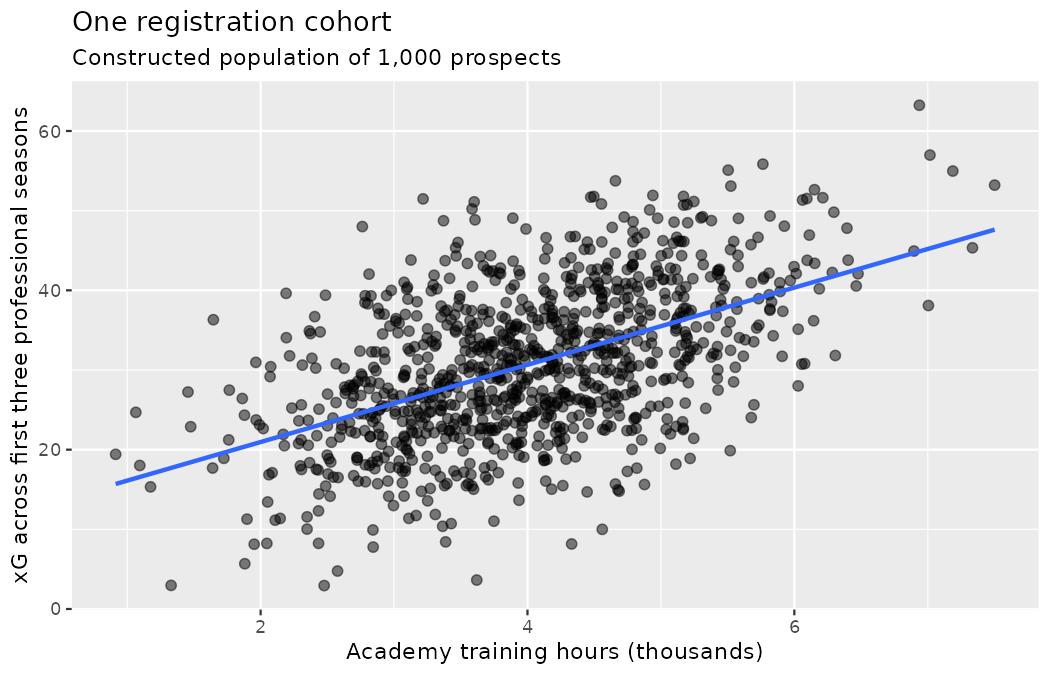
\includegraphics[width=0.85\linewidth,height=\textheight,keepaspectratio]{figures/inf-model-slr-1.png}

The 1,000 points form a strong, positive, linear cloud: training hours
run from roughly 0.9 to 7.5 thousand, three-season xG output from about
3 to 63, and the fitted line climbs steadily through the middle.

You may remember from Chapter~\ref{sec-model-slr} that the population
model is: \[y = \beta_0 + \beta_1 x + \varepsilon.\]

One new symbol has appeared, so take it apart before using it:
\(\varepsilon\) is the Greek letter \emph{epsilon}, and it plays at the
population level exactly the role the residual \(e_i\) of
Section~\ref{sec-resids} played in the sample --- the part of \(y\) the
line does not capture. The pairing is the same Greek-for-population,
Roman-for-sample convention that matches \(\beta_1\) with \(b_1\): the
population line misses each individual by some error \(\varepsilon\),
and our fitted line's residuals \(e_i\) are the sample-level shadows of
those errors.

The omniscient federation (with the full population information) can
write down the true population model, fit to all 1,000 prospects:

\begin{Shaded}
\begin{Highlighting}[]
\FunctionTok{coef}\NormalTok{(}\FunctionTok{lm}\NormalTok{(xg3 }\SpecialCharTok{\textasciitilde{}}\NormalTok{ hours, }\AttributeTok{data =}\NormalTok{ prospects))}
\CommentTok{\#\textgreater{} (Intercept)       hours}
\CommentTok{\#\textgreater{}   11.266012    4.846277}
\end{Highlighting}
\end{Shaded}

\[\texttt{expected 3-season xG} = 11.27 + 4.85 \times \texttt{training hours (thousands)}.\]

\subsection{Variability of the
statistic}\label{variability-of-the-statistic-20}

Unfortunately, in our scenario, the federation will not part with the
full database. Under its data-sharing agreement, a club preparing a
recruitment case --- say, Marta Vidal deciding how heavily Northbridge
should weight academy training volume --- can request a random sample of
just 20 prospects.

As with any numerical characteristic which describes a subset of the
population, the estimated slope of a sample will vary from sample to
sample. The least squares regression model uses the data to find a
sample linear fit, in the notation of Chapter~\ref{sec-model-slr}:
\[\hat{y} = b_0 + b_1 x.\]

The code below draws two random samples of 20 prospects and fits a line
to each.

\begin{Shaded}
\begin{Highlighting}[]
\FunctionTok{set.seed}\NormalTok{(}\DecValTok{2403}\NormalTok{)}
\NormalTok{sample20\_a }\OtherTok{\textless{}{-}}\NormalTok{ prospects }\SpecialCharTok{|\textgreater{}} \FunctionTok{slice\_sample}\NormalTok{(}\AttributeTok{n =} \DecValTok{20}\NormalTok{)}
\NormalTok{sample20\_b }\OtherTok{\textless{}{-}}\NormalTok{ prospects }\SpecialCharTok{|\textgreater{}} \FunctionTok{slice\_sample}\NormalTok{(}\AttributeTok{n =} \DecValTok{20}\NormalTok{)}

\FunctionTok{round}\NormalTok{(}\FunctionTok{coef}\NormalTok{(}\FunctionTok{lm}\NormalTok{(xg3 }\SpecialCharTok{\textasciitilde{}}\NormalTok{ hours, }\AttributeTok{data =}\NormalTok{ sample20\_a)), }\DecValTok{2}\NormalTok{)}
\CommentTok{\#\textgreater{} (Intercept)       hours}
\CommentTok{\#\textgreater{}       {-}5.71        8.38}
\FunctionTok{round}\NormalTok{(}\FunctionTok{coef}\NormalTok{(}\FunctionTok{lm}\NormalTok{(xg3 }\SpecialCharTok{\textasciitilde{}}\NormalTok{ hours, }\AttributeTok{data =}\NormalTok{ sample20\_b)), }\DecValTok{2}\NormalTok{)}
\CommentTok{\#\textgreater{} (Intercept)       hours}
\CommentTok{\#\textgreater{}        9.84        5.28}
\end{Highlighting}
\end{Shaded}

Both sample fits show the positive linear trend of the population, but
they are visibly different lines: the first sample happened to catch
points that tilt its line to a slope of \(8.38\) --- nearly twice the
true \(4.85\) --- while the second landed at \(5.28.\) Plotted over one
another, the two lines cross inside the data cloud and fan apart at the
edges. That is, there is \textbf{variability of the slope}: the
regression line changes from sample to sample. The concept of sampling
variability is something you have seen before --- for \(\hat{p}\) in
Chapter~\ref{sec-foundations-randomization}, for \(\bar{x}\) in
Chapter~\ref{sec-inference-one-mean} --- but in this chapter you will
focus on the variability of the line, usually measured through the
variability of a single statistic: \textbf{the slope of the line}.

The code below fits least squares lines to 50 more random samples of 20
and draws them on one plot, with the population line on top.

\begin{Shaded}
\begin{Highlighting}[]
\NormalTok{prospects\_50 }\OtherTok{\textless{}{-}}\NormalTok{ prospects }\SpecialCharTok{|\textgreater{}} \FunctionTok{rep\_slice\_sample}\NormalTok{(}\AttributeTok{n =} \DecValTok{20}\NormalTok{, }\AttributeTok{reps =} \DecValTok{50}\NormalTok{)}

\FunctionTok{ggplot}\NormalTok{() }\SpecialCharTok{+}
  \FunctionTok{geom\_smooth}\NormalTok{(}
    \AttributeTok{data =}\NormalTok{ prospects\_50,}
    \FunctionTok{aes}\NormalTok{(}\AttributeTok{x =}\NormalTok{ hours, }\AttributeTok{y =}\NormalTok{ xg3, }\AttributeTok{group =}\NormalTok{ replicate),}
    \AttributeTok{method =} \StringTok{"lm"}\NormalTok{, }\AttributeTok{se =} \ConstantTok{FALSE}\NormalTok{, }\AttributeTok{fullrange =} \ConstantTok{TRUE}\NormalTok{,}
    \AttributeTok{color =} \StringTok{"gray"}\NormalTok{, }\AttributeTok{linewidth =} \FloatTok{0.5}
\NormalTok{  ) }\SpecialCharTok{+}
  \FunctionTok{geom\_smooth}\NormalTok{(}
    \AttributeTok{data =}\NormalTok{ prospects,}
    \FunctionTok{aes}\NormalTok{(}\AttributeTok{x =}\NormalTok{ hours, }\AttributeTok{y =}\NormalTok{ xg3),}
    \AttributeTok{method =} \StringTok{"lm"}\NormalTok{, }\AttributeTok{se =} \ConstantTok{FALSE}\NormalTok{, }\AttributeTok{fullrange =} \ConstantTok{TRUE}\NormalTok{, }\AttributeTok{color =} \StringTok{"red"}
\NormalTok{  ) }\SpecialCharTok{+}
  \FunctionTok{labs}\NormalTok{(}
    \AttributeTok{x =} \StringTok{"Academy training hours (thousands)"}\NormalTok{,}
    \AttributeTok{y =} \StringTok{"xG across first three professional seasons"}\NormalTok{,}
    \AttributeTok{title =} \StringTok{"One registration cohort"}\NormalTok{,}
    \AttributeTok{subtitle =} \StringTok{"Least squares lines from 50 random samples of 20 prospects"}
\NormalTok{  )}
\end{Highlighting}
\end{Shaded}

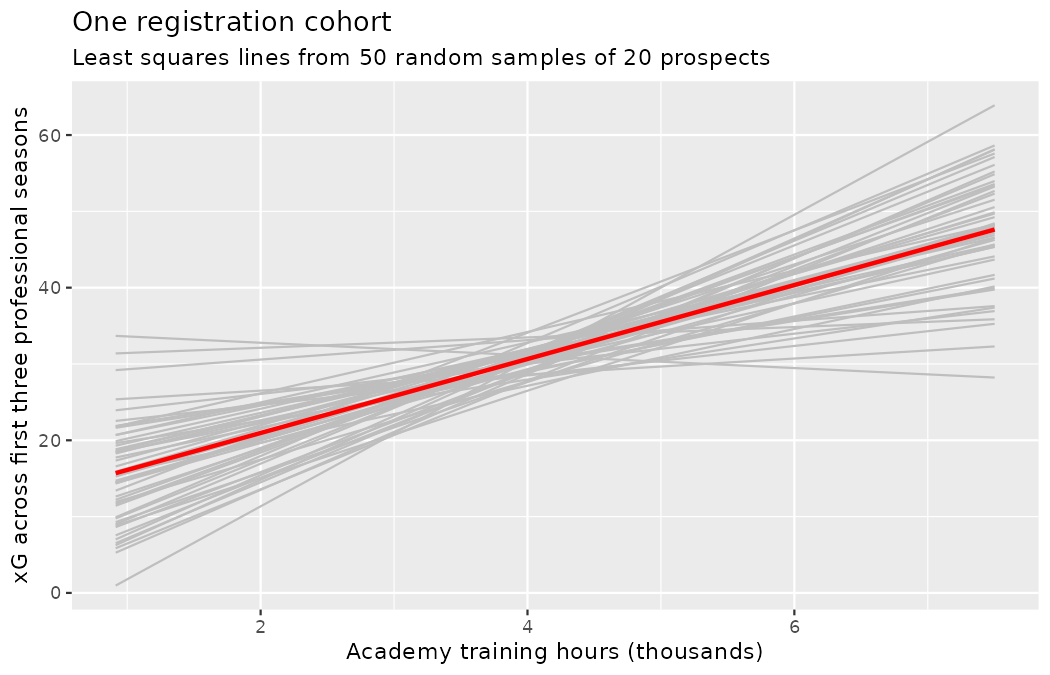
\includegraphics[width=0.85\linewidth,height=\textheight,keepaspectratio]{figures/inf-model-slr-2.png}

The 50 gray lines form a bow-tie around the red population line: tightly
bundled in the middle of the data, splayed wide at the extremes.

\begin{tcolorbox}[enhanced jigsaw, left=2mm, leftrule=.75mm, title=\textcolor{quarto-callout-tip-color}{\faLightbulb}\hspace{0.5em}{Check your understanding}, arc=.35mm, rightrule=.15mm, coltitle=black, colframe=quarto-callout-tip-color-frame, bottomrule=.15mm, colbacktitle=quarto-callout-tip-color!10!white, opacitybacktitle=0.6, breakable, bottomtitle=1mm, toptitle=1mm, titlerule=0mm, opacityback=0, toprule=.15mm, colback=white]

You might notice that the \(\hat{y}\) values given by the 50 lines are
much more consistent in the middle of the dataset than at the ends. Why?
And what does the shape imply for a scout using one sample's line to
predict the output of a prospect with 6,500 training hours rather than
4,000?

\begin{center}\rule{0.5\linewidth}{0.5pt}\end{center}

The data anchor each line: a least squares line must pass through the
center of its own data cloud (recall from
Section~\ref{sec-least-squares-regression} that it passes through
\((\bar{x}, \bar{y})\)), so all 50 lines are pinned near the middle,
where most prospects live, and free to tilt at the edges. The effect of
the fan-shaped lines is that predicted three-season xG for prospects
near 4,000 training hours will be much more precise than predictions
made for prospects with 1,500 or 6,500 hours --- the sample-to-sample
disagreement is largest exactly where the extrapolation-shy scout of
Chapter~\ref{sec-model-slr} already knew to tread carefully.

\end{tcolorbox}

The distribution of slopes (for samples of size \(n = 20\)) can be seen
in the histogram drawn by the code below.

\begin{Shaded}
\begin{Highlighting}[]
\NormalTok{prospects\_50\_slopes }\OtherTok{\textless{}{-}}\NormalTok{ prospects\_50 }\SpecialCharTok{|\textgreater{}}
  \FunctionTok{group\_by}\NormalTok{(replicate) }\SpecialCharTok{|\textgreater{}}
  \FunctionTok{group\_modify}\NormalTok{(}\SpecialCharTok{\textasciitilde{}} \FunctionTok{tidy}\NormalTok{(}\FunctionTok{lm}\NormalTok{(xg3 }\SpecialCharTok{\textasciitilde{}}\NormalTok{ hours, }\AttributeTok{data =}\NormalTok{ .x))) }\SpecialCharTok{|\textgreater{}}
  \FunctionTok{filter}\NormalTok{(term }\SpecialCharTok{==} \StringTok{"hours"}\NormalTok{)}

\FunctionTok{round}\NormalTok{(}\FunctionTok{c}\NormalTok{(}\AttributeTok{mean =} \FunctionTok{mean}\NormalTok{(prospects\_50\_slopes}\SpecialCharTok{$}\NormalTok{estimate),}
        \AttributeTok{sd   =} \FunctionTok{sd}\NormalTok{(prospects\_50\_slopes}\SpecialCharTok{$}\NormalTok{estimate),}
        \AttributeTok{min  =} \FunctionTok{min}\NormalTok{(prospects\_50\_slopes}\SpecialCharTok{$}\NormalTok{estimate),}
        \AttributeTok{max  =} \FunctionTok{max}\NormalTok{(prospects\_50\_slopes}\SpecialCharTok{$}\NormalTok{estimate)), }\DecValTok{2}\NormalTok{)}
\CommentTok{\#\textgreater{}  mean    sd   min   max}
\CommentTok{\#\textgreater{}  4.85  2.10 {-}0.83  9.55}

\FunctionTok{ggplot}\NormalTok{(prospects\_50\_slopes, }\FunctionTok{aes}\NormalTok{(}\AttributeTok{x =}\NormalTok{ estimate)) }\SpecialCharTok{+}
  \FunctionTok{geom\_histogram}\NormalTok{(}\AttributeTok{binwidth =} \DecValTok{1}\NormalTok{) }\SpecialCharTok{+}
  \FunctionTok{labs}\NormalTok{(}
    \AttributeTok{x =} \StringTok{"Slope estimate"}\NormalTok{,}
    \AttributeTok{y =} \StringTok{"Count"}\NormalTok{,}
    \AttributeTok{title =} \StringTok{"Slopes from 50 random samples of 20 prospects"}
\NormalTok{  )}
\end{Highlighting}
\end{Shaded}

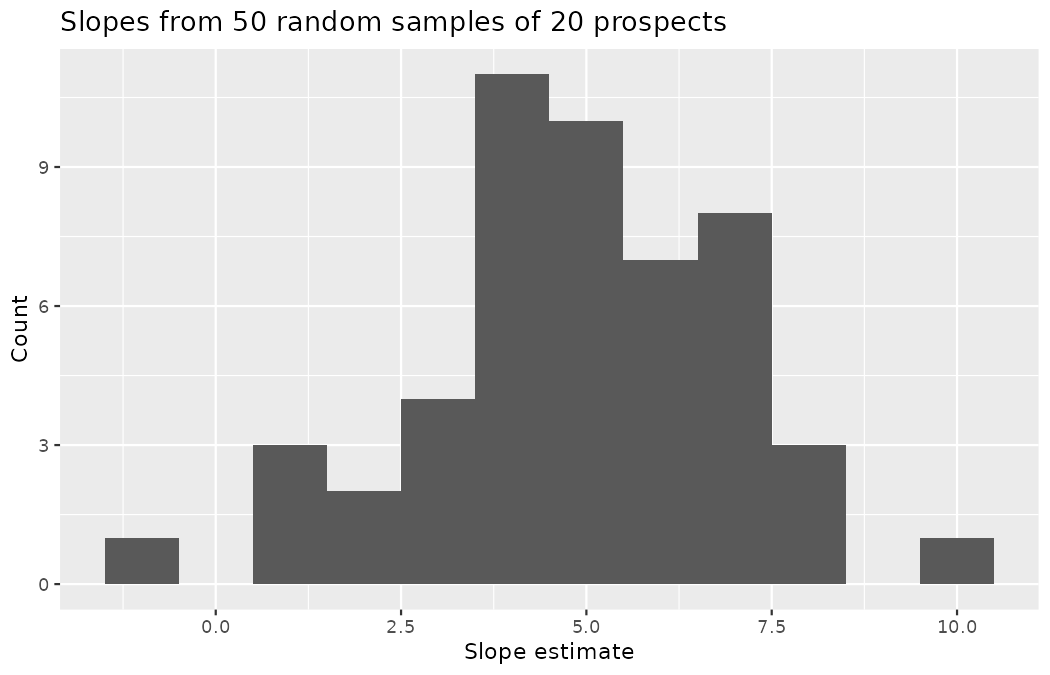
\includegraphics[width=0.85\linewidth,height=\textheight,keepaspectratio]{figures/inf-model-slr-3.png}

The 50 slope estimates pile up in a reasonably bell-shaped heap around
the true slope of \(4.85\), with a standard deviation of \(2.10\) ---
and they range all the way from \(-0.83\) to \(9.55.\) Sit with that
minimum for a moment: in a population where the true relationship is
strongly positive, one honest random sample of 20 prospects produced a
\emph{negative} fitted slope. A scout holding only that sample would
have reported, in good faith, that academy hours do not pay off.

Recall that the example described in this case study is constructed.
That is, we created an entire population in order to demonstrate how the
slope of a line would vary from sample to sample. The tools in this
textbook are designed to evaluate only one single sample of data. With
actual studies, we do not have repeated samples, so we are not able to
use repeated samples to visualize the variability in slopes. We have
seen variability in samples throughout this text, so it should not come
as a surprise that different samples will produce different linear
models. However, it is nice to visually consider the linear models
produced by different slopes. Additionally, as with measuring the
variability of previous statistics (e.g., \(\bar{x}_1 - \bar{x}_2\) in
Chapter~\ref{sec-inference-two-means} or \(\hat{p}_1 - \hat{p}_2\) in
Chapter~\ref{sec-inference-two-props}), the histogram of the sample
statistics can provide information related to inferential
considerations.

In the following sections, the distribution (i.e., histogram) of \(b_1\)
(the estimated slope coefficient) will be constructed in the same three
ways that, by now, are familiar to you. First (in
Section~\ref{sec-randslope}), the distribution of \(b_1\) when
\(\beta_1 = 0\) is constructed by randomizing (permuting) the response
variable. Next (in Section~\ref{sec-bootbeta1}), we can bootstrap the
data by taking random samples of size \(n\) from the original dataset.
And last (in Section~\ref{sec-mathslope}), we use mathematical tools to
describe the variability using the \(t\)-distribution that was first
encountered in Section~\ref{sec-one-mean-math}.

\section{Randomization test for the slope}\label{sec-randslope}

Back, now, to real football and to the workhorse object of this book.
Recall the \texttt{team\_match} dataset: one row per team per match at
the 2022 Men's World Cup, aggregating that team's shots into counts,
accumulated chance quality, and goals. In Chapter~\ref{sec-model-slr} we
fit its flagship line --- goals on total xG --- and read the slope of
\(0.909\) as \emph{this tournament's} exchange rate between chance
quality and goals. The inferential question we can now ask is the one
Marta Vidal would put to any exchange rate: is it real, or could a slope
that size arise from chance alone?

\begin{tcolorbox}[enhanced jigsaw, left=2mm, leftrule=.75mm, title=\textcolor{quarto-callout-note-color}{\faInfo}\hspace{0.5em}{Data}, arc=.35mm, rightrule=.15mm, coltitle=black, colframe=quarto-callout-note-color-frame, bottomrule=.15mm, colbacktitle=quarto-callout-note-color!10!white, opacitybacktitle=0.6, breakable, bottomtitle=1mm, toptitle=1mm, titlerule=0mm, opacityback=0, toprule=.15mm, colback=white]

The \texttt{team\_match} data are derived from
\texttt{data/derived/wc2022\_shots.csv} (StatsBomb open data), rebuilt
below with the same code as in Chapter~\ref{sec-explore-numerical} and
Chapter~\ref{sec-model-slr}. One honesty note travels with the object,
per this book's penalty convention: the shot log includes in-game
penalties and the shoot-out kicks of drawn knockout ties, so both
\texttt{total\_xg} and \texttt{goals} count them --- on both sides of
the model. We keep the full log because \texttt{team\_match} is the
book's canonical object, and we read the model as describing
\emph{recorded attempts}, not only the run of play.

\end{tcolorbox}

\begin{Shaded}
\begin{Highlighting}[]
\NormalTok{wc2022\_shots }\OtherTok{\textless{}{-}} \FunctionTok{read\_csv}\NormalTok{(}\StringTok{"data/derived/wc2022\_shots.csv"}\NormalTok{)}

\NormalTok{team\_match }\OtherTok{\textless{}{-}}\NormalTok{ wc2022\_shots }\SpecialCharTok{|\textgreater{}}
  \FunctionTok{group\_by}\NormalTok{(match\_id, team) }\SpecialCharTok{|\textgreater{}}
  \FunctionTok{summarize}\NormalTok{(}
    \AttributeTok{n\_shots =} \FunctionTok{n}\NormalTok{(),}
    \AttributeTok{total\_xg =} \FunctionTok{sum}\NormalTok{(statsbomb\_xg),}
    \AttributeTok{goals =} \FunctionTok{sum}\NormalTok{(goal),}
    \AttributeTok{prop\_under\_pressure =} \FunctionTok{mean}\NormalTok{(under\_pressure),}
    \AttributeTok{prop\_set\_piece =} \FunctionTok{mean}\NormalTok{(play\_pattern }\SpecialCharTok{\%in\%}
      \FunctionTok{c}\NormalTok{(}\StringTok{"From Corner"}\NormalTok{, }\StringTok{"From Free Kick"}\NormalTok{, }\StringTok{"From Throw In"}\NormalTok{)),}
    \AttributeTok{.groups =} \StringTok{"drop"}
\NormalTok{  )}

\FunctionTok{nrow}\NormalTok{(team\_match)}
\CommentTok{\#\textgreater{} [1] 127}
\end{Highlighting}
\end{Shaded}

As always, 127 rows: Costa Rica's shotless outing against Spain is the
one missing team-match. The dataset is rich enough to offer several
candidate predictors of a team's goals in a match. The code below plots
goals against four of them side by side.

\begin{Shaded}
\begin{Highlighting}[]
\FunctionTok{library}\NormalTok{(patchwork)}

\NormalTok{p\_shots }\OtherTok{\textless{}{-}} \FunctionTok{ggplot}\NormalTok{(team\_match, }\FunctionTok{aes}\NormalTok{(}\AttributeTok{x =}\NormalTok{ n\_shots, }\AttributeTok{y =}\NormalTok{ goals)) }\SpecialCharTok{+}
  \FunctionTok{geom\_jitter}\NormalTok{(}\AttributeTok{height =} \FloatTok{0.1}\NormalTok{, }\AttributeTok{alpha =} \FloatTok{0.6}\NormalTok{) }\SpecialCharTok{+}
  \FunctionTok{labs}\NormalTok{(}\AttributeTok{x =} \StringTok{"Number of shots"}\NormalTok{, }\AttributeTok{y =} \StringTok{"Goals"}\NormalTok{)}
\NormalTok{p\_press }\OtherTok{\textless{}{-}} \FunctionTok{ggplot}\NormalTok{(team\_match, }\FunctionTok{aes}\NormalTok{(}\AttributeTok{x =}\NormalTok{ prop\_under\_pressure, }\AttributeTok{y =}\NormalTok{ goals)) }\SpecialCharTok{+}
  \FunctionTok{geom\_jitter}\NormalTok{(}\AttributeTok{height =} \FloatTok{0.1}\NormalTok{, }\AttributeTok{alpha =} \FloatTok{0.6}\NormalTok{) }\SpecialCharTok{+}
  \FunctionTok{labs}\NormalTok{(}\AttributeTok{x =} \StringTok{"Share of shots under pressure"}\NormalTok{, }\AttributeTok{y =} \StringTok{"Goals"}\NormalTok{)}
\NormalTok{p\_setp }\OtherTok{\textless{}{-}} \FunctionTok{ggplot}\NormalTok{(team\_match, }\FunctionTok{aes}\NormalTok{(}\AttributeTok{x =}\NormalTok{ prop\_set\_piece, }\AttributeTok{y =}\NormalTok{ goals)) }\SpecialCharTok{+}
  \FunctionTok{geom\_jitter}\NormalTok{(}\AttributeTok{height =} \FloatTok{0.1}\NormalTok{, }\AttributeTok{alpha =} \FloatTok{0.6}\NormalTok{) }\SpecialCharTok{+}
  \FunctionTok{labs}\NormalTok{(}\AttributeTok{x =} \StringTok{"Share of shots from set pieces"}\NormalTok{, }\AttributeTok{y =} \StringTok{"Goals"}\NormalTok{)}
\NormalTok{p\_xg }\OtherTok{\textless{}{-}} \FunctionTok{ggplot}\NormalTok{(team\_match, }\FunctionTok{aes}\NormalTok{(}\AttributeTok{x =}\NormalTok{ total\_xg, }\AttributeTok{y =}\NormalTok{ goals)) }\SpecialCharTok{+}
  \FunctionTok{geom\_jitter}\NormalTok{(}\AttributeTok{height =} \FloatTok{0.1}\NormalTok{, }\AttributeTok{alpha =} \FloatTok{0.6}\NormalTok{) }\SpecialCharTok{+}
  \FunctionTok{labs}\NormalTok{(}\AttributeTok{x =} \StringTok{"Total xG"}\NormalTok{, }\AttributeTok{y =} \StringTok{"Goals"}\NormalTok{)}

\NormalTok{p\_shots }\SpecialCharTok{+}\NormalTok{ p\_press }\SpecialCharTok{+}\NormalTok{ p\_setp }\SpecialCharTok{+}\NormalTok{ p\_xg }\SpecialCharTok{+} \FunctionTok{plot\_layout}\NormalTok{(}\AttributeTok{ncol =} \DecValTok{2}\NormalTok{)}

\NormalTok{team\_match }\SpecialCharTok{|\textgreater{}}
  \FunctionTok{summarize}\NormalTok{(}
    \AttributeTok{r\_shots    =} \FunctionTok{cor}\NormalTok{(goals, n\_shots),}
    \AttributeTok{r\_pressure =} \FunctionTok{cor}\NormalTok{(goals, prop\_under\_pressure),}
    \AttributeTok{r\_setpiece =} \FunctionTok{cor}\NormalTok{(goals, prop\_set\_piece),}
    \AttributeTok{r\_xg       =} \FunctionTok{cor}\NormalTok{(goals, total\_xg)}
\NormalTok{  )}
\CommentTok{\#\textgreater{} \# A tibble: 1 × 4}
\CommentTok{\#\textgreater{}   r\_shots r\_pressure r\_setpiece  r\_xg}
\CommentTok{\#\textgreater{}     \textless{}dbl\textgreater{}      \textless{}dbl\textgreater{}      \textless{}dbl\textgreater{} \textless{}dbl\textgreater{}}
\CommentTok{\#\textgreater{} 1   0.403     {-}0.156     {-}0.272 0.691}
\end{Highlighting}
\end{Shaded}

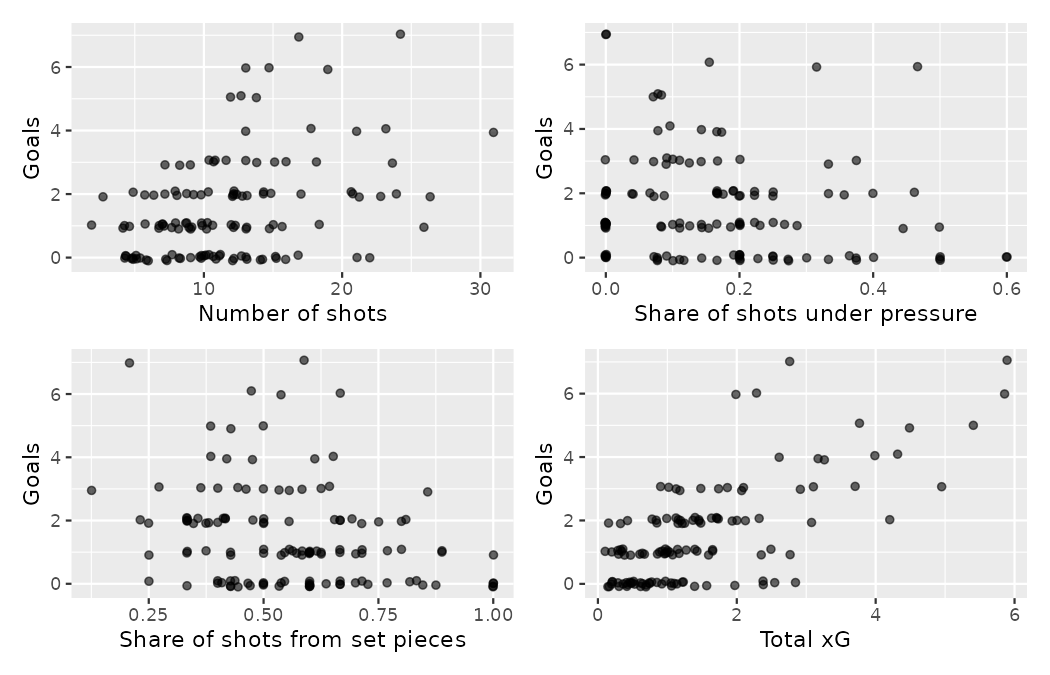
\includegraphics[width=0.85\linewidth,height=\textheight,keepaspectratio]{figures/inf-model-slr-4.png}

Shot volume shows a moderate positive relationship with goals
\((r = 0.40),\) the two shot-mix shares drift weakly negative, and
accumulated chance quality shows much the strongest linear relationship
\((r = 0.691)\) --- which is why \texttt{total\_xg} carries the modeling
weight in this book.

As you have seen previously, statistical inference typically relies on
setting a null hypothesis which is hoped to be subsequently rejected. In
the linear model setting, we might hope to have a linear relationship
between \texttt{total\_xg} and \texttt{goals} in settings where chance
quality is known and goals need to be predicted --- which is precisely a
scout's situation when projecting a team's output from its underlying
numbers.

The relevant hypotheses for the linear model setting can be written in
terms of the population slope parameter. Here the population refers to
the process that generates team performances at this level --- one
tournament's 127 team-matches standing in for how the sport behaves, our
standard observational framing since
Chapter~\ref{sec-foundations-randomization}.

\begin{itemize}
\tightlist
\item
  \(H_0: \beta_1 = 0,\) there is no linear relationship between
  \texttt{goals} and \texttt{total\_xg}.
\item
  \(H_A: \beta_1 \ne 0,\) there is some linear relationship between
  \texttt{goals} and \texttt{total\_xg}.
\end{itemize}

A candid aside before we test: nobody at Northbridge doubts which way
this one will fall --- a world in which accumulated chance quality told
you \emph{nothing} about goals would be a world where the ``expected''
in expected goals had failed spectacularly. The value of running the
test on this model is that you will see the machinery work on a
relationship you trust, before we point it at relationships you should
not trust (they arrive in Section~\ref{sec-bootbeta1} and
Section~\ref{sec-mathslope}).

Recall that for the randomization test, we permute one variable to
eliminate any existing relationship between the variables. That is, we
set the null hypothesis to be true, and we measure the natural
variability in the data due to sampling but \textbf{not} due to
variables being correlated. The code below permutes the \texttt{goals}
column once and plots the result next to the original data.

\begin{Shaded}
\begin{Highlighting}[]
\FunctionTok{set.seed}\NormalTok{(}\DecValTok{2404}\NormalTok{)}
\NormalTok{team\_match\_perm1 }\OtherTok{\textless{}{-}}\NormalTok{ team\_match }\SpecialCharTok{|\textgreater{}}
  \FunctionTok{mutate}\NormalTok{(}\AttributeTok{goals\_permuted =} \FunctionTok{sample}\NormalTok{(goals))}

\NormalTok{p\_original }\OtherTok{\textless{}{-}} \FunctionTok{ggplot}\NormalTok{(team\_match, }\FunctionTok{aes}\NormalTok{(}\AttributeTok{x =}\NormalTok{ total\_xg, }\AttributeTok{y =}\NormalTok{ goals)) }\SpecialCharTok{+}
  \FunctionTok{geom\_point}\NormalTok{(}\AttributeTok{alpha =} \FloatTok{0.6}\NormalTok{) }\SpecialCharTok{+}
  \FunctionTok{labs}\NormalTok{(}\AttributeTok{x =} \StringTok{"Total xG"}\NormalTok{, }\AttributeTok{y =} \StringTok{"Goals"}\NormalTok{, }\AttributeTok{title =} \StringTok{"Original data"}\NormalTok{)}

\NormalTok{p\_permuted }\OtherTok{\textless{}{-}} \FunctionTok{ggplot}\NormalTok{(team\_match\_perm1, }\FunctionTok{aes}\NormalTok{(}\AttributeTok{x =}\NormalTok{ total\_xg, }\AttributeTok{y =}\NormalTok{ goals\_permuted)) }\SpecialCharTok{+}
  \FunctionTok{geom\_point}\NormalTok{(}\AttributeTok{alpha =} \FloatTok{0.6}\NormalTok{) }\SpecialCharTok{+}
  \FunctionTok{labs}\NormalTok{(}\AttributeTok{x =} \StringTok{"Total xG"}\NormalTok{, }\AttributeTok{y =} \StringTok{"Permuted goals"}\NormalTok{, }\AttributeTok{title =} \StringTok{"Permuted data"}\NormalTok{)}

\NormalTok{p\_original }\SpecialCharTok{+}\NormalTok{ p\_permuted}
\end{Highlighting}
\end{Shaded}

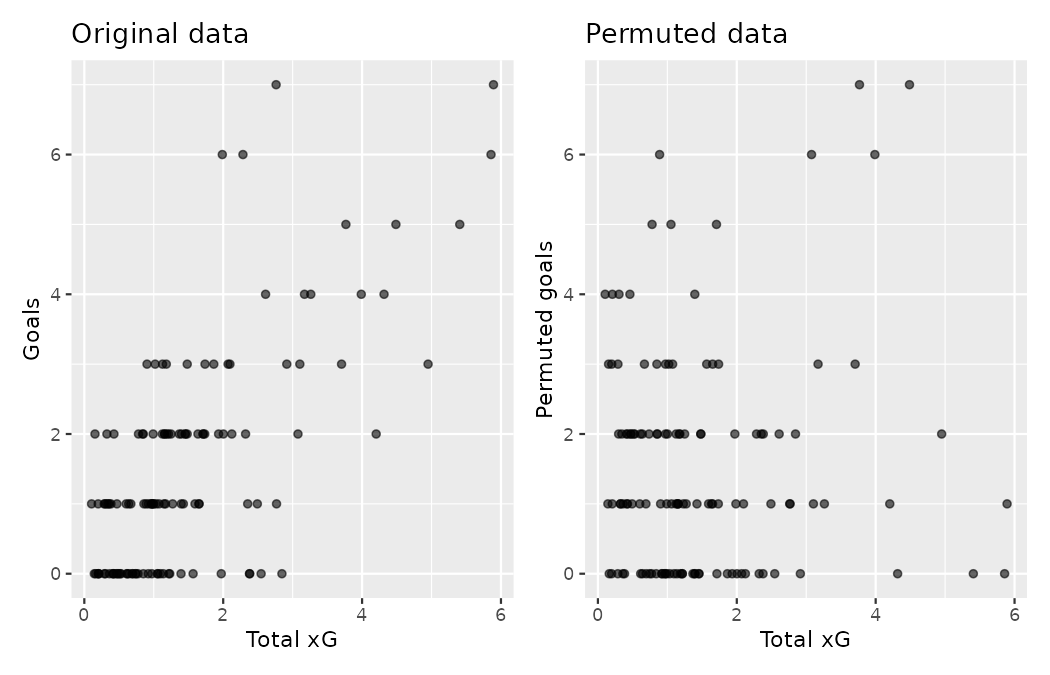
\includegraphics[width=0.85\linewidth,height=\textheight,keepaspectratio]{figures/inf-model-slr-5.png}

The careful observer can see that each of the observed values for
\texttt{goals} (and for \texttt{total\_xg}) exists in both plots, but
the pairing has been broken: each goal count is randomly reassigned to a
new team-match's chance quality. Spain's 7 goals might now sit on a
\(0.5\)-xG performance; Canada's 0 on a \(3\)-xG one. The upward sweep
of the original cloud is gone --- the permuted panel is a formless band.

By repeatedly permuting the response variable, any pattern in the linear
model that is observed is due only to random chance (and not an
underlying relationship). The \textbf{randomization test for the slope}
compares the slopes calculated from the permuted response variable with
the observed slope. If the observed slope is inconsistent with the
slopes from permuting, we can conclude that there is some underlying
relationship (and that the slope is not merely due to random chance).
And one caution, held over from Section~\ref{sec-chp11-observational}:
since nobody randomly assigned chance quality to teams, this is a
permutation test on observational data --- a rejected null will speak of
association, not causation.

\subsection{Observed data}\label{observed-data-20}

We will continue to use the \texttt{team\_match} data to investigate the
linear relationship between \texttt{goals} and \texttt{total\_xg}. The
least squares model (see Chapter~\ref{sec-model-slr}) describing the
relationship is computed below and given in
Table~\ref{tbl-ls-teammatch}. The columns of
Table~\ref{tbl-ls-teammatch} are further described in
Section~\ref{sec-mathslope}.

\begin{Shaded}
\begin{Highlighting}[]
\NormalTok{fit\_goals }\OtherTok{\textless{}{-}} \FunctionTok{lm}\NormalTok{(goals }\SpecialCharTok{\textasciitilde{}}\NormalTok{ total\_xg, }\AttributeTok{data =}\NormalTok{ team\_match)}
\FunctionTok{tidy}\NormalTok{(fit\_goals)}
\CommentTok{\#\textgreater{} \# A tibble: 2 × 5}
\CommentTok{\#\textgreater{}   term        estimate std.error statistic  p.value}
\CommentTok{\#\textgreater{}   \textless{}chr\textgreater{}          \textless{}dbl\textgreater{}     \textless{}dbl\textgreater{}     \textless{}dbl\textgreater{}    \textless{}dbl\textgreater{}}
\CommentTok{\#\textgreater{} 1 (Intercept)    0.190    0.163       1.17 2.45e{-} 1}
\CommentTok{\#\textgreater{} 2 total\_xg       0.909    0.0849     10.7  2.31e{-}19}
\end{Highlighting}
\end{Shaded}

\begin{longtable}[]{@{}lrrrr@{}}
\caption{The least squares estimates of the intercept and slope for
goals regressed on total xG across the 127 World Cup team-matches. The
observed slope is 0.909.}\label{tbl-ls-teammatch}\tabularnewline
\toprule\noalign{}
term & estimate & std.error & statistic & p.value \\
\midrule\noalign{}
\endfirsthead
\toprule\noalign{}
term & estimate & std.error & statistic & p.value \\
\midrule\noalign{}
\endhead
\bottomrule\noalign{}
\endlastfoot
(Intercept) & 0.19 & 0.16 & 1.17 & 0.2446 \\
total\_xg & 0.91 & 0.08 & 10.70 & \textless0.0001 \\
\end{longtable}

\begin{tcolorbox}[enhanced jigsaw, left=2mm, leftrule=.75mm, title=\textcolor{quarto-callout-tip-color}{\faLightbulb}\hspace{0.5em}{Check your understanding}, arc=.35mm, rightrule=.15mm, coltitle=black, colframe=quarto-callout-tip-color-frame, bottomrule=.15mm, colbacktitle=quarto-callout-tip-color!10!white, opacitybacktitle=0.6, breakable, bottomtitle=1mm, toptitle=1mm, titlerule=0mm, opacityback=0, toprule=.15mm, colback=white]

Before the shuffling starts, confirm the fitted line still reads the way
Section~\ref{sec-resids} taught --- data = fit + residual, one row at a
time. England's group-stage team-match against Iran carried an
accumulated chance quality of 1.99 xG and produced 6 goals:

\begin{Shaded}
\begin{Highlighting}[]
\NormalTok{team\_match }\SpecialCharTok{|\textgreater{}}
  \FunctionTok{filter}\NormalTok{(team }\SpecialCharTok{==} \StringTok{"England"}\NormalTok{, goals }\SpecialCharTok{==} \DecValTok{6}\NormalTok{) }\SpecialCharTok{|\textgreater{}}
  \FunctionTok{select}\NormalTok{(team, total\_xg, goals)}
\CommentTok{\#\textgreater{} \# A tibble: 1 × 3}
\CommentTok{\#\textgreater{}   team    total\_xg goals}
\CommentTok{\#\textgreater{}   \textless{}chr\textgreater{}      \textless{}dbl\textgreater{} \textless{}int\textgreater{}}
\CommentTok{\#\textgreater{} 1 England     1.99     6}
\end{Highlighting}
\end{Shaded}

Use the estimates in Table~\ref{tbl-ls-teammatch} to compute the fitted
value and the residual for this row, and read both numbers in the
created-versus-finished vocabulary of Chapter~\ref{sec-model-slr}.

\begin{center}\rule{0.5\linewidth}{0.5pt}\end{center}

The fitted value prices what England \emph{created}:
\(\hat{y} = 0.190 + 0.909 \times 1.99 = 2.00\) goals' worth of chances.
The residual is the decomposition of Section~\ref{sec-resids} applied to
a single afternoon: \(e = y - \hat{y} = 6 - 2.00 = 4.00.\) In scouting
vocabulary, England created roughly two goals of chance quality and
\emph{finished} six --- a four-goal finishing over-performance, among
the largest at the tournament, and a quantity a scout files under
finishing, not chance creation. The inference that follows never touches
this reading: the permutation test will interrogate the \emph{slope} ---
the created-to-finished exchange rate across all 127 rows --- while each
residual keeps the job Section~\ref{sec-resids} gave it, measuring who
beat their chances.

\end{tcolorbox}

\subsection{Variability of the
statistic}\label{variability-of-the-statistic-21}

After permuting the data, the least squares estimate of the line can be
computed. Repeated permutations and slope calculations describe the
variability in the line (i.e., in the slope) due only to the natural
variability and not due to a relationship between \texttt{goals} and
\texttt{total\_xg}. The code below runs two fresh permutations and fits
a line to each.

\begin{Shaded}
\begin{Highlighting}[]
\FunctionTok{set.seed}\NormalTok{(}\DecValTok{2405}\NormalTok{)}
\NormalTok{team\_match\_perm2 }\OtherTok{\textless{}{-}}\NormalTok{ team\_match }\SpecialCharTok{|\textgreater{}} \FunctionTok{mutate}\NormalTok{(}\AttributeTok{goals\_permuted =} \FunctionTok{sample}\NormalTok{(goals))}
\NormalTok{team\_match\_perm3 }\OtherTok{\textless{}{-}}\NormalTok{ team\_match }\SpecialCharTok{|\textgreater{}} \FunctionTok{mutate}\NormalTok{(}\AttributeTok{goals\_permuted =} \FunctionTok{sample}\NormalTok{(goals))}

\FunctionTok{round}\NormalTok{(}\FunctionTok{c}\NormalTok{(}
  \AttributeTok{slope\_first  =} \FunctionTok{unname}\NormalTok{(}\FunctionTok{coef}\NormalTok{(}\FunctionTok{lm}\NormalTok{(goals\_permuted }\SpecialCharTok{\textasciitilde{}}\NormalTok{ total\_xg, }\AttributeTok{data =}\NormalTok{ team\_match\_perm2))[}\DecValTok{2}\NormalTok{]),}
  \AttributeTok{slope\_second =} \FunctionTok{unname}\NormalTok{(}\FunctionTok{coef}\NormalTok{(}\FunctionTok{lm}\NormalTok{(goals\_permuted }\SpecialCharTok{\textasciitilde{}}\NormalTok{ total\_xg, }\AttributeTok{data =}\NormalTok{ team\_match\_perm3))[}\DecValTok{2}\NormalTok{])}
\NormalTok{), }\DecValTok{3}\NormalTok{)}
\CommentTok{\#\textgreater{}  slope\_first slope\_second}
\CommentTok{\#\textgreater{}       {-}0.025       {-}0.060}
\end{Highlighting}
\end{Shaded}

As you can see, sometimes the slope of the permuted data is positive,
sometimes it is negative --- here two shuffles happened to produce two
small negative slopes, and further shuffles produce small positive ones.
Because the randomization happens under the condition of no underlying
relationship (the response variable is completely mixed with the
explanatory variable), we expect the center of the randomized slope
distribution to be zero.

\subsection{Observed statistic vs.~null
statistics}\label{observed-statistic-vs.-null-statistics-11}

The \textbf{infer} pipeline you have used since
Chapter~\ref{sec-foundations-randomization} computes 1,000 permuted
slopes; the only novelty is \texttt{calculate(stat\ =\ "slope")}.

\begin{Shaded}
\begin{Highlighting}[]
\FunctionTok{set.seed}\NormalTok{(}\DecValTok{2406}\NormalTok{)}
\NormalTok{xg\_slope\_null }\OtherTok{\textless{}{-}}\NormalTok{ team\_match }\SpecialCharTok{|\textgreater{}}
  \FunctionTok{specify}\NormalTok{(goals }\SpecialCharTok{\textasciitilde{}}\NormalTok{ total\_xg) }\SpecialCharTok{|\textgreater{}}
  \FunctionTok{hypothesize}\NormalTok{(}\AttributeTok{null =} \StringTok{"independence"}\NormalTok{) }\SpecialCharTok{|\textgreater{}}
  \FunctionTok{generate}\NormalTok{(}\AttributeTok{reps =} \DecValTok{1000}\NormalTok{, }\AttributeTok{type =} \StringTok{"permute"}\NormalTok{) }\SpecialCharTok{|\textgreater{}}
  \FunctionTok{calculate}\NormalTok{(}\AttributeTok{stat =} \StringTok{"slope"}\NormalTok{)}

\NormalTok{obs\_slope }\OtherTok{\textless{}{-}}\NormalTok{ team\_match }\SpecialCharTok{|\textgreater{}}
  \FunctionTok{specify}\NormalTok{(goals }\SpecialCharTok{\textasciitilde{}}\NormalTok{ total\_xg) }\SpecialCharTok{|\textgreater{}}
  \FunctionTok{calculate}\NormalTok{(}\AttributeTok{stat =} \StringTok{"slope"}\NormalTok{) }\SpecialCharTok{|\textgreater{}}
  \FunctionTok{pull}\NormalTok{() }\SpecialCharTok{|\textgreater{}}
  \FunctionTok{unname}\NormalTok{()}
\FunctionTok{round}\NormalTok{(obs\_slope, }\DecValTok{4}\NormalTok{)}
\CommentTok{\#\textgreater{} [1] 0.9087}

\FunctionTok{ggplot}\NormalTok{(xg\_slope\_null, }\FunctionTok{aes}\NormalTok{(}\AttributeTok{x =}\NormalTok{ stat)) }\SpecialCharTok{+}
  \FunctionTok{geom\_histogram}\NormalTok{(}\AttributeTok{binwidth =} \FloatTok{0.05}\NormalTok{) }\SpecialCharTok{+}
  \FunctionTok{geom\_vline}\NormalTok{(}\AttributeTok{xintercept =}\NormalTok{ obs\_slope, }\AttributeTok{color =} \StringTok{"red"}\NormalTok{) }\SpecialCharTok{+}
  \FunctionTok{labs}\NormalTok{(}\AttributeTok{x =} \StringTok{"Randomly generated slopes"}\NormalTok{, }\AttributeTok{y =} \StringTok{"Count"}\NormalTok{)}

\NormalTok{xg\_slope\_null }\SpecialCharTok{|\textgreater{}}
  \FunctionTok{summarize}\NormalTok{(}
    \AttributeTok{min\_slope =} \FunctionTok{min}\NormalTok{(stat),}
    \AttributeTok{max\_slope =} \FunctionTok{max}\NormalTok{(stat),}
    \AttributeTok{n\_extreme =} \FunctionTok{sum}\NormalTok{(}\FunctionTok{abs}\NormalTok{(stat) }\SpecialCharTok{\textgreater{}=}\NormalTok{ obs\_slope)}
\NormalTok{  )}
\CommentTok{\#\textgreater{} \# A tibble: 1 × 3}
\CommentTok{\#\textgreater{}   min\_slope max\_slope n\_extreme}
\CommentTok{\#\textgreater{}       \textless{}dbl\textgreater{}     \textless{}dbl\textgreater{}     \textless{}int\textgreater{}}
\CommentTok{\#\textgreater{} 1    {-}0.305     0.406         0}
\end{Highlighting}
\end{Shaded}

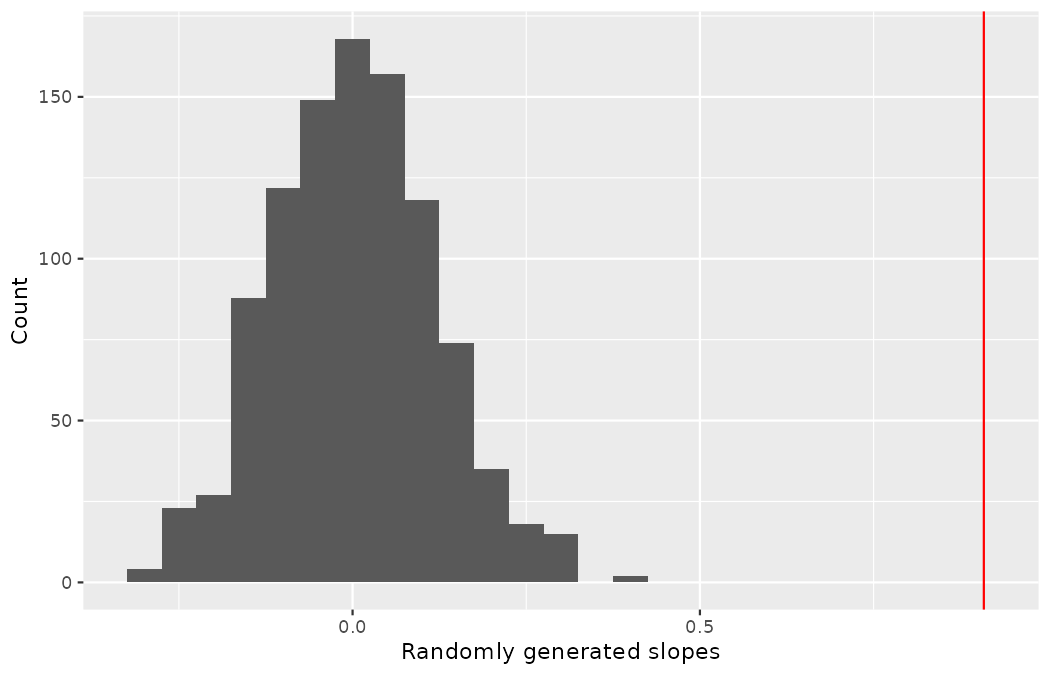
\includegraphics[width=0.85\linewidth,height=\textheight,keepaspectratio]{figures/inf-model-slr-6.png}

A slope estimate as extreme as the observed slope (the red line, far to
the right of the histogram) never happened in 1,000 permutations of the
\texttt{goals} variable. That is, if there were truly no linear
relationship between \texttt{goals} and \texttt{total\_xg}, the natural
variability of the slopes would produce estimates between approximately
\(-0.31\) and \(+0.41.\) The observed \(0.909\) is nowhere near that
range. We reject the null hypothesis and conclude that the slope
observed in the original data is not due to natural variability: across
team performances at this level, accumulated chance quality and goals
scored are genuinely, linearly related.

\begin{tcolorbox}[enhanced jigsaw, left=2mm, leftrule=.75mm, title=\textcolor{quarto-callout-tip-color}{\faLightbulb}\hspace{0.5em}{Check your understanding}, arc=.35mm, rightrule=.15mm, coltitle=black, colframe=quarto-callout-tip-color-frame, bottomrule=.15mm, colbacktitle=quarto-callout-tip-color!10!white, opacitybacktitle=0.6, breakable, bottomtitle=1mm, toptitle=1mm, titlerule=0mm, opacityback=0, toprule=.15mm, colback=white]

None of the 1,000 permuted slopes reached the observed value. Is the
p-value therefore zero? How should the result be reported --- and what,
precisely, is the scouting content of the conclusion?

\begin{center}\rule{0.5\linewidth}{0.5pt}\end{center}

The p-value is not zero --- a permuted slope of \(0.909\) is not
impossible, merely so rare that 1,000 shuffles never produced one. The
honest report is \(p < 1/1000,\) or ``p-value \(< 0.001\)'': the
resolution of a simulated p-value is limited by the number of
permutations, a subtlety you first met with the seeded runs of
Chapter~\ref{sec-foundations-randomization}. As for content: the test
confirms \emph{that} the relationship exists; the scouting substance
lives in the estimate itself --- a slope of \(0.909,\) within touching
distance of 1, is the tournament pricing one unit of accumulated xG at
almost exactly one goal, the ``expected'' in expected goals earning its
name. The remainder of this chapter builds the interval machinery that
says how precisely that exchange rate is pinned down.

\end{tcolorbox}

\section{Bootstrap confidence interval for the
slope}\label{sec-bootbeta1}

As we have seen in previous chapters, we can use bootstrapping to
estimate the sampling distribution of the statistic of interest (here,
the slope) without the null assumption of no relationship (which was the
condition in the randomization test); the resulting interval is a
\textbf{bootstrap confidence interval for the slope}. Because interest
is now in creating a CI, there is no null hypothesis, so there won't be
any reason to permute either of the variables.

\subsection{Observed data}\label{observed-data-21}

At the end of Section~\ref{sec-fit-line-res-cor}, a seductive scouting
story was left dangling. Across all 1,494 World Cup shots, chance
quality correlates at \(r = 0.238\) with the match clock --- ``chances
get better as the match wears on!'', says the fatigue-drift theory:
tired defenders close down later, gaps open, the shots that arrive in
minute 85 should be fatter than those of minute 5. But
Chapter~\ref{sec-model-slr} also showed you the trap in that headline
number, and this book's penalty convention (recall
Section~\ref{sec-chp11-pens-out}) makes the frame decision for us: the
all-shots log ends with shoot-out penalties --- maximal-xG kicks stamped
at the very end of the clock --- and sprinkles in-game penalties,
awarded by fouls rather than fatigue, along the way. If the question is
about the run of play, the frame is open play, stated up front:
\texttt{shot\_type\ ==\ "Open\ Play"}, 1,382 shots.

\begin{Shaded}
\begin{Highlighting}[]
\NormalTok{open\_play }\OtherTok{\textless{}{-}}\NormalTok{ wc2022\_shots }\SpecialCharTok{|\textgreater{}}
  \FunctionTok{filter}\NormalTok{(shot\_type }\SpecialCharTok{==} \StringTok{"Open Play"}\NormalTok{)}

\NormalTok{open\_play }\SpecialCharTok{|\textgreater{}}
  \FunctionTok{summarize}\NormalTok{(}\AttributeTok{n =} \FunctionTok{n}\NormalTok{(), }\AttributeTok{r =} \FunctionTok{cor}\NormalTok{(statsbomb\_xg, minute))}
\CommentTok{\#\textgreater{} \# A tibble: 1 × 2}
\CommentTok{\#\textgreater{}       n      r}
\CommentTok{\#\textgreater{}   \textless{}int\textgreater{}  \textless{}dbl\textgreater{}}
\CommentTok{\#\textgreater{} 1  1382 0.0299}
\end{Highlighting}
\end{Shaded}

On the honest frame the correlation collapses to \(r = 0.0299\) --- but
a correlation near zero in one sample does not by itself kill the
theory. Is \texttt{minute} a useful predictor of \texttt{statsbomb\_xg}?
And if so, what is the relationship --- how much chance quality does a
minute of match clock buy? The linear model regressing chance quality on
the clock is provided in Table~\ref{tbl-ls-minute}.

\begin{Shaded}
\begin{Highlighting}[]
\FunctionTok{ggplot}\NormalTok{(open\_play, }\FunctionTok{aes}\NormalTok{(}\AttributeTok{x =}\NormalTok{ minute, }\AttributeTok{y =}\NormalTok{ statsbomb\_xg)) }\SpecialCharTok{+}
  \FunctionTok{geom\_point}\NormalTok{(}\AttributeTok{alpha =} \FloatTok{0.3}\NormalTok{) }\SpecialCharTok{+}
  \FunctionTok{geom\_smooth}\NormalTok{(}\AttributeTok{method =} \StringTok{"lm"}\NormalTok{, }\AttributeTok{se =} \ConstantTok{FALSE}\NormalTok{) }\SpecialCharTok{+}
  \FunctionTok{labs}\NormalTok{(}\AttributeTok{x =} \StringTok{"Minute of the match"}\NormalTok{, }\AttributeTok{y =} \StringTok{"Chance quality (xG)"}\NormalTok{)}

\NormalTok{fit\_minute }\OtherTok{\textless{}{-}} \FunctionTok{lm}\NormalTok{(statsbomb\_xg }\SpecialCharTok{\textasciitilde{}}\NormalTok{ minute, }\AttributeTok{data =}\NormalTok{ open\_play)}
\FunctionTok{tidy}\NormalTok{(fit\_minute)}
\CommentTok{\#\textgreater{} \# A tibble: 2 × 5}
\CommentTok{\#\textgreater{}   term        estimate std.error statistic  p.value}
\CommentTok{\#\textgreater{}   \textless{}chr\textgreater{}          \textless{}dbl\textgreater{}     \textless{}dbl\textgreater{}     \textless{}dbl\textgreater{}    \textless{}dbl\textgreater{}}
\CommentTok{\#\textgreater{} 1 (Intercept) 0.0913    0.00712      12.8  1.20e{-}35}
\CommentTok{\#\textgreater{} 2 minute      0.000131  0.000118      1.11 2.67e{-} 1}
\end{Highlighting}
\end{Shaded}

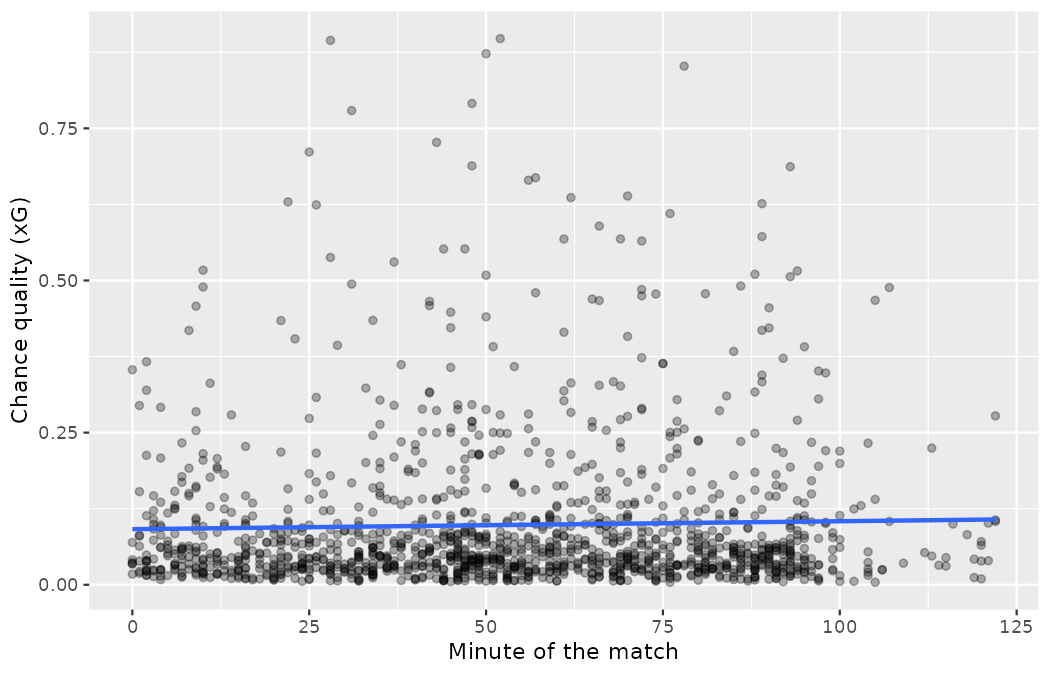
\includegraphics[width=0.85\linewidth,height=\textheight,keepaspectratio]{figures/inf-model-slr-7.png}

\begin{longtable}[]{@{}lrrrr@{}}
\caption{The least squares estimates for open-play chance quality
regressed on the minute of the match. The observed slope is
0.00013.}\label{tbl-ls-minute}\tabularnewline
\toprule\noalign{}
term & estimate & std.error & statistic & p.value \\
\midrule\noalign{}
\endfirsthead
\toprule\noalign{}
term & estimate & std.error & statistic & p.value \\
\midrule\noalign{}
\endhead
\bottomrule\noalign{}
\endlastfoot
(Intercept) & 0.09135 & 0.00712 & 12.82 & \textless0.0001 \\
minute & 0.00013 & 0.00012 & 1.11 & 0.2667 \\
\end{longtable}

The scatterplot is a nearly flat smear --- the right-skewed xG values
you know from Chapter~\ref{sec-explore-numerical}, at every point of the
clock --- and the fitted line drifts upward at \(0.00013\) xG per
minute. Notice that the relationship between the clock and chance
quality is nowhere near as strong as the relationship we saw between
chance quality and goals.

\subsection{Variability of the
statistic}\label{variability-of-the-statistic-22}

Because the focus here is \emph{not} on a null distribution, we sample
with replacement \(n = 1{,}382\) observations from the original dataset.
Recall that with bootstrapping the resample always has the same number
of observations as the original dataset in order to mimic the process of
taking a sample from the population. When sampling in the linear model
case, consider each observation to be a single dot: if the dot is
resampled, \emph{both} the \texttt{minute} and the
\texttt{statsbomb\_xg} measurement come along, because the measurements
are linked to the dot (i.e., to the shot itself). We resample rows,
never columns.

\begin{Shaded}
\begin{Highlighting}[]
\FunctionTok{set.seed}\NormalTok{(}\DecValTok{2407}\NormalTok{)}
\NormalTok{open\_play\_boot1 }\OtherTok{\textless{}{-}}\NormalTok{ open\_play }\SpecialCharTok{|\textgreater{}}
  \FunctionTok{slice\_sample}\NormalTok{(}\AttributeTok{n =} \DecValTok{1382}\NormalTok{, }\AttributeTok{replace =} \ConstantTok{TRUE}\NormalTok{)}

\FunctionTok{nrow}\NormalTok{(}\FunctionTok{distinct}\NormalTok{(open\_play\_boot1))}
\CommentTok{\#\textgreater{} [1] 873}

\FunctionTok{round}\NormalTok{(}\FunctionTok{coef}\NormalTok{(}\FunctionTok{lm}\NormalTok{(statsbomb\_xg }\SpecialCharTok{\textasciitilde{}}\NormalTok{ minute, }\AttributeTok{data =}\NormalTok{ open\_play\_boot1)), }\DecValTok{5}\NormalTok{)}
\CommentTok{\#\textgreater{} (Intercept)      minute}
\CommentTok{\#\textgreater{}     0.09014     0.00020}
\end{Highlighting}
\end{Shaded}

Plotted side by side, the original data and this bootstrap sample are
difficult to tell apart --- resampled shots land exactly on top of their
originals. The counts give the game away: only 873 distinct shots appear
in the resample, meaning 509 of the original shots were left out while
others were drawn two, three, or more times --- the signature of
sampling with replacement you first saw with the trialists of
Chapter~\ref{sec-foundations-bootstrapping}. And the resampled line is a
slightly different line: slope \(0.00020\) instead of \(0.00013.\)

\begin{tcolorbox}[enhanced jigsaw, left=2mm, leftrule=.75mm, title=\textcolor{quarto-callout-tip-color}{\faLightbulb}\hspace{0.5em}{Check your understanding}, arc=.35mm, rightrule=.15mm, coltitle=black, colframe=quarto-callout-tip-color-frame, bottomrule=.15mm, colbacktitle=quarto-callout-tip-color!10!white, opacitybacktitle=0.6, breakable, bottomtitle=1mm, toptitle=1mm, titlerule=0mm, opacityback=0, toprule=.15mm, colback=white]

In Section~\ref{sec-randslope} we shuffled one column; here we resample
whole rows. Why the difference?

\begin{center}\rule{0.5\linewidth}{0.5pt}\end{center}

Permuting the response \emph{breaks} the pairing on purpose: it
manufactures the null world in which \(\beta_1 = 0,\) which is exactly
what a hypothesis test needs to calibrate against. Bootstrapping has no
null hypothesis to enforce --- it must \emph{preserve} the observed
relationship, so each resampled dot keeps its (\texttt{minute},
\texttt{statsbomb\_xg}) pair intact, and the variation across resamples
estimates how the slope would vary from sample to sample. Shuffle to
destroy, resample to preserve.

\end{tcolorbox}

Repeating this resampling, the code below overlays fifty bootstrapped
regression lines.

\begin{Shaded}
\begin{Highlighting}[]
\FunctionTok{set.seed}\NormalTok{(}\DecValTok{2408}\NormalTok{)}
\NormalTok{open\_play\_boot50 }\OtherTok{\textless{}{-}}\NormalTok{ open\_play }\SpecialCharTok{|\textgreater{}}
  \FunctionTok{rep\_slice\_sample}\NormalTok{(}\AttributeTok{n =} \DecValTok{1382}\NormalTok{, }\AttributeTok{replace =} \ConstantTok{TRUE}\NormalTok{, }\AttributeTok{reps =} \DecValTok{50}\NormalTok{)}

\NormalTok{boot50\_slopes }\OtherTok{\textless{}{-}}\NormalTok{ open\_play\_boot50 }\SpecialCharTok{|\textgreater{}}
  \FunctionTok{group\_by}\NormalTok{(replicate) }\SpecialCharTok{|\textgreater{}}
  \FunctionTok{group\_modify}\NormalTok{(}\SpecialCharTok{\textasciitilde{}} \FunctionTok{tidy}\NormalTok{(}\FunctionTok{lm}\NormalTok{(statsbomb\_xg }\SpecialCharTok{\textasciitilde{}}\NormalTok{ minute, }\AttributeTok{data =}\NormalTok{ .x))) }\SpecialCharTok{|\textgreater{}}
  \FunctionTok{filter}\NormalTok{(term }\SpecialCharTok{==} \StringTok{"minute"}\NormalTok{)}

\FunctionTok{round}\NormalTok{(}\FunctionTok{range}\NormalTok{(boot50\_slopes}\SpecialCharTok{$}\NormalTok{estimate), }\DecValTok{5}\NormalTok{)}
\CommentTok{\#\textgreater{} [1] {-}0.00006  0.00038}

\FunctionTok{ggplot}\NormalTok{(open\_play\_boot50, }\FunctionTok{aes}\NormalTok{(}\AttributeTok{x =}\NormalTok{ minute, }\AttributeTok{y =}\NormalTok{ statsbomb\_xg, }\AttributeTok{group =}\NormalTok{ replicate)) }\SpecialCharTok{+}
  \FunctionTok{geom\_smooth}\NormalTok{(}\AttributeTok{method =} \StringTok{"lm"}\NormalTok{, }\AttributeTok{se =} \ConstantTok{FALSE}\NormalTok{, }\AttributeTok{color =} \StringTok{"steelblue"}\NormalTok{,}
              \AttributeTok{linewidth =} \FloatTok{0.5}\NormalTok{, }\AttributeTok{alpha =} \FloatTok{0.3}\NormalTok{, }\AttributeTok{fullrange =} \ConstantTok{TRUE}\NormalTok{) }\SpecialCharTok{+}
  \FunctionTok{labs}\NormalTok{(}\AttributeTok{x =} \StringTok{"Minute of the match"}\NormalTok{, }\AttributeTok{y =} \StringTok{"Chance quality (xG)"}\NormalTok{)}
\end{Highlighting}
\end{Shaded}

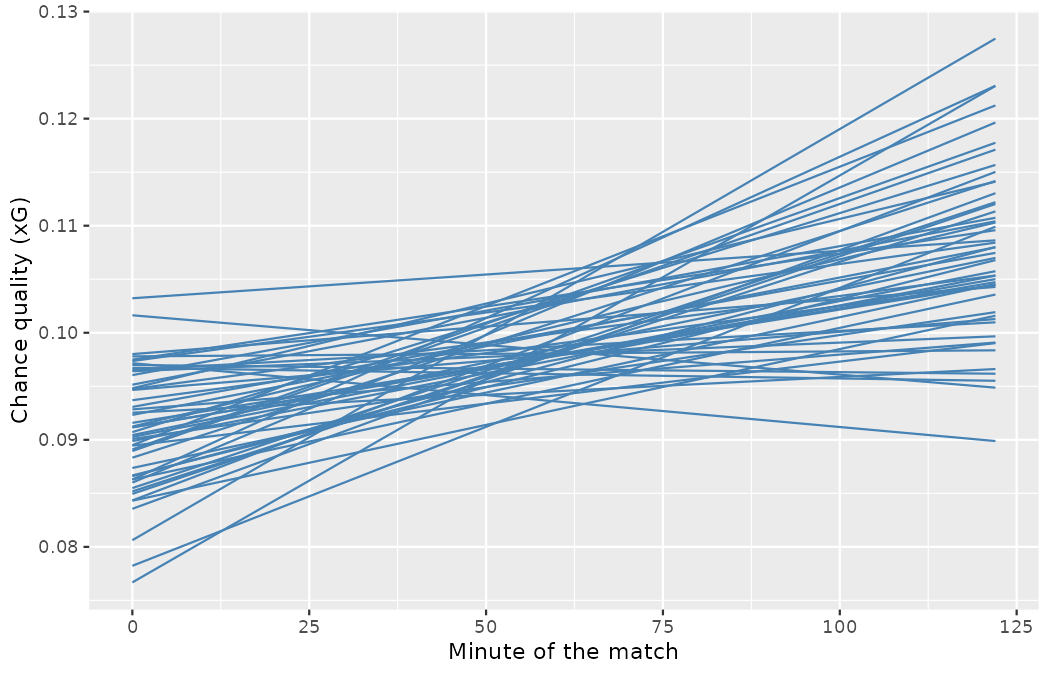
\includegraphics[width=0.85\linewidth,height=\textheight,keepaspectratio]{figures/inf-model-slr-8.png}

Already the key fact is visible: the fifty bootstrapped slopes run from
\(-0.00006\) to \(+0.00038\) --- some of the resampled lines drift
\emph{down}. Recall that in order to create a confidence interval for
the slope, we need the range of values the statistic takes on across
many bootstrap samples. The code below runs 1,000.

\begin{Shaded}
\begin{Highlighting}[]
\FunctionTok{set.seed}\NormalTok{(}\DecValTok{2409}\NormalTok{)}
\NormalTok{minute\_boot\_slopes }\OtherTok{\textless{}{-}}\NormalTok{ open\_play }\SpecialCharTok{|\textgreater{}}
  \FunctionTok{specify}\NormalTok{(statsbomb\_xg }\SpecialCharTok{\textasciitilde{}}\NormalTok{ minute) }\SpecialCharTok{|\textgreater{}}
  \FunctionTok{generate}\NormalTok{(}\AttributeTok{reps =} \DecValTok{1000}\NormalTok{, }\AttributeTok{type =} \StringTok{"bootstrap"}\NormalTok{) }\SpecialCharTok{|\textgreater{}}
  \FunctionTok{calculate}\NormalTok{(}\AttributeTok{stat =} \StringTok{"slope"}\NormalTok{)}

\FunctionTok{ggplot}\NormalTok{(minute\_boot\_slopes, }\FunctionTok{aes}\NormalTok{(}\AttributeTok{x =}\NormalTok{ stat)) }\SpecialCharTok{+}
  \FunctionTok{geom\_histogram}\NormalTok{(}\AttributeTok{binwidth =} \FloatTok{0.00005}\NormalTok{) }\SpecialCharTok{+}
  \FunctionTok{labs}\NormalTok{(}
    \AttributeTok{x =} \StringTok{"Bootstrapped values of the slope for predicting open{-}play xG from the minute"}\NormalTok{,}
    \AttributeTok{y =} \StringTok{"Count"}
\NormalTok{  )}

\FunctionTok{round}\NormalTok{(}\FunctionTok{quantile}\NormalTok{(minute\_boot\_slopes}\SpecialCharTok{$}\NormalTok{stat, }\FunctionTok{c}\NormalTok{(}\FloatTok{0.025}\NormalTok{, }\FloatTok{0.975}\NormalTok{)), }\DecValTok{5}\NormalTok{)}
\CommentTok{\#\textgreater{}     2.5\%    97.5\%}
\CommentTok{\#\textgreater{} {-}0.00007  0.00034}
\end{Highlighting}
\end{Shaded}

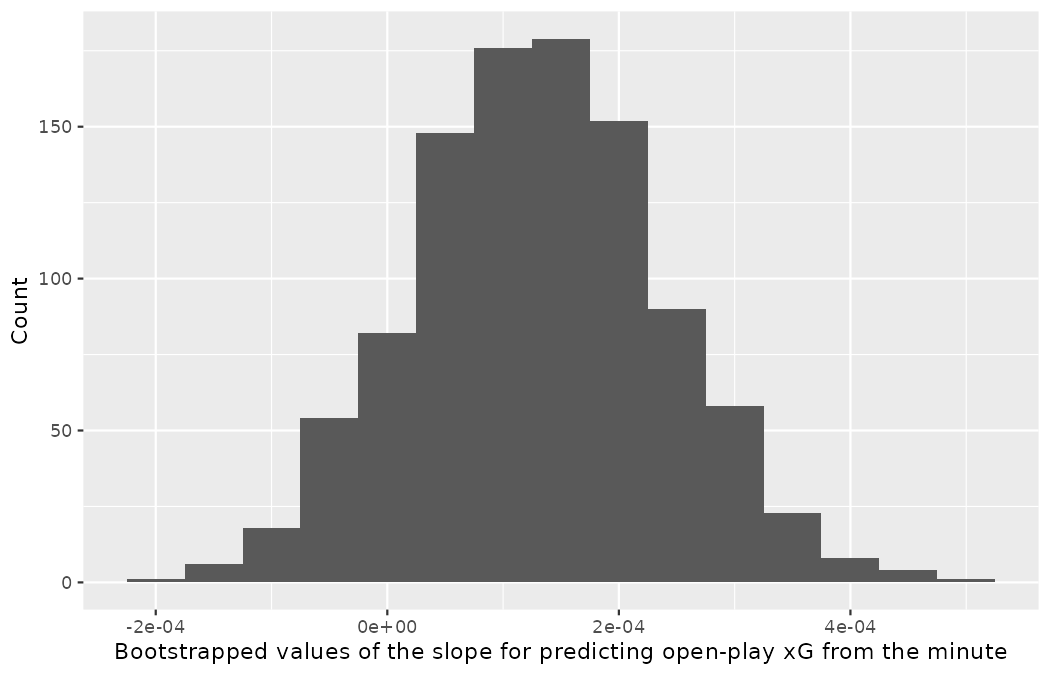
\includegraphics[width=0.85\linewidth,height=\textheight,keepaspectratio]{figures/inf-model-slr-9.png}

The histogram of bootstrapped slopes is symmetric and bell-shaped, and
the middle 95\% of it --- the bootstrap percentile interval of
Chapter~\ref{sec-foundations-bootstrapping}, applied to a slope --- runs
from \(-0.00007\) to \(+0.00034.\) We are 95\% confident that for the
model describing the population of open-play shots at this level,
predicting chance quality from the minute of the match, one additional
minute of match clock is associated with a change in predicted average
chance quality of between \(-0.00007\) and \(+0.00034\) xG. Notice that
the confidence interval contains zero, so the true relationship
\emph{might} be null!

Translate the endpoints into football before moving on. Even taking the
interval's most generous edge, ninety minutes of fatigue would raise the
average open-play chance by \(90 \times 0.00034 \approx 0.03\) xG ---
three hundredths of a goal --- while the other edge says the drift may
just as plausibly be slightly \emph{downhill}. The fatigue-drift story
did not survive contact with its own confidence interval: what looked
like signal in the all-shots frame was, once again, mostly penalties,
and what remains is statistically indistinguishable from a flat line.
That is the point of this section, and it is a general scouting
discipline: a story is only as good as an interval that excludes the
boring answer.

\begin{tcolorbox}[enhanced jigsaw, left=2mm, leftrule=.75mm, title=\textcolor{quarto-callout-note-color}{\faInfo}\hspace{0.5em}{Worked example}, arc=.35mm, rightrule=.15mm, coltitle=black, colframe=quarto-callout-note-color-frame, bottomrule=.15mm, colbacktitle=quarto-callout-note-color!10!white, opacitybacktitle=0.6, breakable, bottomtitle=1mm, toptitle=1mm, titlerule=0mm, opacityback=0, toprule=.15mm, colback=white]

Using the bootstrapped slopes in \texttt{minute\_boot\_slopes},
calculate the bootstrap estimate for the standard error of the slope.
Using the bootstrap standard error, find a 95\% bootstrap SE confidence
interval for the true population slope, and interpret the interval in
context.

\begin{center}\rule{0.5\linewidth}{0.5pt}\end{center}

Notice that most of the bootstrapped slopes fall between \(-0.00008\)
and \(+0.00034\) (a range of about \(0.00042\)). Using the empirical
rule from Chapter~\ref{sec-explore-numerical} (with bell-shaped
distributions, most observations are within two standard errors of the
center), the standard error of the slopes is approximately \(0.0001.\)
The direct computation agrees:

\begin{Shaded}
\begin{Highlighting}[]
\FunctionTok{round}\NormalTok{(}\FunctionTok{sd}\NormalTok{(minute\_boot\_slopes}\SpecialCharTok{$}\NormalTok{stat), }\DecValTok{5}\NormalTok{)}
\CommentTok{\#\textgreater{} [1] 0.00011}
\end{Highlighting}
\end{Shaded}

The critical value for a 95\% confidence interval is
\(z^{\star} = 1.96\) (recall from Section~\ref{sec-boot1mean} that
bootstrap SE intervals in this book keep the normal cutoffs), which
leads to a confidence interval of
\[b_1 \pm 1.96 \cdot SE \rightarrow 0.00013 \pm 1.96 \cdot 0.00011 \rightarrow (-0.00009, 0.00035).\]
The bootstrap SE interval is almost identical to the bootstrap
percentile interval --- the bell-shaped histogram is exactly the
situation where the two constructions agree (contrast the five-shot
fiasco of Section~\ref{sec-boot1mean}, where they did not). In context:
we are 95\% confident that one additional minute of match clock is
associated with a change in predicted average open-play chance quality
of between \(-0.00009\) and \(+0.00035\) xG. Zero sits comfortably
inside --- the interval politely declines to endorse the fatigue-drift
theory.

\end{tcolorbox}

\section{Mathematical model for testing the slope}\label{sec-mathslope}

When certain technical conditions apply, it is convenient to use
mathematical approximations to test and estimate the slope parameter.
The approximations will build on the \(t\)-distribution which was
described in Section~\ref{sec-one-mean-math}, and the
\textbf{t-distribution for the slope} works remarkably like the one for
a single mean. The mathematical model is often correct and is usually
easy to implement computationally. The validity of the technical
conditions will be considered in detail in
Section~\ref{sec-tech-cond-linmod}.

In this section, we discuss uncertainty in the estimates of the slope
and y-intercept for a regression line. Just as we identified standard
errors for point estimates in previous chapters, we start by discussing
standard errors for these estimates, and one new subscript carries the
whole idea: \(SE_{b_1}\) is the familiar standard error of
Chapter~\ref{sec-foundations-mathematical} --- the standard deviation of
a statistic from sample to sample --- with the subscript naming
\emph{which} statistic's variability is meant: the slope estimate
\(b_1.\) The fan of fifty gray lines in the federation case study is the
picture; \(SE_{b_1}\) is its number. (Likewise \(SE_{b_0}\) for the
intercept; in general \(SE_{b_i},\) where the index \(i\) picks out
coefficient \(i.\))

\subsection{Observed data}\label{observed-data-22}

\textbf{Goal margins and shooting under pressure}

Here is a theory Emil Sørensen hears in some form after every
international window: ``tight matches are pressure matches.'' When
defenders contest a high share of the shots, the theory runs, the match
stays close --- so the share of a match's shots taken under defensive
pressure should predict the final margin, and a scouting department that
believed this could grade fixture difficulty from pressure counts alone.
The 2022 Men's World Cup's 64 matches can put the theory on trial.

\begin{tcolorbox}[enhanced jigsaw, left=2mm, leftrule=.75mm, title=\textcolor{quarto-callout-note-color}{\faInfo}\hspace{0.5em}{Data}, arc=.35mm, rightrule=.15mm, coltitle=black, colframe=quarto-callout-note-color-frame, bottomrule=.15mm, colbacktitle=quarto-callout-note-color!10!white, opacitybacktitle=0.6, breakable, bottomtitle=1mm, toptitle=1mm, titlerule=0mm, opacityback=0, toprule=.15mm, colback=white]

Margins come from \texttt{data/derived/wc2022\_matches.csv}: the
absolute difference of the recorded final scores, which cover regulation
and extra time but not shoot-outs. The pressure share for each match is
computed from \texttt{data/derived/wc2022\_shots.csv} on the open-play
frame, stated per this book's penalty convention: a penalty kick cannot
be contested by law, and the shoot-out kicks of drawn knockout ties
would flood eight matches' denominators with uncontestable shots.
(StatsBomb open data.)

\end{tcolorbox}

\begin{Shaded}
\begin{Highlighting}[]
\NormalTok{wc2022\_matches }\OtherTok{\textless{}{-}} \FunctionTok{read\_csv}\NormalTok{(}\StringTok{"data/derived/wc2022\_matches.csv"}\NormalTok{)}

\NormalTok{match64 }\OtherTok{\textless{}{-}}\NormalTok{ wc2022\_matches }\SpecialCharTok{|\textgreater{}}
  \FunctionTok{mutate}\NormalTok{(}\AttributeTok{margin =} \FunctionTok{abs}\NormalTok{(home\_score }\SpecialCharTok{{-}}\NormalTok{ away\_score)) }\SpecialCharTok{|\textgreater{}}
  \FunctionTok{left\_join}\NormalTok{(}
\NormalTok{    wc2022\_shots }\SpecialCharTok{|\textgreater{}}
      \FunctionTok{filter}\NormalTok{(shot\_type }\SpecialCharTok{==} \StringTok{"Open Play"}\NormalTok{) }\SpecialCharTok{|\textgreater{}}
      \FunctionTok{group\_by}\NormalTok{(match\_id) }\SpecialCharTok{|\textgreater{}}
      \FunctionTok{summarize}\NormalTok{(}\AttributeTok{prop\_pressured =} \FunctionTok{mean}\NormalTok{(under\_pressure)),}
    \AttributeTok{by =} \StringTok{"match\_id"}
\NormalTok{  )}

\NormalTok{match64 }\SpecialCharTok{|\textgreater{}}
  \FunctionTok{summarize}\NormalTok{(}
    \AttributeTok{matches =} \FunctionTok{n}\NormalTok{(),}
    \AttributeTok{mean\_margin =} \FunctionTok{mean}\NormalTok{(margin),}
    \AttributeTok{r =} \FunctionTok{cor}\NormalTok{(margin, prop\_pressured)}
\NormalTok{  )}
\CommentTok{\#\textgreater{} \# A tibble: 1 × 3}
\CommentTok{\#\textgreater{}   matches mean\_margin       r}
\CommentTok{\#\textgreater{}     \textless{}int\textgreater{}       \textless{}dbl\textgreater{}   \textless{}dbl\textgreater{}}
\CommentTok{\#\textgreater{} 1      64        1.41 {-}0.0726}

\FunctionTok{ggplot}\NormalTok{(match64, }\FunctionTok{aes}\NormalTok{(}\AttributeTok{x =}\NormalTok{ prop\_pressured, }\AttributeTok{y =}\NormalTok{ margin)) }\SpecialCharTok{+}
  \FunctionTok{geom\_jitter}\NormalTok{(}\AttributeTok{height =} \FloatTok{0.08}\NormalTok{, }\AttributeTok{alpha =} \FloatTok{0.7}\NormalTok{) }\SpecialCharTok{+}
  \FunctionTok{geom\_smooth}\NormalTok{(}\AttributeTok{method =} \StringTok{"lm"}\NormalTok{, }\AttributeTok{se =} \ConstantTok{FALSE}\NormalTok{, }\AttributeTok{fullrange =} \ConstantTok{TRUE}\NormalTok{) }\SpecialCharTok{+}
  \FunctionTok{labs}\NormalTok{(}
    \AttributeTok{x =} \StringTok{"Share of the match\textquotesingle{}s open{-}play shots taken under pressure"}\NormalTok{,}
    \AttributeTok{y =} \StringTok{"Goal margin"}
\NormalTok{  )}
\end{Highlighting}
\end{Shaded}

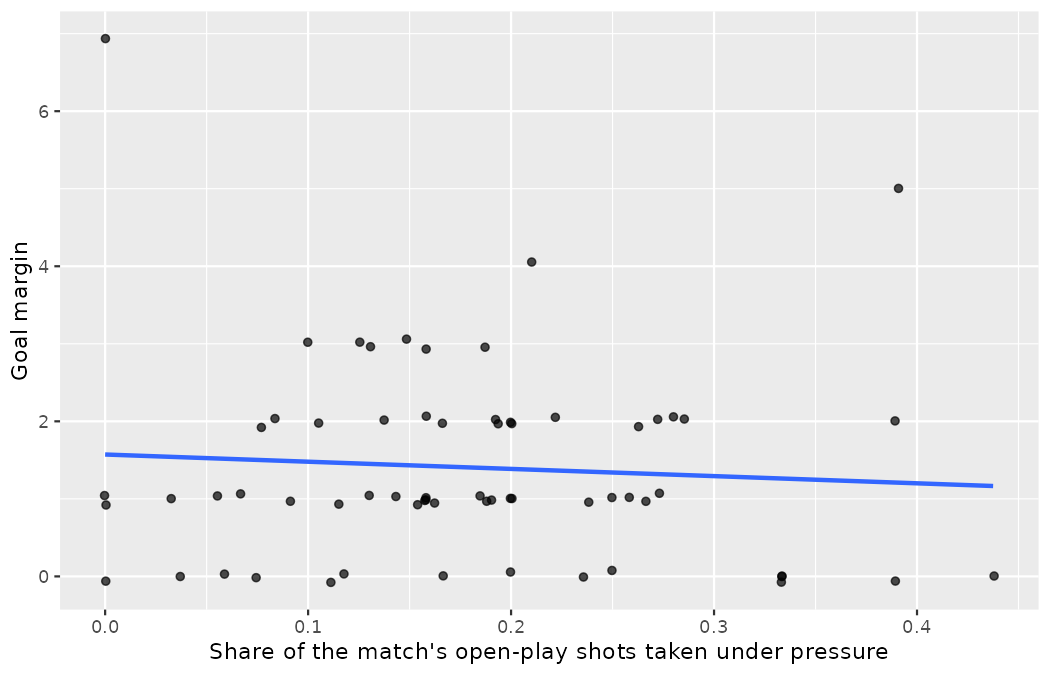
\includegraphics[width=0.85\linewidth,height=\textheight,keepaspectratio]{figures/inf-model-slr-10.png}

The 64 points scatter with margins from 0 to 7 and pressure shares from
0 to 0.44, and the least squares line drifts gently downhill:

\[
\widehat{\texttt{margin}} = 1.57 - 0.93 \times \texttt{pressure share}
\]

The direction at least agrees with the theory --- more contested
shooting, slightly tighter matches --- but the drift is shallow
\((r = -0.073),\) and 64 matches is not a large sample. Examining the
data, there are no clear deviations from linearity (see
Section~\ref{sec-resids} for using residuals to judge fit); the matches
were played by rotating casts of teams across a single tournament, and
we will treat the 64 margins as independent observations of tournament
football at this level.

\begin{tcolorbox}[enhanced jigsaw, left=2mm, leftrule=.75mm, title=\textcolor{quarto-callout-tip-color}{\faLightbulb}\hspace{0.5em}{Check your understanding}, arc=.35mm, rightrule=.15mm, coltitle=black, colframe=quarto-callout-tip-color-frame, bottomrule=.15mm, colbacktitle=quarto-callout-tip-color!10!white, opacitybacktitle=0.6, breakable, bottomtitle=1mm, toptitle=1mm, titlerule=0mm, opacityback=0, toprule=.15mm, colback=white]

Two matches stand apart from the rest of the cloud: the tournament's
only blowouts of five or more.

\begin{Shaded}
\begin{Highlighting}[]
\NormalTok{match64 }\SpecialCharTok{|\textgreater{}}
  \FunctionTok{filter}\NormalTok{(margin }\SpecialCharTok{\textgreater{}=} \DecValTok{5}\NormalTok{) }\SpecialCharTok{|\textgreater{}}
  \FunctionTok{select}\NormalTok{(home\_team, away\_team, stage, margin, prop\_pressured)}
\CommentTok{\#\textgreater{} \# A tibble: 2 × 5}
\CommentTok{\#\textgreater{}   home\_team away\_team   stage       margin prop\_pressured}
\CommentTok{\#\textgreater{}   \textless{}chr\textgreater{}     \textless{}chr\textgreater{}       \textless{}chr\textgreater{}        \textless{}dbl\textgreater{}          \textless{}dbl\textgreater{}}
\CommentTok{\#\textgreater{} 1 Portugal  Switzerland Round of 16      5          0.391}
\CommentTok{\#\textgreater{} 2 Spain     Costa Rica  Group Stage      7          0}
\end{Highlighting}
\end{Shaded}

Notice where they sit: Spain's 7--0 played out with \emph{none} of the
open-play shots pressured --- the extreme left edge of the x-axis ---
while Portugal's 6--1 sits close to the extreme right at a pressure
share of 0.391. Should these two matches be removed from the analysis?

\begin{center}\rule{0.5\linewidth}{0.5pt}\end{center}

The answer relies on the idea that statistical data analysis is somewhat
of an art: in many situations, there is no single ``right'' answer, and
the judgment sharpens only with practice. Two contrasting
considerations, in the language of
Section~\ref{sec-outliers-in-regression}. On one hand, both blowouts are
extreme in the response, and each also sits at an edge of the
predictor's range --- high-leverage positions from which a single match
can pull hard on a least squares line fit to only 64 points; margins of
5+ may not help us understand ordinary matches. On the other hand,
blowouts are real football --- a recruitment department that deletes its
extreme matches, like one that deletes its super-subs, systematically
blinds itself to exactly the fixtures that decide tournaments. The
book's standing practice applies: present both analyses. Removing the
two blowouts moves the fitted slope from \(-0.93\) to \(-0.65\) (with
p-value \(0.62\)) --- the conclusion you are about to reach does not
change, which is itself worth reporting.

\end{tcolorbox}

There is a negative slope in the fitted line, but this slope (and the
y-intercept) are only estimates of the parameter values. We might
wonder, is this convincing evidence that the ``true'' linear model has a
negative slope? That is, do the data provide strong evidence that the
pressure theory is accurate, where the share of contested shots is a
useful predictor of the final margin? We can frame this investigation as
a statistical hypothesis test:

\begin{itemize}
\tightlist
\item
  \(H_0:\) \(\beta_1 = 0.\) The true linear model has slope zero: a
  match's pressure share tells us nothing, linearly, about its margin.
\item
  \(H_A:\) \(\beta_1 \neq 0.\) The true linear model has a slope
  different than zero: the pressure share is predictive of how tight the
  match finishes.
\end{itemize}

We would reject \(H_0\) in favor of \(H_A\) if the data provide strong
evidence that the true slope parameter is different than zero. To assess
the hypotheses, we identify a standard error for the estimate, compute
an appropriate test statistic, and identify the p-value.

\subsection{Variability of the
statistic}\label{variability-of-the-statistic-23}

Just like other point estimates we have seen before, we can compute a
standard error and test statistic for \(b_1.\) We will generally label
the test statistic using a \(T,\) since --- exactly as for the single
mean in Chapter~\ref{sec-inference-one-mean} --- it follows the
\(t\)-distribution once its standard error is estimated from the data.

We will rely on statistical software to compute \(SE_{b_1}\) and leave
the explanation of how this standard error is determined to a second or
third statistics course. Table~\ref{tbl-margin-pressure} shows the
software output for the least squares regression fit above. The row
labeled \texttt{prop\_pressured} includes all relevant information about
the slope estimate: the coefficient itself, its standard error, the T
statistic, and the corresponding p-value.

\begin{Shaded}
\begin{Highlighting}[]
\NormalTok{fit\_margin }\OtherTok{\textless{}{-}} \FunctionTok{lm}\NormalTok{(margin }\SpecialCharTok{\textasciitilde{}}\NormalTok{ prop\_pressured, }\AttributeTok{data =}\NormalTok{ match64)}
\FunctionTok{tidy}\NormalTok{(fit\_margin)}
\CommentTok{\#\textgreater{} \# A tibble: 2 × 5}
\CommentTok{\#\textgreater{}   term           estimate std.error statistic   p.value}
\CommentTok{\#\textgreater{}   \textless{}chr\textgreater{}             \textless{}dbl\textgreater{}     \textless{}dbl\textgreater{}     \textless{}dbl\textgreater{}     \textless{}dbl\textgreater{}}
\CommentTok{\#\textgreater{} 1 (Intercept)       1.57      0.332     4.74  0.0000131}
\CommentTok{\#\textgreater{} 2 prop\_pressured   {-}0.929     1.62     {-}0.573 0.569}
\end{Highlighting}
\end{Shaded}

\begin{longtable}[]{@{}lrrrr@{}}
\caption{Output for the regression modeling the goal margin as a
response to the share of the match's open-play shots taken under
pressure.}\label{tbl-margin-pressure}\tabularnewline
\toprule\noalign{}
term & estimate & std.error & statistic & p.value \\
\midrule\noalign{}
\endfirsthead
\toprule\noalign{}
term & estimate & std.error & statistic & p.value \\
\midrule\noalign{}
\endhead
\bottomrule\noalign{}
\endlastfoot
(Intercept) & 1.57 & 0.33 & 4.74 & \textless0.0001 \\
prop\_pressured & -0.93 & 1.62 & -0.57 & 0.5688 \\
\end{longtable}

\begin{tcolorbox}[enhanced jigsaw, left=2mm, leftrule=.75mm, title=\textcolor{quarto-callout-note-color}{\faInfo}\hspace{0.5em}{Worked example}, arc=.35mm, rightrule=.15mm, coltitle=black, colframe=quarto-callout-note-color-frame, bottomrule=.15mm, colbacktitle=quarto-callout-note-color!10!white, opacitybacktitle=0.6, breakable, bottomtitle=1mm, toptitle=1mm, titlerule=0mm, opacityback=0, toprule=.15mm, colback=white]

What do the first and second numeric columns of
Table~\ref{tbl-margin-pressure} represent?

\begin{center}\rule{0.5\linewidth}{0.5pt}\end{center}

The entries in the \texttt{estimate} column are the least squares
estimates, \(b_0\) and \(b_1,\) and the values in the \texttt{std.error}
column are their standard errors, \(SE_{b_0}\) and \(SE_{b_1}.\) Using
the estimates, we could write the equation for the least squares
regression line as

\[ \hat{y} = 1.57 - 0.93 x \]

where \(\hat{y}\) in this case represents the predicted goal margin and
\(x\) represents the share of the match's open-play shots taken under
pressure. The standard error column says how much each estimate would
wobble from tournament to tournament --- for the slope, a wobble of
\(1.62,\) nearly twice the size of the estimate itself.

\end{tcolorbox}

We previously used a \(t\)-test statistic for hypothesis testing in the
context of numerical data. Regression is very similar. In the hypotheses
we consider, the null value for the slope is 0, so we can compute the
test statistic using the T score formula, exactly as in
Chapter~\ref{sec-inference-one-mean}:

\[
T \ = \ \frac{\text{estimate} - \text{null value}}{\text{SE}} = \ \frac{-0.93 - 0}{1.62} = \ -0.57
\]

The T score we calculated corresponds to the \texttt{statistic} column
of Table~\ref{tbl-margin-pressure}.

\begin{tcolorbox}[enhanced jigsaw, left=2mm, leftrule=.75mm, title=\textcolor{quarto-callout-note-color}{\faInfo}\hspace{0.5em}{Worked example}, arc=.35mm, rightrule=.15mm, coltitle=black, colframe=quarto-callout-note-color-frame, bottomrule=.15mm, colbacktitle=quarto-callout-note-color!10!white, opacitybacktitle=0.6, breakable, bottomtitle=1mm, toptitle=1mm, titlerule=0mm, opacityback=0, toprule=.15mm, colback=white]

Use Table~\ref{tbl-margin-pressure} to determine the p-value for the
hypothesis test, and conclude in context.

\begin{center}\rule{0.5\linewidth}{0.5pt}\end{center}

The last column of the table gives the p-value for the two-sided
hypothesis test for the coefficient of the pressure share: \(0.5688.\)
That is, the data do not provide convincing evidence that a higher share
of contested shots has any correspondence with tighter or wider margins.
If there was no linear relationship between the two variables (i.e., if
\(\beta_1 = 0\)), then we would expect to see linear models as or more
extreme than the observed one roughly 57\% of the time. Check complete:
the on-field call --- ``pressure share tells you nothing about margins''
--- stands, which, per Chapter~\ref{sec-foundations-randomization}, is
not the same as proving it correct. Emil's fixture-difficulty shortcut
should not ship.

\end{tcolorbox}

Per the penalty convention, the same test was rerun with the pressure
share computed on all shots (penalties and shoot-out kicks included):
the slope becomes \(-0.77\) with a p-value of \(0.658.\) Both frames
return the same verdict here --- but you only know that because both
were run, and the open-play frame remains the one that matches the
question.

\subsection{Observed statistic vs.~null
statistics}\label{observed-statistic-vs.-null-statistics-12}

As the final step in a mathematical hypothesis test for the slope, we
use the information provided to make a conclusion about whether the data
could have come from a population where the true slope was zero (i.e.,
\(\beta_1 = 0\)). Before evaluating the formal hypothesis claim,
sometimes it is important to check your intuition. Based on everything
you have seen describing the variability of a line from sample to
sample, ask yourself if the linear relationship given by the data could
have come from a population in which the slope was truly zero.

\begin{tcolorbox}[enhanced jigsaw, left=2mm, leftrule=.75mm, title=\textcolor{quarto-callout-note-color}{\faInfo}\hspace{0.5em}{Worked example}, arc=.35mm, rightrule=.15mm, coltitle=black, colframe=quarto-callout-note-color-frame, bottomrule=.15mm, colbacktitle=quarto-callout-note-color!10!white, opacitybacktitle=0.6, breakable, bottomtitle=1mm, toptitle=1mm, titlerule=0mm, opacityback=0, toprule=.15mm, colback=white]

Recall the veteran-market survey of
Section~\ref{sec-least-squares-regression}: 50 listed strikers aged 28
and older, asking price against age, the fitted line falling at
\(-1.44\) million euros per year of age. Examine that scatterplot again
(or rebuild it with the code below). Are you convinced that the slope is
discernibly different from zero? That is, do you think a formal
hypothesis test would reject the claim that the true slope of the line
should be zero?

\begin{center}\rule{0.5\linewidth}{0.5pt}\end{center}

While the relationship between the variables is not perfect --- the
survey's correlation was \(r = -0.534\) --- there is an evident
decreasing trend in the data: the cloud slides visibly downhill from the
28-year-olds near €17M to the 35-year-olds clustered in the low single
digits, a couple of them on the €0.5M listing floor. Such a distinct
trend suggests that the hypothesis test will reject the null claim that
the slope is zero.

\end{tcolorbox}

\begin{tcolorbox}[enhanced jigsaw, left=2mm, leftrule=.75mm, title=\textcolor{quarto-callout-note-color}{\faInfo}\hspace{0.5em}{Data}, arc=.35mm, rightrule=.15mm, coltitle=black, colframe=quarto-callout-note-color-frame, bottomrule=.15mm, colbacktitle=quarto-callout-note-color!10!white, opacitybacktitle=0.6, breakable, bottomtitle=1mm, toptitle=1mm, titlerule=0mm, opacityback=0, toprule=.15mm, colback=white]

The \texttt{veteran\_market} data are the constructed market survey of
Section~\ref{sec-least-squares-regression} --- a scouting scenario built
entirely by the seeded code below (seed 701), not real listings; the
code regenerates it exactly.

\end{tcolorbox}

The tools in this section help you go beyond a visual interpretation of
the linear relationship toward a formal mathematical claim about whether
the slope estimate is meaningfully different from 0 to suggest that the
true population slope is different from 0.

\begin{Shaded}
\begin{Highlighting}[]
\FunctionTok{set.seed}\NormalTok{(}\DecValTok{701}\NormalTok{)}
\NormalTok{veteran\_market }\OtherTok{\textless{}{-}} \FunctionTok{tibble}\NormalTok{(}
  \AttributeTok{age =} \FunctionTok{sample}\NormalTok{(}\DecValTok{28}\SpecialCharTok{:}\DecValTok{35}\NormalTok{, }\DecValTok{50}\NormalTok{, }\AttributeTok{replace =} \ConstantTok{TRUE}\NormalTok{),}
  \AttributeTok{asking\_price =} \FunctionTok{round}\NormalTok{(}\FunctionTok{pmax}\NormalTok{(}\FloatTok{0.5}\NormalTok{, }\DecValTok{17} \SpecialCharTok{{-}} \FloatTok{2.0} \SpecialCharTok{*}\NormalTok{ (age }\SpecialCharTok{{-}} \DecValTok{28}\NormalTok{) }\SpecialCharTok{+} \FunctionTok{rnorm}\NormalTok{(}\DecValTok{50}\NormalTok{, }\DecValTok{0}\NormalTok{, }\FloatTok{5.3}\NormalTok{)), }\DecValTok{1}\NormalTok{)}
\NormalTok{)}

\NormalTok{fit\_veteran }\OtherTok{\textless{}{-}} \FunctionTok{lm}\NormalTok{(asking\_price }\SpecialCharTok{\textasciitilde{}}\NormalTok{ age, }\AttributeTok{data =}\NormalTok{ veteran\_market)}
\FunctionTok{tidy}\NormalTok{(fit\_veteran)}
\CommentTok{\#\textgreater{} \# A tibble: 2 × 5}
\CommentTok{\#\textgreater{}   term        estimate std.error statistic    p.value}
\CommentTok{\#\textgreater{}   \textless{}chr\textgreater{}          \textless{}dbl\textgreater{}     \textless{}dbl\textgreater{}     \textless{}dbl\textgreater{}      \textless{}dbl\textgreater{}}
\CommentTok{\#\textgreater{} 1 (Intercept)    56.4     10.4        5.43 0.00000186}
\CommentTok{\#\textgreater{} 2 age            {-}1.44     0.329     {-}4.37 0.0000655}
\end{Highlighting}
\end{Shaded}

\begin{longtable}[]{@{}lrrrr@{}}
\caption{Summary of the least squares fit for the veteran-market survey,
predicting a listed striker's asking price (million euros) from his
age.}\label{tbl-veteran-inference}\tabularnewline
\toprule\noalign{}
term & estimate & std.error & statistic & p.value \\
\midrule\noalign{}
\endfirsthead
\toprule\noalign{}
term & estimate & std.error & statistic & p.value \\
\midrule\noalign{}
\endhead
\bottomrule\noalign{}
\endlastfoot
(Intercept) & 56.44 & 10.40 & 5.43 & \textless0.0001 \\
age & -1.44 & 0.33 & -4.37 & \textless0.0001 \\
\end{longtable}

\begin{tcolorbox}[enhanced jigsaw, left=2mm, leftrule=.75mm, title=\textcolor{quarto-callout-tip-color}{\faLightbulb}\hspace{0.5em}{Check your understanding}, arc=.35mm, rightrule=.15mm, coltitle=black, colframe=quarto-callout-tip-color-frame, bottomrule=.15mm, colbacktitle=quarto-callout-tip-color!10!white, opacitybacktitle=0.6, breakable, bottomtitle=1mm, toptitle=1mm, titlerule=0mm, opacityback=0, toprule=.15mm, colback=white]

Table~\ref{tbl-veteran-inference} shows the statistical software output
from fitting the least squares regression line to the veteran-market
survey. Use the output to formally evaluate the following hypotheses:

\begin{itemize}
\tightlist
\item
  \(H_0:\) The true coefficient for age is zero.
\item
  \(H_A:\) The true coefficient for age is not zero.
\end{itemize}

\begin{center}\rule{0.5\linewidth}{0.5pt}\end{center}

We look in the second row, corresponding to the age variable. The point
estimate of the slope is \(-1.44,\) the standard error of this estimate
is \(SE_{b_1} = 0.329,\) and the \(t\)-test statistic is \(T = -4.37.\)
The p-value corresponds exactly to the two-sided test we are interested
in: \(0.0000655,\) far below any discernibility level in use. We reject
the null hypothesis and conclude that in this veteran market, age and
asking price are negatively associated and the true slope parameter is
indeed less than 0 --- just as our eyes suggested in the worked example
above.

\end{tcolorbox}

\begin{tcolorbox}[enhanced jigsaw, left=2mm, leftrule=.75mm, title=\textcolor{quarto-callout-important-color}{\faExclamation}\hspace{0.5em}{Inference for regression}, arc=.35mm, rightrule=.15mm, coltitle=black, colframe=quarto-callout-important-color-frame, bottomrule=.15mm, colbacktitle=quarto-callout-important-color!10!white, opacitybacktitle=0.6, breakable, bottomtitle=1mm, toptitle=1mm, titlerule=0mm, opacityback=0, toprule=.15mm, colback=white]

We usually rely on statistical software to identify point estimates,
standard errors, test statistics, and p-values in practice. However, be
aware that software will not generally check whether the method is
appropriate, meaning we must still verify that the conditions are met.
See Section~\ref{sec-tech-cond-linmod}.

\end{tcolorbox}

\section{Mathematical model, interval for the
slope}\label{mathematical-model-interval-for-the-slope}

Similar to how we can conduct a hypothesis test for a model coefficient
using regression output, we can also construct confidence intervals for
the slope and intercept coefficients.

\begin{tcolorbox}[enhanced jigsaw, left=2mm, leftrule=.75mm, title=\textcolor{quarto-callout-important-color}{\faExclamation}\hspace{0.5em}{Confidence intervals for coefficients}, arc=.35mm, rightrule=.15mm, coltitle=black, colframe=quarto-callout-important-color-frame, bottomrule=.15mm, colbacktitle=quarto-callout-important-color!10!white, opacitybacktitle=0.6, breakable, bottomtitle=1mm, toptitle=1mm, titlerule=0mm, opacityback=0, toprule=.15mm, colback=white]

Confidence intervals for model coefficients (e.g., the intercept or the
slope) can be computed using the \(t\)-distribution:

\[ b_i \ \pm\ t_{df}^{\star} \times SE_{b_{i}} \]

where \(t_{df}^{\star}\) is the appropriate \(t^{\star}\) cutoff
corresponding to the confidence level with the model's degrees of
freedom, \(df = n - 2.\)

\end{tcolorbox}

Every piece of this formula is one you own, assembled in a new place ---
walk through it once. The subscript \(i\) indexes the coefficient:
\(i = 0\) gives an interval for the intercept, \(i = 1\) for the slope,
each pairing an estimate \(b_i\) with \emph{its own} standard error
\(SE_{b_i}\) from the regression output. The cutoff \(t^{\star}_{df}\)
is the critical value you met in Chapter~\ref{sec-inference-one-mean}
--- the star for a cutoff, the subscript recording which
\(t\)-distribution supplied it. What is genuinely new is the degrees of
freedom: \(df = n - 2,\) where the single mean used \(n - 1.\) The
accounting is the same as ever: the residuals must satisfy one
constraint for every parameter estimated from the data, and a regression
line estimates \emph{two} --- \(b_0\) and \(b_1\) --- so of \(n\)
residuals only \(n - 2\) are free to vary. Each parameter you ask the
data to estimate costs you one degree of freedom; a line costs two.

\begin{tcolorbox}[enhanced jigsaw, left=2mm, leftrule=.75mm, title=\textcolor{quarto-callout-note-color}{\faInfo}\hspace{0.5em}{Worked example}, arc=.35mm, rightrule=.15mm, coltitle=black, colframe=quarto-callout-note-color-frame, bottomrule=.15mm, colbacktitle=quarto-callout-note-color!10!white, opacitybacktitle=0.6, breakable, bottomtitle=1mm, toptitle=1mm, titlerule=0mm, opacityback=0, toprule=.15mm, colback=white]

Compute the 95\% confidence interval for the age coefficient using the
regression output from Table~\ref{tbl-veteran-inference}.

\begin{center}\rule{0.5\linewidth}{0.5pt}\end{center}

The point estimate is \(b_1 = -1.44\) and the standard error is
\(SE_{b_1} = 0.33.\) When constructing a confidence interval for a model
coefficient, we generally use a \(t\)-distribution. The degrees of
freedom are \(df = n - 2 = 50 - 2 = 48,\) allowing us to identify the
cutoff for 95\% confidence:

\begin{Shaded}
\begin{Highlighting}[]
\FunctionTok{qt}\NormalTok{(}\FloatTok{0.975}\NormalTok{, }\AttributeTok{df =} \DecValTok{48}\NormalTok{)}
\CommentTok{\#\textgreater{} [1] 2.010635}
\end{Highlighting}
\end{Shaded}

That is, \(t^{\star}_{48} = 2.01.\) We can now construct the confidence
interval in the usual way:

\[
\begin{aligned}
\text{point estimate} &\pm t_{48}^{\star} \times SE_{b_1} \\
-1.44 &\pm 2.01 \times 0.33 \\
(-2.10 &, -0.78)
\end{aligned}
\]

R's \texttt{confint()} agrees up to the rounding of the hand
calculation:

\begin{Shaded}
\begin{Highlighting}[]
\FunctionTok{round}\NormalTok{(}\FunctionTok{confint}\NormalTok{(fit\_veteran, }\StringTok{"age"}\NormalTok{), }\DecValTok{4}\NormalTok{)}
\CommentTok{\#\textgreater{}       2.5 \%  97.5 \%}
\CommentTok{\#\textgreater{} age {-}2.1029 {-}0.7783}
\end{Highlighting}
\end{Shaded}

We are 95\% confident that, in this veteran market, each additional year
of age is associated with an asking price lower on average by between
€0.78M and €2.10M. That interval is a \emph{pricing instrument}: when an
agent quotes Marta Vidal a fee for a 33-year-old that discounts only
€0.3M per year off his 30-year-old comparables, the quote sits outside
anything the market survey considers plausible --- and Marta can say so
with a number.

\end{tcolorbox}

\begin{tcolorbox}[enhanced jigsaw, left=2mm, leftrule=.75mm, title=\textcolor{quarto-callout-tip-color}{\faLightbulb}\hspace{0.5em}{Check your understanding}, arc=.35mm, rightrule=.15mm, coltitle=black, colframe=quarto-callout-tip-color-frame, bottomrule=.15mm, colbacktitle=quarto-callout-tip-color!10!white, opacitybacktitle=0.6, breakable, bottomtitle=1mm, toptitle=1mm, titlerule=0mm, opacityback=0, toprule=.15mm, colback=white]

The 95\% confidence interval \((-2.10, -0.78)\) does not contain zero,
and the hypothesis test above rejected \(H_0: \beta_1 = 0\) at
\(\alpha = 0.05.\) Coincidence?

\begin{center}\rule{0.5\linewidth}{0.5pt}\end{center}

No --- the two computations are two views of the same
\(t\)-distribution. A 95\% confidence interval for \(\beta_1\) contains
exactly those null values that a two-sided test at \(\alpha = 0.05\)
would \emph{fail} to reject; zero falling outside the interval and
\(p < 0.05\) are the same event. (You saw the identical duality for
proportions in Chapter~\ref{sec-inference-one-prop}.) Contrast the
fatigue-drift model of Section~\ref{sec-bootbeta1}: there the intervals
straddled zero, and the corresponding p-value, \(0.2667\) in
Table~\ref{tbl-ls-minute}, duly failed to reject.

\end{tcolorbox}

On the topic of intervals in this book, we have focused exclusively on
confidence intervals for model \emph{parameters}. However, there are
other types of intervals that may be of interest (and are outside the
scope of this book), including prediction intervals for a response value
--- ``how many goals might \emph{this particular} team-match produce?''
--- and confidence intervals for a mean response value in the context of
regression.

\section{Checking model conditions}\label{sec-tech-cond-linmod}

In the previous sections, we used randomization and bootstrapping to
perform inference when the mathematical model was not necessarily valid
due to violations of the technical conditions. In this section, we'll
provide details for when the mathematical model is appropriate and a
discussion of the \textbf{technical conditions} needed for the
randomization and bootstrapping procedures. Recall from
Section~\ref{sec-resids} that residual plots can be used to visualize
how well a linear model fits the data.

\subsection{What are the technical conditions for the mathematical
model?}\label{what-are-the-technical-conditions-for-the-mathematical-model}

When fitting a least squares line, we generally require the following:

\begin{itemize}
\item
  \textbf{Linearity.} The data should show a linear trend. If there is a
  nonlinear trend (e.g., the first panel of the gallery below), an
  advanced regression method from another book or later course should be
  applied.
\item
  \textbf{Independent observations.} Be cautious about applying
  regression to data that are sequential observations in time, such as a
  player's GPS training load logged day after day. Such data may have an
  underlying structure that should be considered in a different type of
  model and analysis. An example of a dataset where successive
  observations are not independent is the fourth panel below. There are
  also other instances where correlations within the data are important,
  which is further discussed in Chapter~\ref{sec-inf-model-mlr}.
\item
  \textbf{Nearly normal residuals.} Generally, the residuals should be
  nearly normal. When this condition is found to be unreasonable, it is
  often because of outliers or concerns about influential points, which
  we talked about in Section~\ref{sec-outliers-in-regression}. An
  example of a residual that would be potentially concerning is in the
  second panel below, where one observation is clearly much further from
  the regression line than the others. Outliers should be treated
  extremely carefully: do not automatically remove an outlier if it
  truly belongs in the dataset, but be honest about its impact on the
  analysis --- the two-analyses practice, one with and one without,
  remains the standard. Additionally, a type of violation of normality
  happens when the positive residuals are smaller in magnitude than the
  negative residuals (or vice versa) --- that is, when the residuals are
  not symmetrically distributed around the line \(y = 0.\)
\item
  \textbf{Constant or equal variability.} The variability of points
  around the least squares line remains roughly constant. An example of
  non-constant variability is the third panel below, which shows the
  most common pattern when this condition fails: the variability of
  \(y\) is larger when \(x\) is larger.
\end{itemize}

Priya Rao keeps a four-panel gallery of exactly these failures for
training new analysts --- each one a shape she has met in real
recruitment data. The seeded code below builds all four (constructed
scenarios, as ever); for each, the figure shows the scatterplot with its
least squares line on top and the residual plot beneath, tipped flat as
in Section~\ref{sec-resids}.

\begin{Shaded}
\begin{Highlighting}[]
\FunctionTok{set.seed}\NormalTok{(}\DecValTok{2402}\NormalTok{)}
\NormalTok{age\_hump }\OtherTok{\textless{}{-}} \FunctionTok{tibble}\NormalTok{(}
  \AttributeTok{age   =} \FunctionTok{runif}\NormalTok{(}\DecValTok{60}\NormalTok{, }\DecValTok{17}\NormalTok{, }\DecValTok{35}\NormalTok{),}
  \AttributeTok{value =} \DecValTok{22} \SpecialCharTok{{-}} \FloatTok{0.20} \SpecialCharTok{*}\NormalTok{ (age }\SpecialCharTok{{-}} \DecValTok{26}\NormalTok{)}\SpecialCharTok{\^{}}\DecValTok{2} \SpecialCharTok{+} \FunctionTok{rnorm}\NormalTok{(}\DecValTok{60}\NormalTok{, }\DecValTok{0}\NormalTok{, }\FloatTok{1.8}\NormalTok{)}
\NormalTok{)}
\NormalTok{wonderkid }\OtherTok{\textless{}{-}} \FunctionTok{tibble}\NormalTok{(}
  \AttributeTok{chances =} \FunctionTok{runif}\NormalTok{(}\DecValTok{59}\NormalTok{, }\DecValTok{10}\NormalTok{, }\DecValTok{90}\NormalTok{),}
  \AttributeTok{fee     =} \DecValTok{1} \SpecialCharTok{+} \FloatTok{0.11} \SpecialCharTok{*}\NormalTok{ chances }\SpecialCharTok{+} \FunctionTok{rnorm}\NormalTok{(}\DecValTok{59}\NormalTok{, }\DecValTok{0}\NormalTok{, }\FloatTok{1.1}\NormalTok{)}
\NormalTok{) }\SpecialCharTok{|\textgreater{}}
  \FunctionTok{add\_row}\NormalTok{(}\AttributeTok{chances =} \DecValTok{24}\NormalTok{, }\AttributeTok{fee =} \FloatTok{36.6}\NormalTok{)}
\NormalTok{youth\_fees }\OtherTok{\textless{}{-}} \FunctionTok{tibble}\NormalTok{(}
  \AttributeTok{age =} \FunctionTok{runif}\NormalTok{(}\DecValTok{60}\NormalTok{, }\DecValTok{16}\NormalTok{, }\DecValTok{22}\NormalTok{),}
  \AttributeTok{fee =} \FunctionTok{pmax}\NormalTok{(}\FloatTok{0.2}\NormalTok{, }\SpecialCharTok{{-}}\FloatTok{37.4} \SpecialCharTok{+} \FloatTok{2.4} \SpecialCharTok{*}\NormalTok{ age }\SpecialCharTok{+} \FunctionTok{rnorm}\NormalTok{(}\DecValTok{60}\NormalTok{, }\DecValTok{0}\NormalTok{, }\DecValTok{1}\NormalTok{) }\SpecialCharTok{*}\NormalTok{ (age }\SpecialCharTok{{-}} \FloatTok{15.5}\NormalTok{))}
\NormalTok{)}
\NormalTok{gps\_load }\OtherTok{\textless{}{-}} \FunctionTok{tibble}\NormalTok{(}
  \AttributeTok{day  =} \DecValTok{1}\SpecialCharTok{:}\DecValTok{60}\NormalTok{,}
  \AttributeTok{load =} \DecValTok{620} \SpecialCharTok{+} \FunctionTok{cumsum}\NormalTok{(}\FunctionTok{rnorm}\NormalTok{(}\DecValTok{60}\NormalTok{, }\AttributeTok{mean =} \DecValTok{0}\NormalTok{, }\AttributeTok{sd =} \DecValTok{18}\NormalTok{))}
\NormalTok{)}

\CommentTok{\# For each dataset: scatterplot with least squares line on top,}
\CommentTok{\# residual plot (fitted vs residual) underneath, e.g., for the first:}
\FunctionTok{ggplot}\NormalTok{(age\_hump, }\FunctionTok{aes}\NormalTok{(}\AttributeTok{x =}\NormalTok{ age, }\AttributeTok{y =}\NormalTok{ value)) }\SpecialCharTok{+}
  \FunctionTok{geom\_point}\NormalTok{() }\SpecialCharTok{+}
  \FunctionTok{geom\_smooth}\NormalTok{(}\AttributeTok{method =} \StringTok{"lm"}\NormalTok{, }\AttributeTok{se =} \ConstantTok{FALSE}\NormalTok{)}

\FunctionTok{tibble}\NormalTok{(}
  \AttributeTok{fitted =} \FunctionTok{fitted}\NormalTok{(}\FunctionTok{lm}\NormalTok{(value }\SpecialCharTok{\textasciitilde{}}\NormalTok{ age, }\AttributeTok{data =}\NormalTok{ age\_hump)),}
  \AttributeTok{residual =} \FunctionTok{resid}\NormalTok{(}\FunctionTok{lm}\NormalTok{(value }\SpecialCharTok{\textasciitilde{}}\NormalTok{ age, }\AttributeTok{data =}\NormalTok{ age\_hump))}
\NormalTok{) }\SpecialCharTok{|\textgreater{}}
  \FunctionTok{ggplot}\NormalTok{(}\FunctionTok{aes}\NormalTok{(}\AttributeTok{x =}\NormalTok{ fitted, }\AttributeTok{y =}\NormalTok{ residual)) }\SpecialCharTok{+}
  \FunctionTok{geom\_point}\NormalTok{() }\SpecialCharTok{+}
  \FunctionTok{geom\_hline}\NormalTok{(}\AttributeTok{yintercept =} \DecValTok{0}\NormalTok{, }\AttributeTok{linetype =} \StringTok{"dashed"}\NormalTok{)}
\end{Highlighting}
\end{Shaded}

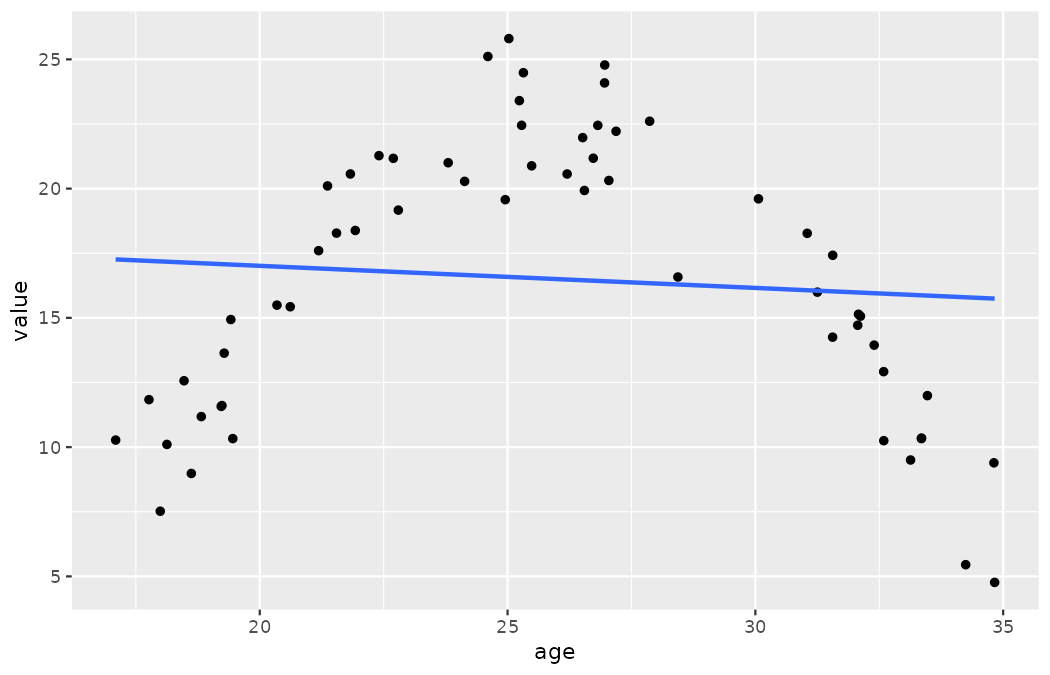
\includegraphics[width=0.85\linewidth,height=\textheight,keepaspectratio]{figures/inf-model-slr-11.png}

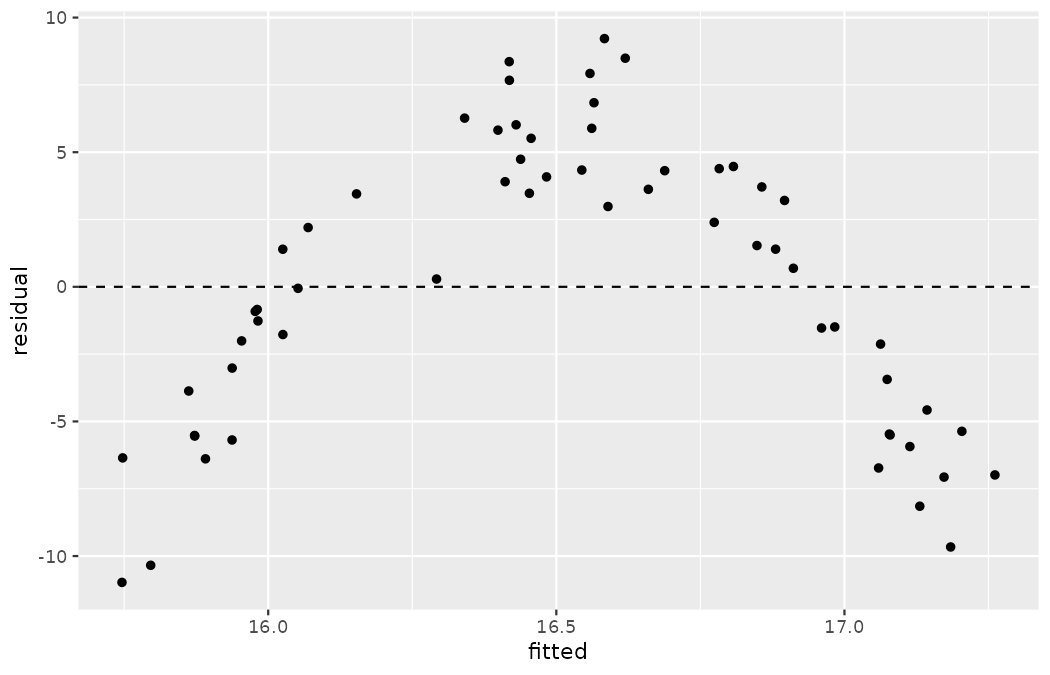
\includegraphics[width=0.85\linewidth,height=\textheight,keepaspectratio]{figures/inf-model-slr-12.png}

Read the four panels left to right:

\begin{enumerate}
\def\labelenumi{\arabic{enumi}.}
\item
  \textbf{Linearity fails.} The age--market-value curve from
  Chapter~\ref{sec-model-slr} yet again: value rises to a peak near 26
  and falls away, the fitted line comes out nearly flat, and the
  residual plot shows the telltale arch --- negative at both ends,
  positive in the middle.
\item
  \textbf{An outlier breaks normality.} Fifty-nine loan-market fees
  track chances created at about €0.11M per chance --- and one
  \emph{mis-entered wonderkid} sits at €36.6M where the trend expects
  about €3.6M: a data-entry slip of one decimal place, the kind that
  survives in scouting databases for months. His residual of roughly
  \(+32\) dwarfs every other, and he alone drags the fitted slope from
  \(0.117\) down to \(0.094\):

\begin{Shaded}
\begin{Highlighting}[]
\FunctionTok{round}\NormalTok{(}\FunctionTok{c}\NormalTok{(}
  \AttributeTok{slope\_with    =} \FunctionTok{unname}\NormalTok{(}\FunctionTok{coef}\NormalTok{(}\FunctionTok{lm}\NormalTok{(fee }\SpecialCharTok{\textasciitilde{}}\NormalTok{ chances, }\AttributeTok{data =}\NormalTok{ wonderkid))[}\DecValTok{2}\NormalTok{]),}
  \AttributeTok{slope\_without =} \FunctionTok{unname}\NormalTok{(}\FunctionTok{coef}\NormalTok{(}\FunctionTok{lm}\NormalTok{(fee }\SpecialCharTok{\textasciitilde{}}\NormalTok{ chances, }\AttributeTok{data =} \FunctionTok{slice\_head}\NormalTok{(wonderkid, }\AttributeTok{n =} \DecValTok{59}\NormalTok{)))[}\DecValTok{2}\NormalTok{])}
\NormalTok{), }\DecValTok{3}\NormalTok{)}
\CommentTok{\#\textgreater{}    slope\_with slope\_without}
\CommentTok{\#\textgreater{}         0.094         0.117}
\end{Highlighting}
\end{Shaded}
\item
  \textbf{Variability grows with \(x\).} Transfer fees for prospects
  aged 16 to 22: the trend rises, but so does the spread ---
  sixteen-year-olds are priced within a euro-tight band while
  twenty-two-year-olds scatter across tens of millions. The residual
  plot fans open from left to right.
\item
  \textbf{Successive observations are correlated.} Sixty consecutive
  days of one player's GPS training load, which drifts like a random
  walk: today's load is yesterday's plus a nudge. The residuals snake
  --- long runs above the line, then long runs below (their day-to-day
  correlation is \(0.85\)) --- because the observations remember each
  other, which is precisely what independence forbids.
\end{enumerate}

\begin{tcolorbox}[enhanced jigsaw, left=2mm, leftrule=.75mm, title=\textcolor{quarto-callout-tip-color}{\faLightbulb}\hspace{0.5em}{Check your understanding}, arc=.35mm, rightrule=.15mm, coltitle=black, colframe=quarto-callout-tip-color-frame, bottomrule=.15mm, colbacktitle=quarto-callout-tip-color!10!white, opacitybacktitle=0.6, breakable, bottomtitle=1mm, toptitle=1mm, titlerule=0mm, opacityback=0, toprule=.15mm, colback=white]

Should we have concerns about applying least squares regression --- and
the \(t\)-based inference of Section~\ref{sec-mathslope} --- to the
veteran-market data?

\begin{center}\rule{0.5\linewidth}{0.5pt}\end{center}

The trend appears linear across ages 28--35 (the market's hump lives at
younger ages, outside this survey's window), the points fall around the
line with no obvious outliers, and the variance is roughly constant ---
the €0.5M listing floor grazes only a few points at the oldest ages. The
data are 50 different listed strikers, not a time series or repeated
quotes on one player, so independence is reasonable. Least squares
regression, and its \(t\)-based inference, can be applied to these data.

\end{tcolorbox}

The technical conditions are often remembered using the \textbf{LINE}
mnemonic --- and this is the checklist to run, in order, before trusting
any regression p-value or interval in a scouting report. The linearity,
normality, and equality-of-variance conditions usually can be assessed
through residual plots, as in the gallery above. A careful consideration
of the study design should be undertaken to confirm that the
observations are independent.

\begin{itemize}
\tightlist
\item
  L: \textbf{linear} model
\item
  I: \textbf{independent} observations
\item
  N: points are \textbf{normally} distributed around the line
\item
  E: \textbf{equal} variability around the line for all values of the
  explanatory variable
\end{itemize}

\subsection{Why do we need technical
conditions?}\label{why-do-we-need-technical-conditions}

As with other inferential techniques we have covered in this text, if
the technical conditions above do not hold, then it is not possible to
make concluding claims about the population. That is, without the
technical conditions, the T score will not have the assumed
\(t\)-distribution. That said, it is almost always impossible to check
the conditions precisely, so we look for large deviations from the
conditions. If there are large deviations, we will be unable to trust
the calculated p-value or the endpoints of the resulting confidence
interval.

\textbf{The model based on linearity}

The linearity condition is among the most important if your goal is to
understand a linear model between \(x\) and \(y.\) For example, the
value of the slope will not be at all meaningful if the true
relationship between \(x\) and \(y\) is quadratic, as in the age-curve
panel above: the nearly flat fitted slope of the age hump ``summarizes''
a market in which value first rises steeply and then falls steeply,
describing neither. Not only should we be cautious about the inference
--- the model \emph{itself} is not an accurate portrayal of the
relationship between the variables. An extended discussion of modeling
functional forms other than linear is outside the scope of this text.

\textbf{The importance of independence}

The technical condition describing the independence of the observations
is often the most crucial but also the most difficult to diagnose. It is
also extremely difficult to gather a dataset which is a true random
sample from the population of interest.

Dependent observations can bias results in ways that produce
fundamentally flawed analyses. Think of the scout who logs shots only at
the matches of the club across town: the linear model fit to that
notebook is surely not a representation of the league. At best it
describes shots at one stadium --- taken by teams that chose to play a
certain way against one opponent, watched on the days that scout could
attend. The GPS-load panel is the within-player version of the same
failure: sixty numbers from one body are not sixty independent pieces of
evidence, and treating them as such makes every standard error in the
output a fiction.

In lieu of trying to answer whether your observations are a true random
sample, you might instead focus on whether you believe your observations
are representative of the population of interest. Humans are notoriously
bad at implementing random procedures, so you should be wary of any
process that used human intuition to balance the data --- a shortlist
``balanced by eye'' across leagues and ages is not a random sample of
any market.

\textbf{Some thoughts on normality}

The normality condition requires that points vary symmetrically around
the line, spreading out in a bell-shaped fashion. You should consider
the ``bell'' of the normal distribution as sitting on top of the line
(coming off the page in a 3-D sense), indicating that points are dense
close to the line and disperse gradually as they get farther from it.

The normality condition is less important than linearity or
independence, for a few reasons. First, the linear model fit with least
squares will still be an unbiased estimate of the true population model;
however, the distribution of the estimate will be unknown. Fortunately
the Central Limit Theorem (described in Section~\ref{sec-one-mean-math})
tells us that most of the analyses (e.g., SEs, p-values, confidence
intervals) done using the mathematical model will still hold --- even if
the data are not normally distributed around the line --- as long as the
sample size is large enough. One analysis method that \emph{does}
require normality, regardless of sample size, is creating intervals
which predict the response of individual outcomes at a given \(x\)
value. One additional reason to worry slightly less about normality is
that neither the randomization test nor the bootstrapping procedures
require the data to be normal around the line.

\textbf{Equal variability for inference in particular}

As with normality, the equal variability condition (that points are
spread out in similar ways around the line for all values of \(x\)) will
not cause problems for the \emph{estimate} of the linear model. That
said, the \textbf{inference} on the model (e.g., computing p-values)
will be incorrect if the variability around the line is extremely
heterogeneous. Data that exhibit non-equal variance across the range of
\(x\)-values will have the potential to seriously mis-estimate the
variability of the slope, with consequences for hypothesis tests and
confidence intervals --- the youth-fees panel is the standing warning.

In many cases, the inference results for both a randomization test and a
bootstrap confidence interval are robust to the equal variability
condition, so they provide the analyst a set of methods to use when the
data are heteroskedastic (that is, exhibit unequal variability around
the regression line). Although randomization tests and bootstrapping
allow us to analyze data using fewer conditions, some technical
conditions are required for all methods described in this text (e.g.,
independent observations). When the equal variability condition is
violated and a mathematical analysis (e.g., a p-value from a T score) is
needed, there are other existing methods (outside the scope of this
text) which can handle the unequal variance, such as weighted least
squares.

\textbf{A violation hiding in plain sight: binary outcomes}

One more residual plot belongs in this section, because the book's own
data supply the most instructive violation of all. Suppose an eager
analyst regresses the \emph{goal} indicator itself --- 1 if the shot
scored, 0 if not --- on chance quality, treating a binary outcome as if
it were numeric:

\begin{Shaded}
\begin{Highlighting}[]
\NormalTok{shots\_lpm }\OtherTok{\textless{}{-}}\NormalTok{ wc2022\_shots }\SpecialCharTok{|\textgreater{}}
  \FunctionTok{mutate}\NormalTok{(}\AttributeTok{goal01 =} \FunctionTok{as.numeric}\NormalTok{(goal))}

\NormalTok{fit\_shot }\OtherTok{\textless{}{-}} \FunctionTok{lm}\NormalTok{(goal01 }\SpecialCharTok{\textasciitilde{}}\NormalTok{ statsbomb\_xg, }\AttributeTok{data =}\NormalTok{ shots\_lpm)}
\FunctionTok{tidy}\NormalTok{(fit\_shot)}
\CommentTok{\#\textgreater{} \# A tibble: 2 × 5}
\CommentTok{\#\textgreater{}   term         estimate std.error statistic   p.value}
\CommentTok{\#\textgreater{}   \textless{}chr\textgreater{}           \textless{}dbl\textgreater{}     \textless{}dbl\textgreater{}     \textless{}dbl\textgreater{}     \textless{}dbl\textgreater{}}
\CommentTok{\#\textgreater{} 1 (Intercept)    0.0108   0.00902      1.20 2.31e{-}  1}
\CommentTok{\#\textgreater{} 2 statsbomb\_xg   0.951    0.0405      23.5  2.97e{-}104}

\NormalTok{shots\_lpm }\SpecialCharTok{|\textgreater{}}
  \FunctionTok{mutate}\NormalTok{(}\AttributeTok{residual =} \FunctionTok{resid}\NormalTok{(fit\_shot)) }\SpecialCharTok{|\textgreater{}}
  \FunctionTok{group\_by}\NormalTok{(goal) }\SpecialCharTok{|\textgreater{}}
  \FunctionTok{summarize}\NormalTok{(}\AttributeTok{n =} \FunctionTok{n}\NormalTok{(), }\AttributeTok{min\_resid =} \FunctionTok{min}\NormalTok{(residual), }\AttributeTok{max\_resid =} \FunctionTok{max}\NormalTok{(residual))}
\CommentTok{\#\textgreater{} \# A tibble: 2 × 4}
\CommentTok{\#\textgreater{}   goal      n min\_resid max\_resid}
\CommentTok{\#\textgreater{}   \textless{}lgl\textgreater{} \textless{}int\textgreater{}     \textless{}dbl\textgreater{}     \textless{}dbl\textgreater{}}
\CommentTok{\#\textgreater{} 1 FALSE  1299    {-}0.756   {-}0.0110}
\CommentTok{\#\textgreater{} 2 TRUE    195     0.136    0.982}
\end{Highlighting}
\end{Shaded}

The fit looks seductively sensible --- a slope of \(0.95\) says recorded
xG converts to goal probability nearly one-for-one across all 1,494
shots, a shape-invariant conclusion in any frame --- but draw the
residual plot and the illusion collapses: every residual lies in one of
exactly two descending bands, the 195 goals in a strip between \(+0.14\)
and \(+0.98,\) the 1,299 misses in a strip between \(-0.76\) and
\(-0.01,\) with an empty gulf between. Nothing about that picture is
bell-shaped around zero, and the spread changes systematically along the
line: with a binary response, the N and E conditions are not merely
strained, they are impossible. The estimated line still has descriptive
value, but the \(t\)-based standard errors, p-values, and intervals of
this chapter do not apply. The honest tool for a binary response is the
logistic regression you met in Chapter~\ref{sec-model-logistic} --- and
inference for \emph{that} model is exactly the business of
Chapter~\ref{sec-inf-model-logistic}.

\subsection{What if all the technical conditions are
met?}\label{what-if-all-the-technical-conditions-are-met}

When the technical conditions are met, the least squares regression
model and its inference are provided by virtually all statistical
software. In addition to being ubiquitous, an additional advantage of
the least squares regression model (and related inference) is that the
linear model has important extensions, which are not trivial to
implement with bootstrapping and randomization tests. In particular,
random effects models (natural when shots nest within players and
players within teams), repeated measures (a player observed across many
sessions, as in the GPS panel), and interactions are all linear model
extensions which require the above technical conditions. When the
technical conditions hold, these extensions can provide important
insight into the data and the research question at hand. We will discuss
some of the extended modeling and associated inference in
Chapter~\ref{sec-inf-model-mlr} and
Chapter~\ref{sec-inf-model-logistic}. Many of the techniques used to
deal with technical condition violations are outside the scope of this
text, but they are taught in universities in the very next class after
this one. If you are working with linear models or are curious to learn
more, we recommend that you continue learning about statistical methods
applicable to a larger class of datasets.

\section{Chapter review}\label{sec-chp24-review}

\subsection{Summary}\label{summary-23}

Recall that early in the text we presented graphical techniques which
communicated relationships across multiple variables, and we used
modeling to formalize those relationships --- for this book, always with
a scout's questions underneath: does chance quality buy goals, does age
discount a fee, does the clock fatten a chance. Many chapters were then
dedicated to inferential methods which allowed claims about the
population to be made based on samples of data. Not only did we present
the mathematical model for each of the inferential techniques, but when
appropriate, we also presented bootstrapping and permutation methods.

In this chapter we brought all of those ideas together by considering
inferential claims on linear models through randomization tests (the
slope of \(0.909\) for goals on chance quality, far outside every
permuted slope), bootstrapping (the fatigue-drift slope whose interval
straddled zero and killed its own story), and mathematical modeling (the
pressure-share theory that failed to reject, and the veteran market's
€0.78M--€2.10M per year of age). We continue to emphasize the importance
of study design in making conclusions about research claims: only the
constructed Northbridge experiments license causal language, while every
tournament dataset speaks of association --- recall the distinction
between random sampling and random allocation from
Chapter~\ref{sec-data-hello} and Chapter~\ref{sec-data-design}. And the
chapter closed with the discipline that guards all of it: the LINE
conditions, checked with residual plots and honest questions about how
the data arose, plus this book's own standing check --- state the frame,
because penalties moved every headline number they touched.

\begin{longtable}[]{@{}
  >{\raggedright\arraybackslash}p{(\linewidth - 2\tabcolsep) * \real{0.5634}}
  >{\raggedright\arraybackslash}p{(\linewidth - 2\tabcolsep) * \real{0.4366}}@{}}
\caption{Summary of inference for the slope of a linear
model.}\label{tbl-chp24-summary}\tabularnewline
\toprule\noalign{}
\begin{minipage}[b]{\linewidth}\raggedright
Question
\end{minipage} & \begin{minipage}[b]{\linewidth}\raggedright
Answer
\end{minipage} \\
\midrule\noalign{}
\endfirsthead
\toprule\noalign{}
\begin{minipage}[b]{\linewidth}\raggedright
Question
\end{minipage} & \begin{minipage}[b]{\linewidth}\raggedright
Answer
\end{minipage} \\
\midrule\noalign{}
\endhead
\bottomrule\noalign{}
\endlastfoot
What is the statistic? & The sample slope \(b_1,\) estimating the
population slope \(\beta_1\) of
\(y = \beta_0 + \beta_1 x + \varepsilon.\) \\
How is the null distribution built? & Permute the response values, refit
the line each time: slopes when \(\beta_1 = 0\) is true. \\
How is a CI built without formulas? & Resample rows (pairs) with
replacement, refit; percentile or SE interval of the bootstrapped
slopes. \\
What is the mathematical model? & \(T = (b_1 - 0)/SE_{b_1}\) on a
\(t\)-distribution with \(df = n - 2\); interval
\(b_i \pm t^{\star}_{df} \times SE_{b_i}.\) \\
What are the conditions? & LINE: linearity, independence, nearly normal
residuals, equal variability --- checked graphically, with independence
judged from the design. \\
\end{longtable}

\subsection{Terms}\label{terms-23}

The terms introduced in this chapter are presented below, alphabetized.
If you're not sure what some of these terms mean, we recommend you go
back in the text and review their definitions. You should be able to
easily spot them as \textbf{bolded text}.

\begin{longtable}[]{@{}
  >{\raggedright\arraybackslash}p{(\linewidth - 4\tabcolsep) * \real{0.3380}}
  >{\raggedright\arraybackslash}p{(\linewidth - 4\tabcolsep) * \real{0.3380}}
  >{\raggedright\arraybackslash}p{(\linewidth - 4\tabcolsep) * \real{0.3239}}@{}}
\caption{Terms introduced in this
chapter.}\label{tbl-terms-chp-24}\tabularnewline
\toprule\noalign{}
\endfirsthead
\endhead
\bottomrule\noalign{}
\endlastfoot
bootstrap confidence interval for the slope & randomization test for the
slope & technical conditions \\
inference with single predictor regression & t-distribution for the
slope & variability of the slope \\
LINE & & \\
\end{longtable}

\section{Exercises}\label{sec-chp24-exercises}

Answers to odd-numbered exercises can be found in
Appendix~\ref{sec-exercise-solutions-24}.

\begin{enumerate}
\def\labelenumi{\arabic{enumi}.}
\item
  \textbf{Chance creation at the Women's Euro, randomization test.} The
  book's flagship regression --- goals on accumulated chance quality ---
  was tested at the 2022 Men's World Cup in Section~\ref{sec-randslope}.
  Per this book's replication habit, we now ask whether the relationship
  holds at the 2025 Women's Euro. The code below aggregates the
  tournament's 913 shots into 62 team-matches (unlike the World Cup's
  127, no side finished a Euro match without a shot); per the penalty
  convention, note the frame: the shot log counts in-game penalties and
  shoot-out kicks in both \texttt{total\_xg} and \texttt{goals}, on both
  sides of the model.\footnote{A caution that travels with every
    \texttt{team\_match}-style aggregate, per the Data callout of
    Section~\ref{sec-randslope}: the \texttt{goals} column sums the shot
    log's goal flags, so it counts converted shoot-out kicks too --- it
    is not the recorded match score.} Shown below are the linear model
  output for predicting goals from total xG and a summary of the slopes
  from 1,000 randomized datasets (1,000 times, \texttt{goals} was
  permuted and regressed against \texttt{total\_xg}).\footnote{The 2025
    Women's Euro shot data used in this exercise are in
    \texttt{data/derived/weuro2025\_shots.csv} (StatsBomb open data);
    \texttt{team\_match\_weuro} aggregates them by match and team.}

\begin{Shaded}
\begin{Highlighting}[]
\NormalTok{weuro2025\_shots }\OtherTok{\textless{}{-}} \FunctionTok{read\_csv}\NormalTok{(}\StringTok{"data/derived/weuro2025\_shots.csv"}\NormalTok{)}

\NormalTok{team\_match\_weuro }\OtherTok{\textless{}{-}}\NormalTok{ weuro2025\_shots }\SpecialCharTok{|\textgreater{}}
  \FunctionTok{group\_by}\NormalTok{(match\_id, team) }\SpecialCharTok{|\textgreater{}}
  \FunctionTok{summarize}\NormalTok{(}
    \AttributeTok{n\_shots =} \FunctionTok{n}\NormalTok{(),}
    \AttributeTok{total\_xg =} \FunctionTok{sum}\NormalTok{(statsbomb\_xg),}
    \AttributeTok{goals =} \FunctionTok{sum}\NormalTok{(goal),}
    \AttributeTok{.groups =} \StringTok{"drop"}
\NormalTok{  )}

\NormalTok{fit\_weuro\_xg }\OtherTok{\textless{}{-}} \FunctionTok{lm}\NormalTok{(goals }\SpecialCharTok{\textasciitilde{}}\NormalTok{ total\_xg, }\AttributeTok{data =}\NormalTok{ team\_match\_weuro)}
\FunctionTok{tidy}\NormalTok{(fit\_weuro\_xg)}
\CommentTok{\#\textgreater{} \# A tibble: 2 × 5}
\CommentTok{\#\textgreater{}   term        estimate std.error statistic  p.value}
\CommentTok{\#\textgreater{}   \textless{}chr\textgreater{}          \textless{}dbl\textgreater{}     \textless{}dbl\textgreater{}     \textless{}dbl\textgreater{}    \textless{}dbl\textgreater{}}
\CommentTok{\#\textgreater{} 1 (Intercept)    0.423    0.208       2.03 4.63e{-} 2}
\CommentTok{\#\textgreater{} 2 total\_xg       0.785    0.0777     10.1  1.43e{-}14}

\FunctionTok{set.seed}\NormalTok{(}\DecValTok{2410}\NormalTok{)}
\NormalTok{weuro\_slope\_null }\OtherTok{\textless{}{-}}\NormalTok{ team\_match\_weuro }\SpecialCharTok{|\textgreater{}}
  \FunctionTok{specify}\NormalTok{(goals }\SpecialCharTok{\textasciitilde{}}\NormalTok{ total\_xg) }\SpecialCharTok{|\textgreater{}}
  \FunctionTok{hypothesize}\NormalTok{(}\AttributeTok{null =} \StringTok{"independence"}\NormalTok{) }\SpecialCharTok{|\textgreater{}}
  \FunctionTok{generate}\NormalTok{(}\AttributeTok{reps =} \DecValTok{1000}\NormalTok{, }\AttributeTok{type =} \StringTok{"permute"}\NormalTok{) }\SpecialCharTok{|\textgreater{}}
  \FunctionTok{calculate}\NormalTok{(}\AttributeTok{stat =} \StringTok{"slope"}\NormalTok{)}
\end{Highlighting}
\end{Shaded}

  A histogram of the 1,000 randomized slopes is centered at 0 and ranges
  from \(-0.34\) to \(+0.40\); a red vertical line drawn at the observed
  slope of \(0.785\) sits far outside the histogram, and none of the
  1,000 randomized slopes was at least as far from zero.

  \begin{enumerate}
  \def\labelenumii{\alph{enumii}.}
  \item
    What are the null and alternative hypotheses for evaluating whether
    the slope of the model predicting a team's goals from its
    accumulated chance quality is different than 0?
  \item
    Using the histogram which describes the distribution of slopes when
    the null hypothesis is true, find the p-value and conclude the
    hypothesis test in the context of the problem (use words like chance
    quality and goals).
  \item
    Is the conclusion based on the histogram of randomized slopes
    consistent with the conclusion the mathematical model would have
    reached? Explain your reasoning.
  \end{enumerate}
\item
  \textbf{Fatigue drift at the Women's Euro, randomization test.} In
  Section~\ref{sec-bootbeta1} the fatigue-drift theory --- chances get
  better as the match wears on --- collapsed on the World Cup's
  open-play shots. Here we study the same relationship at the 2025
  Women's Euro, on the same frame as Section~\ref{sec-bootbeta1}, per
  the book's penalty convention: \texttt{shot\_type\ ==\ "Open\ Play"}
  (851 shots), stated because penalty kicks carry a fixed chance quality
  and the shoot-out kicks sit at the very end of the clock. Shown below
  are the linear model output for predicting chance quality (xG) from
  the minute of the match and a summary of the slopes from 1,000
  randomized datasets (1,000 times, \texttt{statsbomb\_xg} was permuted
  and regressed against \texttt{minute}).\footnote{The 2025 Women's Euro
    shot data used in this exercise are in
    \texttt{data/derived/weuro2025\_shots.csv} (StatsBomb open data).}

\begin{Shaded}
\begin{Highlighting}[]
\NormalTok{weuro\_open }\OtherTok{\textless{}{-}}\NormalTok{ weuro2025\_shots }\SpecialCharTok{|\textgreater{}}
  \FunctionTok{filter}\NormalTok{(shot\_type }\SpecialCharTok{==} \StringTok{"Open Play"}\NormalTok{)}

\NormalTok{fit\_weuro\_minute }\OtherTok{\textless{}{-}} \FunctionTok{lm}\NormalTok{(statsbomb\_xg }\SpecialCharTok{\textasciitilde{}}\NormalTok{ minute, }\AttributeTok{data =}\NormalTok{ weuro\_open)}
\FunctionTok{tidy}\NormalTok{(fit\_weuro\_minute)}
\CommentTok{\#\textgreater{} \# A tibble: 2 × 5}
\CommentTok{\#\textgreater{}   term         estimate std.error statistic  p.value}
\CommentTok{\#\textgreater{}   \textless{}chr\textgreater{}           \textless{}dbl\textgreater{}     \textless{}dbl\textgreater{}     \textless{}dbl\textgreater{}    \textless{}dbl\textgreater{}}
\CommentTok{\#\textgreater{} 1 (Intercept)  0.104     0.00791     13.1   4.88e{-}36}
\CommentTok{\#\textgreater{} 2 minute      {-}0.000125  0.000132    {-}0.951 3.42e{-} 1}

\FunctionTok{set.seed}\NormalTok{(}\DecValTok{2411}\NormalTok{)}
\NormalTok{weuro\_minute\_null }\OtherTok{\textless{}{-}}\NormalTok{ weuro\_open }\SpecialCharTok{|\textgreater{}}
  \FunctionTok{specify}\NormalTok{(statsbomb\_xg }\SpecialCharTok{\textasciitilde{}}\NormalTok{ minute) }\SpecialCharTok{|\textgreater{}}
  \FunctionTok{hypothesize}\NormalTok{(}\AttributeTok{null =} \StringTok{"independence"}\NormalTok{) }\SpecialCharTok{|\textgreater{}}
  \FunctionTok{generate}\NormalTok{(}\AttributeTok{reps =} \DecValTok{1000}\NormalTok{, }\AttributeTok{type =} \StringTok{"permute"}\NormalTok{) }\SpecialCharTok{|\textgreater{}}
  \FunctionTok{calculate}\NormalTok{(}\AttributeTok{stat =} \StringTok{"slope"}\NormalTok{)}
\end{Highlighting}
\end{Shaded}

  A histogram of the 1,000 randomized slopes is centered at 0 and ranges
  from \(-0.00042\) to \(+0.00039\); a red vertical line drawn at the
  observed slope of \(-0.000125\) falls well inside the histogram, and
  363 of the 1,000 randomized slopes were at least as far from zero as
  the observed slope.

  \begin{enumerate}
  \def\labelenumii{\alph{enumii}.}
  \item
    What are the null and alternative hypotheses for evaluating whether
    the slope of the model predicting a shot's chance quality from the
    minute of the match is different than 0? Note that at this
    tournament the observed drift runs \emph{downhill} --- the opposite
    sign to the World Cup's.
  \item
    Using the randomized slopes, find the p-value and conclude the
    hypothesis test in the context of the problem (use words like minute
    and chance quality). What does the conclusion of your test say about
    whether the match clock is a useful predictor of chance quality?
  \item
    Is the conclusion based on the histogram of randomized slopes
    consistent with the conclusion from the mathematical model? Explain
    your reasoning.
  \end{enumerate}
\item
  \textbf{Shot volume and chance quality at the Women's Euro,
  mathematical test.} Does a team's shot count in a match predict how
  much chance quality it accumulates? The scatterplot and least squares
  summary below show the relationship between the number of shots and
  the total xG across the 62 team-matches of the 2025 Women's Euro
  (all-shots frame, as in Exercise 1).\footnote{A caution that travels
    with every \texttt{team\_match}-style aggregate, per the Data
    callout of Section~\ref{sec-randslope}: the \texttt{goals} column
    sums the shot log's goal flags, so it counts converted shoot-out
    kicks too --- it is not the recorded match score.} The 62 points
  climb from quiet outings of 4 shots and under 0.5 xG toward
  high-volume performances of up to 34 shots, with total xG reaching
  7.4; the cloud spreads noticeably as the shot counts grow.

\begin{Shaded}
\begin{Highlighting}[]
\NormalTok{fit\_weuro\_shots }\OtherTok{\textless{}{-}} \FunctionTok{lm}\NormalTok{(total\_xg }\SpecialCharTok{\textasciitilde{}}\NormalTok{ n\_shots, }\AttributeTok{data =}\NormalTok{ team\_match\_weuro)}
\FunctionTok{tidy}\NormalTok{(fit\_weuro\_shots)}
\CommentTok{\#\textgreater{} \# A tibble: 2 × 5}
\CommentTok{\#\textgreater{}   term        estimate std.error statistic      p.value}
\CommentTok{\#\textgreater{}   \textless{}chr\textgreater{}          \textless{}dbl\textgreater{}     \textless{}dbl\textgreater{}     \textless{}dbl\textgreater{}        \textless{}dbl\textgreater{}}
\CommentTok{\#\textgreater{} 1 (Intercept)   {-}0.491    0.436      {-}1.13 0.265}
\CommentTok{\#\textgreater{} 2 n\_shots        0.168    0.0270      6.24 0.0000000481}
\end{Highlighting}
\end{Shaded}

  \begin{enumerate}
  \def\labelenumii{\alph{enumii}.}
  \item
    Describe the relationship between the number of shots and total
    chance quality.
  \item
    Write the equation of the regression line. Interpret the slope and
    intercept in context.
  \item
    Do the data provide convincing evidence that the true slope
    parameter is different than 0? State the null and alternative
    hypotheses, report the p-value (using a mathematical model), and
    state your conclusion.
  \item
    The correlation coefficient between the number of shots and total xG
    is 0.63. Calculate \(R^2\) and interpret it in context.
  \end{enumerate}
\item
  \textbf{Fatigue drift at the Women's Euro, mathematical test.} Is the
  minute of the match useful in predicting a shot's chance quality? Use
  the least squares summary of the open-play model from Exercise 2,
  repeated here.

\begin{Shaded}
\begin{Highlighting}[]
\FunctionTok{tidy}\NormalTok{(fit\_weuro\_minute)}
\CommentTok{\#\textgreater{} \# A tibble: 2 × 5}
\CommentTok{\#\textgreater{}   term         estimate std.error statistic  p.value}
\CommentTok{\#\textgreater{}   \textless{}chr\textgreater{}           \textless{}dbl\textgreater{}     \textless{}dbl\textgreater{}     \textless{}dbl\textgreater{}    \textless{}dbl\textgreater{}}
\CommentTok{\#\textgreater{} 1 (Intercept)  0.104     0.00791     13.1   4.88e{-}36}
\CommentTok{\#\textgreater{} 2 minute      {-}0.000125  0.000132    {-}0.951 3.42e{-} 1}
\end{Highlighting}
\end{Shaded}

  \begin{enumerate}
  \def\labelenumii{\alph{enumii}.}
  \item
    What is the predicted chance quality of an open-play shot taken in
    the 30th minute?
  \item
    Do the data provide convincing evidence that the model for
    predicting chance quality from the minute has a slope different than
    0? State the null and alternative hypotheses, report the p-value
    (using a mathematical model), and state your conclusion.
  \item
    Based on your conclusion, is the match clock a useful predictor of
    chance quality?
  \end{enumerate}
\item
  \textbf{Chance creation at the Women's Euro, bootstrap percentile
  interval.} In order to estimate the slope of the model predicting a
  team's goals from its accumulated chance quality, 1,000 bootstrap
  samples are taken from the 62 team-matches of the 2025 Women's Euro. A
  linear model predicting \texttt{goals} from \texttt{total\_xg} is fit
  to each bootstrap sample, and the slope is estimated.

\begin{Shaded}
\begin{Highlighting}[]
\FunctionTok{set.seed}\NormalTok{(}\DecValTok{2412}\NormalTok{)}
\NormalTok{weuro\_slope\_boot }\OtherTok{\textless{}{-}}\NormalTok{ team\_match\_weuro }\SpecialCharTok{|\textgreater{}}
  \FunctionTok{specify}\NormalTok{(goals }\SpecialCharTok{\textasciitilde{}}\NormalTok{ total\_xg) }\SpecialCharTok{|\textgreater{}}
  \FunctionTok{generate}\NormalTok{(}\AttributeTok{reps =} \DecValTok{1000}\NormalTok{, }\AttributeTok{type =} \StringTok{"bootstrap"}\NormalTok{) }\SpecialCharTok{|\textgreater{}}
  \FunctionTok{calculate}\NormalTok{(}\AttributeTok{stat =} \StringTok{"slope"}\NormalTok{)}
\end{Highlighting}
\end{Shaded}

  The histogram of the 1,000 bootstrapped slopes is bell-shaped, running
  from 0.55 to 1.32; its 1st and 99th percentiles are 0.598 and 1.087.

  \begin{enumerate}
  \def\labelenumii{\alph{enumii}.}
  \item
    Using the bootstrap percentile method, find a 98\% confidence
    interval for the slope parameter.
  \item
    Interpret the confidence interval in the context of the problem.
  \end{enumerate}
\item
  \textbf{Fatigue drift at the Women's Euro, bootstrap percentile
  interval.} Returning to the open-play shots of the 2025 Women's Euro,
  we want an interval estimate for the slope of the model predicting a
  shot's chance quality from the minute of the match. Below, 1,000
  bootstrap samples of the 851 shots are taken and a linear model is fit
  to each.

\begin{Shaded}
\begin{Highlighting}[]
\FunctionTok{set.seed}\NormalTok{(}\DecValTok{2413}\NormalTok{)}
\NormalTok{weuro\_minute\_boot }\OtherTok{\textless{}{-}}\NormalTok{ weuro\_open }\SpecialCharTok{|\textgreater{}}
  \FunctionTok{specify}\NormalTok{(statsbomb\_xg }\SpecialCharTok{\textasciitilde{}}\NormalTok{ minute) }\SpecialCharTok{|\textgreater{}}
  \FunctionTok{generate}\NormalTok{(}\AttributeTok{reps =} \DecValTok{1000}\NormalTok{, }\AttributeTok{type =} \StringTok{"bootstrap"}\NormalTok{) }\SpecialCharTok{|\textgreater{}}
  \FunctionTok{calculate}\NormalTok{(}\AttributeTok{stat =} \StringTok{"slope"}\NormalTok{)}
\end{Highlighting}
\end{Shaded}

  The histogram of the 1,000 bootstrapped slopes is bell-shaped, running
  from \(-0.00057\) to \(+0.00031\); its 2.5th and 97.5th percentiles
  are \(-0.00037\) and \(+0.00013.\)

  \begin{enumerate}
  \def\labelenumii{\alph{enumii}.}
  \item
    Using the bootstrap percentile method, find a 95\% confidence
    interval for the slope parameter.
  \item
    Interpret the confidence interval in the context of the problem.
    What does the interval say about the fatigue-drift theory at this
    tournament?
  \end{enumerate}
\item
  \textbf{Chance creation at the Women's Euro, standard error bootstrap
  interval.} A linear model is built to predict a team's goals in a
  match from its accumulated chance quality across the 62 team-matches
  of the 2025 Women's Euro. Shown below are the linear model output and
  a summary of the bootstrap distribution of the slope statistic from
  the 1,000 bootstrap samples of Exercise 5 (seed 2412): the histogram
  is bell-shaped and centered near 0.79, with most of the bootstrapped
  slopes falling between 0.57 and 1.00.

\begin{Shaded}
\begin{Highlighting}[]
\FunctionTok{tidy}\NormalTok{(fit\_weuro\_xg)}
\CommentTok{\#\textgreater{} \# A tibble: 2 × 5}
\CommentTok{\#\textgreater{}   term        estimate std.error statistic  p.value}
\CommentTok{\#\textgreater{}   \textless{}chr\textgreater{}          \textless{}dbl\textgreater{}     \textless{}dbl\textgreater{}     \textless{}dbl\textgreater{}    \textless{}dbl\textgreater{}}
\CommentTok{\#\textgreater{} 1 (Intercept)    0.423    0.208       2.03 4.63e{-} 2}
\CommentTok{\#\textgreater{} 2 total\_xg       0.785    0.0777     10.1  1.43e{-}14}
\end{Highlighting}
\end{Shaded}

  \begin{enumerate}
  \def\labelenumii{\alph{enumii}.}
  \item
    Using the histogram, approximate the standard error of the slope
    statistic (that is, quantify the variability of the slope statistic
    from sample to sample).
  \item
    Find a 98\% bootstrap SE confidence interval for the slope
    parameter.
  \item
    Interpret the confidence interval in the context of the problem.
  \end{enumerate}
\item
  \textbf{Fatigue drift at the Women's Euro, standard error bootstrap
  interval.} Shown below are the linear model output for predicting an
  open-play shot's chance quality from the minute of the match at the
  2025 Women's Euro and a summary of the bootstrap distribution of the
  slope from the 1,000 bootstrap samples of Exercise 6 (seed 2413): the
  histogram is bell-shaped and centered near \(-0.00012,\) and the
  standard deviation of the bootstrapped slopes is 0.00013.

\begin{Shaded}
\begin{Highlighting}[]
\FunctionTok{tidy}\NormalTok{(fit\_weuro\_minute)}
\CommentTok{\#\textgreater{} \# A tibble: 2 × 5}
\CommentTok{\#\textgreater{}   term         estimate std.error statistic  p.value}
\CommentTok{\#\textgreater{}   \textless{}chr\textgreater{}           \textless{}dbl\textgreater{}     \textless{}dbl\textgreater{}     \textless{}dbl\textgreater{}    \textless{}dbl\textgreater{}}
\CommentTok{\#\textgreater{} 1 (Intercept)  0.104     0.00791     13.1   4.88e{-}36}
\CommentTok{\#\textgreater{} 2 minute      {-}0.000125  0.000132    {-}0.951 3.42e{-} 1}
\end{Highlighting}
\end{Shaded}

  \begin{enumerate}
  \def\labelenumii{\alph{enumii}.}
  \item
    Using the bootstrap distribution, report the standard error of the
    slope statistic.
  \item
    Find a 95\% bootstrap SE confidence interval for the slope
    parameter.
  \item
    Interpret the confidence interval in the context of the problem.
  \end{enumerate}
\item
  \textbf{Shot volume and chance quality at the Women's Euro,
  conditions.} The residual plot described below comes from the linear
  model of total xG vs.~number of shots across the 62 team-matches of
  the 2025 Women's Euro (Exercise 3), with the number of shots on the
  x-axis and the residuals on the y-axis. Most of the 62 residuals sit
  in a band between \(-2.1\) and \(+2,\) scattered around zero --- but a
  handful of points float above the band, with residuals between \(+3\)
  and \(+4.8.\)

  \begin{enumerate}
  \def\labelenumii{\alph{enumii}.}
  \item
    For these data, \(R^2\) is 39\%. What is the value of the
    correlation coefficient? How can you tell if it is positive or
    negative? (Hint: you may need to look at a previous exercise.)
  \item
    Examine the residual plot. What do you observe? Is a simple least
    squares fit appropriate for these data? Which of the LINE conditions
    are met or not met? (One further hint, in the spirit of the book's
    penalty convention: the four largest residuals all belong to
    team-matches from two of the Euro's three penalty shoot-outs, in
    which each side added 7 kicks at 0.7835 xG apiece to its totals ---
    and France and Germany each stacked an eighth penalty, an in-game
    award, on top.)
  \end{enumerate}
\item
  \textbf{Fatigue drift at the Women's Euro, conditions.} The residual
  plot described below comes from the linear model of open-play chance
  quality vs.~minute at the 2025 Women's Euro (Exercise 2), with the
  minute on the x-axis and the residuals on the y-axis. The residuals
  form a dense band hugging the underside of zero --- 72\% of them are
  negative, none falling below \(-0.10\) --- while the rest stretch
  upward in a long right tail reaching \(+0.63,\) at every point of the
  clock.

  \begin{enumerate}
  \def\labelenumii{\alph{enumii}.}
  \item
    For these data, \(R^2\) is 0.1\%. What is the value of the
    correlation coefficient? How can you tell if it is positive or
    negative? (Hint: you may need to look at a previous exercise.)
  \item
    Examine the residual plot. What do you observe? Is a simple least
    squares fit appropriate for these data? Which of the LINE conditions
    are met or not met?
  \end{enumerate}
\item
  \textbf{Twenty matches, randomization test.} Priya Rao pulls a random
  sample of 20 matches from the 2022 Men's World Cup and asks the
  chapter's headline question at the level of whole matches: does the
  combined chance quality of a match predict its combined goal count?
  Both totals are computed from the shot log for regulation and extra
  time (shoot-out kicks excluded, so both sides of the model live on the
  same frame; in-game penalties included in both). Shown below are the
  linear model output and a summary of the slopes from 1,000 randomized
  datasets (1,000 times, \texttt{match\_goals} was permuted and
  regressed against \texttt{match\_xg}).\footnote{The 2022 Men's World
    Cup shot data used in this exercise are in
    \texttt{data/derived/wc2022\_shots.csv} (StatsBomb open data).}

\begin{Shaded}
\begin{Highlighting}[]
\NormalTok{wc2022\_shots }\OtherTok{\textless{}{-}} \FunctionTok{read\_csv}\NormalTok{(}\StringTok{"data/derived/wc2022\_shots.csv"}\NormalTok{)}

\NormalTok{wc\_match\_xg }\OtherTok{\textless{}{-}}\NormalTok{ wc2022\_shots }\SpecialCharTok{|\textgreater{}}
  \FunctionTok{filter}\NormalTok{(period }\SpecialCharTok{\textless{}=} \DecValTok{4}\NormalTok{) }\SpecialCharTok{|\textgreater{}}
  \FunctionTok{group\_by}\NormalTok{(match\_id) }\SpecialCharTok{|\textgreater{}}
  \FunctionTok{summarize}\NormalTok{(}
    \AttributeTok{match\_goals =} \FunctionTok{sum}\NormalTok{(goal),}
    \AttributeTok{match\_xg =} \FunctionTok{sum}\NormalTok{(statsbomb\_xg),}
    \AttributeTok{.groups =} \StringTok{"drop"}
\NormalTok{  )}

\FunctionTok{set.seed}\NormalTok{(}\DecValTok{2414}\NormalTok{)}
\NormalTok{matches20 }\OtherTok{\textless{}{-}}\NormalTok{ wc\_match\_xg }\SpecialCharTok{|\textgreater{}} \FunctionTok{slice\_sample}\NormalTok{(}\AttributeTok{n =} \DecValTok{20}\NormalTok{)}

\NormalTok{fit\_matches20 }\OtherTok{\textless{}{-}} \FunctionTok{lm}\NormalTok{(match\_goals }\SpecialCharTok{\textasciitilde{}}\NormalTok{ match\_xg, }\AttributeTok{data =}\NormalTok{ matches20)}
\FunctionTok{tidy}\NormalTok{(fit\_matches20)}
\CommentTok{\#\textgreater{} \# A tibble: 2 × 5}
\CommentTok{\#\textgreater{}   term        estimate std.error statistic p.value}
\CommentTok{\#\textgreater{}   \textless{}chr\textgreater{}          \textless{}dbl\textgreater{}     \textless{}dbl\textgreater{}     \textless{}dbl\textgreater{}   \textless{}dbl\textgreater{}}
\CommentTok{\#\textgreater{} 1 (Intercept)    0.238     0.966     0.247 0.808}
\CommentTok{\#\textgreater{} 2 match\_xg       1.10      0.330     3.35  0.00356}

\FunctionTok{set.seed}\NormalTok{(}\DecValTok{2415}\NormalTok{)}
\NormalTok{matches20\_null }\OtherTok{\textless{}{-}}\NormalTok{ matches20 }\SpecialCharTok{|\textgreater{}}
  \FunctionTok{specify}\NormalTok{(match\_goals }\SpecialCharTok{\textasciitilde{}}\NormalTok{ match\_xg) }\SpecialCharTok{|\textgreater{}}
  \FunctionTok{hypothesize}\NormalTok{(}\AttributeTok{null =} \StringTok{"independence"}\NormalTok{) }\SpecialCharTok{|\textgreater{}}
  \FunctionTok{generate}\NormalTok{(}\AttributeTok{reps =} \DecValTok{1000}\NormalTok{, }\AttributeTok{type =} \StringTok{"permute"}\NormalTok{) }\SpecialCharTok{|\textgreater{}}
  \FunctionTok{calculate}\NormalTok{(}\AttributeTok{stat =} \StringTok{"slope"}\NormalTok{)}
\end{Highlighting}
\end{Shaded}

  A histogram of the 1,000 randomized slopes is centered at 0 and ranges
  from \(-1.22\) to \(+1.24\); a red vertical line drawn at the observed
  slope of \(1.10\) sits in its extreme right tail, and 5 of the 1,000
  randomized slopes were at least as far from zero.

  \begin{enumerate}
  \def\labelenumii{\alph{enumii}.}
  \item
    What are the null and alternative hypotheses for evaluating whether
    the slope of the model predicting a match's combined goals from its
    combined chance quality is different than 0?
  \item
    Using the histogram which describes the distribution of slopes when
    the null hypothesis is true, find the p-value and conclude the
    hypothesis test in the context of the problem.
  \item
    Is the conclusion based on the histogram of randomized slopes
    consistent with the conclusion which would have been obtained using
    the mathematical model? Explain your reasoning.
  \end{enumerate}
\item
  \textbf{Twenty matches, mathematical test.} The table below repeats
  the output of the linear model predicting a match's combined goal
  count from its combined chance quality in the random sample of 20
  World Cup matches of Exercise 11.

\begin{Shaded}
\begin{Highlighting}[]
\FunctionTok{tidy}\NormalTok{(fit\_matches20)}
\CommentTok{\#\textgreater{} \# A tibble: 2 × 5}
\CommentTok{\#\textgreater{}   term        estimate std.error statistic p.value}
\CommentTok{\#\textgreater{}   \textless{}chr\textgreater{}          \textless{}dbl\textgreater{}     \textless{}dbl\textgreater{}     \textless{}dbl\textgreater{}   \textless{}dbl\textgreater{}}
\CommentTok{\#\textgreater{} 1 (Intercept)    0.238     0.966     0.247 0.808}
\CommentTok{\#\textgreater{} 2 match\_xg       1.10      0.330     3.35  0.00356}
\end{Highlighting}
\end{Shaded}

  \begin{enumerate}
  \def\labelenumii{\alph{enumii}.}
  \item
    What are the hypotheses for evaluating whether the slope of the
    model predicting match goals from match xG is different than 0?
  \item
    State the conclusion of the hypothesis test from part (a) in
    context. What does this say about whether a match's chance quality
    is a useful predictor of its goal count?
  \item
    Calculate a 95\% confidence interval for the slope of match xG, and
    interpret it in context. (With \(n = 20,\) the model's degrees of
    freedom are \(20 - 2 = 18,\) and \(t^{\star}_{18} = 2.10.\))
  \item
    Do your results from the hypothesis test and the confidence interval
    agree? Explain your reasoning.
  \end{enumerate}
\item
  \textbf{Twenty matches, bootstrap percentile interval.} Using the 20
  sampled World Cup matches of Exercise 11, we want to estimate the
  slope of the model predicting \texttt{match\_goals} from
  \texttt{match\_xg}. We take 1,000 bootstrap samples of the data and
  fit a linear model to each.

\begin{Shaded}
\begin{Highlighting}[]
\FunctionTok{set.seed}\NormalTok{(}\DecValTok{2416}\NormalTok{)}
\NormalTok{matches20\_boot }\OtherTok{\textless{}{-}}\NormalTok{ matches20 }\SpecialCharTok{|\textgreater{}}
  \FunctionTok{specify}\NormalTok{(match\_goals }\SpecialCharTok{\textasciitilde{}}\NormalTok{ match\_xg) }\SpecialCharTok{|\textgreater{}}
  \FunctionTok{generate}\NormalTok{(}\AttributeTok{reps =} \DecValTok{1000}\NormalTok{, }\AttributeTok{type =} \StringTok{"bootstrap"}\NormalTok{) }\SpecialCharTok{|\textgreater{}}
  \FunctionTok{calculate}\NormalTok{(}\AttributeTok{stat =} \StringTok{"slope"}\NormalTok{)}
\end{Highlighting}
\end{Shaded}

  The histogram of the 1,000 bootstrapped slopes runs from 0.21 to 2.50;
  its 5th and 95th percentiles are 0.78 and 1.68.

  \begin{enumerate}
  \def\labelenumii{\alph{enumii}.}
  \item
    Using the percentile bootstrap method, find a 90\% confidence
    interval for the slope parameter.
  \item
    Interpret the confidence interval in the context of the problem.
  \end{enumerate}
\item
  \textbf{Twenty matches, standard error bootstrap interval.} A linear
  model is built to predict a match's combined goals from its combined
  chance quality in the random sample of 20 World Cup matches of
  Exercise 11. The bootstrap distribution of the slope from the 1,000
  bootstrap samples of Exercise 13 (seed 2416) is roughly bell-shaped,
  and the standard deviation of the bootstrapped slopes is 0.28.

  \begin{enumerate}
  \def\labelenumii{\alph{enumii}.}
  \item
    Report the (bootstrap) standard error of the slope statistic, i.e.,
    the variability of the slope statistic from sample to sample.
  \item
    Find a 90\% bootstrap SE confidence interval for the slope
    parameter.
  \item
    Interpret the confidence interval in the context of the problem.
  \end{enumerate}
\item
  \textbf{Twenty matches, conditions.} The scatterplot of the 20 sampled
  matches (Exercise 11) shows combined goals from 0 to 8 against
  combined chance quality from 0.5 to 5.4 xG, rising with the fitted
  line drawn through the cloud. In the residual plot (chance quality on
  the x-axis), about half the residuals fall between \(-1.7\) and
  \(+1.6\) around zero, a few reach from \(-2.3\) down to \(-2.8\) and
  one sits at \(+2.8\), plus one clear straggler at \(+4.0\) ---
  England's 6--2 win over Iran, whose 8 goals came from just 3.4 xG.

  \begin{enumerate}
  \def\labelenumii{\alph{enumii}.}
  \item
    For these data, \(R^2\) is 38\%. What is the value of the
    correlation coefficient? How can you tell if it is positive or
    negative?
  \item
    Examine the residual plot. What do you observe? Is a simple least
    squares fit appropriate for the data? Which of the LINE conditions
    are met or not met?
  \end{enumerate}
\item
  \textbf{Shot volume and chance quality, World Cup.} Across the 127
  team-matches of the 2022 Men's World Cup (the canonical
  \texttt{team\_match} data, all-shots frame), a linear model is built
  to predict a team's accumulated chance quality (\texttt{total\_xg})
  from its number of shots (\texttt{n\_shots}). The table below shows
  the model output.\footnote{The \texttt{team\_match} data are the
    book's canonical aggregate of
    \texttt{data/derived/wc2022\_shots.csv} (StatsBomb open data),
    rebuilt with the code shown in Section~\ref{sec-randslope}; the
    all-shots frame (penalties and shoot-out kicks included on both
    sides of the model) travels with the object.}

\begin{Shaded}
\begin{Highlighting}[]
\NormalTok{team\_match }\OtherTok{\textless{}{-}}\NormalTok{ wc2022\_shots }\SpecialCharTok{|\textgreater{}}
  \FunctionTok{group\_by}\NormalTok{(match\_id, team) }\SpecialCharTok{|\textgreater{}}
  \FunctionTok{summarize}\NormalTok{(}
    \AttributeTok{n\_shots =} \FunctionTok{n}\NormalTok{(),}
    \AttributeTok{total\_xg =} \FunctionTok{sum}\NormalTok{(statsbomb\_xg),}
    \AttributeTok{goals =} \FunctionTok{sum}\NormalTok{(goal),}
    \AttributeTok{prop\_under\_pressure =} \FunctionTok{mean}\NormalTok{(under\_pressure),}
    \AttributeTok{prop\_set\_piece =} \FunctionTok{mean}\NormalTok{(play\_pattern }\SpecialCharTok{\%in\%}
      \FunctionTok{c}\NormalTok{(}\StringTok{"From Corner"}\NormalTok{, }\StringTok{"From Free Kick"}\NormalTok{, }\StringTok{"From Throw In"}\NormalTok{)),}
    \AttributeTok{.groups =} \StringTok{"drop"}
\NormalTok{  )}

\NormalTok{fit\_wc\_shots }\OtherTok{\textless{}{-}} \FunctionTok{lm}\NormalTok{(total\_xg }\SpecialCharTok{\textasciitilde{}}\NormalTok{ n\_shots, }\AttributeTok{data =}\NormalTok{ team\_match)}
\FunctionTok{tidy}\NormalTok{(fit\_wc\_shots)}
\CommentTok{\#\textgreater{} \# A tibble: 2 × 5}
\CommentTok{\#\textgreater{}   term        estimate std.error statistic  p.value}
\CommentTok{\#\textgreater{}   \textless{}chr\textgreater{}          \textless{}dbl\textgreater{}     \textless{}dbl\textgreater{}     \textless{}dbl\textgreater{}    \textless{}dbl\textgreater{}}
\CommentTok{\#\textgreater{} 1 (Intercept)   {-}0.326    0.182      {-}1.79 7.65e{-} 2}
\CommentTok{\#\textgreater{} 2 n\_shots        0.154    0.0140     10.9  6.01e{-}20}
\end{Highlighting}
\end{Shaded}

  \begin{enumerate}
  \def\labelenumii{\alph{enumii}.}
  \item
    What are the hypotheses for evaluating whether shot volume is
    positively associated with accumulated chance quality?
  \item
    State the conclusion of the hypothesis test from part (a) in
    context.
  \item
    Calculate a 95\% confidence interval for the slope of
    \texttt{n\_shots}, and interpret it in context. (The model's degrees
    of freedom are \(127 - 2 = 125,\) and \(t^{\star}_{125} = 1.98.\))
  \item
    Do your results from the hypothesis test and the confidence interval
    agree? Explain your reasoning.
  \end{enumerate}
\item
  \textbf{Extra finishing sessions.} Jonas Beck suspects that the number
  of extra finishing sessions an academy forward completes each month
  drives the improvement in the club's standardized finishing assessment
  (scored in points). To find out, sixteen academy forwards were
  \emph{randomly assigned} a number of extra sessions for one month ---
  between 1 and 9 --- on top of the common program, and their assessment
  gains were recorded. This is a constructed Northbridge scenario, built
  by the seeded code below; the scatterplot shows the sixteen points
  climbing steadily with the session count, and the regression table
  summarizes the fit.\footnote{The \texttt{drill16} data are a
    constructed scouting scenario, generated entirely by the seeded code
    shown; no real academy players were assessed.}

\begin{Shaded}
\begin{Highlighting}[]
\FunctionTok{set.seed}\NormalTok{(}\DecValTok{2417}\NormalTok{)}
\NormalTok{drill16 }\OtherTok{\textless{}{-}} \FunctionTok{tibble}\NormalTok{(}
  \AttributeTok{sessions =} \FunctionTok{sample}\NormalTok{(}\DecValTok{1}\SpecialCharTok{:}\DecValTok{9}\NormalTok{, }\DecValTok{16}\NormalTok{, }\AttributeTok{replace =} \ConstantTok{TRUE}\NormalTok{),}
  \AttributeTok{gain     =} \FunctionTok{round}\NormalTok{(}\DecValTok{1} \SpecialCharTok{+} \FloatTok{2.2} \SpecialCharTok{*}\NormalTok{ sessions }\SpecialCharTok{+} \FunctionTok{rnorm}\NormalTok{(}\DecValTok{16}\NormalTok{, }\AttributeTok{mean =} \DecValTok{0}\NormalTok{, }\AttributeTok{sd =} \DecValTok{3}\NormalTok{), }\DecValTok{1}\NormalTok{)}
\NormalTok{)}

\NormalTok{fit\_drill }\OtherTok{\textless{}{-}} \FunctionTok{lm}\NormalTok{(gain }\SpecialCharTok{\textasciitilde{}}\NormalTok{ sessions, }\AttributeTok{data =}\NormalTok{ drill16)}
\FunctionTok{tidy}\NormalTok{(fit\_drill)}
\CommentTok{\#\textgreater{} \# A tibble: 2 × 5}
\CommentTok{\#\textgreater{}   term        estimate std.error statistic    p.value}
\CommentTok{\#\textgreater{}   \textless{}chr\textgreater{}          \textless{}dbl\textgreater{}     \textless{}dbl\textgreater{}     \textless{}dbl\textgreater{}      \textless{}dbl\textgreater{}}
\CommentTok{\#\textgreater{} 1 (Intercept)     1.79     1.60       1.12 0.282}
\CommentTok{\#\textgreater{} 2 sessions        2.19     0.279      7.85 0.00000170}
\end{Highlighting}
\end{Shaded}

  \begin{enumerate}
  \def\labelenumii{\alph{enumii}.}
  \item
    Describe the relationship between the number of extra sessions and
    the assessment gain.
  \item
    Write the equation of the regression line. Interpret the slope and
    intercept in context.
  \item
    Do the data provide convincing evidence that completing more extra
    sessions is associated with a larger assessment gain? State the null
    and alternative hypotheses, report the p-value, and state your
    conclusion. Given the design of the study, can the conclusion be
    causal?
  \item
    The correlation coefficient for sessions and gain is 0.90. Calculate
    \(R^2\) and interpret it in context.
  \item
    Suppose Priya instead scraped a league-wide database of academy
    forwards who \emph{choose} their own number of extra sessions, and
    regressed their assessment gains on their session counts. Would the
    relationship between sessions and gains be as strong as the
    relationship found in Jonas's study? Why?
  \end{enumerate}
\item
  \textbf{Team shot profiles, conditions.} The scatterplot of the 32
  World Cup squads' shot profiles shows the share of a team's shots that
  were headers against the share taken under defensive pressure ---
  pressure shares running from 0.02 to 0.29, header shares from 0.09 to
  0.31 --- with an upward least squares line
  (\(\widehat{\texttt{prop\_headers}} = 0.11 + 0.40 \times \texttt{prop\_pressure}\)):
  teams that shoot under pressure a lot also head the ball a lot, both
  symptoms of living on crosses into a crowded box (recall
  Section~\ref{sec-fit-line-res-cor}).\footnote{The team shot profiles
    are computed from \texttt{data/derived/wc2022\_shots.csv} (StatsBomb
    open data) with the \texttt{team\_profile} code of
    Chapter~\ref{sec-data-hello} and Section~\ref{sec-fit-line-res-cor}.}
  In the residual plot (pressure share on the x-axis), the 32 residuals
  scatter between \(-0.09\) and \(+0.10\) with no strong pattern.

  \begin{enumerate}
  \def\labelenumii{\alph{enumii}.}
  \item
    For these data, \(R^2\) is 25\%. What is the value of the
    correlation coefficient? How can you tell if it is positive or
    negative?
  \item
    Examine the residual plot. What do you observe? Is a simple least
    squares fit appropriate for the data? Which of the LINE conditions
    are met or not met?
  \end{enumerate}
\item
  \textbf{Shot volume and chance quality, LINE conditions.} The figure
  described below shows the predicted values and residuals generated
  from the linear model of Exercise 16, predicting a team's accumulated
  chance quality from its number of shots across the 127 World Cup
  team-matches. In the residual plot (predicted total xG on the x-axis),
  the residuals of the low-volume team-matches hug the zero line
  tightly, while the residuals spread wider and wider as the predicted
  values grow: splitting the team-matches into thirds by shot volume,
  the residual standard deviations are 0.41 (fewest shots), 0.77, and
  1.24 (most shots).

  \begin{enumerate}
  \def\labelenumii{\alph{enumii}.}
  \item
    Examine the residual plot. Notice that for the small predicted
    values the residuals have a smaller magnitude than the larger
    residuals seen with the larger predicted values. The change in
    magnitude of the residuals across the predicted values is an
    indication of a violation of which LINE technical condition?
  \item
    If the LINE condition described in part (a) is violated, might it
    lead to an incorrect conclusion about the model (i.e., the least
    squares regression line itself), the inference of the model (i.e.,
    the p-value associated with the least squares regression line),
    neither, or both? Explain your reasoning.
  \end{enumerate}
\item
  \textbf{Extra finishing sessions, LINE conditions.} The figure
  described below shows the predicted values and residuals generated
  from the linear model of Exercise 17, predicting the assessment gain
  from the number of extra finishing sessions randomly assigned to
  sixteen Northbridge academy forwards. The sixteen residuals scatter
  between \(-5.7\) and \(+5.8\) across predicted values from 4 to 21.5,
  with no obvious arrangement.

  \begin{enumerate}
  \def\labelenumii{\alph{enumii}.}
  \item
    Examine the residual plot. Notice that it is difficult to identify
    any convincing patterns for or against violation of the LINE
    technical conditions. What is it about the residual plot that makes
    it difficult to assess the LINE technical conditions?
  \item
    Is there anything about the residual plot which would make you
    hesitate to use the linear model for inference? Is there anything
    about the design of the study which would make you hesitate to
    generalize the conclusion to all academy forwards?
  \end{enumerate}
\end{enumerate}

\begin{center}\rule{0.5\linewidth}{0.5pt}\end{center}

Adapted from \emph{Introduction to Modern Statistics} by
Çetinkaya-Rundel \& Hardin (CC BY-SA 4.0); this adaptation is likewise
CC BY-SA 4.0. Match data: StatsBomb open data.

\chapter{Inference for linear regression with multiple
predictors}\label{sec-inf-model-mlr}

In Chapter~\ref{sec-model-mlr}, the least squares regression method was
used to estimate linear models which predicted a particular response
variable given more than one explanatory variable --- the chance quality
of a World Cup shot, predicted from the full set of tags a scout can log
from the stands. Here, we discuss whether each of the variables
individually is a statistically discernible predictor of the outcome or
whether the model might be just as strong without that variable. That
is, as before, we apply inferential methods to ask whether a variable
could have come from a population where the particular coefficient at
hand was zero. If one of the linear model coefficients is truly zero (in
the population), then the estimate of the coefficient (using least
squares) will vary around zero. The inference task at hand is to decide
whether the coefficient's difference from zero is large enough to decide
that the data cannot possibly have come from a model where the true
population coefficient is zero. Both the derivations from the
mathematical model and the randomization model are beyond the scope of
this book, but we are able to calculate p-values using statistical
software. We will discuss interpreting p-values in the multiple
regression setting --- \textbf{inference on multiple linear regression}
--- and note some scenarios where careful understanding of the context
and the relationship between variables is important. We use
cross-validation as a method for independent assessment of the multiple
linear regression model, and we close by doing what
Chapter~\ref{sec-model-application} promised: validating a model fit on
one tournament against a second tournament it has never seen.

\section{Multiple regression output from
software}\label{sec-inf-mult-reg-soft}

Recall the \texttt{shots\_wc} data from Chapter~\ref{sec-model-mlr}.

\begin{tcolorbox}[enhanced jigsaw, left=2mm, leftrule=.75mm, title=\textcolor{quarto-callout-note-color}{\faInfo}\hspace{0.5em}{Data}, arc=.35mm, rightrule=.15mm, coltitle=black, colframe=quarto-callout-note-color-frame, bottomrule=.15mm, colbacktitle=quarto-callout-note-color!10!white, opacitybacktitle=0.6, breakable, bottomtitle=1mm, toptitle=1mm, titlerule=0mm, opacityback=0, toprule=.15mm, colback=white]

The raw file \texttt{wc2022\_shots.csv} in \texttt{data/derived/} holds
all 1,494 shots of the 2022 Men's World Cup. As in
Chapter~\ref{sec-model-mlr}, we state the frame before we model: we keep
\emph{open-play} shots only --- penalties (fixed by law at a chance
quality of roughly 0.78) and direct free kicks are priced by the
routine, not by the shot characteristics we want to study --- and we
drop the handful of shots whose body part or possession pattern is
logged only as \texttt{Other}. That filter leaves the same \textbf{1,365
shots} modeled throughout Chapter~\ref{sec-model-mlr}, with
\texttt{under\_pressure} and \texttt{one\_on\_one} recoded as 0/1
indicator variables. We will refer to this modified dataset as
\texttt{shots\_wc}, and we rebuild it with exactly the same code.

\end{tcolorbox}

\begin{Shaded}
\begin{Highlighting}[]
\FunctionTok{library}\NormalTok{(dplyr)}
\FunctionTok{library}\NormalTok{(readr)}
\FunctionTok{library}\NormalTok{(ggplot2)}
\FunctionTok{library}\NormalTok{(broom)}

\NormalTok{wc2022\_shots }\OtherTok{\textless{}{-}} \FunctionTok{read\_csv}\NormalTok{(}\StringTok{"data/derived/wc2022\_shots.csv"}\NormalTok{)}

\NormalTok{shots\_wc }\OtherTok{\textless{}{-}}\NormalTok{ wc2022\_shots }\SpecialCharTok{|\textgreater{}}
  \FunctionTok{filter}\NormalTok{(}
\NormalTok{    shot\_type }\SpecialCharTok{==} \StringTok{"Open Play"}\NormalTok{,}
\NormalTok{    body\_part }\SpecialCharTok{!=} \StringTok{"Other"}\NormalTok{,}
\NormalTok{    play\_pattern }\SpecialCharTok{!=} \StringTok{"Other"}
\NormalTok{  ) }\SpecialCharTok{|\textgreater{}}
  \FunctionTok{mutate}\NormalTok{(}
    \AttributeTok{body\_part =} \FunctionTok{factor}\NormalTok{(body\_part, }\AttributeTok{levels =} \FunctionTok{c}\NormalTok{(}\StringTok{"Right Foot"}\NormalTok{, }\StringTok{"Left Foot"}\NormalTok{, }\StringTok{"Head"}\NormalTok{)),}
    \AttributeTok{technique =} \FunctionTok{relevel}\NormalTok{(}\FunctionTok{factor}\NormalTok{(technique), }\AttributeTok{ref =} \StringTok{"Normal"}\NormalTok{),}
    \AttributeTok{play\_pattern =} \FunctionTok{relevel}\NormalTok{(}\FunctionTok{factor}\NormalTok{(play\_pattern), }\AttributeTok{ref =} \StringTok{"Regular Play"}\NormalTok{),}
    \AttributeTok{under\_pressure =} \FunctionTok{if\_else}\NormalTok{(under\_pressure, }\DecValTok{1}\NormalTok{, }\DecValTok{0}\NormalTok{),}
    \AttributeTok{one\_on\_one =} \FunctionTok{if\_else}\NormalTok{(one\_on\_one, }\DecValTok{1}\NormalTok{, }\DecValTok{0}\NormalTok{)}
\NormalTok{  ) }\SpecialCharTok{|\textgreater{}}
  \FunctionTok{select}\NormalTok{(}
\NormalTok{    statsbomb\_xg, body\_part, technique, under\_pressure,}
\NormalTok{    one\_on\_one, play\_pattern, minute}
\NormalTok{  )}

\FunctionTok{nrow}\NormalTok{(shots\_wc)}
\CommentTok{\#\textgreater{} [1] 1365}
\end{Highlighting}
\end{Shaded}

Now, our goal is to create a model where \texttt{statsbomb\_xg} can be
predicted using the variables \texttt{under\_pressure},
\texttt{one\_on\_one}, and \texttt{minute} --- three tags Marta Vidal
singled out because a regional scout can log all three without replaying
the footage. As you learned in Chapter~\ref{sec-model-mlr}, least
squares can be used to find the coefficient estimates for the linear
model. The unknown population model can be written as:

\[
\begin{aligned}
E[\texttt{statsbomb\_xg}] = \beta_0 &+ \beta_1\times \texttt{under\_pressure} \\
&+ \beta_2 \times \texttt{one\_on\_one}\\
&+ \beta_3 \times \texttt{minute}\\
\end{aligned}
\]

A population-level regression model is written with one new piece of
notation, the expectation operator \(E[\cdot],\) read ``the expected
value of'': the population average of whatever quantity sits inside the
brackets. Around it stand old friends --- the Greek \(\beta\)'s in place
of the sample estimates \(b_0, b_1, \dots\) from
Chapter~\ref{sec-model-slr} and Chapter~\ref{sec-model-mlr}, exactly as
in Chapter~\ref{sec-inf-model-slr}'s population line; beyond
\(E[\cdot]\) itself, what is new is only that there are now three slope
parameters at once.

\begin{Shaded}
\begin{Highlighting}[]
\NormalTok{m\_shot\_tags }\OtherTok{\textless{}{-}} \FunctionTok{lm}\NormalTok{(statsbomb\_xg }\SpecialCharTok{\textasciitilde{}}\NormalTok{ under\_pressure }\SpecialCharTok{+}\NormalTok{ one\_on\_one }\SpecialCharTok{+}\NormalTok{ minute,}
                  \AttributeTok{data =}\NormalTok{ shots\_wc)}
\FunctionTok{tidy}\NormalTok{(m\_shot\_tags)}
\CommentTok{\#\textgreater{} \# A tibble: 4 × 5}
\CommentTok{\#\textgreater{}   term            estimate std.error statistic  p.value}
\CommentTok{\#\textgreater{}   \textless{}chr\textgreater{}              \textless{}dbl\textgreater{}     \textless{}dbl\textgreater{}     \textless{}dbl\textgreater{}    \textless{}dbl\textgreater{}}
\CommentTok{\#\textgreater{} 1 (Intercept)    0.0832     0.00693    12.0    1.09e{-}31}
\CommentTok{\#\textgreater{} 2 under\_pressure 0.0000906  0.00840     0.0108 9.91e{-} 1}
\CommentTok{\#\textgreater{} 3 one\_on\_one     0.104      0.0141      7.36   3.06e{-}13}
\CommentTok{\#\textgreater{} 4 minute         0.000118   0.000111    1.06   2.89e{-} 1}
\end{Highlighting}
\end{Shaded}

The estimated equation for the regression model may be written as a
model with three predictor variables:

\[
\begin{aligned}
\widehat{\texttt{statsbomb\_xg}} = 0.0832 &+ 0.00009 \times \texttt{under\_pressure} \\
&+ 0.1040 \times \texttt{one\_on\_one} \\
&+ 0.00012 \times \texttt{minute}
\end{aligned}
\]

Not only does the regression output provide the estimates for the
coefficients, it also provides information on the inference analysis
(i.e., hypothesis testing) which is the focus of this chapter.

In Chapter~\ref{sec-inf-model-slr}, you learned that the hypothesis test
for a linear model with \textbf{one predictor}\footnote{In previous
  sections, the term \textbf{explanatory variable} was used instead of
  \textbf{predictor}. The words are synonymous and are used separately
  in the different sections to be consistent with how most analysts use
  them: explanatory variable for testing, predictor for modeling.} can
be written as:

\begin{quote}
if only one predictor, \(H_0: \beta_1 = 0.\)
\end{quote}

That is, if the true population slope is zero, the p-value measures how
likely it would be to select data which produced the observed slope
\((b_1)\) value.

With \textbf{multiple predictors}, the hypothesis is similar, however,
it is now conditioned on each of the other variables remaining in the
model.

\begin{quote}
if multiple predictors, \(H_0: \beta_i = 0\) given other variables in
the model
\end{quote}

This is the notation this chapter runs on, so take it apart piece by
piece before using it. Every symbol except one is a recall: \(H_0\) is
the null hypothesis of Chapter~\ref{sec-foundations-randomization}, the
skeptical baseline claim; \(\beta\) is a population coefficient, the
unknown quantity that the sample statistic \(b\) estimates
(Chapter~\ref{sec-model-slr}); and the subscript \(i\) indexes
\emph{which} of the \(k\) predictor coefficients the claim is about ---
the same predictor-indexing subscript you met in \(x_1, \dots, x_k\) in
Chapter~\ref{sec-model-mlr}, not the observation subscript of \(x_i\) in
Chapter~\ref{sec-explore-numerical}. The genuinely new piece is the
clause at the end: \textbf{given other variables in the model}. The
claim being tested is \emph{not} ``predictor \(i\) is unrelated to the
response.'' It is the narrower, sharper claim that predictor \(i\)
contributes nothing \emph{beyond} the variables already sitting in the
model --- that once the other predictors have said their piece, the
coefficient on predictor \(i\) could be zero. Change the other
variables, and you change the claim; the same predictor can fail this
test in one model and pass it in another, as the next section will
demonstrate.

Using the example above and focusing on each of the variable p-values
(here we won't discuss the p-value associated with the intercept), we
can write out the three different hypotheses:

\begin{itemize}
\tightlist
\item
  \(H_0: \beta_1 = 0\), given \texttt{one\_on\_one} and \texttt{minute}
  are included in the model
\item
  \(H_0: \beta_2 = 0\), given \texttt{under\_pressure} and
  \texttt{minute} are included in the model
\item
  \(H_0: \beta_3 = 0\), given \texttt{under\_pressure} and
  \texttt{one\_on\_one} are included in the model
\end{itemize}

The software output gives each of these hypotheses its own p-value, and
--- unlike a tidy textbook example where every predictor matters --- our
three tags receive three very different verdicts.

Consider first the p-value on \(H_0: \beta_2 = 0.\) The p-value of
\(3.1 \times 10^{-13}\) says that it would be extraordinarily unlikely
to see data that produce a coefficient on \texttt{one\_on\_one} as large
as 0.1040 if the true relationship between \texttt{one\_on\_one} and
\texttt{statsbomb\_xg} was non-existent (i.e., if \(\beta_2 = 0\)) and
the model also included \texttt{under\_pressure} and \texttt{minute}.
You might notice that 0.1040 looks like a small number, but in the units
of the problem it is enormous: chance quality is a probability, so the
model prices a one-on-one at more than \emph{ten additional goals per
hundred shots}, holding the other two tags constant --- it's all about
context!

Now consider the p-value on \(H_0: \beta_1 = 0,\) which is \(0.991.\)
Data like ours would be utterly unsurprising if the pressure tag
contributed nothing, given that \texttt{one\_on\_one} and
\texttt{minute} are already in the model; the estimated coefficient,
\(0.00009,\) is about as close to zero as a coefficient can land. Note
carefully what this does and does not say. It does not say defensive
pressure is irrelevant to football; it says the pressure tag tells this
model nothing about StatsBomb's \emph{price} for an open-play chance
once the other two tags are known --- the same verdict that backward
elimination reached by adjusted \(R^2\) in
Chapter~\ref{sec-model-application}, now wearing a formal p-value. And
recall from Chapter~\ref{sec-foundations-randomization} that failing to
reject \(H_0\) is not evidence that \(H_0\) is true: check complete, the
null stands.

The p-value on \texttt{minute} \((0.289)\) is interpreted similarly: a
coefficient of 0.00012 per minute --- about one hundredth of a goal
across a full match --- is comfortably the kind of estimate that arises
by chance when \(\beta_3 = 0,\) given the other two variables are in the
model. The fatigue-drift story dies here just as it died in
Chapter~\ref{sec-inf-model-slr}'s interval for the same variable.

\begin{tcolorbox}[enhanced jigsaw, left=2mm, leftrule=.75mm, title=\textcolor{quarto-callout-tip-color}{\faLightbulb}\hspace{0.5em}{Check your understanding}, arc=.35mm, rightrule=.15mm, coltitle=black, colframe=quarto-callout-tip-color-frame, bottomrule=.15mm, colbacktitle=quarto-callout-tip-color!10!white, opacitybacktitle=0.6, breakable, bottomtitle=1mm, toptitle=1mm, titlerule=0mm, opacityback=0, toprule=.15mm, colback=white]

In Chapter~\ref{sec-model-mlr}'s full model --- the one with all six tag
variables --- the coefficient on \texttt{under\_pressure} was
\(-0.0052\) with a p-value of \(0.577.\) In the three-variable model
above it is \(0.00009\) with a p-value of \(0.991.\) Is this a
contradiction? Write out, in words, the null hypothesis each of those
two p-values assesses.

\begin{center}\rule{0.5\linewidth}{0.5pt}\end{center}

No contradiction --- the two p-values assess \emph{different
hypotheses}. The first: the coefficient on \texttt{under\_pressure} is
zero, \emph{given} \texttt{body\_part}, \texttt{technique},
\texttt{one\_on\_one}, \texttt{play\_pattern}, and \texttt{minute} are
included in the model. The second: the coefficient on
\texttt{under\_pressure} is zero, \emph{given} \texttt{one\_on\_one} and
\texttt{minute} are included in the model. Both the estimate and its
p-value are statements conditioned on the rest of the model; change the
model and you change the question, so there is no reason the numbers
should agree. (Here both verdicts point the same way, but the next
section shows a predictor whose \emph{sign} flips between models.)

\end{tcolorbox}

Sometimes a set of predictor variables can impact the model in unusual
ways, often due to the predictor variables themselves being correlated.

\section{Multicollinearity}\label{sec-inf-mult-reg-collin}

In practice, there will almost always be some degree of correlation
between the explanatory variables in a multiple regression model. For
regression models, it is important to understand the entire context of
the model, particularly for correlated variables. Our discussion will
focus on interpreting coefficients (and their signs) in relationship to
other variables as well as the discernibility (i.e., the p-value) of
each coefficient.

Consider an exercise Priya Rao runs with Emil Sørensen's trainee scouts
at Northbridge United. A trainee in the stands has no data feed; what
they \emph{can} do is count. Priya trains them to tally every shot the
observed team takes into one of four classes, each with a calibration
price in expected goals --- deliberately mirroring how a handful of coin
denominations add up to an amount of money:

\begin{longtable}[]{@{}lr@{}}
\caption{The four tally classes and their calibration prices, in
expected goals per shot.}\label{tbl-tally-classes}\tabularnewline
\toprule\noalign{}
Shot class & Typical chance quality \\
\midrule\noalign{}
\endfirsthead
\toprule\noalign{}
Shot class & Typical chance quality \\
\midrule\noalign{}
\endhead
\bottomrule\noalign{}
\endlastfoot
hopeful hit (speculative strike from distance) & 0.01 \\
half-chance (crowded box, poor angle) & 0.05 \\
decent look (a real sight of goal) & 0.10 \\
big chance (the finish expected as often as not missed) & 0.25 \\
\end{longtable}

The question Priya poses: can the club predict how much total threat a
team generated in a match based only on the trainee's counts? For 26
matches covered by the trainee network, she collects the \textbf{total
threat} (the sum of \texttt{statsbomb\_xg} over the team's open-play
shots, pulled from the data feed afterwards), the \textbf{total number
of shots}, and the \textbf{number of low-quality shots}.\footnote{In all
  honesty, this particular dataset is constructed --- the seeded code
  below builds it, and no real trainee tallies were collected. The
  structure of the example mirrors the coin-dish illustration in
  \emph{Introduction to Modern Statistics}, an idea originally due to
  Jeff Witmer at Oberlin College; we have swapped pennies, nickels,
  dimes, and quarters for shot classes priced in expected goals.} The
number of low-quality shots is the number of shots minus the number of
big chances (a big chance is the most valuable class in the tally, at
about 0.25 expected goals --- the analyst's quarter). As an illustration
in the spirit of Table~\ref{tbl-tally-classes}: a match log with 5
hopeful hits, 3 half-chances, 2 decent looks, and 6 big chances holds 16
shots, 10 of them low-quality, and a total threat of
\(5 \times 0.01 + 3 \times 0.05 + 2 \times 0.10 + 6 \times 0.25 = 1.90\)
expected goals.

The seeded code below constructs the \texttt{threat26} data: class
counts for each match, the derived shot counts, and a total threat equal
to the class prices plus per-shot noise (a real ``big chance'' is worth
\emph{about} 0.25, not exactly).

\begin{Shaded}
\begin{Highlighting}[]
\FunctionTok{set.seed}\NormalTok{(}\DecValTok{2501}\NormalTok{)}
\NormalTok{threat26 }\OtherTok{\textless{}{-}} \FunctionTok{tibble}\NormalTok{(}
  \AttributeTok{n\_hopeful =} \FunctionTok{rpois}\NormalTok{(}\DecValTok{26}\NormalTok{, }\AttributeTok{lambda =} \DecValTok{4}\NormalTok{),}
  \AttributeTok{n\_half    =} \FunctionTok{rpois}\NormalTok{(}\DecValTok{26}\NormalTok{, }\AttributeTok{lambda =} \DecValTok{3}\NormalTok{),}
  \AttributeTok{n\_decent  =} \FunctionTok{rpois}\NormalTok{(}\DecValTok{26}\NormalTok{, }\AttributeTok{lambda =} \DecValTok{2}\NormalTok{),}
  \AttributeTok{n\_big     =} \FunctionTok{rpois}\NormalTok{(}\DecValTok{26}\NormalTok{, }\AttributeTok{lambda =} \DecValTok{2}\NormalTok{)}
\NormalTok{) }\SpecialCharTok{|\textgreater{}}
  \FunctionTok{mutate}\NormalTok{(}
    \AttributeTok{n\_shots =}\NormalTok{ n\_hopeful }\SpecialCharTok{+}\NormalTok{ n\_half }\SpecialCharTok{+}\NormalTok{ n\_decent }\SpecialCharTok{+}\NormalTok{ n\_big,}
    \AttributeTok{n\_low\_quality =}\NormalTok{ n\_shots }\SpecialCharTok{{-}}\NormalTok{ n\_big,}
    \AttributeTok{total\_threat =} \FunctionTok{round}\NormalTok{(}
      \FloatTok{0.01} \SpecialCharTok{*}\NormalTok{ n\_hopeful }\SpecialCharTok{+} \FloatTok{0.05} \SpecialCharTok{*}\NormalTok{ n\_half }\SpecialCharTok{+} \FloatTok{0.10} \SpecialCharTok{*}\NormalTok{ n\_decent }\SpecialCharTok{+} \FloatTok{0.25} \SpecialCharTok{*}\NormalTok{ n\_big }\SpecialCharTok{+}
        \FunctionTok{rnorm}\NormalTok{(}\DecValTok{26}\NormalTok{, }\AttributeTok{mean =} \DecValTok{0}\NormalTok{, }\AttributeTok{sd =} \FloatTok{0.08}\NormalTok{),}
      \DecValTok{2}
\NormalTok{    )}
\NormalTok{  )}

\NormalTok{threat26 }\SpecialCharTok{|\textgreater{}} \FunctionTok{slice\_head}\NormalTok{(}\AttributeTok{n =} \DecValTok{5}\NormalTok{)}
\CommentTok{\#\textgreater{} \# A tibble: 5 × 7}
\CommentTok{\#\textgreater{}   n\_hopeful n\_half n\_decent n\_big n\_shots n\_low\_quality total\_threat}
\CommentTok{\#\textgreater{}       \textless{}int\textgreater{}  \textless{}int\textgreater{}    \textless{}int\textgreater{} \textless{}int\textgreater{}   \textless{}int\textgreater{}         \textless{}int\textgreater{}        \textless{}dbl\textgreater{}}
\CommentTok{\#\textgreater{} 1         4      2        4     2      12            10         1.11}
\CommentTok{\#\textgreater{} 2         2      6        3     1      12            11         0.94}
\CommentTok{\#\textgreater{} 3         5      3        2     2      12            10         0.8}
\CommentTok{\#\textgreater{} 4         5      7        4     0      16            16         0.83}
\CommentTok{\#\textgreater{} 5         4      3        1     2      10             8         0.89}
\end{Highlighting}
\end{Shaded}

The 26 match logs range from 7 to 20 shots and from 0.08 to 2.37
expected goals of total threat --- numbers any scout of
Chapter~\ref{sec-explore-numerical}'s team-match distributions will
recognize as realistic. The collected data show that
\texttt{total\_threat} is more highly correlated with the total
\texttt{n\_shots} than it is with \texttt{n\_low\_quality}. We also note
that \texttt{n\_shots} and \texttt{n\_low\_quality} are positively
correlated --- a match with many shots tends to contain many low-quality
shots, for the simple reason that low-quality shots are most of what
shots are.

\begin{Shaded}
\begin{Highlighting}[]
\NormalTok{threat26 }\SpecialCharTok{|\textgreater{}}
  \FunctionTok{summarize}\NormalTok{(}
    \AttributeTok{r\_shots     =} \FunctionTok{cor}\NormalTok{(total\_threat, n\_shots),}
    \AttributeTok{r\_low       =} \FunctionTok{cor}\NormalTok{(total\_threat, n\_low\_quality),}
    \AttributeTok{r\_shots\_low =} \FunctionTok{cor}\NormalTok{(n\_shots, n\_low\_quality)}
\NormalTok{  )}
\CommentTok{\#\textgreater{} \# A tibble: 1 × 3}
\CommentTok{\#\textgreater{}   r\_shots r\_low r\_shots\_low}
\CommentTok{\#\textgreater{}     \textless{}dbl\textgreater{} \textless{}dbl\textgreater{}       \textless{}dbl\textgreater{}}
\CommentTok{\#\textgreater{} 1   0.681 0.251       0.867}

\FunctionTok{ggplot}\NormalTok{(threat26, }\FunctionTok{aes}\NormalTok{(}\AttributeTok{y =}\NormalTok{ total\_threat, }\AttributeTok{x =}\NormalTok{ n\_shots)) }\SpecialCharTok{+}
  \FunctionTok{geom\_point}\NormalTok{() }\SpecialCharTok{+}
  \FunctionTok{labs}\NormalTok{(}\AttributeTok{x =} \StringTok{"Number of shots"}\NormalTok{, }\AttributeTok{y =} \StringTok{"Total threat (expected goals)"}\NormalTok{)}

\FunctionTok{ggplot}\NormalTok{(threat26, }\FunctionTok{aes}\NormalTok{(}\AttributeTok{y =}\NormalTok{ total\_threat, }\AttributeTok{x =}\NormalTok{ n\_low\_quality)) }\SpecialCharTok{+}
  \FunctionTok{geom\_point}\NormalTok{() }\SpecialCharTok{+}
  \FunctionTok{labs}\NormalTok{(}\AttributeTok{x =} \StringTok{"Number of low{-}quality shots"}\NormalTok{, }\AttributeTok{y =} \StringTok{"Total threat (expected goals)"}\NormalTok{)}
\end{Highlighting}
\end{Shaded}

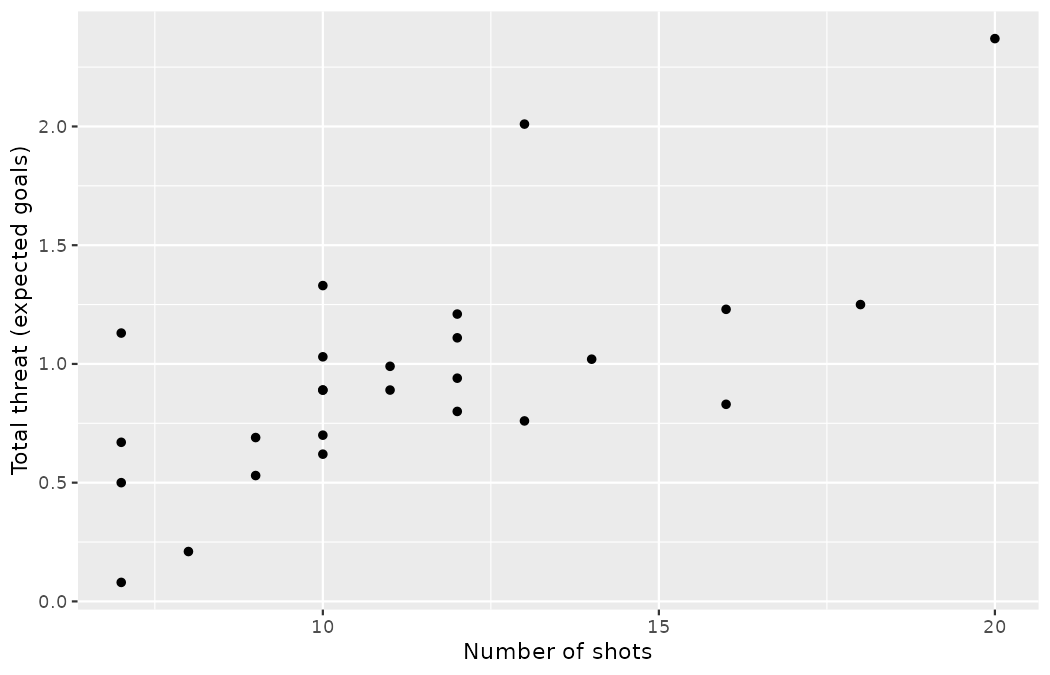
\includegraphics[width=0.85\linewidth,height=\textheight,keepaspectratio]{figures/inf-model-mlr-1.png}

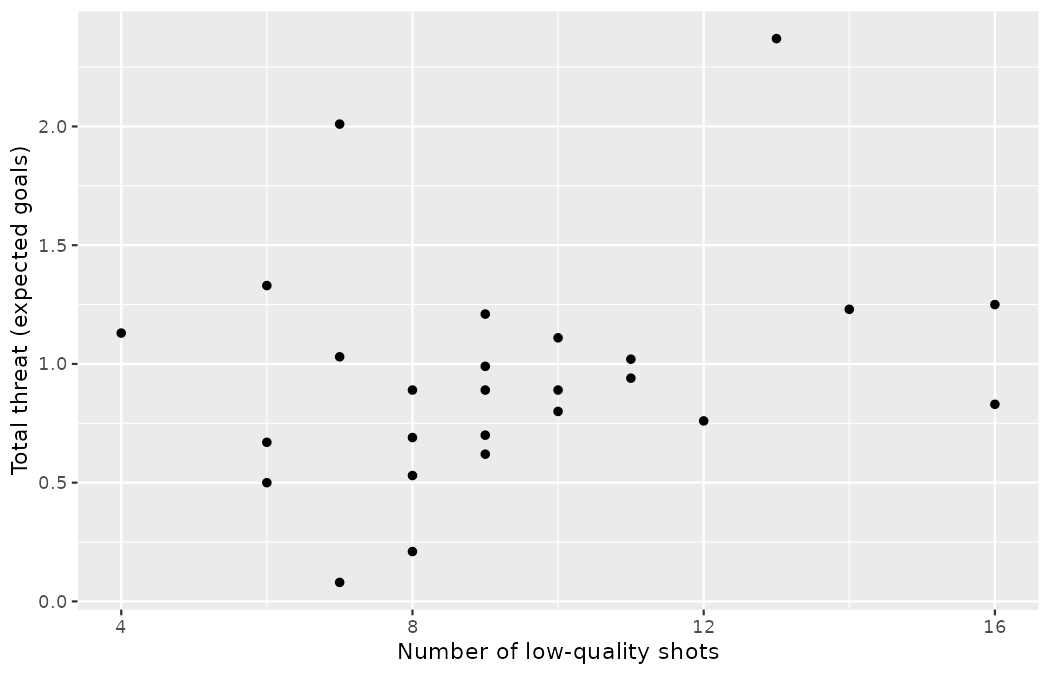
\includegraphics[width=0.85\linewidth,height=\textheight,keepaspectratio]{figures/inf-model-mlr-2.png}

The first scatterplot climbs clearly up and to the right
\((r = 0.681);\) the second is a much looser cloud \((r = 0.251).\) As
you might expect, the total threat is more strongly associated with how
many shots there were than with how many \emph{poor} shots there were.

Using the total \texttt{n\_shots} as the predictor variable, the model
output below provides the least squares estimate of the coefficient as
0.10. For every additional shot in the match log, we would predict that
the team generated 0.10 expected goals more. The \(b_1 = 0.10\)
coefficient has a small p-value associated with it, suggesting we would
not have seen data like this if \texttt{n\_shots} and
\texttt{total\_threat} were not linearly related.

\[\widehat{\texttt{total\_threat}} = -0.14 + 0.10 \times \texttt{n\_shots}\]

\begin{Shaded}
\begin{Highlighting}[]
\NormalTok{m\_threat\_shots }\OtherTok{\textless{}{-}} \FunctionTok{lm}\NormalTok{(total\_threat }\SpecialCharTok{\textasciitilde{}}\NormalTok{ n\_shots, }\AttributeTok{data =}\NormalTok{ threat26)}
\FunctionTok{tidy}\NormalTok{(m\_threat\_shots)}
\CommentTok{\#\textgreater{} \# A tibble: 2 × 5}
\CommentTok{\#\textgreater{}   term        estimate std.error statistic  p.value}
\CommentTok{\#\textgreater{}   \textless{}chr\textgreater{}          \textless{}dbl\textgreater{}     \textless{}dbl\textgreater{}     \textless{}dbl\textgreater{}    \textless{}dbl\textgreater{}}
\CommentTok{\#\textgreater{} 1 (Intercept)  {-}0.136     0.248     {-}0.546 0.590}
\CommentTok{\#\textgreater{} 2 n\_shots       0.0959    0.0211     4.55  0.000130}
\end{Highlighting}
\end{Shaded}

Using \texttt{n\_low\_quality} as the predictor variable, the model
output below provides the least squares estimate of the coefficient as
0.04. For every additional low-quality shot in the log, we would predict
0.04 expected goals more. The \(b_1 = 0.04\) coefficient has a large
p-value associated with it \((0.217),\) suggesting we could easily have
seen data like ours even if \texttt{n\_low\_quality} and
\texttt{total\_threat} were not at all linearly related.

\[\widehat{\texttt{total\_threat}} = 0.58 + 0.04 \times \texttt{n\_low\_quality}\]

\begin{Shaded}
\begin{Highlighting}[]
\NormalTok{m\_threat\_low }\OtherTok{\textless{}{-}} \FunctionTok{lm}\NormalTok{(total\_threat }\SpecialCharTok{\textasciitilde{}}\NormalTok{ n\_low\_quality, }\AttributeTok{data =}\NormalTok{ threat26)}
\FunctionTok{tidy}\NormalTok{(m\_threat\_low)}
\CommentTok{\#\textgreater{} \# A tibble: 2 × 5}
\CommentTok{\#\textgreater{}   term          estimate std.error statistic p.value}
\CommentTok{\#\textgreater{}   \textless{}chr\textgreater{}            \textless{}dbl\textgreater{}     \textless{}dbl\textgreater{}     \textless{}dbl\textgreater{}   \textless{}dbl\textgreater{}}
\CommentTok{\#\textgreater{} 1 (Intercept)     0.576     0.308       1.87  0.0738}
\CommentTok{\#\textgreater{} 2 n\_low\_quality   0.0399    0.0315      1.27  0.217}
\end{Highlighting}
\end{Shaded}

\begin{tcolorbox}[enhanced jigsaw, left=2mm, leftrule=.75mm, title=\textcolor{quarto-callout-note-color}{\faInfo}\hspace{0.5em}{Worked example}, arc=.35mm, rightrule=.15mm, coltitle=black, colframe=quarto-callout-note-color-frame, bottomrule=.15mm, colbacktitle=quarto-callout-note-color!10!white, opacitybacktitle=0.6, breakable, bottomtitle=1mm, toptitle=1mm, titlerule=0mm, opacityback=0, toprule=.15mm, colback=white]

Come up with an example of two match logs that have the same number of
low-quality shots but a number of total shots that differs by one. What
is the difference in total threat?

\begin{center}\rule{0.5\linewidth}{0.5pt}\end{center}

Take a log with one shot of each class --- 4 shots, 3 of them
low-quality, and a total threat of \(0.01 + 0.05 + 0.10 + 0.25 = 0.41.\)
Now add one more shot \emph{without changing the low-quality count}: the
added shot must be a big chance, giving 5 shots, still 3 low-quality,
and a total threat of \(0.66.\) Holding the number of low-quality shots
constant, one extra shot is necessarily one extra big chance --- worth
0.25.

\end{tcolorbox}

\begin{tcolorbox}[enhanced jigsaw, left=2mm, leftrule=.75mm, title=\textcolor{quarto-callout-note-color}{\faInfo}\hspace{0.5em}{Worked example}, arc=.35mm, rightrule=.15mm, coltitle=black, colframe=quarto-callout-note-color-frame, bottomrule=.15mm, colbacktitle=quarto-callout-note-color!10!white, opacitybacktitle=0.6, breakable, bottomtitle=1mm, toptitle=1mm, titlerule=0mm, opacityback=0, toprule=.15mm, colback=white]

Come up with an example of two match logs that have the same total
number of shots but a different number of low-quality shots. What is the
difference in total threat?

\begin{center}\rule{0.5\linewidth}{0.5pt}\end{center}

Start from the same 4-shot log (3 low-quality, total threat \(0.41\)).
Replace the big chance with a second hopeful hit: still 4 shots, but now
all 4 are low-quality, and the total threat is
\(0.01 + 0.01 + 0.05 + 0.10 = 0.17.\) Holding the number of shots
constant, one extra low-quality shot means a big chance was
\emph{swapped out} for a hopeful hit, half-chance, or decent look ---
the threat falls.

\end{tcolorbox}

Using both the total \texttt{n\_shots} and \texttt{n\_low\_quality} as
predictor variables, the model output below provides the least squares
estimates of both coefficients as 0.26 and \(-0.22.\) Now, with two
variables in the model, the interpretation is more nuanced.

\begin{itemize}
\tightlist
\item
  A coefficient interpretation always indicates a change in one variable
  while keeping the other variable(s) constant. For every additional
  shot in the log \textbf{while} \texttt{n\_low\_quality} stays
  constant, we would predict 0.26 expected goals more. Re-considering
  the phrase ``every additional shot \textbf{while} the number of
  low-quality shots stays constant'' makes us realize that each increase
  is a single additional big chance --- which is why the coefficient
  lands near the big-chance price of 0.25 (larger sample sizes would
  push \(b_1\) still closer to 0.25, because of the deterministic
  relationship described here).
\item
  For every additional low-quality shot in the log \textbf{while} the
  total \texttt{n\_shots} stays constant, we would predict 0.22 expected
  goals \emph{less}. Re-considering the phrase ``every additional
  low-quality shot \textbf{while} the total number of shots stays
  constant'' makes us realize that a big chance is being swapped out for
  a hopeful hit, half-chance, or decent look.
\end{itemize}

Considering the coefficients across the three model outputs within the
context and knowledge we have of the tally classes allows us to
understand the correlation between variables and why the signs of the
coefficients would change depending on the model: alone,
\texttt{n\_low\_quality} carries a \emph{positive} coefficient (more
low-quality shots ride along with more shots of every kind); alongside
\texttt{n\_shots}, its coefficient is \emph{negative} and strongly
discernible. Note also that the p-value for the \texttt{n\_low\_quality}
coefficient changed from 0.217 in its own model to
\(1.9 \times 10^{-11}\) in the two-variable model. It makes sense that
the variable describing \texttt{n\_low\_quality} provides more
information about \texttt{total\_threat} when it is part of a model
which also includes \texttt{n\_shots} than it does when it is used as a
single variable in a simple linear regression model: on its own it is a
muddled proxy for volume; next to the volume itself, it becomes a
precise statement about \emph{composition}.

\[
\begin{aligned}
\widehat{\texttt{total\_threat}} = 0.01 &+ 0.26 \times \texttt{n\_shots} \\
&- 0.22 \times \texttt{n\_low\_quality}
\end{aligned}
\]

\begin{Shaded}
\begin{Highlighting}[]
\NormalTok{m\_threat\_both }\OtherTok{\textless{}{-}} \FunctionTok{lm}\NormalTok{(total\_threat }\SpecialCharTok{\textasciitilde{}}\NormalTok{ n\_shots }\SpecialCharTok{+}\NormalTok{ n\_low\_quality, }\AttributeTok{data =}\NormalTok{ threat26)}
\FunctionTok{tidy}\NormalTok{(m\_threat\_both)}
\CommentTok{\#\textgreater{} \# A tibble: 3 × 5}
\CommentTok{\#\textgreater{}   term          estimate std.error statistic  p.value}
\CommentTok{\#\textgreater{}   \textless{}chr\textgreater{}            \textless{}dbl\textgreater{}     \textless{}dbl\textgreater{}     \textless{}dbl\textgreater{}    \textless{}dbl\textgreater{}}
\CommentTok{\#\textgreater{} 1 (Intercept)    0.00895    0.0943    0.0949 9.25e{-} 1}
\CommentTok{\#\textgreater{} 2 n\_shots        0.263      0.0159   16.5    2.99e{-}14}
\CommentTok{\#\textgreater{} 3 n\_low\_quality {-}0.218      0.0180  {-}12.1    1.87e{-}11}
\end{Highlighting}
\end{Shaded}

When working with multiple regression models, interpreting the model
coefficients is not always as straightforward as it was with the tally
example, where the class prices told us exactly what each swap was
worth. However, we encourage you to always think carefully about the
variables in the model, consider how they might be correlated among
themselves, and work through different models to see how using different
sets of variables might produce different relationships for predicting
the response variable of interest.

\begin{tcolorbox}[enhanced jigsaw, left=2mm, leftrule=.75mm, title=\textcolor{quarto-callout-important-color}{\faExclamation}\hspace{0.5em}{Multicollinearity}, arc=.35mm, rightrule=.15mm, coltitle=black, colframe=quarto-callout-important-color-frame, bottomrule=.15mm, colbacktitle=quarto-callout-important-color!10!white, opacitybacktitle=0.6, breakable, bottomtitle=1mm, toptitle=1mm, titlerule=0mm, opacityback=0, toprule=.15mm, colback=white]

\textbf{Multicollinearity} happens when the predictor variables are
correlated within themselves. When the predictor variables themselves
are correlated, the coefficients in a multiple regression model can be
difficult to interpret.

\end{tcolorbox}

\begin{tcolorbox}[enhanced jigsaw, left=2mm, leftrule=.75mm, title=\textcolor{quarto-callout-tip-color}{\faLightbulb}\hspace{0.5em}{Check your understanding}, arc=.35mm, rightrule=.15mm, coltitle=black, colframe=quarto-callout-tip-color-frame, bottomrule=.15mm, colbacktitle=quarto-callout-tip-color!10!white, opacitybacktitle=0.6, breakable, bottomtitle=1mm, toptitle=1mm, titlerule=0mm, opacityback=0, toprule=.15mm, colback=white]

In Chapter~\ref{sec-model-mlr}, the coefficient on \texttt{one\_on\_one}
was 0.1039 in a model by itself but 0.0872 in the full model with all
six tag variables. Using the language of this section, explain what
happened --- and state whether either number is ``wrong.''

\begin{center}\rule{0.5\linewidth}{0.5pt}\end{center}

The predictors are multicollinear: one-on-ones arise disproportionately
from counter-attacks and long balls over the top, and are finished
disproportionately with lobs, so the single-predictor coefficient
credited some of that situational value to the one-on-one tag itself.
Neither number is wrong --- they answer different conditional questions.
0.1039 is the one-on-one premium \emph{ignoring} everything else; 0.0872
is the premium \emph{given} body part, technique, pressure, possession
pattern, and minute are already in the model. Just as with the tally
data, the coefficient's meaning depends on which other variables are
held constant.

\end{tcolorbox}

Although diving into the details are beyond the scope of this text, we
will provide one more reflection about multicollinearity. If the
predictor variables have some degree of correlation, it can be quite
difficult to interpret the value of the coefficient or evaluate whether
the variable is a statistically discernible predictor of the outcome.
However, even a model that suffers from high multicollinearity will
likely lead to unbiased predictions of the response variable. So if the
task at hand is only to do prediction (and not to interpret
coefficients), multicollinearity is likely to not cause you substantial
problems --- a distinction that matters at a club, where ``what is this
team's expected threat next week?'' is a prediction task and ``does
pressing \emph{cause} worse chances?'' is emphatically not.

\section{Cross-validation for prediction
error}\label{sec-inf-mult-reg-cv}

In Section~\ref{sec-inf-mult-reg-soft}, p-values were calculated on each
of the model coefficients. The p-value gives a sense of which variables
are important to the model; however, a more extensive treatment of
variable selection is warranted in a follow-up course or textbook. Here,
we use \textbf{cross-validation} \textbf{prediction error} to focus on
which variable(s) are important for predicting the response variable of
interest. In general, linear models are also used to make predictions of
individual observations. In addition to model building, cross-validation
provides a method for generating predictions that are not overfit to the
particular dataset at hand. We continue to encourage you to take up
further study on the topic of cross-validation, as it is among the most
important ideas in modern data analysis, and we are only able to scratch
the surface here.

Cross-validation is a computational technique which removes some
observations before a model is run, then assesses the model accuracy on
the held-out sample. By removing some observations, we provide ourselves
with an independent evaluation of the model (that is, the removed
observations do not contribute to finding the parameters which minimize
the least squares equation). Cross-validation can be used in many
different ways (as an independent assessment), and here we will just
scratch the surface with respect to one way the technique can be used to
compare models.

The procedure runs as follows. The dataset is broken into \(k\)
\emph{folds} --- \(k\) non-overlapping groups of (nearly) equal size,
assigned at random, which together account for every observation exactly
once. One at a time, a model is built using the other \(k - 1\) folds,
and predictions are calculated on the single held-out fold, which is
completely independent of the model estimation. With \(k = 4\): fit on
folds 2--3--4 and predict fold 1; fit on 1--3--4 and predict fold 2; fit
on 1--2--4 and predict fold 3; fit on 1--2--3 and predict fold 4. At the
end, every shot in the dataset has received exactly one prediction, and
\emph{no shot's prediction used that shot's own data}.

One notational warning before we go on, because this book has now made
the letter \(k\) do three different jobs. In
Chapter~\ref{sec-model-mlr}, \(k\) counted the \emph{predictors} in a
regression model (as in \(n - k - 1\) degrees of freedom); in
Chapter~\ref{sec-inference-many-means}, \(k\) counted the \emph{groups}
in an ANOVA (as in \(df_G = k - 1\)); here, \(k\) counts the
\emph{folds} in a cross-validation. The three usages never appear in the
same formula, and each chapter says which is meant --- but when you read
``\(k = 4\)'' in this chapter, it is folds, not predictors and not
groups. Re-using a small pool of letters is a habit statistics shares
with football, where ``a number 6'' may be a position, a shirt, or a
squad-list slot; context disambiguates, but only if you ask.

Our goal in this section is to compare two different regression models
which both seek to predict the chance quality of a shot --- the same
task a Northbridge tag sheet faces every match. The first model predicts
\texttt{statsbomb\_xg} by using only \texttt{one\_on\_one}, the single
most informative tag of Chapter~\ref{sec-model-application}. The second
model predicts \texttt{statsbomb\_xg} by using \texttt{one\_on\_one},
\texttt{under\_pressure}, \texttt{body\_part}, \texttt{technique}, and
\texttt{play\_pattern}. (The clock variables earned their exit in
Chapter~\ref{sec-model-mlr}'s stepwise selection, and we do not
re-invite them here.)

\begin{tcolorbox}[enhanced jigsaw, left=2mm, leftrule=.75mm, title=\textcolor{quarto-callout-important-color}{\faExclamation}\hspace{0.5em}{Prediction error}, arc=.35mm, rightrule=.15mm, coltitle=black, colframe=quarto-callout-important-color-frame, bottomrule=.15mm, colbacktitle=quarto-callout-important-color!10!white, opacitybacktitle=0.6, breakable, bottomtitle=1mm, toptitle=1mm, titlerule=0mm, opacityback=0, toprule=.15mm, colback=white]

The prediction error (also previously called the \textbf{residual}) is
the difference between the observed value and the predicted value (from
the regression model).

\[\text{prediction error}_i = e_i = y_i - \hat{y}_i\]

\end{tcolorbox}

The notation is all recall --- \(e_i\), \(y_i\), and \(\hat{y}_i\) are
exactly the residual, observed value, and predicted value of
Chapter~\ref{sec-model-slr} --- but the \emph{source} of the prediction
is about to change, and that change is the entire point of this section.

\subsection{Comparing two models to predict chance
quality}\label{comparing-two-models-to-predict-chance-quality}

The question we will seek to answer is whether the predictions of
\texttt{statsbomb\_xg} are substantially better when
\texttt{one\_on\_one}, \texttt{under\_pressure}, \texttt{body\_part},
\texttt{technique}, and \texttt{play\_pattern} are used in the model, as
compared with a model on \texttt{one\_on\_one} only.

We refer to the model given with only \texttt{one\_on\_one} as the
\textbf{smaller} model. It is seen below with coefficient estimates of
the parameters as well as standard errors and p-values. We refer to the
model with all five tag variables as the \textbf{larger} model. Given
what we learned in Chapter~\ref{sec-model-application} about how weakly
the tags price a chance individually, it is \emph{not} a foregone
conclusion that all of the larger model's variables earn their place:
\texttt{one\_on\_one}, most \texttt{technique} levels, and the
counter-attack pattern carry small p-values, while
\texttt{under\_pressure} and several other levels do not --- each
p-value, as always now, conditioned on the other variables in the model.
In this section, we go beyond the p-values to consider independent
predictions of \texttt{statsbomb\_xg} as a way to compare the smaller
and larger models.

\textbf{The smaller model:}

\[
\begin{aligned}
E[\texttt{statsbomb\_xg}] &= \ \beta_0 + \beta_1 \times \texttt{one\_on\_one}\\
\widehat{\texttt{statsbomb\_xg}} &= \ 0.0896 + 0.1039 \times \texttt{one\_on\_one}\\
\end{aligned}
\]

\begin{Shaded}
\begin{Highlighting}[]
\NormalTok{m\_small }\OtherTok{\textless{}{-}} \FunctionTok{lm}\NormalTok{(statsbomb\_xg }\SpecialCharTok{\textasciitilde{}}\NormalTok{ one\_on\_one, }\AttributeTok{data =}\NormalTok{ shots\_wc)}
\FunctionTok{tidy}\NormalTok{(m\_small)}
\CommentTok{\#\textgreater{} \# A tibble: 2 × 5}
\CommentTok{\#\textgreater{}   term        estimate std.error statistic   p.value}
\CommentTok{\#\textgreater{}   \textless{}chr\textgreater{}          \textless{}dbl\textgreater{}     \textless{}dbl\textgreater{}     \textless{}dbl\textgreater{}     \textless{}dbl\textgreater{}}
\CommentTok{\#\textgreater{} 1 (Intercept)   0.0896   0.00327     27.4  5.03e{-}132}
\CommentTok{\#\textgreater{} 2 one\_on\_one    0.104    0.0141       7.35 3.36e{-} 13}
\end{Highlighting}
\end{Shaded}

\textbf{The larger model:}

\[
\begin{aligned}
E[\texttt{statsbomb\_xg}] = \beta_0 &+ \beta_1 \times \texttt{one\_on\_one} \\
&+ \beta_2 \times \texttt{under\_pressure} \\
&+ \beta_3 \times \texttt{body\_part}_{\texttt{Left Foot}} + \beta_4 \times \texttt{body\_part}_{\texttt{Head}} \\
&+ \beta_5 \times \texttt{technique}_{\texttt{Backheel}} + \cdots + \beta_{10} \times \texttt{technique}_{\texttt{Volley}} \\
&+ \beta_{11} \times \texttt{play\_pattern}_{\texttt{From Corner}} + \cdots + \beta_{17} \times \texttt{play\_pattern}_{\texttt{From Throw In}}
\end{aligned}
\]

\begin{Shaded}
\begin{Highlighting}[]
\NormalTok{m\_large }\OtherTok{\textless{}{-}} \FunctionTok{lm}\NormalTok{(}
\NormalTok{  statsbomb\_xg }\SpecialCharTok{\textasciitilde{}}\NormalTok{ one\_on\_one }\SpecialCharTok{+}\NormalTok{ under\_pressure }\SpecialCharTok{+}\NormalTok{ body\_part }\SpecialCharTok{+}\NormalTok{ technique }\SpecialCharTok{+}
\NormalTok{    play\_pattern,}
  \AttributeTok{data =}\NormalTok{ shots\_wc}
\NormalTok{)}
\FunctionTok{tidy}\NormalTok{(m\_large) }\SpecialCharTok{|\textgreater{}} \FunctionTok{print}\NormalTok{(}\AttributeTok{n =} \DecValTok{18}\NormalTok{)}
\CommentTok{\#\textgreater{} \# A tibble: 18 × 5}
\CommentTok{\#\textgreater{}    term                       estimate std.error statistic  p.value}
\CommentTok{\#\textgreater{}    \textless{}chr\textgreater{}                         \textless{}dbl\textgreater{}     \textless{}dbl\textgreater{}     \textless{}dbl\textgreater{}    \textless{}dbl\textgreater{}}
\CommentTok{\#\textgreater{}  1 (Intercept)                 0.0807    0.00664    12.1   2.67e{-}32}
\CommentTok{\#\textgreater{}  2 one\_on\_one                  0.0869    0.0144      6.05  1.91e{-} 9}
\CommentTok{\#\textgreater{}  3 under\_pressure             {-}0.00514   0.00924    {-}0.556 5.78e{-} 1}
\CommentTok{\#\textgreater{}  4 body\_partLeft Foot          0.00345   0.00722     0.478 6.33e{-} 1}
\CommentTok{\#\textgreater{}  5 body\_partHead               0.0199    0.0105      1.90  5.77e{-} 2}
\CommentTok{\#\textgreater{}  6 techniqueBackheel          {-}0.0251    0.0521     {-}0.483 6.29e{-} 1}
\CommentTok{\#\textgreater{}  7 techniqueDiving Header      0.0774    0.0322      2.40  1.63e{-} 2}
\CommentTok{\#\textgreater{}  8 techniqueHalf Volley        0.0283    0.00909     3.11  1.92e{-} 3}
\CommentTok{\#\textgreater{}  9 techniqueLob                0.137     0.0329      4.18  3.16e{-} 5}
\CommentTok{\#\textgreater{} 10 techniqueOverhead Kick     {-}0.0184    0.0441     {-}0.417 6.76e{-} 1}
\CommentTok{\#\textgreater{} 11 techniqueVolley             0.0382    0.0130      2.95  3.23e{-} 3}
\CommentTok{\#\textgreater{} 12 play\_patternFrom Corner     0.00106   0.0103      0.103 9.18e{-} 1}
\CommentTok{\#\textgreater{} 13 play\_patternFrom Counter    0.0553    0.0166      3.33  8.85e{-} 4}
\CommentTok{\#\textgreater{} 14 play\_patternFrom Free Kick {-}0.0193    0.00945    {-}2.04  4.13e{-} 2}
\CommentTok{\#\textgreater{} 15 play\_patternFrom Goal Kick  0.0145    0.0142      1.02  3.07e{-} 1}
\CommentTok{\#\textgreater{} 16 play\_patternFrom Keeper     0.0141    0.0259      0.543 5.87e{-} 1}
\CommentTok{\#\textgreater{} 17 play\_patternFrom Kick Off  {-}0.0113    0.0288     {-}0.392 6.95e{-} 1}
\CommentTok{\#\textgreater{} 18 play\_patternFrom Throw In  {-}0.0133    0.00872    {-}1.52  1.28e{-} 1}
\end{Highlighting}
\end{Shaded}

In order to compare the smaller and larger models in terms of their
\textbf{ability to predict chance quality}, we need to build models that
can provide independent predictions based on the shots in the holdout
samples created by cross-validation. To reiterate, each of the
predictions that (when combined together) will allow us to distinguish
between the smaller and larger models is independent of the data which
were used to build the model. In this example, using cross-validation,
we remove one quarter of the data before running the least squares
calculations. Then the least squares model is used to predict the
\texttt{statsbomb\_xg} of the shots in the holdout sample. Here we use a
4-fold cross-validation (meaning that one quarter of the data is removed
each time) to produce four different versions of each model (other times
it might be more appropriate to use 2-fold or 10-fold, or even to run
the model separately after removing each individual data point one at a
time). The fold assignment is random, so we seed it:

\begin{Shaded}
\begin{Highlighting}[]
\FunctionTok{set.seed}\NormalTok{(}\DecValTok{2502}\NormalTok{)}
\NormalTok{shots\_wc\_cv }\OtherTok{\textless{}{-}}\NormalTok{ shots\_wc }\SpecialCharTok{|\textgreater{}}
  \FunctionTok{mutate}\NormalTok{(}\AttributeTok{fold =} \FunctionTok{sample}\NormalTok{(}\FunctionTok{rep}\NormalTok{(}\DecValTok{1}\SpecialCharTok{:}\DecValTok{4}\NormalTok{, }\AttributeTok{length.out =} \FunctionTok{n}\NormalTok{())))}

\NormalTok{shots\_wc\_cv }\SpecialCharTok{|\textgreater{}} \FunctionTok{count}\NormalTok{(fold)}
\CommentTok{\#\textgreater{} \# A tibble: 4 × 2}
\CommentTok{\#\textgreater{}    fold     n}
\CommentTok{\#\textgreater{}   \textless{}int\textgreater{} \textless{}int\textgreater{}}
\CommentTok{\#\textgreater{} 1     1   342}
\CommentTok{\#\textgreater{} 2     2   341}
\CommentTok{\#\textgreater{} 3     3   341}
\CommentTok{\#\textgreater{} 4     4   341}
\end{Highlighting}
\end{Shaded}

To see one arm of the procedure in isolation: the code below fits the
smaller model to the 1,023 shots of folds 2, 3, and 4 --- note the
slight differences in coefficients as compared to the fit on all 1,365
shots --- after which predictions can be made on the 342 held-out shots
of fold 1.

\begin{Shaded}
\begin{Highlighting}[]
\NormalTok{m\_small\_f1 }\OtherTok{\textless{}{-}} \FunctionTok{lm}\NormalTok{(statsbomb\_xg }\SpecialCharTok{\textasciitilde{}}\NormalTok{ one\_on\_one,}
                 \AttributeTok{data =}\NormalTok{ shots\_wc\_cv }\SpecialCharTok{|\textgreater{}} \FunctionTok{filter}\NormalTok{(fold }\SpecialCharTok{!=} \DecValTok{1}\NormalTok{))}
\FunctionTok{tidy}\NormalTok{(m\_small\_f1)}
\CommentTok{\#\textgreater{} \# A tibble: 2 × 5}
\CommentTok{\#\textgreater{}   term        estimate std.error statistic   p.value}
\CommentTok{\#\textgreater{}   \textless{}chr\textgreater{}          \textless{}dbl\textgreater{}     \textless{}dbl\textgreater{}     \textless{}dbl\textgreater{}     \textless{}dbl\textgreater{}}
\CommentTok{\#\textgreater{} 1 (Intercept)   0.0883   0.00363     24.4  1.20e{-}103}
\CommentTok{\#\textgreater{} 2 one\_on\_one    0.0875   0.0156       5.60 2.81e{-}  8}
\end{Highlighting}
\end{Shaded}

Repeating the process for each holdout quarter in a loop, every shot
receives a prediction from a model that never saw it:

\begin{Shaded}
\begin{Highlighting}[]
\NormalTok{pred\_small }\OtherTok{\textless{}{-}} \FunctionTok{rep}\NormalTok{(}\ConstantTok{NA\_real\_}\NormalTok{, }\DecValTok{1365}\NormalTok{)}
\ControlFlowTok{for}\NormalTok{ (f }\ControlFlowTok{in} \DecValTok{1}\SpecialCharTok{:}\DecValTok{4}\NormalTok{) \{}
\NormalTok{  held\_out }\OtherTok{\textless{}{-}}\NormalTok{ shots\_wc\_cv}\SpecialCharTok{$}\NormalTok{fold }\SpecialCharTok{==}\NormalTok{ f}
\NormalTok{  fit }\OtherTok{\textless{}{-}} \FunctionTok{lm}\NormalTok{(statsbomb\_xg }\SpecialCharTok{\textasciitilde{}}\NormalTok{ one\_on\_one, }\AttributeTok{data =}\NormalTok{ shots\_wc\_cv[}\SpecialCharTok{!}\NormalTok{held\_out, ])}
\NormalTok{  pred\_small[held\_out] }\OtherTok{\textless{}{-}} \FunctionTok{predict}\NormalTok{(fit, }\AttributeTok{newdata =}\NormalTok{ shots\_wc\_cv[held\_out, ])}
\NormalTok{\}}

\FunctionTok{ggplot}\NormalTok{(}
\NormalTok{  shots\_wc\_cv }\SpecialCharTok{|\textgreater{}} \FunctionTok{mutate}\NormalTok{(}\AttributeTok{predicted =}\NormalTok{ pred\_small,}
                        \AttributeTok{error =}\NormalTok{ statsbomb\_xg }\SpecialCharTok{{-}}\NormalTok{ predicted),}
  \FunctionTok{aes}\NormalTok{(}\AttributeTok{x =}\NormalTok{ predicted, }\AttributeTok{y =}\NormalTok{ error)}
\NormalTok{) }\SpecialCharTok{+}
  \FunctionTok{geom\_point}\NormalTok{(}\AttributeTok{alpha =} \FloatTok{0.3}\NormalTok{) }\SpecialCharTok{+}
  \FunctionTok{geom\_hline}\NormalTok{(}\AttributeTok{yintercept =} \DecValTok{0}\NormalTok{) }\SpecialCharTok{+}
  \FunctionTok{geom\_hline}\NormalTok{(}\AttributeTok{yintercept =} \FloatTok{0.1}\NormalTok{, }\AttributeTok{lty =} \DecValTok{2}\NormalTok{, }\AttributeTok{color =} \StringTok{"grey"}\NormalTok{) }\SpecialCharTok{+}
  \FunctionTok{geom\_hline}\NormalTok{(}\AttributeTok{yintercept =} \SpecialCharTok{{-}}\FloatTok{0.1}\NormalTok{, }\AttributeTok{lty =} \DecValTok{2}\NormalTok{, }\AttributeTok{color =} \StringTok{"grey"}\NormalTok{) }\SpecialCharTok{+}
  \FunctionTok{facet\_wrap}\NormalTok{(}\SpecialCharTok{\textasciitilde{}}\NormalTok{fold) }\SpecialCharTok{+}
  \FunctionTok{labs}\NormalTok{(}
    \AttributeTok{x =} \StringTok{"Predicted chance quality"}\NormalTok{,}
    \AttributeTok{y =} \StringTok{"Prediction error"}
\NormalTok{  )}
\end{Highlighting}
\end{Shaded}

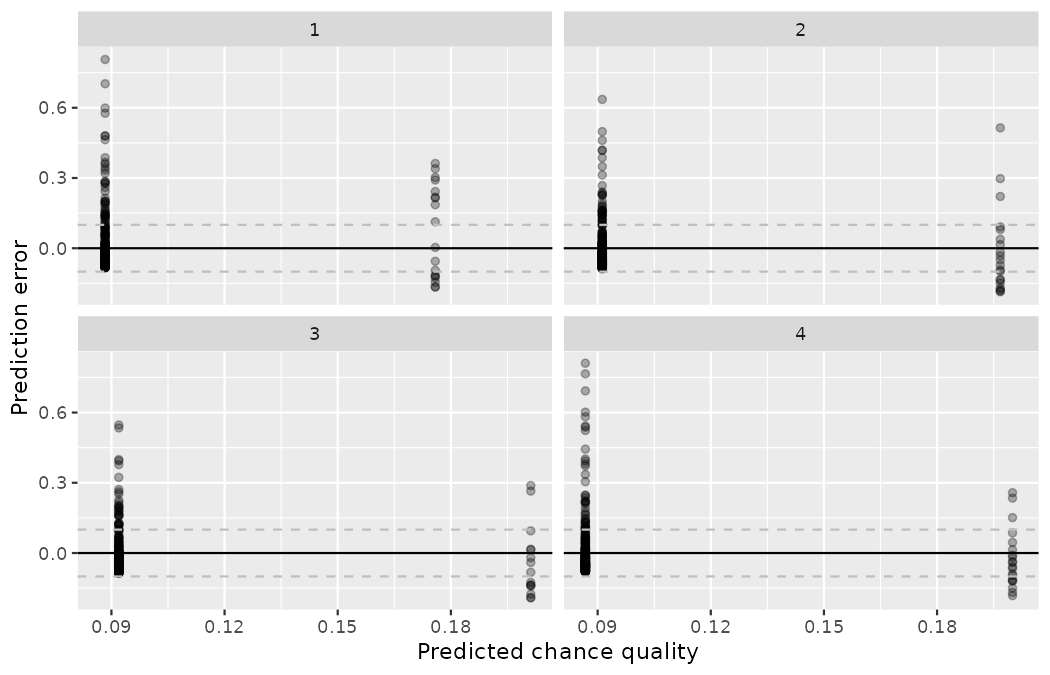
\includegraphics[width=0.85\linewidth,height=\textheight,keepaspectratio]{figures/inf-model-mlr-3.png}

The plot shows four panels, one per held-out quarter. Because the
smaller model's only predictor is a two-level tag, each panel is two
vertical strips --- the ordinary shots near a predicted value of 0.09
and the one-on-ones between 0.18 and 0.20 --- exactly the geometry you
saw in Chapter~\ref{sec-model-application}'s residual plot for this
model. In every panel the errors are centered around zero, which shows
the independent predictions are not systematically biased; about 86\% of
them fall within the dashed \(\pm 0.1\) band, but the upper tail
straggles to \(+0.81\) --- point-blank chances the tag cannot see ---
while the floor at \(-\hat{y}_i\) (chance quality cannot be negative)
cuts the errors off at \(-0.19.\)

The cross-validation SSE is the sum of squared error associated with the
predictions. Let \(\hat{y}_{cv,i}\) be the prediction for the \(i^{th}\)
observation where the \(i^{th}\) observation was in the hold-out fold
and the other three folds were used to create the linear model. This
symbol is new, so decompose it before using it. The base \(\hat{y}\) is
the familiar predicted value of Chapter~\ref{sec-model-slr} --- the hat,
as always, marking a quantity estimated from data. The first subscript,
\(cv\), records \emph{how} the prediction was produced: by a
cross-validation fit, one which never saw observation \(i\). The second
subscript, \(i\), indexes which observation was predicted, exactly as in
\(y_i\). Read \(\hat{y}_{cv,i}\) as: ``the model's prediction for
observation \(i\), made without observation \(i\).'' The comma merely
separates the two subscripts; nothing is being multiplied or conditioned
inside them. For the model using only \texttt{one\_on\_one} to predict
\texttt{statsbomb\_xg}, the CV SSE is 18.91:

\begin{Shaded}
\begin{Highlighting}[]
\FunctionTok{sum}\NormalTok{((pred\_small }\SpecialCharTok{{-}}\NormalTok{ shots\_wc\_cv}\SpecialCharTok{$}\NormalTok{statsbomb\_xg)}\SpecialCharTok{\^{}}\DecValTok{2}\NormalTok{)}
\CommentTok{\#\textgreater{} [1] 18.90923}
\end{Highlighting}
\end{Shaded}

\begin{tcolorbox}[enhanced jigsaw, left=2mm, leftrule=.75mm, title=\textcolor{quarto-callout-important-color}{\faExclamation}\hspace{0.5em}{Cross-validation SSE}, arc=.35mm, rightrule=.15mm, coltitle=black, colframe=quarto-callout-important-color-frame, bottomrule=.15mm, colbacktitle=quarto-callout-important-color!10!white, opacitybacktitle=0.6, breakable, bottomtitle=1mm, toptitle=1mm, titlerule=0mm, opacityback=0, toprule=.15mm, colback=white]

The prediction error from the cross-validated model can be used to
calculate a single numerical summary of the model. The cross-validation
SSE is the sum of squared cross-validation prediction errors.

\[\mbox{CV SSE} = \sum_{i=1}^n (\hat{y}_{cv,i} - y_i)^2\]

Each piece is familiar: \(\Sigma\) sums over all \(n\) observations
(Chapter~\ref{sec-explore-numerical}), and each term squares a
prediction error, just as in the SSE of Chapter~\ref{sec-model-slr}.
What distinguishes CV SSE from the ordinary SSE is \emph{which}
prediction sits inside the parentheses: \(\hat{y}_{cv,i}\) comes from a
model fit without observation \(i\)'s fold, so no observation gets to
flatter a model that was tuned to it.

\end{tcolorbox}

\begin{tcolorbox}[enhanced jigsaw, left=2mm, leftrule=.75mm, title=\textcolor{quarto-callout-tip-color}{\faLightbulb}\hspace{0.5em}{Check your understanding}, arc=.35mm, rightrule=.15mm, coltitle=black, colframe=quarto-callout-tip-color-frame, bottomrule=.15mm, colbacktitle=quarto-callout-tip-color!10!white, opacitybacktitle=0.6, breakable, bottomtitle=1mm, toptitle=1mm, titlerule=0mm, opacityback=0, toprule=.15mm, colback=white]

The first three shots of fold 1 have observed chance qualities
\(0.062,\) \(0.070,\) and \(0.112,\) and none is a one-on-one, so the
fold-1 smaller model predicts \(\hat{y}_{cv,i} = 0.0883\) for all three.
Compute these three shots' contribution to the CV SSE.

\begin{center}\rule{0.5\linewidth}{0.5pt}\end{center}

\((0.0883 - 0.062)^2 + (0.0883 - 0.070)^2 + (0.0883 - 0.112)^2 \approx 0.000715 + 0.000340 + 0.000576 \approx 0.0016.\)
Summing such terms over all 1,365 shots --- each predicted by the model
that excluded its fold --- gives the CV SSE of 18.91.

\end{tcolorbox}

The same process is repeated for the larger number of explanatory
variables --- the same seeded folds, so the two models face identical
holdout samples.

\begin{Shaded}
\begin{Highlighting}[]
\NormalTok{pred\_large }\OtherTok{\textless{}{-}} \FunctionTok{rep}\NormalTok{(}\ConstantTok{NA\_real\_}\NormalTok{, }\DecValTok{1365}\NormalTok{)}
\ControlFlowTok{for}\NormalTok{ (f }\ControlFlowTok{in} \DecValTok{1}\SpecialCharTok{:}\DecValTok{4}\NormalTok{) \{}
\NormalTok{  held\_out }\OtherTok{\textless{}{-}}\NormalTok{ shots\_wc\_cv}\SpecialCharTok{$}\NormalTok{fold }\SpecialCharTok{==}\NormalTok{ f}
\NormalTok{  fit }\OtherTok{\textless{}{-}} \FunctionTok{lm}\NormalTok{(}
\NormalTok{    statsbomb\_xg }\SpecialCharTok{\textasciitilde{}}\NormalTok{ one\_on\_one }\SpecialCharTok{+}\NormalTok{ under\_pressure }\SpecialCharTok{+}\NormalTok{ body\_part }\SpecialCharTok{+}\NormalTok{ technique }\SpecialCharTok{+}
\NormalTok{      play\_pattern,}
    \AttributeTok{data =}\NormalTok{ shots\_wc\_cv[}\SpecialCharTok{!}\NormalTok{held\_out, ]}
\NormalTok{  )}
\NormalTok{  pred\_large[held\_out] }\OtherTok{\textless{}{-}} \FunctionTok{predict}\NormalTok{(fit, }\AttributeTok{newdata =}\NormalTok{ shots\_wc\_cv[held\_out, ])}
\NormalTok{\}}

\FunctionTok{sum}\NormalTok{((pred\_large }\SpecialCharTok{{-}}\NormalTok{ shots\_wc\_cv}\SpecialCharTok{$}\NormalTok{statsbomb\_xg)}\SpecialCharTok{\^{}}\DecValTok{2}\NormalTok{)}
\CommentTok{\#\textgreater{} [1] 18.5571}
\end{Highlighting}
\end{Shaded}

The corresponding residual plot for the larger model (built with the
same code as before, swapping in \texttt{pred\_large}) replaces the two
strips with a proper cloud --- predictions now spread from about 0.03 to
0.31 --- but its vertical scatter is barely distinguishable from the
smaller model's: about 85\% of errors within \(\pm 0.1,\) an upper tail
reaching \(+0.82.\)

For the model using all five tags to predict \texttt{statsbomb\_xg}, the
CV SSE is 18.56 (as compared to a CV SSE of 18.91 for the smaller
model). Consistent with visually comparing the two sets of residual
plots, the sum of squared prediction errors is smaller for the model
which uses more predictor variables --- but read the magnitude honestly,
as this book has trained you to: the larger model's independent
predictions are better by about 2\%, not by the factor of five a naive
reading of ``sixteen extra coefficients'' might hope for. The larger
model is the better model according to the cross-validated prediction
error criteria, and the criteria deserve credit for the \emph{size} of
the verdict as well as its direction: most of what prices a chance is
where on the pitch it is taken from, no arrangement of stand-side tags
can substitute for coordinates, and cross-validation says so in a single
number. Two further quantities complete the picture. The larger model's
\emph{in-sample} SSE --- its residuals on the very shots it was fit to
--- is 18.01, noticeably smaller than its CV SSE of 18.56; the smaller
model's in-sample SSE, 18.81, is nearly identical to its CV SSE of
18.91. A gap between in-sample and cross-validated error is the
signature of a model flattering itself, and it widens as models grow.

\subsection{Validating on a second
tournament}\label{validating-on-a-second-tournament}

Cross-validation holds out shots, but every fold still comes from the
same tournament: the same teams, the same ball, the same vintage of
StatsBomb's own pricing model. Chapter~\ref{sec-model-application} ended
with a prediction that went badly wrong precisely because a model fit on
the 2022 Men's World Cup was applied, unexamined, to a shot from the
2025 Women's Euro --- and it promised that \emph{external validation}
would make that examination formal. The club has a second tournament in
its files, so the promise is cheap to keep: fit both models on all 1,365
World Cup shots, then predict every shot of the Women's Euro --- a
holdout not of one quarter of the data, but of an entire competition. We
build the Euro frame with the same filters and the same code as
\texttt{shots\_wc}, so the two frames differ only in which tournament
they hold:

\begin{Shaded}
\begin{Highlighting}[]
\NormalTok{weuro2025\_shots }\OtherTok{\textless{}{-}} \FunctionTok{read\_csv}\NormalTok{(}\StringTok{"data/derived/weuro2025\_shots.csv"}\NormalTok{)}

\NormalTok{shots\_we }\OtherTok{\textless{}{-}}\NormalTok{ weuro2025\_shots }\SpecialCharTok{|\textgreater{}}
  \FunctionTok{filter}\NormalTok{(}
\NormalTok{    shot\_type }\SpecialCharTok{==} \StringTok{"Open Play"}\NormalTok{,}
\NormalTok{    body\_part }\SpecialCharTok{!=} \StringTok{"Other"}\NormalTok{,}
\NormalTok{    play\_pattern }\SpecialCharTok{!=} \StringTok{"Other"}
\NormalTok{  ) }\SpecialCharTok{|\textgreater{}}
  \FunctionTok{mutate}\NormalTok{(}
    \AttributeTok{body\_part =} \FunctionTok{factor}\NormalTok{(body\_part, }\AttributeTok{levels =} \FunctionTok{c}\NormalTok{(}\StringTok{"Right Foot"}\NormalTok{, }\StringTok{"Left Foot"}\NormalTok{, }\StringTok{"Head"}\NormalTok{)),}
    \AttributeTok{technique =} \FunctionTok{relevel}\NormalTok{(}\FunctionTok{factor}\NormalTok{(technique), }\AttributeTok{ref =} \StringTok{"Normal"}\NormalTok{),}
    \AttributeTok{play\_pattern =} \FunctionTok{relevel}\NormalTok{(}\FunctionTok{factor}\NormalTok{(play\_pattern), }\AttributeTok{ref =} \StringTok{"Regular Play"}\NormalTok{),}
    \AttributeTok{under\_pressure =} \FunctionTok{if\_else}\NormalTok{(under\_pressure, }\DecValTok{1}\NormalTok{, }\DecValTok{0}\NormalTok{),}
    \AttributeTok{one\_on\_one =} \FunctionTok{if\_else}\NormalTok{(one\_on\_one, }\DecValTok{1}\NormalTok{, }\DecValTok{0}\NormalTok{)}
\NormalTok{  ) }\SpecialCharTok{|\textgreater{}}
  \FunctionTok{select}\NormalTok{(}
\NormalTok{    statsbomb\_xg, body\_part, technique, under\_pressure,}
\NormalTok{    one\_on\_one, play\_pattern, minute}
\NormalTok{  )}

\FunctionTok{nrow}\NormalTok{(shots\_we)}
\CommentTok{\#\textgreater{} [1] 844}
\end{Highlighting}
\end{Shaded}

The models \texttt{m\_small} and \texttt{m\_large} were fit on the full
World Cup frame and have never touched these 844 shots. The
external-validation SSE is computed exactly like a CV SSE --- a sum of
squared independent prediction errors --- with the Euro playing the role
of one giant held-out fold:

\begin{Shaded}
\begin{Highlighting}[]
\NormalTok{pred\_we\_small }\OtherTok{\textless{}{-}} \FunctionTok{predict}\NormalTok{(m\_small, }\AttributeTok{newdata =}\NormalTok{ shots\_we)}
\NormalTok{pred\_we\_large }\OtherTok{\textless{}{-}} \FunctionTok{predict}\NormalTok{(m\_large, }\AttributeTok{newdata =}\NormalTok{ shots\_we)}

\FunctionTok{c}\NormalTok{(}
  \AttributeTok{small =} \FunctionTok{sum}\NormalTok{((pred\_we\_small }\SpecialCharTok{{-}}\NormalTok{ shots\_we}\SpecialCharTok{$}\NormalTok{statsbomb\_xg)}\SpecialCharTok{\^{}}\DecValTok{2}\NormalTok{),}
  \AttributeTok{large =} \FunctionTok{sum}\NormalTok{((pred\_we\_large }\SpecialCharTok{{-}}\NormalTok{ shots\_we}\SpecialCharTok{$}\NormalTok{statsbomb\_xg)}\SpecialCharTok{\^{}}\DecValTok{2}\NormalTok{)}
\NormalTok{)}
\CommentTok{\#\textgreater{}    small    large}
\CommentTok{\#\textgreater{} 10.12302 10.53733}
\end{Highlighting}
\end{Shaded}

The order has \emph{reversed}: on the external holdout, the smaller
model out-predicts the larger one. Because the two comparisons involve
different numbers of shots (1,365 cross-validated, 844 held out), put
them on a per-shot scale before comparing:

\begin{Shaded}
\begin{Highlighting}[]
\FunctionTok{tibble}\NormalTok{(}
  \AttributeTok{model =} \FunctionTok{c}\NormalTok{(}\StringTok{"small"}\NormalTok{, }\StringTok{"large"}\NormalTok{),}
  \AttributeTok{cv\_mse\_wc =} \FunctionTok{c}\NormalTok{(}
    \FunctionTok{mean}\NormalTok{((pred\_small }\SpecialCharTok{{-}}\NormalTok{ shots\_wc\_cv}\SpecialCharTok{$}\NormalTok{statsbomb\_xg)}\SpecialCharTok{\^{}}\DecValTok{2}\NormalTok{),}
    \FunctionTok{mean}\NormalTok{((pred\_large }\SpecialCharTok{{-}}\NormalTok{ shots\_wc\_cv}\SpecialCharTok{$}\NormalTok{statsbomb\_xg)}\SpecialCharTok{\^{}}\DecValTok{2}\NormalTok{)}
\NormalTok{  ),}
  \AttributeTok{holdout\_mse\_weuro =} \FunctionTok{c}\NormalTok{(}
    \FunctionTok{mean}\NormalTok{((pred\_we\_small }\SpecialCharTok{{-}}\NormalTok{ shots\_we}\SpecialCharTok{$}\NormalTok{statsbomb\_xg)}\SpecialCharTok{\^{}}\DecValTok{2}\NormalTok{),}
    \FunctionTok{mean}\NormalTok{((pred\_we\_large }\SpecialCharTok{{-}}\NormalTok{ shots\_we}\SpecialCharTok{$}\NormalTok{statsbomb\_xg)}\SpecialCharTok{\^{}}\DecValTok{2}\NormalTok{)}
\NormalTok{  )}
\NormalTok{)}
\CommentTok{\#\textgreater{} \# A tibble: 2 × 3}
\CommentTok{\#\textgreater{}   model cv\_mse\_wc holdout\_mse\_weuro}
\CommentTok{\#\textgreater{}   \textless{}chr\textgreater{}     \textless{}dbl\textgreater{}             \textless{}dbl\textgreater{}}
\CommentTok{\#\textgreater{} 1 small    0.0139            0.0120}
\CommentTok{\#\textgreater{} 2 large    0.0136            0.0125}
\end{Highlighting}
\end{Shaded}

Within the World Cup, the larger model wins narrowly; across
tournaments, it loses. The sixteen extra coefficients bought a 2\%
improvement at home and gave back more than that abroad, because some of
what they learned was not football --- it was \emph{that tournament}.
One coefficient makes the mechanism concrete. The World Cup's 13
open-play lobs averaged a chance quality of 0.251 --- think of the
delicate finishes over stranded goalkeepers that tournament served up
--- so the larger model learned a lob premium of \(+0.137\) and duly
predicts around \(0.23\) for a lobbed chance. The Women's Euro also
produced exactly 13 open-play lobs, and they averaged \(0.053\): mostly
hopeful chips from distance. The smaller model, knowing nothing of
technique, predicts \(0.09\) for those same shots and misses them by far
less. A pattern estimated from 13 shots in one competition is not a law
of the game, and external validation is the instrument that catches the
difference. Note also, with some satisfaction, that both per-shot errors
are \emph{lower} on the Euro than at home --- the Euro's open-play
chance qualities happen to be slightly easier to predict --- which is a
useful reminder that external validation measures transfer, not
difficulty ranking.

\begin{tcolorbox}[enhanced jigsaw, left=2mm, leftrule=.75mm, title=\textcolor{quarto-callout-tip-color}{\faLightbulb}\hspace{0.5em}{Check your understanding}, arc=.35mm, rightrule=.15mm, coltitle=black, colframe=quarto-callout-tip-color-frame, bottomrule=.15mm, colbacktitle=quarto-callout-tip-color!10!white, opacitybacktitle=0.6, breakable, bottomtitle=1mm, toptitle=1mm, titlerule=0mm, opacityback=0, toprule=.15mm, colback=white]

The larger model beat the smaller model under 4-fold cross-validation on
the World Cup, yet lost to it on the Women's Euro holdout. Explain how
both results can be correct, and what each one is evidence about.

\begin{center}\rule{0.5\linewidth}{0.5pt}\end{center}

Cross-validation holds out \emph{shots} but not the \emph{competition}:
all four folds share the World Cup's teams, styles, and pricing vintage,
so patterns specific to that tournament (like its high-value lobs) help
predict its own held-out folds. The CV comparison is therefore evidence
about predicting \emph{more shots like these} --- and there, the extra
tags add a little. The external comparison is evidence about predicting
shots from a \emph{different} competition, where tournament-specific
patterns become liabilities rather than assets. Both numbers are correct
answers to different questions, and a scouting department that quotes a
model across competitions --- Marta's stated ambition since
Chapter~\ref{sec-model-mlr} --- must weigh the second question at least
as heavily as the first.

\end{tcolorbox}

We have provided a very brief overview to and example of using
cross-validation, and of its sterner sibling, validation against a
genuinely external dataset. Cross-validation is a computational approach
to model building and model validation as an alternative to reliance on
p-values. While p-values have a role to play in understanding model
coefficients, throughout this text, we have continued to present
computational methods that broaden statistical approaches to data
analysis. Cross-validation will be used again in
Chapter~\ref{sec-inf-model-logistic} with logistic regression --- where
the response is whether the shot went in, and the club's shortlist
depends on the answer. We encourage you to consider both standard
inferential methods (such as p-values) and computational approaches
(such as cross-validation) as you build and use multivariable models of
all varieties.

\section{Chapter review}\label{sec-chp25-review}

\subsection{Summary}\label{summary-24}

Building on the modeling ideas from Chapter~\ref{sec-model-mlr}, we have
now introduced methods for evaluating coefficients (based on p-values)
and evaluating models (cross-validation). The p-value attached to each
coefficient in a multiple regression assesses a \emph{conditional} claim
--- \(H_0: \beta_i = 0\) given the other variables in the model --- and
our three-tag model showed the full range of verdicts a single output
can hold, from \texttt{one\_on\_one}'s \(3.1 \times 10^{-13}\) to
\texttt{under\_pressure}'s \(0.991.\) There are many important aspects
to consider when working with multiple variables in a single model, and
we have only glanced at a few topics. Remember, multicollinearity can
make coefficient interpretation difficult: the tally-sheet threat data
showed a predictor whose coefficient was positive alone and negative ---
and far more discernible --- once its partner entered the model.
Cross-validation replaced in-sample flattery with independent
predictions, summarized by the CV SSE, and the external check on a
second tournament sharpened the lesson: a model can win at home and lose
abroad, because some of what it learns is the tournament rather than the
game. A topic not covered in this text but important for multiple
regression models is interaction, and we hope that you learn more about
how variables work together as you continue to build up your modeling
skills.

\subsection{Terms}\label{terms-24}

The terms introduced in this chapter are presented below, alphabetized.
If you're not sure what some of these terms mean, we recommend you go
back in the text and review their definitions. You should be able to
easily spot them as \textbf{bolded text}.

\begin{longtable}[]{@{}
  >{\raggedright\arraybackslash}p{(\linewidth - 4\tabcolsep) * \real{0.3380}}
  >{\raggedright\arraybackslash}p{(\linewidth - 4\tabcolsep) * \real{0.3380}}
  >{\raggedright\arraybackslash}p{(\linewidth - 4\tabcolsep) * \real{0.3239}}@{}}
\caption{Terms introduced in this
chapter.}\label{tbl-terms-chp-25}\tabularnewline
\toprule\noalign{}
\endfirsthead
\endhead
\bottomrule\noalign{}
\endlastfoot
cross-validation & multicollinearity & prediction error \\
inference on multiple linear regression & multiple predictors &
predictor \\
\end{longtable}

\section{Exercises}\label{sec-chp25-exercises}

Answers to odd-numbered exercises can be found in
Appendix~\ref{sec-exercise-solutions-25}.

\begin{enumerate}
\def\labelenumi{\arabic{enumi}.}
\item
  \textbf{Scout certification, mathematical interval.} At the end of
  Northbridge United's scout-certification course, Priya Rao surveyed
  the 55 trainees about their weekly hours of video study
  (\texttt{video\_hours}), hours of sleep per night
  (\texttt{sleepnight}), and the number of live matches they attend per
  week, recorded as the indicator \texttt{live\_mt2} (\texttt{1} if the
  trainee attends more than two live matches a week, and \texttt{0}
  otherwise). We use these data to build a model predicting the final
  certification assessment (\texttt{assessment}, scored 0--100) from the
  other variables. This is a constructed scenario, built by the seeded
  code below; a summary of the model follows.\footnote{The
    \texttt{trainee55} data are a constructed scouting scenario,
    generated entirely by the seeded code shown; no real trainees were
    surveyed.}

\begin{Shaded}
\begin{Highlighting}[]
\FunctionTok{set.seed}\NormalTok{(}\DecValTok{2503}\NormalTok{)}
\NormalTok{trainee55 }\OtherTok{\textless{}{-}} \FunctionTok{tibble}\NormalTok{(}
  \AttributeTok{video\_hours =} \FunctionTok{round}\NormalTok{(}\FunctionTok{pmax}\NormalTok{(}\FunctionTok{rnorm}\NormalTok{(}\DecValTok{55}\NormalTok{, }\AttributeTok{mean =} \DecValTok{14}\NormalTok{, }\AttributeTok{sd =} \DecValTok{5}\NormalTok{), }\DecValTok{2}\NormalTok{), }\DecValTok{1}\NormalTok{),}
  \AttributeTok{matches     =} \FunctionTok{rpois}\NormalTok{(}\DecValTok{55}\NormalTok{, }\AttributeTok{lambda =} \DecValTok{2}\NormalTok{),}
  \AttributeTok{sleepnight  =} \FunctionTok{round}\NormalTok{(}\FunctionTok{pmin}\NormalTok{(}\FunctionTok{pmax}\NormalTok{(}\FunctionTok{rnorm}\NormalTok{(}\DecValTok{55}\NormalTok{, }\AttributeTok{mean =} \DecValTok{7} \SpecialCharTok{{-}} \FloatTok{0.3} \SpecialCharTok{*}\NormalTok{ matches, }\AttributeTok{sd =} \FloatTok{0.9}\NormalTok{), }\FloatTok{4.5}\NormalTok{), }\FloatTok{9.5}\NormalTok{), }\DecValTok{1}\NormalTok{),}
  \AttributeTok{live\_mt2    =} \FunctionTok{if\_else}\NormalTok{(matches }\SpecialCharTok{\textgreater{}} \DecValTok{2}\NormalTok{, }\DecValTok{1}\NormalTok{, }\DecValTok{0}\NormalTok{),}
  \AttributeTok{assessment  =} \FunctionTok{round}\NormalTok{(}\DecValTok{58} \SpecialCharTok{+} \FloatTok{0.15} \SpecialCharTok{*}\NormalTok{ video\_hours }\SpecialCharTok{+} \FloatTok{0.8} \SpecialCharTok{*}\NormalTok{ sleepnight }\SpecialCharTok{+}
                        \DecValTok{2} \SpecialCharTok{*}\NormalTok{ live\_mt2 }\SpecialCharTok{+} \FunctionTok{rnorm}\NormalTok{(}\DecValTok{55}\NormalTok{, }\AttributeTok{mean =} \DecValTok{0}\NormalTok{, }\AttributeTok{sd =} \DecValTok{8}\NormalTok{))}
\NormalTok{)}

\NormalTok{m\_cert }\OtherTok{\textless{}{-}} \FunctionTok{lm}\NormalTok{(assessment }\SpecialCharTok{\textasciitilde{}}\NormalTok{ video\_hours }\SpecialCharTok{+}\NormalTok{ sleepnight }\SpecialCharTok{+}\NormalTok{ live\_mt2,}
             \AttributeTok{data =}\NormalTok{ trainee55)}
\FunctionTok{tidy}\NormalTok{(m\_cert)}
\CommentTok{\#\textgreater{} \# A tibble: 4 × 5}
\CommentTok{\#\textgreater{}   term        estimate std.error statistic  p.value}
\CommentTok{\#\textgreater{}   \textless{}chr\textgreater{}          \textless{}dbl\textgreater{}     \textless{}dbl\textgreater{}     \textless{}dbl\textgreater{}    \textless{}dbl\textgreater{}}
\CommentTok{\#\textgreater{} 1 (Intercept)   53.5       7.09      7.55  7.44e{-}10}
\CommentTok{\#\textgreater{} 2 video\_hours    0.388     0.222     1.75  8.69e{-} 2}
\CommentTok{\#\textgreater{} 3 sleepnight     0.775     0.913     0.849 4.00e{-} 1}
\CommentTok{\#\textgreater{} 4 live\_mt2       3.31      2.40      1.38  1.74e{-} 1}
\end{Highlighting}
\end{Shaded}

  \begin{enumerate}
  \def\labelenumii{\alph{enumii}.}
  \item
    Calculate a 95\% confidence interval for the coefficient of
    \texttt{live\_mt2} (attends more than two live matches a week) in
    the model, and interpret it in the context of the data. (With
    \(n = 55\) observations and \(k = 3\) predictors, use
    \(t^\star_{51} = 2.01.\))
  \item
    Would you expect a 95\% confidence interval for the slope of the
    remaining variables to include 0? Explain your reasoning.
  \end{enumerate}
\item
  \textbf{Matchday chance creation.} For each of the 31 matches of the
  2025 Women's Euro, a Northbridge analyst tallies the number of
  open-play shots in the match (both teams combined) and the total
  chance quality those shots carried. The frame is open play only ---
  penalties, fixed by law near 0.78, would otherwise ride along in the
  totals. Three plots are drawn by the code below: a scatterplot showing
  the relationship between the two variables along with the least
  squares fit, a residuals plot, and a histogram of
  residuals.\footnote{The 2025 Women's Euro shot data used in this
    exercise are in \texttt{data/derived/weuro2025\_shots.csv}
    (StatsBomb open data).}

\begin{Shaded}
\begin{Highlighting}[]
\NormalTok{weuro2025\_shots }\OtherTok{\textless{}{-}} \FunctionTok{read\_csv}\NormalTok{(}\StringTok{"data/derived/weuro2025\_shots.csv"}\NormalTok{)}

\NormalTok{match\_we }\OtherTok{\textless{}{-}}\NormalTok{ weuro2025\_shots }\SpecialCharTok{|\textgreater{}}
  \FunctionTok{filter}\NormalTok{(shot\_type }\SpecialCharTok{==} \StringTok{"Open Play"}\NormalTok{) }\SpecialCharTok{|\textgreater{}}
  \FunctionTok{group\_by}\NormalTok{(match\_id) }\SpecialCharTok{|\textgreater{}}
  \FunctionTok{summarize}\NormalTok{(}
    \AttributeTok{n\_shots =} \FunctionTok{n}\NormalTok{(),}
    \AttributeTok{total\_xg =} \FunctionTok{sum}\NormalTok{(statsbomb\_xg),}
    \AttributeTok{.groups =} \StringTok{"drop"}
\NormalTok{  )}

\NormalTok{m\_matchday }\OtherTok{\textless{}{-}} \FunctionTok{lm}\NormalTok{(total\_xg }\SpecialCharTok{\textasciitilde{}}\NormalTok{ n\_shots, }\AttributeTok{data =}\NormalTok{ match\_we)}
\FunctionTok{tidy}\NormalTok{(m\_matchday)}
\CommentTok{\#\textgreater{} \# A tibble: 2 × 5}
\CommentTok{\#\textgreater{}   term        estimate std.error statistic p.value}
\CommentTok{\#\textgreater{}   \textless{}chr\textgreater{}          \textless{}dbl\textgreater{}     \textless{}dbl\textgreater{}     \textless{}dbl\textgreater{}   \textless{}dbl\textgreater{}}
\CommentTok{\#\textgreater{} 1 (Intercept)   0.206     0.756      0.273 0.787}
\CommentTok{\#\textgreater{} 2 n\_shots       0.0899    0.0270     3.32  0.00241}

\NormalTok{m\_aug }\OtherTok{\textless{}{-}} \FunctionTok{augment}\NormalTok{(m\_matchday)}

\NormalTok{p\_1 }\OtherTok{\textless{}{-}} \FunctionTok{ggplot}\NormalTok{(match\_we, }\FunctionTok{aes}\NormalTok{(}\AttributeTok{x =}\NormalTok{ n\_shots, }\AttributeTok{y =}\NormalTok{ total\_xg)) }\SpecialCharTok{+}
  \FunctionTok{geom\_smooth}\NormalTok{(}\AttributeTok{method =} \StringTok{"lm"}\NormalTok{, }\AttributeTok{se =} \ConstantTok{FALSE}\NormalTok{, }\AttributeTok{color =} \StringTok{"darkgray"}\NormalTok{) }\SpecialCharTok{+}
  \FunctionTok{geom\_point}\NormalTok{(}\AttributeTok{size =} \DecValTok{3}\NormalTok{, }\AttributeTok{alpha =} \FloatTok{0.6}\NormalTok{) }\SpecialCharTok{+}
  \FunctionTok{labs}\NormalTok{(}\AttributeTok{x =} \StringTok{"Open{-}play shots in match"}\NormalTok{, }\AttributeTok{y =} \StringTok{"Total chance quality (xG)"}\NormalTok{)}

\NormalTok{p\_2 }\OtherTok{\textless{}{-}} \FunctionTok{ggplot}\NormalTok{(m\_aug, }\FunctionTok{aes}\NormalTok{(}\AttributeTok{x =}\NormalTok{ .fitted, }\AttributeTok{y =}\NormalTok{ .resid)) }\SpecialCharTok{+}
  \FunctionTok{geom\_hline}\NormalTok{(}\AttributeTok{yintercept =} \DecValTok{0}\NormalTok{, }\AttributeTok{linetype =} \StringTok{"dashed"}\NormalTok{) }\SpecialCharTok{+}
  \FunctionTok{geom\_point}\NormalTok{(}\AttributeTok{size =} \DecValTok{3}\NormalTok{, }\AttributeTok{alpha =} \FloatTok{0.6}\NormalTok{) }\SpecialCharTok{+}
  \FunctionTok{labs}\NormalTok{(}\AttributeTok{x =} \StringTok{"Predicted total chance quality"}\NormalTok{, }\AttributeTok{y =} \StringTok{"Residuals"}\NormalTok{)}

\NormalTok{p\_3 }\OtherTok{\textless{}{-}} \FunctionTok{ggplot}\NormalTok{(m\_aug, }\FunctionTok{aes}\NormalTok{(}\AttributeTok{x =}\NormalTok{ .resid)) }\SpecialCharTok{+}
  \FunctionTok{geom\_histogram}\NormalTok{(}\AttributeTok{binwidth =} \FloatTok{0.5}\NormalTok{) }\SpecialCharTok{+}
  \FunctionTok{labs}\NormalTok{(}\AttributeTok{x =} \StringTok{"Residuals"}\NormalTok{, }\AttributeTok{y =} \ConstantTok{NULL}\NormalTok{)}

\NormalTok{p\_1 }\SpecialCharTok{+}\NormalTok{ p\_2 }\SpecialCharTok{+}\NormalTok{ p\_3}
\end{Highlighting}
\end{Shaded}

  The scatterplot shows shot counts from 19 to 39 and totals from 1.19
  to 5.24 xG, rising moderately with a correlation of \(r = 0.525.\) One
  match floats far above the line: England's 6--1 group-stage win over
  Wales packed 5.24 xG into 29 open-play shots, a residual of \(+2.42.\)
  The residual plot shows the remaining residuals between about \(-1.2\)
  and \(+1.4\) with no clear curve, though the scatter looks somewhat
  wider at higher predicted values; the histogram is centered just below
  zero (median \(-0.16\)) with a long right tail created by the England
  match.

  \begin{enumerate}
  \def\labelenumii{\alph{enumii}.}
  \item
    Describe the relationship between the number of open-play shots and
    the total chance quality of a match.
  \item
    What are the predictor and the outcome variables?
  \item
    Why might a club want to fit a regression line to these data?
  \item
    Do the data meet the LINE conditions of
    Chapter~\ref{sec-inf-model-slr} required for fitting a least squares
    line? Use the scatterplot, the residuals plot, and the histogram to
    answer this question.
  \end{enumerate}
\item
  \textbf{Team chance volume, collinear predictors.} The total chance
  quality a team accumulates over a tournament is the headline number in
  a scouting dossier, but it can only be tallied once every match has
  been parsed. Instead, quicker counts --- how many shots the team took,
  how many matches it played --- may be used to predict a team's total
  chance volume. We compute all three quantities for the 32 teams of the
  2022 Men's World Cup, on the open-play frame (stated filter:
  \texttt{shot\_type\ ==\ "Open\ Play"}).\footnote{The 2022 Men's World
    Cup shot data used in this exercise are in
    \texttt{data/derived/wc2022\_shots.csv} (StatsBomb open data).} The
  pairwise correlations are shown below, followed by three regression
  model outputs: \texttt{total\_xg} vs.~\texttt{n\_shots},
  \texttt{total\_xg} vs.~\texttt{n\_matches}, and \texttt{total\_xg}
  vs.~\texttt{n\_shots\ +\ n\_matches}.

\begin{Shaded}
\begin{Highlighting}[]
\NormalTok{wc2022\_shots }\OtherTok{\textless{}{-}} \FunctionTok{read\_csv}\NormalTok{(}\StringTok{"data/derived/wc2022\_shots.csv"}\NormalTok{)}

\NormalTok{team\_wc }\OtherTok{\textless{}{-}}\NormalTok{ wc2022\_shots }\SpecialCharTok{|\textgreater{}}
  \FunctionTok{filter}\NormalTok{(shot\_type }\SpecialCharTok{==} \StringTok{"Open Play"}\NormalTok{) }\SpecialCharTok{|\textgreater{}}
  \FunctionTok{group\_by}\NormalTok{(team) }\SpecialCharTok{|\textgreater{}}
  \FunctionTok{summarize}\NormalTok{(}
    \AttributeTok{n\_matches =} \FunctionTok{n\_distinct}\NormalTok{(match\_id),}
    \AttributeTok{n\_shots =} \FunctionTok{n}\NormalTok{(),}
    \AttributeTok{total\_xg =} \FunctionTok{sum}\NormalTok{(statsbomb\_xg),}
    \AttributeTok{.groups =} \StringTok{"drop"}
\NormalTok{  )}

\NormalTok{team\_wc }\SpecialCharTok{|\textgreater{}}
  \FunctionTok{summarize}\NormalTok{(}
    \AttributeTok{r\_xg\_shots      =} \FunctionTok{cor}\NormalTok{(total\_xg, n\_shots),}
    \AttributeTok{r\_xg\_matches    =} \FunctionTok{cor}\NormalTok{(total\_xg, n\_matches),}
    \AttributeTok{r\_shots\_matches =} \FunctionTok{cor}\NormalTok{(n\_shots, n\_matches)}
\NormalTok{  )}
\CommentTok{\#\textgreater{} \# A tibble: 1 × 3}
\CommentTok{\#\textgreater{}   r\_xg\_shots r\_xg\_matches r\_shots\_matches}
\CommentTok{\#\textgreater{}        \textless{}dbl\textgreater{}        \textless{}dbl\textgreater{}           \textless{}dbl\textgreater{}}
\CommentTok{\#\textgreater{} 1      0.950        0.773           0.836}

\FunctionTok{lm}\NormalTok{(total\_xg }\SpecialCharTok{\textasciitilde{}}\NormalTok{ n\_shots, }\AttributeTok{data =}\NormalTok{ team\_wc) }\SpecialCharTok{|\textgreater{}} \FunctionTok{tidy}\NormalTok{()}
\CommentTok{\#\textgreater{} \# A tibble: 2 × 5}
\CommentTok{\#\textgreater{}   term        estimate std.error statistic  p.value}
\CommentTok{\#\textgreater{}   \textless{}chr\textgreater{}          \textless{}dbl\textgreater{}     \textless{}dbl\textgreater{}     \textless{}dbl\textgreater{}    \textless{}dbl\textgreater{}}
\CommentTok{\#\textgreater{} 1 (Intercept)   {-}0.354   0.309       {-}1.15 2.60e{-} 1}
\CommentTok{\#\textgreater{} 2 n\_shots        0.107   0.00641     16.6  1.14e{-}16}

\FunctionTok{lm}\NormalTok{(total\_xg }\SpecialCharTok{\textasciitilde{}}\NormalTok{ n\_matches, }\AttributeTok{data =}\NormalTok{ team\_wc) }\SpecialCharTok{|\textgreater{}} \FunctionTok{tidy}\NormalTok{()}
\CommentTok{\#\textgreater{} \# A tibble: 2 × 5}
\CommentTok{\#\textgreater{}   term        estimate std.error statistic     p.value}
\CommentTok{\#\textgreater{}   \textless{}chr\textgreater{}          \textless{}dbl\textgreater{}     \textless{}dbl\textgreater{}     \textless{}dbl\textgreater{}       \textless{}dbl\textgreater{}}
\CommentTok{\#\textgreater{} 1 (Intercept)    {-}1.13     0.852     {-}1.33 0.194}
\CommentTok{\#\textgreater{} 2 n\_matches       1.35     0.203      6.67 0.000000216}

\FunctionTok{lm}\NormalTok{(total\_xg }\SpecialCharTok{\textasciitilde{}}\NormalTok{ n\_shots }\SpecialCharTok{+}\NormalTok{ n\_matches, }\AttributeTok{data =}\NormalTok{ team\_wc) }\SpecialCharTok{|\textgreater{}} \FunctionTok{tidy}\NormalTok{()}
\CommentTok{\#\textgreater{} \# A tibble: 3 × 5}
\CommentTok{\#\textgreater{}   term        estimate std.error statistic  p.value}
\CommentTok{\#\textgreater{}   \textless{}chr\textgreater{}          \textless{}dbl\textgreater{}     \textless{}dbl\textgreater{}     \textless{}dbl\textgreater{}    \textless{}dbl\textgreater{}}
\CommentTok{\#\textgreater{} 1 (Intercept)   {-}0.154    0.437     {-}0.353 7.27e{-} 1}
\CommentTok{\#\textgreater{} 2 n\_shots        0.113    0.0118     9.58  1.74e{-}10}
\CommentTok{\#\textgreater{} 3 n\_matches     {-}0.121    0.184     {-}0.654 5.18e{-} 1}
\end{Highlighting}
\end{Shaded}

  \begin{enumerate}
  \def\labelenumii{\alph{enumii}.}
  \item
    There are three variables described above, and each is paired with
    each other to create three different relationships. Rate the
    pairwise relationships from most correlated to least correlated.
  \item
    When using only one variable to model a team's \texttt{total\_xg},
    is \texttt{n\_shots} a discernible predictor? Is \texttt{n\_matches}
    a discernible predictor? Explain your reasoning.
  \item
    When using both \texttt{n\_shots} and \texttt{n\_matches} to predict
    a team's \texttt{total\_xg}, are both predictors still discernible?
    Explain your reasoning.
  \end{enumerate}
\item
  \textbf{Scout certification, collinear predictors.} In this exercise
  we return to the constructed survey of 55 Northbridge certification
  trainees from Exercise 1, now working with the number of live
  \texttt{matches} attended per week (the count itself, not the
  indicator), nightly \texttt{sleepnight}, and the final
  \texttt{assessment} score. Trainees who attend more evening matches
  sleep less, so the two predictors are themselves correlated. The
  pairwise correlations are shown below, followed by three regression
  model outputs: \texttt{assessment} vs.~\texttt{matches},
  \texttt{assessment} vs.~\texttt{sleepnight}, and \texttt{assessment}
  vs.~\texttt{matches\ +\ sleepnight}.

\begin{Shaded}
\begin{Highlighting}[]
\NormalTok{trainee55 }\SpecialCharTok{|\textgreater{}}
  \FunctionTok{summarize}\NormalTok{(}
    \AttributeTok{r\_matches\_sleep  =} \FunctionTok{cor}\NormalTok{(matches, sleepnight),}
    \AttributeTok{r\_assess\_matches =} \FunctionTok{cor}\NormalTok{(assessment, matches),}
    \AttributeTok{r\_assess\_sleep   =} \FunctionTok{cor}\NormalTok{(assessment, sleepnight)}
\NormalTok{  )}
\CommentTok{\#\textgreater{} \# A tibble: 1 × 3}
\CommentTok{\#\textgreater{}   r\_matches\_sleep r\_assess\_matches r\_assess\_sleep}
\CommentTok{\#\textgreater{}             \textless{}dbl\textgreater{}            \textless{}dbl\textgreater{}          \textless{}dbl\textgreater{}}
\CommentTok{\#\textgreater{} 1          {-}0.491          {-}0.0351         0.0398}

\FunctionTok{lm}\NormalTok{(assessment }\SpecialCharTok{\textasciitilde{}}\NormalTok{ matches, }\AttributeTok{data =}\NormalTok{ trainee55) }\SpecialCharTok{|\textgreater{}} \FunctionTok{tidy}\NormalTok{()}
\CommentTok{\#\textgreater{} \# A tibble: 2 × 5}
\CommentTok{\#\textgreater{}   term        estimate std.error statistic  p.value}
\CommentTok{\#\textgreater{}   \textless{}chr\textgreater{}          \textless{}dbl\textgreater{}     \textless{}dbl\textgreater{}     \textless{}dbl\textgreater{}    \textless{}dbl\textgreater{}}
\CommentTok{\#\textgreater{} 1 (Intercept)   65.1       1.74     37.4   9.28e{-}40}
\CommentTok{\#\textgreater{} 2 matches       {-}0.168     0.659    {-}0.255 7.99e{-} 1}

\FunctionTok{lm}\NormalTok{(assessment }\SpecialCharTok{\textasciitilde{}}\NormalTok{ sleepnight, }\AttributeTok{data =}\NormalTok{ trainee55) }\SpecialCharTok{|\textgreater{}} \FunctionTok{tidy}\NormalTok{()}
\CommentTok{\#\textgreater{} \# A tibble: 2 × 5}
\CommentTok{\#\textgreater{}   term        estimate std.error statistic  p.value}
\CommentTok{\#\textgreater{}   \textless{}chr\textgreater{}          \textless{}dbl\textgreater{}     \textless{}dbl\textgreater{}     \textless{}dbl\textgreater{}    \textless{}dbl\textgreater{}}
\CommentTok{\#\textgreater{} 1 (Intercept)   63.1       5.60     11.3   1.05e{-}15}
\CommentTok{\#\textgreater{} 2 sleepnight     0.247     0.852     0.290 7.73e{-} 1}

\FunctionTok{lm}\NormalTok{(assessment }\SpecialCharTok{\textasciitilde{}}\NormalTok{ matches }\SpecialCharTok{+}\NormalTok{ sleepnight, }\AttributeTok{data =}\NormalTok{ trainee55) }\SpecialCharTok{|\textgreater{}} \FunctionTok{tidy}\NormalTok{()}
\CommentTok{\#\textgreater{} \# A tibble: 3 × 5}
\CommentTok{\#\textgreater{}   term        estimate std.error statistic  p.value}
\CommentTok{\#\textgreater{}   \textless{}chr\textgreater{}          \textless{}dbl\textgreater{}     \textless{}dbl\textgreater{}     \textless{}dbl\textgreater{}    \textless{}dbl\textgreater{}}
\CommentTok{\#\textgreater{} 1 (Intercept)  63.8        7.37      8.65  1.23e{-}11}
\CommentTok{\#\textgreater{} 2 matches      {-}0.0982     0.764    {-}0.129 8.98e{-} 1}
\CommentTok{\#\textgreater{} 3 sleepnight    0.185      0.988     0.187 8.52e{-} 1}
\end{Highlighting}
\end{Shaded}

  \begin{enumerate}
  \def\labelenumii{\alph{enumii}.}
  \item
    There are three variables described above, and each is paired with
    each other to create three different relationships. Rate the
    pairwise relationships from most correlated to least correlated.
  \item
    When using only one variable to model \texttt{assessment}, is
    \texttt{matches} a discernible predictor? Is \texttt{sleepnight} a
    discernible predictor? Explain your reasoning.
  \item
    When using both \texttt{matches} and \texttt{sleepnight} to predict
    \texttt{assessment} in a multiple regression model, are either of
    the variables discernible? Explain your reasoning.
  \end{enumerate}
\item
  \textbf{Transfer market returns.} A recruitment analyst writes in a
  club briefing that ``academy graduates get nowhere near the transfer
  fees of marquee signings, but there's a huge incentive for clubs to
  keep producing them. The return-on-investment potential for academy
  graduates is absurd.'' To investigate how the return-on-investment
  (ROI, the ratio of a player's resale value to what the club paid for
  him) compares between recruitment channels and how this relationship
  has changed over time, an analyst fits a linear regression model to
  predict ROI from recruitment channel and window year for 540 transfers
  completed between 2010 and 2018. This is a constructed market, built
  by the seeded code below.\footnote{The \texttt{transfer540} data are a
    constructed market scenario, generated entirely by the seeded code
    shown; no real transfers were analyzed.} Using the plots drawn at
  the end of the code, determine if this regression model is appropriate
  for these data. In particular, use the residual plots to check the
  LINE conditions of Chapter~\ref{sec-inf-model-slr}.

\begin{Shaded}
\begin{Highlighting}[]
\FunctionTok{set.seed}\NormalTok{(}\DecValTok{2504}\NormalTok{)}
\NormalTok{channels }\OtherTok{\textless{}{-}} \FunctionTok{c}\NormalTok{(}\StringTok{"Academy graduate"}\NormalTok{, }\StringTok{"Domestic league"}\NormalTok{, }\StringTok{"Free transfer"}\NormalTok{,}
              \StringTok{"Loan{-}to{-}buy"}\NormalTok{, }\StringTok{"Marquee signing"}\NormalTok{)}
\NormalTok{transfer540 }\OtherTok{\textless{}{-}} \FunctionTok{tibble}\NormalTok{(}
  \AttributeTok{channel =} \FunctionTok{sample}\NormalTok{(channels, }\DecValTok{540}\NormalTok{, }\AttributeTok{replace =} \ConstantTok{TRUE}\NormalTok{,}
                   \AttributeTok{prob =} \FunctionTok{c}\NormalTok{(}\FloatTok{0.12}\NormalTok{, }\FloatTok{0.38}\NormalTok{, }\FloatTok{0.18}\NormalTok{, }\FloatTok{0.12}\NormalTok{, }\FloatTok{0.20}\NormalTok{)),}
  \AttributeTok{window\_year =} \FunctionTok{sample}\NormalTok{(}\DecValTok{2010}\SpecialCharTok{:}\DecValTok{2018}\NormalTok{, }\DecValTok{540}\NormalTok{, }\AttributeTok{replace =} \ConstantTok{TRUE}\NormalTok{),}
  \AttributeTok{roi =} \FunctionTok{round}\NormalTok{(}\FunctionTok{rlnorm}\NormalTok{(}\DecValTok{540}\NormalTok{,}
    \AttributeTok{meanlog =} \FunctionTok{case\_when}\NormalTok{(}
\NormalTok{      channel }\SpecialCharTok{==} \StringTok{"Academy graduate"} \SpecialCharTok{\textasciitilde{}} \FloatTok{1.6}\NormalTok{,}
\NormalTok{      channel }\SpecialCharTok{==} \StringTok{"Marquee signing"}  \SpecialCharTok{\textasciitilde{}} \SpecialCharTok{{-}}\FloatTok{0.1}\NormalTok{,}
      \AttributeTok{.default =} \FloatTok{0.4}
\NormalTok{    ),}
    \AttributeTok{sdlog =} \FunctionTok{case\_when}\NormalTok{(channel }\SpecialCharTok{==} \StringTok{"Academy graduate"} \SpecialCharTok{\textasciitilde{}} \FloatTok{1.1}\NormalTok{, }\AttributeTok{.default =} \FloatTok{0.7}\NormalTok{)}
\NormalTok{  ), }\DecValTok{2}\NormalTok{)}
\NormalTok{)}

\NormalTok{transfer540 }\SpecialCharTok{|\textgreater{}}
  \FunctionTok{group\_by}\NormalTok{(channel) }\SpecialCharTok{|\textgreater{}}
  \FunctionTok{summarize}\NormalTok{(}\AttributeTok{n =} \FunctionTok{n}\NormalTok{(), }\AttributeTok{mean\_roi =} \FunctionTok{mean}\NormalTok{(roi), }\AttributeTok{max\_roi =} \FunctionTok{max}\NormalTok{(roi))}
\CommentTok{\#\textgreater{} \# A tibble: 5 × 4}
\CommentTok{\#\textgreater{}   channel              n mean\_roi max\_roi}
\CommentTok{\#\textgreater{}   \textless{}chr\textgreater{}            \textless{}int\textgreater{}    \textless{}dbl\textgreater{}   \textless{}dbl\textgreater{}}
\CommentTok{\#\textgreater{} 1 Academy graduate    55    9.76    89.1}
\CommentTok{\#\textgreater{} 2 Domestic league    198    1.91     7.36}
\CommentTok{\#\textgreater{} 3 Free transfer      108    1.67     5.85}
\CommentTok{\#\textgreater{} 4 Loan{-}to{-}buy         57    2.18     9.32}
\CommentTok{\#\textgreater{} 5 Marquee signing    122    0.983    4.59}

\NormalTok{m\_roi }\OtherTok{\textless{}{-}} \FunctionTok{lm}\NormalTok{(roi }\SpecialCharTok{\textasciitilde{}}\NormalTok{ window\_year }\SpecialCharTok{+}\NormalTok{ channel, }\AttributeTok{data =}\NormalTok{ transfer540)}
\NormalTok{m\_roi\_aug }\OtherTok{\textless{}{-}} \FunctionTok{augment}\NormalTok{(m\_roi) }\SpecialCharTok{|\textgreater{}} \FunctionTok{mutate}\NormalTok{(}\AttributeTok{order =} \FunctionTok{row\_number}\NormalTok{())}

\NormalTok{p\_res\_hist }\OtherTok{\textless{}{-}} \FunctionTok{ggplot}\NormalTok{(m\_roi\_aug, }\FunctionTok{aes}\NormalTok{(}\AttributeTok{x =}\NormalTok{ .resid)) }\SpecialCharTok{+}
  \FunctionTok{geom\_histogram}\NormalTok{() }\SpecialCharTok{+}
  \FunctionTok{labs}\NormalTok{(}\AttributeTok{x =} \StringTok{"Residual"}\NormalTok{, }\AttributeTok{y =} \StringTok{"Count"}\NormalTok{, }\AttributeTok{title =} \StringTok{"Histogram of residuals"}\NormalTok{)}

\NormalTok{p\_res\_order }\OtherTok{\textless{}{-}} \FunctionTok{ggplot}\NormalTok{(m\_roi\_aug, }\FunctionTok{aes}\NormalTok{(}\AttributeTok{y =}\NormalTok{ .resid, }\AttributeTok{x =}\NormalTok{ order)) }\SpecialCharTok{+}
  \FunctionTok{geom\_point}\NormalTok{() }\SpecialCharTok{+}
  \FunctionTok{labs}\NormalTok{(}\AttributeTok{x =} \StringTok{"Data order"}\NormalTok{, }\AttributeTok{y =} \StringTok{"Residual"}\NormalTok{, }\AttributeTok{title =} \StringTok{"Residuals vs. data order"}\NormalTok{)}

\NormalTok{p\_res\_pred }\OtherTok{\textless{}{-}} \FunctionTok{ggplot}\NormalTok{(m\_roi\_aug, }\FunctionTok{aes}\NormalTok{(}\AttributeTok{x =}\NormalTok{ .fitted, }\AttributeTok{y =}\NormalTok{ .resid, }\AttributeTok{color =}\NormalTok{ channel)) }\SpecialCharTok{+}
  \FunctionTok{geom\_point}\NormalTok{(}\AttributeTok{alpha =} \FloatTok{0.8}\NormalTok{, }\AttributeTok{size =} \DecValTok{1}\NormalTok{) }\SpecialCharTok{+}
  \FunctionTok{labs}\NormalTok{(}\AttributeTok{x =} \StringTok{"Predicted ROI"}\NormalTok{, }\AttributeTok{y =} \StringTok{"Residual"}\NormalTok{, }\AttributeTok{color =} \StringTok{"Channel"}\NormalTok{,}
       \AttributeTok{title =} \StringTok{"Residuals vs. predicted values"}\NormalTok{)}

\NormalTok{(p\_res\_hist }\SpecialCharTok{+}\NormalTok{ p\_res\_order) }\SpecialCharTok{/}
\NormalTok{  p\_res\_pred}
\end{Highlighting}
\end{Shaded}

  The histogram of residuals is sharply right-skewed: residuals run from
  \(-9.6\) to \(+79.0.\) The residuals-vs-order plot shows no drift, but
  its vertical spread is punctuated by a band of extreme positive
  values. In the residuals-vs-predicted plot, the academy-graduate
  transfers form their own high-fitted-value column whose residual
  spread dwarfs every other channel's --- of the ten residuals above
  \(+5,\) seven belong to academy graduates.
\item
  \textbf{Difficult negotiations.} Northbridge United's recruitment
  department analyzed a league-wide negotiations dataset, compiled by
  the players' association, to identify factors associated with
  difficult transfer negotiations. The data consist of 527 completed
  negotiations from clubs across the league; after each negotiation, the
  association's standardized Negotiation Difficulty Questionnaire
  (NDQ-10) was completed for the deal. A higher score on the NDQ-10
  indicates a more difficult negotiation. The maximum possible score is
  60, and negotiations scoring 30 and higher are considered difficult. A
  model was fit to predict NDQ-10 score from features of the club staff
  member who led the negotiation: age, whether they formerly played
  professionally (\texttt{former\_pro}, Yes or not), and years working
  in recruitment. The regression table below is a constructed
  illustration mirroring the corresponding IMS exercise; no underlying
  dataset is provided.\footnote{The NDQ-10 regression table is a
    constructed illustration whose numbers mirror the corresponding
    exercise in \emph{Introduction to Modern Statistics}; treat it as
    reported output from a partner analysis.}

  \begin{longtable}[]{@{}lrrrr@{}}
  \toprule\noalign{}
  term & estimate & std.error & statistic & p.value \\
  \midrule\noalign{}
  \endhead
  \bottomrule\noalign{}
  \endlastfoot
  (Intercept) & 30.594 & 2.886 & 10.601 & \textless0.0001 \\
  age & -0.016 & 0.104 & -0.157 & 0.876 \\
  former\_proYes & -0.535 & 0.781 & -0.686 & 0.494 \\
  yrs\_recruit & 0.096 & 0.215 & 0.445 & 0.656 \\
  \end{longtable}

  \begin{enumerate}
  \def\labelenumii{\alph{enumii}.}
  \item
    The intercept of the model is 30.594. What is the age, playing
    background, and years in recruitment of a staff member whom this
    model would predict to lead a negotiation scoring 30.594 on the
    NDQ-10? Is such a staff member plausible?
  \item
    Is there evidence of a discernible association between NDQ-10 score
    and any of the staff features?
  \end{enumerate}
\item
  \textbf{Chance quality, mathematical test.} In
  Chapter~\ref{sec-model-mlr} we fit the full tag model to the 1,365
  open-play shots of the \texttt{shots\_wc} frame (stated filter: open
  play, \texttt{Other} body parts and patterns dropped), predicting
  \texttt{statsbomb\_xg} from \texttt{body\_part}, \texttt{technique},
  \texttt{under\_pressure}, \texttt{one\_on\_one},
  \texttt{play\_pattern}, and \texttt{minute}. The summary table below
  reproduces that model, and the code beneath it draws a set of
  diagnostic plots and summarizes the residuals.

\begin{Shaded}
\begin{Highlighting}[]
\NormalTok{m\_full }\OtherTok{\textless{}{-}} \FunctionTok{lm}\NormalTok{(}
\NormalTok{  statsbomb\_xg }\SpecialCharTok{\textasciitilde{}}\NormalTok{ body\_part }\SpecialCharTok{+}\NormalTok{ technique }\SpecialCharTok{+}\NormalTok{ under\_pressure }\SpecialCharTok{+}\NormalTok{ one\_on\_one }\SpecialCharTok{+}
\NormalTok{    play\_pattern }\SpecialCharTok{+}\NormalTok{ minute,}
  \AttributeTok{data =}\NormalTok{ shots\_wc}
\NormalTok{)}

\FunctionTok{tidy}\NormalTok{(m\_full) }\SpecialCharTok{|\textgreater{}} \FunctionTok{print}\NormalTok{(}\AttributeTok{n =} \DecValTok{19}\NormalTok{)}
\CommentTok{\#\textgreater{} \# A tibble: 19 × 5}
\CommentTok{\#\textgreater{}    term                        estimate std.error statistic  p.value}
\CommentTok{\#\textgreater{}    \textless{}chr\textgreater{}                          \textless{}dbl\textgreater{}     \textless{}dbl\textgreater{}     \textless{}dbl\textgreater{}    \textless{}dbl\textgreater{}}
\CommentTok{\#\textgreater{}  1 (Intercept)                 0.0741    0.00890      8.32  2.08e{-}16}
\CommentTok{\#\textgreater{}  2 body\_partLeft Foot          0.00349   0.00722      0.483 6.29e{-} 1}
\CommentTok{\#\textgreater{}  3 body\_partHead               0.0197    0.0105       1.88  6.06e{-} 2}
\CommentTok{\#\textgreater{}  4 techniqueBackheel          {-}0.0246    0.0521      {-}0.473 6.36e{-} 1}
\CommentTok{\#\textgreater{}  5 techniqueDiving Header      0.0790    0.0322       2.45  1.44e{-} 2}
\CommentTok{\#\textgreater{}  6 techniqueHalf Volley        0.0285    0.00909      3.13  1.78e{-} 3}
\CommentTok{\#\textgreater{}  7 techniqueLob                0.136     0.0329       4.15  3.61e{-} 5}
\CommentTok{\#\textgreater{}  8 techniqueOverhead Kick     {-}0.0193    0.0441      {-}0.438 6.61e{-} 1}
\CommentTok{\#\textgreater{}  9 techniqueVolley             0.0385    0.0130       2.97  3.05e{-} 3}
\CommentTok{\#\textgreater{} 10 under\_pressure             {-}0.00516   0.00924     {-}0.558 5.77e{-} 1}
\CommentTok{\#\textgreater{} 11 one\_on\_one                  0.0872    0.0144       6.07  1.67e{-} 9}
\CommentTok{\#\textgreater{} 12 play\_patternFrom Corner     0.00131   0.0103       0.127 8.99e{-} 1}
\CommentTok{\#\textgreater{} 13 play\_patternFrom Counter    0.0544    0.0166       3.27  1.09e{-} 3}
\CommentTok{\#\textgreater{} 14 play\_patternFrom Free Kick {-}0.0195    0.00945     {-}2.07  3.89e{-} 2}
\CommentTok{\#\textgreater{} 15 play\_patternFrom Goal Kick  0.0152    0.0142       1.07  2.86e{-} 1}
\CommentTok{\#\textgreater{} 16 play\_patternFrom Keeper     0.0133    0.0259       0.513 6.08e{-} 1}
\CommentTok{\#\textgreater{} 17 play\_patternFrom Kick Off  {-}0.00898   0.0289      {-}0.311 7.56e{-} 1}
\CommentTok{\#\textgreater{} 18 play\_patternFrom Throw In  {-}0.0133    0.00872     {-}1.53  1.27e{-} 1}
\CommentTok{\#\textgreater{} 19 minute                      0.000123  0.000110     1.12  2.65e{-} 1}

\NormalTok{m\_full\_aug }\OtherTok{\textless{}{-}} \FunctionTok{augment}\NormalTok{(m\_full)}

\NormalTok{p\_res\_hist }\OtherTok{\textless{}{-}} \FunctionTok{ggplot}\NormalTok{(m\_full\_aug, }\FunctionTok{aes}\NormalTok{(}\AttributeTok{x =}\NormalTok{ .resid)) }\SpecialCharTok{+}
  \FunctionTok{geom\_histogram}\NormalTok{(}\AttributeTok{binwidth =} \FloatTok{0.05}\NormalTok{) }\SpecialCharTok{+}
  \FunctionTok{labs}\NormalTok{(}\AttributeTok{x =} \StringTok{"Residual"}\NormalTok{, }\AttributeTok{y =} \StringTok{"Count"}\NormalTok{, }\AttributeTok{title =} \StringTok{"Histogram of residuals"}\NormalTok{)}

\NormalTok{p\_res\_pred }\OtherTok{\textless{}{-}} \FunctionTok{ggplot}\NormalTok{(m\_full\_aug, }\FunctionTok{aes}\NormalTok{(}\AttributeTok{x =}\NormalTok{ .fitted, }\AttributeTok{y =}\NormalTok{ .resid)) }\SpecialCharTok{+}
  \FunctionTok{geom\_point}\NormalTok{(}\AttributeTok{alpha =} \FloatTok{0.3}\NormalTok{, }\AttributeTok{size =} \DecValTok{1}\NormalTok{) }\SpecialCharTok{+}
  \FunctionTok{labs}\NormalTok{(}\AttributeTok{x =} \StringTok{"Predicted chance quality"}\NormalTok{, }\AttributeTok{y =} \StringTok{"Residual"}\NormalTok{,}
       \AttributeTok{title =} \StringTok{"Residuals vs. predicted values"}\NormalTok{)}

\NormalTok{p\_res\_hist }\SpecialCharTok{+}\NormalTok{ p\_res\_pred}

\NormalTok{m\_full\_aug }\SpecialCharTok{|\textgreater{}}
  \FunctionTok{summarize}\NormalTok{(}
    \AttributeTok{min\_resid =} \FunctionTok{min}\NormalTok{(.resid),}
    \AttributeTok{max\_resid =} \FunctionTok{max}\NormalTok{(.resid),}
    \AttributeTok{n\_beyond\_0.3 =} \FunctionTok{sum}\NormalTok{(}\FunctionTok{abs}\NormalTok{(.resid) }\SpecialCharTok{\textgreater{}} \FloatTok{0.3}\NormalTok{),}
    \AttributeTok{n\_above\_0.3 =} \FunctionTok{sum}\NormalTok{(.resid }\SpecialCharTok{\textgreater{}} \FloatTok{0.3}\NormalTok{)}
\NormalTok{  )}
\CommentTok{\#\textgreater{} \# A tibble: 1 × 4}
\CommentTok{\#\textgreater{}   min\_resid max\_resid n\_beyond\_0.3 n\_above\_0.3}
\CommentTok{\#\textgreater{}       \textless{}dbl\textgreater{}     \textless{}dbl\textgreater{}        \textless{}int\textgreater{}       \textless{}int\textgreater{}}
\CommentTok{\#\textgreater{} 1    {-}0.236     0.817           44          44}
\end{Highlighting}
\end{Shaded}

  The histogram of residuals rises to a sharp peak just below zero and
  trails a long right tail; the residuals-vs-predicted plot (fitted
  values run from 0.045 to 0.316) is cut off below by a diagonal floor
  and fans upward on the positive side.

  \begin{enumerate}
  \def\labelenumii{\alph{enumii}.}
  \item
    Determine if the conditions for doing inference based on
    mathematical models with these data are met, using the diagnostic
    plots and summaries above. If not, describe how to proceed with the
    analysis.
  \item
    Using the regression output, evaluate whether the true slope of
    \texttt{under\_pressure} is different than 0, given the other
    variables in the model. State the null and alternative hypotheses,
    report the p-value (using a mathematical model), and state your
    conclusion.
  \end{enumerate}
\item
  \textbf{Goals scored, collinear predictors.} In this exercise we study
  the relationship between the goals a team scores in a match and two
  explanatory variables: the team's shot count and its accumulated
  chance quality. We rebuild the canonical \texttt{team\_match} frame of
  Chapter~\ref{sec-explore-numerical} (127 team-matches of the 2022
  Men's World Cup; the full shot log, including penalties and shoot-out
  kicks, as flagged in Chapter~\ref{sec-model-slr}). The pairwise
  correlations are shown below, followed by three regression model
  outputs: \texttt{goals} vs.~\texttt{n\_shots}, \texttt{goals}
  vs.~\texttt{total\_xg}, and \texttt{goals}
  vs.~\texttt{n\_shots\ +\ total\_xg}.

\begin{Shaded}
\begin{Highlighting}[]
\NormalTok{team\_match }\OtherTok{\textless{}{-}}\NormalTok{ wc2022\_shots }\SpecialCharTok{|\textgreater{}}
  \FunctionTok{group\_by}\NormalTok{(match\_id, team) }\SpecialCharTok{|\textgreater{}}
  \FunctionTok{summarize}\NormalTok{(}
    \AttributeTok{n\_shots =} \FunctionTok{n}\NormalTok{(),}
    \AttributeTok{total\_xg =} \FunctionTok{sum}\NormalTok{(statsbomb\_xg),}
    \AttributeTok{goals =} \FunctionTok{sum}\NormalTok{(goal),}
    \AttributeTok{prop\_under\_pressure =} \FunctionTok{mean}\NormalTok{(under\_pressure),}
    \AttributeTok{prop\_set\_piece =} \FunctionTok{mean}\NormalTok{(play\_pattern }\SpecialCharTok{\%in\%}
      \FunctionTok{c}\NormalTok{(}\StringTok{"From Corner"}\NormalTok{, }\StringTok{"From Free Kick"}\NormalTok{, }\StringTok{"From Throw In"}\NormalTok{)),}
    \AttributeTok{.groups =} \StringTok{"drop"}
\NormalTok{  )}

\NormalTok{team\_match }\SpecialCharTok{|\textgreater{}}
  \FunctionTok{summarize}\NormalTok{(}
    \AttributeTok{r\_goals\_shots =} \FunctionTok{cor}\NormalTok{(goals, n\_shots),}
    \AttributeTok{r\_goals\_xg    =} \FunctionTok{cor}\NormalTok{(goals, total\_xg),}
    \AttributeTok{r\_shots\_xg    =} \FunctionTok{cor}\NormalTok{(n\_shots, total\_xg)}
\NormalTok{  )}
\CommentTok{\#\textgreater{} \# A tibble: 1 × 3}
\CommentTok{\#\textgreater{}   r\_goals\_shots r\_goals\_xg r\_shots\_xg}
\CommentTok{\#\textgreater{}           \textless{}dbl\textgreater{}      \textless{}dbl\textgreater{}      \textless{}dbl\textgreater{}}
\CommentTok{\#\textgreater{} 1         0.403      0.691      0.699}

\FunctionTok{lm}\NormalTok{(goals }\SpecialCharTok{\textasciitilde{}}\NormalTok{ n\_shots, }\AttributeTok{data =}\NormalTok{ team\_match) }\SpecialCharTok{|\textgreater{}} \FunctionTok{tidy}\NormalTok{()}
\CommentTok{\#\textgreater{} \# A tibble: 2 × 5}
\CommentTok{\#\textgreater{}   term        estimate std.error statistic    p.value}
\CommentTok{\#\textgreater{}   \textless{}chr\textgreater{}          \textless{}dbl\textgreater{}     \textless{}dbl\textgreater{}     \textless{}dbl\textgreater{}      \textless{}dbl\textgreater{}}
\CommentTok{\#\textgreater{} 1 (Intercept)    0.167    0.307      0.542 0.589}
\CommentTok{\#\textgreater{} 2 n\_shots        0.116    0.0236     4.93  0.00000260}

\FunctionTok{lm}\NormalTok{(goals }\SpecialCharTok{\textasciitilde{}}\NormalTok{ total\_xg, }\AttributeTok{data =}\NormalTok{ team\_match) }\SpecialCharTok{|\textgreater{}} \FunctionTok{tidy}\NormalTok{()}
\CommentTok{\#\textgreater{} \# A tibble: 2 × 5}
\CommentTok{\#\textgreater{}   term        estimate std.error statistic  p.value}
\CommentTok{\#\textgreater{}   \textless{}chr\textgreater{}          \textless{}dbl\textgreater{}     \textless{}dbl\textgreater{}     \textless{}dbl\textgreater{}    \textless{}dbl\textgreater{}}
\CommentTok{\#\textgreater{} 1 (Intercept)    0.190    0.163       1.17 2.45e{-} 1}
\CommentTok{\#\textgreater{} 2 total\_xg       0.909    0.0849     10.7  2.31e{-}19}

\FunctionTok{lm}\NormalTok{(goals }\SpecialCharTok{\textasciitilde{}}\NormalTok{ n\_shots }\SpecialCharTok{+}\NormalTok{ total\_xg, }\AttributeTok{data =}\NormalTok{ team\_match) }\SpecialCharTok{|\textgreater{}} \FunctionTok{tidy}\NormalTok{()}
\CommentTok{\#\textgreater{} \# A tibble: 3 × 5}
\CommentTok{\#\textgreater{}   term        estimate std.error statistic  p.value}
\CommentTok{\#\textgreater{}   \textless{}chr\textgreater{}          \textless{}dbl\textgreater{}     \textless{}dbl\textgreater{}     \textless{}dbl\textgreater{}    \textless{}dbl\textgreater{}}
\CommentTok{\#\textgreater{} 1 (Intercept)   0.510     0.244       2.09 3.83e{-} 2}
\CommentTok{\#\textgreater{} 2 n\_shots      {-}0.0453    0.0259     {-}1.75 8.22e{-} 2}
\CommentTok{\#\textgreater{} 3 total\_xg      1.05      0.118       8.94 4.64e{-}15}
\end{Highlighting}
\end{Shaded}

  \begin{enumerate}
  \def\labelenumii{\alph{enumii}.}
  \item
    There are three variables described above, and each is paired with
    each other to create three different relationships. Rate the
    pairwise relationships from most correlated to least correlated.
  \item
    When using only one variable to model a team's \texttt{goals}, is
    \texttt{n\_shots} a discernible predictor? Is \texttt{total\_xg} a
    discernible predictor? Explain your reasoning.
  \item
    When using both \texttt{n\_shots} and \texttt{total\_xg} to predict
    a team's \texttt{goals}, are both predictors still discernible?
    Explain what happened to the coefficient on \texttt{n\_shots}, and
    why the phrase ``given the other variables in the model'' matters
    for reading its p-value.
  \end{enumerate}
\item
  \textbf{Chance quality, cross-validation.} Using a seeded random
  sample of 100 open-play shots from the 2025 Women's Euro (same frame
  filters as Chapter~\ref{sec-model-mlr}: open play, \texttt{Other} body
  parts and patterns dropped), we study how well a shot's chance quality
  can be predicted from its tags.\footnote{The \texttt{we100} data are a
    seeded random sample of real shots from
    \texttt{data/derived/weuro2025\_shots.csv} (StatsBomb open data),
    drawn by the code shown.} The code below computes prediction errors
  associated with two different models designed to predict
  \texttt{statsbomb\_xg}; one model uses 7 predictors, one model uses 2
  predictors. Using 4-fold cross-validation, the data were split into 4
  folds. Three of the folds estimate the \(\beta_i\) parameters using
  \(b_i\), and the model is applied to the held-out fold for prediction.
  The process was repeated 4 times (each time holding out one of the
  folds).

  \[
  \begin{aligned}
  E[\texttt{statsbomb\_xg}] = \beta_0 &+ \beta_1\times \texttt{one\_on\_one} + \beta_2\times \texttt{under\_pressure} + \beta_3 \times \texttt{first\_time} \\
  &+ \beta_4 \times \texttt{minute} + \beta_5 \times \texttt{period} + \beta_6 \times \texttt{body\_part}_{\texttt{Left Foot}} + \beta_7 \times \texttt{body\_part}_{\texttt{Head}}\\
  E[\texttt{statsbomb\_xg}] = \beta_0 &+ \beta_1\times \texttt{one\_on\_one} + \beta_2\times \texttt{first\_time}
  \end{aligned}
  \]

\begin{Shaded}
\begin{Highlighting}[]
\NormalTok{shots\_we\_cv }\OtherTok{\textless{}{-}}\NormalTok{ weuro2025\_shots }\SpecialCharTok{|\textgreater{}}
  \FunctionTok{filter}\NormalTok{(}
\NormalTok{    shot\_type }\SpecialCharTok{==} \StringTok{"Open Play"}\NormalTok{,}
\NormalTok{    body\_part }\SpecialCharTok{!=} \StringTok{"Other"}\NormalTok{,}
\NormalTok{    play\_pattern }\SpecialCharTok{!=} \StringTok{"Other"}
\NormalTok{  ) }\SpecialCharTok{|\textgreater{}}
  \FunctionTok{mutate}\NormalTok{(}
    \AttributeTok{body\_part =} \FunctionTok{factor}\NormalTok{(body\_part, }\AttributeTok{levels =} \FunctionTok{c}\NormalTok{(}\StringTok{"Right Foot"}\NormalTok{, }\StringTok{"Left Foot"}\NormalTok{, }\StringTok{"Head"}\NormalTok{)),}
    \AttributeTok{under\_pressure =} \FunctionTok{if\_else}\NormalTok{(under\_pressure, }\DecValTok{1}\NormalTok{, }\DecValTok{0}\NormalTok{),}
    \AttributeTok{one\_on\_one =} \FunctionTok{if\_else}\NormalTok{(one\_on\_one, }\DecValTok{1}\NormalTok{, }\DecValTok{0}\NormalTok{),}
    \AttributeTok{first\_time =} \FunctionTok{if\_else}\NormalTok{(first\_time, }\DecValTok{1}\NormalTok{, }\DecValTok{0}\NormalTok{)}
\NormalTok{  ) }\SpecialCharTok{|\textgreater{}}
  \FunctionTok{select}\NormalTok{(statsbomb\_xg, one\_on\_one, under\_pressure, first\_time,}
\NormalTok{         minute, period, body\_part)}

\FunctionTok{set.seed}\NormalTok{(}\DecValTok{2505}\NormalTok{)}
\NormalTok{we100 }\OtherTok{\textless{}{-}}\NormalTok{ shots\_we\_cv }\SpecialCharTok{|\textgreater{}} \FunctionTok{slice\_sample}\NormalTok{(}\AttributeTok{n =} \DecValTok{100}\NormalTok{)}

\FunctionTok{set.seed}\NormalTok{(}\DecValTok{2506}\NormalTok{)}
\NormalTok{we100 }\OtherTok{\textless{}{-}}\NormalTok{ we100 }\SpecialCharTok{|\textgreater{}}
  \FunctionTok{mutate}\NormalTok{(}\AttributeTok{fold =} \FunctionTok{sample}\NormalTok{(}\FunctionTok{rep}\NormalTok{(}\DecValTok{1}\SpecialCharTok{:}\DecValTok{4}\NormalTok{, }\AttributeTok{length.out =} \FunctionTok{n}\NormalTok{())))}

\NormalTok{pred\_7 }\OtherTok{\textless{}{-}} \FunctionTok{rep}\NormalTok{(}\ConstantTok{NA\_real\_}\NormalTok{, }\DecValTok{100}\NormalTok{)}
\NormalTok{pred\_2 }\OtherTok{\textless{}{-}} \FunctionTok{rep}\NormalTok{(}\ConstantTok{NA\_real\_}\NormalTok{, }\DecValTok{100}\NormalTok{)}
\ControlFlowTok{for}\NormalTok{ (f }\ControlFlowTok{in} \DecValTok{1}\SpecialCharTok{:}\DecValTok{4}\NormalTok{) \{}
\NormalTok{  held\_out }\OtherTok{\textless{}{-}}\NormalTok{ we100}\SpecialCharTok{$}\NormalTok{fold }\SpecialCharTok{==}\NormalTok{ f}
\NormalTok{  fit\_7 }\OtherTok{\textless{}{-}} \FunctionTok{lm}\NormalTok{(}
\NormalTok{    statsbomb\_xg }\SpecialCharTok{\textasciitilde{}}\NormalTok{ one\_on\_one }\SpecialCharTok{+}\NormalTok{ under\_pressure }\SpecialCharTok{+}\NormalTok{ first\_time }\SpecialCharTok{+}\NormalTok{ minute }\SpecialCharTok{+}
\NormalTok{      period }\SpecialCharTok{+}\NormalTok{ body\_part,}
    \AttributeTok{data =}\NormalTok{ we100[}\SpecialCharTok{!}\NormalTok{held\_out, ]}
\NormalTok{  )}
\NormalTok{  fit\_2 }\OtherTok{\textless{}{-}} \FunctionTok{lm}\NormalTok{(statsbomb\_xg }\SpecialCharTok{\textasciitilde{}}\NormalTok{ one\_on\_one }\SpecialCharTok{+}\NormalTok{ first\_time,}
              \AttributeTok{data =}\NormalTok{ we100[}\SpecialCharTok{!}\NormalTok{held\_out, ])}
\NormalTok{  pred\_7[held\_out] }\OtherTok{\textless{}{-}} \FunctionTok{predict}\NormalTok{(fit\_7, }\AttributeTok{newdata =}\NormalTok{ we100[held\_out, ])}
\NormalTok{  pred\_2[held\_out] }\OtherTok{\textless{}{-}} \FunctionTok{predict}\NormalTok{(fit\_2, }\AttributeTok{newdata =}\NormalTok{ we100[held\_out, ])}
\NormalTok{\}}

\FunctionTok{c}\NormalTok{(}
  \AttributeTok{cv\_sse\_7 =} \FunctionTok{sum}\NormalTok{((pred\_7 }\SpecialCharTok{{-}}\NormalTok{ we100}\SpecialCharTok{$}\NormalTok{statsbomb\_xg)}\SpecialCharTok{\^{}}\DecValTok{2}\NormalTok{),}
  \AttributeTok{cv\_sse\_2 =} \FunctionTok{sum}\NormalTok{((pred\_2 }\SpecialCharTok{{-}}\NormalTok{ we100}\SpecialCharTok{$}\NormalTok{statsbomb\_xg)}\SpecialCharTok{\^{}}\DecValTok{2}\NormalTok{)}
\NormalTok{)}
\CommentTok{\#\textgreater{} cv\_sse\_7 cv\_sse\_2}
\CommentTok{\#\textgreater{} 1.252065 1.180412}

\NormalTok{we100 }\SpecialCharTok{|\textgreater{}}
  \FunctionTok{mutate}\NormalTok{(}\AttributeTok{pred =}\NormalTok{ pred\_7, }\AttributeTok{error =}\NormalTok{ statsbomb\_xg }\SpecialCharTok{{-}}\NormalTok{ pred) }\SpecialCharTok{|\textgreater{}}
  \FunctionTok{ggplot}\NormalTok{(}\FunctionTok{aes}\NormalTok{(}\AttributeTok{x =}\NormalTok{ pred, }\AttributeTok{y =}\NormalTok{ error,}
             \AttributeTok{color =} \FunctionTok{factor}\NormalTok{(fold), }\AttributeTok{shape =} \FunctionTok{factor}\NormalTok{(fold))) }\SpecialCharTok{+}
  \FunctionTok{geom\_point}\NormalTok{(}\AttributeTok{size =} \DecValTok{2}\NormalTok{, }\AttributeTok{alpha =} \FloatTok{0.8}\NormalTok{) }\SpecialCharTok{+}
  \FunctionTok{geom\_hline}\NormalTok{(}\AttributeTok{yintercept =} \DecValTok{0}\NormalTok{) }\SpecialCharTok{+}
  \FunctionTok{labs}\NormalTok{(}\AttributeTok{title =} \StringTok{"Model with 7 predictors"}\NormalTok{, }\AttributeTok{color =} \StringTok{"CV fold"}\NormalTok{,}
       \AttributeTok{shape =} \StringTok{"CV fold"}\NormalTok{, }\AttributeTok{x =} \StringTok{"Predicted"}\NormalTok{, }\AttributeTok{y =} \StringTok{"Prediction error}\SpecialCharTok{\textbackslash{}n}\StringTok{(residual)"}\NormalTok{)}
\end{Highlighting}
\end{Shaded}

  The analogous plot for the 2-predictor model is drawn by swapping in
  \texttt{pred\_2}. In both plots the errors are centered around zero,
  with most between \(-0.13\) and \(+0.15;\) in the 7-predictor plot,
  one point sits far above the rest at roughly (predicted \(= 0.06,\)
  error \(= 0.5\)), drawn in fold 3's color.

  \begin{enumerate}
  \def\labelenumii{\alph{enumii}.}
  \item
    Using the point at roughly (predicted \(= 0.06\) and error
    \(= 0.5\)) in the 7-predictor plot, estimate the observed and
    predicted value for that observation.
  \item
    Using the same point, describe which cross-validation fold(s) were
    used to build its prediction model.
  \item
    For the 7-predictor model, how many coefficients were estimated in
    the linear model for each cross-validation fold? For the 2-predictor
    model, how many coefficients were estimated?
  \item
    Do the values of the residuals (along the y-axis, not the x-axis)
    seem markedly different for the two models? Explain your reasoning.
  \end{enumerate}
\item
  \textbf{Match goals, cross-validation.} How well can a World Cup
  match's open-play goals be predicted from that match's shot profile? A
  match's score of course counts every goal, the ones from the penalty
  spot included --- but the response we \emph{choose} to model here is
  the open-play component, the part a shot profile has a fighting chance
  of explaining. For each of the 64 matches of the 2022 Men's World Cup
  we compute, on the open-play frame (stated filter:
  \texttt{shot\_type\ ==\ "Open\ Play"}), the total open-play goals plus
  six candidate predictors. The code below computes prediction errors
  associated with two different models; one model uses 6 predictors, one
  model uses 2 predictors. Using 3-fold cross-validation, the data were
  split into 3 folds. Two of the folds estimate the \(\beta_i\)
  parameters using \(b_i\), and the model is applied to the held-out
  fold for prediction. The process was repeated 3 times (each time
  holding out one of the folds).

  \[
  \begin{aligned}
  E[\texttt{goals}] = \beta_0 &+ \beta_1 \times \texttt{total\_xg} + \beta_2 \times \texttt{n\_shots} + \beta_3 \times \texttt{prop\_pressure}\\
  &+ \beta_4 \times \texttt{prop\_first\_time} + \beta_5 \times \texttt{prop\_head} + \beta_6 \times \texttt{prop\_counter} \\
  E[\texttt{goals}] = \beta_0 &+ \beta_1\times \texttt{total\_xg} + \beta_2\times \texttt{n\_shots}
  \end{aligned}
  \]

\begin{Shaded}
\begin{Highlighting}[]
\NormalTok{match64 }\OtherTok{\textless{}{-}}\NormalTok{ wc2022\_shots }\SpecialCharTok{|\textgreater{}}
  \FunctionTok{filter}\NormalTok{(shot\_type }\SpecialCharTok{==} \StringTok{"Open Play"}\NormalTok{) }\SpecialCharTok{|\textgreater{}}
  \FunctionTok{group\_by}\NormalTok{(match\_id) }\SpecialCharTok{|\textgreater{}}
  \FunctionTok{summarize}\NormalTok{(}
    \AttributeTok{goals =} \FunctionTok{sum}\NormalTok{(goal),}
    \AttributeTok{n\_shots =} \FunctionTok{n}\NormalTok{(),}
    \AttributeTok{total\_xg =} \FunctionTok{sum}\NormalTok{(statsbomb\_xg),}
    \AttributeTok{prop\_pressure =} \FunctionTok{mean}\NormalTok{(under\_pressure),}
    \AttributeTok{prop\_first\_time =} \FunctionTok{mean}\NormalTok{(first\_time),}
    \AttributeTok{prop\_head =} \FunctionTok{mean}\NormalTok{(body\_part }\SpecialCharTok{==} \StringTok{"Head"}\NormalTok{),}
    \AttributeTok{prop\_counter =} \FunctionTok{mean}\NormalTok{(play\_pattern }\SpecialCharTok{==} \StringTok{"From Counter"}\NormalTok{),}
    \AttributeTok{.groups =} \StringTok{"drop"}
\NormalTok{  )}

\FunctionTok{set.seed}\NormalTok{(}\DecValTok{2507}\NormalTok{)}
\NormalTok{match64 }\OtherTok{\textless{}{-}}\NormalTok{ match64 }\SpecialCharTok{|\textgreater{}}
  \FunctionTok{mutate}\NormalTok{(}\AttributeTok{fold =} \FunctionTok{sample}\NormalTok{(}\FunctionTok{rep}\NormalTok{(}\DecValTok{1}\SpecialCharTok{:}\DecValTok{3}\NormalTok{, }\AttributeTok{length.out =} \FunctionTok{n}\NormalTok{())))}

\NormalTok{pred\_6 }\OtherTok{\textless{}{-}} \FunctionTok{rep}\NormalTok{(}\ConstantTok{NA\_real\_}\NormalTok{, }\DecValTok{64}\NormalTok{)}
\NormalTok{pred\_2 }\OtherTok{\textless{}{-}} \FunctionTok{rep}\NormalTok{(}\ConstantTok{NA\_real\_}\NormalTok{, }\DecValTok{64}\NormalTok{)}
\ControlFlowTok{for}\NormalTok{ (f }\ControlFlowTok{in} \DecValTok{1}\SpecialCharTok{:}\DecValTok{3}\NormalTok{) \{}
\NormalTok{  held\_out }\OtherTok{\textless{}{-}}\NormalTok{ match64}\SpecialCharTok{$}\NormalTok{fold }\SpecialCharTok{==}\NormalTok{ f}
\NormalTok{  fit\_6 }\OtherTok{\textless{}{-}} \FunctionTok{lm}\NormalTok{(}
\NormalTok{    goals }\SpecialCharTok{\textasciitilde{}}\NormalTok{ total\_xg }\SpecialCharTok{+}\NormalTok{ n\_shots }\SpecialCharTok{+}\NormalTok{ prop\_pressure }\SpecialCharTok{+}\NormalTok{ prop\_first\_time }\SpecialCharTok{+}
\NormalTok{      prop\_head }\SpecialCharTok{+}\NormalTok{ prop\_counter,}
    \AttributeTok{data =}\NormalTok{ match64[}\SpecialCharTok{!}\NormalTok{held\_out, ]}
\NormalTok{  )}
\NormalTok{  fit\_2 }\OtherTok{\textless{}{-}} \FunctionTok{lm}\NormalTok{(goals }\SpecialCharTok{\textasciitilde{}}\NormalTok{ total\_xg }\SpecialCharTok{+}\NormalTok{ n\_shots, }\AttributeTok{data =}\NormalTok{ match64[}\SpecialCharTok{!}\NormalTok{held\_out, ])}
\NormalTok{  pred\_6[held\_out] }\OtherTok{\textless{}{-}} \FunctionTok{predict}\NormalTok{(fit\_6, }\AttributeTok{newdata =}\NormalTok{ match64[held\_out, ])}
\NormalTok{  pred\_2[held\_out] }\OtherTok{\textless{}{-}} \FunctionTok{predict}\NormalTok{(fit\_2, }\AttributeTok{newdata =}\NormalTok{ match64[held\_out, ])}
\NormalTok{\}}

\FunctionTok{c}\NormalTok{(}
  \AttributeTok{cv\_sse\_6 =} \FunctionTok{sum}\NormalTok{((pred\_6 }\SpecialCharTok{{-}}\NormalTok{ match64}\SpecialCharTok{$}\NormalTok{goals)}\SpecialCharTok{\^{}}\DecValTok{2}\NormalTok{),}
  \AttributeTok{cv\_sse\_2 =} \FunctionTok{sum}\NormalTok{((pred\_2 }\SpecialCharTok{{-}}\NormalTok{ match64}\SpecialCharTok{$}\NormalTok{goals)}\SpecialCharTok{\^{}}\DecValTok{2}\NormalTok{)}
\NormalTok{)}
\CommentTok{\#\textgreater{} cv\_sse\_6 cv\_sse\_2}
\CommentTok{\#\textgreater{} 143.2271 128.3698}

\NormalTok{match64 }\SpecialCharTok{|\textgreater{}}
  \FunctionTok{mutate}\NormalTok{(}\AttributeTok{pred =}\NormalTok{ pred\_2, }\AttributeTok{error =}\NormalTok{ goals }\SpecialCharTok{{-}}\NormalTok{ pred) }\SpecialCharTok{|\textgreater{}}
  \FunctionTok{ggplot}\NormalTok{(}\FunctionTok{aes}\NormalTok{(}\AttributeTok{x =}\NormalTok{ pred, }\AttributeTok{y =}\NormalTok{ error,}
             \AttributeTok{color =} \FunctionTok{factor}\NormalTok{(fold), }\AttributeTok{shape =} \FunctionTok{factor}\NormalTok{(fold))) }\SpecialCharTok{+}
  \FunctionTok{geom\_point}\NormalTok{(}\AttributeTok{size =} \DecValTok{2}\NormalTok{, }\AttributeTok{alpha =} \FloatTok{0.8}\NormalTok{) }\SpecialCharTok{+}
  \FunctionTok{geom\_hline}\NormalTok{(}\AttributeTok{yintercept =} \DecValTok{0}\NormalTok{) }\SpecialCharTok{+}
  \FunctionTok{labs}\NormalTok{(}\AttributeTok{title =} \StringTok{"Model with 2 predictors"}\NormalTok{, }\AttributeTok{color =} \StringTok{"CV fold"}\NormalTok{,}
       \AttributeTok{shape =} \StringTok{"CV fold"}\NormalTok{, }\AttributeTok{x =} \StringTok{"Predicted"}\NormalTok{, }\AttributeTok{y =} \StringTok{"Prediction error}\SpecialCharTok{\textbackslash{}n}\StringTok{(residual)"}\NormalTok{)}
\end{Highlighting}
\end{Shaded}

  The analogous plot for the 6-predictor model is drawn by swapping in
  \texttt{pred\_6}. In both plots the errors range between about
  \(-3.8\) and \(+4.1;\) in the 2-predictor plot, one point sits alone
  at roughly (predicted \(= 3,\) error \(= 4\)), drawn in fold 1's color
  --- a match whose seven open-play goals far outran its shot profile.

  \begin{enumerate}
  \def\labelenumii{\alph{enumii}.}
  \item
    Using the point at roughly (predicted \(= 3\) and error \(= 4\)) in
    the 2-predictor plot, estimate the observed and predicted value for
    that observation.
  \item
    Using the same point, describe which cross-validation fold(s) were
    used to build its prediction model.
  \item
    For the 6-predictor model, how many coefficients were estimated in
    the linear model for each cross-validation fold? For the 2-predictor
    model, how many coefficients were estimated?
  \item
    Do the values of the residuals (along the y-axis, not the x-axis)
    seem markedly different for the two models? Explain your reasoning.
  \end{enumerate}
\item
  \textbf{Chance quality, cross-validation for model selection.} This
  exercise continues the seeded analysis of Exercise 9: 100 open-play
  shots from the 2025 Women's Euro, a 7-predictor model and a
  2-predictor model of \texttt{statsbomb\_xg}, and the same 4-fold
  cross-validation (seeds 2505 and 2506). The cross-validated prediction
  errors gave

  \[\mbox{CV SSE}_{7\text{-pred}} = 1.25 \qquad \mbox{CV SSE}_{2\text{-pred}} = 1.18\]

  with 76\% of the 7-predictor model's errors falling within
  \(\pm 0.1,\) against 86\% for the 2-predictor model.

  \begin{enumerate}
  \def\labelenumii{\alph{enumii}.}
  \item
    Using the spread of the points (in the y-direction), which model
    should be chosen for a final report on these data? Explain your
    reasoning.
  \item
    Using the summary statistic (CV SSE), which model should be chosen
    for a final report on these data? Explain your reasoning.
  \item
    Why would the model with more predictors fit the data less closely
    than the model with only two predictors?
  \end{enumerate}
\item
  \textbf{Match goals, cross-validation for model selection.} This
  exercise continues the seeded analysis of Exercise 10: the 64 World
  Cup matches, a 6-predictor model and a 2-predictor model of open-play
  \texttt{goals}, and the same 3-fold cross-validation (seed 2507). The
  cross-validated prediction errors gave

  \[\mbox{CV SSE}_{6\text{-pred}} = 143.2 \qquad \mbox{CV SSE}_{2\text{-pred}} = 128.4\]

  and the two residual plots span nearly identical ranges (about
  \(-3.8\) to \(+4.1\)).

  \begin{enumerate}
  \def\labelenumii{\alph{enumii}.}
  \item
    Using the spread of the points (in the y-direction), which model
    should be chosen for a final report on these data? Explain your
    reasoning.
  \item
    Using the summary statistic (CV SSE), which model should be chosen
    for a final report on these data? Explain your reasoning.
  \item
    Why would the model with more predictors fit the data less closely
    than the model with only two predictors?
  \end{enumerate}
\end{enumerate}

\begin{center}\rule{0.5\linewidth}{0.5pt}\end{center}

Adapted from \emph{Introduction to Modern Statistics} by
Çetinkaya-Rundel \& Hardin (CC BY-SA 4.0); this adaptation is likewise
CC BY-SA 4.0. Match data: StatsBomb open data.

\chapter{Inference for logistic
regression}\label{sec-inf-model-logistic}

Combining ideas from Chapter~\ref{sec-model-logistic} on logistic
regression, Chapter~\ref{sec-foundations-mathematical} on inference with
mathematical models, and Chapter~\ref{sec-inf-model-slr} and
Chapter~\ref{sec-inf-model-mlr} which apply inferential techniques to
the linear model, we wrap up the book's core material by considering
inferential methods applied to a logistic regression model.
Additionally, we use cross-validation as a method for independent
assessment of the logistic regression model.

As with multiple linear regression, the inference aspect for logistic
regression will focus on interpretation of coefficients and
relationships between explanatory variables. Both p-values and
cross-validation will be used for assessing a logistic regression model
--- this is \textbf{inference on logistic regression}, the last tool the
book adds to your kit.

The dataset is one you know well, and the model is one you were
promised. When Chapter~\ref{sec-model-logistic} fit a logistic
regression of \texttt{goal} on the circumstances of each 2022 Men's
World Cup shot, it closed with a warning: \emph{we have quietly ignored
the \texttt{p.value} column}, and the full treatment of inference for
logistic regression waits until Chapter~\ref{sec-inf-model-logistic} ---
where this very goal model returns as the centerpiece. The wait ends
here --- with one upgrade to the promised model: following
Chapter~\ref{sec-model-mlr}'s frame, the possession pattern replaces the
strike technique among the predictors.

The scouting question comes from Priya Rao. A tournament produces more
shot clips than Northbridge's video team can re-watch with full
attention, and Marta Vidal will not pay for analysts to study 1,365
hopeful hits from thirty yards. What Priya wants is an automated
\emph{shortlist}: using only the logged circumstances of each shot ---
was the striker pressured, was it struck first time, was it a
one-on-one, which body part, what possession pattern --- flag the shots
most likely to be goals, so that scarce viewing time lands on the
chances that matter. Which of the variables describing each shot are
important for predicting whether it becomes a goal?

Before any model is fit, the frame must be fixed, and here the book's
penalty convention does its usual work. Chapter~\ref{sec-model-logistic}
fit this goal model both ways and concluded that for modeling what makes
a contested shot a goal, \emph{the open-play frame is the honest
default}: penalties convert at \(0.672\) from an uncontested twelve
yards and sit inside the reference cell of every indicator, quietly
inflating the baseline (you watched them drag a p-value from \(0.385\)
to \(0.084\) in Section~\ref{sec-chp11-pens-out}). So this chapter works
on the frame of Chapter~\ref{sec-model-mlr} --- open play only, dropping
the 13 shots logged with an \texttt{Other} body part and the 4 open-play
shots with possession pattern \texttt{Other} --- and, per the
convention, the penalties-in companion will be refit and read side by
side at the moment it matters most in this chapter: when the p-values
are on the table.

\begin{Shaded}
\begin{Highlighting}[]
\FunctionTok{library}\NormalTok{(dplyr)}
\FunctionTok{library}\NormalTok{(readr)}
\FunctionTok{library}\NormalTok{(tidyr)}
\FunctionTok{library}\NormalTok{(broom)}
\FunctionTok{library}\NormalTok{(ggplot2)}

\NormalTok{wc2022\_shots }\OtherTok{\textless{}{-}} \FunctionTok{read\_csv}\NormalTok{(}\StringTok{"data/derived/wc2022\_shots.csv"}\NormalTok{)}

\NormalTok{shots\_open }\OtherTok{\textless{}{-}}\NormalTok{ wc2022\_shots }\SpecialCharTok{|\textgreater{}}
  \FunctionTok{filter}\NormalTok{(}
\NormalTok{    shot\_type }\SpecialCharTok{==} \StringTok{"Open Play"}\NormalTok{,}
\NormalTok{    body\_part }\SpecialCharTok{!=} \StringTok{"Other"}\NormalTok{,}
\NormalTok{    play\_pattern }\SpecialCharTok{!=} \StringTok{"Other"}
\NormalTok{  ) }\SpecialCharTok{|\textgreater{}}
  \FunctionTok{mutate}\NormalTok{(}
    \AttributeTok{body\_part =} \FunctionTok{factor}\NormalTok{(body\_part, }\AttributeTok{levels =} \FunctionTok{c}\NormalTok{(}\StringTok{"Right Foot"}\NormalTok{, }\StringTok{"Left Foot"}\NormalTok{, }\StringTok{"Head"}\NormalTok{)),}
    \AttributeTok{play\_pattern =} \FunctionTok{relevel}\NormalTok{(}\FunctionTok{factor}\NormalTok{(play\_pattern), }\AttributeTok{ref =} \StringTok{"Regular Play"}\NormalTok{)}
\NormalTok{  )}

\NormalTok{shots\_open }\SpecialCharTok{|\textgreater{}}
  \FunctionTok{summarize}\NormalTok{(}\AttributeTok{shots =} \FunctionTok{n}\NormalTok{(), }\AttributeTok{goals =} \FunctionTok{sum}\NormalTok{(goal), }\AttributeTok{conversion =} \FunctionTok{mean}\NormalTok{(goal))}
\CommentTok{\#\textgreater{} \# A tibble: 1 × 3}
\CommentTok{\#\textgreater{}   shots goals conversion}
\CommentTok{\#\textgreater{}   \textless{}int\textgreater{} \textless{}int\textgreater{}      \textless{}dbl\textgreater{}}
\CommentTok{\#\textgreater{} 1  1365   147      0.108}

\NormalTok{wc2022\_shots }\SpecialCharTok{|\textgreater{}}
  \FunctionTok{summarize}\NormalTok{(}\AttributeTok{shots =} \FunctionTok{n}\NormalTok{(), }\AttributeTok{goals =} \FunctionTok{sum}\NormalTok{(goal), }\AttributeTok{conversion =} \FunctionTok{mean}\NormalTok{(goal))}
\CommentTok{\#\textgreater{} \# A tibble: 1 × 3}
\CommentTok{\#\textgreater{}   shots goals conversion}
\CommentTok{\#\textgreater{}   \textless{}int\textgreater{} \textless{}int\textgreater{}      \textless{}dbl\textgreater{}}
\CommentTok{\#\textgreater{} 1  1494   195      0.131}
\end{Highlighting}
\end{Shaded}

Keep the class imbalance in view from the start, because the whole
second half of this chapter turns on it: 147 of the 1,365 open-play
shots were scored, a rate of \(0.108\) (against \(0.131\) with the 64
penalties and other dead-ball strikes back in). Roughly one shot in nine
is a goal. A ``model'' that predicts \emph{no goal} for every shot ever
taken would be right about 89\% of the time and would be perfectly
useless to Priya, who is hunting precisely for the ninth shot. The
variables available for the hunt are described in
Table~\ref{tbl-goal-model-variables}.

\begin{longtable}[]{@{}
  >{\raggedright\arraybackslash}p{(\linewidth - 2\tabcolsep) * \real{0.0851}}
  >{\raggedright\arraybackslash}p{(\linewidth - 2\tabcolsep) * \real{0.9149}}@{}}
\caption{Variables and their descriptions for the \texttt{shots\_open}
dataset, the open-play frame of the 2022 Men's World Cup shot data. The
first three predictors are indicator variables, taking the value 1
(TRUE) if the characteristic is present and 0 (FALSE)
otherwise.}\label{tbl-goal-model-variables}\tabularnewline
\toprule\noalign{}
\begin{minipage}[b]{\linewidth}\raggedright
variable
\end{minipage} & \begin{minipage}[b]{\linewidth}\raggedright
description
\end{minipage} \\
\midrule\noalign{}
\endfirsthead
\toprule\noalign{}
\begin{minipage}[b]{\linewidth}\raggedright
variable
\end{minipage} & \begin{minipage}[b]{\linewidth}\raggedright
description
\end{minipage} \\
\midrule\noalign{}
\endhead
\bottomrule\noalign{}
\endlastfoot
\texttt{goal} & Indicator for whether the shot was scored. The response
variable. \\
\texttt{under\_pressure} & Indicator for whether the shot was taken
under defensive pressure. \\
\texttt{first\_time} & Indicator for whether the shot was struck first
time. \\
\texttt{one\_on\_one} & Indicator for whether the striker faced only the
goalkeeper. \\
\texttt{body\_part} & Body part used: \texttt{Right\ Foot} (reference),
\texttt{Left\ Foot}, or \texttt{Head}. \\
\texttt{play\_pattern} & Possession pattern the shot arose from:
\texttt{Regular\ Play} (reference), \texttt{From\ Corner},
\texttt{From\ Counter}, \texttt{From\ Free\ Kick},
\texttt{From\ Goal\ Kick}, \texttt{From\ Keeper},
\texttt{From\ Kick\ Off}, or \texttt{From\ Throw\ In}. \\
\texttt{statsbomb\_xg} & The vendor's chance-quality number for the
shot. Held in reserve until the final section, where the model it comes
from goes on trial itself. \\
\end{longtable}

\section{Model diagnostics}\label{model-diagnostics}

Before looking at the hypothesis tests associated with the coefficients
(turns out they are very similar to those in linear regression!), it is
valuable to understand the technical conditions that underlie the
inference applied to the logistic regression model. Generally, as you've
seen in the logistic regression modeling examples, it is imperative that
the response variable is binary. Additionally, the key technical
condition for logistic regression has to do with the relationship
between the predictor variables (\(x_i\) values) and the probability the
outcome will be a success. It turns out, the relationship is a specific
functional form called a logit function, where
\(\text{logit}(p) = \log_e\left(\frac{p}{1-p}\right)\) --- the
transformation you took apart piece by piece in
Section~\ref{sec-modelingTheProbabilityOfAnEvent}. The function may feel
complicated, and memorizing the formula of the logit is not necessary
for understanding logistic regression. What you do need to remember is
that the probability of the outcome being a success is a function of a
linear combination of the explanatory variables.

\begin{tcolorbox}[enhanced jigsaw, left=2mm, leftrule=.75mm, title=\textcolor{quarto-callout-important-color}{\faExclamation}\hspace{0.5em}{Logistic regression conditions}, arc=.35mm, rightrule=.15mm, coltitle=black, colframe=quarto-callout-important-color-frame, bottomrule=.15mm, colbacktitle=quarto-callout-important-color!10!white, opacitybacktitle=0.6, breakable, bottomtitle=1mm, toptitle=1mm, titlerule=0mm, opacityback=0, toprule=.15mm, colback=white]

There are two key \textbf{technical conditions} for fitting a logistic
regression model:

\begin{enumerate}
\def\labelenumi{\arabic{enumi}.}
\tightlist
\item
  Each outcome \(Y_i\) is independent of the other outcomes.
\item
  Each predictor \(x_i\) is linearly related to logit\((p_i)\) if all
  other predictors are held constant.
\end{enumerate}

\end{tcolorbox}

The first logistic regression model condition --- independence of the
outcomes --- deserves more suspicion here than it did for Priya's audit
dossiers in Chapter~\ref{sec-model-logistic}, where profiles were
generated independently by design. Shots are events inside matches: a
parried shot can produce a rebound two seconds later, and the two
outcomes are plainly linked. Such clusters are a small minority of the
1,365 shots, and shots from different matches carry no such linkage, so
we proceed treating independence as a reasonable approximation --- but
state the caveat, as you would in any memo.

The second condition of the logistic regression model is not easily
checked without a fairly sizable amount of data. Luckily, we have 1,365
shots in the dataset! Let's first visualize these data by plotting the
true classification of the shots against the model's fitted
probabilities. We fit the model with all five predictors of
Table~\ref{tbl-goal-model-variables} --- the formal presentation of the
fit waits for Section~\ref{sec-inf-log-reg-soft} --- and attach each
shot's fitted probability \(\hat{p}_i\) with \texttt{predict()}:

\begin{Shaded}
\begin{Highlighting}[]
\NormalTok{goal\_fit }\OtherTok{\textless{}{-}} \FunctionTok{glm}\NormalTok{(}
\NormalTok{  goal }\SpecialCharTok{\textasciitilde{}}\NormalTok{ under\_pressure }\SpecialCharTok{+}\NormalTok{ first\_time }\SpecialCharTok{+}\NormalTok{ one\_on\_one }\SpecialCharTok{+}\NormalTok{ body\_part }\SpecialCharTok{+}\NormalTok{ play\_pattern,}
  \AttributeTok{data =}\NormalTok{ shots\_open, }\AttributeTok{family =}\NormalTok{ binomial}
\NormalTok{)}

\NormalTok{shots\_open }\OtherTok{\textless{}{-}}\NormalTok{ shots\_open }\SpecialCharTok{|\textgreater{}}
  \FunctionTok{mutate}\NormalTok{(}\AttributeTok{p\_hat =} \FunctionTok{predict}\NormalTok{(goal\_fit, }\AttributeTok{type =} \StringTok{"response"}\NormalTok{))}

\FunctionTok{summary}\NormalTok{(shots\_open}\SpecialCharTok{$}\NormalTok{p\_hat)}
\CommentTok{\#\textgreater{}    Min. 1st Qu.  Median    Mean 3rd Qu.    Max.}
\CommentTok{\#\textgreater{} 0.03844 0.06109 0.09611 0.10769 0.13959 0.39659}

\FunctionTok{ggplot}\NormalTok{(shots\_open,}
       \FunctionTok{aes}\NormalTok{(}\AttributeTok{x =}\NormalTok{ p\_hat,}
           \AttributeTok{y =} \FunctionTok{factor}\NormalTok{(goal, }\AttributeTok{levels =} \FunctionTok{c}\NormalTok{(}\ConstantTok{FALSE}\NormalTok{, }\ConstantTok{TRUE}\NormalTok{),}
                      \AttributeTok{labels =} \FunctionTok{c}\NormalTok{(}\StringTok{"No goal (0)"}\NormalTok{, }\StringTok{"Goal (1)"}\NormalTok{)))) }\SpecialCharTok{+}
  \FunctionTok{geom\_point}\NormalTok{(}\AttributeTok{position =} \FunctionTok{position\_jitter}\NormalTok{(}\AttributeTok{height =} \FloatTok{0.15}\NormalTok{, }\AttributeTok{seed =} \DecValTok{2600}\NormalTok{),}
             \AttributeTok{alpha =} \FloatTok{0.2}\NormalTok{) }\SpecialCharTok{+}
  \FunctionTok{coord\_cartesian}\NormalTok{(}\AttributeTok{xlim =} \FunctionTok{c}\NormalTok{(}\DecValTok{0}\NormalTok{, }\DecValTok{1}\NormalTok{)) }\SpecialCharTok{+}
  \FunctionTok{labs}\NormalTok{(}
    \AttributeTok{x =} \StringTok{"Predicted probability that the shot is scored"}\NormalTok{,}
    \AttributeTok{y =} \ConstantTok{NULL}
\NormalTok{  )}
\end{Highlighting}
\end{Shaded}

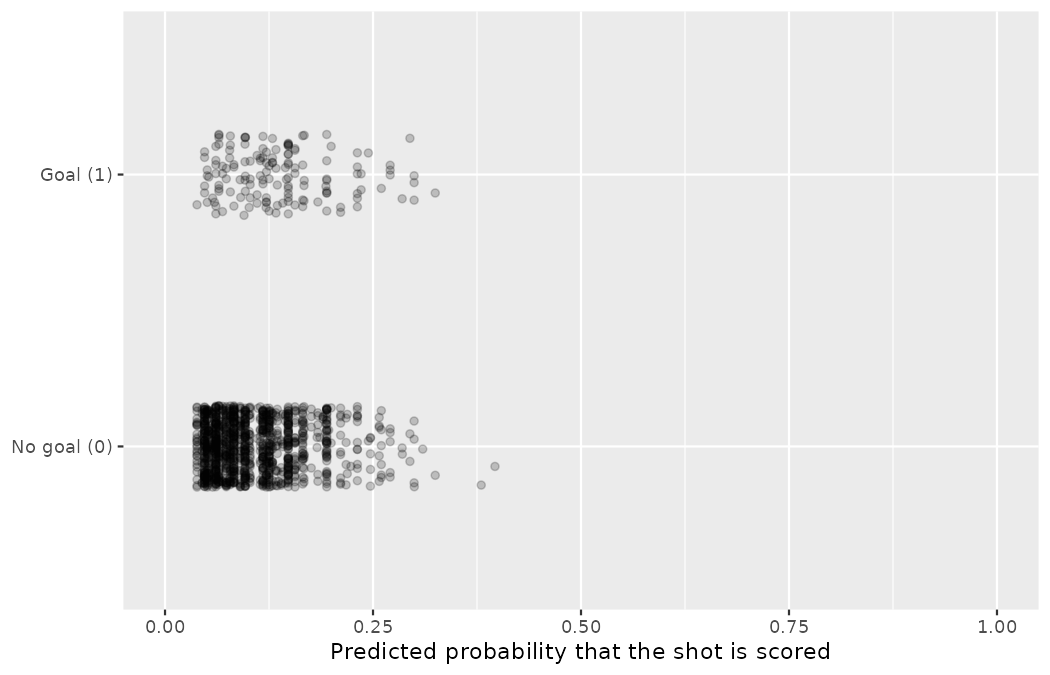
\includegraphics[width=0.85\linewidth,height=\textheight,keepaspectratio]{figures/inf-model-logistic-1.png}

The plot shows two horizontal bands of points --- the no-goal shots
along the bottom, the goals along the top, jittered so that shots with
nearly identical values aren't plotted exactly on top of one another.
The predictions do not remotely separate the two bands: every fitted
probability lives between \(0.038\) and \(0.397\), and both bands are
thickest at the low end. But look closely at where each band carries its
weight: the goal band sits visibly further right than the no-goal band.
The model cannot \emph{call} goals, but it does \emph{rank} shots ---
which, for a shortlist, is the property that matters.

We'd like to assess the quality of the model. For example, we might ask:
if we look at shots that we modeled as having a 10\% chance of being
scored, do we find out 10\% of them actually are goals? We can check
this for groups of the data by constructing a plot as follows:

\begin{enumerate}
\def\labelenumi{\arabic{enumi}.}
\tightlist
\item
  Bucket the observations into groups based on their predicted
  probabilities.
\item
  Compute the average predicted probability for each group.
\item
  Compute the observed probability for each group, along with a 95\%
  confidence interval for the true probability of success for those
  individuals --- built exactly as in
  Chapter~\ref{sec-foundations-mathematical}, as the point estimate
  \(\pm\ 1.96 \times SE\) with \(SE = \sqrt{\hat{p}(1-\hat{p})/n}\) from
  Chapter~\ref{sec-inference-one-prop}.
\item
  Plot the observed probabilities (with 95\% confidence intervals)
  against the average predicted probabilities for each group.
\end{enumerate}

If the model does a good job describing the data, the plotted points
should fall close to the line \(y = x\), since the predicted
probabilities should be similar to the observed probabilities. We can
use the confidence intervals to roughly gauge whether anything might be
amiss.

\begin{Shaded}
\begin{Highlighting}[]
\NormalTok{wc\_buckets }\OtherTok{\textless{}{-}}\NormalTok{ shots\_open }\SpecialCharTok{|\textgreater{}}
  \FunctionTok{mutate}\NormalTok{(}\AttributeTok{bucket =} \FunctionTok{ntile}\NormalTok{(p\_hat, }\DecValTok{8}\NormalTok{)) }\SpecialCharTok{|\textgreater{}}
  \FunctionTok{group\_by}\NormalTok{(bucket) }\SpecialCharTok{|\textgreater{}}
  \FunctionTok{summarize}\NormalTok{(}
    \AttributeTok{shots =} \FunctionTok{n}\NormalTok{(),}
    \AttributeTok{avg\_pred =} \FunctionTok{mean}\NormalTok{(p\_hat),}
    \AttributeTok{obs\_rate =} \FunctionTok{mean}\NormalTok{(goal),}
    \AttributeTok{lower =}\NormalTok{ obs\_rate }\SpecialCharTok{{-}} \FloatTok{1.96} \SpecialCharTok{*} \FunctionTok{sqrt}\NormalTok{(obs\_rate }\SpecialCharTok{*}\NormalTok{ (}\DecValTok{1} \SpecialCharTok{{-}}\NormalTok{ obs\_rate) }\SpecialCharTok{/}\NormalTok{ shots),}
    \AttributeTok{upper =}\NormalTok{ obs\_rate }\SpecialCharTok{+} \FloatTok{1.96} \SpecialCharTok{*} \FunctionTok{sqrt}\NormalTok{(obs\_rate }\SpecialCharTok{*}\NormalTok{ (}\DecValTok{1} \SpecialCharTok{{-}}\NormalTok{ obs\_rate) }\SpecialCharTok{/}\NormalTok{ shots)}
\NormalTok{  )}
\NormalTok{wc\_buckets}
\CommentTok{\#\textgreater{} \# A tibble: 8 × 6}
\CommentTok{\#\textgreater{}   bucket shots avg\_pred obs\_rate   lower  upper}
\CommentTok{\#\textgreater{}    \textless{}int\textgreater{} \textless{}int\textgreater{}    \textless{}dbl\textgreater{}    \textless{}dbl\textgreater{}   \textless{}dbl\textgreater{}  \textless{}dbl\textgreater{}}
\CommentTok{\#\textgreater{} 1      1   171   0.0467   0.0351 0.00751 0.0627}
\CommentTok{\#\textgreater{} 2      2   171   0.0583   0.0585 0.0233  0.0936}
\CommentTok{\#\textgreater{} 3      3   171   0.0701   0.0994 0.0546  0.144}
\CommentTok{\#\textgreater{} 4      4   171   0.0848   0.0409 0.0112  0.0706}
\CommentTok{\#\textgreater{} 5      5   171   0.104    0.129  0.0785  0.179}
\CommentTok{\#\textgreater{} 6      6   170   0.125    0.124  0.0741  0.173}
\CommentTok{\#\textgreater{} 7      7   170   0.153    0.165  0.109   0.220}
\CommentTok{\#\textgreater{} 8      8   170   0.221    0.212  0.150   0.273}

\FunctionTok{ggplot}\NormalTok{(wc\_buckets, }\FunctionTok{aes}\NormalTok{(}\AttributeTok{x =}\NormalTok{ avg\_pred, }\AttributeTok{y =}\NormalTok{ obs\_rate)) }\SpecialCharTok{+}
  \FunctionTok{geom\_abline}\NormalTok{(}\AttributeTok{slope =} \DecValTok{1}\NormalTok{, }\AttributeTok{intercept =} \DecValTok{0}\NormalTok{, }\AttributeTok{linetype =} \StringTok{"dashed"}\NormalTok{) }\SpecialCharTok{+}
  \FunctionTok{geom\_pointrange}\NormalTok{(}\FunctionTok{aes}\NormalTok{(}\AttributeTok{ymin =}\NormalTok{ lower, }\AttributeTok{ymax =}\NormalTok{ upper)) }\SpecialCharTok{+}
  \FunctionTok{coord\_cartesian}\NormalTok{(}\AttributeTok{xlim =} \FunctionTok{c}\NormalTok{(}\DecValTok{0}\NormalTok{, }\FloatTok{0.3}\NormalTok{), }\AttributeTok{ylim =} \FunctionTok{c}\NormalTok{(}\DecValTok{0}\NormalTok{, }\FloatTok{0.3}\NormalTok{)) }\SpecialCharTok{+}
  \FunctionTok{labs}\NormalTok{(}
    \AttributeTok{x =} \StringTok{"Average predicted probability in bucket"}\NormalTok{,}
    \AttributeTok{y =} \StringTok{"Observed goal rate in bucket (with 95\% CI)"}
\NormalTok{  )}
\end{Highlighting}
\end{Shaded}

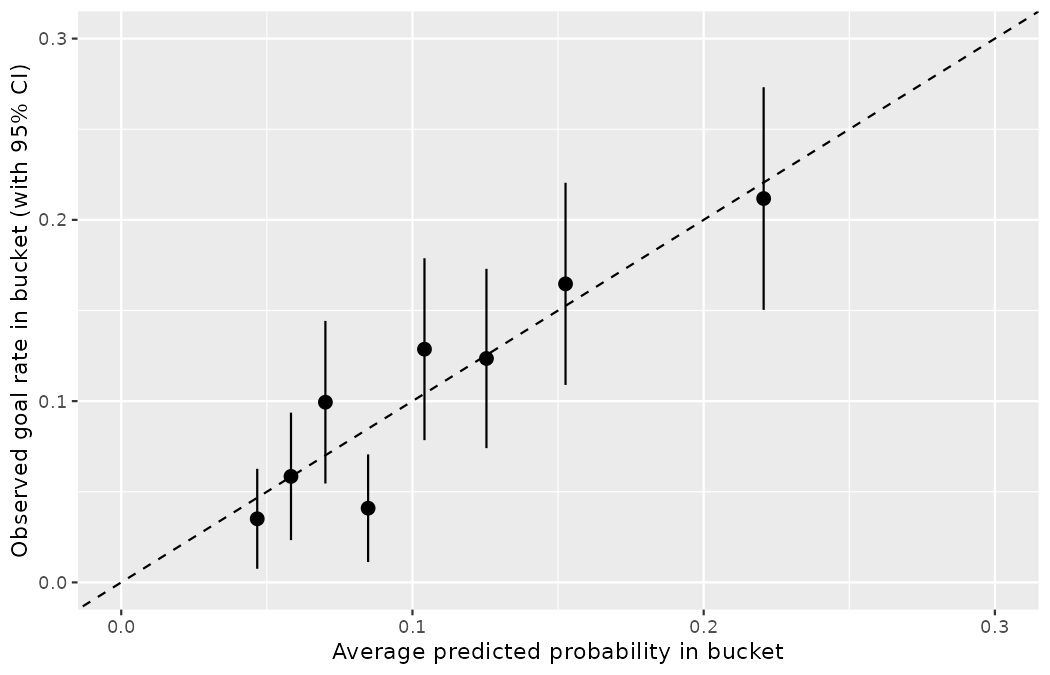
\includegraphics[width=0.85\linewidth,height=\textheight,keepaspectratio]{figures/inf-model-logistic-2.png}

The eight equal-count buckets climb from an average prediction of
\(0.047\) to \(0.221\), and the observed goal rates climb with them,
from \(0.035\) to \(0.212\). The dashed \(y = x\) line is inside the
confidence bound of the 95\% confidence intervals for seven of the eight
buckets, suggesting the logistic fit is reasonable; the exception is
bucket 4, where shots predicted at \(0.085\) scored only \(0.041\) of
the time and the interval \((0.011, 0.071)\) misses the line. With eight
separate 95\% intervals, one miss is roughly the accounting you should
expect from chance alone --- worth an eyebrow, not an alarm. (Two
honesty notes on the intervals themselves: the lowest bucket holds only
6 goals, straining the success-failure condition of
Chapter~\ref{sec-inference-one-prop}, so treat its interval as rough;
and this bucketing check is exactly the chance-quality-band idea you met
in the exercises of Chapter~\ref{sec-model-logistic}, now upgraded with
confidence intervals.)

A plot like this helps to better understand the deviations. Additional
diagnostics may be created that are similar to those featured in
Section~\ref{sec-tech-cond-linmod}. For instance, we could compute
residuals as the observed outcome minus the expected outcome,

\[e_i = Y_i - \hat{p}_i,\]

and then we could create plots of these residuals against each
predictor. This is a new equation built entirely from old parts, so take
it apart before using it. The letter \(e\) with subscript \(i\) is the
same residual notation you have carried since
Chapter~\ref{sec-model-slr}: the leftover for observation \(i\),
computed as \emph{observed minus fitted}. \(Y_i\) is the binary outcome
of Chapter~\ref{sec-model-logistic} --- capital \(Y\), the response
itself, equal to 1 if shot \(i\) was scored and 0 if not. And
\(\hat{p}_i\) is that chapter's fitted probability: the model's
data-based estimate of shot \(i\)'s scoring probability. What has
changed since Chapter~\ref{sec-model-slr} is not the recipe but the
\emph{scales of its ingredients}: there, \(y_i\) and \(\hat{y}_i\) both
lived on the response's own scale, and residuals could land anywhere;
here the observed value is always exactly 0 or 1 while the fitted value
is a probability strictly between them. So a logistic residual can only
take one of two values for a given shot: \(e_i = 1 - \hat{p}_i\) if the
shot was scored, or \(e_i = -\hat{p}_i\) if it was not. The first two
shots in the dataset show the pair:

\begin{Shaded}
\begin{Highlighting}[]
\NormalTok{shots\_open }\SpecialCharTok{|\textgreater{}}
  \FunctionTok{slice}\NormalTok{(}\DecValTok{1}\SpecialCharTok{:}\DecValTok{2}\NormalTok{) }\SpecialCharTok{|\textgreater{}}
  \FunctionTok{select}\NormalTok{(player, goal, p\_hat) }\SpecialCharTok{|\textgreater{}}
  \FunctionTok{mutate}\NormalTok{(}\AttributeTok{e\_i =} \FunctionTok{as.numeric}\NormalTok{(goal) }\SpecialCharTok{{-}}\NormalTok{ p\_hat)}
\CommentTok{\#\textgreater{} \# A tibble: 2 × 4}
\CommentTok{\#\textgreater{}   player            goal  p\_hat    e\_i}
\CommentTok{\#\textgreater{}   \textless{}chr\textgreater{}             \textless{}lgl\textgreater{} \textless{}dbl\textgreater{}  \textless{}dbl\textgreater{}}
\CommentTok{\#\textgreater{} 1 Mark Anthony Kaye FALSE 0.184 {-}0.184}
\CommentTok{\#\textgreater{} 2 Hakim Ziyech      TRUE  0.156  0.844}
\end{Highlighting}
\end{Shaded}

Kaye's unscored shot leaves a small negative residual; Ziyech's goal,
priced at \(0.156\), leaves a residual of \(+0.844\). Plotted against
any predictor, logistic residuals therefore form two drifting stripes
rather than the even scatter of Chapter~\ref{sec-model-slr} --- exactly
the striped picture Section~\ref{sec-tech-cond-linmod} showed when a
binary outcome was forced through the linear machinery, and the reason
that chapter sent you here.

\begin{tcolorbox}[enhanced jigsaw, left=2mm, leftrule=.75mm, title=\textcolor{quarto-callout-tip-color}{\faLightbulb}\hspace{0.5em}{Check your understanding}, arc=.35mm, rightrule=.15mm, coltitle=black, colframe=quarto-callout-tip-color-frame, bottomrule=.15mm, colbacktitle=quarto-callout-tip-color!10!white, opacitybacktitle=0.6, breakable, bottomtitle=1mm, toptitle=1mm, titlerule=0mm, opacityback=0, toprule=.15mm, colback=white]

A shot carries a fitted probability of \(\hat{p}_i = 0.25.\) What are
the two possible values of its residual \(e_i\)? And which shots produce
the largest \emph{positive} residuals in the whole dataset?

\begin{center}\rule{0.5\linewidth}{0.5pt}\end{center}

If the shot is scored, \(e_i = 1 - 0.25 = 0.75\); if not,
\(e_i = 0 - 0.25 = -0.25.\) The largest positive residuals belong to
goals the model priced lowest --- an unpressured, non-first-time,
right-footed shot from regular play that went in anyway would carry
\(e_i \approx 1 - 0.06 = 0.94.\) In scouting language: the positive
stripe is where the model's surprises live, and a striker who keeps
appearing there is either running hot or seeing something the tags
cannot.

\end{tcolorbox}

\section{Multiple logistic regression output from
software}\label{sec-inf-log-reg-soft}

As in Chapter~\ref{sec-model-mlr} and Chapter~\ref{sec-model-logistic},
software finds the coefficient estimates --- for a logistic model by
optimizing the likelihood rather than by least squares. The unknown
population model for our five predictors can be written as:

\[
\begin{aligned}
\log_e\bigg(\frac{p}{1-p}\bigg) = \beta_0 &+ \beta_1 \times \texttt{under\_pressure} + \beta_2 \times \texttt{first\_time} + \beta_3 \times \texttt{one\_on\_one} \\
&+ \beta_4 \times \texttt{body\_part}_{\texttt{Left Foot}} + \beta_5 \times \texttt{body\_part}_{\texttt{Head}} \\
&+ \beta_6 \times \texttt{play\_pattern}_{\texttt{From Corner}} + \cdots + \beta_{12} \times \texttt{play\_pattern}_{\texttt{From Throw In}}
\end{aligned}
\]

The two categorical predictors enter through level indicators, exactly
as in Chapter~\ref{sec-model-mlr}: one coefficient per non-reference
level, so \texttt{body\_part} contributes two (\(\beta_4, \beta_5\)) and
\texttt{play\_pattern} seven (\(\beta_6\) through \(\beta_{12}\)), each
measured against the reference shot --- right-footed, from regular play.
The estimated equation, using the higher-precision coefficients from
\texttt{round(coef(goal\_fit),\ 4)}, is:

\[
\begin{aligned}
\log_e\bigg(\frac{\hat{p}}{1-\hat{p}}\bigg) = -2.7323 &- 0.0695 \times \texttt{under\_pressure} + 0.9832 \times \texttt{first\_time} \\
&+ 1.1256 \times \texttt{one\_on\_one} + 0.3273 \times \texttt{body\_part}_{\texttt{Left Foot}} \\
&+ 0.7566 \times \texttt{body\_part}_{\texttt{Head}} - 0.4870 \times \texttt{play\_pattern}_{\texttt{From Corner}} \\
&+ 0.4304 \times \texttt{play\_pattern}_{\texttt{From Counter}} - 0.1960 \times \texttt{play\_pattern}_{\texttt{From Free Kick}} \\
&+ 0.5476 \times \texttt{play\_pattern}_{\texttt{From Goal Kick}} - 0.1829 \times \texttt{play\_pattern}_{\texttt{From Keeper}} \\
&- 0.0281 \times \texttt{play\_pattern}_{\texttt{From Kick Off}} - 0.2651 \times \texttt{play\_pattern}_{\texttt{From Throw In}}
\end{aligned}
\]

\begin{Shaded}
\begin{Highlighting}[]
\FunctionTok{tidy}\NormalTok{(goal\_fit)}
\CommentTok{\#\textgreater{} \# A tibble: 13 × 5}
\CommentTok{\#\textgreater{}    term                       estimate std.error statistic  p.value}
\CommentTok{\#\textgreater{}    \textless{}chr\textgreater{}                         \textless{}dbl\textgreater{}     \textless{}dbl\textgreater{}     \textless{}dbl\textgreater{}    \textless{}dbl\textgreater{}}
\CommentTok{\#\textgreater{}  1 (Intercept)                 {-}2.73       0.224  {-}12.2    2.78e{-}34}
\CommentTok{\#\textgreater{}  2 under\_pressureTRUE          {-}0.0695     0.261   {-}0.266  7.90e{-} 1}
\CommentTok{\#\textgreater{}  3 first\_timeTRUE               0.983      0.209    4.70   2.62e{-} 6}
\CommentTok{\#\textgreater{}  4 one\_on\_oneTRUE               1.13       0.322    3.49   4.81e{-} 4}
\CommentTok{\#\textgreater{}  5 body\_partLeft Foot           0.327      0.202    1.62   1.05e{-} 1}
\CommentTok{\#\textgreater{}  6 body\_partHead                0.757      0.295    2.56   1.04e{-} 2}
\CommentTok{\#\textgreater{}  7 play\_patternFrom Corner     {-}0.487      0.308   {-}1.58   1.14e{-} 1}
\CommentTok{\#\textgreater{}  8 play\_patternFrom Counter     0.430      0.390    1.10   2.69e{-} 1}
\CommentTok{\#\textgreater{}  9 play\_patternFrom Free Kick  {-}0.196      0.265   {-}0.740  4.59e{-} 1}
\CommentTok{\#\textgreater{} 10 play\_patternFrom Goal Kick   0.548      0.339    1.62   1.06e{-} 1}
\CommentTok{\#\textgreater{} 11 play\_patternFrom Keeper     {-}0.183      0.768   {-}0.238  8.12e{-} 1}
\CommentTok{\#\textgreater{} 12 play\_patternFrom Kick Off   {-}0.0281     0.777   {-}0.0362 9.71e{-} 1}
\CommentTok{\#\textgreater{} 13 play\_patternFrom Throw In   {-}0.265      0.257   {-}1.03   3.03e{-} 1}
\end{Highlighting}
\end{Shaded}

Not only does the summary table provide the estimates for the
coefficients, it also provides the information for the inference
analysis (i.e., hypothesis testing) which is the focus of this chapter.

Now the debt this book has carried since Chapter~\ref{sec-model-slr}
comes due. Every \texttt{tidy()} table you have seen --- for
chance-quality lines, for the six-tag model of
Chapter~\ref{sec-model-mlr}, for the audit and goal models of
Chapter~\ref{sec-model-logistic} --- has printed \texttt{std.error},
\texttt{statistic}, and \texttt{p.value} columns you were asked to set
aside. Here is what they have meant all along. The \texttt{std.error}
column is the standard error of each coefficient estimate, in exactly
the sense of Chapter~\ref{sec-foundations-mathematical}: the typical
sample-to-sample wobble of \(b_i\). The \texttt{statistic} column is the
coefficient measured in units of its own standard error,

\[Z = \frac{b_i - 0}{SE(b_i)},\]

the number of standard errors the estimate sits from the null value of
zero --- check it on the \texttt{first\_time} row:
\(0.9832 / 0.209 = 4.70.\) And \texttt{p.value} is that statistic's
two-sided tail probability. For the linear models of
Chapter~\ref{sec-inf-model-slr} and Chapter~\ref{sec-inf-model-mlr}, the
reference distribution was a \(t\)-distribution; for logistic regression
the statistic is read on the standard normal curve of
Chapter~\ref{sec-foundations-mathematical}, and the resulting test is
known as a \emph{Wald test}.\footnote{Named for Abraham Wald. The Wald
  statistic \(Z = b_i / SE(b_i)\) and its normal reference distribution
  are the standard large-sample output of \texttt{glm()}; with 1,365
  shots, the approximation is comfortable here.} Nothing about the logic
is new --- point estimate, standard error, standardized statistic, tail
probability --- you have simply earned, chapter by chapter since
Chapter~\ref{sec-foundations-randomization}, every piece the software
was silently printing.

As in Chapter~\ref{sec-inf-model-mlr}, with \textbf{multiple
predictors}, each hypothesis test (for each of the explanatory
variables) is conditioned on each of the other variables remaining in
the model.

\begin{quote}
if multiple predictors \(H_0: \beta_i = 0\) given other variables in the
model
\end{quote}

Using the output above and focusing on each of the variable p-values
(here we won't discuss the p-value associated with the intercept), we
can write out the hypotheses associated with each row of the table:

\begin{itemize}
\tightlist
\item
  \(H_0: \beta_1 = 0\) given \texttt{first\_time},
  \texttt{one\_on\_one}, \texttt{body\_part}, and \texttt{play\_pattern}
  are included in the model
\item
  \(H_0: \beta_2 = 0\) given \texttt{under\_pressure},
  \texttt{one\_on\_one}, \texttt{body\_part}, and \texttt{play\_pattern}
  are included in the model
\item
  \(H_0: \beta_3 = 0\) given \texttt{under\_pressure},
  \texttt{first\_time}, \texttt{body\_part}, and \texttt{play\_pattern}
  are included in the model
\item
  and one hypothesis for each of the nine level-indicator coefficients,
  stated against the reference level: for example, \(H_0: \beta_5 = 0\)
  --- headers score at the same rate as right-footed shots --- given
  \texttt{under\_pressure}, \texttt{first\_time}, \texttt{one\_on\_one},
  the \texttt{Left\ Foot} indicator, and \texttt{play\_pattern} are
  included in the model.
\end{itemize}

The p-values sort the tournament's folklore with one pass of the eye. At
the discernibility level of 0.05, three rows act as statistically
discernible in the model, despite the inclusion of any of the other
variables: \texttt{first\_time}
\((p\text{-value} \approx 2.6 \times 10^{-6})\), \texttt{one\_on\_one}
\((p\text{-value} \approx 0.0005)\), and the \texttt{Head} level
indicator \((p\text{-value} = 0.010)\) --- \emph{holding the other
predictors constant}, headers score discernibly more often than
right-footed shots. Recall Chapter~\ref{sec-data-design}'s warning that
any raw header comparison is confounded with the delivery patterns
headers arrive from; this coefficient is the header effect \emph{after}
\texttt{play\_pattern} is held fixed, which is exactly the adjustment
that warning demanded. Consider the p-value on \(H_0: \beta_2 = 0.\) The
low p-value says that it would be extremely unlikely to observe data
that yield a coefficient on \texttt{first\_time} at least as far from 0
as \(0.983\) (i.e., \(|b_2| > 0.983\)) if the true relationship between
\texttt{first\_time} and \texttt{goal} was non-existent (i.e., if
\(\beta_2 = 0\)) \textbf{and} the model also included the other four
predictors. Note also that the coefficient on \texttt{one\_on\_one}
\((1.1256)\) is \emph{larger} than the coefficient on
\texttt{first\_time} \((0.9832)\), yet its p-value is larger too. The
explanation sits in the \texttt{std.error} column: in units of standard
errors, \texttt{first\_time} is \(4.70\) from zero while
\texttt{one\_on\_one} --- estimated from only 73 one-on-ones --- is
\(3.49\) from zero. The magnitude of a coefficient is not its evidence;
it's all about context, and the context is the standard error.

And then there is \texttt{under\_pressure}: an estimate of \(-0.0695\),
a Wald statistic of \(-0.27\), a p-value of \(0.79.\) Given the other
four predictors, defensive pressure is nowhere near a statistically
discernible predictor of scoring in open play. You should feel the whole
book converge on that row: the permutation test of
Section~\ref{sec-chp11-pens-out} found no discernible open-play pressure
effect on conversion \((p = 0.385)\), the open-play refit in
Chapter~\ref{sec-model-logistic} watched the pressure coefficient all
but vanish, and Chapter~\ref{sec-model-application} dropped the pressure
tag from its chance-quality model entirely. Four chapters, three
toolkits, one consistent verdict --- and one more reminder that a claim
every scout repeats (``pressure ruins the shot'') can fail to survive
contact with the data frame that actually tests it.

We remind you that although p-values provide some information about the
importance of each of the predictors in the model, there are many,
arguably more important, aspects to consider when choosing the best
model. And the conclusions are, as always with this dataset,
associational: nobody randomly assigned pressure, body parts, or
possession patterns to shots.

\begin{tcolorbox}[enhanced jigsaw, left=2mm, leftrule=.75mm, title=\textcolor{quarto-callout-note-color}{\faInfo}\hspace{0.5em}{Worked example}, arc=.35mm, rightrule=.15mm, coltitle=black, colframe=quarto-callout-note-color-frame, bottomrule=.15mm, colbacktitle=quarto-callout-note-color!10!white, opacitybacktitle=0.6, breakable, bottomtitle=1mm, toptitle=1mm, titlerule=0mm, opacityback=0, toprule=.15mm, colback=white]

Use the estimated equation to find the probability that a first-time
header from a corner --- no pressure, no one-on-one --- is scored. Then
compare it with the same header not struck first time.

\begin{center}\rule{0.5\linewidth}{0.5pt}\end{center}

Sum the relevant coefficients:

\[-2.7323 + 0.9832 + 0.7566 - 0.4870 = -1.4795\]

Back-transform, as in Section~\ref{sec-modelingTheProbabilityOfAnEvent}:

\[\hat{p} = \frac{e^{-1.4795}}{1 + e^{-1.4795}} = \frac{0.2278}{1.2278} = 0.1855\]

Without the first-time strike the log odds are
\(-2.7323 + 0.7566 - 0.4870 = -2.4627\), giving \(\hat{p} = 0.0785.\) R
agrees, without the rounding:

\begin{Shaded}
\begin{Highlighting}[]
\NormalTok{corner\_headers }\OtherTok{\textless{}{-}} \FunctionTok{tibble}\NormalTok{(}
  \AttributeTok{under\_pressure =} \ConstantTok{FALSE}\NormalTok{,}
  \AttributeTok{first\_time =} \FunctionTok{c}\NormalTok{(}\ConstantTok{TRUE}\NormalTok{, }\ConstantTok{FALSE}\NormalTok{),}
  \AttributeTok{one\_on\_one =} \ConstantTok{FALSE}\NormalTok{,}
  \AttributeTok{body\_part =} \FunctionTok{factor}\NormalTok{(}\StringTok{"Head"}\NormalTok{, }\AttributeTok{levels =} \FunctionTok{levels}\NormalTok{(shots\_open}\SpecialCharTok{$}\NormalTok{body\_part)),}
  \AttributeTok{play\_pattern =} \FunctionTok{factor}\NormalTok{(}\StringTok{"From Corner"}\NormalTok{, }\AttributeTok{levels =} \FunctionTok{levels}\NormalTok{(shots\_open}\SpecialCharTok{$}\NormalTok{play\_pattern))}
\NormalTok{)}
\FunctionTok{round}\NormalTok{(}\FunctionTok{predict}\NormalTok{(goal\_fit, corner\_headers, }\AttributeTok{type =} \StringTok{"response"}\NormalTok{), }\DecValTok{4}\NormalTok{)}
\CommentTok{\#\textgreater{}      1      2}
\CommentTok{\#\textgreater{} 0.1855 0.0785}
\end{Highlighting}
\end{Shaded}

The classic near-post flick is, by this model, more than twice the
chance of the header from the same delivery that waits on the ball.

\end{tcolorbox}

\begin{tcolorbox}[enhanced jigsaw, left=2mm, leftrule=.75mm, title=\textcolor{quarto-callout-tip-color}{\faLightbulb}\hspace{0.5em}{Check your understanding}, arc=.35mm, rightrule=.15mm, coltitle=black, colframe=quarto-callout-tip-color-frame, bottomrule=.15mm, colbacktitle=quarto-callout-tip-color!10!white, opacitybacktitle=0.6, breakable, bottomtitle=1mm, toptitle=1mm, titlerule=0mm, opacityback=0, toprule=.15mm, colback=white]

Verify the \texttt{statistic} and \texttt{p.value} entries for the
\texttt{one\_on\_one} row from \texttt{estimate} and \texttt{std.error},
and state precisely what the hypothesis being tested is.

\begin{center}\rule{0.5\linewidth}{0.5pt}\end{center}

\(Z = 1.1256 / 0.3222 = 3.49,\) matching the \texttt{statistic} column.
The p-value is the two-sided normal tail,
\(2 \times P(Z \geq 3.49) \approx 0.0005,\) matching \texttt{p.value}.
The hypothesis is \emph{conditional}: \(H_0: \beta_3 = 0\) \emph{given
that} \texttt{under\_pressure}, \texttt{first\_time},
\texttt{body\_part}, and \texttt{play\_pattern} remain in the model ---
the test asks whether the one-on-one tag adds discernible signal beyond
those variables, not whether one-on-ones are associated with scoring on
their own.

\end{tcolorbox}

Per the book's penalty convention, before these p-values travel into any
memo, the companion fit must be shown: the identical model on all 1,494
shots, penalties in. The \texttt{Other} levels of \texttt{body\_part}
and \texttt{play\_pattern} return to the data --- and the play-pattern
bucket labeled \texttt{Other} is precisely where the data file logs all
64 penalty kicks.

\begin{Shaded}
\begin{Highlighting}[]
\NormalTok{shots\_all }\OtherTok{\textless{}{-}}\NormalTok{ wc2022\_shots }\SpecialCharTok{|\textgreater{}}
  \FunctionTok{mutate}\NormalTok{(}
    \AttributeTok{body\_part =} \FunctionTok{relevel}\NormalTok{(}\FunctionTok{factor}\NormalTok{(body\_part), }\AttributeTok{ref =} \StringTok{"Right Foot"}\NormalTok{),}
    \AttributeTok{play\_pattern =} \FunctionTok{relevel}\NormalTok{(}\FunctionTok{factor}\NormalTok{(play\_pattern), }\AttributeTok{ref =} \StringTok{"Regular Play"}\NormalTok{)}
\NormalTok{  )}

\NormalTok{goal\_fit\_all }\OtherTok{\textless{}{-}} \FunctionTok{glm}\NormalTok{(}
\NormalTok{  goal }\SpecialCharTok{\textasciitilde{}}\NormalTok{ under\_pressure }\SpecialCharTok{+}\NormalTok{ first\_time }\SpecialCharTok{+}\NormalTok{ one\_on\_one }\SpecialCharTok{+}\NormalTok{ body\_part }\SpecialCharTok{+}\NormalTok{ play\_pattern,}
  \AttributeTok{data =}\NormalTok{ shots\_all, }\AttributeTok{family =}\NormalTok{ binomial}
\NormalTok{)}
\FunctionTok{tidy}\NormalTok{(goal\_fit\_all)}
\CommentTok{\#\textgreater{} \# A tibble: 15 × 5}
\CommentTok{\#\textgreater{}    term                       estimate std.error statistic  p.value}
\CommentTok{\#\textgreater{}    \textless{}chr\textgreater{}                         \textless{}dbl\textgreater{}     \textless{}dbl\textgreater{}     \textless{}dbl\textgreater{}    \textless{}dbl\textgreater{}}
\CommentTok{\#\textgreater{}  1 (Intercept)                 {-}2.63       0.213  {-}12.3    5.43e{-}35}
\CommentTok{\#\textgreater{}  2 under\_pressureTRUE          {-}0.104      0.260   {-}0.402  6.88e{-} 1}
\CommentTok{\#\textgreater{}  3 first\_timeTRUE               0.857      0.198    4.32   1.55e{-} 5}
\CommentTok{\#\textgreater{}  4 one\_on\_oneTRUE               0.576      0.322    1.79   7.39e{-} 2}
\CommentTok{\#\textgreater{}  5 body\_partHead                0.774      0.288    2.69   7.20e{-} 3}
\CommentTok{\#\textgreater{}  6 body\_partLeft Foot           0.292      0.189    1.54   1.22e{-} 1}
\CommentTok{\#\textgreater{}  7 body\_partOther               1.26       0.703    1.80   7.21e{-} 2}
\CommentTok{\#\textgreater{}  8 play\_patternFrom Corner     {-}0.571      0.307   {-}1.86   6.27e{-} 2}
\CommentTok{\#\textgreater{}  9 play\_patternFrom Counter     0.465      0.386    1.20   2.28e{-} 1}
\CommentTok{\#\textgreater{} 10 play\_patternFrom Free Kick  {-}0.155      0.250   {-}0.619  5.36e{-} 1}
\CommentTok{\#\textgreater{} 11 play\_patternFrom Goal Kick   0.637      0.330    1.93   5.37e{-} 2}
\CommentTok{\#\textgreater{} 12 play\_patternFrom Keeper     {-}0.189      0.766   {-}0.246  8.06e{-} 1}
\CommentTok{\#\textgreater{} 13 play\_patternFrom Kick Off   {-}0.0297     0.775   {-}0.0383 9.69e{-} 1}
\CommentTok{\#\textgreater{} 14 play\_patternFrom Throw In   {-}0.271      0.256   {-}1.06   2.89e{-} 1}
\CommentTok{\#\textgreater{} 15 play\_patternOther            3.02       0.316    9.54   1.43e{-}21}
\end{Highlighting}
\end{Shaded}

Read the pair of tables the way Section~\ref{sec-chp11-pens-out} taught
you, and two findings stand out. First, the single most discernible
slope in the penalties-in table --- \(b = 3.02,\) \(Z = 9.54,\) a
p-value of order \(10^{-21}\) --- belongs to
\texttt{play\_patternOther}, the indicator whose main job is to hold 64
uncontested kicks converting at \(0.672.\) The model has not discovered
football insight; it has rediscovered the penalty spot. Second, and more
dangerous: the \emph{verdict on a real predictor flips}. The one-on-one
coefficient halves from \(1.126\) to \(0.576\) and its p-value rises
from \(0.0005\) to \(0.074\) --- not statistically discernible at
\(\alpha = 0.05\) --- because six penalties carry the one-on-one tag (a
data quirk flagged back in Chapter~\ref{sec-model-mlr}) and the
\texttt{Other} indicator now absorbs credit that the open-play frame
attributed to genuine breakaways. Same tournament, same machinery, one
frame decision --- and a shortlist built on the penalties-in table would
have discarded the tag this chapter will shortly show to be the single
most useful one. The open-play fit remains the frame this chapter
teaches, with the companion on the record.

As with linear regression (see Section~\ref{sec-inf-mult-reg-collin}),
existence of predictors that are correlated with each other can affect
both the coefficient estimates and the associated p-values: one-on-ones
arise disproportionately on counters, headers arrive from corners ---
the entanglements you have tracked since Chapter~\ref{sec-data-design}.
However, investigating multicollinearity in a logistic regression model
is saved for a text which provides more detail about logistic
regression. Next, as a model building alternative (or enhancement) to
p-values, we revisit cross-validation, within the context of predicting
the outcome of each of the individual shots.

\section{Cross-validation for prediction
error}\label{sec-inf-log-reg-cv}

The p-value is a probability measure under a setting of no relationship.
That p-value provides information about the degree of the relationship
(e.g., above we measured the relationship between \texttt{goal} and
\texttt{first\_time} using a p-value), but the p-value does not measure
how well the model will predict the individual shots (e.g., the accuracy
of the model). Depending on the goal of the research project, you might
be inclined to focus on variable importance (through p-values) or you
might be inclined to focus on prediction accuracy (through
cross-validation). Priya's shortlist is squarely the second kind of
project: Marta does not care whether \(\beta_3\) is zero; she cares how
many of next tournament's goals the flagged clips will contain.

Here we present a method for using \textbf{cross-validation}
\textbf{accuracy} to determine which variables (if any) should be used
in a model which predicts whether a shot becomes a goal. A full
treatment of cross-validation and logistic regression models is beyond
the scope of this text. Using \(k\)-fold cross-validation, we can build
\(k\) different models which are used to predict the observations in
each of the \(k\) holdout samples --- the same fold-and-holdout
discipline you applied to linear models in
Section~\ref{sec-inf-mult-reg-cv}. As there, we compare a smaller
logistic regression model to a larger logistic regression model. The
smaller model uses only the \texttt{one\_on\_one} variable; the complete
dataset (not cross-validated) model output is:

\textbf{The smaller model:}

\[\log_e\bigg(\frac{\hat{p}}{1-\hat{p}}\bigg) = -2.1818 + 0.9114 \times \texttt{one\_on\_one}\]

\begin{Shaded}
\begin{Highlighting}[]
\NormalTok{goal\_small }\OtherTok{\textless{}{-}} \FunctionTok{glm}\NormalTok{(goal }\SpecialCharTok{\textasciitilde{}}\NormalTok{ one\_on\_one, }\AttributeTok{data =}\NormalTok{ shots\_open, }\AttributeTok{family =}\NormalTok{ binomial)}
\FunctionTok{tidy}\NormalTok{(goal\_small)}
\CommentTok{\#\textgreater{} \# A tibble: 2 × 5}
\CommentTok{\#\textgreater{}   term           estimate std.error statistic   p.value}
\CommentTok{\#\textgreater{}   \textless{}chr\textgreater{}             \textless{}dbl\textgreater{}     \textless{}dbl\textgreater{}     \textless{}dbl\textgreater{}     \textless{}dbl\textgreater{}}
\CommentTok{\#\textgreater{} 1 (Intercept)      {-}2.18     0.0922    {-}23.7  6.66e{-}124}
\CommentTok{\#\textgreater{} 2 one\_on\_oneTRUE    0.911    0.298       3.06 2.19e{-}  3}

\NormalTok{shots\_open }\SpecialCharTok{|\textgreater{}}
  \FunctionTok{group\_by}\NormalTok{(one\_on\_one) }\SpecialCharTok{|\textgreater{}}
  \FunctionTok{summarize}\NormalTok{(}\AttributeTok{shots =} \FunctionTok{n}\NormalTok{(), }\AttributeTok{goals =} \FunctionTok{sum}\NormalTok{(goal), }\AttributeTok{conversion =} \FunctionTok{mean}\NormalTok{(goal))}
\CommentTok{\#\textgreater{} \# A tibble: 2 × 4}
\CommentTok{\#\textgreater{}   one\_on\_one shots goals conversion}
\CommentTok{\#\textgreater{}   \textless{}lgl\textgreater{}      \textless{}int\textgreater{} \textless{}int\textgreater{}      \textless{}dbl\textgreater{}}
\CommentTok{\#\textgreater{} 1 FALSE       1292   131      0.101}
\CommentTok{\#\textgreater{} 2 TRUE          73    16      0.219}
\end{Highlighting}
\end{Shaded}

With a single binary predictor the model simply reproduces the two group
conversion rates --- back-transforming \(-2.1818\) gives \(0.101\) and
\(-2.1818 + 0.9114 = -1.2704\) gives \(0.219\), a fact you proved for
yourself in Section~\ref{sec-modelingTheProbabilityOfAnEvent}. For the
cross-validation we split the 1,365 shots into \(k = 4\) folds, seeded
so you can reproduce every number that follows, and fit each model four
times, always predicting for the quarter of the data the model has never
seen:

\begin{Shaded}
\begin{Highlighting}[]
\FunctionTok{set.seed}\NormalTok{(}\DecValTok{2601}\NormalTok{)}
\NormalTok{shots\_cv }\OtherTok{\textless{}{-}}\NormalTok{ shots\_open }\SpecialCharTok{|\textgreater{}}
  \FunctionTok{mutate}\NormalTok{(}\AttributeTok{fold =} \FunctionTok{sample}\NormalTok{(}\FunctionTok{rep}\NormalTok{(}\DecValTok{1}\SpecialCharTok{:}\DecValTok{4}\NormalTok{, }\AttributeTok{length.out =} \FunctionTok{n}\NormalTok{())))}

\NormalTok{shots\_cv }\SpecialCharTok{|\textgreater{}}
  \FunctionTok{count}\NormalTok{(fold)}
\CommentTok{\#\textgreater{} \# A tibble: 4 × 2}
\CommentTok{\#\textgreater{}    fold     n}
\CommentTok{\#\textgreater{}   \textless{}int\textgreater{} \textless{}int\textgreater{}}
\CommentTok{\#\textgreater{} 1     1   342}
\CommentTok{\#\textgreater{} 2     2   341}
\CommentTok{\#\textgreater{} 3     3   341}
\CommentTok{\#\textgreater{} 4     4   341}

\NormalTok{cv\_predictions }\OtherTok{\textless{}{-}} \ControlFlowTok{function}\NormalTok{(model\_formula, data) \{}
\NormalTok{  predictions }\OtherTok{\textless{}{-}} \FunctionTok{vector}\NormalTok{(}\StringTok{"list"}\NormalTok{, }\DecValTok{4}\NormalTok{)}
  \ControlFlowTok{for}\NormalTok{ (f }\ControlFlowTok{in} \DecValTok{1}\SpecialCharTok{:}\DecValTok{4}\NormalTok{) \{}
\NormalTok{    train }\OtherTok{\textless{}{-}} \FunctionTok{filter}\NormalTok{(data, fold }\SpecialCharTok{!=}\NormalTok{ f)}
\NormalTok{    test  }\OtherTok{\textless{}{-}} \FunctionTok{filter}\NormalTok{(data, fold }\SpecialCharTok{==}\NormalTok{ f)}
\NormalTok{    fold\_fit }\OtherTok{\textless{}{-}} \FunctionTok{glm}\NormalTok{(model\_formula, }\AttributeTok{data =}\NormalTok{ train, }\AttributeTok{family =}\NormalTok{ binomial)}
\NormalTok{    predictions[[f]] }\OtherTok{\textless{}{-}}\NormalTok{ test }\SpecialCharTok{|\textgreater{}}
      \FunctionTok{mutate}\NormalTok{(}\AttributeTok{p\_cv =} \FunctionTok{predict}\NormalTok{(fold\_fit, }\AttributeTok{newdata =}\NormalTok{ test, }\AttributeTok{type =} \StringTok{"response"}\NormalTok{))}
\NormalTok{  \}}
  \FunctionTok{bind\_rows}\NormalTok{(predictions)}
\NormalTok{\}}

\NormalTok{cv\_small }\OtherTok{\textless{}{-}} \FunctionTok{cv\_predictions}\NormalTok{(goal }\SpecialCharTok{\textasciitilde{}}\NormalTok{ one\_on\_one, shots\_cv)}
\end{Highlighting}
\end{Shaded}

For each cross-validated model, the coefficients change slightly, and
the model is used to make independent predictions on the holdout sample.
The model built without fold 1, for instance, has estimates close to ---
but not equal to --- the full-data fit above:

\begin{Shaded}
\begin{Highlighting}[]
\FunctionTok{glm}\NormalTok{(goal }\SpecialCharTok{\textasciitilde{}}\NormalTok{ one\_on\_one, }\AttributeTok{data =} \FunctionTok{filter}\NormalTok{(shots\_cv, fold }\SpecialCharTok{!=} \DecValTok{1}\NormalTok{),}
    \AttributeTok{family =}\NormalTok{ binomial) }\SpecialCharTok{|\textgreater{}}
  \FunctionTok{tidy}\NormalTok{() }\SpecialCharTok{|\textgreater{}}
  \FunctionTok{select}\NormalTok{(term, estimate)}
\CommentTok{\#\textgreater{} \# A tibble: 2 × 2}
\CommentTok{\#\textgreater{}   term           estimate}
\CommentTok{\#\textgreater{}   \textless{}chr\textgreater{}             \textless{}dbl\textgreater{}}
\CommentTok{\#\textgreater{} 1 (Intercept)      {-}2.12}
\CommentTok{\#\textgreater{} 2 one\_on\_oneTRUE    0.815}
\end{Highlighting}
\end{Shaded}

To turn a predicted probability into a shortlist decision, we need a
cutoff, and here the class imbalance rules. The software default of
\(0.5\) would be absurd: no fitted probability in this dataset even
reaches \(0.4\), so a \(0.5\) cutoff flags nothing and reproduces the
useless 89\%-accurate ``no goal, ever'' model. Because the purpose is a
shortlist --- where the expensive error is \emph{missing} a goal-like
chance, the scouting department's version of passing on a gem
(Chapter~\ref{sec-foundations-decision-errors}) --- we instead use a low
cutoff of \(0.10\), just below the frame's base rate of \(0.108\), and
predict ``goal'' for any shot whose cross-validated probability exceeds
it. In the tables that follow, \texttt{goalTP} is the proportion of true
goals that were predicted to be goals, and \texttt{nongoalTP} is the
proportion of true non-goals that were predicted to be non-goals.

\begin{Shaded}
\begin{Highlighting}[]
\NormalTok{cv\_small }\SpecialCharTok{|\textgreater{}}
  \FunctionTok{mutate}\NormalTok{(}\AttributeTok{pred\_goal =}\NormalTok{ p\_cv }\SpecialCharTok{\textgreater{}} \FloatTok{0.10}\NormalTok{) }\SpecialCharTok{|\textgreater{}}
  \FunctionTok{group\_by}\NormalTok{(fold) }\SpecialCharTok{|\textgreater{}}
  \FunctionTok{summarize}\NormalTok{(}
    \AttributeTok{count =} \FunctionTok{n}\NormalTok{(),}
    \AttributeTok{accuracy =} \FunctionTok{mean}\NormalTok{(goal }\SpecialCharTok{==}\NormalTok{ pred\_goal),}
    \AttributeTok{nongoalTP =} \FunctionTok{sum}\NormalTok{(}\SpecialCharTok{!}\NormalTok{goal }\SpecialCharTok{\&} \SpecialCharTok{!}\NormalTok{pred\_goal) }\SpecialCharTok{/} \FunctionTok{sum}\NormalTok{(}\SpecialCharTok{!}\NormalTok{goal),}
    \AttributeTok{goalTP =} \FunctionTok{sum}\NormalTok{(goal }\SpecialCharTok{\&}\NormalTok{ pred\_goal) }\SpecialCharTok{/} \FunctionTok{sum}\NormalTok{(goal)}
\NormalTok{  )}
\CommentTok{\#\textgreater{} \# A tibble: 4 × 5}
\CommentTok{\#\textgreater{}    fold count accuracy nongoalTP goalTP}
\CommentTok{\#\textgreater{}   \textless{}int\textgreater{} \textless{}int\textgreater{}    \textless{}dbl\textgreater{}     \textless{}dbl\textgreater{}  \textless{}dbl\textgreater{}}
\CommentTok{\#\textgreater{} 1     1   342   0.0906     0     1}
\CommentTok{\#\textgreater{} 2     2   341   0.839      0.953 0.0682}
\CommentTok{\#\textgreater{} 3     3   341   0.836      0.936 0.119}
\CommentTok{\#\textgreater{} 4     4   341   0.0880     0     1}
\end{Highlighting}
\end{Shaded}

Something strange has happened, and it is worth slowing down for,
because it is the single-predictor model's failure mode laid bare. A
model with one binary predictor can price a shot at only \emph{two}
values --- one for ordinary shots, one for one-on-ones. Here are those
two prices, for each fold's training fit:

\begin{Shaded}
\begin{Highlighting}[]
\NormalTok{cv\_small }\SpecialCharTok{|\textgreater{}}
  \FunctionTok{distinct}\NormalTok{(fold, one\_on\_one, p\_cv) }\SpecialCharTok{|\textgreater{}}
  \FunctionTok{pivot\_wider}\NormalTok{(}\AttributeTok{names\_from =}\NormalTok{ one\_on\_one, }\AttributeTok{values\_from =}\NormalTok{ p\_cv,}
              \AttributeTok{names\_prefix =} \StringTok{"p\_cv\_1v1\_"}\NormalTok{) }\SpecialCharTok{|\textgreater{}}
  \FunctionTok{mutate}\NormalTok{(}\FunctionTok{across}\NormalTok{(}\FunctionTok{starts\_with}\NormalTok{(}\StringTok{"p\_cv"}\NormalTok{), \textbackslash{}(x) }\FunctionTok{round}\NormalTok{(x, }\DecValTok{4}\NormalTok{)))}
\CommentTok{\#\textgreater{} \# A tibble: 4 × 3}
\CommentTok{\#\textgreater{}    fold p\_cv\_1v1\_FALSE p\_cv\_1v1\_TRUE}
\CommentTok{\#\textgreater{}   \textless{}int\textgreater{}          \textless{}dbl\textgreater{}         \textless{}dbl\textgreater{}}
\CommentTok{\#\textgreater{} 1     1         0.107          0.213}
\CommentTok{\#\textgreater{} 2     2         0.093          0.232}
\CommentTok{\#\textgreater{} 3     3         0.0964         0.224}
\CommentTok{\#\textgreater{} 4     4         0.109          0.208}
\end{Highlighting}
\end{Shaded}

The ordinary-shot price hovers exactly at the cutoff: sampling
variability across training sets puts it \emph{above} \(0.10\) for folds
1 and 4 and \emph{below} for folds 2 and 3. When it lands above, the
model flags every single shot --- \texttt{goalTP} is a perfect \(1\),
\texttt{nongoalTP} collapses to \(0\), and the ``shortlist'' is the
entire tournament. When it lands below, only the one-on-ones are
flagged, and the shortlist misses roughly nine goals in ten. Either way
the smaller model is useless for Priya's purpose, and the fold-to-fold
flip is itself the lesson: a one-tag model classifying at a cutoff near
the base rate sits on a knife edge, and chance decides which side of it
each refit falls. (Notice, too, how the \texttt{accuracy} column seesaws
between \(0.09\) and \(0.84\) while describing the \emph{same} useless
model --- with an 89/11 class split, accuracy alone is the wrong
yardstick, which is exactly why the two TP columns are in the table.)

The larger model uses all five predictors --- \texttt{under\_pressure},
\texttt{first\_time}, \texttt{one\_on\_one}, \texttt{body\_part}, and
\texttt{play\_pattern} --- as laid out in
Section~\ref{sec-inf-log-reg-soft}. Its cross-validated shortlist, at
the same \(0.10\) cutoff:

\textbf{The larger model:}

\begin{Shaded}
\begin{Highlighting}[]
\NormalTok{cv\_large }\OtherTok{\textless{}{-}} \FunctionTok{cv\_predictions}\NormalTok{(}
\NormalTok{  goal }\SpecialCharTok{\textasciitilde{}}\NormalTok{ under\_pressure }\SpecialCharTok{+}\NormalTok{ first\_time }\SpecialCharTok{+}\NormalTok{ one\_on\_one }\SpecialCharTok{+}\NormalTok{ body\_part }\SpecialCharTok{+}\NormalTok{ play\_pattern,}
\NormalTok{  shots\_cv}
\NormalTok{)}

\NormalTok{cv\_large }\SpecialCharTok{|\textgreater{}}
  \FunctionTok{mutate}\NormalTok{(}\AttributeTok{pred\_goal =}\NormalTok{ p\_cv }\SpecialCharTok{\textgreater{}} \FloatTok{0.10}\NormalTok{) }\SpecialCharTok{|\textgreater{}}
  \FunctionTok{group\_by}\NormalTok{(fold) }\SpecialCharTok{|\textgreater{}}
  \FunctionTok{summarize}\NormalTok{(}
    \AttributeTok{count =} \FunctionTok{n}\NormalTok{(),}
    \AttributeTok{accuracy =} \FunctionTok{mean}\NormalTok{(goal }\SpecialCharTok{==}\NormalTok{ pred\_goal),}
    \AttributeTok{nongoalTP =} \FunctionTok{sum}\NormalTok{(}\SpecialCharTok{!}\NormalTok{goal }\SpecialCharTok{\&} \SpecialCharTok{!}\NormalTok{pred\_goal) }\SpecialCharTok{/} \FunctionTok{sum}\NormalTok{(}\SpecialCharTok{!}\NormalTok{goal),}
    \AttributeTok{goalTP =} \FunctionTok{sum}\NormalTok{(goal }\SpecialCharTok{\&}\NormalTok{ pred\_goal) }\SpecialCharTok{/} \FunctionTok{sum}\NormalTok{(goal)}
\NormalTok{  )}
\CommentTok{\#\textgreater{} \# A tibble: 4 × 5}
\CommentTok{\#\textgreater{}    fold count accuracy nongoalTP goalTP}
\CommentTok{\#\textgreater{}   \textless{}int\textgreater{} \textless{}int\textgreater{}    \textless{}dbl\textgreater{}     \textless{}dbl\textgreater{}  \textless{}dbl\textgreater{}}
\CommentTok{\#\textgreater{} 1     1   342    0.570     0.579  0.484}
\CommentTok{\#\textgreater{} 2     2   341    0.584     0.579  0.614}
\CommentTok{\#\textgreater{} 3     3   341    0.589     0.595  0.548}
\CommentTok{\#\textgreater{} 4     4   341    0.472     0.441  0.8}
\end{Highlighting}
\end{Shaded}

Somewhat expected, the larger model was able to capture more nuance in
the shots, which leads to a usable trade-off where the smaller model
offered none: fold by fold, the shortlist now catches roughly half to
four-fifths of the goals (\texttt{goalTP} between \(0.48\) and \(0.80\))
while correctly leaving out roughly half of the non-goals
(\texttt{nongoalTP} between \(0.44\) and \(0.60\)). In classification
language, \texttt{goalTP} is the model's \emph{recall} (or
\emph{sensitivity}) --- the share of the things we care about that we
actually caught --- and \texttt{nongoalTP} is its \emph{specificity} ---
the share of the dross correctly filtered away. At this cutoff, Priya's
analysts would re-watch roughly half the tournament's clips to find well
over half of its goals; a blunt instrument, but a real one, and an
honest reflection of how much (and how little) five context tags know
about finishing. However, it is not true that adding variables will
always lead to better predictions, as correlated or noise variables may
dampen the signal from the set of variables that truly predict the
outcome --- you saw AIC police exactly this appetite in
Chapter~\ref{sec-model-logistic}.

\begin{tcolorbox}[enhanced jigsaw, left=2mm, leftrule=.75mm, title=\textcolor{quarto-callout-tip-color}{\faLightbulb}\hspace{0.5em}{Check your understanding}, arc=.35mm, rightrule=.15mm, coltitle=black, colframe=quarto-callout-tip-color-frame, bottomrule=.15mm, colbacktitle=quarto-callout-tip-color!10!white, opacitybacktitle=0.6, breakable, bottomtitle=1mm, toptitle=1mm, titlerule=0mm, opacityback=0, toprule=.15mm, colback=white]

The recall/specificity balance is set by the cutoff, not by the model.
Here is the larger model again, cross-validated identically but
classified at \(0.15\):

\begin{Shaded}
\begin{Highlighting}[]
\NormalTok{cv\_large }\SpecialCharTok{|\textgreater{}}
  \FunctionTok{mutate}\NormalTok{(}\AttributeTok{pred\_goal =}\NormalTok{ p\_cv }\SpecialCharTok{\textgreater{}} \FloatTok{0.15}\NormalTok{) }\SpecialCharTok{|\textgreater{}}
  \FunctionTok{group\_by}\NormalTok{(fold) }\SpecialCharTok{|\textgreater{}}
  \FunctionTok{summarize}\NormalTok{(}
    \AttributeTok{count =} \FunctionTok{n}\NormalTok{(),}
    \AttributeTok{accuracy =} \FunctionTok{mean}\NormalTok{(goal }\SpecialCharTok{==}\NormalTok{ pred\_goal),}
    \AttributeTok{nongoalTP =} \FunctionTok{sum}\NormalTok{(}\SpecialCharTok{!}\NormalTok{goal }\SpecialCharTok{\&} \SpecialCharTok{!}\NormalTok{pred\_goal) }\SpecialCharTok{/} \FunctionTok{sum}\NormalTok{(}\SpecialCharTok{!}\NormalTok{goal),}
    \AttributeTok{goalTP =} \FunctionTok{sum}\NormalTok{(goal }\SpecialCharTok{\&}\NormalTok{ pred\_goal) }\SpecialCharTok{/} \FunctionTok{sum}\NormalTok{(goal)}
\NormalTok{  )}
\CommentTok{\#\textgreater{} \# A tibble: 4 × 5}
\CommentTok{\#\textgreater{}    fold count accuracy nongoalTP goalTP}
\CommentTok{\#\textgreater{}   \textless{}int\textgreater{} \textless{}int\textgreater{}    \textless{}dbl\textgreater{}     \textless{}dbl\textgreater{}  \textless{}dbl\textgreater{}}
\CommentTok{\#\textgreater{} 1     1   342    0.711     0.752  0.290}
\CommentTok{\#\textgreater{} 2     2   341    0.780     0.872  0.159}
\CommentTok{\#\textgreater{} 3     3   341    0.730     0.789  0.310}
\CommentTok{\#\textgreater{} 4     4   341    0.742     0.759  0.567}
\end{Highlighting}
\end{Shaded}

Accuracy rose in every fold. Should Priya raise the cutoff?

\begin{center}\rule{0.5\linewidth}{0.5pt}\end{center}

Almost certainly not, and the two TP columns say why: specificity
improved (fewer wasted clips), but recall collapsed --- in fold 2, the
\(0.15\) shortlist caught barely one goal in six. For a screening tool
whose costly error is the missed gem, trading recall for accuracy is
trading the objective for the yardstick. The right cutoff is a
\emph{decision} about error costs, in exactly the sense of
Chapter~\ref{sec-foundations-decision-errors} --- it belongs to Marta's
budget sheet, not to the software's defaults.

\end{tcolorbox}

\subsection{Taking the model abroad: external
validation}\label{sec-chp26-external}

Cross-validation estimates how the model performs on shots \emph{from
the same tournament} that it never saw. It cannot answer the question
Chapter~\ref{sec-model-application} taught you to fear when a men's
World Cup model met Grace Geyoro's Euro goal: what happens when the
model leaves home? Following the external-validation discipline of
Section~\ref{sec-inf-mult-reg-cv}, we train the larger model on the
entire 2022 Men's World Cup frame --- that is \texttt{goal\_fit},
already in hand --- and test it, once, on the open-play shots of the
2025 Women's Euro, built with the identical filter (which drops 7 of the
851 open-play shots: 4 with body part \texttt{Other}, 3 with pattern
\texttt{Other}):

\begin{Shaded}
\begin{Highlighting}[]
\NormalTok{weuro2025\_shots }\OtherTok{\textless{}{-}} \FunctionTok{read\_csv}\NormalTok{(}\StringTok{"data/derived/weuro2025\_shots.csv"}\NormalTok{)}

\NormalTok{weuro\_open }\OtherTok{\textless{}{-}}\NormalTok{ weuro2025\_shots }\SpecialCharTok{|\textgreater{}}
  \FunctionTok{filter}\NormalTok{(}
\NormalTok{    shot\_type }\SpecialCharTok{==} \StringTok{"Open Play"}\NormalTok{,}
\NormalTok{    body\_part }\SpecialCharTok{!=} \StringTok{"Other"}\NormalTok{,}
\NormalTok{    play\_pattern }\SpecialCharTok{!=} \StringTok{"Other"}
\NormalTok{  ) }\SpecialCharTok{|\textgreater{}}
  \FunctionTok{mutate}\NormalTok{(}
    \AttributeTok{body\_part =} \FunctionTok{factor}\NormalTok{(body\_part, }\AttributeTok{levels =} \FunctionTok{levels}\NormalTok{(shots\_open}\SpecialCharTok{$}\NormalTok{body\_part)),}
    \AttributeTok{play\_pattern =} \FunctionTok{factor}\NormalTok{(play\_pattern, }\AttributeTok{levels =} \FunctionTok{levels}\NormalTok{(shots\_open}\SpecialCharTok{$}\NormalTok{play\_pattern))}
\NormalTok{  )}

\NormalTok{weuro\_open }\OtherTok{\textless{}{-}}\NormalTok{ weuro\_open }\SpecialCharTok{|\textgreater{}}
  \FunctionTok{mutate}\NormalTok{(}\AttributeTok{p\_hat =} \FunctionTok{predict}\NormalTok{(goal\_fit, }\AttributeTok{newdata =}\NormalTok{ weuro\_open, }\AttributeTok{type =} \StringTok{"response"}\NormalTok{))}

\NormalTok{weuro\_open }\SpecialCharTok{|\textgreater{}}
  \FunctionTok{summarize}\NormalTok{(}\AttributeTok{shots =} \FunctionTok{n}\NormalTok{(), }\AttributeTok{goals =} \FunctionTok{sum}\NormalTok{(goal), }\AttributeTok{conversion =} \FunctionTok{mean}\NormalTok{(goal))}
\CommentTok{\#\textgreater{} \# A tibble: 1 × 3}
\CommentTok{\#\textgreater{}   shots goals conversion}
\CommentTok{\#\textgreater{}   \textless{}int\textgreater{} \textless{}int\textgreater{}      \textless{}dbl\textgreater{}}
\CommentTok{\#\textgreater{} 1   844    93      0.110}

\NormalTok{weuro\_open }\SpecialCharTok{|\textgreater{}}
  \FunctionTok{mutate}\NormalTok{(}\AttributeTok{pred\_goal =}\NormalTok{ p\_hat }\SpecialCharTok{\textgreater{}} \FloatTok{0.10}\NormalTok{) }\SpecialCharTok{|\textgreater{}}
  \FunctionTok{summarize}\NormalTok{(}
    \AttributeTok{count =} \FunctionTok{n}\NormalTok{(),}
    \AttributeTok{flagged =} \FunctionTok{sum}\NormalTok{(pred\_goal),}
    \AttributeTok{accuracy =} \FunctionTok{mean}\NormalTok{(goal }\SpecialCharTok{==}\NormalTok{ pred\_goal),}
    \AttributeTok{nongoalTP =} \FunctionTok{sum}\NormalTok{(}\SpecialCharTok{!}\NormalTok{goal }\SpecialCharTok{\&} \SpecialCharTok{!}\NormalTok{pred\_goal) }\SpecialCharTok{/} \FunctionTok{sum}\NormalTok{(}\SpecialCharTok{!}\NormalTok{goal),}
    \AttributeTok{goalTP =} \FunctionTok{sum}\NormalTok{(goal }\SpecialCharTok{\&}\NormalTok{ pred\_goal) }\SpecialCharTok{/} \FunctionTok{sum}\NormalTok{(goal)}
\NormalTok{  )}
\CommentTok{\#\textgreater{} \# A tibble: 1 × 5}
\CommentTok{\#\textgreater{}   count flagged accuracy nongoalTP goalTP}
\CommentTok{\#\textgreater{}   \textless{}int\textgreater{}   \textless{}int\textgreater{}    \textless{}dbl\textgreater{}     \textless{}dbl\textgreater{}  \textless{}dbl\textgreater{}}
\CommentTok{\#\textgreater{} 1   844     342    0.594     0.606  0.495}
\end{Highlighting}
\end{Shaded}

(Note the \texttt{levels\ =} lines: the Euro's factor levels are pinned
to the World Cup model's, and it is worth checking --- as this code
implicitly does --- that the new competition produced no possession
pattern the training data never saw, since the model would have no
coefficient for it.)

The result should be read with some satisfaction: at the same \(0.10\)
cutoff, the exported shortlist flags 342 of 844 clips, catches
\(49.5\%\) of the Euro's open-play goals, and filters out \(60.6\%\) of
its non-goals --- squarely inside the fold-to-fold ranges the
cross-validation reported at home \((0.48\)--\(0.80\) and
\(0.44\)--\(0.60).\) Cross-validation told the truth: this is roughly
how blunt the instrument is, at home or abroad. It helps that the two
competitions convert open play at nearly identical rates (\(0.110\)
versus \(0.108\)) --- the base rates travelled, so the cutoff did too.

Classification rates, however, are a coarse summary. The sharper
external question is the one the bucket diagnostic asked in-sample:
\emph{do the exported probabilities mean what they say?} We bucket the
844 Euro shots by the World Cup model's predicted probability, five
equal-count groups this time, with 95\% intervals as before:

\begin{Shaded}
\begin{Highlighting}[]
\NormalTok{weuro\_buckets }\OtherTok{\textless{}{-}}\NormalTok{ weuro\_open }\SpecialCharTok{|\textgreater{}}
  \FunctionTok{mutate}\NormalTok{(}\AttributeTok{bucket =} \FunctionTok{ntile}\NormalTok{(p\_hat, }\DecValTok{5}\NormalTok{)) }\SpecialCharTok{|\textgreater{}}
  \FunctionTok{group\_by}\NormalTok{(bucket) }\SpecialCharTok{|\textgreater{}}
  \FunctionTok{summarize}\NormalTok{(}
    \AttributeTok{shots =} \FunctionTok{n}\NormalTok{(),}
    \AttributeTok{avg\_pred =} \FunctionTok{mean}\NormalTok{(p\_hat),}
    \AttributeTok{obs\_rate =} \FunctionTok{mean}\NormalTok{(goal),}
    \AttributeTok{lower =}\NormalTok{ obs\_rate }\SpecialCharTok{{-}} \FloatTok{1.96} \SpecialCharTok{*} \FunctionTok{sqrt}\NormalTok{(obs\_rate }\SpecialCharTok{*}\NormalTok{ (}\DecValTok{1} \SpecialCharTok{{-}}\NormalTok{ obs\_rate) }\SpecialCharTok{/}\NormalTok{ shots),}
    \AttributeTok{upper =}\NormalTok{ obs\_rate }\SpecialCharTok{+} \FloatTok{1.96} \SpecialCharTok{*} \FunctionTok{sqrt}\NormalTok{(obs\_rate }\SpecialCharTok{*}\NormalTok{ (}\DecValTok{1} \SpecialCharTok{{-}}\NormalTok{ obs\_rate) }\SpecialCharTok{/}\NormalTok{ shots)}
\NormalTok{  )}
\NormalTok{weuro\_buckets}
\CommentTok{\#\textgreater{} \# A tibble: 5 × 6}
\CommentTok{\#\textgreater{}   bucket shots avg\_pred obs\_rate  lower upper}
\CommentTok{\#\textgreater{}    \textless{}int\textgreater{} \textless{}int\textgreater{}    \textless{}dbl\textgreater{}    \textless{}dbl\textgreater{}  \textless{}dbl\textgreater{} \textless{}dbl\textgreater{}}
\CommentTok{\#\textgreater{} 1      1   169   0.0504   0.101  0.0552 0.146}
\CommentTok{\#\textgreater{} 2      2   169   0.0677   0.112  0.0648 0.160}
\CommentTok{\#\textgreater{} 3      3   169   0.0897   0.0651 0.0279 0.102}
\CommentTok{\#\textgreater{} 4      4   169   0.122    0.136  0.0844 0.188}
\CommentTok{\#\textgreater{} 5      5   168   0.183    0.137  0.0849 0.189}

\FunctionTok{ggplot}\NormalTok{(weuro\_buckets, }\FunctionTok{aes}\NormalTok{(}\AttributeTok{x =}\NormalTok{ avg\_pred, }\AttributeTok{y =}\NormalTok{ obs\_rate)) }\SpecialCharTok{+}
  \FunctionTok{geom\_abline}\NormalTok{(}\AttributeTok{slope =} \DecValTok{1}\NormalTok{, }\AttributeTok{intercept =} \DecValTok{0}\NormalTok{, }\AttributeTok{linetype =} \StringTok{"dashed"}\NormalTok{) }\SpecialCharTok{+}
  \FunctionTok{geom\_pointrange}\NormalTok{(}\FunctionTok{aes}\NormalTok{(}\AttributeTok{ymin =}\NormalTok{ lower, }\AttributeTok{ymax =}\NormalTok{ upper)) }\SpecialCharTok{+}
  \FunctionTok{coord\_cartesian}\NormalTok{(}\AttributeTok{xlim =} \FunctionTok{c}\NormalTok{(}\DecValTok{0}\NormalTok{, }\FloatTok{0.3}\NormalTok{), }\AttributeTok{ylim =} \FunctionTok{c}\NormalTok{(}\DecValTok{0}\NormalTok{, }\FloatTok{0.3}\NormalTok{)) }\SpecialCharTok{+}
  \FunctionTok{labs}\NormalTok{(}
    \AttributeTok{x =} \StringTok{"Average predicted probability (World Cup model)"}\NormalTok{,}
    \AttributeTok{y =} \StringTok{"Observed goal rate at the Women\textquotesingle{}s Euro (with 95\% CI)"}
\NormalTok{  )}
\end{Highlighting}
\end{Shaded}

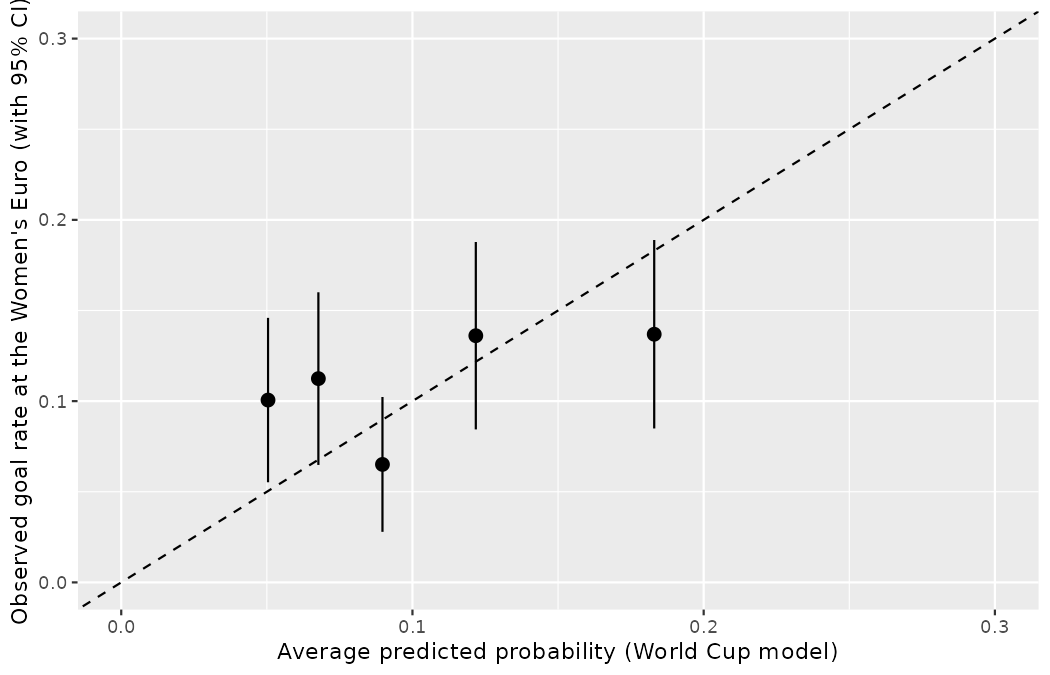
\includegraphics[width=0.85\linewidth,height=\textheight,keepaspectratio]{figures/inf-model-logistic-3.png}

The picture is humbling in a specific, instructive way. The model's
predictions span \(0.050\) to \(0.183\) across the buckets, but the
observed goal rates barely move: \(0.101,\) \(0.112,\) \(0.065,\)
\(0.136,\) \(0.137.\) The shots the model is most pessimistic about
score at twice the predicted rate --- bucket 1's interval
\((0.055, 0.146)\) excludes its own average prediction of \(0.050\) ---
while the top bucket scores below its billing. Four of the five
intervals technically cover the \(y = x\) line, but the \emph{slope} of
the points is unmistakably shallower than the line: the exported
probabilities exaggerate. Hold both findings at once, because together
they are the honest export report: the World Cup tag model still
\emph{ranks} Euro shots well enough to run a shortlist (the
classification rates above), but its \emph{probabilities} are
mis-calibrated on the new competition --- the tags do not mean quite the
same thing in a tournament with, for instance, a very different rate of
pressure tagging. A number that travels is not the same thing as a
number that is still true on arrival.

The natural follow-up, and the payoff of this whole diagnostic:
Northbridge does not actually rely on home-grown tag models to price
chances --- it buys \texttt{statsbomb\_xg}, a probability estimated by
the vendor's far richer model. The same bucket machinery puts the vendor
on trial. \emph{Is the xG model honest?} If \texttt{statsbomb\_xg} means
what it claims --- an estimated probability of scoring --- then shots
priced around \(0.06\) should score about 6\% of the time, at a
tournament the vendor's model was never tuned to flatter:

\begin{Shaded}
\begin{Highlighting}[]
\NormalTok{xg\_buckets }\OtherTok{\textless{}{-}}\NormalTok{ weuro\_open }\SpecialCharTok{|\textgreater{}}
  \FunctionTok{mutate}\NormalTok{(}\AttributeTok{bucket =} \FunctionTok{ntile}\NormalTok{(statsbomb\_xg, }\DecValTok{5}\NormalTok{)) }\SpecialCharTok{|\textgreater{}}
  \FunctionTok{group\_by}\NormalTok{(bucket) }\SpecialCharTok{|\textgreater{}}
  \FunctionTok{summarize}\NormalTok{(}
    \AttributeTok{shots =} \FunctionTok{n}\NormalTok{(),}
    \AttributeTok{avg\_xg =} \FunctionTok{mean}\NormalTok{(statsbomb\_xg),}
    \AttributeTok{obs\_rate =} \FunctionTok{mean}\NormalTok{(goal),}
    \AttributeTok{lower =}\NormalTok{ obs\_rate }\SpecialCharTok{{-}} \FloatTok{1.96} \SpecialCharTok{*} \FunctionTok{sqrt}\NormalTok{(obs\_rate }\SpecialCharTok{*}\NormalTok{ (}\DecValTok{1} \SpecialCharTok{{-}}\NormalTok{ obs\_rate) }\SpecialCharTok{/}\NormalTok{ shots),}
    \AttributeTok{upper =}\NormalTok{ obs\_rate }\SpecialCharTok{+} \FloatTok{1.96} \SpecialCharTok{*} \FunctionTok{sqrt}\NormalTok{(obs\_rate }\SpecialCharTok{*}\NormalTok{ (}\DecValTok{1} \SpecialCharTok{{-}}\NormalTok{ obs\_rate) }\SpecialCharTok{/}\NormalTok{ shots)}
\NormalTok{  )}
\NormalTok{xg\_buckets}
\CommentTok{\#\textgreater{} \# A tibble: 5 × 6}
\CommentTok{\#\textgreater{}   bucket shots avg\_xg obs\_rate    lower  upper}
\CommentTok{\#\textgreater{}    \textless{}int\textgreater{} \textless{}int\textgreater{}  \textless{}dbl\textgreater{}    \textless{}dbl\textgreater{}    \textless{}dbl\textgreater{}  \textless{}dbl\textgreater{}}
\CommentTok{\#\textgreater{} 1      1   169 0.0186   0.0178 {-}0.00216 0.0377}
\CommentTok{\#\textgreater{} 2      2   169 0.0383   0.0355  0.00760 0.0634}
\CommentTok{\#\textgreater{} 3      3   169 0.0599   0.0888  0.0459  0.132}
\CommentTok{\#\textgreater{} 4      4   169 0.0936   0.0947  0.0505  0.139}
\CommentTok{\#\textgreater{} 5      5   168 0.271    0.315   0.245   0.386}
\end{Highlighting}
\end{Shaded}

This is what calibration looks like. Every one of the five intervals
covers its bucket's average xG; the observed rates rise from \(0.018\)
to \(0.315\) in step with the vendor's prices from \(0.019\) to
\(0.271\); and where our tag model compressed all of open play into a
\(0.04\)-to-\(0.40\) smear, xG spreads real credit across a fifteen-fold
range. (Small print: the lowest bucket holds 3 goals in 169 shots, so
its success-failure condition fails and the symmetric interval even dips
below zero --- the same rough edge you met in
Chapter~\ref{sec-inference-one-mean}'s bootstrap discussion; read that
interval qualitatively.) On open play at the 2025 Women's Euro, the
vendor's number is honest.

One frame remains, and the penalty convention will not let us skip it.
The Euro's 51 penalty kicks all carry the same xG --- the stored penalty
value of \(0.7835,\) printing as \(0.784\) here, that you have watched
spike every histogram since Chapter~\ref{sec-data-applications}:

\begin{Shaded}
\begin{Highlighting}[]
\NormalTok{weuro2025\_shots }\SpecialCharTok{|\textgreater{}}
  \FunctionTok{filter}\NormalTok{(shot\_type }\SpecialCharTok{==} \StringTok{"Penalty"}\NormalTok{) }\SpecialCharTok{|\textgreater{}}
  \FunctionTok{summarize}\NormalTok{(}
    \AttributeTok{kicks =} \FunctionTok{n}\NormalTok{(),}
    \AttributeTok{goals =} \FunctionTok{sum}\NormalTok{(goal),}
    \AttributeTok{conversion =} \FunctionTok{mean}\NormalTok{(goal),}
    \AttributeTok{mean\_xg =} \FunctionTok{mean}\NormalTok{(statsbomb\_xg)}
\NormalTok{  )}
\CommentTok{\#\textgreater{} \# A tibble: 1 × 4}
\CommentTok{\#\textgreater{}   kicks goals conversion mean\_xg}
\CommentTok{\#\textgreater{}   \textless{}int\textgreater{} \textless{}int\textgreater{}      \textless{}dbl\textgreater{}   \textless{}dbl\textgreater{}}
\CommentTok{\#\textgreater{} 1    51    28      0.549   0.784}

\FunctionTok{round}\NormalTok{(}\DecValTok{28}\SpecialCharTok{/}\DecValTok{51} \SpecialCharTok{+} \FunctionTok{c}\NormalTok{(}\SpecialCharTok{{-}}\FloatTok{1.96}\NormalTok{, }\FloatTok{1.96}\NormalTok{) }\SpecialCharTok{*} \FunctionTok{sqrt}\NormalTok{((}\DecValTok{28}\SpecialCharTok{/}\DecValTok{51}\NormalTok{) }\SpecialCharTok{*}\NormalTok{ (}\DecValTok{1} \SpecialCharTok{{-}} \DecValTok{28}\SpecialCharTok{/}\DecValTok{51}\NormalTok{) }\SpecialCharTok{/} \DecValTok{51}\NormalTok{), }\DecValTok{4}\NormalTok{)}
\CommentTok{\#\textgreater{} [1] 0.4125 0.6856}
\end{Highlighting}
\end{Shaded}

Twenty-eight of 51 scored --- \(0.549,\) with a 95\% interval of
\((0.412, 0.686)\) that sits entirely below the advertised \(0.784.\)
Taken alone, that reads like the one dishonest line in the vendor's
ledger. Do not convict yet. The count is 51 kicks from a single
tournament, many from shootouts; and the men's World Cup's own penalties
went \(43/64 = 0.672\) with interval \((0.557, 0.787)\) --- which covers
\(0.784,\) if barely. And the mechanism has a name: most of the Euro's
51 kicks are shoot-out kicks --- period 5 in these data --- and
shoot-out conversion is known to run below in-game penalty conversion,
so a vendor stamping every period-5 kick with the same in-game
\(0.7835\) is taking a nameable modeling shortcut, not hiding an
unknowable flaw. The professional conclusion is the cautious one: the
open-play calibration is clean, the penalty line is worth a query to the
vendor and more data, and --- as everywhere in this book --- the two
frames must be reported as a pair, because a single blended number would
have hidden both facts.

\begin{tcolorbox}[enhanced jigsaw, left=2mm, leftrule=.75mm, title=\textcolor{quarto-callout-tip-color}{\faLightbulb}\hspace{0.5em}{Check your understanding}, arc=.35mm, rightrule=.15mm, coltitle=black, colframe=quarto-callout-tip-color-frame, bottomrule=.15mm, colbacktitle=quarto-callout-tip-color!10!white, opacitybacktitle=0.6, breakable, bottomtitle=1mm, toptitle=1mm, titlerule=0mm, opacityback=0, toprule=.15mm, colback=white]

Your colleague summarizes the external validation as: ``the World Cup
model works at the Euro --- it caught half the goals, just as
cross-validation promised.'' What is missing from that summary?

\begin{center}\rule{0.5\linewidth}{0.5pt}\end{center}

The calibration finding. The exported model's \emph{classification} held
up (recall and specificity inside the cross-validated ranges), but its
\emph{probabilities} did not: bucketed against outcomes, the predictions
spread far wider than the observed goal rates, and the lowest-priced
bucket scored at double its billing. A shortlist survives
mis-calibration, because it only uses the ranking; any use that takes
the probabilities at face value --- pricing chances, projecting goal
counts, comparing players across competitions --- would not. Validation
is a property of a model \emph{and} a use, not of a model alone.

\end{tcolorbox}

\section{Chapter review}\label{sec-chp26-review}

\subsection{Summary}\label{summary-25}

Throughout the text, we have presented a modern view of introductory
statistics for the scouting professional. Earlier, we presented
graphical techniques which communicated relationships across multiple
variables; we also used modeling to formalize those relationships. In
this chapter we considered inferential claims on models which include
many variables used to predict the probability of a binary outcome --- a
goal, a shortlisted dossier. The Wald output of the software finally
repaid the glm-side promise of Chapter~\ref{sec-model-logistic} --- the
lm side of that patience was repaid in Chapter~\ref{sec-inf-model-slr}:
\texttt{statistic} is the coefficient in units of its standard error,
\texttt{p.value} its two-sided normal tail, and each hypothesis is
conditional on the other variables in the model. Cross-validation and a
deliberately low cutoff turned the same model into a shortlist whose
recall/specificity trade-off is a decision about error costs, not a
software default; external validation and calibration buckets then
tested what survives the trip to a new competition --- the ranking did,
the probabilities did not, and the vendor's xG passed the honesty check
that our tag model failed. We continue to emphasize the importance of
study design in making conclusions about research claims: every
coefficient in this chapter was associational, variability can come from
different sources (random sampling vs.~random allocation, see
Table~\ref{tbl-randsampValloc}), and the penalties-in companion fit
showed once more that the frame decision can move a verdict further than
the football does.

As you might guess, this text has only scratched the surface of the
world of statistical analyses that can be applied to different datasets.
In particular, to do justice to the topic, the linear models and
generalized linear models we have introduced can each be covered with
their own course or book. Hierarchical models (shots nest within
matches, matches within teams --- structure this book's independence
conditions politely ignored), alternative methods for fitting
parameters, and advanced computational methods applied to multivariable
models are all beyond the scope of this book. However, your successful
understanding of the ideas we have covered has set you up perfectly to
move on to a higher level of statistical modeling and inference --- the
closing case study of Chapter~\ref{sec-inf-model-applications} now puts
the full inferential toolkit through one last scouting workflow. Enjoy!

\subsection{Terms}\label{terms-25}

The terms introduced in this chapter are presented below, alphabetized.
If you're not sure what some of these terms mean, we recommend you go
back in the text and review their definitions. You should be able to
easily spot them as \textbf{bolded text}.

\begin{longtable}[]{@{}
  >{\raggedright\arraybackslash}p{(\linewidth - 4\tabcolsep) * \real{0.3380}}
  >{\raggedright\arraybackslash}p{(\linewidth - 4\tabcolsep) * \real{0.3380}}
  >{\raggedright\arraybackslash}p{(\linewidth - 4\tabcolsep) * \real{0.3239}}@{}}
\caption{Terms introduced in this
chapter.}\label{tbl-terms-chp-26}\tabularnewline
\toprule\noalign{}
\endfirsthead
\endhead
\bottomrule\noalign{}
\endlastfoot
accuracy & inference on logistic regression & technical conditions \\
cross-validation & multiple predictors & \\
\end{longtable}

\section{Exercises}\label{sec-chp26-exercises}

Answers to odd-numbered exercises can be found in
Appendix~\ref{sec-exercise-solutions-26}.

\begin{enumerate}
\def\labelenumi{\arabic{enumi}.}
\item
  \textbf{Rating the academies.} A consulting company is hired by the
  league to assess whether certain characteristics of a youth academy
  (e.g., region, intake size, number of full-time coaches,
  video-analysis budget, hours of contact time, etc.) are associated
  with the academy's success at producing professionals. The company is
  given information on 100 randomly selected academies across the
  country. For each academy, the annual rate at which its graduates sign
  professional contracts is recorded, along with the other
  characteristics describing the academy. Can logistic regression with
  multiple predictors be used to predict the annual
  professional-contract rate for academies in this setting? Explain your
  reasoning.
\item
  \textbf{Residential academies and professional contracts.} Priya Rao
  wants to investigate the relationship between having spent at least
  one year in a residential academy before age 14 and signing a
  professional contract before age 21.

  \begin{enumerate}
  \def\labelenumii{\alph{enumii}.}
  \item
    Explain why logistic regression can be used to study the
    relationship between these two binary variables. What is the
    technical assumption describing the relationship between the
    response (outcome) and explanatory (predictor) variables?
  \item
    What other methods covered in this text might be used to address the
    research question of interest? What advantages does logistic
    regression have over these methods?
  \end{enumerate}
\item
  \textbf{First-time finishing at the World Cup.} Do first-time strikes
  convert at a different rate from shots where the striker takes a
  touch? Nobody assigns finishing technique at random, so this is an
  observational question about the 1,365 open-play shots of the 2022
  Men's World Cup (built with the frame of
  Chapter~\ref{sec-inf-model-logistic}). The group conversion rates and
  the output of a logistic regression predicting \texttt{goal} from
  \texttt{first\_time} are shown below.\footnote{The 2022 Men's World
    Cup shot data used in this exercise are in
    \texttt{data/derived/wc2022\_shots.csv} (StatsBomb open data). These
    are observational data: the model describes association, not
    causation.}

\begin{Shaded}
\begin{Highlighting}[]
\NormalTok{wc2022\_shots }\OtherTok{\textless{}{-}} \FunctionTok{read\_csv}\NormalTok{(}\StringTok{"data/derived/wc2022\_shots.csv"}\NormalTok{)}

\NormalTok{shots\_open }\OtherTok{\textless{}{-}}\NormalTok{ wc2022\_shots }\SpecialCharTok{|\textgreater{}}
  \FunctionTok{filter}\NormalTok{(}
\NormalTok{    shot\_type }\SpecialCharTok{==} \StringTok{"Open Play"}\NormalTok{,}
\NormalTok{    body\_part }\SpecialCharTok{!=} \StringTok{"Other"}\NormalTok{,}
\NormalTok{    play\_pattern }\SpecialCharTok{!=} \StringTok{"Other"}
\NormalTok{  )}

\NormalTok{shots\_open }\SpecialCharTok{|\textgreater{}}
  \FunctionTok{group\_by}\NormalTok{(first\_time) }\SpecialCharTok{|\textgreater{}}
  \FunctionTok{summarize}\NormalTok{(}\AttributeTok{shots =} \FunctionTok{n}\NormalTok{(), }\AttributeTok{goals =} \FunctionTok{sum}\NormalTok{(goal), }\AttributeTok{conversion =} \FunctionTok{mean}\NormalTok{(goal))}
\CommentTok{\#\textgreater{} \# A tibble: 2 × 4}
\CommentTok{\#\textgreater{}   first\_time shots goals conversion}
\CommentTok{\#\textgreater{}   \textless{}lgl\textgreater{}      \textless{}int\textgreater{} \textless{}int\textgreater{}      \textless{}dbl\textgreater{}}
\CommentTok{\#\textgreater{} 1 FALSE        901    77     0.0855}
\CommentTok{\#\textgreater{} 2 TRUE         464    70     0.151}

\NormalTok{ft\_fit }\OtherTok{\textless{}{-}} \FunctionTok{glm}\NormalTok{(goal }\SpecialCharTok{\textasciitilde{}}\NormalTok{ first\_time, }\AttributeTok{data =}\NormalTok{ shots\_open, }\AttributeTok{family =}\NormalTok{ binomial)}
\FunctionTok{tidy}\NormalTok{(ft\_fit)}
\CommentTok{\#\textgreater{} \# A tibble: 2 × 5}
\CommentTok{\#\textgreater{}   term           estimate std.error statistic  p.value}
\CommentTok{\#\textgreater{}   \textless{}chr\textgreater{}             \textless{}dbl\textgreater{}     \textless{}dbl\textgreater{}     \textless{}dbl\textgreater{}    \textless{}dbl\textgreater{}}
\CommentTok{\#\textgreater{} 1 (Intercept)      {-}2.37      0.119    {-}19.9  4.85e{-}88}
\CommentTok{\#\textgreater{} 2 first\_timeTRUE    0.643     0.176      3.65 2.65e{-} 4}

\FunctionTok{round}\NormalTok{(}\FunctionTok{coef}\NormalTok{(ft\_fit), }\DecValTok{4}\NormalTok{)}
\CommentTok{\#\textgreater{}    (Intercept) first\_timeTRUE}
\CommentTok{\#\textgreater{}        {-}2.3704         0.6425}
\end{Highlighting}
\end{Shaded}

  \begin{enumerate}
  \def\labelenumii{\alph{enumii}.}
  \item
    Based on the regression output, evaluate whether
    \texttt{first\_time} is a discernible predictor of whether the shot
    is scored. State the hypotheses, the test statistic, the p-value,
    and the conclusion in context of the data and the research question.
  \item
    Back-transform the fitted model: compute the model's estimated
    scoring probability for a shot that is not struck first time and for
    a shot that is, showing your arithmetic, and compare the two values
    with the raw conversion rates in the table above.
  \end{enumerate}
\item
  \textbf{Warm-up protocol and season availability.} The federation's
  sports-science program ran a randomized experiment on 1,475 players
  across its member academies: each player was randomly assigned to a
  new neuromuscular warm-up protocol or to the standard warm-up, and
  each academy recorded whether the player remained available all season
  (no soft-tissue injury), with success defined as
  \texttt{fit\_all\_season}. This is the third warm-up trial in this
  book, a separate study from both the knee-injury prevention trial in
  the exercises of Chapter~\ref{sec-data-hello} and the muscle-flag
  trial of Section~\ref{sec-chp17-exercises}: three different trials,
  three different cohorts, three different outcomes. This is a
  constructed scenario, generated by the seeded code below.\footnote{The
    \texttt{warmup1475} data are a constructed scenario, generated
    entirely by the seeded code shown (seed 2602); no real trial was
    run. Because the protocol was randomly assigned, the design supports
    causal conclusions.}

\begin{Shaded}
\begin{Highlighting}[]
\FunctionTok{set.seed}\NormalTok{(}\DecValTok{2602}\NormalTok{)}
\NormalTok{n\_players }\OtherTok{\textless{}{-}} \DecValTok{1475}

\NormalTok{warmup1475 }\OtherTok{\textless{}{-}} \FunctionTok{tibble}\NormalTok{(}
  \AttributeTok{group =} \FunctionTok{factor}\NormalTok{(}\FunctionTok{sample}\NormalTok{(}\FunctionTok{rep}\NormalTok{(}\FunctionTok{c}\NormalTok{(}\StringTok{"standard"}\NormalTok{, }\StringTok{"warmup"}\NormalTok{), }\AttributeTok{length.out =}\NormalTok{ n\_players)),}
                 \AttributeTok{levels =} \FunctionTok{c}\NormalTok{(}\StringTok{"standard"}\NormalTok{, }\StringTok{"warmup"}\NormalTok{)),}
  \AttributeTok{fit\_all\_season =} \FunctionTok{rbinom}\NormalTok{(n\_players, }\DecValTok{1}\NormalTok{, }\FunctionTok{if\_else}\NormalTok{(group }\SpecialCharTok{==} \StringTok{"warmup"}\NormalTok{, }\FloatTok{0.885}\NormalTok{, }\FloatTok{0.84}\NormalTok{))}
\NormalTok{)}

\NormalTok{warmup1475 }\SpecialCharTok{|\textgreater{}}
  \FunctionTok{group\_by}\NormalTok{(group) }\SpecialCharTok{|\textgreater{}}
  \FunctionTok{summarize}\NormalTok{(}\AttributeTok{players =} \FunctionTok{n}\NormalTok{(), }\AttributeTok{p\_fit =} \FunctionTok{mean}\NormalTok{(fit\_all\_season))}
\CommentTok{\#\textgreater{} \# A tibble: 2 × 3}
\CommentTok{\#\textgreater{}   group    players p\_fit}
\CommentTok{\#\textgreater{}   \textless{}fct\textgreater{}      \textless{}int\textgreater{} \textless{}dbl\textgreater{}}
\CommentTok{\#\textgreater{} 1 standard     738 0.852}
\CommentTok{\#\textgreater{} 2 warmup       737 0.890}

\NormalTok{warmup\_fit }\OtherTok{\textless{}{-}} \FunctionTok{glm}\NormalTok{(fit\_all\_season }\SpecialCharTok{\textasciitilde{}}\NormalTok{ group, }\AttributeTok{data =}\NormalTok{ warmup1475, }\AttributeTok{family =}\NormalTok{ binomial)}
\FunctionTok{tidy}\NormalTok{(warmup\_fit)}
\CommentTok{\#\textgreater{} \# A tibble: 2 × 5}
\CommentTok{\#\textgreater{}   term        estimate std.error statistic  p.value}
\CommentTok{\#\textgreater{}   \textless{}chr\textgreater{}          \textless{}dbl\textgreater{}     \textless{}dbl\textgreater{}     \textless{}dbl\textgreater{}    \textless{}dbl\textgreater{}}
\CommentTok{\#\textgreater{} 1 (Intercept)    1.75      0.104     16.9  4.96e{-}64}
\CommentTok{\#\textgreater{} 2 groupwarmup    0.339     0.157      2.16 3.08e{-} 2}

\FunctionTok{round}\NormalTok{(}\FunctionTok{coef}\NormalTok{(warmup\_fit), }\DecValTok{4}\NormalTok{)}
\CommentTok{\#\textgreater{} (Intercept) groupwarmup}
\CommentTok{\#\textgreater{}      1.7528      0.3389}
\end{Highlighting}
\end{Shaded}

  \begin{enumerate}
  \def\labelenumii{\alph{enumii}.}
  \item
    Based on the regression output, evaluate whether the treatment group
    is a discernible predictor of the outcome. State the hypotheses, the
    test statistic, the p-value, and the conclusion in context of the
    data and the research question --- including whether a causal claim
    is warranted.
  \item
    Back-transform the fitted model: compute the estimated probability
    of staying fit all season under each warm-up, showing your
    arithmetic, and compare with the group proportions in the output.
  \end{enumerate}
\item
  \textbf{Which tournament is this shot from? Cross-validation.} During
  a database migration, a batch of shot records at Northbridge lost its
  competition label, and Priya wonders how well the label could be
  restored from the shot's characteristics alone. We consider the 2,209
  open-play shots of the 2022 Men's World Cup and the 2025 Women's Euro
  (built with the frame of Chapter~\ref{sec-inf-model-logistic}), which
  between them contain 1,365 World Cup shots and 844 Euro shots. We use
  logistic regression to classify shots into the two competitions. The
  outcome variable, \texttt{competition}, is modeled as a success when
  the shot is from the 2025 Women's Euro; each shot is classified into
  the competition whose predicted probability exceeds
  \(0.5\).\footnote{The shot data used in this exercise are in
    \texttt{data/derived/wc2022\_shots.csv} and
    \texttt{data/derived/weuro2025\_shots.csv} (StatsBomb open data).}

\begin{Shaded}
\begin{Highlighting}[]
\NormalTok{wc2022\_shots    }\OtherTok{\textless{}{-}} \FunctionTok{read\_csv}\NormalTok{(}\StringTok{"data/derived/wc2022\_shots.csv"}\NormalTok{)}
\NormalTok{weuro2025\_shots }\OtherTok{\textless{}{-}} \FunctionTok{read\_csv}\NormalTok{(}\StringTok{"data/derived/weuro2025\_shots.csv"}\NormalTok{)}

\NormalTok{shots\_two }\OtherTok{\textless{}{-}} \FunctionTok{bind\_rows}\NormalTok{(wc2022\_shots, weuro2025\_shots) }\SpecialCharTok{|\textgreater{}}
  \FunctionTok{filter}\NormalTok{(}
\NormalTok{    shot\_type }\SpecialCharTok{==} \StringTok{"Open Play"}\NormalTok{,}
\NormalTok{    body\_part }\SpecialCharTok{!=} \StringTok{"Other"}\NormalTok{,}
\NormalTok{    play\_pattern }\SpecialCharTok{!=} \StringTok{"Other"}
\NormalTok{  ) }\SpecialCharTok{|\textgreater{}}
  \FunctionTok{mutate}\NormalTok{(}\AttributeTok{competition =} \FunctionTok{factor}\NormalTok{(competition, }\AttributeTok{levels =} \FunctionTok{c}\NormalTok{(}\StringTok{"wc2022"}\NormalTok{, }\StringTok{"weuro2025"}\NormalTok{)))}

\FunctionTok{set.seed}\NormalTok{(}\DecValTok{2603}\NormalTok{)}
\NormalTok{shots\_two }\OtherTok{\textless{}{-}}\NormalTok{ shots\_two }\SpecialCharTok{|\textgreater{}}
  \FunctionTok{mutate}\NormalTok{(}\AttributeTok{fold =} \FunctionTok{sample}\NormalTok{(}\FunctionTok{rep}\NormalTok{(}\DecValTok{1}\SpecialCharTok{:}\DecValTok{4}\NormalTok{, }\AttributeTok{length.out =} \FunctionTok{n}\NormalTok{())))}

\NormalTok{cv\_class }\OtherTok{\textless{}{-}} \ControlFlowTok{function}\NormalTok{(model\_formula, data) \{}
\NormalTok{  predictions }\OtherTok{\textless{}{-}} \FunctionTok{vector}\NormalTok{(}\StringTok{"list"}\NormalTok{, }\DecValTok{4}\NormalTok{)}
  \ControlFlowTok{for}\NormalTok{ (f }\ControlFlowTok{in} \DecValTok{1}\SpecialCharTok{:}\DecValTok{4}\NormalTok{) \{}
\NormalTok{    train }\OtherTok{\textless{}{-}} \FunctionTok{filter}\NormalTok{(data, fold }\SpecialCharTok{!=}\NormalTok{ f)}
\NormalTok{    test  }\OtherTok{\textless{}{-}} \FunctionTok{filter}\NormalTok{(data, fold }\SpecialCharTok{==}\NormalTok{ f)}
\NormalTok{    fold\_fit }\OtherTok{\textless{}{-}} \FunctionTok{glm}\NormalTok{(model\_formula, }\AttributeTok{data =}\NormalTok{ train, }\AttributeTok{family =}\NormalTok{ binomial)}
\NormalTok{    predictions[[f]] }\OtherTok{\textless{}{-}}\NormalTok{ test }\SpecialCharTok{|\textgreater{}}
      \FunctionTok{mutate}\NormalTok{(}
        \AttributeTok{p\_cv =} \FunctionTok{predict}\NormalTok{(fold\_fit, }\AttributeTok{newdata =}\NormalTok{ test, }\AttributeTok{type =} \StringTok{"response"}\NormalTok{),}
        \AttributeTok{pred =} \FunctionTok{if\_else}\NormalTok{(p\_cv }\SpecialCharTok{\textgreater{}} \FloatTok{0.5}\NormalTok{, }\StringTok{"weuro2025"}\NormalTok{, }\StringTok{"wc2022"}\NormalTok{)}
\NormalTok{      )}
\NormalTok{  \}}
  \FunctionTok{bind\_rows}\NormalTok{(predictions)}
\NormalTok{\}}

\NormalTok{cv\_minute      }\OtherTok{\textless{}{-}} \FunctionTok{cv\_class}\NormalTok{(competition }\SpecialCharTok{\textasciitilde{}}\NormalTok{ minute, shots\_two)}
\NormalTok{cv\_pressure\_xg }\OtherTok{\textless{}{-}} \FunctionTok{cv\_class}\NormalTok{(competition }\SpecialCharTok{\textasciitilde{}}\NormalTok{ under\_pressure }\SpecialCharTok{+}\NormalTok{ statsbomb\_xg,}
\NormalTok{                           shots\_two)}
\end{Highlighting}
\end{Shaded}

  The cross-validated predictions of the smaller model (\texttt{minute}
  as the only predictor) and of the larger model
  (\texttt{under\_pressure} and \texttt{statsbomb\_xg}) are tabulated
  against the true labels, fold by fold:

\begin{Shaded}
\begin{Highlighting}[]
\NormalTok{cv\_minute }\SpecialCharTok{|\textgreater{}}
  \FunctionTok{count}\NormalTok{(fold, competition, pred) }\SpecialCharTok{|\textgreater{}}
  \FunctionTok{pivot\_wider}\NormalTok{(}\AttributeTok{names\_from =}\NormalTok{ pred, }\AttributeTok{values\_from =}\NormalTok{ n, }\AttributeTok{values\_fill =} \DecValTok{0}\NormalTok{)}
\CommentTok{\#\textgreater{} \# A tibble: 8 × 3}
\CommentTok{\#\textgreater{}    fold competition wc2022}
\CommentTok{\#\textgreater{}   \textless{}int\textgreater{} \textless{}fct\textgreater{}        \textless{}int\textgreater{}}
\CommentTok{\#\textgreater{} 1     1 wc2022         347}
\CommentTok{\#\textgreater{} 2     1 weuro2025      206}
\CommentTok{\#\textgreater{} 3     2 wc2022         328}
\CommentTok{\#\textgreater{} 4     2 weuro2025      224}
\CommentTok{\#\textgreater{} 5     3 wc2022         349}
\CommentTok{\#\textgreater{} 6     3 weuro2025      203}
\CommentTok{\#\textgreater{} 7     4 wc2022         341}
\CommentTok{\#\textgreater{} 8     4 weuro2025      211}

\NormalTok{cv\_pressure\_xg }\SpecialCharTok{|\textgreater{}}
  \FunctionTok{count}\NormalTok{(fold, competition, pred) }\SpecialCharTok{|\textgreater{}}
  \FunctionTok{pivot\_wider}\NormalTok{(}\AttributeTok{names\_from =}\NormalTok{ pred, }\AttributeTok{values\_from =}\NormalTok{ n, }\AttributeTok{values\_fill =} \DecValTok{0}\NormalTok{)}
\CommentTok{\#\textgreater{} \# A tibble: 8 × 4}
\CommentTok{\#\textgreater{}    fold competition wc2022 weuro2025}
\CommentTok{\#\textgreater{}   \textless{}int\textgreater{} \textless{}fct\textgreater{}        \textless{}int\textgreater{}     \textless{}int\textgreater{}}
\CommentTok{\#\textgreater{} 1     1 wc2022         287        60}
\CommentTok{\#\textgreater{} 2     1 weuro2025      121        85}
\CommentTok{\#\textgreater{} 3     2 wc2022         268        60}
\CommentTok{\#\textgreater{} 4     2 weuro2025      142        82}
\CommentTok{\#\textgreater{} 5     3 wc2022         283        66}
\CommentTok{\#\textgreater{} 6     3 weuro2025      125        78}
\CommentTok{\#\textgreater{} 7     4 wc2022         290        51}
\CommentTok{\#\textgreater{} 8     4 weuro2025      135        76}
\end{Highlighting}
\end{Shaded}

  \begin{enumerate}
  \def\labelenumii{\alph{enumii}.}
  \item
    How many observations are in Fold 2? Use the model with only
    \texttt{minute} as a predictor variable. Of the observations in Fold
    2, how many of them were correctly predicted to be from the Women's
    Euro? How many of them were incorrectly predicted to be from the
    Women's Euro? What has the smaller model's classifier done?
  \item
    How many observations are used to build the model which predicts for
    the observations in Fold 2?
  \item
    For one of the cross-validation folds, how many coefficients were
    estimated for the model which uses \texttt{minute} as a predictor?
    For one of the cross-validation folds, how many coefficients were
    estimated for the model which uses \texttt{under\_pressure} and
    \texttt{statsbomb\_xg} as predictors?
  \item
    Here the classification cutoff was the software default of \(0.5\),
    yet Section~\ref{sec-inf-log-reg-cv} insisted on a cutoff of
    \(0.10\) for the goal shortlist. Why is \(0.5\) a defensible choice
    for this label-repair task but not for the goal shortlist?
  \end{enumerate}
\item
  \textbf{Predicting goals at the Women's Euro, cross-validation.} We
  use logistic regression to model whether each of the 844 open-play
  shots of the 2025 Women's Euro (built with the frame of
  Chapter~\ref{sec-inf-model-logistic}) was scored, from various
  explanatory variables, using 3-fold cross-validation. The larger model
  uses the five predictors of the chapter's goal model; the smaller
  model uses only \texttt{statsbomb\_xg} and \texttt{one\_on\_one}. Each
  shot is classified as a predicted goal when its cross-validated
  probability exceeds the software-default cutoff of \(0.5\).\footnote{The
    2025 Women's Euro shot data used in this exercise are in
    \texttt{data/derived/weuro2025\_shots.csv} (StatsBomb open data).}

\begin{Shaded}
\begin{Highlighting}[]
\NormalTok{weuro2025\_shots }\OtherTok{\textless{}{-}} \FunctionTok{read\_csv}\NormalTok{(}\StringTok{"data/derived/weuro2025\_shots.csv"}\NormalTok{)}

\NormalTok{weuro\_open }\OtherTok{\textless{}{-}}\NormalTok{ weuro2025\_shots }\SpecialCharTok{|\textgreater{}}
  \FunctionTok{filter}\NormalTok{(}
\NormalTok{    shot\_type }\SpecialCharTok{==} \StringTok{"Open Play"}\NormalTok{,}
\NormalTok{    body\_part }\SpecialCharTok{!=} \StringTok{"Other"}\NormalTok{,}
\NormalTok{    play\_pattern }\SpecialCharTok{!=} \StringTok{"Other"}
\NormalTok{  )}

\FunctionTok{set.seed}\NormalTok{(}\DecValTok{2604}\NormalTok{)}
\NormalTok{weuro\_open }\OtherTok{\textless{}{-}}\NormalTok{ weuro\_open }\SpecialCharTok{|\textgreater{}}
  \FunctionTok{mutate}\NormalTok{(}\AttributeTok{fold =} \FunctionTok{sample}\NormalTok{(}\FunctionTok{rep}\NormalTok{(}\DecValTok{1}\SpecialCharTok{:}\DecValTok{3}\NormalTok{, }\AttributeTok{length.out =} \FunctionTok{n}\NormalTok{())))}

\NormalTok{cv\_goal }\OtherTok{\textless{}{-}} \ControlFlowTok{function}\NormalTok{(model\_formula, data) \{}
\NormalTok{  predictions }\OtherTok{\textless{}{-}} \FunctionTok{vector}\NormalTok{(}\StringTok{"list"}\NormalTok{, }\DecValTok{3}\NormalTok{)}
  \ControlFlowTok{for}\NormalTok{ (f }\ControlFlowTok{in} \DecValTok{1}\SpecialCharTok{:}\DecValTok{3}\NormalTok{) \{}
\NormalTok{    train }\OtherTok{\textless{}{-}} \FunctionTok{filter}\NormalTok{(data, fold }\SpecialCharTok{!=}\NormalTok{ f)}
\NormalTok{    test  }\OtherTok{\textless{}{-}} \FunctionTok{filter}\NormalTok{(data, fold }\SpecialCharTok{==}\NormalTok{ f)}
\NormalTok{    fold\_fit }\OtherTok{\textless{}{-}} \FunctionTok{glm}\NormalTok{(model\_formula, }\AttributeTok{data =}\NormalTok{ train, }\AttributeTok{family =}\NormalTok{ binomial)}
\NormalTok{    predictions[[f]] }\OtherTok{\textless{}{-}}\NormalTok{ test }\SpecialCharTok{|\textgreater{}}
      \FunctionTok{mutate}\NormalTok{(}
        \AttributeTok{p\_cv =} \FunctionTok{predict}\NormalTok{(fold\_fit, }\AttributeTok{newdata =}\NormalTok{ test, }\AttributeTok{type =} \StringTok{"response"}\NormalTok{),}
        \AttributeTok{pred =} \FunctionTok{if\_else}\NormalTok{(p\_cv }\SpecialCharTok{\textgreater{}} \FloatTok{0.5}\NormalTok{, }\StringTok{"goal"}\NormalTok{, }\StringTok{"no goal"}\NormalTok{),}
        \AttributeTok{obs  =} \FunctionTok{if\_else}\NormalTok{(goal, }\StringTok{"goal"}\NormalTok{, }\StringTok{"no goal"}\NormalTok{)}
\NormalTok{      )}
\NormalTok{  \}}
  \FunctionTok{bind\_rows}\NormalTok{(predictions)}
\NormalTok{\}}

\NormalTok{cv\_tags }\OtherTok{\textless{}{-}} \FunctionTok{cv\_goal}\NormalTok{(}
\NormalTok{  goal }\SpecialCharTok{\textasciitilde{}}\NormalTok{ under\_pressure }\SpecialCharTok{+}\NormalTok{ first\_time }\SpecialCharTok{+}\NormalTok{ one\_on\_one }\SpecialCharTok{+}\NormalTok{ body\_part }\SpecialCharTok{+}\NormalTok{ play\_pattern,}
\NormalTok{  weuro\_open}
\NormalTok{)}
\NormalTok{cv\_xg1v1 }\OtherTok{\textless{}{-}} \FunctionTok{cv\_goal}\NormalTok{(goal }\SpecialCharTok{\textasciitilde{}}\NormalTok{ statsbomb\_xg }\SpecialCharTok{+}\NormalTok{ one\_on\_one, weuro\_open)}

\NormalTok{cv\_tags }\SpecialCharTok{|\textgreater{}}
  \FunctionTok{count}\NormalTok{(fold, obs, pred) }\SpecialCharTok{|\textgreater{}}
  \FunctionTok{pivot\_wider}\NormalTok{(}\AttributeTok{names\_from =}\NormalTok{ pred, }\AttributeTok{values\_from =}\NormalTok{ n, }\AttributeTok{values\_fill =} \DecValTok{0}\NormalTok{)}
\CommentTok{\#\textgreater{} \# A tibble: 6 × 3}
\CommentTok{\#\textgreater{}    fold obs     \textasciigrave{}no goal\textasciigrave{}}
\CommentTok{\#\textgreater{}   \textless{}int\textgreater{} \textless{}chr\textgreater{}       \textless{}int\textgreater{}}
\CommentTok{\#\textgreater{} 1     1 goal           31}
\CommentTok{\#\textgreater{} 2     1 no goal       251}
\CommentTok{\#\textgreater{} 3     2 goal           36}
\CommentTok{\#\textgreater{} 4     2 no goal       245}
\CommentTok{\#\textgreater{} 5     3 goal           26}
\CommentTok{\#\textgreater{} 6     3 no goal       255}

\NormalTok{cv\_xg1v1 }\SpecialCharTok{|\textgreater{}}
  \FunctionTok{count}\NormalTok{(fold, obs, pred) }\SpecialCharTok{|\textgreater{}}
  \FunctionTok{pivot\_wider}\NormalTok{(}\AttributeTok{names\_from =}\NormalTok{ pred, }\AttributeTok{values\_from =}\NormalTok{ n, }\AttributeTok{values\_fill =} \DecValTok{0}\NormalTok{)}
\CommentTok{\#\textgreater{} \# A tibble: 6 × 4}
\CommentTok{\#\textgreater{}    fold obs      goal \textasciigrave{}no goal\textasciigrave{}}
\CommentTok{\#\textgreater{}   \textless{}int\textgreater{} \textless{}chr\textgreater{}   \textless{}int\textgreater{}     \textless{}int\textgreater{}}
\CommentTok{\#\textgreater{} 1     1 goal        5        26}
\CommentTok{\#\textgreater{} 2     1 no goal     4       247}
\CommentTok{\#\textgreater{} 3     2 goal        4        32}
\CommentTok{\#\textgreater{} 4     2 no goal     1       244}
\CommentTok{\#\textgreater{} 5     3 goal        7        19}
\CommentTok{\#\textgreater{} 6     3 no goal     6       249}
\end{Highlighting}
\end{Shaded}

  \begin{enumerate}
  \def\labelenumii{\alph{enumii}.}
  \item
    How many observations are in Fold 2? Use the smaller model, with
    only \texttt{statsbomb\_xg} and \texttt{one\_on\_one} as predictor
    variables. Of the observations in Fold 2, how many of them were
    correctly predicted to be goals? How many of them were incorrectly
    predicted to be goals?
  \item
    How many observations are used to build the model which predicts for
    the observations in Fold 2?
  \item
    In the original dataset, are most of the shots goals or non-goals?
    Explain how you can tell from the tables above.
  \item
    For one of the cross-validation folds, how many coefficients were
    estimated for the model which uses \texttt{under\_pressure},
    \texttt{first\_time}, \texttt{one\_on\_one}, \texttt{body\_part},
    and \texttt{play\_pattern} as predictors? For one of the
    cross-validation folds, how many coefficients were estimated for the
    model which uses \texttt{statsbomb\_xg} and \texttt{one\_on\_one} as
    predictors?
  \item
    The larger model never once predicted ``goal.'' Explain why, given
    the cutoff of \(0.5\) and what Section~\ref{sec-inf-log-reg-cv}
    showed about the range of this model's fitted probabilities, and
    suggest a more appropriate cutoff for a scouting shortlist built
    from these predictions.
  \end{enumerate}
\item
  \textbf{Which tournament is this shot from? Cross-validation to choose
  a model.} In this exercise we revisit the label-repair task of
  Exercise 5: the 2,209 open-play shots of the 2022 Men's World Cup and
  the 2025 Women's Euro, with logistic regression used to classify each
  shot into one of the two competitions. The cross-validated
  fold-by-fold classification tables for the smaller model
  (\texttt{minute}) and the larger model (\texttt{under\_pressure} and
  \texttt{statsbomb\_xg}) are shown in Exercise 5.

  \begin{enumerate}
  \def\labelenumii{\alph{enumii}.}
  \item
    For the model with \texttt{minute}, how many of the observations
    were correctly classified? What proportion of the observations were
    correctly classified?
  \item
    For the model with \texttt{under\_pressure} and
    \texttt{statsbomb\_xg}, how many of the observations were correctly
    classified? What proportion of the observations were correctly
    classified?
  \item
    If you have to choose between using only \texttt{minute} as a
    predictor versus using \texttt{under\_pressure} and
    \texttt{statsbomb\_xg} as predictors (for classification into
    competition), which model would you choose? Explain.
  \item
    Given the predictions above, what third model might be preferable to
    either of the models above? Explain.
  \end{enumerate}
\item
  \textbf{Predicting goals at the Women's Euro, cross-validation to
  choose a model.} In this exercise we revisit the 844 open-play shots
  of the 2025 Women's Euro from Exercise 6, where logistic regression
  was used to predict whether each shot was scored and each shot was
  classified at the software-default cutoff of \(0.5\). The
  cross-validated fold-by-fold classification tables for the larger
  model (the chapter's five predictors) and the smaller model
  (\texttt{statsbomb\_xg} and \texttt{one\_on\_one}) are shown in
  Exercise 6.

  \begin{enumerate}
  \def\labelenumii{\alph{enumii}.}
  \item
    For the model with 5 predictors, how many of the observations were
    correctly classified? What proportion of the observations were
    correctly classified?
  \item
    For the model with 2 predictors, how many of the observations were
    correctly classified? What proportion of the observations were
    correctly classified?
  \item
    If you have to choose between the model with 5 predictors and the
    model with 2 predictors (for predicting whether a shot will be
    scored), which model would you choose? Explain --- and consider more
    than the two overall proportions.
  \end{enumerate}
\end{enumerate}

\begin{center}\rule{0.5\linewidth}{0.5pt}\end{center}

Adapted from \emph{Introduction to Modern Statistics} by
Çetinkaya-Rundel \& Hardin (CC BY-SA 4.0); this adaptation is likewise
CC BY-SA 4.0. Match data: StatsBomb open data.

\chapter{Applications: Model and
infer}\label{sec-inf-model-applications}

This is the last applications chapter, and the last chapter of the book.
As with every applications chapter since
Chapter~\ref{sec-data-applications}, there are no new formulas, no new
notation, and no new vocabulary here --- only consolidation: one case
study worked end to end with the inferential modeling tools of
Chapter~\ref{sec-inf-model-slr}, Chapter~\ref{sec-inf-model-mlr}, and
Chapter~\ref{sec-inf-model-logistic}, a short walkthrough to run at your
own keyboard, and a closing lab that sends the whole toolkit abroad. The
case study takes up a debt this book has carried since
Chapter~\ref{sec-model-slr}: the club has been quoting a price for the
one-on-one ever since we first fit an indicator variable, and the number
has never been put on trial. It is time to audit it properly --- with a
stated frame, a permutation test, a bootstrap interval, and a
cross-validated prediction check.

\section{Case study: pricing the
one-on-one}\label{sec-case-study-mario-cart}

In this case study, we consider the chance quality of shots at the 2022
Men's World Cup. The outcome variable of interest is
\texttt{statsbomb\_xg}, the vendor's estimate of each shot's scoring
probability, and the question is one Marta Vidal has asked in some form
since Chapter~\ref{sec-model-slr}: \emph{what is a one-on-one worth?} We
will try to determine how chance quality is related to the one-on-one
tag while simultaneously controlling for other variables. For instance,
all other circumstances held constant, are first-time strikes priced
higher or lower? And, on average, how much more chance quality does a
shot carry when the striker faces only the goalkeeper? Multiple
regression --- now equipped with the inference of
Chapter~\ref{sec-inf-model-slr} and Chapter~\ref{sec-inf-model-mlr} ---
will help us answer these and other questions.

\begin{tcolorbox}[enhanced jigsaw, left=2mm, leftrule=.75mm, title=\textcolor{quarto-callout-note-color}{\faInfo}\hspace{0.5em}{Data}, arc=.35mm, rightrule=.15mm, coltitle=black, colframe=quarto-callout-note-color-frame, bottomrule=.15mm, colbacktitle=quarto-callout-note-color!10!white, opacitybacktitle=0.6, breakable, bottomtitle=1mm, toptitle=1mm, titlerule=0mm, opacityback=0, toprule=.15mm, colback=white]

The shots come from \texttt{data/derived/wc2022\_shots.csv} (StatsBomb
open data). The chapter's working dataset, \texttt{shots27}, is built
below on the identical open-play frame as Chapter~\ref{sec-model-mlr},
Chapter~\ref{sec-inf-model-mlr}, and
Chapter~\ref{sec-inf-model-logistic} ---
\texttt{shot\_type\ ==\ "Open\ Play"}, dropping the handful of shots
whose body part or possession pattern is logged only as \texttt{Other}
--- so that every count and coefficient lines up with those chapters'
1,365 shots. The one difference is bookkeeping: this chapter keeps the
\texttt{first\_time} column, which those chapters' object set aside, and
recodes it as a 0/1 indicator like the other tags.

\end{tcolorbox}

\begin{Shaded}
\begin{Highlighting}[]
\FunctionTok{library}\NormalTok{(dplyr)}
\FunctionTok{library}\NormalTok{(tidyr)}
\FunctionTok{library}\NormalTok{(readr)}
\FunctionTok{library}\NormalTok{(ggplot2)}
\FunctionTok{library}\NormalTok{(infer)}
\FunctionTok{library}\NormalTok{(broom)}

\NormalTok{wc2022\_shots }\OtherTok{\textless{}{-}} \FunctionTok{read\_csv}\NormalTok{(}\StringTok{"data/derived/wc2022\_shots.csv"}\NormalTok{)}
\end{Highlighting}
\end{Shaded}

The number on trial first. In
Section~\ref{sec-categorical-predictor-two-levels} we fit the book's
first indicator-variable model to all 1,494 shots of the tournament, and
its two coefficients have followed the club around ever since:

\begin{Shaded}
\begin{Highlighting}[]
\FunctionTok{lm}\NormalTok{(statsbomb\_xg }\SpecialCharTok{\textasciitilde{}}\NormalTok{ one\_on\_one, }\AttributeTok{data =}\NormalTok{ wc2022\_shots) }\SpecialCharTok{|\textgreater{}}
  \FunctionTok{tidy}\NormalTok{()}
\CommentTok{\#\textgreater{} \# A tibble: 2 × 5}
\CommentTok{\#\textgreater{}   term           estimate std.error statistic   p.value}
\CommentTok{\#\textgreater{}   \textless{}chr\textgreater{}             \textless{}dbl\textgreater{}     \textless{}dbl\textgreater{}     \textless{}dbl\textgreater{}     \textless{}dbl\textgreater{}}
\CommentTok{\#\textgreater{} 1 (Intercept)       0.119   0.00485     24.5  1.62e{-}111}
\CommentTok{\#\textgreater{} 2 one\_on\_oneTRUE    0.127   0.0203       6.25 5.49e{-} 10}
\end{Highlighting}
\end{Shaded}

An ordinary shot is priced at \(0.119\); a one-on-one at
\(0.119 + 0.127 = 0.246\) --- roughly a one-in-four chance against a
one-in-eight baseline. But before that slope of \(0.127\) goes anywhere
near a recruitment memo, this book's penalty convention demands one
question be answered out loud: \emph{which shots are in the frame?} A
count of shot types against the indicator --- the evidence first
assembled in Section~\ref{sec-ind-and-cat-predictors} --- shows that
penalties sit on both sides of the tag:

\begin{Shaded}
\begin{Highlighting}[]
\NormalTok{wc2022\_shots }\SpecialCharTok{|\textgreater{}}
  \FunctionTok{count}\NormalTok{(shot\_type, one\_on\_one)}
\CommentTok{\#\textgreater{} \# A tibble: 6 × 3}
\CommentTok{\#\textgreater{}   shot\_type one\_on\_one     n}
\CommentTok{\#\textgreater{}   \textless{}chr\textgreater{}     \textless{}lgl\textgreater{}      \textless{}int\textgreater{}}
\CommentTok{\#\textgreater{} 1 Corner    TRUE           2}
\CommentTok{\#\textgreater{} 2 Free Kick FALSE         46}
\CommentTok{\#\textgreater{} 3 Open Play FALSE       1305}
\CommentTok{\#\textgreater{} 4 Open Play TRUE          77}
\CommentTok{\#\textgreater{} 5 Penalty   FALSE         58}
\CommentTok{\#\textgreater{} 6 Penalty   TRUE           6}

\NormalTok{wc2022\_shots }\SpecialCharTok{|\textgreater{}}
  \FunctionTok{filter}\NormalTok{(shot\_type }\SpecialCharTok{==} \StringTok{"Penalty"}\NormalTok{) }\SpecialCharTok{|\textgreater{}}
  \FunctionTok{summarize}\NormalTok{(}\AttributeTok{kicks =} \FunctionTok{n}\NormalTok{(), }\AttributeTok{mean\_xg =} \FunctionTok{mean}\NormalTok{(statsbomb\_xg))}
\CommentTok{\#\textgreater{} \# A tibble: 1 × 2}
\CommentTok{\#\textgreater{}   kicks mean\_xg}
\CommentTok{\#\textgreater{}   \textless{}int\textgreater{}   \textless{}dbl\textgreater{}}
\CommentTok{\#\textgreater{} 1    64   0.784}
\end{Highlighting}
\end{Shaded}

Every penalty is stamped at a chance quality of \(0.784\) --- several
times the mean of either group --- and the 6 penalties carrying the
one-on-one tag make up \(6/85 \approx 7\%\) of the small one-on-one
group, while the other 58 make up only \(58/1409 \approx 4\%\) of the
large ordinary-shot group. The penalty spike therefore inflates the
one-on-one side of the comparison more than the baseline, and
Section~\ref{sec-ind-and-cat-predictors} showed exactly what that costs:
on the open-play frame the premium falls from \(0.127\) to \(0.104\)
\((0.1269\) to \(0.1039\) at four decimals\().\) The one-on-one Marta
wants priced is the breakaway, not the spot kick, so the open-play frame
carries this chapter --- with the all-shots fit above on the record, as
the convention requires, and one more appearance to make before the case
study ends.

\begin{Shaded}
\begin{Highlighting}[]
\NormalTok{shots27 }\OtherTok{\textless{}{-}}\NormalTok{ wc2022\_shots }\SpecialCharTok{|\textgreater{}}
  \FunctionTok{filter}\NormalTok{(}
\NormalTok{    shot\_type }\SpecialCharTok{==} \StringTok{"Open Play"}\NormalTok{,}
\NormalTok{    body\_part }\SpecialCharTok{!=} \StringTok{"Other"}\NormalTok{,}
\NormalTok{    play\_pattern }\SpecialCharTok{!=} \StringTok{"Other"}
\NormalTok{  ) }\SpecialCharTok{|\textgreater{}}
  \FunctionTok{mutate}\NormalTok{(}
    \AttributeTok{play\_pattern =} \FunctionTok{relevel}\NormalTok{(}\FunctionTok{factor}\NormalTok{(play\_pattern), }\AttributeTok{ref =} \StringTok{"Regular Play"}\NormalTok{),}
    \AttributeTok{one\_on\_one =} \FunctionTok{if\_else}\NormalTok{(one\_on\_one, }\DecValTok{1}\NormalTok{, }\DecValTok{0}\NormalTok{),}
    \AttributeTok{under\_pressure =} \FunctionTok{if\_else}\NormalTok{(under\_pressure, }\DecValTok{1}\NormalTok{, }\DecValTok{0}\NormalTok{),}
    \AttributeTok{first\_time =} \FunctionTok{if\_else}\NormalTok{(first\_time, }\DecValTok{1}\NormalTok{, }\DecValTok{0}\NormalTok{)}
\NormalTok{  ) }\SpecialCharTok{|\textgreater{}}
  \FunctionTok{select}\NormalTok{(statsbomb\_xg, one\_on\_one, under\_pressure, first\_time, play\_pattern)}

\FunctionTok{nrow}\NormalTok{(shots27)}
\CommentTok{\#\textgreater{} [1] 1365}

\NormalTok{shots27 }\SpecialCharTok{|\textgreater{}}
  \FunctionTok{slice\_head}\NormalTok{(}\AttributeTok{n =} \DecValTok{4}\NormalTok{)}
\CommentTok{\#\textgreater{} \# A tibble: 4 × 5}
\CommentTok{\#\textgreater{}   statsbomb\_xg one\_on\_one under\_pressure first\_time play\_pattern}
\CommentTok{\#\textgreater{}          \textless{}dbl\textgreater{}      \textless{}dbl\textgreater{}          \textless{}dbl\textgreater{}      \textless{}dbl\textgreater{} \textless{}fct\textgreater{}}
\CommentTok{\#\textgreater{} 1       0.0389          0              1          1 Regular Play}
\CommentTok{\#\textgreater{} 2       0.0245          0              0          1 From Throw In}
\CommentTok{\#\textgreater{} 3       0.0616          0              0          0 From Corner}
\CommentTok{\#\textgreater{} 4       0.279           0              0          1 From Counter}
\end{Highlighting}
\end{Shaded}

Notice that \texttt{one\_on\_one}, \texttt{under\_pressure}, and
\texttt{first\_time} are all indicator variables in the sense of
Section~\ref{sec-categorical-predictor-two-levels}, and
\texttt{play\_pattern} is the eight-level categorical variable whose
reference level, \texttt{Regular\ Play}, was installed back in
Chapter~\ref{sec-model-mlr}. The variables are described in
Table~\ref{tbl-1v1-var-def}.

\begin{longtable}[]{@{}
  >{\raggedright\arraybackslash}p{(\linewidth - 2\tabcolsep) * \real{0.0851}}
  >{\raggedright\arraybackslash}p{(\linewidth - 2\tabcolsep) * \real{0.9149}}@{}}
\caption{Variables and their descriptions for the \texttt{shots27}
dataset, the open-play frame of the 2022 Men's World Cup shot
data.}\label{tbl-1v1-var-def}\tabularnewline
\toprule\noalign{}
\begin{minipage}[b]{\linewidth}\raggedright
Variable
\end{minipage} & \begin{minipage}[b]{\linewidth}\raggedright
Description
\end{minipage} \\
\midrule\noalign{}
\endfirsthead
\toprule\noalign{}
\begin{minipage}[b]{\linewidth}\raggedright
Variable
\end{minipage} & \begin{minipage}[b]{\linewidth}\raggedright
Description
\end{minipage} \\
\midrule\noalign{}
\endhead
\bottomrule\noalign{}
\endlastfoot
\texttt{statsbomb\_xg} & The vendor's chance-quality estimate for the
shot. The response variable. \\
\texttt{one\_on\_one} & Indicator variable for whether the striker faced
only the goalkeeper: 1 for \emph{yes}, 0 for \emph{no}. \\
\texttt{under\_pressure} & Indicator variable for whether the shot was
taken under defensive pressure. \\
\texttt{first\_time} & Indicator variable for whether the shot was
struck first time, without a controlling touch. \\
\texttt{play\_pattern} & The possession pattern the shot arose from:
\texttt{Regular\ Play} (reference) plus seven further levels,
\texttt{From\ Corner} through \texttt{From\ Throw\ In}. \\
\end{longtable}

\subsection{Mathematical approach to linear
models}\label{mathematical-approach-to-linear-models}

We first refit the one-predictor model on the chapter's frame --- the
mathematical linear regression of Section~\ref{sec-mathslope}, with the
game's biggest tag as the predictor:

\[E[\texttt{statsbomb\_xg}] = \beta_0 + \beta_1\times \texttt{one\_on\_one}\]

Results of the model are summarized in Table~\ref{tbl-1v1-slr}:

\begin{Shaded}
\begin{Highlighting}[]
\NormalTok{m\_1v1 }\OtherTok{\textless{}{-}} \FunctionTok{lm}\NormalTok{(statsbomb\_xg }\SpecialCharTok{\textasciitilde{}}\NormalTok{ one\_on\_one, }\AttributeTok{data =}\NormalTok{ shots27)}
\FunctionTok{tidy}\NormalTok{(m\_1v1)}
\CommentTok{\#\textgreater{} \# A tibble: 2 × 5}
\CommentTok{\#\textgreater{}   term        estimate std.error statistic   p.value}
\CommentTok{\#\textgreater{}   \textless{}chr\textgreater{}          \textless{}dbl\textgreater{}     \textless{}dbl\textgreater{}     \textless{}dbl\textgreater{}     \textless{}dbl\textgreater{}}
\CommentTok{\#\textgreater{} 1 (Intercept)   0.0896   0.00327     27.4  5.03e{-}132}
\CommentTok{\#\textgreater{} 2 one\_on\_one    0.104    0.0141       7.35 3.36e{-} 13}
\end{Highlighting}
\end{Shaded}

\begin{longtable}[]{@{}lrrrr@{}}
\caption{Summary of a linear model for predicting open-play chance
quality based on \texttt{one\_on\_one}. The observed slope --- the
sample 1v1 premium --- is 0.1039.}\label{tbl-1v1-slr}\tabularnewline
\toprule\noalign{}
term & estimate & std.error & statistic & p.value \\
\midrule\noalign{}
\endfirsthead
\toprule\noalign{}
term & estimate & std.error & statistic & p.value \\
\midrule\noalign{}
\endhead
\bottomrule\noalign{}
\endlastfoot
(Intercept) & 0.0896 & 0.0033 & 27.40 & \textless0.0001 \\
one\_on\_one & 0.1039 & 0.0141 & 7.35 & \textless0.0001 \\
\end{longtable}

\begin{tcolorbox}[enhanced jigsaw, left=2mm, leftrule=.75mm, title=\textcolor{quarto-callout-tip-color}{\faLightbulb}\hspace{0.5em}{Check your understanding}, arc=.35mm, rightrule=.15mm, coltitle=black, colframe=quarto-callout-tip-color-frame, bottomrule=.15mm, colbacktitle=quarto-callout-tip-color!10!white, opacitybacktitle=0.6, breakable, bottomtitle=1mm, toptitle=1mm, titlerule=0mm, opacityback=0, toprule=.15mm, colback=white]

Write down the equation for the model, note whether the slope is
statistically discernible from zero, and interpret the coefficient.

\begin{center}\rule{0.5\linewidth}{0.5pt}\end{center}

The equation for the line may be written as
\(\widehat{\texttt{statsbomb\_xg}} = 0.0896 + 0.1039 \times \texttt{one\_on\_one}.\)
Examining the regression output in Table~\ref{tbl-1v1-slr}, the p-value
for \texttt{one\_on\_one} is very close to zero
\((3.4 \times 10^{-13}),\) indicating strong evidence that the
coefficient is different from zero when using this one-variable model
--- statistically discernible at any level in use. The variable
\texttt{one\_on\_one} takes value 1 when the striker faced only the
goalkeeper and 0 otherwise, so the model prices a one-on-one at
\(0.1039\) more chance quality than an ordinary open-play shot:
\(0.0896 + 0.1039 = 0.1935,\) roughly a one-in-five chance against a
one-in-eleven baseline.

\end{tcolorbox}

Sometimes there are underlying structures or relationships between
predictor variables --- the multicollinearity of
Section~\ref{sec-inf-mult-reg-collin}. The tags in this dataset are
entangled in ways any touchline observer would predict, and two of the
entanglements matter here:

\begin{Shaded}
\begin{Highlighting}[]
\NormalTok{shots27 }\SpecialCharTok{|\textgreater{}}
  \FunctionTok{group\_by}\NormalTok{(one\_on\_one) }\SpecialCharTok{|\textgreater{}}
  \FunctionTok{summarize}\NormalTok{(}
    \AttributeTok{shots =} \FunctionTok{n}\NormalTok{(),}
    \AttributeTok{prop\_first\_time =} \FunctionTok{mean}\NormalTok{(first\_time),}
    \AttributeTok{prop\_counter =} \FunctionTok{mean}\NormalTok{(play\_pattern }\SpecialCharTok{==} \StringTok{"From Counter"}\NormalTok{),}
    \AttributeTok{prop\_goal\_kick =} \FunctionTok{mean}\NormalTok{(play\_pattern }\SpecialCharTok{==} \StringTok{"From Goal Kick"}\NormalTok{)}
\NormalTok{  )}
\CommentTok{\#\textgreater{} \# A tibble: 2 × 5}
\CommentTok{\#\textgreater{}   one\_on\_one shots prop\_first\_time prop\_counter prop\_goal\_kick}
\CommentTok{\#\textgreater{}        \textless{}dbl\textgreater{} \textless{}int\textgreater{}           \textless{}dbl\textgreater{}        \textless{}dbl\textgreater{}          \textless{}dbl\textgreater{}}
\CommentTok{\#\textgreater{} 1          0  1292           0.359       0.0372         0.0534}
\CommentTok{\#\textgreater{} 2          1    73           0           0.0959         0.137}
\end{Highlighting}
\end{Shaded}

First, one-on-ones arise disproportionately from counter-attacks
\((9.6\%\) versus \(3.7\%)\) and long goal-kick possessions \((13.7\%\)
versus \(5.3\%)\) --- situations that raise the price of \emph{any} shot
taken from them. Second, and more striking: not one of the 73 open-play
one-on-ones was struck first time, while \(35.9\%\) of ordinary shots
were. A striker clean through has, almost by definition, brought the
ball under control --- and first-time strikes carry their own premium:

\begin{Shaded}
\begin{Highlighting}[]
\NormalTok{shots27 }\SpecialCharTok{|\textgreater{}}
  \FunctionTok{group\_by}\NormalTok{(first\_time) }\SpecialCharTok{|\textgreater{}}
  \FunctionTok{summarize}\NormalTok{(}\AttributeTok{shots =} \FunctionTok{n}\NormalTok{(), }\AttributeTok{mean\_xg =} \FunctionTok{mean}\NormalTok{(statsbomb\_xg))}
\CommentTok{\#\textgreater{} \# A tibble: 2 × 3}
\CommentTok{\#\textgreater{}   first\_time shots mean\_xg}
\CommentTok{\#\textgreater{}        \textless{}dbl\textgreater{} \textless{}int\textgreater{}   \textless{}dbl\textgreater{}}
\CommentTok{\#\textgreater{} 1          0   901  0.0753}
\CommentTok{\#\textgreater{} 2          1   464  0.134}
\end{Highlighting}
\end{Shaded}

We would like a model that accounts for the one-on-one tag while
simultaneously accounting for the other logged circumstances, so that
the coefficient on \texttt{one\_on\_one} describes the tag's own
contribution rather than the company it keeps:

\[
\begin{aligned}
E[\texttt{statsbomb\_xg}] = \beta_0 &+ \beta_1 \times \texttt{one\_on\_one} + \beta_2 \times \texttt{under\_pressure} + \beta_3 \times \texttt{first\_time} \\
&+ \beta_4 \times \texttt{play\_pattern}_{\texttt{From Corner}} + \cdots + \beta_{10} \times \texttt{play\_pattern}_{\texttt{From Throw In}}
\end{aligned}
\]

The seven level indicators for \texttt{play\_pattern} work exactly as in
Chapter~\ref{sec-model-mlr}: one coefficient per non-reference level,
each measured against a shot from regular play. Table~\ref{tbl-1v1-full}
summarizes the full model.

\begin{Shaded}
\begin{Highlighting}[]
\NormalTok{m\_full }\OtherTok{\textless{}{-}} \FunctionTok{lm}\NormalTok{(statsbomb\_xg }\SpecialCharTok{\textasciitilde{}}\NormalTok{ one\_on\_one }\SpecialCharTok{+}\NormalTok{ under\_pressure }\SpecialCharTok{+}\NormalTok{ first\_time }\SpecialCharTok{+}
\NormalTok{               play\_pattern, }\AttributeTok{data =}\NormalTok{ shots27)}
\FunctionTok{tidy}\NormalTok{(m\_full)}
\CommentTok{\#\textgreater{} \# A tibble: 11 × 5}
\CommentTok{\#\textgreater{}    term                       estimate std.error statistic  p.value}
\CommentTok{\#\textgreater{}    \textless{}chr\textgreater{}                         \textless{}dbl\textgreater{}     \textless{}dbl\textgreater{}     \textless{}dbl\textgreater{}    \textless{}dbl\textgreater{}}
\CommentTok{\#\textgreater{}  1 (Intercept)                 0.0621    0.00608    10.2   1.19e{-}23}
\CommentTok{\#\textgreater{}  2 one\_on\_one                  0.127     0.0139      9.18  1.57e{-}19}
\CommentTok{\#\textgreater{}  3 under\_pressure              0.0136    0.00828     1.65  9.97e{-} 2}
\CommentTok{\#\textgreater{}  4 first\_time                  0.0706    0.00665    10.6   2.40e{-}25}
\CommentTok{\#\textgreater{}  5 play\_patternFrom Corner     0.0103    0.00946     1.09  2.75e{-} 1}
\CommentTok{\#\textgreater{}  6 play\_patternFrom Counter    0.0477    0.0161      2.96  3.16e{-} 3}
\CommentTok{\#\textgreater{}  7 play\_patternFrom Free Kick {-}0.0171    0.00907    {-}1.89  5.91e{-} 2}
\CommentTok{\#\textgreater{}  8 play\_patternFrom Goal Kick  0.0147    0.0138      1.07  2.87e{-} 1}
\CommentTok{\#\textgreater{}  9 play\_patternFrom Keeper     0.0107    0.0251      0.424 6.71e{-} 1}
\CommentTok{\#\textgreater{} 10 play\_patternFrom Kick Off  {-}0.00645   0.0278     {-}0.232 8.17e{-} 1}
\CommentTok{\#\textgreater{} 11 play\_patternFrom Throw In  {-}0.00774   0.00843    {-}0.918 3.59e{-} 1}
\end{Highlighting}
\end{Shaded}

\begin{longtable}[]{@{}
  >{\raggedright\arraybackslash}p{(\linewidth - 8\tabcolsep) * \real{0.4058}}
  >{\raggedleft\arraybackslash}p{(\linewidth - 8\tabcolsep) * \real{0.1449}}
  >{\raggedleft\arraybackslash}p{(\linewidth - 8\tabcolsep) * \real{0.1594}}
  >{\raggedleft\arraybackslash}p{(\linewidth - 8\tabcolsep) * \real{0.1594}}
  >{\raggedleft\arraybackslash}p{(\linewidth - 8\tabcolsep) * \real{0.1304}}@{}}
\caption{Summary of a linear model for predicting open-play chance
quality based on \texttt{one\_on\_one}, \texttt{under\_pressure},
\texttt{first\_time}, and
\texttt{play\_pattern}.}\label{tbl-1v1-full}\tabularnewline
\toprule\noalign{}
\begin{minipage}[b]{\linewidth}\raggedright
term
\end{minipage} & \begin{minipage}[b]{\linewidth}\raggedleft
estimate
\end{minipage} & \begin{minipage}[b]{\linewidth}\raggedleft
std.error
\end{minipage} & \begin{minipage}[b]{\linewidth}\raggedleft
statistic
\end{minipage} & \begin{minipage}[b]{\linewidth}\raggedleft
p.value
\end{minipage} \\
\midrule\noalign{}
\endfirsthead
\toprule\noalign{}
\begin{minipage}[b]{\linewidth}\raggedright
term
\end{minipage} & \begin{minipage}[b]{\linewidth}\raggedleft
estimate
\end{minipage} & \begin{minipage}[b]{\linewidth}\raggedleft
std.error
\end{minipage} & \begin{minipage}[b]{\linewidth}\raggedleft
statistic
\end{minipage} & \begin{minipage}[b]{\linewidth}\raggedleft
p.value
\end{minipage} \\
\midrule\noalign{}
\endhead
\bottomrule\noalign{}
\endlastfoot
(Intercept) & 0.0621 & 0.0061 & 10.22 & \textless0.0001 \\
one\_on\_one & 0.1273 & 0.0139 & 9.18 & \textless0.0001 \\
under\_pressure & 0.0136 & 0.0083 & 1.65 & 0.0997 \\
first\_time & 0.0706 & 0.0067 & 10.62 & \textless0.0001 \\
play\_patternFrom Corner & 0.0103 & 0.0095 & 1.09 & 0.2746 \\
play\_patternFrom Counter & 0.0477 & 0.0161 & 2.96 & 0.0032 \\
play\_patternFrom Free Kick & -0.0171 & 0.0091 & -1.89 & 0.0591 \\
play\_patternFrom Goal Kick & 0.0147 & 0.0138 & 1.07 & 0.2866 \\
play\_patternFrom Keeper & 0.0107 & 0.0251 & 0.42 & 0.6713 \\
play\_patternFrom Kick Off & -0.0064 & 0.0278 & -0.23 & 0.8167 \\
play\_patternFrom Throw In & -0.0077 & 0.0084 & -0.92 & 0.3589 \\
\end{longtable}

Each p-value in Table~\ref{tbl-1v1-full} assesses the conditional
hypothesis of Section~\ref{sec-inf-mult-reg-soft} ---
\(H_0: \beta_i = 0\) \emph{given the other variables in the model} ---
and the verdicts span the familiar range: \texttt{one\_on\_one} and
\texttt{first\_time} are overwhelmingly discernible,
\texttt{From\ Counter} earns its keep, and \texttt{under\_pressure}
\((p = 0.0997)\) once again fails to clear the bar, the same verdict
that tag has now collected in Chapter~\ref{sec-model-application},
Section~\ref{sec-inf-mult-reg-soft}, and
Chapter~\ref{sec-inf-model-logistic}. One numerical coincidence is worth
disarming before it circulates: the \(0.1273\) in
Table~\ref{tbl-1v1-full} sits next door to the \(0.127\) of the
all-shots single-predictor fit that opened this case study --- and the
proximity means nothing, being an accident of these particular data:
different frame (open play against all 1,494 shots), different model
(four predictors against one), different estimand (a conditional premium
against a marginal one), and no arithmetic that connects the two, so a
memo treating either number as confirming the other has been fooled by
chance.

\begin{tcolorbox}[enhanced jigsaw, left=2mm, leftrule=.75mm, title=\textcolor{quarto-callout-tip-color}{\faLightbulb}\hspace{0.5em}{Check your understanding}, arc=.35mm, rightrule=.15mm, coltitle=black, colframe=quarto-callout-tip-color-frame, bottomrule=.15mm, colbacktitle=quarto-callout-tip-color!10!white, opacitybacktitle=0.6, breakable, bottomtitle=1mm, toptitle=1mm, titlerule=0mm, opacityback=0, toprule=.15mm, colback=white]

Write out the model's equation using the point estimates from
Table~\ref{tbl-1v1-full}. How many predictors are there in the model?
How many coefficients are estimated?

\begin{center}\rule{0.5\linewidth}{0.5pt}\end{center}

\[
\begin{aligned}
\widehat{\texttt{statsbomb\_xg}} = 0.0621 &+ 0.1273 \times \texttt{one\_on\_one} + 0.0136 \times \texttt{under\_pressure} \\
&+ 0.0706 \times \texttt{first\_time} + 0.0103 \times \texttt{play\_pattern}_{\texttt{From Corner}} \\
&+ 0.0477 \times \texttt{play\_pattern}_{\texttt{From Counter}} - 0.0171 \times \texttt{play\_pattern}_{\texttt{From Free Kick}} \\
&+ 0.0147 \times \texttt{play\_pattern}_{\texttt{From Goal Kick}} + 0.0107 \times \texttt{play\_pattern}_{\texttt{From Keeper}} \\
&- 0.0064 \times \texttt{play\_pattern}_{\texttt{From Kick Off}} - 0.0077 \times \texttt{play\_pattern}_{\texttt{From Throw In}}
\end{aligned}
\]

There are 4 predictor variables but 11 estimated coefficients: the
intercept, one coefficient for each of the three indicator tags, and
seven level indicators for the eight-level \texttt{play\_pattern} ---
the level-indicator accounting of Chapter~\ref{sec-model-mlr}.

\end{tcolorbox}

\begin{tcolorbox}[enhanced jigsaw, left=2mm, leftrule=.75mm, title=\textcolor{quarto-callout-tip-color}{\faLightbulb}\hspace{0.5em}{Check your understanding}, arc=.35mm, rightrule=.15mm, coltitle=black, colframe=quarto-callout-tip-color-frame, bottomrule=.15mm, colbacktitle=quarto-callout-tip-color!10!white, opacitybacktitle=0.6, breakable, bottomtitle=1mm, toptitle=1mm, titlerule=0mm, opacityback=0, toprule=.15mm, colback=white]

What does \(\beta_1,\) the coefficient of the variable
\texttt{one\_on\_one}, represent? What is the point estimate of
\(\beta_1?\)

\begin{center}\rule{0.5\linewidth}{0.5pt}\end{center}

In the population of open-play shots at this level, \(\beta_1\) is the
average difference in chance quality between one-on-ones and ordinary
shots \emph{when holding pressure, timing, and possession pattern
constant}. The point estimate is \(b_1 = 0.1273.\)

\end{tcolorbox}

\begin{tcolorbox}[enhanced jigsaw, left=2mm, leftrule=.75mm, title=\textcolor{quarto-callout-tip-color}{\faLightbulb}\hspace{0.5em}{Check your understanding}, arc=.35mm, rightrule=.15mm, coltitle=black, colframe=quarto-callout-tip-color-frame, bottomrule=.15mm, colbacktitle=quarto-callout-tip-color!10!white, opacitybacktitle=0.6, breakable, bottomtitle=1mm, toptitle=1mm, titlerule=0mm, opacityback=0, toprule=.15mm, colback=white]

Compute the residual of the first shot in the \texttt{shots27} excerpt
above, using the equation from Table~\ref{tbl-1v1-full}.

\begin{center}\rule{0.5\linewidth}{0.5pt}\end{center}

The first shot is a pressured, first-time strike from regular play ---
no one-on-one --- so its predicted chance quality is
\(\hat{y}_1 = 0.0621 + 0.0136 + 0.0706 = 0.1463.\) The residual, in the
notation carried since Chapter~\ref{sec-model-slr}, is
\(e_1 = y_1 - \hat{y}_1 = 0.0389 - 0.1463 = -0.1074:\) the model
expected a chance nearly four times as fat as the vendor's price for
this particular shot.

\end{tcolorbox}

\begin{tcolorbox}[enhanced jigsaw, left=2mm, leftrule=.75mm, title=\textcolor{quarto-callout-note-color}{\faInfo}\hspace{0.5em}{Worked example}, arc=.35mm, rightrule=.15mm, coltitle=black, colframe=quarto-callout-note-color-frame, bottomrule=.15mm, colbacktitle=quarto-callout-note-color!10!white, opacitybacktitle=0.6, breakable, bottomtitle=1mm, toptitle=1mm, titlerule=0mm, opacityback=0, toprule=.15mm, colback=white]

In Table~\ref{tbl-1v1-slr}, we estimated the coefficient for
\texttt{one\_on\_one} as \(b_1 = 0.1039\) with a standard error of
\(SE_{b_1} = 0.0141\) when using simple linear regression. In
Table~\ref{tbl-1v1-full} the estimate is \(0.1273.\) Why might there be
a difference between the two estimates --- and which way did our earlier
frame decision move the same coefficient?

\begin{center}\rule{0.5\linewidth}{0.5pt}\end{center}

If we examine the data carefully, we see multicollinearity among the
predictors, and fitting the intermediate models makes the mechanics
visible:

\begin{Shaded}
\begin{Highlighting}[]
\FunctionTok{round}\NormalTok{(}\FunctionTok{c}\NormalTok{(}
  \AttributeTok{alone        =} \FunctionTok{unname}\NormalTok{(}\FunctionTok{coef}\NormalTok{(}\FunctionTok{lm}\NormalTok{(statsbomb\_xg }\SpecialCharTok{\textasciitilde{}}\NormalTok{ one\_on\_one, }\AttributeTok{data =}\NormalTok{ shots27))[}\DecValTok{2}\NormalTok{]),}
  \AttributeTok{with\_pattern =} \FunctionTok{unname}\NormalTok{(}\FunctionTok{coef}\NormalTok{(}\FunctionTok{lm}\NormalTok{(statsbomb\_xg }\SpecialCharTok{\textasciitilde{}}\NormalTok{ one\_on\_one }\SpecialCharTok{+}\NormalTok{ play\_pattern,}
                                \AttributeTok{data =}\NormalTok{ shots27))[}\DecValTok{2}\NormalTok{]),}
  \AttributeTok{with\_timing  =} \FunctionTok{unname}\NormalTok{(}\FunctionTok{coef}\NormalTok{(}\FunctionTok{lm}\NormalTok{(statsbomb\_xg }\SpecialCharTok{\textasciitilde{}}\NormalTok{ one\_on\_one }\SpecialCharTok{+}\NormalTok{ first\_time,}
                                \AttributeTok{data =}\NormalTok{ shots27))[}\DecValTok{2}\NormalTok{]),}
  \AttributeTok{all\_four     =} \FunctionTok{unname}\NormalTok{(}\FunctionTok{coef}\NormalTok{(m\_full)[}\DecValTok{2}\NormalTok{])}
\NormalTok{), }\DecValTok{4}\NormalTok{)}
\CommentTok{\#\textgreater{}        alone with\_pattern  with\_timing     all\_four}
\CommentTok{\#\textgreater{}       0.1039       0.1014       0.1286       0.1273}
\end{Highlighting}
\end{Shaded}

Two entanglements pull in opposite directions. Controlling for
\texttt{play\_pattern} \emph{shrinks} the premium slightly
\((0.1039 \rightarrow 0.1014):\) part of what the single-variable model
credited to the tag was really the counter-attacks and long goal kicks
that one-on-ones ride in on --- confounding in exactly the sense of
Section~\ref{sec-inf-mult-reg-collin}. Controlling for
\texttt{first\_time} \emph{raises} it \((0.1039 \rightarrow 0.1286):\)
no open-play one-on-one is ever struck first time, so the
single-variable model was comparing one-on-ones against a baseline
flattered by 464 first-time strikes worth \(+0.07\) apiece --- the
entanglement had been \emph{masking} part of the premium, not inflating
it. Adjustment is direction-agnostic: it removes whatever bias the
correlation structure created, and the sign of that bias is an empirical
fact, not a promise.

And this is the multiple-regression version of a correction the case
study already made once, \emph{before} any model was fit. The largest
confounder of all was the penalty spot: penalties ride with the
one-on-one tag disproportionately \((7\%\) versus \(4\%)\) at a fixed
price of \(0.784,\) and moving to the open-play frame stripped that bias
out of the slope \((0.127 \rightarrow 0.104).\) Choosing the frame and
adding a control variable are two tools for the same job --- one removes
the confounded shots, the other models them --- and this book has taught
you to reach for the frame first when the confounder is a different game
being played (a free shot from twelve yards), and for the model when it
is the same game in different circumstances. Nor is \(0.1273\) ``the''
premium any more than \(0.1039\) was:
Section~\ref{sec-ind-and-cat-predictors}'s six-tag model, which can also
see technique --- the lobs that finish so many breakaways --- put the
coefficient at \(0.0872.\) Each estimate answers its own conditional
question, which is why the number Marta quotes must always travel with
the model, and the frame, that produced it.

\end{tcolorbox}

\begin{tcolorbox}[enhanced jigsaw, left=2mm, leftrule=.75mm, title=\textcolor{quarto-callout-note-color}{\faInfo}\hspace{0.5em}{One new word for an old idea (optional)}, arc=.35mm, rightrule=.15mm, coltitle=black, colframe=quarto-callout-note-color-frame, bottomrule=.15mm, colbacktitle=quarto-callout-note-color!10!white, opacitybacktitle=0.6, breakable, bottomtitle=1mm, toptitle=1mm, titlerule=0mm, opacityback=0, toprule=.15mm, colback=white]

The applications chapters of this book define no new terms, and the
review below will say so truthfully --- so we break the no-new-terms
rule by exactly one word, deliberately. The quantity you decided to
estimate --- which shots are in the frame, which population they stand
for, and whether the premium is averaged across everything in that frame
or read off among shots held alike --- is what the wider statistical
literature calls the \textbf{estimand}. The word has appeared exactly
once before in this book, unglossed, in the coincidence memo above; it
has earned its definition, because choosing it is what you have been
doing all along. The \emph{marginal} premium --- the \(0.1039\) of the
single-predictor open-play fit --- is the one-on-one tag's average worth
across all open-play shots, whatever pattern and tempo they arrive with.
The \emph{conditional} premium --- the \(0.1273\) of the four-predictor
model --- is the tag's worth among shots alike in pattern and tempo: a
different estimand answering a different question, not a better estimate
of the same one. This book's frame convention --- which shots, stated
out loud, before any model is fit --- has been a 27-chapter course in
choosing the estimand deliberately, and the causal-inference literature,
where these choices carry names like the \emph{average treatment effect}
and the \emph{effect on the treated}, builds on exactly this discipline;
a further-reading appendix accompanies this book.

\end{tcolorbox}

\subsection{Computational approach to linear
models}\label{computational-approach-to-linear-models}

Previously, using a mathematical model, we investigated the coefficients
associated with \texttt{one\_on\_one} when predicting chance quality in
a linear model. The computational tools of Section~\ref{sec-randslope}
now let us ask the same question without leaning on the
\(t\)-distribution: could a premium of \(0.1039\) arise by chance if the
tag meant nothing?

We permute the one-on-one labels across the 1,365 shots --- severing any
real connection between tag and chance quality, so that the null
hypothesis \(H_0: \beta_1 = 0\) is true by construction --- and refit
the line 1,000 times:

\begin{Shaded}
\begin{Highlighting}[]
\NormalTok{obs\_premium }\OtherTok{\textless{}{-}}\NormalTok{ shots27 }\SpecialCharTok{|\textgreater{}}
  \FunctionTok{specify}\NormalTok{(statsbomb\_xg }\SpecialCharTok{\textasciitilde{}}\NormalTok{ one\_on\_one) }\SpecialCharTok{|\textgreater{}}
  \FunctionTok{calculate}\NormalTok{(}\AttributeTok{stat =} \StringTok{"slope"}\NormalTok{) }\SpecialCharTok{|\textgreater{}}
  \FunctionTok{pull}\NormalTok{()}
\FunctionTok{round}\NormalTok{(obs\_premium, }\DecValTok{4}\NormalTok{)}
\CommentTok{\#\textgreater{} one\_on\_one}
\CommentTok{\#\textgreater{}     0.1039}

\FunctionTok{set.seed}\NormalTok{(}\DecValTok{2701}\NormalTok{)}
\NormalTok{premium\_null }\OtherTok{\textless{}{-}}\NormalTok{ shots27 }\SpecialCharTok{|\textgreater{}}
  \FunctionTok{specify}\NormalTok{(statsbomb\_xg }\SpecialCharTok{\textasciitilde{}}\NormalTok{ one\_on\_one) }\SpecialCharTok{|\textgreater{}}
  \FunctionTok{hypothesize}\NormalTok{(}\AttributeTok{null =} \StringTok{"independence"}\NormalTok{) }\SpecialCharTok{|\textgreater{}}
  \FunctionTok{generate}\NormalTok{(}\AttributeTok{reps =} \DecValTok{1000}\NormalTok{, }\AttributeTok{type =} \StringTok{"permute"}\NormalTok{) }\SpecialCharTok{|\textgreater{}}
  \FunctionTok{calculate}\NormalTok{(}\AttributeTok{stat =} \StringTok{"slope"}\NormalTok{)}

\FunctionTok{ggplot}\NormalTok{(premium\_null, }\FunctionTok{aes}\NormalTok{(}\AttributeTok{x =}\NormalTok{ stat)) }\SpecialCharTok{+}
  \FunctionTok{geom\_histogram}\NormalTok{(}\AttributeTok{binwidth =} \FloatTok{0.005}\NormalTok{) }\SpecialCharTok{+}
  \FunctionTok{geom\_vline}\NormalTok{(}\AttributeTok{xintercept =}\NormalTok{ obs\_premium, }\AttributeTok{color =} \StringTok{"red"}\NormalTok{) }\SpecialCharTok{+}
  \FunctionTok{labs}\NormalTok{(}
    \AttributeTok{x =} \StringTok{"Slopes from models fit to 1,000 permutations of the one{-}on{-}one tag"}\NormalTok{,}
    \AttributeTok{y =} \StringTok{"Count"}
\NormalTok{  )}

\NormalTok{premium\_null }\SpecialCharTok{|\textgreater{}}
  \FunctionTok{summarize}\NormalTok{(}
    \AttributeTok{min\_slope =} \FunctionTok{min}\NormalTok{(stat),}
    \AttributeTok{max\_slope =} \FunctionTok{max}\NormalTok{(stat),}
    \AttributeTok{n\_extreme =} \FunctionTok{sum}\NormalTok{(}\FunctionTok{abs}\NormalTok{(stat) }\SpecialCharTok{\textgreater{}=}\NormalTok{ obs\_premium)}
\NormalTok{  )}
\CommentTok{\#\textgreater{} \# A tibble: 1 × 3}
\CommentTok{\#\textgreater{}   min\_slope max\_slope n\_extreme}
\CommentTok{\#\textgreater{}       \textless{}dbl\textgreater{}     \textless{}dbl\textgreater{}     \textless{}int\textgreater{}}
\CommentTok{\#\textgreater{} 1   {-}0.0329    0.0747         0}
\end{Highlighting}
\end{Shaded}

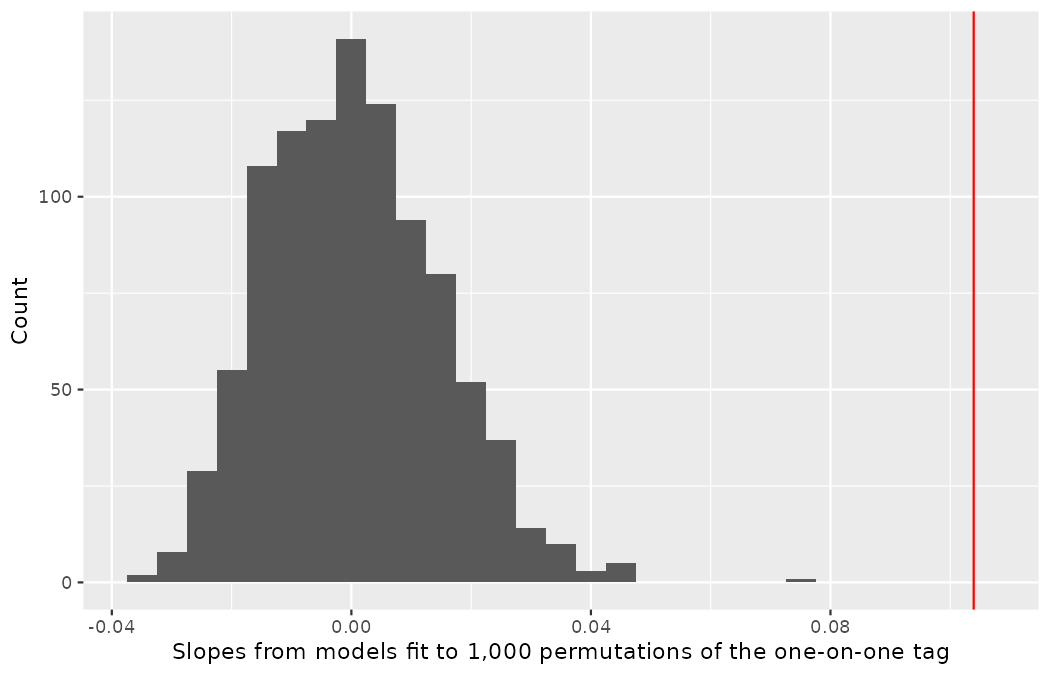
\includegraphics[width=0.85\linewidth,height=\textheight,keepaspectratio]{figures/inf-model-applications-1.png}

The histogram of permuted slopes piles up around zero, running from
about \(-0.033\) to \(+0.075,\) and the red line marking the observed
slope of \(0.1039\) sits entirely outside it.

\begin{tcolorbox}[enhanced jigsaw, left=2mm, leftrule=.75mm, title=\textcolor{quarto-callout-note-color}{\faInfo}\hspace{0.5em}{Worked example}, arc=.35mm, rightrule=.15mm, coltitle=black, colframe=quarto-callout-note-color-frame, bottomrule=.15mm, colbacktitle=quarto-callout-note-color!10!white, opacitybacktitle=0.6, breakable, bottomtitle=1mm, toptitle=1mm, titlerule=0mm, opacityback=0, toprule=.15mm, colback=white]

The red line (the observed slope) is far from the bulk of the histogram.
Explain why the randomly permuted datasets produce slopes that are quite
different from the observed slope.

\begin{center}\rule{0.5\linewidth}{0.5pt}\end{center}

The null hypothesis is that, in the population of open-play shots at
this level, there is no linear relationship between chance quality and
the one-on-one tag. When the data are permuted, chance-quality values
are randomly reassigned to tagged and untagged shots, so the null
hypothesis is forced to be true: any slope that survives the shuffle is
pure chance variation. In the actual data, one-on-ones really do carry
more chance quality --- strikers clean through face an unguarded expanse
the vendor's model prices accordingly --- so the slope describing the
observed relationship is not one that a shuffled dataset is likely to
produce. Shuffle to destroy, resample to preserve, as
Section~\ref{sec-bootbeta1} put it --- this is the destroying half.

\end{tcolorbox}

\begin{tcolorbox}[enhanced jigsaw, left=2mm, leftrule=.75mm, title=\textcolor{quarto-callout-tip-color}{\faLightbulb}\hspace{0.5em}{Check your understanding}, arc=.35mm, rightrule=.15mm, coltitle=black, colframe=quarto-callout-tip-color-frame, bottomrule=.15mm, colbacktitle=quarto-callout-tip-color!10!white, opacitybacktitle=0.6, breakable, bottomtitle=1mm, toptitle=1mm, titlerule=0mm, opacityback=0, toprule=.15mm, colback=white]

Using the permutation results, find the p-value and conclude the
hypothesis test in the context of the problem.

\begin{center}\rule{0.5\linewidth}{0.5pt}\end{center}

None of the 1,000 permuted slopes reached \(\pm 0.1039,\) and --- recall
the discipline of Section~\ref{sec-randslope} --- that makes the honest
report \(p < 1/1000,\) not \(p = 0:\) a permuted slope that size is not
impossible, merely so rare that 1,000 shuffles never produced one. At
any discernibility level in use, we reject \(H_0\) and conclude that the
one-on-one tag and chance quality are genuinely, linearly related in
open play. One caution travels with the conclusion, as it has since
Chapter~\ref{sec-foundations-randomization}: nobody randomly assigns
one-on-ones --- they emerge from the run of play --- so this is
association, not causation.

\end{tcolorbox}

\begin{tcolorbox}[enhanced jigsaw, left=2mm, leftrule=.75mm, title=\textcolor{quarto-callout-tip-color}{\faLightbulb}\hspace{0.5em}{Check your understanding}, arc=.35mm, rightrule=.15mm, coltitle=black, colframe=quarto-callout-tip-color-frame, bottomrule=.15mm, colbacktitle=quarto-callout-tip-color!10!white, opacitybacktitle=0.6, breakable, bottomtitle=1mm, toptitle=1mm, titlerule=0mm, opacityback=0, toprule=.15mm, colback=white]

Is the conclusion based on the histogram of permuted slopes consistent
with the conclusion obtained using the mathematical model? Explain.

\begin{center}\rule{0.5\linewidth}{0.5pt}\end{center}

The p-value in Table~\ref{tbl-1v1-slr} is \(3.4 \times 10^{-13}\) ---
also essentially zero --- so the null hypothesis is rejected under the
mathematical approach as well. Often, the mathematical and computational
approaches to inference give quite similar answers; when they do not,
Section~\ref{sec-tech-cond-linmod} told you where to look, and the
bootstrap below will hand you a live example.

\end{tcolorbox}

Knowing the relationship exists, a scout's interest shifts to the size
of the premium --- the business question is \emph{how much}, not
\emph{whether}. In the notation of the chapters just past: \(\beta_1\)
is the population 1v1 premium, the average difference in chance quality
between one-on-ones and ordinary open-play shots at this level, and a
confidence interval for it is a bootstrap job. Following
Section~\ref{sec-bootbeta1}, we resample the 1,365 shots with
replacement --- whole rows, each keeping its tag and its price together
--- and refit the line 1,000 times:

\begin{Shaded}
\begin{Highlighting}[]
\FunctionTok{set.seed}\NormalTok{(}\DecValTok{2702}\NormalTok{)}
\NormalTok{premium\_boot }\OtherTok{\textless{}{-}}\NormalTok{ shots27 }\SpecialCharTok{|\textgreater{}}
  \FunctionTok{specify}\NormalTok{(statsbomb\_xg }\SpecialCharTok{\textasciitilde{}}\NormalTok{ one\_on\_one) }\SpecialCharTok{|\textgreater{}}
  \FunctionTok{generate}\NormalTok{(}\AttributeTok{reps =} \DecValTok{1000}\NormalTok{, }\AttributeTok{type =} \StringTok{"bootstrap"}\NormalTok{) }\SpecialCharTok{|\textgreater{}}
  \FunctionTok{calculate}\NormalTok{(}\AttributeTok{stat =} \StringTok{"slope"}\NormalTok{)}

\FunctionTok{ggplot}\NormalTok{(premium\_boot, }\FunctionTok{aes}\NormalTok{(}\AttributeTok{x =}\NormalTok{ stat)) }\SpecialCharTok{+}
  \FunctionTok{geom\_histogram}\NormalTok{(}\AttributeTok{binwidth =} \FloatTok{0.005}\NormalTok{) }\SpecialCharTok{+}
  \FunctionTok{labs}\NormalTok{(}
    \AttributeTok{x =} \StringTok{"Slopes from models fit to 1,000 bootstrap samples of the shots"}\NormalTok{,}
    \AttributeTok{y =} \StringTok{"Count"}
\NormalTok{  )}

\NormalTok{premium\_boot }\SpecialCharTok{|\textgreater{}}
  \FunctionTok{summarize}\NormalTok{(}\AttributeTok{mean\_slope =} \FunctionTok{mean}\NormalTok{(stat), }\AttributeTok{sd\_slope =} \FunctionTok{sd}\NormalTok{(stat))}
\CommentTok{\#\textgreater{} \# A tibble: 1 × 2}
\CommentTok{\#\textgreater{}   mean\_slope sd\_slope}
\CommentTok{\#\textgreater{}        \textless{}dbl\textgreater{}    \textless{}dbl\textgreater{}}
\CommentTok{\#\textgreater{} 1      0.104   0.0195}
\end{Highlighting}
\end{Shaded}

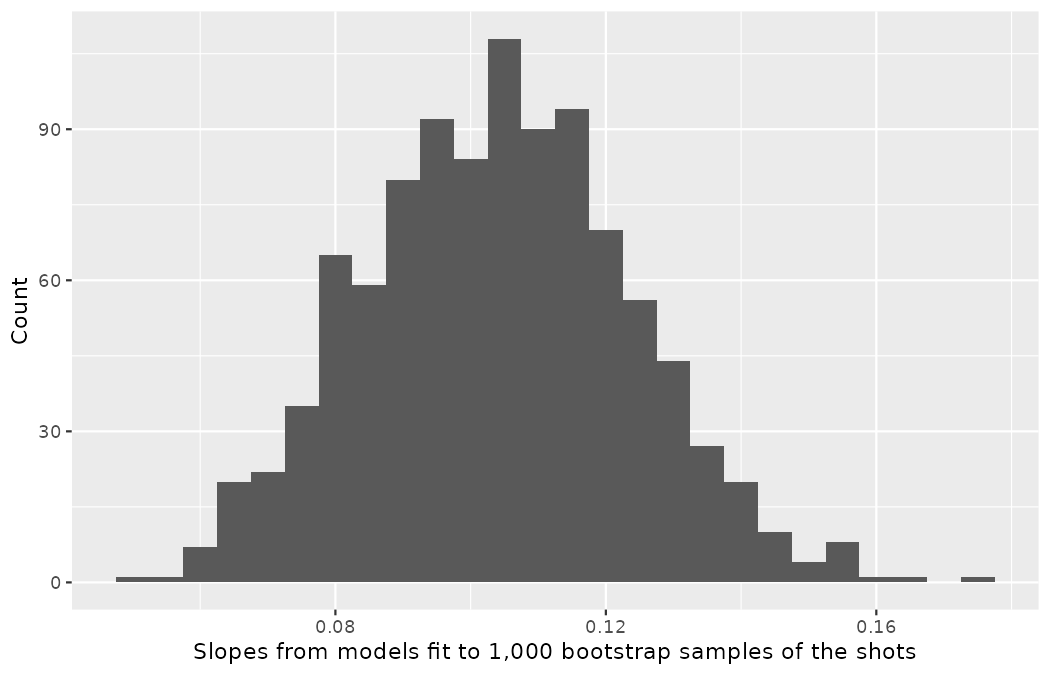
\includegraphics[width=0.85\linewidth,height=\textheight,keepaspectratio]{figures/inf-model-applications-2.png}

The histogram of bootstrapped slopes is bell-shaped, symmetric, and
centered at the observed value of \(0.104\) --- a bootstrap distribution
inherits the center of the sample, as
Chapter~\ref{sec-foundations-bootstrapping} taught.

\begin{tcolorbox}[enhanced jigsaw, left=2mm, leftrule=.75mm, title=\textcolor{quarto-callout-note-color}{\faInfo}\hspace{0.5em}{Worked example}, arc=.35mm, rightrule=.15mm, coltitle=black, colframe=quarto-callout-note-color-frame, bottomrule=.15mm, colbacktitle=quarto-callout-note-color!10!white, opacitybacktitle=0.6, breakable, bottomtitle=1mm, toptitle=1mm, titlerule=0mm, opacityback=0, toprule=.15mm, colback=white]

Using the histogram, estimate the standard error of the slope. Is your
estimate similar to the value of the standard error of the slope in
Table~\ref{tbl-1v1-slr}?

\begin{center}\rule{0.5\linewidth}{0.5pt}\end{center}

Most of the bootstrapped slopes fall between about \(0.065\) and
\(0.145,\) a spread of roughly \(0.08.\) Using the empirical rule from
Chapter~\ref{sec-explore-numerical} --- with bell-shaped distributions,
most observations sit within two standard errors of the center --- a
rough approximation of the standard error is \(0.02.\) The direct
computation agrees:

\begin{Shaded}
\begin{Highlighting}[]
\FunctionTok{round}\NormalTok{(}\FunctionTok{sd}\NormalTok{(premium\_boot}\SpecialCharTok{$}\NormalTok{stat), }\DecValTok{4}\NormalTok{)}
\CommentTok{\#\textgreater{} [1] 0.0195}
\end{Highlighting}
\end{Shaded}

But the standard error in Table~\ref{tbl-1v1-slr} is \(0.0141\) ---
noticeably \emph{smaller} than the bootstrap's \(0.0195,\) a wider gap
than the friendly agreement you saw in Section~\ref{sec-bootbeta1}. The
gap is diagnostic, not a malfunction. The regression formula behind
Table~\ref{tbl-1v1-slr} assumes equal variability around the line ---
the E of the LINE conditions (Section~\ref{sec-tech-cond-linmod}) ---
and this dataset violates it:

\begin{Shaded}
\begin{Highlighting}[]
\NormalTok{shots27 }\SpecialCharTok{|\textgreater{}}
  \FunctionTok{group\_by}\NormalTok{(one\_on\_one) }\SpecialCharTok{|\textgreater{}}
  \FunctionTok{summarize}\NormalTok{(}\AttributeTok{shots =} \FunctionTok{n}\NormalTok{(), }\AttributeTok{mean\_xg =} \FunctionTok{mean}\NormalTok{(statsbomb\_xg), }\AttributeTok{sd\_xg =} \FunctionTok{sd}\NormalTok{(statsbomb\_xg))}
\CommentTok{\#\textgreater{} \# A tibble: 2 × 4}
\CommentTok{\#\textgreater{}   one\_on\_one shots mean\_xg sd\_xg}
\CommentTok{\#\textgreater{}        \textless{}dbl\textgreater{} \textless{}int\textgreater{}   \textless{}dbl\textgreater{} \textless{}dbl\textgreater{}}
\CommentTok{\#\textgreater{} 1          0  1292  0.0896 0.114}
\CommentTok{\#\textgreater{} 2          1    73  0.193  0.166}
\end{Highlighting}
\end{Shaded}

The 73 one-on-ones are both few and far more variable \((s = 0.166\)
versus \(0.114),\) so pooling the variability understates how much the
premium wobbles. Indeed, a slope on a 0/1 indicator is just a difference
in group means (Section~\ref{sec-categorical-predictor-two-levels}), and
the unpooled standard error of Chapter~\ref{sec-inference-two-means}
reproduces the bootstrap almost exactly:
\[\sqrt{\frac{0.166^2}{73} + \frac{0.114^2}{1292}} = 0.0197\] When the
formula and the bootstrap disagree, trust the one whose assumptions you
can defend --- here, the bootstrap, which
Section~\ref{sec-tech-cond-linmod} told you is robust to exactly this
violation.

\end{tcolorbox}

\begin{tcolorbox}[enhanced jigsaw, left=2mm, leftrule=.75mm, title=\textcolor{quarto-callout-tip-color}{\faLightbulb}\hspace{0.5em}{Check your understanding}, arc=.35mm, rightrule=.15mm, coltitle=black, colframe=quarto-callout-tip-color-frame, bottomrule=.15mm, colbacktitle=quarto-callout-tip-color!10!white, opacitybacktitle=0.6, breakable, bottomtitle=1mm, toptitle=1mm, titlerule=0mm, opacityback=0, toprule=.15mm, colback=white]

Use the bootstrap results to create a 90\% standard error bootstrap
confidence interval for the true 1v1 premium. Interpret the interval in
context.

\begin{center}\rule{0.5\linewidth}{0.5pt}\end{center}

For 90\% confidence the normal cutoff is \(z^{\star} = 1.645\) (recall
the cutoff catalog of Chapter~\ref{sec-inference-one-prop}, and recall
from Section~\ref{sec-boot1mean} that bootstrap SE intervals in this
book keep the normal cutoffs), which gives
\[b_1 \pm 1.645 \cdot SE_{BS} \rightarrow 0.1039 \pm 1.645 \cdot 0.0195 \rightarrow (0.0718, 0.1360).\]
For open-play shots at this level, we are 90\% confident that
one-on-ones carry, on average, between \(0.072\) and \(0.136\) more
chance quality than ordinary shots --- between roughly seven and
fourteen extra goals per hundred shots.

\end{tcolorbox}

\begin{tcolorbox}[enhanced jigsaw, left=2mm, leftrule=.75mm, title=\textcolor{quarto-callout-tip-color}{\faLightbulb}\hspace{0.5em}{Check your understanding}, arc=.35mm, rightrule=.15mm, coltitle=black, colframe=quarto-callout-tip-color-frame, bottomrule=.15mm, colbacktitle=quarto-callout-tip-color!10!white, opacitybacktitle=0.6, breakable, bottomtitle=1mm, toptitle=1mm, titlerule=0mm, opacityback=0, toprule=.15mm, colback=white]

Create a 90\% bootstrap percentile confidence interval for the true 1v1
premium and interpret it in context.

\begin{center}\rule{0.5\linewidth}{0.5pt}\end{center}

With 1,000 bootstrap resamples, we look for the cutoffs leaving 50
bootstrapped slopes below, 900 in the middle, and 50 above:

\begin{Shaded}
\begin{Highlighting}[]
\FunctionTok{round}\NormalTok{(}\FunctionTok{quantile}\NormalTok{(premium\_boot}\SpecialCharTok{$}\NormalTok{stat, }\FunctionTok{c}\NormalTok{(}\FloatTok{0.05}\NormalTok{, }\FloatTok{0.95}\NormalTok{)), }\DecValTok{4}\NormalTok{)}
\CommentTok{\#\textgreater{}     5\%    95\%}
\CommentTok{\#\textgreater{} 0.0724 0.1367}
\end{Highlighting}
\end{Shaded}

The 90\% percentile interval is \((0.0724, 0.1367)\) --- almost
identical to the SE interval, as expected from a bell-shaped bootstrap
distribution. Same interpretation, same units: with 90\% confidence, the
1v1 premium at this level lies between about \(0.07\) and \(0.14\)
expected goals per shot. Zero is nowhere in sight, in agreement with
both tests above.

\end{tcolorbox}

\subsection{Cross-validation}\label{cross-validation}

In Chapter~\ref{sec-model-mlr}, models were compared using
\(R^2_{adj}.\) In Section~\ref{sec-inf-mult-reg-cv}, however, a
computational approach was introduced: remove chunks of data one at a
time, fit the model to the rest, and grade it on the held-out shots ---
predictions written as \(\hat{y}_{cv,i}\) and summarized by the CV SSE,
notation you own from that chapter. We close the case study by asking
the prediction question of the two models above: does the four-predictor
model of Table~\ref{tbl-1v1-full} actually predict chance quality better
than the bare one-on-one tag of Table~\ref{tbl-1v1-slr}?

Here we apply 3-fold cross-validation --- \(k = 3\) in the folds sense
of Section~\ref{sec-inf-mult-reg-cv}, not the predictors or groups sense
--- so one third of the data is removed while two thirds of the
observations are used to build each model. The fold assignment is
random, so we seed it:

\begin{Shaded}
\begin{Highlighting}[]
\FunctionTok{set.seed}\NormalTok{(}\DecValTok{2703}\NormalTok{)}
\NormalTok{shots27\_cv }\OtherTok{\textless{}{-}}\NormalTok{ shots27 }\SpecialCharTok{|\textgreater{}}
  \FunctionTok{mutate}\NormalTok{(}\AttributeTok{fold =} \FunctionTok{sample}\NormalTok{(}\FunctionTok{rep}\NormalTok{(}\DecValTok{1}\SpecialCharTok{:}\DecValTok{3}\NormalTok{, }\AttributeTok{length.out =} \FunctionTok{n}\NormalTok{())))}

\NormalTok{shots27\_cv }\SpecialCharTok{|\textgreater{}} \FunctionTok{count}\NormalTok{(fold)}
\CommentTok{\#\textgreater{} \# A tibble: 3 × 2}
\CommentTok{\#\textgreater{}    fold     n}
\CommentTok{\#\textgreater{}   \textless{}int\textgreater{} \textless{}int\textgreater{}}
\CommentTok{\#\textgreater{} 1     1   455}
\CommentTok{\#\textgreater{} 2     2   455}
\CommentTok{\#\textgreater{} 3     3   455}

\NormalTok{pred\_small }\OtherTok{\textless{}{-}} \FunctionTok{rep}\NormalTok{(}\ConstantTok{NA\_real\_}\NormalTok{, }\DecValTok{1365}\NormalTok{)}
\ControlFlowTok{for}\NormalTok{ (f }\ControlFlowTok{in} \DecValTok{1}\SpecialCharTok{:}\DecValTok{3}\NormalTok{) \{}
\NormalTok{  held\_out }\OtherTok{\textless{}{-}}\NormalTok{ shots27\_cv}\SpecialCharTok{$}\NormalTok{fold }\SpecialCharTok{==}\NormalTok{ f}
\NormalTok{  fit }\OtherTok{\textless{}{-}} \FunctionTok{lm}\NormalTok{(statsbomb\_xg }\SpecialCharTok{\textasciitilde{}}\NormalTok{ one\_on\_one, }\AttributeTok{data =}\NormalTok{ shots27\_cv[}\SpecialCharTok{!}\NormalTok{held\_out, ])}
\NormalTok{  pred\_small[held\_out] }\OtherTok{\textless{}{-}} \FunctionTok{predict}\NormalTok{(fit, }\AttributeTok{newdata =}\NormalTok{ shots27\_cv[held\_out, ])}
\NormalTok{\}}

\FunctionTok{sum}\NormalTok{((pred\_small }\SpecialCharTok{{-}}\NormalTok{ shots27\_cv}\SpecialCharTok{$}\NormalTok{statsbomb\_xg)}\SpecialCharTok{\^{}}\DecValTok{2}\NormalTok{)}
\CommentTok{\#\textgreater{} [1] 18.86891}
\end{Highlighting}
\end{Shaded}

Note that each time one third of the data is removed, the resulting
model produces slightly different coefficients. With one binary
predictor, each fold's model prices every shot at one of exactly two
values, and the pair drifts from fold to fold --- the coefficient-wobble
you watched decide everything at a classification cutoff in
Section~\ref{sec-inf-log-reg-cv}, here on display with no cutoff to trip
over:

\begin{Shaded}
\begin{Highlighting}[]
\NormalTok{shots27\_cv }\SpecialCharTok{|\textgreater{}}
  \FunctionTok{mutate}\NormalTok{(}\AttributeTok{pred =} \FunctionTok{round}\NormalTok{(pred\_small, }\DecValTok{4}\NormalTok{)) }\SpecialCharTok{|\textgreater{}}
  \FunctionTok{distinct}\NormalTok{(fold, one\_on\_one, pred) }\SpecialCharTok{|\textgreater{}}
  \FunctionTok{pivot\_wider}\NormalTok{(}\AttributeTok{names\_from =}\NormalTok{ one\_on\_one, }\AttributeTok{values\_from =}\NormalTok{ pred,}
              \AttributeTok{names\_prefix =} \StringTok{"pred\_1v1\_"}\NormalTok{) }\SpecialCharTok{|\textgreater{}}
  \FunctionTok{arrange}\NormalTok{(fold)}
\CommentTok{\#\textgreater{} \# A tibble: 3 × 3}
\CommentTok{\#\textgreater{}    fold pred\_1v1\_0 pred\_1v1\_1}
\CommentTok{\#\textgreater{}   \textless{}int\textgreater{}      \textless{}dbl\textgreater{}      \textless{}dbl\textgreater{}}
\CommentTok{\#\textgreater{} 1     1     0.0886      0.193}
\CommentTok{\#\textgreater{} 2     2     0.0905      0.208}
\CommentTok{\#\textgreater{} 3     3     0.0896      0.179}
\end{Highlighting}
\end{Shaded}

The same seeded folds now grade the larger model, so the two models face
identical holdout samples:

\begin{Shaded}
\begin{Highlighting}[]
\NormalTok{pred\_large }\OtherTok{\textless{}{-}} \FunctionTok{rep}\NormalTok{(}\ConstantTok{NA\_real\_}\NormalTok{, }\DecValTok{1365}\NormalTok{)}
\ControlFlowTok{for}\NormalTok{ (f }\ControlFlowTok{in} \DecValTok{1}\SpecialCharTok{:}\DecValTok{3}\NormalTok{) \{}
\NormalTok{  held\_out }\OtherTok{\textless{}{-}}\NormalTok{ shots27\_cv}\SpecialCharTok{$}\NormalTok{fold }\SpecialCharTok{==}\NormalTok{ f}
\NormalTok{  fit }\OtherTok{\textless{}{-}} \FunctionTok{lm}\NormalTok{(statsbomb\_xg }\SpecialCharTok{\textasciitilde{}}\NormalTok{ one\_on\_one }\SpecialCharTok{+}\NormalTok{ under\_pressure }\SpecialCharTok{+}\NormalTok{ first\_time }\SpecialCharTok{+}
\NormalTok{              play\_pattern, }\AttributeTok{data =}\NormalTok{ shots27\_cv[}\SpecialCharTok{!}\NormalTok{held\_out, ])}
\NormalTok{  pred\_large[held\_out] }\OtherTok{\textless{}{-}} \FunctionTok{predict}\NormalTok{(fit, }\AttributeTok{newdata =}\NormalTok{ shots27\_cv[held\_out, ])}
\NormalTok{\}}

\FunctionTok{sum}\NormalTok{((pred\_large }\SpecialCharTok{{-}}\NormalTok{ shots27\_cv}\SpecialCharTok{$}\NormalTok{statsbomb\_xg)}\SpecialCharTok{\^{}}\DecValTok{2}\NormalTok{)}
\CommentTok{\#\textgreater{} [1] 17.52404}
\end{Highlighting}
\end{Shaded}

The residual plots tell the visual story --- build one for each model,
as in Section~\ref{sec-inf-mult-reg-cv}, with the prediction on the
x-axis and the prediction error on the y-axis:

\begin{Shaded}
\begin{Highlighting}[]
\NormalTok{cv\_results }\OtherTok{\textless{}{-}}\NormalTok{ shots27\_cv }\SpecialCharTok{|\textgreater{}}
  \FunctionTok{mutate}\NormalTok{(}
    \AttributeTok{predicted\_small =}\NormalTok{ pred\_small,}
    \AttributeTok{error\_small =}\NormalTok{ statsbomb\_xg }\SpecialCharTok{{-}}\NormalTok{ predicted\_small,}
    \AttributeTok{predicted\_large =}\NormalTok{ pred\_large,}
    \AttributeTok{error\_large =}\NormalTok{ statsbomb\_xg }\SpecialCharTok{{-}}\NormalTok{ predicted\_large}
\NormalTok{  )}

\FunctionTok{ggplot}\NormalTok{(cv\_results, }\FunctionTok{aes}\NormalTok{(}\AttributeTok{x =}\NormalTok{ predicted\_small, }\AttributeTok{y =}\NormalTok{ error\_small)) }\SpecialCharTok{+}
  \FunctionTok{geom\_point}\NormalTok{(}\AttributeTok{alpha =} \FloatTok{0.3}\NormalTok{) }\SpecialCharTok{+}
  \FunctionTok{geom\_hline}\NormalTok{(}\AttributeTok{yintercept =} \DecValTok{0}\NormalTok{) }\SpecialCharTok{+}
  \FunctionTok{geom\_hline}\NormalTok{(}\AttributeTok{yintercept =} \FloatTok{0.1}\NormalTok{, }\AttributeTok{lty =} \DecValTok{2}\NormalTok{, }\AttributeTok{color =} \StringTok{"grey"}\NormalTok{) }\SpecialCharTok{+}
  \FunctionTok{geom\_hline}\NormalTok{(}\AttributeTok{yintercept =} \SpecialCharTok{{-}}\FloatTok{0.1}\NormalTok{, }\AttributeTok{lty =} \DecValTok{2}\NormalTok{, }\AttributeTok{color =} \StringTok{"grey"}\NormalTok{) }\SpecialCharTok{+}
  \FunctionTok{facet\_wrap}\NormalTok{(}\SpecialCharTok{\textasciitilde{}}\NormalTok{fold) }\SpecialCharTok{+}
  \FunctionTok{labs}\NormalTok{(}\AttributeTok{x =} \StringTok{"Predicted chance quality"}\NormalTok{, }\AttributeTok{y =} \StringTok{"Prediction error"}\NormalTok{)}

\CommentTok{\# ... and the same plot with predicted\_large / error\_large.}

\NormalTok{cv\_results }\SpecialCharTok{|\textgreater{}}
  \FunctionTok{pivot\_longer}\NormalTok{(}\FunctionTok{c}\NormalTok{(error\_small, error\_large),}
               \AttributeTok{names\_to =} \StringTok{"model"}\NormalTok{, }\AttributeTok{values\_to =} \StringTok{"error"}\NormalTok{) }\SpecialCharTok{|\textgreater{}}
  \FunctionTok{group\_by}\NormalTok{(model) }\SpecialCharTok{|\textgreater{}}
  \FunctionTok{summarize}\NormalTok{(}
    \AttributeTok{min\_error =} \FunctionTok{min}\NormalTok{(error),}
    \AttributeTok{max\_error =} \FunctionTok{max}\NormalTok{(error),}
    \AttributeTok{within\_0.1 =} \FunctionTok{mean}\NormalTok{(}\FunctionTok{abs}\NormalTok{(error) }\SpecialCharTok{\textless{}=} \FloatTok{0.1}\NormalTok{)}
\NormalTok{  )}
\CommentTok{\#\textgreater{} \# A tibble: 2 × 4}
\CommentTok{\#\textgreater{}   model       min\_error max\_error within\_0.1}
\CommentTok{\#\textgreater{}   \textless{}chr\textgreater{}           \textless{}dbl\textgreater{}     \textless{}dbl\textgreater{}      \textless{}dbl\textgreater{}}
\CommentTok{\#\textgreater{} 1 error\_large    {-}0.231     0.763      0.793}
\CommentTok{\#\textgreater{} 2 error\_small    {-}0.183     0.808      0.856}
\end{Highlighting}
\end{Shaded}

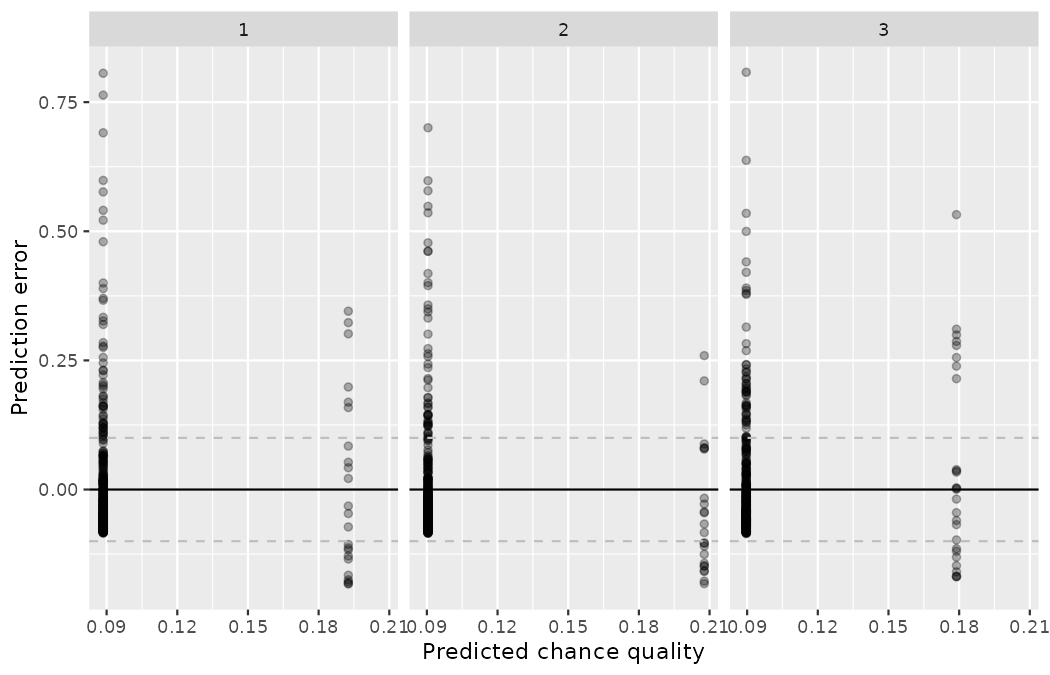
\includegraphics[width=0.85\linewidth,height=\textheight,keepaspectratio]{figures/inf-model-applications-3.png}

The smaller model's plot is two vertical strips --- the two prices in
the table above --- while the larger model's predictions spread from
about \(0.04\) to \(0.25.\) In both, the errors are centered at zero
with a heavy upward straggle: the point-blank chances no stand-side tag
can see.

\begin{tcolorbox}[enhanced jigsaw, left=2mm, leftrule=.75mm, title=\textcolor{quarto-callout-tip-color}{\faLightbulb}\hspace{0.5em}{Check your understanding}, arc=.35mm, rightrule=.15mm, coltitle=black, colframe=quarto-callout-tip-color-frame, bottomrule=.15mm, colbacktitle=quarto-callout-tip-color!10!white, opacitybacktitle=0.6, breakable, bottomtitle=1mm, toptitle=1mm, titlerule=0mm, opacityback=0, toprule=.15mm, colback=white]

The single worst under-prediction from the cross-validated larger model
is isolated below:

\begin{Shaded}
\begin{Highlighting}[]
\NormalTok{cv\_results }\SpecialCharTok{|\textgreater{}}
  \FunctionTok{slice\_max}\NormalTok{(error\_large, }\AttributeTok{n =} \DecValTok{1}\NormalTok{) }\SpecialCharTok{|\textgreater{}}
  \FunctionTok{select}\NormalTok{(fold, statsbomb\_xg, predicted\_large, error\_large,}
\NormalTok{         first\_time, play\_pattern)}
\CommentTok{\#\textgreater{} \# A tibble: 1 × 6}
\CommentTok{\#\textgreater{}    fold statsbomb\_xg predicted\_large error\_large first\_time play\_pattern}
\CommentTok{\#\textgreater{}   \textless{}int\textgreater{}        \textless{}dbl\textgreater{}           \textless{}dbl\textgreater{}       \textless{}dbl\textgreater{}      \textless{}dbl\textgreater{} \textless{}fct\textgreater{}}
\CommentTok{\#\textgreater{} 1     3        0.897           0.134       0.763          1 Regular Play}
\end{Highlighting}
\end{Shaded}

\begin{enumerate}
\def\labelenumi{(\alph{enumi})}
\tightlist
\item
  State the observed and predicted values for this shot, and write its
  prediction error in the notation of Section~\ref{sec-inf-mult-reg-cv}.
\item
  Which cross-validation fold(s) were used to build the model that made
  this prediction?
\end{enumerate}

\begin{center}\rule{0.5\linewidth}{0.5pt}\end{center}

\begin{enumerate}
\def\labelenumi{(\alph{enumi})}
\tightlist
\item
  The observed value is \(y_i = 0.897\) --- close to a certain goal by
  the vendor's reckoning --- while the cross-validated prediction is
  \(\hat{y}_{cv,i} = 0.134,\) giving
  \(e_i = y_i - \hat{y}_{cv,i} = 0.763.\) A first-time shot from regular
  play with no other tags is priced like a routine half-chance; the tags
  cannot know this one was struck from a yard out.
\item
  The shot sits in fold 3, so the model that priced it was built on
  folds 1 and 2 --- the prediction used none of fold 3's shots, which is
  the entire point of the construction.
\end{enumerate}

\end{tcolorbox}

\begin{tcolorbox}[enhanced jigsaw, left=2mm, leftrule=.75mm, title=\textcolor{quarto-callout-tip-color}{\faLightbulb}\hspace{0.5em}{Check your understanding}, arc=.35mm, rightrule=.15mm, coltitle=black, colframe=quarto-callout-tip-color-frame, bottomrule=.15mm, colbacktitle=quarto-callout-tip-color!10!white, opacitybacktitle=0.6, breakable, bottomtitle=1mm, toptitle=1mm, titlerule=0mm, opacityback=0, toprule=.15mm, colback=white]

\begin{enumerate}
\def\labelenumi{(\alph{enumi})}
\tightlist
\item
  By noting the spread of the cross-validated prediction errors, can you
  decide which model should be chosen for a final report on these data?
\item
  Using the summary statistic cross-validation sum of squared errors (CV
  SSE), which model should be chosen, and how big is the win?
\end{enumerate}

\begin{center}\rule{0.5\linewidth}{0.5pt}\end{center}

\begin{enumerate}
\def\labelenumi{(\alph{enumi})}
\tightlist
\item
  Honestly: barely. The larger model has the smaller worst-case straggle
  (\(+0.763\) versus \(+0.808\)) but \emph{fewer} errors inside the
  \(\pm 0.1\) band (\(79.3\%\) versus \(85.6\%\)) --- the smaller model
  predicts about \(0.09\) for nearly everything, and since most
  open-play chance qualities are small, small errors are cheap for it.
  The eye cannot settle this comparison, which is precisely why a
  single-number criterion exists.
\item
  The CV SSE decides: \(17.52\) for the four-predictor model against
  \(18.87\) for the one-predictor model --- the larger model's
  independent predictions are better by about \(7\%.\) Read that
  magnitude the way Section~\ref{sec-inf-mult-reg-cv} trained you to. It
  is a real improvement, several times the gain that chapter's five-tag
  model managed, because \texttt{first\_time} turns out to be the single
  most informative tag on the sheet --- and it is still nowhere near the
  transformation more coefficients naively promise, because most of what
  prices a chance is where it was struck from, and no arrangement of
  stand-side tags can substitute for coordinates. The overfitting
  signature is present and correct, too: the larger model's in-sample
  SSE flatters it by \(0.41\) against its cross-validated \(17.52,\)
  while the smaller model's gap is only \(0.05:\)
\end{enumerate}

\begin{Shaded}
\begin{Highlighting}[]
\FunctionTok{round}\NormalTok{(}\FunctionTok{c}\NormalTok{(}
  \AttributeTok{in\_sample\_small =} \FunctionTok{sum}\NormalTok{(}\FunctionTok{resid}\NormalTok{(m\_1v1)}\SpecialCharTok{\^{}}\DecValTok{2}\NormalTok{),}
  \AttributeTok{in\_sample\_large =} \FunctionTok{sum}\NormalTok{(}\FunctionTok{resid}\NormalTok{(m\_full)}\SpecialCharTok{\^{}}\DecValTok{2}\NormalTok{)}
\NormalTok{), }\DecValTok{2}\NormalTok{)}
\CommentTok{\#\textgreater{} in\_sample\_small in\_sample\_large}
\CommentTok{\#\textgreater{}           18.81           17.11}
\end{Highlighting}
\end{Shaded}

Choose the larger model for prediction at this tournament --- and before
quoting it anywhere else, remember what
Section~\ref{sec-inf-mult-reg-cv} and Section~\ref{sec-chp26-external}
proved: a model that wins at home can lose abroad. The lab at the end of
this chapter sends you to check.

\end{tcolorbox}

\section{Interactive walkthrough: sixty-four matches, one
indicator}\label{sec-inf-model-tutorials}

Reading a consolidated case study is not the same as running one, so
here is a short exercise to work at your own keyboard before the lab
asks for a full report. It also changes altitude deliberately: after
1,365 shots, Marta Vidal's final commission of the season arrives at the
\emph{match} level, where the club's samples are small and the intervals
honest about it. The question, prompted by a board discussion of
tournament modeling: do knockout matches produce different goal totals
than group-stage matches?

\begin{tcolorbox}[enhanced jigsaw, left=2mm, leftrule=.75mm, title=\textcolor{quarto-callout-note-color}{\faInfo}\hspace{0.5em}{Data}, arc=.35mm, rightrule=.15mm, coltitle=black, colframe=quarto-callout-note-color-frame, bottomrule=.15mm, colbacktitle=quarto-callout-note-color!10!white, opacitybacktitle=0.6, breakable, bottomtitle=1mm, toptitle=1mm, titlerule=0mm, opacityback=0, toprule=.15mm, colback=white]

The matches come from \texttt{data/derived/wc2022\_matches.csv}
(StatsBomb open data): 64 rows, one per match. Frame notes, stated per
the book's convention: the recorded scores cover regulation and extra
time but not shoot-out kicks; they include own goals, which no shot file
ever sees; and several knockout matches ran 120 minutes, so ``goals per
match'' quietly mixes exposure --- a caveat that belongs in any memo
built on this variable.

\end{tcolorbox}

The explanatory variable is an indicator --- the same device as
\texttt{one\_on\_one}, from
Section~\ref{sec-categorical-predictor-two-levels} --- equal to 1 for
the 16 knockout matches and 0 for the 48 group-stage matches:

\begin{Shaded}
\begin{Highlighting}[]
\NormalTok{wc2022\_matches }\OtherTok{\textless{}{-}} \FunctionTok{read\_csv}\NormalTok{(}\StringTok{"data/derived/wc2022\_matches.csv"}\NormalTok{)}

\NormalTok{ko\_matches }\OtherTok{\textless{}{-}}\NormalTok{ wc2022\_matches }\SpecialCharTok{|\textgreater{}}
  \FunctionTok{mutate}\NormalTok{(}
    \AttributeTok{total\_goals =}\NormalTok{ home\_score }\SpecialCharTok{+}\NormalTok{ away\_score,}
    \AttributeTok{knockout =} \FunctionTok{if\_else}\NormalTok{(stage }\SpecialCharTok{==} \StringTok{"Group Stage"}\NormalTok{, }\DecValTok{0}\NormalTok{, }\DecValTok{1}\NormalTok{)}
\NormalTok{  )}

\NormalTok{ko\_matches }\SpecialCharTok{|\textgreater{}}
  \FunctionTok{group\_by}\NormalTok{(knockout) }\SpecialCharTok{|\textgreater{}}
  \FunctionTok{summarize}\NormalTok{(}\AttributeTok{matches =} \FunctionTok{n}\NormalTok{(), }\AttributeTok{mean\_goals =} \FunctionTok{mean}\NormalTok{(total\_goals),}
            \AttributeTok{sd\_goals =} \FunctionTok{sd}\NormalTok{(total\_goals))}
\CommentTok{\#\textgreater{} \# A tibble: 2 × 4}
\CommentTok{\#\textgreater{}   knockout matches mean\_goals sd\_goals}
\CommentTok{\#\textgreater{}      \textless{}dbl\textgreater{}   \textless{}int\textgreater{}      \textless{}dbl\textgreater{}    \textless{}dbl\textgreater{}}
\CommentTok{\#\textgreater{} 1        0      48       2.5      1.91}
\CommentTok{\#\textgreater{} 2        1      16       3.25     1.77}

\FunctionTok{ggplot}\NormalTok{(ko\_matches,}
       \FunctionTok{aes}\NormalTok{(}\AttributeTok{x =} \FunctionTok{factor}\NormalTok{(knockout, }\AttributeTok{labels =} \FunctionTok{c}\NormalTok{(}\StringTok{"Group stage"}\NormalTok{, }\StringTok{"Knockout"}\NormalTok{)),}
           \AttributeTok{y =}\NormalTok{ total\_goals)) }\SpecialCharTok{+}
  \FunctionTok{geom\_jitter}\NormalTok{(}\AttributeTok{width =} \FloatTok{0.08}\NormalTok{, }\AttributeTok{height =} \FloatTok{0.1}\NormalTok{, }\AttributeTok{alpha =} \FloatTok{0.7}\NormalTok{) }\SpecialCharTok{+}
  \FunctionTok{labs}\NormalTok{(}\AttributeTok{x =} \ConstantTok{NULL}\NormalTok{, }\AttributeTok{y =} \StringTok{"Goals in the match"}\NormalTok{)}

\NormalTok{fit\_ko }\OtherTok{\textless{}{-}} \FunctionTok{lm}\NormalTok{(total\_goals }\SpecialCharTok{\textasciitilde{}}\NormalTok{ knockout, }\AttributeTok{data =}\NormalTok{ ko\_matches)}
\FunctionTok{tidy}\NormalTok{(fit\_ko)}
\CommentTok{\#\textgreater{} \# A tibble: 2 × 5}
\CommentTok{\#\textgreater{}   term        estimate std.error statistic  p.value}
\CommentTok{\#\textgreater{}   \textless{}chr\textgreater{}          \textless{}dbl\textgreater{}     \textless{}dbl\textgreater{}     \textless{}dbl\textgreater{}    \textless{}dbl\textgreater{}}
\CommentTok{\#\textgreater{} 1 (Intercept)    2.5       0.271      9.22 3.18e{-}13}
\CommentTok{\#\textgreater{} 2 knockout       0.750     0.543      1.38 1.72e{-} 1}
\end{Highlighting}
\end{Shaded}

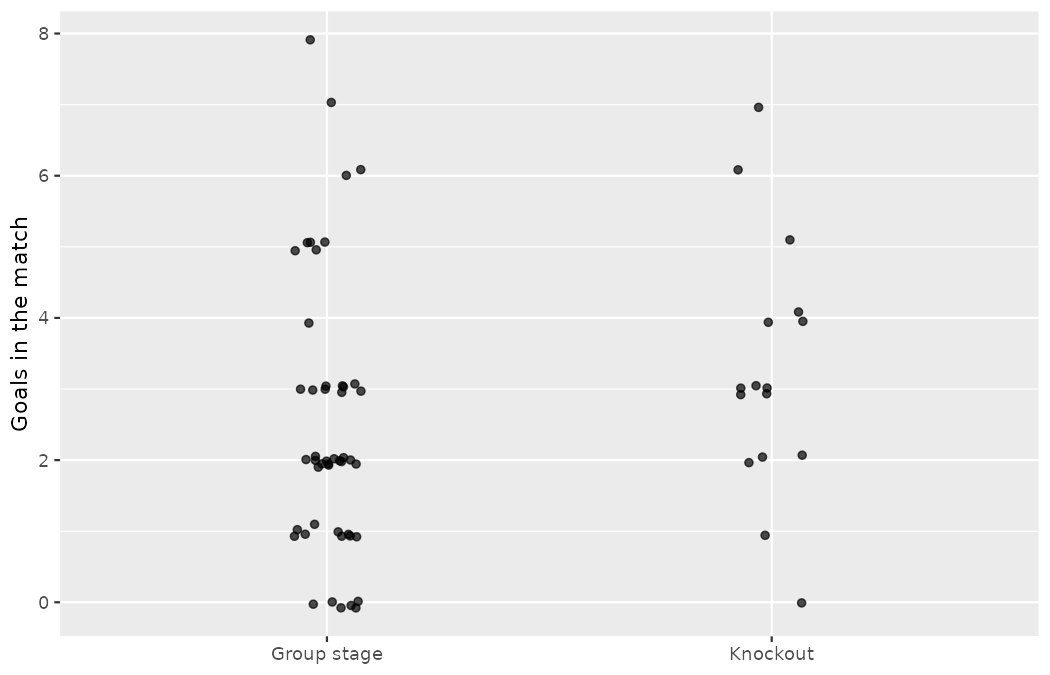
\includegraphics[width=0.85\linewidth,height=\textheight,keepaspectratio]{figures/inf-model-applications-4.png}

Knockout matches averaged three quarters of a goal more \((3.25\) versus
\(2.50),\) but the \(t\)-based p-value of \(0.172\) already warns that
16 matches cannot pin down a difference of this size. The bootstrap says
the same thing in interval form:

\begin{Shaded}
\begin{Highlighting}[]
\FunctionTok{set.seed}\NormalTok{(}\DecValTok{2704}\NormalTok{)}
\NormalTok{ko\_boot }\OtherTok{\textless{}{-}}\NormalTok{ ko\_matches }\SpecialCharTok{|\textgreater{}}
  \FunctionTok{specify}\NormalTok{(total\_goals }\SpecialCharTok{\textasciitilde{}}\NormalTok{ knockout) }\SpecialCharTok{|\textgreater{}}
  \FunctionTok{generate}\NormalTok{(}\AttributeTok{reps =} \DecValTok{1000}\NormalTok{, }\AttributeTok{type =} \StringTok{"bootstrap"}\NormalTok{) }\SpecialCharTok{|\textgreater{}}
  \FunctionTok{calculate}\NormalTok{(}\AttributeTok{stat =} \StringTok{"slope"}\NormalTok{)}

\NormalTok{ko\_boot }\SpecialCharTok{|\textgreater{}}
  \FunctionTok{summarize}\NormalTok{(}\AttributeTok{mean\_slope =} \FunctionTok{mean}\NormalTok{(stat), }\AttributeTok{sd\_slope =} \FunctionTok{sd}\NormalTok{(stat))}
\CommentTok{\#\textgreater{} \# A tibble: 1 × 2}
\CommentTok{\#\textgreater{}   mean\_slope sd\_slope}
\CommentTok{\#\textgreater{}        \textless{}dbl\textgreater{}    \textless{}dbl\textgreater{}}
\CommentTok{\#\textgreater{} 1      0.746    0.525}

\FunctionTok{round}\NormalTok{(}\FunctionTok{quantile}\NormalTok{(ko\_boot}\SpecialCharTok{$}\NormalTok{stat, }\FunctionTok{c}\NormalTok{(}\FloatTok{0.05}\NormalTok{, }\FloatTok{0.95}\NormalTok{)), }\DecValTok{3}\NormalTok{)}
\CommentTok{\#\textgreater{}     5\%    95\%}
\CommentTok{\#\textgreater{} {-}0.104  1.622}
\end{Highlighting}
\end{Shaded}

The 90\% percentile interval runs from \(-0.104\) to \(+1.622\) goals
per match; the SE version,
\(0.75 \pm 1.645 \times 0.525 \rightarrow (-0.114, 1.614),\) agrees.
Both straddle zero: on this evidence, knockout football at the 2022
World Cup is compatible with anything from a tenth of a goal
\emph{fewer} per match to a goal and a half more.

Now put this interval next to the case study's. The 1v1 premium's 90\%
interval, \((0.0724, 0.1367),\) has a width of about \(62\%\) of its
point estimate --- a number Marta can plan around. The knockout
interval's width is about \(2.3\) \emph{times} its point estimate ---
\(\left(1.622 - (-0.104)\right)/0.75 \approx 2.3\) --- a plausible range
so wide it contains the boring answer and both interesting ones. Nothing
about the machinery changed between the two analyses; what changed is
\(n.\) Standard errors shrink with the square root of the sample size
(Chapter~\ref{sec-foundations-mathematical}), and 64 matches --- only 16
of them knockouts --- buy far less precision than 1,365 shots.
Match-level questions are the ones club boards most love to ask, and
they are precisely the questions a single tournament answers worst.

\begin{tcolorbox}[enhanced jigsaw, left=2mm, leftrule=.75mm, title=\textcolor{quarto-callout-tip-color}{\faLightbulb}\hspace{0.5em}{Check your understanding}, arc=.35mm, rightrule=.15mm, coltitle=black, colframe=quarto-callout-tip-color-frame, bottomrule=.15mm, colbacktitle=quarto-callout-tip-color!10!white, opacitybacktitle=0.6, breakable, bottomtitle=1mm, toptitle=1mm, titlerule=0mm, opacityback=0, toprule=.15mm, colback=white]

\begin{enumerate}
\def\labelenumi{(\alph{enumi})}
\tightlist
\item
  A colleague summarizes the analysis as: ``knockout football is worth
  three quarters of a goal more per match --- tell the video team to
  expect it.'' What should the report actually say?
\item
  In one sentence: why is this interval so much wider, relative to its
  estimate, than the 1v1 premium's?
\end{enumerate}

\begin{center}\rule{0.5\linewidth}{0.5pt}\end{center}

\begin{enumerate}
\def\labelenumi{(\alph{enumi})}
\tightlist
\item
  The difference is not statistically discernible \((p = 0.172,\) and
  both 90\% intervals include zero\(),\) so the honest sentence is the
  interval itself: somewhere between \(-0.1\) and \(+1.6\) goals per
  match, on 16 knockout matches, with the extra-time exposure caveat
  attached. Per Chapter~\ref{sec-foundations-decision-errors}, a failure
  to reject is not a demonstration that stages are identical --- if a
  real difference exists, this is exactly the Type II territory where a
  small sample passes on a gem --- but a memo that ``banks'' \(0.75\) is
  quoting the noise, not the signal.
\item
  Because the standard error is driven by sample size and group balance:
  16 knockout matches against 48 group matches, with goal counts whose
  standard deviation rivals their mean, cannot compete with 1,365 shots
  --- the machinery is identical, the data are simply fewer.
\end{enumerate}

\end{tcolorbox}

\section{Lab: the premium, abroad}\label{sec-inf-model-labs}

To close the book, run the case study's entire arc --- unguided this
time --- on the second tournament. An agent, quoting the club's own
methods back at it, claims the 2025 Women's Euro shows one-on-ones are
worth \emph{far more} than Northbridge's World Cup number: ``a 0.23
premium --- nearly double yours.'' Her fit, reproduced from the raw
file:

\begin{Shaded}
\begin{Highlighting}[]
\NormalTok{weuro2025\_shots }\OtherTok{\textless{}{-}} \FunctionTok{read\_csv}\NormalTok{(}\StringTok{"data/derived/weuro2025\_shots.csv"}\NormalTok{)}

\FunctionTok{lm}\NormalTok{(statsbomb\_xg }\SpecialCharTok{\textasciitilde{}}\NormalTok{ one\_on\_one, }\AttributeTok{data =}\NormalTok{ weuro2025\_shots) }\SpecialCharTok{|\textgreater{}}
  \FunctionTok{tidy}\NormalTok{()}
\CommentTok{\#\textgreater{} \# A tibble: 2 × 5}
\CommentTok{\#\textgreater{}   term           estimate std.error statistic  p.value}
\CommentTok{\#\textgreater{}   \textless{}chr\textgreater{}             \textless{}dbl\textgreater{}     \textless{}dbl\textgreater{}     \textless{}dbl\textgreater{}    \textless{}dbl\textgreater{}}
\CommentTok{\#\textgreater{} 1 (Intercept)       0.128   0.00631     20.2  1.45e{-}75}
\CommentTok{\#\textgreater{} 2 one\_on\_oneTRUE    0.228   0.0354       6.44 1.87e{-}10}

\NormalTok{weuro2025\_shots }\SpecialCharTok{|\textgreater{}}
  \FunctionTok{group\_by}\NormalTok{(one\_on\_one) }\SpecialCharTok{|\textgreater{}}
  \FunctionTok{summarize}\NormalTok{(}\AttributeTok{shots =} \FunctionTok{n}\NormalTok{(), }\AttributeTok{mean\_xg =} \FunctionTok{mean}\NormalTok{(statsbomb\_xg))}
\CommentTok{\#\textgreater{} \# A tibble: 2 × 3}
\CommentTok{\#\textgreater{}   one\_on\_one shots mean\_xg}
\CommentTok{\#\textgreater{}   \textless{}lgl\textgreater{}      \textless{}int\textgreater{}   \textless{}dbl\textgreater{}}
\CommentTok{\#\textgreater{} 1 FALSE        884   0.128}
\CommentTok{\#\textgreater{} 2 TRUE          29   0.356}
\end{Highlighting}
\end{Shaded}

Work through the full audit and write up what you find as if reporting
to Marta Vidal:

\begin{enumerate}
\def\labelenumi{\arabic{enumi}.}
\tightlist
\item
  State the parameter of interest and the hypotheses, in symbols and in
  words. Per Section~\ref{sec-two-sided-hypotheses}, default to the
  two-sided alternative.
\item
  Decide which shots belong in the frame, and defend the decision ---
  \emph{before} trusting the agent's slope. Recall where this dataset
  files its penalty kicks, and recall the memo trap of
  Chapter~\ref{sec-inference-one-mean}: at this tournament, the penalty
  share of the one-on-one group is far worse than the World Cup's. Rerun
  the fit under \texttt{shot\_type\ ==\ "Open\ Play"} and report how
  much of the agent's headline survives.
\item
  Run the permutation test for the slope with 1,000 shuffles (seed of
  your choice, stated) in your chosen frame. Report the p-value with the
  resolution it actually has.
\item
  Bootstrap the premium: 1,000 resamples, then both a 90\% SE interval
  and a 90\% percentile interval. With only about two dozen one-on-ones
  in the frame, expect the two constructions to be tested harder than
  they were at the World Cup --- say which you trust and why.
\item
  Close the report the way the case study did: compare your interval
  with the World Cup's \((0.0724, 0.1367)\) and answer the agent
  directly --- same phenomenon, or genuinely richer one-on-ones? State
  whether your conclusion is causal or associational and why, name the
  error type you most risk, and put the frame sentence --- which shots,
  which tournament, which model --- above the number.
\end{enumerate}

\section{Chapter review}\label{sec-chp27-review}

\subsection{Summary}\label{summary-26}

This chapter introduced no new methods, no new notation, and no new
vocabulary. Its work was consolidation: one number the club has quoted
since Chapter~\ref{sec-model-slr} --- the one-on-one premium --- audited
with every inferential modeling tool in the book. The frame decision
came first, because the all-shots frame --- six penalty kicks at a fixed
\(0.784\) chief among its distortions --- was worth two points of fake
premium; the multiple regression then showed adjustment working in both
directions, shrinking the coefficient toward the counters that carry
one-on-ones and raising it for the first-time strikes that one-on-ones
never are. The permutation test put the observed slope outside a
thousand shuffled worlds \((p < 1/1000);\) the bootstrap priced the
premium at \((0.072, 0.137)\) with 90\% confidence and, in disagreeing
with the formula's standard error, diagnosed an unequal-variability
violation the LINE checklist had warned about; cross-validation
preferred the four-tag model by an honest \(7\%;\) and sixty-four
matches closed the chapter with the widest interval in it, because no
amount of machinery buys precision that the sample size will not fund.
If any step felt unfamiliar, the place to look is not ahead but back:
Chapter~\ref{sec-inf-model-slr} for inference on a slope,
Chapter~\ref{sec-inf-model-mlr} for conditional hypotheses and
cross-validation, Chapter~\ref{sec-inf-model-logistic} for the
binary-response version of all of it, and
Chapter~\ref{sec-foundations-randomization} through
Chapter~\ref{sec-foundations-decision-errors} for the logic underneath.

Return, finally, to Northbridge United, where this book has kept its
office. Emil Sørensen's scouts will go on filing reports that say a
striker is electric, a market is overheating, a drill is working; Marta
Vidal will go on making sign-or-pass calls she cannot take back. What
you now bring to that building is a discipline: every claim a scout
makes can be given a number, every number an interval, and every
interval a stated frame --- which shots, which competition, which model,
association or causation. Sometimes the discipline will confirm what the
touchline already believed, as it did for the one-on-one; sometimes it
will dissolve a story on contact, as it did for fatigue drift and the
pressure tag; sometimes it will hold a finding steady through every
re-examination, as it has the nationality audit's, whose scheduled
replication is the club's next calibration exercise; most often it will
return the honest middle answer --- an effect, this size, give or take
that much, under these conditions. Priya Rao's job, and now yours, is to
make sure the club is never certain by accident. That is the whole
trade, and it is yours to practice.

\subsection{Terms}\label{terms-26}

No new terms were introduced in this chapter. The terms below did the
audit's work; all were introduced and defined in earlier chapters ---
the modeling terms in Chapter~\ref{sec-model-slr} and
Chapter~\ref{sec-model-mlr}, the inferential ones in
Chapter~\ref{sec-inf-model-slr} through
Chapter~\ref{sec-inf-model-logistic}, and the shared testing vocabulary
in Chapter~\ref{sec-foundations-randomization} --- and you should be
able to recognize each one at work in the case study, walkthrough, and
lab above. If any feel unfamiliar, go back and review their definitions
in those chapters.

\begin{longtable}[]{@{}
  >{\raggedright\arraybackslash}p{(\linewidth - 4\tabcolsep) * \real{0.3380}}
  >{\raggedright\arraybackslash}p{(\linewidth - 4\tabcolsep) * \real{0.3380}}
  >{\raggedright\arraybackslash}p{(\linewidth - 4\tabcolsep) * \real{0.3239}}@{}}
\caption{Terms revisited in this
chapter.}\label{tbl-terms-chp-27}\tabularnewline
\toprule\noalign{}
\endfirsthead
\endhead
\bottomrule\noalign{}
\endlastfoot
bootstrap confidence interval for the slope & multicollinearity &
randomization test for the slope \\
cross-validation & multiple predictors & t-distribution for the slope \\
indicator variable & p-value & technical conditions \\
inference on multiple linear regression & prediction error & variability
of the slope \\
\end{longtable}

\begin{center}\rule{0.5\linewidth}{0.5pt}\end{center}

Adapted from \emph{Introduction to Modern Statistics} by
Çetinkaya-Rundel \& Hardin (CC BY-SA 4.0); this adaptation is likewise
CC BY-SA 4.0. Match data: StatsBomb open data.

\cleardoublepage
\phantomsection
\addcontentsline{toc}{part}{Appendices}
\appendix

\chapter{Exercise solutions}\label{sec-exercise-solutions}

\section{Chapter 1}\label{sec-exercise-solutions-01}

\textbf{1.} 16 observations and 7 variables. Each observation (row) is a
knockout-stage match, and each variable (column) is a characteristic
recorded for that match.

\textbf{3.} (a) ``Is there an association between training load and
soft-tissue injury in academy players?'' (b) The subjects are academy
players at Northbridge and its partner academies; 8,472 player-weeks of
observation, collected over four seasons, were included. (c) Total
distance covered (numerical, continuous, in kilometers), high-speed
running distance (numerical, continuous, in meters), number of sprint
efforts (numerical, discrete, since it is a count), acute-to-chronic
workload ratio (numerical, continuous), and whether a soft-tissue injury
occurred in the week (categorical, not ordinal).

\textbf{5.} (a) ``What is the effect of gamification on learning
tactical concepts compared to traditional instruction?'' (b) 365 academy
players enrolled in the club's tactics course: 279 from the Outfield
Development program and 86 from the Goalkeeping program. (c) Gender
(categorical), year in the academy (categorical, ordinal), program
(categorical), familiarity with video-analysis software (categorical,
ordinal), use of football video games (categorical, ordinal), treatment
group (categorical), and score on the final evaluation (numerical,
discrete, since it is a count of questions answered correctly out of
30).

\textbf{7.} (a) Treatment: \(10/43 = 0.23,\) i.e., 23\%. (b) Control:
\(2/46 = 0.04,\) i.e., 4\%. (c) A higher percentage of players in the
treatment group were symptom free 24 hours after receiving dry needling.
(d) It is possible that the observed difference between the two group
percentages is due to chance. (e) Explanatory: whether the player
received targeted dry needling or sham needling. Response: whether the
player was symptom free 24 hours after the session.

\textbf{9.} (a) Experiment; the fine was deliberately introduced rather
than merely observed, and Priya Rao randomly selected which squads
received it, in order to evaluate the effect of fines on players' late
arrivals to training. (b) 200 cases: the weekly observations of the 10
squads over the 20 weeks. (c) Number of late arrivals (numerical,
discrete). (d) Week (numerical, discrete), group (categorical, nominal),
and study period (categorical, ordinal).

\textbf{11.} (a) 344 cases (trialists) are included in the data. (b)
There are 4 numerical variables in the data: 30-meter sprint time
(measured in seconds), countermovement jump height and standing height
(measured in centimeters), and body mass (measured in kilograms). They
are all continuous. (c) There are 3 categorical variables in the data:
camp (Eastfield, Millbrook, and Southgate), position group (Defender,
Midfielder, and Forward), and dominant foot (left and right).

\textbf{13.} (a) Match minute, chance quality (\texttt{statsbomb\_xg}),
play pattern, whether the shooter was under pressure, and whether the
shot was struck first time. (b) Match minute: numerical, discrete.
Chance quality: numerical, continuous. Play pattern: categorical, not
ordinal. Under pressure: categorical (two levels), not ordinal. First
time: categorical (two levels), not ordinal.

\textbf{15.} (a) Competition, matchday, and the number of goals scored
on that matchday. (b) Matchday (numerical, discrete), number of goals
(numerical, discrete), competition (categorical, nominal).

\textbf{17.} (a) Team, body part, whether the shot was on target, and
whether the shot was scored. (b) All four are categorical and not
ordinal: team and body part are nominal, and the two yes/no shot
outcomes are categorical variables with two levels. (The \texttt{shots},
\texttt{on\_target\_rate}, and \texttt{conversion} columns of the table
are summary statistics computed from these shot-level variables, not
variables recorded on each shot.) (c) Response: whether the shot was
scored. Explanatory: body part.

\textbf{19.} (a) Observational study; nobody assigned positions to shots
-- the tournaments were played and the events were recorded. (b) Center
Forward in both competitions: \(235/1494 \approx 0.157\) of World Cup
shots and \(143/913 \approx 0.157\) of Women's Euro shots, almost
identical shares. (c) The central-midfield roles: Right Center Midfield
(0.068 at the Women's Euro vs.~0.035 at the World Cup), Left Center
Midfield (0.061 vs.~0.031), and Center Defensive Midfield (0.037
vs.~0.016). (d) Positive; as a position's share of the shot diet in one
competition increases, its share in the other competition tends to
increase as well. The correlation confirms it --- appending
\texttt{summarize(r\ =\ cor(wc2022\_prop,\ weuro2025\_prop))} to the
joined-and-filtered data of the exercise returns \(r = 0.920\) across
the 19 plotted positions. The two tournaments distribute their shots
across positions in broadly similar ways.

\section{Chapter 2}\label{sec-exercise-solutions-02}

\textbf{1.} (a) Population mean: the 2023-24 average of 52 thousand
euros. Sample mean: the 2024-25 average of 58 thousand euros. (b)
Population mean: the 2014 average of 3.37. Sample mean: the 2024 average
of 3.59.

\textbf{3.} (a) Population: all shots in top-division football; sample:
the 143,196 shots logged between the 2015 and 2019 seasons in that
continent's top divisions. (b) If shots in this time span and geography
can be considered to be representative of all top-division shots, then
the results are generalizable to that population --- the safest claim is
generalization to that continent's top divisions in that era. However,
since the study is observational (nobody assigned pressure to shots),
the findings cannot be used to establish causal relationships between
defensive pressure and chance quality.

\textbf{5.} (a) The population of interest is all academy players
learning tactical concepts. The sample consists of the 365 scholars in
the study. (b) If the scholars in this sample, who are likely not
randomly sampled, can be considered to be representative of all academy
players learning tactical concepts, then the results are generalizable
to the population defined above. This is probably not a reasonable
assumption, since these scholars come from Northbridge and two partner
academies only --- a single club's orbit. However, since the study is
experimental (scholars were randomly assigned to the four groups), the
findings can be used to establish causal relationships.

\textbf{7.} (a) Observation: a single scout in the sample is one case
--- one row of the survey's data frame. (b) Variable: reporting hours is
a characteristic recorded for each scout in the sample. (c) Sample
statistic (mean): 1.65 is the average computed from the 1,155 sampled
scouts, not from all licensed scouts. (d) Population parameter (mean):
this is the average over \emph{every} licensed scout --- the quantity
the sample statistic of 1.65 estimates.

\textbf{9.} (a) Observational: it is a survey, and no treatment is
assigned to the scholars. (b) Use stratified sampling with the 4
training squads as strata: randomly sample a fixed number of scholars,
say 10, from each squad, for a total sample size of 40 scholars. This
guarantees each squad --- and each lead coach's influence on
satisfaction --- is represented.

\textbf{11.} (a) Negative, roughly linear, and weak-to-moderate (the
computed correlation is \(-0.285\)): teams that head a larger share of
their shots tend to convert a smaller share of them, though the cloud of
points is wide. (b) Observational: nobody assigned teams their header
shares; the data record what the tournament happened to produce. (c)
Delivery pattern is a plausible confounding variable: teams that rely
heavily on crosses, corners, and other dead-ball deliveries generate
many headed attempts \emph{and} take their shots in crowded, awkward
situations that are harder to convert regardless of body part. Reliance
on such deliveries is associated with both a team's header share and its
conversion rate, so the direct effect of heading, if any, is not
identified by this comparison. (Note: Answers may vary.)

\textbf{13.} (a) Simple random sampling is reasonable. In fact, it's
rare for simple random sampling to not be a reasonable sampling method!
(b) The players' opinions on a video-library fee may well vary by
position --- goalkeepers, for instance, use video differently from
forwards --- so stratifying by position makes sense and would be
reasonable. (c) Players born in the same year are probably going to have
more similar opinions, and we want clusters to be diverse with respect
to the outcome of interest, so this would \textbf{not} be a good
approach. (Additional thought: the birth-year clusters may also have
very different numbers of players, which can also create unexpected
sample sizes.)

\textbf{15.} (a) The cases are the 200 randomly sampled licensed scouts.
(b) The response variable is attitude towards a fictional prospect's
dossier. (c) The explanatory variable is dispositional attitude --- the
scout's general tendency to like or dislike things. (d) Not in the sense
required for generalization: the 200 scouts were drawn at random, but
only from the federation's \emph{online research panel}, which scouts
join voluntarily. The panel is a self-selected pool, so the study does
not have a random sample of the population of licensed scouts. (e) This
is an observational study, since there is no random assignment to
treatments: each scout's dispositional attitude was measured, not
assigned. (f) No, we cannot establish a causal link between the
explanatory and response variables since the study is observational. (g)
No.~Because the panel is self-selected, the results cannot be
generalized to licensed scouts at large; at best they describe scouts of
the kind who volunteer for the federation's research panel.

\textbf{17.} (a) Simple random sample. Non-response bias: if only
scholars who feel strongly about the survey fill it out and bring it
back, the sample may not be representative of the academy's population.
(b) Convenience sample. Undercoverage bias: the sample may not be
representative of the academy since it consists only of the analyst's
own tutor group. (c) Convenience sample. This will have issues similar
to handing out surveys to one's own tutor group: those who respond are
self-selected from whoever follows the academy's social feed, so
non-response bias is also expected. (d) Multistage sampling. If the
education classes are similar to each other with respect to scholar
composition, this approach should not introduce bias, other than
potential non-response bias.

\textbf{19.} (a) Performance in the standardized ten-kick penalty
assessment (e.g., number of kicks converted). (b) Simulated crowd-noise
level: no playback, ambient crowd hum, hostile away-end recording. (c)
First-team match experience: has first-team experience or does not.

\textbf{21.} (a) Experiment. (b) Two explanatory variables are being
manipulated: crowd-noise level (no playback, ambient crowd hum, hostile
away-end recording) and floodlight level (full floodlights, floodlights
at half power, no floodlights --- dusk light only). (c) Since the
researchers want to ensure equal representation of players with and
without first-team match experience in every treatment, first-team
experience is a blocking variable.

\textbf{23.} Need randomization and blinding. One possible outline: (1)
Prepare two cups for each player, one containing the current isotonic
drink and the other containing the sugar-free formulation. Make sure the
cups are identical, at the same temperature, and contain equal amounts
of drink. Label the cups A (current) and B (sugar-free). (Be sure to
randomize which formulation is A and which is B for each trial!) (2)
Give each player the two cups, one cup at a time, in random order, and
ask the player to record a value that indicates how much they liked the
beverage. Be sure that neither the player nor the staff member handing
out the cups knows the identity of the drink, to make this a
double-blind experiment. (Answers may vary.)

\textbf{25.} (a) Experiment. (b) Treatment: 15 grams of the collagen
supplement twice a day; control: placebo. (c) Yes, playing position: the
38 forwards and 38 defenders were each divided randomly into treatment
and control, so position is the blocking variable. (d) Yes,
single-blind, since the players were given identical-seeming supplements
and were blinded to the treatment they received. (e) Since this is an
experiment, we can make a causal statement: the data provide no evidence
that the collagen supplement affects tendon soreness or recovery.
However, since the sample consists of volunteers and is not random, the
causal statement cannot be generalized to the population of players at
large.

\textbf{27.} (a) Non-responders may have a different response to this
question: the parents who returned the questionnaire are likely those
whose work schedules already allow them to engage with the academy, so
non-response bias inflates the share answering \emph{``no''}. To
conclude anything about the majority of all parents, the academy should
have pursued the non-responders or used a design with a high response
rate. (b) It is unlikely that the released players who could be reached
with the same contact details 3 years later are a random sample. These
missing responders have probably moved around more --- players whose
footballing careers ended abruptly or who left the game may be exactly
the ones who changed contact details --- which means the 567 reachable
players might have more stable, and likely better, football outcomes
than the full group of released players. The researcher should not
report them as representative. (c) There is no comparison group in this
study: the physiotherapist only surveyed players \emph{without} tendon
problems, so there is nothing to compare the 20 yoga practitioners
against. This is an observational study, and there may be confounding
variables --- for instance, players who do off-season yoga may be
generally more diligent about conditioning and recovery. To make such a
conclusion, he would need to compare players with and without tendon
problems, and ultimately a randomized experiment.

\textbf{29.} (a) Randomized controlled experiment. (b) Explanatory:
intervention group (categorical, with 3 levels: training-as-usual,
reminder intervention, clip intervention). Response variable: self-rated
match confidence. (c) No, because the participants were scholar
volunteers at a single academy. (d) Yes, because it was a randomized
experiment. (e) The statement should say ``evidence'' instead of
``proof''.

\section{Chapter 4}\label{sec-exercise-solutions-04}

\textbf{1.} (a) We see the order of the play patterns and their relative
frequencies in the bar plot: the aligned bar lengths make it easy to
read that throw-in possessions produced more shots than corner
possessions (177 vs.~160) and to separate the five smallest patterns,
right down to the 10 shots from kick-off possessions --- comparisons
that are nearly impossible between similar-sized wedges of the pie
chart. (b) There are no features that are apparent in the pie chart but
not in the bar plot. (c) We usually prefer to use a bar plot, as we can
also see the relative frequencies of the categories in this graph.

\textbf{3.} (a) Yes, the two variables appear to be associated. If tempo
and outcome were independent, the two bars would split at (roughly) the
same points, but they do not: first-time shots are scored more often
(\(71/468 = 0.152\) vs.~\(124/1026 = 0.121\)) and miss the target more
often (\(181/468 = 0.387\) vs.~\(354/1026 = 0.345\)), while shots taken
after a controlling touch are saved or blocked more often
(\(520/1026 = 0.507\) vs.~\(208/468 = 0.444\) combined). (b) Answers may
vary. Play pattern is a natural candidate: first-time shots often arrive
from crosses, cutbacks, and rebounds, which are struck from different
locations and under different conditions than shots a player takes a
touch to prepare. Chance quality and defensive pressure at the moment of
the strike could likewise differ systematically between the two tempo
groups. These are observational data, so the association alone tells us
nothing about cause.

\textbf{5.} (a) The number of players in each arm of the trial: the
stacked bar plot shows directly that 45 forwards were assigned to the
programme and 30 to standard sessions. (b) The proportion of players
meeting the finishing benchmark in each group: the standardized bar plot
shows the split at \(27/45 = 0.60\) for the programme group against
\(12/30 = 0.40\) for the standard group. (c) The standardized bar plot
should be displayed, as a way to visualize the improvement in the
benchmark proportion in the programme versus the standard group. The
group sizes were fixed by the 3:2 allocation and carry no information
about the programme's effect, whereas the difference in success
proportions is exactly the comparison the randomized trial was run to
make.

\textbf{7.} (a) The ridge plots do not tell us about the relationship
between shot volume and chance quality. While it is true that forwards
have both the highest shot counts (median 3 per player) and the highest
mean chance quality (median \(0.106\)), we can't, for example,
differentiate the chance quality of midfielders (median \(0.0548\)) and
defenders (median \(0.0580\)) even though their shot volumes also differ
(so as to connect volume to quality). Additionally, we don't know
anything about the relationship between volume and chance quality
\emph{within} a position group. (b) When a relationship is confounded we
cannot determine the causal mechanism. We don't know if the better
chances are due to shooting more often or due to being a forward --- a
role that simultaneously puts a player in high-volume \emph{and}
high-quality shooting situations. (c) In order to investigate a specific
confounding variable, first break the data into categories according to
that confounding variable (here, position group). Then look at the
relationship of interest (here shot volume and mean chance quality)
separately for each of the levels of the confounding variable (each
position group).

\textbf{9.} (a) \(28/252 \approx 11.1\%\) of all headers were scored.
\(164/1229 \approx 13.3\%\) of all footed shots were scored. (b) For
open play / other: headers converted at \(13/58 \approx 22.4\%\), footed
shots at \(109/625 \approx 17.4\%\) (headers higher). For free kick /
throw-in possessions: headers \(10/95 \approx 10.5\%\), footed shots
\(43/484 \approx 8.9\%\) (headers higher). For corners: headers
\(5/99 \approx 5.1\%\), footed shots \(12/120 = 10.0\%\) (footed shots
higher). (c) Note that headers are taken in very different contexts than
footed shots: \(99/252 \approx 39\%\) of all headers came from corner
possessions --- the context where conversion is poorest, and the one
context where headers themselves convert worst --- compared with only
\(120/1229 \approx 10\%\) of footed shots. Meanwhile just
\(58/252 \approx 23\%\) of headers came in open play, against
\(625/1229 \approx 51\%\) of footed shots, and open play is where
conversion is highest for everyone. So the overall header rate is a
weighted average dominated by the low-conversion corner context, while
the overall footed rate is buoyed by the high-conversion open-play
context --- allowing footed shots to convert better overall even though
headers convert better within two of the three contexts. (One further
disclosure, per the book's penalty convention: the open-play/other
footed cell contains the tournament's 64 penalty kicks, filed under play
pattern \texttt{Other}, of which 43 scored. Without them that cell
converts at \(66/561 \approx 0.118\) rather than \(0.174,\) and the
overall footed rate falls to \(121/1165 \approx 0.104,\) \emph{below}
the headers' \(0.111\) --- the aggregate reversal this exercise turns on
is itself largely manufactured by the penalties, which is exactly why
the convention insists the frame be stated.)

\section{Chapter 5}\label{sec-exercise-solutions-05}

\textbf{1.} (a) Positive association: teams that accumulate more total
chance quality tend to score more goals as well, and the trend is
roughly linear. (b) The association would still be positive. (c) No,
they are not independent. See part (a): knowing a team's total xG tells
us a great deal about how many goals it is likely to have scored.

\textbf{3.} The plot shows a ramp-up period: tagging starts slowly while
the crew is small, and there may be a period of accelerating (roughly
exponential) growth as experienced taggers train new recruits.
Eventually the fixed size of the archive becomes the binding constraint,
growth slows, and the curve levels off as the cumulative count
approaches the ceiling of 10,000 matches.

\textbf{5.} (a) Decrease: the late trialist's score of 64 is smaller
than the mean of the 24 previous scores, 74. (b) Calculate a weighted
mean. Use a weight of 24 for the old mean and 1 for the new score:
\((24 \times 74 + 1 \times 64)/(24 + 1) = 1840/25 = 73.6.\) (c) The new
score, 64, is more than 1 standard deviation away from the previous mean
\((74 - 8.9 = 65.1 > 64),\) so the standard deviation will increase.

\textbf{7.} Emil should cut the scouts at the low end of the attendance
distribution: any 10 scouts whose average number of matches attended is
between the minimum and the mean number of matches attended for the
entire network. Removing observations below the mean raises the average
of the scouts who remain --- without a single extra match being watched,
which is exactly why a reported average should never be audited without
asking who was dropped from the denominator.

\textbf{9.} (a) Distribution B has a higher mean since \(20 > 13,\) and
a higher standard deviation since 20 is further from the rest of the
data than 13. (b) Distribution A has a higher mean since \(-20 > -40,\)
and Distribution B has a higher standard deviation since \(-40\) is
farther away from the rest of the data than \(-20.\) (c) Distribution B
has a higher mean since all values in Distribution B are higher than
those in Distribution A, but both distributions have the same standard
deviation since they are equally variable around their respective means.
(d) Both distributions have the same mean since they are both centered
at 300, but Distribution B has a higher standard deviation since its
observations are farther from the mean than in Distribution A.

\textbf{11.} (a) About 10 to 11 shots. Accumulating the bar heights from
the left: \(0.008 + 0.047 + 0.102 + 0.142 + 0.173 = 0.472\) of the
team-matches lie at or below 10 shots, so the median falls just inside
the 10--12 bin. (The computed median is 11.) (b) Higher. The
distribution is right skewed --- the secondary shelf of high-volume
team-matches from 20 to 26 shots and the lone bar at 30--32 pull the
mean above the median. (The computed mean is 11.76 against the median of
11.) (c) \(Q_1 \approx 8,\) \(Q_3 \approx 14,\) IQR
\(\approx 14 - 8 = 6.\) (These match the computed values exactly: 8, 14,
and 6.) (d) Values more than \(1.5 \times IQR\) away from the quartiles
are considered unusually low or high. Upper fence:
\(Q_3 + 1.5 \times IQR = 14 + 1.5 \times 6 = 23.\) Lower fence:
\(Q_1 - 1.5 \times IQR = 8 - 9 = -1,\) which is impossible for a shot
count, so no team-match can be unusually low (the minimum observed is
2). Six team-matches exceed the upper fence --- shot counts of 24, 24,
24, 26, 26, and 31, the last being Germany's barrage against Costa Rica
--- so yes, the sample contains unusually high shot counts.

\textbf{13.} The histogram shows that the distribution is bimodal ---
one peak for the auto-tagged matches around 5 hours and another for the
manually tagged matches around 12 --- which is not apparent in the box
plot: the box simply spans both clusters, and its median line (10.3
hours) sits in the sparse valley between them, where almost no matches
actually fall. The box plot makes it easy to identify more precise
values of the observations beyond the whiskers: with \(Q_1 = 5.21,\)
\(Q_3 = 12.19,\) and \(IQR = 6.98,\) the upper fence is
\(12.19 + 1.5 \times 6.98 \approx 22.7,\) and the 12 problem files
between roughly 22.9 and 27.5 hours are drawn individually, whereas in
the histogram they dissolve into a few barely visible tail bins.

\textbf{15.} (a) Right skewed; there is a natural boundary at 0, most
players score no goals or one, and only a few score many. Center:
median, variability: IQR. (b) Right skewed; there is a natural boundary
at 0 and only a few scouts are sent very long distances. Center: median,
variability: IQR. (c) Symmetric. Center: mean, variability: standard
deviation. (d) Left skewed; most players retire in their mid-to-late
thirties, while injuries force a minority out of the game much earlier,
creating a long left tail. Center: median, variability: IQR. (e) Left
skewed; on an easy drill the scores pile up near the top of the scale
with a thin tail of low scores. Center: median, variability: IQR.

\textbf{17.} No, we would expect this distribution to be right skewed.
There are two reasons for this: there is a natural boundary at 0 (a
player cannot watch less than 0 hours of video), and the standard
deviation of the distribution is very large compared to the mean --- a
symmetric distribution with \(\bar{x} = 8.28\) and \(s = 7.18\) would
need substantial room below \(8.28 - 7.18 = 1.10\) hours, which the
boundary at 0 does not allow.

\textbf{19.} No, the midrange is not robust. It is computed exclusively
from the maximum and the minimum of the distribution --- precisely the
observations most affected by outliers and extreme skew --- so a
statistic based only on these values cannot be robust. A single penalty
in the right tail of a striker's xG values becomes the maximum and
single-handedly drags the midrange upward, while the median of the same
data would not move at all.

\textbf{21.} The 75th percentile lies between the 15th and 16th ordered
scores, 82 and 83 (R's \texttt{quantile()} function reports 82.25), so
the five scores above it --- 83, 83, 88, 89, and 94 --- earn a second
trial: 5 trialists will be invited back. Also, by definition 25\% of the
20 trialists, i.e., \(0.25 \times 20 = 5,\) will be above the 75th
percentile.

\textbf{23.} (a) If \(\frac{\bar{x}}{median} = 1,\) then
\(\bar{x} = median.\) This is most likely to be the case for symmetric
distributions. (b) If \(\frac{\bar{x}}{median} < 1,\) then
\(\bar{x} < median.\) This is most likely to be the case for left skewed
distributions, since the mean is affected (and pulled down) by the lower
values more so than the median. (c) If \(\frac{\bar{x}}{median} > 1,\)
then \(\bar{x} > median.\) This is most likely to be the case for right
skewed distributions, since the mean is affected (and pulled up) by the
higher values more so than the median --- as with transfer fees, where a
few large deals pull the mean above the median.

\textbf{25.} (a) The distribution of shots per zone is extremely right
skewed: half of the zones (15 of 30) produced 10 shots or fewer, while
the two central zones nearest goal produced 126 and 112 --- an order of
magnitude more than a typical zone (the median is 11 shots against a
mean of 30.7). On the \(\log_{10}\) scale the same 30 zones spread far
more evenly, between about 0.5 and 2.1, so it might be preferable, in
certain analyses, to use the log-transformed values since that
distribution is much less skewed. (b) The map reveals \emph{where} the
shooting concentrates: the high-count zones cluster in the central
channels of the band nearest goal, and volume drains away band by band
(557, 204, 87, 38, and 36 shots across the five bands). But because the
color scale is stretched by the two hottest zones, nearly everything
beyond band 2 is rendered in the same dark shade, so it is hard to
discern differences among the many low-count zones or to read any
magnitudes precisely. The histogram reveals just how extreme the busiest
zones are relative to the rest and is useful for estimating measures of
center and spread, but it says nothing about where on the pitch any zone
lies. (c) Both visualizations are useful, but if we could only examine
one, we should examine the map, since it explicitly ties each shot count
to its zone's position on the pitch --- and for a scout, where the shots
come from is the question being asked.

\section{Chapter 7}\label{sec-exercise-solutions-07}

\textbf{1.} (a) The residual plot will show randomly distributed
residuals around 0. The variance is also approximately constant: minutes
played track final-third passes equally well across the whole range. A
linear model is appropriate. (b) The residuals will show a fan shape,
with much higher variability for small market values --- agents quote
erratic prices for cheap prospects --- and residuals hugging zero for
the most valuable players. There is trouble with the model being fit
here: the non-constant variance means predictions for cheap players are
far less reliable than the single fitted line suggests.

\textbf{3.} (a) Strong relationship (a clear U-shape), but a straight
line would not fit the data. (b) Strong relationship, and a linear fit
would be reasonable. (c) Weak relationship, and trying a linear fit
would be reasonable. (d) Moderate relationship (a clear arch), but a
straight line would not fit the data. (e) Strong relationship, and a
linear fit would be reasonable. (f) Weak relationship --- essentially no
relationship --- and trying a linear fit would be reasonable.

\textbf{5.} (a) The spring test, since there is less scatter in the plot
of final academy grade versus spring grade. Notice that the relationship
between the autumn grade and the final grade also appears to be slightly
nonlinear, bending at the lower grades. (b) (Answers may vary.) The
spring test is taken closer to the final grading, so it reflects most of
the trialist's development; the autumn test is taken before a winter's
worth of coaching has had its effect.

\textbf{7.} (a) \(r = -0.73\) \(\rightarrow\) (4). (b) \(r = 0.41\)
\(\rightarrow\) (3). (c) \(r = 0.13\) \(\rightarrow\) (1). (d)
\(r = 0.92\) \(\rightarrow\) (2).

\textbf{9.} (a) There is a moderately strong, positive, linear
relationship between shoulder girth and height among the 507 U17
trialists. (b) Changing the units, even if just for one of the
variables, will not change the form, direction, or strength of the
relationship between the two variables.

\textbf{11.} (a) There is a strong, positive, linear relationship
between the distance of a leg and its travel time: longer legs take
longer, with quick rail legs and slow cross-border drives scattered
around the trend. (b) Changing the units will not change the form,
direction, or strength of the relationship between the two variables. If
longer distances measured in km are associated with longer travel times
measured in minutes, longer distances measured in miles will be
associated with longer travel times measured in hours. (c) Changing
units doesn't affect correlation: \(r = 0.874.\)

\textbf{13.} In each case we can write the second-half distance as an
exact linear function of the first-half distance. (a)
\(second = first - 3.\) (b) \(second = first + 2.\) (c)
\(second = 0.5 \times first.\) Since the slopes are positive and these
are perfect linear relationships, the correlation will be exactly 1 in
all three parts. An alternative way to gain insight into this solution
is to create a mock dataset, e.g., five midfielders with first-half
distances of 4, 4.5, 5, 5.5, and 6 km, find the corresponding
second-half distance for each under the given rule, then create a
scatterplot.

\textbf{15.} Correlation: no units. Intercept: goals. Slope: goals per
metre (goals/m).

\textbf{17.} Over-estimate. Since the residual is calculated as
\(observed - predicted,\) a negative residual means that the predicted
value is higher than the observed value: the registration cleared faster
than the model expected.

\textbf{19.} (a) There is a strong (\(r = 0.70\)), positive, linear
association between the number of shots a team takes in a match and its
accumulated chance quality. In addition, the total xG is more variable
for team-matches with higher shot counts, indicating non-constant
variance. (b) Predictor: \texttt{n\_shots}. Outcome: \texttt{total\_xg}.
(c) With a regression line, we can predict a team's accumulated chance
quality for a given shot count. This is useful when only shot counts are
published --- as in basic media feeds --- but the club wants to reason
about chance quality. (d) The residuals fan out: team-matches with
higher predicted chance quality are predicted with roughly twice the
error spread of those with lower predicted chance quality, so the model
does a better job predicting total xG for low-volume shooting
performances.

\textbf{21.} (a) First calculate the slope:
\(b_1 = r \times s_y/s_x = 0.874 \times 117/88 = 1.162.\) Next, make use
of the fact that the regression line passes through the point
\((\bar{x}, \bar{y})\): \(\bar{y} = b_0 + b_1 \times \bar{x}.\) Plug in
\(\bar{x},\) \(\bar{y},\) and \(b_1,\) and solve for \(b_0\):
\(190 - 1.162 \times 199 = -41.2.\) Solution:
\(\widehat{travel~time} = -41.2 + 1.162 \times distance.\) (b) \(b_1\):
For each additional km of distance, the model predicts an additional
1.162 minutes of travel time. \(b_0\): When the distance travelled is 0
km, the travel time is expected to be \(-41.2\) minutes. It does not
make sense to have a leg of 0 km in this context, and a negative travel
time is impossible. Here, the \(y\)-intercept serves only to adjust the
height of the line and is meaningless by itself. (c)
\(R^2 = 0.874^2 = 0.76.\) About 76\% of the variability in travel time
is accounted for by the model, i.e., explained by the distance
travelled. (d)
\(\widehat{travel~time} = -41.2 + 1.162 \times distance = -41.2 + 1.162 \times 210 \approx 203\)
minutes. (Note: we should be cautious in our predictions with this model
since we have not yet evaluated whether it is a well-fit model.) (e)
\(e_i = y_i - \hat{y}_i = 185 - 203 = -18\) minutes. A negative residual
means that the model over-estimated the travel time for this leg ---
Emil arrived 18 minutes sooner than the line predicted. (f) No, this
calculation would require extrapolation: 900 km is far beyond the
longest leg in the data (345 km), and the linear approximation has never
been checked out there.

\textbf{23.} (a)
\(\widehat{\texttt{conversion}} = 0.177 - 0.324 \times \texttt{prop\_headers}.\)
(b) The model predicts a conversion of 0.177 (17.7\% of shots scored)
for a team none of whose shots are headers, on average. No team at the
tournament had a header share of exactly zero, so the intercept mainly
serves to adjust the height of the regression line. (c) For each
additional percentage point of a team's shots taken with the head, the
model predicts conversion lower by \(0.324 \times 0.01 = 0.00324,\) on
average --- equivalently, a team taking \emph{all} of its shots as
headers would be predicted to convert 0.324 less than a team taking
none, a reminder that the slope is measured per whole unit of the share.
As always with observational tournament data, this is an association,
not a causal claim about changing a team's shot diet. (d) The share of a
team's shots that are headers explains 8.1\% of the variability in
conversion rates between the 32 teams. (e) The slope is negative, so the
correlation is the negative square root: \(r = -\sqrt{0.081} = -0.285.\)

\textbf{25.} (a) There is one outlier far to the right. Since it is far
from the center of the data along the \(x\)-axis, it is a point with
high leverage. It is also an influential point: with it, the least
squares slope is about \(-0.73,\) and refitting without it steepens the
slope to about \(-2.15,\) close to the trend of the main cloud. (b)
There is one outlier far to the right. Since it is far from the center
of the data along the \(x\)-axis, it is a point with high leverage.
However, it lies close to the downward extension of the trend and barely
affects the line (slope about \(-1.99\) with it, \(-2.15\) without), so
it is not an influential point. (c) The outlying observation is in the
center of the data (in the \(x\)-axis direction), so this point does
\emph{not} have high leverage. This means the point won't have much
effect on the slope of the line and so is not an influential point ---
it simply has a large positive residual.

\textbf{27.} (a) There is a moderately strong (\(r = 0.69\)), positive,
linear association between accumulated chance quality and goals scored;
because goals are whole numbers, the points fall in integer bands, and
the variability of goal counts increases with chance quality. (b)
Spain's team-match is an outlier of the bivariate model in the \(y\)
direction: it sits about 4.3 goals above the line, the largest residual
in the data. Its chance quality (2.76) is above the mean (1.48) but well
inside the observed range (up to 5.89), so it is not a high leverage
point. Nor is it influential: refitting the line without Spain's match
changes the slope only from 0.909 to 0.879. It is exactly the kind of
exceptional-but-honest observation the chapter warns against deleting
--- a genuine finishing outlier, not a data problem.

\textbf{29.} (a) True. The strength of a linear relationship is judged
by the absolute value of the correlation, and \(|-0.90| > |0.5|.\) (b)
False. Correlation is a measure of the \emph{linear} association between
any two \emph{numerical} variables.

\textbf{31.} (a) \(r = 0.80 \to (1).\) (b) \(r = -0.04 \to (4).\) (c)
\(r = -0.92 \to (2).\) (d) \(r = 0.97 \to (3).\)

\section{Chapter 8}\label{sec-exercise-solutions-08}

\textbf{1.} Anton is right. A model benefits from predictors that are
each strongly correlated with the outcome, but predictors that are
highly correlated with \emph{each other} are collinear, and this
multicollinearity complicates model estimation: it becomes difficult to
separate the individual contribution of each predictor, and coefficient
estimates can shift substantially depending on which of the correlated
predictors are in the model.

\textbf{3.} (a) The association between shots taken and goals scored is
positive, strong, and roughly linear \((r = 0.81):\) teams that took
more shots also scored more goals, with France (102 shots, 16 goals) and
Argentina (101 shots, 15 goals) in the upper right and most group-stage
exits in the lower left. (b) Part of the association is mechanical ---
goals can only come from shots --- but the \emph{strength} of the
aggregate association owes much to a lurking variable: exposure. A team
that reaches the final plays 7 matches and piles up shots and goals
alike, while a group-stage exit gets only 3 matches to accumulate
either; team quality points the same direction, since better sides both
shoot more per match and survive longer. (c) Weaker. Within the
run-length brackets the correlations drop to \(r = 0.39\) (3 matches)
and \(r = 0.57\) (4--5 matches); the 6--7 match bracket shows
\(r = 0.98,\) but it contains only four teams, far too few for a stable
correlation. Once teams are compared only against teams with the same
tournament exposure, much of the apparent shots--goals relationship
dissolves --- which is exactly why scouts normalize tournament totals to
per-match rates before comparing teams.

\textbf{5.} No, they should not include all the variables:
\texttt{days\_since\_start} and \texttt{days\_till\_trial} are perfectly
correlated with each other --- on every day of the plan they sum to 30
--- so the model cannot separate their contributions. They should
include only one of them, alongside \texttt{mood} and \texttt{fatigue}.

\textbf{7.} (a)
\(\widehat{\texttt{statsbomb\_xg}} = 0.0951 + 0.0003 \times \texttt{under\_pressure}.\)
(b) The model predicts that open-play shots taken under defensive
pressure carry a chance quality 0.0003 higher, on average, than shots
taken unpressured --- for practical purposes, no difference at all.
Pressured:
\(\widehat{\texttt{statsbomb\_xg}} = 0.0951 + 0.0003 \times 1 = 0.0954.\)
Unpressured:
\(\widehat{\texttt{statsbomb\_xg}} = 0.0951 + 0.0003 \times 0 = 0.0951.\)
Note that this does not contradict the pressure story of earlier
chapters: once penalties and direct free kicks are excluded, pressured
and unpressured open-play shots have nearly identical \emph{chance
quality} on average --- the conversion gap is a statement about
outcomes, and the all-shots comparison is inflated by penalties, which
are never taken under pressure.

\textbf{9.} (a) Counter-attacks. The coefficient for
\(\texttt{play\_pattern}_{\texttt{From Counter}}\) \((+0.0617\) relative
to the \texttt{Regular\ Play} reference\()\) is larger than the
coefficient of every other possession pattern, so for any fixed minute
the model's prediction is highest for shots arising from counters. (b)
Not necessarily, the change in adjusted \(R^2\) (from 1.15\% to 1.25\%)
is quite small. Note that the strict keep-the-largest-adjusted-\(R^2\)
rule of Section~\ref{sec-model-selection} \emph{would} add
\texttt{body\_part} --- the chapter's own stepwise runs kept variables
for gains as small as \(0.0001,\) a tenth of this one --- which is
exactly why that section advises deciding \emph{before} selection what
difference in adjusted \(R^2\) counts as meaningful: declining to add
the variable here is an application of such a pre-declared threshold,
not of the stepwise rule itself.

\textbf{11.} (a) \[
\begin{aligned}
\widehat{\texttt{statsbomb\_xg}} &= 0.0741 \\
&+ 0.0035 \times \texttt{body\_part}_{\texttt{Left Foot}} + 0.0197 \times \texttt{body\_part}_{\texttt{Head}} \\
&- 0.0246 \times \texttt{technique}_{\texttt{Backheel}} + 0.0790 \times \texttt{technique}_{\texttt{Diving Header}} \\
&+ 0.0285 \times \texttt{technique}_{\texttt{Half Volley}} + 0.1364 \times \texttt{technique}_{\texttt{Lob}} \\
&- 0.0193 \times \texttt{technique}_{\texttt{Overhead Kick}} + 0.0385 \times \texttt{technique}_{\texttt{Volley}} \\
&- 0.0052 \times \texttt{under\_pressure} + 0.0872 \times \texttt{one\_on\_one} \\
&+ 0.0013 \times \texttt{play\_pattern}_{\texttt{From Corner}} + 0.0544 \times \texttt{play\_pattern}_{\texttt{From Counter}} \\
&- 0.0195 \times \texttt{play\_pattern}_{\texttt{From Free Kick}} + 0.0152 \times \texttt{play\_pattern}_{\texttt{From Goal Kick}} \\
&+ 0.0133 \times \texttt{play\_pattern}_{\texttt{From Keeper}} - 0.0090 \times \texttt{play\_pattern}_{\texttt{From Kick Off}} \\
&- 0.0133 \times \texttt{play\_pattern}_{\texttt{From Throw In}} + 0.0001 \times \texttt{minute}
\end{aligned}
\] (b) \(b_{\texttt{minute}}\): All else held constant, for each
additional minute of match time, the model predicts a chance quality
higher by 0.0001, on average --- essentially nothing over the course of
a match. \(b_{\texttt{under\_pressure}}\): All else held constant, the
model predicts that shots taken under defensive pressure carry a chance
quality 0.0052 lower, on average, than unpressured shots. (c)
\texttt{one\_on\_one} is correlated with other predictors in the model,
which introduces multicollinearity and complicates model estimation:
one-on-ones arise disproportionately from counter-attacks and from long
balls over the top (\texttt{From\ Goal\ Kick}), and are finished
disproportionately with lobs --- situations that carry their own
positive coefficients. The single-predictor model credited all of that
situational value to the one-on-one itself; once the context enters the
model, the coefficient shrinks. (d) The third shot was a left-footed
half volley, unpressured, not one-on-one, from a corner, in minute 9, so
the prediction is
\(0.0741 + 0.0035 + 0.0285 + 0.0013 + 0.0001 \times 9 \approx 0.108\)
(the rounded coefficients give \(0.1083\);
\texttt{predict(m\_full){[}3{]}} returns the exact \(0.1085\)), and the
residual is \(e_3 = 0.0616 - 0.1085 = -0.0469.\) The model overpredicts
this shot's chance quality by about 0.047.

\textbf{13.} Remove \texttt{under\_pressure}. Dropping it raises the
adjusted \(R^2\) from 0.0680 to 0.0685, and it is the only deletion that
improves on the full model --- every other variable's removal lowers the
adjusted \(R^2\) (dropping \texttt{minute} comes close at 0.0678 but is
still a decrease).

\textbf{15.} Add \texttt{one\_on\_one}. Its single-predictor model has
the largest adjusted \(R^2\) \((0.0374),\) ahead of \texttt{technique}
\((0.0280)\) and \texttt{play\_pattern} \((0.0117)\); note that
\texttt{under\_pressure} \((-0.0007)\) and \texttt{minute} \((-0.0001)\)
have \emph{negative} adjusted \(R^2\) values --- each explains so little
on its own that the penalty for spending a coefficient outweighs the
variability captured.

\section{Chapter 9}\label{sec-exercise-solutions-09}

\textbf{1.} (a) False. In logistic regression we model a
\emph{transformation} of the probability of the outcome: the logit (the
natural log of the odds) of the probability of a shortlist or a goal is
modelled as a linear combination of the predictors. On the probability
scale the fitted relationship is the S-shaped logit curve, not a line,
and the model predicts the probability of the outcome, never the 0/1
outcome itself. (b) False. Residuals are not used in logistic regression
like they are in linear regression: the observed value is always either
zero or one while the predicted value is a probability, so the residuals
cannot be evenly scattered around zero, and minimizing residual scatter
is not part of the modeling process. (c) True.

\textbf{3.} (a) Yes --- sparse categories play the role in a logistic
regression that extreme, high-leverage outliers play in a linear
regression. The \texttt{body\_part} level ``Other'' contains only 13 of
the 1,494 shots (3 of them goals), and the \texttt{technique\_grp} level
``Other'' only 39 shots (6 goals), even after the chapter collapsed four
rare techniques into it. The coefficients for these levels rest on a
handful of shots, which is why they carry by far the largest standard
errors in the tables (\(0.682\) and \(0.463\)); a couple of scrambled
goals more or fewer would swing those estimates substantially. Every
other predictor has hundreds of shots on each of its levels. (b) Unlike
the dossier audit, where every attribute was randomized independently of
every other, the circumstances of real shots are entangled with one
another --- the predictors are collinear. Technique overlaps heavily
with first-time status: \(135/212\) half volleys and \(79/92\) volleys
are first-time strikes, against only \(239/1{,}151\) normal-technique
shots (verify with
\texttt{wc\_shots\_model\ \textbar{}\textgreater{}\ count(technique\_grp,\ first\_time)}).
When \texttt{technique\_grp} is removed from the model, the variables
correlated with it absorb part of the information it carried: the
\texttt{first\_time} estimate falls from \(0.410\) to \(0.308\), the
\texttt{one\_on\_one} estimate moves from \(0.680\) to \(0.640\), and
\texttt{body\_partHead} even changes sign (from \(-0.018\) to
\(+0.023\)). This is the same coefficient instability we met in
Chapter~\ref{sec-model-mlr}, and it is exactly what the audit's
randomized design protected us from: there, the \texttt{nationality}
coefficient barely moved (\(0.530\) to \(0.533\)) when a variable was
dropped.

\textbf{5.} (a) The logistic model relating \(\hat{p}\) to the
predictors may be written as
\(\log_e\left( \frac{\hat{p}}{1 - \hat{p}} \right) = -2.0456 + 0.0232 \times \texttt{body\_part}_{\texttt{Head}} + 0.0996 \times \texttt{body\_part}_{\texttt{Left Foot}} + 0.6156 \times \texttt{body\_part}_{\texttt{Other}} - 0.2736 \times \texttt{under\_pressure} + 0.6399 \times \texttt{one\_on\_one} + 0.3083 \times \texttt{first\_time}.\)
Controlling for the other variables, \texttt{one\_on\_one} and
\texttt{first\_time} are positively associated with a shot being scored,
as are all three body-part indicators (each measured relative to the
right-footed reference shot); \texttt{under\_pressure} is the only
variable negatively associated with scoring. (b) Substituting the shot's
profile into the model:
\(\log_e\left( \frac{\hat{p}}{1 - \hat{p}} \right) = -2.0456 + 0.0996 \times 1 - 0.2736 \times 1 + 0.6399 \times 1 + 0.3083 \times 1 = -1.2714.\)
Back-transforming from the log odds scale to the probability scale:
\(e^{-1.2714} = 0.2804,\) so
\(\hat{p} = \frac{e^{-1.2714}}{1 + e^{-1.2714}} = \frac{0.2804}{1.2804} = 0.219.\)
The model gives the shot in the agent's clip about a 22\% chance of
being scored. Our confidence should be moderate at best: these are
observational data from a single tournament, so the coefficients
describe association rather than the causal effect of any circumstance;
several estimates (all three body-part terms and
\texttt{under\_pressure}) are small relative to their standard errors,
and we have not yet built the machinery to judge which are statistically
discernible from zero; very few World Cup shots combine all four
characteristics at once; and the model ignores chance quality entirely
--- a one-on-one from 25 metres and one from 6 metres count the same.
(Answers regarding the reliability of the model probability will vary.)

\textbf{7.} (a) The cue \texttt{photo\_attached} should be removed,
since its removal reduces AIC the most (from \(3581.0\) for the
none-dropped model to \(3579.8\)), and the resulting model has lower AIC
than the none-dropped model. (Dropping \texttt{youth\_caps}, at
\(3580.1\), would also beat the full model, but at each stage of
backward elimination we remove the single variable whose removal lowers
AIC the most.) (b) The cue \texttt{youth\_caps} should be removed: its
removal again lowers AIC (\(3578.8\) against the none-dropped
\(3579.8\)), and it is the only removal that does so --- every other
candidate raises AIC. (c) Removing any cue will increase AIC (the
smallest value in the list, \(3580.6\) from dropping
\texttt{years\_senior}, exceeds the none-dropped \(3578.8\)), so we
should not remove any variables from this set. Note where backward
elimination has delivered us: the final model is exactly the chapter's
\texttt{audit\_fit} (AIC \(3578.771\)), and the two cues eliminated
along the way --- the portrait photo and the youth caps --- are
precisely the two that the construction code assigned no role in the
hidden \texttt{log\_odds} line.

\textbf{9.} (a) The AIC is smallest for the model using only
\texttt{under\_pressure}, \texttt{one\_on\_one}, and
\texttt{first\_time} to predict whether the shot is scored (AIC
\(= 1156.56\), against \(1161.55\) for the model adding body part and
\(1163.62\) for the full model), so we would choose \texttt{goal\_m3}
--- in this tournament, the body-part and technique variables do not add
enough to pay AIC's penalty for their extra coefficients. (b) If the
metric is virtually equivalent for two models with differing numbers of
variables, we usually prefer the model with the smaller number of
variables. Sometimes referred to as Occam's razor, the simplest
explanation is often the one that will generalize most effectively --- a
lesson a scouting department relearns every time a model tuned on one
tournament is pointed at the next one.

\section{Chapter 11}\label{sec-exercise-solutions-11}

\textbf{1.} (a) Mean. Each scout reports a numerical value: a number of
matches per month. (b) Mean. Each scout reports a number, which is a
percentage, and we can average over these percentages. (c) Proportion.
Each scout reports Yes or No, so this is a categorical variable and we
use a proportion. (d) Mean. Each scout reports a number, which is a
percentage like in part (b). (e) Proportion. Each academy graduate
reports whether they expect to sign a professional contract, so this is
a categorical variable and we use a proportion.

\textbf{3.} (a) Alternative, because it claims a relationship exists ---
that session hours \emph{predict} assessment scores --- rather than
taking the skeptical stance of no relationship. (b) Null, because it
asserts equality: no difference in mean top sprint speed between left-
and right-footed wingers. (c) Alternative, because it claims the
striker's probability departs from the 0.2 baseline in a specific
direction (larger). (d) Alternative, because it claims a change from the
historical mean shot distance --- a difference, not the status quo. (e)
Null, because it asserts the two protocols carry \emph{equal} injury
risk, the no-effect baseline. (f) Alternative, because it claims the
caffeine gum has an effect on mean sprint distance. (g) Null, because it
asserts the probability of a defensive error is the \emph{same} with or
without long-haul travel --- a claim of independence between the two
variables.

\textbf{5.} (a) \(H_0: \mu = 8\) (On average, the winger creates 8
chances per match, as the brochure claims.) \(H_A: \mu < 8\) (On
average, the winger creates fewer than 8 chances per match.) (b)
\(H_0: \mu = 15\) (The average amount of work time each scout spends on
non-scouting browsing during the World Cup group stage is 15 minutes,
the same as on a regular working day.) \(H_A: \mu > 15\) (The average
amount of work time each scout spends on non-scouting browsing during
the World Cup group stage is greater than 15 minutes.)

\textbf{7.} (a) (i) False. Instead of comparing counts, we should
compare conversion rates: the unpressured group contains far more shots
(588 vs.~325), so it will tend to contain more goals even if pressure
makes no difference. (ii) True. (iii) False. Association does not imply
causation. Defenders are not randomly assigned to shots --- we cannot
infer a causal relationship from an observational study. The difference
from part (ii) is subtle. (iv) True. (b) Proportion of all shots that
were goals: \(\frac{123}{913} \approx 0.135.\) (c) The expected number
of goals among the 325 pressured shots, if scoring and pressure were
independent, can be calculated as the number of shots in that group
multiplied by the overall conversion rate in the tournament:
\(325 \times \frac{123}{913} \approx 43.8,\) i.e., about 44 goals rather
than the 33 observed. (d) (i) \(H_0\): Defensive pressure and scoring
are independent. They have no relationship, and the difference in
conversion rates between the pressured and unpressured shots is due to
chance. \(H_A\): Defensive pressure and scoring are not independent. The
difference in conversion rates is not due to chance, and being under
pressure is associated with a lower chance of scoring. (ii) A lower
conversion rate among the pressured shots than expected under the
assumption of independence would provide support for the alternative
hypothesis, as it would suggest that pressure is associated with
missing. (iii) In the actual tournament, the pressured shots converted
at \(33/325 = 0.102\) against \(90/588 = 0.153\) for the rest, an
observed difference of \(0.102 - 0.153 = -0.052.\) In the 100
simulations under the independence model, only 2 of the shuffled
differences were at least this far below zero, for a p-value of about
0.02. This suggests that the observed gap did not come from the
independence model: the variables do not appear to be independent, and
we reject the independence model in favor of the alternative --- the
data provide convincing evidence that defensive pressure is
\emph{associated} with a lower conversion rate at the 2025 Women's Euro.
However, the club cannot conclude causation: nobody randomly assigned
pressure to shots, and lurking variables (defenders may close down the
most dangerous chances differently, chance quality differs across game
states) could drive the gap. This is a permutation test on observational
data, not a randomization test on an experiment. (e) (i) The pressured
rate is untouched at \(33/325 = 0.102\): no penalty (and no direct free
kick) was taken under pressure, so the filter removes nothing from that
group. All the change lands on the unpressured side, which loses the 51
penalties --- converting at \(28/51 = 0.549\) --- along with the 11
direct free kicks (none scored), so its conversion falls from
\(90/588 = 0.153\) to \(62/526 = 0.118.\) (ii) The observed difference
shrinks from \(-0.052\) to \(33/325 - 62/526 = -0.016,\) and the
evidence largely dissolves: 20 of the 100 shuffled differences were at
least that far below zero, a p-value of about \(0.20,\) far from
statistically discernible at \(\alpha = 0.05\) --- against roughly
\(0.02\) for the penalties-in test in part (d). Most of the all-shots
gap was never about defensive pressure; it was 51 uncontested penalty
kicks propping up the unpressured pile, exactly the artifact
Section~\ref{sec-chp11-pens-out} removed from the World Cup test. The
report should present the pair: on all shots the association is
discernible, on open play it is not, and the honest headline is that the
tournament shows no discernible open-play pressure effect --- with the
frame stated in the first sentence, not the footnotes.

\section{Chapter 12}\label{sec-exercise-solutions-12}

\textbf{1.} (a) The statistic is the observed proportion of headed shots
that were scored, \(\hat{p} = 28/252 = 0.111.\) The parameter is the
true probability that a headed chance at this level of football is
scored. Its numerical value is unknown: the 252 headers are one
tournament's sample from the process that generates headed chances, and
we can never observe that process in full --- only estimate it. (b) The
statistic is denoted \(\hat{p}\) and the parameter is denoted \(p.\) (c)
On each bootstrap sample --- 252 shots drawn with replacement from the
original 252 --- we calculate the bootstrapped sample proportion of
goals, \(\hat{p}_{boot}.\) (d) The bootstrap distribution is centered at
the observed statistic, \(\hat{p} = 0.111\) --- not at the unknown
parameter. The bootstrap can measure how much the statistic varies, but
it cannot reveal where \(p\) actually is. (e) A 90\% confidence interval
spans the middle 90\% of the bootstrapped proportions, so it runs from
the 5th to the 95th percentile: \((0.083, 0.143).\) (The 2.5th and
97.5th percentiles printed alongside would instead give the 95\%
interval, \((0.075, 0.151).\)) (f) We can be 90\% confident that the
true probability that a headed chance at this level of football is
scored is between 8.3\% and 14.3\%. Note for Marta: the interval
comfortably contains values well below the tournament's overall
conversion rate of about 13\%, so the data are consistent with headers
being the harder way to score --- a point worth weighing before bidding
for a target man.

\textbf{3.} A 98\% confidence interval spans the middle 98\% of the
bootstrapped proportions, so it runs from the 1st to the 99th percentile
of the 1,000 bootstrapped values: \((0.270, 0.327).\) With 98\%
confidence, the true proportion of shots at this level that arise from
regular open play is between 27.0\% and 32.7\%. In scouting terms:
roughly three chances in ten come from settled play; the other seven
arrive through set pieces, throw-ins, counters, and the game's other
patterns --- which is Emil's argument for weighting a prospect's
set-piece and transition behavior heavily in reports.

\textbf{5.} In each case the question is whether a population with the
given \(p\) could plausibly have produced the cohort's sample ---
equivalently, whether \(p\) falls within the bulk of the cohort's
bootstrap distribution. (a) A, or perhaps D. \(p = 0.05\) sits
comfortably inside the middle 95\% of A's bootstrap distribution (0 to
0.262); for D it falls just below the middle 95\% (0.087 to 0.391) while
still within D's full range of bootstrapped values, so D is a marginal
call. It is well below the middle 95\% of both B (0.217 to 0.652) and C
(0.130 to 0.479). (b) A, B, C, or D. \(p = 0.25\) falls inside all four
middle-95\% intervals: comfortably within B's, C's, and D's, and just
inside A's upper edge (0.262). (c) B or C. \(p = 0.45\) is inside B's
middle 95\% (0.217 to 0.652) and just inside C's upper edge (0.479); it
is beyond A's largest bootstrapped value (0.348) and in the far upper
tail of D's distribution (beyond D's 97.5th percentile of 0.391). (d) B.
\(p = 0.55\) lies inside only B's middle 95\%; it is beyond C's 97.5th
percentile (0.479) and outside the full ranges of A and D altogether.
(e) None. \(p = 0.75\) is beyond the middle 95\% of every distribution
--- indeed it exceeds even the single largest bootstrapped proportion B
produced (0.739).

\textbf{7.} (a) The claim is supported. ``Most scouts'' means more than
50\%, and the entire interval (54\% to 64\%) lies above 50\%, so every
plausible value of the true proportion corresponds to a majority. (b)
The vendor's value of 70\% lies outside the interval, so the interval
provides convincing evidence against the vendor's figure --- 70\% is not
a plausible value for the proportion of accredited scouts working
primarily from video. Marta can quote the survey back at the sales
pitch. (c) A 90\% confidence interval is narrower than a 95\% confidence
interval built from the same data. Since 70\% already falls outside the
wider 95\% interval, it must also fall outside the narrower 90\%
interval: the vendor's claim would not be supported at the 90\%
confidence level either.

\textbf{S1.} (a) About 95\% of them --- roughly 475 of the 500 intervals
should capture the true conversion rate \(p = 0.1305\); that is the
guarantee the ``95\%'' label advertises. (b) Systematic. The seeded run
captures \(p\) in 459 of 500 samples \((0.918),\) and reruns with
\texttt{set.seed(2)}, \texttt{set.seed(3)}, and \texttt{set.seed(4)}
give capture rates of \(0.930,\) \(0.916,\) and \(0.920\) --- every run
lands short of \(0.95,\) and none lands short by accident in the same
direction four times. The percentile interval \emph{undercovers} at this
sample size: its promise is honored only approximately. (c) With 63
shots and around 8 goals in a typical sample, the bootstrap distribution
of \(\hat{p}_{boot}\) is coarse --- its values can only step in
increments of \(1/63\) --- and mildly right-skewed, since a proportion
this small has more room above it than below. The percentile method
reads its interval straight off that lumpy, skewed histogram, and with
so few distinct values in play the 2.5th and 97.5th percentiles sit
slightly too close together; the resulting intervals miss the true
parameter more often than the label claims. The theory that licenses the
bootstrap is an approximation whose quality grows with \(n\) ---
excellent at 1,494 shots, merely decent at 63. A scout handed a 63-shot
file should treat a ``95\%'' percentile interval as carrying roughly
92\% confidence in practice, widen the level, or simply flag the
coverage gap in the memo. (Widening helps but is no cure: rerunning the
seed-1211 audit with 99\% intervals --- quantiles \(0.005\) and
\(0.995\) --- captures \(p\) in 486 of 500 samples, a rate of \(0.972\):
clear of the original 95\% target, yet still short of its own label, and
for the same small-\(n\) reason.) And remember that
Section~\ref{sec-one-prop-null-boot} meets the same 8-goal headcount
problem from the mathematical side, where it fails the success-failure
condition outright.

\section{Chapter 13}\label{sec-exercise-solutions-13}

\textbf{1.} (a) The area below \(Z = -1.35\) is 0.0885 (from
\texttt{pnorm(-1.35)}), i.e., about 8.85\%. (b) The area above
\(Z = 1.48\) is \(1 - 0.9306 = 0.0694,\) i.e., about 6.94\%. (c) The
area between \(Z = -0.4\) and \(Z = 1.5\) is
\(0.9332 - 0.3446 = 0.5886,\) i.e., about 58.86\%. (d) The area more
than two standard deviations from the mean, on either side --- below
\(Z = -2\) plus above \(Z = 2\) --- is \(0.02275 + 0.02275 = 0.0455,\)
i.e., about 4.55\% (from \texttt{2\ *\ pnorm(-2)}).

\textbf{3.} (a) Technical: \(N(\mu = 72, \sigma = 8),\) Tactical:
\(N(\mu = 65, \sigma = 10).\) (b)
\(Z_{Tech} = \frac{82 - 72}{8} = 1.25,\)
\(Z_{Tact} = \frac{73 - 65}{10} = 0.8.\) On the standard normal curve,
both marks sit to the right of 0, with the Technical mark further out.
(c) She scored 1.25 standard deviations above the mean on the Technical
section and 0.8 standard deviations above the mean on the Tactical
section. (d) She did better on the Technical section relative to the
other trialists since her Z score on that section was higher. (e)
\(Perc_{Tech} = 0.8944 \approx 89\%\) (from \texttt{pnorm(1.25)}),
\(Perc_{Tact} = 0.7881 \approx 79\%\) (from \texttt{pnorm(0.8)}). (f)
\(100\% - 89\% = 11\%\) of trialists did better than her on the
Technical section, and \(100\% - 79\% = 21\%\) did better on the
Tactical section. (g) The raw scores cannot be compared directly since
the two sections are on different scales --- a point on the Technical
section is not worth the same number of standard deviations as a point
on the Tactical section. Comparing Z scores or percentile scores is
appropriate when comparing performance across sections. (h) The answer
to part (b) would not change, as Z scores can be calculated for
distributions that are not normal. However, we could not answer parts
(d)-(f) since we cannot use the normal model to calculate probabilities
and percentiles when the distribution is not nearly normal.

\textbf{5.} (a) The \(80^{th}\) percentile corresponds to \(Z = 0.84\)
(from \texttt{qnorm(0.80)}), so the score is
\(65 + 0.84 \times 10 = 73.4\) points on the Tactical section
(\texttt{qnorm(0.80,\ 65,\ 10)} returns 73.42). (b) Scoring worse than
70\% of trialists means being at the \(30^{th}\) percentile, which
corresponds to \(Z = -0.52,\) so the score is
\(72 - 0.52 \times 8 = 67.8\) points on the Technical section
(\texttt{qnorm(0.30,\ 72,\ 8)} returns 67.80).

\textbf{7.} (a) \(Z = \frac{1000 - 850}{120} = 1.25,\) and the area
above \(Z = 1.25\) is 0.1056. There is about a 10.6\% chance of a wide
midfielder covering 1,000 meters or more of high-intensity running in a
full appearance. (b) The lowest 10\% cutoff corresponds to \(Z = -1.28\)
(from \texttt{qnorm(0.10)}), so the cutoff is
\(850 - 1.28 \times 120 = 696.4,\) i.e., roughly 696 meters or less
(\texttt{qnorm(0.10,\ 850,\ 120)} returns 696.2).

\textbf{9.} (a) Multiplying a normal variable by a constant multiplies
both its mean and its standard deviation by that constant:
\(N(\mu = 850 \times 1.0936, \sigma = 120 \times 1.0936) = N(\mu = 929.6, \sigma = 131.2)\)
in yards. (b) \(Z = \frac{1095 - 929.6}{131.2} = 1.26,\) and the area
above \(Z = 1.26\) is 0.1038, i.e., about 10.4\%. (c) The answers are
very close but not identical, because only the units were changed. (The
only reason they differ at all is that 1,095 yards is 1,001.3 meters,
not precisely 1,000 meters.) (d) Since \(IQR = Q_3 - Q_1,\) we first
find \(Q_3\) and \(Q_1\) and take the difference. Remember that \(Q_3\)
is the \(75^{th}\) and \(Q_1\) the \(25^{th}\) percentile of a
distribution: \(Q_1 = 929.6 - 0.6745 \times 131.2 = 841.1\) yards,
\(Q_3 = 1{,}018.1\) yards,
\(IQR = 1{,}018.1 - 841.1 = 177.0 \approx 177\) yards.

\textbf{11.} (a) Recall that the general formula is
\(\text{point estimate} \pm z^{\star} \times SE.\) First, identify the
three different values. The point estimate is 45\%, \(z^{\star} = 1.96\)
for a 95\% confidence level, and \(SE = 1.2\%.\) Then, plug the values
into the formula: \(45\% \pm 1.96 \times 1.2\% \to (42.6\%, 47.4\%).\)
We are 95\% confident that the proportion of professional scouts who
rely on video for the majority of their evaluations is between 42.6\%
and 47.4\%. (b) (i) False. Confidence intervals provide a range of
plausible values, and sometimes the truth is missed. A 95\% confidence
interval ``misses'' about 5\% of the time. (ii) True. Notice that the
description focuses on the true population value. (iii) True. If we
examine the 95\% confidence interval, we can see that 50\% is not
included in this interval. This means that in a hypothesis test, we
would reject the null hypothesis that the proportion is 0.5. (iv) False.
The standard error describes the uncertainty in the overall estimate
from natural fluctuations due to randomness, not the uncertainty
corresponding to individual scouts' responses.

\textbf{13.} The best interpretation is (c): a Z score of 0.47 denotes
that the sample proportion is 0.47 standard errors greater than the
hypothesized value of the population proportion. Among the others: (a)
misreads the test as giving the probability that the null hypothesis is
true --- no such probability is produced by a hypothesis test; (b)
describes a p-value, not a Z score; (d) and (e) confuse the standardized
distance with a raw distance (the Z score counts standard errors, it is
not a product with the SE or a difference in the original units); (f)
confuses the Z score with the sample proportion itself.

\textbf{15.} (a) The distribution of the 1,000 sample proportions is a
sampling distribution. (b) Symmetric. To know whether the distribution
is skewed, we need to know the proportion. We've been told the
proportion is likely above 5\% and below 30\%, and with \(n = 800\) the
success-failure condition holds across that whole range (at
\(p = 0.05,\) the expected number of set-piece shots is
\(800 \times 0.05 = 40 \geq 10,\) and expected failures are larger
still). If the population proportion is in this range, the sampling
distribution will be symmetric. (c) Standard error. (d) The distribution
will tend to be more variable when there are fewer observations per
sample, so the sample proportions from samples of 250 shots will vary
more than those from samples of 800 shots.

\section{Chapter 14}\label{sec-exercise-solutions-14}

\textbf{1.} (a) \(H_0\): The platform has no effect on the accuracy of
the network's shortlist recommendations (Emil's skeptical position).
\(H_A\): The platform affects the accuracy of the network's shortlist
recommendations --- either improving or worsening it. (b) A Type I error
is concluding that the platform affects the network's recommendations
(helping or harming) when it actually has no effect --- for instance,
Northbridge keeps paying for an expensive subscription that adds
nothing. (c) A Type II error is concluding that the platform has no
effect when it genuinely affects recommendations --- the club cancels a
tool that was actually sharpening its shortlists, or keeps trusting one
that is quietly distorting them. Note also that ``the recommendations
feel sharper to me'' is anecdotal evidence; a renewal decision of this
size should rest on a designed comparison, not an impression.

\textbf{3.} (a) Scenario (i), \(n = 125.\) The standard error decreases
as the sample size increases, so the smaller shot sample gives the
larger standard error. (b) Scenario (i), the 90\% confidence level. A
higher confidence level requires a wider interval, and therefore a
larger margin of error, than a lower confidence level. (c) Equal under
the two scenarios. The p-value is determined by the value of the
Z-statistic (here 2.5 in both cases) and the direction(s) of the
alternative hypothesis; the sample size has already been used in
computing Z and does not enter the calculation again. (d) Scenario (i),
\(\alpha = 0.05.\) A smaller discernibility level makes it harder to
reject \(H_0,\) so when the alternative hypothesis is true we will fail
to reject more often --- the probability of a Type II error is higher at
\(\alpha = 0.05\) than at \(\alpha = 0.10.\) This is the trade-off
between the two error types: tightening the guard against signing duds
means passing on more gems.

\textbf{5.} There are several errors. First, hypotheses are statements
about the population parameter --- here \(p,\) the true proportion of
academy graduates at comparable clubs who receive a professional
contract offer within a year --- never about the sample proportion, so
\(\hat{p}\) should not appear in either hypothesis. Second, the null
hypothesis must be a statement of equality: \(H_0: p = 0.6,\) not an
inequality. Third, both hypotheses must be set up around the same null
value, fixed before seeing the data; the 0.7 is the observed sample
result and has no place in the hypotheses. Finally, since Marta's claim
is only that the report's figure is \emph{incorrect} --- no direction
was specified in advance --- the alternative should be two-sided. The
correct setup is \(H_0: p = 0.6\) versus \(H_A: p \neq 0.6.\)

\textbf{7.} No, the instructor was not correct to mark the submissions
wrong. A 95\% confidence level means that when the sampling and interval
construction are done correctly, about 95\% of such intervals will
capture the true conversion rate --- and therefore about 5\% will miss
it \emph{by chance alone}, even with flawless work. Among 100 correctly
built intervals we expect roughly 5 to miss \(0.1305,\) so observing 7
misses is entirely consistent with every analyst having done the
exercise properly. An interval that fails to capture the parameter is
not evidence of a mistake; it is exactly the roughly-1-in-20 event that
the 95\% confidence level allows for.

\textbf{9.} True. As the sample size grows, the standard error of the
point estimate shrinks, so even a tiny gap between the observed estimate
and the null value produces a large test statistic and a small p-value.
This is precisely why statistical discernibility must not be confused
with practical importance: across tens of thousands of logged shots, a
conversion edge of a fraction of a percentage point could be
statistically discernible while being worthless for an actual sign/pass
decision.

\textbf{S1.} (a) Changing only the treatment rate in the chapter's
seed-1403 simulation --- \texttt{rbinom(1,\ 40,\ 0.28)} in place of
\texttt{rbinom(1,\ 40,\ 0.35)}, same 50-player control arm at 0.22, same
pooled-SE \(Z\) test with the \(\pm 1.96\) cutoff --- and running 1,000
trials with \texttt{set.seed(1405)}, 95 of the 1,000 simulated trials
reject: the power is \(0.095.\) Against a 6-percentage-point lift,
Jonas's trial has roughly a 1-in-10 chance of reaching the correct
verdict; about nine times in ten it ends ``inconclusive'' even though
the program genuinely works. (b) With \texttt{power\_at()} rewritten for
the 0.28 treatment rate and the grid run under \texttt{set.seed(1406)},
the seeded powers are \(0.282\) at 200 players per arm, \(0.514\) at
400, \(0.667\) at 600, \(0.771\) at 800, and \(0.872\) at 1,000. The
0.80 benchmark therefore demands on the order of 800--1,000 players per
arm --- roughly two thousand forwards in total, some twenty times the
trial Jonas ran, which is registry scale: per the club's own
conventions, a study that size is hosted at federation or consortium
level, not inside one academy. (c) A defensible summary for Marta:
``Trials of the size we can run alone will detect only large training
effects; an effect worth perhaps six points of benchmark rate is
effectively invisible to a 90-player trial (power \(\approx 0.10\)), so
for questions of that scale we must either pool players with our
partners at consortium level or accept that our trial cannot settle the
question.'' The one thing the club must \emph{not} do is run the
underpowered trial anyway and read its ``inconclusive'' as ``no effect''
--- that is exactly the Type II trap of
Chapter~\ref{sec-foundations-decision-errors}.

\section{Chapter 16}\label{sec-exercise-solutions-16}

\textbf{1.} Two errors. First, the hypotheses should be about the
population proportion (\(p\)), not the sample proportion (\(\hat{p}\)):
the poll's 29\% is data, and hypotheses are never written in terms of
data. Second, the null value should be the claim being tested (0.25),
not the observed value (0.29). The correct way to set up these
hypotheses is: \(H_0: p = 0.25\) and \(H_A: p > 0.25.\)

\textbf{3.} (a) \(H_0: p = 0.20,\) \(H_A: p > 0.20,\) where \(p\) is the
proportion of all accredited scouts who lead their evaluations with an
xG model. (b) \(\hat{p} = 159/650 = 0.245.\) (c) Answers will vary. Each
scout can be represented with a card. Take 100 cards, 20 black cards
representing scouts who lead with xG and 80 red cards representing those
who do not. Shuffle the cards and draw with replacement (shuffling each
time in between draws) 650 cards representing the 650 respondents.
Calculate the proportion of black cards in this sample,
\(\hat{p}_{sim},\) i.e., the proportion of simulated scouts who lead
with xG. The p-value is the proportion of simulations where
\(\hat{p}_{sim} \geq 0.245.\) (Note: we would generally use a computer
to perform the simulations, as the seeded code in the exercise does.)
(d) In the seeded run, none of the 1,000 simulated proportions was at
least 0.245 (the largest was 0.243), so the estimated p-value is less
than 0.001 --- effectively 0. Since the p-value is smaller than 0.05, we
reject \(H_0.\) The data provide convincing evidence that the proportion
of accredited scouts who lead with xG is greater than 0.20, i.e., more
than one in five, and the journalist's headline survives the check.

\textbf{5.} (a) \(H_0: p = 0.5\) (the scouts have no preference between
the layouts), \(H_A: p \neq 0.5\) (the scouts have a preference for one
layout, in either direction), where \(p\) is the population proportion
of the network's scouts who prefer the single-page summary. (b) The
observed proportion is \(5/7 \approx 0.714.\) Because the alternative is
two-sided, we count simulated proportions at least as extreme in either
direction: \(207 + 248 = 455\) of the 1,000 draws, giving a p-value of
about \(0.455.\) Since \(0.455 > 0.05,\) we fail to reject \(H_0\):
there is no convincing evidence in the data (possibly because only 7
scouts were surveyed!) that the network prefers one dossier layout over
the other.

\textbf{7.} (a)
\(SE(\hat{p}) = \sqrt{\frac{0.5 \times 0.5}{7}} = 0.189.\) (b) The
standard error is estimated by the standard deviation of the simulated
proportions: roughly \(0.185.\) (c) Yes, they are quite close. (d)
No.~With \(p_0 = 0.5\) and \(n = 7,\) we expect only
\(7 \times 0.5 = 3.5\) successes and 3.5 failures --- far short of the
10 of each that the success-failure condition requires. (e) The draws
from the null distribution are discrete: \(\hat{p}_{sim}\) can take only
the eight values \(0/7, 1/7, \dots, 7/7,\) while the mathematical model
is continuous (infinite options on a continuum). A histogram with eight
isolated stacks is not well approximated by a smooth bell curve.

\textbf{9.} (a) The null hypothesis simulation drew samples of size 25
from a population where the true filing-on-time proportion was imposed
to be \(p = 0.7\); the data bootstrap resampled (with replacement) from
the desk's actual sample, in which the proportion is \(\hat{p} = 0.6.\)
(b) The null hypothesis simulation is centered at 0.7 (mean 0.698 in the
seeded run); the data bootstrap is centered at 0.6 (mean 0.595). Each
distribution is centered at the proportion used to generate it. (c) The
standard error of the sample proportion is roughly 0.09 from the null
simulation and roughly 0.10 from the bootstrap --- roughly equal. (d)
Both histograms are reasonably symmetric. Note that histograms which
describe the variability of proportions become more skewed as the center
of the distribution gets closer to 1 (or to 0), because the boundary
restricts one tail; for this reason the null hypothesis simulation
(centered at 0.7) is slightly more left skewed than the bootstrap
(centered at 0.6).

\textbf{11.} (a) The null hypothesis simulation distribution for
testing; the data bootstrap distribution for confidence intervals. (b)
\(H_0: p = 0.7,\) \(H_A: p \neq 0.7,\) where \(p\) is the true
proportion of the desk's reports filed within 24 hours. In the seeded
run, 200 of the 1,000 null draws were at or below the observed
\(\hat{p} = 0.6\); doubling for the two-sided alternative gives a
p-value of about \(0.40 > 0.05.\) There is no evidence that the
proportion of the data desk's reports filed within 24 hours differs from
the network's 70\%. (c) The 98\% bootstrap percentile interval runs from
the 1st to the 99th percentile of the bootstrapped proportions:
\((0.36, 0.80).\) We are 98\% confident that the true proportion of the
desk's reports filed within 24 hours is between 36\% and 80\% --- an
interval so wide it mostly documents how little 25 reports can say. (d)
Using \(z^\star = 2.33\) and the bootstrap standard error \(0.097\):
\(0.6 \pm 2.33 \times 0.097 \rightarrow (0.374, 0.826).\) We are 98\%
confident that the true proportion is between roughly 37\% and 83\%, in
close agreement with the percentile interval.

\textbf{13.} (a) False. The \(n \geq 30\) guideline is for means, not
proportions; here the success-failure condition fails, since
\(60 \times 0.08 = 4.8 < 10.\) (b) True. The success-failure condition
is not satisfied \((50 \times 0.08 = 4 < 10).\) In most samples we would
expect \(\hat{p}\) to be close to 0.08, the true population proportion,
and while \(\hat{p}\) can be much above 0.08, it is bounded below by 0,
so the distribution takes on a right-skewed shape. (c) False.
\(SE(\hat{p}) = \sqrt{0.08 \times 0.92 / 125} = 0.0243,\) and
\(\hat{p} = 0.12\) is only \(\frac{0.12 - 0.08}{0.0243} = 1.65\)
standard errors from the mean, which would not be considered unusual.
(d) True. With \(n = 250,\) \(SE(\hat{p}) = 0.0172,\) so
\(\hat{p} = 0.12\) is \(\frac{0.12 - 0.08}{0.0172} = 2.33\) standard
errors from the mean, which is often considered unusual. (e) False.
Doubling the sample size decreases the standard error by a factor of
\(1/\sqrt{2} \approx 0.71,\) not by one-half.

\textbf{15.} (a) True. With \(p = 0.9\) and \(n = 30,\) the expected
number of left-footed keepers is \(30 \times 0.1 = 3 < 10\): the
success-failure condition fails, and since \(\hat{p}\) is bounded above
by 1, the distribution is left skewed. (b) True. The sample size enters
the standard error formula under a square root, so multiplying \(n\) by
4 divides the SE by \(\sqrt{4} = 2.\) (c) True. The independence and
success-failure conditions are satisfied: \(140 \times 0.9 = 126\) and
\(140 \times 0.1 = 14,\) both at least 10. (d) True. The independence
and success-failure conditions are satisfied: \(280 \times 0.9 = 252\)
and \(280 \times 0.1 = 28.\)

\textbf{17.} (a) False. A confidence interval is constructed to estimate
the population proportion, not the sample proportion --- we know the
sample's 82\% exactly, with no uncertainty at all. (b) True. 95\% CI:
\(82\% \pm 2\%.\) (c) True. By the definition of the confidence level.
(d) True. The margin of error scales with \(1/\sqrt{n},\) so quadrupling
the sample size halves the ME from 2\% to 1\%. (e) True. The 95\%
confidence interval, \((80\%, 84\%),\) lies entirely above 50\%.

\textbf{19.} With a random sample, independence is satisfied. The
success-failure condition is also satisfied: \(600 \times 0.56 = 336\)
and \(600 \times 0.44 = 264,\) both at least 10.
\(ME = z^{\star} \sqrt{\frac{\hat{p}(1-\hat{p})}{n}} = 1.96 \sqrt{\frac{0.56 \times 0.44}{600}} = 0.0397 \approx 4\%.\)

\textbf{21.} (a) No.~The sample only represents trialists who took the
entry assessment and then chose to complete an optional web survey --- a
self-selected subgroup, likely differing (in enthusiasm, in
circumstances) from trialists in general. (b)
\(SE = \sqrt{0.55 \times 0.45 / 1509} = 0.0128,\) and with
\(z^\star = 1.65\):
\(0.55 \pm 1.65 \times 0.0128 \rightarrow (0.5289, 0.5711).\) We are
90\% confident that 53\% to 57\% of academy trialists who took the
assessment are fairly certain they would accept a professional contract
abroad. (c) 90\% of such random samples would produce a 90\% confidence
interval that includes the true proportion. (d) Yes --- the interval
lies entirely above 50\% --- though the claim inherits the sampling
caveat from part (a).

\textbf{23.} (a) We want to check for a majority (or minority), so we
use the following hypotheses: \(H_0: p = 0.5\) and \(H_A: p \neq 0.5,\)
where \(p\) is the proportion of licensed intermediaries who support the
new loan regulations. We have a sample proportion of \(\hat{p} = 0.55\)
and a sample size of \(n = 617\) intermediaries. Since this is a random
sample, independence is satisfied. The success-failure condition is also
satisfied: \(617 \times 0.5 = 308.5\) and
\(617 \times (1 - 0.5) = 308.5\) are both at least 10 (we use the null
proportion \(p_0 = 0.5\) for this check in a one-proportion hypothesis
test). Therefore, we can model \(\hat{p}\) using a normal distribution
with a standard error of
\(SE = \sqrt{\frac{0.5(1 - 0.5)}{617}} = 0.02.\) (We use the null
proportion \(p_0 = 0.5\) to compute the standard error for a
one-proportion hypothesis test.) Next, we compute the test statistic:
\(Z = \frac{0.55 - 0.5}{0.02} = 2.5.\) This yields a one-tail area of
0.0062, and a p-value of \(2 \times 0.0062 = 0.0124.\) Because the
p-value is smaller than 0.05, we reject the null hypothesis. We have
strong evidence that the support is different from 0.5, and since the
point estimate is above 0.5, we have strong evidence to support the
pundit's claim. (b) No.~Generally we expect a hypothesis test and a
confidence interval to align, so we would expect the confidence interval
for the proportion who \emph{oppose} to show a range of plausible values
entirely below 0.5. However, if the confidence level is misaligned with
the discernibility level (e.g., a 99\% confidence level and
\(\alpha = 0.05\)), then this is no longer generally true.

\textbf{25.} (a) \(H_0: p = 0.5\) (the scouts are guessing at random),
\(H_A: p > 0.5\) (the scouts identify the future international at better
than chance). Independence is satisfied --- each scout judged their own
randomized clip pair --- and the success-failure condition holds using
\(p_0 = 0.5\): we expect \(80 \times 0.5 = 40\) successes and 40
failures. \(\hat{p} = 53/80 = 0.6625,\)
\(SE = \sqrt{0.5 \times 0.5/80} = 0.0559,\) so
\(Z = \frac{0.6625 - 0.5}{0.0559} = 2.91 \rightarrow\) p-value
\(= 0.0018.\) Since the p-value \(< 0.05,\) we reject the null
hypothesis. The data provide strong evidence that the rate at which
these scouts pick out the future international is discernibly better
than random guessing. (b) If in fact the scouts could not tell the
players apart and merely guessed, the probability of getting a random
sample of 80 scouts where 53 or more identify the correct player would
be 0.0018.

\textbf{27.} (a) The population is all scouting reports filed by the
network during that week of production. We might be tempted to
generalize to all weeks, but we should exercise caution: the error rate
may change over time (transfer windows and tournament weeks change
workloads). (b) The fraction of that week's filed reports that contain
at least one data-entry error. (c) Estimate the parameter using the
data: \(\hat{p} = \frac{27}{212} = 0.127.\) (d) \emph{Standard error}
(or \(SE\)). (e) Compute the \(SE\) using \(\hat{p} = 0.127\) in place
of \(p\): \(SE \approx \sqrt{\frac{0.127(1 - 0.127)}{212}} = 0.023.\)
(f) The standard error is the standard deviation of \(\hat{p}.\) A value
of 0.10 is \(\frac{0.127 - 0.10}{0.023} \approx 1.2\) standard errors
from the observed value, which would not represent an uncommon
deviation. (Usually beyond about 2 standard errors is a good rule of
thumb.) Priya should not be surprised. (g) Recomputed standard error
using \(p = 0.1\): \(SE = \sqrt{\frac{0.1(1 - 0.1)}{212}} = 0.021.\)
This value isn't very different, which is typical when the standard
error is computed using relatively similar proportions (and even
sometimes when those proportions are quite different!).

\textbf{29.} (a) The visitors are from a simple random sample of the
portal's first-time visitors, so independence is satisfied. The
success-failure condition is also satisfied, with both \(64\) and
\(752 - 64 = 688\) above 10. Therefore, we can use a normal distribution
to model \(\hat{p}\) and construct a confidence interval. (b) The sample
proportion is \(\hat{p} = \frac{64}{752} = 0.085.\) The standard error
is \(SE = \sqrt{\frac{0.085(1 - 0.085)}{752}} = 0.010.\) (c) For a 90\%
confidence interval, use \(z^{\star} = 1.65.\) The confidence interval
is \(0.085 \pm 1.65 \times 0.010 \rightarrow (0.0685, 0.1015).\) We are
90\% confident that 6.85\% to 10.15\% of first-time portal visitors
would complete a youth-trial application using the new form.

\section{Chapter 17}\label{sec-exercise-solutions-17}

\textbf{1.} (a) The parameter is \(p_{prs} - p_{nop},\) the true
difference in open-play conversion rates between shots taken under
defensive pressure and shots not under pressure; its numerical value is
unknown. The statistic is
\(\hat{p}_{prs} - \hat{p}_{nop} = 24/238 - 126/1144 = 0.101 - 0.110 = -0.009,\)
which is known from the data. (b) Roughly 0.02: the \emph{full} span of
the shuffled differences runs about \(-0.07\) to \(+0.07,\) and per the
eyeball rules of Section~\ref{sec-moe} a full range covers about 6
standard errors, giving \(0.14/6 \approx 0.023\) --- matching the seeded
run's standard deviation of 0.023. (Reading only the bulk of the
histogram and dividing by 4 lands in the same neighborhood.) (c)
\(H_0: p_{prs} - p_{nop} = 0\) (defensive pressure and scoring are
independent among open-play shots); \(H_A: p_{prs} - p_{nop} \neq 0.\)
In the seeded run, 392 of the 1,000 shuffled differences were at least
as far below zero as the observed \(-0.009\) --- a single tail of about
0.39, and doubling for the two-sided alternative gives a p-value of
roughly 0.78. The observed gap is entirely unremarkable in the null
world, so we fail to reject \(H_0\): within the stated open-play frame,
the tournament provides no evidence that conversion differs by pressure.
Two cautions belong in any write-up: the data are observational, so even
a rejection would have spoken to association rather than causation; and
the frame is doing real work --- the all-shots gap of \(-0.035\) looks
far more impressive only because 64 uncontested penalties prop up the
unpressured pile, as dissected in Section~\ref{sec-chp11-pens-out}.

\textbf{3.} (a) Approximately 0.021, the standard deviation of the 1,000
bootstrapped differences given in the exercise. (b) Using the seeded
run's unrounded values,
\(-0.0163 \pm 1.96 \times 0.0214 \rightarrow (-0.058, 0.026)\) (the
rounded inputs \(-0.016 \pm 1.96 \times 0.021\) give
\((-0.057, 0.025),\) the same story). We are 95\% confident that, in
open play at the 2025 Women's Euro, the true conversion rate of
pressured shots is between 5.8 percentage points lower and 2.6
percentage points higher than that of unpressured shots. (c) Reading the
2.5th and 97.5th percentiles of the bootstrap distribution:
\((-0.057, 0.025).\) We are 95\% confident that the true open-play
pressured-minus-unpressured conversion difference lies between \(-5.7\)
and \(+2.5\) percentage points. The two intervals nearly coincide, as
they should for a bell-shaped bootstrap distribution, and both contain
0: the Euro shows no discernible open-play pressure gap --- the headline
all-shots gap of \(-0.052\) was substantially a penalty artifact,
exactly the pens-in/pens-out pair the club's report should present. And
since nobody assigns defenders to shots, any gap that had appeared would
have been associational, not causal.

\textbf{5.} (a) The standard errors of the two histograms are roughly
the same (approximately 0.013 in each; in the seeded runs, 0.0134 and
0.0133), but the centers are not: computational method A (a bootstrap
distribution) is centered at 0.07, the observed difference in sample
proportions, while computational method B (a randomization distribution
built under \(H_0\)) is centered at 0. (b) Method A: ``How large is the
difference between the proportions of men's-game and women's-game scouts
who expect the congested winter calendar to hurt their assigned
coverage?'' --- an estimation question, answered with a confidence
interval. (c) Method B: ``Is the proportion of men's-game scouts who
expect a negative impact on their coverage different from the proportion
of women's-game scouts who do?'' --- a yes/no question, answered with a
hypothesis test.

\textbf{7.} (a) Two-way table of the study results:

\begin{longtable}[]{@{}lrrr@{}}
\toprule\noalign{}
& re-injury & no re-injury & Total \\
\midrule\noalign{}
\endhead
\bottomrule\noalign{}
\endlastfoot
graded-return & 10 & 110 & 120 \\
standard & 26 & 94 & 120 \\
Total & 36 & 204 & 240 \\
\end{longtable}

\begin{enumerate}
\def\labelenumi{(\alph{enumi})}
\setcounter{enumi}{1}
\tightlist
\item
  \(H_0: p_{grd} = p_{std}\) --- there is no difference in re-injury
  rates between the graded-return and standard protocols.
  \(H_A: p_{grd} \neq p_{std}\) --- there is some difference in
  re-injury rates between the two protocols. (c) Random assignment was
  used, so the observations in each group are independent. If the
  participating players are representative of players recovering from
  comparable minor muscle injuries (impossible to verify from the
  information given), the findings can also be generalized to that
  population. Because the null hypothesis claims equal proportions, the
  success-failure condition is checked with the pooled proportion,
  \(\hat{p}_{pool} = 36/240 = 0.15\): expected counts are
  \(120 \times 0.15 = 18\) re-injuries and \(120 \times 0.85 = 102\)
  non-re-injuries in each arm, all at least 10, so the condition is
  satisfied. The standard error, also built from the pooled proportion,
  is
  \(SE = \sqrt{0.15 \times 0.85 \times (\frac{1}{120} + \frac{1}{120})} = 0.046,\)
  and the test statistic is
  \(Z = \frac{(26/120 - 10/120) - 0}{0.046} = \frac{0.133}{0.046} = 2.89,\)
  giving a two-sided p-value of \(0.0038.\) Since the p-value is below
  0.05, we reject \(H_0\): there is strong evidence of a difference in
  re-injury rates between the protocols, with the graded-return program
  the safer of the two. Because the protocols were randomly assigned,
  the conclusion is causal.
\end{enumerate}

\textbf{9.} (a) The standard error is
\(SE = \sqrt{\frac{0.79(1 - 0.79)}{347} + \frac{0.55(1 - 0.55)}{617}} = 0.0297.\)
Using \(z^{\star} = 1.96\):
\((0.79 - 0.55) \pm 1.96 \times 0.0297 \rightarrow (0.182, 0.298).\) We
are 95\% confident that the proportion of sporting directors who support
the standardized event-data feed is 18.2 to 29.8 percentage points
higher than the proportion of club analysts who support it. (b) True.

\textbf{11.} (a) In effect, we're checking whether domestically trained
players are priced higher (or foreign-trained players are, vice-versa),
and under the null hypothesis either outcome is equally likely in each
bracket: \(H_0: p = 0.5\) and \(H_A: p \neq 0.5,\) where \(p\) is the
fraction of brackets in which the domestically trained player carries
the higher average asking price. (b) There isn't a clean way to verify
independence, since the 21 brackets are not a random sample; however,
independence does not seem unreasonable, as the players populating each
bracket are different. The success-failure condition is checked with the
null proportion: \(p_0 n = (1 - p_0) n = 21 \times 0.5 = 10.5,\) which
is at least 10. The sample proportion, standard error, and test
statistic are \(\hat{p} = 19/21 = 0.905,\)
\(SE = \sqrt{\frac{0.5 \times (1 - 0.5)}{21}} = 0.109,\) and
\(Z = \frac{0.905 - 0.5}{0.109} = 3.71.\) The upper tail area is about
0.0001, so the two-sided p-value is about 0.0002. Because the p-value is
far below 0.05, we reject the notion that these pricing disparities are
all due to chance: domestically trained players are priced higher in a
proportion of brackets not explainable by chance alone. Note what the
test does and does not say: the market data are observational, so the
mechanism --- valuation bias of the kind Priya's dossier audit in
Chapter~\ref{sec-foundations-randomization} demonstrated experimentally,
homegrown-quota rules, market access --- is not identified, only that
the split is systematic.

\textbf{13.} Before we can calculate a confidence interval, we must
first check that the conditions are met. There aren't at least 10
successes and 10 failures in each of the four cells (scored/did not
score by treatment/control): the control group produced only 4 goals,
which is below 10. Therefore \(\hat{p}_T - \hat{p}_C\) is not expected
to be approximately normal, and we cannot calculate a confidence
interval for the difference in scoring rates using large-sample
techniques and a critical Z score. If we built the interval anyway, its
actual capture rate could be well below the advertised 95\% --- with
counts this small the sampling distribution of the difference is
discrete and skewed, so the symmetric normal interval both miscounts the
tail probabilities and can extend past values the parameter can
plausibly take.

\textbf{15.} (a) False. The confidence interval includes 0. (b) False.
We are 95\% confident that between 16\% \emph{fewer} and 2\% \emph{more}
scouts at sub-€10M clubs are not at all affected by the compressed
window, compared to scouts at clubs at or above €10M. (c) False. As the
confidence level decreases, the width of the interval decreases as well,
so a 90\% interval would be \emph{narrower}. (d) True.

\textbf{17.} (a) Type I error, since we may have incorrectly rejected
\(H_0\): the graded-return program may in truth be no safer than the
standard program, in which case the clubs would roll out a longer,
costlier rehabilitation protocol that does not actually protect anyone.
(b) Type II error, since we failed to reject \(H_0\): defensive pressure
may genuinely alter open-play conversion, but the 1,382 open-play shots
did not provide enough evidence to detect it, and scouting reports would
wrongly treat pressure as irrelevant to finishing. (c) Type II error,
since no difference was found: club budget band may really be associated
with whether the compressed window disrupts scouts' assignments, and the
survey simply failed to detect it.

\textbf{19.} No.~The samples in August and in May are not independent,
since the same 48 scouts answered the question both times. The methods
of this chapter compare proportions from two \emph{independent} groups,
so they do not apply; the season's opinion change is a paired design and
needs machinery that respects the pairing.

\textbf{21.} Here \(\delta = p_{new} - p_{std}\) is the true change in
the season muscle-flag rate under the new warm-up, and in each scenario
we ask how likely a future study is to land more than 2 standard errors
below zero. (a)
\(SE = \sqrt{\frac{0.6 \times 0.4}{20} + \frac{0.7 \times 0.3}{20}} = 0.15;\)
the proportion of the normal curve centered at \(-0.1\) with standard
deviation 0.15 that falls below \(-2 \times 0.15\) is \(0.09.\) (b)
\(SE = \sqrt{\frac{0.3 \times 0.7}{20} + \frac{0.7 \times 0.3}{20}} = 0.145;\)
the proportion of the normal curve centered at \(-0.4\) with standard
deviation 0.145 that falls below \(-2 \times 0.145\) is \(0.78.\) (c)
\(SE = \sqrt{\frac{0.6 \times 0.4}{100} + \frac{0.7 \times 0.3}{100}} = 0.0671;\)
the proportion of the normal curve centered at \(-0.1\) with standard
deviation 0.0671 that falls below \(-2 \times 0.0671\) is \(0.31.\) (d)
\(SE = \sqrt{\frac{0.3 \times 0.7}{100} + \frac{0.7 \times 0.3}{100}} = 0.0648;\)
the proportion of the normal curve centered at \(-0.4\) with standard
deviation 0.0648 that falls below \(-2 \times 0.0648\) is essentially 1
(0.99998). (e) The larger the magnitude of \(\delta\) and the larger the
sample size, the more likely it is that a future study will produce a
difference in sample proportions extreme enough to reject the null
hypothesis --- effect size and sample size are the twin engines of
power, exactly as discussed in Section~\ref{sec-pow}.

\section{Chapter 18}\label{sec-exercise-solutions-18}

\textbf{1.} (a) The two-way table is shown below. (b-i)
\(E_{row~1,~col~1} = \frac{(row~1~total) \times (col~1~total)}{table~total} = \frac{150 \times 70}{300} = 35.\)
This is lower than the observed value of 40. (b-ii)
\(E_{row~2,~col~2} = \frac{(row~2~total) \times (col~2~total)}{table~total} = \frac{150 \times 230}{300} = 115.\)
This is lower than the observed value of 120.

\begin{longtable}[]{@{}lrrr@{}}
\toprule\noalign{}
& Met benchmark & Did not meet & Total \\
\midrule\noalign{}
\endhead
\bottomrule\noalign{}
\endlastfoot
Mentor + standard & 40 & 110 & 150 \\
Standard only & 30 & 120 & 150 \\
Total & 70 & 230 & 300 \\
\end{longtable}

\textbf{3.} (a) Under independence, the body-part split of every
position group should match the overall column proportions: Right Foot
\(= 703/1369 = 0.514,\) Left Foot \(= 414/1369 = 0.302,\) Head
\(= 252/1369 = 0.184.\) (b) Each expected count is the row total times
the column total over the table total; working the first cell digit by
digit,
\(E_{FW,~Right} = \frac{673 \times 703}{1369} = \frac{473{,}119}{1369} = 345.6.\)
For each group the numbers are listed in the order right foot, left
foot, head: FW \((345.6,~203.5,~123.9),\) MF \((225.9,~133.1,~81.0),\)
DF \((131.5,~77.4,~47.1).\) (c) Yes --- the gaps are large and they tell
a football story: defenders produced 83 headers against an expectation
of 47.1 (they arrive in the box mostly for set-piece deliveries), while
midfielders produced only 42 headers against an expectation of 81.0
(they shoot mostly from distance, off the ground). (d) We can't evaluate
the association without a formal test: observed counts never match
expected counts exactly, so the question is whether gaps of this size
are within what chance produces, which is what the chi-squared machinery
of this chapter measures.

\textbf{5.} The original dataset will have a higher chi-squared
statistic than the randomized dataset. Shuffling the body-part labels
severs any real link between position group and body part, so the
shuffled counts land close to the expected counts (in the seed-1805
shuffle, the header column comes out 124, 82, 46 against expected counts
of 123.9, 81.0, 47.1 --- nearly a perfect match, and \(X^2\) works out
to only 2.78), while the original data keep their genuine discrepancies,
such as the defenders' 83 headers against 47.1 expected.

\textbf{7.} (a) The imposed structure is that the two variables are
\emph{independent}: each shot keeps its position group, but its body
part is dealt out at random, so any relationship between the two
variables is destroyed by construction --- the 1,000 statistics show
what \(X^2\) looks like when the null hypothesis is true. (b) The
randomized chi-squared values range from about 0.2 to about 20, with the
vast majority below 10. (c) \(H_0:\) position group and body part are
independent; \(H_A:\) they are associated. The observed statistic of
65.28 is far beyond every one of the 1,000 randomized statistics, so the
approximate p-value is 0 (below \(1/1000\)). We reject \(H_0:\) the data
provide convincing evidence that a shooter's position group and the body
part used are associated at the 2022 Men's World Cup. The conclusion is
association, not causation --- these are observational data, and nobody
assigned positions or body parts at random; the association plausibly
runs through \emph{where} each position's chances arise (defenders
attacking set-piece crosses, midfielders shooting from range).

\textbf{9.} (a) As in Exercise 7, the imposed structure is independence:
the shuffle breaks any link between the variables, so the histogram
shows the chance behavior of \(X^2\) under the null hypothesis. (b) From
roughly 0 to approximately 22 --- essentially unchanged from the
original data, because the null distribution of \(X^2\) is governed by
the table's degrees of freedom, \(df = (3-1) \times (3-1) = 4,\) not by
the sample size. (c) \(H_0:\) position group and body part are
independent; \(H_A:\) they are associated. The observed statistic of
326.42 is vastly beyond every randomized value; the p-value is
approximately 0, and we reject \(H_0\) --- there is convincing evidence
of an association (still association only; the data remain
observational). (d) With larger sample sizes, the power (the probability
of rejecting \(H_0\) when \(H_A\) is true, recall
Chapter~\ref{sec-foundations-decision-errors}) is higher. The comparison
makes the mechanism visible: multiplying every count by 5 multiplied the
observed statistic by exactly 5 \((326.42 = 5 \times 65.28)\) while the
null distribution did not move, so the same proportional departure from
independence stands ever further out in the null tail as data
accumulate.

\textbf{11.} (a) False. The chi-squared distribution has one parameter,
the degrees of freedom; the normal distribution's two-parameter
description does not carry over. (b) True. (c) True. Each cell
contributes a squared quantity divided by a positive expected count, so
no cell can contribute less than zero. (d) False. As the degrees of
freedom increases, the shape of the chi-squared distribution becomes
more symmetric.

\textbf{13.} The hypotheses are \(H_0:\) sleep levels and job type are
independent, and \(H_A:\) sleep levels and job type are associated.
Conditions: both groups were randomly sampled, so independence of
observations is reasonable, and the sample sizes are large --- the
smallest expected count is
\(E_{row~1,~col~1} = \frac{292 \times 139}{1087} = 37.3,\) comfortably
above 5. The expected counts are 37.3, 185.9, and 68.8 for the analysts
and 101.7, 506.1, and 187.2 for the scouts, giving
\(X^2 = 0.15 + 0.27 + 0.33 + 0.05 + 0.10 + 0.12 = 1.02 \approx 1\) with
\(df = (2-1) \times (3-1) = 2.\) The p-value is
\(1 - \texttt{pchisq}(1.02,~2) = 0.6.\) Since the p-value is high
(default to \(\alpha = 0.05\)), we fail to reject \(H_0.\) The data do
not provide convincing evidence of an association between sleep levels
and job type --- the scouts' travel schedules notwithstanding, their
reported sleep distribution is indistinguishable from the analysts'.

\textbf{15.} (a) \(H_0:\) The age of accredited scouts is independent of
their preferred format for opposition reports. \(H_A:\) The age of
accredited scouts is associated with their preferred report format. (b)
The conditions are not satisfied, since some expected counts are below
5: three cells fail --- 4.0 (55+, something else), 4.3 (18--34, not
sure), and 3.3 (55+, not sure). The chi-squared mathematical model
should not be used on this table as it stands; a randomization test,
which needs no expected-count condition, would still be valid, as would
collapsing the two thin response categories before testing.

\section{Chapter 19}\label{sec-exercise-solutions-19}

\textbf{1.} (a) The statistic is the average nightly sleep of the 25
sampled academy players; the parameter is the average nightly sleep of
all Northbridge academy players. (b) The statistic is the average height
of the under-18 players measured at each academy; the parameter is the
average height of all under-18 players at those academies.

\textbf{3.} (a) Use the sample mean to estimate the population mean:
58.3 cm. Likewise, use the sample median to estimate the population
median: 58.0 cm. (b) Use the sample standard deviation (5.9 cm) and
sample IQR (\(62.3 - 54.3 = 8.0\) cm). (c)
\(Z_{64} = \frac{64 - 58.3}{5.9} = 0.97\) and
\(Z_{48} = \frac{48 - 58.3}{5.9} = -1.75.\) Neither of these scores is
more than two standard deviations away from the mean, so neither a 64 cm
nor a 48 cm jump would be considered unusual. (d) No, sample point
estimates only estimate the population parameter, and they vary from one
sample to another; we cannot expect the same mean and standard deviation
from each new combine sample. (e) We use the standard error of the mean
to measure the variability in means of random samples of the same size
taken from a population. Based on this sample,
\(SE_{\bar{x}} = \frac{5.9}{\sqrt{507}} = 0.26\) cm.

\textbf{5.} (a) The under-10s will have a smaller standard deviation of
jump-and-reach scores. We would expect their scores to be more similar
to each other than the scores of academy-age trialists, among whom
differences in maturity and explosive-power training have had years to
compound. (b) The standard error of the mean depends on the variability
of individual scores. The standard error of the trialist sample averages
will be around \(5.9/\sqrt{100} = 0.59\) cm; the standard error of the
under-10 sample averages will be smaller. The trialist sample averages
have the larger standard error.

\textbf{7.} (a) \(df = 6 - 1 = 5\), \(t_{5}^{\star} = 2.02\) (from
\texttt{qt(0.95,\ df\ =\ 5)}). (b) \(df = 20\),
\(t_{20}^{\star} = 2.53\) (from \texttt{qt(0.99,\ df\ =\ 20)}). (c)
\(df = 28\), \(t_{28}^{\star} = 2.05\) (from
\texttt{qt(0.975,\ df\ =\ 28)}). (d) \(df = 11\),
\(t_{11}^{\star} = 3.11\) (from \texttt{qt(0.995,\ df\ =\ 11)}).

\textbf{9.} (a) \(df = 10\), p-value \(= 0.085\) (from
\texttt{2\ *\ (1\ -\ pt(1.91,\ df\ =\ 10))}), do not reject \(H_0\). (b)
\(df = 16\), p-value \(= 0.003\), reject \(H_0\). (c) \(df = 6\),
p-value \(= 0.438\), do not reject \(H_0\). (d) \(df = 27\), p-value
\(= 0.042\), reject \(H_0\).

\textbf{11.} (a) The standard error of the mean is approximately the
standard deviation of the bootstrapped means: roughly 0.006 xG. (b) A
99\% bootstrap percentile interval runs from the 0.5th to the 99.5th
percentile of the 1,500 bootstrapped means: roughly (0.119 xG, 0.150
xG). We are 99\% confident that the true mean chance quality per shot at
the 2022 Men's World Cup is between about 0.119 and 0.150 xG. (As it
happens, this sample's population is fully logged: the mean across all
1,494 shots is 0.1259 xG, comfortably inside the interval.) (c)
\(0.134 \pm 2.58 \times 0.006 \rightarrow\) roughly (0.118 xG, 0.150
xG). We are 99\% confident that the true mean chance quality per shot at
the tournament is between about 0.118 and 0.150 xG.

\textbf{13.} (a) False. The confidence interval describes the population
\emph{mean}, not the week-by-week viewing of individual scouts;
individual values vary far more widely than the interval suggests. (b)
False. The population average is a fixed (if unknown) number, not a
random quantity, so a probability statement about it is not what the
interval provides; the ``95\%'' describes the procedure --- 95\% of
intervals built this way capture the true mean. (c) True. (d) False. We
know the average of the sampled scouts exactly --- it is computed from
the sample --- so no confidence statement about it is needed.

\textbf{15.} The sample mean is the midpoint of the interval:
\(\bar{x} = 34\) km/h. The margin of error is half the width:
\(ME = 0.5075\) km/h. Then, using \(df = 36 - 1 = 35\) and
\(t^{\star}_{35} = 2.03\) in the margin of error formula
\(ME = t^{\star}_{35} \times s/\sqrt{n}\):
\(s = ME \times \sqrt{36} / t^{\star}_{35} = 0.5075 \times 6 / 2.03 = 1.5\)
km/h.

\textbf{17.} (a) \(H_0\): \(\mu = 8\) (the academy players average 8
hours of sleep per night, meeting the guideline). \(H_A\):
\(\mu \neq 8\) (the players average less or more than 8 hours per
night). (b) Independence: the sample is random. The min and max (6.17
and 9.78) suggest no concerning outliers, so the normality condition is
reasonable for \(n = 25.\)
\(T = \frac{7.73 - 8}{0.77/\sqrt{25}} = -1.75\), \(df = 25 - 1 = 24.\)
(c) p-value \(= 0.093\) (from \texttt{2\ *\ pt(-1.75,\ df\ =\ 24)}). If
in fact the true average nightly sleep of academy players were 8 hours,
the probability of a random sample of 25 players averaging 7.73 hours or
less (or 8.27 hours or more) would be 0.093. (d) Since the p-value
\(> 0.05\), do not reject \(H_0\). The data do not provide strong
evidence that the academy players average more or less than 8 hours of
sleep per night. (e) No --- narrowly. A 90\% confidence interval
corresponds to a two-sided test at \(\alpha = 0.10\), and the p-value of
0.093 is just below 0.10, so 8 falls just outside the interval:
\(7.73 \pm 1.71 \times 0.154 \rightarrow (7.47, 7.99)\). (The 95\%
interval, matching the \(\alpha = 0.05\) test we ran, does contain 8.)

\textbf{19.} For every degrees of freedom,
\(t^{\star}_{df} > z^{\star}\), so an interval mistakenly built with
\(z^{\star}\) is too narrow. A too-narrow interval captures the true
population mean less often than advertised: the actual capture rate
falls below the stated confidence level (e.g., a claimed 95\% interval
built with 1.96 in place of \(t^{\star}_{df}\) covers \(\mu\) less than
95\% of the time). The shortfall is worst for small samples, where the
correct \(t^{\star}_{df}\) is much larger than \(z^{\star}\), and fades
as the degrees of freedom grow and the \(t\)-distribution approaches the
normal.

\textbf{21.} (a) We will conduct a 1-sample \(t\)-test. \(H_0\):
\(\mu = 5\). \(H_A\): \(\mu \neq 5\). We'll use \(\alpha = 0.05.\) This
is a random sample, so the observations are independent. To proceed, we
assume the distribution of years of organized football is approximately
normal. \(SE = 2.2/\sqrt{20} = 0.4919.\) The test statistic is
\(T = (4.6 - 5)/0.4919 = -0.81\), with \(df = 20 - 1 = 19.\) The
one-tail area is about 0.21, so the p-value is about 0.43, which is
bigger than \(\alpha = 0.05\), and we do not reject \(H_0\). That is, we
do not have sufficiently strong evidence to reject the notion that the
region's academy signings average 5 years of organized football --- the
agent's ``less than 5 years'' pitch is not supported. (b) Using
\(SE = 0.4919\) and \(t^{\star}_{19} = 2.093\):
\(4.6 \pm 2.093 \times 0.4919 \rightarrow (3.57, 5.63).\) We are 95\%
confident that the average number of years of organized football among
academy signings from this region is 3.57 to 5.63 years. (c) They agree:
we did not reject the null hypothesis, and the null value of 5 years is
inside the \(t\)-interval.

\section{Chapter 20}\label{sec-exercise-solutions-20}

\textbf{1.} The hypotheses should use population means (\(\mu\)), not
sample means (\(\bar{x}\)) --- there is nothing to test about the sample
means, which we can compute exactly. The null hypothesis should set the
two population means equal to each other, \(H_0: \mu_{IN} = \mu_{OUT}\),
and, unless the coach had committed in advance to caring about one
direction only, the alternative hypothesis should be two-tailed and use
a not-equal-to sign: \(H_A: \mu_{IN} \neq \mu_{OUT}\) (recall the
discipline of Chapter~\ref{sec-foundations-decision-errors}).

\textbf{3.} (a) \(H_0: \mu_{nop} - \mu_{prs} = 0\) (defensive pressure
and chance quality are unrelated; any observed gap is chance).
\(H_A: \mu_{nop} - \mu_{prs} \neq 0.\) None of the 1,000 randomized
differences --- which spread only from about \(-0.042\) to \(+0.037\)
--- reached the observed difference of \(0.0677\) in either direction,
so the p-value is effectively 0 (below \(1/1000\) in each tail). We
reject \(H_0\): in the all-shots frame, the data provide statistically
discernible evidence that unpressured shots at the 2025 Women's Euro
carried a higher average chance quality than pressured shots.
Association only: nobody randomly assigned pressure, so no causal claim
is available. (b) The one-tail proportion is \(111/1000 = 0.111\), so
the two-sided p-value is \(2 \times 0.111 = 0.222.\) We fail to reject
\(H_0\): on open play, a gap of \(0.0097\) xG is comfortably the kind of
difference the shuffle produces on its own. The open-play frame is the
one that belongs in a scouting claim about defensive pressure: a penalty
is the one shot on which pressure is impossible by law, so the all-shots
comparison stacks 51 kicks at a stored 0.7835 xG (plus 11 unpressured
direct free kicks) into one group and manufactures most of the 0.0677
``effect.'' Per the club's penalty convention, the honest report shows
the pair --- discernible pens-in, nothing pens-out --- and states the
frame in its first sentence.

\textbf{5.} (a) The middle 95\% of the 1,000 bootstrapped differences
runs from the 2.5th to the 97.5th percentile: with this seed, roughly
\((0.046,\ 0.090).\) We are 95\% confident that, in the all-shots frame,
unpressured shots average between about 0.046 and 0.090 xG more chance
quality per shot than pressured shots. (b)
\(0.0677 \pm 2 \times 0.0111 \rightarrow (0.0455,\ 0.0899).\) Same
interpretation, near-identical interval --- as expected with a
bell-shaped bootstrap distribution. (c) Both intervals estimate the
unpressured-minus-pressured gap \emph{with the tournament's 51 penalties
and 11 direct free kicks sitting in the unpressured group} --- a blend,
not a statement about defensive pressure. Before a dossier claim,
recompute both intervals on the open-play frame, where the point
estimate falls to \(0.0097\) and the 95\% interval straddles zero (see
the mathematical version in Exercise 11).

\textbf{7.} The difference is statistically discernible --- the interval
excludes 0, and since the programs were randomly assigned the difference
can be read causally --- but there is no evidence that the difference is
\emph{large} (practically important): the interval provides values as
low as 0.1 km per match, about one sprint's worth of distance. ``Much
larger average match output'' is a claim about effect size that the
interval does not support; the honest summary is ``program A adds
something between trivial and substantial.''

\textbf{9.} (a) \(H_0: \mu_{nop} - \mu_{prs} = 0\);
\(H_A: \mu_{nop} - \mu_{prs} \neq 0.\) Independence: observational data
--- no analyst selected the shots, and we treat the tournament's shots
as independent draws from the shot-generating process at this level
(rebounds push gently against this), remembering that any conclusion is
associational. Normality: both groups are far beyond 60 observations, so
the strong right skew of chance quality is acceptable and we need only
worry about extreme isolated outliers, of which there are none.
\(SE = \sqrt{0.2231^2/588 + 0.1018^2/325} = 0.0108,\)
\(T = 0.0677/0.0108 = 6.27,\) \(df = \min(587, 324) = 324,\) p-value
\(= 2 \times \texttt{pt(-6.27, 324)} \approx 10^{-9}.\) Reject \(H_0\):
in the all-shots frame the difference is statistically discernible. (b)
\(SE = \sqrt{0.1186^2/526 + 0.1018^2/325} = 0.00766,\)
\(T = 0.0097/0.00766 = 1.27,\) \(df = \min(525, 324) = 324,\) p-value
\(= 2 \times \texttt{pt(-1.27, 324)} = 0.205.\) Fail to reject: on open
play, pressured and unpressured shots are not discernibly different in
average chance quality. (c) The open-play frame. The scout's question is
about shooting \emph{under defensive pressure}, and penalties cannot be
pressured by law --- they are manufactured, uncontested, and stored at
0.7835 xG apiece --- so including them loads one group with the game's
best chances for reasons that have nothing to do with pressure. The pair
of verdicts (reject pens-in, fail pens-out) is itself the finding:
nearly all of the headline gap was penalties, not pressure.

\textbf{11.} (a) With \(df = \min(587, 324) = 324,\)
\(t^{\star}_{324} = 1.97\) (from \texttt{qt(0.975,\ 324)}).
\(0.0677 \pm 1.97 \times 0.0108 \rightarrow 0.0677 \pm 0.0213 \rightarrow (0.046,\ 0.089).\)
We are 95\% confident that, penalties and direct free kicks included,
unpressured shots at the 2025 Women's Euro averaged between 0.046 and
0.089 xG more chance quality per shot than pressured shots. (b)
\(0.0097 \pm 1.97 \times 0.00766 \rightarrow 0.0097 \pm 0.0151 \rightarrow (-0.005,\ 0.025),\)
an interval that contains 0. Taken together, the pair tells the club
that the apparent ``pressure discount'' in chance quality is a penalty
artifact: once the frame matches the question, the data cannot
distinguish the average quality of pressured and unpressured open-play
chances --- the same lesson the World Cup returned in
Section~\ref{sec-math2samp}.

\textbf{13.} (a) \(\mu_{\bar{x}_1} = 15\),
\(\sigma_{\bar{x}_1} = 20/\sqrt{50} = 2.8284.\) (b)
\(\mu_{\bar{x}_2} = 20\),
\(\sigma_{\bar{x}_2} = 10/\sqrt{30} = 1.8257.\) (c)
\(\mu_{\bar{x}_2 - \bar{x}_1} = 20 - 15 = 5\),
\(\sigma_{\bar{x}_2 - \bar{x}_1} = \sqrt{\left(20/\sqrt{50}\right)^2 + \left(10/\sqrt{30}\right)^2} = 3.3665.\)
In repeated pairs of samples of these sizes, the difference in sample
mean ratings would average 5 points (Region 2 above Region 1) and vary
from pair to pair with a standard deviation of about 3.37 points. (d)
Think of \(\bar{x}_1\) and \(\bar{x}_2\) as random variables: to get the
standard deviation of their difference, we square each standard
deviation, add the squares, and take the square root of the sum:
\(SD_{\bar{x}_2 - \bar{x}_1} = \sqrt{SD_{\bar{x}_2}^2 + SD_{\bar{x}_1}^2}.\)
The uncertainties add (in squares) even though the statistic subtracts.

\textbf{15.} (a) Players on pattern drills scored an average of 220.08
points against 169.80 for static repetition, with more spread in the
pattern-drills arm (SD 54.33 vs 35.43). Both distributions are
reasonably symmetric; the lowest static-repetition score (97) sits about
2 standard deviations below its group mean and some 57 points below the
next score, which earns a raised eyebrow --- with only 10 players it is
worth a sensitivity check, but it is not the kind of clear, isolated
outlier that disqualifies the analysis. (b)
\(H_0: \mu_{pat} = \mu_{rep}\); \(H_A: \mu_{pat} \neq \mu_{rep}.\)
\(SE = \sqrt{54.33^2/12 + 35.43^2/10} = \sqrt{245.98 + 125.53} = 19.27,\)
\(T = (220.08 - 169.80)/19.27 = 2.61,\) \(df = \min(11, 9) = 9\) \(\to\)
p-value \(= 2 \times \texttt{pt(-2.61, 9)} = 0.028.\) Since the p-value
is less than 0.05, we reject \(H_0\): the data provide statistically
discernible evidence that the two programs produce different average
assessment scores --- and, because players were randomized to programs,
the difference is attributable to the programs themselves. (c) A Type I
error, since we rejected \(H_0\): it is possible the two programs are
equally effective and this cohort's gap was chance. (d) Yes --- since
the p-value \((0.028)\) is greater than 0.01, we would not have rejected
\(H_0\) at \(\alpha = 0.01.\)

\textbf{17.} \(H_0: \mu_{cg} = \mu_{ssg}\);
\(H_A: \mu_{cg} \neq \mu_{ssg}.\)
\(SE = \sqrt{60.63^2/12 + 46.80^2/14} = \sqrt{306.33 + 156.45} = 21.51,\)
\(T = (314.33 - 223.64)/21.51 = 4.22,\) \(df = \min(11, 13) = 11\)
\(\to\) p-value \(= 2 \times \texttt{pt(-4.22, 11)} = 0.0014.\) Since
the p-value is less than 0.05, we reject \(H_0\): the data provide
strong evidence that the average assessment score under constraint-led
games is different from (higher than) the average under small-sided
games. Because the 71 forwards were randomly allocated to programs, the
observed difference \emph{can} be attributed to the constraint-led
program --- this is the causal payoff of a randomized design, the claim
no tournament dataset in this book has ever been entitled to.

\textbf{19.} \(H_0: \mu_T = \mu_C\); \(H_A: \mu_T \neq \mu_C.\)
\(SE = \sqrt{45.1^2/22 + 26.4^2/22} = 11.14,\)
\(T = (52.1 - 27.1)/11.14 = 2.24,\) \(df = \min(21, 21) = 21\) \(\to\)
p-value \(= 2 \times \texttt{pt(-2.24, 21)} = 0.036.\) Since the p-value
is less than 0.05, we reject \(H_0\): the data provide convincing
evidence that snack intake differs between the two groups, and the
direction of the estimate says players eating with screens consumed
more. Because screens were randomly assigned, the club can treat the
effect as causal for players like these --- a rare luxury, purchased by
the design.

\section{Chapter 21}\label{sec-exercise-solutions-21}

\textbf{1.} Paired. The running data are recorded for the same 25 clubs
at two different time points. A club's average match-day running in one
season is not independent of the same club's running in the next season
--- squad, manager, and playing style carry over --- so each 2024--25
observation has a special correspondence with exactly one 2025--26
observation.

\textbf{3.} (a) Paired. Since it is the same players at the beginning
and the end of the season, there is a pairing between the datasets: for
a given player, their pre-season and end-of-season sprint times are
dependent. (b) Not paired. Since the defenders and forwards were sampled
randomly and separately, an observation in the defenders' group has no
special correspondence with exactly one observation in the forwards'
group. (c) Paired. Since it is the same players at the beginning and the
end of the study, for a given player their beginning and two-year jump
heights are dependent. (d) Paired. Since it is the same players before
and after the nutrition plan, for a given player their before and after
body-fat measurements are dependent.

\textbf{5.} False. While it is true that a paired analysis requires
equal sample sizes, only having equal sample sizes isn't, on its own,
sufficient for doing a paired test. Paired tests require that there be a
special correspondence between each pair of observations in the two
groups --- a match, a player, a club measured under both conditions. Two
independent samples that merely happen to be the same size (say, 100
players from each of two academies) must still be analyzed with the
independent two-sample methods of Chapter~\ref{sec-inference-two-means}.

\textbf{7.} (a) Let \(diff = \text{second half} - \text{first half}\)
for the open-play shot count of each match. Then the hypotheses are
\(H_0: \mu_{diff} = 0\) (open-play shot production is the same in the
two regulation halves, on average) and \(H_A: \mu_{diff} \ne 0\) (it
differs). (b) No.~The observed average difference of \(2.74\) shots sits
in the extreme right tail of the randomized differences, which are
centered at zero and span only about \(-3.6\) to \(3.3;\) only 11 of the
1,000 within-match shuffles produced an average at least as far from
zero as \(2.74.\) (c) The estimated p-value is \(11/1000 = 0.011.\)
Since the p-value \(< 0.05,\) we reject \(H_0.\) The data provide
convincing evidence that the average number of open-play shots in the
second half differs from the average number of open-play shots in the
first half at the 2025 Women's Euro --- and the direction of the
difference is that second halves produce more. Two disciplines before
this enters a report: the frame is open-play shots in regulation halves
(penalties, shoot-out kicks, and extra time excluded, as stated), and
the data are observational --- the test establishes a
first-half/second-half association, not a mechanism (fatigue, scoreboard
chasing, and substitutions are all candidates).

\textbf{9.} (a) The middle 90\% of the bootstrapped means gives
\((1.06, 4.39)\) shots. (b) Using the bootstrap standard error and the
normal multiplier for 90\%: \(2.74 \pm 1.65 \times 0.99,\) which the
seeded code computes without intermediate rounding as \((1.11, 4.38)\)
shots. (c) We are 90\% confident that, in the process generating matches
like these, the second half produces on average between about 1.1 and
4.4 more open-play shots than the first half (percentile interval); the
SE interval carries the same interpretation with its slightly different
endpoints. (d) Yes. Both 90\% intervals lie entirely above 0, so the
data provide convincing evidence that second halves produced more
open-play shots than first halves at this tournament, on average.

\textbf{11.} (a) There is a relationship: the two counts come from the
same match, so they share everything that shaped that match --- the two
teams involved, the venue, the scoreline, the tempo. The observations
are paired, not independent, and the analysis must use the differences.
(b) \(H_0: \mu_{diff} = 0\) (there is no difference in average open-play
shot counts between the second and first regulation halves),
\(H_A: \mu_{diff} \neq 0\) (there is a difference), where
\(diff = \text{second} - \text{first}\) per match. (c) Independence of
pairs: the 31 matches are the entire tournament rather than a random
sample, so the inference is to the process generating matches at this
level; the same teams appear in several matches, which pushes gently
against independence across pairs, but no single fixture links all the
pairs. Normality: \(n_{diff} = 31 \approx 30,\) so we are looking for
clear outliers; the differences run from \(-10\) to \(14\) with no gaps,
and the most extreme value sits about 2 standard deviations from the
mean --- no clear outliers. The conditions are reasonably satisfied. (d)
\(SE = 5.51/\sqrt{31} = 0.99.\) \(T = \frac{2.74 - 0}{0.99} = 2.77\)
with degrees of freedom \(df = 31 - 1 = 30,\) which gives a one-tail
area of 0.0048 and a p-value of about \(0.0095.\) (e) Since the p-value
is less than 0.05, we reject \(H_0.\) The data provide strong evidence
that the 2025 Women's Euro produced discernibly more open-play shots in
second halves than in first halves, on average. (f) Type I error, since
we may have incorrectly rejected \(H_0.\) This error would mean the two
halves actually produce equivalent open-play shot counts and the sample
of matches just happened to make second halves look busier. (g) No,
since we rejected \(H_0,\) which had a null value of 0: a 95\%
confidence interval would exclude 0 (and so would a 90\% interval).

\textbf{13.} (a) \(SE = 5.51/\sqrt{31} = 0.99\) and
\(t^{\star}_{30} = 1.70.\)
\(2.74 \pm 1.70 \times 0.99 \to (1.06, 4.42)\) shots. (b) We are 90\%
confident that second halves at this level produce, on average, between
about 1.1 and 4.4 more open-play shots than first halves. (c) Yes, since
the interval lies entirely above 0, the confidence interval is
consistent with discernibly more second-half open-play shots --- the
interval version of the rejection in the hypothesis test.

\textbf{15.} (a) Paired design: each player drills under \emph{each}
condition --- one assessment period prepared with music, the other
prepared in silence --- with the order (which assessment gets which
environment) randomly assigned for each player. Both scores are recorded
per player, and the analysis uses the difference in each individual
player's two scores, so each player serves as their own control. (b)
Independent design: each player is randomly assigned to \emph{one}
condition --- music or silence --- and keeps it for both assessments.
The analysis compares the average score of the music group against the
average score of the silence group using the difference between the two
group averages, per Chapter~\ref{sec-inference-two-means}.

\textbf{17.} (a) Let \(diff = \text{grass block} - \text{turf block}\)
for each academy. \(H_0: \mu_{diff} = 0,\) \(H_A: \mu_{diff} \ne 0.\)
\(SE = 1.21/\sqrt{6} = 0.494,\) \(T = -2.67/0.494 = -5.40,\) \(df = 5,\)
p-value \(= 0.003.\) Since the p-value \(< 0.05,\) we reject \(H_0.\)
The data provide strong evidence that the average number of soft-tissue
injury flags differs between grass-heavy and turf-heavy blocks --- and
the direction is that flags are lower in the grass blocks (every one of
the six academies logged at least as many flags on turf). (b)
\(-2.67 \pm 2.57 \times 0.494 \to (-3.94, -1.40)\) flags per block. (c)
Disagree, at least with the causal leap and the recommendation. The
blocks were not randomly assigned to points in the season --- this is an
observational comparison, and turf-heavy blocks at these academies
cluster in the months when grass pitches are unavailable, so winter
workloads, fixture congestion, and pitch scheduling are all entangled
with the surface. It is true that there is a difference (the 40\% figure
is the ratio \(9.33/6.67 \approx 1.4\) of the two average flag counts),
but the paired test establishes an association between block type and
flags, not that the surface causes injuries, and ``staying on grass''
does not follow from these six academies' schedules.

\section{Chapter 22}\label{sec-exercise-solutions-22}

\textbf{1.} Alternative. Large differences in the group means are
precisely what the alternative hypothesis describes --- they inflate the
numerator of the \(F\) statistic \((MSG)\) relative to the within-group
variability \((MSE),\) which is the ANOVA signature of evidence against
\(H_0.\)

\textbf{3.} (a) The group means for the original data are more variable.
In the original data the pattern means run from \(0.0617\) (From Keeper)
up to \(0.142\) (From Goal Kick), a spread of about \(0.080;\) in the
seed-2206 randomization they run from \(0.0718\) to \(0.114,\) a spread
of about \(0.042.\) Shuffling the play-pattern labels severs any real
link between pattern and chance quality, so the shuffled group means
huddle closer to the overall mean than the originals do. (b) The
within-pattern standard deviations are about the same for both datasets
--- around \(0.10\)--\(0.11\) in aggregate. The permutation only
relabels which shot belongs to which pattern; the 859 xG values
themselves, and hence the overall pool of variability, are untouched.
(The two most extreme original SDs do regress toward the middle once
labels are shuffled --- From Keeper's unusually tight \(0.031\) and From
Goal Kick's unusually wide \(0.183\) are partly products of those
groups' small sizes, 22 and 35 shots --- but the typical within-group
spread is unchanged.) (c) The original data would have the larger \(F\)
statistic: its numerator \((MSG,\) measuring how much the group means
vary\()\) is larger per part (a), while its denominator \((MSE,\)
measuring within-group variability\()\) is about the same per part (b).
A bigger numerator over an equal denominator gives a bigger ratio.

\textbf{5.} \(H_0:\) \(\mu_1 = \mu_2 = \cdots = \mu_6;\) the average
finishing assessment score is the same under all six programmes.
\(H_A:\) The average score varies across some (or all) programme groups.
Independence: the 71 strikers were randomly assigned to programmes and
assessed individually, so independence of observations is reasonable.
Approximately normal: the box plots of scores within each programme are
reasonably symmetric; the single mild outlier in the Volume group is not
extreme enough to be a concern. Constant variance: the group standard
deviations range from \(5.71\) to \(10.9;\) there are differences, but
with groups of 10 to 14 players such gaps are well within what chance
produces, so the constant variance assumption is reasonable. From the
ANOVA table, working the arithmetic digit by digit:
\(MSG = SSG/df_G = 5650.1/5 = 1130.0\) and
\(MSE = SSE/df_E = 4599.9/65 = 70.77,\) so
\[F_{5,65} = \frac{MSG}{MSE} = \frac{1130.0}{70.77} = 15.97,\] and the
p-value is approximately 0 \((3.1 \times 10^{-10}).\) With such a small
p-value, we reject \(H_0.\) The data provide convincing evidence that
the average finishing assessment score varies across some (or all)
programme groups --- and because the programmes were randomly assigned,
Jonas Beck may read the difference as \emph{caused} by the programmes.

\textbf{7.} (a) \(H_0:\) The population mean of weekly high-intensity
match minutes is equal across the five training-volume bands. \(H_A:\)
At least one pair of means is different. (b) Independence: we don't have
any information on how the registry entries were collected, and players
from the same academy share coaches and fixture lists, so we cannot
verify independence; to proceed, we must assume the players in each band
are independent --- in practice, we would inquire for more details about
the registry. Normality: the response is bounded below by zero and the
standard deviations are larger than the means, indicating very strong
skew; however, since the sample sizes are extremely large (the smallest
band holds 2,383 players), even extreme skew is acceptable. Constant
variance: this condition is sufficiently met, as the standard deviations
\((21.1\) to \(25.5)\) are reasonably consistent across bands. (c) Since
the p-value \((0.0003)\) is very small, we reject \(H_0.\) The data
provide convincing evidence that the average weekly high-intensity match
minutes differ between at least one pair of training-volume bands. Note
that the registry is observational: the test establishes association
only, not that training volume drives match output.

\textbf{9.} (a) \(H_0:\) \(\mu_{FW} = \mu_{MF} = \mu_{DF};\) the average
open-play chance quality is the same across the three position groups at
the 2025 Women's Euro. \(H_A:\) The average open-play chance quality
varies across some (or all) position groups. (b) The p-value is
\(1.0 \times 10^{-7},\) far below \(\alpha = 0.05,\) so we reject
\(H_0:\) the data provide convincing evidence that average open-play
chance quality varies by position group --- the World Cup finding of
Section~\ref{sec-mathANOVA} replicates at this tournament, with forwards
again taking the highest-quality chances on average
\((\bar{x}_{FW} = 0.119\) against \(0.086\) for midfielders and
\(0.062\) for defenders\().\) As always with tournament data, the claim
is association, not causation: nobody randomly assigned players to
position groups, and \emph{where} each position operates plausibly
drives the chance quality its shots carry. (c) The total degrees of
freedom is \(2 + 848 = 850,\) so the sample size is \(850 + 1 = 851\)
shots --- which checks out against the group counts,
\(402 + 308 + 141 = 851.\)

\textbf{11.} (a) False. As the number of groups increases, so does the
number of pairwise comparisons, and hence the modified discernibility
level for each pairwise test \emph{decreases} --- the total error budget
must be shared across more tests. (b) True. \(df_E = n - k,\) so for a
fixed number of groups, more observations mean more residual degrees of
freedom. (c) True. (d) False. We need observations to be independent
regardless of sample size --- recall from the chapter's diagnostics that
independence is \emph{always} important to an ANOVA analysis; no
quantity of clustered shots repairs a broken independence assumption.

\textbf{13.} (a) The left randomization corresponds to Dataset B. Its
red line sits at the observed \(F_B = 0.65,\) squarely inside the bulk
of the null distribution --- 560 of the 1,000 shuffled statistics exceed
it. That is exactly what Dataset B should produce: with a within-region
standard deviation of 20, the designed differences between the region
means are swamped by the noise inside each region, so the original data
are statistically indistinguishable from their own shuffles. (b) The
right randomization corresponds to Dataset A. Its red line sits at
\(F_A = 11.01,\) beyond every one of the 1,000 randomized statistics:
with a within-region standard deviation of only 5, the \emph{same}
designed mean differences now tower over the within-group variability,
so the observed grouping is nothing like a shuffle. Note the matching
logic: the two null histograms themselves are nearly identical --- under
permutation, the null distribution of \(F\) is governed by the group
structure \((df_1 = 3,\) \(df_2 = 96),\) not by how noisy the original
data were --- so the only reliable giveaway is where each dataset's
\emph{observed} statistic falls.

\section{Chapter 24}\label{sec-exercise-solutions-24}

\textbf{1.} (a) \(H_0: \beta_1 = 0,\) there is no linear relationship
between a team's goals and its accumulated chance quality.
\(H_A: \beta_1 \ne 0,\) there is some linear relationship between the
two. (b) The observed slope of 0.785 is not a plausible value under the
null hypothesis: none of the 1,000 permuted slopes (which ranged from
\(-0.34\) to \(+0.40\)) came anywhere near it, so the p-value is less
than \(1/1000.\) We reject the null hypothesis and conclude that at the
2025 Women's Euro, a team's accumulated chance quality and its goals
scored are linearly related --- the World Cup finding of
Section~\ref{sec-randslope} replicates in a different competition. (The
data are observational, so the claim is association, not causation.) (c)
Yes. The mathematical model reports \(T = 10.1\) with a p-value of about
\(1.4 \times 10^{-14}\) --- also far below any discernibility level ---
so both approaches reject \(H_0\) emphatically.

\textbf{3.} (a) The relationship is positive, moderately strong
\((r = 0.63),\) and roughly linear, though the vertical spread of the
cloud grows with the shot count and a few team-matches sit well above
the trend. (b)
\(\widehat{\texttt{total\_xg}} = -0.491 + 0.168 \times \texttt{n\_shots}.\)
Slope: for each additional shot a team takes in a match, the model
predicts its accumulated chance quality to be higher by 0.168 xG on
average --- roughly one average-quality shot's worth, which is
reassuring arithmetic. Intercept: a team taking 0 shots is predicted
\(-0.49\) xG, which is impossible (accumulated xG cannot be negative,
and the smallest observed shot count is 4). The intercept serves only to
anchor the height of the line and is meaningless by itself. (c) \(H_0:\)
the true slope coefficient of the shot count is zero \((\beta_1 = 0).\)
\(H_A:\) the true slope is different than zero \((\beta_1 \neq 0).\) The
p-value for the two-sided test is \(4.8 \times 10^{-8},\) far below
0.05, so we reject \(H_0\): the data provide convincing evidence that
shot volume and accumulated chance quality are positively associated,
and the true slope parameter is indeed greater than 0. (d)
\(R^2 = 0.63^2 = 0.397,\) i.e., about 39\%. Approximately 39\% of the
variability in a team's accumulated chance quality is explained by its
number of shots; the remaining 61\% is the \emph{quality} of those
shots, which volume alone cannot see.

\textbf{5.} (a) Reading the 1st and 99th percentiles of the bootstrapped
slopes: roughly 0.60 to 1.09. (b) For each additional unit of
accumulated chance quality (one xG), the model predicts a team's average
goal count in a match to be higher by between 0.60 and 1.09 goals, with
98\% confidence. It is worth noticing that the interval comfortably
contains 1 --- the exchange rate at which ``expected goals'' would be
perfectly named.

\textbf{7.} (a) Most of the bootstrapped slopes fall between 0.57 and
1.00, a range of about 0.43. Using the empirical rule (with a
bell-shaped distribution, most observations fall within two standard
errors of the center), the standard error of the slope is approximately
\(0.43/4 \approx 0.11.\) (The standard deviation of the bootstrapped
slopes is 0.107.) (b)
\(b_1 \pm 2.33 \times SE \rightarrow 0.785 \pm 2.33 \times 0.107 \rightarrow (0.536, 1.034).\)
(c) For each additional unit of accumulated chance quality, the model
predicts a team's average goal count to be higher by between about 0.54
and 1.03 goals, with 98\% confidence --- essentially the same story as
the percentile interval of Exercise 5, as expected when the bootstrap
distribution is bell-shaped.

\textbf{9.} (a) \(r = \sqrt{0.394} \approx +0.63.\) We know the
correlation is positive because the fitted slope in the regression
output of Exercise 3 is positive (equivalently, the scatterplot climbs
from left to right). (b) Most residuals form a reasonably even band
around zero, but a handful of large positive residuals --- up to
\(+4.8\) --- sit clearly apart from the rest, so the residuals are not
symmetric around zero: the \textbf{N}ormality condition is strained, and
the spread also appears to grow with the shot count, questioning
\textbf{E}qual variability. The hint explains why, and it is the book's
penalty convention doing the explaining: the four largest residuals all
belong to team-matches from two of the Euro's three penalty shoot-outs,
where each side stacked 7 uncontested kicks at 0.7835 xG apiece onto its
match totals --- about 5.5 xG of pure shoot-out apiece, and 6.3 for
France and Germany once their in-game penalties are added --- an
artifact of the all-shots frame, not a pattern of open-play football. A
least squares fit is serviceable for the bulk of the data, but the
honest analysis states the frame and presents the model both ways (with
and without the period-5 kicks) before trusting the mathematical
p-values. On \textbf{I}ndependence, one wrinkle deserves a note: the 62
rows come in pairs --- two teams per match --- and opponents'
performances in the same match are not fully independent of one another.

\textbf{11.} (a) \(H_0: \beta_1 = 0,\) there is no linear relationship
between a match's combined chance quality and its combined goal count.
\(H_A: \beta_1 \ne 0,\) there is some linear relationship. (b) The
observed slope of 1.10 sits in the extreme tail of the randomized
slopes: 5 of the 1,000 permuted slopes were at least as far from zero,
so the p-value is \(0.005.\) We reject the null hypothesis: even in a
sample of only 20 matches, the data provide convincing evidence that a
match's combined chance quality and its combined goal count are linearly
related. (c) Yes, the conclusions are consistent: the mathematical model
gives a p-value of \(0.0036,\) very close to the randomization p-value
of \(0.005,\) and both reject \(H_0\) at any conventional discernibility
level.

\textbf{13.} (a) Reading the 5th and 95th percentiles of the
bootstrapped slopes: roughly 0.78 to 1.68. (b) For each additional unit
of combined chance quality (one xG), the model predicts the average
combined goal count of a match to be higher by between 0.78 and 1.68
goals, with 90\% confidence. The width of the interval --- nearly a full
goal per xG --- is the honest price of estimating a slope from 20
matches.

\textbf{15.} (a) \(r = \sqrt{0.38} \approx +0.62.\) The correlation is
positive, which we can tell from the upward trend in the scatterplot
(equivalently, the positive slope estimate of 1.10 in Exercise 11). (b)
The residuals mostly scatter evenly around zero with no clear curvature,
but one observation --- England 6--2 Iran, residual about \(+4\) ---
sits far above every other point: eight goals from 3.4 xG of chances is
a finishing outlier, and with only 20 observations a single point like
this both strains the \textbf{N}ormality condition and can exert real
influence on the fitted slope. \textbf{L}inearity looks acceptable,
\textbf{E}qual variability roughly holds across the observed range, and
\textbf{I}ndependence is reasonable (20 distinct matches drawn at random
from the 64). The standard practice from
Section~\ref{sec-outliers-in-regression} applies: present two analyses,
with and without the blowout, and be honest that the small sample gives
one extraordinary afternoon a loud voice.

\textbf{17.} (a) The relationship is positive, strong \((r = 0.90),\)
and linear: forwards assigned more extra sessions recorded larger
assessment gains. (b)
\(\widehat{\texttt{gain}} = 1.79 + 2.19 \times \texttt{sessions}.\)
Slope: each additional extra session per month predicts an assessment
gain higher by 2.19 points on average. Intercept: a forward with zero
extra sessions is predicted a gain of 1.79 points --- the improvement
expected from the common program alone. Zero sessions sits just outside
the assigned range (1 to 9), so this is a mild extrapolation, but a
meaningful one. (c) \(H_0: \beta_1 = 0,\) the number of extra sessions
has no linear relationship with the assessment gain.
\(H_A: \beta_1 \ne 0\) (with the working suspicion that more sessions
mean larger gains). The p-value is \(1.7 \times 10^{-6},\) far below
0.05, so we reject \(H_0.\) And because the session counts were
\emph{randomly assigned}, this conclusion is causal: assigning more
extra finishing sessions increases assessment gains for forwards like
these --- the one kind of claim, per Chapter~\ref{sec-data-hello}, that
only an experiment can license. (d) \(R^2 = 0.90^2 = 0.81.\)
Approximately 81\% of the variability in assessment gains is explained
by the number of extra sessions. (e) No --- we would expect the
league-wide relationship to be weaker, and possibly misleading in either
direction. When players choose their own session counts, the choice is
confounded with motivation, baseline ability, fitness, and club
environment: ambitious improvers pile on sessions and would have
improved more anyway, while some strugglers are prescribed extra work
precisely because they are behind. In Jonas's study the random
assignment broke exactly those links, which is why its 16 forwards can
say what a database of self-selected thousands cannot.

\textbf{19.} (a) The fan shape --- residual standard deviations tripling
from 0.41 to 1.24 as the predicted values grow --- is a violation of the
\textbf{E}qual variability condition (constant variance of the residuals
across the range of the explanatory variable). Football supplies the
mechanism: a team that takes 5 shots can only miss its predicted total
by a little, while a 25-shot team can accumulate its xG in tap-ins or in
speculative efforts, so high-volume team-matches spread far more. (b)
Unequal variability does not affect the \emph{fit} of the line: the
least squares line still models the average accumulated chance quality
at a given shot count without bias. It is the \emph{inference} on the
model that is affected --- the standard error \(SE_{b_1},\) and
therefore the p-value and any confidence interval built from it, are
computed assuming constant variance, and a fan this pronounced means
those quantities are mis-estimated. In this particular case the
association is so strong \((T = 10.9)\) that the qualitative conclusion
is unlikely to flip, but the honest report flags the violation and
prefers the bootstrap or randomization results of this chapter, which
are robust to unequal variability.

\section{Chapter 25}\label{sec-exercise-solutions-25}

\textbf{1.} (a) With \(n = 55\) observations and \(k = 3\) predictors,
the degrees of freedom are \(n - k - 1 = 51,\) so
\(t^\star_{51} = 2.01.\) The interval is
\(b_3 \pm t^\star_{51} \times SE_{b_3} = 3.31 \pm 2.01 \times 2.40 = (-1.51, 8.13).\)
We are 95\% confident that trainees who attend more than two live
matches a week score, on average, between 1.51 points lower and 8.13
points higher on the final certification assessment than trainees who do
not, when controlling for the other variables in the model (video hours
and sleep). Since the interval includes 0, the data are consistent with
the live-attendance indicator contributing nothing, given the other
variables. (b) Yes. The p-value is larger than 0.05 in all cases (not
including the intercept): 0.087 for \texttt{video\_hours} and 0.400 for
\texttt{sleepnight}. A slope's 95\% confidence interval excludes 0
exactly when its two-sided p-value is below 0.05, so both of the
remaining intervals would include 0.

\textbf{3.} (a) Most correlated: \texttt{total\_xg} and
\texttt{n\_shots} \((r = 0.950);\) then \texttt{n\_shots} and
\texttt{n\_matches} \((r = 0.836);\) least correlated:
\texttt{total\_xg} and \texttt{n\_matches} \((r = 0.773).\) (b) Each is
discernible in its own model. Alone, \texttt{n\_shots} has a coefficient
of 0.107 with a p-value around \(10^{-16},\) and alone,
\texttt{n\_matches} has a coefficient of 1.35 with a p-value around
\(2 \times 10^{-7}\) --- a deep tournament run is worth about 1.35 extra
expected goals per additional match, if that is all you know. (c) No.~In
the multiple regression model, \texttt{n\_shots} remains strongly
discernible (\(b = 0.113,\) p-value \(\approx 1.7 \times 10^{-10}\)),
but \texttt{n\_matches} does not (p-value \(= 0.518\)), and its
coefficient flips sign, from \(+1.35\) alone to \(-0.12\) given
\texttt{n\_shots} is in the model. The two predictors are highly
correlated \((r = 0.836)\): teams that play more matches take more
shots, and once the shot count is known, knowing the match count adds
essentially nothing --- extra matches generate chance volume only
\emph{through} the shots they contain. The hypothesis being tested
changed from ``match count is unrelated to chance volume'' to ``match
count contributes nothing \emph{given the shot count},'' and the two
questions have different answers. This is the multicollinearity pattern
of Section~\ref{sec-inf-mult-reg-collin}.

\textbf{5.} \textbf{L}inearity: The residuals-vs-predicted plot shows a
channel-shaped pattern rather than random scatter --- the
academy-graduate transfers form their own high-fitted column with
residual spread far beyond every other channel's, and seven of the ten
residuals above \(+5\) belong to that one channel. One group behaving
this differently signals that a single linear equation in
\texttt{window\_year} and \texttt{channel} does not describe these data;
the analyst's own briefing (an ``absurd'' ROI tail for academy
graduates) is visible as a violation, not a coefficient.
\textbf{I}ndependent observations: The residuals-vs-order plot shows no
drift, but transfers are not obviously independent --- deals cluster
within clubs, agents, and windows, so caution is warranted even though
no pattern is visible. \textbf{N}ormality: The histogram of residuals is
sharply right-skewed, running from \(-9.6\) to \(+79.0;\) with a skew
this extreme, the departure matters even at \(n = 540.\) Constant or
\textbf{E}qual variability: Clearly violated --- the vertical spread of
residuals is many times larger for academy graduates than for marquee
signings. Overall, this regression model is not appropriate for these
data as fitted; modeling a ratio outcome like ROI typically requires a
transformation (e.g., the \(\log_{10}\) rescue of
Chapter~\ref{sec-explore-numerical}) before a linear model's conditions
can hold.

\textbf{7.} (a) The conditions are not comfortably met. Normality: the
histogram of residuals is strongly right-skewed --- the peak sits just
below zero and the tail runs to \(+0.817,\) against a minimum of
\(-0.236,\) and all 44 residuals beyond \(\pm 0.3\) are on the positive
side. Linearity/equal variability: the residuals-vs-predicted plot has a
hard diagonal floor (chance quality cannot be negative, so no residual
can fall below \(-\hat{y}_i\)) and fans upward, so the variability is
not constant. Independence: shots from the same match and the same
attacking move are not fully independent, a mild additional concern.
These violations are structural --- the response is a probability
squeezed near zero --- so the mathematical model's p-values should be
read as approximations. How to proceed: report the p-values with that
caveat (the large \(n = 1,365\) protects the coefficient estimates more
than the tail probabilities), lean on computational checks such as the
cross-validation of Section~\ref{sec-inf-mult-reg-cv}, and note that a
bounded response ultimately calls for the logistic machinery of
Chapter~\ref{sec-model-logistic} and
Chapter~\ref{sec-inf-model-logistic} rather than a straight line. (b)
\(H_0\): the true coefficient of \texttt{under\_pressure} is zero, given
the other variables in the model (\(\beta_9 = 0\) given
\texttt{body\_part}, \texttt{technique}, \texttt{one\_on\_one},
\texttt{play\_pattern}, and \texttt{minute} are included). \(H_A\): the
true coefficient of \texttt{under\_pressure} is different from zero,
given the same variables (\(\beta_9 \neq 0\)). The regression output
gives a p-value of 0.577 for the two-sided alternative, far above any
conventional discernibility level, so we fail to reject \(H_0.\) The
data provide no discernible evidence that the pressure tag is associated
with chance quality, once the other tags are accounted for --- the
formal version of the verdict backward elimination reached in
Chapter~\ref{sec-model-application}. As always, failing to reject is not
evidence that \(\beta_9 = 0\): check complete, the null stands.

\textbf{9.} (a) Roughly
\(\widehat{\texttt{statsbomb\_xg}} \approx 0.065\) and
\(\texttt{statsbomb\_xg}_i \approx 0.065 + 0.505 \approx 0.57\) --- a
high-quality chance the tag sheet priced as ordinary. (b) The point is
drawn in fold 3's color, so it was in the held-out fold; folds 1, 2, and
4 were used to build its prediction model. (c) The 7-predictor model
estimates 8 coefficients (the intercept, five slopes for the numerical
and indicator predictors, and two indicator slopes for the three-level
\texttt{body\_part}); the 2-predictor model estimates 3 coefficients.
(d) The residuals are not substantially different: both sets are
centered at zero with almost identical spread (most errors between
\(-0.13\) and \(+0.15,\) CV SSE 1.25 versus 1.18), and both share the
same extreme point near \(+0.5.\) Five extra predictors barely changed
the independent prediction errors.

\textbf{11.} (a) The plots are difficult to differentiate --- both are
centered at zero with nearly the same vertical spread --- so the spread
alone gives little reason to prefer either model; if anything the
2-predictor cloud is slightly tighter (86\% of its errors within
\(\pm 0.1,\) against 76\%). (b) The CV SSE is smaller for the model with
only two predictors \((1.18 < 1.25),\) so by the cross-validated
prediction error criterion the 2-predictor model should be chosen. (c)
The model with more predictors is over-fitting the data used for model
building at the expense of not fitting (as well) the cross-validation
hold-out set: with only 75 shots per training fold, 8 coefficients chase
patterns --- a handful of one-on-ones, a few late-period shots --- that
are partly noise, and those tuned coefficients then miss on the held-out
quarter. A coefficient must earn its keep on data it has never seen, and
five of these did not.

\section{Chapter 26}\label{sec-exercise-solutions-26}

\textbf{1.} No, logistic regression is not appropriate, because the
response variable is not binary. Each academy's outcome is its annual
professional-contract \emph{rate} --- a numerical proportion summarizing
many graduates --- not a yes/no outcome for each observational unit.
Linear regression is likely to be more appropriate. (If the data were
instead one row per \emph{graduate}, with a binary signed/did-not-sign
outcome and the academy's characteristics as predictors, logistic
regression would apply.)

\textbf{3.} (a) \(H_0: \beta_1 = 0\): whether a shot is struck first
time is not associated with whether it is scored, i.e., the slope on
\texttt{first\_time} in the model predicting scoring is 0.
\(H_A: \beta_1 \neq 0\): the slope is different from 0. The test
statistic is \(Z = 0.6425 / 0.176 = 3.65\) and the associated p-value is
\(0.0003.\) With a small p-value we reject \(H_0\): the data provide
convincing evidence that \texttt{first\_time} is a statistically
discernible predictor of scoring among open-play shots at the 2022 Men's
World Cup. Because these are observational data --- nobody randomly
assigns finishing technique --- the conclusion is about association, not
causation: first-time strikes arise in different situations (cutbacks,
rebounds, crosses) than shots taken after a touch. (b) Not first time:
log odds \(= -2.3704\), so
\(\hat{p} = \frac{e^{-2.3704}}{1 + e^{-2.3704}} = \frac{0.09344}{1.09344} = 0.0855.\)
First time: log odds \(= -2.3704 + 0.6425 = -1.7279\), so
\(\hat{p} = \frac{e^{-1.7279}}{1 + e^{-1.7279}} = \frac{0.1777}{1.1777} = 0.1509.\)
These match the raw conversion rates exactly (\(77/901 = 0.0855\) and
\(70/464 = 0.1509\)): with a single binary predictor, the model has two
parameters to describe two groups, so it reproduces each group's
observed rate.

\textbf{5.} (a) Fold 2 contains \(328 + 224 = 552\) observations.
Correctly predicted to be from the Women's Euro: 0. Incorrectly
predicted to be from the Women's Euro: 0. The smaller model's classifier
has collapsed to the majority class: the fitted probability of ``Euro''
never crosses \(0.5\) for any value of \texttt{minute}, so every shot in
every fold is labeled \texttt{wc2022}. (b) \(2{,}209 - 552 = 1{,}657\)
observations are used to build the model. (c) 2 coefficients for the
\texttt{minute} model (intercept and slope); 3 coefficients for the
\texttt{under\_pressure} + \texttt{statsbomb\_xg} model. (d) In the
label-repair task the two classes are roughly balanced (\(1{,}365\) vs
\(844\), about 62\%/38\%) and neither misclassification is costlier than
the other, so the default \(0.5\) is defensible. In the goal shortlist,
goals are only about 11\% of shots and the chapter's model never fitted
a probability above about \(0.40\), so a \(0.5\) cutoff would flag
nothing at all; moreover, the costly error there is the \emph{missed}
goal, so the cutoff must sit low --- near the base rate --- chosen as a
deliberate decision about error costs rather than accepted as a software
default.

\textbf{7.} (a) The \texttt{minute} model classified
\(347 + 328 + 349 + 341 = 1{,}365\) observations correctly,
\(1{,}365 / 2{,}209 \approx 0.618\) --- which is exactly the proportion
of World Cup shots in the data, because the model labels every single
shot \texttt{wc2022} and scores only the majority class. (b) The
\texttt{under\_pressure} + \texttt{statsbomb\_xg} model classified
\(287 + 268 + 283 + 290 = 1{,}128\) World Cup shots and
\(85 + 82 + 78 + 76 = 321\) Euro shots correctly, a total of
\(1{,}449\), or \(1{,}449 / 2{,}209 \approx 0.656.\) (c) The model with
\texttt{under\_pressure} and \texttt{statsbomb\_xg} should be chosen: it
has the higher proportion correct, and --- more importantly for the
label-repair purpose --- it actually recovers some Euro labels (\(321\)
of \(844\), about 38\%) where the \texttt{minute} model recovers none. A
classifier that never outputs one of the two labels is useless for
restoring that label, however respectable its overall accuracy looks.
(d) A third model using more predictors that genuinely differ between
the competitions --- for example adding \texttt{first\_time},
\texttt{body\_part}, and \texttt{play\_pattern} to
\texttt{under\_pressure} and \texttt{statsbomb\_xg} --- might be
preferable to either model above; \texttt{minute} could be dropped
entirely, since it contributes nothing. (It is also worth knowing
\emph{why} the larger model works at all: the rate of pressure tagging
differs sharply between the two tournaments, and the model is exploiting
that recording difference as much as any footballing one.)


\backmatter


\end{document}
